\documentclass[11pt,a4paper]{article}
\usepackage{isabelle,isabellesym}

% further packages required for unusual symbols (see also
% isabellesym.sty), use only when needed

%\usepackage{amssymb}
  %for \<leadsto>, \<box>, \<diamond>, \<sqsupset>, \<mho>, \<Join>,
  %\<lhd>, \<lesssim>, \<greatersim>, \<lessapprox>, \<greaterapprox>,
  %\<triangleq>, \<yen>, \<lozenge>

%\usepackage{eurosym}
  %for \<euro>

%\usepackage[only,bigsqcap]{stmaryrd}
  %for \<Sqinter>

%\usepackage{eufrak}
  %for \<AA> ... \<ZZ>, \<aa> ... \<zz> (also included in amssymb)

%\usepackage{textcomp}
  %for \<onequarter>, \<onehalf>, \<threequarters>, \<degree>, \<cent>,
  %\<currency>

\usepackage[english,boxruled,noalgohanging,noend,noline,linesnumbered]{algorithm2e}

\usepackage{tikz}
\usetikzlibrary{calc,decorations.pathreplacing,fit,through}

% this should be the last package used
\usepackage{pdfsetup}

% urls in roman style, theory text in math-similar italics
\urlstyle{rm}
\isabellestyle{it}

% for uniform font size
%\renewcommand{\isastyle}{\isastyleminor}


\begin{document}

\title{Formal Verification of the Hopcroft-Karp Algorithm}
\author{Mitja Krebs}
\maketitle

\begin{abstract}
    This paper presents a formalization of a shortest augmenting path algorithm for finding a maximum cardinality matching in a bipartite graph in Isabelle/HOL. In particular, a formal specification of the algorithm and a formal proof of its correctness are given. The specification is then refined to obtain a verified implementation of the algorithm.
\end{abstract}

\tableofcontents

% sane default for proof documents
\parindent 0pt\parskip 0.5ex

% generated text of all theories
\part{Introduction}
\label{ch:1}

Our goal for this project was to formally verify the Hopcroft-Karp algorithm for finding a maximum cardinality matching in a bipartite graph in Isabelle/HOL. The basic idea of the algorithm is based on Berge's theorem, which states that a matching is maximum if and only if there is no augmenting path. The algorithm repeatedly finds a \emph{maximal set} of \emph{vertex-disjoint} \emph{shortest} \emph{augmenting paths} and augments the matching until there is no augmenting path.

Unfortunately, we had to cut the project short and instead formally verified only a shortest augmenting path algorithm, which, in each iteration, finds a single shortest augmenting path instead of a maximal set of such paths. In particular, we formally specified the algorithm and formally verified its correctness. We then refined our specification to obtain a verified implementation of the algorithm.

The rest of this paper is structured as follows. In part \ref{ch:2}, we formalize the types of data used by the shortest augmenting path algorithm. We formalize the algorithm itself in part \ref{ch:3}. Finally, we sketch how we believe our formalization could be extended to a formalization of the Hopcroft-Karp algorithm in part \ref{ch:4}.

\part{Preliminaries}
\label{ch:2}

This part formalizes the types of data used by the shortest augmenting path algorithm. To see what these are, let us have a closer look at the algorithm. It takes a bipartite graph $G$ as input and outputs a maximum cardinality matching $M$ in $G$. For this, it first initializes $M$ to be empty. Then it repeatedly finds a shortest augmenting path w.r.t.\ $M$ and augments $M$ until there is no augmenting path. The pseudo code is depicted in figure \ref{fig:1}. To find a shortest augmenting path, the algorithm uses a modified breadth-first search (BFS) as a subroutine. The modified BFS uses a first-in first-out queue to manage the frontier between discovered and undiscovered vertices, as well as a map mapping a vertex $v$ to its \emph{parent}, that is, the vertex from which $v$ has been discovered. We consider the types of data mentioned above, that is, graphs and paths, matchings, queues, and maps, from three levels of abstraction. Let us first look at graphs and paths.

\begin{figure}
    \centering
    \begin{algorithm}[H]
        \DontPrintSemicolon
        $M\gets\emptyset$\;
        \Repeat{there is no augmenting path w.r.t.\ $M$}{
            Let $P$ be a shortest augmenting path w.r.t.\ $M$.\;
            $M\gets M\oplus P$
        }
        \Return{$M$}
        \caption{}
    \end{algorithm}
    \label{fig:1}
    \caption{Shortest augmenting path algorithm}
\end{figure}
%
\begin{isabellebody}%
\setisabellecontext{Graph}%
%
\isadelimdocument
%
\endisadelimdocument
%
\isatagdocument
%
\isamarkupsection{Graph%
}
\isamarkuptrue%
%
\endisatagdocument
{\isafolddocument}%
%
\isadelimdocument
%
\endisadelimdocument
%
\isadelimtheory
%
\endisadelimtheory
%
\isatagtheory
\isacommand{theory}\isamarkupfalse%
\ Graph\isanewline
\ \ \isakeyword{imports}\isanewline
\ \ \ \ {\isachardoublequoteopen}Adjacency{\isacharslash}{\kern0pt}Adjacency{\isachardoublequoteclose}\isanewline
\ \ \ \ {\isachardoublequoteopen}Adjacency{\isacharslash}{\kern0pt}Adjacency{\isacharunderscore}{\kern0pt}Impl{\isachardoublequoteclose}\isanewline
\ \ \ \ {\isachardoublequoteopen}Directed{\isacharunderscore}{\kern0pt}Graph{\isacharslash}{\kern0pt}Directed{\isacharunderscore}{\kern0pt}Graph{\isachardoublequoteclose}\isanewline
\ \ \ \ {\isachardoublequoteopen}Undirected{\isacharunderscore}{\kern0pt}Graph{\isacharslash}{\kern0pt}Undirected{\isacharunderscore}{\kern0pt}Graph{\isachardoublequoteclose}\isanewline
\isakeyword{begin}%
\endisatagtheory
{\isafoldtheory}%
%
\isadelimtheory
%
\endisadelimtheory
%
\begin{isamarkuptext}%
This section considers graphs from three levels of abstraction. On the high level, a graph is a set
of edges (\isa{graph} for undirected graphs, and \isa{dgraph} for directed graphs). On the
medium level, a graph is specified via the interface \isa{adjacency}. On the low level, this
interface is then implemented via red-black trees.%
\end{isamarkuptext}\isamarkuptrue%
%
\isadelimdocument
%
\endisadelimdocument
%
\isatagdocument
%
\isamarkupsubsection{High level%
}
\isamarkuptrue%
%
\endisatagdocument
{\isafolddocument}%
%
\isadelimdocument
%
\endisadelimdocument
%
\begin{isamarkuptext}%
For the high level of abstraction, we extend the archive of graph formalizations \isatt{A{\kern0pt}G{\kern0pt}F{\kern0pt}},
which formalizes both directed (\isa{dgraph}) and undirected (\isa{graph}) graphs as sets of
edges. The set of vertices of a graph is then defined as the union of all endpoints of all edges in
the graph (\isa{dVs\ {\isacharquery}{\kern0pt}dG\ {\isasymequiv}\ {\isasymUnion}\ {\isacharbraceleft}{\kern0pt}{\isacharbraceleft}{\kern0pt}v{\isadigit{1}}{\isacharcomma}{\kern0pt}\ v{\isadigit{2}}{\isacharbraceright}{\kern0pt}\ {\isacharbar}{\kern0pt}v{\isadigit{1}}\ v{\isadigit{2}}{\isachardot}{\kern0pt}\ v{\isadigit{1}}\ {\isasymrightarrow}\isactrlbsub {\isacharquery}{\kern0pt}dG\isactrlesub v{\isadigit{2}}{\isacharbraceright}{\kern0pt}} for directed graphs, and \isa{Vs\ {\isacharquery}{\kern0pt}E\ {\isasymequiv}\ {\isasymUnion}\ {\isacharquery}{\kern0pt}E} for undirected graphs). Let us
first look at directed graphs.%
\end{isamarkuptext}\isamarkuptrue%
%
\isadelimtheory
%
\endisadelimtheory
%
\isatagtheory
\isacommand{end}\isamarkupfalse%
%
\endisatagtheory
{\isafoldtheory}%
%
\isadelimtheory
%
\endisadelimtheory
%
\end{isabellebody}%
\endinput
%:%file=~/Documents/1_projects/2022_idp/thys/Graph/Graph.thy%:%
%:%11=1%:%
%:%27=3%:%
%:%28=3%:%
%:%29=4%:%
%:%30=5%:%
%:%31=6%:%
%:%32=7%:%
%:%33=8%:%
%:%34=9%:%
%:%43=12%:%
%:%44=13%:%
%:%45=14%:%
%:%46=15%:%
%:%55=18%:%
%:%67=21%:%
%:%68=22%:%
%:%69=23%:%
%:%70=24%:%
%:%71=25%:%
%:%79=28%:%
%
\begin{isabellebody}%
\setisabellecontext{Directed{\isacharunderscore}{\kern0pt}Graph}%
%
\isadelimdocument
%
\endisadelimdocument
%
\isatagdocument
%
\isamarkupsubsubsection{Directed graphs%
}
\isamarkuptrue%
%
\endisatagdocument
{\isafolddocument}%
%
\isadelimdocument
%
\endisadelimdocument
%
\isadelimtheory
%
\endisadelimtheory
%
\isatagtheory
\isacommand{theory}\isamarkupfalse%
\ Directed{\isacharunderscore}{\kern0pt}Graph\isanewline
\ \ \isakeyword{imports}\isanewline
\ \ \ \ Shortest{\isacharunderscore}{\kern0pt}Dpath\isanewline
\isakeyword{begin}\isanewline
\isanewline
\isacommand{end}\isamarkupfalse%
%
\endisatagtheory
{\isafoldtheory}%
%
\isadelimtheory
%
\endisadelimtheory
%
\end{isabellebody}%
\endinput
%:%file=~/Documents/1_projects/2022_idp/thys/Graph/Directed_Graph/Directed_Graph.thy%:%
%:%11=1%:%
%:%27=3%:%
%:%28=3%:%
%:%29=4%:%
%:%30=5%:%
%:%31=6%:%
%:%32=7%:%
%:%33=8%:%
%
\begin{isabellebody}%
\setisabellecontext{Dgraph}%
%
\isadelimtheory
%
\endisadelimtheory
%
\isatagtheory
\isacommand{theory}\isamarkupfalse%
\ Dgraph\isanewline
\ \ \isakeyword{imports}\isanewline
\ \ \ \ AGF{\isachardot}{\kern0pt}DDFS\isanewline
\isakeyword{begin}%
\endisatagtheory
{\isafoldtheory}%
%
\isadelimtheory
\isanewline
%
\endisadelimtheory
\isanewline
\isacommand{type{\isacharunderscore}{\kern0pt}synonym}\isamarkupfalse%
\ {\isacharprime}{\kern0pt}a\ vertex\ {\isacharequal}{\kern0pt}\ {\isacharprime}{\kern0pt}a%
\begin{isamarkuptext}%
An edge in a directed graph is a pair of vertices.%
\end{isamarkuptext}\isamarkuptrue%
\isacommand{type{\isacharunderscore}{\kern0pt}synonym}\isamarkupfalse%
\ {\isacharprime}{\kern0pt}a\ edge\ {\isacharequal}{\kern0pt}\ {\isachardoublequoteopen}{\isacharparenleft}{\kern0pt}{\isacharprime}{\kern0pt}a\ vertex\ {\isasymtimes}\ {\isacharprime}{\kern0pt}a\ vertex{\isacharparenright}{\kern0pt}{\isachardoublequoteclose}\isanewline
\isanewline
\isacommand{type{\isacharunderscore}{\kern0pt}synonym}\isamarkupfalse%
\ {\isacharprime}{\kern0pt}a\ dgraph\ {\isacharequal}{\kern0pt}\ {\isachardoublequoteopen}{\isacharprime}{\kern0pt}a\ edge\ set{\isachardoublequoteclose}\isanewline
\isanewline
\isacommand{locale}\isamarkupfalse%
\ dgraph\ {\isacharequal}{\kern0pt}\isanewline
\ \ \isakeyword{fixes}\ G\ {\isacharcolon}{\kern0pt}{\isacharcolon}{\kern0pt}\ {\isachardoublequoteopen}{\isacharprime}{\kern0pt}a\ dgraph{\isachardoublequoteclose}%
\begin{isamarkuptext}%
Let us identify a few special types of graphs.%
\end{isamarkuptext}\isamarkuptrue%
\isacommand{locale}\isamarkupfalse%
\ finite{\isacharunderscore}{\kern0pt}dgraph\ {\isacharequal}{\kern0pt}\ dgraph\ G\ \isakeyword{for}\ G\ {\isacharplus}{\kern0pt}\isanewline
\ \ \isakeyword{assumes}\ finite{\isacharunderscore}{\kern0pt}edges{\isacharcolon}{\kern0pt}\ {\isachardoublequoteopen}finite\ G{\isachardoublequoteclose}\isanewline
\isanewline
\isacommand{lemma}\isamarkupfalse%
\ {\isacharparenleft}{\kern0pt}\isakeyword{in}\ finite{\isacharunderscore}{\kern0pt}dgraph{\isacharparenright}{\kern0pt}\ finite{\isacharunderscore}{\kern0pt}vertices{\isacharcolon}{\kern0pt}\isanewline
\ \ \isakeyword{shows}\ {\isachardoublequoteopen}finite\ {\isacharparenleft}{\kern0pt}dVs\ G{\isacharparenright}{\kern0pt}{\isachardoublequoteclose}\isanewline
%
\isadelimproof
\ \ %
\endisadelimproof
%
\isatagproof
\isacommand{unfolding}\isamarkupfalse%
\ dVs{\isacharunderscore}{\kern0pt}def\isanewline
\isacommand{proof}\isamarkupfalse%
\ {\isacharminus}{\kern0pt}\isanewline
\ \ \isacommand{have}\isamarkupfalse%
\ {\isachardoublequoteopen}{\isacharbraceleft}{\kern0pt}{\isacharbraceleft}{\kern0pt}v{\isadigit{1}}{\isacharcomma}{\kern0pt}\ v{\isadigit{2}}{\isacharbraceright}{\kern0pt}\ {\isacharbar}{\kern0pt}v{\isadigit{1}}\ v{\isadigit{2}}{\isachardot}{\kern0pt}\ {\isacharparenleft}{\kern0pt}v{\isadigit{1}}{\isacharcomma}{\kern0pt}\ v{\isadigit{2}}{\isacharparenright}{\kern0pt}\ {\isasymin}\ G{\isacharbraceright}{\kern0pt}\ {\isacharequal}{\kern0pt}\ {\isacharbraceleft}{\kern0pt}{\isacharparenleft}{\kern0pt}{\isasymlambda}e{\isachardot}{\kern0pt}\ {\isacharbraceleft}{\kern0pt}fst\ e{\isacharcomma}{\kern0pt}\ snd\ e{\isacharbraceright}{\kern0pt}{\isacharparenright}{\kern0pt}\ e\ {\isacharbar}{\kern0pt}e{\isachardot}{\kern0pt}\ e\ {\isasymin}\ G{\isacharbraceright}{\kern0pt}{\isachardoublequoteclose}\ {\isacharparenleft}{\kern0pt}\isakeyword{is}\ {\isachardoublequoteopen}{\isacharquery}{\kern0pt}E\ {\isacharequal}{\kern0pt}\ {\isacharunderscore}{\kern0pt}{\isachardoublequoteclose}{\isacharparenright}{\kern0pt}\isanewline
\ \ \ \ \isacommand{by}\isamarkupfalse%
\ simp\isanewline
\ \ \isacommand{also}\isamarkupfalse%
\ \isacommand{have}\isamarkupfalse%
\ {\isachardoublequoteopen}{\isachardot}{\kern0pt}{\isachardot}{\kern0pt}{\isachardot}{\kern0pt}\ {\isacharequal}{\kern0pt}\ {\isacharparenleft}{\kern0pt}{\isasymlambda}e{\isachardot}{\kern0pt}\ {\isacharbraceleft}{\kern0pt}fst\ e{\isacharcomma}{\kern0pt}\ snd\ e{\isacharbraceright}{\kern0pt}{\isacharparenright}{\kern0pt}\ {\isacharbackquote}{\kern0pt}\ G{\isachardoublequoteclose}\isanewline
\ \ \ \ \isacommand{by}\isamarkupfalse%
\ blast\isanewline
\ \ \isacommand{finally}\isamarkupfalse%
\ \isacommand{have}\isamarkupfalse%
\ {\isachardoublequoteopen}{\isacharquery}{\kern0pt}E\ {\isacharequal}{\kern0pt}\ {\isacharparenleft}{\kern0pt}{\isasymlambda}e{\isachardot}{\kern0pt}\ {\isacharbraceleft}{\kern0pt}fst\ e{\isacharcomma}{\kern0pt}\ snd\ e{\isacharbraceright}{\kern0pt}{\isacharparenright}{\kern0pt}\ {\isacharbackquote}{\kern0pt}\ G{\isachardoublequoteclose}\isanewline
\ \ \ \ \isacommand{{\isachardot}{\kern0pt}}\isamarkupfalse%
\isanewline
\ \ \isacommand{moreover}\isamarkupfalse%
\ \isacommand{have}\isamarkupfalse%
\ {\isachardoublequoteopen}finite\ {\isachardot}{\kern0pt}{\isachardot}{\kern0pt}{\isachardot}{\kern0pt}{\isachardoublequoteclose}\isanewline
\ \ \ \ \isacommand{using}\isamarkupfalse%
\ finite{\isacharunderscore}{\kern0pt}edges\isanewline
\ \ \ \ \isacommand{by}\isamarkupfalse%
\ simp\isanewline
\ \ \isacommand{ultimately}\isamarkupfalse%
\ \isacommand{have}\isamarkupfalse%
\ {\isachardoublequoteopen}finite\ {\isacharquery}{\kern0pt}E{\isachardoublequoteclose}\isanewline
\ \ \ \ \isacommand{by}\isamarkupfalse%
\ simp\isanewline
\ \ \isacommand{thus}\isamarkupfalse%
\ {\isachardoublequoteopen}finite\ {\isacharparenleft}{\kern0pt}{\isasymUnion}\ {\isacharquery}{\kern0pt}E{\isacharparenright}{\kern0pt}{\isachardoublequoteclose}\isanewline
\ \ \ \ \isacommand{by}\isamarkupfalse%
\ blast\isanewline
\isacommand{qed}\isamarkupfalse%
%
\endisatagproof
{\isafoldproof}%
%
\isadelimproof
\isanewline
%
\endisadelimproof
\isanewline
\isacommand{locale}\isamarkupfalse%
\ simple{\isacharunderscore}{\kern0pt}dgraph\ {\isacharequal}{\kern0pt}\ dgraph\ G\ \isakeyword{for}\ G\ {\isacharplus}{\kern0pt}\isanewline
\ \ \isakeyword{assumes}\ no{\isacharunderscore}{\kern0pt}loop{\isacharcolon}{\kern0pt}\ {\isachardoublequoteopen}{\isacharparenleft}{\kern0pt}u{\isacharcomma}{\kern0pt}\ v{\isacharparenright}{\kern0pt}\ {\isasymin}\ G\ {\isasymLongrightarrow}\ u\ {\isasymnoteq}\ v{\isachardoublequoteclose}\isanewline
\isanewline
\isacommand{locale}\isamarkupfalse%
\ symmetric{\isacharunderscore}{\kern0pt}dgraph\ {\isacharequal}{\kern0pt}\ dgraph\ G\ \isakeyword{for}\ G\ {\isacharplus}{\kern0pt}\isanewline
\ \ \isakeyword{assumes}\ symmetric{\isacharcolon}{\kern0pt}\ {\isachardoublequoteopen}{\isacharparenleft}{\kern0pt}u{\isacharcomma}{\kern0pt}\ v{\isacharparenright}{\kern0pt}\ {\isasymin}\ G\ {\isasymlongleftrightarrow}\ {\isacharparenleft}{\kern0pt}v{\isacharcomma}{\kern0pt}\ u{\isacharparenright}{\kern0pt}\ {\isasymin}\ G{\isachardoublequoteclose}\isanewline
%
\isadeliminvisible
\isanewline
%
\endisadeliminvisible
%
\isataginvisible
\isacommand{definition}\isamarkupfalse%
\ out{\isacharunderscore}{\kern0pt}neighborhood\ {\isacharcolon}{\kern0pt}{\isacharcolon}{\kern0pt}\ {\isachardoublequoteopen}{\isacharprime}{\kern0pt}a\ dgraph\ {\isasymRightarrow}\ {\isacharprime}{\kern0pt}a\ {\isasymRightarrow}\ {\isacharprime}{\kern0pt}a\ set{\isachardoublequoteclose}\ \isakeyword{where}\isanewline
\ \ {\isachardoublequoteopen}out{\isacharunderscore}{\kern0pt}neighborhood\ G\ u\ {\isasymequiv}\ {\isacharbraceleft}{\kern0pt}v\ {\isasymin}\ dVs\ G{\isachardot}{\kern0pt}\ {\isacharparenleft}{\kern0pt}u{\isacharcomma}{\kern0pt}\ v{\isacharparenright}{\kern0pt}\ {\isasymin}\ G{\isacharbraceright}{\kern0pt}{\isachardoublequoteclose}\isanewline
\isanewline
\isacommand{lemma}\isamarkupfalse%
\ mem{\isacharunderscore}{\kern0pt}out{\isacharunderscore}{\kern0pt}neighborhood{\isacharunderscore}{\kern0pt}iff{\isacharunderscore}{\kern0pt}edge{\isacharcolon}{\kern0pt}\isanewline
\ \ \isakeyword{shows}\ {\isachardoublequoteopen}v\ {\isasymin}\ out{\isacharunderscore}{\kern0pt}neighborhood\ G\ u\ {\isasymlongleftrightarrow}\ {\isacharparenleft}{\kern0pt}u{\isacharcomma}{\kern0pt}\ v{\isacharparenright}{\kern0pt}\ {\isasymin}\ G{\isachardoublequoteclose}%
\endisataginvisible
{\isafoldinvisible}%
%
\isadeliminvisible
\isanewline
%
\endisadeliminvisible
%
\isadelimproof
\ \ %
\endisadelimproof
%
\isatagproof
\isacommand{using}\isamarkupfalse%
\ dVsI{\isacharparenleft}{\kern0pt}{\isadigit{2}}{\isacharparenright}{\kern0pt}\isanewline
\ \ \isacommand{by}\isamarkupfalse%
\ {\isacharparenleft}{\kern0pt}auto\ simp\ add{\isacharcolon}{\kern0pt}\ out{\isacharunderscore}{\kern0pt}neighborhood{\isacharunderscore}{\kern0pt}def{\isacharparenright}{\kern0pt}%
\endisatagproof
{\isafoldproof}%
%
\isadelimproof
\isanewline
%
\endisadelimproof
%
\isadeliminvisible
\isanewline
%
\endisadeliminvisible
%
\isataginvisible
\isacommand{lemma}\isamarkupfalse%
\ out{\isacharunderscore}{\kern0pt}neighborhood{\isacharunderscore}{\kern0pt}subset{\isacharunderscore}{\kern0pt}vertices{\isacharcolon}{\kern0pt}\isanewline
\ \ \isakeyword{shows}\ {\isachardoublequoteopen}out{\isacharunderscore}{\kern0pt}neighborhood\ G\ u\ {\isasymsubseteq}\ dVs\ G{\isachardoublequoteclose}%
\endisataginvisible
{\isafoldinvisible}%
%
\isadeliminvisible
\isanewline
%
\endisadeliminvisible
%
\isadelimproof
\ \ %
\endisadelimproof
%
\isatagproof
\isacommand{by}\isamarkupfalse%
\ {\isacharparenleft}{\kern0pt}simp\ add{\isacharcolon}{\kern0pt}\ out{\isacharunderscore}{\kern0pt}neighborhood{\isacharunderscore}{\kern0pt}def{\isacharparenright}{\kern0pt}%
\endisatagproof
{\isafoldproof}%
%
\isadelimproof
\isanewline
%
\endisadelimproof
%
\isadeliminvisible
\isanewline
%
\endisadeliminvisible
%
\isataginvisible
\isacommand{lemma}\isamarkupfalse%
\ {\isacharparenleft}{\kern0pt}\isakeyword{in}\ finite{\isacharunderscore}{\kern0pt}dgraph{\isacharparenright}{\kern0pt}\ finite{\isacharunderscore}{\kern0pt}out{\isacharunderscore}{\kern0pt}neighborhood{\isacharcolon}{\kern0pt}\isanewline
\ \ \isakeyword{shows}\ {\isachardoublequoteopen}finite\ {\isacharparenleft}{\kern0pt}out{\isacharunderscore}{\kern0pt}neighborhood\ G\ u{\isacharparenright}{\kern0pt}{\isachardoublequoteclose}%
\endisataginvisible
{\isafoldinvisible}%
%
\isadeliminvisible
\isanewline
%
\endisadeliminvisible
%
\isadelimproof
\ \ %
\endisadelimproof
%
\isatagproof
\isacommand{using}\isamarkupfalse%
\ out{\isacharunderscore}{\kern0pt}neighborhood{\isacharunderscore}{\kern0pt}subset{\isacharunderscore}{\kern0pt}vertices\ finite{\isacharunderscore}{\kern0pt}edges\ finite{\isacharunderscore}{\kern0pt}subset\isanewline
\ \ \isacommand{by}\isamarkupfalse%
\ {\isacharparenleft}{\kern0pt}fastforce\ intro{\isacharcolon}{\kern0pt}\ finite{\isacharunderscore}{\kern0pt}vertices{\isacharparenright}{\kern0pt}%
\endisatagproof
{\isafoldproof}%
%
\isadelimproof
\isanewline
%
\endisadelimproof
%
\isadelimtheory
\isanewline
%
\endisadelimtheory
%
\isatagtheory
\isacommand{end}\isamarkupfalse%
%
\endisatagtheory
{\isafoldtheory}%
%
\isadelimtheory
%
\endisadelimtheory
%
\end{isabellebody}%
\endinput
%:%file=~/Documents/1_projects/2022_idp/thys/Graph/Directed_Graph/Dgraph.thy%:%
%:%10=1%:%
%:%11=1%:%
%:%12=2%:%
%:%13=3%:%
%:%14=4%:%
%:%19=4%:%
%:%22=5%:%
%:%23=6%:%
%:%24=6%:%
%:%26=8%:%
%:%28=10%:%
%:%29=10%:%
%:%30=11%:%
%:%31=12%:%
%:%32=12%:%
%:%33=13%:%
%:%34=14%:%
%:%35=14%:%
%:%36=15%:%
%:%38=17%:%
%:%40=19%:%
%:%41=19%:%
%:%42=20%:%
%:%43=21%:%
%:%44=22%:%
%:%45=22%:%
%:%46=23%:%
%:%49=24%:%
%:%53=24%:%
%:%54=24%:%
%:%55=25%:%
%:%56=25%:%
%:%57=26%:%
%:%58=26%:%
%:%59=27%:%
%:%60=27%:%
%:%61=28%:%
%:%62=28%:%
%:%63=28%:%
%:%64=29%:%
%:%65=29%:%
%:%66=30%:%
%:%67=30%:%
%:%68=30%:%
%:%69=31%:%
%:%70=31%:%
%:%71=32%:%
%:%72=32%:%
%:%73=32%:%
%:%74=33%:%
%:%75=33%:%
%:%76=34%:%
%:%77=34%:%
%:%78=35%:%
%:%79=35%:%
%:%80=35%:%
%:%81=36%:%
%:%82=36%:%
%:%83=37%:%
%:%84=37%:%
%:%85=38%:%
%:%86=38%:%
%:%87=39%:%
%:%93=39%:%
%:%96=40%:%
%:%97=41%:%
%:%98=41%:%
%:%99=42%:%
%:%100=43%:%
%:%101=44%:%
%:%102=44%:%
%:%103=45%:%
%:%106=46%:%
%:%111=47%:%
%:%112=47%:%
%:%113=48%:%
%:%114=49%:%
%:%115=50%:%
%:%116=50%:%
%:%117=51%:%
%:%122=51%:%
%:%127=52%:%
%:%131=52%:%
%:%132=52%:%
%:%133=53%:%
%:%134=53%:%
%:%139=53%:%
%:%144=54%:%
%:%149=55%:%
%:%150=55%:%
%:%151=56%:%
%:%156=56%:%
%:%161=57%:%
%:%165=57%:%
%:%166=57%:%
%:%171=57%:%
%:%176=58%:%
%:%181=59%:%
%:%182=59%:%
%:%183=60%:%
%:%188=60%:%
%:%193=61%:%
%:%197=61%:%
%:%198=61%:%
%:%199=62%:%
%:%200=62%:%
%:%205=62%:%
%:%210=63%:%
%:%215=64%:%
%
\begin{isabellebody}%
\setisabellecontext{Dpath}%
%
\isadelimtheory
%
\endisadelimtheory
%
\isatagtheory
\isacommand{theory}\isamarkupfalse%
\ Dpath\isanewline
\ \ \isakeyword{imports}\isanewline
\ \ \ \ Dgraph\isanewline
\ \ \ \ Ports{\isachardot}{\kern0pt}Berge{\isacharunderscore}{\kern0pt}to{\isacharunderscore}{\kern0pt}DDFS\isanewline
\ \ \ \ Ports{\isachardot}{\kern0pt}Mitja{\isacharunderscore}{\kern0pt}to{\isacharunderscore}{\kern0pt}DDFS\isanewline
\ \ \ \ Ports{\isachardot}{\kern0pt}Noschinski{\isacharunderscore}{\kern0pt}to{\isacharunderscore}{\kern0pt}DDFS\isanewline
\isakeyword{begin}%
\endisatagtheory
{\isafoldtheory}%
%
\isadelimtheory
%
\endisadelimtheory
%
\begin{isamarkuptext}%
A directed path (\isa{dpath} and \isa{dpath{\isacharunderscore}{\kern0pt}bet}) is a sequence $v_0,\dots,v_k$ of vertices such
that $(v_{i-1},v_i)$ is an edge for every $i=1,\dots,k$.%
\end{isamarkuptext}\isamarkuptrue%
\isacommand{type{\isacharunderscore}{\kern0pt}synonym}\isamarkupfalse%
\ {\isacharprime}{\kern0pt}a\ dpath\ {\isacharequal}{\kern0pt}\ {\isachardoublequoteopen}{\isacharprime}{\kern0pt}a\ list{\isachardoublequoteclose}\isanewline
\isanewline
\isacommand{lemmas}\isamarkupfalse%
\ dpath{\isacharunderscore}{\kern0pt}induct\ {\isacharequal}{\kern0pt}\ edges{\isacharunderscore}{\kern0pt}of{\isacharunderscore}{\kern0pt}dpath{\isachardot}{\kern0pt}induct\isanewline
%
\isadeliminvisible
\isanewline
%
\endisadeliminvisible
%
\isataginvisible
\isacommand{lemma}\isamarkupfalse%
\ dpath{\isacharunderscore}{\kern0pt}betD{\isacharcolon}{\kern0pt}\isanewline
\ \ \isakeyword{assumes}\ {\isachardoublequoteopen}dpath{\isacharunderscore}{\kern0pt}bet\ G\ p\ u\ v{\isachardoublequoteclose}\isanewline
\ \ \isakeyword{shows}\isanewline
\ \ \ \ {\isachardoublequoteopen}dpath\ G\ p{\isachardoublequoteclose}\isanewline
\ \ \ \ {\isachardoublequoteopen}p\ {\isasymnoteq}\ {\isacharbrackleft}{\kern0pt}{\isacharbrackright}{\kern0pt}{\isachardoublequoteclose}\isanewline
\ \ \ \ {\isachardoublequoteopen}hd\ p\ {\isacharequal}{\kern0pt}\ u{\isachardoublequoteclose}\isanewline
\ \ \ \ {\isachardoublequoteopen}last\ p\ {\isacharequal}{\kern0pt}\ v{\isachardoublequoteclose}%
\endisataginvisible
{\isafoldinvisible}%
%
\isadeliminvisible
\isanewline
%
\endisadeliminvisible
%
\isadelimproof
\ \ %
\endisadelimproof
%
\isatagproof
\isacommand{using}\isamarkupfalse%
\ assms\isanewline
\ \ \isacommand{by}\isamarkupfalse%
\ {\isacharparenleft}{\kern0pt}simp{\isacharunderscore}{\kern0pt}all\ add{\isacharcolon}{\kern0pt}\ dpath{\isacharunderscore}{\kern0pt}bet{\isacharunderscore}{\kern0pt}def{\isacharparenright}{\kern0pt}%
\endisatagproof
{\isafoldproof}%
%
\isadelimproof
\isanewline
%
\endisadelimproof
%
\isadeliminvisible
\isanewline
%
\endisadeliminvisible
%
\isataginvisible
\isacommand{lemma}\isamarkupfalse%
\ dpath{\isacharunderscore}{\kern0pt}betI{\isacharcolon}{\kern0pt}\isanewline
\ \ \isakeyword{assumes}\ {\isachardoublequoteopen}dpath\ G\ p{\isachardoublequoteclose}\isanewline
\ \ \isakeyword{assumes}\ {\isachardoublequoteopen}p\ {\isasymnoteq}\ {\isacharbrackleft}{\kern0pt}{\isacharbrackright}{\kern0pt}{\isachardoublequoteclose}\isanewline
\ \ \isakeyword{assumes}\ {\isachardoublequoteopen}hd\ p\ {\isacharequal}{\kern0pt}\ u{\isachardoublequoteclose}\isanewline
\ \ \isakeyword{assumes}\ {\isachardoublequoteopen}last\ p\ {\isacharequal}{\kern0pt}\ v{\isachardoublequoteclose}\isanewline
\ \ \isakeyword{shows}\ {\isachardoublequoteopen}dpath{\isacharunderscore}{\kern0pt}bet\ G\ p\ u\ v{\isachardoublequoteclose}%
\endisataginvisible
{\isafoldinvisible}%
%
\isadeliminvisible
\isanewline
%
\endisadeliminvisible
%
\isadelimproof
\ \ %
\endisadelimproof
%
\isatagproof
\isacommand{using}\isamarkupfalse%
\ assms\isanewline
\ \ \isacommand{by}\isamarkupfalse%
\ {\isacharparenleft}{\kern0pt}simp\ add{\isacharcolon}{\kern0pt}\ dpath{\isacharunderscore}{\kern0pt}bet{\isacharunderscore}{\kern0pt}def{\isacharparenright}{\kern0pt}%
\endisatagproof
{\isafoldproof}%
%
\isadelimproof
\isanewline
%
\endisadelimproof
%
\isadeliminvisible
\isanewline
%
\endisadeliminvisible
%
\isataginvisible
\isacommand{lemma}\isamarkupfalse%
\ dpath{\isacharunderscore}{\kern0pt}bet{\isacharunderscore}{\kern0pt}ConsI{\isacharcolon}{\kern0pt}\isanewline
\ \ \isakeyword{assumes}\ {\isachardoublequoteopen}{\isacharparenleft}{\kern0pt}u{\isacharcomma}{\kern0pt}\ v{\isacharparenright}{\kern0pt}\ {\isasymin}\ G{\isachardoublequoteclose}\isanewline
\ \ \isakeyword{assumes}\ {\isachardoublequoteopen}dpath{\isacharunderscore}{\kern0pt}bet\ G\ p\ v\ w{\isachardoublequoteclose}\isanewline
\ \ \isakeyword{shows}\ {\isachardoublequoteopen}dpath{\isacharunderscore}{\kern0pt}bet\ G\ {\isacharparenleft}{\kern0pt}u\ {\isacharhash}{\kern0pt}\ p{\isacharparenright}{\kern0pt}\ u\ w{\isachardoublequoteclose}%
\endisataginvisible
{\isafoldinvisible}%
%
\isadeliminvisible
\isanewline
%
\endisadeliminvisible
%
\isadelimproof
%
\endisadelimproof
%
\isatagproof
\isacommand{proof}\isamarkupfalse%
\ {\isacharparenleft}{\kern0pt}rule\ dpath{\isacharunderscore}{\kern0pt}betI{\isacharparenright}{\kern0pt}\isanewline
\ \ \isacommand{show}\isamarkupfalse%
\ {\isachardoublequoteopen}dpath\ G\ {\isacharparenleft}{\kern0pt}u\ {\isacharhash}{\kern0pt}\ p{\isacharparenright}{\kern0pt}{\isachardoublequoteclose}\isanewline
\ \ \ \ \isacommand{using}\isamarkupfalse%
\ assms\isanewline
\ \ \ \ \isacommand{by}\isamarkupfalse%
\ {\isacharparenleft}{\kern0pt}auto\ dest{\isacharcolon}{\kern0pt}\ dpath{\isacharunderscore}{\kern0pt}betD{\isacharparenleft}{\kern0pt}{\isadigit{1}}{\isacharcomma}{\kern0pt}\ {\isadigit{3}}{\isacharparenright}{\kern0pt}\ intro{\isacharcolon}{\kern0pt}\ dpathI{\isacharparenright}{\kern0pt}\isanewline
\ \ \isacommand{show}\isamarkupfalse%
\ {\isachardoublequoteopen}last\ {\isacharparenleft}{\kern0pt}u\ {\isacharhash}{\kern0pt}\ p{\isacharparenright}{\kern0pt}\ {\isacharequal}{\kern0pt}\ w{\isachardoublequoteclose}\isanewline
\ \ \ \ \isacommand{using}\isamarkupfalse%
\ assms{\isacharparenleft}{\kern0pt}{\isadigit{2}}{\isacharparenright}{\kern0pt}\isanewline
\ \ \ \ \isacommand{by}\isamarkupfalse%
\ {\isacharparenleft}{\kern0pt}auto\ dest{\isacharcolon}{\kern0pt}\ dpath{\isacharunderscore}{\kern0pt}betD{\isacharparenleft}{\kern0pt}{\isadigit{4}}{\isacharparenright}{\kern0pt}{\isacharparenright}{\kern0pt}\isanewline
\isacommand{qed}\isamarkupfalse%
\ simp{\isacharplus}{\kern0pt}%
\endisatagproof
{\isafoldproof}%
%
\isadelimproof
\isanewline
%
\endisadelimproof
%
\isadeliminvisible
\isanewline
%
\endisadeliminvisible
%
\isataginvisible
\isacommand{lemma}\isamarkupfalse%
\ dpath{\isacharunderscore}{\kern0pt}bet{\isacharunderscore}{\kern0pt}snocI{\isacharcolon}{\kern0pt}\isanewline
\ \ \isakeyword{assumes}\ {\isachardoublequoteopen}dpath{\isacharunderscore}{\kern0pt}bet\ G\ p\ u\ v{\isachardoublequoteclose}\isanewline
\ \ \isakeyword{assumes}\ {\isachardoublequoteopen}{\isacharparenleft}{\kern0pt}v{\isacharcomma}{\kern0pt}\ w{\isacharparenright}{\kern0pt}\ {\isasymin}\ G{\isachardoublequoteclose}\isanewline
\ \ \isakeyword{shows}\ {\isachardoublequoteopen}dpath{\isacharunderscore}{\kern0pt}bet\ G\ {\isacharparenleft}{\kern0pt}p\ {\isacharat}{\kern0pt}\ {\isacharbrackleft}{\kern0pt}w{\isacharbrackright}{\kern0pt}{\isacharparenright}{\kern0pt}\ u\ w{\isachardoublequoteclose}%
\endisataginvisible
{\isafoldinvisible}%
%
\isadeliminvisible
\isanewline
%
\endisadeliminvisible
%
\isadelimproof
%
\endisadelimproof
%
\isatagproof
\isacommand{proof}\isamarkupfalse%
\ {\isacharparenleft}{\kern0pt}rule\ dpath{\isacharunderscore}{\kern0pt}betI{\isacharparenright}{\kern0pt}\isanewline
\ \ \isacommand{show}\isamarkupfalse%
\ {\isachardoublequoteopen}dpath\ G\ {\isacharparenleft}{\kern0pt}p\ {\isacharat}{\kern0pt}\ {\isacharbrackleft}{\kern0pt}w{\isacharbrackright}{\kern0pt}{\isacharparenright}{\kern0pt}{\isachardoublequoteclose}\isanewline
\ \ \ \ \isacommand{using}\isamarkupfalse%
\ assms\isanewline
\ \ \ \ \isacommand{by}\isamarkupfalse%
\ {\isacharparenleft}{\kern0pt}auto\ dest{\isacharcolon}{\kern0pt}\ dpath{\isacharunderscore}{\kern0pt}betD{\isacharparenleft}{\kern0pt}{\isadigit{1}}{\isacharcomma}{\kern0pt}\ {\isadigit{4}}{\isacharparenright}{\kern0pt}\ intro{\isacharcolon}{\kern0pt}\ dpath{\isacharunderscore}{\kern0pt}append{\isacharunderscore}{\kern0pt}single{\isacharparenright}{\kern0pt}\isanewline
\ \ \isacommand{show}\isamarkupfalse%
\ {\isachardoublequoteopen}hd\ {\isacharparenleft}{\kern0pt}p\ {\isacharat}{\kern0pt}\ {\isacharbrackleft}{\kern0pt}w{\isacharbrackright}{\kern0pt}{\isacharparenright}{\kern0pt}\ {\isacharequal}{\kern0pt}\ u{\isachardoublequoteclose}\isanewline
\ \ \ \ \isacommand{using}\isamarkupfalse%
\ assms{\isacharparenleft}{\kern0pt}{\isadigit{1}}{\isacharparenright}{\kern0pt}\isanewline
\ \ \ \ \isacommand{by}\isamarkupfalse%
\ {\isacharparenleft}{\kern0pt}auto\ dest{\isacharcolon}{\kern0pt}\ dpath{\isacharunderscore}{\kern0pt}betD{\isacharparenleft}{\kern0pt}{\isadigit{3}}{\isacharparenright}{\kern0pt}{\isacharparenright}{\kern0pt}\isanewline
\isacommand{qed}\isamarkupfalse%
\ simp{\isacharplus}{\kern0pt}%
\endisatagproof
{\isafoldproof}%
%
\isadelimproof
\isanewline
%
\endisadelimproof
\isanewline
\isacommand{lemma}\isamarkupfalse%
\ dpath{\isacharunderscore}{\kern0pt}rev{\isacharunderscore}{\kern0pt}induct{\isacharcolon}{\kern0pt}\isanewline
\ \ \isakeyword{assumes}\ {\isachardoublequoteopen}P\ {\isacharbrackleft}{\kern0pt}{\isacharbrackright}{\kern0pt}{\isachardoublequoteclose}\isanewline
\ \ \isakeyword{assumes}\ {\isachardoublequoteopen}{\isasymAnd}v{\isachardot}{\kern0pt}\ P\ {\isacharbrackleft}{\kern0pt}v{\isacharbrackright}{\kern0pt}{\isachardoublequoteclose}\isanewline
\ \ \isakeyword{assumes}\ {\isachardoublequoteopen}{\isasymAnd}v\ v{\isacharprime}{\kern0pt}\ l{\isachardot}{\kern0pt}\ P\ {\isacharparenleft}{\kern0pt}l\ {\isacharat}{\kern0pt}\ {\isacharbrackleft}{\kern0pt}v{\isacharbrackright}{\kern0pt}{\isacharparenright}{\kern0pt}\ {\isasymLongrightarrow}\ P\ {\isacharparenleft}{\kern0pt}l\ {\isacharat}{\kern0pt}\ {\isacharbrackleft}{\kern0pt}v{\isacharcomma}{\kern0pt}\ v{\isacharprime}{\kern0pt}{\isacharbrackright}{\kern0pt}{\isacharparenright}{\kern0pt}{\isachardoublequoteclose}\isanewline
\ \ \isakeyword{shows}\ {\isachardoublequoteopen}P\ p{\isachardoublequoteclose}\isanewline
%
\isadelimproof
\ \ %
\endisadelimproof
%
\isatagproof
\isacommand{using}\isamarkupfalse%
\ assms\isanewline
\isacommand{proof}\isamarkupfalse%
\ {\isacharparenleft}{\kern0pt}induct\ {\isachardoublequoteopen}rev\ p{\isachardoublequoteclose}\ arbitrary{\isacharcolon}{\kern0pt}\ p\ rule{\isacharcolon}{\kern0pt}\ dpath{\isacharunderscore}{\kern0pt}induct{\isacharparenright}{\kern0pt}\isanewline
\ \ \isacommand{case}\isamarkupfalse%
\ {\isadigit{1}}\isanewline
\ \ \isacommand{thus}\isamarkupfalse%
\ {\isacharquery}{\kern0pt}case\isanewline
\ \ \ \ \isacommand{by}\isamarkupfalse%
\ simp\isanewline
\isacommand{next}\isamarkupfalse%
\isanewline
\ \ \isacommand{case}\isamarkupfalse%
\ {\isacharparenleft}{\kern0pt}{\isadigit{2}}\ {\isacharunderscore}{\kern0pt}{\isacharparenright}{\kern0pt}\isanewline
\ \ \isacommand{thus}\isamarkupfalse%
\ {\isacharquery}{\kern0pt}case\isanewline
\ \ \ \ \isacommand{by}\isamarkupfalse%
\ simp\isanewline
\isacommand{next}\isamarkupfalse%
\isanewline
\ \ \isacommand{case}\isamarkupfalse%
\ {\isacharparenleft}{\kern0pt}{\isadigit{3}}\ v\ v{\isacharprime}{\kern0pt}\ l{\isacharparenright}{\kern0pt}\isanewline
\ \ \isacommand{have}\isamarkupfalse%
\ {\isachardoublequoteopen}rev\ l\ {\isacharat}{\kern0pt}\ {\isacharbrackleft}{\kern0pt}v{\isacharprime}{\kern0pt}{\isacharbrackright}{\kern0pt}\ {\isacharat}{\kern0pt}\ {\isacharbrackleft}{\kern0pt}v{\isacharbrackright}{\kern0pt}\ {\isacharequal}{\kern0pt}\ p{\isachardoublequoteclose}\isanewline
\ \ \ \ \isacommand{using}\isamarkupfalse%
\ {\isachardoublequoteopen}{\isadigit{3}}{\isachardot}{\kern0pt}hyps{\isachardoublequoteclose}{\isacharparenleft}{\kern0pt}{\isadigit{2}}{\isacharparenright}{\kern0pt}\isanewline
\ \ \ \ \isacommand{unfolding}\isamarkupfalse%
\ append{\isachardot}{\kern0pt}assoc{\isacharbrackleft}{\kern0pt}symmetric{\isacharbrackright}{\kern0pt}\ rev{\isachardot}{\kern0pt}simps{\isacharparenleft}{\kern0pt}{\isadigit{2}}{\isacharparenright}{\kern0pt}{\isacharbrackleft}{\kern0pt}symmetric{\isacharbrackright}{\kern0pt}\isanewline
\ \ \ \ \isacommand{by}\isamarkupfalse%
\ auto\isanewline
\ \ \isacommand{hence}\isamarkupfalse%
\ {\isachardoublequoteopen}rev\ l\ {\isacharat}{\kern0pt}\ {\isacharbrackleft}{\kern0pt}v{\isacharprime}{\kern0pt}{\isacharcomma}{\kern0pt}\ v{\isacharbrackright}{\kern0pt}\ {\isacharequal}{\kern0pt}\ p{\isachardoublequoteclose}\isanewline
\ \ \ \ \isacommand{by}\isamarkupfalse%
\ simp\isanewline
\ \ \isacommand{moreover}\isamarkupfalse%
\ \isacommand{have}\isamarkupfalse%
\ {\isachardoublequoteopen}P\ {\isacharparenleft}{\kern0pt}rev\ l\ {\isacharat}{\kern0pt}\ {\isacharbrackleft}{\kern0pt}v{\isacharprime}{\kern0pt}{\isacharcomma}{\kern0pt}\ v{\isacharbrackright}{\kern0pt}{\isacharparenright}{\kern0pt}{\isachardoublequoteclose}\isanewline
\ \ \ \ \isacommand{using}\isamarkupfalse%
\ {\isadigit{3}}\isanewline
\ \ \ \ \isacommand{by}\isamarkupfalse%
\ simp\isanewline
\ \ \isacommand{ultimately}\isamarkupfalse%
\ \isacommand{show}\isamarkupfalse%
\ {\isacharquery}{\kern0pt}case\isanewline
\ \ \ \ \isacommand{by}\isamarkupfalse%
\ simp\isanewline
\isacommand{qed}\isamarkupfalse%
%
\endisatagproof
{\isafoldproof}%
%
\isadelimproof
%
\endisadelimproof
%
\begin{isamarkuptext}%
The length of a \isa{dpath} is the number of its edges.%
\end{isamarkuptext}\isamarkuptrue%
\isacommand{abbreviation}\isamarkupfalse%
\ dpath{\isacharunderscore}{\kern0pt}length\ {\isacharcolon}{\kern0pt}{\isacharcolon}{\kern0pt}\ {\isachardoublequoteopen}{\isacharprime}{\kern0pt}a\ dpath\ {\isasymRightarrow}\ nat{\isachardoublequoteclose}\ \isakeyword{where}\isanewline
\ \ {\isachardoublequoteopen}dpath{\isacharunderscore}{\kern0pt}length\ p\ {\isasymequiv}\ length\ {\isacharparenleft}{\kern0pt}edges{\isacharunderscore}{\kern0pt}of{\isacharunderscore}{\kern0pt}dpath\ p{\isacharparenright}{\kern0pt}{\isachardoublequoteclose}\isanewline
%
\isadeliminvisible
\isanewline
%
\endisadeliminvisible
%
\isataginvisible
\isacommand{lemma}\isamarkupfalse%
\ dpath{\isacharunderscore}{\kern0pt}length{\isacharunderscore}{\kern0pt}geq{\isacharunderscore}{\kern0pt}{\isadigit{1}}I{\isacharcolon}{\kern0pt}\isanewline
\ \ \isakeyword{assumes}\ {\isachardoublequoteopen}dpath{\isacharunderscore}{\kern0pt}bet\ G\ p\ u\ v{\isachardoublequoteclose}\isanewline
\ \ \isakeyword{assumes}\ {\isachardoublequoteopen}u\ {\isasymnoteq}\ v{\isachardoublequoteclose}\isanewline
\ \ \isakeyword{shows}\ {\isachardoublequoteopen}{\isadigit{1}}\ {\isasymle}\ dpath{\isacharunderscore}{\kern0pt}length\ p{\isachardoublequoteclose}%
\endisataginvisible
{\isafoldinvisible}%
%
\isadeliminvisible
\isanewline
%
\endisadeliminvisible
%
\isadelimproof
\ \ %
\endisadelimproof
%
\isatagproof
\isacommand{using}\isamarkupfalse%
\ assms\isanewline
\isacommand{proof}\isamarkupfalse%
\ {\isacharparenleft}{\kern0pt}induct\ p\ rule{\isacharcolon}{\kern0pt}\ dpath{\isacharunderscore}{\kern0pt}induct{\isacharparenright}{\kern0pt}\isanewline
\ \ \isacommand{case}\isamarkupfalse%
\ {\isadigit{2}}\isanewline
\ \ \isacommand{thus}\isamarkupfalse%
\ {\isacharquery}{\kern0pt}case\isanewline
\ \ \ \ \isacommand{using}\isamarkupfalse%
\ hd{\isacharunderscore}{\kern0pt}of{\isacharunderscore}{\kern0pt}dpath{\isacharunderscore}{\kern0pt}bet{\isacharprime}{\kern0pt}\ last{\isacharunderscore}{\kern0pt}of{\isacharunderscore}{\kern0pt}dpath{\isacharunderscore}{\kern0pt}bet\isanewline
\ \ \ \ \isacommand{by}\isamarkupfalse%
\ fastforce\isanewline
\isacommand{qed}\isamarkupfalse%
\ simp{\isacharplus}{\kern0pt}%
\endisatagproof
{\isafoldproof}%
%
\isadelimproof
\isanewline
%
\endisadelimproof
%
\isadeliminvisible
\isanewline
%
\endisadeliminvisible
%
\isataginvisible
\isacommand{lemma}\isamarkupfalse%
\ dpath{\isacharunderscore}{\kern0pt}length{\isacharunderscore}{\kern0pt}Cons{\isacharcolon}{\kern0pt}\isanewline
\ \ \isakeyword{assumes}\ {\isachardoublequoteopen}vs\ {\isasymnoteq}\ {\isacharbrackleft}{\kern0pt}{\isacharbrackright}{\kern0pt}{\isachardoublequoteclose}\isanewline
\ \ \isakeyword{shows}\ {\isachardoublequoteopen}dpath{\isacharunderscore}{\kern0pt}length\ {\isacharparenleft}{\kern0pt}v\ {\isacharhash}{\kern0pt}\ vs{\isacharparenright}{\kern0pt}\ {\isacharequal}{\kern0pt}\ dpath{\isacharunderscore}{\kern0pt}length\ vs\ {\isacharplus}{\kern0pt}\ {\isadigit{1}}{\isachardoublequoteclose}%
\endisataginvisible
{\isafoldinvisible}%
%
\isadeliminvisible
\isanewline
%
\endisadeliminvisible
%
\isadelimproof
\ \ %
\endisadelimproof
%
\isatagproof
\isacommand{apply}\isamarkupfalse%
\ {\isacharparenleft}{\kern0pt}subst\ hd{\isacharunderscore}{\kern0pt}Cons{\isacharunderscore}{\kern0pt}tl{\isacharbrackleft}{\kern0pt}OF\ assms{\isacharcomma}{\kern0pt}\ symmetric{\isacharbrackright}{\kern0pt}{\isacharparenright}{\kern0pt}\isanewline
\ \ \isacommand{apply}\isamarkupfalse%
\ {\isacharparenleft}{\kern0pt}subst\ edges{\isacharunderscore}{\kern0pt}of{\isacharunderscore}{\kern0pt}dpath{\isachardot}{\kern0pt}simps{\isacharparenleft}{\kern0pt}{\isadigit{3}}{\isacharparenright}{\kern0pt}{\isacharparenright}{\kern0pt}\isanewline
\ \ \isacommand{apply}\isamarkupfalse%
\ {\isacharparenleft}{\kern0pt}subst\ list{\isachardot}{\kern0pt}size{\isacharparenleft}{\kern0pt}{\isadigit{4}}{\isacharparenright}{\kern0pt}{\isacharparenright}{\kern0pt}\isanewline
\ \ \isacommand{apply}\isamarkupfalse%
\ {\isacharparenleft}{\kern0pt}subst\ hd{\isacharunderscore}{\kern0pt}Cons{\isacharunderscore}{\kern0pt}tl{\isacharbrackleft}{\kern0pt}OF\ assms{\isacharbrackright}{\kern0pt}{\isacharparenright}{\kern0pt}\isanewline
\ \ \isacommand{apply}\isamarkupfalse%
\ {\isacharparenleft}{\kern0pt}subst\ One{\isacharunderscore}{\kern0pt}nat{\isacharunderscore}{\kern0pt}def{\isacharparenright}{\kern0pt}\isanewline
\ \ \isacommand{{\isachardot}{\kern0pt}{\isachardot}{\kern0pt}}\isamarkupfalse%
%
\endisatagproof
{\isafoldproof}%
%
\isadelimproof
\isanewline
%
\endisadelimproof
%
\isadeliminvisible
\isanewline
%
\endisadeliminvisible
%
\isataginvisible
\isacommand{lemma}\isamarkupfalse%
\ dpath{\isacharunderscore}{\kern0pt}length{\isacharunderscore}{\kern0pt}snoc{\isacharcolon}{\kern0pt}\isanewline
\ \ \isakeyword{assumes}\ {\isachardoublequoteopen}vs\ {\isasymnoteq}\ {\isacharbrackleft}{\kern0pt}{\isacharbrackright}{\kern0pt}{\isachardoublequoteclose}\isanewline
\ \ \isakeyword{shows}\ {\isachardoublequoteopen}dpath{\isacharunderscore}{\kern0pt}length\ {\isacharparenleft}{\kern0pt}vs\ {\isacharat}{\kern0pt}\ {\isacharbrackleft}{\kern0pt}v{\isacharbrackright}{\kern0pt}{\isacharparenright}{\kern0pt}\ {\isacharequal}{\kern0pt}\ dpath{\isacharunderscore}{\kern0pt}length\ vs\ {\isacharplus}{\kern0pt}\ {\isadigit{1}}{\isachardoublequoteclose}%
\endisataginvisible
{\isafoldinvisible}%
%
\isadeliminvisible
\isanewline
%
\endisadeliminvisible
%
\isadelimproof
\ \ %
\endisadelimproof
%
\isatagproof
\isacommand{using}\isamarkupfalse%
\ assms\isanewline
\ \ \isacommand{by}\isamarkupfalse%
\ {\isacharparenleft}{\kern0pt}simp\ add{\isacharcolon}{\kern0pt}\ edges{\isacharunderscore}{\kern0pt}of{\isacharunderscore}{\kern0pt}dpath{\isacharunderscore}{\kern0pt}append{\isacharunderscore}{\kern0pt}{\isadigit{3}}{\isacharparenright}{\kern0pt}%
\endisatagproof
{\isafoldproof}%
%
\isadelimproof
\isanewline
%
\endisadelimproof
%
\isadeliminvisible
\isanewline
%
\endisadeliminvisible
%
\isataginvisible
\isacommand{lemma}\isamarkupfalse%
\ dpath{\isacharunderscore}{\kern0pt}length{\isacharunderscore}{\kern0pt}append{\isacharcolon}{\kern0pt}\isanewline
\ \ \isakeyword{assumes}\ {\isachardoublequoteopen}p\ {\isasymnoteq}\ {\isacharbrackleft}{\kern0pt}{\isacharbrackright}{\kern0pt}{\isachardoublequoteclose}\isanewline
\ \ \isakeyword{shows}\ {\isachardoublequoteopen}dpath{\isacharunderscore}{\kern0pt}length\ {\isacharparenleft}{\kern0pt}p\ {\isacharat}{\kern0pt}\ q{\isacharparenright}{\kern0pt}\ {\isacharequal}{\kern0pt}\ dpath{\isacharunderscore}{\kern0pt}length\ p\ {\isacharplus}{\kern0pt}\ dpath{\isacharunderscore}{\kern0pt}length\ {\isacharparenleft}{\kern0pt}last\ p\ {\isacharhash}{\kern0pt}\ q{\isacharparenright}{\kern0pt}{\isachardoublequoteclose}%
\endisataginvisible
{\isafoldinvisible}%
%
\isadeliminvisible
\isanewline
%
\endisadeliminvisible
%
\isadelimproof
\ \ %
\endisadelimproof
%
\isatagproof
\isacommand{using}\isamarkupfalse%
\ assms\isanewline
\ \ \isacommand{by}\isamarkupfalse%
\ {\isacharparenleft}{\kern0pt}simp\ add{\isacharcolon}{\kern0pt}\ edges{\isacharunderscore}{\kern0pt}of{\isacharunderscore}{\kern0pt}dpath{\isacharunderscore}{\kern0pt}append{\isacharunderscore}{\kern0pt}{\isadigit{3}}{\isacharparenright}{\kern0pt}%
\endisatagproof
{\isafoldproof}%
%
\isadelimproof
\isanewline
%
\endisadelimproof
%
\isadeliminvisible
\isanewline
%
\endisadeliminvisible
%
\isataginvisible
\isacommand{lemma}\isamarkupfalse%
\ dpath{\isacharunderscore}{\kern0pt}length{\isacharunderscore}{\kern0pt}append{\isacharunderscore}{\kern0pt}{\isadigit{2}}{\isacharcolon}{\kern0pt}\isanewline
\ \ \isakeyword{assumes}\ {\isachardoublequoteopen}p\ {\isasymnoteq}\ {\isacharbrackleft}{\kern0pt}{\isacharbrackright}{\kern0pt}{\isachardoublequoteclose}\isanewline
\ \ \isakeyword{assumes}\ {\isachardoublequoteopen}q\ {\isasymnoteq}\ {\isacharbrackleft}{\kern0pt}{\isacharbrackright}{\kern0pt}{\isachardoublequoteclose}\isanewline
\ \ \isakeyword{assumes}\ {\isachardoublequoteopen}last\ p\ {\isacharequal}{\kern0pt}\ hd\ q{\isachardoublequoteclose}\isanewline
\ \ \isakeyword{shows}\ {\isachardoublequoteopen}dpath{\isacharunderscore}{\kern0pt}length\ {\isacharparenleft}{\kern0pt}p\ {\isacharat}{\kern0pt}\ tl\ q{\isacharparenright}{\kern0pt}\ {\isacharequal}{\kern0pt}\ dpath{\isacharunderscore}{\kern0pt}length\ p\ {\isacharplus}{\kern0pt}\ dpath{\isacharunderscore}{\kern0pt}length\ q{\isachardoublequoteclose}%
\endisataginvisible
{\isafoldinvisible}%
%
\isadeliminvisible
\isanewline
%
\endisadeliminvisible
%
\isadelimproof
\ \ %
\endisadelimproof
%
\isatagproof
\isacommand{using}\isamarkupfalse%
\ assms\isanewline
\ \ \isacommand{by}\isamarkupfalse%
\ {\isacharparenleft}{\kern0pt}simp\ add{\isacharcolon}{\kern0pt}\ dpath{\isacharunderscore}{\kern0pt}length{\isacharunderscore}{\kern0pt}append{\isacharparenright}{\kern0pt}%
\endisatagproof
{\isafoldproof}%
%
\isadelimproof
\isanewline
%
\endisadelimproof
%
\isadeliminvisible
\isanewline
%
\endisadeliminvisible
%
\isataginvisible
\isacommand{lemma}\isamarkupfalse%
\ closed{\isacharunderscore}{\kern0pt}dpath{\isacharunderscore}{\kern0pt}bet{\isacharunderscore}{\kern0pt}decompE{\isacharunderscore}{\kern0pt}{\isadigit{3}}{\isacharcolon}{\kern0pt}\isanewline
\ \ \isakeyword{assumes}\ {\isachardoublequoteopen}dpath{\isacharunderscore}{\kern0pt}bet\ G\ p\ u\ v{\isachardoublequoteclose}\isanewline
\ \ \isakeyword{assumes}\ {\isachardoublequoteopen}{\isasymnot}\ distinct\ p{\isachardoublequoteclose}\isanewline
\ \ \isakeyword{assumes}\ {\isachardoublequoteopen}closed{\isacharunderscore}{\kern0pt}dpath{\isacharunderscore}{\kern0pt}bet{\isacharunderscore}{\kern0pt}decomp\ G\ p\ {\isacharequal}{\kern0pt}\ {\isacharparenleft}{\kern0pt}q{\isacharcomma}{\kern0pt}\ r{\isacharcomma}{\kern0pt}\ s{\isacharparenright}{\kern0pt}{\isachardoublequoteclose}\isanewline
\ \ \isakeyword{obtains}\isanewline
\ \ \ \ {\isachardoublequoteopen}q\ {\isasymnoteq}\ {\isacharbrackleft}{\kern0pt}{\isacharbrackright}{\kern0pt}{\isachardoublequoteclose}\isanewline
\ \ \ \ {\isachardoublequoteopen}s\ {\isasymnoteq}\ {\isacharbrackleft}{\kern0pt}{\isacharbrackright}{\kern0pt}{\isachardoublequoteclose}\isanewline
\ \ \ \ {\isachardoublequoteopen}last\ q\ {\isacharequal}{\kern0pt}\ hd\ s{\isachardoublequoteclose}%
\endisataginvisible
{\isafoldinvisible}%
%
\isadeliminvisible
\isanewline
%
\endisadeliminvisible
%
\isadelimproof
%
\endisadelimproof
%
\isatagproof
\isacommand{proof}\isamarkupfalse%
\isanewline
\ \ \isacommand{have}\isamarkupfalse%
\isanewline
\ \ \ \ {\isachardoublequoteopen}p\ {\isacharequal}{\kern0pt}\ q\ {\isacharat}{\kern0pt}\ tl\ r\ {\isacharat}{\kern0pt}\ tl\ s{\isachardoublequoteclose}\isanewline
\ \ \ \ {\isachardoublequoteopen}{\isasymexists}w{\isachardot}{\kern0pt}\ dpath{\isacharunderscore}{\kern0pt}bet\ G\ q\ u\ w\ {\isasymand}\ closed{\isacharunderscore}{\kern0pt}dpath{\isacharunderscore}{\kern0pt}bet\ G\ r\ w\ {\isasymand}\ dpath{\isacharunderscore}{\kern0pt}bet\ G\ s\ w\ v{\isachardoublequoteclose}\isanewline
\ \ \ \ \isacommand{using}\isamarkupfalse%
\ assms\isanewline
\ \ \ \ \isacommand{by}\isamarkupfalse%
\ {\isacharparenleft}{\kern0pt}blast\ elim{\isacharcolon}{\kern0pt}\ closed{\isacharunderscore}{\kern0pt}dpath{\isacharunderscore}{\kern0pt}bet{\isacharunderscore}{\kern0pt}decompE{\isacharunderscore}{\kern0pt}{\isadigit{2}}{\isacharparenright}{\kern0pt}{\isacharplus}{\kern0pt}\isanewline
\ \ \isacommand{thus}\isamarkupfalse%
\isanewline
\ \ \ \ {\isachardoublequoteopen}q\ {\isasymnoteq}\ {\isacharbrackleft}{\kern0pt}{\isacharbrackright}{\kern0pt}{\isachardoublequoteclose}\isanewline
\ \ \ \ {\isachardoublequoteopen}s\ {\isasymnoteq}\ {\isacharbrackleft}{\kern0pt}{\isacharbrackright}{\kern0pt}{\isachardoublequoteclose}\isanewline
\ \ \ \ {\isachardoublequoteopen}last\ q\ {\isacharequal}{\kern0pt}\ hd\ s{\isachardoublequoteclose}\isanewline
\ \ \ \ \isacommand{by}\isamarkupfalse%
\ {\isacharparenleft}{\kern0pt}auto\ dest{\isacharcolon}{\kern0pt}\ dpath{\isacharunderscore}{\kern0pt}bet{\isacharunderscore}{\kern0pt}nonempty{\isacharunderscore}{\kern0pt}dpath{\isacharparenleft}{\kern0pt}{\isadigit{2}}{\isacharminus}{\kern0pt}{\isadigit{4}}{\isacharparenright}{\kern0pt}{\isacharparenright}{\kern0pt}\isanewline
\isacommand{qed}\isamarkupfalse%
%
\endisatagproof
{\isafoldproof}%
%
\isadelimproof
\isanewline
%
\endisadelimproof
%
\isadeliminvisible
\isanewline
%
\endisadeliminvisible
%
\isataginvisible
\isacommand{lemma}\isamarkupfalse%
\ edges{\isacharunderscore}{\kern0pt}of{\isacharunderscore}{\kern0pt}dpath{\isacharunderscore}{\kern0pt}decomp{\isacharcolon}{\kern0pt}\isanewline
\ \ \isakeyword{assumes}\ {\isachardoublequoteopen}dpath{\isacharunderscore}{\kern0pt}bet\ G\ p\ u\ v{\isachardoublequoteclose}\isanewline
\ \ \isakeyword{assumes}\ {\isachardoublequoteopen}{\isasymnot}\ distinct\ p{\isachardoublequoteclose}\isanewline
\ \ \isakeyword{assumes}\ {\isachardoublequoteopen}closed{\isacharunderscore}{\kern0pt}dpath{\isacharunderscore}{\kern0pt}bet{\isacharunderscore}{\kern0pt}decomp\ G\ p\ {\isacharequal}{\kern0pt}\ {\isacharparenleft}{\kern0pt}q{\isacharcomma}{\kern0pt}\ r{\isacharcomma}{\kern0pt}\ s{\isacharparenright}{\kern0pt}{\isachardoublequoteclose}\isanewline
\ \ \isakeyword{shows}\ {\isachardoublequoteopen}edges{\isacharunderscore}{\kern0pt}of{\isacharunderscore}{\kern0pt}dpath\ p\ {\isacharequal}{\kern0pt}\ edges{\isacharunderscore}{\kern0pt}of{\isacharunderscore}{\kern0pt}dpath\ q\ {\isacharat}{\kern0pt}\ edges{\isacharunderscore}{\kern0pt}of{\isacharunderscore}{\kern0pt}dpath\ r\ {\isacharat}{\kern0pt}\ edges{\isacharunderscore}{\kern0pt}of{\isacharunderscore}{\kern0pt}dpath\ s{\isachardoublequoteclose}%
\endisataginvisible
{\isafoldinvisible}%
%
\isadeliminvisible
\isanewline
%
\endisadeliminvisible
%
\isadelimproof
%
\endisadelimproof
%
\isatagproof
\isacommand{proof}\isamarkupfalse%
\ {\isacharminus}{\kern0pt}\isanewline
\ \ \isacommand{have}\isamarkupfalse%
\isanewline
\ \ \ \ p{\isacharunderscore}{\kern0pt}def{\isacharcolon}{\kern0pt}\ {\isachardoublequoteopen}p\ {\isacharequal}{\kern0pt}\ q\ {\isacharat}{\kern0pt}\ tl\ r\ {\isacharat}{\kern0pt}\ tl\ s{\isachardoublequoteclose}\ \isakeyword{and}\isanewline
\ \ \ \ {\isachardoublequoteopen}{\isasymexists}w{\isachardot}{\kern0pt}\ dpath{\isacharunderscore}{\kern0pt}bet\ G\ q\ u\ w\ {\isasymand}\ closed{\isacharunderscore}{\kern0pt}dpath{\isacharunderscore}{\kern0pt}bet\ G\ r\ w\ {\isasymand}\ dpath{\isacharunderscore}{\kern0pt}bet\ G\ s\ w\ v{\isachardoublequoteclose}\isanewline
\ \ \ \ \isacommand{using}\isamarkupfalse%
\ assms\isanewline
\ \ \ \ \isacommand{by}\isamarkupfalse%
\ {\isacharparenleft}{\kern0pt}blast\ elim{\isacharcolon}{\kern0pt}\ closed{\isacharunderscore}{\kern0pt}dpath{\isacharunderscore}{\kern0pt}bet{\isacharunderscore}{\kern0pt}decompE{\isacharunderscore}{\kern0pt}{\isadigit{2}}{\isacharparenright}{\kern0pt}{\isacharplus}{\kern0pt}\isanewline
\ \ \isacommand{hence}\isamarkupfalse%
\isanewline
\ \ \ \ {\isachardoublequoteopen}q\ {\isasymnoteq}\ {\isacharbrackleft}{\kern0pt}{\isacharbrackright}{\kern0pt}{\isachardoublequoteclose}\isanewline
\ \ \ \ {\isachardoublequoteopen}r\ {\isasymnoteq}\ {\isacharbrackleft}{\kern0pt}{\isacharbrackright}{\kern0pt}{\isachardoublequoteclose}\isanewline
\ \ \ \ {\isachardoublequoteopen}s\ {\isasymnoteq}\ {\isacharbrackleft}{\kern0pt}{\isacharbrackright}{\kern0pt}{\isachardoublequoteclose}\isanewline
\ \ \ \ {\isachardoublequoteopen}last\ q\ {\isacharequal}{\kern0pt}\ hd\ r{\isachardoublequoteclose}\isanewline
\ \ \ \ {\isachardoublequoteopen}last\ r\ {\isacharequal}{\kern0pt}\ hd\ s{\isachardoublequoteclose}\isanewline
\ \ \ \ \isacommand{by}\isamarkupfalse%
\ {\isacharparenleft}{\kern0pt}auto\ dest{\isacharcolon}{\kern0pt}\ dpath{\isacharunderscore}{\kern0pt}bet{\isacharunderscore}{\kern0pt}nonempty{\isacharunderscore}{\kern0pt}dpath{\isacharparenleft}{\kern0pt}{\isadigit{2}}{\isacharminus}{\kern0pt}{\isadigit{4}}{\isacharparenright}{\kern0pt}{\isacharparenright}{\kern0pt}\isanewline
\ \ \isacommand{thus}\isamarkupfalse%
\ {\isacharquery}{\kern0pt}thesis\isanewline
\ \ \ \ \isacommand{by}\isamarkupfalse%
\ {\isacharparenleft}{\kern0pt}auto\ simp\ add{\isacharcolon}{\kern0pt}\ p{\isacharunderscore}{\kern0pt}def\ edges{\isacharunderscore}{\kern0pt}of{\isacharunderscore}{\kern0pt}dpath{\isacharunderscore}{\kern0pt}append{\isacharunderscore}{\kern0pt}{\isadigit{3}}\ append{\isacharunderscore}{\kern0pt}Cons{\isacharbrackleft}{\kern0pt}symmetric{\isacharbrackright}{\kern0pt}{\isacharparenright}{\kern0pt}\isanewline
\isacommand{qed}\isamarkupfalse%
%
\endisatagproof
{\isafoldproof}%
%
\isadelimproof
%
\endisadelimproof
%
\begin{isamarkuptext}%
A simple directed path is a directed path in which all vertices are distinct. Any directed path can
be transformed into a directed simple path via function \isa{dpath{\isacharunderscore}{\kern0pt}bet{\isacharunderscore}{\kern0pt}to{\isacharunderscore}{\kern0pt}distinct}.%
\end{isamarkuptext}\isamarkuptrue%
\isacommand{lemma}\isamarkupfalse%
\ distinct{\isacharunderscore}{\kern0pt}dpath{\isacharunderscore}{\kern0pt}length{\isacharunderscore}{\kern0pt}le{\isacharunderscore}{\kern0pt}dpath{\isacharunderscore}{\kern0pt}length{\isacharcolon}{\kern0pt}\isanewline
\ \ \isakeyword{assumes}\ {\isachardoublequoteopen}dpath{\isacharunderscore}{\kern0pt}bet\ G\ p\ u\ v{\isachardoublequoteclose}\isanewline
\ \ \isakeyword{shows}\ {\isachardoublequoteopen}dpath{\isacharunderscore}{\kern0pt}length\ {\isacharparenleft}{\kern0pt}dpath{\isacharunderscore}{\kern0pt}bet{\isacharunderscore}{\kern0pt}to{\isacharunderscore}{\kern0pt}distinct\ G\ p{\isacharparenright}{\kern0pt}\ {\isasymle}\ dpath{\isacharunderscore}{\kern0pt}length\ p{\isachardoublequoteclose}\isanewline
%
\isadelimproof
\ \ %
\endisadelimproof
%
\isatagproof
\isacommand{using}\isamarkupfalse%
\ assms\isanewline
\isacommand{proof}\isamarkupfalse%
\ {\isacharparenleft}{\kern0pt}induction\ rule{\isacharcolon}{\kern0pt}\ dpath{\isacharunderscore}{\kern0pt}bet{\isacharunderscore}{\kern0pt}to{\isacharunderscore}{\kern0pt}distinct{\isacharunderscore}{\kern0pt}induct{\isacharparenright}{\kern0pt}\isanewline
\ \ \isacommand{case}\isamarkupfalse%
\ {\isacharparenleft}{\kern0pt}path\ p{\isacharparenright}{\kern0pt}\isanewline
\ \ \isacommand{thus}\isamarkupfalse%
\ {\isacharquery}{\kern0pt}case\isanewline
\ \ \ \ \isacommand{by}\isamarkupfalse%
\ simp\isanewline
\isacommand{next}\isamarkupfalse%
\isanewline
\ \ \isacommand{case}\isamarkupfalse%
\ {\isacharparenleft}{\kern0pt}decomp\ p\ q\ r\ s{\isacharparenright}{\kern0pt}\isanewline
\ \ \isacommand{hence}\isamarkupfalse%
\ {\isachardoublequoteopen}dpath{\isacharunderscore}{\kern0pt}length\ {\isacharparenleft}{\kern0pt}dpath{\isacharunderscore}{\kern0pt}bet{\isacharunderscore}{\kern0pt}to{\isacharunderscore}{\kern0pt}distinct\ G\ p{\isacharparenright}{\kern0pt}\ {\isacharequal}{\kern0pt}\ dpath{\isacharunderscore}{\kern0pt}length\ {\isacharparenleft}{\kern0pt}dpath{\isacharunderscore}{\kern0pt}bet{\isacharunderscore}{\kern0pt}to{\isacharunderscore}{\kern0pt}distinct\ G\ {\isacharparenleft}{\kern0pt}q\ {\isacharat}{\kern0pt}\ tl\ s{\isacharparenright}{\kern0pt}{\isacharparenright}{\kern0pt}{\isachardoublequoteclose}\isanewline
\ \ \ \ \isacommand{by}\isamarkupfalse%
\ {\isacharparenleft}{\kern0pt}auto\ simp\ add{\isacharcolon}{\kern0pt}\ decomp{\isachardot}{\kern0pt}hyps{\isacharparenleft}{\kern0pt}{\isadigit{3}}{\isacharparenright}{\kern0pt}{\isacharparenright}{\kern0pt}\isanewline
\ \ \isacommand{also}\isamarkupfalse%
\ \isacommand{have}\isamarkupfalse%
\ {\isachardoublequoteopen}{\isachardot}{\kern0pt}{\isachardot}{\kern0pt}{\isachardot}{\kern0pt}\ {\isasymle}\ dpath{\isacharunderscore}{\kern0pt}length\ {\isacharparenleft}{\kern0pt}q\ {\isacharat}{\kern0pt}\ tl\ s{\isacharparenright}{\kern0pt}{\isachardoublequoteclose}\isanewline
\ \ \ \ \isacommand{by}\isamarkupfalse%
\ {\isacharparenleft}{\kern0pt}intro\ decomp{\isachardot}{\kern0pt}IH{\isacharparenright}{\kern0pt}\isanewline
\ \ \isacommand{also}\isamarkupfalse%
\ \isacommand{have}\isamarkupfalse%
\ {\isachardoublequoteopen}{\isachardot}{\kern0pt}{\isachardot}{\kern0pt}{\isachardot}{\kern0pt}\ {\isacharequal}{\kern0pt}\ dpath{\isacharunderscore}{\kern0pt}length\ q\ {\isacharplus}{\kern0pt}\ dpath{\isacharunderscore}{\kern0pt}length\ s{\isachardoublequoteclose}\isanewline
\ \ \ \ \isacommand{using}\isamarkupfalse%
\ decomp{\isachardot}{\kern0pt}hyps\isanewline
\ \ \ \ \isacommand{by}\isamarkupfalse%
\ {\isacharparenleft}{\kern0pt}blast\ elim{\isacharcolon}{\kern0pt}\ closed{\isacharunderscore}{\kern0pt}dpath{\isacharunderscore}{\kern0pt}bet{\isacharunderscore}{\kern0pt}decompE{\isacharunderscore}{\kern0pt}{\isadigit{3}}\ intro{\isacharcolon}{\kern0pt}\ dpath{\isacharunderscore}{\kern0pt}length{\isacharunderscore}{\kern0pt}append{\isacharunderscore}{\kern0pt}{\isadigit{2}}{\isacharparenright}{\kern0pt}\isanewline
\ \ \isacommand{also}\isamarkupfalse%
\ \isacommand{have}\isamarkupfalse%
\ {\isachardoublequoteopen}{\isachardot}{\kern0pt}{\isachardot}{\kern0pt}{\isachardot}{\kern0pt}\ {\isasymle}\ dpath{\isacharunderscore}{\kern0pt}length\ q\ {\isacharplus}{\kern0pt}\ dpath{\isacharunderscore}{\kern0pt}length\ r\ {\isacharplus}{\kern0pt}\ dpath{\isacharunderscore}{\kern0pt}length\ s{\isachardoublequoteclose}\isanewline
\ \ \ \ \isacommand{by}\isamarkupfalse%
\ simp\isanewline
\ \ \isacommand{also}\isamarkupfalse%
\ \isacommand{have}\isamarkupfalse%
\ {\isachardoublequoteopen}{\isachardot}{\kern0pt}{\isachardot}{\kern0pt}{\isachardot}{\kern0pt}\ {\isacharequal}{\kern0pt}\ dpath{\isacharunderscore}{\kern0pt}length\ p{\isachardoublequoteclose}\isanewline
\ \ \ \ \isacommand{using}\isamarkupfalse%
\ decomp{\isachardot}{\kern0pt}hyps\isanewline
\ \ \ \ \isacommand{by}\isamarkupfalse%
\ {\isacharparenleft}{\kern0pt}simp\ add{\isacharcolon}{\kern0pt}\ edges{\isacharunderscore}{\kern0pt}of{\isacharunderscore}{\kern0pt}dpath{\isacharunderscore}{\kern0pt}decomp{\isacharparenright}{\kern0pt}\isanewline
\ \ \isacommand{finally}\isamarkupfalse%
\ \isacommand{show}\isamarkupfalse%
\ {\isacharquery}{\kern0pt}case\isanewline
\ \ \ \ \isacommand{{\isachardot}{\kern0pt}}\isamarkupfalse%
\isanewline
\isacommand{qed}\isamarkupfalse%
%
\endisatagproof
{\isafoldproof}%
%
\isadelimproof
%
\endisadelimproof
%
\begin{isamarkuptext}%
A vertex $v$ is reachable from a vertex $u$ if and only if there is a directed path from $u$ to $v$.%
\end{isamarkuptext}\isamarkuptrue%
\isacommand{lemma}\isamarkupfalse%
\ reachable{\isacharunderscore}{\kern0pt}iff{\isacharunderscore}{\kern0pt}dpath{\isacharunderscore}{\kern0pt}bet{\isacharcolon}{\kern0pt}\isanewline
\ \ \isakeyword{shows}\ {\isachardoublequoteopen}reachable\ G\ u\ v\ {\isasymlongleftrightarrow}\ {\isacharparenleft}{\kern0pt}{\isasymexists}p{\isachardot}{\kern0pt}\ dpath{\isacharunderscore}{\kern0pt}bet\ G\ p\ u\ v{\isacharparenright}{\kern0pt}{\isachardoublequoteclose}\isanewline
%
\isadelimproof
\ \ %
\endisadelimproof
%
\isatagproof
\isacommand{by}\isamarkupfalse%
\ {\isacharparenleft}{\kern0pt}auto\ simp\ add{\isacharcolon}{\kern0pt}\ reachable{\isacharunderscore}{\kern0pt}awalk\ intro{\isacharcolon}{\kern0pt}\ awalk{\isacharunderscore}{\kern0pt}imp{\isacharunderscore}{\kern0pt}dpath\ dpath{\isacharunderscore}{\kern0pt}imp{\isacharunderscore}{\kern0pt}awalk{\isacharparenright}{\kern0pt}%
\endisatagproof
{\isafoldproof}%
%
\isadelimproof
\isanewline
%
\endisadelimproof
\isanewline
\isacommand{lemma}\isamarkupfalse%
\ reachable{\isacharunderscore}{\kern0pt}trans{\isacharcolon}{\kern0pt}\isanewline
\ \ \isakeyword{assumes}\ {\isachardoublequoteopen}reachable\ G\ u\ v{\isachardoublequoteclose}\isanewline
\ \ \isakeyword{assumes}\ {\isachardoublequoteopen}reachable\ G\ v\ w{\isachardoublequoteclose}\isanewline
\ \ \isakeyword{shows}\ {\isachardoublequoteopen}reachable\ G\ u\ w{\isachardoublequoteclose}\isanewline
%
\isadelimproof
\ \ %
\endisadelimproof
%
\isatagproof
\isacommand{using}\isamarkupfalse%
\ assms\isanewline
\ \ \isacommand{by}\isamarkupfalse%
\ {\isacharparenleft}{\kern0pt}blast\ intro{\isacharcolon}{\kern0pt}\ trancl{\isacharunderscore}{\kern0pt}trans{\isacharparenright}{\kern0pt}%
\endisatagproof
{\isafoldproof}%
%
\isadelimproof
\isanewline
%
\endisadelimproof
%
\isadelimtheory
\isanewline
%
\endisadelimtheory
%
\isatagtheory
\isacommand{end}\isamarkupfalse%
%
\endisatagtheory
{\isafoldtheory}%
%
\isadelimtheory
%
\endisadelimtheory
%
\end{isabellebody}%
\endinput
%:%file=~/Documents/1_projects/2022_idp/thys/Graph/Directed_Graph/Dpath.thy%:%
%:%10=1%:%
%:%11=1%:%
%:%12=2%:%
%:%13=3%:%
%:%14=4%:%
%:%15=5%:%
%:%16=6%:%
%:%17=7%:%
%:%26=10%:%
%:%27=11%:%
%:%29=14%:%
%:%30=14%:%
%:%31=15%:%
%:%32=16%:%
%:%33=16%:%
%:%36=17%:%
%:%41=18%:%
%:%42=18%:%
%:%43=19%:%
%:%44=20%:%
%:%45=21%:%
%:%46=22%:%
%:%47=23%:%
%:%48=24%:%
%:%53=24%:%
%:%58=25%:%
%:%62=25%:%
%:%63=25%:%
%:%64=26%:%
%:%65=26%:%
%:%70=26%:%
%:%75=27%:%
%:%80=28%:%
%:%81=28%:%
%:%82=29%:%
%:%83=30%:%
%:%84=31%:%
%:%85=32%:%
%:%86=33%:%
%:%91=33%:%
%:%96=34%:%
%:%100=34%:%
%:%101=34%:%
%:%102=35%:%
%:%103=35%:%
%:%108=35%:%
%:%113=36%:%
%:%118=37%:%
%:%119=37%:%
%:%120=38%:%
%:%121=39%:%
%:%122=40%:%
%:%127=40%:%
%:%136=41%:%
%:%137=41%:%
%:%138=42%:%
%:%139=42%:%
%:%140=43%:%
%:%141=43%:%
%:%142=44%:%
%:%143=44%:%
%:%144=45%:%
%:%145=45%:%
%:%146=46%:%
%:%147=46%:%
%:%148=47%:%
%:%149=47%:%
%:%150=48%:%
%:%151=48%:%
%:%156=48%:%
%:%161=49%:%
%:%166=50%:%
%:%167=50%:%
%:%168=51%:%
%:%169=52%:%
%:%170=53%:%
%:%175=53%:%
%:%184=54%:%
%:%185=54%:%
%:%186=55%:%
%:%187=55%:%
%:%188=56%:%
%:%189=56%:%
%:%190=57%:%
%:%191=57%:%
%:%192=58%:%
%:%193=58%:%
%:%194=59%:%
%:%195=59%:%
%:%196=60%:%
%:%197=60%:%
%:%198=61%:%
%:%199=61%:%
%:%204=61%:%
%:%207=62%:%
%:%208=63%:%
%:%209=63%:%
%:%210=64%:%
%:%211=65%:%
%:%212=66%:%
%:%213=67%:%
%:%216=68%:%
%:%220=68%:%
%:%221=68%:%
%:%222=69%:%
%:%223=69%:%
%:%224=70%:%
%:%225=70%:%
%:%226=71%:%
%:%227=71%:%
%:%228=72%:%
%:%229=72%:%
%:%230=73%:%
%:%231=73%:%
%:%232=74%:%
%:%233=74%:%
%:%234=75%:%
%:%235=75%:%
%:%236=76%:%
%:%237=76%:%
%:%238=77%:%
%:%239=77%:%
%:%240=78%:%
%:%241=78%:%
%:%242=79%:%
%:%243=79%:%
%:%244=80%:%
%:%245=80%:%
%:%246=81%:%
%:%247=81%:%
%:%248=82%:%
%:%249=82%:%
%:%250=83%:%
%:%251=83%:%
%:%252=84%:%
%:%253=84%:%
%:%254=85%:%
%:%255=85%:%
%:%256=85%:%
%:%257=86%:%
%:%258=86%:%
%:%259=87%:%
%:%260=87%:%
%:%261=88%:%
%:%262=88%:%
%:%263=88%:%
%:%264=89%:%
%:%265=89%:%
%:%266=90%:%
%:%276=92%:%
%:%278=94%:%
%:%279=94%:%
%:%280=95%:%
%:%283=96%:%
%:%288=97%:%
%:%289=97%:%
%:%290=98%:%
%:%291=99%:%
%:%292=100%:%
%:%297=100%:%
%:%302=101%:%
%:%306=101%:%
%:%307=101%:%
%:%308=102%:%
%:%309=102%:%
%:%310=103%:%
%:%311=103%:%
%:%312=104%:%
%:%313=104%:%
%:%314=105%:%
%:%315=105%:%
%:%316=106%:%
%:%317=106%:%
%:%318=107%:%
%:%319=107%:%
%:%324=107%:%
%:%329=108%:%
%:%334=109%:%
%:%335=109%:%
%:%336=110%:%
%:%337=111%:%
%:%342=111%:%
%:%347=112%:%
%:%351=112%:%
%:%352=112%:%
%:%353=113%:%
%:%354=113%:%
%:%355=114%:%
%:%356=114%:%
%:%357=115%:%
%:%358=115%:%
%:%359=116%:%
%:%360=116%:%
%:%361=117%:%
%:%367=117%:%
%:%372=118%:%
%:%377=119%:%
%:%378=119%:%
%:%379=120%:%
%:%380=121%:%
%:%385=121%:%
%:%390=122%:%
%:%394=122%:%
%:%395=122%:%
%:%396=123%:%
%:%397=123%:%
%:%402=123%:%
%:%407=124%:%
%:%412=125%:%
%:%413=125%:%
%:%414=126%:%
%:%415=127%:%
%:%420=127%:%
%:%425=128%:%
%:%429=128%:%
%:%430=128%:%
%:%431=129%:%
%:%432=129%:%
%:%437=129%:%
%:%442=130%:%
%:%447=131%:%
%:%448=131%:%
%:%449=132%:%
%:%450=133%:%
%:%451=134%:%
%:%452=135%:%
%:%457=135%:%
%:%462=136%:%
%:%466=136%:%
%:%467=136%:%
%:%468=137%:%
%:%469=137%:%
%:%474=137%:%
%:%479=138%:%
%:%484=139%:%
%:%485=139%:%
%:%486=140%:%
%:%487=141%:%
%:%488=142%:%
%:%489=143%:%
%:%490=144%:%
%:%491=145%:%
%:%492=146%:%
%:%497=146%:%
%:%506=147%:%
%:%507=147%:%
%:%508=148%:%
%:%509=148%:%
%:%510=149%:%
%:%511=150%:%
%:%512=151%:%
%:%513=151%:%
%:%514=152%:%
%:%515=152%:%
%:%516=153%:%
%:%517=153%:%
%:%518=154%:%
%:%519=155%:%
%:%520=156%:%
%:%521=157%:%
%:%522=157%:%
%:%523=158%:%
%:%529=158%:%
%:%534=159%:%
%:%539=160%:%
%:%540=160%:%
%:%541=161%:%
%:%542=162%:%
%:%543=163%:%
%:%544=164%:%
%:%549=164%:%
%:%558=165%:%
%:%559=165%:%
%:%560=166%:%
%:%561=166%:%
%:%562=167%:%
%:%563=168%:%
%:%564=169%:%
%:%565=169%:%
%:%566=170%:%
%:%567=170%:%
%:%568=171%:%
%:%569=171%:%
%:%570=172%:%
%:%571=173%:%
%:%572=174%:%
%:%573=175%:%
%:%574=176%:%
%:%575=177%:%
%:%576=177%:%
%:%577=178%:%
%:%578=178%:%
%:%579=179%:%
%:%580=179%:%
%:%581=180%:%
%:%591=183%:%
%:%592=184%:%
%:%594=187%:%
%:%595=187%:%
%:%596=188%:%
%:%597=189%:%
%:%600=190%:%
%:%604=190%:%
%:%605=190%:%
%:%606=191%:%
%:%607=191%:%
%:%608=192%:%
%:%609=192%:%
%:%610=193%:%
%:%611=193%:%
%:%612=194%:%
%:%613=194%:%
%:%614=195%:%
%:%615=195%:%
%:%616=196%:%
%:%617=196%:%
%:%618=197%:%
%:%619=197%:%
%:%620=198%:%
%:%621=198%:%
%:%622=199%:%
%:%623=199%:%
%:%624=199%:%
%:%625=200%:%
%:%626=200%:%
%:%627=201%:%
%:%628=201%:%
%:%629=201%:%
%:%630=202%:%
%:%631=202%:%
%:%632=203%:%
%:%633=203%:%
%:%634=204%:%
%:%635=204%:%
%:%636=204%:%
%:%637=205%:%
%:%638=205%:%
%:%639=206%:%
%:%640=206%:%
%:%641=206%:%
%:%642=207%:%
%:%643=207%:%
%:%644=208%:%
%:%645=208%:%
%:%646=209%:%
%:%647=209%:%
%:%648=209%:%
%:%649=210%:%
%:%650=210%:%
%:%651=211%:%
%:%661=214%:%
%:%663=217%:%
%:%664=217%:%
%:%665=218%:%
%:%668=219%:%
%:%672=219%:%
%:%673=219%:%
%:%678=219%:%
%:%681=220%:%
%:%682=221%:%
%:%683=221%:%
%:%684=222%:%
%:%685=223%:%
%:%686=224%:%
%:%689=225%:%
%:%693=225%:%
%:%694=225%:%
%:%695=226%:%
%:%696=226%:%
%:%701=226%:%
%:%706=227%:%
%:%711=228%:%
%
\begin{isabellebody}%
\setisabellecontext{Shortest{\isacharunderscore}{\kern0pt}Dpath}%
%
\isadelimtheory
%
\endisadelimtheory
%
\isatagtheory
\isacommand{theory}\isamarkupfalse%
\ Shortest{\isacharunderscore}{\kern0pt}Dpath\isanewline
\ \ \isakeyword{imports}\isanewline
\ \ \ \ {\isachardoublequoteopen}{\isachardot}{\kern0pt}{\isachardot}{\kern0pt}{\isacharslash}{\kern0pt}{\isachardot}{\kern0pt}{\isachardot}{\kern0pt}{\isacharslash}{\kern0pt}Misc{\isacharunderscore}{\kern0pt}Ext{\isachardoublequoteclose}\isanewline
\ \ \ \ Ports{\isachardot}{\kern0pt}Mitja{\isacharunderscore}{\kern0pt}to{\isacharunderscore}{\kern0pt}DDFS\isanewline
\ \ \ \ Ports{\isachardot}{\kern0pt}Noschinski{\isacharunderscore}{\kern0pt}to{\isacharunderscore}{\kern0pt}DDFS\isanewline
\ \ \ \ Weighted{\isacharunderscore}{\kern0pt}Dpath\isanewline
\isakeyword{begin}%
\endisatagtheory
{\isafoldtheory}%
%
\isadelimtheory
%
\endisadelimtheory
%
\begin{isamarkuptext}%
We extend theory \isa{Ports{\isachardot}{\kern0pt}Mitja{\isacharunderscore}{\kern0pt}to{\isacharunderscore}{\kern0pt}DDFS} and formalize shortest directed paths.%
\end{isamarkuptext}\isamarkuptrue%
\isacommand{definition}\isamarkupfalse%
\ {\isasymdelta}\ {\isacharcolon}{\kern0pt}{\isacharcolon}{\kern0pt}\ {\isachardoublequoteopen}{\isacharprime}{\kern0pt}a\ dgraph\ {\isasymRightarrow}\ {\isacharprime}{\kern0pt}a\ weight{\isacharunderscore}{\kern0pt}fun\ {\isasymRightarrow}\ {\isacharprime}{\kern0pt}a\ {\isasymRightarrow}\ {\isacharprime}{\kern0pt}a\ {\isasymRightarrow}\ enat{\isachardoublequoteclose}\ \isakeyword{where}\isanewline
\ \ {\isachardoublequoteopen}{\isasymdelta}\ G\ f\ u\ v\ {\isasymequiv}\ INF\ p{\isasymin}{\isacharbraceleft}{\kern0pt}p{\isachardot}{\kern0pt}\ dpath{\isacharunderscore}{\kern0pt}bet\ G\ p\ u\ v{\isacharbraceright}{\kern0pt}{\isachardot}{\kern0pt}\ enat\ {\isacharparenleft}{\kern0pt}dpath{\isacharunderscore}{\kern0pt}weight\ f\ p{\isacharparenright}{\kern0pt}{\isachardoublequoteclose}\isanewline
\isanewline
\isacommand{definition}\isamarkupfalse%
\ is{\isacharunderscore}{\kern0pt}shortest{\isacharunderscore}{\kern0pt}dpath\ {\isacharcolon}{\kern0pt}{\isacharcolon}{\kern0pt}\ {\isachardoublequoteopen}{\isacharprime}{\kern0pt}a\ dgraph\ {\isasymRightarrow}\ {\isacharprime}{\kern0pt}a\ weight{\isacharunderscore}{\kern0pt}fun\ {\isasymRightarrow}\ {\isacharprime}{\kern0pt}a\ dpath\ {\isasymRightarrow}\ {\isacharprime}{\kern0pt}a\ {\isasymRightarrow}\ {\isacharprime}{\kern0pt}a\ {\isasymRightarrow}\ bool{\isachardoublequoteclose}\ \isakeyword{where}\isanewline
\ \ {\isachardoublequoteopen}is{\isacharunderscore}{\kern0pt}shortest{\isacharunderscore}{\kern0pt}dpath\ G\ f\ p\ u\ v\ {\isasymequiv}\ dpath{\isacharunderscore}{\kern0pt}bet\ G\ p\ u\ v\ {\isasymand}\ dpath{\isacharunderscore}{\kern0pt}weight\ f\ p\ {\isacharequal}{\kern0pt}\ {\isasymdelta}\ G\ f\ u\ v{\isachardoublequoteclose}\isanewline
%
\isadeliminvisible
\isanewline
%
\endisadeliminvisible
%
\isataginvisible
\isacommand{lemma}\isamarkupfalse%
\ is{\isacharunderscore}{\kern0pt}shortest{\isacharunderscore}{\kern0pt}dpathI{\isacharcolon}{\kern0pt}\isanewline
\ \ \isakeyword{assumes}\ {\isachardoublequoteopen}dpath{\isacharunderscore}{\kern0pt}bet\ G\ p\ u\ v{\isachardoublequoteclose}\isanewline
\ \ \isakeyword{assumes}\ {\isachardoublequoteopen}dpath{\isacharunderscore}{\kern0pt}weight\ f\ p\ {\isacharequal}{\kern0pt}\ {\isasymdelta}\ G\ f\ u\ v{\isachardoublequoteclose}\isanewline
\ \ \isakeyword{shows}\ {\isachardoublequoteopen}is{\isacharunderscore}{\kern0pt}shortest{\isacharunderscore}{\kern0pt}dpath\ G\ f\ p\ u\ v{\isachardoublequoteclose}%
\endisataginvisible
{\isafoldinvisible}%
%
\isadeliminvisible
\isanewline
%
\endisadeliminvisible
%
\isadelimproof
\ \ %
\endisadelimproof
%
\isatagproof
\isacommand{using}\isamarkupfalse%
\ assms\isanewline
\ \ \isacommand{by}\isamarkupfalse%
\ {\isacharparenleft}{\kern0pt}simp\ add{\isacharcolon}{\kern0pt}\ is{\isacharunderscore}{\kern0pt}shortest{\isacharunderscore}{\kern0pt}dpath{\isacharunderscore}{\kern0pt}def{\isacharparenright}{\kern0pt}%
\endisatagproof
{\isafoldproof}%
%
\isadelimproof
\isanewline
%
\endisadelimproof
%
\isadeliminvisible
\isanewline
%
\endisadeliminvisible
%
\isataginvisible
\isacommand{lemma}\isamarkupfalse%
\ {\isasymdelta}{\isacharunderscore}{\kern0pt}le{\isacharunderscore}{\kern0pt}dpath{\isacharunderscore}{\kern0pt}weight{\isacharcolon}{\kern0pt}\isanewline
\ \ \isakeyword{assumes}\ {\isachardoublequoteopen}dpath{\isacharunderscore}{\kern0pt}bet\ G\ p\ u\ v{\isachardoublequoteclose}\isanewline
\ \ \isakeyword{shows}\ {\isachardoublequoteopen}{\isasymdelta}\ G\ f\ u\ v\ {\isasymle}\ dpath{\isacharunderscore}{\kern0pt}weight\ f\ p{\isachardoublequoteclose}%
\endisataginvisible
{\isafoldinvisible}%
%
\isadeliminvisible
\isanewline
%
\endisadeliminvisible
%
\isadelimproof
\ \ %
\endisadelimproof
%
\isatagproof
\isacommand{using}\isamarkupfalse%
\ assms\isanewline
\ \ \isacommand{by}\isamarkupfalse%
\ {\isacharparenleft}{\kern0pt}auto\ simp\ add{\isacharcolon}{\kern0pt}\ {\isasymdelta}{\isacharunderscore}{\kern0pt}def\ intro{\isacharcolon}{\kern0pt}\ INF{\isacharunderscore}{\kern0pt}lower{\isacharparenright}{\kern0pt}%
\endisatagproof
{\isafoldproof}%
%
\isadelimproof
\isanewline
%
\endisadelimproof
%
\isadeliminvisible
\isanewline
%
\endisadeliminvisible
%
\isataginvisible
\isacommand{lemma}\isamarkupfalse%
\ {\isasymdelta}{\isacharunderscore}{\kern0pt}edge{\isacharunderscore}{\kern0pt}le{\isacharunderscore}{\kern0pt}weight{\isacharcolon}{\kern0pt}\isanewline
\ \ \isakeyword{assumes}\ {\isachardoublequoteopen}{\isacharparenleft}{\kern0pt}u{\isacharcomma}{\kern0pt}\ v{\isacharparenright}{\kern0pt}\ {\isasymin}\ G{\isachardoublequoteclose}\isanewline
\ \ \isakeyword{shows}\ {\isachardoublequoteopen}{\isasymdelta}\ G\ f\ u\ v\ {\isasymle}\ f\ {\isacharparenleft}{\kern0pt}u{\isacharcomma}{\kern0pt}\ v{\isacharparenright}{\kern0pt}{\isachardoublequoteclose}%
\endisataginvisible
{\isafoldinvisible}%
%
\isadeliminvisible
\isanewline
%
\endisadeliminvisible
%
\isadelimproof
%
\endisadelimproof
%
\isatagproof
\isacommand{proof}\isamarkupfalse%
\ {\isacharminus}{\kern0pt}\isanewline
\ \ \isacommand{have}\isamarkupfalse%
\ {\isachardoublequoteopen}dpath{\isacharunderscore}{\kern0pt}bet\ G\ {\isacharbrackleft}{\kern0pt}u{\isacharcomma}{\kern0pt}\ v{\isacharbrackright}{\kern0pt}\ u\ v{\isachardoublequoteclose}\isanewline
\ \ \ \ \isacommand{using}\isamarkupfalse%
\ assms\isanewline
\ \ \ \ \isacommand{by}\isamarkupfalse%
\ {\isacharparenleft}{\kern0pt}intro\ edges{\isacharunderscore}{\kern0pt}are{\isacharunderscore}{\kern0pt}dpath{\isacharunderscore}{\kern0pt}bet{\isacharparenright}{\kern0pt}\isanewline
\ \ \isacommand{hence}\isamarkupfalse%
\ {\isachardoublequoteopen}{\isasymdelta}\ G\ f\ u\ v\ {\isasymle}\ dpath{\isacharunderscore}{\kern0pt}weight\ f\ {\isacharbrackleft}{\kern0pt}u{\isacharcomma}{\kern0pt}\ v{\isacharbrackright}{\kern0pt}{\isachardoublequoteclose}\isanewline
\ \ \ \ \isacommand{by}\isamarkupfalse%
\ {\isacharparenleft}{\kern0pt}intro\ {\isasymdelta}{\isacharunderscore}{\kern0pt}le{\isacharunderscore}{\kern0pt}dpath{\isacharunderscore}{\kern0pt}weight{\isacharparenright}{\kern0pt}\isanewline
\ \ \isacommand{also}\isamarkupfalse%
\ \isacommand{have}\isamarkupfalse%
\ {\isachardoublequoteopen}{\isachardot}{\kern0pt}{\isachardot}{\kern0pt}{\isachardot}{\kern0pt}\ {\isacharequal}{\kern0pt}\ f\ {\isacharparenleft}{\kern0pt}u{\isacharcomma}{\kern0pt}\ v{\isacharparenright}{\kern0pt}{\isachardoublequoteclose}\isanewline
\ \ \ \ \isacommand{by}\isamarkupfalse%
\ {\isacharparenleft}{\kern0pt}simp\ add{\isacharcolon}{\kern0pt}\ dpath{\isacharunderscore}{\kern0pt}weight{\isacharunderscore}{\kern0pt}def{\isacharparenright}{\kern0pt}\isanewline
\ \ \isacommand{finally}\isamarkupfalse%
\ \isacommand{show}\isamarkupfalse%
\ {\isacharquery}{\kern0pt}thesis\isanewline
\ \ \ \ \isacommand{{\isachardot}{\kern0pt}}\isamarkupfalse%
\isanewline
\isacommand{qed}\isamarkupfalse%
%
\endisatagproof
{\isafoldproof}%
%
\isadelimproof
\isanewline
%
\endisadelimproof
%
\isadeliminvisible
\isanewline
%
\endisadeliminvisible
%
\isataginvisible
\isacommand{lemma}\isamarkupfalse%
\ {\isasymdelta}{\isacharunderscore}{\kern0pt}reachable{\isacharunderscore}{\kern0pt}conv{\isacharcolon}{\kern0pt}\isanewline
\ \ \isakeyword{shows}\ {\isachardoublequoteopen}{\isasymdelta}\ G\ f\ u\ v\ {\isasymnoteq}\ {\isasyminfinity}\ {\isacharequal}{\kern0pt}\ reachable\ G\ u\ v{\isachardoublequoteclose}%
\endisataginvisible
{\isafoldinvisible}%
%
\isadeliminvisible
\isanewline
%
\endisadeliminvisible
%
\isadelimproof
%
\endisadelimproof
%
\isatagproof
\isacommand{proof}\isamarkupfalse%
\ {\isacharparenleft}{\kern0pt}standard{\isacharcomma}{\kern0pt}\ goal{\isacharunderscore}{\kern0pt}cases{\isacharparenright}{\kern0pt}\isanewline
\ \ \isacommand{case}\isamarkupfalse%
\ {\isadigit{1}}\isanewline
\ \ \isacommand{show}\isamarkupfalse%
\ {\isacharquery}{\kern0pt}case\isanewline
\ \ \isacommand{proof}\isamarkupfalse%
\ {\isacharparenleft}{\kern0pt}rule\ ccontr{\isacharparenright}{\kern0pt}\isanewline
\ \ \ \ \isacommand{assume}\isamarkupfalse%
\ {\isachardoublequoteopen}{\isasymnot}\ reachable\ G\ u\ v{\isachardoublequoteclose}\isanewline
\ \ \ \ \isacommand{hence}\isamarkupfalse%
\ {\isachardoublequoteopen}{\isacharbraceleft}{\kern0pt}p{\isachardot}{\kern0pt}\ dpath{\isacharunderscore}{\kern0pt}bet\ G\ p\ u\ v{\isacharbraceright}{\kern0pt}\ {\isacharequal}{\kern0pt}\ {\isacharbraceleft}{\kern0pt}{\isacharbraceright}{\kern0pt}{\isachardoublequoteclose}\isanewline
\ \ \ \ \ \ \isacommand{by}\isamarkupfalse%
\ {\isacharparenleft}{\kern0pt}simp\ add{\isacharcolon}{\kern0pt}\ reachable{\isacharunderscore}{\kern0pt}iff{\isacharunderscore}{\kern0pt}dpath{\isacharunderscore}{\kern0pt}bet{\isacharparenright}{\kern0pt}\isanewline
\ \ \ \ \isacommand{thus}\isamarkupfalse%
\ {\isachardoublequoteopen}False{\isachardoublequoteclose}\isanewline
\ \ \ \ \ \ \isacommand{using}\isamarkupfalse%
\ {\isadigit{1}}\isanewline
\ \ \ \ \ \ \isacommand{by}\isamarkupfalse%
\ {\isacharparenleft}{\kern0pt}simp\ add{\isacharcolon}{\kern0pt}\ {\isasymdelta}{\isacharunderscore}{\kern0pt}def\ top{\isacharunderscore}{\kern0pt}enat{\isacharunderscore}{\kern0pt}def{\isacharparenright}{\kern0pt}\isanewline
\ \ \isacommand{qed}\isamarkupfalse%
\isanewline
\isacommand{next}\isamarkupfalse%
\isanewline
\ \ \isacommand{case}\isamarkupfalse%
\ {\isadigit{2}}\isanewline
\ \ \isacommand{then}\isamarkupfalse%
\ \isacommand{obtain}\isamarkupfalse%
\ p\ \isakeyword{where}\isanewline
\ \ \ \ {\isachardoublequoteopen}dpath{\isacharunderscore}{\kern0pt}bet\ G\ p\ u\ v{\isachardoublequoteclose}\isanewline
\ \ \ \ \isacommand{by}\isamarkupfalse%
\ {\isacharparenleft}{\kern0pt}auto\ simp\ add{\isacharcolon}{\kern0pt}\ reachable{\isacharunderscore}{\kern0pt}iff{\isacharunderscore}{\kern0pt}dpath{\isacharunderscore}{\kern0pt}bet{\isacharparenright}{\kern0pt}\isanewline
\ \ \isacommand{hence}\isamarkupfalse%
\ {\isachardoublequoteopen}{\isasymdelta}\ G\ f\ u\ v\ {\isasymle}\ dpath{\isacharunderscore}{\kern0pt}weight\ f\ p{\isachardoublequoteclose}\isanewline
\ \ \ \ \isacommand{by}\isamarkupfalse%
\ {\isacharparenleft}{\kern0pt}intro\ {\isasymdelta}{\isacharunderscore}{\kern0pt}le{\isacharunderscore}{\kern0pt}dpath{\isacharunderscore}{\kern0pt}weight{\isacharparenright}{\kern0pt}\isanewline
\ \ \isacommand{also}\isamarkupfalse%
\ \isacommand{have}\isamarkupfalse%
\ {\isachardoublequoteopen}{\isachardot}{\kern0pt}{\isachardot}{\kern0pt}{\isachardot}{\kern0pt}\ {\isacharless}{\kern0pt}\ {\isasyminfinity}{\isachardoublequoteclose}\isanewline
\ \ \ \ \isacommand{by}\isamarkupfalse%
\ simp\isanewline
\ \ \isacommand{finally}\isamarkupfalse%
\ \isacommand{show}\isamarkupfalse%
\ {\isacharquery}{\kern0pt}case\isanewline
\ \ \ \ \isacommand{by}\isamarkupfalse%
\ simp\isanewline
\isacommand{qed}\isamarkupfalse%
%
\endisatagproof
{\isafoldproof}%
%
\isadelimproof
\isanewline
%
\endisadelimproof
%
\isadeliminvisible
\isanewline
%
\endisadeliminvisible
%
\isataginvisible
\isacommand{lemma}\isamarkupfalse%
\ is{\isacharunderscore}{\kern0pt}shortest{\isacharunderscore}{\kern0pt}dpath{\isacharunderscore}{\kern0pt}singleton{\isacharcolon}{\kern0pt}\isanewline
\ \ \isakeyword{assumes}\ {\isachardoublequoteopen}v\ {\isasymin}\ dVs\ G{\isachardoublequoteclose}\isanewline
\ \ \isakeyword{shows}\ {\isachardoublequoteopen}is{\isacharunderscore}{\kern0pt}shortest{\isacharunderscore}{\kern0pt}dpath\ G\ f\ {\isacharbrackleft}{\kern0pt}v{\isacharbrackright}{\kern0pt}\ v\ v{\isachardoublequoteclose}%
\endisataginvisible
{\isafoldinvisible}%
%
\isadeliminvisible
\isanewline
%
\endisadeliminvisible
%
\isadelimproof
%
\endisadelimproof
%
\isatagproof
\isacommand{proof}\isamarkupfalse%
\ {\isacharparenleft}{\kern0pt}intro\ antisym\ is{\isacharunderscore}{\kern0pt}shortest{\isacharunderscore}{\kern0pt}dpathI{\isacharparenright}{\kern0pt}\isanewline
\ \ \isacommand{show}\isamarkupfalse%
\ v{\isacharunderscore}{\kern0pt}dpath{\isacharunderscore}{\kern0pt}bet{\isacharcolon}{\kern0pt}\ {\isachardoublequoteopen}dpath{\isacharunderscore}{\kern0pt}bet\ G\ {\isacharbrackleft}{\kern0pt}v{\isacharbrackright}{\kern0pt}\ v\ v{\isachardoublequoteclose}\isanewline
\ \ \ \ \isacommand{using}\isamarkupfalse%
\ assms\isanewline
\ \ \ \ \isacommand{by}\isamarkupfalse%
\ {\isacharparenleft}{\kern0pt}intro\ dpath{\isacharunderscore}{\kern0pt}bet{\isacharunderscore}{\kern0pt}reflexive{\isacharparenright}{\kern0pt}\isanewline
\ \ \isacommand{have}\isamarkupfalse%
\ {\isachardoublequoteopen}dpath{\isacharunderscore}{\kern0pt}weight\ f\ {\isacharbrackleft}{\kern0pt}v{\isacharbrackright}{\kern0pt}\ {\isacharequal}{\kern0pt}\ {\isadigit{0}}{\isachardoublequoteclose}\isanewline
\ \ \ \ \isacommand{by}\isamarkupfalse%
\ {\isacharparenleft}{\kern0pt}simp\ add{\isacharcolon}{\kern0pt}\ dpath{\isacharunderscore}{\kern0pt}weight{\isacharunderscore}{\kern0pt}def{\isacharparenright}{\kern0pt}\isanewline
\ \ \isacommand{also}\isamarkupfalse%
\ \isacommand{have}\isamarkupfalse%
\ {\isachardoublequoteopen}{\isachardot}{\kern0pt}{\isachardot}{\kern0pt}{\isachardot}{\kern0pt}\ {\isasymle}\ {\isasymdelta}\ G\ f\ v\ v{\isachardoublequoteclose}\isanewline
\ \ \ \ \isacommand{unfolding}\isamarkupfalse%
\ zero{\isacharunderscore}{\kern0pt}enat{\isacharunderscore}{\kern0pt}def{\isacharbrackleft}{\kern0pt}symmetric{\isacharbrackright}{\kern0pt}\isanewline
\ \ \ \ \isacommand{using}\isamarkupfalse%
\ zero{\isacharunderscore}{\kern0pt}le\isanewline
\ \ \ \ \isacommand{{\isachardot}{\kern0pt}}\isamarkupfalse%
\isanewline
\ \ \isacommand{finally}\isamarkupfalse%
\ \isacommand{show}\isamarkupfalse%
\ {\isachardoublequoteopen}dpath{\isacharunderscore}{\kern0pt}weight\ f\ {\isacharbrackleft}{\kern0pt}v{\isacharbrackright}{\kern0pt}\ {\isasymle}\ {\isasymdelta}\ G\ f\ v\ v{\isachardoublequoteclose}\isanewline
\ \ \ \ \isacommand{{\isachardot}{\kern0pt}}\isamarkupfalse%
\isanewline
\ \ \isacommand{show}\isamarkupfalse%
\ {\isachardoublequoteopen}{\isasymdelta}\ G\ f\ v\ v\ {\isasymle}\ dpath{\isacharunderscore}{\kern0pt}weight\ f\ {\isacharbrackleft}{\kern0pt}v{\isacharbrackright}{\kern0pt}{\isachardoublequoteclose}\isanewline
\ \ \ \ \isacommand{using}\isamarkupfalse%
\ v{\isacharunderscore}{\kern0pt}dpath{\isacharunderscore}{\kern0pt}bet\isanewline
\ \ \ \ \isacommand{by}\isamarkupfalse%
\ {\isacharparenleft}{\kern0pt}intro\ {\isasymdelta}{\isacharunderscore}{\kern0pt}le{\isacharunderscore}{\kern0pt}dpath{\isacharunderscore}{\kern0pt}weight{\isacharparenright}{\kern0pt}\isanewline
\isacommand{qed}\isamarkupfalse%
%
\endisatagproof
{\isafoldproof}%
%
\isadelimproof
\isanewline
%
\endisadelimproof
%
\isadeliminvisible
\isanewline
%
\endisadeliminvisible
%
\isataginvisible
\isacommand{lemma}\isamarkupfalse%
\ {\isasymdelta}{\isacharunderscore}{\kern0pt}ge{\isacharunderscore}{\kern0pt}dpath{\isacharunderscore}{\kern0pt}weight{\isacharunderscore}{\kern0pt}is{\isacharunderscore}{\kern0pt}shortest{\isacharunderscore}{\kern0pt}dpath{\isacharunderscore}{\kern0pt}bet{\isacharunderscore}{\kern0pt}to{\isacharunderscore}{\kern0pt}distinct{\isacharcolon}{\kern0pt}\isanewline
\ \ \isakeyword{shows}\ {\isachardoublequoteopen}{\isacharparenleft}{\kern0pt}INF\ p{\isasymin}{\isacharbraceleft}{\kern0pt}p{\isachardot}{\kern0pt}\ dpath{\isacharunderscore}{\kern0pt}bet\ G\ p\ u\ v{\isacharbraceright}{\kern0pt}{\isachardot}{\kern0pt}\ enat\ {\isacharparenleft}{\kern0pt}dpath{\isacharunderscore}{\kern0pt}weight\ f\ {\isacharparenleft}{\kern0pt}dpath{\isacharunderscore}{\kern0pt}bet{\isacharunderscore}{\kern0pt}to{\isacharunderscore}{\kern0pt}distinct\ G\ p{\isacharparenright}{\kern0pt}{\isacharparenright}{\kern0pt}{\isacharparenright}{\kern0pt}\ {\isasymle}\ {\isasymdelta}\ G\ f\ u\ v{\isachardoublequoteclose}%
\endisataginvisible
{\isafoldinvisible}%
%
\isadeliminvisible
\isanewline
%
\endisadeliminvisible
%
\isadelimproof
%
\endisadelimproof
%
\isatagproof
\isacommand{proof}\isamarkupfalse%
\ {\isacharminus}{\kern0pt}\isanewline
\ \ \isacommand{{\isacharbraceleft}{\kern0pt}}\isamarkupfalse%
\ \isacommand{fix}\isamarkupfalse%
\ p\isanewline
\ \ \ \ \isacommand{assume}\isamarkupfalse%
\ {\isachardoublequoteopen}p\ {\isasymin}\ {\isacharbraceleft}{\kern0pt}p{\isachardot}{\kern0pt}\ dpath{\isacharunderscore}{\kern0pt}bet\ G\ p\ u\ v{\isacharbraceright}{\kern0pt}{\isachardoublequoteclose}\isanewline
\ \ \ \ \isacommand{hence}\isamarkupfalse%
\ {\isachardoublequoteopen}{\isasymexists}q{\isasymin}{\isacharbraceleft}{\kern0pt}p{\isachardot}{\kern0pt}\ dpath{\isacharunderscore}{\kern0pt}bet\ G\ p\ u\ v{\isacharbraceright}{\kern0pt}{\isachardot}{\kern0pt}\ dpath{\isacharunderscore}{\kern0pt}weight\ f\ {\isacharparenleft}{\kern0pt}dpath{\isacharunderscore}{\kern0pt}bet{\isacharunderscore}{\kern0pt}to{\isacharunderscore}{\kern0pt}distinct\ G\ q{\isacharparenright}{\kern0pt}\ {\isasymle}\ dpath{\isacharunderscore}{\kern0pt}weight\ f\ p{\isachardoublequoteclose}\isanewline
\ \ \ \ \ \ \isacommand{by}\isamarkupfalse%
\ {\isacharparenleft}{\kern0pt}blast\ intro{\isacharcolon}{\kern0pt}\ dpath{\isacharunderscore}{\kern0pt}weight{\isacharunderscore}{\kern0pt}ge{\isacharunderscore}{\kern0pt}dpath{\isacharunderscore}{\kern0pt}weight{\isacharunderscore}{\kern0pt}dpath{\isacharunderscore}{\kern0pt}bet{\isacharunderscore}{\kern0pt}to{\isacharunderscore}{\kern0pt}distinct{\isacharparenright}{\kern0pt}\ \isacommand{{\isacharbraceright}{\kern0pt}}\isamarkupfalse%
\isanewline
\ \ \isacommand{thus}\isamarkupfalse%
\ {\isacharquery}{\kern0pt}thesis\isanewline
\ \ \ \ \isacommand{by}\isamarkupfalse%
\ {\isacharparenleft}{\kern0pt}auto\ simp\ add{\isacharcolon}{\kern0pt}\ {\isasymdelta}{\isacharunderscore}{\kern0pt}def\ intro{\isacharcolon}{\kern0pt}\ INF{\isacharunderscore}{\kern0pt}mono{\isacharparenright}{\kern0pt}\isanewline
\isacommand{qed}\isamarkupfalse%
%
\endisatagproof
{\isafoldproof}%
%
\isadelimproof
\isanewline
%
\endisadelimproof
%
\isadeliminvisible
\isanewline
%
\endisadeliminvisible
%
\isataginvisible
\isacommand{lemma}\isamarkupfalse%
\ {\isasymdelta}{\isacharunderscore}{\kern0pt}eq{\isacharunderscore}{\kern0pt}dpath{\isacharunderscore}{\kern0pt}weight{\isacharunderscore}{\kern0pt}shortest{\isacharunderscore}{\kern0pt}distinct{\isacharunderscore}{\kern0pt}dpath{\isacharunderscore}{\kern0pt}bet{\isacharunderscore}{\kern0pt}if{\isacharunderscore}{\kern0pt}reachable{\isacharcolon}{\kern0pt}\isanewline
\ \ \isakeyword{shows}\ {\isachardoublequoteopen}{\isasymdelta}\ G\ f\ u\ v\ {\isacharequal}{\kern0pt}\ {\isacharparenleft}{\kern0pt}INF\ p{\isasymin}{\isacharbraceleft}{\kern0pt}p{\isachardot}{\kern0pt}\ distinct{\isacharunderscore}{\kern0pt}dpath{\isacharunderscore}{\kern0pt}bet\ G\ p\ u\ v{\isacharbraceright}{\kern0pt}{\isachardot}{\kern0pt}\ enat\ {\isacharparenleft}{\kern0pt}dpath{\isacharunderscore}{\kern0pt}weight\ f\ p{\isacharparenright}{\kern0pt}{\isacharparenright}{\kern0pt}{\isachardoublequoteclose}%
\endisataginvisible
{\isafoldinvisible}%
%
\isadeliminvisible
\isanewline
%
\endisadeliminvisible
%
\isadelimproof
%
\endisadelimproof
%
\isatagproof
\isacommand{proof}\isamarkupfalse%
\ {\isacharparenleft}{\kern0pt}rule\ antisym{\isacharparenright}{\kern0pt}\isanewline
\ \ \isacommand{let}\isamarkupfalse%
\ {\isacharquery}{\kern0pt}dpaths\ {\isacharequal}{\kern0pt}\ {\isachardoublequoteopen}{\isacharbraceleft}{\kern0pt}p{\isachardot}{\kern0pt}\ dpath{\isacharunderscore}{\kern0pt}bet\ G\ p\ u\ v{\isacharbraceright}{\kern0pt}{\isachardoublequoteclose}\isanewline
\ \ \isacommand{let}\isamarkupfalse%
\ {\isacharquery}{\kern0pt}distinct{\isacharunderscore}{\kern0pt}dpaths\ {\isacharequal}{\kern0pt}\ {\isachardoublequoteopen}{\isacharbraceleft}{\kern0pt}p{\isachardot}{\kern0pt}\ distinct{\isacharunderscore}{\kern0pt}dpath{\isacharunderscore}{\kern0pt}bet\ G\ p\ u\ v{\isacharbraceright}{\kern0pt}{\isachardoublequoteclose}\isanewline
\isanewline
\ \ \isacommand{have}\isamarkupfalse%
\ {\isachardoublequoteopen}{\isacharquery}{\kern0pt}distinct{\isacharunderscore}{\kern0pt}dpaths\ {\isasymsubseteq}\ {\isacharquery}{\kern0pt}dpaths{\isachardoublequoteclose}\isanewline
\ \ \ \ \isacommand{by}\isamarkupfalse%
\ {\isacharparenleft}{\kern0pt}auto\ simp\ add{\isacharcolon}{\kern0pt}\ distinct{\isacharunderscore}{\kern0pt}dpath{\isacharunderscore}{\kern0pt}bet{\isacharunderscore}{\kern0pt}def{\isacharparenright}{\kern0pt}\isanewline
\ \ \isacommand{thus}\isamarkupfalse%
\ {\isachardoublequoteopen}{\isasymdelta}\ G\ f\ u\ v\ {\isasymle}\ {\isacharparenleft}{\kern0pt}INF\ p{\isasymin}{\isacharbraceleft}{\kern0pt}p{\isachardot}{\kern0pt}\ distinct{\isacharunderscore}{\kern0pt}dpath{\isacharunderscore}{\kern0pt}bet\ G\ p\ u\ v{\isacharbraceright}{\kern0pt}{\isachardot}{\kern0pt}\ enat\ {\isacharparenleft}{\kern0pt}dpath{\isacharunderscore}{\kern0pt}weight\ f\ p{\isacharparenright}{\kern0pt}{\isacharparenright}{\kern0pt}{\isachardoublequoteclose}\isanewline
\ \ \ \ \isacommand{unfolding}\isamarkupfalse%
\ {\isasymdelta}{\isacharunderscore}{\kern0pt}def\isanewline
\ \ \ \ \isacommand{by}\isamarkupfalse%
\ {\isacharparenleft}{\kern0pt}intro\ INF{\isacharunderscore}{\kern0pt}superset{\isacharunderscore}{\kern0pt}mono{\isacharparenright}{\kern0pt}\ simp{\isacharplus}{\kern0pt}\isanewline
\isanewline
\ \ \isacommand{have}\isamarkupfalse%
\ {\isachardoublequoteopen}dpath{\isacharunderscore}{\kern0pt}bet{\isacharunderscore}{\kern0pt}to{\isacharunderscore}{\kern0pt}distinct\ G\ {\isacharbackquote}{\kern0pt}\ {\isacharquery}{\kern0pt}dpaths\ {\isasymsubseteq}\ {\isacharquery}{\kern0pt}distinct{\isacharunderscore}{\kern0pt}dpaths{\isachardoublequoteclose}\isanewline
\ \ \ \ \isacommand{by}\isamarkupfalse%
\ {\isacharparenleft}{\kern0pt}blast\ intro{\isacharcolon}{\kern0pt}\ dpath{\isacharunderscore}{\kern0pt}bet{\isacharunderscore}{\kern0pt}to{\isacharunderscore}{\kern0pt}distinct{\isacharunderscore}{\kern0pt}is{\isacharunderscore}{\kern0pt}distinct{\isacharunderscore}{\kern0pt}dpath{\isacharunderscore}{\kern0pt}bet{\isacharparenright}{\kern0pt}\isanewline
\ \ \isacommand{hence}\isamarkupfalse%
\isanewline
\ \ \ \ {\isachardoublequoteopen}{\isacharparenleft}{\kern0pt}INF\ p{\isasymin}{\isacharquery}{\kern0pt}distinct{\isacharunderscore}{\kern0pt}dpaths{\isachardot}{\kern0pt}\ enat\ {\isacharparenleft}{\kern0pt}dpath{\isacharunderscore}{\kern0pt}weight\ f\ p{\isacharparenright}{\kern0pt}{\isacharparenright}{\kern0pt}\ {\isasymle}\isanewline
\ \ \ \ \ {\isacharparenleft}{\kern0pt}INF\ p{\isasymin}dpath{\isacharunderscore}{\kern0pt}bet{\isacharunderscore}{\kern0pt}to{\isacharunderscore}{\kern0pt}distinct\ G\ {\isacharbackquote}{\kern0pt}\ {\isacharquery}{\kern0pt}dpaths{\isachardot}{\kern0pt}\ enat\ {\isacharparenleft}{\kern0pt}dpath{\isacharunderscore}{\kern0pt}weight\ f\ p{\isacharparenright}{\kern0pt}{\isacharparenright}{\kern0pt}{\isachardoublequoteclose}\isanewline
\ \ \ \ \isacommand{by}\isamarkupfalse%
\ {\isacharparenleft}{\kern0pt}intro\ INF{\isacharunderscore}{\kern0pt}superset{\isacharunderscore}{\kern0pt}mono{\isacharparenright}{\kern0pt}\ simp{\isacharplus}{\kern0pt}\isanewline
\ \ \isacommand{also}\isamarkupfalse%
\ \isacommand{have}\isamarkupfalse%
\ {\isachardoublequoteopen}{\isachardot}{\kern0pt}{\isachardot}{\kern0pt}{\isachardot}{\kern0pt}\ {\isacharequal}{\kern0pt}\ {\isacharparenleft}{\kern0pt}INF\ p{\isasymin}{\isacharquery}{\kern0pt}dpaths{\isachardot}{\kern0pt}\ enat\ {\isacharparenleft}{\kern0pt}dpath{\isacharunderscore}{\kern0pt}weight\ f\ {\isacharparenleft}{\kern0pt}dpath{\isacharunderscore}{\kern0pt}bet{\isacharunderscore}{\kern0pt}to{\isacharunderscore}{\kern0pt}distinct\ G\ p{\isacharparenright}{\kern0pt}{\isacharparenright}{\kern0pt}{\isacharparenright}{\kern0pt}{\isachardoublequoteclose}\isanewline
\ \ \ \ \isacommand{unfolding}\isamarkupfalse%
\ image{\isacharunderscore}{\kern0pt}image\isanewline
\ \ \ \ \isacommand{by}\isamarkupfalse%
\ simp\isanewline
\ \ \isacommand{also}\isamarkupfalse%
\ \isacommand{have}\isamarkupfalse%
\ {\isachardoublequoteopen}{\isachardot}{\kern0pt}{\isachardot}{\kern0pt}{\isachardot}{\kern0pt}\ {\isasymle}\ {\isacharparenleft}{\kern0pt}INF\ p{\isasymin}{\isacharquery}{\kern0pt}dpaths{\isachardot}{\kern0pt}\ enat\ {\isacharparenleft}{\kern0pt}dpath{\isacharunderscore}{\kern0pt}weight\ f\ p{\isacharparenright}{\kern0pt}{\isacharparenright}{\kern0pt}{\isachardoublequoteclose}\ \isanewline
\ \ \ \ \isacommand{unfolding}\isamarkupfalse%
\ {\isasymdelta}{\isacharunderscore}{\kern0pt}def{\isacharbrackleft}{\kern0pt}symmetric{\isacharbrackright}{\kern0pt}\isanewline
\ \ \ \ \isacommand{by}\isamarkupfalse%
\ {\isacharparenleft}{\kern0pt}intro\ {\isasymdelta}{\isacharunderscore}{\kern0pt}ge{\isacharunderscore}{\kern0pt}dpath{\isacharunderscore}{\kern0pt}weight{\isacharunderscore}{\kern0pt}is{\isacharunderscore}{\kern0pt}shortest{\isacharunderscore}{\kern0pt}dpath{\isacharunderscore}{\kern0pt}bet{\isacharunderscore}{\kern0pt}to{\isacharunderscore}{\kern0pt}distinct{\isacharparenright}{\kern0pt}\isanewline
\ \ \isacommand{finally}\isamarkupfalse%
\ \isacommand{show}\isamarkupfalse%
\ {\isachardoublequoteopen}{\isacharparenleft}{\kern0pt}INF\ p{\isasymin}{\isacharbraceleft}{\kern0pt}p{\isachardot}{\kern0pt}\ distinct{\isacharunderscore}{\kern0pt}dpath{\isacharunderscore}{\kern0pt}bet\ G\ p\ u\ v{\isacharbraceright}{\kern0pt}{\isachardot}{\kern0pt}\ enat\ {\isacharparenleft}{\kern0pt}dpath{\isacharunderscore}{\kern0pt}weight\ f\ p{\isacharparenright}{\kern0pt}{\isacharparenright}{\kern0pt}\ {\isasymle}\ {\isasymdelta}\ G\ f\ u\ v{\isachardoublequoteclose}\isanewline
\ \ \ \ \isacommand{by}\isamarkupfalse%
\ {\isacharparenleft}{\kern0pt}simp\ add{\isacharcolon}{\kern0pt}\ {\isasymdelta}{\isacharunderscore}{\kern0pt}def{\isacharparenright}{\kern0pt}\isanewline
\isacommand{qed}\isamarkupfalse%
%
\endisatagproof
{\isafoldproof}%
%
\isadelimproof
\isanewline
%
\endisadelimproof
%
\isadeliminvisible
\isanewline
%
\endisadeliminvisible
%
\isataginvisible
\isacommand{lemma}\isamarkupfalse%
\ {\isacharparenleft}{\kern0pt}\isakeyword{in}\ finite{\isacharunderscore}{\kern0pt}dgraph{\isacharparenright}{\kern0pt}\ shortest{\isacharunderscore}{\kern0pt}distinct{\isacharunderscore}{\kern0pt}dpath{\isacharunderscore}{\kern0pt}bet{\isacharunderscore}{\kern0pt}if{\isacharunderscore}{\kern0pt}reachable{\isacharcolon}{\kern0pt}\isanewline
\ \ \isakeyword{assumes}\ {\isachardoublequoteopen}reachable\ G\ u\ v{\isachardoublequoteclose}\isanewline
\ \ \isakeyword{shows}\ {\isachardoublequoteopen}{\isasymexists}p{\isachardot}{\kern0pt}\ distinct{\isacharunderscore}{\kern0pt}dpath{\isacharunderscore}{\kern0pt}bet\ G\ p\ u\ v\ {\isasymand}\ dpath{\isacharunderscore}{\kern0pt}weight\ f\ p\ {\isacharequal}{\kern0pt}\ {\isasymdelta}\ G\ f\ u\ v{\isachardoublequoteclose}%
\endisataginvisible
{\isafoldinvisible}%
%
\isadeliminvisible
\isanewline
%
\endisadeliminvisible
%
\isadelimproof
%
\endisadelimproof
%
\isatagproof
\isacommand{proof}\isamarkupfalse%
\ {\isacharminus}{\kern0pt}\isanewline
\ \ \isacommand{have}\isamarkupfalse%
\ distinct{\isacharunderscore}{\kern0pt}dpaths{\isacharunderscore}{\kern0pt}non{\isacharunderscore}{\kern0pt}empty{\isacharcolon}{\kern0pt}\ {\isachardoublequoteopen}{\isacharbraceleft}{\kern0pt}p{\isachardot}{\kern0pt}\ distinct{\isacharunderscore}{\kern0pt}dpath{\isacharunderscore}{\kern0pt}bet\ G\ p\ u\ v{\isacharbraceright}{\kern0pt}\ {\isasymnoteq}\ {\isacharbraceleft}{\kern0pt}{\isacharbraceright}{\kern0pt}{\isachardoublequoteclose}\isanewline
\ \ \ \ {\isacharparenleft}{\kern0pt}\isakeyword{is}\ {\isachardoublequoteopen}{\isacharquery}{\kern0pt}A\ {\isasymnoteq}\ {\isacharbraceleft}{\kern0pt}{\isacharbraceright}{\kern0pt}{\isachardoublequoteclose}{\isacharparenright}{\kern0pt}\isanewline
\ \ \ \ \isacommand{using}\isamarkupfalse%
\ assms\isanewline
\ \ \ \ \isacommand{by}\isamarkupfalse%
\ {\isacharparenleft}{\kern0pt}auto\ simp\ add{\isacharcolon}{\kern0pt}\ reachable{\isacharunderscore}{\kern0pt}iff{\isacharunderscore}{\kern0pt}dpath{\isacharunderscore}{\kern0pt}bet\ intro{\isacharcolon}{\kern0pt}\ dpath{\isacharunderscore}{\kern0pt}bet{\isacharunderscore}{\kern0pt}to{\isacharunderscore}{\kern0pt}distinct{\isacharunderscore}{\kern0pt}is{\isacharunderscore}{\kern0pt}distinct{\isacharunderscore}{\kern0pt}dpath{\isacharunderscore}{\kern0pt}bet{\isacharparenright}{\kern0pt}\isanewline
\isanewline
\ \ \isacommand{have}\isamarkupfalse%
\ {\isachardoublequoteopen}{\isasymdelta}\ G\ f\ u\ v\ {\isacharequal}{\kern0pt}\ {\isacharparenleft}{\kern0pt}INF\ p{\isasymin}{\isacharquery}{\kern0pt}A{\isachardot}{\kern0pt}\ enat\ {\isacharparenleft}{\kern0pt}dpath{\isacharunderscore}{\kern0pt}weight\ f\ p{\isacharparenright}{\kern0pt}{\isacharparenright}{\kern0pt}{\isachardoublequoteclose}\isanewline
\ \ \ \ \isacommand{by}\isamarkupfalse%
\ {\isacharparenleft}{\kern0pt}intro\ {\isasymdelta}{\isacharunderscore}{\kern0pt}eq{\isacharunderscore}{\kern0pt}dpath{\isacharunderscore}{\kern0pt}weight{\isacharunderscore}{\kern0pt}shortest{\isacharunderscore}{\kern0pt}distinct{\isacharunderscore}{\kern0pt}dpath{\isacharunderscore}{\kern0pt}bet{\isacharunderscore}{\kern0pt}if{\isacharunderscore}{\kern0pt}reachable{\isacharparenright}{\kern0pt}\isanewline
\ \ \isacommand{also}\isamarkupfalse%
\ \isacommand{have}\isamarkupfalse%
\ {\isachardoublequoteopen}{\isachardot}{\kern0pt}{\isachardot}{\kern0pt}{\isachardot}{\kern0pt}\ {\isasymin}\ {\isacharparenleft}{\kern0pt}{\isasymlambda}p{\isachardot}{\kern0pt}\ enat\ {\isacharparenleft}{\kern0pt}dpath{\isacharunderscore}{\kern0pt}weight\ f\ p{\isacharparenright}{\kern0pt}{\isacharparenright}{\kern0pt}\ {\isacharbackquote}{\kern0pt}\ {\isacharquery}{\kern0pt}A{\isachardoublequoteclose}\isanewline
\ \ \ \ \isacommand{using}\isamarkupfalse%
\ finite{\isacharunderscore}{\kern0pt}edges\ distinct{\isacharunderscore}{\kern0pt}dpaths{\isacharunderscore}{\kern0pt}non{\isacharunderscore}{\kern0pt}empty\isanewline
\ \ \ \ \isacommand{by}\isamarkupfalse%
\ {\isacharparenleft}{\kern0pt}intro\ distinct{\isacharunderscore}{\kern0pt}dpath{\isacharunderscore}{\kern0pt}bets{\isacharunderscore}{\kern0pt}finite\ Misc{\isacharunderscore}{\kern0pt}Ext{\isachardot}{\kern0pt}INF{\isacharunderscore}{\kern0pt}in{\isacharunderscore}{\kern0pt}image{\isacharparenright}{\kern0pt}\isanewline
\ \ \isacommand{finally}\isamarkupfalse%
\ \isacommand{show}\isamarkupfalse%
\ {\isacharquery}{\kern0pt}thesis\isanewline
\ \ \ \ \isacommand{by}\isamarkupfalse%
\ {\isacharparenleft}{\kern0pt}auto\ simp\ add{\isacharcolon}{\kern0pt}\ image{\isacharunderscore}{\kern0pt}def{\isacharparenright}{\kern0pt}\isanewline
\isacommand{qed}\isamarkupfalse%
%
\endisatagproof
{\isafoldproof}%
%
\isadelimproof
\isanewline
%
\endisadelimproof
%
\isadeliminvisible
\isanewline
%
\endisadeliminvisible
%
\isataginvisible
\isacommand{lemma}\isamarkupfalse%
\ {\isacharparenleft}{\kern0pt}\isakeyword{in}\ finite{\isacharunderscore}{\kern0pt}dgraph{\isacharparenright}{\kern0pt}\ is{\isacharunderscore}{\kern0pt}shortest{\isacharunderscore}{\kern0pt}dpath{\isacharunderscore}{\kern0pt}if{\isacharunderscore}{\kern0pt}reachable{\isacharcolon}{\kern0pt}\isanewline
\ \ \isakeyword{assumes}\ {\isachardoublequoteopen}reachable\ G\ u\ v{\isachardoublequoteclose}\isanewline
\ \ \isakeyword{obtains}\ p\ \isakeyword{where}\isanewline
\ \ \ \ {\isachardoublequoteopen}dpath{\isacharunderscore}{\kern0pt}bet\ G\ p\ u\ v{\isachardoublequoteclose}\isanewline
\ \ \ \ {\isachardoublequoteopen}dpath{\isacharunderscore}{\kern0pt}weight\ f\ p\ {\isacharequal}{\kern0pt}\ {\isasymdelta}\ G\ f\ u\ v{\isachardoublequoteclose}%
\endisataginvisible
{\isafoldinvisible}%
%
\isadeliminvisible
\isanewline
%
\endisadeliminvisible
%
\isadelimproof
\ \ %
\endisadelimproof
%
\isatagproof
\isacommand{using}\isamarkupfalse%
\ assms\ shortest{\isacharunderscore}{\kern0pt}distinct{\isacharunderscore}{\kern0pt}dpath{\isacharunderscore}{\kern0pt}bet{\isacharunderscore}{\kern0pt}if{\isacharunderscore}{\kern0pt}reachable\isanewline
\ \ \isacommand{by}\isamarkupfalse%
\ {\isacharparenleft}{\kern0pt}force\ simp\ add{\isacharcolon}{\kern0pt}\ distinct{\isacharunderscore}{\kern0pt}dpath{\isacharunderscore}{\kern0pt}bet{\isacharunderscore}{\kern0pt}def{\isacharparenright}{\kern0pt}%
\endisatagproof
{\isafoldproof}%
%
\isadelimproof
\isanewline
%
\endisadelimproof
%
\isadeliminvisible
\isanewline
%
\endisadeliminvisible
%
\isataginvisible
\isacommand{lemma}\isamarkupfalse%
\ {\isacharparenleft}{\kern0pt}\isakeyword{in}\ finite{\isacharunderscore}{\kern0pt}dgraph{\isacharparenright}{\kern0pt}\ {\isasymdelta}{\isacharunderscore}{\kern0pt}triangle{\isacharunderscore}{\kern0pt}inequality{\isacharunderscore}{\kern0pt}case{\isacharunderscore}{\kern0pt}enat{\isacharcolon}{\kern0pt}\isanewline
\ \ \isakeyword{assumes}\ assm{\isacharcolon}{\kern0pt}\ {\isachardoublequoteopen}{\isasymdelta}\ G\ f\ u\ v\ {\isacharplus}{\kern0pt}\ {\isasymdelta}\ G\ f\ v\ w\ {\isacharless}{\kern0pt}\ {\isasymdelta}\ G\ f\ u\ w{\isachardoublequoteclose}\isanewline
\ \ \ \ {\isacharparenleft}{\kern0pt}\isakeyword{is}\ {\isachardoublequoteopen}{\isacharquery}{\kern0pt}b\ {\isacharplus}{\kern0pt}\ {\isacharquery}{\kern0pt}c\ {\isacharless}{\kern0pt}\ {\isacharquery}{\kern0pt}a{\isachardoublequoteclose}{\isacharparenright}{\kern0pt}\isanewline
\ \ \isakeyword{assumes}\ enat{\isacharcolon}{\kern0pt}\ {\isachardoublequoteopen}{\isasymdelta}\ G\ f\ u\ w\ {\isacharequal}{\kern0pt}\ enat\ n{\isachardoublequoteclose}\isanewline
\ \ \isakeyword{shows}\ {\isachardoublequoteopen}False{\isachardoublequoteclose}%
\endisataginvisible
{\isafoldinvisible}%
%
\isadeliminvisible
\isanewline
%
\endisadeliminvisible
%
\isadelimproof
%
\endisadelimproof
%
\isatagproof
\isacommand{proof}\isamarkupfalse%
\ {\isacharminus}{\kern0pt}\isanewline
\ \ \isacommand{have}\isamarkupfalse%
\isanewline
\ \ \ \ {\isachardoublequoteopen}{\isacharquery}{\kern0pt}b\ {\isasymnoteq}\ {\isasyminfinity}{\isachardoublequoteclose}\isanewline
\ \ \ \ {\isachardoublequoteopen}{\isacharquery}{\kern0pt}c\ {\isasymnoteq}\ {\isasyminfinity}{\isachardoublequoteclose}\isanewline
\ \ \ \ \isacommand{using}\isamarkupfalse%
\ assm\ plus{\isacharunderscore}{\kern0pt}eq{\isacharunderscore}{\kern0pt}infty{\isacharunderscore}{\kern0pt}iff{\isacharunderscore}{\kern0pt}enat\isanewline
\ \ \ \ \isacommand{by}\isamarkupfalse%
\ fastforce{\isacharplus}{\kern0pt}\isanewline
\ \ \isacommand{hence}\isamarkupfalse%
\isanewline
\ \ \ \ {\isachardoublequoteopen}reachable\ G\ u\ v{\isachardoublequoteclose}\isanewline
\ \ \ \ {\isachardoublequoteopen}reachable\ G\ v\ w{\isachardoublequoteclose}\isanewline
\ \ \ \ \isacommand{unfolding}\isamarkupfalse%
\ {\isasymdelta}{\isacharunderscore}{\kern0pt}reachable{\isacharunderscore}{\kern0pt}conv\isanewline
\ \ \ \ \isacommand{by}\isamarkupfalse%
\ simp{\isacharplus}{\kern0pt}\isanewline
\ \ \isacommand{then}\isamarkupfalse%
\ \isacommand{obtain}\isamarkupfalse%
\ p\ q\ \isakeyword{where}\isanewline
\ \ \ \ p{\isacharunderscore}{\kern0pt}dpath{\isacharunderscore}{\kern0pt}bet{\isacharcolon}{\kern0pt}\ {\isachardoublequoteopen}dpath{\isacharunderscore}{\kern0pt}bet\ G\ p\ u\ v{\isachardoublequoteclose}\ \isakeyword{and}\isanewline
\ \ \ \ p{\isacharunderscore}{\kern0pt}weight{\isacharcolon}{\kern0pt}\ {\isachardoublequoteopen}dpath{\isacharunderscore}{\kern0pt}weight\ f\ p\ {\isacharequal}{\kern0pt}\ {\isacharquery}{\kern0pt}b{\isachardoublequoteclose}\ \isakeyword{and}\isanewline
\ \ \ \ q{\isacharunderscore}{\kern0pt}dpath{\isacharunderscore}{\kern0pt}bet{\isacharcolon}{\kern0pt}\ {\isachardoublequoteopen}dpath{\isacharunderscore}{\kern0pt}bet\ G\ q\ v\ w{\isachardoublequoteclose}\ \isakeyword{and}\isanewline
\ \ \ \ q{\isacharunderscore}{\kern0pt}weight{\isacharcolon}{\kern0pt}\ {\isachardoublequoteopen}dpath{\isacharunderscore}{\kern0pt}weight\ f\ q\ {\isacharequal}{\kern0pt}\ {\isacharquery}{\kern0pt}c{\isachardoublequoteclose}\isanewline
\ \ \ \ \isacommand{by}\isamarkupfalse%
\ {\isacharparenleft}{\kern0pt}elim\ is{\isacharunderscore}{\kern0pt}shortest{\isacharunderscore}{\kern0pt}dpath{\isacharunderscore}{\kern0pt}if{\isacharunderscore}{\kern0pt}reachable{\isacharparenright}{\kern0pt}\isanewline
\isanewline
\ \ \isacommand{have}\isamarkupfalse%
\ {\isachardoublequoteopen}dpath{\isacharunderscore}{\kern0pt}bet\ G\ {\isacharparenleft}{\kern0pt}p\ {\isacharat}{\kern0pt}\ tl\ q{\isacharparenright}{\kern0pt}\ u\ w{\isachardoublequoteclose}\isanewline
\ \ \ \ \isacommand{using}\isamarkupfalse%
\ p{\isacharunderscore}{\kern0pt}dpath{\isacharunderscore}{\kern0pt}bet\ q{\isacharunderscore}{\kern0pt}dpath{\isacharunderscore}{\kern0pt}bet\isanewline
\ \ \ \ \isacommand{by}\isamarkupfalse%
\ {\isacharparenleft}{\kern0pt}intro\ dpath{\isacharunderscore}{\kern0pt}bet{\isacharunderscore}{\kern0pt}transitive{\isacharparenright}{\kern0pt}\isanewline
\ \ \isacommand{hence}\isamarkupfalse%
\ {\isachardoublequoteopen}{\isacharquery}{\kern0pt}a\ {\isasymle}\ dpath{\isacharunderscore}{\kern0pt}weight\ f\ {\isacharparenleft}{\kern0pt}p\ {\isacharat}{\kern0pt}\ tl\ q{\isacharparenright}{\kern0pt}{\isachardoublequoteclose}\isanewline
\ \ \ \ \isacommand{by}\isamarkupfalse%
\ {\isacharparenleft}{\kern0pt}intro\ {\isasymdelta}{\isacharunderscore}{\kern0pt}le{\isacharunderscore}{\kern0pt}dpath{\isacharunderscore}{\kern0pt}weight{\isacharparenright}{\kern0pt}\isanewline
\ \ \isacommand{also}\isamarkupfalse%
\ \isacommand{have}\isamarkupfalse%
\ {\isachardoublequoteopen}{\isachardot}{\kern0pt}{\isachardot}{\kern0pt}{\isachardot}{\kern0pt}\ {\isacharequal}{\kern0pt}\ dpath{\isacharunderscore}{\kern0pt}weight\ f\ p\ {\isacharplus}{\kern0pt}\ dpath{\isacharunderscore}{\kern0pt}weight\ f\ q{\isachardoublequoteclose}\isanewline
\ \ \ \ \isacommand{using}\isamarkupfalse%
\ p{\isacharunderscore}{\kern0pt}dpath{\isacharunderscore}{\kern0pt}bet\ q{\isacharunderscore}{\kern0pt}dpath{\isacharunderscore}{\kern0pt}bet\isanewline
\ \ \ \ \isacommand{by}\isamarkupfalse%
\ {\isacharparenleft}{\kern0pt}auto\ simp\ add{\isacharcolon}{\kern0pt}\ dpath{\isacharunderscore}{\kern0pt}bet{\isacharunderscore}{\kern0pt}nonempty{\isacharunderscore}{\kern0pt}dpath{\isacharparenleft}{\kern0pt}{\isadigit{3}}{\isacharcomma}{\kern0pt}\ {\isadigit{4}}{\isacharparenright}{\kern0pt}\ intro{\isacharcolon}{\kern0pt}\ dpath{\isacharunderscore}{\kern0pt}weight{\isacharunderscore}{\kern0pt}append{\isacharunderscore}{\kern0pt}{\isadigit{2}}{\isacharparenright}{\kern0pt}\isanewline
\ \ \isacommand{finally}\isamarkupfalse%
\ \isacommand{have}\isamarkupfalse%
\ {\isachardoublequoteopen}{\isacharquery}{\kern0pt}a\ {\isasymle}\ {\isacharquery}{\kern0pt}b\ {\isacharplus}{\kern0pt}\ {\isacharquery}{\kern0pt}c{\isachardoublequoteclose}\isanewline
\ \ \ \ \isacommand{by}\isamarkupfalse%
\ {\isacharparenleft}{\kern0pt}simp\ add{\isacharcolon}{\kern0pt}\ plus{\isacharunderscore}{\kern0pt}enat{\isacharunderscore}{\kern0pt}simps{\isacharparenleft}{\kern0pt}{\isadigit{1}}{\isacharparenright}{\kern0pt}{\isacharbrackleft}{\kern0pt}symmetric{\isacharbrackright}{\kern0pt}\ p{\isacharunderscore}{\kern0pt}weight\ q{\isacharunderscore}{\kern0pt}weight{\isacharparenright}{\kern0pt}\isanewline
\ \ \isacommand{thus}\isamarkupfalse%
\ {\isacharquery}{\kern0pt}thesis\isanewline
\ \ \ \ \isacommand{using}\isamarkupfalse%
\ assm\isanewline
\ \ \ \ \isacommand{by}\isamarkupfalse%
\ simp\isanewline
\isacommand{qed}\isamarkupfalse%
%
\endisatagproof
{\isafoldproof}%
%
\isadelimproof
\isanewline
%
\endisadelimproof
%
\isadeliminvisible
\isanewline
%
\endisadeliminvisible
%
\isataginvisible
\isacommand{lemma}\isamarkupfalse%
\ {\isasymdelta}{\isacharunderscore}{\kern0pt}triangle{\isacharunderscore}{\kern0pt}inequality{\isacharunderscore}{\kern0pt}case{\isacharunderscore}{\kern0pt}infinity{\isacharcolon}{\kern0pt}\isanewline
\ \ \isakeyword{assumes}\ assm{\isacharcolon}{\kern0pt}\ {\isachardoublequoteopen}{\isasymdelta}\ G\ f\ u\ v\ {\isacharplus}{\kern0pt}\ {\isasymdelta}\ G\ f\ v\ w\ {\isacharless}{\kern0pt}\ {\isasymdelta}\ G\ f\ u\ w{\isachardoublequoteclose}\isanewline
\ \ \ \ {\isacharparenleft}{\kern0pt}\isakeyword{is}\ {\isachardoublequoteopen}{\isacharquery}{\kern0pt}b\ {\isacharplus}{\kern0pt}\ {\isacharquery}{\kern0pt}c\ {\isacharless}{\kern0pt}\ {\isacharquery}{\kern0pt}a{\isachardoublequoteclose}{\isacharparenright}{\kern0pt}\isanewline
\ \ \isakeyword{assumes}\ infinity{\isacharcolon}{\kern0pt}\ {\isachardoublequoteopen}{\isasymdelta}\ G\ f\ u\ w\ {\isacharequal}{\kern0pt}\ {\isasyminfinity}{\isachardoublequoteclose}\isanewline
\ \ \isakeyword{shows}\ {\isachardoublequoteopen}False{\isachardoublequoteclose}%
\endisataginvisible
{\isafoldinvisible}%
%
\isadeliminvisible
\isanewline
%
\endisadeliminvisible
%
\isadelimproof
%
\endisadelimproof
%
\isatagproof
\isacommand{proof}\isamarkupfalse%
\ {\isacharminus}{\kern0pt}\isanewline
\ \ \isacommand{have}\isamarkupfalse%
\isanewline
\ \ \ \ {\isachardoublequoteopen}{\isacharquery}{\kern0pt}b\ {\isasymnoteq}\ {\isasyminfinity}{\isachardoublequoteclose}\isanewline
\ \ \ \ {\isachardoublequoteopen}{\isacharquery}{\kern0pt}c\ {\isasymnoteq}\ {\isasyminfinity}{\isachardoublequoteclose}\isanewline
\ \ \ \ \isacommand{using}\isamarkupfalse%
\ assm\ plus{\isacharunderscore}{\kern0pt}eq{\isacharunderscore}{\kern0pt}infty{\isacharunderscore}{\kern0pt}iff{\isacharunderscore}{\kern0pt}enat\isanewline
\ \ \ \ \isacommand{by}\isamarkupfalse%
\ fastforce{\isacharplus}{\kern0pt}\isanewline
\ \ \isacommand{hence}\isamarkupfalse%
\isanewline
\ \ \ \ {\isachardoublequoteopen}reachable\ G\ u\ v{\isachardoublequoteclose}\isanewline
\ \ \ \ {\isachardoublequoteopen}reachable\ G\ v\ w{\isachardoublequoteclose}\isanewline
\ \ \ \ \isacommand{unfolding}\isamarkupfalse%
\ {\isasymdelta}{\isacharunderscore}{\kern0pt}reachable{\isacharunderscore}{\kern0pt}conv\isanewline
\ \ \ \ \isacommand{by}\isamarkupfalse%
\ simp{\isacharplus}{\kern0pt}\isanewline
\ \ \isacommand{hence}\isamarkupfalse%
\ {\isachardoublequoteopen}reachable\ G\ u\ w{\isachardoublequoteclose}\isanewline
\ \ \ \ \isacommand{by}\isamarkupfalse%
\ {\isacharparenleft}{\kern0pt}rule\ reachable{\isacharunderscore}{\kern0pt}trans{\isacharparenright}{\kern0pt}\isanewline
\ \ \isacommand{hence}\isamarkupfalse%
\ {\isachardoublequoteopen}{\isasymdelta}\ G\ f\ u\ w\ {\isasymnoteq}\ {\isasyminfinity}{\isachardoublequoteclose}\isanewline
\ \ \ \ \isacommand{unfolding}\isamarkupfalse%
\ {\isasymdelta}{\isacharunderscore}{\kern0pt}reachable{\isacharunderscore}{\kern0pt}conv\isanewline
\ \ \ \ \isacommand{{\isachardot}{\kern0pt}}\isamarkupfalse%
\isanewline
\ \ \isacommand{thus}\isamarkupfalse%
\ {\isacharquery}{\kern0pt}thesis\isanewline
\ \ \ \ \isacommand{using}\isamarkupfalse%
\ infinity\isanewline
\ \ \ \ \isacommand{by}\isamarkupfalse%
\ simp\isanewline
\isacommand{qed}\isamarkupfalse%
%
\endisatagproof
{\isafoldproof}%
%
\isadelimproof
\isanewline
%
\endisadelimproof
%
\isadeliminvisible
\isanewline
%
\endisadeliminvisible
%
\isataginvisible
\isacommand{theorem}\isamarkupfalse%
\ {\isacharparenleft}{\kern0pt}\isakeyword{in}\ finite{\isacharunderscore}{\kern0pt}dgraph{\isacharparenright}{\kern0pt}\ {\isasymdelta}{\isacharunderscore}{\kern0pt}triangle{\isacharunderscore}{\kern0pt}inequality{\isacharcolon}{\kern0pt}\isanewline
\ \ \isakeyword{shows}\ {\isachardoublequoteopen}{\isasymdelta}\ G\ f\ u\ w\ {\isasymle}\ {\isasymdelta}\ G\ f\ u\ v\ {\isacharplus}{\kern0pt}\ {\isasymdelta}\ G\ f\ v\ w{\isachardoublequoteclose}\isanewline
\ \ \ \ {\isacharparenleft}{\kern0pt}\isakeyword{is}\ {\isachardoublequoteopen}{\isacharquery}{\kern0pt}a\ {\isasymle}\ {\isacharquery}{\kern0pt}b\ {\isacharplus}{\kern0pt}\ {\isacharquery}{\kern0pt}c{\isachardoublequoteclose}{\isacharparenright}{\kern0pt}%
\endisataginvisible
{\isafoldinvisible}%
%
\isadeliminvisible
\isanewline
%
\endisadeliminvisible
%
\isadelimproof
%
\endisadelimproof
%
\isatagproof
\isacommand{proof}\isamarkupfalse%
\ {\isacharparenleft}{\kern0pt}rule\ ccontr{\isacharparenright}{\kern0pt}\isanewline
\ \ \isacommand{assume}\isamarkupfalse%
\ {\isachardoublequoteopen}{\isasymnot}\ {\isacharquery}{\kern0pt}a\ {\isasymle}\ {\isacharquery}{\kern0pt}b\ {\isacharplus}{\kern0pt}\ {\isacharquery}{\kern0pt}c{\isachardoublequoteclose}\isanewline
\ \ \isacommand{hence}\isamarkupfalse%
\ assm{\isacharcolon}{\kern0pt}\ {\isachardoublequoteopen}{\isacharquery}{\kern0pt}b\ {\isacharplus}{\kern0pt}\ {\isacharquery}{\kern0pt}c\ {\isacharless}{\kern0pt}\ {\isacharquery}{\kern0pt}a{\isachardoublequoteclose}\isanewline
\ \ \ \ \isacommand{by}\isamarkupfalse%
\ simp\isanewline
\ \ \isacommand{show}\isamarkupfalse%
\ {\isachardoublequoteopen}False{\isachardoublequoteclose}\isanewline
\ \ \isacommand{proof}\isamarkupfalse%
\ {\isacharparenleft}{\kern0pt}cases\ {\isacharquery}{\kern0pt}a{\isacharparenright}{\kern0pt}\isanewline
\ \ \ \ \isacommand{case}\isamarkupfalse%
\ {\isacharparenleft}{\kern0pt}enat\ {\isacharunderscore}{\kern0pt}{\isacharparenright}{\kern0pt}\isanewline
\ \ \ \ \isacommand{with}\isamarkupfalse%
\ assm\isanewline
\ \ \ \ \isacommand{show}\isamarkupfalse%
\ {\isacharquery}{\kern0pt}thesis\isanewline
\ \ \ \ \ \ \isacommand{by}\isamarkupfalse%
\ {\isacharparenleft}{\kern0pt}intro\ {\isasymdelta}{\isacharunderscore}{\kern0pt}triangle{\isacharunderscore}{\kern0pt}inequality{\isacharunderscore}{\kern0pt}case{\isacharunderscore}{\kern0pt}enat{\isacharparenright}{\kern0pt}\isanewline
\ \ \isacommand{next}\isamarkupfalse%
\isanewline
\ \ \ \ \isacommand{case}\isamarkupfalse%
\ infinity\isanewline
\ \ \ \ \isacommand{with}\isamarkupfalse%
\ assm\isanewline
\ \ \ \ \isacommand{show}\isamarkupfalse%
\ {\isacharquery}{\kern0pt}thesis\isanewline
\ \ \ \ \ \ \isacommand{by}\isamarkupfalse%
\ {\isacharparenleft}{\kern0pt}intro\ {\isasymdelta}{\isacharunderscore}{\kern0pt}triangle{\isacharunderscore}{\kern0pt}inequality{\isacharunderscore}{\kern0pt}case{\isacharunderscore}{\kern0pt}infinity{\isacharparenright}{\kern0pt}\isanewline
\ \ \isacommand{qed}\isamarkupfalse%
\isanewline
\isacommand{qed}\isamarkupfalse%
%
\endisatagproof
{\isafoldproof}%
%
\isadelimproof
\isanewline
%
\endisadelimproof
%
\isadeliminvisible
\isanewline
%
\endisadeliminvisible
%
\isataginvisible
\isacommand{lemma}\isamarkupfalse%
\ is{\isacharunderscore}{\kern0pt}shortest{\isacharunderscore}{\kern0pt}dpath{\isacharunderscore}{\kern0pt}prefI{\isacharunderscore}{\kern0pt}aux{\isacharcolon}{\kern0pt}\isanewline
\ \ \isakeyword{assumes}\ {\isachardoublequoteopen}{\isasymnot}\ is{\isacharunderscore}{\kern0pt}shortest{\isacharunderscore}{\kern0pt}dpath\ G\ f\ p\ u\ v{\isachardoublequoteclose}\isanewline
\ \ \isakeyword{assumes}\ {\isachardoublequoteopen}dpath{\isacharunderscore}{\kern0pt}bet\ G\ p\ u\ v{\isachardoublequoteclose}\isanewline
\ \ \isakeyword{shows}\ {\isachardoublequoteopen}{\isasymdelta}\ G\ f\ u\ v\ {\isacharless}{\kern0pt}\ dpath{\isacharunderscore}{\kern0pt}weight\ f\ p{\isachardoublequoteclose}%
\endisataginvisible
{\isafoldinvisible}%
%
\isadeliminvisible
\isanewline
%
\endisadeliminvisible
%
\isadelimproof
\ \ %
\endisadelimproof
%
\isatagproof
\isacommand{using}\isamarkupfalse%
\ assms\isanewline
\ \ \isacommand{by}\isamarkupfalse%
\ {\isacharparenleft}{\kern0pt}auto\ simp\ add{\isacharcolon}{\kern0pt}\ is{\isacharunderscore}{\kern0pt}shortest{\isacharunderscore}{\kern0pt}dpath{\isacharunderscore}{\kern0pt}def\ intro{\isacharcolon}{\kern0pt}\ {\isasymdelta}{\isacharunderscore}{\kern0pt}le{\isacharunderscore}{\kern0pt}dpath{\isacharunderscore}{\kern0pt}weight\ neq{\isacharunderscore}{\kern0pt}le{\isacharunderscore}{\kern0pt}trans{\isacharparenright}{\kern0pt}%
\endisatagproof
{\isafoldproof}%
%
\isadelimproof
\isanewline
%
\endisadelimproof
%
\isadeliminvisible
\isanewline
%
\endisadeliminvisible
%
\isataginvisible
\isacommand{lemma}\isamarkupfalse%
\ is{\isacharunderscore}{\kern0pt}shortest{\isacharunderscore}{\kern0pt}dpath{\isacharunderscore}{\kern0pt}prefI{\isacharunderscore}{\kern0pt}aux{\isacharunderscore}{\kern0pt}{\isadigit{2}}{\isacharcolon}{\kern0pt}\isanewline
\ \ \isakeyword{assumes}\ {\isachardoublequoteopen}dpath{\isacharunderscore}{\kern0pt}bet\ G\ {\isacharparenleft}{\kern0pt}p\ {\isacharat}{\kern0pt}\ {\isacharbrackleft}{\kern0pt}v{\isacharbrackright}{\kern0pt}\ {\isacharat}{\kern0pt}\ q{\isacharparenright}{\kern0pt}\ u\ w{\isachardoublequoteclose}\isanewline
\ \ \isakeyword{assumes}\ {\isachardoublequoteopen}dpath{\isacharunderscore}{\kern0pt}bet\ G\ p{\isacharprime}{\kern0pt}\ u\ v{\isachardoublequoteclose}\isanewline
\ \ \isakeyword{shows}\ {\isachardoublequoteopen}dpath{\isacharunderscore}{\kern0pt}bet\ G\ {\isacharparenleft}{\kern0pt}p{\isacharprime}{\kern0pt}\ {\isacharat}{\kern0pt}\ q{\isacharparenright}{\kern0pt}\ u\ w{\isachardoublequoteclose}%
\endisataginvisible
{\isafoldinvisible}%
%
\isadeliminvisible
\isanewline
%
\endisadeliminvisible
%
\isadelimproof
\ \ %
\endisadelimproof
%
\isatagproof
\isacommand{using}\isamarkupfalse%
\ assms\ dpath{\isacharunderscore}{\kern0pt}bet{\isacharunderscore}{\kern0pt}transitive\isanewline
\ \ \isacommand{by}\isamarkupfalse%
\ {\isacharparenleft}{\kern0pt}fastforce\ intro{\isacharcolon}{\kern0pt}\ split{\isacharunderscore}{\kern0pt}dpath{\isacharparenright}{\kern0pt}%
\endisatagproof
{\isafoldproof}%
%
\isadelimproof
\isanewline
%
\endisadelimproof
%
\isadeliminvisible
\isanewline
%
\endisadeliminvisible
%
\isataginvisible
\isacommand{lemma}\isamarkupfalse%
\ {\isacharparenleft}{\kern0pt}\isakeyword{in}\ finite{\isacharunderscore}{\kern0pt}dgraph{\isacharparenright}{\kern0pt}\ is{\isacharunderscore}{\kern0pt}shortest{\isacharunderscore}{\kern0pt}dpath{\isacharunderscore}{\kern0pt}prefI{\isacharcolon}{\kern0pt}\isanewline
\ \ \isakeyword{assumes}\ {\isachardoublequoteopen}is{\isacharunderscore}{\kern0pt}shortest{\isacharunderscore}{\kern0pt}dpath\ G\ f\ {\isacharparenleft}{\kern0pt}p\ {\isacharat}{\kern0pt}\ {\isacharbrackleft}{\kern0pt}v{\isacharbrackright}{\kern0pt}\ {\isacharat}{\kern0pt}\ q{\isacharparenright}{\kern0pt}\ u\ w{\isachardoublequoteclose}\isanewline
\ \ \isakeyword{shows}\ {\isachardoublequoteopen}is{\isacharunderscore}{\kern0pt}shortest{\isacharunderscore}{\kern0pt}dpath\ G\ f\ {\isacharparenleft}{\kern0pt}p\ {\isacharat}{\kern0pt}\ {\isacharbrackleft}{\kern0pt}v{\isacharbrackright}{\kern0pt}{\isacharparenright}{\kern0pt}\ u\ v{\isachardoublequoteclose}%
\endisataginvisible
{\isafoldinvisible}%
%
\isadeliminvisible
\isanewline
%
\endisadeliminvisible
%
\isadelimproof
%
\endisadelimproof
%
\isatagproof
\isacommand{proof}\isamarkupfalse%
\ {\isacharparenleft}{\kern0pt}rule\ ccontr{\isacharparenright}{\kern0pt}\isanewline
\ \ \isacommand{assume}\isamarkupfalse%
\ assm{\isacharcolon}{\kern0pt}\ {\isachardoublequoteopen}{\isasymnot}\ is{\isacharunderscore}{\kern0pt}shortest{\isacharunderscore}{\kern0pt}dpath\ G\ f\ {\isacharparenleft}{\kern0pt}p\ {\isacharat}{\kern0pt}\ {\isacharbrackleft}{\kern0pt}v{\isacharbrackright}{\kern0pt}{\isacharparenright}{\kern0pt}\ u\ v{\isachardoublequoteclose}\isanewline
\ \ \isacommand{have}\isamarkupfalse%
\ p{\isacharunderscore}{\kern0pt}snoc{\isacharunderscore}{\kern0pt}v{\isacharunderscore}{\kern0pt}dpath{\isacharunderscore}{\kern0pt}bet{\isacharcolon}{\kern0pt}\ {\isachardoublequoteopen}dpath{\isacharunderscore}{\kern0pt}bet\ G\ {\isacharparenleft}{\kern0pt}p\ {\isacharat}{\kern0pt}\ {\isacharbrackleft}{\kern0pt}v{\isacharbrackright}{\kern0pt}{\isacharparenright}{\kern0pt}\ u\ v{\isachardoublequoteclose}\isanewline
\ \ \ \ \isacommand{using}\isamarkupfalse%
\ assms\isanewline
\ \ \ \ \isacommand{by}\isamarkupfalse%
\ {\isacharparenleft}{\kern0pt}auto\ simp\ add{\isacharcolon}{\kern0pt}\ is{\isacharunderscore}{\kern0pt}shortest{\isacharunderscore}{\kern0pt}dpath{\isacharunderscore}{\kern0pt}def\ intro{\isacharcolon}{\kern0pt}\ dpath{\isacharunderscore}{\kern0pt}bet{\isacharunderscore}{\kern0pt}pref{\isacharparenright}{\kern0pt}\isanewline
\ \ \isanewline
\ \ \isacommand{have}\isamarkupfalse%
\ {\isachardoublequoteopen}reachable\ G\ u\ v{\isachardoublequoteclose}\isanewline
\ \ \ \ \isacommand{using}\isamarkupfalse%
\ p{\isacharunderscore}{\kern0pt}snoc{\isacharunderscore}{\kern0pt}v{\isacharunderscore}{\kern0pt}dpath{\isacharunderscore}{\kern0pt}bet\isanewline
\ \ \ \ \isacommand{by}\isamarkupfalse%
\ {\isacharparenleft}{\kern0pt}auto\ simp\ add{\isacharcolon}{\kern0pt}\ reachable{\isacharunderscore}{\kern0pt}iff{\isacharunderscore}{\kern0pt}dpath{\isacharunderscore}{\kern0pt}bet{\isacharparenright}{\kern0pt}\isanewline
\ \ \isacommand{then}\isamarkupfalse%
\ \isacommand{obtain}\isamarkupfalse%
\ p{\isacharprime}{\kern0pt}\ \isakeyword{where}\isanewline
\ \ \ \ p{\isacharprime}{\kern0pt}{\isacharunderscore}{\kern0pt}dpath{\isacharunderscore}{\kern0pt}bet{\isacharcolon}{\kern0pt}\ {\isachardoublequoteopen}dpath{\isacharunderscore}{\kern0pt}bet\ G\ p{\isacharprime}{\kern0pt}\ u\ v{\isachardoublequoteclose}\ \isakeyword{and}\isanewline
\ \ \ \ p{\isacharprime}{\kern0pt}{\isacharunderscore}{\kern0pt}dpath{\isacharunderscore}{\kern0pt}weight{\isacharunderscore}{\kern0pt}eq{\isacharunderscore}{\kern0pt}{\isasymdelta}{\isacharcolon}{\kern0pt}\ {\isachardoublequoteopen}dpath{\isacharunderscore}{\kern0pt}weight\ f\ p{\isacharprime}{\kern0pt}\ {\isacharequal}{\kern0pt}\ {\isasymdelta}\ G\ f\ u\ v{\isachardoublequoteclose}\isanewline
\ \ \ \ \isacommand{by}\isamarkupfalse%
\ {\isacharparenleft}{\kern0pt}elim\ is{\isacharunderscore}{\kern0pt}shortest{\isacharunderscore}{\kern0pt}dpath{\isacharunderscore}{\kern0pt}if{\isacharunderscore}{\kern0pt}reachable{\isacharparenright}{\kern0pt}\isanewline
\isanewline
\ \ \isacommand{have}\isamarkupfalse%
\ {\isachardoublequoteopen}dpath{\isacharunderscore}{\kern0pt}weight\ f\ {\isacharparenleft}{\kern0pt}p{\isacharprime}{\kern0pt}\ {\isacharat}{\kern0pt}\ q{\isacharparenright}{\kern0pt}\ {\isacharequal}{\kern0pt}\ dpath{\isacharunderscore}{\kern0pt}weight\ f\ p{\isacharprime}{\kern0pt}\ {\isacharplus}{\kern0pt}\ dpath{\isacharunderscore}{\kern0pt}weight\ f\ {\isacharparenleft}{\kern0pt}v\ {\isacharhash}{\kern0pt}\ q{\isacharparenright}{\kern0pt}{\isachardoublequoteclose}\isanewline
\ \ \ \ \isacommand{using}\isamarkupfalse%
\ p{\isacharprime}{\kern0pt}{\isacharunderscore}{\kern0pt}dpath{\isacharunderscore}{\kern0pt}bet\isanewline
\ \ \ \ \isacommand{by}\isamarkupfalse%
\ {\isacharparenleft}{\kern0pt}simp\ add{\isacharcolon}{\kern0pt}\ dpath{\isacharunderscore}{\kern0pt}bet{\isacharunderscore}{\kern0pt}def\ dpath{\isacharunderscore}{\kern0pt}weight{\isacharunderscore}{\kern0pt}append{\isacharparenright}{\kern0pt}\isanewline
\ \ \isacommand{also}\isamarkupfalse%
\ \isacommand{have}\isamarkupfalse%
\ {\isachardoublequoteopen}{\isachardot}{\kern0pt}{\isachardot}{\kern0pt}{\isachardot}{\kern0pt}\ {\isacharequal}{\kern0pt}\ {\isasymdelta}\ G\ f\ u\ v\ {\isacharplus}{\kern0pt}\ dpath{\isacharunderscore}{\kern0pt}weight\ f\ {\isacharparenleft}{\kern0pt}v\ {\isacharhash}{\kern0pt}\ q{\isacharparenright}{\kern0pt}{\isachardoublequoteclose}\isanewline
\ \ \ \ \isacommand{by}\isamarkupfalse%
\ {\isacharparenleft}{\kern0pt}simp\ add{\isacharcolon}{\kern0pt}\ p{\isacharprime}{\kern0pt}{\isacharunderscore}{\kern0pt}dpath{\isacharunderscore}{\kern0pt}weight{\isacharunderscore}{\kern0pt}eq{\isacharunderscore}{\kern0pt}{\isasymdelta}\ plus{\isacharunderscore}{\kern0pt}enat{\isacharunderscore}{\kern0pt}simps{\isacharparenleft}{\kern0pt}{\isadigit{1}}{\isacharparenright}{\kern0pt}{\isacharbrackleft}{\kern0pt}symmetric{\isacharbrackright}{\kern0pt}{\isacharparenright}{\kern0pt}\isanewline
\ \ \isacommand{also}\isamarkupfalse%
\ \isacommand{have}\isamarkupfalse%
\ {\isachardoublequoteopen}{\isachardot}{\kern0pt}{\isachardot}{\kern0pt}{\isachardot}{\kern0pt}\ {\isacharless}{\kern0pt}\ dpath{\isacharunderscore}{\kern0pt}weight\ f\ {\isacharparenleft}{\kern0pt}p\ {\isacharat}{\kern0pt}\ {\isacharbrackleft}{\kern0pt}v{\isacharbrackright}{\kern0pt}{\isacharparenright}{\kern0pt}\ {\isacharplus}{\kern0pt}\ dpath{\isacharunderscore}{\kern0pt}weight\ f\ {\isacharparenleft}{\kern0pt}v\ {\isacharhash}{\kern0pt}\ q{\isacharparenright}{\kern0pt}{\isachardoublequoteclose}\isanewline
\ \ \ \ \isacommand{unfolding}\isamarkupfalse%
\ plus{\isacharunderscore}{\kern0pt}enat{\isacharunderscore}{\kern0pt}simps{\isacharbrackleft}{\kern0pt}symmetric{\isacharbrackright}{\kern0pt}\isanewline
\ \ \ \ \isacommand{using}\isamarkupfalse%
\ assm\ p{\isacharunderscore}{\kern0pt}snoc{\isacharunderscore}{\kern0pt}v{\isacharunderscore}{\kern0pt}dpath{\isacharunderscore}{\kern0pt}bet\isanewline
\ \ \ \ \isacommand{by}\isamarkupfalse%
\ {\isacharparenleft}{\kern0pt}intro\ is{\isacharunderscore}{\kern0pt}shortest{\isacharunderscore}{\kern0pt}dpath{\isacharunderscore}{\kern0pt}prefI{\isacharunderscore}{\kern0pt}aux\ enat{\isacharunderscore}{\kern0pt}add{\isacharunderscore}{\kern0pt}strict{\isacharunderscore}{\kern0pt}right{\isacharunderscore}{\kern0pt}mono{\isacharparenright}{\kern0pt}\ simp{\isacharplus}{\kern0pt}\isanewline
\ \ \isacommand{also}\isamarkupfalse%
\ \isacommand{have}\isamarkupfalse%
\ {\isachardoublequoteopen}{\isachardot}{\kern0pt}{\isachardot}{\kern0pt}{\isachardot}{\kern0pt}\ {\isacharequal}{\kern0pt}\ dpath{\isacharunderscore}{\kern0pt}weight\ f\ {\isacharparenleft}{\kern0pt}p\ {\isacharat}{\kern0pt}\ {\isacharbrackleft}{\kern0pt}v{\isacharbrackright}{\kern0pt}\ {\isacharat}{\kern0pt}\ q{\isacharparenright}{\kern0pt}{\isachardoublequoteclose}\isanewline
\ \ \ \ \isacommand{using}\isamarkupfalse%
\ p{\isacharunderscore}{\kern0pt}snoc{\isacharunderscore}{\kern0pt}v{\isacharunderscore}{\kern0pt}dpath{\isacharunderscore}{\kern0pt}bet\isanewline
\ \ \ \ \isacommand{by}\isamarkupfalse%
\ {\isacharparenleft}{\kern0pt}simp\ add{\isacharcolon}{\kern0pt}\ dpath{\isacharunderscore}{\kern0pt}bet{\isacharunderscore}{\kern0pt}def\ dpath{\isacharunderscore}{\kern0pt}weight{\isacharunderscore}{\kern0pt}append{\isacharunderscore}{\kern0pt}{\isadigit{2}}{\isacharbrackleft}{\kern0pt}symmetric{\isacharbrackright}{\kern0pt}{\isacharparenright}{\kern0pt}\isanewline
\ \ \isacommand{also}\isamarkupfalse%
\ \isacommand{have}\isamarkupfalse%
\ {\isachardoublequoteopen}{\isachardot}{\kern0pt}{\isachardot}{\kern0pt}{\isachardot}{\kern0pt}\ {\isacharequal}{\kern0pt}\ {\isasymdelta}\ G\ f\ u\ w{\isachardoublequoteclose}\isanewline
\ \ \ \ \isacommand{using}\isamarkupfalse%
\ assms\isanewline
\ \ \ \ \isacommand{by}\isamarkupfalse%
\ {\isacharparenleft}{\kern0pt}simp\ add{\isacharcolon}{\kern0pt}\ is{\isacharunderscore}{\kern0pt}shortest{\isacharunderscore}{\kern0pt}dpath{\isacharunderscore}{\kern0pt}def{\isacharparenright}{\kern0pt}\isanewline
\ \ \isacommand{finally}\isamarkupfalse%
\ \isacommand{have}\isamarkupfalse%
\ {\isachardoublequoteopen}dpath{\isacharunderscore}{\kern0pt}weight\ f\ {\isacharparenleft}{\kern0pt}p{\isacharprime}{\kern0pt}\ {\isacharat}{\kern0pt}\ q{\isacharparenright}{\kern0pt}\ {\isacharless}{\kern0pt}\ {\isasymdelta}\ G\ f\ u\ w{\isachardoublequoteclose}\isanewline
\ \ \ \ \isacommand{{\isachardot}{\kern0pt}}\isamarkupfalse%
\isanewline
\ \ \isacommand{thus}\isamarkupfalse%
\ {\isachardoublequoteopen}False{\isachardoublequoteclose}\isanewline
\ \ \ \ \isacommand{using}\isamarkupfalse%
\ assms\ p{\isacharprime}{\kern0pt}{\isacharunderscore}{\kern0pt}dpath{\isacharunderscore}{\kern0pt}bet\isanewline
\ \ \ \ \isacommand{by}\isamarkupfalse%
\isanewline
\ \ \ \ \ \ {\isacharparenleft}{\kern0pt}fastforce\isanewline
\ \ \ \ \ \ \ \ simp\ add{\isacharcolon}{\kern0pt}\ not{\isacharunderscore}{\kern0pt}le{\isacharbrackleft}{\kern0pt}symmetric{\isacharbrackright}{\kern0pt}\ is{\isacharunderscore}{\kern0pt}shortest{\isacharunderscore}{\kern0pt}dpath{\isacharunderscore}{\kern0pt}def\isanewline
\ \ \ \ \ \ \ \ intro{\isacharcolon}{\kern0pt}\ is{\isacharunderscore}{\kern0pt}shortest{\isacharunderscore}{\kern0pt}dpath{\isacharunderscore}{\kern0pt}prefI{\isacharunderscore}{\kern0pt}aux{\isacharunderscore}{\kern0pt}{\isadigit{2}}\ {\isasymdelta}{\isacharunderscore}{\kern0pt}le{\isacharunderscore}{\kern0pt}dpath{\isacharunderscore}{\kern0pt}weight{\isacharparenright}{\kern0pt}\isanewline
\isacommand{qed}\isamarkupfalse%
%
\endisatagproof
{\isafoldproof}%
%
\isadelimproof
\isanewline
%
\endisadelimproof
%
\isadeliminvisible
\isanewline
%
\endisadeliminvisible
%
\isataginvisible
\isacommand{lemma}\isamarkupfalse%
\ is{\isacharunderscore}{\kern0pt}shortest{\isacharunderscore}{\kern0pt}dpath{\isacharunderscore}{\kern0pt}suffixI{\isacharunderscore}{\kern0pt}aux{\isacharcolon}{\kern0pt}\isanewline
\ \ \isakeyword{assumes}\ {\isachardoublequoteopen}dpath{\isacharunderscore}{\kern0pt}bet\ G\ {\isacharparenleft}{\kern0pt}p\ {\isacharat}{\kern0pt}\ {\isacharbrackleft}{\kern0pt}v{\isacharbrackright}{\kern0pt}\ {\isacharat}{\kern0pt}\ q{\isacharparenright}{\kern0pt}\ u\ w{\isachardoublequoteclose}\isanewline
\ \ \isakeyword{assumes}\ {\isachardoublequoteopen}dpath{\isacharunderscore}{\kern0pt}bet\ G\ q{\isacharprime}{\kern0pt}\ v\ w{\isachardoublequoteclose}\isanewline
\ \ \isakeyword{shows}\ {\isachardoublequoteopen}dpath{\isacharunderscore}{\kern0pt}bet\ G\ {\isacharparenleft}{\kern0pt}p\ {\isacharat}{\kern0pt}\ q{\isacharprime}{\kern0pt}{\isacharparenright}{\kern0pt}\ u\ w{\isachardoublequoteclose}%
\endisataginvisible
{\isafoldinvisible}%
%
\isadeliminvisible
\isanewline
%
\endisadeliminvisible
%
\isadelimproof
%
\endisadelimproof
%
\isatagproof
\isacommand{proof}\isamarkupfalse%
\ {\isacharminus}{\kern0pt}\isanewline
\ \ \isacommand{obtain}\isamarkupfalse%
\ q{\isacharprime}{\kern0pt}{\isacharprime}{\kern0pt}\ \isakeyword{where}\isanewline
\ \ \ \ q{\isacharprime}{\kern0pt}{\isacharcolon}{\kern0pt}\ {\isachardoublequoteopen}q{\isacharprime}{\kern0pt}\ {\isacharequal}{\kern0pt}\ v\ {\isacharhash}{\kern0pt}\ q{\isacharprime}{\kern0pt}{\isacharprime}{\kern0pt}{\isachardoublequoteclose}\isanewline
\ \ \ \ \isacommand{using}\isamarkupfalse%
\ assms{\isacharparenleft}{\kern0pt}{\isadigit{2}}{\isacharparenright}{\kern0pt}\isanewline
\ \ \ \ \isacommand{by}\isamarkupfalse%
\ {\isacharparenleft}{\kern0pt}metis\ hd{\isacharunderscore}{\kern0pt}of{\isacharunderscore}{\kern0pt}dpath{\isacharunderscore}{\kern0pt}bet{\isacharparenright}{\kern0pt}\isanewline
\ \ \isacommand{have}\isamarkupfalse%
\ {\isachardoublequoteopen}dpath{\isacharunderscore}{\kern0pt}bet\ G\ {\isacharparenleft}{\kern0pt}p\ {\isacharat}{\kern0pt}\ {\isacharbrackleft}{\kern0pt}v{\isacharbrackright}{\kern0pt}{\isacharparenright}{\kern0pt}\ u\ v{\isachardoublequoteclose}\isanewline
\ \ \ \ \isacommand{using}\isamarkupfalse%
\ assms{\isacharparenleft}{\kern0pt}{\isadigit{1}}{\isacharparenright}{\kern0pt}\isanewline
\ \ \ \ \isacommand{by}\isamarkupfalse%
\ {\isacharparenleft}{\kern0pt}intro\ dpath{\isacharunderscore}{\kern0pt}bet{\isacharunderscore}{\kern0pt}pref{\isacharparenright}{\kern0pt}\isanewline
\ \ \isacommand{thus}\isamarkupfalse%
\ {\isachardoublequoteopen}dpath{\isacharunderscore}{\kern0pt}bet\ G\ {\isacharparenleft}{\kern0pt}p\ {\isacharat}{\kern0pt}\ q{\isacharprime}{\kern0pt}{\isacharparenright}{\kern0pt}\ u\ w{\isachardoublequoteclose}\isanewline
\ \ \ \ \isacommand{using}\isamarkupfalse%
\ assms{\isacharparenleft}{\kern0pt}{\isadigit{2}}{\isacharparenright}{\kern0pt}\ dpath{\isacharunderscore}{\kern0pt}bet{\isacharunderscore}{\kern0pt}transitive\isanewline
\ \ \ \ \isacommand{by}\isamarkupfalse%
\ {\isacharparenleft}{\kern0pt}fastforce\ simp\ add{\isacharcolon}{\kern0pt}\ q{\isacharprime}{\kern0pt}{\isacharparenright}{\kern0pt}\isanewline
\isacommand{qed}\isamarkupfalse%
%
\endisatagproof
{\isafoldproof}%
%
\isadelimproof
\isanewline
%
\endisadelimproof
%
\isadeliminvisible
\isanewline
%
\endisadeliminvisible
%
\isataginvisible
\isacommand{lemma}\isamarkupfalse%
\ {\isacharparenleft}{\kern0pt}\isakeyword{in}\ finite{\isacharunderscore}{\kern0pt}dgraph{\isacharparenright}{\kern0pt}\ is{\isacharunderscore}{\kern0pt}shortest{\isacharunderscore}{\kern0pt}dpath{\isacharunderscore}{\kern0pt}suffixI{\isacharcolon}{\kern0pt}\isanewline
\ \ \isakeyword{assumes}\ {\isachardoublequoteopen}is{\isacharunderscore}{\kern0pt}shortest{\isacharunderscore}{\kern0pt}dpath\ G\ f\ {\isacharparenleft}{\kern0pt}p\ {\isacharat}{\kern0pt}\ {\isacharbrackleft}{\kern0pt}v{\isacharbrackright}{\kern0pt}\ {\isacharat}{\kern0pt}\ q{\isacharparenright}{\kern0pt}\ u\ w{\isachardoublequoteclose}\isanewline
\ \ \isakeyword{shows}\ {\isachardoublequoteopen}is{\isacharunderscore}{\kern0pt}shortest{\isacharunderscore}{\kern0pt}dpath\ G\ f\ {\isacharparenleft}{\kern0pt}v\ {\isacharhash}{\kern0pt}\ q{\isacharparenright}{\kern0pt}\ v\ w{\isachardoublequoteclose}%
\endisataginvisible
{\isafoldinvisible}%
%
\isadeliminvisible
\isanewline
%
\endisadeliminvisible
%
\isadelimproof
%
\endisadelimproof
%
\isatagproof
\isacommand{proof}\isamarkupfalse%
\ {\isacharparenleft}{\kern0pt}rule\ ccontr{\isacharparenright}{\kern0pt}\isanewline
\ \ \isacommand{assume}\isamarkupfalse%
\ assm{\isacharcolon}{\kern0pt}\ {\isachardoublequoteopen}{\isasymnot}\ is{\isacharunderscore}{\kern0pt}shortest{\isacharunderscore}{\kern0pt}dpath\ G\ f\ {\isacharparenleft}{\kern0pt}v\ {\isacharhash}{\kern0pt}\ q{\isacharparenright}{\kern0pt}\ v\ w{\isachardoublequoteclose}\isanewline
\ \ \isacommand{have}\isamarkupfalse%
\ v{\isacharunderscore}{\kern0pt}Cons{\isacharunderscore}{\kern0pt}q{\isacharunderscore}{\kern0pt}dpath{\isacharunderscore}{\kern0pt}bet{\isacharcolon}{\kern0pt}\ {\isachardoublequoteopen}dpath{\isacharunderscore}{\kern0pt}bet\ G\ {\isacharparenleft}{\kern0pt}v\ {\isacharhash}{\kern0pt}\ q{\isacharparenright}{\kern0pt}\ v\ w{\isachardoublequoteclose}\isanewline
\ \ \ \ \isacommand{using}\isamarkupfalse%
\ assms\isanewline
\ \ \ \ \isacommand{by}\isamarkupfalse%
\ {\isacharparenleft}{\kern0pt}auto\ simp\ add{\isacharcolon}{\kern0pt}\ is{\isacharunderscore}{\kern0pt}shortest{\isacharunderscore}{\kern0pt}dpath{\isacharunderscore}{\kern0pt}def\ intro{\isacharcolon}{\kern0pt}\ dpath{\isacharunderscore}{\kern0pt}bet{\isacharunderscore}{\kern0pt}suff{\isacharparenright}{\kern0pt}\isanewline
\ \ \isanewline
\ \ \isacommand{have}\isamarkupfalse%
\ {\isachardoublequoteopen}reachable\ G\ v\ w{\isachardoublequoteclose}\isanewline
\ \ \ \ \isacommand{using}\isamarkupfalse%
\ v{\isacharunderscore}{\kern0pt}Cons{\isacharunderscore}{\kern0pt}q{\isacharunderscore}{\kern0pt}dpath{\isacharunderscore}{\kern0pt}bet\isanewline
\ \ \ \ \isacommand{by}\isamarkupfalse%
\ {\isacharparenleft}{\kern0pt}auto\ simp\ add{\isacharcolon}{\kern0pt}\ reachable{\isacharunderscore}{\kern0pt}iff{\isacharunderscore}{\kern0pt}dpath{\isacharunderscore}{\kern0pt}bet{\isacharparenright}{\kern0pt}\isanewline
\ \ \isacommand{then}\isamarkupfalse%
\ \isacommand{obtain}\isamarkupfalse%
\ q{\isacharprime}{\kern0pt}\ \isakeyword{where}\isanewline
\ \ \ \ q{\isacharprime}{\kern0pt}{\isacharunderscore}{\kern0pt}dpath{\isacharunderscore}{\kern0pt}bet{\isacharcolon}{\kern0pt}\ {\isachardoublequoteopen}dpath{\isacharunderscore}{\kern0pt}bet\ G\ q{\isacharprime}{\kern0pt}\ v\ w{\isachardoublequoteclose}\ \isakeyword{and}\isanewline
\ \ \ \ q{\isacharprime}{\kern0pt}{\isacharunderscore}{\kern0pt}dpath{\isacharunderscore}{\kern0pt}weight{\isacharunderscore}{\kern0pt}eq{\isacharunderscore}{\kern0pt}{\isasymdelta}{\isacharcolon}{\kern0pt}\ {\isachardoublequoteopen}dpath{\isacharunderscore}{\kern0pt}weight\ f\ q{\isacharprime}{\kern0pt}\ {\isacharequal}{\kern0pt}\ {\isasymdelta}\ G\ f\ v\ w{\isachardoublequoteclose}\isanewline
\ \ \ \ \isacommand{by}\isamarkupfalse%
\ {\isacharparenleft}{\kern0pt}elim\ is{\isacharunderscore}{\kern0pt}shortest{\isacharunderscore}{\kern0pt}dpath{\isacharunderscore}{\kern0pt}if{\isacharunderscore}{\kern0pt}reachable{\isacharparenright}{\kern0pt}\isanewline
\isanewline
\ \ \isacommand{have}\isamarkupfalse%
\ {\isachardoublequoteopen}dpath{\isacharunderscore}{\kern0pt}weight\ f\ {\isacharparenleft}{\kern0pt}p\ {\isacharat}{\kern0pt}\ q{\isacharprime}{\kern0pt}{\isacharparenright}{\kern0pt}\ {\isacharequal}{\kern0pt}\ dpath{\isacharunderscore}{\kern0pt}weight\ f\ {\isacharparenleft}{\kern0pt}p\ {\isacharat}{\kern0pt}\ {\isacharbrackleft}{\kern0pt}v{\isacharbrackright}{\kern0pt}{\isacharparenright}{\kern0pt}\ {\isacharplus}{\kern0pt}\ dpath{\isacharunderscore}{\kern0pt}weight\ f\ q{\isacharprime}{\kern0pt}{\isachardoublequoteclose}\isanewline
\ \ \ \ \isacommand{using}\isamarkupfalse%
\ q{\isacharprime}{\kern0pt}{\isacharunderscore}{\kern0pt}dpath{\isacharunderscore}{\kern0pt}bet\ \isanewline
\ \ \ \ \isacommand{by}\isamarkupfalse%
\ {\isacharparenleft}{\kern0pt}auto\ simp\ add{\isacharcolon}{\kern0pt}\ dpath{\isacharunderscore}{\kern0pt}bet{\isacharunderscore}{\kern0pt}def\ intro{\isacharcolon}{\kern0pt}\ dpath{\isacharunderscore}{\kern0pt}weight{\isacharunderscore}{\kern0pt}append{\isacharunderscore}{\kern0pt}{\isadigit{3}}{\isacharparenright}{\kern0pt}\isanewline
\ \ \isacommand{also}\isamarkupfalse%
\ \isacommand{have}\isamarkupfalse%
\ {\isachardoublequoteopen}{\isachardot}{\kern0pt}{\isachardot}{\kern0pt}{\isachardot}{\kern0pt}\ {\isacharequal}{\kern0pt}\ dpath{\isacharunderscore}{\kern0pt}weight\ f\ {\isacharparenleft}{\kern0pt}p\ {\isacharat}{\kern0pt}\ {\isacharbrackleft}{\kern0pt}v{\isacharbrackright}{\kern0pt}{\isacharparenright}{\kern0pt}\ {\isacharplus}{\kern0pt}\ {\isasymdelta}\ G\ f\ v\ w{\isachardoublequoteclose}\isanewline
\ \ \ \ \isacommand{by}\isamarkupfalse%
\ {\isacharparenleft}{\kern0pt}simp\ add{\isacharcolon}{\kern0pt}\ q{\isacharprime}{\kern0pt}{\isacharunderscore}{\kern0pt}dpath{\isacharunderscore}{\kern0pt}weight{\isacharunderscore}{\kern0pt}eq{\isacharunderscore}{\kern0pt}{\isasymdelta}\ plus{\isacharunderscore}{\kern0pt}enat{\isacharunderscore}{\kern0pt}simps{\isacharparenleft}{\kern0pt}{\isadigit{1}}{\isacharparenright}{\kern0pt}{\isacharbrackleft}{\kern0pt}symmetric{\isacharbrackright}{\kern0pt}{\isacharparenright}{\kern0pt}\isanewline
\ \ \isacommand{also}\isamarkupfalse%
\ \isacommand{have}\isamarkupfalse%
\ {\isachardoublequoteopen}{\isachardot}{\kern0pt}{\isachardot}{\kern0pt}{\isachardot}{\kern0pt}\ {\isacharless}{\kern0pt}\ dpath{\isacharunderscore}{\kern0pt}weight\ f\ {\isacharparenleft}{\kern0pt}p\ {\isacharat}{\kern0pt}\ {\isacharbrackleft}{\kern0pt}v{\isacharbrackright}{\kern0pt}{\isacharparenright}{\kern0pt}\ {\isacharplus}{\kern0pt}\ dpath{\isacharunderscore}{\kern0pt}weight\ f\ {\isacharparenleft}{\kern0pt}v\ {\isacharhash}{\kern0pt}\ q{\isacharparenright}{\kern0pt}{\isachardoublequoteclose}\isanewline
\ \ \ \ \isacommand{unfolding}\isamarkupfalse%
\ plus{\isacharunderscore}{\kern0pt}enat{\isacharunderscore}{\kern0pt}simps{\isacharbrackleft}{\kern0pt}symmetric{\isacharbrackright}{\kern0pt}\isanewline
\ \ \ \ \isacommand{using}\isamarkupfalse%
\ assm\ v{\isacharunderscore}{\kern0pt}Cons{\isacharunderscore}{\kern0pt}q{\isacharunderscore}{\kern0pt}dpath{\isacharunderscore}{\kern0pt}bet\isanewline
\ \ \ \ \isacommand{by}\isamarkupfalse%
\ {\isacharparenleft}{\kern0pt}intro\ is{\isacharunderscore}{\kern0pt}shortest{\isacharunderscore}{\kern0pt}dpath{\isacharunderscore}{\kern0pt}prefI{\isacharunderscore}{\kern0pt}aux\ enat{\isacharunderscore}{\kern0pt}add{\isacharunderscore}{\kern0pt}strict{\isacharunderscore}{\kern0pt}left{\isacharunderscore}{\kern0pt}mono{\isacharparenright}{\kern0pt}\ simp{\isacharplus}{\kern0pt}\isanewline
\ \ \isacommand{also}\isamarkupfalse%
\ \isacommand{have}\isamarkupfalse%
\ {\isachardoublequoteopen}{\isachardot}{\kern0pt}{\isachardot}{\kern0pt}{\isachardot}{\kern0pt}\ {\isacharequal}{\kern0pt}\ dpath{\isacharunderscore}{\kern0pt}weight\ f\ {\isacharparenleft}{\kern0pt}p\ {\isacharat}{\kern0pt}\ {\isacharbrackleft}{\kern0pt}v{\isacharbrackright}{\kern0pt}\ {\isacharat}{\kern0pt}\ q{\isacharparenright}{\kern0pt}{\isachardoublequoteclose}\isanewline
\ \ \ \ \isacommand{using}\isamarkupfalse%
\ v{\isacharunderscore}{\kern0pt}Cons{\isacharunderscore}{\kern0pt}q{\isacharunderscore}{\kern0pt}dpath{\isacharunderscore}{\kern0pt}bet\isanewline
\ \ \ \ \isacommand{by}\isamarkupfalse%
\ {\isacharparenleft}{\kern0pt}simp\ add{\isacharcolon}{\kern0pt}\ dpath{\isacharunderscore}{\kern0pt}bet{\isacharunderscore}{\kern0pt}def\ dpath{\isacharunderscore}{\kern0pt}weight{\isacharunderscore}{\kern0pt}append{\isacharunderscore}{\kern0pt}{\isadigit{2}}{\isacharbrackleft}{\kern0pt}symmetric{\isacharbrackright}{\kern0pt}{\isacharparenright}{\kern0pt}\isanewline
\ \ \isacommand{also}\isamarkupfalse%
\ \isacommand{have}\isamarkupfalse%
\ {\isachardoublequoteopen}{\isachardot}{\kern0pt}{\isachardot}{\kern0pt}{\isachardot}{\kern0pt}\ {\isacharequal}{\kern0pt}\ {\isasymdelta}\ G\ f\ u\ w{\isachardoublequoteclose}\isanewline
\ \ \ \ \isacommand{using}\isamarkupfalse%
\ assms\isanewline
\ \ \ \ \isacommand{by}\isamarkupfalse%
\ {\isacharparenleft}{\kern0pt}simp\ add{\isacharcolon}{\kern0pt}\ is{\isacharunderscore}{\kern0pt}shortest{\isacharunderscore}{\kern0pt}dpath{\isacharunderscore}{\kern0pt}def{\isacharparenright}{\kern0pt}\isanewline
\ \ \isacommand{finally}\isamarkupfalse%
\ \isacommand{have}\isamarkupfalse%
\ {\isachardoublequoteopen}dpath{\isacharunderscore}{\kern0pt}weight\ f\ {\isacharparenleft}{\kern0pt}p\ {\isacharat}{\kern0pt}\ q{\isacharprime}{\kern0pt}{\isacharparenright}{\kern0pt}\ {\isacharless}{\kern0pt}\ {\isasymdelta}\ G\ f\ u\ w{\isachardoublequoteclose}\isanewline
\ \ \ \ \isacommand{{\isachardot}{\kern0pt}}\isamarkupfalse%
\isanewline
\ \ \isacommand{thus}\isamarkupfalse%
\ {\isachardoublequoteopen}False{\isachardoublequoteclose}\isanewline
\ \ \ \ \isacommand{using}\isamarkupfalse%
\ assms\ q{\isacharprime}{\kern0pt}{\isacharunderscore}{\kern0pt}dpath{\isacharunderscore}{\kern0pt}bet\isanewline
\ \ \ \ \isacommand{by}\isamarkupfalse%
\isanewline
\ \ \ \ \ \ {\isacharparenleft}{\kern0pt}fastforce\isanewline
\ \ \ \ \ \ \ \ simp\ add{\isacharcolon}{\kern0pt}\ not{\isacharunderscore}{\kern0pt}le{\isacharbrackleft}{\kern0pt}symmetric{\isacharbrackright}{\kern0pt}\ is{\isacharunderscore}{\kern0pt}shortest{\isacharunderscore}{\kern0pt}dpath{\isacharunderscore}{\kern0pt}def\isanewline
\ \ \ \ \ \ \ \ intro{\isacharcolon}{\kern0pt}\ is{\isacharunderscore}{\kern0pt}shortest{\isacharunderscore}{\kern0pt}dpath{\isacharunderscore}{\kern0pt}suffixI{\isacharunderscore}{\kern0pt}aux\ {\isasymdelta}{\isacharunderscore}{\kern0pt}le{\isacharunderscore}{\kern0pt}dpath{\isacharunderscore}{\kern0pt}weight{\isacharparenright}{\kern0pt}\isanewline
\isacommand{qed}\isamarkupfalse%
%
\endisatagproof
{\isafoldproof}%
%
\isadelimproof
\isanewline
%
\endisadelimproof
%
\isadeliminvisible
\isanewline
%
\endisadeliminvisible
%
\isataginvisible
\isacommand{lemma}\isamarkupfalse%
\ {\isacharparenleft}{\kern0pt}\isakeyword{in}\ finite{\isacharunderscore}{\kern0pt}dgraph{\isacharparenright}{\kern0pt}\ is{\isacharunderscore}{\kern0pt}shortest{\isacharunderscore}{\kern0pt}dpathE{\isacharcolon}{\kern0pt}\isanewline
\ \ \isakeyword{assumes}\ {\isachardoublequoteopen}is{\isacharunderscore}{\kern0pt}shortest{\isacharunderscore}{\kern0pt}dpath\ G\ f\ {\isacharparenleft}{\kern0pt}p\ {\isacharat}{\kern0pt}\ {\isacharbrackleft}{\kern0pt}v{\isacharbrackright}{\kern0pt}\ {\isacharat}{\kern0pt}\ q{\isacharparenright}{\kern0pt}\ u\ w{\isachardoublequoteclose}\isanewline
\ \ \isakeyword{obtains}\isanewline
\ \ \ \ {\isachardoublequoteopen}is{\isacharunderscore}{\kern0pt}shortest{\isacharunderscore}{\kern0pt}dpath\ G\ f\ {\isacharparenleft}{\kern0pt}p\ {\isacharat}{\kern0pt}\ {\isacharbrackleft}{\kern0pt}v{\isacharbrackright}{\kern0pt}{\isacharparenright}{\kern0pt}\ u\ v{\isachardoublequoteclose}\isanewline
\ \ \ \ {\isachardoublequoteopen}is{\isacharunderscore}{\kern0pt}shortest{\isacharunderscore}{\kern0pt}dpath\ G\ f\ {\isacharparenleft}{\kern0pt}v\ {\isacharhash}{\kern0pt}\ q{\isacharparenright}{\kern0pt}\ v\ w{\isachardoublequoteclose}\isanewline
\ \ \ \ {\isachardoublequoteopen}{\isasymdelta}\ G\ f\ u\ w\ {\isacharequal}{\kern0pt}\ {\isasymdelta}\ G\ f\ u\ v\ {\isacharplus}{\kern0pt}\ {\isasymdelta}\ G\ f\ v\ w{\isachardoublequoteclose}%
\endisataginvisible
{\isafoldinvisible}%
%
\isadeliminvisible
\isanewline
%
\endisadeliminvisible
%
\isadelimproof
%
\endisadelimproof
%
\isatagproof
\isacommand{proof}\isamarkupfalse%
\isanewline
\ \ \isacommand{show}\isamarkupfalse%
\ prefix{\isacharcolon}{\kern0pt}\ {\isachardoublequoteopen}is{\isacharunderscore}{\kern0pt}shortest{\isacharunderscore}{\kern0pt}dpath\ G\ f\ {\isacharparenleft}{\kern0pt}p\ {\isacharat}{\kern0pt}\ {\isacharbrackleft}{\kern0pt}v{\isacharbrackright}{\kern0pt}{\isacharparenright}{\kern0pt}\ u\ v{\isachardoublequoteclose}\isanewline
\ \ \ \ \isacommand{using}\isamarkupfalse%
\ assms\isanewline
\ \ \ \ \isacommand{by}\isamarkupfalse%
\ {\isacharparenleft}{\kern0pt}intro\ is{\isacharunderscore}{\kern0pt}shortest{\isacharunderscore}{\kern0pt}dpath{\isacharunderscore}{\kern0pt}prefI{\isacharparenright}{\kern0pt}\isanewline
\ \ \isacommand{show}\isamarkupfalse%
\ suffix{\isacharcolon}{\kern0pt}\ {\isachardoublequoteopen}is{\isacharunderscore}{\kern0pt}shortest{\isacharunderscore}{\kern0pt}dpath\ G\ f\ {\isacharparenleft}{\kern0pt}v\ {\isacharhash}{\kern0pt}\ q{\isacharparenright}{\kern0pt}\ v\ w{\isachardoublequoteclose}\isanewline
\ \ \ \ \isacommand{using}\isamarkupfalse%
\ assms\isanewline
\ \ \ \ \isacommand{by}\isamarkupfalse%
\ {\isacharparenleft}{\kern0pt}intro\ is{\isacharunderscore}{\kern0pt}shortest{\isacharunderscore}{\kern0pt}dpath{\isacharunderscore}{\kern0pt}suffixI{\isacharparenright}{\kern0pt}\isanewline
\ \ \isacommand{have}\isamarkupfalse%
\ {\isachardoublequoteopen}{\isasymdelta}\ G\ f\ u\ w\ {\isacharequal}{\kern0pt}\ dpath{\isacharunderscore}{\kern0pt}weight\ f\ {\isacharparenleft}{\kern0pt}p\ {\isacharat}{\kern0pt}\ {\isacharbrackleft}{\kern0pt}v{\isacharbrackright}{\kern0pt}\ {\isacharat}{\kern0pt}\ q{\isacharparenright}{\kern0pt}{\isachardoublequoteclose}\isanewline
\ \ \ \ \isacommand{using}\isamarkupfalse%
\ assms\isanewline
\ \ \ \ \isacommand{by}\isamarkupfalse%
\ {\isacharparenleft}{\kern0pt}simp\ add{\isacharcolon}{\kern0pt}\ is{\isacharunderscore}{\kern0pt}shortest{\isacharunderscore}{\kern0pt}dpath{\isacharunderscore}{\kern0pt}def{\isacharparenright}{\kern0pt}\isanewline
\ \ \isacommand{also}\isamarkupfalse%
\ \isacommand{have}\isamarkupfalse%
\ {\isachardoublequoteopen}{\isachardot}{\kern0pt}{\isachardot}{\kern0pt}{\isachardot}{\kern0pt}\ {\isacharequal}{\kern0pt}\ dpath{\isacharunderscore}{\kern0pt}weight\ f\ {\isacharparenleft}{\kern0pt}p\ {\isacharat}{\kern0pt}\ {\isacharbrackleft}{\kern0pt}v{\isacharbrackright}{\kern0pt}{\isacharparenright}{\kern0pt}\ {\isacharplus}{\kern0pt}\ dpath{\isacharunderscore}{\kern0pt}weight\ f\ {\isacharparenleft}{\kern0pt}v\ {\isacharhash}{\kern0pt}\ q{\isacharparenright}{\kern0pt}{\isachardoublequoteclose}\isanewline
\ \ \ \ \isacommand{using}\isamarkupfalse%
\ dpath{\isacharunderscore}{\kern0pt}weight{\isacharunderscore}{\kern0pt}append{\isacharbrackleft}{\kern0pt}\isakeyword{where}\ {\isacharquery}{\kern0pt}p\ {\isacharequal}{\kern0pt}\ {\isachardoublequoteopen}p\ {\isacharat}{\kern0pt}\ {\isacharbrackleft}{\kern0pt}v{\isacharbrackright}{\kern0pt}{\isachardoublequoteclose}\ \isakeyword{and}\ {\isacharquery}{\kern0pt}q\ {\isacharequal}{\kern0pt}\ q{\isacharbrackright}{\kern0pt}\isanewline
\ \ \ \ \isacommand{by}\isamarkupfalse%
\ fastforce\isanewline
\ \ \isacommand{also}\isamarkupfalse%
\ \isacommand{have}\isamarkupfalse%
\ {\isachardoublequoteopen}{\isachardot}{\kern0pt}{\isachardot}{\kern0pt}{\isachardot}{\kern0pt}\ {\isacharequal}{\kern0pt}\ {\isasymdelta}\ G\ f\ u\ v\ {\isacharplus}{\kern0pt}\ {\isasymdelta}\ G\ f\ v\ w{\isachardoublequoteclose}\isanewline
\ \ \ \ \isacommand{using}\isamarkupfalse%
\ prefix\ suffix\isanewline
\ \ \ \ \isacommand{by}\isamarkupfalse%
\ {\isacharparenleft}{\kern0pt}simp\ add{\isacharcolon}{\kern0pt}\ plus{\isacharunderscore}{\kern0pt}enat{\isacharunderscore}{\kern0pt}simps{\isacharparenleft}{\kern0pt}{\isadigit{1}}{\isacharparenright}{\kern0pt}{\isacharbrackleft}{\kern0pt}symmetric{\isacharbrackright}{\kern0pt}\ is{\isacharunderscore}{\kern0pt}shortest{\isacharunderscore}{\kern0pt}dpath{\isacharunderscore}{\kern0pt}def{\isacharparenright}{\kern0pt}\isanewline
\ \ \isacommand{finally}\isamarkupfalse%
\ \isacommand{show}\isamarkupfalse%
\ {\isachardoublequoteopen}{\isasymdelta}\ G\ f\ u\ w\ {\isacharequal}{\kern0pt}\ {\isasymdelta}\ G\ f\ u\ v\ {\isacharplus}{\kern0pt}\ {\isasymdelta}\ G\ f\ v\ w{\isachardoublequoteclose}\isanewline
\ \ \ \ \isacommand{{\isachardot}{\kern0pt}}\isamarkupfalse%
\isanewline
\isacommand{qed}\isamarkupfalse%
%
\endisatagproof
{\isafoldproof}%
%
\isadelimproof
\isanewline
%
\endisadelimproof
\isanewline
\isacommand{definition}\isamarkupfalse%
\ dist\ {\isacharcolon}{\kern0pt}{\isacharcolon}{\kern0pt}\ {\isachardoublequoteopen}{\isacharprime}{\kern0pt}a\ dgraph\ {\isasymRightarrow}\ {\isacharprime}{\kern0pt}a\ {\isasymRightarrow}\ {\isacharprime}{\kern0pt}a\ {\isasymRightarrow}\ enat{\isachardoublequoteclose}\ \isakeyword{where}\isanewline
\ \ {\isachardoublequoteopen}dist\ G\ u\ v\ {\isasymequiv}\ INF\ p{\isasymin}{\isacharbraceleft}{\kern0pt}p{\isachardot}{\kern0pt}\ dpath{\isacharunderscore}{\kern0pt}bet\ G\ p\ u\ v{\isacharbraceright}{\kern0pt}{\isachardot}{\kern0pt}\ enat\ {\isacharparenleft}{\kern0pt}dpath{\isacharunderscore}{\kern0pt}length\ p{\isacharparenright}{\kern0pt}{\isachardoublequoteclose}\isanewline
\isanewline
\isacommand{theorem}\isamarkupfalse%
\ dist{\isacharunderscore}{\kern0pt}eq{\isacharunderscore}{\kern0pt}{\isasymdelta}{\isacharcolon}{\kern0pt}\isanewline
\ \ \isakeyword{shows}\ {\isachardoublequoteopen}dist\ G\ {\isacharequal}{\kern0pt}\ {\isasymdelta}\ G\ {\isacharparenleft}{\kern0pt}{\isasymlambda}{\isacharunderscore}{\kern0pt}{\isachardot}{\kern0pt}\ {\isadigit{1}}{\isacharparenright}{\kern0pt}{\isachardoublequoteclose}\isanewline
%
\isadelimproof
\ \ %
\endisadelimproof
%
\isatagproof
\isacommand{by}\isamarkupfalse%
\ {\isacharparenleft}{\kern0pt}standard{\isacharcomma}{\kern0pt}\ standard{\isacharparenright}{\kern0pt}\ {\isacharparenleft}{\kern0pt}simp\ add{\isacharcolon}{\kern0pt}\ dist{\isacharunderscore}{\kern0pt}def\ dpath{\isacharunderscore}{\kern0pt}length{\isacharunderscore}{\kern0pt}eq{\isacharunderscore}{\kern0pt}dpath{\isacharunderscore}{\kern0pt}weight\ {\isasymdelta}{\isacharunderscore}{\kern0pt}def{\isacharparenright}{\kern0pt}%
\endisatagproof
{\isafoldproof}%
%
\isadelimproof
\isanewline
%
\endisadelimproof
\isanewline
\isacommand{lemma}\isamarkupfalse%
\ {\isacharparenleft}{\kern0pt}\isakeyword{in}\ finite{\isacharunderscore}{\kern0pt}dgraph{\isacharparenright}{\kern0pt}\ dist{\isacharunderscore}{\kern0pt}le{\isacharunderscore}{\kern0pt}dpath{\isacharunderscore}{\kern0pt}length{\isacharcolon}{\kern0pt}\isanewline
\ \ \isakeyword{assumes}\ {\isachardoublequoteopen}dpath{\isacharunderscore}{\kern0pt}bet\ G\ p\ u\ v{\isachardoublequoteclose}\isanewline
\ \ \isakeyword{shows}\ {\isachardoublequoteopen}dist\ G\ u\ v\ {\isasymle}\ dpath{\isacharunderscore}{\kern0pt}length\ p{\isachardoublequoteclose}\isanewline
%
\isadelimproof
\ \ %
\endisadelimproof
%
\isatagproof
\isacommand{using}\isamarkupfalse%
\ assms\isanewline
\ \ \isacommand{by}\isamarkupfalse%
\ {\isacharparenleft}{\kern0pt}auto\ simp\ add{\isacharcolon}{\kern0pt}\ dist{\isacharunderscore}{\kern0pt}eq{\isacharunderscore}{\kern0pt}{\isasymdelta}\ dpath{\isacharunderscore}{\kern0pt}length{\isacharunderscore}{\kern0pt}eq{\isacharunderscore}{\kern0pt}dpath{\isacharunderscore}{\kern0pt}weight\ intro{\isacharcolon}{\kern0pt}\ {\isasymdelta}{\isacharunderscore}{\kern0pt}le{\isacharunderscore}{\kern0pt}dpath{\isacharunderscore}{\kern0pt}weight{\isacharparenright}{\kern0pt}%
\endisatagproof
{\isafoldproof}%
%
\isadelimproof
\isanewline
%
\endisadelimproof
\isanewline
\isacommand{lemma}\isamarkupfalse%
\ {\isacharparenleft}{\kern0pt}\isakeyword{in}\ finite{\isacharunderscore}{\kern0pt}dgraph{\isacharparenright}{\kern0pt}\ is{\isacharunderscore}{\kern0pt}shortest{\isacharunderscore}{\kern0pt}dpath{\isacharunderscore}{\kern0pt}if{\isacharunderscore}{\kern0pt}reachable{\isacharunderscore}{\kern0pt}{\isadigit{2}}{\isacharcolon}{\kern0pt}\isanewline
\ \ \isakeyword{assumes}\ {\isachardoublequoteopen}reachable\ G\ u\ v{\isachardoublequoteclose}\isanewline
\ \ \isakeyword{obtains}\ p\ \isakeyword{where}\isanewline
\ \ \ \ {\isachardoublequoteopen}dpath{\isacharunderscore}{\kern0pt}bet\ G\ p\ u\ v{\isachardoublequoteclose}\isanewline
\ \ \ \ {\isachardoublequoteopen}dpath{\isacharunderscore}{\kern0pt}length\ p\ {\isacharequal}{\kern0pt}\ dist\ G\ u\ v{\isachardoublequoteclose}\isanewline
%
\isadelimproof
\ \ %
\endisadelimproof
%
\isatagproof
\isacommand{using}\isamarkupfalse%
\ assms\isanewline
\ \ \isacommand{by}\isamarkupfalse%
\ {\isacharparenleft}{\kern0pt}auto\ simp\ add{\isacharcolon}{\kern0pt}\ dpath{\isacharunderscore}{\kern0pt}length{\isacharunderscore}{\kern0pt}eq{\isacharunderscore}{\kern0pt}dpath{\isacharunderscore}{\kern0pt}weight\ dist{\isacharunderscore}{\kern0pt}eq{\isacharunderscore}{\kern0pt}{\isasymdelta}\ elim{\isacharcolon}{\kern0pt}\ is{\isacharunderscore}{\kern0pt}shortest{\isacharunderscore}{\kern0pt}dpath{\isacharunderscore}{\kern0pt}if{\isacharunderscore}{\kern0pt}reachable{\isacharparenright}{\kern0pt}%
\endisatagproof
{\isafoldproof}%
%
\isadelimproof
\isanewline
%
\endisadelimproof
\isanewline
\isacommand{lemma}\isamarkupfalse%
\ {\isacharparenleft}{\kern0pt}\isakeyword{in}\ finite{\isacharunderscore}{\kern0pt}dgraph{\isacharparenright}{\kern0pt}\ is{\isacharunderscore}{\kern0pt}shortest{\isacharunderscore}{\kern0pt}dpathE{\isacharunderscore}{\kern0pt}{\isadigit{2}}{\isacharcolon}{\kern0pt}\isanewline
\ \ \isakeyword{assumes}\ {\isachardoublequoteopen}dpath{\isacharunderscore}{\kern0pt}bet\ G\ {\isacharparenleft}{\kern0pt}p\ {\isacharat}{\kern0pt}\ {\isacharbrackleft}{\kern0pt}v{\isacharbrackright}{\kern0pt}\ {\isacharat}{\kern0pt}\ q{\isacharparenright}{\kern0pt}\ u\ w\ {\isasymand}\ dpath{\isacharunderscore}{\kern0pt}length\ {\isacharparenleft}{\kern0pt}p\ {\isacharat}{\kern0pt}\ {\isacharbrackleft}{\kern0pt}v{\isacharbrackright}{\kern0pt}\ {\isacharat}{\kern0pt}\ q{\isacharparenright}{\kern0pt}\ {\isacharequal}{\kern0pt}\ dist\ G\ u\ w{\isachardoublequoteclose}\isanewline
\ \ \isakeyword{obtains}\isanewline
\ \ \ \ {\isachardoublequoteopen}dpath{\isacharunderscore}{\kern0pt}bet\ G\ {\isacharparenleft}{\kern0pt}p\ {\isacharat}{\kern0pt}\ {\isacharbrackleft}{\kern0pt}v{\isacharbrackright}{\kern0pt}{\isacharparenright}{\kern0pt}\ u\ v\ {\isasymand}\ dpath{\isacharunderscore}{\kern0pt}length\ {\isacharparenleft}{\kern0pt}p\ {\isacharat}{\kern0pt}\ {\isacharbrackleft}{\kern0pt}v{\isacharbrackright}{\kern0pt}{\isacharparenright}{\kern0pt}\ {\isacharequal}{\kern0pt}\ dist\ G\ u\ v{\isachardoublequoteclose}\isanewline
\ \ \ \ {\isachardoublequoteopen}dpath{\isacharunderscore}{\kern0pt}bet\ G\ {\isacharparenleft}{\kern0pt}v\ {\isacharhash}{\kern0pt}\ q{\isacharparenright}{\kern0pt}\ v\ w\ {\isasymand}\ dpath{\isacharunderscore}{\kern0pt}length\ {\isacharparenleft}{\kern0pt}v\ {\isacharhash}{\kern0pt}\ q{\isacharparenright}{\kern0pt}\ {\isacharequal}{\kern0pt}\ dist\ G\ v\ w{\isachardoublequoteclose}\isanewline
\ \ \ \ {\isachardoublequoteopen}dist\ G\ u\ w\ {\isacharequal}{\kern0pt}\ dist\ G\ u\ v\ {\isacharplus}{\kern0pt}\ dist\ G\ v\ w{\isachardoublequoteclose}\isanewline
%
\isadelimproof
\ \ %
\endisadelimproof
%
\isatagproof
\isacommand{using}\isamarkupfalse%
\ assms\isanewline
\ \ \isacommand{unfolding}\isamarkupfalse%
\ dpath{\isacharunderscore}{\kern0pt}length{\isacharunderscore}{\kern0pt}eq{\isacharunderscore}{\kern0pt}dpath{\isacharunderscore}{\kern0pt}weight\ dist{\isacharunderscore}{\kern0pt}eq{\isacharunderscore}{\kern0pt}{\isasymdelta}\ is{\isacharunderscore}{\kern0pt}shortest{\isacharunderscore}{\kern0pt}dpath{\isacharunderscore}{\kern0pt}def{\isacharbrackleft}{\kern0pt}symmetric{\isacharbrackright}{\kern0pt}\isanewline
\ \ \isacommand{by}\isamarkupfalse%
\ {\isacharparenleft}{\kern0pt}elim\ is{\isacharunderscore}{\kern0pt}shortest{\isacharunderscore}{\kern0pt}dpathE{\isacharparenright}{\kern0pt}%
\endisatagproof
{\isafoldproof}%
%
\isadelimproof
\isanewline
%
\endisadelimproof
\isanewline
\isacommand{lemma}\isamarkupfalse%
\ {\isacharparenleft}{\kern0pt}\isakeyword{in}\ finite{\isacharunderscore}{\kern0pt}dgraph{\isacharparenright}{\kern0pt}\ dist{\isacharunderscore}{\kern0pt}triangle{\isacharunderscore}{\kern0pt}inequality{\isacharunderscore}{\kern0pt}edge{\isacharcolon}{\kern0pt}\isanewline
\ \ \isakeyword{assumes}\ {\isachardoublequoteopen}{\isacharparenleft}{\kern0pt}v{\isacharcomma}{\kern0pt}\ w{\isacharparenright}{\kern0pt}\ {\isasymin}\ G{\isachardoublequoteclose}\isanewline
\ \ \isakeyword{shows}\ {\isachardoublequoteopen}dist\ G\ u\ w\ {\isasymle}\ dist\ G\ u\ v\ {\isacharplus}{\kern0pt}\ {\isadigit{1}}{\isachardoublequoteclose}\isanewline
%
\isadelimproof
%
\endisadelimproof
%
\isatagproof
\isacommand{proof}\isamarkupfalse%
\ {\isacharminus}{\kern0pt}\isanewline
\ \ \isacommand{have}\isamarkupfalse%
\ {\isachardoublequoteopen}dist\ G\ u\ w\ {\isasymle}\ dist\ G\ u\ v\ {\isacharplus}{\kern0pt}\ dist\ G\ v\ w{\isachardoublequoteclose}\isanewline
\ \ \ \ \isacommand{unfolding}\isamarkupfalse%
\ dist{\isacharunderscore}{\kern0pt}eq{\isacharunderscore}{\kern0pt}{\isasymdelta}\isanewline
\ \ \ \ \isacommand{by}\isamarkupfalse%
\ {\isacharparenleft}{\kern0pt}intro\ {\isasymdelta}{\isacharunderscore}{\kern0pt}triangle{\isacharunderscore}{\kern0pt}inequality{\isacharparenright}{\kern0pt}\isanewline
\ \ \isacommand{also}\isamarkupfalse%
\ \isacommand{have}\isamarkupfalse%
\ {\isachardoublequoteopen}{\isachardot}{\kern0pt}{\isachardot}{\kern0pt}{\isachardot}{\kern0pt}\ {\isasymle}\ dist\ G\ u\ v\ {\isacharplus}{\kern0pt}\ {\isadigit{1}}{\isachardoublequoteclose}\isanewline
\ \ \ \ \isacommand{unfolding}\isamarkupfalse%
\ dist{\isacharunderscore}{\kern0pt}eq{\isacharunderscore}{\kern0pt}{\isasymdelta}\ one{\isacharunderscore}{\kern0pt}enat{\isacharunderscore}{\kern0pt}def\isanewline
\ \ \ \ \isacommand{using}\isamarkupfalse%
\ assms\isanewline
\ \ \ \ \isacommand{by}\isamarkupfalse%
\ {\isacharparenleft}{\kern0pt}intro\ {\isasymdelta}{\isacharunderscore}{\kern0pt}edge{\isacharunderscore}{\kern0pt}le{\isacharunderscore}{\kern0pt}weight\ conjI\ add{\isacharunderscore}{\kern0pt}mono{\isacharunderscore}{\kern0pt}thms{\isacharunderscore}{\kern0pt}linordered{\isacharunderscore}{\kern0pt}semiring{\isacharparenleft}{\kern0pt}{\isadigit{2}}{\isacharparenright}{\kern0pt}{\isacharparenright}{\kern0pt}\ simp\isanewline
\ \ \isacommand{finally}\isamarkupfalse%
\ \isacommand{show}\isamarkupfalse%
\ {\isacharquery}{\kern0pt}thesis\isanewline
\ \ \ \ \isacommand{{\isachardot}{\kern0pt}}\isamarkupfalse%
\isanewline
\isacommand{qed}\isamarkupfalse%
%
\endisatagproof
{\isafoldproof}%
%
\isadelimproof
\isanewline
%
\endisadelimproof
%
\isadelimtheory
\isanewline
%
\endisadelimtheory
%
\isatagtheory
\isacommand{end}\isamarkupfalse%
%
\endisatagtheory
{\isafoldtheory}%
%
\isadelimtheory
%
\endisadelimtheory
%
\end{isabellebody}%
\endinput
%:%file=~/Documents/1_projects/2022_idp/thys/Graph/Directed_Graph/Shortest_Dpath.thy%:%
%:%10=1%:%
%:%11=1%:%
%:%12=2%:%
%:%13=3%:%
%:%14=4%:%
%:%15=5%:%
%:%16=6%:%
%:%17=7%:%
%:%26=9%:%
%:%28=11%:%
%:%29=11%:%
%:%30=12%:%
%:%31=13%:%
%:%32=14%:%
%:%33=14%:%
%:%34=15%:%
%:%37=16%:%
%:%42=17%:%
%:%43=17%:%
%:%44=18%:%
%:%45=19%:%
%:%46=20%:%
%:%51=20%:%
%:%56=21%:%
%:%60=21%:%
%:%61=21%:%
%:%62=22%:%
%:%63=22%:%
%:%68=22%:%
%:%73=23%:%
%:%78=24%:%
%:%79=24%:%
%:%80=25%:%
%:%81=26%:%
%:%86=26%:%
%:%91=27%:%
%:%95=27%:%
%:%96=27%:%
%:%97=28%:%
%:%98=28%:%
%:%103=28%:%
%:%108=29%:%
%:%113=30%:%
%:%114=30%:%
%:%115=31%:%
%:%116=32%:%
%:%121=32%:%
%:%130=33%:%
%:%131=33%:%
%:%132=34%:%
%:%133=34%:%
%:%134=35%:%
%:%135=35%:%
%:%136=36%:%
%:%137=36%:%
%:%138=37%:%
%:%139=37%:%
%:%140=38%:%
%:%141=38%:%
%:%142=39%:%
%:%143=39%:%
%:%144=39%:%
%:%145=40%:%
%:%146=40%:%
%:%147=41%:%
%:%148=41%:%
%:%149=41%:%
%:%150=42%:%
%:%151=42%:%
%:%152=43%:%
%:%158=43%:%
%:%163=44%:%
%:%168=45%:%
%:%169=45%:%
%:%170=46%:%
%:%175=46%:%
%:%184=47%:%
%:%185=47%:%
%:%186=48%:%
%:%187=48%:%
%:%188=49%:%
%:%189=49%:%
%:%190=50%:%
%:%191=50%:%
%:%192=51%:%
%:%193=51%:%
%:%194=52%:%
%:%195=52%:%
%:%196=53%:%
%:%197=53%:%
%:%198=54%:%
%:%199=54%:%
%:%200=55%:%
%:%201=55%:%
%:%202=56%:%
%:%203=56%:%
%:%204=57%:%
%:%205=57%:%
%:%206=58%:%
%:%207=58%:%
%:%208=59%:%
%:%209=59%:%
%:%210=60%:%
%:%211=60%:%
%:%212=60%:%
%:%213=61%:%
%:%214=62%:%
%:%215=62%:%
%:%216=63%:%
%:%217=63%:%
%:%218=64%:%
%:%219=64%:%
%:%220=65%:%
%:%221=65%:%
%:%222=65%:%
%:%223=66%:%
%:%224=66%:%
%:%225=67%:%
%:%226=67%:%
%:%227=67%:%
%:%228=68%:%
%:%229=68%:%
%:%230=69%:%
%:%236=69%:%
%:%241=70%:%
%:%246=71%:%
%:%247=71%:%
%:%248=72%:%
%:%249=73%:%
%:%254=73%:%
%:%263=74%:%
%:%264=74%:%
%:%265=75%:%
%:%266=75%:%
%:%267=76%:%
%:%268=76%:%
%:%269=77%:%
%:%270=77%:%
%:%271=78%:%
%:%272=78%:%
%:%273=79%:%
%:%274=79%:%
%:%275=80%:%
%:%276=80%:%
%:%277=80%:%
%:%278=81%:%
%:%279=81%:%
%:%280=82%:%
%:%281=82%:%
%:%282=83%:%
%:%283=83%:%
%:%284=84%:%
%:%285=84%:%
%:%286=84%:%
%:%287=85%:%
%:%288=85%:%
%:%289=86%:%
%:%290=86%:%
%:%291=87%:%
%:%292=87%:%
%:%293=88%:%
%:%294=88%:%
%:%295=89%:%
%:%301=89%:%
%:%306=90%:%
%:%311=91%:%
%:%312=91%:%
%:%313=92%:%
%:%318=92%:%
%:%327=93%:%
%:%328=93%:%
%:%329=94%:%
%:%330=94%:%
%:%331=94%:%
%:%332=95%:%
%:%333=95%:%
%:%334=96%:%
%:%335=96%:%
%:%336=97%:%
%:%337=97%:%
%:%338=97%:%
%:%339=98%:%
%:%340=98%:%
%:%341=99%:%
%:%342=99%:%
%:%343=100%:%
%:%349=100%:%
%:%354=101%:%
%:%359=102%:%
%:%360=102%:%
%:%361=103%:%
%:%366=103%:%
%:%375=104%:%
%:%376=104%:%
%:%377=105%:%
%:%378=105%:%
%:%379=106%:%
%:%380=106%:%
%:%381=107%:%
%:%382=108%:%
%:%383=108%:%
%:%384=109%:%
%:%385=109%:%
%:%386=110%:%
%:%387=110%:%
%:%388=111%:%
%:%389=111%:%
%:%390=112%:%
%:%391=112%:%
%:%392=113%:%
%:%393=114%:%
%:%394=114%:%
%:%395=115%:%
%:%396=115%:%
%:%397=116%:%
%:%398=116%:%
%:%399=117%:%
%:%400=118%:%
%:%401=119%:%
%:%402=119%:%
%:%403=120%:%
%:%404=120%:%
%:%405=120%:%
%:%406=121%:%
%:%407=121%:%
%:%408=122%:%
%:%409=122%:%
%:%410=123%:%
%:%411=123%:%
%:%412=123%:%
%:%413=124%:%
%:%414=124%:%
%:%415=125%:%
%:%416=125%:%
%:%417=126%:%
%:%418=126%:%
%:%419=126%:%
%:%420=127%:%
%:%421=127%:%
%:%422=128%:%
%:%428=128%:%
%:%433=129%:%
%:%438=130%:%
%:%439=130%:%
%:%440=131%:%
%:%441=132%:%
%:%446=132%:%
%:%455=133%:%
%:%456=133%:%
%:%457=134%:%
%:%458=134%:%
%:%459=135%:%
%:%460=136%:%
%:%461=136%:%
%:%462=137%:%
%:%463=137%:%
%:%464=138%:%
%:%465=139%:%
%:%466=139%:%
%:%467=140%:%
%:%468=140%:%
%:%469=141%:%
%:%470=141%:%
%:%471=141%:%
%:%472=142%:%
%:%473=142%:%
%:%474=143%:%
%:%475=143%:%
%:%476=144%:%
%:%477=144%:%
%:%478=144%:%
%:%479=145%:%
%:%480=145%:%
%:%481=146%:%
%:%487=146%:%
%:%492=147%:%
%:%497=148%:%
%:%498=148%:%
%:%499=149%:%
%:%500=150%:%
%:%501=151%:%
%:%502=152%:%
%:%507=152%:%
%:%512=153%:%
%:%516=153%:%
%:%517=153%:%
%:%518=154%:%
%:%519=154%:%
%:%524=154%:%
%:%529=155%:%
%:%534=156%:%
%:%535=156%:%
%:%536=157%:%
%:%537=158%:%
%:%538=159%:%
%:%539=160%:%
%:%544=160%:%
%:%553=161%:%
%:%554=161%:%
%:%555=162%:%
%:%556=162%:%
%:%557=163%:%
%:%558=164%:%
%:%559=165%:%
%:%560=165%:%
%:%561=166%:%
%:%562=166%:%
%:%563=167%:%
%:%564=167%:%
%:%565=168%:%
%:%566=169%:%
%:%567=170%:%
%:%568=170%:%
%:%569=171%:%
%:%570=171%:%
%:%571=172%:%
%:%572=172%:%
%:%573=172%:%
%:%574=173%:%
%:%575=174%:%
%:%576=175%:%
%:%577=176%:%
%:%578=177%:%
%:%579=177%:%
%:%580=178%:%
%:%581=179%:%
%:%582=179%:%
%:%583=180%:%
%:%584=180%:%
%:%585=181%:%
%:%586=181%:%
%:%587=182%:%
%:%588=182%:%
%:%589=183%:%
%:%590=183%:%
%:%591=184%:%
%:%592=184%:%
%:%593=184%:%
%:%594=185%:%
%:%595=185%:%
%:%596=186%:%
%:%597=186%:%
%:%598=187%:%
%:%599=187%:%
%:%600=187%:%
%:%601=188%:%
%:%602=188%:%
%:%603=189%:%
%:%604=189%:%
%:%605=190%:%
%:%606=190%:%
%:%607=191%:%
%:%608=191%:%
%:%609=192%:%
%:%615=192%:%
%:%620=193%:%
%:%625=194%:%
%:%626=194%:%
%:%627=195%:%
%:%628=196%:%
%:%629=197%:%
%:%630=198%:%
%:%635=198%:%
%:%644=199%:%
%:%645=199%:%
%:%646=200%:%
%:%647=200%:%
%:%648=201%:%
%:%649=202%:%
%:%650=203%:%
%:%651=203%:%
%:%652=204%:%
%:%653=204%:%
%:%654=205%:%
%:%655=205%:%
%:%656=206%:%
%:%657=207%:%
%:%658=208%:%
%:%659=208%:%
%:%660=209%:%
%:%661=209%:%
%:%662=210%:%
%:%663=210%:%
%:%664=211%:%
%:%665=211%:%
%:%666=212%:%
%:%667=212%:%
%:%668=213%:%
%:%669=213%:%
%:%670=214%:%
%:%671=214%:%
%:%672=215%:%
%:%673=215%:%
%:%674=216%:%
%:%675=216%:%
%:%676=217%:%
%:%677=217%:%
%:%678=218%:%
%:%684=218%:%
%:%689=219%:%
%:%694=220%:%
%:%695=220%:%
%:%696=221%:%
%:%697=222%:%
%:%702=222%:%
%:%711=223%:%
%:%712=223%:%
%:%713=224%:%
%:%714=224%:%
%:%715=225%:%
%:%716=225%:%
%:%717=226%:%
%:%718=226%:%
%:%719=227%:%
%:%720=227%:%
%:%721=228%:%
%:%722=228%:%
%:%723=229%:%
%:%724=229%:%
%:%725=230%:%
%:%726=230%:%
%:%727=231%:%
%:%728=231%:%
%:%729=232%:%
%:%730=232%:%
%:%731=233%:%
%:%732=233%:%
%:%733=234%:%
%:%734=234%:%
%:%735=235%:%
%:%736=235%:%
%:%737=236%:%
%:%738=236%:%
%:%739=237%:%
%:%740=237%:%
%:%741=238%:%
%:%742=238%:%
%:%743=239%:%
%:%749=239%:%
%:%754=240%:%
%:%759=241%:%
%:%760=241%:%
%:%761=242%:%
%:%762=243%:%
%:%763=244%:%
%:%768=244%:%
%:%773=245%:%
%:%777=245%:%
%:%778=245%:%
%:%779=246%:%
%:%780=246%:%
%:%785=246%:%
%:%790=247%:%
%:%795=248%:%
%:%796=248%:%
%:%797=249%:%
%:%798=250%:%
%:%799=251%:%
%:%804=251%:%
%:%809=252%:%
%:%813=252%:%
%:%814=252%:%
%:%815=253%:%
%:%816=253%:%
%:%821=253%:%
%:%826=254%:%
%:%831=255%:%
%:%832=255%:%
%:%833=256%:%
%:%834=257%:%
%:%839=257%:%
%:%848=258%:%
%:%849=258%:%
%:%850=259%:%
%:%851=259%:%
%:%852=260%:%
%:%853=260%:%
%:%854=261%:%
%:%855=261%:%
%:%856=262%:%
%:%857=262%:%
%:%858=263%:%
%:%859=264%:%
%:%860=264%:%
%:%861=265%:%
%:%862=265%:%
%:%863=266%:%
%:%864=266%:%
%:%865=267%:%
%:%866=267%:%
%:%867=267%:%
%:%868=268%:%
%:%869=269%:%
%:%870=270%:%
%:%871=270%:%
%:%872=271%:%
%:%873=272%:%
%:%874=272%:%
%:%875=273%:%
%:%876=273%:%
%:%877=274%:%
%:%878=274%:%
%:%879=275%:%
%:%880=275%:%
%:%881=275%:%
%:%882=276%:%
%:%883=276%:%
%:%884=277%:%
%:%885=277%:%
%:%886=277%:%
%:%887=278%:%
%:%888=278%:%
%:%889=279%:%
%:%890=279%:%
%:%891=280%:%
%:%892=280%:%
%:%893=281%:%
%:%894=281%:%
%:%895=281%:%
%:%896=282%:%
%:%897=282%:%
%:%898=283%:%
%:%899=283%:%
%:%900=284%:%
%:%901=284%:%
%:%902=284%:%
%:%903=285%:%
%:%904=285%:%
%:%905=286%:%
%:%906=286%:%
%:%907=287%:%
%:%908=287%:%
%:%909=287%:%
%:%910=288%:%
%:%911=288%:%
%:%912=289%:%
%:%913=289%:%
%:%914=290%:%
%:%915=290%:%
%:%916=291%:%
%:%917=291%:%
%:%918=292%:%
%:%919=293%:%
%:%920=294%:%
%:%921=295%:%
%:%927=295%:%
%:%932=296%:%
%:%937=297%:%
%:%938=297%:%
%:%939=298%:%
%:%940=299%:%
%:%941=300%:%
%:%946=300%:%
%:%955=301%:%
%:%956=301%:%
%:%957=302%:%
%:%958=302%:%
%:%959=303%:%
%:%960=304%:%
%:%961=304%:%
%:%962=305%:%
%:%963=305%:%
%:%964=306%:%
%:%965=306%:%
%:%966=307%:%
%:%967=307%:%
%:%968=308%:%
%:%969=308%:%
%:%970=309%:%
%:%971=309%:%
%:%972=310%:%
%:%973=310%:%
%:%974=311%:%
%:%975=311%:%
%:%976=312%:%
%:%982=312%:%
%:%987=313%:%
%:%992=314%:%
%:%993=314%:%
%:%994=315%:%
%:%995=316%:%
%:%1000=316%:%
%:%1009=317%:%
%:%1010=317%:%
%:%1011=318%:%
%:%1012=318%:%
%:%1013=319%:%
%:%1014=319%:%
%:%1015=320%:%
%:%1016=320%:%
%:%1017=321%:%
%:%1018=321%:%
%:%1019=322%:%
%:%1020=323%:%
%:%1021=323%:%
%:%1022=324%:%
%:%1023=324%:%
%:%1024=325%:%
%:%1025=325%:%
%:%1026=326%:%
%:%1027=326%:%
%:%1028=326%:%
%:%1029=327%:%
%:%1030=328%:%
%:%1031=329%:%
%:%1032=329%:%
%:%1033=330%:%
%:%1034=331%:%
%:%1035=331%:%
%:%1036=332%:%
%:%1037=332%:%
%:%1038=333%:%
%:%1039=333%:%
%:%1040=334%:%
%:%1041=334%:%
%:%1042=334%:%
%:%1043=335%:%
%:%1044=335%:%
%:%1045=336%:%
%:%1046=336%:%
%:%1047=336%:%
%:%1048=337%:%
%:%1049=337%:%
%:%1050=338%:%
%:%1051=338%:%
%:%1052=339%:%
%:%1053=339%:%
%:%1054=340%:%
%:%1055=340%:%
%:%1056=340%:%
%:%1057=341%:%
%:%1058=341%:%
%:%1059=342%:%
%:%1060=342%:%
%:%1061=343%:%
%:%1062=343%:%
%:%1063=343%:%
%:%1064=344%:%
%:%1065=344%:%
%:%1066=345%:%
%:%1067=345%:%
%:%1068=346%:%
%:%1069=346%:%
%:%1070=346%:%
%:%1071=347%:%
%:%1072=347%:%
%:%1073=348%:%
%:%1074=348%:%
%:%1075=349%:%
%:%1076=349%:%
%:%1077=350%:%
%:%1078=350%:%
%:%1079=351%:%
%:%1080=352%:%
%:%1081=353%:%
%:%1082=354%:%
%:%1088=354%:%
%:%1093=355%:%
%:%1098=356%:%
%:%1099=356%:%
%:%1100=357%:%
%:%1101=358%:%
%:%1102=359%:%
%:%1103=360%:%
%:%1104=361%:%
%:%1109=361%:%
%:%1118=362%:%
%:%1119=362%:%
%:%1120=363%:%
%:%1121=363%:%
%:%1122=364%:%
%:%1123=364%:%
%:%1124=365%:%
%:%1125=365%:%
%:%1126=366%:%
%:%1127=366%:%
%:%1128=367%:%
%:%1129=367%:%
%:%1130=368%:%
%:%1131=368%:%
%:%1132=369%:%
%:%1133=369%:%
%:%1134=370%:%
%:%1135=370%:%
%:%1136=371%:%
%:%1137=371%:%
%:%1138=372%:%
%:%1139=372%:%
%:%1140=372%:%
%:%1141=373%:%
%:%1142=373%:%
%:%1143=374%:%
%:%1144=374%:%
%:%1145=375%:%
%:%1146=375%:%
%:%1147=375%:%
%:%1148=376%:%
%:%1149=376%:%
%:%1150=377%:%
%:%1151=377%:%
%:%1152=378%:%
%:%1153=378%:%
%:%1154=378%:%
%:%1155=379%:%
%:%1156=379%:%
%:%1157=380%:%
%:%1163=380%:%
%:%1166=381%:%
%:%1167=382%:%
%:%1168=382%:%
%:%1169=383%:%
%:%1170=384%:%
%:%1171=385%:%
%:%1172=385%:%
%:%1173=386%:%
%:%1176=387%:%
%:%1180=387%:%
%:%1181=387%:%
%:%1186=387%:%
%:%1189=388%:%
%:%1190=389%:%
%:%1191=389%:%
%:%1192=390%:%
%:%1193=391%:%
%:%1196=392%:%
%:%1200=392%:%
%:%1201=392%:%
%:%1202=393%:%
%:%1203=393%:%
%:%1208=393%:%
%:%1211=394%:%
%:%1212=395%:%
%:%1213=395%:%
%:%1214=396%:%
%:%1215=397%:%
%:%1216=398%:%
%:%1217=399%:%
%:%1220=400%:%
%:%1224=400%:%
%:%1225=400%:%
%:%1226=401%:%
%:%1227=401%:%
%:%1232=401%:%
%:%1235=402%:%
%:%1236=403%:%
%:%1237=403%:%
%:%1238=404%:%
%:%1239=405%:%
%:%1240=406%:%
%:%1241=407%:%
%:%1242=408%:%
%:%1245=409%:%
%:%1249=409%:%
%:%1250=409%:%
%:%1251=410%:%
%:%1252=410%:%
%:%1253=411%:%
%:%1254=411%:%
%:%1259=411%:%
%:%1262=412%:%
%:%1263=413%:%
%:%1264=413%:%
%:%1265=414%:%
%:%1266=415%:%
%:%1273=416%:%
%:%1274=416%:%
%:%1275=417%:%
%:%1276=417%:%
%:%1277=418%:%
%:%1278=418%:%
%:%1279=419%:%
%:%1280=419%:%
%:%1281=420%:%
%:%1282=420%:%
%:%1283=420%:%
%:%1284=421%:%
%:%1285=421%:%
%:%1286=422%:%
%:%1287=422%:%
%:%1288=423%:%
%:%1289=423%:%
%:%1290=424%:%
%:%1291=424%:%
%:%1292=424%:%
%:%1293=425%:%
%:%1294=425%:%
%:%1295=426%:%
%:%1301=426%:%
%:%1306=427%:%
%:%1311=428%:%
%
\begin{isabellebody}%
\setisabellecontext{Undirected{\isacharunderscore}{\kern0pt}Graph}%
%
\isadelimdocument
%
\endisadelimdocument
%
\isatagdocument
%
\isamarkupsubsubsection{Undirected graphs%
}
\isamarkuptrue%
%
\endisatagdocument
{\isafolddocument}%
%
\isadelimdocument
%
\endisadelimdocument
%
\isadelimtheory
%
\endisadelimtheory
%
\isatagtheory
\isacommand{theory}\isamarkupfalse%
\ Undirected{\isacharunderscore}{\kern0pt}Graph\isanewline
\ \ \isakeyword{imports}\isanewline
\ \ \ \ Augmenting{\isacharunderscore}{\kern0pt}Path\isanewline
\ \ \ \ Bipartite{\isacharunderscore}{\kern0pt}Graph\isanewline
\ \ \ \ Shortest{\isacharunderscore}{\kern0pt}Alternating{\isacharunderscore}{\kern0pt}Path\isanewline
\isakeyword{begin}\isanewline
\isanewline
\isacommand{end}\isamarkupfalse%
%
\endisatagtheory
{\isafoldtheory}%
%
\isadelimtheory
%
\endisadelimtheory
%
\end{isabellebody}%
\endinput
%:%file=~/Documents/1_projects/2022_idp/thys/Graph/Undirected_Graph/Undirected_Graph.thy%:%
%:%11=1%:%
%:%27=3%:%
%:%28=3%:%
%:%29=4%:%
%:%30=5%:%
%:%31=6%:%
%:%32=7%:%
%:%33=8%:%
%:%34=9%:%
%:%35=10%:%
%
\begin{isabellebody}%
\setisabellecontext{Graph{\isacharunderscore}{\kern0pt}Ext}%
%
\isadelimtheory
%
\endisadelimtheory
%
\isatagtheory
\isacommand{theory}\isamarkupfalse%
\ Graph{\isacharunderscore}{\kern0pt}Ext\isanewline
\ \ \isakeyword{imports}\isanewline
\ \ \ \ AGF{\isachardot}{\kern0pt}Berge\isanewline
\isakeyword{begin}%
\endisatagtheory
{\isafoldtheory}%
%
\isadelimtheory
\isanewline
%
\endisadelimtheory
\isanewline
\isacommand{type{\isacharunderscore}{\kern0pt}synonym}\isamarkupfalse%
\ {\isacharprime}{\kern0pt}a\ vertex\ {\isacharequal}{\kern0pt}\ {\isacharprime}{\kern0pt}a%
\begin{isamarkuptext}%
An edge in an undirected graph is a set of vertices.%
\end{isamarkuptext}\isamarkuptrue%
\isacommand{type{\isacharunderscore}{\kern0pt}synonym}\isamarkupfalse%
\ {\isacharprime}{\kern0pt}a\ edge\ {\isacharequal}{\kern0pt}\ {\isachardoublequoteopen}{\isacharprime}{\kern0pt}a\ vertex\ set{\isachardoublequoteclose}\isanewline
\isanewline
\isacommand{type{\isacharunderscore}{\kern0pt}synonym}\isamarkupfalse%
\ {\isacharprime}{\kern0pt}a\ graph\ {\isacharequal}{\kern0pt}\ {\isachardoublequoteopen}{\isacharprime}{\kern0pt}a\ edge\ set{\isachardoublequoteclose}%
\begin{isamarkuptext}%
Since this definition allows for hyperedges, we define a graph, as opposed to a hypergraph, as
follows.%
\end{isamarkuptext}\isamarkuptrue%
\isacommand{locale}\isamarkupfalse%
\ graph\ {\isacharequal}{\kern0pt}\isanewline
\ \ \isakeyword{fixes}\ G\ {\isacharcolon}{\kern0pt}{\isacharcolon}{\kern0pt}\ {\isachardoublequoteopen}{\isacharprime}{\kern0pt}a\ graph{\isachardoublequoteclose}\isanewline
\ \ \isakeyword{assumes}\ graph{\isacharcolon}{\kern0pt}\ {\isachardoublequoteopen}{\isasymforall}e{\isasymin}G{\isachardot}{\kern0pt}\ {\isasymexists}u\ v{\isachardot}{\kern0pt}\ e\ {\isacharequal}{\kern0pt}\ {\isacharbraceleft}{\kern0pt}u{\isacharcomma}{\kern0pt}\ v{\isacharbraceright}{\kern0pt}{\isachardoublequoteclose}\isanewline
%
\isadeliminvisible
\isanewline
%
\endisadeliminvisible
%
\isataginvisible
\isacommand{lemma}\isamarkupfalse%
\ {\isacharparenleft}{\kern0pt}\isakeyword{in}\ graph{\isacharparenright}{\kern0pt}\ mem{\isacharunderscore}{\kern0pt}VsE{\isacharcolon}{\kern0pt}\isanewline
\ \ \isakeyword{assumes}\ {\isachardoublequoteopen}u\ {\isasymin}\ Vs\ G{\isachardoublequoteclose}\isanewline
\ \ \isakeyword{obtains}\ v\ \isakeyword{where}\isanewline
\ \ \ \ {\isachardoublequoteopen}{\isacharbraceleft}{\kern0pt}u{\isacharcomma}{\kern0pt}\ v{\isacharbraceright}{\kern0pt}\ {\isasymin}\ G{\isachardoublequoteclose}%
\endisataginvisible
{\isafoldinvisible}%
%
\isadeliminvisible
\isanewline
%
\endisadeliminvisible
%
\isadelimproof
\ \ %
\endisadelimproof
%
\isatagproof
\isacommand{using}\isamarkupfalse%
\ assms\ graph\isanewline
\ \ \isacommand{by}\isamarkupfalse%
\ {\isacharparenleft}{\kern0pt}fastforce\ simp\ add{\isacharcolon}{\kern0pt}\ insert{\isacharunderscore}{\kern0pt}commute\ elim{\isacharcolon}{\kern0pt}\ vs{\isacharunderscore}{\kern0pt}member{\isacharunderscore}{\kern0pt}elim{\isacharparenright}{\kern0pt}%
\endisatagproof
{\isafoldproof}%
%
\isadelimproof
\isanewline
%
\endisadelimproof
\isanewline
\isacommand{lemma}\isamarkupfalse%
\ {\isacharparenleft}{\kern0pt}\isakeyword{in}\ graph{\isacharparenright}{\kern0pt}\ graph{\isacharunderscore}{\kern0pt}subset{\isacharcolon}{\kern0pt}\isanewline
\ \ \isakeyword{assumes}\ {\isachardoublequoteopen}G{\isacharprime}{\kern0pt}\ {\isasymsubseteq}\ G{\isachardoublequoteclose}\isanewline
\ \ \isakeyword{shows}\ {\isachardoublequoteopen}graph\ G{\isacharprime}{\kern0pt}{\isachardoublequoteclose}\isanewline
%
\isadelimproof
\ \ %
\endisadelimproof
%
\isatagproof
\isacommand{using}\isamarkupfalse%
\ graph\ assms\isanewline
\ \ \isacommand{by}\isamarkupfalse%
\ {\isacharparenleft}{\kern0pt}force\ intro{\isacharcolon}{\kern0pt}\ graph{\isachardot}{\kern0pt}intro{\isacharparenright}{\kern0pt}%
\endisatagproof
{\isafoldproof}%
%
\isadelimproof
\isanewline
%
\endisadelimproof
\isanewline
\isacommand{lemma}\isamarkupfalse%
\ graphs{\isacharunderscore}{\kern0pt}eqI{\isacharcolon}{\kern0pt}\isanewline
\ \ \isakeyword{assumes}\ {\isachardoublequoteopen}graph\ G{\isadigit{1}}{\isachardoublequoteclose}\isanewline
\ \ \isakeyword{assumes}\ {\isachardoublequoteopen}graph\ G{\isadigit{2}}{\isachardoublequoteclose}\isanewline
\ \ \isakeyword{assumes}\ {\isachardoublequoteopen}{\isasymAnd}u\ v{\isachardot}{\kern0pt}\ {\isacharbraceleft}{\kern0pt}u{\isacharcomma}{\kern0pt}\ v{\isacharbraceright}{\kern0pt}\ {\isasymin}\ G{\isadigit{1}}\ {\isasymlongleftrightarrow}\ {\isacharbraceleft}{\kern0pt}u{\isacharcomma}{\kern0pt}\ v{\isacharbraceright}{\kern0pt}\ {\isasymin}\ G{\isadigit{2}}{\isachardoublequoteclose}\isanewline
\ \ \isakeyword{shows}\ {\isachardoublequoteopen}G{\isadigit{1}}\ {\isacharequal}{\kern0pt}\ G{\isadigit{2}}{\isachardoublequoteclose}\isanewline
%
\isadelimproof
\ \ %
\endisadelimproof
%
\isatagproof
\isacommand{using}\isamarkupfalse%
\ assms\isanewline
\ \ \isacommand{by}\isamarkupfalse%
\ {\isacharparenleft}{\kern0pt}auto\ simp\ add{\isacharcolon}{\kern0pt}\ graph{\isacharunderscore}{\kern0pt}def{\isacharparenright}{\kern0pt}%
\endisatagproof
{\isafoldproof}%
%
\isadelimproof
\isanewline
%
\endisadelimproof
\isanewline
\isacommand{locale}\isamarkupfalse%
\ finite{\isacharunderscore}{\kern0pt}graph\ {\isacharequal}{\kern0pt}\ graph\ G\ \isakeyword{for}\ G\ {\isacharplus}{\kern0pt}\isanewline
\ \ \isakeyword{assumes}\ finite{\isacharunderscore}{\kern0pt}edges{\isacharcolon}{\kern0pt}\ {\isachardoublequoteopen}finite\ G{\isachardoublequoteclose}\isanewline
\isanewline
\isacommand{lemma}\isamarkupfalse%
\ {\isacharparenleft}{\kern0pt}\isakeyword{in}\ finite{\isacharunderscore}{\kern0pt}graph{\isacharparenright}{\kern0pt}\ finite{\isacharunderscore}{\kern0pt}vertices{\isacharcolon}{\kern0pt}\isanewline
\ \ \isakeyword{shows}\ {\isachardoublequoteopen}finite\ {\isacharparenleft}{\kern0pt}Vs\ G{\isacharparenright}{\kern0pt}{\isachardoublequoteclose}\isanewline
%
\isadelimproof
\ \ %
\endisadelimproof
%
\isatagproof
\isacommand{using}\isamarkupfalse%
\ graph\ finite{\isacharunderscore}{\kern0pt}edges\isanewline
\ \ \isacommand{by}\isamarkupfalse%
\ {\isacharparenleft}{\kern0pt}auto\ simp\ add{\isacharcolon}{\kern0pt}\ Vs{\isacharunderscore}{\kern0pt}def{\isacharparenright}{\kern0pt}%
\endisatagproof
{\isafoldproof}%
%
\isadelimproof
\isanewline
%
\endisadelimproof
%
\isadelimtheory
\isanewline
%
\endisadelimtheory
%
\isatagtheory
\isacommand{end}\isamarkupfalse%
%
\endisatagtheory
{\isafoldtheory}%
%
\isadelimtheory
%
\endisadelimtheory
%
\end{isabellebody}%
\endinput
%:%file=~/Documents/1_projects/2022_idp/thys/Graph/Undirected_Graph/Graph_Ext.thy%:%
%:%10=1%:%
%:%11=1%:%
%:%12=2%:%
%:%13=3%:%
%:%14=4%:%
%:%19=4%:%
%:%22=5%:%
%:%23=6%:%
%:%24=6%:%
%:%26=8%:%
%:%28=10%:%
%:%29=10%:%
%:%30=11%:%
%:%31=12%:%
%:%32=12%:%
%:%34=15%:%
%:%35=16%:%
%:%37=19%:%
%:%38=19%:%
%:%39=20%:%
%:%40=21%:%
%:%43=22%:%
%:%48=23%:%
%:%49=23%:%
%:%50=24%:%
%:%51=25%:%
%:%52=26%:%
%:%57=26%:%
%:%62=27%:%
%:%66=27%:%
%:%67=27%:%
%:%68=28%:%
%:%69=28%:%
%:%74=28%:%
%:%77=29%:%
%:%78=30%:%
%:%79=30%:%
%:%80=31%:%
%:%81=32%:%
%:%84=33%:%
%:%88=33%:%
%:%89=33%:%
%:%90=34%:%
%:%91=34%:%
%:%96=34%:%
%:%99=35%:%
%:%100=36%:%
%:%101=36%:%
%:%102=37%:%
%:%103=38%:%
%:%104=39%:%
%:%105=40%:%
%:%108=41%:%
%:%112=41%:%
%:%113=41%:%
%:%114=42%:%
%:%115=42%:%
%:%120=42%:%
%:%123=43%:%
%:%124=44%:%
%:%125=44%:%
%:%126=45%:%
%:%127=46%:%
%:%128=47%:%
%:%129=47%:%
%:%130=48%:%
%:%133=49%:%
%:%137=49%:%
%:%138=49%:%
%:%139=50%:%
%:%140=50%:%
%:%145=50%:%
%:%150=51%:%
%:%155=52%:%
%
\begin{isabellebody}%
\setisabellecontext{Path}%
%
\isadelimtheory
%
\endisadelimtheory
%
\isatagtheory
\isacommand{theory}\isamarkupfalse%
\ Path\isanewline
\ \ \isakeyword{imports}\isanewline
\ \ \ \ Graph{\isacharunderscore}{\kern0pt}Ext\isanewline
\ \ \ \ {\isachardoublequoteopen}{\isachardot}{\kern0pt}{\isachardot}{\kern0pt}{\isacharslash}{\kern0pt}{\isachardot}{\kern0pt}{\isachardot}{\kern0pt}{\isacharslash}{\kern0pt}Misc{\isacharunderscore}{\kern0pt}Ext{\isachardoublequoteclose}\isanewline
\isakeyword{begin}%
\endisatagtheory
{\isafoldtheory}%
%
\isadelimtheory
%
\endisadelimtheory
%
\begin{isamarkuptext}%
A path (\isa{path} and \isa{walk{\isacharunderscore}{\kern0pt}betw}) is a sequence $v_0,\dots,v_k$ of vertices such that
$\{v_{i-1},v_i\}$ is an edge for every $i=1,\dots,k$.%
\end{isamarkuptext}\isamarkuptrue%
\isacommand{type{\isacharunderscore}{\kern0pt}synonym}\isamarkupfalse%
\ {\isacharprime}{\kern0pt}a\ path\ {\isacharequal}{\kern0pt}\ {\isachardoublequoteopen}{\isacharprime}{\kern0pt}a\ list{\isachardoublequoteclose}\isanewline
%
\isadeliminvisible
\isanewline
%
\endisadeliminvisible
%
\isataginvisible
\isacommand{lemma}\isamarkupfalse%
\ path{\isacharunderscore}{\kern0pt}snocD{\isacharcolon}{\kern0pt}\isanewline
\ \ \isakeyword{assumes}\ {\isachardoublequoteopen}path\ G\ {\isacharparenleft}{\kern0pt}p\ {\isacharat}{\kern0pt}\ {\isacharbrackleft}{\kern0pt}u{\isacharcomma}{\kern0pt}\ v{\isacharbrackright}{\kern0pt}{\isacharparenright}{\kern0pt}{\isachardoublequoteclose}\isanewline
\ \ \isakeyword{shows}\ {\isachardoublequoteopen}{\isacharbraceleft}{\kern0pt}u{\isacharcomma}{\kern0pt}\ v{\isacharbraceright}{\kern0pt}\ {\isasymin}\ G{\isachardoublequoteclose}%
\endisataginvisible
{\isafoldinvisible}%
%
\isadeliminvisible
\isanewline
%
\endisadeliminvisible
%
\isadelimproof
\ \ %
\endisadelimproof
%
\isatagproof
\isacommand{using}\isamarkupfalse%
\ assms\isanewline
\ \ \isacommand{by}\isamarkupfalse%
\ {\isacharparenleft}{\kern0pt}auto\ dest{\isacharcolon}{\kern0pt}\ path{\isacharunderscore}{\kern0pt}suff{\isacharparenright}{\kern0pt}%
\endisatagproof
{\isafoldproof}%
%
\isadelimproof
\isanewline
%
\endisadelimproof
%
\isadeliminvisible
\isanewline
%
\endisadeliminvisible
%
\isataginvisible
\isacommand{lemma}\isamarkupfalse%
\ path{\isacharunderscore}{\kern0pt}butlastI{\isacharcolon}{\kern0pt}\isanewline
\ \ \isakeyword{assumes}\ {\isachardoublequoteopen}path\ G\ p{\isachardoublequoteclose}\isanewline
\ \ \isakeyword{shows}\ {\isachardoublequoteopen}path\ G\ {\isacharparenleft}{\kern0pt}butlast\ p{\isacharparenright}{\kern0pt}{\isachardoublequoteclose}%
\endisataginvisible
{\isafoldinvisible}%
%
\isadeliminvisible
\isanewline
%
\endisadeliminvisible
%
\isadelimproof
%
\endisadelimproof
%
\isatagproof
\isacommand{proof}\isamarkupfalse%
\ {\isacharparenleft}{\kern0pt}cases\ p{\isacharparenright}{\kern0pt}\isanewline
\ \ \isacommand{case}\isamarkupfalse%
\ Nil\isanewline
\ \ \isacommand{thus}\isamarkupfalse%
\ {\isacharquery}{\kern0pt}thesis\isanewline
\ \ \ \ \isacommand{by}\isamarkupfalse%
\ simp\isanewline
\isacommand{next}\isamarkupfalse%
\isanewline
\ \ \isacommand{case}\isamarkupfalse%
\ Cons\isanewline
\ \ \isacommand{hence}\isamarkupfalse%
\ {\isachardoublequoteopen}p\ {\isasymnoteq}\ {\isacharbrackleft}{\kern0pt}{\isacharbrackright}{\kern0pt}{\isachardoublequoteclose}\isanewline
\ \ \ \ \isacommand{by}\isamarkupfalse%
\ simp\isanewline
\ \ \isacommand{thus}\isamarkupfalse%
\ {\isacharquery}{\kern0pt}thesis\isanewline
\ \ \ \ \isacommand{using}\isamarkupfalse%
\ assms\isanewline
\ \ \ \ \isacommand{by}\isamarkupfalse%
\ {\isacharparenleft}{\kern0pt}intro\ path{\isacharunderscore}{\kern0pt}pref{\isacharbrackleft}{\kern0pt}\isakeyword{where}\ {\isacharquery}{\kern0pt}p{\isadigit{1}}{\isachardot}{\kern0pt}{\isadigit{0}}\ {\isacharequal}{\kern0pt}\ {\isachardoublequoteopen}butlast\ p{\isachardoublequoteclose}\ \isakeyword{and}\ {\isacharquery}{\kern0pt}p{\isadigit{2}}{\isachardot}{\kern0pt}{\isadigit{0}}\ {\isacharequal}{\kern0pt}\ {\isachardoublequoteopen}{\isacharbrackleft}{\kern0pt}last\ p{\isacharbrackright}{\kern0pt}{\isachardoublequoteclose}{\isacharbrackright}{\kern0pt}{\isacharparenright}{\kern0pt}\ simp\isanewline
\isacommand{qed}\isamarkupfalse%
%
\endisatagproof
{\isafoldproof}%
%
\isadelimproof
\isanewline
%
\endisadelimproof
\isanewline
\isacommand{lemma}\isamarkupfalse%
\ pathI{\isacharcolon}{\kern0pt}\isanewline
\ \ \isakeyword{assumes}\ {\isachardoublequoteopen}set\ {\isacharparenleft}{\kern0pt}edges{\isacharunderscore}{\kern0pt}of{\isacharunderscore}{\kern0pt}path\ p{\isacharparenright}{\kern0pt}\ {\isasymsubseteq}\ G{\isachardoublequoteclose}\isanewline
\ \ \isakeyword{assumes}\ {\isachardoublequoteopen}set\ p\ {\isasymsubseteq}\ Vs\ G{\isachardoublequoteclose}\isanewline
\ \ \isakeyword{shows}\ {\isachardoublequoteopen}path\ G\ p{\isachardoublequoteclose}\isanewline
%
\isadelimproof
\ \ %
\endisadelimproof
%
\isatagproof
\isacommand{using}\isamarkupfalse%
\ assms\isanewline
\ \ \isacommand{by}\isamarkupfalse%
\ {\isacharparenleft}{\kern0pt}induct\ p\ rule{\isacharcolon}{\kern0pt}\ edges{\isacharunderscore}{\kern0pt}of{\isacharunderscore}{\kern0pt}path{\isachardot}{\kern0pt}induct{\isacharparenright}{\kern0pt}\ simp{\isacharplus}{\kern0pt}%
\endisatagproof
{\isafoldproof}%
%
\isadelimproof
\isanewline
%
\endisadelimproof
%
\isadeliminvisible
\isanewline
%
\endisadeliminvisible
%
\isataginvisible
\isacommand{lemma}\isamarkupfalse%
\ pathD{\isacharunderscore}{\kern0pt}{\isadigit{2}}{\isacharcolon}{\kern0pt}\isanewline
\ \ \isakeyword{assumes}\ {\isachardoublequoteopen}path\ G\ p{\isachardoublequoteclose}\isanewline
\ \ \isakeyword{assumes}\ {\isachardoublequoteopen}Suc\ i\ {\isacharless}{\kern0pt}\ length\ p{\isachardoublequoteclose}\isanewline
\ \ \isakeyword{shows}\ {\isachardoublequoteopen}{\isacharbraceleft}{\kern0pt}p\ {\isacharbang}{\kern0pt}\ i{\isacharcomma}{\kern0pt}\ p\ {\isacharbang}{\kern0pt}\ {\isacharparenleft}{\kern0pt}Suc\ i{\isacharparenright}{\kern0pt}{\isacharbraceright}{\kern0pt}\ {\isasymin}\ G{\isachardoublequoteclose}%
\endisataginvisible
{\isafoldinvisible}%
%
\isadeliminvisible
\isanewline
%
\endisadeliminvisible
%
\isadelimproof
\ \ %
\endisadelimproof
%
\isatagproof
\isacommand{using}\isamarkupfalse%
\ assms\isanewline
\isacommand{proof}\isamarkupfalse%
\ {\isacharparenleft}{\kern0pt}induct\ p\ arbitrary{\isacharcolon}{\kern0pt}\ i\ rule{\isacharcolon}{\kern0pt}\ edges{\isacharunderscore}{\kern0pt}of{\isacharunderscore}{\kern0pt}path{\isachardot}{\kern0pt}induct{\isacharparenright}{\kern0pt}\isanewline
\ \ \isacommand{case}\isamarkupfalse%
\ {\isadigit{3}}\isanewline
\ \ \isacommand{thus}\isamarkupfalse%
\ {\isacharquery}{\kern0pt}case\isanewline
\ \ \ \ \isacommand{by}\isamarkupfalse%
\ {\isacharparenleft}{\kern0pt}auto\ simp\ add{\isacharcolon}{\kern0pt}\ less{\isacharunderscore}{\kern0pt}Suc{\isacharunderscore}{\kern0pt}eq{\isacharunderscore}{\kern0pt}{\isadigit{0}}{\isacharunderscore}{\kern0pt}disj{\isacharparenright}{\kern0pt}\isanewline
\isacommand{qed}\isamarkupfalse%
\ simp{\isacharunderscore}{\kern0pt}all%
\endisatagproof
{\isafoldproof}%
%
\isadelimproof
\isanewline
%
\endisadelimproof
%
\isadeliminvisible
\isanewline
%
\endisadeliminvisible
%
\isataginvisible
\isacommand{lemma}\isamarkupfalse%
\ edges{\isacharunderscore}{\kern0pt}of{\isacharunderscore}{\kern0pt}path{\isacharunderscore}{\kern0pt}tl{\isacharcolon}{\kern0pt}\isanewline
\ \ \isakeyword{shows}\ {\isachardoublequoteopen}edges{\isacharunderscore}{\kern0pt}of{\isacharunderscore}{\kern0pt}path\ {\isacharparenleft}{\kern0pt}tl\ p{\isacharparenright}{\kern0pt}\ {\isacharequal}{\kern0pt}\ tl\ {\isacharparenleft}{\kern0pt}edges{\isacharunderscore}{\kern0pt}of{\isacharunderscore}{\kern0pt}path\ p{\isacharparenright}{\kern0pt}{\isachardoublequoteclose}%
\endisataginvisible
{\isafoldinvisible}%
%
\isadeliminvisible
\isanewline
%
\endisadeliminvisible
%
\isadelimproof
\ \ %
\endisadelimproof
%
\isatagproof
\isacommand{by}\isamarkupfalse%
\ {\isacharparenleft}{\kern0pt}induct\ p\ rule{\isacharcolon}{\kern0pt}\ edges{\isacharunderscore}{\kern0pt}of{\isacharunderscore}{\kern0pt}path{\isachardot}{\kern0pt}induct{\isacharparenright}{\kern0pt}\ simp{\isacharplus}{\kern0pt}%
\endisatagproof
{\isafoldproof}%
%
\isadelimproof
\isanewline
%
\endisadelimproof
%
\isadeliminvisible
\isanewline
%
\endisadeliminvisible
%
\isataginvisible
\isacommand{lemma}\isamarkupfalse%
\ edges{\isacharunderscore}{\kern0pt}of{\isacharunderscore}{\kern0pt}path{\isacharunderscore}{\kern0pt}butlast{\isacharcolon}{\kern0pt}\isanewline
\ \ \isakeyword{shows}\ {\isachardoublequoteopen}edges{\isacharunderscore}{\kern0pt}of{\isacharunderscore}{\kern0pt}path\ {\isacharparenleft}{\kern0pt}butlast\ p{\isacharparenright}{\kern0pt}\ {\isacharequal}{\kern0pt}\ butlast\ {\isacharparenleft}{\kern0pt}edges{\isacharunderscore}{\kern0pt}of{\isacharunderscore}{\kern0pt}path\ p{\isacharparenright}{\kern0pt}{\isachardoublequoteclose}%
\endisataginvisible
{\isafoldinvisible}%
%
\isadeliminvisible
\isanewline
%
\endisadeliminvisible
%
\isadelimproof
\ \ %
\endisadelimproof
%
\isatagproof
\isacommand{by}\isamarkupfalse%
\ {\isacharparenleft}{\kern0pt}induct\ p\ rule{\isacharcolon}{\kern0pt}\ edges{\isacharunderscore}{\kern0pt}of{\isacharunderscore}{\kern0pt}path{\isachardot}{\kern0pt}induct{\isacharparenright}{\kern0pt}\ {\isacharparenleft}{\kern0pt}auto\ elim{\isacharcolon}{\kern0pt}\ edges{\isacharunderscore}{\kern0pt}of{\isacharunderscore}{\kern0pt}path{\isachardot}{\kern0pt}elims{\isacharparenright}{\kern0pt}%
\endisatagproof
{\isafoldproof}%
%
\isadelimproof
\isanewline
%
\endisadelimproof
%
\isadeliminvisible
\isanewline
%
\endisadeliminvisible
%
\isataginvisible
\isacommand{lemma}\isamarkupfalse%
\ edges{\isacharunderscore}{\kern0pt}of{\isacharunderscore}{\kern0pt}path{\isacharunderscore}{\kern0pt}append{\isacharunderscore}{\kern0pt}{\isadigit{4}}{\isacharcolon}{\kern0pt}\isanewline
\ \ \isakeyword{assumes}\ {\isachardoublequoteopen}p\ {\isasymnoteq}\ {\isacharbrackleft}{\kern0pt}{\isacharbrackright}{\kern0pt}{\isachardoublequoteclose}\isanewline
\ \ \isakeyword{assumes}\ {\isachardoublequoteopen}q\ {\isasymnoteq}\ {\isacharbrackleft}{\kern0pt}{\isacharbrackright}{\kern0pt}{\isachardoublequoteclose}\isanewline
\ \ \isakeyword{assumes}\ {\isachardoublequoteopen}last\ p\ {\isacharequal}{\kern0pt}\ hd\ q{\isachardoublequoteclose}\isanewline
\ \ \isakeyword{shows}\ {\isachardoublequoteopen}edges{\isacharunderscore}{\kern0pt}of{\isacharunderscore}{\kern0pt}path\ {\isacharparenleft}{\kern0pt}p\ {\isacharat}{\kern0pt}\ tl\ q{\isacharparenright}{\kern0pt}\ {\isacharequal}{\kern0pt}\ edges{\isacharunderscore}{\kern0pt}of{\isacharunderscore}{\kern0pt}path\ p\ {\isacharat}{\kern0pt}\ edges{\isacharunderscore}{\kern0pt}of{\isacharunderscore}{\kern0pt}path\ q{\isachardoublequoteclose}%
\endisataginvisible
{\isafoldinvisible}%
%
\isadeliminvisible
\isanewline
%
\endisadeliminvisible
%
\isadelimproof
\ \ %
\endisadelimproof
%
\isatagproof
\isacommand{using}\isamarkupfalse%
\ assms\isanewline
\ \ \isacommand{by}\isamarkupfalse%
\ {\isacharparenleft}{\kern0pt}simp\ add{\isacharcolon}{\kern0pt}\ edges{\isacharunderscore}{\kern0pt}of{\isacharunderscore}{\kern0pt}path{\isacharunderscore}{\kern0pt}append{\isacharunderscore}{\kern0pt}{\isadigit{3}}{\isacharparenright}{\kern0pt}%
\endisatagproof
{\isafoldproof}%
%
\isadelimproof
\isanewline
%
\endisadelimproof
\isanewline
\isacommand{lemma}\isamarkupfalse%
\ walk{\isacharunderscore}{\kern0pt}betw{\isacharunderscore}{\kern0pt}induct\ {\isacharbrackleft}{\kern0pt}consumes\ {\isadigit{1}}{\isacharbrackright}{\kern0pt}{\isacharcolon}{\kern0pt}\isanewline
\ \ \isakeyword{assumes}\ {\isachardoublequoteopen}walk{\isacharunderscore}{\kern0pt}betw\ G\ u\ p\ v{\isachardoublequoteclose}\isanewline
\ \ \isakeyword{assumes}\ {\isachardoublequoteopen}{\isasymAnd}v{\isachardot}{\kern0pt}\ P\ {\isacharbrackleft}{\kern0pt}v{\isacharbrackright}{\kern0pt}{\isachardoublequoteclose}\isanewline
\ \ \isakeyword{assumes}\ {\isachardoublequoteopen}{\isasymAnd}u\ v\ vs{\isachardot}{\kern0pt}\ P\ {\isacharparenleft}{\kern0pt}v\ {\isacharhash}{\kern0pt}\ vs{\isacharparenright}{\kern0pt}\ {\isasymLongrightarrow}\ P\ {\isacharparenleft}{\kern0pt}u\ {\isacharhash}{\kern0pt}\ v\ {\isacharhash}{\kern0pt}\ vs{\isacharparenright}{\kern0pt}{\isachardoublequoteclose}\isanewline
\ \ \isakeyword{shows}\ {\isachardoublequoteopen}P\ p{\isachardoublequoteclose}\isanewline
%
\isadelimproof
\ \ %
\endisadelimproof
%
\isatagproof
\isacommand{using}\isamarkupfalse%
\ assms\isanewline
\ \ \isacommand{by}\isamarkupfalse%
\ {\isacharparenleft}{\kern0pt}auto\ intro{\isacharcolon}{\kern0pt}\ induct{\isacharunderscore}{\kern0pt}walk{\isacharunderscore}{\kern0pt}betw{\isacharparenright}{\kern0pt}%
\endisatagproof
{\isafoldproof}%
%
\isadelimproof
\isanewline
%
\endisadelimproof
\isanewline
\isacommand{lemma}\isamarkupfalse%
\ walk{\isacharunderscore}{\kern0pt}betw{\isacharunderscore}{\kern0pt}induct{\isacharunderscore}{\kern0pt}{\isadigit{2}}\ {\isacharbrackleft}{\kern0pt}consumes\ {\isadigit{1}}{\isacharbrackright}{\kern0pt}{\isacharcolon}{\kern0pt}\isanewline
\ \ \isakeyword{assumes}\ {\isachardoublequoteopen}walk{\isacharunderscore}{\kern0pt}betw\ G\ u\ p\ v{\isachardoublequoteclose}\isanewline
\ \ \isakeyword{assumes}\ {\isachardoublequoteopen}P\ {\isacharbrackleft}{\kern0pt}v{\isacharbrackright}{\kern0pt}{\isachardoublequoteclose}\isanewline
\ \ \isakeyword{assumes}\ {\isachardoublequoteopen}{\isasymAnd}u{\isachardot}{\kern0pt}\ P\ {\isacharbrackleft}{\kern0pt}u{\isacharcomma}{\kern0pt}\ v{\isacharbrackright}{\kern0pt}{\isachardoublequoteclose}\isanewline
\ \ \isakeyword{assumes}\ {\isachardoublequoteopen}{\isasymAnd}u\ x\ xs{\isachardot}{\kern0pt}\ P\ {\isacharparenleft}{\kern0pt}x\ {\isacharhash}{\kern0pt}\ xs\ {\isacharat}{\kern0pt}\ {\isacharbrackleft}{\kern0pt}v{\isacharbrackright}{\kern0pt}{\isacharparenright}{\kern0pt}\ {\isasymLongrightarrow}\ P\ {\isacharparenleft}{\kern0pt}u\ {\isacharhash}{\kern0pt}\ x\ {\isacharhash}{\kern0pt}\ xs\ {\isacharat}{\kern0pt}\ {\isacharbrackleft}{\kern0pt}v{\isacharbrackright}{\kern0pt}{\isacharparenright}{\kern0pt}{\isachardoublequoteclose}\isanewline
\ \ \isakeyword{shows}\ {\isachardoublequoteopen}P\ p{\isachardoublequoteclose}\isanewline
%
\isadelimproof
\ \ %
\endisadelimproof
%
\isatagproof
\isacommand{using}\isamarkupfalse%
\ assms\isanewline
\isacommand{proof}\isamarkupfalse%
\ {\isacharparenleft}{\kern0pt}induct\ arbitrary{\isacharcolon}{\kern0pt}\ u\ rule{\isacharcolon}{\kern0pt}\ walk{\isacharunderscore}{\kern0pt}betw{\isacharunderscore}{\kern0pt}induct{\isacharbrackleft}{\kern0pt}OF\ assms{\isacharparenleft}{\kern0pt}{\isadigit{1}}{\isacharparenright}{\kern0pt}{\isacharbrackright}{\kern0pt}{\isacharparenright}{\kern0pt}\isanewline
\ \ \isacommand{case}\isamarkupfalse%
\ {\isadigit{1}}\isanewline
\ \ \isacommand{thus}\isamarkupfalse%
\ {\isacharquery}{\kern0pt}case\isanewline
\ \ \ \ \isacommand{by}\isamarkupfalse%
\ {\isacharparenleft}{\kern0pt}auto\ dest{\isacharcolon}{\kern0pt}\ walk{\isacharunderscore}{\kern0pt}between{\isacharunderscore}{\kern0pt}nonempty{\isacharunderscore}{\kern0pt}path{\isacharparenleft}{\kern0pt}{\isadigit{3}}{\isacharcomma}{\kern0pt}\ {\isadigit{4}}{\isacharparenright}{\kern0pt}{\isacharparenright}{\kern0pt}\isanewline
\isacommand{next}\isamarkupfalse%
\isanewline
\ \ \isacommand{case}\isamarkupfalse%
\ {\isacharparenleft}{\kern0pt}{\isadigit{2}}\ x\ y\ ys{\isacharparenright}{\kern0pt}\isanewline
\ \ \isacommand{show}\isamarkupfalse%
\ {\isacharquery}{\kern0pt}case\isanewline
\ \ \isacommand{proof}\isamarkupfalse%
\ {\isacharparenleft}{\kern0pt}cases\ {\isachardoublequoteopen}ys\ {\isacharequal}{\kern0pt}\ {\isacharbrackleft}{\kern0pt}{\isacharbrackright}{\kern0pt}{\isachardoublequoteclose}{\isacharparenright}{\kern0pt}\isanewline
\ \ \ \ \isacommand{case}\isamarkupfalse%
\ True\isanewline
\ \ \ \ \isacommand{thus}\isamarkupfalse%
\ {\isacharquery}{\kern0pt}thesis\isanewline
\ \ \ \ \ \ \isacommand{using}\isamarkupfalse%
\ {\isachardoublequoteopen}{\isadigit{2}}{\isachardot}{\kern0pt}prems{\isachardoublequoteclose}{\isacharparenleft}{\kern0pt}{\isadigit{1}}{\isacharcomma}{\kern0pt}\ {\isadigit{3}}{\isacharparenright}{\kern0pt}\isanewline
\ \ \ \ \ \ \isacommand{by}\isamarkupfalse%
\ {\isacharparenleft}{\kern0pt}auto\ dest{\isacharcolon}{\kern0pt}\ walk{\isacharunderscore}{\kern0pt}between{\isacharunderscore}{\kern0pt}nonempty{\isacharunderscore}{\kern0pt}path{\isacharparenleft}{\kern0pt}{\isadigit{4}}{\isacharparenright}{\kern0pt}{\isacharparenright}{\kern0pt}\isanewline
\ \ \isacommand{next}\isamarkupfalse%
\isanewline
\ \ \ \ \isacommand{case}\isamarkupfalse%
\ False\isanewline
\ \ \ \ \isacommand{have}\isamarkupfalse%
\ {\isachardoublequoteopen}walk{\isacharunderscore}{\kern0pt}betw\ G\ y\ {\isacharparenleft}{\kern0pt}y\ {\isacharhash}{\kern0pt}\ ys{\isacharparenright}{\kern0pt}\ v{\isachardoublequoteclose}\isanewline
\ \ \ \ \ \ \isacommand{using}\isamarkupfalse%
\ {\isachardoublequoteopen}{\isadigit{2}}{\isachardot}{\kern0pt}prems{\isachardoublequoteclose}{\isacharparenleft}{\kern0pt}{\isadigit{1}}{\isacharparenright}{\kern0pt}\isanewline
\ \ \ \ \ \ \isacommand{by}\isamarkupfalse%
\ {\isacharparenleft}{\kern0pt}auto\ intro{\isacharcolon}{\kern0pt}\ walk{\isacharunderscore}{\kern0pt}suff{\isacharbrackleft}{\kern0pt}\isakeyword{where}\ {\isacharquery}{\kern0pt}pr\ {\isacharequal}{\kern0pt}\ {\isachardoublequoteopen}{\isacharbrackleft}{\kern0pt}x{\isacharbrackright}{\kern0pt}{\isachardoublequoteclose}{\isacharbrackright}{\kern0pt}{\isacharparenright}{\kern0pt}\isanewline
\ \ \ \ \isacommand{hence}\isamarkupfalse%
\ {\isachardoublequoteopen}P\ {\isacharparenleft}{\kern0pt}y\ {\isacharhash}{\kern0pt}\ ys{\isacharparenright}{\kern0pt}{\isachardoublequoteclose}\isanewline
\ \ \ \ \ \ \isacommand{using}\isamarkupfalse%
\ {\isachardoublequoteopen}{\isadigit{2}}{\isachardot}{\kern0pt}prems{\isachardoublequoteclose}{\isacharparenleft}{\kern0pt}{\isadigit{2}}{\isacharminus}{\kern0pt}{\isadigit{4}}{\isacharparenright}{\kern0pt}\isanewline
\ \ \ \ \ \ \isacommand{by}\isamarkupfalse%
\ {\isacharparenleft}{\kern0pt}intro\ {\isachardoublequoteopen}{\isadigit{2}}{\isachardot}{\kern0pt}hyps{\isachardoublequoteclose}{\isacharparenright}{\kern0pt}\isanewline
\ \ \ \ \isacommand{moreover}\isamarkupfalse%
\ \isacommand{have}\isamarkupfalse%
\ {\isachardoublequoteopen}ys\ {\isacharequal}{\kern0pt}\ butlast\ ys\ {\isacharat}{\kern0pt}\ {\isacharbrackleft}{\kern0pt}v{\isacharbrackright}{\kern0pt}{\isachardoublequoteclose}\isanewline
\ \ \ \ \ \ \isacommand{using}\isamarkupfalse%
\ False\ {\isachardoublequoteopen}{\isadigit{2}}{\isachardot}{\kern0pt}prems{\isachardoublequoteclose}{\isacharparenleft}{\kern0pt}{\isadigit{1}}{\isacharparenright}{\kern0pt}\isanewline
\ \ \ \ \ \ \isacommand{by}\isamarkupfalse%
\ {\isacharparenleft}{\kern0pt}fastforce\ dest{\isacharcolon}{\kern0pt}\ walk{\isacharunderscore}{\kern0pt}between{\isacharunderscore}{\kern0pt}nonempty{\isacharunderscore}{\kern0pt}path{\isacharparenleft}{\kern0pt}{\isadigit{4}}{\isacharparenright}{\kern0pt}\ intro{\isacharcolon}{\kern0pt}\ append{\isacharunderscore}{\kern0pt}butlast{\isacharunderscore}{\kern0pt}last{\isacharunderscore}{\kern0pt}id{\isacharparenright}{\kern0pt}\isanewline
\ \ \ \ \isacommand{ultimately}\isamarkupfalse%
\ \isacommand{show}\isamarkupfalse%
\ {\isacharquery}{\kern0pt}thesis\isanewline
\ \ \ \ \ \ \isacommand{by}\isamarkupfalse%
\ {\isacharparenleft}{\kern0pt}metis\ {\isachardoublequoteopen}{\isadigit{2}}{\isachardot}{\kern0pt}prems{\isachardoublequoteclose}{\isacharparenleft}{\kern0pt}{\isadigit{4}}{\isacharparenright}{\kern0pt}{\isacharparenright}{\kern0pt}\isanewline
\ \ \isacommand{qed}\isamarkupfalse%
\isanewline
\isacommand{qed}\isamarkupfalse%
%
\endisatagproof
{\isafoldproof}%
%
\isadelimproof
\isanewline
%
\endisadelimproof
%
\isadeliminvisible
\isanewline
%
\endisadeliminvisible
%
\isataginvisible
\isacommand{lemma}\isamarkupfalse%
\ walk{\isacharunderscore}{\kern0pt}betwD{\isacharcolon}{\kern0pt}\isanewline
\ \ \isakeyword{assumes}\ {\isachardoublequoteopen}walk{\isacharunderscore}{\kern0pt}betw\ G\ u\ p\ v{\isachardoublequoteclose}\isanewline
\ \ \isakeyword{shows}\isanewline
\ \ \ \ {\isachardoublequoteopen}u\ {\isacharhash}{\kern0pt}\ tl\ p\ {\isacharequal}{\kern0pt}\ p{\isachardoublequoteclose}\isanewline
\ \ \ \ {\isachardoublequoteopen}butlast\ p\ {\isacharat}{\kern0pt}\ {\isacharbrackleft}{\kern0pt}v{\isacharbrackright}{\kern0pt}\ {\isacharequal}{\kern0pt}\ p{\isachardoublequoteclose}%
\endisataginvisible
{\isafoldinvisible}%
%
\isadeliminvisible
\isanewline
%
\endisadeliminvisible
%
\isadelimproof
%
\endisadelimproof
%
\isatagproof
\isacommand{proof}\isamarkupfalse%
\ {\isacharparenleft}{\kern0pt}goal{\isacharunderscore}{\kern0pt}cases{\isacharparenright}{\kern0pt}\isanewline
\ \ \isacommand{case}\isamarkupfalse%
\ {\isadigit{1}}\isanewline
\ \ \isacommand{show}\isamarkupfalse%
\ {\isacharquery}{\kern0pt}case\isanewline
\ \ \ \ \isacommand{using}\isamarkupfalse%
\ assms\isanewline
\ \ \ \ \isacommand{unfolding}\isamarkupfalse%
\ walk{\isacharunderscore}{\kern0pt}between{\isacharunderscore}{\kern0pt}nonempty{\isacharunderscore}{\kern0pt}path{\isacharparenleft}{\kern0pt}{\isadigit{3}}{\isacharparenright}{\kern0pt}{\isacharbrackleft}{\kern0pt}OF\ assms{\isacharcomma}{\kern0pt}\ symmetric{\isacharbrackright}{\kern0pt}\isanewline
\ \ \ \ \isacommand{by}\isamarkupfalse%
\ {\isacharparenleft}{\kern0pt}intro\ walk{\isacharunderscore}{\kern0pt}between{\isacharunderscore}{\kern0pt}nonempty{\isacharunderscore}{\kern0pt}path{\isacharparenleft}{\kern0pt}{\isadigit{2}}{\isacharparenright}{\kern0pt}\ hd{\isacharunderscore}{\kern0pt}Cons{\isacharunderscore}{\kern0pt}tl{\isacharparenright}{\kern0pt}\isanewline
\isacommand{next}\isamarkupfalse%
\isanewline
\ \ \isacommand{case}\isamarkupfalse%
\ {\isadigit{2}}\isanewline
\ \ \isacommand{show}\isamarkupfalse%
\ {\isacharquery}{\kern0pt}case\isanewline
\ \ \ \ \isacommand{using}\isamarkupfalse%
\ assms\isanewline
\ \ \ \ \isacommand{unfolding}\isamarkupfalse%
\ walk{\isacharunderscore}{\kern0pt}between{\isacharunderscore}{\kern0pt}nonempty{\isacharunderscore}{\kern0pt}path{\isacharparenleft}{\kern0pt}{\isadigit{4}}{\isacharparenright}{\kern0pt}{\isacharbrackleft}{\kern0pt}OF\ assms{\isacharcomma}{\kern0pt}\ symmetric{\isacharbrackright}{\kern0pt}\isanewline
\ \ \ \ \isacommand{by}\isamarkupfalse%
\ {\isacharparenleft}{\kern0pt}intro\ walk{\isacharunderscore}{\kern0pt}between{\isacharunderscore}{\kern0pt}nonempty{\isacharunderscore}{\kern0pt}path{\isacharparenleft}{\kern0pt}{\isadigit{2}}{\isacharparenright}{\kern0pt}\ append{\isacharunderscore}{\kern0pt}butlast{\isacharunderscore}{\kern0pt}last{\isacharunderscore}{\kern0pt}id{\isacharparenright}{\kern0pt}\isanewline
\isacommand{qed}\isamarkupfalse%
%
\endisatagproof
{\isafoldproof}%
%
\isadelimproof
\isanewline
%
\endisadelimproof
%
\isadeliminvisible
\isanewline
%
\endisadeliminvisible
%
\isataginvisible
\isacommand{lemma}\isamarkupfalse%
\ walk{\isacharunderscore}{\kern0pt}betw{\isacharunderscore}{\kern0pt}butlastI{\isacharcolon}{\kern0pt}\isanewline
\ \ \isakeyword{assumes}\ {\isachardoublequoteopen}walk{\isacharunderscore}{\kern0pt}betw\ G\ u\ p\ v{\isachardoublequoteclose}\isanewline
\ \ \isakeyword{assumes}\ {\isachardoublequoteopen}{\isadigit{2}}\ {\isasymle}\ length\ p{\isachardoublequoteclose}\isanewline
\ \ \isakeyword{shows}\ {\isachardoublequoteopen}walk{\isacharunderscore}{\kern0pt}betw\ G\ u\ {\isacharparenleft}{\kern0pt}butlast\ p{\isacharparenright}{\kern0pt}\ {\isacharparenleft}{\kern0pt}last\ {\isacharparenleft}{\kern0pt}butlast\ p{\isacharparenright}{\kern0pt}{\isacharparenright}{\kern0pt}{\isachardoublequoteclose}%
\endisataginvisible
{\isafoldinvisible}%
%
\isadeliminvisible
\isanewline
%
\endisadeliminvisible
%
\isadelimproof
%
\endisadelimproof
%
\isatagproof
\isacommand{proof}\isamarkupfalse%
\ {\isacharminus}{\kern0pt}\isanewline
\ \ \isacommand{have}\isamarkupfalse%
\ butlast{\isacharunderscore}{\kern0pt}p{\isacharunderscore}{\kern0pt}non{\isacharunderscore}{\kern0pt}empty{\isacharcolon}{\kern0pt}\ {\isachardoublequoteopen}butlast\ p\ {\isasymnoteq}\ {\isacharbrackleft}{\kern0pt}{\isacharbrackright}{\kern0pt}{\isachardoublequoteclose}\isanewline
\ \ \ \ \isacommand{using}\isamarkupfalse%
\ assms{\isacharparenleft}{\kern0pt}{\isadigit{2}}{\isacharparenright}{\kern0pt}\isanewline
\ \ \ \ \isacommand{by}\isamarkupfalse%
\ {\isacharparenleft}{\kern0pt}intro\ length{\isacharunderscore}{\kern0pt}ge{\isacharunderscore}{\kern0pt}{\isadigit{2}}D{\isacharparenleft}{\kern0pt}{\isadigit{3}}{\isacharparenright}{\kern0pt}{\isacharparenright}{\kern0pt}\isanewline
\ \ \isacommand{hence}\isamarkupfalse%
\ {\isachardoublequoteopen}butlast\ {\isacharparenleft}{\kern0pt}butlast\ p{\isacharparenright}{\kern0pt}\ {\isacharat}{\kern0pt}\ {\isacharbrackleft}{\kern0pt}last\ {\isacharparenleft}{\kern0pt}butlast\ p{\isacharparenright}{\kern0pt}{\isacharbrackright}{\kern0pt}\ {\isacharat}{\kern0pt}\ {\isacharbrackleft}{\kern0pt}last\ p{\isacharbrackright}{\kern0pt}\ {\isacharequal}{\kern0pt}\ p{\isachardoublequoteclose}\isanewline
\ \ \ \ \isacommand{unfolding}\isamarkupfalse%
\ append{\isachardot}{\kern0pt}assoc{\isacharbrackleft}{\kern0pt}symmetric{\isacharbrackright}{\kern0pt}\isanewline
\ \ \ \ \isacommand{using}\isamarkupfalse%
\ assms{\isacharparenleft}{\kern0pt}{\isadigit{1}}{\isacharparenright}{\kern0pt}\isanewline
\ \ \ \ \isacommand{by}\isamarkupfalse%
\ simp\isanewline
\ \ \isacommand{hence}\isamarkupfalse%
\ {\isachardoublequoteopen}walk{\isacharunderscore}{\kern0pt}betw\ G\ u\ {\isacharparenleft}{\kern0pt}butlast\ {\isacharparenleft}{\kern0pt}butlast\ p{\isacharparenright}{\kern0pt}\ {\isacharat}{\kern0pt}\ {\isacharbrackleft}{\kern0pt}last\ {\isacharparenleft}{\kern0pt}butlast\ p{\isacharparenright}{\kern0pt}{\isacharbrackright}{\kern0pt}{\isacharparenright}{\kern0pt}\ {\isacharparenleft}{\kern0pt}last\ {\isacharparenleft}{\kern0pt}butlast\ p{\isacharparenright}{\kern0pt}{\isacharparenright}{\kern0pt}{\isachardoublequoteclose}\isanewline
\ \ \ \ \isacommand{using}\isamarkupfalse%
\ assms{\isacharparenleft}{\kern0pt}{\isadigit{1}}{\isacharparenright}{\kern0pt}\isanewline
\ \ \ \ \isacommand{by}\isamarkupfalse%
\ {\isacharparenleft}{\kern0pt}auto\ intro{\isacharcolon}{\kern0pt}\ walk{\isacharunderscore}{\kern0pt}pref{\isacharbrackleft}{\kern0pt}\isakeyword{where}\ {\isacharquery}{\kern0pt}pr\ {\isacharequal}{\kern0pt}\ {\isachardoublequoteopen}butlast\ {\isacharparenleft}{\kern0pt}butlast\ p{\isacharparenright}{\kern0pt}{\isachardoublequoteclose}\ \isakeyword{and}\ {\isacharquery}{\kern0pt}x\ {\isacharequal}{\kern0pt}\ {\isachardoublequoteopen}last\ {\isacharparenleft}{\kern0pt}butlast\ p{\isacharparenright}{\kern0pt}{\isachardoublequoteclose}\ \isakeyword{and}\ {\isacharquery}{\kern0pt}su\ {\isacharequal}{\kern0pt}\ {\isachardoublequoteopen}{\isacharbrackleft}{\kern0pt}last\ p{\isacharbrackright}{\kern0pt}{\isachardoublequoteclose}{\isacharbrackright}{\kern0pt}{\isacharparenright}{\kern0pt}\isanewline
\ \ \isacommand{thus}\isamarkupfalse%
\ {\isacharquery}{\kern0pt}thesis\isanewline
\ \ \ \ \isacommand{using}\isamarkupfalse%
\ butlast{\isacharunderscore}{\kern0pt}p{\isacharunderscore}{\kern0pt}non{\isacharunderscore}{\kern0pt}empty\isanewline
\ \ \ \ \isacommand{by}\isamarkupfalse%
\ simp\isanewline
\isacommand{qed}\isamarkupfalse%
%
\endisatagproof
{\isafoldproof}%
%
\isadelimproof
\isanewline
%
\endisadelimproof
%
\isadeliminvisible
\isanewline
%
\endisadeliminvisible
%
\isataginvisible
\isacommand{lemma}\isamarkupfalse%
\ walk{\isacharunderscore}{\kern0pt}betwD{\isacharunderscore}{\kern0pt}{\isadigit{2}}{\isacharcolon}{\kern0pt}\isanewline
\ \ \isakeyword{assumes}\ {\isachardoublequoteopen}walk{\isacharunderscore}{\kern0pt}betw\ G\ u\ p\ v{\isachardoublequoteclose}\isanewline
\ \ \isakeyword{assumes}\ {\isachardoublequoteopen}{\isadigit{2}}\ {\isasymle}\ length\ p{\isachardoublequoteclose}\isanewline
\ \ \isakeyword{shows}\ {\isachardoublequoteopen}u\ {\isacharhash}{\kern0pt}\ tl\ {\isacharparenleft}{\kern0pt}butlast\ p{\isacharparenright}{\kern0pt}\ {\isacharat}{\kern0pt}\ {\isacharbrackleft}{\kern0pt}v{\isacharbrackright}{\kern0pt}\ {\isacharequal}{\kern0pt}\ p{\isachardoublequoteclose}%
\endisataginvisible
{\isafoldinvisible}%
%
\isadeliminvisible
\isanewline
%
\endisadeliminvisible
%
\isadelimproof
%
\endisadelimproof
%
\isatagproof
\isacommand{proof}\isamarkupfalse%
\ {\isacharminus}{\kern0pt}\isanewline
\ \ \isacommand{have}\isamarkupfalse%
\ {\isachardoublequoteopen}u\ {\isacharhash}{\kern0pt}\ tl\ {\isacharparenleft}{\kern0pt}butlast\ p{\isacharparenright}{\kern0pt}\ {\isacharat}{\kern0pt}\ {\isacharbrackleft}{\kern0pt}v{\isacharbrackright}{\kern0pt}\ {\isacharequal}{\kern0pt}\ butlast\ p\ {\isacharat}{\kern0pt}\ {\isacharbrackleft}{\kern0pt}v{\isacharbrackright}{\kern0pt}{\isachardoublequoteclose}\isanewline
\ \ \ \ \isacommand{using}\isamarkupfalse%
\ assms\isanewline
\ \ \ \ \isacommand{by}\isamarkupfalse%
\ {\isacharparenleft}{\kern0pt}fastforce\ dest{\isacharcolon}{\kern0pt}\ walk{\isacharunderscore}{\kern0pt}betwD{\isacharparenleft}{\kern0pt}{\isadigit{1}}{\isacharparenright}{\kern0pt}\ walk{\isacharunderscore}{\kern0pt}betw{\isacharunderscore}{\kern0pt}butlastI{\isacharparenright}{\kern0pt}\isanewline
\ \ \isacommand{also}\isamarkupfalse%
\ \isacommand{have}\isamarkupfalse%
\ {\isachardoublequoteopen}{\isachardot}{\kern0pt}{\isachardot}{\kern0pt}{\isachardot}{\kern0pt}\ {\isacharequal}{\kern0pt}\ p{\isachardoublequoteclose}\isanewline
\ \ \ \ \isacommand{using}\isamarkupfalse%
\ assms{\isacharparenleft}{\kern0pt}{\isadigit{1}}{\isacharparenright}{\kern0pt}\isanewline
\ \ \ \ \isacommand{by}\isamarkupfalse%
\ {\isacharparenleft}{\kern0pt}intro\ walk{\isacharunderscore}{\kern0pt}betwD{\isacharparenleft}{\kern0pt}{\isadigit{2}}{\isacharparenright}{\kern0pt}{\isacharparenright}{\kern0pt}\isanewline
\ \ \isacommand{finally}\isamarkupfalse%
\ \isacommand{show}\isamarkupfalse%
\ {\isacharquery}{\kern0pt}thesis\isanewline
\ \ \ \ \isacommand{{\isachardot}{\kern0pt}}\isamarkupfalse%
\isanewline
\isacommand{qed}\isamarkupfalse%
%
\endisatagproof
{\isafoldproof}%
%
\isadelimproof
\isanewline
%
\endisadelimproof
%
\isadeliminvisible
\isanewline
%
\endisadeliminvisible
%
\isataginvisible
\isacommand{lemma}\isamarkupfalse%
\ length{\isacharunderscore}{\kern0pt}ge{\isacharunderscore}{\kern0pt}{\isadigit{2}}I{\isacharcolon}{\kern0pt}\isanewline
\ \ \isakeyword{assumes}\ {\isachardoublequoteopen}walk{\isacharunderscore}{\kern0pt}betw\ G\ u\ p\ v{\isachardoublequoteclose}\isanewline
\ \ \isakeyword{assumes}\ {\isachardoublequoteopen}u\ {\isasymnoteq}\ v{\isachardoublequoteclose}\isanewline
\ \ \isakeyword{shows}\ {\isachardoublequoteopen}{\isadigit{2}}\ {\isasymle}\ length\ p{\isachardoublequoteclose}%
\endisataginvisible
{\isafoldinvisible}%
%
\isadeliminvisible
\isanewline
%
\endisadeliminvisible
%
\isadelimproof
%
\endisadelimproof
%
\isatagproof
\isacommand{proof}\isamarkupfalse%
\ {\isacharminus}{\kern0pt}\isanewline
\ \ \isacommand{{\isacharbraceleft}{\kern0pt}}\isamarkupfalse%
\ \isacommand{assume}\isamarkupfalse%
\ {\isachardoublequoteopen}length\ p\ {\isacharless}{\kern0pt}\ {\isadigit{2}}{\isachardoublequoteclose}\isanewline
\ \ \ \ \isacommand{hence}\isamarkupfalse%
\ {\isachardoublequoteopen}length\ p\ {\isacharequal}{\kern0pt}\ {\isadigit{1}}{\isachardoublequoteclose}\isanewline
\ \ \ \ \ \ \isacommand{using}\isamarkupfalse%
\ assms{\isacharparenleft}{\kern0pt}{\isadigit{1}}{\isacharparenright}{\kern0pt}\isanewline
\ \ \ \ \ \ \isacommand{by}\isamarkupfalse%
\ {\isacharparenleft}{\kern0pt}auto\ simp\ add{\isacharcolon}{\kern0pt}\ less{\isacharunderscore}{\kern0pt}{\isadigit{2}}{\isacharunderscore}{\kern0pt}cases{\isacharunderscore}{\kern0pt}iff\ dest{\isacharcolon}{\kern0pt}\ walk{\isacharunderscore}{\kern0pt}nonempty{\isacharparenright}{\kern0pt}\isanewline
\ \ \ \ \isacommand{hence}\isamarkupfalse%
\isanewline
\ \ \ \ \ \ {\isachardoublequoteopen}p\ {\isacharequal}{\kern0pt}\ {\isacharbrackleft}{\kern0pt}u{\isacharbrackright}{\kern0pt}{\isachardoublequoteclose}\isanewline
\ \ \ \ \ \ {\isachardoublequoteopen}p\ {\isacharequal}{\kern0pt}\ {\isacharbrackleft}{\kern0pt}v{\isacharbrackright}{\kern0pt}{\isachardoublequoteclose}\isanewline
\ \ \ \ \ \ \isacommand{using}\isamarkupfalse%
\ assms{\isacharparenleft}{\kern0pt}{\isadigit{1}}{\isacharparenright}{\kern0pt}\isanewline
\ \ \ \ \ \ \isacommand{by}\isamarkupfalse%
\ {\isacharparenleft}{\kern0pt}auto\ simp\ add{\isacharcolon}{\kern0pt}\ length{\isacharunderscore}{\kern0pt}Suc{\isacharunderscore}{\kern0pt}conv\ dest{\isacharcolon}{\kern0pt}\ walk{\isacharunderscore}{\kern0pt}betwD{\isacharparenright}{\kern0pt}\isanewline
\ \ \ \ \isacommand{hence}\isamarkupfalse%
\ False\isanewline
\ \ \ \ \ \ \isacommand{using}\isamarkupfalse%
\ assms{\isacharparenleft}{\kern0pt}{\isadigit{2}}{\isacharparenright}{\kern0pt}\isanewline
\ \ \ \ \ \ \isacommand{by}\isamarkupfalse%
\ auto\ \isacommand{{\isacharbraceright}{\kern0pt}}\isamarkupfalse%
\isanewline
\ \ \isacommand{thus}\isamarkupfalse%
\ {\isacharquery}{\kern0pt}thesis\isanewline
\ \ \ \ \isacommand{by}\isamarkupfalse%
\ fastforce\isanewline
\isacommand{qed}\isamarkupfalse%
%
\endisatagproof
{\isafoldproof}%
%
\isadelimproof
\isanewline
%
\endisadelimproof
%
\isadeliminvisible
\isanewline
%
\endisadeliminvisible
%
\isataginvisible
\isacommand{lemma}\isamarkupfalse%
\ walk{\isacharunderscore}{\kern0pt}betw{\isacharunderscore}{\kern0pt}imp{\isacharunderscore}{\kern0pt}edge{\isacharcolon}{\kern0pt}\isanewline
\ \ \isakeyword{assumes}\ {\isachardoublequoteopen}walk{\isacharunderscore}{\kern0pt}betw\ G\ u\ p\ w{\isachardoublequoteclose}\isanewline
\ \ \isakeyword{assumes}\ {\isachardoublequoteopen}{\isadigit{2}}\ {\isasymle}\ length\ p{\isachardoublequoteclose}\isanewline
\ \ \isakeyword{obtains}\ v\ \isakeyword{where}\isanewline
\ \ \ \ {\isachardoublequoteopen}{\isacharbraceleft}{\kern0pt}u{\isacharcomma}{\kern0pt}\ v{\isacharbraceright}{\kern0pt}\ {\isasymin}\ G{\isachardoublequoteclose}%
\endisataginvisible
{\isafoldinvisible}%
%
\isadeliminvisible
\isanewline
%
\endisadeliminvisible
%
\isadelimproof
\ \ %
\endisadelimproof
%
\isatagproof
\isacommand{using}\isamarkupfalse%
\ assms\isanewline
\isacommand{proof}\isamarkupfalse%
\ {\isacharparenleft}{\kern0pt}induct\ p\ rule{\isacharcolon}{\kern0pt}\ edges{\isacharunderscore}{\kern0pt}of{\isacharunderscore}{\kern0pt}path{\isachardot}{\kern0pt}induct{\isacharparenright}{\kern0pt}\isanewline
\ \ \isacommand{case}\isamarkupfalse%
\ {\isadigit{1}}\isanewline
\ \ \isacommand{thus}\isamarkupfalse%
\ {\isacharquery}{\kern0pt}case\isanewline
\ \ \ \ \isacommand{by}\isamarkupfalse%
\ {\isacharparenleft}{\kern0pt}auto\ dest{\isacharcolon}{\kern0pt}\ walk{\isacharunderscore}{\kern0pt}nonempty{\isacharparenright}{\kern0pt}\isanewline
\isacommand{next}\isamarkupfalse%
\isanewline
\ \ \isacommand{case}\isamarkupfalse%
\ {\isadigit{2}}\isanewline
\ \ \isacommand{thus}\isamarkupfalse%
\ {\isacharquery}{\kern0pt}case\isanewline
\ \ \ \ \isacommand{using}\isamarkupfalse%
\ walk{\isacharunderscore}{\kern0pt}between{\isacharunderscore}{\kern0pt}nonempty{\isacharunderscore}{\kern0pt}path{\isacharparenleft}{\kern0pt}{\isadigit{3}}{\isacharcomma}{\kern0pt}\ {\isadigit{4}}{\isacharparenright}{\kern0pt}\isanewline
\ \ \ \ \isacommand{by}\isamarkupfalse%
\ fastforce\isanewline
\isacommand{next}\isamarkupfalse%
\isanewline
\ \ \isacommand{case}\isamarkupfalse%
\ {\isadigit{3}}\isanewline
\ \ \isacommand{thus}\isamarkupfalse%
\ {\isacharquery}{\kern0pt}case\isanewline
\ \ \ \ \isacommand{using}\isamarkupfalse%
\ walk{\isacharunderscore}{\kern0pt}between{\isacharunderscore}{\kern0pt}nonempty{\isacharunderscore}{\kern0pt}path{\isacharparenleft}{\kern0pt}{\isadigit{3}}{\isacharparenright}{\kern0pt}\isanewline
\ \ \ \ \isacommand{by}\isamarkupfalse%
\ {\isacharparenleft}{\kern0pt}fastforce\ dest{\isacharcolon}{\kern0pt}\ walk{\isacharunderscore}{\kern0pt}between{\isacharunderscore}{\kern0pt}nonempty{\isacharunderscore}{\kern0pt}path{\isacharparenleft}{\kern0pt}{\isadigit{1}}{\isacharparenright}{\kern0pt}{\isacharparenright}{\kern0pt}\isanewline
\isacommand{qed}\isamarkupfalse%
%
\endisatagproof
{\isafoldproof}%
%
\isadelimproof
\isanewline
%
\endisadelimproof
%
\isadeliminvisible
\isanewline
%
\endisadeliminvisible
%
\isataginvisible
\isacommand{lemma}\isamarkupfalse%
\ walk{\isacharunderscore}{\kern0pt}betw{\isacharunderscore}{\kern0pt}imp{\isacharunderscore}{\kern0pt}edge{\isacharunderscore}{\kern0pt}{\isadigit{2}}{\isacharcolon}{\kern0pt}\isanewline
\ \ \isakeyword{assumes}\ {\isachardoublequoteopen}walk{\isacharunderscore}{\kern0pt}betw\ G\ u\ p\ w{\isachardoublequoteclose}\isanewline
\ \ \isakeyword{assumes}\ {\isachardoublequoteopen}{\isadigit{2}}\ {\isasymle}\ length\ p{\isachardoublequoteclose}\isanewline
\ \ \isakeyword{obtains}\ v\ \isakeyword{where}\isanewline
\ \ \ \ {\isachardoublequoteopen}{\isacharbraceleft}{\kern0pt}w{\isacharcomma}{\kern0pt}\ v{\isacharbraceright}{\kern0pt}\ {\isasymin}\ G{\isachardoublequoteclose}%
\endisataginvisible
{\isafoldinvisible}%
%
\isadeliminvisible
\isanewline
%
\endisadeliminvisible
%
\isadelimproof
%
\endisadelimproof
%
\isatagproof
\isacommand{proof}\isamarkupfalse%
\ {\isacharminus}{\kern0pt}\isanewline
\ \ \isacommand{have}\isamarkupfalse%
\ {\isachardoublequoteopen}walk{\isacharunderscore}{\kern0pt}betw\ G\ w\ {\isacharparenleft}{\kern0pt}rev\ p{\isacharparenright}{\kern0pt}\ u{\isachardoublequoteclose}\isanewline
\ \ \ \ \isacommand{using}\isamarkupfalse%
\ assms{\isacharparenleft}{\kern0pt}{\isadigit{1}}{\isacharparenright}{\kern0pt}\isanewline
\ \ \ \ \isacommand{by}\isamarkupfalse%
\ {\isacharparenleft}{\kern0pt}intro\ walk{\isacharunderscore}{\kern0pt}symmetric{\isacharparenright}{\kern0pt}\isanewline
\ \ \isacommand{thus}\isamarkupfalse%
\ {\isacharquery}{\kern0pt}thesis\isanewline
\ \ \ \ \isacommand{using}\isamarkupfalse%
\ assms{\isacharparenleft}{\kern0pt}{\isadigit{2}}{\isacharparenright}{\kern0pt}\isanewline
\ \ \ \ \isacommand{by}\isamarkupfalse%
\ {\isacharparenleft}{\kern0pt}auto\ elim{\isacharcolon}{\kern0pt}\ walk{\isacharunderscore}{\kern0pt}betw{\isacharunderscore}{\kern0pt}imp{\isacharunderscore}{\kern0pt}edge\ intro{\isacharcolon}{\kern0pt}\ that{\isacharparenright}{\kern0pt}\isanewline
\isacommand{qed}\isamarkupfalse%
%
\endisatagproof
{\isafoldproof}%
%
\isadelimproof
%
\endisadelimproof
%
\begin{isamarkuptext}%
We can concatenate paths.%
\end{isamarkuptext}\isamarkuptrue%
\isacommand{lemma}\isamarkupfalse%
\ walk{\isacharunderscore}{\kern0pt}betw{\isacharunderscore}{\kern0pt}appendI{\isacharcolon}{\kern0pt}\isanewline
\ \ \isakeyword{assumes}\ {\isachardoublequoteopen}walk{\isacharunderscore}{\kern0pt}betw\ G\ u\ p\ v{\isachardoublequoteclose}\isanewline
\ \ \isakeyword{assumes}\ {\isachardoublequoteopen}walk{\isacharunderscore}{\kern0pt}betw\ G\ v\ p{\isacharprime}{\kern0pt}\ w{\isachardoublequoteclose}\isanewline
\ \ \isakeyword{shows}\ {\isachardoublequoteopen}walk{\isacharunderscore}{\kern0pt}betw\ G\ u\ {\isacharparenleft}{\kern0pt}{\isacharparenleft}{\kern0pt}butlast\ p\ {\isacharat}{\kern0pt}\ {\isacharbrackleft}{\kern0pt}v{\isacharbrackright}{\kern0pt}{\isacharparenright}{\kern0pt}\ {\isacharat}{\kern0pt}\ tl\ p{\isacharprime}{\kern0pt}{\isacharparenright}{\kern0pt}\ w{\isachardoublequoteclose}\isanewline
%
\isadelimproof
\ \ %
\endisadelimproof
%
\isatagproof
\isacommand{using}\isamarkupfalse%
\ assms\isanewline
\ \ \isacommand{by}\isamarkupfalse%
\ {\isacharparenleft}{\kern0pt}auto\ simp\ add{\isacharcolon}{\kern0pt}\ walk{\isacharunderscore}{\kern0pt}betwD{\isacharparenleft}{\kern0pt}{\isadigit{2}}{\isacharparenright}{\kern0pt}\ intro{\isacharcolon}{\kern0pt}\ walk{\isacharunderscore}{\kern0pt}transitive{\isacharparenright}{\kern0pt}%
\endisatagproof
{\isafoldproof}%
%
\isadelimproof
\isanewline
%
\endisadelimproof
%
\isadeliminvisible
\ \ \isanewline
%
\endisadeliminvisible
%
\isataginvisible
\isacommand{lemma}\isamarkupfalse%
\ walk{\isacharunderscore}{\kern0pt}betw{\isacharunderscore}{\kern0pt}ConsI{\isacharcolon}{\kern0pt}\isanewline
\ \ \isakeyword{assumes}\ {\isachardoublequoteopen}walk{\isacharunderscore}{\kern0pt}betw\ G\ v\ p\ w{\isachardoublequoteclose}\isanewline
\ \ \isakeyword{assumes}\ {\isachardoublequoteopen}{\isacharbraceleft}{\kern0pt}u{\isacharcomma}{\kern0pt}\ v{\isacharbraceright}{\kern0pt}\ {\isasymin}\ G{\isachardoublequoteclose}\isanewline
\ \ \isakeyword{shows}\ {\isachardoublequoteopen}walk{\isacharunderscore}{\kern0pt}betw\ G\ u\ {\isacharparenleft}{\kern0pt}u\ {\isacharhash}{\kern0pt}\ p{\isacharparenright}{\kern0pt}\ w{\isachardoublequoteclose}%
\endisataginvisible
{\isafoldinvisible}%
%
\isadeliminvisible
\isanewline
%
\endisadeliminvisible
%
\isadelimproof
%
\endisadelimproof
%
\isatagproof
\isacommand{proof}\isamarkupfalse%
\ {\isacharparenleft}{\kern0pt}standard{\isacharcomma}{\kern0pt}\ goal{\isacharunderscore}{\kern0pt}cases{\isacharparenright}{\kern0pt}\isanewline
\ \ \isacommand{case}\isamarkupfalse%
\ {\isadigit{1}}\isanewline
\ \ \isacommand{show}\isamarkupfalse%
\ {\isacharquery}{\kern0pt}case\isanewline
\ \ \ \ \isacommand{using}\isamarkupfalse%
\ assms\isanewline
\ \ \isacommand{proof}\isamarkupfalse%
\ {\isacharparenleft}{\kern0pt}induct\ p\ rule{\isacharcolon}{\kern0pt}\ edges{\isacharunderscore}{\kern0pt}of{\isacharunderscore}{\kern0pt}path{\isachardot}{\kern0pt}induct{\isacharparenright}{\kern0pt}\isanewline
\ \ \ \ \isacommand{case}\isamarkupfalse%
\ {\isadigit{1}}\isanewline
\ \ \ \ \isacommand{thus}\isamarkupfalse%
\ {\isacharquery}{\kern0pt}case\isanewline
\ \ \ \ \ \ \isacommand{by}\isamarkupfalse%
\ auto\isanewline
\ \ \isacommand{next}\isamarkupfalse%
\isanewline
\ \ \ \ \isacommand{case}\isamarkupfalse%
\ {\isacharparenleft}{\kern0pt}{\isadigit{2}}\ v{\isacharparenright}{\kern0pt}\isanewline
\ \ \ \ \isacommand{thus}\isamarkupfalse%
\ {\isacharquery}{\kern0pt}case\isanewline
\ \ \ \ \ \ \isacommand{by}\isamarkupfalse%
\ {\isacharparenleft}{\kern0pt}force\ dest{\isacharcolon}{\kern0pt}\ walk{\isacharunderscore}{\kern0pt}between{\isacharunderscore}{\kern0pt}nonempty{\isacharunderscore}{\kern0pt}path{\isacharparenleft}{\kern0pt}{\isadigit{1}}{\isacharcomma}{\kern0pt}\ {\isadigit{3}}{\isacharparenright}{\kern0pt}{\isacharparenright}{\kern0pt}\isanewline
\ \ \isacommand{next}\isamarkupfalse%
\isanewline
\ \ \ \ \isacommand{case}\isamarkupfalse%
\ {\isacharparenleft}{\kern0pt}{\isadigit{3}}\ v\ v{\isacharprime}{\kern0pt}\ l{\isacharparenright}{\kern0pt}\isanewline
\ \ \ \ \isacommand{thus}\isamarkupfalse%
\ {\isacharquery}{\kern0pt}case\isanewline
\ \ \ \ \ \ \isacommand{by}\isamarkupfalse%
\ {\isacharparenleft}{\kern0pt}force\ dest{\isacharcolon}{\kern0pt}\ walk{\isacharunderscore}{\kern0pt}between{\isacharunderscore}{\kern0pt}nonempty{\isacharunderscore}{\kern0pt}path{\isacharparenleft}{\kern0pt}{\isadigit{1}}{\isacharcomma}{\kern0pt}\ {\isadigit{3}}{\isacharparenright}{\kern0pt}{\isacharparenright}{\kern0pt}\isanewline
\ \ \isacommand{qed}\isamarkupfalse%
\isanewline
\isacommand{next}\isamarkupfalse%
\isanewline
\ \ \isacommand{case}\isamarkupfalse%
\ {\isadigit{4}}\isanewline
\ \ \isacommand{show}\isamarkupfalse%
\ {\isacharquery}{\kern0pt}case\isanewline
\ \ \ \ \isacommand{using}\isamarkupfalse%
\ assms{\isacharparenleft}{\kern0pt}{\isadigit{1}}{\isacharparenright}{\kern0pt}\isanewline
\ \ \ \ \isacommand{by}\isamarkupfalse%
\ fastforce\isanewline
\isacommand{qed}\isamarkupfalse%
\ simp{\isacharplus}{\kern0pt}%
\endisatagproof
{\isafoldproof}%
%
\isadelimproof
\isanewline
%
\endisadelimproof
%
\isadeliminvisible
\isanewline
%
\endisadeliminvisible
%
\isataginvisible
\isacommand{lemma}\isamarkupfalse%
\ walk{\isacharunderscore}{\kern0pt}betw{\isacharunderscore}{\kern0pt}snocI{\isacharcolon}{\kern0pt}\isanewline
\ \ \isakeyword{assumes}\ {\isachardoublequoteopen}walk{\isacharunderscore}{\kern0pt}betw\ G\ u\ p\ v{\isachardoublequoteclose}\isanewline
\ \ \isakeyword{assumes}\ {\isachardoublequoteopen}{\isacharbraceleft}{\kern0pt}v{\isacharcomma}{\kern0pt}\ w{\isacharbraceright}{\kern0pt}\ {\isasymin}\ G{\isachardoublequoteclose}\isanewline
\ \ \isakeyword{shows}\ {\isachardoublequoteopen}walk{\isacharunderscore}{\kern0pt}betw\ G\ u\ {\isacharparenleft}{\kern0pt}p\ {\isacharat}{\kern0pt}\ {\isacharbrackleft}{\kern0pt}w{\isacharbrackright}{\kern0pt}{\isacharparenright}{\kern0pt}\ w{\isachardoublequoteclose}%
\endisataginvisible
{\isafoldinvisible}%
%
\isadeliminvisible
\isanewline
%
\endisadeliminvisible
%
\isadelimproof
\ \ %
\endisadelimproof
%
\isatagproof
\isacommand{using}\isamarkupfalse%
\ assms\ walk{\isacharunderscore}{\kern0pt}transitive{\isacharbrackleft}{\kern0pt}\isakeyword{where}\ {\isacharquery}{\kern0pt}p\ {\isacharequal}{\kern0pt}\ p\ \isakeyword{and}\ {\isacharquery}{\kern0pt}v\ {\isacharequal}{\kern0pt}\ v\ \isakeyword{and}\ {\isacharquery}{\kern0pt}q\ {\isacharequal}{\kern0pt}\ {\isachardoublequoteopen}{\isacharbrackleft}{\kern0pt}v{\isacharcomma}{\kern0pt}\ w{\isacharbrackright}{\kern0pt}{\isachardoublequoteclose}{\isacharbrackright}{\kern0pt}\isanewline
\ \ \isacommand{by}\isamarkupfalse%
\ {\isacharparenleft}{\kern0pt}auto\ intro{\isacharcolon}{\kern0pt}\ edges{\isacharunderscore}{\kern0pt}are{\isacharunderscore}{\kern0pt}walks{\isacharparenright}{\kern0pt}%
\endisatagproof
{\isafoldproof}%
%
\isadelimproof
\isanewline
%
\endisadelimproof
%
\isadeliminvisible
\isanewline
%
\endisadeliminvisible
%
\isataginvisible
\isacommand{lemma}\isamarkupfalse%
\ walk{\isacharunderscore}{\kern0pt}betw{\isacharunderscore}{\kern0pt}transitive{\isacharunderscore}{\kern0pt}{\isadigit{2}}{\isacharcolon}{\kern0pt}\isanewline
\ \ \isakeyword{assumes}\ {\isachardoublequoteopen}walk{\isacharunderscore}{\kern0pt}betw\ G\ u\ p\ v{\isachardoublequoteclose}\isanewline
\ \ \isakeyword{assumes}\ {\isachardoublequoteopen}walk{\isacharunderscore}{\kern0pt}betw\ G\ v\ q\ w{\isachardoublequoteclose}\isanewline
\ \ \isakeyword{shows}\ {\isachardoublequoteopen}walk{\isacharunderscore}{\kern0pt}betw\ G\ u\ {\isacharparenleft}{\kern0pt}butlast\ p\ {\isacharat}{\kern0pt}\ q{\isacharparenright}{\kern0pt}\ w{\isachardoublequoteclose}%
\endisataginvisible
{\isafoldinvisible}%
%
\isadeliminvisible
\isanewline
%
\endisadeliminvisible
%
\isadelimproof
\ \ %
\endisadelimproof
%
\isatagproof
\isacommand{using}\isamarkupfalse%
\ assms\isanewline
\ \ \isacommand{by}\isamarkupfalse%
\ {\isacharparenleft}{\kern0pt}auto\ dest{\isacharcolon}{\kern0pt}\ walk{\isacharunderscore}{\kern0pt}between{\isacharunderscore}{\kern0pt}nonempty{\isacharunderscore}{\kern0pt}path{\isacharparenleft}{\kern0pt}{\isadigit{2}}{\isacharparenright}{\kern0pt}\ simp\ add{\isacharcolon}{\kern0pt}\ walk{\isacharunderscore}{\kern0pt}between{\isacharunderscore}{\kern0pt}nonempty{\isacharunderscore}{\kern0pt}path{\isacharparenleft}{\kern0pt}{\isadigit{3}}{\isacharcomma}{\kern0pt}\ {\isadigit{4}}{\isacharparenright}{\kern0pt}\ butlast{\isacharunderscore}{\kern0pt}tl{\isacharunderscore}{\kern0pt}conv\ intro{\isacharcolon}{\kern0pt}\ walk{\isacharunderscore}{\kern0pt}transitive{\isacharparenright}{\kern0pt}%
\endisatagproof
{\isafoldproof}%
%
\isadelimproof
\isanewline
%
\endisadelimproof
\isanewline
\isacommand{lemma}\isamarkupfalse%
\ edges{\isacharunderscore}{\kern0pt}of{\isacharunderscore}{\kern0pt}path{\isacharunderscore}{\kern0pt}append{\isacharcolon}{\kern0pt}\isanewline
\ \ \isakeyword{assumes}\ {\isachardoublequoteopen}walk{\isacharunderscore}{\kern0pt}betw\ G\ u\ p\ v{\isachardoublequoteclose}\isanewline
\ \ \isakeyword{assumes}\ {\isachardoublequoteopen}walk{\isacharunderscore}{\kern0pt}betw\ G\ v\ p{\isacharprime}{\kern0pt}\ w{\isachardoublequoteclose}\isanewline
\ \ \isakeyword{shows}\ {\isachardoublequoteopen}edges{\isacharunderscore}{\kern0pt}of{\isacharunderscore}{\kern0pt}path\ {\isacharparenleft}{\kern0pt}{\isacharparenleft}{\kern0pt}butlast\ p\ {\isacharat}{\kern0pt}\ {\isacharbrackleft}{\kern0pt}v{\isacharbrackright}{\kern0pt}{\isacharparenright}{\kern0pt}\ {\isacharat}{\kern0pt}\ tl\ p{\isacharprime}{\kern0pt}{\isacharparenright}{\kern0pt}\ {\isacharequal}{\kern0pt}\ edges{\isacharunderscore}{\kern0pt}of{\isacharunderscore}{\kern0pt}path\ p\ {\isacharat}{\kern0pt}\ edges{\isacharunderscore}{\kern0pt}of{\isacharunderscore}{\kern0pt}path\ p{\isacharprime}{\kern0pt}{\isachardoublequoteclose}\isanewline
%
\isadelimproof
\ \ %
\endisadelimproof
%
\isatagproof
\isacommand{using}\isamarkupfalse%
\ assms\isanewline
\ \ \isacommand{by}\isamarkupfalse%
\ {\isacharparenleft}{\kern0pt}auto\ simp\ add{\isacharcolon}{\kern0pt}\ walk{\isacharunderscore}{\kern0pt}betwD{\isacharparenleft}{\kern0pt}{\isadigit{2}}{\isacharparenright}{\kern0pt}\ dest{\isacharcolon}{\kern0pt}\ walk{\isacharunderscore}{\kern0pt}between{\isacharunderscore}{\kern0pt}nonempty{\isacharunderscore}{\kern0pt}path{\isacharparenleft}{\kern0pt}{\isadigit{2}}{\isacharminus}{\kern0pt}{\isadigit{4}}{\isacharparenright}{\kern0pt}\ intro{\isacharcolon}{\kern0pt}\ edges{\isacharunderscore}{\kern0pt}of{\isacharunderscore}{\kern0pt}path{\isacharunderscore}{\kern0pt}append{\isacharunderscore}{\kern0pt}{\isadigit{4}}{\isacharparenright}{\kern0pt}%
\endisatagproof
{\isafoldproof}%
%
\isadelimproof
\isanewline
%
\endisadelimproof
%
\isadeliminvisible
\isanewline
%
\endisadeliminvisible
%
\isataginvisible
\isacommand{lemma}\isamarkupfalse%
\ edges{\isacharunderscore}{\kern0pt}of{\isacharunderscore}{\kern0pt}path{\isacharunderscore}{\kern0pt}Cons{\isacharcolon}{\kern0pt}\isanewline
\ \ \isakeyword{assumes}\ {\isachardoublequoteopen}walk{\isacharunderscore}{\kern0pt}betw\ G\ v\ p\ w{\isachardoublequoteclose}\isanewline
\ \ \isakeyword{assumes}\ {\isachardoublequoteopen}{\isacharbraceleft}{\kern0pt}u{\isacharcomma}{\kern0pt}\ v{\isacharbraceright}{\kern0pt}\ {\isasymin}\ G{\isachardoublequoteclose}\isanewline
\ \ \isakeyword{shows}\ {\isachardoublequoteopen}edges{\isacharunderscore}{\kern0pt}of{\isacharunderscore}{\kern0pt}path\ {\isacharparenleft}{\kern0pt}u\ {\isacharhash}{\kern0pt}\ p{\isacharparenright}{\kern0pt}\ {\isacharequal}{\kern0pt}\ {\isacharbraceleft}{\kern0pt}u{\isacharcomma}{\kern0pt}\ v{\isacharbraceright}{\kern0pt}\ {\isacharhash}{\kern0pt}\ edges{\isacharunderscore}{\kern0pt}of{\isacharunderscore}{\kern0pt}path\ p{\isachardoublequoteclose}%
\endisataginvisible
{\isafoldinvisible}%
%
\isadeliminvisible
\isanewline
%
\endisadeliminvisible
%
\isadelimproof
\ \ %
\endisadelimproof
%
\isatagproof
\isacommand{using}\isamarkupfalse%
\ assms\ edges{\isacharunderscore}{\kern0pt}of{\isacharunderscore}{\kern0pt}path{\isacharunderscore}{\kern0pt}append{\isacharbrackleft}{\kern0pt}\isakeyword{where}\ {\isacharquery}{\kern0pt}p\ {\isacharequal}{\kern0pt}\ {\isachardoublequoteopen}{\isacharbrackleft}{\kern0pt}u{\isacharcomma}{\kern0pt}\ v{\isacharbrackright}{\kern0pt}{\isachardoublequoteclose}\ \isakeyword{and}\ {\isacharquery}{\kern0pt}v\ {\isacharequal}{\kern0pt}\ v\ \isakeyword{and}\ {\isacharquery}{\kern0pt}p{\isacharprime}{\kern0pt}\ {\isacharequal}{\kern0pt}\ p{\isacharbrackright}{\kern0pt}\isanewline
\ \ \isacommand{by}\isamarkupfalse%
\ {\isacharparenleft}{\kern0pt}auto\ simp\ add{\isacharcolon}{\kern0pt}\ walk{\isacharunderscore}{\kern0pt}betwD{\isacharparenleft}{\kern0pt}{\isadigit{1}}{\isacharparenright}{\kern0pt}\ intro{\isacharcolon}{\kern0pt}\ edges{\isacharunderscore}{\kern0pt}are{\isacharunderscore}{\kern0pt}walks{\isacharparenright}{\kern0pt}%
\endisatagproof
{\isafoldproof}%
%
\isadelimproof
\isanewline
%
\endisadelimproof
%
\isadeliminvisible
\isanewline
%
\endisadeliminvisible
%
\isataginvisible
\isacommand{lemma}\isamarkupfalse%
\ edges{\isacharunderscore}{\kern0pt}of{\isacharunderscore}{\kern0pt}path{\isacharunderscore}{\kern0pt}snoc{\isacharcolon}{\kern0pt}\isanewline
\ \ \isakeyword{assumes}\ {\isachardoublequoteopen}walk{\isacharunderscore}{\kern0pt}betw\ G\ u\ p\ v{\isachardoublequoteclose}\isanewline
\ \ \isakeyword{assumes}\ {\isachardoublequoteopen}{\isacharbraceleft}{\kern0pt}v{\isacharcomma}{\kern0pt}\ w{\isacharbraceright}{\kern0pt}\ {\isasymin}\ G{\isachardoublequoteclose}\isanewline
\ \ \isakeyword{shows}\ {\isachardoublequoteopen}edges{\isacharunderscore}{\kern0pt}of{\isacharunderscore}{\kern0pt}path\ {\isacharparenleft}{\kern0pt}p\ {\isacharat}{\kern0pt}\ {\isacharbrackleft}{\kern0pt}w{\isacharbrackright}{\kern0pt}{\isacharparenright}{\kern0pt}\ {\isacharequal}{\kern0pt}\ edges{\isacharunderscore}{\kern0pt}of{\isacharunderscore}{\kern0pt}path\ p\ {\isacharat}{\kern0pt}\ {\isacharbrackleft}{\kern0pt}{\isacharbraceleft}{\kern0pt}v{\isacharcomma}{\kern0pt}\ w{\isacharbraceright}{\kern0pt}{\isacharbrackright}{\kern0pt}{\isachardoublequoteclose}%
\endisataginvisible
{\isafoldinvisible}%
%
\isadeliminvisible
\isanewline
%
\endisadeliminvisible
%
\isadelimproof
\ \ %
\endisadelimproof
%
\isatagproof
\isacommand{using}\isamarkupfalse%
\ assms\ edges{\isacharunderscore}{\kern0pt}of{\isacharunderscore}{\kern0pt}path{\isacharunderscore}{\kern0pt}append{\isacharbrackleft}{\kern0pt}\isakeyword{where}\ {\isacharquery}{\kern0pt}p\ {\isacharequal}{\kern0pt}\ p\ \isakeyword{and}\ {\isacharquery}{\kern0pt}v\ {\isacharequal}{\kern0pt}\ v\ \isakeyword{and}\ {\isacharquery}{\kern0pt}p{\isacharprime}{\kern0pt}\ {\isacharequal}{\kern0pt}\ {\isachardoublequoteopen}{\isacharbrackleft}{\kern0pt}v{\isacharcomma}{\kern0pt}\ w{\isacharbrackright}{\kern0pt}{\isachardoublequoteclose}{\isacharbrackright}{\kern0pt}\isanewline
\ \ \isacommand{by}\isamarkupfalse%
\ {\isacharparenleft}{\kern0pt}auto\ simp\ add{\isacharcolon}{\kern0pt}\ walk{\isacharunderscore}{\kern0pt}betwD{\isacharparenleft}{\kern0pt}{\isadigit{2}}{\isacharparenright}{\kern0pt}\ intro{\isacharcolon}{\kern0pt}\ edges{\isacharunderscore}{\kern0pt}are{\isacharunderscore}{\kern0pt}walks{\isacharparenright}{\kern0pt}%
\endisatagproof
{\isafoldproof}%
%
\isadelimproof
\isanewline
%
\endisadelimproof
%
\isadeliminvisible
\isanewline
%
\endisadeliminvisible
%
\isataginvisible
\isacommand{lemma}\isamarkupfalse%
\ set{\isacharunderscore}{\kern0pt}edges{\isacharunderscore}{\kern0pt}of{\isacharunderscore}{\kern0pt}path{\isacharunderscore}{\kern0pt}subset{\isacharunderscore}{\kern0pt}append{\isacharcolon}{\kern0pt}\isanewline
\ \ \isakeyword{shows}\ {\isachardoublequoteopen}set\ {\isacharparenleft}{\kern0pt}edges{\isacharunderscore}{\kern0pt}of{\isacharunderscore}{\kern0pt}path\ p{\isacharparenright}{\kern0pt}\ {\isasymsubseteq}\ set\ {\isacharparenleft}{\kern0pt}edges{\isacharunderscore}{\kern0pt}of{\isacharunderscore}{\kern0pt}path\ {\isacharparenleft}{\kern0pt}p\ {\isacharat}{\kern0pt}\ p{\isacharprime}{\kern0pt}{\isacharparenright}{\kern0pt}{\isacharparenright}{\kern0pt}{\isachardoublequoteclose}%
\endisataginvisible
{\isafoldinvisible}%
%
\isadeliminvisible
\isanewline
%
\endisadeliminvisible
%
\isadelimproof
\ \ %
\endisadelimproof
%
\isatagproof
\isacommand{by}\isamarkupfalse%
\ {\isacharparenleft}{\kern0pt}induct\ p\ rule{\isacharcolon}{\kern0pt}\ edges{\isacharunderscore}{\kern0pt}of{\isacharunderscore}{\kern0pt}path{\isachardot}{\kern0pt}induct{\isacharparenright}{\kern0pt}\ auto%
\endisatagproof
{\isafoldproof}%
%
\isadelimproof
\isanewline
%
\endisadelimproof
\isanewline
\isacommand{lemma}\isamarkupfalse%
\ walk{\isacharunderscore}{\kern0pt}betw{\isacharunderscore}{\kern0pt}Cons{\isacharunderscore}{\kern0pt}snocI{\isacharcolon}{\kern0pt}\isanewline
\ \ \isakeyword{assumes}\ {\isachardoublequoteopen}walk{\isacharunderscore}{\kern0pt}betw\ G\ v\ p\ x{\isachardoublequoteclose}\isanewline
\ \ \isakeyword{assumes}\ {\isachardoublequoteopen}{\isacharbraceleft}{\kern0pt}u{\isacharcomma}{\kern0pt}\ v{\isacharbraceright}{\kern0pt}\ {\isasymin}\ G{\isachardoublequoteclose}\isanewline
\ \ \isakeyword{assumes}\ {\isachardoublequoteopen}{\isacharbraceleft}{\kern0pt}x{\isacharcomma}{\kern0pt}\ y{\isacharbraceright}{\kern0pt}\ {\isasymin}\ G{\isachardoublequoteclose}\isanewline
\ \ \isakeyword{shows}\isanewline
\ \ \ \ {\isachardoublequoteopen}walk{\isacharunderscore}{\kern0pt}betw\ G\ u\ {\isacharparenleft}{\kern0pt}u\ {\isacharhash}{\kern0pt}\ p\ {\isacharat}{\kern0pt}\ {\isacharbrackleft}{\kern0pt}y{\isacharbrackright}{\kern0pt}{\isacharparenright}{\kern0pt}\ y{\isachardoublequoteclose}\isanewline
\ \ \ \ {\isachardoublequoteopen}{\isacharbraceleft}{\kern0pt}u{\isacharcomma}{\kern0pt}\ v{\isacharbraceright}{\kern0pt}\ {\isasymin}\ set\ {\isacharparenleft}{\kern0pt}edges{\isacharunderscore}{\kern0pt}of{\isacharunderscore}{\kern0pt}path\ {\isacharparenleft}{\kern0pt}u\ {\isacharhash}{\kern0pt}\ p\ {\isacharat}{\kern0pt}\ {\isacharbrackleft}{\kern0pt}y{\isacharbrackright}{\kern0pt}{\isacharparenright}{\kern0pt}{\isacharparenright}{\kern0pt}{\isachardoublequoteclose}\isanewline
\ \ \ \ {\isachardoublequoteopen}{\isacharbraceleft}{\kern0pt}x{\isacharcomma}{\kern0pt}\ y{\isacharbraceright}{\kern0pt}\ {\isasymin}\ set\ {\isacharparenleft}{\kern0pt}edges{\isacharunderscore}{\kern0pt}of{\isacharunderscore}{\kern0pt}path\ {\isacharparenleft}{\kern0pt}u\ {\isacharhash}{\kern0pt}\ p\ {\isacharat}{\kern0pt}\ {\isacharbrackleft}{\kern0pt}y{\isacharbrackright}{\kern0pt}{\isacharparenright}{\kern0pt}{\isacharparenright}{\kern0pt}{\isachardoublequoteclose}\isanewline
%
\isadelimproof
%
\endisadelimproof
%
\isatagproof
\isacommand{proof}\isamarkupfalse%
\ {\isacharminus}{\kern0pt}\isanewline
\ \ \isacommand{have}\isamarkupfalse%
\ walk{\isacharunderscore}{\kern0pt}betw{\isacharunderscore}{\kern0pt}Cons{\isacharcolon}{\kern0pt}\ {\isachardoublequoteopen}walk{\isacharunderscore}{\kern0pt}betw\ G\ u\ {\isacharparenleft}{\kern0pt}u\ {\isacharhash}{\kern0pt}\ p{\isacharparenright}{\kern0pt}\ x\ {\isasymand}\ {\isacharbraceleft}{\kern0pt}u{\isacharcomma}{\kern0pt}\ v{\isacharbraceright}{\kern0pt}\ {\isasymin}\ set\ {\isacharparenleft}{\kern0pt}edges{\isacharunderscore}{\kern0pt}of{\isacharunderscore}{\kern0pt}path\ {\isacharparenleft}{\kern0pt}u\ {\isacharhash}{\kern0pt}\ p{\isacharparenright}{\kern0pt}{\isacharparenright}{\kern0pt}{\isachardoublequoteclose}\isanewline
\ \ \ \ \isacommand{using}\isamarkupfalse%
\ assms{\isacharparenleft}{\kern0pt}{\isadigit{1}}{\isacharcomma}{\kern0pt}\ {\isadigit{2}}{\isacharparenright}{\kern0pt}\isanewline
\ \ \ \ \isacommand{by}\isamarkupfalse%
\ {\isacharparenleft}{\kern0pt}auto\ simp\ add{\isacharcolon}{\kern0pt}\ edges{\isacharunderscore}{\kern0pt}of{\isacharunderscore}{\kern0pt}path{\isacharunderscore}{\kern0pt}Cons\ insert{\isacharunderscore}{\kern0pt}commute\ intro{\isacharcolon}{\kern0pt}\ walk{\isacharunderscore}{\kern0pt}betw{\isacharunderscore}{\kern0pt}ConsI{\isacharparenright}{\kern0pt}\isanewline
\ \ \isacommand{thus}\isamarkupfalse%
\ {\isachardoublequoteopen}walk{\isacharunderscore}{\kern0pt}betw\ G\ u\ {\isacharparenleft}{\kern0pt}u\ {\isacharhash}{\kern0pt}\ p\ {\isacharat}{\kern0pt}\ {\isacharbrackleft}{\kern0pt}y{\isacharbrackright}{\kern0pt}{\isacharparenright}{\kern0pt}\ y{\isachardoublequoteclose}\isanewline
\ \ \ \ \isacommand{using}\isamarkupfalse%
\ assms{\isacharparenleft}{\kern0pt}{\isadigit{3}}{\isacharparenright}{\kern0pt}\isanewline
\ \ \ \ \isacommand{by}\isamarkupfalse%
\ {\isacharparenleft}{\kern0pt}fastforce\ dest{\isacharcolon}{\kern0pt}\ walk{\isacharunderscore}{\kern0pt}betw{\isacharunderscore}{\kern0pt}snocI{\isacharparenright}{\kern0pt}\isanewline
\ \ \isacommand{show}\isamarkupfalse%
\ {\isachardoublequoteopen}{\isacharbraceleft}{\kern0pt}u{\isacharcomma}{\kern0pt}\ v{\isacharbraceright}{\kern0pt}\ {\isasymin}\ set\ {\isacharparenleft}{\kern0pt}edges{\isacharunderscore}{\kern0pt}of{\isacharunderscore}{\kern0pt}path\ {\isacharparenleft}{\kern0pt}u\ {\isacharhash}{\kern0pt}\ p\ {\isacharat}{\kern0pt}\ {\isacharbrackleft}{\kern0pt}y{\isacharbrackright}{\kern0pt}{\isacharparenright}{\kern0pt}{\isacharparenright}{\kern0pt}{\isachardoublequoteclose}\isanewline
\ \ \ \ \isacommand{using}\isamarkupfalse%
\ walk{\isacharunderscore}{\kern0pt}betw{\isacharunderscore}{\kern0pt}Cons\ set{\isacharunderscore}{\kern0pt}edges{\isacharunderscore}{\kern0pt}of{\isacharunderscore}{\kern0pt}path{\isacharunderscore}{\kern0pt}subset{\isacharunderscore}{\kern0pt}append\isanewline
\ \ \ \ \isacommand{by}\isamarkupfalse%
\ fastforce\isanewline
\ \ \isacommand{show}\isamarkupfalse%
\ {\isachardoublequoteopen}{\isacharbraceleft}{\kern0pt}x{\isacharcomma}{\kern0pt}\ y{\isacharbraceright}{\kern0pt}\ {\isasymin}\ set\ {\isacharparenleft}{\kern0pt}edges{\isacharunderscore}{\kern0pt}of{\isacharunderscore}{\kern0pt}path\ {\isacharparenleft}{\kern0pt}u\ {\isacharhash}{\kern0pt}\ p\ {\isacharat}{\kern0pt}\ {\isacharbrackleft}{\kern0pt}y{\isacharbrackright}{\kern0pt}{\isacharparenright}{\kern0pt}{\isacharparenright}{\kern0pt}{\isachardoublequoteclose}\isanewline
\ \ \ \ \isacommand{using}\isamarkupfalse%
\ walk{\isacharunderscore}{\kern0pt}betw{\isacharunderscore}{\kern0pt}Cons\ assms{\isacharparenleft}{\kern0pt}{\isadigit{3}}{\isacharparenright}{\kern0pt}\isanewline
\ \ \ \ \isacommand{by}\isamarkupfalse%
\ {\isacharparenleft}{\kern0pt}fastforce\ simp\ add{\isacharcolon}{\kern0pt}\ edges{\isacharunderscore}{\kern0pt}of{\isacharunderscore}{\kern0pt}path{\isacharunderscore}{\kern0pt}snoc{\isacharbrackleft}{\kern0pt}\isakeyword{where}\ {\isacharquery}{\kern0pt}p\ {\isacharequal}{\kern0pt}\ {\isachardoublequoteopen}u\ {\isacharhash}{\kern0pt}\ p{\isachardoublequoteclose}\ \isakeyword{and}\ {\isacharquery}{\kern0pt}v\ {\isacharequal}{\kern0pt}\ x{\isacharcomma}{\kern0pt}\ unfolded\ append{\isacharunderscore}{\kern0pt}Cons{\isacharbrackright}{\kern0pt}{\isacharparenright}{\kern0pt}\isanewline
\isacommand{qed}\isamarkupfalse%
%
\endisatagproof
{\isafoldproof}%
%
\isadelimproof
\isanewline
%
\endisadelimproof
%
\isadeliminvisible
\isanewline
%
\endisadeliminvisible
%
\isataginvisible
\isacommand{lemma}\isamarkupfalse%
\ walk{\isacharunderscore}{\kern0pt}betw{\isacharunderscore}{\kern0pt}in{\isacharunderscore}{\kern0pt}set{\isacharunderscore}{\kern0pt}edges{\isacharunderscore}{\kern0pt}of{\isacharunderscore}{\kern0pt}path{\isacharcolon}{\kern0pt}\isanewline
\ \ \isakeyword{assumes}\ {\isachardoublequoteopen}walk{\isacharunderscore}{\kern0pt}betw\ G\ u\ p\ v{\isachardoublequoteclose}\isanewline
\ \ \isakeyword{assumes}\ {\isachardoublequoteopen}{\isadigit{2}}\ {\isasymle}\ length\ p{\isachardoublequoteclose}\isanewline
\ \ \isakeyword{shows}\ {\isachardoublequoteopen}walk{\isacharunderscore}{\kern0pt}betw\ {\isacharparenleft}{\kern0pt}set\ {\isacharparenleft}{\kern0pt}edges{\isacharunderscore}{\kern0pt}of{\isacharunderscore}{\kern0pt}path\ p{\isacharparenright}{\kern0pt}{\isacharparenright}{\kern0pt}\ u\ p\ v{\isachardoublequoteclose}%
\endisataginvisible
{\isafoldinvisible}%
%
\isadeliminvisible
\isanewline
%
\endisadeliminvisible
%
\isadelimproof
%
\endisadelimproof
%
\isatagproof
\isacommand{proof}\isamarkupfalse%
\ {\isacharminus}{\kern0pt}\isanewline
\ \ \isacommand{obtain}\isamarkupfalse%
\ p{\isacharprime}{\kern0pt}\ \isakeyword{where}\isanewline
\ \ \ \ {\isachardoublequoteopen}u\ {\isacharhash}{\kern0pt}\ p{\isacharprime}{\kern0pt}\ {\isacharat}{\kern0pt}\ {\isacharbrackleft}{\kern0pt}v{\isacharbrackright}{\kern0pt}\ {\isacharequal}{\kern0pt}\ p{\isachardoublequoteclose}\isanewline
\ \ \ \ \isacommand{using}\isamarkupfalse%
\ assms\isanewline
\ \ \ \ \isacommand{by}\isamarkupfalse%
\ {\isacharparenleft}{\kern0pt}blast\ intro{\isacharcolon}{\kern0pt}\ walk{\isacharunderscore}{\kern0pt}betwD{\isacharunderscore}{\kern0pt}{\isadigit{2}}{\isacharparenright}{\kern0pt}\isanewline
\ \ \isacommand{thus}\isamarkupfalse%
\ {\isacharquery}{\kern0pt}thesis\isanewline
\ \ \isacommand{proof}\isamarkupfalse%
\ {\isacharparenleft}{\kern0pt}induct\ p{\isacharprime}{\kern0pt}\ arbitrary{\isacharcolon}{\kern0pt}\ u\ p{\isacharparenright}{\kern0pt}\isanewline
\ \ \ \ \isacommand{case}\isamarkupfalse%
\ Nil\isanewline
\ \ \ \ \isacommand{thus}\isamarkupfalse%
\ {\isacharquery}{\kern0pt}case\isanewline
\ \ \ \ \ \ \isacommand{by}\isamarkupfalse%
\ {\isacharparenleft}{\kern0pt}auto\ intro{\isacharcolon}{\kern0pt}\ edges{\isacharunderscore}{\kern0pt}are{\isacharunderscore}{\kern0pt}walks{\isacharparenright}{\kern0pt}\isanewline
\ \ \isacommand{next}\isamarkupfalse%
\isanewline
\ \ \ \ \isacommand{case}\isamarkupfalse%
\ {\isacharparenleft}{\kern0pt}Cons\ x\ xs{\isacharparenright}{\kern0pt}\isanewline
\ \ \ \ \isacommand{hence}\isamarkupfalse%
\ {\isachardoublequoteopen}walk{\isacharunderscore}{\kern0pt}betw\ {\isacharparenleft}{\kern0pt}set\ {\isacharparenleft}{\kern0pt}edges{\isacharunderscore}{\kern0pt}of{\isacharunderscore}{\kern0pt}path\ {\isacharparenleft}{\kern0pt}u\ {\isacharhash}{\kern0pt}\ x\ {\isacharhash}{\kern0pt}\ xs\ {\isacharat}{\kern0pt}\ {\isacharbrackleft}{\kern0pt}v{\isacharbrackright}{\kern0pt}{\isacharparenright}{\kern0pt}{\isacharparenright}{\kern0pt}{\isacharparenright}{\kern0pt}\ x\ {\isacharparenleft}{\kern0pt}x\ {\isacharhash}{\kern0pt}\ xs\ {\isacharat}{\kern0pt}\ {\isacharbrackleft}{\kern0pt}v{\isacharbrackright}{\kern0pt}{\isacharparenright}{\kern0pt}\ v{\isachardoublequoteclose}\isanewline
\ \ \ \ \ \ \isacommand{by}\isamarkupfalse%
\ {\isacharparenleft}{\kern0pt}fastforce\ intro{\isacharcolon}{\kern0pt}\ walk{\isacharunderscore}{\kern0pt}subset{\isacharparenright}{\kern0pt}\isanewline
\ \ \ \ \isacommand{thus}\isamarkupfalse%
\ {\isacharquery}{\kern0pt}case\isanewline
\ \ \ \ \ \ \isacommand{by}\isamarkupfalse%
\ {\isacharparenleft}{\kern0pt}auto\ simp\ add{\isacharcolon}{\kern0pt}\ Cons{\isachardot}{\kern0pt}prems{\isacharbrackleft}{\kern0pt}symmetric{\isacharbrackright}{\kern0pt}\ intro{\isacharcolon}{\kern0pt}\ walk{\isacharunderscore}{\kern0pt}betw{\isacharunderscore}{\kern0pt}ConsI{\isacharparenright}{\kern0pt}\isanewline
\ \ \isacommand{qed}\isamarkupfalse%
\isanewline
\isacommand{qed}\isamarkupfalse%
%
\endisatagproof
{\isafoldproof}%
%
\isadelimproof
\isanewline
%
\endisadelimproof
%
\isadeliminvisible
\isanewline
%
\endisadeliminvisible
%
\isataginvisible
\isacommand{lemma}\isamarkupfalse%
\ set{\isacharunderscore}{\kern0pt}edges{\isacharunderscore}{\kern0pt}of{\isacharunderscore}{\kern0pt}path{\isacharunderscore}{\kern0pt}subset{\isacharcolon}{\kern0pt}\isanewline
\ \ \isakeyword{assumes}\ {\isachardoublequoteopen}walk{\isacharunderscore}{\kern0pt}betw\ G\ u\ p\ v{\isachardoublequoteclose}\isanewline
\ \ \isakeyword{shows}\ {\isachardoublequoteopen}set\ {\isacharparenleft}{\kern0pt}edges{\isacharunderscore}{\kern0pt}of{\isacharunderscore}{\kern0pt}path\ p{\isacharparenright}{\kern0pt}\ {\isasymsubseteq}\ G{\isachardoublequoteclose}%
\endisataginvisible
{\isafoldinvisible}%
%
\isadeliminvisible
\isanewline
%
\endisadeliminvisible
%
\isadelimproof
\ \ %
\endisadelimproof
%
\isatagproof
\isacommand{using}\isamarkupfalse%
\ assms\isanewline
\ \ \isacommand{by}\isamarkupfalse%
\ {\isacharparenleft}{\kern0pt}intro\ walk{\isacharunderscore}{\kern0pt}between{\isacharunderscore}{\kern0pt}nonempty{\isacharunderscore}{\kern0pt}path{\isacharparenleft}{\kern0pt}{\isadigit{1}}{\isacharparenright}{\kern0pt}\ path{\isacharunderscore}{\kern0pt}edges{\isacharunderscore}{\kern0pt}subset{\isacharparenright}{\kern0pt}%
\endisatagproof
{\isafoldproof}%
%
\isadelimproof
%
\endisadelimproof
%
\begin{isamarkuptext}%
And we can split paths.%
\end{isamarkuptext}\isamarkuptrue%
\isacommand{fun}\isamarkupfalse%
\ is{\isacharunderscore}{\kern0pt}path{\isacharunderscore}{\kern0pt}vertex{\isacharunderscore}{\kern0pt}decomp\ {\isacharcolon}{\kern0pt}{\isacharcolon}{\kern0pt}\ {\isachardoublequoteopen}{\isacharprime}{\kern0pt}a\ graph\ {\isasymRightarrow}\ {\isacharprime}{\kern0pt}a\ path\ {\isasymRightarrow}\ {\isacharprime}{\kern0pt}a\ {\isasymRightarrow}\ {\isacharprime}{\kern0pt}a\ path\ {\isasymtimes}\ {\isacharprime}{\kern0pt}a\ path\ {\isasymRightarrow}\ bool{\isachardoublequoteclose}\ \isakeyword{where}\isanewline
\ \ {\isachardoublequoteopen}is{\isacharunderscore}{\kern0pt}path{\isacharunderscore}{\kern0pt}vertex{\isacharunderscore}{\kern0pt}decomp\ G\ p\ v\ {\isacharparenleft}{\kern0pt}q{\isacharcomma}{\kern0pt}\ r{\isacharparenright}{\kern0pt}\ {\isasymlongleftrightarrow}\ p\ {\isacharequal}{\kern0pt}\ q\ {\isacharat}{\kern0pt}\ tl\ r\ {\isasymand}\ {\isacharparenleft}{\kern0pt}{\isasymexists}u\ w{\isachardot}{\kern0pt}\ walk{\isacharunderscore}{\kern0pt}betw\ G\ u\ q\ v\ {\isasymand}\ walk{\isacharunderscore}{\kern0pt}betw\ G\ v\ r\ w{\isacharparenright}{\kern0pt}{\isachardoublequoteclose}\isanewline
\isanewline
\isacommand{definition}\isamarkupfalse%
\ path{\isacharunderscore}{\kern0pt}vertex{\isacharunderscore}{\kern0pt}decomp\ {\isacharcolon}{\kern0pt}{\isacharcolon}{\kern0pt}\ {\isachardoublequoteopen}{\isacharprime}{\kern0pt}a\ graph\ {\isasymRightarrow}\ {\isacharprime}{\kern0pt}a\ path\ {\isasymRightarrow}\ {\isacharprime}{\kern0pt}a\ {\isasymRightarrow}\ {\isacharprime}{\kern0pt}a\ path\ {\isasymtimes}\ {\isacharprime}{\kern0pt}a\ path{\isachardoublequoteclose}\ \isakeyword{where}\isanewline
\ \ {\isachardoublequoteopen}path{\isacharunderscore}{\kern0pt}vertex{\isacharunderscore}{\kern0pt}decomp\ G\ p\ v\ {\isasymequiv}\ SOME\ qr{\isachardot}{\kern0pt}\ is{\isacharunderscore}{\kern0pt}path{\isacharunderscore}{\kern0pt}vertex{\isacharunderscore}{\kern0pt}decomp\ G\ p\ v\ qr{\isachardoublequoteclose}\isanewline
\isanewline
\isacommand{abbreviation}\isamarkupfalse%
\ closed{\isacharunderscore}{\kern0pt}path\ {\isacharcolon}{\kern0pt}{\isacharcolon}{\kern0pt}\ {\isachardoublequoteopen}{\isacharprime}{\kern0pt}a\ graph\ {\isasymRightarrow}\ {\isacharprime}{\kern0pt}a\ path\ {\isasymRightarrow}\ {\isacharprime}{\kern0pt}a\ {\isasymRightarrow}\ bool{\isachardoublequoteclose}\ \isakeyword{where}\isanewline
\ \ {\isachardoublequoteopen}closed{\isacharunderscore}{\kern0pt}path\ G\ c\ v\ {\isasymequiv}\ walk{\isacharunderscore}{\kern0pt}betw\ G\ v\ c\ v\ {\isasymand}\ Suc\ {\isadigit{0}}\ {\isacharless}{\kern0pt}\ length\ c{\isachardoublequoteclose}\isanewline
\isanewline
\isacommand{fun}\isamarkupfalse%
\ is{\isacharunderscore}{\kern0pt}closed{\isacharunderscore}{\kern0pt}path{\isacharunderscore}{\kern0pt}decomp\ {\isacharcolon}{\kern0pt}{\isacharcolon}{\kern0pt}\ {\isachardoublequoteopen}{\isacharprime}{\kern0pt}a\ graph\ {\isasymRightarrow}\ {\isacharprime}{\kern0pt}a\ path\ {\isasymRightarrow}\ {\isacharprime}{\kern0pt}a\ path\ {\isasymtimes}\ {\isacharprime}{\kern0pt}a\ path\ {\isasymtimes}\ {\isacharprime}{\kern0pt}a\ path\ {\isasymRightarrow}\ bool{\isachardoublequoteclose}\ \isakeyword{where}\isanewline
\ \ {\isachardoublequoteopen}is{\isacharunderscore}{\kern0pt}closed{\isacharunderscore}{\kern0pt}path{\isacharunderscore}{\kern0pt}decomp\ G\ p\ {\isacharparenleft}{\kern0pt}q{\isacharcomma}{\kern0pt}\ r{\isacharcomma}{\kern0pt}\ s{\isacharparenright}{\kern0pt}\ {\isasymlongleftrightarrow}\isanewline
\ \ \ p\ {\isacharequal}{\kern0pt}\ q\ {\isacharat}{\kern0pt}\ tl\ r\ {\isacharat}{\kern0pt}\ tl\ s\ {\isasymand}\isanewline
\ \ \ {\isacharparenleft}{\kern0pt}{\isasymexists}u\ v\ w{\isachardot}{\kern0pt}\ walk{\isacharunderscore}{\kern0pt}betw\ G\ u\ q\ v\ {\isasymand}\ closed{\isacharunderscore}{\kern0pt}path\ G\ r\ v\ {\isasymand}\ walk{\isacharunderscore}{\kern0pt}betw\ G\ v\ s\ w{\isacharparenright}{\kern0pt}\ {\isasymand}\isanewline
\ \ \ distinct\ q{\isachardoublequoteclose}\isanewline
\isanewline
\isacommand{definition}\isamarkupfalse%
\ closed{\isacharunderscore}{\kern0pt}path{\isacharunderscore}{\kern0pt}decomp\ {\isacharcolon}{\kern0pt}{\isacharcolon}{\kern0pt}\ {\isachardoublequoteopen}{\isacharprime}{\kern0pt}a\ graph\ {\isasymRightarrow}\ {\isacharprime}{\kern0pt}a\ path\ {\isasymRightarrow}\ {\isacharprime}{\kern0pt}a\ path\ {\isasymtimes}\ {\isacharprime}{\kern0pt}a\ path\ {\isasymtimes}\ {\isacharprime}{\kern0pt}a\ path{\isachardoublequoteclose}\ \isakeyword{where}\isanewline
\ \ {\isachardoublequoteopen}closed{\isacharunderscore}{\kern0pt}path{\isacharunderscore}{\kern0pt}decomp\ G\ p\ {\isasymequiv}\ SOME\ qrs{\isachardot}{\kern0pt}\ is{\isacharunderscore}{\kern0pt}closed{\isacharunderscore}{\kern0pt}path{\isacharunderscore}{\kern0pt}decomp\ G\ p\ qrs{\isachardoublequoteclose}%
\begin{isamarkuptext}%
A simple path is a path in which all vertices are distinct.%
\end{isamarkuptext}\isamarkuptrue%
\isacommand{definition}\isamarkupfalse%
\ distinct{\isacharunderscore}{\kern0pt}path\ {\isacharcolon}{\kern0pt}{\isacharcolon}{\kern0pt}\ {\isachardoublequoteopen}{\isacharprime}{\kern0pt}a\ graph\ {\isasymRightarrow}\ {\isacharprime}{\kern0pt}a\ path\ {\isasymRightarrow}\ {\isacharprime}{\kern0pt}a\ {\isasymRightarrow}\ {\isacharprime}{\kern0pt}a\ {\isasymRightarrow}\ bool{\isachardoublequoteclose}\ \isakeyword{where}\isanewline
\ \ {\isachardoublequoteopen}distinct{\isacharunderscore}{\kern0pt}path\ G\ p\ u\ v\ {\isasymequiv}\ walk{\isacharunderscore}{\kern0pt}betw\ G\ u\ p\ v\ {\isasymand}\ distinct\ p{\isachardoublequoteclose}\isanewline
%
\isadeliminvisible
\isanewline
%
\endisadeliminvisible
%
\isataginvisible
\isacommand{lemma}\isamarkupfalse%
\ distinct{\isacharunderscore}{\kern0pt}pathD{\isacharcolon}{\kern0pt}\isanewline
\ \ \isakeyword{assumes}\ {\isachardoublequoteopen}distinct{\isacharunderscore}{\kern0pt}path\ G\ p\ u\ v{\isachardoublequoteclose}\isanewline
\ \ \isakeyword{shows}\isanewline
\ \ \ \ {\isachardoublequoteopen}walk{\isacharunderscore}{\kern0pt}betw\ G\ u\ p\ v{\isachardoublequoteclose}\isanewline
\ \ \ \ {\isachardoublequoteopen}distinct\ p{\isachardoublequoteclose}%
\endisataginvisible
{\isafoldinvisible}%
%
\isadeliminvisible
\isanewline
%
\endisadeliminvisible
%
\isadelimproof
\ \ %
\endisadelimproof
%
\isatagproof
\isacommand{using}\isamarkupfalse%
\ assms\isanewline
\ \ \isacommand{by}\isamarkupfalse%
\ {\isacharparenleft}{\kern0pt}simp{\isacharunderscore}{\kern0pt}all\ add{\isacharcolon}{\kern0pt}\ distinct{\isacharunderscore}{\kern0pt}path{\isacharunderscore}{\kern0pt}def{\isacharparenright}{\kern0pt}%
\endisatagproof
{\isafoldproof}%
%
\isadelimproof
\isanewline
%
\endisadelimproof
%
\isadeliminvisible
\isanewline
%
\endisadeliminvisible
%
\isataginvisible
\isacommand{lemma}\isamarkupfalse%
\ distinct{\isacharunderscore}{\kern0pt}pathI{\isacharcolon}{\kern0pt}\isanewline
\ \ \isakeyword{assumes}\ {\isachardoublequoteopen}walk{\isacharunderscore}{\kern0pt}betw\ G\ u\ p\ v{\isachardoublequoteclose}\isanewline
\ \ \isakeyword{assumes}\ {\isachardoublequoteopen}distinct\ p{\isachardoublequoteclose}\isanewline
\ \ \isakeyword{shows}\ {\isachardoublequoteopen}distinct{\isacharunderscore}{\kern0pt}path\ G\ p\ u\ v{\isachardoublequoteclose}%
\endisataginvisible
{\isafoldinvisible}%
%
\isadeliminvisible
\isanewline
%
\endisadeliminvisible
%
\isadelimproof
\ \ %
\endisadelimproof
%
\isatagproof
\isacommand{using}\isamarkupfalse%
\ assms\isanewline
\ \ \isacommand{by}\isamarkupfalse%
\ {\isacharparenleft}{\kern0pt}simp\ add{\isacharcolon}{\kern0pt}\ distinct{\isacharunderscore}{\kern0pt}path{\isacharunderscore}{\kern0pt}def{\isacharparenright}{\kern0pt}%
\endisatagproof
{\isafoldproof}%
%
\isadelimproof
%
\endisadelimproof
%
\begin{isamarkuptext}%
A vertex $v$ is reachable from a vertex $u$ if and only if there is a path from $u$ to $v$.%
\end{isamarkuptext}\isamarkuptrue%
\isacommand{definition}\isamarkupfalse%
\ reachable\ {\isacharcolon}{\kern0pt}{\isacharcolon}{\kern0pt}\ {\isachardoublequoteopen}{\isacharprime}{\kern0pt}a\ graph\ {\isasymRightarrow}\ {\isacharprime}{\kern0pt}a\ {\isasymRightarrow}\ {\isacharprime}{\kern0pt}a\ {\isasymRightarrow}\ bool{\isachardoublequoteclose}\ \isakeyword{where}\isanewline
\ \ {\isachardoublequoteopen}reachable\ G\ u\ v\ {\isasymequiv}\ {\isasymexists}p{\isachardot}{\kern0pt}\ walk{\isacharunderscore}{\kern0pt}betw\ G\ u\ p\ v{\isachardoublequoteclose}%
\begin{isamarkuptext}%
The length of a \isa{path} is the number of its edges.%
\end{isamarkuptext}\isamarkuptrue%
\isacommand{abbreviation}\isamarkupfalse%
\ path{\isacharunderscore}{\kern0pt}length\ {\isacharcolon}{\kern0pt}{\isacharcolon}{\kern0pt}\ {\isachardoublequoteopen}{\isacharprime}{\kern0pt}a\ path\ {\isasymRightarrow}\ nat{\isachardoublequoteclose}\ \isakeyword{where}\isanewline
\ \ {\isachardoublequoteopen}path{\isacharunderscore}{\kern0pt}length\ p\ {\isasymequiv}\ length\ {\isacharparenleft}{\kern0pt}edges{\isacharunderscore}{\kern0pt}of{\isacharunderscore}{\kern0pt}path\ p{\isacharparenright}{\kern0pt}{\isachardoublequoteclose}\isanewline
%
\isadelimtheory
\isanewline
%
\endisadelimtheory
%
\isatagtheory
\isacommand{end}\isamarkupfalse%
%
\endisatagtheory
{\isafoldtheory}%
%
\isadelimtheory
%
\endisadelimtheory
%
\end{isabellebody}%
\endinput
%:%file=~/Documents/1_projects/2022_idp/thys/Graph/Undirected_Graph/Path.thy%:%
%:%10=1%:%
%:%11=1%:%
%:%12=2%:%
%:%13=3%:%
%:%14=4%:%
%:%15=5%:%
%:%24=8%:%
%:%25=9%:%
%:%27=12%:%
%:%28=12%:%
%:%31=13%:%
%:%36=14%:%
%:%37=14%:%
%:%38=15%:%
%:%39=16%:%
%:%44=16%:%
%:%49=17%:%
%:%53=17%:%
%:%54=17%:%
%:%55=18%:%
%:%56=18%:%
%:%61=18%:%
%:%66=19%:%
%:%71=20%:%
%:%72=20%:%
%:%73=21%:%
%:%74=22%:%
%:%79=22%:%
%:%88=23%:%
%:%89=23%:%
%:%90=24%:%
%:%91=24%:%
%:%92=25%:%
%:%93=25%:%
%:%94=26%:%
%:%95=26%:%
%:%96=27%:%
%:%97=27%:%
%:%98=28%:%
%:%99=28%:%
%:%100=29%:%
%:%101=29%:%
%:%102=30%:%
%:%103=30%:%
%:%104=31%:%
%:%105=31%:%
%:%106=32%:%
%:%107=32%:%
%:%108=33%:%
%:%109=33%:%
%:%110=34%:%
%:%116=34%:%
%:%119=35%:%
%:%120=36%:%
%:%121=36%:%
%:%122=37%:%
%:%123=38%:%
%:%124=39%:%
%:%127=40%:%
%:%131=40%:%
%:%132=40%:%
%:%133=41%:%
%:%134=41%:%
%:%139=41%:%
%:%144=42%:%
%:%149=43%:%
%:%150=43%:%
%:%151=44%:%
%:%152=45%:%
%:%153=46%:%
%:%158=46%:%
%:%163=47%:%
%:%167=47%:%
%:%168=47%:%
%:%169=48%:%
%:%170=48%:%
%:%171=49%:%
%:%172=49%:%
%:%173=50%:%
%:%174=50%:%
%:%175=51%:%
%:%176=51%:%
%:%177=52%:%
%:%178=52%:%
%:%183=52%:%
%:%188=53%:%
%:%193=54%:%
%:%194=54%:%
%:%195=55%:%
%:%200=55%:%
%:%205=56%:%
%:%209=56%:%
%:%210=56%:%
%:%215=56%:%
%:%220=57%:%
%:%225=58%:%
%:%226=58%:%
%:%227=59%:%
%:%232=59%:%
%:%237=60%:%
%:%241=60%:%
%:%242=60%:%
%:%247=60%:%
%:%252=61%:%
%:%257=62%:%
%:%258=62%:%
%:%259=63%:%
%:%260=64%:%
%:%261=65%:%
%:%262=66%:%
%:%267=66%:%
%:%272=67%:%
%:%276=67%:%
%:%277=67%:%
%:%278=68%:%
%:%279=68%:%
%:%284=68%:%
%:%287=69%:%
%:%288=70%:%
%:%289=70%:%
%:%290=71%:%
%:%291=72%:%
%:%292=73%:%
%:%293=74%:%
%:%296=75%:%
%:%300=75%:%
%:%301=75%:%
%:%302=76%:%
%:%303=76%:%
%:%308=76%:%
%:%311=77%:%
%:%312=78%:%
%:%313=78%:%
%:%314=79%:%
%:%315=80%:%
%:%316=81%:%
%:%317=82%:%
%:%318=83%:%
%:%321=84%:%
%:%325=84%:%
%:%326=84%:%
%:%327=85%:%
%:%328=85%:%
%:%329=86%:%
%:%330=86%:%
%:%331=87%:%
%:%332=87%:%
%:%333=88%:%
%:%334=88%:%
%:%335=89%:%
%:%336=89%:%
%:%337=90%:%
%:%338=90%:%
%:%339=91%:%
%:%340=91%:%
%:%341=92%:%
%:%342=92%:%
%:%343=93%:%
%:%344=93%:%
%:%345=94%:%
%:%346=94%:%
%:%347=95%:%
%:%348=95%:%
%:%349=96%:%
%:%350=96%:%
%:%351=97%:%
%:%352=97%:%
%:%353=98%:%
%:%354=98%:%
%:%355=99%:%
%:%356=99%:%
%:%357=100%:%
%:%358=100%:%
%:%359=101%:%
%:%360=101%:%
%:%361=102%:%
%:%362=102%:%
%:%363=103%:%
%:%364=103%:%
%:%365=104%:%
%:%366=104%:%
%:%367=105%:%
%:%368=105%:%
%:%369=105%:%
%:%370=106%:%
%:%371=106%:%
%:%372=107%:%
%:%373=107%:%
%:%374=108%:%
%:%375=108%:%
%:%376=108%:%
%:%377=109%:%
%:%378=109%:%
%:%379=110%:%
%:%380=110%:%
%:%381=111%:%
%:%387=111%:%
%:%392=112%:%
%:%397=113%:%
%:%398=113%:%
%:%399=114%:%
%:%400=115%:%
%:%401=116%:%
%:%402=117%:%
%:%407=117%:%
%:%416=118%:%
%:%417=118%:%
%:%418=119%:%
%:%419=119%:%
%:%420=120%:%
%:%421=120%:%
%:%422=121%:%
%:%423=121%:%
%:%424=122%:%
%:%425=122%:%
%:%426=123%:%
%:%427=123%:%
%:%428=124%:%
%:%429=124%:%
%:%430=125%:%
%:%431=125%:%
%:%432=126%:%
%:%433=126%:%
%:%434=127%:%
%:%435=127%:%
%:%436=128%:%
%:%437=128%:%
%:%438=129%:%
%:%439=129%:%
%:%440=130%:%
%:%446=130%:%
%:%451=131%:%
%:%456=132%:%
%:%457=132%:%
%:%458=133%:%
%:%459=134%:%
%:%460=135%:%
%:%465=135%:%
%:%474=136%:%
%:%475=136%:%
%:%476=137%:%
%:%477=137%:%
%:%478=138%:%
%:%479=138%:%
%:%480=139%:%
%:%481=139%:%
%:%482=140%:%
%:%483=140%:%
%:%484=141%:%
%:%485=141%:%
%:%486=142%:%
%:%487=142%:%
%:%488=143%:%
%:%489=143%:%
%:%490=144%:%
%:%491=144%:%
%:%492=145%:%
%:%493=145%:%
%:%494=146%:%
%:%495=146%:%
%:%496=147%:%
%:%497=147%:%
%:%498=148%:%
%:%499=148%:%
%:%500=149%:%
%:%501=149%:%
%:%502=150%:%
%:%508=150%:%
%:%513=151%:%
%:%518=152%:%
%:%519=152%:%
%:%520=153%:%
%:%521=154%:%
%:%522=155%:%
%:%527=155%:%
%:%536=156%:%
%:%537=156%:%
%:%538=157%:%
%:%539=157%:%
%:%540=158%:%
%:%541=158%:%
%:%542=159%:%
%:%543=159%:%
%:%544=160%:%
%:%545=160%:%
%:%546=160%:%
%:%547=161%:%
%:%548=161%:%
%:%549=162%:%
%:%550=162%:%
%:%551=163%:%
%:%552=163%:%
%:%553=163%:%
%:%554=164%:%
%:%555=164%:%
%:%556=165%:%
%:%562=165%:%
%:%567=166%:%
%:%572=167%:%
%:%573=167%:%
%:%574=168%:%
%:%575=169%:%
%:%576=170%:%
%:%581=170%:%
%:%590=171%:%
%:%591=171%:%
%:%592=172%:%
%:%593=172%:%
%:%594=172%:%
%:%595=173%:%
%:%596=173%:%
%:%597=174%:%
%:%598=174%:%
%:%599=175%:%
%:%600=175%:%
%:%601=176%:%
%:%602=176%:%
%:%603=177%:%
%:%604=178%:%
%:%605=179%:%
%:%606=179%:%
%:%607=180%:%
%:%608=180%:%
%:%609=181%:%
%:%610=181%:%
%:%611=182%:%
%:%612=182%:%
%:%613=183%:%
%:%614=183%:%
%:%615=183%:%
%:%616=184%:%
%:%617=184%:%
%:%618=185%:%
%:%619=185%:%
%:%620=186%:%
%:%626=186%:%
%:%631=187%:%
%:%636=188%:%
%:%637=188%:%
%:%638=189%:%
%:%639=190%:%
%:%640=191%:%
%:%641=192%:%
%:%646=192%:%
%:%651=193%:%
%:%655=193%:%
%:%656=193%:%
%:%657=194%:%
%:%658=194%:%
%:%659=195%:%
%:%660=195%:%
%:%661=196%:%
%:%662=196%:%
%:%663=197%:%
%:%664=197%:%
%:%665=198%:%
%:%666=198%:%
%:%667=199%:%
%:%668=199%:%
%:%669=200%:%
%:%670=200%:%
%:%671=201%:%
%:%672=201%:%
%:%673=202%:%
%:%674=202%:%
%:%675=203%:%
%:%676=203%:%
%:%677=204%:%
%:%678=204%:%
%:%679=205%:%
%:%680=205%:%
%:%681=206%:%
%:%682=206%:%
%:%683=207%:%
%:%684=207%:%
%:%685=208%:%
%:%691=208%:%
%:%696=209%:%
%:%701=210%:%
%:%702=210%:%
%:%703=211%:%
%:%704=212%:%
%:%705=213%:%
%:%706=214%:%
%:%711=214%:%
%:%720=215%:%
%:%721=215%:%
%:%722=216%:%
%:%723=216%:%
%:%724=217%:%
%:%725=217%:%
%:%726=218%:%
%:%727=218%:%
%:%728=219%:%
%:%729=219%:%
%:%730=220%:%
%:%731=220%:%
%:%732=221%:%
%:%733=221%:%
%:%734=222%:%
%:%744=224%:%
%:%746=226%:%
%:%747=226%:%
%:%748=227%:%
%:%749=228%:%
%:%750=229%:%
%:%753=230%:%
%:%757=230%:%
%:%758=230%:%
%:%759=231%:%
%:%760=231%:%
%:%765=231%:%
%:%770=232%:%
%:%775=233%:%
%:%776=233%:%
%:%777=234%:%
%:%778=235%:%
%:%779=236%:%
%:%784=236%:%
%:%793=237%:%
%:%794=237%:%
%:%795=238%:%
%:%796=238%:%
%:%797=239%:%
%:%798=239%:%
%:%799=240%:%
%:%800=240%:%
%:%801=241%:%
%:%802=241%:%
%:%803=242%:%
%:%804=242%:%
%:%805=243%:%
%:%806=243%:%
%:%807=244%:%
%:%808=244%:%
%:%809=245%:%
%:%810=245%:%
%:%811=246%:%
%:%812=246%:%
%:%813=247%:%
%:%814=247%:%
%:%815=248%:%
%:%816=248%:%
%:%817=249%:%
%:%818=249%:%
%:%819=250%:%
%:%820=250%:%
%:%821=251%:%
%:%822=251%:%
%:%823=252%:%
%:%824=252%:%
%:%825=253%:%
%:%826=253%:%
%:%827=254%:%
%:%828=254%:%
%:%829=255%:%
%:%830=255%:%
%:%831=256%:%
%:%832=256%:%
%:%833=257%:%
%:%834=257%:%
%:%835=258%:%
%:%836=258%:%
%:%837=259%:%
%:%838=259%:%
%:%843=259%:%
%:%848=260%:%
%:%853=261%:%
%:%854=261%:%
%:%855=262%:%
%:%856=263%:%
%:%857=264%:%
%:%862=264%:%
%:%867=265%:%
%:%871=265%:%
%:%872=265%:%
%:%873=266%:%
%:%874=266%:%
%:%879=266%:%
%:%884=267%:%
%:%889=268%:%
%:%890=268%:%
%:%891=269%:%
%:%892=270%:%
%:%893=271%:%
%:%898=271%:%
%:%903=272%:%
%:%907=272%:%
%:%908=272%:%
%:%909=273%:%
%:%910=273%:%
%:%915=273%:%
%:%918=274%:%
%:%919=275%:%
%:%920=275%:%
%:%921=276%:%
%:%922=277%:%
%:%923=278%:%
%:%926=279%:%
%:%930=279%:%
%:%931=279%:%
%:%932=280%:%
%:%933=280%:%
%:%938=280%:%
%:%943=281%:%
%:%948=282%:%
%:%949=282%:%
%:%950=283%:%
%:%951=284%:%
%:%952=285%:%
%:%957=285%:%
%:%962=286%:%
%:%966=286%:%
%:%967=286%:%
%:%968=287%:%
%:%969=287%:%
%:%974=287%:%
%:%979=288%:%
%:%984=289%:%
%:%985=289%:%
%:%986=290%:%
%:%987=291%:%
%:%988=292%:%
%:%993=292%:%
%:%998=293%:%
%:%1002=293%:%
%:%1003=293%:%
%:%1004=294%:%
%:%1005=294%:%
%:%1010=294%:%
%:%1015=295%:%
%:%1020=296%:%
%:%1021=296%:%
%:%1022=297%:%
%:%1027=297%:%
%:%1032=298%:%
%:%1036=298%:%
%:%1037=298%:%
%:%1042=298%:%
%:%1045=299%:%
%:%1046=300%:%
%:%1047=300%:%
%:%1048=301%:%
%:%1049=302%:%
%:%1050=303%:%
%:%1051=304%:%
%:%1052=305%:%
%:%1053=306%:%
%:%1054=307%:%
%:%1061=308%:%
%:%1062=308%:%
%:%1063=309%:%
%:%1064=309%:%
%:%1065=310%:%
%:%1066=310%:%
%:%1067=311%:%
%:%1068=311%:%
%:%1069=312%:%
%:%1070=312%:%
%:%1071=313%:%
%:%1072=313%:%
%:%1073=314%:%
%:%1074=314%:%
%:%1075=315%:%
%:%1076=315%:%
%:%1077=316%:%
%:%1078=316%:%
%:%1079=317%:%
%:%1080=317%:%
%:%1081=318%:%
%:%1082=318%:%
%:%1083=319%:%
%:%1084=319%:%
%:%1085=320%:%
%:%1086=320%:%
%:%1087=321%:%
%:%1093=321%:%
%:%1098=322%:%
%:%1103=323%:%
%:%1104=323%:%
%:%1105=324%:%
%:%1106=325%:%
%:%1107=326%:%
%:%1112=326%:%
%:%1121=327%:%
%:%1122=327%:%
%:%1123=328%:%
%:%1124=328%:%
%:%1125=329%:%
%:%1126=330%:%
%:%1127=330%:%
%:%1128=331%:%
%:%1129=331%:%
%:%1130=332%:%
%:%1131=332%:%
%:%1132=333%:%
%:%1133=333%:%
%:%1134=334%:%
%:%1135=334%:%
%:%1136=335%:%
%:%1137=335%:%
%:%1138=336%:%
%:%1139=336%:%
%:%1140=337%:%
%:%1141=337%:%
%:%1142=338%:%
%:%1143=338%:%
%:%1144=339%:%
%:%1145=339%:%
%:%1146=340%:%
%:%1147=340%:%
%:%1148=341%:%
%:%1149=341%:%
%:%1150=342%:%
%:%1151=342%:%
%:%1152=343%:%
%:%1153=343%:%
%:%1154=344%:%
%:%1160=344%:%
%:%1165=345%:%
%:%1170=346%:%
%:%1171=346%:%
%:%1172=347%:%
%:%1173=348%:%
%:%1178=348%:%
%:%1183=349%:%
%:%1187=349%:%
%:%1188=349%:%
%:%1189=350%:%
%:%1190=350%:%
%:%1199=352%:%
%:%1201=354%:%
%:%1202=354%:%
%:%1203=355%:%
%:%1204=356%:%
%:%1205=357%:%
%:%1206=357%:%
%:%1207=358%:%
%:%1208=359%:%
%:%1209=360%:%
%:%1210=360%:%
%:%1211=361%:%
%:%1212=362%:%
%:%1213=363%:%
%:%1214=363%:%
%:%1215=364%:%
%:%1218=367%:%
%:%1219=368%:%
%:%1220=369%:%
%:%1221=369%:%
%:%1222=370%:%
%:%1224=372%:%
%:%1226=374%:%
%:%1227=374%:%
%:%1228=375%:%
%:%1231=376%:%
%:%1236=377%:%
%:%1237=377%:%
%:%1238=378%:%
%:%1239=379%:%
%:%1240=380%:%
%:%1241=381%:%
%:%1246=381%:%
%:%1251=382%:%
%:%1255=382%:%
%:%1256=382%:%
%:%1257=383%:%
%:%1258=383%:%
%:%1263=383%:%
%:%1268=384%:%
%:%1273=385%:%
%:%1274=385%:%
%:%1275=386%:%
%:%1276=387%:%
%:%1277=388%:%
%:%1282=388%:%
%:%1287=389%:%
%:%1291=389%:%
%:%1292=389%:%
%:%1293=390%:%
%:%1294=390%:%
%:%1303=392%:%
%:%1305=394%:%
%:%1306=394%:%
%:%1307=395%:%
%:%1309=397%:%
%:%1311=399%:%
%:%1312=399%:%
%:%1313=400%:%
%:%1316=401%:%
%:%1321=402%:%
%
\begin{isabellebody}%
\setisabellecontext{Shortest{\isacharunderscore}{\kern0pt}Path}%
%
\isadelimtheory
%
\endisadelimtheory
%
\isatagtheory
\isacommand{theory}\isamarkupfalse%
\ Shortest{\isacharunderscore}{\kern0pt}Path\isanewline
\ \ \isakeyword{imports}\isanewline
\ \ \ \ Path\isanewline
\isakeyword{begin}%
\endisatagtheory
{\isafoldtheory}%
%
\isadelimtheory
\isanewline
%
\endisadelimtheory
\isanewline
\isacommand{definition}\isamarkupfalse%
\ dist\ {\isacharcolon}{\kern0pt}{\isacharcolon}{\kern0pt}\ {\isachardoublequoteopen}{\isacharprime}{\kern0pt}a\ graph\ {\isasymRightarrow}\ {\isacharprime}{\kern0pt}a\ {\isasymRightarrow}\ {\isacharprime}{\kern0pt}a\ {\isasymRightarrow}\ enat{\isachardoublequoteclose}\ \isakeyword{where}\isanewline
\ \ {\isachardoublequoteopen}dist\ G\ u\ v\ {\isasymequiv}\ INF\ p{\isasymin}{\isacharbraceleft}{\kern0pt}p{\isachardot}{\kern0pt}\ walk{\isacharunderscore}{\kern0pt}betw\ G\ u\ p\ v{\isacharbraceright}{\kern0pt}{\isachardot}{\kern0pt}\ enat\ {\isacharparenleft}{\kern0pt}path{\isacharunderscore}{\kern0pt}length\ p{\isacharparenright}{\kern0pt}{\isachardoublequoteclose}\isanewline
\isanewline
\isacommand{abbreviation}\isamarkupfalse%
\ is{\isacharunderscore}{\kern0pt}shortest{\isacharunderscore}{\kern0pt}path\ {\isacharcolon}{\kern0pt}{\isacharcolon}{\kern0pt}\ {\isachardoublequoteopen}{\isacharprime}{\kern0pt}a\ graph\ {\isasymRightarrow}\ {\isacharprime}{\kern0pt}a\ path\ {\isasymRightarrow}\ {\isacharprime}{\kern0pt}a\ {\isasymRightarrow}\ {\isacharprime}{\kern0pt}a\ {\isasymRightarrow}\ bool{\isachardoublequoteclose}\ \isakeyword{where}\isanewline
\ \ {\isachardoublequoteopen}is{\isacharunderscore}{\kern0pt}shortest{\isacharunderscore}{\kern0pt}path\ G\ p\ u\ v\ {\isasymequiv}\ walk{\isacharunderscore}{\kern0pt}betw\ G\ u\ p\ v\ {\isasymand}\ path{\isacharunderscore}{\kern0pt}length\ p\ {\isacharequal}{\kern0pt}\ dist\ G\ u\ v{\isachardoublequoteclose}\isanewline
%
\isadelimtheory
\isanewline
%
\endisadelimtheory
%
\isatagtheory
\isacommand{end}\isamarkupfalse%
%
\endisatagtheory
{\isafoldtheory}%
%
\isadelimtheory
%
\endisadelimtheory
%
\end{isabellebody}%
\endinput
%:%file=~/Documents/1_projects/2022_idp/thys/Graph/Undirected_Graph/Shortest_Path.thy%:%
%:%10=1%:%
%:%11=1%:%
%:%12=2%:%
%:%13=3%:%
%:%14=4%:%
%:%19=4%:%
%:%22=5%:%
%:%23=6%:%
%:%24=6%:%
%:%25=7%:%
%:%26=8%:%
%:%27=9%:%
%:%28=9%:%
%:%29=10%:%
%:%32=11%:%
%:%37=12%:%
%
\begin{isabellebody}%
\setisabellecontext{Odd{\isacharunderscore}{\kern0pt}Cycle}%
%
\isadelimtheory
%
\endisadelimtheory
%
\isatagtheory
\isacommand{theory}\isamarkupfalse%
\ Odd{\isacharunderscore}{\kern0pt}Cycle\isanewline
\ \ \isakeyword{imports}\isanewline
\ \ \ \ Path\isanewline
\isakeyword{begin}%
\endisatagtheory
{\isafoldtheory}%
%
\isadelimtheory
%
\endisadelimtheory
%
\begin{isamarkuptext}%
We redefine odd-length cycles--compared to the definition in session \isatt{A{\kern0pt}G{\kern0pt}F{\kern0pt}}--to also include
loops for the following reason. We show that to find a shortest alternating path it suffices to
consider a finite number of alternating paths. For this, we show that if there are no odd-length
cycles, we can transform any alternating path into a simple alternating path by repeatedly removing
cycles. If we do not consider loops as odd cycles, however, and hence do not exclude them, removing
a single loop may destroy the alternation of the path.%
\end{isamarkuptext}\isamarkuptrue%
\isacommand{definition}\isamarkupfalse%
\ odd{\isacharunderscore}{\kern0pt}cycle\ \isakeyword{where}\isanewline
\ \ {\isachardoublequoteopen}odd{\isacharunderscore}{\kern0pt}cycle\ p\ {\isasymequiv}\ odd\ {\isacharparenleft}{\kern0pt}path{\isacharunderscore}{\kern0pt}length\ p{\isacharparenright}{\kern0pt}\ {\isasymand}\ hd\ p\ {\isacharequal}{\kern0pt}\ last\ p{\isachardoublequoteclose}\isanewline
%
\isadeliminvisible
\isanewline
%
\endisadeliminvisible
%
\isataginvisible
\isacommand{lemma}\isamarkupfalse%
\ odd{\isacharunderscore}{\kern0pt}cycleD{\isacharcolon}{\kern0pt}\isanewline
\ \ \isakeyword{assumes}\ {\isachardoublequoteopen}odd{\isacharunderscore}{\kern0pt}cycle\ p{\isachardoublequoteclose}\isanewline
\ \ \isakeyword{shows}\isanewline
\ \ \ \ {\isachardoublequoteopen}odd\ {\isacharparenleft}{\kern0pt}path{\isacharunderscore}{\kern0pt}length\ p{\isacharparenright}{\kern0pt}{\isachardoublequoteclose}\isanewline
\ \ \ \ {\isachardoublequoteopen}hd\ p\ {\isacharequal}{\kern0pt}\ last\ p{\isachardoublequoteclose}%
\endisataginvisible
{\isafoldinvisible}%
%
\isadeliminvisible
\isanewline
%
\endisadeliminvisible
%
\isadelimproof
\ \ %
\endisadelimproof
%
\isatagproof
\isacommand{using}\isamarkupfalse%
\ assms\isanewline
\ \ \isacommand{by}\isamarkupfalse%
\ {\isacharparenleft}{\kern0pt}simp{\isacharunderscore}{\kern0pt}all\ add{\isacharcolon}{\kern0pt}\ odd{\isacharunderscore}{\kern0pt}cycle{\isacharunderscore}{\kern0pt}def{\isacharparenright}{\kern0pt}%
\endisatagproof
{\isafoldproof}%
%
\isadelimproof
\isanewline
%
\endisadelimproof
%
\isadeliminvisible
\isanewline
%
\endisadeliminvisible
%
\isataginvisible
\isacommand{lemma}\isamarkupfalse%
\ odd{\isacharunderscore}{\kern0pt}cycleI{\isacharcolon}{\kern0pt}\isanewline
\ \ \isakeyword{assumes}\ {\isachardoublequoteopen}odd\ {\isacharparenleft}{\kern0pt}path{\isacharunderscore}{\kern0pt}length\ p{\isacharparenright}{\kern0pt}{\isachardoublequoteclose}\isanewline
\ \ \isakeyword{assumes}\ {\isachardoublequoteopen}hd\ p\ {\isacharequal}{\kern0pt}\ last\ p{\isachardoublequoteclose}\isanewline
\ \ \isakeyword{shows}\ {\isachardoublequoteopen}odd{\isacharunderscore}{\kern0pt}cycle\ p{\isachardoublequoteclose}%
\endisataginvisible
{\isafoldinvisible}%
%
\isadeliminvisible
\isanewline
%
\endisadeliminvisible
%
\isadelimproof
\ \ %
\endisadelimproof
%
\isatagproof
\isacommand{using}\isamarkupfalse%
\ assms\isanewline
\ \ \isacommand{by}\isamarkupfalse%
\ {\isacharparenleft}{\kern0pt}simp\ add{\isacharcolon}{\kern0pt}\ odd{\isacharunderscore}{\kern0pt}cycle{\isacharunderscore}{\kern0pt}def{\isacharparenright}{\kern0pt}%
\endisatagproof
{\isafoldproof}%
%
\isadelimproof
\isanewline
%
\endisadelimproof
%
\isadeliminvisible
\isanewline
%
\endisadeliminvisible
%
\isataginvisible
\isacommand{lemma}\isamarkupfalse%
\ even{\isacharunderscore}{\kern0pt}path{\isacharunderscore}{\kern0pt}length{\isacharunderscore}{\kern0pt}cycleI{\isacharcolon}{\kern0pt}\isanewline
\ \ \isakeyword{assumes}\ {\isachardoublequoteopen}{\isasymnot}\ {\isacharparenleft}{\kern0pt}{\isasymexists}c{\isachardot}{\kern0pt}\ path\ G\ c\ {\isasymand}\ odd{\isacharunderscore}{\kern0pt}cycle\ c{\isacharparenright}{\kern0pt}{\isachardoublequoteclose}\isanewline
\ \ \isakeyword{assumes}\ {\isachardoublequoteopen}closed{\isacharunderscore}{\kern0pt}path\ G\ c\ v{\isachardoublequoteclose}\isanewline
\ \ \isakeyword{shows}\ {\isachardoublequoteopen}even\ {\isacharparenleft}{\kern0pt}path{\isacharunderscore}{\kern0pt}length\ c{\isacharparenright}{\kern0pt}{\isachardoublequoteclose}%
\endisataginvisible
{\isafoldinvisible}%
%
\isadeliminvisible
\isanewline
%
\endisadeliminvisible
%
\isadelimproof
\ \ %
\endisadelimproof
%
\isatagproof
\isacommand{using}\isamarkupfalse%
\ assms\isanewline
\ \ \isacommand{by}\isamarkupfalse%
\ {\isacharparenleft}{\kern0pt}auto\ simp\ add{\isacharcolon}{\kern0pt}\ odd{\isacharunderscore}{\kern0pt}cycle{\isacharunderscore}{\kern0pt}def\ walk{\isacharunderscore}{\kern0pt}betw{\isacharunderscore}{\kern0pt}def{\isacharparenright}{\kern0pt}%
\endisatagproof
{\isafoldproof}%
%
\isadelimproof
\isanewline
%
\endisadelimproof
%
\isadelimtheory
\isanewline
%
\endisadelimtheory
%
\isatagtheory
\isacommand{end}\isamarkupfalse%
%
\endisatagtheory
{\isafoldtheory}%
%
\isadelimtheory
%
\endisadelimtheory
%
\end{isabellebody}%
\endinput
%:%file=~/Documents/1_projects/2022_idp/thys/Graph/Undirected_Graph/Odd_Cycle.thy%:%
%:%10=1%:%
%:%11=1%:%
%:%12=2%:%
%:%13=3%:%
%:%14=4%:%
%:%23=7%:%
%:%24=8%:%
%:%25=9%:%
%:%26=10%:%
%:%27=11%:%
%:%28=12%:%
%:%30=15%:%
%:%31=15%:%
%:%32=16%:%
%:%35=17%:%
%:%40=18%:%
%:%41=18%:%
%:%42=19%:%
%:%43=20%:%
%:%44=21%:%
%:%45=22%:%
%:%50=22%:%
%:%55=23%:%
%:%59=23%:%
%:%60=23%:%
%:%61=24%:%
%:%62=24%:%
%:%67=24%:%
%:%72=25%:%
%:%77=26%:%
%:%78=26%:%
%:%79=27%:%
%:%80=28%:%
%:%81=29%:%
%:%86=29%:%
%:%91=30%:%
%:%95=30%:%
%:%96=30%:%
%:%97=31%:%
%:%98=31%:%
%:%103=31%:%
%:%108=32%:%
%:%113=33%:%
%:%114=33%:%
%:%115=34%:%
%:%116=35%:%
%:%117=36%:%
%:%122=36%:%
%:%127=37%:%
%:%131=37%:%
%:%132=37%:%
%:%133=38%:%
%:%134=38%:%
%:%139=38%:%
%:%144=39%:%
%:%149=40%:%
%
\begin{isabellebody}%
\setisabellecontext{Alternating{\isacharunderscore}{\kern0pt}Path}%
%
\isadelimtheory
%
\endisadelimtheory
%
\isatagtheory
\isacommand{theory}\isamarkupfalse%
\ Alternating{\isacharunderscore}{\kern0pt}Path\isanewline
\ \ \isakeyword{imports}\isanewline
\ \ \ \ {\isachardoublequoteopen}{\isachardot}{\kern0pt}{\isachardot}{\kern0pt}{\isacharslash}{\kern0pt}Adaptors{\isacharslash}{\kern0pt}Path{\isacharunderscore}{\kern0pt}Adaptor{\isachardoublequoteclose}\isanewline
\ \ \ \ Odd{\isacharunderscore}{\kern0pt}Cycle\isanewline
\isakeyword{begin}%
\endisatagtheory
{\isafoldtheory}%
%
\isadelimtheory
\isanewline
%
\endisadelimtheory
%
\isadeliminvisible
\isanewline
%
\endisadeliminvisible
%
\isataginvisible
\isacommand{lemma}\isamarkupfalse%
\ even{\isacharunderscore}{\kern0pt}if{\isacharunderscore}{\kern0pt}last{\isacharcolon}{\kern0pt}\isanewline
\ \ \isakeyword{assumes}\ {\isachardoublequoteopen}alt{\isacharunderscore}{\kern0pt}list\ P\ Q\ l{\isachardoublequoteclose}\isanewline
\ \ \isakeyword{assumes}\ {\isachardoublequoteopen}{\isasymforall}x{\isasymin}set\ l{\isachardot}{\kern0pt}\ P\ x\ {\isasymlongleftrightarrow}\ {\isasymnot}\ Q\ x{\isachardoublequoteclose}\isanewline
\ \ \isakeyword{assumes}\ {\isachardoublequoteopen}Q\ {\isacharparenleft}{\kern0pt}last\ l{\isacharparenright}{\kern0pt}{\isachardoublequoteclose}\isanewline
\ \ \isakeyword{shows}\ {\isachardoublequoteopen}even\ {\isacharparenleft}{\kern0pt}length\ l{\isacharparenright}{\kern0pt}{\isachardoublequoteclose}%
\endisataginvisible
{\isafoldinvisible}%
%
\isadeliminvisible
\isanewline
%
\endisadeliminvisible
%
\isadelimproof
\ \ %
\endisadelimproof
%
\isatagproof
\isacommand{using}\isamarkupfalse%
\ assms\isanewline
\ \ \isacommand{by}\isamarkupfalse%
\ {\isacharparenleft}{\kern0pt}cases\ {\isachardoublequoteopen}l\ {\isacharequal}{\kern0pt}\ {\isacharbrackleft}{\kern0pt}{\isacharbrackright}{\kern0pt}{\isachardoublequoteclose}{\isacharparenright}{\kern0pt}\ {\isacharparenleft}{\kern0pt}auto\ intro{\isacharcolon}{\kern0pt}\ alternating{\isacharunderscore}{\kern0pt}list{\isacharunderscore}{\kern0pt}odd{\isacharunderscore}{\kern0pt}last{\isacharparenright}{\kern0pt}%
\endisatagproof
{\isafoldproof}%
%
\isadelimproof
\isanewline
%
\endisadelimproof
%
\isadeliminvisible
\isanewline
%
\endisadeliminvisible
%
\isataginvisible
\isacommand{lemma}\isamarkupfalse%
\ odd{\isacharunderscore}{\kern0pt}if{\isacharunderscore}{\kern0pt}last{\isacharcolon}{\kern0pt}\isanewline
\ \ \isakeyword{assumes}\ {\isachardoublequoteopen}alt{\isacharunderscore}{\kern0pt}list\ P\ Q\ l{\isachardoublequoteclose}\isanewline
\ \ \isakeyword{assumes}\ {\isachardoublequoteopen}{\isasymforall}x{\isasymin}set\ l{\isachardot}{\kern0pt}\ P\ x\ {\isasymlongleftrightarrow}\ {\isasymnot}\ Q\ x{\isachardoublequoteclose}\isanewline
\ \ \isakeyword{assumes}\ {\isachardoublequoteopen}P\ {\isacharparenleft}{\kern0pt}last\ l{\isacharparenright}{\kern0pt}{\isachardoublequoteclose}\isanewline
\ \ \isakeyword{assumes}\ {\isachardoublequoteopen}l\ {\isasymnoteq}\ {\isacharbrackleft}{\kern0pt}{\isacharbrackright}{\kern0pt}{\isachardoublequoteclose}\isanewline
\ \ \isakeyword{shows}\ {\isachardoublequoteopen}odd\ {\isacharparenleft}{\kern0pt}length\ l{\isacharparenright}{\kern0pt}{\isachardoublequoteclose}%
\endisataginvisible
{\isafoldinvisible}%
%
\isadeliminvisible
\isanewline
%
\endisadeliminvisible
%
\isadelimproof
\ \ %
\endisadelimproof
%
\isatagproof
\isacommand{using}\isamarkupfalse%
\ assms\isanewline
\ \ \isacommand{by}\isamarkupfalse%
\ {\isacharparenleft}{\kern0pt}auto\ intro{\isacharcolon}{\kern0pt}\ alternating{\isacharunderscore}{\kern0pt}list{\isacharunderscore}{\kern0pt}even{\isacharunderscore}{\kern0pt}last{\isacharparenright}{\kern0pt}%
\endisatagproof
{\isafoldproof}%
%
\isadelimproof
%
\endisadelimproof
%
\begin{isamarkuptext}%
We generalize this definition to arbitrary predicates \isa{P}, \isa{Q}: \isa{alt{\isacharunderscore}{\kern0pt}list}. The
special case of an alternating path w.r.t.\ a matching \isa{M} can then be obtained by
instantiating the predicates as follows: \isa{alt{\isacharunderscore}{\kern0pt}path}.%
\end{isamarkuptext}\isamarkuptrue%
\isacommand{definition}\isamarkupfalse%
\ alt{\isacharunderscore}{\kern0pt}path\ {\isacharcolon}{\kern0pt}{\isacharcolon}{\kern0pt}\ {\isachardoublequoteopen}{\isacharparenleft}{\kern0pt}{\isacharprime}{\kern0pt}a\ set\ {\isasymRightarrow}\ bool{\isacharparenright}{\kern0pt}\ {\isasymRightarrow}\ {\isacharparenleft}{\kern0pt}{\isacharprime}{\kern0pt}a\ set\ {\isasymRightarrow}\ bool{\isacharparenright}{\kern0pt}\ {\isasymRightarrow}\ {\isacharprime}{\kern0pt}a\ graph\ {\isasymRightarrow}\ {\isacharprime}{\kern0pt}a\ path\ {\isasymRightarrow}\ {\isacharprime}{\kern0pt}a\ {\isasymRightarrow}\ {\isacharprime}{\kern0pt}a\ {\isasymRightarrow}\ bool{\isachardoublequoteclose}\ \isakeyword{where}\isanewline
\ \ {\isachardoublequoteopen}alt{\isacharunderscore}{\kern0pt}path\ P\ Q\ G\ p\ u\ v\ {\isasymequiv}\ alt{\isacharunderscore}{\kern0pt}list\ P\ Q\ {\isacharparenleft}{\kern0pt}edges{\isacharunderscore}{\kern0pt}of{\isacharunderscore}{\kern0pt}path\ p{\isacharparenright}{\kern0pt}\ {\isasymand}\ walk{\isacharunderscore}{\kern0pt}betw\ G\ u\ p\ v{\isachardoublequoteclose}\isanewline
%
\isadeliminvisible
\isanewline
%
\endisadeliminvisible
%
\isataginvisible
\isacommand{lemma}\isamarkupfalse%
\ alt{\isacharunderscore}{\kern0pt}pathD{\isacharcolon}{\kern0pt}\isanewline
\ \ \isakeyword{assumes}\ {\isachardoublequoteopen}alt{\isacharunderscore}{\kern0pt}path\ P\ Q\ G\ p\ u\ v{\isachardoublequoteclose}\isanewline
\ \ \isakeyword{shows}\isanewline
\ \ \ \ {\isachardoublequoteopen}alt{\isacharunderscore}{\kern0pt}list\ P\ Q\ {\isacharparenleft}{\kern0pt}edges{\isacharunderscore}{\kern0pt}of{\isacharunderscore}{\kern0pt}path\ p{\isacharparenright}{\kern0pt}{\isachardoublequoteclose}\isanewline
\ \ \ \ {\isachardoublequoteopen}walk{\isacharunderscore}{\kern0pt}betw\ G\ u\ p\ v{\isachardoublequoteclose}%
\endisataginvisible
{\isafoldinvisible}%
%
\isadeliminvisible
\isanewline
%
\endisadeliminvisible
%
\isadelimproof
\ \ %
\endisadelimproof
%
\isatagproof
\isacommand{using}\isamarkupfalse%
\ assms\isanewline
\ \ \isacommand{by}\isamarkupfalse%
\ {\isacharparenleft}{\kern0pt}simp\ add{\isacharcolon}{\kern0pt}\ alt{\isacharunderscore}{\kern0pt}path{\isacharunderscore}{\kern0pt}def{\isacharparenright}{\kern0pt}{\isacharplus}{\kern0pt}%
\endisatagproof
{\isafoldproof}%
%
\isadelimproof
\isanewline
%
\endisadelimproof
%
\isadeliminvisible
\isanewline
%
\endisadeliminvisible
%
\isataginvisible
\isacommand{lemma}\isamarkupfalse%
\ alt{\isacharunderscore}{\kern0pt}pathI{\isacharcolon}{\kern0pt}\isanewline
\ \ \isakeyword{assumes}\ {\isachardoublequoteopen}alt{\isacharunderscore}{\kern0pt}list\ P\ Q\ {\isacharparenleft}{\kern0pt}edges{\isacharunderscore}{\kern0pt}of{\isacharunderscore}{\kern0pt}path\ p{\isacharparenright}{\kern0pt}{\isachardoublequoteclose}\isanewline
\ \ \isakeyword{assumes}\ {\isachardoublequoteopen}walk{\isacharunderscore}{\kern0pt}betw\ G\ u\ p\ v{\isachardoublequoteclose}\isanewline
\ \ \isakeyword{shows}\ {\isachardoublequoteopen}alt{\isacharunderscore}{\kern0pt}path\ P\ Q\ G\ p\ u\ v{\isachardoublequoteclose}%
\endisataginvisible
{\isafoldinvisible}%
%
\isadeliminvisible
\isanewline
%
\endisadeliminvisible
%
\isadelimproof
\ \ %
\endisadelimproof
%
\isatagproof
\isacommand{using}\isamarkupfalse%
\ assms\isanewline
\ \ \isacommand{by}\isamarkupfalse%
\ {\isacharparenleft}{\kern0pt}simp\ add{\isacharcolon}{\kern0pt}\ alt{\isacharunderscore}{\kern0pt}path{\isacharunderscore}{\kern0pt}def{\isacharparenright}{\kern0pt}%
\endisatagproof
{\isafoldproof}%
%
\isadelimproof
\isanewline
%
\endisadelimproof
\isanewline
\isacommand{lemma}\isamarkupfalse%
\ two{\isacharunderscore}{\kern0pt}alt{\isacharunderscore}{\kern0pt}pathsD{\isacharcolon}{\kern0pt}\isanewline
\ \ \isakeyword{assumes}\ {\isachardoublequoteopen}alt{\isacharunderscore}{\kern0pt}path\ P\ Q\ G\ p\ u\ v{\isachardoublequoteclose}\isanewline
\ \ \isakeyword{assumes}\ {\isachardoublequoteopen}alt{\isacharunderscore}{\kern0pt}path\ P\ Q\ G\ q\ u\ v{\isachardoublequoteclose}\isanewline
\ \ \isakeyword{assumes}\ {\isachardoublequoteopen}{\isasymnot}\ {\isacharparenleft}{\kern0pt}{\isasymexists}c{\isachardot}{\kern0pt}\ path\ G\ c\ {\isasymand}\ odd{\isacharunderscore}{\kern0pt}cycle\ c{\isacharparenright}{\kern0pt}{\isachardoublequoteclose}\isanewline
\ \ \isakeyword{shows}\ {\isachardoublequoteopen}odd\ {\isacharparenleft}{\kern0pt}path{\isacharunderscore}{\kern0pt}length\ p{\isacharparenright}{\kern0pt}\ {\isacharequal}{\kern0pt}\ odd\ {\isacharparenleft}{\kern0pt}path{\isacharunderscore}{\kern0pt}length\ q{\isacharparenright}{\kern0pt}{\isachardoublequoteclose}\isanewline
%
\isadelimproof
%
\endisadelimproof
%
\isatagproof
\isacommand{proof}\isamarkupfalse%
\ {\isacharparenleft}{\kern0pt}standard{\isacharcomma}{\kern0pt}\ goal{\isacharunderscore}{\kern0pt}cases{\isacharparenright}{\kern0pt}\isanewline
\ \ \isacommand{case}\isamarkupfalse%
\ odd{\isacharcolon}{\kern0pt}\ {\isadigit{1}}\isanewline
\ \ \isacommand{show}\isamarkupfalse%
\ {\isacharquery}{\kern0pt}case\isanewline
\ \ \isacommand{proof}\isamarkupfalse%
\ {\isacharparenleft}{\kern0pt}rule\ ccontr{\isacharparenright}{\kern0pt}\isanewline
\ \ \ \ \isacommand{assume}\isamarkupfalse%
\ not{\isacharunderscore}{\kern0pt}odd{\isacharcolon}{\kern0pt}\ {\isachardoublequoteopen}{\isasymnot}\ odd\ {\isacharparenleft}{\kern0pt}path{\isacharunderscore}{\kern0pt}length\ q{\isacharparenright}{\kern0pt}{\isachardoublequoteclose}\isanewline
\ \ \ \ \isacommand{have}\isamarkupfalse%
\ path{\isacharcolon}{\kern0pt}\ {\isachardoublequoteopen}walk{\isacharunderscore}{\kern0pt}betw\ G\ u\ {\isacharparenleft}{\kern0pt}p\ {\isacharat}{\kern0pt}\ tl\ {\isacharparenleft}{\kern0pt}rev\ q{\isacharparenright}{\kern0pt}{\isacharparenright}{\kern0pt}\ u{\isachardoublequoteclose}\isanewline
\ \ \ \ \ \ \isacommand{using}\isamarkupfalse%
\ assms{\isacharparenleft}{\kern0pt}{\isadigit{1}}{\isacharcomma}{\kern0pt}\ {\isadigit{2}}{\isacharparenright}{\kern0pt}\isanewline
\ \ \ \ \ \ \isacommand{by}\isamarkupfalse%
\ {\isacharparenleft}{\kern0pt}auto\ dest{\isacharcolon}{\kern0pt}\ alt{\isacharunderscore}{\kern0pt}pathD{\isacharparenleft}{\kern0pt}{\isadigit{2}}{\isacharparenright}{\kern0pt}\ intro{\isacharcolon}{\kern0pt}\ walk{\isacharunderscore}{\kern0pt}symmetric\ walk{\isacharunderscore}{\kern0pt}transitive{\isacharparenright}{\kern0pt}\isanewline
\ \ \ \ \isacommand{moreover}\isamarkupfalse%
\ \isacommand{have}\isamarkupfalse%
\ {\isachardoublequoteopen}odd{\isacharunderscore}{\kern0pt}cycle\ {\isacharparenleft}{\kern0pt}p\ {\isacharat}{\kern0pt}\ tl\ {\isacharparenleft}{\kern0pt}rev\ q{\isacharparenright}{\kern0pt}{\isacharparenright}{\kern0pt}{\isachardoublequoteclose}\isanewline
\ \ \ \ \isacommand{proof}\isamarkupfalse%
\ {\isacharparenleft}{\kern0pt}rule\ odd{\isacharunderscore}{\kern0pt}cycleI{\isacharcomma}{\kern0pt}\ goal{\isacharunderscore}{\kern0pt}cases{\isacharparenright}{\kern0pt}\isanewline
\ \ \ \ \ \ \isacommand{case}\isamarkupfalse%
\ {\isadigit{1}}\isanewline
\ \ \ \ \ \ \isacommand{show}\isamarkupfalse%
\ {\isacharquery}{\kern0pt}case\isanewline
\ \ \ \ \ \ \ \ \isacommand{using}\isamarkupfalse%
\ odd\ not{\isacharunderscore}{\kern0pt}odd\isanewline
\ \ \ \ \ \ \ \ \isacommand{by}\isamarkupfalse%
\ {\isacharparenleft}{\kern0pt}simp\ add{\isacharcolon}{\kern0pt}\ edges{\isacharunderscore}{\kern0pt}of{\isacharunderscore}{\kern0pt}path{\isacharunderscore}{\kern0pt}length{\isacharparenright}{\kern0pt}\isanewline
\ \ \ \ \isacommand{next}\isamarkupfalse%
\isanewline
\ \ \ \ \ \ \isacommand{case}\isamarkupfalse%
\ {\isadigit{2}}\isanewline
\ \ \ \ \ \ \isacommand{show}\isamarkupfalse%
\ {\isacharquery}{\kern0pt}case\isanewline
\ \ \ \ \ \ \ \ \isacommand{using}\isamarkupfalse%
\ path\isanewline
\ \ \ \ \ \ \ \ \isacommand{by}\isamarkupfalse%
\ {\isacharparenleft}{\kern0pt}simp\ add{\isacharcolon}{\kern0pt}\ walk{\isacharunderscore}{\kern0pt}between{\isacharunderscore}{\kern0pt}nonempty{\isacharunderscore}{\kern0pt}path{\isacharparenleft}{\kern0pt}{\isadigit{3}}{\isacharcomma}{\kern0pt}\ {\isadigit{4}}{\isacharparenright}{\kern0pt}{\isacharparenright}{\kern0pt}\isanewline
\ \ \ \ \isacommand{qed}\isamarkupfalse%
\isanewline
\ \ \ \ \isacommand{ultimately}\isamarkupfalse%
\ \isacommand{show}\isamarkupfalse%
\ False\isanewline
\ \ \ \ \ \ \isacommand{using}\isamarkupfalse%
\ assms{\isacharparenleft}{\kern0pt}{\isadigit{3}}{\isacharparenright}{\kern0pt}\isanewline
\ \ \ \ \ \ \isacommand{by}\isamarkupfalse%
\ fast\isanewline
\ \ \isacommand{qed}\isamarkupfalse%
\isanewline
\isacommand{next}\isamarkupfalse%
\isanewline
\ \ \isacommand{case}\isamarkupfalse%
\ odd{\isacharcolon}{\kern0pt}\ {\isadigit{2}}\isanewline
\ \ \isacommand{show}\isamarkupfalse%
\ {\isacharquery}{\kern0pt}case\isanewline
\ \ \isacommand{proof}\isamarkupfalse%
\ {\isacharparenleft}{\kern0pt}rule\ ccontr{\isacharparenright}{\kern0pt}\isanewline
\ \ \isacommand{assume}\isamarkupfalse%
\ not{\isacharunderscore}{\kern0pt}odd{\isacharcolon}{\kern0pt}\ {\isachardoublequoteopen}{\isasymnot}\ odd\ {\isacharparenleft}{\kern0pt}path{\isacharunderscore}{\kern0pt}length\ p{\isacharparenright}{\kern0pt}{\isachardoublequoteclose}\isanewline
\ \ \ \ \isacommand{have}\isamarkupfalse%
\ path{\isacharcolon}{\kern0pt}\ {\isachardoublequoteopen}walk{\isacharunderscore}{\kern0pt}betw\ G\ u\ {\isacharparenleft}{\kern0pt}q\ {\isacharat}{\kern0pt}\ tl\ {\isacharparenleft}{\kern0pt}rev\ p{\isacharparenright}{\kern0pt}{\isacharparenright}{\kern0pt}\ u{\isachardoublequoteclose}\isanewline
\ \ \ \ \ \ \isacommand{using}\isamarkupfalse%
\ assms{\isacharparenleft}{\kern0pt}{\isadigit{1}}{\isacharcomma}{\kern0pt}\ {\isadigit{2}}{\isacharparenright}{\kern0pt}\isanewline
\ \ \ \ \ \ \isacommand{by}\isamarkupfalse%
\ {\isacharparenleft}{\kern0pt}auto\ dest{\isacharcolon}{\kern0pt}\ alt{\isacharunderscore}{\kern0pt}pathD{\isacharparenleft}{\kern0pt}{\isadigit{2}}{\isacharparenright}{\kern0pt}\ intro{\isacharcolon}{\kern0pt}\ walk{\isacharunderscore}{\kern0pt}symmetric\ walk{\isacharunderscore}{\kern0pt}transitive{\isacharparenright}{\kern0pt}\isanewline
\ \ \ \ \isacommand{moreover}\isamarkupfalse%
\ \isacommand{have}\isamarkupfalse%
\ {\isachardoublequoteopen}odd{\isacharunderscore}{\kern0pt}cycle\ {\isacharparenleft}{\kern0pt}q\ {\isacharat}{\kern0pt}\ tl\ {\isacharparenleft}{\kern0pt}rev\ p{\isacharparenright}{\kern0pt}{\isacharparenright}{\kern0pt}{\isachardoublequoteclose}\isanewline
\ \ \ \ \isacommand{proof}\isamarkupfalse%
\ {\isacharparenleft}{\kern0pt}rule\ odd{\isacharunderscore}{\kern0pt}cycleI{\isacharcomma}{\kern0pt}\ goal{\isacharunderscore}{\kern0pt}cases{\isacharparenright}{\kern0pt}\isanewline
\ \ \ \ \ \ \isacommand{case}\isamarkupfalse%
\ {\isadigit{1}}\isanewline
\ \ \ \ \ \ \isacommand{show}\isamarkupfalse%
\ {\isacharquery}{\kern0pt}case\isanewline
\ \ \ \ \ \ \ \ \isacommand{using}\isamarkupfalse%
\ odd\ not{\isacharunderscore}{\kern0pt}odd\isanewline
\ \ \ \ \ \ \ \ \isacommand{by}\isamarkupfalse%
\ {\isacharparenleft}{\kern0pt}simp\ add{\isacharcolon}{\kern0pt}\ edges{\isacharunderscore}{\kern0pt}of{\isacharunderscore}{\kern0pt}path{\isacharunderscore}{\kern0pt}length{\isacharparenright}{\kern0pt}\isanewline
\ \ \ \ \isacommand{next}\isamarkupfalse%
\isanewline
\ \ \ \ \ \ \isacommand{case}\isamarkupfalse%
\ {\isadigit{2}}\isanewline
\ \ \ \ \ \ \isacommand{show}\isamarkupfalse%
\ {\isacharquery}{\kern0pt}case\isanewline
\ \ \ \ \ \ \ \ \isacommand{using}\isamarkupfalse%
\ path\isanewline
\ \ \ \ \ \ \ \ \isacommand{by}\isamarkupfalse%
\ {\isacharparenleft}{\kern0pt}simp\ add{\isacharcolon}{\kern0pt}\ walk{\isacharunderscore}{\kern0pt}between{\isacharunderscore}{\kern0pt}nonempty{\isacharunderscore}{\kern0pt}path{\isacharparenleft}{\kern0pt}{\isadigit{3}}{\isacharcomma}{\kern0pt}\ {\isadigit{4}}{\isacharparenright}{\kern0pt}{\isacharparenright}{\kern0pt}\isanewline
\ \ \ \ \isacommand{qed}\isamarkupfalse%
\isanewline
\ \ \ \ \isacommand{ultimately}\isamarkupfalse%
\ \isacommand{show}\isamarkupfalse%
\ False\isanewline
\ \ \ \ \ \ \isacommand{using}\isamarkupfalse%
\ assms{\isacharparenleft}{\kern0pt}{\isadigit{3}}{\isacharparenright}{\kern0pt}\isanewline
\ \ \ \ \ \ \isacommand{by}\isamarkupfalse%
\ fast\isanewline
\ \ \isacommand{qed}\isamarkupfalse%
\isanewline
\isacommand{qed}\isamarkupfalse%
%
\endisatagproof
{\isafoldproof}%
%
\isadelimproof
\isanewline
%
\endisadelimproof
%
\isadeliminvisible
\isanewline
%
\endisadeliminvisible
%
\isataginvisible
\isacommand{lemma}\isamarkupfalse%
\ alt{\isacharunderscore}{\kern0pt}path{\isacharunderscore}{\kern0pt}snoc{\isacharunderscore}{\kern0pt}snoc{\isacharcolon}{\kern0pt}\isanewline
\ \ \isakeyword{assumes}\ {\isachardoublequoteopen}alt{\isacharunderscore}{\kern0pt}path\ P\ Q\ G\ {\isacharparenleft}{\kern0pt}p\ {\isacharat}{\kern0pt}\ {\isacharbrackleft}{\kern0pt}v{\isacharcomma}{\kern0pt}\ v{\isacharprime}{\kern0pt}{\isacharbrackright}{\kern0pt}{\isacharparenright}{\kern0pt}\ u\ w{\isachardoublequoteclose}\isanewline
\ \ \isakeyword{shows}\ {\isachardoublequoteopen}alt{\isacharunderscore}{\kern0pt}path\ P\ Q\ G\ {\isacharparenleft}{\kern0pt}p\ {\isacharat}{\kern0pt}\ {\isacharbrackleft}{\kern0pt}v{\isacharcomma}{\kern0pt}\ w{\isacharbrackright}{\kern0pt}{\isacharparenright}{\kern0pt}\ u\ w{\isachardoublequoteclose}%
\endisataginvisible
{\isafoldinvisible}%
%
\isadeliminvisible
\isanewline
%
\endisadeliminvisible
%
\isadelimproof
%
\endisadelimproof
%
\isatagproof
\isacommand{proof}\isamarkupfalse%
\ {\isacharminus}{\kern0pt}\isanewline
\ \ \isacommand{have}\isamarkupfalse%
\ {\isachardoublequoteopen}v{\isacharprime}{\kern0pt}\ {\isacharequal}{\kern0pt}\ w{\isachardoublequoteclose}\isanewline
\ \ \ \ \isacommand{using}\isamarkupfalse%
\ assms\isanewline
\ \ \ \ \isacommand{by}\isamarkupfalse%
\ {\isacharparenleft}{\kern0pt}fastforce\ dest{\isacharcolon}{\kern0pt}\ alt{\isacharunderscore}{\kern0pt}pathD{\isacharparenleft}{\kern0pt}{\isadigit{2}}{\isacharparenright}{\kern0pt}\ walk{\isacharunderscore}{\kern0pt}between{\isacharunderscore}{\kern0pt}nonempty{\isacharunderscore}{\kern0pt}path{\isacharparenleft}{\kern0pt}{\isadigit{4}}{\isacharparenright}{\kern0pt}{\isacharparenright}{\kern0pt}\isanewline
\ \ \isacommand{thus}\isamarkupfalse%
\ {\isacharquery}{\kern0pt}thesis\isanewline
\ \ \ \ \isacommand{using}\isamarkupfalse%
\ assms\isanewline
\ \ \ \ \isacommand{by}\isamarkupfalse%
\ simp\isanewline
\isacommand{qed}\isamarkupfalse%
%
\endisatagproof
{\isafoldproof}%
%
\isadelimproof
\isanewline
%
\endisadelimproof
%
\isadeliminvisible
\isanewline
%
\endisadeliminvisible
%
\isataginvisible
\isacommand{lemma}\isamarkupfalse%
\ alt{\isacharunderscore}{\kern0pt}path{\isacharunderscore}{\kern0pt}refl{\isacharcolon}{\kern0pt}\isanewline
\ \ \isakeyword{assumes}\ {\isachardoublequoteopen}v\ {\isasymin}\ Vs\ G{\isachardoublequoteclose}\isanewline
\ \ \isakeyword{shows}\ {\isachardoublequoteopen}alt{\isacharunderscore}{\kern0pt}path\ P\ Q\ G\ {\isacharbrackleft}{\kern0pt}v{\isacharbrackright}{\kern0pt}\ v\ v{\isachardoublequoteclose}%
\endisataginvisible
{\isafoldinvisible}%
%
\isadeliminvisible
\isanewline
%
\endisadeliminvisible
%
\isadelimproof
\ \ %
\endisadelimproof
%
\isatagproof
\isacommand{using}\isamarkupfalse%
\ assms\isanewline
\ \ \isacommand{by}\isamarkupfalse%
\ {\isacharparenleft}{\kern0pt}auto\ simp\ add{\isacharcolon}{\kern0pt}\ alt{\isacharunderscore}{\kern0pt}list{\isacharunderscore}{\kern0pt}empty\ intro{\isacharcolon}{\kern0pt}\ walk{\isacharunderscore}{\kern0pt}reflexive\ alt{\isacharunderscore}{\kern0pt}pathI{\isacharparenright}{\kern0pt}%
\endisatagproof
{\isafoldproof}%
%
\isadelimproof
%
\endisadelimproof
%
\begin{isamarkuptext}%
As is the case for paths, we can reverse alternating paths.%
\end{isamarkuptext}\isamarkuptrue%
%
\isadeliminvisible
%
\endisadeliminvisible
%
\isataginvisible
\isacommand{lemma}\isamarkupfalse%
\ alt{\isacharunderscore}{\kern0pt}list{\isacharunderscore}{\kern0pt}revI{\isacharcolon}{\kern0pt}\isanewline
\ \ \isakeyword{assumes}\ {\isachardoublequoteopen}alt{\isacharunderscore}{\kern0pt}list\ P\ Q\ l{\isachardoublequoteclose}\isanewline
\ \ \isakeyword{shows}\ {\isachardoublequoteopen}alt{\isacharunderscore}{\kern0pt}list\ P\ Q\ {\isacharparenleft}{\kern0pt}rev\ l{\isacharparenright}{\kern0pt}\ {\isasymor}\ alt{\isacharunderscore}{\kern0pt}list\ Q\ P\ {\isacharparenleft}{\kern0pt}rev\ l{\isacharparenright}{\kern0pt}{\isachardoublequoteclose}%
\endisataginvisible
{\isafoldinvisible}%
%
\isadeliminvisible
%
\endisadeliminvisible
\isanewline
%
\isadelimproof
\ \ %
\endisadelimproof
%
\isatagproof
\isacommand{using}\isamarkupfalse%
\ assms\isanewline
\ \ \isacommand{by}\isamarkupfalse%
\ {\isacharparenleft}{\kern0pt}auto\ intro{\isacharcolon}{\kern0pt}\ alt{\isacharunderscore}{\kern0pt}list{\isacharunderscore}{\kern0pt}rev\ alt{\isacharunderscore}{\kern0pt}list{\isacharunderscore}{\kern0pt}rev{\isacharunderscore}{\kern0pt}even{\isacharparenright}{\kern0pt}%
\endisatagproof
{\isafoldproof}%
%
\isadelimproof
%
\endisadelimproof
\isanewline
%
\isadeliminvisible
\isanewline
%
\endisadeliminvisible
%
\isataginvisible
\isacommand{lemma}\isamarkupfalse%
\ alt{\isacharunderscore}{\kern0pt}path{\isacharunderscore}{\kern0pt}rev{\isacharunderscore}{\kern0pt}oddI{\isacharcolon}{\kern0pt}\isanewline
\ \ \isakeyword{assumes}\ {\isachardoublequoteopen}alt{\isacharunderscore}{\kern0pt}path\ P\ Q\ G\ p\ u\ v{\isachardoublequoteclose}\isanewline
\ \ \isakeyword{assumes}\ {\isachardoublequoteopen}odd\ {\isacharparenleft}{\kern0pt}path{\isacharunderscore}{\kern0pt}length\ p{\isacharparenright}{\kern0pt}{\isachardoublequoteclose}\isanewline
\ \ \isakeyword{shows}\ {\isachardoublequoteopen}alt{\isacharunderscore}{\kern0pt}path\ P\ Q\ G\ {\isacharparenleft}{\kern0pt}rev\ p{\isacharparenright}{\kern0pt}\ v\ u{\isachardoublequoteclose}%
\endisataginvisible
{\isafoldinvisible}%
%
\isadeliminvisible
%
\endisadeliminvisible
\isanewline
%
\isadelimproof
%
\endisadelimproof
%
\isatagproof
\isacommand{proof}\isamarkupfalse%
\ {\isacharparenleft}{\kern0pt}rule\ alt{\isacharunderscore}{\kern0pt}pathI{\isacharcomma}{\kern0pt}\ goal{\isacharunderscore}{\kern0pt}cases{\isacharparenright}{\kern0pt}\isanewline
\ \ \isacommand{case}\isamarkupfalse%
\ {\isadigit{1}}\isanewline
\ \ \isacommand{show}\isamarkupfalse%
\ {\isacharquery}{\kern0pt}case\isanewline
\ \ \ \ \isacommand{using}\isamarkupfalse%
\ assms\isanewline
\ \ \ \ \isacommand{by}\isamarkupfalse%
\ {\isacharparenleft}{\kern0pt}auto\ simp\ add{\isacharcolon}{\kern0pt}\ edges{\isacharunderscore}{\kern0pt}of{\isacharunderscore}{\kern0pt}path{\isacharunderscore}{\kern0pt}rev{\isacharbrackleft}{\kern0pt}symmetric{\isacharbrackright}{\kern0pt}\ dest{\isacharcolon}{\kern0pt}\ alt{\isacharunderscore}{\kern0pt}pathD{\isacharparenleft}{\kern0pt}{\isadigit{1}}{\isacharparenright}{\kern0pt}\ intro{\isacharcolon}{\kern0pt}\ alt{\isacharunderscore}{\kern0pt}list{\isacharunderscore}{\kern0pt}rev{\isacharparenright}{\kern0pt}\isanewline
\isacommand{next}\isamarkupfalse%
\isanewline
\ \ \isacommand{case}\isamarkupfalse%
\ {\isadigit{2}}\isanewline
\ \ \isacommand{show}\isamarkupfalse%
\ {\isacharquery}{\kern0pt}case\isanewline
\ \ \ \ \isacommand{using}\isamarkupfalse%
\ assms{\isacharparenleft}{\kern0pt}{\isadigit{1}}{\isacharparenright}{\kern0pt}\isanewline
\ \ \ \ \isacommand{by}\isamarkupfalse%
\ {\isacharparenleft}{\kern0pt}intro\ alt{\isacharunderscore}{\kern0pt}pathD{\isacharparenleft}{\kern0pt}{\isadigit{2}}{\isacharparenright}{\kern0pt}\ walk{\isacharunderscore}{\kern0pt}symmetric{\isacharparenright}{\kern0pt}\isanewline
\isacommand{qed}\isamarkupfalse%
%
\endisatagproof
{\isafoldproof}%
%
\isadelimproof
%
\endisadelimproof
\isanewline
%
\isadeliminvisible
\isanewline
%
\endisadeliminvisible
%
\isataginvisible
\isacommand{lemma}\isamarkupfalse%
\ alt{\isacharunderscore}{\kern0pt}path{\isacharunderscore}{\kern0pt}rev{\isacharunderscore}{\kern0pt}evenI{\isacharcolon}{\kern0pt}\isanewline
\ \ \isakeyword{assumes}\ {\isachardoublequoteopen}alt{\isacharunderscore}{\kern0pt}path\ P\ Q\ G\ p\ u\ v{\isachardoublequoteclose}\isanewline
\ \ \isakeyword{assumes}\ {\isachardoublequoteopen}even\ {\isacharparenleft}{\kern0pt}path{\isacharunderscore}{\kern0pt}length\ p{\isacharparenright}{\kern0pt}{\isachardoublequoteclose}\isanewline
\ \ \isakeyword{shows}\ {\isachardoublequoteopen}alt{\isacharunderscore}{\kern0pt}path\ Q\ P\ G\ {\isacharparenleft}{\kern0pt}rev\ p{\isacharparenright}{\kern0pt}\ v\ u{\isachardoublequoteclose}%
\endisataginvisible
{\isafoldinvisible}%
%
\isadeliminvisible
%
\endisadeliminvisible
\isanewline
%
\isadelimproof
%
\endisadelimproof
%
\isatagproof
\isacommand{proof}\isamarkupfalse%
\ {\isacharparenleft}{\kern0pt}rule\ alt{\isacharunderscore}{\kern0pt}pathI{\isacharcomma}{\kern0pt}\ goal{\isacharunderscore}{\kern0pt}cases{\isacharparenright}{\kern0pt}\isanewline
\ \ \isacommand{case}\isamarkupfalse%
\ {\isadigit{1}}\isanewline
\ \ \isacommand{show}\isamarkupfalse%
\ {\isacharquery}{\kern0pt}case\isanewline
\ \ \ \ \isacommand{using}\isamarkupfalse%
\ assms\isanewline
\ \ \ \ \isacommand{by}\isamarkupfalse%
\ {\isacharparenleft}{\kern0pt}auto\ simp\ add{\isacharcolon}{\kern0pt}\ edges{\isacharunderscore}{\kern0pt}of{\isacharunderscore}{\kern0pt}path{\isacharunderscore}{\kern0pt}rev{\isacharbrackleft}{\kern0pt}symmetric{\isacharbrackright}{\kern0pt}\ dest{\isacharcolon}{\kern0pt}\ alt{\isacharunderscore}{\kern0pt}pathD{\isacharparenleft}{\kern0pt}{\isadigit{1}}{\isacharparenright}{\kern0pt}\ intro{\isacharcolon}{\kern0pt}\ alt{\isacharunderscore}{\kern0pt}list{\isacharunderscore}{\kern0pt}rev{\isacharunderscore}{\kern0pt}even{\isacharparenright}{\kern0pt}\isanewline
\isacommand{next}\isamarkupfalse%
\isanewline
\ \ \isacommand{case}\isamarkupfalse%
\ {\isadigit{2}}\isanewline
\ \ \isacommand{show}\isamarkupfalse%
\ {\isacharquery}{\kern0pt}case\isanewline
\ \ \ \ \isacommand{using}\isamarkupfalse%
\ assms{\isacharparenleft}{\kern0pt}{\isadigit{1}}{\isacharparenright}{\kern0pt}\isanewline
\ \ \ \ \isacommand{by}\isamarkupfalse%
\ {\isacharparenleft}{\kern0pt}intro\ alt{\isacharunderscore}{\kern0pt}pathD{\isacharparenleft}{\kern0pt}{\isadigit{2}}{\isacharparenright}{\kern0pt}\ walk{\isacharunderscore}{\kern0pt}symmetric{\isacharparenright}{\kern0pt}\isanewline
\isacommand{qed}\isamarkupfalse%
%
\endisatagproof
{\isafoldproof}%
%
\isadelimproof
%
\endisadelimproof
\isanewline
%
\isadeliminvisible
\isanewline
%
\endisadeliminvisible
%
\isataginvisible
\isacommand{lemma}\isamarkupfalse%
\ alt{\isacharunderscore}{\kern0pt}path{\isacharunderscore}{\kern0pt}revI{\isacharcolon}{\kern0pt}\isanewline
\ \ \isakeyword{assumes}\ {\isachardoublequoteopen}alt{\isacharunderscore}{\kern0pt}path\ P\ Q\ G\ p\ u\ v{\isachardoublequoteclose}\isanewline
\ \ \isakeyword{shows}\ {\isachardoublequoteopen}alt{\isacharunderscore}{\kern0pt}path\ P\ Q\ G\ {\isacharparenleft}{\kern0pt}rev\ p{\isacharparenright}{\kern0pt}\ v\ u\ {\isasymor}\ alt{\isacharunderscore}{\kern0pt}path\ Q\ P\ G\ {\isacharparenleft}{\kern0pt}rev\ p{\isacharparenright}{\kern0pt}\ v\ u{\isachardoublequoteclose}%
\endisataginvisible
{\isafoldinvisible}%
%
\isadeliminvisible
%
\endisadeliminvisible
\isanewline
%
\isadelimproof
\ \ %
\endisadelimproof
%
\isatagproof
\isacommand{using}\isamarkupfalse%
\ assms\isanewline
\ \ \isacommand{by}\isamarkupfalse%
\ {\isacharparenleft}{\kern0pt}auto\ intro{\isacharcolon}{\kern0pt}\ alt{\isacharunderscore}{\kern0pt}path{\isacharunderscore}{\kern0pt}rev{\isacharunderscore}{\kern0pt}oddI\ alt{\isacharunderscore}{\kern0pt}path{\isacharunderscore}{\kern0pt}rev{\isacharunderscore}{\kern0pt}evenI{\isacharparenright}{\kern0pt}%
\endisatagproof
{\isafoldproof}%
%
\isadelimproof
%
\endisadelimproof
%
\begin{isamarkuptext}%
We can concatenate alternating paths.%
\end{isamarkuptext}\isamarkuptrue%
%
\isadeliminvisible
%
\endisadeliminvisible
%
\isataginvisible
\isacommand{lemma}\isamarkupfalse%
\ alt{\isacharunderscore}{\kern0pt}list{\isacharunderscore}{\kern0pt}append{\isacharunderscore}{\kern0pt}{\isadigit{2}}{\isacharprime}{\kern0pt}{\isacharcolon}{\kern0pt}\isanewline
\ \ \isakeyword{assumes}\ {\isachardoublequoteopen}alt{\isacharunderscore}{\kern0pt}list\ P{\isadigit{1}}\ P{\isadigit{2}}\ l{\isadigit{1}}{\isachardoublequoteclose}\isanewline
\ \ \isakeyword{assumes}\ {\isachardoublequoteopen}alt{\isacharunderscore}{\kern0pt}list\ P{\isadigit{2}}\ P{\isadigit{1}}\ l{\isadigit{2}}{\isachardoublequoteclose}\isanewline
\ \ \isakeyword{assumes}\ {\isachardoublequoteopen}l{\isadigit{1}}\ {\isasymnoteq}\ {\isacharbrackleft}{\kern0pt}{\isacharbrackright}{\kern0pt}{\isachardoublequoteclose}\isanewline
\ \ \isakeyword{assumes}\ {\isachardoublequoteopen}P{\isadigit{1}}\ {\isacharparenleft}{\kern0pt}last\ l{\isadigit{1}}{\isacharparenright}{\kern0pt}{\isachardoublequoteclose}\isanewline
\ \ \isakeyword{assumes}\ {\isachardoublequoteopen}{\isasymforall}x{\isasymin}set\ l{\isadigit{1}}{\isachardot}{\kern0pt}\ P{\isadigit{1}}\ x\ {\isasymlongleftrightarrow}\ {\isasymnot}\ P{\isadigit{2}}\ x{\isachardoublequoteclose}\isanewline
\ \ \isakeyword{shows}\ {\isachardoublequoteopen}alt{\isacharunderscore}{\kern0pt}list\ P{\isadigit{1}}\ P{\isadigit{2}}\ {\isacharparenleft}{\kern0pt}l{\isadigit{1}}\ {\isacharat}{\kern0pt}\ l{\isadigit{2}}{\isacharparenright}{\kern0pt}{\isachardoublequoteclose}%
\endisataginvisible
{\isafoldinvisible}%
%
\isadeliminvisible
%
\endisadeliminvisible
\isanewline
%
\isadelimproof
%
\endisadelimproof
%
\isatagproof
\isacommand{proof}\isamarkupfalse%
\ {\isacharminus}{\kern0pt}\isanewline
\ \ \isacommand{have}\isamarkupfalse%
\ {\isachardoublequoteopen}odd\ {\isacharparenleft}{\kern0pt}length\ l{\isadigit{1}}{\isacharparenright}{\kern0pt}{\isachardoublequoteclose}\isanewline
\ \ \ \ \isacommand{using}\isamarkupfalse%
\ assms\isanewline
\ \ \ \ \isacommand{by}\isamarkupfalse%
\ {\isacharparenleft}{\kern0pt}auto\ intro{\isacharcolon}{\kern0pt}\ alternating{\isacharunderscore}{\kern0pt}list{\isacharunderscore}{\kern0pt}even{\isacharunderscore}{\kern0pt}last{\isacharparenright}{\kern0pt}\isanewline
\ \ \isacommand{thus}\isamarkupfalse%
\ {\isacharquery}{\kern0pt}thesis\isanewline
\ \ \ \ \isacommand{using}\isamarkupfalse%
\ assms{\isacharparenleft}{\kern0pt}{\isadigit{1}}{\isacharcomma}{\kern0pt}\ {\isadigit{2}}{\isacharparenright}{\kern0pt}\isanewline
\ \ \ \ \isacommand{by}\isamarkupfalse%
\ {\isacharparenleft}{\kern0pt}intro\ alt{\isacharunderscore}{\kern0pt}list{\isacharunderscore}{\kern0pt}append{\isacharunderscore}{\kern0pt}{\isadigit{2}}{\isacharparenright}{\kern0pt}\isanewline
\isacommand{qed}\isamarkupfalse%
%
\endisatagproof
{\isafoldproof}%
%
\isadelimproof
%
\endisadelimproof
\isanewline
%
\isadeliminvisible
\isanewline
%
\endisadeliminvisible
%
\isataginvisible
\isacommand{lemma}\isamarkupfalse%
\ alt{\isacharunderscore}{\kern0pt}list{\isacharunderscore}{\kern0pt}append{\isacharunderscore}{\kern0pt}{\isadigit{3}}{\isacharprime}{\kern0pt}{\isacharcolon}{\kern0pt}\isanewline
\ \ \isakeyword{assumes}\ {\isachardoublequoteopen}alt{\isacharunderscore}{\kern0pt}list\ P{\isadigit{1}}\ P{\isadigit{2}}\ l{\isadigit{1}}{\isachardoublequoteclose}\isanewline
\ \ \isakeyword{assumes}\ {\isachardoublequoteopen}alt{\isacharunderscore}{\kern0pt}list\ P{\isadigit{1}}\ P{\isadigit{2}}\ l{\isadigit{2}}{\isachardoublequoteclose}\isanewline
\ \ \isakeyword{assumes}\ {\isachardoublequoteopen}l{\isadigit{1}}\ {\isasymnoteq}\ {\isacharbrackleft}{\kern0pt}{\isacharbrackright}{\kern0pt}{\isachardoublequoteclose}\isanewline
\ \ \isakeyword{assumes}\ {\isachardoublequoteopen}P{\isadigit{2}}\ {\isacharparenleft}{\kern0pt}last\ l{\isadigit{1}}{\isacharparenright}{\kern0pt}{\isachardoublequoteclose}\isanewline
\ \ \isakeyword{assumes}\ {\isachardoublequoteopen}{\isasymforall}x{\isasymin}set\ l{\isadigit{1}}{\isachardot}{\kern0pt}\ P{\isadigit{1}}\ x\ {\isasymlongleftrightarrow}\ {\isasymnot}\ P{\isadigit{2}}\ x{\isachardoublequoteclose}\isanewline
\ \ \isakeyword{shows}\ {\isachardoublequoteopen}alt{\isacharunderscore}{\kern0pt}list\ P{\isadigit{1}}\ P{\isadigit{2}}\ {\isacharparenleft}{\kern0pt}l{\isadigit{1}}\ {\isacharat}{\kern0pt}\ l{\isadigit{2}}{\isacharparenright}{\kern0pt}{\isachardoublequoteclose}%
\endisataginvisible
{\isafoldinvisible}%
%
\isadeliminvisible
%
\endisadeliminvisible
\isanewline
%
\isadelimproof
%
\endisadelimproof
%
\isatagproof
\isacommand{proof}\isamarkupfalse%
\ {\isacharminus}{\kern0pt}\isanewline
\ \ \isacommand{have}\isamarkupfalse%
\ {\isachardoublequoteopen}even\ {\isacharparenleft}{\kern0pt}length\ l{\isadigit{1}}{\isacharparenright}{\kern0pt}{\isachardoublequoteclose}\isanewline
\ \ \ \ \isacommand{using}\isamarkupfalse%
\ assms\isanewline
\ \ \ \ \isacommand{by}\isamarkupfalse%
\ {\isacharparenleft}{\kern0pt}auto\ intro{\isacharcolon}{\kern0pt}\ alternating{\isacharunderscore}{\kern0pt}list{\isacharunderscore}{\kern0pt}odd{\isacharunderscore}{\kern0pt}last{\isacharparenright}{\kern0pt}\isanewline
\ \ \isacommand{thus}\isamarkupfalse%
\ {\isacharquery}{\kern0pt}thesis\isanewline
\ \ \ \ \isacommand{using}\isamarkupfalse%
\ assms{\isacharparenleft}{\kern0pt}{\isadigit{1}}{\isacharcomma}{\kern0pt}\ {\isadigit{2}}{\isacharparenright}{\kern0pt}\isanewline
\ \ \ \ \isacommand{by}\isamarkupfalse%
\ {\isacharparenleft}{\kern0pt}intro\ alt{\isacharunderscore}{\kern0pt}list{\isacharunderscore}{\kern0pt}append{\isacharunderscore}{\kern0pt}{\isadigit{3}}{\isacharparenright}{\kern0pt}\isanewline
\isacommand{qed}\isamarkupfalse%
%
\endisatagproof
{\isafoldproof}%
%
\isadelimproof
%
\endisadelimproof
\isanewline
\isanewline
\isacommand{lemma}\isamarkupfalse%
\ alt{\isacharunderscore}{\kern0pt}path{\isacharunderscore}{\kern0pt}ConsI{\isacharcolon}{\kern0pt}\isanewline
\ \ \isakeyword{assumes}\ {\isachardoublequoteopen}alt{\isacharunderscore}{\kern0pt}path\ P\ Q\ G\ p\ v\ w{\isachardoublequoteclose}\isanewline
\ \ \isakeyword{assumes}\ {\isachardoublequoteopen}{\isacharbraceleft}{\kern0pt}u{\isacharcomma}{\kern0pt}\ v{\isacharbraceright}{\kern0pt}\ {\isasymin}\ G{\isachardoublequoteclose}\isanewline
\ \ \isakeyword{assumes}\ {\isachardoublequoteopen}Q\ {\isacharbraceleft}{\kern0pt}u{\isacharcomma}{\kern0pt}\ v{\isacharbraceright}{\kern0pt}{\isachardoublequoteclose}\isanewline
\ \ \isakeyword{shows}\ {\isachardoublequoteopen}alt{\isacharunderscore}{\kern0pt}path\ Q\ P\ G\ {\isacharparenleft}{\kern0pt}u\ {\isacharhash}{\kern0pt}\ p{\isacharparenright}{\kern0pt}\ u\ w{\isachardoublequoteclose}\isanewline
%
\isadelimproof
%
\endisadelimproof
%
\isatagproof
\isacommand{proof}\isamarkupfalse%
\ {\isacharparenleft}{\kern0pt}rule\ alt{\isacharunderscore}{\kern0pt}pathI{\isacharcomma}{\kern0pt}\ goal{\isacharunderscore}{\kern0pt}cases{\isacharparenright}{\kern0pt}\isanewline
\ \ \isacommand{case}\isamarkupfalse%
\ {\isadigit{1}}\isanewline
\ \ \isacommand{have}\isamarkupfalse%
\ {\isachardoublequoteopen}alt{\isacharunderscore}{\kern0pt}list\ Q\ P\ {\isacharparenleft}{\kern0pt}edges{\isacharunderscore}{\kern0pt}of{\isacharunderscore}{\kern0pt}path\ {\isacharbrackleft}{\kern0pt}u{\isacharcomma}{\kern0pt}\ v{\isacharbrackright}{\kern0pt}{\isacharparenright}{\kern0pt}{\isachardoublequoteclose}\isanewline
\ \ \ \ \isacommand{using}\isamarkupfalse%
\ assms{\isacharparenleft}{\kern0pt}{\isadigit{3}}{\isacharparenright}{\kern0pt}\isanewline
\ \ \ \ \isacommand{by}\isamarkupfalse%
\ {\isacharparenleft}{\kern0pt}simp\ add{\isacharcolon}{\kern0pt}\ alt{\isacharunderscore}{\kern0pt}list{\isacharunderscore}{\kern0pt}step\ alt{\isacharunderscore}{\kern0pt}list{\isacharunderscore}{\kern0pt}empty{\isacharparenright}{\kern0pt}\isanewline
\ \ \isacommand{hence}\isamarkupfalse%
\ {\isachardoublequoteopen}alt{\isacharunderscore}{\kern0pt}list\ Q\ P\ {\isacharparenleft}{\kern0pt}edges{\isacharunderscore}{\kern0pt}of{\isacharunderscore}{\kern0pt}path\ {\isacharbrackleft}{\kern0pt}u{\isacharcomma}{\kern0pt}\ v{\isacharbrackright}{\kern0pt}\ {\isacharat}{\kern0pt}\ edges{\isacharunderscore}{\kern0pt}of{\isacharunderscore}{\kern0pt}path\ p{\isacharparenright}{\kern0pt}{\isachardoublequoteclose}\isanewline
\ \ \ \ \isacommand{using}\isamarkupfalse%
\ assms{\isacharparenleft}{\kern0pt}{\isadigit{1}}{\isacharparenright}{\kern0pt}\isanewline
\ \ \ \ \isacommand{by}\isamarkupfalse%
\ {\isacharparenleft}{\kern0pt}auto\ dest{\isacharcolon}{\kern0pt}\ alt{\isacharunderscore}{\kern0pt}pathD{\isacharparenleft}{\kern0pt}{\isadigit{1}}{\isacharparenright}{\kern0pt}\ alt{\isacharunderscore}{\kern0pt}list{\isacharunderscore}{\kern0pt}append{\isacharunderscore}{\kern0pt}{\isadigit{2}}{\isacharparenright}{\kern0pt}\isanewline
\ \ \isacommand{thus}\isamarkupfalse%
\ {\isacharquery}{\kern0pt}case\isanewline
\ \ \ \ \isacommand{using}\isamarkupfalse%
\ assms{\isacharparenleft}{\kern0pt}{\isadigit{1}}{\isacharparenright}{\kern0pt}\ edges{\isacharunderscore}{\kern0pt}of{\isacharunderscore}{\kern0pt}path{\isacharunderscore}{\kern0pt}append{\isacharunderscore}{\kern0pt}{\isadigit{2}}{\isacharbrackleft}{\kern0pt}of\ p\ {\isachardoublequoteopen}{\isacharbrackleft}{\kern0pt}u{\isacharbrackright}{\kern0pt}{\isachardoublequoteclose}{\isacharbrackright}{\kern0pt}\isanewline
\ \ \ \ \isacommand{by}\isamarkupfalse%
\ {\isacharparenleft}{\kern0pt}auto\ simp\ add{\isacharcolon}{\kern0pt}\ walk{\isacharunderscore}{\kern0pt}between{\isacharunderscore}{\kern0pt}nonempty{\isacharunderscore}{\kern0pt}path{\isacharparenleft}{\kern0pt}{\isadigit{3}}{\isacharparenright}{\kern0pt}\ dest{\isacharcolon}{\kern0pt}\ alt{\isacharunderscore}{\kern0pt}pathD{\isacharparenleft}{\kern0pt}{\isadigit{2}}{\isacharparenright}{\kern0pt}\ walk{\isacharunderscore}{\kern0pt}between{\isacharunderscore}{\kern0pt}nonempty{\isacharunderscore}{\kern0pt}path{\isacharparenleft}{\kern0pt}{\isadigit{2}}{\isacharparenright}{\kern0pt}{\isacharparenright}{\kern0pt}\isanewline
\isacommand{next}\isamarkupfalse%
\isanewline
\ \ \isacommand{case}\isamarkupfalse%
\ {\isadigit{2}}\isanewline
\ \ \isacommand{show}\isamarkupfalse%
\ {\isacharquery}{\kern0pt}case\isanewline
\ \ \ \ \isacommand{using}\isamarkupfalse%
\ assms{\isacharparenleft}{\kern0pt}{\isadigit{1}}{\isacharcomma}{\kern0pt}\ {\isadigit{2}}{\isacharparenright}{\kern0pt}\isanewline
\ \ \ \ \isacommand{by}\isamarkupfalse%
\ {\isacharparenleft}{\kern0pt}auto\ intro{\isacharcolon}{\kern0pt}\ walk{\isacharunderscore}{\kern0pt}betw{\isacharunderscore}{\kern0pt}ConsI\ dest{\isacharcolon}{\kern0pt}\ alt{\isacharunderscore}{\kern0pt}pathD{\isacharparenleft}{\kern0pt}{\isadigit{2}}{\isacharparenright}{\kern0pt}{\isacharparenright}{\kern0pt}\isanewline
\isacommand{qed}\isamarkupfalse%
%
\endisatagproof
{\isafoldproof}%
%
\isadelimproof
\isanewline
%
\endisadelimproof
\isanewline
\isacommand{lemma}\isamarkupfalse%
\ alt{\isacharunderscore}{\kern0pt}path{\isacharunderscore}{\kern0pt}snocI{\isacharcolon}{\kern0pt}\isanewline
\ \ \isakeyword{assumes}\ alt{\isacharunderscore}{\kern0pt}path{\isacharcolon}{\kern0pt}\ {\isachardoublequoteopen}alt{\isacharunderscore}{\kern0pt}path\ P\ {\isacharparenleft}{\kern0pt}Not\ {\isasymcirc}\ P{\isacharparenright}{\kern0pt}\ G\ {\isacharparenleft}{\kern0pt}vs\ {\isacharat}{\kern0pt}\ {\isacharbrackleft}{\kern0pt}v{\isacharprime}{\kern0pt}{\isacharprime}{\kern0pt}{\isacharcomma}{\kern0pt}\ v{\isacharprime}{\kern0pt}{\isacharbrackright}{\kern0pt}{\isacharparenright}{\kern0pt}\ u\ v{\isacharprime}{\kern0pt}{\isachardoublequoteclose}\isanewline
\ \ \isakeyword{assumes}\ alt{\isacharcolon}{\kern0pt}\ {\isachardoublequoteopen}P\ {\isacharbraceleft}{\kern0pt}v{\isacharprime}{\kern0pt}{\isacharprime}{\kern0pt}{\isacharcomma}{\kern0pt}\ v{\isacharprime}{\kern0pt}{\isacharbraceright}{\kern0pt}\ {\isacharequal}{\kern0pt}\ {\isacharparenleft}{\kern0pt}Not\ {\isasymcirc}\ P{\isacharparenright}{\kern0pt}\ {\isacharbraceleft}{\kern0pt}v{\isacharprime}{\kern0pt}{\isacharcomma}{\kern0pt}\ v{\isacharbraceright}{\kern0pt}{\isachardoublequoteclose}\isanewline
\ \ \isakeyword{assumes}\ edge{\isacharcolon}{\kern0pt}\ {\isachardoublequoteopen}{\isacharbraceleft}{\kern0pt}v{\isacharprime}{\kern0pt}{\isacharcomma}{\kern0pt}\ v{\isacharbraceright}{\kern0pt}\ {\isasymin}\ G{\isachardoublequoteclose}\isanewline
\ \ \isakeyword{shows}\ {\isachardoublequoteopen}alt{\isacharunderscore}{\kern0pt}path\ P\ {\isacharparenleft}{\kern0pt}Not\ {\isasymcirc}\ P{\isacharparenright}{\kern0pt}\ G\ {\isacharparenleft}{\kern0pt}vs\ {\isacharat}{\kern0pt}\ {\isacharbrackleft}{\kern0pt}v{\isacharprime}{\kern0pt}{\isacharprime}{\kern0pt}{\isacharcomma}{\kern0pt}\ v{\isacharprime}{\kern0pt}{\isacharcomma}{\kern0pt}\ v{\isacharbrackright}{\kern0pt}{\isacharparenright}{\kern0pt}\ u\ v{\isachardoublequoteclose}\isanewline
%
\isadelimproof
%
\endisadelimproof
%
\isatagproof
\isacommand{proof}\isamarkupfalse%
\ {\isacharparenleft}{\kern0pt}rule\ alt{\isacharunderscore}{\kern0pt}pathI{\isacharcomma}{\kern0pt}\ goal{\isacharunderscore}{\kern0pt}cases{\isacharparenright}{\kern0pt}\isanewline
\ \ \isacommand{case}\isamarkupfalse%
\ {\isadigit{1}}\isanewline
\ \ \isacommand{have}\isamarkupfalse%
\ {\isachardoublequoteopen}alt{\isacharunderscore}{\kern0pt}list\ P\ {\isacharparenleft}{\kern0pt}Not\ {\isasymcirc}\ P{\isacharparenright}{\kern0pt}\ {\isacharparenleft}{\kern0pt}edges{\isacharunderscore}{\kern0pt}of{\isacharunderscore}{\kern0pt}path\ {\isacharparenleft}{\kern0pt}vs\ {\isacharat}{\kern0pt}\ {\isacharbrackleft}{\kern0pt}v{\isacharprime}{\kern0pt}{\isacharprime}{\kern0pt}{\isacharcomma}{\kern0pt}\ v{\isacharprime}{\kern0pt}{\isacharbrackright}{\kern0pt}{\isacharparenright}{\kern0pt}\ {\isacharat}{\kern0pt}\ edges{\isacharunderscore}{\kern0pt}of{\isacharunderscore}{\kern0pt}path\ {\isacharbrackleft}{\kern0pt}v{\isacharprime}{\kern0pt}{\isacharcomma}{\kern0pt}\ v{\isacharbrackright}{\kern0pt}{\isacharparenright}{\kern0pt}{\isachardoublequoteclose}\isanewline
\ \ \isacommand{proof}\isamarkupfalse%
\ {\isacharparenleft}{\kern0pt}cases\ {\isachardoublequoteopen}P\ {\isacharbraceleft}{\kern0pt}v{\isacharprime}{\kern0pt}{\isacharprime}{\kern0pt}{\isacharcomma}{\kern0pt}\ v{\isacharprime}{\kern0pt}{\isacharbraceright}{\kern0pt}{\isachardoublequoteclose}{\isacharparenright}{\kern0pt}\isanewline
\ \ \ \ \isacommand{case}\isamarkupfalse%
\ True\isanewline
\ \ \ \ \isacommand{hence}\isamarkupfalse%
\ {\isachardoublequoteopen}alt{\isacharunderscore}{\kern0pt}list\ {\isacharparenleft}{\kern0pt}Not\ {\isasymcirc}\ P{\isacharparenright}{\kern0pt}\ P\ {\isacharparenleft}{\kern0pt}edges{\isacharunderscore}{\kern0pt}of{\isacharunderscore}{\kern0pt}path\ {\isacharbrackleft}{\kern0pt}v{\isacharprime}{\kern0pt}{\isacharcomma}{\kern0pt}\ v{\isacharbrackright}{\kern0pt}{\isacharparenright}{\kern0pt}{\isachardoublequoteclose}\isanewline
\ \ \ \ \ \ \isacommand{by}\isamarkupfalse%
\ {\isacharparenleft}{\kern0pt}simp\ add{\isacharcolon}{\kern0pt}\ alt\ alt{\isacharunderscore}{\kern0pt}list{\isacharunderscore}{\kern0pt}step\ alt{\isacharunderscore}{\kern0pt}list{\isacharunderscore}{\kern0pt}empty{\isacharparenright}{\kern0pt}\isanewline
\ \ \ \ \isacommand{moreover}\isamarkupfalse%
\ \isacommand{have}\isamarkupfalse%
\ {\isachardoublequoteopen}edges{\isacharunderscore}{\kern0pt}of{\isacharunderscore}{\kern0pt}path\ {\isacharparenleft}{\kern0pt}vs\ {\isacharat}{\kern0pt}\ {\isacharbrackleft}{\kern0pt}v{\isacharprime}{\kern0pt}{\isacharprime}{\kern0pt}{\isacharcomma}{\kern0pt}\ v{\isacharprime}{\kern0pt}{\isacharbrackright}{\kern0pt}{\isacharparenright}{\kern0pt}\ {\isasymnoteq}\ {\isacharbrackleft}{\kern0pt}{\isacharbrackright}{\kern0pt}{\isachardoublequoteclose}\isanewline
\ \ \ \ \ \ \isacommand{by}\isamarkupfalse%
\ {\isacharparenleft}{\kern0pt}subst\ edges{\isacharunderscore}{\kern0pt}of{\isacharunderscore}{\kern0pt}path{\isacharunderscore}{\kern0pt}append{\isacharunderscore}{\kern0pt}{\isadigit{2}}{\isacharparenright}{\kern0pt}\ simp{\isacharplus}{\kern0pt}\isanewline
\ \ \ \ \isacommand{moreover}\isamarkupfalse%
\ \isacommand{have}\isamarkupfalse%
\ {\isachardoublequoteopen}P\ {\isacharparenleft}{\kern0pt}last\ {\isacharparenleft}{\kern0pt}edges{\isacharunderscore}{\kern0pt}of{\isacharunderscore}{\kern0pt}path\ {\isacharparenleft}{\kern0pt}vs\ {\isacharat}{\kern0pt}\ {\isacharbrackleft}{\kern0pt}v{\isacharprime}{\kern0pt}{\isacharprime}{\kern0pt}{\isacharcomma}{\kern0pt}\ v{\isacharprime}{\kern0pt}{\isacharbrackright}{\kern0pt}{\isacharparenright}{\kern0pt}{\isacharparenright}{\kern0pt}{\isacharparenright}{\kern0pt}{\isachardoublequoteclose}\isanewline
\ \ \ \ \ \ \isacommand{using}\isamarkupfalse%
\ True\isanewline
\ \ \ \ \ \ \isacommand{by}\isamarkupfalse%
\ {\isacharparenleft}{\kern0pt}subst\ edges{\isacharunderscore}{\kern0pt}of{\isacharunderscore}{\kern0pt}path{\isacharunderscore}{\kern0pt}append{\isacharunderscore}{\kern0pt}{\isadigit{2}}{\isacharparenright}{\kern0pt}\ simp{\isacharplus}{\kern0pt}\isanewline
\ \ \ \ \isacommand{ultimately}\isamarkupfalse%
\ \isacommand{show}\isamarkupfalse%
\ {\isacharquery}{\kern0pt}thesis\isanewline
\ \ \ \ \ \ \isacommand{using}\isamarkupfalse%
\ alt{\isacharunderscore}{\kern0pt}path\isanewline
\ \ \ \ \ \ \isacommand{by}\isamarkupfalse%
\ {\isacharparenleft}{\kern0pt}auto\ dest{\isacharcolon}{\kern0pt}\ alt{\isacharunderscore}{\kern0pt}pathD{\isacharparenleft}{\kern0pt}{\isadigit{1}}{\isacharparenright}{\kern0pt}\ intro{\isacharcolon}{\kern0pt}\ alt{\isacharunderscore}{\kern0pt}list{\isacharunderscore}{\kern0pt}append{\isacharunderscore}{\kern0pt}{\isadigit{2}}{\isacharprime}{\kern0pt}{\isacharparenright}{\kern0pt}\isanewline
\ \ \isacommand{next}\isamarkupfalse%
\isanewline
\ \ \ \ \isacommand{case}\isamarkupfalse%
\ False\isanewline
\ \ \ \ \isacommand{hence}\isamarkupfalse%
\ {\isachardoublequoteopen}alt{\isacharunderscore}{\kern0pt}list\ P\ {\isacharparenleft}{\kern0pt}Not\ {\isasymcirc}\ P{\isacharparenright}{\kern0pt}\ {\isacharparenleft}{\kern0pt}edges{\isacharunderscore}{\kern0pt}of{\isacharunderscore}{\kern0pt}path\ {\isacharbrackleft}{\kern0pt}v{\isacharprime}{\kern0pt}{\isacharcomma}{\kern0pt}\ v{\isacharbrackright}{\kern0pt}{\isacharparenright}{\kern0pt}{\isachardoublequoteclose}\isanewline
\ \ \ \ \ \ \isacommand{by}\isamarkupfalse%
\ {\isacharparenleft}{\kern0pt}simp\ add{\isacharcolon}{\kern0pt}\ alt\ alt{\isacharunderscore}{\kern0pt}list{\isacharunderscore}{\kern0pt}step\ alt{\isacharunderscore}{\kern0pt}list{\isacharunderscore}{\kern0pt}empty{\isacharparenright}{\kern0pt}\isanewline
\ \ \ \ \isacommand{moreover}\isamarkupfalse%
\ \isacommand{have}\isamarkupfalse%
\ {\isachardoublequoteopen}edges{\isacharunderscore}{\kern0pt}of{\isacharunderscore}{\kern0pt}path\ {\isacharparenleft}{\kern0pt}vs\ {\isacharat}{\kern0pt}\ {\isacharbrackleft}{\kern0pt}v{\isacharprime}{\kern0pt}{\isacharprime}{\kern0pt}{\isacharcomma}{\kern0pt}\ v{\isacharprime}{\kern0pt}{\isacharbrackright}{\kern0pt}{\isacharparenright}{\kern0pt}\ {\isasymnoteq}\ {\isacharbrackleft}{\kern0pt}{\isacharbrackright}{\kern0pt}{\isachardoublequoteclose}\isanewline
\ \ \ \ \ \ \isacommand{by}\isamarkupfalse%
\ {\isacharparenleft}{\kern0pt}subst\ edges{\isacharunderscore}{\kern0pt}of{\isacharunderscore}{\kern0pt}path{\isacharunderscore}{\kern0pt}append{\isacharunderscore}{\kern0pt}{\isadigit{2}}{\isacharparenright}{\kern0pt}\ simp{\isacharplus}{\kern0pt}\isanewline
\ \ \ \ \isacommand{moreover}\isamarkupfalse%
\ \isacommand{have}\isamarkupfalse%
\ {\isachardoublequoteopen}{\isacharparenleft}{\kern0pt}Not\ {\isasymcirc}\ P{\isacharparenright}{\kern0pt}\ {\isacharparenleft}{\kern0pt}last\ {\isacharparenleft}{\kern0pt}edges{\isacharunderscore}{\kern0pt}of{\isacharunderscore}{\kern0pt}path\ {\isacharparenleft}{\kern0pt}vs\ {\isacharat}{\kern0pt}\ {\isacharbrackleft}{\kern0pt}v{\isacharprime}{\kern0pt}{\isacharprime}{\kern0pt}{\isacharcomma}{\kern0pt}\ v{\isacharprime}{\kern0pt}{\isacharbrackright}{\kern0pt}{\isacharparenright}{\kern0pt}{\isacharparenright}{\kern0pt}{\isacharparenright}{\kern0pt}{\isachardoublequoteclose}\isanewline
\ \ \ \ \ \ \isacommand{using}\isamarkupfalse%
\ False\isanewline
\ \ \ \ \ \ \isacommand{by}\isamarkupfalse%
\ {\isacharparenleft}{\kern0pt}subst\ edges{\isacharunderscore}{\kern0pt}of{\isacharunderscore}{\kern0pt}path{\isacharunderscore}{\kern0pt}append{\isacharunderscore}{\kern0pt}{\isadigit{2}}{\isacharparenright}{\kern0pt}\ simp{\isacharplus}{\kern0pt}\isanewline
\ \ \ \ \isacommand{ultimately}\isamarkupfalse%
\ \isacommand{show}\isamarkupfalse%
\ {\isacharquery}{\kern0pt}thesis\isanewline
\ \ \ \ \ \ \isacommand{using}\isamarkupfalse%
\ alt{\isacharunderscore}{\kern0pt}path\isanewline
\ \ \ \ \ \ \isacommand{by}\isamarkupfalse%
\ {\isacharparenleft}{\kern0pt}auto\ dest{\isacharcolon}{\kern0pt}\ alt{\isacharunderscore}{\kern0pt}pathD{\isacharparenleft}{\kern0pt}{\isadigit{1}}{\isacharparenright}{\kern0pt}\ intro{\isacharcolon}{\kern0pt}\ alt{\isacharunderscore}{\kern0pt}list{\isacharunderscore}{\kern0pt}append{\isacharunderscore}{\kern0pt}{\isadigit{3}}{\isacharprime}{\kern0pt}{\isacharparenright}{\kern0pt}\isanewline
\ \ \isacommand{qed}\isamarkupfalse%
\isanewline
\ \ \isacommand{thus}\isamarkupfalse%
\ {\isacharquery}{\kern0pt}case\isanewline
\ \ \ \ \isacommand{using}\isamarkupfalse%
\ edges{\isacharunderscore}{\kern0pt}of{\isacharunderscore}{\kern0pt}path{\isacharunderscore}{\kern0pt}append{\isacharunderscore}{\kern0pt}{\isadigit{2}}{\isacharbrackleft}{\kern0pt}of\ {\isachardoublequoteopen}{\isacharbrackleft}{\kern0pt}v{\isacharprime}{\kern0pt}{\isacharcomma}{\kern0pt}\ v{\isacharbrackright}{\kern0pt}{\isachardoublequoteclose}\ {\isachardoublequoteopen}vs\ {\isacharat}{\kern0pt}\ {\isacharbrackleft}{\kern0pt}v{\isacharprime}{\kern0pt}{\isacharprime}{\kern0pt}{\isacharbrackright}{\kern0pt}{\isachardoublequoteclose}{\isacharbrackright}{\kern0pt}\isanewline
\ \ \ \ \isacommand{by}\isamarkupfalse%
\ simp\isanewline
\isacommand{next}\isamarkupfalse%
\isanewline
\ \ \isacommand{case}\isamarkupfalse%
\ {\isadigit{2}}\isanewline
\ \ \isacommand{have}\isamarkupfalse%
\ {\isachardoublequoteopen}walk{\isacharunderscore}{\kern0pt}betw\ G\ u\ {\isacharparenleft}{\kern0pt}vs\ {\isacharat}{\kern0pt}\ {\isacharbrackleft}{\kern0pt}v{\isacharprime}{\kern0pt}{\isacharprime}{\kern0pt}{\isacharbrackright}{\kern0pt}\ {\isacharat}{\kern0pt}\ {\isacharbrackleft}{\kern0pt}v{\isacharprime}{\kern0pt}{\isacharbrackright}{\kern0pt}{\isacharparenright}{\kern0pt}\ v{\isacharprime}{\kern0pt}{\isachardoublequoteclose}\isanewline
\ \ \ \ \isacommand{using}\isamarkupfalse%
\ alt{\isacharunderscore}{\kern0pt}path\isanewline
\ \ \ \ \isacommand{by}\isamarkupfalse%
\ {\isacharparenleft}{\kern0pt}auto\ dest{\isacharcolon}{\kern0pt}\ alt{\isacharunderscore}{\kern0pt}pathD{\isacharparenleft}{\kern0pt}{\isadigit{2}}{\isacharparenright}{\kern0pt}{\isacharparenright}{\kern0pt}\isanewline
\ \ \isacommand{thus}\isamarkupfalse%
\ {\isacharquery}{\kern0pt}case\isanewline
\ \ \ \ \isacommand{using}\isamarkupfalse%
\ edge\isanewline
\ \ \ \ \isacommand{by}\isamarkupfalse%
\ {\isacharparenleft}{\kern0pt}auto\ dest{\isacharcolon}{\kern0pt}\ edges{\isacharunderscore}{\kern0pt}are{\isacharunderscore}{\kern0pt}walks\ walk{\isacharunderscore}{\kern0pt}transitive{\isacharparenright}{\kern0pt}\isanewline
\isacommand{qed}\isamarkupfalse%
%
\endisatagproof
{\isafoldproof}%
%
\isadelimproof
\isanewline
%
\endisadelimproof
\isanewline
\isacommand{lemma}\isamarkupfalse%
\ alt{\isacharunderscore}{\kern0pt}path{\isacharunderscore}{\kern0pt}snoc{\isacharunderscore}{\kern0pt}oddI{\isacharcolon}{\kern0pt}\isanewline
\ \ \isakeyword{assumes}\ {\isachardoublequoteopen}alt{\isacharunderscore}{\kern0pt}path\ P\ Q\ G\ p\ u\ v{\isachardoublequoteclose}\isanewline
\ \ \isakeyword{assumes}\ {\isachardoublequoteopen}odd\ {\isacharparenleft}{\kern0pt}path{\isacharunderscore}{\kern0pt}length\ p{\isacharparenright}{\kern0pt}{\isachardoublequoteclose}\isanewline
\ \ \isakeyword{assumes}\ {\isachardoublequoteopen}{\isacharbraceleft}{\kern0pt}v{\isacharcomma}{\kern0pt}\ w{\isacharbraceright}{\kern0pt}\ {\isasymin}\ G{\isachardoublequoteclose}\isanewline
\ \ \isakeyword{assumes}\ {\isachardoublequoteopen}Q\ {\isacharbraceleft}{\kern0pt}v{\isacharcomma}{\kern0pt}\ w{\isacharbraceright}{\kern0pt}{\isachardoublequoteclose}\isanewline
\ \ \isakeyword{shows}\ {\isachardoublequoteopen}alt{\isacharunderscore}{\kern0pt}path\ P\ Q\ G\ {\isacharparenleft}{\kern0pt}p\ {\isacharat}{\kern0pt}\ {\isacharbrackleft}{\kern0pt}w{\isacharbrackright}{\kern0pt}{\isacharparenright}{\kern0pt}\ u\ w{\isachardoublequoteclose}\isanewline
%
\isadelimproof
%
\endisadelimproof
%
\isatagproof
\isacommand{proof}\isamarkupfalse%
\ {\isacharminus}{\kern0pt}\isanewline
\ \ \isacommand{have}\isamarkupfalse%
\ {\isachardoublequoteopen}alt{\isacharunderscore}{\kern0pt}path\ P\ Q\ G\ {\isacharparenleft}{\kern0pt}rev\ p{\isacharparenright}{\kern0pt}\ v\ u{\isachardoublequoteclose}\isanewline
\ \ \ \ \isacommand{using}\isamarkupfalse%
\ assms{\isacharparenleft}{\kern0pt}{\isadigit{1}}{\isacharcomma}{\kern0pt}\ {\isadigit{2}}{\isacharparenright}{\kern0pt}\isanewline
\ \ \ \ \isacommand{by}\isamarkupfalse%
\ {\isacharparenleft}{\kern0pt}intro\ alt{\isacharunderscore}{\kern0pt}path{\isacharunderscore}{\kern0pt}rev{\isacharunderscore}{\kern0pt}oddI{\isacharparenright}{\kern0pt}\isanewline
\ \ \isacommand{moreover}\isamarkupfalse%
\ \isacommand{have}\isamarkupfalse%
\isanewline
\ \ \ \ {\isachardoublequoteopen}{\isacharbraceleft}{\kern0pt}w{\isacharcomma}{\kern0pt}\ v{\isacharbraceright}{\kern0pt}\ {\isasymin}\ G{\isachardoublequoteclose}\isanewline
\ \ \ \ {\isachardoublequoteopen}Q\ {\isacharbraceleft}{\kern0pt}w{\isacharcomma}{\kern0pt}\ v{\isacharbraceright}{\kern0pt}{\isachardoublequoteclose}\isanewline
\ \ \ \ \isacommand{using}\isamarkupfalse%
\ assms{\isacharparenleft}{\kern0pt}{\isadigit{3}}{\isacharcomma}{\kern0pt}\ {\isadigit{4}}{\isacharparenright}{\kern0pt}\isanewline
\ \ \ \ \isacommand{by}\isamarkupfalse%
\ {\isacharparenleft}{\kern0pt}metis\ doubleton{\isacharunderscore}{\kern0pt}eq{\isacharunderscore}{\kern0pt}iff{\isacharparenright}{\kern0pt}{\isacharplus}{\kern0pt}\isanewline
\ \ \isacommand{ultimately}\isamarkupfalse%
\ \isacommand{have}\isamarkupfalse%
\ {\isachardoublequoteopen}alt{\isacharunderscore}{\kern0pt}path\ Q\ P\ G\ {\isacharparenleft}{\kern0pt}w\ {\isacharhash}{\kern0pt}\ rev\ p{\isacharparenright}{\kern0pt}\ w\ u{\isachardoublequoteclose}\isanewline
\ \ \ \ \isacommand{by}\isamarkupfalse%
\ {\isacharparenleft}{\kern0pt}intro\ alt{\isacharunderscore}{\kern0pt}path{\isacharunderscore}{\kern0pt}ConsI{\isacharparenright}{\kern0pt}\isanewline
\ \ \isacommand{thus}\isamarkupfalse%
\ {\isacharquery}{\kern0pt}thesis\isanewline
\ \ \ \ \isacommand{using}\isamarkupfalse%
\ assms{\isacharparenleft}{\kern0pt}{\isadigit{2}}{\isacharparenright}{\kern0pt}\isanewline
\ \ \ \ \isacommand{by}\isamarkupfalse%
\ {\isacharparenleft}{\kern0pt}auto\ simp\ add{\isacharcolon}{\kern0pt}\ edges{\isacharunderscore}{\kern0pt}of{\isacharunderscore}{\kern0pt}path{\isacharunderscore}{\kern0pt}length\ dest{\isacharcolon}{\kern0pt}\ alt{\isacharunderscore}{\kern0pt}path{\isacharunderscore}{\kern0pt}rev{\isacharunderscore}{\kern0pt}evenI{\isacharparenright}{\kern0pt}\isanewline
\isacommand{qed}\isamarkupfalse%
%
\endisatagproof
{\isafoldproof}%
%
\isadelimproof
\isanewline
%
\endisadelimproof
%
\isadeliminvisible
\isanewline
%
\endisadeliminvisible
%
\isataginvisible
\isacommand{lemma}\isamarkupfalse%
\ alt{\isacharunderscore}{\kern0pt}list{\isacharunderscore}{\kern0pt}tl{\isacharcolon}{\kern0pt}\isanewline
\ \ \isakeyword{assumes}\ {\isachardoublequoteopen}l\ {\isasymnoteq}\ {\isacharbrackleft}{\kern0pt}{\isacharbrackright}{\kern0pt}{\isachardoublequoteclose}\isanewline
\ \ \isakeyword{assumes}\ {\isachardoublequoteopen}alt{\isacharunderscore}{\kern0pt}list\ P{\isadigit{1}}\ P{\isadigit{2}}\ l{\isachardoublequoteclose}\isanewline
\ \ \isakeyword{shows}\ {\isachardoublequoteopen}alt{\isacharunderscore}{\kern0pt}list\ P{\isadigit{2}}\ P{\isadigit{1}}\ {\isacharparenleft}{\kern0pt}tl\ l{\isacharparenright}{\kern0pt}{\isachardoublequoteclose}%
\endisataginvisible
{\isafoldinvisible}%
%
\isadeliminvisible
\isanewline
%
\endisadeliminvisible
%
\isadelimproof
\ \ %
\endisadelimproof
%
\isatagproof
\isacommand{using}\isamarkupfalse%
\ assms\isanewline
\ \ \isacommand{by}\isamarkupfalse%
\ {\isacharparenleft}{\kern0pt}auto\ intro{\isacharcolon}{\kern0pt}\ alt{\isacharunderscore}{\kern0pt}list{\isacharunderscore}{\kern0pt}split{\isacharunderscore}{\kern0pt}{\isadigit{2}}{\isacharbrackleft}{\kern0pt}\isakeyword{where}\ {\isacharquery}{\kern0pt}l{\isadigit{1}}{\isachardot}{\kern0pt}{\isadigit{0}}\ {\isacharequal}{\kern0pt}\ {\isachardoublequoteopen}{\isacharbrackleft}{\kern0pt}hd\ l{\isacharbrackright}{\kern0pt}{\isachardoublequoteclose}{\isacharbrackright}{\kern0pt}{\isacharparenright}{\kern0pt}%
\endisatagproof
{\isafoldproof}%
%
\isadelimproof
\isanewline
%
\endisadelimproof
%
\isadeliminvisible
\isanewline
%
\endisadeliminvisible
%
\isataginvisible
\isacommand{lemma}\isamarkupfalse%
\ alt{\isacharunderscore}{\kern0pt}list{\isacharunderscore}{\kern0pt}butlast{\isacharcolon}{\kern0pt}\isanewline
\ \ \isakeyword{assumes}\ {\isachardoublequoteopen}l\ {\isasymnoteq}\ {\isacharbrackleft}{\kern0pt}{\isacharbrackright}{\kern0pt}{\isachardoublequoteclose}\isanewline
\ \ \isakeyword{assumes}\ {\isachardoublequoteopen}alt{\isacharunderscore}{\kern0pt}list\ P{\isadigit{1}}\ P{\isadigit{2}}\ l{\isachardoublequoteclose}\isanewline
\ \ \isakeyword{shows}\ {\isachardoublequoteopen}alt{\isacharunderscore}{\kern0pt}list\ P{\isadigit{1}}\ P{\isadigit{2}}\ {\isacharparenleft}{\kern0pt}butlast\ l{\isacharparenright}{\kern0pt}{\isachardoublequoteclose}%
\endisataginvisible
{\isafoldinvisible}%
%
\isadeliminvisible
\isanewline
%
\endisadeliminvisible
%
\isadelimproof
%
\endisadelimproof
%
\isatagproof
\isacommand{proof}\isamarkupfalse%
\ {\isacharparenleft}{\kern0pt}rule\ conjunct{\isadigit{1}}{\isacharcomma}{\kern0pt}\ rule\ alt{\isacharunderscore}{\kern0pt}list{\isacharunderscore}{\kern0pt}append{\isacharunderscore}{\kern0pt}{\isadigit{1}}{\isacharparenright}{\kern0pt}\isanewline
\ \ \isacommand{show}\isamarkupfalse%
\ {\isachardoublequoteopen}alt{\isacharunderscore}{\kern0pt}list\ P{\isadigit{1}}\ P{\isadigit{2}}\ {\isacharparenleft}{\kern0pt}butlast\ l\ {\isacharat}{\kern0pt}\ {\isacharbrackleft}{\kern0pt}last\ l{\isacharbrackright}{\kern0pt}{\isacharparenright}{\kern0pt}{\isachardoublequoteclose}\isanewline
\ \ \ \ \isacommand{using}\isamarkupfalse%
\ assms\isanewline
\ \ \ \ \isacommand{by}\isamarkupfalse%
\ simp\isanewline
\isacommand{qed}\isamarkupfalse%
%
\endisatagproof
{\isafoldproof}%
%
\isadelimproof
%
\endisadelimproof
%
\begin{isamarkuptext}%
And we can split alternating paths.%
\end{isamarkuptext}\isamarkuptrue%
\isacommand{lemma}\isamarkupfalse%
\ alt{\isacharunderscore}{\kern0pt}path{\isacharunderscore}{\kern0pt}pref{\isacharcolon}{\kern0pt}\isanewline
\ \ \isakeyword{assumes}\ {\isachardoublequoteopen}alt{\isacharunderscore}{\kern0pt}path\ P\ Q\ G\ {\isacharparenleft}{\kern0pt}p\ {\isacharat}{\kern0pt}\ v\ {\isacharhash}{\kern0pt}\ q{\isacharparenright}{\kern0pt}\ u\ w{\isachardoublequoteclose}\isanewline
\ \ \isakeyword{shows}\ {\isachardoublequoteopen}alt{\isacharunderscore}{\kern0pt}path\ P\ Q\ G\ {\isacharparenleft}{\kern0pt}p\ {\isacharat}{\kern0pt}\ {\isacharbrackleft}{\kern0pt}v{\isacharbrackright}{\kern0pt}{\isacharparenright}{\kern0pt}\ u\ v{\isachardoublequoteclose}\isanewline
%
\isadelimproof
%
\endisadelimproof
%
\isatagproof
\isacommand{proof}\isamarkupfalse%
\ {\isacharparenleft}{\kern0pt}rule\ alt{\isacharunderscore}{\kern0pt}pathI{\isacharcomma}{\kern0pt}\ goal{\isacharunderscore}{\kern0pt}cases{\isacharparenright}{\kern0pt}\isanewline
\ \ \isacommand{case}\isamarkupfalse%
\ {\isadigit{1}}\isanewline
\ \ \isacommand{have}\isamarkupfalse%
\ {\isachardoublequoteopen}alt{\isacharunderscore}{\kern0pt}list\ P\ Q\ {\isacharparenleft}{\kern0pt}edges{\isacharunderscore}{\kern0pt}of{\isacharunderscore}{\kern0pt}path\ {\isacharparenleft}{\kern0pt}p\ {\isacharat}{\kern0pt}\ {\isacharbrackleft}{\kern0pt}v{\isacharbrackright}{\kern0pt}{\isacharparenright}{\kern0pt}\ {\isacharat}{\kern0pt}\ edges{\isacharunderscore}{\kern0pt}of{\isacharunderscore}{\kern0pt}path\ {\isacharparenleft}{\kern0pt}v\ {\isacharhash}{\kern0pt}\ q{\isacharparenright}{\kern0pt}{\isacharparenright}{\kern0pt}{\isachardoublequoteclose}\isanewline
\ \ \ \ \isacommand{using}\isamarkupfalse%
\ assms\ edges{\isacharunderscore}{\kern0pt}of{\isacharunderscore}{\kern0pt}path{\isacharunderscore}{\kern0pt}append{\isacharunderscore}{\kern0pt}{\isadigit{2}}{\isacharbrackleft}{\kern0pt}of\ {\isachardoublequoteopen}v\ {\isacharhash}{\kern0pt}\ q{\isachardoublequoteclose}\ p{\isacharbrackright}{\kern0pt}\isanewline
\ \ \ \ \isacommand{by}\isamarkupfalse%
\ {\isacharparenleft}{\kern0pt}auto\ dest{\isacharcolon}{\kern0pt}\ alt{\isacharunderscore}{\kern0pt}pathD{\isacharparenleft}{\kern0pt}{\isadigit{1}}{\isacharparenright}{\kern0pt}{\isacharparenright}{\kern0pt}\isanewline
\ \ \isacommand{thus}\isamarkupfalse%
\ {\isacharquery}{\kern0pt}case\isanewline
\ \ \ \ \isacommand{using}\isamarkupfalse%
\ alt{\isacharunderscore}{\kern0pt}list{\isacharunderscore}{\kern0pt}append{\isacharunderscore}{\kern0pt}{\isadigit{1}}{\isacharbrackleft}{\kern0pt}\isakeyword{where}\ {\isacharquery}{\kern0pt}l{\isadigit{1}}{\isachardot}{\kern0pt}{\isadigit{0}}\ {\isacharequal}{\kern0pt}\ {\isachardoublequoteopen}edges{\isacharunderscore}{\kern0pt}of{\isacharunderscore}{\kern0pt}path\ {\isacharparenleft}{\kern0pt}p\ {\isacharat}{\kern0pt}\ {\isacharbrackleft}{\kern0pt}v{\isacharbrackright}{\kern0pt}{\isacharparenright}{\kern0pt}{\isachardoublequoteclose}{\isacharbrackright}{\kern0pt}\isanewline
\ \ \ \ \isacommand{by}\isamarkupfalse%
\ simp\isanewline
\isacommand{next}\isamarkupfalse%
\isanewline
\ \ \isacommand{case}\isamarkupfalse%
\ {\isadigit{2}}\isanewline
\ \ \isacommand{show}\isamarkupfalse%
\ {\isacharquery}{\kern0pt}case\isanewline
\ \ \ \ \isacommand{using}\isamarkupfalse%
\ assms\isanewline
\ \ \ \ \isacommand{by}\isamarkupfalse%
\ {\isacharparenleft}{\kern0pt}force\ dest{\isacharcolon}{\kern0pt}\ alt{\isacharunderscore}{\kern0pt}pathD{\isacharparenleft}{\kern0pt}{\isadigit{2}}{\isacharparenright}{\kern0pt}\ intro{\isacharcolon}{\kern0pt}\ walk{\isacharunderscore}{\kern0pt}pref{\isacharparenright}{\kern0pt}\isanewline
\isacommand{qed}\isamarkupfalse%
%
\endisatagproof
{\isafoldproof}%
%
\isadelimproof
\isanewline
%
\endisadelimproof
\isanewline
\isacommand{lemma}\isamarkupfalse%
\ alt{\isacharunderscore}{\kern0pt}path{\isacharunderscore}{\kern0pt}pref{\isacharunderscore}{\kern0pt}{\isadigit{2}}{\isacharcolon}{\kern0pt}\isanewline
\ \ \isakeyword{assumes}\ {\isachardoublequoteopen}alt{\isacharunderscore}{\kern0pt}path\ P\ Q\ G\ {\isacharparenleft}{\kern0pt}p\ {\isacharat}{\kern0pt}\ q{\isacharparenright}{\kern0pt}\ u\ w{\isachardoublequoteclose}\isanewline
\ \ \isakeyword{assumes}\ {\isachardoublequoteopen}p\ {\isasymnoteq}\ {\isacharbrackleft}{\kern0pt}{\isacharbrackright}{\kern0pt}{\isachardoublequoteclose}\isanewline
\ \ \isakeyword{shows}\ {\isachardoublequoteopen}alt{\isacharunderscore}{\kern0pt}path\ P\ Q\ G\ p\ u\ {\isacharparenleft}{\kern0pt}last\ p{\isacharparenright}{\kern0pt}{\isachardoublequoteclose}\isanewline
%
\isadelimproof
\ \ %
\endisadelimproof
%
\isatagproof
\isacommand{using}\isamarkupfalse%
\ assms\isanewline
\ \ \isacommand{by}\isamarkupfalse%
\ {\isacharparenleft}{\kern0pt}auto\ simp\ add{\isacharcolon}{\kern0pt}\ append{\isacharunderscore}{\kern0pt}butlast{\isacharunderscore}{\kern0pt}last{\isacharunderscore}{\kern0pt}cancel{\isacharbrackleft}{\kern0pt}symmetric{\isacharbrackright}{\kern0pt}\ dest{\isacharcolon}{\kern0pt}\ alt{\isacharunderscore}{\kern0pt}path{\isacharunderscore}{\kern0pt}pref{\isacharparenright}{\kern0pt}%
\endisatagproof
{\isafoldproof}%
%
\isadelimproof
\isanewline
%
\endisadelimproof
\isanewline
\isacommand{lemma}\isamarkupfalse%
\ alt{\isacharunderscore}{\kern0pt}path{\isacharunderscore}{\kern0pt}suf{\isacharcolon}{\kern0pt}\isanewline
\ \ \isakeyword{assumes}\ {\isachardoublequoteopen}alt{\isacharunderscore}{\kern0pt}path\ P\ {\isacharparenleft}{\kern0pt}Not\ {\isasymcirc}\ P{\isacharparenright}{\kern0pt}\ G\ {\isacharparenleft}{\kern0pt}p\ {\isacharat}{\kern0pt}\ {\isacharbrackleft}{\kern0pt}v{\isacharcomma}{\kern0pt}\ v{\isacharprime}{\kern0pt}{\isacharbrackright}{\kern0pt}\ {\isacharat}{\kern0pt}\ q{\isacharparenright}{\kern0pt}\ u\ w{\isachardoublequoteclose}\isanewline
\ \ \isakeyword{assumes}\ {\isachardoublequoteopen}P\ {\isacharbraceleft}{\kern0pt}v{\isacharcomma}{\kern0pt}\ v{\isacharprime}{\kern0pt}{\isacharbraceright}{\kern0pt}{\isachardoublequoteclose}\isanewline
\ \ \isakeyword{shows}\ {\isachardoublequoteopen}alt{\isacharunderscore}{\kern0pt}path\ P\ {\isacharparenleft}{\kern0pt}Not\ {\isasymcirc}\ P{\isacharparenright}{\kern0pt}\ G\ {\isacharparenleft}{\kern0pt}{\isacharbrackleft}{\kern0pt}v{\isacharcomma}{\kern0pt}\ v{\isacharprime}{\kern0pt}{\isacharbrackright}{\kern0pt}\ {\isacharat}{\kern0pt}\ q{\isacharparenright}{\kern0pt}\ v\ w{\isachardoublequoteclose}\isanewline
%
\isadelimproof
%
\endisadelimproof
%
\isatagproof
\isacommand{proof}\isamarkupfalse%
\ {\isacharparenleft}{\kern0pt}rule\ alt{\isacharunderscore}{\kern0pt}pathI{\isacharcomma}{\kern0pt}\ goal{\isacharunderscore}{\kern0pt}cases{\isacharparenright}{\kern0pt}\isanewline
\ \ \isacommand{case}\isamarkupfalse%
\ {\isadigit{1}}\isanewline
\ \ \isacommand{let}\isamarkupfalse%
\ {\isacharquery}{\kern0pt}p{\isacharprime}{\kern0pt}\ {\isacharequal}{\kern0pt}\ {\isachardoublequoteopen}{\isacharbrackleft}{\kern0pt}v{\isacharcomma}{\kern0pt}\ v{\isacharprime}{\kern0pt}{\isacharbrackright}{\kern0pt}\ {\isacharat}{\kern0pt}\ q{\isachardoublequoteclose}\isanewline
\ \ \isacommand{have}\isamarkupfalse%
\ {\isachardoublequoteopen}alt{\isacharunderscore}{\kern0pt}list\ P\ {\isacharparenleft}{\kern0pt}Not\ {\isasymcirc}\ P{\isacharparenright}{\kern0pt}\ {\isacharparenleft}{\kern0pt}edges{\isacharunderscore}{\kern0pt}of{\isacharunderscore}{\kern0pt}path\ {\isacharquery}{\kern0pt}p{\isacharprime}{\kern0pt}{\isacharparenright}{\kern0pt}\ {\isasymor}\ alt{\isacharunderscore}{\kern0pt}list\ {\isacharparenleft}{\kern0pt}Not\ {\isasymcirc}\ P{\isacharparenright}{\kern0pt}\ P\ {\isacharparenleft}{\kern0pt}edges{\isacharunderscore}{\kern0pt}of{\isacharunderscore}{\kern0pt}path\ {\isacharquery}{\kern0pt}p{\isacharprime}{\kern0pt}{\isacharparenright}{\kern0pt}{\isachardoublequoteclose}\isanewline
\ \ \ \ \isacommand{using}\isamarkupfalse%
\ assms{\isacharparenleft}{\kern0pt}{\isadigit{1}}{\isacharparenright}{\kern0pt}\ Berge{\isachardot}{\kern0pt}edges{\isacharunderscore}{\kern0pt}of{\isacharunderscore}{\kern0pt}path{\isacharunderscore}{\kern0pt}append{\isacharbrackleft}{\kern0pt}of\ p\ {\isacharquery}{\kern0pt}p{\isacharprime}{\kern0pt}{\isacharbrackright}{\kern0pt}\isanewline
\ \ \ \ \isacommand{by}\isamarkupfalse%
\ {\isacharparenleft}{\kern0pt}fastforce\ dest{\isacharcolon}{\kern0pt}\ alt{\isacharunderscore}{\kern0pt}pathD{\isacharparenleft}{\kern0pt}{\isadigit{1}}{\isacharparenright}{\kern0pt}\ dest{\isacharcolon}{\kern0pt}\ alt{\isacharunderscore}{\kern0pt}list{\isacharunderscore}{\kern0pt}append{\isacharunderscore}{\kern0pt}{\isadigit{1}}{\isacharparenright}{\kern0pt}\isanewline
\ \ \isacommand{thus}\isamarkupfalse%
\ {\isacharquery}{\kern0pt}case\isanewline
\ \ \ \ \isacommand{using}\isamarkupfalse%
\ assms{\isacharparenleft}{\kern0pt}{\isadigit{2}}{\isacharparenright}{\kern0pt}\isanewline
\ \ \ \ \isacommand{by}\isamarkupfalse%
\ {\isacharparenleft}{\kern0pt}simp\ add{\isacharcolon}{\kern0pt}\ alt{\isacharunderscore}{\kern0pt}list{\isacharunderscore}{\kern0pt}step{\isacharparenright}{\kern0pt}\isanewline
\isacommand{next}\isamarkupfalse%
\isanewline
\ \ \isacommand{case}\isamarkupfalse%
\ {\isadigit{2}}\isanewline
\ \ \isacommand{show}\isamarkupfalse%
\ {\isacharquery}{\kern0pt}case\isanewline
\ \ \ \ \isacommand{using}\isamarkupfalse%
\ assms{\isacharparenleft}{\kern0pt}{\isadigit{1}}{\isacharparenright}{\kern0pt}\isanewline
\ \ \ \ \isacommand{by}\isamarkupfalse%
\ {\isacharparenleft}{\kern0pt}fastforce\ dest{\isacharcolon}{\kern0pt}\ alt{\isacharunderscore}{\kern0pt}pathD{\isacharparenleft}{\kern0pt}{\isadigit{2}}{\isacharparenright}{\kern0pt}\ intro{\isacharcolon}{\kern0pt}\ walk{\isacharunderscore}{\kern0pt}suff{\isacharparenright}{\kern0pt}\isanewline
\isacommand{qed}\isamarkupfalse%
%
\endisatagproof
{\isafoldproof}%
%
\isadelimproof
\isanewline
%
\endisadelimproof
\isanewline
\isacommand{lemma}\isamarkupfalse%
\ alt{\isacharunderscore}{\kern0pt}path{\isacharunderscore}{\kern0pt}suf{\isacharunderscore}{\kern0pt}{\isadigit{2}}{\isacharcolon}{\kern0pt}\isanewline
\ \ \isakeyword{assumes}\ {\isachardoublequoteopen}alt{\isacharunderscore}{\kern0pt}path\ P\ {\isacharparenleft}{\kern0pt}Not\ {\isasymcirc}\ P{\isacharparenright}{\kern0pt}\ G\ {\isacharparenleft}{\kern0pt}p\ {\isacharat}{\kern0pt}\ {\isacharbrackleft}{\kern0pt}v{\isacharcomma}{\kern0pt}\ v{\isacharprime}{\kern0pt}{\isacharbrackright}{\kern0pt}\ {\isacharat}{\kern0pt}\ q{\isacharparenright}{\kern0pt}\ u\ w{\isachardoublequoteclose}\isanewline
\ \ \isakeyword{assumes}\ {\isachardoublequoteopen}{\isasymnot}\ P\ {\isacharbraceleft}{\kern0pt}v{\isacharcomma}{\kern0pt}\ v{\isacharprime}{\kern0pt}{\isacharbraceright}{\kern0pt}{\isachardoublequoteclose}\isanewline
\ \ \isakeyword{shows}\ {\isachardoublequoteopen}alt{\isacharunderscore}{\kern0pt}path\ {\isacharparenleft}{\kern0pt}Not\ {\isasymcirc}\ P{\isacharparenright}{\kern0pt}\ P\ G\ {\isacharparenleft}{\kern0pt}{\isacharbrackleft}{\kern0pt}v{\isacharcomma}{\kern0pt}\ v{\isacharprime}{\kern0pt}{\isacharbrackright}{\kern0pt}\ {\isacharat}{\kern0pt}\ q{\isacharparenright}{\kern0pt}\ v\ w{\isachardoublequoteclose}\isanewline
%
\isadelimproof
%
\endisadelimproof
%
\isatagproof
\isacommand{proof}\isamarkupfalse%
\ {\isacharparenleft}{\kern0pt}rule\ alt{\isacharunderscore}{\kern0pt}pathI{\isacharcomma}{\kern0pt}\ goal{\isacharunderscore}{\kern0pt}cases{\isacharparenright}{\kern0pt}\isanewline
\ \ \isacommand{case}\isamarkupfalse%
\ {\isadigit{1}}\isanewline
\ \ \isacommand{let}\isamarkupfalse%
\ {\isacharquery}{\kern0pt}p{\isacharprime}{\kern0pt}\ {\isacharequal}{\kern0pt}\ {\isachardoublequoteopen}{\isacharbrackleft}{\kern0pt}v{\isacharcomma}{\kern0pt}\ v{\isacharprime}{\kern0pt}{\isacharbrackright}{\kern0pt}\ {\isacharat}{\kern0pt}\ q{\isachardoublequoteclose}\isanewline
\ \ \isacommand{have}\isamarkupfalse%
\ {\isachardoublequoteopen}alt{\isacharunderscore}{\kern0pt}list\ P\ {\isacharparenleft}{\kern0pt}Not\ {\isasymcirc}\ P{\isacharparenright}{\kern0pt}\ {\isacharparenleft}{\kern0pt}edges{\isacharunderscore}{\kern0pt}of{\isacharunderscore}{\kern0pt}path\ {\isacharquery}{\kern0pt}p{\isacharprime}{\kern0pt}{\isacharparenright}{\kern0pt}\ {\isasymor}\ alt{\isacharunderscore}{\kern0pt}list\ {\isacharparenleft}{\kern0pt}Not\ {\isasymcirc}\ P{\isacharparenright}{\kern0pt}\ P\ {\isacharparenleft}{\kern0pt}edges{\isacharunderscore}{\kern0pt}of{\isacharunderscore}{\kern0pt}path\ {\isacharquery}{\kern0pt}p{\isacharprime}{\kern0pt}{\isacharparenright}{\kern0pt}{\isachardoublequoteclose}\isanewline
\ \ \ \ \isacommand{using}\isamarkupfalse%
\ assms{\isacharparenleft}{\kern0pt}{\isadigit{1}}{\isacharparenright}{\kern0pt}\ Berge{\isachardot}{\kern0pt}edges{\isacharunderscore}{\kern0pt}of{\isacharunderscore}{\kern0pt}path{\isacharunderscore}{\kern0pt}append{\isacharbrackleft}{\kern0pt}of\ p\ {\isacharquery}{\kern0pt}p{\isacharprime}{\kern0pt}{\isacharbrackright}{\kern0pt}\isanewline
\ \ \ \ \isacommand{by}\isamarkupfalse%
\ {\isacharparenleft}{\kern0pt}fastforce\ dest{\isacharcolon}{\kern0pt}\ alt{\isacharunderscore}{\kern0pt}pathD{\isacharparenleft}{\kern0pt}{\isadigit{1}}{\isacharparenright}{\kern0pt}\ dest{\isacharcolon}{\kern0pt}\ alt{\isacharunderscore}{\kern0pt}list{\isacharunderscore}{\kern0pt}append{\isacharunderscore}{\kern0pt}{\isadigit{1}}{\isacharparenright}{\kern0pt}\isanewline
\ \ \isacommand{thus}\isamarkupfalse%
\ {\isacharquery}{\kern0pt}case\isanewline
\ \ \ \ \isacommand{using}\isamarkupfalse%
\ assms{\isacharparenleft}{\kern0pt}{\isadigit{2}}{\isacharparenright}{\kern0pt}\isanewline
\ \ \ \ \isacommand{by}\isamarkupfalse%
\ {\isacharparenleft}{\kern0pt}simp\ add{\isacharcolon}{\kern0pt}\ alt{\isacharunderscore}{\kern0pt}list{\isacharunderscore}{\kern0pt}step{\isacharparenright}{\kern0pt}\isanewline
\isacommand{next}\isamarkupfalse%
\isanewline
\ \ \isacommand{case}\isamarkupfalse%
\ {\isadigit{2}}\isanewline
\ \ \isacommand{show}\isamarkupfalse%
\ {\isacharquery}{\kern0pt}case\isanewline
\ \ \ \ \isacommand{using}\isamarkupfalse%
\ assms{\isacharparenleft}{\kern0pt}{\isadigit{1}}{\isacharparenright}{\kern0pt}\isanewline
\ \ \ \ \isacommand{by}\isamarkupfalse%
\ {\isacharparenleft}{\kern0pt}fastforce\ dest{\isacharcolon}{\kern0pt}\ alt{\isacharunderscore}{\kern0pt}pathD{\isacharparenleft}{\kern0pt}{\isadigit{2}}{\isacharparenright}{\kern0pt}\ intro{\isacharcolon}{\kern0pt}\ walk{\isacharunderscore}{\kern0pt}suff{\isacharparenright}{\kern0pt}\isanewline
\isacommand{qed}\isamarkupfalse%
%
\endisatagproof
{\isafoldproof}%
%
\isadelimproof
\isanewline
%
\endisadelimproof
\isanewline
\isacommand{lemma}\isamarkupfalse%
\ alt{\isacharunderscore}{\kern0pt}path{\isacharunderscore}{\kern0pt}subst{\isacharunderscore}{\kern0pt}pref{\isacharcolon}{\kern0pt}\isanewline
\ \ \isakeyword{assumes}\ {\isachardoublequoteopen}alt{\isacharunderscore}{\kern0pt}path\ P\ Q\ G\ {\isacharparenleft}{\kern0pt}p\ {\isacharat}{\kern0pt}\ v\ {\isacharhash}{\kern0pt}\ q{\isacharparenright}{\kern0pt}\ u\ w{\isachardoublequoteclose}\isanewline
\ \ \isakeyword{assumes}\ {\isachardoublequoteopen}alt{\isacharunderscore}{\kern0pt}path\ P\ Q\ G\ p{\isacharprime}{\kern0pt}\ u\ v{\isachardoublequoteclose}\isanewline
\ \ \isakeyword{assumes}\ {\isachardoublequoteopen}{\isasymnot}\ {\isacharparenleft}{\kern0pt}{\isasymexists}c{\isachardot}{\kern0pt}\ path\ G\ c\ {\isasymand}\ odd{\isacharunderscore}{\kern0pt}cycle\ c{\isacharparenright}{\kern0pt}{\isachardoublequoteclose}\isanewline
\ \ \isakeyword{shows}\ {\isachardoublequoteopen}alt{\isacharunderscore}{\kern0pt}path\ P\ Q\ G\ {\isacharparenleft}{\kern0pt}p{\isacharprime}{\kern0pt}\ {\isacharat}{\kern0pt}\ q{\isacharparenright}{\kern0pt}\ u\ w{\isachardoublequoteclose}\isanewline
%
\isadelimproof
%
\endisadelimproof
%
\isatagproof
\isacommand{proof}\isamarkupfalse%
\ {\isacharparenleft}{\kern0pt}rule\ alt{\isacharunderscore}{\kern0pt}pathI{\isacharcomma}{\kern0pt}\ goal{\isacharunderscore}{\kern0pt}cases{\isacharparenright}{\kern0pt}\isanewline
\ \ \isacommand{case}\isamarkupfalse%
\ {\isadigit{1}}\isanewline
\ \ \isacommand{show}\isamarkupfalse%
\ {\isacharquery}{\kern0pt}case\isanewline
\ \ \isacommand{proof}\isamarkupfalse%
\ {\isacharparenleft}{\kern0pt}cases\ {\isachardoublequoteopen}odd\ {\isacharparenleft}{\kern0pt}path{\isacharunderscore}{\kern0pt}length\ {\isacharparenleft}{\kern0pt}p\ {\isacharat}{\kern0pt}\ {\isacharbrackleft}{\kern0pt}v{\isacharbrackright}{\kern0pt}{\isacharparenright}{\kern0pt}{\isacharparenright}{\kern0pt}{\isachardoublequoteclose}{\isacharparenright}{\kern0pt}\isanewline
\ \ \ \ \isacommand{case}\isamarkupfalse%
\ True\isanewline
\ \ \ \ \isacommand{hence}\isamarkupfalse%
\ {\isachardoublequoteopen}alt{\isacharunderscore}{\kern0pt}list\ Q\ P\ {\isacharparenleft}{\kern0pt}edges{\isacharunderscore}{\kern0pt}of{\isacharunderscore}{\kern0pt}path\ {\isacharparenleft}{\kern0pt}v\ {\isacharhash}{\kern0pt}\ q{\isacharparenright}{\kern0pt}{\isacharparenright}{\kern0pt}{\isachardoublequoteclose}\isanewline
\ \ \ \ \ \ \isacommand{using}\isamarkupfalse%
\ assms{\isacharparenleft}{\kern0pt}{\isadigit{1}}{\isacharparenright}{\kern0pt}\isanewline
\ \ \ \ \ \ \isacommand{by}\isamarkupfalse%
\ {\isacharparenleft}{\kern0pt}fastforce\ simp\ add{\isacharcolon}{\kern0pt}\ edges{\isacharunderscore}{\kern0pt}of{\isacharunderscore}{\kern0pt}path{\isacharunderscore}{\kern0pt}append{\isacharunderscore}{\kern0pt}{\isadigit{2}}{\isacharbrackleft}{\kern0pt}of\ {\isachardoublequoteopen}v\ {\isacharhash}{\kern0pt}\ q{\isachardoublequoteclose}{\isacharbrackright}{\kern0pt}\ dest{\isacharcolon}{\kern0pt}\ alt{\isacharunderscore}{\kern0pt}pathD{\isacharparenleft}{\kern0pt}{\isadigit{1}}{\isacharparenright}{\kern0pt}\ intro{\isacharcolon}{\kern0pt}\ alt{\isacharunderscore}{\kern0pt}list{\isacharunderscore}{\kern0pt}split{\isacharunderscore}{\kern0pt}{\isadigit{2}}{\isacharparenright}{\kern0pt}\isanewline
\ \ \ \ \isacommand{moreover}\isamarkupfalse%
\ \isacommand{have}\isamarkupfalse%
\ {\isachardoublequoteopen}odd\ {\isacharparenleft}{\kern0pt}path{\isacharunderscore}{\kern0pt}length\ p{\isacharprime}{\kern0pt}{\isacharparenright}{\kern0pt}{\isachardoublequoteclose}\isanewline
\ \ \ \ \ \ \isacommand{using}\isamarkupfalse%
\ assms\ True\isanewline
\ \ \ \ \ \ \isacommand{by}\isamarkupfalse%
\ {\isacharparenleft}{\kern0pt}auto\ dest{\isacharcolon}{\kern0pt}\ alt{\isacharunderscore}{\kern0pt}path{\isacharunderscore}{\kern0pt}pref\ two{\isacharunderscore}{\kern0pt}alt{\isacharunderscore}{\kern0pt}pathsD{\isacharparenright}{\kern0pt}\isanewline
\ \ \ \ \isacommand{ultimately}\isamarkupfalse%
\ \isacommand{have}\isamarkupfalse%
\ {\isachardoublequoteopen}alt{\isacharunderscore}{\kern0pt}list\ P\ Q\ {\isacharparenleft}{\kern0pt}edges{\isacharunderscore}{\kern0pt}of{\isacharunderscore}{\kern0pt}path\ p{\isacharprime}{\kern0pt}\ {\isacharat}{\kern0pt}\ edges{\isacharunderscore}{\kern0pt}of{\isacharunderscore}{\kern0pt}path\ {\isacharparenleft}{\kern0pt}v\ {\isacharhash}{\kern0pt}\ q{\isacharparenright}{\kern0pt}{\isacharparenright}{\kern0pt}{\isachardoublequoteclose}\isanewline
\ \ \ \ \ \ \isacommand{using}\isamarkupfalse%
\ assms{\isacharparenleft}{\kern0pt}{\isadigit{2}}{\isacharparenright}{\kern0pt}\isanewline
\ \ \ \ \ \ \isacommand{by}\isamarkupfalse%
\ {\isacharparenleft}{\kern0pt}auto\ dest{\isacharcolon}{\kern0pt}\ alt{\isacharunderscore}{\kern0pt}pathD{\isacharparenleft}{\kern0pt}{\isadigit{1}}{\isacharparenright}{\kern0pt}\ intro{\isacharcolon}{\kern0pt}\ alt{\isacharunderscore}{\kern0pt}list{\isacharunderscore}{\kern0pt}append{\isacharunderscore}{\kern0pt}{\isadigit{2}}{\isacharparenright}{\kern0pt}\isanewline
\ \ \ \ \isacommand{thus}\isamarkupfalse%
\ {\isacharquery}{\kern0pt}thesis\isanewline
\ \ \ \ \ \ \isacommand{using}\isamarkupfalse%
\ assms{\isacharparenleft}{\kern0pt}{\isadigit{2}}{\isacharparenright}{\kern0pt}\isanewline
\ \ \ \ \ \ \isacommand{by}\isamarkupfalse%
\ {\isacharparenleft}{\kern0pt}auto\ simp\ add{\isacharcolon}{\kern0pt}\ walk{\isacharunderscore}{\kern0pt}between{\isacharunderscore}{\kern0pt}nonempty{\isacharunderscore}{\kern0pt}path{\isacharparenleft}{\kern0pt}{\isadigit{4}}{\isacharparenright}{\kern0pt}\ edges{\isacharunderscore}{\kern0pt}of{\isacharunderscore}{\kern0pt}path{\isacharunderscore}{\kern0pt}append{\isacharunderscore}{\kern0pt}{\isadigit{3}}\ dest{\isacharcolon}{\kern0pt}\ alt{\isacharunderscore}{\kern0pt}pathD{\isacharparenleft}{\kern0pt}{\isadigit{2}}{\isacharparenright}{\kern0pt}{\isacharparenright}{\kern0pt}\isanewline
\ \ \isacommand{next}\isamarkupfalse%
\isanewline
\ \ \ \ \isacommand{case}\isamarkupfalse%
\ False\isanewline
\ \ \ \ \isacommand{hence}\isamarkupfalse%
\ {\isachardoublequoteopen}alt{\isacharunderscore}{\kern0pt}list\ P\ Q\ {\isacharparenleft}{\kern0pt}edges{\isacharunderscore}{\kern0pt}of{\isacharunderscore}{\kern0pt}path\ {\isacharparenleft}{\kern0pt}v\ {\isacharhash}{\kern0pt}\ q{\isacharparenright}{\kern0pt}{\isacharparenright}{\kern0pt}{\isachardoublequoteclose}\isanewline
\ \ \ \ \ \ \isacommand{using}\isamarkupfalse%
\ assms{\isacharparenleft}{\kern0pt}{\isadigit{1}}{\isacharparenright}{\kern0pt}\isanewline
\ \ \ \ \ \ \isacommand{by}\isamarkupfalse%
\ {\isacharparenleft}{\kern0pt}fastforce\ simp\ add{\isacharcolon}{\kern0pt}\ edges{\isacharunderscore}{\kern0pt}of{\isacharunderscore}{\kern0pt}path{\isacharunderscore}{\kern0pt}append{\isacharunderscore}{\kern0pt}{\isadigit{2}}{\isacharbrackleft}{\kern0pt}of\ {\isachardoublequoteopen}v\ {\isacharhash}{\kern0pt}\ q{\isachardoublequoteclose}{\isacharbrackright}{\kern0pt}\ dest{\isacharcolon}{\kern0pt}\ alt{\isacharunderscore}{\kern0pt}pathD{\isacharparenleft}{\kern0pt}{\isadigit{1}}{\isacharparenright}{\kern0pt}\ intro{\isacharcolon}{\kern0pt}\ alt{\isacharunderscore}{\kern0pt}list{\isacharunderscore}{\kern0pt}split{\isacharunderscore}{\kern0pt}{\isadigit{1}}{\isacharparenright}{\kern0pt}\isanewline
\ \ \ \ \isacommand{moreover}\isamarkupfalse%
\ \isacommand{have}\isamarkupfalse%
\ {\isachardoublequoteopen}even\ {\isacharparenleft}{\kern0pt}path{\isacharunderscore}{\kern0pt}length\ p{\isacharprime}{\kern0pt}{\isacharparenright}{\kern0pt}{\isachardoublequoteclose}\isanewline
\ \ \ \ \ \ \isacommand{using}\isamarkupfalse%
\ assms\ False\isanewline
\ \ \ \ \ \ \isacommand{by}\isamarkupfalse%
\ {\isacharparenleft}{\kern0pt}auto\ dest{\isacharcolon}{\kern0pt}\ alt{\isacharunderscore}{\kern0pt}path{\isacharunderscore}{\kern0pt}pref\ two{\isacharunderscore}{\kern0pt}alt{\isacharunderscore}{\kern0pt}pathsD{\isacharparenright}{\kern0pt}\isanewline
\ \ \ \ \isacommand{ultimately}\isamarkupfalse%
\ \isacommand{have}\isamarkupfalse%
\ {\isachardoublequoteopen}alt{\isacharunderscore}{\kern0pt}list\ P\ Q\ {\isacharparenleft}{\kern0pt}edges{\isacharunderscore}{\kern0pt}of{\isacharunderscore}{\kern0pt}path\ p{\isacharprime}{\kern0pt}\ {\isacharat}{\kern0pt}\ edges{\isacharunderscore}{\kern0pt}of{\isacharunderscore}{\kern0pt}path\ {\isacharparenleft}{\kern0pt}v\ {\isacharhash}{\kern0pt}\ q{\isacharparenright}{\kern0pt}{\isacharparenright}{\kern0pt}{\isachardoublequoteclose}\isanewline
\ \ \ \ \ \ \isacommand{using}\isamarkupfalse%
\ assms{\isacharparenleft}{\kern0pt}{\isadigit{2}}{\isacharparenright}{\kern0pt}\isanewline
\ \ \ \ \ \ \isacommand{by}\isamarkupfalse%
\ {\isacharparenleft}{\kern0pt}auto\ dest{\isacharcolon}{\kern0pt}\ alt{\isacharunderscore}{\kern0pt}pathD{\isacharparenleft}{\kern0pt}{\isadigit{1}}{\isacharparenright}{\kern0pt}\ intro{\isacharcolon}{\kern0pt}\ alt{\isacharunderscore}{\kern0pt}list{\isacharunderscore}{\kern0pt}append{\isacharunderscore}{\kern0pt}{\isadigit{3}}{\isacharparenright}{\kern0pt}\isanewline
\ \ \ \ \isacommand{thus}\isamarkupfalse%
\ {\isacharquery}{\kern0pt}thesis\isanewline
\ \ \ \ \ \ \isacommand{using}\isamarkupfalse%
\ assms{\isacharparenleft}{\kern0pt}{\isadigit{2}}{\isacharparenright}{\kern0pt}\isanewline
\ \ \ \ \ \ \isacommand{by}\isamarkupfalse%
\ {\isacharparenleft}{\kern0pt}auto\ simp\ add{\isacharcolon}{\kern0pt}\ walk{\isacharunderscore}{\kern0pt}between{\isacharunderscore}{\kern0pt}nonempty{\isacharunderscore}{\kern0pt}path{\isacharparenleft}{\kern0pt}{\isadigit{4}}{\isacharparenright}{\kern0pt}\ edges{\isacharunderscore}{\kern0pt}of{\isacharunderscore}{\kern0pt}path{\isacharunderscore}{\kern0pt}append{\isacharunderscore}{\kern0pt}{\isadigit{3}}\ dest{\isacharcolon}{\kern0pt}\ alt{\isacharunderscore}{\kern0pt}pathD{\isacharparenleft}{\kern0pt}{\isadigit{2}}{\isacharparenright}{\kern0pt}{\isacharparenright}{\kern0pt}\isanewline
\ \ \isacommand{qed}\isamarkupfalse%
\isanewline
\isacommand{next}\isamarkupfalse%
\isanewline
\ \ \isacommand{case}\isamarkupfalse%
\ {\isadigit{2}}\isanewline
\ \ \isacommand{have}\isamarkupfalse%
\ {\isachardoublequoteopen}walk{\isacharunderscore}{\kern0pt}betw\ G\ u\ p{\isacharprime}{\kern0pt}\ v{\isachardoublequoteclose}\isanewline
\ \ \ \ \isacommand{using}\isamarkupfalse%
\ assms{\isacharparenleft}{\kern0pt}{\isadigit{2}}{\isacharparenright}{\kern0pt}\isanewline
\ \ \ \ \isacommand{by}\isamarkupfalse%
\ {\isacharparenleft}{\kern0pt}intro\ alt{\isacharunderscore}{\kern0pt}pathD{\isacharparenleft}{\kern0pt}{\isadigit{2}}{\isacharparenright}{\kern0pt}{\isacharparenright}{\kern0pt}\isanewline
\ \ \isacommand{moreover}\isamarkupfalse%
\ \isacommand{have}\isamarkupfalse%
\ {\isachardoublequoteopen}walk{\isacharunderscore}{\kern0pt}betw\ G\ v\ {\isacharparenleft}{\kern0pt}v\ {\isacharhash}{\kern0pt}\ q{\isacharparenright}{\kern0pt}\ w{\isachardoublequoteclose}\isanewline
\ \ \ \ \isacommand{using}\isamarkupfalse%
\ assms{\isacharparenleft}{\kern0pt}{\isadigit{1}}{\isacharparenright}{\kern0pt}\isanewline
\ \ \ \ \isacommand{by}\isamarkupfalse%
\ {\isacharparenleft}{\kern0pt}intro\ alt{\isacharunderscore}{\kern0pt}pathD{\isacharparenleft}{\kern0pt}{\isadigit{2}}{\isacharparenright}{\kern0pt}\ walk{\isacharunderscore}{\kern0pt}suff{\isacharparenright}{\kern0pt}\ simp\isanewline
\ \ \isacommand{ultimately}\isamarkupfalse%
\ \isacommand{show}\isamarkupfalse%
\ {\isacharquery}{\kern0pt}case\isanewline
\ \ \ \ \isacommand{by}\isamarkupfalse%
\ {\isacharparenleft}{\kern0pt}auto\ dest{\isacharcolon}{\kern0pt}\ walk{\isacharunderscore}{\kern0pt}transitive{\isacharparenright}{\kern0pt}\isanewline
\isacommand{qed}\isamarkupfalse%
%
\endisatagproof
{\isafoldproof}%
%
\isadelimproof
\isanewline
%
\endisadelimproof
\isanewline
\isacommand{definition}\isamarkupfalse%
\ distinct{\isacharunderscore}{\kern0pt}alt{\isacharunderscore}{\kern0pt}path\ {\isacharcolon}{\kern0pt}{\isacharcolon}{\kern0pt}\ {\isachardoublequoteopen}{\isacharparenleft}{\kern0pt}{\isacharprime}{\kern0pt}a\ set\ {\isasymRightarrow}\ bool{\isacharparenright}{\kern0pt}\ {\isasymRightarrow}\ {\isacharparenleft}{\kern0pt}{\isacharprime}{\kern0pt}a\ set\ {\isasymRightarrow}\ bool{\isacharparenright}{\kern0pt}\ {\isasymRightarrow}\ {\isacharprime}{\kern0pt}a\ graph\ {\isasymRightarrow}\ {\isacharprime}{\kern0pt}a\ path\ {\isasymRightarrow}\ {\isacharprime}{\kern0pt}a\ {\isasymRightarrow}\ {\isacharprime}{\kern0pt}a\ {\isasymRightarrow}\ bool{\isachardoublequoteclose}\ \isakeyword{where}\isanewline
\ \ {\isachardoublequoteopen}distinct{\isacharunderscore}{\kern0pt}alt{\isacharunderscore}{\kern0pt}path\ P\ Q\ G\ p\ u\ v\ {\isasymequiv}\ alt{\isacharunderscore}{\kern0pt}path\ P\ Q\ G\ p\ u\ v\ {\isasymand}\ distinct\ p{\isachardoublequoteclose}%
\begin{isamarkuptext}%
A simple alternating path (\isa{distinct{\isacharunderscore}{\kern0pt}alt{\isacharunderscore}{\kern0pt}path}) is an alternating path in which all vertices
are distinct.%
\end{isamarkuptext}\isamarkuptrue%
%
\isadeliminvisible
%
\endisadeliminvisible
%
\isataginvisible
\isacommand{lemma}\isamarkupfalse%
\ distinct{\isacharunderscore}{\kern0pt}alt{\isacharunderscore}{\kern0pt}pathD{\isacharcolon}{\kern0pt}\isanewline
\ \ \isakeyword{assumes}\ {\isachardoublequoteopen}distinct{\isacharunderscore}{\kern0pt}alt{\isacharunderscore}{\kern0pt}path\ P\ Q\ G\ p\ u\ v{\isachardoublequoteclose}\isanewline
\ \ \isakeyword{shows}\isanewline
\ \ \ \ {\isachardoublequoteopen}alt{\isacharunderscore}{\kern0pt}path\ P\ Q\ G\ p\ u\ v{\isachardoublequoteclose}\isanewline
\ \ \ \ {\isachardoublequoteopen}distinct\ p{\isachardoublequoteclose}%
\endisataginvisible
{\isafoldinvisible}%
%
\isadeliminvisible
%
\endisadeliminvisible
\isanewline
%
\isadelimproof
\ \ %
\endisadelimproof
%
\isatagproof
\isacommand{using}\isamarkupfalse%
\ assms\isanewline
\ \ \isacommand{by}\isamarkupfalse%
\ {\isacharparenleft}{\kern0pt}simp\ add{\isacharcolon}{\kern0pt}\ distinct{\isacharunderscore}{\kern0pt}alt{\isacharunderscore}{\kern0pt}path{\isacharunderscore}{\kern0pt}def{\isacharparenright}{\kern0pt}{\isacharplus}{\kern0pt}%
\endisatagproof
{\isafoldproof}%
%
\isadelimproof
%
\endisadelimproof
\isanewline
%
\isadeliminvisible
\isanewline
%
\endisadeliminvisible
%
\isataginvisible
\isacommand{lemma}\isamarkupfalse%
\ distinct{\isacharunderscore}{\kern0pt}alt{\isacharunderscore}{\kern0pt}pathI{\isacharcolon}{\kern0pt}\isanewline
\ \ \isakeyword{assumes}\ {\isachardoublequoteopen}alt{\isacharunderscore}{\kern0pt}path\ P\ Q\ G\ p\ u\ v{\isachardoublequoteclose}\isanewline
\ \ \isakeyword{assumes}\ {\isachardoublequoteopen}distinct\ p{\isachardoublequoteclose}\isanewline
\ \ \isakeyword{shows}\ {\isachardoublequoteopen}distinct{\isacharunderscore}{\kern0pt}alt{\isacharunderscore}{\kern0pt}path\ P\ Q\ G\ p\ u\ v{\isachardoublequoteclose}%
\endisataginvisible
{\isafoldinvisible}%
%
\isadeliminvisible
%
\endisadeliminvisible
\isanewline
%
\isadelimproof
\ \ %
\endisadelimproof
%
\isatagproof
\isacommand{using}\isamarkupfalse%
\ assms\isanewline
\ \ \isacommand{by}\isamarkupfalse%
\ {\isacharparenleft}{\kern0pt}simp\ add{\isacharcolon}{\kern0pt}\ distinct{\isacharunderscore}{\kern0pt}alt{\isacharunderscore}{\kern0pt}path{\isacharunderscore}{\kern0pt}def{\isacharparenright}{\kern0pt}%
\endisatagproof
{\isafoldproof}%
%
\isadelimproof
%
\endisadelimproof
\isanewline
\isanewline
\isacommand{lemma}\isamarkupfalse%
\ {\isacharparenleft}{\kern0pt}\isakeyword{in}\ finite{\isacharunderscore}{\kern0pt}graph{\isacharparenright}{\kern0pt}\ distinct{\isacharunderscore}{\kern0pt}alt{\isacharunderscore}{\kern0pt}paths{\isacharunderscore}{\kern0pt}finite{\isacharcolon}{\kern0pt}\isanewline
\ \ \isakeyword{shows}\ {\isachardoublequoteopen}finite\ {\isacharbraceleft}{\kern0pt}p{\isachardot}{\kern0pt}\ distinct{\isacharunderscore}{\kern0pt}alt{\isacharunderscore}{\kern0pt}path\ P\ Q\ G\ p\ u\ v{\isacharbraceright}{\kern0pt}{\isachardoublequoteclose}\isanewline
%
\isadelimproof
%
\endisadelimproof
%
\isatagproof
\isacommand{proof}\isamarkupfalse%
\ {\isacharminus}{\kern0pt}\isanewline
\ \ \isacommand{have}\isamarkupfalse%
\ {\isachardoublequoteopen}{\isacharbraceleft}{\kern0pt}p{\isachardot}{\kern0pt}\ distinct{\isacharunderscore}{\kern0pt}alt{\isacharunderscore}{\kern0pt}path\ P\ Q\ G\ p\ u\ v{\isacharbraceright}{\kern0pt}\ {\isasymsubseteq}\ {\isacharbraceleft}{\kern0pt}p{\isachardot}{\kern0pt}\ distinct{\isacharunderscore}{\kern0pt}path\ G\ p\ u\ v{\isacharbraceright}{\kern0pt}{\isachardoublequoteclose}\isanewline
\ \ \ \ \isacommand{by}\isamarkupfalse%
\ {\isacharparenleft}{\kern0pt}auto\ simp\ add{\isacharcolon}{\kern0pt}\ distinct{\isacharunderscore}{\kern0pt}alt{\isacharunderscore}{\kern0pt}path{\isacharunderscore}{\kern0pt}def\ alt{\isacharunderscore}{\kern0pt}path{\isacharunderscore}{\kern0pt}def\ distinct{\isacharunderscore}{\kern0pt}path{\isacharunderscore}{\kern0pt}def{\isacharparenright}{\kern0pt}\isanewline
\ \ \isacommand{moreover}\isamarkupfalse%
\ \isacommand{have}\isamarkupfalse%
\ {\isachardoublequoteopen}finite\ {\isachardot}{\kern0pt}{\isachardot}{\kern0pt}{\isachardot}{\kern0pt}{\isachardoublequoteclose}\isanewline
\ \ \ \ \isacommand{using}\isamarkupfalse%
\ finite{\isacharunderscore}{\kern0pt}edges\isanewline
\ \ \ \ \isacommand{by}\isamarkupfalse%
\ {\isacharparenleft}{\kern0pt}intro\ distinct{\isacharunderscore}{\kern0pt}paths{\isacharunderscore}{\kern0pt}finite{\isacharparenright}{\kern0pt}\isanewline
\ \ \isacommand{ultimately}\isamarkupfalse%
\ \isacommand{show}\isamarkupfalse%
\ {\isacharquery}{\kern0pt}thesis\isanewline
\ \ \ \ \isacommand{by}\isamarkupfalse%
\ {\isacharparenleft}{\kern0pt}rule\ finite{\isacharunderscore}{\kern0pt}subset{\isacharparenright}{\kern0pt}\isanewline
\isacommand{qed}\isamarkupfalse%
%
\endisatagproof
{\isafoldproof}%
%
\isadelimproof
\isanewline
%
\endisadelimproof
%
\isadeliminvisible
\isanewline
%
\endisadeliminvisible
%
\isataginvisible
\isacommand{lemma}\isamarkupfalse%
\ alt{\isacharunderscore}{\kern0pt}list{\isacharunderscore}{\kern0pt}decomp{\isacharcolon}{\kern0pt}\isanewline
\ \ \isakeyword{assumes}\ alt{\isacharunderscore}{\kern0pt}list{\isacharcolon}{\kern0pt}\ {\isachardoublequoteopen}alt{\isacharunderscore}{\kern0pt}list\ P\ Q\ {\isacharparenleft}{\kern0pt}l{\isadigit{1}}\ {\isacharat}{\kern0pt}\ l{\isadigit{2}}\ {\isacharat}{\kern0pt}\ l{\isadigit{3}}{\isacharparenright}{\kern0pt}{\isachardoublequoteclose}\isanewline
\ \ \isakeyword{assumes}\ even{\isacharcolon}{\kern0pt}\ {\isachardoublequoteopen}even\ {\isacharparenleft}{\kern0pt}length\ l{\isadigit{2}}{\isacharparenright}{\kern0pt}{\isachardoublequoteclose}\isanewline
\ \ \isakeyword{shows}\ {\isachardoublequoteopen}alt{\isacharunderscore}{\kern0pt}list\ P\ Q\ {\isacharparenleft}{\kern0pt}l{\isadigit{1}}\ {\isacharat}{\kern0pt}\ l{\isadigit{3}}{\isacharparenright}{\kern0pt}{\isachardoublequoteclose}%
\endisataginvisible
{\isafoldinvisible}%
%
\isadeliminvisible
\isanewline
%
\endisadeliminvisible
%
\isadelimproof
%
\endisadelimproof
%
\isatagproof
\isacommand{proof}\isamarkupfalse%
\ {\isacharparenleft}{\kern0pt}cases\ {\isachardoublequoteopen}odd\ {\isacharparenleft}{\kern0pt}length\ l{\isadigit{1}}{\isacharparenright}{\kern0pt}{\isachardoublequoteclose}{\isacharparenright}{\kern0pt}\isanewline
\ \ \isacommand{case}\isamarkupfalse%
\ True\isanewline
\ \ \isacommand{hence}\isamarkupfalse%
\ {\isachardoublequoteopen}alt{\isacharunderscore}{\kern0pt}list\ Q\ P\ {\isacharparenleft}{\kern0pt}l{\isadigit{2}}\ {\isacharat}{\kern0pt}\ l{\isadigit{3}}{\isacharparenright}{\kern0pt}{\isachardoublequoteclose}\isanewline
\ \ \ \ \isacommand{using}\isamarkupfalse%
\ alt{\isacharunderscore}{\kern0pt}list\isanewline
\ \ \ \ \isacommand{by}\isamarkupfalse%
\ {\isacharparenleft}{\kern0pt}blast\ intro{\isacharcolon}{\kern0pt}\ alt{\isacharunderscore}{\kern0pt}list{\isacharunderscore}{\kern0pt}split{\isacharunderscore}{\kern0pt}{\isadigit{2}}{\isacharparenright}{\kern0pt}\isanewline
\ \ \isacommand{hence}\isamarkupfalse%
\ {\isachardoublequoteopen}alt{\isacharunderscore}{\kern0pt}list\ Q\ P\ l{\isadigit{3}}{\isachardoublequoteclose}\isanewline
\ \ \ \ \isacommand{using}\isamarkupfalse%
\ even\isanewline
\ \ \ \ \isacommand{by}\isamarkupfalse%
\ {\isacharparenleft}{\kern0pt}rule\ alt{\isacharunderscore}{\kern0pt}list{\isacharunderscore}{\kern0pt}split{\isacharunderscore}{\kern0pt}{\isadigit{1}}{\isacharparenright}{\kern0pt}\isanewline
\ \ \isacommand{moreover}\isamarkupfalse%
\ \isacommand{have}\isamarkupfalse%
\ {\isachardoublequoteopen}alt{\isacharunderscore}{\kern0pt}list\ P\ Q\ l{\isadigit{1}}{\isachardoublequoteclose}\isanewline
\ \ \ \ \isacommand{using}\isamarkupfalse%
\ alt{\isacharunderscore}{\kern0pt}list\isanewline
\ \ \ \ \isacommand{by}\isamarkupfalse%
\ {\isacharparenleft}{\kern0pt}blast\ dest{\isacharcolon}{\kern0pt}\ alt{\isacharunderscore}{\kern0pt}list{\isacharunderscore}{\kern0pt}append{\isacharunderscore}{\kern0pt}{\isadigit{1}}{\isacharparenright}{\kern0pt}\isanewline
\ \ \isacommand{ultimately}\isamarkupfalse%
\ \isacommand{show}\isamarkupfalse%
\ {\isacharquery}{\kern0pt}thesis\isanewline
\ \ \ \ \isacommand{using}\isamarkupfalse%
\ True\isanewline
\ \ \ \ \isacommand{by}\isamarkupfalse%
\ {\isacharparenleft}{\kern0pt}intro\ alt{\isacharunderscore}{\kern0pt}list{\isacharunderscore}{\kern0pt}append{\isacharunderscore}{\kern0pt}{\isadigit{2}}{\isacharparenright}{\kern0pt}\isanewline
\isacommand{next}\isamarkupfalse%
\isanewline
\ \ \isacommand{case}\isamarkupfalse%
\ False\isanewline
\ \ \isacommand{hence}\isamarkupfalse%
\ {\isachardoublequoteopen}alt{\isacharunderscore}{\kern0pt}list\ P\ Q\ {\isacharparenleft}{\kern0pt}l{\isadigit{2}}\ {\isacharat}{\kern0pt}\ l{\isadigit{3}}{\isacharparenright}{\kern0pt}{\isachardoublequoteclose}\isanewline
\ \ \ \ \isacommand{using}\isamarkupfalse%
\ alt{\isacharunderscore}{\kern0pt}list\isanewline
\ \ \ \ \isacommand{by}\isamarkupfalse%
\ {\isacharparenleft}{\kern0pt}blast\ intro{\isacharcolon}{\kern0pt}\ alt{\isacharunderscore}{\kern0pt}list{\isacharunderscore}{\kern0pt}split{\isacharunderscore}{\kern0pt}{\isadigit{1}}{\isacharparenright}{\kern0pt}\isanewline
\ \ \isacommand{hence}\isamarkupfalse%
\ {\isachardoublequoteopen}alt{\isacharunderscore}{\kern0pt}list\ P\ Q\ l{\isadigit{3}}{\isachardoublequoteclose}\isanewline
\ \ \ \ \isacommand{using}\isamarkupfalse%
\ even\isanewline
\ \ \ \ \isacommand{by}\isamarkupfalse%
\ {\isacharparenleft}{\kern0pt}rule\ alt{\isacharunderscore}{\kern0pt}list{\isacharunderscore}{\kern0pt}split{\isacharunderscore}{\kern0pt}{\isadigit{1}}{\isacharparenright}{\kern0pt}\isanewline
\ \ \isacommand{moreover}\isamarkupfalse%
\ \isacommand{have}\isamarkupfalse%
\ {\isachardoublequoteopen}alt{\isacharunderscore}{\kern0pt}list\ P\ Q\ l{\isadigit{1}}{\isachardoublequoteclose}\isanewline
\ \ \ \ \isacommand{using}\isamarkupfalse%
\ alt{\isacharunderscore}{\kern0pt}list\isanewline
\ \ \ \ \isacommand{by}\isamarkupfalse%
\ {\isacharparenleft}{\kern0pt}blast\ dest{\isacharcolon}{\kern0pt}\ alt{\isacharunderscore}{\kern0pt}list{\isacharunderscore}{\kern0pt}append{\isacharunderscore}{\kern0pt}{\isadigit{1}}{\isacharparenright}{\kern0pt}\isanewline
\ \ \isacommand{ultimately}\isamarkupfalse%
\ \isacommand{show}\isamarkupfalse%
\ {\isacharquery}{\kern0pt}thesis\isanewline
\ \ \ \ \isacommand{using}\isamarkupfalse%
\ False\isanewline
\ \ \ \ \isacommand{by}\isamarkupfalse%
\ {\isacharparenleft}{\kern0pt}intro\ alt{\isacharunderscore}{\kern0pt}list{\isacharunderscore}{\kern0pt}append{\isacharunderscore}{\kern0pt}{\isadigit{3}}{\isacharparenright}{\kern0pt}\ simp{\isacharplus}{\kern0pt}\isanewline
\isacommand{qed}\isamarkupfalse%
%
\endisatagproof
{\isafoldproof}%
%
\isadelimproof
\isanewline
%
\endisadelimproof
%
\isadeliminvisible
\isanewline
%
\endisadeliminvisible
%
\isataginvisible
\isacommand{lemma}\isamarkupfalse%
\ {\isacharparenleft}{\kern0pt}\isakeyword{in}\ graph{\isacharparenright}{\kern0pt}\ alt{\isacharunderscore}{\kern0pt}path{\isacharunderscore}{\kern0pt}decomp{\isacharcolon}{\kern0pt}\isanewline
\ \ \isakeyword{assumes}\ {\isachardoublequoteopen}alt{\isacharunderscore}{\kern0pt}path\ P\ Q\ G\ p\ u\ v{\isachardoublequoteclose}\isanewline
\ \ \isakeyword{assumes}\ {\isachardoublequoteopen}{\isasymnot}\ distinct\ p{\isachardoublequoteclose}\isanewline
\ \ \isakeyword{assumes}\ {\isachardoublequoteopen}closed{\isacharunderscore}{\kern0pt}path{\isacharunderscore}{\kern0pt}decomp\ G\ p\ {\isacharequal}{\kern0pt}\ {\isacharparenleft}{\kern0pt}q{\isacharcomma}{\kern0pt}\ r{\isacharcomma}{\kern0pt}\ s{\isacharparenright}{\kern0pt}{\isachardoublequoteclose}\isanewline
\ \ \isakeyword{assumes}\ {\isachardoublequoteopen}even\ {\isacharparenleft}{\kern0pt}path{\isacharunderscore}{\kern0pt}length\ r{\isacharparenright}{\kern0pt}{\isachardoublequoteclose}\isanewline
\ \ \isakeyword{shows}\ {\isachardoublequoteopen}alt{\isacharunderscore}{\kern0pt}path\ P\ Q\ G\ {\isacharparenleft}{\kern0pt}q\ {\isacharat}{\kern0pt}\ tl\ s{\isacharparenright}{\kern0pt}\ u\ v{\isachardoublequoteclose}%
\endisataginvisible
{\isafoldinvisible}%
%
\isadeliminvisible
\isanewline
%
\endisadeliminvisible
%
\isadelimproof
%
\endisadelimproof
%
\isatagproof
\isacommand{proof}\isamarkupfalse%
\ {\isacharparenleft}{\kern0pt}rule\ alt{\isacharunderscore}{\kern0pt}pathI{\isacharcomma}{\kern0pt}\ goal{\isacharunderscore}{\kern0pt}cases{\isacharparenright}{\kern0pt}\isanewline
\ \ \isacommand{case}\isamarkupfalse%
\ {\isadigit{1}}\isanewline
\ \ \isacommand{have}\isamarkupfalse%
\ {\isachardoublequoteopen}edges{\isacharunderscore}{\kern0pt}of{\isacharunderscore}{\kern0pt}path\ p\ {\isacharequal}{\kern0pt}\ edges{\isacharunderscore}{\kern0pt}of{\isacharunderscore}{\kern0pt}path\ q\ {\isacharat}{\kern0pt}\ edges{\isacharunderscore}{\kern0pt}of{\isacharunderscore}{\kern0pt}path\ r\ {\isacharat}{\kern0pt}\ edges{\isacharunderscore}{\kern0pt}of{\isacharunderscore}{\kern0pt}path\ s{\isachardoublequoteclose}\isanewline
\ \ \ \ \isacommand{using}\isamarkupfalse%
\ assms{\isacharparenleft}{\kern0pt}{\isadigit{1}}{\isacharminus}{\kern0pt}{\isadigit{3}}{\isacharparenright}{\kern0pt}\isanewline
\ \ \ \ \isacommand{by}\isamarkupfalse%
\ {\isacharparenleft}{\kern0pt}blast\ dest{\isacharcolon}{\kern0pt}\ alt{\isacharunderscore}{\kern0pt}pathD{\isacharparenleft}{\kern0pt}{\isadigit{2}}{\isacharparenright}{\kern0pt}\ intro{\isacharcolon}{\kern0pt}\ edges{\isacharunderscore}{\kern0pt}of{\isacharunderscore}{\kern0pt}path{\isacharunderscore}{\kern0pt}decomp{\isacharparenright}{\kern0pt}\isanewline
\ \ \isacommand{hence}\isamarkupfalse%
\ {\isachardoublequoteopen}alt{\isacharunderscore}{\kern0pt}list\ P\ Q\ {\isacharparenleft}{\kern0pt}edges{\isacharunderscore}{\kern0pt}of{\isacharunderscore}{\kern0pt}path\ q\ {\isacharat}{\kern0pt}\ edges{\isacharunderscore}{\kern0pt}of{\isacharunderscore}{\kern0pt}path\ s{\isacharparenright}{\kern0pt}{\isachardoublequoteclose}\isanewline
\ \ \ \ \isacommand{using}\isamarkupfalse%
\ assms{\isacharparenleft}{\kern0pt}{\isadigit{1}}{\isacharcomma}{\kern0pt}\ {\isadigit{4}}{\isacharparenright}{\kern0pt}\isanewline
\ \ \ \ \isacommand{by}\isamarkupfalse%
\ {\isacharparenleft}{\kern0pt}fastforce\ dest{\isacharcolon}{\kern0pt}\ alt{\isacharunderscore}{\kern0pt}pathD{\isacharparenleft}{\kern0pt}{\isadigit{1}}{\isacharparenright}{\kern0pt}\ intro{\isacharcolon}{\kern0pt}\ alt{\isacharunderscore}{\kern0pt}list{\isacharunderscore}{\kern0pt}decomp{\isacharparenright}{\kern0pt}\isanewline
\ \ \isacommand{thus}\isamarkupfalse%
\ {\isacharquery}{\kern0pt}case\isanewline
\ \ \ \ \isacommand{using}\isamarkupfalse%
\ assms\isanewline
\ \ \ \ \isacommand{by}\isamarkupfalse%
\ {\isacharparenleft}{\kern0pt}auto\ simp\ add{\isacharcolon}{\kern0pt}\ edges{\isacharunderscore}{\kern0pt}of{\isacharunderscore}{\kern0pt}path{\isacharunderscore}{\kern0pt}append{\isacharunderscore}{\kern0pt}{\isadigit{3}}\ dest{\isacharcolon}{\kern0pt}\ alt{\isacharunderscore}{\kern0pt}pathD{\isacharparenleft}{\kern0pt}{\isadigit{2}}{\isacharparenright}{\kern0pt}\ intro{\isacharcolon}{\kern0pt}\ closed{\isacharunderscore}{\kern0pt}path{\isacharunderscore}{\kern0pt}decompE{\isacharunderscore}{\kern0pt}{\isadigit{3}}{\isacharparenright}{\kern0pt}\isanewline
\isacommand{next}\isamarkupfalse%
\isanewline
\ \ \isacommand{case}\isamarkupfalse%
\ {\isadigit{2}}\isanewline
\ \ \isacommand{have}\isamarkupfalse%
\ {\isachardoublequoteopen}walk{\isacharunderscore}{\kern0pt}betw\ G\ u\ p\ v{\isachardoublequoteclose}\isanewline
\ \ \ \ \isacommand{using}\isamarkupfalse%
\ assms{\isacharparenleft}{\kern0pt}{\isadigit{1}}{\isacharparenright}{\kern0pt}\isanewline
\ \ \ \ \isacommand{by}\isamarkupfalse%
\ {\isacharparenleft}{\kern0pt}blast\ dest{\isacharcolon}{\kern0pt}\ alt{\isacharunderscore}{\kern0pt}pathD{\isacharparenleft}{\kern0pt}{\isadigit{2}}{\isacharparenright}{\kern0pt}{\isacharparenright}{\kern0pt}\isanewline
\ \ \isacommand{then}\isamarkupfalse%
\ \isacommand{obtain}\isamarkupfalse%
\ w\ \isakeyword{where}\isanewline
\ \ \ \ {\isachardoublequoteopen}walk{\isacharunderscore}{\kern0pt}betw\ G\ u\ q\ w{\isachardoublequoteclose}\isanewline
\ \ \ \ {\isachardoublequoteopen}walk{\isacharunderscore}{\kern0pt}betw\ G\ w\ s\ v{\isachardoublequoteclose}\isanewline
\ \ \ \ \isacommand{using}\isamarkupfalse%
\ assms{\isacharparenleft}{\kern0pt}{\isadigit{1}}{\isacharminus}{\kern0pt}{\isadigit{3}}{\isacharparenright}{\kern0pt}\isanewline
\ \ \ \ \isacommand{by}\isamarkupfalse%
\ {\isacharparenleft}{\kern0pt}blast\ elim{\isacharcolon}{\kern0pt}\ closed{\isacharunderscore}{\kern0pt}path{\isacharunderscore}{\kern0pt}decompE{\isacharunderscore}{\kern0pt}{\isadigit{2}}{\isacharparenright}{\kern0pt}\isanewline
\ \ \isacommand{thus}\isamarkupfalse%
\ {\isacharquery}{\kern0pt}case\isanewline
\ \ \ \ \isacommand{by}\isamarkupfalse%
\ {\isacharparenleft}{\kern0pt}intro\ walk{\isacharunderscore}{\kern0pt}transitive{\isacharparenright}{\kern0pt}\isanewline
\isacommand{qed}\isamarkupfalse%
%
\endisatagproof
{\isafoldproof}%
%
\isadelimproof
%
\endisadelimproof
%
\begin{isamarkuptext}%
If there are no odd-length cycles, we can transform any alternating path into a simple alternating
path by repeatedly removing cycles. Removing an odd-length cycle, however, may destroy the
alternation of the path.%
\end{isamarkuptext}\isamarkuptrue%
\isacommand{lemma}\isamarkupfalse%
\ {\isacharparenleft}{\kern0pt}\isakeyword{in}\ graph{\isacharparenright}{\kern0pt}\ distinct{\isacharunderscore}{\kern0pt}alt{\isacharunderscore}{\kern0pt}path{\isacharunderscore}{\kern0pt}alt{\isacharunderscore}{\kern0pt}path{\isacharunderscore}{\kern0pt}to{\isacharunderscore}{\kern0pt}distinct{\isacharcolon}{\kern0pt}\isanewline
\ \ \isakeyword{assumes}\ {\isachardoublequoteopen}alt{\isacharunderscore}{\kern0pt}path\ P\ Q\ G\ p\ u\ v{\isachardoublequoteclose}\isanewline
\ \ \isakeyword{assumes}\ {\isachardoublequoteopen}{\isasymnot}\ {\isacharparenleft}{\kern0pt}{\isasymexists}c{\isachardot}{\kern0pt}\ path\ G\ c\ {\isasymand}\ odd{\isacharunderscore}{\kern0pt}cycle\ c{\isacharparenright}{\kern0pt}{\isachardoublequoteclose}\isanewline
\ \ \isakeyword{shows}\ {\isachardoublequoteopen}distinct{\isacharunderscore}{\kern0pt}alt{\isacharunderscore}{\kern0pt}path\ P\ Q\ G\ {\isacharparenleft}{\kern0pt}path{\isacharunderscore}{\kern0pt}to{\isacharunderscore}{\kern0pt}distinct\ p{\isacharparenright}{\kern0pt}\ u\ v{\isachardoublequoteclose}\isanewline
%
\isadelimproof
%
\endisadelimproof
%
\isatagproof
\isacommand{proof}\isamarkupfalse%
\ {\isacharminus}{\kern0pt}\isanewline
\ \ \isacommand{have}\isamarkupfalse%
\ {\isachardoublequoteopen}walk{\isacharunderscore}{\kern0pt}betw\ G\ u\ p\ v{\isachardoublequoteclose}\isanewline
\ \ \ \ \isacommand{using}\isamarkupfalse%
\ assms{\isacharparenleft}{\kern0pt}{\isadigit{1}}{\isacharparenright}{\kern0pt}\isanewline
\ \ \ \ \isacommand{by}\isamarkupfalse%
\ {\isacharparenleft}{\kern0pt}elim\ alt{\isacharunderscore}{\kern0pt}pathD{\isacharparenleft}{\kern0pt}{\isadigit{2}}{\isacharparenright}{\kern0pt}{\isacharparenright}{\kern0pt}\isanewline
\ \ \isacommand{thus}\isamarkupfalse%
\ {\isacharquery}{\kern0pt}thesis\isanewline
\ \ \ \ \isacommand{using}\isamarkupfalse%
\ assms\isanewline
\ \ \isacommand{proof}\isamarkupfalse%
\ {\isacharparenleft}{\kern0pt}induction\ rule{\isacharcolon}{\kern0pt}\ path{\isacharunderscore}{\kern0pt}to{\isacharunderscore}{\kern0pt}distinct{\isacharunderscore}{\kern0pt}induct{\isacharparenright}{\kern0pt}\isanewline
\ \ \ \ \isacommand{case}\isamarkupfalse%
\ {\isacharparenleft}{\kern0pt}path\ p{\isacharparenright}{\kern0pt}\isanewline
\ \ \ \ \isacommand{thus}\isamarkupfalse%
\ {\isacharquery}{\kern0pt}case\isanewline
\ \ \ \ \ \ \isacommand{by}\isamarkupfalse%
\ {\isacharparenleft}{\kern0pt}simp\ add{\isacharcolon}{\kern0pt}\ distinct{\isacharunderscore}{\kern0pt}alt{\isacharunderscore}{\kern0pt}path{\isacharunderscore}{\kern0pt}def{\isacharparenright}{\kern0pt}\isanewline
\ \ \isacommand{next}\isamarkupfalse%
\isanewline
\ \ \ \ \isacommand{case}\isamarkupfalse%
\ {\isacharparenleft}{\kern0pt}decomp\ p\ q\ r\ s{\isacharparenright}{\kern0pt}\isanewline
\ \ \ \ \isacommand{hence}\isamarkupfalse%
\ {\isachardoublequoteopen}even\ {\isacharparenleft}{\kern0pt}path{\isacharunderscore}{\kern0pt}length\ r{\isacharparenright}{\kern0pt}{\isachardoublequoteclose}\isanewline
\ \ \ \ \ \ \isacommand{by}\isamarkupfalse%
\ {\isacharparenleft}{\kern0pt}force\ elim{\isacharcolon}{\kern0pt}\ closed{\isacharunderscore}{\kern0pt}path{\isacharunderscore}{\kern0pt}decompE{\isacharunderscore}{\kern0pt}{\isadigit{2}}\ intro{\isacharcolon}{\kern0pt}\ even{\isacharunderscore}{\kern0pt}path{\isacharunderscore}{\kern0pt}length{\isacharunderscore}{\kern0pt}cycleI{\isacharparenright}{\kern0pt}\isanewline
\ \ \ \ \isacommand{with}\isamarkupfalse%
\ decomp{\isachardot}{\kern0pt}prems{\isacharparenleft}{\kern0pt}{\isadigit{1}}{\isacharparenright}{\kern0pt}\ decomp{\isachardot}{\kern0pt}hyps{\isacharparenleft}{\kern0pt}{\isadigit{2}}{\isacharcomma}{\kern0pt}\ {\isadigit{3}}{\isacharparenright}{\kern0pt}\isanewline
\ \ \ \ \isacommand{have}\isamarkupfalse%
\ {\isachardoublequoteopen}alt{\isacharunderscore}{\kern0pt}path\ P\ Q\ G\ {\isacharparenleft}{\kern0pt}q\ {\isacharat}{\kern0pt}\ tl\ s{\isacharparenright}{\kern0pt}\ u\ v{\isachardoublequoteclose}\isanewline
\ \ \ \ \ \ \isacommand{by}\isamarkupfalse%
\ {\isacharparenleft}{\kern0pt}intro\ alt{\isacharunderscore}{\kern0pt}path{\isacharunderscore}{\kern0pt}decomp{\isacharparenright}{\kern0pt}\isanewline
\ \ \ \ \isacommand{with}\isamarkupfalse%
\ decomp{\isachardot}{\kern0pt}prems{\isacharparenleft}{\kern0pt}{\isadigit{2}}{\isacharparenright}{\kern0pt}\isanewline
\ \ \ \ \isacommand{have}\isamarkupfalse%
\ {\isachardoublequoteopen}distinct{\isacharunderscore}{\kern0pt}alt{\isacharunderscore}{\kern0pt}path\ P\ Q\ G\ {\isacharparenleft}{\kern0pt}path{\isacharunderscore}{\kern0pt}to{\isacharunderscore}{\kern0pt}distinct\ {\isacharparenleft}{\kern0pt}q\ {\isacharat}{\kern0pt}\ tl\ s{\isacharparenright}{\kern0pt}{\isacharparenright}{\kern0pt}\ u\ v{\isachardoublequoteclose}\isanewline
\ \ \ \ \ \ \isacommand{by}\isamarkupfalse%
\ {\isacharparenleft}{\kern0pt}intro\ decomp{\isachardot}{\kern0pt}IH{\isacharparenright}{\kern0pt}\isanewline
\ \ \ \ \isacommand{thus}\isamarkupfalse%
\ {\isacharquery}{\kern0pt}case\isanewline
\ \ \ \ \ \ \isacommand{using}\isamarkupfalse%
\ decomp{\isachardot}{\kern0pt}hyps\isanewline
\ \ \ \ \ \ \isacommand{by}\isamarkupfalse%
\ auto\isanewline
\ \ \isacommand{qed}\isamarkupfalse%
\isanewline
\isacommand{qed}\isamarkupfalse%
%
\endisatagproof
{\isafoldproof}%
%
\isadelimproof
%
\endisadelimproof
%
\begin{isamarkuptext}%
Finally, we define reachability via alternating paths in the natural way.%
\end{isamarkuptext}\isamarkuptrue%
\isacommand{definition}\isamarkupfalse%
\ alt{\isacharunderscore}{\kern0pt}reachable\ {\isacharcolon}{\kern0pt}{\isacharcolon}{\kern0pt}\ {\isachardoublequoteopen}{\isacharparenleft}{\kern0pt}{\isacharprime}{\kern0pt}a\ set\ {\isasymRightarrow}\ bool{\isacharparenright}{\kern0pt}\ {\isasymRightarrow}\ {\isacharparenleft}{\kern0pt}{\isacharprime}{\kern0pt}a\ set\ {\isasymRightarrow}\ bool{\isacharparenright}{\kern0pt}\ {\isasymRightarrow}\ {\isacharprime}{\kern0pt}a\ graph\ {\isasymRightarrow}\ {\isacharprime}{\kern0pt}a\ {\isasymRightarrow}\ {\isacharprime}{\kern0pt}a\ {\isasymRightarrow}\ bool{\isachardoublequoteclose}\ \isakeyword{where}\isanewline
\ \ {\isachardoublequoteopen}alt{\isacharunderscore}{\kern0pt}reachable\ P\ Q\ G\ u\ v\ {\isasymequiv}\ {\isasymexists}p{\isachardot}{\kern0pt}\ alt{\isacharunderscore}{\kern0pt}path\ P\ Q\ G\ p\ u\ v{\isachardoublequoteclose}\isanewline
%
\isadelimtheory
\isanewline
%
\endisadelimtheory
%
\isatagtheory
\isacommand{end}\isamarkupfalse%
%
\endisatagtheory
{\isafoldtheory}%
%
\isadelimtheory
%
\endisadelimtheory
%
\end{isabellebody}%
\endinput
%:%file=~/Documents/1_projects/2022_idp/thys/Graph/Undirected_Graph/Alternating_Path.thy%:%
%:%10=1%:%
%:%11=1%:%
%:%12=2%:%
%:%13=3%:%
%:%14=4%:%
%:%15=5%:%
%:%20=5%:%
%:%25=6%:%
%:%30=7%:%
%:%31=7%:%
%:%32=8%:%
%:%33=9%:%
%:%34=10%:%
%:%35=11%:%
%:%40=11%:%
%:%45=12%:%
%:%49=12%:%
%:%50=12%:%
%:%51=13%:%
%:%52=13%:%
%:%57=13%:%
%:%62=14%:%
%:%67=15%:%
%:%68=15%:%
%:%69=16%:%
%:%70=17%:%
%:%71=18%:%
%:%72=19%:%
%:%73=20%:%
%:%78=20%:%
%:%83=21%:%
%:%87=21%:%
%:%88=21%:%
%:%89=22%:%
%:%90=22%:%
%:%99=26%:%
%:%100=27%:%
%:%101=28%:%
%:%103=31%:%
%:%104=31%:%
%:%105=32%:%
%:%108=33%:%
%:%113=34%:%
%:%114=34%:%
%:%115=35%:%
%:%116=36%:%
%:%117=37%:%
%:%118=38%:%
%:%123=38%:%
%:%128=39%:%
%:%132=39%:%
%:%133=39%:%
%:%134=40%:%
%:%135=40%:%
%:%140=40%:%
%:%145=41%:%
%:%150=42%:%
%:%151=42%:%
%:%152=43%:%
%:%153=44%:%
%:%154=45%:%
%:%159=45%:%
%:%164=46%:%
%:%168=46%:%
%:%169=46%:%
%:%170=47%:%
%:%171=47%:%
%:%176=47%:%
%:%179=48%:%
%:%180=49%:%
%:%181=49%:%
%:%182=50%:%
%:%183=51%:%
%:%184=52%:%
%:%185=53%:%
%:%192=54%:%
%:%193=54%:%
%:%194=55%:%
%:%195=55%:%
%:%196=56%:%
%:%197=56%:%
%:%198=57%:%
%:%199=57%:%
%:%200=58%:%
%:%201=58%:%
%:%202=59%:%
%:%203=59%:%
%:%204=60%:%
%:%205=60%:%
%:%206=61%:%
%:%207=61%:%
%:%208=62%:%
%:%209=62%:%
%:%210=62%:%
%:%211=63%:%
%:%212=63%:%
%:%213=64%:%
%:%214=64%:%
%:%215=65%:%
%:%216=65%:%
%:%217=66%:%
%:%218=66%:%
%:%219=67%:%
%:%220=67%:%
%:%221=68%:%
%:%222=68%:%
%:%223=69%:%
%:%224=69%:%
%:%225=70%:%
%:%226=70%:%
%:%227=71%:%
%:%228=71%:%
%:%229=72%:%
%:%230=72%:%
%:%231=73%:%
%:%232=73%:%
%:%233=74%:%
%:%234=74%:%
%:%235=74%:%
%:%236=75%:%
%:%237=75%:%
%:%238=76%:%
%:%239=76%:%
%:%240=77%:%
%:%241=77%:%
%:%242=78%:%
%:%243=78%:%
%:%244=79%:%
%:%245=79%:%
%:%246=80%:%
%:%247=80%:%
%:%248=81%:%
%:%249=81%:%
%:%250=82%:%
%:%251=82%:%
%:%252=83%:%
%:%253=83%:%
%:%254=84%:%
%:%255=84%:%
%:%256=85%:%
%:%257=85%:%
%:%258=86%:%
%:%259=86%:%
%:%260=86%:%
%:%261=87%:%
%:%262=87%:%
%:%263=88%:%
%:%264=88%:%
%:%265=89%:%
%:%266=89%:%
%:%267=90%:%
%:%268=90%:%
%:%269=91%:%
%:%270=91%:%
%:%271=92%:%
%:%272=92%:%
%:%273=93%:%
%:%274=93%:%
%:%275=94%:%
%:%276=94%:%
%:%277=95%:%
%:%278=95%:%
%:%279=96%:%
%:%280=96%:%
%:%281=97%:%
%:%282=97%:%
%:%283=98%:%
%:%284=98%:%
%:%285=98%:%
%:%286=99%:%
%:%287=99%:%
%:%288=100%:%
%:%289=100%:%
%:%290=101%:%
%:%291=101%:%
%:%292=102%:%
%:%298=102%:%
%:%303=103%:%
%:%308=104%:%
%:%309=104%:%
%:%310=105%:%
%:%311=106%:%
%:%316=106%:%
%:%325=107%:%
%:%326=107%:%
%:%327=108%:%
%:%328=108%:%
%:%329=109%:%
%:%330=109%:%
%:%331=110%:%
%:%332=110%:%
%:%333=111%:%
%:%334=111%:%
%:%335=112%:%
%:%336=112%:%
%:%337=113%:%
%:%338=113%:%
%:%339=114%:%
%:%345=114%:%
%:%350=115%:%
%:%355=116%:%
%:%356=116%:%
%:%357=117%:%
%:%358=118%:%
%:%363=118%:%
%:%368=119%:%
%:%372=119%:%
%:%373=119%:%
%:%374=120%:%
%:%375=120%:%
%:%384=122%:%
%:%392=124%:%
%:%393=124%:%
%:%394=125%:%
%:%395=126%:%
%:%402=126%:%
%:%405=127%:%
%:%409=127%:%
%:%410=127%:%
%:%411=128%:%
%:%412=128%:%
%:%419=128%:%
%:%422=129%:%
%:%427=130%:%
%:%428=130%:%
%:%429=131%:%
%:%430=132%:%
%:%431=133%:%
%:%438=133%:%
%:%445=134%:%
%:%446=134%:%
%:%447=135%:%
%:%448=135%:%
%:%449=136%:%
%:%450=136%:%
%:%451=137%:%
%:%452=137%:%
%:%453=138%:%
%:%454=138%:%
%:%455=139%:%
%:%456=139%:%
%:%457=140%:%
%:%458=140%:%
%:%459=141%:%
%:%460=141%:%
%:%461=142%:%
%:%462=142%:%
%:%463=143%:%
%:%464=143%:%
%:%465=144%:%
%:%473=144%:%
%:%476=145%:%
%:%481=146%:%
%:%482=146%:%
%:%483=147%:%
%:%484=148%:%
%:%485=149%:%
%:%492=149%:%
%:%499=150%:%
%:%500=150%:%
%:%501=151%:%
%:%502=151%:%
%:%503=152%:%
%:%504=152%:%
%:%505=153%:%
%:%506=153%:%
%:%507=154%:%
%:%508=154%:%
%:%509=155%:%
%:%510=155%:%
%:%511=156%:%
%:%512=156%:%
%:%513=157%:%
%:%514=157%:%
%:%515=158%:%
%:%516=158%:%
%:%517=159%:%
%:%518=159%:%
%:%519=160%:%
%:%527=160%:%
%:%530=161%:%
%:%535=162%:%
%:%536=162%:%
%:%537=163%:%
%:%538=164%:%
%:%545=164%:%
%:%548=165%:%
%:%552=165%:%
%:%553=165%:%
%:%554=166%:%
%:%555=166%:%
%:%564=168%:%
%:%572=170%:%
%:%573=170%:%
%:%574=171%:%
%:%575=172%:%
%:%576=173%:%
%:%577=174%:%
%:%578=175%:%
%:%579=176%:%
%:%586=176%:%
%:%593=177%:%
%:%594=177%:%
%:%595=178%:%
%:%596=178%:%
%:%597=179%:%
%:%598=179%:%
%:%599=180%:%
%:%600=180%:%
%:%601=181%:%
%:%602=181%:%
%:%603=182%:%
%:%604=182%:%
%:%605=183%:%
%:%606=183%:%
%:%607=184%:%
%:%615=184%:%
%:%618=185%:%
%:%623=186%:%
%:%624=186%:%
%:%625=187%:%
%:%626=188%:%
%:%627=189%:%
%:%628=190%:%
%:%629=191%:%
%:%630=192%:%
%:%637=192%:%
%:%644=193%:%
%:%645=193%:%
%:%646=194%:%
%:%647=194%:%
%:%648=195%:%
%:%649=195%:%
%:%650=196%:%
%:%651=196%:%
%:%652=197%:%
%:%653=197%:%
%:%654=198%:%
%:%655=198%:%
%:%656=199%:%
%:%657=199%:%
%:%658=200%:%
%:%666=200%:%
%:%667=201%:%
%:%668=202%:%
%:%669=202%:%
%:%670=203%:%
%:%671=204%:%
%:%672=205%:%
%:%673=206%:%
%:%680=207%:%
%:%681=207%:%
%:%682=208%:%
%:%683=208%:%
%:%684=209%:%
%:%685=209%:%
%:%686=210%:%
%:%687=210%:%
%:%688=211%:%
%:%689=211%:%
%:%690=212%:%
%:%691=212%:%
%:%692=213%:%
%:%693=213%:%
%:%694=214%:%
%:%695=214%:%
%:%696=215%:%
%:%697=215%:%
%:%698=216%:%
%:%699=216%:%
%:%700=217%:%
%:%701=217%:%
%:%702=218%:%
%:%703=218%:%
%:%704=219%:%
%:%705=219%:%
%:%706=220%:%
%:%707=220%:%
%:%708=221%:%
%:%709=221%:%
%:%710=222%:%
%:%711=222%:%
%:%712=223%:%
%:%718=223%:%
%:%721=224%:%
%:%722=225%:%
%:%723=225%:%
%:%724=226%:%
%:%725=227%:%
%:%726=228%:%
%:%727=229%:%
%:%734=230%:%
%:%735=230%:%
%:%736=231%:%
%:%737=231%:%
%:%738=232%:%
%:%739=232%:%
%:%740=233%:%
%:%741=233%:%
%:%742=234%:%
%:%743=234%:%
%:%744=235%:%
%:%745=235%:%
%:%746=236%:%
%:%747=236%:%
%:%748=237%:%
%:%749=237%:%
%:%750=237%:%
%:%751=238%:%
%:%752=238%:%
%:%753=239%:%
%:%754=239%:%
%:%755=239%:%
%:%756=240%:%
%:%757=240%:%
%:%758=241%:%
%:%759=241%:%
%:%760=242%:%
%:%761=242%:%
%:%762=242%:%
%:%763=243%:%
%:%764=243%:%
%:%765=244%:%
%:%766=244%:%
%:%767=245%:%
%:%768=245%:%
%:%769=246%:%
%:%770=246%:%
%:%771=247%:%
%:%772=247%:%
%:%773=248%:%
%:%774=248%:%
%:%775=249%:%
%:%776=249%:%
%:%777=249%:%
%:%778=250%:%
%:%779=250%:%
%:%780=251%:%
%:%781=251%:%
%:%782=251%:%
%:%783=252%:%
%:%784=252%:%
%:%785=253%:%
%:%786=253%:%
%:%787=254%:%
%:%788=254%:%
%:%789=254%:%
%:%790=255%:%
%:%791=255%:%
%:%792=256%:%
%:%793=256%:%
%:%794=257%:%
%:%795=257%:%
%:%796=258%:%
%:%797=258%:%
%:%798=259%:%
%:%799=259%:%
%:%800=260%:%
%:%801=260%:%
%:%802=261%:%
%:%803=261%:%
%:%804=262%:%
%:%805=262%:%
%:%806=263%:%
%:%807=263%:%
%:%808=264%:%
%:%809=264%:%
%:%810=265%:%
%:%811=265%:%
%:%812=266%:%
%:%813=266%:%
%:%814=267%:%
%:%815=267%:%
%:%816=268%:%
%:%817=268%:%
%:%818=269%:%
%:%824=269%:%
%:%827=270%:%
%:%828=271%:%
%:%829=271%:%
%:%830=272%:%
%:%831=273%:%
%:%832=274%:%
%:%833=275%:%
%:%834=276%:%
%:%841=277%:%
%:%842=277%:%
%:%843=278%:%
%:%844=278%:%
%:%845=279%:%
%:%846=279%:%
%:%847=280%:%
%:%848=280%:%
%:%849=281%:%
%:%850=281%:%
%:%851=281%:%
%:%852=282%:%
%:%853=283%:%
%:%854=284%:%
%:%855=284%:%
%:%856=285%:%
%:%857=285%:%
%:%858=286%:%
%:%859=286%:%
%:%860=286%:%
%:%861=287%:%
%:%862=287%:%
%:%863=288%:%
%:%864=288%:%
%:%865=289%:%
%:%866=289%:%
%:%867=290%:%
%:%868=290%:%
%:%869=291%:%
%:%875=291%:%
%:%880=292%:%
%:%885=293%:%
%:%886=293%:%
%:%887=294%:%
%:%888=295%:%
%:%889=296%:%
%:%894=296%:%
%:%899=297%:%
%:%903=297%:%
%:%904=297%:%
%:%905=298%:%
%:%906=298%:%
%:%911=298%:%
%:%916=299%:%
%:%921=300%:%
%:%922=300%:%
%:%923=301%:%
%:%924=302%:%
%:%925=303%:%
%:%930=303%:%
%:%939=304%:%
%:%940=304%:%
%:%941=305%:%
%:%942=305%:%
%:%943=306%:%
%:%944=306%:%
%:%945=307%:%
%:%946=307%:%
%:%947=308%:%
%:%957=310%:%
%:%959=312%:%
%:%960=312%:%
%:%961=313%:%
%:%962=314%:%
%:%969=315%:%
%:%970=315%:%
%:%971=316%:%
%:%972=316%:%
%:%973=317%:%
%:%974=317%:%
%:%975=318%:%
%:%976=318%:%
%:%977=319%:%
%:%978=319%:%
%:%979=320%:%
%:%980=320%:%
%:%981=321%:%
%:%982=321%:%
%:%983=322%:%
%:%984=322%:%
%:%985=323%:%
%:%986=323%:%
%:%987=324%:%
%:%988=324%:%
%:%989=325%:%
%:%990=325%:%
%:%991=326%:%
%:%992=326%:%
%:%993=327%:%
%:%994=327%:%
%:%995=328%:%
%:%1001=328%:%
%:%1004=329%:%
%:%1005=330%:%
%:%1006=330%:%
%:%1007=331%:%
%:%1008=332%:%
%:%1009=333%:%
%:%1012=334%:%
%:%1016=334%:%
%:%1017=334%:%
%:%1018=335%:%
%:%1019=335%:%
%:%1024=335%:%
%:%1027=336%:%
%:%1028=337%:%
%:%1029=337%:%
%:%1030=338%:%
%:%1031=339%:%
%:%1032=340%:%
%:%1039=341%:%
%:%1040=341%:%
%:%1041=342%:%
%:%1042=342%:%
%:%1043=343%:%
%:%1044=343%:%
%:%1045=344%:%
%:%1046=344%:%
%:%1047=345%:%
%:%1048=345%:%
%:%1049=346%:%
%:%1050=346%:%
%:%1051=347%:%
%:%1052=347%:%
%:%1053=348%:%
%:%1054=348%:%
%:%1055=349%:%
%:%1056=349%:%
%:%1057=350%:%
%:%1058=350%:%
%:%1059=351%:%
%:%1060=351%:%
%:%1061=352%:%
%:%1062=352%:%
%:%1063=353%:%
%:%1064=353%:%
%:%1065=354%:%
%:%1066=354%:%
%:%1067=355%:%
%:%1073=355%:%
%:%1076=356%:%
%:%1077=357%:%
%:%1078=357%:%
%:%1079=358%:%
%:%1080=359%:%
%:%1081=360%:%
%:%1088=361%:%
%:%1089=361%:%
%:%1090=362%:%
%:%1091=362%:%
%:%1092=363%:%
%:%1093=363%:%
%:%1094=364%:%
%:%1095=364%:%
%:%1096=365%:%
%:%1097=365%:%
%:%1098=366%:%
%:%1099=366%:%
%:%1100=367%:%
%:%1101=367%:%
%:%1102=368%:%
%:%1103=368%:%
%:%1104=369%:%
%:%1105=369%:%
%:%1106=370%:%
%:%1107=370%:%
%:%1108=371%:%
%:%1109=371%:%
%:%1110=372%:%
%:%1111=372%:%
%:%1112=373%:%
%:%1113=373%:%
%:%1114=374%:%
%:%1115=374%:%
%:%1116=375%:%
%:%1122=375%:%
%:%1125=376%:%
%:%1126=377%:%
%:%1127=377%:%
%:%1128=378%:%
%:%1129=379%:%
%:%1130=380%:%
%:%1131=381%:%
%:%1138=382%:%
%:%1139=382%:%
%:%1140=383%:%
%:%1141=383%:%
%:%1142=384%:%
%:%1143=384%:%
%:%1144=385%:%
%:%1145=385%:%
%:%1146=386%:%
%:%1147=386%:%
%:%1148=387%:%
%:%1149=387%:%
%:%1150=388%:%
%:%1151=388%:%
%:%1152=389%:%
%:%1153=389%:%
%:%1154=390%:%
%:%1155=390%:%
%:%1156=390%:%
%:%1157=391%:%
%:%1158=391%:%
%:%1159=392%:%
%:%1160=392%:%
%:%1161=393%:%
%:%1162=393%:%
%:%1163=393%:%
%:%1164=394%:%
%:%1165=394%:%
%:%1166=395%:%
%:%1167=395%:%
%:%1168=396%:%
%:%1169=396%:%
%:%1170=397%:%
%:%1171=397%:%
%:%1172=398%:%
%:%1173=398%:%
%:%1174=399%:%
%:%1175=399%:%
%:%1176=400%:%
%:%1177=400%:%
%:%1178=401%:%
%:%1179=401%:%
%:%1180=402%:%
%:%1181=402%:%
%:%1182=403%:%
%:%1183=403%:%
%:%1184=404%:%
%:%1185=404%:%
%:%1186=404%:%
%:%1187=405%:%
%:%1188=405%:%
%:%1189=406%:%
%:%1190=406%:%
%:%1191=407%:%
%:%1192=407%:%
%:%1193=407%:%
%:%1194=408%:%
%:%1195=408%:%
%:%1196=409%:%
%:%1197=409%:%
%:%1198=410%:%
%:%1199=410%:%
%:%1200=411%:%
%:%1201=411%:%
%:%1202=412%:%
%:%1203=412%:%
%:%1204=413%:%
%:%1205=413%:%
%:%1206=414%:%
%:%1207=414%:%
%:%1208=415%:%
%:%1209=415%:%
%:%1210=416%:%
%:%1211=416%:%
%:%1212=417%:%
%:%1213=417%:%
%:%1214=418%:%
%:%1215=418%:%
%:%1216=419%:%
%:%1217=419%:%
%:%1218=419%:%
%:%1219=420%:%
%:%1220=420%:%
%:%1221=421%:%
%:%1222=421%:%
%:%1223=422%:%
%:%1224=422%:%
%:%1225=422%:%
%:%1226=423%:%
%:%1227=423%:%
%:%1228=424%:%
%:%1234=424%:%
%:%1237=425%:%
%:%1238=426%:%
%:%1239=426%:%
%:%1240=427%:%
%:%1242=430%:%
%:%1243=431%:%
%:%1251=434%:%
%:%1252=434%:%
%:%1253=435%:%
%:%1254=436%:%
%:%1255=437%:%
%:%1256=438%:%
%:%1263=438%:%
%:%1266=439%:%
%:%1270=439%:%
%:%1271=439%:%
%:%1272=440%:%
%:%1273=440%:%
%:%1280=440%:%
%:%1283=441%:%
%:%1288=442%:%
%:%1289=442%:%
%:%1290=443%:%
%:%1291=444%:%
%:%1292=445%:%
%:%1299=445%:%
%:%1302=446%:%
%:%1306=446%:%
%:%1307=446%:%
%:%1308=447%:%
%:%1309=447%:%
%:%1316=447%:%
%:%1317=448%:%
%:%1318=449%:%
%:%1319=449%:%
%:%1320=450%:%
%:%1327=451%:%
%:%1328=451%:%
%:%1329=452%:%
%:%1330=452%:%
%:%1331=453%:%
%:%1332=453%:%
%:%1333=454%:%
%:%1334=454%:%
%:%1335=454%:%
%:%1336=455%:%
%:%1337=455%:%
%:%1338=456%:%
%:%1339=456%:%
%:%1340=457%:%
%:%1341=457%:%
%:%1342=457%:%
%:%1343=458%:%
%:%1344=458%:%
%:%1345=459%:%
%:%1351=459%:%
%:%1356=460%:%
%:%1361=461%:%
%:%1362=461%:%
%:%1363=462%:%
%:%1364=463%:%
%:%1365=464%:%
%:%1370=464%:%
%:%1379=465%:%
%:%1380=465%:%
%:%1381=466%:%
%:%1382=466%:%
%:%1383=467%:%
%:%1384=467%:%
%:%1385=468%:%
%:%1386=468%:%
%:%1387=469%:%
%:%1388=469%:%
%:%1389=470%:%
%:%1390=470%:%
%:%1391=471%:%
%:%1392=471%:%
%:%1393=472%:%
%:%1394=472%:%
%:%1395=473%:%
%:%1396=473%:%
%:%1397=473%:%
%:%1398=474%:%
%:%1399=474%:%
%:%1400=475%:%
%:%1401=475%:%
%:%1402=476%:%
%:%1403=476%:%
%:%1404=476%:%
%:%1405=477%:%
%:%1406=477%:%
%:%1407=478%:%
%:%1408=478%:%
%:%1409=479%:%
%:%1410=479%:%
%:%1411=480%:%
%:%1412=480%:%
%:%1413=481%:%
%:%1414=481%:%
%:%1415=482%:%
%:%1416=482%:%
%:%1417=483%:%
%:%1418=483%:%
%:%1419=484%:%
%:%1420=484%:%
%:%1421=485%:%
%:%1422=485%:%
%:%1423=486%:%
%:%1424=486%:%
%:%1425=487%:%
%:%1426=487%:%
%:%1427=487%:%
%:%1428=488%:%
%:%1429=488%:%
%:%1430=489%:%
%:%1431=489%:%
%:%1432=490%:%
%:%1433=490%:%
%:%1434=490%:%
%:%1435=491%:%
%:%1436=491%:%
%:%1437=492%:%
%:%1438=492%:%
%:%1439=493%:%
%:%1445=493%:%
%:%1450=494%:%
%:%1455=495%:%
%:%1456=495%:%
%:%1457=496%:%
%:%1458=497%:%
%:%1459=498%:%
%:%1460=499%:%
%:%1461=500%:%
%:%1466=500%:%
%:%1475=501%:%
%:%1476=501%:%
%:%1477=502%:%
%:%1478=502%:%
%:%1479=503%:%
%:%1480=503%:%
%:%1481=504%:%
%:%1482=504%:%
%:%1483=505%:%
%:%1484=505%:%
%:%1485=506%:%
%:%1486=506%:%
%:%1487=507%:%
%:%1488=507%:%
%:%1489=508%:%
%:%1490=508%:%
%:%1491=509%:%
%:%1492=509%:%
%:%1493=510%:%
%:%1494=510%:%
%:%1495=511%:%
%:%1496=511%:%
%:%1497=512%:%
%:%1498=512%:%
%:%1499=513%:%
%:%1500=513%:%
%:%1501=514%:%
%:%1502=514%:%
%:%1503=515%:%
%:%1504=515%:%
%:%1505=516%:%
%:%1506=516%:%
%:%1507=517%:%
%:%1508=517%:%
%:%1509=517%:%
%:%1510=518%:%
%:%1511=519%:%
%:%1512=520%:%
%:%1513=520%:%
%:%1514=521%:%
%:%1515=521%:%
%:%1516=522%:%
%:%1517=522%:%
%:%1518=523%:%
%:%1519=523%:%
%:%1520=524%:%
%:%1530=527%:%
%:%1531=528%:%
%:%1532=529%:%
%:%1534=532%:%
%:%1535=532%:%
%:%1536=533%:%
%:%1537=534%:%
%:%1538=535%:%
%:%1545=536%:%
%:%1546=536%:%
%:%1547=537%:%
%:%1548=537%:%
%:%1549=538%:%
%:%1550=538%:%
%:%1551=539%:%
%:%1552=539%:%
%:%1553=540%:%
%:%1554=540%:%
%:%1555=541%:%
%:%1556=541%:%
%:%1557=542%:%
%:%1558=542%:%
%:%1559=543%:%
%:%1560=543%:%
%:%1561=544%:%
%:%1562=544%:%
%:%1563=545%:%
%:%1564=545%:%
%:%1565=546%:%
%:%1566=546%:%
%:%1567=547%:%
%:%1568=547%:%
%:%1569=548%:%
%:%1570=548%:%
%:%1571=549%:%
%:%1572=549%:%
%:%1573=550%:%
%:%1574=550%:%
%:%1575=551%:%
%:%1576=551%:%
%:%1577=552%:%
%:%1578=552%:%
%:%1579=553%:%
%:%1580=553%:%
%:%1581=554%:%
%:%1582=554%:%
%:%1583=555%:%
%:%1584=555%:%
%:%1585=556%:%
%:%1586=556%:%
%:%1587=557%:%
%:%1588=557%:%
%:%1589=558%:%
%:%1590=558%:%
%:%1591=559%:%
%:%1592=559%:%
%:%1593=560%:%
%:%1603=562%:%
%:%1605=564%:%
%:%1606=564%:%
%:%1607=565%:%
%:%1610=566%:%
%:%1615=567%:%
%
\begin{isabellebody}%
\setisabellecontext{Shortest{\isacharunderscore}{\kern0pt}Alternating{\isacharunderscore}{\kern0pt}Path}%
%
\isadelimtheory
%
\endisadelimtheory
%
\isatagtheory
\isacommand{theory}\isamarkupfalse%
\ Shortest{\isacharunderscore}{\kern0pt}Alternating{\isacharunderscore}{\kern0pt}Path\isanewline
\ \ \isakeyword{imports}\isanewline
\ \ \ \ Alternating{\isacharunderscore}{\kern0pt}Path\isanewline
\ \ \ \ Shortest{\isacharunderscore}{\kern0pt}Path\isanewline
\isakeyword{begin}%
\endisatagtheory
{\isafoldtheory}%
%
\isadelimtheory
%
\endisadelimtheory
%
\begin{isamarkuptext}%
We generalize the notion of shortest paths to alternating paths in the natural way.%
\end{isamarkuptext}\isamarkuptrue%
\isacommand{definition}\isamarkupfalse%
\ alt{\isacharunderscore}{\kern0pt}dist\ {\isacharcolon}{\kern0pt}{\isacharcolon}{\kern0pt}\ {\isachardoublequoteopen}{\isacharparenleft}{\kern0pt}{\isacharprime}{\kern0pt}a\ set\ {\isasymRightarrow}\ bool{\isacharparenright}{\kern0pt}\ {\isasymRightarrow}\ {\isacharparenleft}{\kern0pt}{\isacharprime}{\kern0pt}a\ set\ {\isasymRightarrow}\ bool{\isacharparenright}{\kern0pt}\ {\isasymRightarrow}\ {\isacharprime}{\kern0pt}a\ graph\ {\isasymRightarrow}\ {\isacharprime}{\kern0pt}a\ {\isasymRightarrow}\ {\isacharprime}{\kern0pt}a\ {\isasymRightarrow}\ enat{\isachardoublequoteclose}\ \isakeyword{where}\isanewline
\ \ {\isachardoublequoteopen}alt{\isacharunderscore}{\kern0pt}dist\ P\ Q\ G\ u\ v\ {\isasymequiv}\ INF\ p{\isasymin}{\isacharbraceleft}{\kern0pt}p{\isachardot}{\kern0pt}\ alt{\isacharunderscore}{\kern0pt}path\ P\ Q\ G\ p\ u\ v{\isacharbraceright}{\kern0pt}{\isachardot}{\kern0pt}\ enat\ {\isacharparenleft}{\kern0pt}path{\isacharunderscore}{\kern0pt}length\ p{\isacharparenright}{\kern0pt}{\isachardoublequoteclose}\isanewline
\isanewline
\isacommand{definition}\isamarkupfalse%
\ is{\isacharunderscore}{\kern0pt}shortest{\isacharunderscore}{\kern0pt}alt{\isacharunderscore}{\kern0pt}path\ {\isacharcolon}{\kern0pt}{\isacharcolon}{\kern0pt}\ {\isachardoublequoteopen}{\isacharparenleft}{\kern0pt}{\isacharprime}{\kern0pt}a\ set\ {\isasymRightarrow}\ bool{\isacharparenright}{\kern0pt}\ {\isasymRightarrow}\ {\isacharparenleft}{\kern0pt}{\isacharprime}{\kern0pt}a\ set\ {\isasymRightarrow}\ bool{\isacharparenright}{\kern0pt}\ {\isasymRightarrow}\ {\isacharprime}{\kern0pt}a\ graph\ {\isasymRightarrow}\ {\isacharprime}{\kern0pt}a\ path\ {\isasymRightarrow}\ {\isacharprime}{\kern0pt}a\ {\isasymRightarrow}\ {\isacharprime}{\kern0pt}a\ {\isasymRightarrow}\ bool{\isachardoublequoteclose}\ \isakeyword{where}\isanewline
\ \ {\isachardoublequoteopen}is{\isacharunderscore}{\kern0pt}shortest{\isacharunderscore}{\kern0pt}alt{\isacharunderscore}{\kern0pt}path\ P\ Q\ G\ p\ u\ v\ {\isasymequiv}\ path{\isacharunderscore}{\kern0pt}length\ p\ {\isacharequal}{\kern0pt}\ alt{\isacharunderscore}{\kern0pt}dist\ P\ Q\ G\ u\ v\ {\isasymand}\ alt{\isacharunderscore}{\kern0pt}path\ P\ Q\ G\ p\ u\ v{\isachardoublequoteclose}\isanewline
%
\isadeliminvisible
\isanewline
%
\endisadeliminvisible
%
\isataginvisible
\isacommand{lemma}\isamarkupfalse%
\ is{\isacharunderscore}{\kern0pt}shortest{\isacharunderscore}{\kern0pt}alt{\isacharunderscore}{\kern0pt}pathI{\isacharcolon}{\kern0pt}\isanewline
\ \ \isakeyword{assumes}\ {\isachardoublequoteopen}path{\isacharunderscore}{\kern0pt}length\ p\ {\isacharequal}{\kern0pt}\ alt{\isacharunderscore}{\kern0pt}dist\ P\ Q\ G\ u\ v{\isachardoublequoteclose}\isanewline
\ \ \isakeyword{assumes}\ {\isachardoublequoteopen}alt{\isacharunderscore}{\kern0pt}path\ P\ Q\ G\ p\ u\ v{\isachardoublequoteclose}\isanewline
\ \ \isakeyword{shows}\ {\isachardoublequoteopen}is{\isacharunderscore}{\kern0pt}shortest{\isacharunderscore}{\kern0pt}alt{\isacharunderscore}{\kern0pt}path\ P\ Q\ G\ p\ u\ v{\isachardoublequoteclose}%
\endisataginvisible
{\isafoldinvisible}%
%
\isadeliminvisible
\isanewline
%
\endisadeliminvisible
%
\isadelimproof
\ \ %
\endisadelimproof
%
\isatagproof
\isacommand{using}\isamarkupfalse%
\ assms\isanewline
\ \ \isacommand{by}\isamarkupfalse%
\ {\isacharparenleft}{\kern0pt}simp\ add{\isacharcolon}{\kern0pt}\ is{\isacharunderscore}{\kern0pt}shortest{\isacharunderscore}{\kern0pt}alt{\isacharunderscore}{\kern0pt}path{\isacharunderscore}{\kern0pt}def{\isacharparenright}{\kern0pt}%
\endisatagproof
{\isafoldproof}%
%
\isadelimproof
\isanewline
%
\endisadelimproof
%
\isadeliminvisible
\isanewline
%
\endisadeliminvisible
%
\isataginvisible
\isacommand{lemma}\isamarkupfalse%
\ is{\isacharunderscore}{\kern0pt}shortest{\isacharunderscore}{\kern0pt}alt{\isacharunderscore}{\kern0pt}pathD{\isacharcolon}{\kern0pt}\isanewline
\ \ \isakeyword{assumes}\ {\isachardoublequoteopen}is{\isacharunderscore}{\kern0pt}shortest{\isacharunderscore}{\kern0pt}alt{\isacharunderscore}{\kern0pt}path\ P\ Q\ G\ p\ u\ v{\isachardoublequoteclose}\isanewline
\ \ \isakeyword{shows}\isanewline
\ \ \ \ {\isachardoublequoteopen}path{\isacharunderscore}{\kern0pt}length\ p\ {\isacharequal}{\kern0pt}\ alt{\isacharunderscore}{\kern0pt}dist\ P\ Q\ G\ u\ v{\isachardoublequoteclose}\isanewline
\ \ \ \ {\isachardoublequoteopen}alt{\isacharunderscore}{\kern0pt}path\ P\ Q\ G\ p\ u\ v{\isachardoublequoteclose}%
\endisataginvisible
{\isafoldinvisible}%
%
\isadeliminvisible
\isanewline
%
\endisadeliminvisible
%
\isadelimproof
\ \ %
\endisadelimproof
%
\isatagproof
\isacommand{using}\isamarkupfalse%
\ assms\isanewline
\ \ \isacommand{by}\isamarkupfalse%
\ {\isacharparenleft}{\kern0pt}simp\ add{\isacharcolon}{\kern0pt}\ is{\isacharunderscore}{\kern0pt}shortest{\isacharunderscore}{\kern0pt}alt{\isacharunderscore}{\kern0pt}path{\isacharunderscore}{\kern0pt}def{\isacharparenright}{\kern0pt}{\isacharplus}{\kern0pt}%
\endisatagproof
{\isafoldproof}%
%
\isadelimproof
\isanewline
%
\endisadelimproof
%
\isadeliminvisible
\isanewline
%
\endisadeliminvisible
%
\isataginvisible
\isacommand{lemma}\isamarkupfalse%
\ is{\isacharunderscore}{\kern0pt}shortest{\isacharunderscore}{\kern0pt}alt{\isacharunderscore}{\kern0pt}path{\isacharunderscore}{\kern0pt}snoc{\isacharunderscore}{\kern0pt}snoc{\isacharcolon}{\kern0pt}\isanewline
\ \ \isakeyword{assumes}\ {\isachardoublequoteopen}is{\isacharunderscore}{\kern0pt}shortest{\isacharunderscore}{\kern0pt}alt{\isacharunderscore}{\kern0pt}path\ P\ Q\ G\ {\isacharparenleft}{\kern0pt}p\ {\isacharat}{\kern0pt}\ {\isacharbrackleft}{\kern0pt}v{\isacharcomma}{\kern0pt}\ v{\isacharprime}{\kern0pt}{\isacharbrackright}{\kern0pt}{\isacharparenright}{\kern0pt}\ u\ w{\isachardoublequoteclose}\isanewline
\ \ \isakeyword{shows}\ {\isachardoublequoteopen}is{\isacharunderscore}{\kern0pt}shortest{\isacharunderscore}{\kern0pt}alt{\isacharunderscore}{\kern0pt}path\ P\ Q\ G\ {\isacharparenleft}{\kern0pt}p\ {\isacharat}{\kern0pt}\ {\isacharbrackleft}{\kern0pt}v{\isacharcomma}{\kern0pt}\ w{\isacharbrackright}{\kern0pt}{\isacharparenright}{\kern0pt}\ u\ w{\isachardoublequoteclose}%
\endisataginvisible
{\isafoldinvisible}%
%
\isadeliminvisible
\isanewline
%
\endisadeliminvisible
%
\isadelimproof
%
\endisadelimproof
%
\isatagproof
\isacommand{proof}\isamarkupfalse%
\ {\isacharminus}{\kern0pt}\isanewline
\ \ \isacommand{have}\isamarkupfalse%
\ {\isachardoublequoteopen}v{\isacharprime}{\kern0pt}\ {\isacharequal}{\kern0pt}\ w{\isachardoublequoteclose}\isanewline
\ \ \ \ \isacommand{using}\isamarkupfalse%
\ assms\isanewline
\ \ \ \ \isacommand{by}\isamarkupfalse%
\ {\isacharparenleft}{\kern0pt}fastforce\ dest{\isacharcolon}{\kern0pt}\ alt{\isacharunderscore}{\kern0pt}pathD{\isacharparenleft}{\kern0pt}{\isadigit{2}}{\isacharparenright}{\kern0pt}\ is{\isacharunderscore}{\kern0pt}shortest{\isacharunderscore}{\kern0pt}alt{\isacharunderscore}{\kern0pt}pathD{\isacharparenleft}{\kern0pt}{\isadigit{2}}{\isacharparenright}{\kern0pt}\ walk{\isacharunderscore}{\kern0pt}between{\isacharunderscore}{\kern0pt}nonempty{\isacharunderscore}{\kern0pt}path{\isacharparenleft}{\kern0pt}{\isadigit{4}}{\isacharparenright}{\kern0pt}{\isacharparenright}{\kern0pt}\isanewline
\ \ \isacommand{thus}\isamarkupfalse%
\ {\isacharquery}{\kern0pt}thesis\isanewline
\ \ \ \ \isacommand{using}\isamarkupfalse%
\ assms\isanewline
\ \ \ \ \isacommand{by}\isamarkupfalse%
\ simp\isanewline
\isacommand{qed}\isamarkupfalse%
%
\endisatagproof
{\isafoldproof}%
%
\isadelimproof
\isanewline
%
\endisadelimproof
%
\isadeliminvisible
\isanewline
%
\endisadeliminvisible
%
\isataginvisible
\isacommand{lemma}\isamarkupfalse%
\ alt{\isacharunderscore}{\kern0pt}dist{\isacharunderscore}{\kern0pt}ge{\isacharunderscore}{\kern0pt}dist{\isacharcolon}{\kern0pt}\isanewline
\ \ \isakeyword{shows}\ {\isachardoublequoteopen}dist\ G\ u\ v\ {\isasymle}\ alt{\isacharunderscore}{\kern0pt}dist\ P\ Q\ G\ u\ v{\isachardoublequoteclose}%
\endisataginvisible
{\isafoldinvisible}%
%
\isadeliminvisible
\isanewline
%
\endisadeliminvisible
%
\isadelimproof
%
\endisadelimproof
%
\isatagproof
\isacommand{proof}\isamarkupfalse%
\ {\isacharminus}{\kern0pt}\isanewline
\ \ \isacommand{have}\isamarkupfalse%
\ {\isachardoublequoteopen}{\isacharbraceleft}{\kern0pt}p{\isachardot}{\kern0pt}\ alt{\isacharunderscore}{\kern0pt}path\ P\ Q\ G\ p\ u\ v{\isacharbraceright}{\kern0pt}\ {\isasymsubseteq}\ {\isacharbraceleft}{\kern0pt}p{\isachardot}{\kern0pt}\ walk{\isacharunderscore}{\kern0pt}betw\ G\ u\ p\ v{\isacharbraceright}{\kern0pt}{\isachardoublequoteclose}\isanewline
\ \ \ \ \isacommand{by}\isamarkupfalse%
\ {\isacharparenleft}{\kern0pt}auto\ dest{\isacharcolon}{\kern0pt}\ alt{\isacharunderscore}{\kern0pt}pathD{\isacharparenleft}{\kern0pt}{\isadigit{2}}{\isacharparenright}{\kern0pt}{\isacharparenright}{\kern0pt}\isanewline
\ \ \isacommand{thus}\isamarkupfalse%
\ {\isacharquery}{\kern0pt}thesis\isanewline
\ \ \ \ \isacommand{by}\isamarkupfalse%
\ {\isacharparenleft}{\kern0pt}auto\ simp\ add{\isacharcolon}{\kern0pt}\ dist{\isacharunderscore}{\kern0pt}def\ alt{\isacharunderscore}{\kern0pt}dist{\isacharunderscore}{\kern0pt}def\ intro{\isacharcolon}{\kern0pt}\ INF{\isacharunderscore}{\kern0pt}superset{\isacharunderscore}{\kern0pt}mono{\isacharparenright}{\kern0pt}\isanewline
\isacommand{qed}\isamarkupfalse%
%
\endisatagproof
{\isafoldproof}%
%
\isadelimproof
\isanewline
%
\endisadelimproof
\isanewline
\isacommand{lemma}\isamarkupfalse%
\ alt{\isacharunderscore}{\kern0pt}dist{\isacharunderscore}{\kern0pt}le{\isacharunderscore}{\kern0pt}alt{\isacharunderscore}{\kern0pt}path{\isacharunderscore}{\kern0pt}length{\isacharcolon}{\kern0pt}\isanewline
\ \ \isakeyword{assumes}\ {\isachardoublequoteopen}alt{\isacharunderscore}{\kern0pt}path\ P\ Q\ G\ p\ u\ v{\isachardoublequoteclose}\isanewline
\ \ \isakeyword{shows}\ {\isachardoublequoteopen}alt{\isacharunderscore}{\kern0pt}dist\ P\ Q\ G\ u\ v\ {\isasymle}\ path{\isacharunderscore}{\kern0pt}length\ p{\isachardoublequoteclose}\isanewline
%
\isadelimproof
\ \ %
\endisadelimproof
%
\isatagproof
\isacommand{using}\isamarkupfalse%
\ assms\isanewline
\ \ \isacommand{by}\isamarkupfalse%
\ {\isacharparenleft}{\kern0pt}auto\ simp\ add{\isacharcolon}{\kern0pt}\ alt{\isacharunderscore}{\kern0pt}dist{\isacharunderscore}{\kern0pt}def\ intro{\isacharcolon}{\kern0pt}\ INF{\isacharunderscore}{\kern0pt}lower{\isacharparenright}{\kern0pt}%
\endisatagproof
{\isafoldproof}%
%
\isadelimproof
\isanewline
%
\endisadelimproof
%
\isadeliminvisible
\isanewline
%
\endisadeliminvisible
%
\isataginvisible
\isacommand{lemma}\isamarkupfalse%
\ not{\isacharunderscore}{\kern0pt}is{\isacharunderscore}{\kern0pt}shortest{\isacharunderscore}{\kern0pt}alt{\isacharunderscore}{\kern0pt}pathD{\isacharcolon}{\kern0pt}\isanewline
\ \ \isakeyword{assumes}\ {\isachardoublequoteopen}{\isasymnot}\ is{\isacharunderscore}{\kern0pt}shortest{\isacharunderscore}{\kern0pt}alt{\isacharunderscore}{\kern0pt}path\ P\ Q\ G\ p\ u\ v{\isachardoublequoteclose}\isanewline
\ \ \isakeyword{assumes}\ {\isachardoublequoteopen}alt{\isacharunderscore}{\kern0pt}path\ P\ Q\ G\ p\ u\ v{\isachardoublequoteclose}\isanewline
\ \ \isakeyword{shows}\ {\isachardoublequoteopen}alt{\isacharunderscore}{\kern0pt}dist\ P\ Q\ G\ u\ v\ {\isacharless}{\kern0pt}\ path{\isacharunderscore}{\kern0pt}length\ p{\isachardoublequoteclose}%
\endisataginvisible
{\isafoldinvisible}%
%
\isadeliminvisible
\isanewline
%
\endisadeliminvisible
%
\isadelimproof
\ \ %
\endisadelimproof
%
\isatagproof
\isacommand{using}\isamarkupfalse%
\ assms\isanewline
\ \ \isacommand{by}\isamarkupfalse%
\ {\isacharparenleft}{\kern0pt}auto\ simp\ add{\isacharcolon}{\kern0pt}\ is{\isacharunderscore}{\kern0pt}shortest{\isacharunderscore}{\kern0pt}alt{\isacharunderscore}{\kern0pt}path{\isacharunderscore}{\kern0pt}def\ dest{\isacharcolon}{\kern0pt}\ alt{\isacharunderscore}{\kern0pt}dist{\isacharunderscore}{\kern0pt}le{\isacharunderscore}{\kern0pt}alt{\isacharunderscore}{\kern0pt}path{\isacharunderscore}{\kern0pt}length{\isacharparenright}{\kern0pt}%
\endisatagproof
{\isafoldproof}%
%
\isadelimproof
\isanewline
%
\endisadelimproof
\isanewline
\isanewline
\isacommand{lemma}\isamarkupfalse%
\ alt{\isacharunderscore}{\kern0pt}dist{\isacharunderscore}{\kern0pt}alt{\isacharunderscore}{\kern0pt}reachable{\isacharunderscore}{\kern0pt}conv{\isacharcolon}{\kern0pt}\isanewline
\ \ \isakeyword{shows}\ {\isachardoublequoteopen}alt{\isacharunderscore}{\kern0pt}dist\ P\ Q\ G\ u\ v\ {\isasymnoteq}\ {\isasyminfinity}\ {\isacharequal}{\kern0pt}\ alt{\isacharunderscore}{\kern0pt}reachable\ P\ Q\ G\ u\ v{\isachardoublequoteclose}\isanewline
%
\isadelimproof
%
\endisadelimproof
%
\isatagproof
\isacommand{proof}\isamarkupfalse%
\ {\isacharparenleft}{\kern0pt}standard{\isacharcomma}{\kern0pt}\ goal{\isacharunderscore}{\kern0pt}cases{\isacharparenright}{\kern0pt}\isanewline
\ \ \isacommand{case}\isamarkupfalse%
\ {\isadigit{1}}\isanewline
\ \ \isacommand{show}\isamarkupfalse%
\ {\isacharquery}{\kern0pt}case\isanewline
\ \ \isacommand{proof}\isamarkupfalse%
\ {\isacharparenleft}{\kern0pt}rule\ ccontr{\isacharparenright}{\kern0pt}\isanewline
\ \ \ \ \isacommand{assume}\isamarkupfalse%
\ {\isachardoublequoteopen}{\isasymnot}\ alt{\isacharunderscore}{\kern0pt}reachable\ P\ Q\ G\ u\ v{\isachardoublequoteclose}\isanewline
\ \ \ \ \isacommand{hence}\isamarkupfalse%
\ {\isachardoublequoteopen}{\isacharbraceleft}{\kern0pt}p{\isachardot}{\kern0pt}\ alt{\isacharunderscore}{\kern0pt}path\ P\ Q\ G\ p\ u\ v{\isacharbraceright}{\kern0pt}\ {\isacharequal}{\kern0pt}\ {\isacharbraceleft}{\kern0pt}{\isacharbraceright}{\kern0pt}{\isachardoublequoteclose}\isanewline
\ \ \ \ \ \ \isacommand{by}\isamarkupfalse%
\ {\isacharparenleft}{\kern0pt}simp\ add{\isacharcolon}{\kern0pt}\ alt{\isacharunderscore}{\kern0pt}reachable{\isacharunderscore}{\kern0pt}def{\isacharparenright}{\kern0pt}\isanewline
\ \ \ \ \isacommand{thus}\isamarkupfalse%
\ {\isachardoublequoteopen}False{\isachardoublequoteclose}\isanewline
\ \ \ \ \ \ \isacommand{using}\isamarkupfalse%
\ {\isadigit{1}}\isanewline
\ \ \ \ \ \ \isacommand{by}\isamarkupfalse%
\ {\isacharparenleft}{\kern0pt}simp\ add{\isacharcolon}{\kern0pt}\ alt{\isacharunderscore}{\kern0pt}dist{\isacharunderscore}{\kern0pt}def\ top{\isacharunderscore}{\kern0pt}enat{\isacharunderscore}{\kern0pt}def{\isacharparenright}{\kern0pt}\isanewline
\ \ \isacommand{qed}\isamarkupfalse%
\isanewline
\isacommand{next}\isamarkupfalse%
\isanewline
\ \ \isacommand{case}\isamarkupfalse%
\ {\isadigit{2}}\isanewline
\ \ \isacommand{then}\isamarkupfalse%
\ \isacommand{obtain}\isamarkupfalse%
\ p\ \isakeyword{where}\isanewline
\ \ \ \ {\isachardoublequoteopen}alt{\isacharunderscore}{\kern0pt}path\ P\ Q\ G\ p\ u\ v{\isachardoublequoteclose}\isanewline
\ \ \ \ \isacommand{by}\isamarkupfalse%
\ {\isacharparenleft}{\kern0pt}auto\ simp\ add{\isacharcolon}{\kern0pt}\ alt{\isacharunderscore}{\kern0pt}reachable{\isacharunderscore}{\kern0pt}def{\isacharparenright}{\kern0pt}\isanewline
\ \ \isacommand{hence}\isamarkupfalse%
\ {\isachardoublequoteopen}alt{\isacharunderscore}{\kern0pt}dist\ P\ Q\ G\ u\ v\ {\isasymle}\ path{\isacharunderscore}{\kern0pt}length\ p{\isachardoublequoteclose}\isanewline
\ \ \ \ \isacommand{by}\isamarkupfalse%
\ {\isacharparenleft}{\kern0pt}intro\ alt{\isacharunderscore}{\kern0pt}dist{\isacharunderscore}{\kern0pt}le{\isacharunderscore}{\kern0pt}alt{\isacharunderscore}{\kern0pt}path{\isacharunderscore}{\kern0pt}length{\isacharparenright}{\kern0pt}\isanewline
\ \ \isacommand{also}\isamarkupfalse%
\ \isacommand{have}\isamarkupfalse%
\ {\isachardoublequoteopen}{\isachardot}{\kern0pt}{\isachardot}{\kern0pt}{\isachardot}{\kern0pt}\ {\isacharless}{\kern0pt}\ {\isasyminfinity}{\isachardoublequoteclose}\isanewline
\ \ \ \ \isacommand{by}\isamarkupfalse%
\ simp\isanewline
\ \ \isacommand{finally}\isamarkupfalse%
\ \isacommand{show}\isamarkupfalse%
\ {\isacharquery}{\kern0pt}case\isanewline
\ \ \ \ \isacommand{by}\isamarkupfalse%
\ simp\isanewline
\isacommand{qed}\isamarkupfalse%
%
\endisatagproof
{\isafoldproof}%
%
\isadelimproof
\isanewline
%
\endisadelimproof
%
\isadeliminvisible
\isanewline
%
\endisadeliminvisible
%
\isataginvisible
\isacommand{lemma}\isamarkupfalse%
\ {\isacharparenleft}{\kern0pt}\isakeyword{in}\ graph{\isacharparenright}{\kern0pt}\ alt{\isacharunderscore}{\kern0pt}dist{\isacharunderscore}{\kern0pt}ge{\isacharunderscore}{\kern0pt}shortest{\isacharunderscore}{\kern0pt}distinct{\isacharunderscore}{\kern0pt}path{\isacharunderscore}{\kern0pt}length{\isacharcolon}{\kern0pt}\isanewline
\ \ \isakeyword{shows}\isanewline
\ \ \ \ {\isachardoublequoteopen}{\isacharparenleft}{\kern0pt}INF\ p{\isasymin}{\isacharbraceleft}{\kern0pt}p{\isachardot}{\kern0pt}\ alt{\isacharunderscore}{\kern0pt}path\ P\ Q\ G\ p\ u\ v{\isacharbraceright}{\kern0pt}{\isachardot}{\kern0pt}\ enat\ {\isacharparenleft}{\kern0pt}path{\isacharunderscore}{\kern0pt}length\ {\isacharparenleft}{\kern0pt}path{\isacharunderscore}{\kern0pt}to{\isacharunderscore}{\kern0pt}distinct\ p{\isacharparenright}{\kern0pt}{\isacharparenright}{\kern0pt}{\isacharparenright}{\kern0pt}\ {\isasymle}\isanewline
\ \ \ \ \ alt{\isacharunderscore}{\kern0pt}dist\ P\ Q\ G\ u\ v{\isachardoublequoteclose}%
\endisataginvisible
{\isafoldinvisible}%
%
\isadeliminvisible
\isanewline
%
\endisadeliminvisible
%
\isadelimproof
%
\endisadelimproof
%
\isatagproof
\isacommand{proof}\isamarkupfalse%
\ {\isacharminus}{\kern0pt}\isanewline
\ \ \isacommand{{\isacharbraceleft}{\kern0pt}}\isamarkupfalse%
\ \isacommand{fix}\isamarkupfalse%
\ p\isanewline
\ \ \ \ \isacommand{assume}\isamarkupfalse%
\ {\isachardoublequoteopen}p\ {\isasymin}\ {\isacharbraceleft}{\kern0pt}p{\isachardot}{\kern0pt}\ alt{\isacharunderscore}{\kern0pt}path\ P\ Q\ G\ p\ u\ v{\isacharbraceright}{\kern0pt}{\isachardoublequoteclose}\isanewline
\ \ \ \ \isacommand{hence}\isamarkupfalse%
\ {\isachardoublequoteopen}path{\isacharunderscore}{\kern0pt}length\ {\isacharparenleft}{\kern0pt}path{\isacharunderscore}{\kern0pt}to{\isacharunderscore}{\kern0pt}distinct\ p{\isacharparenright}{\kern0pt}\ {\isasymle}\ path{\isacharunderscore}{\kern0pt}length\ p{\isachardoublequoteclose}\isanewline
\ \ \ \ \ \ \isacommand{by}\isamarkupfalse%
\ {\isacharparenleft}{\kern0pt}fastforce\ dest{\isacharcolon}{\kern0pt}\ alt{\isacharunderscore}{\kern0pt}pathD{\isacharparenleft}{\kern0pt}{\isadigit{2}}{\isacharparenright}{\kern0pt}\ intro{\isacharcolon}{\kern0pt}\ distinct{\isacharunderscore}{\kern0pt}path{\isacharunderscore}{\kern0pt}length{\isacharunderscore}{\kern0pt}le{\isacharunderscore}{\kern0pt}path{\isacharunderscore}{\kern0pt}length{\isacharparenright}{\kern0pt}\ \isacommand{{\isacharbraceright}{\kern0pt}}\isamarkupfalse%
\isanewline
\ \ \isacommand{thus}\isamarkupfalse%
\ {\isacharquery}{\kern0pt}thesis\isanewline
\ \ \ \ \isacommand{by}\isamarkupfalse%
\ {\isacharparenleft}{\kern0pt}fastforce\ simp\ add{\isacharcolon}{\kern0pt}\ alt{\isacharunderscore}{\kern0pt}dist{\isacharunderscore}{\kern0pt}def\ intro{\isacharcolon}{\kern0pt}\ INF{\isacharunderscore}{\kern0pt}mono{\isacharparenright}{\kern0pt}\isanewline
\isacommand{qed}\isamarkupfalse%
%
\endisatagproof
{\isafoldproof}%
%
\isadelimproof
\isanewline
%
\endisadelimproof
\isanewline
\isacommand{lemma}\isamarkupfalse%
\ {\isacharparenleft}{\kern0pt}\isakeyword{in}\ graph{\isacharparenright}{\kern0pt}\ alt{\isacharunderscore}{\kern0pt}dist{\isacharunderscore}{\kern0pt}eq{\isacharunderscore}{\kern0pt}shortest{\isacharunderscore}{\kern0pt}distinct{\isacharunderscore}{\kern0pt}alt{\isacharunderscore}{\kern0pt}path{\isacharunderscore}{\kern0pt}length{\isacharcolon}{\kern0pt}\isanewline
\ \ \isakeyword{assumes}\ {\isachardoublequoteopen}{\isasymnot}\ {\isacharparenleft}{\kern0pt}{\isasymexists}c{\isachardot}{\kern0pt}\ path\ G\ c\ {\isasymand}\ odd{\isacharunderscore}{\kern0pt}cycle\ c{\isacharparenright}{\kern0pt}{\isachardoublequoteclose}\isanewline
\ \ \isakeyword{shows}\isanewline
\ \ \ \ {\isachardoublequoteopen}alt{\isacharunderscore}{\kern0pt}dist\ P\ Q\ G\ u\ v\ {\isacharequal}{\kern0pt}\isanewline
\ \ \ \ \ {\isacharparenleft}{\kern0pt}INF\ p{\isasymin}{\isacharbraceleft}{\kern0pt}p{\isachardot}{\kern0pt}\ distinct{\isacharunderscore}{\kern0pt}alt{\isacharunderscore}{\kern0pt}path\ P\ Q\ G\ p\ u\ v{\isacharbraceright}{\kern0pt}{\isachardot}{\kern0pt}\ enat\ {\isacharparenleft}{\kern0pt}path{\isacharunderscore}{\kern0pt}length\ p{\isacharparenright}{\kern0pt}{\isacharparenright}{\kern0pt}{\isachardoublequoteclose}\isanewline
%
\isadelimproof
%
\endisadelimproof
%
\isatagproof
\isacommand{proof}\isamarkupfalse%
\ {\isacharparenleft}{\kern0pt}rule\ antisym{\isacharparenright}{\kern0pt}\isanewline
\ \ \isacommand{let}\isamarkupfalse%
\ {\isacharquery}{\kern0pt}alt{\isacharunderscore}{\kern0pt}paths\ {\isacharequal}{\kern0pt}\ {\isachardoublequoteopen}{\isacharbraceleft}{\kern0pt}p{\isachardot}{\kern0pt}\ alt{\isacharunderscore}{\kern0pt}path\ P\ Q\ G\ p\ u\ v{\isacharbraceright}{\kern0pt}{\isachardoublequoteclose}\isanewline
\ \ \isacommand{let}\isamarkupfalse%
\ {\isacharquery}{\kern0pt}distinct{\isacharunderscore}{\kern0pt}alt{\isacharunderscore}{\kern0pt}paths\ {\isacharequal}{\kern0pt}\ {\isachardoublequoteopen}{\isacharbraceleft}{\kern0pt}p{\isachardot}{\kern0pt}\ distinct{\isacharunderscore}{\kern0pt}alt{\isacharunderscore}{\kern0pt}path\ P\ Q\ G\ p\ u\ v{\isacharbraceright}{\kern0pt}{\isachardoublequoteclose}\isanewline
\isanewline
\ \ \isacommand{have}\isamarkupfalse%
\ {\isachardoublequoteopen}{\isacharquery}{\kern0pt}distinct{\isacharunderscore}{\kern0pt}alt{\isacharunderscore}{\kern0pt}paths\ {\isasymsubseteq}\ {\isacharquery}{\kern0pt}alt{\isacharunderscore}{\kern0pt}paths{\isachardoublequoteclose}\isanewline
\ \ \ \ \isacommand{by}\isamarkupfalse%
\ {\isacharparenleft}{\kern0pt}auto\ simp\ add{\isacharcolon}{\kern0pt}\ distinct{\isacharunderscore}{\kern0pt}alt{\isacharunderscore}{\kern0pt}path{\isacharunderscore}{\kern0pt}def\ alt{\isacharunderscore}{\kern0pt}path{\isacharunderscore}{\kern0pt}def{\isacharparenright}{\kern0pt}\isanewline
\ \ \isacommand{thus}\isamarkupfalse%
\ {\isachardoublequoteopen}alt{\isacharunderscore}{\kern0pt}dist\ P\ Q\ G\ u\ v\ {\isasymle}\ {\isacharparenleft}{\kern0pt}INF\ p{\isasymin}{\isacharquery}{\kern0pt}distinct{\isacharunderscore}{\kern0pt}alt{\isacharunderscore}{\kern0pt}paths{\isachardot}{\kern0pt}\ enat\ {\isacharparenleft}{\kern0pt}path{\isacharunderscore}{\kern0pt}length\ p{\isacharparenright}{\kern0pt}{\isacharparenright}{\kern0pt}{\isachardoublequoteclose}\isanewline
\ \ \ \ \isacommand{by}\isamarkupfalse%
\ {\isacharparenleft}{\kern0pt}auto\ simp\ add{\isacharcolon}{\kern0pt}\ alt{\isacharunderscore}{\kern0pt}dist{\isacharunderscore}{\kern0pt}def\ intro{\isacharcolon}{\kern0pt}\ INF{\isacharunderscore}{\kern0pt}superset{\isacharunderscore}{\kern0pt}mono{\isacharparenright}{\kern0pt}\isanewline
\isanewline
\ \ \isacommand{have}\isamarkupfalse%
\ {\isachardoublequoteopen}path{\isacharunderscore}{\kern0pt}to{\isacharunderscore}{\kern0pt}distinct\ {\isacharbackquote}{\kern0pt}\ {\isacharquery}{\kern0pt}alt{\isacharunderscore}{\kern0pt}paths\ {\isasymsubseteq}\ {\isacharquery}{\kern0pt}distinct{\isacharunderscore}{\kern0pt}alt{\isacharunderscore}{\kern0pt}paths{\isachardoublequoteclose}\isanewline
\ \ \ \ \isacommand{using}\isamarkupfalse%
\ assms\isanewline
\ \ \ \ \isacommand{by}\isamarkupfalse%
\ {\isacharparenleft}{\kern0pt}blast\ intro{\isacharcolon}{\kern0pt}\ distinct{\isacharunderscore}{\kern0pt}alt{\isacharunderscore}{\kern0pt}path{\isacharunderscore}{\kern0pt}alt{\isacharunderscore}{\kern0pt}path{\isacharunderscore}{\kern0pt}to{\isacharunderscore}{\kern0pt}distinct{\isacharparenright}{\kern0pt}\isanewline
\ \ \isacommand{hence}\isamarkupfalse%
\isanewline
\ \ \ \ {\isachardoublequoteopen}{\isacharparenleft}{\kern0pt}INF\ p{\isasymin}{\isacharquery}{\kern0pt}distinct{\isacharunderscore}{\kern0pt}alt{\isacharunderscore}{\kern0pt}paths{\isachardot}{\kern0pt}\ enat\ {\isacharparenleft}{\kern0pt}path{\isacharunderscore}{\kern0pt}length\ p{\isacharparenright}{\kern0pt}{\isacharparenright}{\kern0pt}\ {\isasymle}\isanewline
\ \ \ \ \ {\isacharparenleft}{\kern0pt}INF\ p{\isasymin}path{\isacharunderscore}{\kern0pt}to{\isacharunderscore}{\kern0pt}distinct\ {\isacharbackquote}{\kern0pt}\ {\isacharquery}{\kern0pt}alt{\isacharunderscore}{\kern0pt}paths{\isachardot}{\kern0pt}\ enat\ {\isacharparenleft}{\kern0pt}path{\isacharunderscore}{\kern0pt}length\ p{\isacharparenright}{\kern0pt}{\isacharparenright}{\kern0pt}{\isachardoublequoteclose}\isanewline
\ \ \ \ \isacommand{by}\isamarkupfalse%
\ {\isacharparenleft}{\kern0pt}intro\ INF{\isacharunderscore}{\kern0pt}superset{\isacharunderscore}{\kern0pt}mono{\isacharparenright}{\kern0pt}\ simp{\isacharplus}{\kern0pt}\isanewline
\ \ \isacommand{also}\isamarkupfalse%
\ \isacommand{have}\isamarkupfalse%
\ {\isachardoublequoteopen}{\isachardot}{\kern0pt}{\isachardot}{\kern0pt}{\isachardot}{\kern0pt}\ {\isacharequal}{\kern0pt}\ {\isacharparenleft}{\kern0pt}INF\ p{\isasymin}{\isacharquery}{\kern0pt}alt{\isacharunderscore}{\kern0pt}paths{\isachardot}{\kern0pt}\ enat\ {\isacharparenleft}{\kern0pt}path{\isacharunderscore}{\kern0pt}length\ {\isacharparenleft}{\kern0pt}path{\isacharunderscore}{\kern0pt}to{\isacharunderscore}{\kern0pt}distinct\ p{\isacharparenright}{\kern0pt}{\isacharparenright}{\kern0pt}{\isacharparenright}{\kern0pt}{\isachardoublequoteclose}\isanewline
\ \ \ \ \isacommand{unfolding}\isamarkupfalse%
\ image{\isacharunderscore}{\kern0pt}image\isanewline
\ \ \ \ \isacommand{by}\isamarkupfalse%
\ simp\isanewline
\ \ \isacommand{also}\isamarkupfalse%
\ \isacommand{have}\isamarkupfalse%
\ {\isachardoublequoteopen}{\isachardot}{\kern0pt}{\isachardot}{\kern0pt}{\isachardot}{\kern0pt}\ {\isasymle}\ alt{\isacharunderscore}{\kern0pt}dist\ P\ Q\ G\ u\ v{\isachardoublequoteclose}\isanewline
\ \ \ \ \isacommand{by}\isamarkupfalse%
\ {\isacharparenleft}{\kern0pt}intro\ alt{\isacharunderscore}{\kern0pt}dist{\isacharunderscore}{\kern0pt}ge{\isacharunderscore}{\kern0pt}shortest{\isacharunderscore}{\kern0pt}distinct{\isacharunderscore}{\kern0pt}path{\isacharunderscore}{\kern0pt}length{\isacharparenright}{\kern0pt}\isanewline
\ \ \isacommand{finally}\isamarkupfalse%
\ \isacommand{show}\isamarkupfalse%
\ {\isachardoublequoteopen}{\isacharparenleft}{\kern0pt}INF\ p{\isasymin}{\isacharquery}{\kern0pt}distinct{\isacharunderscore}{\kern0pt}alt{\isacharunderscore}{\kern0pt}paths{\isachardot}{\kern0pt}\ enat\ {\isacharparenleft}{\kern0pt}path{\isacharunderscore}{\kern0pt}length\ p{\isacharparenright}{\kern0pt}{\isacharparenright}{\kern0pt}\ {\isasymle}\ alt{\isacharunderscore}{\kern0pt}dist\ P\ Q\ G\ u\ v{\isachardoublequoteclose}\isanewline
\ \ \ \ \isacommand{{\isachardot}{\kern0pt}}\isamarkupfalse%
\isanewline
\isacommand{qed}\isamarkupfalse%
%
\endisatagproof
{\isafoldproof}%
%
\isadelimproof
\isanewline
%
\endisadelimproof
%
\isadeliminvisible
\isanewline
%
\endisadeliminvisible
%
\isataginvisible
\isacommand{lemma}\isamarkupfalse%
\ {\isacharparenleft}{\kern0pt}\isakeyword{in}\ finite{\isacharunderscore}{\kern0pt}graph{\isacharparenright}{\kern0pt}\ is{\isacharunderscore}{\kern0pt}shortest{\isacharunderscore}{\kern0pt}distinct{\isacharunderscore}{\kern0pt}alt{\isacharunderscore}{\kern0pt}pathE{\isacharcolon}{\kern0pt}\isanewline
\ \ \isakeyword{assumes}\ {\isachardoublequoteopen}alt{\isacharunderscore}{\kern0pt}reachable\ P\ Q\ G\ u\ v{\isachardoublequoteclose}\isanewline
\ \ \isakeyword{assumes}\ {\isachardoublequoteopen}{\isasymnot}\ {\isacharparenleft}{\kern0pt}{\isasymexists}c{\isachardot}{\kern0pt}\ path\ G\ c\ {\isasymand}\ odd{\isacharunderscore}{\kern0pt}cycle\ c{\isacharparenright}{\kern0pt}{\isachardoublequoteclose}\isanewline
\ \ \isakeyword{obtains}\ p\ \isakeyword{where}\isanewline
\ \ \ \ {\isachardoublequoteopen}distinct{\isacharunderscore}{\kern0pt}alt{\isacharunderscore}{\kern0pt}path\ P\ Q\ G\ p\ u\ v{\isachardoublequoteclose}\isanewline
\ \ \ \ {\isachardoublequoteopen}path{\isacharunderscore}{\kern0pt}length\ p\ {\isacharequal}{\kern0pt}\ alt{\isacharunderscore}{\kern0pt}dist\ P\ Q\ G\ u\ v{\isachardoublequoteclose}%
\endisataginvisible
{\isafoldinvisible}%
%
\isadeliminvisible
\isanewline
%
\endisadeliminvisible
%
\isadelimproof
%
\endisadelimproof
%
\isatagproof
\isacommand{proof}\isamarkupfalse%
\ {\isacharminus}{\kern0pt}\isanewline
\ \ \isacommand{let}\isamarkupfalse%
\ {\isacharquery}{\kern0pt}A\ {\isacharequal}{\kern0pt}\ {\isachardoublequoteopen}{\isacharbraceleft}{\kern0pt}p{\isachardot}{\kern0pt}\ distinct{\isacharunderscore}{\kern0pt}alt{\isacharunderscore}{\kern0pt}path\ P\ Q\ G\ p\ u\ v{\isacharbraceright}{\kern0pt}{\isachardoublequoteclose}\isanewline
\isanewline
\ \ \isacommand{have}\isamarkupfalse%
\ distinct{\isacharunderscore}{\kern0pt}alt{\isacharunderscore}{\kern0pt}paths{\isacharunderscore}{\kern0pt}non{\isacharunderscore}{\kern0pt}empty{\isacharcolon}{\kern0pt}\ {\isachardoublequoteopen}{\isacharquery}{\kern0pt}A\ {\isasymnoteq}\ {\isacharbraceleft}{\kern0pt}{\isacharbraceright}{\kern0pt}{\isachardoublequoteclose}\isanewline
\ \ \ \ \isacommand{using}\isamarkupfalse%
\ assms\isanewline
\ \ \ \ \isacommand{by}\isamarkupfalse%
\ {\isacharparenleft}{\kern0pt}auto\ simp\ add{\isacharcolon}{\kern0pt}\ alt{\isacharunderscore}{\kern0pt}reachable{\isacharunderscore}{\kern0pt}def\ intro{\isacharcolon}{\kern0pt}\ distinct{\isacharunderscore}{\kern0pt}alt{\isacharunderscore}{\kern0pt}path{\isacharunderscore}{\kern0pt}alt{\isacharunderscore}{\kern0pt}path{\isacharunderscore}{\kern0pt}to{\isacharunderscore}{\kern0pt}distinct{\isacharparenright}{\kern0pt}\isanewline
\isanewline
\ \ \isacommand{have}\isamarkupfalse%
\ {\isachardoublequoteopen}alt{\isacharunderscore}{\kern0pt}dist\ P\ Q\ G\ u\ v\ {\isacharequal}{\kern0pt}\ {\isacharparenleft}{\kern0pt}INF\ p{\isasymin}{\isacharquery}{\kern0pt}A{\isachardot}{\kern0pt}\ enat\ {\isacharparenleft}{\kern0pt}path{\isacharunderscore}{\kern0pt}length\ p{\isacharparenright}{\kern0pt}{\isacharparenright}{\kern0pt}{\isachardoublequoteclose}\isanewline
\ \ \ \ \isacommand{using}\isamarkupfalse%
\ assms{\isacharparenleft}{\kern0pt}{\isadigit{2}}{\isacharparenright}{\kern0pt}\isanewline
\ \ \ \ \isacommand{by}\isamarkupfalse%
\ {\isacharparenleft}{\kern0pt}intro\ alt{\isacharunderscore}{\kern0pt}dist{\isacharunderscore}{\kern0pt}eq{\isacharunderscore}{\kern0pt}shortest{\isacharunderscore}{\kern0pt}distinct{\isacharunderscore}{\kern0pt}alt{\isacharunderscore}{\kern0pt}path{\isacharunderscore}{\kern0pt}length{\isacharparenright}{\kern0pt}\isanewline
\ \ \isacommand{also}\isamarkupfalse%
\ \isacommand{have}\isamarkupfalse%
\ {\isachardoublequoteopen}{\isachardot}{\kern0pt}{\isachardot}{\kern0pt}{\isachardot}{\kern0pt}\ {\isasymin}\ {\isacharparenleft}{\kern0pt}{\isasymlambda}p{\isachardot}{\kern0pt}\ enat\ {\isacharparenleft}{\kern0pt}path{\isacharunderscore}{\kern0pt}length\ p{\isacharparenright}{\kern0pt}{\isacharparenright}{\kern0pt}\ {\isacharbackquote}{\kern0pt}\ {\isacharquery}{\kern0pt}A{\isachardoublequoteclose}\isanewline
\ \ \ \ \isacommand{using}\isamarkupfalse%
\ distinct{\isacharunderscore}{\kern0pt}alt{\isacharunderscore}{\kern0pt}paths{\isacharunderscore}{\kern0pt}finite\ distinct{\isacharunderscore}{\kern0pt}alt{\isacharunderscore}{\kern0pt}paths{\isacharunderscore}{\kern0pt}non{\isacharunderscore}{\kern0pt}empty\isanewline
\ \ \ \ \isacommand{by}\isamarkupfalse%
\ {\isacharparenleft}{\kern0pt}simp\ add{\isacharcolon}{\kern0pt}\ cInf{\isacharunderscore}{\kern0pt}eq{\isacharunderscore}{\kern0pt}Min{\isacharparenright}{\kern0pt}\isanewline
\ \ \isacommand{finally}\isamarkupfalse%
\ \isacommand{show}\isamarkupfalse%
\ {\isacharquery}{\kern0pt}thesis\isanewline
\ \ \ \ \isacommand{by}\isamarkupfalse%
\ {\isacharparenleft}{\kern0pt}auto\ intro{\isacharcolon}{\kern0pt}\ that{\isacharparenright}{\kern0pt}\isanewline
\isacommand{qed}\isamarkupfalse%
%
\endisatagproof
{\isafoldproof}%
%
\isadelimproof
\isanewline
%
\endisadelimproof
\isanewline
\isacommand{lemma}\isamarkupfalse%
\ {\isacharparenleft}{\kern0pt}\isakeyword{in}\ finite{\isacharunderscore}{\kern0pt}graph{\isacharparenright}{\kern0pt}\ is{\isacharunderscore}{\kern0pt}shortest{\isacharunderscore}{\kern0pt}alt{\isacharunderscore}{\kern0pt}pathE{\isacharcolon}{\kern0pt}\isanewline
\ \ \isakeyword{assumes}\ {\isachardoublequoteopen}alt{\isacharunderscore}{\kern0pt}reachable\ P\ Q\ G\ u\ v{\isachardoublequoteclose}\isanewline
\ \ \isakeyword{assumes}\ {\isachardoublequoteopen}{\isasymnot}\ {\isacharparenleft}{\kern0pt}{\isasymexists}c{\isachardot}{\kern0pt}\ path\ G\ c\ {\isasymand}\ odd{\isacharunderscore}{\kern0pt}cycle\ c{\isacharparenright}{\kern0pt}{\isachardoublequoteclose}\isanewline
\ \ \isakeyword{obtains}\ p\ \isakeyword{where}\ {\isachardoublequoteopen}is{\isacharunderscore}{\kern0pt}shortest{\isacharunderscore}{\kern0pt}alt{\isacharunderscore}{\kern0pt}path\ P\ Q\ G\ p\ u\ v{\isachardoublequoteclose}\isanewline
%
\isadelimproof
\ \ %
\endisadelimproof
%
\isatagproof
\isacommand{using}\isamarkupfalse%
\ assms\isanewline
\ \ \isacommand{by}\isamarkupfalse%
\isanewline
\ \ \ \ {\isacharparenleft}{\kern0pt}fastforce\isanewline
\ \ \ \ \ \ dest{\isacharcolon}{\kern0pt}\ distinct{\isacharunderscore}{\kern0pt}alt{\isacharunderscore}{\kern0pt}pathD{\isacharparenleft}{\kern0pt}{\isadigit{1}}{\isacharparenright}{\kern0pt}\isanewline
\ \ \ \ \ \ elim{\isacharcolon}{\kern0pt}\ is{\isacharunderscore}{\kern0pt}shortest{\isacharunderscore}{\kern0pt}distinct{\isacharunderscore}{\kern0pt}alt{\isacharunderscore}{\kern0pt}pathE\isanewline
\ \ \ \ \ \ intro{\isacharcolon}{\kern0pt}\ is{\isacharunderscore}{\kern0pt}shortest{\isacharunderscore}{\kern0pt}alt{\isacharunderscore}{\kern0pt}pathI{\isacharparenright}{\kern0pt}%
\endisatagproof
{\isafoldproof}%
%
\isadelimproof
\isanewline
%
\endisadelimproof
%
\isadeliminvisible
\isanewline
%
\endisadeliminvisible
%
\isataginvisible
\isacommand{lemma}\isamarkupfalse%
\ {\isacharparenleft}{\kern0pt}\isakeyword{in}\ finite{\isacharunderscore}{\kern0pt}graph{\isacharparenright}{\kern0pt}\ is{\isacharunderscore}{\kern0pt}shortest{\isacharunderscore}{\kern0pt}alt{\isacharunderscore}{\kern0pt}path{\isacharunderscore}{\kern0pt}rev{\isacharunderscore}{\kern0pt}oddI{\isacharcolon}{\kern0pt}\isanewline
\ \ \isakeyword{assumes}\ {\isachardoublequoteopen}is{\isacharunderscore}{\kern0pt}shortest{\isacharunderscore}{\kern0pt}alt{\isacharunderscore}{\kern0pt}path\ P\ Q\ G\ p\ u\ v{\isachardoublequoteclose}\isanewline
\ \ \isakeyword{assumes}\ {\isachardoublequoteopen}odd\ {\isacharparenleft}{\kern0pt}path{\isacharunderscore}{\kern0pt}length\ p{\isacharparenright}{\kern0pt}{\isachardoublequoteclose}\isanewline
\ \ \isakeyword{assumes}\ {\isachardoublequoteopen}{\isasymnot}\ {\isacharparenleft}{\kern0pt}{\isasymexists}c{\isachardot}{\kern0pt}\ path\ G\ c\ {\isasymand}\ odd{\isacharunderscore}{\kern0pt}cycle\ c{\isacharparenright}{\kern0pt}{\isachardoublequoteclose}\isanewline
\ \ \isakeyword{shows}\ {\isachardoublequoteopen}is{\isacharunderscore}{\kern0pt}shortest{\isacharunderscore}{\kern0pt}alt{\isacharunderscore}{\kern0pt}path\ P\ Q\ G\ {\isacharparenleft}{\kern0pt}rev\ p{\isacharparenright}{\kern0pt}\ v\ u{\isachardoublequoteclose}%
\endisataginvisible
{\isafoldinvisible}%
%
\isadeliminvisible
\isanewline
%
\endisadeliminvisible
%
\isadelimproof
%
\endisadelimproof
%
\isatagproof
\isacommand{proof}\isamarkupfalse%
\ {\isacharparenleft}{\kern0pt}rule\ ccontr{\isacharparenright}{\kern0pt}\isanewline
\ \ \isacommand{assume}\isamarkupfalse%
\ assm{\isacharcolon}{\kern0pt}\ {\isachardoublequoteopen}{\isasymnot}\ is{\isacharunderscore}{\kern0pt}shortest{\isacharunderscore}{\kern0pt}alt{\isacharunderscore}{\kern0pt}path\ P\ Q\ G\ {\isacharparenleft}{\kern0pt}rev\ p{\isacharparenright}{\kern0pt}\ v\ u{\isachardoublequoteclose}\isanewline
\ \ \isacommand{have}\isamarkupfalse%
\ alt{\isacharunderscore}{\kern0pt}path{\isacharunderscore}{\kern0pt}rev{\isacharunderscore}{\kern0pt}p{\isacharcolon}{\kern0pt}\ {\isachardoublequoteopen}alt{\isacharunderscore}{\kern0pt}path\ P\ Q\ G\ {\isacharparenleft}{\kern0pt}rev\ p{\isacharparenright}{\kern0pt}\ v\ u\ {\isachardoublequoteclose}\isanewline
\ \ \ \ \isacommand{using}\isamarkupfalse%
\ assms{\isacharparenleft}{\kern0pt}{\isadigit{1}}{\isacharcomma}{\kern0pt}\ {\isadigit{2}}{\isacharparenright}{\kern0pt}\isanewline
\ \ \ \ \isacommand{by}\isamarkupfalse%
\ {\isacharparenleft}{\kern0pt}intro\ is{\isacharunderscore}{\kern0pt}shortest{\isacharunderscore}{\kern0pt}alt{\isacharunderscore}{\kern0pt}pathD{\isacharparenleft}{\kern0pt}{\isadigit{2}}{\isacharparenright}{\kern0pt}\ alt{\isacharunderscore}{\kern0pt}path{\isacharunderscore}{\kern0pt}rev{\isacharunderscore}{\kern0pt}oddI{\isacharparenright}{\kern0pt}\isanewline
\ \ \isacommand{hence}\isamarkupfalse%
\ {\isachardoublequoteopen}alt{\isacharunderscore}{\kern0pt}reachable\ P\ Q\ G\ v\ u{\isachardoublequoteclose}\isanewline
\ \ \ \ \isacommand{by}\isamarkupfalse%
\ {\isacharparenleft}{\kern0pt}auto\ simp\ add{\isacharcolon}{\kern0pt}\ alt{\isacharunderscore}{\kern0pt}reachable{\isacharunderscore}{\kern0pt}def{\isacharparenright}{\kern0pt}\isanewline
\ \ \isacommand{then}\isamarkupfalse%
\ \isacommand{obtain}\isamarkupfalse%
\ q\ \isakeyword{where}\isanewline
\ \ \ \ is{\isacharunderscore}{\kern0pt}shortest{\isacharunderscore}{\kern0pt}alt{\isacharunderscore}{\kern0pt}path{\isacharunderscore}{\kern0pt}q{\isacharcolon}{\kern0pt}\ {\isachardoublequoteopen}is{\isacharunderscore}{\kern0pt}shortest{\isacharunderscore}{\kern0pt}alt{\isacharunderscore}{\kern0pt}path\ P\ Q\ G\ q\ v\ u{\isachardoublequoteclose}\isanewline
\ \ \ \ \isacommand{using}\isamarkupfalse%
\ assms{\isacharparenleft}{\kern0pt}{\isadigit{3}}{\isacharparenright}{\kern0pt}\isanewline
\ \ \ \ \isacommand{by}\isamarkupfalse%
\ {\isacharparenleft}{\kern0pt}elim\ is{\isacharunderscore}{\kern0pt}shortest{\isacharunderscore}{\kern0pt}alt{\isacharunderscore}{\kern0pt}pathE{\isacharparenright}{\kern0pt}\isanewline
\ \ \isacommand{hence}\isamarkupfalse%
\ {\isachardoublequoteopen}odd\ {\isacharparenleft}{\kern0pt}path{\isacharunderscore}{\kern0pt}length\ q{\isacharparenright}{\kern0pt}{\isachardoublequoteclose}\isanewline
\ \ \ \ \isacommand{using}\isamarkupfalse%
\ alt{\isacharunderscore}{\kern0pt}path{\isacharunderscore}{\kern0pt}rev{\isacharunderscore}{\kern0pt}p\ assms{\isacharparenleft}{\kern0pt}{\isadigit{2}}{\isacharcomma}{\kern0pt}\ {\isadigit{3}}{\isacharparenright}{\kern0pt}\isanewline
\ \ \ \ \isacommand{by}\isamarkupfalse%
\ {\isacharparenleft}{\kern0pt}auto\ simp\ add{\isacharcolon}{\kern0pt}\ edges{\isacharunderscore}{\kern0pt}of{\isacharunderscore}{\kern0pt}path{\isacharunderscore}{\kern0pt}length\ dest{\isacharcolon}{\kern0pt}\ is{\isacharunderscore}{\kern0pt}shortest{\isacharunderscore}{\kern0pt}alt{\isacharunderscore}{\kern0pt}pathD{\isacharparenleft}{\kern0pt}{\isadigit{2}}{\isacharparenright}{\kern0pt}\ two{\isacharunderscore}{\kern0pt}alt{\isacharunderscore}{\kern0pt}pathsD{\isacharparenright}{\kern0pt}\isanewline
\ \ \isacommand{hence}\isamarkupfalse%
\ {\isachardoublequoteopen}alt{\isacharunderscore}{\kern0pt}path\ P\ Q\ G\ {\isacharparenleft}{\kern0pt}rev\ q{\isacharparenright}{\kern0pt}\ u\ v{\isachardoublequoteclose}\isanewline
\ \ \ \ \isacommand{using}\isamarkupfalse%
\ is{\isacharunderscore}{\kern0pt}shortest{\isacharunderscore}{\kern0pt}alt{\isacharunderscore}{\kern0pt}path{\isacharunderscore}{\kern0pt}q\isanewline
\ \ \ \ \isacommand{by}\isamarkupfalse%
\ {\isacharparenleft}{\kern0pt}intro\ is{\isacharunderscore}{\kern0pt}shortest{\isacharunderscore}{\kern0pt}alt{\isacharunderscore}{\kern0pt}pathD{\isacharparenleft}{\kern0pt}{\isadigit{2}}{\isacharparenright}{\kern0pt}\ alt{\isacharunderscore}{\kern0pt}path{\isacharunderscore}{\kern0pt}rev{\isacharunderscore}{\kern0pt}oddI{\isacharparenright}{\kern0pt}\isanewline
\ \ \isacommand{hence}\isamarkupfalse%
\ {\isachardoublequoteopen}alt{\isacharunderscore}{\kern0pt}dist\ P\ Q\ G\ u\ v\ {\isasymle}\ path{\isacharunderscore}{\kern0pt}length\ {\isacharparenleft}{\kern0pt}rev\ q{\isacharparenright}{\kern0pt}{\isachardoublequoteclose}\isanewline
\ \ \ \ \isacommand{by}\isamarkupfalse%
\ {\isacharparenleft}{\kern0pt}intro\ alt{\isacharunderscore}{\kern0pt}dist{\isacharunderscore}{\kern0pt}le{\isacharunderscore}{\kern0pt}alt{\isacharunderscore}{\kern0pt}path{\isacharunderscore}{\kern0pt}length{\isacharparenright}{\kern0pt}\isanewline
\ \ \isacommand{also}\isamarkupfalse%
\ \isacommand{have}\isamarkupfalse%
\ {\isachardoublequoteopen}{\isachardot}{\kern0pt}{\isachardot}{\kern0pt}{\isachardot}{\kern0pt}\ {\isacharequal}{\kern0pt}\ path{\isacharunderscore}{\kern0pt}length\ q{\isachardoublequoteclose}\isanewline
\ \ \ \ \isacommand{by}\isamarkupfalse%
\ {\isacharparenleft}{\kern0pt}simp\ add{\isacharcolon}{\kern0pt}\ edges{\isacharunderscore}{\kern0pt}of{\isacharunderscore}{\kern0pt}path{\isacharunderscore}{\kern0pt}length{\isacharparenright}{\kern0pt}\isanewline
\ \ \isacommand{also}\isamarkupfalse%
\ \isacommand{have}\isamarkupfalse%
\ {\isachardoublequoteopen}{\isachardot}{\kern0pt}{\isachardot}{\kern0pt}{\isachardot}{\kern0pt}\ {\isacharequal}{\kern0pt}\ alt{\isacharunderscore}{\kern0pt}dist\ P\ Q\ G\ v\ u{\isachardoublequoteclose}\isanewline
\ \ \ \ \isacommand{using}\isamarkupfalse%
\ is{\isacharunderscore}{\kern0pt}shortest{\isacharunderscore}{\kern0pt}alt{\isacharunderscore}{\kern0pt}path{\isacharunderscore}{\kern0pt}q\isanewline
\ \ \ \ \isacommand{by}\isamarkupfalse%
\ {\isacharparenleft}{\kern0pt}intro\ is{\isacharunderscore}{\kern0pt}shortest{\isacharunderscore}{\kern0pt}alt{\isacharunderscore}{\kern0pt}pathD{\isacharparenleft}{\kern0pt}{\isadigit{1}}{\isacharparenright}{\kern0pt}{\isacharparenright}{\kern0pt}\isanewline
\ \ \isacommand{also}\isamarkupfalse%
\ \isacommand{have}\isamarkupfalse%
\ {\isachardoublequoteopen}{\isachardot}{\kern0pt}{\isachardot}{\kern0pt}{\isachardot}{\kern0pt}\ {\isacharless}{\kern0pt}\ path{\isacharunderscore}{\kern0pt}length\ {\isacharparenleft}{\kern0pt}rev\ p{\isacharparenright}{\kern0pt}{\isachardoublequoteclose}\isanewline
\ \ \ \ \isacommand{using}\isamarkupfalse%
\ assm\ alt{\isacharunderscore}{\kern0pt}path{\isacharunderscore}{\kern0pt}rev{\isacharunderscore}{\kern0pt}p\isanewline
\ \ \ \ \isacommand{by}\isamarkupfalse%
\ {\isacharparenleft}{\kern0pt}intro\ not{\isacharunderscore}{\kern0pt}is{\isacharunderscore}{\kern0pt}shortest{\isacharunderscore}{\kern0pt}alt{\isacharunderscore}{\kern0pt}pathD{\isacharparenright}{\kern0pt}\isanewline
\ \ \isacommand{also}\isamarkupfalse%
\ \isacommand{have}\isamarkupfalse%
\ {\isachardoublequoteopen}{\isachardot}{\kern0pt}{\isachardot}{\kern0pt}{\isachardot}{\kern0pt}\ {\isacharequal}{\kern0pt}\ path{\isacharunderscore}{\kern0pt}length\ p{\isachardoublequoteclose}\isanewline
\ \ \ \ \isacommand{by}\isamarkupfalse%
\ {\isacharparenleft}{\kern0pt}simp\ add{\isacharcolon}{\kern0pt}\ edges{\isacharunderscore}{\kern0pt}of{\isacharunderscore}{\kern0pt}path{\isacharunderscore}{\kern0pt}length{\isacharparenright}{\kern0pt}\isanewline
\ \ \isacommand{also}\isamarkupfalse%
\ \isacommand{have}\isamarkupfalse%
\ {\isachardoublequoteopen}{\isachardot}{\kern0pt}{\isachardot}{\kern0pt}{\isachardot}{\kern0pt}\ {\isacharequal}{\kern0pt}\ alt{\isacharunderscore}{\kern0pt}dist\ P\ Q\ G\ u\ v{\isachardoublequoteclose}\isanewline
\ \ \ \ \isacommand{using}\isamarkupfalse%
\ assms{\isacharparenleft}{\kern0pt}{\isadigit{1}}{\isacharparenright}{\kern0pt}\isanewline
\ \ \ \ \isacommand{by}\isamarkupfalse%
\ {\isacharparenleft}{\kern0pt}intro\ is{\isacharunderscore}{\kern0pt}shortest{\isacharunderscore}{\kern0pt}alt{\isacharunderscore}{\kern0pt}pathD{\isacharparenleft}{\kern0pt}{\isadigit{1}}{\isacharparenright}{\kern0pt}{\isacharparenright}{\kern0pt}\isanewline
\ \ \isacommand{finally}\isamarkupfalse%
\ \isacommand{show}\isamarkupfalse%
\ False\isanewline
\ \ \ \ \isacommand{{\isachardot}{\kern0pt}{\isachardot}{\kern0pt}}\isamarkupfalse%
\isanewline
\isacommand{qed}\isamarkupfalse%
%
\endisatagproof
{\isafoldproof}%
%
\isadelimproof
\isanewline
%
\endisadelimproof
%
\isadeliminvisible
\isanewline
%
\endisadeliminvisible
%
\isataginvisible
\isacommand{lemma}\isamarkupfalse%
\ {\isacharparenleft}{\kern0pt}\isakeyword{in}\ finite{\isacharunderscore}{\kern0pt}graph{\isacharparenright}{\kern0pt}\ is{\isacharunderscore}{\kern0pt}shortest{\isacharunderscore}{\kern0pt}alt{\isacharunderscore}{\kern0pt}path{\isacharunderscore}{\kern0pt}rev{\isacharunderscore}{\kern0pt}evenI{\isacharcolon}{\kern0pt}\isanewline
\ \ \isakeyword{assumes}\ {\isachardoublequoteopen}is{\isacharunderscore}{\kern0pt}shortest{\isacharunderscore}{\kern0pt}alt{\isacharunderscore}{\kern0pt}path\ P\ Q\ G\ p\ u\ v{\isachardoublequoteclose}\isanewline
\ \ \isakeyword{assumes}\ {\isachardoublequoteopen}even\ {\isacharparenleft}{\kern0pt}path{\isacharunderscore}{\kern0pt}length\ p{\isacharparenright}{\kern0pt}{\isachardoublequoteclose}\isanewline
\ \ \isakeyword{assumes}\ {\isachardoublequoteopen}{\isasymnot}\ {\isacharparenleft}{\kern0pt}{\isasymexists}c{\isachardot}{\kern0pt}\ path\ G\ c\ {\isasymand}\ odd{\isacharunderscore}{\kern0pt}cycle\ c{\isacharparenright}{\kern0pt}{\isachardoublequoteclose}\isanewline
\ \ \isakeyword{shows}\ {\isachardoublequoteopen}is{\isacharunderscore}{\kern0pt}shortest{\isacharunderscore}{\kern0pt}alt{\isacharunderscore}{\kern0pt}path\ Q\ P\ G\ {\isacharparenleft}{\kern0pt}rev\ p{\isacharparenright}{\kern0pt}\ v\ u{\isachardoublequoteclose}%
\endisataginvisible
{\isafoldinvisible}%
%
\isadeliminvisible
\isanewline
%
\endisadeliminvisible
%
\isadelimproof
%
\endisadelimproof
%
\isatagproof
\isacommand{proof}\isamarkupfalse%
\ {\isacharparenleft}{\kern0pt}rule\ ccontr{\isacharparenright}{\kern0pt}\isanewline
\ \ \isacommand{assume}\isamarkupfalse%
\ assm{\isacharcolon}{\kern0pt}\ {\isachardoublequoteopen}{\isasymnot}\ is{\isacharunderscore}{\kern0pt}shortest{\isacharunderscore}{\kern0pt}alt{\isacharunderscore}{\kern0pt}path\ Q\ P\ G\ {\isacharparenleft}{\kern0pt}rev\ p{\isacharparenright}{\kern0pt}\ v\ u{\isachardoublequoteclose}\isanewline
\ \ \isacommand{have}\isamarkupfalse%
\ alt{\isacharunderscore}{\kern0pt}path{\isacharunderscore}{\kern0pt}rev{\isacharunderscore}{\kern0pt}p{\isacharcolon}{\kern0pt}\ {\isachardoublequoteopen}alt{\isacharunderscore}{\kern0pt}path\ Q\ P\ G\ {\isacharparenleft}{\kern0pt}rev\ p{\isacharparenright}{\kern0pt}\ v\ u\ {\isachardoublequoteclose}\isanewline
\ \ \ \ \isacommand{using}\isamarkupfalse%
\ assms{\isacharparenleft}{\kern0pt}{\isadigit{1}}{\isacharcomma}{\kern0pt}\ {\isadigit{2}}{\isacharparenright}{\kern0pt}\isanewline
\ \ \ \ \isacommand{by}\isamarkupfalse%
\ {\isacharparenleft}{\kern0pt}intro\ is{\isacharunderscore}{\kern0pt}shortest{\isacharunderscore}{\kern0pt}alt{\isacharunderscore}{\kern0pt}pathD{\isacharparenleft}{\kern0pt}{\isadigit{2}}{\isacharparenright}{\kern0pt}\ alt{\isacharunderscore}{\kern0pt}path{\isacharunderscore}{\kern0pt}rev{\isacharunderscore}{\kern0pt}evenI{\isacharparenright}{\kern0pt}\isanewline
\ \ \isacommand{hence}\isamarkupfalse%
\ {\isachardoublequoteopen}alt{\isacharunderscore}{\kern0pt}reachable\ Q\ P\ G\ v\ u{\isachardoublequoteclose}\isanewline
\ \ \ \ \isacommand{by}\isamarkupfalse%
\ {\isacharparenleft}{\kern0pt}auto\ simp\ add{\isacharcolon}{\kern0pt}\ alt{\isacharunderscore}{\kern0pt}reachable{\isacharunderscore}{\kern0pt}def{\isacharparenright}{\kern0pt}\isanewline
\ \ \isacommand{then}\isamarkupfalse%
\ \isacommand{obtain}\isamarkupfalse%
\ q\ \isakeyword{where}\isanewline
\ \ \ \ is{\isacharunderscore}{\kern0pt}shortest{\isacharunderscore}{\kern0pt}alt{\isacharunderscore}{\kern0pt}path{\isacharunderscore}{\kern0pt}q{\isacharcolon}{\kern0pt}\ {\isachardoublequoteopen}is{\isacharunderscore}{\kern0pt}shortest{\isacharunderscore}{\kern0pt}alt{\isacharunderscore}{\kern0pt}path\ Q\ P\ G\ q\ v\ u{\isachardoublequoteclose}\isanewline
\ \ \ \ \isacommand{using}\isamarkupfalse%
\ assms{\isacharparenleft}{\kern0pt}{\isadigit{3}}{\isacharparenright}{\kern0pt}\isanewline
\ \ \ \ \isacommand{by}\isamarkupfalse%
\ {\isacharparenleft}{\kern0pt}elim\ is{\isacharunderscore}{\kern0pt}shortest{\isacharunderscore}{\kern0pt}alt{\isacharunderscore}{\kern0pt}pathE{\isacharparenright}{\kern0pt}\isanewline
\ \ \isacommand{hence}\isamarkupfalse%
\ {\isachardoublequoteopen}even\ {\isacharparenleft}{\kern0pt}path{\isacharunderscore}{\kern0pt}length\ q{\isacharparenright}{\kern0pt}{\isachardoublequoteclose}\isanewline
\ \ \ \ \isacommand{using}\isamarkupfalse%
\ alt{\isacharunderscore}{\kern0pt}path{\isacharunderscore}{\kern0pt}rev{\isacharunderscore}{\kern0pt}p\ assms{\isacharparenleft}{\kern0pt}{\isadigit{2}}{\isacharcomma}{\kern0pt}\ {\isadigit{3}}{\isacharparenright}{\kern0pt}\isanewline
\ \ \ \ \isacommand{by}\isamarkupfalse%
\ {\isacharparenleft}{\kern0pt}auto\ simp\ add{\isacharcolon}{\kern0pt}\ edges{\isacharunderscore}{\kern0pt}of{\isacharunderscore}{\kern0pt}path{\isacharunderscore}{\kern0pt}length\ dest{\isacharcolon}{\kern0pt}\ is{\isacharunderscore}{\kern0pt}shortest{\isacharunderscore}{\kern0pt}alt{\isacharunderscore}{\kern0pt}pathD{\isacharparenleft}{\kern0pt}{\isadigit{2}}{\isacharparenright}{\kern0pt}\ two{\isacharunderscore}{\kern0pt}alt{\isacharunderscore}{\kern0pt}pathsD{\isacharparenright}{\kern0pt}\isanewline
\ \ \isacommand{hence}\isamarkupfalse%
\ {\isachardoublequoteopen}alt{\isacharunderscore}{\kern0pt}path\ P\ Q\ G\ {\isacharparenleft}{\kern0pt}rev\ q{\isacharparenright}{\kern0pt}\ u\ v{\isachardoublequoteclose}\isanewline
\ \ \ \ \isacommand{using}\isamarkupfalse%
\ is{\isacharunderscore}{\kern0pt}shortest{\isacharunderscore}{\kern0pt}alt{\isacharunderscore}{\kern0pt}path{\isacharunderscore}{\kern0pt}q\isanewline
\ \ \ \ \isacommand{by}\isamarkupfalse%
\ {\isacharparenleft}{\kern0pt}intro\ is{\isacharunderscore}{\kern0pt}shortest{\isacharunderscore}{\kern0pt}alt{\isacharunderscore}{\kern0pt}pathD{\isacharparenleft}{\kern0pt}{\isadigit{2}}{\isacharparenright}{\kern0pt}\ alt{\isacharunderscore}{\kern0pt}path{\isacharunderscore}{\kern0pt}rev{\isacharunderscore}{\kern0pt}evenI{\isacharparenright}{\kern0pt}\isanewline
\ \ \isacommand{hence}\isamarkupfalse%
\ {\isachardoublequoteopen}alt{\isacharunderscore}{\kern0pt}dist\ P\ Q\ G\ u\ v\ {\isasymle}\ path{\isacharunderscore}{\kern0pt}length\ {\isacharparenleft}{\kern0pt}rev\ q{\isacharparenright}{\kern0pt}{\isachardoublequoteclose}\isanewline
\ \ \ \ \isacommand{by}\isamarkupfalse%
\ {\isacharparenleft}{\kern0pt}intro\ alt{\isacharunderscore}{\kern0pt}dist{\isacharunderscore}{\kern0pt}le{\isacharunderscore}{\kern0pt}alt{\isacharunderscore}{\kern0pt}path{\isacharunderscore}{\kern0pt}length{\isacharparenright}{\kern0pt}\isanewline
\ \ \isacommand{also}\isamarkupfalse%
\ \isacommand{have}\isamarkupfalse%
\ {\isachardoublequoteopen}{\isachardot}{\kern0pt}{\isachardot}{\kern0pt}{\isachardot}{\kern0pt}\ {\isacharequal}{\kern0pt}\ path{\isacharunderscore}{\kern0pt}length\ q{\isachardoublequoteclose}\isanewline
\ \ \ \ \isacommand{by}\isamarkupfalse%
\ {\isacharparenleft}{\kern0pt}simp\ add{\isacharcolon}{\kern0pt}\ edges{\isacharunderscore}{\kern0pt}of{\isacharunderscore}{\kern0pt}path{\isacharunderscore}{\kern0pt}length{\isacharparenright}{\kern0pt}\isanewline
\ \ \isacommand{also}\isamarkupfalse%
\ \isacommand{have}\isamarkupfalse%
\ {\isachardoublequoteopen}{\isachardot}{\kern0pt}{\isachardot}{\kern0pt}{\isachardot}{\kern0pt}\ {\isacharequal}{\kern0pt}\ alt{\isacharunderscore}{\kern0pt}dist\ Q\ P\ G\ v\ u{\isachardoublequoteclose}\isanewline
\ \ \ \ \isacommand{using}\isamarkupfalse%
\ is{\isacharunderscore}{\kern0pt}shortest{\isacharunderscore}{\kern0pt}alt{\isacharunderscore}{\kern0pt}path{\isacharunderscore}{\kern0pt}q\isanewline
\ \ \ \ \isacommand{by}\isamarkupfalse%
\ {\isacharparenleft}{\kern0pt}intro\ is{\isacharunderscore}{\kern0pt}shortest{\isacharunderscore}{\kern0pt}alt{\isacharunderscore}{\kern0pt}pathD{\isacharparenleft}{\kern0pt}{\isadigit{1}}{\isacharparenright}{\kern0pt}{\isacharparenright}{\kern0pt}\isanewline
\ \ \isacommand{also}\isamarkupfalse%
\ \isacommand{have}\isamarkupfalse%
\ {\isachardoublequoteopen}{\isachardot}{\kern0pt}{\isachardot}{\kern0pt}{\isachardot}{\kern0pt}\ {\isacharless}{\kern0pt}\ path{\isacharunderscore}{\kern0pt}length\ {\isacharparenleft}{\kern0pt}rev\ p{\isacharparenright}{\kern0pt}{\isachardoublequoteclose}\isanewline
\ \ \ \ \isacommand{using}\isamarkupfalse%
\ assm\ alt{\isacharunderscore}{\kern0pt}path{\isacharunderscore}{\kern0pt}rev{\isacharunderscore}{\kern0pt}p\isanewline
\ \ \ \ \isacommand{by}\isamarkupfalse%
\ {\isacharparenleft}{\kern0pt}intro\ not{\isacharunderscore}{\kern0pt}is{\isacharunderscore}{\kern0pt}shortest{\isacharunderscore}{\kern0pt}alt{\isacharunderscore}{\kern0pt}pathD{\isacharparenright}{\kern0pt}\isanewline
\ \ \isacommand{also}\isamarkupfalse%
\ \isacommand{have}\isamarkupfalse%
\ {\isachardoublequoteopen}{\isachardot}{\kern0pt}{\isachardot}{\kern0pt}{\isachardot}{\kern0pt}\ {\isacharequal}{\kern0pt}\ path{\isacharunderscore}{\kern0pt}length\ p{\isachardoublequoteclose}\isanewline
\ \ \ \ \isacommand{by}\isamarkupfalse%
\ {\isacharparenleft}{\kern0pt}simp\ add{\isacharcolon}{\kern0pt}\ edges{\isacharunderscore}{\kern0pt}of{\isacharunderscore}{\kern0pt}path{\isacharunderscore}{\kern0pt}length{\isacharparenright}{\kern0pt}\isanewline
\ \ \isacommand{also}\isamarkupfalse%
\ \isacommand{have}\isamarkupfalse%
\ {\isachardoublequoteopen}{\isachardot}{\kern0pt}{\isachardot}{\kern0pt}{\isachardot}{\kern0pt}\ {\isacharequal}{\kern0pt}\ alt{\isacharunderscore}{\kern0pt}dist\ P\ Q\ G\ u\ v{\isachardoublequoteclose}\isanewline
\ \ \ \ \isacommand{using}\isamarkupfalse%
\ assms{\isacharparenleft}{\kern0pt}{\isadigit{1}}{\isacharparenright}{\kern0pt}\isanewline
\ \ \ \ \isacommand{by}\isamarkupfalse%
\ {\isacharparenleft}{\kern0pt}intro\ is{\isacharunderscore}{\kern0pt}shortest{\isacharunderscore}{\kern0pt}alt{\isacharunderscore}{\kern0pt}pathD{\isacharparenleft}{\kern0pt}{\isadigit{1}}{\isacharparenright}{\kern0pt}{\isacharparenright}{\kern0pt}\isanewline
\ \ \isacommand{finally}\isamarkupfalse%
\ \isacommand{show}\isamarkupfalse%
\ False\isanewline
\ \ \ \ \isacommand{{\isachardot}{\kern0pt}{\isachardot}{\kern0pt}}\isamarkupfalse%
\isanewline
\isacommand{qed}\isamarkupfalse%
%
\endisatagproof
{\isafoldproof}%
%
\isadelimproof
%
\endisadelimproof
%
\begin{isamarkuptext}%
Again, we can reverse shortest alternating paths.%
\end{isamarkuptext}\isamarkuptrue%
\isacommand{lemma}\isamarkupfalse%
\ {\isacharparenleft}{\kern0pt}\isakeyword{in}\ finite{\isacharunderscore}{\kern0pt}graph{\isacharparenright}{\kern0pt}\ is{\isacharunderscore}{\kern0pt}shortest{\isacharunderscore}{\kern0pt}alt{\isacharunderscore}{\kern0pt}path{\isacharunderscore}{\kern0pt}revI{\isacharcolon}{\kern0pt}\isanewline
\ \ \isakeyword{assumes}\ {\isachardoublequoteopen}is{\isacharunderscore}{\kern0pt}shortest{\isacharunderscore}{\kern0pt}alt{\isacharunderscore}{\kern0pt}path\ P\ Q\ G\ p\ u\ v{\isachardoublequoteclose}\isanewline
\ \ \isakeyword{assumes}\ {\isachardoublequoteopen}{\isasymnot}\ {\isacharparenleft}{\kern0pt}{\isasymexists}c{\isachardot}{\kern0pt}\ path\ G\ c\ {\isasymand}\ odd{\isacharunderscore}{\kern0pt}cycle\ c{\isacharparenright}{\kern0pt}{\isachardoublequoteclose}\isanewline
\ \ \isakeyword{shows}\ {\isachardoublequoteopen}is{\isacharunderscore}{\kern0pt}shortest{\isacharunderscore}{\kern0pt}alt{\isacharunderscore}{\kern0pt}path\ P\ Q\ G\ {\isacharparenleft}{\kern0pt}rev\ p{\isacharparenright}{\kern0pt}\ v\ u\ {\isasymor}\ is{\isacharunderscore}{\kern0pt}shortest{\isacharunderscore}{\kern0pt}alt{\isacharunderscore}{\kern0pt}path\ Q\ P\ G\ {\isacharparenleft}{\kern0pt}rev\ p{\isacharparenright}{\kern0pt}\ v\ u{\isachardoublequoteclose}\isanewline
%
\isadelimproof
\ \ %
\endisadelimproof
%
\isatagproof
\isacommand{using}\isamarkupfalse%
\ assms\isanewline
\ \ \isacommand{by}\isamarkupfalse%
\ {\isacharparenleft}{\kern0pt}auto\ intro{\isacharcolon}{\kern0pt}\ is{\isacharunderscore}{\kern0pt}shortest{\isacharunderscore}{\kern0pt}alt{\isacharunderscore}{\kern0pt}path{\isacharunderscore}{\kern0pt}rev{\isacharunderscore}{\kern0pt}oddI\ is{\isacharunderscore}{\kern0pt}shortest{\isacharunderscore}{\kern0pt}alt{\isacharunderscore}{\kern0pt}path{\isacharunderscore}{\kern0pt}rev{\isacharunderscore}{\kern0pt}evenI{\isacharparenright}{\kern0pt}%
\endisatagproof
{\isafoldproof}%
%
\isadelimproof
%
\endisadelimproof
%
\begin{isamarkuptext}%
And we can split shortest alternating paths.%
\end{isamarkuptext}\isamarkuptrue%
\isacommand{lemma}\isamarkupfalse%
\ {\isacharparenleft}{\kern0pt}\isakeyword{in}\ finite{\isacharunderscore}{\kern0pt}graph{\isacharparenright}{\kern0pt}\ is{\isacharunderscore}{\kern0pt}shortest{\isacharunderscore}{\kern0pt}alt{\isacharunderscore}{\kern0pt}path{\isacharunderscore}{\kern0pt}pref{\isacharcolon}{\kern0pt}\isanewline
\ \ \isakeyword{assumes}\ {\isachardoublequoteopen}is{\isacharunderscore}{\kern0pt}shortest{\isacharunderscore}{\kern0pt}alt{\isacharunderscore}{\kern0pt}path\ P\ Q\ G\ {\isacharparenleft}{\kern0pt}p\ {\isacharat}{\kern0pt}\ v\ {\isacharhash}{\kern0pt}\ q{\isacharparenright}{\kern0pt}\ u\ w{\isachardoublequoteclose}\isanewline
\ \ \isakeyword{assumes}\ {\isachardoublequoteopen}{\isasymnot}\ {\isacharparenleft}{\kern0pt}{\isasymexists}c{\isachardot}{\kern0pt}\ path\ G\ c\ {\isasymand}\ odd{\isacharunderscore}{\kern0pt}cycle\ c{\isacharparenright}{\kern0pt}{\isachardoublequoteclose}\isanewline
\ \ \isakeyword{shows}\ {\isachardoublequoteopen}is{\isacharunderscore}{\kern0pt}shortest{\isacharunderscore}{\kern0pt}alt{\isacharunderscore}{\kern0pt}path\ P\ Q\ G\ {\isacharparenleft}{\kern0pt}p\ {\isacharat}{\kern0pt}\ {\isacharbrackleft}{\kern0pt}v{\isacharbrackright}{\kern0pt}{\isacharparenright}{\kern0pt}\ u\ v{\isachardoublequoteclose}\isanewline
%
\isadelimproof
%
\endisadelimproof
%
\isatagproof
\isacommand{proof}\isamarkupfalse%
\ {\isacharparenleft}{\kern0pt}rule\ ccontr{\isacharcomma}{\kern0pt}\ goal{\isacharunderscore}{\kern0pt}cases{\isacharparenright}{\kern0pt}\isanewline
\ \ \isacommand{case}\isamarkupfalse%
\ {\isadigit{1}}\isanewline
\ \ \isacommand{have}\isamarkupfalse%
\ alt{\isacharunderscore}{\kern0pt}path{\isacharunderscore}{\kern0pt}p{\isacharunderscore}{\kern0pt}snoc{\isacharunderscore}{\kern0pt}v{\isacharcolon}{\kern0pt}\ {\isachardoublequoteopen}alt{\isacharunderscore}{\kern0pt}path\ P\ Q\ G\ {\isacharparenleft}{\kern0pt}p\ {\isacharat}{\kern0pt}\ {\isacharbrackleft}{\kern0pt}v{\isacharbrackright}{\kern0pt}{\isacharparenright}{\kern0pt}\ u\ v{\isachardoublequoteclose}\isanewline
\ \ \ \ \isacommand{using}\isamarkupfalse%
\ assms{\isacharparenleft}{\kern0pt}{\isadigit{1}}{\isacharparenright}{\kern0pt}\isanewline
\ \ \ \ \isacommand{by}\isamarkupfalse%
\ {\isacharparenleft}{\kern0pt}auto\ dest{\isacharcolon}{\kern0pt}\ is{\isacharunderscore}{\kern0pt}shortest{\isacharunderscore}{\kern0pt}alt{\isacharunderscore}{\kern0pt}pathD{\isacharparenleft}{\kern0pt}{\isadigit{2}}{\isacharparenright}{\kern0pt}\ intro{\isacharcolon}{\kern0pt}\ alt{\isacharunderscore}{\kern0pt}path{\isacharunderscore}{\kern0pt}pref{\isacharparenright}{\kern0pt}\isanewline
\ \ \isacommand{hence}\isamarkupfalse%
\ {\isachardoublequoteopen}alt{\isacharunderscore}{\kern0pt}reachable\ P\ Q\ G\ u\ v{\isachardoublequoteclose}\isanewline
\ \ \ \ \isacommand{by}\isamarkupfalse%
\ {\isacharparenleft}{\kern0pt}auto\ simp\ add{\isacharcolon}{\kern0pt}\ alt{\isacharunderscore}{\kern0pt}reachable{\isacharunderscore}{\kern0pt}def{\isacharparenright}{\kern0pt}\isanewline
\ \ \isacommand{then}\isamarkupfalse%
\ \isacommand{obtain}\isamarkupfalse%
\ p{\isacharprime}{\kern0pt}\ \isakeyword{where}\isanewline
\ \ \ \ is{\isacharunderscore}{\kern0pt}shortest{\isacharunderscore}{\kern0pt}alt{\isacharunderscore}{\kern0pt}path{\isacharunderscore}{\kern0pt}p{\isacharprime}{\kern0pt}{\isacharcolon}{\kern0pt}\ {\isachardoublequoteopen}is{\isacharunderscore}{\kern0pt}shortest{\isacharunderscore}{\kern0pt}alt{\isacharunderscore}{\kern0pt}path\ P\ Q\ G\ p{\isacharprime}{\kern0pt}\ u\ v{\isachardoublequoteclose}\isanewline
\ \ \ \ \isacommand{using}\isamarkupfalse%
\ assms{\isacharparenleft}{\kern0pt}{\isadigit{2}}{\isacharparenright}{\kern0pt}\isanewline
\ \ \ \ \isacommand{by}\isamarkupfalse%
\ {\isacharparenleft}{\kern0pt}elim\ is{\isacharunderscore}{\kern0pt}shortest{\isacharunderscore}{\kern0pt}alt{\isacharunderscore}{\kern0pt}pathE{\isacharparenright}{\kern0pt}\isanewline
\isanewline
\ \ \isacommand{have}\isamarkupfalse%
\ {\isachardoublequoteopen}alt{\isacharunderscore}{\kern0pt}dist\ P\ Q\ G\ u\ w\ {\isasymle}\ path{\isacharunderscore}{\kern0pt}length\ {\isacharparenleft}{\kern0pt}p{\isacharprime}{\kern0pt}\ {\isacharat}{\kern0pt}\ q{\isacharparenright}{\kern0pt}{\isachardoublequoteclose}\isanewline
\ \ \ \ \isacommand{using}\isamarkupfalse%
\ assms\ is{\isacharunderscore}{\kern0pt}shortest{\isacharunderscore}{\kern0pt}alt{\isacharunderscore}{\kern0pt}path{\isacharunderscore}{\kern0pt}p{\isacharprime}{\kern0pt}\isanewline
\ \ \ \ \isacommand{by}\isamarkupfalse%
\ {\isacharparenleft}{\kern0pt}auto\ dest{\isacharcolon}{\kern0pt}\ is{\isacharunderscore}{\kern0pt}shortest{\isacharunderscore}{\kern0pt}alt{\isacharunderscore}{\kern0pt}pathD{\isacharparenleft}{\kern0pt}{\isadigit{2}}{\isacharparenright}{\kern0pt}\ intro{\isacharcolon}{\kern0pt}\ alt{\isacharunderscore}{\kern0pt}path{\isacharunderscore}{\kern0pt}subst{\isacharunderscore}{\kern0pt}pref\ alt{\isacharunderscore}{\kern0pt}dist{\isacharunderscore}{\kern0pt}le{\isacharunderscore}{\kern0pt}alt{\isacharunderscore}{\kern0pt}path{\isacharunderscore}{\kern0pt}length{\isacharparenright}{\kern0pt}\isanewline
\ \ \isacommand{also}\isamarkupfalse%
\ \isacommand{have}\isamarkupfalse%
\ {\isachardoublequoteopen}{\isachardot}{\kern0pt}{\isachardot}{\kern0pt}{\isachardot}{\kern0pt}\ {\isacharequal}{\kern0pt}\ path{\isacharunderscore}{\kern0pt}length\ p{\isacharprime}{\kern0pt}\ {\isacharplus}{\kern0pt}\ path{\isacharunderscore}{\kern0pt}length\ {\isacharparenleft}{\kern0pt}v\ {\isacharhash}{\kern0pt}\ q{\isacharparenright}{\kern0pt}{\isachardoublequoteclose}\isanewline
\ \ \ \ \isacommand{using}\isamarkupfalse%
\ is{\isacharunderscore}{\kern0pt}shortest{\isacharunderscore}{\kern0pt}alt{\isacharunderscore}{\kern0pt}path{\isacharunderscore}{\kern0pt}p{\isacharprime}{\kern0pt}\isanewline
\ \ \ \ \isacommand{by}\isamarkupfalse%
\ {\isacharparenleft}{\kern0pt}fastforce\ simp\ add{\isacharcolon}{\kern0pt}\ path{\isacharunderscore}{\kern0pt}length{\isacharunderscore}{\kern0pt}append\ dest{\isacharcolon}{\kern0pt}\ is{\isacharunderscore}{\kern0pt}shortest{\isacharunderscore}{\kern0pt}alt{\isacharunderscore}{\kern0pt}pathD{\isacharparenleft}{\kern0pt}{\isadigit{2}}{\isacharparenright}{\kern0pt}\ alt{\isacharunderscore}{\kern0pt}pathD{\isacharparenleft}{\kern0pt}{\isadigit{2}}{\isacharparenright}{\kern0pt}\ walk{\isacharunderscore}{\kern0pt}between{\isacharunderscore}{\kern0pt}nonempty{\isacharunderscore}{\kern0pt}path{\isacharparenleft}{\kern0pt}{\isadigit{2}}{\isacharcomma}{\kern0pt}\ {\isadigit{4}}{\isacharparenright}{\kern0pt}{\isacharparenright}{\kern0pt}\isanewline
\ \ \isacommand{also}\isamarkupfalse%
\ \isacommand{have}\isamarkupfalse%
\ {\isachardoublequoteopen}{\isachardot}{\kern0pt}{\isachardot}{\kern0pt}{\isachardot}{\kern0pt}\ {\isacharequal}{\kern0pt}\ alt{\isacharunderscore}{\kern0pt}dist\ P\ Q\ G\ u\ v\ {\isacharplus}{\kern0pt}\ path{\isacharunderscore}{\kern0pt}length\ {\isacharparenleft}{\kern0pt}v\ {\isacharhash}{\kern0pt}\ q{\isacharparenright}{\kern0pt}{\isachardoublequoteclose}\isanewline
\ \ \ \ \isacommand{using}\isamarkupfalse%
\ is{\isacharunderscore}{\kern0pt}shortest{\isacharunderscore}{\kern0pt}alt{\isacharunderscore}{\kern0pt}path{\isacharunderscore}{\kern0pt}p{\isacharprime}{\kern0pt}\isanewline
\ \ \ \ \isacommand{by}\isamarkupfalse%
\ {\isacharparenleft}{\kern0pt}simp\ add{\isacharcolon}{\kern0pt}\ is{\isacharunderscore}{\kern0pt}shortest{\isacharunderscore}{\kern0pt}alt{\isacharunderscore}{\kern0pt}pathD{\isacharparenleft}{\kern0pt}{\isadigit{1}}{\isacharparenright}{\kern0pt}\ plus{\isacharunderscore}{\kern0pt}enat{\isacharunderscore}{\kern0pt}simps{\isacharparenleft}{\kern0pt}{\isadigit{1}}{\isacharparenright}{\kern0pt}{\isacharbrackleft}{\kern0pt}symmetric{\isacharbrackright}{\kern0pt}{\isacharparenright}{\kern0pt}\isanewline
\ \ \isacommand{also}\isamarkupfalse%
\ \isacommand{have}\isamarkupfalse%
\ {\isachardoublequoteopen}{\isachardot}{\kern0pt}{\isachardot}{\kern0pt}{\isachardot}{\kern0pt}\ {\isacharless}{\kern0pt}\ path{\isacharunderscore}{\kern0pt}length\ {\isacharparenleft}{\kern0pt}p\ {\isacharat}{\kern0pt}\ {\isacharbrackleft}{\kern0pt}v{\isacharbrackright}{\kern0pt}{\isacharparenright}{\kern0pt}\ {\isacharplus}{\kern0pt}\ path{\isacharunderscore}{\kern0pt}length\ {\isacharparenleft}{\kern0pt}v\ {\isacharhash}{\kern0pt}\ q{\isacharparenright}{\kern0pt}{\isachardoublequoteclose}\isanewline
\ \ \ \ \isacommand{unfolding}\isamarkupfalse%
\ plus{\isacharunderscore}{\kern0pt}enat{\isacharunderscore}{\kern0pt}simps{\isacharbrackleft}{\kern0pt}symmetric{\isacharbrackright}{\kern0pt}\isanewline
\ \ \ \ \isacommand{using}\isamarkupfalse%
\ {\isadigit{1}}\ alt{\isacharunderscore}{\kern0pt}path{\isacharunderscore}{\kern0pt}p{\isacharunderscore}{\kern0pt}snoc{\isacharunderscore}{\kern0pt}v\isanewline
\ \ \ \ \isacommand{by}\isamarkupfalse%
\ {\isacharparenleft}{\kern0pt}intro\ not{\isacharunderscore}{\kern0pt}is{\isacharunderscore}{\kern0pt}shortest{\isacharunderscore}{\kern0pt}alt{\isacharunderscore}{\kern0pt}pathD\ enat{\isacharunderscore}{\kern0pt}add{\isacharunderscore}{\kern0pt}strict{\isacharunderscore}{\kern0pt}right{\isacharunderscore}{\kern0pt}mono{\isacharparenright}{\kern0pt}\ simp{\isacharplus}{\kern0pt}\isanewline
\ \ \isacommand{also}\isamarkupfalse%
\ \isacommand{have}\isamarkupfalse%
\ {\isachardoublequoteopen}{\isachardot}{\kern0pt}{\isachardot}{\kern0pt}{\isachardot}{\kern0pt}\ {\isacharequal}{\kern0pt}\ path{\isacharunderscore}{\kern0pt}length\ {\isacharparenleft}{\kern0pt}p\ {\isacharat}{\kern0pt}\ v\ {\isacharhash}{\kern0pt}\ q{\isacharparenright}{\kern0pt}{\isachardoublequoteclose}\isanewline
\ \ \ \ \isacommand{by}\isamarkupfalse%
\ {\isacharparenleft}{\kern0pt}simp\ add{\isacharcolon}{\kern0pt}\ edges{\isacharunderscore}{\kern0pt}of{\isacharunderscore}{\kern0pt}path{\isacharunderscore}{\kern0pt}length{\isacharparenright}{\kern0pt}\isanewline
\ \ \isacommand{also}\isamarkupfalse%
\ \isacommand{have}\isamarkupfalse%
\ {\isachardoublequoteopen}{\isachardot}{\kern0pt}{\isachardot}{\kern0pt}{\isachardot}{\kern0pt}\ {\isacharequal}{\kern0pt}\ alt{\isacharunderscore}{\kern0pt}dist\ P\ Q\ G\ u\ w{\isachardoublequoteclose}\isanewline
\ \ \ \ \isacommand{using}\isamarkupfalse%
\ assms{\isacharparenleft}{\kern0pt}{\isadigit{1}}{\isacharparenright}{\kern0pt}\isanewline
\ \ \ \ \isacommand{by}\isamarkupfalse%
\ {\isacharparenleft}{\kern0pt}intro\ is{\isacharunderscore}{\kern0pt}shortest{\isacharunderscore}{\kern0pt}alt{\isacharunderscore}{\kern0pt}pathD{\isacharparenleft}{\kern0pt}{\isadigit{1}}{\isacharparenright}{\kern0pt}{\isacharparenright}{\kern0pt}\isanewline
\ \ \isacommand{finally}\isamarkupfalse%
\ \isacommand{show}\isamarkupfalse%
\ {\isacharquery}{\kern0pt}case\isanewline
\ \ \ \ \isacommand{{\isachardot}{\kern0pt}{\isachardot}{\kern0pt}}\isamarkupfalse%
\isanewline
\isacommand{qed}\isamarkupfalse%
%
\endisatagproof
{\isafoldproof}%
%
\isadelimproof
\isanewline
%
\endisadelimproof
%
\isadeliminvisible
\isanewline
%
\endisadeliminvisible
%
\isataginvisible
\isacommand{lemma}\isamarkupfalse%
\ {\isacharparenleft}{\kern0pt}\isakeyword{in}\ finite{\isacharunderscore}{\kern0pt}graph{\isacharparenright}{\kern0pt}\ is{\isacharunderscore}{\kern0pt}shortest{\isacharunderscore}{\kern0pt}alt{\isacharunderscore}{\kern0pt}path{\isacharunderscore}{\kern0pt}suf{\isacharunderscore}{\kern0pt}odd{\isacharcolon}{\kern0pt}\isanewline
\ \ \isakeyword{assumes}\ {\isachardoublequoteopen}is{\isacharunderscore}{\kern0pt}shortest{\isacharunderscore}{\kern0pt}alt{\isacharunderscore}{\kern0pt}path\ P\ Q\ G\ {\isacharparenleft}{\kern0pt}p\ {\isacharat}{\kern0pt}\ v\ {\isacharhash}{\kern0pt}\ q{\isacharparenright}{\kern0pt}\ u\ w{\isachardoublequoteclose}\isanewline
\ \ \isakeyword{assumes}\ {\isachardoublequoteopen}odd\ {\isacharparenleft}{\kern0pt}path{\isacharunderscore}{\kern0pt}length\ {\isacharparenleft}{\kern0pt}p\ {\isacharat}{\kern0pt}\ {\isacharbrackleft}{\kern0pt}v{\isacharbrackright}{\kern0pt}{\isacharparenright}{\kern0pt}{\isacharparenright}{\kern0pt}{\isachardoublequoteclose}\isanewline
\ \ \isakeyword{assumes}\ {\isachardoublequoteopen}{\isasymnot}\ {\isacharparenleft}{\kern0pt}{\isasymexists}c{\isachardot}{\kern0pt}\ path\ G\ c\ {\isasymand}\ odd{\isacharunderscore}{\kern0pt}cycle\ c{\isacharparenright}{\kern0pt}{\isachardoublequoteclose}\isanewline
\ \ \isakeyword{shows}\ {\isachardoublequoteopen}is{\isacharunderscore}{\kern0pt}shortest{\isacharunderscore}{\kern0pt}alt{\isacharunderscore}{\kern0pt}path\ Q\ P\ G\ {\isacharparenleft}{\kern0pt}v\ {\isacharhash}{\kern0pt}\ q{\isacharparenright}{\kern0pt}\ v\ w{\isachardoublequoteclose}%
\endisataginvisible
{\isafoldinvisible}%
%
\isadeliminvisible
\isanewline
%
\endisadeliminvisible
%
\isadelimproof
%
\endisadelimproof
%
\isatagproof
\isacommand{proof}\isamarkupfalse%
\ {\isacharparenleft}{\kern0pt}cases\ {\isachardoublequoteopen}odd\ {\isacharparenleft}{\kern0pt}path{\isacharunderscore}{\kern0pt}length\ {\isacharparenleft}{\kern0pt}p\ {\isacharat}{\kern0pt}\ v\ {\isacharhash}{\kern0pt}\ q{\isacharparenright}{\kern0pt}{\isacharparenright}{\kern0pt}{\isachardoublequoteclose}{\isacharparenright}{\kern0pt}\isanewline
\ \ \isacommand{case}\isamarkupfalse%
\ True\isanewline
\ \ \isacommand{hence}\isamarkupfalse%
\ {\isachardoublequoteopen}is{\isacharunderscore}{\kern0pt}shortest{\isacharunderscore}{\kern0pt}alt{\isacharunderscore}{\kern0pt}path\ P\ Q\ G\ {\isacharparenleft}{\kern0pt}rev\ {\isacharparenleft}{\kern0pt}p\ {\isacharat}{\kern0pt}\ v\ {\isacharhash}{\kern0pt}\ q{\isacharparenright}{\kern0pt}{\isacharparenright}{\kern0pt}\ w\ u{\isachardoublequoteclose}\isanewline
\ \ \ \ \isacommand{using}\isamarkupfalse%
\ assms{\isacharparenleft}{\kern0pt}{\isadigit{1}}{\isacharcomma}{\kern0pt}\ {\isadigit{3}}{\isacharparenright}{\kern0pt}\isanewline
\ \ \ \ \isacommand{by}\isamarkupfalse%
\ {\isacharparenleft}{\kern0pt}intro\ is{\isacharunderscore}{\kern0pt}shortest{\isacharunderscore}{\kern0pt}alt{\isacharunderscore}{\kern0pt}path{\isacharunderscore}{\kern0pt}rev{\isacharunderscore}{\kern0pt}oddI{\isacharparenright}{\kern0pt}\isanewline
\ \ \isacommand{hence}\isamarkupfalse%
\ {\isachardoublequoteopen}is{\isacharunderscore}{\kern0pt}shortest{\isacharunderscore}{\kern0pt}alt{\isacharunderscore}{\kern0pt}path\ P\ Q\ G\ {\isacharparenleft}{\kern0pt}rev\ q\ {\isacharat}{\kern0pt}\ {\isacharbrackleft}{\kern0pt}v{\isacharbrackright}{\kern0pt}{\isacharparenright}{\kern0pt}\ w\ v{\isachardoublequoteclose}\isanewline
\ \ \ \ \isacommand{using}\isamarkupfalse%
\ assms{\isacharparenleft}{\kern0pt}{\isadigit{3}}{\isacharparenright}{\kern0pt}\isanewline
\ \ \ \ \isacommand{by}\isamarkupfalse%
\ {\isacharparenleft}{\kern0pt}intro\ is{\isacharunderscore}{\kern0pt}shortest{\isacharunderscore}{\kern0pt}alt{\isacharunderscore}{\kern0pt}path{\isacharunderscore}{\kern0pt}pref{\isacharparenright}{\kern0pt}\ simp\isanewline
\ \ \isacommand{moreover}\isamarkupfalse%
\ \isacommand{have}\isamarkupfalse%
\ {\isachardoublequoteopen}even\ {\isacharparenleft}{\kern0pt}path{\isacharunderscore}{\kern0pt}length\ {\isacharparenleft}{\kern0pt}rev\ q\ {\isacharat}{\kern0pt}\ {\isacharbrackleft}{\kern0pt}v{\isacharbrackright}{\kern0pt}{\isacharparenright}{\kern0pt}{\isacharparenright}{\kern0pt}{\isachardoublequoteclose}\isanewline
\ \ \ \ \isacommand{using}\isamarkupfalse%
\ True\ assms{\isacharparenleft}{\kern0pt}{\isadigit{2}}{\isacharparenright}{\kern0pt}\isanewline
\ \ \ \ \isacommand{by}\isamarkupfalse%
\ {\isacharparenleft}{\kern0pt}simp\ add{\isacharcolon}{\kern0pt}\ edges{\isacharunderscore}{\kern0pt}of{\isacharunderscore}{\kern0pt}path{\isacharunderscore}{\kern0pt}length{\isacharparenright}{\kern0pt}\isanewline
\ \ \isacommand{ultimately}\isamarkupfalse%
\ \isacommand{show}\isamarkupfalse%
\ {\isacharquery}{\kern0pt}thesis\isanewline
\ \ \ \ \isacommand{using}\isamarkupfalse%
\ assms{\isacharparenleft}{\kern0pt}{\isadigit{3}}{\isacharparenright}{\kern0pt}\isanewline
\ \ \ \ \isacommand{by}\isamarkupfalse%
\ {\isacharparenleft}{\kern0pt}auto\ dest{\isacharcolon}{\kern0pt}\ is{\isacharunderscore}{\kern0pt}shortest{\isacharunderscore}{\kern0pt}alt{\isacharunderscore}{\kern0pt}path{\isacharunderscore}{\kern0pt}rev{\isacharunderscore}{\kern0pt}evenI{\isacharparenright}{\kern0pt}\isanewline
\isacommand{next}\isamarkupfalse%
\isanewline
\ \ \isacommand{case}\isamarkupfalse%
\ False\isanewline
\ \ \isacommand{hence}\isamarkupfalse%
\ {\isachardoublequoteopen}is{\isacharunderscore}{\kern0pt}shortest{\isacharunderscore}{\kern0pt}alt{\isacharunderscore}{\kern0pt}path\ Q\ P\ G\ {\isacharparenleft}{\kern0pt}rev\ {\isacharparenleft}{\kern0pt}p\ {\isacharat}{\kern0pt}\ v\ {\isacharhash}{\kern0pt}\ q{\isacharparenright}{\kern0pt}{\isacharparenright}{\kern0pt}\ w\ u{\isachardoublequoteclose}\isanewline
\ \ \ \ \isacommand{using}\isamarkupfalse%
\ assms{\isacharparenleft}{\kern0pt}{\isadigit{1}}{\isacharcomma}{\kern0pt}\ {\isadigit{3}}{\isacharparenright}{\kern0pt}\isanewline
\ \ \ \ \isacommand{by}\isamarkupfalse%
\ {\isacharparenleft}{\kern0pt}intro\ is{\isacharunderscore}{\kern0pt}shortest{\isacharunderscore}{\kern0pt}alt{\isacharunderscore}{\kern0pt}path{\isacharunderscore}{\kern0pt}rev{\isacharunderscore}{\kern0pt}evenI{\isacharparenright}{\kern0pt}\ simp{\isacharplus}{\kern0pt}\isanewline
\ \ \isacommand{hence}\isamarkupfalse%
\ {\isachardoublequoteopen}is{\isacharunderscore}{\kern0pt}shortest{\isacharunderscore}{\kern0pt}alt{\isacharunderscore}{\kern0pt}path\ Q\ P\ G\ {\isacharparenleft}{\kern0pt}rev\ q\ {\isacharat}{\kern0pt}\ {\isacharbrackleft}{\kern0pt}v{\isacharbrackright}{\kern0pt}{\isacharparenright}{\kern0pt}\ w\ v{\isachardoublequoteclose}\isanewline
\ \ \ \ \isacommand{using}\isamarkupfalse%
\ assms{\isacharparenleft}{\kern0pt}{\isadigit{3}}{\isacharparenright}{\kern0pt}\isanewline
\ \ \ \ \isacommand{by}\isamarkupfalse%
\ {\isacharparenleft}{\kern0pt}intro\ is{\isacharunderscore}{\kern0pt}shortest{\isacharunderscore}{\kern0pt}alt{\isacharunderscore}{\kern0pt}path{\isacharunderscore}{\kern0pt}pref{\isacharparenright}{\kern0pt}\ simp\isanewline
\ \ \isacommand{moreover}\isamarkupfalse%
\ \isacommand{have}\isamarkupfalse%
\ {\isachardoublequoteopen}odd\ {\isacharparenleft}{\kern0pt}path{\isacharunderscore}{\kern0pt}length\ {\isacharparenleft}{\kern0pt}rev\ q\ {\isacharat}{\kern0pt}\ {\isacharbrackleft}{\kern0pt}v{\isacharbrackright}{\kern0pt}{\isacharparenright}{\kern0pt}{\isacharparenright}{\kern0pt}{\isachardoublequoteclose}\isanewline
\ \ \ \ \isacommand{using}\isamarkupfalse%
\ False\ assms{\isacharparenleft}{\kern0pt}{\isadigit{2}}{\isacharparenright}{\kern0pt}\isanewline
\ \ \ \ \isacommand{by}\isamarkupfalse%
\ {\isacharparenleft}{\kern0pt}simp\ add{\isacharcolon}{\kern0pt}\ edges{\isacharunderscore}{\kern0pt}of{\isacharunderscore}{\kern0pt}path{\isacharunderscore}{\kern0pt}length{\isacharparenright}{\kern0pt}\isanewline
\ \ \isacommand{ultimately}\isamarkupfalse%
\ \isacommand{show}\isamarkupfalse%
\ {\isacharquery}{\kern0pt}thesis\isanewline
\ \ \ \ \isacommand{using}\isamarkupfalse%
\ assms{\isacharparenleft}{\kern0pt}{\isadigit{3}}{\isacharparenright}{\kern0pt}\isanewline
\ \ \ \ \isacommand{by}\isamarkupfalse%
\ {\isacharparenleft}{\kern0pt}auto\ dest{\isacharcolon}{\kern0pt}\ is{\isacharunderscore}{\kern0pt}shortest{\isacharunderscore}{\kern0pt}alt{\isacharunderscore}{\kern0pt}path{\isacharunderscore}{\kern0pt}rev{\isacharunderscore}{\kern0pt}oddI{\isacharparenright}{\kern0pt}\isanewline
\isacommand{qed}\isamarkupfalse%
%
\endisatagproof
{\isafoldproof}%
%
\isadelimproof
\isanewline
%
\endisadelimproof
%
\isadeliminvisible
\isanewline
%
\endisadeliminvisible
%
\isataginvisible
\isacommand{lemma}\isamarkupfalse%
\ {\isacharparenleft}{\kern0pt}\isakeyword{in}\ finite{\isacharunderscore}{\kern0pt}graph{\isacharparenright}{\kern0pt}\ is{\isacharunderscore}{\kern0pt}shortest{\isacharunderscore}{\kern0pt}alt{\isacharunderscore}{\kern0pt}path{\isacharunderscore}{\kern0pt}suf{\isacharunderscore}{\kern0pt}even{\isacharcolon}{\kern0pt}\isanewline
\ \ \isakeyword{assumes}\ {\isachardoublequoteopen}is{\isacharunderscore}{\kern0pt}shortest{\isacharunderscore}{\kern0pt}alt{\isacharunderscore}{\kern0pt}path\ P\ Q\ G\ {\isacharparenleft}{\kern0pt}p\ {\isacharat}{\kern0pt}\ v\ {\isacharhash}{\kern0pt}\ q{\isacharparenright}{\kern0pt}\ u\ w{\isachardoublequoteclose}\isanewline
\ \ \isakeyword{assumes}\ {\isachardoublequoteopen}even\ {\isacharparenleft}{\kern0pt}path{\isacharunderscore}{\kern0pt}length\ {\isacharparenleft}{\kern0pt}p\ {\isacharat}{\kern0pt}\ {\isacharbrackleft}{\kern0pt}v{\isacharbrackright}{\kern0pt}{\isacharparenright}{\kern0pt}{\isacharparenright}{\kern0pt}{\isachardoublequoteclose}\isanewline
\ \ \isakeyword{assumes}\ {\isachardoublequoteopen}{\isasymnot}\ {\isacharparenleft}{\kern0pt}{\isasymexists}c{\isachardot}{\kern0pt}\ path\ G\ c\ {\isasymand}\ odd{\isacharunderscore}{\kern0pt}cycle\ c{\isacharparenright}{\kern0pt}{\isachardoublequoteclose}\isanewline
\ \ \isakeyword{shows}\ {\isachardoublequoteopen}is{\isacharunderscore}{\kern0pt}shortest{\isacharunderscore}{\kern0pt}alt{\isacharunderscore}{\kern0pt}path\ P\ Q\ G\ {\isacharparenleft}{\kern0pt}v\ {\isacharhash}{\kern0pt}\ q{\isacharparenright}{\kern0pt}\ v\ w{\isachardoublequoteclose}%
\endisataginvisible
{\isafoldinvisible}%
%
\isadeliminvisible
\isanewline
%
\endisadeliminvisible
%
\isadelimproof
%
\endisadelimproof
%
\isatagproof
\isacommand{proof}\isamarkupfalse%
\ {\isacharparenleft}{\kern0pt}cases\ {\isachardoublequoteopen}odd\ {\isacharparenleft}{\kern0pt}path{\isacharunderscore}{\kern0pt}length\ {\isacharparenleft}{\kern0pt}p\ {\isacharat}{\kern0pt}\ v\ {\isacharhash}{\kern0pt}\ q{\isacharparenright}{\kern0pt}{\isacharparenright}{\kern0pt}{\isachardoublequoteclose}{\isacharparenright}{\kern0pt}\isanewline
\ \ \isacommand{case}\isamarkupfalse%
\ True\isanewline
\ \ \isacommand{hence}\isamarkupfalse%
\ {\isachardoublequoteopen}is{\isacharunderscore}{\kern0pt}shortest{\isacharunderscore}{\kern0pt}alt{\isacharunderscore}{\kern0pt}path\ P\ Q\ G\ {\isacharparenleft}{\kern0pt}rev\ {\isacharparenleft}{\kern0pt}p\ {\isacharat}{\kern0pt}\ v\ {\isacharhash}{\kern0pt}\ q{\isacharparenright}{\kern0pt}{\isacharparenright}{\kern0pt}\ w\ u{\isachardoublequoteclose}\isanewline
\ \ \ \ \isacommand{using}\isamarkupfalse%
\ assms{\isacharparenleft}{\kern0pt}{\isadigit{1}}{\isacharcomma}{\kern0pt}\ {\isadigit{3}}{\isacharparenright}{\kern0pt}\isanewline
\ \ \ \ \isacommand{by}\isamarkupfalse%
\ {\isacharparenleft}{\kern0pt}intro\ is{\isacharunderscore}{\kern0pt}shortest{\isacharunderscore}{\kern0pt}alt{\isacharunderscore}{\kern0pt}path{\isacharunderscore}{\kern0pt}rev{\isacharunderscore}{\kern0pt}oddI{\isacharparenright}{\kern0pt}\isanewline
\ \ \isacommand{hence}\isamarkupfalse%
\ {\isachardoublequoteopen}is{\isacharunderscore}{\kern0pt}shortest{\isacharunderscore}{\kern0pt}alt{\isacharunderscore}{\kern0pt}path\ P\ Q\ G\ {\isacharparenleft}{\kern0pt}rev\ q\ {\isacharat}{\kern0pt}\ {\isacharbrackleft}{\kern0pt}v{\isacharbrackright}{\kern0pt}{\isacharparenright}{\kern0pt}\ w\ v{\isachardoublequoteclose}\isanewline
\ \ \ \ \isacommand{using}\isamarkupfalse%
\ assms{\isacharparenleft}{\kern0pt}{\isadigit{3}}{\isacharparenright}{\kern0pt}\isanewline
\ \ \ \ \isacommand{by}\isamarkupfalse%
\ {\isacharparenleft}{\kern0pt}intro\ is{\isacharunderscore}{\kern0pt}shortest{\isacharunderscore}{\kern0pt}alt{\isacharunderscore}{\kern0pt}path{\isacharunderscore}{\kern0pt}pref{\isacharparenright}{\kern0pt}\ simp\isanewline
\ \ \isacommand{moreover}\isamarkupfalse%
\ \isacommand{have}\isamarkupfalse%
\ {\isachardoublequoteopen}odd\ {\isacharparenleft}{\kern0pt}path{\isacharunderscore}{\kern0pt}length\ {\isacharparenleft}{\kern0pt}rev\ q\ {\isacharat}{\kern0pt}\ {\isacharbrackleft}{\kern0pt}v{\isacharbrackright}{\kern0pt}{\isacharparenright}{\kern0pt}{\isacharparenright}{\kern0pt}{\isachardoublequoteclose}\isanewline
\ \ \ \ \isacommand{using}\isamarkupfalse%
\ True\ assms{\isacharparenleft}{\kern0pt}{\isadigit{2}}{\isacharparenright}{\kern0pt}\isanewline
\ \ \ \ \isacommand{by}\isamarkupfalse%
\ {\isacharparenleft}{\kern0pt}simp\ add{\isacharcolon}{\kern0pt}\ edges{\isacharunderscore}{\kern0pt}of{\isacharunderscore}{\kern0pt}path{\isacharunderscore}{\kern0pt}length{\isacharparenright}{\kern0pt}\isanewline
\ \ \isacommand{ultimately}\isamarkupfalse%
\ \isacommand{show}\isamarkupfalse%
\ {\isacharquery}{\kern0pt}thesis\isanewline
\ \ \ \ \isacommand{using}\isamarkupfalse%
\ assms{\isacharparenleft}{\kern0pt}{\isadigit{3}}{\isacharparenright}{\kern0pt}\isanewline
\ \ \ \ \isacommand{by}\isamarkupfalse%
\ {\isacharparenleft}{\kern0pt}auto\ dest{\isacharcolon}{\kern0pt}\ is{\isacharunderscore}{\kern0pt}shortest{\isacharunderscore}{\kern0pt}alt{\isacharunderscore}{\kern0pt}path{\isacharunderscore}{\kern0pt}rev{\isacharunderscore}{\kern0pt}oddI{\isacharparenright}{\kern0pt}\isanewline
\isacommand{next}\isamarkupfalse%
\isanewline
\ \ \isacommand{case}\isamarkupfalse%
\ False\isanewline
\ \ \isacommand{hence}\isamarkupfalse%
\ {\isachardoublequoteopen}is{\isacharunderscore}{\kern0pt}shortest{\isacharunderscore}{\kern0pt}alt{\isacharunderscore}{\kern0pt}path\ Q\ P\ G\ {\isacharparenleft}{\kern0pt}rev\ {\isacharparenleft}{\kern0pt}p\ {\isacharat}{\kern0pt}\ v\ {\isacharhash}{\kern0pt}\ q{\isacharparenright}{\kern0pt}{\isacharparenright}{\kern0pt}\ w\ u{\isachardoublequoteclose}\isanewline
\ \ \ \ \isacommand{using}\isamarkupfalse%
\ assms{\isacharparenleft}{\kern0pt}{\isadigit{1}}{\isacharcomma}{\kern0pt}\ {\isadigit{3}}{\isacharparenright}{\kern0pt}\isanewline
\ \ \ \ \isacommand{by}\isamarkupfalse%
\ {\isacharparenleft}{\kern0pt}intro\ is{\isacharunderscore}{\kern0pt}shortest{\isacharunderscore}{\kern0pt}alt{\isacharunderscore}{\kern0pt}path{\isacharunderscore}{\kern0pt}rev{\isacharunderscore}{\kern0pt}evenI{\isacharparenright}{\kern0pt}\ simp{\isacharplus}{\kern0pt}\isanewline
\ \ \isacommand{hence}\isamarkupfalse%
\ {\isachardoublequoteopen}is{\isacharunderscore}{\kern0pt}shortest{\isacharunderscore}{\kern0pt}alt{\isacharunderscore}{\kern0pt}path\ Q\ P\ G\ {\isacharparenleft}{\kern0pt}rev\ q\ {\isacharat}{\kern0pt}\ {\isacharbrackleft}{\kern0pt}v{\isacharbrackright}{\kern0pt}{\isacharparenright}{\kern0pt}\ w\ v{\isachardoublequoteclose}\isanewline
\ \ \ \ \isacommand{using}\isamarkupfalse%
\ assms{\isacharparenleft}{\kern0pt}{\isadigit{3}}{\isacharparenright}{\kern0pt}\isanewline
\ \ \ \ \isacommand{by}\isamarkupfalse%
\ {\isacharparenleft}{\kern0pt}intro\ is{\isacharunderscore}{\kern0pt}shortest{\isacharunderscore}{\kern0pt}alt{\isacharunderscore}{\kern0pt}path{\isacharunderscore}{\kern0pt}pref{\isacharparenright}{\kern0pt}\ simp\isanewline
\ \ \isacommand{moreover}\isamarkupfalse%
\ \isacommand{have}\isamarkupfalse%
\ {\isachardoublequoteopen}even\ {\isacharparenleft}{\kern0pt}path{\isacharunderscore}{\kern0pt}length\ {\isacharparenleft}{\kern0pt}rev\ q\ {\isacharat}{\kern0pt}\ {\isacharbrackleft}{\kern0pt}v{\isacharbrackright}{\kern0pt}{\isacharparenright}{\kern0pt}{\isacharparenright}{\kern0pt}{\isachardoublequoteclose}\isanewline
\ \ \ \ \isacommand{using}\isamarkupfalse%
\ False\ assms{\isacharparenleft}{\kern0pt}{\isadigit{2}}{\isacharparenright}{\kern0pt}\isanewline
\ \ \ \ \isacommand{by}\isamarkupfalse%
\ {\isacharparenleft}{\kern0pt}simp\ add{\isacharcolon}{\kern0pt}\ edges{\isacharunderscore}{\kern0pt}of{\isacharunderscore}{\kern0pt}path{\isacharunderscore}{\kern0pt}length{\isacharparenright}{\kern0pt}\isanewline
\ \ \isacommand{ultimately}\isamarkupfalse%
\ \isacommand{show}\isamarkupfalse%
\ {\isacharquery}{\kern0pt}thesis\isanewline
\ \ \ \ \isacommand{using}\isamarkupfalse%
\ assms{\isacharparenleft}{\kern0pt}{\isadigit{3}}{\isacharparenright}{\kern0pt}\isanewline
\ \ \ \ \isacommand{by}\isamarkupfalse%
\ {\isacharparenleft}{\kern0pt}auto\ dest{\isacharcolon}{\kern0pt}\ is{\isacharunderscore}{\kern0pt}shortest{\isacharunderscore}{\kern0pt}alt{\isacharunderscore}{\kern0pt}path{\isacharunderscore}{\kern0pt}rev{\isacharunderscore}{\kern0pt}evenI{\isacharparenright}{\kern0pt}\isanewline
\isacommand{qed}\isamarkupfalse%
%
\endisatagproof
{\isafoldproof}%
%
\isadelimproof
\isanewline
%
\endisadelimproof
\isanewline
\isacommand{lemma}\isamarkupfalse%
\ {\isacharparenleft}{\kern0pt}\isakeyword{in}\ finite{\isacharunderscore}{\kern0pt}graph{\isacharparenright}{\kern0pt}\ is{\isacharunderscore}{\kern0pt}shortest{\isacharunderscore}{\kern0pt}alt{\isacharunderscore}{\kern0pt}path{\isacharunderscore}{\kern0pt}suf{\isacharcolon}{\kern0pt}\isanewline
\ \ \isakeyword{assumes}\ {\isachardoublequoteopen}is{\isacharunderscore}{\kern0pt}shortest{\isacharunderscore}{\kern0pt}alt{\isacharunderscore}{\kern0pt}path\ P\ Q\ G\ {\isacharparenleft}{\kern0pt}p\ {\isacharat}{\kern0pt}\ v\ {\isacharhash}{\kern0pt}\ q{\isacharparenright}{\kern0pt}\ u\ w{\isachardoublequoteclose}\isanewline
\ \ \isakeyword{assumes}\ {\isachardoublequoteopen}{\isasymnot}\ {\isacharparenleft}{\kern0pt}{\isasymexists}c{\isachardot}{\kern0pt}\ path\ G\ c\ {\isasymand}\ odd{\isacharunderscore}{\kern0pt}cycle\ c{\isacharparenright}{\kern0pt}{\isachardoublequoteclose}\isanewline
\ \ \isakeyword{shows}\ {\isachardoublequoteopen}is{\isacharunderscore}{\kern0pt}shortest{\isacharunderscore}{\kern0pt}alt{\isacharunderscore}{\kern0pt}path\ P\ Q\ G\ {\isacharparenleft}{\kern0pt}v\ {\isacharhash}{\kern0pt}\ q{\isacharparenright}{\kern0pt}\ v\ w\ {\isasymor}\ is{\isacharunderscore}{\kern0pt}shortest{\isacharunderscore}{\kern0pt}alt{\isacharunderscore}{\kern0pt}path\ Q\ P\ G\ {\isacharparenleft}{\kern0pt}v\ {\isacharhash}{\kern0pt}\ q{\isacharparenright}{\kern0pt}\ v\ w{\isachardoublequoteclose}\isanewline
%
\isadelimproof
\ \ %
\endisadelimproof
%
\isatagproof
\isacommand{using}\isamarkupfalse%
\ assms\isanewline
\ \ \isacommand{by}\isamarkupfalse%
\ {\isacharparenleft}{\kern0pt}auto\ dest{\isacharcolon}{\kern0pt}\ is{\isacharunderscore}{\kern0pt}shortest{\isacharunderscore}{\kern0pt}alt{\isacharunderscore}{\kern0pt}path{\isacharunderscore}{\kern0pt}suf{\isacharunderscore}{\kern0pt}odd\ is{\isacharunderscore}{\kern0pt}shortest{\isacharunderscore}{\kern0pt}alt{\isacharunderscore}{\kern0pt}path{\isacharunderscore}{\kern0pt}suf{\isacharunderscore}{\kern0pt}even{\isacharparenright}{\kern0pt}%
\endisatagproof
{\isafoldproof}%
%
\isadelimproof
\isanewline
%
\endisadelimproof
%
\isadeliminvisible
\isanewline
%
\endisadeliminvisible
%
\isataginvisible
\isacommand{lemma}\isamarkupfalse%
\ {\isacharparenleft}{\kern0pt}\isakeyword{in}\ finite{\isacharunderscore}{\kern0pt}graph{\isacharparenright}{\kern0pt}\ is{\isacharunderscore}{\kern0pt}shortest{\isacharunderscore}{\kern0pt}alt{\isacharunderscore}{\kern0pt}path{\isacharunderscore}{\kern0pt}append{\isacharunderscore}{\kern0pt}evenD{\isacharcolon}{\kern0pt}\isanewline
\ \ \isakeyword{assumes}\ {\isachardoublequoteopen}is{\isacharunderscore}{\kern0pt}shortest{\isacharunderscore}{\kern0pt}alt{\isacharunderscore}{\kern0pt}path\ P\ Q\ G\ {\isacharparenleft}{\kern0pt}p\ {\isacharat}{\kern0pt}\ v\ {\isacharhash}{\kern0pt}\ q{\isacharparenright}{\kern0pt}\ u\ w{\isachardoublequoteclose}\isanewline
\ \ \isakeyword{assumes}\ {\isachardoublequoteopen}even\ {\isacharparenleft}{\kern0pt}path{\isacharunderscore}{\kern0pt}length\ {\isacharparenleft}{\kern0pt}p\ {\isacharat}{\kern0pt}\ {\isacharbrackleft}{\kern0pt}v{\isacharbrackright}{\kern0pt}{\isacharparenright}{\kern0pt}{\isacharparenright}{\kern0pt}{\isachardoublequoteclose}\isanewline
\ \ \isakeyword{assumes}\ {\isachardoublequoteopen}{\isasymnot}\ {\isacharparenleft}{\kern0pt}{\isasymexists}c{\isachardot}{\kern0pt}\ path\ G\ c\ {\isasymand}\ odd{\isacharunderscore}{\kern0pt}cycle\ c{\isacharparenright}{\kern0pt}{\isachardoublequoteclose}\isanewline
\ \ \isakeyword{shows}\isanewline
\ \ \ \ {\isachardoublequoteopen}is{\isacharunderscore}{\kern0pt}shortest{\isacharunderscore}{\kern0pt}alt{\isacharunderscore}{\kern0pt}path\ P\ Q\ G\ {\isacharparenleft}{\kern0pt}p\ {\isacharat}{\kern0pt}\ {\isacharbrackleft}{\kern0pt}v{\isacharbrackright}{\kern0pt}{\isacharparenright}{\kern0pt}\ u\ v{\isachardoublequoteclose}\isanewline
\ \ \ \ {\isachardoublequoteopen}is{\isacharunderscore}{\kern0pt}shortest{\isacharunderscore}{\kern0pt}alt{\isacharunderscore}{\kern0pt}path\ P\ Q\ G\ {\isacharparenleft}{\kern0pt}v\ {\isacharhash}{\kern0pt}\ q{\isacharparenright}{\kern0pt}\ v\ w{\isachardoublequoteclose}\isanewline
\ \ \ \ {\isachardoublequoteopen}alt{\isacharunderscore}{\kern0pt}dist\ P\ Q\ G\ u\ w\ {\isacharequal}{\kern0pt}\ alt{\isacharunderscore}{\kern0pt}dist\ P\ Q\ G\ u\ v\ {\isacharplus}{\kern0pt}\ alt{\isacharunderscore}{\kern0pt}dist\ P\ Q\ G\ v\ w{\isachardoublequoteclose}%
\endisataginvisible
{\isafoldinvisible}%
%
\isadeliminvisible
\isanewline
%
\endisadeliminvisible
%
\isadelimproof
%
\endisadelimproof
%
\isatagproof
\isacommand{proof}\isamarkupfalse%
\ {\isacharminus}{\kern0pt}\isanewline
\ \ \isacommand{show}\isamarkupfalse%
\ pref{\isacharcolon}{\kern0pt}\ {\isachardoublequoteopen}is{\isacharunderscore}{\kern0pt}shortest{\isacharunderscore}{\kern0pt}alt{\isacharunderscore}{\kern0pt}path\ P\ Q\ G\ {\isacharparenleft}{\kern0pt}p\ {\isacharat}{\kern0pt}\ {\isacharbrackleft}{\kern0pt}v{\isacharbrackright}{\kern0pt}{\isacharparenright}{\kern0pt}\ u\ v{\isachardoublequoteclose}\isanewline
\ \ \ \ \isacommand{using}\isamarkupfalse%
\ assms{\isacharparenleft}{\kern0pt}{\isadigit{1}}{\isacharcomma}{\kern0pt}\ {\isadigit{3}}{\isacharparenright}{\kern0pt}\isanewline
\ \ \ \ \isacommand{by}\isamarkupfalse%
\ {\isacharparenleft}{\kern0pt}intro\ is{\isacharunderscore}{\kern0pt}shortest{\isacharunderscore}{\kern0pt}alt{\isacharunderscore}{\kern0pt}path{\isacharunderscore}{\kern0pt}pref{\isacharparenright}{\kern0pt}\isanewline
\ \ \isacommand{show}\isamarkupfalse%
\ suf{\isacharcolon}{\kern0pt}\ {\isachardoublequoteopen}is{\isacharunderscore}{\kern0pt}shortest{\isacharunderscore}{\kern0pt}alt{\isacharunderscore}{\kern0pt}path\ P\ Q\ G\ {\isacharparenleft}{\kern0pt}v\ {\isacharhash}{\kern0pt}\ q{\isacharparenright}{\kern0pt}\ v\ w{\isachardoublequoteclose}\isanewline
\ \ \ \ \isacommand{using}\isamarkupfalse%
\ assms\isanewline
\ \ \ \ \isacommand{by}\isamarkupfalse%
\ {\isacharparenleft}{\kern0pt}intro\ is{\isacharunderscore}{\kern0pt}shortest{\isacharunderscore}{\kern0pt}alt{\isacharunderscore}{\kern0pt}path{\isacharunderscore}{\kern0pt}suf{\isacharunderscore}{\kern0pt}even{\isacharparenright}{\kern0pt}\isanewline
\ \ \isacommand{have}\isamarkupfalse%
\ {\isachardoublequoteopen}alt{\isacharunderscore}{\kern0pt}dist\ P\ Q\ G\ u\ w\ {\isacharequal}{\kern0pt}\ path{\isacharunderscore}{\kern0pt}length\ {\isacharparenleft}{\kern0pt}p\ {\isacharat}{\kern0pt}\ v\ {\isacharhash}{\kern0pt}\ q{\isacharparenright}{\kern0pt}{\isachardoublequoteclose}\isanewline
\ \ \ \ \isacommand{using}\isamarkupfalse%
\ assms{\isacharparenleft}{\kern0pt}{\isadigit{1}}{\isacharparenright}{\kern0pt}\isanewline
\ \ \ \ \isacommand{by}\isamarkupfalse%
\ {\isacharparenleft}{\kern0pt}intro\ is{\isacharunderscore}{\kern0pt}shortest{\isacharunderscore}{\kern0pt}alt{\isacharunderscore}{\kern0pt}pathD{\isacharparenleft}{\kern0pt}{\isadigit{1}}{\isacharparenright}{\kern0pt}{\isacharbrackleft}{\kern0pt}symmetric{\isacharbrackright}{\kern0pt}{\isacharparenright}{\kern0pt}\isanewline
\ \ \isacommand{also}\isamarkupfalse%
\ \isacommand{have}\isamarkupfalse%
\ {\isachardoublequoteopen}{\isachardot}{\kern0pt}{\isachardot}{\kern0pt}{\isachardot}{\kern0pt}\ {\isacharequal}{\kern0pt}\ path{\isacharunderscore}{\kern0pt}length\ {\isacharparenleft}{\kern0pt}p\ {\isacharat}{\kern0pt}\ {\isacharbrackleft}{\kern0pt}v{\isacharbrackright}{\kern0pt}{\isacharparenright}{\kern0pt}\ {\isacharplus}{\kern0pt}\ path{\isacharunderscore}{\kern0pt}length\ {\isacharparenleft}{\kern0pt}v\ {\isacharhash}{\kern0pt}\ q{\isacharparenright}{\kern0pt}{\isachardoublequoteclose}\isanewline
\ \ \ \ \isacommand{by}\isamarkupfalse%
\ {\isacharparenleft}{\kern0pt}simp\ add{\isacharcolon}{\kern0pt}\ edges{\isacharunderscore}{\kern0pt}of{\isacharunderscore}{\kern0pt}path{\isacharunderscore}{\kern0pt}length{\isacharparenright}{\kern0pt}\isanewline
\ \ \isacommand{also}\isamarkupfalse%
\ \isacommand{have}\isamarkupfalse%
\ {\isachardoublequoteopen}{\isachardot}{\kern0pt}{\isachardot}{\kern0pt}{\isachardot}{\kern0pt}\ {\isacharequal}{\kern0pt}\ alt{\isacharunderscore}{\kern0pt}dist\ P\ Q\ G\ u\ v\ {\isacharplus}{\kern0pt}\ alt{\isacharunderscore}{\kern0pt}dist\ P\ Q\ G\ v\ w{\isachardoublequoteclose}\isanewline
\ \ \ \ \isacommand{using}\isamarkupfalse%
\ pref\ suf\isanewline
\ \ \ \ \isacommand{by}\isamarkupfalse%
\ {\isacharparenleft}{\kern0pt}simp\ add{\isacharcolon}{\kern0pt}\ plus{\isacharunderscore}{\kern0pt}enat{\isacharunderscore}{\kern0pt}simps{\isacharparenleft}{\kern0pt}{\isadigit{1}}{\isacharparenright}{\kern0pt}{\isacharbrackleft}{\kern0pt}symmetric{\isacharbrackright}{\kern0pt}\ is{\isacharunderscore}{\kern0pt}shortest{\isacharunderscore}{\kern0pt}alt{\isacharunderscore}{\kern0pt}pathD{\isacharparenleft}{\kern0pt}{\isadigit{1}}{\isacharparenright}{\kern0pt}{\isacharparenright}{\kern0pt}\isanewline
\ \ \isacommand{finally}\isamarkupfalse%
\ \isacommand{show}\isamarkupfalse%
\ {\isachardoublequoteopen}alt{\isacharunderscore}{\kern0pt}dist\ P\ Q\ G\ u\ w\ {\isacharequal}{\kern0pt}\ alt{\isacharunderscore}{\kern0pt}dist\ P\ Q\ G\ u\ v\ {\isacharplus}{\kern0pt}\ alt{\isacharunderscore}{\kern0pt}dist\ P\ Q\ G\ v\ w{\isachardoublequoteclose}\isanewline
\ \ \ \ \isacommand{{\isachardot}{\kern0pt}}\isamarkupfalse%
\isanewline
\isacommand{qed}\isamarkupfalse%
%
\endisatagproof
{\isafoldproof}%
%
\isadelimproof
\isanewline
%
\endisadelimproof
%
\isadeliminvisible
\isanewline
%
\endisadeliminvisible
%
\isataginvisible
\isacommand{lemma}\isamarkupfalse%
\ {\isacharparenleft}{\kern0pt}\isakeyword{in}\ finite{\isacharunderscore}{\kern0pt}graph{\isacharparenright}{\kern0pt}\ is{\isacharunderscore}{\kern0pt}shortest{\isacharunderscore}{\kern0pt}alt{\isacharunderscore}{\kern0pt}path{\isacharunderscore}{\kern0pt}append{\isacharunderscore}{\kern0pt}oddD{\isacharcolon}{\kern0pt}\isanewline
\ \ \isakeyword{assumes}\ {\isachardoublequoteopen}is{\isacharunderscore}{\kern0pt}shortest{\isacharunderscore}{\kern0pt}alt{\isacharunderscore}{\kern0pt}path\ P\ Q\ G\ {\isacharparenleft}{\kern0pt}p\ {\isacharat}{\kern0pt}\ v\ {\isacharhash}{\kern0pt}\ q{\isacharparenright}{\kern0pt}\ u\ w{\isachardoublequoteclose}\isanewline
\ \ \isakeyword{assumes}\ {\isachardoublequoteopen}odd\ {\isacharparenleft}{\kern0pt}path{\isacharunderscore}{\kern0pt}length\ {\isacharparenleft}{\kern0pt}p\ {\isacharat}{\kern0pt}\ {\isacharbrackleft}{\kern0pt}v{\isacharbrackright}{\kern0pt}{\isacharparenright}{\kern0pt}{\isacharparenright}{\kern0pt}{\isachardoublequoteclose}\isanewline
\ \ \isakeyword{assumes}\ {\isachardoublequoteopen}{\isasymnot}\ {\isacharparenleft}{\kern0pt}{\isasymexists}c{\isachardot}{\kern0pt}\ path\ G\ c\ {\isasymand}\ odd{\isacharunderscore}{\kern0pt}cycle\ c{\isacharparenright}{\kern0pt}{\isachardoublequoteclose}\isanewline
\ \ \isakeyword{shows}\isanewline
\ \ \ \ {\isachardoublequoteopen}is{\isacharunderscore}{\kern0pt}shortest{\isacharunderscore}{\kern0pt}alt{\isacharunderscore}{\kern0pt}path\ P\ Q\ G\ {\isacharparenleft}{\kern0pt}p\ {\isacharat}{\kern0pt}\ {\isacharbrackleft}{\kern0pt}v{\isacharbrackright}{\kern0pt}{\isacharparenright}{\kern0pt}\ u\ v{\isachardoublequoteclose}\isanewline
\ \ \ \ {\isachardoublequoteopen}is{\isacharunderscore}{\kern0pt}shortest{\isacharunderscore}{\kern0pt}alt{\isacharunderscore}{\kern0pt}path\ Q\ P\ G\ {\isacharparenleft}{\kern0pt}v\ {\isacharhash}{\kern0pt}\ q{\isacharparenright}{\kern0pt}\ v\ w{\isachardoublequoteclose}\isanewline
\ \ \ \ {\isachardoublequoteopen}alt{\isacharunderscore}{\kern0pt}dist\ P\ Q\ G\ u\ w\ {\isacharequal}{\kern0pt}\ alt{\isacharunderscore}{\kern0pt}dist\ P\ Q\ G\ u\ v\ {\isacharplus}{\kern0pt}\ alt{\isacharunderscore}{\kern0pt}dist\ Q\ P\ G\ v\ w{\isachardoublequoteclose}%
\endisataginvisible
{\isafoldinvisible}%
%
\isadeliminvisible
\isanewline
%
\endisadeliminvisible
%
\isadelimproof
%
\endisadelimproof
%
\isatagproof
\isacommand{proof}\isamarkupfalse%
\ {\isacharminus}{\kern0pt}\isanewline
\ \ \isacommand{show}\isamarkupfalse%
\ pref{\isacharcolon}{\kern0pt}\ {\isachardoublequoteopen}is{\isacharunderscore}{\kern0pt}shortest{\isacharunderscore}{\kern0pt}alt{\isacharunderscore}{\kern0pt}path\ P\ Q\ G\ {\isacharparenleft}{\kern0pt}p\ {\isacharat}{\kern0pt}\ {\isacharbrackleft}{\kern0pt}v{\isacharbrackright}{\kern0pt}{\isacharparenright}{\kern0pt}\ u\ v{\isachardoublequoteclose}\isanewline
\ \ \ \ \isacommand{using}\isamarkupfalse%
\ assms{\isacharparenleft}{\kern0pt}{\isadigit{1}}{\isacharcomma}{\kern0pt}\ {\isadigit{3}}{\isacharparenright}{\kern0pt}\isanewline
\ \ \ \ \isacommand{by}\isamarkupfalse%
\ {\isacharparenleft}{\kern0pt}intro\ is{\isacharunderscore}{\kern0pt}shortest{\isacharunderscore}{\kern0pt}alt{\isacharunderscore}{\kern0pt}path{\isacharunderscore}{\kern0pt}pref{\isacharparenright}{\kern0pt}\isanewline
\ \ \isacommand{show}\isamarkupfalse%
\ suf{\isacharcolon}{\kern0pt}\ {\isachardoublequoteopen}is{\isacharunderscore}{\kern0pt}shortest{\isacharunderscore}{\kern0pt}alt{\isacharunderscore}{\kern0pt}path\ Q\ P\ G\ {\isacharparenleft}{\kern0pt}v\ {\isacharhash}{\kern0pt}\ q{\isacharparenright}{\kern0pt}\ v\ w{\isachardoublequoteclose}\isanewline
\ \ \ \ \isacommand{using}\isamarkupfalse%
\ assms\isanewline
\ \ \ \ \isacommand{by}\isamarkupfalse%
\ {\isacharparenleft}{\kern0pt}intro\ is{\isacharunderscore}{\kern0pt}shortest{\isacharunderscore}{\kern0pt}alt{\isacharunderscore}{\kern0pt}path{\isacharunderscore}{\kern0pt}suf{\isacharunderscore}{\kern0pt}odd{\isacharparenright}{\kern0pt}\isanewline
\ \ \isacommand{have}\isamarkupfalse%
\ {\isachardoublequoteopen}alt{\isacharunderscore}{\kern0pt}dist\ P\ Q\ G\ u\ w\ {\isacharequal}{\kern0pt}\ path{\isacharunderscore}{\kern0pt}length\ {\isacharparenleft}{\kern0pt}p\ {\isacharat}{\kern0pt}\ v\ {\isacharhash}{\kern0pt}\ q{\isacharparenright}{\kern0pt}{\isachardoublequoteclose}\isanewline
\ \ \ \ \isacommand{using}\isamarkupfalse%
\ assms{\isacharparenleft}{\kern0pt}{\isadigit{1}}{\isacharparenright}{\kern0pt}\isanewline
\ \ \ \ \isacommand{by}\isamarkupfalse%
\ {\isacharparenleft}{\kern0pt}intro\ is{\isacharunderscore}{\kern0pt}shortest{\isacharunderscore}{\kern0pt}alt{\isacharunderscore}{\kern0pt}pathD{\isacharparenleft}{\kern0pt}{\isadigit{1}}{\isacharparenright}{\kern0pt}{\isacharbrackleft}{\kern0pt}symmetric{\isacharbrackright}{\kern0pt}{\isacharparenright}{\kern0pt}\isanewline
\ \ \isacommand{also}\isamarkupfalse%
\ \isacommand{have}\isamarkupfalse%
\ {\isachardoublequoteopen}{\isachardot}{\kern0pt}{\isachardot}{\kern0pt}{\isachardot}{\kern0pt}\ {\isacharequal}{\kern0pt}\ path{\isacharunderscore}{\kern0pt}length\ {\isacharparenleft}{\kern0pt}p\ {\isacharat}{\kern0pt}\ {\isacharbrackleft}{\kern0pt}v{\isacharbrackright}{\kern0pt}{\isacharparenright}{\kern0pt}\ {\isacharplus}{\kern0pt}\ path{\isacharunderscore}{\kern0pt}length\ {\isacharparenleft}{\kern0pt}v\ {\isacharhash}{\kern0pt}\ q{\isacharparenright}{\kern0pt}{\isachardoublequoteclose}\isanewline
\ \ \ \ \isacommand{by}\isamarkupfalse%
\ {\isacharparenleft}{\kern0pt}simp\ add{\isacharcolon}{\kern0pt}\ edges{\isacharunderscore}{\kern0pt}of{\isacharunderscore}{\kern0pt}path{\isacharunderscore}{\kern0pt}length{\isacharparenright}{\kern0pt}\isanewline
\ \ \isacommand{also}\isamarkupfalse%
\ \isacommand{have}\isamarkupfalse%
\ {\isachardoublequoteopen}{\isachardot}{\kern0pt}{\isachardot}{\kern0pt}{\isachardot}{\kern0pt}\ {\isacharequal}{\kern0pt}\ alt{\isacharunderscore}{\kern0pt}dist\ P\ Q\ G\ u\ v\ {\isacharplus}{\kern0pt}\ alt{\isacharunderscore}{\kern0pt}dist\ Q\ P\ G\ v\ w{\isachardoublequoteclose}\isanewline
\ \ \ \ \isacommand{using}\isamarkupfalse%
\ pref\ suf\isanewline
\ \ \ \ \isacommand{by}\isamarkupfalse%
\ {\isacharparenleft}{\kern0pt}simp\ add{\isacharcolon}{\kern0pt}\ plus{\isacharunderscore}{\kern0pt}enat{\isacharunderscore}{\kern0pt}simps{\isacharparenleft}{\kern0pt}{\isadigit{1}}{\isacharparenright}{\kern0pt}{\isacharbrackleft}{\kern0pt}symmetric{\isacharbrackright}{\kern0pt}\ is{\isacharunderscore}{\kern0pt}shortest{\isacharunderscore}{\kern0pt}alt{\isacharunderscore}{\kern0pt}pathD{\isacharparenleft}{\kern0pt}{\isadigit{1}}{\isacharparenright}{\kern0pt}{\isacharparenright}{\kern0pt}\isanewline
\ \ \isacommand{finally}\isamarkupfalse%
\ \isacommand{show}\isamarkupfalse%
\ {\isachardoublequoteopen}alt{\isacharunderscore}{\kern0pt}dist\ P\ Q\ G\ u\ w\ {\isacharequal}{\kern0pt}\ alt{\isacharunderscore}{\kern0pt}dist\ P\ Q\ G\ u\ v\ {\isacharplus}{\kern0pt}\ alt{\isacharunderscore}{\kern0pt}dist\ Q\ P\ G\ v\ w{\isachardoublequoteclose}\isanewline
\ \ \ \ \isacommand{{\isachardot}{\kern0pt}}\isamarkupfalse%
\isanewline
\isacommand{qed}\isamarkupfalse%
%
\endisatagproof
{\isafoldproof}%
%
\isadelimproof
\isanewline
%
\endisadelimproof
\isanewline
\isacommand{lemma}\isamarkupfalse%
\ {\isacharparenleft}{\kern0pt}\isakeyword{in}\ finite{\isacharunderscore}{\kern0pt}graph{\isacharparenright}{\kern0pt}\ is{\isacharunderscore}{\kern0pt}shortest{\isacharunderscore}{\kern0pt}alt{\isacharunderscore}{\kern0pt}path{\isacharunderscore}{\kern0pt}snoc{\isacharunderscore}{\kern0pt}snocD{\isacharcolon}{\kern0pt}\isanewline
\ \ \isakeyword{assumes}\ {\isachardoublequoteopen}is{\isacharunderscore}{\kern0pt}shortest{\isacharunderscore}{\kern0pt}alt{\isacharunderscore}{\kern0pt}path\ P\ Q\ G\ {\isacharparenleft}{\kern0pt}p\ {\isacharat}{\kern0pt}\ {\isacharbrackleft}{\kern0pt}v{\isacharcomma}{\kern0pt}\ w{\isacharbrackright}{\kern0pt}{\isacharparenright}{\kern0pt}\ u\ w{\isachardoublequoteclose}\isanewline
\ \ \isakeyword{assumes}\ {\isachardoublequoteopen}{\isasymnot}\ {\isacharparenleft}{\kern0pt}{\isasymexists}c{\isachardot}{\kern0pt}\ path\ G\ c\ {\isasymand}\ odd{\isacharunderscore}{\kern0pt}cycle\ c{\isacharparenright}{\kern0pt}{\isachardoublequoteclose}\isanewline
\ \ \isakeyword{shows}\ {\isachardoublequoteopen}alt{\isacharunderscore}{\kern0pt}dist\ P\ Q\ G\ u\ w\ {\isacharequal}{\kern0pt}\ alt{\isacharunderscore}{\kern0pt}dist\ P\ Q\ G\ u\ v\ {\isacharplus}{\kern0pt}\ {\isadigit{1}}{\isachardoublequoteclose}\isanewline
%
\isadelimproof
%
\endisadelimproof
%
\isatagproof
\isacommand{proof}\isamarkupfalse%
\ {\isacharparenleft}{\kern0pt}cases\ {\isachardoublequoteopen}even\ {\isacharparenleft}{\kern0pt}path{\isacharunderscore}{\kern0pt}length\ {\isacharparenleft}{\kern0pt}p\ {\isacharat}{\kern0pt}\ {\isacharbrackleft}{\kern0pt}v{\isacharbrackright}{\kern0pt}{\isacharparenright}{\kern0pt}{\isacharparenright}{\kern0pt}{\isachardoublequoteclose}{\isacharparenright}{\kern0pt}\isanewline
\ \ \isacommand{case}\isamarkupfalse%
\ True\isanewline
\ \ \isacommand{hence}\isamarkupfalse%
\isanewline
\ \ \ \ {\isachardoublequoteopen}is{\isacharunderscore}{\kern0pt}shortest{\isacharunderscore}{\kern0pt}alt{\isacharunderscore}{\kern0pt}path\ P\ Q\ G\ {\isacharbrackleft}{\kern0pt}v{\isacharcomma}{\kern0pt}\ w{\isacharbrackright}{\kern0pt}\ v\ w{\isachardoublequoteclose}\isanewline
\ \ \ \ {\isachardoublequoteopen}alt{\isacharunderscore}{\kern0pt}dist\ P\ Q\ G\ u\ w\ {\isacharequal}{\kern0pt}\ alt{\isacharunderscore}{\kern0pt}dist\ P\ Q\ G\ u\ v\ {\isacharplus}{\kern0pt}\ alt{\isacharunderscore}{\kern0pt}dist\ P\ Q\ G\ v\ w{\isachardoublequoteclose}\isanewline
\ \ \ \ \isacommand{using}\isamarkupfalse%
\ assms\ is{\isacharunderscore}{\kern0pt}shortest{\isacharunderscore}{\kern0pt}alt{\isacharunderscore}{\kern0pt}path{\isacharunderscore}{\kern0pt}append{\isacharunderscore}{\kern0pt}evenD{\isacharparenleft}{\kern0pt}{\isadigit{2}}{\isacharcomma}{\kern0pt}\ {\isadigit{3}}{\isacharparenright}{\kern0pt}\isanewline
\ \ \ \ \isacommand{by}\isamarkupfalse%
\ auto\isanewline
\ \ \isacommand{thus}\isamarkupfalse%
\ {\isacharquery}{\kern0pt}thesis\isanewline
\ \ \ \ \isacommand{by}\isamarkupfalse%
\ {\isacharparenleft}{\kern0pt}simp\ add{\isacharcolon}{\kern0pt}\ is{\isacharunderscore}{\kern0pt}shortest{\isacharunderscore}{\kern0pt}alt{\isacharunderscore}{\kern0pt}pathD{\isacharparenleft}{\kern0pt}{\isadigit{1}}{\isacharparenright}{\kern0pt}{\isacharbrackleft}{\kern0pt}symmetric{\isacharbrackright}{\kern0pt}{\isacharparenright}{\kern0pt}\isanewline
\isacommand{next}\isamarkupfalse%
\isanewline
\ \ \isacommand{case}\isamarkupfalse%
\ False\isanewline
\ \ \isacommand{hence}\isamarkupfalse%
\isanewline
\ \ \ \ {\isachardoublequoteopen}is{\isacharunderscore}{\kern0pt}shortest{\isacharunderscore}{\kern0pt}alt{\isacharunderscore}{\kern0pt}path\ Q\ P\ G\ {\isacharbrackleft}{\kern0pt}v{\isacharcomma}{\kern0pt}\ w{\isacharbrackright}{\kern0pt}\ v\ w{\isachardoublequoteclose}\isanewline
\ \ \ \ {\isachardoublequoteopen}alt{\isacharunderscore}{\kern0pt}dist\ P\ Q\ G\ u\ w\ {\isacharequal}{\kern0pt}\ alt{\isacharunderscore}{\kern0pt}dist\ P\ Q\ G\ u\ v\ {\isacharplus}{\kern0pt}\ alt{\isacharunderscore}{\kern0pt}dist\ Q\ P\ G\ v\ w{\isachardoublequoteclose}\isanewline
\ \ \ \ \isacommand{using}\isamarkupfalse%
\ assms\ is{\isacharunderscore}{\kern0pt}shortest{\isacharunderscore}{\kern0pt}alt{\isacharunderscore}{\kern0pt}path{\isacharunderscore}{\kern0pt}append{\isacharunderscore}{\kern0pt}oddD{\isacharparenleft}{\kern0pt}{\isadigit{2}}{\isacharcomma}{\kern0pt}\ {\isadigit{3}}{\isacharparenright}{\kern0pt}\isanewline
\ \ \ \ \isacommand{by}\isamarkupfalse%
\ auto\isanewline
\ \ \isacommand{thus}\isamarkupfalse%
\ {\isacharquery}{\kern0pt}thesis\isanewline
\ \ \ \ \isacommand{by}\isamarkupfalse%
\ {\isacharparenleft}{\kern0pt}simp\ add{\isacharcolon}{\kern0pt}\ is{\isacharunderscore}{\kern0pt}shortest{\isacharunderscore}{\kern0pt}alt{\isacharunderscore}{\kern0pt}pathD{\isacharparenleft}{\kern0pt}{\isadigit{1}}{\isacharparenright}{\kern0pt}{\isacharbrackleft}{\kern0pt}symmetric{\isacharbrackright}{\kern0pt}{\isacharparenright}{\kern0pt}\isanewline
\isacommand{qed}\isamarkupfalse%
%
\endisatagproof
{\isafoldproof}%
%
\isadelimproof
\isanewline
%
\endisadelimproof
%
\isadelimtheory
\isanewline
%
\endisadelimtheory
%
\isatagtheory
\isacommand{end}\isamarkupfalse%
%
\endisatagtheory
{\isafoldtheory}%
%
\isadelimtheory
%
\endisadelimtheory
%
\end{isabellebody}%
\endinput
%:%file=~/Documents/1_projects/2022_idp/thys/Graph/Undirected_Graph/Shortest_Alternating_Path.thy%:%
%:%10=1%:%
%:%11=1%:%
%:%12=2%:%
%:%13=3%:%
%:%14=4%:%
%:%15=5%:%
%:%24=7%:%
%:%26=9%:%
%:%27=9%:%
%:%28=10%:%
%:%29=11%:%
%:%30=12%:%
%:%31=12%:%
%:%32=13%:%
%:%35=14%:%
%:%40=15%:%
%:%41=15%:%
%:%42=16%:%
%:%43=17%:%
%:%44=18%:%
%:%49=18%:%
%:%54=19%:%
%:%58=19%:%
%:%59=19%:%
%:%60=20%:%
%:%61=20%:%
%:%66=20%:%
%:%71=21%:%
%:%76=22%:%
%:%77=22%:%
%:%78=23%:%
%:%79=24%:%
%:%80=25%:%
%:%81=26%:%
%:%86=26%:%
%:%91=27%:%
%:%95=27%:%
%:%96=27%:%
%:%97=28%:%
%:%98=28%:%
%:%103=28%:%
%:%108=29%:%
%:%113=30%:%
%:%114=30%:%
%:%115=31%:%
%:%116=32%:%
%:%121=32%:%
%:%130=33%:%
%:%131=33%:%
%:%132=34%:%
%:%133=34%:%
%:%134=35%:%
%:%135=35%:%
%:%136=36%:%
%:%137=36%:%
%:%138=37%:%
%:%139=37%:%
%:%140=38%:%
%:%141=38%:%
%:%142=39%:%
%:%143=39%:%
%:%144=40%:%
%:%150=40%:%
%:%155=41%:%
%:%160=42%:%
%:%161=42%:%
%:%162=43%:%
%:%167=43%:%
%:%176=44%:%
%:%177=44%:%
%:%178=45%:%
%:%179=45%:%
%:%180=46%:%
%:%181=46%:%
%:%182=47%:%
%:%183=47%:%
%:%184=48%:%
%:%185=48%:%
%:%186=49%:%
%:%192=49%:%
%:%195=50%:%
%:%196=51%:%
%:%197=51%:%
%:%198=52%:%
%:%199=53%:%
%:%202=54%:%
%:%206=54%:%
%:%207=54%:%
%:%208=55%:%
%:%209=55%:%
%:%214=55%:%
%:%219=56%:%
%:%224=57%:%
%:%225=57%:%
%:%226=58%:%
%:%227=59%:%
%:%228=60%:%
%:%233=60%:%
%:%238=61%:%
%:%242=61%:%
%:%243=61%:%
%:%244=62%:%
%:%245=62%:%
%:%250=62%:%
%:%253=63%:%
%:%254=64%:%
%:%255=65%:%
%:%256=65%:%
%:%257=66%:%
%:%264=67%:%
%:%265=67%:%
%:%266=68%:%
%:%267=68%:%
%:%268=69%:%
%:%269=69%:%
%:%270=70%:%
%:%271=70%:%
%:%272=71%:%
%:%273=71%:%
%:%274=72%:%
%:%275=72%:%
%:%276=73%:%
%:%277=73%:%
%:%278=74%:%
%:%279=74%:%
%:%280=75%:%
%:%281=75%:%
%:%282=76%:%
%:%283=76%:%
%:%284=77%:%
%:%285=77%:%
%:%286=78%:%
%:%287=78%:%
%:%288=79%:%
%:%289=79%:%
%:%290=80%:%
%:%291=80%:%
%:%292=80%:%
%:%293=81%:%
%:%294=82%:%
%:%295=82%:%
%:%296=83%:%
%:%297=83%:%
%:%298=84%:%
%:%299=84%:%
%:%300=85%:%
%:%301=85%:%
%:%302=85%:%
%:%303=86%:%
%:%304=86%:%
%:%305=87%:%
%:%306=87%:%
%:%307=87%:%
%:%308=88%:%
%:%309=88%:%
%:%310=89%:%
%:%316=89%:%
%:%321=90%:%
%:%326=91%:%
%:%327=91%:%
%:%328=92%:%
%:%329=93%:%
%:%335=94%:%
%:%344=95%:%
%:%345=95%:%
%:%346=96%:%
%:%347=96%:%
%:%348=96%:%
%:%349=97%:%
%:%350=97%:%
%:%351=98%:%
%:%352=98%:%
%:%353=99%:%
%:%354=99%:%
%:%355=99%:%
%:%356=100%:%
%:%357=100%:%
%:%358=101%:%
%:%359=101%:%
%:%360=102%:%
%:%366=102%:%
%:%369=103%:%
%:%370=104%:%
%:%371=104%:%
%:%372=105%:%
%:%373=106%:%
%:%374=107%:%
%:%375=108%:%
%:%382=109%:%
%:%383=109%:%
%:%384=110%:%
%:%385=110%:%
%:%386=111%:%
%:%387=111%:%
%:%388=112%:%
%:%389=113%:%
%:%390=113%:%
%:%391=114%:%
%:%392=114%:%
%:%393=115%:%
%:%394=115%:%
%:%395=116%:%
%:%396=116%:%
%:%397=117%:%
%:%398=118%:%
%:%399=118%:%
%:%400=119%:%
%:%401=119%:%
%:%402=120%:%
%:%403=120%:%
%:%404=121%:%
%:%405=121%:%
%:%406=122%:%
%:%407=123%:%
%:%408=124%:%
%:%409=124%:%
%:%410=125%:%
%:%411=125%:%
%:%412=125%:%
%:%413=126%:%
%:%414=126%:%
%:%415=127%:%
%:%416=127%:%
%:%417=128%:%
%:%418=128%:%
%:%419=128%:%
%:%420=129%:%
%:%421=129%:%
%:%422=130%:%
%:%423=130%:%
%:%424=130%:%
%:%425=131%:%
%:%426=131%:%
%:%427=132%:%
%:%433=132%:%
%:%438=133%:%
%:%443=134%:%
%:%444=134%:%
%:%445=135%:%
%:%446=136%:%
%:%447=137%:%
%:%448=138%:%
%:%449=139%:%
%:%454=139%:%
%:%463=140%:%
%:%464=140%:%
%:%465=141%:%
%:%466=141%:%
%:%467=142%:%
%:%468=143%:%
%:%469=143%:%
%:%470=144%:%
%:%471=144%:%
%:%472=145%:%
%:%473=145%:%
%:%474=146%:%
%:%475=147%:%
%:%476=147%:%
%:%477=148%:%
%:%478=148%:%
%:%479=149%:%
%:%480=149%:%
%:%481=150%:%
%:%482=150%:%
%:%483=150%:%
%:%484=151%:%
%:%485=151%:%
%:%486=152%:%
%:%487=152%:%
%:%488=153%:%
%:%489=153%:%
%:%490=153%:%
%:%491=154%:%
%:%492=154%:%
%:%493=155%:%
%:%499=155%:%
%:%502=156%:%
%:%503=157%:%
%:%504=157%:%
%:%505=158%:%
%:%506=159%:%
%:%507=160%:%
%:%510=161%:%
%:%514=161%:%
%:%515=161%:%
%:%516=162%:%
%:%517=162%:%
%:%518=163%:%
%:%519=164%:%
%:%520=165%:%
%:%521=166%:%
%:%526=166%:%
%:%531=167%:%
%:%536=168%:%
%:%537=168%:%
%:%538=169%:%
%:%539=170%:%
%:%540=171%:%
%:%541=172%:%
%:%546=172%:%
%:%555=173%:%
%:%556=173%:%
%:%557=174%:%
%:%558=174%:%
%:%559=175%:%
%:%560=175%:%
%:%561=176%:%
%:%562=176%:%
%:%563=177%:%
%:%564=177%:%
%:%565=178%:%
%:%566=178%:%
%:%567=179%:%
%:%568=179%:%
%:%569=180%:%
%:%570=180%:%
%:%571=180%:%
%:%572=181%:%
%:%573=182%:%
%:%574=182%:%
%:%575=183%:%
%:%576=183%:%
%:%577=184%:%
%:%578=184%:%
%:%579=185%:%
%:%580=185%:%
%:%581=186%:%
%:%582=186%:%
%:%583=187%:%
%:%584=187%:%
%:%585=188%:%
%:%586=188%:%
%:%587=189%:%
%:%588=189%:%
%:%589=190%:%
%:%590=190%:%
%:%591=191%:%
%:%592=191%:%
%:%593=192%:%
%:%594=192%:%
%:%595=192%:%
%:%596=193%:%
%:%597=193%:%
%:%598=194%:%
%:%599=194%:%
%:%600=194%:%
%:%601=195%:%
%:%602=195%:%
%:%603=196%:%
%:%604=196%:%
%:%605=197%:%
%:%606=197%:%
%:%607=197%:%
%:%608=198%:%
%:%609=198%:%
%:%610=199%:%
%:%611=199%:%
%:%612=200%:%
%:%613=200%:%
%:%614=200%:%
%:%615=201%:%
%:%616=201%:%
%:%617=202%:%
%:%618=202%:%
%:%619=202%:%
%:%620=203%:%
%:%621=203%:%
%:%622=204%:%
%:%623=204%:%
%:%624=205%:%
%:%625=205%:%
%:%626=205%:%
%:%627=206%:%
%:%628=206%:%
%:%629=207%:%
%:%635=207%:%
%:%640=208%:%
%:%645=209%:%
%:%646=209%:%
%:%647=210%:%
%:%648=211%:%
%:%649=212%:%
%:%650=213%:%
%:%655=213%:%
%:%664=214%:%
%:%665=214%:%
%:%666=215%:%
%:%667=215%:%
%:%668=216%:%
%:%669=216%:%
%:%670=217%:%
%:%671=217%:%
%:%672=218%:%
%:%673=218%:%
%:%674=219%:%
%:%675=219%:%
%:%676=220%:%
%:%677=220%:%
%:%678=221%:%
%:%679=221%:%
%:%680=221%:%
%:%681=222%:%
%:%682=223%:%
%:%683=223%:%
%:%684=224%:%
%:%685=224%:%
%:%686=225%:%
%:%687=225%:%
%:%688=226%:%
%:%689=226%:%
%:%690=227%:%
%:%691=227%:%
%:%692=228%:%
%:%693=228%:%
%:%694=229%:%
%:%695=229%:%
%:%696=230%:%
%:%697=230%:%
%:%698=231%:%
%:%699=231%:%
%:%700=232%:%
%:%701=232%:%
%:%702=233%:%
%:%703=233%:%
%:%704=233%:%
%:%705=234%:%
%:%706=234%:%
%:%707=235%:%
%:%708=235%:%
%:%709=235%:%
%:%710=236%:%
%:%711=236%:%
%:%712=237%:%
%:%713=237%:%
%:%714=238%:%
%:%715=238%:%
%:%716=238%:%
%:%717=239%:%
%:%718=239%:%
%:%719=240%:%
%:%720=240%:%
%:%721=241%:%
%:%722=241%:%
%:%723=241%:%
%:%724=242%:%
%:%725=242%:%
%:%726=243%:%
%:%727=243%:%
%:%728=243%:%
%:%729=244%:%
%:%730=244%:%
%:%731=245%:%
%:%732=245%:%
%:%733=246%:%
%:%734=246%:%
%:%735=246%:%
%:%736=247%:%
%:%737=247%:%
%:%738=248%:%
%:%748=250%:%
%:%750=252%:%
%:%751=252%:%
%:%752=253%:%
%:%753=254%:%
%:%754=255%:%
%:%757=256%:%
%:%761=256%:%
%:%762=256%:%
%:%763=257%:%
%:%764=257%:%
%:%773=259%:%
%:%775=261%:%
%:%776=261%:%
%:%777=262%:%
%:%778=263%:%
%:%779=264%:%
%:%786=265%:%
%:%787=265%:%
%:%788=266%:%
%:%789=266%:%
%:%790=267%:%
%:%791=267%:%
%:%792=268%:%
%:%793=268%:%
%:%794=269%:%
%:%795=269%:%
%:%796=270%:%
%:%797=270%:%
%:%798=271%:%
%:%799=271%:%
%:%800=272%:%
%:%801=272%:%
%:%802=272%:%
%:%803=273%:%
%:%804=274%:%
%:%805=274%:%
%:%806=275%:%
%:%807=275%:%
%:%808=276%:%
%:%809=277%:%
%:%810=277%:%
%:%811=278%:%
%:%812=278%:%
%:%813=279%:%
%:%814=279%:%
%:%815=280%:%
%:%816=280%:%
%:%817=280%:%
%:%818=281%:%
%:%819=281%:%
%:%820=282%:%
%:%821=282%:%
%:%822=283%:%
%:%823=283%:%
%:%824=283%:%
%:%825=284%:%
%:%826=284%:%
%:%827=285%:%
%:%828=285%:%
%:%829=286%:%
%:%830=286%:%
%:%831=286%:%
%:%832=287%:%
%:%833=287%:%
%:%834=288%:%
%:%835=288%:%
%:%836=289%:%
%:%837=289%:%
%:%838=290%:%
%:%839=290%:%
%:%840=290%:%
%:%841=291%:%
%:%842=291%:%
%:%843=292%:%
%:%844=292%:%
%:%845=292%:%
%:%846=293%:%
%:%847=293%:%
%:%848=294%:%
%:%849=294%:%
%:%850=295%:%
%:%851=295%:%
%:%852=295%:%
%:%853=296%:%
%:%854=296%:%
%:%855=297%:%
%:%861=297%:%
%:%866=298%:%
%:%871=299%:%
%:%872=299%:%
%:%873=300%:%
%:%874=301%:%
%:%875=302%:%
%:%876=303%:%
%:%881=303%:%
%:%890=304%:%
%:%891=304%:%
%:%892=305%:%
%:%893=305%:%
%:%894=306%:%
%:%895=306%:%
%:%896=307%:%
%:%897=307%:%
%:%898=308%:%
%:%899=308%:%
%:%900=309%:%
%:%901=309%:%
%:%902=310%:%
%:%903=310%:%
%:%904=311%:%
%:%905=311%:%
%:%906=312%:%
%:%907=312%:%
%:%908=312%:%
%:%909=313%:%
%:%910=313%:%
%:%911=314%:%
%:%912=314%:%
%:%913=315%:%
%:%914=315%:%
%:%915=315%:%
%:%916=316%:%
%:%917=316%:%
%:%918=317%:%
%:%919=317%:%
%:%920=318%:%
%:%921=318%:%
%:%922=319%:%
%:%923=319%:%
%:%924=320%:%
%:%925=320%:%
%:%926=321%:%
%:%927=321%:%
%:%928=322%:%
%:%929=322%:%
%:%930=323%:%
%:%931=323%:%
%:%932=324%:%
%:%933=324%:%
%:%934=325%:%
%:%935=325%:%
%:%936=326%:%
%:%937=326%:%
%:%938=326%:%
%:%939=327%:%
%:%940=327%:%
%:%941=328%:%
%:%942=328%:%
%:%943=329%:%
%:%944=329%:%
%:%945=329%:%
%:%946=330%:%
%:%947=330%:%
%:%948=331%:%
%:%949=331%:%
%:%950=332%:%
%:%956=332%:%
%:%961=333%:%
%:%966=334%:%
%:%967=334%:%
%:%968=335%:%
%:%969=336%:%
%:%970=337%:%
%:%971=338%:%
%:%976=338%:%
%:%985=339%:%
%:%986=339%:%
%:%987=340%:%
%:%988=340%:%
%:%989=341%:%
%:%990=341%:%
%:%991=342%:%
%:%992=342%:%
%:%993=343%:%
%:%994=343%:%
%:%995=344%:%
%:%996=344%:%
%:%997=345%:%
%:%998=345%:%
%:%999=346%:%
%:%1000=346%:%
%:%1001=347%:%
%:%1002=347%:%
%:%1003=347%:%
%:%1004=348%:%
%:%1005=348%:%
%:%1006=349%:%
%:%1007=349%:%
%:%1008=350%:%
%:%1009=350%:%
%:%1010=350%:%
%:%1011=351%:%
%:%1012=351%:%
%:%1013=352%:%
%:%1014=352%:%
%:%1015=353%:%
%:%1016=353%:%
%:%1017=354%:%
%:%1018=354%:%
%:%1019=355%:%
%:%1020=355%:%
%:%1021=356%:%
%:%1022=356%:%
%:%1023=357%:%
%:%1024=357%:%
%:%1025=358%:%
%:%1026=358%:%
%:%1027=359%:%
%:%1028=359%:%
%:%1029=360%:%
%:%1030=360%:%
%:%1031=361%:%
%:%1032=361%:%
%:%1033=361%:%
%:%1034=362%:%
%:%1035=362%:%
%:%1036=363%:%
%:%1037=363%:%
%:%1038=364%:%
%:%1039=364%:%
%:%1040=364%:%
%:%1041=365%:%
%:%1042=365%:%
%:%1043=366%:%
%:%1044=366%:%
%:%1045=367%:%
%:%1051=367%:%
%:%1054=368%:%
%:%1055=369%:%
%:%1056=369%:%
%:%1057=370%:%
%:%1058=371%:%
%:%1059=372%:%
%:%1062=373%:%
%:%1066=373%:%
%:%1067=373%:%
%:%1068=374%:%
%:%1069=374%:%
%:%1074=374%:%
%:%1079=375%:%
%:%1084=376%:%
%:%1085=376%:%
%:%1086=377%:%
%:%1087=378%:%
%:%1088=379%:%
%:%1089=380%:%
%:%1090=381%:%
%:%1091=382%:%
%:%1092=383%:%
%:%1097=383%:%
%:%1106=384%:%
%:%1107=384%:%
%:%1108=385%:%
%:%1109=385%:%
%:%1110=386%:%
%:%1111=386%:%
%:%1112=387%:%
%:%1113=387%:%
%:%1114=388%:%
%:%1115=388%:%
%:%1116=389%:%
%:%1117=389%:%
%:%1118=390%:%
%:%1119=390%:%
%:%1120=391%:%
%:%1121=391%:%
%:%1122=392%:%
%:%1123=392%:%
%:%1124=393%:%
%:%1125=393%:%
%:%1126=394%:%
%:%1127=394%:%
%:%1128=394%:%
%:%1129=395%:%
%:%1130=395%:%
%:%1131=396%:%
%:%1132=396%:%
%:%1133=396%:%
%:%1134=397%:%
%:%1135=397%:%
%:%1136=398%:%
%:%1137=398%:%
%:%1138=399%:%
%:%1139=399%:%
%:%1140=399%:%
%:%1141=400%:%
%:%1142=400%:%
%:%1143=401%:%
%:%1149=401%:%
%:%1154=402%:%
%:%1159=403%:%
%:%1160=403%:%
%:%1161=404%:%
%:%1162=405%:%
%:%1163=406%:%
%:%1164=407%:%
%:%1165=408%:%
%:%1166=409%:%
%:%1167=410%:%
%:%1172=410%:%
%:%1181=411%:%
%:%1182=411%:%
%:%1183=412%:%
%:%1184=412%:%
%:%1185=413%:%
%:%1186=413%:%
%:%1187=414%:%
%:%1188=414%:%
%:%1189=415%:%
%:%1190=415%:%
%:%1191=416%:%
%:%1192=416%:%
%:%1193=417%:%
%:%1194=417%:%
%:%1195=418%:%
%:%1196=418%:%
%:%1197=419%:%
%:%1198=419%:%
%:%1199=420%:%
%:%1200=420%:%
%:%1201=421%:%
%:%1202=421%:%
%:%1203=421%:%
%:%1204=422%:%
%:%1205=422%:%
%:%1206=423%:%
%:%1207=423%:%
%:%1208=423%:%
%:%1209=424%:%
%:%1210=424%:%
%:%1211=425%:%
%:%1212=425%:%
%:%1213=426%:%
%:%1214=426%:%
%:%1215=426%:%
%:%1216=427%:%
%:%1217=427%:%
%:%1218=428%:%
%:%1224=428%:%
%:%1227=429%:%
%:%1228=430%:%
%:%1229=430%:%
%:%1230=431%:%
%:%1231=432%:%
%:%1232=433%:%
%:%1239=434%:%
%:%1240=434%:%
%:%1241=435%:%
%:%1242=435%:%
%:%1243=436%:%
%:%1244=436%:%
%:%1245=437%:%
%:%1246=438%:%
%:%1247=439%:%
%:%1248=439%:%
%:%1249=440%:%
%:%1250=440%:%
%:%1251=441%:%
%:%1252=441%:%
%:%1253=442%:%
%:%1254=442%:%
%:%1255=443%:%
%:%1256=443%:%
%:%1257=444%:%
%:%1258=444%:%
%:%1259=445%:%
%:%1260=445%:%
%:%1261=446%:%
%:%1262=447%:%
%:%1263=448%:%
%:%1264=448%:%
%:%1265=449%:%
%:%1266=449%:%
%:%1267=450%:%
%:%1268=450%:%
%:%1269=451%:%
%:%1270=451%:%
%:%1271=452%:%
%:%1277=452%:%
%:%1282=453%:%
%:%1287=454%:%
%
\begin{isabellebody}%
\setisabellecontext{Augmenting{\isacharunderscore}{\kern0pt}Path}%
%
\isadelimtheory
%
\endisadelimtheory
%
\isatagtheory
\isacommand{theory}\isamarkupfalse%
\ Augmenting{\isacharunderscore}{\kern0pt}Path\isanewline
\ \ \isakeyword{imports}\isanewline
\ \ \ \ Alternating{\isacharunderscore}{\kern0pt}Path\isanewline
\isakeyword{begin}%
\endisatagtheory
{\isafoldtheory}%
%
\isadelimtheory
%
\endisadelimtheory
%
\begin{isamarkuptext}%
In graph theory, a free vertex w.r.t.\ a matching $M$ is a vertex not incident to any edge in $M$,
and an augmenting path w.r.t.\ $M$ is an alternating path w.r.t.\ $M$ whose endpoints are distinct
free vertices. Session \isatt{A{\kern0pt}G{\kern0pt}F{\kern0pt}} introduces the following two definitions:
\isa{augmenting{\isacharunderscore}{\kern0pt}path\ {\isacharquery}{\kern0pt}M\ {\isacharquery}{\kern0pt}p\ {\isasymequiv}\ {\isadigit{2}}\ {\isasymle}\ length\ {\isacharquery}{\kern0pt}p\ {\isasymand}\ Berge{\isachardot}{\kern0pt}alt{\isacharunderscore}{\kern0pt}path\ {\isacharquery}{\kern0pt}M\ {\isacharquery}{\kern0pt}p\ {\isasymand}\ hd\ {\isacharquery}{\kern0pt}p\ {\isasymnotin}\ Vs\ {\isacharquery}{\kern0pt}M\ {\isasymand}\ last\ {\isacharquery}{\kern0pt}p\ {\isasymnotin}\ Vs\ {\isacharquery}{\kern0pt}M}, and \isa{augpath}. We show that we can reverse augmenting paths.%
\end{isamarkuptext}\isamarkuptrue%
%
\isadeliminvisible
%
\endisadeliminvisible
%
\isataginvisible
\isacommand{thm}\isamarkupfalse%
\ augmenting{\isacharunderscore}{\kern0pt}path{\isacharunderscore}{\kern0pt}def\isanewline
\isacommand{lemma}\isamarkupfalse%
\ augmenting{\isacharunderscore}{\kern0pt}pathD{\isacharcolon}{\kern0pt}\isanewline
\ \ \isakeyword{assumes}\ {\isachardoublequoteopen}augmenting{\isacharunderscore}{\kern0pt}path\ M\ p{\isachardoublequoteclose}\isanewline
\ \ \isakeyword{shows}\isanewline
\ \ \ \ {\isachardoublequoteopen}{\isadigit{2}}\ {\isasymle}\ length\ p{\isachardoublequoteclose}\isanewline
\ \ \ \ {\isachardoublequoteopen}Berge{\isachardot}{\kern0pt}alt{\isacharunderscore}{\kern0pt}path\ M\ p{\isachardoublequoteclose}\isanewline
\ \ \ \ {\isachardoublequoteopen}hd\ p\ {\isasymnotin}\ Vs\ M{\isachardoublequoteclose}\isanewline
\ \ \ \ {\isachardoublequoteopen}last\ p\ {\isasymnotin}\ Vs\ M{\isachardoublequoteclose}%
\endisataginvisible
{\isafoldinvisible}%
%
\isadeliminvisible
%
\endisadeliminvisible
\isanewline
%
\isadelimproof
\ \ %
\endisadelimproof
%
\isatagproof
\isacommand{using}\isamarkupfalse%
\ assms\isanewline
\ \ \isacommand{by}\isamarkupfalse%
\ {\isacharparenleft}{\kern0pt}simp{\isacharunderscore}{\kern0pt}all\ add{\isacharcolon}{\kern0pt}\ augmenting{\isacharunderscore}{\kern0pt}path{\isacharunderscore}{\kern0pt}def{\isacharparenright}{\kern0pt}%
\endisatagproof
{\isafoldproof}%
%
\isadelimproof
%
\endisadelimproof
\isanewline
%
\isadeliminvisible
\isanewline
%
\endisadeliminvisible
%
\isataginvisible
\isacommand{lemma}\isamarkupfalse%
\ augmenting{\isacharunderscore}{\kern0pt}pathI{\isacharcolon}{\kern0pt}\isanewline
\ \ \isakeyword{assumes}\ {\isachardoublequoteopen}{\isadigit{2}}\ {\isasymle}\ length\ p{\isachardoublequoteclose}\isanewline
\ \ \isakeyword{assumes}\ {\isachardoublequoteopen}Berge{\isachardot}{\kern0pt}alt{\isacharunderscore}{\kern0pt}path\ M\ p{\isachardoublequoteclose}\isanewline
\ \ \isakeyword{assumes}\ {\isachardoublequoteopen}hd\ p\ {\isasymnotin}\ Vs\ M{\isachardoublequoteclose}\isanewline
\ \ \isakeyword{assumes}\ {\isachardoublequoteopen}last\ p\ {\isasymnotin}\ Vs\ M{\isachardoublequoteclose}\isanewline
\ \ \isakeyword{shows}\ {\isachardoublequoteopen}augmenting{\isacharunderscore}{\kern0pt}path\ M\ p{\isachardoublequoteclose}%
\endisataginvisible
{\isafoldinvisible}%
%
\isadeliminvisible
%
\endisadeliminvisible
\isanewline
%
\isadelimproof
\ \ %
\endisadelimproof
%
\isatagproof
\isacommand{using}\isamarkupfalse%
\ assms\isanewline
\ \ \isacommand{by}\isamarkupfalse%
\ {\isacharparenleft}{\kern0pt}simp\ add{\isacharcolon}{\kern0pt}\ augmenting{\isacharunderscore}{\kern0pt}path{\isacharunderscore}{\kern0pt}def{\isacharparenright}{\kern0pt}%
\endisatagproof
{\isafoldproof}%
%
\isadelimproof
%
\endisadelimproof
\isanewline
\isanewline
\isacommand{lemma}\isamarkupfalse%
\ augmenting{\isacharunderscore}{\kern0pt}path{\isacharunderscore}{\kern0pt}revI{\isacharcolon}{\kern0pt}\isanewline
\ \ \isakeyword{assumes}\ {\isachardoublequoteopen}augmenting{\isacharunderscore}{\kern0pt}path\ M\ p{\isachardoublequoteclose}\isanewline
\ \ \isakeyword{shows}\ {\isachardoublequoteopen}augmenting{\isacharunderscore}{\kern0pt}path\ M\ {\isacharparenleft}{\kern0pt}rev\ p{\isacharparenright}{\kern0pt}{\isachardoublequoteclose}\isanewline
%
\isadelimproof
%
\endisadelimproof
%
\isatagproof
\isacommand{proof}\isamarkupfalse%
\ {\isacharparenleft}{\kern0pt}rule\ augmenting{\isacharunderscore}{\kern0pt}pathI{\isacharcomma}{\kern0pt}\ goal{\isacharunderscore}{\kern0pt}cases{\isacharparenright}{\kern0pt}\isanewline
\ \ \isacommand{case}\isamarkupfalse%
\ {\isadigit{1}}\isanewline
\ \ \isacommand{show}\isamarkupfalse%
\ {\isacharquery}{\kern0pt}case\isanewline
\ \ \ \ \isacommand{using}\isamarkupfalse%
\ assms\isanewline
\ \ \ \ \isacommand{by}\isamarkupfalse%
\ {\isacharparenleft}{\kern0pt}auto\ dest{\isacharcolon}{\kern0pt}\ augmenting{\isacharunderscore}{\kern0pt}pathD{\isacharparenleft}{\kern0pt}{\isadigit{1}}{\isacharparenright}{\kern0pt}{\isacharparenright}{\kern0pt}\isanewline
\isacommand{next}\isamarkupfalse%
\isanewline
\ \ \isacommand{case}\isamarkupfalse%
\ {\isadigit{2}}\isanewline
\ \ \isacommand{show}\isamarkupfalse%
\ {\isacharquery}{\kern0pt}case\isanewline
\ \ \ \ \isacommand{using}\isamarkupfalse%
\ assms\isanewline
\ \ \ \ \isacommand{by}\isamarkupfalse%
\isanewline
\ \ \ \ \ \ {\isacharparenleft}{\kern0pt}auto\isanewline
\ \ \ \ \ \ \ simp\ add{\isacharcolon}{\kern0pt}\ edges{\isacharunderscore}{\kern0pt}of{\isacharunderscore}{\kern0pt}path{\isacharunderscore}{\kern0pt}rev{\isacharbrackleft}{\kern0pt}symmetric{\isacharbrackright}{\kern0pt}\isanewline
\ \ \ \ \ \ \ dest{\isacharcolon}{\kern0pt}\ augmenting{\isacharunderscore}{\kern0pt}pathD{\isacharparenleft}{\kern0pt}{\isadigit{2}}{\isacharparenright}{\kern0pt}\ augmenting{\isacharunderscore}{\kern0pt}path{\isacharunderscore}{\kern0pt}odd{\isacharunderscore}{\kern0pt}length\isanewline
\ \ \ \ \ \ \ intro{\isacharcolon}{\kern0pt}\ alt{\isacharunderscore}{\kern0pt}list{\isacharunderscore}{\kern0pt}rev{\isacharparenright}{\kern0pt}\isanewline
\isacommand{next}\isamarkupfalse%
\isanewline
\ \ \isacommand{case}\isamarkupfalse%
\ {\isadigit{3}}\isanewline
\ \ \isacommand{have}\isamarkupfalse%
\ {\isachardoublequoteopen}p\ {\isasymnoteq}\ {\isacharbrackleft}{\kern0pt}{\isacharbrackright}{\kern0pt}{\isachardoublequoteclose}\isanewline
\ \ \ \ \isacommand{using}\isamarkupfalse%
\ assms\isanewline
\ \ \ \ \isacommand{by}\isamarkupfalse%
\ {\isacharparenleft}{\kern0pt}auto\ dest{\isacharcolon}{\kern0pt}\ augmenting{\isacharunderscore}{\kern0pt}pathD{\isacharparenleft}{\kern0pt}{\isadigit{1}}{\isacharparenright}{\kern0pt}{\isacharparenright}{\kern0pt}\isanewline
\ \ \isacommand{thus}\isamarkupfalse%
\ {\isacharquery}{\kern0pt}case\isanewline
\ \ \ \ \isacommand{using}\isamarkupfalse%
\ assms\isanewline
\ \ \ \ \isacommand{by}\isamarkupfalse%
\ {\isacharparenleft}{\kern0pt}auto\ simp\ add{\isacharcolon}{\kern0pt}\ hd{\isacharunderscore}{\kern0pt}rev\ dest{\isacharcolon}{\kern0pt}\ augmenting{\isacharunderscore}{\kern0pt}pathD{\isacharparenleft}{\kern0pt}{\isadigit{4}}{\isacharparenright}{\kern0pt}{\isacharparenright}{\kern0pt}\isanewline
\isacommand{next}\isamarkupfalse%
\isanewline
\ \ \isacommand{case}\isamarkupfalse%
\ {\isadigit{4}}\isanewline
\ \ \isacommand{have}\isamarkupfalse%
\ {\isachardoublequoteopen}p\ {\isasymnoteq}\ {\isacharbrackleft}{\kern0pt}{\isacharbrackright}{\kern0pt}{\isachardoublequoteclose}\isanewline
\ \ \ \ \isacommand{using}\isamarkupfalse%
\ assms\isanewline
\ \ \ \ \isacommand{by}\isamarkupfalse%
\ {\isacharparenleft}{\kern0pt}auto\ dest{\isacharcolon}{\kern0pt}\ augmenting{\isacharunderscore}{\kern0pt}pathD{\isacharparenleft}{\kern0pt}{\isadigit{1}}{\isacharparenright}{\kern0pt}{\isacharparenright}{\kern0pt}\isanewline
\ \ \isacommand{thus}\isamarkupfalse%
\ {\isacharquery}{\kern0pt}case\isanewline
\ \ \ \ \isacommand{using}\isamarkupfalse%
\ assms\isanewline
\ \ \ \ \isacommand{by}\isamarkupfalse%
\ {\isacharparenleft}{\kern0pt}auto\ simp\ add{\isacharcolon}{\kern0pt}\ last{\isacharunderscore}{\kern0pt}rev\ dest{\isacharcolon}{\kern0pt}\ augmenting{\isacharunderscore}{\kern0pt}pathD{\isacharparenleft}{\kern0pt}{\isadigit{3}}{\isacharparenright}{\kern0pt}{\isacharparenright}{\kern0pt}\isanewline
\isacommand{qed}\isamarkupfalse%
%
\endisatagproof
{\isafoldproof}%
%
\isadelimproof
\isanewline
%
\endisadelimproof
%
\isadeliminvisible
\isanewline
%
\endisadeliminvisible
%
\isataginvisible
\isacommand{term}\isamarkupfalse%
\ augpath\isanewline
\isacommand{lemma}\isamarkupfalse%
\ augpathD{\isacharcolon}{\kern0pt}\isanewline
\ \ \isakeyword{assumes}\ {\isachardoublequoteopen}augpath\ G\ M\ p{\isachardoublequoteclose}\isanewline
\ \ \isakeyword{shows}\isanewline
\ \ \ \ {\isachardoublequoteopen}path\ G\ p{\isachardoublequoteclose}\isanewline
\ \ \ \ {\isachardoublequoteopen}distinct\ p{\isachardoublequoteclose}\isanewline
\ \ \ \ {\isachardoublequoteopen}augmenting{\isacharunderscore}{\kern0pt}path\ M\ p{\isachardoublequoteclose}%
\endisataginvisible
{\isafoldinvisible}%
%
\isadeliminvisible
\isanewline
%
\endisadeliminvisible
%
\isadelimproof
\ \ %
\endisadelimproof
%
\isatagproof
\isacommand{using}\isamarkupfalse%
\ assms\isanewline
\ \ \isacommand{by}\isamarkupfalse%
\ simp{\isacharunderscore}{\kern0pt}all%
\endisatagproof
{\isafoldproof}%
%
\isadelimproof
\isanewline
%
\endisadelimproof
%
\isadeliminvisible
\isanewline
%
\endisadeliminvisible
%
\isataginvisible
\isacommand{lemma}\isamarkupfalse%
\ augpathI{\isacharcolon}{\kern0pt}\isanewline
\ \ \isakeyword{assumes}\ {\isachardoublequoteopen}path\ G\ p{\isachardoublequoteclose}\isanewline
\ \ \isakeyword{assumes}\ {\isachardoublequoteopen}distinct\ p{\isachardoublequoteclose}\isanewline
\ \ \isakeyword{assumes}\ {\isachardoublequoteopen}augmenting{\isacharunderscore}{\kern0pt}path\ M\ p{\isachardoublequoteclose}\isanewline
\ \ \isakeyword{shows}\ {\isachardoublequoteopen}augpath\ G\ M\ p{\isachardoublequoteclose}%
\endisataginvisible
{\isafoldinvisible}%
%
\isadeliminvisible
\isanewline
%
\endisadeliminvisible
%
\isadelimproof
\ \ %
\endisadelimproof
%
\isatagproof
\isacommand{using}\isamarkupfalse%
\ assms\isanewline
\ \ \isacommand{by}\isamarkupfalse%
\ simp%
\endisatagproof
{\isafoldproof}%
%
\isadelimproof
\isanewline
%
\endisadelimproof
\isanewline
\isacommand{lemma}\isamarkupfalse%
\ augpath{\isacharunderscore}{\kern0pt}revI{\isacharcolon}{\kern0pt}\isanewline
\ \ \isakeyword{assumes}\ {\isachardoublequoteopen}augpath\ G\ M\ p{\isachardoublequoteclose}\isanewline
\ \ \isakeyword{shows}\ {\isachardoublequoteopen}augpath\ G\ M\ {\isacharparenleft}{\kern0pt}rev\ p{\isacharparenright}{\kern0pt}{\isachardoublequoteclose}\isanewline
%
\isadelimproof
%
\endisadelimproof
%
\isatagproof
\isacommand{proof}\isamarkupfalse%
\ {\isacharparenleft}{\kern0pt}rule\ augpathI{\isacharcomma}{\kern0pt}\ goal{\isacharunderscore}{\kern0pt}cases{\isacharparenright}{\kern0pt}\isanewline
\ \ \isacommand{case}\isamarkupfalse%
\ {\isadigit{1}}\isanewline
\ \ \isacommand{show}\isamarkupfalse%
\ {\isacharquery}{\kern0pt}case\isanewline
\ \ \ \ \isacommand{using}\isamarkupfalse%
\ assms\isanewline
\ \ \ \ \isacommand{by}\isamarkupfalse%
\ {\isacharparenleft}{\kern0pt}intro\ rev{\isacharunderscore}{\kern0pt}path{\isacharunderscore}{\kern0pt}is{\isacharunderscore}{\kern0pt}path{\isacharparenright}{\kern0pt}\ simp\isanewline
\isacommand{next}\isamarkupfalse%
\isanewline
\ \ \isacommand{case}\isamarkupfalse%
\ {\isadigit{2}}\isanewline
\ \ \isacommand{show}\isamarkupfalse%
\ {\isacharquery}{\kern0pt}case\isanewline
\ \ \ \ \isacommand{using}\isamarkupfalse%
\ assms\isanewline
\ \ \ \ \isacommand{by}\isamarkupfalse%
\ force\isanewline
\isacommand{next}\isamarkupfalse%
\isanewline
\ \ \isacommand{case}\isamarkupfalse%
\ {\isadigit{3}}\isanewline
\ \ \isacommand{show}\isamarkupfalse%
\ {\isacharquery}{\kern0pt}case\isanewline
\ \ \ \ \isacommand{using}\isamarkupfalse%
\ assms\isanewline
\ \ \ \ \isacommand{by}\isamarkupfalse%
\ {\isacharparenleft}{\kern0pt}intro\ augmenting{\isacharunderscore}{\kern0pt}path{\isacharunderscore}{\kern0pt}revI{\isacharparenright}{\kern0pt}\ simp\isanewline
\isacommand{qed}\isamarkupfalse%
%
\endisatagproof
{\isafoldproof}%
%
\isadelimproof
\isanewline
%
\endisadelimproof
%
\isadelimtheory
\isanewline
%
\endisadelimtheory
%
\isatagtheory
\isacommand{end}\isamarkupfalse%
%
\endisatagtheory
{\isafoldtheory}%
%
\isadelimtheory
%
\endisadelimtheory
%
\end{isabellebody}%
\endinput
%:%file=~/Documents/1_projects/2022_idp/thys/Graph/Undirected_Graph/Augmenting_Path.thy%:%
%:%10=1%:%
%:%11=1%:%
%:%12=2%:%
%:%13=3%:%
%:%14=4%:%
%:%23=7%:%
%:%24=8%:%
%:%25=9%:%
%:%26=10%:%
%:%34=13%:%
%:%35=13%:%
%:%36=14%:%
%:%37=14%:%
%:%38=15%:%
%:%39=16%:%
%:%40=17%:%
%:%41=18%:%
%:%42=19%:%
%:%43=20%:%
%:%50=20%:%
%:%53=21%:%
%:%57=21%:%
%:%58=21%:%
%:%59=22%:%
%:%60=22%:%
%:%67=22%:%
%:%70=23%:%
%:%75=24%:%
%:%76=24%:%
%:%77=25%:%
%:%78=26%:%
%:%79=27%:%
%:%80=28%:%
%:%81=29%:%
%:%88=29%:%
%:%91=30%:%
%:%95=30%:%
%:%96=30%:%
%:%97=31%:%
%:%98=31%:%
%:%105=31%:%
%:%106=32%:%
%:%107=33%:%
%:%108=33%:%
%:%109=34%:%
%:%110=35%:%
%:%117=36%:%
%:%118=36%:%
%:%119=37%:%
%:%120=37%:%
%:%121=38%:%
%:%122=38%:%
%:%123=39%:%
%:%124=39%:%
%:%125=40%:%
%:%126=40%:%
%:%127=41%:%
%:%128=41%:%
%:%129=42%:%
%:%130=42%:%
%:%131=43%:%
%:%132=43%:%
%:%133=44%:%
%:%134=44%:%
%:%135=45%:%
%:%136=45%:%
%:%137=46%:%
%:%138=47%:%
%:%139=48%:%
%:%140=49%:%
%:%141=50%:%
%:%142=50%:%
%:%143=51%:%
%:%144=51%:%
%:%145=52%:%
%:%146=52%:%
%:%147=53%:%
%:%148=53%:%
%:%149=54%:%
%:%150=54%:%
%:%151=55%:%
%:%152=55%:%
%:%153=56%:%
%:%154=56%:%
%:%155=57%:%
%:%156=57%:%
%:%157=58%:%
%:%158=58%:%
%:%159=59%:%
%:%160=59%:%
%:%161=60%:%
%:%162=60%:%
%:%163=61%:%
%:%164=61%:%
%:%165=62%:%
%:%166=62%:%
%:%167=63%:%
%:%168=63%:%
%:%169=64%:%
%:%170=64%:%
%:%171=65%:%
%:%172=65%:%
%:%173=66%:%
%:%179=66%:%
%:%184=67%:%
%:%189=68%:%
%:%190=68%:%
%:%191=69%:%
%:%192=69%:%
%:%193=70%:%
%:%194=71%:%
%:%195=72%:%
%:%196=73%:%
%:%197=74%:%
%:%202=74%:%
%:%207=75%:%
%:%211=75%:%
%:%212=75%:%
%:%213=76%:%
%:%214=76%:%
%:%219=76%:%
%:%224=77%:%
%:%229=78%:%
%:%230=78%:%
%:%231=79%:%
%:%232=80%:%
%:%233=81%:%
%:%234=82%:%
%:%239=82%:%
%:%244=83%:%
%:%248=83%:%
%:%249=83%:%
%:%250=84%:%
%:%251=84%:%
%:%256=84%:%
%:%259=85%:%
%:%260=86%:%
%:%261=86%:%
%:%262=87%:%
%:%263=88%:%
%:%270=89%:%
%:%271=89%:%
%:%272=90%:%
%:%273=90%:%
%:%274=91%:%
%:%275=91%:%
%:%276=92%:%
%:%277=92%:%
%:%278=93%:%
%:%279=93%:%
%:%280=94%:%
%:%281=94%:%
%:%282=95%:%
%:%283=95%:%
%:%284=96%:%
%:%285=96%:%
%:%286=97%:%
%:%287=97%:%
%:%288=98%:%
%:%289=98%:%
%:%290=99%:%
%:%291=99%:%
%:%292=100%:%
%:%293=100%:%
%:%294=101%:%
%:%295=101%:%
%:%296=102%:%
%:%297=102%:%
%:%298=103%:%
%:%299=103%:%
%:%300=104%:%
%:%306=104%:%
%:%311=105%:%
%:%316=106%:%
%
\begin{isabellebody}%
\setisabellecontext{Bipartite{\isacharunderscore}{\kern0pt}Graph}%
%
\isadelimtheory
%
\endisadelimtheory
%
\isatagtheory
\isacommand{theory}\isamarkupfalse%
\ Bipartite{\isacharunderscore}{\kern0pt}Graph\isanewline
\ \ \isakeyword{imports}\isanewline
\ \ \ \ Odd{\isacharunderscore}{\kern0pt}Cycle\isanewline
\ \ \ \ {\isachardoublequoteopen}{\isachardot}{\kern0pt}{\isachardot}{\kern0pt}{\isacharslash}{\kern0pt}Adaptors{\isacharslash}{\kern0pt}Path{\isacharunderscore}{\kern0pt}Adaptor{\isachardoublequoteclose}\isanewline
\isakeyword{begin}%
\endisatagtheory
{\isafoldtheory}%
%
\isadelimtheory
%
\endisadelimtheory
%
\begin{isamarkuptext}%
A bipartite graph is an undirected graph \isa{G} whose set of vertices \isa{Vs\ G} can be
partitioned into two sets \isa{L}, \isa{R} such that every edge in \isa{G} has an endpoint in
\isa{L} and an endpoint in \isa{R}.%
\end{isamarkuptext}\isamarkuptrue%
\isacommand{locale}\isamarkupfalse%
\ bipartite{\isacharunderscore}{\kern0pt}graph\ {\isacharequal}{\kern0pt}\ graph\ G\ \isakeyword{for}\ G\ {\isacharplus}{\kern0pt}\isanewline
\ \ \isakeyword{fixes}\ L\ R\ {\isacharcolon}{\kern0pt}{\isacharcolon}{\kern0pt}\ {\isachardoublequoteopen}{\isacharprime}{\kern0pt}a\ set{\isachardoublequoteclose}\isanewline
\ \ \isakeyword{assumes}\ L{\isacharunderscore}{\kern0pt}union{\isacharunderscore}{\kern0pt}R{\isacharunderscore}{\kern0pt}eq{\isacharunderscore}{\kern0pt}Vs{\isacharcolon}{\kern0pt}\ {\isachardoublequoteopen}L\ {\isasymunion}\ R\ {\isacharequal}{\kern0pt}\ Vs\ G{\isachardoublequoteclose}\isanewline
\ \ \isakeyword{assumes}\ L{\isacharunderscore}{\kern0pt}R{\isacharunderscore}{\kern0pt}disjoint{\isacharcolon}{\kern0pt}\ {\isachardoublequoteopen}L\ {\isasyminter}\ R\ {\isacharequal}{\kern0pt}\ {\isacharbraceleft}{\kern0pt}{\isacharbraceright}{\kern0pt}{\isachardoublequoteclose}\isanewline
\ \ \isakeyword{assumes}\ endpoints{\isacharcolon}{\kern0pt}\ {\isachardoublequoteopen}{\isacharbraceleft}{\kern0pt}u{\isacharcomma}{\kern0pt}\ v{\isacharbraceright}{\kern0pt}\ {\isasymin}\ G\ {\isasymLongrightarrow}\ u\ {\isasymin}\ L\ {\isasymlongleftrightarrow}\ v\ {\isasymin}\ R{\isachardoublequoteclose}\isanewline
%
\isadeliminvisible
\isanewline
%
\endisadeliminvisible
%
\isataginvisible
\isacommand{lemma}\isamarkupfalse%
\ {\isacharparenleft}{\kern0pt}\isakeyword{in}\ bipartite{\isacharunderscore}{\kern0pt}graph{\isacharparenright}{\kern0pt}\ L{\isacharunderscore}{\kern0pt}subset{\isacharunderscore}{\kern0pt}Vs{\isacharcolon}{\kern0pt}\isanewline
\ \ \isakeyword{shows}\ {\isachardoublequoteopen}L\ {\isasymsubseteq}\ Vs\ G{\isachardoublequoteclose}%
\endisataginvisible
{\isafoldinvisible}%
%
\isadeliminvisible
\isanewline
%
\endisadeliminvisible
%
\isadelimproof
\ \ %
\endisadelimproof
%
\isatagproof
\isacommand{unfolding}\isamarkupfalse%
\ L{\isacharunderscore}{\kern0pt}union{\isacharunderscore}{\kern0pt}R{\isacharunderscore}{\kern0pt}eq{\isacharunderscore}{\kern0pt}Vs{\isacharbrackleft}{\kern0pt}symmetric{\isacharbrackright}{\kern0pt}\isanewline
\ \ \isacommand{by}\isamarkupfalse%
\ {\isacharparenleft}{\kern0pt}intro\ Un{\isacharunderscore}{\kern0pt}upper{\isadigit{1}}{\isacharparenright}{\kern0pt}%
\endisatagproof
{\isafoldproof}%
%
\isadelimproof
\isanewline
%
\endisadelimproof
%
\isadeliminvisible
\isanewline
%
\endisadeliminvisible
%
\isataginvisible
\isacommand{lemma}\isamarkupfalse%
\ {\isacharparenleft}{\kern0pt}\isakeyword{in}\ bipartite{\isacharunderscore}{\kern0pt}graph{\isacharparenright}{\kern0pt}\ R{\isacharunderscore}{\kern0pt}subset{\isacharunderscore}{\kern0pt}Vs{\isacharcolon}{\kern0pt}\isanewline
\ \ \isakeyword{shows}\ {\isachardoublequoteopen}R\ {\isasymsubseteq}\ Vs\ G{\isachardoublequoteclose}%
\endisataginvisible
{\isafoldinvisible}%
%
\isadeliminvisible
\isanewline
%
\endisadeliminvisible
%
\isadelimproof
\ \ %
\endisadelimproof
%
\isatagproof
\isacommand{unfolding}\isamarkupfalse%
\ L{\isacharunderscore}{\kern0pt}union{\isacharunderscore}{\kern0pt}R{\isacharunderscore}{\kern0pt}eq{\isacharunderscore}{\kern0pt}Vs{\isacharbrackleft}{\kern0pt}symmetric{\isacharbrackright}{\kern0pt}\isanewline
\ \ \isacommand{by}\isamarkupfalse%
\ {\isacharparenleft}{\kern0pt}intro\ Un{\isacharunderscore}{\kern0pt}upper{\isadigit{2}}{\isacharparenright}{\kern0pt}%
\endisatagproof
{\isafoldproof}%
%
\isadelimproof
\isanewline
%
\endisadelimproof
%
\isadeliminvisible
\isanewline
%
\endisadeliminvisible
%
\isataginvisible
\isacommand{lemma}\isamarkupfalse%
\ {\isacharparenleft}{\kern0pt}\isakeyword{in}\ bipartite{\isacharunderscore}{\kern0pt}graph{\isacharparenright}{\kern0pt}\ mem{\isacharunderscore}{\kern0pt}L{\isacharunderscore}{\kern0pt}imp{\isacharunderscore}{\kern0pt}not{\isacharunderscore}{\kern0pt}mem{\isacharunderscore}{\kern0pt}R{\isacharcolon}{\kern0pt}\isanewline
\ \ \isakeyword{assumes}\ {\isachardoublequoteopen}u\ {\isasymin}\ L{\isachardoublequoteclose}\isanewline
\ \ \isakeyword{shows}\ {\isachardoublequoteopen}u\ {\isasymnotin}\ R{\isachardoublequoteclose}%
\endisataginvisible
{\isafoldinvisible}%
%
\isadeliminvisible
\isanewline
%
\endisadeliminvisible
%
\isadelimproof
\ \ %
\endisadelimproof
%
\isatagproof
\isacommand{using}\isamarkupfalse%
\ assms\ L{\isacharunderscore}{\kern0pt}R{\isacharunderscore}{\kern0pt}disjoint\isanewline
\ \ \isacommand{by}\isamarkupfalse%
\ fast%
\endisatagproof
{\isafoldproof}%
%
\isadelimproof
\isanewline
%
\endisadelimproof
%
\isadeliminvisible
\isanewline
%
\endisadeliminvisible
%
\isataginvisible
\isacommand{lemma}\isamarkupfalse%
\ {\isacharparenleft}{\kern0pt}\isakeyword{in}\ bipartite{\isacharunderscore}{\kern0pt}graph{\isacharparenright}{\kern0pt}\ mem{\isacharunderscore}{\kern0pt}R{\isacharunderscore}{\kern0pt}imp{\isacharunderscore}{\kern0pt}not{\isacharunderscore}{\kern0pt}mem{\isacharunderscore}{\kern0pt}L{\isacharcolon}{\kern0pt}\isanewline
\ \ \isakeyword{assumes}\ {\isachardoublequoteopen}v\ {\isasymin}\ R{\isachardoublequoteclose}\isanewline
\ \ \isakeyword{shows}\ {\isachardoublequoteopen}v\ {\isasymnotin}\ L{\isachardoublequoteclose}%
\endisataginvisible
{\isafoldinvisible}%
%
\isadeliminvisible
\isanewline
%
\endisadeliminvisible
%
\isadelimproof
\ \ %
\endisadelimproof
%
\isatagproof
\isacommand{using}\isamarkupfalse%
\ assms\ L{\isacharunderscore}{\kern0pt}R{\isacharunderscore}{\kern0pt}disjoint\isanewline
\ \ \isacommand{by}\isamarkupfalse%
\ fast%
\endisatagproof
{\isafoldproof}%
%
\isadelimproof
\isanewline
%
\endisadelimproof
%
\isadeliminvisible
\isanewline
%
\endisadeliminvisible
%
\isataginvisible
\isacommand{lemma}\isamarkupfalse%
\ {\isacharparenleft}{\kern0pt}\isakeyword{in}\ bipartite{\isacharunderscore}{\kern0pt}graph{\isacharparenright}{\kern0pt}\ not{\isacharunderscore}{\kern0pt}mem{\isacharunderscore}{\kern0pt}L{\isacharunderscore}{\kern0pt}imp{\isacharunderscore}{\kern0pt}mem{\isacharunderscore}{\kern0pt}R{\isacharcolon}{\kern0pt}\isanewline
\ \ \isakeyword{assumes}\ {\isachardoublequoteopen}v\ {\isasymin}\ Vs\ G{\isachardoublequoteclose}\isanewline
\ \ \isakeyword{assumes}\ {\isachardoublequoteopen}v\ {\isasymnotin}\ L{\isachardoublequoteclose}\isanewline
\ \ \isakeyword{shows}\ {\isachardoublequoteopen}v\ {\isasymin}\ R{\isachardoublequoteclose}%
\endisataginvisible
{\isafoldinvisible}%
%
\isadeliminvisible
\isanewline
%
\endisadeliminvisible
%
\isadelimproof
\ \ %
\endisadelimproof
%
\isatagproof
\isacommand{using}\isamarkupfalse%
\ assms\ L{\isacharunderscore}{\kern0pt}union{\isacharunderscore}{\kern0pt}R{\isacharunderscore}{\kern0pt}eq{\isacharunderscore}{\kern0pt}Vs\ L{\isacharunderscore}{\kern0pt}R{\isacharunderscore}{\kern0pt}disjoint\isanewline
\ \ \isacommand{by}\isamarkupfalse%
\ fast%
\endisatagproof
{\isafoldproof}%
%
\isadelimproof
\isanewline
%
\endisadelimproof
%
\isadeliminvisible
\isanewline
%
\endisadeliminvisible
%
\isataginvisible
\isacommand{lemma}\isamarkupfalse%
\ {\isacharparenleft}{\kern0pt}\isakeyword{in}\ bipartite{\isacharunderscore}{\kern0pt}graph{\isacharparenright}{\kern0pt}\ not{\isacharunderscore}{\kern0pt}mem{\isacharunderscore}{\kern0pt}R{\isacharunderscore}{\kern0pt}imp{\isacharunderscore}{\kern0pt}mem{\isacharunderscore}{\kern0pt}L{\isacharcolon}{\kern0pt}\isanewline
\ \ \isakeyword{assumes}\ {\isachardoublequoteopen}u\ {\isasymin}\ Vs\ G{\isachardoublequoteclose}\isanewline
\ \ \isakeyword{assumes}\ {\isachardoublequoteopen}u\ {\isasymnotin}\ R{\isachardoublequoteclose}\isanewline
\ \ \isakeyword{shows}\ {\isachardoublequoteopen}u\ {\isasymin}\ L{\isachardoublequoteclose}%
\endisataginvisible
{\isafoldinvisible}%
%
\isadeliminvisible
\isanewline
%
\endisadeliminvisible
%
\isadelimproof
\ \ %
\endisadelimproof
%
\isatagproof
\isacommand{using}\isamarkupfalse%
\ assms\ L{\isacharunderscore}{\kern0pt}union{\isacharunderscore}{\kern0pt}R{\isacharunderscore}{\kern0pt}eq{\isacharunderscore}{\kern0pt}Vs\ L{\isacharunderscore}{\kern0pt}R{\isacharunderscore}{\kern0pt}disjoint\isanewline
\ \ \isacommand{by}\isamarkupfalse%
\ fast%
\endisatagproof
{\isafoldproof}%
%
\isadelimproof
%
\endisadelimproof
%
\begin{isamarkuptext}%
Equivalently, a bipartite graph is an undirected graph whose set of vertices can be partitioned into
two independent sets. We only show one implication.%
\end{isamarkuptext}\isamarkuptrue%
\isacommand{lemma}\isamarkupfalse%
\ {\isacharparenleft}{\kern0pt}\isakeyword{in}\ bipartite{\isacharunderscore}{\kern0pt}graph{\isacharparenright}{\kern0pt}\ L{\isacharunderscore}{\kern0pt}independent{\isacharcolon}{\kern0pt}\isanewline
\ \ \isakeyword{shows}\ {\isachardoublequoteopen}{\isasymforall}u{\isasymin}L{\isachardot}{\kern0pt}\ {\isasymforall}v{\isasymin}L{\isachardot}{\kern0pt}\ {\isacharbraceleft}{\kern0pt}u{\isacharcomma}{\kern0pt}\ v{\isacharbraceright}{\kern0pt}\ {\isasymnotin}\ G{\isachardoublequoteclose}\isanewline
%
\isadelimproof
%
\endisadelimproof
%
\isatagproof
\isacommand{proof}\isamarkupfalse%
\ {\isacharparenleft}{\kern0pt}standard{\isacharcomma}{\kern0pt}\ standard{\isacharcomma}{\kern0pt}\ standard{\isacharparenright}{\kern0pt}\isanewline
\ \ \isacommand{fix}\isamarkupfalse%
\ u\ v\isanewline
\ \ \isacommand{assume}\isamarkupfalse%
\isanewline
\ \ \ \ {\isachardoublequoteopen}u\ {\isasymin}\ L{\isachardoublequoteclose}\isanewline
\ \ \ \ {\isachardoublequoteopen}v\ {\isasymin}\ L{\isachardoublequoteclose}\isanewline
\ \ \ \ {\isachardoublequoteopen}{\isacharbraceleft}{\kern0pt}u{\isacharcomma}{\kern0pt}\ v{\isacharbraceright}{\kern0pt}\ {\isasymin}\ G{\isachardoublequoteclose}\isanewline
\ \ \isacommand{thus}\isamarkupfalse%
\ False\isanewline
\ \ \ \ \isacommand{by}\isamarkupfalse%
\ {\isacharparenleft}{\kern0pt}auto\ simp\ add{\isacharcolon}{\kern0pt}\ endpoints\ dest{\isacharcolon}{\kern0pt}\ mem{\isacharunderscore}{\kern0pt}L{\isacharunderscore}{\kern0pt}imp{\isacharunderscore}{\kern0pt}not{\isacharunderscore}{\kern0pt}mem{\isacharunderscore}{\kern0pt}R{\isacharparenright}{\kern0pt}\isanewline
\isacommand{qed}\isamarkupfalse%
%
\endisatagproof
{\isafoldproof}%
%
\isadelimproof
\isanewline
%
\endisadelimproof
\isanewline
\isacommand{lemma}\isamarkupfalse%
\ {\isacharparenleft}{\kern0pt}\isakeyword{in}\ bipartite{\isacharunderscore}{\kern0pt}graph{\isacharparenright}{\kern0pt}\ R{\isacharunderscore}{\kern0pt}independent{\isacharcolon}{\kern0pt}\isanewline
\ \ \isakeyword{shows}\ {\isachardoublequoteopen}{\isasymforall}u{\isasymin}R{\isachardot}{\kern0pt}\ {\isasymforall}v{\isasymin}R{\isachardot}{\kern0pt}\ {\isacharbraceleft}{\kern0pt}u{\isacharcomma}{\kern0pt}\ v{\isacharbraceright}{\kern0pt}\ {\isasymnotin}\ G{\isachardoublequoteclose}\isanewline
%
\isadelimproof
%
\endisadelimproof
%
\isatagproof
\isacommand{proof}\isamarkupfalse%
\ {\isacharparenleft}{\kern0pt}standard{\isacharcomma}{\kern0pt}\ standard{\isacharcomma}{\kern0pt}\ standard{\isacharparenright}{\kern0pt}\isanewline
\ \ \isacommand{fix}\isamarkupfalse%
\ u\ v\isanewline
\ \ \isacommand{assume}\isamarkupfalse%
\isanewline
\ \ \ \ {\isachardoublequoteopen}u\ {\isasymin}\ R{\isachardoublequoteclose}\isanewline
\ \ \ \ {\isachardoublequoteopen}v\ {\isasymin}\ R{\isachardoublequoteclose}\isanewline
\ \ \ \ {\isachardoublequoteopen}{\isacharbraceleft}{\kern0pt}u{\isacharcomma}{\kern0pt}\ v{\isacharbraceright}{\kern0pt}\ {\isasymin}\ G{\isachardoublequoteclose}\isanewline
\ \ \isacommand{thus}\isamarkupfalse%
\ False\isanewline
\ \ \ \ \isacommand{by}\isamarkupfalse%
\ {\isacharparenleft}{\kern0pt}auto\ simp\ add{\isacharcolon}{\kern0pt}\ endpoints\ dest{\isacharcolon}{\kern0pt}\ mem{\isacharunderscore}{\kern0pt}R{\isacharunderscore}{\kern0pt}imp{\isacharunderscore}{\kern0pt}not{\isacharunderscore}{\kern0pt}mem{\isacharunderscore}{\kern0pt}L{\isacharparenright}{\kern0pt}\isanewline
\isacommand{qed}\isamarkupfalse%
%
\endisatagproof
{\isafoldproof}%
%
\isadelimproof
\isanewline
%
\endisadelimproof
\isanewline
\isacommand{lemma}\isamarkupfalse%
\ {\isacharparenleft}{\kern0pt}\isakeyword{in}\ bipartite{\isacharunderscore}{\kern0pt}graph{\isacharparenright}{\kern0pt}\ no{\isacharunderscore}{\kern0pt}loop{\isacharcolon}{\kern0pt}\isanewline
\ \ \isakeyword{shows}\ {\isachardoublequoteopen}{\isacharbraceleft}{\kern0pt}v{\isacharcomma}{\kern0pt}\ v{\isacharbraceright}{\kern0pt}\ {\isasymnotin}\ G{\isachardoublequoteclose}\isanewline
%
\isadelimproof
%
\endisadelimproof
%
\isatagproof
\isacommand{proof}\isamarkupfalse%
\ {\isacharparenleft}{\kern0pt}standard{\isacharcomma}{\kern0pt}\ goal{\isacharunderscore}{\kern0pt}cases{\isacharparenright}{\kern0pt}\isanewline
\ \ \isacommand{case}\isamarkupfalse%
\ {\isadigit{1}}\isanewline
\ \ \isacommand{show}\isamarkupfalse%
\ {\isacharquery}{\kern0pt}case\isanewline
\ \ \isacommand{proof}\isamarkupfalse%
\ {\isacharparenleft}{\kern0pt}cases\ {\isachardoublequoteopen}v\ {\isasymin}\ L{\isachardoublequoteclose}{\isacharparenright}{\kern0pt}\isanewline
\ \ \ \ \isacommand{case}\isamarkupfalse%
\ True\isanewline
\ \ \ \ \isacommand{thus}\isamarkupfalse%
\ {\isacharquery}{\kern0pt}thesis\isanewline
\ \ \ \ \ \ \isacommand{using}\isamarkupfalse%
\ {\isadigit{1}}\ L{\isacharunderscore}{\kern0pt}independent\isanewline
\ \ \ \ \ \ \isacommand{by}\isamarkupfalse%
\ blast\isanewline
\ \ \isacommand{next}\isamarkupfalse%
\isanewline
\ \ \ \ \isacommand{case}\isamarkupfalse%
\ False\isanewline
\ \ \ \ \isacommand{hence}\isamarkupfalse%
\ {\isachardoublequoteopen}v\ {\isasymin}\ R{\isachardoublequoteclose}\isanewline
\ \ \ \ \ \ \isacommand{using}\isamarkupfalse%
\ {\isadigit{1}}\isanewline
\ \ \ \ \ \ \isacommand{by}\isamarkupfalse%
\ {\isacharparenleft}{\kern0pt}auto\ intro{\isacharcolon}{\kern0pt}\ not{\isacharunderscore}{\kern0pt}mem{\isacharunderscore}{\kern0pt}L{\isacharunderscore}{\kern0pt}imp{\isacharunderscore}{\kern0pt}mem{\isacharunderscore}{\kern0pt}R{\isacharparenright}{\kern0pt}\isanewline
\ \ \ \ \isacommand{thus}\isamarkupfalse%
\ {\isacharquery}{\kern0pt}thesis\isanewline
\ \ \ \ \ \ \isacommand{using}\isamarkupfalse%
\ {\isadigit{1}}\ R{\isacharunderscore}{\kern0pt}independent\isanewline
\ \ \ \ \ \ \isacommand{by}\isamarkupfalse%
\ blast\isanewline
\ \ \isacommand{qed}\isamarkupfalse%
\isanewline
\isacommand{qed}\isamarkupfalse%
%
\endisatagproof
{\isafoldproof}%
%
\isadelimproof
\isanewline
%
\endisadelimproof
%
\isadeliminvisible
\isanewline
%
\endisadeliminvisible
%
\isataginvisible
\isacommand{lemma}\isamarkupfalse%
\ {\isacharparenleft}{\kern0pt}\isakeyword{in}\ bipartite{\isacharunderscore}{\kern0pt}graph{\isacharparenright}{\kern0pt}\ nth{\isacharunderscore}{\kern0pt}mem{\isacharunderscore}{\kern0pt}L{\isacharunderscore}{\kern0pt}iff{\isacharcolon}{\kern0pt}\isanewline
\ \ \isakeyword{assumes}\ {\isachardoublequoteopen}path\ G\ p{\isachardoublequoteclose}\isanewline
\ \ \isakeyword{assumes}\ {\isachardoublequoteopen}Suc\ i\ {\isacharless}{\kern0pt}\ length\ p{\isachardoublequoteclose}\isanewline
\ \ \isakeyword{shows}\ {\isachardoublequoteopen}p\ {\isacharbang}{\kern0pt}\ i\ {\isasymin}\ L\ {\isasymlongleftrightarrow}\ p\ {\isacharbang}{\kern0pt}\ {\isacharparenleft}{\kern0pt}Suc\ i{\isacharparenright}{\kern0pt}\ {\isasymin}\ R{\isachardoublequoteclose}%
\endisataginvisible
{\isafoldinvisible}%
%
\isadeliminvisible
\isanewline
%
\endisadeliminvisible
%
\isadelimproof
\ \ %
\endisadelimproof
%
\isatagproof
\isacommand{using}\isamarkupfalse%
\ assms\isanewline
\ \ \isacommand{by}\isamarkupfalse%
\ {\isacharparenleft}{\kern0pt}auto\ simp\ add{\isacharcolon}{\kern0pt}\ endpoints\ dest{\isacharcolon}{\kern0pt}\ pathD{\isacharunderscore}{\kern0pt}{\isadigit{2}}{\isacharparenright}{\kern0pt}%
\endisatagproof
{\isafoldproof}%
%
\isadelimproof
\isanewline
%
\endisadelimproof
%
\isadeliminvisible
\isanewline
%
\endisadeliminvisible
%
\isataginvisible
\isacommand{lemma}\isamarkupfalse%
\ {\isacharparenleft}{\kern0pt}\isakeyword{in}\ bipartite{\isacharunderscore}{\kern0pt}graph{\isacharparenright}{\kern0pt}\ nth{\isacharunderscore}{\kern0pt}mem{\isacharunderscore}{\kern0pt}L{\isacharunderscore}{\kern0pt}iff{\isacharunderscore}{\kern0pt}{\isadigit{2}}{\isacharcolon}{\kern0pt}\isanewline
\ \ \isakeyword{assumes}\ {\isachardoublequoteopen}path\ G\ p{\isachardoublequoteclose}\isanewline
\ \ \isakeyword{assumes}\ {\isachardoublequoteopen}Suc\ i\ {\isacharless}{\kern0pt}\ length\ p{\isachardoublequoteclose}\isanewline
\ \ \isakeyword{shows}\ {\isachardoublequoteopen}p\ {\isacharbang}{\kern0pt}\ i\ {\isasymin}\ L\ {\isasymlongleftrightarrow}\ p\ {\isacharbang}{\kern0pt}\ {\isacharparenleft}{\kern0pt}Suc\ i{\isacharparenright}{\kern0pt}\ {\isasymnotin}\ L{\isachardoublequoteclose}%
\endisataginvisible
{\isafoldinvisible}%
%
\isadeliminvisible
\isanewline
%
\endisadeliminvisible
%
\isadelimproof
%
\endisadelimproof
%
\isatagproof
\isacommand{proof}\isamarkupfalse%
\ {\isacharminus}{\kern0pt}\isanewline
\ \ \isacommand{have}\isamarkupfalse%
\ {\isachardoublequoteopen}p\ {\isacharbang}{\kern0pt}\ i\ {\isasymin}\ L\ {\isasymlongleftrightarrow}\ p\ {\isacharbang}{\kern0pt}\ {\isacharparenleft}{\kern0pt}Suc\ i{\isacharparenright}{\kern0pt}\ {\isasymin}\ R{\isachardoublequoteclose}\isanewline
\ \ \ \ \isacommand{using}\isamarkupfalse%
\ assms\isanewline
\ \ \ \ \isacommand{by}\isamarkupfalse%
\ {\isacharparenleft}{\kern0pt}intro\ nth{\isacharunderscore}{\kern0pt}mem{\isacharunderscore}{\kern0pt}L{\isacharunderscore}{\kern0pt}iff{\isacharparenright}{\kern0pt}\isanewline
\ \ \isacommand{also}\isamarkupfalse%
\ \isacommand{have}\isamarkupfalse%
\ {\isachardoublequoteopen}{\isachardot}{\kern0pt}{\isachardot}{\kern0pt}{\isachardot}{\kern0pt}\ {\isasymlongleftrightarrow}\ p\ {\isacharbang}{\kern0pt}\ {\isacharparenleft}{\kern0pt}Suc\ i{\isacharparenright}{\kern0pt}\ {\isasymnotin}\ L{\isachardoublequoteclose}\isanewline
\ \ \isacommand{proof}\isamarkupfalse%
\ {\isacharparenleft}{\kern0pt}standard{\isacharcomma}{\kern0pt}\ goal{\isacharunderscore}{\kern0pt}cases{\isacharparenright}{\kern0pt}\isanewline
\ \ \ \ \isacommand{case}\isamarkupfalse%
\ {\isadigit{1}}\isanewline
\ \ \ \ \isacommand{thus}\isamarkupfalse%
\ {\isacharquery}{\kern0pt}case\isanewline
\ \ \ \ \ \ \isacommand{by}\isamarkupfalse%
\ {\isacharparenleft}{\kern0pt}intro\ mem{\isacharunderscore}{\kern0pt}R{\isacharunderscore}{\kern0pt}imp{\isacharunderscore}{\kern0pt}not{\isacharunderscore}{\kern0pt}mem{\isacharunderscore}{\kern0pt}L{\isacharparenright}{\kern0pt}\isanewline
\ \ \isacommand{next}\isamarkupfalse%
\isanewline
\ \ \ \ \isacommand{case}\isamarkupfalse%
\ {\isadigit{2}}\isanewline
\ \ \ \ \isacommand{thus}\isamarkupfalse%
\ {\isacharquery}{\kern0pt}case\isanewline
\ \ \ \ \ \ \isacommand{using}\isamarkupfalse%
\ assms\isanewline
\ \ \ \ \ \ \isacommand{by}\isamarkupfalse%
\ {\isacharparenleft}{\kern0pt}fastforce\ intro{\isacharcolon}{\kern0pt}\ mem{\isacharunderscore}{\kern0pt}path{\isacharunderscore}{\kern0pt}Vs\ intro{\isacharcolon}{\kern0pt}\ not{\isacharunderscore}{\kern0pt}mem{\isacharunderscore}{\kern0pt}L{\isacharunderscore}{\kern0pt}imp{\isacharunderscore}{\kern0pt}mem{\isacharunderscore}{\kern0pt}R{\isacharparenright}{\kern0pt}\isanewline
\ \ \isacommand{qed}\isamarkupfalse%
\isanewline
\ \ \isacommand{finally}\isamarkupfalse%
\ \isacommand{show}\isamarkupfalse%
\ {\isacharquery}{\kern0pt}thesis\isanewline
\ \ \ \ \isacommand{{\isachardot}{\kern0pt}}\isamarkupfalse%
\isanewline
\isacommand{qed}\isamarkupfalse%
%
\endisatagproof
{\isafoldproof}%
%
\isadelimproof
%
\endisadelimproof
%
\begin{isamarkuptext}%
Equivalently, a bipartite graph is an undirected graph that does not contain any odd-length cycles.
Again, we only show one implication.%
\end{isamarkuptext}\isamarkuptrue%
\isacommand{lemma}\isamarkupfalse%
\ {\isacharparenleft}{\kern0pt}\isakeyword{in}\ bipartite{\isacharunderscore}{\kern0pt}graph{\isacharparenright}{\kern0pt}\ nth{\isacharunderscore}{\kern0pt}mem{\isacharunderscore}{\kern0pt}L{\isacharunderscore}{\kern0pt}iff{\isacharunderscore}{\kern0pt}even{\isacharcolon}{\kern0pt}\isanewline
\ \ \isakeyword{assumes}\ {\isachardoublequoteopen}path\ G\ p{\isachardoublequoteclose}\isanewline
\ \ \isakeyword{assumes}\ {\isachardoublequoteopen}hd\ p\ {\isasymin}\ L{\isachardoublequoteclose}\isanewline
\ \ \isakeyword{assumes}\ {\isachardoublequoteopen}i\ {\isacharless}{\kern0pt}\ length\ p{\isachardoublequoteclose}\isanewline
\ \ \isakeyword{shows}\ {\isachardoublequoteopen}p\ {\isacharbang}{\kern0pt}\ i\ {\isasymin}\ L\ {\isasymlongleftrightarrow}\ even\ i{\isachardoublequoteclose}\isanewline
%
\isadelimproof
\ \ %
\endisadelimproof
%
\isatagproof
\isacommand{using}\isamarkupfalse%
\ assms\isanewline
\isacommand{proof}\isamarkupfalse%
\ {\isacharparenleft}{\kern0pt}induct\ i{\isacharparenright}{\kern0pt}\isanewline
\ \ \isacommand{case}\isamarkupfalse%
\ {\isadigit{0}}\isanewline
\ \ \isacommand{thus}\isamarkupfalse%
\ {\isacharquery}{\kern0pt}case\isanewline
\ \ \ \ \isacommand{by}\isamarkupfalse%
\ {\isacharparenleft}{\kern0pt}simp\ add{\isacharcolon}{\kern0pt}\ hd{\isacharunderscore}{\kern0pt}conv{\isacharunderscore}{\kern0pt}nth{\isacharparenright}{\kern0pt}\isanewline
\isacommand{next}\isamarkupfalse%
\isanewline
\ \ \isacommand{case}\isamarkupfalse%
\ {\isacharparenleft}{\kern0pt}Suc\ i{\isacharparenright}{\kern0pt}\isanewline
\ \ \isacommand{hence}\isamarkupfalse%
\ {\isachardoublequoteopen}p\ {\isacharbang}{\kern0pt}\ Suc\ i\ {\isasymin}\ L\ {\isasymlongleftrightarrow}\ p\ {\isacharbang}{\kern0pt}\ i\ {\isasymnotin}\ L{\isachardoublequoteclose}\isanewline
\ \ \ \ \isacommand{by}\isamarkupfalse%
\ {\isacharparenleft}{\kern0pt}auto\ simp\ add{\isacharcolon}{\kern0pt}\ nth{\isacharunderscore}{\kern0pt}mem{\isacharunderscore}{\kern0pt}L{\isacharunderscore}{\kern0pt}iff{\isacharunderscore}{\kern0pt}{\isadigit{2}}{\isacharparenright}{\kern0pt}\isanewline
\ \ \isacommand{also}\isamarkupfalse%
\ \isacommand{have}\isamarkupfalse%
\ {\isachardoublequoteopen}{\isachardot}{\kern0pt}{\isachardot}{\kern0pt}{\isachardot}{\kern0pt}\ {\isasymlongleftrightarrow}\ odd\ i{\isachardoublequoteclose}\isanewline
\ \ \ \ \isacommand{using}\isamarkupfalse%
\ Suc{\isachardot}{\kern0pt}prems\isanewline
\ \ \ \ \isacommand{by}\isamarkupfalse%
\ {\isacharparenleft}{\kern0pt}simp\ add{\isacharcolon}{\kern0pt}\ Suc{\isachardot}{\kern0pt}hyps{\isacharparenright}{\kern0pt}\isanewline
\ \ \isacommand{also}\isamarkupfalse%
\ \isacommand{have}\isamarkupfalse%
\ {\isachardoublequoteopen}{\isachardot}{\kern0pt}{\isachardot}{\kern0pt}{\isachardot}{\kern0pt}\ {\isasymlongleftrightarrow}\ even\ {\isacharparenleft}{\kern0pt}Suc\ i{\isacharparenright}{\kern0pt}{\isachardoublequoteclose}\isanewline
\ \ \ \ \isacommand{by}\isamarkupfalse%
\ simp\isanewline
\ \ \isacommand{finally}\isamarkupfalse%
\ \isacommand{show}\isamarkupfalse%
\ {\isacharquery}{\kern0pt}case\isanewline
\ \ \ \ \isacommand{{\isachardot}{\kern0pt}}\isamarkupfalse%
\isanewline
\isacommand{qed}\isamarkupfalse%
%
\endisatagproof
{\isafoldproof}%
%
\isadelimproof
\isanewline
%
\endisadelimproof
\isanewline
\isacommand{lemma}\isamarkupfalse%
\ {\isacharparenleft}{\kern0pt}\isakeyword{in}\ bipartite{\isacharunderscore}{\kern0pt}graph{\isacharparenright}{\kern0pt}\ nth{\isacharunderscore}{\kern0pt}mem{\isacharunderscore}{\kern0pt}R{\isacharunderscore}{\kern0pt}iff{\isacharunderscore}{\kern0pt}even{\isacharcolon}{\kern0pt}\isanewline
\ \ \isakeyword{assumes}\ {\isachardoublequoteopen}path\ G\ p{\isachardoublequoteclose}\isanewline
\ \ \isakeyword{assumes}\ {\isachardoublequoteopen}hd\ p\ {\isasymin}\ R{\isachardoublequoteclose}\isanewline
\ \ \isakeyword{assumes}\ {\isachardoublequoteopen}i\ {\isacharless}{\kern0pt}\ length\ p{\isachardoublequoteclose}\isanewline
\ \ \isakeyword{shows}\ {\isachardoublequoteopen}p\ {\isacharbang}{\kern0pt}\ i\ {\isasymin}\ R\ {\isasymlongleftrightarrow}\ even\ i{\isachardoublequoteclose}\isanewline
%
\isadelimproof
\ \ %
\endisadelimproof
%
\isatagproof
\isacommand{using}\isamarkupfalse%
\ assms\isanewline
\isacommand{proof}\isamarkupfalse%
\ {\isacharparenleft}{\kern0pt}induct\ i{\isacharparenright}{\kern0pt}\isanewline
\ \ \isacommand{case}\isamarkupfalse%
\ {\isadigit{0}}\isanewline
\ \ \isacommand{thus}\isamarkupfalse%
\ {\isacharquery}{\kern0pt}case\isanewline
\ \ \ \ \isacommand{by}\isamarkupfalse%
\ {\isacharparenleft}{\kern0pt}simp\ add{\isacharcolon}{\kern0pt}\ hd{\isacharunderscore}{\kern0pt}conv{\isacharunderscore}{\kern0pt}nth{\isacharparenright}{\kern0pt}\isanewline
\isacommand{next}\isamarkupfalse%
\isanewline
\ \ \isacommand{case}\isamarkupfalse%
\ {\isacharparenleft}{\kern0pt}Suc\ i{\isacharparenright}{\kern0pt}\isanewline
\ \ \isacommand{hence}\isamarkupfalse%
\ {\isachardoublequoteopen}p\ {\isacharbang}{\kern0pt}\ Suc\ i\ {\isasymin}\ R\ {\isasymlongleftrightarrow}\ p\ {\isacharbang}{\kern0pt}\ i\ {\isasymin}\ L{\isachardoublequoteclose}\isanewline
\ \ \ \ \isacommand{by}\isamarkupfalse%
\ {\isacharparenleft}{\kern0pt}simp\ add{\isacharcolon}{\kern0pt}\ nth{\isacharunderscore}{\kern0pt}mem{\isacharunderscore}{\kern0pt}L{\isacharunderscore}{\kern0pt}iff{\isacharparenright}{\kern0pt}\isanewline
\ \ \isacommand{also}\isamarkupfalse%
\ \isacommand{have}\isamarkupfalse%
\ {\isachardoublequoteopen}{\isachardot}{\kern0pt}{\isachardot}{\kern0pt}{\isachardot}{\kern0pt}\ {\isasymlongleftrightarrow}\ p\ {\isacharbang}{\kern0pt}\ i\ {\isasymnotin}\ R{\isachardoublequoteclose}\isanewline
\ \ \isacommand{proof}\isamarkupfalse%
\ {\isacharparenleft}{\kern0pt}standard{\isacharcomma}{\kern0pt}\ goal{\isacharunderscore}{\kern0pt}cases{\isacharparenright}{\kern0pt}\isanewline
\ \ \ \ \isacommand{case}\isamarkupfalse%
\ {\isadigit{1}}\isanewline
\ \ \ \ \isacommand{thus}\isamarkupfalse%
\ {\isacharquery}{\kern0pt}case\isanewline
\ \ \ \ \ \ \isacommand{using}\isamarkupfalse%
\ R{\isacharunderscore}{\kern0pt}subset{\isacharunderscore}{\kern0pt}Vs\isanewline
\ \ \ \ \ \ \isacommand{by}\isamarkupfalse%
\ {\isacharparenleft}{\kern0pt}auto\ dest{\isacharcolon}{\kern0pt}\ mem{\isacharunderscore}{\kern0pt}L{\isacharunderscore}{\kern0pt}imp{\isacharunderscore}{\kern0pt}not{\isacharunderscore}{\kern0pt}mem{\isacharunderscore}{\kern0pt}R{\isacharparenright}{\kern0pt}\isanewline
\ \ \isacommand{next}\isamarkupfalse%
\isanewline
\ \ \ \ \isacommand{case}\isamarkupfalse%
\ {\isadigit{2}}\isanewline
\ \ \ \ \isacommand{have}\isamarkupfalse%
\ {\isachardoublequoteopen}p\ {\isacharbang}{\kern0pt}\ i\ {\isasymin}\ Vs\ G{\isachardoublequoteclose}\isanewline
\ \ \ \ \ \ \isacommand{using}\isamarkupfalse%
\ Suc{\isachardot}{\kern0pt}prems{\isacharparenleft}{\kern0pt}{\isadigit{1}}{\isacharcomma}{\kern0pt}\ {\isadigit{3}}{\isacharparenright}{\kern0pt}\isanewline
\ \ \ \ \ \ \isacommand{by}\isamarkupfalse%
\ {\isacharparenleft}{\kern0pt}fastforce\ intro{\isacharcolon}{\kern0pt}\ mem{\isacharunderscore}{\kern0pt}path{\isacharunderscore}{\kern0pt}Vs{\isacharparenright}{\kern0pt}\isanewline
\ \ \ \ \isacommand{thus}\isamarkupfalse%
\ {\isacharquery}{\kern0pt}case\isanewline
\ \ \ \ \ \ \isacommand{using}\isamarkupfalse%
\ {\isadigit{2}}\isanewline
\ \ \ \ \ \ \isacommand{by}\isamarkupfalse%
\ {\isacharparenleft}{\kern0pt}intro\ not{\isacharunderscore}{\kern0pt}mem{\isacharunderscore}{\kern0pt}R{\isacharunderscore}{\kern0pt}imp{\isacharunderscore}{\kern0pt}mem{\isacharunderscore}{\kern0pt}L{\isacharparenright}{\kern0pt}\isanewline
\ \ \isacommand{qed}\isamarkupfalse%
\isanewline
\ \ \isacommand{also}\isamarkupfalse%
\ \isacommand{have}\isamarkupfalse%
\ {\isachardoublequoteopen}{\isachardot}{\kern0pt}{\isachardot}{\kern0pt}{\isachardot}{\kern0pt}\ {\isasymlongleftrightarrow}\ odd\ i{\isachardoublequoteclose}\isanewline
\ \ \ \ \isacommand{using}\isamarkupfalse%
\ Suc{\isachardot}{\kern0pt}prems\isanewline
\ \ \ \ \isacommand{by}\isamarkupfalse%
\ {\isacharparenleft}{\kern0pt}simp\ add{\isacharcolon}{\kern0pt}\ Suc{\isachardot}{\kern0pt}hyps{\isacharparenright}{\kern0pt}\isanewline
\ \ \isacommand{also}\isamarkupfalse%
\ \isacommand{have}\isamarkupfalse%
\ {\isachardoublequoteopen}{\isachardot}{\kern0pt}{\isachardot}{\kern0pt}{\isachardot}{\kern0pt}\ {\isasymlongleftrightarrow}\ even\ {\isacharparenleft}{\kern0pt}Suc\ i{\isacharparenright}{\kern0pt}{\isachardoublequoteclose}\isanewline
\ \ \ \ \isacommand{by}\isamarkupfalse%
\ simp\isanewline
\ \ \isacommand{finally}\isamarkupfalse%
\ \isacommand{show}\isamarkupfalse%
\ {\isacharquery}{\kern0pt}case\isanewline
\ \ \ \ \isacommand{{\isachardot}{\kern0pt}}\isamarkupfalse%
\isanewline
\isacommand{qed}\isamarkupfalse%
%
\endisatagproof
{\isafoldproof}%
%
\isadelimproof
\isanewline
%
\endisadelimproof
\isanewline
\isacommand{theorem}\isamarkupfalse%
\ {\isacharparenleft}{\kern0pt}\isakeyword{in}\ bipartite{\isacharunderscore}{\kern0pt}graph{\isacharparenright}{\kern0pt}\ no{\isacharunderscore}{\kern0pt}odd{\isacharunderscore}{\kern0pt}cycle{\isacharcolon}{\kern0pt}\isanewline
\ \ \isakeyword{shows}\ {\isachardoublequoteopen}{\isasymnot}\ {\isacharparenleft}{\kern0pt}{\isasymexists}c{\isachardot}{\kern0pt}\ path\ G\ c\ {\isasymand}\ odd{\isacharunderscore}{\kern0pt}cycle\ c{\isacharparenright}{\kern0pt}{\isachardoublequoteclose}\isanewline
%
\isadelimproof
%
\endisadelimproof
%
\isatagproof
\isacommand{proof}\isamarkupfalse%
\ {\isacharparenleft}{\kern0pt}standard{\isacharcomma}{\kern0pt}\ elim\ exE{\isacharparenright}{\kern0pt}\isanewline
\ \ \isacommand{fix}\isamarkupfalse%
\ c\isanewline
\ \ \isacommand{assume}\isamarkupfalse%
\ assm{\isacharcolon}{\kern0pt}\ {\isachardoublequoteopen}path\ G\ c\ {\isasymand}\ odd{\isacharunderscore}{\kern0pt}cycle\ c{\isachardoublequoteclose}\isanewline
\ \ \isacommand{hence}\isamarkupfalse%
\ c{\isacharunderscore}{\kern0pt}non{\isacharunderscore}{\kern0pt}empty{\isacharcolon}{\kern0pt}\ {\isachardoublequoteopen}c\ {\isasymnoteq}\ {\isacharbrackleft}{\kern0pt}{\isacharbrackright}{\kern0pt}{\isachardoublequoteclose}\isanewline
\ \ \ \ \isacommand{by}\isamarkupfalse%
\ {\isacharparenleft}{\kern0pt}auto\ simp\ add{\isacharcolon}{\kern0pt}\ odd{\isacharunderscore}{\kern0pt}cycle{\isacharunderscore}{\kern0pt}def{\isacharparenright}{\kern0pt}\isanewline
\ \ \isacommand{show}\isamarkupfalse%
\ False\isanewline
\ \ \isacommand{proof}\isamarkupfalse%
\ {\isacharparenleft}{\kern0pt}cases\ {\isachardoublequoteopen}hd\ c\ {\isasymin}\ L{\isachardoublequoteclose}{\isacharparenright}{\kern0pt}\isanewline
\ \ \ \ \isacommand{case}\isamarkupfalse%
\ True\isanewline
\ \ \ \ \isacommand{{\isacharbraceleft}{\kern0pt}}\isamarkupfalse%
\ \isacommand{fix}\isamarkupfalse%
\ i\isanewline
\ \ \ \ \ \ \isacommand{assume}\isamarkupfalse%
\ {\isachardoublequoteopen}i\ {\isacharless}{\kern0pt}\ length\ c{\isachardoublequoteclose}\isanewline
\ \ \ \ \ \ \isacommand{hence}\isamarkupfalse%
\ {\isachardoublequoteopen}c\ {\isacharbang}{\kern0pt}\ i\ {\isasymin}\ L\ {\isasymlongleftrightarrow}\ even\ i{\isachardoublequoteclose}\isanewline
\ \ \ \ \ \ \ \ \isacommand{using}\isamarkupfalse%
\ assm\ True\isanewline
\ \ \ \ \ \ \ \ \isacommand{by}\isamarkupfalse%
\ {\isacharparenleft}{\kern0pt}intro\ nth{\isacharunderscore}{\kern0pt}mem{\isacharunderscore}{\kern0pt}L{\isacharunderscore}{\kern0pt}iff{\isacharunderscore}{\kern0pt}even{\isacharparenright}{\kern0pt}\ simp\ \isacommand{{\isacharbraceright}{\kern0pt}}\isamarkupfalse%
\isanewline
\ \ \ \ \isacommand{moreover}\isamarkupfalse%
\ \isacommand{have}\isamarkupfalse%
\ {\isachardoublequoteopen}c\ {\isacharbang}{\kern0pt}\ {\isacharparenleft}{\kern0pt}length\ c\ {\isacharminus}{\kern0pt}\ {\isadigit{1}}{\isacharparenright}{\kern0pt}\ {\isasymin}\ L{\isachardoublequoteclose}\isanewline
\ \ \ \ \isacommand{proof}\isamarkupfalse%
\ {\isacharminus}{\kern0pt}\isanewline
\ \ \ \ \ \ \isacommand{have}\isamarkupfalse%
\ {\isachardoublequoteopen}last\ c\ {\isasymin}\ L{\isachardoublequoteclose}\isanewline
\ \ \ \ \ \ \ \ \isacommand{using}\isamarkupfalse%
\ assm\ True\isanewline
\ \ \ \ \ \ \ \ \isacommand{by}\isamarkupfalse%
\ {\isacharparenleft}{\kern0pt}simp\ add{\isacharcolon}{\kern0pt}\ odd{\isacharunderscore}{\kern0pt}cycleD{\isacharparenleft}{\kern0pt}{\isadigit{2}}{\isacharparenright}{\kern0pt}{\isacharparenright}{\kern0pt}\isanewline
\ \ \ \ \ \ \isacommand{thus}\isamarkupfalse%
\ {\isacharquery}{\kern0pt}thesis\isanewline
\ \ \ \ \ \ \ \ \isacommand{using}\isamarkupfalse%
\ c{\isacharunderscore}{\kern0pt}non{\isacharunderscore}{\kern0pt}empty\isanewline
\ \ \ \ \ \ \ \ \isacommand{by}\isamarkupfalse%
\ {\isacharparenleft}{\kern0pt}simp\ add{\isacharcolon}{\kern0pt}\ last{\isacharunderscore}{\kern0pt}conv{\isacharunderscore}{\kern0pt}nth{\isacharparenright}{\kern0pt}\isanewline
\ \ \ \ \isacommand{qed}\isamarkupfalse%
\isanewline
\ \ \ \ \isacommand{ultimately}\isamarkupfalse%
\ \isacommand{have}\isamarkupfalse%
\ {\isachardoublequoteopen}even\ {\isacharparenleft}{\kern0pt}path{\isacharunderscore}{\kern0pt}length\ c{\isacharparenright}{\kern0pt}{\isachardoublequoteclose}\isanewline
\ \ \ \ \ \ \isacommand{using}\isamarkupfalse%
\ c{\isacharunderscore}{\kern0pt}non{\isacharunderscore}{\kern0pt}empty\isanewline
\ \ \ \ \ \ \isacommand{by}\isamarkupfalse%
\ {\isacharparenleft}{\kern0pt}simp\ add{\isacharcolon}{\kern0pt}\ edges{\isacharunderscore}{\kern0pt}of{\isacharunderscore}{\kern0pt}path{\isacharunderscore}{\kern0pt}length{\isacharparenright}{\kern0pt}\isanewline
\ \ \ \ \isacommand{thus}\isamarkupfalse%
\ False\isanewline
\ \ \ \ \ \ \isacommand{using}\isamarkupfalse%
\ assm\isanewline
\ \ \ \ \ \ \isacommand{by}\isamarkupfalse%
\ {\isacharparenleft}{\kern0pt}auto\ dest{\isacharcolon}{\kern0pt}\ odd{\isacharunderscore}{\kern0pt}cycleD{\isacharparenleft}{\kern0pt}{\isadigit{1}}{\isacharparenright}{\kern0pt}{\isacharparenright}{\kern0pt}\isanewline
\ \ \isacommand{next}\isamarkupfalse%
\isanewline
\ \ \ \ \isacommand{case}\isamarkupfalse%
\ False\isanewline
\ \ \ \ \isacommand{{\isacharbraceleft}{\kern0pt}}\isamarkupfalse%
\ \isacommand{fix}\isamarkupfalse%
\ i\isanewline
\ \ \ \ \ \ \isacommand{assume}\isamarkupfalse%
\ {\isachardoublequoteopen}i\ {\isacharless}{\kern0pt}\ length\ c{\isachardoublequoteclose}\isanewline
\ \ \ \ \ \ \isacommand{hence}\isamarkupfalse%
\ {\isachardoublequoteopen}c\ {\isacharbang}{\kern0pt}\ i\ {\isasymin}\ L\ {\isasymlongleftrightarrow}\ odd\ i{\isachardoublequoteclose}\isanewline
\ \ \ \ \ \ \isacommand{proof}\isamarkupfalse%
\ {\isacharparenleft}{\kern0pt}induct\ i{\isacharparenright}{\kern0pt}\isanewline
\ \ \ \ \ \ \ \ \isacommand{case}\isamarkupfalse%
\ {\isadigit{0}}\isanewline
\ \ \ \ \ \ \ \ \isacommand{thus}\isamarkupfalse%
\ {\isacharquery}{\kern0pt}case\isanewline
\ \ \ \ \ \ \ \ \ \ \isacommand{using}\isamarkupfalse%
\ False\isanewline
\ \ \ \ \ \ \ \ \ \ \isacommand{by}\isamarkupfalse%
\ {\isacharparenleft}{\kern0pt}simp\ add{\isacharcolon}{\kern0pt}\ hd{\isacharunderscore}{\kern0pt}conv{\isacharunderscore}{\kern0pt}nth{\isacharparenright}{\kern0pt}\isanewline
\ \ \ \ \ \ \isacommand{next}\isamarkupfalse%
\isanewline
\ \ \ \ \ \ \ \ \isacommand{case}\isamarkupfalse%
\ {\isacharparenleft}{\kern0pt}Suc\ i{\isacharparenright}{\kern0pt}\isanewline
\ \ \ \ \ \ \ \ \isacommand{hence}\isamarkupfalse%
\ {\isachardoublequoteopen}c\ {\isacharbang}{\kern0pt}\ Suc\ i\ {\isasymin}\ L\ {\isasymlongleftrightarrow}\ c\ {\isacharbang}{\kern0pt}\ i\ {\isasymnotin}\ L{\isachardoublequoteclose}\isanewline
\ \ \ \ \ \ \ \ \ \ \isacommand{using}\isamarkupfalse%
\ assm\isanewline
\ \ \ \ \ \ \ \ \ \ \isacommand{by}\isamarkupfalse%
\ {\isacharparenleft}{\kern0pt}auto\ simp\ add{\isacharcolon}{\kern0pt}\ nth{\isacharunderscore}{\kern0pt}mem{\isacharunderscore}{\kern0pt}L{\isacharunderscore}{\kern0pt}iff{\isacharunderscore}{\kern0pt}{\isadigit{2}}{\isacharparenright}{\kern0pt}\isanewline
\ \ \ \ \ \ \ \ \isacommand{also}\isamarkupfalse%
\ \isacommand{have}\isamarkupfalse%
\ {\isachardoublequoteopen}{\isachardot}{\kern0pt}{\isachardot}{\kern0pt}{\isachardot}{\kern0pt}\ {\isasymlongleftrightarrow}\ even\ i{\isachardoublequoteclose}\isanewline
\ \ \ \ \ \ \ \ \ \ \isacommand{using}\isamarkupfalse%
\ Suc{\isachardot}{\kern0pt}prems\isanewline
\ \ \ \ \ \ \ \ \ \ \isacommand{by}\isamarkupfalse%
\ {\isacharparenleft}{\kern0pt}simp\ add{\isacharcolon}{\kern0pt}\ Suc{\isachardot}{\kern0pt}hyps{\isacharparenright}{\kern0pt}\isanewline
\ \ \ \ \ \ \ \ \isacommand{also}\isamarkupfalse%
\ \isacommand{have}\isamarkupfalse%
\ {\isachardoublequoteopen}{\isachardot}{\kern0pt}{\isachardot}{\kern0pt}{\isachardot}{\kern0pt}\ {\isasymlongleftrightarrow}\ odd\ {\isacharparenleft}{\kern0pt}Suc\ i{\isacharparenright}{\kern0pt}{\isachardoublequoteclose}\isanewline
\ \ \ \ \ \ \ \ \ \ \isacommand{by}\isamarkupfalse%
\ simp\isanewline
\ \ \ \ \ \ \ \ \isacommand{finally}\isamarkupfalse%
\ \isacommand{show}\isamarkupfalse%
\ {\isacharquery}{\kern0pt}case\isanewline
\ \ \ \ \ \ \ \ \ \ \isacommand{{\isachardot}{\kern0pt}}\isamarkupfalse%
\isanewline
\ \ \ \ \ \ \isacommand{qed}\isamarkupfalse%
\ \isacommand{{\isacharbraceright}{\kern0pt}}\isamarkupfalse%
\isanewline
\ \ \ \ \isacommand{moreover}\isamarkupfalse%
\ \isacommand{have}\isamarkupfalse%
\ {\isachardoublequoteopen}c\ {\isacharbang}{\kern0pt}\ {\isacharparenleft}{\kern0pt}length\ c\ {\isacharminus}{\kern0pt}\ {\isadigit{1}}{\isacharparenright}{\kern0pt}\ {\isasymnotin}\ L{\isachardoublequoteclose}\isanewline
\ \ \ \ \isacommand{proof}\isamarkupfalse%
\ {\isacharminus}{\kern0pt}\isanewline
\ \ \ \ \ \ \isacommand{have}\isamarkupfalse%
\ {\isachardoublequoteopen}last\ c\ {\isasymnotin}\ L{\isachardoublequoteclose}\isanewline
\ \ \ \ \ \ \ \ \isacommand{using}\isamarkupfalse%
\ assm\ False\isanewline
\ \ \ \ \ \ \ \ \isacommand{by}\isamarkupfalse%
\ {\isacharparenleft}{\kern0pt}simp\ add{\isacharcolon}{\kern0pt}\ odd{\isacharunderscore}{\kern0pt}cycleD{\isacharparenleft}{\kern0pt}{\isadigit{2}}{\isacharparenright}{\kern0pt}{\isacharparenright}{\kern0pt}\isanewline
\ \ \ \ \ \ \isacommand{thus}\isamarkupfalse%
\ {\isacharquery}{\kern0pt}thesis\isanewline
\ \ \ \ \ \ \ \ \isacommand{using}\isamarkupfalse%
\ c{\isacharunderscore}{\kern0pt}non{\isacharunderscore}{\kern0pt}empty\isanewline
\ \ \ \ \ \ \ \ \isacommand{by}\isamarkupfalse%
\ {\isacharparenleft}{\kern0pt}simp\ add{\isacharcolon}{\kern0pt}\ last{\isacharunderscore}{\kern0pt}conv{\isacharunderscore}{\kern0pt}nth{\isacharparenright}{\kern0pt}\isanewline
\ \ \ \ \isacommand{qed}\isamarkupfalse%
\isanewline
\ \ \ \ \isacommand{ultimately}\isamarkupfalse%
\ \isacommand{have}\isamarkupfalse%
\ {\isachardoublequoteopen}even\ {\isacharparenleft}{\kern0pt}path{\isacharunderscore}{\kern0pt}length\ c{\isacharparenright}{\kern0pt}{\isachardoublequoteclose}\isanewline
\ \ \ \ \ \ \isacommand{using}\isamarkupfalse%
\ c{\isacharunderscore}{\kern0pt}non{\isacharunderscore}{\kern0pt}empty\isanewline
\ \ \ \ \ \ \isacommand{by}\isamarkupfalse%
\ {\isacharparenleft}{\kern0pt}simp\ add{\isacharcolon}{\kern0pt}\ edges{\isacharunderscore}{\kern0pt}of{\isacharunderscore}{\kern0pt}path{\isacharunderscore}{\kern0pt}length{\isacharparenright}{\kern0pt}\isanewline
\ \ \ \ \isacommand{thus}\isamarkupfalse%
\ False\isanewline
\ \ \ \ \ \ \isacommand{using}\isamarkupfalse%
\ assm\isanewline
\ \ \ \ \ \ \isacommand{by}\isamarkupfalse%
\ {\isacharparenleft}{\kern0pt}auto\ dest{\isacharcolon}{\kern0pt}\ odd{\isacharunderscore}{\kern0pt}cycleD{\isacharparenleft}{\kern0pt}{\isadigit{1}}{\isacharparenright}{\kern0pt}{\isacharparenright}{\kern0pt}\isanewline
\ \ \isacommand{qed}\isamarkupfalse%
\isanewline
\isacommand{qed}\isamarkupfalse%
%
\endisatagproof
{\isafoldproof}%
%
\isadelimproof
\isanewline
%
\endisadelimproof
%
\isadelimtheory
\isanewline
%
\endisadelimtheory
%
\isatagtheory
\isacommand{end}\isamarkupfalse%
%
\endisatagtheory
{\isafoldtheory}%
%
\isadelimtheory
%
\endisadelimtheory
%
\end{isabellebody}%
\endinput
%:%file=~/Documents/1_projects/2022_idp/thys/Graph/Undirected_Graph/Bipartite_Graph.thy%:%
%:%10=1%:%
%:%11=1%:%
%:%12=2%:%
%:%13=3%:%
%:%14=4%:%
%:%15=5%:%
%:%24=8%:%
%:%25=9%:%
%:%26=10%:%
%:%28=13%:%
%:%29=13%:%
%:%30=14%:%
%:%31=15%:%
%:%32=16%:%
%:%33=17%:%
%:%36=18%:%
%:%41=19%:%
%:%42=19%:%
%:%43=20%:%
%:%48=20%:%
%:%53=21%:%
%:%57=21%:%
%:%58=21%:%
%:%59=22%:%
%:%60=22%:%
%:%65=22%:%
%:%70=23%:%
%:%75=24%:%
%:%76=24%:%
%:%77=25%:%
%:%82=25%:%
%:%87=26%:%
%:%91=26%:%
%:%92=26%:%
%:%93=27%:%
%:%94=27%:%
%:%99=27%:%
%:%104=28%:%
%:%109=29%:%
%:%110=29%:%
%:%111=30%:%
%:%112=31%:%
%:%117=31%:%
%:%122=32%:%
%:%126=32%:%
%:%127=32%:%
%:%128=33%:%
%:%129=33%:%
%:%134=33%:%
%:%139=34%:%
%:%144=35%:%
%:%145=35%:%
%:%146=36%:%
%:%147=37%:%
%:%152=37%:%
%:%157=38%:%
%:%161=38%:%
%:%162=38%:%
%:%163=39%:%
%:%164=39%:%
%:%169=39%:%
%:%174=40%:%
%:%179=41%:%
%:%180=41%:%
%:%181=42%:%
%:%182=43%:%
%:%183=44%:%
%:%188=44%:%
%:%193=45%:%
%:%197=45%:%
%:%198=45%:%
%:%199=46%:%
%:%200=46%:%
%:%205=46%:%
%:%210=47%:%
%:%215=48%:%
%:%216=48%:%
%:%217=49%:%
%:%218=50%:%
%:%219=51%:%
%:%224=51%:%
%:%229=52%:%
%:%233=52%:%
%:%234=52%:%
%:%235=53%:%
%:%236=53%:%
%:%245=56%:%
%:%246=57%:%
%:%248=60%:%
%:%249=60%:%
%:%250=61%:%
%:%257=62%:%
%:%258=62%:%
%:%259=63%:%
%:%260=63%:%
%:%261=64%:%
%:%262=64%:%
%:%263=65%:%
%:%264=66%:%
%:%265=67%:%
%:%266=68%:%
%:%267=68%:%
%:%268=69%:%
%:%269=69%:%
%:%270=70%:%
%:%276=70%:%
%:%279=71%:%
%:%280=72%:%
%:%281=72%:%
%:%282=73%:%
%:%289=74%:%
%:%290=74%:%
%:%291=75%:%
%:%292=75%:%
%:%293=76%:%
%:%294=76%:%
%:%295=77%:%
%:%296=78%:%
%:%297=79%:%
%:%298=80%:%
%:%299=80%:%
%:%300=81%:%
%:%301=81%:%
%:%302=82%:%
%:%308=82%:%
%:%311=83%:%
%:%312=84%:%
%:%313=84%:%
%:%314=85%:%
%:%321=86%:%
%:%322=86%:%
%:%323=87%:%
%:%324=87%:%
%:%325=88%:%
%:%326=88%:%
%:%327=89%:%
%:%328=89%:%
%:%329=90%:%
%:%330=90%:%
%:%331=91%:%
%:%332=91%:%
%:%333=92%:%
%:%334=92%:%
%:%335=93%:%
%:%336=93%:%
%:%337=94%:%
%:%338=94%:%
%:%339=95%:%
%:%340=95%:%
%:%341=96%:%
%:%342=96%:%
%:%343=97%:%
%:%344=97%:%
%:%345=98%:%
%:%346=98%:%
%:%347=99%:%
%:%348=99%:%
%:%349=100%:%
%:%350=100%:%
%:%351=101%:%
%:%352=101%:%
%:%353=102%:%
%:%354=102%:%
%:%355=103%:%
%:%361=103%:%
%:%366=104%:%
%:%371=105%:%
%:%372=105%:%
%:%373=106%:%
%:%374=107%:%
%:%375=108%:%
%:%380=108%:%
%:%385=109%:%
%:%389=109%:%
%:%390=109%:%
%:%391=110%:%
%:%392=110%:%
%:%397=110%:%
%:%402=111%:%
%:%407=112%:%
%:%408=112%:%
%:%409=113%:%
%:%410=114%:%
%:%411=115%:%
%:%416=115%:%
%:%425=116%:%
%:%426=116%:%
%:%427=117%:%
%:%428=117%:%
%:%429=118%:%
%:%430=118%:%
%:%431=119%:%
%:%432=119%:%
%:%433=120%:%
%:%434=120%:%
%:%435=120%:%
%:%436=121%:%
%:%437=121%:%
%:%438=122%:%
%:%439=122%:%
%:%440=123%:%
%:%441=123%:%
%:%442=124%:%
%:%443=124%:%
%:%444=125%:%
%:%445=125%:%
%:%446=126%:%
%:%447=126%:%
%:%448=127%:%
%:%449=127%:%
%:%450=128%:%
%:%451=128%:%
%:%452=129%:%
%:%453=129%:%
%:%454=130%:%
%:%455=130%:%
%:%456=131%:%
%:%457=131%:%
%:%458=131%:%
%:%459=132%:%
%:%460=132%:%
%:%461=133%:%
%:%471=136%:%
%:%472=137%:%
%:%474=140%:%
%:%475=140%:%
%:%476=141%:%
%:%477=142%:%
%:%478=143%:%
%:%479=144%:%
%:%482=145%:%
%:%486=145%:%
%:%487=145%:%
%:%488=146%:%
%:%489=146%:%
%:%490=147%:%
%:%491=147%:%
%:%492=148%:%
%:%493=148%:%
%:%494=149%:%
%:%495=149%:%
%:%496=150%:%
%:%497=150%:%
%:%498=151%:%
%:%499=151%:%
%:%500=152%:%
%:%501=152%:%
%:%502=153%:%
%:%503=153%:%
%:%504=154%:%
%:%505=154%:%
%:%506=154%:%
%:%507=155%:%
%:%508=155%:%
%:%509=156%:%
%:%510=156%:%
%:%511=157%:%
%:%512=157%:%
%:%513=157%:%
%:%514=158%:%
%:%515=158%:%
%:%516=159%:%
%:%517=159%:%
%:%518=159%:%
%:%519=160%:%
%:%520=160%:%
%:%521=161%:%
%:%527=161%:%
%:%530=162%:%
%:%531=163%:%
%:%532=163%:%
%:%533=164%:%
%:%534=165%:%
%:%535=166%:%
%:%536=167%:%
%:%539=168%:%
%:%543=168%:%
%:%544=168%:%
%:%545=169%:%
%:%546=169%:%
%:%547=170%:%
%:%548=170%:%
%:%549=171%:%
%:%550=171%:%
%:%551=172%:%
%:%552=172%:%
%:%553=173%:%
%:%554=173%:%
%:%555=174%:%
%:%556=174%:%
%:%557=175%:%
%:%558=175%:%
%:%559=176%:%
%:%560=176%:%
%:%561=177%:%
%:%562=177%:%
%:%563=177%:%
%:%564=178%:%
%:%565=178%:%
%:%566=179%:%
%:%567=179%:%
%:%568=180%:%
%:%569=180%:%
%:%570=181%:%
%:%571=181%:%
%:%572=182%:%
%:%573=182%:%
%:%574=183%:%
%:%575=183%:%
%:%576=184%:%
%:%577=184%:%
%:%578=185%:%
%:%579=185%:%
%:%580=186%:%
%:%581=186%:%
%:%582=187%:%
%:%583=187%:%
%:%584=188%:%
%:%585=188%:%
%:%586=189%:%
%:%587=189%:%
%:%588=190%:%
%:%589=190%:%
%:%590=191%:%
%:%591=191%:%
%:%592=192%:%
%:%593=192%:%
%:%594=192%:%
%:%595=193%:%
%:%596=193%:%
%:%597=194%:%
%:%598=194%:%
%:%599=195%:%
%:%600=195%:%
%:%601=195%:%
%:%602=196%:%
%:%603=196%:%
%:%604=197%:%
%:%605=197%:%
%:%606=197%:%
%:%607=198%:%
%:%608=198%:%
%:%609=199%:%
%:%615=199%:%
%:%618=200%:%
%:%619=201%:%
%:%620=201%:%
%:%621=202%:%
%:%628=203%:%
%:%629=203%:%
%:%630=204%:%
%:%631=204%:%
%:%632=205%:%
%:%633=205%:%
%:%634=206%:%
%:%635=206%:%
%:%636=207%:%
%:%637=207%:%
%:%638=208%:%
%:%639=208%:%
%:%640=209%:%
%:%641=209%:%
%:%642=210%:%
%:%643=210%:%
%:%644=211%:%
%:%645=211%:%
%:%646=211%:%
%:%647=212%:%
%:%648=212%:%
%:%649=213%:%
%:%650=213%:%
%:%651=214%:%
%:%652=214%:%
%:%653=215%:%
%:%654=215%:%
%:%655=215%:%
%:%656=216%:%
%:%657=216%:%
%:%658=216%:%
%:%659=217%:%
%:%660=217%:%
%:%661=218%:%
%:%662=218%:%
%:%663=219%:%
%:%664=219%:%
%:%665=220%:%
%:%666=220%:%
%:%667=221%:%
%:%668=221%:%
%:%669=222%:%
%:%670=222%:%
%:%671=223%:%
%:%672=223%:%
%:%673=224%:%
%:%674=224%:%
%:%675=225%:%
%:%676=225%:%
%:%677=225%:%
%:%678=226%:%
%:%679=226%:%
%:%680=227%:%
%:%681=227%:%
%:%682=228%:%
%:%683=228%:%
%:%684=229%:%
%:%685=229%:%
%:%686=230%:%
%:%687=230%:%
%:%688=231%:%
%:%689=231%:%
%:%690=232%:%
%:%691=232%:%
%:%692=233%:%
%:%693=233%:%
%:%694=233%:%
%:%695=234%:%
%:%696=234%:%
%:%697=235%:%
%:%698=235%:%
%:%699=236%:%
%:%700=236%:%
%:%701=237%:%
%:%702=237%:%
%:%703=238%:%
%:%704=238%:%
%:%705=239%:%
%:%706=239%:%
%:%707=240%:%
%:%708=240%:%
%:%709=241%:%
%:%710=241%:%
%:%711=242%:%
%:%712=242%:%
%:%713=243%:%
%:%714=243%:%
%:%715=244%:%
%:%716=244%:%
%:%717=245%:%
%:%718=245%:%
%:%719=246%:%
%:%720=246%:%
%:%721=246%:%
%:%722=247%:%
%:%723=247%:%
%:%724=248%:%
%:%725=248%:%
%:%726=249%:%
%:%727=249%:%
%:%728=249%:%
%:%729=250%:%
%:%730=250%:%
%:%731=251%:%
%:%732=251%:%
%:%733=251%:%
%:%734=252%:%
%:%735=252%:%
%:%736=253%:%
%:%737=253%:%
%:%738=253%:%
%:%739=254%:%
%:%740=254%:%
%:%741=254%:%
%:%742=255%:%
%:%743=255%:%
%:%744=256%:%
%:%745=256%:%
%:%746=257%:%
%:%747=257%:%
%:%748=258%:%
%:%749=258%:%
%:%750=259%:%
%:%751=259%:%
%:%752=260%:%
%:%753=260%:%
%:%754=261%:%
%:%755=261%:%
%:%756=262%:%
%:%757=262%:%
%:%758=263%:%
%:%759=263%:%
%:%760=263%:%
%:%761=264%:%
%:%762=264%:%
%:%763=265%:%
%:%764=265%:%
%:%765=266%:%
%:%766=266%:%
%:%767=267%:%
%:%768=267%:%
%:%769=268%:%
%:%770=268%:%
%:%771=269%:%
%:%772=269%:%
%:%773=270%:%
%:%779=270%:%
%:%784=271%:%
%:%789=272%:%
%
\begin{isabellebody}%
\setisabellecontext{Graph{\isacharunderscore}{\kern0pt}Adaptor}%
%
\isadelimdocument
%
\endisadelimdocument
%
\isatagdocument
%
\isamarkupsubsubsection{Adaptors%
}
\isamarkuptrue%
%
\endisatagdocument
{\isafolddocument}%
%
\isadelimdocument
%
\endisadelimdocument
%
\isadelimtheory
%
\endisadelimtheory
%
\isatagtheory
\isacommand{theory}\isamarkupfalse%
\ Graph{\isacharunderscore}{\kern0pt}Adaptor\isanewline
\ \ \isakeyword{imports}\isanewline
\ \ \ \ {\isachardoublequoteopen}{\isachardot}{\kern0pt}{\isachardot}{\kern0pt}{\isacharslash}{\kern0pt}Directed{\isacharunderscore}{\kern0pt}Graph{\isacharslash}{\kern0pt}Dgraph{\isachardoublequoteclose}\isanewline
\ \ \ \ {\isachardoublequoteopen}{\isachardot}{\kern0pt}{\isachardot}{\kern0pt}{\isacharslash}{\kern0pt}Undirected{\isacharunderscore}{\kern0pt}Graph{\isacharslash}{\kern0pt}Graph{\isacharunderscore}{\kern0pt}Ext{\isachardoublequoteclose}\isanewline
\isakeyword{begin}%
\endisatagtheory
{\isafoldtheory}%
%
\isadelimtheory
%
\endisadelimtheory
%
\begin{isamarkuptext}%
An undirected graph can be viewed as a symmetric directed graph. Session \isatt{A{\kern0pt}G{\kern0pt}F{\kern0pt}} shows how to
transform a \isa{graph} into a symmetric \isa{dgraph}. We extend, or rather, redo (parts of)
their theory. Our issue with their theory is that the lemmas are inside a locale that assumes that
the graph does not have loops. Most--if not all--of the lemmas hold even if the graph contains
loops, though.%
\end{isamarkuptext}\isamarkuptrue%
\isacommand{definition}\isamarkupfalse%
\ {\isacharparenleft}{\kern0pt}\isakeyword{in}\ graph{\isacharparenright}{\kern0pt}\ dEs\ {\isacharcolon}{\kern0pt}{\isacharcolon}{\kern0pt}\ {\isachardoublequoteopen}{\isacharprime}{\kern0pt}a\ dgraph{\isachardoublequoteclose}\ \isakeyword{where}\isanewline
\ \ {\isachardoublequoteopen}dEs\ {\isasymequiv}\ {\isacharbraceleft}{\kern0pt}{\isacharparenleft}{\kern0pt}u{\isacharcomma}{\kern0pt}\ v{\isacharparenright}{\kern0pt}{\isachardot}{\kern0pt}\ {\isacharbraceleft}{\kern0pt}u{\isacharcomma}{\kern0pt}\ v{\isacharbraceright}{\kern0pt}\ {\isasymin}\ G{\isacharbraceright}{\kern0pt}{\isachardoublequoteclose}\isanewline
\isanewline
\isacommand{lemma}\isamarkupfalse%
\ {\isacharparenleft}{\kern0pt}\isakeyword{in}\ graph{\isacharparenright}{\kern0pt}\ dEs{\isacharunderscore}{\kern0pt}symmetric{\isacharcolon}{\kern0pt}\isanewline
\ \ \isakeyword{shows}\ {\isachardoublequoteopen}{\isacharparenleft}{\kern0pt}u{\isacharcomma}{\kern0pt}\ v{\isacharparenright}{\kern0pt}\ {\isasymin}\ dEs\ {\isasymlongleftrightarrow}\ {\isacharparenleft}{\kern0pt}v{\isacharcomma}{\kern0pt}\ u{\isacharparenright}{\kern0pt}\ {\isasymin}\ dEs{\isachardoublequoteclose}\isanewline
%
\isadelimproof
\ \ %
\endisadelimproof
%
\isatagproof
\isacommand{by}\isamarkupfalse%
\ {\isacharparenleft}{\kern0pt}simp\ add{\isacharcolon}{\kern0pt}\ dEs{\isacharunderscore}{\kern0pt}def\ insert{\isacharunderscore}{\kern0pt}commute{\isacharparenright}{\kern0pt}%
\endisatagproof
{\isafoldproof}%
%
\isadelimproof
\isanewline
%
\endisadelimproof
%
\isadeliminvisible
\isanewline
%
\endisadeliminvisible
%
\isataginvisible
\isacommand{lemma}\isamarkupfalse%
\ {\isacharparenleft}{\kern0pt}\isakeyword{in}\ graph{\isacharparenright}{\kern0pt}\ edge{\isacharunderscore}{\kern0pt}iff{\isacharunderscore}{\kern0pt}edge{\isacharunderscore}{\kern0pt}{\isadigit{1}}{\isacharcolon}{\kern0pt}\isanewline
\ \ \isakeyword{shows}\ {\isachardoublequoteopen}{\isacharbraceleft}{\kern0pt}u{\isacharcomma}{\kern0pt}\ v{\isacharbraceright}{\kern0pt}\ {\isasymin}\ G\ {\isasymlongleftrightarrow}\ {\isacharparenleft}{\kern0pt}u{\isacharcomma}{\kern0pt}\ v{\isacharparenright}{\kern0pt}\ {\isasymin}\ dEs{\isachardoublequoteclose}%
\endisataginvisible
{\isafoldinvisible}%
%
\isadeliminvisible
\isanewline
%
\endisadeliminvisible
%
\isadelimproof
\ \ %
\endisadelimproof
%
\isatagproof
\isacommand{by}\isamarkupfalse%
\ {\isacharparenleft}{\kern0pt}simp\ add{\isacharcolon}{\kern0pt}\ dEs{\isacharunderscore}{\kern0pt}def{\isacharparenright}{\kern0pt}%
\endisatagproof
{\isafoldproof}%
%
\isadelimproof
\isanewline
%
\endisadelimproof
%
\isadeliminvisible
\isanewline
%
\endisadeliminvisible
%
\isataginvisible
\isacommand{lemma}\isamarkupfalse%
\ {\isacharparenleft}{\kern0pt}\isakeyword{in}\ graph{\isacharparenright}{\kern0pt}\ edge{\isacharunderscore}{\kern0pt}iff{\isacharunderscore}{\kern0pt}edge{\isacharunderscore}{\kern0pt}{\isadigit{2}}{\isacharcolon}{\kern0pt}\isanewline
\ \ \isakeyword{shows}\ {\isachardoublequoteopen}{\isacharbraceleft}{\kern0pt}u{\isacharcomma}{\kern0pt}\ v{\isacharbraceright}{\kern0pt}\ {\isasymin}\ G\ {\isasymlongleftrightarrow}\ {\isacharparenleft}{\kern0pt}v{\isacharcomma}{\kern0pt}\ u{\isacharparenright}{\kern0pt}\ {\isasymin}\ dEs{\isachardoublequoteclose}%
\endisataginvisible
{\isafoldinvisible}%
%
\isadeliminvisible
\isanewline
%
\endisadeliminvisible
%
\isadelimproof
\ \ %
\endisadelimproof
%
\isatagproof
\isacommand{by}\isamarkupfalse%
\ {\isacharparenleft}{\kern0pt}simp\ add{\isacharcolon}{\kern0pt}\ edge{\isacharunderscore}{\kern0pt}iff{\isacharunderscore}{\kern0pt}edge{\isacharunderscore}{\kern0pt}{\isadigit{1}}\ dEs{\isacharunderscore}{\kern0pt}symmetric{\isacharparenright}{\kern0pt}%
\endisatagproof
{\isafoldproof}%
%
\isadelimproof
\isanewline
%
\endisadelimproof
%
\isadeliminvisible
\isanewline
%
\endisadeliminvisible
%
\isataginvisible
\isacommand{lemma}\isamarkupfalse%
\ {\isacharparenleft}{\kern0pt}\isakeyword{in}\ graph{\isacharparenright}{\kern0pt}\ edge{\isacharunderscore}{\kern0pt}iff{\isacharunderscore}{\kern0pt}edges{\isacharcolon}{\kern0pt}\isanewline
\ \ \isakeyword{shows}\ {\isachardoublequoteopen}{\isacharbraceleft}{\kern0pt}u{\isacharcomma}{\kern0pt}\ v{\isacharbraceright}{\kern0pt}\ {\isasymin}\ G\ {\isasymlongleftrightarrow}\ {\isacharparenleft}{\kern0pt}u{\isacharcomma}{\kern0pt}\ v{\isacharparenright}{\kern0pt}\ {\isasymin}\ dEs\ {\isasymand}\ {\isacharparenleft}{\kern0pt}v{\isacharcomma}{\kern0pt}\ u{\isacharparenright}{\kern0pt}\ {\isasymin}\ dEs{\isachardoublequoteclose}%
\endisataginvisible
{\isafoldinvisible}%
%
\isadeliminvisible
\isanewline
%
\endisadeliminvisible
%
\isadelimproof
\ \ %
\endisadelimproof
%
\isatagproof
\isacommand{using}\isamarkupfalse%
\ edge{\isacharunderscore}{\kern0pt}iff{\isacharunderscore}{\kern0pt}edge{\isacharunderscore}{\kern0pt}{\isadigit{1}}\ edge{\isacharunderscore}{\kern0pt}iff{\isacharunderscore}{\kern0pt}edge{\isacharunderscore}{\kern0pt}{\isadigit{2}}\isanewline
\ \ \isacommand{by}\isamarkupfalse%
\ simp%
\endisatagproof
{\isafoldproof}%
%
\isadelimproof
\isanewline
%
\endisadelimproof
\isanewline
\isacommand{context}\isamarkupfalse%
\ finite{\isacharunderscore}{\kern0pt}graph\isanewline
\isakeyword{begin}\isanewline
\isacommand{sublocale}\isamarkupfalse%
\ F{\isacharcolon}{\kern0pt}\ finite{\isacharunderscore}{\kern0pt}dgraph\ dEs\isanewline
%
\isadelimproof
%
\endisadelimproof
%
\isatagproof
\isacommand{proof}\isamarkupfalse%
\ {\isacharparenleft}{\kern0pt}standard{\isacharcomma}{\kern0pt}\ goal{\isacharunderscore}{\kern0pt}cases{\isacharparenright}{\kern0pt}\isanewline
\ \ \isacommand{case}\isamarkupfalse%
\ {\isadigit{1}}\isanewline
\ \ \isacommand{have}\isamarkupfalse%
\ {\isachardoublequoteopen}dEs\ {\isasymsubseteq}\ Vs\ G\ {\isasymtimes}\ Vs\ G{\isachardoublequoteclose}\isanewline
\ \ \ \ \isacommand{using}\isamarkupfalse%
\ edge{\isacharunderscore}{\kern0pt}iff{\isacharunderscore}{\kern0pt}edge{\isacharunderscore}{\kern0pt}{\isadigit{1}}\isanewline
\ \ \ \ \isacommand{by}\isamarkupfalse%
\ auto\isanewline
\ \ \isacommand{moreover}\isamarkupfalse%
\ \isacommand{have}\isamarkupfalse%
\ {\isachardoublequoteopen}finite\ {\isacharparenleft}{\kern0pt}Vs\ G\ {\isasymtimes}\ Vs\ G{\isacharparenright}{\kern0pt}{\isachardoublequoteclose}\isanewline
\ \ \ \ \isacommand{using}\isamarkupfalse%
\ finite{\isacharunderscore}{\kern0pt}vertices\isanewline
\ \ \ \ \isacommand{by}\isamarkupfalse%
\ fast\isanewline
\ \ \isacommand{ultimately}\isamarkupfalse%
\ \isacommand{show}\isamarkupfalse%
\ {\isacharquery}{\kern0pt}case\isanewline
\ \ \ \ \isacommand{by}\isamarkupfalse%
\ {\isacharparenleft}{\kern0pt}rule\ finite{\isacharunderscore}{\kern0pt}subset{\isacharparenright}{\kern0pt}\isanewline
\isacommand{qed}\isamarkupfalse%
%
\endisatagproof
{\isafoldproof}%
%
\isadelimproof
\isanewline
%
\endisadelimproof
\isacommand{end}\isamarkupfalse%
\isanewline
%
\isadelimtheory
\isanewline
%
\endisadelimtheory
%
\isatagtheory
\isacommand{end}\isamarkupfalse%
%
\endisatagtheory
{\isafoldtheory}%
%
\isadelimtheory
%
\endisadelimtheory
%
\end{isabellebody}%
\endinput
%:%file=~/Documents/1_projects/2022_idp/thys/Graph/Adaptors/Graph_Adaptor.thy%:%
%:%11=1%:%
%:%27=3%:%
%:%28=3%:%
%:%29=4%:%
%:%30=5%:%
%:%31=6%:%
%:%32=7%:%
%:%41=10%:%
%:%42=11%:%
%:%43=12%:%
%:%44=13%:%
%:%45=14%:%
%:%47=17%:%
%:%48=17%:%
%:%49=18%:%
%:%50=19%:%
%:%51=20%:%
%:%52=20%:%
%:%53=21%:%
%:%56=22%:%
%:%60=22%:%
%:%61=22%:%
%:%66=22%:%
%:%71=23%:%
%:%76=24%:%
%:%77=24%:%
%:%78=25%:%
%:%83=25%:%
%:%88=26%:%
%:%92=26%:%
%:%93=26%:%
%:%98=26%:%
%:%103=27%:%
%:%108=28%:%
%:%109=28%:%
%:%110=29%:%
%:%115=29%:%
%:%120=30%:%
%:%124=30%:%
%:%125=30%:%
%:%130=30%:%
%:%135=31%:%
%:%140=32%:%
%:%141=32%:%
%:%142=33%:%
%:%147=33%:%
%:%152=34%:%
%:%156=34%:%
%:%157=34%:%
%:%158=35%:%
%:%159=35%:%
%:%164=35%:%
%:%167=36%:%
%:%168=37%:%
%:%169=37%:%
%:%170=38%:%
%:%171=39%:%
%:%172=39%:%
%:%179=40%:%
%:%180=40%:%
%:%181=41%:%
%:%182=41%:%
%:%183=42%:%
%:%184=42%:%
%:%185=43%:%
%:%186=43%:%
%:%187=44%:%
%:%188=44%:%
%:%189=45%:%
%:%190=45%:%
%:%191=45%:%
%:%192=46%:%
%:%193=46%:%
%:%194=47%:%
%:%195=47%:%
%:%196=48%:%
%:%197=48%:%
%:%198=48%:%
%:%199=49%:%
%:%200=49%:%
%:%201=50%:%
%:%207=50%:%
%:%210=51%:%
%:%211=51%:%
%:%214=52%:%
%:%219=53%:%
%
\begin{isabellebody}%
\setisabellecontext{Path{\isacharunderscore}{\kern0pt}Adaptor}%
%
\isadelimtheory
%
\endisadelimtheory
%
\isatagtheory
\isacommand{theory}\isamarkupfalse%
\ Path{\isacharunderscore}{\kern0pt}Adaptor\isanewline
\ \ \isakeyword{imports}\isanewline
\ \ \ \ {\isachardoublequoteopen}{\isachardot}{\kern0pt}{\isachardot}{\kern0pt}{\isacharslash}{\kern0pt}Directed{\isacharunderscore}{\kern0pt}Graph{\isacharslash}{\kern0pt}Dpath{\isachardoublequoteclose}\isanewline
\ \ \ \ Graph{\isacharunderscore}{\kern0pt}Adaptor\isanewline
\ \ \ \ {\isachardoublequoteopen}{\isachardot}{\kern0pt}{\isachardot}{\kern0pt}{\isacharslash}{\kern0pt}Undirected{\isacharunderscore}{\kern0pt}Graph{\isacharslash}{\kern0pt}Path{\isachardoublequoteclose}\isanewline
\isakeyword{begin}%
\endisatagtheory
{\isafoldtheory}%
%
\isadelimtheory
%
\endisadelimtheory
%
\begin{isamarkuptext}%
Since undirected and directed paths are defined in a very similar way, it is no surprise that the
transition between them is very smooth.%
\end{isamarkuptext}\isamarkuptrue%
\isacommand{lemmas}\isamarkupfalse%
\ path{\isacharunderscore}{\kern0pt}induct\ {\isacharequal}{\kern0pt}\ dpath{\isacharunderscore}{\kern0pt}induct\isanewline
\isacommand{lemmas}\isamarkupfalse%
\ path{\isacharunderscore}{\kern0pt}rev{\isacharunderscore}{\kern0pt}induct\ {\isacharequal}{\kern0pt}\ dpath{\isacharunderscore}{\kern0pt}rev{\isacharunderscore}{\kern0pt}induct\isanewline
\isanewline
\isacommand{lemma}\isamarkupfalse%
\ {\isacharparenleft}{\kern0pt}\isakeyword{in}\ graph{\isacharparenright}{\kern0pt}\ path{\isacharunderscore}{\kern0pt}length{\isacharunderscore}{\kern0pt}eq{\isacharunderscore}{\kern0pt}dpath{\isacharunderscore}{\kern0pt}length{\isacharcolon}{\kern0pt}\isanewline
\ \ \isakeyword{shows}\ {\isachardoublequoteopen}path{\isacharunderscore}{\kern0pt}length\ p\ {\isacharequal}{\kern0pt}\ dpath{\isacharunderscore}{\kern0pt}length\ p{\isachardoublequoteclose}\isanewline
%
\isadelimproof
\ \ %
\endisadelimproof
%
\isatagproof
\isacommand{by}\isamarkupfalse%
\ {\isacharparenleft}{\kern0pt}simp\ add{\isacharcolon}{\kern0pt}\ edges{\isacharunderscore}{\kern0pt}of{\isacharunderscore}{\kern0pt}path{\isacharunderscore}{\kern0pt}length\ edges{\isacharunderscore}{\kern0pt}of{\isacharunderscore}{\kern0pt}dpath{\isacharunderscore}{\kern0pt}length{\isacharparenright}{\kern0pt}%
\endisatagproof
{\isafoldproof}%
%
\isadelimproof
\isanewline
%
\endisadelimproof
\isanewline
\isacommand{lemma}\isamarkupfalse%
\ {\isacharparenleft}{\kern0pt}\isakeyword{in}\ graph{\isacharparenright}{\kern0pt}\ path{\isacharunderscore}{\kern0pt}iff{\isacharunderscore}{\kern0pt}dpath{\isacharcolon}{\kern0pt}\isanewline
\ \ \isakeyword{shows}\ {\isachardoublequoteopen}path\ G\ p\ {\isasymlongleftrightarrow}\ dpath\ dEs\ p{\isachardoublequoteclose}\isanewline
%
\isadelimproof
\ \ %
\endisadelimproof
%
\isatagproof
\isacommand{sorry}\isamarkupfalse%
%
\endisatagproof
{\isafoldproof}%
%
\isadelimproof
\isanewline
%
\endisadelimproof
\isanewline
\isacommand{lemma}\isamarkupfalse%
\ {\isacharparenleft}{\kern0pt}\isakeyword{in}\ graph{\isacharparenright}{\kern0pt}\ walk{\isacharunderscore}{\kern0pt}betw{\isacharunderscore}{\kern0pt}iff{\isacharunderscore}{\kern0pt}dpath{\isacharunderscore}{\kern0pt}bet{\isacharcolon}{\kern0pt}\isanewline
\ \ \isakeyword{shows}\ {\isachardoublequoteopen}walk{\isacharunderscore}{\kern0pt}betw\ G\ u\ p\ v\ {\isasymlongleftrightarrow}\ dpath{\isacharunderscore}{\kern0pt}bet\ dEs\ p\ u\ v{\isachardoublequoteclose}\isanewline
%
\isadelimproof
\ \ %
\endisadelimproof
%
\isatagproof
\isacommand{unfolding}\isamarkupfalse%
\ walk{\isacharunderscore}{\kern0pt}betw{\isacharunderscore}{\kern0pt}def\ dpath{\isacharunderscore}{\kern0pt}bet{\isacharunderscore}{\kern0pt}def\isanewline
\ \ \isacommand{by}\isamarkupfalse%
\ {\isacharparenleft}{\kern0pt}auto\ simp\ add{\isacharcolon}{\kern0pt}\ path{\isacharunderscore}{\kern0pt}iff{\isacharunderscore}{\kern0pt}dpath{\isacharparenright}{\kern0pt}%
\endisatagproof
{\isafoldproof}%
%
\isadelimproof
\isanewline
%
\endisadelimproof
%
\isadeliminvisible
\isanewline
%
\endisadeliminvisible
%
\isataginvisible
\isacommand{lemma}\isamarkupfalse%
\ {\isacharparenleft}{\kern0pt}\isakeyword{in}\ graph{\isacharparenright}{\kern0pt}\ path{\isacharunderscore}{\kern0pt}length{\isacharunderscore}{\kern0pt}geq{\isacharunderscore}{\kern0pt}{\isadigit{1}}I{\isacharcolon}{\kern0pt}\isanewline
\ \ \isakeyword{assumes}\ {\isachardoublequoteopen}walk{\isacharunderscore}{\kern0pt}betw\ G\ u\ p\ v{\isachardoublequoteclose}\isanewline
\ \ \isakeyword{assumes}\ {\isachardoublequoteopen}u\ {\isasymnoteq}\ v{\isachardoublequoteclose}\isanewline
\ \ \isakeyword{shows}\ {\isachardoublequoteopen}{\isadigit{1}}\ {\isasymle}\ path{\isacharunderscore}{\kern0pt}length\ p{\isachardoublequoteclose}%
\endisataginvisible
{\isafoldinvisible}%
%
\isadeliminvisible
\isanewline
%
\endisadeliminvisible
%
\isadelimproof
\ \ %
\endisadelimproof
%
\isatagproof
\isacommand{using}\isamarkupfalse%
\ assms\isanewline
\ \ \isacommand{unfolding}\isamarkupfalse%
\ walk{\isacharunderscore}{\kern0pt}betw{\isacharunderscore}{\kern0pt}iff{\isacharunderscore}{\kern0pt}dpath{\isacharunderscore}{\kern0pt}bet\ path{\isacharunderscore}{\kern0pt}length{\isacharunderscore}{\kern0pt}eq{\isacharunderscore}{\kern0pt}dpath{\isacharunderscore}{\kern0pt}length\isanewline
\ \ \isacommand{by}\isamarkupfalse%
\ {\isacharparenleft}{\kern0pt}intro\ dpath{\isacharunderscore}{\kern0pt}length{\isacharunderscore}{\kern0pt}geq{\isacharunderscore}{\kern0pt}{\isadigit{1}}I{\isacharparenright}{\kern0pt}%
\endisatagproof
{\isafoldproof}%
%
\isadelimproof
\isanewline
%
\endisadelimproof
%
\isadeliminvisible
\isanewline
%
\endisadeliminvisible
%
\isataginvisible
\isacommand{lemma}\isamarkupfalse%
\ {\isacharparenleft}{\kern0pt}\isakeyword{in}\ graph{\isacharparenright}{\kern0pt}\ path{\isacharunderscore}{\kern0pt}length{\isacharunderscore}{\kern0pt}Cons{\isacharcolon}{\kern0pt}\isanewline
\ \ \isakeyword{assumes}\ {\isachardoublequoteopen}vs\ {\isasymnoteq}\ {\isacharbrackleft}{\kern0pt}{\isacharbrackright}{\kern0pt}{\isachardoublequoteclose}\isanewline
\ \ \isakeyword{shows}\ {\isachardoublequoteopen}path{\isacharunderscore}{\kern0pt}length\ {\isacharparenleft}{\kern0pt}v\ {\isacharhash}{\kern0pt}\ vs{\isacharparenright}{\kern0pt}\ {\isacharequal}{\kern0pt}\ path{\isacharunderscore}{\kern0pt}length\ vs\ {\isacharplus}{\kern0pt}\ {\isadigit{1}}{\isachardoublequoteclose}%
\endisataginvisible
{\isafoldinvisible}%
%
\isadeliminvisible
\isanewline
%
\endisadeliminvisible
%
\isadelimproof
\ \ %
\endisadelimproof
%
\isatagproof
\isacommand{unfolding}\isamarkupfalse%
\ path{\isacharunderscore}{\kern0pt}length{\isacharunderscore}{\kern0pt}eq{\isacharunderscore}{\kern0pt}dpath{\isacharunderscore}{\kern0pt}length\isanewline
\ \ \isacommand{using}\isamarkupfalse%
\ assms\isanewline
\ \ \isacommand{by}\isamarkupfalse%
\ {\isacharparenleft}{\kern0pt}intro\ dpath{\isacharunderscore}{\kern0pt}length{\isacharunderscore}{\kern0pt}Cons{\isacharparenright}{\kern0pt}%
\endisatagproof
{\isafoldproof}%
%
\isadelimproof
\isanewline
%
\endisadelimproof
%
\isadeliminvisible
\isanewline
%
\endisadeliminvisible
%
\isataginvisible
\isacommand{lemma}\isamarkupfalse%
\ {\isacharparenleft}{\kern0pt}\isakeyword{in}\ graph{\isacharparenright}{\kern0pt}\ path{\isacharunderscore}{\kern0pt}length{\isacharunderscore}{\kern0pt}snoc{\isacharcolon}{\kern0pt}\isanewline
\ \ \isakeyword{assumes}\ {\isachardoublequoteopen}vs\ {\isasymnoteq}\ {\isacharbrackleft}{\kern0pt}{\isacharbrackright}{\kern0pt}{\isachardoublequoteclose}\isanewline
\ \ \isakeyword{shows}\ {\isachardoublequoteopen}path{\isacharunderscore}{\kern0pt}length\ {\isacharparenleft}{\kern0pt}vs\ {\isacharat}{\kern0pt}\ {\isacharbrackleft}{\kern0pt}v{\isacharbrackright}{\kern0pt}{\isacharparenright}{\kern0pt}\ {\isacharequal}{\kern0pt}\ path{\isacharunderscore}{\kern0pt}length\ vs\ {\isacharplus}{\kern0pt}\ {\isadigit{1}}{\isachardoublequoteclose}%
\endisataginvisible
{\isafoldinvisible}%
%
\isadeliminvisible
\isanewline
%
\endisadeliminvisible
%
\isadelimproof
\ \ %
\endisadelimproof
%
\isatagproof
\isacommand{unfolding}\isamarkupfalse%
\ path{\isacharunderscore}{\kern0pt}length{\isacharunderscore}{\kern0pt}eq{\isacharunderscore}{\kern0pt}dpath{\isacharunderscore}{\kern0pt}length\isanewline
\ \ \isacommand{using}\isamarkupfalse%
\ assms\isanewline
\ \ \isacommand{by}\isamarkupfalse%
\ {\isacharparenleft}{\kern0pt}intro\ dpath{\isacharunderscore}{\kern0pt}length{\isacharunderscore}{\kern0pt}snoc{\isacharparenright}{\kern0pt}%
\endisatagproof
{\isafoldproof}%
%
\isadelimproof
\isanewline
%
\endisadelimproof
%
\isadeliminvisible
\isanewline
%
\endisadeliminvisible
%
\isataginvisible
\isacommand{lemma}\isamarkupfalse%
\ {\isacharparenleft}{\kern0pt}\isakeyword{in}\ graph{\isacharparenright}{\kern0pt}\ path{\isacharunderscore}{\kern0pt}length{\isacharunderscore}{\kern0pt}append{\isacharcolon}{\kern0pt}\isanewline
\ \ \isakeyword{assumes}\ {\isachardoublequoteopen}p\ {\isasymnoteq}\ {\isacharbrackleft}{\kern0pt}{\isacharbrackright}{\kern0pt}{\isachardoublequoteclose}\isanewline
\ \ \isakeyword{shows}\ {\isachardoublequoteopen}path{\isacharunderscore}{\kern0pt}length\ {\isacharparenleft}{\kern0pt}p\ {\isacharat}{\kern0pt}\ q{\isacharparenright}{\kern0pt}\ {\isacharequal}{\kern0pt}\ path{\isacharunderscore}{\kern0pt}length\ p\ {\isacharplus}{\kern0pt}\ path{\isacharunderscore}{\kern0pt}length\ {\isacharparenleft}{\kern0pt}last\ p\ {\isacharhash}{\kern0pt}\ q{\isacharparenright}{\kern0pt}{\isachardoublequoteclose}%
\endisataginvisible
{\isafoldinvisible}%
%
\isadeliminvisible
\isanewline
%
\endisadeliminvisible
%
\isadelimproof
\ \ %
\endisadelimproof
%
\isatagproof
\isacommand{unfolding}\isamarkupfalse%
\ path{\isacharunderscore}{\kern0pt}length{\isacharunderscore}{\kern0pt}eq{\isacharunderscore}{\kern0pt}dpath{\isacharunderscore}{\kern0pt}length\isanewline
\ \ \isacommand{using}\isamarkupfalse%
\ assms\isanewline
\ \ \isacommand{by}\isamarkupfalse%
\ {\isacharparenleft}{\kern0pt}intro\ dpath{\isacharunderscore}{\kern0pt}length{\isacharunderscore}{\kern0pt}append{\isacharparenright}{\kern0pt}%
\endisatagproof
{\isafoldproof}%
%
\isadelimproof
\isanewline
%
\endisadelimproof
%
\isadeliminvisible
\isanewline
%
\endisadeliminvisible
%
\isataginvisible
\isacommand{lemma}\isamarkupfalse%
\ {\isacharparenleft}{\kern0pt}\isakeyword{in}\ graph{\isacharparenright}{\kern0pt}\ path{\isacharunderscore}{\kern0pt}length{\isacharunderscore}{\kern0pt}append{\isacharunderscore}{\kern0pt}{\isadigit{2}}{\isacharcolon}{\kern0pt}\isanewline
\ \ \isakeyword{assumes}\ {\isachardoublequoteopen}p\ {\isasymnoteq}\ {\isacharbrackleft}{\kern0pt}{\isacharbrackright}{\kern0pt}{\isachardoublequoteclose}\isanewline
\ \ \isakeyword{assumes}\ {\isachardoublequoteopen}q\ {\isasymnoteq}\ {\isacharbrackleft}{\kern0pt}{\isacharbrackright}{\kern0pt}{\isachardoublequoteclose}\isanewline
\ \ \isakeyword{assumes}\ {\isachardoublequoteopen}last\ p\ {\isacharequal}{\kern0pt}\ hd\ q{\isachardoublequoteclose}\isanewline
\ \ \isakeyword{shows}\ {\isachardoublequoteopen}path{\isacharunderscore}{\kern0pt}length\ {\isacharparenleft}{\kern0pt}p\ {\isacharat}{\kern0pt}\ tl\ q{\isacharparenright}{\kern0pt}\ {\isacharequal}{\kern0pt}\ path{\isacharunderscore}{\kern0pt}length\ p\ {\isacharplus}{\kern0pt}\ path{\isacharunderscore}{\kern0pt}length\ q{\isachardoublequoteclose}%
\endisataginvisible
{\isafoldinvisible}%
%
\isadeliminvisible
\isanewline
%
\endisadeliminvisible
%
\isadelimproof
\ \ %
\endisadelimproof
%
\isatagproof
\isacommand{unfolding}\isamarkupfalse%
\ path{\isacharunderscore}{\kern0pt}length{\isacharunderscore}{\kern0pt}eq{\isacharunderscore}{\kern0pt}dpath{\isacharunderscore}{\kern0pt}length\isanewline
\ \ \isacommand{using}\isamarkupfalse%
\ assms\isanewline
\ \ \isacommand{by}\isamarkupfalse%
\ {\isacharparenleft}{\kern0pt}intro\ dpath{\isacharunderscore}{\kern0pt}length{\isacharunderscore}{\kern0pt}append{\isacharunderscore}{\kern0pt}{\isadigit{2}}{\isacharparenright}{\kern0pt}%
\endisatagproof
{\isafoldproof}%
%
\isadelimproof
\isanewline
%
\endisadelimproof
%
\isadeliminvisible
\isanewline
%
\endisadeliminvisible
%
\isataginvisible
\isacommand{lemma}\isamarkupfalse%
\ {\isacharparenleft}{\kern0pt}\isakeyword{in}\ graph{\isacharparenright}{\kern0pt}\ path{\isacharunderscore}{\kern0pt}vertex{\isacharunderscore}{\kern0pt}decompE{\isacharcolon}{\kern0pt}\isanewline
\ \ \isakeyword{assumes}\ {\isachardoublequoteopen}walk{\isacharunderscore}{\kern0pt}betw\ G\ u\ p\ v{\isachardoublequoteclose}\isanewline
\ \ \isakeyword{assumes}\ {\isachardoublequoteopen}p\ {\isacharequal}{\kern0pt}\ xs\ {\isacharat}{\kern0pt}\ y\ {\isacharhash}{\kern0pt}\ ys{\isachardoublequoteclose}\isanewline
\ \ \isakeyword{obtains}\ q\ r\ \isakeyword{where}\isanewline
\ \ \ \ {\isachardoublequoteopen}p\ {\isacharequal}{\kern0pt}\ q\ {\isacharat}{\kern0pt}\ tl\ r{\isachardoublequoteclose}\isanewline
\ \ \ \ {\isachardoublequoteopen}q\ {\isacharequal}{\kern0pt}\ xs\ {\isacharat}{\kern0pt}\ {\isacharbrackleft}{\kern0pt}y{\isacharbrackright}{\kern0pt}{\isachardoublequoteclose}\isanewline
\ \ \ \ {\isachardoublequoteopen}r\ {\isacharequal}{\kern0pt}\ y\ {\isacharhash}{\kern0pt}\ ys{\isachardoublequoteclose}\isanewline
\ \ \ \ {\isachardoublequoteopen}walk{\isacharunderscore}{\kern0pt}betw\ G\ u\ q\ y{\isachardoublequoteclose}\isanewline
\ \ \ \ {\isachardoublequoteopen}walk{\isacharunderscore}{\kern0pt}betw\ G\ y\ r\ v{\isachardoublequoteclose}%
\endisataginvisible
{\isafoldinvisible}%
%
\isadeliminvisible
\isanewline
%
\endisadeliminvisible
%
\isadelimproof
\ \ %
\endisadelimproof
%
\isatagproof
\isacommand{using}\isamarkupfalse%
\ assms\isanewline
\ \ \isacommand{unfolding}\isamarkupfalse%
\ walk{\isacharunderscore}{\kern0pt}betw{\isacharunderscore}{\kern0pt}iff{\isacharunderscore}{\kern0pt}dpath{\isacharunderscore}{\kern0pt}bet\isanewline
\ \ \isacommand{by}\isamarkupfalse%
\ {\isacharparenleft}{\kern0pt}erule\ dpath{\isacharunderscore}{\kern0pt}bet{\isacharunderscore}{\kern0pt}vertex{\isacharunderscore}{\kern0pt}decompE{\isacharparenright}{\kern0pt}%
\endisatagproof
{\isafoldproof}%
%
\isadelimproof
\isanewline
%
\endisadelimproof
%
\isadeliminvisible
\isanewline
%
\endisadeliminvisible
%
\isataginvisible
\isacommand{lemma}\isamarkupfalse%
\ {\isacharparenleft}{\kern0pt}\isakeyword{in}\ graph{\isacharparenright}{\kern0pt}\ distinct{\isacharunderscore}{\kern0pt}path{\isacharunderscore}{\kern0pt}iff{\isacharunderscore}{\kern0pt}distinct{\isacharunderscore}{\kern0pt}dpath{\isacharunderscore}{\kern0pt}bet{\isacharcolon}{\kern0pt}\isanewline
\ \ \isakeyword{shows}\ {\isachardoublequoteopen}distinct{\isacharunderscore}{\kern0pt}path\ G\ p\ u\ v\ {\isasymlongleftrightarrow}\ distinct{\isacharunderscore}{\kern0pt}dpath{\isacharunderscore}{\kern0pt}bet\ dEs\ p\ u\ v{\isachardoublequoteclose}%
\endisataginvisible
{\isafoldinvisible}%
%
\isadeliminvisible
\isanewline
%
\endisadeliminvisible
%
\isadelimproof
\ \ %
\endisadelimproof
%
\isatagproof
\isacommand{unfolding}\isamarkupfalse%
\ distinct{\isacharunderscore}{\kern0pt}path{\isacharunderscore}{\kern0pt}def\ distinct{\isacharunderscore}{\kern0pt}dpath{\isacharunderscore}{\kern0pt}bet{\isacharunderscore}{\kern0pt}def\isanewline
\ \ \isacommand{by}\isamarkupfalse%
\ {\isacharparenleft}{\kern0pt}simp\ add{\isacharcolon}{\kern0pt}\ walk{\isacharunderscore}{\kern0pt}betw{\isacharunderscore}{\kern0pt}iff{\isacharunderscore}{\kern0pt}dpath{\isacharunderscore}{\kern0pt}bet{\isacharparenright}{\kern0pt}%
\endisatagproof
{\isafoldproof}%
%
\isadelimproof
\isanewline
%
\endisadelimproof
%
\isadeliminvisible
\isanewline
%
\endisadeliminvisible
%
\isataginvisible
\isacommand{lemma}\isamarkupfalse%
\ {\isacharparenleft}{\kern0pt}\isakeyword{in}\ finite{\isacharunderscore}{\kern0pt}graph{\isacharparenright}{\kern0pt}\ distinct{\isacharunderscore}{\kern0pt}paths{\isacharunderscore}{\kern0pt}finite{\isacharcolon}{\kern0pt}\isanewline
\ \ \isakeyword{shows}\ {\isachardoublequoteopen}finite\ {\isacharbraceleft}{\kern0pt}p{\isachardot}{\kern0pt}\ distinct{\isacharunderscore}{\kern0pt}path\ G\ p\ u\ v{\isacharbraceright}{\kern0pt}{\isachardoublequoteclose}%
\endisataginvisible
{\isafoldinvisible}%
%
\isadeliminvisible
\isanewline
%
\endisadeliminvisible
%
\isadelimproof
\ \ %
\endisadelimproof
%
\isatagproof
\isacommand{using}\isamarkupfalse%
\ F{\isachardot}{\kern0pt}finite{\isacharunderscore}{\kern0pt}edges\isanewline
\ \ \isacommand{by}\isamarkupfalse%
\ {\isacharparenleft}{\kern0pt}auto\ simp\ add{\isacharcolon}{\kern0pt}\ distinct{\isacharunderscore}{\kern0pt}path{\isacharunderscore}{\kern0pt}iff{\isacharunderscore}{\kern0pt}distinct{\isacharunderscore}{\kern0pt}dpath{\isacharunderscore}{\kern0pt}bet\ intro{\isacharcolon}{\kern0pt}\ distinct{\isacharunderscore}{\kern0pt}dpath{\isacharunderscore}{\kern0pt}bets{\isacharunderscore}{\kern0pt}finite{\isacharparenright}{\kern0pt}%
\endisatagproof
{\isafoldproof}%
%
\isadelimproof
\isanewline
%
\endisadelimproof
%
\isadeliminvisible
\isanewline
%
\endisadeliminvisible
%
\isataginvisible
\isacommand{lemma}\isamarkupfalse%
\ {\isacharparenleft}{\kern0pt}\isakeyword{in}\ graph{\isacharparenright}{\kern0pt}\ closed{\isacharunderscore}{\kern0pt}path{\isacharunderscore}{\kern0pt}iff{\isacharunderscore}{\kern0pt}closed{\isacharunderscore}{\kern0pt}dpath{\isacharunderscore}{\kern0pt}bet{\isacharcolon}{\kern0pt}\isanewline
\ \ \isakeyword{shows}\ {\isachardoublequoteopen}closed{\isacharunderscore}{\kern0pt}path\ G\ c\ v\ {\isasymlongleftrightarrow}\ closed{\isacharunderscore}{\kern0pt}dpath{\isacharunderscore}{\kern0pt}bet\ dEs\ c\ v{\isachardoublequoteclose}%
\endisataginvisible
{\isafoldinvisible}%
%
\isadeliminvisible
\isanewline
%
\endisadeliminvisible
%
\isadelimproof
\ \ %
\endisadelimproof
%
\isatagproof
\isacommand{by}\isamarkupfalse%
\ {\isacharparenleft}{\kern0pt}simp\ add{\isacharcolon}{\kern0pt}\ walk{\isacharunderscore}{\kern0pt}betw{\isacharunderscore}{\kern0pt}iff{\isacharunderscore}{\kern0pt}dpath{\isacharunderscore}{\kern0pt}bet{\isacharparenright}{\kern0pt}%
\endisatagproof
{\isafoldproof}%
%
\isadelimproof
\isanewline
%
\endisadelimproof
%
\isadeliminvisible
\isanewline
%
\endisadeliminvisible
%
\isataginvisible
\isacommand{lemma}\isamarkupfalse%
\ {\isacharparenleft}{\kern0pt}\isakeyword{in}\ graph{\isacharparenright}{\kern0pt}\ is{\isacharunderscore}{\kern0pt}closed{\isacharunderscore}{\kern0pt}path{\isacharunderscore}{\kern0pt}decomp{\isacharunderscore}{\kern0pt}iff{\isacharunderscore}{\kern0pt}is{\isacharunderscore}{\kern0pt}closed{\isacharunderscore}{\kern0pt}decomp{\isacharcolon}{\kern0pt}\isanewline
\ \ \isakeyword{shows}\ {\isachardoublequoteopen}is{\isacharunderscore}{\kern0pt}closed{\isacharunderscore}{\kern0pt}path{\isacharunderscore}{\kern0pt}decomp\ G\ p\ {\isacharparenleft}{\kern0pt}q{\isacharcomma}{\kern0pt}\ r{\isacharcomma}{\kern0pt}\ s{\isacharparenright}{\kern0pt}\ {\isasymlongleftrightarrow}\ is{\isacharunderscore}{\kern0pt}closed{\isacharunderscore}{\kern0pt}decomp\ dEs\ p\ {\isacharparenleft}{\kern0pt}q{\isacharcomma}{\kern0pt}\ r{\isacharcomma}{\kern0pt}\ s{\isacharparenright}{\kern0pt}{\isachardoublequoteclose}%
\endisataginvisible
{\isafoldinvisible}%
%
\isadeliminvisible
\isanewline
%
\endisadeliminvisible
%
\isadelimproof
\ \ %
\endisadelimproof
%
\isatagproof
\isacommand{by}\isamarkupfalse%
\ {\isacharparenleft}{\kern0pt}simp\ add{\isacharcolon}{\kern0pt}\ walk{\isacharunderscore}{\kern0pt}betw{\isacharunderscore}{\kern0pt}iff{\isacharunderscore}{\kern0pt}dpath{\isacharunderscore}{\kern0pt}bet\ closed{\isacharunderscore}{\kern0pt}path{\isacharunderscore}{\kern0pt}iff{\isacharunderscore}{\kern0pt}closed{\isacharunderscore}{\kern0pt}dpath{\isacharunderscore}{\kern0pt}bet{\isacharparenright}{\kern0pt}%
\endisatagproof
{\isafoldproof}%
%
\isadelimproof
\isanewline
%
\endisadelimproof
%
\isadeliminvisible
\isanewline
%
\endisadeliminvisible
%
\isataginvisible
\isacommand{lemma}\isamarkupfalse%
\ {\isacharparenleft}{\kern0pt}\isakeyword{in}\ graph{\isacharparenright}{\kern0pt}\ closed{\isacharunderscore}{\kern0pt}path{\isacharunderscore}{\kern0pt}decomp{\isacharunderscore}{\kern0pt}eq{\isacharunderscore}{\kern0pt}closed{\isacharunderscore}{\kern0pt}dpath{\isacharunderscore}{\kern0pt}bet{\isacharunderscore}{\kern0pt}decomp{\isacharcolon}{\kern0pt}\isanewline
\ \ \isakeyword{shows}\ {\isachardoublequoteopen}closed{\isacharunderscore}{\kern0pt}path{\isacharunderscore}{\kern0pt}decomp\ G\ p\ {\isacharequal}{\kern0pt}\ closed{\isacharunderscore}{\kern0pt}dpath{\isacharunderscore}{\kern0pt}bet{\isacharunderscore}{\kern0pt}decomp\ dEs\ p{\isachardoublequoteclose}%
\endisataginvisible
{\isafoldinvisible}%
%
\isadeliminvisible
\isanewline
%
\endisadeliminvisible
%
\isadelimproof
\ \ %
\endisadelimproof
%
\isatagproof
\isacommand{unfolding}\isamarkupfalse%
\ closed{\isacharunderscore}{\kern0pt}path{\isacharunderscore}{\kern0pt}decomp{\isacharunderscore}{\kern0pt}def\ closed{\isacharunderscore}{\kern0pt}dpath{\isacharunderscore}{\kern0pt}bet{\isacharunderscore}{\kern0pt}decomp{\isacharunderscore}{\kern0pt}def\isanewline
\ \ \isacommand{by}\isamarkupfalse%
\ {\isacharparenleft}{\kern0pt}metis\ is{\isacharunderscore}{\kern0pt}closed{\isacharunderscore}{\kern0pt}path{\isacharunderscore}{\kern0pt}decomp{\isacharunderscore}{\kern0pt}iff{\isacharunderscore}{\kern0pt}is{\isacharunderscore}{\kern0pt}closed{\isacharunderscore}{\kern0pt}decomp\ prod{\isacharunderscore}{\kern0pt}cases{\isadigit{3}}{\isacharparenright}{\kern0pt}%
\endisatagproof
{\isafoldproof}%
%
\isadelimproof
\isanewline
%
\endisadelimproof
%
\isadeliminvisible
\isanewline
%
\endisadeliminvisible
%
\isataginvisible
\isacommand{lemma}\isamarkupfalse%
\ {\isacharparenleft}{\kern0pt}\isakeyword{in}\ graph{\isacharparenright}{\kern0pt}\ closed{\isacharunderscore}{\kern0pt}path{\isacharunderscore}{\kern0pt}decompE{\isacharunderscore}{\kern0pt}{\isadigit{2}}{\isacharcolon}{\kern0pt}\isanewline
\ \ \isakeyword{assumes}\ {\isachardoublequoteopen}walk{\isacharunderscore}{\kern0pt}betw\ G\ u\ p\ v{\isachardoublequoteclose}\isanewline
\ \ \isakeyword{assumes}\ {\isachardoublequoteopen}{\isasymnot}\ distinct\ p{\isachardoublequoteclose}\isanewline
\ \ \isakeyword{assumes}\ {\isachardoublequoteopen}closed{\isacharunderscore}{\kern0pt}path{\isacharunderscore}{\kern0pt}decomp\ G\ p\ {\isacharequal}{\kern0pt}\ {\isacharparenleft}{\kern0pt}q{\isacharcomma}{\kern0pt}\ r{\isacharcomma}{\kern0pt}\ s{\isacharparenright}{\kern0pt}{\isachardoublequoteclose}\isanewline
\ \ \isakeyword{obtains}\isanewline
\ \ \ \ {\isachardoublequoteopen}p\ {\isacharequal}{\kern0pt}\ q\ {\isacharat}{\kern0pt}\ tl\ r\ {\isacharat}{\kern0pt}\ tl\ s{\isachardoublequoteclose}\isanewline
\ \ \ \ {\isachardoublequoteopen}{\isasymexists}w{\isachardot}{\kern0pt}\ walk{\isacharunderscore}{\kern0pt}betw\ G\ u\ q\ w\ {\isasymand}\ closed{\isacharunderscore}{\kern0pt}path\ G\ r\ w\ {\isasymand}\ walk{\isacharunderscore}{\kern0pt}betw\ G\ w\ s\ v{\isachardoublequoteclose}\isanewline
\ \ \ \ {\isachardoublequoteopen}distinct\ q{\isachardoublequoteclose}%
\endisataginvisible
{\isafoldinvisible}%
%
\isadeliminvisible
\isanewline
%
\endisadeliminvisible
%
\isadelimproof
\ \ %
\endisadelimproof
%
\isatagproof
\isacommand{using}\isamarkupfalse%
\ assms\isanewline
\ \ \isacommand{unfolding}\isamarkupfalse%
\ walk{\isacharunderscore}{\kern0pt}betw{\isacharunderscore}{\kern0pt}iff{\isacharunderscore}{\kern0pt}dpath{\isacharunderscore}{\kern0pt}bet\ closed{\isacharunderscore}{\kern0pt}path{\isacharunderscore}{\kern0pt}decomp{\isacharunderscore}{\kern0pt}eq{\isacharunderscore}{\kern0pt}closed{\isacharunderscore}{\kern0pt}dpath{\isacharunderscore}{\kern0pt}bet{\isacharunderscore}{\kern0pt}decomp\isanewline
\ \ \isacommand{by}\isamarkupfalse%
\ {\isacharparenleft}{\kern0pt}erule\ closed{\isacharunderscore}{\kern0pt}dpath{\isacharunderscore}{\kern0pt}bet{\isacharunderscore}{\kern0pt}decompE{\isacharunderscore}{\kern0pt}{\isadigit{2}}{\isacharparenright}{\kern0pt}%
\endisatagproof
{\isafoldproof}%
%
\isadelimproof
\isanewline
%
\endisadelimproof
%
\isadeliminvisible
\isanewline
%
\endisadeliminvisible
%
\isataginvisible
\isacommand{lemma}\isamarkupfalse%
\ {\isacharparenleft}{\kern0pt}\isakeyword{in}\ graph{\isacharparenright}{\kern0pt}\ closed{\isacharunderscore}{\kern0pt}path{\isacharunderscore}{\kern0pt}decompE{\isacharunderscore}{\kern0pt}{\isadigit{3}}{\isacharcolon}{\kern0pt}\isanewline
\ \ \isakeyword{assumes}\ {\isachardoublequoteopen}walk{\isacharunderscore}{\kern0pt}betw\ G\ u\ p\ v{\isachardoublequoteclose}\isanewline
\ \ \isakeyword{assumes}\ {\isachardoublequoteopen}{\isasymnot}\ distinct\ p{\isachardoublequoteclose}\isanewline
\ \ \isakeyword{assumes}\ {\isachardoublequoteopen}closed{\isacharunderscore}{\kern0pt}path{\isacharunderscore}{\kern0pt}decomp\ G\ p\ {\isacharequal}{\kern0pt}\ {\isacharparenleft}{\kern0pt}q{\isacharcomma}{\kern0pt}\ r{\isacharcomma}{\kern0pt}\ s{\isacharparenright}{\kern0pt}{\isachardoublequoteclose}\isanewline
\ \ \isakeyword{obtains}\isanewline
\ \ \ \ {\isachardoublequoteopen}q\ {\isasymnoteq}\ {\isacharbrackleft}{\kern0pt}{\isacharbrackright}{\kern0pt}{\isachardoublequoteclose}\isanewline
\ \ \ \ {\isachardoublequoteopen}s\ {\isasymnoteq}\ {\isacharbrackleft}{\kern0pt}{\isacharbrackright}{\kern0pt}{\isachardoublequoteclose}\isanewline
\ \ \ \ {\isachardoublequoteopen}last\ q\ {\isacharequal}{\kern0pt}\ hd\ s{\isachardoublequoteclose}%
\endisataginvisible
{\isafoldinvisible}%
%
\isadeliminvisible
\isanewline
%
\endisadeliminvisible
%
\isadelimproof
\ \ %
\endisadelimproof
%
\isatagproof
\isacommand{using}\isamarkupfalse%
\ assms\isanewline
\ \ \isacommand{unfolding}\isamarkupfalse%
\ walk{\isacharunderscore}{\kern0pt}betw{\isacharunderscore}{\kern0pt}iff{\isacharunderscore}{\kern0pt}dpath{\isacharunderscore}{\kern0pt}bet\ closed{\isacharunderscore}{\kern0pt}path{\isacharunderscore}{\kern0pt}decomp{\isacharunderscore}{\kern0pt}eq{\isacharunderscore}{\kern0pt}closed{\isacharunderscore}{\kern0pt}dpath{\isacharunderscore}{\kern0pt}bet{\isacharunderscore}{\kern0pt}decomp\isanewline
\ \ \isacommand{by}\isamarkupfalse%
\ {\isacharparenleft}{\kern0pt}erule\ closed{\isacharunderscore}{\kern0pt}dpath{\isacharunderscore}{\kern0pt}bet{\isacharunderscore}{\kern0pt}decompE{\isacharunderscore}{\kern0pt}{\isadigit{3}}{\isacharparenright}{\kern0pt}%
\endisatagproof
{\isafoldproof}%
%
\isadelimproof
\isanewline
%
\endisadelimproof
%
\isadeliminvisible
\isanewline
%
\endisadeliminvisible
%
\isataginvisible
\isacommand{lemma}\isamarkupfalse%
\ {\isacharparenleft}{\kern0pt}\isakeyword{in}\ graph{\isacharparenright}{\kern0pt}\ edges{\isacharunderscore}{\kern0pt}of{\isacharunderscore}{\kern0pt}path{\isacharunderscore}{\kern0pt}decomp{\isacharcolon}{\kern0pt}\isanewline
\ \ \isakeyword{assumes}\ {\isachardoublequoteopen}walk{\isacharunderscore}{\kern0pt}betw\ G\ u\ p\ v{\isachardoublequoteclose}\isanewline
\ \ \isakeyword{assumes}\ {\isachardoublequoteopen}{\isasymnot}\ distinct\ p{\isachardoublequoteclose}\isanewline
\ \ \isakeyword{assumes}\ {\isachardoublequoteopen}closed{\isacharunderscore}{\kern0pt}path{\isacharunderscore}{\kern0pt}decomp\ G\ p\ {\isacharequal}{\kern0pt}\ {\isacharparenleft}{\kern0pt}q{\isacharcomma}{\kern0pt}\ r{\isacharcomma}{\kern0pt}\ s{\isacharparenright}{\kern0pt}{\isachardoublequoteclose}\isanewline
\ \ \isakeyword{shows}\ {\isachardoublequoteopen}edges{\isacharunderscore}{\kern0pt}of{\isacharunderscore}{\kern0pt}path\ p\ {\isacharequal}{\kern0pt}\ edges{\isacharunderscore}{\kern0pt}of{\isacharunderscore}{\kern0pt}path\ q\ {\isacharat}{\kern0pt}\ edges{\isacharunderscore}{\kern0pt}of{\isacharunderscore}{\kern0pt}path\ r\ {\isacharat}{\kern0pt}\ edges{\isacharunderscore}{\kern0pt}of{\isacharunderscore}{\kern0pt}path\ s{\isachardoublequoteclose}%
\endisataginvisible
{\isafoldinvisible}%
%
\isadeliminvisible
\isanewline
%
\endisadeliminvisible
%
\isadelimproof
%
\endisadelimproof
%
\isatagproof
\isacommand{proof}\isamarkupfalse%
\ {\isacharminus}{\kern0pt}\isanewline
\ \ \isacommand{have}\isamarkupfalse%
\isanewline
\ \ \ \ p{\isacharunderscore}{\kern0pt}def{\isacharcolon}{\kern0pt}\ {\isachardoublequoteopen}p\ {\isacharequal}{\kern0pt}\ q\ {\isacharat}{\kern0pt}\ tl\ r\ {\isacharat}{\kern0pt}\ tl\ s{\isachardoublequoteclose}\ \isakeyword{and}\isanewline
\ \ \ \ {\isachardoublequoteopen}{\isasymexists}w{\isachardot}{\kern0pt}\ walk{\isacharunderscore}{\kern0pt}betw\ G\ u\ q\ w\ {\isasymand}\ closed{\isacharunderscore}{\kern0pt}path\ G\ r\ w\ {\isasymand}\ walk{\isacharunderscore}{\kern0pt}betw\ G\ w\ s\ v{\isachardoublequoteclose}\isanewline
\ \ \ \ \isacommand{using}\isamarkupfalse%
\ assms\isanewline
\ \ \ \ \isacommand{by}\isamarkupfalse%
\ {\isacharparenleft}{\kern0pt}blast\ elim{\isacharcolon}{\kern0pt}\ closed{\isacharunderscore}{\kern0pt}path{\isacharunderscore}{\kern0pt}decompE{\isacharunderscore}{\kern0pt}{\isadigit{2}}{\isacharparenright}{\kern0pt}{\isacharplus}{\kern0pt}\isanewline
\ \ \isacommand{hence}\isamarkupfalse%
\isanewline
\ \ \ \ {\isachardoublequoteopen}q\ {\isasymnoteq}\ {\isacharbrackleft}{\kern0pt}{\isacharbrackright}{\kern0pt}{\isachardoublequoteclose}\isanewline
\ \ \ \ {\isachardoublequoteopen}r\ {\isasymnoteq}\ {\isacharbrackleft}{\kern0pt}{\isacharbrackright}{\kern0pt}{\isachardoublequoteclose}\isanewline
\ \ \ \ {\isachardoublequoteopen}s\ {\isasymnoteq}\ {\isacharbrackleft}{\kern0pt}{\isacharbrackright}{\kern0pt}{\isachardoublequoteclose}\isanewline
\ \ \ \ {\isachardoublequoteopen}last\ q\ {\isacharequal}{\kern0pt}\ hd\ r{\isachardoublequoteclose}\isanewline
\ \ \ \ {\isachardoublequoteopen}last\ r\ {\isacharequal}{\kern0pt}\ hd\ s{\isachardoublequoteclose}\isanewline
\ \ \ \ \isacommand{by}\isamarkupfalse%
\ {\isacharparenleft}{\kern0pt}auto\ dest{\isacharcolon}{\kern0pt}\ walk{\isacharunderscore}{\kern0pt}between{\isacharunderscore}{\kern0pt}nonempty{\isacharunderscore}{\kern0pt}path{\isacharparenleft}{\kern0pt}{\isadigit{2}}{\isacharminus}{\kern0pt}{\isadigit{4}}{\isacharparenright}{\kern0pt}{\isacharparenright}{\kern0pt}\isanewline
\ \ \isacommand{thus}\isamarkupfalse%
\ {\isacharquery}{\kern0pt}thesis\isanewline
\ \ \ \ \isacommand{by}\isamarkupfalse%
\ {\isacharparenleft}{\kern0pt}auto\ simp\ add{\isacharcolon}{\kern0pt}\ p{\isacharunderscore}{\kern0pt}def\ edges{\isacharunderscore}{\kern0pt}of{\isacharunderscore}{\kern0pt}path{\isacharunderscore}{\kern0pt}append{\isacharunderscore}{\kern0pt}{\isadigit{3}}\ append{\isacharunderscore}{\kern0pt}Cons{\isacharbrackleft}{\kern0pt}symmetric{\isacharbrackright}{\kern0pt}{\isacharparenright}{\kern0pt}\isanewline
\isacommand{qed}\isamarkupfalse%
%
\endisatagproof
{\isafoldproof}%
%
\isadelimproof
\isanewline
%
\endisadelimproof
%
\isadeliminvisible
\isanewline
%
\endisadeliminvisible
%
\isataginvisible
\isacommand{function}\isamarkupfalse%
\ {\isacharparenleft}{\kern0pt}\isakeyword{in}\ graph{\isacharparenright}{\kern0pt}\ path{\isacharunderscore}{\kern0pt}to{\isacharunderscore}{\kern0pt}distinct\ \isakeyword{where}\isanewline
\ \ {\isachardoublequoteopen}path{\isacharunderscore}{\kern0pt}to{\isacharunderscore}{\kern0pt}distinct\ p\ {\isacharequal}{\kern0pt}\isanewline
\ \ \ \ {\isacharparenleft}{\kern0pt}if\ {\isacharparenleft}{\kern0pt}{\isasymexists}u\ v{\isachardot}{\kern0pt}\ walk{\isacharunderscore}{\kern0pt}betw\ G\ u\ p\ v{\isacharparenright}{\kern0pt}\ {\isasymand}\ {\isasymnot}\ distinct\ p\isanewline
\ \ \ \ \ then\ let\ {\isacharparenleft}{\kern0pt}q{\isacharcomma}{\kern0pt}\ r{\isacharcomma}{\kern0pt}\ s{\isacharparenright}{\kern0pt}\ {\isacharequal}{\kern0pt}\ closed{\isacharunderscore}{\kern0pt}path{\isacharunderscore}{\kern0pt}decomp\ G\ p\ in\ path{\isacharunderscore}{\kern0pt}to{\isacharunderscore}{\kern0pt}distinct\ {\isacharparenleft}{\kern0pt}q\ {\isacharat}{\kern0pt}\ tl\ s{\isacharparenright}{\kern0pt}\isanewline
\ \ \ \ \ else\ p{\isacharparenright}{\kern0pt}{\isachardoublequoteclose}%
\endisataginvisible
{\isafoldinvisible}%
%
\isadeliminvisible
\isanewline
%
\endisadeliminvisible
%
\isadelimproof
\ \ %
\endisadelimproof
%
\isatagproof
\isacommand{by}\isamarkupfalse%
\ auto%
\endisatagproof
{\isafoldproof}%
%
\isadelimproof
\isanewline
%
\endisadelimproof
%
\isadeliminvisible
\isanewline
%
\endisadeliminvisible
%
\isataginvisible
\isacommand{termination}\isamarkupfalse%
\ {\isacharparenleft}{\kern0pt}\isakeyword{in}\ graph{\isacharparenright}{\kern0pt}\ path{\isacharunderscore}{\kern0pt}to{\isacharunderscore}{\kern0pt}distinct%
\endisataginvisible
{\isafoldinvisible}%
%
\isadeliminvisible
\isanewline
%
\endisadeliminvisible
%
\isadelimproof
%
\endisadelimproof
%
\isatagproof
\isacommand{proof}\isamarkupfalse%
\ {\isacharparenleft}{\kern0pt}relation\ {\isachardoublequoteopen}measure\ length{\isachardoublequoteclose}{\isacharparenright}{\kern0pt}\isanewline
\ \ \isacommand{fix}\isamarkupfalse%
\ p\ qrs\ rs\ q\ r\ s\isanewline
\ \ \isacommand{assume}\isamarkupfalse%
\isanewline
\ \ \ \ p{\isacharunderscore}{\kern0pt}not{\isacharunderscore}{\kern0pt}distinct{\isacharcolon}{\kern0pt}\ {\isachardoublequoteopen}{\isacharparenleft}{\kern0pt}{\isasymexists}u\ v{\isachardot}{\kern0pt}\ walk{\isacharunderscore}{\kern0pt}betw\ G\ u\ p\ v{\isacharparenright}{\kern0pt}\ {\isasymand}\ {\isasymnot}\ distinct\ p{\isachardoublequoteclose}\ \isakeyword{and}\isanewline
\ \ \ \ assms{\isacharcolon}{\kern0pt}\ {\isachardoublequoteopen}qrs\ {\isacharequal}{\kern0pt}\ closed{\isacharunderscore}{\kern0pt}path{\isacharunderscore}{\kern0pt}decomp\ G\ p{\isachardoublequoteclose}\isanewline
\ \ \ \ {\isachardoublequoteopen}{\isacharparenleft}{\kern0pt}q{\isacharcomma}{\kern0pt}\ rs{\isacharparenright}{\kern0pt}\ {\isacharequal}{\kern0pt}\ qrs{\isachardoublequoteclose}\isanewline
\ \ \ \ {\isachardoublequoteopen}{\isacharparenleft}{\kern0pt}r{\isacharcomma}{\kern0pt}\ s{\isacharparenright}{\kern0pt}\ {\isacharequal}{\kern0pt}\ rs{\isachardoublequoteclose}\isanewline
\ \ \isacommand{then}\isamarkupfalse%
\ \isacommand{obtain}\isamarkupfalse%
\ u\ v\ \isakeyword{where}\isanewline
\ \ \ \ p{\isacharunderscore}{\kern0pt}path{\isacharcolon}{\kern0pt}\ {\isachardoublequoteopen}walk{\isacharunderscore}{\kern0pt}betw\ G\ u\ p\ v{\isachardoublequoteclose}\isanewline
\ \ \ \ \isacommand{by}\isamarkupfalse%
\ blast\isanewline
\ \ \isacommand{hence}\isamarkupfalse%
\ {\isachardoublequoteopen}{\isacharparenleft}{\kern0pt}q{\isacharcomma}{\kern0pt}\ r{\isacharcomma}{\kern0pt}\ s{\isacharparenright}{\kern0pt}\ {\isacharequal}{\kern0pt}\ closed{\isacharunderscore}{\kern0pt}path{\isacharunderscore}{\kern0pt}decomp\ G\ p{\isachardoublequoteclose}\isanewline
\ \ \ \ \isacommand{using}\isamarkupfalse%
\ assms\isanewline
\ \ \ \ \isacommand{by}\isamarkupfalse%
\ simp\isanewline
\ \ \isacommand{then}\isamarkupfalse%
\ \isacommand{obtain}\isamarkupfalse%
\isanewline
\ \ \ \ {\isachardoublequoteopen}p\ {\isacharequal}{\kern0pt}\ q\ {\isacharat}{\kern0pt}\ tl\ r\ {\isacharat}{\kern0pt}\ tl\ s{\isachardoublequoteclose}\isanewline
\ \ \ \ {\isachardoublequoteopen}Suc\ {\isadigit{0}}\ {\isacharless}{\kern0pt}\ length\ r{\isachardoublequoteclose}\isanewline
\ \ \ \ \isacommand{using}\isamarkupfalse%
\ p{\isacharunderscore}{\kern0pt}path\ p{\isacharunderscore}{\kern0pt}not{\isacharunderscore}{\kern0pt}distinct\isanewline
\ \ \ \ \isacommand{by}\isamarkupfalse%
\ {\isacharparenleft}{\kern0pt}elim\ closed{\isacharunderscore}{\kern0pt}path{\isacharunderscore}{\kern0pt}decompE{\isacharunderscore}{\kern0pt}{\isadigit{2}}{\isacharparenright}{\kern0pt}\ auto\isanewline
\ \ \isacommand{thus}\isamarkupfalse%
\ {\isachardoublequoteopen}{\isacharparenleft}{\kern0pt}q\ {\isacharat}{\kern0pt}\ tl\ s{\isacharcomma}{\kern0pt}\ p{\isacharparenright}{\kern0pt}\ {\isasymin}\ measure\ length{\isachardoublequoteclose}\isanewline
\ \ \ \ \isacommand{by}\isamarkupfalse%
\ auto\isanewline
\isacommand{qed}\isamarkupfalse%
\ simp%
\endisatagproof
{\isafoldproof}%
%
\isadelimproof
\isanewline
%
\endisadelimproof
%
\isadeliminvisible
\isanewline
%
\endisadeliminvisible
%
\isataginvisible
\isacommand{lemma}\isamarkupfalse%
\ {\isacharparenleft}{\kern0pt}\isakeyword{in}\ graph{\isacharparenright}{\kern0pt}\ path{\isacharunderscore}{\kern0pt}to{\isacharunderscore}{\kern0pt}distinct{\isacharunderscore}{\kern0pt}induct\ {\isacharbrackleft}{\kern0pt}consumes\ {\isadigit{1}}{\isacharcomma}{\kern0pt}\ case{\isacharunderscore}{\kern0pt}names\ path\ decomp{\isacharbrackright}{\kern0pt}{\isacharcolon}{\kern0pt}\isanewline
\ \ \isakeyword{assumes}\ {\isachardoublequoteopen}walk{\isacharunderscore}{\kern0pt}betw\ G\ u\ p\ v{\isachardoublequoteclose}\isanewline
\ \ \isakeyword{assumes}\ {\isachardoublequoteopen}{\isasymAnd}p{\isachardot}{\kern0pt}\ {\isasymlbrakk}\ walk{\isacharunderscore}{\kern0pt}betw\ G\ u\ p\ v{\isacharsemicolon}{\kern0pt}\ distinct\ p\ {\isasymrbrakk}\ {\isasymLongrightarrow}\ P\ p{\isachardoublequoteclose}\isanewline
\ \ \isakeyword{assumes}\ {\isachardoublequoteopen}{\isasymAnd}p\ q\ r\ s{\isachardot}{\kern0pt}\ {\isasymlbrakk}\ walk{\isacharunderscore}{\kern0pt}betw\ G\ u\ p\ v{\isacharsemicolon}{\kern0pt}\ {\isasymnot}\ distinct\ p{\isacharsemicolon}{\kern0pt}\ closed{\isacharunderscore}{\kern0pt}path{\isacharunderscore}{\kern0pt}decomp\ G\ p\ {\isacharequal}{\kern0pt}\ {\isacharparenleft}{\kern0pt}q{\isacharcomma}{\kern0pt}\ r{\isacharcomma}{\kern0pt}\ s{\isacharparenright}{\kern0pt}{\isacharsemicolon}{\kern0pt}\ P\ {\isacharparenleft}{\kern0pt}q\ {\isacharat}{\kern0pt}\ tl\ s{\isacharparenright}{\kern0pt}\ {\isasymrbrakk}\ {\isasymLongrightarrow}\ P\ p{\isachardoublequoteclose}\isanewline
\ \ \isakeyword{shows}\ {\isachardoublequoteopen}P\ p{\isachardoublequoteclose}%
\endisataginvisible
{\isafoldinvisible}%
%
\isadeliminvisible
\isanewline
%
\endisadeliminvisible
%
\isadelimproof
\ \ %
\endisadelimproof
%
\isatagproof
\isacommand{using}\isamarkupfalse%
\ assms\isanewline
\ \ \isacommand{unfolding}\isamarkupfalse%
\ walk{\isacharunderscore}{\kern0pt}betw{\isacharunderscore}{\kern0pt}iff{\isacharunderscore}{\kern0pt}dpath{\isacharunderscore}{\kern0pt}bet\ closed{\isacharunderscore}{\kern0pt}path{\isacharunderscore}{\kern0pt}decomp{\isacharunderscore}{\kern0pt}eq{\isacharunderscore}{\kern0pt}closed{\isacharunderscore}{\kern0pt}dpath{\isacharunderscore}{\kern0pt}bet{\isacharunderscore}{\kern0pt}decomp\isanewline
\ \ \isacommand{by}\isamarkupfalse%
\ {\isacharparenleft}{\kern0pt}rule\ dpath{\isacharunderscore}{\kern0pt}bet{\isacharunderscore}{\kern0pt}to{\isacharunderscore}{\kern0pt}distinct{\isacharunderscore}{\kern0pt}induct{\isacharparenright}{\kern0pt}%
\endisatagproof
{\isafoldproof}%
%
\isadelimproof
\isanewline
%
\endisadelimproof
%
\isadeliminvisible
\isanewline
%
\endisadeliminvisible
%
\isataginvisible
\isacommand{lemma}\isamarkupfalse%
\ {\isacharparenleft}{\kern0pt}\isakeyword{in}\ graph{\isacharparenright}{\kern0pt}\ path{\isacharunderscore}{\kern0pt}to{\isacharunderscore}{\kern0pt}distinct{\isacharunderscore}{\kern0pt}eq{\isacharunderscore}{\kern0pt}dpath{\isacharunderscore}{\kern0pt}bet{\isacharunderscore}{\kern0pt}to{\isacharunderscore}{\kern0pt}distinct{\isacharcolon}{\kern0pt}\isanewline
\ \ \isakeyword{assumes}\ {\isachardoublequoteopen}walk{\isacharunderscore}{\kern0pt}betw\ G\ u\ p\ v{\isachardoublequoteclose}\isanewline
\ \ \isakeyword{shows}\ {\isachardoublequoteopen}path{\isacharunderscore}{\kern0pt}to{\isacharunderscore}{\kern0pt}distinct\ p\ {\isacharequal}{\kern0pt}\ dpath{\isacharunderscore}{\kern0pt}bet{\isacharunderscore}{\kern0pt}to{\isacharunderscore}{\kern0pt}distinct\ dEs\ p{\isachardoublequoteclose}%
\endisataginvisible
{\isafoldinvisible}%
%
\isadeliminvisible
\isanewline
%
\endisadeliminvisible
%
\isadelimproof
\ \ %
\endisadelimproof
%
\isatagproof
\isacommand{using}\isamarkupfalse%
\ assms\isanewline
\ \ \isacommand{by}\isamarkupfalse%
\ {\isacharparenleft}{\kern0pt}induct\ p\ rule{\isacharcolon}{\kern0pt}\ path{\isacharunderscore}{\kern0pt}to{\isacharunderscore}{\kern0pt}distinct{\isacharunderscore}{\kern0pt}induct{\isacharparenright}{\kern0pt}\ {\isacharparenleft}{\kern0pt}auto\ simp\ add{\isacharcolon}{\kern0pt}\ walk{\isacharunderscore}{\kern0pt}betw{\isacharunderscore}{\kern0pt}iff{\isacharunderscore}{\kern0pt}dpath{\isacharunderscore}{\kern0pt}bet\ closed{\isacharunderscore}{\kern0pt}path{\isacharunderscore}{\kern0pt}decomp{\isacharunderscore}{\kern0pt}eq{\isacharunderscore}{\kern0pt}closed{\isacharunderscore}{\kern0pt}dpath{\isacharunderscore}{\kern0pt}bet{\isacharunderscore}{\kern0pt}decomp{\isacharparenright}{\kern0pt}%
\endisatagproof
{\isafoldproof}%
%
\isadelimproof
\isanewline
%
\endisadelimproof
%
\isadeliminvisible
\isanewline
%
\endisadeliminvisible
%
\isataginvisible
\isacommand{lemma}\isamarkupfalse%
\ {\isacharparenleft}{\kern0pt}\isakeyword{in}\ graph{\isacharparenright}{\kern0pt}\ distinct{\isacharunderscore}{\kern0pt}path{\isacharunderscore}{\kern0pt}length{\isacharunderscore}{\kern0pt}le{\isacharunderscore}{\kern0pt}path{\isacharunderscore}{\kern0pt}length{\isacharcolon}{\kern0pt}\isanewline
\ \ \isakeyword{assumes}\ {\isachardoublequoteopen}walk{\isacharunderscore}{\kern0pt}betw\ G\ u\ p\ v{\isachardoublequoteclose}\isanewline
\ \ \isakeyword{shows}\ {\isachardoublequoteopen}path{\isacharunderscore}{\kern0pt}length\ {\isacharparenleft}{\kern0pt}path{\isacharunderscore}{\kern0pt}to{\isacharunderscore}{\kern0pt}distinct\ p{\isacharparenright}{\kern0pt}\ {\isasymle}\ path{\isacharunderscore}{\kern0pt}length\ p{\isachardoublequoteclose}%
\endisataginvisible
{\isafoldinvisible}%
%
\isadeliminvisible
\isanewline
%
\endisadeliminvisible
%
\isadelimproof
\ \ %
\endisadelimproof
%
\isatagproof
\isacommand{using}\isamarkupfalse%
\ assms\isanewline
\ \ \isacommand{unfolding}\isamarkupfalse%
\ walk{\isacharunderscore}{\kern0pt}betw{\isacharunderscore}{\kern0pt}iff{\isacharunderscore}{\kern0pt}dpath{\isacharunderscore}{\kern0pt}bet\ path{\isacharunderscore}{\kern0pt}length{\isacharunderscore}{\kern0pt}eq{\isacharunderscore}{\kern0pt}dpath{\isacharunderscore}{\kern0pt}length\ path{\isacharunderscore}{\kern0pt}to{\isacharunderscore}{\kern0pt}distinct{\isacharunderscore}{\kern0pt}eq{\isacharunderscore}{\kern0pt}dpath{\isacharunderscore}{\kern0pt}bet{\isacharunderscore}{\kern0pt}to{\isacharunderscore}{\kern0pt}distinct{\isacharbrackleft}{\kern0pt}OF\ assms{\isacharbrackright}{\kern0pt}\isanewline
\ \ \isacommand{by}\isamarkupfalse%
\ {\isacharparenleft}{\kern0pt}intro\ distinct{\isacharunderscore}{\kern0pt}dpath{\isacharunderscore}{\kern0pt}length{\isacharunderscore}{\kern0pt}le{\isacharunderscore}{\kern0pt}dpath{\isacharunderscore}{\kern0pt}length{\isacharparenright}{\kern0pt}%
\endisatagproof
{\isafoldproof}%
%
\isadelimproof
\isanewline
%
\endisadelimproof
\isanewline
\isacommand{lemma}\isamarkupfalse%
\ {\isacharparenleft}{\kern0pt}\isakeyword{in}\ graph{\isacharparenright}{\kern0pt}\ reachable{\isacharunderscore}{\kern0pt}iff{\isacharunderscore}{\kern0pt}reachable{\isacharcolon}{\kern0pt}\isanewline
\ \ \isakeyword{shows}\ {\isachardoublequoteopen}reachable\ G\ u\ v\ {\isasymlongleftrightarrow}\ Noschinski{\isacharunderscore}{\kern0pt}to{\isacharunderscore}{\kern0pt}DDFS{\isachardot}{\kern0pt}reachable\ dEs\ u\ v{\isachardoublequoteclose}\isanewline
%
\isadelimproof
\ \ %
\endisadelimproof
%
\isatagproof
\isacommand{unfolding}\isamarkupfalse%
\ reachable{\isacharunderscore}{\kern0pt}def\ reachable{\isacharunderscore}{\kern0pt}iff{\isacharunderscore}{\kern0pt}dpath{\isacharunderscore}{\kern0pt}bet\isanewline
\ \ \isacommand{by}\isamarkupfalse%
\ {\isacharparenleft}{\kern0pt}simp\ add{\isacharcolon}{\kern0pt}\ walk{\isacharunderscore}{\kern0pt}betw{\isacharunderscore}{\kern0pt}iff{\isacharunderscore}{\kern0pt}dpath{\isacharunderscore}{\kern0pt}bet{\isacharparenright}{\kern0pt}%
\endisatagproof
{\isafoldproof}%
%
\isadelimproof
\isanewline
%
\endisadelimproof
%
\isadelimtheory
\isanewline
%
\endisadelimtheory
%
\isatagtheory
\isacommand{end}\isamarkupfalse%
%
\endisatagtheory
{\isafoldtheory}%
%
\isadelimtheory
%
\endisadelimtheory
%
\end{isabellebody}%
\endinput
%:%file=~/Documents/1_projects/2022_idp/thys/Graph/Adaptors/Path_Adaptor.thy%:%
%:%10=1%:%
%:%11=1%:%
%:%12=2%:%
%:%13=3%:%
%:%14=4%:%
%:%15=5%:%
%:%16=6%:%
%:%25=9%:%
%:%26=10%:%
%:%28=13%:%
%:%29=13%:%
%:%30=14%:%
%:%31=14%:%
%:%32=15%:%
%:%33=16%:%
%:%34=16%:%
%:%35=17%:%
%:%38=18%:%
%:%42=18%:%
%:%43=18%:%
%:%48=18%:%
%:%51=19%:%
%:%52=20%:%
%:%53=20%:%
%:%54=21%:%
%:%57=22%:%
%:%61=22%:%
%:%67=22%:%
%:%70=23%:%
%:%71=24%:%
%:%72=24%:%
%:%73=25%:%
%:%76=26%:%
%:%80=26%:%
%:%81=26%:%
%:%82=27%:%
%:%83=27%:%
%:%88=27%:%
%:%93=28%:%
%:%98=29%:%
%:%99=29%:%
%:%100=30%:%
%:%101=31%:%
%:%102=32%:%
%:%107=32%:%
%:%112=33%:%
%:%116=33%:%
%:%117=33%:%
%:%118=34%:%
%:%119=34%:%
%:%120=35%:%
%:%121=35%:%
%:%126=35%:%
%:%131=36%:%
%:%136=37%:%
%:%137=37%:%
%:%138=38%:%
%:%139=39%:%
%:%144=39%:%
%:%149=40%:%
%:%153=40%:%
%:%154=40%:%
%:%155=41%:%
%:%156=41%:%
%:%157=42%:%
%:%158=42%:%
%:%163=42%:%
%:%168=43%:%
%:%173=44%:%
%:%174=44%:%
%:%175=45%:%
%:%176=46%:%
%:%181=46%:%
%:%186=47%:%
%:%190=47%:%
%:%191=47%:%
%:%192=48%:%
%:%193=48%:%
%:%194=49%:%
%:%195=49%:%
%:%200=49%:%
%:%205=50%:%
%:%210=51%:%
%:%211=51%:%
%:%212=52%:%
%:%213=53%:%
%:%218=53%:%
%:%223=54%:%
%:%227=54%:%
%:%228=54%:%
%:%229=55%:%
%:%230=55%:%
%:%231=56%:%
%:%232=56%:%
%:%237=56%:%
%:%242=57%:%
%:%247=58%:%
%:%248=58%:%
%:%249=59%:%
%:%250=60%:%
%:%251=61%:%
%:%252=62%:%
%:%257=62%:%
%:%262=63%:%
%:%266=63%:%
%:%267=63%:%
%:%268=64%:%
%:%269=64%:%
%:%270=65%:%
%:%271=65%:%
%:%276=65%:%
%:%281=66%:%
%:%286=67%:%
%:%287=67%:%
%:%288=68%:%
%:%289=69%:%
%:%290=70%:%
%:%291=71%:%
%:%292=72%:%
%:%293=73%:%
%:%294=74%:%
%:%295=75%:%
%:%300=75%:%
%:%305=76%:%
%:%309=76%:%
%:%310=76%:%
%:%311=77%:%
%:%312=77%:%
%:%313=78%:%
%:%314=78%:%
%:%319=78%:%
%:%324=79%:%
%:%329=80%:%
%:%330=80%:%
%:%331=81%:%
%:%336=81%:%
%:%341=82%:%
%:%345=82%:%
%:%346=82%:%
%:%347=83%:%
%:%348=83%:%
%:%353=83%:%
%:%358=84%:%
%:%363=85%:%
%:%364=85%:%
%:%365=86%:%
%:%370=86%:%
%:%375=87%:%
%:%379=87%:%
%:%380=87%:%
%:%381=88%:%
%:%382=88%:%
%:%387=88%:%
%:%392=89%:%
%:%397=90%:%
%:%398=90%:%
%:%399=91%:%
%:%404=91%:%
%:%409=92%:%
%:%413=92%:%
%:%414=92%:%
%:%419=92%:%
%:%424=93%:%
%:%429=94%:%
%:%430=94%:%
%:%431=95%:%
%:%436=95%:%
%:%441=96%:%
%:%445=96%:%
%:%446=96%:%
%:%451=96%:%
%:%456=97%:%
%:%461=98%:%
%:%462=98%:%
%:%463=99%:%
%:%468=99%:%
%:%473=100%:%
%:%477=100%:%
%:%478=100%:%
%:%479=101%:%
%:%480=101%:%
%:%485=101%:%
%:%490=102%:%
%:%495=103%:%
%:%496=103%:%
%:%497=104%:%
%:%498=105%:%
%:%499=106%:%
%:%500=107%:%
%:%501=108%:%
%:%502=109%:%
%:%503=110%:%
%:%508=110%:%
%:%513=111%:%
%:%517=111%:%
%:%518=111%:%
%:%519=112%:%
%:%520=112%:%
%:%521=113%:%
%:%522=113%:%
%:%527=113%:%
%:%532=114%:%
%:%537=115%:%
%:%538=115%:%
%:%539=116%:%
%:%540=117%:%
%:%541=118%:%
%:%542=119%:%
%:%543=120%:%
%:%544=121%:%
%:%545=122%:%
%:%550=122%:%
%:%555=123%:%
%:%559=123%:%
%:%560=123%:%
%:%561=124%:%
%:%562=124%:%
%:%563=125%:%
%:%564=125%:%
%:%569=125%:%
%:%574=126%:%
%:%579=127%:%
%:%580=127%:%
%:%581=128%:%
%:%582=129%:%
%:%583=130%:%
%:%584=131%:%
%:%589=131%:%
%:%598=132%:%
%:%599=132%:%
%:%600=133%:%
%:%601=133%:%
%:%602=134%:%
%:%603=135%:%
%:%604=136%:%
%:%605=136%:%
%:%606=137%:%
%:%607=137%:%
%:%608=138%:%
%:%609=138%:%
%:%610=139%:%
%:%611=140%:%
%:%612=141%:%
%:%613=142%:%
%:%614=143%:%
%:%615=144%:%
%:%616=144%:%
%:%617=145%:%
%:%618=145%:%
%:%619=146%:%
%:%620=146%:%
%:%621=147%:%
%:%627=147%:%
%:%632=148%:%
%:%637=149%:%
%:%638=149%:%
%:%639=150%:%
%:%647=153%:%
%:%652=154%:%
%:%656=154%:%
%:%657=154%:%
%:%662=154%:%
%:%667=155%:%
%:%672=156%:%
%:%673=156%:%
%:%678=156%:%
%:%687=157%:%
%:%688=157%:%
%:%689=158%:%
%:%690=158%:%
%:%691=159%:%
%:%692=159%:%
%:%693=160%:%
%:%694=161%:%
%:%695=162%:%
%:%696=163%:%
%:%697=164%:%
%:%698=164%:%
%:%699=164%:%
%:%700=165%:%
%:%701=166%:%
%:%702=166%:%
%:%703=167%:%
%:%704=167%:%
%:%705=168%:%
%:%706=168%:%
%:%707=169%:%
%:%708=169%:%
%:%709=170%:%
%:%710=170%:%
%:%711=170%:%
%:%712=171%:%
%:%713=172%:%
%:%714=173%:%
%:%715=173%:%
%:%716=174%:%
%:%717=174%:%
%:%718=175%:%
%:%719=175%:%
%:%720=176%:%
%:%721=176%:%
%:%722=177%:%
%:%723=177%:%
%:%728=177%:%
%:%733=178%:%
%:%738=179%:%
%:%739=179%:%
%:%740=180%:%
%:%741=181%:%
%:%742=182%:%
%:%743=183%:%
%:%748=183%:%
%:%753=184%:%
%:%757=184%:%
%:%758=184%:%
%:%759=185%:%
%:%760=185%:%
%:%761=186%:%
%:%762=186%:%
%:%767=186%:%
%:%772=187%:%
%:%777=188%:%
%:%778=188%:%
%:%779=189%:%
%:%780=190%:%
%:%785=190%:%
%:%790=191%:%
%:%794=191%:%
%:%795=191%:%
%:%796=192%:%
%:%797=192%:%
%:%802=192%:%
%:%807=193%:%
%:%812=194%:%
%:%813=194%:%
%:%814=195%:%
%:%815=196%:%
%:%820=196%:%
%:%825=197%:%
%:%829=197%:%
%:%830=197%:%
%:%831=198%:%
%:%832=198%:%
%:%833=199%:%
%:%834=199%:%
%:%839=199%:%
%:%842=200%:%
%:%843=201%:%
%:%844=201%:%
%:%845=202%:%
%:%848=203%:%
%:%852=203%:%
%:%853=203%:%
%:%854=204%:%
%:%855=204%:%
%:%860=204%:%
%:%865=205%:%
%:%870=206%:%
%
\begin{isabellebody}%
\setisabellecontext{Shortest{\isacharunderscore}{\kern0pt}Path{\isacharunderscore}{\kern0pt}Adaptor}%
%
\isadelimtheory
%
\endisadelimtheory
%
\isatagtheory
\isacommand{theory}\isamarkupfalse%
\ Shortest{\isacharunderscore}{\kern0pt}Path{\isacharunderscore}{\kern0pt}Adaptor\isanewline
\ \ \isakeyword{imports}\isanewline
\ \ \ \ Path{\isacharunderscore}{\kern0pt}Adaptor\isanewline
\ \ \ \ {\isachardoublequoteopen}{\isachardot}{\kern0pt}{\isachardot}{\kern0pt}{\isacharslash}{\kern0pt}Directed{\isacharunderscore}{\kern0pt}Graph{\isacharslash}{\kern0pt}Shortest{\isacharunderscore}{\kern0pt}Dpath{\isachardoublequoteclose}\isanewline
\ \ \ \ {\isachardoublequoteopen}{\isachardot}{\kern0pt}{\isachardot}{\kern0pt}{\isacharslash}{\kern0pt}Undirected{\isacharunderscore}{\kern0pt}Graph{\isacharslash}{\kern0pt}Shortest{\isacharunderscore}{\kern0pt}Path{\isachardoublequoteclose}\isanewline
\isakeyword{begin}%
\endisatagtheory
{\isafoldtheory}%
%
\isadelimtheory
\isanewline
%
\endisadelimtheory
\isanewline
\isacommand{abbreviation}\isamarkupfalse%
\ is{\isacharunderscore}{\kern0pt}shortest{\isacharunderscore}{\kern0pt}dpath\ {\isacharcolon}{\kern0pt}{\isacharcolon}{\kern0pt}\ {\isachardoublequoteopen}{\isacharprime}{\kern0pt}a\ dgraph\ {\isasymRightarrow}\ {\isacharprime}{\kern0pt}a\ dpath\ {\isasymRightarrow}\ {\isacharprime}{\kern0pt}a\ {\isasymRightarrow}\ {\isacharprime}{\kern0pt}a\ {\isasymRightarrow}\ bool{\isachardoublequoteclose}\ \isakeyword{where}\isanewline
\ \ {\isachardoublequoteopen}is{\isacharunderscore}{\kern0pt}shortest{\isacharunderscore}{\kern0pt}dpath\ G\ p\ u\ v\ {\isasymequiv}\ dpath{\isacharunderscore}{\kern0pt}bet\ G\ p\ u\ v\ {\isasymand}\ dpath{\isacharunderscore}{\kern0pt}length\ p\ {\isacharequal}{\kern0pt}\ Shortest{\isacharunderscore}{\kern0pt}Dpath{\isachardot}{\kern0pt}dist\ G\ u\ v{\isachardoublequoteclose}\isanewline
\isanewline
\isacommand{lemma}\isamarkupfalse%
\ {\isacharparenleft}{\kern0pt}\isakeyword{in}\ graph{\isacharparenright}{\kern0pt}\ dist{\isacharunderscore}{\kern0pt}eq{\isacharunderscore}{\kern0pt}dist{\isacharcolon}{\kern0pt}\isanewline
\ \ \isakeyword{shows}\ {\isachardoublequoteopen}dist\ G\ u\ v\ {\isacharequal}{\kern0pt}\ Shortest{\isacharunderscore}{\kern0pt}Dpath{\isachardot}{\kern0pt}dist\ dEs\ u\ v{\isachardoublequoteclose}\isanewline
%
\isadelimproof
\ \ %
\endisadelimproof
%
\isatagproof
\isacommand{unfolding}\isamarkupfalse%
\ dist{\isacharunderscore}{\kern0pt}def\ Shortest{\isacharunderscore}{\kern0pt}Dpath{\isachardot}{\kern0pt}dist{\isacharunderscore}{\kern0pt}def\isanewline
\ \ \isacommand{by}\isamarkupfalse%
\ {\isacharparenleft}{\kern0pt}simp\ add{\isacharcolon}{\kern0pt}\ walk{\isacharunderscore}{\kern0pt}betw{\isacharunderscore}{\kern0pt}iff{\isacharunderscore}{\kern0pt}dpath{\isacharunderscore}{\kern0pt}bet\ path{\isacharunderscore}{\kern0pt}length{\isacharunderscore}{\kern0pt}eq{\isacharunderscore}{\kern0pt}dpath{\isacharunderscore}{\kern0pt}length{\isacharparenright}{\kern0pt}%
\endisatagproof
{\isafoldproof}%
%
\isadelimproof
\isanewline
%
\endisadelimproof
\isanewline
\isacommand{lemma}\isamarkupfalse%
\ {\isacharparenleft}{\kern0pt}\isakeyword{in}\ graph{\isacharparenright}{\kern0pt}\ is{\isacharunderscore}{\kern0pt}shortest{\isacharunderscore}{\kern0pt}path{\isacharunderscore}{\kern0pt}iff{\isacharunderscore}{\kern0pt}is{\isacharunderscore}{\kern0pt}shortest{\isacharunderscore}{\kern0pt}dpath{\isacharcolon}{\kern0pt}\isanewline
\ \ \isakeyword{shows}\ {\isachardoublequoteopen}is{\isacharunderscore}{\kern0pt}shortest{\isacharunderscore}{\kern0pt}path\ G\ p\ u\ v\ {\isacharequal}{\kern0pt}\ is{\isacharunderscore}{\kern0pt}shortest{\isacharunderscore}{\kern0pt}dpath\ dEs\ p\ u\ v{\isachardoublequoteclose}\isanewline
%
\isadelimproof
\ \ %
\endisadelimproof
%
\isatagproof
\isacommand{by}\isamarkupfalse%
\ {\isacharparenleft}{\kern0pt}simp\ add{\isacharcolon}{\kern0pt}\ walk{\isacharunderscore}{\kern0pt}betw{\isacharunderscore}{\kern0pt}iff{\isacharunderscore}{\kern0pt}dpath{\isacharunderscore}{\kern0pt}bet\ path{\isacharunderscore}{\kern0pt}length{\isacharunderscore}{\kern0pt}eq{\isacharunderscore}{\kern0pt}dpath{\isacharunderscore}{\kern0pt}length\ dist{\isacharunderscore}{\kern0pt}eq{\isacharunderscore}{\kern0pt}dist{\isacharparenright}{\kern0pt}%
\endisatagproof
{\isafoldproof}%
%
\isadelimproof
\isanewline
%
\endisadelimproof
%
\isadelimtheory
\isanewline
%
\endisadelimtheory
%
\isatagtheory
\isacommand{end}\isamarkupfalse%
%
\endisatagtheory
{\isafoldtheory}%
%
\isadelimtheory
%
\endisadelimtheory
%
\end{isabellebody}%
\endinput
%:%file=~/Documents/1_projects/2022_idp/thys/Graph/Adaptors/Shortest_Path_Adaptor.thy%:%
%:%10=1%:%
%:%11=1%:%
%:%12=2%:%
%:%13=3%:%
%:%14=4%:%
%:%15=5%:%
%:%16=6%:%
%:%21=6%:%
%:%24=7%:%
%:%25=8%:%
%:%26=8%:%
%:%27=9%:%
%:%28=10%:%
%:%29=11%:%
%:%30=11%:%
%:%31=12%:%
%:%34=13%:%
%:%38=13%:%
%:%39=13%:%
%:%40=14%:%
%:%41=14%:%
%:%46=14%:%
%:%49=15%:%
%:%50=16%:%
%:%51=16%:%
%:%52=17%:%
%:%55=18%:%
%:%59=18%:%
%:%60=18%:%
%:%65=18%:%
%:%70=19%:%
%:%75=20%:%
%
\begin{isabellebody}%
\setisabellecontext{Queue{\isacharunderscore}{\kern0pt}Specs}%
%
\isadelimtheory
%
\endisadelimtheory
%
\isatagtheory
\isacommand{theory}\isamarkupfalse%
\ Queue{\isacharunderscore}{\kern0pt}Specs\isanewline
\ \ \isakeyword{imports}\ Main\isanewline
\isakeyword{begin}%
\endisatagtheory
{\isafoldtheory}%
%
\isadelimtheory
\isanewline
%
\endisadelimtheory
\isanewline
\isacommand{locale}\isamarkupfalse%
\ Queue\ {\isacharequal}{\kern0pt}\isanewline
\ \ \isakeyword{fixes}\ empty\ {\isacharcolon}{\kern0pt}{\isacharcolon}{\kern0pt}\ {\isachardoublequoteopen}{\isacharprime}{\kern0pt}q{\isachardoublequoteclose}\isanewline
\ \ \isakeyword{fixes}\ is{\isacharunderscore}{\kern0pt}empty\ {\isacharcolon}{\kern0pt}{\isacharcolon}{\kern0pt}\ {\isachardoublequoteopen}{\isacharprime}{\kern0pt}q\ {\isasymRightarrow}\ bool{\isachardoublequoteclose}\isanewline
\ \ \isakeyword{fixes}\ snoc\ {\isacharcolon}{\kern0pt}{\isacharcolon}{\kern0pt}\ {\isachardoublequoteopen}{\isacharprime}{\kern0pt}q\ {\isasymRightarrow}\ {\isacharprime}{\kern0pt}a\ {\isasymRightarrow}\ {\isacharprime}{\kern0pt}q{\isachardoublequoteclose}\isanewline
\ \ \isakeyword{fixes}\ head\ {\isacharcolon}{\kern0pt}{\isacharcolon}{\kern0pt}\ {\isachardoublequoteopen}{\isacharprime}{\kern0pt}q\ {\isasymRightarrow}\ {\isacharprime}{\kern0pt}a{\isachardoublequoteclose}\isanewline
\ \ \isakeyword{fixes}\ tail\ {\isacharcolon}{\kern0pt}{\isacharcolon}{\kern0pt}\ {\isachardoublequoteopen}{\isacharprime}{\kern0pt}q\ {\isasymRightarrow}\ {\isacharprime}{\kern0pt}q{\isachardoublequoteclose}\isanewline
\ \ \isakeyword{fixes}\ invar\ {\isacharcolon}{\kern0pt}{\isacharcolon}{\kern0pt}\ {\isachardoublequoteopen}{\isacharprime}{\kern0pt}q\ {\isasymRightarrow}\ bool{\isachardoublequoteclose}\isanewline
\ \ \isakeyword{fixes}\ list\ {\isacharcolon}{\kern0pt}{\isacharcolon}{\kern0pt}\ {\isachardoublequoteopen}{\isacharprime}{\kern0pt}q\ {\isasymRightarrow}\ {\isacharprime}{\kern0pt}a\ list{\isachardoublequoteclose}\isanewline
\ \ \isakeyword{assumes}\ list{\isacharunderscore}{\kern0pt}empty{\isacharcolon}{\kern0pt}\ {\isachardoublequoteopen}list\ empty\ {\isacharequal}{\kern0pt}\ Nil{\isachardoublequoteclose}\isanewline
\ \ \isakeyword{assumes}\ is{\isacharunderscore}{\kern0pt}empty{\isacharcolon}{\kern0pt}\ {\isachardoublequoteopen}invar\ q\ {\isasymLongrightarrow}\ is{\isacharunderscore}{\kern0pt}empty\ q\ {\isacharequal}{\kern0pt}\ {\isacharparenleft}{\kern0pt}list\ q\ {\isacharequal}{\kern0pt}\ Nil{\isacharparenright}{\kern0pt}{\isachardoublequoteclose}\isanewline
\ \ \isakeyword{assumes}\ list{\isacharunderscore}{\kern0pt}snoc{\isacharcolon}{\kern0pt}\ {\isachardoublequoteopen}invar\ q\ {\isasymLongrightarrow}\ list\ {\isacharparenleft}{\kern0pt}snoc\ q\ x{\isacharparenright}{\kern0pt}\ {\isacharequal}{\kern0pt}\ list\ q\ {\isacharat}{\kern0pt}\ {\isacharbrackleft}{\kern0pt}x{\isacharbrackright}{\kern0pt}{\isachardoublequoteclose}\isanewline
\ \ \isakeyword{assumes}\ list{\isacharunderscore}{\kern0pt}head{\isacharcolon}{\kern0pt}\ {\isachardoublequoteopen}{\isasymlbrakk}\ invar\ q{\isacharsemicolon}{\kern0pt}\ list\ q\ {\isasymnoteq}\ Nil\ {\isasymrbrakk}\ {\isasymLongrightarrow}\ head\ q\ {\isacharequal}{\kern0pt}\ hd\ {\isacharparenleft}{\kern0pt}list\ q{\isacharparenright}{\kern0pt}{\isachardoublequoteclose}\isanewline
\ \ \isakeyword{assumes}\ list{\isacharunderscore}{\kern0pt}tail{\isacharcolon}{\kern0pt}\ {\isachardoublequoteopen}{\isasymlbrakk}\ invar\ q{\isacharsemicolon}{\kern0pt}\ list\ q\ {\isasymnoteq}\ Nil\ {\isasymrbrakk}\ {\isasymLongrightarrow}\ list\ {\isacharparenleft}{\kern0pt}tail\ q{\isacharparenright}{\kern0pt}\ {\isacharequal}{\kern0pt}\ tl\ {\isacharparenleft}{\kern0pt}list\ q{\isacharparenright}{\kern0pt}{\isachardoublequoteclose}\isanewline
\ \ \isakeyword{assumes}\ invar{\isacharunderscore}{\kern0pt}empty{\isacharcolon}{\kern0pt}\ {\isachardoublequoteopen}invar\ empty{\isachardoublequoteclose}\isanewline
\ \ \isakeyword{assumes}\ invar{\isacharunderscore}{\kern0pt}snoc{\isacharcolon}{\kern0pt}\ {\isachardoublequoteopen}invar\ q\ {\isasymLongrightarrow}\ invar\ {\isacharparenleft}{\kern0pt}snoc\ q\ x{\isacharparenright}{\kern0pt}{\isachardoublequoteclose}\isanewline
\ \ \isakeyword{assumes}\ invar{\isacharunderscore}{\kern0pt}tail{\isacharcolon}{\kern0pt}\ {\isachardoublequoteopen}{\isasymlbrakk}\ invar\ q{\isacharsemicolon}{\kern0pt}\ list\ q\ {\isasymnoteq}\ Nil\ {\isasymrbrakk}\ {\isasymLongrightarrow}\ invar\ {\isacharparenleft}{\kern0pt}tail\ q{\isacharparenright}{\kern0pt}{\isachardoublequoteclose}\isanewline
\isanewline
\isacommand{lemma}\isamarkupfalse%
\ {\isacharparenleft}{\kern0pt}\isakeyword{in}\ Queue{\isacharparenright}{\kern0pt}\ list{\isacharunderscore}{\kern0pt}queue{\isacharcolon}{\kern0pt}\isanewline
\ \ \isakeyword{assumes}\ {\isachardoublequoteopen}invar\ q{\isachardoublequoteclose}\isanewline
\ \ \isakeyword{assumes}\ {\isachardoublequoteopen}list\ q\ {\isasymnoteq}\ {\isacharbrackleft}{\kern0pt}{\isacharbrackright}{\kern0pt}{\isachardoublequoteclose}\isanewline
\ \ \isakeyword{shows}\ {\isachardoublequoteopen}list\ q\ {\isacharequal}{\kern0pt}\ head\ q\ {\isacharhash}{\kern0pt}\ list\ {\isacharparenleft}{\kern0pt}tail\ q{\isacharparenright}{\kern0pt}{\isachardoublequoteclose}\isanewline
%
\isadelimproof
\ \ %
\endisadelimproof
%
\isatagproof
\isacommand{using}\isamarkupfalse%
\ assms\isanewline
\ \ \isacommand{by}\isamarkupfalse%
\ {\isacharparenleft}{\kern0pt}simp\ add{\isacharcolon}{\kern0pt}\ list{\isacharunderscore}{\kern0pt}head\ list{\isacharunderscore}{\kern0pt}tail{\isacharparenright}{\kern0pt}%
\endisatagproof
{\isafoldproof}%
%
\isadelimproof
\isanewline
%
\endisadelimproof
%
\isadelimtheory
\isanewline
%
\endisadelimtheory
%
\isatagtheory
\isacommand{end}\isamarkupfalse%
%
\endisatagtheory
{\isafoldtheory}%
%
\isadelimtheory
%
\endisadelimtheory
%
\end{isabellebody}%
\endinput
%:%file=~/Documents/1_projects/2022_idp/thys/Queue/Queue_Specs.thy%:%
%:%10=1%:%
%:%11=1%:%
%:%12=2%:%
%:%13=3%:%
%:%18=3%:%
%:%21=4%:%
%:%22=5%:%
%:%23=5%:%
%:%24=6%:%
%:%25=7%:%
%:%26=8%:%
%:%27=9%:%
%:%28=10%:%
%:%29=11%:%
%:%30=12%:%
%:%31=13%:%
%:%32=14%:%
%:%33=15%:%
%:%34=16%:%
%:%35=17%:%
%:%36=18%:%
%:%37=19%:%
%:%38=20%:%
%:%39=21%:%
%:%40=22%:%
%:%41=22%:%
%:%42=23%:%
%:%43=24%:%
%:%44=25%:%
%:%47=26%:%
%:%51=26%:%
%:%52=26%:%
%:%53=27%:%
%:%54=27%:%
%:%59=27%:%
%:%64=28%:%
%:%69=29%:%
%
\begin{isabellebody}%
\setisabellecontext{Queue}%
%
\isadelimtheory
%
\endisadelimtheory
%
\isatagtheory
\isacommand{theory}\isamarkupfalse%
\ Queue\isanewline
\ \ \isakeyword{imports}\ Queue{\isacharunderscore}{\kern0pt}Specs\isanewline
\isakeyword{begin}%
\endisatagtheory
{\isafoldtheory}%
%
\isadelimtheory
%
\endisadelimtheory
%
\isadelimdocument
%
\endisadelimdocument
%
\isatagdocument
%
\isamarkupsection{%
}
\isamarkuptrue%
%
\endisatagdocument
{\isafolddocument}%
%
\isadelimdocument
%
\endisadelimdocument
%
\begin{isamarkuptext}%
This implementation is based on
Okasaki, C. (1999). Purely functional data structures. Cambridge University Press.%
\end{isamarkuptext}\isamarkuptrue%
\isacommand{type{\isacharunderscore}{\kern0pt}synonym}\isamarkupfalse%
\ {\isacharprime}{\kern0pt}a\ queue\ {\isacharequal}{\kern0pt}\ {\isachardoublequoteopen}{\isacharprime}{\kern0pt}a\ list\ {\isasymtimes}\ {\isacharprime}{\kern0pt}a\ list{\isachardoublequoteclose}\isanewline
\isanewline
\isacommand{definition}\isamarkupfalse%
\ empty\ {\isacharcolon}{\kern0pt}{\isacharcolon}{\kern0pt}\ {\isachardoublequoteopen}{\isacharprime}{\kern0pt}a\ queue{\isachardoublequoteclose}\ \isakeyword{where}\isanewline
\ \ {\isachardoublequoteopen}empty\ {\isacharequal}{\kern0pt}\ {\isacharparenleft}{\kern0pt}{\isacharbrackleft}{\kern0pt}{\isacharbrackright}{\kern0pt}{\isacharcomma}{\kern0pt}\ {\isacharbrackleft}{\kern0pt}{\isacharbrackright}{\kern0pt}{\isacharparenright}{\kern0pt}{\isachardoublequoteclose}\isanewline
\isanewline
\isacommand{fun}\isamarkupfalse%
\ is{\isacharunderscore}{\kern0pt}empty\ {\isacharcolon}{\kern0pt}{\isacharcolon}{\kern0pt}\ {\isachardoublequoteopen}{\isacharprime}{\kern0pt}a\ queue\ {\isasymRightarrow}\ bool{\isachardoublequoteclose}\ \isakeyword{where}\isanewline
\ \ {\isachardoublequoteopen}is{\isacharunderscore}{\kern0pt}empty\ {\isacharparenleft}{\kern0pt}f{\isacharcomma}{\kern0pt}\ {\isacharunderscore}{\kern0pt}{\isacharparenright}{\kern0pt}\ {\isasymlongleftrightarrow}\ f\ {\isacharequal}{\kern0pt}\ {\isacharbrackleft}{\kern0pt}{\isacharbrackright}{\kern0pt}{\isachardoublequoteclose}\isanewline
\isanewline
\isacommand{fun}\isamarkupfalse%
\ queue\ {\isacharcolon}{\kern0pt}{\isacharcolon}{\kern0pt}\ {\isachardoublequoteopen}{\isacharprime}{\kern0pt}a\ queue\ {\isasymRightarrow}\ {\isacharprime}{\kern0pt}a\ queue{\isachardoublequoteclose}\ \isakeyword{where}\isanewline
\ \ {\isachardoublequoteopen}queue\ {\isacharparenleft}{\kern0pt}{\isacharbrackleft}{\kern0pt}{\isacharbrackright}{\kern0pt}{\isacharcomma}{\kern0pt}\ r{\isacharparenright}{\kern0pt}\ {\isacharequal}{\kern0pt}\ {\isacharparenleft}{\kern0pt}rev\ r{\isacharcomma}{\kern0pt}\ {\isacharbrackleft}{\kern0pt}{\isacharbrackright}{\kern0pt}{\isacharparenright}{\kern0pt}{\isachardoublequoteclose}\ {\isacharbar}{\kern0pt}\isanewline
\ \ {\isachardoublequoteopen}queue\ {\isacharparenleft}{\kern0pt}f{\isacharcomma}{\kern0pt}\ r{\isacharparenright}{\kern0pt}\ {\isacharequal}{\kern0pt}\ {\isacharparenleft}{\kern0pt}f{\isacharcomma}{\kern0pt}\ r{\isacharparenright}{\kern0pt}{\isachardoublequoteclose}\isanewline
\isanewline
\isacommand{fun}\isamarkupfalse%
\ snoc\ {\isacharcolon}{\kern0pt}{\isacharcolon}{\kern0pt}\ {\isachardoublequoteopen}{\isacharprime}{\kern0pt}a\ queue\ {\isasymRightarrow}\ {\isacharprime}{\kern0pt}a\ {\isasymRightarrow}\ {\isacharprime}{\kern0pt}a\ queue{\isachardoublequoteclose}\ \isakeyword{where}\isanewline
\ \ {\isachardoublequoteopen}snoc\ {\isacharparenleft}{\kern0pt}f{\isacharcomma}{\kern0pt}\ r{\isacharparenright}{\kern0pt}\ x\ {\isacharequal}{\kern0pt}\ queue\ {\isacharparenleft}{\kern0pt}f{\isacharcomma}{\kern0pt}\ x\ {\isacharhash}{\kern0pt}\ r{\isacharparenright}{\kern0pt}{\isachardoublequoteclose}\isanewline
\isanewline
\isacommand{fun}\isamarkupfalse%
\ head\ {\isacharcolon}{\kern0pt}{\isacharcolon}{\kern0pt}\ {\isachardoublequoteopen}{\isacharprime}{\kern0pt}a\ queue\ {\isasymRightarrow}\ {\isacharprime}{\kern0pt}a{\isachardoublequoteclose}\ \isakeyword{where}\isanewline
\ \ {\isachardoublequoteopen}head\ {\isacharparenleft}{\kern0pt}x\ {\isacharhash}{\kern0pt}\ f{\isacharcomma}{\kern0pt}\ {\isacharunderscore}{\kern0pt}{\isacharparenright}{\kern0pt}\ {\isacharequal}{\kern0pt}\ x{\isachardoublequoteclose}\isanewline
\isanewline
\isacommand{fun}\isamarkupfalse%
\ tail\ {\isacharcolon}{\kern0pt}{\isacharcolon}{\kern0pt}\ {\isachardoublequoteopen}{\isacharprime}{\kern0pt}a\ queue\ {\isasymRightarrow}\ {\isacharprime}{\kern0pt}a\ queue{\isachardoublequoteclose}\ \isakeyword{where}\isanewline
\ \ {\isachardoublequoteopen}tail\ {\isacharparenleft}{\kern0pt}x\ {\isacharhash}{\kern0pt}\ f{\isacharcomma}{\kern0pt}\ r{\isacharparenright}{\kern0pt}\ {\isacharequal}{\kern0pt}\ queue\ {\isacharparenleft}{\kern0pt}f{\isacharcomma}{\kern0pt}\ r{\isacharparenright}{\kern0pt}{\isachardoublequoteclose}\isanewline
\isanewline
\isacommand{fun}\isamarkupfalse%
\ invar\ {\isacharcolon}{\kern0pt}{\isacharcolon}{\kern0pt}\ {\isachardoublequoteopen}{\isacharprime}{\kern0pt}a\ queue\ {\isasymRightarrow}\ bool{\isachardoublequoteclose}\ \isakeyword{where}\isanewline
\ \ {\isachardoublequoteopen}invar\ {\isacharparenleft}{\kern0pt}{\isacharbrackleft}{\kern0pt}{\isacharbrackright}{\kern0pt}{\isacharcomma}{\kern0pt}\ r{\isacharparenright}{\kern0pt}\ {\isasymlongleftrightarrow}\ r\ {\isacharequal}{\kern0pt}\ {\isacharbrackleft}{\kern0pt}{\isacharbrackright}{\kern0pt}{\isachardoublequoteclose}\ {\isacharbar}{\kern0pt}\isanewline
\ \ {\isachardoublequoteopen}invar\ {\isacharparenleft}{\kern0pt}f{\isacharcomma}{\kern0pt}\ r{\isacharparenright}{\kern0pt}\ {\isacharequal}{\kern0pt}\ True{\isachardoublequoteclose}\isanewline
\isanewline
\isacommand{fun}\isamarkupfalse%
\ list\ {\isacharcolon}{\kern0pt}{\isacharcolon}{\kern0pt}\ {\isachardoublequoteopen}{\isacharprime}{\kern0pt}a\ queue\ {\isasymRightarrow}\ {\isacharprime}{\kern0pt}a\ list{\isachardoublequoteclose}\ \isakeyword{where}\isanewline
\ \ {\isachardoublequoteopen}list\ {\isacharparenleft}{\kern0pt}f{\isacharcomma}{\kern0pt}\ r{\isacharparenright}{\kern0pt}\ {\isacharequal}{\kern0pt}\ f\ {\isacharat}{\kern0pt}\ {\isacharparenleft}{\kern0pt}rev\ r{\isacharparenright}{\kern0pt}{\isachardoublequoteclose}%
\isadelimdocument
%
\endisadelimdocument
%
\isatagdocument
%
\isamarkupsubsection{Functional correctness%
}
\isamarkuptrue%
%
\endisatagdocument
{\isafolddocument}%
%
\isadelimdocument
%
\endisadelimdocument
\isacommand{lemma}\isamarkupfalse%
\ list{\isacharunderscore}{\kern0pt}empty{\isacharcolon}{\kern0pt}\isanewline
\ \ \isakeyword{shows}\ {\isachardoublequoteopen}list\ empty\ {\isacharequal}{\kern0pt}\ {\isacharbrackleft}{\kern0pt}{\isacharbrackright}{\kern0pt}{\isachardoublequoteclose}\isanewline
%
\isadelimproof
\ \ %
\endisadelimproof
%
\isatagproof
\isacommand{by}\isamarkupfalse%
\ {\isacharparenleft}{\kern0pt}simp\ add{\isacharcolon}{\kern0pt}\ empty{\isacharunderscore}{\kern0pt}def{\isacharparenright}{\kern0pt}%
\endisatagproof
{\isafoldproof}%
%
\isadelimproof
\isanewline
%
\endisadelimproof
\isanewline
\isacommand{lemma}\isamarkupfalse%
\ is{\isacharunderscore}{\kern0pt}empty{\isacharcolon}{\kern0pt}\isanewline
\ \ \isakeyword{assumes}\ {\isachardoublequoteopen}invar\ q{\isachardoublequoteclose}\isanewline
\ \ \isakeyword{shows}\ {\isachardoublequoteopen}is{\isacharunderscore}{\kern0pt}empty\ q\ {\isasymlongleftrightarrow}\ list\ q\ {\isacharequal}{\kern0pt}\ {\isacharbrackleft}{\kern0pt}{\isacharbrackright}{\kern0pt}{\isachardoublequoteclose}\isanewline
%
\isadelimproof
%
\endisadelimproof
%
\isatagproof
\isacommand{proof}\isamarkupfalse%
\ {\isacharminus}{\kern0pt}\isanewline
\ \ \isacommand{obtain}\isamarkupfalse%
\ f\ r\ \isakeyword{where}\isanewline
\ \ \ \ {\isachardoublequoteopen}q\ {\isacharequal}{\kern0pt}\ {\isacharparenleft}{\kern0pt}f{\isacharcomma}{\kern0pt}\ r{\isacharparenright}{\kern0pt}{\isachardoublequoteclose}\isanewline
\ \ \ \ \isacommand{by}\isamarkupfalse%
\ fastforce\isanewline
\ \ \isacommand{thus}\isamarkupfalse%
\ {\isacharquery}{\kern0pt}thesis\isanewline
\ \ \ \ \isacommand{using}\isamarkupfalse%
\ assms\isanewline
\ \ \ \ \isacommand{by}\isamarkupfalse%
\ fastforce\isanewline
\isacommand{qed}\isamarkupfalse%
%
\endisatagproof
{\isafoldproof}%
%
\isadelimproof
\isanewline
%
\endisadelimproof
\isanewline
\isacommand{lemma}\isamarkupfalse%
\ list{\isacharunderscore}{\kern0pt}snoc{\isacharcolon}{\kern0pt}\isanewline
\ \ \isakeyword{assumes}\ {\isachardoublequoteopen}invar\ q{\isachardoublequoteclose}\isanewline
\ \ \isakeyword{shows}\ {\isachardoublequoteopen}list\ {\isacharparenleft}{\kern0pt}snoc\ q\ x{\isacharparenright}{\kern0pt}\ {\isacharequal}{\kern0pt}\ list\ q\ {\isacharat}{\kern0pt}\ {\isacharbrackleft}{\kern0pt}x{\isacharbrackright}{\kern0pt}{\isachardoublequoteclose}\isanewline
%
\isadelimproof
%
\endisadelimproof
%
\isatagproof
\isacommand{proof}\isamarkupfalse%
\ {\isacharminus}{\kern0pt}\isanewline
\ \ \isacommand{obtain}\isamarkupfalse%
\ f\ r\ \isakeyword{where}\isanewline
\ \ \ \ {\isachardoublequoteopen}q\ {\isacharequal}{\kern0pt}\ {\isacharparenleft}{\kern0pt}f{\isacharcomma}{\kern0pt}\ r{\isacharparenright}{\kern0pt}{\isachardoublequoteclose}\isanewline
\ \ \ \ \isacommand{by}\isamarkupfalse%
\ fastforce\isanewline
\ \ \isacommand{thus}\isamarkupfalse%
\ {\isacharquery}{\kern0pt}thesis\isanewline
\ \ \ \ \isacommand{using}\isamarkupfalse%
\ assms\isanewline
\ \ \ \ \isacommand{by}\isamarkupfalse%
\ {\isacharparenleft}{\kern0pt}cases\ f{\isacharparenright}{\kern0pt}\ auto\isanewline
\isacommand{qed}\isamarkupfalse%
%
\endisatagproof
{\isafoldproof}%
%
\isadelimproof
\isanewline
%
\endisadelimproof
\isanewline
\isacommand{lemma}\isamarkupfalse%
\ list{\isacharunderscore}{\kern0pt}non{\isacharunderscore}{\kern0pt}emptyE{\isacharcolon}{\kern0pt}\isanewline
\ \ \isakeyword{assumes}\ {\isachardoublequoteopen}invar\ q{\isachardoublequoteclose}\isanewline
\ \ \isakeyword{assumes}\ {\isachardoublequoteopen}list\ q\ {\isasymnoteq}\ {\isacharbrackleft}{\kern0pt}{\isacharbrackright}{\kern0pt}{\isachardoublequoteclose}\isanewline
\ \ \isakeyword{obtains}\ x\ f\ r\ \isakeyword{where}\isanewline
\ \ \ \ {\isachardoublequoteopen}q\ {\isacharequal}{\kern0pt}\ {\isacharparenleft}{\kern0pt}x\ {\isacharhash}{\kern0pt}\ f{\isacharcomma}{\kern0pt}\ r{\isacharparenright}{\kern0pt}{\isachardoublequoteclose}\isanewline
%
\isadelimproof
%
\endisadelimproof
%
\isatagproof
\isacommand{proof}\isamarkupfalse%
\ {\isacharminus}{\kern0pt}\isanewline
\ \ \isacommand{obtain}\isamarkupfalse%
\ f\ r\ \isakeyword{where}\isanewline
\ \ \ \ q{\isacharcolon}{\kern0pt}\ {\isachardoublequoteopen}q\ {\isacharequal}{\kern0pt}\ {\isacharparenleft}{\kern0pt}f{\isacharcomma}{\kern0pt}\ r{\isacharparenright}{\kern0pt}{\isachardoublequoteclose}\isanewline
\ \ \ \ \isacommand{by}\isamarkupfalse%
\ fastforce\isanewline
\ \ \isacommand{hence}\isamarkupfalse%
\ {\isachardoublequoteopen}{\isasymnot}\ is{\isacharunderscore}{\kern0pt}empty\ {\isacharparenleft}{\kern0pt}f{\isacharcomma}{\kern0pt}\ r{\isacharparenright}{\kern0pt}{\isachardoublequoteclose}\isanewline
\ \ \ \ \isacommand{using}\isamarkupfalse%
\ assms\isanewline
\ \ \ \ \isacommand{by}\isamarkupfalse%
\ {\isacharparenleft}{\kern0pt}auto\ simp\ add{\isacharcolon}{\kern0pt}\ is{\isacharunderscore}{\kern0pt}empty{\isacharparenright}{\kern0pt}\isanewline
\ \ \isacommand{hence}\isamarkupfalse%
\ {\isachardoublequoteopen}f\ {\isasymnoteq}\ {\isacharbrackleft}{\kern0pt}{\isacharbrackright}{\kern0pt}{\isachardoublequoteclose}\isanewline
\ \ \ \ \isacommand{by}\isamarkupfalse%
\ {\isacharparenleft}{\kern0pt}simp\ add{\isacharcolon}{\kern0pt}\ is{\isacharunderscore}{\kern0pt}empty{\isacharunderscore}{\kern0pt}def{\isacharparenright}{\kern0pt}\isanewline
\ \ \isacommand{then}\isamarkupfalse%
\ \isacommand{obtain}\isamarkupfalse%
\ x\ f{\isacharprime}{\kern0pt}\ \isakeyword{where}\isanewline
\ \ \ \ {\isachardoublequoteopen}f\ {\isacharequal}{\kern0pt}\ x\ {\isacharhash}{\kern0pt}\ f{\isacharprime}{\kern0pt}{\isachardoublequoteclose}\isanewline
\ \ \ \ \isacommand{by}\isamarkupfalse%
\ {\isacharparenleft}{\kern0pt}induction\ f{\isacharparenright}{\kern0pt}\ simp{\isacharplus}{\kern0pt}\isanewline
\ \ \isacommand{thus}\isamarkupfalse%
\ {\isacharquery}{\kern0pt}thesis\isanewline
\ \ \ \ \isacommand{by}\isamarkupfalse%
\ {\isacharparenleft}{\kern0pt}intro\ that{\isacharparenright}{\kern0pt}\ {\isacharparenleft}{\kern0pt}simp\ add{\isacharcolon}{\kern0pt}\ q{\isacharparenright}{\kern0pt}\isanewline
\isacommand{qed}\isamarkupfalse%
%
\endisatagproof
{\isafoldproof}%
%
\isadelimproof
\isanewline
%
\endisadelimproof
\isanewline
\isacommand{lemma}\isamarkupfalse%
\ list{\isacharunderscore}{\kern0pt}head{\isacharcolon}{\kern0pt}\isanewline
\ \ \isakeyword{assumes}\ {\isachardoublequoteopen}invar\ q{\isachardoublequoteclose}\isanewline
\ \ \isakeyword{assumes}\ {\isachardoublequoteopen}list\ q\ {\isasymnoteq}\ {\isacharbrackleft}{\kern0pt}{\isacharbrackright}{\kern0pt}{\isachardoublequoteclose}\isanewline
\ \ \isakeyword{shows}\ {\isachardoublequoteopen}head\ q\ {\isacharequal}{\kern0pt}\ hd\ {\isacharparenleft}{\kern0pt}list\ q{\isacharparenright}{\kern0pt}{\isachardoublequoteclose}\isanewline
%
\isadelimproof
\ \ %
\endisadelimproof
%
\isatagproof
\isacommand{using}\isamarkupfalse%
\ assms\isanewline
\ \ \isacommand{by}\isamarkupfalse%
\ {\isacharparenleft}{\kern0pt}auto\ elim{\isacharcolon}{\kern0pt}\ list{\isacharunderscore}{\kern0pt}non{\isacharunderscore}{\kern0pt}emptyE{\isacharparenright}{\kern0pt}%
\endisatagproof
{\isafoldproof}%
%
\isadelimproof
\isanewline
%
\endisadelimproof
\isanewline
\isacommand{lemma}\isamarkupfalse%
\ list{\isacharunderscore}{\kern0pt}tail{\isacharcolon}{\kern0pt}\isanewline
\ \ \isakeyword{assumes}\ {\isachardoublequoteopen}invar\ q{\isachardoublequoteclose}\isanewline
\ \ \isakeyword{assumes}\ {\isachardoublequoteopen}list\ q\ {\isasymnoteq}\ {\isacharbrackleft}{\kern0pt}{\isacharbrackright}{\kern0pt}{\isachardoublequoteclose}\isanewline
\ \ \isakeyword{shows}\ {\isachardoublequoteopen}list\ {\isacharparenleft}{\kern0pt}tail\ q{\isacharparenright}{\kern0pt}\ {\isacharequal}{\kern0pt}\ tl\ {\isacharparenleft}{\kern0pt}list\ q{\isacharparenright}{\kern0pt}{\isachardoublequoteclose}\isanewline
%
\isadelimproof
%
\endisadelimproof
%
\isatagproof
\isacommand{proof}\isamarkupfalse%
\ {\isacharminus}{\kern0pt}\isanewline
\ \ \isacommand{obtain}\isamarkupfalse%
\ f\ x\ r\ \isakeyword{where}\isanewline
\ \ \ \ {\isachardoublequoteopen}q\ {\isacharequal}{\kern0pt}\ {\isacharparenleft}{\kern0pt}x\ {\isacharhash}{\kern0pt}\ f{\isacharcomma}{\kern0pt}\ r{\isacharparenright}{\kern0pt}{\isachardoublequoteclose}\isanewline
\ \ \ \ \isacommand{using}\isamarkupfalse%
\ assms\isanewline
\ \ \ \ \isacommand{by}\isamarkupfalse%
\ {\isacharparenleft}{\kern0pt}elim\ list{\isacharunderscore}{\kern0pt}non{\isacharunderscore}{\kern0pt}emptyE{\isacharparenright}{\kern0pt}\isanewline
\ \ \isacommand{thus}\isamarkupfalse%
\ {\isacharquery}{\kern0pt}thesis\isanewline
\ \ \ \ \isacommand{by}\isamarkupfalse%
\ {\isacharparenleft}{\kern0pt}cases\ f{\isacharparenright}{\kern0pt}\ simp{\isacharplus}{\kern0pt}\isanewline
\isacommand{qed}\isamarkupfalse%
%
\endisatagproof
{\isafoldproof}%
%
\isadelimproof
\isanewline
%
\endisadelimproof
\isanewline
\isacommand{lemma}\isamarkupfalse%
\ invar{\isacharunderscore}{\kern0pt}empty{\isacharcolon}{\kern0pt}\isanewline
\ \ \isakeyword{shows}\ {\isachardoublequoteopen}invar\ empty{\isachardoublequoteclose}\isanewline
%
\isadelimproof
\ \ %
\endisadelimproof
%
\isatagproof
\isacommand{by}\isamarkupfalse%
\ {\isacharparenleft}{\kern0pt}simp\ add{\isacharcolon}{\kern0pt}\ empty{\isacharunderscore}{\kern0pt}def{\isacharparenright}{\kern0pt}%
\endisatagproof
{\isafoldproof}%
%
\isadelimproof
\isanewline
%
\endisadelimproof
\isanewline
\isacommand{lemma}\isamarkupfalse%
\ invar{\isacharunderscore}{\kern0pt}snoc{\isacharcolon}{\kern0pt}\isanewline
\ \ \isakeyword{assumes}\ {\isachardoublequoteopen}invar\ q{\isachardoublequoteclose}\isanewline
\ \ \isakeyword{shows}\ {\isachardoublequoteopen}invar\ {\isacharparenleft}{\kern0pt}snoc\ q\ x{\isacharparenright}{\kern0pt}{\isachardoublequoteclose}\isanewline
%
\isadelimproof
%
\endisadelimproof
%
\isatagproof
\isacommand{proof}\isamarkupfalse%
\ {\isacharminus}{\kern0pt}\isanewline
\ \ \isacommand{obtain}\isamarkupfalse%
\ f\ r\ \isakeyword{where}\isanewline
\ \ \ \ {\isachardoublequoteopen}q\ {\isacharequal}{\kern0pt}\ {\isacharparenleft}{\kern0pt}f{\isacharcomma}{\kern0pt}\ r{\isacharparenright}{\kern0pt}{\isachardoublequoteclose}\isanewline
\ \ \ \ \isacommand{by}\isamarkupfalse%
\ fastforce\isanewline
\ \ \isacommand{thus}\isamarkupfalse%
\ {\isacharquery}{\kern0pt}thesis\isanewline
\ \ \ \ \isacommand{using}\isamarkupfalse%
\ assms\isanewline
\ \ \ \ \isacommand{by}\isamarkupfalse%
\ {\isacharparenleft}{\kern0pt}cases\ f{\isacharparenright}{\kern0pt}\ auto\isanewline
\isacommand{qed}\isamarkupfalse%
%
\endisatagproof
{\isafoldproof}%
%
\isadelimproof
\isanewline
%
\endisadelimproof
\isanewline
\isacommand{lemma}\isamarkupfalse%
\ invar{\isacharunderscore}{\kern0pt}if{\isacharunderscore}{\kern0pt}r{\isacharunderscore}{\kern0pt}empty{\isacharcolon}{\kern0pt}\isanewline
\ \ \isakeyword{assumes}\ {\isachardoublequoteopen}r\ {\isacharequal}{\kern0pt}\ {\isacharbrackleft}{\kern0pt}{\isacharbrackright}{\kern0pt}{\isachardoublequoteclose}\isanewline
\ \ \isakeyword{shows}\ {\isachardoublequoteopen}invar\ {\isacharparenleft}{\kern0pt}f{\isacharcomma}{\kern0pt}\ r{\isacharparenright}{\kern0pt}{\isachardoublequoteclose}\isanewline
%
\isadelimproof
\ \ %
\endisadelimproof
%
\isatagproof
\isacommand{using}\isamarkupfalse%
\ assms\isanewline
\ \ \isacommand{by}\isamarkupfalse%
\ {\isacharparenleft}{\kern0pt}cases\ f{\isacharparenright}{\kern0pt}\ simp{\isacharplus}{\kern0pt}%
\endisatagproof
{\isafoldproof}%
%
\isadelimproof
\isanewline
%
\endisadelimproof
\isanewline
\isacommand{lemma}\isamarkupfalse%
\ invar{\isacharunderscore}{\kern0pt}tail{\isacharcolon}{\kern0pt}\isanewline
\ \ \isakeyword{assumes}\ {\isachardoublequoteopen}invar\ q{\isachardoublequoteclose}\isanewline
\ \ \isakeyword{assumes}\ {\isachardoublequoteopen}list\ q\ {\isasymnoteq}\ {\isacharbrackleft}{\kern0pt}{\isacharbrackright}{\kern0pt}{\isachardoublequoteclose}\isanewline
\ \ \isakeyword{shows}\ {\isachardoublequoteopen}invar\ {\isacharparenleft}{\kern0pt}tail\ q{\isacharparenright}{\kern0pt}{\isachardoublequoteclose}\isanewline
%
\isadelimproof
%
\endisadelimproof
%
\isatagproof
\isacommand{proof}\isamarkupfalse%
\ {\isacharminus}{\kern0pt}\isanewline
\ \ \isacommand{obtain}\isamarkupfalse%
\ f\ x\ r\ \isakeyword{where}\isanewline
\ \ \ \ q{\isacharcolon}{\kern0pt}\ {\isachardoublequoteopen}q\ {\isacharequal}{\kern0pt}\ {\isacharparenleft}{\kern0pt}x\ {\isacharhash}{\kern0pt}\ f{\isacharcomma}{\kern0pt}\ r{\isacharparenright}{\kern0pt}{\isachardoublequoteclose}\isanewline
\ \ \ \ \isacommand{using}\isamarkupfalse%
\ assms\isanewline
\ \ \ \ \isacommand{by}\isamarkupfalse%
\ {\isacharparenleft}{\kern0pt}elim\ list{\isacharunderscore}{\kern0pt}non{\isacharunderscore}{\kern0pt}emptyE{\isacharparenright}{\kern0pt}\isanewline
\ \ \isacommand{thus}\isamarkupfalse%
\ {\isacharquery}{\kern0pt}thesis\isanewline
\ \ \isacommand{proof}\isamarkupfalse%
\ {\isacharparenleft}{\kern0pt}cases\ f{\isacharparenright}{\kern0pt}\isanewline
\ \ \ \ \isacommand{case}\isamarkupfalse%
\ Nil\isanewline
\ \ \ \ \isacommand{thus}\isamarkupfalse%
\ {\isacharquery}{\kern0pt}thesis\isanewline
\ \ \ \ \ \ \isacommand{using}\isamarkupfalse%
\ assms\isanewline
\ \ \ \ \ \ \isacommand{by}\isamarkupfalse%
\ {\isacharparenleft}{\kern0pt}auto\ simp\ add{\isacharcolon}{\kern0pt}\ q\ intro{\isacharcolon}{\kern0pt}\ invar{\isacharunderscore}{\kern0pt}if{\isacharunderscore}{\kern0pt}r{\isacharunderscore}{\kern0pt}empty{\isacharparenright}{\kern0pt}\isanewline
\ \ \isacommand{next}\isamarkupfalse%
\isanewline
\ \ \ \ \isacommand{case}\isamarkupfalse%
\ {\isacharparenleft}{\kern0pt}Cons\ y\ ys{\isacharparenright}{\kern0pt}\isanewline
\ \ \ \ \isacommand{thus}\isamarkupfalse%
\ {\isacharquery}{\kern0pt}thesis\isanewline
\ \ \ \ \ \ \isacommand{by}\isamarkupfalse%
\ {\isacharparenleft}{\kern0pt}simp\ add{\isacharcolon}{\kern0pt}\ q{\isacharparenright}{\kern0pt}\isanewline
\ \ \isacommand{qed}\isamarkupfalse%
\isanewline
\isacommand{qed}\isamarkupfalse%
%
\endisatagproof
{\isafoldproof}%
%
\isadelimproof
\isanewline
%
\endisadelimproof
\isanewline
\isacommand{interpretation}\isamarkupfalse%
\ Q{\isacharcolon}{\kern0pt}\ Queue\ \isakeyword{where}\isanewline
\ \ empty\ {\isacharequal}{\kern0pt}\ empty\ \isakeyword{and}\isanewline
\ \ is{\isacharunderscore}{\kern0pt}empty\ {\isacharequal}{\kern0pt}\ is{\isacharunderscore}{\kern0pt}empty\ \isakeyword{and}\isanewline
\ \ snoc\ {\isacharequal}{\kern0pt}\ snoc\ \isakeyword{and}\isanewline
\ \ head\ {\isacharequal}{\kern0pt}\ head\ \isakeyword{and}\isanewline
\ \ tail\ {\isacharequal}{\kern0pt}\ tail\ \isakeyword{and}\isanewline
\ \ invar\ {\isacharequal}{\kern0pt}\ invar\ \isakeyword{and}\isanewline
\ \ list\ {\isacharequal}{\kern0pt}\ list\isanewline
%
\isadelimproof
\ \ %
\endisadelimproof
%
\isatagproof
\isacommand{using}\isamarkupfalse%
\ list{\isacharunderscore}{\kern0pt}empty\ invar{\isacharunderscore}{\kern0pt}empty\isanewline
\ \ \isacommand{by}\isamarkupfalse%
\ {\isacharparenleft}{\kern0pt}intro\ is{\isacharunderscore}{\kern0pt}empty\ list{\isacharunderscore}{\kern0pt}snoc\ list{\isacharunderscore}{\kern0pt}head\ list{\isacharunderscore}{\kern0pt}tail\ invar{\isacharunderscore}{\kern0pt}snoc\ invar{\isacharunderscore}{\kern0pt}tail\ Queue{\isachardot}{\kern0pt}intro{\isacharparenright}{\kern0pt}%
\endisatagproof
{\isafoldproof}%
%
\isadelimproof
\isanewline
%
\endisadelimproof
%
\isadelimtheory
\isanewline
%
\endisadelimtheory
%
\isatagtheory
\isacommand{end}\isamarkupfalse%
%
\endisatagtheory
{\isafoldtheory}%
%
\isadelimtheory
%
\endisadelimtheory
%
\end{isabellebody}%
\endinput
%:%file=~/Documents/1_projects/2022_idp/thys/Queue/Queue.thy%:%
%:%10=1%:%
%:%11=1%:%
%:%12=2%:%
%:%13=3%:%
%:%39=8%:%
%:%40=9%:%
%:%42=12%:%
%:%43=12%:%
%:%44=13%:%
%:%45=14%:%
%:%46=14%:%
%:%47=15%:%
%:%48=16%:%
%:%49=17%:%
%:%50=17%:%
%:%51=18%:%
%:%52=19%:%
%:%53=20%:%
%:%54=20%:%
%:%55=21%:%
%:%56=22%:%
%:%57=23%:%
%:%58=24%:%
%:%59=24%:%
%:%60=25%:%
%:%61=26%:%
%:%62=27%:%
%:%63=27%:%
%:%64=28%:%
%:%65=29%:%
%:%66=30%:%
%:%67=30%:%
%:%68=31%:%
%:%69=32%:%
%:%70=33%:%
%:%71=33%:%
%:%72=34%:%
%:%73=35%:%
%:%74=36%:%
%:%75=37%:%
%:%76=37%:%
%:%77=38%:%
%:%84=40%:%
%:%94=42%:%
%:%95=42%:%
%:%96=43%:%
%:%99=44%:%
%:%103=44%:%
%:%104=44%:%
%:%109=44%:%
%:%112=45%:%
%:%113=46%:%
%:%114=46%:%
%:%115=47%:%
%:%116=48%:%
%:%123=49%:%
%:%124=49%:%
%:%125=50%:%
%:%126=50%:%
%:%127=51%:%
%:%128=52%:%
%:%129=52%:%
%:%130=53%:%
%:%131=53%:%
%:%132=54%:%
%:%133=54%:%
%:%134=55%:%
%:%135=55%:%
%:%136=56%:%
%:%142=56%:%
%:%145=57%:%
%:%146=58%:%
%:%147=58%:%
%:%148=59%:%
%:%149=60%:%
%:%156=61%:%
%:%157=61%:%
%:%158=62%:%
%:%159=62%:%
%:%160=63%:%
%:%161=64%:%
%:%162=64%:%
%:%163=65%:%
%:%164=65%:%
%:%165=66%:%
%:%166=66%:%
%:%167=67%:%
%:%168=67%:%
%:%169=68%:%
%:%175=68%:%
%:%178=69%:%
%:%179=70%:%
%:%180=70%:%
%:%181=71%:%
%:%182=72%:%
%:%183=73%:%
%:%184=74%:%
%:%191=75%:%
%:%192=75%:%
%:%193=76%:%
%:%194=76%:%
%:%195=77%:%
%:%196=78%:%
%:%197=78%:%
%:%198=79%:%
%:%199=79%:%
%:%200=80%:%
%:%201=80%:%
%:%202=81%:%
%:%203=81%:%
%:%204=82%:%
%:%205=82%:%
%:%206=83%:%
%:%207=83%:%
%:%208=84%:%
%:%209=84%:%
%:%210=84%:%
%:%211=85%:%
%:%212=86%:%
%:%213=86%:%
%:%214=87%:%
%:%215=87%:%
%:%216=88%:%
%:%217=88%:%
%:%218=89%:%
%:%224=89%:%
%:%227=90%:%
%:%228=91%:%
%:%229=91%:%
%:%230=92%:%
%:%231=93%:%
%:%232=94%:%
%:%235=95%:%
%:%239=95%:%
%:%240=95%:%
%:%241=96%:%
%:%242=96%:%
%:%247=96%:%
%:%250=97%:%
%:%251=98%:%
%:%252=98%:%
%:%253=99%:%
%:%254=100%:%
%:%255=101%:%
%:%262=102%:%
%:%263=102%:%
%:%264=103%:%
%:%265=103%:%
%:%266=104%:%
%:%267=105%:%
%:%268=105%:%
%:%269=106%:%
%:%270=106%:%
%:%271=107%:%
%:%272=107%:%
%:%273=108%:%
%:%274=108%:%
%:%275=109%:%
%:%281=109%:%
%:%284=110%:%
%:%285=111%:%
%:%286=111%:%
%:%287=112%:%
%:%290=113%:%
%:%294=113%:%
%:%295=113%:%
%:%300=113%:%
%:%303=114%:%
%:%304=115%:%
%:%305=115%:%
%:%306=116%:%
%:%307=117%:%
%:%314=118%:%
%:%315=118%:%
%:%316=119%:%
%:%317=119%:%
%:%318=120%:%
%:%319=121%:%
%:%320=121%:%
%:%321=122%:%
%:%322=122%:%
%:%323=123%:%
%:%324=123%:%
%:%325=124%:%
%:%326=124%:%
%:%327=125%:%
%:%333=125%:%
%:%336=126%:%
%:%337=127%:%
%:%338=127%:%
%:%339=128%:%
%:%340=129%:%
%:%343=130%:%
%:%347=130%:%
%:%348=130%:%
%:%349=131%:%
%:%350=131%:%
%:%355=131%:%
%:%358=132%:%
%:%359=133%:%
%:%360=133%:%
%:%361=134%:%
%:%362=135%:%
%:%363=136%:%
%:%370=137%:%
%:%371=137%:%
%:%372=138%:%
%:%373=138%:%
%:%374=139%:%
%:%375=140%:%
%:%376=140%:%
%:%377=141%:%
%:%378=141%:%
%:%379=142%:%
%:%380=142%:%
%:%381=143%:%
%:%382=143%:%
%:%383=144%:%
%:%384=144%:%
%:%385=145%:%
%:%386=145%:%
%:%387=146%:%
%:%388=146%:%
%:%389=147%:%
%:%390=147%:%
%:%391=148%:%
%:%392=148%:%
%:%393=149%:%
%:%394=149%:%
%:%395=150%:%
%:%396=150%:%
%:%397=151%:%
%:%398=151%:%
%:%399=152%:%
%:%400=152%:%
%:%401=153%:%
%:%407=153%:%
%:%410=154%:%
%:%411=155%:%
%:%412=155%:%
%:%413=156%:%
%:%414=157%:%
%:%415=158%:%
%:%416=159%:%
%:%417=160%:%
%:%418=161%:%
%:%419=162%:%
%:%422=163%:%
%:%426=163%:%
%:%427=163%:%
%:%428=164%:%
%:%429=164%:%
%:%434=164%:%
%:%439=165%:%
%:%444=166%:%
%
\begin{isabellebody}%
\setisabellecontext{Map{\isacharunderscore}{\kern0pt}Specs{\isacharunderscore}{\kern0pt}Ext}%
%
\isadelimtheory
%
\endisadelimtheory
%
\isatagtheory
\isacommand{theory}\isamarkupfalse%
\ Map{\isacharunderscore}{\kern0pt}Specs{\isacharunderscore}{\kern0pt}Ext\isanewline
\ \ \isakeyword{imports}\ {\isachardoublequoteopen}HOL{\isacharminus}{\kern0pt}Data{\isacharunderscore}{\kern0pt}Structures{\isachardot}{\kern0pt}Map{\isacharunderscore}{\kern0pt}Specs{\isachardoublequoteclose}\isanewline
\isakeyword{begin}%
\endisatagtheory
{\isafoldtheory}%
%
\isadelimtheory
%
\endisadelimtheory
%
\isadelimdocument
%
\endisadelimdocument
%
\isatagdocument
%
\isamarkupsection{\isa{Map}%
}
\isamarkuptrue%
%
\endisatagdocument
{\isafolddocument}%
%
\isadelimdocument
%
\endisadelimdocument
\isacommand{definition}\isamarkupfalse%
\ {\isacharparenleft}{\kern0pt}\isakeyword{in}\ Map{\isacharparenright}{\kern0pt}\ dom\ {\isacharcolon}{\kern0pt}{\isacharcolon}{\kern0pt}\ {\isachardoublequoteopen}{\isacharprime}{\kern0pt}m\ {\isasymRightarrow}\ {\isacharprime}{\kern0pt}a\ set{\isachardoublequoteclose}\ \isakeyword{where}\isanewline
\ \ {\isachardoublequoteopen}dom\ m\ {\isasymequiv}\ {\isacharbraceleft}{\kern0pt}a{\isachardot}{\kern0pt}\ lookup\ m\ a\ {\isasymnoteq}\ None{\isacharbraceright}{\kern0pt}{\isachardoublequoteclose}\isanewline
\isanewline
\isacommand{lemma}\isamarkupfalse%
\ {\isacharparenleft}{\kern0pt}\isakeyword{in}\ Map{\isacharparenright}{\kern0pt}\ mem{\isacharunderscore}{\kern0pt}dom{\isacharunderscore}{\kern0pt}iff{\isacharcolon}{\kern0pt}\isanewline
\ \ \isakeyword{shows}\ {\isachardoublequoteopen}a\ {\isasymin}\ dom\ m\ {\isasymlongleftrightarrow}\ lookup\ m\ a\ {\isasymnoteq}\ None{\isachardoublequoteclose}\isanewline
%
\isadelimproof
\ \ %
\endisadelimproof
%
\isatagproof
\isacommand{by}\isamarkupfalse%
\ {\isacharparenleft}{\kern0pt}simp\ add{\isacharcolon}{\kern0pt}\ dom{\isacharunderscore}{\kern0pt}def{\isacharparenright}{\kern0pt}%
\endisatagproof
{\isafoldproof}%
%
\isadelimproof
\isanewline
%
\endisadelimproof
\isanewline
\isacommand{definition}\isamarkupfalse%
\ {\isacharparenleft}{\kern0pt}\isakeyword{in}\ Map{\isacharparenright}{\kern0pt}\ ran\ {\isacharcolon}{\kern0pt}{\isacharcolon}{\kern0pt}\ {\isachardoublequoteopen}{\isacharprime}{\kern0pt}m\ {\isasymRightarrow}\ {\isacharprime}{\kern0pt}b\ set{\isachardoublequoteclose}\ \isakeyword{where}\isanewline
\ \ {\isachardoublequoteopen}ran\ m\ {\isasymequiv}\ {\isacharbraceleft}{\kern0pt}b{\isachardot}{\kern0pt}\ {\isasymexists}a{\isachardot}{\kern0pt}\ lookup\ m\ a\ {\isacharequal}{\kern0pt}\ Some\ b{\isacharbraceright}{\kern0pt}{\isachardoublequoteclose}\isanewline
\isanewline
\isacommand{lemma}\isamarkupfalse%
\ {\isacharparenleft}{\kern0pt}\isakeyword{in}\ Map{\isacharparenright}{\kern0pt}\ finite{\isacharunderscore}{\kern0pt}dom{\isacharunderscore}{\kern0pt}imp{\isacharunderscore}{\kern0pt}finite{\isacharunderscore}{\kern0pt}ran{\isacharcolon}{\kern0pt}\isanewline
\ \ \isakeyword{assumes}\ {\isachardoublequoteopen}finite\ {\isacharparenleft}{\kern0pt}dom\ m{\isacharparenright}{\kern0pt}{\isachardoublequoteclose}\isanewline
\ \ \isakeyword{shows}\ {\isachardoublequoteopen}finite\ {\isacharparenleft}{\kern0pt}ran\ m{\isacharparenright}{\kern0pt}{\isachardoublequoteclose}\isanewline
%
\isadelimproof
%
\endisadelimproof
%
\isatagproof
\isacommand{proof}\isamarkupfalse%
\ {\isacharminus}{\kern0pt}\isanewline
\ \ \isacommand{have}\isamarkupfalse%
\ {\isachardoublequoteopen}ran\ m\ {\isacharequal}{\kern0pt}\ {\isacharparenleft}{\kern0pt}the\ {\isasymcirc}\ lookup\ m{\isacharparenright}{\kern0pt}\ {\isacharbackquote}{\kern0pt}\ dom\ m{\isachardoublequoteclose}\isanewline
\ \ \ \ \isacommand{by}\isamarkupfalse%
\ {\isacharparenleft}{\kern0pt}force\ simp\ add{\isacharcolon}{\kern0pt}\ ran{\isacharunderscore}{\kern0pt}def\ dom{\isacharunderscore}{\kern0pt}def{\isacharparenright}{\kern0pt}\isanewline
\ \ \isacommand{thus}\isamarkupfalse%
\ {\isacharquery}{\kern0pt}thesis\isanewline
\ \ \ \ \isacommand{using}\isamarkupfalse%
\ assms\isanewline
\ \ \ \ \isacommand{by}\isamarkupfalse%
\ simp\isanewline
\isacommand{qed}\isamarkupfalse%
%
\endisatagproof
{\isafoldproof}%
%
\isadelimproof
%
\endisadelimproof
%
\isadelimdocument
%
\endisadelimdocument
%
\isatagdocument
%
\isamarkupsection{\isa{Map{\isacharunderscore}{\kern0pt}by{\isacharunderscore}{\kern0pt}Ordered}%
}
\isamarkuptrue%
%
\endisatagdocument
{\isafolddocument}%
%
\isadelimdocument
%
\endisadelimdocument
\isacommand{lemma}\isamarkupfalse%
\ map{\isacharunderscore}{\kern0pt}of{\isacharunderscore}{\kern0pt}eq{\isacharunderscore}{\kern0pt}Some{\isacharunderscore}{\kern0pt}imp{\isacharunderscore}{\kern0pt}mem{\isacharcolon}{\kern0pt}\isanewline
\ \ \isakeyword{assumes}\ {\isachardoublequoteopen}map{\isacharunderscore}{\kern0pt}of\ l\ a\ {\isacharequal}{\kern0pt}\ Some\ b{\isachardoublequoteclose}\isanewline
\ \ \isakeyword{shows}\ {\isachardoublequoteopen}{\isacharparenleft}{\kern0pt}a{\isacharcomma}{\kern0pt}\ b{\isacharparenright}{\kern0pt}\ {\isasymin}\ set\ l{\isachardoublequoteclose}\isanewline
%
\isadelimproof
\ \ %
\endisadelimproof
%
\isatagproof
\isacommand{using}\isamarkupfalse%
\ assms\isanewline
\isacommand{proof}\isamarkupfalse%
\ {\isacharparenleft}{\kern0pt}induction\ l\ rule{\isacharcolon}{\kern0pt}\ map{\isacharunderscore}{\kern0pt}of{\isachardot}{\kern0pt}induct{\isacharparenright}{\kern0pt}\isanewline
\ \ \isacommand{case}\isamarkupfalse%
\ {\isadigit{1}}\isanewline
\ \ \isacommand{thus}\isamarkupfalse%
\ {\isacharquery}{\kern0pt}case\isanewline
\ \ \ \ \isacommand{by}\isamarkupfalse%
\ simp\isanewline
\isacommand{next}\isamarkupfalse%
\isanewline
\ \ \isacommand{case}\isamarkupfalse%
\ {\isacharparenleft}{\kern0pt}{\isadigit{2}}\ c\ {\isacharunderscore}{\kern0pt}\ ps{\isacharparenright}{\kern0pt}\isanewline
\ \ \isacommand{thus}\isamarkupfalse%
\ {\isacharquery}{\kern0pt}case\isanewline
\ \ \ \ \isacommand{by}\isamarkupfalse%
\ {\isacharparenleft}{\kern0pt}cases\ {\isachardoublequoteopen}a\ {\isacharequal}{\kern0pt}\ c{\isachardoublequoteclose}{\isacharparenright}{\kern0pt}\ auto\isanewline
\isacommand{qed}\isamarkupfalse%
%
\endisatagproof
{\isafoldproof}%
%
\isadelimproof
\isanewline
%
\endisadelimproof
\isanewline
\isanewline
\isacommand{lemma}\isamarkupfalse%
\ sorted{\isacharunderscore}{\kern0pt}imp{\isacharunderscore}{\kern0pt}distinct{\isacharcolon}{\kern0pt}\isanewline
\ \ \isakeyword{assumes}\ {\isachardoublequoteopen}sorted\ l{\isachardoublequoteclose}\isanewline
\ \ \isakeyword{shows}\ {\isachardoublequoteopen}distinct\ l{\isachardoublequoteclose}\isanewline
%
\isadelimproof
\ \ %
\endisadelimproof
%
\isatagproof
\isacommand{using}\isamarkupfalse%
\ assms\isanewline
\ \ \isacommand{by}\isamarkupfalse%
\ {\isacharparenleft}{\kern0pt}simp\ add{\isacharcolon}{\kern0pt}\ strict{\isacharunderscore}{\kern0pt}sorted{\isacharunderscore}{\kern0pt}sorted{\isacharunderscore}{\kern0pt}wrt{\isacharbrackleft}{\kern0pt}symmetric{\isacharbrackright}{\kern0pt}\ strict{\isacharunderscore}{\kern0pt}sorted{\isacharunderscore}{\kern0pt}iff{\isacharparenright}{\kern0pt}%
\endisatagproof
{\isafoldproof}%
%
\isadelimproof
\isanewline
%
\endisadelimproof
\isanewline
\isacommand{lemma}\isamarkupfalse%
\ map{\isacharunderscore}{\kern0pt}of{\isacharunderscore}{\kern0pt}eq{\isacharunderscore}{\kern0pt}Some{\isacharunderscore}{\kern0pt}if{\isacharunderscore}{\kern0pt}mem{\isacharcolon}{\kern0pt}\isanewline
\ \ \isakeyword{assumes}\ {\isachardoublequoteopen}sorted{\isadigit{1}}\ l{\isachardoublequoteclose}\isanewline
\ \ \isakeyword{assumes}\ {\isachardoublequoteopen}{\isacharparenleft}{\kern0pt}a{\isacharcomma}{\kern0pt}\ b{\isacharparenright}{\kern0pt}\ {\isasymin}\ set\ l{\isachardoublequoteclose}\isanewline
\ \ \isakeyword{shows}\ {\isachardoublequoteopen}map{\isacharunderscore}{\kern0pt}of\ l\ a\ {\isacharequal}{\kern0pt}\ Some\ b{\isachardoublequoteclose}\isanewline
%
\isadelimproof
\ \ %
\endisadelimproof
%
\isatagproof
\isacommand{using}\isamarkupfalse%
\ assms\isanewline
\isacommand{proof}\isamarkupfalse%
\ {\isacharparenleft}{\kern0pt}induction\ l\ rule{\isacharcolon}{\kern0pt}\ map{\isacharunderscore}{\kern0pt}of{\isachardot}{\kern0pt}induct{\isacharparenright}{\kern0pt}\isanewline
\ \ \isacommand{case}\isamarkupfalse%
\ {\isadigit{1}}\isanewline
\ \ \isacommand{thus}\isamarkupfalse%
\ {\isacharquery}{\kern0pt}case\isanewline
\ \ \ \ \isacommand{by}\isamarkupfalse%
\ simp\isanewline
\isacommand{next}\isamarkupfalse%
\isanewline
\ \ \isacommand{case}\isamarkupfalse%
\ {\isacharparenleft}{\kern0pt}{\isadigit{2}}\ c\ d\ ps{\isacharparenright}{\kern0pt}\isanewline
\ \ \isacommand{show}\isamarkupfalse%
\ {\isacharquery}{\kern0pt}case\isanewline
\ \ \isacommand{proof}\isamarkupfalse%
\ {\isacharparenleft}{\kern0pt}cases\ {\isachardoublequoteopen}a\ {\isacharequal}{\kern0pt}\ c{\isachardoublequoteclose}{\isacharparenright}{\kern0pt}\isanewline
\ \ \ \ \isacommand{case}\isamarkupfalse%
\ True\isanewline
\ \ \ \ \isacommand{thus}\isamarkupfalse%
\ {\isacharquery}{\kern0pt}thesis\isanewline
\ \ \ \ \ \ \isacommand{using}\isamarkupfalse%
\ {\isachardoublequoteopen}{\isadigit{2}}{\isachardot}{\kern0pt}prems{\isachardoublequoteclose}\ sorted{\isacharunderscore}{\kern0pt}imp{\isacharunderscore}{\kern0pt}distinct\isanewline
\ \ \ \ \ \ \isacommand{by}\isamarkupfalse%
\ force\isanewline
\ \ \isacommand{next}\isamarkupfalse%
\isanewline
\ \ \ \ \isacommand{case}\isamarkupfalse%
\ False\isanewline
\ \ \ \ \isacommand{thus}\isamarkupfalse%
\ {\isacharquery}{\kern0pt}thesis\isanewline
\ \ \ \ \ \ \isacommand{using}\isamarkupfalse%
\ {\isachardoublequoteopen}{\isadigit{2}}{\isachardot}{\kern0pt}prems{\isachardoublequoteclose}\isanewline
\ \ \ \ \ \ \isacommand{by}\isamarkupfalse%
\ {\isacharparenleft}{\kern0pt}auto\ intro{\isacharcolon}{\kern0pt}\ sorted{\isacharunderscore}{\kern0pt}cons\ {\isachardoublequoteopen}{\isadigit{2}}{\isachardot}{\kern0pt}IH{\isachardoublequoteclose}{\isacharparenright}{\kern0pt}\isanewline
\ \ \isacommand{qed}\isamarkupfalse%
\isanewline
\isacommand{qed}\isamarkupfalse%
%
\endisatagproof
{\isafoldproof}%
%
\isadelimproof
\isanewline
%
\endisadelimproof
\isanewline
\isacommand{lemma}\isamarkupfalse%
\ map{\isacharunderscore}{\kern0pt}of{\isacharunderscore}{\kern0pt}eq{\isacharunderscore}{\kern0pt}Some{\isacharunderscore}{\kern0pt}iff{\isacharunderscore}{\kern0pt}mem{\isacharcolon}{\kern0pt}\isanewline
\ \ \isakeyword{assumes}\ {\isachardoublequoteopen}sorted{\isadigit{1}}\ l{\isachardoublequoteclose}\isanewline
\ \ \isakeyword{shows}\ {\isachardoublequoteopen}map{\isacharunderscore}{\kern0pt}of\ l\ a\ {\isacharequal}{\kern0pt}\ Some\ b\ {\isasymlongleftrightarrow}\ {\isacharparenleft}{\kern0pt}a{\isacharcomma}{\kern0pt}\ b{\isacharparenright}{\kern0pt}\ {\isasymin}\ set\ l{\isachardoublequoteclose}\isanewline
%
\isadelimproof
\ \ %
\endisadelimproof
%
\isatagproof
\isacommand{using}\isamarkupfalse%
\ assms\isanewline
\ \ \isacommand{by}\isamarkupfalse%
\ {\isacharparenleft}{\kern0pt}auto\ intro{\isacharcolon}{\kern0pt}\ map{\isacharunderscore}{\kern0pt}of{\isacharunderscore}{\kern0pt}eq{\isacharunderscore}{\kern0pt}Some{\isacharunderscore}{\kern0pt}imp{\isacharunderscore}{\kern0pt}mem\ map{\isacharunderscore}{\kern0pt}of{\isacharunderscore}{\kern0pt}eq{\isacharunderscore}{\kern0pt}Some{\isacharunderscore}{\kern0pt}if{\isacharunderscore}{\kern0pt}mem{\isacharparenright}{\kern0pt}%
\endisatagproof
{\isafoldproof}%
%
\isadelimproof
\isanewline
%
\endisadelimproof
\isanewline
\isacommand{lemma}\isamarkupfalse%
\ {\isacharparenleft}{\kern0pt}\isakeyword{in}\ Map{\isacharunderscore}{\kern0pt}by{\isacharunderscore}{\kern0pt}Ordered{\isacharparenright}{\kern0pt}\ mem{\isacharunderscore}{\kern0pt}inorder{\isacharunderscore}{\kern0pt}iff{\isacharunderscore}{\kern0pt}lookup{\isacharunderscore}{\kern0pt}eq{\isacharunderscore}{\kern0pt}Some{\isacharcolon}{\kern0pt}\isanewline
\ \ \isakeyword{assumes}\ {\isachardoublequoteopen}invar\ m{\isachardoublequoteclose}\isanewline
\ \ \isakeyword{shows}\ {\isachardoublequoteopen}lookup\ m\ a\ {\isacharequal}{\kern0pt}\ Some\ b\ {\isasymlongleftrightarrow}\ {\isacharparenleft}{\kern0pt}a{\isacharcomma}{\kern0pt}\ b{\isacharparenright}{\kern0pt}\ {\isasymin}\ set\ {\isacharparenleft}{\kern0pt}inorder\ m{\isacharparenright}{\kern0pt}{\isachardoublequoteclose}\isanewline
%
\isadelimproof
\ \ %
\endisadelimproof
%
\isatagproof
\isacommand{using}\isamarkupfalse%
\ assms\isanewline
\ \ \isacommand{by}\isamarkupfalse%
\ {\isacharparenleft}{\kern0pt}simp\ add{\isacharcolon}{\kern0pt}\ invar{\isacharunderscore}{\kern0pt}def\ inorder{\isacharunderscore}{\kern0pt}lookup\ map{\isacharunderscore}{\kern0pt}of{\isacharunderscore}{\kern0pt}eq{\isacharunderscore}{\kern0pt}Some{\isacharunderscore}{\kern0pt}iff{\isacharunderscore}{\kern0pt}mem{\isacharparenright}{\kern0pt}%
\endisatagproof
{\isafoldproof}%
%
\isadelimproof
\isanewline
%
\endisadelimproof
\isanewline
\isacommand{lemma}\isamarkupfalse%
\ {\isacharparenleft}{\kern0pt}\isakeyword{in}\ Map{\isacharunderscore}{\kern0pt}by{\isacharunderscore}{\kern0pt}Ordered{\isacharparenright}{\kern0pt}\ dom{\isacharunderscore}{\kern0pt}inorder{\isacharunderscore}{\kern0pt}cong{\isacharcolon}{\kern0pt}\isanewline
\ \ \isakeyword{assumes}\ {\isachardoublequoteopen}invar\ m{\isachardoublequoteclose}\isanewline
\ \ \isakeyword{shows}\ {\isachardoublequoteopen}dom\ m\ {\isacharequal}{\kern0pt}\ fst\ {\isacharbackquote}{\kern0pt}\ set\ {\isacharparenleft}{\kern0pt}inorder\ m{\isacharparenright}{\kern0pt}{\isachardoublequoteclose}\isanewline
%
\isadelimproof
%
\endisadelimproof
%
\isatagproof
\isacommand{proof}\isamarkupfalse%
\ {\isacharminus}{\kern0pt}\isanewline
\ \ \isacommand{{\isacharbraceleft}{\kern0pt}}\isamarkupfalse%
\ \isacommand{fix}\isamarkupfalse%
\ a\isanewline
\ \ \ \ \isacommand{have}\isamarkupfalse%
\ {\isachardoublequoteopen}a\ {\isasymin}\ dom\ m\ {\isasymlongleftrightarrow}\ {\isacharparenleft}{\kern0pt}{\isasymexists}b{\isachardot}{\kern0pt}\ lookup\ m\ a\ {\isacharequal}{\kern0pt}\ Some\ b{\isacharparenright}{\kern0pt}{\isachardoublequoteclose}\isanewline
\ \ \ \ \ \ \isacommand{by}\isamarkupfalse%
\ {\isacharparenleft}{\kern0pt}simp\ add{\isacharcolon}{\kern0pt}\ dom{\isacharunderscore}{\kern0pt}def{\isacharparenright}{\kern0pt}\isanewline
\ \ \ \ \isacommand{also}\isamarkupfalse%
\ \isacommand{have}\isamarkupfalse%
\ {\isachardoublequoteopen}{\isachardot}{\kern0pt}{\isachardot}{\kern0pt}{\isachardot}{\kern0pt}\ {\isasymlongleftrightarrow}\ {\isacharparenleft}{\kern0pt}{\isasymexists}b{\isachardot}{\kern0pt}\ {\isacharparenleft}{\kern0pt}a{\isacharcomma}{\kern0pt}\ b{\isacharparenright}{\kern0pt}\ {\isasymin}\ set\ {\isacharparenleft}{\kern0pt}inorder\ m{\isacharparenright}{\kern0pt}{\isacharparenright}{\kern0pt}{\isachardoublequoteclose}\isanewline
\ \ \ \ \ \ \isacommand{using}\isamarkupfalse%
\ assms\isanewline
\ \ \ \ \ \ \isacommand{by}\isamarkupfalse%
\ {\isacharparenleft}{\kern0pt}simp\ add{\isacharcolon}{\kern0pt}\ mem{\isacharunderscore}{\kern0pt}inorder{\isacharunderscore}{\kern0pt}iff{\isacharunderscore}{\kern0pt}lookup{\isacharunderscore}{\kern0pt}eq{\isacharunderscore}{\kern0pt}Some{\isacharparenright}{\kern0pt}\isanewline
\ \ \ \ \isacommand{also}\isamarkupfalse%
\ \isacommand{have}\isamarkupfalse%
\ {\isachardoublequoteopen}{\isachardot}{\kern0pt}{\isachardot}{\kern0pt}{\isachardot}{\kern0pt}\ {\isasymlongleftrightarrow}\ {\isacharparenleft}{\kern0pt}{\isasymexists}p{\isasymin}set\ {\isacharparenleft}{\kern0pt}inorder\ m{\isacharparenright}{\kern0pt}{\isachardot}{\kern0pt}\ a\ {\isacharequal}{\kern0pt}\ fst\ p{\isacharparenright}{\kern0pt}{\isachardoublequoteclose}\isanewline
\ \ \ \ \ \ \isacommand{by}\isamarkupfalse%
\ force\isanewline
\ \ \ \ \isacommand{also}\isamarkupfalse%
\ \isacommand{have}\isamarkupfalse%
\ {\isachardoublequoteopen}{\isachardot}{\kern0pt}{\isachardot}{\kern0pt}{\isachardot}{\kern0pt}\ {\isasymlongleftrightarrow}\ a\ {\isasymin}\ fst\ {\isacharbackquote}{\kern0pt}\ set\ {\isacharparenleft}{\kern0pt}inorder\ m{\isacharparenright}{\kern0pt}{\isachardoublequoteclose}\isanewline
\ \ \ \ \ \ \isacommand{by}\isamarkupfalse%
\ {\isacharparenleft}{\kern0pt}simp\ add{\isacharcolon}{\kern0pt}\ image{\isacharunderscore}{\kern0pt}iff{\isacharparenright}{\kern0pt}\isanewline
\ \ \ \ \isacommand{finally}\isamarkupfalse%
\ \isacommand{have}\isamarkupfalse%
\ {\isachardoublequoteopen}a\ {\isasymin}\ dom\ m\ {\isasymlongleftrightarrow}\ a\ {\isasymin}\ fst\ {\isacharbackquote}{\kern0pt}\ set\ {\isacharparenleft}{\kern0pt}inorder\ m{\isacharparenright}{\kern0pt}{\isachardoublequoteclose}\isanewline
\ \ \ \ \ \ \isacommand{{\isachardot}{\kern0pt}}\isamarkupfalse%
\ \isacommand{{\isacharbraceright}{\kern0pt}}\isamarkupfalse%
\isanewline
\ \ \isacommand{thus}\isamarkupfalse%
\ {\isacharquery}{\kern0pt}thesis\isanewline
\ \ \ \ \isacommand{by}\isamarkupfalse%
\ blast\isanewline
\isacommand{qed}\isamarkupfalse%
%
\endisatagproof
{\isafoldproof}%
%
\isadelimproof
\isanewline
%
\endisadelimproof
\isanewline
\isacommand{lemma}\isamarkupfalse%
\ {\isacharparenleft}{\kern0pt}\isakeyword{in}\ Map{\isacharunderscore}{\kern0pt}by{\isacharunderscore}{\kern0pt}Ordered{\isacharparenright}{\kern0pt}\ finite{\isacharunderscore}{\kern0pt}dom{\isacharcolon}{\kern0pt}\isanewline
\ \ \isakeyword{assumes}\ {\isachardoublequoteopen}invar\ m{\isachardoublequoteclose}\isanewline
\ \ \isakeyword{shows}\ {\isachardoublequoteopen}finite\ {\isacharparenleft}{\kern0pt}dom\ m{\isacharparenright}{\kern0pt}{\isachardoublequoteclose}\isanewline
%
\isadelimproof
\ \ %
\endisadelimproof
%
\isatagproof
\isacommand{using}\isamarkupfalse%
\ assms\isanewline
\ \ \isacommand{by}\isamarkupfalse%
\ {\isacharparenleft}{\kern0pt}simp\ add{\isacharcolon}{\kern0pt}\ dom{\isacharunderscore}{\kern0pt}inorder{\isacharunderscore}{\kern0pt}cong{\isacharparenright}{\kern0pt}%
\endisatagproof
{\isafoldproof}%
%
\isadelimproof
\isanewline
%
\endisadelimproof
\isanewline
\isacommand{lemma}\isamarkupfalse%
\ {\isacharparenleft}{\kern0pt}\isakeyword{in}\ Map{\isacharunderscore}{\kern0pt}by{\isacharunderscore}{\kern0pt}Ordered{\isacharparenright}{\kern0pt}\ finite{\isacharunderscore}{\kern0pt}ran{\isacharcolon}{\kern0pt}\isanewline
\ \ \isakeyword{assumes}\ {\isachardoublequoteopen}invar\ m{\isachardoublequoteclose}\isanewline
\ \ \isakeyword{shows}\ {\isachardoublequoteopen}finite\ {\isacharparenleft}{\kern0pt}ran\ m{\isacharparenright}{\kern0pt}{\isachardoublequoteclose}\isanewline
%
\isadelimproof
\ \ %
\endisadelimproof
%
\isatagproof
\isacommand{using}\isamarkupfalse%
\ assms\isanewline
\ \ \isacommand{by}\isamarkupfalse%
\ {\isacharparenleft}{\kern0pt}intro\ finite{\isacharunderscore}{\kern0pt}dom\ finite{\isacharunderscore}{\kern0pt}dom{\isacharunderscore}{\kern0pt}imp{\isacharunderscore}{\kern0pt}finite{\isacharunderscore}{\kern0pt}ran{\isacharparenright}{\kern0pt}%
\endisatagproof
{\isafoldproof}%
%
\isadelimproof
\isanewline
%
\endisadelimproof
\isanewline
\isanewline
\isacommand{lemma}\isamarkupfalse%
\ {\isacharparenleft}{\kern0pt}\isakeyword{in}\ Map{\isacharunderscore}{\kern0pt}by{\isacharunderscore}{\kern0pt}Ordered{\isacharparenright}{\kern0pt}\ set{\isacharunderscore}{\kern0pt}filter{\isacharunderscore}{\kern0pt}inorder{\isacharunderscore}{\kern0pt}cong{\isacharcolon}{\kern0pt}\isanewline
\ \ \isakeyword{assumes}\ {\isachardoublequoteopen}invar\ m{\isachardoublequoteclose}\isanewline
\ \ \isakeyword{shows}\ {\isachardoublequoteopen}set\ {\isacharparenleft}{\kern0pt}filter\ {\isacharparenleft}{\kern0pt}{\isasymlambda}p{\isachardot}{\kern0pt}\ fst\ p\ {\isacharequal}{\kern0pt}\ a{\isacharparenright}{\kern0pt}\ {\isacharparenleft}{\kern0pt}inorder\ m{\isacharparenright}{\kern0pt}{\isacharparenright}{\kern0pt}\ {\isacharequal}{\kern0pt}\ {\isacharparenleft}{\kern0pt}case\ lookup\ m\ a\ of\ None\ {\isasymRightarrow}\ {\isacharbraceleft}{\kern0pt}{\isacharbraceright}{\kern0pt}\ {\isacharbar}{\kern0pt}\ Some\ b\ {\isasymRightarrow}\ {\isacharbraceleft}{\kern0pt}{\isacharparenleft}{\kern0pt}a{\isacharcomma}{\kern0pt}\ b{\isacharparenright}{\kern0pt}{\isacharbraceright}{\kern0pt}{\isacharparenright}{\kern0pt}{\isachardoublequoteclose}\isanewline
%
\isadelimproof
%
\endisadelimproof
%
\isatagproof
\isacommand{proof}\isamarkupfalse%
\ {\isacharminus}{\kern0pt}\isanewline
\ \ \isacommand{{\isacharbraceleft}{\kern0pt}}\isamarkupfalse%
\ \isacommand{fix}\isamarkupfalse%
\ p\isanewline
\ \ \ \ \isacommand{have}\isamarkupfalse%
\ {\isachardoublequoteopen}p\ {\isasymin}\ set\ {\isacharparenleft}{\kern0pt}filter\ {\isacharparenleft}{\kern0pt}{\isasymlambda}p{\isachardot}{\kern0pt}\ fst\ p\ {\isacharequal}{\kern0pt}\ a{\isacharparenright}{\kern0pt}\ {\isacharparenleft}{\kern0pt}inorder\ m{\isacharparenright}{\kern0pt}{\isacharparenright}{\kern0pt}\ {\isasymlongleftrightarrow}\ {\isacharparenleft}{\kern0pt}{\isasymexists}b{\isachardot}{\kern0pt}\ {\isacharparenleft}{\kern0pt}a{\isacharcomma}{\kern0pt}\ b{\isacharparenright}{\kern0pt}\ {\isasymin}\ set\ {\isacharparenleft}{\kern0pt}inorder\ m{\isacharparenright}{\kern0pt}\ {\isasymand}\ p\ {\isacharequal}{\kern0pt}\ {\isacharparenleft}{\kern0pt}a{\isacharcomma}{\kern0pt}\ b{\isacharparenright}{\kern0pt}{\isacharparenright}{\kern0pt}{\isachardoublequoteclose}\isanewline
\ \ \ \ \ \ \isacommand{unfolding}\isamarkupfalse%
\ filter{\isacharunderscore}{\kern0pt}set{\isacharbrackleft}{\kern0pt}symmetric{\isacharbrackright}{\kern0pt}\ member{\isacharunderscore}{\kern0pt}filter\isanewline
\ \ \ \ \ \ \isacommand{by}\isamarkupfalse%
\ {\isacharparenleft}{\kern0pt}auto\ simp\ add{\isacharcolon}{\kern0pt}\ eq{\isacharunderscore}{\kern0pt}fst{\isacharunderscore}{\kern0pt}iff{\isacharparenright}{\kern0pt}\isanewline
\ \ \ \ \isacommand{also}\isamarkupfalse%
\ \isacommand{have}\isamarkupfalse%
\ {\isachardoublequoteopen}{\isachardot}{\kern0pt}{\isachardot}{\kern0pt}{\isachardot}{\kern0pt}\ {\isasymlongleftrightarrow}\ {\isacharparenleft}{\kern0pt}{\isasymexists}b{\isachardot}{\kern0pt}\ lookup\ m\ a\ {\isacharequal}{\kern0pt}\ Some\ b\ {\isasymand}\ p\ {\isacharequal}{\kern0pt}\ {\isacharparenleft}{\kern0pt}a{\isacharcomma}{\kern0pt}\ b{\isacharparenright}{\kern0pt}{\isacharparenright}{\kern0pt}{\isachardoublequoteclose}\isanewline
\ \ \ \ \ \ \isacommand{using}\isamarkupfalse%
\ assms\isanewline
\ \ \ \ \ \ \isacommand{by}\isamarkupfalse%
\ {\isacharparenleft}{\kern0pt}simp\ add{\isacharcolon}{\kern0pt}\ mem{\isacharunderscore}{\kern0pt}inorder{\isacharunderscore}{\kern0pt}iff{\isacharunderscore}{\kern0pt}lookup{\isacharunderscore}{\kern0pt}eq{\isacharunderscore}{\kern0pt}Some{\isacharparenright}{\kern0pt}\isanewline
\ \ \ \ \isacommand{also}\isamarkupfalse%
\ \isacommand{have}\isamarkupfalse%
\ {\isachardoublequoteopen}{\isachardot}{\kern0pt}{\isachardot}{\kern0pt}{\isachardot}{\kern0pt}\ {\isasymlongleftrightarrow}\ p\ {\isasymin}\ {\isacharparenleft}{\kern0pt}case\ lookup\ m\ a\ of\ None\ {\isasymRightarrow}\ {\isacharbraceleft}{\kern0pt}{\isacharbraceright}{\kern0pt}\ {\isacharbar}{\kern0pt}\ Some\ b\ {\isasymRightarrow}\ {\isacharbraceleft}{\kern0pt}{\isacharparenleft}{\kern0pt}a{\isacharcomma}{\kern0pt}\ b{\isacharparenright}{\kern0pt}{\isacharbraceright}{\kern0pt}{\isacharparenright}{\kern0pt}{\isachardoublequoteclose}\isanewline
\ \ \ \ \ \ \isacommand{by}\isamarkupfalse%
\ {\isacharparenleft}{\kern0pt}simp\ split{\isacharcolon}{\kern0pt}\ option{\isachardot}{\kern0pt}split{\isacharparenright}{\kern0pt}\isanewline
\ \ \ \ \isacommand{finally}\isamarkupfalse%
\ \isacommand{have}\isamarkupfalse%
\ {\isachardoublequoteopen}p\ {\isasymin}\ set\ {\isacharparenleft}{\kern0pt}filter\ {\isacharparenleft}{\kern0pt}{\isasymlambda}p{\isachardot}{\kern0pt}\ fst\ p\ {\isacharequal}{\kern0pt}\ a{\isacharparenright}{\kern0pt}\ {\isacharparenleft}{\kern0pt}inorder\ m{\isacharparenright}{\kern0pt}{\isacharparenright}{\kern0pt}\ {\isasymlongleftrightarrow}\ p\ {\isasymin}\ {\isacharparenleft}{\kern0pt}case\ lookup\ m\ a\ of\ None\ {\isasymRightarrow}\ {\isacharbraceleft}{\kern0pt}{\isacharbraceright}{\kern0pt}\ {\isacharbar}{\kern0pt}\ Some\ b\ {\isasymRightarrow}\ {\isacharbraceleft}{\kern0pt}{\isacharparenleft}{\kern0pt}a{\isacharcomma}{\kern0pt}\ b{\isacharparenright}{\kern0pt}{\isacharbraceright}{\kern0pt}{\isacharparenright}{\kern0pt}{\isachardoublequoteclose}\isanewline
\ \ \ \ \ \ \isacommand{{\isachardot}{\kern0pt}}\isamarkupfalse%
\ \isacommand{{\isacharbraceright}{\kern0pt}}\isamarkupfalse%
\isanewline
\ \ \isacommand{thus}\isamarkupfalse%
\ {\isacharquery}{\kern0pt}thesis\isanewline
\ \ \ \ \isacommand{by}\isamarkupfalse%
\ simp\isanewline
\isacommand{qed}\isamarkupfalse%
%
\endisatagproof
{\isafoldproof}%
%
\isadelimproof
\isanewline
%
\endisadelimproof
\isanewline
\isanewline
\isacommand{lemma}\isamarkupfalse%
\ sorted{\isadigit{1}}D{\isacharcolon}{\kern0pt}\isanewline
\ \ \isakeyword{assumes}\ {\isachardoublequoteopen}sorted\ {\isacharparenleft}{\kern0pt}a\ {\isacharhash}{\kern0pt}\ map\ fst\ ps{\isacharparenright}{\kern0pt}{\isachardoublequoteclose}\isanewline
\ \ \isakeyword{shows}\ {\isachardoublequoteopen}{\isacharparenleft}{\kern0pt}a{\isacharcomma}{\kern0pt}\ y{\isacharparenright}{\kern0pt}\ {\isasymnotin}\ set\ ps{\isachardoublequoteclose}\isanewline
%
\isadelimproof
%
\endisadelimproof
%
\isatagproof
\isacommand{proof}\isamarkupfalse%
\ {\isacharminus}{\kern0pt}\isanewline
\ \ \isacommand{have}\isamarkupfalse%
\ {\isachardoublequoteopen}map{\isacharunderscore}{\kern0pt}of\ ps\ a\ {\isacharequal}{\kern0pt}\ None{\isachardoublequoteclose}\isanewline
\ \ \ \ \isacommand{using}\isamarkupfalse%
\ assms\isanewline
\ \ \ \ \isacommand{by}\isamarkupfalse%
\ {\isacharparenleft}{\kern0pt}intro\ map{\isacharunderscore}{\kern0pt}of{\isacharunderscore}{\kern0pt}None{\isacharparenright}{\kern0pt}\ simp\isanewline
\ \ \isacommand{thus}\isamarkupfalse%
\ {\isacharquery}{\kern0pt}thesis\isanewline
\ \ \ \ \isacommand{using}\isamarkupfalse%
\ assms\isanewline
\ \ \ \ \isacommand{by}\isamarkupfalse%
\ {\isacharparenleft}{\kern0pt}auto\ simp\ add{\isacharcolon}{\kern0pt}\ map{\isacharunderscore}{\kern0pt}of{\isacharunderscore}{\kern0pt}eq{\isacharunderscore}{\kern0pt}Some{\isacharunderscore}{\kern0pt}iff{\isacharunderscore}{\kern0pt}mem{\isacharbrackleft}{\kern0pt}symmetric{\isacharbrackright}{\kern0pt}\ dest{\isacharcolon}{\kern0pt}\ sorted{\isacharunderscore}{\kern0pt}cons{\isacharparenright}{\kern0pt}\isanewline
\isacommand{qed}\isamarkupfalse%
%
\endisatagproof
{\isafoldproof}%
%
\isadelimproof
\isanewline
%
\endisadelimproof
\isanewline
\isacommand{lemma}\isamarkupfalse%
\ sorted{\isadigit{1}}D{\isacharunderscore}{\kern0pt}{\isadigit{2}}{\isacharcolon}{\kern0pt}\isanewline
\ \ \isakeyword{assumes}\ {\isachardoublequoteopen}sorted\ {\isacharparenleft}{\kern0pt}a\ {\isacharhash}{\kern0pt}\ map\ fst\ ps{\isacharparenright}{\kern0pt}{\isachardoublequoteclose}\isanewline
\ \ \isakeyword{assumes}\ {\isachardoublequoteopen}x\ {\isacharless}{\kern0pt}\ a{\isachardoublequoteclose}\isanewline
\ \ \isakeyword{shows}\ {\isachardoublequoteopen}{\isacharparenleft}{\kern0pt}x{\isacharcomma}{\kern0pt}\ y{\isacharparenright}{\kern0pt}\ {\isasymnotin}\ set\ ps{\isachardoublequoteclose}\isanewline
%
\isadelimproof
%
\endisadelimproof
%
\isatagproof
\isacommand{proof}\isamarkupfalse%
\ {\isacharminus}{\kern0pt}\isanewline
\ \ \isacommand{have}\isamarkupfalse%
\ {\isachardoublequoteopen}map{\isacharunderscore}{\kern0pt}of\ ps\ x\ {\isacharequal}{\kern0pt}\ None{\isachardoublequoteclose}\isanewline
\ \ \ \ \isacommand{using}\isamarkupfalse%
\ assms\isanewline
\ \ \ \ \isacommand{by}\isamarkupfalse%
\ {\isacharparenleft}{\kern0pt}intro\ map{\isacharunderscore}{\kern0pt}of{\isacharunderscore}{\kern0pt}sorted{\isacharunderscore}{\kern0pt}Cons{\isacharparenright}{\kern0pt}\ simp\isanewline
\ \ \isacommand{thus}\isamarkupfalse%
\ {\isacharquery}{\kern0pt}thesis\isanewline
\ \ \ \ \isacommand{using}\isamarkupfalse%
\ assms\isanewline
\ \ \ \ \isacommand{by}\isamarkupfalse%
\ {\isacharparenleft}{\kern0pt}auto\ simp\ add{\isacharcolon}{\kern0pt}\ map{\isacharunderscore}{\kern0pt}of{\isacharunderscore}{\kern0pt}eq{\isacharunderscore}{\kern0pt}Some{\isacharunderscore}{\kern0pt}iff{\isacharunderscore}{\kern0pt}mem{\isacharbrackleft}{\kern0pt}symmetric{\isacharbrackright}{\kern0pt}\ dest{\isacharcolon}{\kern0pt}\ sorted{\isacharunderscore}{\kern0pt}cons{\isacharparenright}{\kern0pt}\isanewline
\isacommand{qed}\isamarkupfalse%
%
\endisatagproof
{\isafoldproof}%
%
\isadelimproof
\isanewline
%
\endisadelimproof
\isanewline
\isanewline
\isacommand{lemma}\isamarkupfalse%
\ set{\isacharunderscore}{\kern0pt}del{\isacharunderscore}{\kern0pt}list{\isacharunderscore}{\kern0pt}cong{\isacharcolon}{\kern0pt}\isanewline
\ \ \isakeyword{assumes}\ {\isachardoublequoteopen}sorted{\isadigit{1}}\ l{\isachardoublequoteclose}\isanewline
\ \ \isakeyword{shows}\ {\isachardoublequoteopen}set\ {\isacharparenleft}{\kern0pt}del{\isacharunderscore}{\kern0pt}list\ x\ l{\isacharparenright}{\kern0pt}\ {\isacharequal}{\kern0pt}\ set\ l\ {\isacharminus}{\kern0pt}\ set\ {\isacharparenleft}{\kern0pt}filter\ {\isacharparenleft}{\kern0pt}{\isasymlambda}p{\isachardot}{\kern0pt}\ fst\ p\ {\isacharequal}{\kern0pt}\ x{\isacharparenright}{\kern0pt}\ l{\isacharparenright}{\kern0pt}{\isachardoublequoteclose}\isanewline
%
\isadelimproof
\ \ %
\endisadelimproof
%
\isatagproof
\isacommand{using}\isamarkupfalse%
\ assms\isanewline
\isacommand{proof}\isamarkupfalse%
\ {\isacharparenleft}{\kern0pt}induct\ l\ rule{\isacharcolon}{\kern0pt}\ del{\isacharunderscore}{\kern0pt}list{\isachardot}{\kern0pt}induct{\isacharparenright}{\kern0pt}\isanewline
\ \ \isacommand{case}\isamarkupfalse%
\ {\isacharparenleft}{\kern0pt}{\isadigit{1}}\ x{\isacharparenright}{\kern0pt}\isanewline
\ \ \isacommand{thus}\isamarkupfalse%
\ {\isacharquery}{\kern0pt}case\isanewline
\ \ \ \ \isacommand{by}\isamarkupfalse%
\ simp\isanewline
\isacommand{next}\isamarkupfalse%
\isanewline
\ \ \isacommand{case}\isamarkupfalse%
\ {\isacharparenleft}{\kern0pt}{\isadigit{2}}\ x\ a\ b\ ps{\isacharparenright}{\kern0pt}\isanewline
\ \ \isacommand{show}\isamarkupfalse%
\ {\isacharquery}{\kern0pt}case\isanewline
\ \ \isacommand{proof}\isamarkupfalse%
\ {\isacharparenleft}{\kern0pt}cases\ {\isachardoublequoteopen}x\ {\isacharequal}{\kern0pt}\ a{\isachardoublequoteclose}{\isacharparenright}{\kern0pt}\isanewline
\ \ \ \ \isacommand{case}\isamarkupfalse%
\ True\isanewline
\ \ \ \ \isacommand{hence}\isamarkupfalse%
\ {\isachardoublequoteopen}set\ {\isacharparenleft}{\kern0pt}del{\isacharunderscore}{\kern0pt}list\ x\ {\isacharparenleft}{\kern0pt}{\isacharparenleft}{\kern0pt}a{\isacharcomma}{\kern0pt}\ b{\isacharparenright}{\kern0pt}\ {\isacharhash}{\kern0pt}\ ps{\isacharparenright}{\kern0pt}{\isacharparenright}{\kern0pt}\ {\isacharequal}{\kern0pt}\ set\ ps{\isachardoublequoteclose}\isanewline
\ \ \ \ \ \ \isacommand{by}\isamarkupfalse%
\ simp\isanewline
\ \ \ \ \isacommand{also}\isamarkupfalse%
\ \isacommand{have}\isamarkupfalse%
\ {\isachardoublequoteopen}{\isachardot}{\kern0pt}{\isachardot}{\kern0pt}{\isachardot}{\kern0pt}\ {\isacharequal}{\kern0pt}\ set\ {\isacharparenleft}{\kern0pt}{\isacharparenleft}{\kern0pt}a{\isacharcomma}{\kern0pt}\ b{\isacharparenright}{\kern0pt}\ {\isacharhash}{\kern0pt}\ ps{\isacharparenright}{\kern0pt}\ {\isacharminus}{\kern0pt}\ {\isacharbraceleft}{\kern0pt}{\isacharparenleft}{\kern0pt}a{\isacharcomma}{\kern0pt}\ b{\isacharparenright}{\kern0pt}{\isacharbraceright}{\kern0pt}{\isachardoublequoteclose}\isanewline
\ \ \ \ \ \ \isacommand{using}\isamarkupfalse%
\ {\isachardoublequoteopen}{\isadigit{2}}{\isachardot}{\kern0pt}prems{\isachardoublequoteclose}\isanewline
\ \ \ \ \ \ \isacommand{by}\isamarkupfalse%
\ {\isacharparenleft}{\kern0pt}auto\ dest{\isacharcolon}{\kern0pt}\ sorted{\isadigit{1}}D{\isacharparenright}{\kern0pt}\isanewline
\ \ \ \ \isacommand{also}\isamarkupfalse%
\ \isacommand{have}\isamarkupfalse%
\ {\isachardoublequoteopen}{\isachardot}{\kern0pt}{\isachardot}{\kern0pt}{\isachardot}{\kern0pt}\ {\isacharequal}{\kern0pt}\ set\ {\isacharparenleft}{\kern0pt}{\isacharparenleft}{\kern0pt}a{\isacharcomma}{\kern0pt}\ b{\isacharparenright}{\kern0pt}\ {\isacharhash}{\kern0pt}\ ps{\isacharparenright}{\kern0pt}\ {\isacharminus}{\kern0pt}\ set\ {\isacharparenleft}{\kern0pt}filter\ {\isacharparenleft}{\kern0pt}{\isasymlambda}p{\isachardot}{\kern0pt}\ fst\ p\ {\isacharequal}{\kern0pt}\ x{\isacharparenright}{\kern0pt}\ {\isacharparenleft}{\kern0pt}{\isacharparenleft}{\kern0pt}a{\isacharcomma}{\kern0pt}\ b{\isacharparenright}{\kern0pt}\ {\isacharhash}{\kern0pt}\ ps{\isacharparenright}{\kern0pt}{\isacharparenright}{\kern0pt}{\isachardoublequoteclose}\isanewline
\ \ \ \ \ \ \isacommand{using}\isamarkupfalse%
\ {\isachardoublequoteopen}{\isadigit{2}}{\isachardot}{\kern0pt}prems{\isachardoublequoteclose}\ True\isanewline
\ \ \ \ \ \ \isacommand{by}\isamarkupfalse%
\ {\isacharparenleft}{\kern0pt}auto\ dest{\isacharcolon}{\kern0pt}\ sorted{\isadigit{1}}D{\isacharparenright}{\kern0pt}\isanewline
\ \ \ \ \isacommand{finally}\isamarkupfalse%
\ \isacommand{show}\isamarkupfalse%
\ {\isacharquery}{\kern0pt}thesis\isanewline
\ \ \ \ \ \ \isacommand{{\isachardot}{\kern0pt}}\isamarkupfalse%
\isanewline
\ \ \isacommand{next}\isamarkupfalse%
\isanewline
\ \ \ \ \isacommand{case}\isamarkupfalse%
\ False\isanewline
\ \ \ \ \isacommand{hence}\isamarkupfalse%
\ {\isachardoublequoteopen}set\ {\isacharparenleft}{\kern0pt}del{\isacharunderscore}{\kern0pt}list\ x\ {\isacharparenleft}{\kern0pt}{\isacharparenleft}{\kern0pt}a{\isacharcomma}{\kern0pt}\ b{\isacharparenright}{\kern0pt}\ {\isacharhash}{\kern0pt}\ ps{\isacharparenright}{\kern0pt}{\isacharparenright}{\kern0pt}\ {\isacharequal}{\kern0pt}\ set\ {\isacharparenleft}{\kern0pt}{\isacharparenleft}{\kern0pt}a{\isacharcomma}{\kern0pt}\ b{\isacharparenright}{\kern0pt}\ {\isacharhash}{\kern0pt}\ del{\isacharunderscore}{\kern0pt}list\ x\ ps{\isacharparenright}{\kern0pt}{\isachardoublequoteclose}\isanewline
\ \ \ \ \ \ \isacommand{by}\isamarkupfalse%
\ simp\isanewline
\ \ \ \ \isacommand{also}\isamarkupfalse%
\ \isacommand{have}\isamarkupfalse%
\ {\isachardoublequoteopen}{\isachardot}{\kern0pt}{\isachardot}{\kern0pt}{\isachardot}{\kern0pt}\ {\isacharequal}{\kern0pt}\ {\isacharbraceleft}{\kern0pt}{\isacharparenleft}{\kern0pt}a{\isacharcomma}{\kern0pt}\ b{\isacharparenright}{\kern0pt}{\isacharbraceright}{\kern0pt}\ {\isasymunion}\ set\ {\isacharparenleft}{\kern0pt}del{\isacharunderscore}{\kern0pt}list\ x\ ps{\isacharparenright}{\kern0pt}{\isachardoublequoteclose}\isanewline
\ \ \ \ \ \ \isacommand{by}\isamarkupfalse%
\ force\isanewline
\ \ \ \ \isacommand{also}\isamarkupfalse%
\ \isacommand{have}\isamarkupfalse%
\ {\isachardoublequoteopen}{\isachardot}{\kern0pt}{\isachardot}{\kern0pt}{\isachardot}{\kern0pt}\ {\isacharequal}{\kern0pt}\ {\isacharbraceleft}{\kern0pt}{\isacharparenleft}{\kern0pt}a{\isacharcomma}{\kern0pt}\ b{\isacharparenright}{\kern0pt}{\isacharbraceright}{\kern0pt}\ {\isasymunion}\ set\ ps\ {\isacharminus}{\kern0pt}\ set\ {\isacharparenleft}{\kern0pt}filter\ {\isacharparenleft}{\kern0pt}{\isasymlambda}p{\isachardot}{\kern0pt}\ fst\ p\ {\isacharequal}{\kern0pt}\ x{\isacharparenright}{\kern0pt}\ ps{\isacharparenright}{\kern0pt}{\isachardoublequoteclose}\isanewline
\ \ \ \ \ \ \isacommand{using}\isamarkupfalse%
\ False\ {\isachardoublequoteopen}{\isadigit{2}}{\isachardot}{\kern0pt}prems{\isachardoublequoteclose}\isanewline
\ \ \ \ \ \ \isacommand{by}\isamarkupfalse%
\ {\isacharparenleft}{\kern0pt}subst\ {\isachardoublequoteopen}{\isadigit{2}}{\isachardot}{\kern0pt}hyps{\isachardoublequoteclose}{\isacharparenright}{\kern0pt}\ {\isacharparenleft}{\kern0pt}auto\ dest{\isacharcolon}{\kern0pt}\ sorted{\isacharunderscore}{\kern0pt}cons{\isacharparenright}{\kern0pt}\isanewline
\ \ \ \ \isacommand{also}\isamarkupfalse%
\ \isacommand{have}\isamarkupfalse%
\ {\isachardoublequoteopen}{\isachardot}{\kern0pt}{\isachardot}{\kern0pt}{\isachardot}{\kern0pt}\ {\isacharequal}{\kern0pt}\ set\ {\isacharparenleft}{\kern0pt}{\isacharparenleft}{\kern0pt}a{\isacharcomma}{\kern0pt}\ b{\isacharparenright}{\kern0pt}\ {\isacharhash}{\kern0pt}\ ps{\isacharparenright}{\kern0pt}\ {\isacharminus}{\kern0pt}\ set\ {\isacharparenleft}{\kern0pt}filter\ {\isacharparenleft}{\kern0pt}{\isasymlambda}p{\isachardot}{\kern0pt}\ fst\ p\ {\isacharequal}{\kern0pt}\ x{\isacharparenright}{\kern0pt}\ {\isacharparenleft}{\kern0pt}{\isacharparenleft}{\kern0pt}a{\isacharcomma}{\kern0pt}\ b{\isacharparenright}{\kern0pt}\ {\isacharhash}{\kern0pt}\ ps{\isacharparenright}{\kern0pt}{\isacharparenright}{\kern0pt}{\isachardoublequoteclose}\isanewline
\ \ \ \ \ \ \isacommand{using}\isamarkupfalse%
\ False\isanewline
\ \ \ \ \ \ \isacommand{by}\isamarkupfalse%
\ force\isanewline
\ \ \ \ \isacommand{finally}\isamarkupfalse%
\ \isacommand{show}\isamarkupfalse%
\ {\isacharquery}{\kern0pt}thesis\isanewline
\ \ \ \ \ \ \isacommand{{\isachardot}{\kern0pt}}\isamarkupfalse%
\isanewline
\ \ \isacommand{qed}\isamarkupfalse%
\isanewline
\isacommand{qed}\isamarkupfalse%
%
\endisatagproof
{\isafoldproof}%
%
\isadelimproof
\isanewline
%
\endisadelimproof
\isanewline
\isacommand{lemma}\isamarkupfalse%
\ {\isacharparenleft}{\kern0pt}\isakeyword{in}\ Map{\isacharunderscore}{\kern0pt}by{\isacharunderscore}{\kern0pt}Ordered{\isacharparenright}{\kern0pt}\ set{\isacharunderscore}{\kern0pt}inorder{\isacharunderscore}{\kern0pt}delete{\isacharunderscore}{\kern0pt}cong{\isacharcolon}{\kern0pt}\isanewline
\ \ \isakeyword{assumes}\ {\isachardoublequoteopen}invar\ m{\isachardoublequoteclose}\isanewline
\ \ \isakeyword{shows}\ {\isachardoublequoteopen}set\ {\isacharparenleft}{\kern0pt}inorder\ {\isacharparenleft}{\kern0pt}delete\ a\ m{\isacharparenright}{\kern0pt}{\isacharparenright}{\kern0pt}\ {\isacharequal}{\kern0pt}\ set\ {\isacharparenleft}{\kern0pt}inorder\ m{\isacharparenright}{\kern0pt}\ {\isacharminus}{\kern0pt}\ {\isacharparenleft}{\kern0pt}case\ lookup\ m\ a\ of\ None\ {\isasymRightarrow}\ {\isacharbraceleft}{\kern0pt}{\isacharbraceright}{\kern0pt}\ {\isacharbar}{\kern0pt}\ Some\ b\ {\isasymRightarrow}\ {\isacharbraceleft}{\kern0pt}{\isacharparenleft}{\kern0pt}a{\isacharcomma}{\kern0pt}\ b{\isacharparenright}{\kern0pt}{\isacharbraceright}{\kern0pt}{\isacharparenright}{\kern0pt}{\isachardoublequoteclose}\isanewline
%
\isadelimproof
%
\endisadelimproof
%
\isatagproof
\isacommand{proof}\isamarkupfalse%
\ {\isacharminus}{\kern0pt}\isanewline
\ \ \isacommand{have}\isamarkupfalse%
\ {\isachardoublequoteopen}set\ {\isacharparenleft}{\kern0pt}inorder\ {\isacharparenleft}{\kern0pt}delete\ a\ m{\isacharparenright}{\kern0pt}{\isacharparenright}{\kern0pt}\ {\isacharequal}{\kern0pt}\ set\ {\isacharparenleft}{\kern0pt}del{\isacharunderscore}{\kern0pt}list\ a\ {\isacharparenleft}{\kern0pt}inorder\ m{\isacharparenright}{\kern0pt}{\isacharparenright}{\kern0pt}{\isachardoublequoteclose}\isanewline
\ \ \ \ \isacommand{using}\isamarkupfalse%
\ assms\isanewline
\ \ \ \ \isacommand{by}\isamarkupfalse%
\ {\isacharparenleft}{\kern0pt}simp\ add{\isacharcolon}{\kern0pt}\ invar{\isacharunderscore}{\kern0pt}def\ inorder{\isacharunderscore}{\kern0pt}delete{\isacharparenright}{\kern0pt}\isanewline
\ \ \isacommand{also}\isamarkupfalse%
\ \isacommand{have}\isamarkupfalse%
\ {\isachardoublequoteopen}{\isachardot}{\kern0pt}{\isachardot}{\kern0pt}{\isachardot}{\kern0pt}\ {\isacharequal}{\kern0pt}\ set\ {\isacharparenleft}{\kern0pt}inorder\ m{\isacharparenright}{\kern0pt}\ {\isacharminus}{\kern0pt}\ set\ {\isacharparenleft}{\kern0pt}filter\ {\isacharparenleft}{\kern0pt}{\isasymlambda}p{\isachardot}{\kern0pt}\ fst\ p\ {\isacharequal}{\kern0pt}\ a{\isacharparenright}{\kern0pt}\ {\isacharparenleft}{\kern0pt}inorder\ m{\isacharparenright}{\kern0pt}{\isacharparenright}{\kern0pt}{\isachardoublequoteclose}\isanewline
\ \ \ \ \isacommand{using}\isamarkupfalse%
\ assms\isanewline
\ \ \ \ \isacommand{by}\isamarkupfalse%
\ {\isacharparenleft}{\kern0pt}simp\ add{\isacharcolon}{\kern0pt}\ invar{\isacharunderscore}{\kern0pt}def\ set{\isacharunderscore}{\kern0pt}del{\isacharunderscore}{\kern0pt}list{\isacharunderscore}{\kern0pt}cong{\isacharparenright}{\kern0pt}\isanewline
\ \ \isacommand{also}\isamarkupfalse%
\ \isacommand{have}\isamarkupfalse%
\ {\isachardoublequoteopen}{\isachardot}{\kern0pt}{\isachardot}{\kern0pt}{\isachardot}{\kern0pt}\ {\isacharequal}{\kern0pt}\ set\ {\isacharparenleft}{\kern0pt}inorder\ m{\isacharparenright}{\kern0pt}\ {\isacharminus}{\kern0pt}\ {\isacharparenleft}{\kern0pt}case\ lookup\ m\ a\ of\ None\ {\isasymRightarrow}\ {\isacharbraceleft}{\kern0pt}{\isacharbraceright}{\kern0pt}\ {\isacharbar}{\kern0pt}\ Some\ b\ {\isasymRightarrow}\ {\isacharbraceleft}{\kern0pt}{\isacharparenleft}{\kern0pt}a{\isacharcomma}{\kern0pt}\ b{\isacharparenright}{\kern0pt}{\isacharbraceright}{\kern0pt}{\isacharparenright}{\kern0pt}{\isachardoublequoteclose}\isanewline
\ \ \ \ \isacommand{unfolding}\isamarkupfalse%
\ set{\isacharunderscore}{\kern0pt}filter{\isacharunderscore}{\kern0pt}inorder{\isacharunderscore}{\kern0pt}cong{\isacharbrackleft}{\kern0pt}OF\ assms{\isacharbrackright}{\kern0pt}\isanewline
\ \ \ \ \isacommand{{\isachardot}{\kern0pt}{\isachardot}{\kern0pt}}\isamarkupfalse%
\isanewline
\ \ \isacommand{finally}\isamarkupfalse%
\ \isacommand{show}\isamarkupfalse%
\ {\isacharquery}{\kern0pt}thesis\isanewline
\ \ \ \ \isacommand{{\isachardot}{\kern0pt}}\isamarkupfalse%
\isanewline
\isacommand{qed}\isamarkupfalse%
%
\endisatagproof
{\isafoldproof}%
%
\isadelimproof
\isanewline
%
\endisadelimproof
\isanewline
\isanewline
\isacommand{lemma}\isamarkupfalse%
\ set{\isacharunderscore}{\kern0pt}upd{\isacharunderscore}{\kern0pt}list{\isacharunderscore}{\kern0pt}cong{\isacharcolon}{\kern0pt}\isanewline
\ \ \isakeyword{assumes}\ {\isachardoublequoteopen}sorted{\isadigit{1}}\ l{\isachardoublequoteclose}\isanewline
\ \ \isakeyword{shows}\ {\isachardoublequoteopen}set\ {\isacharparenleft}{\kern0pt}upd{\isacharunderscore}{\kern0pt}list\ x\ y\ l{\isacharparenright}{\kern0pt}\ {\isacharequal}{\kern0pt}\ set\ l\ {\isacharminus}{\kern0pt}\ set\ {\isacharparenleft}{\kern0pt}filter\ {\isacharparenleft}{\kern0pt}{\isasymlambda}p{\isachardot}{\kern0pt}\ fst\ p\ {\isacharequal}{\kern0pt}\ x{\isacharparenright}{\kern0pt}\ l{\isacharparenright}{\kern0pt}\ {\isasymunion}\ {\isacharbraceleft}{\kern0pt}{\isacharparenleft}{\kern0pt}x{\isacharcomma}{\kern0pt}\ y{\isacharparenright}{\kern0pt}{\isacharbraceright}{\kern0pt}{\isachardoublequoteclose}\isanewline
%
\isadelimproof
\ \ %
\endisadelimproof
%
\isatagproof
\isacommand{using}\isamarkupfalse%
\ assms\isanewline
\isacommand{proof}\isamarkupfalse%
\ {\isacharparenleft}{\kern0pt}induct\ l\ rule{\isacharcolon}{\kern0pt}\ upd{\isacharunderscore}{\kern0pt}list{\isachardot}{\kern0pt}induct{\isacharparenright}{\kern0pt}\isanewline
\ \ \isacommand{case}\isamarkupfalse%
\ {\isacharparenleft}{\kern0pt}{\isadigit{1}}\ x\ y{\isacharparenright}{\kern0pt}\isanewline
\ \ \isacommand{thus}\isamarkupfalse%
\ {\isacharquery}{\kern0pt}case\isanewline
\ \ \ \ \isacommand{by}\isamarkupfalse%
\ simp\isanewline
\isacommand{next}\isamarkupfalse%
\isanewline
\ \ \isacommand{case}\isamarkupfalse%
\ {\isacharparenleft}{\kern0pt}{\isadigit{2}}\ x\ y\ a\ b\ ps{\isacharparenright}{\kern0pt}\isanewline
\ \ \isacommand{consider}\isamarkupfalse%
\ {\isacharparenleft}{\kern0pt}l{\isacharparenright}{\kern0pt}\ {\isachardoublequoteopen}x\ {\isacharless}{\kern0pt}\ a{\isachardoublequoteclose}\ {\isacharbar}{\kern0pt}\ {\isacharparenleft}{\kern0pt}e{\isacharparenright}{\kern0pt}\ {\isachardoublequoteopen}x\ {\isacharequal}{\kern0pt}\ a{\isachardoublequoteclose}\ {\isacharbar}{\kern0pt}\ {\isacharparenleft}{\kern0pt}g{\isacharparenright}{\kern0pt}\ {\isachardoublequoteopen}x\ {\isachargreater}{\kern0pt}\ a{\isachardoublequoteclose}\isanewline
\ \ \ \ \isacommand{by}\isamarkupfalse%
\ fastforce\isanewline
\ \ \isacommand{thus}\isamarkupfalse%
\ {\isacharquery}{\kern0pt}case\isanewline
\ \ \isacommand{proof}\isamarkupfalse%
\ {\isacharparenleft}{\kern0pt}cases{\isacharparenright}{\kern0pt}\isanewline
\ \ \ \ \isacommand{case}\isamarkupfalse%
\ l\isanewline
\ \ \ \ \isacommand{have}\isamarkupfalse%
\ {\isachardoublequoteopen}set\ {\isacharparenleft}{\kern0pt}upd{\isacharunderscore}{\kern0pt}list\ x\ y\ {\isacharparenleft}{\kern0pt}{\isacharparenleft}{\kern0pt}a{\isacharcomma}{\kern0pt}\ b{\isacharparenright}{\kern0pt}\ {\isacharhash}{\kern0pt}\ ps{\isacharparenright}{\kern0pt}{\isacharparenright}{\kern0pt}\ {\isacharequal}{\kern0pt}\ set\ {\isacharparenleft}{\kern0pt}{\isacharparenleft}{\kern0pt}x{\isacharcomma}{\kern0pt}\ y{\isacharparenright}{\kern0pt}\ {\isacharhash}{\kern0pt}\ {\isacharparenleft}{\kern0pt}a{\isacharcomma}{\kern0pt}\ b{\isacharparenright}{\kern0pt}\ {\isacharhash}{\kern0pt}\ ps{\isacharparenright}{\kern0pt}{\isachardoublequoteclose}\isanewline
\ \ \ \ \ \ \isacommand{using}\isamarkupfalse%
\ l\isanewline
\ \ \ \ \ \ \isacommand{by}\isamarkupfalse%
\ simp\isanewline
\ \ \ \ \isacommand{also}\isamarkupfalse%
\ \isacommand{have}\isamarkupfalse%
\ {\isachardoublequoteopen}{\isachardot}{\kern0pt}{\isachardot}{\kern0pt}{\isachardot}{\kern0pt}\ {\isacharequal}{\kern0pt}\ set\ {\isacharparenleft}{\kern0pt}{\isacharparenleft}{\kern0pt}a{\isacharcomma}{\kern0pt}\ b{\isacharparenright}{\kern0pt}\ {\isacharhash}{\kern0pt}\ ps{\isacharparenright}{\kern0pt}\ {\isasymunion}\ {\isacharbraceleft}{\kern0pt}{\isacharparenleft}{\kern0pt}x{\isacharcomma}{\kern0pt}\ y{\isacharparenright}{\kern0pt}{\isacharbraceright}{\kern0pt}{\isachardoublequoteclose}\isanewline
\ \ \ \ \ \ \isacommand{by}\isamarkupfalse%
\ simp\isanewline
\ \ \ \ \isacommand{also}\isamarkupfalse%
\ \isacommand{have}\isamarkupfalse%
\ {\isachardoublequoteopen}{\isachardot}{\kern0pt}{\isachardot}{\kern0pt}{\isachardot}{\kern0pt}\ {\isacharequal}{\kern0pt}\ set\ {\isacharparenleft}{\kern0pt}{\isacharparenleft}{\kern0pt}a{\isacharcomma}{\kern0pt}\ b{\isacharparenright}{\kern0pt}\ {\isacharhash}{\kern0pt}\ ps{\isacharparenright}{\kern0pt}\ {\isacharminus}{\kern0pt}\ set\ {\isacharparenleft}{\kern0pt}filter\ {\isacharparenleft}{\kern0pt}{\isasymlambda}p{\isachardot}{\kern0pt}\ fst\ p\ {\isacharequal}{\kern0pt}\ x{\isacharparenright}{\kern0pt}\ {\isacharparenleft}{\kern0pt}{\isacharparenleft}{\kern0pt}a{\isacharcomma}{\kern0pt}\ b{\isacharparenright}{\kern0pt}\ {\isacharhash}{\kern0pt}\ ps{\isacharparenright}{\kern0pt}{\isacharparenright}{\kern0pt}\ {\isasymunion}\ {\isacharbraceleft}{\kern0pt}{\isacharparenleft}{\kern0pt}x{\isacharcomma}{\kern0pt}\ y{\isacharparenright}{\kern0pt}{\isacharbraceright}{\kern0pt}{\isachardoublequoteclose}\isanewline
\ \ \ \ \ \ \isacommand{using}\isamarkupfalse%
\ {\isachardoublequoteopen}{\isadigit{2}}{\isachardot}{\kern0pt}prems{\isachardoublequoteclose}\ l\isanewline
\ \ \ \ \ \ \isacommand{by}\isamarkupfalse%
\ {\isacharparenleft}{\kern0pt}auto\ simp\ add{\isacharcolon}{\kern0pt}\ filter{\isacharunderscore}{\kern0pt}empty{\isacharunderscore}{\kern0pt}conv\ dest{\isacharcolon}{\kern0pt}\ sorted{\isadigit{1}}D{\isacharunderscore}{\kern0pt}{\isadigit{2}}{\isacharparenright}{\kern0pt}\isanewline
\ \ \ \ \isacommand{finally}\isamarkupfalse%
\ \isacommand{show}\isamarkupfalse%
\ {\isacharquery}{\kern0pt}thesis\isanewline
\ \ \ \ \ \ \isacommand{{\isachardot}{\kern0pt}}\isamarkupfalse%
\isanewline
\ \ \isacommand{next}\isamarkupfalse%
\isanewline
\ \ \ \ \isacommand{case}\isamarkupfalse%
\ e\isanewline
\ \ \ \ \isacommand{hence}\isamarkupfalse%
\ {\isachardoublequoteopen}set\ {\isacharparenleft}{\kern0pt}upd{\isacharunderscore}{\kern0pt}list\ x\ y\ {\isacharparenleft}{\kern0pt}{\isacharparenleft}{\kern0pt}a{\isacharcomma}{\kern0pt}\ b{\isacharparenright}{\kern0pt}\ {\isacharhash}{\kern0pt}\ ps{\isacharparenright}{\kern0pt}{\isacharparenright}{\kern0pt}\ {\isacharequal}{\kern0pt}\ set\ {\isacharparenleft}{\kern0pt}{\isacharparenleft}{\kern0pt}x{\isacharcomma}{\kern0pt}\ y{\isacharparenright}{\kern0pt}\ {\isacharhash}{\kern0pt}\ ps{\isacharparenright}{\kern0pt}{\isachardoublequoteclose}\isanewline
\ \ \ \ \ \ \isacommand{by}\isamarkupfalse%
\ simp\isanewline
\ \ \ \ \isacommand{also}\isamarkupfalse%
\ \isacommand{have}\isamarkupfalse%
\ {\isachardoublequoteopen}{\isachardot}{\kern0pt}{\isachardot}{\kern0pt}{\isachardot}{\kern0pt}\ {\isacharequal}{\kern0pt}\ set\ ps\ {\isasymunion}\ {\isacharbraceleft}{\kern0pt}{\isacharparenleft}{\kern0pt}x{\isacharcomma}{\kern0pt}\ y{\isacharparenright}{\kern0pt}{\isacharbraceright}{\kern0pt}{\isachardoublequoteclose}\isanewline
\ \ \ \ \ \ \isacommand{by}\isamarkupfalse%
\ simp\isanewline
\ \ \ \ \isacommand{also}\isamarkupfalse%
\ \isacommand{have}\isamarkupfalse%
\ {\isachardoublequoteopen}{\isachardot}{\kern0pt}{\isachardot}{\kern0pt}{\isachardot}{\kern0pt}\ {\isacharequal}{\kern0pt}\ set\ {\isacharparenleft}{\kern0pt}{\isacharparenleft}{\kern0pt}a{\isacharcomma}{\kern0pt}\ b{\isacharparenright}{\kern0pt}\ {\isacharhash}{\kern0pt}\ ps{\isacharparenright}{\kern0pt}\ {\isacharminus}{\kern0pt}\ {\isacharbraceleft}{\kern0pt}{\isacharparenleft}{\kern0pt}a{\isacharcomma}{\kern0pt}\ b{\isacharparenright}{\kern0pt}{\isacharbraceright}{\kern0pt}\ {\isasymunion}\ {\isacharbraceleft}{\kern0pt}{\isacharparenleft}{\kern0pt}x{\isacharcomma}{\kern0pt}\ y{\isacharparenright}{\kern0pt}{\isacharbraceright}{\kern0pt}{\isachardoublequoteclose}\isanewline
\ \ \ \ \ \ \isacommand{using}\isamarkupfalse%
\ {\isachardoublequoteopen}{\isadigit{2}}{\isachardot}{\kern0pt}prems{\isachardoublequoteclose}\isanewline
\ \ \ \ \ \ \isacommand{by}\isamarkupfalse%
\ {\isacharparenleft}{\kern0pt}auto\ dest{\isacharcolon}{\kern0pt}\ sorted{\isadigit{1}}D{\isacharparenright}{\kern0pt}\isanewline
\ \ \ \ \isacommand{also}\isamarkupfalse%
\ \isacommand{have}\isamarkupfalse%
\ {\isachardoublequoteopen}{\isachardot}{\kern0pt}{\isachardot}{\kern0pt}{\isachardot}{\kern0pt}\ {\isacharequal}{\kern0pt}\ set\ {\isacharparenleft}{\kern0pt}{\isacharparenleft}{\kern0pt}a{\isacharcomma}{\kern0pt}\ b{\isacharparenright}{\kern0pt}\ {\isacharhash}{\kern0pt}\ ps{\isacharparenright}{\kern0pt}\ {\isacharminus}{\kern0pt}\ set\ {\isacharparenleft}{\kern0pt}filter\ {\isacharparenleft}{\kern0pt}{\isasymlambda}p{\isachardot}{\kern0pt}\ fst\ p\ {\isacharequal}{\kern0pt}\ x{\isacharparenright}{\kern0pt}\ {\isacharparenleft}{\kern0pt}{\isacharparenleft}{\kern0pt}a{\isacharcomma}{\kern0pt}\ b{\isacharparenright}{\kern0pt}\ {\isacharhash}{\kern0pt}\ ps{\isacharparenright}{\kern0pt}{\isacharparenright}{\kern0pt}\ {\isasymunion}\ {\isacharbraceleft}{\kern0pt}{\isacharparenleft}{\kern0pt}x{\isacharcomma}{\kern0pt}\ y{\isacharparenright}{\kern0pt}{\isacharbraceright}{\kern0pt}{\isachardoublequoteclose}\isanewline
\ \ \ \ \ \ \isacommand{using}\isamarkupfalse%
\ {\isachardoublequoteopen}{\isadigit{2}}{\isachardot}{\kern0pt}prems{\isachardoublequoteclose}\ e\isanewline
\ \ \ \ \ \ \isacommand{by}\isamarkupfalse%
\ {\isacharparenleft}{\kern0pt}auto\ dest{\isacharcolon}{\kern0pt}\ sorted{\isadigit{1}}D{\isacharparenright}{\kern0pt}\isanewline
\ \ \ \ \isacommand{finally}\isamarkupfalse%
\ \isacommand{show}\isamarkupfalse%
\ {\isacharquery}{\kern0pt}thesis\isanewline
\ \ \ \ \ \ \isacommand{{\isachardot}{\kern0pt}}\isamarkupfalse%
\isanewline
\ \ \isacommand{next}\isamarkupfalse%
\isanewline
\ \ \ \ \isacommand{case}\isamarkupfalse%
\ g\isanewline
\ \ \ \ \isacommand{hence}\isamarkupfalse%
\ {\isachardoublequoteopen}set\ {\isacharparenleft}{\kern0pt}upd{\isacharunderscore}{\kern0pt}list\ x\ y\ {\isacharparenleft}{\kern0pt}{\isacharparenleft}{\kern0pt}a{\isacharcomma}{\kern0pt}\ b{\isacharparenright}{\kern0pt}\ {\isacharhash}{\kern0pt}\ ps{\isacharparenright}{\kern0pt}{\isacharparenright}{\kern0pt}\ {\isacharequal}{\kern0pt}\ set\ {\isacharparenleft}{\kern0pt}{\isacharparenleft}{\kern0pt}a{\isacharcomma}{\kern0pt}\ b{\isacharparenright}{\kern0pt}\ {\isacharhash}{\kern0pt}\ upd{\isacharunderscore}{\kern0pt}list\ x\ y\ ps{\isacharparenright}{\kern0pt}{\isachardoublequoteclose}\isanewline
\ \ \ \ \ \ \isacommand{by}\isamarkupfalse%
\ force\isanewline
\ \ \ \ \isacommand{also}\isamarkupfalse%
\ \isacommand{have}\isamarkupfalse%
\ {\isachardoublequoteopen}{\isachardot}{\kern0pt}{\isachardot}{\kern0pt}{\isachardot}{\kern0pt}\ {\isacharequal}{\kern0pt}\ {\isacharbraceleft}{\kern0pt}{\isacharparenleft}{\kern0pt}a{\isacharcomma}{\kern0pt}\ b{\isacharparenright}{\kern0pt}{\isacharbraceright}{\kern0pt}\ {\isasymunion}\ set\ {\isacharparenleft}{\kern0pt}upd{\isacharunderscore}{\kern0pt}list\ x\ y\ ps{\isacharparenright}{\kern0pt}{\isachardoublequoteclose}\isanewline
\ \ \ \ \ \ \isacommand{by}\isamarkupfalse%
\ force\isanewline
\ \ \ \ \isacommand{also}\isamarkupfalse%
\ \isacommand{have}\isamarkupfalse%
\ {\isachardoublequoteopen}{\isachardot}{\kern0pt}{\isachardot}{\kern0pt}{\isachardot}{\kern0pt}\ {\isacharequal}{\kern0pt}\ {\isacharbraceleft}{\kern0pt}{\isacharparenleft}{\kern0pt}a{\isacharcomma}{\kern0pt}\ b{\isacharparenright}{\kern0pt}{\isacharbraceright}{\kern0pt}\ {\isasymunion}\ set\ ps\ {\isacharminus}{\kern0pt}\ set\ {\isacharparenleft}{\kern0pt}filter\ {\isacharparenleft}{\kern0pt}{\isasymlambda}p{\isachardot}{\kern0pt}\ fst\ p\ {\isacharequal}{\kern0pt}\ x{\isacharparenright}{\kern0pt}\ ps{\isacharparenright}{\kern0pt}\ {\isasymunion}\ {\isacharbraceleft}{\kern0pt}{\isacharparenleft}{\kern0pt}x{\isacharcomma}{\kern0pt}\ y{\isacharparenright}{\kern0pt}{\isacharbraceright}{\kern0pt}{\isachardoublequoteclose}\isanewline
\ \ \ \ \ \ \isacommand{using}\isamarkupfalse%
\ g\ {\isachardoublequoteopen}{\isadigit{2}}{\isachardot}{\kern0pt}prems{\isachardoublequoteclose}\isanewline
\ \ \ \ \ \ \isacommand{by}\isamarkupfalse%
\ {\isacharparenleft}{\kern0pt}subst\ {\isachardoublequoteopen}{\isadigit{2}}{\isachardot}{\kern0pt}hyps{\isachardoublequoteclose}{\isacharparenright}{\kern0pt}\ {\isacharparenleft}{\kern0pt}auto\ dest{\isacharcolon}{\kern0pt}\ sorted{\isacharunderscore}{\kern0pt}cons{\isacharparenright}{\kern0pt}\isanewline
\ \ \ \ \isacommand{also}\isamarkupfalse%
\ \isacommand{have}\isamarkupfalse%
\ {\isachardoublequoteopen}{\isachardot}{\kern0pt}{\isachardot}{\kern0pt}{\isachardot}{\kern0pt}\ {\isacharequal}{\kern0pt}\ set\ {\isacharparenleft}{\kern0pt}{\isacharparenleft}{\kern0pt}a{\isacharcomma}{\kern0pt}\ b{\isacharparenright}{\kern0pt}\ {\isacharhash}{\kern0pt}\ ps{\isacharparenright}{\kern0pt}\ {\isacharminus}{\kern0pt}\ set\ {\isacharparenleft}{\kern0pt}filter\ {\isacharparenleft}{\kern0pt}{\isasymlambda}p{\isachardot}{\kern0pt}\ fst\ p\ {\isacharequal}{\kern0pt}\ x{\isacharparenright}{\kern0pt}\ {\isacharparenleft}{\kern0pt}{\isacharparenleft}{\kern0pt}a{\isacharcomma}{\kern0pt}\ b{\isacharparenright}{\kern0pt}\ {\isacharhash}{\kern0pt}\ ps{\isacharparenright}{\kern0pt}{\isacharparenright}{\kern0pt}\ {\isasymunion}\ {\isacharbraceleft}{\kern0pt}{\isacharparenleft}{\kern0pt}x{\isacharcomma}{\kern0pt}\ y{\isacharparenright}{\kern0pt}{\isacharbraceright}{\kern0pt}{\isachardoublequoteclose}\isanewline
\ \ \ \ \ \ \isacommand{using}\isamarkupfalse%
\ g\isanewline
\ \ \ \ \ \ \isacommand{by}\isamarkupfalse%
\ force\isanewline
\ \ \ \ \isacommand{finally}\isamarkupfalse%
\ \isacommand{show}\isamarkupfalse%
\ {\isacharquery}{\kern0pt}thesis\isanewline
\ \ \ \ \isacommand{{\isachardot}{\kern0pt}}\isamarkupfalse%
\isanewline
\ \ \isacommand{qed}\isamarkupfalse%
\isanewline
\isacommand{qed}\isamarkupfalse%
%
\endisatagproof
{\isafoldproof}%
%
\isadelimproof
\isanewline
%
\endisadelimproof
\isanewline
\isacommand{lemma}\isamarkupfalse%
\ {\isacharparenleft}{\kern0pt}\isakeyword{in}\ Map{\isacharunderscore}{\kern0pt}by{\isacharunderscore}{\kern0pt}Ordered{\isacharparenright}{\kern0pt}\ set{\isacharunderscore}{\kern0pt}inorder{\isacharunderscore}{\kern0pt}update{\isacharunderscore}{\kern0pt}cong{\isacharcolon}{\kern0pt}\isanewline
\ \ \isakeyword{assumes}\ {\isachardoublequoteopen}invar\ m{\isachardoublequoteclose}\isanewline
\ \ \isakeyword{shows}\ {\isachardoublequoteopen}set\ {\isacharparenleft}{\kern0pt}inorder\ {\isacharparenleft}{\kern0pt}update\ a\ b\ m{\isacharparenright}{\kern0pt}{\isacharparenright}{\kern0pt}\ {\isacharequal}{\kern0pt}\ set\ {\isacharparenleft}{\kern0pt}inorder\ m{\isacharparenright}{\kern0pt}\ {\isacharminus}{\kern0pt}\ {\isacharparenleft}{\kern0pt}case\ lookup\ m\ a\ of\ None\ {\isasymRightarrow}\ {\isacharbraceleft}{\kern0pt}{\isacharbraceright}{\kern0pt}\ {\isacharbar}{\kern0pt}\ Some\ y\ {\isasymRightarrow}\ {\isacharbraceleft}{\kern0pt}{\isacharparenleft}{\kern0pt}a{\isacharcomma}{\kern0pt}\ y{\isacharparenright}{\kern0pt}{\isacharbraceright}{\kern0pt}{\isacharparenright}{\kern0pt}\ {\isasymunion}\ {\isacharbraceleft}{\kern0pt}{\isacharparenleft}{\kern0pt}a{\isacharcomma}{\kern0pt}\ b{\isacharparenright}{\kern0pt}{\isacharbraceright}{\kern0pt}{\isachardoublequoteclose}\isanewline
%
\isadelimproof
%
\endisadelimproof
%
\isatagproof
\isacommand{proof}\isamarkupfalse%
\ {\isacharminus}{\kern0pt}\isanewline
\ \ \isacommand{have}\isamarkupfalse%
\ {\isachardoublequoteopen}set\ {\isacharparenleft}{\kern0pt}inorder\ {\isacharparenleft}{\kern0pt}update\ a\ b\ m{\isacharparenright}{\kern0pt}{\isacharparenright}{\kern0pt}\ {\isacharequal}{\kern0pt}\ set\ {\isacharparenleft}{\kern0pt}upd{\isacharunderscore}{\kern0pt}list\ a\ b\ {\isacharparenleft}{\kern0pt}inorder\ m{\isacharparenright}{\kern0pt}{\isacharparenright}{\kern0pt}{\isachardoublequoteclose}\isanewline
\ \ \ \ \isacommand{using}\isamarkupfalse%
\ assms\isanewline
\ \ \ \ \isacommand{by}\isamarkupfalse%
\ {\isacharparenleft}{\kern0pt}simp\ add{\isacharcolon}{\kern0pt}\ invar{\isacharunderscore}{\kern0pt}def\ inorder{\isacharunderscore}{\kern0pt}update{\isacharparenright}{\kern0pt}\isanewline
\ \ \isacommand{also}\isamarkupfalse%
\ \isacommand{have}\isamarkupfalse%
\ {\isachardoublequoteopen}{\isachardot}{\kern0pt}{\isachardot}{\kern0pt}{\isachardot}{\kern0pt}\ {\isacharequal}{\kern0pt}\ set\ {\isacharparenleft}{\kern0pt}inorder\ m{\isacharparenright}{\kern0pt}\ {\isacharminus}{\kern0pt}\ set\ {\isacharparenleft}{\kern0pt}filter\ {\isacharparenleft}{\kern0pt}{\isasymlambda}p{\isachardot}{\kern0pt}\ fst\ p\ {\isacharequal}{\kern0pt}\ a{\isacharparenright}{\kern0pt}\ {\isacharparenleft}{\kern0pt}inorder\ m{\isacharparenright}{\kern0pt}{\isacharparenright}{\kern0pt}\ {\isasymunion}\ {\isacharbraceleft}{\kern0pt}{\isacharparenleft}{\kern0pt}a{\isacharcomma}{\kern0pt}\ b{\isacharparenright}{\kern0pt}{\isacharbraceright}{\kern0pt}{\isachardoublequoteclose}\isanewline
\ \ \ \ \isacommand{using}\isamarkupfalse%
\ assms\isanewline
\ \ \ \ \isacommand{by}\isamarkupfalse%
\ {\isacharparenleft}{\kern0pt}simp\ add{\isacharcolon}{\kern0pt}\ invar{\isacharunderscore}{\kern0pt}def\ set{\isacharunderscore}{\kern0pt}upd{\isacharunderscore}{\kern0pt}list{\isacharunderscore}{\kern0pt}cong{\isacharparenright}{\kern0pt}\isanewline
\ \ \isacommand{also}\isamarkupfalse%
\ \isacommand{have}\isamarkupfalse%
\ {\isachardoublequoteopen}{\isachardot}{\kern0pt}{\isachardot}{\kern0pt}{\isachardot}{\kern0pt}\ {\isacharequal}{\kern0pt}\ set\ {\isacharparenleft}{\kern0pt}inorder\ m{\isacharparenright}{\kern0pt}\ {\isacharminus}{\kern0pt}\ {\isacharparenleft}{\kern0pt}case\ lookup\ m\ a\ of\ None\ {\isasymRightarrow}\ {\isacharbraceleft}{\kern0pt}{\isacharbraceright}{\kern0pt}\ {\isacharbar}{\kern0pt}\ Some\ y\ {\isasymRightarrow}\ {\isacharbraceleft}{\kern0pt}{\isacharparenleft}{\kern0pt}a{\isacharcomma}{\kern0pt}\ y{\isacharparenright}{\kern0pt}{\isacharbraceright}{\kern0pt}{\isacharparenright}{\kern0pt}\ {\isasymunion}\ {\isacharbraceleft}{\kern0pt}{\isacharparenleft}{\kern0pt}a{\isacharcomma}{\kern0pt}\ b{\isacharparenright}{\kern0pt}{\isacharbraceright}{\kern0pt}{\isachardoublequoteclose}\isanewline
\ \ \ \ \isacommand{unfolding}\isamarkupfalse%
\ set{\isacharunderscore}{\kern0pt}filter{\isacharunderscore}{\kern0pt}inorder{\isacharunderscore}{\kern0pt}cong{\isacharbrackleft}{\kern0pt}OF\ assms{\isacharbrackright}{\kern0pt}\isanewline
\ \ \ \ \isacommand{{\isachardot}{\kern0pt}{\isachardot}{\kern0pt}}\isamarkupfalse%
\isanewline
\ \ \isacommand{finally}\isamarkupfalse%
\ \isacommand{show}\isamarkupfalse%
\ {\isacharquery}{\kern0pt}thesis\isanewline
\ \ \ \ \isacommand{{\isachardot}{\kern0pt}}\isamarkupfalse%
\isanewline
\isacommand{qed}\isamarkupfalse%
%
\endisatagproof
{\isafoldproof}%
%
\isadelimproof
\isanewline
%
\endisadelimproof
%
\isadelimtheory
\isanewline
%
\endisadelimtheory
%
\isatagtheory
\isacommand{end}\isamarkupfalse%
%
\endisatagtheory
{\isafoldtheory}%
%
\isadelimtheory
%
\endisadelimtheory
%
\end{isabellebody}%
\endinput
%:%file=~/Documents/1_projects/2022_idp/thys/Map/Map_Specs_Ext.thy%:%
%:%10=1%:%
%:%11=1%:%
%:%12=2%:%
%:%13=3%:%
%:%37=7%:%
%:%38=7%:%
%:%39=8%:%
%:%40=9%:%
%:%41=10%:%
%:%42=10%:%
%:%43=11%:%
%:%46=12%:%
%:%50=12%:%
%:%51=12%:%
%:%56=12%:%
%:%59=13%:%
%:%60=14%:%
%:%61=14%:%
%:%62=15%:%
%:%63=16%:%
%:%64=17%:%
%:%65=17%:%
%:%66=18%:%
%:%67=19%:%
%:%74=20%:%
%:%75=20%:%
%:%76=21%:%
%:%77=21%:%
%:%78=22%:%
%:%79=22%:%
%:%80=23%:%
%:%81=23%:%
%:%82=24%:%
%:%83=24%:%
%:%84=25%:%
%:%85=25%:%
%:%86=26%:%
%:%111=30%:%
%:%112=30%:%
%:%113=31%:%
%:%114=32%:%
%:%117=33%:%
%:%121=33%:%
%:%122=33%:%
%:%123=34%:%
%:%124=34%:%
%:%125=35%:%
%:%126=35%:%
%:%127=36%:%
%:%128=36%:%
%:%129=37%:%
%:%130=37%:%
%:%131=38%:%
%:%132=38%:%
%:%133=39%:%
%:%134=39%:%
%:%135=40%:%
%:%136=40%:%
%:%137=41%:%
%:%138=41%:%
%:%139=42%:%
%:%145=42%:%
%:%148=43%:%
%:%149=44%:%
%:%150=45%:%
%:%151=45%:%
%:%152=46%:%
%:%153=47%:%
%:%156=48%:%
%:%160=48%:%
%:%161=48%:%
%:%162=49%:%
%:%163=49%:%
%:%168=49%:%
%:%171=50%:%
%:%172=51%:%
%:%173=51%:%
%:%174=52%:%
%:%175=53%:%
%:%176=54%:%
%:%179=55%:%
%:%183=55%:%
%:%184=55%:%
%:%185=56%:%
%:%186=56%:%
%:%187=57%:%
%:%188=57%:%
%:%189=58%:%
%:%190=58%:%
%:%191=59%:%
%:%192=59%:%
%:%193=60%:%
%:%194=60%:%
%:%195=61%:%
%:%196=61%:%
%:%197=62%:%
%:%198=62%:%
%:%199=63%:%
%:%200=63%:%
%:%201=64%:%
%:%202=64%:%
%:%203=65%:%
%:%204=65%:%
%:%205=66%:%
%:%206=66%:%
%:%207=67%:%
%:%208=67%:%
%:%209=68%:%
%:%210=68%:%
%:%211=69%:%
%:%212=69%:%
%:%213=70%:%
%:%214=70%:%
%:%215=71%:%
%:%216=71%:%
%:%217=72%:%
%:%218=72%:%
%:%219=73%:%
%:%220=73%:%
%:%221=74%:%
%:%227=74%:%
%:%230=75%:%
%:%231=76%:%
%:%232=76%:%
%:%233=77%:%
%:%234=78%:%
%:%237=79%:%
%:%241=79%:%
%:%242=79%:%
%:%243=80%:%
%:%244=80%:%
%:%249=80%:%
%:%252=81%:%
%:%253=82%:%
%:%254=82%:%
%:%255=83%:%
%:%256=84%:%
%:%259=85%:%
%:%263=85%:%
%:%264=85%:%
%:%265=86%:%
%:%266=86%:%
%:%271=86%:%
%:%274=87%:%
%:%275=88%:%
%:%276=88%:%
%:%277=89%:%
%:%278=90%:%
%:%285=91%:%
%:%286=91%:%
%:%287=92%:%
%:%288=92%:%
%:%289=92%:%
%:%290=93%:%
%:%291=93%:%
%:%292=94%:%
%:%293=94%:%
%:%294=95%:%
%:%295=95%:%
%:%296=95%:%
%:%297=96%:%
%:%298=96%:%
%:%299=97%:%
%:%300=97%:%
%:%301=98%:%
%:%302=98%:%
%:%303=98%:%
%:%304=99%:%
%:%305=99%:%
%:%306=100%:%
%:%307=100%:%
%:%308=100%:%
%:%309=101%:%
%:%310=101%:%
%:%311=102%:%
%:%312=102%:%
%:%313=102%:%
%:%314=103%:%
%:%315=103%:%
%:%316=103%:%
%:%317=104%:%
%:%318=104%:%
%:%319=105%:%
%:%320=105%:%
%:%321=106%:%
%:%327=106%:%
%:%330=107%:%
%:%331=108%:%
%:%332=108%:%
%:%333=109%:%
%:%334=110%:%
%:%337=111%:%
%:%341=111%:%
%:%342=111%:%
%:%343=112%:%
%:%344=112%:%
%:%349=112%:%
%:%352=113%:%
%:%353=114%:%
%:%354=114%:%
%:%355=115%:%
%:%356=116%:%
%:%359=117%:%
%:%363=117%:%
%:%364=117%:%
%:%365=118%:%
%:%366=118%:%
%:%371=118%:%
%:%374=119%:%
%:%375=120%:%
%:%376=121%:%
%:%377=121%:%
%:%378=122%:%
%:%379=123%:%
%:%386=124%:%
%:%387=124%:%
%:%388=125%:%
%:%389=125%:%
%:%390=125%:%
%:%391=126%:%
%:%392=126%:%
%:%393=127%:%
%:%394=127%:%
%:%395=128%:%
%:%396=128%:%
%:%397=129%:%
%:%398=129%:%
%:%399=129%:%
%:%400=130%:%
%:%401=130%:%
%:%402=131%:%
%:%403=131%:%
%:%404=132%:%
%:%405=132%:%
%:%406=132%:%
%:%407=133%:%
%:%408=133%:%
%:%409=134%:%
%:%410=134%:%
%:%411=134%:%
%:%412=135%:%
%:%413=135%:%
%:%414=135%:%
%:%415=136%:%
%:%416=136%:%
%:%417=137%:%
%:%418=137%:%
%:%419=138%:%
%:%425=138%:%
%:%428=139%:%
%:%429=140%:%
%:%430=141%:%
%:%431=141%:%
%:%432=142%:%
%:%433=143%:%
%:%440=144%:%
%:%441=144%:%
%:%442=145%:%
%:%443=145%:%
%:%444=146%:%
%:%445=146%:%
%:%446=147%:%
%:%447=147%:%
%:%448=148%:%
%:%449=148%:%
%:%450=149%:%
%:%451=149%:%
%:%452=150%:%
%:%453=150%:%
%:%454=151%:%
%:%460=151%:%
%:%463=152%:%
%:%464=153%:%
%:%465=153%:%
%:%466=154%:%
%:%467=155%:%
%:%468=156%:%
%:%475=157%:%
%:%476=157%:%
%:%477=158%:%
%:%478=158%:%
%:%479=159%:%
%:%480=159%:%
%:%481=160%:%
%:%482=160%:%
%:%483=161%:%
%:%484=161%:%
%:%485=162%:%
%:%486=162%:%
%:%487=163%:%
%:%488=163%:%
%:%489=164%:%
%:%495=164%:%
%:%498=165%:%
%:%499=166%:%
%:%500=167%:%
%:%501=167%:%
%:%502=168%:%
%:%503=169%:%
%:%506=170%:%
%:%510=170%:%
%:%511=170%:%
%:%512=171%:%
%:%513=171%:%
%:%514=172%:%
%:%515=172%:%
%:%516=173%:%
%:%517=173%:%
%:%518=174%:%
%:%519=174%:%
%:%520=175%:%
%:%521=175%:%
%:%522=176%:%
%:%523=176%:%
%:%524=177%:%
%:%525=177%:%
%:%526=178%:%
%:%527=178%:%
%:%528=179%:%
%:%529=179%:%
%:%530=180%:%
%:%531=180%:%
%:%532=181%:%
%:%533=181%:%
%:%534=182%:%
%:%535=182%:%
%:%536=182%:%
%:%537=183%:%
%:%538=183%:%
%:%539=184%:%
%:%540=184%:%
%:%541=185%:%
%:%542=185%:%
%:%543=185%:%
%:%544=186%:%
%:%545=186%:%
%:%546=187%:%
%:%547=187%:%
%:%548=188%:%
%:%549=188%:%
%:%550=188%:%
%:%551=189%:%
%:%552=189%:%
%:%553=190%:%
%:%554=190%:%
%:%555=191%:%
%:%556=191%:%
%:%557=192%:%
%:%558=192%:%
%:%559=193%:%
%:%560=193%:%
%:%561=194%:%
%:%562=194%:%
%:%563=194%:%
%:%564=195%:%
%:%565=195%:%
%:%566=196%:%
%:%567=196%:%
%:%568=196%:%
%:%569=197%:%
%:%570=197%:%
%:%571=198%:%
%:%572=198%:%
%:%573=199%:%
%:%574=199%:%
%:%575=199%:%
%:%576=200%:%
%:%577=200%:%
%:%578=201%:%
%:%579=201%:%
%:%580=202%:%
%:%581=202%:%
%:%582=202%:%
%:%583=203%:%
%:%584=203%:%
%:%585=204%:%
%:%586=204%:%
%:%587=205%:%
%:%593=205%:%
%:%596=206%:%
%:%597=207%:%
%:%598=207%:%
%:%599=208%:%
%:%600=209%:%
%:%607=210%:%
%:%608=210%:%
%:%609=211%:%
%:%610=211%:%
%:%611=212%:%
%:%612=212%:%
%:%613=213%:%
%:%614=213%:%
%:%615=214%:%
%:%616=214%:%
%:%617=214%:%
%:%618=215%:%
%:%619=215%:%
%:%620=216%:%
%:%621=216%:%
%:%622=217%:%
%:%623=217%:%
%:%624=217%:%
%:%625=218%:%
%:%626=218%:%
%:%627=219%:%
%:%628=219%:%
%:%629=220%:%
%:%630=220%:%
%:%631=220%:%
%:%632=221%:%
%:%633=221%:%
%:%634=222%:%
%:%640=222%:%
%:%643=223%:%
%:%644=224%:%
%:%645=225%:%
%:%646=225%:%
%:%647=226%:%
%:%648=227%:%
%:%651=228%:%
%:%655=228%:%
%:%656=228%:%
%:%657=229%:%
%:%658=229%:%
%:%659=230%:%
%:%660=230%:%
%:%661=231%:%
%:%662=231%:%
%:%663=232%:%
%:%664=232%:%
%:%665=233%:%
%:%666=233%:%
%:%667=234%:%
%:%668=234%:%
%:%669=235%:%
%:%670=235%:%
%:%671=236%:%
%:%672=236%:%
%:%673=237%:%
%:%674=237%:%
%:%675=238%:%
%:%676=238%:%
%:%677=239%:%
%:%678=239%:%
%:%679=240%:%
%:%680=240%:%
%:%681=241%:%
%:%682=241%:%
%:%683=242%:%
%:%684=242%:%
%:%685=243%:%
%:%686=243%:%
%:%687=243%:%
%:%688=244%:%
%:%689=244%:%
%:%690=245%:%
%:%691=245%:%
%:%692=245%:%
%:%693=246%:%
%:%694=246%:%
%:%695=247%:%
%:%696=247%:%
%:%697=248%:%
%:%698=248%:%
%:%699=248%:%
%:%700=249%:%
%:%701=249%:%
%:%702=250%:%
%:%703=250%:%
%:%704=251%:%
%:%705=251%:%
%:%706=252%:%
%:%707=252%:%
%:%708=253%:%
%:%709=253%:%
%:%710=254%:%
%:%711=254%:%
%:%712=254%:%
%:%713=255%:%
%:%714=255%:%
%:%715=256%:%
%:%716=256%:%
%:%717=256%:%
%:%718=257%:%
%:%719=257%:%
%:%720=258%:%
%:%721=258%:%
%:%722=259%:%
%:%723=259%:%
%:%724=259%:%
%:%725=260%:%
%:%726=260%:%
%:%727=261%:%
%:%728=261%:%
%:%729=262%:%
%:%730=262%:%
%:%731=262%:%
%:%732=263%:%
%:%733=263%:%
%:%734=264%:%
%:%735=264%:%
%:%736=265%:%
%:%737=265%:%
%:%738=266%:%
%:%739=266%:%
%:%740=267%:%
%:%741=267%:%
%:%742=268%:%
%:%743=268%:%
%:%744=268%:%
%:%745=269%:%
%:%746=269%:%
%:%747=270%:%
%:%748=270%:%
%:%749=270%:%
%:%750=271%:%
%:%751=271%:%
%:%752=272%:%
%:%753=272%:%
%:%754=273%:%
%:%755=273%:%
%:%756=273%:%
%:%757=274%:%
%:%758=274%:%
%:%759=275%:%
%:%760=275%:%
%:%761=276%:%
%:%762=276%:%
%:%763=276%:%
%:%764=277%:%
%:%765=277%:%
%:%766=278%:%
%:%767=278%:%
%:%768=279%:%
%:%774=279%:%
%:%777=280%:%
%:%778=281%:%
%:%779=281%:%
%:%780=282%:%
%:%781=283%:%
%:%788=284%:%
%:%789=284%:%
%:%790=285%:%
%:%791=285%:%
%:%792=286%:%
%:%793=286%:%
%:%794=287%:%
%:%795=287%:%
%:%796=288%:%
%:%797=288%:%
%:%798=288%:%
%:%799=289%:%
%:%800=289%:%
%:%801=290%:%
%:%802=290%:%
%:%803=291%:%
%:%804=291%:%
%:%805=291%:%
%:%806=292%:%
%:%807=292%:%
%:%808=293%:%
%:%809=293%:%
%:%810=294%:%
%:%811=294%:%
%:%812=294%:%
%:%813=295%:%
%:%814=295%:%
%:%815=296%:%
%:%821=296%:%
%:%826=297%:%
%:%831=298%:%
%
\begin{isabellebody}%
\setisabellecontext{Adjacency}%
%
\isadelimdocument
%
\endisadelimdocument
%
\isatagdocument
%
\isamarkupsubsection{Medium level%
}
\isamarkuptrue%
%
\isamarkupsubsubsection{Adjacency structure%
}
\isamarkuptrue%
%
\endisatagdocument
{\isafolddocument}%
%
\isadelimdocument
%
\endisadelimdocument
%
\isadelimtheory
%
\endisadelimtheory
%
\isatagtheory
\isacommand{theory}\isamarkupfalse%
\ Adjacency\isanewline
\ \ \isakeyword{imports}\isanewline
\ \ \ \ {\isachardoublequoteopen}HOL{\isacharminus}{\kern0pt}Data{\isacharunderscore}{\kern0pt}Structures{\isachardot}{\kern0pt}Set{\isacharunderscore}{\kern0pt}Specs{\isachardoublequoteclose}\isanewline
\ \ \ \ {\isachardoublequoteopen}{\isachardot}{\kern0pt}{\isachardot}{\kern0pt}{\isacharslash}{\kern0pt}{\isachardot}{\kern0pt}{\isachardot}{\kern0pt}{\isacharslash}{\kern0pt}Map{\isacharslash}{\kern0pt}Map{\isacharunderscore}{\kern0pt}Specs{\isacharunderscore}{\kern0pt}Ext{\isachardoublequoteclose}\isanewline
\ \ \ \ {\isachardoublequoteopen}{\isachardot}{\kern0pt}{\isachardot}{\kern0pt}{\isacharslash}{\kern0pt}{\isachardot}{\kern0pt}{\isachardot}{\kern0pt}{\isacharslash}{\kern0pt}Orderings{\isacharunderscore}{\kern0pt}Ext{\isachardoublequoteclose}\isanewline
\isakeyword{begin}%
\endisatagtheory
{\isafoldtheory}%
%
\isadelimtheory
%
\endisadelimtheory
%
\begin{isamarkuptext}%
As mentioned above, a graph on the high level of abstraction is a set of edges. Hence, we would
expect a graph to provide basic set operations such as insert, delete, union, intersection, and
difference. Moreover, many graph algorithms, including breadth-first and depth-first search, involve
iterating, or folding, over all vertices adjacent to a given vertex. Thus, we would have liked to
specify a graph on the medium level of abstraction via the following locales.%
\end{isamarkuptext}\isamarkuptrue%
\isacommand{locale}\isamarkupfalse%
\ Adjacency{\isacharunderscore}{\kern0pt}Structure\ {\isacharequal}{\kern0pt}\isanewline
\ \ \isakeyword{fixes}\ empty\ {\isacharcolon}{\kern0pt}{\isacharcolon}{\kern0pt}\ {\isachardoublequoteopen}{\isacharprime}{\kern0pt}g{\isachardoublequoteclose}\isanewline
\ \ \isakeyword{fixes}\ insert\ {\isacharcolon}{\kern0pt}{\isacharcolon}{\kern0pt}\ {\isachardoublequoteopen}{\isacharprime}{\kern0pt}a{\isacharcolon}{\kern0pt}{\isacharcolon}{\kern0pt}linorder\ {\isasymRightarrow}\ {\isacharprime}{\kern0pt}a\ {\isasymRightarrow}\ {\isacharprime}{\kern0pt}g\ {\isasymRightarrow}\ {\isacharprime}{\kern0pt}g{\isachardoublequoteclose}\isanewline
\ \ \isakeyword{fixes}\ delete\ {\isacharcolon}{\kern0pt}{\isacharcolon}{\kern0pt}\ {\isachardoublequoteopen}{\isacharprime}{\kern0pt}a\ {\isasymRightarrow}\ {\isacharprime}{\kern0pt}a\ {\isasymRightarrow}\ {\isacharprime}{\kern0pt}g\ {\isasymRightarrow}\ {\isacharprime}{\kern0pt}g{\isachardoublequoteclose}\isanewline
\ \ \isakeyword{fixes}\ adj\ {\isacharcolon}{\kern0pt}{\isacharcolon}{\kern0pt}\ {\isachardoublequoteopen}{\isacharprime}{\kern0pt}a\ {\isasymRightarrow}\ {\isacharprime}{\kern0pt}g\ {\isasymRightarrow}\ {\isacharprime}{\kern0pt}a\ list{\isachardoublequoteclose}\isanewline
\ \ \isakeyword{fixes}\ inv\ {\isacharcolon}{\kern0pt}{\isacharcolon}{\kern0pt}\ {\isachardoublequoteopen}{\isacharprime}{\kern0pt}g\ {\isasymRightarrow}\ bool{\isachardoublequoteclose}\isanewline
\ \ \isakeyword{assumes}\ adj{\isacharunderscore}{\kern0pt}empty{\isacharcolon}{\kern0pt}\ {\isachardoublequoteopen}adj\ v\ empty\ {\isacharequal}{\kern0pt}\ {\isacharbrackleft}{\kern0pt}{\isacharbrackright}{\kern0pt}{\isachardoublequoteclose}\isanewline
\ \ \isakeyword{assumes}\ adj{\isacharunderscore}{\kern0pt}insert{\isacharcolon}{\kern0pt}\isanewline
\ \ \ \ {\isachardoublequoteopen}inv\ G\ {\isasymand}\ Sorted{\isacharunderscore}{\kern0pt}Less{\isachardot}{\kern0pt}sorted\ {\isacharparenleft}{\kern0pt}adj\ u\ G{\isacharparenright}{\kern0pt}\ {\isasymLongrightarrow}\isanewline
\ \ \ \ \ adj\ u\ {\isacharparenleft}{\kern0pt}insert\ v\ w\ G{\isacharparenright}{\kern0pt}\ {\isacharequal}{\kern0pt}\ {\isacharparenleft}{\kern0pt}if\ u\ {\isacharequal}{\kern0pt}\ v\ then\ ins{\isacharunderscore}{\kern0pt}list\ w\ {\isacharparenleft}{\kern0pt}adj\ u\ G{\isacharparenright}{\kern0pt}\ else\ adj\ u\ G{\isacharparenright}{\kern0pt}{\isachardoublequoteclose}\isanewline
\ \ \isakeyword{assumes}\ adj{\isacharunderscore}{\kern0pt}delete{\isacharcolon}{\kern0pt}\isanewline
\ \ \ \ {\isachardoublequoteopen}inv\ G\ {\isasymand}\ Sorted{\isacharunderscore}{\kern0pt}Less{\isachardot}{\kern0pt}sorted\ {\isacharparenleft}{\kern0pt}adj\ u\ G{\isacharparenright}{\kern0pt}\ {\isasymLongrightarrow}\isanewline
\ \ \ \ \ adj\ u\ {\isacharparenleft}{\kern0pt}delete\ v\ w\ G{\isacharparenright}{\kern0pt}\ {\isacharequal}{\kern0pt}\ {\isacharparenleft}{\kern0pt}if\ u\ {\isacharequal}{\kern0pt}\ v\ then\ List{\isacharunderscore}{\kern0pt}Ins{\isacharunderscore}{\kern0pt}Del{\isachardot}{\kern0pt}del{\isacharunderscore}{\kern0pt}list\ w\ {\isacharparenleft}{\kern0pt}adj\ u\ G{\isacharparenright}{\kern0pt}\ else\ adj\ u\ G{\isacharparenright}{\kern0pt}{\isachardoublequoteclose}\isanewline
\ \ \isakeyword{assumes}\ inv{\isacharunderscore}{\kern0pt}empty{\isacharcolon}{\kern0pt}\ {\isachardoublequoteopen}inv\ empty{\isachardoublequoteclose}\isanewline
\ \ \isakeyword{assumes}\ inv{\isacharunderscore}{\kern0pt}insert{\isacharcolon}{\kern0pt}\ {\isachardoublequoteopen}inv\ G\ {\isasymand}\ Sorted{\isacharunderscore}{\kern0pt}Less{\isachardot}{\kern0pt}sorted\ {\isacharparenleft}{\kern0pt}adj\ u\ G{\isacharparenright}{\kern0pt}\ {\isasymLongrightarrow}\ inv\ {\isacharparenleft}{\kern0pt}insert\ u\ v\ G{\isacharparenright}{\kern0pt}{\isachardoublequoteclose}\isanewline
\ \ \isakeyword{assumes}\ inv{\isacharunderscore}{\kern0pt}delete{\isacharcolon}{\kern0pt}\ {\isachardoublequoteopen}inv\ G\ {\isasymand}\ Sorted{\isacharunderscore}{\kern0pt}Less{\isachardot}{\kern0pt}sorted\ {\isacharparenleft}{\kern0pt}adj\ u\ G{\isacharparenright}{\kern0pt}\ {\isasymLongrightarrow}\ inv\ {\isacharparenleft}{\kern0pt}delete\ u\ v\ G{\isacharparenright}{\kern0pt}{\isachardoublequoteclose}\isanewline
%
\isadeliminvisible
\isanewline
%
\endisadeliminvisible
%
\isataginvisible
\isacommand{definition}\isamarkupfalse%
\ {\isacharparenleft}{\kern0pt}\isakeyword{in}\ Adjacency{\isacharunderscore}{\kern0pt}Structure{\isacharparenright}{\kern0pt}\ invar\ {\isacharcolon}{\kern0pt}{\isacharcolon}{\kern0pt}\ {\isachardoublequoteopen}{\isacharprime}{\kern0pt}g\ {\isasymRightarrow}\ bool{\isachardoublequoteclose}\ \isakeyword{where}\isanewline
\ \ {\isachardoublequoteopen}invar\ G\ {\isasymequiv}\ inv\ G\ {\isasymand}\ {\isacharparenleft}{\kern0pt}{\isasymforall}v{\isachardot}{\kern0pt}\ Sorted{\isacharunderscore}{\kern0pt}Less{\isachardot}{\kern0pt}sorted\ {\isacharparenleft}{\kern0pt}adj\ v\ G{\isacharparenright}{\kern0pt}{\isacharparenright}{\kern0pt}{\isachardoublequoteclose}\isanewline
\isanewline
\isacommand{lemma}\isamarkupfalse%
\ {\isacharparenleft}{\kern0pt}\isakeyword{in}\ Adjacency{\isacharunderscore}{\kern0pt}Structure{\isacharparenright}{\kern0pt}\ invarD{\isacharcolon}{\kern0pt}\isanewline
\ \ \isakeyword{assumes}\ {\isachardoublequoteopen}invar\ G{\isachardoublequoteclose}\isanewline
\ \ \isakeyword{shows}\isanewline
\ \ \ \ {\isachardoublequoteopen}inv\ G{\isachardoublequoteclose}\isanewline
\ \ \ \ {\isachardoublequoteopen}{\isasymforall}v{\isachardot}{\kern0pt}\ Sorted{\isacharunderscore}{\kern0pt}Less{\isachardot}{\kern0pt}sorted\ {\isacharparenleft}{\kern0pt}adj\ v\ G{\isacharparenright}{\kern0pt}{\isachardoublequoteclose}%
\endisataginvisible
{\isafoldinvisible}%
%
\isadeliminvisible
\isanewline
%
\endisadeliminvisible
%
\isadelimproof
\ \ %
\endisadelimproof
%
\isatagproof
\isacommand{using}\isamarkupfalse%
\ assms\isanewline
\ \ \isacommand{by}\isamarkupfalse%
\ {\isacharparenleft}{\kern0pt}simp{\isacharunderscore}{\kern0pt}all\ add{\isacharcolon}{\kern0pt}\ invar{\isacharunderscore}{\kern0pt}def{\isacharparenright}{\kern0pt}%
\endisatagproof
{\isafoldproof}%
%
\isadelimproof
\isanewline
%
\endisadelimproof
%
\isadeliminvisible
\isanewline
%
\endisadeliminvisible
%
\isataginvisible
\isacommand{lemma}\isamarkupfalse%
\ {\isacharparenleft}{\kern0pt}\isakeyword{in}\ Adjacency{\isacharunderscore}{\kern0pt}Structure{\isacharparenright}{\kern0pt}\ invar{\isacharunderscore}{\kern0pt}empty{\isacharcolon}{\kern0pt}\isanewline
\ \ \isakeyword{shows}\ {\isachardoublequoteopen}invar\ empty{\isachardoublequoteclose}%
\endisataginvisible
{\isafoldinvisible}%
%
\isadeliminvisible
\isanewline
%
\endisadeliminvisible
%
\isadelimproof
\ \ %
\endisadelimproof
%
\isatagproof
\isacommand{using}\isamarkupfalse%
\ inv{\isacharunderscore}{\kern0pt}empty\isanewline
\ \ \isacommand{by}\isamarkupfalse%
\ {\isacharparenleft}{\kern0pt}simp\ add{\isacharcolon}{\kern0pt}\ invar{\isacharunderscore}{\kern0pt}def\ adj{\isacharunderscore}{\kern0pt}empty{\isacharparenright}{\kern0pt}%
\endisatagproof
{\isafoldproof}%
%
\isadelimproof
\isanewline
%
\endisadelimproof
%
\isadeliminvisible
\isanewline
%
\endisadeliminvisible
%
\isataginvisible
\isacommand{lemma}\isamarkupfalse%
\ {\isacharparenleft}{\kern0pt}\isakeyword{in}\ Adjacency{\isacharunderscore}{\kern0pt}Structure{\isacharparenright}{\kern0pt}\ invar{\isacharunderscore}{\kern0pt}insert{\isacharcolon}{\kern0pt}\isanewline
\ \ \isakeyword{assumes}\ {\isachardoublequoteopen}invar\ G{\isachardoublequoteclose}\isanewline
\ \ \isakeyword{shows}\ {\isachardoublequoteopen}invar\ {\isacharparenleft}{\kern0pt}insert\ u\ v\ G{\isacharparenright}{\kern0pt}{\isachardoublequoteclose}%
\endisataginvisible
{\isafoldinvisible}%
%
\isadeliminvisible
\isanewline
%
\endisadeliminvisible
%
\isadelimproof
\ \ %
\endisadelimproof
%
\isatagproof
\isacommand{using}\isamarkupfalse%
\ assms\isanewline
\ \ \isacommand{by}\isamarkupfalse%
\ {\isacharparenleft}{\kern0pt}auto\ simp\ add{\isacharcolon}{\kern0pt}\ invar{\isacharunderscore}{\kern0pt}def\ adj{\isacharunderscore}{\kern0pt}insert\ intro{\isacharcolon}{\kern0pt}\ inv{\isacharunderscore}{\kern0pt}insert\ sorted{\isacharunderscore}{\kern0pt}ins{\isacharunderscore}{\kern0pt}list{\isacharparenright}{\kern0pt}%
\endisatagproof
{\isafoldproof}%
%
\isadelimproof
\isanewline
%
\endisadelimproof
%
\isadeliminvisible
\isanewline
%
\endisadeliminvisible
%
\isataginvisible
\isacommand{lemma}\isamarkupfalse%
\ {\isacharparenleft}{\kern0pt}\isakeyword{in}\ Adjacency{\isacharunderscore}{\kern0pt}Structure{\isacharparenright}{\kern0pt}\ invar{\isacharunderscore}{\kern0pt}delete{\isacharcolon}{\kern0pt}\isanewline
\ \ \isakeyword{assumes}\ {\isachardoublequoteopen}invar\ G{\isachardoublequoteclose}\isanewline
\ \ \isakeyword{shows}\ {\isachardoublequoteopen}invar\ {\isacharparenleft}{\kern0pt}delete\ u\ v\ G{\isacharparenright}{\kern0pt}{\isachardoublequoteclose}%
\endisataginvisible
{\isafoldinvisible}%
%
\isadeliminvisible
\isanewline
%
\endisadeliminvisible
%
\isadelimproof
\ \ %
\endisadelimproof
%
\isatagproof
\isacommand{using}\isamarkupfalse%
\ assms\isanewline
\ \ \isacommand{by}\isamarkupfalse%
\ {\isacharparenleft}{\kern0pt}auto\ simp\ add{\isacharcolon}{\kern0pt}\ invar{\isacharunderscore}{\kern0pt}def\ adj{\isacharunderscore}{\kern0pt}delete\ intro{\isacharcolon}{\kern0pt}\ inv{\isacharunderscore}{\kern0pt}delete\ List{\isacharunderscore}{\kern0pt}Ins{\isacharunderscore}{\kern0pt}Del{\isachardot}{\kern0pt}sorted{\isacharunderscore}{\kern0pt}del{\isacharunderscore}{\kern0pt}list{\isacharparenright}{\kern0pt}%
\endisatagproof
{\isafoldproof}%
%
\isadelimproof
\isanewline
%
\endisadelimproof
%
\isadeliminvisible
\isanewline
%
\endisadeliminvisible
%
\isataginvisible
\isacommand{lemma}\isamarkupfalse%
\ {\isacharparenleft}{\kern0pt}\isakeyword{in}\ Adjacency{\isacharunderscore}{\kern0pt}Structure{\isacharparenright}{\kern0pt}\ distinct{\isacharunderscore}{\kern0pt}adj{\isacharcolon}{\kern0pt}\isanewline
\ \ \isakeyword{assumes}\ {\isachardoublequoteopen}inv\ G\ {\isasymand}\ Sorted{\isacharunderscore}{\kern0pt}Less{\isachardot}{\kern0pt}sorted\ {\isacharparenleft}{\kern0pt}adj\ v\ G{\isacharparenright}{\kern0pt}{\isachardoublequoteclose}\isanewline
\ \ \isakeyword{shows}\ {\isachardoublequoteopen}distinct\ {\isacharparenleft}{\kern0pt}adj\ v\ G{\isacharparenright}{\kern0pt}{\isachardoublequoteclose}%
\endisataginvisible
{\isafoldinvisible}%
%
\isadeliminvisible
\isanewline
%
\endisadeliminvisible
%
\isadelimproof
\ \ %
\endisadelimproof
%
\isatagproof
\isacommand{using}\isamarkupfalse%
\ assms\isanewline
\ \ \isacommand{by}\isamarkupfalse%
\ {\isacharparenleft}{\kern0pt}intro\ sorted{\isacharunderscore}{\kern0pt}imp{\isacharunderscore}{\kern0pt}distinct{\isacharparenright}{\kern0pt}\ {\isacharparenleft}{\kern0pt}drule\ conjunct{\isadigit{2}}{\isacharparenright}{\kern0pt}%
\endisatagproof
{\isafoldproof}%
%
\isadelimproof
\isanewline
%
\endisadelimproof
\isanewline
\isacommand{locale}\isamarkupfalse%
\ Finite{\isacharunderscore}{\kern0pt}Adjacency{\isacharunderscore}{\kern0pt}Structure\ {\isacharequal}{\kern0pt}\ Adjacency{\isacharunderscore}{\kern0pt}Structure\ \isakeyword{where}\ insert\ {\isacharequal}{\kern0pt}\ insert\ \isakeyword{for}\isanewline
\ \ insert\ {\isacharcolon}{\kern0pt}{\isacharcolon}{\kern0pt}\ {\isachardoublequoteopen}{\isacharprime}{\kern0pt}a{\isacharcolon}{\kern0pt}{\isacharcolon}{\kern0pt}linorder\ {\isasymRightarrow}\ {\isacharprime}{\kern0pt}a\ {\isasymRightarrow}\ {\isacharprime}{\kern0pt}g\ {\isasymRightarrow}\ {\isacharprime}{\kern0pt}g{\isachardoublequoteclose}\ {\isacharplus}{\kern0pt}\isanewline
\ \ \isakeyword{assumes}\ finite{\isacharunderscore}{\kern0pt}domain{\isacharunderscore}{\kern0pt}tbd{\isacharcolon}{\kern0pt}\ {\isachardoublequoteopen}inv\ G\ {\isasymLongrightarrow}\ finite\ {\isacharbraceleft}{\kern0pt}v{\isachardot}{\kern0pt}\ adj\ v\ G\ {\isasymnoteq}\ {\isacharbrackleft}{\kern0pt}{\isacharbrackright}{\kern0pt}{\isacharbraceright}{\kern0pt}{\isachardoublequoteclose}\isanewline
\isanewline
\isacommand{locale}\isamarkupfalse%
\ Adjacency{\isacharunderscore}{\kern0pt}Structure{\isacharunderscore}{\kern0pt}{\isadigit{2}}\ {\isacharequal}{\kern0pt}\ Adjacency{\isacharunderscore}{\kern0pt}Structure\ \isakeyword{where}\ insert\ {\isacharequal}{\kern0pt}\ insert\ \isakeyword{for}\isanewline
\ \ insert\ {\isacharcolon}{\kern0pt}{\isacharcolon}{\kern0pt}\ {\isachardoublequoteopen}{\isacharprime}{\kern0pt}a{\isacharcolon}{\kern0pt}{\isacharcolon}{\kern0pt}linorder\ {\isasymRightarrow}\ {\isacharprime}{\kern0pt}a\ {\isasymRightarrow}\ {\isacharprime}{\kern0pt}g\ {\isasymRightarrow}\ {\isacharprime}{\kern0pt}g{\isachardoublequoteclose}\ {\isacharplus}{\kern0pt}\isanewline
\ \ \isakeyword{fixes}\ union\ {\isacharcolon}{\kern0pt}{\isacharcolon}{\kern0pt}\ {\isachardoublequoteopen}{\isacharprime}{\kern0pt}g\ {\isasymRightarrow}\ {\isacharprime}{\kern0pt}g\ {\isasymRightarrow}\ {\isacharprime}{\kern0pt}g{\isachardoublequoteclose}\isanewline
\ \ \isakeyword{fixes}\ difference\ {\isacharcolon}{\kern0pt}{\isacharcolon}{\kern0pt}\ {\isachardoublequoteopen}{\isacharprime}{\kern0pt}g\ {\isasymRightarrow}\ {\isacharprime}{\kern0pt}g\ {\isasymRightarrow}\ {\isacharprime}{\kern0pt}g{\isachardoublequoteclose}\isanewline
\ \ \isakeyword{assumes}\ adj{\isacharunderscore}{\kern0pt}union{\isacharcolon}{\kern0pt}\isanewline
\ \ \ \ {\isachardoublequoteopen}{\isasymlbrakk}\ inv\ G{\isadigit{1}}{\isacharsemicolon}{\kern0pt}\ Sorted{\isacharunderscore}{\kern0pt}Less{\isachardot}{\kern0pt}sorted\ {\isacharparenleft}{\kern0pt}adj\ v\ G{\isadigit{1}}{\isacharparenright}{\kern0pt}{\isacharsemicolon}{\kern0pt}\ inv\ G{\isadigit{2}}{\isacharsemicolon}{\kern0pt}\ Sorted{\isacharunderscore}{\kern0pt}Less{\isachardot}{\kern0pt}sorted\ {\isacharparenleft}{\kern0pt}adj\ v\ G{\isadigit{2}}{\isacharparenright}{\kern0pt}\ {\isasymrbrakk}\ {\isasymLongrightarrow}\isanewline
\ \ \ \ \ adj\ v\ {\isacharparenleft}{\kern0pt}union\ G{\isadigit{1}}\ G{\isadigit{2}}{\isacharparenright}{\kern0pt}\ {\isacharequal}{\kern0pt}\ fold\ ins{\isacharunderscore}{\kern0pt}list\ {\isacharparenleft}{\kern0pt}adj\ v\ G{\isadigit{2}}{\isacharparenright}{\kern0pt}\ {\isacharparenleft}{\kern0pt}adj\ v\ G{\isadigit{1}}{\isacharparenright}{\kern0pt}{\isachardoublequoteclose}\isanewline
\ \ \isakeyword{assumes}\ adj{\isacharunderscore}{\kern0pt}difference{\isacharcolon}{\kern0pt}\isanewline
\ \ \ \ {\isachardoublequoteopen}{\isasymlbrakk}\ inv\ G{\isadigit{1}}{\isacharsemicolon}{\kern0pt}\ Sorted{\isacharunderscore}{\kern0pt}Less{\isachardot}{\kern0pt}sorted\ {\isacharparenleft}{\kern0pt}adj\ v\ G{\isadigit{1}}{\isacharparenright}{\kern0pt}{\isacharsemicolon}{\kern0pt}\ inv\ G{\isadigit{2}}{\isacharsemicolon}{\kern0pt}\ Sorted{\isacharunderscore}{\kern0pt}Less{\isachardot}{\kern0pt}sorted\ {\isacharparenleft}{\kern0pt}adj\ v\ G{\isadigit{2}}{\isacharparenright}{\kern0pt}\ {\isasymrbrakk}\ {\isasymLongrightarrow}\isanewline
\ \ \ \ \ adj\ v\ {\isacharparenleft}{\kern0pt}difference\ G{\isadigit{1}}\ G{\isadigit{2}}{\isacharparenright}{\kern0pt}\ {\isacharequal}{\kern0pt}\ fold\ List{\isacharunderscore}{\kern0pt}Ins{\isacharunderscore}{\kern0pt}Del{\isachardot}{\kern0pt}del{\isacharunderscore}{\kern0pt}list\ {\isacharparenleft}{\kern0pt}adj\ v\ G{\isadigit{2}}{\isacharparenright}{\kern0pt}\ {\isacharparenleft}{\kern0pt}adj\ v\ G{\isadigit{1}}{\isacharparenright}{\kern0pt}{\isachardoublequoteclose}\isanewline
\ \ \isakeyword{assumes}\ inv{\isacharunderscore}{\kern0pt}union{\isacharcolon}{\kern0pt}\ {\isachardoublequoteopen}inv\ G{\isadigit{1}}\ {\isasymLongrightarrow}\ inv\ G{\isadigit{2}}\ {\isasymLongrightarrow}\ inv\ {\isacharparenleft}{\kern0pt}union\ G{\isadigit{1}}\ G{\isadigit{2}}{\isacharparenright}{\kern0pt}{\isachardoublequoteclose}\isanewline
\ \ \isakeyword{assumes}\ inv{\isacharunderscore}{\kern0pt}difference{\isacharcolon}{\kern0pt}\ {\isachardoublequoteopen}inv\ G{\isadigit{1}}\ {\isasymLongrightarrow}\ inv\ G{\isadigit{2}}\ {\isasymLongrightarrow}\ inv\ {\isacharparenleft}{\kern0pt}difference\ G{\isadigit{1}}\ G{\isadigit{2}}{\isacharparenright}{\kern0pt}{\isachardoublequoteclose}\isanewline
\isanewline
\isacommand{locale}\isamarkupfalse%
\ Finite{\isacharunderscore}{\kern0pt}Adjacency{\isacharunderscore}{\kern0pt}Structure{\isacharunderscore}{\kern0pt}{\isadigit{2}}\ {\isacharequal}{\kern0pt}\ Adjacency{\isacharunderscore}{\kern0pt}Structure{\isacharunderscore}{\kern0pt}{\isadigit{2}}\ \isakeyword{where}\ insert\ {\isacharequal}{\kern0pt}\ insert\ \isakeyword{for}\isanewline
\ \ insert\ {\isacharcolon}{\kern0pt}{\isacharcolon}{\kern0pt}\ {\isachardoublequoteopen}{\isacharprime}{\kern0pt}a{\isacharcolon}{\kern0pt}{\isacharcolon}{\kern0pt}linorder\ {\isasymRightarrow}\ {\isacharprime}{\kern0pt}a\ {\isasymRightarrow}\ {\isacharprime}{\kern0pt}g\ {\isasymRightarrow}\ {\isacharprime}{\kern0pt}g{\isachardoublequoteclose}\ {\isacharplus}{\kern0pt}\isanewline
\ \ \isakeyword{assumes}\ finite{\isacharunderscore}{\kern0pt}domain{\isacharunderscore}{\kern0pt}tbd{\isacharcolon}{\kern0pt}\ {\isachardoublequoteopen}inv\ G\ {\isasymLongrightarrow}\ finite\ {\isacharbraceleft}{\kern0pt}v{\isachardot}{\kern0pt}\ adj\ v\ G\ {\isasymnoteq}\ {\isacharbrackleft}{\kern0pt}{\isacharbrackright}{\kern0pt}{\isacharbraceright}{\kern0pt}{\isachardoublequoteclose}%
\begin{isamarkuptext}%
Unfortunately, we were not able to refactor in time the entire formalization such that it uses
locale \isa{Finite{\isacharunderscore}{\kern0pt}Adjacency{\isacharunderscore}{\kern0pt}Structure{\isacharunderscore}{\kern0pt}{\isadigit{2}}} instead of the following one.%
\end{isamarkuptext}\isamarkuptrue%
\isacommand{locale}\isamarkupfalse%
\ adjacency\ {\isacharequal}{\kern0pt}\isanewline
\ \ M{\isacharcolon}{\kern0pt}\ Map{\isacharunderscore}{\kern0pt}by{\isacharunderscore}{\kern0pt}Ordered\ \isakeyword{where}\isanewline
\ \ empty\ {\isacharequal}{\kern0pt}\ Map{\isacharunderscore}{\kern0pt}empty\ \isakeyword{and}\isanewline
\ \ update\ {\isacharequal}{\kern0pt}\ Map{\isacharunderscore}{\kern0pt}update\ \isakeyword{and}\isanewline
\ \ delete\ {\isacharequal}{\kern0pt}\ Map{\isacharunderscore}{\kern0pt}delete\ \isakeyword{and}\isanewline
\ \ lookup\ {\isacharequal}{\kern0pt}\ Map{\isacharunderscore}{\kern0pt}lookup\ \isakeyword{and}\isanewline
\ \ inorder\ {\isacharequal}{\kern0pt}\ Map{\isacharunderscore}{\kern0pt}inorder\ \isakeyword{and}\isanewline
\ \ inv\ {\isacharequal}{\kern0pt}\ Map{\isacharunderscore}{\kern0pt}inv\ {\isacharplus}{\kern0pt}\isanewline
\ \ S{\isacharcolon}{\kern0pt}\ Set{\isacharunderscore}{\kern0pt}by{\isacharunderscore}{\kern0pt}Ordered\ \isakeyword{where}\isanewline
\ \ empty\ {\isacharequal}{\kern0pt}\ Set{\isacharunderscore}{\kern0pt}empty\ \isakeyword{and}\isanewline
\ \ insert\ {\isacharequal}{\kern0pt}\ Set{\isacharunderscore}{\kern0pt}insert\ \isakeyword{and}\isanewline
\ \ delete\ {\isacharequal}{\kern0pt}\ Set{\isacharunderscore}{\kern0pt}delete\ \isakeyword{and}\isanewline
\ \ isin\ {\isacharequal}{\kern0pt}\ Set{\isacharunderscore}{\kern0pt}isin\ \isakeyword{and}\isanewline
\ \ inorder\ {\isacharequal}{\kern0pt}\ Set{\isacharunderscore}{\kern0pt}inorder\ \isakeyword{and}\isanewline
\ \ inv\ {\isacharequal}{\kern0pt}\ Set{\isacharunderscore}{\kern0pt}inv\ \isakeyword{for}\isanewline
\ \ Map{\isacharunderscore}{\kern0pt}empty\ \isakeyword{and}\isanewline
\ \ Map{\isacharunderscore}{\kern0pt}update\ {\isacharcolon}{\kern0pt}{\isacharcolon}{\kern0pt}\ {\isachardoublequoteopen}{\isacharprime}{\kern0pt}a{\isacharcolon}{\kern0pt}{\isacharcolon}{\kern0pt}linorder\ {\isasymRightarrow}\ {\isacharprime}{\kern0pt}s\ {\isasymRightarrow}\ {\isacharprime}{\kern0pt}m\ {\isasymRightarrow}\ {\isacharprime}{\kern0pt}m{\isachardoublequoteclose}\ \isakeyword{and}\isanewline
\ \ Map{\isacharunderscore}{\kern0pt}delete\ \isakeyword{and}\isanewline
\ \ Map{\isacharunderscore}{\kern0pt}lookup\ \isakeyword{and}\isanewline
\ \ Map{\isacharunderscore}{\kern0pt}inorder\ \isakeyword{and}\isanewline
\ \ Map{\isacharunderscore}{\kern0pt}inv\ \isakeyword{and}\isanewline
\ \ Set{\isacharunderscore}{\kern0pt}empty\ \isakeyword{and}\isanewline
\ \ Set{\isacharunderscore}{\kern0pt}insert\ {\isacharcolon}{\kern0pt}{\isacharcolon}{\kern0pt}\ {\isachardoublequoteopen}{\isacharprime}{\kern0pt}a\ {\isasymRightarrow}\ {\isacharprime}{\kern0pt}s\ {\isasymRightarrow}\ {\isacharprime}{\kern0pt}s{\isachardoublequoteclose}\ \isakeyword{and}\isanewline
\ \ Set{\isacharunderscore}{\kern0pt}delete\ \isakeyword{and}\isanewline
\ \ Set{\isacharunderscore}{\kern0pt}isin\ \isakeyword{and}\isanewline
\ \ Set{\isacharunderscore}{\kern0pt}inorder\ \isakeyword{and}\isanewline
\ \ Set{\isacharunderscore}{\kern0pt}inv\isanewline
\isanewline
\isacommand{definition}\isamarkupfalse%
\ {\isacharparenleft}{\kern0pt}\isakeyword{in}\ adjacency{\isacharparenright}{\kern0pt}\ invar\ {\isacharcolon}{\kern0pt}{\isacharcolon}{\kern0pt}\ {\isachardoublequoteopen}{\isacharprime}{\kern0pt}m\ {\isasymRightarrow}\ bool{\isachardoublequoteclose}\ \isakeyword{where}\isanewline
\ \ {\isachardoublequoteopen}invar\ G\ {\isasymequiv}\ M{\isachardot}{\kern0pt}invar\ G\ {\isasymand}\ Ball\ {\isacharparenleft}{\kern0pt}M{\isachardot}{\kern0pt}ran\ G{\isacharparenright}{\kern0pt}\ S{\isachardot}{\kern0pt}invar{\isachardoublequoteclose}\isanewline
%
\isadeliminvisible
\isanewline
%
\endisadeliminvisible
%
\isataginvisible
\isacommand{lemma}\isamarkupfalse%
\ {\isacharparenleft}{\kern0pt}\isakeyword{in}\ adjacency{\isacharparenright}{\kern0pt}\ invarD{\isacharcolon}{\kern0pt}\isanewline
\ \ \isakeyword{assumes}\ {\isachardoublequoteopen}invar\ G{\isachardoublequoteclose}\isanewline
\ \ \isakeyword{shows}\isanewline
\ \ \ \ {\isachardoublequoteopen}M{\isachardot}{\kern0pt}invar\ G{\isachardoublequoteclose}\isanewline
\ \ \ \ {\isachardoublequoteopen}Ball\ {\isacharparenleft}{\kern0pt}M{\isachardot}{\kern0pt}ran\ G{\isacharparenright}{\kern0pt}\ S{\isachardot}{\kern0pt}invar{\isachardoublequoteclose}%
\endisataginvisible
{\isafoldinvisible}%
%
\isadeliminvisible
\isanewline
%
\endisadeliminvisible
%
\isadelimproof
\ \ %
\endisadelimproof
%
\isatagproof
\isacommand{using}\isamarkupfalse%
\ assms\isanewline
\ \ \isacommand{by}\isamarkupfalse%
\ {\isacharparenleft}{\kern0pt}simp{\isacharunderscore}{\kern0pt}all\ add{\isacharcolon}{\kern0pt}\ invar{\isacharunderscore}{\kern0pt}def{\isacharparenright}{\kern0pt}%
\endisatagproof
{\isafoldproof}%
%
\isadelimproof
\isanewline
%
\endisadelimproof
%
\isadeliminvisible
\isanewline
%
\endisadeliminvisible
%
\isataginvisible
\isacommand{lemma}\isamarkupfalse%
\ {\isacharparenleft}{\kern0pt}\isakeyword{in}\ adjacency{\isacharparenright}{\kern0pt}\ invar{\isacharunderscore}{\kern0pt}empty{\isacharcolon}{\kern0pt}\isanewline
\ \ \isakeyword{shows}\ {\isachardoublequoteopen}invar\ Map{\isacharunderscore}{\kern0pt}empty{\isachardoublequoteclose}%
\endisataginvisible
{\isafoldinvisible}%
%
\isadeliminvisible
\isanewline
%
\endisadeliminvisible
%
\isadelimproof
\ \ %
\endisadelimproof
%
\isatagproof
\isacommand{unfolding}\isamarkupfalse%
\ invar{\isacharunderscore}{\kern0pt}def\isanewline
\isacommand{proof}\isamarkupfalse%
\ {\isacharparenleft}{\kern0pt}standard{\isacharcomma}{\kern0pt}\ goal{\isacharunderscore}{\kern0pt}cases{\isacharparenright}{\kern0pt}\isanewline
\ \ \isacommand{case}\isamarkupfalse%
\ {\isadigit{1}}\isanewline
\ \ \isacommand{show}\isamarkupfalse%
\ {\isacharquery}{\kern0pt}case\isanewline
\ \ \ \ \isacommand{using}\isamarkupfalse%
\ M{\isachardot}{\kern0pt}invar{\isacharunderscore}{\kern0pt}empty\isanewline
\ \ \ \ \isacommand{{\isachardot}{\kern0pt}}\isamarkupfalse%
\isanewline
\isacommand{next}\isamarkupfalse%
\isanewline
\ \ \isacommand{case}\isamarkupfalse%
\ {\isadigit{2}}\isanewline
\ \ \isacommand{show}\isamarkupfalse%
\ {\isacharquery}{\kern0pt}case\isanewline
\ \ \ \ \isacommand{by}\isamarkupfalse%
\ {\isacharparenleft}{\kern0pt}simp\ add{\isacharcolon}{\kern0pt}\ M{\isachardot}{\kern0pt}ran{\isacharunderscore}{\kern0pt}def\ M{\isachardot}{\kern0pt}map{\isacharunderscore}{\kern0pt}empty{\isacharparenright}{\kern0pt}\isanewline
\isacommand{qed}\isamarkupfalse%
%
\endisatagproof
{\isafoldproof}%
%
\isadelimproof
\isanewline
%
\endisadelimproof
%
\isadeliminvisible
\isanewline
%
\endisadeliminvisible
%
\isataginvisible
\isacommand{lemma}\isamarkupfalse%
\ {\isacharparenleft}{\kern0pt}\isakeyword{in}\ adjacency{\isacharparenright}{\kern0pt}\ invar{\isacharunderscore}{\kern0pt}update{\isacharcolon}{\kern0pt}\isanewline
\ \ \isakeyword{assumes}\ {\isachardoublequoteopen}invar\ G{\isachardoublequoteclose}\isanewline
\ \ \isakeyword{assumes}\ {\isachardoublequoteopen}S{\isachardot}{\kern0pt}invar\ s{\isachardoublequoteclose}\isanewline
\ \ \isakeyword{shows}\ {\isachardoublequoteopen}invar\ {\isacharparenleft}{\kern0pt}Map{\isacharunderscore}{\kern0pt}update\ v\ s\ G{\isacharparenright}{\kern0pt}{\isachardoublequoteclose}%
\endisataginvisible
{\isafoldinvisible}%
%
\isadeliminvisible
\isanewline
%
\endisadeliminvisible
%
\isadelimproof
\ \ %
\endisadelimproof
%
\isatagproof
\isacommand{unfolding}\isamarkupfalse%
\ invar{\isacharunderscore}{\kern0pt}def\isanewline
\isacommand{proof}\isamarkupfalse%
\ {\isacharparenleft}{\kern0pt}standard{\isacharcomma}{\kern0pt}\ goal{\isacharunderscore}{\kern0pt}cases{\isacharparenright}{\kern0pt}\isanewline
\ \ \isacommand{case}\isamarkupfalse%
\ {\isadigit{1}}\isanewline
\ \ \isacommand{show}\isamarkupfalse%
\ {\isacharquery}{\kern0pt}case\isanewline
\ \ \ \ \isacommand{using}\isamarkupfalse%
\ assms{\isacharparenleft}{\kern0pt}{\isadigit{1}}{\isacharparenright}{\kern0pt}\isanewline
\ \ \ \ \isacommand{by}\isamarkupfalse%
\ {\isacharparenleft}{\kern0pt}auto\ simp\ add{\isacharcolon}{\kern0pt}\ invar{\isacharunderscore}{\kern0pt}def\ intro{\isacharcolon}{\kern0pt}\ M{\isachardot}{\kern0pt}invar{\isacharunderscore}{\kern0pt}update{\isacharparenright}{\kern0pt}\isanewline
\isacommand{next}\isamarkupfalse%
\isanewline
\ \ \isacommand{case}\isamarkupfalse%
\ {\isadigit{2}}\isanewline
\ \ \isacommand{show}\isamarkupfalse%
\ {\isacharquery}{\kern0pt}case\isanewline
\ \ \isacommand{proof}\isamarkupfalse%
\isanewline
\ \ \ \ \isacommand{fix}\isamarkupfalse%
\ s{\isacharprime}{\kern0pt}\isanewline
\ \ \ \ \isacommand{assume}\isamarkupfalse%
\ assm{\isacharcolon}{\kern0pt}\ {\isachardoublequoteopen}s{\isacharprime}{\kern0pt}\ {\isasymin}\ M{\isachardot}{\kern0pt}ran\ {\isacharparenleft}{\kern0pt}Map{\isacharunderscore}{\kern0pt}update\ v\ s\ G{\isacharparenright}{\kern0pt}{\isachardoublequoteclose}\isanewline
\ \ \ \ \isacommand{then}\isamarkupfalse%
\ \isacommand{obtain}\isamarkupfalse%
\ v{\isacharprime}{\kern0pt}\ \isakeyword{where}\isanewline
\ \ \ \ \ \ {\isachardoublequoteopen}Map{\isacharunderscore}{\kern0pt}lookup\ {\isacharparenleft}{\kern0pt}Map{\isacharunderscore}{\kern0pt}update\ v\ s\ G{\isacharparenright}{\kern0pt}\ v{\isacharprime}{\kern0pt}\ {\isacharequal}{\kern0pt}\ Some\ s{\isacharprime}{\kern0pt}{\isachardoublequoteclose}\isanewline
\ \ \ \ \ \ \isacommand{unfolding}\isamarkupfalse%
\ M{\isachardot}{\kern0pt}ran{\isacharunderscore}{\kern0pt}def\isanewline
\ \ \ \ \ \ \isacommand{by}\isamarkupfalse%
\ blast\isanewline
\ \ \ \ \isacommand{thus}\isamarkupfalse%
\ {\isachardoublequoteopen}S{\isachardot}{\kern0pt}invar\ s{\isacharprime}{\kern0pt}{\isachardoublequoteclose}\isanewline
\ \ \ \ \ \ \isacommand{using}\isamarkupfalse%
\ assms\isanewline
\ \ \ \ \ \ \isacommand{by}\isamarkupfalse%
\ {\isacharparenleft}{\kern0pt}cases\ {\isachardoublequoteopen}v{\isacharprime}{\kern0pt}\ {\isacharequal}{\kern0pt}\ v{\isachardoublequoteclose}{\isacharparenright}{\kern0pt}\ {\isacharparenleft}{\kern0pt}auto\ simp\ add{\isacharcolon}{\kern0pt}\ invar{\isacharunderscore}{\kern0pt}def\ M{\isachardot}{\kern0pt}map{\isacharunderscore}{\kern0pt}update\ M{\isachardot}{\kern0pt}ran{\isacharunderscore}{\kern0pt}def{\isacharparenright}{\kern0pt}\isanewline
\ \ \isacommand{qed}\isamarkupfalse%
\isanewline
\isacommand{qed}\isamarkupfalse%
%
\endisatagproof
{\isafoldproof}%
%
\isadelimproof
\isanewline
%
\endisadelimproof
\isanewline
\isacommand{definition}\isamarkupfalse%
\ {\isacharparenleft}{\kern0pt}\isakeyword{in}\ adjacency{\isacharparenright}{\kern0pt}\ adjacency{\isacharunderscore}{\kern0pt}list\ {\isacharcolon}{\kern0pt}{\isacharcolon}{\kern0pt}\ {\isachardoublequoteopen}{\isacharprime}{\kern0pt}m\ {\isasymRightarrow}\ {\isacharprime}{\kern0pt}a\ {\isasymRightarrow}\ {\isacharprime}{\kern0pt}a\ list{\isachardoublequoteclose}\ \isakeyword{where}\isanewline
\ \ {\isachardoublequoteopen}adjacency{\isacharunderscore}{\kern0pt}list\ G\ u\ {\isasymequiv}\ case\ Map{\isacharunderscore}{\kern0pt}lookup\ G\ u\ of\ None\ {\isasymRightarrow}\ {\isacharbrackleft}{\kern0pt}{\isacharbrackright}{\kern0pt}\ {\isacharbar}{\kern0pt}\ Some\ s\ {\isasymRightarrow}\ Set{\isacharunderscore}{\kern0pt}inorder\ s{\isachardoublequoteclose}\isanewline
\isanewline
\isacommand{lemma}\isamarkupfalse%
\ {\isacharparenleft}{\kern0pt}\isakeyword{in}\ adjacency{\isacharparenright}{\kern0pt}\ finite{\isacharunderscore}{\kern0pt}adjacency{\isacharcolon}{\kern0pt}\isanewline
\ \ \isakeyword{shows}\ {\isachardoublequoteopen}finite\ {\isacharparenleft}{\kern0pt}set\ {\isacharparenleft}{\kern0pt}adjacency{\isacharunderscore}{\kern0pt}list\ G\ v{\isacharparenright}{\kern0pt}{\isacharparenright}{\kern0pt}{\isachardoublequoteclose}\isanewline
%
\isadelimproof
\ \ %
\endisadelimproof
%
\isatagproof
\isacommand{using}\isamarkupfalse%
\ finite{\isacharunderscore}{\kern0pt}set\isanewline
\ \ \isacommand{{\isachardot}{\kern0pt}}\isamarkupfalse%
%
\endisatagproof
{\isafoldproof}%
%
\isadelimproof
\isanewline
%
\endisadelimproof
\isanewline
\isacommand{lemma}\isamarkupfalse%
\ {\isacharparenleft}{\kern0pt}\isakeyword{in}\ adjacency{\isacharparenright}{\kern0pt}\ distinct{\isacharunderscore}{\kern0pt}adjacency{\isacharunderscore}{\kern0pt}list{\isacharcolon}{\kern0pt}\isanewline
\ \ \isakeyword{assumes}\ {\isachardoublequoteopen}invar\ G{\isachardoublequoteclose}\isanewline
\ \ \isakeyword{shows}\ {\isachardoublequoteopen}distinct\ {\isacharparenleft}{\kern0pt}adjacency{\isacharunderscore}{\kern0pt}list\ G\ v{\isacharparenright}{\kern0pt}{\isachardoublequoteclose}\isanewline
%
\isadelimproof
\ \ %
\endisadelimproof
%
\isatagproof
\isacommand{using}\isamarkupfalse%
\ assms\isanewline
\ \ \isacommand{unfolding}\isamarkupfalse%
\ adjacency{\isacharunderscore}{\kern0pt}list{\isacharunderscore}{\kern0pt}def\isanewline
\ \ \isacommand{by}\isamarkupfalse%
\ {\isacharparenleft}{\kern0pt}cases\ {\isachardoublequoteopen}Map{\isacharunderscore}{\kern0pt}lookup\ G\ v{\isachardoublequoteclose}{\isacharparenright}{\kern0pt}\ {\isacharparenleft}{\kern0pt}auto\ simp\ add{\isacharcolon}{\kern0pt}\ invar{\isacharunderscore}{\kern0pt}def\ M{\isachardot}{\kern0pt}ran{\isacharunderscore}{\kern0pt}def\ S{\isachardot}{\kern0pt}invar{\isacharunderscore}{\kern0pt}def\ intro{\isacharcolon}{\kern0pt}\ sorted{\isacharunderscore}{\kern0pt}imp{\isacharunderscore}{\kern0pt}distinct{\isacharparenright}{\kern0pt}%
\endisatagproof
{\isafoldproof}%
%
\isadelimproof
\isanewline
%
\endisadelimproof
%
\isadeliminvisible
\isanewline
%
\endisadeliminvisible
%
\isataginvisible
\isacommand{lemma}\isamarkupfalse%
\ {\isacharparenleft}{\kern0pt}\isakeyword{in}\ adjacency{\isacharparenright}{\kern0pt}\ mem{\isacharunderscore}{\kern0pt}adjacency{\isacharunderscore}{\kern0pt}iff{\isacharunderscore}{\kern0pt}lookup{\isacharunderscore}{\kern0pt}eq{\isacharunderscore}{\kern0pt}Some{\isacharcolon}{\kern0pt}\isanewline
\ \ \isakeyword{shows}\ {\isachardoublequoteopen}v\ {\isasymin}\ set\ {\isacharparenleft}{\kern0pt}adjacency{\isacharunderscore}{\kern0pt}list\ G\ u{\isacharparenright}{\kern0pt}\ {\isasymlongleftrightarrow}\ {\isacharparenleft}{\kern0pt}{\isasymexists}s{\isachardot}{\kern0pt}\ Map{\isacharunderscore}{\kern0pt}lookup\ G\ u\ {\isacharequal}{\kern0pt}\ Some\ s\ {\isasymand}\ v\ {\isasymin}\ S{\isachardot}{\kern0pt}set\ s{\isacharparenright}{\kern0pt}{\isachardoublequoteclose}%
\endisataginvisible
{\isafoldinvisible}%
%
\isadeliminvisible
\isanewline
%
\endisadeliminvisible
%
\isadelimproof
\ \ %
\endisadelimproof
%
\isatagproof
\isacommand{by}\isamarkupfalse%
\ {\isacharparenleft}{\kern0pt}force\ simp\ add{\isacharcolon}{\kern0pt}\ adjacency{\isacharunderscore}{\kern0pt}list{\isacharunderscore}{\kern0pt}def\ S{\isachardot}{\kern0pt}set{\isacharunderscore}{\kern0pt}def{\isacharparenright}{\kern0pt}%
\endisatagproof
{\isafoldproof}%
%
\isadelimproof
\isanewline
%
\endisadelimproof
%
\isadeliminvisible
\isanewline
%
\endisadeliminvisible
%
\isataginvisible
\isacommand{lemma}\isamarkupfalse%
\ {\isacharparenleft}{\kern0pt}\isakeyword{in}\ adjacency{\isacharparenright}{\kern0pt}\ mem{\isacharunderscore}{\kern0pt}adjacencyE{\isacharcolon}{\kern0pt}\isanewline
\ \ \isakeyword{assumes}\ {\isachardoublequoteopen}v\ {\isasymin}\ set\ {\isacharparenleft}{\kern0pt}adjacency{\isacharunderscore}{\kern0pt}list\ G\ u{\isacharparenright}{\kern0pt}{\isachardoublequoteclose}\isanewline
\ \ \isakeyword{obtains}\ s\ \isakeyword{where}\isanewline
\ \ \ \ {\isachardoublequoteopen}Map{\isacharunderscore}{\kern0pt}lookup\ G\ u\ {\isacharequal}{\kern0pt}\ Some\ s{\isachardoublequoteclose}\isanewline
\ \ \ \ {\isachardoublequoteopen}v\ {\isasymin}\ S{\isachardot}{\kern0pt}set\ s{\isachardoublequoteclose}%
\endisataginvisible
{\isafoldinvisible}%
%
\isadeliminvisible
\isanewline
%
\endisadeliminvisible
%
\isadelimproof
\ \ %
\endisadelimproof
%
\isatagproof
\isacommand{using}\isamarkupfalse%
\ assms\isanewline
\ \ \isacommand{by}\isamarkupfalse%
\ {\isacharparenleft}{\kern0pt}auto\ simp\ add{\isacharcolon}{\kern0pt}\ mem{\isacharunderscore}{\kern0pt}adjacency{\isacharunderscore}{\kern0pt}iff{\isacharunderscore}{\kern0pt}lookup{\isacharunderscore}{\kern0pt}eq{\isacharunderscore}{\kern0pt}Some{\isacharparenright}{\kern0pt}%
\endisatagproof
{\isafoldproof}%
%
\isadelimproof
\isanewline
%
\endisadelimproof
%
\isadeliminvisible
\isanewline
%
\endisadeliminvisible
%
\isataginvisible
\isacommand{lemma}\isamarkupfalse%
\ {\isacharparenleft}{\kern0pt}\isakeyword{in}\ adjacency{\isacharparenright}{\kern0pt}\ mem{\isacharunderscore}{\kern0pt}adjacency{\isacharunderscore}{\kern0pt}iff{\isacharunderscore}{\kern0pt}mem{\isacharunderscore}{\kern0pt}inorder{\isacharcolon}{\kern0pt}\isanewline
\ \ \isakeyword{assumes}\ {\isachardoublequoteopen}invar\ G{\isachardoublequoteclose}\isanewline
\ \ \isakeyword{shows}\ {\isachardoublequoteopen}v\ {\isasymin}\ set\ {\isacharparenleft}{\kern0pt}adjacency{\isacharunderscore}{\kern0pt}list\ G\ u{\isacharparenright}{\kern0pt}\ {\isasymlongleftrightarrow}\ {\isacharparenleft}{\kern0pt}{\isasymexists}s{\isachardot}{\kern0pt}\ {\isacharparenleft}{\kern0pt}u{\isacharcomma}{\kern0pt}\ s{\isacharparenright}{\kern0pt}\ {\isasymin}\ set\ {\isacharparenleft}{\kern0pt}Map{\isacharunderscore}{\kern0pt}inorder\ G{\isacharparenright}{\kern0pt}\ {\isasymand}\ v\ {\isasymin}\ S{\isachardot}{\kern0pt}set\ s{\isacharparenright}{\kern0pt}{\isachardoublequoteclose}%
\endisataginvisible
{\isafoldinvisible}%
%
\isadeliminvisible
\isanewline
%
\endisadeliminvisible
%
\isadelimproof
%
\endisadelimproof
%
\isatagproof
\isacommand{proof}\isamarkupfalse%
\ {\isacharparenleft}{\kern0pt}standard{\isacharcomma}{\kern0pt}\ goal{\isacharunderscore}{\kern0pt}cases{\isacharparenright}{\kern0pt}\isanewline
\ \ \isacommand{case}\isamarkupfalse%
\ {\isadigit{1}}\isanewline
\ \ \isacommand{then}\isamarkupfalse%
\ \isacommand{obtain}\isamarkupfalse%
\ s\ \isakeyword{where}\isanewline
\ \ \ \ {\isachardoublequoteopen}Map{\isacharunderscore}{\kern0pt}lookup\ G\ u\ {\isacharequal}{\kern0pt}\ Some\ s{\isachardoublequoteclose}\isanewline
\ \ \ \ {\isachardoublequoteopen}v\ {\isasymin}\ S{\isachardot}{\kern0pt}set\ s{\isachardoublequoteclose}\isanewline
\ \ \ \ \isacommand{by}\isamarkupfalse%
\ {\isacharparenleft}{\kern0pt}elim\ mem{\isacharunderscore}{\kern0pt}adjacencyE{\isacharparenright}{\kern0pt}\isanewline
\ \ \isacommand{thus}\isamarkupfalse%
\ {\isacharquery}{\kern0pt}case\isanewline
\ \ \ \ \isacommand{using}\isamarkupfalse%
\ assms\isanewline
\ \ \ \ \isacommand{by}\isamarkupfalse%
\ {\isacharparenleft}{\kern0pt}force\ simp\ add{\isacharcolon}{\kern0pt}\ M{\isachardot}{\kern0pt}mem{\isacharunderscore}{\kern0pt}inorder{\isacharunderscore}{\kern0pt}iff{\isacharunderscore}{\kern0pt}lookup{\isacharunderscore}{\kern0pt}eq{\isacharunderscore}{\kern0pt}Some\ dest{\isacharcolon}{\kern0pt}\ invarD{\isacharparenleft}{\kern0pt}{\isadigit{1}}{\isacharparenright}{\kern0pt}{\isacharparenright}{\kern0pt}\isanewline
\isacommand{next}\isamarkupfalse%
\isanewline
\ \ \isacommand{case}\isamarkupfalse%
\ {\isadigit{2}}\isanewline
\ \ \isacommand{then}\isamarkupfalse%
\ \isacommand{obtain}\isamarkupfalse%
\ s\ \isakeyword{where}\isanewline
\ \ \ \ {\isachardoublequoteopen}{\isacharparenleft}{\kern0pt}u{\isacharcomma}{\kern0pt}\ s{\isacharparenright}{\kern0pt}\ {\isasymin}\ set\ {\isacharparenleft}{\kern0pt}Map{\isacharunderscore}{\kern0pt}inorder\ G{\isacharparenright}{\kern0pt}\ {\isasymand}\ v\ {\isasymin}\ S{\isachardot}{\kern0pt}set\ s{\isachardoublequoteclose}\isanewline
\ \ \ \ \isacommand{by}\isamarkupfalse%
\ {\isacharparenleft}{\kern0pt}elim\ exE{\isacharparenright}{\kern0pt}\isanewline
\ \ \isacommand{hence}\isamarkupfalse%
\ {\isachardoublequoteopen}Map{\isacharunderscore}{\kern0pt}lookup\ G\ u\ {\isacharequal}{\kern0pt}\ Some\ s\ {\isasymand}\ v\ {\isasymin}\ S{\isachardot}{\kern0pt}set\ s{\isachardoublequoteclose}\isanewline
\ \ \ \ \isacommand{using}\isamarkupfalse%
\ assms\isanewline
\ \ \ \ \isacommand{by}\isamarkupfalse%
\ {\isacharparenleft}{\kern0pt}auto\ simp\ add{\isacharcolon}{\kern0pt}\ M{\isachardot}{\kern0pt}mem{\isacharunderscore}{\kern0pt}inorder{\isacharunderscore}{\kern0pt}iff{\isacharunderscore}{\kern0pt}lookup{\isacharunderscore}{\kern0pt}eq{\isacharunderscore}{\kern0pt}Some\ dest{\isacharcolon}{\kern0pt}\ invarD{\isacharparenleft}{\kern0pt}{\isadigit{1}}{\isacharparenright}{\kern0pt}{\isacharparenright}{\kern0pt}\isanewline
\ \ \isacommand{thus}\isamarkupfalse%
\ {\isacharquery}{\kern0pt}case\isanewline
\ \ \ \ \isacommand{by}\isamarkupfalse%
\ {\isacharparenleft}{\kern0pt}simp\ add{\isacharcolon}{\kern0pt}\ S{\isachardot}{\kern0pt}set{\isacharunderscore}{\kern0pt}def\ adjacency{\isacharunderscore}{\kern0pt}list{\isacharunderscore}{\kern0pt}def{\isacharparenright}{\kern0pt}\isanewline
\isacommand{qed}\isamarkupfalse%
%
\endisatagproof
{\isafoldproof}%
%
\isadelimproof
\isanewline
%
\endisadelimproof
%
\isadeliminvisible
\isanewline
%
\endisadeliminvisible
%
\isataginvisible
\isacommand{lemma}\isamarkupfalse%
\ {\isacharparenleft}{\kern0pt}\isakeyword{in}\ adjacency{\isacharparenright}{\kern0pt}\ adjacency{\isacharunderscore}{\kern0pt}inorder{\isacharunderscore}{\kern0pt}cong{\isacharcolon}{\kern0pt}\isanewline
\ \ \isakeyword{assumes}\ {\isachardoublequoteopen}invar\ G{\isachardoublequoteclose}\isanewline
\ \ \isakeyword{shows}\ {\isachardoublequoteopen}set\ {\isacharparenleft}{\kern0pt}adjacency{\isacharunderscore}{\kern0pt}list\ G\ u{\isacharparenright}{\kern0pt}\ {\isacharequal}{\kern0pt}\ {\isacharparenleft}{\kern0pt}{\isasymUnion}p{\isasymin}set\ {\isacharparenleft}{\kern0pt}Map{\isacharunderscore}{\kern0pt}inorder\ G{\isacharparenright}{\kern0pt}{\isachardot}{\kern0pt}\ if\ u\ {\isacharequal}{\kern0pt}\ fst\ p\ then\ S{\isachardot}{\kern0pt}set\ {\isacharparenleft}{\kern0pt}snd\ p{\isacharparenright}{\kern0pt}\ else\ {\isacharbraceleft}{\kern0pt}{\isacharbraceright}{\kern0pt}{\isacharparenright}{\kern0pt}{\isachardoublequoteclose}%
\endisataginvisible
{\isafoldinvisible}%
%
\isadeliminvisible
\isanewline
%
\endisadeliminvisible
%
\isadelimproof
%
\endisadelimproof
%
\isatagproof
\isacommand{proof}\isamarkupfalse%
\ {\isacharminus}{\kern0pt}\isanewline
\ \ \isacommand{{\isacharbraceleft}{\kern0pt}}\isamarkupfalse%
\ \isacommand{fix}\isamarkupfalse%
\ v\isanewline
\ \ \ \ \isacommand{have}\isamarkupfalse%
\ {\isachardoublequoteopen}v\ {\isasymin}\ set\ {\isacharparenleft}{\kern0pt}adjacency{\isacharunderscore}{\kern0pt}list\ G\ u{\isacharparenright}{\kern0pt}\ {\isasymlongleftrightarrow}\ {\isacharparenleft}{\kern0pt}{\isasymexists}s{\isachardot}{\kern0pt}\ {\isacharparenleft}{\kern0pt}u{\isacharcomma}{\kern0pt}\ s{\isacharparenright}{\kern0pt}\ {\isasymin}\ set\ {\isacharparenleft}{\kern0pt}Map{\isacharunderscore}{\kern0pt}inorder\ G{\isacharparenright}{\kern0pt}\ {\isasymand}\ v\ {\isasymin}\ S{\isachardot}{\kern0pt}set\ s{\isacharparenright}{\kern0pt}{\isachardoublequoteclose}\isanewline
\ \ \ \ \ \ \isacommand{using}\isamarkupfalse%
\ assms\isanewline
\ \ \ \ \ \ \isacommand{by}\isamarkupfalse%
\ {\isacharparenleft}{\kern0pt}intro\ mem{\isacharunderscore}{\kern0pt}adjacency{\isacharunderscore}{\kern0pt}iff{\isacharunderscore}{\kern0pt}mem{\isacharunderscore}{\kern0pt}inorder{\isacharparenright}{\kern0pt}\isanewline
\ \ \ \ \isacommand{also}\isamarkupfalse%
\ \isacommand{have}\isamarkupfalse%
\ {\isachardoublequoteopen}{\isachardot}{\kern0pt}{\isachardot}{\kern0pt}{\isachardot}{\kern0pt}\ {\isasymlongleftrightarrow}\ {\isacharparenleft}{\kern0pt}{\isasymexists}p{\isasymin}set\ {\isacharparenleft}{\kern0pt}Map{\isacharunderscore}{\kern0pt}inorder\ G{\isacharparenright}{\kern0pt}{\isachardot}{\kern0pt}\ u\ {\isacharequal}{\kern0pt}\ fst\ p\ {\isasymand}\ v\ {\isasymin}\ S{\isachardot}{\kern0pt}set\ {\isacharparenleft}{\kern0pt}snd\ p{\isacharparenright}{\kern0pt}{\isacharparenright}{\kern0pt}{\isachardoublequoteclose}\isanewline
\ \ \ \ \ \ \isacommand{by}\isamarkupfalse%
\ force\isanewline
\ \ \ \ \isacommand{also}\isamarkupfalse%
\ \isacommand{have}\isamarkupfalse%
\ {\isachardoublequoteopen}{\isachardot}{\kern0pt}{\isachardot}{\kern0pt}{\isachardot}{\kern0pt}\ {\isasymlongleftrightarrow}\ v\ {\isasymin}\ {\isacharparenleft}{\kern0pt}{\isasymUnion}p{\isasymin}set\ {\isacharparenleft}{\kern0pt}Map{\isacharunderscore}{\kern0pt}inorder\ G{\isacharparenright}{\kern0pt}{\isachardot}{\kern0pt}\ if\ u\ {\isacharequal}{\kern0pt}\ fst\ p\ then\ S{\isachardot}{\kern0pt}set\ {\isacharparenleft}{\kern0pt}snd\ p{\isacharparenright}{\kern0pt}\ else\ {\isacharbraceleft}{\kern0pt}{\isacharbraceright}{\kern0pt}{\isacharparenright}{\kern0pt}{\isachardoublequoteclose}\isanewline
\ \ \ \ \ \ \isacommand{by}\isamarkupfalse%
\ auto\isanewline
\ \ \ \ \isacommand{finally}\isamarkupfalse%
\ \isacommand{have}\isamarkupfalse%
\isanewline
\ \ \ \ \ \ {\isachardoublequoteopen}v\ {\isasymin}\ set\ {\isacharparenleft}{\kern0pt}adjacency{\isacharunderscore}{\kern0pt}list\ G\ u{\isacharparenright}{\kern0pt}\ {\isasymlongleftrightarrow}\isanewline
\ \ \ \ \ \ \ v\ {\isasymin}\ {\isacharparenleft}{\kern0pt}{\isasymUnion}p{\isasymin}set\ {\isacharparenleft}{\kern0pt}Map{\isacharunderscore}{\kern0pt}inorder\ G{\isacharparenright}{\kern0pt}{\isachardot}{\kern0pt}\ if\ u\ {\isacharequal}{\kern0pt}\ fst\ p\ then\ S{\isachardot}{\kern0pt}set\ {\isacharparenleft}{\kern0pt}snd\ p{\isacharparenright}{\kern0pt}\ else\ {\isacharbraceleft}{\kern0pt}{\isacharbraceright}{\kern0pt}{\isacharparenright}{\kern0pt}{\isachardoublequoteclose}\isanewline
\ \ \ \ \ \ \isacommand{{\isachardot}{\kern0pt}}\isamarkupfalse%
\ \isacommand{{\isacharbraceright}{\kern0pt}}\isamarkupfalse%
\isanewline
\ \ \isacommand{thus}\isamarkupfalse%
\ {\isacharquery}{\kern0pt}thesis\isanewline
\ \ \ \ \isacommand{by}\isamarkupfalse%
\ blast\isanewline
\isacommand{qed}\isamarkupfalse%
%
\endisatagproof
{\isafoldproof}%
%
\isadelimproof
%
\endisadelimproof
%
\begin{isamarkuptext}%
This locale specifies a graph as a \isa{Map{\isacharunderscore}{\kern0pt}by{\isacharunderscore}{\kern0pt}Ordered} mapping a vertex to its adjacency, which
is specified as a \isa{Set{\isacharunderscore}{\kern0pt}by{\isacharunderscore}{\kern0pt}Ordered}.%
\end{isamarkuptext}\isamarkuptrue%
%
\begin{isamarkuptext}%
We define graph operations insert, delete, union, as well as difference, and show that they
correspond to the respective set operations in terms of \isa{adjacency{\isachardot}{\kern0pt}adjacency{\isacharunderscore}{\kern0pt}list}. Let us
first look at inserting an edge into a graph.%
\end{isamarkuptext}\isamarkuptrue%
\isacommand{definition}\isamarkupfalse%
\ {\isacharparenleft}{\kern0pt}\isakeyword{in}\ adjacency{\isacharparenright}{\kern0pt}\ insert\ {\isacharcolon}{\kern0pt}{\isacharcolon}{\kern0pt}\ {\isachardoublequoteopen}{\isacharprime}{\kern0pt}a\ {\isasymtimes}\ {\isacharprime}{\kern0pt}a\ {\isasymRightarrow}\ {\isacharprime}{\kern0pt}m\ {\isasymRightarrow}\ {\isacharprime}{\kern0pt}m{\isachardoublequoteclose}\ \isakeyword{where}\isanewline
\ \ {\isachardoublequoteopen}insert\ p\ G\ {\isasymequiv}\isanewline
\ \ \ let\ u\ {\isacharequal}{\kern0pt}\ fst\ p{\isacharsemicolon}{\kern0pt}\ v\ {\isacharequal}{\kern0pt}\ snd\ p\isanewline
\ \ \ in\ let\ s\ {\isacharequal}{\kern0pt}\ case\ Map{\isacharunderscore}{\kern0pt}lookup\ G\ u\ of\ None\ {\isasymRightarrow}\ Set{\isacharunderscore}{\kern0pt}empty\ {\isacharbar}{\kern0pt}\ Some\ s{\isacharprime}{\kern0pt}\ {\isasymRightarrow}\ s{\isacharprime}{\kern0pt}\isanewline
\ \ \ \ \ \ in\ Map{\isacharunderscore}{\kern0pt}update\ u\ {\isacharparenleft}{\kern0pt}Set{\isacharunderscore}{\kern0pt}insert\ v\ s{\isacharparenright}{\kern0pt}\ G{\isachardoublequoteclose}\isanewline
\isanewline
\isacommand{lemma}\isamarkupfalse%
\ {\isacharparenleft}{\kern0pt}\isakeyword{in}\ adjacency{\isacharparenright}{\kern0pt}\ invar{\isacharunderscore}{\kern0pt}insert{\isacharcolon}{\kern0pt}\isanewline
\ \ \isakeyword{assumes}\ {\isachardoublequoteopen}invar\ G{\isachardoublequoteclose}\isanewline
\ \ \isakeyword{shows}\ {\isachardoublequoteopen}invar\ {\isacharparenleft}{\kern0pt}insert\ p\ G{\isacharparenright}{\kern0pt}{\isachardoublequoteclose}\isanewline
%
\isadelimproof
%
\endisadelimproof
%
\isatagproof
\isacommand{proof}\isamarkupfalse%
\ {\isacharparenleft}{\kern0pt}cases\ {\isachardoublequoteopen}Map{\isacharunderscore}{\kern0pt}lookup\ G\ {\isacharparenleft}{\kern0pt}fst\ p{\isacharparenright}{\kern0pt}{\isachardoublequoteclose}{\isacharparenright}{\kern0pt}\isanewline
\ \ \isacommand{case}\isamarkupfalse%
\ None\isanewline
\ \ \isacommand{thus}\isamarkupfalse%
\ {\isacharquery}{\kern0pt}thesis\isanewline
\ \ \ \ \isacommand{using}\isamarkupfalse%
\ assms\ S{\isachardot}{\kern0pt}invar{\isacharunderscore}{\kern0pt}empty\isanewline
\ \ \ \ \isacommand{by}\isamarkupfalse%
\ {\isacharparenleft}{\kern0pt}auto\ simp\ add{\isacharcolon}{\kern0pt}\ insert{\isacharunderscore}{\kern0pt}def\ intro{\isacharcolon}{\kern0pt}\ S{\isachardot}{\kern0pt}invar{\isacharunderscore}{\kern0pt}insert\ invar{\isacharunderscore}{\kern0pt}update{\isacharparenright}{\kern0pt}\isanewline
\isacommand{next}\isamarkupfalse%
\isanewline
\ \ \isacommand{case}\isamarkupfalse%
\ {\isacharparenleft}{\kern0pt}Some\ s{\isacharparenright}{\kern0pt}\isanewline
\ \ \isacommand{hence}\isamarkupfalse%
\ {\isachardoublequoteopen}S{\isachardot}{\kern0pt}invar\ s{\isachardoublequoteclose}\isanewline
\ \ \ \ \isacommand{using}\isamarkupfalse%
\ assms\isanewline
\ \ \ \ \isacommand{by}\isamarkupfalse%
\ {\isacharparenleft}{\kern0pt}auto\ simp\ add{\isacharcolon}{\kern0pt}\ invar{\isacharunderscore}{\kern0pt}def\ M{\isachardot}{\kern0pt}ran{\isacharunderscore}{\kern0pt}def{\isacharparenright}{\kern0pt}\isanewline
\ \ \isacommand{thus}\isamarkupfalse%
\ {\isacharquery}{\kern0pt}thesis\isanewline
\ \ \ \ \isacommand{using}\isamarkupfalse%
\ assms\isanewline
\ \ \ \ \isacommand{by}\isamarkupfalse%
\ {\isacharparenleft}{\kern0pt}auto\ simp\ add{\isacharcolon}{\kern0pt}\ insert{\isacharunderscore}{\kern0pt}def\ Some\ intro{\isacharcolon}{\kern0pt}\ S{\isachardot}{\kern0pt}invar{\isacharunderscore}{\kern0pt}insert\ invar{\isacharunderscore}{\kern0pt}update{\isacharparenright}{\kern0pt}\isanewline
\isacommand{qed}\isamarkupfalse%
%
\endisatagproof
{\isafoldproof}%
%
\isadelimproof
\isanewline
%
\endisadelimproof
\isanewline
\isacommand{lemma}\isamarkupfalse%
\ {\isacharparenleft}{\kern0pt}\isakeyword{in}\ adjacency{\isacharparenright}{\kern0pt}\ adjacency{\isacharunderscore}{\kern0pt}list{\isacharunderscore}{\kern0pt}insert{\isacharunderscore}{\kern0pt}cong{\isacharcolon}{\kern0pt}\isanewline
\ \ \isakeyword{assumes}\ {\isachardoublequoteopen}invar\ G{\isachardoublequoteclose}\isanewline
\ \ \isakeyword{shows}\isanewline
\ \ \ \ {\isachardoublequoteopen}adjacency{\isacharunderscore}{\kern0pt}list\ {\isacharparenleft}{\kern0pt}insert\ p\ G{\isacharparenright}{\kern0pt}\ w\ {\isacharequal}{\kern0pt}\isanewline
\ \ \ \ \ {\isacharparenleft}{\kern0pt}if\ w\ {\isacharequal}{\kern0pt}\ fst\ p\ then\ ins{\isacharunderscore}{\kern0pt}list\ {\isacharparenleft}{\kern0pt}snd\ p{\isacharparenright}{\kern0pt}\ {\isacharparenleft}{\kern0pt}adjacency{\isacharunderscore}{\kern0pt}list\ G\ w{\isacharparenright}{\kern0pt}\ else\ adjacency{\isacharunderscore}{\kern0pt}list\ G\ w{\isacharparenright}{\kern0pt}{\isachardoublequoteclose}\isanewline
%
\isadelimproof
%
\endisadelimproof
%
\isatagproof
\isacommand{proof}\isamarkupfalse%
\ {\isacharparenleft}{\kern0pt}cases\ {\isachardoublequoteopen}Map{\isacharunderscore}{\kern0pt}lookup\ G\ {\isacharparenleft}{\kern0pt}fst\ p{\isacharparenright}{\kern0pt}{\isachardoublequoteclose}{\isacharparenright}{\kern0pt}\isanewline
\ \ \isacommand{case}\isamarkupfalse%
\ None\isanewline
\ \ \isacommand{let}\isamarkupfalse%
\ {\isacharquery}{\kern0pt}u\ {\isacharequal}{\kern0pt}\ {\isachardoublequoteopen}fst\ p{\isachardoublequoteclose}\isanewline
\ \ \isacommand{let}\isamarkupfalse%
\ {\isacharquery}{\kern0pt}v\ {\isacharequal}{\kern0pt}\ {\isachardoublequoteopen}snd\ p{\isachardoublequoteclose}\isanewline
\ \ \isacommand{let}\isamarkupfalse%
\ {\isacharquery}{\kern0pt}singleton\ {\isacharequal}{\kern0pt}\ {\isachardoublequoteopen}Set{\isacharunderscore}{\kern0pt}insert\ {\isacharparenleft}{\kern0pt}snd\ p{\isacharparenright}{\kern0pt}\ Set{\isacharunderscore}{\kern0pt}empty{\isachardoublequoteclose}\isanewline
\ \ \isacommand{have}\isamarkupfalse%
\isanewline
\ \ \ \ {\isachardoublequoteopen}adjacency{\isacharunderscore}{\kern0pt}list\ {\isacharparenleft}{\kern0pt}insert\ p\ G{\isacharparenright}{\kern0pt}\ w\ {\isacharequal}{\kern0pt}\isanewline
\ \ \ \ \ {\isacharparenleft}{\kern0pt}case\ Map{\isacharunderscore}{\kern0pt}lookup\ {\isacharparenleft}{\kern0pt}insert\ p\ G{\isacharparenright}{\kern0pt}\ w\ of\ None\ {\isasymRightarrow}\ {\isacharbrackleft}{\kern0pt}{\isacharbrackright}{\kern0pt}\ {\isacharbar}{\kern0pt}\ Some\ s\ {\isasymRightarrow}\ Set{\isacharunderscore}{\kern0pt}inorder\ s{\isacharparenright}{\kern0pt}{\isachardoublequoteclose}\isanewline
\ \ \ \ \isacommand{by}\isamarkupfalse%
\ {\isacharparenleft}{\kern0pt}simp\ add{\isacharcolon}{\kern0pt}\ adjacency{\isacharunderscore}{\kern0pt}list{\isacharunderscore}{\kern0pt}def{\isacharparenright}{\kern0pt}\isanewline
\ \ \isacommand{also}\isamarkupfalse%
\ \isacommand{have}\isamarkupfalse%
\ {\isachardoublequoteopen}{\isachardot}{\kern0pt}{\isachardot}{\kern0pt}{\isachardot}{\kern0pt}\ {\isacharequal}{\kern0pt}\ {\isacharparenleft}{\kern0pt}case\ Map{\isacharunderscore}{\kern0pt}lookup\ {\isacharparenleft}{\kern0pt}Map{\isacharunderscore}{\kern0pt}update\ {\isacharquery}{\kern0pt}u\ {\isacharquery}{\kern0pt}singleton\ G{\isacharparenright}{\kern0pt}\ w\ of\ None\ {\isasymRightarrow}\ {\isacharbrackleft}{\kern0pt}{\isacharbrackright}{\kern0pt}\ {\isacharbar}{\kern0pt}\ Some\ s\ {\isasymRightarrow}\ Set{\isacharunderscore}{\kern0pt}inorder\ s{\isacharparenright}{\kern0pt}{\isachardoublequoteclose}\isanewline
\ \ \ \ \isacommand{by}\isamarkupfalse%
\ {\isacharparenleft}{\kern0pt}simp\ add{\isacharcolon}{\kern0pt}\ insert{\isacharunderscore}{\kern0pt}def\ None{\isacharparenright}{\kern0pt}\isanewline
\ \ \isacommand{also}\isamarkupfalse%
\ \isacommand{have}\isamarkupfalse%
\ {\isachardoublequoteopen}{\isachardot}{\kern0pt}{\isachardot}{\kern0pt}{\isachardot}{\kern0pt}\ {\isacharequal}{\kern0pt}\ {\isacharparenleft}{\kern0pt}case\ {\isacharparenleft}{\kern0pt}Map{\isacharunderscore}{\kern0pt}lookup\ G{\isacharparenleft}{\kern0pt}{\isacharquery}{\kern0pt}u\ {\isasymmapsto}\ {\isacharquery}{\kern0pt}singleton{\isacharparenright}{\kern0pt}{\isacharparenright}{\kern0pt}\ w\ of\ None\ {\isasymRightarrow}\ {\isacharbrackleft}{\kern0pt}{\isacharbrackright}{\kern0pt}\ {\isacharbar}{\kern0pt}\ Some\ s\ {\isasymRightarrow}\ Set{\isacharunderscore}{\kern0pt}inorder\ s{\isacharparenright}{\kern0pt}{\isachardoublequoteclose}\isanewline
\ \ \ \ \isacommand{using}\isamarkupfalse%
\ assms\isanewline
\ \ \ \ \isacommand{by}\isamarkupfalse%
\ {\isacharparenleft}{\kern0pt}simp\ add{\isacharcolon}{\kern0pt}\ invar{\isacharunderscore}{\kern0pt}def\ M{\isachardot}{\kern0pt}map{\isacharunderscore}{\kern0pt}update{\isacharparenright}{\kern0pt}\isanewline
\ \ \isacommand{also}\isamarkupfalse%
\ \isacommand{have}\isamarkupfalse%
\ {\isachardoublequoteopen}{\isachardot}{\kern0pt}{\isachardot}{\kern0pt}{\isachardot}{\kern0pt}\ {\isacharequal}{\kern0pt}\ {\isacharparenleft}{\kern0pt}if\ w\ {\isacharequal}{\kern0pt}\ {\isacharquery}{\kern0pt}u\ then\ ins{\isacharunderscore}{\kern0pt}list\ {\isacharquery}{\kern0pt}v\ {\isacharparenleft}{\kern0pt}adjacency{\isacharunderscore}{\kern0pt}list\ G\ w{\isacharparenright}{\kern0pt}\ else\ adjacency{\isacharunderscore}{\kern0pt}list\ G\ w{\isacharparenright}{\kern0pt}{\isachardoublequoteclose}\isanewline
\ \ \isacommand{proof}\isamarkupfalse%
\ {\isacharparenleft}{\kern0pt}cases\ {\isachardoublequoteopen}w\ {\isacharequal}{\kern0pt}\ {\isacharquery}{\kern0pt}u{\isachardoublequoteclose}{\isacharparenright}{\kern0pt}\isanewline
\ \ \ \ \isacommand{case}\isamarkupfalse%
\ True\isanewline
\ \ \ \ \isacommand{hence}\isamarkupfalse%
\isanewline
\ \ \ \ \ \ {\isachardoublequoteopen}{\isacharparenleft}{\kern0pt}case\ {\isacharparenleft}{\kern0pt}Map{\isacharunderscore}{\kern0pt}lookup\ G{\isacharparenleft}{\kern0pt}{\isacharquery}{\kern0pt}u\ {\isasymmapsto}\ {\isacharquery}{\kern0pt}singleton{\isacharparenright}{\kern0pt}{\isacharparenright}{\kern0pt}\ w\ of\ None\ {\isasymRightarrow}\ {\isacharbrackleft}{\kern0pt}{\isacharbrackright}{\kern0pt}\ {\isacharbar}{\kern0pt}\ Some\ s\ {\isasymRightarrow}\ Set{\isacharunderscore}{\kern0pt}inorder\ s{\isacharparenright}{\kern0pt}\ {\isacharequal}{\kern0pt}\isanewline
\ \ \ \ \ \ \ ins{\isacharunderscore}{\kern0pt}list\ {\isacharquery}{\kern0pt}v\ {\isacharbrackleft}{\kern0pt}{\isacharbrackright}{\kern0pt}{\isachardoublequoteclose}\isanewline
\ \ \ \ \ \ \isacommand{using}\isamarkupfalse%
\ S{\isachardot}{\kern0pt}inorder{\isacharunderscore}{\kern0pt}inv{\isacharunderscore}{\kern0pt}empty\isanewline
\ \ \ \ \ \ \isacommand{by}\isamarkupfalse%
\ {\isacharparenleft}{\kern0pt}simp\ add{\isacharcolon}{\kern0pt}\ S{\isachardot}{\kern0pt}inorder{\isacharunderscore}{\kern0pt}empty\ S{\isachardot}{\kern0pt}inorder{\isacharunderscore}{\kern0pt}insert{\isacharparenright}{\kern0pt}\isanewline
\ \ \ \ \isacommand{thus}\isamarkupfalse%
\ {\isacharquery}{\kern0pt}thesis\isanewline
\ \ \ \ \ \ \isacommand{by}\isamarkupfalse%
\ {\isacharparenleft}{\kern0pt}auto\ simp\ add{\isacharcolon}{\kern0pt}\ adjacency{\isacharunderscore}{\kern0pt}list{\isacharunderscore}{\kern0pt}def\ None{\isacharparenright}{\kern0pt}\isanewline
\ \ \isacommand{next}\isamarkupfalse%
\isanewline
\ \ \ \ \isacommand{case}\isamarkupfalse%
\ False\isanewline
\ \ \ \ \isacommand{then}\isamarkupfalse%
\ \isacommand{show}\isamarkupfalse%
\ {\isacharquery}{\kern0pt}thesis\isanewline
\ \ \ \ \ \ \isacommand{by}\isamarkupfalse%
\ {\isacharparenleft}{\kern0pt}simp\ add{\isacharcolon}{\kern0pt}\ adjacency{\isacharunderscore}{\kern0pt}list{\isacharunderscore}{\kern0pt}def{\isacharparenright}{\kern0pt}\isanewline
\ \ \isacommand{qed}\isamarkupfalse%
\isanewline
\ \ \isacommand{finally}\isamarkupfalse%
\ \isacommand{show}\isamarkupfalse%
\ {\isacharquery}{\kern0pt}thesis\isanewline
\ \ \ \ \isacommand{{\isachardot}{\kern0pt}}\isamarkupfalse%
\isanewline
\isacommand{next}\isamarkupfalse%
\isanewline
\ \ \isacommand{case}\isamarkupfalse%
\ {\isacharparenleft}{\kern0pt}Some\ s{\isacharparenright}{\kern0pt}\isanewline
\ \ \isacommand{hence}\isamarkupfalse%
\ invar{\isacharcolon}{\kern0pt}\ {\isachardoublequoteopen}S{\isachardot}{\kern0pt}invar\ s{\isachardoublequoteclose}\isanewline
\ \ \ \ \isacommand{using}\isamarkupfalse%
\ assms\isanewline
\ \ \ \ \isacommand{by}\isamarkupfalse%
\ {\isacharparenleft}{\kern0pt}auto\ simp\ add{\isacharcolon}{\kern0pt}\ invar{\isacharunderscore}{\kern0pt}def\ M{\isachardot}{\kern0pt}ran{\isacharunderscore}{\kern0pt}def{\isacharparenright}{\kern0pt}\isanewline
\ \ \isacommand{let}\isamarkupfalse%
\ {\isacharquery}{\kern0pt}u\ {\isacharequal}{\kern0pt}\ {\isachardoublequoteopen}fst\ p{\isachardoublequoteclose}\isanewline
\ \ \isacommand{let}\isamarkupfalse%
\ {\isacharquery}{\kern0pt}v\ {\isacharequal}{\kern0pt}\ {\isachardoublequoteopen}snd\ p{\isachardoublequoteclose}\isanewline
\ \ \isacommand{let}\isamarkupfalse%
\ {\isacharquery}{\kern0pt}insert\ {\isacharequal}{\kern0pt}\ {\isachardoublequoteopen}Set{\isacharunderscore}{\kern0pt}insert\ {\isacharquery}{\kern0pt}v\ s{\isachardoublequoteclose}\isanewline
\ \ \isacommand{have}\isamarkupfalse%
\isanewline
\ \ \ \ {\isachardoublequoteopen}adjacency{\isacharunderscore}{\kern0pt}list\ {\isacharparenleft}{\kern0pt}insert\ p\ G{\isacharparenright}{\kern0pt}\ w\ {\isacharequal}{\kern0pt}\isanewline
\ \ \ \ \ {\isacharparenleft}{\kern0pt}case\ Map{\isacharunderscore}{\kern0pt}lookup\ {\isacharparenleft}{\kern0pt}insert\ p\ G{\isacharparenright}{\kern0pt}\ w\ of\ None\ {\isasymRightarrow}\ {\isacharbrackleft}{\kern0pt}{\isacharbrackright}{\kern0pt}\ {\isacharbar}{\kern0pt}\ Some\ s\ {\isasymRightarrow}\ Set{\isacharunderscore}{\kern0pt}inorder\ s{\isacharparenright}{\kern0pt}{\isachardoublequoteclose}\isanewline
\ \ \ \ \isacommand{by}\isamarkupfalse%
\ {\isacharparenleft}{\kern0pt}simp\ add{\isacharcolon}{\kern0pt}\ adjacency{\isacharunderscore}{\kern0pt}list{\isacharunderscore}{\kern0pt}def{\isacharparenright}{\kern0pt}\isanewline
\ \ \isacommand{also}\isamarkupfalse%
\ \isacommand{have}\isamarkupfalse%
\ {\isachardoublequoteopen}{\isachardot}{\kern0pt}{\isachardot}{\kern0pt}{\isachardot}{\kern0pt}\ {\isacharequal}{\kern0pt}\ {\isacharparenleft}{\kern0pt}case\ Map{\isacharunderscore}{\kern0pt}lookup\ {\isacharparenleft}{\kern0pt}Map{\isacharunderscore}{\kern0pt}update\ {\isacharquery}{\kern0pt}u\ {\isacharquery}{\kern0pt}insert\ G{\isacharparenright}{\kern0pt}\ w\ of\ None\ {\isasymRightarrow}\ {\isacharbrackleft}{\kern0pt}{\isacharbrackright}{\kern0pt}\ {\isacharbar}{\kern0pt}\ Some\ s\ {\isasymRightarrow}\ Set{\isacharunderscore}{\kern0pt}inorder\ s{\isacharparenright}{\kern0pt}{\isachardoublequoteclose}\isanewline
\ \ \ \ \isacommand{by}\isamarkupfalse%
\ {\isacharparenleft}{\kern0pt}simp\ add{\isacharcolon}{\kern0pt}\ insert{\isacharunderscore}{\kern0pt}def\ Some{\isacharparenright}{\kern0pt}\isanewline
\ \ \isacommand{also}\isamarkupfalse%
\ \isacommand{have}\isamarkupfalse%
\ {\isachardoublequoteopen}{\isachardot}{\kern0pt}{\isachardot}{\kern0pt}{\isachardot}{\kern0pt}\ {\isacharequal}{\kern0pt}\ {\isacharparenleft}{\kern0pt}case\ {\isacharparenleft}{\kern0pt}Map{\isacharunderscore}{\kern0pt}lookup\ G{\isacharparenleft}{\kern0pt}{\isacharquery}{\kern0pt}u\ {\isasymmapsto}\ {\isacharquery}{\kern0pt}insert{\isacharparenright}{\kern0pt}{\isacharparenright}{\kern0pt}\ w\ of\ None\ {\isasymRightarrow}\ {\isacharbrackleft}{\kern0pt}{\isacharbrackright}{\kern0pt}\ {\isacharbar}{\kern0pt}\ Some\ s\ {\isasymRightarrow}\ Set{\isacharunderscore}{\kern0pt}inorder\ s{\isacharparenright}{\kern0pt}{\isachardoublequoteclose}\isanewline
\ \ \ \ \isacommand{using}\isamarkupfalse%
\ assms\isanewline
\ \ \ \ \isacommand{by}\isamarkupfalse%
\ {\isacharparenleft}{\kern0pt}simp\ add{\isacharcolon}{\kern0pt}\ invar{\isacharunderscore}{\kern0pt}def\ M{\isachardot}{\kern0pt}map{\isacharunderscore}{\kern0pt}update{\isacharparenright}{\kern0pt}\isanewline
\ \ \isacommand{also}\isamarkupfalse%
\ \isacommand{have}\isamarkupfalse%
\ {\isachardoublequoteopen}{\isachardot}{\kern0pt}{\isachardot}{\kern0pt}{\isachardot}{\kern0pt}\ {\isacharequal}{\kern0pt}\ {\isacharparenleft}{\kern0pt}if\ w\ {\isacharequal}{\kern0pt}\ {\isacharquery}{\kern0pt}u\ then\ ins{\isacharunderscore}{\kern0pt}list\ {\isacharquery}{\kern0pt}v\ {\isacharparenleft}{\kern0pt}adjacency{\isacharunderscore}{\kern0pt}list\ G\ w{\isacharparenright}{\kern0pt}\ else\ adjacency{\isacharunderscore}{\kern0pt}list\ G\ w{\isacharparenright}{\kern0pt}{\isachardoublequoteclose}\isanewline
\ \ \isacommand{proof}\isamarkupfalse%
\ {\isacharparenleft}{\kern0pt}cases\ {\isachardoublequoteopen}w\ {\isacharequal}{\kern0pt}\ {\isacharquery}{\kern0pt}u{\isachardoublequoteclose}{\isacharparenright}{\kern0pt}\isanewline
\ \ \ \ \isacommand{case}\isamarkupfalse%
\ True\isanewline
\ \ \ \ \isacommand{hence}\isamarkupfalse%
\isanewline
\ \ \ \ \ \ {\isachardoublequoteopen}{\isacharparenleft}{\kern0pt}case\ {\isacharparenleft}{\kern0pt}Map{\isacharunderscore}{\kern0pt}lookup\ G{\isacharparenleft}{\kern0pt}{\isacharquery}{\kern0pt}u\ {\isasymmapsto}\ {\isacharquery}{\kern0pt}insert{\isacharparenright}{\kern0pt}{\isacharparenright}{\kern0pt}\ w\ of\ None\ {\isasymRightarrow}\ {\isacharbrackleft}{\kern0pt}{\isacharbrackright}{\kern0pt}\ {\isacharbar}{\kern0pt}\ Some\ s\ {\isasymRightarrow}\ Set{\isacharunderscore}{\kern0pt}inorder\ s{\isacharparenright}{\kern0pt}\ {\isacharequal}{\kern0pt}\isanewline
\ \ \ \ \ \ \ ins{\isacharunderscore}{\kern0pt}list\ {\isacharquery}{\kern0pt}v\ {\isacharparenleft}{\kern0pt}Set{\isacharunderscore}{\kern0pt}inorder\ s{\isacharparenright}{\kern0pt}{\isachardoublequoteclose}\isanewline
\ \ \ \ \ \ \isacommand{using}\isamarkupfalse%
\ invar\isanewline
\ \ \ \ \ \ \isacommand{by}\isamarkupfalse%
\ {\isacharparenleft}{\kern0pt}simp\ add{\isacharcolon}{\kern0pt}\ S{\isachardot}{\kern0pt}invar{\isacharunderscore}{\kern0pt}def\ S{\isachardot}{\kern0pt}inorder{\isacharunderscore}{\kern0pt}insert{\isacharparenright}{\kern0pt}\isanewline
\ \ \ \ \isacommand{thus}\isamarkupfalse%
\ {\isacharquery}{\kern0pt}thesis\isanewline
\ \ \ \ \ \ \isacommand{by}\isamarkupfalse%
\ {\isacharparenleft}{\kern0pt}auto\ simp\ add{\isacharcolon}{\kern0pt}\ adjacency{\isacharunderscore}{\kern0pt}list{\isacharunderscore}{\kern0pt}def\ Some{\isacharparenright}{\kern0pt}\isanewline
\ \ \isacommand{next}\isamarkupfalse%
\isanewline
\ \ \ \ \isacommand{case}\isamarkupfalse%
\ False\isanewline
\ \ \ \ \isacommand{then}\isamarkupfalse%
\ \isacommand{show}\isamarkupfalse%
\ {\isacharquery}{\kern0pt}thesis\isanewline
\ \ \ \ \ \ \isacommand{by}\isamarkupfalse%
\ {\isacharparenleft}{\kern0pt}simp\ add{\isacharcolon}{\kern0pt}\ adjacency{\isacharunderscore}{\kern0pt}list{\isacharunderscore}{\kern0pt}def{\isacharparenright}{\kern0pt}\isanewline
\ \ \isacommand{qed}\isamarkupfalse%
\isanewline
\ \ \isacommand{finally}\isamarkupfalse%
\ \isacommand{show}\isamarkupfalse%
\ {\isacharquery}{\kern0pt}thesis\isanewline
\ \ \ \ \isacommand{{\isachardot}{\kern0pt}}\isamarkupfalse%
\isanewline
\isacommand{qed}\isamarkupfalse%
%
\endisatagproof
{\isafoldproof}%
%
\isadelimproof
\isanewline
%
\endisadelimproof
\isanewline
\isacommand{lemma}\isamarkupfalse%
\ {\isacharparenleft}{\kern0pt}\isakeyword{in}\ adjacency{\isacharparenright}{\kern0pt}\ adjacency{\isacharunderscore}{\kern0pt}insert{\isacharunderscore}{\kern0pt}cong{\isacharcolon}{\kern0pt}\isanewline
\ \ \isakeyword{assumes}\ {\isachardoublequoteopen}invar\ G{\isachardoublequoteclose}\isanewline
\ \ \isakeyword{shows}\isanewline
\ \ \ \ {\isachardoublequoteopen}set\ {\isacharparenleft}{\kern0pt}adjacency{\isacharunderscore}{\kern0pt}list\ {\isacharparenleft}{\kern0pt}insert\ p\ G{\isacharparenright}{\kern0pt}\ u{\isacharparenright}{\kern0pt}\ {\isacharequal}{\kern0pt}\isanewline
\ \ \ \ \ set\ {\isacharparenleft}{\kern0pt}adjacency{\isacharunderscore}{\kern0pt}list\ G\ u{\isacharparenright}{\kern0pt}\ {\isasymunion}\ {\isacharparenleft}{\kern0pt}if\ u\ {\isacharequal}{\kern0pt}\ fst\ p\ then\ {\isacharbraceleft}{\kern0pt}snd\ p{\isacharbraceright}{\kern0pt}\ else\ {\isacharbraceleft}{\kern0pt}{\isacharbraceright}{\kern0pt}{\isacharparenright}{\kern0pt}{\isachardoublequoteclose}\isanewline
%
\isadelimproof
%
\endisadelimproof
%
\isatagproof
\isacommand{proof}\isamarkupfalse%
\ {\isacharparenleft}{\kern0pt}cases\ {\isachardoublequoteopen}Map{\isacharunderscore}{\kern0pt}lookup\ G\ {\isacharparenleft}{\kern0pt}fst\ p{\isacharparenright}{\kern0pt}{\isachardoublequoteclose}{\isacharparenright}{\kern0pt}\isanewline
\ \ \isacommand{case}\isamarkupfalse%
\ None\isanewline
\ \ \isacommand{let}\isamarkupfalse%
\ {\isacharquery}{\kern0pt}singleton\ {\isacharequal}{\kern0pt}\ {\isachardoublequoteopen}Set{\isacharunderscore}{\kern0pt}insert\ {\isacharparenleft}{\kern0pt}snd\ p{\isacharparenright}{\kern0pt}\ Set{\isacharunderscore}{\kern0pt}empty{\isachardoublequoteclose}\isanewline
\ \ \isacommand{{\isacharbraceleft}{\kern0pt}}\isamarkupfalse%
\ \isacommand{fix}\isamarkupfalse%
\ v\isanewline
\ \ \ \ \isacommand{have}\isamarkupfalse%
\isanewline
\ \ \ \ \ \ {\isachardoublequoteopen}v\ {\isasymin}\ set\ {\isacharparenleft}{\kern0pt}adjacency{\isacharunderscore}{\kern0pt}list\ {\isacharparenleft}{\kern0pt}insert\ p\ G{\isacharparenright}{\kern0pt}\ u{\isacharparenright}{\kern0pt}\ {\isasymlongleftrightarrow}\isanewline
\ \ \ \ \ \ \ v\ {\isasymin}\ set\ {\isacharparenleft}{\kern0pt}adjacency{\isacharunderscore}{\kern0pt}list\ {\isacharparenleft}{\kern0pt}Map{\isacharunderscore}{\kern0pt}update\ {\isacharparenleft}{\kern0pt}fst\ p{\isacharparenright}{\kern0pt}\ {\isacharquery}{\kern0pt}singleton\ G{\isacharparenright}{\kern0pt}\ u{\isacharparenright}{\kern0pt}{\isachardoublequoteclose}\isanewline
\ \ \ \ \ \ \isacommand{by}\isamarkupfalse%
\ {\isacharparenleft}{\kern0pt}simp\ add{\isacharcolon}{\kern0pt}\ insert{\isacharunderscore}{\kern0pt}def\ None{\isacharparenright}{\kern0pt}\isanewline
\ \ \ \ \isacommand{also}\isamarkupfalse%
\ \isacommand{have}\isamarkupfalse%
\ {\isachardoublequoteopen}{\isachardot}{\kern0pt}{\isachardot}{\kern0pt}{\isachardot}{\kern0pt}\ {\isasymlongleftrightarrow}\ {\isacharparenleft}{\kern0pt}{\isasymexists}s{\isachardot}{\kern0pt}\ Map{\isacharunderscore}{\kern0pt}lookup\ {\isacharparenleft}{\kern0pt}Map{\isacharunderscore}{\kern0pt}update\ {\isacharparenleft}{\kern0pt}fst\ p{\isacharparenright}{\kern0pt}\ {\isacharquery}{\kern0pt}singleton\ G{\isacharparenright}{\kern0pt}\ u\ {\isacharequal}{\kern0pt}\ Some\ s\ {\isasymand}\ v\ {\isasymin}\ S{\isachardot}{\kern0pt}set\ s{\isacharparenright}{\kern0pt}{\isachardoublequoteclose}\isanewline
\ \ \ \ \ \ \isacommand{by}\isamarkupfalse%
\ {\isacharparenleft}{\kern0pt}simp\ add{\isacharcolon}{\kern0pt}\ mem{\isacharunderscore}{\kern0pt}adjacency{\isacharunderscore}{\kern0pt}iff{\isacharunderscore}{\kern0pt}lookup{\isacharunderscore}{\kern0pt}eq{\isacharunderscore}{\kern0pt}Some{\isacharparenright}{\kern0pt}\isanewline
\ \ \ \ \isacommand{also}\isamarkupfalse%
\ \isacommand{have}\isamarkupfalse%
\ {\isachardoublequoteopen}{\isachardot}{\kern0pt}{\isachardot}{\kern0pt}{\isachardot}{\kern0pt}\ {\isasymlongleftrightarrow}\ {\isacharparenleft}{\kern0pt}{\isasymexists}s{\isachardot}{\kern0pt}\ {\isacharparenleft}{\kern0pt}Map{\isacharunderscore}{\kern0pt}lookup\ G{\isacharparenleft}{\kern0pt}fst\ p\ {\isasymmapsto}\ {\isacharquery}{\kern0pt}singleton{\isacharparenright}{\kern0pt}{\isacharparenright}{\kern0pt}\ u\ {\isacharequal}{\kern0pt}\ Some\ s\ {\isasymand}\ v\ {\isasymin}\ S{\isachardot}{\kern0pt}set\ s{\isacharparenright}{\kern0pt}{\isachardoublequoteclose}\isanewline
\ \ \ \ \ \ \isacommand{using}\isamarkupfalse%
\ assms\isanewline
\ \ \ \ \ \ \isacommand{by}\isamarkupfalse%
\ {\isacharparenleft}{\kern0pt}auto\ simp\ add{\isacharcolon}{\kern0pt}\ M{\isachardot}{\kern0pt}map{\isacharunderscore}{\kern0pt}update\ dest{\isacharcolon}{\kern0pt}\ invarD{\isacharparenleft}{\kern0pt}{\isadigit{1}}{\isacharparenright}{\kern0pt}{\isacharparenright}{\kern0pt}\isanewline
\ \ \ \ \isacommand{also}\isamarkupfalse%
\ \isacommand{have}\isamarkupfalse%
\ {\isachardoublequoteopen}{\isachardot}{\kern0pt}{\isachardot}{\kern0pt}{\isachardot}{\kern0pt}\ {\isasymlongleftrightarrow}\ v\ {\isasymin}\ set\ {\isacharparenleft}{\kern0pt}adjacency{\isacharunderscore}{\kern0pt}list\ G\ u{\isacharparenright}{\kern0pt}\ {\isasymunion}\ {\isacharparenleft}{\kern0pt}if\ u\ {\isacharequal}{\kern0pt}\ fst\ p\ then\ {\isacharbraceleft}{\kern0pt}snd\ p{\isacharbraceright}{\kern0pt}\ else\ {\isacharbraceleft}{\kern0pt}{\isacharbraceright}{\kern0pt}{\isacharparenright}{\kern0pt}{\isachardoublequoteclose}\isanewline
\ \ \ \ \ \ \isacommand{using}\isamarkupfalse%
\ S{\isachardot}{\kern0pt}invar{\isacharunderscore}{\kern0pt}empty\isanewline
\ \ \ \ \ \ \isacommand{by}\isamarkupfalse%
\ {\isacharparenleft}{\kern0pt}simp\ add{\isacharcolon}{\kern0pt}\ None\ mem{\isacharunderscore}{\kern0pt}adjacency{\isacharunderscore}{\kern0pt}iff{\isacharunderscore}{\kern0pt}lookup{\isacharunderscore}{\kern0pt}eq{\isacharunderscore}{\kern0pt}Some\ S{\isachardot}{\kern0pt}set{\isacharunderscore}{\kern0pt}insert\ S{\isachardot}{\kern0pt}set{\isacharunderscore}{\kern0pt}empty{\isacharparenright}{\kern0pt}\isanewline
\ \ \ \ \isacommand{finally}\isamarkupfalse%
\ \isacommand{have}\isamarkupfalse%
\isanewline
\ \ \ \ \ \ {\isachardoublequoteopen}v\ {\isasymin}\ set\ {\isacharparenleft}{\kern0pt}adjacency{\isacharunderscore}{\kern0pt}list\ {\isacharparenleft}{\kern0pt}insert\ p\ G{\isacharparenright}{\kern0pt}\ u{\isacharparenright}{\kern0pt}\ {\isasymlongleftrightarrow}\isanewline
\ \ \ \ \ \ \ v\ {\isasymin}\ set\ {\isacharparenleft}{\kern0pt}adjacency{\isacharunderscore}{\kern0pt}list\ G\ u{\isacharparenright}{\kern0pt}\ {\isasymunion}\ {\isacharparenleft}{\kern0pt}if\ u\ {\isacharequal}{\kern0pt}\ fst\ p\ then\ {\isacharbraceleft}{\kern0pt}snd\ p{\isacharbraceright}{\kern0pt}\ else\ {\isacharbraceleft}{\kern0pt}{\isacharbraceright}{\kern0pt}{\isacharparenright}{\kern0pt}{\isachardoublequoteclose}\isanewline
\ \ \ \ \ \ \isacommand{{\isachardot}{\kern0pt}}\isamarkupfalse%
\ \isacommand{{\isacharbraceright}{\kern0pt}}\isamarkupfalse%
\isanewline
\ \ \isacommand{thus}\isamarkupfalse%
\ {\isacharquery}{\kern0pt}thesis\isanewline
\ \ \ \ \isacommand{by}\isamarkupfalse%
\ blast\isanewline
\isacommand{next}\isamarkupfalse%
\isanewline
\ \ \isacommand{case}\isamarkupfalse%
\ {\isacharparenleft}{\kern0pt}Some\ s{\isacharparenright}{\kern0pt}\isanewline
\ \ \isacommand{hence}\isamarkupfalse%
\ invar{\isacharcolon}{\kern0pt}\ {\isachardoublequoteopen}S{\isachardot}{\kern0pt}invar\ s{\isachardoublequoteclose}\isanewline
\ \ \ \ \isacommand{using}\isamarkupfalse%
\ assms\isanewline
\ \ \ \ \isacommand{by}\isamarkupfalse%
\ {\isacharparenleft}{\kern0pt}auto\ simp\ add{\isacharcolon}{\kern0pt}\ invar{\isacharunderscore}{\kern0pt}def\ M{\isachardot}{\kern0pt}ran{\isacharunderscore}{\kern0pt}def{\isacharparenright}{\kern0pt}\isanewline
\ \ \isacommand{let}\isamarkupfalse%
\ {\isacharquery}{\kern0pt}insert\ {\isacharequal}{\kern0pt}\ {\isachardoublequoteopen}Set{\isacharunderscore}{\kern0pt}insert\ {\isacharparenleft}{\kern0pt}snd\ p{\isacharparenright}{\kern0pt}\ s{\isachardoublequoteclose}\isanewline
\ \ \isacommand{{\isacharbraceleft}{\kern0pt}}\isamarkupfalse%
\ \isacommand{fix}\isamarkupfalse%
\ v\isanewline
\ \ \ \ \isacommand{have}\isamarkupfalse%
\isanewline
\ \ \ \ \ \ {\isachardoublequoteopen}v\ {\isasymin}\ set\ {\isacharparenleft}{\kern0pt}adjacency{\isacharunderscore}{\kern0pt}list\ {\isacharparenleft}{\kern0pt}insert\ p\ G{\isacharparenright}{\kern0pt}\ u{\isacharparenright}{\kern0pt}\ {\isasymlongleftrightarrow}\isanewline
\ \ \ \ \ \ \ v\ {\isasymin}\ set\ {\isacharparenleft}{\kern0pt}adjacency{\isacharunderscore}{\kern0pt}list\ {\isacharparenleft}{\kern0pt}Map{\isacharunderscore}{\kern0pt}update\ {\isacharparenleft}{\kern0pt}fst\ p{\isacharparenright}{\kern0pt}\ {\isacharquery}{\kern0pt}insert\ G{\isacharparenright}{\kern0pt}\ u{\isacharparenright}{\kern0pt}{\isachardoublequoteclose}\isanewline
\ \ \ \ \ \ \isacommand{by}\isamarkupfalse%
\ {\isacharparenleft}{\kern0pt}simp\ add{\isacharcolon}{\kern0pt}\ insert{\isacharunderscore}{\kern0pt}def\ Some{\isacharparenright}{\kern0pt}\isanewline
\ \ \ \ \isacommand{also}\isamarkupfalse%
\ \isacommand{have}\isamarkupfalse%
\ {\isachardoublequoteopen}{\isachardot}{\kern0pt}{\isachardot}{\kern0pt}{\isachardot}{\kern0pt}\ {\isasymlongleftrightarrow}\ {\isacharparenleft}{\kern0pt}{\isasymexists}s{\isachardot}{\kern0pt}\ Map{\isacharunderscore}{\kern0pt}lookup\ {\isacharparenleft}{\kern0pt}Map{\isacharunderscore}{\kern0pt}update\ {\isacharparenleft}{\kern0pt}fst\ p{\isacharparenright}{\kern0pt}\ {\isacharquery}{\kern0pt}insert\ G{\isacharparenright}{\kern0pt}\ u\ {\isacharequal}{\kern0pt}\ Some\ s\ {\isasymand}\ v\ {\isasymin}\ S{\isachardot}{\kern0pt}set\ s{\isacharparenright}{\kern0pt}{\isachardoublequoteclose}\isanewline
\ \ \ \ \ \ \isacommand{by}\isamarkupfalse%
\ {\isacharparenleft}{\kern0pt}simp\ add{\isacharcolon}{\kern0pt}\ mem{\isacharunderscore}{\kern0pt}adjacency{\isacharunderscore}{\kern0pt}iff{\isacharunderscore}{\kern0pt}lookup{\isacharunderscore}{\kern0pt}eq{\isacharunderscore}{\kern0pt}Some{\isacharparenright}{\kern0pt}\isanewline
\ \ \ \ \isacommand{also}\isamarkupfalse%
\ \isacommand{have}\isamarkupfalse%
\ {\isachardoublequoteopen}{\isachardot}{\kern0pt}{\isachardot}{\kern0pt}{\isachardot}{\kern0pt}\ {\isasymlongleftrightarrow}\ {\isacharparenleft}{\kern0pt}{\isasymexists}s{\isachardot}{\kern0pt}\ {\isacharparenleft}{\kern0pt}Map{\isacharunderscore}{\kern0pt}lookup\ G{\isacharparenleft}{\kern0pt}fst\ p\ {\isasymmapsto}\ {\isacharquery}{\kern0pt}insert{\isacharparenright}{\kern0pt}{\isacharparenright}{\kern0pt}\ u\ {\isacharequal}{\kern0pt}\ Some\ s\ {\isasymand}\ v\ {\isasymin}\ S{\isachardot}{\kern0pt}set\ s{\isacharparenright}{\kern0pt}{\isachardoublequoteclose}\isanewline
\ \ \ \ \ \ \isacommand{using}\isamarkupfalse%
\ assms\isanewline
\ \ \ \ \ \ \isacommand{by}\isamarkupfalse%
\ {\isacharparenleft}{\kern0pt}auto\ simp\ add{\isacharcolon}{\kern0pt}\ M{\isachardot}{\kern0pt}map{\isacharunderscore}{\kern0pt}update\ dest{\isacharcolon}{\kern0pt}\ invarD{\isacharparenleft}{\kern0pt}{\isadigit{1}}{\isacharparenright}{\kern0pt}{\isacharparenright}{\kern0pt}\isanewline
\ \ \ \ \isacommand{also}\isamarkupfalse%
\ \isacommand{have}\isamarkupfalse%
\ {\isachardoublequoteopen}{\isachardot}{\kern0pt}{\isachardot}{\kern0pt}{\isachardot}{\kern0pt}\ {\isasymlongleftrightarrow}\ v\ {\isasymin}\ set\ {\isacharparenleft}{\kern0pt}adjacency{\isacharunderscore}{\kern0pt}list\ G\ u{\isacharparenright}{\kern0pt}\ {\isasymunion}\ {\isacharparenleft}{\kern0pt}if\ u\ {\isacharequal}{\kern0pt}\ fst\ p\ then\ {\isacharbraceleft}{\kern0pt}snd\ p{\isacharbraceright}{\kern0pt}\ else\ {\isacharbraceleft}{\kern0pt}{\isacharbraceright}{\kern0pt}{\isacharparenright}{\kern0pt}{\isachardoublequoteclose}\isanewline
\ \ \ \ \ \ \isacommand{using}\isamarkupfalse%
\ invar\isanewline
\ \ \ \ \ \ \isacommand{by}\isamarkupfalse%
\ {\isacharparenleft}{\kern0pt}auto\ simp\ add{\isacharcolon}{\kern0pt}\ Some\ mem{\isacharunderscore}{\kern0pt}adjacency{\isacharunderscore}{\kern0pt}iff{\isacharunderscore}{\kern0pt}lookup{\isacharunderscore}{\kern0pt}eq{\isacharunderscore}{\kern0pt}Some\ S{\isachardot}{\kern0pt}set{\isacharunderscore}{\kern0pt}insert{\isacharparenright}{\kern0pt}\isanewline
\ \ \ \ \isacommand{finally}\isamarkupfalse%
\ \isacommand{have}\isamarkupfalse%
\isanewline
\ \ \ \ \ \ {\isachardoublequoteopen}v\ {\isasymin}\ set\ {\isacharparenleft}{\kern0pt}adjacency{\isacharunderscore}{\kern0pt}list\ {\isacharparenleft}{\kern0pt}insert\ p\ G{\isacharparenright}{\kern0pt}\ u{\isacharparenright}{\kern0pt}\ {\isasymlongleftrightarrow}\isanewline
\ \ \ \ \ \ \ v\ {\isasymin}\ set\ {\isacharparenleft}{\kern0pt}adjacency{\isacharunderscore}{\kern0pt}list\ G\ u{\isacharparenright}{\kern0pt}\ {\isasymunion}\ {\isacharparenleft}{\kern0pt}if\ u\ {\isacharequal}{\kern0pt}\ fst\ p\ then\ {\isacharbraceleft}{\kern0pt}snd\ p{\isacharbraceright}{\kern0pt}\ else\ {\isacharbraceleft}{\kern0pt}{\isacharbraceright}{\kern0pt}{\isacharparenright}{\kern0pt}{\isachardoublequoteclose}\isanewline
\ \ \ \ \ \ \isacommand{{\isachardot}{\kern0pt}}\isamarkupfalse%
\ \isacommand{{\isacharbraceright}{\kern0pt}}\isamarkupfalse%
\isanewline
\ \ \isacommand{thus}\isamarkupfalse%
\ {\isacharquery}{\kern0pt}thesis\isanewline
\ \ \ \ \isacommand{by}\isamarkupfalse%
\ blast\isanewline
\isacommand{qed}\isamarkupfalse%
%
\endisatagproof
{\isafoldproof}%
%
\isadelimproof
\isanewline
%
\endisadelimproof
\isanewline
\isacommand{lemma}\isamarkupfalse%
\ {\isacharparenleft}{\kern0pt}\isakeyword{in}\ adjacency{\isacharparenright}{\kern0pt}\ invar{\isacharunderscore}{\kern0pt}fold{\isacharunderscore}{\kern0pt}insert{\isacharcolon}{\kern0pt}\isanewline
\ \ \isakeyword{assumes}\ {\isachardoublequoteopen}invar\ G{\isachardoublequoteclose}\isanewline
\ \ \isakeyword{shows}\ {\isachardoublequoteopen}invar\ {\isacharparenleft}{\kern0pt}fold\ insert\ l\ G{\isacharparenright}{\kern0pt}{\isachardoublequoteclose}\isanewline
%
\isadelimproof
\ \ %
\endisadelimproof
%
\isatagproof
\isacommand{using}\isamarkupfalse%
\ assms\isanewline
\isacommand{proof}\isamarkupfalse%
\ {\isacharparenleft}{\kern0pt}induct\ l\ arbitrary{\isacharcolon}{\kern0pt}\ G{\isacharparenright}{\kern0pt}\isanewline
\ \ \isacommand{case}\isamarkupfalse%
\ Nil\isanewline
\ \ \isacommand{thus}\isamarkupfalse%
\ {\isacharquery}{\kern0pt}case\isanewline
\ \ \ \ \isacommand{by}\isamarkupfalse%
\ simp\isanewline
\isacommand{next}\isamarkupfalse%
\isanewline
\ \ \isacommand{case}\isamarkupfalse%
\ Cons\isanewline
\ \ \isacommand{thus}\isamarkupfalse%
\ {\isacharquery}{\kern0pt}case\isanewline
\ \ \ \ \isacommand{by}\isamarkupfalse%
\ {\isacharparenleft}{\kern0pt}auto\ intro{\isacharcolon}{\kern0pt}\ invar{\isacharunderscore}{\kern0pt}insert\ Cons{\isachardot}{\kern0pt}hyps{\isacharparenright}{\kern0pt}\isanewline
\isacommand{qed}\isamarkupfalse%
%
\endisatagproof
{\isafoldproof}%
%
\isadelimproof
\isanewline
%
\endisadelimproof
\isanewline
\isacommand{lemma}\isamarkupfalse%
\ {\isacharparenleft}{\kern0pt}\isakeyword{in}\ adjacency{\isacharparenright}{\kern0pt}\ adjacency{\isacharunderscore}{\kern0pt}fold{\isacharunderscore}{\kern0pt}insert{\isacharunderscore}{\kern0pt}cong{\isacharcolon}{\kern0pt}\isanewline
\ \ \isakeyword{assumes}\ {\isachardoublequoteopen}invar\ G{\isachardoublequoteclose}\isanewline
\ \ \isakeyword{shows}\isanewline
\ \ \ \ {\isachardoublequoteopen}set\ {\isacharparenleft}{\kern0pt}adjacency{\isacharunderscore}{\kern0pt}list\ {\isacharparenleft}{\kern0pt}fold\ insert\ l\ G{\isacharparenright}{\kern0pt}\ v{\isacharparenright}{\kern0pt}\ {\isacharequal}{\kern0pt}\isanewline
\ \ \ \ \ set\ {\isacharparenleft}{\kern0pt}adjacency{\isacharunderscore}{\kern0pt}list\ G\ v{\isacharparenright}{\kern0pt}\ {\isasymunion}\ {\isacharparenleft}{\kern0pt}{\isasymUnion}p{\isasymin}set\ l{\isachardot}{\kern0pt}\ if\ v\ {\isacharequal}{\kern0pt}\ fst\ p\ then\ {\isacharbraceleft}{\kern0pt}snd\ p{\isacharbraceright}{\kern0pt}\ else\ {\isacharbraceleft}{\kern0pt}{\isacharbraceright}{\kern0pt}{\isacharparenright}{\kern0pt}{\isachardoublequoteclose}\isanewline
%
\isadelimproof
\ \ %
\endisadelimproof
%
\isatagproof
\isacommand{using}\isamarkupfalse%
\ assms\isanewline
\isacommand{proof}\isamarkupfalse%
\ {\isacharparenleft}{\kern0pt}induct\ l\ arbitrary{\isacharcolon}{\kern0pt}\ G{\isacharparenright}{\kern0pt}\isanewline
\ \ \isacommand{case}\isamarkupfalse%
\ Nil\isanewline
\ \ \isacommand{thus}\isamarkupfalse%
\ {\isacharquery}{\kern0pt}case\isanewline
\ \ \ \ \isacommand{by}\isamarkupfalse%
\ simp\isanewline
\isacommand{next}\isamarkupfalse%
\isanewline
\ \ \isacommand{case}\isamarkupfalse%
\ {\isacharparenleft}{\kern0pt}Cons\ p\ ps{\isacharparenright}{\kern0pt}\isanewline
\ \ \isacommand{have}\isamarkupfalse%
\isanewline
\ \ \ \ {\isachardoublequoteopen}set\ {\isacharparenleft}{\kern0pt}adjacency{\isacharunderscore}{\kern0pt}list\ {\isacharparenleft}{\kern0pt}fold\ insert\ {\isacharparenleft}{\kern0pt}p\ {\isacharhash}{\kern0pt}\ ps{\isacharparenright}{\kern0pt}\ G{\isacharparenright}{\kern0pt}\ v{\isacharparenright}{\kern0pt}\ {\isacharequal}{\kern0pt}\isanewline
\ \ \ \ \ set\ {\isacharparenleft}{\kern0pt}adjacency{\isacharunderscore}{\kern0pt}list\ {\isacharparenleft}{\kern0pt}fold\ insert\ ps\ {\isacharparenleft}{\kern0pt}insert\ p\ G{\isacharparenright}{\kern0pt}{\isacharparenright}{\kern0pt}\ v{\isacharparenright}{\kern0pt}{\isachardoublequoteclose}\isanewline
\ \ \ \ \isacommand{by}\isamarkupfalse%
\ simp\isanewline
\ \ \isacommand{also}\isamarkupfalse%
\ \isacommand{have}\isamarkupfalse%
\isanewline
\ \ \ \ {\isachardoublequoteopen}{\isachardot}{\kern0pt}{\isachardot}{\kern0pt}{\isachardot}{\kern0pt}\ {\isacharequal}{\kern0pt}\isanewline
\ \ \ \ \ set\ {\isacharparenleft}{\kern0pt}adjacency{\isacharunderscore}{\kern0pt}list\ {\isacharparenleft}{\kern0pt}insert\ p\ G{\isacharparenright}{\kern0pt}\ v{\isacharparenright}{\kern0pt}\ {\isasymunion}\isanewline
\ \ \ \ \ {\isacharparenleft}{\kern0pt}{\isasymUnion}p{\isasymin}set\ ps{\isachardot}{\kern0pt}\ if\ v\ {\isacharequal}{\kern0pt}\ fst\ p\ then\ {\isacharbraceleft}{\kern0pt}snd\ p{\isacharbraceright}{\kern0pt}\ else\ {\isacharbraceleft}{\kern0pt}{\isacharbraceright}{\kern0pt}{\isacharparenright}{\kern0pt}{\isachardoublequoteclose}\isanewline
\ \ \ \ \isacommand{using}\isamarkupfalse%
\ Cons{\isachardot}{\kern0pt}prems\isanewline
\ \ \ \ \isacommand{by}\isamarkupfalse%
\ {\isacharparenleft}{\kern0pt}intro\ invar{\isacharunderscore}{\kern0pt}insert\ Cons{\isachardot}{\kern0pt}hyps{\isacharparenright}{\kern0pt}\isanewline
\ \ \isacommand{also}\isamarkupfalse%
\ \isacommand{have}\isamarkupfalse%
\isanewline
\ \ \ \ {\isachardoublequoteopen}{\isachardot}{\kern0pt}{\isachardot}{\kern0pt}{\isachardot}{\kern0pt}\ {\isacharequal}{\kern0pt}\isanewline
\ \ \ \ \ set\ {\isacharparenleft}{\kern0pt}adjacency{\isacharunderscore}{\kern0pt}list\ G\ v{\isacharparenright}{\kern0pt}\ {\isasymunion}\isanewline
\ \ \ \ \ {\isacharparenleft}{\kern0pt}if\ v\ {\isacharequal}{\kern0pt}\ fst\ p\ then\ {\isacharbraceleft}{\kern0pt}snd\ p{\isacharbraceright}{\kern0pt}\ else\ {\isacharbraceleft}{\kern0pt}{\isacharbraceright}{\kern0pt}{\isacharparenright}{\kern0pt}\ {\isasymunion}\isanewline
\ \ \ \ \ {\isacharparenleft}{\kern0pt}{\isasymUnion}p{\isasymin}set\ ps{\isachardot}{\kern0pt}\ if\ v\ {\isacharequal}{\kern0pt}\ fst\ p\ then\ {\isacharbraceleft}{\kern0pt}snd\ p{\isacharbraceright}{\kern0pt}\ else\ {\isacharbraceleft}{\kern0pt}{\isacharbraceright}{\kern0pt}{\isacharparenright}{\kern0pt}{\isachardoublequoteclose}\isanewline
\ \ \ \ \isacommand{using}\isamarkupfalse%
\ Cons{\isachardot}{\kern0pt}prems\isanewline
\ \ \ \ \isacommand{by}\isamarkupfalse%
\ {\isacharparenleft}{\kern0pt}simp\ add{\isacharcolon}{\kern0pt}\ adjacency{\isacharunderscore}{\kern0pt}insert{\isacharunderscore}{\kern0pt}cong{\isacharparenright}{\kern0pt}\isanewline
\ \ \isacommand{also}\isamarkupfalse%
\ \isacommand{have}\isamarkupfalse%
\ {\isachardoublequoteopen}{\isachardot}{\kern0pt}{\isachardot}{\kern0pt}{\isachardot}{\kern0pt}\ {\isacharequal}{\kern0pt}\ set\ {\isacharparenleft}{\kern0pt}adjacency{\isacharunderscore}{\kern0pt}list\ G\ v{\isacharparenright}{\kern0pt}\ {\isasymunion}\ {\isacharparenleft}{\kern0pt}{\isasymUnion}p{\isasymin}set\ {\isacharparenleft}{\kern0pt}p\ {\isacharhash}{\kern0pt}\ ps{\isacharparenright}{\kern0pt}{\isachardot}{\kern0pt}\ if\ v\ {\isacharequal}{\kern0pt}\ fst\ p\ then\ {\isacharbraceleft}{\kern0pt}snd\ p{\isacharbraceright}{\kern0pt}\ else\ {\isacharbraceleft}{\kern0pt}{\isacharbraceright}{\kern0pt}{\isacharparenright}{\kern0pt}{\isachardoublequoteclose}\isanewline
\ \ \ \ \isacommand{by}\isamarkupfalse%
\ force\isanewline
\ \ \isacommand{finally}\isamarkupfalse%
\ \isacommand{show}\isamarkupfalse%
\ {\isacharquery}{\kern0pt}case\isanewline
\ \ \ \ \isacommand{{\isachardot}{\kern0pt}}\isamarkupfalse%
\isanewline
\isacommand{qed}\isamarkupfalse%
%
\endisatagproof
{\isafoldproof}%
%
\isadelimproof
\isanewline
%
\endisadelimproof
\isanewline
\isacommand{definition}\isamarkupfalse%
\ {\isacharparenleft}{\kern0pt}\isakeyword{in}\ adjacency{\isacharparenright}{\kern0pt}\ insert{\isacharprime}{\kern0pt}\ {\isacharcolon}{\kern0pt}{\isacharcolon}{\kern0pt}\ {\isachardoublequoteopen}{\isacharprime}{\kern0pt}a\ {\isasymRightarrow}\ {\isacharprime}{\kern0pt}a\ {\isasymRightarrow}\ {\isacharprime}{\kern0pt}m\ {\isasymRightarrow}\ {\isacharprime}{\kern0pt}m{\isachardoublequoteclose}\ \isakeyword{where}\isanewline
\ \ {\isachardoublequoteopen}insert{\isacharprime}{\kern0pt}\ {\isasymequiv}\ curry\ insert{\isachardoublequoteclose}\isanewline
\isanewline
\isacommand{lemma}\isamarkupfalse%
\ {\isacharparenleft}{\kern0pt}\isakeyword{in}\ adjacency{\isacharparenright}{\kern0pt}\ invar{\isacharunderscore}{\kern0pt}insert{\isacharprime}{\kern0pt}{\isacharcolon}{\kern0pt}\isanewline
\ \ \isakeyword{assumes}\ {\isachardoublequoteopen}invar\ G{\isachardoublequoteclose}\isanewline
\ \ \isakeyword{shows}\ {\isachardoublequoteopen}invar\ {\isacharparenleft}{\kern0pt}insert{\isacharprime}{\kern0pt}\ u\ v\ G{\isacharparenright}{\kern0pt}{\isachardoublequoteclose}\isanewline
%
\isadelimproof
\ \ %
\endisadelimproof
%
\isatagproof
\isacommand{using}\isamarkupfalse%
\ assms\isanewline
\ \ \isacommand{by}\isamarkupfalse%
\ {\isacharparenleft}{\kern0pt}auto\ simp\ add{\isacharcolon}{\kern0pt}\ insert{\isacharprime}{\kern0pt}{\isacharunderscore}{\kern0pt}def\ intro{\isacharcolon}{\kern0pt}\ invar{\isacharunderscore}{\kern0pt}insert{\isacharparenright}{\kern0pt}%
\endisatagproof
{\isafoldproof}%
%
\isadelimproof
\isanewline
%
\endisadelimproof
\isanewline
\isacommand{lemma}\isamarkupfalse%
\ {\isacharparenleft}{\kern0pt}\isakeyword{in}\ adjacency{\isacharparenright}{\kern0pt}\ adjacency{\isacharunderscore}{\kern0pt}list{\isacharunderscore}{\kern0pt}insert{\isacharprime}{\kern0pt}{\isacharunderscore}{\kern0pt}cong{\isacharcolon}{\kern0pt}\isanewline
\ \ \isakeyword{assumes}\ {\isachardoublequoteopen}invar\ G{\isachardoublequoteclose}\isanewline
\ \ \isakeyword{shows}\isanewline
\ \ \ \ {\isachardoublequoteopen}adjacency{\isacharunderscore}{\kern0pt}list\ {\isacharparenleft}{\kern0pt}insert{\isacharprime}{\kern0pt}\ u\ v\ G{\isacharparenright}{\kern0pt}\ w\ {\isacharequal}{\kern0pt}\isanewline
\ \ \ \ \ {\isacharparenleft}{\kern0pt}if\ w\ {\isacharequal}{\kern0pt}\ u\ then\ ins{\isacharunderscore}{\kern0pt}list\ v\ {\isacharparenleft}{\kern0pt}adjacency{\isacharunderscore}{\kern0pt}list\ G\ w{\isacharparenright}{\kern0pt}\ else\ adjacency{\isacharunderscore}{\kern0pt}list\ G\ w{\isacharparenright}{\kern0pt}{\isachardoublequoteclose}\isanewline
%
\isadelimproof
\ \ %
\endisadelimproof
%
\isatagproof
\isacommand{using}\isamarkupfalse%
\ assms\isanewline
\ \ \isacommand{by}\isamarkupfalse%
\ {\isacharparenleft}{\kern0pt}simp\ add{\isacharcolon}{\kern0pt}\ insert{\isacharprime}{\kern0pt}{\isacharunderscore}{\kern0pt}def\ adjacency{\isacharunderscore}{\kern0pt}list{\isacharunderscore}{\kern0pt}insert{\isacharunderscore}{\kern0pt}cong{\isacharparenright}{\kern0pt}%
\endisatagproof
{\isafoldproof}%
%
\isadelimproof
\isanewline
%
\endisadelimproof
\isanewline
\isacommand{lemma}\isamarkupfalse%
\ {\isacharparenleft}{\kern0pt}\isakeyword{in}\ adjacency{\isacharparenright}{\kern0pt}\ adjacency{\isacharunderscore}{\kern0pt}insert{\isacharprime}{\kern0pt}{\isacharunderscore}{\kern0pt}cong{\isacharcolon}{\kern0pt}\isanewline
\ \ \isakeyword{assumes}\ {\isachardoublequoteopen}invar\ G{\isachardoublequoteclose}\isanewline
\ \ \isakeyword{shows}\isanewline
\ \ \ \ {\isachardoublequoteopen}set\ {\isacharparenleft}{\kern0pt}adjacency{\isacharunderscore}{\kern0pt}list\ {\isacharparenleft}{\kern0pt}insert{\isacharprime}{\kern0pt}\ u\ v\ G{\isacharparenright}{\kern0pt}\ w{\isacharparenright}{\kern0pt}\ {\isacharequal}{\kern0pt}\isanewline
\ \ \ \ \ set\ {\isacharparenleft}{\kern0pt}adjacency{\isacharunderscore}{\kern0pt}list\ G\ w{\isacharparenright}{\kern0pt}\ {\isasymunion}\ {\isacharparenleft}{\kern0pt}if\ w\ {\isacharequal}{\kern0pt}\ u\ then\ {\isacharbraceleft}{\kern0pt}v{\isacharbraceright}{\kern0pt}\ else\ {\isacharbraceleft}{\kern0pt}{\isacharbraceright}{\kern0pt}{\isacharparenright}{\kern0pt}{\isachardoublequoteclose}\isanewline
%
\isadelimproof
\ \ %
\endisadelimproof
%
\isatagproof
\isacommand{using}\isamarkupfalse%
\ assms\isanewline
\ \ \isacommand{by}\isamarkupfalse%
\ {\isacharparenleft}{\kern0pt}simp\ add{\isacharcolon}{\kern0pt}\ insert{\isacharprime}{\kern0pt}{\isacharunderscore}{\kern0pt}def\ adjacency{\isacharunderscore}{\kern0pt}insert{\isacharunderscore}{\kern0pt}cong{\isacharparenright}{\kern0pt}%
\endisatagproof
{\isafoldproof}%
%
\isadelimproof
\isanewline
%
\endisadelimproof
\isanewline
\isacommand{lemma}\isamarkupfalse%
\ {\isacharparenleft}{\kern0pt}\isakeyword{in}\ adjacency{\isacharparenright}{\kern0pt}\ invar{\isacharunderscore}{\kern0pt}fold{\isacharunderscore}{\kern0pt}insert{\isacharprime}{\kern0pt}{\isacharcolon}{\kern0pt}\isanewline
\ \ \isakeyword{assumes}\ {\isachardoublequoteopen}invar\ G{\isachardoublequoteclose}\isanewline
\ \ \isakeyword{shows}\ {\isachardoublequoteopen}invar\ {\isacharparenleft}{\kern0pt}fold\ {\isacharparenleft}{\kern0pt}insert{\isacharprime}{\kern0pt}\ u{\isacharparenright}{\kern0pt}\ l\ G{\isacharparenright}{\kern0pt}{\isachardoublequoteclose}\isanewline
%
\isadelimproof
\ \ %
\endisadelimproof
%
\isatagproof
\isacommand{using}\isamarkupfalse%
\ assms\isanewline
\isacommand{proof}\isamarkupfalse%
\ {\isacharparenleft}{\kern0pt}induct\ l\ arbitrary{\isacharcolon}{\kern0pt}\ G{\isacharparenright}{\kern0pt}\isanewline
\ \ \isacommand{case}\isamarkupfalse%
\ Nil\isanewline
\ \ \isacommand{thus}\isamarkupfalse%
\ {\isacharquery}{\kern0pt}case\isanewline
\ \ \ \ \isacommand{by}\isamarkupfalse%
\ simp\isanewline
\isacommand{next}\isamarkupfalse%
\isanewline
\ \ \isacommand{case}\isamarkupfalse%
\ Cons\isanewline
\ \ \isacommand{thus}\isamarkupfalse%
\ {\isacharquery}{\kern0pt}case\isanewline
\ \ \ \ \isacommand{by}\isamarkupfalse%
\ {\isacharparenleft}{\kern0pt}auto\ intro{\isacharcolon}{\kern0pt}\ invar{\isacharunderscore}{\kern0pt}insert{\isacharprime}{\kern0pt}\ Cons{\isachardot}{\kern0pt}hyps{\isacharparenright}{\kern0pt}\isanewline
\isacommand{qed}\isamarkupfalse%
%
\endisatagproof
{\isafoldproof}%
%
\isadelimproof
\isanewline
%
\endisadelimproof
\isanewline
\isacommand{lemma}\isamarkupfalse%
\ {\isacharparenleft}{\kern0pt}\isakeyword{in}\ adjacency{\isacharparenright}{\kern0pt}\ adjacency{\isacharunderscore}{\kern0pt}fold{\isacharunderscore}{\kern0pt}insert{\isacharprime}{\kern0pt}{\isacharunderscore}{\kern0pt}cong{\isacharcolon}{\kern0pt}\isanewline
\ \ \isakeyword{assumes}\ {\isachardoublequoteopen}invar\ G{\isachardoublequoteclose}\isanewline
\ \ \isakeyword{shows}\isanewline
\ \ \ \ {\isachardoublequoteopen}set\ {\isacharparenleft}{\kern0pt}adjacency{\isacharunderscore}{\kern0pt}list\ {\isacharparenleft}{\kern0pt}fold\ {\isacharparenleft}{\kern0pt}insert{\isacharprime}{\kern0pt}\ u{\isacharparenright}{\kern0pt}\ l\ G{\isacharparenright}{\kern0pt}\ v{\isacharparenright}{\kern0pt}\ {\isacharequal}{\kern0pt}\isanewline
\ \ \ \ \ set\ {\isacharparenleft}{\kern0pt}adjacency{\isacharunderscore}{\kern0pt}list\ G\ v{\isacharparenright}{\kern0pt}\ {\isasymunion}\ {\isacharparenleft}{\kern0pt}{\isasymUnion}w{\isasymin}set\ l{\isachardot}{\kern0pt}\ if\ v\ {\isacharequal}{\kern0pt}\ u\ then\ {\isacharbraceleft}{\kern0pt}w{\isacharbraceright}{\kern0pt}\ else\ {\isacharbraceleft}{\kern0pt}{\isacharbraceright}{\kern0pt}{\isacharparenright}{\kern0pt}{\isachardoublequoteclose}\isanewline
%
\isadelimproof
\ \ %
\endisadelimproof
%
\isatagproof
\isacommand{using}\isamarkupfalse%
\ assms\isanewline
\isacommand{proof}\isamarkupfalse%
\ {\isacharparenleft}{\kern0pt}induct\ l\ arbitrary{\isacharcolon}{\kern0pt}\ G{\isacharparenright}{\kern0pt}\isanewline
\ \ \isacommand{case}\isamarkupfalse%
\ Nil\isanewline
\ \ \isacommand{thus}\isamarkupfalse%
\ {\isacharquery}{\kern0pt}case\isanewline
\ \ \ \ \isacommand{by}\isamarkupfalse%
\ simp\isanewline
\isacommand{next}\isamarkupfalse%
\isanewline
\ \ \isacommand{case}\isamarkupfalse%
\ {\isacharparenleft}{\kern0pt}Cons\ w\ ws{\isacharparenright}{\kern0pt}\isanewline
\ \ \isacommand{have}\isamarkupfalse%
\isanewline
\ \ \ \ {\isachardoublequoteopen}set\ {\isacharparenleft}{\kern0pt}adjacency{\isacharunderscore}{\kern0pt}list\ {\isacharparenleft}{\kern0pt}fold\ {\isacharparenleft}{\kern0pt}insert{\isacharprime}{\kern0pt}\ u{\isacharparenright}{\kern0pt}\ {\isacharparenleft}{\kern0pt}w\ {\isacharhash}{\kern0pt}\ ws{\isacharparenright}{\kern0pt}\ G{\isacharparenright}{\kern0pt}\ v{\isacharparenright}{\kern0pt}\ {\isacharequal}{\kern0pt}\isanewline
\ \ \ \ \ set\ {\isacharparenleft}{\kern0pt}adjacency{\isacharunderscore}{\kern0pt}list\ {\isacharparenleft}{\kern0pt}fold\ {\isacharparenleft}{\kern0pt}insert{\isacharprime}{\kern0pt}\ u{\isacharparenright}{\kern0pt}\ ws\ {\isacharparenleft}{\kern0pt}insert{\isacharprime}{\kern0pt}\ u\ w\ G{\isacharparenright}{\kern0pt}{\isacharparenright}{\kern0pt}\ v{\isacharparenright}{\kern0pt}{\isachardoublequoteclose}\isanewline
\ \ \ \ \isacommand{by}\isamarkupfalse%
\ simp\isanewline
\ \ \isacommand{also}\isamarkupfalse%
\ \isacommand{have}\isamarkupfalse%
\ {\isachardoublequoteopen}{\isachardot}{\kern0pt}{\isachardot}{\kern0pt}{\isachardot}{\kern0pt}\ {\isacharequal}{\kern0pt}\ set\ {\isacharparenleft}{\kern0pt}adjacency{\isacharunderscore}{\kern0pt}list\ {\isacharparenleft}{\kern0pt}insert{\isacharprime}{\kern0pt}\ u\ w\ G{\isacharparenright}{\kern0pt}\ v{\isacharparenright}{\kern0pt}\ {\isasymunion}\ {\isacharparenleft}{\kern0pt}{\isasymUnion}x{\isasymin}set\ ws{\isachardot}{\kern0pt}\ if\ v\ {\isacharequal}{\kern0pt}\ u\ then\ {\isacharbraceleft}{\kern0pt}x{\isacharbraceright}{\kern0pt}\ else\ {\isacharbraceleft}{\kern0pt}{\isacharbraceright}{\kern0pt}{\isacharparenright}{\kern0pt}{\isachardoublequoteclose}\isanewline
\ \ \ \ \isacommand{using}\isamarkupfalse%
\ Cons{\isachardot}{\kern0pt}prems\isanewline
\ \ \ \ \isacommand{by}\isamarkupfalse%
\ {\isacharparenleft}{\kern0pt}intro\ invar{\isacharunderscore}{\kern0pt}insert{\isacharprime}{\kern0pt}\ Cons{\isachardot}{\kern0pt}hyps{\isacharparenright}{\kern0pt}\isanewline
\ \ \isacommand{also}\isamarkupfalse%
\ \isacommand{have}\isamarkupfalse%
\isanewline
\ \ \ \ {\isachardoublequoteopen}{\isachardot}{\kern0pt}{\isachardot}{\kern0pt}{\isachardot}{\kern0pt}\ {\isacharequal}{\kern0pt}\isanewline
\ \ \ \ \ set\ {\isacharparenleft}{\kern0pt}adjacency{\isacharunderscore}{\kern0pt}list\ G\ v{\isacharparenright}{\kern0pt}\ {\isasymunion}\isanewline
\ \ \ \ \ {\isacharparenleft}{\kern0pt}if\ v\ {\isacharequal}{\kern0pt}\ u\ then\ {\isacharbraceleft}{\kern0pt}w{\isacharbraceright}{\kern0pt}\ else\ {\isacharbraceleft}{\kern0pt}{\isacharbraceright}{\kern0pt}{\isacharparenright}{\kern0pt}\ {\isasymunion}\isanewline
\ \ \ \ \ {\isacharparenleft}{\kern0pt}{\isasymUnion}x{\isasymin}set\ ws{\isachardot}{\kern0pt}\ if\ v\ {\isacharequal}{\kern0pt}\ u\ then\ {\isacharbraceleft}{\kern0pt}x{\isacharbraceright}{\kern0pt}\ else\ {\isacharbraceleft}{\kern0pt}{\isacharbraceright}{\kern0pt}{\isacharparenright}{\kern0pt}{\isachardoublequoteclose}\isanewline
\ \ \ \ \isacommand{using}\isamarkupfalse%
\ Cons{\isachardot}{\kern0pt}prems\isanewline
\ \ \ \ \isacommand{by}\isamarkupfalse%
\ {\isacharparenleft}{\kern0pt}simp\ add{\isacharcolon}{\kern0pt}\ adjacency{\isacharunderscore}{\kern0pt}insert{\isacharprime}{\kern0pt}{\isacharunderscore}{\kern0pt}cong{\isacharparenright}{\kern0pt}\isanewline
\ \ \isacommand{also}\isamarkupfalse%
\ \isacommand{have}\isamarkupfalse%
\ {\isachardoublequoteopen}{\isachardot}{\kern0pt}{\isachardot}{\kern0pt}{\isachardot}{\kern0pt}\ {\isacharequal}{\kern0pt}\ set\ {\isacharparenleft}{\kern0pt}adjacency{\isacharunderscore}{\kern0pt}list\ G\ v{\isacharparenright}{\kern0pt}\ {\isasymunion}\ {\isacharparenleft}{\kern0pt}{\isasymUnion}x{\isasymin}set\ {\isacharparenleft}{\kern0pt}w\ {\isacharhash}{\kern0pt}\ ws{\isacharparenright}{\kern0pt}{\isachardot}{\kern0pt}\ if\ v\ {\isacharequal}{\kern0pt}\ u\ then\ {\isacharbraceleft}{\kern0pt}x{\isacharbraceright}{\kern0pt}\ else\ {\isacharbraceleft}{\kern0pt}{\isacharbraceright}{\kern0pt}{\isacharparenright}{\kern0pt}{\isachardoublequoteclose}\isanewline
\ \ \ \ \isacommand{by}\isamarkupfalse%
\ force\isanewline
\ \ \isacommand{finally}\isamarkupfalse%
\ \isacommand{show}\isamarkupfalse%
\ {\isacharquery}{\kern0pt}case\isanewline
\ \ \ \ \isacommand{{\isachardot}{\kern0pt}}\isamarkupfalse%
\isanewline
\isacommand{qed}\isamarkupfalse%
%
\endisatagproof
{\isafoldproof}%
%
\isadelimproof
%
\endisadelimproof
%
\begin{isamarkuptext}%
Next, let us look at deleting an edge from a graph.%
\end{isamarkuptext}\isamarkuptrue%
\isacommand{definition}\isamarkupfalse%
\ {\isacharparenleft}{\kern0pt}\isakeyword{in}\ adjacency{\isacharparenright}{\kern0pt}\ delete\ {\isacharcolon}{\kern0pt}{\isacharcolon}{\kern0pt}\ {\isachardoublequoteopen}{\isacharprime}{\kern0pt}a\ {\isasymtimes}\ {\isacharprime}{\kern0pt}a\ {\isasymRightarrow}\ {\isacharprime}{\kern0pt}m\ {\isasymRightarrow}\ {\isacharprime}{\kern0pt}m{\isachardoublequoteclose}\ \isakeyword{where}\isanewline
\ \ {\isachardoublequoteopen}delete\ p\ G\ {\isasymequiv}\isanewline
\ \ \ case\ Map{\isacharunderscore}{\kern0pt}lookup\ G\ {\isacharparenleft}{\kern0pt}fst\ p{\isacharparenright}{\kern0pt}\ of\isanewline
\ \ \ \ \ None\ {\isasymRightarrow}\ G\ {\isacharbar}{\kern0pt}\isanewline
\ \ \ \ \ Some\ s\ {\isasymRightarrow}\ Map{\isacharunderscore}{\kern0pt}update\ {\isacharparenleft}{\kern0pt}fst\ p{\isacharparenright}{\kern0pt}\ {\isacharparenleft}{\kern0pt}Set{\isacharunderscore}{\kern0pt}delete\ {\isacharparenleft}{\kern0pt}snd\ p{\isacharparenright}{\kern0pt}\ s{\isacharparenright}{\kern0pt}\ G{\isachardoublequoteclose}\isanewline
\isanewline
\isacommand{lemma}\isamarkupfalse%
\ {\isacharparenleft}{\kern0pt}\isakeyword{in}\ adjacency{\isacharparenright}{\kern0pt}\ invar{\isacharunderscore}{\kern0pt}delete{\isacharcolon}{\kern0pt}\isanewline
\ \ \isakeyword{assumes}\ {\isachardoublequoteopen}invar\ G{\isachardoublequoteclose}\isanewline
\ \ \isakeyword{shows}\ {\isachardoublequoteopen}invar\ {\isacharparenleft}{\kern0pt}delete\ p\ G{\isacharparenright}{\kern0pt}{\isachardoublequoteclose}\isanewline
%
\isadelimproof
%
\endisadelimproof
%
\isatagproof
\isacommand{proof}\isamarkupfalse%
\ {\isacharparenleft}{\kern0pt}cases\ {\isachardoublequoteopen}Map{\isacharunderscore}{\kern0pt}lookup\ G\ {\isacharparenleft}{\kern0pt}fst\ p{\isacharparenright}{\kern0pt}{\isachardoublequoteclose}{\isacharparenright}{\kern0pt}\isanewline
\ \ \isacommand{case}\isamarkupfalse%
\ None\isanewline
\ \ \isacommand{thus}\isamarkupfalse%
\ {\isacharquery}{\kern0pt}thesis\isanewline
\ \ \ \ \isacommand{using}\isamarkupfalse%
\ assms\isanewline
\ \ \ \ \isacommand{by}\isamarkupfalse%
\ {\isacharparenleft}{\kern0pt}simp\ add{\isacharcolon}{\kern0pt}\ delete{\isacharunderscore}{\kern0pt}def{\isacharparenright}{\kern0pt}\isanewline
\isacommand{next}\isamarkupfalse%
\isanewline
\ \ \isacommand{case}\isamarkupfalse%
\ {\isacharparenleft}{\kern0pt}Some\ s{\isacharparenright}{\kern0pt}\isanewline
\ \ \isacommand{hence}\isamarkupfalse%
\ {\isachardoublequoteopen}S{\isachardot}{\kern0pt}invar\ s{\isachardoublequoteclose}\isanewline
\ \ \ \ \isacommand{using}\isamarkupfalse%
\ assms\isanewline
\ \ \ \ \isacommand{by}\isamarkupfalse%
\ {\isacharparenleft}{\kern0pt}auto\ simp\ add{\isacharcolon}{\kern0pt}\ invar{\isacharunderscore}{\kern0pt}def\ M{\isachardot}{\kern0pt}ran{\isacharunderscore}{\kern0pt}def{\isacharparenright}{\kern0pt}\isanewline
\ \ \isacommand{thus}\isamarkupfalse%
\ {\isacharquery}{\kern0pt}thesis\isanewline
\ \ \ \ \isacommand{using}\isamarkupfalse%
\ assms\isanewline
\ \ \ \ \isacommand{by}\isamarkupfalse%
\ {\isacharparenleft}{\kern0pt}auto\ simp\ add{\isacharcolon}{\kern0pt}\ delete{\isacharunderscore}{\kern0pt}def\ Some\ intro{\isacharcolon}{\kern0pt}\ S{\isachardot}{\kern0pt}invar{\isacharunderscore}{\kern0pt}delete\ intro{\isacharcolon}{\kern0pt}\ invar{\isacharunderscore}{\kern0pt}update{\isacharparenright}{\kern0pt}\isanewline
\isacommand{qed}\isamarkupfalse%
%
\endisatagproof
{\isafoldproof}%
%
\isadelimproof
\isanewline
%
\endisadelimproof
\isanewline
\isacommand{lemma}\isamarkupfalse%
\ {\isacharparenleft}{\kern0pt}\isakeyword{in}\ adjacency{\isacharparenright}{\kern0pt}\ adjacency{\isacharunderscore}{\kern0pt}list{\isacharunderscore}{\kern0pt}delete{\isacharunderscore}{\kern0pt}cong{\isacharcolon}{\kern0pt}\isanewline
\ \ \isakeyword{assumes}\ {\isachardoublequoteopen}invar\ G{\isachardoublequoteclose}\isanewline
\ \ \isakeyword{shows}\isanewline
\ \ \ \ {\isachardoublequoteopen}adjacency{\isacharunderscore}{\kern0pt}list\ {\isacharparenleft}{\kern0pt}delete\ p\ G{\isacharparenright}{\kern0pt}\ w\ {\isacharequal}{\kern0pt}\isanewline
\ \ \ \ \ {\isacharparenleft}{\kern0pt}if\ w\ {\isacharequal}{\kern0pt}\ fst\ p\ then\ List{\isacharunderscore}{\kern0pt}Ins{\isacharunderscore}{\kern0pt}Del{\isachardot}{\kern0pt}del{\isacharunderscore}{\kern0pt}list\ {\isacharparenleft}{\kern0pt}snd\ p{\isacharparenright}{\kern0pt}\ {\isacharparenleft}{\kern0pt}adjacency{\isacharunderscore}{\kern0pt}list\ G\ w{\isacharparenright}{\kern0pt}\ else\ adjacency{\isacharunderscore}{\kern0pt}list\ G\ w{\isacharparenright}{\kern0pt}{\isachardoublequoteclose}\isanewline
%
\isadelimproof
%
\endisadelimproof
%
\isatagproof
\isacommand{proof}\isamarkupfalse%
\ {\isacharparenleft}{\kern0pt}cases\ {\isachardoublequoteopen}Map{\isacharunderscore}{\kern0pt}lookup\ G\ {\isacharparenleft}{\kern0pt}fst\ p{\isacharparenright}{\kern0pt}{\isachardoublequoteclose}{\isacharparenright}{\kern0pt}\isanewline
\ \ \isacommand{case}\isamarkupfalse%
\ None\isanewline
\ \ \isacommand{let}\isamarkupfalse%
\ {\isacharquery}{\kern0pt}u\ {\isacharequal}{\kern0pt}\ {\isachardoublequoteopen}fst\ p{\isachardoublequoteclose}\isanewline
\ \ \isacommand{let}\isamarkupfalse%
\ {\isacharquery}{\kern0pt}v\ {\isacharequal}{\kern0pt}\ {\isachardoublequoteopen}snd\ p{\isachardoublequoteclose}\isanewline
\ \ \isacommand{let}\isamarkupfalse%
\ {\isacharquery}{\kern0pt}singleton\ {\isacharequal}{\kern0pt}\ {\isachardoublequoteopen}Set{\isacharunderscore}{\kern0pt}insert\ {\isacharparenleft}{\kern0pt}snd\ p{\isacharparenright}{\kern0pt}\ Set{\isacharunderscore}{\kern0pt}empty{\isachardoublequoteclose}\isanewline
\ \ \isacommand{have}\isamarkupfalse%
\isanewline
\ \ \ \ {\isachardoublequoteopen}adjacency{\isacharunderscore}{\kern0pt}list\ {\isacharparenleft}{\kern0pt}delete\ p\ G{\isacharparenright}{\kern0pt}\ w\ {\isacharequal}{\kern0pt}\isanewline
\ \ \ \ \ {\isacharparenleft}{\kern0pt}case\ Map{\isacharunderscore}{\kern0pt}lookup\ {\isacharparenleft}{\kern0pt}delete\ p\ G{\isacharparenright}{\kern0pt}\ w\ of\ None\ {\isasymRightarrow}\ {\isacharbrackleft}{\kern0pt}{\isacharbrackright}{\kern0pt}\ {\isacharbar}{\kern0pt}\ Some\ s\ {\isasymRightarrow}\ Set{\isacharunderscore}{\kern0pt}inorder\ s{\isacharparenright}{\kern0pt}{\isachardoublequoteclose}\isanewline
\ \ \ \ \isacommand{by}\isamarkupfalse%
\ {\isacharparenleft}{\kern0pt}simp\ add{\isacharcolon}{\kern0pt}\ adjacency{\isacharunderscore}{\kern0pt}list{\isacharunderscore}{\kern0pt}def{\isacharparenright}{\kern0pt}\isanewline
\ \ \isacommand{also}\isamarkupfalse%
\ \isacommand{have}\isamarkupfalse%
\ {\isachardoublequoteopen}{\isachardot}{\kern0pt}{\isachardot}{\kern0pt}{\isachardot}{\kern0pt}\ {\isacharequal}{\kern0pt}\ {\isacharparenleft}{\kern0pt}case\ Map{\isacharunderscore}{\kern0pt}lookup\ G\ w\ of\ None\ {\isasymRightarrow}\ {\isacharbrackleft}{\kern0pt}{\isacharbrackright}{\kern0pt}\ {\isacharbar}{\kern0pt}\ Some\ s\ {\isasymRightarrow}\ Set{\isacharunderscore}{\kern0pt}inorder\ s{\isacharparenright}{\kern0pt}{\isachardoublequoteclose}\isanewline
\ \ \ \ \isacommand{by}\isamarkupfalse%
\ {\isacharparenleft}{\kern0pt}simp\ add{\isacharcolon}{\kern0pt}\ delete{\isacharunderscore}{\kern0pt}def\ None{\isacharparenright}{\kern0pt}\isanewline
\ \ \isacommand{also}\isamarkupfalse%
\ \isacommand{have}\isamarkupfalse%
\ {\isachardoublequoteopen}{\isachardot}{\kern0pt}{\isachardot}{\kern0pt}{\isachardot}{\kern0pt}\ {\isacharequal}{\kern0pt}\ {\isacharparenleft}{\kern0pt}if\ w\ {\isacharequal}{\kern0pt}\ {\isacharquery}{\kern0pt}u\ then\ List{\isacharunderscore}{\kern0pt}Ins{\isacharunderscore}{\kern0pt}Del{\isachardot}{\kern0pt}del{\isacharunderscore}{\kern0pt}list\ {\isacharquery}{\kern0pt}v\ {\isacharparenleft}{\kern0pt}adjacency{\isacharunderscore}{\kern0pt}list\ G\ w{\isacharparenright}{\kern0pt}\ else\ adjacency{\isacharunderscore}{\kern0pt}list\ G\ w{\isacharparenright}{\kern0pt}{\isachardoublequoteclose}\isanewline
\ \ \ \ \isacommand{by}\isamarkupfalse%
\ {\isacharparenleft}{\kern0pt}simp\ add{\isacharcolon}{\kern0pt}\ adjacency{\isacharunderscore}{\kern0pt}list{\isacharunderscore}{\kern0pt}def\ None{\isacharparenright}{\kern0pt}\isanewline
\ \ \isacommand{finally}\isamarkupfalse%
\ \isacommand{show}\isamarkupfalse%
\ {\isacharquery}{\kern0pt}thesis\isanewline
\ \ \ \ \isacommand{{\isachardot}{\kern0pt}}\isamarkupfalse%
\isanewline
\isacommand{next}\isamarkupfalse%
\isanewline
\ \ \isacommand{case}\isamarkupfalse%
\ {\isacharparenleft}{\kern0pt}Some\ s{\isacharparenright}{\kern0pt}\isanewline
\ \ \isacommand{hence}\isamarkupfalse%
\ invar{\isacharcolon}{\kern0pt}\ {\isachardoublequoteopen}S{\isachardot}{\kern0pt}invar\ s{\isachardoublequoteclose}\isanewline
\ \ \ \ \isacommand{using}\isamarkupfalse%
\ assms{\isacharparenleft}{\kern0pt}{\isadigit{1}}{\isacharparenright}{\kern0pt}\isanewline
\ \ \ \ \isacommand{by}\isamarkupfalse%
\ {\isacharparenleft}{\kern0pt}auto\ simp\ add{\isacharcolon}{\kern0pt}\ invar{\isacharunderscore}{\kern0pt}def\ M{\isachardot}{\kern0pt}ran{\isacharunderscore}{\kern0pt}def{\isacharparenright}{\kern0pt}\isanewline
\ \ \isacommand{let}\isamarkupfalse%
\ {\isacharquery}{\kern0pt}u\ {\isacharequal}{\kern0pt}\ {\isachardoublequoteopen}fst\ p{\isachardoublequoteclose}\isanewline
\ \ \isacommand{let}\isamarkupfalse%
\ {\isacharquery}{\kern0pt}v\ {\isacharequal}{\kern0pt}\ {\isachardoublequoteopen}snd\ p{\isachardoublequoteclose}\isanewline
\ \ \isacommand{let}\isamarkupfalse%
\ {\isacharquery}{\kern0pt}delete\ {\isacharequal}{\kern0pt}\ {\isachardoublequoteopen}Set{\isacharunderscore}{\kern0pt}delete\ {\isacharquery}{\kern0pt}v\ s{\isachardoublequoteclose}\isanewline
\ \ \isacommand{have}\isamarkupfalse%
\isanewline
\ \ \ \ {\isachardoublequoteopen}adjacency{\isacharunderscore}{\kern0pt}list\ {\isacharparenleft}{\kern0pt}delete\ p\ G{\isacharparenright}{\kern0pt}\ w\ {\isacharequal}{\kern0pt}\isanewline
\ \ \ \ \ {\isacharparenleft}{\kern0pt}case\ Map{\isacharunderscore}{\kern0pt}lookup\ {\isacharparenleft}{\kern0pt}delete\ p\ G{\isacharparenright}{\kern0pt}\ w\ of\ None\ {\isasymRightarrow}\ {\isacharbrackleft}{\kern0pt}{\isacharbrackright}{\kern0pt}\ {\isacharbar}{\kern0pt}\ Some\ s\ {\isasymRightarrow}\ Set{\isacharunderscore}{\kern0pt}inorder\ s{\isacharparenright}{\kern0pt}{\isachardoublequoteclose}\isanewline
\ \ \ \ \isacommand{by}\isamarkupfalse%
\ {\isacharparenleft}{\kern0pt}simp\ add{\isacharcolon}{\kern0pt}\ adjacency{\isacharunderscore}{\kern0pt}list{\isacharunderscore}{\kern0pt}def{\isacharparenright}{\kern0pt}\isanewline
\ \ \isacommand{also}\isamarkupfalse%
\ \isacommand{have}\isamarkupfalse%
\ {\isachardoublequoteopen}{\isachardot}{\kern0pt}{\isachardot}{\kern0pt}{\isachardot}{\kern0pt}\ {\isacharequal}{\kern0pt}\ {\isacharparenleft}{\kern0pt}case\ Map{\isacharunderscore}{\kern0pt}lookup\ {\isacharparenleft}{\kern0pt}Map{\isacharunderscore}{\kern0pt}update\ {\isacharquery}{\kern0pt}u\ {\isacharquery}{\kern0pt}delete\ G{\isacharparenright}{\kern0pt}\ w\ of\ None\ {\isasymRightarrow}\ {\isacharbrackleft}{\kern0pt}{\isacharbrackright}{\kern0pt}\ {\isacharbar}{\kern0pt}\ Some\ s\ {\isasymRightarrow}\ Set{\isacharunderscore}{\kern0pt}inorder\ s{\isacharparenright}{\kern0pt}{\isachardoublequoteclose}\isanewline
\ \ \ \ \isacommand{by}\isamarkupfalse%
\ {\isacharparenleft}{\kern0pt}simp\ add{\isacharcolon}{\kern0pt}\ delete{\isacharunderscore}{\kern0pt}def\ Some{\isacharparenright}{\kern0pt}\isanewline
\ \ \isacommand{also}\isamarkupfalse%
\ \isacommand{have}\isamarkupfalse%
\ {\isachardoublequoteopen}{\isachardot}{\kern0pt}{\isachardot}{\kern0pt}{\isachardot}{\kern0pt}\ {\isacharequal}{\kern0pt}\ {\isacharparenleft}{\kern0pt}case\ {\isacharparenleft}{\kern0pt}Map{\isacharunderscore}{\kern0pt}lookup\ G{\isacharparenleft}{\kern0pt}{\isacharquery}{\kern0pt}u\ {\isasymmapsto}\ {\isacharquery}{\kern0pt}delete{\isacharparenright}{\kern0pt}{\isacharparenright}{\kern0pt}\ w\ of\ None\ {\isasymRightarrow}\ {\isacharbrackleft}{\kern0pt}{\isacharbrackright}{\kern0pt}\ {\isacharbar}{\kern0pt}\ Some\ s\ {\isasymRightarrow}\ Set{\isacharunderscore}{\kern0pt}inorder\ s{\isacharparenright}{\kern0pt}{\isachardoublequoteclose}\isanewline
\ \ \ \ \isacommand{using}\isamarkupfalse%
\ assms\isanewline
\ \ \ \ \isacommand{by}\isamarkupfalse%
\ {\isacharparenleft}{\kern0pt}simp\ add{\isacharcolon}{\kern0pt}\ invar{\isacharunderscore}{\kern0pt}def\ M{\isachardot}{\kern0pt}map{\isacharunderscore}{\kern0pt}update{\isacharparenright}{\kern0pt}\isanewline
\ \ \isacommand{also}\isamarkupfalse%
\ \isacommand{have}\isamarkupfalse%
\ {\isachardoublequoteopen}{\isachardot}{\kern0pt}{\isachardot}{\kern0pt}{\isachardot}{\kern0pt}\ {\isacharequal}{\kern0pt}\ {\isacharparenleft}{\kern0pt}if\ w\ {\isacharequal}{\kern0pt}\ {\isacharquery}{\kern0pt}u\ then\ List{\isacharunderscore}{\kern0pt}Ins{\isacharunderscore}{\kern0pt}Del{\isachardot}{\kern0pt}del{\isacharunderscore}{\kern0pt}list\ {\isacharquery}{\kern0pt}v\ {\isacharparenleft}{\kern0pt}adjacency{\isacharunderscore}{\kern0pt}list\ G\ w{\isacharparenright}{\kern0pt}\ else\ adjacency{\isacharunderscore}{\kern0pt}list\ G\ w{\isacharparenright}{\kern0pt}{\isachardoublequoteclose}\isanewline
\ \ \isacommand{proof}\isamarkupfalse%
\ {\isacharparenleft}{\kern0pt}cases\ {\isachardoublequoteopen}w\ {\isacharequal}{\kern0pt}\ {\isacharquery}{\kern0pt}u{\isachardoublequoteclose}{\isacharparenright}{\kern0pt}\isanewline
\ \ \ \ \isacommand{case}\isamarkupfalse%
\ True\isanewline
\ \ \ \ \isacommand{hence}\isamarkupfalse%
\isanewline
\ \ \ \ \ \ {\isachardoublequoteopen}{\isacharparenleft}{\kern0pt}case\ {\isacharparenleft}{\kern0pt}Map{\isacharunderscore}{\kern0pt}lookup\ G{\isacharparenleft}{\kern0pt}{\isacharquery}{\kern0pt}u\ {\isasymmapsto}\ {\isacharquery}{\kern0pt}delete{\isacharparenright}{\kern0pt}{\isacharparenright}{\kern0pt}\ w\ of\ None\ {\isasymRightarrow}\ {\isacharbrackleft}{\kern0pt}{\isacharbrackright}{\kern0pt}\ {\isacharbar}{\kern0pt}\ Some\ s\ {\isasymRightarrow}\ Set{\isacharunderscore}{\kern0pt}inorder\ s{\isacharparenright}{\kern0pt}\ {\isacharequal}{\kern0pt}\isanewline
\ \ \ \ \ \ \ List{\isacharunderscore}{\kern0pt}Ins{\isacharunderscore}{\kern0pt}Del{\isachardot}{\kern0pt}del{\isacharunderscore}{\kern0pt}list\ {\isacharquery}{\kern0pt}v\ {\isacharparenleft}{\kern0pt}Set{\isacharunderscore}{\kern0pt}inorder\ s{\isacharparenright}{\kern0pt}{\isachardoublequoteclose}\isanewline
\ \ \ \ \ \ \isacommand{using}\isamarkupfalse%
\ invar\isanewline
\ \ \ \ \ \ \isacommand{by}\isamarkupfalse%
\ {\isacharparenleft}{\kern0pt}simp\ add{\isacharcolon}{\kern0pt}\ S{\isachardot}{\kern0pt}invar{\isacharunderscore}{\kern0pt}def\ S{\isachardot}{\kern0pt}inorder{\isacharunderscore}{\kern0pt}delete{\isacharparenright}{\kern0pt}\isanewline
\ \ \ \ \isacommand{thus}\isamarkupfalse%
\ {\isacharquery}{\kern0pt}thesis\isanewline
\ \ \ \ \ \ \isacommand{by}\isamarkupfalse%
\ {\isacharparenleft}{\kern0pt}auto\ simp\ add{\isacharcolon}{\kern0pt}\ adjacency{\isacharunderscore}{\kern0pt}list{\isacharunderscore}{\kern0pt}def\ Some{\isacharparenright}{\kern0pt}\isanewline
\ \ \isacommand{next}\isamarkupfalse%
\isanewline
\ \ \ \ \isacommand{case}\isamarkupfalse%
\ False\isanewline
\ \ \ \ \isacommand{then}\isamarkupfalse%
\ \isacommand{show}\isamarkupfalse%
\ {\isacharquery}{\kern0pt}thesis\isanewline
\ \ \ \ \ \ \isacommand{by}\isamarkupfalse%
\ {\isacharparenleft}{\kern0pt}simp\ add{\isacharcolon}{\kern0pt}\ adjacency{\isacharunderscore}{\kern0pt}list{\isacharunderscore}{\kern0pt}def{\isacharparenright}{\kern0pt}\isanewline
\ \ \isacommand{qed}\isamarkupfalse%
\isanewline
\ \ \isacommand{finally}\isamarkupfalse%
\ \isacommand{show}\isamarkupfalse%
\ {\isacharquery}{\kern0pt}thesis\isanewline
\ \ \ \ \isacommand{{\isachardot}{\kern0pt}}\isamarkupfalse%
\isanewline
\isacommand{qed}\isamarkupfalse%
%
\endisatagproof
{\isafoldproof}%
%
\isadelimproof
\isanewline
%
\endisadelimproof
\isanewline
\isacommand{definition}\isamarkupfalse%
\ {\isacharparenleft}{\kern0pt}\isakeyword{in}\ adjacency{\isacharparenright}{\kern0pt}\ delete{\isacharprime}{\kern0pt}\ {\isacharcolon}{\kern0pt}{\isacharcolon}{\kern0pt}\ {\isachardoublequoteopen}{\isacharprime}{\kern0pt}a\ {\isasymRightarrow}\ {\isacharprime}{\kern0pt}a\ {\isasymRightarrow}\ {\isacharprime}{\kern0pt}m\ {\isasymRightarrow}\ {\isacharprime}{\kern0pt}m{\isachardoublequoteclose}\ \isakeyword{where}\isanewline
\ \ {\isachardoublequoteopen}delete{\isacharprime}{\kern0pt}\ {\isasymequiv}\ curry\ delete{\isachardoublequoteclose}\isanewline
\isanewline
\isacommand{lemma}\isamarkupfalse%
\ {\isacharparenleft}{\kern0pt}\isakeyword{in}\ adjacency{\isacharparenright}{\kern0pt}\ invar{\isacharunderscore}{\kern0pt}delete{\isacharprime}{\kern0pt}{\isacharcolon}{\kern0pt}\isanewline
\ \ \isakeyword{assumes}\ {\isachardoublequoteopen}invar\ G{\isachardoublequoteclose}\isanewline
\ \ \isakeyword{shows}\ {\isachardoublequoteopen}invar\ {\isacharparenleft}{\kern0pt}delete{\isacharprime}{\kern0pt}\ u\ v\ G{\isacharparenright}{\kern0pt}{\isachardoublequoteclose}\isanewline
%
\isadelimproof
\ \ %
\endisadelimproof
%
\isatagproof
\isacommand{using}\isamarkupfalse%
\ assms\isanewline
\ \ \isacommand{by}\isamarkupfalse%
\ {\isacharparenleft}{\kern0pt}auto\ simp\ add{\isacharcolon}{\kern0pt}\ delete{\isacharprime}{\kern0pt}{\isacharunderscore}{\kern0pt}def\ intro{\isacharcolon}{\kern0pt}\ invar{\isacharunderscore}{\kern0pt}delete{\isacharparenright}{\kern0pt}%
\endisatagproof
{\isafoldproof}%
%
\isadelimproof
\isanewline
%
\endisadelimproof
\isanewline
\isacommand{lemma}\isamarkupfalse%
\ {\isacharparenleft}{\kern0pt}\isakeyword{in}\ adjacency{\isacharparenright}{\kern0pt}\ adjacency{\isacharunderscore}{\kern0pt}list{\isacharunderscore}{\kern0pt}delete{\isacharprime}{\kern0pt}{\isacharunderscore}{\kern0pt}cong{\isacharcolon}{\kern0pt}\isanewline
\ \ \isakeyword{assumes}\ {\isachardoublequoteopen}invar\ G{\isachardoublequoteclose}\isanewline
\ \ \isakeyword{shows}\isanewline
\ \ \ \ {\isachardoublequoteopen}adjacency{\isacharunderscore}{\kern0pt}list\ {\isacharparenleft}{\kern0pt}delete{\isacharprime}{\kern0pt}\ u\ v\ G{\isacharparenright}{\kern0pt}\ w\ {\isacharequal}{\kern0pt}\isanewline
\ \ \ \ \ {\isacharparenleft}{\kern0pt}if\ w\ {\isacharequal}{\kern0pt}\ u\ then\ List{\isacharunderscore}{\kern0pt}Ins{\isacharunderscore}{\kern0pt}Del{\isachardot}{\kern0pt}del{\isacharunderscore}{\kern0pt}list\ v\ {\isacharparenleft}{\kern0pt}adjacency{\isacharunderscore}{\kern0pt}list\ G\ w{\isacharparenright}{\kern0pt}\ else\ adjacency{\isacharunderscore}{\kern0pt}list\ G\ w{\isacharparenright}{\kern0pt}{\isachardoublequoteclose}\isanewline
%
\isadelimproof
\ \ %
\endisadelimproof
%
\isatagproof
\isacommand{using}\isamarkupfalse%
\ assms\isanewline
\ \ \isacommand{by}\isamarkupfalse%
\ {\isacharparenleft}{\kern0pt}simp\ add{\isacharcolon}{\kern0pt}\ delete{\isacharprime}{\kern0pt}{\isacharunderscore}{\kern0pt}def\ adjacency{\isacharunderscore}{\kern0pt}list{\isacharunderscore}{\kern0pt}delete{\isacharunderscore}{\kern0pt}cong{\isacharparenright}{\kern0pt}%
\endisatagproof
{\isafoldproof}%
%
\isadelimproof
%
\endisadelimproof
%
\begin{isamarkuptext}%
Let us now look at computing the union two graphs.%
\end{isamarkuptext}\isamarkuptrue%
\isacommand{definition}\isamarkupfalse%
\ {\isacharparenleft}{\kern0pt}\isakeyword{in}\ adjacency{\isacharparenright}{\kern0pt}\ insert{\isacharunderscore}{\kern0pt}{\isadigit{2}}\ {\isacharcolon}{\kern0pt}{\isacharcolon}{\kern0pt}\ {\isachardoublequoteopen}{\isacharprime}{\kern0pt}a\ {\isasymtimes}\ {\isacharprime}{\kern0pt}s\ {\isasymRightarrow}\ {\isacharprime}{\kern0pt}m\ {\isasymRightarrow}\ {\isacharprime}{\kern0pt}m{\isachardoublequoteclose}\ \isakeyword{where}\isanewline
\ \ {\isachardoublequoteopen}insert{\isacharunderscore}{\kern0pt}{\isadigit{2}}\ p\ G\ {\isasymequiv}\isanewline
\ \ \ let\ v\ {\isacharequal}{\kern0pt}\ fst\ p{\isacharsemicolon}{\kern0pt}\ s\ {\isacharequal}{\kern0pt}\ snd\ p\isanewline
\ \ \ in\ let\ s{\isacharprime}{\kern0pt}\ {\isacharequal}{\kern0pt}\ case\ Map{\isacharunderscore}{\kern0pt}lookup\ G\ v\ of\ None\ {\isasymRightarrow}\ s\ {\isacharbar}{\kern0pt}\ Some\ s{\isacharprime}{\kern0pt}{\isacharprime}{\kern0pt}\ {\isasymRightarrow}\ fold\ Set{\isacharunderscore}{\kern0pt}insert\ {\isacharparenleft}{\kern0pt}Set{\isacharunderscore}{\kern0pt}inorder\ s{\isacharparenright}{\kern0pt}\ s{\isacharprime}{\kern0pt}{\isacharprime}{\kern0pt}\isanewline
\ \ \ \ \ \ in\ Map{\isacharunderscore}{\kern0pt}update\ v\ s{\isacharprime}{\kern0pt}\ G{\isachardoublequoteclose}\isanewline
%
\isadeliminvisible
\isanewline
%
\endisadeliminvisible
%
\isataginvisible
\isacommand{lemma}\isamarkupfalse%
\ {\isacharparenleft}{\kern0pt}\isakeyword{in}\ Set{\isacharunderscore}{\kern0pt}by{\isacharunderscore}{\kern0pt}Ordered{\isacharparenright}{\kern0pt}\ invar{\isacharunderscore}{\kern0pt}fold{\isacharunderscore}{\kern0pt}insert{\isacharcolon}{\kern0pt}\isanewline
\ \ \isakeyword{assumes}\ {\isachardoublequoteopen}invar\ s{\isachardoublequoteclose}\isanewline
\ \ \isakeyword{shows}\ {\isachardoublequoteopen}invar\ {\isacharparenleft}{\kern0pt}fold\ insert\ l\ s{\isacharparenright}{\kern0pt}{\isachardoublequoteclose}%
\endisataginvisible
{\isafoldinvisible}%
%
\isadeliminvisible
\isanewline
%
\endisadeliminvisible
%
\isadelimproof
\ \ %
\endisadelimproof
%
\isatagproof
\isacommand{using}\isamarkupfalse%
\ assms\isanewline
\ \ \isacommand{by}\isamarkupfalse%
\ {\isacharparenleft}{\kern0pt}induct\ l\ arbitrary{\isacharcolon}{\kern0pt}\ s{\isacharparenright}{\kern0pt}\ {\isacharparenleft}{\kern0pt}auto\ intro{\isacharcolon}{\kern0pt}\ invar{\isacharunderscore}{\kern0pt}insert{\isacharparenright}{\kern0pt}%
\endisatagproof
{\isafoldproof}%
%
\isadelimproof
\isanewline
%
\endisadelimproof
%
\isadeliminvisible
\isanewline
%
\endisadeliminvisible
%
\isataginvisible
\isacommand{lemma}\isamarkupfalse%
\ {\isacharparenleft}{\kern0pt}\isakeyword{in}\ Set{\isacharunderscore}{\kern0pt}by{\isacharunderscore}{\kern0pt}Ordered{\isacharparenright}{\kern0pt}\ fold{\isacharunderscore}{\kern0pt}insert{\isacharunderscore}{\kern0pt}cong{\isacharcolon}{\kern0pt}\isanewline
\ \ \isakeyword{assumes}\ {\isachardoublequoteopen}invar\ s{\isachardoublequoteclose}\isanewline
\ \ \isakeyword{shows}\ {\isachardoublequoteopen}set\ {\isacharparenleft}{\kern0pt}fold\ insert\ l\ s{\isacharparenright}{\kern0pt}\ {\isacharequal}{\kern0pt}\ set\ s\ {\isasymunion}\ List{\isachardot}{\kern0pt}set\ l{\isachardoublequoteclose}%
\endisataginvisible
{\isafoldinvisible}%
%
\isadeliminvisible
\isanewline
%
\endisadeliminvisible
%
\isadelimproof
\ \ %
\endisadelimproof
%
\isatagproof
\isacommand{using}\isamarkupfalse%
\ assms\isanewline
\isacommand{proof}\isamarkupfalse%
\ {\isacharparenleft}{\kern0pt}induct\ l\ arbitrary{\isacharcolon}{\kern0pt}\ s{\isacharparenright}{\kern0pt}\isanewline
\ \ \isacommand{case}\isamarkupfalse%
\ Nil\isanewline
\ \ \isacommand{thus}\isamarkupfalse%
\ {\isacharquery}{\kern0pt}case\isanewline
\ \ \ \ \isacommand{by}\isamarkupfalse%
\ simp\isanewline
\isacommand{next}\isamarkupfalse%
\isanewline
\ \ \isacommand{case}\isamarkupfalse%
\ {\isacharparenleft}{\kern0pt}Cons\ x\ xs{\isacharparenright}{\kern0pt}\isanewline
\ \ \isacommand{have}\isamarkupfalse%
\ {\isachardoublequoteopen}set\ {\isacharparenleft}{\kern0pt}fold\ insert\ {\isacharparenleft}{\kern0pt}x\ {\isacharhash}{\kern0pt}\ xs{\isacharparenright}{\kern0pt}\ s{\isacharparenright}{\kern0pt}\ {\isacharequal}{\kern0pt}\ set\ {\isacharparenleft}{\kern0pt}fold\ insert\ xs\ {\isacharparenleft}{\kern0pt}insert\ x\ s{\isacharparenright}{\kern0pt}{\isacharparenright}{\kern0pt}{\isachardoublequoteclose}\isanewline
\ \ \ \ \isacommand{by}\isamarkupfalse%
\ force\isanewline
\ \ \isacommand{also}\isamarkupfalse%
\ \isacommand{have}\isamarkupfalse%
\ {\isachardoublequoteopen}{\isachardot}{\kern0pt}{\isachardot}{\kern0pt}{\isachardot}{\kern0pt}\ {\isacharequal}{\kern0pt}\ set\ {\isacharparenleft}{\kern0pt}insert\ x\ s{\isacharparenright}{\kern0pt}\ {\isasymunion}\ List{\isachardot}{\kern0pt}set\ xs{\isachardoublequoteclose}\isanewline
\ \ \ \ \isacommand{using}\isamarkupfalse%
\ Cons{\isachardot}{\kern0pt}prems\isanewline
\ \ \ \ \isacommand{by}\isamarkupfalse%
\ {\isacharparenleft}{\kern0pt}intro\ invar{\isacharunderscore}{\kern0pt}insert\ Cons{\isachardot}{\kern0pt}hyps{\isacharparenright}{\kern0pt}\isanewline
\ \ \isacommand{also}\isamarkupfalse%
\ \isacommand{have}\isamarkupfalse%
\ {\isachardoublequoteopen}{\isachardot}{\kern0pt}{\isachardot}{\kern0pt}{\isachardot}{\kern0pt}\ {\isacharequal}{\kern0pt}\ set\ s\ {\isasymunion}\ {\isacharbraceleft}{\kern0pt}x{\isacharbraceright}{\kern0pt}\ {\isasymunion}\ List{\isachardot}{\kern0pt}set\ xs{\isachardoublequoteclose}\isanewline
\ \ \ \ \isacommand{using}\isamarkupfalse%
\ Cons{\isachardot}{\kern0pt}prems\isanewline
\ \ \ \ \isacommand{by}\isamarkupfalse%
\ {\isacharparenleft}{\kern0pt}simp\ add{\isacharcolon}{\kern0pt}\ set{\isacharunderscore}{\kern0pt}insert{\isacharparenright}{\kern0pt}\isanewline
\ \ \isacommand{also}\isamarkupfalse%
\ \isacommand{have}\isamarkupfalse%
\ {\isachardoublequoteopen}{\isachardot}{\kern0pt}{\isachardot}{\kern0pt}{\isachardot}{\kern0pt}\ {\isacharequal}{\kern0pt}\ set\ s\ {\isasymunion}\ List{\isachardot}{\kern0pt}set\ {\isacharparenleft}{\kern0pt}x\ {\isacharhash}{\kern0pt}\ xs{\isacharparenright}{\kern0pt}{\isachardoublequoteclose}\isanewline
\ \ \ \ \isacommand{by}\isamarkupfalse%
\ simp\isanewline
\ \ \isacommand{finally}\isamarkupfalse%
\ \isacommand{show}\isamarkupfalse%
\ {\isacharquery}{\kern0pt}case\isanewline
\ \ \ \ \isacommand{{\isachardot}{\kern0pt}}\isamarkupfalse%
\isanewline
\isacommand{qed}\isamarkupfalse%
%
\endisatagproof
{\isafoldproof}%
%
\isadelimproof
\isanewline
%
\endisadelimproof
\isanewline
\isacommand{lemma}\isamarkupfalse%
\ {\isacharparenleft}{\kern0pt}\isakeyword{in}\ adjacency{\isacharparenright}{\kern0pt}\ invar{\isacharunderscore}{\kern0pt}insert{\isacharunderscore}{\kern0pt}{\isadigit{2}}{\isacharcolon}{\kern0pt}\isanewline
\ \ \isakeyword{assumes}\ {\isachardoublequoteopen}invar\ G{\isachardoublequoteclose}\isanewline
\ \ \isakeyword{assumes}\ {\isachardoublequoteopen}S{\isachardot}{\kern0pt}invar\ {\isacharparenleft}{\kern0pt}snd\ p{\isacharparenright}{\kern0pt}{\isachardoublequoteclose}\isanewline
\ \ \isakeyword{shows}\ {\isachardoublequoteopen}invar\ {\isacharparenleft}{\kern0pt}insert{\isacharunderscore}{\kern0pt}{\isadigit{2}}\ p\ G{\isacharparenright}{\kern0pt}{\isachardoublequoteclose}\isanewline
%
\isadelimproof
%
\endisadelimproof
%
\isatagproof
\isacommand{proof}\isamarkupfalse%
\ {\isacharparenleft}{\kern0pt}cases\ {\isachardoublequoteopen}Map{\isacharunderscore}{\kern0pt}lookup\ G\ {\isacharparenleft}{\kern0pt}fst\ p{\isacharparenright}{\kern0pt}{\isachardoublequoteclose}{\isacharparenright}{\kern0pt}\isanewline
\ \ \isacommand{case}\isamarkupfalse%
\ None\isanewline
\ \ \isacommand{thus}\isamarkupfalse%
\ {\isacharquery}{\kern0pt}thesis\isanewline
\ \ \ \ \isacommand{using}\isamarkupfalse%
\ assms\isanewline
\ \ \ \ \isacommand{by}\isamarkupfalse%
\ {\isacharparenleft}{\kern0pt}auto\ simp\ add{\isacharcolon}{\kern0pt}\ insert{\isacharunderscore}{\kern0pt}{\isadigit{2}}{\isacharunderscore}{\kern0pt}def\ intro{\isacharcolon}{\kern0pt}\ invar{\isacharunderscore}{\kern0pt}update{\isacharparenright}{\kern0pt}\isanewline
\isacommand{next}\isamarkupfalse%
\isanewline
\ \ \isacommand{case}\isamarkupfalse%
\ {\isacharparenleft}{\kern0pt}Some\ s{\isacharparenright}{\kern0pt}\isanewline
\ \ \isacommand{hence}\isamarkupfalse%
\ {\isachardoublequoteopen}S{\isachardot}{\kern0pt}invar\ s{\isachardoublequoteclose}\isanewline
\ \ \ \ \isacommand{using}\isamarkupfalse%
\ assms{\isacharparenleft}{\kern0pt}{\isadigit{1}}{\isacharparenright}{\kern0pt}\isanewline
\ \ \ \ \isacommand{by}\isamarkupfalse%
\ {\isacharparenleft}{\kern0pt}auto\ simp\ add{\isacharcolon}{\kern0pt}\ invar{\isacharunderscore}{\kern0pt}def\ M{\isachardot}{\kern0pt}ran{\isacharunderscore}{\kern0pt}def{\isacharparenright}{\kern0pt}\isanewline
\ \ \isacommand{thus}\isamarkupfalse%
\ {\isacharquery}{\kern0pt}thesis\isanewline
\ \ \ \ \isacommand{using}\isamarkupfalse%
\ assms{\isacharparenleft}{\kern0pt}{\isadigit{1}}{\isacharparenright}{\kern0pt}\isanewline
\ \ \ \ \isacommand{by}\isamarkupfalse%
\ {\isacharparenleft}{\kern0pt}auto\ simp\ add{\isacharcolon}{\kern0pt}\ insert{\isacharunderscore}{\kern0pt}{\isadigit{2}}{\isacharunderscore}{\kern0pt}def\ Some\ intro{\isacharcolon}{\kern0pt}\ S{\isachardot}{\kern0pt}invar{\isacharunderscore}{\kern0pt}fold{\isacharunderscore}{\kern0pt}insert\ invar{\isacharunderscore}{\kern0pt}update{\isacharparenright}{\kern0pt}\isanewline
\isacommand{qed}\isamarkupfalse%
%
\endisatagproof
{\isafoldproof}%
%
\isadelimproof
\isanewline
%
\endisadelimproof
\isanewline
\isacommand{lemma}\isamarkupfalse%
\ {\isacharparenleft}{\kern0pt}\isakeyword{in}\ adjacency{\isacharparenright}{\kern0pt}\ adjacency{\isacharunderscore}{\kern0pt}insert{\isacharunderscore}{\kern0pt}{\isadigit{2}}{\isacharunderscore}{\kern0pt}cong{\isacharcolon}{\kern0pt}\isanewline
\ \ \isakeyword{assumes}\ {\isachardoublequoteopen}invar\ G{\isachardoublequoteclose}\isanewline
\ \ \isakeyword{assumes}\ {\isachardoublequoteopen}S{\isachardot}{\kern0pt}invar\ {\isacharparenleft}{\kern0pt}snd\ p{\isacharparenright}{\kern0pt}{\isachardoublequoteclose}\isanewline
\ \ \isakeyword{shows}\isanewline
\ \ \ \ {\isachardoublequoteopen}set\ {\isacharparenleft}{\kern0pt}adjacency{\isacharunderscore}{\kern0pt}list\ {\isacharparenleft}{\kern0pt}insert{\isacharunderscore}{\kern0pt}{\isadigit{2}}\ p\ G{\isacharparenright}{\kern0pt}\ u{\isacharparenright}{\kern0pt}\ {\isacharequal}{\kern0pt}\isanewline
\ \ \ \ \ set\ {\isacharparenleft}{\kern0pt}adjacency{\isacharunderscore}{\kern0pt}list\ G\ u{\isacharparenright}{\kern0pt}\ {\isasymunion}\ {\isacharparenleft}{\kern0pt}if\ u\ {\isacharequal}{\kern0pt}\ fst\ p\ then\ S{\isachardot}{\kern0pt}set\ {\isacharparenleft}{\kern0pt}snd\ p{\isacharparenright}{\kern0pt}\ else\ {\isacharbraceleft}{\kern0pt}{\isacharbraceright}{\kern0pt}{\isacharparenright}{\kern0pt}{\isachardoublequoteclose}\isanewline
%
\isadelimproof
%
\endisadelimproof
%
\isatagproof
\isacommand{proof}\isamarkupfalse%
\ {\isacharparenleft}{\kern0pt}cases\ {\isachardoublequoteopen}Map{\isacharunderscore}{\kern0pt}lookup\ G\ {\isacharparenleft}{\kern0pt}fst\ p{\isacharparenright}{\kern0pt}{\isachardoublequoteclose}{\isacharparenright}{\kern0pt}\isanewline
\ \ \isacommand{case}\isamarkupfalse%
\ None\isanewline
\ \ \isacommand{{\isacharbraceleft}{\kern0pt}}\isamarkupfalse%
\ \isacommand{fix}\isamarkupfalse%
\ v\isanewline
\ \ \ \ \isacommand{have}\isamarkupfalse%
\isanewline
\ \ \ \ \ \ {\isachardoublequoteopen}v\ {\isasymin}\ set\ {\isacharparenleft}{\kern0pt}adjacency{\isacharunderscore}{\kern0pt}list\ {\isacharparenleft}{\kern0pt}insert{\isacharunderscore}{\kern0pt}{\isadigit{2}}\ p\ G{\isacharparenright}{\kern0pt}\ u{\isacharparenright}{\kern0pt}\ {\isasymlongleftrightarrow}\isanewline
\ \ \ \ \ \ \ v\ {\isasymin}\ set\ {\isacharparenleft}{\kern0pt}adjacency{\isacharunderscore}{\kern0pt}list\ {\isacharparenleft}{\kern0pt}Map{\isacharunderscore}{\kern0pt}update\ {\isacharparenleft}{\kern0pt}fst\ p{\isacharparenright}{\kern0pt}\ {\isacharparenleft}{\kern0pt}snd\ p{\isacharparenright}{\kern0pt}\ G{\isacharparenright}{\kern0pt}\ u{\isacharparenright}{\kern0pt}{\isachardoublequoteclose}\isanewline
\ \ \ \ \ \ \isacommand{by}\isamarkupfalse%
\ {\isacharparenleft}{\kern0pt}simp\ add{\isacharcolon}{\kern0pt}\ insert{\isacharunderscore}{\kern0pt}{\isadigit{2}}{\isacharunderscore}{\kern0pt}def\ None{\isacharparenright}{\kern0pt}\isanewline
\ \ \ \ \isacommand{also}\isamarkupfalse%
\ \isacommand{have}\isamarkupfalse%
\ {\isachardoublequoteopen}{\isachardot}{\kern0pt}{\isachardot}{\kern0pt}{\isachardot}{\kern0pt}\ {\isasymlongleftrightarrow}\ {\isacharparenleft}{\kern0pt}{\isasymexists}s{\isachardot}{\kern0pt}\ Map{\isacharunderscore}{\kern0pt}lookup\ {\isacharparenleft}{\kern0pt}Map{\isacharunderscore}{\kern0pt}update\ {\isacharparenleft}{\kern0pt}fst\ p{\isacharparenright}{\kern0pt}\ {\isacharparenleft}{\kern0pt}snd\ p{\isacharparenright}{\kern0pt}\ G{\isacharparenright}{\kern0pt}\ u\ {\isacharequal}{\kern0pt}\ Some\ s\ {\isasymand}\ v\ {\isasymin}\ S{\isachardot}{\kern0pt}set\ s{\isacharparenright}{\kern0pt}{\isachardoublequoteclose}\isanewline
\ \ \ \ \ \ \isacommand{by}\isamarkupfalse%
\ {\isacharparenleft}{\kern0pt}simp\ add{\isacharcolon}{\kern0pt}\ mem{\isacharunderscore}{\kern0pt}adjacency{\isacharunderscore}{\kern0pt}iff{\isacharunderscore}{\kern0pt}lookup{\isacharunderscore}{\kern0pt}eq{\isacharunderscore}{\kern0pt}Some{\isacharparenright}{\kern0pt}\isanewline
\ \ \ \ \isacommand{also}\isamarkupfalse%
\ \isacommand{have}\isamarkupfalse%
\ {\isachardoublequoteopen}{\isachardot}{\kern0pt}{\isachardot}{\kern0pt}{\isachardot}{\kern0pt}\ {\isasymlongleftrightarrow}\ {\isacharparenleft}{\kern0pt}{\isasymexists}s{\isachardot}{\kern0pt}\ {\isacharparenleft}{\kern0pt}Map{\isacharunderscore}{\kern0pt}lookup\ G{\isacharparenleft}{\kern0pt}fst\ p\ {\isasymmapsto}\ snd\ p{\isacharparenright}{\kern0pt}{\isacharparenright}{\kern0pt}\ u\ {\isacharequal}{\kern0pt}\ Some\ s\ {\isasymand}\ v\ {\isasymin}\ S{\isachardot}{\kern0pt}set\ s{\isacharparenright}{\kern0pt}{\isachardoublequoteclose}\isanewline
\ \ \ \ \ \ \isacommand{using}\isamarkupfalse%
\ assms{\isacharparenleft}{\kern0pt}{\isadigit{1}}{\isacharparenright}{\kern0pt}\isanewline
\ \ \ \ \ \ \isacommand{by}\isamarkupfalse%
\ {\isacharparenleft}{\kern0pt}auto\ simp\ add{\isacharcolon}{\kern0pt}\ M{\isachardot}{\kern0pt}map{\isacharunderscore}{\kern0pt}update\ dest{\isacharcolon}{\kern0pt}\ invarD{\isacharparenleft}{\kern0pt}{\isadigit{1}}{\isacharparenright}{\kern0pt}{\isacharparenright}{\kern0pt}\isanewline
\ \ \ \ \isacommand{also}\isamarkupfalse%
\ \isacommand{have}\isamarkupfalse%
\ {\isachardoublequoteopen}{\isachardot}{\kern0pt}{\isachardot}{\kern0pt}{\isachardot}{\kern0pt}\ {\isasymlongleftrightarrow}\ v\ {\isasymin}\ set\ {\isacharparenleft}{\kern0pt}adjacency{\isacharunderscore}{\kern0pt}list\ G\ u{\isacharparenright}{\kern0pt}\ {\isasymunion}\ {\isacharparenleft}{\kern0pt}if\ u\ {\isacharequal}{\kern0pt}\ fst\ p\ then\ S{\isachardot}{\kern0pt}set\ {\isacharparenleft}{\kern0pt}snd\ p{\isacharparenright}{\kern0pt}\ else\ {\isacharbraceleft}{\kern0pt}{\isacharbraceright}{\kern0pt}{\isacharparenright}{\kern0pt}{\isachardoublequoteclose}\isanewline
\ \ \ \ \ \ \isacommand{by}\isamarkupfalse%
\ {\isacharparenleft}{\kern0pt}auto\ simp\ add{\isacharcolon}{\kern0pt}\ None\ mem{\isacharunderscore}{\kern0pt}adjacency{\isacharunderscore}{\kern0pt}iff{\isacharunderscore}{\kern0pt}lookup{\isacharunderscore}{\kern0pt}eq{\isacharunderscore}{\kern0pt}Some{\isacharparenright}{\kern0pt}\isanewline
\ \ \ \ \isacommand{finally}\isamarkupfalse%
\ \isacommand{have}\isamarkupfalse%
\isanewline
\ \ \ \ \ \ {\isachardoublequoteopen}v\ {\isasymin}\ set\ {\isacharparenleft}{\kern0pt}adjacency{\isacharunderscore}{\kern0pt}list\ {\isacharparenleft}{\kern0pt}insert{\isacharunderscore}{\kern0pt}{\isadigit{2}}\ p\ G{\isacharparenright}{\kern0pt}\ u{\isacharparenright}{\kern0pt}\ {\isasymlongleftrightarrow}\isanewline
\ \ \ \ \ \ \ v\ {\isasymin}\ set\ {\isacharparenleft}{\kern0pt}adjacency{\isacharunderscore}{\kern0pt}list\ G\ u{\isacharparenright}{\kern0pt}\ {\isasymunion}\ {\isacharparenleft}{\kern0pt}if\ u\ {\isacharequal}{\kern0pt}\ fst\ p\ then\ S{\isachardot}{\kern0pt}set\ {\isacharparenleft}{\kern0pt}snd\ p{\isacharparenright}{\kern0pt}\ else\ {\isacharbraceleft}{\kern0pt}{\isacharbraceright}{\kern0pt}{\isacharparenright}{\kern0pt}{\isachardoublequoteclose}\isanewline
\ \ \ \ \ \ \isacommand{{\isachardot}{\kern0pt}}\isamarkupfalse%
\ \isacommand{{\isacharbraceright}{\kern0pt}}\isamarkupfalse%
\isanewline
\ \ \isacommand{thus}\isamarkupfalse%
\ {\isacharquery}{\kern0pt}thesis\isanewline
\ \ \ \ \isacommand{by}\isamarkupfalse%
\ blast\isanewline
\isacommand{next}\isamarkupfalse%
\isanewline
\ \ \isacommand{case}\isamarkupfalse%
\ {\isacharparenleft}{\kern0pt}Some\ s{\isacharprime}{\kern0pt}{\isacharparenright}{\kern0pt}\isanewline
\ \ \isacommand{hence}\isamarkupfalse%
\ invar{\isacharcolon}{\kern0pt}\ {\isachardoublequoteopen}S{\isachardot}{\kern0pt}invar\ s{\isacharprime}{\kern0pt}{\isachardoublequoteclose}\isanewline
\ \ \ \ \isacommand{using}\isamarkupfalse%
\ assms{\isacharparenleft}{\kern0pt}{\isadigit{1}}{\isacharparenright}{\kern0pt}\isanewline
\ \ \ \ \isacommand{by}\isamarkupfalse%
\ {\isacharparenleft}{\kern0pt}auto\ simp\ add{\isacharcolon}{\kern0pt}\ invar{\isacharunderscore}{\kern0pt}def\ M{\isachardot}{\kern0pt}ran{\isacharunderscore}{\kern0pt}def{\isacharparenright}{\kern0pt}\isanewline
\ \ \isacommand{let}\isamarkupfalse%
\ {\isacharquery}{\kern0pt}fold\ {\isacharequal}{\kern0pt}\ {\isachardoublequoteopen}fold\ Set{\isacharunderscore}{\kern0pt}insert\ {\isacharparenleft}{\kern0pt}Set{\isacharunderscore}{\kern0pt}inorder\ {\isacharparenleft}{\kern0pt}snd\ p{\isacharparenright}{\kern0pt}{\isacharparenright}{\kern0pt}\ s{\isacharprime}{\kern0pt}{\isachardoublequoteclose}\isanewline
\ \ \isacommand{{\isacharbraceleft}{\kern0pt}}\isamarkupfalse%
\ \isacommand{fix}\isamarkupfalse%
\ v\isanewline
\ \ \ \ \isacommand{have}\isamarkupfalse%
\isanewline
\ \ \ \ \ \ {\isachardoublequoteopen}v\ {\isasymin}\ set\ {\isacharparenleft}{\kern0pt}adjacency{\isacharunderscore}{\kern0pt}list\ {\isacharparenleft}{\kern0pt}insert{\isacharunderscore}{\kern0pt}{\isadigit{2}}\ p\ G{\isacharparenright}{\kern0pt}\ u{\isacharparenright}{\kern0pt}\ {\isasymlongleftrightarrow}\isanewline
\ \ \ \ \ \ \ v\ {\isasymin}\ set\ {\isacharparenleft}{\kern0pt}adjacency{\isacharunderscore}{\kern0pt}list\ {\isacharparenleft}{\kern0pt}Map{\isacharunderscore}{\kern0pt}update\ {\isacharparenleft}{\kern0pt}fst\ p{\isacharparenright}{\kern0pt}\ {\isacharquery}{\kern0pt}fold\ G{\isacharparenright}{\kern0pt}\ u{\isacharparenright}{\kern0pt}{\isachardoublequoteclose}\isanewline
\ \ \ \ \ \ \isacommand{by}\isamarkupfalse%
\ {\isacharparenleft}{\kern0pt}simp\ add{\isacharcolon}{\kern0pt}\ insert{\isacharunderscore}{\kern0pt}{\isadigit{2}}{\isacharunderscore}{\kern0pt}def\ Some{\isacharparenright}{\kern0pt}\isanewline
\ \ \ \ \isacommand{also}\isamarkupfalse%
\ \isacommand{have}\isamarkupfalse%
\ {\isachardoublequoteopen}{\isachardot}{\kern0pt}{\isachardot}{\kern0pt}{\isachardot}{\kern0pt}\ {\isasymlongleftrightarrow}\ {\isacharparenleft}{\kern0pt}{\isasymexists}s{\isachardot}{\kern0pt}\ Map{\isacharunderscore}{\kern0pt}lookup\ {\isacharparenleft}{\kern0pt}Map{\isacharunderscore}{\kern0pt}update\ {\isacharparenleft}{\kern0pt}fst\ p{\isacharparenright}{\kern0pt}\ {\isacharquery}{\kern0pt}fold\ G{\isacharparenright}{\kern0pt}\ u\ {\isacharequal}{\kern0pt}\ Some\ s\ {\isasymand}\ v\ {\isasymin}\ S{\isachardot}{\kern0pt}set\ s{\isacharparenright}{\kern0pt}{\isachardoublequoteclose}\isanewline
\ \ \ \ \ \ \isacommand{by}\isamarkupfalse%
\ {\isacharparenleft}{\kern0pt}simp\ add{\isacharcolon}{\kern0pt}\ mem{\isacharunderscore}{\kern0pt}adjacency{\isacharunderscore}{\kern0pt}iff{\isacharunderscore}{\kern0pt}lookup{\isacharunderscore}{\kern0pt}eq{\isacharunderscore}{\kern0pt}Some{\isacharparenright}{\kern0pt}\isanewline
\ \ \ \ \isacommand{also}\isamarkupfalse%
\ \isacommand{have}\isamarkupfalse%
\ {\isachardoublequoteopen}{\isachardot}{\kern0pt}{\isachardot}{\kern0pt}{\isachardot}{\kern0pt}\ {\isasymlongleftrightarrow}\ {\isacharparenleft}{\kern0pt}{\isasymexists}s{\isachardot}{\kern0pt}\ {\isacharparenleft}{\kern0pt}Map{\isacharunderscore}{\kern0pt}lookup\ G{\isacharparenleft}{\kern0pt}fst\ p\ {\isasymmapsto}\ {\isacharquery}{\kern0pt}fold{\isacharparenright}{\kern0pt}{\isacharparenright}{\kern0pt}\ u\ {\isacharequal}{\kern0pt}\ Some\ s\ {\isasymand}\ v\ {\isasymin}\ S{\isachardot}{\kern0pt}set\ s{\isacharparenright}{\kern0pt}{\isachardoublequoteclose}\isanewline
\ \ \ \ \ \ \isacommand{using}\isamarkupfalse%
\ assms{\isacharparenleft}{\kern0pt}{\isadigit{1}}{\isacharparenright}{\kern0pt}\isanewline
\ \ \ \ \ \ \isacommand{by}\isamarkupfalse%
\ {\isacharparenleft}{\kern0pt}auto\ simp\ add{\isacharcolon}{\kern0pt}\ M{\isachardot}{\kern0pt}map{\isacharunderscore}{\kern0pt}update\ dest{\isacharcolon}{\kern0pt}\ invarD{\isacharparenleft}{\kern0pt}{\isadigit{1}}{\isacharparenright}{\kern0pt}{\isacharparenright}{\kern0pt}\isanewline
\ \ \ \ \isacommand{also}\isamarkupfalse%
\ \isacommand{have}\isamarkupfalse%
\ {\isachardoublequoteopen}{\isachardot}{\kern0pt}{\isachardot}{\kern0pt}{\isachardot}{\kern0pt}\ {\isasymlongleftrightarrow}\ v\ {\isasymin}\ set\ {\isacharparenleft}{\kern0pt}adjacency{\isacharunderscore}{\kern0pt}list\ G\ u{\isacharparenright}{\kern0pt}\ {\isasymunion}\ {\isacharparenleft}{\kern0pt}if\ u\ {\isacharequal}{\kern0pt}\ fst\ p\ then\ S{\isachardot}{\kern0pt}set\ {\isacharparenleft}{\kern0pt}snd\ p{\isacharparenright}{\kern0pt}\ else\ {\isacharbraceleft}{\kern0pt}{\isacharbraceright}{\kern0pt}{\isacharparenright}{\kern0pt}{\isachardoublequoteclose}\isanewline
\ \ \ \ \ \ \isacommand{using}\isamarkupfalse%
\ invar\ S{\isachardot}{\kern0pt}fold{\isacharunderscore}{\kern0pt}insert{\isacharunderscore}{\kern0pt}cong\ Some\isanewline
\ \ \ \ \ \ \isacommand{by}\isamarkupfalse%
\ {\isacharparenleft}{\kern0pt}simp\ add{\isacharcolon}{\kern0pt}\ S{\isachardot}{\kern0pt}set{\isacharunderscore}{\kern0pt}def\ mem{\isacharunderscore}{\kern0pt}adjacency{\isacharunderscore}{\kern0pt}iff{\isacharunderscore}{\kern0pt}lookup{\isacharunderscore}{\kern0pt}eq{\isacharunderscore}{\kern0pt}Some{\isacharparenright}{\kern0pt}\isanewline
\ \ \ \ \isacommand{finally}\isamarkupfalse%
\ \isacommand{have}\isamarkupfalse%
\isanewline
\ \ \ \ \ \ {\isachardoublequoteopen}v\ {\isasymin}\ set\ {\isacharparenleft}{\kern0pt}adjacency{\isacharunderscore}{\kern0pt}list\ {\isacharparenleft}{\kern0pt}insert{\isacharunderscore}{\kern0pt}{\isadigit{2}}\ p\ G{\isacharparenright}{\kern0pt}\ u{\isacharparenright}{\kern0pt}\ {\isasymlongleftrightarrow}\isanewline
\ \ \ \ \ \ \ v\ {\isasymin}\ set\ {\isacharparenleft}{\kern0pt}adjacency{\isacharunderscore}{\kern0pt}list\ G\ u{\isacharparenright}{\kern0pt}\ {\isasymunion}\ {\isacharparenleft}{\kern0pt}if\ u\ {\isacharequal}{\kern0pt}\ fst\ p\ then\ S{\isachardot}{\kern0pt}set\ {\isacharparenleft}{\kern0pt}snd\ p{\isacharparenright}{\kern0pt}\ else\ {\isacharbraceleft}{\kern0pt}{\isacharbraceright}{\kern0pt}{\isacharparenright}{\kern0pt}{\isachardoublequoteclose}\isanewline
\ \ \ \ \ \ \isacommand{{\isachardot}{\kern0pt}}\isamarkupfalse%
\ \isacommand{{\isacharbraceright}{\kern0pt}}\isamarkupfalse%
\isanewline
\ \ \isacommand{thus}\isamarkupfalse%
\ {\isacharquery}{\kern0pt}thesis\isanewline
\ \ \ \ \isacommand{by}\isamarkupfalse%
\ blast\isanewline
\isacommand{qed}\isamarkupfalse%
%
\endisatagproof
{\isafoldproof}%
%
\isadelimproof
\isanewline
%
\endisadelimproof
\isanewline
\isacommand{lemma}\isamarkupfalse%
\ {\isacharparenleft}{\kern0pt}\isakeyword{in}\ adjacency{\isacharparenright}{\kern0pt}\ invar{\isacharunderscore}{\kern0pt}fold{\isacharunderscore}{\kern0pt}insert{\isacharunderscore}{\kern0pt}{\isadigit{2}}{\isacharcolon}{\kern0pt}\isanewline
\ \ \isakeyword{assumes}\ {\isachardoublequoteopen}invar\ G{\isachardoublequoteclose}\isanewline
\ \ \isakeyword{assumes}\ {\isachardoublequoteopen}Ball\ {\isacharparenleft}{\kern0pt}set\ l{\isacharparenright}{\kern0pt}\ {\isacharparenleft}{\kern0pt}S{\isachardot}{\kern0pt}invar\ {\isasymcirc}\ snd{\isacharparenright}{\kern0pt}{\isachardoublequoteclose}\isanewline
\ \ \isakeyword{shows}\ {\isachardoublequoteopen}invar\ {\isacharparenleft}{\kern0pt}fold\ insert{\isacharunderscore}{\kern0pt}{\isadigit{2}}\ l\ G{\isacharparenright}{\kern0pt}{\isachardoublequoteclose}\isanewline
%
\isadelimproof
\ \ %
\endisadelimproof
%
\isatagproof
\isacommand{using}\isamarkupfalse%
\ assms\isanewline
\isacommand{proof}\isamarkupfalse%
\ {\isacharparenleft}{\kern0pt}induct\ l\ arbitrary{\isacharcolon}{\kern0pt}\ G{\isacharparenright}{\kern0pt}\isanewline
\ \ \isacommand{case}\isamarkupfalse%
\ Nil\isanewline
\ \ \isacommand{thus}\isamarkupfalse%
\ {\isacharquery}{\kern0pt}case\isanewline
\ \ \ \ \isacommand{by}\isamarkupfalse%
\ simp\isanewline
\isacommand{next}\isamarkupfalse%
\isanewline
\ \ \isacommand{case}\isamarkupfalse%
\ {\isacharparenleft}{\kern0pt}Cons\ p\ ps{\isacharparenright}{\kern0pt}\isanewline
\ \ \isacommand{hence}\isamarkupfalse%
\isanewline
\ \ \ \ {\isachardoublequoteopen}S{\isachardot}{\kern0pt}invar\ {\isacharparenleft}{\kern0pt}snd\ p{\isacharparenright}{\kern0pt}{\isachardoublequoteclose}\isanewline
\ \ \ \ {\isachardoublequoteopen}Ball\ {\isacharparenleft}{\kern0pt}set\ ps{\isacharparenright}{\kern0pt}\ {\isacharparenleft}{\kern0pt}S{\isachardot}{\kern0pt}invar\ {\isasymcirc}\ snd{\isacharparenright}{\kern0pt}{\isachardoublequoteclose}\isanewline
\ \ \ \ \isacommand{by}\isamarkupfalse%
\ simp{\isacharplus}{\kern0pt}\isanewline
\ \ \isacommand{thus}\isamarkupfalse%
{\isacharquery}{\kern0pt}case\isanewline
\ \ \ \ \isacommand{using}\isamarkupfalse%
\ Cons{\isachardot}{\kern0pt}prems{\isacharparenleft}{\kern0pt}{\isadigit{1}}{\isacharparenright}{\kern0pt}\isanewline
\ \ \ \ \isacommand{by}\isamarkupfalse%
\ {\isacharparenleft}{\kern0pt}fastforce\ intro{\isacharcolon}{\kern0pt}\ invar{\isacharunderscore}{\kern0pt}insert{\isacharunderscore}{\kern0pt}{\isadigit{2}}\ Cons{\isachardot}{\kern0pt}hyps{\isacharparenright}{\kern0pt}\isanewline
\isacommand{qed}\isamarkupfalse%
%
\endisatagproof
{\isafoldproof}%
%
\isadelimproof
\isanewline
%
\endisadelimproof
\isanewline
\isacommand{lemma}\isamarkupfalse%
\ {\isacharparenleft}{\kern0pt}\isakeyword{in}\ adjacency{\isacharparenright}{\kern0pt}\ adjacency{\isacharunderscore}{\kern0pt}fold{\isacharunderscore}{\kern0pt}insert{\isacharunderscore}{\kern0pt}{\isadigit{2}}{\isacharunderscore}{\kern0pt}cong{\isacharcolon}{\kern0pt}\isanewline
\ \ \isakeyword{assumes}\ {\isachardoublequoteopen}invar\ G{\isachardoublequoteclose}\isanewline
\ \ \isakeyword{assumes}\ {\isachardoublequoteopen}Ball\ {\isacharparenleft}{\kern0pt}set\ l{\isacharparenright}{\kern0pt}\ {\isacharparenleft}{\kern0pt}S{\isachardot}{\kern0pt}invar\ {\isasymcirc}\ snd{\isacharparenright}{\kern0pt}{\isachardoublequoteclose}\isanewline
\ \ \isakeyword{shows}\isanewline
\ \ \ \ {\isachardoublequoteopen}set\ {\isacharparenleft}{\kern0pt}adjacency{\isacharunderscore}{\kern0pt}list\ {\isacharparenleft}{\kern0pt}fold\ insert{\isacharunderscore}{\kern0pt}{\isadigit{2}}\ l\ G{\isacharparenright}{\kern0pt}\ v{\isacharparenright}{\kern0pt}\ {\isacharequal}{\kern0pt}\isanewline
\ \ \ \ \ set\ {\isacharparenleft}{\kern0pt}adjacency{\isacharunderscore}{\kern0pt}list\ G\ v{\isacharparenright}{\kern0pt}\ {\isasymunion}\ {\isacharparenleft}{\kern0pt}{\isasymUnion}p{\isasymin}set\ l{\isachardot}{\kern0pt}\ if\ v\ {\isacharequal}{\kern0pt}\ fst\ p\ then\ S{\isachardot}{\kern0pt}set\ {\isacharparenleft}{\kern0pt}snd\ p{\isacharparenright}{\kern0pt}\ else\ {\isacharbraceleft}{\kern0pt}{\isacharbraceright}{\kern0pt}{\isacharparenright}{\kern0pt}{\isachardoublequoteclose}\isanewline
%
\isadelimproof
\ \ %
\endisadelimproof
%
\isatagproof
\isacommand{using}\isamarkupfalse%
\ assms\isanewline
\isacommand{proof}\isamarkupfalse%
\ {\isacharparenleft}{\kern0pt}induct\ l\ arbitrary{\isacharcolon}{\kern0pt}\ G{\isacharparenright}{\kern0pt}\isanewline
\ \ \isacommand{case}\isamarkupfalse%
\ Nil\isanewline
\ \ \isacommand{thus}\isamarkupfalse%
\ {\isacharquery}{\kern0pt}case\isanewline
\ \ \ \ \isacommand{by}\isamarkupfalse%
\ simp\isanewline
\isacommand{next}\isamarkupfalse%
\isanewline
\ \ \isacommand{case}\isamarkupfalse%
\ {\isacharparenleft}{\kern0pt}Cons\ p\ ps{\isacharparenright}{\kern0pt}\isanewline
\ \ \isacommand{hence}\isamarkupfalse%
\isanewline
\ \ \ \ prems{\isacharcolon}{\kern0pt}\ {\isachardoublequoteopen}S{\isachardot}{\kern0pt}invar\ {\isacharparenleft}{\kern0pt}snd\ p{\isacharparenright}{\kern0pt}{\isachardoublequoteclose}\isanewline
\ \ \ \ {\isachardoublequoteopen}Ball\ {\isacharparenleft}{\kern0pt}set\ ps{\isacharparenright}{\kern0pt}\ {\isacharparenleft}{\kern0pt}S{\isachardot}{\kern0pt}invar\ {\isasymcirc}\ snd{\isacharparenright}{\kern0pt}{\isachardoublequoteclose}\isanewline
\ \ \ \ \isacommand{by}\isamarkupfalse%
\ simp{\isacharplus}{\kern0pt}\isanewline
\isanewline
\ \ \isacommand{have}\isamarkupfalse%
\isanewline
\ \ \ \ {\isachardoublequoteopen}set\ {\isacharparenleft}{\kern0pt}adjacency{\isacharunderscore}{\kern0pt}list\ {\isacharparenleft}{\kern0pt}fold\ insert{\isacharunderscore}{\kern0pt}{\isadigit{2}}\ {\isacharparenleft}{\kern0pt}p\ {\isacharhash}{\kern0pt}\ ps{\isacharparenright}{\kern0pt}\ G{\isacharparenright}{\kern0pt}\ v{\isacharparenright}{\kern0pt}\ {\isacharequal}{\kern0pt}\isanewline
\ \ \ \ \ set\ {\isacharparenleft}{\kern0pt}adjacency{\isacharunderscore}{\kern0pt}list\ {\isacharparenleft}{\kern0pt}fold\ insert{\isacharunderscore}{\kern0pt}{\isadigit{2}}\ ps\ {\isacharparenleft}{\kern0pt}insert{\isacharunderscore}{\kern0pt}{\isadigit{2}}\ p\ G{\isacharparenright}{\kern0pt}{\isacharparenright}{\kern0pt}\ v{\isacharparenright}{\kern0pt}{\isachardoublequoteclose}\isanewline
\ \ \ \ \isacommand{by}\isamarkupfalse%
\ simp\isanewline
\ \ \isacommand{also}\isamarkupfalse%
\ \isacommand{have}\isamarkupfalse%
\isanewline
\ \ \ \ {\isachardoublequoteopen}{\isachardot}{\kern0pt}{\isachardot}{\kern0pt}{\isachardot}{\kern0pt}\ {\isacharequal}{\kern0pt}\isanewline
\ \ \ \ \ set\ {\isacharparenleft}{\kern0pt}adjacency{\isacharunderscore}{\kern0pt}list\ {\isacharparenleft}{\kern0pt}insert{\isacharunderscore}{\kern0pt}{\isadigit{2}}\ p\ G{\isacharparenright}{\kern0pt}\ v{\isacharparenright}{\kern0pt}\ {\isasymunion}\isanewline
\ \ \ \ \ {\isacharparenleft}{\kern0pt}{\isasymUnion}p{\isasymin}set\ ps{\isachardot}{\kern0pt}\ if\ v\ {\isacharequal}{\kern0pt}\ fst\ p\ then\ S{\isachardot}{\kern0pt}set\ {\isacharparenleft}{\kern0pt}snd\ p{\isacharparenright}{\kern0pt}\ else\ {\isacharbraceleft}{\kern0pt}{\isacharbraceright}{\kern0pt}{\isacharparenright}{\kern0pt}{\isachardoublequoteclose}\isanewline
\ \ \ \ \isacommand{using}\isamarkupfalse%
\ Cons{\isachardot}{\kern0pt}prems{\isacharparenleft}{\kern0pt}{\isadigit{1}}{\isacharparenright}{\kern0pt}\ prems\isanewline
\ \ \ \ \isacommand{by}\isamarkupfalse%
\ {\isacharparenleft}{\kern0pt}intro\ invar{\isacharunderscore}{\kern0pt}insert{\isacharunderscore}{\kern0pt}{\isadigit{2}}\ Cons{\isachardot}{\kern0pt}hyps{\isacharparenright}{\kern0pt}\isanewline
\ \ \isacommand{also}\isamarkupfalse%
\ \isacommand{have}\isamarkupfalse%
\isanewline
\ \ \ \ {\isachardoublequoteopen}{\isachardot}{\kern0pt}{\isachardot}{\kern0pt}{\isachardot}{\kern0pt}\ {\isacharequal}{\kern0pt}\isanewline
\ \ \ \ \ set\ {\isacharparenleft}{\kern0pt}adjacency{\isacharunderscore}{\kern0pt}list\ G\ v{\isacharparenright}{\kern0pt}\ {\isasymunion}\isanewline
\ \ \ \ \ {\isacharparenleft}{\kern0pt}if\ v\ {\isacharequal}{\kern0pt}\ fst\ p\ then\ S{\isachardot}{\kern0pt}set\ {\isacharparenleft}{\kern0pt}snd\ p{\isacharparenright}{\kern0pt}\ else\ {\isacharbraceleft}{\kern0pt}{\isacharbraceright}{\kern0pt}{\isacharparenright}{\kern0pt}\ {\isasymunion}\isanewline
\ \ \ \ \ {\isacharparenleft}{\kern0pt}{\isasymUnion}p{\isasymin}set\ ps{\isachardot}{\kern0pt}\ if\ v\ {\isacharequal}{\kern0pt}\ fst\ p\ then\ S{\isachardot}{\kern0pt}set\ {\isacharparenleft}{\kern0pt}snd\ p{\isacharparenright}{\kern0pt}\ else\ {\isacharbraceleft}{\kern0pt}{\isacharbraceright}{\kern0pt}{\isacharparenright}{\kern0pt}{\isachardoublequoteclose}\isanewline
\ \ \ \ \isacommand{using}\isamarkupfalse%
\ Cons{\isachardot}{\kern0pt}prems{\isacharparenleft}{\kern0pt}{\isadigit{1}}{\isacharparenright}{\kern0pt}\ prems{\isacharparenleft}{\kern0pt}{\isadigit{1}}{\isacharparenright}{\kern0pt}\isanewline
\ \ \ \ \isacommand{by}\isamarkupfalse%
\ {\isacharparenleft}{\kern0pt}simp\ add{\isacharcolon}{\kern0pt}\ adjacency{\isacharunderscore}{\kern0pt}insert{\isacharunderscore}{\kern0pt}{\isadigit{2}}{\isacharunderscore}{\kern0pt}cong{\isacharparenright}{\kern0pt}\isanewline
\ \ \isacommand{also}\isamarkupfalse%
\ \isacommand{have}\isamarkupfalse%
\isanewline
\ \ \ \ {\isachardoublequoteopen}{\isachardot}{\kern0pt}{\isachardot}{\kern0pt}{\isachardot}{\kern0pt}\ {\isacharequal}{\kern0pt}\isanewline
\ \ \ \ \ set\ {\isacharparenleft}{\kern0pt}adjacency{\isacharunderscore}{\kern0pt}list\ G\ v{\isacharparenright}{\kern0pt}\ {\isasymunion}\isanewline
\ \ \ \ \ {\isacharparenleft}{\kern0pt}{\isasymUnion}p{\isasymin}set\ {\isacharparenleft}{\kern0pt}p\ {\isacharhash}{\kern0pt}\ ps{\isacharparenright}{\kern0pt}{\isachardot}{\kern0pt}\ if\ v\ {\isacharequal}{\kern0pt}\ fst\ p\ then\ S{\isachardot}{\kern0pt}set\ {\isacharparenleft}{\kern0pt}snd\ p{\isacharparenright}{\kern0pt}\ else\ {\isacharbraceleft}{\kern0pt}{\isacharbraceright}{\kern0pt}{\isacharparenright}{\kern0pt}{\isachardoublequoteclose}\isanewline
\ \ \ \ \isacommand{by}\isamarkupfalse%
\ force\isanewline
\ \ \isacommand{finally}\isamarkupfalse%
\ \isacommand{show}\isamarkupfalse%
\ {\isacharquery}{\kern0pt}case\isanewline
\ \ \ \ \isacommand{{\isachardot}{\kern0pt}}\isamarkupfalse%
\isanewline
\isacommand{qed}\isamarkupfalse%
%
\endisatagproof
{\isafoldproof}%
%
\isadelimproof
\isanewline
%
\endisadelimproof
\isanewline
\isacommand{definition}\isamarkupfalse%
\ {\isacharparenleft}{\kern0pt}\isakeyword{in}\ adjacency{\isacharparenright}{\kern0pt}\ union\ {\isacharcolon}{\kern0pt}{\isacharcolon}{\kern0pt}\ {\isachardoublequoteopen}{\isacharprime}{\kern0pt}m\ {\isasymRightarrow}\ {\isacharprime}{\kern0pt}m\ {\isasymRightarrow}\ {\isacharprime}{\kern0pt}m{\isachardoublequoteclose}\ \isakeyword{where}\isanewline
\ \ {\isachardoublequoteopen}union\ G{\isadigit{1}}\ G{\isadigit{2}}\ {\isasymequiv}\ fold\ insert{\isacharunderscore}{\kern0pt}{\isadigit{2}}\ {\isacharparenleft}{\kern0pt}Map{\isacharunderscore}{\kern0pt}inorder\ G{\isadigit{2}}{\isacharparenright}{\kern0pt}\ G{\isadigit{1}}{\isachardoublequoteclose}\isanewline
\isanewline
\isacommand{lemma}\isamarkupfalse%
\ {\isacharparenleft}{\kern0pt}\isakeyword{in}\ adjacency{\isacharparenright}{\kern0pt}\ invar{\isacharunderscore}{\kern0pt}union{\isacharcolon}{\kern0pt}\isanewline
\ \ \isakeyword{assumes}\ {\isachardoublequoteopen}invar\ G{\isadigit{1}}{\isachardoublequoteclose}\isanewline
\ \ \isakeyword{assumes}\ {\isachardoublequoteopen}invar\ G{\isadigit{2}}{\isachardoublequoteclose}\isanewline
\ \ \isakeyword{shows}\ {\isachardoublequoteopen}invar\ {\isacharparenleft}{\kern0pt}union\ G{\isadigit{1}}\ G{\isadigit{2}}{\isacharparenright}{\kern0pt}{\isachardoublequoteclose}\isanewline
%
\isadelimproof
%
\endisadelimproof
%
\isatagproof
\isacommand{proof}\isamarkupfalse%
\ {\isacharminus}{\kern0pt}\isanewline
\ \ \isacommand{have}\isamarkupfalse%
\ {\isachardoublequoteopen}Ball\ {\isacharparenleft}{\kern0pt}set\ {\isacharparenleft}{\kern0pt}Map{\isacharunderscore}{\kern0pt}inorder\ G{\isadigit{2}}{\isacharparenright}{\kern0pt}{\isacharparenright}{\kern0pt}\ {\isacharparenleft}{\kern0pt}S{\isachardot}{\kern0pt}invar\ {\isasymcirc}\ snd{\isacharparenright}{\kern0pt}{\isachardoublequoteclose}\isanewline
\ \ \ \ \isacommand{using}\isamarkupfalse%
\ assms{\isacharparenleft}{\kern0pt}{\isadigit{2}}{\isacharparenright}{\kern0pt}\isanewline
\ \ \ \ \isacommand{by}\isamarkupfalse%
\ {\isacharparenleft}{\kern0pt}fastforce\ simp\ add{\isacharcolon}{\kern0pt}\ invar{\isacharunderscore}{\kern0pt}def\ M{\isachardot}{\kern0pt}ran{\isacharunderscore}{\kern0pt}def\ M{\isachardot}{\kern0pt}mem{\isacharunderscore}{\kern0pt}inorder{\isacharunderscore}{\kern0pt}iff{\isacharunderscore}{\kern0pt}lookup{\isacharunderscore}{\kern0pt}eq{\isacharunderscore}{\kern0pt}Some{\isacharparenright}{\kern0pt}\isanewline
\ \ \isacommand{thus}\isamarkupfalse%
\ {\isacharquery}{\kern0pt}thesis\isanewline
\ \ \ \ \isacommand{unfolding}\isamarkupfalse%
\ union{\isacharunderscore}{\kern0pt}def\isanewline
\ \ \ \ \isacommand{using}\isamarkupfalse%
\ assms{\isacharparenleft}{\kern0pt}{\isadigit{1}}{\isacharparenright}{\kern0pt}\isanewline
\ \ \ \ \isacommand{by}\isamarkupfalse%
\ {\isacharparenleft}{\kern0pt}intro\ invar{\isacharunderscore}{\kern0pt}fold{\isacharunderscore}{\kern0pt}insert{\isacharunderscore}{\kern0pt}{\isadigit{2}}{\isacharparenright}{\kern0pt}\isanewline
\isacommand{qed}\isamarkupfalse%
%
\endisatagproof
{\isafoldproof}%
%
\isadelimproof
\isanewline
%
\endisadelimproof
\isanewline
\isacommand{lemma}\isamarkupfalse%
\ {\isacharparenleft}{\kern0pt}\isakeyword{in}\ adjacency{\isacharparenright}{\kern0pt}\ adjacency{\isacharunderscore}{\kern0pt}union{\isacharunderscore}{\kern0pt}cong{\isacharcolon}{\kern0pt}\isanewline
\ \ \isakeyword{assumes}\ {\isachardoublequoteopen}invar\ G{\isadigit{1}}{\isachardoublequoteclose}\isanewline
\ \ \isakeyword{assumes}\ {\isachardoublequoteopen}invar\ G{\isadigit{2}}{\isachardoublequoteclose}\isanewline
\ \ \isakeyword{shows}\isanewline
\ \ \ \ {\isachardoublequoteopen}set\ {\isacharparenleft}{\kern0pt}adjacency{\isacharunderscore}{\kern0pt}list\ {\isacharparenleft}{\kern0pt}union\ G{\isadigit{1}}\ G{\isadigit{2}}{\isacharparenright}{\kern0pt}\ v{\isacharparenright}{\kern0pt}\ {\isacharequal}{\kern0pt}\isanewline
\ \ \ \ \ set\ {\isacharparenleft}{\kern0pt}adjacency{\isacharunderscore}{\kern0pt}list\ G{\isadigit{1}}\ v{\isacharparenright}{\kern0pt}\ {\isasymunion}\ set\ {\isacharparenleft}{\kern0pt}adjacency{\isacharunderscore}{\kern0pt}list\ G{\isadigit{2}}\ v{\isacharparenright}{\kern0pt}{\isachardoublequoteclose}\isanewline
%
\isadelimproof
%
\endisadelimproof
%
\isatagproof
\isacommand{proof}\isamarkupfalse%
\ {\isacharminus}{\kern0pt}\isanewline
\ \ \isacommand{have}\isamarkupfalse%
\ {\isachardoublequoteopen}Ball\ {\isacharparenleft}{\kern0pt}set\ {\isacharparenleft}{\kern0pt}Map{\isacharunderscore}{\kern0pt}inorder\ G{\isadigit{2}}{\isacharparenright}{\kern0pt}{\isacharparenright}{\kern0pt}\ {\isacharparenleft}{\kern0pt}S{\isachardot}{\kern0pt}invar\ {\isasymcirc}\ snd{\isacharparenright}{\kern0pt}{\isachardoublequoteclose}\isanewline
\ \ \ \ \isacommand{using}\isamarkupfalse%
\ assms{\isacharparenleft}{\kern0pt}{\isadigit{2}}{\isacharparenright}{\kern0pt}\isanewline
\ \ \ \ \isacommand{by}\isamarkupfalse%
\ {\isacharparenleft}{\kern0pt}fastforce\ simp\ add{\isacharcolon}{\kern0pt}\ invar{\isacharunderscore}{\kern0pt}def\ M{\isachardot}{\kern0pt}ran{\isacharunderscore}{\kern0pt}def\ M{\isachardot}{\kern0pt}mem{\isacharunderscore}{\kern0pt}inorder{\isacharunderscore}{\kern0pt}iff{\isacharunderscore}{\kern0pt}lookup{\isacharunderscore}{\kern0pt}eq{\isacharunderscore}{\kern0pt}Some{\isacharparenright}{\kern0pt}\isanewline
\ \ \isacommand{with}\isamarkupfalse%
\ assms{\isacharparenleft}{\kern0pt}{\isadigit{1}}{\isacharparenright}{\kern0pt}\isanewline
\ \ \isacommand{have}\isamarkupfalse%
\isanewline
\ \ \ \ {\isachardoublequoteopen}set\ {\isacharparenleft}{\kern0pt}adjacency{\isacharunderscore}{\kern0pt}list\ {\isacharparenleft}{\kern0pt}union\ G{\isadigit{1}}\ G{\isadigit{2}}{\isacharparenright}{\kern0pt}\ v{\isacharparenright}{\kern0pt}\ {\isacharequal}{\kern0pt}\isanewline
\ \ \ \ \ set\ {\isacharparenleft}{\kern0pt}adjacency{\isacharunderscore}{\kern0pt}list\ G{\isadigit{1}}\ v{\isacharparenright}{\kern0pt}\ {\isasymunion}\ {\isacharparenleft}{\kern0pt}{\isasymUnion}p{\isasymin}set\ {\isacharparenleft}{\kern0pt}Map{\isacharunderscore}{\kern0pt}inorder\ G{\isadigit{2}}{\isacharparenright}{\kern0pt}{\isachardot}{\kern0pt}\ if\ v\ {\isacharequal}{\kern0pt}\ fst\ p\ then\ S{\isachardot}{\kern0pt}set\ {\isacharparenleft}{\kern0pt}snd\ p{\isacharparenright}{\kern0pt}\ else\ {\isacharbraceleft}{\kern0pt}{\isacharbraceright}{\kern0pt}{\isacharparenright}{\kern0pt}{\isachardoublequoteclose}\isanewline
\ \ \ \ \isacommand{unfolding}\isamarkupfalse%
\ union{\isacharunderscore}{\kern0pt}def\isanewline
\ \ \ \ \isacommand{by}\isamarkupfalse%
\ {\isacharparenleft}{\kern0pt}intro\ adjacency{\isacharunderscore}{\kern0pt}fold{\isacharunderscore}{\kern0pt}insert{\isacharunderscore}{\kern0pt}{\isadigit{2}}{\isacharunderscore}{\kern0pt}cong{\isacharparenright}{\kern0pt}\isanewline
\ \ \isacommand{also}\isamarkupfalse%
\ \isacommand{have}\isamarkupfalse%
\ {\isachardoublequoteopen}{\isachardot}{\kern0pt}{\isachardot}{\kern0pt}{\isachardot}{\kern0pt}\ {\isacharequal}{\kern0pt}\ set\ {\isacharparenleft}{\kern0pt}adjacency{\isacharunderscore}{\kern0pt}list\ G{\isadigit{1}}\ v{\isacharparenright}{\kern0pt}\ {\isasymunion}\ set\ {\isacharparenleft}{\kern0pt}adjacency{\isacharunderscore}{\kern0pt}list\ G{\isadigit{2}}\ v{\isacharparenright}{\kern0pt}{\isachardoublequoteclose}\isanewline
\ \ \ \ \isacommand{using}\isamarkupfalse%
\ assms{\isacharparenleft}{\kern0pt}{\isadigit{2}}{\isacharparenright}{\kern0pt}\isanewline
\ \ \ \ \isacommand{by}\isamarkupfalse%
\ {\isacharparenleft}{\kern0pt}simp\ add{\isacharcolon}{\kern0pt}\ adjacency{\isacharunderscore}{\kern0pt}inorder{\isacharunderscore}{\kern0pt}cong{\isacharparenright}{\kern0pt}\isanewline
\ \ \isacommand{finally}\isamarkupfalse%
\ \isacommand{show}\isamarkupfalse%
\ {\isacharquery}{\kern0pt}thesis\isanewline
\ \ \ \ \isacommand{{\isachardot}{\kern0pt}}\isamarkupfalse%
\isanewline
\isacommand{qed}\isamarkupfalse%
%
\endisatagproof
{\isafoldproof}%
%
\isadelimproof
%
\endisadelimproof
%
\begin{isamarkuptext}%
Finally, let us look at computing the difference of two graphs.%
\end{isamarkuptext}\isamarkuptrue%
\isacommand{definition}\isamarkupfalse%
\ {\isacharparenleft}{\kern0pt}\isakeyword{in}\ adjacency{\isacharparenright}{\kern0pt}\ delete{\isacharunderscore}{\kern0pt}{\isadigit{2}}\ {\isacharcolon}{\kern0pt}{\isacharcolon}{\kern0pt}\ {\isachardoublequoteopen}{\isacharprime}{\kern0pt}a\ {\isasymtimes}\ {\isacharprime}{\kern0pt}s\ {\isasymRightarrow}\ {\isacharprime}{\kern0pt}m\ {\isasymRightarrow}\ {\isacharprime}{\kern0pt}m{\isachardoublequoteclose}\ \isakeyword{where}\isanewline
\ \ {\isachardoublequoteopen}delete{\isacharunderscore}{\kern0pt}{\isadigit{2}}\ p\ G\ {\isasymequiv}\isanewline
\ \ \ let\ v\ {\isacharequal}{\kern0pt}\ fst\ p{\isacharsemicolon}{\kern0pt}\ s\ {\isacharequal}{\kern0pt}\ snd\ p\isanewline
\ \ \ in\ case\ Map{\isacharunderscore}{\kern0pt}lookup\ G\ v\ of\isanewline
\ \ \ \ \ \ \ \ None\ {\isasymRightarrow}\ G\ {\isacharbar}{\kern0pt}\isanewline
\ \ \ \ \ \ \ \ Some\ s{\isacharprime}{\kern0pt}\ {\isasymRightarrow}\ Map{\isacharunderscore}{\kern0pt}update\ v\ {\isacharparenleft}{\kern0pt}fold\ Set{\isacharunderscore}{\kern0pt}delete\ {\isacharparenleft}{\kern0pt}Set{\isacharunderscore}{\kern0pt}inorder\ s{\isacharparenright}{\kern0pt}\ s{\isacharprime}{\kern0pt}{\isacharparenright}{\kern0pt}\ G{\isachardoublequoteclose}\isanewline
%
\isadeliminvisible
\isanewline
%
\endisadeliminvisible
%
\isataginvisible
\isacommand{lemma}\isamarkupfalse%
\ {\isacharparenleft}{\kern0pt}\isakeyword{in}\ Set{\isacharunderscore}{\kern0pt}by{\isacharunderscore}{\kern0pt}Ordered{\isacharparenright}{\kern0pt}\ invar{\isacharunderscore}{\kern0pt}fold{\isacharunderscore}{\kern0pt}delete{\isacharcolon}{\kern0pt}\isanewline
\ \ \isakeyword{assumes}\ {\isachardoublequoteopen}invar\ s{\isachardoublequoteclose}\isanewline
\ \ \isakeyword{shows}\ {\isachardoublequoteopen}invar\ {\isacharparenleft}{\kern0pt}fold\ delete\ l\ s{\isacharparenright}{\kern0pt}{\isachardoublequoteclose}%
\endisataginvisible
{\isafoldinvisible}%
%
\isadeliminvisible
\isanewline
%
\endisadeliminvisible
%
\isadelimproof
\ \ %
\endisadelimproof
%
\isatagproof
\isacommand{using}\isamarkupfalse%
\ assms\isanewline
\ \ \isacommand{by}\isamarkupfalse%
\ {\isacharparenleft}{\kern0pt}induct\ l\ arbitrary{\isacharcolon}{\kern0pt}\ s{\isacharparenright}{\kern0pt}\ {\isacharparenleft}{\kern0pt}auto\ intro{\isacharcolon}{\kern0pt}\ invar{\isacharunderscore}{\kern0pt}delete{\isacharparenright}{\kern0pt}%
\endisatagproof
{\isafoldproof}%
%
\isadelimproof
\isanewline
%
\endisadelimproof
%
\isadeliminvisible
\isanewline
%
\endisadeliminvisible
%
\isataginvisible
\isacommand{lemma}\isamarkupfalse%
\ {\isacharparenleft}{\kern0pt}\isakeyword{in}\ Set{\isacharunderscore}{\kern0pt}by{\isacharunderscore}{\kern0pt}Ordered{\isacharparenright}{\kern0pt}\ fold{\isacharunderscore}{\kern0pt}delete{\isacharunderscore}{\kern0pt}cong{\isacharcolon}{\kern0pt}\isanewline
\ \ \isakeyword{assumes}\ {\isachardoublequoteopen}invar\ s{\isachardoublequoteclose}\isanewline
\ \ \isakeyword{shows}\ {\isachardoublequoteopen}set\ {\isacharparenleft}{\kern0pt}fold\ delete\ l\ s{\isacharparenright}{\kern0pt}\ {\isacharequal}{\kern0pt}\ set\ s\ {\isacharminus}{\kern0pt}\ List{\isachardot}{\kern0pt}set\ l{\isachardoublequoteclose}%
\endisataginvisible
{\isafoldinvisible}%
%
\isadeliminvisible
\isanewline
%
\endisadeliminvisible
%
\isadelimproof
\ \ %
\endisadelimproof
%
\isatagproof
\isacommand{using}\isamarkupfalse%
\ assms\isanewline
\isacommand{proof}\isamarkupfalse%
\ {\isacharparenleft}{\kern0pt}induct\ l\ arbitrary{\isacharcolon}{\kern0pt}\ s{\isacharparenright}{\kern0pt}\isanewline
\ \ \isacommand{case}\isamarkupfalse%
\ Nil\isanewline
\ \ \isacommand{thus}\isamarkupfalse%
\ {\isacharquery}{\kern0pt}case\isanewline
\ \ \ \ \isacommand{by}\isamarkupfalse%
\ simp\isanewline
\isacommand{next}\isamarkupfalse%
\isanewline
\ \ \isacommand{case}\isamarkupfalse%
\ {\isacharparenleft}{\kern0pt}Cons\ x\ xs{\isacharparenright}{\kern0pt}\isanewline
\ \ \isacommand{have}\isamarkupfalse%
\ {\isachardoublequoteopen}set\ {\isacharparenleft}{\kern0pt}fold\ delete\ {\isacharparenleft}{\kern0pt}x\ {\isacharhash}{\kern0pt}\ xs{\isacharparenright}{\kern0pt}\ s{\isacharparenright}{\kern0pt}\ {\isacharequal}{\kern0pt}\ set\ {\isacharparenleft}{\kern0pt}fold\ delete\ xs\ {\isacharparenleft}{\kern0pt}delete\ x\ s{\isacharparenright}{\kern0pt}{\isacharparenright}{\kern0pt}{\isachardoublequoteclose}\isanewline
\ \ \ \ \isacommand{by}\isamarkupfalse%
\ simp\isanewline
\ \ \isacommand{also}\isamarkupfalse%
\ \isacommand{have}\isamarkupfalse%
\ {\isachardoublequoteopen}{\isachardot}{\kern0pt}{\isachardot}{\kern0pt}{\isachardot}{\kern0pt}\ {\isacharequal}{\kern0pt}\ set\ {\isacharparenleft}{\kern0pt}delete\ x\ s{\isacharparenright}{\kern0pt}\ {\isacharminus}{\kern0pt}\ List{\isachardot}{\kern0pt}set\ xs{\isachardoublequoteclose}\isanewline
\ \ \ \ \isacommand{using}\isamarkupfalse%
\ Cons{\isachardot}{\kern0pt}prems\isanewline
\ \ \ \ \isacommand{by}\isamarkupfalse%
\ {\isacharparenleft}{\kern0pt}intro\ invar{\isacharunderscore}{\kern0pt}delete\ Cons{\isachardot}{\kern0pt}hyps{\isacharparenright}{\kern0pt}\isanewline
\ \ \isacommand{also}\isamarkupfalse%
\ \isacommand{have}\isamarkupfalse%
\ {\isachardoublequoteopen}{\isachardot}{\kern0pt}{\isachardot}{\kern0pt}{\isachardot}{\kern0pt}\ {\isacharequal}{\kern0pt}\ set\ s\ {\isacharminus}{\kern0pt}\ {\isacharbraceleft}{\kern0pt}x{\isacharbraceright}{\kern0pt}\ {\isacharminus}{\kern0pt}\ List{\isachardot}{\kern0pt}set\ xs{\isachardoublequoteclose}\isanewline
\ \ \ \ \isacommand{using}\isamarkupfalse%
\ Cons{\isachardot}{\kern0pt}prems\isanewline
\ \ \ \ \isacommand{by}\isamarkupfalse%
\ {\isacharparenleft}{\kern0pt}simp\ add{\isacharcolon}{\kern0pt}\ set{\isacharunderscore}{\kern0pt}delete{\isacharparenright}{\kern0pt}\isanewline
\ \ \isacommand{also}\isamarkupfalse%
\ \isacommand{have}\isamarkupfalse%
\ {\isachardoublequoteopen}{\isachardot}{\kern0pt}{\isachardot}{\kern0pt}{\isachardot}{\kern0pt}\ {\isacharequal}{\kern0pt}\ set\ s\ {\isacharminus}{\kern0pt}\ List{\isachardot}{\kern0pt}set\ {\isacharparenleft}{\kern0pt}x\ {\isacharhash}{\kern0pt}\ xs{\isacharparenright}{\kern0pt}{\isachardoublequoteclose}\isanewline
\ \ \ \ \isacommand{by}\isamarkupfalse%
\ auto\isanewline
\ \ \isacommand{finally}\isamarkupfalse%
\ \isacommand{show}\isamarkupfalse%
\ {\isacharquery}{\kern0pt}case\isanewline
\ \ \ \ \isacommand{{\isachardot}{\kern0pt}}\isamarkupfalse%
\isanewline
\isacommand{qed}\isamarkupfalse%
%
\endisatagproof
{\isafoldproof}%
%
\isadelimproof
\isanewline
%
\endisadelimproof
\isanewline
\isacommand{lemma}\isamarkupfalse%
\ {\isacharparenleft}{\kern0pt}\isakeyword{in}\ adjacency{\isacharparenright}{\kern0pt}\ invar{\isacharunderscore}{\kern0pt}delete{\isacharunderscore}{\kern0pt}{\isadigit{2}}{\isacharcolon}{\kern0pt}\isanewline
\ \ \isakeyword{assumes}\ {\isachardoublequoteopen}invar\ G{\isachardoublequoteclose}\isanewline
\ \ \isakeyword{shows}\ {\isachardoublequoteopen}invar\ {\isacharparenleft}{\kern0pt}delete{\isacharunderscore}{\kern0pt}{\isadigit{2}}\ p\ G{\isacharparenright}{\kern0pt}{\isachardoublequoteclose}\isanewline
%
\isadelimproof
%
\endisadelimproof
%
\isatagproof
\isacommand{proof}\isamarkupfalse%
\ {\isacharparenleft}{\kern0pt}cases\ {\isachardoublequoteopen}Map{\isacharunderscore}{\kern0pt}lookup\ G\ {\isacharparenleft}{\kern0pt}fst\ p{\isacharparenright}{\kern0pt}{\isachardoublequoteclose}{\isacharparenright}{\kern0pt}\isanewline
\ \ \isacommand{case}\isamarkupfalse%
\ None\isanewline
\ \ \isacommand{thus}\isamarkupfalse%
\ {\isacharquery}{\kern0pt}thesis\isanewline
\ \ \ \ \isacommand{using}\isamarkupfalse%
\ assms\isanewline
\ \ \ \ \isacommand{by}\isamarkupfalse%
\ {\isacharparenleft}{\kern0pt}simp\ add{\isacharcolon}{\kern0pt}\ delete{\isacharunderscore}{\kern0pt}{\isadigit{2}}{\isacharunderscore}{\kern0pt}def{\isacharparenright}{\kern0pt}\isanewline
\isacommand{next}\isamarkupfalse%
\isanewline
\ \ \isacommand{case}\isamarkupfalse%
\ {\isacharparenleft}{\kern0pt}Some\ s{\isacharparenright}{\kern0pt}\isanewline
\ \ \isacommand{hence}\isamarkupfalse%
\ {\isachardoublequoteopen}S{\isachardot}{\kern0pt}invar\ s{\isachardoublequoteclose}\isanewline
\ \ \ \ \isacommand{using}\isamarkupfalse%
\ assms\isanewline
\ \ \ \ \isacommand{by}\isamarkupfalse%
\ {\isacharparenleft}{\kern0pt}auto\ simp\ add{\isacharcolon}{\kern0pt}\ invar{\isacharunderscore}{\kern0pt}def\ M{\isachardot}{\kern0pt}ran{\isacharunderscore}{\kern0pt}def{\isacharparenright}{\kern0pt}\isanewline
\ \ \isacommand{thus}\isamarkupfalse%
\ {\isacharquery}{\kern0pt}thesis\isanewline
\ \ \ \ \isacommand{using}\isamarkupfalse%
\ assms\isanewline
\ \ \ \ \isacommand{by}\isamarkupfalse%
\ {\isacharparenleft}{\kern0pt}auto\ simp\ add{\isacharcolon}{\kern0pt}\ delete{\isacharunderscore}{\kern0pt}{\isadigit{2}}{\isacharunderscore}{\kern0pt}def\ Some\ intro{\isacharcolon}{\kern0pt}\ S{\isachardot}{\kern0pt}invar{\isacharunderscore}{\kern0pt}fold{\isacharunderscore}{\kern0pt}delete\ invar{\isacharunderscore}{\kern0pt}update{\isacharparenright}{\kern0pt}\isanewline
\isacommand{qed}\isamarkupfalse%
%
\endisatagproof
{\isafoldproof}%
%
\isadelimproof
\isanewline
%
\endisadelimproof
\isanewline
\isacommand{lemma}\isamarkupfalse%
\ {\isacharparenleft}{\kern0pt}\isakeyword{in}\ adjacency{\isacharparenright}{\kern0pt}\ adjacency{\isacharunderscore}{\kern0pt}delete{\isacharunderscore}{\kern0pt}{\isadigit{2}}{\isacharunderscore}{\kern0pt}cong{\isacharcolon}{\kern0pt}\isanewline
\ \ \isakeyword{assumes}\ {\isachardoublequoteopen}invar\ G{\isachardoublequoteclose}\isanewline
\ \ \isakeyword{shows}\isanewline
\ \ \ \ {\isachardoublequoteopen}set\ {\isacharparenleft}{\kern0pt}adjacency{\isacharunderscore}{\kern0pt}list\ {\isacharparenleft}{\kern0pt}delete{\isacharunderscore}{\kern0pt}{\isadigit{2}}\ p\ G{\isacharparenright}{\kern0pt}\ u{\isacharparenright}{\kern0pt}\ {\isacharequal}{\kern0pt}\isanewline
\ \ \ \ \ set\ {\isacharparenleft}{\kern0pt}adjacency{\isacharunderscore}{\kern0pt}list\ G\ u{\isacharparenright}{\kern0pt}\ {\isacharminus}{\kern0pt}\ {\isacharparenleft}{\kern0pt}if\ u\ {\isacharequal}{\kern0pt}\ fst\ p\ then\ S{\isachardot}{\kern0pt}set\ {\isacharparenleft}{\kern0pt}snd\ p{\isacharparenright}{\kern0pt}\ else\ {\isacharbraceleft}{\kern0pt}{\isacharbraceright}{\kern0pt}{\isacharparenright}{\kern0pt}{\isachardoublequoteclose}\isanewline
%
\isadelimproof
%
\endisadelimproof
%
\isatagproof
\isacommand{proof}\isamarkupfalse%
\ {\isacharparenleft}{\kern0pt}cases\ {\isachardoublequoteopen}Map{\isacharunderscore}{\kern0pt}lookup\ G\ {\isacharparenleft}{\kern0pt}fst\ p{\isacharparenright}{\kern0pt}{\isachardoublequoteclose}{\isacharparenright}{\kern0pt}\isanewline
\ \ \isacommand{case}\isamarkupfalse%
\ None\isanewline
\ \ \isacommand{thus}\isamarkupfalse%
\ {\isacharquery}{\kern0pt}thesis\isanewline
\ \ \ \ \isacommand{by}\isamarkupfalse%
\ {\isacharparenleft}{\kern0pt}simp\ add{\isacharcolon}{\kern0pt}\ adjacency{\isacharunderscore}{\kern0pt}list{\isacharunderscore}{\kern0pt}def\ delete{\isacharunderscore}{\kern0pt}{\isadigit{2}}{\isacharunderscore}{\kern0pt}def{\isacharparenright}{\kern0pt}\isanewline
\isacommand{next}\isamarkupfalse%
\isanewline
\ \ \isacommand{case}\isamarkupfalse%
\ {\isacharparenleft}{\kern0pt}Some\ s{\isacharprime}{\kern0pt}{\isacharparenright}{\kern0pt}\isanewline
\ \ \isacommand{hence}\isamarkupfalse%
\ invar{\isacharcolon}{\kern0pt}\ {\isachardoublequoteopen}S{\isachardot}{\kern0pt}invar\ s{\isacharprime}{\kern0pt}{\isachardoublequoteclose}\isanewline
\ \ \ \ \isacommand{using}\isamarkupfalse%
\ assms\isanewline
\ \ \ \ \isacommand{by}\isamarkupfalse%
\ {\isacharparenleft}{\kern0pt}auto\ simp\ add{\isacharcolon}{\kern0pt}\ invar{\isacharunderscore}{\kern0pt}def\ M{\isachardot}{\kern0pt}ran{\isacharunderscore}{\kern0pt}def{\isacharparenright}{\kern0pt}\isanewline
\ \ \isacommand{let}\isamarkupfalse%
\ {\isacharquery}{\kern0pt}fold\ {\isacharequal}{\kern0pt}\ {\isachardoublequoteopen}fold\ Set{\isacharunderscore}{\kern0pt}delete\ {\isacharparenleft}{\kern0pt}Set{\isacharunderscore}{\kern0pt}inorder\ {\isacharparenleft}{\kern0pt}snd\ p{\isacharparenright}{\kern0pt}{\isacharparenright}{\kern0pt}\ s{\isacharprime}{\kern0pt}{\isachardoublequoteclose}\isanewline
\ \ \isacommand{{\isacharbraceleft}{\kern0pt}}\isamarkupfalse%
\ \isacommand{fix}\isamarkupfalse%
\ v\isanewline
\ \ \ \ \isacommand{have}\isamarkupfalse%
\isanewline
\ \ \ \ \ \ {\isachardoublequoteopen}v\ {\isasymin}\ set\ {\isacharparenleft}{\kern0pt}adjacency{\isacharunderscore}{\kern0pt}list\ {\isacharparenleft}{\kern0pt}delete{\isacharunderscore}{\kern0pt}{\isadigit{2}}\ p\ G{\isacharparenright}{\kern0pt}\ u{\isacharparenright}{\kern0pt}\ {\isasymlongleftrightarrow}\isanewline
\ \ \ \ \ \ \ v\ {\isasymin}\ set\ {\isacharparenleft}{\kern0pt}adjacency{\isacharunderscore}{\kern0pt}list\ {\isacharparenleft}{\kern0pt}Map{\isacharunderscore}{\kern0pt}update\ {\isacharparenleft}{\kern0pt}fst\ p{\isacharparenright}{\kern0pt}\ {\isacharquery}{\kern0pt}fold\ G{\isacharparenright}{\kern0pt}\ u{\isacharparenright}{\kern0pt}{\isachardoublequoteclose}\isanewline
\ \ \ \ \ \ \isacommand{by}\isamarkupfalse%
\ {\isacharparenleft}{\kern0pt}simp\ add{\isacharcolon}{\kern0pt}\ delete{\isacharunderscore}{\kern0pt}{\isadigit{2}}{\isacharunderscore}{\kern0pt}def\ Some{\isacharparenright}{\kern0pt}\isanewline
\ \ \ \ \isacommand{also}\isamarkupfalse%
\ \isacommand{have}\isamarkupfalse%
\ {\isachardoublequoteopen}{\isachardot}{\kern0pt}{\isachardot}{\kern0pt}{\isachardot}{\kern0pt}\ {\isasymlongleftrightarrow}\ {\isacharparenleft}{\kern0pt}{\isasymexists}s{\isachardot}{\kern0pt}\ Map{\isacharunderscore}{\kern0pt}lookup\ {\isacharparenleft}{\kern0pt}Map{\isacharunderscore}{\kern0pt}update\ {\isacharparenleft}{\kern0pt}fst\ p{\isacharparenright}{\kern0pt}\ {\isacharquery}{\kern0pt}fold\ G{\isacharparenright}{\kern0pt}\ u\ {\isacharequal}{\kern0pt}\ Some\ s\ {\isasymand}\ v\ {\isasymin}\ S{\isachardot}{\kern0pt}set\ s{\isacharparenright}{\kern0pt}{\isachardoublequoteclose}\isanewline
\ \ \ \ \ \ \isacommand{by}\isamarkupfalse%
\ {\isacharparenleft}{\kern0pt}simp\ add{\isacharcolon}{\kern0pt}\ mem{\isacharunderscore}{\kern0pt}adjacency{\isacharunderscore}{\kern0pt}iff{\isacharunderscore}{\kern0pt}lookup{\isacharunderscore}{\kern0pt}eq{\isacharunderscore}{\kern0pt}Some{\isacharparenright}{\kern0pt}\isanewline
\ \ \ \ \isacommand{also}\isamarkupfalse%
\ \isacommand{have}\isamarkupfalse%
\ {\isachardoublequoteopen}{\isachardot}{\kern0pt}{\isachardot}{\kern0pt}{\isachardot}{\kern0pt}\ {\isasymlongleftrightarrow}\ {\isacharparenleft}{\kern0pt}{\isasymexists}s{\isachardot}{\kern0pt}\ {\isacharparenleft}{\kern0pt}Map{\isacharunderscore}{\kern0pt}lookup\ G{\isacharparenleft}{\kern0pt}fst\ p\ {\isasymmapsto}\ {\isacharquery}{\kern0pt}fold{\isacharparenright}{\kern0pt}{\isacharparenright}{\kern0pt}\ u\ {\isacharequal}{\kern0pt}\ Some\ s\ {\isasymand}\ v\ {\isasymin}\ S{\isachardot}{\kern0pt}set\ s{\isacharparenright}{\kern0pt}{\isachardoublequoteclose}\isanewline
\ \ \ \ \ \ \isacommand{using}\isamarkupfalse%
\ assms\isanewline
\ \ \ \ \ \ \isacommand{by}\isamarkupfalse%
\ {\isacharparenleft}{\kern0pt}auto\ simp\ add{\isacharcolon}{\kern0pt}\ M{\isachardot}{\kern0pt}map{\isacharunderscore}{\kern0pt}update\ dest{\isacharcolon}{\kern0pt}\ invarD{\isacharparenleft}{\kern0pt}{\isadigit{1}}{\isacharparenright}{\kern0pt}{\isacharparenright}{\kern0pt}\isanewline
\ \ \ \ \isacommand{also}\isamarkupfalse%
\ \isacommand{have}\isamarkupfalse%
\ {\isachardoublequoteopen}{\isachardot}{\kern0pt}{\isachardot}{\kern0pt}{\isachardot}{\kern0pt}\ {\isasymlongleftrightarrow}\ v\ {\isasymin}\ set\ {\isacharparenleft}{\kern0pt}adjacency{\isacharunderscore}{\kern0pt}list\ G\ u{\isacharparenright}{\kern0pt}\ {\isacharminus}{\kern0pt}\ {\isacharparenleft}{\kern0pt}if\ u\ {\isacharequal}{\kern0pt}\ fst\ p\ then\ S{\isachardot}{\kern0pt}set\ {\isacharparenleft}{\kern0pt}snd\ p{\isacharparenright}{\kern0pt}\ else\ {\isacharbraceleft}{\kern0pt}{\isacharbraceright}{\kern0pt}{\isacharparenright}{\kern0pt}{\isachardoublequoteclose}\isanewline
\ \ \ \ \ \ \isacommand{using}\isamarkupfalse%
\ invar\ S{\isachardot}{\kern0pt}fold{\isacharunderscore}{\kern0pt}delete{\isacharunderscore}{\kern0pt}cong\ Some\isanewline
\ \ \ \ \ \ \isacommand{by}\isamarkupfalse%
\ {\isacharparenleft}{\kern0pt}simp\ add{\isacharcolon}{\kern0pt}\ S{\isachardot}{\kern0pt}set{\isacharunderscore}{\kern0pt}def\ mem{\isacharunderscore}{\kern0pt}adjacency{\isacharunderscore}{\kern0pt}iff{\isacharunderscore}{\kern0pt}lookup{\isacharunderscore}{\kern0pt}eq{\isacharunderscore}{\kern0pt}Some{\isacharparenright}{\kern0pt}\isanewline
\ \ \ \ \isacommand{finally}\isamarkupfalse%
\ \isacommand{have}\isamarkupfalse%
\isanewline
\ \ \ \ \ \ {\isachardoublequoteopen}v\ {\isasymin}\ set\ {\isacharparenleft}{\kern0pt}adjacency{\isacharunderscore}{\kern0pt}list\ {\isacharparenleft}{\kern0pt}delete{\isacharunderscore}{\kern0pt}{\isadigit{2}}\ p\ G{\isacharparenright}{\kern0pt}\ u{\isacharparenright}{\kern0pt}\ {\isasymlongleftrightarrow}\isanewline
\ \ \ \ \ \ \ v\ {\isasymin}\ set\ {\isacharparenleft}{\kern0pt}adjacency{\isacharunderscore}{\kern0pt}list\ G\ u{\isacharparenright}{\kern0pt}\ {\isacharminus}{\kern0pt}\ {\isacharparenleft}{\kern0pt}if\ u\ {\isacharequal}{\kern0pt}\ fst\ p\ then\ S{\isachardot}{\kern0pt}set\ {\isacharparenleft}{\kern0pt}snd\ p{\isacharparenright}{\kern0pt}\ else\ {\isacharbraceleft}{\kern0pt}{\isacharbraceright}{\kern0pt}{\isacharparenright}{\kern0pt}{\isachardoublequoteclose}\isanewline
\ \ \ \ \ \ \isacommand{{\isachardot}{\kern0pt}}\isamarkupfalse%
\ \isacommand{{\isacharbraceright}{\kern0pt}}\isamarkupfalse%
\isanewline
\ \ \isacommand{thus}\isamarkupfalse%
\ {\isacharquery}{\kern0pt}thesis\isanewline
\ \ \ \ \isacommand{by}\isamarkupfalse%
\ blast\isanewline
\isacommand{qed}\isamarkupfalse%
%
\endisatagproof
{\isafoldproof}%
%
\isadelimproof
\isanewline
%
\endisadelimproof
\isanewline
\isacommand{lemma}\isamarkupfalse%
\ {\isacharparenleft}{\kern0pt}\isakeyword{in}\ adjacency{\isacharparenright}{\kern0pt}\ invar{\isacharunderscore}{\kern0pt}fold{\isacharunderscore}{\kern0pt}delete{\isacharunderscore}{\kern0pt}{\isadigit{2}}{\isacharcolon}{\kern0pt}\isanewline
\ \ \isakeyword{assumes}\ {\isachardoublequoteopen}invar\ G{\isachardoublequoteclose}\isanewline
\ \ \isakeyword{assumes}\ {\isachardoublequoteopen}Ball\ {\isacharparenleft}{\kern0pt}set\ l{\isacharparenright}{\kern0pt}\ {\isacharparenleft}{\kern0pt}S{\isachardot}{\kern0pt}invar\ {\isasymcirc}\ snd{\isacharparenright}{\kern0pt}{\isachardoublequoteclose}\isanewline
\ \ \isakeyword{shows}\ {\isachardoublequoteopen}invar\ {\isacharparenleft}{\kern0pt}fold\ delete{\isacharunderscore}{\kern0pt}{\isadigit{2}}\ l\ G{\isacharparenright}{\kern0pt}{\isachardoublequoteclose}\isanewline
%
\isadelimproof
\ \ %
\endisadelimproof
%
\isatagproof
\isacommand{using}\isamarkupfalse%
\ assms\isanewline
\isacommand{proof}\isamarkupfalse%
\ {\isacharparenleft}{\kern0pt}induct\ l\ arbitrary{\isacharcolon}{\kern0pt}\ G{\isacharparenright}{\kern0pt}\isanewline
\ \ \isacommand{case}\isamarkupfalse%
\ Nil\isanewline
\ \ \isacommand{thus}\isamarkupfalse%
\ {\isacharquery}{\kern0pt}case\isanewline
\ \ \ \ \isacommand{by}\isamarkupfalse%
\ simp\isanewline
\isacommand{next}\isamarkupfalse%
\isanewline
\ \ \isacommand{case}\isamarkupfalse%
\ {\isacharparenleft}{\kern0pt}Cons\ p\ ps{\isacharparenright}{\kern0pt}\isanewline
\ \ \isacommand{hence}\isamarkupfalse%
\isanewline
\ \ \ \ {\isachardoublequoteopen}S{\isachardot}{\kern0pt}invar\ {\isacharparenleft}{\kern0pt}snd\ p{\isacharparenright}{\kern0pt}{\isachardoublequoteclose}\isanewline
\ \ \ \ {\isachardoublequoteopen}Ball\ {\isacharparenleft}{\kern0pt}set\ ps{\isacharparenright}{\kern0pt}\ {\isacharparenleft}{\kern0pt}S{\isachardot}{\kern0pt}invar\ {\isasymcirc}\ snd{\isacharparenright}{\kern0pt}{\isachardoublequoteclose}\isanewline
\ \ \ \ \isacommand{by}\isamarkupfalse%
\ simp{\isacharplus}{\kern0pt}\isanewline
\ \ \isacommand{thus}\isamarkupfalse%
\ {\isacharquery}{\kern0pt}case\isanewline
\ \ \ \ \isacommand{using}\isamarkupfalse%
\ Cons{\isachardot}{\kern0pt}prems{\isacharparenleft}{\kern0pt}{\isadigit{1}}{\isacharparenright}{\kern0pt}\isanewline
\ \ \ \ \isacommand{by}\isamarkupfalse%
\ {\isacharparenleft}{\kern0pt}fastforce\ intro{\isacharcolon}{\kern0pt}\ invar{\isacharunderscore}{\kern0pt}delete{\isacharunderscore}{\kern0pt}{\isadigit{2}}\ Cons{\isachardot}{\kern0pt}hyps{\isacharparenright}{\kern0pt}\isanewline
\isacommand{qed}\isamarkupfalse%
%
\endisatagproof
{\isafoldproof}%
%
\isadelimproof
\isanewline
%
\endisadelimproof
\isanewline
\isacommand{lemma}\isamarkupfalse%
\ {\isacharparenleft}{\kern0pt}\isakeyword{in}\ adjacency{\isacharparenright}{\kern0pt}\ adjacency{\isacharunderscore}{\kern0pt}fold{\isacharunderscore}{\kern0pt}delete{\isacharunderscore}{\kern0pt}{\isadigit{2}}{\isacharunderscore}{\kern0pt}cong{\isacharcolon}{\kern0pt}\isanewline
\ \ \isakeyword{assumes}\ {\isachardoublequoteopen}invar\ G{\isachardoublequoteclose}\isanewline
\ \ \isakeyword{assumes}\ {\isachardoublequoteopen}Ball\ {\isacharparenleft}{\kern0pt}set\ l{\isacharparenright}{\kern0pt}\ {\isacharparenleft}{\kern0pt}S{\isachardot}{\kern0pt}invar\ {\isasymcirc}\ snd{\isacharparenright}{\kern0pt}{\isachardoublequoteclose}\isanewline
\ \ \isakeyword{shows}\isanewline
\ \ \ \ {\isachardoublequoteopen}set\ {\isacharparenleft}{\kern0pt}adjacency{\isacharunderscore}{\kern0pt}list\ {\isacharparenleft}{\kern0pt}fold\ delete{\isacharunderscore}{\kern0pt}{\isadigit{2}}\ l\ G{\isacharparenright}{\kern0pt}\ v{\isacharparenright}{\kern0pt}\ {\isacharequal}{\kern0pt}\isanewline
\ \ \ \ \ set\ {\isacharparenleft}{\kern0pt}adjacency{\isacharunderscore}{\kern0pt}list\ G\ v{\isacharparenright}{\kern0pt}\ {\isacharminus}{\kern0pt}\ {\isacharparenleft}{\kern0pt}{\isasymUnion}p{\isasymin}set\ l{\isachardot}{\kern0pt}\ if\ v\ {\isacharequal}{\kern0pt}\ fst\ p\ then\ S{\isachardot}{\kern0pt}set\ {\isacharparenleft}{\kern0pt}snd\ p{\isacharparenright}{\kern0pt}\ else\ {\isacharbraceleft}{\kern0pt}{\isacharbraceright}{\kern0pt}{\isacharparenright}{\kern0pt}{\isachardoublequoteclose}\isanewline
%
\isadelimproof
\ \ %
\endisadelimproof
%
\isatagproof
\isacommand{using}\isamarkupfalse%
\ assms\isanewline
\isacommand{proof}\isamarkupfalse%
\ {\isacharparenleft}{\kern0pt}induct\ l\ arbitrary{\isacharcolon}{\kern0pt}\ G{\isacharparenright}{\kern0pt}\isanewline
\ \ \isacommand{case}\isamarkupfalse%
\ Nil\isanewline
\ \ \isacommand{thus}\isamarkupfalse%
\ {\isacharquery}{\kern0pt}case\isanewline
\ \ \ \ \isacommand{by}\isamarkupfalse%
\ simp\isanewline
\isacommand{next}\isamarkupfalse%
\isanewline
\ \ \isacommand{case}\isamarkupfalse%
\ {\isacharparenleft}{\kern0pt}Cons\ p\ ps{\isacharparenright}{\kern0pt}\isanewline
\ \ \isacommand{hence}\isamarkupfalse%
\isanewline
\ \ \ \ prems{\isacharcolon}{\kern0pt}\ {\isachardoublequoteopen}S{\isachardot}{\kern0pt}invar\ {\isacharparenleft}{\kern0pt}snd\ p{\isacharparenright}{\kern0pt}{\isachardoublequoteclose}\isanewline
\ \ \ \ {\isachardoublequoteopen}Ball\ {\isacharparenleft}{\kern0pt}set\ ps{\isacharparenright}{\kern0pt}\ {\isacharparenleft}{\kern0pt}S{\isachardot}{\kern0pt}invar\ {\isasymcirc}\ snd{\isacharparenright}{\kern0pt}{\isachardoublequoteclose}\isanewline
\ \ \ \ \isacommand{by}\isamarkupfalse%
\ simp{\isacharplus}{\kern0pt}\isanewline
\isanewline
\ \ \isacommand{have}\isamarkupfalse%
\isanewline
\ \ \ \ {\isachardoublequoteopen}set\ {\isacharparenleft}{\kern0pt}adjacency{\isacharunderscore}{\kern0pt}list\ {\isacharparenleft}{\kern0pt}fold\ delete{\isacharunderscore}{\kern0pt}{\isadigit{2}}\ {\isacharparenleft}{\kern0pt}p\ {\isacharhash}{\kern0pt}\ ps{\isacharparenright}{\kern0pt}\ G{\isacharparenright}{\kern0pt}\ v{\isacharparenright}{\kern0pt}\ {\isacharequal}{\kern0pt}\isanewline
\ \ \ \ \ set\ {\isacharparenleft}{\kern0pt}adjacency{\isacharunderscore}{\kern0pt}list\ {\isacharparenleft}{\kern0pt}fold\ delete{\isacharunderscore}{\kern0pt}{\isadigit{2}}\ ps\ {\isacharparenleft}{\kern0pt}delete{\isacharunderscore}{\kern0pt}{\isadigit{2}}\ p\ G{\isacharparenright}{\kern0pt}{\isacharparenright}{\kern0pt}\ v{\isacharparenright}{\kern0pt}{\isachardoublequoteclose}\isanewline
\ \ \ \ \isacommand{by}\isamarkupfalse%
\ simp\isanewline
\ \ \isacommand{also}\isamarkupfalse%
\ \isacommand{have}\isamarkupfalse%
\isanewline
\ \ \ \ {\isachardoublequoteopen}{\isachardot}{\kern0pt}{\isachardot}{\kern0pt}{\isachardot}{\kern0pt}\ {\isacharequal}{\kern0pt}\isanewline
\ \ \ \ \ set\ {\isacharparenleft}{\kern0pt}adjacency{\isacharunderscore}{\kern0pt}list\ {\isacharparenleft}{\kern0pt}delete{\isacharunderscore}{\kern0pt}{\isadigit{2}}\ p\ G{\isacharparenright}{\kern0pt}\ v{\isacharparenright}{\kern0pt}\ {\isacharminus}{\kern0pt}\isanewline
\ \ \ \ \ {\isacharparenleft}{\kern0pt}{\isasymUnion}p{\isasymin}set\ ps{\isachardot}{\kern0pt}\ if\ v\ {\isacharequal}{\kern0pt}\ fst\ p\ then\ S{\isachardot}{\kern0pt}set\ {\isacharparenleft}{\kern0pt}snd\ p{\isacharparenright}{\kern0pt}\ else\ {\isacharbraceleft}{\kern0pt}{\isacharbraceright}{\kern0pt}{\isacharparenright}{\kern0pt}{\isachardoublequoteclose}\isanewline
\ \ \ \ \isacommand{using}\isamarkupfalse%
\ Cons{\isachardot}{\kern0pt}prems{\isacharparenleft}{\kern0pt}{\isadigit{1}}{\isacharparenright}{\kern0pt}\ prems\isanewline
\ \ \ \ \isacommand{by}\isamarkupfalse%
\ {\isacharparenleft}{\kern0pt}intro\ invar{\isacharunderscore}{\kern0pt}delete{\isacharunderscore}{\kern0pt}{\isadigit{2}}\ Cons{\isachardot}{\kern0pt}hyps{\isacharparenright}{\kern0pt}\isanewline
\ \ \isacommand{also}\isamarkupfalse%
\ \isacommand{have}\isamarkupfalse%
\isanewline
\ \ \ \ {\isachardoublequoteopen}{\isachardot}{\kern0pt}{\isachardot}{\kern0pt}{\isachardot}{\kern0pt}\ {\isacharequal}{\kern0pt}\isanewline
\ \ \ \ \ set\ {\isacharparenleft}{\kern0pt}adjacency{\isacharunderscore}{\kern0pt}list\ G\ v{\isacharparenright}{\kern0pt}\ {\isacharminus}{\kern0pt}\isanewline
\ \ \ \ \ {\isacharparenleft}{\kern0pt}if\ v\ {\isacharequal}{\kern0pt}\ fst\ p\ then\ S{\isachardot}{\kern0pt}set\ {\isacharparenleft}{\kern0pt}snd\ p{\isacharparenright}{\kern0pt}\ else\ {\isacharbraceleft}{\kern0pt}{\isacharbraceright}{\kern0pt}{\isacharparenright}{\kern0pt}\ {\isacharminus}{\kern0pt}\isanewline
\ \ \ \ \ {\isacharparenleft}{\kern0pt}{\isasymUnion}p{\isasymin}set\ ps{\isachardot}{\kern0pt}\ if\ v\ {\isacharequal}{\kern0pt}\ fst\ p\ then\ S{\isachardot}{\kern0pt}set\ {\isacharparenleft}{\kern0pt}snd\ p{\isacharparenright}{\kern0pt}\ else\ {\isacharbraceleft}{\kern0pt}{\isacharbraceright}{\kern0pt}{\isacharparenright}{\kern0pt}{\isachardoublequoteclose}\isanewline
\ \ \ \ \isacommand{using}\isamarkupfalse%
\ Cons{\isachardot}{\kern0pt}prems{\isacharparenleft}{\kern0pt}{\isadigit{1}}{\isacharparenright}{\kern0pt}\ prems{\isacharparenleft}{\kern0pt}{\isadigit{1}}{\isacharparenright}{\kern0pt}\isanewline
\ \ \ \ \isacommand{by}\isamarkupfalse%
\ {\isacharparenleft}{\kern0pt}simp\ add{\isacharcolon}{\kern0pt}\ adjacency{\isacharunderscore}{\kern0pt}delete{\isacharunderscore}{\kern0pt}{\isadigit{2}}{\isacharunderscore}{\kern0pt}cong{\isacharparenright}{\kern0pt}\isanewline
\ \ \isacommand{also}\isamarkupfalse%
\ \isacommand{have}\isamarkupfalse%
\isanewline
\ \ \ \ {\isachardoublequoteopen}{\isachardot}{\kern0pt}{\isachardot}{\kern0pt}{\isachardot}{\kern0pt}\ {\isacharequal}{\kern0pt}\isanewline
\ \ \ \ \ set\ {\isacharparenleft}{\kern0pt}adjacency{\isacharunderscore}{\kern0pt}list\ G\ v{\isacharparenright}{\kern0pt}\ {\isacharminus}{\kern0pt}\isanewline
\ \ \ \ \ {\isacharparenleft}{\kern0pt}{\isasymUnion}p{\isasymin}set\ {\isacharparenleft}{\kern0pt}p\ {\isacharhash}{\kern0pt}\ ps{\isacharparenright}{\kern0pt}{\isachardot}{\kern0pt}\ if\ v\ {\isacharequal}{\kern0pt}\ fst\ p\ then\ S{\isachardot}{\kern0pt}set\ {\isacharparenleft}{\kern0pt}snd\ p{\isacharparenright}{\kern0pt}\ else\ {\isacharbraceleft}{\kern0pt}{\isacharbraceright}{\kern0pt}{\isacharparenright}{\kern0pt}{\isachardoublequoteclose}\isanewline
\ \ \ \ \isacommand{by}\isamarkupfalse%
\ force\isanewline
\ \ \isacommand{finally}\isamarkupfalse%
\ \isacommand{show}\isamarkupfalse%
\ {\isacharquery}{\kern0pt}case\isanewline
\ \ \ \ \isacommand{{\isachardot}{\kern0pt}}\isamarkupfalse%
\isanewline
\isacommand{qed}\isamarkupfalse%
%
\endisatagproof
{\isafoldproof}%
%
\isadelimproof
\isanewline
%
\endisadelimproof
\isanewline
\isanewline
\isacommand{definition}\isamarkupfalse%
\ {\isacharparenleft}{\kern0pt}\isakeyword{in}\ adjacency{\isacharparenright}{\kern0pt}\ difference\ {\isacharcolon}{\kern0pt}{\isacharcolon}{\kern0pt}\ {\isachardoublequoteopen}{\isacharprime}{\kern0pt}m\ {\isasymRightarrow}\ {\isacharprime}{\kern0pt}m\ {\isasymRightarrow}\ {\isacharprime}{\kern0pt}m{\isachardoublequoteclose}\ \isakeyword{where}\isanewline
\ \ {\isachardoublequoteopen}difference\ G{\isadigit{1}}\ G{\isadigit{2}}\ {\isasymequiv}\ fold\ delete{\isacharunderscore}{\kern0pt}{\isadigit{2}}\ {\isacharparenleft}{\kern0pt}Map{\isacharunderscore}{\kern0pt}inorder\ G{\isadigit{2}}{\isacharparenright}{\kern0pt}\ G{\isadigit{1}}{\isachardoublequoteclose}\isanewline
\isanewline
\isacommand{lemma}\isamarkupfalse%
\ {\isacharparenleft}{\kern0pt}\isakeyword{in}\ adjacency{\isacharparenright}{\kern0pt}\ invar{\isacharunderscore}{\kern0pt}difference{\isacharcolon}{\kern0pt}\isanewline
\ \ \isakeyword{assumes}\ {\isachardoublequoteopen}invar\ G{\isadigit{1}}{\isachardoublequoteclose}\isanewline
\ \ \isakeyword{assumes}\ {\isachardoublequoteopen}invar\ G{\isadigit{2}}{\isachardoublequoteclose}\isanewline
\ \ \isakeyword{shows}\ {\isachardoublequoteopen}invar\ {\isacharparenleft}{\kern0pt}difference\ G{\isadigit{1}}\ G{\isadigit{2}}{\isacharparenright}{\kern0pt}{\isachardoublequoteclose}\isanewline
%
\isadelimproof
%
\endisadelimproof
%
\isatagproof
\isacommand{proof}\isamarkupfalse%
\ {\isacharminus}{\kern0pt}\isanewline
\ \ \isacommand{have}\isamarkupfalse%
\ {\isachardoublequoteopen}Ball\ {\isacharparenleft}{\kern0pt}set\ {\isacharparenleft}{\kern0pt}Map{\isacharunderscore}{\kern0pt}inorder\ G{\isadigit{2}}{\isacharparenright}{\kern0pt}{\isacharparenright}{\kern0pt}\ {\isacharparenleft}{\kern0pt}S{\isachardot}{\kern0pt}invar\ {\isasymcirc}\ snd{\isacharparenright}{\kern0pt}{\isachardoublequoteclose}\isanewline
\ \ \ \ \isacommand{using}\isamarkupfalse%
\ assms{\isacharparenleft}{\kern0pt}{\isadigit{2}}{\isacharparenright}{\kern0pt}\isanewline
\ \ \ \ \isacommand{by}\isamarkupfalse%
\ {\isacharparenleft}{\kern0pt}fastforce\ simp\ add{\isacharcolon}{\kern0pt}\ invar{\isacharunderscore}{\kern0pt}def\ M{\isachardot}{\kern0pt}ran{\isacharunderscore}{\kern0pt}def\ M{\isachardot}{\kern0pt}mem{\isacharunderscore}{\kern0pt}inorder{\isacharunderscore}{\kern0pt}iff{\isacharunderscore}{\kern0pt}lookup{\isacharunderscore}{\kern0pt}eq{\isacharunderscore}{\kern0pt}Some{\isacharparenright}{\kern0pt}\isanewline
\ \ \isacommand{thus}\isamarkupfalse%
\ {\isacharquery}{\kern0pt}thesis\isanewline
\ \ \ \ \isacommand{unfolding}\isamarkupfalse%
\ difference{\isacharunderscore}{\kern0pt}def\isanewline
\ \ \ \ \isacommand{using}\isamarkupfalse%
\ assms{\isacharparenleft}{\kern0pt}{\isadigit{1}}{\isacharparenright}{\kern0pt}\isanewline
\ \ \ \ \isacommand{by}\isamarkupfalse%
\ {\isacharparenleft}{\kern0pt}intro\ invar{\isacharunderscore}{\kern0pt}fold{\isacharunderscore}{\kern0pt}delete{\isacharunderscore}{\kern0pt}{\isadigit{2}}{\isacharparenright}{\kern0pt}\isanewline
\isacommand{qed}\isamarkupfalse%
%
\endisatagproof
{\isafoldproof}%
%
\isadelimproof
\isanewline
%
\endisadelimproof
\isanewline
\isacommand{lemma}\isamarkupfalse%
\ {\isacharparenleft}{\kern0pt}\isakeyword{in}\ adjacency{\isacharparenright}{\kern0pt}\ adjacency{\isacharunderscore}{\kern0pt}difference{\isacharunderscore}{\kern0pt}cong{\isacharcolon}{\kern0pt}\isanewline
\ \ \isakeyword{assumes}\ {\isachardoublequoteopen}invar\ G{\isadigit{1}}{\isachardoublequoteclose}\isanewline
\ \ \isakeyword{assumes}\ {\isachardoublequoteopen}invar\ G{\isadigit{2}}{\isachardoublequoteclose}\isanewline
\ \ \isakeyword{shows}\isanewline
\ \ \ \ {\isachardoublequoteopen}set\ {\isacharparenleft}{\kern0pt}adjacency{\isacharunderscore}{\kern0pt}list\ {\isacharparenleft}{\kern0pt}difference\ G{\isadigit{1}}\ G{\isadigit{2}}{\isacharparenright}{\kern0pt}\ v{\isacharparenright}{\kern0pt}\ {\isacharequal}{\kern0pt}\isanewline
\ \ \ \ \ set\ {\isacharparenleft}{\kern0pt}adjacency{\isacharunderscore}{\kern0pt}list\ G{\isadigit{1}}\ v{\isacharparenright}{\kern0pt}\ {\isacharminus}{\kern0pt}\ set\ {\isacharparenleft}{\kern0pt}adjacency{\isacharunderscore}{\kern0pt}list\ G{\isadigit{2}}\ v{\isacharparenright}{\kern0pt}{\isachardoublequoteclose}\isanewline
%
\isadelimproof
%
\endisadelimproof
%
\isatagproof
\isacommand{proof}\isamarkupfalse%
\ {\isacharminus}{\kern0pt}\isanewline
\ \ \isacommand{have}\isamarkupfalse%
\ {\isachardoublequoteopen}Ball\ {\isacharparenleft}{\kern0pt}set\ {\isacharparenleft}{\kern0pt}Map{\isacharunderscore}{\kern0pt}inorder\ G{\isadigit{2}}{\isacharparenright}{\kern0pt}{\isacharparenright}{\kern0pt}\ {\isacharparenleft}{\kern0pt}S{\isachardot}{\kern0pt}invar\ {\isasymcirc}\ snd{\isacharparenright}{\kern0pt}{\isachardoublequoteclose}\isanewline
\ \ \ \ \isacommand{using}\isamarkupfalse%
\ assms{\isacharparenleft}{\kern0pt}{\isadigit{2}}{\isacharparenright}{\kern0pt}\isanewline
\ \ \ \ \isacommand{by}\isamarkupfalse%
\ {\isacharparenleft}{\kern0pt}fastforce\ simp\ add{\isacharcolon}{\kern0pt}\ invar{\isacharunderscore}{\kern0pt}def\ M{\isachardot}{\kern0pt}ran{\isacharunderscore}{\kern0pt}def\ M{\isachardot}{\kern0pt}mem{\isacharunderscore}{\kern0pt}inorder{\isacharunderscore}{\kern0pt}iff{\isacharunderscore}{\kern0pt}lookup{\isacharunderscore}{\kern0pt}eq{\isacharunderscore}{\kern0pt}Some{\isacharparenright}{\kern0pt}\isanewline
\ \ \isacommand{with}\isamarkupfalse%
\ assms{\isacharparenleft}{\kern0pt}{\isadigit{1}}{\isacharparenright}{\kern0pt}\isanewline
\ \ \isacommand{have}\isamarkupfalse%
\isanewline
\ \ \ \ {\isachardoublequoteopen}set\ {\isacharparenleft}{\kern0pt}adjacency{\isacharunderscore}{\kern0pt}list\ {\isacharparenleft}{\kern0pt}difference\ G{\isadigit{1}}\ G{\isadigit{2}}{\isacharparenright}{\kern0pt}\ v{\isacharparenright}{\kern0pt}\ {\isacharequal}{\kern0pt}\isanewline
\ \ \ \ \ set\ {\isacharparenleft}{\kern0pt}adjacency{\isacharunderscore}{\kern0pt}list\ G{\isadigit{1}}\ v{\isacharparenright}{\kern0pt}\ {\isacharminus}{\kern0pt}\ {\isacharparenleft}{\kern0pt}{\isasymUnion}p{\isasymin}set\ {\isacharparenleft}{\kern0pt}Map{\isacharunderscore}{\kern0pt}inorder\ G{\isadigit{2}}{\isacharparenright}{\kern0pt}{\isachardot}{\kern0pt}\ if\ v\ {\isacharequal}{\kern0pt}\ fst\ p\ then\ S{\isachardot}{\kern0pt}set\ {\isacharparenleft}{\kern0pt}snd\ p{\isacharparenright}{\kern0pt}\ else\ {\isacharbraceleft}{\kern0pt}{\isacharbraceright}{\kern0pt}{\isacharparenright}{\kern0pt}{\isachardoublequoteclose}\isanewline
\ \ \ \ \isacommand{unfolding}\isamarkupfalse%
\ difference{\isacharunderscore}{\kern0pt}def\isanewline
\ \ \ \ \isacommand{by}\isamarkupfalse%
\ {\isacharparenleft}{\kern0pt}intro\ adjacency{\isacharunderscore}{\kern0pt}fold{\isacharunderscore}{\kern0pt}delete{\isacharunderscore}{\kern0pt}{\isadigit{2}}{\isacharunderscore}{\kern0pt}cong{\isacharparenright}{\kern0pt}\isanewline
\ \ \isacommand{also}\isamarkupfalse%
\ \isacommand{have}\isamarkupfalse%
\ {\isachardoublequoteopen}{\isachardot}{\kern0pt}{\isachardot}{\kern0pt}{\isachardot}{\kern0pt}\ {\isacharequal}{\kern0pt}\ set\ {\isacharparenleft}{\kern0pt}adjacency{\isacharunderscore}{\kern0pt}list\ G{\isadigit{1}}\ v{\isacharparenright}{\kern0pt}\ {\isacharminus}{\kern0pt}\ set\ {\isacharparenleft}{\kern0pt}adjacency{\isacharunderscore}{\kern0pt}list\ G{\isadigit{2}}\ v{\isacharparenright}{\kern0pt}{\isachardoublequoteclose}\isanewline
\ \ \ \ \isacommand{using}\isamarkupfalse%
\ assms{\isacharparenleft}{\kern0pt}{\isadigit{2}}{\isacharparenright}{\kern0pt}\isanewline
\ \ \ \ \isacommand{by}\isamarkupfalse%
\ {\isacharparenleft}{\kern0pt}simp\ add{\isacharcolon}{\kern0pt}\ adjacency{\isacharunderscore}{\kern0pt}inorder{\isacharunderscore}{\kern0pt}cong{\isacharparenright}{\kern0pt}\isanewline
\ \ \isacommand{finally}\isamarkupfalse%
\ \isacommand{show}\isamarkupfalse%
\ {\isacharquery}{\kern0pt}thesis\isanewline
\ \ \ \ \isacommand{{\isachardot}{\kern0pt}}\isamarkupfalse%
\isanewline
\isacommand{qed}\isamarkupfalse%
%
\endisatagproof
{\isafoldproof}%
%
\isadelimproof
%
\endisadelimproof
%
\begin{isamarkuptext}%
We show that our specifications of operations insert and delete satisfy all assumptions of locale
\isa{Finite{\isacharunderscore}{\kern0pt}Adjacency{\isacharunderscore}{\kern0pt}Structure}.%
\end{isamarkuptext}\isamarkuptrue%
\isacommand{context}\isamarkupfalse%
\ adjacency\isanewline
\isakeyword{begin}\isanewline
\isacommand{sublocale}\isamarkupfalse%
\ G{\isacharcolon}{\kern0pt}\ Finite{\isacharunderscore}{\kern0pt}Adjacency{\isacharunderscore}{\kern0pt}Structure\ \isakeyword{where}\isanewline
\ \ empty\ {\isacharequal}{\kern0pt}\ Map{\isacharunderscore}{\kern0pt}empty\ \isakeyword{and}\isanewline
\ \ insert\ {\isacharequal}{\kern0pt}\ insert{\isacharprime}{\kern0pt}\ \isakeyword{and}\isanewline
\ \ delete\ {\isacharequal}{\kern0pt}\ delete{\isacharprime}{\kern0pt}\ \isakeyword{and}\isanewline
\ \ adj\ {\isacharequal}{\kern0pt}\ {\isachardoublequoteopen}{\isacharparenleft}{\kern0pt}{\isasymlambda}v\ G{\isachardot}{\kern0pt}\ adjacency{\isacharunderscore}{\kern0pt}list\ G\ v{\isacharparenright}{\kern0pt}{\isachardoublequoteclose}\ \isakeyword{and}\isanewline
\ \ inv\ {\isacharequal}{\kern0pt}\ invar\isanewline
%
\isadelimproof
%
\endisadelimproof
%
\isatagproof
\isacommand{proof}\isamarkupfalse%
\ {\isacharparenleft}{\kern0pt}standard{\isacharcomma}{\kern0pt}\ goal{\isacharunderscore}{\kern0pt}cases{\isacharparenright}{\kern0pt}\isanewline
\ \ \isacommand{case}\isamarkupfalse%
\ {\isacharparenleft}{\kern0pt}{\isadigit{1}}\ v{\isacharparenright}{\kern0pt}\isanewline
\ \ \isacommand{show}\isamarkupfalse%
\ {\isacharquery}{\kern0pt}case\isanewline
\ \ \ \ \isacommand{by}\isamarkupfalse%
\ {\isacharparenleft}{\kern0pt}simp\ add{\isacharcolon}{\kern0pt}\ adjacency{\isacharunderscore}{\kern0pt}list{\isacharunderscore}{\kern0pt}def\ M{\isachardot}{\kern0pt}map{\isacharunderscore}{\kern0pt}empty{\isacharparenright}{\kern0pt}\isanewline
\isacommand{next}\isamarkupfalse%
\isanewline
\ \ \isacommand{case}\isamarkupfalse%
\ {\isacharparenleft}{\kern0pt}{\isadigit{2}}\ G\ u\ v\ w{\isacharparenright}{\kern0pt}\isanewline
\ \ \isacommand{thus}\isamarkupfalse%
\ {\isacharquery}{\kern0pt}case\isanewline
\ \ \ \ \isacommand{by}\isamarkupfalse%
\ {\isacharparenleft}{\kern0pt}intro\ adjacency{\isacharunderscore}{\kern0pt}list{\isacharunderscore}{\kern0pt}insert{\isacharprime}{\kern0pt}{\isacharunderscore}{\kern0pt}cong{\isacharparenright}{\kern0pt}\ {\isacharparenleft}{\kern0pt}drule\ conjunct{\isadigit{1}}{\isacharparenright}{\kern0pt}\isanewline
\isacommand{next}\isamarkupfalse%
\isanewline
\ \ \isacommand{case}\isamarkupfalse%
\ {\isacharparenleft}{\kern0pt}{\isadigit{3}}\ G\ u\ v\ w{\isacharparenright}{\kern0pt}\isanewline
\ \ \isacommand{thus}\isamarkupfalse%
\ {\isacharquery}{\kern0pt}case\isanewline
\ \ \ \ \isacommand{by}\isamarkupfalse%
\ {\isacharparenleft}{\kern0pt}intro\ adjacency{\isacharunderscore}{\kern0pt}list{\isacharunderscore}{\kern0pt}delete{\isacharprime}{\kern0pt}{\isacharunderscore}{\kern0pt}cong{\isacharparenright}{\kern0pt}\ {\isacharparenleft}{\kern0pt}drule\ conjunct{\isadigit{1}}{\isacharparenright}{\kern0pt}\isanewline
\isacommand{next}\isamarkupfalse%
\isanewline
\ \ \isacommand{case}\isamarkupfalse%
\ {\isadigit{4}}\isanewline
\ \ \isacommand{show}\isamarkupfalse%
\ {\isacharquery}{\kern0pt}case\isanewline
\ \ \ \ \isacommand{using}\isamarkupfalse%
\ invar{\isacharunderscore}{\kern0pt}empty\isanewline
\ \ \ \ \isacommand{{\isachardot}{\kern0pt}}\isamarkupfalse%
\isanewline
\isacommand{next}\isamarkupfalse%
\isanewline
\ \ \isacommand{case}\isamarkupfalse%
\ {\isacharparenleft}{\kern0pt}{\isadigit{5}}\ G\ u\ v{\isacharparenright}{\kern0pt}\isanewline
\ \ \isacommand{thus}\isamarkupfalse%
\ {\isacharquery}{\kern0pt}case\isanewline
\ \ \ \ \isacommand{by}\isamarkupfalse%
\ {\isacharparenleft}{\kern0pt}intro\ invar{\isacharunderscore}{\kern0pt}insert{\isacharprime}{\kern0pt}{\isacharparenright}{\kern0pt}\ {\isacharparenleft}{\kern0pt}drule\ conjunct{\isadigit{1}}{\isacharparenright}{\kern0pt}\isanewline
\isacommand{next}\isamarkupfalse%
\isanewline
\ \ \isacommand{case}\isamarkupfalse%
\ {\isacharparenleft}{\kern0pt}{\isadigit{6}}\ G\ u\ v{\isacharparenright}{\kern0pt}\isanewline
\ \ \isacommand{thus}\isamarkupfalse%
\ {\isacharquery}{\kern0pt}case\isanewline
\ \ \ \ \isacommand{by}\isamarkupfalse%
\ {\isacharparenleft}{\kern0pt}intro\ invar{\isacharunderscore}{\kern0pt}delete{\isacharprime}{\kern0pt}{\isacharparenright}{\kern0pt}\ {\isacharparenleft}{\kern0pt}drule\ conjunct{\isadigit{1}}{\isacharparenright}{\kern0pt}\isanewline
\isacommand{next}\isamarkupfalse%
\isanewline
\ \ \isacommand{case}\isamarkupfalse%
\ {\isacharparenleft}{\kern0pt}{\isadigit{7}}\ G{\isacharparenright}{\kern0pt}\isanewline
\ \ \isacommand{show}\isamarkupfalse%
\ {\isacharquery}{\kern0pt}case\isanewline
\ \ \isacommand{proof}\isamarkupfalse%
\ {\isacharparenleft}{\kern0pt}rule\ finite{\isacharunderscore}{\kern0pt}subset{\isacharparenright}{\kern0pt}\isanewline
\ \ \ \ \isacommand{show}\isamarkupfalse%
\ {\isachardoublequoteopen}{\isacharbraceleft}{\kern0pt}v{\isachardot}{\kern0pt}\ adjacency{\isacharunderscore}{\kern0pt}list\ G\ v\ {\isasymnoteq}\ {\isacharbrackleft}{\kern0pt}{\isacharbrackright}{\kern0pt}{\isacharbraceright}{\kern0pt}\ {\isasymsubseteq}\ M{\isachardot}{\kern0pt}dom\ G{\isachardoublequoteclose}\isanewline
\ \ \ \ \ \ \isacommand{by}\isamarkupfalse%
\ {\isacharparenleft}{\kern0pt}auto\ simp\ add{\isacharcolon}{\kern0pt}\ adjacency{\isacharunderscore}{\kern0pt}list{\isacharunderscore}{\kern0pt}def\ M{\isachardot}{\kern0pt}mem{\isacharunderscore}{\kern0pt}dom{\isacharunderscore}{\kern0pt}iff\ split{\isacharcolon}{\kern0pt}\ option{\isachardot}{\kern0pt}splits{\isacharparenright}{\kern0pt}\isanewline
\ \ \ \ \isacommand{show}\isamarkupfalse%
\ {\isachardoublequoteopen}finite\ {\isachardot}{\kern0pt}{\isachardot}{\kern0pt}{\isachardot}{\kern0pt}{\isachardoublequoteclose}\isanewline
\ \ \ \ \ \ \isacommand{using}\isamarkupfalse%
\ {\isadigit{7}}\isanewline
\ \ \ \ \ \ \isacommand{unfolding}\isamarkupfalse%
\ invar{\isacharunderscore}{\kern0pt}def\isanewline
\ \ \ \ \ \ \isacommand{by}\isamarkupfalse%
\ {\isacharparenleft}{\kern0pt}intro\ M{\isachardot}{\kern0pt}finite{\isacharunderscore}{\kern0pt}dom{\isacharparenright}{\kern0pt}\ {\isacharparenleft}{\kern0pt}drule\ conjunct{\isadigit{1}}{\isacharparenright}{\kern0pt}\isanewline
\ \ \isacommand{qed}\isamarkupfalse%
\isanewline
\isacommand{qed}\isamarkupfalse%
%
\endisatagproof
{\isafoldproof}%
%
\isadelimproof
\isanewline
%
\endisadelimproof
\isacommand{end}\isamarkupfalse%
%
\isadeliminvisible
%
\endisadeliminvisible
%
\isataginvisible
%
\begin{isamarkuptext}%
In the following locale, we convert a graph specified as a \isa{Map{\isacharunderscore}{\kern0pt}by{\isacharunderscore}{\kern0pt}Ordered} mapping a vertex
to its adjacency, which is specified as a \isa{Set{\isacharunderscore}{\kern0pt}by{\isacharunderscore}{\kern0pt}Ordered}, to a graph specified as a
\isa{Set{\isacharunderscore}{\kern0pt}by{\isacharunderscore}{\kern0pt}Ordered} of edges. As of 2022-02-21, the locale is not used anywhere outside of this
theory.%
\end{isamarkuptext}\isamarkuptrue%
\isacommand{locale}\isamarkupfalse%
\ fukakyo\ {\isacharequal}{\kern0pt}\isanewline
\ \ G{\isacharcolon}{\kern0pt}\ adjacency\ \isakeyword{where}\ Map{\isacharunderscore}{\kern0pt}update\ {\isacharequal}{\kern0pt}\ Map{\isacharunderscore}{\kern0pt}update\ {\isacharplus}{\kern0pt}\isanewline
\ \ E{\isacharcolon}{\kern0pt}\ Set{\isacharunderscore}{\kern0pt}by{\isacharunderscore}{\kern0pt}Ordered\ \isakeyword{where}\isanewline
\ \ empty\ {\isacharequal}{\kern0pt}\ E{\isacharunderscore}{\kern0pt}empty\ \isakeyword{and}\isanewline
\ \ insert\ {\isacharequal}{\kern0pt}\ E{\isacharunderscore}{\kern0pt}insert\ \isakeyword{and}\isanewline
\ \ delete\ {\isacharequal}{\kern0pt}\ E{\isacharunderscore}{\kern0pt}delete\ \isakeyword{and}\isanewline
\ \ isin\ {\isacharequal}{\kern0pt}\ E{\isacharunderscore}{\kern0pt}isin\ \isakeyword{and}\isanewline
\ \ inorder\ {\isacharequal}{\kern0pt}\ E{\isacharunderscore}{\kern0pt}inorder\ \isakeyword{and}\isanewline
\ \ inv\ {\isacharequal}{\kern0pt}\ E{\isacharunderscore}{\kern0pt}inv\ \isakeyword{for}\isanewline
\ \ Map{\isacharunderscore}{\kern0pt}update\ {\isacharcolon}{\kern0pt}{\isacharcolon}{\kern0pt}\ {\isachardoublequoteopen}{\isacharprime}{\kern0pt}a{\isacharcolon}{\kern0pt}{\isacharcolon}{\kern0pt}linorder\ {\isasymRightarrow}\ {\isacharprime}{\kern0pt}t\ {\isasymRightarrow}\ {\isacharprime}{\kern0pt}m\ {\isasymRightarrow}\ {\isacharprime}{\kern0pt}m{\isachardoublequoteclose}\ \isakeyword{and}\isanewline
\ \ E{\isacharunderscore}{\kern0pt}empty\ \isakeyword{and}\isanewline
\ \ E{\isacharunderscore}{\kern0pt}insert\ {\isacharcolon}{\kern0pt}{\isacharcolon}{\kern0pt}\ {\isachardoublequoteopen}{\isacharprime}{\kern0pt}a\ {\isasymtimes}\ {\isacharprime}{\kern0pt}a\ {\isasymRightarrow}\ {\isacharprime}{\kern0pt}s\ {\isasymRightarrow}\ {\isacharprime}{\kern0pt}s{\isachardoublequoteclose}\ \isakeyword{and}\isanewline
\ \ E{\isacharunderscore}{\kern0pt}delete\ \isakeyword{and}\isanewline
\ \ E{\isacharunderscore}{\kern0pt}isin\ \isakeyword{and}\isanewline
\ \ E{\isacharunderscore}{\kern0pt}inorder\ \isakeyword{and}\isanewline
\ \ E{\isacharunderscore}{\kern0pt}inv\isanewline
\isakeyword{begin}\isanewline
\isanewline
\isacommand{abbreviation}\isamarkupfalse%
\ f\ {\isacharcolon}{\kern0pt}{\isacharcolon}{\kern0pt}\ {\isachardoublequoteopen}{\isacharprime}{\kern0pt}a\ {\isasymRightarrow}\ {\isacharprime}{\kern0pt}a\ {\isasymRightarrow}\ {\isacharprime}{\kern0pt}s\ {\isasymRightarrow}\ {\isacharprime}{\kern0pt}s{\isachardoublequoteclose}\ \isakeyword{where}\isanewline
\ \ {\isachardoublequoteopen}f\ u\ v\ {\isasymequiv}\ E{\isacharunderscore}{\kern0pt}insert\ {\isacharparenleft}{\kern0pt}u{\isacharcomma}{\kern0pt}\ v{\isacharparenright}{\kern0pt}{\isachardoublequoteclose}\isanewline
\isanewline
\isacommand{abbreviation}\isamarkupfalse%
\ g\ {\isacharcolon}{\kern0pt}{\isacharcolon}{\kern0pt}\ {\isachardoublequoteopen}{\isacharprime}{\kern0pt}a\ {\isasymtimes}\ {\isacharprime}{\kern0pt}t\ {\isasymRightarrow}\ {\isacharprime}{\kern0pt}s\ {\isasymRightarrow}\ {\isacharprime}{\kern0pt}s{\isachardoublequoteclose}\ \ \isakeyword{where}\isanewline
\ \ {\isachardoublequoteopen}g\ p\ {\isasymequiv}\ fold\ {\isacharparenleft}{\kern0pt}f\ {\isacharparenleft}{\kern0pt}fst\ p{\isacharparenright}{\kern0pt}{\isacharparenright}{\kern0pt}\ {\isacharparenleft}{\kern0pt}Set{\isacharunderscore}{\kern0pt}inorder\ {\isacharparenleft}{\kern0pt}snd\ p{\isacharparenright}{\kern0pt}{\isacharparenright}{\kern0pt}{\isachardoublequoteclose}\isanewline
\isanewline
\isacommand{abbreviation}\isamarkupfalse%
\ E\ {\isacharcolon}{\kern0pt}{\isacharcolon}{\kern0pt}\ {\isachardoublequoteopen}{\isacharprime}{\kern0pt}m\ {\isasymRightarrow}\ {\isacharprime}{\kern0pt}s{\isachardoublequoteclose}\ \isakeyword{where}\isanewline
\ \ {\isachardoublequoteopen}E\ G\ {\isasymequiv}\ fold\ g\ {\isacharparenleft}{\kern0pt}Map{\isacharunderscore}{\kern0pt}inorder\ G{\isacharparenright}{\kern0pt}\ E{\isacharunderscore}{\kern0pt}empty{\isachardoublequoteclose}\isanewline
\isanewline
\isacommand{lemma}\isamarkupfalse%
\ invar{\isacharunderscore}{\kern0pt}f{\isacharcolon}{\kern0pt}\isanewline
\ \ \isakeyword{assumes}\ {\isachardoublequoteopen}E{\isachardot}{\kern0pt}invar\ s{\isachardoublequoteclose}\isanewline
\ \ \isakeyword{shows}\ {\isachardoublequoteopen}E{\isachardot}{\kern0pt}invar\ {\isacharparenleft}{\kern0pt}f\ u\ v\ s{\isacharparenright}{\kern0pt}{\isachardoublequoteclose}%
\endisataginvisible
{\isafoldinvisible}%
%
\isadeliminvisible
%
\endisadeliminvisible
\isanewline
%
\isadelimproof
\ \ %
\endisadelimproof
%
\isatagproof
\isacommand{using}\isamarkupfalse%
\ assms\isanewline
\ \ \isacommand{by}\isamarkupfalse%
\ {\isacharparenleft}{\kern0pt}intro\ E{\isachardot}{\kern0pt}invar{\isacharunderscore}{\kern0pt}insert{\isacharparenright}{\kern0pt}%
\endisatagproof
{\isafoldproof}%
%
\isadelimproof
%
\endisadelimproof
\isanewline
%
\isadeliminvisible
\isanewline
%
\endisadeliminvisible
%
\isataginvisible
\isacommand{lemma}\isamarkupfalse%
\ set{\isacharunderscore}{\kern0pt}f{\isacharunderscore}{\kern0pt}cong{\isacharcolon}{\kern0pt}\isanewline
\ \ \isakeyword{assumes}\ {\isachardoublequoteopen}E{\isachardot}{\kern0pt}invar\ s{\isachardoublequoteclose}\isanewline
\ \ \isakeyword{shows}\ {\isachardoublequoteopen}E{\isachardot}{\kern0pt}set\ {\isacharparenleft}{\kern0pt}f\ u\ v\ s{\isacharparenright}{\kern0pt}\ {\isacharequal}{\kern0pt}\ E{\isachardot}{\kern0pt}set\ s\ {\isasymunion}\ {\isacharbraceleft}{\kern0pt}{\isacharparenleft}{\kern0pt}u{\isacharcomma}{\kern0pt}\ v{\isacharparenright}{\kern0pt}{\isacharbraceright}{\kern0pt}{\isachardoublequoteclose}%
\endisataginvisible
{\isafoldinvisible}%
%
\isadeliminvisible
%
\endisadeliminvisible
\isanewline
%
\isadelimproof
\ \ %
\endisadelimproof
%
\isatagproof
\isacommand{using}\isamarkupfalse%
\ assms\isanewline
\ \ \isacommand{by}\isamarkupfalse%
\ {\isacharparenleft}{\kern0pt}intro\ E{\isachardot}{\kern0pt}set{\isacharunderscore}{\kern0pt}insert{\isacharparenright}{\kern0pt}%
\endisatagproof
{\isafoldproof}%
%
\isadelimproof
%
\endisadelimproof
\isanewline
%
\isadeliminvisible
\isanewline
%
\endisadeliminvisible
%
\isataginvisible
\isacommand{lemma}\isamarkupfalse%
\ invar{\isacharunderscore}{\kern0pt}fold{\isacharunderscore}{\kern0pt}f{\isacharcolon}{\kern0pt}\isanewline
\ \ \isakeyword{assumes}\ {\isachardoublequoteopen}E{\isachardot}{\kern0pt}invar\ s{\isachardoublequoteclose}\isanewline
\ \ \isakeyword{shows}\ {\isachardoublequoteopen}E{\isachardot}{\kern0pt}invar\ {\isacharparenleft}{\kern0pt}fold\ {\isacharparenleft}{\kern0pt}f\ u{\isacharparenright}{\kern0pt}\ l\ s{\isacharparenright}{\kern0pt}{\isachardoublequoteclose}%
\endisataginvisible
{\isafoldinvisible}%
%
\isadeliminvisible
%
\endisadeliminvisible
\isanewline
%
\isadelimproof
\ \ %
\endisadelimproof
%
\isatagproof
\isacommand{using}\isamarkupfalse%
\ assms\isanewline
\ \ \isacommand{by}\isamarkupfalse%
\ {\isacharparenleft}{\kern0pt}induct\ l\ arbitrary{\isacharcolon}{\kern0pt}\ s{\isacharparenright}{\kern0pt}\ {\isacharparenleft}{\kern0pt}auto\ intro{\isacharcolon}{\kern0pt}\ invar{\isacharunderscore}{\kern0pt}f{\isacharparenright}{\kern0pt}%
\endisatagproof
{\isafoldproof}%
%
\isadelimproof
%
\endisadelimproof
\isanewline
%
\isadeliminvisible
\isanewline
%
\endisadeliminvisible
%
\isataginvisible
\isacommand{lemma}\isamarkupfalse%
\ invar{\isacharunderscore}{\kern0pt}g{\isacharcolon}{\kern0pt}\isanewline
\ \ \isakeyword{assumes}\ {\isachardoublequoteopen}E{\isachardot}{\kern0pt}invar\ s{\isachardoublequoteclose}\isanewline
\ \ \isakeyword{shows}\ {\isachardoublequoteopen}E{\isachardot}{\kern0pt}invar\ {\isacharparenleft}{\kern0pt}g\ p\ s{\isacharparenright}{\kern0pt}{\isachardoublequoteclose}%
\endisataginvisible
{\isafoldinvisible}%
%
\isadeliminvisible
%
\endisadeliminvisible
\isanewline
%
\isadelimproof
\ \ %
\endisadelimproof
%
\isatagproof
\isacommand{using}\isamarkupfalse%
\ assms\isanewline
\ \ \isacommand{by}\isamarkupfalse%
\ {\isacharparenleft}{\kern0pt}intro\ invar{\isacharunderscore}{\kern0pt}fold{\isacharunderscore}{\kern0pt}f{\isacharparenright}{\kern0pt}%
\endisatagproof
{\isafoldproof}%
%
\isadelimproof
%
\endisadelimproof
\isanewline
%
\isadeliminvisible
\isanewline
%
\endisadeliminvisible
%
\isataginvisible
\isacommand{lemma}\isamarkupfalse%
\ set{\isacharunderscore}{\kern0pt}fold{\isacharunderscore}{\kern0pt}f{\isacharunderscore}{\kern0pt}cong{\isacharcolon}{\kern0pt}\isanewline
\ \ \isakeyword{assumes}\ {\isachardoublequoteopen}E{\isachardot}{\kern0pt}invar\ s{\isachardoublequoteclose}\isanewline
\ \ \isakeyword{shows}\ {\isachardoublequoteopen}E{\isachardot}{\kern0pt}set\ {\isacharparenleft}{\kern0pt}fold\ {\isacharparenleft}{\kern0pt}f\ u{\isacharparenright}{\kern0pt}\ l\ s{\isacharparenright}{\kern0pt}\ {\isacharequal}{\kern0pt}\ E{\isachardot}{\kern0pt}set\ s\ {\isasymunion}\ {\isacharbraceleft}{\kern0pt}u{\isacharbraceright}{\kern0pt}\ {\isasymtimes}\ set\ l{\isachardoublequoteclose}%
\endisataginvisible
{\isafoldinvisible}%
%
\isadeliminvisible
%
\endisadeliminvisible
\isanewline
%
\isadelimproof
\ \ %
\endisadelimproof
%
\isatagproof
\isacommand{using}\isamarkupfalse%
\ assms\isanewline
\isacommand{proof}\isamarkupfalse%
\ {\isacharparenleft}{\kern0pt}induct\ l\ arbitrary{\isacharcolon}{\kern0pt}\ s{\isacharparenright}{\kern0pt}\isanewline
\ \ \isacommand{case}\isamarkupfalse%
\ Nil\isanewline
\ \ \isacommand{show}\isamarkupfalse%
\ {\isacharquery}{\kern0pt}case\isanewline
\ \ \ \ \isacommand{by}\isamarkupfalse%
\ simp\isanewline
\isacommand{next}\isamarkupfalse%
\isanewline
\ \ \isacommand{case}\isamarkupfalse%
\ {\isacharparenleft}{\kern0pt}Cons\ v\ vs{\isacharparenright}{\kern0pt}\isanewline
\ \ \isacommand{have}\isamarkupfalse%
\ {\isachardoublequoteopen}E{\isachardot}{\kern0pt}set\ {\isacharparenleft}{\kern0pt}fold\ {\isacharparenleft}{\kern0pt}f\ u{\isacharparenright}{\kern0pt}\ {\isacharparenleft}{\kern0pt}v\ {\isacharhash}{\kern0pt}\ vs{\isacharparenright}{\kern0pt}\ s{\isacharparenright}{\kern0pt}\ {\isacharequal}{\kern0pt}\ E{\isachardot}{\kern0pt}set\ {\isacharparenleft}{\kern0pt}fold\ {\isacharparenleft}{\kern0pt}f\ u{\isacharparenright}{\kern0pt}\ vs\ {\isacharparenleft}{\kern0pt}f\ u\ v\ s{\isacharparenright}{\kern0pt}{\isacharparenright}{\kern0pt}{\isachardoublequoteclose}\isanewline
\ \ \ \ \isacommand{by}\isamarkupfalse%
\ simp\isanewline
\ \ \isacommand{also}\isamarkupfalse%
\ \isacommand{have}\isamarkupfalse%
\ {\isachardoublequoteopen}{\isachardot}{\kern0pt}{\isachardot}{\kern0pt}{\isachardot}{\kern0pt}\ {\isacharequal}{\kern0pt}\ E{\isachardot}{\kern0pt}set\ {\isacharparenleft}{\kern0pt}f\ u\ v\ s{\isacharparenright}{\kern0pt}\ {\isasymunion}\ {\isacharbraceleft}{\kern0pt}u{\isacharbraceright}{\kern0pt}\ {\isasymtimes}\ set\ vs{\isachardoublequoteclose}\isanewline
\ \ \ \ \isacommand{using}\isamarkupfalse%
\ Cons{\isachardot}{\kern0pt}prems\isanewline
\ \ \ \ \isacommand{by}\isamarkupfalse%
\ {\isacharparenleft}{\kern0pt}intro\ invar{\isacharunderscore}{\kern0pt}f\ Cons{\isachardot}{\kern0pt}hyps{\isacharparenright}{\kern0pt}\isanewline
\ \ \isacommand{also}\isamarkupfalse%
\ \isacommand{have}\isamarkupfalse%
\ {\isachardoublequoteopen}{\isachardot}{\kern0pt}{\isachardot}{\kern0pt}{\isachardot}{\kern0pt}\ {\isacharequal}{\kern0pt}\ E{\isachardot}{\kern0pt}set\ s\ {\isasymunion}\ {\isacharbraceleft}{\kern0pt}{\isacharparenleft}{\kern0pt}u{\isacharcomma}{\kern0pt}\ v{\isacharparenright}{\kern0pt}{\isacharbraceright}{\kern0pt}\ {\isasymunion}\ {\isacharbraceleft}{\kern0pt}u{\isacharbraceright}{\kern0pt}\ {\isasymtimes}\ set\ vs{\isachardoublequoteclose}\isanewline
\ \ \ \ \isacommand{using}\isamarkupfalse%
\ Cons{\isachardot}{\kern0pt}prems\isanewline
\ \ \ \ \isacommand{by}\isamarkupfalse%
\ {\isacharparenleft}{\kern0pt}simp\ add{\isacharcolon}{\kern0pt}\ set{\isacharunderscore}{\kern0pt}f{\isacharunderscore}{\kern0pt}cong{\isacharparenright}{\kern0pt}\isanewline
\ \ \isacommand{also}\isamarkupfalse%
\ \isacommand{have}\isamarkupfalse%
\ {\isachardoublequoteopen}{\isachardot}{\kern0pt}{\isachardot}{\kern0pt}{\isachardot}{\kern0pt}\ {\isacharequal}{\kern0pt}\ E{\isachardot}{\kern0pt}set\ s\ {\isasymunion}\ {\isacharbraceleft}{\kern0pt}u{\isacharbraceright}{\kern0pt}\ {\isasymtimes}\ set\ {\isacharparenleft}{\kern0pt}v\ {\isacharhash}{\kern0pt}\ vs{\isacharparenright}{\kern0pt}{\isachardoublequoteclose}\isanewline
\ \ \ \ \isacommand{by}\isamarkupfalse%
\ simp\isanewline
\ \ \isacommand{finally}\isamarkupfalse%
\ \isacommand{show}\isamarkupfalse%
\ {\isacharquery}{\kern0pt}case\isanewline
\ \ \ \ \isacommand{{\isachardot}{\kern0pt}}\isamarkupfalse%
\isanewline
\isacommand{qed}\isamarkupfalse%
%
\endisatagproof
{\isafoldproof}%
%
\isadelimproof
%
\endisadelimproof
\isanewline
%
\isadeliminvisible
\isanewline
%
\endisadeliminvisible
%
\isataginvisible
\isacommand{lemma}\isamarkupfalse%
\ set{\isacharunderscore}{\kern0pt}g{\isacharunderscore}{\kern0pt}cong{\isacharcolon}{\kern0pt}\isanewline
\ \ \isakeyword{assumes}\ {\isachardoublequoteopen}E{\isachardot}{\kern0pt}invar\ s{\isachardoublequoteclose}\isanewline
\ \ \isakeyword{shows}\ {\isachardoublequoteopen}E{\isachardot}{\kern0pt}set\ {\isacharparenleft}{\kern0pt}g\ p\ s{\isacharparenright}{\kern0pt}\ {\isacharequal}{\kern0pt}\ E{\isachardot}{\kern0pt}set\ s\ {\isasymunion}\ {\isacharbraceleft}{\kern0pt}fst\ p{\isacharbraceright}{\kern0pt}\ {\isasymtimes}\ G{\isachardot}{\kern0pt}S{\isachardot}{\kern0pt}set\ {\isacharparenleft}{\kern0pt}snd\ p{\isacharparenright}{\kern0pt}{\isachardoublequoteclose}%
\endisataginvisible
{\isafoldinvisible}%
%
\isadeliminvisible
%
\endisadeliminvisible
\isanewline
%
\isadelimproof
\ \ %
\endisadelimproof
%
\isatagproof
\isacommand{using}\isamarkupfalse%
\ assms\isanewline
\ \ \isacommand{by}\isamarkupfalse%
\ {\isacharparenleft}{\kern0pt}simp\ add{\isacharcolon}{\kern0pt}\ set{\isacharunderscore}{\kern0pt}fold{\isacharunderscore}{\kern0pt}f{\isacharunderscore}{\kern0pt}cong\ G{\isachardot}{\kern0pt}S{\isachardot}{\kern0pt}set{\isacharunderscore}{\kern0pt}def{\isacharparenright}{\kern0pt}%
\endisatagproof
{\isafoldproof}%
%
\isadelimproof
%
\endisadelimproof
\isanewline
%
\isadeliminvisible
\isanewline
%
\endisadeliminvisible
%
\isataginvisible
\isacommand{lemma}\isamarkupfalse%
\ invar{\isacharunderscore}{\kern0pt}fold{\isacharunderscore}{\kern0pt}g{\isacharcolon}{\kern0pt}\isanewline
\ \ \isakeyword{assumes}\ {\isachardoublequoteopen}E{\isachardot}{\kern0pt}invar\ s{\isachardoublequoteclose}\isanewline
\ \ \isakeyword{shows}\ {\isachardoublequoteopen}E{\isachardot}{\kern0pt}invar\ {\isacharparenleft}{\kern0pt}fold\ g\ l\ s{\isacharparenright}{\kern0pt}{\isachardoublequoteclose}%
\endisataginvisible
{\isafoldinvisible}%
%
\isadeliminvisible
%
\endisadeliminvisible
\isanewline
%
\isadelimproof
\ \ %
\endisadelimproof
%
\isatagproof
\isacommand{using}\isamarkupfalse%
\ assms\isanewline
\ \ \isacommand{by}\isamarkupfalse%
\ {\isacharparenleft}{\kern0pt}induct\ l\ arbitrary{\isacharcolon}{\kern0pt}\ s{\isacharparenright}{\kern0pt}\ {\isacharparenleft}{\kern0pt}auto\ intro{\isacharcolon}{\kern0pt}\ invar{\isacharunderscore}{\kern0pt}g{\isacharparenright}{\kern0pt}%
\endisatagproof
{\isafoldproof}%
%
\isadelimproof
%
\endisadelimproof
\isanewline
%
\isadeliminvisible
\isanewline
%
\endisadeliminvisible
%
\isataginvisible
\isacommand{lemma}\isamarkupfalse%
\ invar{\isacharunderscore}{\kern0pt}E{\isacharcolon}{\kern0pt}\isanewline
\ \ \isakeyword{shows}\ {\isachardoublequoteopen}E{\isachardot}{\kern0pt}invar\ {\isacharparenleft}{\kern0pt}E\ G{\isacharparenright}{\kern0pt}{\isachardoublequoteclose}%
\endisataginvisible
{\isafoldinvisible}%
%
\isadeliminvisible
%
\endisadeliminvisible
\isanewline
%
\isadelimproof
\ \ %
\endisadelimproof
%
\isatagproof
\isacommand{using}\isamarkupfalse%
\ E{\isachardot}{\kern0pt}invar{\isacharunderscore}{\kern0pt}empty\isanewline
\ \ \isacommand{by}\isamarkupfalse%
\ {\isacharparenleft}{\kern0pt}intro\ invar{\isacharunderscore}{\kern0pt}fold{\isacharunderscore}{\kern0pt}g{\isacharparenright}{\kern0pt}%
\endisatagproof
{\isafoldproof}%
%
\isadelimproof
%
\endisadelimproof
\isanewline
%
\isadeliminvisible
\isanewline
%
\endisadeliminvisible
%
\isataginvisible
\isacommand{lemma}\isamarkupfalse%
\ set{\isacharunderscore}{\kern0pt}fold{\isacharunderscore}{\kern0pt}g{\isacharunderscore}{\kern0pt}cong{\isacharcolon}{\kern0pt}\isanewline
\ \ \isakeyword{assumes}\ {\isachardoublequoteopen}E{\isachardot}{\kern0pt}invar\ s{\isachardoublequoteclose}\isanewline
\ \ \isakeyword{shows}\ {\isachardoublequoteopen}E{\isachardot}{\kern0pt}set\ {\isacharparenleft}{\kern0pt}fold\ g\ l\ s{\isacharparenright}{\kern0pt}\ {\isacharequal}{\kern0pt}\ E{\isachardot}{\kern0pt}set\ s\ {\isasymunion}\ {\isacharparenleft}{\kern0pt}{\isasymUnion}p{\isasymin}set\ l{\isachardot}{\kern0pt}\ {\isacharbraceleft}{\kern0pt}fst\ p{\isacharbraceright}{\kern0pt}\ {\isasymtimes}\ G{\isachardot}{\kern0pt}S{\isachardot}{\kern0pt}set\ {\isacharparenleft}{\kern0pt}snd\ p{\isacharparenright}{\kern0pt}{\isacharparenright}{\kern0pt}{\isachardoublequoteclose}%
\endisataginvisible
{\isafoldinvisible}%
%
\isadeliminvisible
%
\endisadeliminvisible
\isanewline
%
\isadelimproof
\ \ %
\endisadelimproof
%
\isatagproof
\isacommand{using}\isamarkupfalse%
\ assms\isanewline
\isacommand{proof}\isamarkupfalse%
\ {\isacharparenleft}{\kern0pt}induct\ l\ arbitrary{\isacharcolon}{\kern0pt}\ s{\isacharparenright}{\kern0pt}\isanewline
\ \ \isacommand{case}\isamarkupfalse%
\ Nil\isanewline
\ \ \isacommand{show}\isamarkupfalse%
\ {\isacharquery}{\kern0pt}case\isanewline
\ \ \ \ \isacommand{by}\isamarkupfalse%
\ simp\isanewline
\isacommand{next}\isamarkupfalse%
\isanewline
\ \ \isacommand{case}\isamarkupfalse%
\ {\isacharparenleft}{\kern0pt}Cons\ p\ ps{\isacharparenright}{\kern0pt}\isanewline
\ \ \isacommand{have}\isamarkupfalse%
\ {\isachardoublequoteopen}E{\isachardot}{\kern0pt}set\ {\isacharparenleft}{\kern0pt}fold\ g\ {\isacharparenleft}{\kern0pt}p\ {\isacharhash}{\kern0pt}\ ps{\isacharparenright}{\kern0pt}\ s{\isacharparenright}{\kern0pt}\ {\isacharequal}{\kern0pt}\ E{\isachardot}{\kern0pt}set\ {\isacharparenleft}{\kern0pt}fold\ g\ ps\ {\isacharparenleft}{\kern0pt}g\ p\ s{\isacharparenright}{\kern0pt}{\isacharparenright}{\kern0pt}{\isachardoublequoteclose}\isanewline
\ \ \ \ \isacommand{by}\isamarkupfalse%
\ simp\isanewline
\ \ \isacommand{also}\isamarkupfalse%
\ \isacommand{have}\isamarkupfalse%
\ {\isachardoublequoteopen}{\isachardot}{\kern0pt}{\isachardot}{\kern0pt}{\isachardot}{\kern0pt}\ {\isacharequal}{\kern0pt}\ E{\isachardot}{\kern0pt}set\ {\isacharparenleft}{\kern0pt}g\ p\ s{\isacharparenright}{\kern0pt}\ {\isasymunion}\ {\isacharparenleft}{\kern0pt}{\isasymUnion}p{\isasymin}set\ ps{\isachardot}{\kern0pt}\ {\isacharbraceleft}{\kern0pt}fst\ p{\isacharbraceright}{\kern0pt}\ {\isasymtimes}\ G{\isachardot}{\kern0pt}S{\isachardot}{\kern0pt}set\ {\isacharparenleft}{\kern0pt}snd\ p{\isacharparenright}{\kern0pt}{\isacharparenright}{\kern0pt}{\isachardoublequoteclose}\isanewline
\ \ \ \ \isacommand{using}\isamarkupfalse%
\ Cons{\isachardot}{\kern0pt}prems\isanewline
\ \ \ \ \isacommand{by}\isamarkupfalse%
\ {\isacharparenleft}{\kern0pt}intro\ invar{\isacharunderscore}{\kern0pt}g\ Cons{\isachardot}{\kern0pt}hyps{\isacharparenright}{\kern0pt}\isanewline
\ \ \isacommand{also}\isamarkupfalse%
\ \isacommand{have}\isamarkupfalse%
\ {\isachardoublequoteopen}{\isachardot}{\kern0pt}{\isachardot}{\kern0pt}{\isachardot}{\kern0pt}\ {\isacharequal}{\kern0pt}\ E{\isachardot}{\kern0pt}set\ s\ {\isasymunion}\ {\isacharbraceleft}{\kern0pt}fst\ p{\isacharbraceright}{\kern0pt}\ {\isasymtimes}\ G{\isachardot}{\kern0pt}S{\isachardot}{\kern0pt}set\ {\isacharparenleft}{\kern0pt}snd\ p{\isacharparenright}{\kern0pt}\ {\isasymunion}\ {\isacharparenleft}{\kern0pt}{\isasymUnion}p{\isasymin}set\ ps{\isachardot}{\kern0pt}\ {\isacharbraceleft}{\kern0pt}fst\ p{\isacharbraceright}{\kern0pt}\ {\isasymtimes}\ G{\isachardot}{\kern0pt}S{\isachardot}{\kern0pt}set\ {\isacharparenleft}{\kern0pt}snd\ p{\isacharparenright}{\kern0pt}{\isacharparenright}{\kern0pt}{\isachardoublequoteclose}\isanewline
\ \ \ \ \isacommand{using}\isamarkupfalse%
\ Cons{\isachardot}{\kern0pt}prems\isanewline
\ \ \ \ \isacommand{by}\isamarkupfalse%
\ {\isacharparenleft}{\kern0pt}simp\ add{\isacharcolon}{\kern0pt}\ set{\isacharunderscore}{\kern0pt}g{\isacharunderscore}{\kern0pt}cong{\isacharparenright}{\kern0pt}\isanewline
\ \ \isacommand{also}\isamarkupfalse%
\ \isacommand{have}\isamarkupfalse%
\ {\isachardoublequoteopen}{\isachardot}{\kern0pt}{\isachardot}{\kern0pt}{\isachardot}{\kern0pt}\ {\isacharequal}{\kern0pt}\ E{\isachardot}{\kern0pt}set\ s\ {\isasymunion}\ {\isacharparenleft}{\kern0pt}{\isasymUnion}q{\isasymin}set\ {\isacharparenleft}{\kern0pt}p\ {\isacharhash}{\kern0pt}\ ps{\isacharparenright}{\kern0pt}{\isachardot}{\kern0pt}\ {\isacharbraceleft}{\kern0pt}fst\ q{\isacharbraceright}{\kern0pt}\ {\isasymtimes}\ G{\isachardot}{\kern0pt}S{\isachardot}{\kern0pt}set\ {\isacharparenleft}{\kern0pt}snd\ q{\isacharparenright}{\kern0pt}{\isacharparenright}{\kern0pt}{\isachardoublequoteclose}\isanewline
\ \ \ \ \isacommand{by}\isamarkupfalse%
\ force\isanewline
\ \ \isacommand{finally}\isamarkupfalse%
\ \isacommand{show}\isamarkupfalse%
\ {\isacharquery}{\kern0pt}case\isanewline
\ \ \ \ \isacommand{{\isachardot}{\kern0pt}}\isamarkupfalse%
\isanewline
\isacommand{qed}\isamarkupfalse%
%
\endisatagproof
{\isafoldproof}%
%
\isadelimproof
%
\endisadelimproof
\isanewline
%
\isadeliminvisible
\isanewline
%
\endisadeliminvisible
%
\isataginvisible
\isacommand{lemma}\isamarkupfalse%
\ set{\isacharunderscore}{\kern0pt}E{\isacharunderscore}{\kern0pt}cong{\isacharcolon}{\kern0pt}\isanewline
\ \ \isakeyword{assumes}\ {\isachardoublequoteopen}G{\isachardot}{\kern0pt}invar\ G{\isachardoublequoteclose}\isanewline
\ \ \isakeyword{shows}\ {\isachardoublequoteopen}E{\isachardot}{\kern0pt}set\ {\isacharparenleft}{\kern0pt}E\ G{\isacharparenright}{\kern0pt}\ {\isacharequal}{\kern0pt}\ {\isacharbraceleft}{\kern0pt}{\isacharparenleft}{\kern0pt}u{\isacharcomma}{\kern0pt}\ v{\isacharparenright}{\kern0pt}{\isachardot}{\kern0pt}\ v\ {\isasymin}\ set\ {\isacharparenleft}{\kern0pt}G{\isachardot}{\kern0pt}adjacency{\isacharunderscore}{\kern0pt}list\ G\ u{\isacharparenright}{\kern0pt}{\isacharbraceright}{\kern0pt}{\isachardoublequoteclose}%
\endisataginvisible
{\isafoldinvisible}%
%
\isadeliminvisible
%
\endisadeliminvisible
\isanewline
%
\isadelimproof
\ \ %
\endisadelimproof
%
\isatagproof
\isacommand{using}\isamarkupfalse%
\ assms\ E{\isachardot}{\kern0pt}invar{\isacharunderscore}{\kern0pt}empty\isanewline
\ \ \isacommand{by}\isamarkupfalse%
\ {\isacharparenleft}{\kern0pt}auto\ simp\ add{\isacharcolon}{\kern0pt}\ G{\isachardot}{\kern0pt}mem{\isacharunderscore}{\kern0pt}adjacency{\isacharunderscore}{\kern0pt}iff{\isacharunderscore}{\kern0pt}mem{\isacharunderscore}{\kern0pt}inorder\ set{\isacharunderscore}{\kern0pt}fold{\isacharunderscore}{\kern0pt}g{\isacharunderscore}{\kern0pt}cong\ E{\isachardot}{\kern0pt}set{\isacharunderscore}{\kern0pt}empty{\isacharparenright}{\kern0pt}%
\endisatagproof
{\isafoldproof}%
%
\isadelimproof
%
\endisadelimproof
\isanewline
%
\isadeliminvisible
\isanewline
%
\endisadeliminvisible
%
\isataginvisible
\isacommand{end}\isamarkupfalse%
%
\endisataginvisible
{\isafoldinvisible}%
%
\isadeliminvisible
%
\endisadeliminvisible
\ \isanewline
%
\isadelimtheory
\isanewline
%
\endisadelimtheory
%
\isatagtheory
\isacommand{end}\isamarkupfalse%
%
\endisatagtheory
{\isafoldtheory}%
%
\isadelimtheory
%
\endisadelimtheory
%
\end{isabellebody}%
\endinput
%:%file=~/Documents/1_projects/2022_idp/thys/Graph/Adjacency/Adjacency.thy%:%
%:%11=1%:%
%:%15=3%:%
%:%31=5%:%
%:%32=5%:%
%:%33=6%:%
%:%34=7%:%
%:%35=8%:%
%:%36=9%:%
%:%37=10%:%
%:%46=13%:%
%:%47=14%:%
%:%48=15%:%
%:%49=16%:%
%:%50=17%:%
%:%52=20%:%
%:%53=20%:%
%:%54=21%:%
%:%55=22%:%
%:%56=23%:%
%:%57=24%:%
%:%58=25%:%
%:%59=26%:%
%:%60=27%:%
%:%61=28%:%
%:%62=29%:%
%:%63=30%:%
%:%64=31%:%
%:%65=32%:%
%:%66=33%:%
%:%67=34%:%
%:%68=35%:%
%:%71=36%:%
%:%76=37%:%
%:%77=37%:%
%:%78=38%:%
%:%79=39%:%
%:%80=40%:%
%:%81=40%:%
%:%82=41%:%
%:%83=42%:%
%:%84=43%:%
%:%85=44%:%
%:%90=44%:%
%:%95=45%:%
%:%99=45%:%
%:%100=45%:%
%:%101=46%:%
%:%102=46%:%
%:%107=46%:%
%:%112=47%:%
%:%117=48%:%
%:%118=48%:%
%:%119=49%:%
%:%124=49%:%
%:%129=50%:%
%:%133=50%:%
%:%134=50%:%
%:%135=51%:%
%:%136=51%:%
%:%141=51%:%
%:%146=52%:%
%:%151=53%:%
%:%152=53%:%
%:%153=54%:%
%:%154=55%:%
%:%159=55%:%
%:%164=56%:%
%:%168=56%:%
%:%169=56%:%
%:%170=57%:%
%:%171=57%:%
%:%176=57%:%
%:%181=58%:%
%:%186=59%:%
%:%187=59%:%
%:%188=60%:%
%:%189=61%:%
%:%194=61%:%
%:%199=62%:%
%:%203=62%:%
%:%204=62%:%
%:%205=63%:%
%:%206=63%:%
%:%211=63%:%
%:%216=64%:%
%:%221=65%:%
%:%222=65%:%
%:%223=66%:%
%:%224=67%:%
%:%229=67%:%
%:%234=68%:%
%:%238=68%:%
%:%239=68%:%
%:%240=69%:%
%:%241=69%:%
%:%246=69%:%
%:%249=70%:%
%:%250=71%:%
%:%251=71%:%
%:%252=72%:%
%:%253=73%:%
%:%254=74%:%
%:%255=75%:%
%:%256=75%:%
%:%257=76%:%
%:%258=77%:%
%:%259=78%:%
%:%260=79%:%
%:%261=80%:%
%:%262=81%:%
%:%263=82%:%
%:%264=83%:%
%:%265=84%:%
%:%266=85%:%
%:%267=86%:%
%:%268=87%:%
%:%269=88%:%
%:%270=88%:%
%:%271=89%:%
%:%272=90%:%
%:%274=93%:%
%:%275=94%:%
%:%277=98%:%
%:%278=98%:%
%:%279=99%:%
%:%280=100%:%
%:%281=101%:%
%:%282=102%:%
%:%283=103%:%
%:%284=104%:%
%:%285=105%:%
%:%286=106%:%
%:%287=107%:%
%:%288=108%:%
%:%289=109%:%
%:%290=110%:%
%:%291=111%:%
%:%292=112%:%
%:%293=113%:%
%:%294=114%:%
%:%295=115%:%
%:%296=116%:%
%:%297=117%:%
%:%298=118%:%
%:%299=119%:%
%:%300=120%:%
%:%301=121%:%
%:%302=122%:%
%:%303=123%:%
%:%304=124%:%
%:%305=125%:%
%:%306=126%:%
%:%307=126%:%
%:%308=127%:%
%:%311=128%:%
%:%316=129%:%
%:%317=129%:%
%:%318=130%:%
%:%319=131%:%
%:%320=132%:%
%:%321=133%:%
%:%326=133%:%
%:%331=134%:%
%:%335=134%:%
%:%336=134%:%
%:%337=135%:%
%:%338=135%:%
%:%343=135%:%
%:%348=136%:%
%:%353=137%:%
%:%354=137%:%
%:%355=138%:%
%:%360=138%:%
%:%365=139%:%
%:%369=139%:%
%:%370=139%:%
%:%371=140%:%
%:%372=140%:%
%:%373=141%:%
%:%374=141%:%
%:%375=142%:%
%:%376=142%:%
%:%377=143%:%
%:%378=143%:%
%:%379=144%:%
%:%380=144%:%
%:%381=145%:%
%:%382=145%:%
%:%383=146%:%
%:%384=146%:%
%:%385=147%:%
%:%386=147%:%
%:%387=148%:%
%:%388=148%:%
%:%389=149%:%
%:%395=149%:%
%:%400=150%:%
%:%405=151%:%
%:%406=151%:%
%:%407=152%:%
%:%408=153%:%
%:%409=154%:%
%:%414=154%:%
%:%419=155%:%
%:%423=155%:%
%:%424=155%:%
%:%425=156%:%
%:%426=156%:%
%:%427=157%:%
%:%428=157%:%
%:%429=158%:%
%:%430=158%:%
%:%431=159%:%
%:%432=159%:%
%:%433=160%:%
%:%434=160%:%
%:%435=161%:%
%:%436=161%:%
%:%437=162%:%
%:%438=162%:%
%:%439=163%:%
%:%440=163%:%
%:%441=164%:%
%:%442=164%:%
%:%443=165%:%
%:%444=165%:%
%:%445=166%:%
%:%446=166%:%
%:%447=167%:%
%:%448=167%:%
%:%449=167%:%
%:%450=168%:%
%:%451=169%:%
%:%452=169%:%
%:%453=170%:%
%:%454=170%:%
%:%455=171%:%
%:%456=171%:%
%:%457=172%:%
%:%458=172%:%
%:%459=173%:%
%:%460=173%:%
%:%461=174%:%
%:%462=174%:%
%:%463=175%:%
%:%469=175%:%
%:%472=176%:%
%:%473=177%:%
%:%474=177%:%
%:%475=178%:%
%:%476=179%:%
%:%477=180%:%
%:%478=180%:%
%:%479=181%:%
%:%482=182%:%
%:%486=182%:%
%:%487=182%:%
%:%488=183%:%
%:%494=183%:%
%:%497=184%:%
%:%498=185%:%
%:%499=185%:%
%:%500=186%:%
%:%501=187%:%
%:%504=188%:%
%:%508=188%:%
%:%509=188%:%
%:%510=189%:%
%:%511=189%:%
%:%512=190%:%
%:%513=190%:%
%:%518=190%:%
%:%523=191%:%
%:%528=192%:%
%:%529=192%:%
%:%530=193%:%
%:%535=193%:%
%:%540=194%:%
%:%544=194%:%
%:%545=194%:%
%:%550=194%:%
%:%555=195%:%
%:%560=196%:%
%:%561=196%:%
%:%562=197%:%
%:%563=198%:%
%:%564=199%:%
%:%565=200%:%
%:%570=200%:%
%:%575=201%:%
%:%579=201%:%
%:%580=201%:%
%:%581=202%:%
%:%582=202%:%
%:%587=202%:%
%:%592=203%:%
%:%597=204%:%
%:%598=204%:%
%:%599=205%:%
%:%600=206%:%
%:%605=206%:%
%:%614=207%:%
%:%615=207%:%
%:%616=208%:%
%:%617=208%:%
%:%618=209%:%
%:%619=209%:%
%:%620=209%:%
%:%621=210%:%
%:%622=211%:%
%:%623=212%:%
%:%624=212%:%
%:%625=213%:%
%:%626=213%:%
%:%627=214%:%
%:%628=214%:%
%:%629=215%:%
%:%630=215%:%
%:%631=216%:%
%:%632=216%:%
%:%633=217%:%
%:%634=217%:%
%:%635=218%:%
%:%636=218%:%
%:%637=218%:%
%:%638=219%:%
%:%639=220%:%
%:%640=220%:%
%:%641=221%:%
%:%642=221%:%
%:%643=222%:%
%:%644=222%:%
%:%645=223%:%
%:%646=223%:%
%:%647=224%:%
%:%648=224%:%
%:%649=225%:%
%:%650=225%:%
%:%651=226%:%
%:%657=226%:%
%:%662=227%:%
%:%667=228%:%
%:%668=228%:%
%:%669=229%:%
%:%670=230%:%
%:%675=230%:%
%:%684=231%:%
%:%685=231%:%
%:%686=232%:%
%:%687=232%:%
%:%688=232%:%
%:%689=233%:%
%:%690=233%:%
%:%691=234%:%
%:%692=234%:%
%:%693=235%:%
%:%694=235%:%
%:%695=236%:%
%:%696=236%:%
%:%697=236%:%
%:%698=237%:%
%:%699=237%:%
%:%700=238%:%
%:%701=238%:%
%:%702=238%:%
%:%703=239%:%
%:%704=239%:%
%:%705=240%:%
%:%706=240%:%
%:%707=240%:%
%:%708=241%:%
%:%709=242%:%
%:%710=243%:%
%:%711=243%:%
%:%712=243%:%
%:%713=244%:%
%:%714=244%:%
%:%715=245%:%
%:%716=245%:%
%:%717=246%:%
%:%727=249%:%
%:%728=250%:%
%:%732=254%:%
%:%733=255%:%
%:%734=256%:%
%:%736=259%:%
%:%737=259%:%
%:%738=260%:%
%:%741=263%:%
%:%742=264%:%
%:%743=265%:%
%:%744=265%:%
%:%745=266%:%
%:%746=267%:%
%:%753=268%:%
%:%754=268%:%
%:%755=269%:%
%:%756=269%:%
%:%757=270%:%
%:%758=270%:%
%:%759=271%:%
%:%760=271%:%
%:%761=272%:%
%:%762=272%:%
%:%763=273%:%
%:%764=273%:%
%:%765=274%:%
%:%766=274%:%
%:%767=275%:%
%:%768=275%:%
%:%769=276%:%
%:%770=276%:%
%:%771=277%:%
%:%772=277%:%
%:%773=278%:%
%:%774=278%:%
%:%775=279%:%
%:%776=279%:%
%:%777=280%:%
%:%778=280%:%
%:%779=281%:%
%:%785=281%:%
%:%788=282%:%
%:%789=283%:%
%:%790=283%:%
%:%791=284%:%
%:%792=285%:%
%:%793=286%:%
%:%794=287%:%
%:%801=288%:%
%:%802=288%:%
%:%803=289%:%
%:%804=289%:%
%:%805=290%:%
%:%806=290%:%
%:%807=291%:%
%:%808=291%:%
%:%809=292%:%
%:%810=292%:%
%:%811=293%:%
%:%812=293%:%
%:%813=294%:%
%:%814=295%:%
%:%815=296%:%
%:%816=296%:%
%:%817=297%:%
%:%818=297%:%
%:%819=297%:%
%:%820=298%:%
%:%821=298%:%
%:%822=299%:%
%:%823=299%:%
%:%824=299%:%
%:%825=300%:%
%:%826=300%:%
%:%827=301%:%
%:%828=301%:%
%:%829=302%:%
%:%830=302%:%
%:%831=302%:%
%:%832=303%:%
%:%833=303%:%
%:%834=304%:%
%:%835=304%:%
%:%836=305%:%
%:%837=305%:%
%:%838=306%:%
%:%839=307%:%
%:%840=308%:%
%:%841=308%:%
%:%842=309%:%
%:%843=309%:%
%:%844=310%:%
%:%845=310%:%
%:%846=311%:%
%:%847=311%:%
%:%848=312%:%
%:%849=312%:%
%:%850=313%:%
%:%851=313%:%
%:%852=314%:%
%:%853=314%:%
%:%854=314%:%
%:%855=315%:%
%:%856=315%:%
%:%857=316%:%
%:%858=316%:%
%:%859=317%:%
%:%860=317%:%
%:%861=317%:%
%:%862=318%:%
%:%863=318%:%
%:%864=319%:%
%:%865=319%:%
%:%866=320%:%
%:%867=320%:%
%:%868=321%:%
%:%869=321%:%
%:%870=322%:%
%:%871=322%:%
%:%872=323%:%
%:%873=323%:%
%:%874=324%:%
%:%875=324%:%
%:%876=325%:%
%:%877=325%:%
%:%878=326%:%
%:%879=326%:%
%:%880=327%:%
%:%881=327%:%
%:%882=328%:%
%:%883=329%:%
%:%884=330%:%
%:%885=330%:%
%:%886=331%:%
%:%887=331%:%
%:%888=331%:%
%:%889=332%:%
%:%890=332%:%
%:%891=333%:%
%:%892=333%:%
%:%893=333%:%
%:%894=334%:%
%:%895=334%:%
%:%896=335%:%
%:%897=335%:%
%:%898=336%:%
%:%899=336%:%
%:%900=336%:%
%:%901=337%:%
%:%902=337%:%
%:%903=338%:%
%:%904=338%:%
%:%905=339%:%
%:%906=339%:%
%:%907=340%:%
%:%908=341%:%
%:%909=342%:%
%:%910=342%:%
%:%911=343%:%
%:%912=343%:%
%:%913=344%:%
%:%914=344%:%
%:%915=345%:%
%:%916=345%:%
%:%917=346%:%
%:%918=346%:%
%:%919=347%:%
%:%920=347%:%
%:%921=348%:%
%:%922=348%:%
%:%923=348%:%
%:%924=349%:%
%:%925=349%:%
%:%926=350%:%
%:%927=350%:%
%:%928=351%:%
%:%929=351%:%
%:%930=351%:%
%:%931=352%:%
%:%932=352%:%
%:%933=353%:%
%:%939=353%:%
%:%942=354%:%
%:%943=355%:%
%:%944=355%:%
%:%945=356%:%
%:%946=357%:%
%:%947=358%:%
%:%948=359%:%
%:%955=360%:%
%:%956=360%:%
%:%957=361%:%
%:%958=361%:%
%:%959=362%:%
%:%960=362%:%
%:%961=363%:%
%:%962=363%:%
%:%963=363%:%
%:%964=364%:%
%:%965=364%:%
%:%966=365%:%
%:%967=366%:%
%:%968=367%:%
%:%969=367%:%
%:%970=368%:%
%:%971=368%:%
%:%972=368%:%
%:%973=369%:%
%:%974=369%:%
%:%975=370%:%
%:%976=370%:%
%:%977=370%:%
%:%978=371%:%
%:%979=371%:%
%:%980=372%:%
%:%981=372%:%
%:%982=373%:%
%:%983=373%:%
%:%984=373%:%
%:%985=374%:%
%:%986=374%:%
%:%987=375%:%
%:%988=375%:%
%:%989=376%:%
%:%990=376%:%
%:%991=376%:%
%:%992=377%:%
%:%993=378%:%
%:%994=379%:%
%:%995=379%:%
%:%996=379%:%
%:%997=380%:%
%:%998=380%:%
%:%999=381%:%
%:%1000=381%:%
%:%1001=382%:%
%:%1002=382%:%
%:%1003=383%:%
%:%1004=383%:%
%:%1005=384%:%
%:%1006=384%:%
%:%1007=385%:%
%:%1008=385%:%
%:%1009=386%:%
%:%1010=386%:%
%:%1011=387%:%
%:%1012=387%:%
%:%1013=388%:%
%:%1014=388%:%
%:%1015=388%:%
%:%1016=389%:%
%:%1017=389%:%
%:%1018=390%:%
%:%1019=391%:%
%:%1020=392%:%
%:%1021=392%:%
%:%1022=393%:%
%:%1023=393%:%
%:%1024=393%:%
%:%1025=394%:%
%:%1026=394%:%
%:%1027=395%:%
%:%1028=395%:%
%:%1029=395%:%
%:%1030=396%:%
%:%1031=396%:%
%:%1032=397%:%
%:%1033=397%:%
%:%1034=398%:%
%:%1035=398%:%
%:%1036=398%:%
%:%1037=399%:%
%:%1038=399%:%
%:%1039=400%:%
%:%1040=400%:%
%:%1041=401%:%
%:%1042=401%:%
%:%1043=401%:%
%:%1044=402%:%
%:%1045=403%:%
%:%1046=404%:%
%:%1047=404%:%
%:%1048=404%:%
%:%1049=405%:%
%:%1050=405%:%
%:%1051=406%:%
%:%1052=406%:%
%:%1053=407%:%
%:%1059=407%:%
%:%1062=408%:%
%:%1063=409%:%
%:%1064=409%:%
%:%1065=410%:%
%:%1066=411%:%
%:%1069=412%:%
%:%1073=412%:%
%:%1074=412%:%
%:%1075=413%:%
%:%1076=413%:%
%:%1077=414%:%
%:%1078=414%:%
%:%1079=415%:%
%:%1080=415%:%
%:%1081=416%:%
%:%1082=416%:%
%:%1083=417%:%
%:%1084=417%:%
%:%1085=418%:%
%:%1086=418%:%
%:%1087=419%:%
%:%1088=419%:%
%:%1089=420%:%
%:%1090=420%:%
%:%1091=421%:%
%:%1097=421%:%
%:%1100=422%:%
%:%1101=423%:%
%:%1102=423%:%
%:%1103=424%:%
%:%1104=425%:%
%:%1105=426%:%
%:%1106=427%:%
%:%1109=428%:%
%:%1113=428%:%
%:%1114=428%:%
%:%1115=429%:%
%:%1116=429%:%
%:%1117=430%:%
%:%1118=430%:%
%:%1119=431%:%
%:%1120=431%:%
%:%1121=432%:%
%:%1122=432%:%
%:%1123=433%:%
%:%1124=433%:%
%:%1125=434%:%
%:%1126=434%:%
%:%1127=435%:%
%:%1128=435%:%
%:%1129=436%:%
%:%1130=437%:%
%:%1131=438%:%
%:%1132=438%:%
%:%1133=439%:%
%:%1134=439%:%
%:%1135=439%:%
%:%1136=440%:%
%:%1138=442%:%
%:%1139=443%:%
%:%1140=443%:%
%:%1141=444%:%
%:%1142=444%:%
%:%1143=445%:%
%:%1144=445%:%
%:%1145=445%:%
%:%1146=446%:%
%:%1149=449%:%
%:%1150=450%:%
%:%1151=450%:%
%:%1152=451%:%
%:%1153=451%:%
%:%1154=452%:%
%:%1155=452%:%
%:%1156=452%:%
%:%1157=453%:%
%:%1158=453%:%
%:%1159=454%:%
%:%1160=454%:%
%:%1161=454%:%
%:%1162=455%:%
%:%1163=455%:%
%:%1164=456%:%
%:%1170=456%:%
%:%1173=457%:%
%:%1174=458%:%
%:%1175=458%:%
%:%1176=459%:%
%:%1177=460%:%
%:%1178=461%:%
%:%1179=461%:%
%:%1180=462%:%
%:%1181=463%:%
%:%1184=464%:%
%:%1188=464%:%
%:%1189=464%:%
%:%1190=465%:%
%:%1191=465%:%
%:%1196=465%:%
%:%1199=466%:%
%:%1200=467%:%
%:%1201=467%:%
%:%1202=468%:%
%:%1203=469%:%
%:%1204=470%:%
%:%1205=471%:%
%:%1208=472%:%
%:%1212=472%:%
%:%1213=472%:%
%:%1214=473%:%
%:%1215=473%:%
%:%1220=473%:%
%:%1223=474%:%
%:%1224=475%:%
%:%1225=475%:%
%:%1226=476%:%
%:%1227=477%:%
%:%1228=478%:%
%:%1229=479%:%
%:%1232=480%:%
%:%1236=480%:%
%:%1237=480%:%
%:%1238=481%:%
%:%1239=481%:%
%:%1244=481%:%
%:%1247=482%:%
%:%1248=483%:%
%:%1249=483%:%
%:%1250=484%:%
%:%1251=485%:%
%:%1254=486%:%
%:%1258=486%:%
%:%1259=486%:%
%:%1260=487%:%
%:%1261=487%:%
%:%1262=488%:%
%:%1263=488%:%
%:%1264=489%:%
%:%1265=489%:%
%:%1266=490%:%
%:%1267=490%:%
%:%1268=491%:%
%:%1269=491%:%
%:%1270=492%:%
%:%1271=492%:%
%:%1272=493%:%
%:%1273=493%:%
%:%1274=494%:%
%:%1275=494%:%
%:%1276=495%:%
%:%1282=495%:%
%:%1285=496%:%
%:%1286=497%:%
%:%1287=497%:%
%:%1288=498%:%
%:%1289=499%:%
%:%1290=500%:%
%:%1291=501%:%
%:%1294=502%:%
%:%1298=502%:%
%:%1299=502%:%
%:%1300=503%:%
%:%1301=503%:%
%:%1302=504%:%
%:%1303=504%:%
%:%1304=505%:%
%:%1305=505%:%
%:%1306=506%:%
%:%1307=506%:%
%:%1308=507%:%
%:%1309=507%:%
%:%1310=508%:%
%:%1311=508%:%
%:%1312=509%:%
%:%1313=509%:%
%:%1314=510%:%
%:%1315=511%:%
%:%1316=512%:%
%:%1317=512%:%
%:%1318=513%:%
%:%1319=513%:%
%:%1320=513%:%
%:%1321=514%:%
%:%1322=514%:%
%:%1323=515%:%
%:%1324=515%:%
%:%1325=516%:%
%:%1326=516%:%
%:%1327=516%:%
%:%1328=517%:%
%:%1331=520%:%
%:%1332=521%:%
%:%1333=521%:%
%:%1334=522%:%
%:%1335=522%:%
%:%1336=523%:%
%:%1337=523%:%
%:%1338=523%:%
%:%1339=524%:%
%:%1340=524%:%
%:%1341=525%:%
%:%1342=525%:%
%:%1343=525%:%
%:%1344=526%:%
%:%1345=526%:%
%:%1346=527%:%
%:%1356=529%:%
%:%1358=531%:%
%:%1359=531%:%
%:%1360=532%:%
%:%1363=535%:%
%:%1364=536%:%
%:%1365=537%:%
%:%1366=537%:%
%:%1367=538%:%
%:%1368=539%:%
%:%1375=540%:%
%:%1376=540%:%
%:%1377=541%:%
%:%1378=541%:%
%:%1379=542%:%
%:%1380=542%:%
%:%1381=543%:%
%:%1382=543%:%
%:%1383=544%:%
%:%1384=544%:%
%:%1385=545%:%
%:%1386=545%:%
%:%1387=546%:%
%:%1388=546%:%
%:%1389=547%:%
%:%1390=547%:%
%:%1391=548%:%
%:%1392=548%:%
%:%1393=549%:%
%:%1394=549%:%
%:%1395=550%:%
%:%1396=550%:%
%:%1397=551%:%
%:%1398=551%:%
%:%1399=552%:%
%:%1400=552%:%
%:%1401=553%:%
%:%1407=553%:%
%:%1410=554%:%
%:%1411=555%:%
%:%1412=555%:%
%:%1413=556%:%
%:%1414=557%:%
%:%1415=558%:%
%:%1416=559%:%
%:%1423=560%:%
%:%1424=560%:%
%:%1425=561%:%
%:%1426=561%:%
%:%1427=562%:%
%:%1428=562%:%
%:%1429=563%:%
%:%1430=563%:%
%:%1431=564%:%
%:%1432=564%:%
%:%1433=565%:%
%:%1434=565%:%
%:%1435=566%:%
%:%1436=567%:%
%:%1437=568%:%
%:%1438=568%:%
%:%1439=569%:%
%:%1440=569%:%
%:%1441=569%:%
%:%1442=570%:%
%:%1443=570%:%
%:%1444=571%:%
%:%1445=571%:%
%:%1446=571%:%
%:%1447=572%:%
%:%1448=572%:%
%:%1449=573%:%
%:%1450=573%:%
%:%1451=573%:%
%:%1452=574%:%
%:%1453=574%:%
%:%1454=575%:%
%:%1455=575%:%
%:%1456=576%:%
%:%1457=576%:%
%:%1458=577%:%
%:%1459=577%:%
%:%1460=578%:%
%:%1461=578%:%
%:%1462=579%:%
%:%1463=579%:%
%:%1464=580%:%
%:%1465=580%:%
%:%1466=581%:%
%:%1467=581%:%
%:%1468=582%:%
%:%1469=582%:%
%:%1470=583%:%
%:%1471=583%:%
%:%1472=584%:%
%:%1473=585%:%
%:%1474=586%:%
%:%1475=586%:%
%:%1476=587%:%
%:%1477=587%:%
%:%1478=587%:%
%:%1479=588%:%
%:%1480=588%:%
%:%1481=589%:%
%:%1482=589%:%
%:%1483=589%:%
%:%1484=590%:%
%:%1485=590%:%
%:%1486=591%:%
%:%1487=591%:%
%:%1488=592%:%
%:%1489=592%:%
%:%1490=592%:%
%:%1491=593%:%
%:%1492=593%:%
%:%1493=594%:%
%:%1494=594%:%
%:%1495=595%:%
%:%1496=595%:%
%:%1497=596%:%
%:%1498=597%:%
%:%1499=598%:%
%:%1500=598%:%
%:%1501=599%:%
%:%1502=599%:%
%:%1503=600%:%
%:%1504=600%:%
%:%1505=601%:%
%:%1506=601%:%
%:%1507=602%:%
%:%1508=602%:%
%:%1509=603%:%
%:%1510=603%:%
%:%1511=604%:%
%:%1512=604%:%
%:%1513=604%:%
%:%1514=605%:%
%:%1515=605%:%
%:%1516=606%:%
%:%1517=606%:%
%:%1518=607%:%
%:%1519=607%:%
%:%1520=607%:%
%:%1521=608%:%
%:%1522=608%:%
%:%1523=609%:%
%:%1529=609%:%
%:%1532=610%:%
%:%1533=611%:%
%:%1534=611%:%
%:%1535=612%:%
%:%1536=613%:%
%:%1537=614%:%
%:%1538=614%:%
%:%1539=615%:%
%:%1540=616%:%
%:%1543=617%:%
%:%1547=617%:%
%:%1548=617%:%
%:%1549=618%:%
%:%1550=618%:%
%:%1555=618%:%
%:%1558=619%:%
%:%1559=620%:%
%:%1560=620%:%
%:%1561=621%:%
%:%1562=622%:%
%:%1563=623%:%
%:%1564=624%:%
%:%1567=625%:%
%:%1571=625%:%
%:%1572=625%:%
%:%1573=626%:%
%:%1574=626%:%
%:%1583=628%:%
%:%1585=630%:%
%:%1586=630%:%
%:%1587=631%:%
%:%1590=634%:%
%:%1593=635%:%
%:%1598=636%:%
%:%1599=636%:%
%:%1600=637%:%
%:%1601=638%:%
%:%1606=638%:%
%:%1611=639%:%
%:%1615=639%:%
%:%1616=639%:%
%:%1617=640%:%
%:%1618=640%:%
%:%1623=640%:%
%:%1628=641%:%
%:%1633=642%:%
%:%1634=642%:%
%:%1635=643%:%
%:%1636=644%:%
%:%1641=644%:%
%:%1646=645%:%
%:%1650=645%:%
%:%1651=645%:%
%:%1652=646%:%
%:%1653=646%:%
%:%1654=647%:%
%:%1655=647%:%
%:%1656=648%:%
%:%1657=648%:%
%:%1658=649%:%
%:%1659=649%:%
%:%1660=650%:%
%:%1661=650%:%
%:%1662=651%:%
%:%1663=651%:%
%:%1664=652%:%
%:%1665=652%:%
%:%1666=653%:%
%:%1667=653%:%
%:%1668=654%:%
%:%1669=654%:%
%:%1670=654%:%
%:%1671=655%:%
%:%1672=655%:%
%:%1673=656%:%
%:%1674=656%:%
%:%1675=657%:%
%:%1676=657%:%
%:%1677=657%:%
%:%1678=658%:%
%:%1679=658%:%
%:%1680=659%:%
%:%1681=659%:%
%:%1682=660%:%
%:%1683=660%:%
%:%1684=660%:%
%:%1685=661%:%
%:%1686=661%:%
%:%1687=662%:%
%:%1688=662%:%
%:%1689=662%:%
%:%1690=663%:%
%:%1691=663%:%
%:%1692=664%:%
%:%1698=664%:%
%:%1701=665%:%
%:%1702=666%:%
%:%1703=666%:%
%:%1704=667%:%
%:%1705=668%:%
%:%1706=669%:%
%:%1713=670%:%
%:%1714=670%:%
%:%1715=671%:%
%:%1716=671%:%
%:%1717=672%:%
%:%1718=672%:%
%:%1719=673%:%
%:%1720=673%:%
%:%1721=674%:%
%:%1722=674%:%
%:%1723=675%:%
%:%1724=675%:%
%:%1725=676%:%
%:%1726=676%:%
%:%1727=677%:%
%:%1728=677%:%
%:%1729=678%:%
%:%1730=678%:%
%:%1731=679%:%
%:%1732=679%:%
%:%1733=680%:%
%:%1734=680%:%
%:%1735=681%:%
%:%1736=681%:%
%:%1737=682%:%
%:%1738=682%:%
%:%1739=683%:%
%:%1745=683%:%
%:%1748=684%:%
%:%1749=685%:%
%:%1750=685%:%
%:%1751=686%:%
%:%1752=687%:%
%:%1753=688%:%
%:%1754=689%:%
%:%1755=690%:%
%:%1762=691%:%
%:%1763=691%:%
%:%1764=692%:%
%:%1765=692%:%
%:%1766=693%:%
%:%1767=693%:%
%:%1768=693%:%
%:%1769=694%:%
%:%1770=694%:%
%:%1771=695%:%
%:%1772=696%:%
%:%1773=697%:%
%:%1774=697%:%
%:%1775=698%:%
%:%1776=698%:%
%:%1777=698%:%
%:%1778=699%:%
%:%1779=699%:%
%:%1780=700%:%
%:%1781=700%:%
%:%1782=700%:%
%:%1783=701%:%
%:%1784=701%:%
%:%1785=702%:%
%:%1786=702%:%
%:%1787=703%:%
%:%1788=703%:%
%:%1789=703%:%
%:%1790=704%:%
%:%1791=704%:%
%:%1792=705%:%
%:%1793=705%:%
%:%1794=705%:%
%:%1795=706%:%
%:%1796=707%:%
%:%1797=708%:%
%:%1798=708%:%
%:%1799=708%:%
%:%1800=709%:%
%:%1801=709%:%
%:%1802=710%:%
%:%1803=710%:%
%:%1804=711%:%
%:%1805=711%:%
%:%1806=712%:%
%:%1807=712%:%
%:%1808=713%:%
%:%1809=713%:%
%:%1810=714%:%
%:%1811=714%:%
%:%1812=715%:%
%:%1813=715%:%
%:%1814=716%:%
%:%1815=716%:%
%:%1816=717%:%
%:%1817=717%:%
%:%1818=717%:%
%:%1819=718%:%
%:%1820=718%:%
%:%1821=719%:%
%:%1822=720%:%
%:%1823=721%:%
%:%1824=721%:%
%:%1825=722%:%
%:%1826=722%:%
%:%1827=722%:%
%:%1828=723%:%
%:%1829=723%:%
%:%1830=724%:%
%:%1831=724%:%
%:%1832=724%:%
%:%1833=725%:%
%:%1834=725%:%
%:%1835=726%:%
%:%1836=726%:%
%:%1837=727%:%
%:%1838=727%:%
%:%1839=727%:%
%:%1840=728%:%
%:%1841=728%:%
%:%1842=729%:%
%:%1843=729%:%
%:%1844=730%:%
%:%1845=730%:%
%:%1846=730%:%
%:%1847=731%:%
%:%1848=732%:%
%:%1849=733%:%
%:%1850=733%:%
%:%1851=733%:%
%:%1852=734%:%
%:%1853=734%:%
%:%1854=735%:%
%:%1855=735%:%
%:%1856=736%:%
%:%1862=736%:%
%:%1865=737%:%
%:%1866=738%:%
%:%1867=738%:%
%:%1868=739%:%
%:%1869=740%:%
%:%1870=741%:%
%:%1873=742%:%
%:%1877=742%:%
%:%1878=742%:%
%:%1879=743%:%
%:%1880=743%:%
%:%1881=744%:%
%:%1882=744%:%
%:%1883=745%:%
%:%1884=745%:%
%:%1885=746%:%
%:%1886=746%:%
%:%1887=747%:%
%:%1888=747%:%
%:%1889=748%:%
%:%1890=748%:%
%:%1891=749%:%
%:%1892=749%:%
%:%1893=750%:%
%:%1894=751%:%
%:%1895=752%:%
%:%1896=752%:%
%:%1897=753%:%
%:%1898=753%:%
%:%1899=754%:%
%:%1900=754%:%
%:%1901=755%:%
%:%1902=755%:%
%:%1903=756%:%
%:%1909=756%:%
%:%1912=757%:%
%:%1913=758%:%
%:%1914=758%:%
%:%1915=759%:%
%:%1916=760%:%
%:%1917=761%:%
%:%1918=762%:%
%:%1919=763%:%
%:%1922=764%:%
%:%1926=764%:%
%:%1927=764%:%
%:%1928=765%:%
%:%1929=765%:%
%:%1930=766%:%
%:%1931=766%:%
%:%1932=767%:%
%:%1933=767%:%
%:%1934=768%:%
%:%1935=768%:%
%:%1936=769%:%
%:%1937=769%:%
%:%1938=770%:%
%:%1939=770%:%
%:%1940=771%:%
%:%1941=771%:%
%:%1942=772%:%
%:%1943=773%:%
%:%1944=774%:%
%:%1945=774%:%
%:%1946=775%:%
%:%1947=776%:%
%:%1948=776%:%
%:%1949=777%:%
%:%1950=778%:%
%:%1951=779%:%
%:%1952=779%:%
%:%1953=780%:%
%:%1954=780%:%
%:%1955=780%:%
%:%1956=781%:%
%:%1958=783%:%
%:%1959=784%:%
%:%1960=784%:%
%:%1961=785%:%
%:%1962=785%:%
%:%1963=786%:%
%:%1964=786%:%
%:%1965=786%:%
%:%1966=787%:%
%:%1969=790%:%
%:%1970=791%:%
%:%1971=791%:%
%:%1972=792%:%
%:%1973=792%:%
%:%1974=793%:%
%:%1975=793%:%
%:%1976=793%:%
%:%1977=794%:%
%:%1979=796%:%
%:%1980=797%:%
%:%1981=797%:%
%:%1982=798%:%
%:%1983=798%:%
%:%1984=798%:%
%:%1985=799%:%
%:%1986=799%:%
%:%1987=800%:%
%:%1993=800%:%
%:%1996=801%:%
%:%1997=802%:%
%:%1998=802%:%
%:%1999=803%:%
%:%2000=804%:%
%:%2001=805%:%
%:%2002=805%:%
%:%2003=806%:%
%:%2004=807%:%
%:%2005=808%:%
%:%2012=809%:%
%:%2013=809%:%
%:%2014=810%:%
%:%2015=810%:%
%:%2016=811%:%
%:%2017=811%:%
%:%2018=812%:%
%:%2019=812%:%
%:%2020=813%:%
%:%2021=813%:%
%:%2022=814%:%
%:%2023=814%:%
%:%2024=815%:%
%:%2025=815%:%
%:%2026=816%:%
%:%2027=816%:%
%:%2028=817%:%
%:%2034=817%:%
%:%2037=818%:%
%:%2038=819%:%
%:%2039=819%:%
%:%2040=820%:%
%:%2041=821%:%
%:%2042=822%:%
%:%2043=823%:%
%:%2044=824%:%
%:%2051=825%:%
%:%2052=825%:%
%:%2053=826%:%
%:%2054=826%:%
%:%2055=827%:%
%:%2056=827%:%
%:%2057=828%:%
%:%2058=828%:%
%:%2059=829%:%
%:%2060=829%:%
%:%2061=830%:%
%:%2062=830%:%
%:%2063=831%:%
%:%2064=832%:%
%:%2065=833%:%
%:%2066=833%:%
%:%2067=834%:%
%:%2068=834%:%
%:%2069=835%:%
%:%2070=835%:%
%:%2071=835%:%
%:%2072=836%:%
%:%2073=836%:%
%:%2074=837%:%
%:%2075=837%:%
%:%2076=838%:%
%:%2077=838%:%
%:%2078=838%:%
%:%2079=839%:%
%:%2080=839%:%
%:%2081=840%:%
%:%2091=842%:%
%:%2093=844%:%
%:%2094=844%:%
%:%2095=845%:%
%:%2099=849%:%
%:%2102=850%:%
%:%2107=851%:%
%:%2108=851%:%
%:%2109=852%:%
%:%2110=853%:%
%:%2115=853%:%
%:%2120=854%:%
%:%2124=854%:%
%:%2125=854%:%
%:%2126=855%:%
%:%2127=855%:%
%:%2132=855%:%
%:%2137=856%:%
%:%2142=857%:%
%:%2143=857%:%
%:%2144=858%:%
%:%2145=859%:%
%:%2150=859%:%
%:%2155=860%:%
%:%2159=860%:%
%:%2160=860%:%
%:%2161=861%:%
%:%2162=861%:%
%:%2163=862%:%
%:%2164=862%:%
%:%2165=863%:%
%:%2166=863%:%
%:%2167=864%:%
%:%2168=864%:%
%:%2169=865%:%
%:%2170=865%:%
%:%2171=866%:%
%:%2172=866%:%
%:%2173=867%:%
%:%2174=867%:%
%:%2175=868%:%
%:%2176=868%:%
%:%2177=869%:%
%:%2178=869%:%
%:%2179=869%:%
%:%2180=870%:%
%:%2181=870%:%
%:%2182=871%:%
%:%2183=871%:%
%:%2184=872%:%
%:%2185=872%:%
%:%2186=872%:%
%:%2187=873%:%
%:%2188=873%:%
%:%2189=874%:%
%:%2190=874%:%
%:%2191=875%:%
%:%2192=875%:%
%:%2193=875%:%
%:%2194=876%:%
%:%2195=876%:%
%:%2196=877%:%
%:%2197=877%:%
%:%2198=877%:%
%:%2199=878%:%
%:%2200=878%:%
%:%2201=879%:%
%:%2207=879%:%
%:%2210=880%:%
%:%2211=881%:%
%:%2212=881%:%
%:%2213=882%:%
%:%2214=883%:%
%:%2221=884%:%
%:%2222=884%:%
%:%2223=885%:%
%:%2224=885%:%
%:%2225=886%:%
%:%2226=886%:%
%:%2227=887%:%
%:%2228=887%:%
%:%2229=888%:%
%:%2230=888%:%
%:%2231=889%:%
%:%2232=889%:%
%:%2233=890%:%
%:%2234=890%:%
%:%2235=891%:%
%:%2236=891%:%
%:%2237=892%:%
%:%2238=892%:%
%:%2239=893%:%
%:%2240=893%:%
%:%2241=894%:%
%:%2242=894%:%
%:%2243=895%:%
%:%2244=895%:%
%:%2245=896%:%
%:%2246=896%:%
%:%2247=897%:%
%:%2253=897%:%
%:%2256=898%:%
%:%2257=899%:%
%:%2258=899%:%
%:%2259=900%:%
%:%2260=901%:%
%:%2261=902%:%
%:%2262=903%:%
%:%2269=904%:%
%:%2270=904%:%
%:%2271=905%:%
%:%2272=905%:%
%:%2273=906%:%
%:%2274=906%:%
%:%2275=907%:%
%:%2276=907%:%
%:%2277=908%:%
%:%2278=908%:%
%:%2279=909%:%
%:%2280=909%:%
%:%2281=910%:%
%:%2282=910%:%
%:%2283=911%:%
%:%2284=911%:%
%:%2285=912%:%
%:%2286=912%:%
%:%2287=913%:%
%:%2288=913%:%
%:%2289=914%:%
%:%2290=914%:%
%:%2291=914%:%
%:%2292=915%:%
%:%2293=915%:%
%:%2294=916%:%
%:%2295=917%:%
%:%2296=918%:%
%:%2297=918%:%
%:%2298=919%:%
%:%2299=919%:%
%:%2300=919%:%
%:%2301=920%:%
%:%2302=920%:%
%:%2303=921%:%
%:%2304=921%:%
%:%2305=921%:%
%:%2306=922%:%
%:%2307=922%:%
%:%2308=923%:%
%:%2309=923%:%
%:%2310=924%:%
%:%2311=924%:%
%:%2312=924%:%
%:%2313=925%:%
%:%2314=925%:%
%:%2315=926%:%
%:%2316=926%:%
%:%2317=927%:%
%:%2318=927%:%
%:%2319=927%:%
%:%2320=928%:%
%:%2321=929%:%
%:%2322=930%:%
%:%2323=930%:%
%:%2324=930%:%
%:%2325=931%:%
%:%2326=931%:%
%:%2327=932%:%
%:%2328=932%:%
%:%2329=933%:%
%:%2335=933%:%
%:%2338=934%:%
%:%2339=935%:%
%:%2340=935%:%
%:%2341=936%:%
%:%2342=937%:%
%:%2343=938%:%
%:%2346=939%:%
%:%2350=939%:%
%:%2351=939%:%
%:%2352=940%:%
%:%2353=940%:%
%:%2354=941%:%
%:%2355=941%:%
%:%2356=942%:%
%:%2357=942%:%
%:%2358=943%:%
%:%2359=943%:%
%:%2360=944%:%
%:%2361=944%:%
%:%2362=945%:%
%:%2363=945%:%
%:%2364=946%:%
%:%2365=946%:%
%:%2366=947%:%
%:%2367=948%:%
%:%2368=949%:%
%:%2369=949%:%
%:%2370=950%:%
%:%2371=950%:%
%:%2372=951%:%
%:%2373=951%:%
%:%2374=952%:%
%:%2375=952%:%
%:%2376=953%:%
%:%2382=953%:%
%:%2385=954%:%
%:%2386=955%:%
%:%2387=955%:%
%:%2388=956%:%
%:%2389=957%:%
%:%2390=958%:%
%:%2391=959%:%
%:%2392=960%:%
%:%2395=961%:%
%:%2399=961%:%
%:%2400=961%:%
%:%2401=962%:%
%:%2402=962%:%
%:%2403=963%:%
%:%2404=963%:%
%:%2405=964%:%
%:%2406=964%:%
%:%2407=965%:%
%:%2408=965%:%
%:%2409=966%:%
%:%2410=966%:%
%:%2411=967%:%
%:%2412=967%:%
%:%2413=968%:%
%:%2414=968%:%
%:%2415=969%:%
%:%2416=970%:%
%:%2417=971%:%
%:%2418=971%:%
%:%2419=972%:%
%:%2420=973%:%
%:%2421=973%:%
%:%2422=974%:%
%:%2423=975%:%
%:%2424=976%:%
%:%2425=976%:%
%:%2426=977%:%
%:%2427=977%:%
%:%2428=977%:%
%:%2429=978%:%
%:%2431=980%:%
%:%2432=981%:%
%:%2433=981%:%
%:%2434=982%:%
%:%2435=982%:%
%:%2436=983%:%
%:%2437=983%:%
%:%2438=983%:%
%:%2439=984%:%
%:%2442=987%:%
%:%2443=988%:%
%:%2444=988%:%
%:%2445=989%:%
%:%2446=989%:%
%:%2447=990%:%
%:%2448=990%:%
%:%2449=990%:%
%:%2450=991%:%
%:%2452=993%:%
%:%2453=994%:%
%:%2454=994%:%
%:%2455=995%:%
%:%2456=995%:%
%:%2457=995%:%
%:%2458=996%:%
%:%2459=996%:%
%:%2460=997%:%
%:%2466=997%:%
%:%2469=998%:%
%:%2470=999%:%
%:%2471=1000%:%
%:%2472=1000%:%
%:%2473=1001%:%
%:%2474=1002%:%
%:%2475=1003%:%
%:%2476=1003%:%
%:%2477=1004%:%
%:%2478=1005%:%
%:%2479=1006%:%
%:%2486=1007%:%
%:%2487=1007%:%
%:%2488=1008%:%
%:%2489=1008%:%
%:%2490=1009%:%
%:%2491=1009%:%
%:%2492=1010%:%
%:%2493=1010%:%
%:%2494=1011%:%
%:%2495=1011%:%
%:%2496=1012%:%
%:%2497=1012%:%
%:%2498=1013%:%
%:%2499=1013%:%
%:%2500=1014%:%
%:%2501=1014%:%
%:%2502=1015%:%
%:%2508=1015%:%
%:%2511=1016%:%
%:%2512=1017%:%
%:%2513=1017%:%
%:%2514=1018%:%
%:%2515=1019%:%
%:%2516=1020%:%
%:%2517=1021%:%
%:%2518=1022%:%
%:%2525=1023%:%
%:%2526=1023%:%
%:%2527=1024%:%
%:%2528=1024%:%
%:%2529=1025%:%
%:%2530=1025%:%
%:%2531=1026%:%
%:%2532=1026%:%
%:%2533=1027%:%
%:%2534=1027%:%
%:%2535=1028%:%
%:%2536=1028%:%
%:%2537=1029%:%
%:%2538=1030%:%
%:%2539=1031%:%
%:%2540=1031%:%
%:%2541=1032%:%
%:%2542=1032%:%
%:%2543=1033%:%
%:%2544=1033%:%
%:%2545=1033%:%
%:%2546=1034%:%
%:%2547=1034%:%
%:%2548=1035%:%
%:%2549=1035%:%
%:%2550=1036%:%
%:%2551=1036%:%
%:%2552=1036%:%
%:%2553=1037%:%
%:%2554=1037%:%
%:%2555=1038%:%
%:%2565=1041%:%
%:%2566=1042%:%
%:%2568=1045%:%
%:%2569=1045%:%
%:%2570=1046%:%
%:%2571=1047%:%
%:%2572=1047%:%
%:%2573=1048%:%
%:%2574=1049%:%
%:%2575=1050%:%
%:%2576=1051%:%
%:%2577=1052%:%
%:%2584=1053%:%
%:%2585=1053%:%
%:%2586=1054%:%
%:%2587=1054%:%
%:%2588=1055%:%
%:%2589=1055%:%
%:%2590=1056%:%
%:%2591=1056%:%
%:%2592=1057%:%
%:%2593=1057%:%
%:%2594=1058%:%
%:%2595=1058%:%
%:%2596=1059%:%
%:%2597=1059%:%
%:%2598=1060%:%
%:%2599=1060%:%
%:%2600=1061%:%
%:%2601=1061%:%
%:%2602=1062%:%
%:%2603=1062%:%
%:%2604=1063%:%
%:%2605=1063%:%
%:%2606=1064%:%
%:%2607=1064%:%
%:%2608=1065%:%
%:%2609=1065%:%
%:%2610=1066%:%
%:%2611=1066%:%
%:%2612=1067%:%
%:%2613=1067%:%
%:%2614=1068%:%
%:%2615=1068%:%
%:%2616=1069%:%
%:%2617=1069%:%
%:%2618=1070%:%
%:%2619=1070%:%
%:%2620=1071%:%
%:%2621=1071%:%
%:%2622=1072%:%
%:%2623=1072%:%
%:%2624=1073%:%
%:%2625=1073%:%
%:%2626=1074%:%
%:%2627=1074%:%
%:%2628=1075%:%
%:%2629=1075%:%
%:%2630=1076%:%
%:%2631=1076%:%
%:%2632=1077%:%
%:%2633=1077%:%
%:%2634=1078%:%
%:%2635=1078%:%
%:%2636=1079%:%
%:%2637=1079%:%
%:%2638=1080%:%
%:%2639=1080%:%
%:%2640=1081%:%
%:%2641=1081%:%
%:%2642=1082%:%
%:%2643=1082%:%
%:%2644=1083%:%
%:%2645=1083%:%
%:%2646=1084%:%
%:%2647=1084%:%
%:%2648=1085%:%
%:%2649=1085%:%
%:%2650=1086%:%
%:%2651=1086%:%
%:%2652=1087%:%
%:%2653=1087%:%
%:%2654=1088%:%
%:%2655=1088%:%
%:%2656=1089%:%
%:%2662=1089%:%
%:%2665=1090%:%
%:%2674=1093%:%
%:%2675=1094%:%
%:%2676=1095%:%
%:%2677=1096%:%
%:%2679=1099%:%
%:%2680=1099%:%
%:%2681=1100%:%
%:%2682=1101%:%
%:%2683=1102%:%
%:%2684=1103%:%
%:%2685=1104%:%
%:%2686=1105%:%
%:%2687=1106%:%
%:%2688=1107%:%
%:%2689=1108%:%
%:%2690=1109%:%
%:%2691=1110%:%
%:%2692=1111%:%
%:%2693=1112%:%
%:%2694=1113%:%
%:%2695=1114%:%
%:%2696=1115%:%
%:%2697=1116%:%
%:%2698=1117%:%
%:%2699=1117%:%
%:%2700=1118%:%
%:%2701=1119%:%
%:%2702=1120%:%
%:%2703=1120%:%
%:%2704=1121%:%
%:%2705=1122%:%
%:%2706=1123%:%
%:%2707=1123%:%
%:%2708=1124%:%
%:%2709=1125%:%
%:%2710=1126%:%
%:%2711=1126%:%
%:%2712=1127%:%
%:%2713=1128%:%
%:%2720=1128%:%
%:%2723=1129%:%
%:%2727=1129%:%
%:%2728=1129%:%
%:%2729=1130%:%
%:%2730=1130%:%
%:%2737=1130%:%
%:%2740=1131%:%
%:%2745=1132%:%
%:%2746=1132%:%
%:%2747=1133%:%
%:%2748=1134%:%
%:%2755=1134%:%
%:%2758=1135%:%
%:%2762=1135%:%
%:%2763=1135%:%
%:%2764=1136%:%
%:%2765=1136%:%
%:%2772=1136%:%
%:%2775=1137%:%
%:%2780=1138%:%
%:%2781=1138%:%
%:%2782=1139%:%
%:%2783=1140%:%
%:%2790=1140%:%
%:%2793=1141%:%
%:%2797=1141%:%
%:%2798=1141%:%
%:%2799=1142%:%
%:%2800=1142%:%
%:%2807=1142%:%
%:%2810=1143%:%
%:%2815=1144%:%
%:%2816=1144%:%
%:%2817=1145%:%
%:%2818=1146%:%
%:%2825=1146%:%
%:%2828=1147%:%
%:%2832=1147%:%
%:%2833=1147%:%
%:%2834=1148%:%
%:%2835=1148%:%
%:%2842=1148%:%
%:%2845=1149%:%
%:%2850=1150%:%
%:%2851=1150%:%
%:%2852=1151%:%
%:%2853=1152%:%
%:%2860=1152%:%
%:%2863=1153%:%
%:%2867=1153%:%
%:%2868=1153%:%
%:%2869=1154%:%
%:%2870=1154%:%
%:%2871=1155%:%
%:%2872=1155%:%
%:%2873=1156%:%
%:%2874=1156%:%
%:%2875=1157%:%
%:%2876=1157%:%
%:%2877=1158%:%
%:%2878=1158%:%
%:%2879=1159%:%
%:%2880=1159%:%
%:%2881=1160%:%
%:%2882=1160%:%
%:%2883=1161%:%
%:%2884=1161%:%
%:%2885=1162%:%
%:%2886=1162%:%
%:%2887=1162%:%
%:%2888=1163%:%
%:%2889=1163%:%
%:%2890=1164%:%
%:%2891=1164%:%
%:%2892=1165%:%
%:%2893=1165%:%
%:%2894=1165%:%
%:%2895=1166%:%
%:%2896=1166%:%
%:%2897=1167%:%
%:%2898=1167%:%
%:%2899=1168%:%
%:%2900=1168%:%
%:%2901=1168%:%
%:%2902=1169%:%
%:%2903=1169%:%
%:%2904=1170%:%
%:%2905=1170%:%
%:%2906=1170%:%
%:%2907=1171%:%
%:%2908=1171%:%
%:%2909=1172%:%
%:%2917=1172%:%
%:%2920=1173%:%
%:%2925=1174%:%
%:%2926=1174%:%
%:%2927=1175%:%
%:%2928=1176%:%
%:%2935=1176%:%
%:%2938=1177%:%
%:%2942=1177%:%
%:%2943=1177%:%
%:%2944=1178%:%
%:%2945=1178%:%
%:%2952=1178%:%
%:%2955=1179%:%
%:%2960=1180%:%
%:%2961=1180%:%
%:%2962=1181%:%
%:%2963=1182%:%
%:%2970=1182%:%
%:%2973=1183%:%
%:%2977=1183%:%
%:%2978=1183%:%
%:%2979=1184%:%
%:%2980=1184%:%
%:%2987=1184%:%
%:%2990=1185%:%
%:%2995=1186%:%
%:%2996=1186%:%
%:%2997=1187%:%
%:%3004=1187%:%
%:%3007=1188%:%
%:%3011=1188%:%
%:%3012=1188%:%
%:%3013=1189%:%
%:%3014=1189%:%
%:%3021=1189%:%
%:%3024=1190%:%
%:%3029=1191%:%
%:%3030=1191%:%
%:%3031=1192%:%
%:%3032=1193%:%
%:%3039=1193%:%
%:%3042=1194%:%
%:%3046=1194%:%
%:%3047=1194%:%
%:%3048=1195%:%
%:%3049=1195%:%
%:%3050=1196%:%
%:%3051=1196%:%
%:%3052=1197%:%
%:%3053=1197%:%
%:%3054=1198%:%
%:%3055=1198%:%
%:%3056=1199%:%
%:%3057=1199%:%
%:%3058=1200%:%
%:%3059=1200%:%
%:%3060=1201%:%
%:%3061=1201%:%
%:%3062=1202%:%
%:%3063=1202%:%
%:%3064=1203%:%
%:%3065=1203%:%
%:%3066=1203%:%
%:%3067=1204%:%
%:%3068=1204%:%
%:%3069=1205%:%
%:%3070=1205%:%
%:%3071=1206%:%
%:%3072=1206%:%
%:%3073=1206%:%
%:%3074=1207%:%
%:%3075=1207%:%
%:%3076=1208%:%
%:%3077=1208%:%
%:%3078=1209%:%
%:%3079=1209%:%
%:%3080=1209%:%
%:%3081=1210%:%
%:%3082=1210%:%
%:%3083=1211%:%
%:%3084=1211%:%
%:%3085=1211%:%
%:%3086=1212%:%
%:%3087=1212%:%
%:%3088=1213%:%
%:%3096=1213%:%
%:%3099=1214%:%
%:%3104=1215%:%
%:%3105=1215%:%
%:%3106=1216%:%
%:%3107=1217%:%
%:%3114=1217%:%
%:%3117=1218%:%
%:%3121=1218%:%
%:%3122=1218%:%
%:%3123=1219%:%
%:%3124=1219%:%
%:%3131=1219%:%
%:%3134=1220%:%
%:%3139=1221%:%
%:%3147=1221%:%
%:%3150=1222%:%
%:%3155=1223%:%
%
\begin{isabellebody}%
\setisabellecontext{Directed{\isacharunderscore}{\kern0pt}Adjacency}%
%
\isadelimdocument
%
\endisadelimdocument
%
\isatagdocument
%
\isamarkupsubsubsection{Directed adjacency structure%
}
\isamarkuptrue%
%
\endisatagdocument
{\isafolddocument}%
%
\isadelimdocument
%
\endisadelimdocument
%
\isadelimtheory
%
\endisadelimtheory
%
\isatagtheory
\isacommand{theory}\isamarkupfalse%
\ Directed{\isacharunderscore}{\kern0pt}Adjacency\isanewline
\ \ \isakeyword{imports}\isanewline
\ \ \ \ Adjacency\isanewline
\ \ \ \ {\isachardoublequoteopen}{\isachardot}{\kern0pt}{\isachardot}{\kern0pt}{\isacharslash}{\kern0pt}Directed{\isacharunderscore}{\kern0pt}Graph{\isacharslash}{\kern0pt}Dgraph{\isachardoublequoteclose}\isanewline
\ \ \ \ {\isachardoublequoteopen}{\isachardot}{\kern0pt}{\isachardot}{\kern0pt}{\isacharslash}{\kern0pt}Directed{\isacharunderscore}{\kern0pt}Graph{\isacharslash}{\kern0pt}Dpath{\isachardoublequoteclose}\isanewline
\isakeyword{begin}%
\endisatagtheory
{\isafoldtheory}%
%
\isadelimtheory
%
\endisadelimtheory
%
\begin{isamarkuptext}%
An adjacency structure specified via the locale \isa{adjacency} naturally induces a directed
graph, where we have an edge from vertex $u$ to vertex $v$ if and only if $v$ is contained in the
adjacency of $u$.%
\end{isamarkuptext}\isamarkuptrue%
\isacommand{definition}\isamarkupfalse%
\ {\isacharparenleft}{\kern0pt}\isakeyword{in}\ adjacency{\isacharparenright}{\kern0pt}\ dE\ {\isacharcolon}{\kern0pt}{\isacharcolon}{\kern0pt}\ {\isachardoublequoteopen}{\isacharprime}{\kern0pt}m\ {\isasymRightarrow}\ {\isacharparenleft}{\kern0pt}{\isacharprime}{\kern0pt}a\ {\isasymtimes}\ {\isacharprime}{\kern0pt}a{\isacharparenright}{\kern0pt}\ set{\isachardoublequoteclose}\ \isakeyword{where}\isanewline
\ \ {\isachardoublequoteopen}dE\ G\ {\isasymequiv}\ {\isacharbraceleft}{\kern0pt}{\isacharparenleft}{\kern0pt}u{\isacharcomma}{\kern0pt}\ v{\isacharparenright}{\kern0pt}{\isachardot}{\kern0pt}\ v\ {\isasymin}\ set\ {\isacharparenleft}{\kern0pt}adjacency{\isacharunderscore}{\kern0pt}list\ G\ u{\isacharparenright}{\kern0pt}{\isacharbraceright}{\kern0pt}{\isachardoublequoteclose}\isanewline
\isanewline
\isacommand{definition}\isamarkupfalse%
\ {\isacharparenleft}{\kern0pt}\isakeyword{in}\ adjacency{\isacharparenright}{\kern0pt}\ dV\ {\isacharcolon}{\kern0pt}{\isacharcolon}{\kern0pt}\ {\isachardoublequoteopen}{\isacharprime}{\kern0pt}m\ {\isasymRightarrow}\ {\isacharprime}{\kern0pt}a\ set{\isachardoublequoteclose}\ \isakeyword{where}\isanewline
\ \ {\isachardoublequoteopen}dV\ G\ {\isasymequiv}\ dVs\ {\isacharparenleft}{\kern0pt}dE\ G{\isacharparenright}{\kern0pt}{\isachardoublequoteclose}\isanewline
\isanewline
\isacommand{lemma}\isamarkupfalse%
\ {\isacharparenleft}{\kern0pt}\isakeyword{in}\ adjacency{\isacharparenright}{\kern0pt}\ mem{\isacharunderscore}{\kern0pt}adjacency{\isacharunderscore}{\kern0pt}iff{\isacharunderscore}{\kern0pt}edge{\isacharcolon}{\kern0pt}\isanewline
\ \ \isakeyword{shows}\ {\isachardoublequoteopen}v\ {\isasymin}\ set\ {\isacharparenleft}{\kern0pt}adjacency{\isacharunderscore}{\kern0pt}list\ G\ u{\isacharparenright}{\kern0pt}\ {\isasymlongleftrightarrow}\ {\isacharparenleft}{\kern0pt}u{\isacharcomma}{\kern0pt}\ v{\isacharparenright}{\kern0pt}\ {\isasymin}\ dE\ G{\isachardoublequoteclose}\isanewline
%
\isadelimproof
\ \ %
\endisadelimproof
%
\isatagproof
\isacommand{by}\isamarkupfalse%
\ {\isacharparenleft}{\kern0pt}simp\ add{\isacharcolon}{\kern0pt}\ dE{\isacharunderscore}{\kern0pt}def{\isacharparenright}{\kern0pt}%
\endisatagproof
{\isafoldproof}%
%
\isadelimproof
\isanewline
%
\endisadelimproof
%
\isadeliminvisible
\isanewline
%
\endisadeliminvisible
%
\isataginvisible
\isacommand{lemma}\isamarkupfalse%
\ {\isacharparenleft}{\kern0pt}\isakeyword{in}\ adjacency{\isacharparenright}{\kern0pt}\ edgeD{\isacharcolon}{\kern0pt}\isanewline
\ \ \isakeyword{assumes}\ {\isachardoublequoteopen}{\isacharparenleft}{\kern0pt}u{\isacharcomma}{\kern0pt}\ v{\isacharparenright}{\kern0pt}\ {\isasymin}\ dE\ G{\isachardoublequoteclose}\isanewline
\ \ \isakeyword{shows}\isanewline
\ \ \ \ {\isachardoublequoteopen}u\ {\isasymin}\ dV\ G{\isachardoublequoteclose}\isanewline
\ \ \ \ {\isachardoublequoteopen}v\ {\isasymin}\ dV\ G{\isachardoublequoteclose}%
\endisataginvisible
{\isafoldinvisible}%
%
\isadeliminvisible
\isanewline
%
\endisadeliminvisible
%
\isadelimproof
\ \ %
\endisadelimproof
%
\isatagproof
\isacommand{using}\isamarkupfalse%
\ assms\isanewline
\ \ \isacommand{by}\isamarkupfalse%
\ {\isacharparenleft}{\kern0pt}auto\ simp\ add{\isacharcolon}{\kern0pt}\ dV{\isacharunderscore}{\kern0pt}def\ intro{\isacharcolon}{\kern0pt}\ dVsI{\isacharparenright}{\kern0pt}%
\endisatagproof
{\isafoldproof}%
%
\isadelimproof
\isanewline
%
\endisadelimproof
\isanewline
\isacommand{lemma}\isamarkupfalse%
\ {\isacharparenleft}{\kern0pt}\isakeyword{in}\ adjacency{\isacharparenright}{\kern0pt}\ finite{\isacharunderscore}{\kern0pt}dE{\isacharcolon}{\kern0pt}\isanewline
\ \ \isakeyword{assumes}\ {\isachardoublequoteopen}invar\ G{\isachardoublequoteclose}\isanewline
\ \ \isakeyword{shows}\ {\isachardoublequoteopen}finite\ {\isacharparenleft}{\kern0pt}dE\ G{\isacharparenright}{\kern0pt}{\isachardoublequoteclose}\isanewline
%
\isadelimproof
%
\endisadelimproof
%
\isatagproof
\isacommand{proof}\isamarkupfalse%
\ {\isacharparenleft}{\kern0pt}rule\ finite{\isacharunderscore}{\kern0pt}subset{\isacharparenright}{\kern0pt}\isanewline
\ \ \isacommand{{\isacharbraceleft}{\kern0pt}}\isamarkupfalse%
\ \isacommand{fix}\isamarkupfalse%
\ u\ v\isanewline
\ \ \ \ \isacommand{assume}\isamarkupfalse%
\ {\isachardoublequoteopen}{\isacharparenleft}{\kern0pt}u{\isacharcomma}{\kern0pt}\ v{\isacharparenright}{\kern0pt}\ {\isasymin}\ dE\ G{\isachardoublequoteclose}\isanewline
\ \ \ \ \isacommand{then}\isamarkupfalse%
\ \isacommand{obtain}\isamarkupfalse%
\ s\ \isakeyword{where}\isanewline
\ \ \ \ \ \ {\isachardoublequoteopen}Map{\isacharunderscore}{\kern0pt}lookup\ G\ u\ {\isacharequal}{\kern0pt}\ Some\ s{\isachardoublequoteclose}\isanewline
\ \ \ \ \ \ {\isachardoublequoteopen}v\ {\isasymin}\ S{\isachardot}{\kern0pt}set\ s{\isachardoublequoteclose}\isanewline
\ \ \ \ \ \ \isacommand{by}\isamarkupfalse%
\ {\isacharparenleft}{\kern0pt}auto\ simp\ add{\isacharcolon}{\kern0pt}\ mem{\isacharunderscore}{\kern0pt}adjacency{\isacharunderscore}{\kern0pt}iff{\isacharunderscore}{\kern0pt}edge{\isacharbrackleft}{\kern0pt}symmetric{\isacharbrackright}{\kern0pt}\ elim{\isacharcolon}{\kern0pt}\ mem{\isacharunderscore}{\kern0pt}adjacencyE{\isacharparenright}{\kern0pt}\isanewline
\ \ \ \ \isacommand{hence}\isamarkupfalse%
\isanewline
\ \ \ \ \ \ {\isachardoublequoteopen}u\ {\isasymin}\ M{\isachardot}{\kern0pt}dom\ G{\isachardoublequoteclose}\isanewline
\ \ \ \ \ \ {\isachardoublequoteopen}v\ {\isasymin}\ {\isasymUnion}\ {\isacharparenleft}{\kern0pt}S{\isachardot}{\kern0pt}set\ {\isacharbackquote}{\kern0pt}\ M{\isachardot}{\kern0pt}ran\ G{\isacharparenright}{\kern0pt}{\isachardoublequoteclose}\isanewline
\ \ \ \ \ \ \isacommand{by}\isamarkupfalse%
\ {\isacharparenleft}{\kern0pt}auto\ simp\ add{\isacharcolon}{\kern0pt}\ M{\isachardot}{\kern0pt}mem{\isacharunderscore}{\kern0pt}dom{\isacharunderscore}{\kern0pt}iff\ M{\isachardot}{\kern0pt}ran{\isacharunderscore}{\kern0pt}def{\isacharparenright}{\kern0pt}\isanewline
\ \ \ \ \isacommand{hence}\isamarkupfalse%
\ {\isachardoublequoteopen}{\isacharparenleft}{\kern0pt}u{\isacharcomma}{\kern0pt}\ v{\isacharparenright}{\kern0pt}\ {\isasymin}\ M{\isachardot}{\kern0pt}dom\ G\ {\isasymtimes}\ {\isasymUnion}\ {\isacharparenleft}{\kern0pt}S{\isachardot}{\kern0pt}set\ {\isacharbackquote}{\kern0pt}\ M{\isachardot}{\kern0pt}ran\ G{\isacharparenright}{\kern0pt}{\isachardoublequoteclose}\isanewline
\ \ \ \ \ \ \isacommand{by}\isamarkupfalse%
\ blast\ \isacommand{{\isacharbraceright}{\kern0pt}}\isamarkupfalse%
\isanewline
\ \ \isacommand{thus}\isamarkupfalse%
\ {\isachardoublequoteopen}dE\ G\ {\isasymsubseteq}\ M{\isachardot}{\kern0pt}dom\ G\ {\isasymtimes}\ {\isasymUnion}\ {\isacharparenleft}{\kern0pt}S{\isachardot}{\kern0pt}set\ {\isacharbackquote}{\kern0pt}\ M{\isachardot}{\kern0pt}ran\ G{\isacharparenright}{\kern0pt}{\isachardoublequoteclose}\isanewline
\ \ \ \ \isacommand{by}\isamarkupfalse%
\ auto\isanewline
\ \ \isacommand{show}\isamarkupfalse%
\ {\isachardoublequoteopen}finite\ {\isachardot}{\kern0pt}{\isachardot}{\kern0pt}{\isachardot}{\kern0pt}{\isachardoublequoteclose}\isanewline
\ \ \ \ \isacommand{using}\isamarkupfalse%
\ assms\isanewline
\ \ \ \ \isacommand{by}\isamarkupfalse%
\ {\isacharparenleft}{\kern0pt}auto\ simp\ add{\isacharcolon}{\kern0pt}\ S{\isachardot}{\kern0pt}set{\isacharunderscore}{\kern0pt}def\ dest{\isacharcolon}{\kern0pt}\ invarD{\isacharparenleft}{\kern0pt}{\isadigit{1}}{\isacharparenright}{\kern0pt}\ intro{\isacharcolon}{\kern0pt}\ M{\isachardot}{\kern0pt}finite{\isacharunderscore}{\kern0pt}dom\ M{\isachardot}{\kern0pt}finite{\isacharunderscore}{\kern0pt}ran{\isacharparenright}{\kern0pt}\isanewline
\isacommand{qed}\isamarkupfalse%
%
\endisatagproof
{\isafoldproof}%
%
\isadelimproof
\isanewline
%
\endisadelimproof
\isanewline
\isacommand{lemma}\isamarkupfalse%
\ {\isacharparenleft}{\kern0pt}\isakeyword{in}\ adjacency{\isacharparenright}{\kern0pt}\ adjacency{\isacharunderscore}{\kern0pt}subset{\isacharunderscore}{\kern0pt}dV{\isacharcolon}{\kern0pt}\isanewline
\ \ \isakeyword{shows}\ {\isachardoublequoteopen}set\ {\isacharparenleft}{\kern0pt}adjacency{\isacharunderscore}{\kern0pt}list\ G\ v{\isacharparenright}{\kern0pt}\ {\isasymsubseteq}\ dV\ G{\isachardoublequoteclose}\isanewline
%
\isadelimproof
\ \ %
\endisadelimproof
%
\isatagproof
\isacommand{by}\isamarkupfalse%
\ {\isacharparenleft}{\kern0pt}auto\ simp\ add{\isacharcolon}{\kern0pt}\ mem{\isacharunderscore}{\kern0pt}adjacency{\isacharunderscore}{\kern0pt}iff{\isacharunderscore}{\kern0pt}edge\ intro{\isacharcolon}{\kern0pt}\ edgeD{\isacharparenleft}{\kern0pt}{\isadigit{2}}{\isacharparenright}{\kern0pt}{\isacharparenright}{\kern0pt}%
\endisatagproof
{\isafoldproof}%
%
\isadelimproof
\isanewline
%
\endisadelimproof
\isanewline
\isacommand{lemma}\isamarkupfalse%
\ {\isacharparenleft}{\kern0pt}\isakeyword{in}\ adjacency{\isacharparenright}{\kern0pt}\ finite{\isacharunderscore}{\kern0pt}dV{\isacharcolon}{\kern0pt}\isanewline
\ \ \isakeyword{assumes}\ {\isachardoublequoteopen}invar\ G{\isachardoublequoteclose}\isanewline
\ \ \isakeyword{shows}\ {\isachardoublequoteopen}finite\ {\isacharparenleft}{\kern0pt}dV\ G{\isacharparenright}{\kern0pt}{\isachardoublequoteclose}\isanewline
%
\isadelimproof
\ \ %
\endisadelimproof
%
\isatagproof
\isacommand{using}\isamarkupfalse%
\ assms\isanewline
\ \ \isacommand{by}\isamarkupfalse%
\ {\isacharparenleft}{\kern0pt}auto\ simp\ add{\isacharcolon}{\kern0pt}\ dV{\isacharunderscore}{\kern0pt}def\ finite{\isacharunderscore}{\kern0pt}vertices{\isacharunderscore}{\kern0pt}iff\ intro{\isacharcolon}{\kern0pt}\ finite{\isacharunderscore}{\kern0pt}dE{\isacharparenright}{\kern0pt}%
\endisatagproof
{\isafoldproof}%
%
\isadelimproof
%
\endisadelimproof
%
\begin{isamarkuptext}%
We show that graph operations union and difference correspond to the respective set operations in
terms of \isa{adjacency{\isachardot}{\kern0pt}dE}.%
\end{isamarkuptext}\isamarkuptrue%
\isacommand{lemma}\isamarkupfalse%
\ {\isacharparenleft}{\kern0pt}\isakeyword{in}\ adjacency{\isacharparenright}{\kern0pt}\ dE{\isacharunderscore}{\kern0pt}union{\isacharunderscore}{\kern0pt}cong{\isacharcolon}{\kern0pt}\isanewline
\ \ \isakeyword{assumes}\ {\isachardoublequoteopen}invar\ G{\isadigit{1}}{\isachardoublequoteclose}\isanewline
\ \ \isakeyword{assumes}\ {\isachardoublequoteopen}invar\ G{\isadigit{2}}{\isachardoublequoteclose}\isanewline
\ \ \isakeyword{shows}\ {\isachardoublequoteopen}dE\ {\isacharparenleft}{\kern0pt}union\ G{\isadigit{1}}\ G{\isadigit{2}}{\isacharparenright}{\kern0pt}\ {\isacharequal}{\kern0pt}\ dE\ G{\isadigit{1}}\ {\isasymunion}\ dE\ G{\isadigit{2}}{\isachardoublequoteclose}\isanewline
%
\isadelimproof
\ \ %
\endisadelimproof
%
\isatagproof
\isacommand{using}\isamarkupfalse%
\ assms\isanewline
\ \ \isacommand{by}\isamarkupfalse%
\ {\isacharparenleft}{\kern0pt}auto\ simp\ add{\isacharcolon}{\kern0pt}\ dE{\isacharunderscore}{\kern0pt}def\ adjacency{\isacharunderscore}{\kern0pt}union{\isacharunderscore}{\kern0pt}cong{\isacharparenright}{\kern0pt}%
\endisatagproof
{\isafoldproof}%
%
\isadelimproof
\isanewline
%
\endisadelimproof
\isanewline
\isacommand{lemma}\isamarkupfalse%
\ {\isacharparenleft}{\kern0pt}\isakeyword{in}\ adjacency{\isacharparenright}{\kern0pt}\ dV{\isacharunderscore}{\kern0pt}union{\isacharunderscore}{\kern0pt}cong{\isacharcolon}{\kern0pt}\isanewline
\ \ \isakeyword{assumes}\ {\isachardoublequoteopen}invar\ G{\isadigit{1}}{\isachardoublequoteclose}\isanewline
\ \ \isakeyword{assumes}\ {\isachardoublequoteopen}invar\ G{\isadigit{2}}{\isachardoublequoteclose}\isanewline
\ \ \isakeyword{shows}\ {\isachardoublequoteopen}dV\ {\isacharparenleft}{\kern0pt}union\ G{\isadigit{1}}\ G{\isadigit{2}}{\isacharparenright}{\kern0pt}\ {\isacharequal}{\kern0pt}\ dV\ G{\isadigit{1}}\ {\isasymunion}\ dV\ G{\isadigit{2}}{\isachardoublequoteclose}\isanewline
%
\isadelimproof
%
\endisadelimproof
%
\isatagproof
\isacommand{proof}\isamarkupfalse%
\ {\isacharminus}{\kern0pt}\isanewline
\ \ \isacommand{have}\isamarkupfalse%
\ {\isachardoublequoteopen}dV\ {\isacharparenleft}{\kern0pt}union\ G{\isadigit{1}}\ G{\isadigit{2}}{\isacharparenright}{\kern0pt}\ {\isacharequal}{\kern0pt}\ fst\ {\isacharbackquote}{\kern0pt}\ dE\ {\isacharparenleft}{\kern0pt}union\ G{\isadigit{1}}\ G{\isadigit{2}}{\isacharparenright}{\kern0pt}\ {\isasymunion}\ snd\ {\isacharbackquote}{\kern0pt}\ dE\ {\isacharparenleft}{\kern0pt}union\ G{\isadigit{1}}\ G{\isadigit{2}}{\isacharparenright}{\kern0pt}{\isachardoublequoteclose}\isanewline
\ \ \ \ \isacommand{by}\isamarkupfalse%
\ {\isacharparenleft}{\kern0pt}simp\ add{\isacharcolon}{\kern0pt}\ dV{\isacharunderscore}{\kern0pt}def\ dVs{\isacharunderscore}{\kern0pt}eq{\isacharparenright}{\kern0pt}\isanewline
\ \ \isacommand{also}\isamarkupfalse%
\ \isacommand{have}\isamarkupfalse%
\ {\isachardoublequoteopen}{\isachardot}{\kern0pt}{\isachardot}{\kern0pt}{\isachardot}{\kern0pt}\ {\isacharequal}{\kern0pt}\ fst\ {\isacharbackquote}{\kern0pt}\ {\isacharparenleft}{\kern0pt}dE\ G{\isadigit{1}}\ {\isasymunion}\ dE\ G{\isadigit{2}}{\isacharparenright}{\kern0pt}\ {\isasymunion}\ snd\ {\isacharbackquote}{\kern0pt}\ {\isacharparenleft}{\kern0pt}dE\ G{\isadigit{1}}\ {\isasymunion}\ dE\ G{\isadigit{2}}{\isacharparenright}{\kern0pt}{\isachardoublequoteclose}\isanewline
\ \ \ \ \isacommand{using}\isamarkupfalse%
\ assms\isanewline
\ \ \ \ \isacommand{by}\isamarkupfalse%
\ {\isacharparenleft}{\kern0pt}simp\ add{\isacharcolon}{\kern0pt}\ dE{\isacharunderscore}{\kern0pt}union{\isacharunderscore}{\kern0pt}cong{\isacharparenright}{\kern0pt}\isanewline
\ \ \isacommand{also}\isamarkupfalse%
\ \isacommand{have}\isamarkupfalse%
\ {\isachardoublequoteopen}{\isachardot}{\kern0pt}{\isachardot}{\kern0pt}{\isachardot}{\kern0pt}\ {\isacharequal}{\kern0pt}\ {\isacharparenleft}{\kern0pt}fst\ {\isacharbackquote}{\kern0pt}\ dE\ G{\isadigit{1}}\ {\isasymunion}\ snd\ {\isacharbackquote}{\kern0pt}\ dE\ G{\isadigit{1}}{\isacharparenright}{\kern0pt}\ {\isasymunion}\ {\isacharparenleft}{\kern0pt}fst\ {\isacharbackquote}{\kern0pt}\ dE\ G{\isadigit{2}}\ {\isasymunion}\ snd\ {\isacharbackquote}{\kern0pt}\ dE\ G{\isadigit{2}}{\isacharparenright}{\kern0pt}{\isachardoublequoteclose}\isanewline
\ \ \ \ \isacommand{by}\isamarkupfalse%
\ blast\isanewline
\ \ \isacommand{also}\isamarkupfalse%
\ \isacommand{have}\isamarkupfalse%
\ {\isachardoublequoteopen}{\isachardot}{\kern0pt}{\isachardot}{\kern0pt}{\isachardot}{\kern0pt}\ {\isacharequal}{\kern0pt}\ dV\ G{\isadigit{1}}\ {\isasymunion}\ dV\ G{\isadigit{2}}{\isachardoublequoteclose}\isanewline
\ \ \ \ \isacommand{by}\isamarkupfalse%
\ {\isacharparenleft}{\kern0pt}simp\ add{\isacharcolon}{\kern0pt}\ dVs{\isacharunderscore}{\kern0pt}eq\ dV{\isacharunderscore}{\kern0pt}def{\isacharparenright}{\kern0pt}\isanewline
\ \ \isacommand{finally}\isamarkupfalse%
\ \isacommand{show}\isamarkupfalse%
\ {\isacharquery}{\kern0pt}thesis\isanewline
\ \ \ \ \isacommand{{\isachardot}{\kern0pt}}\isamarkupfalse%
\isanewline
\isacommand{qed}\isamarkupfalse%
%
\endisatagproof
{\isafoldproof}%
%
\isadelimproof
\isanewline
%
\endisadelimproof
\isanewline
\isacommand{lemma}\isamarkupfalse%
\ {\isacharparenleft}{\kern0pt}\isakeyword{in}\ adjacency{\isacharparenright}{\kern0pt}\ finite{\isacharunderscore}{\kern0pt}dE{\isacharunderscore}{\kern0pt}union{\isacharcolon}{\kern0pt}\isanewline
\ \ \isakeyword{assumes}\ {\isachardoublequoteopen}invar\ G{\isadigit{1}}{\isachardoublequoteclose}\isanewline
\ \ \isakeyword{assumes}\ {\isachardoublequoteopen}invar\ G{\isadigit{2}}{\isachardoublequoteclose}\isanewline
\ \ \isakeyword{shows}\ {\isachardoublequoteopen}finite\ {\isacharparenleft}{\kern0pt}dE\ {\isacharparenleft}{\kern0pt}union\ G{\isadigit{1}}\ G{\isadigit{2}}{\isacharparenright}{\kern0pt}{\isacharparenright}{\kern0pt}{\isachardoublequoteclose}\isanewline
%
\isadelimproof
\ \ %
\endisadelimproof
%
\isatagproof
\isacommand{using}\isamarkupfalse%
\ assms\isanewline
\ \ \isacommand{by}\isamarkupfalse%
\ {\isacharparenleft}{\kern0pt}auto\ simp\ add{\isacharcolon}{\kern0pt}\ dE{\isacharunderscore}{\kern0pt}union{\isacharunderscore}{\kern0pt}cong\ intro{\isacharcolon}{\kern0pt}\ finite{\isacharunderscore}{\kern0pt}dE{\isacharparenright}{\kern0pt}%
\endisatagproof
{\isafoldproof}%
%
\isadelimproof
\isanewline
%
\endisadelimproof
\isanewline
\isacommand{lemma}\isamarkupfalse%
\ {\isacharparenleft}{\kern0pt}\isakeyword{in}\ adjacency{\isacharparenright}{\kern0pt}\ finite{\isacharunderscore}{\kern0pt}dV{\isacharunderscore}{\kern0pt}union{\isacharcolon}{\kern0pt}\isanewline
\ \ \isakeyword{assumes}\ {\isachardoublequoteopen}invar\ G{\isadigit{1}}{\isachardoublequoteclose}\isanewline
\ \ \isakeyword{assumes}\ {\isachardoublequoteopen}invar\ G{\isadigit{2}}{\isachardoublequoteclose}\isanewline
\ \ \isakeyword{shows}\ {\isachardoublequoteopen}finite\ {\isacharparenleft}{\kern0pt}dV\ {\isacharparenleft}{\kern0pt}union\ G{\isadigit{1}}\ G{\isadigit{2}}{\isacharparenright}{\kern0pt}{\isacharparenright}{\kern0pt}{\isachardoublequoteclose}\isanewline
%
\isadelimproof
\ \ %
\endisadelimproof
%
\isatagproof
\isacommand{using}\isamarkupfalse%
\ assms\isanewline
\ \ \isacommand{by}\isamarkupfalse%
\ {\isacharparenleft}{\kern0pt}intro\ invar{\isacharunderscore}{\kern0pt}union\ finite{\isacharunderscore}{\kern0pt}dV{\isacharparenright}{\kern0pt}%
\endisatagproof
{\isafoldproof}%
%
\isadelimproof
\isanewline
%
\endisadelimproof
\isanewline
\isacommand{lemma}\isamarkupfalse%
\ {\isacharparenleft}{\kern0pt}\isakeyword{in}\ adjacency{\isacharparenright}{\kern0pt}\ dE{\isacharunderscore}{\kern0pt}difference{\isacharunderscore}{\kern0pt}cong{\isacharcolon}{\kern0pt}\isanewline
\ \ \isakeyword{assumes}\ {\isachardoublequoteopen}invar\ G{\isadigit{1}}{\isachardoublequoteclose}\isanewline
\ \ \isakeyword{assumes}\ {\isachardoublequoteopen}invar\ G{\isadigit{2}}{\isachardoublequoteclose}\isanewline
\ \ \isakeyword{shows}\ {\isachardoublequoteopen}dE\ {\isacharparenleft}{\kern0pt}difference\ G{\isadigit{1}}\ G{\isadigit{2}}{\isacharparenright}{\kern0pt}\ {\isacharequal}{\kern0pt}\ dE\ G{\isadigit{1}}\ {\isacharminus}{\kern0pt}\ dE\ G{\isadigit{2}}{\isachardoublequoteclose}\isanewline
%
\isadelimproof
\ \ %
\endisadelimproof
%
\isatagproof
\isacommand{using}\isamarkupfalse%
\ assms\isanewline
\ \ \isacommand{by}\isamarkupfalse%
\ {\isacharparenleft}{\kern0pt}auto\ simp\ add{\isacharcolon}{\kern0pt}\ dE{\isacharunderscore}{\kern0pt}def\ adjacency{\isacharunderscore}{\kern0pt}difference{\isacharunderscore}{\kern0pt}cong{\isacharparenright}{\kern0pt}%
\endisatagproof
{\isafoldproof}%
%
\isadelimproof
\isanewline
%
\endisadelimproof
\isanewline
\isacommand{lemma}\isamarkupfalse%
\ {\isacharparenleft}{\kern0pt}\isakeyword{in}\ adjacency{\isacharparenright}{\kern0pt}\ finite{\isacharunderscore}{\kern0pt}dE{\isacharunderscore}{\kern0pt}difference{\isacharcolon}{\kern0pt}\isanewline
\ \ \isakeyword{assumes}\ {\isachardoublequoteopen}invar\ G{\isadigit{1}}{\isachardoublequoteclose}\isanewline
\ \ \isakeyword{assumes}\ {\isachardoublequoteopen}invar\ G{\isadigit{2}}{\isachardoublequoteclose}\isanewline
\ \ \isakeyword{shows}\ {\isachardoublequoteopen}finite\ {\isacharparenleft}{\kern0pt}dE\ {\isacharparenleft}{\kern0pt}difference\ G{\isadigit{1}}\ G{\isadigit{2}}{\isacharparenright}{\kern0pt}{\isacharparenright}{\kern0pt}{\isachardoublequoteclose}\isanewline
%
\isadelimproof
\ \ %
\endisadelimproof
%
\isatagproof
\isacommand{using}\isamarkupfalse%
\ assms\isanewline
\ \ \isacommand{by}\isamarkupfalse%
\ {\isacharparenleft}{\kern0pt}auto\ simp\ add{\isacharcolon}{\kern0pt}\ dE{\isacharunderscore}{\kern0pt}difference{\isacharunderscore}{\kern0pt}cong\ intro{\isacharcolon}{\kern0pt}\ finite{\isacharunderscore}{\kern0pt}dE{\isacharparenright}{\kern0pt}%
\endisatagproof
{\isafoldproof}%
%
\isadelimproof
\isanewline
%
\endisadelimproof
\isanewline
\isacommand{lemma}\isamarkupfalse%
\ {\isacharparenleft}{\kern0pt}\isakeyword{in}\ adjacency{\isacharparenright}{\kern0pt}\ finite{\isacharunderscore}{\kern0pt}dV{\isacharunderscore}{\kern0pt}difference{\isacharcolon}{\kern0pt}\isanewline
\ \ \isakeyword{assumes}\ {\isachardoublequoteopen}invar\ G{\isadigit{1}}{\isachardoublequoteclose}\isanewline
\ \ \isakeyword{assumes}\ {\isachardoublequoteopen}invar\ G{\isadigit{2}}{\isachardoublequoteclose}\isanewline
\ \ \isakeyword{shows}\ {\isachardoublequoteopen}finite\ {\isacharparenleft}{\kern0pt}dV\ {\isacharparenleft}{\kern0pt}difference\ G{\isadigit{1}}\ G{\isadigit{2}}{\isacharparenright}{\kern0pt}{\isacharparenright}{\kern0pt}{\isachardoublequoteclose}\isanewline
%
\isadelimproof
\ \ %
\endisadelimproof
%
\isatagproof
\isacommand{using}\isamarkupfalse%
\ assms\isanewline
\ \ \isacommand{by}\isamarkupfalse%
\ {\isacharparenleft}{\kern0pt}intro\ invar{\isacharunderscore}{\kern0pt}difference\ finite{\isacharunderscore}{\kern0pt}dV{\isacharparenright}{\kern0pt}%
\endisatagproof
{\isafoldproof}%
%
\isadelimproof
\isanewline
%
\endisadelimproof
%
\isadelimtheory
\isanewline
%
\endisadelimtheory
%
\isatagtheory
\isacommand{end}\isamarkupfalse%
%
\endisatagtheory
{\isafoldtheory}%
%
\isadelimtheory
%
\endisadelimtheory
%
\end{isabellebody}%
\endinput
%:%file=~/Documents/1_projects/2022_idp/thys/Graph/Adjacency/Directed_Adjacency.thy%:%
%:%11=1%:%
%:%27=3%:%
%:%28=3%:%
%:%29=4%:%
%:%30=5%:%
%:%31=6%:%
%:%32=7%:%
%:%33=8%:%
%:%42=11%:%
%:%43=12%:%
%:%44=13%:%
%:%46=16%:%
%:%47=16%:%
%:%48=17%:%
%:%49=18%:%
%:%50=19%:%
%:%51=19%:%
%:%52=20%:%
%:%53=21%:%
%:%54=22%:%
%:%55=22%:%
%:%56=23%:%
%:%59=24%:%
%:%63=24%:%
%:%64=24%:%
%:%69=24%:%
%:%74=25%:%
%:%79=26%:%
%:%80=26%:%
%:%81=27%:%
%:%82=28%:%
%:%83=29%:%
%:%84=30%:%
%:%89=30%:%
%:%94=31%:%
%:%98=31%:%
%:%99=31%:%
%:%100=32%:%
%:%101=32%:%
%:%106=32%:%
%:%109=33%:%
%:%110=34%:%
%:%111=34%:%
%:%112=35%:%
%:%113=36%:%
%:%120=37%:%
%:%121=37%:%
%:%122=38%:%
%:%123=38%:%
%:%124=38%:%
%:%125=39%:%
%:%126=39%:%
%:%127=40%:%
%:%128=40%:%
%:%129=40%:%
%:%130=41%:%
%:%131=42%:%
%:%132=43%:%
%:%133=43%:%
%:%134=44%:%
%:%135=44%:%
%:%136=45%:%
%:%137=46%:%
%:%138=47%:%
%:%139=47%:%
%:%140=48%:%
%:%141=48%:%
%:%142=49%:%
%:%143=49%:%
%:%144=49%:%
%:%145=50%:%
%:%146=50%:%
%:%147=51%:%
%:%148=51%:%
%:%149=52%:%
%:%150=52%:%
%:%151=53%:%
%:%152=53%:%
%:%153=54%:%
%:%154=54%:%
%:%155=55%:%
%:%161=55%:%
%:%164=56%:%
%:%165=57%:%
%:%166=57%:%
%:%167=58%:%
%:%170=59%:%
%:%174=59%:%
%:%175=59%:%
%:%180=59%:%
%:%183=60%:%
%:%184=61%:%
%:%185=61%:%
%:%186=62%:%
%:%187=63%:%
%:%190=64%:%
%:%194=64%:%
%:%195=64%:%
%:%196=65%:%
%:%197=65%:%
%:%206=68%:%
%:%207=69%:%
%:%209=72%:%
%:%210=72%:%
%:%211=73%:%
%:%212=74%:%
%:%213=75%:%
%:%216=76%:%
%:%220=76%:%
%:%221=76%:%
%:%222=77%:%
%:%223=77%:%
%:%228=77%:%
%:%231=78%:%
%:%232=79%:%
%:%233=79%:%
%:%234=80%:%
%:%235=81%:%
%:%236=82%:%
%:%243=83%:%
%:%244=83%:%
%:%245=84%:%
%:%246=84%:%
%:%247=85%:%
%:%248=85%:%
%:%249=86%:%
%:%250=86%:%
%:%251=86%:%
%:%252=87%:%
%:%253=87%:%
%:%254=88%:%
%:%255=88%:%
%:%256=89%:%
%:%257=89%:%
%:%258=89%:%
%:%259=90%:%
%:%260=90%:%
%:%261=91%:%
%:%262=91%:%
%:%263=91%:%
%:%264=92%:%
%:%265=92%:%
%:%266=93%:%
%:%267=93%:%
%:%268=93%:%
%:%269=94%:%
%:%270=94%:%
%:%271=95%:%
%:%277=95%:%
%:%280=96%:%
%:%281=97%:%
%:%282=97%:%
%:%283=98%:%
%:%284=99%:%
%:%285=100%:%
%:%288=101%:%
%:%292=101%:%
%:%293=101%:%
%:%294=102%:%
%:%295=102%:%
%:%300=102%:%
%:%303=103%:%
%:%304=104%:%
%:%305=104%:%
%:%306=105%:%
%:%307=106%:%
%:%308=107%:%
%:%311=108%:%
%:%315=108%:%
%:%316=108%:%
%:%317=109%:%
%:%318=109%:%
%:%323=109%:%
%:%326=110%:%
%:%327=111%:%
%:%328=111%:%
%:%329=112%:%
%:%330=113%:%
%:%331=114%:%
%:%334=115%:%
%:%338=115%:%
%:%339=115%:%
%:%340=116%:%
%:%341=116%:%
%:%346=116%:%
%:%349=117%:%
%:%350=118%:%
%:%351=118%:%
%:%352=119%:%
%:%353=120%:%
%:%354=121%:%
%:%357=122%:%
%:%361=122%:%
%:%362=122%:%
%:%363=123%:%
%:%364=123%:%
%:%369=123%:%
%:%372=124%:%
%:%373=125%:%
%:%374=125%:%
%:%375=126%:%
%:%376=127%:%
%:%377=128%:%
%:%380=129%:%
%:%384=129%:%
%:%385=129%:%
%:%386=130%:%
%:%387=130%:%
%:%392=130%:%
%:%397=131%:%
%:%402=132%:%
%
\begin{isabellebody}%
\setisabellecontext{Undirected{\isacharunderscore}{\kern0pt}Adjacency}%
%
\isadelimdocument
%
\endisadelimdocument
%
\isatagdocument
%
\isamarkupsubsubsection{Undirected adjacency structure%
}
\isamarkuptrue%
%
\endisatagdocument
{\isafolddocument}%
%
\isadelimdocument
%
\endisadelimdocument
%
\isadelimtheory
%
\endisadelimtheory
%
\isatagtheory
\isacommand{theory}\isamarkupfalse%
\ Undirected{\isacharunderscore}{\kern0pt}Adjacency\isanewline
\ \ \isakeyword{imports}\isanewline
\ \ \ \ Adjacency\isanewline
\ \ \ \ AGF{\isachardot}{\kern0pt}Berge\isanewline
\ \ \ \ {\isachardoublequoteopen}{\isachardot}{\kern0pt}{\isachardot}{\kern0pt}{\isacharslash}{\kern0pt}Undirected{\isacharunderscore}{\kern0pt}Graph{\isacharslash}{\kern0pt}Graph{\isacharunderscore}{\kern0pt}Ext{\isachardoublequoteclose}\isanewline
\isakeyword{begin}%
\endisatagtheory
{\isafoldtheory}%
%
\isadelimtheory
%
\endisadelimtheory
%
\begin{isamarkuptext}%
If the adjacency structure is symmetric, then it induces an undirected graph.%
\end{isamarkuptext}\isamarkuptrue%
\isacommand{locale}\isamarkupfalse%
\ adjacency{\isacharprime}{\kern0pt}\ {\isacharequal}{\kern0pt}\ adjacency\ \isakeyword{where}\isanewline
\ \ Map{\isacharunderscore}{\kern0pt}update\ {\isacharequal}{\kern0pt}\ Map{\isacharunderscore}{\kern0pt}update\ \isakeyword{for}\isanewline
\ \ Map{\isacharunderscore}{\kern0pt}update\ {\isacharcolon}{\kern0pt}{\isacharcolon}{\kern0pt}\ {\isachardoublequoteopen}{\isacharprime}{\kern0pt}a{\isacharcolon}{\kern0pt}{\isacharcolon}{\kern0pt}linorder\ {\isasymRightarrow}\ {\isacharprime}{\kern0pt}t\ {\isasymRightarrow}\ {\isacharprime}{\kern0pt}m\ {\isasymRightarrow}\ {\isacharprime}{\kern0pt}m{\isachardoublequoteclose}\ {\isacharplus}{\kern0pt}\isanewline
\ \ \isakeyword{fixes}\ G\ {\isacharcolon}{\kern0pt}{\isacharcolon}{\kern0pt}\ {\isacharprime}{\kern0pt}m\isanewline
\ \ \isakeyword{assumes}\ invar{\isacharcolon}{\kern0pt}\ {\isachardoublequoteopen}invar\ G{\isachardoublequoteclose}\isanewline
\isanewline
\isacommand{locale}\isamarkupfalse%
\ symmetric{\isacharunderscore}{\kern0pt}adjacency\ {\isacharequal}{\kern0pt}\ adjacency{\isacharprime}{\kern0pt}\ \isakeyword{where}\isanewline
\ \ Map{\isacharunderscore}{\kern0pt}update\ {\isacharequal}{\kern0pt}\ Map{\isacharunderscore}{\kern0pt}update\ \isakeyword{for}\isanewline
\ \ Map{\isacharunderscore}{\kern0pt}update\ {\isacharcolon}{\kern0pt}{\isacharcolon}{\kern0pt}\ {\isachardoublequoteopen}{\isacharprime}{\kern0pt}a{\isacharcolon}{\kern0pt}{\isacharcolon}{\kern0pt}linorder\ {\isasymRightarrow}\ {\isacharprime}{\kern0pt}t\ {\isasymRightarrow}\ {\isacharprime}{\kern0pt}m\ {\isasymRightarrow}\ {\isacharprime}{\kern0pt}m{\isachardoublequoteclose}\ {\isacharplus}{\kern0pt}\isanewline
\ \ \isakeyword{assumes}\ symmetric{\isacharcolon}{\kern0pt}\ {\isachardoublequoteopen}v\ {\isasymin}\ set\ {\isacharparenleft}{\kern0pt}adjacency{\isacharunderscore}{\kern0pt}list\ G\ u{\isacharparenright}{\kern0pt}\ {\isasymlongleftrightarrow}\ u\ {\isasymin}\ set\ {\isacharparenleft}{\kern0pt}adjacency{\isacharunderscore}{\kern0pt}list\ G\ v{\isacharparenright}{\kern0pt}{\isachardoublequoteclose}\isanewline
%
\isadeliminvisible
\isanewline
%
\endisadeliminvisible
%
\isataginvisible
\isacommand{lemmas}\isamarkupfalse%
\ {\isacharparenleft}{\kern0pt}\isakeyword{in}\ symmetric{\isacharunderscore}{\kern0pt}adjacency{\isacharparenright}{\kern0pt}\ invar\ {\isacharequal}{\kern0pt}\ invar\isanewline
\isanewline
\isacommand{abbreviation}\isamarkupfalse%
\ {\isacharparenleft}{\kern0pt}\isakeyword{in}\ adjacency{\isacharparenright}{\kern0pt}\ symmetric{\isacharunderscore}{\kern0pt}adjacency{\isacharprime}{\kern0pt}\ {\isacharcolon}{\kern0pt}{\isacharcolon}{\kern0pt}\ {\isachardoublequoteopen}{\isacharprime}{\kern0pt}m\ {\isasymRightarrow}\ bool{\isachardoublequoteclose}\ \isakeyword{where}\isanewline
\ \ {\isachardoublequoteopen}symmetric{\isacharunderscore}{\kern0pt}adjacency{\isacharprime}{\kern0pt}\ G\ {\isasymequiv}\isanewline
\ \ \ symmetric{\isacharunderscore}{\kern0pt}adjacency\isanewline
\ \ \ \ Map{\isacharunderscore}{\kern0pt}empty\ Map{\isacharunderscore}{\kern0pt}delete\ Map{\isacharunderscore}{\kern0pt}lookup\ Map{\isacharunderscore}{\kern0pt}inorder\ Map{\isacharunderscore}{\kern0pt}inv\isanewline
\ \ \ \ Set{\isacharunderscore}{\kern0pt}empty\ Set{\isacharunderscore}{\kern0pt}insert\ Set{\isacharunderscore}{\kern0pt}delete\ Set{\isacharunderscore}{\kern0pt}isin\ Set{\isacharunderscore}{\kern0pt}inorder\ Set{\isacharunderscore}{\kern0pt}inv\isanewline
\ \ \ \ G\isanewline
\ \ \ \ Map{\isacharunderscore}{\kern0pt}update{\isachardoublequoteclose}%
\endisataginvisible
{\isafoldinvisible}%
%
\isadeliminvisible
\isanewline
%
\endisadeliminvisible
\isanewline
\isacommand{definition}\isamarkupfalse%
\ {\isacharparenleft}{\kern0pt}\isakeyword{in}\ adjacency{\isacharparenright}{\kern0pt}\ E\ {\isacharcolon}{\kern0pt}{\isacharcolon}{\kern0pt}\ {\isachardoublequoteopen}{\isacharprime}{\kern0pt}m\ {\isasymRightarrow}\ {\isacharprime}{\kern0pt}a\ set\ set{\isachardoublequoteclose}\ \isakeyword{where}\isanewline
\ \ {\isachardoublequoteopen}E\ G\ {\isasymequiv}\ {\isacharbraceleft}{\kern0pt}{\isacharbraceleft}{\kern0pt}u{\isacharcomma}{\kern0pt}\ v{\isacharbraceright}{\kern0pt}\ {\isacharbar}{\kern0pt}u\ v{\isachardot}{\kern0pt}\ v\ {\isasymin}\ set\ {\isacharparenleft}{\kern0pt}adjacency{\isacharunderscore}{\kern0pt}list\ G\ u{\isacharparenright}{\kern0pt}{\isacharbraceright}{\kern0pt}{\isachardoublequoteclose}\isanewline
\isanewline
\isacommand{definition}\isamarkupfalse%
\ {\isacharparenleft}{\kern0pt}\isakeyword{in}\ adjacency{\isacharparenright}{\kern0pt}\ V\ {\isacharcolon}{\kern0pt}{\isacharcolon}{\kern0pt}\ {\isachardoublequoteopen}{\isacharprime}{\kern0pt}m\ {\isasymRightarrow}\ {\isacharprime}{\kern0pt}a\ set{\isachardoublequoteclose}\ \isakeyword{where}\isanewline
\ \ {\isachardoublequoteopen}V\ G\ {\isasymequiv}\ Vs\ {\isacharparenleft}{\kern0pt}E\ G{\isacharparenright}{\kern0pt}{\isachardoublequoteclose}\isanewline
\isanewline
\isacommand{lemma}\isamarkupfalse%
\ {\isacharparenleft}{\kern0pt}\isakeyword{in}\ adjacency{\isacharparenright}{\kern0pt}\ finite{\isacharunderscore}{\kern0pt}E{\isacharcolon}{\kern0pt}\isanewline
\ \ \isakeyword{assumes}\ {\isachardoublequoteopen}invar\ G{\isachardoublequoteclose}\isanewline
\ \ \isakeyword{shows}\ {\isachardoublequoteopen}finite\ {\isacharparenleft}{\kern0pt}E\ G{\isacharparenright}{\kern0pt}{\isachardoublequoteclose}\isanewline
%
\isadelimproof
%
\endisadelimproof
%
\isatagproof
\isacommand{proof}\isamarkupfalse%
\ {\isacharparenleft}{\kern0pt}rule\ finite{\isacharunderscore}{\kern0pt}subset{\isacharparenright}{\kern0pt}\isanewline
\ \ \isacommand{{\isacharbraceleft}{\kern0pt}}\isamarkupfalse%
\ \isacommand{fix}\isamarkupfalse%
\ u\ v\isanewline
\ \ \ \ \isacommand{assume}\isamarkupfalse%
\ {\isachardoublequoteopen}{\isacharbraceleft}{\kern0pt}u{\isacharcomma}{\kern0pt}\ v{\isacharbraceright}{\kern0pt}\ {\isasymin}\ E\ G{\isachardoublequoteclose}\isanewline
\ \ \ \ \isacommand{then}\isamarkupfalse%
\ \isacommand{consider}\isamarkupfalse%
\ {\isacharparenleft}{\kern0pt}u{\isacharunderscore}{\kern0pt}v{\isacharparenright}{\kern0pt}\ {\isachardoublequoteopen}v\ {\isasymin}\ set\ {\isacharparenleft}{\kern0pt}adjacency{\isacharunderscore}{\kern0pt}list\ G\ u{\isacharparenright}{\kern0pt}{\isachardoublequoteclose}\ {\isacharbar}{\kern0pt}\ {\isacharparenleft}{\kern0pt}v{\isacharunderscore}{\kern0pt}u{\isacharparenright}{\kern0pt}\ {\isachardoublequoteopen}u\ {\isasymin}\ set\ {\isacharparenleft}{\kern0pt}adjacency{\isacharunderscore}{\kern0pt}list\ G\ v{\isacharparenright}{\kern0pt}{\isachardoublequoteclose}\isanewline
\ \ \ \ \ \ \isacommand{by}\isamarkupfalse%
\ {\isacharparenleft}{\kern0pt}auto\ simp\ add{\isacharcolon}{\kern0pt}\ E{\isacharunderscore}{\kern0pt}def\ doubleton{\isacharunderscore}{\kern0pt}eq{\isacharunderscore}{\kern0pt}iff{\isacharparenright}{\kern0pt}\isanewline
\ \ \ \ \isacommand{hence}\isamarkupfalse%
\ {\isachardoublequoteopen}{\isacharbraceleft}{\kern0pt}u{\isacharcomma}{\kern0pt}\ v{\isacharbraceright}{\kern0pt}\ {\isasymsubseteq}\ M{\isachardot}{\kern0pt}dom\ G\ {\isasymunion}\ {\isasymUnion}\ {\isacharparenleft}{\kern0pt}S{\isachardot}{\kern0pt}set\ {\isacharbackquote}{\kern0pt}\ M{\isachardot}{\kern0pt}ran\ G{\isacharparenright}{\kern0pt}{\isachardoublequoteclose}\isanewline
\ \ \ \ \isacommand{proof}\isamarkupfalse%
\ {\isacharparenleft}{\kern0pt}cases{\isacharparenright}{\kern0pt}\isanewline
\ \ \ \ \ \ \isacommand{case}\isamarkupfalse%
\ u{\isacharunderscore}{\kern0pt}v\isanewline
\ \ \ \ \ \ \isacommand{then}\isamarkupfalse%
\ \isacommand{obtain}\isamarkupfalse%
\ s\ \isakeyword{where}\isanewline
\ \ \ \ \ \ \ \ {\isachardoublequoteopen}Map{\isacharunderscore}{\kern0pt}lookup\ G\ u\ {\isacharequal}{\kern0pt}\ Some\ s{\isachardoublequoteclose}\isanewline
\ \ \ \ \ \ \ \ {\isachardoublequoteopen}v\ {\isasymin}\ S{\isachardot}{\kern0pt}set\ s{\isachardoublequoteclose}\isanewline
\ \ \ \ \ \ \ \ \isacommand{by}\isamarkupfalse%
\ {\isacharparenleft}{\kern0pt}elim\ mem{\isacharunderscore}{\kern0pt}adjacencyE{\isacharparenright}{\kern0pt}\isanewline
\ \ \ \ \ \ \isacommand{hence}\isamarkupfalse%
\isanewline
\ \ \ \ \ \ \ \ {\isachardoublequoteopen}u\ {\isasymin}\ M{\isachardot}{\kern0pt}dom\ G{\isachardoublequoteclose}\isanewline
\ \ \ \ \ \ \ \ {\isachardoublequoteopen}v\ {\isasymin}\ {\isasymUnion}\ {\isacharparenleft}{\kern0pt}S{\isachardot}{\kern0pt}set\ {\isacharbackquote}{\kern0pt}\ M{\isachardot}{\kern0pt}ran\ G{\isacharparenright}{\kern0pt}{\isachardoublequoteclose}\isanewline
\ \ \ \ \ \ \ \ \isacommand{by}\isamarkupfalse%
\ {\isacharparenleft}{\kern0pt}auto\ simp\ add{\isacharcolon}{\kern0pt}\ M{\isachardot}{\kern0pt}mem{\isacharunderscore}{\kern0pt}dom{\isacharunderscore}{\kern0pt}iff\ M{\isachardot}{\kern0pt}ran{\isacharunderscore}{\kern0pt}def{\isacharparenright}{\kern0pt}\isanewline
\ \ \ \ \ \ \isacommand{thus}\isamarkupfalse%
\ {\isacharquery}{\kern0pt}thesis\isanewline
\ \ \ \ \ \ \ \ \isacommand{by}\isamarkupfalse%
\ fast\isanewline
\ \ \ \ \isacommand{next}\isamarkupfalse%
\isanewline
\ \ \ \ \ \ \isacommand{case}\isamarkupfalse%
\ v{\isacharunderscore}{\kern0pt}u\isanewline
\ \ \ \ \ \ \isacommand{then}\isamarkupfalse%
\ \isacommand{obtain}\isamarkupfalse%
\ s\ \isakeyword{where}\isanewline
\ \ \ \ \ \ \ \ {\isachardoublequoteopen}Map{\isacharunderscore}{\kern0pt}lookup\ G\ v\ {\isacharequal}{\kern0pt}\ Some\ s{\isachardoublequoteclose}\isanewline
\ \ \ \ \ \ \ \ {\isachardoublequoteopen}u\ {\isasymin}\ S{\isachardot}{\kern0pt}set\ s{\isachardoublequoteclose}\isanewline
\ \ \ \ \ \ \ \ \isacommand{by}\isamarkupfalse%
\ {\isacharparenleft}{\kern0pt}elim\ mem{\isacharunderscore}{\kern0pt}adjacencyE{\isacharparenright}{\kern0pt}\isanewline
\ \ \ \ \ \ \isacommand{hence}\isamarkupfalse%
\isanewline
\ \ \ \ \ \ \ \ {\isachardoublequoteopen}v\ {\isasymin}\ M{\isachardot}{\kern0pt}dom\ G{\isachardoublequoteclose}\isanewline
\ \ \ \ \ \ \ \ {\isachardoublequoteopen}u\ {\isasymin}\ {\isasymUnion}\ {\isacharparenleft}{\kern0pt}S{\isachardot}{\kern0pt}set\ {\isacharbackquote}{\kern0pt}\ M{\isachardot}{\kern0pt}ran\ G{\isacharparenright}{\kern0pt}{\isachardoublequoteclose}\isanewline
\ \ \ \ \ \ \ \ \isacommand{by}\isamarkupfalse%
\ {\isacharparenleft}{\kern0pt}auto\ simp\ add{\isacharcolon}{\kern0pt}\ M{\isachardot}{\kern0pt}mem{\isacharunderscore}{\kern0pt}dom{\isacharunderscore}{\kern0pt}iff\ M{\isachardot}{\kern0pt}ran{\isacharunderscore}{\kern0pt}def{\isacharparenright}{\kern0pt}\isanewline
\ \ \ \ \ \ \isacommand{thus}\isamarkupfalse%
\ {\isacharquery}{\kern0pt}thesis\isanewline
\ \ \ \ \ \ \ \ \isacommand{by}\isamarkupfalse%
\ fast\isanewline
\ \ \ \ \isacommand{qed}\isamarkupfalse%
\ \isacommand{{\isacharbraceright}{\kern0pt}}\isamarkupfalse%
\isanewline
\ \ \isacommand{thus}\isamarkupfalse%
\ {\isachardoublequoteopen}E\ G\ {\isasymsubseteq}\ Pow\ {\isacharparenleft}{\kern0pt}M{\isachardot}{\kern0pt}dom\ G\ {\isasymunion}\ {\isasymUnion}\ {\isacharparenleft}{\kern0pt}S{\isachardot}{\kern0pt}set\ {\isacharbackquote}{\kern0pt}\ M{\isachardot}{\kern0pt}ran\ G{\isacharparenright}{\kern0pt}{\isacharparenright}{\kern0pt}{\isachardoublequoteclose}\isanewline
\ \ \ \ \isacommand{by}\isamarkupfalse%
\ {\isacharparenleft}{\kern0pt}auto\ simp\ add{\isacharcolon}{\kern0pt}\ E{\isacharunderscore}{\kern0pt}def{\isacharparenright}{\kern0pt}\isanewline
\ \ \isacommand{show}\isamarkupfalse%
\ {\isachardoublequoteopen}finite\ {\isachardot}{\kern0pt}{\isachardot}{\kern0pt}{\isachardot}{\kern0pt}{\isachardoublequoteclose}\isanewline
\ \ \ \ \isacommand{using}\isamarkupfalse%
\ assms\isanewline
\ \ \ \ \isacommand{by}\isamarkupfalse%
\ {\isacharparenleft}{\kern0pt}auto\ simp\ add{\isacharcolon}{\kern0pt}\ S{\isachardot}{\kern0pt}set{\isacharunderscore}{\kern0pt}def\ dest{\isacharcolon}{\kern0pt}\ invarD{\isacharparenleft}{\kern0pt}{\isadigit{1}}{\isacharparenright}{\kern0pt}\ intro{\isacharcolon}{\kern0pt}\ M{\isachardot}{\kern0pt}finite{\isacharunderscore}{\kern0pt}dom\ M{\isachardot}{\kern0pt}finite{\isacharunderscore}{\kern0pt}ran{\isacharparenright}{\kern0pt}\isanewline
\isacommand{qed}\isamarkupfalse%
%
\endisatagproof
{\isafoldproof}%
%
\isadelimproof
\isanewline
%
\endisadelimproof
\isanewline
\isacommand{lemma}\isamarkupfalse%
\ {\isacharparenleft}{\kern0pt}\isakeyword{in}\ symmetric{\isacharunderscore}{\kern0pt}adjacency{\isacharparenright}{\kern0pt}\ mem{\isacharunderscore}{\kern0pt}adjacency{\isacharunderscore}{\kern0pt}iff{\isacharunderscore}{\kern0pt}edge{\isacharcolon}{\kern0pt}\isanewline
\ \ \isakeyword{shows}\ {\isachardoublequoteopen}v\ {\isasymin}\ set\ {\isacharparenleft}{\kern0pt}adjacency{\isacharunderscore}{\kern0pt}list\ G\ u{\isacharparenright}{\kern0pt}\ {\isasymlongleftrightarrow}\ {\isacharbraceleft}{\kern0pt}u{\isacharcomma}{\kern0pt}\ v{\isacharbraceright}{\kern0pt}\ {\isasymin}\ E\ G{\isachardoublequoteclose}\isanewline
%
\isadelimproof
%
\endisadelimproof
%
\isatagproof
\isacommand{proof}\isamarkupfalse%
\ {\isacharparenleft}{\kern0pt}standard{\isacharcomma}{\kern0pt}\ goal{\isacharunderscore}{\kern0pt}cases{\isacharparenright}{\kern0pt}\isanewline
\ \ \isacommand{case}\isamarkupfalse%
\ {\isadigit{1}}\isanewline
\ \ \isacommand{thus}\isamarkupfalse%
\ {\isacharquery}{\kern0pt}case\isanewline
\ \ \ \ \isacommand{by}\isamarkupfalse%
\ {\isacharparenleft}{\kern0pt}auto\ simp\ add{\isacharcolon}{\kern0pt}\ E{\isacharunderscore}{\kern0pt}def{\isacharparenright}{\kern0pt}\isanewline
\isacommand{next}\isamarkupfalse%
\isanewline
\ \ \isacommand{case}\isamarkupfalse%
\ {\isadigit{2}}\isanewline
\ \ \isacommand{hence}\isamarkupfalse%
\ {\isachardoublequoteopen}v\ {\isasymin}\ set\ {\isacharparenleft}{\kern0pt}adjacency{\isacharunderscore}{\kern0pt}list\ G\ u{\isacharparenright}{\kern0pt}\ {\isasymor}\ u\ {\isasymin}\ set\ {\isacharparenleft}{\kern0pt}adjacency{\isacharunderscore}{\kern0pt}list\ G\ v{\isacharparenright}{\kern0pt}{\isachardoublequoteclose}\isanewline
\ \ \ \ \isacommand{by}\isamarkupfalse%
\ {\isacharparenleft}{\kern0pt}auto\ simp\ add{\isacharcolon}{\kern0pt}\ E{\isacharunderscore}{\kern0pt}def\ doubleton{\isacharunderscore}{\kern0pt}eq{\isacharunderscore}{\kern0pt}iff{\isacharparenright}{\kern0pt}\isanewline
\ \ \isacommand{thus}\isamarkupfalse%
\ {\isacharquery}{\kern0pt}case\isanewline
\ \ \ \ \isacommand{by}\isamarkupfalse%
\ {\isacharparenleft}{\kern0pt}simp\ add{\isacharcolon}{\kern0pt}\ symmetric{\isacharparenright}{\kern0pt}\isanewline
\isacommand{qed}\isamarkupfalse%
%
\endisatagproof
{\isafoldproof}%
%
\isadelimproof
\isanewline
%
\endisadelimproof
\isanewline
\isacommand{lemma}\isamarkupfalse%
\ {\isacharparenleft}{\kern0pt}\isakeyword{in}\ symmetric{\isacharunderscore}{\kern0pt}adjacency{\isacharparenright}{\kern0pt}\ mem{\isacharunderscore}{\kern0pt}adjacency{\isacharunderscore}{\kern0pt}iff{\isacharunderscore}{\kern0pt}edge{\isacharunderscore}{\kern0pt}{\isadigit{2}}{\isacharcolon}{\kern0pt}\isanewline
\ \ \isakeyword{shows}\ {\isachardoublequoteopen}u\ {\isasymin}\ set\ {\isacharparenleft}{\kern0pt}adjacency{\isacharunderscore}{\kern0pt}list\ G\ v{\isacharparenright}{\kern0pt}\ {\isasymlongleftrightarrow}\ {\isacharbraceleft}{\kern0pt}u{\isacharcomma}{\kern0pt}\ v{\isacharbraceright}{\kern0pt}\ {\isasymin}\ E\ G{\isachardoublequoteclose}\isanewline
%
\isadelimproof
\ \ %
\endisadelimproof
%
\isatagproof
\isacommand{by}\isamarkupfalse%
\ {\isacharparenleft}{\kern0pt}simp\ add{\isacharcolon}{\kern0pt}\ symmetric\ mem{\isacharunderscore}{\kern0pt}adjacency{\isacharunderscore}{\kern0pt}iff{\isacharunderscore}{\kern0pt}edge{\isacharbrackleft}{\kern0pt}symmetric{\isacharbrackright}{\kern0pt}{\isacharparenright}{\kern0pt}%
\endisatagproof
{\isafoldproof}%
%
\isadelimproof
\isanewline
%
\endisadelimproof
\isanewline
\isacommand{lemma}\isamarkupfalse%
\ {\isacharparenleft}{\kern0pt}\isakeyword{in}\ adjacency{\isacharparenright}{\kern0pt}\ finite{\isacharunderscore}{\kern0pt}V{\isacharcolon}{\kern0pt}\isanewline
\ \ \isakeyword{assumes}\ {\isachardoublequoteopen}invar\ G{\isachardoublequoteclose}\isanewline
\ \ \isakeyword{shows}\ {\isachardoublequoteopen}finite\ {\isacharparenleft}{\kern0pt}V\ G{\isacharparenright}{\kern0pt}{\isachardoublequoteclose}\isanewline
%
\isadelimproof
\ \ %
\endisadelimproof
%
\isatagproof
\isacommand{using}\isamarkupfalse%
\ assms\isanewline
\ \ \isacommand{by}\isamarkupfalse%
\ {\isacharparenleft}{\kern0pt}fastforce\ simp\ add{\isacharcolon}{\kern0pt}\ V{\isacharunderscore}{\kern0pt}def\ Vs{\isacharunderscore}{\kern0pt}def\ E{\isacharunderscore}{\kern0pt}def\ dest{\isacharcolon}{\kern0pt}\ finite{\isacharunderscore}{\kern0pt}E{\isacharparenright}{\kern0pt}%
\endisatagproof
{\isafoldproof}%
%
\isadelimproof
\isanewline
%
\endisadelimproof
\isanewline
\isacommand{context}\isamarkupfalse%
\ adjacency{\isacharprime}{\kern0pt}\isanewline
\isakeyword{begin}\isanewline
\isacommand{sublocale}\isamarkupfalse%
\ finite{\isacharunderscore}{\kern0pt}graph\ {\isachardoublequoteopen}E\ G{\isachardoublequoteclose}\isanewline
%
\isadelimproof
%
\endisadelimproof
%
\isatagproof
\isacommand{proof}\isamarkupfalse%
\ {\isacharparenleft}{\kern0pt}standard{\isacharcomma}{\kern0pt}\ goal{\isacharunderscore}{\kern0pt}cases{\isacharparenright}{\kern0pt}\isanewline
\ \ \isacommand{case}\isamarkupfalse%
\ {\isadigit{1}}\isanewline
\ \ \isacommand{show}\isamarkupfalse%
\ {\isacharquery}{\kern0pt}case\isanewline
\ \ \ \ \isacommand{by}\isamarkupfalse%
\ {\isacharparenleft}{\kern0pt}auto\ simp\ add{\isacharcolon}{\kern0pt}\ E{\isacharunderscore}{\kern0pt}def{\isacharparenright}{\kern0pt}\isanewline
\isacommand{next}\isamarkupfalse%
\isanewline
\ \ \isacommand{case}\isamarkupfalse%
\ {\isadigit{2}}\isanewline
\ \ \isacommand{show}\isamarkupfalse%
\ {\isacharquery}{\kern0pt}case\isanewline
\ \ \ \ \isacommand{using}\isamarkupfalse%
\ invar\isanewline
\ \ \ \ \isacommand{by}\isamarkupfalse%
\ {\isacharparenleft}{\kern0pt}intro\ finite{\isacharunderscore}{\kern0pt}E{\isacharparenright}{\kern0pt}\isanewline
\isacommand{qed}\isamarkupfalse%
%
\endisatagproof
{\isafoldproof}%
%
\isadelimproof
\isanewline
%
\endisadelimproof
\isacommand{end}\isamarkupfalse%
%
\begin{isamarkuptext}%
We redefine graph operation insert such that it maintains symmetry.%
\end{isamarkuptext}\isamarkuptrue%
\isacommand{definition}\isamarkupfalse%
\ {\isacharparenleft}{\kern0pt}\isakeyword{in}\ adjacency{\isacharparenright}{\kern0pt}\ insert{\isacharunderscore}{\kern0pt}edge\ {\isacharcolon}{\kern0pt}{\isacharcolon}{\kern0pt}\ {\isachardoublequoteopen}{\isacharprime}{\kern0pt}a\ {\isasymRightarrow}\ {\isacharprime}{\kern0pt}a\ {\isasymRightarrow}\ {\isacharprime}{\kern0pt}m\ {\isasymRightarrow}\ {\isacharprime}{\kern0pt}m{\isachardoublequoteclose}\ \isakeyword{where}\isanewline
\ \ {\isachardoublequoteopen}insert{\isacharunderscore}{\kern0pt}edge\ u\ v\ G\ {\isasymequiv}\ insert{\isacharprime}{\kern0pt}\ v\ u\ {\isacharparenleft}{\kern0pt}insert{\isacharprime}{\kern0pt}\ u\ v\ G{\isacharparenright}{\kern0pt}{\isachardoublequoteclose}\isanewline
\isanewline
\isacommand{lemma}\isamarkupfalse%
\ {\isacharparenleft}{\kern0pt}\isakeyword{in}\ adjacency{\isacharparenright}{\kern0pt}\ invar{\isacharunderscore}{\kern0pt}insert{\isacharunderscore}{\kern0pt}edge{\isacharcolon}{\kern0pt}\isanewline
\ \ \isakeyword{assumes}\ {\isachardoublequoteopen}invar\ G{\isachardoublequoteclose}\isanewline
\ \ \isakeyword{shows}\ {\isachardoublequoteopen}invar\ {\isacharparenleft}{\kern0pt}insert{\isacharunderscore}{\kern0pt}edge\ u\ v\ G{\isacharparenright}{\kern0pt}{\isachardoublequoteclose}\isanewline
%
\isadelimproof
\ \ %
\endisadelimproof
%
\isatagproof
\isacommand{using}\isamarkupfalse%
\ assms\isanewline
\ \ \isacommand{by}\isamarkupfalse%
\ {\isacharparenleft}{\kern0pt}auto\ simp\ add{\isacharcolon}{\kern0pt}\ insert{\isacharunderscore}{\kern0pt}edge{\isacharunderscore}{\kern0pt}def\ intro{\isacharcolon}{\kern0pt}\ invar{\isacharunderscore}{\kern0pt}insert{\isacharprime}{\kern0pt}{\isacharparenright}{\kern0pt}%
\endisatagproof
{\isafoldproof}%
%
\isadelimproof
\isanewline
%
\endisadelimproof
\isanewline
\isacommand{lemma}\isamarkupfalse%
\ {\isacharparenleft}{\kern0pt}\isakeyword{in}\ adjacency{\isacharparenright}{\kern0pt}\ adjacency{\isacharunderscore}{\kern0pt}insert{\isacharunderscore}{\kern0pt}edge{\isacharunderscore}{\kern0pt}cong{\isacharcolon}{\kern0pt}\isanewline
\ \ \isakeyword{assumes}\ {\isachardoublequoteopen}invar\ G{\isachardoublequoteclose}\isanewline
\ \ \isakeyword{shows}\isanewline
\ \ \ \ {\isachardoublequoteopen}set\ {\isacharparenleft}{\kern0pt}adjacency{\isacharunderscore}{\kern0pt}list\ {\isacharparenleft}{\kern0pt}insert{\isacharunderscore}{\kern0pt}edge\ u\ v\ G{\isacharparenright}{\kern0pt}\ w{\isacharparenright}{\kern0pt}\ {\isacharequal}{\kern0pt}\isanewline
\ \ \ \ \ set\ {\isacharparenleft}{\kern0pt}adjacency{\isacharunderscore}{\kern0pt}list\ G\ w{\isacharparenright}{\kern0pt}\ {\isasymunion}\ {\isacharparenleft}{\kern0pt}if\ w\ {\isacharequal}{\kern0pt}\ u\ then\ {\isacharbraceleft}{\kern0pt}v{\isacharbraceright}{\kern0pt}\ else\ if\ w\ {\isacharequal}{\kern0pt}\ v\ then\ {\isacharbraceleft}{\kern0pt}u{\isacharbraceright}{\kern0pt}\ else\ {\isacharbraceleft}{\kern0pt}{\isacharbraceright}{\kern0pt}{\isacharparenright}{\kern0pt}{\isachardoublequoteclose}\isanewline
%
\isadelimproof
\ \ %
\endisadelimproof
%
\isatagproof
\isacommand{using}\isamarkupfalse%
\ assms\ invar{\isacharunderscore}{\kern0pt}insert{\isacharprime}{\kern0pt}\isanewline
\ \ \isacommand{by}\isamarkupfalse%
\ {\isacharparenleft}{\kern0pt}simp\ add{\isacharcolon}{\kern0pt}\ insert{\isacharunderscore}{\kern0pt}edge{\isacharunderscore}{\kern0pt}def\ adjacency{\isacharunderscore}{\kern0pt}insert{\isacharprime}{\kern0pt}{\isacharunderscore}{\kern0pt}cong{\isacharparenright}{\kern0pt}%
\endisatagproof
{\isafoldproof}%
%
\isadelimproof
\isanewline
%
\endisadelimproof
\isanewline
\isacommand{lemma}\isamarkupfalse%
\ {\isacharparenleft}{\kern0pt}\isakeyword{in}\ adjacency{\isacharparenright}{\kern0pt}\ E{\isacharunderscore}{\kern0pt}insert{\isacharunderscore}{\kern0pt}edge{\isacharunderscore}{\kern0pt}cong{\isacharcolon}{\kern0pt}\isanewline
\ \ \isakeyword{assumes}\ {\isachardoublequoteopen}invar\ G{\isachardoublequoteclose}\isanewline
\ \ \isakeyword{shows}\ {\isachardoublequoteopen}E\ {\isacharparenleft}{\kern0pt}insert{\isacharunderscore}{\kern0pt}edge\ u\ v\ G{\isacharparenright}{\kern0pt}\ {\isacharequal}{\kern0pt}\ E\ G\ {\isasymunion}\ {\isacharbraceleft}{\kern0pt}{\isacharbraceleft}{\kern0pt}u{\isacharcomma}{\kern0pt}\ v{\isacharbraceright}{\kern0pt}{\isacharbraceright}{\kern0pt}{\isachardoublequoteclose}\isanewline
%
\isadelimproof
\ \ %
\endisadelimproof
%
\isatagproof
\isacommand{using}\isamarkupfalse%
\ assms\isanewline
\isacommand{proof}\isamarkupfalse%
\ {\isacharminus}{\kern0pt}\isanewline
\ \ \isacommand{{\isacharbraceleft}{\kern0pt}}\isamarkupfalse%
\ \isacommand{fix}\isamarkupfalse%
\ x\ y\isanewline
\ \ \ \ \isacommand{have}\isamarkupfalse%
\isanewline
\ \ \ \ \ \ {\isachardoublequoteopen}{\isacharbraceleft}{\kern0pt}x{\isacharcomma}{\kern0pt}\ y{\isacharbraceright}{\kern0pt}\ {\isasymin}\ E\ {\isacharparenleft}{\kern0pt}insert{\isacharunderscore}{\kern0pt}edge\ u\ v\ G{\isacharparenright}{\kern0pt}\ {\isasymlongleftrightarrow}\isanewline
\ \ \ \ \ \ \ x\ {\isasymin}\ set\ {\isacharparenleft}{\kern0pt}adjacency{\isacharunderscore}{\kern0pt}list\ {\isacharparenleft}{\kern0pt}insert{\isacharunderscore}{\kern0pt}edge\ u\ v\ G{\isacharparenright}{\kern0pt}\ y{\isacharparenright}{\kern0pt}\ {\isasymor}\isanewline
\ \ \ \ \ \ \ y\ {\isasymin}\ set\ {\isacharparenleft}{\kern0pt}adjacency{\isacharunderscore}{\kern0pt}list\ {\isacharparenleft}{\kern0pt}insert{\isacharunderscore}{\kern0pt}edge\ u\ v\ G{\isacharparenright}{\kern0pt}\ x{\isacharparenright}{\kern0pt}{\isachardoublequoteclose}\isanewline
\ \ \ \ \ \ \isacommand{by}\isamarkupfalse%
\ {\isacharparenleft}{\kern0pt}auto\ simp\ add{\isacharcolon}{\kern0pt}\ E{\isacharunderscore}{\kern0pt}def\ doubleton{\isacharunderscore}{\kern0pt}eq{\isacharunderscore}{\kern0pt}iff{\isacharparenright}{\kern0pt}\isanewline
\ \ \ \ \isacommand{also}\isamarkupfalse%
\ \isacommand{have}\isamarkupfalse%
\isanewline
\ \ \ \ \ \ {\isachardoublequoteopen}{\isachardot}{\kern0pt}{\isachardot}{\kern0pt}{\isachardot}{\kern0pt}\ {\isasymlongleftrightarrow}\isanewline
\ \ \ \ \ \ \ x\ {\isasymin}\ set\ {\isacharparenleft}{\kern0pt}adjacency{\isacharunderscore}{\kern0pt}list\ G\ y{\isacharparenright}{\kern0pt}\ {\isasymor}\ {\isacharparenleft}{\kern0pt}y\ {\isacharequal}{\kern0pt}\ u\ {\isasymand}\ x\ {\isacharequal}{\kern0pt}\ v{\isacharparenright}{\kern0pt}\ {\isasymor}\isanewline
\ \ \ \ \ \ \ y\ {\isasymin}\ set\ {\isacharparenleft}{\kern0pt}adjacency{\isacharunderscore}{\kern0pt}list\ G\ x{\isacharparenright}{\kern0pt}\ {\isasymor}\ {\isacharparenleft}{\kern0pt}x\ {\isacharequal}{\kern0pt}\ u\ {\isasymand}\ y\ {\isacharequal}{\kern0pt}\ v{\isacharparenright}{\kern0pt}{\isachardoublequoteclose}\isanewline
\ \ \ \ \ \ \isacommand{using}\isamarkupfalse%
\ assms\isanewline
\ \ \ \ \ \ \isacommand{by}\isamarkupfalse%
\ {\isacharparenleft}{\kern0pt}simp\ add{\isacharcolon}{\kern0pt}\ adjacency{\isacharunderscore}{\kern0pt}insert{\isacharunderscore}{\kern0pt}edge{\isacharunderscore}{\kern0pt}cong{\isacharparenright}{\kern0pt}\isanewline
\ \ \ \ \isacommand{also}\isamarkupfalse%
\ \isacommand{have}\isamarkupfalse%
\ {\isachardoublequoteopen}{\isachardot}{\kern0pt}{\isachardot}{\kern0pt}{\isachardot}{\kern0pt}\ {\isasymlongleftrightarrow}\ {\isacharbraceleft}{\kern0pt}x{\isacharcomma}{\kern0pt}\ y{\isacharbraceright}{\kern0pt}\ {\isasymin}\ E\ G\ {\isasymunion}\ {\isacharbraceleft}{\kern0pt}{\isacharbraceleft}{\kern0pt}u{\isacharcomma}{\kern0pt}\ v{\isacharbraceright}{\kern0pt}{\isacharbraceright}{\kern0pt}{\isachardoublequoteclose}\isanewline
\ \ \ \ \ \ \isacommand{by}\isamarkupfalse%
\ {\isacharparenleft}{\kern0pt}auto\ simp\ add{\isacharcolon}{\kern0pt}\ E{\isacharunderscore}{\kern0pt}def\ doubleton{\isacharunderscore}{\kern0pt}eq{\isacharunderscore}{\kern0pt}iff{\isacharparenright}{\kern0pt}\isanewline
\ \ \ \ \isacommand{finally}\isamarkupfalse%
\ \isacommand{have}\isamarkupfalse%
\ {\isachardoublequoteopen}{\isacharbraceleft}{\kern0pt}x{\isacharcomma}{\kern0pt}\ y{\isacharbraceright}{\kern0pt}\ {\isasymin}\ E\ {\isacharparenleft}{\kern0pt}insert{\isacharunderscore}{\kern0pt}edge\ u\ v\ G{\isacharparenright}{\kern0pt}\ {\isasymlongleftrightarrow}\ {\isacharbraceleft}{\kern0pt}x{\isacharcomma}{\kern0pt}\ y{\isacharbraceright}{\kern0pt}\ {\isasymin}\ E\ G\ {\isasymunion}\ {\isacharbraceleft}{\kern0pt}{\isacharbraceleft}{\kern0pt}u{\isacharcomma}{\kern0pt}\ v{\isacharbraceright}{\kern0pt}{\isacharbraceright}{\kern0pt}{\isachardoublequoteclose}\isanewline
\ \ \ \ \ \ \isacommand{{\isachardot}{\kern0pt}}\isamarkupfalse%
\ \isacommand{{\isacharbraceright}{\kern0pt}}\isamarkupfalse%
\isanewline
\ \ \isacommand{thus}\isamarkupfalse%
\ {\isacharquery}{\kern0pt}thesis\isanewline
\ \ \ \ \isacommand{by}\isamarkupfalse%
\ {\isacharparenleft}{\kern0pt}intro\ graphs{\isacharunderscore}{\kern0pt}eqI{\isacharparenright}{\kern0pt}\ {\isacharparenleft}{\kern0pt}auto\ simp\ add{\isacharcolon}{\kern0pt}\ E{\isacharunderscore}{\kern0pt}def\ graph{\isacharunderscore}{\kern0pt}def{\isacharparenright}{\kern0pt}\isanewline
\isacommand{qed}\isamarkupfalse%
%
\endisatagproof
{\isafoldproof}%
%
\isadelimproof
\isanewline
%
\endisadelimproof
\isanewline
\isacommand{lemma}\isamarkupfalse%
\ {\isacharparenleft}{\kern0pt}\isakeyword{in}\ adjacency{\isacharparenright}{\kern0pt}\ invar{\isacharunderscore}{\kern0pt}fold{\isacharunderscore}{\kern0pt}insert{\isacharunderscore}{\kern0pt}edge{\isacharcolon}{\kern0pt}\isanewline
\ \ \isakeyword{assumes}\ {\isachardoublequoteopen}invar\ G{\isachardoublequoteclose}\isanewline
\ \ \isakeyword{shows}\ {\isachardoublequoteopen}invar\ {\isacharparenleft}{\kern0pt}fold\ {\isacharparenleft}{\kern0pt}insert{\isacharunderscore}{\kern0pt}edge\ u{\isacharparenright}{\kern0pt}\ l\ G{\isacharparenright}{\kern0pt}{\isachardoublequoteclose}\isanewline
%
\isadelimproof
\ \ %
\endisadelimproof
%
\isatagproof
\isacommand{using}\isamarkupfalse%
\ assms\isanewline
\isacommand{proof}\isamarkupfalse%
\ {\isacharparenleft}{\kern0pt}induct\ l\ arbitrary{\isacharcolon}{\kern0pt}\ G{\isacharparenright}{\kern0pt}\isanewline
\ \ \isacommand{case}\isamarkupfalse%
\ Nil\isanewline
\ \ \isacommand{thus}\isamarkupfalse%
\ {\isacharquery}{\kern0pt}case\isanewline
\ \ \ \ \isacommand{by}\isamarkupfalse%
\ simp\isanewline
\isacommand{next}\isamarkupfalse%
\isanewline
\ \ \isacommand{case}\isamarkupfalse%
\ Cons\isanewline
\ \ \isacommand{thus}\isamarkupfalse%
\ {\isacharquery}{\kern0pt}case\isanewline
\ \ \ \ \isacommand{by}\isamarkupfalse%
\ {\isacharparenleft}{\kern0pt}auto\ intro{\isacharcolon}{\kern0pt}\ invar{\isacharunderscore}{\kern0pt}insert{\isacharunderscore}{\kern0pt}edge\ Cons{\isachardot}{\kern0pt}hyps{\isacharparenright}{\kern0pt}\isanewline
\isacommand{qed}\isamarkupfalse%
%
\endisatagproof
{\isafoldproof}%
%
\isadelimproof
\isanewline
%
\endisadelimproof
\isanewline
\isacommand{lemma}\isamarkupfalse%
\ {\isacharparenleft}{\kern0pt}\isakeyword{in}\ adjacency{\isacharparenright}{\kern0pt}\ adjacency{\isacharunderscore}{\kern0pt}fold{\isacharunderscore}{\kern0pt}insert{\isacharunderscore}{\kern0pt}edge{\isacharunderscore}{\kern0pt}cong{\isacharcolon}{\kern0pt}\isanewline
\ \ \isakeyword{assumes}\ {\isachardoublequoteopen}invar\ G{\isachardoublequoteclose}\isanewline
\ \ \isakeyword{shows}\isanewline
\ \ \ \ {\isachardoublequoteopen}set\ {\isacharparenleft}{\kern0pt}adjacency{\isacharunderscore}{\kern0pt}list\ {\isacharparenleft}{\kern0pt}fold\ {\isacharparenleft}{\kern0pt}insert{\isacharunderscore}{\kern0pt}edge\ u{\isacharparenright}{\kern0pt}\ l\ G{\isacharparenright}{\kern0pt}\ v{\isacharparenright}{\kern0pt}\ {\isacharequal}{\kern0pt}\isanewline
\ \ \ \ \ set\ {\isacharparenleft}{\kern0pt}adjacency{\isacharunderscore}{\kern0pt}list\ G\ v{\isacharparenright}{\kern0pt}\ {\isasymunion}\isanewline
\ \ \ \ \ {\isacharparenleft}{\kern0pt}{\isasymUnion}w{\isasymin}set\ l{\isachardot}{\kern0pt}\ if\ v\ {\isacharequal}{\kern0pt}\ u\ then\ {\isacharbraceleft}{\kern0pt}w{\isacharbraceright}{\kern0pt}\ else\ if\ v\ {\isacharequal}{\kern0pt}\ w\ then\ {\isacharbraceleft}{\kern0pt}u{\isacharbraceright}{\kern0pt}\ else\ {\isacharbraceleft}{\kern0pt}{\isacharbraceright}{\kern0pt}{\isacharparenright}{\kern0pt}{\isachardoublequoteclose}\isanewline
%
\isadelimproof
\ \ %
\endisadelimproof
%
\isatagproof
\isacommand{using}\isamarkupfalse%
\ assms\isanewline
\isacommand{proof}\isamarkupfalse%
\ {\isacharparenleft}{\kern0pt}induct\ l\ arbitrary{\isacharcolon}{\kern0pt}\ G{\isacharparenright}{\kern0pt}\isanewline
\ \ \isacommand{case}\isamarkupfalse%
\ Nil\isanewline
\ \ \isacommand{thus}\isamarkupfalse%
\ {\isacharquery}{\kern0pt}case\isanewline
\ \ \ \ \isacommand{by}\isamarkupfalse%
\ simp\isanewline
\isacommand{next}\isamarkupfalse%
\isanewline
\ \ \isacommand{case}\isamarkupfalse%
\ {\isacharparenleft}{\kern0pt}Cons\ w\ ws{\isacharparenright}{\kern0pt}\isanewline
\ \ \isacommand{have}\isamarkupfalse%
\isanewline
\ \ \ \ {\isachardoublequoteopen}set\ {\isacharparenleft}{\kern0pt}adjacency{\isacharunderscore}{\kern0pt}list\ {\isacharparenleft}{\kern0pt}fold\ {\isacharparenleft}{\kern0pt}insert{\isacharunderscore}{\kern0pt}edge\ u{\isacharparenright}{\kern0pt}\ {\isacharparenleft}{\kern0pt}w\ {\isacharhash}{\kern0pt}\ ws{\isacharparenright}{\kern0pt}\ G{\isacharparenright}{\kern0pt}\ v{\isacharparenright}{\kern0pt}\ {\isacharequal}{\kern0pt}\isanewline
\ \ \ \ \ set\ {\isacharparenleft}{\kern0pt}adjacency{\isacharunderscore}{\kern0pt}list\ {\isacharparenleft}{\kern0pt}fold\ {\isacharparenleft}{\kern0pt}insert{\isacharunderscore}{\kern0pt}edge\ u{\isacharparenright}{\kern0pt}\ ws\ {\isacharparenleft}{\kern0pt}insert{\isacharunderscore}{\kern0pt}edge\ u\ w\ G{\isacharparenright}{\kern0pt}{\isacharparenright}{\kern0pt}\ v{\isacharparenright}{\kern0pt}{\isachardoublequoteclose}\isanewline
\ \ \ \ \isacommand{by}\isamarkupfalse%
\ simp\isanewline
\ \ \isacommand{also}\isamarkupfalse%
\ \isacommand{have}\isamarkupfalse%
\isanewline
\ \ \ \ {\isachardoublequoteopen}{\isachardot}{\kern0pt}{\isachardot}{\kern0pt}{\isachardot}{\kern0pt}\ {\isacharequal}{\kern0pt}\isanewline
\ \ \ \ \ set\ {\isacharparenleft}{\kern0pt}adjacency{\isacharunderscore}{\kern0pt}list\ {\isacharparenleft}{\kern0pt}insert{\isacharunderscore}{\kern0pt}edge\ u\ w\ G{\isacharparenright}{\kern0pt}\ v{\isacharparenright}{\kern0pt}\ {\isasymunion}\isanewline
\ \ \ \ \ {\isacharparenleft}{\kern0pt}{\isasymUnion}w{\isasymin}set\ ws{\isachardot}{\kern0pt}\ if\ v\ {\isacharequal}{\kern0pt}\ u\ then\ {\isacharbraceleft}{\kern0pt}w{\isacharbraceright}{\kern0pt}\ else\ if\ v\ {\isacharequal}{\kern0pt}\ w\ then\ {\isacharbraceleft}{\kern0pt}u{\isacharbraceright}{\kern0pt}\ else\ {\isacharbraceleft}{\kern0pt}{\isacharbraceright}{\kern0pt}{\isacharparenright}{\kern0pt}{\isachardoublequoteclose}\isanewline
\ \ \ \ \isacommand{using}\isamarkupfalse%
\ Cons{\isachardot}{\kern0pt}prems\isanewline
\ \ \ \ \isacommand{by}\isamarkupfalse%
\ {\isacharparenleft}{\kern0pt}intro\ invar{\isacharunderscore}{\kern0pt}insert{\isacharunderscore}{\kern0pt}edge\ Cons{\isachardot}{\kern0pt}hyps{\isacharparenright}{\kern0pt}\isanewline
\ \ \isacommand{also}\isamarkupfalse%
\ \isacommand{have}\isamarkupfalse%
\isanewline
\ \ \ \ {\isachardoublequoteopen}{\isachardot}{\kern0pt}{\isachardot}{\kern0pt}{\isachardot}{\kern0pt}\ {\isacharequal}{\kern0pt}\isanewline
\ \ \ \ \ set\ {\isacharparenleft}{\kern0pt}adjacency{\isacharunderscore}{\kern0pt}list\ G\ v{\isacharparenright}{\kern0pt}\ {\isasymunion}\isanewline
\ \ \ \ \ {\isacharparenleft}{\kern0pt}if\ v\ {\isacharequal}{\kern0pt}\ u\ then\ {\isacharbraceleft}{\kern0pt}w{\isacharbraceright}{\kern0pt}\ else\ if\ v\ {\isacharequal}{\kern0pt}\ w\ then\ {\isacharbraceleft}{\kern0pt}u{\isacharbraceright}{\kern0pt}\ else\ {\isacharbraceleft}{\kern0pt}{\isacharbraceright}{\kern0pt}{\isacharparenright}{\kern0pt}\ {\isasymunion}\isanewline
\ \ \ \ \ {\isacharparenleft}{\kern0pt}{\isasymUnion}w{\isasymin}set\ ws{\isachardot}{\kern0pt}\ if\ v\ {\isacharequal}{\kern0pt}\ u\ then\ {\isacharbraceleft}{\kern0pt}w{\isacharbraceright}{\kern0pt}\ else\ if\ v\ {\isacharequal}{\kern0pt}\ w\ then\ {\isacharbraceleft}{\kern0pt}u{\isacharbraceright}{\kern0pt}\ else\ {\isacharbraceleft}{\kern0pt}{\isacharbraceright}{\kern0pt}{\isacharparenright}{\kern0pt}{\isachardoublequoteclose}\isanewline
\ \ \ \ \isacommand{using}\isamarkupfalse%
\ Cons{\isachardot}{\kern0pt}prems\isanewline
\ \ \ \ \isacommand{by}\isamarkupfalse%
\ {\isacharparenleft}{\kern0pt}simp\ add{\isacharcolon}{\kern0pt}\ adjacency{\isacharunderscore}{\kern0pt}insert{\isacharunderscore}{\kern0pt}edge{\isacharunderscore}{\kern0pt}cong{\isacharparenright}{\kern0pt}\isanewline
\ \ \isacommand{also}\isamarkupfalse%
\ \isacommand{have}\isamarkupfalse%
\isanewline
\ \ \ \ {\isachardoublequoteopen}{\isachardot}{\kern0pt}{\isachardot}{\kern0pt}{\isachardot}{\kern0pt}\ {\isacharequal}{\kern0pt}\isanewline
\ \ \ \ \ set\ {\isacharparenleft}{\kern0pt}adjacency{\isacharunderscore}{\kern0pt}list\ G\ v{\isacharparenright}{\kern0pt}\ {\isasymunion}\isanewline
\ \ \ \ \ {\isacharparenleft}{\kern0pt}{\isasymUnion}w{\isasymin}set\ {\isacharparenleft}{\kern0pt}w\ {\isacharhash}{\kern0pt}\ ws{\isacharparenright}{\kern0pt}{\isachardot}{\kern0pt}\ if\ v\ {\isacharequal}{\kern0pt}\ u\ then\ {\isacharbraceleft}{\kern0pt}w{\isacharbraceright}{\kern0pt}\ else\ if\ v\ {\isacharequal}{\kern0pt}\ w\ then\ {\isacharbraceleft}{\kern0pt}u{\isacharbraceright}{\kern0pt}\ else\ {\isacharbraceleft}{\kern0pt}{\isacharbraceright}{\kern0pt}{\isacharparenright}{\kern0pt}{\isachardoublequoteclose}\isanewline
\ \ \ \ \isacommand{by}\isamarkupfalse%
\ auto\isanewline
\ \ \isacommand{finally}\isamarkupfalse%
\ \isacommand{show}\isamarkupfalse%
\ {\isacharquery}{\kern0pt}case\isanewline
\ \ \ \ \isacommand{{\isachardot}{\kern0pt}}\isamarkupfalse%
\isanewline
\isacommand{qed}\isamarkupfalse%
%
\endisatagproof
{\isafoldproof}%
%
\isadelimproof
\isanewline
%
\endisadelimproof
\isanewline
\isacommand{lemma}\isamarkupfalse%
\ {\isacharparenleft}{\kern0pt}\isakeyword{in}\ adjacency{\isacharparenright}{\kern0pt}\ E{\isacharunderscore}{\kern0pt}fold{\isacharunderscore}{\kern0pt}insert{\isacharunderscore}{\kern0pt}edge{\isacharunderscore}{\kern0pt}cong{\isacharcolon}{\kern0pt}\isanewline
\ \ \isakeyword{assumes}\ {\isachardoublequoteopen}invar\ G{\isachardoublequoteclose}\isanewline
\ \ \isakeyword{shows}\ {\isachardoublequoteopen}E\ {\isacharparenleft}{\kern0pt}fold\ {\isacharparenleft}{\kern0pt}insert{\isacharunderscore}{\kern0pt}edge\ u{\isacharparenright}{\kern0pt}\ l\ G{\isacharparenright}{\kern0pt}\ {\isacharequal}{\kern0pt}\ E\ G\ {\isasymunion}\ {\isacharbraceleft}{\kern0pt}{\isacharbraceleft}{\kern0pt}u{\isacharcomma}{\kern0pt}\ v{\isacharbraceright}{\kern0pt}\ {\isacharbar}{\kern0pt}v{\isachardot}{\kern0pt}\ v\ {\isasymin}\ set\ l{\isacharbraceright}{\kern0pt}{\isachardoublequoteclose}\isanewline
%
\isadelimproof
%
\endisadelimproof
%
\isatagproof
\isacommand{proof}\isamarkupfalse%
\ {\isacharminus}{\kern0pt}\isanewline
\ \ \isacommand{{\isacharbraceleft}{\kern0pt}}\isamarkupfalse%
\ \isacommand{fix}\isamarkupfalse%
\ x\ y\isanewline
\ \ \ \ \isacommand{have}\isamarkupfalse%
\isanewline
\ \ \ \ \ \ {\isachardoublequoteopen}{\isacharbraceleft}{\kern0pt}x{\isacharcomma}{\kern0pt}\ y{\isacharbraceright}{\kern0pt}\ {\isasymin}\ E\ {\isacharparenleft}{\kern0pt}fold\ {\isacharparenleft}{\kern0pt}insert{\isacharunderscore}{\kern0pt}edge\ u{\isacharparenright}{\kern0pt}\ l\ G{\isacharparenright}{\kern0pt}\ {\isasymlongleftrightarrow}\isanewline
\ \ \ \ \ \ \ x\ {\isasymin}\ set\ {\isacharparenleft}{\kern0pt}adjacency{\isacharunderscore}{\kern0pt}list\ {\isacharparenleft}{\kern0pt}fold\ {\isacharparenleft}{\kern0pt}insert{\isacharunderscore}{\kern0pt}edge\ u{\isacharparenright}{\kern0pt}\ l\ G{\isacharparenright}{\kern0pt}\ y{\isacharparenright}{\kern0pt}\ {\isasymor}\isanewline
\ \ \ \ \ \ \ y\ {\isasymin}\ set\ {\isacharparenleft}{\kern0pt}adjacency{\isacharunderscore}{\kern0pt}list\ {\isacharparenleft}{\kern0pt}fold\ {\isacharparenleft}{\kern0pt}insert{\isacharunderscore}{\kern0pt}edge\ u{\isacharparenright}{\kern0pt}\ l\ G{\isacharparenright}{\kern0pt}\ x{\isacharparenright}{\kern0pt}{\isachardoublequoteclose}\isanewline
\ \ \ \ \ \ \isacommand{by}\isamarkupfalse%
\ {\isacharparenleft}{\kern0pt}auto\ simp\ add{\isacharcolon}{\kern0pt}\ E{\isacharunderscore}{\kern0pt}def\ doubleton{\isacharunderscore}{\kern0pt}eq{\isacharunderscore}{\kern0pt}iff{\isacharparenright}{\kern0pt}\isanewline
\ \ \ \ \isacommand{also}\isamarkupfalse%
\ \isacommand{have}\isamarkupfalse%
\isanewline
\ \ \ \ \ \ {\isachardoublequoteopen}{\isachardot}{\kern0pt}{\isachardot}{\kern0pt}{\isachardot}{\kern0pt}\ {\isasymlongleftrightarrow}\isanewline
\ \ \ \ \ \ \ x\ {\isasymin}\ set\ {\isacharparenleft}{\kern0pt}adjacency{\isacharunderscore}{\kern0pt}list\ G\ y{\isacharparenright}{\kern0pt}\ {\isasymor}\ {\isacharparenleft}{\kern0pt}y\ {\isacharequal}{\kern0pt}\ u\ {\isasymand}\ x\ {\isasymin}\ set\ l{\isacharparenright}{\kern0pt}\ {\isasymor}\isanewline
\ \ \ \ \ \ \ y\ {\isasymin}\ set\ {\isacharparenleft}{\kern0pt}adjacency{\isacharunderscore}{\kern0pt}list\ G\ x{\isacharparenright}{\kern0pt}\ {\isasymor}\ {\isacharparenleft}{\kern0pt}x\ {\isacharequal}{\kern0pt}\ u\ {\isasymand}\ y\ {\isasymin}\ set\ l{\isacharparenright}{\kern0pt}{\isachardoublequoteclose}\isanewline
\ \ \ \ \ \ \isacommand{using}\isamarkupfalse%
\ assms\isanewline
\ \ \ \ \ \ \isacommand{by}\isamarkupfalse%
\ {\isacharparenleft}{\kern0pt}simp\ add{\isacharcolon}{\kern0pt}\ adjacency{\isacharunderscore}{\kern0pt}fold{\isacharunderscore}{\kern0pt}insert{\isacharunderscore}{\kern0pt}edge{\isacharunderscore}{\kern0pt}cong{\isacharparenright}{\kern0pt}\isanewline
\ \ \ \ \isacommand{also}\isamarkupfalse%
\ \isacommand{have}\isamarkupfalse%
\ {\isachardoublequoteopen}{\isachardot}{\kern0pt}{\isachardot}{\kern0pt}{\isachardot}{\kern0pt}\ {\isasymlongleftrightarrow}\ {\isacharbraceleft}{\kern0pt}x{\isacharcomma}{\kern0pt}\ y{\isacharbraceright}{\kern0pt}\ {\isasymin}\ E\ G\ {\isasymunion}\ {\isacharbraceleft}{\kern0pt}{\isacharbraceleft}{\kern0pt}u{\isacharcomma}{\kern0pt}\ v{\isacharbraceright}{\kern0pt}\ {\isacharbar}{\kern0pt}v{\isachardot}{\kern0pt}\ v\ {\isasymin}\ set\ l{\isacharbraceright}{\kern0pt}{\isachardoublequoteclose}\isanewline
\ \ \ \ \ \ \isacommand{by}\isamarkupfalse%
\ {\isacharparenleft}{\kern0pt}auto\ simp\ add{\isacharcolon}{\kern0pt}\ E{\isacharunderscore}{\kern0pt}def\ doubleton{\isacharunderscore}{\kern0pt}eq{\isacharunderscore}{\kern0pt}iff{\isacharparenright}{\kern0pt}\isanewline
\ \ \ \ \isacommand{finally}\isamarkupfalse%
\ \isacommand{have}\isamarkupfalse%
\ {\isachardoublequoteopen}{\isacharbraceleft}{\kern0pt}x{\isacharcomma}{\kern0pt}\ y{\isacharbraceright}{\kern0pt}\ {\isasymin}\ E\ {\isacharparenleft}{\kern0pt}fold\ {\isacharparenleft}{\kern0pt}insert{\isacharunderscore}{\kern0pt}edge\ u{\isacharparenright}{\kern0pt}\ l\ G{\isacharparenright}{\kern0pt}\ {\isasymlongleftrightarrow}\ {\isacharbraceleft}{\kern0pt}x{\isacharcomma}{\kern0pt}\ y{\isacharbraceright}{\kern0pt}\ {\isasymin}\ E\ G\ {\isasymunion}\ {\isacharbraceleft}{\kern0pt}{\isacharbraceleft}{\kern0pt}u{\isacharcomma}{\kern0pt}\ v{\isacharbraceright}{\kern0pt}\ {\isacharbar}{\kern0pt}v{\isachardot}{\kern0pt}\ v\ {\isasymin}\ set\ l{\isacharbraceright}{\kern0pt}{\isachardoublequoteclose}\isanewline
\ \ \ \ \ \ \isacommand{{\isachardot}{\kern0pt}}\isamarkupfalse%
\ \isacommand{{\isacharbraceright}{\kern0pt}}\isamarkupfalse%
\isanewline
\ \ \isacommand{thus}\isamarkupfalse%
\ {\isacharquery}{\kern0pt}thesis\isanewline
\ \ \ \ \isacommand{by}\isamarkupfalse%
\ {\isacharparenleft}{\kern0pt}intro\ graphs{\isacharunderscore}{\kern0pt}eqI{\isacharparenright}{\kern0pt}\ {\isacharparenleft}{\kern0pt}auto\ simp\ add{\isacharcolon}{\kern0pt}\ E{\isacharunderscore}{\kern0pt}def\ graph{\isacharunderscore}{\kern0pt}def{\isacharparenright}{\kern0pt}\isanewline
\isacommand{qed}\isamarkupfalse%
%
\endisatagproof
{\isafoldproof}%
%
\isadelimproof
%
\endisadelimproof
%
\begin{isamarkuptext}%
Next, we show that graph operations union and difference correspond to the respective set operations in
terms of \isa{adjacency{\isachardot}{\kern0pt}E}, and that they maintain symmetry.%
\end{isamarkuptext}\isamarkuptrue%
\isacommand{lemma}\isamarkupfalse%
\ {\isacharparenleft}{\kern0pt}\isakeyword{in}\ adjacency{\isacharparenright}{\kern0pt}\ E{\isacharunderscore}{\kern0pt}union{\isacharunderscore}{\kern0pt}cong{\isacharcolon}{\kern0pt}\isanewline
\ \ \isakeyword{assumes}\ {\isachardoublequoteopen}invar\ G{\isadigit{1}}{\isachardoublequoteclose}\isanewline
\ \ \isakeyword{assumes}\ {\isachardoublequoteopen}invar\ G{\isadigit{2}}{\isachardoublequoteclose}\isanewline
\ \ \isakeyword{shows}\ {\isachardoublequoteopen}E\ {\isacharparenleft}{\kern0pt}union\ G{\isadigit{1}}\ G{\isadigit{2}}{\isacharparenright}{\kern0pt}\ {\isacharequal}{\kern0pt}\ E\ G{\isadigit{1}}\ {\isasymunion}\ E\ G{\isadigit{2}}{\isachardoublequoteclose}\isanewline
%
\isadelimproof
\ \ %
\endisadelimproof
%
\isatagproof
\isacommand{using}\isamarkupfalse%
\ assms\isanewline
\ \ \isacommand{by}\isamarkupfalse%
\ {\isacharparenleft}{\kern0pt}auto\ simp\ add{\isacharcolon}{\kern0pt}\ E{\isacharunderscore}{\kern0pt}def\ adjacency{\isacharunderscore}{\kern0pt}union{\isacharunderscore}{\kern0pt}cong{\isacharparenright}{\kern0pt}%
\endisatagproof
{\isafoldproof}%
%
\isadelimproof
\isanewline
%
\endisadelimproof
\isanewline
\isacommand{lemma}\isamarkupfalse%
\ {\isacharparenleft}{\kern0pt}\isakeyword{in}\ adjacency{\isacharparenright}{\kern0pt}\ V{\isacharunderscore}{\kern0pt}union{\isacharunderscore}{\kern0pt}cong{\isacharcolon}{\kern0pt}\isanewline
\ \ \isakeyword{assumes}\ {\isachardoublequoteopen}invar\ G{\isadigit{1}}{\isachardoublequoteclose}\isanewline
\ \ \isakeyword{assumes}\ {\isachardoublequoteopen}invar\ G{\isadigit{2}}{\isachardoublequoteclose}\isanewline
\ \ \isakeyword{shows}\ {\isachardoublequoteopen}V\ {\isacharparenleft}{\kern0pt}union\ G{\isadigit{1}}\ G{\isadigit{2}}{\isacharparenright}{\kern0pt}\ {\isacharequal}{\kern0pt}\ V\ G{\isadigit{1}}\ {\isasymunion}\ V\ G{\isadigit{2}}{\isachardoublequoteclose}\isanewline
%
\isadelimproof
\ \ %
\endisadelimproof
%
\isatagproof
\isacommand{using}\isamarkupfalse%
\ assms\isanewline
\ \ \isacommand{by}\isamarkupfalse%
\ {\isacharparenleft}{\kern0pt}simp\ add{\isacharcolon}{\kern0pt}\ V{\isacharunderscore}{\kern0pt}def\ Vs{\isacharunderscore}{\kern0pt}def\ E{\isacharunderscore}{\kern0pt}union{\isacharunderscore}{\kern0pt}cong{\isacharparenright}{\kern0pt}%
\endisatagproof
{\isafoldproof}%
%
\isadelimproof
\isanewline
%
\endisadelimproof
\isanewline
\isacommand{lemma}\isamarkupfalse%
\ {\isacharparenleft}{\kern0pt}\isakeyword{in}\ adjacency{\isacharparenright}{\kern0pt}\ finite{\isacharunderscore}{\kern0pt}V{\isacharunderscore}{\kern0pt}union{\isacharcolon}{\kern0pt}\isanewline
\ \ \isakeyword{assumes}\ {\isachardoublequoteopen}invar\ G{\isadigit{1}}{\isachardoublequoteclose}\isanewline
\ \ \isakeyword{assumes}\ {\isachardoublequoteopen}invar\ G{\isadigit{2}}{\isachardoublequoteclose}\isanewline
\ \ \isakeyword{shows}\ {\isachardoublequoteopen}finite\ {\isacharparenleft}{\kern0pt}V\ {\isacharparenleft}{\kern0pt}union\ G{\isadigit{1}}\ G{\isadigit{2}}{\isacharparenright}{\kern0pt}{\isacharparenright}{\kern0pt}{\isachardoublequoteclose}\isanewline
%
\isadelimproof
\ \ %
\endisadelimproof
%
\isatagproof
\isacommand{using}\isamarkupfalse%
\ assms\isanewline
\ \ \isacommand{by}\isamarkupfalse%
\ {\isacharparenleft}{\kern0pt}intro\ invar{\isacharunderscore}{\kern0pt}union\ finite{\isacharunderscore}{\kern0pt}V{\isacharparenright}{\kern0pt}%
\endisatagproof
{\isafoldproof}%
%
\isadelimproof
\isanewline
%
\endisadelimproof
\isanewline
\isacommand{lemma}\isamarkupfalse%
\ {\isacharparenleft}{\kern0pt}\isakeyword{in}\ adjacency{\isacharparenright}{\kern0pt}\ symmetric{\isacharunderscore}{\kern0pt}adjacency{\isacharunderscore}{\kern0pt}union{\isacharcolon}{\kern0pt}\isanewline
\ \ \isakeyword{assumes}\ {\isachardoublequoteopen}symmetric{\isacharunderscore}{\kern0pt}adjacency{\isacharprime}{\kern0pt}\ G{\isadigit{1}}{\isachardoublequoteclose}\isanewline
\ \ \isakeyword{assumes}\ {\isachardoublequoteopen}symmetric{\isacharunderscore}{\kern0pt}adjacency{\isacharprime}{\kern0pt}\ G{\isadigit{2}}{\isachardoublequoteclose}\isanewline
\ \ \isakeyword{shows}\ {\isachardoublequoteopen}symmetric{\isacharunderscore}{\kern0pt}adjacency{\isacharprime}{\kern0pt}\ {\isacharparenleft}{\kern0pt}union\ G{\isadigit{1}}\ G{\isadigit{2}}{\isacharparenright}{\kern0pt}{\isachardoublequoteclose}\isanewline
%
\isadelimproof
%
\endisadelimproof
%
\isatagproof
\isacommand{proof}\isamarkupfalse%
\ {\isacharparenleft}{\kern0pt}standard{\isacharcomma}{\kern0pt}\ goal{\isacharunderscore}{\kern0pt}cases{\isacharparenright}{\kern0pt}\isanewline
\ \ \isacommand{case}\isamarkupfalse%
\ {\isadigit{1}}\isanewline
\ \ \isacommand{show}\isamarkupfalse%
\ {\isacharquery}{\kern0pt}case\isanewline
\ \ \ \ \isacommand{using}\isamarkupfalse%
\ assms\isanewline
\ \ \ \ \isacommand{by}\isamarkupfalse%
\ {\isacharparenleft}{\kern0pt}intro\ symmetric{\isacharunderscore}{\kern0pt}adjacency{\isachardot}{\kern0pt}invar\ invar{\isacharunderscore}{\kern0pt}union{\isacharparenright}{\kern0pt}\isanewline
\isacommand{next}\isamarkupfalse%
\isanewline
\ \ \isacommand{case}\isamarkupfalse%
\ {\isacharparenleft}{\kern0pt}{\isadigit{2}}\ v\ u{\isacharparenright}{\kern0pt}\isanewline
\ \ \isacommand{have}\isamarkupfalse%
\isanewline
\ \ \ \ {\isachardoublequoteopen}v\ {\isasymin}\ set\ {\isacharparenleft}{\kern0pt}adjacency{\isacharunderscore}{\kern0pt}list\ {\isacharparenleft}{\kern0pt}union\ G{\isadigit{1}}\ G{\isadigit{2}}{\isacharparenright}{\kern0pt}\ u{\isacharparenright}{\kern0pt}\ {\isasymlongleftrightarrow}\isanewline
\ \ \ \ \ v\ {\isasymin}\ set\ {\isacharparenleft}{\kern0pt}adjacency{\isacharunderscore}{\kern0pt}list\ G{\isadigit{1}}\ u{\isacharparenright}{\kern0pt}\ {\isasymunion}\ set\ {\isacharparenleft}{\kern0pt}adjacency{\isacharunderscore}{\kern0pt}list\ G{\isadigit{2}}\ u{\isacharparenright}{\kern0pt}{\isachardoublequoteclose}\isanewline
\ \ \ \ \isacommand{using}\isamarkupfalse%
\ assms\isanewline
\ \ \ \ \isacommand{by}\isamarkupfalse%
\ {\isacharparenleft}{\kern0pt}fastforce\ simp\ add{\isacharcolon}{\kern0pt}\ adjacency{\isacharunderscore}{\kern0pt}union{\isacharunderscore}{\kern0pt}cong\ dest{\isacharcolon}{\kern0pt}\ symmetric{\isacharunderscore}{\kern0pt}adjacency{\isachardot}{\kern0pt}invar{\isacharparenright}{\kern0pt}\isanewline
\ \ \isacommand{also}\isamarkupfalse%
\ \isacommand{have}\isamarkupfalse%
\ {\isachardoublequoteopen}{\isachardot}{\kern0pt}{\isachardot}{\kern0pt}{\isachardot}{\kern0pt}\ {\isasymlongleftrightarrow}\ u\ {\isasymin}\ set\ {\isacharparenleft}{\kern0pt}adjacency{\isacharunderscore}{\kern0pt}list\ G{\isadigit{1}}\ v{\isacharparenright}{\kern0pt}\ {\isasymunion}\ set\ {\isacharparenleft}{\kern0pt}adjacency{\isacharunderscore}{\kern0pt}list\ G{\isadigit{2}}\ v{\isacharparenright}{\kern0pt}{\isachardoublequoteclose}\isanewline
\ \ \ \ \isacommand{using}\isamarkupfalse%
\ assms\isanewline
\ \ \ \ \isacommand{by}\isamarkupfalse%
\ {\isacharparenleft}{\kern0pt}simp\ add{\isacharcolon}{\kern0pt}\ symmetric{\isacharunderscore}{\kern0pt}adjacency{\isachardot}{\kern0pt}symmetric{\isacharparenright}{\kern0pt}\isanewline
\ \ \isacommand{also}\isamarkupfalse%
\ \isacommand{have}\isamarkupfalse%
\ {\isachardoublequoteopen}{\isachardot}{\kern0pt}{\isachardot}{\kern0pt}{\isachardot}{\kern0pt}\ {\isasymlongleftrightarrow}\ u\ {\isasymin}\ set\ {\isacharparenleft}{\kern0pt}adjacency{\isacharunderscore}{\kern0pt}list\ {\isacharparenleft}{\kern0pt}union\ G{\isadigit{1}}\ G{\isadigit{2}}{\isacharparenright}{\kern0pt}\ v{\isacharparenright}{\kern0pt}{\isachardoublequoteclose}\isanewline
\ \ \ \ \isacommand{using}\isamarkupfalse%
\ assms\isanewline
\ \ \ \ \isacommand{by}\isamarkupfalse%
\ {\isacharparenleft}{\kern0pt}fastforce\ simp\ add{\isacharcolon}{\kern0pt}\ adjacency{\isacharunderscore}{\kern0pt}union{\isacharunderscore}{\kern0pt}cong\ dest{\isacharcolon}{\kern0pt}\ symmetric{\isacharunderscore}{\kern0pt}adjacency{\isachardot}{\kern0pt}invar{\isacharparenright}{\kern0pt}\isanewline
\ \ \isacommand{finally}\isamarkupfalse%
\ \isacommand{show}\isamarkupfalse%
\ {\isacharquery}{\kern0pt}case\isanewline
\ \ \ \ \isacommand{{\isachardot}{\kern0pt}}\isamarkupfalse%
\isanewline
\isacommand{qed}\isamarkupfalse%
%
\endisatagproof
{\isafoldproof}%
%
\isadelimproof
\isanewline
%
\endisadelimproof
\isanewline
\isacommand{lemma}\isamarkupfalse%
\ {\isacharparenleft}{\kern0pt}\isakeyword{in}\ adjacency{\isacharparenright}{\kern0pt}\ symmetric{\isacharunderscore}{\kern0pt}adjacency{\isacharunderscore}{\kern0pt}difference{\isacharcolon}{\kern0pt}\isanewline
\ \ \isakeyword{assumes}\ {\isachardoublequoteopen}symmetric{\isacharunderscore}{\kern0pt}adjacency{\isacharprime}{\kern0pt}\ G{\isadigit{1}}{\isachardoublequoteclose}\isanewline
\ \ \isakeyword{assumes}\ {\isachardoublequoteopen}symmetric{\isacharunderscore}{\kern0pt}adjacency{\isacharprime}{\kern0pt}\ G{\isadigit{2}}{\isachardoublequoteclose}\isanewline
\ \ \isakeyword{shows}\ {\isachardoublequoteopen}symmetric{\isacharunderscore}{\kern0pt}adjacency{\isacharprime}{\kern0pt}\ {\isacharparenleft}{\kern0pt}difference\ G{\isadigit{1}}\ G{\isadigit{2}}{\isacharparenright}{\kern0pt}{\isachardoublequoteclose}\isanewline
%
\isadelimproof
%
\endisadelimproof
%
\isatagproof
\isacommand{proof}\isamarkupfalse%
\ {\isacharparenleft}{\kern0pt}standard{\isacharcomma}{\kern0pt}\ goal{\isacharunderscore}{\kern0pt}cases{\isacharparenright}{\kern0pt}\isanewline
\ \ \isacommand{case}\isamarkupfalse%
\ {\isadigit{1}}\isanewline
\ \ \isacommand{show}\isamarkupfalse%
\ {\isacharquery}{\kern0pt}case\isanewline
\ \ \ \ \isacommand{using}\isamarkupfalse%
\ assms\isanewline
\ \ \ \ \isacommand{by}\isamarkupfalse%
\ {\isacharparenleft}{\kern0pt}intro\ symmetric{\isacharunderscore}{\kern0pt}adjacency{\isachardot}{\kern0pt}invar\ invar{\isacharunderscore}{\kern0pt}difference{\isacharparenright}{\kern0pt}\isanewline
\isacommand{next}\isamarkupfalse%
\isanewline
\ \ \isacommand{case}\isamarkupfalse%
\ {\isacharparenleft}{\kern0pt}{\isadigit{2}}\ v\ u{\isacharparenright}{\kern0pt}\isanewline
\ \ \isacommand{have}\isamarkupfalse%
\isanewline
\ \ \ \ {\isachardoublequoteopen}v\ {\isasymin}\ set\ {\isacharparenleft}{\kern0pt}adjacency{\isacharunderscore}{\kern0pt}list\ {\isacharparenleft}{\kern0pt}difference\ G{\isadigit{1}}\ G{\isadigit{2}}{\isacharparenright}{\kern0pt}\ u{\isacharparenright}{\kern0pt}\ {\isasymlongleftrightarrow}\isanewline
\ \ \ \ \ v\ {\isasymin}\ set\ {\isacharparenleft}{\kern0pt}adjacency{\isacharunderscore}{\kern0pt}list\ G{\isadigit{1}}\ u{\isacharparenright}{\kern0pt}\ {\isacharminus}{\kern0pt}\ set\ {\isacharparenleft}{\kern0pt}adjacency{\isacharunderscore}{\kern0pt}list\ G{\isadigit{2}}\ u{\isacharparenright}{\kern0pt}{\isachardoublequoteclose}\isanewline
\ \ \ \ \isacommand{using}\isamarkupfalse%
\ assms\isanewline
\ \ \ \ \isacommand{by}\isamarkupfalse%
\ {\isacharparenleft}{\kern0pt}fastforce\ simp\ add{\isacharcolon}{\kern0pt}\ adjacency{\isacharunderscore}{\kern0pt}difference{\isacharunderscore}{\kern0pt}cong\ dest{\isacharcolon}{\kern0pt}\ symmetric{\isacharunderscore}{\kern0pt}adjacency{\isachardot}{\kern0pt}invar{\isacharparenright}{\kern0pt}\isanewline
\ \ \isacommand{also}\isamarkupfalse%
\ \isacommand{have}\isamarkupfalse%
\ {\isachardoublequoteopen}{\isachardot}{\kern0pt}{\isachardot}{\kern0pt}{\isachardot}{\kern0pt}\ {\isasymlongleftrightarrow}\ u\ {\isasymin}\ set\ {\isacharparenleft}{\kern0pt}adjacency{\isacharunderscore}{\kern0pt}list\ G{\isadigit{1}}\ v{\isacharparenright}{\kern0pt}\ {\isacharminus}{\kern0pt}\ set\ {\isacharparenleft}{\kern0pt}adjacency{\isacharunderscore}{\kern0pt}list\ G{\isadigit{2}}\ v{\isacharparenright}{\kern0pt}{\isachardoublequoteclose}\isanewline
\ \ \ \ \isacommand{using}\isamarkupfalse%
\ assms\isanewline
\ \ \ \ \isacommand{by}\isamarkupfalse%
\ {\isacharparenleft}{\kern0pt}simp\ add{\isacharcolon}{\kern0pt}\ symmetric{\isacharunderscore}{\kern0pt}adjacency{\isachardot}{\kern0pt}symmetric{\isacharparenright}{\kern0pt}\isanewline
\ \ \isacommand{also}\isamarkupfalse%
\ \isacommand{have}\isamarkupfalse%
\ {\isachardoublequoteopen}{\isachardot}{\kern0pt}{\isachardot}{\kern0pt}{\isachardot}{\kern0pt}\ {\isasymlongleftrightarrow}\ u\ {\isasymin}\ set\ {\isacharparenleft}{\kern0pt}adjacency{\isacharunderscore}{\kern0pt}list\ {\isacharparenleft}{\kern0pt}difference\ G{\isadigit{1}}\ G{\isadigit{2}}{\isacharparenright}{\kern0pt}\ v{\isacharparenright}{\kern0pt}{\isachardoublequoteclose}\isanewline
\ \ \ \ \isacommand{using}\isamarkupfalse%
\ assms\isanewline
\ \ \ \ \isacommand{by}\isamarkupfalse%
\ {\isacharparenleft}{\kern0pt}fastforce\ simp\ add{\isacharcolon}{\kern0pt}\ adjacency{\isacharunderscore}{\kern0pt}difference{\isacharunderscore}{\kern0pt}cong\ dest{\isacharcolon}{\kern0pt}\ symmetric{\isacharunderscore}{\kern0pt}adjacency{\isachardot}{\kern0pt}invar{\isacharparenright}{\kern0pt}\isanewline
\ \ \isacommand{finally}\isamarkupfalse%
\ \isacommand{show}\isamarkupfalse%
\ {\isacharquery}{\kern0pt}case\isanewline
\ \ \ \ \isacommand{{\isachardot}{\kern0pt}}\isamarkupfalse%
\isanewline
\isacommand{qed}\isamarkupfalse%
%
\endisatagproof
{\isafoldproof}%
%
\isadelimproof
\isanewline
%
\endisadelimproof
\isanewline
\isacommand{lemma}\isamarkupfalse%
\ {\isacharparenleft}{\kern0pt}\isakeyword{in}\ adjacency{\isacharparenright}{\kern0pt}\ E{\isacharunderscore}{\kern0pt}difference{\isacharunderscore}{\kern0pt}cong{\isacharcolon}{\kern0pt}\isanewline
\ \ \isakeyword{assumes}\ {\isachardoublequoteopen}symmetric{\isacharunderscore}{\kern0pt}adjacency{\isacharprime}{\kern0pt}\ G{\isadigit{1}}{\isachardoublequoteclose}\isanewline
\ \ \isakeyword{assumes}\ {\isachardoublequoteopen}symmetric{\isacharunderscore}{\kern0pt}adjacency{\isacharprime}{\kern0pt}\ G{\isadigit{2}}{\isachardoublequoteclose}\isanewline
\ \ \isakeyword{shows}\ {\isachardoublequoteopen}E\ {\isacharparenleft}{\kern0pt}difference\ G{\isadigit{1}}\ G{\isadigit{2}}{\isacharparenright}{\kern0pt}\ {\isacharequal}{\kern0pt}\ E\ G{\isadigit{1}}\ {\isacharminus}{\kern0pt}\ E\ G{\isadigit{2}}{\isachardoublequoteclose}\isanewline
%
\isadelimproof
%
\endisadelimproof
%
\isatagproof
\isacommand{proof}\isamarkupfalse%
\ {\isacharminus}{\kern0pt}\isanewline
\ \ \isacommand{{\isacharbraceleft}{\kern0pt}}\isamarkupfalse%
\ \isacommand{fix}\isamarkupfalse%
\ u\ v\isanewline
\ \ \ \ \isacommand{have}\isamarkupfalse%
\ {\isachardoublequoteopen}{\isacharbraceleft}{\kern0pt}u{\isacharcomma}{\kern0pt}\ v{\isacharbraceright}{\kern0pt}\ {\isasymin}\ E\ {\isacharparenleft}{\kern0pt}difference\ G{\isadigit{1}}\ G{\isadigit{2}}{\isacharparenright}{\kern0pt}\ {\isasymlongleftrightarrow}\ v\ {\isasymin}\ set\ {\isacharparenleft}{\kern0pt}adjacency{\isacharunderscore}{\kern0pt}list\ {\isacharparenleft}{\kern0pt}difference\ G{\isadigit{1}}\ G{\isadigit{2}}{\isacharparenright}{\kern0pt}\ u{\isacharparenright}{\kern0pt}{\isachardoublequoteclose}\isanewline
\ \ \ \ \ \ \isacommand{using}\isamarkupfalse%
\ assms\isanewline
\ \ \ \ \ \ \isacommand{by}\isamarkupfalse%
\isanewline
\ \ \ \ \ \ \ \ {\isacharparenleft}{\kern0pt}intro\ symmetric{\isacharunderscore}{\kern0pt}adjacency{\isachardot}{\kern0pt}mem{\isacharunderscore}{\kern0pt}adjacency{\isacharunderscore}{\kern0pt}iff{\isacharunderscore}{\kern0pt}edge{\isacharbrackleft}{\kern0pt}symmetric{\isacharbrackright}{\kern0pt}{\isacharparenright}{\kern0pt}\isanewline
\ \ \ \ \ \ \ \ {\isacharparenleft}{\kern0pt}auto\ intro{\isacharcolon}{\kern0pt}\ symmetric{\isacharunderscore}{\kern0pt}adjacency{\isacharunderscore}{\kern0pt}difference{\isacharparenright}{\kern0pt}\isanewline
\ \ \ \ \isacommand{also}\isamarkupfalse%
\ \isacommand{have}\isamarkupfalse%
\ {\isachardoublequoteopen}{\isachardot}{\kern0pt}{\isachardot}{\kern0pt}{\isachardot}{\kern0pt}\ {\isasymlongleftrightarrow}\ v\ {\isasymin}\ set\ {\isacharparenleft}{\kern0pt}adjacency{\isacharunderscore}{\kern0pt}list\ G{\isadigit{1}}\ u{\isacharparenright}{\kern0pt}\ {\isacharminus}{\kern0pt}\ set\ {\isacharparenleft}{\kern0pt}adjacency{\isacharunderscore}{\kern0pt}list\ G{\isadigit{2}}\ u{\isacharparenright}{\kern0pt}{\isachardoublequoteclose}\isanewline
\ \ \ \ \ \ \isacommand{using}\isamarkupfalse%
\ assms\isanewline
\ \ \ \ \ \ \isacommand{by}\isamarkupfalse%
\ {\isacharparenleft}{\kern0pt}fastforce\ simp\ add{\isacharcolon}{\kern0pt}\ adjacency{\isacharunderscore}{\kern0pt}difference{\isacharunderscore}{\kern0pt}cong\ dest{\isacharcolon}{\kern0pt}\ symmetric{\isacharunderscore}{\kern0pt}adjacency{\isachardot}{\kern0pt}invar{\isacharparenright}{\kern0pt}\isanewline
\ \ \ \ \isacommand{also}\isamarkupfalse%
\ \isacommand{have}\isamarkupfalse%
\ {\isachardoublequoteopen}{\isachardot}{\kern0pt}{\isachardot}{\kern0pt}{\isachardot}{\kern0pt}\ {\isasymlongleftrightarrow}\ {\isacharbraceleft}{\kern0pt}u{\isacharcomma}{\kern0pt}\ v{\isacharbraceright}{\kern0pt}\ {\isasymin}\ E\ G{\isadigit{1}}\ {\isacharminus}{\kern0pt}\ E\ G{\isadigit{2}}{\isachardoublequoteclose}\isanewline
\ \ \ \ \ \ \isacommand{using}\isamarkupfalse%
\ assms\isanewline
\ \ \ \ \ \ \isacommand{by}\isamarkupfalse%
\ {\isacharparenleft}{\kern0pt}simp\ add{\isacharcolon}{\kern0pt}\ symmetric{\isacharunderscore}{\kern0pt}adjacency{\isachardot}{\kern0pt}mem{\isacharunderscore}{\kern0pt}adjacency{\isacharunderscore}{\kern0pt}iff{\isacharunderscore}{\kern0pt}edge{\isacharparenright}{\kern0pt}\isanewline
\ \ \ \ \isacommand{finally}\isamarkupfalse%
\ \isacommand{have}\isamarkupfalse%
\ {\isachardoublequoteopen}{\isacharbraceleft}{\kern0pt}u{\isacharcomma}{\kern0pt}\ v{\isacharbraceright}{\kern0pt}\ {\isasymin}\ E\ {\isacharparenleft}{\kern0pt}difference\ G{\isadigit{1}}\ G{\isadigit{2}}{\isacharparenright}{\kern0pt}\ {\isasymlongleftrightarrow}\ {\isacharbraceleft}{\kern0pt}u{\isacharcomma}{\kern0pt}\ v{\isacharbraceright}{\kern0pt}\ {\isasymin}\ E\ G{\isadigit{1}}\ {\isacharminus}{\kern0pt}\ E\ G{\isadigit{2}}{\isachardoublequoteclose}\isanewline
\ \ \ \ \ \ \isacommand{{\isachardot}{\kern0pt}}\isamarkupfalse%
\ \isacommand{{\isacharbraceright}{\kern0pt}}\isamarkupfalse%
\isanewline
\ \ \isacommand{thus}\isamarkupfalse%
\ {\isacharquery}{\kern0pt}thesis\isanewline
\ \ \ \ \isacommand{by}\isamarkupfalse%
\ {\isacharparenleft}{\kern0pt}intro\ graphs{\isacharunderscore}{\kern0pt}eqI{\isacharparenright}{\kern0pt}\ {\isacharparenleft}{\kern0pt}auto\ simp\ add{\isacharcolon}{\kern0pt}\ E{\isacharunderscore}{\kern0pt}def\ graph{\isacharunderscore}{\kern0pt}def{\isacharparenright}{\kern0pt}\isanewline
\isacommand{qed}\isamarkupfalse%
%
\endisatagproof
{\isafoldproof}%
%
\isadelimproof
\isanewline
%
\endisadelimproof
\isanewline
\isacommand{lemma}\isamarkupfalse%
\ {\isacharparenleft}{\kern0pt}\isakeyword{in}\ adjacency{\isacharparenright}{\kern0pt}\ finite{\isacharunderscore}{\kern0pt}V{\isacharunderscore}{\kern0pt}difference{\isacharcolon}{\kern0pt}\isanewline
\ \ \isakeyword{assumes}\ {\isachardoublequoteopen}invar\ G{\isadigit{1}}{\isachardoublequoteclose}\isanewline
\ \ \isakeyword{assumes}\ {\isachardoublequoteopen}invar\ G{\isadigit{2}}{\isachardoublequoteclose}\isanewline
\ \ \isakeyword{shows}\ {\isachardoublequoteopen}finite\ {\isacharparenleft}{\kern0pt}V\ {\isacharparenleft}{\kern0pt}difference\ G{\isadigit{1}}\ G{\isadigit{2}}{\isacharparenright}{\kern0pt}{\isacharparenright}{\kern0pt}{\isachardoublequoteclose}\isanewline
%
\isadelimproof
\ \ %
\endisadelimproof
%
\isatagproof
\isacommand{using}\isamarkupfalse%
\ assms\isanewline
\ \ \isacommand{by}\isamarkupfalse%
\ {\isacharparenleft}{\kern0pt}intro\ invar{\isacharunderscore}{\kern0pt}difference\ finite{\isacharunderscore}{\kern0pt}V{\isacharparenright}{\kern0pt}%
\endisatagproof
{\isafoldproof}%
%
\isadelimproof
\isanewline
%
\endisadelimproof
%
\isadelimtheory
\isanewline
%
\endisadelimtheory
%
\isatagtheory
\isacommand{end}\isamarkupfalse%
%
\endisatagtheory
{\isafoldtheory}%
%
\isadelimtheory
%
\endisadelimtheory
%
\end{isabellebody}%
\endinput
%:%file=~/Documents/1_projects/2022_idp/thys/Graph/Adjacency/Undirected_Adjacency.thy%:%
%:%11=1%:%
%:%27=3%:%
%:%28=3%:%
%:%29=4%:%
%:%30=5%:%
%:%31=6%:%
%:%32=7%:%
%:%33=8%:%
%:%42=10%:%
%:%44=12%:%
%:%45=12%:%
%:%46=13%:%
%:%47=14%:%
%:%48=15%:%
%:%49=16%:%
%:%50=17%:%
%:%51=18%:%
%:%52=18%:%
%:%53=19%:%
%:%54=20%:%
%:%55=21%:%
%:%58=22%:%
%:%63=23%:%
%:%64=23%:%
%:%65=24%:%
%:%66=25%:%
%:%67=25%:%
%:%68=26%:%
%:%78=31%:%
%:%81=32%:%
%:%82=33%:%
%:%83=33%:%
%:%84=34%:%
%:%85=35%:%
%:%86=36%:%
%:%87=36%:%
%:%88=37%:%
%:%89=38%:%
%:%90=39%:%
%:%91=39%:%
%:%92=40%:%
%:%93=41%:%
%:%100=42%:%
%:%101=42%:%
%:%102=43%:%
%:%103=43%:%
%:%104=43%:%
%:%105=44%:%
%:%106=44%:%
%:%107=45%:%
%:%108=45%:%
%:%109=45%:%
%:%110=46%:%
%:%111=46%:%
%:%112=47%:%
%:%113=47%:%
%:%114=48%:%
%:%115=48%:%
%:%116=49%:%
%:%117=49%:%
%:%118=50%:%
%:%119=50%:%
%:%120=50%:%
%:%121=51%:%
%:%122=52%:%
%:%123=53%:%
%:%124=53%:%
%:%125=54%:%
%:%126=54%:%
%:%127=55%:%
%:%128=56%:%
%:%129=57%:%
%:%130=57%:%
%:%131=58%:%
%:%132=58%:%
%:%133=59%:%
%:%134=59%:%
%:%135=60%:%
%:%136=60%:%
%:%137=61%:%
%:%138=61%:%
%:%139=62%:%
%:%140=62%:%
%:%141=62%:%
%:%142=63%:%
%:%143=64%:%
%:%144=65%:%
%:%145=65%:%
%:%146=66%:%
%:%147=66%:%
%:%148=67%:%
%:%149=68%:%
%:%150=69%:%
%:%151=69%:%
%:%152=70%:%
%:%153=70%:%
%:%154=71%:%
%:%155=71%:%
%:%156=72%:%
%:%157=72%:%
%:%158=72%:%
%:%159=73%:%
%:%160=73%:%
%:%161=74%:%
%:%162=74%:%
%:%163=75%:%
%:%164=75%:%
%:%165=76%:%
%:%166=76%:%
%:%167=77%:%
%:%168=77%:%
%:%169=78%:%
%:%175=78%:%
%:%178=79%:%
%:%179=80%:%
%:%180=80%:%
%:%181=81%:%
%:%188=82%:%
%:%189=82%:%
%:%190=83%:%
%:%191=83%:%
%:%192=84%:%
%:%193=84%:%
%:%194=85%:%
%:%195=85%:%
%:%196=86%:%
%:%197=86%:%
%:%198=87%:%
%:%199=87%:%
%:%200=88%:%
%:%201=88%:%
%:%202=89%:%
%:%203=89%:%
%:%204=90%:%
%:%205=90%:%
%:%206=91%:%
%:%207=91%:%
%:%208=92%:%
%:%214=92%:%
%:%217=93%:%
%:%218=94%:%
%:%219=94%:%
%:%220=95%:%
%:%223=96%:%
%:%227=96%:%
%:%228=96%:%
%:%233=96%:%
%:%236=97%:%
%:%237=98%:%
%:%238=98%:%
%:%239=99%:%
%:%240=100%:%
%:%243=101%:%
%:%247=101%:%
%:%248=101%:%
%:%249=102%:%
%:%250=102%:%
%:%255=102%:%
%:%258=103%:%
%:%259=104%:%
%:%260=104%:%
%:%261=105%:%
%:%262=106%:%
%:%263=106%:%
%:%270=107%:%
%:%271=107%:%
%:%272=108%:%
%:%273=108%:%
%:%274=109%:%
%:%275=109%:%
%:%276=110%:%
%:%277=110%:%
%:%278=111%:%
%:%279=111%:%
%:%280=112%:%
%:%281=112%:%
%:%282=113%:%
%:%283=113%:%
%:%284=114%:%
%:%285=114%:%
%:%286=115%:%
%:%287=115%:%
%:%288=116%:%
%:%294=116%:%
%:%297=117%:%
%:%300=119%:%
%:%302=121%:%
%:%303=121%:%
%:%304=122%:%
%:%305=123%:%
%:%306=124%:%
%:%307=124%:%
%:%308=125%:%
%:%309=126%:%
%:%312=127%:%
%:%316=127%:%
%:%317=127%:%
%:%318=128%:%
%:%319=128%:%
%:%324=128%:%
%:%327=129%:%
%:%328=130%:%
%:%329=130%:%
%:%330=131%:%
%:%331=132%:%
%:%332=133%:%
%:%333=134%:%
%:%336=135%:%
%:%340=135%:%
%:%341=135%:%
%:%342=136%:%
%:%343=136%:%
%:%348=136%:%
%:%351=137%:%
%:%352=138%:%
%:%353=138%:%
%:%354=139%:%
%:%355=140%:%
%:%358=141%:%
%:%362=141%:%
%:%363=141%:%
%:%364=142%:%
%:%365=142%:%
%:%366=143%:%
%:%367=143%:%
%:%368=143%:%
%:%369=144%:%
%:%370=144%:%
%:%371=145%:%
%:%373=147%:%
%:%374=148%:%
%:%375=148%:%
%:%376=149%:%
%:%377=149%:%
%:%378=149%:%
%:%379=150%:%
%:%381=152%:%
%:%382=153%:%
%:%383=153%:%
%:%384=154%:%
%:%385=154%:%
%:%386=155%:%
%:%387=155%:%
%:%388=155%:%
%:%389=156%:%
%:%390=156%:%
%:%391=157%:%
%:%392=157%:%
%:%393=157%:%
%:%394=158%:%
%:%395=158%:%
%:%396=158%:%
%:%397=159%:%
%:%398=159%:%
%:%399=160%:%
%:%400=160%:%
%:%401=161%:%
%:%407=161%:%
%:%410=162%:%
%:%411=163%:%
%:%412=163%:%
%:%413=164%:%
%:%414=165%:%
%:%417=166%:%
%:%421=166%:%
%:%422=166%:%
%:%423=167%:%
%:%424=167%:%
%:%425=168%:%
%:%426=168%:%
%:%427=169%:%
%:%428=169%:%
%:%429=170%:%
%:%430=170%:%
%:%431=171%:%
%:%432=171%:%
%:%433=172%:%
%:%434=172%:%
%:%435=173%:%
%:%436=173%:%
%:%437=174%:%
%:%438=174%:%
%:%439=175%:%
%:%445=175%:%
%:%448=176%:%
%:%449=177%:%
%:%450=177%:%
%:%451=178%:%
%:%452=179%:%
%:%453=180%:%
%:%455=182%:%
%:%458=183%:%
%:%462=183%:%
%:%463=183%:%
%:%464=184%:%
%:%465=184%:%
%:%466=185%:%
%:%467=185%:%
%:%468=186%:%
%:%469=186%:%
%:%470=187%:%
%:%471=187%:%
%:%472=188%:%
%:%473=188%:%
%:%474=189%:%
%:%475=189%:%
%:%476=190%:%
%:%477=190%:%
%:%478=191%:%
%:%479=192%:%
%:%480=193%:%
%:%481=193%:%
%:%482=194%:%
%:%483=194%:%
%:%484=194%:%
%:%485=195%:%
%:%487=197%:%
%:%488=198%:%
%:%489=198%:%
%:%490=199%:%
%:%491=199%:%
%:%492=200%:%
%:%493=200%:%
%:%494=200%:%
%:%495=201%:%
%:%498=204%:%
%:%499=205%:%
%:%500=205%:%
%:%501=206%:%
%:%502=206%:%
%:%503=207%:%
%:%504=207%:%
%:%505=207%:%
%:%506=208%:%
%:%508=210%:%
%:%509=211%:%
%:%510=211%:%
%:%511=212%:%
%:%512=212%:%
%:%513=212%:%
%:%514=213%:%
%:%515=213%:%
%:%516=214%:%
%:%522=214%:%
%:%525=215%:%
%:%526=216%:%
%:%527=216%:%
%:%528=217%:%
%:%529=218%:%
%:%536=219%:%
%:%537=219%:%
%:%538=220%:%
%:%539=220%:%
%:%540=220%:%
%:%541=221%:%
%:%542=221%:%
%:%543=222%:%
%:%545=224%:%
%:%546=225%:%
%:%547=225%:%
%:%548=226%:%
%:%549=226%:%
%:%550=226%:%
%:%551=227%:%
%:%553=229%:%
%:%554=230%:%
%:%555=230%:%
%:%556=231%:%
%:%557=231%:%
%:%558=232%:%
%:%559=232%:%
%:%560=232%:%
%:%561=233%:%
%:%562=233%:%
%:%563=234%:%
%:%564=234%:%
%:%565=234%:%
%:%566=235%:%
%:%567=235%:%
%:%568=235%:%
%:%569=236%:%
%:%570=236%:%
%:%571=237%:%
%:%572=237%:%
%:%573=238%:%
%:%583=241%:%
%:%584=242%:%
%:%586=245%:%
%:%587=245%:%
%:%588=246%:%
%:%589=247%:%
%:%590=248%:%
%:%593=249%:%
%:%597=249%:%
%:%598=249%:%
%:%599=250%:%
%:%600=250%:%
%:%605=250%:%
%:%608=251%:%
%:%609=252%:%
%:%610=252%:%
%:%611=253%:%
%:%612=254%:%
%:%613=255%:%
%:%616=256%:%
%:%620=256%:%
%:%621=256%:%
%:%622=257%:%
%:%623=257%:%
%:%628=257%:%
%:%631=258%:%
%:%632=259%:%
%:%633=259%:%
%:%634=260%:%
%:%635=261%:%
%:%636=262%:%
%:%639=263%:%
%:%643=263%:%
%:%644=263%:%
%:%645=264%:%
%:%646=264%:%
%:%651=264%:%
%:%654=265%:%
%:%655=266%:%
%:%656=266%:%
%:%657=267%:%
%:%658=268%:%
%:%659=269%:%
%:%666=270%:%
%:%667=270%:%
%:%668=271%:%
%:%669=271%:%
%:%670=272%:%
%:%671=272%:%
%:%672=273%:%
%:%673=273%:%
%:%674=274%:%
%:%675=274%:%
%:%676=275%:%
%:%677=275%:%
%:%678=276%:%
%:%679=276%:%
%:%680=277%:%
%:%681=277%:%
%:%682=278%:%
%:%683=279%:%
%:%684=280%:%
%:%685=280%:%
%:%686=281%:%
%:%687=281%:%
%:%688=282%:%
%:%689=282%:%
%:%690=282%:%
%:%691=283%:%
%:%692=283%:%
%:%693=284%:%
%:%694=284%:%
%:%695=285%:%
%:%696=285%:%
%:%697=285%:%
%:%698=286%:%
%:%699=286%:%
%:%700=287%:%
%:%701=287%:%
%:%702=288%:%
%:%703=288%:%
%:%704=288%:%
%:%705=289%:%
%:%706=289%:%
%:%707=290%:%
%:%713=290%:%
%:%716=291%:%
%:%717=292%:%
%:%718=292%:%
%:%719=293%:%
%:%720=294%:%
%:%721=295%:%
%:%728=296%:%
%:%729=296%:%
%:%730=297%:%
%:%731=297%:%
%:%732=298%:%
%:%733=298%:%
%:%734=299%:%
%:%735=299%:%
%:%736=300%:%
%:%737=300%:%
%:%738=301%:%
%:%739=301%:%
%:%740=302%:%
%:%741=302%:%
%:%742=303%:%
%:%743=303%:%
%:%744=304%:%
%:%745=305%:%
%:%746=306%:%
%:%747=306%:%
%:%748=307%:%
%:%749=307%:%
%:%750=308%:%
%:%751=308%:%
%:%752=308%:%
%:%753=309%:%
%:%754=309%:%
%:%755=310%:%
%:%756=310%:%
%:%757=311%:%
%:%758=311%:%
%:%759=311%:%
%:%760=312%:%
%:%761=312%:%
%:%762=313%:%
%:%763=313%:%
%:%764=314%:%
%:%765=314%:%
%:%766=314%:%
%:%767=315%:%
%:%768=315%:%
%:%769=316%:%
%:%775=316%:%
%:%778=317%:%
%:%779=318%:%
%:%780=318%:%
%:%781=319%:%
%:%782=320%:%
%:%783=321%:%
%:%790=322%:%
%:%791=322%:%
%:%792=323%:%
%:%793=323%:%
%:%794=323%:%
%:%795=324%:%
%:%796=324%:%
%:%797=325%:%
%:%798=325%:%
%:%799=326%:%
%:%800=326%:%
%:%801=327%:%
%:%802=328%:%
%:%803=329%:%
%:%804=329%:%
%:%805=329%:%
%:%806=330%:%
%:%807=330%:%
%:%808=331%:%
%:%809=331%:%
%:%810=332%:%
%:%811=332%:%
%:%812=332%:%
%:%813=333%:%
%:%814=333%:%
%:%815=334%:%
%:%816=334%:%
%:%817=335%:%
%:%818=335%:%
%:%819=335%:%
%:%820=336%:%
%:%821=336%:%
%:%822=336%:%
%:%823=337%:%
%:%824=337%:%
%:%825=338%:%
%:%826=338%:%
%:%827=339%:%
%:%833=339%:%
%:%836=340%:%
%:%837=341%:%
%:%838=341%:%
%:%839=342%:%
%:%840=343%:%
%:%841=344%:%
%:%844=345%:%
%:%848=345%:%
%:%849=345%:%
%:%850=346%:%
%:%851=346%:%
%:%856=346%:%
%:%861=347%:%
%:%866=348%:%
%
\begin{isabellebody}%
\setisabellecontext{Adjacency{\isacharunderscore}{\kern0pt}Impl}%
%
\isadelimdocument
%
\endisadelimdocument
%
\isatagdocument
%
\isamarkupsubsection{Low level%
}
\isamarkuptrue%
%
\endisatagdocument
{\isafolddocument}%
%
\isadelimdocument
%
\endisadelimdocument
%
\isadelimtheory
%
\endisadelimtheory
%
\isatagtheory
\isacommand{theory}\isamarkupfalse%
\ Adjacency{\isacharunderscore}{\kern0pt}Impl\isanewline
\ \ \isakeyword{imports}\isanewline
\ \ \ \ Adjacency\isanewline
\ \ \ \ Directed{\isacharunderscore}{\kern0pt}Adjacency\isanewline
\ \ \ \ Undirected{\isacharunderscore}{\kern0pt}Adjacency\isanewline
\ \ \ \ {\isachardoublequoteopen}HOL{\isacharminus}{\kern0pt}Data{\isacharunderscore}{\kern0pt}Structures{\isachardot}{\kern0pt}RBT{\isacharunderscore}{\kern0pt}Map{\isachardoublequoteclose}\isanewline
\ \ \ \ {\isachardoublequoteopen}HOL{\isacharminus}{\kern0pt}Data{\isacharunderscore}{\kern0pt}Structures{\isachardot}{\kern0pt}RBT{\isacharunderscore}{\kern0pt}Set{\isadigit{2}}{\isachardoublequoteclose}\isanewline
\isakeyword{begin}%
\endisatagtheory
{\isafoldtheory}%
%
\isadelimtheory
%
\endisadelimtheory
%
\begin{isamarkuptext}%
On the medium level of abstraction, we specified a graph via the interface \isa{adjacency}. We
now show that, on the low level, this interface can be implemented via red-black trees.%
\end{isamarkuptext}\isamarkuptrue%
\isacommand{global{\isacharunderscore}{\kern0pt}interpretation}\isamarkupfalse%
\ G{\isacharcolon}{\kern0pt}\ adjacency\ \isakeyword{where}\isanewline
\ \ Map{\isacharunderscore}{\kern0pt}empty\ {\isacharequal}{\kern0pt}\ empty\ \isakeyword{and}\isanewline
\ \ Map{\isacharunderscore}{\kern0pt}update\ {\isacharequal}{\kern0pt}\ update\ \isakeyword{and}\isanewline
\ \ Map{\isacharunderscore}{\kern0pt}delete\ {\isacharequal}{\kern0pt}\ RBT{\isacharunderscore}{\kern0pt}Map{\isachardot}{\kern0pt}delete\ \isakeyword{and}\isanewline
\ \ Map{\isacharunderscore}{\kern0pt}lookup\ {\isacharequal}{\kern0pt}\ lookup\ \isakeyword{and}\isanewline
\ \ Map{\isacharunderscore}{\kern0pt}inorder\ {\isacharequal}{\kern0pt}\ inorder\ \isakeyword{and}\isanewline
\ \ Map{\isacharunderscore}{\kern0pt}inv\ {\isacharequal}{\kern0pt}\ rbt\ \isakeyword{and}\isanewline
\ \ Set{\isacharunderscore}{\kern0pt}empty\ {\isacharequal}{\kern0pt}\ empty\ \isakeyword{and}\isanewline
\ \ Set{\isacharunderscore}{\kern0pt}insert\ {\isacharequal}{\kern0pt}\ insert\ \isakeyword{and}\isanewline
\ \ Set{\isacharunderscore}{\kern0pt}delete\ {\isacharequal}{\kern0pt}\ delete\ \isakeyword{and}\isanewline
\ \ Set{\isacharunderscore}{\kern0pt}isin\ {\isacharequal}{\kern0pt}\ isin\ \isakeyword{and}\isanewline
\ \ Set{\isacharunderscore}{\kern0pt}inorder\ {\isacharequal}{\kern0pt}\ inorder\ \isakeyword{and}\isanewline
\ \ Set{\isacharunderscore}{\kern0pt}inv\ {\isacharequal}{\kern0pt}\ rbt\isanewline
\ \ \isakeyword{defines}\ invar\ {\isacharequal}{\kern0pt}\ G{\isachardot}{\kern0pt}invar\isanewline
\ \ \isakeyword{and}\ adjacency{\isacharunderscore}{\kern0pt}list\ {\isacharequal}{\kern0pt}\ G{\isachardot}{\kern0pt}adjacency{\isacharunderscore}{\kern0pt}list\isanewline
\ \ \isakeyword{and}\ insert\ {\isacharequal}{\kern0pt}\ G{\isachardot}{\kern0pt}insert\isanewline
\ \ \isakeyword{and}\ insert{\isacharprime}{\kern0pt}\ {\isacharequal}{\kern0pt}\ G{\isachardot}{\kern0pt}insert{\isacharprime}{\kern0pt}\isanewline
\ \ \isakeyword{and}\ insert{\isacharunderscore}{\kern0pt}{\isadigit{2}}\ {\isacharequal}{\kern0pt}\ G{\isachardot}{\kern0pt}insert{\isacharunderscore}{\kern0pt}{\isadigit{2}}\isanewline
\ \ \isakeyword{and}\ delete{\isacharunderscore}{\kern0pt}{\isadigit{2}}\ {\isacharequal}{\kern0pt}\ G{\isachardot}{\kern0pt}delete{\isacharunderscore}{\kern0pt}{\isadigit{2}}\isanewline
\ \ \isakeyword{and}\ union\ {\isacharequal}{\kern0pt}\ G{\isachardot}{\kern0pt}union\isanewline
\ \ \isakeyword{and}\ difference\ {\isacharequal}{\kern0pt}\ G{\isachardot}{\kern0pt}difference\isanewline
\ \ \isakeyword{and}\ dE\ {\isacharequal}{\kern0pt}\ G{\isachardot}{\kern0pt}dE\isanewline
\ \ \isakeyword{and}\ dV\ {\isacharequal}{\kern0pt}\ G{\isachardot}{\kern0pt}dV\isanewline
\ \ \isakeyword{and}\ E\ {\isacharequal}{\kern0pt}\ G{\isachardot}{\kern0pt}E\isanewline
\ \ \isakeyword{and}\ V\ {\isacharequal}{\kern0pt}\ G{\isachardot}{\kern0pt}V\isanewline
\ \ \isakeyword{and}\ insert{\isacharunderscore}{\kern0pt}edge\ {\isacharequal}{\kern0pt}\ G{\isachardot}{\kern0pt}insert{\isacharunderscore}{\kern0pt}edge\isanewline
%
\isadelimproof
\ \ %
\endisadelimproof
%
\isatagproof
\isacommand{{\isachardot}{\kern0pt}{\isachardot}{\kern0pt}}\isamarkupfalse%
%
\endisatagproof
{\isafoldproof}%
%
\isadelimproof
\isanewline
%
\endisadelimproof
%
\isadeliminvisible
\isanewline
%
\endisadeliminvisible
%
\isataginvisible
\isacommand{value}\isamarkupfalse%
\ {\isachardoublequoteopen}adjacency{\isacharunderscore}{\kern0pt}list\ {\isacharparenleft}{\kern0pt}update\ {\isacharparenleft}{\kern0pt}{\isadigit{1}}{\isacharcolon}{\kern0pt}{\isacharcolon}{\kern0pt}nat{\isacharparenright}{\kern0pt}\ {\isacharparenleft}{\kern0pt}RBT{\isacharunderscore}{\kern0pt}Set{\isachardot}{\kern0pt}insert\ {\isacharparenleft}{\kern0pt}{\isadigit{2}}{\isacharcolon}{\kern0pt}{\isacharcolon}{\kern0pt}nat{\isacharparenright}{\kern0pt}\ empty{\isacharparenright}{\kern0pt}\ empty{\isacharparenright}{\kern0pt}\ {\isadigit{1}}{\isachardoublequoteclose}\isanewline
\isacommand{value}\isamarkupfalse%
\ {\isachardoublequoteopen}difference\ {\isacharparenleft}{\kern0pt}update\ {\isacharparenleft}{\kern0pt}{\isadigit{1}}{\isacharcolon}{\kern0pt}{\isacharcolon}{\kern0pt}nat{\isacharparenright}{\kern0pt}\ {\isacharparenleft}{\kern0pt}RBT{\isacharunderscore}{\kern0pt}Set{\isachardot}{\kern0pt}insert\ {\isacharparenleft}{\kern0pt}{\isadigit{2}}{\isacharcolon}{\kern0pt}{\isacharcolon}{\kern0pt}nat{\isacharparenright}{\kern0pt}\ empty{\isacharparenright}{\kern0pt}\ empty{\isacharparenright}{\kern0pt}\ {\isacharparenleft}{\kern0pt}update\ {\isacharparenleft}{\kern0pt}{\isadigit{3}}{\isacharcolon}{\kern0pt}{\isacharcolon}{\kern0pt}nat{\isacharparenright}{\kern0pt}\ {\isacharparenleft}{\kern0pt}RBT{\isacharunderscore}{\kern0pt}Set{\isachardot}{\kern0pt}insert\ {\isacharparenleft}{\kern0pt}{\isadigit{2}}{\isacharcolon}{\kern0pt}{\isacharcolon}{\kern0pt}nat{\isacharparenright}{\kern0pt}\ empty{\isacharparenright}{\kern0pt}\ empty{\isacharparenright}{\kern0pt}{\isachardoublequoteclose}%
\endisataginvisible
{\isafoldinvisible}%
%
\isadeliminvisible
\isanewline
%
\endisadeliminvisible
%
\isadelimtheory
\isanewline
%
\endisadelimtheory
%
\isatagtheory
\isacommand{end}\isamarkupfalse%
%
\endisatagtheory
{\isafoldtheory}%
%
\isadelimtheory
%
\endisadelimtheory
%
\end{isabellebody}%
\endinput
%:%file=~/Documents/1_projects/2022_idp/thys/Graph/Adjacency/Adjacency_Impl.thy%:%
%:%11=1%:%
%:%27=3%:%
%:%28=3%:%
%:%29=4%:%
%:%30=5%:%
%:%31=6%:%
%:%32=7%:%
%:%33=8%:%
%:%34=9%:%
%:%35=10%:%
%:%44=13%:%
%:%45=14%:%
%:%47=17%:%
%:%48=17%:%
%:%49=18%:%
%:%50=19%:%
%:%51=20%:%
%:%52=21%:%
%:%53=22%:%
%:%54=23%:%
%:%55=24%:%
%:%56=25%:%
%:%57=26%:%
%:%58=27%:%
%:%59=28%:%
%:%60=29%:%
%:%61=30%:%
%:%62=31%:%
%:%63=32%:%
%:%64=33%:%
%:%65=34%:%
%:%66=35%:%
%:%67=36%:%
%:%68=37%:%
%:%69=38%:%
%:%70=39%:%
%:%71=40%:%
%:%72=41%:%
%:%73=42%:%
%:%76=43%:%
%:%80=43%:%
%:%86=43%:%
%:%91=44%:%
%:%96=45%:%
%:%97=45%:%
%:%98=46%:%
%:%99=46%:%
%:%104=46%:%
%:%109=47%:%
%:%114=48%:%

\part{Shortest augmenting path algorithm}
\label{ch:3}

This part formalizes the shortest augmenting path algorithm. As mentioned in part \ref{ch:2}, the algorithm uses a modified BFS as a subroutine to find an augmenting path. To formalize the modified BFS, we first formalized standard BFS. All three algorithms, that is, the shortest augmenting path algorithm, BFS, as well as the modified BFS, are first specified using the interfaces presented in part \ref{ch:2} and then implemented using the interface implementations also presented in part \ref{ch:2}. Let us first look at BFS.
%
\begin{isabellebody}%
\setisabellecontext{BFS}%
%
\isadelimdocument
%
\endisadelimdocument
%
\isatagdocument
%
\isamarkupsection{BFS%
}
\isamarkuptrue%
%
\endisatagdocument
{\isafolddocument}%
%
\isadelimdocument
%
\endisadelimdocument
%
\begin{isamarkuptext}%
This section specifies and verifies breadth-first search (BFS). More specifically, we verify that
given a directed graph $G$ and a source vertex $s$, the output of the algorithm induces a
breadth-first tree $T$ of $G$ w.r.t.\ $s$, that is, $T$ consists of the vertices reachable from $s$
in $G$, and for every vertex $v$ in $T$, $T$ contains a unique simple path from $s$ to $v$ that is
also a shortest path from $s$ to $v$ in $G$.%
\end{isamarkuptext}\isamarkuptrue%
%
\isadelimtheory
%
\endisadelimtheory
%
\isatagtheory
\isacommand{theory}\isamarkupfalse%
\ BFS\isanewline
\ \ \isakeyword{imports}\isanewline
\ \ \ \ {\isachardoublequoteopen}{\isachardot}{\kern0pt}{\isachardot}{\kern0pt}{\isacharslash}{\kern0pt}Graph{\isacharslash}{\kern0pt}Adjacency{\isacharslash}{\kern0pt}Directed{\isacharunderscore}{\kern0pt}Adjacency{\isachardoublequoteclose}\isanewline
\ \ \ \ {\isachardoublequoteopen}{\isachardot}{\kern0pt}{\isachardot}{\kern0pt}{\isacharslash}{\kern0pt}Graph{\isacharslash}{\kern0pt}Directed{\isacharunderscore}{\kern0pt}Graph{\isacharslash}{\kern0pt}Directed{\isacharunderscore}{\kern0pt}Graph{\isachardoublequoteclose}\isanewline
\ \ \ \ {\isachardoublequoteopen}{\isachardot}{\kern0pt}{\isachardot}{\kern0pt}{\isacharslash}{\kern0pt}Map{\isacharslash}{\kern0pt}Map{\isacharunderscore}{\kern0pt}Specs{\isacharunderscore}{\kern0pt}Ext{\isachardoublequoteclose}\isanewline
\ \ \ \ Parent{\isacharunderscore}{\kern0pt}Relation\isanewline
\ \ \ \ {\isachardoublequoteopen}{\isachardot}{\kern0pt}{\isachardot}{\kern0pt}{\isacharslash}{\kern0pt}Queue{\isacharslash}{\kern0pt}Queue{\isacharunderscore}{\kern0pt}Specs{\isachardoublequoteclose}\isanewline
\isakeyword{begin}%
\endisatagtheory
{\isafoldtheory}%
%
\isadelimtheory
%
\endisadelimtheory
%
\isadelimdocument
%
\endisadelimdocument
%
\isatagdocument
%
\isamarkupsubsection{Specification of the algorithm%
}
\isamarkuptrue%
%
\endisatagdocument
{\isafolddocument}%
%
\isadelimdocument
%
\endisadelimdocument
\isacommand{record}\isamarkupfalse%
\ {\isacharparenleft}{\kern0pt}{\isacharprime}{\kern0pt}q{\isacharcomma}{\kern0pt}\ {\isacharprime}{\kern0pt}m{\isacharparenright}{\kern0pt}\ state\ {\isacharequal}{\kern0pt}\isanewline
\ \ queue\ {\isacharcolon}{\kern0pt}{\isacharcolon}{\kern0pt}\ {\isacharprime}{\kern0pt}q\isanewline
\ \ parent\ {\isacharcolon}{\kern0pt}{\isacharcolon}{\kern0pt}\ {\isachardoublequoteopen}{\isacharprime}{\kern0pt}m{\isachardoublequoteclose}\isanewline
\isanewline
\isacommand{locale}\isamarkupfalse%
\ bfs\ {\isacharequal}{\kern0pt}\isanewline
\ \ G{\isacharcolon}{\kern0pt}\ adjacency\ \isakeyword{where}\ Map{\isacharunderscore}{\kern0pt}update\ {\isacharequal}{\kern0pt}\ Map{\isacharunderscore}{\kern0pt}update\ {\isacharplus}{\kern0pt}\isanewline
\ \ P{\isacharcolon}{\kern0pt}\ Map\ \isakeyword{where}\isanewline
\ \ empty\ {\isacharequal}{\kern0pt}\ P{\isacharunderscore}{\kern0pt}empty\ \isakeyword{and}\isanewline
\ \ update\ {\isacharequal}{\kern0pt}\ P{\isacharunderscore}{\kern0pt}update\ \isakeyword{and}\isanewline
\ \ delete\ {\isacharequal}{\kern0pt}\ P{\isacharunderscore}{\kern0pt}delete\ \isakeyword{and}\isanewline
\ \ lookup\ {\isacharequal}{\kern0pt}\ P{\isacharunderscore}{\kern0pt}lookup\ \isakeyword{and}\isanewline
\ \ invar\ {\isacharequal}{\kern0pt}\ P{\isacharunderscore}{\kern0pt}invar\ {\isacharplus}{\kern0pt}\isanewline
\ \ Q{\isacharcolon}{\kern0pt}\ Queue\ \isakeyword{where}\isanewline
\ \ empty\ {\isacharequal}{\kern0pt}\ Q{\isacharunderscore}{\kern0pt}empty\ \isakeyword{and}\isanewline
\ \ is{\isacharunderscore}{\kern0pt}empty\ {\isacharequal}{\kern0pt}\ Q{\isacharunderscore}{\kern0pt}is{\isacharunderscore}{\kern0pt}empty\ \isakeyword{and}\isanewline
\ \ snoc\ {\isacharequal}{\kern0pt}\ Q{\isacharunderscore}{\kern0pt}snoc\ \isakeyword{and}\isanewline
\ \ head\ {\isacharequal}{\kern0pt}\ Q{\isacharunderscore}{\kern0pt}head\ \isakeyword{and}\isanewline
\ \ tail\ {\isacharequal}{\kern0pt}\ Q{\isacharunderscore}{\kern0pt}tail\ \isakeyword{and}\isanewline
\ \ invar\ {\isacharequal}{\kern0pt}\ Q{\isacharunderscore}{\kern0pt}invar\ \isakeyword{and}\isanewline
\ \ list\ {\isacharequal}{\kern0pt}\ Q{\isacharunderscore}{\kern0pt}list\ \isakeyword{for}\isanewline
\ \ Map{\isacharunderscore}{\kern0pt}update\ {\isacharcolon}{\kern0pt}{\isacharcolon}{\kern0pt}\ {\isachardoublequoteopen}{\isacharprime}{\kern0pt}a{\isacharcolon}{\kern0pt}{\isacharcolon}{\kern0pt}linorder\ {\isasymRightarrow}\ {\isacharprime}{\kern0pt}s\ {\isasymRightarrow}\ {\isacharprime}{\kern0pt}n\ {\isasymRightarrow}\ {\isacharprime}{\kern0pt}n{\isachardoublequoteclose}\ \isakeyword{and}\isanewline
\ \ P{\isacharunderscore}{\kern0pt}empty\ \isakeyword{and}\isanewline
\ \ P{\isacharunderscore}{\kern0pt}update\ {\isacharcolon}{\kern0pt}{\isacharcolon}{\kern0pt}\ {\isachardoublequoteopen}{\isacharprime}{\kern0pt}a\ {\isasymRightarrow}\ {\isacharprime}{\kern0pt}a\ {\isasymRightarrow}\ {\isacharprime}{\kern0pt}m\ {\isasymRightarrow}\ {\isacharprime}{\kern0pt}m{\isachardoublequoteclose}\ \isakeyword{and}\isanewline
\ \ P{\isacharunderscore}{\kern0pt}delete\ \isakeyword{and}\isanewline
\ \ P{\isacharunderscore}{\kern0pt}lookup\ \isakeyword{and}\isanewline
\ \ P{\isacharunderscore}{\kern0pt}invar\ \isakeyword{and}\isanewline
\ \ Q{\isacharunderscore}{\kern0pt}empty\ \isakeyword{and}\isanewline
\ \ Q{\isacharunderscore}{\kern0pt}is{\isacharunderscore}{\kern0pt}empty\ \isakeyword{and}\isanewline
\ \ Q{\isacharunderscore}{\kern0pt}snoc\ {\isacharcolon}{\kern0pt}{\isacharcolon}{\kern0pt}\ {\isachardoublequoteopen}{\isacharprime}{\kern0pt}q\ {\isasymRightarrow}\ {\isacharprime}{\kern0pt}a\ {\isasymRightarrow}\ {\isacharprime}{\kern0pt}q{\isachardoublequoteclose}\ \isakeyword{and}\isanewline
\ \ Q{\isacharunderscore}{\kern0pt}head\ \isakeyword{and}\isanewline
\ \ Q{\isacharunderscore}{\kern0pt}tail\ \isakeyword{and}\isanewline
\ \ Q{\isacharunderscore}{\kern0pt}invar\ \isakeyword{and}\isanewline
\ \ Q{\isacharunderscore}{\kern0pt}list\isanewline
\isakeyword{begin}%
\begin{isamarkuptext}%
Our specification of BFS maintains a first-in first-out queue, initialized to contain the source
vertex \isa{src}, and a parent map, initialized to the empty map. As long as the queue is not
empty, the algorithm pops the head \isa{u} of the queue, and for every adjacent vertex \isa{v},
discovers \isa{v} if it hasn't been discovered yet, where discovering \isa{v} entails adding
\isa{v} to the queue as well as setting \isa{v}'s parent to \isa{u}.%
\end{isamarkuptext}\isamarkuptrue%
\isacommand{definition}\isamarkupfalse%
\ init\ {\isacharcolon}{\kern0pt}{\isacharcolon}{\kern0pt}\ {\isachardoublequoteopen}{\isacharprime}{\kern0pt}a\ {\isasymRightarrow}\ {\isacharparenleft}{\kern0pt}{\isacharprime}{\kern0pt}q{\isacharcomma}{\kern0pt}\ {\isacharprime}{\kern0pt}m{\isacharparenright}{\kern0pt}\ state{\isachardoublequoteclose}\ \isakeyword{where}\isanewline
\ \ {\isachardoublequoteopen}init\ src\ {\isasymequiv}\isanewline
\ \ \ {\isasymlparr}queue\ {\isacharequal}{\kern0pt}\ Q{\isacharunderscore}{\kern0pt}snoc\ Q{\isacharunderscore}{\kern0pt}empty\ src{\isacharcomma}{\kern0pt}\isanewline
\ \ \ \ parent\ {\isacharequal}{\kern0pt}\ P{\isacharunderscore}{\kern0pt}empty{\isasymrparr}{\isachardoublequoteclose}\isanewline
\isanewline
\isacommand{definition}\isamarkupfalse%
\ DONE\ {\isacharcolon}{\kern0pt}{\isacharcolon}{\kern0pt}\ {\isachardoublequoteopen}{\isacharparenleft}{\kern0pt}{\isacharprime}{\kern0pt}q{\isacharcomma}{\kern0pt}\ {\isacharprime}{\kern0pt}m{\isacharparenright}{\kern0pt}\ state\ {\isasymRightarrow}\ bool{\isachardoublequoteclose}\ \isakeyword{where}\isanewline
\ \ {\isachardoublequoteopen}DONE\ s\ {\isasymlongleftrightarrow}\ Q{\isacharunderscore}{\kern0pt}is{\isacharunderscore}{\kern0pt}empty\ {\isacharparenleft}{\kern0pt}queue\ s{\isacharparenright}{\kern0pt}{\isachardoublequoteclose}\isanewline
\isanewline
\isacommand{definition}\isamarkupfalse%
\ is{\isacharunderscore}{\kern0pt}discovered\ {\isacharcolon}{\kern0pt}{\isacharcolon}{\kern0pt}\ {\isachardoublequoteopen}{\isacharprime}{\kern0pt}a\ {\isasymRightarrow}\ {\isacharprime}{\kern0pt}m\ {\isasymRightarrow}\ {\isacharprime}{\kern0pt}a\ {\isasymRightarrow}\ bool{\isachardoublequoteclose}\ \isakeyword{where}\isanewline
\ \ {\isachardoublequoteopen}is{\isacharunderscore}{\kern0pt}discovered\ src\ m\ v\ {\isasymlongleftrightarrow}\ v\ {\isacharequal}{\kern0pt}\ src\ {\isasymor}\ P{\isacharunderscore}{\kern0pt}lookup\ m\ v\ {\isasymnoteq}\ None{\isachardoublequoteclose}\isanewline
\isanewline
\isacommand{definition}\isamarkupfalse%
\ discover\ {\isacharcolon}{\kern0pt}{\isacharcolon}{\kern0pt}\ {\isachardoublequoteopen}{\isacharprime}{\kern0pt}a\ {\isasymRightarrow}\ {\isacharprime}{\kern0pt}a\ {\isasymRightarrow}\ {\isacharparenleft}{\kern0pt}{\isacharprime}{\kern0pt}q{\isacharcomma}{\kern0pt}\ {\isacharprime}{\kern0pt}m{\isacharparenright}{\kern0pt}\ state\ {\isasymRightarrow}\ {\isacharparenleft}{\kern0pt}{\isacharprime}{\kern0pt}q{\isacharcomma}{\kern0pt}\ {\isacharprime}{\kern0pt}m{\isacharparenright}{\kern0pt}\ state{\isachardoublequoteclose}\ \isakeyword{where}\isanewline
\ \ {\isachardoublequoteopen}discover\ u\ v\ s\ {\isasymequiv}\isanewline
\ \ \ {\isasymlparr}queue\ {\isacharequal}{\kern0pt}\ Q{\isacharunderscore}{\kern0pt}snoc\ {\isacharparenleft}{\kern0pt}queue\ s{\isacharparenright}{\kern0pt}\ v{\isacharcomma}{\kern0pt}\isanewline
\ \ \ \ parent\ {\isacharequal}{\kern0pt}\ P{\isacharunderscore}{\kern0pt}update\ v\ u\ {\isacharparenleft}{\kern0pt}parent\ s{\isacharparenright}{\kern0pt}{\isasymrparr}{\isachardoublequoteclose}\isanewline
\isanewline
\isacommand{definition}\isamarkupfalse%
\ traverse{\isacharunderscore}{\kern0pt}edge\ {\isacharcolon}{\kern0pt}{\isacharcolon}{\kern0pt}\ {\isachardoublequoteopen}{\isacharprime}{\kern0pt}a\ {\isasymRightarrow}\ {\isacharprime}{\kern0pt}a\ {\isasymRightarrow}\ {\isacharprime}{\kern0pt}a\ {\isasymRightarrow}\ {\isacharparenleft}{\kern0pt}{\isacharprime}{\kern0pt}q{\isacharcomma}{\kern0pt}\ {\isacharprime}{\kern0pt}m{\isacharparenright}{\kern0pt}\ state\ {\isasymRightarrow}\ {\isacharparenleft}{\kern0pt}{\isacharprime}{\kern0pt}q{\isacharcomma}{\kern0pt}\ {\isacharprime}{\kern0pt}m{\isacharparenright}{\kern0pt}\ state{\isachardoublequoteclose}\ \isakeyword{where}\isanewline
\ \ {\isachardoublequoteopen}traverse{\isacharunderscore}{\kern0pt}edge\ src\ u\ v\ s\ {\isasymequiv}\isanewline
\ \ \ if\ {\isasymnot}\ is{\isacharunderscore}{\kern0pt}discovered\ src\ {\isacharparenleft}{\kern0pt}parent\ s{\isacharparenright}{\kern0pt}\ v\ then\ discover\ u\ v\ s\isanewline
\ \ \ else\ s{\isachardoublequoteclose}\isanewline
\isanewline
\isacommand{function}\isamarkupfalse%
\ {\isacharparenleft}{\kern0pt}domintros{\isacharparenright}{\kern0pt}\ loop\ {\isacharcolon}{\kern0pt}{\isacharcolon}{\kern0pt}\ {\isachardoublequoteopen}{\isacharprime}{\kern0pt}n\ {\isasymRightarrow}\ {\isacharprime}{\kern0pt}a\ {\isasymRightarrow}\ {\isacharparenleft}{\kern0pt}{\isacharprime}{\kern0pt}q{\isacharcomma}{\kern0pt}\ {\isacharprime}{\kern0pt}m{\isacharparenright}{\kern0pt}\ state\ {\isasymRightarrow}\ {\isacharparenleft}{\kern0pt}{\isacharprime}{\kern0pt}q{\isacharcomma}{\kern0pt}\ {\isacharprime}{\kern0pt}m{\isacharparenright}{\kern0pt}\ state{\isachardoublequoteclose}\ \isakeyword{where}\isanewline
\ \ {\isachardoublequoteopen}loop\ G\ src\ s\ {\isacharequal}{\kern0pt}\isanewline
\ \ \ {\isacharparenleft}{\kern0pt}if\ {\isasymnot}\ DONE\ s\isanewline
\ \ \ \ then\ let\isanewline
\ \ \ \ \ \ \ \ \ \ u\ {\isacharequal}{\kern0pt}\ Q{\isacharunderscore}{\kern0pt}head\ {\isacharparenleft}{\kern0pt}queue\ s{\isacharparenright}{\kern0pt}{\isacharsemicolon}{\kern0pt}\isanewline
\ \ \ \ \ \ \ \ \ \ q\ {\isacharequal}{\kern0pt}\ Q{\isacharunderscore}{\kern0pt}tail\ {\isacharparenleft}{\kern0pt}queue\ s{\isacharparenright}{\kern0pt}\isanewline
\ \ \ \ \ \ \ \ \ in\ loop\ G\ src\ {\isacharparenleft}{\kern0pt}fold\ {\isacharparenleft}{\kern0pt}traverse{\isacharunderscore}{\kern0pt}edge\ src\ u{\isacharparenright}{\kern0pt}\ {\isacharparenleft}{\kern0pt}G{\isachardot}{\kern0pt}adjacency{\isacharunderscore}{\kern0pt}list\ G\ u{\isacharparenright}{\kern0pt}\ {\isacharparenleft}{\kern0pt}s{\isasymlparr}queue\ {\isacharcolon}{\kern0pt}{\isacharequal}{\kern0pt}\ q{\isasymrparr}{\isacharparenright}{\kern0pt}{\isacharparenright}{\kern0pt}\isanewline
\ \ \ \ else\ s{\isacharparenright}{\kern0pt}{\isachardoublequoteclose}\isanewline
%
\isadelimproof
\ \ %
\endisadelimproof
%
\isatagproof
\isacommand{by}\isamarkupfalse%
\ pat{\isacharunderscore}{\kern0pt}completeness\ simp%
\endisatagproof
{\isafoldproof}%
%
\isadelimproof
\isanewline
%
\endisadelimproof
\isanewline
\isacommand{definition}\isamarkupfalse%
\ bfs\ {\isacharcolon}{\kern0pt}{\isacharcolon}{\kern0pt}\ {\isachardoublequoteopen}{\isacharprime}{\kern0pt}n\ {\isasymRightarrow}\ {\isacharprime}{\kern0pt}a\ {\isasymRightarrow}\ {\isacharprime}{\kern0pt}m{\isachardoublequoteclose}\ \isakeyword{where}\isanewline
\ \ {\isachardoublequoteopen}bfs\ G\ src\ {\isasymequiv}\ parent\ {\isacharparenleft}{\kern0pt}loop\ G\ src\ {\isacharparenleft}{\kern0pt}init\ src{\isacharparenright}{\kern0pt}{\isacharparenright}{\kern0pt}{\isachardoublequoteclose}\isanewline
\isanewline
\isacommand{abbreviation}\isamarkupfalse%
\ fold\ {\isacharcolon}{\kern0pt}{\isacharcolon}{\kern0pt}\ {\isachardoublequoteopen}{\isacharprime}{\kern0pt}n\ {\isasymRightarrow}\ {\isacharprime}{\kern0pt}a\ {\isasymRightarrow}\ {\isacharparenleft}{\kern0pt}{\isacharprime}{\kern0pt}q{\isacharcomma}{\kern0pt}\ {\isacharprime}{\kern0pt}m{\isacharparenright}{\kern0pt}\ state\ {\isasymRightarrow}\ {\isacharparenleft}{\kern0pt}{\isacharprime}{\kern0pt}q{\isacharcomma}{\kern0pt}\ {\isacharprime}{\kern0pt}m{\isacharparenright}{\kern0pt}\ state{\isachardoublequoteclose}\ \isakeyword{where}\isanewline
\ \ {\isachardoublequoteopen}fold\ G\ src\ s\ {\isasymequiv}\isanewline
\ \ \ List{\isachardot}{\kern0pt}fold\isanewline
\ \ \ \ {\isacharparenleft}{\kern0pt}traverse{\isacharunderscore}{\kern0pt}edge\ src\ {\isacharparenleft}{\kern0pt}Q{\isacharunderscore}{\kern0pt}head\ {\isacharparenleft}{\kern0pt}queue\ s{\isacharparenright}{\kern0pt}{\isacharparenright}{\kern0pt}{\isacharparenright}{\kern0pt}\isanewline
\ \ \ \ {\isacharparenleft}{\kern0pt}G{\isachardot}{\kern0pt}adjacency{\isacharunderscore}{\kern0pt}list\ G\ {\isacharparenleft}{\kern0pt}Q{\isacharunderscore}{\kern0pt}head\ {\isacharparenleft}{\kern0pt}queue\ s{\isacharparenright}{\kern0pt}{\isacharparenright}{\kern0pt}{\isacharparenright}{\kern0pt}\isanewline
\ \ \ \ {\isacharparenleft}{\kern0pt}s{\isasymlparr}queue\ {\isacharcolon}{\kern0pt}{\isacharequal}{\kern0pt}\ Q{\isacharunderscore}{\kern0pt}tail\ {\isacharparenleft}{\kern0pt}queue\ s{\isacharparenright}{\kern0pt}{\isasymrparr}{\isacharparenright}{\kern0pt}{\isachardoublequoteclose}\isanewline
\isanewline
\isacommand{abbreviation}\isamarkupfalse%
\ T\ {\isacharcolon}{\kern0pt}{\isacharcolon}{\kern0pt}\ {\isachardoublequoteopen}{\isacharprime}{\kern0pt}m\ {\isasymRightarrow}\ {\isacharprime}{\kern0pt}a\ dgraph{\isachardoublequoteclose}\ \isakeyword{where}\isanewline
\ \ {\isachardoublequoteopen}T\ m\ {\isasymequiv}\ {\isacharbraceleft}{\kern0pt}{\isacharparenleft}{\kern0pt}u{\isacharcomma}{\kern0pt}\ v{\isacharparenright}{\kern0pt}{\isachardot}{\kern0pt}\ P{\isacharunderscore}{\kern0pt}lookup\ m\ v\ {\isacharequal}{\kern0pt}\ Some\ u{\isacharbraceright}{\kern0pt}{\isachardoublequoteclose}\isanewline
\isanewline
\isacommand{end}\isamarkupfalse%
%
\isadelimdocument
%
\endisadelimdocument
%
\isatagdocument
%
\isamarkupsubsection{Verification of the correctness of the algorithm%
}
\isamarkuptrue%
%
\isamarkupsubsubsection{Assumptions on the input%
}
\isamarkuptrue%
%
\endisatagdocument
{\isafolddocument}%
%
\isadelimdocument
%
\endisadelimdocument
%
\begin{isamarkuptext}%
Algorithm \isa{bfs{\isachardot}{\kern0pt}bfs} expects a directed graph \isa{G} and a source vertex \isa{src} in
\isa{G} as input, and the correctness theorem will assume such an input. We remark that the
assumption that \isa{src} is indeed a vertex in \isa{G} is for the purpose of convenience. Let
us formally specify these assumptions.%
\end{isamarkuptext}\isamarkuptrue%
\isacommand{locale}\isamarkupfalse%
\ bfs{\isacharunderscore}{\kern0pt}valid{\isacharunderscore}{\kern0pt}input\ {\isacharequal}{\kern0pt}\ bfs\ \isakeyword{where}\isanewline
\ \ Map{\isacharunderscore}{\kern0pt}update\ {\isacharequal}{\kern0pt}\ Map{\isacharunderscore}{\kern0pt}update\ \isakeyword{and}\isanewline
\ \ P{\isacharunderscore}{\kern0pt}update\ {\isacharequal}{\kern0pt}\ P{\isacharunderscore}{\kern0pt}update\ \isakeyword{and}\isanewline
\ \ Q{\isacharunderscore}{\kern0pt}snoc\ {\isacharequal}{\kern0pt}\ Q{\isacharunderscore}{\kern0pt}snoc\ \isakeyword{for}\isanewline
\ \ Map{\isacharunderscore}{\kern0pt}update\ {\isacharcolon}{\kern0pt}{\isacharcolon}{\kern0pt}\ {\isachardoublequoteopen}{\isacharprime}{\kern0pt}a{\isacharcolon}{\kern0pt}{\isacharcolon}{\kern0pt}linorder\ {\isasymRightarrow}\ {\isacharprime}{\kern0pt}s\ {\isasymRightarrow}\ {\isacharprime}{\kern0pt}n\ {\isasymRightarrow}\ {\isacharprime}{\kern0pt}n{\isachardoublequoteclose}\ \isakeyword{and}\isanewline
\ \ P{\isacharunderscore}{\kern0pt}update\ {\isacharcolon}{\kern0pt}{\isacharcolon}{\kern0pt}\ {\isachardoublequoteopen}{\isacharprime}{\kern0pt}a\ {\isasymRightarrow}\ {\isacharprime}{\kern0pt}a\ {\isasymRightarrow}\ {\isacharprime}{\kern0pt}m\ {\isasymRightarrow}\ {\isacharprime}{\kern0pt}m{\isachardoublequoteclose}\ \isakeyword{and}\isanewline
\ \ Q{\isacharunderscore}{\kern0pt}snoc\ {\isacharcolon}{\kern0pt}{\isacharcolon}{\kern0pt}\ {\isachardoublequoteopen}{\isacharprime}{\kern0pt}q\ {\isasymRightarrow}\ {\isacharprime}{\kern0pt}a\ {\isasymRightarrow}\ {\isacharprime}{\kern0pt}q{\isachardoublequoteclose}\ {\isacharplus}{\kern0pt}\isanewline
\ \ \isakeyword{fixes}\ G\ {\isacharcolon}{\kern0pt}{\isacharcolon}{\kern0pt}\ {\isacharprime}{\kern0pt}n\isanewline
\ \ \isakeyword{fixes}\ src\ {\isacharcolon}{\kern0pt}{\isacharcolon}{\kern0pt}\ {\isacharprime}{\kern0pt}a\isanewline
\ \ \isakeyword{assumes}\ invar{\isacharunderscore}{\kern0pt}G{\isacharcolon}{\kern0pt}\ {\isachardoublequoteopen}G{\isachardot}{\kern0pt}invar\ G{\isachardoublequoteclose}\isanewline
\ \ \isakeyword{assumes}\ src{\isacharunderscore}{\kern0pt}mem{\isacharunderscore}{\kern0pt}dV{\isacharcolon}{\kern0pt}\ {\isachardoublequoteopen}src\ {\isasymin}\ G{\isachardot}{\kern0pt}dV\ G{\isachardoublequoteclose}\isanewline
%
\isadeliminvisible
\isanewline
%
\endisadeliminvisible
%
\isataginvisible
\isacommand{abbreviation}\isamarkupfalse%
\ {\isacharparenleft}{\kern0pt}\isakeyword{in}\ bfs{\isacharparenright}{\kern0pt}\ bfs{\isacharunderscore}{\kern0pt}valid{\isacharunderscore}{\kern0pt}input{\isacharprime}{\kern0pt}\ {\isacharcolon}{\kern0pt}{\isacharcolon}{\kern0pt}\ {\isachardoublequoteopen}{\isacharprime}{\kern0pt}n\ {\isasymRightarrow}\ {\isacharprime}{\kern0pt}a\ {\isasymRightarrow}\ bool{\isachardoublequoteclose}\ \isakeyword{where}\isanewline
\ \ {\isachardoublequoteopen}bfs{\isacharunderscore}{\kern0pt}valid{\isacharunderscore}{\kern0pt}input{\isacharprime}{\kern0pt}\ G\ src\ {\isasymequiv}\isanewline
\ \ \ bfs{\isacharunderscore}{\kern0pt}valid{\isacharunderscore}{\kern0pt}input\isanewline
\ \ \ \ Map{\isacharunderscore}{\kern0pt}empty\ Map{\isacharunderscore}{\kern0pt}delete\ Map{\isacharunderscore}{\kern0pt}lookup\ Map{\isacharunderscore}{\kern0pt}inorder\ Map{\isacharunderscore}{\kern0pt}inv\isanewline
\ \ \ \ Set{\isacharunderscore}{\kern0pt}empty\ Set{\isacharunderscore}{\kern0pt}insert\ Set{\isacharunderscore}{\kern0pt}delete\ Set{\isacharunderscore}{\kern0pt}isin\ Set{\isacharunderscore}{\kern0pt}inorder\ Set{\isacharunderscore}{\kern0pt}inv\isanewline
\ \ \ \ P{\isacharunderscore}{\kern0pt}empty\ P{\isacharunderscore}{\kern0pt}delete\ P{\isacharunderscore}{\kern0pt}lookup\ P{\isacharunderscore}{\kern0pt}invar\isanewline
\ \ \ \ Q{\isacharunderscore}{\kern0pt}empty\ Q{\isacharunderscore}{\kern0pt}is{\isacharunderscore}{\kern0pt}empty\ Q{\isacharunderscore}{\kern0pt}head\ Q{\isacharunderscore}{\kern0pt}tail\ Q{\isacharunderscore}{\kern0pt}invar\ Q{\isacharunderscore}{\kern0pt}list\isanewline
\ \ \ \ Map{\isacharunderscore}{\kern0pt}update\ P{\isacharunderscore}{\kern0pt}update\ Q{\isacharunderscore}{\kern0pt}snoc\ G\ src{\isachardoublequoteclose}%
\endisataginvisible
{\isafoldinvisible}%
%
\isadeliminvisible
%
\endisadeliminvisible
%
\begin{isamarkuptext}%
Graph \isa{G} is represented as an \isa{adjacency}, that is, as a \isa{Map{\isacharunderscore}{\kern0pt}by{\isacharunderscore}{\kern0pt}Ordered}
mapping a vertex to its adjacency, which is represented as a \isa{Set{\isacharunderscore}{\kern0pt}by{\isacharunderscore}{\kern0pt}Ordered}.%
\end{isamarkuptext}\isamarkuptrue%
%
\isadelimdocument
%
\endisadelimdocument
%
\isatagdocument
%
\isamarkupsubsubsection{Loop invariants%
}
\isamarkuptrue%
%
\endisatagdocument
{\isafolddocument}%
%
\isadelimdocument
%
\endisadelimdocument
%
\begin{isamarkuptext}%
Unfolding the definition of algorithm \isa{bfs{\isachardot}{\kern0pt}bfs}, we see that recursive function
\isa{bfs{\isachardot}{\kern0pt}loop} lies at the heart of the algorithm. It expects an input
$\langle \isa{G},\isa{src},\isa{s}\rangle$, which constitutes the program state, such that

%
\begin{itemize}%
\item \isa{G}, \isa{src} satisfy the assumptions specified above, and

\item \isa{s} comprises a queue and a parent map satisfying the assumptions stated below.%
\end{itemize}


As \isa{s} is the only state variable that is subject to change from one iteration to the next,
the following assumptions constitute the (non-trivial) loop invariants of \isa{bfs{\isachardot}{\kern0pt}loop}.%
\end{isamarkuptext}\isamarkuptrue%
\isacommand{abbreviation}\isamarkupfalse%
\ {\isacharparenleft}{\kern0pt}\isakeyword{in}\ bfs{\isacharunderscore}{\kern0pt}valid{\isacharunderscore}{\kern0pt}input{\isacharparenright}{\kern0pt}\ white\ {\isacharcolon}{\kern0pt}{\isacharcolon}{\kern0pt}\ {\isachardoublequoteopen}{\isacharparenleft}{\kern0pt}{\isacharprime}{\kern0pt}q{\isacharcomma}{\kern0pt}\ {\isacharprime}{\kern0pt}m{\isacharparenright}{\kern0pt}\ state\ {\isasymRightarrow}\ {\isacharprime}{\kern0pt}a\ {\isasymRightarrow}\ bool{\isachardoublequoteclose}\ \isakeyword{where}\isanewline
\ \ {\isachardoublequoteopen}white\ s\ v\ {\isasymequiv}\ {\isasymnot}\ is{\isacharunderscore}{\kern0pt}discovered\ src\ {\isacharparenleft}{\kern0pt}parent\ s{\isacharparenright}{\kern0pt}\ v{\isachardoublequoteclose}\isanewline
\isanewline
\isacommand{abbreviation}\isamarkupfalse%
\ {\isacharparenleft}{\kern0pt}\isakeyword{in}\ bfs{\isacharunderscore}{\kern0pt}valid{\isacharunderscore}{\kern0pt}input{\isacharparenright}{\kern0pt}\ gray\ {\isacharcolon}{\kern0pt}{\isacharcolon}{\kern0pt}\ {\isachardoublequoteopen}{\isacharparenleft}{\kern0pt}{\isacharprime}{\kern0pt}q{\isacharcomma}{\kern0pt}\ {\isacharprime}{\kern0pt}m{\isacharparenright}{\kern0pt}\ state\ {\isasymRightarrow}\ {\isacharprime}{\kern0pt}a\ {\isasymRightarrow}\ bool{\isachardoublequoteclose}\ \isakeyword{where}\isanewline
\ \ {\isachardoublequoteopen}gray\ s\ v\ {\isasymequiv}\ is{\isacharunderscore}{\kern0pt}discovered\ src\ {\isacharparenleft}{\kern0pt}parent\ s{\isacharparenright}{\kern0pt}\ v\ {\isasymand}\ v\ {\isasymin}\ set\ {\isacharparenleft}{\kern0pt}Q{\isacharunderscore}{\kern0pt}list\ {\isacharparenleft}{\kern0pt}queue\ s{\isacharparenright}{\kern0pt}{\isacharparenright}{\kern0pt}{\isachardoublequoteclose}\isanewline
\isanewline
\isacommand{abbreviation}\isamarkupfalse%
\ {\isacharparenleft}{\kern0pt}\isakeyword{in}\ bfs{\isacharunderscore}{\kern0pt}valid{\isacharunderscore}{\kern0pt}input{\isacharparenright}{\kern0pt}\ black\ {\isacharcolon}{\kern0pt}{\isacharcolon}{\kern0pt}\ {\isachardoublequoteopen}{\isacharparenleft}{\kern0pt}{\isacharprime}{\kern0pt}q{\isacharcomma}{\kern0pt}\ {\isacharprime}{\kern0pt}m{\isacharparenright}{\kern0pt}\ state\ {\isasymRightarrow}\ {\isacharprime}{\kern0pt}a\ {\isasymRightarrow}\ bool{\isachardoublequoteclose}\ \isakeyword{where}\isanewline
\ \ {\isachardoublequoteopen}black\ s\ v\ {\isasymequiv}\ is{\isacharunderscore}{\kern0pt}discovered\ src\ {\isacharparenleft}{\kern0pt}parent\ s{\isacharparenright}{\kern0pt}\ v\ {\isasymand}\ v\ {\isasymnotin}\ set\ {\isacharparenleft}{\kern0pt}Q{\isacharunderscore}{\kern0pt}list\ {\isacharparenleft}{\kern0pt}queue\ s{\isacharparenright}{\kern0pt}{\isacharparenright}{\kern0pt}{\isachardoublequoteclose}\isanewline
\isanewline
\isacommand{abbreviation}\isamarkupfalse%
\ {\isacharparenleft}{\kern0pt}\isakeyword{in}\ bfs{\isacharparenright}{\kern0pt}\ rev{\isacharunderscore}{\kern0pt}follow\ {\isacharcolon}{\kern0pt}{\isacharcolon}{\kern0pt}\ {\isachardoublequoteopen}{\isacharprime}{\kern0pt}m\ {\isasymRightarrow}\ {\isacharprime}{\kern0pt}a\ {\isasymRightarrow}\ {\isacharprime}{\kern0pt}a\ dpath{\isachardoublequoteclose}\ \isakeyword{where}\isanewline
\ \ {\isachardoublequoteopen}rev{\isacharunderscore}{\kern0pt}follow\ m\ v\ {\isasymequiv}\ rev\ {\isacharparenleft}{\kern0pt}parent{\isachardot}{\kern0pt}follow\ {\isacharparenleft}{\kern0pt}P{\isacharunderscore}{\kern0pt}lookup\ m{\isacharparenright}{\kern0pt}\ v{\isacharparenright}{\kern0pt}{\isachardoublequoteclose}\isanewline
\isanewline
\isacommand{abbreviation}\isamarkupfalse%
\ {\isacharparenleft}{\kern0pt}\isakeyword{in}\ bfs{\isacharunderscore}{\kern0pt}valid{\isacharunderscore}{\kern0pt}input{\isacharparenright}{\kern0pt}\ d\ {\isacharcolon}{\kern0pt}{\isacharcolon}{\kern0pt}\ {\isachardoublequoteopen}{\isacharprime}{\kern0pt}m\ {\isasymRightarrow}\ {\isacharprime}{\kern0pt}a\ {\isasymRightarrow}\ nat{\isachardoublequoteclose}\ \isakeyword{where}\isanewline
\ \ {\isachardoublequoteopen}d\ m\ v\ {\isasymequiv}\ dpath{\isacharunderscore}{\kern0pt}length\ {\isacharparenleft}{\kern0pt}rev{\isacharunderscore}{\kern0pt}follow\ m\ v{\isacharparenright}{\kern0pt}{\isachardoublequoteclose}\isanewline
\isanewline
\isacommand{locale}\isamarkupfalse%
\ bfs{\isacharunderscore}{\kern0pt}invar\ {\isacharequal}{\kern0pt}\isanewline
\ \ bfs{\isacharunderscore}{\kern0pt}valid{\isacharunderscore}{\kern0pt}input\ \isakeyword{where}\ P{\isacharunderscore}{\kern0pt}update\ {\isacharequal}{\kern0pt}\ P{\isacharunderscore}{\kern0pt}update\ \isakeyword{and}\ Q{\isacharunderscore}{\kern0pt}snoc\ {\isacharequal}{\kern0pt}\ Q{\isacharunderscore}{\kern0pt}snoc\ {\isacharplus}{\kern0pt}\isanewline
\ \ parent\ {\isachardoublequoteopen}P{\isacharunderscore}{\kern0pt}lookup\ {\isacharparenleft}{\kern0pt}parent\ s{\isacharparenright}{\kern0pt}{\isachardoublequoteclose}\ \isakeyword{for}\isanewline
\ \ P{\isacharunderscore}{\kern0pt}update\ {\isacharcolon}{\kern0pt}{\isacharcolon}{\kern0pt}\ {\isachardoublequoteopen}{\isacharprime}{\kern0pt}a{\isacharcolon}{\kern0pt}{\isacharcolon}{\kern0pt}linorder\ {\isasymRightarrow}\ {\isacharprime}{\kern0pt}a\ {\isasymRightarrow}\ {\isacharprime}{\kern0pt}m\ {\isasymRightarrow}\ {\isacharprime}{\kern0pt}m{\isachardoublequoteclose}\ \isakeyword{and}\isanewline
\ \ Q{\isacharunderscore}{\kern0pt}snoc\ {\isacharcolon}{\kern0pt}{\isacharcolon}{\kern0pt}\ {\isachardoublequoteopen}{\isacharprime}{\kern0pt}q\ {\isasymRightarrow}\ {\isacharprime}{\kern0pt}a\ {\isasymRightarrow}\ {\isacharprime}{\kern0pt}q{\isachardoublequoteclose}\ \isakeyword{and}\isanewline
\ \ s\ {\isacharcolon}{\kern0pt}{\isacharcolon}{\kern0pt}\ {\isachardoublequoteopen}{\isacharparenleft}{\kern0pt}{\isacharprime}{\kern0pt}q{\isacharcomma}{\kern0pt}\ {\isacharprime}{\kern0pt}m{\isacharparenright}{\kern0pt}\ state{\isachardoublequoteclose}\ {\isacharplus}{\kern0pt}\isanewline
\ \ \isakeyword{assumes}\ invar{\isacharunderscore}{\kern0pt}queue{\isacharcolon}{\kern0pt}\ {\isachardoublequoteopen}Q{\isacharunderscore}{\kern0pt}invar\ {\isacharparenleft}{\kern0pt}queue\ s{\isacharparenright}{\kern0pt}{\isachardoublequoteclose}\isanewline
\ \ \isakeyword{assumes}\ invar{\isacharunderscore}{\kern0pt}parent{\isacharcolon}{\kern0pt}\ {\isachardoublequoteopen}P{\isacharunderscore}{\kern0pt}invar\ {\isacharparenleft}{\kern0pt}parent\ s{\isacharparenright}{\kern0pt}{\isachardoublequoteclose}\isanewline
\ \ \isakeyword{assumes}\ parent{\isacharunderscore}{\kern0pt}src{\isacharcolon}{\kern0pt}\ {\isachardoublequoteopen}P{\isacharunderscore}{\kern0pt}lookup\ {\isacharparenleft}{\kern0pt}parent\ s{\isacharparenright}{\kern0pt}\ src\ {\isacharequal}{\kern0pt}\ None{\isachardoublequoteclose}\isanewline
\ \ \isakeyword{assumes}\ parent{\isacharunderscore}{\kern0pt}imp{\isacharunderscore}{\kern0pt}edge{\isacharcolon}{\kern0pt}\ {\isachardoublequoteopen}P{\isacharunderscore}{\kern0pt}lookup\ {\isacharparenleft}{\kern0pt}parent\ s{\isacharparenright}{\kern0pt}\ v\ {\isacharequal}{\kern0pt}\ Some\ u\ {\isasymLongrightarrow}\ {\isacharparenleft}{\kern0pt}u{\isacharcomma}{\kern0pt}\ v{\isacharparenright}{\kern0pt}\ {\isasymin}\ G{\isachardot}{\kern0pt}dE\ G{\isachardoublequoteclose}\isanewline
\ \ \isakeyword{assumes}\ not{\isacharunderscore}{\kern0pt}white{\isacharunderscore}{\kern0pt}if{\isacharunderscore}{\kern0pt}mem{\isacharunderscore}{\kern0pt}queue{\isacharcolon}{\kern0pt}\ {\isachardoublequoteopen}v\ {\isasymin}\ set\ {\isacharparenleft}{\kern0pt}Q{\isacharunderscore}{\kern0pt}list\ {\isacharparenleft}{\kern0pt}queue\ s{\isacharparenright}{\kern0pt}{\isacharparenright}{\kern0pt}\ {\isasymLongrightarrow}\ {\isasymnot}\ white\ s\ v{\isachardoublequoteclose}\isanewline
\ \ \isakeyword{assumes}\ not{\isacharunderscore}{\kern0pt}white{\isacharunderscore}{\kern0pt}if{\isacharunderscore}{\kern0pt}parent{\isacharcolon}{\kern0pt}\ {\isachardoublequoteopen}P{\isacharunderscore}{\kern0pt}lookup\ {\isacharparenleft}{\kern0pt}parent\ s{\isacharparenright}{\kern0pt}\ v\ {\isacharequal}{\kern0pt}\ Some\ u\ {\isasymLongrightarrow}\ {\isasymnot}\ white\ s\ u{\isachardoublequoteclose}\isanewline
\ \ \isakeyword{assumes}\ black{\isacharunderscore}{\kern0pt}imp{\isacharunderscore}{\kern0pt}adjacency{\isacharunderscore}{\kern0pt}not{\isacharunderscore}{\kern0pt}white{\isacharcolon}{\kern0pt}\ {\isachardoublequoteopen}{\isasymlbrakk}\ {\isacharparenleft}{\kern0pt}u{\isacharcomma}{\kern0pt}\ v{\isacharparenright}{\kern0pt}\ {\isasymin}\ G{\isachardot}{\kern0pt}dE\ G{\isacharsemicolon}{\kern0pt}\ black\ s\ u\ {\isasymrbrakk}\ {\isasymLongrightarrow}\ {\isasymnot}\ white\ s\ v{\isachardoublequoteclose}\isanewline
\ \ \isakeyword{assumes}\ queue{\isacharunderscore}{\kern0pt}sorted{\isacharunderscore}{\kern0pt}wrt{\isacharunderscore}{\kern0pt}d{\isacharcolon}{\kern0pt}\ {\isachardoublequoteopen}sorted{\isacharunderscore}{\kern0pt}wrt\ {\isacharparenleft}{\kern0pt}{\isasymlambda}u\ v{\isachardot}{\kern0pt}\ d\ {\isacharparenleft}{\kern0pt}parent\ s{\isacharparenright}{\kern0pt}\ u\ {\isasymle}\ d\ {\isacharparenleft}{\kern0pt}parent\ s{\isacharparenright}{\kern0pt}\ v{\isacharparenright}{\kern0pt}\ {\isacharparenleft}{\kern0pt}Q{\isacharunderscore}{\kern0pt}list\ {\isacharparenleft}{\kern0pt}queue\ s{\isacharparenright}{\kern0pt}{\isacharparenright}{\kern0pt}{\isachardoublequoteclose}\isanewline
\ \ \isakeyword{assumes}\ d{\isacharunderscore}{\kern0pt}last{\isacharunderscore}{\kern0pt}queue{\isacharunderscore}{\kern0pt}le{\isacharcolon}{\kern0pt}\isanewline
\ \ \ \ {\isachardoublequoteopen}{\isasymnot}\ Q{\isacharunderscore}{\kern0pt}is{\isacharunderscore}{\kern0pt}empty\ {\isacharparenleft}{\kern0pt}queue\ s{\isacharparenright}{\kern0pt}\ {\isasymLongrightarrow}\isanewline
\ \ \ \ \ d\ {\isacharparenleft}{\kern0pt}parent\ s{\isacharparenright}{\kern0pt}\ {\isacharparenleft}{\kern0pt}last\ {\isacharparenleft}{\kern0pt}Q{\isacharunderscore}{\kern0pt}list\ {\isacharparenleft}{\kern0pt}queue\ s{\isacharparenright}{\kern0pt}{\isacharparenright}{\kern0pt}{\isacharparenright}{\kern0pt}\ {\isasymle}\ d\ {\isacharparenleft}{\kern0pt}parent\ s{\isacharparenright}{\kern0pt}\ {\isacharparenleft}{\kern0pt}Q{\isacharunderscore}{\kern0pt}head\ {\isacharparenleft}{\kern0pt}queue\ s{\isacharparenright}{\kern0pt}{\isacharparenright}{\kern0pt}\ {\isacharplus}{\kern0pt}\ {\isadigit{1}}{\isachardoublequoteclose}\isanewline
\ \ \isakeyword{assumes}\ d{\isacharunderscore}{\kern0pt}triangle{\isacharunderscore}{\kern0pt}inequality{\isacharcolon}{\kern0pt}\isanewline
\ \ \ \ {\isachardoublequoteopen}{\isasymlbrakk}\ dpath{\isacharunderscore}{\kern0pt}bet\ {\isacharparenleft}{\kern0pt}G{\isachardot}{\kern0pt}dE\ G{\isacharparenright}{\kern0pt}\ p\ u\ v{\isacharsemicolon}{\kern0pt}\ {\isasymnot}\ white\ s\ u{\isacharsemicolon}{\kern0pt}\ {\isasymnot}\ white\ s\ v\ {\isasymrbrakk}\ {\isasymLongrightarrow}\isanewline
\ \ \ \ \ d\ {\isacharparenleft}{\kern0pt}parent\ s{\isacharparenright}{\kern0pt}\ v\ {\isasymle}\ d\ {\isacharparenleft}{\kern0pt}parent\ s{\isacharparenright}{\kern0pt}\ u\ {\isacharplus}{\kern0pt}\ dpath{\isacharunderscore}{\kern0pt}length\ p{\isachardoublequoteclose}\isanewline
%
\isadeliminvisible
\isanewline
%
\endisadeliminvisible
%
\isataginvisible
\isacommand{abbreviation}\isamarkupfalse%
\ {\isacharparenleft}{\kern0pt}\isakeyword{in}\ bfs{\isacharparenright}{\kern0pt}\ bfs{\isacharunderscore}{\kern0pt}invar{\isacharprime}{\kern0pt}\ {\isacharcolon}{\kern0pt}{\isacharcolon}{\kern0pt}\ {\isachardoublequoteopen}{\isacharprime}{\kern0pt}n\ {\isasymRightarrow}\ {\isacharprime}{\kern0pt}a\ {\isasymRightarrow}\ {\isacharparenleft}{\kern0pt}{\isacharprime}{\kern0pt}q{\isacharcomma}{\kern0pt}\ {\isacharprime}{\kern0pt}m{\isacharparenright}{\kern0pt}\ state\ {\isasymRightarrow}\ bool{\isachardoublequoteclose}\ \isakeyword{where}\isanewline
\ \ {\isachardoublequoteopen}bfs{\isacharunderscore}{\kern0pt}invar{\isacharprime}{\kern0pt}\ G\ src\ s\ {\isasymequiv}\isanewline
\ \ \ bfs{\isacharunderscore}{\kern0pt}invar\isanewline
\ \ \ \ Map{\isacharunderscore}{\kern0pt}empty\ Map{\isacharunderscore}{\kern0pt}delete\ Map{\isacharunderscore}{\kern0pt}lookup\ Map{\isacharunderscore}{\kern0pt}inorder\ Map{\isacharunderscore}{\kern0pt}inv\isanewline
\ \ \ \ Set{\isacharunderscore}{\kern0pt}empty\ Set{\isacharunderscore}{\kern0pt}insert\ Set{\isacharunderscore}{\kern0pt}delete\ Set{\isacharunderscore}{\kern0pt}isin\ Set{\isacharunderscore}{\kern0pt}inorder\ Set{\isacharunderscore}{\kern0pt}inv\isanewline
\ \ \ \ P{\isacharunderscore}{\kern0pt}empty\ P{\isacharunderscore}{\kern0pt}delete\ P{\isacharunderscore}{\kern0pt}lookup\ P{\isacharunderscore}{\kern0pt}invar\isanewline
\ \ \ \ Q{\isacharunderscore}{\kern0pt}empty\ Q{\isacharunderscore}{\kern0pt}is{\isacharunderscore}{\kern0pt}empty\ Q{\isacharunderscore}{\kern0pt}head\ Q{\isacharunderscore}{\kern0pt}tail\ Q{\isacharunderscore}{\kern0pt}invar\ Q{\isacharunderscore}{\kern0pt}list\isanewline
\ \ \ \ Map{\isacharunderscore}{\kern0pt}update\ G\ src\ P{\isacharunderscore}{\kern0pt}update\ Q{\isacharunderscore}{\kern0pt}snoc\ s{\isachardoublequoteclose}\isanewline
\isanewline
\isacommand{abbreviation}\isamarkupfalse%
\ {\isacharparenleft}{\kern0pt}\isakeyword{in}\ bfs{\isacharunderscore}{\kern0pt}valid{\isacharunderscore}{\kern0pt}input{\isacharparenright}{\kern0pt}\ bfs{\isacharunderscore}{\kern0pt}invar{\isacharprime}{\kern0pt}{\isacharprime}{\kern0pt}\ {\isacharcolon}{\kern0pt}{\isacharcolon}{\kern0pt}\ {\isachardoublequoteopen}{\isacharparenleft}{\kern0pt}{\isacharprime}{\kern0pt}q{\isacharcomma}{\kern0pt}\ {\isacharprime}{\kern0pt}m{\isacharparenright}{\kern0pt}\ state\ {\isasymRightarrow}\ bool{\isachardoublequoteclose}\ \isakeyword{where}\isanewline
\ \ {\isachardoublequoteopen}bfs{\isacharunderscore}{\kern0pt}invar{\isacharprime}{\kern0pt}{\isacharprime}{\kern0pt}\ {\isasymequiv}\ bfs{\isacharunderscore}{\kern0pt}invar{\isacharprime}{\kern0pt}\ G\ src{\isachardoublequoteclose}\isanewline
\isanewline
\isacommand{lemma}\isamarkupfalse%
\ {\isacharparenleft}{\kern0pt}\isakeyword{in}\ bfs{\isacharunderscore}{\kern0pt}valid{\isacharunderscore}{\kern0pt}input{\isacharparenright}{\kern0pt}\ follow{\isacharunderscore}{\kern0pt}invar{\isacharunderscore}{\kern0pt}parent{\isacharunderscore}{\kern0pt}init{\isacharcolon}{\kern0pt}\isanewline
\ \ \isakeyword{shows}\ {\isachardoublequoteopen}follow{\isacharunderscore}{\kern0pt}invar\ {\isacharparenleft}{\kern0pt}P{\isacharunderscore}{\kern0pt}lookup\ {\isacharparenleft}{\kern0pt}parent\ {\isacharparenleft}{\kern0pt}init\ src{\isacharparenright}{\kern0pt}{\isacharparenright}{\kern0pt}{\isacharparenright}{\kern0pt}{\isachardoublequoteclose}%
\endisataginvisible
{\isafoldinvisible}%
%
\isadeliminvisible
\isanewline
%
\endisadeliminvisible
%
\isadelimproof
\ \ %
\endisadelimproof
%
\isatagproof
\isacommand{using}\isamarkupfalse%
\ wf{\isacharunderscore}{\kern0pt}empty\isanewline
\ \ \isacommand{by}\isamarkupfalse%
\ {\isacharparenleft}{\kern0pt}simp\ add{\isacharcolon}{\kern0pt}\ init{\isacharunderscore}{\kern0pt}def\ P{\isachardot}{\kern0pt}map{\isacharunderscore}{\kern0pt}empty\ follow{\isacharunderscore}{\kern0pt}invar{\isacharunderscore}{\kern0pt}def{\isacharparenright}{\kern0pt}%
\endisatagproof
{\isafoldproof}%
%
\isadelimproof
\isanewline
%
\endisadelimproof
%
\isadeliminvisible
\isanewline
%
\endisadeliminvisible
%
\isataginvisible
\isacommand{lemma}\isamarkupfalse%
\ {\isacharparenleft}{\kern0pt}\isakeyword{in}\ bfs{\isacharunderscore}{\kern0pt}valid{\isacharunderscore}{\kern0pt}input{\isacharparenright}{\kern0pt}\ invar{\isacharunderscore}{\kern0pt}queue{\isacharunderscore}{\kern0pt}init{\isacharcolon}{\kern0pt}\isanewline
\ \ \isakeyword{shows}\ {\isachardoublequoteopen}Q{\isacharunderscore}{\kern0pt}invar\ {\isacharparenleft}{\kern0pt}queue\ {\isacharparenleft}{\kern0pt}init\ src{\isacharparenright}{\kern0pt}{\isacharparenright}{\kern0pt}{\isachardoublequoteclose}%
\endisataginvisible
{\isafoldinvisible}%
%
\isadeliminvisible
\isanewline
%
\endisadeliminvisible
%
\isadelimproof
\ \ %
\endisadelimproof
%
\isatagproof
\isacommand{using}\isamarkupfalse%
\ Q{\isachardot}{\kern0pt}invar{\isacharunderscore}{\kern0pt}empty\isanewline
\ \ \isacommand{by}\isamarkupfalse%
\ {\isacharparenleft}{\kern0pt}auto\ simp\ add{\isacharcolon}{\kern0pt}\ init{\isacharunderscore}{\kern0pt}def\ intro{\isacharcolon}{\kern0pt}\ Q{\isachardot}{\kern0pt}invar{\isacharunderscore}{\kern0pt}snoc{\isacharparenright}{\kern0pt}%
\endisatagproof
{\isafoldproof}%
%
\isadelimproof
\isanewline
%
\endisadelimproof
%
\isadeliminvisible
\isanewline
%
\endisadeliminvisible
%
\isataginvisible
\isacommand{lemma}\isamarkupfalse%
\ {\isacharparenleft}{\kern0pt}\isakeyword{in}\ bfs{\isacharunderscore}{\kern0pt}valid{\isacharunderscore}{\kern0pt}input{\isacharparenright}{\kern0pt}\ invar{\isacharunderscore}{\kern0pt}parent{\isacharunderscore}{\kern0pt}init{\isacharcolon}{\kern0pt}\isanewline
\ \ \isakeyword{shows}\ {\isachardoublequoteopen}P{\isacharunderscore}{\kern0pt}invar\ {\isacharparenleft}{\kern0pt}parent\ {\isacharparenleft}{\kern0pt}init\ src{\isacharparenright}{\kern0pt}{\isacharparenright}{\kern0pt}{\isachardoublequoteclose}%
\endisataginvisible
{\isafoldinvisible}%
%
\isadeliminvisible
\isanewline
%
\endisadeliminvisible
%
\isadelimproof
\ \ %
\endisadelimproof
%
\isatagproof
\isacommand{using}\isamarkupfalse%
\ P{\isachardot}{\kern0pt}invar{\isacharunderscore}{\kern0pt}empty\isanewline
\ \ \isacommand{by}\isamarkupfalse%
\ {\isacharparenleft}{\kern0pt}simp\ add{\isacharcolon}{\kern0pt}\ init{\isacharunderscore}{\kern0pt}def{\isacharparenright}{\kern0pt}%
\endisatagproof
{\isafoldproof}%
%
\isadelimproof
\isanewline
%
\endisadelimproof
%
\isadeliminvisible
\isanewline
%
\endisadeliminvisible
%
\isataginvisible
\isacommand{lemma}\isamarkupfalse%
\ {\isacharparenleft}{\kern0pt}\isakeyword{in}\ bfs{\isacharunderscore}{\kern0pt}valid{\isacharunderscore}{\kern0pt}input{\isacharparenright}{\kern0pt}\ parent{\isacharunderscore}{\kern0pt}src{\isacharunderscore}{\kern0pt}init{\isacharcolon}{\kern0pt}\isanewline
\ \ \isakeyword{shows}\ {\isachardoublequoteopen}P{\isacharunderscore}{\kern0pt}lookup\ {\isacharparenleft}{\kern0pt}parent\ {\isacharparenleft}{\kern0pt}init\ src{\isacharparenright}{\kern0pt}{\isacharparenright}{\kern0pt}\ src\ {\isacharequal}{\kern0pt}\ None{\isachardoublequoteclose}%
\endisataginvisible
{\isafoldinvisible}%
%
\isadeliminvisible
\isanewline
%
\endisadeliminvisible
%
\isadelimproof
\ \ %
\endisadelimproof
%
\isatagproof
\isacommand{by}\isamarkupfalse%
\ {\isacharparenleft}{\kern0pt}simp\ add{\isacharcolon}{\kern0pt}\ init{\isacharunderscore}{\kern0pt}def\ P{\isachardot}{\kern0pt}map{\isacharunderscore}{\kern0pt}empty{\isacharparenright}{\kern0pt}%
\endisatagproof
{\isafoldproof}%
%
\isadelimproof
\isanewline
%
\endisadelimproof
%
\isadeliminvisible
\isanewline
%
\endisadeliminvisible
%
\isataginvisible
\isacommand{lemma}\isamarkupfalse%
\ {\isacharparenleft}{\kern0pt}\isakeyword{in}\ bfs{\isacharunderscore}{\kern0pt}valid{\isacharunderscore}{\kern0pt}input{\isacharparenright}{\kern0pt}\ parent{\isacharunderscore}{\kern0pt}imp{\isacharunderscore}{\kern0pt}edge{\isacharunderscore}{\kern0pt}init{\isacharcolon}{\kern0pt}\isanewline
\ \ \isakeyword{assumes}\ {\isachardoublequoteopen}P{\isacharunderscore}{\kern0pt}lookup\ {\isacharparenleft}{\kern0pt}parent\ {\isacharparenleft}{\kern0pt}init\ src{\isacharparenright}{\kern0pt}{\isacharparenright}{\kern0pt}\ v\ {\isacharequal}{\kern0pt}\ Some\ u{\isachardoublequoteclose}\isanewline
\ \ \isakeyword{shows}\ {\isachardoublequoteopen}{\isacharparenleft}{\kern0pt}u{\isacharcomma}{\kern0pt}\ v{\isacharparenright}{\kern0pt}\ {\isasymin}\ G{\isachardot}{\kern0pt}dE\ G{\isachardoublequoteclose}%
\endisataginvisible
{\isafoldinvisible}%
%
\isadeliminvisible
\isanewline
%
\endisadeliminvisible
%
\isadelimproof
\ \ %
\endisadelimproof
%
\isatagproof
\isacommand{using}\isamarkupfalse%
\ assms\isanewline
\ \ \isacommand{by}\isamarkupfalse%
\ {\isacharparenleft}{\kern0pt}simp\ add{\isacharcolon}{\kern0pt}\ init{\isacharunderscore}{\kern0pt}def\ P{\isachardot}{\kern0pt}map{\isacharunderscore}{\kern0pt}empty{\isacharparenright}{\kern0pt}%
\endisatagproof
{\isafoldproof}%
%
\isadelimproof
\isanewline
%
\endisadelimproof
%
\isadeliminvisible
\isanewline
%
\endisadeliminvisible
%
\isataginvisible
\isacommand{lemma}\isamarkupfalse%
\ {\isacharparenleft}{\kern0pt}\isakeyword{in}\ bfs{\isacharunderscore}{\kern0pt}valid{\isacharunderscore}{\kern0pt}input{\isacharparenright}{\kern0pt}\ not{\isacharunderscore}{\kern0pt}white{\isacharunderscore}{\kern0pt}if{\isacharunderscore}{\kern0pt}mem{\isacharunderscore}{\kern0pt}queue{\isacharunderscore}{\kern0pt}init{\isacharcolon}{\kern0pt}\isanewline
\ \ \isakeyword{assumes}\ {\isachardoublequoteopen}v\ {\isasymin}\ set\ {\isacharparenleft}{\kern0pt}Q{\isacharunderscore}{\kern0pt}list\ {\isacharparenleft}{\kern0pt}queue\ {\isacharparenleft}{\kern0pt}init\ src{\isacharparenright}{\kern0pt}{\isacharparenright}{\kern0pt}{\isacharparenright}{\kern0pt}{\isachardoublequoteclose}\isanewline
\ \ \isakeyword{shows}\ {\isachardoublequoteopen}{\isasymnot}\ white\ {\isacharparenleft}{\kern0pt}init\ src{\isacharparenright}{\kern0pt}\ v{\isachardoublequoteclose}%
\endisataginvisible
{\isafoldinvisible}%
%
\isadeliminvisible
\isanewline
%
\endisadeliminvisible
%
\isadelimproof
\ \ %
\endisadelimproof
%
\isatagproof
\isacommand{using}\isamarkupfalse%
\ assms\ Q{\isachardot}{\kern0pt}invar{\isacharunderscore}{\kern0pt}empty\isanewline
\ \ \isacommand{by}\isamarkupfalse%
\ {\isacharparenleft}{\kern0pt}simp\ add{\isacharcolon}{\kern0pt}\ init{\isacharunderscore}{\kern0pt}def\ Q{\isachardot}{\kern0pt}list{\isacharunderscore}{\kern0pt}snoc\ Q{\isachardot}{\kern0pt}list{\isacharunderscore}{\kern0pt}empty\ is{\isacharunderscore}{\kern0pt}discovered{\isacharunderscore}{\kern0pt}def{\isacharparenright}{\kern0pt}%
\endisatagproof
{\isafoldproof}%
%
\isadelimproof
\isanewline
%
\endisadelimproof
%
\isadeliminvisible
\isanewline
%
\endisadeliminvisible
%
\isataginvisible
\isacommand{lemma}\isamarkupfalse%
\ {\isacharparenleft}{\kern0pt}\isakeyword{in}\ bfs{\isacharunderscore}{\kern0pt}valid{\isacharunderscore}{\kern0pt}input{\isacharparenright}{\kern0pt}\ not{\isacharunderscore}{\kern0pt}white{\isacharunderscore}{\kern0pt}if{\isacharunderscore}{\kern0pt}parent{\isacharunderscore}{\kern0pt}init{\isacharcolon}{\kern0pt}\isanewline
\ \ \isakeyword{assumes}\ {\isachardoublequoteopen}P{\isacharunderscore}{\kern0pt}lookup\ {\isacharparenleft}{\kern0pt}parent\ {\isacharparenleft}{\kern0pt}init\ src{\isacharparenright}{\kern0pt}{\isacharparenright}{\kern0pt}\ v\ {\isacharequal}{\kern0pt}\ Some\ u{\isachardoublequoteclose}\isanewline
\ \ \isakeyword{shows}\ {\isachardoublequoteopen}{\isasymnot}\ white\ {\isacharparenleft}{\kern0pt}init\ src{\isacharparenright}{\kern0pt}\ u{\isachardoublequoteclose}%
\endisataginvisible
{\isafoldinvisible}%
%
\isadeliminvisible
\isanewline
%
\endisadeliminvisible
%
\isadelimproof
\ \ %
\endisadelimproof
%
\isatagproof
\isacommand{using}\isamarkupfalse%
\ assms\isanewline
\ \ \isacommand{by}\isamarkupfalse%
\ {\isacharparenleft}{\kern0pt}simp\ add{\isacharcolon}{\kern0pt}\ init{\isacharunderscore}{\kern0pt}def\ P{\isachardot}{\kern0pt}map{\isacharunderscore}{\kern0pt}empty{\isacharparenright}{\kern0pt}%
\endisatagproof
{\isafoldproof}%
%
\isadelimproof
\isanewline
%
\endisadelimproof
%
\isadeliminvisible
\isanewline
%
\endisadeliminvisible
%
\isataginvisible
\isacommand{lemma}\isamarkupfalse%
\ {\isacharparenleft}{\kern0pt}\isakeyword{in}\ bfs{\isacharunderscore}{\kern0pt}valid{\isacharunderscore}{\kern0pt}input{\isacharparenright}{\kern0pt}\ black{\isacharunderscore}{\kern0pt}imp{\isacharunderscore}{\kern0pt}adjacency{\isacharunderscore}{\kern0pt}not{\isacharunderscore}{\kern0pt}white{\isacharunderscore}{\kern0pt}init{\isacharcolon}{\kern0pt}\isanewline
\ \ \isakeyword{assumes}\ {\isachardoublequoteopen}black\ {\isacharparenleft}{\kern0pt}init\ src{\isacharparenright}{\kern0pt}\ u{\isachardoublequoteclose}\isanewline
\ \ \isakeyword{assumes}\ {\isachardoublequoteopen}{\isacharparenleft}{\kern0pt}u{\isacharcomma}{\kern0pt}\ v{\isacharparenright}{\kern0pt}\ {\isasymin}\ G{\isachardot}{\kern0pt}dE\ G{\isachardoublequoteclose}\isanewline
\ \ \isakeyword{shows}\ {\isachardoublequoteopen}{\isasymnot}\ white\ s\ v{\isachardoublequoteclose}%
\endisataginvisible
{\isafoldinvisible}%
%
\isadeliminvisible
\isanewline
%
\endisadeliminvisible
%
\isadelimproof
%
\endisadelimproof
%
\isatagproof
\isacommand{proof}\isamarkupfalse%
\ {\isacharminus}{\kern0pt}\isanewline
\ \ \isacommand{have}\isamarkupfalse%
\ {\isachardoublequoteopen}u\ {\isacharequal}{\kern0pt}\ src{\isachardoublequoteclose}\isanewline
\ \ \ \ \isacommand{using}\isamarkupfalse%
\ assms{\isacharparenleft}{\kern0pt}{\isadigit{1}}{\isacharparenright}{\kern0pt}\isanewline
\ \ \ \ \isacommand{by}\isamarkupfalse%
\ {\isacharparenleft}{\kern0pt}simp\ add{\isacharcolon}{\kern0pt}\ is{\isacharunderscore}{\kern0pt}discovered{\isacharunderscore}{\kern0pt}def\ init{\isacharunderscore}{\kern0pt}def\ P{\isachardot}{\kern0pt}map{\isacharunderscore}{\kern0pt}empty{\isacharparenright}{\kern0pt}\isanewline
\ \ \isacommand{thus}\isamarkupfalse%
\ {\isacharquery}{\kern0pt}thesis\isanewline
\ \ \ \ \isacommand{using}\isamarkupfalse%
\ assms{\isacharparenleft}{\kern0pt}{\isadigit{1}}{\isacharparenright}{\kern0pt}\ Q{\isachardot}{\kern0pt}invar{\isacharunderscore}{\kern0pt}empty\isanewline
\ \ \ \ \isacommand{by}\isamarkupfalse%
\ {\isacharparenleft}{\kern0pt}simp\ add{\isacharcolon}{\kern0pt}\ init{\isacharunderscore}{\kern0pt}def\ Q{\isachardot}{\kern0pt}list{\isacharunderscore}{\kern0pt}snoc{\isacharparenright}{\kern0pt}\isanewline
\isacommand{qed}\isamarkupfalse%
%
\endisatagproof
{\isafoldproof}%
%
\isadelimproof
\isanewline
%
\endisadelimproof
%
\isadeliminvisible
\isanewline
%
\endisadeliminvisible
%
\isataginvisible
\isacommand{lemma}\isamarkupfalse%
\ {\isacharparenleft}{\kern0pt}\isakeyword{in}\ bfs{\isacharunderscore}{\kern0pt}valid{\isacharunderscore}{\kern0pt}input{\isacharparenright}{\kern0pt}\ queue{\isacharunderscore}{\kern0pt}sorted{\isacharunderscore}{\kern0pt}wrt{\isacharunderscore}{\kern0pt}d{\isacharunderscore}{\kern0pt}init{\isacharcolon}{\kern0pt}\isanewline
\ \ \isakeyword{shows}\ {\isachardoublequoteopen}sorted{\isacharunderscore}{\kern0pt}wrt\ {\isacharparenleft}{\kern0pt}{\isasymlambda}u\ v{\isachardot}{\kern0pt}\ d\ {\isacharparenleft}{\kern0pt}parent\ {\isacharparenleft}{\kern0pt}init\ src{\isacharparenright}{\kern0pt}{\isacharparenright}{\kern0pt}\ u\ {\isasymle}\ d\ {\isacharparenleft}{\kern0pt}parent\ {\isacharparenleft}{\kern0pt}init\ src{\isacharparenright}{\kern0pt}{\isacharparenright}{\kern0pt}\ v{\isacharparenright}{\kern0pt}\ {\isacharparenleft}{\kern0pt}Q{\isacharunderscore}{\kern0pt}list\ {\isacharparenleft}{\kern0pt}queue\ {\isacharparenleft}{\kern0pt}init\ src{\isacharparenright}{\kern0pt}{\isacharparenright}{\kern0pt}{\isacharparenright}{\kern0pt}{\isachardoublequoteclose}%
\endisataginvisible
{\isafoldinvisible}%
%
\isadeliminvisible
\isanewline
%
\endisadeliminvisible
%
\isadelimproof
\ \ %
\endisadelimproof
%
\isatagproof
\isacommand{using}\isamarkupfalse%
\ Q{\isachardot}{\kern0pt}invar{\isacharunderscore}{\kern0pt}empty\isanewline
\ \ \isacommand{by}\isamarkupfalse%
\ {\isacharparenleft}{\kern0pt}simp\ add{\isacharcolon}{\kern0pt}\ init{\isacharunderscore}{\kern0pt}def\ Q{\isachardot}{\kern0pt}list{\isacharunderscore}{\kern0pt}snoc\ Q{\isachardot}{\kern0pt}list{\isacharunderscore}{\kern0pt}empty{\isacharparenright}{\kern0pt}%
\endisatagproof
{\isafoldproof}%
%
\isadelimproof
\isanewline
%
\endisadelimproof
%
\isadeliminvisible
\isanewline
%
\endisadeliminvisible
%
\isataginvisible
\isacommand{lemma}\isamarkupfalse%
\ {\isacharparenleft}{\kern0pt}\isakeyword{in}\ bfs{\isacharunderscore}{\kern0pt}valid{\isacharunderscore}{\kern0pt}input{\isacharparenright}{\kern0pt}\ d{\isacharunderscore}{\kern0pt}last{\isacharunderscore}{\kern0pt}queue{\isacharunderscore}{\kern0pt}le{\isacharunderscore}{\kern0pt}init{\isacharcolon}{\kern0pt}\isanewline
\ \ \isakeyword{assumes}\ {\isachardoublequoteopen}{\isasymnot}\ Q{\isacharunderscore}{\kern0pt}is{\isacharunderscore}{\kern0pt}empty\ {\isacharparenleft}{\kern0pt}queue\ {\isacharparenleft}{\kern0pt}init\ src{\isacharparenright}{\kern0pt}{\isacharparenright}{\kern0pt}{\isachardoublequoteclose}\isanewline
\ \ \isakeyword{shows}\isanewline
\ \ \ \ {\isachardoublequoteopen}d\ {\isacharparenleft}{\kern0pt}parent\ {\isacharparenleft}{\kern0pt}init\ src{\isacharparenright}{\kern0pt}{\isacharparenright}{\kern0pt}\ {\isacharparenleft}{\kern0pt}last\ {\isacharparenleft}{\kern0pt}Q{\isacharunderscore}{\kern0pt}list\ {\isacharparenleft}{\kern0pt}queue\ {\isacharparenleft}{\kern0pt}init\ src{\isacharparenright}{\kern0pt}{\isacharparenright}{\kern0pt}{\isacharparenright}{\kern0pt}{\isacharparenright}{\kern0pt}\ {\isasymle}\isanewline
\ \ \ \ \ d\ {\isacharparenleft}{\kern0pt}parent\ {\isacharparenleft}{\kern0pt}init\ src{\isacharparenright}{\kern0pt}{\isacharparenright}{\kern0pt}\ {\isacharparenleft}{\kern0pt}Q{\isacharunderscore}{\kern0pt}head\ {\isacharparenleft}{\kern0pt}queue\ {\isacharparenleft}{\kern0pt}init\ src{\isacharparenright}{\kern0pt}{\isacharparenright}{\kern0pt}{\isacharparenright}{\kern0pt}\ {\isacharplus}{\kern0pt}\ {\isadigit{1}}{\isachardoublequoteclose}%
\endisataginvisible
{\isafoldinvisible}%
%
\isadeliminvisible
\isanewline
%
\endisadeliminvisible
%
\isadelimproof
\ \ %
\endisadelimproof
%
\isatagproof
\isacommand{using}\isamarkupfalse%
\ Q{\isachardot}{\kern0pt}invar{\isacharunderscore}{\kern0pt}empty\ invar{\isacharunderscore}{\kern0pt}queue{\isacharunderscore}{\kern0pt}init\isanewline
\ \ \isacommand{by}\isamarkupfalse%
\ {\isacharparenleft}{\kern0pt}simp\ add{\isacharcolon}{\kern0pt}\ init{\isacharunderscore}{\kern0pt}def\ Q{\isachardot}{\kern0pt}list{\isacharunderscore}{\kern0pt}snoc\ Q{\isachardot}{\kern0pt}list{\isacharunderscore}{\kern0pt}empty\ Q{\isachardot}{\kern0pt}list{\isacharunderscore}{\kern0pt}head{\isacharparenright}{\kern0pt}%
\endisatagproof
{\isafoldproof}%
%
\isadelimproof
\isanewline
%
\endisadelimproof
%
\isadeliminvisible
\isanewline
%
\endisadeliminvisible
%
\isataginvisible
\isacommand{lemma}\isamarkupfalse%
\ {\isacharparenleft}{\kern0pt}\isakeyword{in}\ bfs{\isacharunderscore}{\kern0pt}valid{\isacharunderscore}{\kern0pt}input{\isacharparenright}{\kern0pt}\ d{\isacharunderscore}{\kern0pt}triangle{\isacharunderscore}{\kern0pt}inequality{\isacharunderscore}{\kern0pt}init{\isacharcolon}{\kern0pt}\isanewline
\ \ \isakeyword{assumes}\ {\isachardoublequoteopen}dpath{\isacharunderscore}{\kern0pt}bet\ {\isacharparenleft}{\kern0pt}G{\isachardot}{\kern0pt}dE\ G{\isacharparenright}{\kern0pt}\ p\ u\ v{\isachardoublequoteclose}\isanewline
\ \ \isakeyword{assumes}\ {\isachardoublequoteopen}{\isasymnot}\ white\ {\isacharparenleft}{\kern0pt}init\ src{\isacharparenright}{\kern0pt}\ u{\isachardoublequoteclose}\isanewline
\ \ \isakeyword{assumes}\ {\isachardoublequoteopen}{\isasymnot}\ white\ {\isacharparenleft}{\kern0pt}init\ src{\isacharparenright}{\kern0pt}\ v{\isachardoublequoteclose}\isanewline
\ \ \isakeyword{shows}\ {\isachardoublequoteopen}d\ {\isacharparenleft}{\kern0pt}parent\ {\isacharparenleft}{\kern0pt}init\ src{\isacharparenright}{\kern0pt}{\isacharparenright}{\kern0pt}\ v\ {\isasymle}\ d\ {\isacharparenleft}{\kern0pt}parent\ {\isacharparenleft}{\kern0pt}init\ src{\isacharparenright}{\kern0pt}{\isacharparenright}{\kern0pt}\ u\ {\isacharplus}{\kern0pt}\ dpath{\isacharunderscore}{\kern0pt}length\ p{\isachardoublequoteclose}%
\endisataginvisible
{\isafoldinvisible}%
%
\isadeliminvisible
\isanewline
%
\endisadeliminvisible
%
\isadelimproof
\ \ %
\endisadelimproof
%
\isatagproof
\isacommand{using}\isamarkupfalse%
\ assms\isanewline
\ \ \isacommand{by}\isamarkupfalse%
\ {\isacharparenleft}{\kern0pt}simp\ add{\isacharcolon}{\kern0pt}\ is{\isacharunderscore}{\kern0pt}discovered{\isacharunderscore}{\kern0pt}def\ init{\isacharunderscore}{\kern0pt}def\ P{\isachardot}{\kern0pt}map{\isacharunderscore}{\kern0pt}empty{\isacharparenright}{\kern0pt}%
\endisatagproof
{\isafoldproof}%
%
\isadelimproof
%
\endisadelimproof
%
\begin{isamarkuptext}%
As mentioned above, state \isa{s} comprises a queue, represented as a \isa{Queue}, and a map,
represented as a \isa{Map}.%
\end{isamarkuptext}\isamarkuptrue%
%
\begin{isamarkuptext}%
Invariant \isa{bfs{\isacharunderscore}{\kern0pt}invar{\isachardot}{\kern0pt}black{\isacharunderscore}{\kern0pt}imp{\isacharunderscore}{\kern0pt}adjacency{\isacharunderscore}{\kern0pt}not{\isacharunderscore}{\kern0pt}white} says that all vertices adjacent to a black
vertex have been discovered.%
\end{isamarkuptext}\isamarkuptrue%
%
\begin{isamarkuptext}%
For a vertex \isa{v}, let $d(\isa{v})=\isa{d\ {\isacharparenleft}{\kern0pt}state{\isachardot}{\kern0pt}parent\ s{\isacharparenright}{\kern0pt}\ v}$ denote the distance from the
source \isa{src} to \isa{v} induced by the current state \isa{s}.%
\end{isamarkuptext}\isamarkuptrue%
%
\begin{isamarkuptext}%
Let $\langle v_1,\dots,v_k\rangle$ be the contents of the queue, where $v_1$ is the head. Then
invariant \isa{bfs{\isacharunderscore}{\kern0pt}invar{\isachardot}{\kern0pt}queue{\isacharunderscore}{\kern0pt}sorted{\isacharunderscore}{\kern0pt}wrt{\isacharunderscore}{\kern0pt}d} says that $d(v_i)\leq d(v_{i+1})$ for all $i<k$. And
invariant \isa{bfs{\isacharunderscore}{\kern0pt}invar{\isachardot}{\kern0pt}d{\isacharunderscore}{\kern0pt}last{\isacharunderscore}{\kern0pt}queue{\isacharunderscore}{\kern0pt}le} says that $d(v_k)\leq d(v_1)+1$. That is, the current
queue holds at most two distinct $d$ values.%
\end{isamarkuptext}\isamarkuptrue%
%
\begin{isamarkuptext}%
Finally, invariant \isa{bfs{\isacharunderscore}{\kern0pt}invar{\isachardot}{\kern0pt}d{\isacharunderscore}{\kern0pt}triangle{\isacharunderscore}{\kern0pt}inequality} says that \isa{d} satisfies a variant of
the triangle inequality. More specifically, if there is a path in \isa{G} between two vertices
\isa{u}, \isa{v} that both have been discovered by the algorithm, then their \isa{d} values
differ by at most the length of that path.%
\end{isamarkuptext}\isamarkuptrue%
%
\begin{isamarkuptext}%
To verify the correctness of loop \isa{bfs{\isachardot}{\kern0pt}loop}, we need to show that

%
\begin{enumerate}%
\item the loop invariants are satisfied prior to the first iteration of the loop, and that

\item the loop invariants are maintained.%
\end{enumerate}


Let us start with the former, that is, let us prove that the initial configurations of the
queue--containing only the source vertex \isa{src}--and parent map--the empty map--satisfy the
loop invariants.%
\end{isamarkuptext}\isamarkuptrue%
\isacommand{lemma}\isamarkupfalse%
\ {\isacharparenleft}{\kern0pt}\isakeyword{in}\ bfs{\isacharunderscore}{\kern0pt}valid{\isacharunderscore}{\kern0pt}input{\isacharparenright}{\kern0pt}\ bfs{\isacharunderscore}{\kern0pt}invar{\isacharunderscore}{\kern0pt}init{\isacharcolon}{\kern0pt}\isanewline
\ \ \isakeyword{shows}\ {\isachardoublequoteopen}bfs{\isacharunderscore}{\kern0pt}invar{\isacharprime}{\kern0pt}{\isacharprime}{\kern0pt}\ {\isacharparenleft}{\kern0pt}init\ src{\isacharparenright}{\kern0pt}{\isachardoublequoteclose}\isanewline
%
\isadelimproof
%
\endisadelimproof
%
\isatagproof
\isacommand{proof}\isamarkupfalse%
\ {\isacharparenleft}{\kern0pt}standard{\isacharcomma}{\kern0pt}\ goal{\isacharunderscore}{\kern0pt}cases{\isacharparenright}{\kern0pt}\isanewline
\ \ \isacommand{case}\isamarkupfalse%
\ {\isadigit{1}}\isanewline
\ \ \isacommand{show}\isamarkupfalse%
\ {\isacharquery}{\kern0pt}case\ \isacommand{using}\isamarkupfalse%
\ follow{\isacharunderscore}{\kern0pt}invar{\isacharunderscore}{\kern0pt}parent{\isacharunderscore}{\kern0pt}init\ \isacommand{{\isachardot}{\kern0pt}}\isamarkupfalse%
\isanewline
\isacommand{next}\isamarkupfalse%
\isanewline
\ \ \isacommand{case}\isamarkupfalse%
\ {\isadigit{2}}\isanewline
\ \ \isacommand{show}\isamarkupfalse%
\ {\isacharquery}{\kern0pt}case\ \isacommand{using}\isamarkupfalse%
\ invar{\isacharunderscore}{\kern0pt}queue{\isacharunderscore}{\kern0pt}init\ \isacommand{{\isachardot}{\kern0pt}}\isamarkupfalse%
\isanewline
\isacommand{next}\isamarkupfalse%
\isanewline
\ \ \isacommand{case}\isamarkupfalse%
\ {\isadigit{3}}\isanewline
\ \ \isacommand{show}\isamarkupfalse%
\ {\isacharquery}{\kern0pt}case\ \isacommand{using}\isamarkupfalse%
\ invar{\isacharunderscore}{\kern0pt}parent{\isacharunderscore}{\kern0pt}init\ \isacommand{{\isachardot}{\kern0pt}}\isamarkupfalse%
\isanewline
\isacommand{next}\isamarkupfalse%
\isanewline
\ \ \isacommand{case}\isamarkupfalse%
\ {\isadigit{4}}\isanewline
\ \ \isacommand{show}\isamarkupfalse%
\ {\isacharquery}{\kern0pt}case\ \isacommand{using}\isamarkupfalse%
\ parent{\isacharunderscore}{\kern0pt}src{\isacharunderscore}{\kern0pt}init\ \isacommand{{\isachardot}{\kern0pt}}\isamarkupfalse%
\isanewline
\isacommand{next}\isamarkupfalse%
\isanewline
\ \ \isacommand{case}\isamarkupfalse%
\ {\isacharparenleft}{\kern0pt}{\isadigit{5}}\ v\ u{\isacharparenright}{\kern0pt}\isanewline
\ \ \isacommand{thus}\isamarkupfalse%
\ {\isacharquery}{\kern0pt}case\ \isacommand{by}\isamarkupfalse%
\ {\isacharparenleft}{\kern0pt}intro\ parent{\isacharunderscore}{\kern0pt}imp{\isacharunderscore}{\kern0pt}edge{\isacharunderscore}{\kern0pt}init{\isacharparenright}{\kern0pt}\isanewline
\isacommand{next}\isamarkupfalse%
\isanewline
\ \ \isacommand{case}\isamarkupfalse%
\ {\isacharparenleft}{\kern0pt}{\isadigit{6}}\ v{\isacharparenright}{\kern0pt}\isanewline
\ \ \isacommand{thus}\isamarkupfalse%
\ {\isacharquery}{\kern0pt}case\ \isacommand{by}\isamarkupfalse%
\ {\isacharparenleft}{\kern0pt}intro\ not{\isacharunderscore}{\kern0pt}white{\isacharunderscore}{\kern0pt}if{\isacharunderscore}{\kern0pt}mem{\isacharunderscore}{\kern0pt}queue{\isacharunderscore}{\kern0pt}init{\isacharparenright}{\kern0pt}\isanewline
\isacommand{next}\isamarkupfalse%
\isanewline
\ \ \isacommand{case}\isamarkupfalse%
\ {\isacharparenleft}{\kern0pt}{\isadigit{7}}\ v\ u{\isacharparenright}{\kern0pt}\isanewline
\ \ \isacommand{thus}\isamarkupfalse%
\ {\isacharquery}{\kern0pt}case\ \isacommand{by}\isamarkupfalse%
\ {\isacharparenleft}{\kern0pt}intro\ not{\isacharunderscore}{\kern0pt}white{\isacharunderscore}{\kern0pt}if{\isacharunderscore}{\kern0pt}parent{\isacharunderscore}{\kern0pt}init{\isacharparenright}{\kern0pt}\isanewline
\isacommand{next}\isamarkupfalse%
\isanewline
\ \ \isacommand{case}\isamarkupfalse%
\ {\isacharparenleft}{\kern0pt}{\isadigit{8}}\ u\ v{\isacharparenright}{\kern0pt}\isanewline
\ \ \isacommand{thus}\isamarkupfalse%
\ {\isacharquery}{\kern0pt}case\ \isacommand{by}\isamarkupfalse%
\ {\isacharparenleft}{\kern0pt}intro\ black{\isacharunderscore}{\kern0pt}imp{\isacharunderscore}{\kern0pt}adjacency{\isacharunderscore}{\kern0pt}not{\isacharunderscore}{\kern0pt}white{\isacharunderscore}{\kern0pt}init{\isacharparenright}{\kern0pt}\isanewline
\isacommand{next}\isamarkupfalse%
\isanewline
\ \ \isacommand{case}\isamarkupfalse%
\ {\isadigit{9}}\isanewline
\ \ \isacommand{show}\isamarkupfalse%
\ {\isacharquery}{\kern0pt}case\ \isacommand{using}\isamarkupfalse%
\ queue{\isacharunderscore}{\kern0pt}sorted{\isacharunderscore}{\kern0pt}wrt{\isacharunderscore}{\kern0pt}d{\isacharunderscore}{\kern0pt}init\ \isacommand{{\isachardot}{\kern0pt}}\isamarkupfalse%
\isanewline
\isacommand{next}\isamarkupfalse%
\isanewline
\ \ \isacommand{case}\isamarkupfalse%
\ {\isadigit{1}}{\isadigit{0}}\isanewline
\ \ \isacommand{thus}\isamarkupfalse%
\ {\isacharquery}{\kern0pt}case\ \isacommand{by}\isamarkupfalse%
\ {\isacharparenleft}{\kern0pt}intro\ d{\isacharunderscore}{\kern0pt}last{\isacharunderscore}{\kern0pt}queue{\isacharunderscore}{\kern0pt}le{\isacharunderscore}{\kern0pt}init{\isacharparenright}{\kern0pt}\isanewline
\isacommand{next}\isamarkupfalse%
\isanewline
\ \ \isacommand{case}\isamarkupfalse%
\ {\isacharparenleft}{\kern0pt}{\isadigit{1}}{\isadigit{1}}\ p\ u\ v{\isacharparenright}{\kern0pt}\isanewline
\ \ \isacommand{thus}\isamarkupfalse%
\ {\isacharquery}{\kern0pt}case\ \isacommand{by}\isamarkupfalse%
\ {\isacharparenleft}{\kern0pt}intro\ d{\isacharunderscore}{\kern0pt}triangle{\isacharunderscore}{\kern0pt}inequality{\isacharunderscore}{\kern0pt}init{\isacharparenright}{\kern0pt}\isanewline
\isacommand{qed}\isamarkupfalse%
%
\endisatagproof
{\isafoldproof}%
%
\isadelimproof
%
\endisadelimproof
%
\begin{isamarkuptext}%
Let us now verify that the loop invariants are maintained, that is, if they hold at the start of an
iteration of loop \isa{bfs{\isachardot}{\kern0pt}loop}, then they will also hold at the end. For this, let us first look
at how the different subroutines change the queue and parent map.%
\end{isamarkuptext}\isamarkuptrue%
\isacommand{lemma}\isamarkupfalse%
\ {\isacharparenleft}{\kern0pt}\isakeyword{in}\ bfs{\isacharparenright}{\kern0pt}\ queue{\isacharunderscore}{\kern0pt}discover{\isacharunderscore}{\kern0pt}cong\ {\isacharbrackleft}{\kern0pt}simp{\isacharbrackright}{\kern0pt}{\isacharcolon}{\kern0pt}\isanewline
\ \ \isakeyword{shows}\ {\isachardoublequoteopen}queue\ {\isacharparenleft}{\kern0pt}discover\ u\ v\ s{\isacharparenright}{\kern0pt}\ {\isacharequal}{\kern0pt}\ Q{\isacharunderscore}{\kern0pt}snoc\ {\isacharparenleft}{\kern0pt}queue\ s{\isacharparenright}{\kern0pt}\ v{\isachardoublequoteclose}\isanewline
%
\isadelimproof
\ \ %
\endisadelimproof
%
\isatagproof
\isacommand{by}\isamarkupfalse%
\ {\isacharparenleft}{\kern0pt}simp\ add{\isacharcolon}{\kern0pt}\ discover{\isacharunderscore}{\kern0pt}def{\isacharparenright}{\kern0pt}%
\endisatagproof
{\isafoldproof}%
%
\isadelimproof
\isanewline
%
\endisadelimproof
\isanewline
\isacommand{lemma}\isamarkupfalse%
\ {\isacharparenleft}{\kern0pt}\isakeyword{in}\ bfs{\isacharparenright}{\kern0pt}\ parent{\isacharunderscore}{\kern0pt}discover{\isacharunderscore}{\kern0pt}cong\ {\isacharbrackleft}{\kern0pt}simp{\isacharbrackright}{\kern0pt}{\isacharcolon}{\kern0pt}\isanewline
\ \ \isakeyword{shows}\ {\isachardoublequoteopen}parent\ {\isacharparenleft}{\kern0pt}discover\ u\ v\ s{\isacharparenright}{\kern0pt}\ {\isacharequal}{\kern0pt}\ P{\isacharunderscore}{\kern0pt}update\ v\ u\ {\isacharparenleft}{\kern0pt}parent\ s{\isacharparenright}{\kern0pt}{\isachardoublequoteclose}\isanewline
%
\isadelimproof
\ \ %
\endisadelimproof
%
\isatagproof
\isacommand{by}\isamarkupfalse%
\ {\isacharparenleft}{\kern0pt}simp\ add{\isacharcolon}{\kern0pt}\ discover{\isacharunderscore}{\kern0pt}def{\isacharparenright}{\kern0pt}%
\endisatagproof
{\isafoldproof}%
%
\isadelimproof
\isanewline
%
\endisadelimproof
\isanewline
\isacommand{lemma}\isamarkupfalse%
\ {\isacharparenleft}{\kern0pt}\isakeyword{in}\ bfs{\isacharparenright}{\kern0pt}\ queue{\isacharunderscore}{\kern0pt}traverse{\isacharunderscore}{\kern0pt}edge{\isacharunderscore}{\kern0pt}cong{\isacharcolon}{\kern0pt}\isanewline
\ \ \isakeyword{shows}\ {\isachardoublequoteopen}queue\ {\isacharparenleft}{\kern0pt}traverse{\isacharunderscore}{\kern0pt}edge\ src\ u\ v\ s{\isacharparenright}{\kern0pt}\ {\isacharequal}{\kern0pt}\ {\isacharparenleft}{\kern0pt}if\ {\isasymnot}\ is{\isacharunderscore}{\kern0pt}discovered\ src\ {\isacharparenleft}{\kern0pt}parent\ s{\isacharparenright}{\kern0pt}\ v\ then\ Q{\isacharunderscore}{\kern0pt}snoc\ {\isacharparenleft}{\kern0pt}queue\ s{\isacharparenright}{\kern0pt}\ v\ else\ queue\ s{\isacharparenright}{\kern0pt}{\isachardoublequoteclose}\isanewline
%
\isadelimproof
\ \ %
\endisadelimproof
%
\isatagproof
\isacommand{by}\isamarkupfalse%
\ {\isacharparenleft}{\kern0pt}simp\ add{\isacharcolon}{\kern0pt}\ traverse{\isacharunderscore}{\kern0pt}edge{\isacharunderscore}{\kern0pt}def{\isacharparenright}{\kern0pt}%
\endisatagproof
{\isafoldproof}%
%
\isadelimproof
\isanewline
%
\endisadelimproof
%
\isadeliminvisible
\isanewline
%
\endisadeliminvisible
%
\isataginvisible
\isacommand{lemma}\isamarkupfalse%
\ {\isacharparenleft}{\kern0pt}\isakeyword{in}\ bfs{\isacharparenright}{\kern0pt}\ invar{\isacharunderscore}{\kern0pt}queue{\isacharunderscore}{\kern0pt}traverse{\isacharunderscore}{\kern0pt}edge{\isacharcolon}{\kern0pt}\isanewline
\ \ \isakeyword{assumes}\ {\isachardoublequoteopen}Q{\isacharunderscore}{\kern0pt}invar\ {\isacharparenleft}{\kern0pt}queue\ s{\isacharparenright}{\kern0pt}{\isachardoublequoteclose}\isanewline
\ \ \isakeyword{shows}\ {\isachardoublequoteopen}Q{\isacharunderscore}{\kern0pt}invar\ {\isacharparenleft}{\kern0pt}queue\ {\isacharparenleft}{\kern0pt}traverse{\isacharunderscore}{\kern0pt}edge\ src\ u\ v\ s{\isacharparenright}{\kern0pt}{\isacharparenright}{\kern0pt}{\isachardoublequoteclose}%
\endisataginvisible
{\isafoldinvisible}%
%
\isadeliminvisible
\isanewline
%
\endisadeliminvisible
%
\isadelimproof
\ \ %
\endisadelimproof
%
\isatagproof
\isacommand{using}\isamarkupfalse%
\ assms\ Q{\isachardot}{\kern0pt}invar{\isacharunderscore}{\kern0pt}snoc\isanewline
\ \ \isacommand{by}\isamarkupfalse%
\ {\isacharparenleft}{\kern0pt}simp\ add{\isacharcolon}{\kern0pt}\ queue{\isacharunderscore}{\kern0pt}traverse{\isacharunderscore}{\kern0pt}edge{\isacharunderscore}{\kern0pt}cong{\isacharparenright}{\kern0pt}%
\endisatagproof
{\isafoldproof}%
%
\isadelimproof
\isanewline
%
\endisadelimproof
\isanewline
\isacommand{lemma}\isamarkupfalse%
\ {\isacharparenleft}{\kern0pt}\isakeyword{in}\ bfs{\isacharparenright}{\kern0pt}\ list{\isacharunderscore}{\kern0pt}queue{\isacharunderscore}{\kern0pt}traverse{\isacharunderscore}{\kern0pt}edge{\isacharunderscore}{\kern0pt}cong{\isacharcolon}{\kern0pt}\isanewline
\ \ \isakeyword{assumes}\ {\isachardoublequoteopen}Q{\isacharunderscore}{\kern0pt}invar\ {\isacharparenleft}{\kern0pt}queue\ s{\isacharparenright}{\kern0pt}{\isachardoublequoteclose}\isanewline
\ \ \isakeyword{shows}\isanewline
\ \ \ \ {\isachardoublequoteopen}Q{\isacharunderscore}{\kern0pt}list\ {\isacharparenleft}{\kern0pt}queue\ {\isacharparenleft}{\kern0pt}traverse{\isacharunderscore}{\kern0pt}edge\ src\ u\ v\ s{\isacharparenright}{\kern0pt}{\isacharparenright}{\kern0pt}\ {\isacharequal}{\kern0pt}\isanewline
\ \ \ \ \ Q{\isacharunderscore}{\kern0pt}list\ {\isacharparenleft}{\kern0pt}queue\ s{\isacharparenright}{\kern0pt}\ {\isacharat}{\kern0pt}\ {\isacharparenleft}{\kern0pt}if\ {\isasymnot}\ is{\isacharunderscore}{\kern0pt}discovered\ src\ {\isacharparenleft}{\kern0pt}parent\ s{\isacharparenright}{\kern0pt}\ v\ then\ {\isacharbrackleft}{\kern0pt}v{\isacharbrackright}{\kern0pt}\ else\ {\isacharbrackleft}{\kern0pt}{\isacharbrackright}{\kern0pt}{\isacharparenright}{\kern0pt}{\isachardoublequoteclose}\isanewline
%
\isadelimproof
\ \ %
\endisadelimproof
%
\isatagproof
\isacommand{using}\isamarkupfalse%
\ assms\isanewline
\ \ \isacommand{by}\isamarkupfalse%
\ {\isacharparenleft}{\kern0pt}simp\ add{\isacharcolon}{\kern0pt}\ queue{\isacharunderscore}{\kern0pt}traverse{\isacharunderscore}{\kern0pt}edge{\isacharunderscore}{\kern0pt}cong\ Q{\isachardot}{\kern0pt}list{\isacharunderscore}{\kern0pt}snoc{\isacharparenright}{\kern0pt}%
\endisatagproof
{\isafoldproof}%
%
\isadelimproof
\isanewline
%
\endisadelimproof
%
\isadeliminvisible
\isanewline
%
\endisadeliminvisible
%
\isataginvisible
\isacommand{lemma}\isamarkupfalse%
\ {\isacharparenleft}{\kern0pt}\isakeyword{in}\ bfs{\isacharparenright}{\kern0pt}\ invar{\isacharunderscore}{\kern0pt}parent{\isacharunderscore}{\kern0pt}traverse{\isacharunderscore}{\kern0pt}edge{\isacharcolon}{\kern0pt}\isanewline
\ \ \isakeyword{assumes}\ {\isachardoublequoteopen}P{\isacharunderscore}{\kern0pt}invar\ {\isacharparenleft}{\kern0pt}parent\ s{\isacharparenright}{\kern0pt}{\isachardoublequoteclose}\isanewline
\ \ \isakeyword{shows}\ {\isachardoublequoteopen}P{\isacharunderscore}{\kern0pt}invar\ {\isacharparenleft}{\kern0pt}parent\ {\isacharparenleft}{\kern0pt}traverse{\isacharunderscore}{\kern0pt}edge\ src\ u\ v\ s{\isacharparenright}{\kern0pt}{\isacharparenright}{\kern0pt}{\isachardoublequoteclose}%
\endisataginvisible
{\isafoldinvisible}%
%
\isadeliminvisible
\isanewline
%
\endisadeliminvisible
%
\isadelimproof
\ \ %
\endisadelimproof
%
\isatagproof
\isacommand{using}\isamarkupfalse%
\ assms\ P{\isachardot}{\kern0pt}invar{\isacharunderscore}{\kern0pt}update\isanewline
\ \ \isacommand{by}\isamarkupfalse%
\ {\isacharparenleft}{\kern0pt}simp\ add{\isacharcolon}{\kern0pt}\ traverse{\isacharunderscore}{\kern0pt}edge{\isacharunderscore}{\kern0pt}def{\isacharparenright}{\kern0pt}%
\endisatagproof
{\isafoldproof}%
%
\isadelimproof
\isanewline
%
\endisadelimproof
\isanewline
\isacommand{lemma}\isamarkupfalse%
\ {\isacharparenleft}{\kern0pt}\isakeyword{in}\ bfs{\isacharparenright}{\kern0pt}\ lookup{\isacharunderscore}{\kern0pt}parent{\isacharunderscore}{\kern0pt}traverse{\isacharunderscore}{\kern0pt}edge{\isacharunderscore}{\kern0pt}cong{\isacharcolon}{\kern0pt}\isanewline
\ \ \isakeyword{assumes}\ {\isachardoublequoteopen}P{\isacharunderscore}{\kern0pt}invar\ {\isacharparenleft}{\kern0pt}parent\ s{\isacharparenright}{\kern0pt}{\isachardoublequoteclose}\isanewline
\ \ \isakeyword{shows}\isanewline
\ \ \ \ {\isachardoublequoteopen}P{\isacharunderscore}{\kern0pt}lookup\ {\isacharparenleft}{\kern0pt}parent\ {\isacharparenleft}{\kern0pt}traverse{\isacharunderscore}{\kern0pt}edge\ src\ u\ v\ s{\isacharparenright}{\kern0pt}{\isacharparenright}{\kern0pt}\ {\isacharequal}{\kern0pt}\isanewline
\ \ \ \ \ override{\isacharunderscore}{\kern0pt}on\isanewline
\ \ \ \ \ \ {\isacharparenleft}{\kern0pt}P{\isacharunderscore}{\kern0pt}lookup\ {\isacharparenleft}{\kern0pt}parent\ s{\isacharparenright}{\kern0pt}{\isacharparenright}{\kern0pt}\isanewline
\ \ \ \ \ \ {\isacharparenleft}{\kern0pt}{\isasymlambda}{\isacharunderscore}{\kern0pt}{\isachardot}{\kern0pt}\ Some\ u{\isacharparenright}{\kern0pt}\isanewline
\ \ \ \ \ \ {\isacharparenleft}{\kern0pt}if\ {\isasymnot}\ is{\isacharunderscore}{\kern0pt}discovered\ src\ {\isacharparenleft}{\kern0pt}parent\ s{\isacharparenright}{\kern0pt}\ v\ then\ {\isacharbraceleft}{\kern0pt}v{\isacharbraceright}{\kern0pt}\ else\ {\isacharbraceleft}{\kern0pt}{\isacharbraceright}{\kern0pt}{\isacharparenright}{\kern0pt}{\isachardoublequoteclose}\isanewline
%
\isadelimproof
\ \ %
\endisadelimproof
%
\isatagproof
\isacommand{using}\isamarkupfalse%
\ assms\isanewline
\ \ \isacommand{by}\isamarkupfalse%
\ {\isacharparenleft}{\kern0pt}simp\ add{\isacharcolon}{\kern0pt}\ traverse{\isacharunderscore}{\kern0pt}edge{\isacharunderscore}{\kern0pt}def\ P{\isachardot}{\kern0pt}map{\isacharunderscore}{\kern0pt}update\ override{\isacharunderscore}{\kern0pt}on{\isacharunderscore}{\kern0pt}insert{\isacharprime}{\kern0pt}{\isacharparenright}{\kern0pt}%
\endisatagproof
{\isafoldproof}%
%
\isadelimproof
\isanewline
%
\endisadelimproof
\isanewline
\isacommand{lemma}\isamarkupfalse%
\ {\isacharparenleft}{\kern0pt}\isakeyword{in}\ bfs{\isacharparenright}{\kern0pt}\ T{\isacharunderscore}{\kern0pt}traverse{\isacharunderscore}{\kern0pt}edge{\isacharunderscore}{\kern0pt}cong{\isacharcolon}{\kern0pt}\isanewline
\ \ \isakeyword{assumes}\ {\isachardoublequoteopen}P{\isacharunderscore}{\kern0pt}invar\ {\isacharparenleft}{\kern0pt}parent\ s{\isacharparenright}{\kern0pt}{\isachardoublequoteclose}\isanewline
\ \ \isakeyword{shows}\ {\isachardoublequoteopen}T\ {\isacharparenleft}{\kern0pt}parent\ {\isacharparenleft}{\kern0pt}traverse{\isacharunderscore}{\kern0pt}edge\ src\ u\ v\ s{\isacharparenright}{\kern0pt}{\isacharparenright}{\kern0pt}\ {\isacharequal}{\kern0pt}\ T\ {\isacharparenleft}{\kern0pt}parent\ s{\isacharparenright}{\kern0pt}\ {\isasymunion}\ {\isacharparenleft}{\kern0pt}if\ {\isasymnot}\ is{\isacharunderscore}{\kern0pt}discovered\ src\ {\isacharparenleft}{\kern0pt}parent\ s{\isacharparenright}{\kern0pt}\ v\ then\ {\isacharbraceleft}{\kern0pt}{\isacharparenleft}{\kern0pt}u{\isacharcomma}{\kern0pt}\ v{\isacharparenright}{\kern0pt}{\isacharbraceright}{\kern0pt}\ else\ {\isacharbraceleft}{\kern0pt}{\isacharbraceright}{\kern0pt}{\isacharparenright}{\kern0pt}{\isachardoublequoteclose}\isanewline
%
\isadelimproof
\ \ %
\endisadelimproof
%
\isatagproof
\isacommand{using}\isamarkupfalse%
\ assms\isanewline
\ \ \isacommand{by}\isamarkupfalse%
\ {\isacharparenleft}{\kern0pt}auto\ simp\ add{\isacharcolon}{\kern0pt}\ lookup{\isacharunderscore}{\kern0pt}parent{\isacharunderscore}{\kern0pt}traverse{\isacharunderscore}{\kern0pt}edge{\isacharunderscore}{\kern0pt}cong\ override{\isacharunderscore}{\kern0pt}on{\isacharunderscore}{\kern0pt}def\ is{\isacharunderscore}{\kern0pt}discovered{\isacharunderscore}{\kern0pt}def{\isacharparenright}{\kern0pt}%
\endisatagproof
{\isafoldproof}%
%
\isadelimproof
\isanewline
%
\endisadelimproof
%
\isadeliminvisible
\isanewline
%
\endisadeliminvisible
%
\isataginvisible
\isacommand{lemma}\isamarkupfalse%
\ {\isacharparenleft}{\kern0pt}\isakeyword{in}\ bfs{\isacharparenright}{\kern0pt}\ list{\isacharunderscore}{\kern0pt}queue{\isacharunderscore}{\kern0pt}fold{\isacharunderscore}{\kern0pt}cong{\isacharunderscore}{\kern0pt}aux{\isacharcolon}{\kern0pt}\isanewline
\ \ \isakeyword{assumes}\ {\isachardoublequoteopen}P{\isacharunderscore}{\kern0pt}invar\ {\isacharparenleft}{\kern0pt}parent\ s{\isacharparenright}{\kern0pt}{\isachardoublequoteclose}\isanewline
\ \ \isakeyword{assumes}\ {\isachardoublequoteopen}distinct\ {\isacharparenleft}{\kern0pt}v\ {\isacharhash}{\kern0pt}\ vs{\isacharparenright}{\kern0pt}{\isachardoublequoteclose}\isanewline
\ \ \isakeyword{shows}\ {\isachardoublequoteopen}filter\ {\isacharparenleft}{\kern0pt}Not\ {\isasymcirc}\ is{\isacharunderscore}{\kern0pt}discovered\ src\ {\isacharparenleft}{\kern0pt}parent\ {\isacharparenleft}{\kern0pt}traverse{\isacharunderscore}{\kern0pt}edge\ src\ u\ v\ s{\isacharparenright}{\kern0pt}{\isacharparenright}{\kern0pt}{\isacharparenright}{\kern0pt}\ vs\ {\isacharequal}{\kern0pt}\ filter\ {\isacharparenleft}{\kern0pt}Not\ {\isasymcirc}\ is{\isacharunderscore}{\kern0pt}discovered\ src\ {\isacharparenleft}{\kern0pt}parent\ s{\isacharparenright}{\kern0pt}{\isacharparenright}{\kern0pt}\ vs{\isachardoublequoteclose}%
\endisataginvisible
{\isafoldinvisible}%
%
\isadeliminvisible
\isanewline
%
\endisadeliminvisible
%
\isadelimproof
%
\endisadelimproof
%
\isatagproof
\isacommand{proof}\isamarkupfalse%
\ {\isacharparenleft}{\kern0pt}rule\ filter{\isacharunderscore}{\kern0pt}cong{\isacharparenright}{\kern0pt}\isanewline
\ \ \isacommand{fix}\isamarkupfalse%
\ w\isanewline
\ \ \isacommand{assume}\isamarkupfalse%
\ {\isachardoublequoteopen}w\ {\isasymin}\ set\ vs{\isachardoublequoteclose}\isanewline
\ \ \isacommand{hence}\isamarkupfalse%
\ {\isachardoublequoteopen}is{\isacharunderscore}{\kern0pt}discovered\ src\ {\isacharparenleft}{\kern0pt}parent\ {\isacharparenleft}{\kern0pt}traverse{\isacharunderscore}{\kern0pt}edge\ src\ u\ v\ s{\isacharparenright}{\kern0pt}{\isacharparenright}{\kern0pt}\ w\ {\isacharequal}{\kern0pt}\ is{\isacharunderscore}{\kern0pt}discovered\ src\ {\isacharparenleft}{\kern0pt}parent\ s{\isacharparenright}{\kern0pt}\ w{\isachardoublequoteclose}\isanewline
\ \ \ \ \isacommand{using}\isamarkupfalse%
\ assms\isanewline
\ \ \ \ \isacommand{by}\isamarkupfalse%
\ {\isacharparenleft}{\kern0pt}auto\ simp\ add{\isacharcolon}{\kern0pt}\ is{\isacharunderscore}{\kern0pt}discovered{\isacharunderscore}{\kern0pt}def\ lookup{\isacharunderscore}{\kern0pt}parent{\isacharunderscore}{\kern0pt}traverse{\isacharunderscore}{\kern0pt}edge{\isacharunderscore}{\kern0pt}cong\ override{\isacharunderscore}{\kern0pt}on{\isacharunderscore}{\kern0pt}insert{\isacharprime}{\kern0pt}{\isacharparenright}{\kern0pt}\isanewline
\ \ \isacommand{thus}\isamarkupfalse%
\ {\isachardoublequoteopen}{\isacharparenleft}{\kern0pt}Not\ {\isasymcirc}\ is{\isacharunderscore}{\kern0pt}discovered\ src\ {\isacharparenleft}{\kern0pt}parent\ {\isacharparenleft}{\kern0pt}traverse{\isacharunderscore}{\kern0pt}edge\ src\ u\ v\ s{\isacharparenright}{\kern0pt}{\isacharparenright}{\kern0pt}{\isacharparenright}{\kern0pt}\ w\ {\isacharequal}{\kern0pt}\ {\isacharparenleft}{\kern0pt}Not\ {\isasymcirc}\ is{\isacharunderscore}{\kern0pt}discovered\ src\ {\isacharparenleft}{\kern0pt}parent\ s{\isacharparenright}{\kern0pt}{\isacharparenright}{\kern0pt}\ w{\isachardoublequoteclose}\isanewline
\ \ \ \ \isacommand{by}\isamarkupfalse%
\ simp\isanewline
\isacommand{qed}\isamarkupfalse%
\ simp%
\endisatagproof
{\isafoldproof}%
%
\isadelimproof
\isanewline
%
\endisadelimproof
\isanewline
\isacommand{lemma}\isamarkupfalse%
\ {\isacharparenleft}{\kern0pt}\isakeyword{in}\ bfs{\isacharparenright}{\kern0pt}\ list{\isacharunderscore}{\kern0pt}queue{\isacharunderscore}{\kern0pt}fold{\isacharunderscore}{\kern0pt}cong{\isacharcolon}{\kern0pt}\isanewline
\ \ \isakeyword{assumes}\ {\isachardoublequoteopen}Q{\isacharunderscore}{\kern0pt}invar\ {\isacharparenleft}{\kern0pt}queue\ s{\isacharparenright}{\kern0pt}{\isachardoublequoteclose}\isanewline
\ \ \isakeyword{assumes}\ {\isachardoublequoteopen}P{\isacharunderscore}{\kern0pt}invar\ {\isacharparenleft}{\kern0pt}parent\ s{\isacharparenright}{\kern0pt}{\isachardoublequoteclose}\isanewline
\ \ \isakeyword{assumes}\ {\isachardoublequoteopen}distinct\ l{\isachardoublequoteclose}\isanewline
\ \ \isakeyword{shows}\isanewline
\ \ \ \ {\isachardoublequoteopen}Q{\isacharunderscore}{\kern0pt}list\ {\isacharparenleft}{\kern0pt}queue\ {\isacharparenleft}{\kern0pt}List{\isachardot}{\kern0pt}fold\ {\isacharparenleft}{\kern0pt}traverse{\isacharunderscore}{\kern0pt}edge\ src\ u{\isacharparenright}{\kern0pt}\ l\ s{\isacharparenright}{\kern0pt}{\isacharparenright}{\kern0pt}\ {\isacharequal}{\kern0pt}\isanewline
\ \ \ \ \ Q{\isacharunderscore}{\kern0pt}list\ {\isacharparenleft}{\kern0pt}queue\ s{\isacharparenright}{\kern0pt}\ {\isacharat}{\kern0pt}\ filter\ {\isacharparenleft}{\kern0pt}Not\ {\isasymcirc}\ is{\isacharunderscore}{\kern0pt}discovered\ src\ {\isacharparenleft}{\kern0pt}parent\ s{\isacharparenright}{\kern0pt}{\isacharparenright}{\kern0pt}\ l{\isachardoublequoteclose}\isanewline
%
\isadelimproof
\ \ %
\endisadelimproof
%
\isatagproof
\isacommand{using}\isamarkupfalse%
\ assms\isanewline
\isacommand{proof}\isamarkupfalse%
\ {\isacharparenleft}{\kern0pt}induct\ l\ arbitrary{\isacharcolon}{\kern0pt}\ s{\isacharparenright}{\kern0pt}\isanewline
\ \ \isacommand{case}\isamarkupfalse%
\ Nil\isanewline
\ \ \isacommand{thus}\isamarkupfalse%
\ {\isacharquery}{\kern0pt}case\isanewline
\ \ \ \ \isacommand{by}\isamarkupfalse%
\ simp\isanewline
\isacommand{next}\isamarkupfalse%
\isanewline
\ \ \isacommand{case}\isamarkupfalse%
\ {\isacharparenleft}{\kern0pt}Cons\ v\ vs{\isacharparenright}{\kern0pt}\isanewline
\ \ \isacommand{have}\isamarkupfalse%
\isanewline
\ \ \ \ {\isachardoublequoteopen}Q{\isacharunderscore}{\kern0pt}list\ {\isacharparenleft}{\kern0pt}queue\ {\isacharparenleft}{\kern0pt}List{\isachardot}{\kern0pt}fold\ {\isacharparenleft}{\kern0pt}traverse{\isacharunderscore}{\kern0pt}edge\ src\ u{\isacharparenright}{\kern0pt}\ {\isacharparenleft}{\kern0pt}v\ {\isacharhash}{\kern0pt}\ vs{\isacharparenright}{\kern0pt}\ s{\isacharparenright}{\kern0pt}{\isacharparenright}{\kern0pt}\ {\isacharequal}{\kern0pt}\isanewline
\ \ \ \ \ Q{\isacharunderscore}{\kern0pt}list\ {\isacharparenleft}{\kern0pt}queue\ {\isacharparenleft}{\kern0pt}List{\isachardot}{\kern0pt}fold\ {\isacharparenleft}{\kern0pt}traverse{\isacharunderscore}{\kern0pt}edge\ src\ u{\isacharparenright}{\kern0pt}\ vs\ {\isacharparenleft}{\kern0pt}traverse{\isacharunderscore}{\kern0pt}edge\ src\ u\ v\ s{\isacharparenright}{\kern0pt}{\isacharparenright}{\kern0pt}{\isacharparenright}{\kern0pt}{\isachardoublequoteclose}\isanewline
\ \ \ \ \isacommand{by}\isamarkupfalse%
\ simp\isanewline
\ \ \isacommand{also}\isamarkupfalse%
\ \isacommand{have}\isamarkupfalse%
\isanewline
\ \ \ \ {\isachardoublequoteopen}{\isachardot}{\kern0pt}{\isachardot}{\kern0pt}{\isachardot}{\kern0pt}\ {\isacharequal}{\kern0pt}\isanewline
\ \ \ \ \ Q{\isacharunderscore}{\kern0pt}list\ {\isacharparenleft}{\kern0pt}queue\ {\isacharparenleft}{\kern0pt}traverse{\isacharunderscore}{\kern0pt}edge\ src\ u\ v\ s{\isacharparenright}{\kern0pt}{\isacharparenright}{\kern0pt}\ {\isacharat}{\kern0pt}\isanewline
\ \ \ \ \ filter\ {\isacharparenleft}{\kern0pt}Not\ {\isasymcirc}\ is{\isacharunderscore}{\kern0pt}discovered\ src\ {\isacharparenleft}{\kern0pt}parent\ {\isacharparenleft}{\kern0pt}traverse{\isacharunderscore}{\kern0pt}edge\ src\ u\ v\ s{\isacharparenright}{\kern0pt}{\isacharparenright}{\kern0pt}{\isacharparenright}{\kern0pt}\ vs{\isachardoublequoteclose}\isanewline
\ \ \ \ \isacommand{using}\isamarkupfalse%
\ Cons{\isachardot}{\kern0pt}prems\isanewline
\ \ \ \ \isacommand{by}\isamarkupfalse%
\ {\isacharparenleft}{\kern0pt}auto\ intro{\isacharcolon}{\kern0pt}\ invar{\isacharunderscore}{\kern0pt}queue{\isacharunderscore}{\kern0pt}traverse{\isacharunderscore}{\kern0pt}edge\ invar{\isacharunderscore}{\kern0pt}parent{\isacharunderscore}{\kern0pt}traverse{\isacharunderscore}{\kern0pt}edge\ Cons{\isachardot}{\kern0pt}hyps{\isacharparenright}{\kern0pt}\isanewline
\ \ \isacommand{also}\isamarkupfalse%
\ \isacommand{have}\isamarkupfalse%
\isanewline
\ \ \ \ {\isachardoublequoteopen}{\isachardot}{\kern0pt}{\isachardot}{\kern0pt}{\isachardot}{\kern0pt}\ {\isacharequal}{\kern0pt}\isanewline
\ \ \ \ \ Q{\isacharunderscore}{\kern0pt}list\ {\isacharparenleft}{\kern0pt}queue\ s{\isacharparenright}{\kern0pt}\ {\isacharat}{\kern0pt}\isanewline
\ \ \ \ \ {\isacharparenleft}{\kern0pt}if\ {\isasymnot}\ is{\isacharunderscore}{\kern0pt}discovered\ src\ {\isacharparenleft}{\kern0pt}parent\ s{\isacharparenright}{\kern0pt}\ v\ then\ {\isacharbrackleft}{\kern0pt}v{\isacharbrackright}{\kern0pt}\ else\ {\isacharbrackleft}{\kern0pt}{\isacharbrackright}{\kern0pt}{\isacharparenright}{\kern0pt}\ {\isacharat}{\kern0pt}\isanewline
\ \ \ \ \ filter\ {\isacharparenleft}{\kern0pt}Not\ {\isasymcirc}\ is{\isacharunderscore}{\kern0pt}discovered\ src\ {\isacharparenleft}{\kern0pt}parent\ {\isacharparenleft}{\kern0pt}traverse{\isacharunderscore}{\kern0pt}edge\ src\ u\ v\ s{\isacharparenright}{\kern0pt}{\isacharparenright}{\kern0pt}{\isacharparenright}{\kern0pt}\ vs{\isachardoublequoteclose}\isanewline
\ \ \ \ \isacommand{using}\isamarkupfalse%
\ Cons{\isachardot}{\kern0pt}prems{\isacharparenleft}{\kern0pt}{\isadigit{1}}{\isacharparenright}{\kern0pt}\isanewline
\ \ \ \ \isacommand{by}\isamarkupfalse%
\ {\isacharparenleft}{\kern0pt}simp\ add{\isacharcolon}{\kern0pt}\ list{\isacharunderscore}{\kern0pt}queue{\isacharunderscore}{\kern0pt}traverse{\isacharunderscore}{\kern0pt}edge{\isacharunderscore}{\kern0pt}cong{\isacharparenright}{\kern0pt}\isanewline
\ \ \isacommand{also}\isamarkupfalse%
\ \isacommand{have}\isamarkupfalse%
\isanewline
\ \ \ \ {\isachardoublequoteopen}{\isachardot}{\kern0pt}{\isachardot}{\kern0pt}{\isachardot}{\kern0pt}\ {\isacharequal}{\kern0pt}\isanewline
\ \ \ \ \ Q{\isacharunderscore}{\kern0pt}list\ {\isacharparenleft}{\kern0pt}queue\ s{\isacharparenright}{\kern0pt}\ {\isacharat}{\kern0pt}\isanewline
\ \ \ \ \ {\isacharparenleft}{\kern0pt}if\ {\isasymnot}\ is{\isacharunderscore}{\kern0pt}discovered\ src\ {\isacharparenleft}{\kern0pt}parent\ s{\isacharparenright}{\kern0pt}\ v\ then\ {\isacharbrackleft}{\kern0pt}v{\isacharbrackright}{\kern0pt}\ else\ {\isacharbrackleft}{\kern0pt}{\isacharbrackright}{\kern0pt}{\isacharparenright}{\kern0pt}\ {\isacharat}{\kern0pt}\isanewline
\ \ \ \ \ filter\ {\isacharparenleft}{\kern0pt}Not\ {\isasymcirc}\ is{\isacharunderscore}{\kern0pt}discovered\ src\ {\isacharparenleft}{\kern0pt}parent\ s{\isacharparenright}{\kern0pt}{\isacharparenright}{\kern0pt}\ vs{\isachardoublequoteclose}\isanewline
\ \ \ \ \isacommand{using}\isamarkupfalse%
\ Cons{\isachardot}{\kern0pt}prems{\isacharparenleft}{\kern0pt}{\isadigit{2}}{\isacharcomma}{\kern0pt}\ {\isadigit{3}}{\isacharparenright}{\kern0pt}\isanewline
\ \ \ \ \isacommand{by}\isamarkupfalse%
\ {\isacharparenleft}{\kern0pt}simp\ add{\isacharcolon}{\kern0pt}\ list{\isacharunderscore}{\kern0pt}queue{\isacharunderscore}{\kern0pt}fold{\isacharunderscore}{\kern0pt}cong{\isacharunderscore}{\kern0pt}aux{\isacharparenright}{\kern0pt}\isanewline
\ \ \isacommand{also}\isamarkupfalse%
\ \isacommand{have}\isamarkupfalse%
\ {\isachardoublequoteopen}{\isachardot}{\kern0pt}{\isachardot}{\kern0pt}{\isachardot}{\kern0pt}\ {\isacharequal}{\kern0pt}\ Q{\isacharunderscore}{\kern0pt}list\ {\isacharparenleft}{\kern0pt}queue\ s{\isacharparenright}{\kern0pt}\ {\isacharat}{\kern0pt}\ filter\ {\isacharparenleft}{\kern0pt}Not\ {\isasymcirc}\ is{\isacharunderscore}{\kern0pt}discovered\ src\ {\isacharparenleft}{\kern0pt}parent\ s{\isacharparenright}{\kern0pt}{\isacharparenright}{\kern0pt}\ {\isacharparenleft}{\kern0pt}v\ {\isacharhash}{\kern0pt}\ vs{\isacharparenright}{\kern0pt}{\isachardoublequoteclose}\isanewline
\ \ \ \ \isacommand{by}\isamarkupfalse%
\ simp\isanewline
\ \ \isacommand{finally}\isamarkupfalse%
\ \isacommand{show}\isamarkupfalse%
\ {\isacharquery}{\kern0pt}case\isanewline
\ \ \ \ \isacommand{{\isachardot}{\kern0pt}}\isamarkupfalse%
\isanewline
\isacommand{qed}\isamarkupfalse%
%
\endisatagproof
{\isafoldproof}%
%
\isadelimproof
\isanewline
%
\endisadelimproof
%
\isadeliminvisible
\isanewline
%
\endisadeliminvisible
%
\isataginvisible
\isacommand{lemma}\isamarkupfalse%
\ {\isacharparenleft}{\kern0pt}\isakeyword{in}\ bfs{\isacharparenright}{\kern0pt}\ invar{\isacharunderscore}{\kern0pt}tail{\isacharcolon}{\kern0pt}\isanewline
\ \ \isakeyword{assumes}\ {\isachardoublequoteopen}Q{\isacharunderscore}{\kern0pt}invar\ {\isacharparenleft}{\kern0pt}queue\ s{\isacharparenright}{\kern0pt}{\isachardoublequoteclose}\isanewline
\ \ \isakeyword{assumes}\ {\isachardoublequoteopen}{\isasymnot}\ DONE\ s{\isachardoublequoteclose}\isanewline
\ \ \isakeyword{shows}\ {\isachardoublequoteopen}Q{\isacharunderscore}{\kern0pt}invar\ {\isacharparenleft}{\kern0pt}queue\ {\isacharparenleft}{\kern0pt}s{\isasymlparr}queue\ {\isacharcolon}{\kern0pt}{\isacharequal}{\kern0pt}\ Q{\isacharunderscore}{\kern0pt}tail\ {\isacharparenleft}{\kern0pt}queue\ s{\isacharparenright}{\kern0pt}{\isasymrparr}{\isacharparenright}{\kern0pt}{\isacharparenright}{\kern0pt}{\isachardoublequoteclose}%
\endisataginvisible
{\isafoldinvisible}%
%
\isadeliminvisible
\isanewline
%
\endisadeliminvisible
%
\isadelimproof
\ \ %
\endisadelimproof
%
\isatagproof
\isacommand{using}\isamarkupfalse%
\ assms\ Q{\isachardot}{\kern0pt}invar{\isacharunderscore}{\kern0pt}tail\isanewline
\ \ \isacommand{by}\isamarkupfalse%
\ {\isacharparenleft}{\kern0pt}simp\ add{\isacharcolon}{\kern0pt}\ DONE{\isacharunderscore}{\kern0pt}def\ Q{\isachardot}{\kern0pt}is{\isacharunderscore}{\kern0pt}empty{\isacharparenright}{\kern0pt}%
\endisatagproof
{\isafoldproof}%
%
\isadelimproof
\isanewline
%
\endisadelimproof
\isanewline
\isacommand{lemma}\isamarkupfalse%
\ {\isacharparenleft}{\kern0pt}\isakeyword{in}\ bfs{\isacharparenright}{\kern0pt}\ list{\isacharunderscore}{\kern0pt}queue{\isacharunderscore}{\kern0pt}fold{\isacharunderscore}{\kern0pt}cong{\isacharunderscore}{\kern0pt}{\isadigit{2}}{\isacharcolon}{\kern0pt}\isanewline
\ \ \isakeyword{assumes}\ {\isachardoublequoteopen}G{\isachardot}{\kern0pt}invar\ G{\isachardoublequoteclose}\isanewline
\ \ \isakeyword{assumes}\ {\isachardoublequoteopen}Q{\isacharunderscore}{\kern0pt}invar\ {\isacharparenleft}{\kern0pt}queue\ s{\isacharparenright}{\kern0pt}{\isachardoublequoteclose}\isanewline
\ \ \isakeyword{assumes}\ {\isachardoublequoteopen}P{\isacharunderscore}{\kern0pt}invar\ {\isacharparenleft}{\kern0pt}parent\ s{\isacharparenright}{\kern0pt}{\isachardoublequoteclose}\isanewline
\ \ \isakeyword{assumes}\ {\isachardoublequoteopen}{\isasymnot}\ DONE\ s{\isachardoublequoteclose}\isanewline
\ \ \isakeyword{shows}\isanewline
\ \ \ \ {\isachardoublequoteopen}Q{\isacharunderscore}{\kern0pt}list\ {\isacharparenleft}{\kern0pt}queue\ {\isacharparenleft}{\kern0pt}fold\ G\ src\ s{\isacharparenright}{\kern0pt}{\isacharparenright}{\kern0pt}\ {\isacharequal}{\kern0pt}\isanewline
\ \ \ \ \ Q{\isacharunderscore}{\kern0pt}list\ {\isacharparenleft}{\kern0pt}Q{\isacharunderscore}{\kern0pt}tail\ {\isacharparenleft}{\kern0pt}queue\ s{\isacharparenright}{\kern0pt}{\isacharparenright}{\kern0pt}\ {\isacharat}{\kern0pt}\isanewline
\ \ \ \ \ filter\ {\isacharparenleft}{\kern0pt}Not\ {\isasymcirc}\ is{\isacharunderscore}{\kern0pt}discovered\ src\ {\isacharparenleft}{\kern0pt}parent\ s{\isacharparenright}{\kern0pt}{\isacharparenright}{\kern0pt}\ {\isacharparenleft}{\kern0pt}G{\isachardot}{\kern0pt}adjacency{\isacharunderscore}{\kern0pt}list\ G\ {\isacharparenleft}{\kern0pt}Q{\isacharunderscore}{\kern0pt}head\ {\isacharparenleft}{\kern0pt}queue\ s{\isacharparenright}{\kern0pt}{\isacharparenright}{\kern0pt}{\isacharparenright}{\kern0pt}{\isachardoublequoteclose}\isanewline
%
\isadelimproof
%
\endisadelimproof
%
\isatagproof
\isacommand{proof}\isamarkupfalse%
\ {\isacharminus}{\kern0pt}\isanewline
\ \ \isacommand{have}\isamarkupfalse%
\isanewline
\ \ \ \ {\isachardoublequoteopen}Q{\isacharunderscore}{\kern0pt}list\ {\isacharparenleft}{\kern0pt}queue\ {\isacharparenleft}{\kern0pt}fold\ G\ src\ s{\isacharparenright}{\kern0pt}{\isacharparenright}{\kern0pt}\ {\isacharequal}{\kern0pt}\isanewline
\ \ \ \ \ Q{\isacharunderscore}{\kern0pt}list\ {\isacharparenleft}{\kern0pt}queue\ {\isacharparenleft}{\kern0pt}s{\isasymlparr}queue\ {\isacharcolon}{\kern0pt}{\isacharequal}{\kern0pt}\ Q{\isacharunderscore}{\kern0pt}tail\ {\isacharparenleft}{\kern0pt}queue\ s{\isacharparenright}{\kern0pt}{\isasymrparr}{\isacharparenright}{\kern0pt}{\isacharparenright}{\kern0pt}\ {\isacharat}{\kern0pt}\isanewline
\ \ \ \ \ filter\isanewline
\ \ \ \ \ \ {\isacharparenleft}{\kern0pt}Not\ {\isasymcirc}\ is{\isacharunderscore}{\kern0pt}discovered\ src\ {\isacharparenleft}{\kern0pt}parent\ {\isacharparenleft}{\kern0pt}s{\isasymlparr}queue\ {\isacharcolon}{\kern0pt}{\isacharequal}{\kern0pt}\ Q{\isacharunderscore}{\kern0pt}tail\ {\isacharparenleft}{\kern0pt}queue\ s{\isacharparenright}{\kern0pt}{\isasymrparr}{\isacharparenright}{\kern0pt}{\isacharparenright}{\kern0pt}{\isacharparenright}{\kern0pt}\isanewline
\ \ \ \ \ \ {\isacharparenleft}{\kern0pt}G{\isachardot}{\kern0pt}adjacency{\isacharunderscore}{\kern0pt}list\ G\ {\isacharparenleft}{\kern0pt}Q{\isacharunderscore}{\kern0pt}head\ {\isacharparenleft}{\kern0pt}queue\ s{\isacharparenright}{\kern0pt}{\isacharparenright}{\kern0pt}{\isacharparenright}{\kern0pt}{\isachardoublequoteclose}\isanewline
\ \ \ \ \isacommand{using}\isamarkupfalse%
\ assms\isanewline
\ \ \ \ \isacommand{by}\isamarkupfalse%
\ {\isacharparenleft}{\kern0pt}intro\ invar{\isacharunderscore}{\kern0pt}tail\ G{\isachardot}{\kern0pt}distinct{\isacharunderscore}{\kern0pt}adjacency{\isacharunderscore}{\kern0pt}list\ list{\isacharunderscore}{\kern0pt}queue{\isacharunderscore}{\kern0pt}fold{\isacharunderscore}{\kern0pt}cong{\isacharparenright}{\kern0pt}\ simp{\isacharplus}{\kern0pt}\isanewline
\ \ \isacommand{thus}\isamarkupfalse%
\ {\isacharquery}{\kern0pt}thesis\isanewline
\ \ \ \ \isacommand{unfolding}\isamarkupfalse%
\ comp{\isacharunderscore}{\kern0pt}apply\isanewline
\ \ \ \ \isacommand{by}\isamarkupfalse%
\ {\isacharparenleft}{\kern0pt}simp\ add{\isacharcolon}{\kern0pt}\ is{\isacharunderscore}{\kern0pt}discovered{\isacharunderscore}{\kern0pt}def{\isacharparenright}{\kern0pt}\isanewline
\isacommand{qed}\isamarkupfalse%
%
\endisatagproof
{\isafoldproof}%
%
\isadelimproof
\isanewline
%
\endisadelimproof
\isanewline
\isacommand{lemma}\isamarkupfalse%
\ {\isacharparenleft}{\kern0pt}\isakeyword{in}\ bfs{\isacharparenright}{\kern0pt}\ lookup{\isacharunderscore}{\kern0pt}parent{\isacharunderscore}{\kern0pt}fold{\isacharunderscore}{\kern0pt}cong{\isacharcolon}{\kern0pt}\isanewline
\ \ \isakeyword{assumes}\ {\isachardoublequoteopen}P{\isacharunderscore}{\kern0pt}invar\ {\isacharparenleft}{\kern0pt}parent\ s{\isacharparenright}{\kern0pt}{\isachardoublequoteclose}\isanewline
\ \ \isakeyword{assumes}\ {\isachardoublequoteopen}distinct\ l{\isachardoublequoteclose}\isanewline
\ \ \isakeyword{shows}\isanewline
\ \ \ \ {\isachardoublequoteopen}P{\isacharunderscore}{\kern0pt}lookup\ {\isacharparenleft}{\kern0pt}parent\ {\isacharparenleft}{\kern0pt}List{\isachardot}{\kern0pt}fold\ {\isacharparenleft}{\kern0pt}traverse{\isacharunderscore}{\kern0pt}edge\ src\ u{\isacharparenright}{\kern0pt}\ l\ s{\isacharparenright}{\kern0pt}{\isacharparenright}{\kern0pt}\ {\isacharequal}{\kern0pt}\isanewline
\ \ \ \ \ override{\isacharunderscore}{\kern0pt}on\isanewline
\ \ \ \ \ \ {\isacharparenleft}{\kern0pt}P{\isacharunderscore}{\kern0pt}lookup\ {\isacharparenleft}{\kern0pt}parent\ s{\isacharparenright}{\kern0pt}{\isacharparenright}{\kern0pt}\isanewline
\ \ \ \ \ \ {\isacharparenleft}{\kern0pt}{\isasymlambda}{\isacharunderscore}{\kern0pt}{\isachardot}{\kern0pt}\ Some\ u{\isacharparenright}{\kern0pt}\isanewline
\ \ \ \ \ \ {\isacharparenleft}{\kern0pt}set\ {\isacharparenleft}{\kern0pt}filter\ {\isacharparenleft}{\kern0pt}Not\ {\isasymcirc}\ is{\isacharunderscore}{\kern0pt}discovered\ src\ {\isacharparenleft}{\kern0pt}parent\ s{\isacharparenright}{\kern0pt}{\isacharparenright}{\kern0pt}\ l{\isacharparenright}{\kern0pt}{\isacharparenright}{\kern0pt}{\isachardoublequoteclose}\isanewline
%
\isadelimproof
\ \ %
\endisadelimproof
%
\isatagproof
\isacommand{using}\isamarkupfalse%
\ assms\isanewline
\isacommand{proof}\isamarkupfalse%
\ {\isacharparenleft}{\kern0pt}induct\ l\ arbitrary{\isacharcolon}{\kern0pt}\ s{\isacharparenright}{\kern0pt}\isanewline
\ \ \isacommand{case}\isamarkupfalse%
\ Nil\isanewline
\ \ \isacommand{thus}\isamarkupfalse%
\ {\isacharquery}{\kern0pt}case\isanewline
\ \ \ \ \isacommand{by}\isamarkupfalse%
\ simp\isanewline
\isacommand{next}\isamarkupfalse%
\isanewline
\ \ \isacommand{case}\isamarkupfalse%
\ {\isacharparenleft}{\kern0pt}Cons\ v\ vs{\isacharparenright}{\kern0pt}\isanewline
\ \ \isacommand{have}\isamarkupfalse%
\isanewline
\ \ \ \ {\isachardoublequoteopen}P{\isacharunderscore}{\kern0pt}lookup\ {\isacharparenleft}{\kern0pt}parent\ {\isacharparenleft}{\kern0pt}List{\isachardot}{\kern0pt}fold\ {\isacharparenleft}{\kern0pt}traverse{\isacharunderscore}{\kern0pt}edge\ src\ u{\isacharparenright}{\kern0pt}\ {\isacharparenleft}{\kern0pt}v\ {\isacharhash}{\kern0pt}\ vs{\isacharparenright}{\kern0pt}\ s{\isacharparenright}{\kern0pt}{\isacharparenright}{\kern0pt}\ {\isacharequal}{\kern0pt}\isanewline
\ \ \ \ \ P{\isacharunderscore}{\kern0pt}lookup\ {\isacharparenleft}{\kern0pt}parent\ {\isacharparenleft}{\kern0pt}List{\isachardot}{\kern0pt}fold\ {\isacharparenleft}{\kern0pt}traverse{\isacharunderscore}{\kern0pt}edge\ src\ u{\isacharparenright}{\kern0pt}\ vs\ {\isacharparenleft}{\kern0pt}traverse{\isacharunderscore}{\kern0pt}edge\ src\ u\ v\ s{\isacharparenright}{\kern0pt}{\isacharparenright}{\kern0pt}{\isacharparenright}{\kern0pt}{\isachardoublequoteclose}\isanewline
\ \ \ \ \isacommand{by}\isamarkupfalse%
\ simp\isanewline
\ \ \isacommand{also}\isamarkupfalse%
\ \isacommand{have}\isamarkupfalse%
\isanewline
\ \ \ \ {\isachardoublequoteopen}{\isachardot}{\kern0pt}{\isachardot}{\kern0pt}{\isachardot}{\kern0pt}\ {\isacharequal}{\kern0pt}\isanewline
\ \ \ \ \ override{\isacharunderscore}{\kern0pt}on\isanewline
\ \ \ \ \ \ {\isacharparenleft}{\kern0pt}P{\isacharunderscore}{\kern0pt}lookup\ {\isacharparenleft}{\kern0pt}parent\ {\isacharparenleft}{\kern0pt}traverse{\isacharunderscore}{\kern0pt}edge\ src\ u\ v\ s{\isacharparenright}{\kern0pt}{\isacharparenright}{\kern0pt}{\isacharparenright}{\kern0pt}\isanewline
\ \ \ \ \ \ {\isacharparenleft}{\kern0pt}{\isasymlambda}{\isacharunderscore}{\kern0pt}{\isachardot}{\kern0pt}\ Some\ u{\isacharparenright}{\kern0pt}\isanewline
\ \ \ \ \ \ {\isacharparenleft}{\kern0pt}set\ {\isacharparenleft}{\kern0pt}filter\ {\isacharparenleft}{\kern0pt}Not\ {\isasymcirc}\ is{\isacharunderscore}{\kern0pt}discovered\ src\ {\isacharparenleft}{\kern0pt}parent\ {\isacharparenleft}{\kern0pt}traverse{\isacharunderscore}{\kern0pt}edge\ src\ u\ v\ s{\isacharparenright}{\kern0pt}{\isacharparenright}{\kern0pt}{\isacharparenright}{\kern0pt}\ vs{\isacharparenright}{\kern0pt}{\isacharparenright}{\kern0pt}{\isachardoublequoteclose}\isanewline
\ \ \ \ \isacommand{using}\isamarkupfalse%
\ Cons{\isachardot}{\kern0pt}prems\isanewline
\ \ \ \ \isacommand{by}\isamarkupfalse%
\ {\isacharparenleft}{\kern0pt}fastforce\ intro{\isacharcolon}{\kern0pt}\ invar{\isacharunderscore}{\kern0pt}parent{\isacharunderscore}{\kern0pt}traverse{\isacharunderscore}{\kern0pt}edge\ Cons{\isachardot}{\kern0pt}hyps{\isacharparenright}{\kern0pt}\isanewline
\ \ \isacommand{also}\isamarkupfalse%
\ \isacommand{have}\isamarkupfalse%
\isanewline
\ \ \ \ {\isachardoublequoteopen}{\isachardot}{\kern0pt}{\isachardot}{\kern0pt}{\isachardot}{\kern0pt}\ {\isacharequal}{\kern0pt}\isanewline
\ \ \ \ \ override{\isacharunderscore}{\kern0pt}on\isanewline
\ \ \ \ \ \ {\isacharparenleft}{\kern0pt}override{\isacharunderscore}{\kern0pt}on\ {\isacharparenleft}{\kern0pt}P{\isacharunderscore}{\kern0pt}lookup\ {\isacharparenleft}{\kern0pt}parent\ s{\isacharparenright}{\kern0pt}{\isacharparenright}{\kern0pt}\ {\isacharparenleft}{\kern0pt}{\isasymlambda}{\isacharunderscore}{\kern0pt}{\isachardot}{\kern0pt}\ Some\ u{\isacharparenright}{\kern0pt}\ {\isacharparenleft}{\kern0pt}if\ {\isasymnot}\ is{\isacharunderscore}{\kern0pt}discovered\ src\ {\isacharparenleft}{\kern0pt}parent\ s{\isacharparenright}{\kern0pt}\ v\ then\ {\isacharbraceleft}{\kern0pt}v{\isacharbraceright}{\kern0pt}\ else\ {\isacharbraceleft}{\kern0pt}{\isacharbraceright}{\kern0pt}{\isacharparenright}{\kern0pt}{\isacharparenright}{\kern0pt}\isanewline
\ \ \ \ \ \ {\isacharparenleft}{\kern0pt}{\isasymlambda}{\isacharunderscore}{\kern0pt}{\isachardot}{\kern0pt}\ Some\ u{\isacharparenright}{\kern0pt}\isanewline
\ \ \ \ \ \ {\isacharparenleft}{\kern0pt}set\ {\isacharparenleft}{\kern0pt}filter\ {\isacharparenleft}{\kern0pt}Not\ {\isasymcirc}\ is{\isacharunderscore}{\kern0pt}discovered\ src\ {\isacharparenleft}{\kern0pt}parent\ {\isacharparenleft}{\kern0pt}traverse{\isacharunderscore}{\kern0pt}edge\ src\ u\ v\ s{\isacharparenright}{\kern0pt}{\isacharparenright}{\kern0pt}{\isacharparenright}{\kern0pt}\ vs{\isacharparenright}{\kern0pt}{\isacharparenright}{\kern0pt}{\isachardoublequoteclose}\isanewline
\ \ \ \ \isacommand{using}\isamarkupfalse%
\ Cons{\isachardot}{\kern0pt}prems{\isacharparenleft}{\kern0pt}{\isadigit{1}}{\isacharparenright}{\kern0pt}\isanewline
\ \ \ \ \isacommand{by}\isamarkupfalse%
\ {\isacharparenleft}{\kern0pt}simp\ add{\isacharcolon}{\kern0pt}\ lookup{\isacharunderscore}{\kern0pt}parent{\isacharunderscore}{\kern0pt}traverse{\isacharunderscore}{\kern0pt}edge{\isacharunderscore}{\kern0pt}cong{\isacharparenright}{\kern0pt}\isanewline
\ \ \isacommand{also}\isamarkupfalse%
\ \isacommand{have}\isamarkupfalse%
\isanewline
\ \ \ \ {\isachardoublequoteopen}{\isachardot}{\kern0pt}{\isachardot}{\kern0pt}{\isachardot}{\kern0pt}\ {\isacharequal}{\kern0pt}\isanewline
\ \ \ \ \ override{\isacharunderscore}{\kern0pt}on\isanewline
\ \ \ \ \ \ {\isacharparenleft}{\kern0pt}override{\isacharunderscore}{\kern0pt}on\ {\isacharparenleft}{\kern0pt}P{\isacharunderscore}{\kern0pt}lookup\ {\isacharparenleft}{\kern0pt}parent\ s{\isacharparenright}{\kern0pt}{\isacharparenright}{\kern0pt}\ {\isacharparenleft}{\kern0pt}{\isasymlambda}{\isacharunderscore}{\kern0pt}{\isachardot}{\kern0pt}\ Some\ u{\isacharparenright}{\kern0pt}\ {\isacharparenleft}{\kern0pt}if\ {\isasymnot}\ is{\isacharunderscore}{\kern0pt}discovered\ src\ {\isacharparenleft}{\kern0pt}parent\ s{\isacharparenright}{\kern0pt}\ v\ then\ {\isacharbraceleft}{\kern0pt}v{\isacharbraceright}{\kern0pt}\ else\ {\isacharbraceleft}{\kern0pt}{\isacharbraceright}{\kern0pt}{\isacharparenright}{\kern0pt}{\isacharparenright}{\kern0pt}\isanewline
\ \ \ \ \ \ {\isacharparenleft}{\kern0pt}{\isasymlambda}{\isacharunderscore}{\kern0pt}{\isachardot}{\kern0pt}\ Some\ u{\isacharparenright}{\kern0pt}\isanewline
\ \ \ \ \ \ {\isacharparenleft}{\kern0pt}set\ {\isacharparenleft}{\kern0pt}filter\ {\isacharparenleft}{\kern0pt}Not\ {\isasymcirc}\ is{\isacharunderscore}{\kern0pt}discovered\ src\ {\isacharparenleft}{\kern0pt}parent\ s{\isacharparenright}{\kern0pt}{\isacharparenright}{\kern0pt}\ vs{\isacharparenright}{\kern0pt}{\isacharparenright}{\kern0pt}{\isachardoublequoteclose}\isanewline
\ \ \ \ \isacommand{using}\isamarkupfalse%
\ Cons{\isachardot}{\kern0pt}prems\isanewline
\ \ \ \ \isacommand{by}\isamarkupfalse%
\ {\isacharparenleft}{\kern0pt}simp\ add{\isacharcolon}{\kern0pt}\ list{\isacharunderscore}{\kern0pt}queue{\isacharunderscore}{\kern0pt}fold{\isacharunderscore}{\kern0pt}cong{\isacharunderscore}{\kern0pt}aux{\isacharparenright}{\kern0pt}\isanewline
\ \ \isacommand{finally}\isamarkupfalse%
\ \isacommand{show}\isamarkupfalse%
\ {\isacharquery}{\kern0pt}case\isanewline
\ \ \ \ \isacommand{by}\isamarkupfalse%
\ {\isacharparenleft}{\kern0pt}simp\ add{\isacharcolon}{\kern0pt}\ override{\isacharunderscore}{\kern0pt}on{\isacharunderscore}{\kern0pt}insert{\isacharprime}{\kern0pt}{\isacharparenright}{\kern0pt}\isanewline
\isacommand{qed}\isamarkupfalse%
%
\endisatagproof
{\isafoldproof}%
%
\isadelimproof
\isanewline
%
\endisadelimproof
\isanewline
\isacommand{lemma}\isamarkupfalse%
\ {\isacharparenleft}{\kern0pt}\isakeyword{in}\ bfs{\isacharparenright}{\kern0pt}\ lookup{\isacharunderscore}{\kern0pt}parent{\isacharunderscore}{\kern0pt}fold{\isacharunderscore}{\kern0pt}cong{\isacharunderscore}{\kern0pt}{\isadigit{2}}{\isacharcolon}{\kern0pt}\isanewline
\ \ \isakeyword{assumes}\ {\isachardoublequoteopen}G{\isachardot}{\kern0pt}invar\ G{\isachardoublequoteclose}\isanewline
\ \ \isakeyword{assumes}\ {\isachardoublequoteopen}P{\isacharunderscore}{\kern0pt}invar\ {\isacharparenleft}{\kern0pt}parent\ s{\isacharparenright}{\kern0pt}{\isachardoublequoteclose}\isanewline
\ \ \isakeyword{shows}\isanewline
\ \ \ \ {\isachardoublequoteopen}P{\isacharunderscore}{\kern0pt}lookup\ {\isacharparenleft}{\kern0pt}parent\ {\isacharparenleft}{\kern0pt}fold\ G\ src\ s{\isacharparenright}{\kern0pt}{\isacharparenright}{\kern0pt}\ {\isacharequal}{\kern0pt}\isanewline
\ \ \ \ \ override{\isacharunderscore}{\kern0pt}on\isanewline
\ \ \ \ \ \ {\isacharparenleft}{\kern0pt}P{\isacharunderscore}{\kern0pt}lookup\ {\isacharparenleft}{\kern0pt}parent\ s{\isacharparenright}{\kern0pt}{\isacharparenright}{\kern0pt}\isanewline
\ \ \ \ \ \ {\isacharparenleft}{\kern0pt}{\isasymlambda}{\isacharunderscore}{\kern0pt}{\isachardot}{\kern0pt}\ Some\ {\isacharparenleft}{\kern0pt}Q{\isacharunderscore}{\kern0pt}head\ {\isacharparenleft}{\kern0pt}queue\ s{\isacharparenright}{\kern0pt}{\isacharparenright}{\kern0pt}{\isacharparenright}{\kern0pt}\isanewline
\ \ \ \ \ \ {\isacharparenleft}{\kern0pt}set\ {\isacharparenleft}{\kern0pt}filter\ {\isacharparenleft}{\kern0pt}Not\ {\isasymcirc}\ is{\isacharunderscore}{\kern0pt}discovered\ src\ {\isacharparenleft}{\kern0pt}parent\ s{\isacharparenright}{\kern0pt}{\isacharparenright}{\kern0pt}\ {\isacharparenleft}{\kern0pt}G{\isachardot}{\kern0pt}adjacency{\isacharunderscore}{\kern0pt}list\ G\ {\isacharparenleft}{\kern0pt}Q{\isacharunderscore}{\kern0pt}head\ {\isacharparenleft}{\kern0pt}queue\ s{\isacharparenright}{\kern0pt}{\isacharparenright}{\kern0pt}{\isacharparenright}{\kern0pt}{\isacharparenright}{\kern0pt}{\isacharparenright}{\kern0pt}{\isachardoublequoteclose}\isanewline
%
\isadelimproof
%
\endisadelimproof
%
\isatagproof
\isacommand{proof}\isamarkupfalse%
\ {\isacharminus}{\kern0pt}\isanewline
\ \ \isacommand{have}\isamarkupfalse%
\isanewline
\ \ \ \ {\isachardoublequoteopen}P{\isacharunderscore}{\kern0pt}lookup\ {\isacharparenleft}{\kern0pt}parent\ {\isacharparenleft}{\kern0pt}fold\ G\ src\ s{\isacharparenright}{\kern0pt}{\isacharparenright}{\kern0pt}\ {\isacharequal}{\kern0pt}\isanewline
\ \ \ \ \ override{\isacharunderscore}{\kern0pt}on\isanewline
\ \ \ \ \ \ {\isacharparenleft}{\kern0pt}P{\isacharunderscore}{\kern0pt}lookup\ {\isacharparenleft}{\kern0pt}parent\ {\isacharparenleft}{\kern0pt}s{\isasymlparr}queue\ {\isacharcolon}{\kern0pt}{\isacharequal}{\kern0pt}\ Q{\isacharunderscore}{\kern0pt}tail\ {\isacharparenleft}{\kern0pt}queue\ s{\isacharparenright}{\kern0pt}{\isasymrparr}{\isacharparenright}{\kern0pt}{\isacharparenright}{\kern0pt}{\isacharparenright}{\kern0pt}\isanewline
\ \ \ \ \ \ {\isacharparenleft}{\kern0pt}{\isasymlambda}{\isacharunderscore}{\kern0pt}{\isachardot}{\kern0pt}\ Some\ {\isacharparenleft}{\kern0pt}Q{\isacharunderscore}{\kern0pt}head\ {\isacharparenleft}{\kern0pt}queue\ s{\isacharparenright}{\kern0pt}{\isacharparenright}{\kern0pt}{\isacharparenright}{\kern0pt}\isanewline
\ \ \ \ \ \ {\isacharparenleft}{\kern0pt}set\ {\isacharparenleft}{\kern0pt}filter\ {\isacharparenleft}{\kern0pt}Not\ {\isasymcirc}\ is{\isacharunderscore}{\kern0pt}discovered\ src\ {\isacharparenleft}{\kern0pt}parent\ {\isacharparenleft}{\kern0pt}s{\isasymlparr}queue\ {\isacharcolon}{\kern0pt}{\isacharequal}{\kern0pt}\ Q{\isacharunderscore}{\kern0pt}tail\ {\isacharparenleft}{\kern0pt}queue\ s{\isacharparenright}{\kern0pt}{\isasymrparr}{\isacharparenright}{\kern0pt}{\isacharparenright}{\kern0pt}{\isacharparenright}{\kern0pt}\ {\isacharparenleft}{\kern0pt}G{\isachardot}{\kern0pt}adjacency{\isacharunderscore}{\kern0pt}list\ G\ {\isacharparenleft}{\kern0pt}Q{\isacharunderscore}{\kern0pt}head\ {\isacharparenleft}{\kern0pt}queue\ s{\isacharparenright}{\kern0pt}{\isacharparenright}{\kern0pt}{\isacharparenright}{\kern0pt}{\isacharparenright}{\kern0pt}{\isacharparenright}{\kern0pt}{\isachardoublequoteclose}\isanewline
\ \ \ \ \isacommand{using}\isamarkupfalse%
\ assms\isanewline
\ \ \ \ \isacommand{by}\isamarkupfalse%
\ {\isacharparenleft}{\kern0pt}intro\ G{\isachardot}{\kern0pt}distinct{\isacharunderscore}{\kern0pt}adjacency{\isacharunderscore}{\kern0pt}list\ lookup{\isacharunderscore}{\kern0pt}parent{\isacharunderscore}{\kern0pt}fold{\isacharunderscore}{\kern0pt}cong{\isacharparenright}{\kern0pt}\ simp{\isacharplus}{\kern0pt}\isanewline
\ \ \isacommand{thus}\isamarkupfalse%
\ {\isacharquery}{\kern0pt}thesis\isanewline
\ \ \ \ \isacommand{by}\isamarkupfalse%
\ {\isacharparenleft}{\kern0pt}simp\ add{\isacharcolon}{\kern0pt}\ is{\isacharunderscore}{\kern0pt}discovered{\isacharunderscore}{\kern0pt}def{\isacharparenright}{\kern0pt}\isanewline
\isacommand{qed}\isamarkupfalse%
%
\endisatagproof
{\isafoldproof}%
%
\isadelimproof
\isanewline
%
\endisadelimproof
\isanewline
\isacommand{lemma}\isamarkupfalse%
\ {\isacharparenleft}{\kern0pt}\isakeyword{in}\ bfs{\isacharunderscore}{\kern0pt}invar{\isacharparenright}{\kern0pt}\ lookup{\isacharunderscore}{\kern0pt}parent{\isacharunderscore}{\kern0pt}fold{\isacharunderscore}{\kern0pt}cong{\isacharcolon}{\kern0pt}\isanewline
\ \ \isakeyword{shows}\isanewline
\ \ \ \ {\isachardoublequoteopen}P{\isacharunderscore}{\kern0pt}lookup\ {\isacharparenleft}{\kern0pt}parent\ {\isacharparenleft}{\kern0pt}fold\ G\ src\ s{\isacharparenright}{\kern0pt}{\isacharparenright}{\kern0pt}\ {\isacharequal}{\kern0pt}\isanewline
\ \ \ \ \ override{\isacharunderscore}{\kern0pt}on\isanewline
\ \ \ \ \ \ {\isacharparenleft}{\kern0pt}P{\isacharunderscore}{\kern0pt}lookup\ {\isacharparenleft}{\kern0pt}parent\ s{\isacharparenright}{\kern0pt}{\isacharparenright}{\kern0pt}\isanewline
\ \ \ \ \ \ {\isacharparenleft}{\kern0pt}{\isasymlambda}{\isacharunderscore}{\kern0pt}{\isachardot}{\kern0pt}\ Some\ {\isacharparenleft}{\kern0pt}Q{\isacharunderscore}{\kern0pt}head\ {\isacharparenleft}{\kern0pt}queue\ s{\isacharparenright}{\kern0pt}{\isacharparenright}{\kern0pt}{\isacharparenright}{\kern0pt}\isanewline
\ \ \ \ \ \ {\isacharparenleft}{\kern0pt}set\ {\isacharparenleft}{\kern0pt}filter\ {\isacharparenleft}{\kern0pt}Not\ {\isasymcirc}\ is{\isacharunderscore}{\kern0pt}discovered\ src\ {\isacharparenleft}{\kern0pt}parent\ s{\isacharparenright}{\kern0pt}{\isacharparenright}{\kern0pt}\ {\isacharparenleft}{\kern0pt}G{\isachardot}{\kern0pt}adjacency{\isacharunderscore}{\kern0pt}list\ G\ {\isacharparenleft}{\kern0pt}Q{\isacharunderscore}{\kern0pt}head\ {\isacharparenleft}{\kern0pt}queue\ s{\isacharparenright}{\kern0pt}{\isacharparenright}{\kern0pt}{\isacharparenright}{\kern0pt}{\isacharparenright}{\kern0pt}{\isacharparenright}{\kern0pt}{\isachardoublequoteclose}\isanewline
%
\isadelimproof
\ \ %
\endisadelimproof
%
\isatagproof
\isacommand{using}\isamarkupfalse%
\ invar{\isacharunderscore}{\kern0pt}G\ invar{\isacharunderscore}{\kern0pt}parent\isanewline
\ \ \isacommand{by}\isamarkupfalse%
\ {\isacharparenleft}{\kern0pt}intro\ lookup{\isacharunderscore}{\kern0pt}parent{\isacharunderscore}{\kern0pt}fold{\isacharunderscore}{\kern0pt}cong{\isacharunderscore}{\kern0pt}{\isadigit{2}}{\isacharparenright}{\kern0pt}%
\endisatagproof
{\isafoldproof}%
%
\isadelimproof
\isanewline
%
\endisadelimproof
%
\isadeliminvisible
\isanewline
%
\endisadeliminvisible
%
\isataginvisible
\isacommand{lemma}\isamarkupfalse%
\ {\isacharparenleft}{\kern0pt}\isakeyword{in}\ bfs{\isacharparenright}{\kern0pt}\ T{\isacharunderscore}{\kern0pt}fold{\isacharunderscore}{\kern0pt}cong{\isacharunderscore}{\kern0pt}aux{\isacharcolon}{\kern0pt}\isanewline
\ \ \isakeyword{assumes}\ {\isachardoublequoteopen}P{\isacharunderscore}{\kern0pt}invar\ {\isacharparenleft}{\kern0pt}parent\ s{\isacharparenright}{\kern0pt}{\isachardoublequoteclose}\isanewline
\ \ \isakeyword{assumes}\ {\isachardoublequoteopen}distinct\ {\isacharparenleft}{\kern0pt}v\ {\isacharhash}{\kern0pt}\ vs{\isacharparenright}{\kern0pt}{\isachardoublequoteclose}\isanewline
\ \ \isakeyword{shows}\ {\isachardoublequoteopen}w\ {\isasymin}\ set\ vs\ {\isasymand}\ {\isasymnot}\ is{\isacharunderscore}{\kern0pt}discovered\ src\ {\isacharparenleft}{\kern0pt}parent\ {\isacharparenleft}{\kern0pt}traverse{\isacharunderscore}{\kern0pt}edge\ src\ u\ v\ s{\isacharparenright}{\kern0pt}{\isacharparenright}{\kern0pt}\ w\ {\isasymlongleftrightarrow}\ w\ {\isasymin}\ set\ vs\ {\isasymand}\ {\isasymnot}\ is{\isacharunderscore}{\kern0pt}discovered\ src\ {\isacharparenleft}{\kern0pt}parent\ s{\isacharparenright}{\kern0pt}\ w{\isachardoublequoteclose}%
\endisataginvisible
{\isafoldinvisible}%
%
\isadeliminvisible
\isanewline
%
\endisadeliminvisible
%
\isadelimproof
\ \ %
\endisadelimproof
%
\isatagproof
\isacommand{using}\isamarkupfalse%
\ assms\isanewline
\ \ \isacommand{by}\isamarkupfalse%
\ {\isacharparenleft}{\kern0pt}auto\ simp\ add{\isacharcolon}{\kern0pt}\ is{\isacharunderscore}{\kern0pt}discovered{\isacharunderscore}{\kern0pt}def\ lookup{\isacharunderscore}{\kern0pt}parent{\isacharunderscore}{\kern0pt}traverse{\isacharunderscore}{\kern0pt}edge{\isacharunderscore}{\kern0pt}cong\ override{\isacharunderscore}{\kern0pt}on{\isacharunderscore}{\kern0pt}def{\isacharparenright}{\kern0pt}%
\endisatagproof
{\isafoldproof}%
%
\isadelimproof
\isanewline
%
\endisadelimproof
\isanewline
\isacommand{lemma}\isamarkupfalse%
\ {\isacharparenleft}{\kern0pt}\isakeyword{in}\ bfs{\isacharparenright}{\kern0pt}\ T{\isacharunderscore}{\kern0pt}fold{\isacharunderscore}{\kern0pt}cong{\isacharcolon}{\kern0pt}\isanewline
\ \ \isakeyword{assumes}\ {\isachardoublequoteopen}P{\isacharunderscore}{\kern0pt}invar\ {\isacharparenleft}{\kern0pt}parent\ s{\isacharparenright}{\kern0pt}{\isachardoublequoteclose}\isanewline
\ \ \isakeyword{assumes}\ {\isachardoublequoteopen}distinct\ l{\isachardoublequoteclose}\isanewline
\ \ \isakeyword{shows}\ {\isachardoublequoteopen}T\ {\isacharparenleft}{\kern0pt}parent\ {\isacharparenleft}{\kern0pt}List{\isachardot}{\kern0pt}fold\ {\isacharparenleft}{\kern0pt}traverse{\isacharunderscore}{\kern0pt}edge\ src\ u{\isacharparenright}{\kern0pt}\ l\ s{\isacharparenright}{\kern0pt}{\isacharparenright}{\kern0pt}\ {\isacharequal}{\kern0pt}\ T\ {\isacharparenleft}{\kern0pt}parent\ s{\isacharparenright}{\kern0pt}\ {\isasymunion}\ {\isacharbraceleft}{\kern0pt}{\isacharparenleft}{\kern0pt}u{\isacharcomma}{\kern0pt}\ v{\isacharparenright}{\kern0pt}\ {\isacharbar}{\kern0pt}v{\isachardot}{\kern0pt}\ v\ {\isasymin}\ set\ l\ {\isasymand}\ {\isasymnot}\ is{\isacharunderscore}{\kern0pt}discovered\ src\ {\isacharparenleft}{\kern0pt}parent\ s{\isacharparenright}{\kern0pt}\ v{\isacharbraceright}{\kern0pt}{\isachardoublequoteclose}\isanewline
%
\isadelimproof
\ \ %
\endisadelimproof
%
\isatagproof
\isacommand{using}\isamarkupfalse%
\ assms\isanewline
\isacommand{proof}\isamarkupfalse%
\ {\isacharparenleft}{\kern0pt}induct\ l\ arbitrary{\isacharcolon}{\kern0pt}\ s{\isacharparenright}{\kern0pt}\isanewline
\ \ \isacommand{case}\isamarkupfalse%
\ Nil\isanewline
\ \ \isacommand{thus}\isamarkupfalse%
\ {\isacharquery}{\kern0pt}case\isanewline
\ \ \ \ \isacommand{by}\isamarkupfalse%
\ auto\isanewline
\isacommand{next}\isamarkupfalse%
\isanewline
\ \ \isacommand{case}\isamarkupfalse%
\ {\isacharparenleft}{\kern0pt}Cons\ v\ vs{\isacharparenright}{\kern0pt}\isanewline
\ \ \isacommand{have}\isamarkupfalse%
\isanewline
\ \ \ \ {\isachardoublequoteopen}T\ {\isacharparenleft}{\kern0pt}parent\ {\isacharparenleft}{\kern0pt}List{\isachardot}{\kern0pt}fold\ {\isacharparenleft}{\kern0pt}traverse{\isacharunderscore}{\kern0pt}edge\ src\ u{\isacharparenright}{\kern0pt}\ {\isacharparenleft}{\kern0pt}v\ {\isacharhash}{\kern0pt}\ vs{\isacharparenright}{\kern0pt}\ s{\isacharparenright}{\kern0pt}{\isacharparenright}{\kern0pt}\ {\isacharequal}{\kern0pt}\isanewline
\ \ \ \ \ T\ {\isacharparenleft}{\kern0pt}parent\ {\isacharparenleft}{\kern0pt}List{\isachardot}{\kern0pt}fold\ {\isacharparenleft}{\kern0pt}traverse{\isacharunderscore}{\kern0pt}edge\ src\ u{\isacharparenright}{\kern0pt}\ vs\ {\isacharparenleft}{\kern0pt}traverse{\isacharunderscore}{\kern0pt}edge\ src\ u\ v\ s{\isacharparenright}{\kern0pt}{\isacharparenright}{\kern0pt}{\isacharparenright}{\kern0pt}{\isachardoublequoteclose}\isanewline
\ \ \ \ \isacommand{by}\isamarkupfalse%
\ simp\isanewline
\ \ \isacommand{also}\isamarkupfalse%
\ \isacommand{have}\isamarkupfalse%
\isanewline
\ \ \ \ {\isachardoublequoteopen}{\isachardot}{\kern0pt}{\isachardot}{\kern0pt}{\isachardot}{\kern0pt}\ {\isacharequal}{\kern0pt}\isanewline
\ \ \ \ \ T\ {\isacharparenleft}{\kern0pt}parent\ {\isacharparenleft}{\kern0pt}traverse{\isacharunderscore}{\kern0pt}edge\ src\ u\ v\ s{\isacharparenright}{\kern0pt}{\isacharparenright}{\kern0pt}\ {\isasymunion}\isanewline
\ \ \ \ \ {\isacharbraceleft}{\kern0pt}{\isacharparenleft}{\kern0pt}u{\isacharcomma}{\kern0pt}\ w{\isacharparenright}{\kern0pt}\ {\isacharbar}{\kern0pt}w{\isachardot}{\kern0pt}\ w\ {\isasymin}\ set\ vs\ {\isasymand}\ {\isasymnot}\ is{\isacharunderscore}{\kern0pt}discovered\ src\ {\isacharparenleft}{\kern0pt}parent\ {\isacharparenleft}{\kern0pt}traverse{\isacharunderscore}{\kern0pt}edge\ src\ u\ v\ s{\isacharparenright}{\kern0pt}{\isacharparenright}{\kern0pt}\ w{\isacharbraceright}{\kern0pt}{\isachardoublequoteclose}\isanewline
\ \ \ \ \isacommand{using}\isamarkupfalse%
\ Cons{\isachardot}{\kern0pt}prems\isanewline
\ \ \ \ \isacommand{by}\isamarkupfalse%
\ {\isacharparenleft}{\kern0pt}intro\ invar{\isacharunderscore}{\kern0pt}parent{\isacharunderscore}{\kern0pt}traverse{\isacharunderscore}{\kern0pt}edge\ Cons{\isachardot}{\kern0pt}hyps{\isacharparenright}{\kern0pt}\ simp{\isacharplus}{\kern0pt}\isanewline
\ \ \isacommand{also}\isamarkupfalse%
\ \isacommand{have}\isamarkupfalse%
\isanewline
\ \ \ \ {\isachardoublequoteopen}{\isachardot}{\kern0pt}{\isachardot}{\kern0pt}{\isachardot}{\kern0pt}\ {\isacharequal}{\kern0pt}\isanewline
\ \ \ \ \ T\ {\isacharparenleft}{\kern0pt}parent\ s{\isacharparenright}{\kern0pt}\ {\isasymunion}\isanewline
\ \ \ \ \ {\isacharparenleft}{\kern0pt}if\ {\isasymnot}\ is{\isacharunderscore}{\kern0pt}discovered\ src\ {\isacharparenleft}{\kern0pt}parent\ s{\isacharparenright}{\kern0pt}\ v\ then\ {\isacharbraceleft}{\kern0pt}{\isacharparenleft}{\kern0pt}u{\isacharcomma}{\kern0pt}\ v{\isacharparenright}{\kern0pt}{\isacharbraceright}{\kern0pt}\ else\ {\isacharbraceleft}{\kern0pt}{\isacharbraceright}{\kern0pt}{\isacharparenright}{\kern0pt}\ {\isasymunion}\isanewline
\ \ \ \ \ {\isacharbraceleft}{\kern0pt}{\isacharparenleft}{\kern0pt}u{\isacharcomma}{\kern0pt}\ w{\isacharparenright}{\kern0pt}\ {\isacharbar}{\kern0pt}w{\isachardot}{\kern0pt}\ w\ {\isasymin}\ set\ vs\ {\isasymand}\ {\isasymnot}\ is{\isacharunderscore}{\kern0pt}discovered\ src\ {\isacharparenleft}{\kern0pt}parent\ {\isacharparenleft}{\kern0pt}traverse{\isacharunderscore}{\kern0pt}edge\ src\ u\ v\ s{\isacharparenright}{\kern0pt}{\isacharparenright}{\kern0pt}\ w{\isacharbraceright}{\kern0pt}{\isachardoublequoteclose}\isanewline
\ \ \ \ \isacommand{unfolding}\isamarkupfalse%
\ T{\isacharunderscore}{\kern0pt}traverse{\isacharunderscore}{\kern0pt}edge{\isacharunderscore}{\kern0pt}cong{\isacharbrackleft}{\kern0pt}OF\ Cons{\isachardot}{\kern0pt}prems{\isacharparenleft}{\kern0pt}{\isadigit{1}}{\isacharparenright}{\kern0pt}{\isacharbrackright}{\kern0pt}\isanewline
\ \ \ \ \isacommand{by}\isamarkupfalse%
\ blast\isanewline
\ \ \isacommand{also}\isamarkupfalse%
\ \isacommand{have}\isamarkupfalse%
\isanewline
\ \ \ \ {\isachardoublequoteopen}{\isachardot}{\kern0pt}{\isachardot}{\kern0pt}{\isachardot}{\kern0pt}\ {\isacharequal}{\kern0pt}\isanewline
\ \ \ \ \ T\ {\isacharparenleft}{\kern0pt}parent\ s{\isacharparenright}{\kern0pt}\ {\isasymunion}\isanewline
\ \ \ \ \ {\isacharparenleft}{\kern0pt}if\ {\isasymnot}\ is{\isacharunderscore}{\kern0pt}discovered\ src\ {\isacharparenleft}{\kern0pt}parent\ s{\isacharparenright}{\kern0pt}\ v\ then\ {\isacharbraceleft}{\kern0pt}{\isacharparenleft}{\kern0pt}u{\isacharcomma}{\kern0pt}\ v{\isacharparenright}{\kern0pt}{\isacharbraceright}{\kern0pt}\ else\ {\isacharbraceleft}{\kern0pt}{\isacharbraceright}{\kern0pt}{\isacharparenright}{\kern0pt}\ {\isasymunion}\isanewline
\ \ \ \ \ {\isacharbraceleft}{\kern0pt}{\isacharparenleft}{\kern0pt}u{\isacharcomma}{\kern0pt}\ w{\isacharparenright}{\kern0pt}\ {\isacharbar}{\kern0pt}w{\isachardot}{\kern0pt}\ w\ {\isasymin}\ set\ vs\ {\isasymand}\ {\isasymnot}\ is{\isacharunderscore}{\kern0pt}discovered\ src\ {\isacharparenleft}{\kern0pt}parent\ s{\isacharparenright}{\kern0pt}\ w{\isacharbraceright}{\kern0pt}{\isachardoublequoteclose}\isanewline
\ \ \ \ \isacommand{using}\isamarkupfalse%
\ Cons{\isachardot}{\kern0pt}prems\isanewline
\ \ \ \ \isacommand{by}\isamarkupfalse%
\ {\isacharparenleft}{\kern0pt}simp\ add{\isacharcolon}{\kern0pt}\ T{\isacharunderscore}{\kern0pt}fold{\isacharunderscore}{\kern0pt}cong{\isacharunderscore}{\kern0pt}aux{\isacharparenright}{\kern0pt}\isanewline
\ \ \isacommand{also}\isamarkupfalse%
\ \isacommand{have}\isamarkupfalse%
\ {\isachardoublequoteopen}{\isachardot}{\kern0pt}{\isachardot}{\kern0pt}{\isachardot}{\kern0pt}\ {\isacharequal}{\kern0pt}\ T\ {\isacharparenleft}{\kern0pt}parent\ s{\isacharparenright}{\kern0pt}\ {\isasymunion}\ {\isacharbraceleft}{\kern0pt}{\isacharparenleft}{\kern0pt}u{\isacharcomma}{\kern0pt}\ w{\isacharparenright}{\kern0pt}\ {\isacharbar}{\kern0pt}w{\isachardot}{\kern0pt}\ w\ {\isasymin}\ set\ {\isacharparenleft}{\kern0pt}v\ {\isacharhash}{\kern0pt}\ vs{\isacharparenright}{\kern0pt}\ {\isasymand}\ {\isasymnot}\ is{\isacharunderscore}{\kern0pt}discovered\ src\ {\isacharparenleft}{\kern0pt}parent\ s{\isacharparenright}{\kern0pt}\ w{\isacharbraceright}{\kern0pt}{\isachardoublequoteclose}\isanewline
\ \ \ \ \isacommand{by}\isamarkupfalse%
\ force\isanewline
\ \ \isacommand{finally}\isamarkupfalse%
\ \isacommand{show}\isamarkupfalse%
\ {\isacharquery}{\kern0pt}case\isanewline
\ \ \ \ \isacommand{{\isachardot}{\kern0pt}}\isamarkupfalse%
\isanewline
\isacommand{qed}\isamarkupfalse%
%
\endisatagproof
{\isafoldproof}%
%
\isadelimproof
\isanewline
%
\endisadelimproof
\isanewline
\isacommand{lemma}\isamarkupfalse%
\ {\isacharparenleft}{\kern0pt}\isakeyword{in}\ bfs{\isacharparenright}{\kern0pt}\ T{\isacharunderscore}{\kern0pt}fold{\isacharunderscore}{\kern0pt}cong{\isacharunderscore}{\kern0pt}{\isadigit{2}}{\isacharcolon}{\kern0pt}\isanewline
\ \ \isakeyword{assumes}\ {\isachardoublequoteopen}G{\isachardot}{\kern0pt}invar\ G{\isachardoublequoteclose}\isanewline
\ \ \isakeyword{assumes}\ {\isachardoublequoteopen}P{\isacharunderscore}{\kern0pt}invar\ {\isacharparenleft}{\kern0pt}parent\ s{\isacharparenright}{\kern0pt}{\isachardoublequoteclose}\isanewline
\ \ \isakeyword{shows}\isanewline
\ \ \ \ {\isachardoublequoteopen}T\ {\isacharparenleft}{\kern0pt}parent\ {\isacharparenleft}{\kern0pt}fold\ G\ src\ s{\isacharparenright}{\kern0pt}{\isacharparenright}{\kern0pt}\ {\isacharequal}{\kern0pt}\isanewline
\ \ \ \ \ T\ {\isacharparenleft}{\kern0pt}parent\ s{\isacharparenright}{\kern0pt}\ {\isasymunion}\isanewline
\ \ \ \ \ {\isacharbraceleft}{\kern0pt}{\isacharparenleft}{\kern0pt}Q{\isacharunderscore}{\kern0pt}head\ {\isacharparenleft}{\kern0pt}queue\ s{\isacharparenright}{\kern0pt}{\isacharcomma}{\kern0pt}\ v{\isacharparenright}{\kern0pt}\ {\isacharbar}{\kern0pt}v{\isachardot}{\kern0pt}\ v\ {\isasymin}\ set\ {\isacharparenleft}{\kern0pt}G{\isachardot}{\kern0pt}adjacency{\isacharunderscore}{\kern0pt}list\ G\ {\isacharparenleft}{\kern0pt}Q{\isacharunderscore}{\kern0pt}head\ {\isacharparenleft}{\kern0pt}queue\ s{\isacharparenright}{\kern0pt}{\isacharparenright}{\kern0pt}{\isacharparenright}{\kern0pt}\ {\isasymand}\ {\isasymnot}\ is{\isacharunderscore}{\kern0pt}discovered\ src\ {\isacharparenleft}{\kern0pt}parent\ s{\isacharparenright}{\kern0pt}\ v{\isacharbraceright}{\kern0pt}{\isachardoublequoteclose}\isanewline
%
\isadelimproof
%
\endisadelimproof
%
\isatagproof
\isacommand{proof}\isamarkupfalse%
\ {\isacharminus}{\kern0pt}\isanewline
\ \ \isacommand{have}\isamarkupfalse%
\isanewline
\ \ \ \ {\isachardoublequoteopen}T\ {\isacharparenleft}{\kern0pt}parent\ {\isacharparenleft}{\kern0pt}fold\ G\ src\ s{\isacharparenright}{\kern0pt}{\isacharparenright}{\kern0pt}\ {\isacharequal}{\kern0pt}\isanewline
\ \ \ \ \ T\ {\isacharparenleft}{\kern0pt}parent\ {\isacharparenleft}{\kern0pt}s{\isasymlparr}queue\ {\isacharcolon}{\kern0pt}{\isacharequal}{\kern0pt}\ Q{\isacharunderscore}{\kern0pt}tail\ {\isacharparenleft}{\kern0pt}queue\ s{\isacharparenright}{\kern0pt}{\isasymrparr}{\isacharparenright}{\kern0pt}{\isacharparenright}{\kern0pt}\ {\isasymunion}\isanewline
\ \ \ \ \ {\isacharbraceleft}{\kern0pt}{\isacharparenleft}{\kern0pt}Q{\isacharunderscore}{\kern0pt}head\ {\isacharparenleft}{\kern0pt}queue\ s{\isacharparenright}{\kern0pt}{\isacharcomma}{\kern0pt}\ v{\isacharparenright}{\kern0pt}\ {\isacharbar}{\kern0pt}v{\isachardot}{\kern0pt}\isanewline
\ \ \ \ \ \ v\ {\isasymin}\ set\ {\isacharparenleft}{\kern0pt}G{\isachardot}{\kern0pt}adjacency{\isacharunderscore}{\kern0pt}list\ G\ {\isacharparenleft}{\kern0pt}Q{\isacharunderscore}{\kern0pt}head\ {\isacharparenleft}{\kern0pt}queue\ s{\isacharparenright}{\kern0pt}{\isacharparenright}{\kern0pt}{\isacharparenright}{\kern0pt}\ {\isasymand}\isanewline
\ \ \ \ \ \ {\isasymnot}\ is{\isacharunderscore}{\kern0pt}discovered\ src\ {\isacharparenleft}{\kern0pt}parent\ {\isacharparenleft}{\kern0pt}s{\isasymlparr}queue\ {\isacharcolon}{\kern0pt}{\isacharequal}{\kern0pt}\ Q{\isacharunderscore}{\kern0pt}tail\ {\isacharparenleft}{\kern0pt}queue\ s{\isacharparenright}{\kern0pt}{\isasymrparr}{\isacharparenright}{\kern0pt}{\isacharparenright}{\kern0pt}\ v{\isacharbraceright}{\kern0pt}{\isachardoublequoteclose}\isanewline
\ \ \ \ \isacommand{using}\isamarkupfalse%
\ assms\isanewline
\ \ \ \ \isacommand{by}\isamarkupfalse%
\ {\isacharparenleft}{\kern0pt}intro\ G{\isachardot}{\kern0pt}distinct{\isacharunderscore}{\kern0pt}adjacency{\isacharunderscore}{\kern0pt}list\ T{\isacharunderscore}{\kern0pt}fold{\isacharunderscore}{\kern0pt}cong{\isacharparenright}{\kern0pt}\ simp{\isacharplus}{\kern0pt}\isanewline
\ \ \isacommand{thus}\isamarkupfalse%
\ {\isacharquery}{\kern0pt}thesis\isanewline
\ \ \ \ \isacommand{by}\isamarkupfalse%
\ {\isacharparenleft}{\kern0pt}simp\ add{\isacharcolon}{\kern0pt}\ is{\isacharunderscore}{\kern0pt}discovered{\isacharunderscore}{\kern0pt}def{\isacharparenright}{\kern0pt}\isanewline
\isacommand{qed}\isamarkupfalse%
%
\endisatagproof
{\isafoldproof}%
%
\isadelimproof
\isanewline
%
\endisadelimproof
\isanewline
\isacommand{lemma}\isamarkupfalse%
\ {\isacharparenleft}{\kern0pt}\isakeyword{in}\ bfs{\isacharunderscore}{\kern0pt}invar{\isacharparenright}{\kern0pt}\ T{\isacharunderscore}{\kern0pt}fold{\isacharunderscore}{\kern0pt}cong{\isacharcolon}{\kern0pt}\isanewline
\ \ \isakeyword{shows}\isanewline
\ \ \ \ {\isachardoublequoteopen}T\ {\isacharparenleft}{\kern0pt}parent\ {\isacharparenleft}{\kern0pt}fold\ G\ src\ s{\isacharparenright}{\kern0pt}{\isacharparenright}{\kern0pt}\ {\isacharequal}{\kern0pt}\isanewline
\ \ \ \ \ T\ {\isacharparenleft}{\kern0pt}parent\ s{\isacharparenright}{\kern0pt}\ {\isasymunion}\isanewline
\ \ \ \ \ {\isacharbraceleft}{\kern0pt}{\isacharparenleft}{\kern0pt}Q{\isacharunderscore}{\kern0pt}head\ {\isacharparenleft}{\kern0pt}queue\ s{\isacharparenright}{\kern0pt}{\isacharcomma}{\kern0pt}\ v{\isacharparenright}{\kern0pt}\ {\isacharbar}{\kern0pt}v{\isachardot}{\kern0pt}\ v\ {\isasymin}\ set\ {\isacharparenleft}{\kern0pt}G{\isachardot}{\kern0pt}adjacency{\isacharunderscore}{\kern0pt}list\ G\ {\isacharparenleft}{\kern0pt}Q{\isacharunderscore}{\kern0pt}head\ {\isacharparenleft}{\kern0pt}queue\ s{\isacharparenright}{\kern0pt}{\isacharparenright}{\kern0pt}{\isacharparenright}{\kern0pt}\ {\isasymand}\ {\isasymnot}\ is{\isacharunderscore}{\kern0pt}discovered\ src\ {\isacharparenleft}{\kern0pt}parent\ s{\isacharparenright}{\kern0pt}\ v{\isacharbraceright}{\kern0pt}{\isachardoublequoteclose}\isanewline
%
\isadelimproof
\ \ %
\endisadelimproof
%
\isatagproof
\isacommand{using}\isamarkupfalse%
\ invar{\isacharunderscore}{\kern0pt}G\ invar{\isacharunderscore}{\kern0pt}parent\isanewline
\ \ \isacommand{by}\isamarkupfalse%
\ {\isacharparenleft}{\kern0pt}intro\ T{\isacharunderscore}{\kern0pt}fold{\isacharunderscore}{\kern0pt}cong{\isacharunderscore}{\kern0pt}{\isadigit{2}}{\isacharparenright}{\kern0pt}%
\endisatagproof
{\isafoldproof}%
%
\isadelimproof
%
\endisadelimproof
%
\begin{isamarkuptext}%
Next, we verify the maintenance of the loop invariants one by one.%
\end{isamarkuptext}\isamarkuptrue%
\isacommand{locale}\isamarkupfalse%
\ bfs{\isacharunderscore}{\kern0pt}invar{\isacharunderscore}{\kern0pt}not{\isacharunderscore}{\kern0pt}DONE\ {\isacharequal}{\kern0pt}\ bfs{\isacharunderscore}{\kern0pt}invar\ \isakeyword{where}\ P{\isacharunderscore}{\kern0pt}update\ {\isacharequal}{\kern0pt}\ P{\isacharunderscore}{\kern0pt}update\ \isakeyword{and}\ Q{\isacharunderscore}{\kern0pt}snoc\ {\isacharequal}{\kern0pt}\ Q{\isacharunderscore}{\kern0pt}snoc\ \isakeyword{for}\isanewline
\ \ P{\isacharunderscore}{\kern0pt}update\ {\isacharcolon}{\kern0pt}{\isacharcolon}{\kern0pt}\ {\isachardoublequoteopen}{\isacharprime}{\kern0pt}a{\isacharcolon}{\kern0pt}{\isacharcolon}{\kern0pt}linorder\ {\isasymRightarrow}\ {\isacharprime}{\kern0pt}a\ {\isasymRightarrow}\ {\isacharprime}{\kern0pt}m\ {\isasymRightarrow}\ {\isacharprime}{\kern0pt}m{\isachardoublequoteclose}\ \isakeyword{and}\isanewline
\ \ Q{\isacharunderscore}{\kern0pt}snoc\ {\isacharcolon}{\kern0pt}{\isacharcolon}{\kern0pt}\ {\isachardoublequoteopen}{\isacharprime}{\kern0pt}q\ {\isasymRightarrow}\ {\isacharprime}{\kern0pt}a\ {\isasymRightarrow}\ {\isacharprime}{\kern0pt}q{\isachardoublequoteclose}\ {\isacharplus}{\kern0pt}\isanewline
\isakeyword{assumes}\ not{\isacharunderscore}{\kern0pt}DONE{\isacharcolon}{\kern0pt}\ {\isachardoublequoteopen}{\isasymnot}\ DONE\ s{\isachardoublequoteclose}\isanewline
%
\isadeliminvisible
\isanewline
%
\endisadeliminvisible
%
\isataginvisible
\isacommand{abbreviation}\isamarkupfalse%
\ {\isacharparenleft}{\kern0pt}\isakeyword{in}\ bfs{\isacharparenright}{\kern0pt}\ bfs{\isacharunderscore}{\kern0pt}invar{\isacharunderscore}{\kern0pt}not{\isacharunderscore}{\kern0pt}DONE{\isacharprime}{\kern0pt}\ {\isacharcolon}{\kern0pt}{\isacharcolon}{\kern0pt}\ {\isachardoublequoteopen}{\isacharprime}{\kern0pt}n\ {\isasymRightarrow}\ {\isacharprime}{\kern0pt}a\ {\isasymRightarrow}\ {\isacharparenleft}{\kern0pt}{\isacharprime}{\kern0pt}q{\isacharcomma}{\kern0pt}\ {\isacharprime}{\kern0pt}m{\isacharparenright}{\kern0pt}\ state\ {\isasymRightarrow}\ bool{\isachardoublequoteclose}\ \isakeyword{where}\isanewline
\ \ {\isachardoublequoteopen}bfs{\isacharunderscore}{\kern0pt}invar{\isacharunderscore}{\kern0pt}not{\isacharunderscore}{\kern0pt}DONE{\isacharprime}{\kern0pt}\ G\ src\ s\ {\isasymequiv}\isanewline
\ \ \ bfs{\isacharunderscore}{\kern0pt}invar{\isacharunderscore}{\kern0pt}not{\isacharunderscore}{\kern0pt}DONE\isanewline
\ \ \ \ Map{\isacharunderscore}{\kern0pt}empty\ Map{\isacharunderscore}{\kern0pt}delete\ Map{\isacharunderscore}{\kern0pt}lookup\ Map{\isacharunderscore}{\kern0pt}inorder\ Map{\isacharunderscore}{\kern0pt}inv\isanewline
\ \ \ \ Set{\isacharunderscore}{\kern0pt}empty\ Set{\isacharunderscore}{\kern0pt}insert\ Set{\isacharunderscore}{\kern0pt}delete\ Set{\isacharunderscore}{\kern0pt}isin\ Set{\isacharunderscore}{\kern0pt}inorder\ Set{\isacharunderscore}{\kern0pt}inv\isanewline
\ \ \ \ P{\isacharunderscore}{\kern0pt}empty\ P{\isacharunderscore}{\kern0pt}delete\ P{\isacharunderscore}{\kern0pt}lookup\ P{\isacharunderscore}{\kern0pt}invar\isanewline
\ \ \ \ Q{\isacharunderscore}{\kern0pt}empty\ Q{\isacharunderscore}{\kern0pt}is{\isacharunderscore}{\kern0pt}empty\ Q{\isacharunderscore}{\kern0pt}head\ Q{\isacharunderscore}{\kern0pt}tail\ Q{\isacharunderscore}{\kern0pt}invar\ Q{\isacharunderscore}{\kern0pt}list\isanewline
\ \ \ \ Map{\isacharunderscore}{\kern0pt}update\ G\ src\ s\ P{\isacharunderscore}{\kern0pt}update\ Q{\isacharunderscore}{\kern0pt}snoc{\isachardoublequoteclose}\isanewline
\isanewline
\isacommand{abbreviation}\isamarkupfalse%
\ {\isacharparenleft}{\kern0pt}\isakeyword{in}\ bfs{\isacharunderscore}{\kern0pt}valid{\isacharunderscore}{\kern0pt}input{\isacharparenright}{\kern0pt}\ bfs{\isacharunderscore}{\kern0pt}invar{\isacharunderscore}{\kern0pt}not{\isacharunderscore}{\kern0pt}DONE{\isacharprime}{\kern0pt}{\isacharprime}{\kern0pt}\ {\isacharcolon}{\kern0pt}{\isacharcolon}{\kern0pt}\ {\isachardoublequoteopen}{\isacharparenleft}{\kern0pt}{\isacharprime}{\kern0pt}q{\isacharcomma}{\kern0pt}\ {\isacharprime}{\kern0pt}m{\isacharparenright}{\kern0pt}\ state\ {\isasymRightarrow}\ bool{\isachardoublequoteclose}\ \isakeyword{where}\isanewline
\ \ {\isachardoublequoteopen}bfs{\isacharunderscore}{\kern0pt}invar{\isacharunderscore}{\kern0pt}not{\isacharunderscore}{\kern0pt}DONE{\isacharprime}{\kern0pt}{\isacharprime}{\kern0pt}\ {\isasymequiv}\ bfs{\isacharunderscore}{\kern0pt}invar{\isacharunderscore}{\kern0pt}not{\isacharunderscore}{\kern0pt}DONE{\isacharprime}{\kern0pt}\ G\ src{\isachardoublequoteclose}\isanewline
\isanewline
\isacommand{lemma}\isamarkupfalse%
\ {\isacharparenleft}{\kern0pt}\isakeyword{in}\ bfs{\isacharparenright}{\kern0pt}\ list{\isacharunderscore}{\kern0pt}queue{\isacharunderscore}{\kern0pt}non{\isacharunderscore}{\kern0pt}empty{\isacharcolon}{\kern0pt}\isanewline
\ \ \isakeyword{assumes}\ {\isachardoublequoteopen}Q{\isacharunderscore}{\kern0pt}invar\ {\isacharparenleft}{\kern0pt}queue\ s{\isacharparenright}{\kern0pt}{\isachardoublequoteclose}\isanewline
\ \ \isakeyword{assumes}\ {\isachardoublequoteopen}{\isasymnot}\ DONE\ s{\isachardoublequoteclose}\isanewline
\ \ \isakeyword{shows}\ {\isachardoublequoteopen}Q{\isacharunderscore}{\kern0pt}list\ {\isacharparenleft}{\kern0pt}queue\ s{\isacharparenright}{\kern0pt}\ {\isasymnoteq}\ {\isacharbrackleft}{\kern0pt}{\isacharbrackright}{\kern0pt}{\isachardoublequoteclose}%
\endisataginvisible
{\isafoldinvisible}%
%
\isadeliminvisible
\isanewline
%
\endisadeliminvisible
%
\isadelimproof
\ \ %
\endisadelimproof
%
\isatagproof
\isacommand{using}\isamarkupfalse%
\ assms\isanewline
\ \ \isacommand{by}\isamarkupfalse%
\ {\isacharparenleft}{\kern0pt}simp\ add{\isacharcolon}{\kern0pt}\ DONE{\isacharunderscore}{\kern0pt}def\ Q{\isachardot}{\kern0pt}is{\isacharunderscore}{\kern0pt}empty{\isacharparenright}{\kern0pt}%
\endisatagproof
{\isafoldproof}%
%
\isadelimproof
\isanewline
%
\endisadelimproof
%
\isadeliminvisible
\isanewline
%
\endisadeliminvisible
%
\isataginvisible
\isacommand{lemma}\isamarkupfalse%
\ {\isacharparenleft}{\kern0pt}\isakeyword{in}\ bfs{\isacharunderscore}{\kern0pt}invar{\isacharunderscore}{\kern0pt}not{\isacharunderscore}{\kern0pt}DONE{\isacharparenright}{\kern0pt}\ list{\isacharunderscore}{\kern0pt}queue{\isacharunderscore}{\kern0pt}non{\isacharunderscore}{\kern0pt}empty{\isacharcolon}{\kern0pt}\isanewline
\ \ \isakeyword{shows}\ {\isachardoublequoteopen}Q{\isacharunderscore}{\kern0pt}list\ {\isacharparenleft}{\kern0pt}queue\ s{\isacharparenright}{\kern0pt}\ {\isasymnoteq}\ {\isacharbrackleft}{\kern0pt}{\isacharbrackright}{\kern0pt}{\isachardoublequoteclose}%
\endisataginvisible
{\isafoldinvisible}%
%
\isadeliminvisible
\isanewline
%
\endisadeliminvisible
%
\isadelimproof
\ \ %
\endisadelimproof
%
\isatagproof
\isacommand{using}\isamarkupfalse%
\ invar{\isacharunderscore}{\kern0pt}queue\ not{\isacharunderscore}{\kern0pt}DONE\isanewline
\ \ \isacommand{by}\isamarkupfalse%
\ {\isacharparenleft}{\kern0pt}intro\ list{\isacharunderscore}{\kern0pt}queue{\isacharunderscore}{\kern0pt}non{\isacharunderscore}{\kern0pt}empty{\isacharparenright}{\kern0pt}%
\endisatagproof
{\isafoldproof}%
%
\isadelimproof
\isanewline
%
\endisadelimproof
%
\isadeliminvisible
\isanewline
%
\endisadeliminvisible
%
\isataginvisible
\isacommand{lemma}\isamarkupfalse%
\ {\isacharparenleft}{\kern0pt}\isakeyword{in}\ bfs{\isacharunderscore}{\kern0pt}invar{\isacharunderscore}{\kern0pt}not{\isacharunderscore}{\kern0pt}DONE{\isacharparenright}{\kern0pt}\ head{\isacharunderscore}{\kern0pt}queue{\isacharunderscore}{\kern0pt}mem{\isacharunderscore}{\kern0pt}queue{\isacharcolon}{\kern0pt}\isanewline
\ \ \isakeyword{shows}\ {\isachardoublequoteopen}Q{\isacharunderscore}{\kern0pt}head\ {\isacharparenleft}{\kern0pt}queue\ s{\isacharparenright}{\kern0pt}\ {\isasymin}\ set\ {\isacharparenleft}{\kern0pt}Q{\isacharunderscore}{\kern0pt}list\ {\isacharparenleft}{\kern0pt}queue\ s{\isacharparenright}{\kern0pt}{\isacharparenright}{\kern0pt}{\isachardoublequoteclose}%
\endisataginvisible
{\isafoldinvisible}%
%
\isadeliminvisible
\isanewline
%
\endisadeliminvisible
%
\isadelimproof
\ \ %
\endisadelimproof
%
\isatagproof
\isacommand{using}\isamarkupfalse%
\ invar{\isacharunderscore}{\kern0pt}queue\ list{\isacharunderscore}{\kern0pt}queue{\isacharunderscore}{\kern0pt}non{\isacharunderscore}{\kern0pt}empty\isanewline
\ \ \isacommand{by}\isamarkupfalse%
\ {\isacharparenleft}{\kern0pt}simp\ add{\isacharcolon}{\kern0pt}\ Q{\isachardot}{\kern0pt}list{\isacharunderscore}{\kern0pt}head{\isacharparenright}{\kern0pt}%
\endisatagproof
{\isafoldproof}%
%
\isadelimproof
\isanewline
%
\endisadelimproof
%
\isadeliminvisible
\isanewline
%
\endisadeliminvisible
%
\isataginvisible
\isacommand{lemma}\isamarkupfalse%
\ {\isacharparenleft}{\kern0pt}\isakeyword{in}\ bfs{\isacharunderscore}{\kern0pt}invar{\isacharunderscore}{\kern0pt}not{\isacharunderscore}{\kern0pt}DONE{\isacharparenright}{\kern0pt}\ not{\isacharunderscore}{\kern0pt}white{\isacharunderscore}{\kern0pt}head{\isacharunderscore}{\kern0pt}queue{\isacharcolon}{\kern0pt}\isanewline
\ \ \isakeyword{shows}\ {\isachardoublequoteopen}{\isasymnot}\ white\ s\ {\isacharparenleft}{\kern0pt}Q{\isacharunderscore}{\kern0pt}head\ {\isacharparenleft}{\kern0pt}queue\ s{\isacharparenright}{\kern0pt}{\isacharparenright}{\kern0pt}{\isachardoublequoteclose}%
\endisataginvisible
{\isafoldinvisible}%
%
\isadeliminvisible
\isanewline
%
\endisadeliminvisible
%
\isadelimproof
\ \ %
\endisadelimproof
%
\isatagproof
\isacommand{using}\isamarkupfalse%
\ head{\isacharunderscore}{\kern0pt}queue{\isacharunderscore}{\kern0pt}mem{\isacharunderscore}{\kern0pt}queue\isanewline
\ \ \isacommand{by}\isamarkupfalse%
\ {\isacharparenleft}{\kern0pt}intro\ not{\isacharunderscore}{\kern0pt}white{\isacharunderscore}{\kern0pt}if{\isacharunderscore}{\kern0pt}mem{\isacharunderscore}{\kern0pt}queue{\isacharparenright}{\kern0pt}%
\endisatagproof
{\isafoldproof}%
%
\isadelimproof
\isanewline
%
\endisadelimproof
\isanewline
\isacommand{lemma}\isamarkupfalse%
\ {\isacharparenleft}{\kern0pt}\isakeyword{in}\ bfs{\isacharunderscore}{\kern0pt}invar{\isacharunderscore}{\kern0pt}not{\isacharunderscore}{\kern0pt}DONE{\isacharparenright}{\kern0pt}\ follow{\isacharunderscore}{\kern0pt}invar{\isacharunderscore}{\kern0pt}parent{\isacharunderscore}{\kern0pt}fold{\isacharcolon}{\kern0pt}\isanewline
\ \ \isakeyword{shows}\ {\isachardoublequoteopen}follow{\isacharunderscore}{\kern0pt}invar\ {\isacharparenleft}{\kern0pt}P{\isacharunderscore}{\kern0pt}lookup\ {\isacharparenleft}{\kern0pt}parent\ {\isacharparenleft}{\kern0pt}fold\ G\ src\ s{\isacharparenright}{\kern0pt}{\isacharparenright}{\kern0pt}{\isacharparenright}{\kern0pt}{\isachardoublequoteclose}\isanewline
%
\isadelimproof
\ \ %
\endisadelimproof
%
\isatagproof
\isacommand{unfolding}\isamarkupfalse%
\ follow{\isacharunderscore}{\kern0pt}invar{\isacharunderscore}{\kern0pt}def\ T{\isacharunderscore}{\kern0pt}fold{\isacharunderscore}{\kern0pt}cong\isanewline
\isacommand{proof}\isamarkupfalse%
\ {\isacharparenleft}{\kern0pt}rule\ wf{\isacharunderscore}{\kern0pt}Un{\isacharparenright}{\kern0pt}\isanewline
\ \ \isacommand{let}\isamarkupfalse%
\ {\isacharquery}{\kern0pt}r\ {\isacharequal}{\kern0pt}\isanewline
\ \ \ \ {\isachardoublequoteopen}{\isacharbraceleft}{\kern0pt}{\isacharparenleft}{\kern0pt}Q{\isacharunderscore}{\kern0pt}head\ {\isacharparenleft}{\kern0pt}queue\ s{\isacharparenright}{\kern0pt}{\isacharcomma}{\kern0pt}\ v{\isacharparenright}{\kern0pt}\ {\isacharbar}{\kern0pt}v{\isachardot}{\kern0pt}\isanewline
\ \ \ \ \ \ v\ {\isasymin}\ set\ {\isacharparenleft}{\kern0pt}G{\isachardot}{\kern0pt}adjacency{\isacharunderscore}{\kern0pt}list\ G\ {\isacharparenleft}{\kern0pt}Q{\isacharunderscore}{\kern0pt}head\ {\isacharparenleft}{\kern0pt}queue\ s{\isacharparenright}{\kern0pt}{\isacharparenright}{\kern0pt}{\isacharparenright}{\kern0pt}\ {\isasymand}\ {\isasymnot}\ is{\isacharunderscore}{\kern0pt}discovered\ src\ {\isacharparenleft}{\kern0pt}parent\ s{\isacharparenright}{\kern0pt}\ v{\isacharbraceright}{\kern0pt}{\isachardoublequoteclose}\isanewline
\ \ \isacommand{show}\isamarkupfalse%
\ {\isachardoublequoteopen}wf\ {\isacharparenleft}{\kern0pt}T\ {\isacharparenleft}{\kern0pt}parent\ s{\isacharparenright}{\kern0pt}{\isacharparenright}{\kern0pt}{\isachardoublequoteclose}\isanewline
\ \ \ \ \isacommand{using}\isamarkupfalse%
\ follow{\isacharunderscore}{\kern0pt}invar\isanewline
\ \ \ \ \isacommand{by}\isamarkupfalse%
\ {\isacharparenleft}{\kern0pt}simp\ add{\isacharcolon}{\kern0pt}\ follow{\isacharunderscore}{\kern0pt}invar{\isacharunderscore}{\kern0pt}def{\isacharparenright}{\kern0pt}\isanewline
\ \ \isacommand{have}\isamarkupfalse%
\ {\isachardoublequoteopen}{\isasymnot}\ white\ s\ {\isacharparenleft}{\kern0pt}Q{\isacharunderscore}{\kern0pt}head\ {\isacharparenleft}{\kern0pt}queue\ s{\isacharparenright}{\kern0pt}{\isacharparenright}{\kern0pt}{\isachardoublequoteclose}\isanewline
\ \ \ \ \isacommand{using}\isamarkupfalse%
\ not{\isacharunderscore}{\kern0pt}white{\isacharunderscore}{\kern0pt}head{\isacharunderscore}{\kern0pt}queue\isanewline
\ \ \ \ \isacommand{{\isachardot}{\kern0pt}}\isamarkupfalse%
\isanewline
\ \ \isacommand{thus}\isamarkupfalse%
\ {\isachardoublequoteopen}wf\ {\isacharquery}{\kern0pt}r{\isachardoublequoteclose}\isanewline
\ \ \ \ \isacommand{by}\isamarkupfalse%
\ {\isacharparenleft}{\kern0pt}simp\ add{\isacharcolon}{\kern0pt}\ wf{\isacharunderscore}{\kern0pt}def{\isacharparenright}{\kern0pt}\isanewline
\ \ \isacommand{show}\isamarkupfalse%
\ {\isachardoublequoteopen}Domain\ {\isacharparenleft}{\kern0pt}T\ {\isacharparenleft}{\kern0pt}parent\ s{\isacharparenright}{\kern0pt}{\isacharparenright}{\kern0pt}\ {\isasyminter}\ Range\ {\isacharquery}{\kern0pt}r\ {\isacharequal}{\kern0pt}\ {\isacharbraceleft}{\kern0pt}{\isacharbraceright}{\kern0pt}{\isachardoublequoteclose}\isanewline
\ \ \ \ \isacommand{using}\isamarkupfalse%
\ not{\isacharunderscore}{\kern0pt}white{\isacharunderscore}{\kern0pt}if{\isacharunderscore}{\kern0pt}parent\isanewline
\ \ \ \ \isacommand{by}\isamarkupfalse%
\ auto\isanewline
\isacommand{qed}\isamarkupfalse%
%
\endisatagproof
{\isafoldproof}%
%
\isadelimproof
\isanewline
%
\endisadelimproof
%
\isadeliminvisible
\isanewline
%
\endisadeliminvisible
%
\isataginvisible
\isacommand{lemma}\isamarkupfalse%
\ {\isacharparenleft}{\kern0pt}\isakeyword{in}\ bfs{\isacharparenright}{\kern0pt}\ invar{\isacharunderscore}{\kern0pt}queue{\isacharunderscore}{\kern0pt}fold{\isacharcolon}{\kern0pt}\isanewline
\ \ \isakeyword{assumes}\ {\isachardoublequoteopen}Q{\isacharunderscore}{\kern0pt}invar\ {\isacharparenleft}{\kern0pt}queue\ s{\isacharparenright}{\kern0pt}{\isachardoublequoteclose}\isanewline
\ \ \isakeyword{assumes}\ {\isachardoublequoteopen}distinct\ l{\isachardoublequoteclose}\isanewline
\ \ \isakeyword{shows}\ {\isachardoublequoteopen}Q{\isacharunderscore}{\kern0pt}invar\ {\isacharparenleft}{\kern0pt}queue\ {\isacharparenleft}{\kern0pt}List{\isachardot}{\kern0pt}fold\ {\isacharparenleft}{\kern0pt}traverse{\isacharunderscore}{\kern0pt}edge\ src\ u{\isacharparenright}{\kern0pt}\ l\ s{\isacharparenright}{\kern0pt}{\isacharparenright}{\kern0pt}{\isachardoublequoteclose}%
\endisataginvisible
{\isafoldinvisible}%
%
\isadeliminvisible
\isanewline
%
\endisadeliminvisible
%
\isadelimproof
\ \ %
\endisadelimproof
%
\isatagproof
\isacommand{using}\isamarkupfalse%
\ assms\isanewline
\ \ \isacommand{by}\isamarkupfalse%
\ {\isacharparenleft}{\kern0pt}induct\ l\ arbitrary{\isacharcolon}{\kern0pt}\ s{\isacharparenright}{\kern0pt}\ {\isacharparenleft}{\kern0pt}simp{\isacharunderscore}{\kern0pt}all\ add{\isacharcolon}{\kern0pt}\ invar{\isacharunderscore}{\kern0pt}queue{\isacharunderscore}{\kern0pt}traverse{\isacharunderscore}{\kern0pt}edge{\isacharparenright}{\kern0pt}%
\endisatagproof
{\isafoldproof}%
%
\isadelimproof
\isanewline
%
\endisadelimproof
%
\isadeliminvisible
\isanewline
%
\endisadeliminvisible
%
\isataginvisible
\isacommand{lemma}\isamarkupfalse%
\ {\isacharparenleft}{\kern0pt}\isakeyword{in}\ bfs{\isacharparenright}{\kern0pt}\ invar{\isacharunderscore}{\kern0pt}queue{\isacharunderscore}{\kern0pt}fold{\isacharunderscore}{\kern0pt}{\isadigit{2}}{\isacharcolon}{\kern0pt}\isanewline
\ \ \isakeyword{assumes}\ {\isachardoublequoteopen}G{\isachardot}{\kern0pt}invar\ G{\isachardoublequoteclose}\isanewline
\ \ \isakeyword{assumes}\ {\isachardoublequoteopen}Q{\isacharunderscore}{\kern0pt}invar\ {\isacharparenleft}{\kern0pt}queue\ s{\isacharparenright}{\kern0pt}{\isachardoublequoteclose}\isanewline
\ \ \isakeyword{assumes}\ {\isachardoublequoteopen}{\isasymnot}\ DONE\ s{\isachardoublequoteclose}\isanewline
\ \ \isakeyword{shows}\ {\isachardoublequoteopen}Q{\isacharunderscore}{\kern0pt}invar\ {\isacharparenleft}{\kern0pt}queue\ {\isacharparenleft}{\kern0pt}fold\ G\ src\ s{\isacharparenright}{\kern0pt}{\isacharparenright}{\kern0pt}{\isachardoublequoteclose}%
\endisataginvisible
{\isafoldinvisible}%
%
\isadeliminvisible
\isanewline
%
\endisadeliminvisible
%
\isadelimproof
\ \ %
\endisadelimproof
%
\isatagproof
\isacommand{using}\isamarkupfalse%
\ assms\isanewline
\ \ \isacommand{by}\isamarkupfalse%
\ {\isacharparenleft}{\kern0pt}auto\ intro{\isacharcolon}{\kern0pt}\ G{\isachardot}{\kern0pt}distinct{\isacharunderscore}{\kern0pt}adjacency{\isacharunderscore}{\kern0pt}list\ invar{\isacharunderscore}{\kern0pt}tail\ invar{\isacharunderscore}{\kern0pt}queue{\isacharunderscore}{\kern0pt}fold{\isacharparenright}{\kern0pt}%
\endisatagproof
{\isafoldproof}%
%
\isadelimproof
\isanewline
%
\endisadelimproof
\isanewline
\isacommand{lemma}\isamarkupfalse%
\ {\isacharparenleft}{\kern0pt}\isakeyword{in}\ bfs{\isacharunderscore}{\kern0pt}invar{\isacharunderscore}{\kern0pt}not{\isacharunderscore}{\kern0pt}DONE{\isacharparenright}{\kern0pt}\ invar{\isacharunderscore}{\kern0pt}queue{\isacharunderscore}{\kern0pt}fold{\isacharcolon}{\kern0pt}\isanewline
\ \ \isakeyword{shows}\ {\isachardoublequoteopen}Q{\isacharunderscore}{\kern0pt}invar\ {\isacharparenleft}{\kern0pt}queue\ {\isacharparenleft}{\kern0pt}fold\ G\ src\ s{\isacharparenright}{\kern0pt}{\isacharparenright}{\kern0pt}{\isachardoublequoteclose}\isanewline
%
\isadelimproof
\ \ %
\endisadelimproof
%
\isatagproof
\isacommand{using}\isamarkupfalse%
\ invar{\isacharunderscore}{\kern0pt}G\ invar{\isacharunderscore}{\kern0pt}queue\ not{\isacharunderscore}{\kern0pt}DONE\isanewline
\ \ \isacommand{by}\isamarkupfalse%
\ {\isacharparenleft}{\kern0pt}intro\ invar{\isacharunderscore}{\kern0pt}queue{\isacharunderscore}{\kern0pt}fold{\isacharunderscore}{\kern0pt}{\isadigit{2}}{\isacharparenright}{\kern0pt}%
\endisatagproof
{\isafoldproof}%
%
\isadelimproof
\isanewline
%
\endisadelimproof
%
\isadeliminvisible
\isanewline
%
\endisadeliminvisible
%
\isataginvisible
\isacommand{lemma}\isamarkupfalse%
\ {\isacharparenleft}{\kern0pt}\isakeyword{in}\ bfs{\isacharparenright}{\kern0pt}\ invar{\isacharunderscore}{\kern0pt}parent{\isacharunderscore}{\kern0pt}fold{\isacharcolon}{\kern0pt}\isanewline
\ \ \isakeyword{assumes}\ {\isachardoublequoteopen}P{\isacharunderscore}{\kern0pt}invar\ {\isacharparenleft}{\kern0pt}parent\ s{\isacharparenright}{\kern0pt}{\isachardoublequoteclose}\isanewline
\ \ \isakeyword{assumes}\ {\isachardoublequoteopen}distinct\ l{\isachardoublequoteclose}\isanewline
\ \ \isakeyword{shows}\ {\isachardoublequoteopen}P{\isacharunderscore}{\kern0pt}invar\ {\isacharparenleft}{\kern0pt}parent\ {\isacharparenleft}{\kern0pt}List{\isachardot}{\kern0pt}fold\ {\isacharparenleft}{\kern0pt}traverse{\isacharunderscore}{\kern0pt}edge\ src\ u{\isacharparenright}{\kern0pt}\ l\ s{\isacharparenright}{\kern0pt}{\isacharparenright}{\kern0pt}{\isachardoublequoteclose}%
\endisataginvisible
{\isafoldinvisible}%
%
\isadeliminvisible
\isanewline
%
\endisadeliminvisible
%
\isadelimproof
\ \ %
\endisadelimproof
%
\isatagproof
\isacommand{using}\isamarkupfalse%
\ assms\isanewline
\ \ \isacommand{by}\isamarkupfalse%
\ {\isacharparenleft}{\kern0pt}induct\ l\ arbitrary{\isacharcolon}{\kern0pt}\ s{\isacharparenright}{\kern0pt}\ {\isacharparenleft}{\kern0pt}simp{\isacharunderscore}{\kern0pt}all\ add{\isacharcolon}{\kern0pt}\ invar{\isacharunderscore}{\kern0pt}parent{\isacharunderscore}{\kern0pt}traverse{\isacharunderscore}{\kern0pt}edge{\isacharparenright}{\kern0pt}%
\endisatagproof
{\isafoldproof}%
%
\isadelimproof
\isanewline
%
\endisadelimproof
%
\isadeliminvisible
\isanewline
%
\endisadeliminvisible
%
\isataginvisible
\isacommand{lemma}\isamarkupfalse%
\ {\isacharparenleft}{\kern0pt}\isakeyword{in}\ bfs{\isacharparenright}{\kern0pt}\ invar{\isacharunderscore}{\kern0pt}parent{\isacharunderscore}{\kern0pt}fold{\isacharunderscore}{\kern0pt}{\isadigit{2}}{\isacharcolon}{\kern0pt}\isanewline
\ \ \isakeyword{assumes}\ {\isachardoublequoteopen}G{\isachardot}{\kern0pt}invar\ G{\isachardoublequoteclose}\isanewline
\ \ \isakeyword{assumes}\ {\isachardoublequoteopen}P{\isacharunderscore}{\kern0pt}invar\ {\isacharparenleft}{\kern0pt}parent\ s{\isacharparenright}{\kern0pt}{\isachardoublequoteclose}\isanewline
\ \ \isakeyword{shows}\ {\isachardoublequoteopen}P{\isacharunderscore}{\kern0pt}invar\ {\isacharparenleft}{\kern0pt}parent\ {\isacharparenleft}{\kern0pt}fold\ G\ src\ s{\isacharparenright}{\kern0pt}{\isacharparenright}{\kern0pt}{\isachardoublequoteclose}%
\endisataginvisible
{\isafoldinvisible}%
%
\isadeliminvisible
\isanewline
%
\endisadeliminvisible
%
\isadelimproof
\ \ %
\endisadelimproof
%
\isatagproof
\isacommand{using}\isamarkupfalse%
\ assms\isanewline
\ \ \isacommand{by}\isamarkupfalse%
\ {\isacharparenleft}{\kern0pt}intro\ G{\isachardot}{\kern0pt}distinct{\isacharunderscore}{\kern0pt}adjacency{\isacharunderscore}{\kern0pt}list\ invar{\isacharunderscore}{\kern0pt}parent{\isacharunderscore}{\kern0pt}fold{\isacharparenright}{\kern0pt}\ simp{\isacharplus}{\kern0pt}%
\endisatagproof
{\isafoldproof}%
%
\isadelimproof
\isanewline
%
\endisadelimproof
\isanewline
\isacommand{lemma}\isamarkupfalse%
\ {\isacharparenleft}{\kern0pt}\isakeyword{in}\ bfs{\isacharunderscore}{\kern0pt}invar{\isacharparenright}{\kern0pt}\ invar{\isacharunderscore}{\kern0pt}parent{\isacharunderscore}{\kern0pt}fold{\isacharcolon}{\kern0pt}\isanewline
\ \ \isakeyword{shows}\ {\isachardoublequoteopen}P{\isacharunderscore}{\kern0pt}invar\ {\isacharparenleft}{\kern0pt}parent\ {\isacharparenleft}{\kern0pt}fold\ G\ src\ s{\isacharparenright}{\kern0pt}{\isacharparenright}{\kern0pt}{\isachardoublequoteclose}\isanewline
%
\isadelimproof
\ \ %
\endisadelimproof
%
\isatagproof
\isacommand{using}\isamarkupfalse%
\ invar{\isacharunderscore}{\kern0pt}G\ invar{\isacharunderscore}{\kern0pt}parent\isanewline
\ \ \isacommand{by}\isamarkupfalse%
\ {\isacharparenleft}{\kern0pt}intro\ invar{\isacharunderscore}{\kern0pt}parent{\isacharunderscore}{\kern0pt}fold{\isacharunderscore}{\kern0pt}{\isadigit{2}}{\isacharparenright}{\kern0pt}%
\endisatagproof
{\isafoldproof}%
%
\isadelimproof
\isanewline
%
\endisadelimproof
%
\isadeliminvisible
\isanewline
%
\endisadeliminvisible
%
\isataginvisible
\isacommand{lemma}\isamarkupfalse%
\ {\isacharparenleft}{\kern0pt}\isakeyword{in}\ bfs{\isacharunderscore}{\kern0pt}valid{\isacharunderscore}{\kern0pt}input{\isacharparenright}{\kern0pt}\ src{\isacharunderscore}{\kern0pt}not{\isacharunderscore}{\kern0pt}white{\isacharcolon}{\kern0pt}\isanewline
\ \ \isakeyword{shows}\ {\isachardoublequoteopen}{\isasymnot}\ white\ s\ src{\isachardoublequoteclose}%
\endisataginvisible
{\isafoldinvisible}%
%
\isadeliminvisible
\isanewline
%
\endisadeliminvisible
%
\isadelimproof
\ \ %
\endisadelimproof
%
\isatagproof
\isacommand{by}\isamarkupfalse%
\ {\isacharparenleft}{\kern0pt}simp\ add{\isacharcolon}{\kern0pt}\ is{\isacharunderscore}{\kern0pt}discovered{\isacharunderscore}{\kern0pt}def{\isacharparenright}{\kern0pt}%
\endisatagproof
{\isafoldproof}%
%
\isadelimproof
\isanewline
%
\endisadelimproof
\isanewline
\isacommand{lemma}\isamarkupfalse%
\ {\isacharparenleft}{\kern0pt}\isakeyword{in}\ bfs{\isacharunderscore}{\kern0pt}invar{\isacharparenright}{\kern0pt}\ parent{\isacharunderscore}{\kern0pt}src{\isacharunderscore}{\kern0pt}fold{\isacharcolon}{\kern0pt}\isanewline
\ \ \isakeyword{shows}\ {\isachardoublequoteopen}P{\isacharunderscore}{\kern0pt}lookup\ {\isacharparenleft}{\kern0pt}parent\ {\isacharparenleft}{\kern0pt}fold\ G\ src\ s{\isacharparenright}{\kern0pt}{\isacharparenright}{\kern0pt}\ src\ {\isacharequal}{\kern0pt}\ None{\isachardoublequoteclose}\isanewline
%
\isadelimproof
\ \ %
\endisadelimproof
%
\isatagproof
\isacommand{using}\isamarkupfalse%
\ invar{\isacharunderscore}{\kern0pt}G\ invar{\isacharunderscore}{\kern0pt}parent\ src{\isacharunderscore}{\kern0pt}not{\isacharunderscore}{\kern0pt}white\isanewline
\ \ \isacommand{by}\isamarkupfalse%
\ {\isacharparenleft}{\kern0pt}simp\ add{\isacharcolon}{\kern0pt}\ lookup{\isacharunderscore}{\kern0pt}parent{\isacharunderscore}{\kern0pt}fold{\isacharunderscore}{\kern0pt}cong{\isacharunderscore}{\kern0pt}{\isadigit{2}}\ parent{\isacharunderscore}{\kern0pt}src{\isacharparenright}{\kern0pt}%
\endisatagproof
{\isafoldproof}%
%
\isadelimproof
\isanewline
%
\endisadelimproof
%
\isadeliminvisible
\isanewline
%
\endisadeliminvisible
%
\isataginvisible
\isacommand{lemma}\isamarkupfalse%
\ {\isacharparenleft}{\kern0pt}\isakeyword{in}\ bfs{\isacharunderscore}{\kern0pt}invar{\isacharparenright}{\kern0pt}\ head{\isacharunderscore}{\kern0pt}queueI{\isacharcolon}{\kern0pt}\isanewline
\ \ \isakeyword{assumes}\ {\isachardoublequoteopen}P{\isacharunderscore}{\kern0pt}lookup\ {\isacharparenleft}{\kern0pt}parent\ s{\isacharparenright}{\kern0pt}\ v\ {\isasymnoteq}\ Some\ u{\isachardoublequoteclose}\isanewline
\ \ \isakeyword{assumes}\ {\isachardoublequoteopen}P{\isacharunderscore}{\kern0pt}lookup\ {\isacharparenleft}{\kern0pt}parent\ {\isacharparenleft}{\kern0pt}fold\ G\ src\ s{\isacharparenright}{\kern0pt}{\isacharparenright}{\kern0pt}\ v\ {\isacharequal}{\kern0pt}\ Some\ u{\isachardoublequoteclose}\isanewline
\ \ \isakeyword{shows}\ {\isachardoublequoteopen}u\ {\isacharequal}{\kern0pt}\ Q{\isacharunderscore}{\kern0pt}head\ {\isacharparenleft}{\kern0pt}queue\ s{\isacharparenright}{\kern0pt}{\isachardoublequoteclose}%
\endisataginvisible
{\isafoldinvisible}%
%
\isadeliminvisible
\isanewline
%
\endisadeliminvisible
%
\isadelimproof
\ \ %
\endisadelimproof
%
\isatagproof
\isacommand{using}\isamarkupfalse%
\ assms\isanewline
\ \ \isacommand{by}\isamarkupfalse%
\ {\isacharparenleft}{\kern0pt}simp\ add{\isacharcolon}{\kern0pt}\ lookup{\isacharunderscore}{\kern0pt}parent{\isacharunderscore}{\kern0pt}fold{\isacharunderscore}{\kern0pt}cong\ override{\isacharunderscore}{\kern0pt}on{\isacharunderscore}{\kern0pt}def\ split{\isacharcolon}{\kern0pt}\ if{\isacharunderscore}{\kern0pt}splits{\isacharparenleft}{\kern0pt}{\isadigit{2}}{\isacharparenright}{\kern0pt}{\isacharparenright}{\kern0pt}%
\endisatagproof
{\isafoldproof}%
%
\isadelimproof
\isanewline
%
\endisadelimproof
\isanewline
\isacommand{lemma}\isamarkupfalse%
\ {\isacharparenleft}{\kern0pt}\isakeyword{in}\ bfs{\isacharunderscore}{\kern0pt}invar{\isacharunderscore}{\kern0pt}not{\isacharunderscore}{\kern0pt}DONE{\isacharparenright}{\kern0pt}\ parent{\isacharunderscore}{\kern0pt}imp{\isacharunderscore}{\kern0pt}edge{\isacharunderscore}{\kern0pt}fold{\isacharcolon}{\kern0pt}\isanewline
\ \ \isakeyword{assumes}\ {\isachardoublequoteopen}P{\isacharunderscore}{\kern0pt}lookup\ {\isacharparenleft}{\kern0pt}parent\ {\isacharparenleft}{\kern0pt}fold\ G\ src\ s{\isacharparenright}{\kern0pt}{\isacharparenright}{\kern0pt}\ v\ {\isacharequal}{\kern0pt}\ Some\ u{\isachardoublequoteclose}\isanewline
\ \ \isakeyword{shows}\ {\isachardoublequoteopen}{\isacharparenleft}{\kern0pt}u{\isacharcomma}{\kern0pt}\ v{\isacharparenright}{\kern0pt}\ {\isasymin}\ G{\isachardot}{\kern0pt}dE\ G{\isachardoublequoteclose}\isanewline
%
\isadelimproof
%
\endisadelimproof
%
\isatagproof
\isacommand{proof}\isamarkupfalse%
\ {\isacharparenleft}{\kern0pt}cases\ {\isachardoublequoteopen}P{\isacharunderscore}{\kern0pt}lookup\ {\isacharparenleft}{\kern0pt}parent\ s{\isacharparenright}{\kern0pt}\ v\ {\isacharequal}{\kern0pt}\ Some\ u{\isachardoublequoteclose}{\isacharparenright}{\kern0pt}\isanewline
\ \ \isacommand{case}\isamarkupfalse%
\ True\isanewline
\ \ \isacommand{thus}\isamarkupfalse%
\ {\isacharquery}{\kern0pt}thesis\isanewline
\ \ \ \ \isacommand{by}\isamarkupfalse%
\ {\isacharparenleft}{\kern0pt}intro\ parent{\isacharunderscore}{\kern0pt}imp{\isacharunderscore}{\kern0pt}edge{\isacharparenright}{\kern0pt}\isanewline
\isacommand{next}\isamarkupfalse%
\isanewline
\ \ \isacommand{case}\isamarkupfalse%
\ False\isanewline
\ \ \isacommand{thus}\isamarkupfalse%
\ {\isacharquery}{\kern0pt}thesis\isanewline
\ \ \ \ \isacommand{using}\isamarkupfalse%
\ assms\ head{\isacharunderscore}{\kern0pt}queueI\ G{\isachardot}{\kern0pt}mem{\isacharunderscore}{\kern0pt}adjacency{\isacharunderscore}{\kern0pt}iff{\isacharunderscore}{\kern0pt}edge\isanewline
\ \ \ \ \isacommand{by}\isamarkupfalse%
\ {\isacharparenleft}{\kern0pt}fastforce\ simp\ add{\isacharcolon}{\kern0pt}\ lookup{\isacharunderscore}{\kern0pt}parent{\isacharunderscore}{\kern0pt}fold{\isacharunderscore}{\kern0pt}cong{\isacharparenright}{\kern0pt}\isanewline
\isacommand{qed}\isamarkupfalse%
%
\endisatagproof
{\isafoldproof}%
%
\isadelimproof
\isanewline
%
\endisadelimproof
%
\isadeliminvisible
\isanewline
%
\endisadeliminvisible
%
\isataginvisible
\isacommand{lemma}\isamarkupfalse%
\ {\isacharparenleft}{\kern0pt}\isakeyword{in}\ bfs{\isacharunderscore}{\kern0pt}invar{\isacharparenright}{\kern0pt}\ not{\isacharunderscore}{\kern0pt}white{\isacharunderscore}{\kern0pt}imp{\isacharunderscore}{\kern0pt}not{\isacharunderscore}{\kern0pt}white{\isacharunderscore}{\kern0pt}fold{\isacharcolon}{\kern0pt}\isanewline
\ \ \isakeyword{assumes}\ {\isachardoublequoteopen}{\isasymnot}\ white\ s\ v{\isachardoublequoteclose}\isanewline
\ \ \isakeyword{shows}\ {\isachardoublequoteopen}{\isasymnot}\ white\ {\isacharparenleft}{\kern0pt}fold\ G\ src\ s{\isacharparenright}{\kern0pt}\ v{\isachardoublequoteclose}%
\endisataginvisible
{\isafoldinvisible}%
%
\isadeliminvisible
\isanewline
%
\endisadeliminvisible
%
\isadelimproof
\ \ %
\endisadelimproof
%
\isatagproof
\isacommand{using}\isamarkupfalse%
\ assms\isanewline
\ \ \isacommand{by}\isamarkupfalse%
\ {\isacharparenleft}{\kern0pt}auto\ simp\ add{\isacharcolon}{\kern0pt}\ is{\isacharunderscore}{\kern0pt}discovered{\isacharunderscore}{\kern0pt}def\ lookup{\isacharunderscore}{\kern0pt}parent{\isacharunderscore}{\kern0pt}fold{\isacharunderscore}{\kern0pt}cong{\isacharparenright}{\kern0pt}%
\endisatagproof
{\isafoldproof}%
%
\isadelimproof
\isanewline
%
\endisadelimproof
\isanewline
\isacommand{lemma}\isamarkupfalse%
\ {\isacharparenleft}{\kern0pt}\isakeyword{in}\ bfs{\isacharunderscore}{\kern0pt}invar{\isacharunderscore}{\kern0pt}not{\isacharunderscore}{\kern0pt}DONE{\isacharparenright}{\kern0pt}\ list{\isacharunderscore}{\kern0pt}queue{\isacharunderscore}{\kern0pt}fold{\isacharunderscore}{\kern0pt}cong{\isacharcolon}{\kern0pt}\isanewline
\ \ \isakeyword{shows}\isanewline
\ \ \ \ {\isachardoublequoteopen}Q{\isacharunderscore}{\kern0pt}list\ {\isacharparenleft}{\kern0pt}queue\ {\isacharparenleft}{\kern0pt}fold\ G\ src\ s{\isacharparenright}{\kern0pt}{\isacharparenright}{\kern0pt}\ {\isacharequal}{\kern0pt}\isanewline
\ \ \ \ \ Q{\isacharunderscore}{\kern0pt}list\ {\isacharparenleft}{\kern0pt}Q{\isacharunderscore}{\kern0pt}tail\ {\isacharparenleft}{\kern0pt}queue\ s{\isacharparenright}{\kern0pt}{\isacharparenright}{\kern0pt}\ {\isacharat}{\kern0pt}\isanewline
\ \ \ \ \ filter\ {\isacharparenleft}{\kern0pt}Not\ {\isasymcirc}\ is{\isacharunderscore}{\kern0pt}discovered\ src\ {\isacharparenleft}{\kern0pt}parent\ s{\isacharparenright}{\kern0pt}{\isacharparenright}{\kern0pt}\ {\isacharparenleft}{\kern0pt}G{\isachardot}{\kern0pt}adjacency{\isacharunderscore}{\kern0pt}list\ G\ {\isacharparenleft}{\kern0pt}Q{\isacharunderscore}{\kern0pt}head\ {\isacharparenleft}{\kern0pt}queue\ s{\isacharparenright}{\kern0pt}{\isacharparenright}{\kern0pt}{\isacharparenright}{\kern0pt}{\isachardoublequoteclose}\isanewline
%
\isadelimproof
\ \ %
\endisadelimproof
%
\isatagproof
\isacommand{using}\isamarkupfalse%
\ invar{\isacharunderscore}{\kern0pt}G\ invar{\isacharunderscore}{\kern0pt}queue\ invar{\isacharunderscore}{\kern0pt}parent\ not{\isacharunderscore}{\kern0pt}DONE\isanewline
\ \ \isacommand{by}\isamarkupfalse%
\ {\isacharparenleft}{\kern0pt}intro\ list{\isacharunderscore}{\kern0pt}queue{\isacharunderscore}{\kern0pt}fold{\isacharunderscore}{\kern0pt}cong{\isacharunderscore}{\kern0pt}{\isadigit{2}}{\isacharparenright}{\kern0pt}%
\endisatagproof
{\isafoldproof}%
%
\isadelimproof
\isanewline
%
\endisadelimproof
\isanewline
\isacommand{lemma}\isamarkupfalse%
\ {\isacharparenleft}{\kern0pt}\isakeyword{in}\ bfs{\isacharunderscore}{\kern0pt}invar{\isacharunderscore}{\kern0pt}not{\isacharunderscore}{\kern0pt}DONE{\isacharparenright}{\kern0pt}\ not{\isacharunderscore}{\kern0pt}white{\isacharunderscore}{\kern0pt}if{\isacharunderscore}{\kern0pt}mem{\isacharunderscore}{\kern0pt}queue{\isacharunderscore}{\kern0pt}fold{\isacharcolon}{\kern0pt}\isanewline
\ \ \isakeyword{assumes}\ {\isachardoublequoteopen}v\ {\isasymin}\ set\ {\isacharparenleft}{\kern0pt}Q{\isacharunderscore}{\kern0pt}list\ {\isacharparenleft}{\kern0pt}queue\ {\isacharparenleft}{\kern0pt}fold\ G\ src\ s{\isacharparenright}{\kern0pt}{\isacharparenright}{\kern0pt}{\isacharparenright}{\kern0pt}{\isachardoublequoteclose}\isanewline
\ \ \isakeyword{shows}\ {\isachardoublequoteopen}{\isasymnot}\ white\ {\isacharparenleft}{\kern0pt}fold\ G\ src\ s{\isacharparenright}{\kern0pt}\ v{\isachardoublequoteclose}\isanewline
%
\isadelimproof
%
\endisadelimproof
%
\isatagproof
\isacommand{proof}\isamarkupfalse%
\ {\isacharparenleft}{\kern0pt}cases\ {\isachardoublequoteopen}v\ {\isasymin}\ set\ {\isacharparenleft}{\kern0pt}Q{\isacharunderscore}{\kern0pt}list\ {\isacharparenleft}{\kern0pt}queue\ s{\isacharparenright}{\kern0pt}{\isacharparenright}{\kern0pt}{\isachardoublequoteclose}{\isacharparenright}{\kern0pt}\isanewline
\ \ \isacommand{case}\isamarkupfalse%
\ True\isanewline
\ \ \isacommand{thus}\isamarkupfalse%
\ {\isacharquery}{\kern0pt}thesis\isanewline
\ \ \ \ \isacommand{by}\isamarkupfalse%
\ {\isacharparenleft}{\kern0pt}intro\ not{\isacharunderscore}{\kern0pt}white{\isacharunderscore}{\kern0pt}if{\isacharunderscore}{\kern0pt}mem{\isacharunderscore}{\kern0pt}queue\ not{\isacharunderscore}{\kern0pt}white{\isacharunderscore}{\kern0pt}imp{\isacharunderscore}{\kern0pt}not{\isacharunderscore}{\kern0pt}white{\isacharunderscore}{\kern0pt}fold{\isacharparenright}{\kern0pt}\isanewline
\isacommand{next}\isamarkupfalse%
\isanewline
\ \ \isacommand{case}\isamarkupfalse%
\ False\isanewline
\ \ \isacommand{hence}\isamarkupfalse%
\ {\isachardoublequoteopen}v\ {\isasymnotin}\ set\ {\isacharparenleft}{\kern0pt}Q{\isacharunderscore}{\kern0pt}list\ {\isacharparenleft}{\kern0pt}Q{\isacharunderscore}{\kern0pt}tail\ {\isacharparenleft}{\kern0pt}queue\ s{\isacharparenright}{\kern0pt}{\isacharparenright}{\kern0pt}{\isacharparenright}{\kern0pt}{\isachardoublequoteclose}\isanewline
\ \ \ \ \isacommand{using}\isamarkupfalse%
\ invar{\isacharunderscore}{\kern0pt}queue\ list{\isacharunderscore}{\kern0pt}queue{\isacharunderscore}{\kern0pt}non{\isacharunderscore}{\kern0pt}empty\isanewline
\ \ \ \ \isacommand{by}\isamarkupfalse%
\ {\isacharparenleft}{\kern0pt}auto\ simp\ add{\isacharcolon}{\kern0pt}\ Q{\isachardot}{\kern0pt}list{\isacharunderscore}{\kern0pt}tail\ intro{\isacharcolon}{\kern0pt}\ list{\isachardot}{\kern0pt}set{\isacharunderscore}{\kern0pt}sel{\isacharparenleft}{\kern0pt}{\isadigit{2}}{\isacharparenright}{\kern0pt}{\isacharparenright}{\kern0pt}\isanewline
\ \ \isacommand{hence}\isamarkupfalse%
\ {\isachardoublequoteopen}v\ {\isasymin}\ set\ {\isacharparenleft}{\kern0pt}G{\isachardot}{\kern0pt}adjacency{\isacharunderscore}{\kern0pt}list\ G\ {\isacharparenleft}{\kern0pt}Q{\isacharunderscore}{\kern0pt}head\ {\isacharparenleft}{\kern0pt}queue\ s{\isacharparenright}{\kern0pt}{\isacharparenright}{\kern0pt}{\isacharparenright}{\kern0pt}\ {\isasymand}\ {\isasymnot}\ is{\isacharunderscore}{\kern0pt}discovered\ src\ {\isacharparenleft}{\kern0pt}parent\ s{\isacharparenright}{\kern0pt}\ v{\isachardoublequoteclose}\isanewline
\ \ \ \ \isacommand{using}\isamarkupfalse%
\ assms\isanewline
\ \ \ \ \isacommand{by}\isamarkupfalse%
\ {\isacharparenleft}{\kern0pt}simp\ add{\isacharcolon}{\kern0pt}\ list{\isacharunderscore}{\kern0pt}queue{\isacharunderscore}{\kern0pt}fold{\isacharunderscore}{\kern0pt}cong{\isacharparenright}{\kern0pt}\isanewline
\ \ \isacommand{thus}\isamarkupfalse%
\ {\isacharquery}{\kern0pt}thesis\isanewline
\ \ \ \ \isacommand{using}\isamarkupfalse%
\ assms\isanewline
\ \ \ \ \isacommand{by}\isamarkupfalse%
\ {\isacharparenleft}{\kern0pt}fastforce\ simp\ add{\isacharcolon}{\kern0pt}\ is{\isacharunderscore}{\kern0pt}discovered{\isacharunderscore}{\kern0pt}def\ lookup{\isacharunderscore}{\kern0pt}parent{\isacharunderscore}{\kern0pt}fold{\isacharunderscore}{\kern0pt}cong{\isacharparenright}{\kern0pt}\isanewline
\isacommand{qed}\isamarkupfalse%
%
\endisatagproof
{\isafoldproof}%
%
\isadelimproof
\isanewline
%
\endisadelimproof
\isanewline
\isacommand{lemma}\isamarkupfalse%
\ {\isacharparenleft}{\kern0pt}\isakeyword{in}\ bfs{\isacharunderscore}{\kern0pt}invar{\isacharunderscore}{\kern0pt}not{\isacharunderscore}{\kern0pt}DONE{\isacharparenright}{\kern0pt}\ not{\isacharunderscore}{\kern0pt}white{\isacharunderscore}{\kern0pt}if{\isacharunderscore}{\kern0pt}parent{\isacharunderscore}{\kern0pt}fold{\isacharcolon}{\kern0pt}\isanewline
\ \ \isakeyword{assumes}\ {\isachardoublequoteopen}P{\isacharunderscore}{\kern0pt}lookup\ {\isacharparenleft}{\kern0pt}parent\ {\isacharparenleft}{\kern0pt}fold\ G\ src\ s{\isacharparenright}{\kern0pt}{\isacharparenright}{\kern0pt}\ v\ {\isacharequal}{\kern0pt}\ Some\ u{\isachardoublequoteclose}\isanewline
\ \ \isakeyword{shows}\ {\isachardoublequoteopen}{\isasymnot}\ white\ {\isacharparenleft}{\kern0pt}fold\ G\ src\ s{\isacharparenright}{\kern0pt}\ u{\isachardoublequoteclose}\isanewline
%
\isadelimproof
%
\endisadelimproof
%
\isatagproof
\isacommand{proof}\isamarkupfalse%
\ {\isacharparenleft}{\kern0pt}cases\ {\isachardoublequoteopen}P{\isacharunderscore}{\kern0pt}lookup\ {\isacharparenleft}{\kern0pt}parent\ s{\isacharparenright}{\kern0pt}\ v\ {\isacharequal}{\kern0pt}\ Some\ u{\isachardoublequoteclose}{\isacharparenright}{\kern0pt}\isanewline
\ \ \isacommand{case}\isamarkupfalse%
\ True\isanewline
\ \ \isacommand{thus}\isamarkupfalse%
\ {\isacharquery}{\kern0pt}thesis\isanewline
\ \ \ \ \isacommand{by}\isamarkupfalse%
\ {\isacharparenleft}{\kern0pt}intro\ not{\isacharunderscore}{\kern0pt}white{\isacharunderscore}{\kern0pt}if{\isacharunderscore}{\kern0pt}parent\ not{\isacharunderscore}{\kern0pt}white{\isacharunderscore}{\kern0pt}imp{\isacharunderscore}{\kern0pt}not{\isacharunderscore}{\kern0pt}white{\isacharunderscore}{\kern0pt}fold{\isacharparenright}{\kern0pt}\isanewline
\isacommand{next}\isamarkupfalse%
\isanewline
\ \ \isacommand{case}\isamarkupfalse%
\ False\isanewline
\ \ \isacommand{hence}\isamarkupfalse%
\ {\isachardoublequoteopen}u\ {\isacharequal}{\kern0pt}\ Q{\isacharunderscore}{\kern0pt}head\ {\isacharparenleft}{\kern0pt}queue\ s{\isacharparenright}{\kern0pt}{\isachardoublequoteclose}\isanewline
\ \ \ \ \isacommand{using}\isamarkupfalse%
\ assms\isanewline
\ \ \ \ \isacommand{by}\isamarkupfalse%
\ {\isacharparenleft}{\kern0pt}intro\ head{\isacharunderscore}{\kern0pt}queueI{\isacharparenright}{\kern0pt}\isanewline
\ \ \isacommand{thus}\isamarkupfalse%
\ {\isacharquery}{\kern0pt}thesis\isanewline
\ \ \ \ \isacommand{using}\isamarkupfalse%
\ not{\isacharunderscore}{\kern0pt}white{\isacharunderscore}{\kern0pt}head{\isacharunderscore}{\kern0pt}queue\isanewline
\ \ \ \ \isacommand{by}\isamarkupfalse%
\ {\isacharparenleft}{\kern0pt}intro\ not{\isacharunderscore}{\kern0pt}white{\isacharunderscore}{\kern0pt}imp{\isacharunderscore}{\kern0pt}not{\isacharunderscore}{\kern0pt}white{\isacharunderscore}{\kern0pt}fold{\isacharparenright}{\kern0pt}\ simp\isanewline
\isacommand{qed}\isamarkupfalse%
%
\endisatagproof
{\isafoldproof}%
%
\isadelimproof
\isanewline
%
\endisadelimproof
\isanewline
\isacommand{lemma}\isamarkupfalse%
\ {\isacharparenleft}{\kern0pt}\isakeyword{in}\ bfs{\isacharunderscore}{\kern0pt}valid{\isacharunderscore}{\kern0pt}input{\isacharparenright}{\kern0pt}\ vertex{\isacharunderscore}{\kern0pt}color{\isacharunderscore}{\kern0pt}induct\ {\isacharbrackleft}{\kern0pt}case{\isacharunderscore}{\kern0pt}names\ white\ gray\ black{\isacharbrackright}{\kern0pt}{\isacharcolon}{\kern0pt}\isanewline
\ \ \isakeyword{assumes}\ {\isachardoublequoteopen}white\ s\ v\ {\isasymLongrightarrow}\ P\ s\ v{\isachardoublequoteclose}\isanewline
\ \ \isakeyword{assumes}\ {\isachardoublequoteopen}gray\ s\ v\ {\isasymLongrightarrow}\ P\ s\ v{\isachardoublequoteclose}\isanewline
\ \ \isakeyword{assumes}\ {\isachardoublequoteopen}black\ s\ v\ {\isasymLongrightarrow}\ P\ s\ v{\isachardoublequoteclose}\isanewline
\ \ \isakeyword{shows}\ {\isachardoublequoteopen}P\ s\ v{\isachardoublequoteclose}\isanewline
%
\isadelimproof
\ \ %
\endisadelimproof
%
\isatagproof
\isacommand{using}\isamarkupfalse%
\ assms\isanewline
\ \ \isacommand{by}\isamarkupfalse%
\ blast%
\endisatagproof
{\isafoldproof}%
%
\isadelimproof
\isanewline
%
\endisadelimproof
%
\isadeliminvisible
\isanewline
%
\endisadeliminvisible
%
\isataginvisible
\isacommand{lemma}\isamarkupfalse%
\ {\isacharparenleft}{\kern0pt}\isakeyword{in}\ bfs{\isacharunderscore}{\kern0pt}invar{\isacharunderscore}{\kern0pt}not{\isacharunderscore}{\kern0pt}DONE{\isacharparenright}{\kern0pt}\ whiteD{\isacharcolon}{\kern0pt}\isanewline
\ \ \isakeyword{assumes}\ {\isachardoublequoteopen}white\ s\ v{\isachardoublequoteclose}\isanewline
\ \ \isakeyword{shows}\ {\isachardoublequoteopen}{\isasymnot}\ black\ {\isacharparenleft}{\kern0pt}fold\ G\ src\ s{\isacharparenright}{\kern0pt}\ v{\isachardoublequoteclose}%
\endisataginvisible
{\isafoldinvisible}%
%
\isadeliminvisible
\isanewline
%
\endisadeliminvisible
%
\isadelimproof
\ \ %
\endisadelimproof
%
\isatagproof
\isacommand{using}\isamarkupfalse%
\ assms\isanewline
\ \ \isacommand{by}\isamarkupfalse%
\ {\isacharparenleft}{\kern0pt}auto\ simp\ add{\isacharcolon}{\kern0pt}\ is{\isacharunderscore}{\kern0pt}discovered{\isacharunderscore}{\kern0pt}def\ lookup{\isacharunderscore}{\kern0pt}parent{\isacharunderscore}{\kern0pt}fold{\isacharunderscore}{\kern0pt}cong\ list{\isacharunderscore}{\kern0pt}queue{\isacharunderscore}{\kern0pt}fold{\isacharunderscore}{\kern0pt}cong{\isacharparenright}{\kern0pt}%
\endisatagproof
{\isafoldproof}%
%
\isadelimproof
\isanewline
%
\endisadelimproof
%
\isadeliminvisible
\isanewline
%
\endisadeliminvisible
%
\isataginvisible
\isacommand{lemma}\isamarkupfalse%
\ {\isacharparenleft}{\kern0pt}\isakeyword{in}\ bfs{\isacharunderscore}{\kern0pt}invar{\isacharunderscore}{\kern0pt}not{\isacharunderscore}{\kern0pt}DONE{\isacharparenright}{\kern0pt}\ head{\isacharunderscore}{\kern0pt}queueI{\isacharunderscore}{\kern0pt}{\isadigit{2}}{\isacharcolon}{\kern0pt}\isanewline
\ \ \isakeyword{assumes}\ {\isachardoublequoteopen}v\ {\isasymin}\ set\ {\isacharparenleft}{\kern0pt}Q{\isacharunderscore}{\kern0pt}list\ {\isacharparenleft}{\kern0pt}queue\ s{\isacharparenright}{\kern0pt}{\isacharparenright}{\kern0pt}{\isachardoublequoteclose}\isanewline
\ \ \isakeyword{assumes}\ {\isachardoublequoteopen}v\ {\isasymnotin}\ set\ {\isacharparenleft}{\kern0pt}Q{\isacharunderscore}{\kern0pt}list\ {\isacharparenleft}{\kern0pt}queue\ {\isacharparenleft}{\kern0pt}fold\ G\ src\ s{\isacharparenright}{\kern0pt}{\isacharparenright}{\kern0pt}{\isacharparenright}{\kern0pt}{\isachardoublequoteclose}\isanewline
\ \ \isakeyword{shows}\ {\isachardoublequoteopen}v\ {\isacharequal}{\kern0pt}\ Q{\isacharunderscore}{\kern0pt}head\ {\isacharparenleft}{\kern0pt}queue\ s{\isacharparenright}{\kern0pt}{\isachardoublequoteclose}%
\endisataginvisible
{\isafoldinvisible}%
%
\isadeliminvisible
\isanewline
%
\endisadeliminvisible
%
\isadelimproof
%
\endisadelimproof
%
\isatagproof
\isacommand{proof}\isamarkupfalse%
\ {\isacharminus}{\kern0pt}\isanewline
\ \ \isacommand{have}\isamarkupfalse%
\ {\isachardoublequoteopen}Q{\isacharunderscore}{\kern0pt}list\ {\isacharparenleft}{\kern0pt}queue\ s{\isacharparenright}{\kern0pt}\ {\isacharequal}{\kern0pt}\ Q{\isacharunderscore}{\kern0pt}head\ {\isacharparenleft}{\kern0pt}queue\ s{\isacharparenright}{\kern0pt}\ {\isacharhash}{\kern0pt}\ Q{\isacharunderscore}{\kern0pt}list\ {\isacharparenleft}{\kern0pt}Q{\isacharunderscore}{\kern0pt}tail\ {\isacharparenleft}{\kern0pt}queue\ s{\isacharparenright}{\kern0pt}{\isacharparenright}{\kern0pt}{\isachardoublequoteclose}\isanewline
\ \ \ \ \isacommand{using}\isamarkupfalse%
\ invar{\isacharunderscore}{\kern0pt}queue\ list{\isacharunderscore}{\kern0pt}queue{\isacharunderscore}{\kern0pt}non{\isacharunderscore}{\kern0pt}empty\isanewline
\ \ \ \ \isacommand{by}\isamarkupfalse%
\ {\isacharparenleft}{\kern0pt}intro\ Q{\isachardot}{\kern0pt}list{\isacharunderscore}{\kern0pt}queue{\isacharparenright}{\kern0pt}\isanewline
\ \ \isacommand{thus}\isamarkupfalse%
\ {\isacharquery}{\kern0pt}thesis\isanewline
\ \ \ \ \isacommand{using}\isamarkupfalse%
\ assms\isanewline
\ \ \ \ \isacommand{by}\isamarkupfalse%
\ {\isacharparenleft}{\kern0pt}simp\ add{\isacharcolon}{\kern0pt}\ list{\isacharunderscore}{\kern0pt}queue{\isacharunderscore}{\kern0pt}fold{\isacharunderscore}{\kern0pt}cong{\isacharparenright}{\kern0pt}\isanewline
\isacommand{qed}\isamarkupfalse%
%
\endisatagproof
{\isafoldproof}%
%
\isadelimproof
\isanewline
%
\endisadelimproof
\isanewline
\isacommand{lemma}\isamarkupfalse%
\ {\isacharparenleft}{\kern0pt}\isakeyword{in}\ bfs{\isacharunderscore}{\kern0pt}invar{\isacharunderscore}{\kern0pt}not{\isacharunderscore}{\kern0pt}DONE{\isacharparenright}{\kern0pt}\ black{\isacharunderscore}{\kern0pt}imp{\isacharunderscore}{\kern0pt}adjacency{\isacharunderscore}{\kern0pt}not{\isacharunderscore}{\kern0pt}white{\isacharunderscore}{\kern0pt}fold{\isacharcolon}{\kern0pt}\isanewline
\ \ \isakeyword{assumes}\ {\isachardoublequoteopen}black\ {\isacharparenleft}{\kern0pt}fold\ G\ src\ s{\isacharparenright}{\kern0pt}\ u{\isachardoublequoteclose}\isanewline
\ \ \isakeyword{assumes}\ {\isachardoublequoteopen}{\isacharparenleft}{\kern0pt}u{\isacharcomma}{\kern0pt}\ v{\isacharparenright}{\kern0pt}\ {\isasymin}\ G{\isachardot}{\kern0pt}dE\ G{\isachardoublequoteclose}\isanewline
\ \ \isakeyword{shows}\ {\isachardoublequoteopen}{\isasymnot}\ white\ {\isacharparenleft}{\kern0pt}fold\ G\ src\ s{\isacharparenright}{\kern0pt}\ v{\isachardoublequoteclose}\isanewline
%
\isadelimproof
%
\endisadelimproof
%
\isatagproof
\isacommand{proof}\isamarkupfalse%
\ {\isacharparenleft}{\kern0pt}induct\ s\ u\ rule{\isacharcolon}{\kern0pt}\ vertex{\isacharunderscore}{\kern0pt}color{\isacharunderscore}{\kern0pt}induct{\isacharparenright}{\kern0pt}\isanewline
\ \ \isacommand{case}\isamarkupfalse%
\ white\isanewline
\ \ \isacommand{thus}\isamarkupfalse%
\ {\isacharquery}{\kern0pt}case\isanewline
\ \ \ \ \isacommand{using}\isamarkupfalse%
\ assms{\isacharparenleft}{\kern0pt}{\isadigit{1}}{\isacharparenright}{\kern0pt}\ whiteD\isanewline
\ \ \ \ \isacommand{by}\isamarkupfalse%
\ blast\isanewline
\isacommand{next}\isamarkupfalse%
\isanewline
\ \ \isacommand{case}\isamarkupfalse%
\ gray\isanewline
\ \ \isacommand{hence}\isamarkupfalse%
\ {\isachardoublequoteopen}u\ {\isacharequal}{\kern0pt}\ Q{\isacharunderscore}{\kern0pt}head\ {\isacharparenleft}{\kern0pt}queue\ s{\isacharparenright}{\kern0pt}{\isachardoublequoteclose}\isanewline
\ \ \ \ \isacommand{using}\isamarkupfalse%
\ assms{\isacharparenleft}{\kern0pt}{\isadigit{1}}{\isacharparenright}{\kern0pt}\isanewline
\ \ \ \ \isacommand{by}\isamarkupfalse%
\ {\isacharparenleft}{\kern0pt}intro\ head{\isacharunderscore}{\kern0pt}queueI{\isacharunderscore}{\kern0pt}{\isadigit{2}}{\isacharparenright}{\kern0pt}\ simp{\isacharplus}{\kern0pt}\isanewline
\ \ \isacommand{thus}\isamarkupfalse%
\ {\isacharquery}{\kern0pt}case\isanewline
\ \ \ \ \isacommand{using}\isamarkupfalse%
\ assms{\isacharparenleft}{\kern0pt}{\isadigit{2}}{\isacharparenright}{\kern0pt}\isanewline
\ \ \ \ \isacommand{by}\isamarkupfalse%
\ {\isacharparenleft}{\kern0pt}simp\ add{\isacharcolon}{\kern0pt}\ is{\isacharunderscore}{\kern0pt}discovered{\isacharunderscore}{\kern0pt}def\ lookup{\isacharunderscore}{\kern0pt}parent{\isacharunderscore}{\kern0pt}fold{\isacharunderscore}{\kern0pt}cong\ override{\isacharunderscore}{\kern0pt}on{\isacharunderscore}{\kern0pt}def\ G{\isachardot}{\kern0pt}mem{\isacharunderscore}{\kern0pt}adjacency{\isacharunderscore}{\kern0pt}iff{\isacharunderscore}{\kern0pt}edge{\isacharparenright}{\kern0pt}\isanewline
\isacommand{next}\isamarkupfalse%
\isanewline
\ \ \isacommand{case}\isamarkupfalse%
\ black\isanewline
\ \ \isacommand{thus}\isamarkupfalse%
\ {\isacharquery}{\kern0pt}case\isanewline
\ \ \ \ \isacommand{using}\isamarkupfalse%
\ assms{\isacharparenleft}{\kern0pt}{\isadigit{2}}{\isacharparenright}{\kern0pt}\isanewline
\ \ \ \ \isacommand{by}\isamarkupfalse%
\ {\isacharparenleft}{\kern0pt}intro\ black{\isacharunderscore}{\kern0pt}imp{\isacharunderscore}{\kern0pt}adjacency{\isacharunderscore}{\kern0pt}not{\isacharunderscore}{\kern0pt}white\ not{\isacharunderscore}{\kern0pt}white{\isacharunderscore}{\kern0pt}imp{\isacharunderscore}{\kern0pt}not{\isacharunderscore}{\kern0pt}white{\isacharunderscore}{\kern0pt}fold{\isacharparenright}{\kern0pt}\isanewline
\isacommand{qed}\isamarkupfalse%
%
\endisatagproof
{\isafoldproof}%
%
\isadelimproof
\isanewline
%
\endisadelimproof
%
\isadeliminvisible
\isanewline
%
\endisadeliminvisible
%
\isataginvisible
\isacommand{lemma}\isamarkupfalse%
\ {\isacharparenleft}{\kern0pt}\isakeyword{in}\ bfs{\isacharunderscore}{\kern0pt}invar{\isacharunderscore}{\kern0pt}not{\isacharunderscore}{\kern0pt}DONE{\isacharparenright}{\kern0pt}\ parent{\isacharunderscore}{\kern0pt}fold{\isacharcolon}{\kern0pt}\isanewline
\ \ \isakeyword{shows}\ {\isachardoublequoteopen}Parent{\isacharunderscore}{\kern0pt}Relation{\isachardot}{\kern0pt}parent\ {\isacharparenleft}{\kern0pt}P{\isacharunderscore}{\kern0pt}lookup\ {\isacharparenleft}{\kern0pt}parent\ {\isacharparenleft}{\kern0pt}fold\ G\ src\ s{\isacharparenright}{\kern0pt}{\isacharparenright}{\kern0pt}{\isacharparenright}{\kern0pt}{\isachardoublequoteclose}%
\endisataginvisible
{\isafoldinvisible}%
%
\isadeliminvisible
\isanewline
%
\endisadeliminvisible
%
\isadelimproof
%
\endisadelimproof
%
\isatagproof
\isacommand{proof}\isamarkupfalse%
\ {\isacharparenleft}{\kern0pt}standard{\isacharcomma}{\kern0pt}\ goal{\isacharunderscore}{\kern0pt}cases{\isacharparenright}{\kern0pt}\isanewline
\ \ \isacommand{case}\isamarkupfalse%
\ {\isadigit{1}}\isanewline
\ \ \isacommand{show}\isamarkupfalse%
\ {\isacharquery}{\kern0pt}case\isanewline
\ \ \ \ \isacommand{by}\isamarkupfalse%
\ {\isacharparenleft}{\kern0pt}intro\ follow{\isacharunderscore}{\kern0pt}invar{\isacharunderscore}{\kern0pt}parent{\isacharunderscore}{\kern0pt}fold{\isacharparenright}{\kern0pt}\isanewline
\isacommand{qed}\isamarkupfalse%
%
\endisatagproof
{\isafoldproof}%
%
\isadelimproof
\isanewline
%
\endisadelimproof
\isanewline
\isacommand{lemma}\isamarkupfalse%
\ {\isacharparenleft}{\kern0pt}\isakeyword{in}\ bfs{\isacharunderscore}{\kern0pt}invar{\isacharparenright}{\kern0pt}\ not{\isacharunderscore}{\kern0pt}white{\isacharunderscore}{\kern0pt}imp{\isacharunderscore}{\kern0pt}lookup{\isacharunderscore}{\kern0pt}parent{\isacharunderscore}{\kern0pt}fold{\isacharunderscore}{\kern0pt}eq{\isacharunderscore}{\kern0pt}lookup{\isacharunderscore}{\kern0pt}parent{\isacharcolon}{\kern0pt}\isanewline
\ \ \isakeyword{assumes}\ {\isachardoublequoteopen}{\isasymnot}\ white\ s\ v{\isachardoublequoteclose}\isanewline
\ \ \isakeyword{shows}\ {\isachardoublequoteopen}P{\isacharunderscore}{\kern0pt}lookup\ {\isacharparenleft}{\kern0pt}parent\ {\isacharparenleft}{\kern0pt}fold\ G\ src\ s{\isacharparenright}{\kern0pt}{\isacharparenright}{\kern0pt}\ v\ {\isacharequal}{\kern0pt}\ P{\isacharunderscore}{\kern0pt}lookup\ {\isacharparenleft}{\kern0pt}parent\ s{\isacharparenright}{\kern0pt}\ v{\isachardoublequoteclose}\isanewline
%
\isadelimproof
\ \ %
\endisadelimproof
%
\isatagproof
\isacommand{using}\isamarkupfalse%
\ assms\isanewline
\ \ \isacommand{by}\isamarkupfalse%
\ {\isacharparenleft}{\kern0pt}simp\ add{\isacharcolon}{\kern0pt}\ lookup{\isacharunderscore}{\kern0pt}parent{\isacharunderscore}{\kern0pt}fold{\isacharunderscore}{\kern0pt}cong{\isacharparenright}{\kern0pt}%
\endisatagproof
{\isafoldproof}%
%
\isadelimproof
\isanewline
%
\endisadelimproof
\isanewline
\isacommand{lemma}\isamarkupfalse%
\ {\isacharparenleft}{\kern0pt}\isakeyword{in}\ bfs{\isacharunderscore}{\kern0pt}invar{\isacharunderscore}{\kern0pt}not{\isacharunderscore}{\kern0pt}DONE{\isacharparenright}{\kern0pt}\ not{\isacharunderscore}{\kern0pt}white{\isacharunderscore}{\kern0pt}imp{\isacharunderscore}{\kern0pt}rev{\isacharunderscore}{\kern0pt}follow{\isacharunderscore}{\kern0pt}fold{\isacharunderscore}{\kern0pt}eq{\isacharunderscore}{\kern0pt}rev{\isacharunderscore}{\kern0pt}follow{\isacharcolon}{\kern0pt}\isanewline
\ \ \isakeyword{assumes}\ {\isachardoublequoteopen}{\isasymnot}\ white\ s\ v{\isachardoublequoteclose}\isanewline
\ \ \isakeyword{shows}\ {\isachardoublequoteopen}rev{\isacharunderscore}{\kern0pt}follow\ {\isacharparenleft}{\kern0pt}parent\ {\isacharparenleft}{\kern0pt}fold\ G\ src\ s{\isacharparenright}{\kern0pt}{\isacharparenright}{\kern0pt}\ v\ {\isacharequal}{\kern0pt}\ rev{\isacharunderscore}{\kern0pt}follow\ {\isacharparenleft}{\kern0pt}parent\ s{\isacharparenright}{\kern0pt}\ v{\isachardoublequoteclose}\isanewline
%
\isadelimproof
\ \ %
\endisadelimproof
%
\isatagproof
\isacommand{using}\isamarkupfalse%
\ assms\isanewline
\isacommand{proof}\isamarkupfalse%
\ {\isacharparenleft}{\kern0pt}induct\ v\ rule{\isacharcolon}{\kern0pt}\ follow{\isacharunderscore}{\kern0pt}pinduct{\isacharparenright}{\kern0pt}\isanewline
\ \ \isacommand{case}\isamarkupfalse%
\ {\isacharparenleft}{\kern0pt}{\isadigit{1}}\ v{\isacharparenright}{\kern0pt}\isanewline
\ \ \isacommand{show}\isamarkupfalse%
\ {\isacharquery}{\kern0pt}case\isanewline
\ \ \isacommand{proof}\isamarkupfalse%
\ {\isacharparenleft}{\kern0pt}cases\ {\isachardoublequoteopen}v\ {\isacharequal}{\kern0pt}\ src{\isachardoublequoteclose}{\isacharparenright}{\kern0pt}\isanewline
\ \ \ \ \isacommand{case}\isamarkupfalse%
\ True\isanewline
\ \ \ \ \isacommand{hence}\isamarkupfalse%
\isanewline
\ \ \ \ \ \ {\isachardoublequoteopen}P{\isacharunderscore}{\kern0pt}lookup\ {\isacharparenleft}{\kern0pt}parent\ s{\isacharparenright}{\kern0pt}\ v\ {\isacharequal}{\kern0pt}\ None{\isachardoublequoteclose}\isanewline
\ \ \ \ \ \ {\isachardoublequoteopen}P{\isacharunderscore}{\kern0pt}lookup\ {\isacharparenleft}{\kern0pt}parent\ {\isacharparenleft}{\kern0pt}fold\ G\ src\ s{\isacharparenright}{\kern0pt}{\isacharparenright}{\kern0pt}\ v\ {\isacharequal}{\kern0pt}\ None{\isachardoublequoteclose}\isanewline
\ \ \ \ \ \ \isacommand{using}\isamarkupfalse%
\ parent{\isacharunderscore}{\kern0pt}src\ parent{\isacharunderscore}{\kern0pt}src{\isacharunderscore}{\kern0pt}fold\isanewline
\ \ \ \ \ \ \isacommand{by}\isamarkupfalse%
\ simp{\isacharplus}{\kern0pt}\isanewline
\ \ \ \ \isacommand{hence}\isamarkupfalse%
\isanewline
\ \ \ \ \ \ {\isachardoublequoteopen}rev{\isacharunderscore}{\kern0pt}follow\ {\isacharparenleft}{\kern0pt}parent\ s{\isacharparenright}{\kern0pt}\ v\ {\isacharequal}{\kern0pt}\ {\isacharbrackleft}{\kern0pt}v{\isacharbrackright}{\kern0pt}{\isachardoublequoteclose}\isanewline
\ \ \ \ \ \ {\isachardoublequoteopen}rev{\isacharunderscore}{\kern0pt}follow\ {\isacharparenleft}{\kern0pt}parent\ {\isacharparenleft}{\kern0pt}fold\ G\ src\ s{\isacharparenright}{\kern0pt}{\isacharparenright}{\kern0pt}\ v\ {\isacharequal}{\kern0pt}\ {\isacharbrackleft}{\kern0pt}v{\isacharbrackright}{\kern0pt}{\isachardoublequoteclose}\isanewline
\ \ \ \ \ \ \isacommand{using}\isamarkupfalse%
\ {\isachardoublequoteopen}{\isadigit{1}}{\isachardot}{\kern0pt}prems{\isachardoublequoteclose}{\isacharparenleft}{\kern0pt}{\isadigit{1}}{\isacharparenright}{\kern0pt}\ parent{\isacharunderscore}{\kern0pt}fold\isanewline
\ \ \ \ \ \ \isacommand{by}\isamarkupfalse%
\ {\isacharparenleft}{\kern0pt}simp{\isacharunderscore}{\kern0pt}all\ add{\isacharcolon}{\kern0pt}\ follow{\isacharunderscore}{\kern0pt}psimps\ parent{\isachardot}{\kern0pt}follow{\isacharunderscore}{\kern0pt}psimps{\isacharparenright}{\kern0pt}\isanewline
\ \ \ \ \isacommand{thus}\isamarkupfalse%
\ {\isacharquery}{\kern0pt}thesis\isanewline
\ \ \ \ \ \ \isacommand{by}\isamarkupfalse%
\ fastforce\isanewline
\ \ \isacommand{next}\isamarkupfalse%
\isanewline
\ \ \ \ \isacommand{case}\isamarkupfalse%
\ False\isanewline
\ \ \ \ \isacommand{then}\isamarkupfalse%
\ \isacommand{obtain}\isamarkupfalse%
\ u\ \isakeyword{where}\ u{\isacharcolon}{\kern0pt}\isanewline
\ \ \ \ \ \ {\isachardoublequoteopen}P{\isacharunderscore}{\kern0pt}lookup\ {\isacharparenleft}{\kern0pt}parent\ s{\isacharparenright}{\kern0pt}\ v\ {\isacharequal}{\kern0pt}\ Some\ u{\isachardoublequoteclose}\isanewline
\ \ \ \ \ \ {\isachardoublequoteopen}{\isasymnot}\ white\ s\ u{\isachardoublequoteclose}\isanewline
\ \ \ \ \ \ \isacommand{using}\isamarkupfalse%
\ {\isachardoublequoteopen}{\isadigit{1}}{\isachardot}{\kern0pt}prems{\isachardoublequoteclose}{\isacharparenleft}{\kern0pt}{\isadigit{1}}{\isacharparenright}{\kern0pt}\ not{\isacharunderscore}{\kern0pt}white{\isacharunderscore}{\kern0pt}if{\isacharunderscore}{\kern0pt}parent\isanewline
\ \ \ \ \ \ \isacommand{by}\isamarkupfalse%
\ {\isacharparenleft}{\kern0pt}auto\ simp\ add{\isacharcolon}{\kern0pt}\ is{\isacharunderscore}{\kern0pt}discovered{\isacharunderscore}{\kern0pt}def{\isacharparenright}{\kern0pt}\isanewline
\ \ \ \ \isacommand{moreover}\isamarkupfalse%
\ \isacommand{hence}\isamarkupfalse%
\ {\isachardoublequoteopen}P{\isacharunderscore}{\kern0pt}lookup\ {\isacharparenleft}{\kern0pt}parent\ {\isacharparenleft}{\kern0pt}fold\ G\ src\ s{\isacharparenright}{\kern0pt}{\isacharparenright}{\kern0pt}\ v\ {\isacharequal}{\kern0pt}\ Some\ u{\isachardoublequoteclose}\isanewline
\ \ \ \ \ \ \isacommand{using}\isamarkupfalse%
\ {\isachardoublequoteopen}{\isadigit{1}}{\isachardot}{\kern0pt}prems{\isachardoublequoteclose}\isanewline
\ \ \ \ \ \ \isacommand{by}\isamarkupfalse%
\ {\isacharparenleft}{\kern0pt}simp\ add{\isacharcolon}{\kern0pt}\ not{\isacharunderscore}{\kern0pt}white{\isacharunderscore}{\kern0pt}imp{\isacharunderscore}{\kern0pt}lookup{\isacharunderscore}{\kern0pt}parent{\isacharunderscore}{\kern0pt}fold{\isacharunderscore}{\kern0pt}eq{\isacharunderscore}{\kern0pt}lookup{\isacharunderscore}{\kern0pt}parent{\isacharparenright}{\kern0pt}\isanewline
\ \ \ \ \isacommand{ultimately}\isamarkupfalse%
\ \isacommand{have}\isamarkupfalse%
\isanewline
\ \ \ \ \ \ {\isachardoublequoteopen}rev{\isacharunderscore}{\kern0pt}follow\ {\isacharparenleft}{\kern0pt}parent\ s{\isacharparenright}{\kern0pt}\ v\ {\isacharequal}{\kern0pt}\ rev{\isacharunderscore}{\kern0pt}follow\ {\isacharparenleft}{\kern0pt}parent\ s{\isacharparenright}{\kern0pt}\ u\ {\isacharat}{\kern0pt}\ {\isacharbrackleft}{\kern0pt}v{\isacharbrackright}{\kern0pt}{\isachardoublequoteclose}\isanewline
\ \ \ \ \ \ {\isachardoublequoteopen}rev{\isacharunderscore}{\kern0pt}follow\ {\isacharparenleft}{\kern0pt}parent\ {\isacharparenleft}{\kern0pt}fold\ G\ src\ s{\isacharparenright}{\kern0pt}{\isacharparenright}{\kern0pt}\ v\ {\isacharequal}{\kern0pt}\ rev{\isacharunderscore}{\kern0pt}follow\ {\isacharparenleft}{\kern0pt}parent\ {\isacharparenleft}{\kern0pt}fold\ G\ src\ s{\isacharparenright}{\kern0pt}{\isacharparenright}{\kern0pt}\ u\ {\isacharat}{\kern0pt}\ {\isacharbrackleft}{\kern0pt}v{\isacharbrackright}{\kern0pt}{\isachardoublequoteclose}\isanewline
\ \ \ \ \ \ \isacommand{using}\isamarkupfalse%
\ {\isachardoublequoteopen}{\isadigit{1}}{\isachardot}{\kern0pt}prems{\isachardoublequoteclose}{\isacharparenleft}{\kern0pt}{\isadigit{1}}{\isacharparenright}{\kern0pt}\ parent{\isacharunderscore}{\kern0pt}fold\isanewline
\ \ \ \ \ \ \isacommand{by}\isamarkupfalse%
\ {\isacharparenleft}{\kern0pt}simp{\isacharunderscore}{\kern0pt}all\ add{\isacharcolon}{\kern0pt}\ follow{\isacharunderscore}{\kern0pt}psimps\ parent{\isachardot}{\kern0pt}follow{\isacharunderscore}{\kern0pt}psimps{\isacharparenright}{\kern0pt}\isanewline
\ \ \ \ \isacommand{thus}\isamarkupfalse%
\ {\isacharquery}{\kern0pt}thesis\isanewline
\ \ \ \ \ \ \isacommand{using}\isamarkupfalse%
\ u\isanewline
\ \ \ \ \ \ \isacommand{by}\isamarkupfalse%
\ {\isacharparenleft}{\kern0pt}simp\ add{\isacharcolon}{\kern0pt}\ {\isachardoublequoteopen}{\isadigit{1}}{\isachardot}{\kern0pt}hyps{\isachardoublequoteclose}{\isacharparenright}{\kern0pt}\isanewline
\ \ \isacommand{qed}\isamarkupfalse%
\isanewline
\isacommand{qed}\isamarkupfalse%
%
\endisatagproof
{\isafoldproof}%
%
\isadelimproof
\isanewline
%
\endisadelimproof
%
\isadeliminvisible
\isanewline
%
\endisadeliminvisible
%
\isataginvisible
\isacommand{lemma}\isamarkupfalse%
\ {\isacharparenleft}{\kern0pt}\isakeyword{in}\ bfs{\isacharunderscore}{\kern0pt}invar{\isacharparenright}{\kern0pt}\ mem{\isacharunderscore}{\kern0pt}queue{\isacharunderscore}{\kern0pt}imp{\isacharunderscore}{\kern0pt}d{\isacharunderscore}{\kern0pt}le{\isacharcolon}{\kern0pt}\isanewline
\ \ \isakeyword{assumes}\ {\isachardoublequoteopen}v\ {\isasymin}\ set\ {\isacharparenleft}{\kern0pt}Q{\isacharunderscore}{\kern0pt}list\ {\isacharparenleft}{\kern0pt}queue\ s{\isacharparenright}{\kern0pt}{\isacharparenright}{\kern0pt}{\isachardoublequoteclose}\isanewline
\ \ \isakeyword{shows}\ {\isachardoublequoteopen}d\ {\isacharparenleft}{\kern0pt}parent\ s{\isacharparenright}{\kern0pt}\ v\ {\isasymle}\ d\ {\isacharparenleft}{\kern0pt}parent\ s{\isacharparenright}{\kern0pt}\ {\isacharparenleft}{\kern0pt}last\ {\isacharparenleft}{\kern0pt}Q{\isacharunderscore}{\kern0pt}list\ {\isacharparenleft}{\kern0pt}queue\ s{\isacharparenright}{\kern0pt}{\isacharparenright}{\kern0pt}{\isacharparenright}{\kern0pt}{\isachardoublequoteclose}%
\endisataginvisible
{\isafoldinvisible}%
%
\isadeliminvisible
\isanewline
%
\endisadeliminvisible
%
\isadelimproof
%
\endisadelimproof
%
\isatagproof
\isacommand{proof}\isamarkupfalse%
\ {\isacharparenleft}{\kern0pt}cases\ {\isachardoublequoteopen}v\ {\isacharequal}{\kern0pt}\ last\ {\isacharparenleft}{\kern0pt}Q{\isacharunderscore}{\kern0pt}list\ {\isacharparenleft}{\kern0pt}queue\ s{\isacharparenright}{\kern0pt}{\isacharparenright}{\kern0pt}{\isachardoublequoteclose}{\isacharparenright}{\kern0pt}\isanewline
\ \ \isacommand{case}\isamarkupfalse%
\ True\isanewline
\ \ \isacommand{thus}\isamarkupfalse%
\ {\isacharquery}{\kern0pt}thesis\isanewline
\ \ \ \ \isacommand{by}\isamarkupfalse%
\ simp\isanewline
\isacommand{next}\isamarkupfalse%
\isanewline
\ \ \isacommand{case}\isamarkupfalse%
\ False\isanewline
\ \ \isacommand{have}\isamarkupfalse%
\ {\isachardoublequoteopen}{\isasymnot}\ Q{\isacharunderscore}{\kern0pt}is{\isacharunderscore}{\kern0pt}empty\ {\isacharparenleft}{\kern0pt}queue\ s{\isacharparenright}{\kern0pt}{\isachardoublequoteclose}\isanewline
\ \ \ \ \isacommand{using}\isamarkupfalse%
\ invar{\isacharunderscore}{\kern0pt}queue\ assms\isanewline
\ \ \ \ \isacommand{by}\isamarkupfalse%
\ {\isacharparenleft}{\kern0pt}auto\ simp\ add{\isacharcolon}{\kern0pt}\ Q{\isachardot}{\kern0pt}is{\isacharunderscore}{\kern0pt}empty{\isacharparenright}{\kern0pt}\isanewline
\ \ \isacommand{thus}\isamarkupfalse%
\ {\isacharquery}{\kern0pt}thesis\isanewline
\ \ \ \ \isacommand{using}\isamarkupfalse%
\ queue{\isacharunderscore}{\kern0pt}sorted{\isacharunderscore}{\kern0pt}wrt{\isacharunderscore}{\kern0pt}d\ assms\ False\ sorted{\isacharunderscore}{\kern0pt}wrt{\isacharunderscore}{\kern0pt}imp{\isacharunderscore}{\kern0pt}last\isanewline
\ \ \ \ \isacommand{by}\isamarkupfalse%
\ fastforce\isanewline
\isacommand{qed}\isamarkupfalse%
%
\endisatagproof
{\isafoldproof}%
%
\isadelimproof
\isanewline
%
\endisadelimproof
%
\isadeliminvisible
\isanewline
%
\endisadeliminvisible
%
\isataginvisible
\isacommand{lemma}\isamarkupfalse%
\ {\isacharparenleft}{\kern0pt}\isakeyword{in}\ bfs{\isacharunderscore}{\kern0pt}invar{\isacharunderscore}{\kern0pt}not{\isacharunderscore}{\kern0pt}DONE{\isacharparenright}{\kern0pt}\ mem{\isacharunderscore}{\kern0pt}filterD{\isacharcolon}{\kern0pt}\isanewline
\ \ \isakeyword{assumes}\ {\isachardoublequoteopen}v\ {\isasymin}\ set\ {\isacharparenleft}{\kern0pt}filter\ {\isacharparenleft}{\kern0pt}Not\ {\isasymcirc}\ is{\isacharunderscore}{\kern0pt}discovered\ src\ {\isacharparenleft}{\kern0pt}parent\ s{\isacharparenright}{\kern0pt}{\isacharparenright}{\kern0pt}\ {\isacharparenleft}{\kern0pt}G{\isachardot}{\kern0pt}adjacency{\isacharunderscore}{\kern0pt}list\ G\ {\isacharparenleft}{\kern0pt}Q{\isacharunderscore}{\kern0pt}head\ {\isacharparenleft}{\kern0pt}queue\ s{\isacharparenright}{\kern0pt}{\isacharparenright}{\kern0pt}{\isacharparenright}{\kern0pt}{\isacharparenright}{\kern0pt}{\isachardoublequoteclose}\isanewline
\ \ \isakeyword{shows}\isanewline
\ \ \ \ {\isachardoublequoteopen}d\ {\isacharparenleft}{\kern0pt}parent\ {\isacharparenleft}{\kern0pt}fold\ G\ src\ s{\isacharparenright}{\kern0pt}{\isacharparenright}{\kern0pt}\ v\ {\isacharequal}{\kern0pt}\ d\ {\isacharparenleft}{\kern0pt}parent\ {\isacharparenleft}{\kern0pt}fold\ G\ src\ s{\isacharparenright}{\kern0pt}{\isacharparenright}{\kern0pt}\ {\isacharparenleft}{\kern0pt}Q{\isacharunderscore}{\kern0pt}head\ {\isacharparenleft}{\kern0pt}queue\ s{\isacharparenright}{\kern0pt}{\isacharparenright}{\kern0pt}\ {\isacharplus}{\kern0pt}\ {\isadigit{1}}{\isachardoublequoteclose}\isanewline
\ \ \ \ {\isachardoublequoteopen}d\ {\isacharparenleft}{\kern0pt}parent\ {\isacharparenleft}{\kern0pt}fold\ G\ src\ s{\isacharparenright}{\kern0pt}{\isacharparenright}{\kern0pt}\ {\isacharparenleft}{\kern0pt}last\ {\isacharparenleft}{\kern0pt}Q{\isacharunderscore}{\kern0pt}list\ {\isacharparenleft}{\kern0pt}queue\ s{\isacharparenright}{\kern0pt}{\isacharparenright}{\kern0pt}{\isacharparenright}{\kern0pt}\ {\isasymle}\ d\ {\isacharparenleft}{\kern0pt}parent\ {\isacharparenleft}{\kern0pt}fold\ G\ src\ s{\isacharparenright}{\kern0pt}{\isacharparenright}{\kern0pt}\ v{\isachardoublequoteclose}%
\endisataginvisible
{\isafoldinvisible}%
%
\isadeliminvisible
\isanewline
%
\endisadeliminvisible
%
\isadelimproof
%
\endisadelimproof
%
\isatagproof
\isacommand{proof}\isamarkupfalse%
\ {\isacharminus}{\kern0pt}\isanewline
\ \ \isacommand{let}\isamarkupfalse%
\ {\isacharquery}{\kern0pt}u\ {\isacharequal}{\kern0pt}\ {\isachardoublequoteopen}Q{\isacharunderscore}{\kern0pt}head\ {\isacharparenleft}{\kern0pt}queue\ s{\isacharparenright}{\kern0pt}{\isachardoublequoteclose}\isanewline
\ \ \isacommand{have}\isamarkupfalse%
\ {\isachardoublequoteopen}P{\isacharunderscore}{\kern0pt}lookup\ {\isacharparenleft}{\kern0pt}parent\ {\isacharparenleft}{\kern0pt}fold\ G\ src\ s{\isacharparenright}{\kern0pt}{\isacharparenright}{\kern0pt}\ v\ {\isacharequal}{\kern0pt}\ Some\ {\isacharquery}{\kern0pt}u{\isachardoublequoteclose}\isanewline
\ \ \ \ \isacommand{using}\isamarkupfalse%
\ assms\isanewline
\ \ \ \ \isacommand{by}\isamarkupfalse%
\ {\isacharparenleft}{\kern0pt}simp\ add{\isacharcolon}{\kern0pt}\ lookup{\isacharunderscore}{\kern0pt}parent{\isacharunderscore}{\kern0pt}fold{\isacharunderscore}{\kern0pt}cong{\isacharparenright}{\kern0pt}\isanewline
\ \ \isacommand{hence}\isamarkupfalse%
\ {\isachardoublequoteopen}rev{\isacharunderscore}{\kern0pt}follow\ {\isacharparenleft}{\kern0pt}parent\ {\isacharparenleft}{\kern0pt}fold\ G\ src\ s{\isacharparenright}{\kern0pt}{\isacharparenright}{\kern0pt}\ v\ {\isacharequal}{\kern0pt}\ rev{\isacharunderscore}{\kern0pt}follow\ {\isacharparenleft}{\kern0pt}parent\ {\isacharparenleft}{\kern0pt}fold\ G\ src\ s{\isacharparenright}{\kern0pt}{\isacharparenright}{\kern0pt}\ {\isacharquery}{\kern0pt}u\ {\isacharat}{\kern0pt}\ {\isacharbrackleft}{\kern0pt}v{\isacharbrackright}{\kern0pt}{\isachardoublequoteclose}\isanewline
\ \ \ \ \isacommand{using}\isamarkupfalse%
\ assms{\isacharparenleft}{\kern0pt}{\isadigit{1}}{\isacharparenright}{\kern0pt}\ parent{\isacharunderscore}{\kern0pt}fold\isanewline
\ \ \ \ \isacommand{by}\isamarkupfalse%
\ {\isacharparenleft}{\kern0pt}simp\ add{\isacharcolon}{\kern0pt}\ parent{\isachardot}{\kern0pt}follow{\isacharunderscore}{\kern0pt}psimps{\isacharparenright}{\kern0pt}\isanewline
\ \ \isacommand{thus}\isamarkupfalse%
\ d{\isacharunderscore}{\kern0pt}eq{\isacharcolon}{\kern0pt}\ {\isachardoublequoteopen}d\ {\isacharparenleft}{\kern0pt}parent\ {\isacharparenleft}{\kern0pt}fold\ G\ src\ s{\isacharparenright}{\kern0pt}{\isacharparenright}{\kern0pt}\ v\ {\isacharequal}{\kern0pt}\ d\ {\isacharparenleft}{\kern0pt}parent\ {\isacharparenleft}{\kern0pt}fold\ G\ src\ s{\isacharparenright}{\kern0pt}{\isacharparenright}{\kern0pt}\ {\isacharparenleft}{\kern0pt}Q{\isacharunderscore}{\kern0pt}head\ {\isacharparenleft}{\kern0pt}queue\ s{\isacharparenright}{\kern0pt}{\isacharparenright}{\kern0pt}\ {\isacharplus}{\kern0pt}\ {\isadigit{1}}{\isachardoublequoteclose}\isanewline
\ \ \ \ \isacommand{using}\isamarkupfalse%
\ assms{\isacharparenleft}{\kern0pt}{\isadigit{1}}{\isacharparenright}{\kern0pt}\ parent{\isacharunderscore}{\kern0pt}fold\ parent{\isachardot}{\kern0pt}follow{\isacharunderscore}{\kern0pt}non{\isacharunderscore}{\kern0pt}empty\isanewline
\ \ \ \ \isacommand{by}\isamarkupfalse%
\ {\isacharparenleft}{\kern0pt}fastforce\ simp\ add{\isacharcolon}{\kern0pt}\ dpath{\isacharunderscore}{\kern0pt}length{\isacharunderscore}{\kern0pt}snoc{\isacharparenright}{\kern0pt}\isanewline
\isanewline
\ \ \isacommand{have}\isamarkupfalse%
\ {\isachardoublequoteopen}d\ {\isacharparenleft}{\kern0pt}parent\ {\isacharparenleft}{\kern0pt}fold\ G\ src\ s{\isacharparenright}{\kern0pt}{\isacharparenright}{\kern0pt}\ {\isacharparenleft}{\kern0pt}last\ {\isacharparenleft}{\kern0pt}Q{\isacharunderscore}{\kern0pt}list\ {\isacharparenleft}{\kern0pt}queue\ s{\isacharparenright}{\kern0pt}{\isacharparenright}{\kern0pt}{\isacharparenright}{\kern0pt}\ {\isacharequal}{\kern0pt}\ d\ {\isacharparenleft}{\kern0pt}parent\ s{\isacharparenright}{\kern0pt}\ {\isacharparenleft}{\kern0pt}last\ {\isacharparenleft}{\kern0pt}Q{\isacharunderscore}{\kern0pt}list\ {\isacharparenleft}{\kern0pt}queue\ s{\isacharparenright}{\kern0pt}{\isacharparenright}{\kern0pt}{\isacharparenright}{\kern0pt}{\isachardoublequoteclose}\isanewline
\ \ \ \ \isacommand{using}\isamarkupfalse%
\ assms\ list{\isacharunderscore}{\kern0pt}queue{\isacharunderscore}{\kern0pt}non{\isacharunderscore}{\kern0pt}empty\ not{\isacharunderscore}{\kern0pt}white{\isacharunderscore}{\kern0pt}if{\isacharunderscore}{\kern0pt}mem{\isacharunderscore}{\kern0pt}queue\isanewline
\ \ \ \ \isacommand{by}\isamarkupfalse%
\ {\isacharparenleft}{\kern0pt}simp\ add{\isacharcolon}{\kern0pt}\ not{\isacharunderscore}{\kern0pt}white{\isacharunderscore}{\kern0pt}imp{\isacharunderscore}{\kern0pt}rev{\isacharunderscore}{\kern0pt}follow{\isacharunderscore}{\kern0pt}fold{\isacharunderscore}{\kern0pt}eq{\isacharunderscore}{\kern0pt}rev{\isacharunderscore}{\kern0pt}follow{\isacharparenright}{\kern0pt}\isanewline
\ \ \isacommand{also}\isamarkupfalse%
\ \isacommand{have}\isamarkupfalse%
\ {\isachardoublequoteopen}{\isachardot}{\kern0pt}{\isachardot}{\kern0pt}{\isachardot}{\kern0pt}\ {\isasymle}\ d\ {\isacharparenleft}{\kern0pt}parent\ s{\isacharparenright}{\kern0pt}\ {\isacharquery}{\kern0pt}u\ {\isacharplus}{\kern0pt}\ {\isadigit{1}}{\isachardoublequoteclose}\isanewline
\ \ \ \ \isacommand{using}\isamarkupfalse%
\ not{\isacharunderscore}{\kern0pt}DONE\ d{\isacharunderscore}{\kern0pt}last{\isacharunderscore}{\kern0pt}queue{\isacharunderscore}{\kern0pt}le\isanewline
\ \ \ \ \isacommand{by}\isamarkupfalse%
\ {\isacharparenleft}{\kern0pt}simp\ add{\isacharcolon}{\kern0pt}\ DONE{\isacharunderscore}{\kern0pt}def{\isacharparenright}{\kern0pt}\isanewline
\ \ \isacommand{also}\isamarkupfalse%
\ \isacommand{have}\isamarkupfalse%
\ {\isachardoublequoteopen}{\isachardot}{\kern0pt}{\isachardot}{\kern0pt}{\isachardot}{\kern0pt}\ {\isacharequal}{\kern0pt}\ d\ {\isacharparenleft}{\kern0pt}parent\ {\isacharparenleft}{\kern0pt}fold\ G\ src\ s{\isacharparenright}{\kern0pt}{\isacharparenright}{\kern0pt}\ {\isacharquery}{\kern0pt}u\ {\isacharplus}{\kern0pt}\ {\isadigit{1}}{\isachardoublequoteclose}\isanewline
\ \ \ \ \isacommand{using}\isamarkupfalse%
\ assms\ not{\isacharunderscore}{\kern0pt}white{\isacharunderscore}{\kern0pt}head{\isacharunderscore}{\kern0pt}queue\isanewline
\ \ \ \ \isacommand{by}\isamarkupfalse%
\ {\isacharparenleft}{\kern0pt}simp\ add{\isacharcolon}{\kern0pt}\ not{\isacharunderscore}{\kern0pt}white{\isacharunderscore}{\kern0pt}imp{\isacharunderscore}{\kern0pt}rev{\isacharunderscore}{\kern0pt}follow{\isacharunderscore}{\kern0pt}fold{\isacharunderscore}{\kern0pt}eq{\isacharunderscore}{\kern0pt}rev{\isacharunderscore}{\kern0pt}follow{\isacharparenright}{\kern0pt}\isanewline
\ \ \isacommand{also}\isamarkupfalse%
\ \isacommand{have}\isamarkupfalse%
\ {\isachardoublequoteopen}{\isachardot}{\kern0pt}{\isachardot}{\kern0pt}{\isachardot}{\kern0pt}\ {\isacharequal}{\kern0pt}\ d\ {\isacharparenleft}{\kern0pt}parent\ {\isacharparenleft}{\kern0pt}fold\ G\ src\ s{\isacharparenright}{\kern0pt}{\isacharparenright}{\kern0pt}\ v{\isachardoublequoteclose}\isanewline
\ \ \ \ \isacommand{unfolding}\isamarkupfalse%
\ d{\isacharunderscore}{\kern0pt}eq\isanewline
\ \ \ \ \isacommand{{\isachardot}{\kern0pt}{\isachardot}{\kern0pt}}\isamarkupfalse%
\isanewline
\ \ \isacommand{finally}\isamarkupfalse%
\ \isacommand{show}\isamarkupfalse%
\ {\isachardoublequoteopen}d\ {\isacharparenleft}{\kern0pt}parent\ {\isacharparenleft}{\kern0pt}fold\ G\ src\ s{\isacharparenright}{\kern0pt}{\isacharparenright}{\kern0pt}\ {\isacharparenleft}{\kern0pt}last\ {\isacharparenleft}{\kern0pt}Q{\isacharunderscore}{\kern0pt}list\ {\isacharparenleft}{\kern0pt}queue\ s{\isacharparenright}{\kern0pt}{\isacharparenright}{\kern0pt}{\isacharparenright}{\kern0pt}\ {\isasymle}\ d\ {\isacharparenleft}{\kern0pt}parent\ {\isacharparenleft}{\kern0pt}fold\ G\ src\ s{\isacharparenright}{\kern0pt}{\isacharparenright}{\kern0pt}\ v{\isachardoublequoteclose}\isanewline
\ \ \ \ \isacommand{{\isachardot}{\kern0pt}}\isamarkupfalse%
\isanewline
\isacommand{qed}\isamarkupfalse%
%
\endisatagproof
{\isafoldproof}%
%
\isadelimproof
\isanewline
%
\endisadelimproof
%
\isadeliminvisible
\isanewline
%
\endisadeliminvisible
%
\isataginvisible
\isacommand{lemma}\isamarkupfalse%
\ {\isacharparenleft}{\kern0pt}\isakeyword{in}\ bfs{\isacharunderscore}{\kern0pt}invar{\isacharunderscore}{\kern0pt}not{\isacharunderscore}{\kern0pt}DONE{\isacharparenright}{\kern0pt}\ queue{\isacharunderscore}{\kern0pt}sorted{\isacharunderscore}{\kern0pt}wrt{\isacharunderscore}{\kern0pt}d{\isacharunderscore}{\kern0pt}fold{\isacharunderscore}{\kern0pt}aux{\isacharcolon}{\kern0pt}\isanewline
\ \ \isakeyword{assumes}\ u{\isacharunderscore}{\kern0pt}mem{\isacharunderscore}{\kern0pt}tail{\isacharunderscore}{\kern0pt}queue{\isacharcolon}{\kern0pt}\ {\isachardoublequoteopen}u\ {\isasymin}\ set\ {\isacharparenleft}{\kern0pt}Q{\isacharunderscore}{\kern0pt}list\ {\isacharparenleft}{\kern0pt}Q{\isacharunderscore}{\kern0pt}tail\ {\isacharparenleft}{\kern0pt}queue\ s{\isacharparenright}{\kern0pt}{\isacharparenright}{\kern0pt}{\isacharparenright}{\kern0pt}{\isachardoublequoteclose}\isanewline
\ \ \isakeyword{assumes}\ v{\isacharunderscore}{\kern0pt}mem{\isacharunderscore}{\kern0pt}filter{\isacharcolon}{\kern0pt}\ {\isachardoublequoteopen}v\ {\isasymin}\ set\ {\isacharparenleft}{\kern0pt}filter\ {\isacharparenleft}{\kern0pt}Not\ {\isasymcirc}\ is{\isacharunderscore}{\kern0pt}discovered\ src\ {\isacharparenleft}{\kern0pt}parent\ s{\isacharparenright}{\kern0pt}{\isacharparenright}{\kern0pt}\ {\isacharparenleft}{\kern0pt}G{\isachardot}{\kern0pt}adjacency{\isacharunderscore}{\kern0pt}list\ G\ {\isacharparenleft}{\kern0pt}Q{\isacharunderscore}{\kern0pt}head\ {\isacharparenleft}{\kern0pt}queue\ s{\isacharparenright}{\kern0pt}{\isacharparenright}{\kern0pt}{\isacharparenright}{\kern0pt}{\isacharparenright}{\kern0pt}{\isachardoublequoteclose}\isanewline
\ \ \isakeyword{shows}\ {\isachardoublequoteopen}d\ {\isacharparenleft}{\kern0pt}parent\ {\isacharparenleft}{\kern0pt}fold\ G\ src\ s{\isacharparenright}{\kern0pt}{\isacharparenright}{\kern0pt}\ u\ {\isasymle}\ d\ {\isacharparenleft}{\kern0pt}parent\ {\isacharparenleft}{\kern0pt}fold\ G\ src\ s{\isacharparenright}{\kern0pt}{\isacharparenright}{\kern0pt}\ v{\isachardoublequoteclose}%
\endisataginvisible
{\isafoldinvisible}%
%
\isadeliminvisible
\isanewline
%
\endisadeliminvisible
%
\isadelimproof
%
\endisadelimproof
%
\isatagproof
\isacommand{proof}\isamarkupfalse%
\ {\isacharminus}{\kern0pt}\isanewline
\ \ \isacommand{have}\isamarkupfalse%
\ u{\isacharunderscore}{\kern0pt}mem{\isacharunderscore}{\kern0pt}queue{\isacharcolon}{\kern0pt}\ {\isachardoublequoteopen}u\ {\isasymin}\ set\ {\isacharparenleft}{\kern0pt}Q{\isacharunderscore}{\kern0pt}list\ {\isacharparenleft}{\kern0pt}queue\ s{\isacharparenright}{\kern0pt}{\isacharparenright}{\kern0pt}{\isachardoublequoteclose}\isanewline
\ \ \ \ \isacommand{using}\isamarkupfalse%
\ u{\isacharunderscore}{\kern0pt}mem{\isacharunderscore}{\kern0pt}tail{\isacharunderscore}{\kern0pt}queue\ invar{\isacharunderscore}{\kern0pt}queue\ list{\isacharunderscore}{\kern0pt}queue{\isacharunderscore}{\kern0pt}non{\isacharunderscore}{\kern0pt}empty\isanewline
\ \ \ \ \isacommand{by}\isamarkupfalse%
\ {\isacharparenleft}{\kern0pt}auto\ simp\ add{\isacharcolon}{\kern0pt}\ Q{\isachardot}{\kern0pt}list{\isacharunderscore}{\kern0pt}tail\ intro{\isacharcolon}{\kern0pt}\ list{\isachardot}{\kern0pt}set{\isacharunderscore}{\kern0pt}sel{\isacharparenleft}{\kern0pt}{\isadigit{2}}{\isacharparenright}{\kern0pt}{\isacharparenright}{\kern0pt}\isanewline
\ \ \isacommand{have}\isamarkupfalse%
\ {\isachardoublequoteopen}d\ {\isacharparenleft}{\kern0pt}parent\ {\isacharparenleft}{\kern0pt}fold\ G\ src\ s{\isacharparenright}{\kern0pt}{\isacharparenright}{\kern0pt}\ u\ {\isacharequal}{\kern0pt}\ d\ {\isacharparenleft}{\kern0pt}parent\ s{\isacharparenright}{\kern0pt}\ u{\isachardoublequoteclose}\isanewline
\ \ \ \ \isacommand{using}\isamarkupfalse%
\ u{\isacharunderscore}{\kern0pt}mem{\isacharunderscore}{\kern0pt}queue\ not{\isacharunderscore}{\kern0pt}white{\isacharunderscore}{\kern0pt}if{\isacharunderscore}{\kern0pt}mem{\isacharunderscore}{\kern0pt}queue\isanewline
\ \ \ \ \isacommand{by}\isamarkupfalse%
\ {\isacharparenleft}{\kern0pt}simp\ add{\isacharcolon}{\kern0pt}\ not{\isacharunderscore}{\kern0pt}white{\isacharunderscore}{\kern0pt}imp{\isacharunderscore}{\kern0pt}rev{\isacharunderscore}{\kern0pt}follow{\isacharunderscore}{\kern0pt}fold{\isacharunderscore}{\kern0pt}eq{\isacharunderscore}{\kern0pt}rev{\isacharunderscore}{\kern0pt}follow{\isacharparenright}{\kern0pt}\isanewline
\ \ \isacommand{also}\isamarkupfalse%
\ \isacommand{have}\isamarkupfalse%
\ {\isachardoublequoteopen}{\isachardot}{\kern0pt}{\isachardot}{\kern0pt}{\isachardot}{\kern0pt}\ {\isasymle}\ d\ {\isacharparenleft}{\kern0pt}parent\ s{\isacharparenright}{\kern0pt}\ {\isacharparenleft}{\kern0pt}last\ {\isacharparenleft}{\kern0pt}Q{\isacharunderscore}{\kern0pt}list\ {\isacharparenleft}{\kern0pt}queue\ s{\isacharparenright}{\kern0pt}{\isacharparenright}{\kern0pt}{\isacharparenright}{\kern0pt}{\isachardoublequoteclose}\isanewline
\ \ \ \ \isacommand{using}\isamarkupfalse%
\ u{\isacharunderscore}{\kern0pt}mem{\isacharunderscore}{\kern0pt}queue\isanewline
\ \ \ \ \isacommand{by}\isamarkupfalse%
\ {\isacharparenleft}{\kern0pt}intro\ mem{\isacharunderscore}{\kern0pt}queue{\isacharunderscore}{\kern0pt}imp{\isacharunderscore}{\kern0pt}d{\isacharunderscore}{\kern0pt}le{\isacharparenright}{\kern0pt}\isanewline
\ \ \isacommand{also}\isamarkupfalse%
\ \isacommand{have}\isamarkupfalse%
\ {\isachardoublequoteopen}{\isachardot}{\kern0pt}{\isachardot}{\kern0pt}{\isachardot}{\kern0pt}\ {\isacharequal}{\kern0pt}\ d\ {\isacharparenleft}{\kern0pt}parent\ {\isacharparenleft}{\kern0pt}fold\ G\ src\ s{\isacharparenright}{\kern0pt}{\isacharparenright}{\kern0pt}\ {\isacharparenleft}{\kern0pt}last\ {\isacharparenleft}{\kern0pt}Q{\isacharunderscore}{\kern0pt}list\ {\isacharparenleft}{\kern0pt}queue\ s{\isacharparenright}{\kern0pt}{\isacharparenright}{\kern0pt}{\isacharparenright}{\kern0pt}{\isachardoublequoteclose}\isanewline
\ \ \ \ \isacommand{using}\isamarkupfalse%
\ list{\isacharunderscore}{\kern0pt}queue{\isacharunderscore}{\kern0pt}non{\isacharunderscore}{\kern0pt}empty\ not{\isacharunderscore}{\kern0pt}white{\isacharunderscore}{\kern0pt}if{\isacharunderscore}{\kern0pt}mem{\isacharunderscore}{\kern0pt}queue\isanewline
\ \ \ \ \isacommand{by}\isamarkupfalse%
\ {\isacharparenleft}{\kern0pt}simp\ add{\isacharcolon}{\kern0pt}\ not{\isacharunderscore}{\kern0pt}white{\isacharunderscore}{\kern0pt}imp{\isacharunderscore}{\kern0pt}rev{\isacharunderscore}{\kern0pt}follow{\isacharunderscore}{\kern0pt}fold{\isacharunderscore}{\kern0pt}eq{\isacharunderscore}{\kern0pt}rev{\isacharunderscore}{\kern0pt}follow{\isacharparenright}{\kern0pt}\isanewline
\ \ \isacommand{also}\isamarkupfalse%
\ \isacommand{have}\isamarkupfalse%
\ {\isachardoublequoteopen}{\isachardot}{\kern0pt}{\isachardot}{\kern0pt}{\isachardot}{\kern0pt}\ {\isasymle}\ d\ {\isacharparenleft}{\kern0pt}parent\ {\isacharparenleft}{\kern0pt}fold\ G\ src\ s{\isacharparenright}{\kern0pt}{\isacharparenright}{\kern0pt}\ v{\isachardoublequoteclose}\isanewline
\ \ \ \ \isacommand{using}\isamarkupfalse%
\ v{\isacharunderscore}{\kern0pt}mem{\isacharunderscore}{\kern0pt}filter\isanewline
\ \ \ \ \isacommand{by}\isamarkupfalse%
\ {\isacharparenleft}{\kern0pt}intro\ mem{\isacharunderscore}{\kern0pt}filterD{\isacharparenleft}{\kern0pt}{\isadigit{2}}{\isacharparenright}{\kern0pt}{\isacharparenright}{\kern0pt}\isanewline
\ \ \isacommand{finally}\isamarkupfalse%
\ \isacommand{show}\isamarkupfalse%
\ {\isacharquery}{\kern0pt}thesis\isanewline
\ \ \ \ \isacommand{{\isachardot}{\kern0pt}}\isamarkupfalse%
\isanewline
\isacommand{qed}\isamarkupfalse%
%
\endisatagproof
{\isafoldproof}%
%
\isadelimproof
\isanewline
%
\endisadelimproof
\isanewline
\isacommand{lemma}\isamarkupfalse%
\ {\isacharparenleft}{\kern0pt}\isakeyword{in}\ bfs{\isacharunderscore}{\kern0pt}invar{\isacharunderscore}{\kern0pt}not{\isacharunderscore}{\kern0pt}DONE{\isacharparenright}{\kern0pt}\ queue{\isacharunderscore}{\kern0pt}sorted{\isacharunderscore}{\kern0pt}wrt{\isacharunderscore}{\kern0pt}d{\isacharunderscore}{\kern0pt}fold{\isacharcolon}{\kern0pt}\isanewline
\ \ \isakeyword{shows}\ {\isachardoublequoteopen}sorted{\isacharunderscore}{\kern0pt}wrt\ {\isacharparenleft}{\kern0pt}{\isasymlambda}u\ v{\isachardot}{\kern0pt}\ d\ {\isacharparenleft}{\kern0pt}parent\ {\isacharparenleft}{\kern0pt}fold\ G\ src\ s{\isacharparenright}{\kern0pt}{\isacharparenright}{\kern0pt}\ u\ {\isasymle}\ d\ {\isacharparenleft}{\kern0pt}parent\ {\isacharparenleft}{\kern0pt}fold\ G\ src\ s{\isacharparenright}{\kern0pt}{\isacharparenright}{\kern0pt}\ v{\isacharparenright}{\kern0pt}\ {\isacharparenleft}{\kern0pt}Q{\isacharunderscore}{\kern0pt}list\ {\isacharparenleft}{\kern0pt}queue\ {\isacharparenleft}{\kern0pt}fold\ G\ src\ s{\isacharparenright}{\kern0pt}{\isacharparenright}{\kern0pt}{\isacharparenright}{\kern0pt}{\isachardoublequoteclose}\isanewline
%
\isadelimproof
%
\endisadelimproof
%
\isatagproof
\isacommand{proof}\isamarkupfalse%
\ {\isacharminus}{\kern0pt}\isanewline
\ \ \isacommand{let}\isamarkupfalse%
\ {\isacharquery}{\kern0pt}P\ {\isacharequal}{\kern0pt}\ {\isachardoublequoteopen}{\isasymlambda}u\ v{\isachardot}{\kern0pt}\ d\ {\isacharparenleft}{\kern0pt}parent\ {\isacharparenleft}{\kern0pt}fold\ G\ src\ s{\isacharparenright}{\kern0pt}{\isacharparenright}{\kern0pt}\ u\ {\isasymle}\ d\ {\isacharparenleft}{\kern0pt}parent\ {\isacharparenleft}{\kern0pt}fold\ G\ src\ s{\isacharparenright}{\kern0pt}{\isacharparenright}{\kern0pt}\ v{\isachardoublequoteclose}\isanewline
\ \ \isacommand{have}\isamarkupfalse%
\ {\isachardoublequoteopen}sorted{\isacharunderscore}{\kern0pt}wrt\ {\isacharquery}{\kern0pt}P\ {\isacharparenleft}{\kern0pt}Q{\isacharunderscore}{\kern0pt}list\ {\isacharparenleft}{\kern0pt}queue\ s{\isacharparenright}{\kern0pt}{\isacharparenright}{\kern0pt}{\isachardoublequoteclose}\isanewline
\ \ \ \ \isacommand{using}\isamarkupfalse%
\ queue{\isacharunderscore}{\kern0pt}sorted{\isacharunderscore}{\kern0pt}wrt{\isacharunderscore}{\kern0pt}d\ not{\isacharunderscore}{\kern0pt}white{\isacharunderscore}{\kern0pt}if{\isacharunderscore}{\kern0pt}mem{\isacharunderscore}{\kern0pt}queue\ sorted{\isacharunderscore}{\kern0pt}wrt{\isacharunderscore}{\kern0pt}mono{\isacharunderscore}{\kern0pt}rel{\isacharbrackleft}{\kern0pt}of\ {\isachardoublequoteopen}{\isacharparenleft}{\kern0pt}Q{\isacharunderscore}{\kern0pt}list\ {\isacharparenleft}{\kern0pt}queue\ s{\isacharparenright}{\kern0pt}{\isacharparenright}{\kern0pt}{\isachardoublequoteclose}{\isacharbrackright}{\kern0pt}\isanewline
\ \ \ \ \isacommand{by}\isamarkupfalse%
\ {\isacharparenleft}{\kern0pt}simp\ add{\isacharcolon}{\kern0pt}\ not{\isacharunderscore}{\kern0pt}white{\isacharunderscore}{\kern0pt}imp{\isacharunderscore}{\kern0pt}rev{\isacharunderscore}{\kern0pt}follow{\isacharunderscore}{\kern0pt}fold{\isacharunderscore}{\kern0pt}eq{\isacharunderscore}{\kern0pt}rev{\isacharunderscore}{\kern0pt}follow{\isacharparenright}{\kern0pt}\isanewline
\ \ \isacommand{hence}\isamarkupfalse%
\ {\isachardoublequoteopen}sorted{\isacharunderscore}{\kern0pt}wrt\ {\isacharquery}{\kern0pt}P\ {\isacharparenleft}{\kern0pt}Q{\isacharunderscore}{\kern0pt}list\ {\isacharparenleft}{\kern0pt}Q{\isacharunderscore}{\kern0pt}tail\ {\isacharparenleft}{\kern0pt}queue\ s{\isacharparenright}{\kern0pt}{\isacharparenright}{\kern0pt}{\isacharparenright}{\kern0pt}{\isachardoublequoteclose}\isanewline
\ \ \ \ \isacommand{by}\isamarkupfalse%
\ {\isacharparenleft}{\kern0pt}simp\ add{\isacharcolon}{\kern0pt}\ Q{\isachardot}{\kern0pt}list{\isacharunderscore}{\kern0pt}queue{\isacharbrackleft}{\kern0pt}OF\ invar{\isacharunderscore}{\kern0pt}queue\ list{\isacharunderscore}{\kern0pt}queue{\isacharunderscore}{\kern0pt}non{\isacharunderscore}{\kern0pt}empty{\isacharbrackright}{\kern0pt}{\isacharparenright}{\kern0pt}\isanewline
\ \ \isacommand{moreover}\isamarkupfalse%
\ \isacommand{have}\isamarkupfalse%
\ {\isachardoublequoteopen}sorted{\isacharunderscore}{\kern0pt}wrt\ {\isacharquery}{\kern0pt}P\ {\isacharparenleft}{\kern0pt}filter\ {\isacharparenleft}{\kern0pt}Not\ {\isasymcirc}\ is{\isacharunderscore}{\kern0pt}discovered\ src\ {\isacharparenleft}{\kern0pt}parent\ s{\isacharparenright}{\kern0pt}{\isacharparenright}{\kern0pt}\ {\isacharparenleft}{\kern0pt}G{\isachardot}{\kern0pt}adjacency{\isacharunderscore}{\kern0pt}list\ G\ {\isacharparenleft}{\kern0pt}Q{\isacharunderscore}{\kern0pt}head\ {\isacharparenleft}{\kern0pt}queue\ s{\isacharparenright}{\kern0pt}{\isacharparenright}{\kern0pt}{\isacharparenright}{\kern0pt}{\isacharparenright}{\kern0pt}{\isachardoublequoteclose}\isanewline
\ \ \ \ \isacommand{by}\isamarkupfalse%
\ {\isacharparenleft}{\kern0pt}auto\ simp\ add{\isacharcolon}{\kern0pt}\ mem{\isacharunderscore}{\kern0pt}filterD{\isacharparenleft}{\kern0pt}{\isadigit{1}}{\isacharparenright}{\kern0pt}\ intro{\isacharcolon}{\kern0pt}\ sorted{\isacharunderscore}{\kern0pt}wrt{\isacharunderscore}{\kern0pt}if{\isacharparenright}{\kern0pt}\isanewline
\ \ \isacommand{moreover}\isamarkupfalse%
\ \isacommand{have}\isamarkupfalse%
\isanewline
\ \ \ \ {\isachardoublequoteopen}{\isasymforall}u{\isasymin}set\ {\isacharparenleft}{\kern0pt}Q{\isacharunderscore}{\kern0pt}list\ {\isacharparenleft}{\kern0pt}Q{\isacharunderscore}{\kern0pt}tail\ {\isacharparenleft}{\kern0pt}queue\ s{\isacharparenright}{\kern0pt}{\isacharparenright}{\kern0pt}{\isacharparenright}{\kern0pt}{\isachardot}{\kern0pt}\isanewline
\ \ \ \ \ \ {\isasymforall}v{\isasymin}set\ {\isacharparenleft}{\kern0pt}filter\ {\isacharparenleft}{\kern0pt}Not\ {\isasymcirc}\ is{\isacharunderscore}{\kern0pt}discovered\ src\ {\isacharparenleft}{\kern0pt}parent\ s{\isacharparenright}{\kern0pt}{\isacharparenright}{\kern0pt}\ {\isacharparenleft}{\kern0pt}G{\isachardot}{\kern0pt}adjacency{\isacharunderscore}{\kern0pt}list\ G\ {\isacharparenleft}{\kern0pt}Q{\isacharunderscore}{\kern0pt}head\ {\isacharparenleft}{\kern0pt}queue\ s{\isacharparenright}{\kern0pt}{\isacharparenright}{\kern0pt}{\isacharparenright}{\kern0pt}{\isacharparenright}{\kern0pt}{\isachardot}{\kern0pt}\isanewline
\ \ \ \ \ \ \ d\ {\isacharparenleft}{\kern0pt}parent\ {\isacharparenleft}{\kern0pt}fold\ G\ src\ s{\isacharparenright}{\kern0pt}{\isacharparenright}{\kern0pt}\ u\ {\isasymle}\ d\ {\isacharparenleft}{\kern0pt}parent\ {\isacharparenleft}{\kern0pt}fold\ G\ src\ s{\isacharparenright}{\kern0pt}{\isacharparenright}{\kern0pt}\ v{\isachardoublequoteclose}\isanewline
\ \ \ \ \isacommand{by}\isamarkupfalse%
\ {\isacharparenleft}{\kern0pt}blast\ intro{\isacharcolon}{\kern0pt}\ queue{\isacharunderscore}{\kern0pt}sorted{\isacharunderscore}{\kern0pt}wrt{\isacharunderscore}{\kern0pt}d{\isacharunderscore}{\kern0pt}fold{\isacharunderscore}{\kern0pt}aux{\isacharparenright}{\kern0pt}\isanewline
\ \ \isacommand{ultimately}\isamarkupfalse%
\ \isacommand{show}\isamarkupfalse%
\ {\isacharquery}{\kern0pt}thesis\ \isanewline
\ \ \ \ \isacommand{by}\isamarkupfalse%
\ {\isacharparenleft}{\kern0pt}simp\ add{\isacharcolon}{\kern0pt}\ list{\isacharunderscore}{\kern0pt}queue{\isacharunderscore}{\kern0pt}fold{\isacharunderscore}{\kern0pt}cong\ sorted{\isacharunderscore}{\kern0pt}wrt{\isacharunderscore}{\kern0pt}append{\isacharparenright}{\kern0pt}\isanewline
\isacommand{qed}\isamarkupfalse%
%
\endisatagproof
{\isafoldproof}%
%
\isadelimproof
\isanewline
%
\endisadelimproof
%
\isadeliminvisible
\isanewline
%
\endisadeliminvisible
%
\isataginvisible
\isacommand{lemma}\isamarkupfalse%
\ {\isacharparenleft}{\kern0pt}\isakeyword{in}\ bfs{\isacharunderscore}{\kern0pt}invar{\isacharunderscore}{\kern0pt}not{\isacharunderscore}{\kern0pt}DONE{\isacharparenright}{\kern0pt}\ d{\isacharunderscore}{\kern0pt}last{\isacharunderscore}{\kern0pt}queue{\isacharunderscore}{\kern0pt}le{\isacharunderscore}{\kern0pt}fold{\isacharunderscore}{\kern0pt}aux{\isacharcolon}{\kern0pt}\isanewline
\ \ \isakeyword{assumes}\ {\isachardoublequoteopen}{\isasymnot}\ Q{\isacharunderscore}{\kern0pt}is{\isacharunderscore}{\kern0pt}empty\ {\isacharparenleft}{\kern0pt}queue\ {\isacharparenleft}{\kern0pt}fold\ G\ src\ s{\isacharparenright}{\kern0pt}{\isacharparenright}{\kern0pt}{\isachardoublequoteclose}\isanewline
\ \ \isakeyword{shows}\ {\isachardoublequoteopen}d\ {\isacharparenleft}{\kern0pt}parent\ {\isacharparenleft}{\kern0pt}fold\ G\ src\ s{\isacharparenright}{\kern0pt}{\isacharparenright}{\kern0pt}\ {\isacharparenleft}{\kern0pt}last\ {\isacharparenleft}{\kern0pt}Q{\isacharunderscore}{\kern0pt}list\ {\isacharparenleft}{\kern0pt}queue\ {\isacharparenleft}{\kern0pt}fold\ G\ src\ s{\isacharparenright}{\kern0pt}{\isacharparenright}{\kern0pt}{\isacharparenright}{\kern0pt}{\isacharparenright}{\kern0pt}\ {\isasymle}\ d\ {\isacharparenleft}{\kern0pt}parent\ {\isacharparenleft}{\kern0pt}fold\ G\ src\ s{\isacharparenright}{\kern0pt}{\isacharparenright}{\kern0pt}\ {\isacharparenleft}{\kern0pt}Q{\isacharunderscore}{\kern0pt}head\ {\isacharparenleft}{\kern0pt}queue\ s{\isacharparenright}{\kern0pt}{\isacharparenright}{\kern0pt}\ {\isacharplus}{\kern0pt}\ {\isadigit{1}}{\isachardoublequoteclose}%
\endisataginvisible
{\isafoldinvisible}%
%
\isadeliminvisible
\isanewline
%
\endisadeliminvisible
%
\isadelimproof
%
\endisadelimproof
%
\isatagproof
\isacommand{proof}\isamarkupfalse%
\ {\isacharparenleft}{\kern0pt}cases\ {\isachardoublequoteopen}filter\ {\isacharparenleft}{\kern0pt}Not\ {\isasymcirc}\ is{\isacharunderscore}{\kern0pt}discovered\ src\ {\isacharparenleft}{\kern0pt}parent\ s{\isacharparenright}{\kern0pt}{\isacharparenright}{\kern0pt}\ {\isacharparenleft}{\kern0pt}G{\isachardot}{\kern0pt}adjacency{\isacharunderscore}{\kern0pt}list\ G\ {\isacharparenleft}{\kern0pt}Q{\isacharunderscore}{\kern0pt}head\ {\isacharparenleft}{\kern0pt}queue\ s{\isacharparenright}{\kern0pt}{\isacharparenright}{\kern0pt}{\isacharparenright}{\kern0pt}\ {\isacharequal}{\kern0pt}\ {\isacharbrackleft}{\kern0pt}{\isacharbrackright}{\kern0pt}{\isachardoublequoteclose}{\isacharparenright}{\kern0pt}\isanewline
\ \ \isacommand{case}\isamarkupfalse%
\ True\isanewline
\ \ \isacommand{hence}\isamarkupfalse%
\ list{\isacharunderscore}{\kern0pt}tail{\isacharunderscore}{\kern0pt}non{\isacharunderscore}{\kern0pt}empty{\isacharcolon}{\kern0pt}\ {\isachardoublequoteopen}Q{\isacharunderscore}{\kern0pt}list\ {\isacharparenleft}{\kern0pt}Q{\isacharunderscore}{\kern0pt}tail\ {\isacharparenleft}{\kern0pt}queue\ s{\isacharparenright}{\kern0pt}{\isacharparenright}{\kern0pt}\ {\isasymnoteq}\ {\isacharbrackleft}{\kern0pt}{\isacharbrackright}{\kern0pt}{\isachardoublequoteclose}\isanewline
\ \ \ \ \isacommand{using}\isamarkupfalse%
\ invar{\isacharunderscore}{\kern0pt}G\ invar{\isacharunderscore}{\kern0pt}queue\ not{\isacharunderscore}{\kern0pt}DONE\ invar{\isacharunderscore}{\kern0pt}queue{\isacharunderscore}{\kern0pt}fold{\isacharunderscore}{\kern0pt}{\isadigit{2}}\ assms\isanewline
\ \ \ \ \isacommand{by}\isamarkupfalse%
\ {\isacharparenleft}{\kern0pt}simp\ add{\isacharcolon}{\kern0pt}\ list{\isacharunderscore}{\kern0pt}queue{\isacharunderscore}{\kern0pt}fold{\isacharunderscore}{\kern0pt}cong\ Q{\isachardot}{\kern0pt}is{\isacharunderscore}{\kern0pt}empty{\isacharparenright}{\kern0pt}\isanewline
\isanewline
\ \ \isacommand{hence}\isamarkupfalse%
\ {\isachardoublequoteopen}last\ {\isacharparenleft}{\kern0pt}Q{\isacharunderscore}{\kern0pt}list\ {\isacharparenleft}{\kern0pt}queue\ {\isacharparenleft}{\kern0pt}fold\ G\ src\ s{\isacharparenright}{\kern0pt}{\isacharparenright}{\kern0pt}{\isacharparenright}{\kern0pt}\ {\isacharequal}{\kern0pt}\ last\ {\isacharparenleft}{\kern0pt}Q{\isacharunderscore}{\kern0pt}list\ {\isacharparenleft}{\kern0pt}Q{\isacharunderscore}{\kern0pt}tail\ {\isacharparenleft}{\kern0pt}queue\ s{\isacharparenright}{\kern0pt}{\isacharparenright}{\kern0pt}{\isacharparenright}{\kern0pt}{\isachardoublequoteclose}\isanewline
\ \ \ \ \isacommand{unfolding}\isamarkupfalse%
\ list{\isacharunderscore}{\kern0pt}queue{\isacharunderscore}{\kern0pt}fold{\isacharunderscore}{\kern0pt}cong\ last{\isacharunderscore}{\kern0pt}appendL{\isacharbrackleft}{\kern0pt}OF\ True{\isacharbrackright}{\kern0pt}\isanewline
\ \ \ \ \isacommand{by}\isamarkupfalse%
\ blast\isanewline
\ \ \isacommand{hence}\isamarkupfalse%
\ {\isachardoublequoteopen}last\ {\isacharparenleft}{\kern0pt}Q{\isacharunderscore}{\kern0pt}list\ {\isacharparenleft}{\kern0pt}queue\ {\isacharparenleft}{\kern0pt}fold\ G\ src\ s{\isacharparenright}{\kern0pt}{\isacharparenright}{\kern0pt}{\isacharparenright}{\kern0pt}\ {\isacharequal}{\kern0pt}\ last\ {\isacharparenleft}{\kern0pt}Q{\isacharunderscore}{\kern0pt}list\ {\isacharparenleft}{\kern0pt}queue\ s{\isacharparenright}{\kern0pt}{\isacharparenright}{\kern0pt}{\isachardoublequoteclose}\isanewline
\ \ \ \ \isacommand{using}\isamarkupfalse%
\ list{\isacharunderscore}{\kern0pt}tail{\isacharunderscore}{\kern0pt}non{\isacharunderscore}{\kern0pt}empty\isanewline
\ \ \ \ \isacommand{by}\isamarkupfalse%
\ {\isacharparenleft}{\kern0pt}simp\ add{\isacharcolon}{\kern0pt}\ Q{\isachardot}{\kern0pt}list{\isacharunderscore}{\kern0pt}queue{\isacharbrackleft}{\kern0pt}OF\ invar{\isacharunderscore}{\kern0pt}queue\ list{\isacharunderscore}{\kern0pt}queue{\isacharunderscore}{\kern0pt}non{\isacharunderscore}{\kern0pt}empty{\isacharbrackright}{\kern0pt}{\isacharparenright}{\kern0pt}\isanewline
\ \ \isacommand{hence}\isamarkupfalse%
\ {\isachardoublequoteopen}d\ {\isacharparenleft}{\kern0pt}parent\ {\isacharparenleft}{\kern0pt}fold\ G\ src\ s{\isacharparenright}{\kern0pt}{\isacharparenright}{\kern0pt}\ {\isacharparenleft}{\kern0pt}last\ {\isacharparenleft}{\kern0pt}Q{\isacharunderscore}{\kern0pt}list\ {\isacharparenleft}{\kern0pt}queue\ {\isacharparenleft}{\kern0pt}fold\ G\ src\ s{\isacharparenright}{\kern0pt}{\isacharparenright}{\kern0pt}{\isacharparenright}{\kern0pt}{\isacharparenright}{\kern0pt}\ {\isacharequal}{\kern0pt}\ d\ {\isacharparenleft}{\kern0pt}parent\ s{\isacharparenright}{\kern0pt}\ {\isacharparenleft}{\kern0pt}last\ {\isacharparenleft}{\kern0pt}Q{\isacharunderscore}{\kern0pt}list\ {\isacharparenleft}{\kern0pt}queue\ s{\isacharparenright}{\kern0pt}{\isacharparenright}{\kern0pt}{\isacharparenright}{\kern0pt}{\isachardoublequoteclose}\isanewline
\ \ \ \ \isacommand{using}\isamarkupfalse%
\ list{\isacharunderscore}{\kern0pt}queue{\isacharunderscore}{\kern0pt}non{\isacharunderscore}{\kern0pt}empty\ not{\isacharunderscore}{\kern0pt}white{\isacharunderscore}{\kern0pt}if{\isacharunderscore}{\kern0pt}mem{\isacharunderscore}{\kern0pt}queue\isanewline
\ \ \ \ \isacommand{by}\isamarkupfalse%
\ {\isacharparenleft}{\kern0pt}simp\ add{\isacharcolon}{\kern0pt}\ not{\isacharunderscore}{\kern0pt}white{\isacharunderscore}{\kern0pt}imp{\isacharunderscore}{\kern0pt}rev{\isacharunderscore}{\kern0pt}follow{\isacharunderscore}{\kern0pt}fold{\isacharunderscore}{\kern0pt}eq{\isacharunderscore}{\kern0pt}rev{\isacharunderscore}{\kern0pt}follow{\isacharparenright}{\kern0pt}\isanewline
\ \ \isacommand{also}\isamarkupfalse%
\ \isacommand{have}\isamarkupfalse%
\ {\isachardoublequoteopen}{\isachardot}{\kern0pt}{\isachardot}{\kern0pt}{\isachardot}{\kern0pt}\ {\isasymle}\ d\ {\isacharparenleft}{\kern0pt}parent\ s{\isacharparenright}{\kern0pt}\ {\isacharparenleft}{\kern0pt}Q{\isacharunderscore}{\kern0pt}head\ {\isacharparenleft}{\kern0pt}queue\ s{\isacharparenright}{\kern0pt}{\isacharparenright}{\kern0pt}\ {\isacharplus}{\kern0pt}\ {\isadigit{1}}{\isachardoublequoteclose}\isanewline
\ \ \ \ \isacommand{using}\isamarkupfalse%
\ invar{\isacharunderscore}{\kern0pt}queue\ list{\isacharunderscore}{\kern0pt}queue{\isacharunderscore}{\kern0pt}non{\isacharunderscore}{\kern0pt}empty\ d{\isacharunderscore}{\kern0pt}last{\isacharunderscore}{\kern0pt}queue{\isacharunderscore}{\kern0pt}le\isanewline
\ \ \ \ \isacommand{by}\isamarkupfalse%
\ {\isacharparenleft}{\kern0pt}simp\ add{\isacharcolon}{\kern0pt}\ Q{\isachardot}{\kern0pt}is{\isacharunderscore}{\kern0pt}empty{\isacharparenright}{\kern0pt}\isanewline
\ \ \isacommand{also}\isamarkupfalse%
\ \isacommand{have}\isamarkupfalse%
\ {\isachardoublequoteopen}{\isachardot}{\kern0pt}{\isachardot}{\kern0pt}{\isachardot}{\kern0pt}\ {\isacharequal}{\kern0pt}\ d\ {\isacharparenleft}{\kern0pt}parent\ {\isacharparenleft}{\kern0pt}fold\ G\ src\ s{\isacharparenright}{\kern0pt}{\isacharparenright}{\kern0pt}\ {\isacharparenleft}{\kern0pt}Q{\isacharunderscore}{\kern0pt}head\ {\isacharparenleft}{\kern0pt}queue\ s{\isacharparenright}{\kern0pt}{\isacharparenright}{\kern0pt}\ {\isacharplus}{\kern0pt}\ {\isadigit{1}}{\isachardoublequoteclose}\isanewline
\ \ \ \ \isacommand{using}\isamarkupfalse%
\ not{\isacharunderscore}{\kern0pt}white{\isacharunderscore}{\kern0pt}head{\isacharunderscore}{\kern0pt}queue\isanewline
\ \ \ \ \isacommand{by}\isamarkupfalse%
\ {\isacharparenleft}{\kern0pt}simp\ add{\isacharcolon}{\kern0pt}\ not{\isacharunderscore}{\kern0pt}white{\isacharunderscore}{\kern0pt}imp{\isacharunderscore}{\kern0pt}rev{\isacharunderscore}{\kern0pt}follow{\isacharunderscore}{\kern0pt}fold{\isacharunderscore}{\kern0pt}eq{\isacharunderscore}{\kern0pt}rev{\isacharunderscore}{\kern0pt}follow{\isacharparenright}{\kern0pt}\isanewline
\ \ \isacommand{finally}\isamarkupfalse%
\ \isacommand{show}\isamarkupfalse%
\ {\isacharquery}{\kern0pt}thesis\isanewline
\ \ \ \ \isacommand{{\isachardot}{\kern0pt}}\isamarkupfalse%
\isanewline
\isacommand{next}\isamarkupfalse%
\isanewline
\ \ \isacommand{case}\isamarkupfalse%
\ False\isanewline
\ \ \isacommand{hence}\isamarkupfalse%
\isanewline
\ \ \ \ {\isachardoublequoteopen}last\ {\isacharparenleft}{\kern0pt}Q{\isacharunderscore}{\kern0pt}list\ {\isacharparenleft}{\kern0pt}queue\ {\isacharparenleft}{\kern0pt}fold\ G\ src\ s{\isacharparenright}{\kern0pt}{\isacharparenright}{\kern0pt}{\isacharparenright}{\kern0pt}\ {\isasymin}\isanewline
\ \ \ \ \ set\ {\isacharparenleft}{\kern0pt}filter\ {\isacharparenleft}{\kern0pt}Not\ {\isasymcirc}\ is{\isacharunderscore}{\kern0pt}discovered\ src\ {\isacharparenleft}{\kern0pt}parent\ s{\isacharparenright}{\kern0pt}{\isacharparenright}{\kern0pt}\ {\isacharparenleft}{\kern0pt}G{\isachardot}{\kern0pt}adjacency{\isacharunderscore}{\kern0pt}list\ G\ {\isacharparenleft}{\kern0pt}Q{\isacharunderscore}{\kern0pt}head\ {\isacharparenleft}{\kern0pt}queue\ s{\isacharparenright}{\kern0pt}{\isacharparenright}{\kern0pt}{\isacharparenright}{\kern0pt}{\isacharparenright}{\kern0pt}{\isachardoublequoteclose}\isanewline
\ \ \ \ \isacommand{unfolding}\isamarkupfalse%
\ list{\isacharunderscore}{\kern0pt}queue{\isacharunderscore}{\kern0pt}fold{\isacharunderscore}{\kern0pt}cong\ last{\isacharunderscore}{\kern0pt}appendR{\isacharbrackleft}{\kern0pt}OF\ False{\isacharbrackright}{\kern0pt}\isanewline
\ \ \ \ \isacommand{by}\isamarkupfalse%
\ {\isacharparenleft}{\kern0pt}intro\ last{\isacharunderscore}{\kern0pt}in{\isacharunderscore}{\kern0pt}set{\isacharparenright}{\kern0pt}\isanewline
\ \ \isacommand{thus}\isamarkupfalse%
\ {\isacharquery}{\kern0pt}thesis\isanewline
\ \ \ \ \isacommand{by}\isamarkupfalse%
\ {\isacharparenleft}{\kern0pt}simp\ add{\isacharcolon}{\kern0pt}\ mem{\isacharunderscore}{\kern0pt}filterD{\isacharparenleft}{\kern0pt}{\isadigit{1}}{\isacharparenright}{\kern0pt}{\isacharparenright}{\kern0pt}\isanewline
\isacommand{qed}\isamarkupfalse%
%
\endisatagproof
{\isafoldproof}%
%
\isadelimproof
\isanewline
%
\endisadelimproof
%
\isadeliminvisible
\isanewline
%
\endisadeliminvisible
%
\isataginvisible
\isacommand{lemma}\isamarkupfalse%
\ {\isacharparenleft}{\kern0pt}\isakeyword{in}\ bfs{\isacharunderscore}{\kern0pt}invar{\isacharparenright}{\kern0pt}\ mem{\isacharunderscore}{\kern0pt}queue{\isacharunderscore}{\kern0pt}imp{\isacharunderscore}{\kern0pt}d{\isacharunderscore}{\kern0pt}ge{\isacharcolon}{\kern0pt}\isanewline
\ \ \isakeyword{assumes}\ {\isachardoublequoteopen}v\ {\isasymin}\ set\ {\isacharparenleft}{\kern0pt}Q{\isacharunderscore}{\kern0pt}list\ {\isacharparenleft}{\kern0pt}queue\ s{\isacharparenright}{\kern0pt}{\isacharparenright}{\kern0pt}{\isachardoublequoteclose}\isanewline
\ \ \isakeyword{shows}\ {\isachardoublequoteopen}d\ {\isacharparenleft}{\kern0pt}parent\ s{\isacharparenright}{\kern0pt}\ {\isacharparenleft}{\kern0pt}Q{\isacharunderscore}{\kern0pt}head\ {\isacharparenleft}{\kern0pt}queue\ s{\isacharparenright}{\kern0pt}{\isacharparenright}{\kern0pt}\ {\isasymle}\ d\ {\isacharparenleft}{\kern0pt}parent\ s{\isacharparenright}{\kern0pt}\ v{\isachardoublequoteclose}%
\endisataginvisible
{\isafoldinvisible}%
%
\isadeliminvisible
\isanewline
%
\endisadeliminvisible
%
\isadelimproof
%
\endisadelimproof
%
\isatagproof
\isacommand{proof}\isamarkupfalse%
\ {\isacharparenleft}{\kern0pt}cases\ {\isachardoublequoteopen}v\ {\isacharequal}{\kern0pt}\ Q{\isacharunderscore}{\kern0pt}head\ {\isacharparenleft}{\kern0pt}queue\ s{\isacharparenright}{\kern0pt}{\isachardoublequoteclose}{\isacharparenright}{\kern0pt}\isanewline
\ \ \isacommand{case}\isamarkupfalse%
\ True\isanewline
\ \ \isacommand{thus}\isamarkupfalse%
\ {\isacharquery}{\kern0pt}thesis\isanewline
\ \ \ \ \isacommand{by}\isamarkupfalse%
\ simp\isanewline
\isacommand{next}\isamarkupfalse%
\isanewline
\ \ \isacommand{case}\isamarkupfalse%
\ False\isanewline
\ \ \isacommand{have}\isamarkupfalse%
\ {\isachardoublequoteopen}{\isasymnot}\ Q{\isacharunderscore}{\kern0pt}is{\isacharunderscore}{\kern0pt}empty\ {\isacharparenleft}{\kern0pt}queue\ s{\isacharparenright}{\kern0pt}{\isachardoublequoteclose}\isanewline
\ \ \ \ \isacommand{using}\isamarkupfalse%
\ invar{\isacharunderscore}{\kern0pt}queue\ assms\isanewline
\ \ \ \ \isacommand{by}\isamarkupfalse%
\ {\isacharparenleft}{\kern0pt}auto\ simp\ add{\isacharcolon}{\kern0pt}\ Q{\isachardot}{\kern0pt}is{\isacharunderscore}{\kern0pt}empty{\isacharparenright}{\kern0pt}\isanewline
\ \ \isacommand{moreover}\isamarkupfalse%
\ \isacommand{hence}\isamarkupfalse%
\ {\isachardoublequoteopen}Q{\isacharunderscore}{\kern0pt}head\ {\isacharparenleft}{\kern0pt}queue\ s{\isacharparenright}{\kern0pt}\ {\isacharequal}{\kern0pt}\ hd\ {\isacharparenleft}{\kern0pt}Q{\isacharunderscore}{\kern0pt}list\ {\isacharparenleft}{\kern0pt}queue\ s{\isacharparenright}{\kern0pt}{\isacharparenright}{\kern0pt}{\isachardoublequoteclose}\isanewline
\ \ \ \ \isacommand{using}\isamarkupfalse%
\ invar{\isacharunderscore}{\kern0pt}queue\ Q{\isachardot}{\kern0pt}list{\isacharunderscore}{\kern0pt}head\isanewline
\ \ \ \ \isacommand{by}\isamarkupfalse%
\ {\isacharparenleft}{\kern0pt}simp\ add{\isacharcolon}{\kern0pt}\ Q{\isachardot}{\kern0pt}is{\isacharunderscore}{\kern0pt}empty{\isacharparenright}{\kern0pt}\isanewline
\ \ \isacommand{ultimately}\isamarkupfalse%
\ \isacommand{show}\isamarkupfalse%
\ {\isacharquery}{\kern0pt}thesis\isanewline
\ \ \ \ \isacommand{using}\isamarkupfalse%
\ queue{\isacharunderscore}{\kern0pt}sorted{\isacharunderscore}{\kern0pt}wrt{\isacharunderscore}{\kern0pt}d\ assms\ False\ sorted{\isacharunderscore}{\kern0pt}wrt{\isacharunderscore}{\kern0pt}imp{\isacharunderscore}{\kern0pt}hd\isanewline
\ \ \ \ \isacommand{by}\isamarkupfalse%
\ fastforce\isanewline
\isacommand{qed}\isamarkupfalse%
%
\endisatagproof
{\isafoldproof}%
%
\isadelimproof
\isanewline
%
\endisadelimproof
%
\isadeliminvisible
\isanewline
%
\endisadeliminvisible
%
\isataginvisible
\isacommand{lemma}\isamarkupfalse%
\ {\isacharparenleft}{\kern0pt}\isakeyword{in}\ bfs{\isacharunderscore}{\kern0pt}invar{\isacharunderscore}{\kern0pt}not{\isacharunderscore}{\kern0pt}DONE{\isacharparenright}{\kern0pt}\ d{\isacharunderscore}{\kern0pt}last{\isacharunderscore}{\kern0pt}queue{\isacharunderscore}{\kern0pt}le{\isacharunderscore}{\kern0pt}fold{\isacharunderscore}{\kern0pt}aux{\isacharunderscore}{\kern0pt}{\isadigit{2}}{\isacharcolon}{\kern0pt}\isanewline
\ \ \isakeyword{assumes}\ {\isachardoublequoteopen}{\isasymnot}\ Q{\isacharunderscore}{\kern0pt}is{\isacharunderscore}{\kern0pt}empty\ {\isacharparenleft}{\kern0pt}queue\ {\isacharparenleft}{\kern0pt}fold\ G\ src\ s{\isacharparenright}{\kern0pt}{\isacharparenright}{\kern0pt}{\isachardoublequoteclose}\isanewline
\ \ \isakeyword{shows}\ {\isachardoublequoteopen}d\ {\isacharparenleft}{\kern0pt}parent\ {\isacharparenleft}{\kern0pt}fold\ G\ src\ s{\isacharparenright}{\kern0pt}{\isacharparenright}{\kern0pt}\ {\isacharparenleft}{\kern0pt}Q{\isacharunderscore}{\kern0pt}head\ {\isacharparenleft}{\kern0pt}queue\ s{\isacharparenright}{\kern0pt}{\isacharparenright}{\kern0pt}\ {\isasymle}\ d\ {\isacharparenleft}{\kern0pt}parent\ {\isacharparenleft}{\kern0pt}fold\ G\ src\ s{\isacharparenright}{\kern0pt}{\isacharparenright}{\kern0pt}\ {\isacharparenleft}{\kern0pt}Q{\isacharunderscore}{\kern0pt}head\ {\isacharparenleft}{\kern0pt}queue\ {\isacharparenleft}{\kern0pt}fold\ G\ src\ s{\isacharparenright}{\kern0pt}{\isacharparenright}{\kern0pt}{\isacharparenright}{\kern0pt}{\isachardoublequoteclose}%
\endisataginvisible
{\isafoldinvisible}%
%
\isadeliminvisible
\isanewline
%
\endisadeliminvisible
%
\isadelimproof
%
\endisadelimproof
%
\isatagproof
\isacommand{proof}\isamarkupfalse%
\ {\isacharparenleft}{\kern0pt}cases\ {\isachardoublequoteopen}Q{\isacharunderscore}{\kern0pt}list\ {\isacharparenleft}{\kern0pt}Q{\isacharunderscore}{\kern0pt}tail\ {\isacharparenleft}{\kern0pt}queue\ s{\isacharparenright}{\kern0pt}{\isacharparenright}{\kern0pt}\ {\isacharequal}{\kern0pt}\ {\isacharbrackleft}{\kern0pt}{\isacharbrackright}{\kern0pt}{\isachardoublequoteclose}{\isacharparenright}{\kern0pt}\isanewline
\ \ \isacommand{case}\isamarkupfalse%
\ True\isanewline
\ \ \isacommand{have}\isamarkupfalse%
\ {\isachardoublequoteopen}Q{\isacharunderscore}{\kern0pt}head\ {\isacharparenleft}{\kern0pt}queue\ {\isacharparenleft}{\kern0pt}fold\ G\ src\ s{\isacharparenright}{\kern0pt}{\isacharparenright}{\kern0pt}\ {\isacharequal}{\kern0pt}\ hd\ {\isacharparenleft}{\kern0pt}Q{\isacharunderscore}{\kern0pt}list\ {\isacharparenleft}{\kern0pt}queue\ {\isacharparenleft}{\kern0pt}fold\ G\ src\ s{\isacharparenright}{\kern0pt}{\isacharparenright}{\kern0pt}{\isacharparenright}{\kern0pt}{\isachardoublequoteclose}\isanewline
\ \ \ \ \isacommand{using}\isamarkupfalse%
\ invar{\isacharunderscore}{\kern0pt}G\ invar{\isacharunderscore}{\kern0pt}queue\ not{\isacharunderscore}{\kern0pt}DONE\ invar{\isacharunderscore}{\kern0pt}queue{\isacharunderscore}{\kern0pt}fold{\isacharunderscore}{\kern0pt}{\isadigit{2}}\ assms\isanewline
\ \ \ \ \isacommand{by}\isamarkupfalse%
\ {\isacharparenleft}{\kern0pt}simp\ add{\isacharcolon}{\kern0pt}\ Q{\isachardot}{\kern0pt}is{\isacharunderscore}{\kern0pt}empty\ Q{\isachardot}{\kern0pt}list{\isacharunderscore}{\kern0pt}head{\isacharparenright}{\kern0pt}\isanewline
\ \ \isacommand{hence}\isamarkupfalse%
\isanewline
\ \ \ \ {\isachardoublequoteopen}Q{\isacharunderscore}{\kern0pt}head\ {\isacharparenleft}{\kern0pt}queue\ {\isacharparenleft}{\kern0pt}fold\ G\ src\ s{\isacharparenright}{\kern0pt}{\isacharparenright}{\kern0pt}\ {\isacharequal}{\kern0pt}\isanewline
\ \ \ \ \ hd\ {\isacharparenleft}{\kern0pt}filter\ {\isacharparenleft}{\kern0pt}Not\ {\isasymcirc}\ is{\isacharunderscore}{\kern0pt}discovered\ src\ {\isacharparenleft}{\kern0pt}parent\ s{\isacharparenright}{\kern0pt}{\isacharparenright}{\kern0pt}\ {\isacharparenleft}{\kern0pt}G{\isachardot}{\kern0pt}adjacency{\isacharunderscore}{\kern0pt}list\ G\ {\isacharparenleft}{\kern0pt}Q{\isacharunderscore}{\kern0pt}head\ {\isacharparenleft}{\kern0pt}queue\ s{\isacharparenright}{\kern0pt}{\isacharparenright}{\kern0pt}{\isacharparenright}{\kern0pt}{\isacharparenright}{\kern0pt}{\isachardoublequoteclose}\isanewline
\ \ \ \ \isacommand{by}\isamarkupfalse%
\ {\isacharparenleft}{\kern0pt}simp\ add{\isacharcolon}{\kern0pt}\ True\ list{\isacharunderscore}{\kern0pt}queue{\isacharunderscore}{\kern0pt}fold{\isacharunderscore}{\kern0pt}cong{\isacharparenright}{\kern0pt}\isanewline
\ \ \isacommand{moreover}\isamarkupfalse%
\ \isacommand{have}\isamarkupfalse%
\ {\isachardoublequoteopen}filter\ {\isacharparenleft}{\kern0pt}Not\ {\isasymcirc}\ is{\isacharunderscore}{\kern0pt}discovered\ src\ {\isacharparenleft}{\kern0pt}parent\ s{\isacharparenright}{\kern0pt}{\isacharparenright}{\kern0pt}\ {\isacharparenleft}{\kern0pt}G{\isachardot}{\kern0pt}adjacency{\isacharunderscore}{\kern0pt}list\ G\ {\isacharparenleft}{\kern0pt}Q{\isacharunderscore}{\kern0pt}head\ {\isacharparenleft}{\kern0pt}queue\ s{\isacharparenright}{\kern0pt}{\isacharparenright}{\kern0pt}{\isacharparenright}{\kern0pt}\ {\isasymnoteq}\ {\isacharbrackleft}{\kern0pt}{\isacharbrackright}{\kern0pt}{\isachardoublequoteclose}\isanewline
\ \ \ \ \isacommand{using}\isamarkupfalse%
\ invar{\isacharunderscore}{\kern0pt}G\ invar{\isacharunderscore}{\kern0pt}queue\ not{\isacharunderscore}{\kern0pt}DONE\ invar{\isacharunderscore}{\kern0pt}queue{\isacharunderscore}{\kern0pt}fold{\isacharunderscore}{\kern0pt}{\isadigit{2}}\ assms\isanewline
\ \ \ \ \isacommand{by}\isamarkupfalse%
\ {\isacharparenleft}{\kern0pt}simp\ add{\isacharcolon}{\kern0pt}\ True\ Q{\isachardot}{\kern0pt}is{\isacharunderscore}{\kern0pt}empty\ list{\isacharunderscore}{\kern0pt}queue{\isacharunderscore}{\kern0pt}fold{\isacharunderscore}{\kern0pt}cong{\isacharparenright}{\kern0pt}\isanewline
\ \ \isacommand{ultimately}\isamarkupfalse%
\ \isacommand{have}\isamarkupfalse%
\ head{\isacharunderscore}{\kern0pt}queue{\isacharunderscore}{\kern0pt}fold{\isacharunderscore}{\kern0pt}mem{\isacharunderscore}{\kern0pt}filter{\isacharcolon}{\kern0pt}\isanewline
\ \ \ \ {\isachardoublequoteopen}Q{\isacharunderscore}{\kern0pt}head\ {\isacharparenleft}{\kern0pt}queue\ {\isacharparenleft}{\kern0pt}fold\ G\ src\ s{\isacharparenright}{\kern0pt}{\isacharparenright}{\kern0pt}\ {\isasymin}\isanewline
\ \ \ \ \ set\ {\isacharparenleft}{\kern0pt}filter\ {\isacharparenleft}{\kern0pt}Not\ {\isasymcirc}\ is{\isacharunderscore}{\kern0pt}discovered\ src\ {\isacharparenleft}{\kern0pt}parent\ s{\isacharparenright}{\kern0pt}{\isacharparenright}{\kern0pt}\ {\isacharparenleft}{\kern0pt}G{\isachardot}{\kern0pt}adjacency{\isacharunderscore}{\kern0pt}list\ G\ {\isacharparenleft}{\kern0pt}Q{\isacharunderscore}{\kern0pt}head\ {\isacharparenleft}{\kern0pt}queue\ s{\isacharparenright}{\kern0pt}{\isacharparenright}{\kern0pt}{\isacharparenright}{\kern0pt}{\isacharparenright}{\kern0pt}{\isachardoublequoteclose}\isanewline
\ \ \ \ \isacommand{using}\isamarkupfalse%
\ list{\isachardot}{\kern0pt}set{\isacharunderscore}{\kern0pt}sel{\isacharparenleft}{\kern0pt}{\isadigit{1}}{\isacharparenright}{\kern0pt}\isanewline
\ \ \ \ \isacommand{by}\isamarkupfalse%
\ metis\isanewline
\isanewline
\ \ \isacommand{have}\isamarkupfalse%
\ {\isachardoublequoteopen}d\ {\isacharparenleft}{\kern0pt}parent\ {\isacharparenleft}{\kern0pt}fold\ G\ src\ s{\isacharparenright}{\kern0pt}{\isacharparenright}{\kern0pt}\ {\isacharparenleft}{\kern0pt}Q{\isacharunderscore}{\kern0pt}head\ {\isacharparenleft}{\kern0pt}queue\ s{\isacharparenright}{\kern0pt}{\isacharparenright}{\kern0pt}\ {\isacharequal}{\kern0pt}\ d\ {\isacharparenleft}{\kern0pt}parent\ s{\isacharparenright}{\kern0pt}\ {\isacharparenleft}{\kern0pt}Q{\isacharunderscore}{\kern0pt}head\ {\isacharparenleft}{\kern0pt}queue\ s{\isacharparenright}{\kern0pt}{\isacharparenright}{\kern0pt}{\isachardoublequoteclose}\isanewline
\ \ \ \ \isacommand{using}\isamarkupfalse%
\ not{\isacharunderscore}{\kern0pt}white{\isacharunderscore}{\kern0pt}head{\isacharunderscore}{\kern0pt}queue\isanewline
\ \ \ \ \isacommand{by}\isamarkupfalse%
\ {\isacharparenleft}{\kern0pt}simp\ add{\isacharcolon}{\kern0pt}\ not{\isacharunderscore}{\kern0pt}white{\isacharunderscore}{\kern0pt}imp{\isacharunderscore}{\kern0pt}rev{\isacharunderscore}{\kern0pt}follow{\isacharunderscore}{\kern0pt}fold{\isacharunderscore}{\kern0pt}eq{\isacharunderscore}{\kern0pt}rev{\isacharunderscore}{\kern0pt}follow{\isacharparenright}{\kern0pt}\isanewline
\ \ \isacommand{also}\isamarkupfalse%
\ \isacommand{have}\isamarkupfalse%
\ {\isachardoublequoteopen}{\isachardot}{\kern0pt}{\isachardot}{\kern0pt}{\isachardot}{\kern0pt}\ {\isasymle}\ d\ {\isacharparenleft}{\kern0pt}parent\ s{\isacharparenright}{\kern0pt}\ {\isacharparenleft}{\kern0pt}last\ {\isacharparenleft}{\kern0pt}Q{\isacharunderscore}{\kern0pt}list\ {\isacharparenleft}{\kern0pt}queue\ s{\isacharparenright}{\kern0pt}{\isacharparenright}{\kern0pt}{\isacharparenright}{\kern0pt}{\isachardoublequoteclose}\isanewline
\ \ \ \ \isacommand{by}\isamarkupfalse%
\ {\isacharparenleft}{\kern0pt}intro\ head{\isacharunderscore}{\kern0pt}queue{\isacharunderscore}{\kern0pt}mem{\isacharunderscore}{\kern0pt}queue\ mem{\isacharunderscore}{\kern0pt}queue{\isacharunderscore}{\kern0pt}imp{\isacharunderscore}{\kern0pt}d{\isacharunderscore}{\kern0pt}le{\isacharparenright}{\kern0pt}\isanewline
\ \ \isacommand{also}\isamarkupfalse%
\ \isacommand{have}\isamarkupfalse%
\ {\isachardoublequoteopen}{\isachardot}{\kern0pt}{\isachardot}{\kern0pt}{\isachardot}{\kern0pt}\ {\isacharequal}{\kern0pt}\ d\ {\isacharparenleft}{\kern0pt}parent\ {\isacharparenleft}{\kern0pt}fold\ G\ src\ s{\isacharparenright}{\kern0pt}{\isacharparenright}{\kern0pt}\ {\isacharparenleft}{\kern0pt}last\ {\isacharparenleft}{\kern0pt}Q{\isacharunderscore}{\kern0pt}list\ {\isacharparenleft}{\kern0pt}queue\ s{\isacharparenright}{\kern0pt}{\isacharparenright}{\kern0pt}{\isacharparenright}{\kern0pt}{\isachardoublequoteclose}\isanewline
\ \ \ \ \isacommand{using}\isamarkupfalse%
\ list{\isacharunderscore}{\kern0pt}queue{\isacharunderscore}{\kern0pt}non{\isacharunderscore}{\kern0pt}empty\ not{\isacharunderscore}{\kern0pt}white{\isacharunderscore}{\kern0pt}if{\isacharunderscore}{\kern0pt}mem{\isacharunderscore}{\kern0pt}queue\isanewline
\ \ \ \ \isacommand{by}\isamarkupfalse%
\ {\isacharparenleft}{\kern0pt}simp\ add{\isacharcolon}{\kern0pt}\ not{\isacharunderscore}{\kern0pt}white{\isacharunderscore}{\kern0pt}imp{\isacharunderscore}{\kern0pt}rev{\isacharunderscore}{\kern0pt}follow{\isacharunderscore}{\kern0pt}fold{\isacharunderscore}{\kern0pt}eq{\isacharunderscore}{\kern0pt}rev{\isacharunderscore}{\kern0pt}follow{\isacharparenright}{\kern0pt}\isanewline
\ \ \isacommand{also}\isamarkupfalse%
\ \isacommand{have}\isamarkupfalse%
\ {\isachardoublequoteopen}{\isachardot}{\kern0pt}{\isachardot}{\kern0pt}{\isachardot}{\kern0pt}\ {\isasymle}\ d\ {\isacharparenleft}{\kern0pt}parent\ {\isacharparenleft}{\kern0pt}fold\ G\ src\ s{\isacharparenright}{\kern0pt}{\isacharparenright}{\kern0pt}\ {\isacharparenleft}{\kern0pt}Q{\isacharunderscore}{\kern0pt}head\ {\isacharparenleft}{\kern0pt}queue\ {\isacharparenleft}{\kern0pt}fold\ G\ src\ s{\isacharparenright}{\kern0pt}{\isacharparenright}{\kern0pt}{\isacharparenright}{\kern0pt}{\isachardoublequoteclose}\isanewline
\ \ \ \ \isacommand{using}\isamarkupfalse%
\ head{\isacharunderscore}{\kern0pt}queue{\isacharunderscore}{\kern0pt}fold{\isacharunderscore}{\kern0pt}mem{\isacharunderscore}{\kern0pt}filter\isanewline
\ \ \ \ \isacommand{by}\isamarkupfalse%
\ {\isacharparenleft}{\kern0pt}intro\ mem{\isacharunderscore}{\kern0pt}filterD{\isacharparenleft}{\kern0pt}{\isadigit{2}}{\isacharparenright}{\kern0pt}{\isacharparenright}{\kern0pt}\isanewline
\ \ \isacommand{finally}\isamarkupfalse%
\ \isacommand{show}\isamarkupfalse%
\ {\isacharquery}{\kern0pt}thesis\isanewline
\ \ \ \ \isacommand{{\isachardot}{\kern0pt}}\isamarkupfalse%
\isanewline
\isacommand{next}\isamarkupfalse%
\isanewline
\ \ \isacommand{case}\isamarkupfalse%
\ False\isanewline
\ \ \isacommand{have}\isamarkupfalse%
\ {\isachardoublequoteopen}Q{\isacharunderscore}{\kern0pt}head\ {\isacharparenleft}{\kern0pt}queue\ {\isacharparenleft}{\kern0pt}fold\ G\ src\ s{\isacharparenright}{\kern0pt}{\isacharparenright}{\kern0pt}\ {\isacharequal}{\kern0pt}\ hd\ {\isacharparenleft}{\kern0pt}Q{\isacharunderscore}{\kern0pt}list\ {\isacharparenleft}{\kern0pt}queue\ {\isacharparenleft}{\kern0pt}fold\ G\ src\ s{\isacharparenright}{\kern0pt}{\isacharparenright}{\kern0pt}{\isacharparenright}{\kern0pt}{\isachardoublequoteclose}\isanewline
\ \ \ \ \isacommand{using}\isamarkupfalse%
\ invar{\isacharunderscore}{\kern0pt}G\ invar{\isacharunderscore}{\kern0pt}queue\ not{\isacharunderscore}{\kern0pt}DONE\ invar{\isacharunderscore}{\kern0pt}queue{\isacharunderscore}{\kern0pt}fold{\isacharunderscore}{\kern0pt}{\isadigit{2}}\ assms\isanewline
\ \ \ \ \isacommand{by}\isamarkupfalse%
\ {\isacharparenleft}{\kern0pt}simp\ add{\isacharcolon}{\kern0pt}\ Q{\isachardot}{\kern0pt}is{\isacharunderscore}{\kern0pt}empty\ Q{\isachardot}{\kern0pt}list{\isacharunderscore}{\kern0pt}head{\isacharparenright}{\kern0pt}\isanewline
\ \ \isacommand{hence}\isamarkupfalse%
\ {\isachardoublequoteopen}Q{\isacharunderscore}{\kern0pt}head\ {\isacharparenleft}{\kern0pt}queue\ {\isacharparenleft}{\kern0pt}fold\ G\ src\ s{\isacharparenright}{\kern0pt}{\isacharparenright}{\kern0pt}\ {\isacharequal}{\kern0pt}\ hd\ {\isacharparenleft}{\kern0pt}Q{\isacharunderscore}{\kern0pt}list\ {\isacharparenleft}{\kern0pt}Q{\isacharunderscore}{\kern0pt}tail\ {\isacharparenleft}{\kern0pt}queue\ s{\isacharparenright}{\kern0pt}{\isacharparenright}{\kern0pt}{\isacharparenright}{\kern0pt}{\isachardoublequoteclose}\isanewline
\ \ \ \ \isacommand{using}\isamarkupfalse%
\ False\isanewline
\ \ \ \ \isacommand{by}\isamarkupfalse%
\ {\isacharparenleft}{\kern0pt}simp\ add{\isacharcolon}{\kern0pt}\ list{\isacharunderscore}{\kern0pt}queue{\isacharunderscore}{\kern0pt}fold{\isacharunderscore}{\kern0pt}cong{\isacharparenright}{\kern0pt}\isanewline
\ \ \isacommand{hence}\isamarkupfalse%
\ head{\isacharunderscore}{\kern0pt}queue{\isacharunderscore}{\kern0pt}fold{\isacharunderscore}{\kern0pt}mem{\isacharunderscore}{\kern0pt}queue{\isacharcolon}{\kern0pt}\ {\isachardoublequoteopen}Q{\isacharunderscore}{\kern0pt}head\ {\isacharparenleft}{\kern0pt}queue\ {\isacharparenleft}{\kern0pt}fold\ G\ src\ s{\isacharparenright}{\kern0pt}{\isacharparenright}{\kern0pt}\ {\isasymin}\ set\ {\isacharparenleft}{\kern0pt}Q{\isacharunderscore}{\kern0pt}list\ {\isacharparenleft}{\kern0pt}queue\ s{\isacharparenright}{\kern0pt}{\isacharparenright}{\kern0pt}{\isachardoublequoteclose}\isanewline
\ \ \ \ \isacommand{using}\isamarkupfalse%
\ False\ invar{\isacharunderscore}{\kern0pt}queue\ list{\isacharunderscore}{\kern0pt}queue{\isacharunderscore}{\kern0pt}non{\isacharunderscore}{\kern0pt}empty\isanewline
\ \ \ \ \isacommand{by}\isamarkupfalse%
\ {\isacharparenleft}{\kern0pt}auto\ simp\ add{\isacharcolon}{\kern0pt}\ Q{\isachardot}{\kern0pt}list{\isacharunderscore}{\kern0pt}tail\ intro{\isacharcolon}{\kern0pt}\ list{\isachardot}{\kern0pt}set{\isacharunderscore}{\kern0pt}sel{\isacharparenleft}{\kern0pt}{\isadigit{2}}{\isacharparenright}{\kern0pt}{\isacharparenright}{\kern0pt}\isanewline
\isanewline
\ \ \isacommand{have}\isamarkupfalse%
\ {\isachardoublequoteopen}d\ {\isacharparenleft}{\kern0pt}parent\ {\isacharparenleft}{\kern0pt}fold\ G\ src\ s{\isacharparenright}{\kern0pt}{\isacharparenright}{\kern0pt}\ {\isacharparenleft}{\kern0pt}Q{\isacharunderscore}{\kern0pt}head\ {\isacharparenleft}{\kern0pt}queue\ s{\isacharparenright}{\kern0pt}{\isacharparenright}{\kern0pt}\ {\isacharequal}{\kern0pt}\ d\ {\isacharparenleft}{\kern0pt}parent\ s{\isacharparenright}{\kern0pt}\ {\isacharparenleft}{\kern0pt}Q{\isacharunderscore}{\kern0pt}head\ {\isacharparenleft}{\kern0pt}queue\ s{\isacharparenright}{\kern0pt}{\isacharparenright}{\kern0pt}{\isachardoublequoteclose}\isanewline
\ \ \ \ \isacommand{using}\isamarkupfalse%
\ not{\isacharunderscore}{\kern0pt}white{\isacharunderscore}{\kern0pt}head{\isacharunderscore}{\kern0pt}queue\isanewline
\ \ \ \ \isacommand{by}\isamarkupfalse%
\ {\isacharparenleft}{\kern0pt}simp\ add{\isacharcolon}{\kern0pt}\ not{\isacharunderscore}{\kern0pt}white{\isacharunderscore}{\kern0pt}imp{\isacharunderscore}{\kern0pt}rev{\isacharunderscore}{\kern0pt}follow{\isacharunderscore}{\kern0pt}fold{\isacharunderscore}{\kern0pt}eq{\isacharunderscore}{\kern0pt}rev{\isacharunderscore}{\kern0pt}follow{\isacharparenright}{\kern0pt}\isanewline
\ \ \isacommand{also}\isamarkupfalse%
\ \isacommand{have}\isamarkupfalse%
\ {\isachardoublequoteopen}{\isachardot}{\kern0pt}{\isachardot}{\kern0pt}{\isachardot}{\kern0pt}\ {\isasymle}\ d\ {\isacharparenleft}{\kern0pt}parent\ s{\isacharparenright}{\kern0pt}\ {\isacharparenleft}{\kern0pt}Q{\isacharunderscore}{\kern0pt}head\ {\isacharparenleft}{\kern0pt}queue\ {\isacharparenleft}{\kern0pt}fold\ G\ src\ s{\isacharparenright}{\kern0pt}{\isacharparenright}{\kern0pt}{\isacharparenright}{\kern0pt}{\isachardoublequoteclose}\isanewline
\ \ \ \ \isacommand{using}\isamarkupfalse%
\ head{\isacharunderscore}{\kern0pt}queue{\isacharunderscore}{\kern0pt}fold{\isacharunderscore}{\kern0pt}mem{\isacharunderscore}{\kern0pt}queue\isanewline
\ \ \ \ \isacommand{by}\isamarkupfalse%
\ {\isacharparenleft}{\kern0pt}intro\ mem{\isacharunderscore}{\kern0pt}queue{\isacharunderscore}{\kern0pt}imp{\isacharunderscore}{\kern0pt}d{\isacharunderscore}{\kern0pt}ge{\isacharparenright}{\kern0pt}\isanewline
\ \ \isacommand{also}\isamarkupfalse%
\ \isacommand{have}\isamarkupfalse%
\ {\isachardoublequoteopen}{\isachardot}{\kern0pt}{\isachardot}{\kern0pt}{\isachardot}{\kern0pt}\ {\isacharequal}{\kern0pt}\ d\ {\isacharparenleft}{\kern0pt}parent\ {\isacharparenleft}{\kern0pt}fold\ G\ src\ s{\isacharparenright}{\kern0pt}{\isacharparenright}{\kern0pt}\ {\isacharparenleft}{\kern0pt}Q{\isacharunderscore}{\kern0pt}head\ {\isacharparenleft}{\kern0pt}queue\ {\isacharparenleft}{\kern0pt}fold\ G\ src\ s{\isacharparenright}{\kern0pt}{\isacharparenright}{\kern0pt}{\isacharparenright}{\kern0pt}{\isachardoublequoteclose}\isanewline
\ \ \ \ \isacommand{using}\isamarkupfalse%
\ head{\isacharunderscore}{\kern0pt}queue{\isacharunderscore}{\kern0pt}fold{\isacharunderscore}{\kern0pt}mem{\isacharunderscore}{\kern0pt}queue\ not{\isacharunderscore}{\kern0pt}white{\isacharunderscore}{\kern0pt}if{\isacharunderscore}{\kern0pt}mem{\isacharunderscore}{\kern0pt}queue\isanewline
\ \ \ \ \isacommand{by}\isamarkupfalse%
\ {\isacharparenleft}{\kern0pt}simp\ add{\isacharcolon}{\kern0pt}\ not{\isacharunderscore}{\kern0pt}white{\isacharunderscore}{\kern0pt}imp{\isacharunderscore}{\kern0pt}rev{\isacharunderscore}{\kern0pt}follow{\isacharunderscore}{\kern0pt}fold{\isacharunderscore}{\kern0pt}eq{\isacharunderscore}{\kern0pt}rev{\isacharunderscore}{\kern0pt}follow{\isacharparenright}{\kern0pt}\isanewline
\ \ \isacommand{finally}\isamarkupfalse%
\ \isacommand{show}\isamarkupfalse%
\ {\isacharquery}{\kern0pt}thesis\isanewline
\ \ \ \ \isacommand{{\isachardot}{\kern0pt}}\isamarkupfalse%
\isanewline
\isacommand{qed}\isamarkupfalse%
%
\endisatagproof
{\isafoldproof}%
%
\isadelimproof
\isanewline
%
\endisadelimproof
\isanewline
\isacommand{lemma}\isamarkupfalse%
\ {\isacharparenleft}{\kern0pt}\isakeyword{in}\ bfs{\isacharunderscore}{\kern0pt}invar{\isacharunderscore}{\kern0pt}not{\isacharunderscore}{\kern0pt}DONE{\isacharparenright}{\kern0pt}\ d{\isacharunderscore}{\kern0pt}last{\isacharunderscore}{\kern0pt}queue{\isacharunderscore}{\kern0pt}le{\isacharunderscore}{\kern0pt}fold{\isacharcolon}{\kern0pt}\isanewline
\ \ \isakeyword{assumes}\ {\isachardoublequoteopen}{\isasymnot}\ Q{\isacharunderscore}{\kern0pt}is{\isacharunderscore}{\kern0pt}empty\ {\isacharparenleft}{\kern0pt}queue\ {\isacharparenleft}{\kern0pt}fold\ G\ src\ s{\isacharparenright}{\kern0pt}{\isacharparenright}{\kern0pt}{\isachardoublequoteclose}\isanewline
\ \ \isakeyword{shows}\ {\isachardoublequoteopen}d\ {\isacharparenleft}{\kern0pt}parent\ {\isacharparenleft}{\kern0pt}fold\ G\ src\ s{\isacharparenright}{\kern0pt}{\isacharparenright}{\kern0pt}\ {\isacharparenleft}{\kern0pt}last\ {\isacharparenleft}{\kern0pt}Q{\isacharunderscore}{\kern0pt}list\ {\isacharparenleft}{\kern0pt}queue\ {\isacharparenleft}{\kern0pt}fold\ G\ src\ s{\isacharparenright}{\kern0pt}{\isacharparenright}{\kern0pt}{\isacharparenright}{\kern0pt}{\isacharparenright}{\kern0pt}\ {\isasymle}\ d\ {\isacharparenleft}{\kern0pt}parent\ {\isacharparenleft}{\kern0pt}fold\ G\ src\ s{\isacharparenright}{\kern0pt}{\isacharparenright}{\kern0pt}\ {\isacharparenleft}{\kern0pt}Q{\isacharunderscore}{\kern0pt}head\ {\isacharparenleft}{\kern0pt}queue\ {\isacharparenleft}{\kern0pt}fold\ G\ src\ s{\isacharparenright}{\kern0pt}{\isacharparenright}{\kern0pt}{\isacharparenright}{\kern0pt}\ {\isacharplus}{\kern0pt}\ {\isadigit{1}}{\isachardoublequoteclose}\isanewline
%
\isadelimproof
%
\endisadelimproof
%
\isatagproof
\isacommand{proof}\isamarkupfalse%
\ {\isacharminus}{\kern0pt}\isanewline
\ \ \isacommand{have}\isamarkupfalse%
\ {\isachardoublequoteopen}d\ {\isacharparenleft}{\kern0pt}parent\ {\isacharparenleft}{\kern0pt}fold\ G\ src\ s{\isacharparenright}{\kern0pt}{\isacharparenright}{\kern0pt}\ {\isacharparenleft}{\kern0pt}last\ {\isacharparenleft}{\kern0pt}Q{\isacharunderscore}{\kern0pt}list\ {\isacharparenleft}{\kern0pt}queue\ {\isacharparenleft}{\kern0pt}fold\ G\ src\ s{\isacharparenright}{\kern0pt}{\isacharparenright}{\kern0pt}{\isacharparenright}{\kern0pt}{\isacharparenright}{\kern0pt}\ {\isasymle}\ d\ {\isacharparenleft}{\kern0pt}parent\ {\isacharparenleft}{\kern0pt}fold\ G\ src\ s{\isacharparenright}{\kern0pt}{\isacharparenright}{\kern0pt}\ {\isacharparenleft}{\kern0pt}Q{\isacharunderscore}{\kern0pt}head\ {\isacharparenleft}{\kern0pt}queue\ s{\isacharparenright}{\kern0pt}{\isacharparenright}{\kern0pt}\ {\isacharplus}{\kern0pt}\ {\isadigit{1}}{\isachardoublequoteclose}\isanewline
\ \ \ \ \isacommand{using}\isamarkupfalse%
\ assms\isanewline
\ \ \ \ \isacommand{by}\isamarkupfalse%
\ {\isacharparenleft}{\kern0pt}intro\ d{\isacharunderscore}{\kern0pt}last{\isacharunderscore}{\kern0pt}queue{\isacharunderscore}{\kern0pt}le{\isacharunderscore}{\kern0pt}fold{\isacharunderscore}{\kern0pt}aux{\isacharparenright}{\kern0pt}\isanewline
\ \ \isacommand{also}\isamarkupfalse%
\ \isacommand{have}\isamarkupfalse%
\ {\isachardoublequoteopen}{\isachardot}{\kern0pt}{\isachardot}{\kern0pt}{\isachardot}{\kern0pt}\ {\isasymle}\ d\ {\isacharparenleft}{\kern0pt}parent\ {\isacharparenleft}{\kern0pt}fold\ G\ src\ s{\isacharparenright}{\kern0pt}{\isacharparenright}{\kern0pt}\ {\isacharparenleft}{\kern0pt}Q{\isacharunderscore}{\kern0pt}head\ {\isacharparenleft}{\kern0pt}queue\ {\isacharparenleft}{\kern0pt}fold\ G\ src\ s{\isacharparenright}{\kern0pt}{\isacharparenright}{\kern0pt}{\isacharparenright}{\kern0pt}\ {\isacharplus}{\kern0pt}\ {\isadigit{1}}{\isachardoublequoteclose}\isanewline
\ \ \ \ \isacommand{using}\isamarkupfalse%
\ assms\isanewline
\ \ \ \ \isacommand{by}\isamarkupfalse%
\ {\isacharparenleft}{\kern0pt}auto\ intro{\isacharcolon}{\kern0pt}\ d{\isacharunderscore}{\kern0pt}last{\isacharunderscore}{\kern0pt}queue{\isacharunderscore}{\kern0pt}le{\isacharunderscore}{\kern0pt}fold{\isacharunderscore}{\kern0pt}aux{\isacharunderscore}{\kern0pt}{\isadigit{2}}{\isacharparenright}{\kern0pt}\isanewline
\ \ \isacommand{finally}\isamarkupfalse%
\ \isacommand{show}\isamarkupfalse%
\ {\isacharquery}{\kern0pt}thesis\isanewline
\ \ \ \ \isacommand{{\isachardot}{\kern0pt}}\isamarkupfalse%
\isanewline
\isacommand{qed}\isamarkupfalse%
%
\endisatagproof
{\isafoldproof}%
%
\isadelimproof
%
\endisadelimproof
%
\begin{isamarkuptext}%
The last invariant, \isa{bfs{\isacharunderscore}{\kern0pt}invar{\isachardot}{\kern0pt}d{\isacharunderscore}{\kern0pt}triangle{\isacharunderscore}{\kern0pt}inequality}, is, at least in our minds, the most
interesting one. Our first attempt at this invariant was the following: If a vertex \isa{v} has
been discovered, then the path from \isa{src} to \isa{v} induced by the parent map
(\isa{{\isasymlambda}va{\isachardot}{\kern0pt}\ rev\ {\isacharparenleft}{\kern0pt}parent{\isachardot}{\kern0pt}follow\ {\isacharparenleft}{\kern0pt}state{\isachardot}{\kern0pt}parent\ s\ v{\isacharparenright}{\kern0pt}\ va{\isacharparenright}{\kern0pt}}) is a shortest path in graph \isa{G}. This invariant was so
strong, however, that it did not require using the induction hypothesis (of the induction rule given
by \isa{bfs{\isachardot}{\kern0pt}loop}) to prove one of the two implications of the correctness theorem. Indeed, the
following invariant is sufficient to prove the implication, provided that it can be maintained: If
there is an edge $(u,v)$ in graph \isa{G} such that both $u$ and $v$ have been discovered, then
$d(v)\leq d(u)+1$. However, we were not able to prove that this invariant can be maintained without
requiring an additional invariant. Therefore, we generalized the invariant from edges to arbitrary
paths in graph \isa{G}, yielding invariant \isa{bfs{\isacharunderscore}{\kern0pt}invar{\isachardot}{\kern0pt}d{\isacharunderscore}{\kern0pt}triangle{\isacharunderscore}{\kern0pt}inequality}. We realized
only recently that this generalization is strong enough to imply our first attempt, that is, we now
have an invariant that is at least as strong as an invariant we deemed too strong.%
\end{isamarkuptext}\isamarkuptrue%
\isacommand{lemma}\isamarkupfalse%
\ {\isacharparenleft}{\kern0pt}\isakeyword{in}\ bfs{\isacharunderscore}{\kern0pt}invar{\isacharparenright}{\kern0pt}\ white{\isacharunderscore}{\kern0pt}imp{\isacharunderscore}{\kern0pt}gray{\isacharunderscore}{\kern0pt}ancestor{\isacharcolon}{\kern0pt}\isanewline
\ \ \isakeyword{assumes}\ {\isachardoublequoteopen}dpath{\isacharunderscore}{\kern0pt}bet\ {\isacharparenleft}{\kern0pt}G{\isachardot}{\kern0pt}dE\ G{\isacharparenright}{\kern0pt}\ p\ u\ w{\isachardoublequoteclose}\isanewline
\ \ \isakeyword{assumes}\ {\isachardoublequoteopen}{\isasymnot}\ white\ s\ u{\isachardoublequoteclose}\isanewline
\ \ \isakeyword{assumes}\ {\isachardoublequoteopen}white\ s\ w{\isachardoublequoteclose}\isanewline
\ \ \isakeyword{obtains}\ v\ \isakeyword{where}\isanewline
\ \ \ \ {\isachardoublequoteopen}v\ {\isasymin}\ set\ p{\isachardoublequoteclose}\isanewline
\ \ \ \ {\isachardoublequoteopen}gray\ s\ v{\isachardoublequoteclose}\isanewline
%
\isadelimproof
\ \ %
\endisadelimproof
%
\isatagproof
\isacommand{using}\isamarkupfalse%
\ assms%
\endisatagproof
{\isafoldproof}%
%
\isadelimproof
\isanewline
%
\endisadelimproof
%
\isadelimvisible
%
\endisadelimvisible
%
\isatagvisible
\isacommand{proof}\isamarkupfalse%
\ {\isacharparenleft}{\kern0pt}induct\ p\ arbitrary{\isacharcolon}{\kern0pt}\ w\ rule{\isacharcolon}{\kern0pt}\ dpath{\isacharunderscore}{\kern0pt}rev{\isacharunderscore}{\kern0pt}induct{\isacharparenright}{\kern0pt}\isanewline
\ \ \isacommand{case}\isamarkupfalse%
\ {\isadigit{1}}\isanewline
\ \ \isacommand{thus}\isamarkupfalse%
\ {\isacharquery}{\kern0pt}case\isanewline
\ \ \ \ \isacommand{by}\isamarkupfalse%
\ simp\isanewline
\isacommand{next}\isamarkupfalse%
\isanewline
\ \ \isacommand{case}\isamarkupfalse%
\ {\isadigit{2}}\isanewline
\ \ \isacommand{thus}\isamarkupfalse%
\ {\isacharquery}{\kern0pt}case\isanewline
\ \ \ \ \isacommand{using}\isamarkupfalse%
\ hd{\isacharunderscore}{\kern0pt}of{\isacharunderscore}{\kern0pt}dpath{\isacharunderscore}{\kern0pt}bet{\isacharprime}{\kern0pt}\ last{\isacharunderscore}{\kern0pt}of{\isacharunderscore}{\kern0pt}dpath{\isacharunderscore}{\kern0pt}bet\isanewline
\ \ \ \ \isacommand{by}\isamarkupfalse%
\ {\isacharparenleft}{\kern0pt}fastforce\ intro{\isacharcolon}{\kern0pt}\ list{\isacharunderscore}{\kern0pt}length{\isacharunderscore}{\kern0pt}{\isadigit{1}}{\isacharparenright}{\kern0pt}\isanewline
\isacommand{next}\isamarkupfalse%
\isanewline
\ \ \isacommand{case}\isamarkupfalse%
\ {\isacharparenleft}{\kern0pt}{\isadigit{3}}\ v\ v{\isacharprime}{\kern0pt}\ l{\isacharparenright}{\kern0pt}\isanewline
\ \ \isacommand{show}\isamarkupfalse%
\ {\isacharquery}{\kern0pt}case\isanewline
\ \ \isacommand{proof}\isamarkupfalse%
\ {\isacharparenleft}{\kern0pt}induct\ s\ v\ rule{\isacharcolon}{\kern0pt}\ vertex{\isacharunderscore}{\kern0pt}color{\isacharunderscore}{\kern0pt}induct{\isacharparenright}{\kern0pt}\isanewline
\ \ \ \ \isacommand{case}\isamarkupfalse%
\ white\isanewline
\ \ \ \ \isacommand{have}\isamarkupfalse%
\ {\isachardoublequoteopen}dpath{\isacharunderscore}{\kern0pt}bet\ {\isacharparenleft}{\kern0pt}G{\isachardot}{\kern0pt}dE\ G{\isacharparenright}{\kern0pt}\ {\isacharparenleft}{\kern0pt}l\ {\isacharat}{\kern0pt}\ {\isacharbrackleft}{\kern0pt}v{\isacharbrackright}{\kern0pt}{\isacharparenright}{\kern0pt}\ u\ v{\isachardoublequoteclose}\isanewline
\ \ \ \ \ \ \isacommand{using}\isamarkupfalse%
\ {\isachardoublequoteopen}{\isadigit{3}}{\isachardot}{\kern0pt}prems{\isachardoublequoteclose}{\isacharparenleft}{\kern0pt}{\isadigit{2}}{\isacharparenright}{\kern0pt}\isanewline
\ \ \ \ \ \ \isacommand{by}\isamarkupfalse%
\ {\isacharparenleft}{\kern0pt}intro\ dpath{\isacharunderscore}{\kern0pt}bet{\isacharunderscore}{\kern0pt}pref{\isacharparenright}{\kern0pt}\ simp\isanewline
\ \ \ \ \isacommand{with}\isamarkupfalse%
\ {\isachardoublequoteopen}{\isadigit{3}}{\isachardot}{\kern0pt}prems{\isachardoublequoteclose}{\isacharparenleft}{\kern0pt}{\isadigit{1}}{\isacharparenright}{\kern0pt}\isanewline
\ \ \ \ \isacommand{show}\isamarkupfalse%
\ {\isacharquery}{\kern0pt}case\isanewline
\ \ \ \ \ \ \isacommand{using}\isamarkupfalse%
\ {\isachardoublequoteopen}{\isadigit{3}}{\isachardot}{\kern0pt}prems{\isachardoublequoteclose}{\isacharparenleft}{\kern0pt}{\isadigit{3}}{\isacharparenright}{\kern0pt}\ white\isanewline
\ \ \ \ \ \ \isacommand{by}\isamarkupfalse%
\ {\isacharparenleft}{\kern0pt}force\ intro{\isacharcolon}{\kern0pt}\ {\isachardoublequoteopen}{\isadigit{3}}{\isachardot}{\kern0pt}hyps{\isachardoublequoteclose}{\isacharparenright}{\kern0pt}\isanewline
\ \ \isacommand{next}\isamarkupfalse%
\isanewline
\ \ \ \ \isacommand{case}\isamarkupfalse%
\ gray\isanewline
\ \ \ \ \isacommand{thus}\isamarkupfalse%
\ {\isacharquery}{\kern0pt}case\isanewline
\ \ \ \ \ \ \isacommand{by}\isamarkupfalse%
\ {\isacharparenleft}{\kern0pt}auto\ intro{\isacharcolon}{\kern0pt}\ {\isachardoublequoteopen}{\isadigit{3}}{\isachardot}{\kern0pt}prems{\isachardoublequoteclose}{\isacharparenleft}{\kern0pt}{\isadigit{1}}{\isacharparenright}{\kern0pt}{\isacharparenright}{\kern0pt}\isanewline
\ \ \isacommand{next}\isamarkupfalse%
\isanewline
\ \ \ \ \isacommand{case}\isamarkupfalse%
\ black\isanewline
\ \ \ \ \isacommand{have}\isamarkupfalse%
\ {\isachardoublequoteopen}{\isacharparenleft}{\kern0pt}v{\isacharcomma}{\kern0pt}\ w{\isacharparenright}{\kern0pt}\ {\isasymin}\ G{\isachardot}{\kern0pt}dE\ G{\isachardoublequoteclose}\isanewline
\ \ \ \ \ \ \isacommand{using}\isamarkupfalse%
\ {\isachardoublequoteopen}{\isadigit{3}}{\isachardot}{\kern0pt}prems{\isachardoublequoteclose}{\isacharparenleft}{\kern0pt}{\isadigit{2}}{\isacharparenright}{\kern0pt}\isanewline
\ \ \ \ \ \ \isacommand{by}\isamarkupfalse%
\ {\isacharparenleft}{\kern0pt}auto\ simp\ add{\isacharcolon}{\kern0pt}\ dpath{\isacharunderscore}{\kern0pt}bet{\isacharunderscore}{\kern0pt}def\ intro{\isacharcolon}{\kern0pt}\ dpath{\isacharunderscore}{\kern0pt}snoc{\isacharunderscore}{\kern0pt}edge{\isacharunderscore}{\kern0pt}{\isadigit{2}}{\isacharparenright}{\kern0pt}\isanewline
\ \ \ \ \isacommand{thus}\isamarkupfalse%
\ {\isacharquery}{\kern0pt}case\isanewline
\ \ \ \ \ \ \isacommand{using}\isamarkupfalse%
\ black\ black{\isacharunderscore}{\kern0pt}imp{\isacharunderscore}{\kern0pt}adjacency{\isacharunderscore}{\kern0pt}not{\isacharunderscore}{\kern0pt}white\ {\isachardoublequoteopen}{\isadigit{3}}{\isachardot}{\kern0pt}prems{\isachardoublequoteclose}{\isacharparenleft}{\kern0pt}{\isadigit{4}}{\isacharparenright}{\kern0pt}\isanewline
\ \ \ \ \ \ \isacommand{by}\isamarkupfalse%
\ blast\isanewline
\ \ \isacommand{qed}\isamarkupfalse%
\isanewline
\isacommand{qed}\isamarkupfalse%
%
\endisatagvisible
{\isafoldvisible}%
%
\isadelimvisible
\isanewline
%
\endisadelimvisible
%
\isadeliminvisible
\isanewline
%
\endisadeliminvisible
%
\isataginvisible
\isacommand{lemma}\isamarkupfalse%
\ {\isacharparenleft}{\kern0pt}\isakeyword{in}\ bfs{\isacharunderscore}{\kern0pt}invar{\isacharparenright}{\kern0pt}\ white{\isacharunderscore}{\kern0pt}not{\isacharunderscore}{\kern0pt}white{\isacharunderscore}{\kern0pt}foldD{\isacharcolon}{\kern0pt}\isanewline
\ \ \isakeyword{assumes}\ {\isachardoublequoteopen}white\ s\ v{\isachardoublequoteclose}\isanewline
\ \ \isakeyword{assumes}\ {\isachardoublequoteopen}{\isasymnot}\ white\ {\isacharparenleft}{\kern0pt}fold\ G\ src\ s{\isacharparenright}{\kern0pt}\ v{\isachardoublequoteclose}\isanewline
\ \ \isakeyword{shows}\isanewline
\ \ \ \ {\isachardoublequoteopen}v\ {\isasymin}\ set\ {\isacharparenleft}{\kern0pt}G{\isachardot}{\kern0pt}adjacency{\isacharunderscore}{\kern0pt}list\ G\ {\isacharparenleft}{\kern0pt}Q{\isacharunderscore}{\kern0pt}head\ {\isacharparenleft}{\kern0pt}queue\ s{\isacharparenright}{\kern0pt}{\isacharparenright}{\kern0pt}{\isacharparenright}{\kern0pt}{\isachardoublequoteclose}\isanewline
\ \ \ \ {\isachardoublequoteopen}P{\isacharunderscore}{\kern0pt}lookup\ {\isacharparenleft}{\kern0pt}parent\ {\isacharparenleft}{\kern0pt}fold\ G\ src\ s{\isacharparenright}{\kern0pt}{\isacharparenright}{\kern0pt}\ v\ {\isacharequal}{\kern0pt}\ Some\ {\isacharparenleft}{\kern0pt}Q{\isacharunderscore}{\kern0pt}head\ {\isacharparenleft}{\kern0pt}queue\ s{\isacharparenright}{\kern0pt}{\isacharparenright}{\kern0pt}{\isachardoublequoteclose}%
\endisataginvisible
{\isafoldinvisible}%
%
\isadeliminvisible
\isanewline
%
\endisadeliminvisible
%
\isadelimproof
%
\endisadelimproof
%
\isatagproof
\isacommand{proof}\isamarkupfalse%
\ {\isacharminus}{\kern0pt}\isanewline
\ \ \isacommand{show}\isamarkupfalse%
\ {\isachardoublequoteopen}v\ {\isasymin}\ set\ {\isacharparenleft}{\kern0pt}G{\isachardot}{\kern0pt}adjacency{\isacharunderscore}{\kern0pt}list\ G\ {\isacharparenleft}{\kern0pt}Q{\isacharunderscore}{\kern0pt}head\ {\isacharparenleft}{\kern0pt}queue\ s{\isacharparenright}{\kern0pt}{\isacharparenright}{\kern0pt}{\isacharparenright}{\kern0pt}{\isachardoublequoteclose}\isanewline
\ \ \ \ \isacommand{using}\isamarkupfalse%
\ assms\isanewline
\ \ \ \ \isacommand{by}\isamarkupfalse%
\ {\isacharparenleft}{\kern0pt}fastforce\ simp\ add{\isacharcolon}{\kern0pt}\ is{\isacharunderscore}{\kern0pt}discovered{\isacharunderscore}{\kern0pt}def\ lookup{\isacharunderscore}{\kern0pt}parent{\isacharunderscore}{\kern0pt}fold{\isacharunderscore}{\kern0pt}cong{\isacharparenright}{\kern0pt}\isanewline
\ \ \isacommand{thus}\isamarkupfalse%
\ {\isachardoublequoteopen}P{\isacharunderscore}{\kern0pt}lookup\ {\isacharparenleft}{\kern0pt}parent\ {\isacharparenleft}{\kern0pt}fold\ G\ src\ s{\isacharparenright}{\kern0pt}{\isacharparenright}{\kern0pt}\ v\ {\isacharequal}{\kern0pt}\ Some\ {\isacharparenleft}{\kern0pt}Q{\isacharunderscore}{\kern0pt}head\ {\isacharparenleft}{\kern0pt}queue\ s{\isacharparenright}{\kern0pt}{\isacharparenright}{\kern0pt}{\isachardoublequoteclose}\isanewline
\ \ \ \ \isacommand{using}\isamarkupfalse%
\ assms\isanewline
\ \ \ \ \isacommand{by}\isamarkupfalse%
\ {\isacharparenleft}{\kern0pt}auto\ simp\ add{\isacharcolon}{\kern0pt}\ lookup{\isacharunderscore}{\kern0pt}parent{\isacharunderscore}{\kern0pt}fold{\isacharunderscore}{\kern0pt}cong{\isacharparenright}{\kern0pt}\isanewline
\isacommand{qed}\isamarkupfalse%
%
\endisatagproof
{\isafoldproof}%
%
\isadelimproof
\isanewline
%
\endisadelimproof
%
\isadeliminvisible
\isanewline
%
\endisadeliminvisible
%
\isataginvisible
\isacommand{lemma}\isamarkupfalse%
\ {\isacharparenleft}{\kern0pt}\isakeyword{in}\ bfs{\isacharunderscore}{\kern0pt}valid{\isacharunderscore}{\kern0pt}input{\isacharparenright}{\kern0pt}\ parent{\isacharunderscore}{\kern0pt}imp{\isacharunderscore}{\kern0pt}d{\isacharcolon}{\kern0pt}\isanewline
\ \ \isakeyword{assumes}\ {\isachardoublequoteopen}Parent{\isacharunderscore}{\kern0pt}Relation{\isachardot}{\kern0pt}parent\ {\isacharparenleft}{\kern0pt}P{\isacharunderscore}{\kern0pt}lookup\ {\isacharparenleft}{\kern0pt}parent\ s{\isacharparenright}{\kern0pt}{\isacharparenright}{\kern0pt}{\isachardoublequoteclose}\isanewline
\ \ \isakeyword{assumes}\ {\isachardoublequoteopen}P{\isacharunderscore}{\kern0pt}lookup\ {\isacharparenleft}{\kern0pt}parent\ s{\isacharparenright}{\kern0pt}\ v\ {\isacharequal}{\kern0pt}\ Some\ u{\isachardoublequoteclose}\isanewline
\ \ \isakeyword{shows}\ {\isachardoublequoteopen}d\ {\isacharparenleft}{\kern0pt}parent\ s{\isacharparenright}{\kern0pt}\ v\ {\isacharequal}{\kern0pt}\ d\ {\isacharparenleft}{\kern0pt}parent\ s{\isacharparenright}{\kern0pt}\ u\ {\isacharplus}{\kern0pt}\ {\isadigit{1}}{\isachardoublequoteclose}%
\endisataginvisible
{\isafoldinvisible}%
%
\isadeliminvisible
\isanewline
%
\endisadeliminvisible
%
\isadelimproof
%
\endisadelimproof
%
\isatagproof
\isacommand{proof}\isamarkupfalse%
\ {\isacharminus}{\kern0pt}\isanewline
\ \ \isacommand{have}\isamarkupfalse%
\ {\isachardoublequoteopen}rev{\isacharunderscore}{\kern0pt}follow\ {\isacharparenleft}{\kern0pt}parent\ s{\isacharparenright}{\kern0pt}\ v\ {\isacharequal}{\kern0pt}\ rev{\isacharunderscore}{\kern0pt}follow\ {\isacharparenleft}{\kern0pt}parent\ s{\isacharparenright}{\kern0pt}\ u\ {\isacharat}{\kern0pt}\ {\isacharbrackleft}{\kern0pt}v{\isacharbrackright}{\kern0pt}{\isachardoublequoteclose}\isanewline
\ \ \ \ \isacommand{using}\isamarkupfalse%
\ assms\isanewline
\ \ \ \ \isacommand{by}\isamarkupfalse%
\ {\isacharparenleft}{\kern0pt}simp\ add{\isacharcolon}{\kern0pt}\ parent{\isachardot}{\kern0pt}follow{\isacharunderscore}{\kern0pt}psimps{\isacharparenright}{\kern0pt}\isanewline
\ \ \isacommand{thus}\isamarkupfalse%
\ {\isacharquery}{\kern0pt}thesis\isanewline
\ \ \ \ \isacommand{using}\isamarkupfalse%
\ parent{\isachardot}{\kern0pt}follow{\isacharunderscore}{\kern0pt}non{\isacharunderscore}{\kern0pt}empty{\isacharbrackleft}{\kern0pt}OF\ assms{\isacharparenleft}{\kern0pt}{\isadigit{1}}{\isacharparenright}{\kern0pt}{\isacharbrackright}{\kern0pt}\isanewline
\ \ \ \ \isacommand{by}\isamarkupfalse%
\ {\isacharparenleft}{\kern0pt}simp\ add{\isacharcolon}{\kern0pt}\ dpath{\isacharunderscore}{\kern0pt}length{\isacharunderscore}{\kern0pt}snoc{\isacharparenright}{\kern0pt}\isanewline
\isacommand{qed}\isamarkupfalse%
%
\endisatagproof
{\isafoldproof}%
%
\isadelimproof
\isanewline
%
\endisadelimproof
%
\isadeliminvisible
\isanewline
%
\endisadeliminvisible
%
\isataginvisible
\isacommand{lemma}\isamarkupfalse%
\ {\isacharparenleft}{\kern0pt}\isakeyword{in}\ bfs{\isacharunderscore}{\kern0pt}invar{\isacharunderscore}{\kern0pt}not{\isacharunderscore}{\kern0pt}DONE{\isacharparenright}{\kern0pt}\ white{\isacharunderscore}{\kern0pt}not{\isacharunderscore}{\kern0pt}white{\isacharunderscore}{\kern0pt}foldD{\isacharunderscore}{\kern0pt}{\isadigit{2}}{\isacharcolon}{\kern0pt}\isanewline
\ \ \isakeyword{assumes}\ {\isachardoublequoteopen}white\ s\ v{\isachardoublequoteclose}\isanewline
\ \ \isakeyword{assumes}\ {\isachardoublequoteopen}{\isasymnot}\ white\ {\isacharparenleft}{\kern0pt}fold\ G\ src\ s{\isacharparenright}{\kern0pt}\ v{\isachardoublequoteclose}\isanewline
\ \ \isakeyword{shows}\ {\isachardoublequoteopen}d\ {\isacharparenleft}{\kern0pt}parent\ {\isacharparenleft}{\kern0pt}fold\ G\ src\ s{\isacharparenright}{\kern0pt}{\isacharparenright}{\kern0pt}\ v\ {\isacharequal}{\kern0pt}\ d\ {\isacharparenleft}{\kern0pt}parent\ {\isacharparenleft}{\kern0pt}fold\ G\ src\ s{\isacharparenright}{\kern0pt}{\isacharparenright}{\kern0pt}\ {\isacharparenleft}{\kern0pt}Q{\isacharunderscore}{\kern0pt}head\ {\isacharparenleft}{\kern0pt}queue\ s{\isacharparenright}{\kern0pt}{\isacharparenright}{\kern0pt}\ {\isacharplus}{\kern0pt}\ {\isadigit{1}}{\isachardoublequoteclose}%
\endisataginvisible
{\isafoldinvisible}%
%
\isadeliminvisible
\isanewline
%
\endisadeliminvisible
%
\isadelimproof
\ \ %
\endisadelimproof
%
\isatagproof
\isacommand{using}\isamarkupfalse%
\ parent{\isacharunderscore}{\kern0pt}fold\ assms\isanewline
\ \ \isacommand{by}\isamarkupfalse%
\ {\isacharparenleft}{\kern0pt}fastforce\ intro{\isacharcolon}{\kern0pt}\ white{\isacharunderscore}{\kern0pt}not{\isacharunderscore}{\kern0pt}white{\isacharunderscore}{\kern0pt}foldD{\isacharparenleft}{\kern0pt}{\isadigit{2}}{\isacharparenright}{\kern0pt}\ parent{\isacharunderscore}{\kern0pt}imp{\isacharunderscore}{\kern0pt}d{\isacharparenright}{\kern0pt}%
\endisatagproof
{\isafoldproof}%
%
\isadelimproof
\isanewline
%
\endisadelimproof
%
\isadeliminvisible
\isanewline
%
\endisadeliminvisible
%
\isataginvisible
\isacommand{lemmas}\isamarkupfalse%
\ {\isacharparenleft}{\kern0pt}\isakeyword{in}\ bfs{\isacharunderscore}{\kern0pt}invar{\isacharunderscore}{\kern0pt}not{\isacharunderscore}{\kern0pt}DONE{\isacharparenright}{\kern0pt}\ white{\isacharunderscore}{\kern0pt}not{\isacharunderscore}{\kern0pt}white{\isacharunderscore}{\kern0pt}foldD\ {\isacharequal}{\kern0pt}\isanewline
\ \ white{\isacharunderscore}{\kern0pt}not{\isacharunderscore}{\kern0pt}white{\isacharunderscore}{\kern0pt}foldD\isanewline
\ \ white{\isacharunderscore}{\kern0pt}not{\isacharunderscore}{\kern0pt}white{\isacharunderscore}{\kern0pt}foldD{\isacharunderscore}{\kern0pt}{\isadigit{2}}%
\endisataginvisible
{\isafoldinvisible}%
%
\isadeliminvisible
\isanewline
%
\endisadeliminvisible
\isanewline
\isacommand{lemma}\isamarkupfalse%
\ {\isacharparenleft}{\kern0pt}\isakeyword{in}\ bfs{\isacharunderscore}{\kern0pt}invar{\isacharunderscore}{\kern0pt}not{\isacharunderscore}{\kern0pt}DONE{\isacharparenright}{\kern0pt}\ d{\isacharunderscore}{\kern0pt}triangle{\isacharunderscore}{\kern0pt}inequality{\isacharunderscore}{\kern0pt}fold{\isacharcolon}{\kern0pt}\isanewline
\ \ \isakeyword{assumes}\ dpath{\isacharunderscore}{\kern0pt}p{\isacharcolon}{\kern0pt}\ {\isachardoublequoteopen}dpath{\isacharunderscore}{\kern0pt}bet\ {\isacharparenleft}{\kern0pt}G{\isachardot}{\kern0pt}dE\ G{\isacharparenright}{\kern0pt}\ p\ u\ v{\isachardoublequoteclose}\isanewline
\ \ \isakeyword{assumes}\ not{\isacharunderscore}{\kern0pt}white{\isacharunderscore}{\kern0pt}fold{\isacharunderscore}{\kern0pt}u{\isacharcolon}{\kern0pt}\ {\isachardoublequoteopen}{\isasymnot}\ white\ {\isacharparenleft}{\kern0pt}fold\ G\ src\ s{\isacharparenright}{\kern0pt}\ u{\isachardoublequoteclose}\isanewline
\ \ \isakeyword{assumes}\ not{\isacharunderscore}{\kern0pt}white{\isacharunderscore}{\kern0pt}fold{\isacharunderscore}{\kern0pt}v{\isacharcolon}{\kern0pt}\ {\isachardoublequoteopen}{\isasymnot}\ white\ {\isacharparenleft}{\kern0pt}fold\ G\ src\ s{\isacharparenright}{\kern0pt}\ v{\isachardoublequoteclose}\isanewline
\ \ \isakeyword{shows}\ {\isachardoublequoteopen}d\ {\isacharparenleft}{\kern0pt}parent\ {\isacharparenleft}{\kern0pt}fold\ G\ src\ s{\isacharparenright}{\kern0pt}{\isacharparenright}{\kern0pt}\ v\ {\isasymle}\ d\ {\isacharparenleft}{\kern0pt}parent\ {\isacharparenleft}{\kern0pt}fold\ G\ src\ s{\isacharparenright}{\kern0pt}{\isacharparenright}{\kern0pt}\ u\ {\isacharplus}{\kern0pt}\ dpath{\isacharunderscore}{\kern0pt}length\ p{\isachardoublequoteclose}\isanewline
%
\isadelimvisible
%
\endisadelimvisible
%
\isatagvisible
\isacommand{proof}\isamarkupfalse%
\ {\isacharminus}{\kern0pt}\isanewline
\ \ \isacommand{consider}\isamarkupfalse%
\isanewline
\ \ \ \ {\isacharparenleft}{\kern0pt}white{\isacharunderscore}{\kern0pt}white{\isacharparenright}{\kern0pt}\ {\isachardoublequoteopen}white\ s\ u\ {\isasymand}\ white\ s\ v{\isachardoublequoteclose}\ {\isacharbar}{\kern0pt}\isanewline
\ \ \ \ {\isacharparenleft}{\kern0pt}white{\isacharunderscore}{\kern0pt}not{\isacharunderscore}{\kern0pt}white{\isacharparenright}{\kern0pt}\ {\isachardoublequoteopen}white\ s\ u\ {\isasymand}\ {\isasymnot}\ white\ s\ v{\isachardoublequoteclose}\ {\isacharbar}{\kern0pt}\isanewline
\ \ \ \ {\isacharparenleft}{\kern0pt}gray{\isacharunderscore}{\kern0pt}white{\isacharparenright}{\kern0pt}\ {\isachardoublequoteopen}gray\ s\ u\ {\isasymand}\ white\ s\ v{\isachardoublequoteclose}\ {\isacharbar}{\kern0pt}\isanewline
\ \ \ \ {\isacharparenleft}{\kern0pt}black{\isacharunderscore}{\kern0pt}white{\isacharparenright}{\kern0pt}\ {\isachardoublequoteopen}black\ s\ u\ {\isasymand}\ white\ s\ v{\isachardoublequoteclose}\ {\isacharbar}{\kern0pt}\isanewline
\ \ \ \ {\isacharparenleft}{\kern0pt}not{\isacharunderscore}{\kern0pt}white{\isacharunderscore}{\kern0pt}not{\isacharunderscore}{\kern0pt}white{\isacharparenright}{\kern0pt}\ {\isachardoublequoteopen}{\isasymnot}\ white\ s\ u\ {\isasymand}\ {\isasymnot}\ white\ s\ v{\isachardoublequoteclose}\isanewline
\ \ \ \ \isacommand{by}\isamarkupfalse%
\ fast\isanewline
\ \ \isacommand{thus}\isamarkupfalse%
\ {\isacharquery}{\kern0pt}thesis\isanewline
\ \ \isacommand{proof}\isamarkupfalse%
\ {\isacharparenleft}{\kern0pt}cases{\isacharparenright}{\kern0pt}\isanewline
\ \ \ \ \isacommand{case}\isamarkupfalse%
\ white{\isacharunderscore}{\kern0pt}white\isanewline
\ \ \ \ \isacommand{hence}\isamarkupfalse%
\ {\isachardoublequoteopen}d\ {\isacharparenleft}{\kern0pt}parent\ {\isacharparenleft}{\kern0pt}fold\ G\ src\ s{\isacharparenright}{\kern0pt}{\isacharparenright}{\kern0pt}\ v\ {\isacharequal}{\kern0pt}\ d\ {\isacharparenleft}{\kern0pt}parent\ {\isacharparenleft}{\kern0pt}fold\ G\ src\ s{\isacharparenright}{\kern0pt}{\isacharparenright}{\kern0pt}\ {\isacharparenleft}{\kern0pt}Q{\isacharunderscore}{\kern0pt}head\ {\isacharparenleft}{\kern0pt}queue\ s{\isacharparenright}{\kern0pt}{\isacharparenright}{\kern0pt}\ {\isacharplus}{\kern0pt}\ {\isadigit{1}}{\isachardoublequoteclose}\isanewline
\ \ \ \ \ \ \isacommand{using}\isamarkupfalse%
\ not{\isacharunderscore}{\kern0pt}white{\isacharunderscore}{\kern0pt}fold{\isacharunderscore}{\kern0pt}v\isanewline
\ \ \ \ \ \ \isacommand{by}\isamarkupfalse%
\ {\isacharparenleft}{\kern0pt}intro\ white{\isacharunderscore}{\kern0pt}not{\isacharunderscore}{\kern0pt}white{\isacharunderscore}{\kern0pt}foldD{\isacharparenleft}{\kern0pt}{\isadigit{3}}{\isacharparenright}{\kern0pt}{\isacharparenright}{\kern0pt}\ simp\isanewline
\ \ \ \ \isacommand{also}\isamarkupfalse%
\ \isacommand{have}\isamarkupfalse%
\ {\isachardoublequoteopen}{\isachardot}{\kern0pt}{\isachardot}{\kern0pt}{\isachardot}{\kern0pt}\ {\isacharequal}{\kern0pt}\ d\ {\isacharparenleft}{\kern0pt}parent\ {\isacharparenleft}{\kern0pt}fold\ G\ src\ s{\isacharparenright}{\kern0pt}{\isacharparenright}{\kern0pt}\ u{\isachardoublequoteclose}\isanewline
\ \ \ \ \ \ \isacommand{using}\isamarkupfalse%
\ white{\isacharunderscore}{\kern0pt}white\ not{\isacharunderscore}{\kern0pt}white{\isacharunderscore}{\kern0pt}fold{\isacharunderscore}{\kern0pt}u\isanewline
\ \ \ \ \ \ \isacommand{by}\isamarkupfalse%
\ {\isacharparenleft}{\kern0pt}intro\ white{\isacharunderscore}{\kern0pt}not{\isacharunderscore}{\kern0pt}white{\isacharunderscore}{\kern0pt}foldD{\isacharparenleft}{\kern0pt}{\isadigit{3}}{\isacharparenright}{\kern0pt}{\isacharbrackleft}{\kern0pt}symmetric{\isacharbrackright}{\kern0pt}{\isacharparenright}{\kern0pt}\ simp\isanewline
\ \ \ \ \isacommand{finally}\isamarkupfalse%
\ \isacommand{show}\isamarkupfalse%
\ {\isacharquery}{\kern0pt}thesis\isanewline
\ \ \ \ \ \ \isacommand{by}\isamarkupfalse%
\ simp\isanewline
\ \ \isacommand{next}\isamarkupfalse%
\isanewline
\ \ \ \ \isacommand{case}\isamarkupfalse%
\ white{\isacharunderscore}{\kern0pt}not{\isacharunderscore}{\kern0pt}white\isanewline
\ \ \ \ \isacommand{hence}\isamarkupfalse%
\ dpath{\isacharunderscore}{\kern0pt}Cons{\isacharcolon}{\kern0pt}\ {\isachardoublequoteopen}dpath{\isacharunderscore}{\kern0pt}bet\ {\isacharparenleft}{\kern0pt}G{\isachardot}{\kern0pt}dE\ G{\isacharparenright}{\kern0pt}\ {\isacharparenleft}{\kern0pt}Q{\isacharunderscore}{\kern0pt}head\ {\isacharparenleft}{\kern0pt}queue\ s{\isacharparenright}{\kern0pt}\ {\isacharhash}{\kern0pt}\ p{\isacharparenright}{\kern0pt}\ {\isacharparenleft}{\kern0pt}Q{\isacharunderscore}{\kern0pt}head\ {\isacharparenleft}{\kern0pt}queue\ s{\isacharparenright}{\kern0pt}{\isacharparenright}{\kern0pt}\ v{\isachardoublequoteclose}\isanewline
\ \ \ \ \ \ \isacommand{using}\isamarkupfalse%
\ not{\isacharunderscore}{\kern0pt}white{\isacharunderscore}{\kern0pt}fold{\isacharunderscore}{\kern0pt}u\ white{\isacharunderscore}{\kern0pt}not{\isacharunderscore}{\kern0pt}white{\isacharunderscore}{\kern0pt}foldD{\isacharparenleft}{\kern0pt}{\isadigit{1}}{\isacharparenright}{\kern0pt}\ dpath{\isacharunderscore}{\kern0pt}p\isanewline
\ \ \ \ \ \ \isacommand{by}\isamarkupfalse%
\ {\isacharparenleft}{\kern0pt}auto\ simp\ add{\isacharcolon}{\kern0pt}\ G{\isachardot}{\kern0pt}mem{\isacharunderscore}{\kern0pt}adjacency{\isacharunderscore}{\kern0pt}iff{\isacharunderscore}{\kern0pt}edge\ intro{\isacharcolon}{\kern0pt}\ dpath{\isacharunderscore}{\kern0pt}bet{\isacharunderscore}{\kern0pt}ConsI{\isacharparenright}{\kern0pt}\isanewline
\ \ \ \ \isacommand{have}\isamarkupfalse%
\ {\isachardoublequoteopen}d\ {\isacharparenleft}{\kern0pt}parent\ {\isacharparenleft}{\kern0pt}fold\ G\ src\ s{\isacharparenright}{\kern0pt}{\isacharparenright}{\kern0pt}\ v\ {\isacharequal}{\kern0pt}\ d\ {\isacharparenleft}{\kern0pt}parent\ s{\isacharparenright}{\kern0pt}\ v{\isachardoublequoteclose}\isanewline
\ \ \ \ \ \ \isacommand{using}\isamarkupfalse%
\ white{\isacharunderscore}{\kern0pt}not{\isacharunderscore}{\kern0pt}white\isanewline
\ \ \ \ \ \ \isacommand{by}\isamarkupfalse%
\ {\isacharparenleft}{\kern0pt}simp\ add{\isacharcolon}{\kern0pt}\ not{\isacharunderscore}{\kern0pt}white{\isacharunderscore}{\kern0pt}imp{\isacharunderscore}{\kern0pt}rev{\isacharunderscore}{\kern0pt}follow{\isacharunderscore}{\kern0pt}fold{\isacharunderscore}{\kern0pt}eq{\isacharunderscore}{\kern0pt}rev{\isacharunderscore}{\kern0pt}follow{\isacharparenright}{\kern0pt}\isanewline
\ \ \ \ \isacommand{also}\isamarkupfalse%
\ \isacommand{have}\isamarkupfalse%
\ {\isachardoublequoteopen}{\isachardot}{\kern0pt}{\isachardot}{\kern0pt}{\isachardot}{\kern0pt}\ {\isasymle}\ d\ {\isacharparenleft}{\kern0pt}parent\ s{\isacharparenright}{\kern0pt}\ {\isacharparenleft}{\kern0pt}Q{\isacharunderscore}{\kern0pt}head\ {\isacharparenleft}{\kern0pt}queue\ s{\isacharparenright}{\kern0pt}{\isacharparenright}{\kern0pt}\ {\isacharplus}{\kern0pt}\ dpath{\isacharunderscore}{\kern0pt}length\ {\isacharparenleft}{\kern0pt}Q{\isacharunderscore}{\kern0pt}head\ {\isacharparenleft}{\kern0pt}queue\ s{\isacharparenright}{\kern0pt}\ {\isacharhash}{\kern0pt}\ p{\isacharparenright}{\kern0pt}{\isachardoublequoteclose}\isanewline
\ \ \ \ \ \ \isacommand{using}\isamarkupfalse%
\ not{\isacharunderscore}{\kern0pt}white{\isacharunderscore}{\kern0pt}head{\isacharunderscore}{\kern0pt}queue\ white{\isacharunderscore}{\kern0pt}not{\isacharunderscore}{\kern0pt}white\ dpath{\isacharunderscore}{\kern0pt}Cons\isanewline
\ \ \ \ \ \ \isacommand{by}\isamarkupfalse%
\ {\isacharparenleft}{\kern0pt}auto\ intro{\isacharcolon}{\kern0pt}\ d{\isacharunderscore}{\kern0pt}triangle{\isacharunderscore}{\kern0pt}inequality{\isacharparenright}{\kern0pt}\isanewline
\ \ \ \ \isacommand{also}\isamarkupfalse%
\ \isacommand{have}\isamarkupfalse%
\ {\isachardoublequoteopen}{\isachardot}{\kern0pt}{\isachardot}{\kern0pt}{\isachardot}{\kern0pt}\ {\isacharequal}{\kern0pt}\ d\ {\isacharparenleft}{\kern0pt}parent\ s{\isacharparenright}{\kern0pt}\ {\isacharparenleft}{\kern0pt}Q{\isacharunderscore}{\kern0pt}head\ {\isacharparenleft}{\kern0pt}queue\ s{\isacharparenright}{\kern0pt}{\isacharparenright}{\kern0pt}\ {\isacharplus}{\kern0pt}\ {\isadigit{1}}\ {\isacharplus}{\kern0pt}\ dpath{\isacharunderscore}{\kern0pt}length\ p{\isachardoublequoteclose}\isanewline
\ \ \ \ \ \ \isacommand{using}\isamarkupfalse%
\ dpath{\isacharunderscore}{\kern0pt}p\isanewline
\ \ \ \ \ \ \isacommand{by}\isamarkupfalse%
\ {\isacharparenleft}{\kern0pt}simp\ add{\isacharcolon}{\kern0pt}\ dpath{\isacharunderscore}{\kern0pt}length{\isacharunderscore}{\kern0pt}Cons{\isacharparenright}{\kern0pt}\isanewline
\ \ \ \ \isacommand{also}\isamarkupfalse%
\ \isacommand{have}\isamarkupfalse%
\ {\isachardoublequoteopen}{\isachardot}{\kern0pt}{\isachardot}{\kern0pt}{\isachardot}{\kern0pt}\ {\isacharequal}{\kern0pt}\ d\ {\isacharparenleft}{\kern0pt}parent\ {\isacharparenleft}{\kern0pt}fold\ G\ src\ s{\isacharparenright}{\kern0pt}{\isacharparenright}{\kern0pt}\ {\isacharparenleft}{\kern0pt}Q{\isacharunderscore}{\kern0pt}head\ {\isacharparenleft}{\kern0pt}queue\ s{\isacharparenright}{\kern0pt}{\isacharparenright}{\kern0pt}\ {\isacharplus}{\kern0pt}\ {\isadigit{1}}\ {\isacharplus}{\kern0pt}\ dpath{\isacharunderscore}{\kern0pt}length\ p{\isachardoublequoteclose}\isanewline
\ \ \ \ \ \ \isacommand{using}\isamarkupfalse%
\ not{\isacharunderscore}{\kern0pt}white{\isacharunderscore}{\kern0pt}head{\isacharunderscore}{\kern0pt}queue\isanewline
\ \ \ \ \ \ \isacommand{by}\isamarkupfalse%
\ {\isacharparenleft}{\kern0pt}simp\ add{\isacharcolon}{\kern0pt}\ not{\isacharunderscore}{\kern0pt}white{\isacharunderscore}{\kern0pt}imp{\isacharunderscore}{\kern0pt}rev{\isacharunderscore}{\kern0pt}follow{\isacharunderscore}{\kern0pt}fold{\isacharunderscore}{\kern0pt}eq{\isacharunderscore}{\kern0pt}rev{\isacharunderscore}{\kern0pt}follow{\isacharparenright}{\kern0pt}\isanewline
\ \ \ \ \isacommand{also}\isamarkupfalse%
\ \isacommand{have}\isamarkupfalse%
\ {\isachardoublequoteopen}{\isachardot}{\kern0pt}{\isachardot}{\kern0pt}{\isachardot}{\kern0pt}\ {\isacharequal}{\kern0pt}\ d\ {\isacharparenleft}{\kern0pt}parent\ {\isacharparenleft}{\kern0pt}fold\ G\ src\ s{\isacharparenright}{\kern0pt}{\isacharparenright}{\kern0pt}\ u\ {\isacharplus}{\kern0pt}\ dpath{\isacharunderscore}{\kern0pt}length\ p{\isachardoublequoteclose}\isanewline
\ \ \ \ \ \ \isacommand{using}\isamarkupfalse%
\ white{\isacharunderscore}{\kern0pt}not{\isacharunderscore}{\kern0pt}white\ not{\isacharunderscore}{\kern0pt}white{\isacharunderscore}{\kern0pt}fold{\isacharunderscore}{\kern0pt}u\isanewline
\ \ \ \ \ \ \isacommand{by}\isamarkupfalse%
\ {\isacharparenleft}{\kern0pt}simp\ add{\isacharcolon}{\kern0pt}\ white{\isacharunderscore}{\kern0pt}not{\isacharunderscore}{\kern0pt}white{\isacharunderscore}{\kern0pt}foldD{\isacharparenleft}{\kern0pt}{\isadigit{3}}{\isacharparenright}{\kern0pt}{\isacharparenright}{\kern0pt}\isanewline
\ \ \ \ \isacommand{finally}\isamarkupfalse%
\ \isacommand{show}\isamarkupfalse%
\ {\isacharquery}{\kern0pt}thesis\isanewline
\ \ \ \ \ \ \isacommand{{\isachardot}{\kern0pt}}\isamarkupfalse%
\isanewline
\ \ \isacommand{next}\isamarkupfalse%
\isanewline
\ \ \ \ \isacommand{case}\isamarkupfalse%
\ gray{\isacharunderscore}{\kern0pt}white\isanewline
\ \ \ \ \isacommand{hence}\isamarkupfalse%
\ {\isachardoublequoteopen}d\ {\isacharparenleft}{\kern0pt}parent\ {\isacharparenleft}{\kern0pt}fold\ G\ src\ s{\isacharparenright}{\kern0pt}{\isacharparenright}{\kern0pt}\ v\ {\isacharequal}{\kern0pt}\ d\ {\isacharparenleft}{\kern0pt}parent\ {\isacharparenleft}{\kern0pt}fold\ G\ src\ s{\isacharparenright}{\kern0pt}{\isacharparenright}{\kern0pt}\ {\isacharparenleft}{\kern0pt}Q{\isacharunderscore}{\kern0pt}head\ {\isacharparenleft}{\kern0pt}queue\ s{\isacharparenright}{\kern0pt}{\isacharparenright}{\kern0pt}\ {\isacharplus}{\kern0pt}\ {\isadigit{1}}{\isachardoublequoteclose}\isanewline
\ \ \ \ \ \ \isacommand{using}\isamarkupfalse%
\ not{\isacharunderscore}{\kern0pt}white{\isacharunderscore}{\kern0pt}fold{\isacharunderscore}{\kern0pt}v\isanewline
\ \ \ \ \ \ \isacommand{by}\isamarkupfalse%
\ {\isacharparenleft}{\kern0pt}intro\ white{\isacharunderscore}{\kern0pt}not{\isacharunderscore}{\kern0pt}white{\isacharunderscore}{\kern0pt}foldD{\isacharparenleft}{\kern0pt}{\isadigit{3}}{\isacharparenright}{\kern0pt}{\isacharparenright}{\kern0pt}\ simp\isanewline
\ \ \ \ \isacommand{also}\isamarkupfalse%
\ \isacommand{have}\isamarkupfalse%
\ {\isachardoublequoteopen}{\isachardot}{\kern0pt}{\isachardot}{\kern0pt}{\isachardot}{\kern0pt}\ {\isacharequal}{\kern0pt}\ d\ {\isacharparenleft}{\kern0pt}parent\ s{\isacharparenright}{\kern0pt}\ {\isacharparenleft}{\kern0pt}Q{\isacharunderscore}{\kern0pt}head\ {\isacharparenleft}{\kern0pt}queue\ s{\isacharparenright}{\kern0pt}{\isacharparenright}{\kern0pt}\ {\isacharplus}{\kern0pt}\ {\isadigit{1}}{\isachardoublequoteclose}\isanewline
\ \ \ \ \ \ \isacommand{using}\isamarkupfalse%
\ not{\isacharunderscore}{\kern0pt}white{\isacharunderscore}{\kern0pt}head{\isacharunderscore}{\kern0pt}queue\isanewline
\ \ \ \ \ \ \isacommand{by}\isamarkupfalse%
\ {\isacharparenleft}{\kern0pt}auto\ simp\ add{\isacharcolon}{\kern0pt}\ not{\isacharunderscore}{\kern0pt}white{\isacharunderscore}{\kern0pt}imp{\isacharunderscore}{\kern0pt}rev{\isacharunderscore}{\kern0pt}follow{\isacharunderscore}{\kern0pt}fold{\isacharunderscore}{\kern0pt}eq{\isacharunderscore}{\kern0pt}rev{\isacharunderscore}{\kern0pt}follow{\isacharparenright}{\kern0pt}\isanewline
\ \ \ \ \isacommand{also}\isamarkupfalse%
\ \isacommand{have}\isamarkupfalse%
\ {\isachardoublequoteopen}{\isachardot}{\kern0pt}{\isachardot}{\kern0pt}{\isachardot}{\kern0pt}\ {\isasymle}\ d\ {\isacharparenleft}{\kern0pt}parent\ s{\isacharparenright}{\kern0pt}\ u\ {\isacharplus}{\kern0pt}\ {\isadigit{1}}{\isachardoublequoteclose}\isanewline
\ \ \ \ \ \ \isacommand{using}\isamarkupfalse%
\ gray{\isacharunderscore}{\kern0pt}white\isanewline
\ \ \ \ \ \ \isacommand{by}\isamarkupfalse%
\ {\isacharparenleft}{\kern0pt}intro\ mem{\isacharunderscore}{\kern0pt}queue{\isacharunderscore}{\kern0pt}imp{\isacharunderscore}{\kern0pt}d{\isacharunderscore}{\kern0pt}ge\ add{\isacharunderscore}{\kern0pt}right{\isacharunderscore}{\kern0pt}mono{\isacharparenright}{\kern0pt}\ simp\isanewline
\ \ \ \ \isacommand{also}\isamarkupfalse%
\ \isacommand{have}\isamarkupfalse%
\ {\isachardoublequoteopen}{\isachardot}{\kern0pt}{\isachardot}{\kern0pt}{\isachardot}{\kern0pt}\ {\isacharequal}{\kern0pt}\ d\ {\isacharparenleft}{\kern0pt}parent\ {\isacharparenleft}{\kern0pt}fold\ G\ src\ s{\isacharparenright}{\kern0pt}{\isacharparenright}{\kern0pt}\ u\ {\isacharplus}{\kern0pt}\ {\isadigit{1}}{\isachardoublequoteclose}\isanewline
\ \ \ \ \ \ \isacommand{using}\isamarkupfalse%
\ gray{\isacharunderscore}{\kern0pt}white\isanewline
\ \ \ \ \ \ \isacommand{by}\isamarkupfalse%
\ {\isacharparenleft}{\kern0pt}simp\ add{\isacharcolon}{\kern0pt}\ not{\isacharunderscore}{\kern0pt}white{\isacharunderscore}{\kern0pt}imp{\isacharunderscore}{\kern0pt}rev{\isacharunderscore}{\kern0pt}follow{\isacharunderscore}{\kern0pt}fold{\isacharunderscore}{\kern0pt}eq{\isacharunderscore}{\kern0pt}rev{\isacharunderscore}{\kern0pt}follow{\isacharparenright}{\kern0pt}\isanewline
\ \ \ \ \isacommand{also}\isamarkupfalse%
\ \isacommand{have}\isamarkupfalse%
\ {\isachardoublequoteopen}{\isachardot}{\kern0pt}{\isachardot}{\kern0pt}{\isachardot}{\kern0pt}\ {\isasymle}\ d\ {\isacharparenleft}{\kern0pt}parent\ {\isacharparenleft}{\kern0pt}fold\ G\ src\ s{\isacharparenright}{\kern0pt}{\isacharparenright}{\kern0pt}\ u\ {\isacharplus}{\kern0pt}\ dpath{\isacharunderscore}{\kern0pt}length\ p{\isachardoublequoteclose}\isanewline
\ \ \ \ \ \ \isacommand{using}\isamarkupfalse%
\ dpath{\isacharunderscore}{\kern0pt}p\ gray{\isacharunderscore}{\kern0pt}white\isanewline
\ \ \ \ \ \ \isacommand{by}\isamarkupfalse%
\ {\isacharparenleft}{\kern0pt}fastforce\ intro{\isacharcolon}{\kern0pt}\ dpath{\isacharunderscore}{\kern0pt}length{\isacharunderscore}{\kern0pt}geq{\isacharunderscore}{\kern0pt}{\isadigit{1}}I\ add{\isacharunderscore}{\kern0pt}left{\isacharunderscore}{\kern0pt}mono{\isacharparenright}{\kern0pt}\isanewline
\ \ \ \ \isacommand{finally}\isamarkupfalse%
\ \isacommand{show}\isamarkupfalse%
\ {\isacharquery}{\kern0pt}thesis\isanewline
\ \ \ \ \ \ \isacommand{{\isachardot}{\kern0pt}}\isamarkupfalse%
\isanewline
\ \ \isacommand{next}\isamarkupfalse%
\isanewline
\ \ \ \ \isacommand{case}\isamarkupfalse%
\ black{\isacharunderscore}{\kern0pt}white\isanewline
\ \ \ \ \isacommand{then}\isamarkupfalse%
\ \isacommand{obtain}\isamarkupfalse%
\ w\ \isakeyword{where}\isanewline
\ \ \ \ \ \ {\isachardoublequoteopen}w\ {\isasymin}\ set\ p{\isachardoublequoteclose}\ \isakeyword{and}\isanewline
\ \ \ \ \ \ gray{\isacharunderscore}{\kern0pt}w{\isacharcolon}{\kern0pt}\ {\isachardoublequoteopen}gray\ s\ w{\isachardoublequoteclose}\isanewline
\ \ \ \ \ \ \isacommand{using}\isamarkupfalse%
\ dpath{\isacharunderscore}{\kern0pt}p\isanewline
\ \ \ \ \ \ \isacommand{by}\isamarkupfalse%
\ {\isacharparenleft}{\kern0pt}elim\ white{\isacharunderscore}{\kern0pt}imp{\isacharunderscore}{\kern0pt}gray{\isacharunderscore}{\kern0pt}ancestor{\isacharparenright}{\kern0pt}\ simp{\isacharplus}{\kern0pt}\isanewline
\ \ \ \ \isacommand{then}\isamarkupfalse%
\ \isacommand{obtain}\isamarkupfalse%
\ q\ r\ \isakeyword{where}\isanewline
\ \ \ \ \ \ {\isachardoublequoteopen}p\ {\isacharequal}{\kern0pt}\ q\ {\isacharat}{\kern0pt}\ tl\ r{\isachardoublequoteclose}\ \isakeyword{and}\isanewline
\ \ \ \ \ \ dpath{\isacharunderscore}{\kern0pt}q{\isacharcolon}{\kern0pt}\ {\isachardoublequoteopen}dpath{\isacharunderscore}{\kern0pt}bet\ {\isacharparenleft}{\kern0pt}G{\isachardot}{\kern0pt}dE\ G{\isacharparenright}{\kern0pt}\ q\ u\ w{\isachardoublequoteclose}\ \isakeyword{and}\isanewline
\ \ \ \ \ \ dpath{\isacharunderscore}{\kern0pt}r{\isacharcolon}{\kern0pt}\ {\isachardoublequoteopen}dpath{\isacharunderscore}{\kern0pt}bet\ {\isacharparenleft}{\kern0pt}G{\isachardot}{\kern0pt}dE\ G{\isacharparenright}{\kern0pt}\ r\ w\ v{\isachardoublequoteclose}\isanewline
\ \ \ \ \ \ \isacommand{using}\isamarkupfalse%
\ dpath{\isacharunderscore}{\kern0pt}p\isanewline
\ \ \ \ \ \ \isacommand{by}\isamarkupfalse%
\ {\isacharparenleft}{\kern0pt}auto\ simp\ add{\isacharcolon}{\kern0pt}\ in{\isacharunderscore}{\kern0pt}set{\isacharunderscore}{\kern0pt}conv{\isacharunderscore}{\kern0pt}decomp\ elim{\isacharcolon}{\kern0pt}\ dpath{\isacharunderscore}{\kern0pt}bet{\isacharunderscore}{\kern0pt}vertex{\isacharunderscore}{\kern0pt}decompE{\isacharparenright}{\kern0pt}\isanewline
\ \ \ \ \isacommand{hence}\isamarkupfalse%
\ dpath{\isacharunderscore}{\kern0pt}length{\isacharunderscore}{\kern0pt}p{\isacharcolon}{\kern0pt}\ {\isachardoublequoteopen}dpath{\isacharunderscore}{\kern0pt}length\ p\ {\isacharequal}{\kern0pt}\ dpath{\isacharunderscore}{\kern0pt}length\ q\ {\isacharplus}{\kern0pt}\ dpath{\isacharunderscore}{\kern0pt}length\ r{\isachardoublequoteclose}\isanewline
\ \ \ \ \ \ \isacommand{by}\isamarkupfalse%
\ {\isacharparenleft}{\kern0pt}auto\ dest{\isacharcolon}{\kern0pt}\ dpath{\isacharunderscore}{\kern0pt}betD{\isacharparenleft}{\kern0pt}{\isadigit{2}}{\isacharminus}{\kern0pt}{\isadigit{4}}{\isacharparenright}{\kern0pt}\ intro{\isacharcolon}{\kern0pt}\ dpath{\isacharunderscore}{\kern0pt}length{\isacharunderscore}{\kern0pt}append{\isacharunderscore}{\kern0pt}{\isadigit{2}}{\isacharparenright}{\kern0pt}\isanewline
\isanewline
\ \ \ \ \isacommand{have}\isamarkupfalse%
\ {\isachardoublequoteopen}d\ {\isacharparenleft}{\kern0pt}parent\ {\isacharparenleft}{\kern0pt}fold\ G\ src\ s{\isacharparenright}{\kern0pt}{\isacharparenright}{\kern0pt}\ v\ {\isacharequal}{\kern0pt}\ d\ {\isacharparenleft}{\kern0pt}parent\ {\isacharparenleft}{\kern0pt}fold\ G\ src\ s{\isacharparenright}{\kern0pt}{\isacharparenright}{\kern0pt}\ {\isacharparenleft}{\kern0pt}Q{\isacharunderscore}{\kern0pt}head\ {\isacharparenleft}{\kern0pt}queue\ s{\isacharparenright}{\kern0pt}{\isacharparenright}{\kern0pt}\ {\isacharplus}{\kern0pt}\ {\isadigit{1}}{\isachardoublequoteclose}\isanewline
\ \ \ \ \ \ \isacommand{using}\isamarkupfalse%
\ black{\isacharunderscore}{\kern0pt}white\ not{\isacharunderscore}{\kern0pt}white{\isacharunderscore}{\kern0pt}fold{\isacharunderscore}{\kern0pt}v\isanewline
\ \ \ \ \ \ \isacommand{by}\isamarkupfalse%
\ {\isacharparenleft}{\kern0pt}intro\ white{\isacharunderscore}{\kern0pt}not{\isacharunderscore}{\kern0pt}white{\isacharunderscore}{\kern0pt}foldD{\isacharparenleft}{\kern0pt}{\isadigit{3}}{\isacharparenright}{\kern0pt}{\isacharparenright}{\kern0pt}\ simp\isanewline
\ \ \ \ \isacommand{also}\isamarkupfalse%
\ \isacommand{have}\isamarkupfalse%
\ {\isachardoublequoteopen}{\isachardot}{\kern0pt}{\isachardot}{\kern0pt}{\isachardot}{\kern0pt}\ {\isacharequal}{\kern0pt}\ d\ {\isacharparenleft}{\kern0pt}parent\ s{\isacharparenright}{\kern0pt}\ {\isacharparenleft}{\kern0pt}Q{\isacharunderscore}{\kern0pt}head\ {\isacharparenleft}{\kern0pt}queue\ s{\isacharparenright}{\kern0pt}{\isacharparenright}{\kern0pt}\ {\isacharplus}{\kern0pt}\ {\isadigit{1}}{\isachardoublequoteclose}\isanewline
\ \ \ \ \ \ \isacommand{using}\isamarkupfalse%
\ not{\isacharunderscore}{\kern0pt}white{\isacharunderscore}{\kern0pt}head{\isacharunderscore}{\kern0pt}queue\isanewline
\ \ \ \ \ \ \isacommand{by}\isamarkupfalse%
\ {\isacharparenleft}{\kern0pt}auto\ simp\ add{\isacharcolon}{\kern0pt}\ not{\isacharunderscore}{\kern0pt}white{\isacharunderscore}{\kern0pt}imp{\isacharunderscore}{\kern0pt}rev{\isacharunderscore}{\kern0pt}follow{\isacharunderscore}{\kern0pt}fold{\isacharunderscore}{\kern0pt}eq{\isacharunderscore}{\kern0pt}rev{\isacharunderscore}{\kern0pt}follow{\isacharparenright}{\kern0pt}\isanewline
\ \ \ \ \isacommand{also}\isamarkupfalse%
\ \isacommand{have}\isamarkupfalse%
\ {\isachardoublequoteopen}{\isachardot}{\kern0pt}{\isachardot}{\kern0pt}{\isachardot}{\kern0pt}\ {\isasymle}\ d\ {\isacharparenleft}{\kern0pt}parent\ s{\isacharparenright}{\kern0pt}\ w\ {\isacharplus}{\kern0pt}\ {\isadigit{1}}{\isachardoublequoteclose}\isanewline
\ \ \ \ \ \ \isacommand{using}\isamarkupfalse%
\ gray{\isacharunderscore}{\kern0pt}w\isanewline
\ \ \ \ \ \ \isacommand{by}\isamarkupfalse%
\ {\isacharparenleft}{\kern0pt}intro\ mem{\isacharunderscore}{\kern0pt}queue{\isacharunderscore}{\kern0pt}imp{\isacharunderscore}{\kern0pt}d{\isacharunderscore}{\kern0pt}ge\ add{\isacharunderscore}{\kern0pt}right{\isacharunderscore}{\kern0pt}mono{\isacharparenright}{\kern0pt}\ simp\isanewline
\ \ \ \ \isacommand{also}\isamarkupfalse%
\ \isacommand{have}\isamarkupfalse%
\ {\isachardoublequoteopen}{\isachardot}{\kern0pt}{\isachardot}{\kern0pt}{\isachardot}{\kern0pt}\ {\isasymle}\ d\ {\isacharparenleft}{\kern0pt}parent\ s{\isacharparenright}{\kern0pt}\ u\ {\isacharplus}{\kern0pt}\ dpath{\isacharunderscore}{\kern0pt}length\ q\ {\isacharplus}{\kern0pt}\ {\isadigit{1}}{\isachardoublequoteclose}\isanewline
\ \ \ \ \ \ \isacommand{using}\isamarkupfalse%
\ dpath{\isacharunderscore}{\kern0pt}q\ black{\isacharunderscore}{\kern0pt}white\ gray{\isacharunderscore}{\kern0pt}w\isanewline
\ \ \ \ \ \ \isacommand{by}\isamarkupfalse%
\ {\isacharparenleft}{\kern0pt}auto\ intro{\isacharcolon}{\kern0pt}\ d{\isacharunderscore}{\kern0pt}triangle{\isacharunderscore}{\kern0pt}inequality\ add{\isacharunderscore}{\kern0pt}right{\isacharunderscore}{\kern0pt}mono{\isacharparenright}{\kern0pt}\isanewline
\ \ \ \ \isacommand{also}\isamarkupfalse%
\ \isacommand{have}\isamarkupfalse%
\ {\isachardoublequoteopen}{\isachardot}{\kern0pt}{\isachardot}{\kern0pt}{\isachardot}{\kern0pt}\ {\isasymle}\ d\ {\isacharparenleft}{\kern0pt}parent\ s{\isacharparenright}{\kern0pt}\ u\ {\isacharplus}{\kern0pt}\ dpath{\isacharunderscore}{\kern0pt}length\ p{\isachardoublequoteclose}\isanewline
\ \ \ \ \ \ \isacommand{using}\isamarkupfalse%
\ dpath{\isacharunderscore}{\kern0pt}r\ gray{\isacharunderscore}{\kern0pt}w\ black{\isacharunderscore}{\kern0pt}white\ dpath{\isacharunderscore}{\kern0pt}length{\isacharunderscore}{\kern0pt}geq{\isacharunderscore}{\kern0pt}{\isadigit{1}}I\isanewline
\ \ \ \ \ \ \isacommand{by}\isamarkupfalse%
\ {\isacharparenleft}{\kern0pt}fastforce\ simp\ add{\isacharcolon}{\kern0pt}\ dpath{\isacharunderscore}{\kern0pt}length{\isacharunderscore}{\kern0pt}p{\isacharparenright}{\kern0pt}\isanewline
\ \ \ \ \isacommand{also}\isamarkupfalse%
\ \isacommand{have}\isamarkupfalse%
\ {\isachardoublequoteopen}{\isachardot}{\kern0pt}{\isachardot}{\kern0pt}{\isachardot}{\kern0pt}\ {\isacharequal}{\kern0pt}\ d\ {\isacharparenleft}{\kern0pt}parent\ {\isacharparenleft}{\kern0pt}fold\ G\ src\ s{\isacharparenright}{\kern0pt}{\isacharparenright}{\kern0pt}\ u\ {\isacharplus}{\kern0pt}\ dpath{\isacharunderscore}{\kern0pt}length\ p{\isachardoublequoteclose}\isanewline
\ \ \ \ \ \ \isacommand{using}\isamarkupfalse%
\ black{\isacharunderscore}{\kern0pt}white\isanewline
\ \ \ \ \ \ \isacommand{by}\isamarkupfalse%
\ {\isacharparenleft}{\kern0pt}simp\ add{\isacharcolon}{\kern0pt}\ not{\isacharunderscore}{\kern0pt}white{\isacharunderscore}{\kern0pt}imp{\isacharunderscore}{\kern0pt}rev{\isacharunderscore}{\kern0pt}follow{\isacharunderscore}{\kern0pt}fold{\isacharunderscore}{\kern0pt}eq{\isacharunderscore}{\kern0pt}rev{\isacharunderscore}{\kern0pt}follow{\isacharparenright}{\kern0pt}\isanewline
\ \ \ \ \isacommand{finally}\isamarkupfalse%
\ \isacommand{show}\isamarkupfalse%
\ {\isacharquery}{\kern0pt}thesis\isanewline
\ \ \ \ \ \ \isacommand{{\isachardot}{\kern0pt}}\isamarkupfalse%
\isanewline
\ \ \isacommand{next}\isamarkupfalse%
\isanewline
\ \ \ \ \isacommand{case}\isamarkupfalse%
\ not{\isacharunderscore}{\kern0pt}white{\isacharunderscore}{\kern0pt}not{\isacharunderscore}{\kern0pt}white\isanewline
\ \ \ \ \isacommand{hence}\isamarkupfalse%
\ {\isachardoublequoteopen}d\ {\isacharparenleft}{\kern0pt}parent\ {\isacharparenleft}{\kern0pt}fold\ G\ src\ s{\isacharparenright}{\kern0pt}{\isacharparenright}{\kern0pt}\ v\ {\isacharequal}{\kern0pt}\ d\ {\isacharparenleft}{\kern0pt}parent\ s{\isacharparenright}{\kern0pt}\ v{\isachardoublequoteclose}\isanewline
\ \ \ \ \ \ \isacommand{by}\isamarkupfalse%
\ {\isacharparenleft}{\kern0pt}simp\ add{\isacharcolon}{\kern0pt}\ not{\isacharunderscore}{\kern0pt}white{\isacharunderscore}{\kern0pt}imp{\isacharunderscore}{\kern0pt}rev{\isacharunderscore}{\kern0pt}follow{\isacharunderscore}{\kern0pt}fold{\isacharunderscore}{\kern0pt}eq{\isacharunderscore}{\kern0pt}rev{\isacharunderscore}{\kern0pt}follow{\isacharparenright}{\kern0pt}\isanewline
\ \ \ \ \isacommand{also}\isamarkupfalse%
\ \isacommand{have}\isamarkupfalse%
\ {\isachardoublequoteopen}{\isachardot}{\kern0pt}{\isachardot}{\kern0pt}{\isachardot}{\kern0pt}\ {\isasymle}\ d\ {\isacharparenleft}{\kern0pt}parent\ s{\isacharparenright}{\kern0pt}\ u\ {\isacharplus}{\kern0pt}\ dpath{\isacharunderscore}{\kern0pt}length\ p{\isachardoublequoteclose}\isanewline
\ \ \ \ \ \ \isacommand{using}\isamarkupfalse%
\ dpath{\isacharunderscore}{\kern0pt}p\ not{\isacharunderscore}{\kern0pt}white{\isacharunderscore}{\kern0pt}not{\isacharunderscore}{\kern0pt}white\isanewline
\ \ \ \ \ \ \isacommand{by}\isamarkupfalse%
\ {\isacharparenleft}{\kern0pt}intro\ d{\isacharunderscore}{\kern0pt}triangle{\isacharunderscore}{\kern0pt}inequality{\isacharparenright}{\kern0pt}\ simp{\isacharplus}{\kern0pt}\isanewline
\ \ \ \ \isacommand{also}\isamarkupfalse%
\ \isacommand{have}\isamarkupfalse%
\ {\isachardoublequoteopen}{\isachardot}{\kern0pt}{\isachardot}{\kern0pt}{\isachardot}{\kern0pt}\ {\isacharequal}{\kern0pt}\ d\ {\isacharparenleft}{\kern0pt}parent\ {\isacharparenleft}{\kern0pt}fold\ G\ src\ s{\isacharparenright}{\kern0pt}{\isacharparenright}{\kern0pt}\ u\ {\isacharplus}{\kern0pt}\ dpath{\isacharunderscore}{\kern0pt}length\ p{\isachardoublequoteclose}\isanewline
\ \ \ \ \ \ \isacommand{using}\isamarkupfalse%
\ not{\isacharunderscore}{\kern0pt}white{\isacharunderscore}{\kern0pt}not{\isacharunderscore}{\kern0pt}white\isanewline
\ \ \ \ \ \ \isacommand{by}\isamarkupfalse%
\ {\isacharparenleft}{\kern0pt}simp\ add{\isacharcolon}{\kern0pt}\ not{\isacharunderscore}{\kern0pt}white{\isacharunderscore}{\kern0pt}imp{\isacharunderscore}{\kern0pt}rev{\isacharunderscore}{\kern0pt}follow{\isacharunderscore}{\kern0pt}fold{\isacharunderscore}{\kern0pt}eq{\isacharunderscore}{\kern0pt}rev{\isacharunderscore}{\kern0pt}follow{\isacharparenright}{\kern0pt}\isanewline
\ \ \ \ \isacommand{finally}\isamarkupfalse%
\ \isacommand{show}\isamarkupfalse%
\ {\isacharquery}{\kern0pt}thesis\isanewline
\ \ \ \ \ \ \isacommand{{\isachardot}{\kern0pt}}\isamarkupfalse%
\isanewline
\ \ \isacommand{qed}\isamarkupfalse%
\isanewline
\isacommand{qed}\isamarkupfalse%
%
\endisatagvisible
{\isafoldvisible}%
%
\isadelimvisible
\isanewline
%
\endisadelimvisible
\isanewline
\isacommand{lemma}\isamarkupfalse%
\ {\isacharparenleft}{\kern0pt}\isakeyword{in}\ bfs{\isacharunderscore}{\kern0pt}invar{\isacharunderscore}{\kern0pt}not{\isacharunderscore}{\kern0pt}DONE{\isacharparenright}{\kern0pt}\ bfs{\isacharunderscore}{\kern0pt}invar{\isacharunderscore}{\kern0pt}fold{\isacharcolon}{\kern0pt}\isanewline
\ \ \isakeyword{shows}\ {\isachardoublequoteopen}bfs{\isacharunderscore}{\kern0pt}invar{\isacharprime}{\kern0pt}{\isacharprime}{\kern0pt}\ {\isacharparenleft}{\kern0pt}fold\ G\ src\ s{\isacharparenright}{\kern0pt}{\isachardoublequoteclose}\isanewline
%
\isadelimproof
%
\endisadelimproof
%
\isatagproof
\isacommand{proof}\isamarkupfalse%
\ {\isacharparenleft}{\kern0pt}standard{\isacharcomma}{\kern0pt}\ goal{\isacharunderscore}{\kern0pt}cases{\isacharparenright}{\kern0pt}\isanewline
\ \ \isacommand{case}\isamarkupfalse%
\ {\isadigit{1}}\isanewline
\ \ \isacommand{show}\isamarkupfalse%
\ {\isacharquery}{\kern0pt}case\ \isacommand{using}\isamarkupfalse%
\ follow{\isacharunderscore}{\kern0pt}invar{\isacharunderscore}{\kern0pt}parent{\isacharunderscore}{\kern0pt}fold\ \isacommand{{\isachardot}{\kern0pt}}\isamarkupfalse%
\isanewline
\isacommand{next}\isamarkupfalse%
\isanewline
\ \ \isacommand{case}\isamarkupfalse%
\ {\isadigit{2}}\isanewline
\ \ \isacommand{show}\isamarkupfalse%
\ {\isacharquery}{\kern0pt}case\ \isacommand{using}\isamarkupfalse%
\ invar{\isacharunderscore}{\kern0pt}queue{\isacharunderscore}{\kern0pt}fold\ \isacommand{{\isachardot}{\kern0pt}}\isamarkupfalse%
\isanewline
\isacommand{next}\isamarkupfalse%
\isanewline
\ \ \isacommand{case}\isamarkupfalse%
\ {\isadigit{3}}\isanewline
\ \ \isacommand{show}\isamarkupfalse%
\ {\isacharquery}{\kern0pt}case\ \isacommand{using}\isamarkupfalse%
\ invar{\isacharunderscore}{\kern0pt}parent{\isacharunderscore}{\kern0pt}fold\ \isacommand{{\isachardot}{\kern0pt}}\isamarkupfalse%
\isanewline
\isacommand{next}\isamarkupfalse%
\isanewline
\ \ \isacommand{case}\isamarkupfalse%
\ {\isadigit{4}}\isanewline
\ \ \isacommand{show}\isamarkupfalse%
\ {\isacharquery}{\kern0pt}case\ \isacommand{using}\isamarkupfalse%
\ parent{\isacharunderscore}{\kern0pt}src{\isacharunderscore}{\kern0pt}fold\ \isacommand{{\isachardot}{\kern0pt}}\isamarkupfalse%
\isanewline
\isacommand{next}\isamarkupfalse%
\isanewline
\ \ \isacommand{case}\isamarkupfalse%
\ {\isacharparenleft}{\kern0pt}{\isadigit{5}}\ v\ u{\isacharparenright}{\kern0pt}\isanewline
\ \ \isacommand{thus}\isamarkupfalse%
\ {\isacharquery}{\kern0pt}case\ \isacommand{by}\isamarkupfalse%
\ {\isacharparenleft}{\kern0pt}intro\ parent{\isacharunderscore}{\kern0pt}imp{\isacharunderscore}{\kern0pt}edge{\isacharunderscore}{\kern0pt}fold{\isacharparenright}{\kern0pt}\isanewline
\isacommand{next}\isamarkupfalse%
\isanewline
\ \ \isacommand{case}\isamarkupfalse%
\ {\isacharparenleft}{\kern0pt}{\isadigit{6}}\ v{\isacharparenright}{\kern0pt}\isanewline
\ \ \isacommand{thus}\isamarkupfalse%
\ {\isacharquery}{\kern0pt}case\ \isacommand{by}\isamarkupfalse%
\ {\isacharparenleft}{\kern0pt}intro\ not{\isacharunderscore}{\kern0pt}white{\isacharunderscore}{\kern0pt}if{\isacharunderscore}{\kern0pt}mem{\isacharunderscore}{\kern0pt}queue{\isacharunderscore}{\kern0pt}fold{\isacharparenright}{\kern0pt}\isanewline
\isacommand{next}\isamarkupfalse%
\isanewline
\ \ \isacommand{case}\isamarkupfalse%
\ {\isacharparenleft}{\kern0pt}{\isadigit{7}}\ v\ u{\isacharparenright}{\kern0pt}\isanewline
\ \ \isacommand{thus}\isamarkupfalse%
\ {\isacharquery}{\kern0pt}case\ \isacommand{by}\isamarkupfalse%
\ {\isacharparenleft}{\kern0pt}intro\ not{\isacharunderscore}{\kern0pt}white{\isacharunderscore}{\kern0pt}if{\isacharunderscore}{\kern0pt}parent{\isacharunderscore}{\kern0pt}fold{\isacharparenright}{\kern0pt}\isanewline
\isacommand{next}\isamarkupfalse%
\isanewline
\ \ \isacommand{case}\isamarkupfalse%
\ {\isacharparenleft}{\kern0pt}{\isadigit{8}}\ u\ v{\isacharparenright}{\kern0pt}\isanewline
\ \ \isacommand{thus}\isamarkupfalse%
\ {\isacharquery}{\kern0pt}case\ \isacommand{by}\isamarkupfalse%
\ {\isacharparenleft}{\kern0pt}intro\ black{\isacharunderscore}{\kern0pt}imp{\isacharunderscore}{\kern0pt}adjacency{\isacharunderscore}{\kern0pt}not{\isacharunderscore}{\kern0pt}white{\isacharunderscore}{\kern0pt}fold{\isacharparenright}{\kern0pt}\isanewline
\isacommand{next}\isamarkupfalse%
\isanewline
\ \ \isacommand{case}\isamarkupfalse%
\ {\isadigit{9}}\isanewline
\ \ \isacommand{show}\isamarkupfalse%
\ {\isacharquery}{\kern0pt}case\ \isacommand{using}\isamarkupfalse%
\ queue{\isacharunderscore}{\kern0pt}sorted{\isacharunderscore}{\kern0pt}wrt{\isacharunderscore}{\kern0pt}d{\isacharunderscore}{\kern0pt}fold\ \isacommand{{\isachardot}{\kern0pt}}\isamarkupfalse%
\isanewline
\isacommand{next}\isamarkupfalse%
\isanewline
\ \ \isacommand{case}\isamarkupfalse%
\ {\isadigit{1}}{\isadigit{0}}\isanewline
\ \ \isacommand{thus}\isamarkupfalse%
\ {\isacharquery}{\kern0pt}case\ \isacommand{by}\isamarkupfalse%
\ {\isacharparenleft}{\kern0pt}intro\ d{\isacharunderscore}{\kern0pt}last{\isacharunderscore}{\kern0pt}queue{\isacharunderscore}{\kern0pt}le{\isacharunderscore}{\kern0pt}fold{\isacharparenright}{\kern0pt}\isanewline
\isacommand{next}\isamarkupfalse%
\isanewline
\ \ \isacommand{case}\isamarkupfalse%
\ {\isacharparenleft}{\kern0pt}{\isadigit{1}}{\isadigit{1}}\ p\ u\ v{\isacharparenright}{\kern0pt}\isanewline
\ \ \isacommand{thus}\isamarkupfalse%
\ {\isacharquery}{\kern0pt}case\ \isacommand{by}\isamarkupfalse%
\ {\isacharparenleft}{\kern0pt}intro\ d{\isacharunderscore}{\kern0pt}triangle{\isacharunderscore}{\kern0pt}inequality{\isacharunderscore}{\kern0pt}fold{\isacharparenright}{\kern0pt}\isanewline
\isacommand{qed}\isamarkupfalse%
%
\endisatagproof
{\isafoldproof}%
%
\isadelimproof
\isanewline
%
\endisadelimproof
%
\isadeliminvisible
\isanewline
%
\endisadeliminvisible
%
\isataginvisible
\isacommand{lemma}\isamarkupfalse%
\ {\isacharparenleft}{\kern0pt}\isakeyword{in}\ bfs{\isacharparenright}{\kern0pt}\ head{\isacharunderscore}{\kern0pt}queue{\isacharunderscore}{\kern0pt}mem{\isacharunderscore}{\kern0pt}dV{\isacharcolon}{\kern0pt}\isanewline
\ \ \isakeyword{assumes}\ {\isachardoublequoteopen}Q{\isacharunderscore}{\kern0pt}invar\ {\isacharparenleft}{\kern0pt}queue\ s{\isacharparenright}{\kern0pt}{\isachardoublequoteclose}\isanewline
\ \ \isakeyword{assumes}\ {\isachardoublequoteopen}set\ {\isacharparenleft}{\kern0pt}Q{\isacharunderscore}{\kern0pt}list\ {\isacharparenleft}{\kern0pt}queue\ s{\isacharparenright}{\kern0pt}{\isacharparenright}{\kern0pt}\ {\isasymsubseteq}\ G{\isachardot}{\kern0pt}dV\ G{\isachardoublequoteclose}\isanewline
\ \ \isakeyword{assumes}\ {\isachardoublequoteopen}{\isasymnot}\ DONE\ s{\isachardoublequoteclose}\isanewline
\ \ \isakeyword{shows}\ {\isachardoublequoteopen}Q{\isacharunderscore}{\kern0pt}head\ {\isacharparenleft}{\kern0pt}queue\ s{\isacharparenright}{\kern0pt}\ {\isasymin}\ G{\isachardot}{\kern0pt}dV\ G{\isachardoublequoteclose}%
\endisataginvisible
{\isafoldinvisible}%
%
\isadeliminvisible
\isanewline
%
\endisadeliminvisible
%
\isadelimproof
\ \ %
\endisadelimproof
%
\isatagproof
\isacommand{using}\isamarkupfalse%
\ assms\ list{\isacharunderscore}{\kern0pt}queue{\isacharunderscore}{\kern0pt}non{\isacharunderscore}{\kern0pt}empty\isanewline
\ \ \isacommand{by}\isamarkupfalse%
\ {\isacharparenleft}{\kern0pt}auto\ simp\ add{\isacharcolon}{\kern0pt}\ Q{\isachardot}{\kern0pt}list{\isacharunderscore}{\kern0pt}head{\isacharparenright}{\kern0pt}%
\endisatagproof
{\isafoldproof}%
%
\isadelimproof
\isanewline
%
\endisadelimproof
%
\isadeliminvisible
\isanewline
%
\endisadeliminvisible
%
\isataginvisible
\isacommand{lemma}\isamarkupfalse%
\ {\isacharparenleft}{\kern0pt}\isakeyword{in}\ bfs{\isacharparenright}{\kern0pt}\ queue{\isacharunderscore}{\kern0pt}fold{\isacharunderscore}{\kern0pt}subset{\isacharunderscore}{\kern0pt}dV{\isacharcolon}{\kern0pt}\isanewline
\ \ \isakeyword{assumes}\ {\isachardoublequoteopen}G{\isachardot}{\kern0pt}invar\ G{\isachardoublequoteclose}\isanewline
\ \ \isakeyword{assumes}\ {\isachardoublequoteopen}Q{\isacharunderscore}{\kern0pt}invar\ {\isacharparenleft}{\kern0pt}queue\ s{\isacharparenright}{\kern0pt}{\isachardoublequoteclose}\isanewline
\ \ \isakeyword{assumes}\ {\isachardoublequoteopen}P{\isacharunderscore}{\kern0pt}invar\ {\isacharparenleft}{\kern0pt}parent\ s{\isacharparenright}{\kern0pt}{\isachardoublequoteclose}\isanewline
\ \ \isakeyword{assumes}\ {\isachardoublequoteopen}set\ {\isacharparenleft}{\kern0pt}Q{\isacharunderscore}{\kern0pt}list\ {\isacharparenleft}{\kern0pt}queue\ s{\isacharparenright}{\kern0pt}{\isacharparenright}{\kern0pt}\ {\isasymsubseteq}\ G{\isachardot}{\kern0pt}dV\ G{\isachardoublequoteclose}\isanewline
\ \ \isakeyword{assumes}\ {\isachardoublequoteopen}{\isasymnot}\ DONE\ s{\isachardoublequoteclose}\isanewline
\ \ \isakeyword{shows}\ {\isachardoublequoteopen}set\ {\isacharparenleft}{\kern0pt}Q{\isacharunderscore}{\kern0pt}list\ {\isacharparenleft}{\kern0pt}queue\ {\isacharparenleft}{\kern0pt}fold\ G\ src\ s{\isacharparenright}{\kern0pt}{\isacharparenright}{\kern0pt}{\isacharparenright}{\kern0pt}\ {\isasymsubseteq}\ G{\isachardot}{\kern0pt}dV\ G{\isachardoublequoteclose}%
\endisataginvisible
{\isafoldinvisible}%
%
\isadeliminvisible
\isanewline
%
\endisadeliminvisible
%
\isadelimproof
%
\endisadelimproof
%
\isatagproof
\isacommand{proof}\isamarkupfalse%
\isanewline
\ \ \isacommand{fix}\isamarkupfalse%
\ v\isanewline
\ \ \isacommand{assume}\isamarkupfalse%
\ assm{\isacharcolon}{\kern0pt}\ {\isachardoublequoteopen}v\ {\isasymin}\ set\ {\isacharparenleft}{\kern0pt}Q{\isacharunderscore}{\kern0pt}list\ {\isacharparenleft}{\kern0pt}queue\ {\isacharparenleft}{\kern0pt}fold\ G\ src\ s{\isacharparenright}{\kern0pt}{\isacharparenright}{\kern0pt}{\isacharparenright}{\kern0pt}{\isachardoublequoteclose}\isanewline
\ \ \isacommand{show}\isamarkupfalse%
\ {\isachardoublequoteopen}v\ {\isasymin}\ G{\isachardot}{\kern0pt}dV\ G{\isachardoublequoteclose}\isanewline
\ \ \isacommand{proof}\isamarkupfalse%
\ {\isacharparenleft}{\kern0pt}cases\ {\isachardoublequoteopen}v\ {\isasymin}\ set\ {\isacharparenleft}{\kern0pt}filter\ {\isacharparenleft}{\kern0pt}Not\ {\isasymcirc}\ is{\isacharunderscore}{\kern0pt}discovered\ src\ {\isacharparenleft}{\kern0pt}parent\ s{\isacharparenright}{\kern0pt}{\isacharparenright}{\kern0pt}\ {\isacharparenleft}{\kern0pt}G{\isachardot}{\kern0pt}adjacency{\isacharunderscore}{\kern0pt}list\ G\ {\isacharparenleft}{\kern0pt}Q{\isacharunderscore}{\kern0pt}head\ {\isacharparenleft}{\kern0pt}queue\ s{\isacharparenright}{\kern0pt}{\isacharparenright}{\kern0pt}{\isacharparenright}{\kern0pt}{\isacharparenright}{\kern0pt}{\isachardoublequoteclose}{\isacharparenright}{\kern0pt}\isanewline
\ \ \ \ \isacommand{case}\isamarkupfalse%
\ True\isanewline
\ \ \ \ \isacommand{thus}\isamarkupfalse%
\ {\isacharquery}{\kern0pt}thesis\isanewline
\ \ \ \ \ \ \isacommand{using}\isamarkupfalse%
\ G{\isachardot}{\kern0pt}adjacency{\isacharunderscore}{\kern0pt}subset{\isacharunderscore}{\kern0pt}dV\isanewline
\ \ \ \ \ \ \isacommand{by}\isamarkupfalse%
\ auto\isanewline
\ \ \isacommand{next}\isamarkupfalse%
\isanewline
\ \ \ \ \isacommand{case}\isamarkupfalse%
\ False\isanewline
\ \ \ \ \isacommand{hence}\isamarkupfalse%
\ {\isachardoublequoteopen}v\ {\isasymin}\ set\ {\isacharparenleft}{\kern0pt}Q{\isacharunderscore}{\kern0pt}list\ {\isacharparenleft}{\kern0pt}Q{\isacharunderscore}{\kern0pt}tail\ {\isacharparenleft}{\kern0pt}queue\ s{\isacharparenright}{\kern0pt}{\isacharparenright}{\kern0pt}{\isacharparenright}{\kern0pt}{\isachardoublequoteclose}\isanewline
\ \ \ \ \ \ \isacommand{using}\isamarkupfalse%
\ assms\ assm\isanewline
\ \ \ \ \ \ \isacommand{by}\isamarkupfalse%
\ {\isacharparenleft}{\kern0pt}auto\ simp\ add{\isacharcolon}{\kern0pt}\ list{\isacharunderscore}{\kern0pt}queue{\isacharunderscore}{\kern0pt}fold{\isacharunderscore}{\kern0pt}cong{\isacharunderscore}{\kern0pt}{\isadigit{2}}{\isacharparenright}{\kern0pt}\isanewline
\ \ \ \ \isacommand{hence}\isamarkupfalse%
\ {\isachardoublequoteopen}v\ {\isasymin}\ set\ {\isacharparenleft}{\kern0pt}Q{\isacharunderscore}{\kern0pt}list\ {\isacharparenleft}{\kern0pt}queue\ s{\isacharparenright}{\kern0pt}{\isacharparenright}{\kern0pt}{\isachardoublequoteclose}\isanewline
\ \ \ \ \ \ \isacommand{using}\isamarkupfalse%
\ assms{\isacharparenleft}{\kern0pt}{\isadigit{2}}{\isacharcomma}{\kern0pt}\ {\isadigit{5}}{\isacharparenright}{\kern0pt}\ list{\isacharunderscore}{\kern0pt}queue{\isacharunderscore}{\kern0pt}non{\isacharunderscore}{\kern0pt}empty\isanewline
\ \ \ \ \ \ \isacommand{by}\isamarkupfalse%
\ {\isacharparenleft}{\kern0pt}auto\ simp\ add{\isacharcolon}{\kern0pt}\ Q{\isachardot}{\kern0pt}list{\isacharunderscore}{\kern0pt}tail\ intro{\isacharcolon}{\kern0pt}\ list{\isachardot}{\kern0pt}set{\isacharunderscore}{\kern0pt}sel{\isacharparenleft}{\kern0pt}{\isadigit{2}}{\isacharparenright}{\kern0pt}{\isacharparenright}{\kern0pt}\isanewline
\ \ \ \ \isacommand{thus}\isamarkupfalse%
\ {\isacharquery}{\kern0pt}thesis\isanewline
\ \ \ \ \ \ \isacommand{using}\isamarkupfalse%
\ assms{\isacharparenleft}{\kern0pt}{\isadigit{4}}{\isacharparenright}{\kern0pt}\isanewline
\ \ \ \ \ \ \isacommand{by}\isamarkupfalse%
\ blast\isanewline
\ \ \isacommand{qed}\isamarkupfalse%
\isanewline
\isacommand{qed}\isamarkupfalse%
%
\endisatagproof
{\isafoldproof}%
%
\isadelimproof
\isanewline
%
\endisadelimproof
%
\isadeliminvisible
\isanewline
%
\endisadeliminvisible
%
\isataginvisible
\isacommand{lemma}\isamarkupfalse%
\ {\isacharparenleft}{\kern0pt}\isakeyword{in}\ bfs{\isacharparenright}{\kern0pt}\ dom{\isacharunderscore}{\kern0pt}parent{\isacharunderscore}{\kern0pt}fold{\isacharunderscore}{\kern0pt}subset{\isacharunderscore}{\kern0pt}dV{\isacharcolon}{\kern0pt}\isanewline
\ \ \isakeyword{assumes}\ {\isachardoublequoteopen}P{\isacharunderscore}{\kern0pt}invar\ {\isacharparenleft}{\kern0pt}parent\ s{\isacharparenright}{\kern0pt}{\isachardoublequoteclose}\isanewline
\ \ \isakeyword{assumes}\ {\isachardoublequoteopen}distinct\ l{\isachardoublequoteclose}\isanewline
\ \ \isakeyword{assumes}\ {\isachardoublequoteopen}P{\isachardot}{\kern0pt}dom\ {\isacharparenleft}{\kern0pt}parent\ s{\isacharparenright}{\kern0pt}\ {\isasymsubseteq}\ G{\isachardot}{\kern0pt}dV\ G{\isachardoublequoteclose}\isanewline
\ \ \isakeyword{assumes}\ {\isachardoublequoteopen}set\ l\ {\isasymsubseteq}\ G{\isachardot}{\kern0pt}dV\ G{\isachardoublequoteclose}\isanewline
\ \ \isakeyword{shows}\ {\isachardoublequoteopen}P{\isachardot}{\kern0pt}dom\ {\isacharparenleft}{\kern0pt}parent\ {\isacharparenleft}{\kern0pt}List{\isachardot}{\kern0pt}fold\ {\isacharparenleft}{\kern0pt}traverse{\isacharunderscore}{\kern0pt}edge\ src\ u{\isacharparenright}{\kern0pt}\ l\ s{\isacharparenright}{\kern0pt}{\isacharparenright}{\kern0pt}\ {\isasymsubseteq}\ G{\isachardot}{\kern0pt}dV\ G{\isachardoublequoteclose}%
\endisataginvisible
{\isafoldinvisible}%
%
\isadeliminvisible
\isanewline
%
\endisadeliminvisible
%
\isadelimproof
%
\endisadelimproof
%
\isatagproof
\isacommand{proof}\isamarkupfalse%
\isanewline
\ \ \isacommand{fix}\isamarkupfalse%
\ v\isanewline
\ \ \isacommand{assume}\isamarkupfalse%
\ assm{\isacharcolon}{\kern0pt}\ {\isachardoublequoteopen}v\ {\isasymin}\ P{\isachardot}{\kern0pt}dom\ {\isacharparenleft}{\kern0pt}parent\ {\isacharparenleft}{\kern0pt}List{\isachardot}{\kern0pt}fold\ {\isacharparenleft}{\kern0pt}traverse{\isacharunderscore}{\kern0pt}edge\ src\ u{\isacharparenright}{\kern0pt}\ l\ s{\isacharparenright}{\kern0pt}{\isacharparenright}{\kern0pt}{\isachardoublequoteclose}\isanewline
\ \ \isacommand{show}\isamarkupfalse%
\ {\isachardoublequoteopen}v\ {\isasymin}\ G{\isachardot}{\kern0pt}dV\ G{\isachardoublequoteclose}\isanewline
\ \ \isacommand{proof}\isamarkupfalse%
\ {\isacharparenleft}{\kern0pt}cases\ {\isachardoublequoteopen}v\ {\isasymin}\ set\ {\isacharparenleft}{\kern0pt}filter\ {\isacharparenleft}{\kern0pt}Not\ {\isasymcirc}\ is{\isacharunderscore}{\kern0pt}discovered\ src\ {\isacharparenleft}{\kern0pt}parent\ s{\isacharparenright}{\kern0pt}{\isacharparenright}{\kern0pt}\ l{\isacharparenright}{\kern0pt}{\isachardoublequoteclose}{\isacharparenright}{\kern0pt}\isanewline
\ \ \ \ \isacommand{case}\isamarkupfalse%
\ True\isanewline
\ \ \ \ \isacommand{thus}\isamarkupfalse%
\ {\isacharquery}{\kern0pt}thesis\isanewline
\ \ \ \ \ \ \isacommand{using}\isamarkupfalse%
\ assms{\isacharparenleft}{\kern0pt}{\isadigit{4}}{\isacharparenright}{\kern0pt}\isanewline
\ \ \ \ \ \ \isacommand{by}\isamarkupfalse%
\ auto\isanewline
\ \ \isacommand{next}\isamarkupfalse%
\isanewline
\ \ \ \ \isacommand{case}\isamarkupfalse%
\ False\isanewline
\ \ \ \ \isacommand{have}\isamarkupfalse%
\ {\isachardoublequoteopen}P{\isacharunderscore}{\kern0pt}lookup\ {\isacharparenleft}{\kern0pt}parent\ {\isacharparenleft}{\kern0pt}List{\isachardot}{\kern0pt}fold\ {\isacharparenleft}{\kern0pt}traverse{\isacharunderscore}{\kern0pt}edge\ src\ u{\isacharparenright}{\kern0pt}\ l\ s{\isacharparenright}{\kern0pt}{\isacharparenright}{\kern0pt}\ v\ {\isasymnoteq}\ None{\isachardoublequoteclose}\isanewline
\ \ \ \ \ \ \isacommand{using}\isamarkupfalse%
\ assm\isanewline
\ \ \ \ \ \ \isacommand{by}\isamarkupfalse%
\ {\isacharparenleft}{\kern0pt}simp\ add{\isacharcolon}{\kern0pt}\ P{\isachardot}{\kern0pt}dom{\isacharunderscore}{\kern0pt}def{\isacharparenright}{\kern0pt}\isanewline
\ \ \ \ \isacommand{hence}\isamarkupfalse%
\ {\isachardoublequoteopen}P{\isacharunderscore}{\kern0pt}lookup\ {\isacharparenleft}{\kern0pt}parent\ s{\isacharparenright}{\kern0pt}\ v\ {\isasymnoteq}\ None{\isachardoublequoteclose}\isanewline
\ \ \ \ \ \ \isacommand{using}\isamarkupfalse%
\ assms{\isacharparenleft}{\kern0pt}{\isadigit{1}}{\isacharcomma}{\kern0pt}\ {\isadigit{2}}{\isacharparenright}{\kern0pt}\ False\isanewline
\ \ \ \ \ \ \isacommand{by}\isamarkupfalse%
\ {\isacharparenleft}{\kern0pt}simp\ add{\isacharcolon}{\kern0pt}\ lookup{\isacharunderscore}{\kern0pt}parent{\isacharunderscore}{\kern0pt}fold{\isacharunderscore}{\kern0pt}cong{\isacharparenright}{\kern0pt}\isanewline
\ \ \ \ \isacommand{thus}\isamarkupfalse%
\ {\isacharquery}{\kern0pt}thesis\isanewline
\ \ \ \ \ \ \isacommand{using}\isamarkupfalse%
\ assms{\isacharparenleft}{\kern0pt}{\isadigit{3}}{\isacharparenright}{\kern0pt}\isanewline
\ \ \ \ \ \ \isacommand{by}\isamarkupfalse%
\ {\isacharparenleft}{\kern0pt}auto\ simp\ add{\isacharcolon}{\kern0pt}\ P{\isachardot}{\kern0pt}dom{\isacharunderscore}{\kern0pt}def{\isacharparenright}{\kern0pt}\isanewline
\ \ \isacommand{qed}\isamarkupfalse%
\isanewline
\isacommand{qed}\isamarkupfalse%
%
\endisatagproof
{\isafoldproof}%
%
\isadelimproof
\isanewline
%
\endisadelimproof
%
\isadeliminvisible
\isanewline
%
\endisadeliminvisible
%
\isataginvisible
\isacommand{lemma}\isamarkupfalse%
\ {\isacharparenleft}{\kern0pt}\isakeyword{in}\ bfs{\isacharparenright}{\kern0pt}\ dom{\isacharunderscore}{\kern0pt}parent{\isacharunderscore}{\kern0pt}fold{\isacharunderscore}{\kern0pt}subset{\isacharunderscore}{\kern0pt}dV{\isacharunderscore}{\kern0pt}{\isadigit{2}}{\isacharcolon}{\kern0pt}\isanewline
\ \ \isakeyword{assumes}\ {\isachardoublequoteopen}G{\isachardot}{\kern0pt}invar\ G{\isachardoublequoteclose}\isanewline
\ \ \isakeyword{assumes}\ {\isachardoublequoteopen}P{\isacharunderscore}{\kern0pt}invar\ {\isacharparenleft}{\kern0pt}parent\ s{\isacharparenright}{\kern0pt}{\isachardoublequoteclose}\isanewline
\ \ \isakeyword{assumes}\ {\isachardoublequoteopen}P{\isachardot}{\kern0pt}dom\ {\isacharparenleft}{\kern0pt}parent\ s{\isacharparenright}{\kern0pt}\ {\isasymsubseteq}\ G{\isachardot}{\kern0pt}dV\ G{\isachardoublequoteclose}\isanewline
\ \ \isakeyword{shows}\ {\isachardoublequoteopen}P{\isachardot}{\kern0pt}dom\ {\isacharparenleft}{\kern0pt}parent\ {\isacharparenleft}{\kern0pt}fold\ G\ src\ s{\isacharparenright}{\kern0pt}{\isacharparenright}{\kern0pt}\ {\isasymsubseteq}\ G{\isachardot}{\kern0pt}dV\ G{\isachardoublequoteclose}%
\endisataginvisible
{\isafoldinvisible}%
%
\isadeliminvisible
\isanewline
%
\endisadeliminvisible
%
\isadelimproof
\ \ %
\endisadelimproof
%
\isatagproof
\isacommand{using}\isamarkupfalse%
\ assms\ G{\isachardot}{\kern0pt}adjacency{\isacharunderscore}{\kern0pt}subset{\isacharunderscore}{\kern0pt}dV\isanewline
\ \ \isacommand{by}\isamarkupfalse%
\ {\isacharparenleft}{\kern0pt}intro\ G{\isachardot}{\kern0pt}distinct{\isacharunderscore}{\kern0pt}adjacency{\isacharunderscore}{\kern0pt}list\ dom{\isacharunderscore}{\kern0pt}parent{\isacharunderscore}{\kern0pt}fold{\isacharunderscore}{\kern0pt}subset{\isacharunderscore}{\kern0pt}dV{\isacharparenright}{\kern0pt}\ simp{\isacharplus}{\kern0pt}%
\endisatagproof
{\isafoldproof}%
%
\isadelimproof
\isanewline
%
\endisadelimproof
%
\isadeliminvisible
\isanewline
%
\endisadeliminvisible
%
\isataginvisible
\isacommand{lemma}\isamarkupfalse%
\ {\isacharparenleft}{\kern0pt}\isakeyword{in}\ bfs{\isacharparenright}{\kern0pt}\ ran{\isacharunderscore}{\kern0pt}parent{\isacharunderscore}{\kern0pt}fold{\isacharunderscore}{\kern0pt}cong{\isacharcolon}{\kern0pt}\isanewline
\ \ \isakeyword{assumes}\ {\isachardoublequoteopen}G{\isachardot}{\kern0pt}invar\ G{\isachardoublequoteclose}\isanewline
\ \ \isakeyword{assumes}\ {\isachardoublequoteopen}P{\isacharunderscore}{\kern0pt}invar\ {\isacharparenleft}{\kern0pt}parent\ s{\isacharparenright}{\kern0pt}{\isachardoublequoteclose}\isanewline
\ \ \isakeyword{shows}\isanewline
\ \ \ \ {\isachardoublequoteopen}P{\isachardot}{\kern0pt}ran\ {\isacharparenleft}{\kern0pt}parent\ {\isacharparenleft}{\kern0pt}fold\ G\ src\ s{\isacharparenright}{\kern0pt}{\isacharparenright}{\kern0pt}\ {\isacharequal}{\kern0pt}\isanewline
\ \ \ \ \ P{\isachardot}{\kern0pt}ran\ {\isacharparenleft}{\kern0pt}parent\ s{\isacharparenright}{\kern0pt}\ {\isasymunion}\isanewline
\ \ \ \ \ {\isacharparenleft}{\kern0pt}if\ set\ {\isacharparenleft}{\kern0pt}filter\ {\isacharparenleft}{\kern0pt}Not\ {\isasymcirc}\ is{\isacharunderscore}{\kern0pt}discovered\ src\ {\isacharparenleft}{\kern0pt}parent\ s{\isacharparenright}{\kern0pt}{\isacharparenright}{\kern0pt}\ {\isacharparenleft}{\kern0pt}G{\isachardot}{\kern0pt}adjacency{\isacharunderscore}{\kern0pt}list\ G\ {\isacharparenleft}{\kern0pt}Q{\isacharunderscore}{\kern0pt}head\ {\isacharparenleft}{\kern0pt}queue\ s{\isacharparenright}{\kern0pt}{\isacharparenright}{\kern0pt}{\isacharparenright}{\kern0pt}{\isacharparenright}{\kern0pt}\ {\isacharequal}{\kern0pt}\ {\isacharbraceleft}{\kern0pt}{\isacharbraceright}{\kern0pt}\isanewline
\ \ \ \ \ \ then\ {\isacharbraceleft}{\kern0pt}{\isacharbraceright}{\kern0pt}\isanewline
\ \ \ \ \ \ else\ {\isacharbraceleft}{\kern0pt}Q{\isacharunderscore}{\kern0pt}head\ {\isacharparenleft}{\kern0pt}queue\ s{\isacharparenright}{\kern0pt}{\isacharbraceright}{\kern0pt}{\isacharparenright}{\kern0pt}{\isachardoublequoteclose}%
\endisataginvisible
{\isafoldinvisible}%
%
\isadeliminvisible
\isanewline
%
\endisadeliminvisible
%
\isadelimproof
%
\endisadelimproof
%
\isatagproof
\isacommand{proof}\isamarkupfalse%
\isanewline
\ \ \isacommand{let}\isamarkupfalse%
\ {\isacharquery}{\kern0pt}S\ {\isacharequal}{\kern0pt}\ {\isachardoublequoteopen}set\ {\isacharparenleft}{\kern0pt}filter\ {\isacharparenleft}{\kern0pt}Not\ {\isasymcirc}\ is{\isacharunderscore}{\kern0pt}discovered\ src\ {\isacharparenleft}{\kern0pt}parent\ s{\isacharparenright}{\kern0pt}{\isacharparenright}{\kern0pt}\ {\isacharparenleft}{\kern0pt}G{\isachardot}{\kern0pt}adjacency{\isacharunderscore}{\kern0pt}list\ G\ {\isacharparenleft}{\kern0pt}Q{\isacharunderscore}{\kern0pt}head\ {\isacharparenleft}{\kern0pt}queue\ s{\isacharparenright}{\kern0pt}{\isacharparenright}{\kern0pt}{\isacharparenright}{\kern0pt}{\isacharparenright}{\kern0pt}{\isachardoublequoteclose}\isanewline
\ \ \isacommand{show}\isamarkupfalse%
\ {\isachardoublequoteopen}P{\isachardot}{\kern0pt}ran\ {\isacharparenleft}{\kern0pt}parent\ {\isacharparenleft}{\kern0pt}fold\ G\ src\ s{\isacharparenright}{\kern0pt}{\isacharparenright}{\kern0pt}\ {\isasymsubseteq}\ P{\isachardot}{\kern0pt}ran\ {\isacharparenleft}{\kern0pt}parent\ s{\isacharparenright}{\kern0pt}\ {\isasymunion}\ {\isacharparenleft}{\kern0pt}if\ {\isacharquery}{\kern0pt}S\ {\isacharequal}{\kern0pt}\ {\isacharbraceleft}{\kern0pt}{\isacharbraceright}{\kern0pt}\ then\ {\isacharbraceleft}{\kern0pt}{\isacharbraceright}{\kern0pt}\ else\ {\isacharbraceleft}{\kern0pt}Q{\isacharunderscore}{\kern0pt}head\ {\isacharparenleft}{\kern0pt}queue\ s{\isacharparenright}{\kern0pt}{\isacharbraceright}{\kern0pt}{\isacharparenright}{\kern0pt}{\isachardoublequoteclose}\isanewline
\ \ \ \ \isacommand{using}\isamarkupfalse%
\ assms\isanewline
\ \ \ \ \isacommand{by}\isamarkupfalse%
\ {\isacharparenleft}{\kern0pt}auto\ simp\ add{\isacharcolon}{\kern0pt}\ P{\isachardot}{\kern0pt}ran{\isacharunderscore}{\kern0pt}def\ lookup{\isacharunderscore}{\kern0pt}parent{\isacharunderscore}{\kern0pt}fold{\isacharunderscore}{\kern0pt}cong{\isacharunderscore}{\kern0pt}{\isadigit{2}}\ override{\isacharunderscore}{\kern0pt}on{\isacharunderscore}{\kern0pt}def{\isacharparenright}{\kern0pt}\isanewline
\ \ \isacommand{show}\isamarkupfalse%
\ {\isachardoublequoteopen}P{\isachardot}{\kern0pt}ran\ {\isacharparenleft}{\kern0pt}parent\ s{\isacharparenright}{\kern0pt}\ {\isasymunion}\ {\isacharparenleft}{\kern0pt}if\ {\isacharquery}{\kern0pt}S\ {\isacharequal}{\kern0pt}\ {\isacharbraceleft}{\kern0pt}{\isacharbraceright}{\kern0pt}\ then\ {\isacharbraceleft}{\kern0pt}{\isacharbraceright}{\kern0pt}\ else\ {\isacharbraceleft}{\kern0pt}Q{\isacharunderscore}{\kern0pt}head\ {\isacharparenleft}{\kern0pt}queue\ s{\isacharparenright}{\kern0pt}{\isacharbraceright}{\kern0pt}{\isacharparenright}{\kern0pt}\ {\isasymsubseteq}\ P{\isachardot}{\kern0pt}ran\ {\isacharparenleft}{\kern0pt}parent\ {\isacharparenleft}{\kern0pt}fold\ G\ src\ s{\isacharparenright}{\kern0pt}{\isacharparenright}{\kern0pt}{\isachardoublequoteclose}\isanewline
\ \ \isacommand{proof}\isamarkupfalse%
\isanewline
\ \ \ \ \isacommand{fix}\isamarkupfalse%
\ u\isanewline
\ \ \ \ \isacommand{assume}\isamarkupfalse%
\ assm{\isacharcolon}{\kern0pt}\ {\isachardoublequoteopen}u\ {\isasymin}\ P{\isachardot}{\kern0pt}ran\ {\isacharparenleft}{\kern0pt}parent\ s{\isacharparenright}{\kern0pt}\ {\isasymunion}\ {\isacharparenleft}{\kern0pt}if\ {\isacharquery}{\kern0pt}S\ {\isacharequal}{\kern0pt}\ {\isacharbraceleft}{\kern0pt}{\isacharbraceright}{\kern0pt}\ then\ {\isacharbraceleft}{\kern0pt}{\isacharbraceright}{\kern0pt}\ else\ {\isacharbraceleft}{\kern0pt}Q{\isacharunderscore}{\kern0pt}head\ {\isacharparenleft}{\kern0pt}queue\ s{\isacharparenright}{\kern0pt}{\isacharbraceright}{\kern0pt}{\isacharparenright}{\kern0pt}{\isachardoublequoteclose}\isanewline
\ \ \ \ \isacommand{show}\isamarkupfalse%
\ {\isachardoublequoteopen}u\ {\isasymin}\ P{\isachardot}{\kern0pt}ran\ {\isacharparenleft}{\kern0pt}parent\ {\isacharparenleft}{\kern0pt}fold\ G\ src\ s{\isacharparenright}{\kern0pt}{\isacharparenright}{\kern0pt}{\isachardoublequoteclose}\isanewline
\ \ \ \ \isacommand{proof}\isamarkupfalse%
\ {\isacharparenleft}{\kern0pt}cases\ {\isachardoublequoteopen}u\ {\isasymin}\ P{\isachardot}{\kern0pt}ran\ {\isacharparenleft}{\kern0pt}parent\ s{\isacharparenright}{\kern0pt}{\isachardoublequoteclose}{\isacharparenright}{\kern0pt}\isanewline
\ \ \ \ \ \ \isacommand{case}\isamarkupfalse%
\ True\isanewline
\ \ \ \ \ \ \isacommand{then}\isamarkupfalse%
\ \isacommand{obtain}\isamarkupfalse%
\ v\ \isakeyword{where}\isanewline
\ \ \ \ \ \ \ \ {\isachardoublequoteopen}P{\isacharunderscore}{\kern0pt}lookup\ {\isacharparenleft}{\kern0pt}parent\ s{\isacharparenright}{\kern0pt}\ v\ {\isacharequal}{\kern0pt}\ Some\ u{\isachardoublequoteclose}\isanewline
\ \ \ \ \ \ \ \ \isacommand{by}\isamarkupfalse%
\ {\isacharparenleft}{\kern0pt}auto\ simp\ add{\isacharcolon}{\kern0pt}\ P{\isachardot}{\kern0pt}ran{\isacharunderscore}{\kern0pt}def{\isacharparenright}{\kern0pt}\isanewline
\ \ \ \ \ \ \isacommand{moreover}\isamarkupfalse%
\ \isacommand{hence}\isamarkupfalse%
\ {\isachardoublequoteopen}is{\isacharunderscore}{\kern0pt}discovered\ src\ {\isacharparenleft}{\kern0pt}parent\ s{\isacharparenright}{\kern0pt}\ v{\isachardoublequoteclose}\isanewline
\ \ \ \ \ \ \ \ \isacommand{by}\isamarkupfalse%
\ {\isacharparenleft}{\kern0pt}simp\ add{\isacharcolon}{\kern0pt}\ is{\isacharunderscore}{\kern0pt}discovered{\isacharunderscore}{\kern0pt}def{\isacharparenright}{\kern0pt}\isanewline
\ \ \ \ \ \ \isacommand{ultimately}\isamarkupfalse%
\ \isacommand{show}\isamarkupfalse%
\ {\isacharquery}{\kern0pt}thesis\isanewline
\ \ \ \ \ \ \ \ \isacommand{using}\isamarkupfalse%
\ assms\isanewline
\ \ \ \ \ \ \ \ \isacommand{by}\isamarkupfalse%
\ {\isacharparenleft}{\kern0pt}auto\ simp\ add{\isacharcolon}{\kern0pt}\ P{\isachardot}{\kern0pt}ran{\isacharunderscore}{\kern0pt}def\ lookup{\isacharunderscore}{\kern0pt}parent{\isacharunderscore}{\kern0pt}fold{\isacharunderscore}{\kern0pt}cong{\isacharunderscore}{\kern0pt}{\isadigit{2}}\ override{\isacharunderscore}{\kern0pt}on{\isacharunderscore}{\kern0pt}def{\isacharparenright}{\kern0pt}\isanewline
\ \ \ \ \isacommand{next}\isamarkupfalse%
\isanewline
\ \ \ \ \ \ \isacommand{case}\isamarkupfalse%
\ False\isanewline
\ \ \ \ \ \ \isacommand{then}\isamarkupfalse%
\ \isacommand{obtain}\isamarkupfalse%
\ v\ \isakeyword{where}\isanewline
\ \ \ \ \ \ \ \ {\isachardoublequoteopen}v\ {\isasymin}\ {\isacharquery}{\kern0pt}S{\isachardoublequoteclose}\isanewline
\ \ \ \ \ \ \ \ \isacommand{using}\isamarkupfalse%
\ assm\isanewline
\ \ \ \ \ \ \ \ \isacommand{by}\isamarkupfalse%
\ {\isacharparenleft}{\kern0pt}auto\ split{\isacharcolon}{\kern0pt}\ if{\isacharunderscore}{\kern0pt}splits{\isacharparenleft}{\kern0pt}{\isadigit{2}}{\isacharparenright}{\kern0pt}{\isacharparenright}{\kern0pt}\isanewline
\ \ \ \ \ \ \isacommand{moreover}\isamarkupfalse%
\ \isacommand{have}\isamarkupfalse%
\ {\isachardoublequoteopen}u\ {\isacharequal}{\kern0pt}\ Q{\isacharunderscore}{\kern0pt}head\ {\isacharparenleft}{\kern0pt}queue\ s{\isacharparenright}{\kern0pt}{\isachardoublequoteclose}\isanewline
\ \ \ \ \ \ \ \ \isacommand{using}\isamarkupfalse%
\ assm\ False\isanewline
\ \ \ \ \ \ \ \ \isacommand{by}\isamarkupfalse%
\ {\isacharparenleft}{\kern0pt}simp\ split{\isacharcolon}{\kern0pt}\ if{\isacharunderscore}{\kern0pt}splits{\isacharparenleft}{\kern0pt}{\isadigit{2}}{\isacharparenright}{\kern0pt}{\isacharparenright}{\kern0pt}\isanewline
\ \ \ \ \ \ \isacommand{ultimately}\isamarkupfalse%
\ \isacommand{show}\isamarkupfalse%
\ {\isacharquery}{\kern0pt}thesis\isanewline
\ \ \ \ \ \ \ \ \isacommand{using}\isamarkupfalse%
\ assms\isanewline
\ \ \ \ \ \ \ \ \isacommand{by}\isamarkupfalse%
\ {\isacharparenleft}{\kern0pt}auto\ simp\ add{\isacharcolon}{\kern0pt}\ P{\isachardot}{\kern0pt}ran{\isacharunderscore}{\kern0pt}def\ lookup{\isacharunderscore}{\kern0pt}parent{\isacharunderscore}{\kern0pt}fold{\isacharunderscore}{\kern0pt}cong{\isacharunderscore}{\kern0pt}{\isadigit{2}}\ override{\isacharunderscore}{\kern0pt}on{\isacharunderscore}{\kern0pt}def{\isacharparenright}{\kern0pt}\isanewline
\ \ \ \ \isacommand{qed}\isamarkupfalse%
\isanewline
\ \ \isacommand{qed}\isamarkupfalse%
\isanewline
\isacommand{qed}\isamarkupfalse%
%
\endisatagproof
{\isafoldproof}%
%
\isadelimproof
\isanewline
%
\endisadelimproof
%
\isadeliminvisible
\isanewline
%
\endisadeliminvisible
%
\isataginvisible
\isacommand{lemma}\isamarkupfalse%
\ {\isacharparenleft}{\kern0pt}\isakeyword{in}\ bfs{\isacharparenright}{\kern0pt}\ loop{\isacharunderscore}{\kern0pt}dom{\isacharunderscore}{\kern0pt}aux{\isacharcolon}{\kern0pt}\isanewline
\ \ \isakeyword{assumes}\ {\isachardoublequoteopen}G{\isachardot}{\kern0pt}invar\ G{\isachardoublequoteclose}\isanewline
\ \ \isakeyword{assumes}\ {\isachardoublequoteopen}P{\isacharunderscore}{\kern0pt}invar\ {\isacharparenleft}{\kern0pt}parent\ s{\isacharparenright}{\kern0pt}{\isachardoublequoteclose}\isanewline
\ \ \isakeyword{assumes}\ {\isachardoublequoteopen}P{\isachardot}{\kern0pt}dom\ {\isacharparenleft}{\kern0pt}parent\ s{\isacharparenright}{\kern0pt}\ {\isasymsubseteq}\ G{\isachardot}{\kern0pt}dV\ G{\isachardoublequoteclose}\isanewline
\ \ \isakeyword{shows}\isanewline
\ \ \ \ {\isachardoublequoteopen}card\ {\isacharparenleft}{\kern0pt}P{\isachardot}{\kern0pt}dom\ {\isacharparenleft}{\kern0pt}parent\ {\isacharparenleft}{\kern0pt}fold\ G\ src\ s{\isacharparenright}{\kern0pt}{\isacharparenright}{\kern0pt}{\isacharparenright}{\kern0pt}\ {\isacharequal}{\kern0pt}\isanewline
\ \ \ \ \ card\ {\isacharparenleft}{\kern0pt}P{\isachardot}{\kern0pt}dom\ {\isacharparenleft}{\kern0pt}parent\ s{\isacharparenright}{\kern0pt}{\isacharparenright}{\kern0pt}\ {\isacharplus}{\kern0pt}\isanewline
\ \ \ \ \ card\ {\isacharparenleft}{\kern0pt}set\ {\isacharparenleft}{\kern0pt}filter\ {\isacharparenleft}{\kern0pt}Not\ {\isasymcirc}\ is{\isacharunderscore}{\kern0pt}discovered\ src\ {\isacharparenleft}{\kern0pt}parent\ s{\isacharparenright}{\kern0pt}{\isacharparenright}{\kern0pt}\ {\isacharparenleft}{\kern0pt}G{\isachardot}{\kern0pt}adjacency{\isacharunderscore}{\kern0pt}list\ G\ {\isacharparenleft}{\kern0pt}Q{\isacharunderscore}{\kern0pt}head\ {\isacharparenleft}{\kern0pt}queue\ s{\isacharparenright}{\kern0pt}{\isacharparenright}{\kern0pt}{\isacharparenright}{\kern0pt}{\isacharparenright}{\kern0pt}{\isacharparenright}{\kern0pt}{\isachardoublequoteclose}%
\endisataginvisible
{\isafoldinvisible}%
%
\isadeliminvisible
\isanewline
%
\endisadeliminvisible
%
\isadelimproof
%
\endisadelimproof
%
\isatagproof
\isacommand{proof}\isamarkupfalse%
\ {\isacharminus}{\kern0pt}\isanewline
\ \ \isacommand{let}\isamarkupfalse%
\ {\isacharquery}{\kern0pt}S\ {\isacharequal}{\kern0pt}\ {\isachardoublequoteopen}set\ {\isacharparenleft}{\kern0pt}filter\ {\isacharparenleft}{\kern0pt}Not\ {\isasymcirc}\ is{\isacharunderscore}{\kern0pt}discovered\ src\ {\isacharparenleft}{\kern0pt}parent\ s{\isacharparenright}{\kern0pt}{\isacharparenright}{\kern0pt}\ {\isacharparenleft}{\kern0pt}G{\isachardot}{\kern0pt}adjacency{\isacharunderscore}{\kern0pt}list\ G\ {\isacharparenleft}{\kern0pt}Q{\isacharunderscore}{\kern0pt}head\ {\isacharparenleft}{\kern0pt}queue\ s{\isacharparenright}{\kern0pt}{\isacharparenright}{\kern0pt}{\isacharparenright}{\kern0pt}{\isacharparenright}{\kern0pt}{\isachardoublequoteclose}\isanewline
\ \ \isacommand{have}\isamarkupfalse%
\ {\isachardoublequoteopen}P{\isachardot}{\kern0pt}dom\ {\isacharparenleft}{\kern0pt}parent\ {\isacharparenleft}{\kern0pt}fold\ G\ src\ s{\isacharparenright}{\kern0pt}{\isacharparenright}{\kern0pt}\ {\isacharequal}{\kern0pt}\ P{\isachardot}{\kern0pt}dom\ {\isacharparenleft}{\kern0pt}parent\ s{\isacharparenright}{\kern0pt}\ {\isasymunion}\ {\isacharquery}{\kern0pt}S{\isachardoublequoteclose}\isanewline
\ \ \ \ \isacommand{using}\isamarkupfalse%
\ assms{\isacharparenleft}{\kern0pt}{\isadigit{1}}{\isacharcomma}{\kern0pt}\ {\isadigit{2}}{\isacharparenright}{\kern0pt}\isanewline
\ \ \ \ \isacommand{by}\isamarkupfalse%
\ {\isacharparenleft}{\kern0pt}auto\ simp\ add{\isacharcolon}{\kern0pt}\ P{\isachardot}{\kern0pt}dom{\isacharunderscore}{\kern0pt}def\ lookup{\isacharunderscore}{\kern0pt}parent{\isacharunderscore}{\kern0pt}fold{\isacharunderscore}{\kern0pt}cong{\isacharunderscore}{\kern0pt}{\isadigit{2}}\ override{\isacharunderscore}{\kern0pt}on{\isacharunderscore}{\kern0pt}def{\isacharparenright}{\kern0pt}\isanewline
\ \ \isacommand{moreover}\isamarkupfalse%
\ \isacommand{have}\isamarkupfalse%
\ {\isachardoublequoteopen}finite\ {\isacharparenleft}{\kern0pt}P{\isachardot}{\kern0pt}dom\ {\isacharparenleft}{\kern0pt}parent\ s{\isacharparenright}{\kern0pt}{\isacharparenright}{\kern0pt}{\isachardoublequoteclose}\isanewline
\ \ \ \ \isacommand{using}\isamarkupfalse%
\ assms{\isacharparenleft}{\kern0pt}{\isadigit{1}}{\isacharcomma}{\kern0pt}\ {\isadigit{3}}{\isacharparenright}{\kern0pt}\ finite{\isacharunderscore}{\kern0pt}subset\isanewline
\ \ \ \ \isacommand{by}\isamarkupfalse%
\ {\isacharparenleft}{\kern0pt}fastforce\ intro{\isacharcolon}{\kern0pt}\ G{\isachardot}{\kern0pt}finite{\isacharunderscore}{\kern0pt}dV{\isacharparenright}{\kern0pt}\isanewline
\ \ \isacommand{moreover}\isamarkupfalse%
\ \isacommand{have}\isamarkupfalse%
\ {\isachardoublequoteopen}finite\ {\isacharquery}{\kern0pt}S{\isachardoublequoteclose}\isanewline
\ \ \ \ \isacommand{by}\isamarkupfalse%
\ simp\isanewline
\ \ \isacommand{moreover}\isamarkupfalse%
\ \isacommand{have}\isamarkupfalse%
\ {\isachardoublequoteopen}P{\isachardot}{\kern0pt}dom\ {\isacharparenleft}{\kern0pt}parent\ s{\isacharparenright}{\kern0pt}\ {\isasyminter}\ {\isacharquery}{\kern0pt}S\ {\isacharequal}{\kern0pt}\ {\isacharbraceleft}{\kern0pt}{\isacharbraceright}{\kern0pt}{\isachardoublequoteclose}\isanewline
\ \ \ \ \isacommand{by}\isamarkupfalse%
\ {\isacharparenleft}{\kern0pt}auto\ simp\ add{\isacharcolon}{\kern0pt}\ P{\isachardot}{\kern0pt}dom{\isacharunderscore}{\kern0pt}def\ is{\isacharunderscore}{\kern0pt}discovered{\isacharunderscore}{\kern0pt}def{\isacharparenright}{\kern0pt}\isanewline
\ \ \isacommand{ultimately}\isamarkupfalse%
\ \isacommand{show}\isamarkupfalse%
\ {\isacharquery}{\kern0pt}thesis\isanewline
\ \ \ \ \isacommand{by}\isamarkupfalse%
\ {\isacharparenleft}{\kern0pt}simp\ add{\isacharcolon}{\kern0pt}\ card{\isacharunderscore}{\kern0pt}Un{\isacharunderscore}{\kern0pt}disjoint{\isacharparenright}{\kern0pt}\isanewline
\isacommand{qed}\isamarkupfalse%
%
\endisatagproof
{\isafoldproof}%
%
\isadelimproof
\isanewline
%
\endisadelimproof
%
\isadeliminvisible
\isanewline
%
\endisadeliminvisible
%
\isataginvisible
\isacommand{lemma}\isamarkupfalse%
\ {\isacharparenleft}{\kern0pt}\isakeyword{in}\ bfs{\isacharparenright}{\kern0pt}\ loop{\isacharunderscore}{\kern0pt}dom{\isacharunderscore}{\kern0pt}aux{\isacharunderscore}{\kern0pt}{\isadigit{2}}{\isacharcolon}{\kern0pt}\isanewline
\ \ \isakeyword{assumes}\ invar{\isacharunderscore}{\kern0pt}G{\isacharcolon}{\kern0pt}\ {\isachardoublequoteopen}G{\isachardot}{\kern0pt}invar\ G{\isachardoublequoteclose}\isanewline
\ \ \isakeyword{assumes}\ invar{\isacharunderscore}{\kern0pt}queue{\isacharcolon}{\kern0pt}\ {\isachardoublequoteopen}Q{\isacharunderscore}{\kern0pt}invar\ {\isacharparenleft}{\kern0pt}queue\ s{\isacharparenright}{\kern0pt}{\isachardoublequoteclose}\isanewline
\ \ \isakeyword{assumes}\ not{\isacharunderscore}{\kern0pt}DONE{\isacharcolon}{\kern0pt}\ {\isachardoublequoteopen}{\isasymnot}\ DONE\ s{\isachardoublequoteclose}\isanewline
\ \ \isakeyword{assumes}\ dom{\isacharunderscore}{\kern0pt}parent{\isacharunderscore}{\kern0pt}subset{\isacharunderscore}{\kern0pt}dV{\isacharcolon}{\kern0pt}\ {\isachardoublequoteopen}P{\isachardot}{\kern0pt}dom\ {\isacharparenleft}{\kern0pt}parent\ s{\isacharparenright}{\kern0pt}\ {\isasymsubseteq}\ G{\isachardot}{\kern0pt}dV\ G{\isachardoublequoteclose}\isanewline
\ \ \isakeyword{shows}\isanewline
\ \ \ \ {\isachardoublequoteopen}card\ {\isacharparenleft}{\kern0pt}G{\isachardot}{\kern0pt}dV\ G{\isacharparenright}{\kern0pt}\ {\isacharplus}{\kern0pt}\isanewline
\ \ \ \ \ length\ {\isacharparenleft}{\kern0pt}Q{\isacharunderscore}{\kern0pt}list\ {\isacharparenleft}{\kern0pt}Q{\isacharunderscore}{\kern0pt}tail\ {\isacharparenleft}{\kern0pt}queue\ s{\isacharparenright}{\kern0pt}{\isacharparenright}{\kern0pt}{\isacharparenright}{\kern0pt}\ {\isacharminus}{\kern0pt}\isanewline
\ \ \ \ \ card\ {\isacharparenleft}{\kern0pt}P{\isachardot}{\kern0pt}dom\ {\isacharparenleft}{\kern0pt}parent\ s{\isacharparenright}{\kern0pt}{\isacharparenright}{\kern0pt}\ {\isacharless}{\kern0pt}\isanewline
\ \ \ \ \ card\ {\isacharparenleft}{\kern0pt}G{\isachardot}{\kern0pt}dV\ G{\isacharparenright}{\kern0pt}\ {\isacharplus}{\kern0pt}\isanewline
\ \ \ \ \ length\ {\isacharparenleft}{\kern0pt}Q{\isacharunderscore}{\kern0pt}list\ {\isacharparenleft}{\kern0pt}queue\ s{\isacharparenright}{\kern0pt}{\isacharparenright}{\kern0pt}\ {\isacharminus}{\kern0pt}\isanewline
\ \ \ \ \ card\ {\isacharparenleft}{\kern0pt}P{\isachardot}{\kern0pt}dom\ {\isacharparenleft}{\kern0pt}parent\ s{\isacharparenright}{\kern0pt}{\isacharparenright}{\kern0pt}{\isachardoublequoteclose}%
\endisataginvisible
{\isafoldinvisible}%
%
\isadeliminvisible
\isanewline
%
\endisadeliminvisible
%
\isadelimproof
%
\endisadelimproof
%
\isatagproof
\isacommand{proof}\isamarkupfalse%
\ {\isacharminus}{\kern0pt}\isanewline
\ \ \isacommand{have}\isamarkupfalse%
\ {\isachardoublequoteopen}Q{\isacharunderscore}{\kern0pt}list\ {\isacharparenleft}{\kern0pt}queue\ s{\isacharparenright}{\kern0pt}\ {\isasymnoteq}\ {\isacharbrackleft}{\kern0pt}{\isacharbrackright}{\kern0pt}{\isachardoublequoteclose}\isanewline
\ \ \ \ \isacommand{using}\isamarkupfalse%
\ invar{\isacharunderscore}{\kern0pt}queue\ not{\isacharunderscore}{\kern0pt}DONE\isanewline
\ \ \ \ \isacommand{by}\isamarkupfalse%
\ {\isacharparenleft}{\kern0pt}intro\ list{\isacharunderscore}{\kern0pt}queue{\isacharunderscore}{\kern0pt}non{\isacharunderscore}{\kern0pt}empty{\isacharparenright}{\kern0pt}\isanewline
\ \ \isacommand{hence}\isamarkupfalse%
\ {\isachardoublequoteopen}length\ {\isacharparenleft}{\kern0pt}Q{\isacharunderscore}{\kern0pt}list\ {\isacharparenleft}{\kern0pt}Q{\isacharunderscore}{\kern0pt}tail\ {\isacharparenleft}{\kern0pt}queue\ s{\isacharparenright}{\kern0pt}{\isacharparenright}{\kern0pt}{\isacharparenright}{\kern0pt}\ {\isacharless}{\kern0pt}\ length\ {\isacharparenleft}{\kern0pt}Q{\isacharunderscore}{\kern0pt}list\ {\isacharparenleft}{\kern0pt}queue\ s{\isacharparenright}{\kern0pt}{\isacharparenright}{\kern0pt}{\isachardoublequoteclose}\isanewline
\ \ \ \ \isacommand{using}\isamarkupfalse%
\ invar{\isacharunderscore}{\kern0pt}queue\isanewline
\ \ \ \ \isacommand{by}\isamarkupfalse%
\ {\isacharparenleft}{\kern0pt}simp\ add{\isacharcolon}{\kern0pt}\ Q{\isachardot}{\kern0pt}list{\isacharunderscore}{\kern0pt}tail{\isacharparenright}{\kern0pt}\isanewline
\ \ \isacommand{moreover}\isamarkupfalse%
\ \isacommand{have}\isamarkupfalse%
\ {\isachardoublequoteopen}card\ {\isacharparenleft}{\kern0pt}P{\isachardot}{\kern0pt}dom\ {\isacharparenleft}{\kern0pt}parent\ s{\isacharparenright}{\kern0pt}{\isacharparenright}{\kern0pt}\ {\isasymle}\ card\ {\isacharparenleft}{\kern0pt}G{\isachardot}{\kern0pt}dV\ G{\isacharparenright}{\kern0pt}{\isachardoublequoteclose}\isanewline
\ \ \ \ \isacommand{using}\isamarkupfalse%
\ invar{\isacharunderscore}{\kern0pt}G\ dom{\isacharunderscore}{\kern0pt}parent{\isacharunderscore}{\kern0pt}subset{\isacharunderscore}{\kern0pt}dV\isanewline
\ \ \ \ \isacommand{by}\isamarkupfalse%
\ {\isacharparenleft}{\kern0pt}intro\ G{\isachardot}{\kern0pt}finite{\isacharunderscore}{\kern0pt}dV\ card{\isacharunderscore}{\kern0pt}mono{\isacharparenright}{\kern0pt}\isanewline
\ \ \isacommand{ultimately}\isamarkupfalse%
\ \isacommand{show}\isamarkupfalse%
\ {\isacharquery}{\kern0pt}thesis\isanewline
\ \ \ \ \isacommand{by}\isamarkupfalse%
\ simp\isanewline
\isacommand{qed}\isamarkupfalse%
%
\endisatagproof
{\isafoldproof}%
%
\isadelimproof
%
\endisadelimproof
%
\isadelimdocument
%
\endisadelimdocument
%
\isatagdocument
%
\isamarkupsubsubsection{Termination%
}
\isamarkuptrue%
%
\endisatagdocument
{\isafolddocument}%
%
\isadelimdocument
%
\endisadelimdocument
%
\begin{isamarkuptext}%
Before we can prove the correctness of loop \isa{bfs{\isachardot}{\kern0pt}loop}, we need to prove that it terminates on
appropriate inputs.%
\end{isamarkuptext}\isamarkuptrue%
\isacommand{lemma}\isamarkupfalse%
\ {\isacharparenleft}{\kern0pt}\isakeyword{in}\ bfs{\isacharparenright}{\kern0pt}\ loop{\isacharunderscore}{\kern0pt}dom{\isacharcolon}{\kern0pt}\isanewline
\ \ \isakeyword{assumes}\ {\isachardoublequoteopen}G{\isachardot}{\kern0pt}invar\ G{\isachardoublequoteclose}\isanewline
\ \ \isakeyword{assumes}\ {\isachardoublequoteopen}Q{\isacharunderscore}{\kern0pt}invar\ {\isacharparenleft}{\kern0pt}queue\ s{\isacharparenright}{\kern0pt}{\isachardoublequoteclose}\isanewline
\ \ \isakeyword{assumes}\ {\isachardoublequoteopen}P{\isacharunderscore}{\kern0pt}invar\ {\isacharparenleft}{\kern0pt}parent\ s{\isacharparenright}{\kern0pt}{\isachardoublequoteclose}\isanewline
\ \ \isakeyword{assumes}\ {\isachardoublequoteopen}set\ {\isacharparenleft}{\kern0pt}Q{\isacharunderscore}{\kern0pt}list\ {\isacharparenleft}{\kern0pt}queue\ s{\isacharparenright}{\kern0pt}{\isacharparenright}{\kern0pt}\ {\isasymsubseteq}\ G{\isachardot}{\kern0pt}dV\ G{\isachardoublequoteclose}\isanewline
\ \ \isakeyword{assumes}\ {\isachardoublequoteopen}P{\isachardot}{\kern0pt}dom\ {\isacharparenleft}{\kern0pt}parent\ s{\isacharparenright}{\kern0pt}\ {\isasymsubseteq}\ G{\isachardot}{\kern0pt}dV\ G{\isachardoublequoteclose}\isanewline
\ \ \isakeyword{shows}\ {\isachardoublequoteopen}loop{\isacharunderscore}{\kern0pt}dom\ {\isacharparenleft}{\kern0pt}G{\isacharcomma}{\kern0pt}\ src{\isacharcomma}{\kern0pt}\ s{\isacharparenright}{\kern0pt}{\isachardoublequoteclose}\isanewline
%
\isadelimproof
\ \ %
\endisadelimproof
%
\isatagproof
\isacommand{using}\isamarkupfalse%
\ assms%
\endisatagproof
{\isafoldproof}%
%
\isadelimproof
\isanewline
%
\endisadelimproof
%
\isadelimvisible
%
\endisadelimvisible
%
\isatagvisible
\isacommand{proof}\isamarkupfalse%
\ {\isacharparenleft}{\kern0pt}induct\ {\isachardoublequoteopen}card\ {\isacharparenleft}{\kern0pt}G{\isachardot}{\kern0pt}dV\ G{\isacharparenright}{\kern0pt}\ {\isacharplus}{\kern0pt}\ length\ {\isacharparenleft}{\kern0pt}Q{\isacharunderscore}{\kern0pt}list\ {\isacharparenleft}{\kern0pt}queue\ s{\isacharparenright}{\kern0pt}{\isacharparenright}{\kern0pt}\ {\isacharminus}{\kern0pt}\ card\ {\isacharparenleft}{\kern0pt}P{\isachardot}{\kern0pt}dom\ {\isacharparenleft}{\kern0pt}parent\ s{\isacharparenright}{\kern0pt}{\isacharparenright}{\kern0pt}{\isachardoublequoteclose}\isanewline
\ \ \ \ \ \ \ arbitrary{\isacharcolon}{\kern0pt}\ s\isanewline
\ \ \ \ \ \ \ rule{\isacharcolon}{\kern0pt}\ less{\isacharunderscore}{\kern0pt}induct{\isacharparenright}{\kern0pt}\isanewline
\ \ \isacommand{case}\isamarkupfalse%
\ less\isanewline
\ \ \isacommand{show}\isamarkupfalse%
\ {\isacharquery}{\kern0pt}case\isanewline
\ \ \isacommand{proof}\isamarkupfalse%
\ {\isacharparenleft}{\kern0pt}cases\ {\isachardoublequoteopen}DONE\ s{\isachardoublequoteclose}{\isacharparenright}{\kern0pt}\isanewline
\ \ \ \ \isacommand{case}\isamarkupfalse%
\ True\isanewline
\ \ \ \ \isacommand{thus}\isamarkupfalse%
\ {\isacharquery}{\kern0pt}thesis\isanewline
\ \ \ \ \ \ \isacommand{by}\isamarkupfalse%
\ {\isacharparenleft}{\kern0pt}blast\ intro{\isacharcolon}{\kern0pt}\ loop{\isachardot}{\kern0pt}domintros{\isacharparenright}{\kern0pt}\isanewline
\ \ \isacommand{next}\isamarkupfalse%
\isanewline
\ \ \ \ \isacommand{case}\isamarkupfalse%
\ False\isanewline
\ \ \ \ \isacommand{let}\isamarkupfalse%
\ {\isacharquery}{\kern0pt}u\ {\isacharequal}{\kern0pt}\ {\isachardoublequoteopen}Q{\isacharunderscore}{\kern0pt}head\ {\isacharparenleft}{\kern0pt}queue\ s{\isacharparenright}{\kern0pt}{\isachardoublequoteclose}\isanewline
\ \ \ \ \isacommand{let}\isamarkupfalse%
\ {\isacharquery}{\kern0pt}q\ {\isacharequal}{\kern0pt}\ {\isachardoublequoteopen}Q{\isacharunderscore}{\kern0pt}tail\ {\isacharparenleft}{\kern0pt}queue\ s{\isacharparenright}{\kern0pt}{\isachardoublequoteclose}\isanewline
\ \ \ \ \isacommand{let}\isamarkupfalse%
\ {\isacharquery}{\kern0pt}S\ {\isacharequal}{\kern0pt}\ {\isachardoublequoteopen}set\ {\isacharparenleft}{\kern0pt}filter\ {\isacharparenleft}{\kern0pt}Not\ {\isasymcirc}\ is{\isacharunderscore}{\kern0pt}discovered\ src\ {\isacharparenleft}{\kern0pt}parent\ s{\isacharparenright}{\kern0pt}{\isacharparenright}{\kern0pt}\ {\isacharparenleft}{\kern0pt}G{\isachardot}{\kern0pt}adjacency{\isacharunderscore}{\kern0pt}list\ G\ {\isacharparenleft}{\kern0pt}Q{\isacharunderscore}{\kern0pt}head\ {\isacharparenleft}{\kern0pt}queue\ s{\isacharparenright}{\kern0pt}{\isacharparenright}{\kern0pt}{\isacharparenright}{\kern0pt}{\isacharparenright}{\kern0pt}{\isachardoublequoteclose}\isanewline
\isanewline
\ \ \ \ \isacommand{have}\isamarkupfalse%
\ {\isachardoublequoteopen}length\ {\isacharparenleft}{\kern0pt}Q{\isacharunderscore}{\kern0pt}list\ {\isacharparenleft}{\kern0pt}queue\ {\isacharparenleft}{\kern0pt}fold\ G\ src\ s{\isacharparenright}{\kern0pt}{\isacharparenright}{\kern0pt}{\isacharparenright}{\kern0pt}\ {\isacharequal}{\kern0pt}\ length\ {\isacharparenleft}{\kern0pt}Q{\isacharunderscore}{\kern0pt}list\ {\isacharquery}{\kern0pt}q{\isacharparenright}{\kern0pt}\ {\isacharplus}{\kern0pt}\ card\ {\isacharquery}{\kern0pt}S{\isachardoublequoteclose}\isanewline
\ \ \ \ \ \ \isacommand{using}\isamarkupfalse%
\ less{\isachardot}{\kern0pt}prems{\isacharparenleft}{\kern0pt}{\isadigit{1}}{\isacharminus}{\kern0pt}{\isadigit{3}}{\isacharparenright}{\kern0pt}\ False\ G{\isachardot}{\kern0pt}distinct{\isacharunderscore}{\kern0pt}adjacency{\isacharunderscore}{\kern0pt}list\isanewline
\ \ \ \ \ \ \isacommand{by}\isamarkupfalse%
\ {\isacharparenleft}{\kern0pt}simp\ add{\isacharcolon}{\kern0pt}\ list{\isacharunderscore}{\kern0pt}queue{\isacharunderscore}{\kern0pt}fold{\isacharunderscore}{\kern0pt}cong{\isacharunderscore}{\kern0pt}{\isadigit{2}}\ distinct{\isacharunderscore}{\kern0pt}card{\isacharbrackleft}{\kern0pt}symmetric{\isacharbrackright}{\kern0pt}{\isacharparenright}{\kern0pt}\isanewline
\ \ \ \ \isacommand{moreover}\isamarkupfalse%
\ \isacommand{have}\isamarkupfalse%
\ {\isachardoublequoteopen}card\ {\isacharparenleft}{\kern0pt}P{\isachardot}{\kern0pt}dom\ {\isacharparenleft}{\kern0pt}parent\ {\isacharparenleft}{\kern0pt}fold\ G\ src\ s{\isacharparenright}{\kern0pt}{\isacharparenright}{\kern0pt}{\isacharparenright}{\kern0pt}\ {\isacharequal}{\kern0pt}\ card\ {\isacharparenleft}{\kern0pt}P{\isachardot}{\kern0pt}dom\ {\isacharparenleft}{\kern0pt}parent\ s{\isacharparenright}{\kern0pt}{\isacharparenright}{\kern0pt}\ {\isacharplus}{\kern0pt}\ card\ {\isacharquery}{\kern0pt}S{\isachardoublequoteclose}\isanewline
\ \ \ \ \ \ \isacommand{using}\isamarkupfalse%
\ less{\isachardot}{\kern0pt}prems{\isacharparenleft}{\kern0pt}{\isadigit{1}}{\isacharcomma}{\kern0pt}\ {\isadigit{3}}{\isacharcomma}{\kern0pt}\ {\isadigit{5}}{\isacharparenright}{\kern0pt}\isanewline
\ \ \ \ \ \ \isacommand{by}\isamarkupfalse%
\ {\isacharparenleft}{\kern0pt}intro\ loop{\isacharunderscore}{\kern0pt}dom{\isacharunderscore}{\kern0pt}aux{\isacharparenright}{\kern0pt}\isanewline
\ \ \ \ \isacommand{ultimately}\isamarkupfalse%
\ \isacommand{have}\isamarkupfalse%
\isanewline
\ \ \ \ \ \ {\isachardoublequoteopen}card\ {\isacharparenleft}{\kern0pt}G{\isachardot}{\kern0pt}dV\ G{\isacharparenright}{\kern0pt}\ {\isacharplus}{\kern0pt}\ length\ {\isacharparenleft}{\kern0pt}Q{\isacharunderscore}{\kern0pt}list\ {\isacharparenleft}{\kern0pt}queue\ {\isacharparenleft}{\kern0pt}fold\ G\ src\ s{\isacharparenright}{\kern0pt}{\isacharparenright}{\kern0pt}{\isacharparenright}{\kern0pt}\ {\isacharminus}{\kern0pt}\ card\ {\isacharparenleft}{\kern0pt}P{\isachardot}{\kern0pt}dom\ {\isacharparenleft}{\kern0pt}parent\ {\isacharparenleft}{\kern0pt}fold\ G\ src\ s{\isacharparenright}{\kern0pt}{\isacharparenright}{\kern0pt}{\isacharparenright}{\kern0pt}\ {\isacharequal}{\kern0pt}\isanewline
\ \ \ \ \ \ \ card\ {\isacharparenleft}{\kern0pt}G{\isachardot}{\kern0pt}dV\ G{\isacharparenright}{\kern0pt}\ {\isacharplus}{\kern0pt}\ length\ {\isacharparenleft}{\kern0pt}Q{\isacharunderscore}{\kern0pt}list\ {\isacharquery}{\kern0pt}q{\isacharparenright}{\kern0pt}\ {\isacharplus}{\kern0pt}\ card\ {\isacharquery}{\kern0pt}S\ {\isacharminus}{\kern0pt}\ {\isacharparenleft}{\kern0pt}card\ {\isacharparenleft}{\kern0pt}P{\isachardot}{\kern0pt}dom\ {\isacharparenleft}{\kern0pt}parent\ s{\isacharparenright}{\kern0pt}{\isacharparenright}{\kern0pt}\ {\isacharplus}{\kern0pt}\ card\ {\isacharquery}{\kern0pt}S{\isacharparenright}{\kern0pt}{\isachardoublequoteclose}\isanewline
\ \ \ \ \ \ \isacommand{by}\isamarkupfalse%
\ presburger\isanewline
\ \ \ \ \isacommand{also}\isamarkupfalse%
\ \isacommand{have}\isamarkupfalse%
\ {\isachardoublequoteopen}{\isachardot}{\kern0pt}{\isachardot}{\kern0pt}{\isachardot}{\kern0pt}\ {\isacharequal}{\kern0pt}\ card\ {\isacharparenleft}{\kern0pt}G{\isachardot}{\kern0pt}dV\ G{\isacharparenright}{\kern0pt}\ {\isacharplus}{\kern0pt}\ length\ {\isacharparenleft}{\kern0pt}Q{\isacharunderscore}{\kern0pt}list\ {\isacharquery}{\kern0pt}q{\isacharparenright}{\kern0pt}\ {\isacharminus}{\kern0pt}\ card\ {\isacharparenleft}{\kern0pt}P{\isachardot}{\kern0pt}dom\ {\isacharparenleft}{\kern0pt}parent\ s{\isacharparenright}{\kern0pt}{\isacharparenright}{\kern0pt}{\isachardoublequoteclose}\isanewline
\ \ \ \ \ \ \isacommand{by}\isamarkupfalse%
\ simp\isanewline
\ \ \ \ \isacommand{also}\isamarkupfalse%
\ \isacommand{have}\isamarkupfalse%
\ {\isachardoublequoteopen}{\isachardot}{\kern0pt}{\isachardot}{\kern0pt}{\isachardot}{\kern0pt}\ {\isacharless}{\kern0pt}\ card\ {\isacharparenleft}{\kern0pt}G{\isachardot}{\kern0pt}dV\ G{\isacharparenright}{\kern0pt}\ {\isacharplus}{\kern0pt}\ length\ {\isacharparenleft}{\kern0pt}Q{\isacharunderscore}{\kern0pt}list\ {\isacharparenleft}{\kern0pt}queue\ s{\isacharparenright}{\kern0pt}{\isacharparenright}{\kern0pt}\ {\isacharminus}{\kern0pt}\ card\ {\isacharparenleft}{\kern0pt}P{\isachardot}{\kern0pt}dom\ {\isacharparenleft}{\kern0pt}parent\ s{\isacharparenright}{\kern0pt}{\isacharparenright}{\kern0pt}{\isachardoublequoteclose}\isanewline
\ \ \ \ \ \ \isacommand{using}\isamarkupfalse%
\ less{\isachardot}{\kern0pt}prems\ False\isanewline
\ \ \ \ \ \ \isacommand{by}\isamarkupfalse%
\ {\isacharparenleft}{\kern0pt}intro\ loop{\isacharunderscore}{\kern0pt}dom{\isacharunderscore}{\kern0pt}aux{\isacharunderscore}{\kern0pt}{\isadigit{2}}{\isacharparenright}{\kern0pt}\isanewline
\ \ \ \ \isacommand{finally}\isamarkupfalse%
\ \isacommand{have}\isamarkupfalse%
\isanewline
\ \ \ \ \ \ {\isachardoublequoteopen}card\ {\isacharparenleft}{\kern0pt}G{\isachardot}{\kern0pt}dV\ G{\isacharparenright}{\kern0pt}\ {\isacharplus}{\kern0pt}\ length\ {\isacharparenleft}{\kern0pt}Q{\isacharunderscore}{\kern0pt}list\ {\isacharparenleft}{\kern0pt}queue\ {\isacharparenleft}{\kern0pt}fold\ G\ src\ s{\isacharparenright}{\kern0pt}{\isacharparenright}{\kern0pt}{\isacharparenright}{\kern0pt}\ {\isacharminus}{\kern0pt}\ card\ {\isacharparenleft}{\kern0pt}P{\isachardot}{\kern0pt}dom\ {\isacharparenleft}{\kern0pt}parent\ {\isacharparenleft}{\kern0pt}fold\ G\ src\ s{\isacharparenright}{\kern0pt}{\isacharparenright}{\kern0pt}{\isacharparenright}{\kern0pt}\ {\isacharless}{\kern0pt}\isanewline
\ \ \ \ \ \ \ card\ {\isacharparenleft}{\kern0pt}G{\isachardot}{\kern0pt}dV\ G{\isacharparenright}{\kern0pt}\ {\isacharplus}{\kern0pt}\ length\ {\isacharparenleft}{\kern0pt}Q{\isacharunderscore}{\kern0pt}list\ {\isacharparenleft}{\kern0pt}queue\ s{\isacharparenright}{\kern0pt}{\isacharparenright}{\kern0pt}\ {\isacharminus}{\kern0pt}\ card\ {\isacharparenleft}{\kern0pt}P{\isachardot}{\kern0pt}dom\ {\isacharparenleft}{\kern0pt}parent\ s{\isacharparenright}{\kern0pt}{\isacharparenright}{\kern0pt}{\isachardoublequoteclose}\isanewline
\ \ \ \ \ \ \isacommand{{\isachardot}{\kern0pt}}\isamarkupfalse%
\isanewline
\ \ \ \ \isacommand{thus}\isamarkupfalse%
\ {\isacharquery}{\kern0pt}thesis\isanewline
\ \ \ \ \ \ \isacommand{using}\isamarkupfalse%
\ less{\isachardot}{\kern0pt}prems\isanewline
\ \ \ \ \ \ \isacommand{by}\isamarkupfalse%
\ {\isacharparenleft}{\kern0pt}intro\ invar{\isacharunderscore}{\kern0pt}queue{\isacharunderscore}{\kern0pt}fold{\isacharunderscore}{\kern0pt}{\isadigit{2}}\ invar{\isacharunderscore}{\kern0pt}parent{\isacharunderscore}{\kern0pt}fold{\isacharunderscore}{\kern0pt}{\isadigit{2}}\ queue{\isacharunderscore}{\kern0pt}fold{\isacharunderscore}{\kern0pt}subset{\isacharunderscore}{\kern0pt}dV\ dom{\isacharunderscore}{\kern0pt}parent{\isacharunderscore}{\kern0pt}fold{\isacharunderscore}{\kern0pt}subset{\isacharunderscore}{\kern0pt}dV{\isacharunderscore}{\kern0pt}{\isadigit{2}}\ less{\isachardot}{\kern0pt}hyps\ loop{\isachardot}{\kern0pt}domintros{\isacharparenright}{\kern0pt}\isanewline
\ \ \isacommand{qed}\isamarkupfalse%
\isanewline
\isacommand{qed}\isamarkupfalse%
%
\endisatagvisible
{\isafoldvisible}%
%
\isadelimvisible
\isanewline
%
\endisadelimvisible
\isanewline
\isacommand{lemma}\isamarkupfalse%
\ {\isacharparenleft}{\kern0pt}\isakeyword{in}\ bfs{\isacharunderscore}{\kern0pt}invar{\isacharparenright}{\kern0pt}\ not{\isacharunderscore}{\kern0pt}white{\isacharunderscore}{\kern0pt}imp{\isacharunderscore}{\kern0pt}dpath{\isacharunderscore}{\kern0pt}rev{\isacharunderscore}{\kern0pt}follow{\isacharcolon}{\kern0pt}\isanewline
\ \ \isakeyword{assumes}\ {\isachardoublequoteopen}{\isasymnot}\ white\ s\ v{\isachardoublequoteclose}\isanewline
\ \ \isakeyword{shows}\ {\isachardoublequoteopen}dpath{\isacharunderscore}{\kern0pt}bet\ {\isacharparenleft}{\kern0pt}G{\isachardot}{\kern0pt}dE\ G{\isacharparenright}{\kern0pt}\ {\isacharparenleft}{\kern0pt}rev{\isacharunderscore}{\kern0pt}follow\ {\isacharparenleft}{\kern0pt}parent\ s{\isacharparenright}{\kern0pt}\ v{\isacharparenright}{\kern0pt}\ src\ v{\isachardoublequoteclose}\isanewline
%
\isadelimproof
\ \ %
\endisadelimproof
%
\isatagproof
\isacommand{using}\isamarkupfalse%
\ assms\isanewline
\isacommand{proof}\isamarkupfalse%
\ {\isacharparenleft}{\kern0pt}induct\ v\ rule{\isacharcolon}{\kern0pt}\ follow{\isacharunderscore}{\kern0pt}pinduct{\isacharparenright}{\kern0pt}\isanewline
\ \ \isacommand{case}\isamarkupfalse%
\ {\isacharparenleft}{\kern0pt}{\isadigit{1}}\ v{\isacharparenright}{\kern0pt}\isanewline
\ \ \isacommand{show}\isamarkupfalse%
\ {\isacharquery}{\kern0pt}case\isanewline
\ \ \isacommand{proof}\isamarkupfalse%
\ {\isacharparenleft}{\kern0pt}cases\ {\isachardoublequoteopen}v\ {\isacharequal}{\kern0pt}\ src{\isachardoublequoteclose}{\isacharparenright}{\kern0pt}\isanewline
\ \ \ \ \isacommand{case}\isamarkupfalse%
\ True\isanewline
\ \ \ \ \isacommand{thus}\isamarkupfalse%
\ {\isacharquery}{\kern0pt}thesis\isanewline
\ \ \ \ \ \ \isacommand{using}\isamarkupfalse%
\ parent{\isacharunderscore}{\kern0pt}src\ src{\isacharunderscore}{\kern0pt}mem{\isacharunderscore}{\kern0pt}dV\isanewline
\ \ \ \ \ \ \isacommand{by}\isamarkupfalse%
\ {\isacharparenleft}{\kern0pt}auto\ simp\ add{\isacharcolon}{\kern0pt}\ G{\isachardot}{\kern0pt}dE{\isacharunderscore}{\kern0pt}def\ G{\isachardot}{\kern0pt}dV{\isacharunderscore}{\kern0pt}def\ follow{\isacharunderscore}{\kern0pt}psimps\ intro{\isacharcolon}{\kern0pt}\ dpath{\isacharunderscore}{\kern0pt}bet{\isacharunderscore}{\kern0pt}reflexive{\isacharparenright}{\kern0pt}\isanewline
\ \ \isacommand{next}\isamarkupfalse%
\isanewline
\ \ \ \ \isacommand{case}\isamarkupfalse%
\ False\isanewline
\ \ \ \ \isacommand{then}\isamarkupfalse%
\ \isacommand{obtain}\isamarkupfalse%
\ u\ \isakeyword{where}\isanewline
\ \ \ \ \ \ u{\isacharcolon}{\kern0pt}\ {\isachardoublequoteopen}P{\isacharunderscore}{\kern0pt}lookup\ {\isacharparenleft}{\kern0pt}parent\ s{\isacharparenright}{\kern0pt}\ v\ {\isacharequal}{\kern0pt}\ Some\ u{\isachardoublequoteclose}\isanewline
\ \ \ \ \ \ \isacommand{using}\isamarkupfalse%
\ {\isachardoublequoteopen}{\isadigit{1}}{\isachardot}{\kern0pt}prems{\isachardoublequoteclose}\isanewline
\ \ \ \ \ \ \isacommand{by}\isamarkupfalse%
\ {\isacharparenleft}{\kern0pt}auto\ simp\ add{\isacharcolon}{\kern0pt}\ is{\isacharunderscore}{\kern0pt}discovered{\isacharunderscore}{\kern0pt}def{\isacharparenright}{\kern0pt}\isanewline
\ \ \ \ \isacommand{hence}\isamarkupfalse%
\isanewline
\ \ \ \ \ \ {\isachardoublequoteopen}follow\ v\ {\isacharequal}{\kern0pt}\ v\ {\isacharhash}{\kern0pt}\ follow\ u{\isachardoublequoteclose}\isanewline
\ \ \ \ \ \ {\isachardoublequoteopen}{\isacharparenleft}{\kern0pt}u{\isacharcomma}{\kern0pt}\ v{\isacharparenright}{\kern0pt}\ {\isasymin}\ G{\isachardot}{\kern0pt}dE\ G{\isachardoublequoteclose}\isanewline
\ \ \ \ \ \ {\isachardoublequoteopen}{\isasymnot}\ white\ s\ u{\isachardoublequoteclose}\isanewline
\ \ \ \ \ \ \isacommand{using}\isamarkupfalse%
\ not{\isacharunderscore}{\kern0pt}white{\isacharunderscore}{\kern0pt}if{\isacharunderscore}{\kern0pt}parent\isanewline
\ \ \ \ \ \ \isacommand{by}\isamarkupfalse%
\ {\isacharparenleft}{\kern0pt}auto\ simp\ add{\isacharcolon}{\kern0pt}\ follow{\isacharunderscore}{\kern0pt}psimps\ intro{\isacharcolon}{\kern0pt}\ parent{\isacharunderscore}{\kern0pt}imp{\isacharunderscore}{\kern0pt}edge{\isacharparenright}{\kern0pt}\isanewline
\ \ \ \ \isacommand{moreover}\isamarkupfalse%
\ \isacommand{hence}\isamarkupfalse%
\ {\isachardoublequoteopen}dpath{\isacharunderscore}{\kern0pt}bet\ {\isacharparenleft}{\kern0pt}G{\isachardot}{\kern0pt}dE\ G{\isacharparenright}{\kern0pt}\ {\isacharparenleft}{\kern0pt}rev{\isacharunderscore}{\kern0pt}follow\ {\isacharparenleft}{\kern0pt}parent\ s{\isacharparenright}{\kern0pt}\ u{\isacharparenright}{\kern0pt}\ src\ u{\isachardoublequoteclose}\isanewline
\ \ \ \ \ \ \isacommand{using}\isamarkupfalse%
\ u\isanewline
\ \ \ \ \ \ \isacommand{by}\isamarkupfalse%
\ {\isacharparenleft}{\kern0pt}intro\ {\isachardoublequoteopen}{\isadigit{1}}{\isachardot}{\kern0pt}hyps{\isachardoublequoteclose}{\isacharparenright}{\kern0pt}\isanewline
\ \ \ \ \isacommand{ultimately}\isamarkupfalse%
\ \isacommand{show}\isamarkupfalse%
\ {\isacharquery}{\kern0pt}thesis\isanewline
\ \ \ \ \ \ \isacommand{by}\isamarkupfalse%
\ {\isacharparenleft}{\kern0pt}auto\ intro{\isacharcolon}{\kern0pt}\ dpath{\isacharunderscore}{\kern0pt}bet{\isacharunderscore}{\kern0pt}snocI{\isacharparenright}{\kern0pt}\isanewline
\ \ \isacommand{qed}\isamarkupfalse%
\isanewline
\isacommand{qed}\isamarkupfalse%
%
\endisatagproof
{\isafoldproof}%
%
\isadelimproof
\isanewline
%
\endisadelimproof
%
\isadeliminvisible
\isanewline
%
\endisadeliminvisible
%
\isataginvisible
\isacommand{lemma}\isamarkupfalse%
\ {\isacharparenleft}{\kern0pt}\isakeyword{in}\ bfs{\isacharunderscore}{\kern0pt}invar{\isacharparenright}{\kern0pt}\ queue{\isacharunderscore}{\kern0pt}subset{\isacharunderscore}{\kern0pt}dV{\isacharcolon}{\kern0pt}\isanewline
\ \ \isakeyword{shows}\ {\isachardoublequoteopen}set\ {\isacharparenleft}{\kern0pt}Q{\isacharunderscore}{\kern0pt}list\ {\isacharparenleft}{\kern0pt}queue\ s{\isacharparenright}{\kern0pt}{\isacharparenright}{\kern0pt}\ {\isasymsubseteq}\ G{\isachardot}{\kern0pt}dV\ G{\isachardoublequoteclose}%
\endisataginvisible
{\isafoldinvisible}%
%
\isadeliminvisible
\isanewline
%
\endisadeliminvisible
%
\isadelimproof
\ \ %
\endisadelimproof
%
\isatagproof
\isacommand{using}\isamarkupfalse%
\ not{\isacharunderscore}{\kern0pt}white{\isacharunderscore}{\kern0pt}if{\isacharunderscore}{\kern0pt}mem{\isacharunderscore}{\kern0pt}queue\ not{\isacharunderscore}{\kern0pt}white{\isacharunderscore}{\kern0pt}imp{\isacharunderscore}{\kern0pt}dpath{\isacharunderscore}{\kern0pt}rev{\isacharunderscore}{\kern0pt}follow\isanewline
\ \ \isacommand{by}\isamarkupfalse%
\ {\isacharparenleft}{\kern0pt}auto\ simp\ add{\isacharcolon}{\kern0pt}\ G{\isachardot}{\kern0pt}dV{\isacharunderscore}{\kern0pt}def\ intro{\isacharcolon}{\kern0pt}\ dpath{\isacharunderscore}{\kern0pt}bet{\isacharunderscore}{\kern0pt}endpoints{\isacharparenleft}{\kern0pt}{\isadigit{2}}{\isacharparenright}{\kern0pt}{\isacharparenright}{\kern0pt}%
\endisatagproof
{\isafoldproof}%
%
\isadelimproof
\isanewline
%
\endisadelimproof
%
\isadeliminvisible
\isanewline
%
\endisadeliminvisible
%
\isataginvisible
\isacommand{lemma}\isamarkupfalse%
\ {\isacharparenleft}{\kern0pt}\isakeyword{in}\ bfs{\isacharunderscore}{\kern0pt}invar{\isacharparenright}{\kern0pt}\ dom{\isacharunderscore}{\kern0pt}parent{\isacharunderscore}{\kern0pt}subset{\isacharunderscore}{\kern0pt}dV{\isacharcolon}{\kern0pt}\isanewline
\ \ \isakeyword{shows}\ {\isachardoublequoteopen}P{\isachardot}{\kern0pt}dom\ {\isacharparenleft}{\kern0pt}parent\ s{\isacharparenright}{\kern0pt}\ {\isasymsubseteq}\ G{\isachardot}{\kern0pt}dV\ G{\isachardoublequoteclose}%
\endisataginvisible
{\isafoldinvisible}%
%
\isadeliminvisible
\isanewline
%
\endisadeliminvisible
%
\isadelimproof
%
\endisadelimproof
%
\isatagproof
\isacommand{proof}\isamarkupfalse%
\isanewline
\ \ \isacommand{fix}\isamarkupfalse%
\ v\isanewline
\ \ \isacommand{assume}\isamarkupfalse%
\ {\isachardoublequoteopen}v\ {\isasymin}\ P{\isachardot}{\kern0pt}dom\ {\isacharparenleft}{\kern0pt}parent\ s{\isacharparenright}{\kern0pt}{\isachardoublequoteclose}\isanewline
\ \ \isacommand{then}\isamarkupfalse%
\ \isacommand{obtain}\isamarkupfalse%
\ u\ \isakeyword{where}\isanewline
\ \ \ \ {\isachardoublequoteopen}P{\isacharunderscore}{\kern0pt}lookup\ {\isacharparenleft}{\kern0pt}parent\ s{\isacharparenright}{\kern0pt}\ v\ {\isacharequal}{\kern0pt}\ Some\ u{\isachardoublequoteclose}\isanewline
\ \ \ \ \isacommand{by}\isamarkupfalse%
\ {\isacharparenleft}{\kern0pt}auto\ simp\ add{\isacharcolon}{\kern0pt}\ P{\isachardot}{\kern0pt}dom{\isacharunderscore}{\kern0pt}def{\isacharparenright}{\kern0pt}\isanewline
\ \ \isacommand{hence}\isamarkupfalse%
\ {\isachardoublequoteopen}{\isacharparenleft}{\kern0pt}u{\isacharcomma}{\kern0pt}\ v{\isacharparenright}{\kern0pt}\ {\isasymin}\ G{\isachardot}{\kern0pt}dE\ G{\isachardoublequoteclose}\isanewline
\ \ \ \ \isacommand{by}\isamarkupfalse%
\ {\isacharparenleft}{\kern0pt}intro\ parent{\isacharunderscore}{\kern0pt}imp{\isacharunderscore}{\kern0pt}edge{\isacharparenright}{\kern0pt}\isanewline
\ \ \isacommand{thus}\isamarkupfalse%
\ {\isachardoublequoteopen}v\ {\isasymin}\ G{\isachardot}{\kern0pt}dV\ G{\isachardoublequoteclose}\isanewline
\ \ \ \ \isacommand{by}\isamarkupfalse%
\ {\isacharparenleft}{\kern0pt}intro\ G{\isachardot}{\kern0pt}edgeD{\isacharparenleft}{\kern0pt}{\isadigit{2}}{\isacharparenright}{\kern0pt}{\isacharparenright}{\kern0pt}\isanewline
\isacommand{qed}\isamarkupfalse%
%
\endisatagproof
{\isafoldproof}%
%
\isadelimproof
\isanewline
%
\endisadelimproof
%
\isadeliminvisible
\isanewline
%
\endisadeliminvisible
%
\isataginvisible
\isacommand{lemma}\isamarkupfalse%
\ {\isacharparenleft}{\kern0pt}\isakeyword{in}\ bfs{\isacharunderscore}{\kern0pt}invar{\isacharparenright}{\kern0pt}\ loop{\isacharunderscore}{\kern0pt}dom{\isacharcolon}{\kern0pt}\isanewline
\ \ \isakeyword{shows}\ {\isachardoublequoteopen}loop{\isacharunderscore}{\kern0pt}dom\ {\isacharparenleft}{\kern0pt}G{\isacharcomma}{\kern0pt}\ src{\isacharcomma}{\kern0pt}\ s{\isacharparenright}{\kern0pt}{\isachardoublequoteclose}%
\endisataginvisible
{\isafoldinvisible}%
%
\isadeliminvisible
\isanewline
%
\endisadeliminvisible
%
\isadelimproof
\ \ %
\endisadelimproof
%
\isatagproof
\isacommand{using}\isamarkupfalse%
\ invar{\isacharunderscore}{\kern0pt}G\ invar{\isacharunderscore}{\kern0pt}queue\ invar{\isacharunderscore}{\kern0pt}parent\ queue{\isacharunderscore}{\kern0pt}subset{\isacharunderscore}{\kern0pt}dV\ dom{\isacharunderscore}{\kern0pt}parent{\isacharunderscore}{\kern0pt}subset{\isacharunderscore}{\kern0pt}dV\isanewline
\ \ \isacommand{by}\isamarkupfalse%
\ {\isacharparenleft}{\kern0pt}intro\ loop{\isacharunderscore}{\kern0pt}dom{\isacharparenright}{\kern0pt}%
\endisatagproof
{\isafoldproof}%
%
\isadelimproof
\isanewline
%
\endisadelimproof
%
\isadeliminvisible
\isanewline
%
\endisadeliminvisible
%
\isataginvisible
\isacommand{lemma}\isamarkupfalse%
\ {\isacharparenleft}{\kern0pt}\isakeyword{in}\ bfs{\isacharparenright}{\kern0pt}\ loop{\isacharunderscore}{\kern0pt}psimps{\isacharcolon}{\kern0pt}\isanewline
\ \ \isakeyword{assumes}\ {\isachardoublequoteopen}bfs{\isacharunderscore}{\kern0pt}invar{\isacharprime}{\kern0pt}\ G\ src\ s{\isachardoublequoteclose}\isanewline
\ \ \isakeyword{shows}\ {\isachardoublequoteopen}loop\ G\ src\ s\ {\isacharequal}{\kern0pt}\ {\isacharparenleft}{\kern0pt}if\ {\isasymnot}\ DONE\ s\ then\ loop\ G\ src\ {\isacharparenleft}{\kern0pt}fold\ G\ src\ s{\isacharparenright}{\kern0pt}\ else\ s{\isacharparenright}{\kern0pt}{\isachardoublequoteclose}%
\endisataginvisible
{\isafoldinvisible}%
%
\isadeliminvisible
\isanewline
%
\endisadeliminvisible
%
\isadelimproof
\ \ %
\endisadelimproof
%
\isatagproof
\isacommand{using}\isamarkupfalse%
\ assms\isanewline
\ \ \isacommand{by}\isamarkupfalse%
\ {\isacharparenleft}{\kern0pt}metis\ bfs{\isacharunderscore}{\kern0pt}invar{\isachardot}{\kern0pt}loop{\isacharunderscore}{\kern0pt}dom\ loop{\isachardot}{\kern0pt}psimps{\isacharparenright}{\kern0pt}%
\endisatagproof
{\isafoldproof}%
%
\isadelimproof
\isanewline
%
\endisadelimproof
%
\isadeliminvisible
\isanewline
%
\endisadeliminvisible
%
\isataginvisible
\isacommand{lemma}\isamarkupfalse%
\ {\isacharparenleft}{\kern0pt}\isakeyword{in}\ bfs{\isacharunderscore}{\kern0pt}invar{\isacharunderscore}{\kern0pt}not{\isacharunderscore}{\kern0pt}DONE{\isacharparenright}{\kern0pt}\ loop{\isacharunderscore}{\kern0pt}psimps{\isacharcolon}{\kern0pt}\isanewline
\ \ \isakeyword{shows}\ {\isachardoublequoteopen}loop\ G\ src\ s\ {\isacharequal}{\kern0pt}\ loop\ G\ src\ {\isacharparenleft}{\kern0pt}fold\ G\ src\ s{\isacharparenright}{\kern0pt}{\isachardoublequoteclose}%
\endisataginvisible
{\isafoldinvisible}%
%
\isadeliminvisible
\isanewline
%
\endisadeliminvisible
%
\isadelimproof
\ \ %
\endisadelimproof
%
\isatagproof
\isacommand{using}\isamarkupfalse%
\ not{\isacharunderscore}{\kern0pt}DONE\ bfs{\isacharunderscore}{\kern0pt}invar{\isacharunderscore}{\kern0pt}axioms\isanewline
\ \ \isacommand{by}\isamarkupfalse%
\ {\isacharparenleft}{\kern0pt}simp\ add{\isacharcolon}{\kern0pt}\ loop{\isacharunderscore}{\kern0pt}psimps{\isacharparenright}{\kern0pt}%
\endisatagproof
{\isafoldproof}%
%
\isadelimproof
\isanewline
%
\endisadelimproof
%
\isadeliminvisible
\isanewline
%
\endisadeliminvisible
%
\isataginvisible
\isacommand{lemma}\isamarkupfalse%
\ {\isacharparenleft}{\kern0pt}\isakeyword{in}\ bfs{\isacharparenright}{\kern0pt}\ bfs{\isacharunderscore}{\kern0pt}induct{\isacharcolon}{\kern0pt}\isanewline
\ \ \isakeyword{assumes}\ {\isachardoublequoteopen}bfs{\isacharunderscore}{\kern0pt}invar{\isacharprime}{\kern0pt}\ G\ src\ s{\isachardoublequoteclose}\isanewline
\ \ \isakeyword{assumes}\ {\isachardoublequoteopen}{\isasymAnd}G\ src\ s{\isachardot}{\kern0pt}\ {\isacharparenleft}{\kern0pt}{\isasymnot}\ DONE\ s\ {\isasymLongrightarrow}\ P\ G\ src\ {\isacharparenleft}{\kern0pt}fold\ G\ src\ s{\isacharparenright}{\kern0pt}{\isacharparenright}{\kern0pt}\ {\isasymLongrightarrow}\ P\ G\ src\ s{\isachardoublequoteclose}\isanewline
\ \ \isakeyword{shows}\ {\isachardoublequoteopen}P\ G\ src\ s{\isachardoublequoteclose}%
\endisataginvisible
{\isafoldinvisible}%
%
\isadeliminvisible
\isanewline
%
\endisadeliminvisible
%
\isadelimproof
\ \ %
\endisadelimproof
%
\isatagproof
\isacommand{using}\isamarkupfalse%
\ assms\isanewline
\ \ \isacommand{by}\isamarkupfalse%
\ {\isacharparenleft}{\kern0pt}blast\ intro{\isacharcolon}{\kern0pt}\ bfs{\isacharunderscore}{\kern0pt}invar{\isachardot}{\kern0pt}loop{\isacharunderscore}{\kern0pt}dom\ loop{\isachardot}{\kern0pt}pinduct{\isacharparenright}{\kern0pt}%
\endisatagproof
{\isafoldproof}%
%
\isadelimproof
%
\endisadelimproof
%
\isadelimdocument
%
\endisadelimdocument
%
\isatagdocument
%
\isamarkupsubsubsection{Correctness%
}
\isamarkuptrue%
%
\endisatagdocument
{\isafolddocument}%
%
\isadelimdocument
%
\endisadelimdocument
%
\begin{isamarkuptext}%
We are now finally ready to prove the correctness of algorithm \isa{bfs{\isachardot}{\kern0pt}bfs}.%
\end{isamarkuptext}\isamarkuptrue%
\isacommand{abbreviation}\isamarkupfalse%
\ {\isacharparenleft}{\kern0pt}\isakeyword{in}\ bfs{\isacharparenright}{\kern0pt}\ dist\ {\isacharcolon}{\kern0pt}{\isacharcolon}{\kern0pt}\ {\isachardoublequoteopen}{\isacharprime}{\kern0pt}n\ {\isasymRightarrow}\ {\isacharprime}{\kern0pt}a\ {\isasymRightarrow}\ {\isacharprime}{\kern0pt}a\ {\isasymRightarrow}\ enat{\isachardoublequoteclose}\ \isakeyword{where}\isanewline
\ \ {\isachardoublequoteopen}dist\ G\ {\isasymequiv}\ Shortest{\isacharunderscore}{\kern0pt}Dpath{\isachardot}{\kern0pt}dist\ {\isacharparenleft}{\kern0pt}G{\isachardot}{\kern0pt}dE\ G{\isacharparenright}{\kern0pt}{\isachardoublequoteclose}\isanewline
\isanewline
\isacommand{abbreviation}\isamarkupfalse%
\ {\isacharparenleft}{\kern0pt}\isakeyword{in}\ bfs{\isacharparenright}{\kern0pt}\ is{\isacharunderscore}{\kern0pt}shortest{\isacharunderscore}{\kern0pt}dpath\ {\isacharcolon}{\kern0pt}{\isacharcolon}{\kern0pt}\ {\isachardoublequoteopen}{\isacharprime}{\kern0pt}n\ {\isasymRightarrow}\ {\isacharprime}{\kern0pt}a\ list\ {\isasymRightarrow}\ {\isacharprime}{\kern0pt}a\ {\isasymRightarrow}\ {\isacharprime}{\kern0pt}a\ {\isasymRightarrow}\ bool{\isachardoublequoteclose}\ \isakeyword{where}\isanewline
\ \ {\isachardoublequoteopen}is{\isacharunderscore}{\kern0pt}shortest{\isacharunderscore}{\kern0pt}dpath\ G\ p\ u\ v\ {\isasymequiv}\ dpath{\isacharunderscore}{\kern0pt}bet\ {\isacharparenleft}{\kern0pt}G{\isachardot}{\kern0pt}dE\ G{\isacharparenright}{\kern0pt}\ p\ u\ v\ {\isasymand}\ dpath{\isacharunderscore}{\kern0pt}length\ p\ {\isacharequal}{\kern0pt}\ dist\ G\ u\ v{\isachardoublequoteclose}\isanewline
\isanewline
\isacommand{locale}\isamarkupfalse%
\ bfs{\isacharunderscore}{\kern0pt}invar{\isacharunderscore}{\kern0pt}DONE\ {\isacharequal}{\kern0pt}\ bfs{\isacharunderscore}{\kern0pt}invar\ \isakeyword{where}\ P{\isacharunderscore}{\kern0pt}update\ {\isacharequal}{\kern0pt}\ P{\isacharunderscore}{\kern0pt}update\ \isakeyword{and}\ Q{\isacharunderscore}{\kern0pt}snoc\ {\isacharequal}{\kern0pt}\ Q{\isacharunderscore}{\kern0pt}snoc\ \isakeyword{for}\isanewline
\ \ P{\isacharunderscore}{\kern0pt}update\ {\isacharcolon}{\kern0pt}{\isacharcolon}{\kern0pt}\ {\isachardoublequoteopen}{\isacharprime}{\kern0pt}a{\isacharcolon}{\kern0pt}{\isacharcolon}{\kern0pt}linorder\ {\isasymRightarrow}\ {\isacharprime}{\kern0pt}a\ {\isasymRightarrow}\ {\isacharprime}{\kern0pt}m\ {\isasymRightarrow}\ {\isacharprime}{\kern0pt}m{\isachardoublequoteclose}\ \isakeyword{and}\isanewline
\ \ Q{\isacharunderscore}{\kern0pt}snoc\ {\isacharcolon}{\kern0pt}{\isacharcolon}{\kern0pt}\ {\isachardoublequoteopen}{\isacharprime}{\kern0pt}q\ {\isasymRightarrow}\ {\isacharprime}{\kern0pt}a\ {\isasymRightarrow}\ {\isacharprime}{\kern0pt}q{\isachardoublequoteclose}\ {\isacharplus}{\kern0pt}\isanewline
\ \ \isakeyword{assumes}\ DONE{\isacharcolon}{\kern0pt}\ {\isachardoublequoteopen}DONE\ s{\isachardoublequoteclose}\isanewline
%
\isadeliminvisible
\isanewline
%
\endisadeliminvisible
%
\isataginvisible
\isacommand{abbreviation}\isamarkupfalse%
\ {\isacharparenleft}{\kern0pt}\isakeyword{in}\ bfs{\isacharparenright}{\kern0pt}\ bfs{\isacharunderscore}{\kern0pt}invar{\isacharunderscore}{\kern0pt}DONE{\isacharprime}{\kern0pt}\ {\isacharcolon}{\kern0pt}{\isacharcolon}{\kern0pt}\ {\isachardoublequoteopen}{\isacharprime}{\kern0pt}n\ {\isasymRightarrow}\ {\isacharprime}{\kern0pt}a\ {\isasymRightarrow}\ {\isacharparenleft}{\kern0pt}{\isacharprime}{\kern0pt}q{\isacharcomma}{\kern0pt}\ {\isacharprime}{\kern0pt}m{\isacharparenright}{\kern0pt}\ state\ {\isasymRightarrow}\ bool{\isachardoublequoteclose}\ \isakeyword{where}\isanewline
\ \ {\isachardoublequoteopen}bfs{\isacharunderscore}{\kern0pt}invar{\isacharunderscore}{\kern0pt}DONE{\isacharprime}{\kern0pt}\ G\ src\ s\ {\isasymequiv}\isanewline
\ \ \ bfs{\isacharunderscore}{\kern0pt}invar{\isacharunderscore}{\kern0pt}DONE\isanewline
\ \ \ \ Map{\isacharunderscore}{\kern0pt}empty\ Map{\isacharunderscore}{\kern0pt}delete\ Map{\isacharunderscore}{\kern0pt}lookup\ Map{\isacharunderscore}{\kern0pt}inorder\ Map{\isacharunderscore}{\kern0pt}inv\isanewline
\ \ \ \ Set{\isacharunderscore}{\kern0pt}empty\ Set{\isacharunderscore}{\kern0pt}insert\ Set{\isacharunderscore}{\kern0pt}delete\ Set{\isacharunderscore}{\kern0pt}isin\ Set{\isacharunderscore}{\kern0pt}inorder\ Set{\isacharunderscore}{\kern0pt}inv\isanewline
\ \ \ \ P{\isacharunderscore}{\kern0pt}empty\ P{\isacharunderscore}{\kern0pt}delete\ P{\isacharunderscore}{\kern0pt}lookup\ P{\isacharunderscore}{\kern0pt}invar\isanewline
\ \ \ \ Q{\isacharunderscore}{\kern0pt}empty\ Q{\isacharunderscore}{\kern0pt}is{\isacharunderscore}{\kern0pt}empty\ Q{\isacharunderscore}{\kern0pt}head\ Q{\isacharunderscore}{\kern0pt}tail\ Q{\isacharunderscore}{\kern0pt}invar\ Q{\isacharunderscore}{\kern0pt}list\isanewline
\ \ \ \ Map{\isacharunderscore}{\kern0pt}update\ G\ src\ s\ P{\isacharunderscore}{\kern0pt}update\ Q{\isacharunderscore}{\kern0pt}snoc{\isachardoublequoteclose}\isanewline
\isanewline
\isacommand{abbreviation}\isamarkupfalse%
\ {\isacharparenleft}{\kern0pt}\isakeyword{in}\ bfs{\isacharunderscore}{\kern0pt}valid{\isacharunderscore}{\kern0pt}input{\isacharparenright}{\kern0pt}\ bfs{\isacharunderscore}{\kern0pt}invar{\isacharunderscore}{\kern0pt}DONE{\isacharprime}{\kern0pt}{\isacharprime}{\kern0pt}\ {\isacharcolon}{\kern0pt}{\isacharcolon}{\kern0pt}\ {\isachardoublequoteopen}{\isacharparenleft}{\kern0pt}{\isacharprime}{\kern0pt}q{\isacharcomma}{\kern0pt}\ {\isacharprime}{\kern0pt}m{\isacharparenright}{\kern0pt}\ state\ {\isasymRightarrow}\ bool{\isachardoublequoteclose}\ \isakeyword{where}\isanewline
\ \ {\isachardoublequoteopen}bfs{\isacharunderscore}{\kern0pt}invar{\isacharunderscore}{\kern0pt}DONE{\isacharprime}{\kern0pt}{\isacharprime}{\kern0pt}\ {\isasymequiv}\ bfs{\isacharunderscore}{\kern0pt}invar{\isacharunderscore}{\kern0pt}DONE{\isacharprime}{\kern0pt}\ G\ src{\isachardoublequoteclose}\isanewline
\isanewline
\isacommand{lemma}\isamarkupfalse%
\ {\isacharparenleft}{\kern0pt}\isakeyword{in}\ bfs{\isacharunderscore}{\kern0pt}invar{\isacharunderscore}{\kern0pt}DONE{\isacharparenright}{\kern0pt}\ loop{\isacharunderscore}{\kern0pt}psimps{\isacharcolon}{\kern0pt}\isanewline
\ \ \isakeyword{shows}\ {\isachardoublequoteopen}loop\ G\ src\ s\ {\isacharequal}{\kern0pt}\ s{\isachardoublequoteclose}%
\endisataginvisible
{\isafoldinvisible}%
%
\isadeliminvisible
\isanewline
%
\endisadeliminvisible
%
\isadelimproof
\ \ %
\endisadelimproof
%
\isatagproof
\isacommand{using}\isamarkupfalse%
\ DONE\ bfs{\isacharunderscore}{\kern0pt}invar{\isacharunderscore}{\kern0pt}axioms\isanewline
\ \ \isacommand{by}\isamarkupfalse%
\ {\isacharparenleft}{\kern0pt}simp\ add{\isacharcolon}{\kern0pt}\ loop{\isacharunderscore}{\kern0pt}psimps{\isacharparenright}{\kern0pt}%
\endisatagproof
{\isafoldproof}%
%
\isadelimproof
\isanewline
%
\endisadelimproof
%
\isadeliminvisible
\isanewline
%
\endisadeliminvisible
%
\isataginvisible
\isacommand{lemma}\isamarkupfalse%
\ {\isacharparenleft}{\kern0pt}\isakeyword{in}\ bfs{\isacharparenright}{\kern0pt}\ bfs{\isacharunderscore}{\kern0pt}invar{\isacharunderscore}{\kern0pt}not{\isacharunderscore}{\kern0pt}DONE{\isacharprime}{\kern0pt}I{\isacharcolon}{\kern0pt}\isanewline
\ \ \isakeyword{assumes}\ {\isachardoublequoteopen}bfs{\isacharunderscore}{\kern0pt}invar{\isacharprime}{\kern0pt}\ G\ src\ s{\isachardoublequoteclose}\isanewline
\ \ \isakeyword{assumes}\ {\isachardoublequoteopen}{\isasymnot}\ DONE\ s{\isachardoublequoteclose}\isanewline
\ \ \isakeyword{shows}\ {\isachardoublequoteopen}bfs{\isacharunderscore}{\kern0pt}invar{\isacharunderscore}{\kern0pt}not{\isacharunderscore}{\kern0pt}DONE{\isacharprime}{\kern0pt}\ G\ src\ s{\isachardoublequoteclose}%
\endisataginvisible
{\isafoldinvisible}%
%
\isadeliminvisible
\isanewline
%
\endisadeliminvisible
%
\isadelimproof
\ \ %
\endisadelimproof
%
\isatagproof
\isacommand{using}\isamarkupfalse%
\ assms\isanewline
\ \ \isacommand{by}\isamarkupfalse%
\ {\isacharparenleft}{\kern0pt}simp\ add{\isacharcolon}{\kern0pt}\ bfs{\isacharunderscore}{\kern0pt}invar{\isacharunderscore}{\kern0pt}not{\isacharunderscore}{\kern0pt}DONE{\isacharunderscore}{\kern0pt}def\ bfs{\isacharunderscore}{\kern0pt}invar{\isacharunderscore}{\kern0pt}not{\isacharunderscore}{\kern0pt}DONE{\isacharunderscore}{\kern0pt}axioms{\isacharunderscore}{\kern0pt}def{\isacharparenright}{\kern0pt}%
\endisatagproof
{\isafoldproof}%
%
\isadelimproof
\isanewline
%
\endisadelimproof
%
\isadeliminvisible
\isanewline
%
\endisadeliminvisible
%
\isataginvisible
\isacommand{lemma}\isamarkupfalse%
\ {\isacharparenleft}{\kern0pt}\isakeyword{in}\ bfs{\isacharparenright}{\kern0pt}\ bfs{\isacharunderscore}{\kern0pt}invar{\isacharunderscore}{\kern0pt}DONE{\isacharprime}{\kern0pt}I{\isacharcolon}{\kern0pt}\isanewline
\ \ \isakeyword{assumes}\ {\isachardoublequoteopen}bfs{\isacharunderscore}{\kern0pt}invar{\isacharprime}{\kern0pt}\ G\ src\ s{\isachardoublequoteclose}\isanewline
\ \ \isakeyword{assumes}\ {\isachardoublequoteopen}DONE\ s{\isachardoublequoteclose}\isanewline
\ \ \isakeyword{shows}\ {\isachardoublequoteopen}bfs{\isacharunderscore}{\kern0pt}invar{\isacharunderscore}{\kern0pt}DONE{\isacharprime}{\kern0pt}\ G\ src\ s{\isachardoublequoteclose}%
\endisataginvisible
{\isafoldinvisible}%
%
\isadeliminvisible
\isanewline
%
\endisadeliminvisible
%
\isadelimproof
\ \ %
\endisadelimproof
%
\isatagproof
\isacommand{using}\isamarkupfalse%
\ assms\isanewline
\ \ \isacommand{by}\isamarkupfalse%
\ {\isacharparenleft}{\kern0pt}simp\ add{\isacharcolon}{\kern0pt}\ bfs{\isacharunderscore}{\kern0pt}invar{\isacharunderscore}{\kern0pt}DONE{\isacharunderscore}{\kern0pt}def\ bfs{\isacharunderscore}{\kern0pt}invar{\isacharunderscore}{\kern0pt}DONE{\isacharunderscore}{\kern0pt}axioms{\isacharunderscore}{\kern0pt}def{\isacharparenright}{\kern0pt}%
\endisatagproof
{\isafoldproof}%
%
\isadelimproof
\isanewline
%
\endisadelimproof
%
\isadeliminvisible
\isanewline
%
\endisadeliminvisible
%
\isataginvisible
\isacommand{lemma}\isamarkupfalse%
\ {\isacharparenleft}{\kern0pt}\isakeyword{in}\ bfs{\isacharparenright}{\kern0pt}\ rev{\isacharunderscore}{\kern0pt}follow{\isacharunderscore}{\kern0pt}non{\isacharunderscore}{\kern0pt}empty{\isacharcolon}{\kern0pt}\isanewline
\ \ \isakeyword{assumes}\ {\isachardoublequoteopen}Parent{\isacharunderscore}{\kern0pt}Relation{\isachardot}{\kern0pt}parent\ {\isacharparenleft}{\kern0pt}P{\isacharunderscore}{\kern0pt}lookup\ m{\isacharparenright}{\kern0pt}{\isachardoublequoteclose}\isanewline
\ \ \isakeyword{shows}\ {\isachardoublequoteopen}rev{\isacharunderscore}{\kern0pt}follow\ m\ v\ {\isasymnoteq}\ {\isacharbrackleft}{\kern0pt}{\isacharbrackright}{\kern0pt}{\isachardoublequoteclose}%
\endisataginvisible
{\isafoldinvisible}%
%
\isadeliminvisible
\isanewline
%
\endisadeliminvisible
%
\isadelimproof
\ \ %
\endisadelimproof
%
\isatagproof
\isacommand{using}\isamarkupfalse%
\ assms\isanewline
\ \ \isacommand{by}\isamarkupfalse%
\ {\isacharparenleft}{\kern0pt}auto\ dest{\isacharcolon}{\kern0pt}\ parent{\isachardot}{\kern0pt}follow{\isacharunderscore}{\kern0pt}non{\isacharunderscore}{\kern0pt}empty{\isacharparenright}{\kern0pt}%
\endisatagproof
{\isafoldproof}%
%
\isadelimproof
\isanewline
%
\endisadelimproof
%
\isadeliminvisible
\isanewline
%
\endisadeliminvisible
%
\isataginvisible
\isacommand{lemma}\isamarkupfalse%
\ {\isacharparenleft}{\kern0pt}\isakeyword{in}\ bfs{\isacharparenright}{\kern0pt}\ distinct{\isacharunderscore}{\kern0pt}rev{\isacharunderscore}{\kern0pt}follow{\isacharcolon}{\kern0pt}\isanewline
\ \ \isakeyword{assumes}\ {\isachardoublequoteopen}Parent{\isacharunderscore}{\kern0pt}Relation{\isachardot}{\kern0pt}parent\ {\isacharparenleft}{\kern0pt}P{\isacharunderscore}{\kern0pt}lookup\ m{\isacharparenright}{\kern0pt}{\isachardoublequoteclose}\isanewline
\ \ \isakeyword{shows}\ {\isachardoublequoteopen}distinct\ {\isacharparenleft}{\kern0pt}rev{\isacharunderscore}{\kern0pt}follow\ m\ v{\isacharparenright}{\kern0pt}{\isachardoublequoteclose}%
\endisataginvisible
{\isafoldinvisible}%
%
\isadeliminvisible
\isanewline
%
\endisadeliminvisible
%
\isadelimproof
\ \ %
\endisadelimproof
%
\isatagproof
\isacommand{unfolding}\isamarkupfalse%
\ distinct{\isacharunderscore}{\kern0pt}rev\isanewline
\ \ \isacommand{using}\isamarkupfalse%
\ assms\isanewline
\ \ \isacommand{by}\isamarkupfalse%
\ {\isacharparenleft}{\kern0pt}intro\ parent{\isachardot}{\kern0pt}distinct{\isacharunderscore}{\kern0pt}follow{\isacharparenright}{\kern0pt}%
\endisatagproof
{\isafoldproof}%
%
\isadelimproof
\isanewline
%
\endisadelimproof
%
\isadeliminvisible
\isanewline
%
\endisadeliminvisible
%
\isataginvisible
\isacommand{lemma}\isamarkupfalse%
\ {\isacharparenleft}{\kern0pt}\isakeyword{in}\ bfs{\isacharparenright}{\kern0pt}\ last{\isacharunderscore}{\kern0pt}rev{\isacharunderscore}{\kern0pt}follow{\isacharcolon}{\kern0pt}\isanewline
\ \ \isakeyword{assumes}\ {\isachardoublequoteopen}Parent{\isacharunderscore}{\kern0pt}Relation{\isachardot}{\kern0pt}parent\ {\isacharparenleft}{\kern0pt}P{\isacharunderscore}{\kern0pt}lookup\ m{\isacharparenright}{\kern0pt}{\isachardoublequoteclose}\isanewline
\ \ \isakeyword{shows}\ {\isachardoublequoteopen}last\ {\isacharparenleft}{\kern0pt}rev{\isacharunderscore}{\kern0pt}follow\ m\ v{\isacharparenright}{\kern0pt}\ {\isacharequal}{\kern0pt}\ v{\isachardoublequoteclose}%
\endisataginvisible
{\isafoldinvisible}%
%
\isadeliminvisible
\isanewline
%
\endisadeliminvisible
%
\isadelimproof
%
\endisadelimproof
%
\isatagproof
\isacommand{proof}\isamarkupfalse%
\ {\isacharminus}{\kern0pt}\isanewline
\ \ \isacommand{let}\isamarkupfalse%
\ {\isacharquery}{\kern0pt}l\ {\isacharequal}{\kern0pt}\ {\isachardoublequoteopen}parent{\isachardot}{\kern0pt}follow\ {\isacharparenleft}{\kern0pt}P{\isacharunderscore}{\kern0pt}lookup\ m{\isacharparenright}{\kern0pt}\ v{\isachardoublequoteclose}\isanewline
\ \ \isacommand{have}\isamarkupfalse%
\ {\isachardoublequoteopen}{\isacharquery}{\kern0pt}l\ {\isacharequal}{\kern0pt}\ hd\ {\isacharquery}{\kern0pt}l\ {\isacharhash}{\kern0pt}\ tl\ {\isacharquery}{\kern0pt}l{\isachardoublequoteclose}\isanewline
\ \ \ \ \isacommand{using}\isamarkupfalse%
\ assms\isanewline
\ \ \ \ \isacommand{by}\isamarkupfalse%
\ {\isacharparenleft}{\kern0pt}intro\ parent{\isachardot}{\kern0pt}follow{\isacharunderscore}{\kern0pt}non{\isacharunderscore}{\kern0pt}empty\ hd{\isacharunderscore}{\kern0pt}Cons{\isacharunderscore}{\kern0pt}tl{\isacharbrackleft}{\kern0pt}symmetric{\isacharbrackright}{\kern0pt}{\isacharparenright}{\kern0pt}\isanewline
\ \ \isacommand{hence}\isamarkupfalse%
\ {\isachardoublequoteopen}hd\ {\isacharquery}{\kern0pt}l\ {\isacharequal}{\kern0pt}\ v{\isachardoublequoteclose}\isanewline
\ \ \ \ \isacommand{using}\isamarkupfalse%
\ assms\isanewline
\ \ \ \ \isacommand{by}\isamarkupfalse%
\ {\isacharparenleft}{\kern0pt}auto\ dest{\isacharcolon}{\kern0pt}\ parent{\isachardot}{\kern0pt}follow{\isacharunderscore}{\kern0pt}ConsD{\isacharparenright}{\kern0pt}\isanewline
\ \ \isacommand{thus}\isamarkupfalse%
\ {\isacharquery}{\kern0pt}thesis\isanewline
\ \ \ \ \isacommand{using}\isamarkupfalse%
\ assms\ parent{\isachardot}{\kern0pt}follow{\isacharunderscore}{\kern0pt}non{\isacharunderscore}{\kern0pt}empty\isanewline
\ \ \ \ \isacommand{by}\isamarkupfalse%
\ {\isacharparenleft}{\kern0pt}fastforce\ simp\ add{\isacharcolon}{\kern0pt}\ last{\isacharunderscore}{\kern0pt}rev{\isacharparenright}{\kern0pt}\isanewline
\isacommand{qed}\isamarkupfalse%
%
\endisatagproof
{\isafoldproof}%
%
\isadelimproof
\isanewline
%
\endisadelimproof
\isanewline
\isacommand{context}\isamarkupfalse%
\ bfs{\isacharunderscore}{\kern0pt}valid{\isacharunderscore}{\kern0pt}input\isanewline
\isakeyword{begin}\isanewline
\isacommand{sublocale}\isamarkupfalse%
\ finite{\isacharunderscore}{\kern0pt}dgraph\ {\isachardoublequoteopen}G{\isachardot}{\kern0pt}dE\ G{\isachardoublequoteclose}\isanewline
%
\isadelimproof
%
\endisadelimproof
%
\isatagproof
\isacommand{proof}\isamarkupfalse%
\ {\isacharparenleft}{\kern0pt}standard{\isacharcomma}{\kern0pt}\ goal{\isacharunderscore}{\kern0pt}cases{\isacharparenright}{\kern0pt}\isanewline
\ \ \isacommand{case}\isamarkupfalse%
\ {\isadigit{1}}\isanewline
\ \ \isacommand{show}\isamarkupfalse%
\ {\isacharquery}{\kern0pt}case\isanewline
\ \ \ \ \isacommand{using}\isamarkupfalse%
\ invar{\isacharunderscore}{\kern0pt}G\isanewline
\ \ \ \ \isacommand{by}\isamarkupfalse%
\ {\isacharparenleft}{\kern0pt}intro\ G{\isachardot}{\kern0pt}finite{\isacharunderscore}{\kern0pt}dE{\isacharparenright}{\kern0pt}\isanewline
\isacommand{qed}\isamarkupfalse%
%
\endisatagproof
{\isafoldproof}%
%
\isadelimproof
\isanewline
%
\endisadelimproof
\isacommand{end}\isamarkupfalse%
\isanewline
\isanewline
\isacommand{lemma}\isamarkupfalse%
\ {\isacharparenleft}{\kern0pt}\isakeyword{in}\ bfs{\isacharunderscore}{\kern0pt}invar{\isacharparenright}{\kern0pt}\ distinct{\isacharunderscore}{\kern0pt}rev{\isacharunderscore}{\kern0pt}follow{\isacharcolon}{\kern0pt}\isanewline
\ \ \isakeyword{shows}\ {\isachardoublequoteopen}distinct\ {\isacharparenleft}{\kern0pt}rev{\isacharunderscore}{\kern0pt}follow\ {\isacharparenleft}{\kern0pt}parent\ s{\isacharparenright}{\kern0pt}\ v{\isacharparenright}{\kern0pt}{\isachardoublequoteclose}\isanewline
%
\isadelimproof
\ \ %
\endisadelimproof
%
\isatagproof
\isacommand{using}\isamarkupfalse%
\ distinct{\isacharunderscore}{\kern0pt}follow\isanewline
\ \ \isacommand{by}\isamarkupfalse%
\ simp%
\endisatagproof
{\isafoldproof}%
%
\isadelimproof
\isanewline
%
\endisadelimproof
%
\isadeliminvisible
\isanewline
%
\endisadeliminvisible
%
\isataginvisible
\isacommand{lemma}\isamarkupfalse%
\ {\isacharparenleft}{\kern0pt}\isakeyword{in}\ bfs{\isacharunderscore}{\kern0pt}invar{\isacharparenright}{\kern0pt}\ hd{\isacharunderscore}{\kern0pt}rev{\isacharunderscore}{\kern0pt}follow{\isacharunderscore}{\kern0pt}eq{\isacharunderscore}{\kern0pt}src{\isacharcolon}{\kern0pt}\isanewline
\ \ \isakeyword{assumes}\ {\isachardoublequoteopen}{\isasymnot}\ white\ s\ v{\isachardoublequoteclose}\isanewline
\ \ \isakeyword{shows}\ {\isachardoublequoteopen}hd\ {\isacharparenleft}{\kern0pt}rev{\isacharunderscore}{\kern0pt}follow\ {\isacharparenleft}{\kern0pt}parent\ s{\isacharparenright}{\kern0pt}\ v{\isacharparenright}{\kern0pt}\ {\isacharequal}{\kern0pt}\ src{\isachardoublequoteclose}%
\endisataginvisible
{\isafoldinvisible}%
%
\isadeliminvisible
\isanewline
%
\endisadeliminvisible
%
\isadelimproof
\ \ %
\endisadelimproof
%
\isatagproof
\isacommand{using}\isamarkupfalse%
\ assms\isanewline
\ \ \isacommand{by}\isamarkupfalse%
\ {\isacharparenleft}{\kern0pt}intro\ hd{\isacharunderscore}{\kern0pt}of{\isacharunderscore}{\kern0pt}dpath{\isacharunderscore}{\kern0pt}bet{\isacharprime}{\kern0pt}{\isacharbrackleft}{\kern0pt}symmetric{\isacharbrackright}{\kern0pt}{\isacharparenright}{\kern0pt}\ {\isacharparenleft}{\kern0pt}rule\ not{\isacharunderscore}{\kern0pt}white{\isacharunderscore}{\kern0pt}imp{\isacharunderscore}{\kern0pt}dpath{\isacharunderscore}{\kern0pt}rev{\isacharunderscore}{\kern0pt}follow{\isacharparenright}{\kern0pt}%
\endisatagproof
{\isafoldproof}%
%
\isadelimproof
\isanewline
%
\endisadelimproof
%
\isadeliminvisible
\isanewline
%
\endisadeliminvisible
%
\isataginvisible
\isacommand{lemma}\isamarkupfalse%
\ {\isacharparenleft}{\kern0pt}\isakeyword{in}\ bfs{\isacharunderscore}{\kern0pt}invar{\isacharparenright}{\kern0pt}\ d{\isacharunderscore}{\kern0pt}triangle{\isacharunderscore}{\kern0pt}inequality{\isacharunderscore}{\kern0pt}edge{\isacharcolon}{\kern0pt}\isanewline
\ \ \isakeyword{assumes}\ {\isachardoublequoteopen}{\isacharparenleft}{\kern0pt}u{\isacharcomma}{\kern0pt}\ v{\isacharparenright}{\kern0pt}\ {\isasymin}\ G{\isachardot}{\kern0pt}dE\ G{\isachardoublequoteclose}\isanewline
\ \ \isakeyword{assumes}\ {\isachardoublequoteopen}{\isasymnot}\ white\ s\ u{\isachardoublequoteclose}\isanewline
\ \ \isakeyword{assumes}\ {\isachardoublequoteopen}{\isasymnot}\ white\ s\ v{\isachardoublequoteclose}\isanewline
\ \ \isakeyword{shows}\ {\isachardoublequoteopen}d\ {\isacharparenleft}{\kern0pt}parent\ s{\isacharparenright}{\kern0pt}\ v\ {\isasymle}\ d\ {\isacharparenleft}{\kern0pt}parent\ s{\isacharparenright}{\kern0pt}\ u\ {\isacharplus}{\kern0pt}\ {\isadigit{1}}{\isachardoublequoteclose}%
\endisataginvisible
{\isafoldinvisible}%
%
\isadeliminvisible
\isanewline
%
\endisadeliminvisible
%
\isadelimproof
%
\endisadelimproof
%
\isatagproof
\isacommand{proof}\isamarkupfalse%
\ {\isacharminus}{\kern0pt}\isanewline
\ \ \isacommand{have}\isamarkupfalse%
\ {\isachardoublequoteopen}dpath{\isacharunderscore}{\kern0pt}bet\ {\isacharparenleft}{\kern0pt}G{\isachardot}{\kern0pt}dE\ G{\isacharparenright}{\kern0pt}\ {\isacharbrackleft}{\kern0pt}u{\isacharcomma}{\kern0pt}\ v{\isacharbrackright}{\kern0pt}\ u\ v{\isachardoublequoteclose}\isanewline
\ \ \ \ \isacommand{using}\isamarkupfalse%
\ assms{\isacharparenleft}{\kern0pt}{\isadigit{1}}{\isacharparenright}{\kern0pt}\isanewline
\ \ \ \ \isacommand{by}\isamarkupfalse%
\ {\isacharparenleft}{\kern0pt}intro\ edges{\isacharunderscore}{\kern0pt}are{\isacharunderscore}{\kern0pt}dpath{\isacharunderscore}{\kern0pt}bet{\isacharparenright}{\kern0pt}\isanewline
\ \ \isacommand{thus}\isamarkupfalse%
\ {\isacharquery}{\kern0pt}thesis\isanewline
\ \ \ \ \isacommand{using}\isamarkupfalse%
\ assms{\isacharparenleft}{\kern0pt}{\isadigit{2}}{\isacharcomma}{\kern0pt}\ {\isadigit{3}}{\isacharparenright}{\kern0pt}\isanewline
\ \ \ \ \isacommand{using}\isamarkupfalse%
\ d{\isacharunderscore}{\kern0pt}triangle{\isacharunderscore}{\kern0pt}inequality\isanewline
\ \ \ \ \isacommand{by}\isamarkupfalse%
\ fastforce\isanewline
\isacommand{qed}\isamarkupfalse%
%
\endisatagproof
{\isafoldproof}%
%
\isadelimproof
\isanewline
%
\endisadelimproof
\isanewline
\isacommand{lemma}\isamarkupfalse%
\ {\isacharparenleft}{\kern0pt}\isakeyword{in}\ bfs{\isacharunderscore}{\kern0pt}invar{\isacharunderscore}{\kern0pt}DONE{\isacharparenright}{\kern0pt}\ white{\isacharunderscore}{\kern0pt}imp{\isacharunderscore}{\kern0pt}not{\isacharunderscore}{\kern0pt}reachable{\isacharcolon}{\kern0pt}\isanewline
\ \ \isakeyword{assumes}\ {\isachardoublequoteopen}white\ s\ v{\isachardoublequoteclose}\isanewline
\ \ \isakeyword{shows}\ {\isachardoublequoteopen}{\isasymnot}\ reachable\ {\isacharparenleft}{\kern0pt}G{\isachardot}{\kern0pt}dE\ G{\isacharparenright}{\kern0pt}\ src\ v{\isachardoublequoteclose}\isanewline
%
\isadelimproof
%
\endisadelimproof
%
\isatagproof
\isacommand{proof}\isamarkupfalse%
\isanewline
\ \ \isacommand{assume}\isamarkupfalse%
\ {\isachardoublequoteopen}reachable\ {\isacharparenleft}{\kern0pt}G{\isachardot}{\kern0pt}dE\ G{\isacharparenright}{\kern0pt}\ src\ v{\isachardoublequoteclose}\isanewline
\ \ \isacommand{then}\isamarkupfalse%
\ \isacommand{obtain}\isamarkupfalse%
\ p\ \isakeyword{where}\isanewline
\ \ \ \ {\isachardoublequoteopen}dpath{\isacharunderscore}{\kern0pt}bet\ {\isacharparenleft}{\kern0pt}G{\isachardot}{\kern0pt}dE\ G{\isacharparenright}{\kern0pt}\ p\ src\ v{\isachardoublequoteclose}\isanewline
\ \ \ \ \isacommand{unfolding}\isamarkupfalse%
\ reachable{\isacharunderscore}{\kern0pt}iff{\isacharunderscore}{\kern0pt}dpath{\isacharunderscore}{\kern0pt}bet\isanewline
\ \ \ \ \isacommand{{\isachardot}{\kern0pt}{\isachardot}{\kern0pt}}\isamarkupfalse%
\isanewline
\ \ \isacommand{thus}\isamarkupfalse%
\ False\isanewline
\ \ \ \ \isacommand{using}\isamarkupfalse%
\ assms\isanewline
\ \ \isacommand{proof}\isamarkupfalse%
\ {\isacharparenleft}{\kern0pt}induct\ p\ arbitrary{\isacharcolon}{\kern0pt}\ v\ rule{\isacharcolon}{\kern0pt}\ dpath{\isacharunderscore}{\kern0pt}rev{\isacharunderscore}{\kern0pt}induct{\isacharparenright}{\kern0pt}\isanewline
\ \ \ \ \isacommand{case}\isamarkupfalse%
\ {\isadigit{1}}\isanewline
\ \ \ \ \isacommand{thus}\isamarkupfalse%
\ {\isacharquery}{\kern0pt}case\isanewline
\ \ \ \ \ \ \isacommand{by}\isamarkupfalse%
\ simp\isanewline
\ \ \isacommand{next}\isamarkupfalse%
\isanewline
\ \ \ \ \isacommand{case}\isamarkupfalse%
\ {\isadigit{2}}\isanewline
\ \ \ \ \isacommand{thus}\isamarkupfalse%
\ {\isacharquery}{\kern0pt}case\isanewline
\ \ \ \ \ \ \isacommand{using}\isamarkupfalse%
\ src{\isacharunderscore}{\kern0pt}not{\isacharunderscore}{\kern0pt}white\ hd{\isacharunderscore}{\kern0pt}of{\isacharunderscore}{\kern0pt}dpath{\isacharunderscore}{\kern0pt}bet{\isacharprime}{\kern0pt}\ last{\isacharunderscore}{\kern0pt}of{\isacharunderscore}{\kern0pt}dpath{\isacharunderscore}{\kern0pt}bet\isanewline
\ \ \ \ \ \ \isacommand{by}\isamarkupfalse%
\ fastforce\isanewline
\ \ \isacommand{next}\isamarkupfalse%
\isanewline
\ \ \ \ \isacommand{case}\isamarkupfalse%
\ {\isacharparenleft}{\kern0pt}{\isadigit{3}}\ u\ u{\isacharprime}{\kern0pt}\ l{\isacharparenright}{\kern0pt}\isanewline
\ \ \ \ \isacommand{show}\isamarkupfalse%
\ {\isacharquery}{\kern0pt}case\isanewline
\ \ \ \ \isacommand{proof}\isamarkupfalse%
\ {\isacharparenleft}{\kern0pt}induct\ s\ u\ rule{\isacharcolon}{\kern0pt}\ vertex{\isacharunderscore}{\kern0pt}color{\isacharunderscore}{\kern0pt}induct{\isacharparenright}{\kern0pt}\isanewline
\ \ \ \ \ \ \isacommand{case}\isamarkupfalse%
\ white\isanewline
\ \ \ \ \ \ \isacommand{have}\isamarkupfalse%
\ {\isachardoublequoteopen}dpath{\isacharunderscore}{\kern0pt}bet\ {\isacharparenleft}{\kern0pt}G{\isachardot}{\kern0pt}dE\ G{\isacharparenright}{\kern0pt}\ {\isacharparenleft}{\kern0pt}l\ {\isacharat}{\kern0pt}\ {\isacharbrackleft}{\kern0pt}u{\isacharbrackright}{\kern0pt}{\isacharparenright}{\kern0pt}\ src\ u{\isachardoublequoteclose}\isanewline
\ \ \ \ \ \ \ \ \isacommand{using}\isamarkupfalse%
\ {\isachardoublequoteopen}{\isadigit{3}}{\isachardot}{\kern0pt}prems{\isachardoublequoteclose}{\isacharparenleft}{\kern0pt}{\isadigit{1}}{\isacharparenright}{\kern0pt}\isanewline
\ \ \ \ \ \ \ \ \isacommand{by}\isamarkupfalse%
\ {\isacharparenleft}{\kern0pt}intro\ dpath{\isacharunderscore}{\kern0pt}bet{\isacharunderscore}{\kern0pt}pref{\isacharparenright}{\kern0pt}\ simp\isanewline
\ \ \ \ \ \ \isacommand{thus}\isamarkupfalse%
\ {\isacharquery}{\kern0pt}case\isanewline
\ \ \ \ \ \ \ \ \isacommand{using}\isamarkupfalse%
\ white\isanewline
\ \ \ \ \ \ \ \ \isacommand{by}\isamarkupfalse%
\ {\isacharparenleft}{\kern0pt}intro\ {\isachardoublequoteopen}{\isadigit{3}}{\isachardot}{\kern0pt}hyps{\isachardoublequoteclose}{\isacharparenright}{\kern0pt}\isanewline
\ \ \ \ \isacommand{next}\isamarkupfalse%
\isanewline
\ \ \ \ \ \ \isacommand{case}\isamarkupfalse%
\ gray\isanewline
\ \ \ \ \ \ \isacommand{thus}\isamarkupfalse%
\ {\isacharquery}{\kern0pt}case\isanewline
\ \ \ \ \ \ \ \ \isacommand{using}\isamarkupfalse%
\ invar{\isacharunderscore}{\kern0pt}queue\ DONE\isanewline
\ \ \ \ \ \ \ \ \isacommand{by}\isamarkupfalse%
\ {\isacharparenleft}{\kern0pt}simp\ add{\isacharcolon}{\kern0pt}\ Q{\isachardot}{\kern0pt}is{\isacharunderscore}{\kern0pt}empty\ DONE{\isacharunderscore}{\kern0pt}def{\isacharparenright}{\kern0pt}\isanewline
\ \ \ \ \isacommand{next}\isamarkupfalse%
\isanewline
\ \ \ \ \ \ \isacommand{case}\isamarkupfalse%
\ black\isanewline
\ \ \ \ \ \ \isacommand{have}\isamarkupfalse%
\ {\isachardoublequoteopen}{\isacharparenleft}{\kern0pt}u{\isacharcomma}{\kern0pt}\ v{\isacharparenright}{\kern0pt}\ {\isasymin}\ G{\isachardot}{\kern0pt}dE\ G{\isachardoublequoteclose}\isanewline
\ \ \ \ \ \ \ \ \isacommand{using}\isamarkupfalse%
\ {\isachardoublequoteopen}{\isadigit{3}}{\isachardot}{\kern0pt}prems{\isachardoublequoteclose}{\isacharparenleft}{\kern0pt}{\isadigit{1}}{\isacharparenright}{\kern0pt}\isanewline
\ \ \ \ \ \ \ \ \isacommand{by}\isamarkupfalse%
\ {\isacharparenleft}{\kern0pt}auto\ simp\ add{\isacharcolon}{\kern0pt}\ dpath{\isacharunderscore}{\kern0pt}bet{\isacharunderscore}{\kern0pt}def\ intro{\isacharcolon}{\kern0pt}\ dpath{\isacharunderscore}{\kern0pt}snoc{\isacharunderscore}{\kern0pt}edge{\isacharunderscore}{\kern0pt}{\isadigit{2}}{\isacharparenright}{\kern0pt}\isanewline
\ \ \ \ \ \ \isacommand{thus}\isamarkupfalse%
\ {\isacharquery}{\kern0pt}case\isanewline
\ \ \ \ \ \ \ \ \isacommand{using}\isamarkupfalse%
\ black\ black{\isacharunderscore}{\kern0pt}imp{\isacharunderscore}{\kern0pt}adjacency{\isacharunderscore}{\kern0pt}not{\isacharunderscore}{\kern0pt}white\ {\isachardoublequoteopen}{\isadigit{3}}{\isachardot}{\kern0pt}prems{\isachardoublequoteclose}{\isacharparenleft}{\kern0pt}{\isadigit{2}}{\isacharparenright}{\kern0pt}\isanewline
\ \ \ \ \ \ \ \ \isacommand{by}\isamarkupfalse%
\ blast\isanewline
\ \ \ \ \isacommand{qed}\isamarkupfalse%
\isanewline
\ \ \isacommand{qed}\isamarkupfalse%
\isanewline
\isacommand{qed}\isamarkupfalse%
%
\endisatagproof
{\isafoldproof}%
%
\isadelimproof
\isanewline
%
\endisadelimproof
\isanewline
\isacommand{lemma}\isamarkupfalse%
\ {\isacharparenleft}{\kern0pt}\isakeyword{in}\ bfs{\isacharunderscore}{\kern0pt}valid{\isacharunderscore}{\kern0pt}input{\isacharparenright}{\kern0pt}\ loop{\isacharunderscore}{\kern0pt}complete{\isacharcolon}{\kern0pt}\isanewline
\ \ \isakeyword{assumes}\ {\isachardoublequoteopen}bfs{\isacharunderscore}{\kern0pt}invar{\isacharprime}{\kern0pt}{\isacharprime}{\kern0pt}\ s{\isachardoublequoteclose}\isanewline
\ \ \isakeyword{assumes}\ {\isachardoublequoteopen}{\isasymnot}\ is{\isacharunderscore}{\kern0pt}discovered\ src\ {\isacharparenleft}{\kern0pt}parent\ {\isacharparenleft}{\kern0pt}loop\ G\ src\ s{\isacharparenright}{\kern0pt}{\isacharparenright}{\kern0pt}\ v{\isachardoublequoteclose}\isanewline
\ \ \isakeyword{shows}\ {\isachardoublequoteopen}{\isasymnot}\ reachable\ {\isacharparenleft}{\kern0pt}G{\isachardot}{\kern0pt}dE\ G{\isacharparenright}{\kern0pt}\ src\ v{\isachardoublequoteclose}\isanewline
%
\isadelimproof
\ \ %
\endisadelimproof
%
\isatagproof
\isacommand{using}\isamarkupfalse%
\ assms\isanewline
\isacommand{proof}\isamarkupfalse%
\ {\isacharparenleft}{\kern0pt}induct\ rule{\isacharcolon}{\kern0pt}\ bfs{\isacharunderscore}{\kern0pt}induct{\isacharbrackleft}{\kern0pt}OF\ assms{\isacharparenleft}{\kern0pt}{\isadigit{1}}{\isacharparenright}{\kern0pt}{\isacharbrackright}{\kern0pt}{\isacharparenright}{\kern0pt}\isanewline
\ \ \isacommand{case}\isamarkupfalse%
\ {\isacharparenleft}{\kern0pt}{\isadigit{1}}\ G\ src\ s{\isacharparenright}{\kern0pt}\isanewline
\ \ \isacommand{show}\isamarkupfalse%
\ {\isacharquery}{\kern0pt}case\isanewline
\ \ \isacommand{proof}\isamarkupfalse%
\ {\isacharparenleft}{\kern0pt}cases\ {\isachardoublequoteopen}DONE\ s{\isachardoublequoteclose}{\isacharparenright}{\kern0pt}\isanewline
\ \ \ \ \isacommand{case}\isamarkupfalse%
\ True\isanewline
\ \ \ \ \isacommand{with}\isamarkupfalse%
\ {\isachardoublequoteopen}{\isadigit{1}}{\isachardot}{\kern0pt}prems{\isachardoublequoteclose}{\isacharparenleft}{\kern0pt}{\isadigit{1}}{\isacharparenright}{\kern0pt}\isanewline
\ \ \ \ \isacommand{have}\isamarkupfalse%
\ {\isachardoublequoteopen}bfs{\isacharunderscore}{\kern0pt}invar{\isacharunderscore}{\kern0pt}DONE{\isacharprime}{\kern0pt}\ G\ src\ s{\isachardoublequoteclose}\isanewline
\ \ \ \ \ \ \isacommand{by}\isamarkupfalse%
\ {\isacharparenleft}{\kern0pt}intro\ bfs{\isacharunderscore}{\kern0pt}invar{\isacharunderscore}{\kern0pt}DONE{\isacharprime}{\kern0pt}I{\isacharparenright}{\kern0pt}\isanewline
\ \ \ \ \isacommand{thus}\isamarkupfalse%
\ {\isacharquery}{\kern0pt}thesis\isanewline
\ \ \ \ \ \ \isacommand{using}\isamarkupfalse%
\ {\isachardoublequoteopen}{\isadigit{1}}{\isachardot}{\kern0pt}prems{\isachardoublequoteclose}{\isacharparenleft}{\kern0pt}{\isadigit{2}}{\isacharparenright}{\kern0pt}\isanewline
\ \ \ \ \ \ \isacommand{by}\isamarkupfalse%
\ {\isacharparenleft}{\kern0pt}intro\ bfs{\isacharunderscore}{\kern0pt}invar{\isacharunderscore}{\kern0pt}DONE{\isachardot}{\kern0pt}white{\isacharunderscore}{\kern0pt}imp{\isacharunderscore}{\kern0pt}not{\isacharunderscore}{\kern0pt}reachable{\isacharparenright}{\kern0pt}\ {\isacharparenleft}{\kern0pt}simp{\isacharunderscore}{\kern0pt}all\ add{\isacharcolon}{\kern0pt}\ bfs{\isacharunderscore}{\kern0pt}invar{\isacharunderscore}{\kern0pt}DONE{\isachardot}{\kern0pt}loop{\isacharunderscore}{\kern0pt}psimps{\isacharparenright}{\kern0pt}\isanewline
\ \ \isacommand{next}\isamarkupfalse%
\isanewline
\ \ \ \ \isacommand{case}\isamarkupfalse%
\ False\isanewline
\ \ \ \ \isacommand{with}\isamarkupfalse%
\ {\isachardoublequoteopen}{\isadigit{1}}{\isachardot}{\kern0pt}prems{\isachardoublequoteclose}{\isacharparenleft}{\kern0pt}{\isadigit{1}}{\isacharparenright}{\kern0pt}\isanewline
\ \ \ \ \isacommand{have}\isamarkupfalse%
\ {\isachardoublequoteopen}bfs{\isacharunderscore}{\kern0pt}invar{\isacharunderscore}{\kern0pt}not{\isacharunderscore}{\kern0pt}DONE{\isacharprime}{\kern0pt}\ G\ src\ s{\isachardoublequoteclose}\isanewline
\ \ \ \ \ \ \isacommand{by}\isamarkupfalse%
\ {\isacharparenleft}{\kern0pt}intro\ bfs{\isacharunderscore}{\kern0pt}invar{\isacharunderscore}{\kern0pt}not{\isacharunderscore}{\kern0pt}DONE{\isacharprime}{\kern0pt}I{\isacharparenright}{\kern0pt}\isanewline
\ \ \ \ \isacommand{thus}\isamarkupfalse%
\ {\isacharquery}{\kern0pt}thesis\isanewline
\ \ \ \ \ \ \isacommand{using}\isamarkupfalse%
\ False\ {\isachardoublequoteopen}{\isadigit{1}}{\isachardot}{\kern0pt}prems{\isachardoublequoteclose}{\isacharparenleft}{\kern0pt}{\isadigit{2}}{\isacharparenright}{\kern0pt}\isanewline
\ \ \ \ \ \ \isacommand{by}\isamarkupfalse%
\ {\isacharparenleft}{\kern0pt}intro\ bfs{\isacharunderscore}{\kern0pt}invar{\isacharunderscore}{\kern0pt}not{\isacharunderscore}{\kern0pt}DONE{\isachardot}{\kern0pt}bfs{\isacharunderscore}{\kern0pt}invar{\isacharunderscore}{\kern0pt}fold\ {\isachardoublequoteopen}{\isadigit{1}}{\isachardot}{\kern0pt}hyps{\isachardoublequoteclose}{\isacharparenright}{\kern0pt}\ {\isacharparenleft}{\kern0pt}simp{\isacharunderscore}{\kern0pt}all\ add{\isacharcolon}{\kern0pt}\ bfs{\isacharunderscore}{\kern0pt}invar{\isacharunderscore}{\kern0pt}not{\isacharunderscore}{\kern0pt}DONE{\isachardot}{\kern0pt}loop{\isacharunderscore}{\kern0pt}psimps{\isacharparenright}{\kern0pt}\isanewline
\ \ \isacommand{qed}\isamarkupfalse%
\isanewline
\isacommand{qed}\isamarkupfalse%
%
\endisatagproof
{\isafoldproof}%
%
\isadelimproof
\isanewline
%
\endisadelimproof
\isanewline
\isacommand{lemma}\isamarkupfalse%
\ {\isacharparenleft}{\kern0pt}\isakeyword{in}\ bfs{\isacharunderscore}{\kern0pt}invar{\isacharunderscore}{\kern0pt}DONE{\isacharparenright}{\kern0pt}\ not{\isacharunderscore}{\kern0pt}white{\isacharunderscore}{\kern0pt}imp{\isacharunderscore}{\kern0pt}d{\isacharunderscore}{\kern0pt}le{\isacharunderscore}{\kern0pt}dist{\isacharcolon}{\kern0pt}\isanewline
\ \ \isakeyword{assumes}\ {\isachardoublequoteopen}{\isasymnot}\ white\ s\ v{\isachardoublequoteclose}\isanewline
\ \ \isakeyword{shows}\ {\isachardoublequoteopen}d\ {\isacharparenleft}{\kern0pt}parent\ s{\isacharparenright}{\kern0pt}\ v\ {\isasymle}\ dist\ G\ src\ v{\isachardoublequoteclose}\isanewline
%
\isadelimproof
%
\endisadelimproof
%
\isatagproof
\isacommand{proof}\isamarkupfalse%
\ {\isacharminus}{\kern0pt}\isanewline
\ \ \isacommand{have}\isamarkupfalse%
\ {\isachardoublequoteopen}reachable\ {\isacharparenleft}{\kern0pt}G{\isachardot}{\kern0pt}dE\ G{\isacharparenright}{\kern0pt}\ src\ v{\isachardoublequoteclose}\isanewline
\ \ \ \ \isacommand{using}\isamarkupfalse%
\ assms\isanewline
\ \ \ \ \isacommand{by}\isamarkupfalse%
\ {\isacharparenleft}{\kern0pt}auto\ simp\ add{\isacharcolon}{\kern0pt}\ reachable{\isacharunderscore}{\kern0pt}iff{\isacharunderscore}{\kern0pt}dpath{\isacharunderscore}{\kern0pt}bet\ intro{\isacharcolon}{\kern0pt}\ not{\isacharunderscore}{\kern0pt}white{\isacharunderscore}{\kern0pt}imp{\isacharunderscore}{\kern0pt}dpath{\isacharunderscore}{\kern0pt}rev{\isacharunderscore}{\kern0pt}follow{\isacharparenright}{\kern0pt}\isanewline
\ \ \isacommand{then}\isamarkupfalse%
\ \isacommand{obtain}\isamarkupfalse%
\ p\ \isakeyword{where}\isanewline
\ \ \ \ {\isachardoublequoteopen}is{\isacharunderscore}{\kern0pt}shortest{\isacharunderscore}{\kern0pt}dpath\ G\ p\ src\ v{\isachardoublequoteclose}\isanewline
\ \ \ \ \isacommand{by}\isamarkupfalse%
\ {\isacharparenleft}{\kern0pt}elim\ is{\isacharunderscore}{\kern0pt}shortest{\isacharunderscore}{\kern0pt}dpath{\isacharunderscore}{\kern0pt}if{\isacharunderscore}{\kern0pt}reachable{\isacharunderscore}{\kern0pt}{\isadigit{2}}{\isacharparenright}{\kern0pt}\ simp{\isacharplus}{\kern0pt}\isanewline
\ \ \isacommand{thus}\isamarkupfalse%
\ {\isacharquery}{\kern0pt}thesis\isanewline
\ \ \ \ \isacommand{using}\isamarkupfalse%
\ assms\isanewline
\ \ \isacommand{proof}\isamarkupfalse%
\ {\isacharparenleft}{\kern0pt}induct\ p\ arbitrary{\isacharcolon}{\kern0pt}\ v\ rule{\isacharcolon}{\kern0pt}\ dpath{\isacharunderscore}{\kern0pt}rev{\isacharunderscore}{\kern0pt}induct{\isacharparenright}{\kern0pt}\isanewline
\ \ \ \ \isacommand{case}\isamarkupfalse%
\ {\isadigit{1}}\isanewline
\ \ \ \ \isacommand{thus}\isamarkupfalse%
\ {\isacharquery}{\kern0pt}case\isanewline
\ \ \ \ \ \ \isacommand{by}\isamarkupfalse%
\ simp\isanewline
\ \ \isacommand{next}\isamarkupfalse%
\isanewline
\ \ \ \ \isacommand{case}\isamarkupfalse%
\ {\isadigit{2}}\isanewline
\ \ \ \ \isacommand{thus}\isamarkupfalse%
\ {\isacharquery}{\kern0pt}case\isanewline
\ \ \ \ \ \ \isacommand{using}\isamarkupfalse%
\ parent{\isacharunderscore}{\kern0pt}src\ hd{\isacharunderscore}{\kern0pt}of{\isacharunderscore}{\kern0pt}dpath{\isacharunderscore}{\kern0pt}bet{\isacharprime}{\kern0pt}\ last{\isacharunderscore}{\kern0pt}of{\isacharunderscore}{\kern0pt}dpath{\isacharunderscore}{\kern0pt}bet\isanewline
\ \ \ \ \ \ \isacommand{by}\isamarkupfalse%
\ {\isacharparenleft}{\kern0pt}fastforce\ simp\ add{\isacharcolon}{\kern0pt}\ follow{\isacharunderscore}{\kern0pt}psimps\ intro{\isacharcolon}{\kern0pt}\ list{\isacharunderscore}{\kern0pt}length{\isacharunderscore}{\kern0pt}{\isadigit{1}}{\isacharparenright}{\kern0pt}\isanewline
\ \ \isacommand{next}\isamarkupfalse%
\isanewline
\ \ \ \ \isacommand{case}\isamarkupfalse%
\ {\isacharparenleft}{\kern0pt}{\isadigit{3}}\ u\ u{\isacharprime}{\kern0pt}\ l{\isacharparenright}{\kern0pt}\isanewline
\ \ \ \ \isacommand{show}\isamarkupfalse%
\ {\isacharquery}{\kern0pt}case\isanewline
\ \ \ \ \isacommand{proof}\isamarkupfalse%
\ {\isacharparenleft}{\kern0pt}cases\ {\isachardoublequoteopen}white\ s\ u{\isachardoublequoteclose}{\isacharparenright}{\kern0pt}\isanewline
\ \ \ \ \ \ \isacommand{case}\isamarkupfalse%
\ True\isanewline
\ \ \ \ \ \ \isacommand{hence}\isamarkupfalse%
\ {\isachardoublequoteopen}dist\ G\ src\ u\ {\isacharequal}{\kern0pt}\ {\isasyminfinity}{\isachardoublequoteclose}\isanewline
\ \ \ \ \ \ \ \ \isacommand{by}\isamarkupfalse%
\ {\isacharparenleft}{\kern0pt}metis\ white{\isacharunderscore}{\kern0pt}imp{\isacharunderscore}{\kern0pt}not{\isacharunderscore}{\kern0pt}reachable\ dist{\isacharunderscore}{\kern0pt}eq{\isacharunderscore}{\kern0pt}{\isasymdelta}\ {\isasymdelta}{\isacharunderscore}{\kern0pt}reachable{\isacharunderscore}{\kern0pt}conv{\isacharparenright}{\kern0pt}\isanewline
\ \ \ \ \ \ \isacommand{thus}\isamarkupfalse%
\ {\isacharquery}{\kern0pt}thesis\isanewline
\ \ \ \ \ \ \ \ \isacommand{using}\isamarkupfalse%
\ {\isachardoublequoteopen}{\isadigit{3}}{\isachardot}{\kern0pt}prems{\isachardoublequoteclose}{\isacharparenleft}{\kern0pt}{\isadigit{1}}{\isacharparenright}{\kern0pt}\isanewline
\ \ \ \ \ \ \ \ \isacommand{by}\isamarkupfalse%
\ {\isacharparenleft}{\kern0pt}auto\ intro{\isacharcolon}{\kern0pt}\ is{\isacharunderscore}{\kern0pt}shortest{\isacharunderscore}{\kern0pt}dpathE{\isacharunderscore}{\kern0pt}{\isadigit{2}}{\isacharparenright}{\kern0pt}\isanewline
\ \ \ \ \isacommand{next}\isamarkupfalse%
\isanewline
\ \ \ \ \ \ \isacommand{case}\isamarkupfalse%
\ False\isanewline
\ \ \ \ \ \ \isacommand{have}\isamarkupfalse%
\ is{\isacharunderscore}{\kern0pt}shortest{\isacharunderscore}{\kern0pt}dpath{\isacharcolon}{\kern0pt}\ {\isachardoublequoteopen}is{\isacharunderscore}{\kern0pt}shortest{\isacharunderscore}{\kern0pt}dpath\ G\ {\isacharparenleft}{\kern0pt}l\ {\isacharat}{\kern0pt}\ {\isacharbrackleft}{\kern0pt}u{\isacharbrackright}{\kern0pt}{\isacharparenright}{\kern0pt}\ src\ u{\isachardoublequoteclose}\isanewline
\ \ \ \ \ \ \ \ \isacommand{using}\isamarkupfalse%
\ {\isachardoublequoteopen}{\isadigit{3}}{\isachardot}{\kern0pt}prems{\isachardoublequoteclose}{\isacharparenleft}{\kern0pt}{\isadigit{1}}{\isacharparenright}{\kern0pt}\isanewline
\ \ \ \ \ \ \ \ \isacommand{by}\isamarkupfalse%
\isanewline
\ \ \ \ \ \ \ \ \ \ {\isacharparenleft}{\kern0pt}auto\isanewline
\ \ \ \ \ \ \ \ \ \ \ simp\ add{\isacharcolon}{\kern0pt}\ dpath{\isacharunderscore}{\kern0pt}length{\isacharunderscore}{\kern0pt}eq{\isacharunderscore}{\kern0pt}dpath{\isacharunderscore}{\kern0pt}weight\ dist{\isacharunderscore}{\kern0pt}eq{\isacharunderscore}{\kern0pt}{\isasymdelta}\ is{\isacharunderscore}{\kern0pt}shortest{\isacharunderscore}{\kern0pt}dpath{\isacharunderscore}{\kern0pt}def{\isacharbrackleft}{\kern0pt}symmetric{\isacharbrackright}{\kern0pt}\isanewline
\ \ \ \ \ \ \ \ \ \ \ intro{\isacharcolon}{\kern0pt}\ is{\isacharunderscore}{\kern0pt}shortest{\isacharunderscore}{\kern0pt}dpath{\isacharunderscore}{\kern0pt}prefI{\isacharparenright}{\kern0pt}\isanewline
\ \ \ \ \ \ \isacommand{have}\isamarkupfalse%
\ {\isachardoublequoteopen}{\isacharparenleft}{\kern0pt}u{\isacharcomma}{\kern0pt}\ v{\isacharparenright}{\kern0pt}\ {\isasymin}\ G{\isachardot}{\kern0pt}dE\ G{\isachardoublequoteclose}\isanewline
\ \ \ \ \ \ \ \ \isacommand{using}\isamarkupfalse%
\ {\isachardoublequoteopen}{\isadigit{3}}{\isachardot}{\kern0pt}prems{\isachardoublequoteclose}{\isacharparenleft}{\kern0pt}{\isadigit{1}}{\isacharparenright}{\kern0pt}\ last{\isacharunderscore}{\kern0pt}of{\isacharunderscore}{\kern0pt}dpath{\isacharunderscore}{\kern0pt}bet\isanewline
\ \ \ \ \ \ \ \ \isacommand{by}\isamarkupfalse%
\ {\isacharparenleft}{\kern0pt}fastforce\ simp\ add{\isacharcolon}{\kern0pt}\ edge{\isacharunderscore}{\kern0pt}iff{\isacharunderscore}{\kern0pt}dpath{\isacharunderscore}{\kern0pt}bet\ intro{\isacharcolon}{\kern0pt}\ split{\isacharunderscore}{\kern0pt}dpath{\isacharparenright}{\kern0pt}\isanewline
\ \ \ \ \ \ \isacommand{hence}\isamarkupfalse%
\ {\isachardoublequoteopen}d\ {\isacharparenleft}{\kern0pt}parent\ s{\isacharparenright}{\kern0pt}\ v\ {\isasymle}\ d\ {\isacharparenleft}{\kern0pt}parent\ s{\isacharparenright}{\kern0pt}\ u\ {\isacharplus}{\kern0pt}\ {\isadigit{1}}{\isachardoublequoteclose}\isanewline
\ \ \ \ \ \ \ \ \isacommand{using}\isamarkupfalse%
\ False\ {\isachardoublequoteopen}{\isadigit{3}}{\isachardot}{\kern0pt}prems{\isachardoublequoteclose}{\isacharparenleft}{\kern0pt}{\isadigit{2}}{\isacharparenright}{\kern0pt}\isanewline
\ \ \ \ \ \ \ \ \isacommand{by}\isamarkupfalse%
\ {\isacharparenleft}{\kern0pt}intro\ d{\isacharunderscore}{\kern0pt}triangle{\isacharunderscore}{\kern0pt}inequality{\isacharunderscore}{\kern0pt}edge{\isacharparenright}{\kern0pt}\isanewline
\ \ \ \ \ \ \isacommand{also}\isamarkupfalse%
\ \isacommand{have}\isamarkupfalse%
\ {\isachardoublequoteopen}{\isachardot}{\kern0pt}{\isachardot}{\kern0pt}{\isachardot}{\kern0pt}\ {\isasymle}\ dist\ G\ src\ u\ {\isacharplus}{\kern0pt}\ {\isadigit{1}}{\isachardoublequoteclose}\isanewline
\ \ \ \ \ \ \ \ \isacommand{using}\isamarkupfalse%
\ {\isachardoublequoteopen}{\isadigit{3}}{\isachardot}{\kern0pt}hyps{\isachardoublequoteclose}{\isacharbrackleft}{\kern0pt}OF\ is{\isacharunderscore}{\kern0pt}shortest{\isacharunderscore}{\kern0pt}dpath\ False{\isacharbrackright}{\kern0pt}\isanewline
\ \ \ \ \ \ \ \ \isacommand{unfolding}\isamarkupfalse%
\ plus{\isacharunderscore}{\kern0pt}enat{\isacharunderscore}{\kern0pt}simps{\isacharparenleft}{\kern0pt}{\isadigit{1}}{\isacharparenright}{\kern0pt}{\isacharbrackleft}{\kern0pt}symmetric{\isacharbrackright}{\kern0pt}\ one{\isacharunderscore}{\kern0pt}enat{\isacharunderscore}{\kern0pt}def{\isacharbrackleft}{\kern0pt}symmetric{\isacharbrackright}{\kern0pt}\isanewline
\ \ \ \ \ \ \ \ \isacommand{by}\isamarkupfalse%
\ {\isacharparenleft}{\kern0pt}intro\ add{\isacharunderscore}{\kern0pt}right{\isacharunderscore}{\kern0pt}mono{\isacharparenright}{\kern0pt}\isanewline
\ \ \ \ \ \ \isacommand{also}\isamarkupfalse%
\ \isacommand{have}\isamarkupfalse%
\ {\isachardoublequoteopen}{\isachardot}{\kern0pt}{\isachardot}{\kern0pt}{\isachardot}{\kern0pt}\ {\isacharequal}{\kern0pt}\ dist\ G\ src\ v{\isachardoublequoteclose}\isanewline
\ \ \ \ \ \ \ \ \isacommand{using}\isamarkupfalse%
\ {\isachardoublequoteopen}{\isadigit{3}}{\isachardot}{\kern0pt}prems{\isachardoublequoteclose}{\isacharparenleft}{\kern0pt}{\isadigit{1}}{\isacharparenright}{\kern0pt}\isanewline
\ \ \ \ \ \ \ \ \isacommand{by}\isamarkupfalse%
\ {\isacharparenleft}{\kern0pt}auto\ intro{\isacharcolon}{\kern0pt}\ is{\isacharunderscore}{\kern0pt}shortest{\isacharunderscore}{\kern0pt}dpathE{\isacharunderscore}{\kern0pt}{\isadigit{2}}{\isacharparenright}{\kern0pt}\isanewline
\ \ \ \ \ \ \isacommand{finally}\isamarkupfalse%
\ \isacommand{show}\isamarkupfalse%
\ {\isacharquery}{\kern0pt}thesis\isanewline
\ \ \ \ \ \ \ \ \isacommand{by}\isamarkupfalse%
\ simp\isanewline
\ \ \ \ \isacommand{qed}\isamarkupfalse%
\isanewline
\ \ \isacommand{qed}\isamarkupfalse%
\isanewline
\isacommand{qed}\isamarkupfalse%
%
\endisatagproof
{\isafoldproof}%
%
\isadelimproof
\isanewline
%
\endisadelimproof
\isanewline
\isacommand{lemma}\isamarkupfalse%
\ {\isacharparenleft}{\kern0pt}\isakeyword{in}\ bfs{\isacharunderscore}{\kern0pt}invar{\isacharunderscore}{\kern0pt}DONE{\isacharparenright}{\kern0pt}\ not{\isacharunderscore}{\kern0pt}white{\isacharunderscore}{\kern0pt}imp{\isacharunderscore}{\kern0pt}is{\isacharunderscore}{\kern0pt}shortest{\isacharunderscore}{\kern0pt}dpath{\isacharcolon}{\kern0pt}\isanewline
\ \ \isakeyword{assumes}\ {\isachardoublequoteopen}{\isasymnot}\ white\ s\ v{\isachardoublequoteclose}\isanewline
\ \ \isakeyword{shows}\ {\isachardoublequoteopen}is{\isacharunderscore}{\kern0pt}shortest{\isacharunderscore}{\kern0pt}dpath\ G\ {\isacharparenleft}{\kern0pt}rev{\isacharunderscore}{\kern0pt}follow\ {\isacharparenleft}{\kern0pt}parent\ s{\isacharparenright}{\kern0pt}\ v{\isacharparenright}{\kern0pt}\ src\ v{\isachardoublequoteclose}\isanewline
%
\isadelimproof
%
\endisadelimproof
%
\isatagproof
\isacommand{proof}\isamarkupfalse%
\ {\isacharparenleft}{\kern0pt}rule\ conjI{\isacharparenright}{\kern0pt}\isanewline
\ \ \isacommand{show}\isamarkupfalse%
\ {\isachardoublequoteopen}dpath{\isacharunderscore}{\kern0pt}bet\ {\isacharparenleft}{\kern0pt}G{\isachardot}{\kern0pt}dE\ G{\isacharparenright}{\kern0pt}\ {\isacharparenleft}{\kern0pt}rev{\isacharunderscore}{\kern0pt}follow\ {\isacharparenleft}{\kern0pt}parent\ s{\isacharparenright}{\kern0pt}\ v{\isacharparenright}{\kern0pt}\ src\ v{\isachardoublequoteclose}\isanewline
\ \ \ \ \isacommand{using}\isamarkupfalse%
\ assms\isanewline
\ \ \ \ \isacommand{by}\isamarkupfalse%
\ {\isacharparenleft}{\kern0pt}intro\ not{\isacharunderscore}{\kern0pt}white{\isacharunderscore}{\kern0pt}imp{\isacharunderscore}{\kern0pt}dpath{\isacharunderscore}{\kern0pt}rev{\isacharunderscore}{\kern0pt}follow{\isacharparenright}{\kern0pt}\isanewline
\ \ \isacommand{thus}\isamarkupfalse%
\ {\isachardoublequoteopen}d\ {\isacharparenleft}{\kern0pt}parent\ s{\isacharparenright}{\kern0pt}\ v\ {\isacharequal}{\kern0pt}\ dist\ G\ src\ v{\isachardoublequoteclose}\isanewline
\ \ \ \ \isacommand{using}\isamarkupfalse%
\ assms\isanewline
\ \ \ \ \isacommand{by}\isamarkupfalse%
\ {\isacharparenleft}{\kern0pt}intro\ not{\isacharunderscore}{\kern0pt}white{\isacharunderscore}{\kern0pt}imp{\isacharunderscore}{\kern0pt}d{\isacharunderscore}{\kern0pt}le{\isacharunderscore}{\kern0pt}dist\ dist{\isacharunderscore}{\kern0pt}le{\isacharunderscore}{\kern0pt}dpath{\isacharunderscore}{\kern0pt}length\ antisym{\isacharparenright}{\kern0pt}\isanewline
\isacommand{qed}\isamarkupfalse%
%
\endisatagproof
{\isafoldproof}%
%
\isadelimproof
\isanewline
%
\endisadelimproof
\isanewline
\isacommand{lemma}\isamarkupfalse%
\ {\isacharparenleft}{\kern0pt}\isakeyword{in}\ bfs{\isacharunderscore}{\kern0pt}valid{\isacharunderscore}{\kern0pt}input{\isacharparenright}{\kern0pt}\ loop{\isacharunderscore}{\kern0pt}sound{\isacharcolon}{\kern0pt}\isanewline
\ \ \isakeyword{assumes}\ {\isachardoublequoteopen}bfs{\isacharunderscore}{\kern0pt}invar{\isacharprime}{\kern0pt}{\isacharprime}{\kern0pt}\ s{\isachardoublequoteclose}\isanewline
\ \ \isakeyword{assumes}\ {\isachardoublequoteopen}is{\isacharunderscore}{\kern0pt}discovered\ src\ {\isacharparenleft}{\kern0pt}parent\ {\isacharparenleft}{\kern0pt}loop\ G\ src\ s{\isacharparenright}{\kern0pt}{\isacharparenright}{\kern0pt}\ v{\isachardoublequoteclose}\isanewline
\ \ \isakeyword{shows}\ {\isachardoublequoteopen}is{\isacharunderscore}{\kern0pt}shortest{\isacharunderscore}{\kern0pt}dpath\ G\ {\isacharparenleft}{\kern0pt}rev{\isacharunderscore}{\kern0pt}follow\ {\isacharparenleft}{\kern0pt}parent\ {\isacharparenleft}{\kern0pt}loop\ G\ src\ s{\isacharparenright}{\kern0pt}{\isacharparenright}{\kern0pt}\ v{\isacharparenright}{\kern0pt}\ src\ v{\isachardoublequoteclose}\isanewline
%
\isadelimproof
\ \ %
\endisadelimproof
%
\isatagproof
\isacommand{using}\isamarkupfalse%
\ assms\isanewline
\isacommand{proof}\isamarkupfalse%
\ {\isacharparenleft}{\kern0pt}induct\ rule{\isacharcolon}{\kern0pt}\ bfs{\isacharunderscore}{\kern0pt}induct{\isacharbrackleft}{\kern0pt}OF\ assms{\isacharparenleft}{\kern0pt}{\isadigit{1}}{\isacharparenright}{\kern0pt}{\isacharbrackright}{\kern0pt}{\isacharparenright}{\kern0pt}\isanewline
\ \ \isacommand{case}\isamarkupfalse%
\ {\isacharparenleft}{\kern0pt}{\isadigit{1}}\ G\ src\ s{\isacharparenright}{\kern0pt}\isanewline
\ \ \isacommand{show}\isamarkupfalse%
\ {\isacharquery}{\kern0pt}case\isanewline
\ \ \isacommand{proof}\isamarkupfalse%
\ {\isacharparenleft}{\kern0pt}cases\ {\isachardoublequoteopen}DONE\ s{\isachardoublequoteclose}{\isacharparenright}{\kern0pt}\isanewline
\ \ \ \ \isacommand{case}\isamarkupfalse%
\ True\isanewline
\ \ \ \ \isacommand{with}\isamarkupfalse%
\ {\isachardoublequoteopen}{\isadigit{1}}{\isachardot}{\kern0pt}prems{\isachardoublequoteclose}{\isacharparenleft}{\kern0pt}{\isadigit{1}}{\isacharparenright}{\kern0pt}\isanewline
\ \ \ \ \isacommand{have}\isamarkupfalse%
\ {\isachardoublequoteopen}bfs{\isacharunderscore}{\kern0pt}invar{\isacharunderscore}{\kern0pt}DONE{\isacharprime}{\kern0pt}\ G\ src\ s{\isachardoublequoteclose}\isanewline
\ \ \ \ \ \ \isacommand{by}\isamarkupfalse%
\ {\isacharparenleft}{\kern0pt}intro\ bfs{\isacharunderscore}{\kern0pt}invar{\isacharunderscore}{\kern0pt}DONE{\isacharprime}{\kern0pt}I{\isacharparenright}{\kern0pt}\isanewline
\ \ \ \ \isacommand{thus}\isamarkupfalse%
\ {\isacharquery}{\kern0pt}thesis\isanewline
\ \ \ \ \ \ \isacommand{using}\isamarkupfalse%
\ {\isachardoublequoteopen}{\isadigit{1}}{\isachardot}{\kern0pt}prems{\isachardoublequoteclose}{\isacharparenleft}{\kern0pt}{\isadigit{2}}{\isacharparenright}{\kern0pt}\isanewline
\ \ \ \ \ \ \isacommand{by}\isamarkupfalse%
\ {\isacharparenleft}{\kern0pt}intro\ bfs{\isacharunderscore}{\kern0pt}invar{\isacharunderscore}{\kern0pt}DONE{\isachardot}{\kern0pt}not{\isacharunderscore}{\kern0pt}white{\isacharunderscore}{\kern0pt}imp{\isacharunderscore}{\kern0pt}is{\isacharunderscore}{\kern0pt}shortest{\isacharunderscore}{\kern0pt}dpath{\isacharparenright}{\kern0pt}\ {\isacharparenleft}{\kern0pt}simp{\isacharunderscore}{\kern0pt}all\ add{\isacharcolon}{\kern0pt}\ bfs{\isacharunderscore}{\kern0pt}invar{\isacharunderscore}{\kern0pt}DONE{\isachardot}{\kern0pt}loop{\isacharunderscore}{\kern0pt}psimps{\isacharparenright}{\kern0pt}\isanewline
\ \ \isacommand{next}\isamarkupfalse%
\isanewline
\ \ \ \ \isacommand{case}\isamarkupfalse%
\ False\isanewline
\ \ \ \ \isacommand{with}\isamarkupfalse%
\ {\isachardoublequoteopen}{\isadigit{1}}{\isachardot}{\kern0pt}prems{\isachardoublequoteclose}{\isacharparenleft}{\kern0pt}{\isadigit{1}}{\isacharparenright}{\kern0pt}\isanewline
\ \ \ \ \isacommand{have}\isamarkupfalse%
\ {\isachardoublequoteopen}bfs{\isacharunderscore}{\kern0pt}invar{\isacharunderscore}{\kern0pt}not{\isacharunderscore}{\kern0pt}DONE{\isacharprime}{\kern0pt}\ G\ src\ s{\isachardoublequoteclose}\isanewline
\ \ \ \ \ \ \isacommand{by}\isamarkupfalse%
\ {\isacharparenleft}{\kern0pt}intro\ bfs{\isacharunderscore}{\kern0pt}invar{\isacharunderscore}{\kern0pt}not{\isacharunderscore}{\kern0pt}DONE{\isacharprime}{\kern0pt}I{\isacharparenright}{\kern0pt}\isanewline
\ \ \ \ \isacommand{thus}\isamarkupfalse%
\ {\isacharquery}{\kern0pt}thesis\isanewline
\ \ \ \ \ \ \isacommand{using}\isamarkupfalse%
\ False\ {\isachardoublequoteopen}{\isadigit{1}}{\isachardot}{\kern0pt}prems{\isachardoublequoteclose}{\isacharparenleft}{\kern0pt}{\isadigit{2}}{\isacharparenright}{\kern0pt}\isanewline
\ \ \ \ \ \ \isacommand{by}\isamarkupfalse%
\ {\isacharparenleft}{\kern0pt}auto\ simp\ add{\isacharcolon}{\kern0pt}\ bfs{\isacharunderscore}{\kern0pt}invar{\isacharunderscore}{\kern0pt}not{\isacharunderscore}{\kern0pt}DONE{\isachardot}{\kern0pt}loop{\isacharunderscore}{\kern0pt}psimps\ dest{\isacharcolon}{\kern0pt}\ {\isachardoublequoteopen}{\isadigit{1}}{\isachardot}{\kern0pt}hyps{\isachardoublequoteclose}\ intro{\isacharcolon}{\kern0pt}\ bfs{\isacharunderscore}{\kern0pt}invar{\isacharunderscore}{\kern0pt}not{\isacharunderscore}{\kern0pt}DONE{\isachardot}{\kern0pt}bfs{\isacharunderscore}{\kern0pt}invar{\isacharunderscore}{\kern0pt}fold{\isacharparenright}{\kern0pt}\isanewline
\ \ \isacommand{qed}\isamarkupfalse%
\isanewline
\isacommand{qed}\isamarkupfalse%
%
\endisatagproof
{\isafoldproof}%
%
\isadelimproof
\isanewline
%
\endisadelimproof
\isanewline
\isacommand{abbreviation}\isamarkupfalse%
\ {\isacharparenleft}{\kern0pt}\isakeyword{in}\ bfs{\isacharparenright}{\kern0pt}\ is{\isacharunderscore}{\kern0pt}shortest{\isacharunderscore}{\kern0pt}dpath{\isacharunderscore}{\kern0pt}Map\ {\isacharcolon}{\kern0pt}{\isacharcolon}{\kern0pt}\ {\isachardoublequoteopen}{\isacharprime}{\kern0pt}n\ {\isasymRightarrow}\ {\isacharprime}{\kern0pt}a\ {\isasymRightarrow}\ {\isacharprime}{\kern0pt}m\ {\isasymRightarrow}\ bool{\isachardoublequoteclose}\ \isakeyword{where}\isanewline
\ \ {\isachardoublequoteopen}is{\isacharunderscore}{\kern0pt}shortest{\isacharunderscore}{\kern0pt}dpath{\isacharunderscore}{\kern0pt}Map\ G\ src\ m\ {\isasymequiv}\isanewline
\ \ \ {\isasymforall}v{\isachardot}{\kern0pt}\ {\isacharparenleft}{\kern0pt}is{\isacharunderscore}{\kern0pt}discovered\ src\ m\ v\ {\isasymlongrightarrow}\ is{\isacharunderscore}{\kern0pt}shortest{\isacharunderscore}{\kern0pt}dpath\ G\ {\isacharparenleft}{\kern0pt}rev{\isacharunderscore}{\kern0pt}follow\ m\ v{\isacharparenright}{\kern0pt}\ src\ v{\isacharparenright}{\kern0pt}\ {\isasymand}\isanewline
\ \ \ \ \ \ \ {\isacharparenleft}{\kern0pt}{\isasymnot}\ is{\isacharunderscore}{\kern0pt}discovered\ src\ m\ v\ {\isasymlongrightarrow}\ {\isasymnot}\ reachable\ {\isacharparenleft}{\kern0pt}G{\isachardot}{\kern0pt}dE\ G{\isacharparenright}{\kern0pt}\ src\ v{\isacharparenright}{\kern0pt}{\isachardoublequoteclose}\isanewline
\isanewline
\isacommand{lemma}\isamarkupfalse%
\ {\isacharparenleft}{\kern0pt}\isakeyword{in}\ bfs{\isacharunderscore}{\kern0pt}valid{\isacharunderscore}{\kern0pt}input{\isacharparenright}{\kern0pt}\ loop{\isacharunderscore}{\kern0pt}correct{\isacharcolon}{\kern0pt}\isanewline
\ \ \isakeyword{assumes}\ {\isachardoublequoteopen}bfs{\isacharunderscore}{\kern0pt}invar{\isacharprime}{\kern0pt}{\isacharprime}{\kern0pt}\ s{\isachardoublequoteclose}\isanewline
\ \ \isakeyword{shows}\ {\isachardoublequoteopen}is{\isacharunderscore}{\kern0pt}shortest{\isacharunderscore}{\kern0pt}dpath{\isacharunderscore}{\kern0pt}Map\ G\ src\ {\isacharparenleft}{\kern0pt}parent\ {\isacharparenleft}{\kern0pt}loop\ G\ src\ s{\isacharparenright}{\kern0pt}{\isacharparenright}{\kern0pt}{\isachardoublequoteclose}\isanewline
%
\isadelimproof
\ \ %
\endisadelimproof
%
\isatagproof
\isacommand{using}\isamarkupfalse%
\ assms\ loop{\isacharunderscore}{\kern0pt}sound\ loop{\isacharunderscore}{\kern0pt}complete\isanewline
\ \ \isacommand{by}\isamarkupfalse%
\ simp%
\endisatagproof
{\isafoldproof}%
%
\isadelimproof
\isanewline
%
\endisadelimproof
\isanewline
\isacommand{lemma}\isamarkupfalse%
\ {\isacharparenleft}{\kern0pt}\isakeyword{in}\ bfs{\isacharunderscore}{\kern0pt}valid{\isacharunderscore}{\kern0pt}input{\isacharparenright}{\kern0pt}\ bfs{\isacharunderscore}{\kern0pt}correct{\isacharcolon}{\kern0pt}\isanewline
\ \ \isakeyword{shows}\ {\isachardoublequoteopen}is{\isacharunderscore}{\kern0pt}shortest{\isacharunderscore}{\kern0pt}dpath{\isacharunderscore}{\kern0pt}Map\ G\ src\ {\isacharparenleft}{\kern0pt}bfs\ G\ src{\isacharparenright}{\kern0pt}{\isachardoublequoteclose}\isanewline
%
\isadelimproof
\ \ %
\endisadelimproof
%
\isatagproof
\isacommand{unfolding}\isamarkupfalse%
\ bfs{\isacharunderscore}{\kern0pt}def\isanewline
\ \ \isacommand{using}\isamarkupfalse%
\ bfs{\isacharunderscore}{\kern0pt}invar{\isacharunderscore}{\kern0pt}init\isanewline
\ \ \isacommand{by}\isamarkupfalse%
\ {\isacharparenleft}{\kern0pt}intro\ loop{\isacharunderscore}{\kern0pt}correct{\isacharparenright}{\kern0pt}%
\endisatagproof
{\isafoldproof}%
%
\isadelimproof
\isanewline
%
\endisadelimproof
\isanewline
\isacommand{theorem}\isamarkupfalse%
\ {\isacharparenleft}{\kern0pt}\isakeyword{in}\ bfs{\isacharparenright}{\kern0pt}\ bfs{\isacharunderscore}{\kern0pt}correct{\isacharcolon}{\kern0pt}\isanewline
\ \ \isakeyword{assumes}\ {\isachardoublequoteopen}bfs{\isacharunderscore}{\kern0pt}valid{\isacharunderscore}{\kern0pt}input{\isacharprime}{\kern0pt}\ G\ src{\isachardoublequoteclose}\isanewline
\ \ \isakeyword{shows}\ {\isachardoublequoteopen}is{\isacharunderscore}{\kern0pt}shortest{\isacharunderscore}{\kern0pt}dpath{\isacharunderscore}{\kern0pt}Map\ G\ src\ {\isacharparenleft}{\kern0pt}bfs\ G\ src{\isacharparenright}{\kern0pt}{\isachardoublequoteclose}\isanewline
%
\isadelimproof
\ \ %
\endisadelimproof
%
\isatagproof
\isacommand{using}\isamarkupfalse%
\ assms\isanewline
\ \ \isacommand{by}\isamarkupfalse%
\ {\isacharparenleft}{\kern0pt}intro\ bfs{\isacharunderscore}{\kern0pt}valid{\isacharunderscore}{\kern0pt}input{\isachardot}{\kern0pt}bfs{\isacharunderscore}{\kern0pt}correct{\isacharparenright}{\kern0pt}%
\endisatagproof
{\isafoldproof}%
%
\isadelimproof
\isanewline
%
\endisadelimproof
%
\isadelimtheory
\isanewline
%
\endisadelimtheory
%
\isatagtheory
\isacommand{end}\isamarkupfalse%
%
\endisatagtheory
{\isafoldtheory}%
%
\isadelimtheory
%
\endisadelimtheory
%
\end{isabellebody}%
\endinput
%:%file=~/Documents/1_projects/2022_idp/thys/BFS/BFS.thy%:%
%:%11=1%:%
%:%23=4%:%
%:%24=5%:%
%:%25=6%:%
%:%26=7%:%
%:%27=8%:%
%:%35=11%:%
%:%36=11%:%
%:%37=12%:%
%:%38=13%:%
%:%39=14%:%
%:%40=15%:%
%:%41=16%:%
%:%42=17%:%
%:%43=18%:%
%:%57=20%:%
%:%67=22%:%
%:%68=22%:%
%:%69=23%:%
%:%70=24%:%
%:%71=25%:%
%:%72=26%:%
%:%73=26%:%
%:%74=27%:%
%:%75=28%:%
%:%76=29%:%
%:%77=30%:%
%:%78=31%:%
%:%79=32%:%
%:%80=33%:%
%:%81=34%:%
%:%82=35%:%
%:%83=36%:%
%:%84=37%:%
%:%85=38%:%
%:%86=39%:%
%:%87=40%:%
%:%88=41%:%
%:%89=42%:%
%:%90=43%:%
%:%91=44%:%
%:%92=45%:%
%:%93=46%:%
%:%94=47%:%
%:%95=48%:%
%:%96=49%:%
%:%97=50%:%
%:%98=51%:%
%:%99=52%:%
%:%100=53%:%
%:%101=54%:%
%:%102=55%:%
%:%104=58%:%
%:%105=59%:%
%:%106=60%:%
%:%107=61%:%
%:%108=62%:%
%:%110=65%:%
%:%111=65%:%
%:%112=66%:%
%:%114=68%:%
%:%115=69%:%
%:%116=70%:%
%:%117=70%:%
%:%118=71%:%
%:%119=72%:%
%:%120=73%:%
%:%121=73%:%
%:%122=74%:%
%:%123=75%:%
%:%124=76%:%
%:%125=76%:%
%:%126=77%:%
%:%128=79%:%
%:%129=80%:%
%:%130=81%:%
%:%131=81%:%
%:%132=82%:%
%:%134=84%:%
%:%135=85%:%
%:%136=86%:%
%:%137=86%:%
%:%138=87%:%
%:%144=93%:%
%:%147=94%:%
%:%151=94%:%
%:%152=94%:%
%:%157=94%:%
%:%160=95%:%
%:%161=96%:%
%:%162=96%:%
%:%163=97%:%
%:%164=98%:%
%:%165=99%:%
%:%166=99%:%
%:%167=100%:%
%:%171=104%:%
%:%172=105%:%
%:%173=106%:%
%:%174=106%:%
%:%175=107%:%
%:%176=108%:%
%:%177=109%:%
%:%185=111%:%
%:%189=113%:%
%:%201=116%:%
%:%202=117%:%
%:%203=118%:%
%:%204=119%:%
%:%206=122%:%
%:%207=122%:%
%:%208=123%:%
%:%209=124%:%
%:%210=125%:%
%:%211=126%:%
%:%212=127%:%
%:%213=128%:%
%:%214=129%:%
%:%215=130%:%
%:%216=131%:%
%:%217=132%:%
%:%220=133%:%
%:%225=134%:%
%:%226=134%:%
%:%227=135%:%
%:%242=144%:%
%:%243=145%:%
%:%252=148%:%
%:%264=151%:%
%:%265=152%:%
%:%266=153%:%
%:%270=154%:%
%:%272=155%:%
%:%276=158%:%
%:%277=159%:%
%:%279=162%:%
%:%280=162%:%
%:%281=163%:%
%:%282=164%:%
%:%283=165%:%
%:%284=165%:%
%:%285=166%:%
%:%286=167%:%
%:%287=168%:%
%:%288=168%:%
%:%289=169%:%
%:%290=170%:%
%:%291=171%:%
%:%292=171%:%
%:%293=172%:%
%:%294=173%:%
%:%295=174%:%
%:%296=174%:%
%:%297=175%:%
%:%298=176%:%
%:%299=177%:%
%:%300=177%:%
%:%301=178%:%
%:%302=179%:%
%:%303=180%:%
%:%304=181%:%
%:%305=182%:%
%:%306=183%:%
%:%307=184%:%
%:%308=185%:%
%:%309=186%:%
%:%310=187%:%
%:%311=188%:%
%:%312=189%:%
%:%313=190%:%
%:%314=191%:%
%:%315=192%:%
%:%316=193%:%
%:%317=194%:%
%:%318=195%:%
%:%319=196%:%
%:%322=197%:%
%:%327=198%:%
%:%328=198%:%
%:%329=199%:%
%:%335=205%:%
%:%336=206%:%
%:%337=207%:%
%:%338=207%:%
%:%339=208%:%
%:%340=209%:%
%:%341=210%:%
%:%342=210%:%
%:%343=211%:%
%:%348=211%:%
%:%353=212%:%
%:%357=212%:%
%:%358=212%:%
%:%359=213%:%
%:%360=213%:%
%:%365=213%:%
%:%370=214%:%
%:%375=215%:%
%:%376=215%:%
%:%377=216%:%
%:%382=216%:%
%:%387=217%:%
%:%391=217%:%
%:%392=217%:%
%:%393=218%:%
%:%394=218%:%
%:%399=218%:%
%:%404=219%:%
%:%409=220%:%
%:%410=220%:%
%:%411=221%:%
%:%416=221%:%
%:%421=222%:%
%:%425=222%:%
%:%426=222%:%
%:%427=223%:%
%:%428=223%:%
%:%433=223%:%
%:%438=224%:%
%:%443=225%:%
%:%444=225%:%
%:%445=226%:%
%:%450=226%:%
%:%455=227%:%
%:%459=227%:%
%:%460=227%:%
%:%465=227%:%
%:%470=228%:%
%:%475=229%:%
%:%476=229%:%
%:%477=230%:%
%:%478=231%:%
%:%483=231%:%
%:%488=232%:%
%:%492=232%:%
%:%493=232%:%
%:%494=233%:%
%:%495=233%:%
%:%500=233%:%
%:%505=234%:%
%:%510=235%:%
%:%511=235%:%
%:%512=236%:%
%:%513=237%:%
%:%518=237%:%
%:%523=238%:%
%:%527=238%:%
%:%528=238%:%
%:%529=239%:%
%:%530=239%:%
%:%535=239%:%
%:%540=240%:%
%:%545=241%:%
%:%546=241%:%
%:%547=242%:%
%:%548=243%:%
%:%553=243%:%
%:%558=244%:%
%:%562=244%:%
%:%563=244%:%
%:%564=245%:%
%:%565=245%:%
%:%570=245%:%
%:%575=246%:%
%:%580=247%:%
%:%581=247%:%
%:%582=248%:%
%:%583=249%:%
%:%584=250%:%
%:%589=250%:%
%:%598=251%:%
%:%599=251%:%
%:%600=252%:%
%:%601=252%:%
%:%602=253%:%
%:%603=253%:%
%:%604=254%:%
%:%605=254%:%
%:%606=255%:%
%:%607=255%:%
%:%608=256%:%
%:%609=256%:%
%:%610=257%:%
%:%611=257%:%
%:%612=258%:%
%:%618=258%:%
%:%623=259%:%
%:%628=260%:%
%:%629=260%:%
%:%630=261%:%
%:%635=261%:%
%:%640=262%:%
%:%644=262%:%
%:%645=262%:%
%:%646=263%:%
%:%647=263%:%
%:%652=263%:%
%:%657=264%:%
%:%662=265%:%
%:%663=265%:%
%:%664=266%:%
%:%665=267%:%
%:%666=268%:%
%:%672=269%:%
%:%677=270%:%
%:%681=270%:%
%:%682=270%:%
%:%683=271%:%
%:%684=271%:%
%:%689=271%:%
%:%694=272%:%
%:%699=273%:%
%:%700=273%:%
%:%701=274%:%
%:%702=275%:%
%:%703=276%:%
%:%704=277%:%
%:%709=277%:%
%:%714=278%:%
%:%718=278%:%
%:%719=278%:%
%:%720=279%:%
%:%721=279%:%
%:%730=282%:%
%:%731=283%:%
%:%735=287%:%
%:%736=288%:%
%:%740=292%:%
%:%741=293%:%
%:%745=297%:%
%:%746=298%:%
%:%747=299%:%
%:%748=300%:%
%:%752=304%:%
%:%753=305%:%
%:%754=306%:%
%:%755=307%:%
%:%759=311%:%
%:%763=312%:%
%:%765=313%:%
%:%769=316%:%
%:%770=317%:%
%:%771=318%:%
%:%773=321%:%
%:%774=321%:%
%:%775=322%:%
%:%782=323%:%
%:%783=323%:%
%:%784=324%:%
%:%785=324%:%
%:%786=325%:%
%:%787=325%:%
%:%788=325%:%
%:%789=325%:%
%:%790=326%:%
%:%791=326%:%
%:%792=327%:%
%:%793=327%:%
%:%794=328%:%
%:%795=328%:%
%:%796=328%:%
%:%797=328%:%
%:%798=329%:%
%:%799=329%:%
%:%800=330%:%
%:%801=330%:%
%:%802=331%:%
%:%803=331%:%
%:%804=331%:%
%:%805=331%:%
%:%806=332%:%
%:%807=332%:%
%:%808=333%:%
%:%809=333%:%
%:%810=334%:%
%:%811=334%:%
%:%812=334%:%
%:%813=334%:%
%:%814=335%:%
%:%815=335%:%
%:%816=336%:%
%:%817=336%:%
%:%818=337%:%
%:%819=337%:%
%:%820=337%:%
%:%821=338%:%
%:%822=338%:%
%:%823=339%:%
%:%824=339%:%
%:%825=340%:%
%:%826=340%:%
%:%827=340%:%
%:%828=341%:%
%:%829=341%:%
%:%830=342%:%
%:%831=342%:%
%:%832=343%:%
%:%833=343%:%
%:%834=343%:%
%:%835=344%:%
%:%836=344%:%
%:%837=345%:%
%:%838=345%:%
%:%839=346%:%
%:%840=346%:%
%:%841=346%:%
%:%842=347%:%
%:%843=347%:%
%:%844=348%:%
%:%845=348%:%
%:%846=349%:%
%:%847=349%:%
%:%848=349%:%
%:%849=349%:%
%:%850=350%:%
%:%851=350%:%
%:%852=351%:%
%:%853=351%:%
%:%854=352%:%
%:%855=352%:%
%:%856=352%:%
%:%857=353%:%
%:%858=353%:%
%:%859=354%:%
%:%860=354%:%
%:%861=355%:%
%:%862=355%:%
%:%863=355%:%
%:%864=356%:%
%:%874=359%:%
%:%875=360%:%
%:%876=361%:%
%:%878=364%:%
%:%879=364%:%
%:%880=365%:%
%:%883=366%:%
%:%887=366%:%
%:%888=366%:%
%:%893=366%:%
%:%896=367%:%
%:%897=368%:%
%:%898=368%:%
%:%899=369%:%
%:%902=370%:%
%:%906=370%:%
%:%907=370%:%
%:%912=370%:%
%:%915=371%:%
%:%916=372%:%
%:%917=372%:%
%:%918=373%:%
%:%921=374%:%
%:%925=374%:%
%:%926=374%:%
%:%931=374%:%
%:%936=375%:%
%:%941=376%:%
%:%942=376%:%
%:%943=377%:%
%:%944=378%:%
%:%949=378%:%
%:%954=379%:%
%:%958=379%:%
%:%959=379%:%
%:%960=380%:%
%:%961=380%:%
%:%966=380%:%
%:%969=381%:%
%:%970=382%:%
%:%971=382%:%
%:%972=383%:%
%:%973=384%:%
%:%974=385%:%
%:%975=386%:%
%:%978=387%:%
%:%982=387%:%
%:%983=387%:%
%:%984=388%:%
%:%985=388%:%
%:%990=388%:%
%:%995=389%:%
%:%1000=390%:%
%:%1001=390%:%
%:%1002=391%:%
%:%1003=392%:%
%:%1008=392%:%
%:%1013=393%:%
%:%1017=393%:%
%:%1018=393%:%
%:%1019=394%:%
%:%1020=394%:%
%:%1025=394%:%
%:%1028=395%:%
%:%1029=396%:%
%:%1030=396%:%
%:%1031=397%:%
%:%1032=398%:%
%:%1033=399%:%
%:%1037=403%:%
%:%1040=404%:%
%:%1044=404%:%
%:%1045=404%:%
%:%1046=405%:%
%:%1047=405%:%
%:%1052=405%:%
%:%1055=406%:%
%:%1056=407%:%
%:%1057=407%:%
%:%1058=408%:%
%:%1059=409%:%
%:%1062=410%:%
%:%1066=410%:%
%:%1067=410%:%
%:%1068=411%:%
%:%1069=411%:%
%:%1074=411%:%
%:%1079=412%:%
%:%1084=413%:%
%:%1085=413%:%
%:%1086=414%:%
%:%1087=415%:%
%:%1088=416%:%
%:%1093=416%:%
%:%1102=417%:%
%:%1103=417%:%
%:%1104=418%:%
%:%1105=418%:%
%:%1106=419%:%
%:%1107=419%:%
%:%1108=420%:%
%:%1109=420%:%
%:%1110=421%:%
%:%1111=421%:%
%:%1112=422%:%
%:%1113=422%:%
%:%1114=423%:%
%:%1115=423%:%
%:%1116=424%:%
%:%1117=424%:%
%:%1118=425%:%
%:%1119=425%:%
%:%1124=425%:%
%:%1127=426%:%
%:%1128=427%:%
%:%1129=427%:%
%:%1130=428%:%
%:%1131=429%:%
%:%1132=430%:%
%:%1133=431%:%
%:%1134=432%:%
%:%1135=433%:%
%:%1138=434%:%
%:%1142=434%:%
%:%1143=434%:%
%:%1144=435%:%
%:%1145=435%:%
%:%1146=436%:%
%:%1147=436%:%
%:%1148=437%:%
%:%1149=437%:%
%:%1150=438%:%
%:%1151=438%:%
%:%1152=439%:%
%:%1153=439%:%
%:%1154=440%:%
%:%1155=440%:%
%:%1156=441%:%
%:%1157=441%:%
%:%1158=442%:%
%:%1159=443%:%
%:%1160=444%:%
%:%1161=444%:%
%:%1162=445%:%
%:%1163=445%:%
%:%1164=445%:%
%:%1165=446%:%
%:%1167=448%:%
%:%1168=449%:%
%:%1169=449%:%
%:%1170=450%:%
%:%1171=450%:%
%:%1172=451%:%
%:%1173=451%:%
%:%1174=451%:%
%:%1175=452%:%
%:%1178=455%:%
%:%1179=456%:%
%:%1180=456%:%
%:%1181=457%:%
%:%1182=457%:%
%:%1183=458%:%
%:%1184=458%:%
%:%1185=458%:%
%:%1186=459%:%
%:%1189=462%:%
%:%1190=463%:%
%:%1191=463%:%
%:%1192=464%:%
%:%1193=464%:%
%:%1194=465%:%
%:%1195=465%:%
%:%1196=465%:%
%:%1197=466%:%
%:%1198=466%:%
%:%1199=467%:%
%:%1200=467%:%
%:%1201=467%:%
%:%1202=468%:%
%:%1203=468%:%
%:%1204=469%:%
%:%1210=469%:%
%:%1215=470%:%
%:%1220=471%:%
%:%1221=471%:%
%:%1222=472%:%
%:%1223=473%:%
%:%1224=474%:%
%:%1229=474%:%
%:%1234=475%:%
%:%1238=475%:%
%:%1239=475%:%
%:%1240=476%:%
%:%1241=476%:%
%:%1246=476%:%
%:%1249=477%:%
%:%1250=478%:%
%:%1251=478%:%
%:%1252=479%:%
%:%1253=480%:%
%:%1254=481%:%
%:%1255=482%:%
%:%1256=483%:%
%:%1257=484%:%
%:%1259=486%:%
%:%1266=487%:%
%:%1267=487%:%
%:%1268=488%:%
%:%1269=488%:%
%:%1270=489%:%
%:%1274=493%:%
%:%1275=494%:%
%:%1276=494%:%
%:%1277=495%:%
%:%1278=495%:%
%:%1279=496%:%
%:%1280=496%:%
%:%1281=497%:%
%:%1282=497%:%
%:%1283=498%:%
%:%1284=498%:%
%:%1285=499%:%
%:%1291=499%:%
%:%1294=500%:%
%:%1295=501%:%
%:%1296=501%:%
%:%1297=502%:%
%:%1298=503%:%
%:%1299=504%:%
%:%1300=505%:%
%:%1304=509%:%
%:%1307=510%:%
%:%1311=510%:%
%:%1312=510%:%
%:%1313=511%:%
%:%1314=511%:%
%:%1315=512%:%
%:%1316=512%:%
%:%1317=513%:%
%:%1318=513%:%
%:%1319=514%:%
%:%1320=514%:%
%:%1321=515%:%
%:%1322=515%:%
%:%1323=516%:%
%:%1324=516%:%
%:%1325=517%:%
%:%1326=517%:%
%:%1327=518%:%
%:%1328=519%:%
%:%1329=520%:%
%:%1330=520%:%
%:%1331=521%:%
%:%1332=521%:%
%:%1333=521%:%
%:%1334=522%:%
%:%1338=526%:%
%:%1339=527%:%
%:%1340=527%:%
%:%1341=528%:%
%:%1342=528%:%
%:%1343=529%:%
%:%1344=529%:%
%:%1345=529%:%
%:%1346=530%:%
%:%1350=534%:%
%:%1351=535%:%
%:%1352=535%:%
%:%1353=536%:%
%:%1354=536%:%
%:%1355=537%:%
%:%1356=537%:%
%:%1357=537%:%
%:%1358=538%:%
%:%1362=542%:%
%:%1363=543%:%
%:%1364=543%:%
%:%1365=544%:%
%:%1366=544%:%
%:%1367=545%:%
%:%1368=545%:%
%:%1369=545%:%
%:%1370=546%:%
%:%1371=546%:%
%:%1372=547%:%
%:%1378=547%:%
%:%1381=548%:%
%:%1382=549%:%
%:%1383=549%:%
%:%1384=550%:%
%:%1385=551%:%
%:%1386=552%:%
%:%1387=553%:%
%:%1391=557%:%
%:%1398=558%:%
%:%1399=558%:%
%:%1400=559%:%
%:%1401=559%:%
%:%1402=560%:%
%:%1406=564%:%
%:%1407=565%:%
%:%1408=565%:%
%:%1409=566%:%
%:%1410=566%:%
%:%1411=567%:%
%:%1412=567%:%
%:%1413=568%:%
%:%1414=568%:%
%:%1415=569%:%
%:%1421=569%:%
%:%1424=570%:%
%:%1425=571%:%
%:%1426=571%:%
%:%1427=572%:%
%:%1428=573%:%
%:%1432=577%:%
%:%1435=578%:%
%:%1439=578%:%
%:%1440=578%:%
%:%1441=579%:%
%:%1442=579%:%
%:%1447=579%:%
%:%1452=580%:%
%:%1457=581%:%
%:%1458=581%:%
%:%1459=582%:%
%:%1460=583%:%
%:%1461=584%:%
%:%1466=584%:%
%:%1471=585%:%
%:%1475=585%:%
%:%1476=585%:%
%:%1477=586%:%
%:%1478=586%:%
%:%1483=586%:%
%:%1486=587%:%
%:%1487=588%:%
%:%1488=588%:%
%:%1489=589%:%
%:%1490=590%:%
%:%1491=591%:%
%:%1494=592%:%
%:%1498=592%:%
%:%1499=592%:%
%:%1500=593%:%
%:%1501=593%:%
%:%1502=594%:%
%:%1503=594%:%
%:%1504=595%:%
%:%1505=595%:%
%:%1506=596%:%
%:%1507=596%:%
%:%1508=597%:%
%:%1509=597%:%
%:%1510=598%:%
%:%1511=598%:%
%:%1512=599%:%
%:%1513=599%:%
%:%1514=600%:%
%:%1515=601%:%
%:%1516=602%:%
%:%1517=602%:%
%:%1518=603%:%
%:%1519=603%:%
%:%1520=603%:%
%:%1521=604%:%
%:%1523=606%:%
%:%1524=607%:%
%:%1525=607%:%
%:%1526=608%:%
%:%1527=608%:%
%:%1528=609%:%
%:%1529=609%:%
%:%1530=609%:%
%:%1531=610%:%
%:%1534=613%:%
%:%1535=614%:%
%:%1536=614%:%
%:%1537=615%:%
%:%1538=615%:%
%:%1539=616%:%
%:%1540=616%:%
%:%1541=616%:%
%:%1542=617%:%
%:%1545=620%:%
%:%1546=621%:%
%:%1547=621%:%
%:%1548=622%:%
%:%1549=622%:%
%:%1550=623%:%
%:%1551=623%:%
%:%1552=623%:%
%:%1553=624%:%
%:%1554=624%:%
%:%1555=625%:%
%:%1556=625%:%
%:%1557=625%:%
%:%1558=626%:%
%:%1559=626%:%
%:%1560=627%:%
%:%1566=627%:%
%:%1569=628%:%
%:%1570=629%:%
%:%1571=629%:%
%:%1572=630%:%
%:%1573=631%:%
%:%1574=632%:%
%:%1575=633%:%
%:%1577=635%:%
%:%1584=636%:%
%:%1585=636%:%
%:%1586=637%:%
%:%1587=637%:%
%:%1588=638%:%
%:%1592=642%:%
%:%1593=643%:%
%:%1594=643%:%
%:%1595=644%:%
%:%1596=644%:%
%:%1597=645%:%
%:%1598=645%:%
%:%1599=646%:%
%:%1600=646%:%
%:%1601=647%:%
%:%1607=647%:%
%:%1610=648%:%
%:%1611=649%:%
%:%1612=649%:%
%:%1613=650%:%
%:%1614=651%:%
%:%1616=653%:%
%:%1619=654%:%
%:%1623=654%:%
%:%1624=654%:%
%:%1625=655%:%
%:%1626=655%:%
%:%1635=657%:%
%:%1637=659%:%
%:%1638=659%:%
%:%1639=660%:%
%:%1640=661%:%
%:%1641=662%:%
%:%1644=663%:%
%:%1649=664%:%
%:%1650=664%:%
%:%1651=665%:%
%:%1657=671%:%
%:%1658=672%:%
%:%1659=673%:%
%:%1660=673%:%
%:%1661=674%:%
%:%1662=675%:%
%:%1663=676%:%
%:%1664=676%:%
%:%1665=677%:%
%:%1666=678%:%
%:%1667=679%:%
%:%1672=679%:%
%:%1677=680%:%
%:%1681=680%:%
%:%1682=680%:%
%:%1683=681%:%
%:%1684=681%:%
%:%1689=681%:%
%:%1694=682%:%
%:%1699=683%:%
%:%1700=683%:%
%:%1701=684%:%
%:%1706=684%:%
%:%1711=685%:%
%:%1715=685%:%
%:%1716=685%:%
%:%1717=686%:%
%:%1718=686%:%
%:%1723=686%:%
%:%1728=687%:%
%:%1733=688%:%
%:%1734=688%:%
%:%1735=689%:%
%:%1740=689%:%
%:%1745=690%:%
%:%1749=690%:%
%:%1750=690%:%
%:%1751=691%:%
%:%1752=691%:%
%:%1757=691%:%
%:%1762=692%:%
%:%1767=693%:%
%:%1768=693%:%
%:%1769=694%:%
%:%1774=694%:%
%:%1779=695%:%
%:%1783=695%:%
%:%1784=695%:%
%:%1785=696%:%
%:%1786=696%:%
%:%1791=696%:%
%:%1794=697%:%
%:%1795=698%:%
%:%1796=698%:%
%:%1797=699%:%
%:%1800=700%:%
%:%1804=700%:%
%:%1805=700%:%
%:%1806=701%:%
%:%1807=701%:%
%:%1808=702%:%
%:%1809=702%:%
%:%1810=703%:%
%:%1811=704%:%
%:%1812=705%:%
%:%1813=705%:%
%:%1814=706%:%
%:%1815=706%:%
%:%1816=707%:%
%:%1817=707%:%
%:%1818=708%:%
%:%1819=708%:%
%:%1820=709%:%
%:%1821=709%:%
%:%1822=710%:%
%:%1823=710%:%
%:%1824=711%:%
%:%1825=711%:%
%:%1826=712%:%
%:%1827=712%:%
%:%1828=713%:%
%:%1829=713%:%
%:%1830=714%:%
%:%1831=714%:%
%:%1832=715%:%
%:%1833=715%:%
%:%1834=716%:%
%:%1840=716%:%
%:%1845=717%:%
%:%1850=718%:%
%:%1851=718%:%
%:%1852=719%:%
%:%1853=720%:%
%:%1854=721%:%
%:%1859=721%:%
%:%1864=722%:%
%:%1868=722%:%
%:%1869=722%:%
%:%1870=723%:%
%:%1871=723%:%
%:%1876=723%:%
%:%1881=724%:%
%:%1886=725%:%
%:%1887=725%:%
%:%1888=726%:%
%:%1889=727%:%
%:%1890=728%:%
%:%1891=729%:%
%:%1896=729%:%
%:%1901=730%:%
%:%1905=730%:%
%:%1906=730%:%
%:%1907=731%:%
%:%1908=731%:%
%:%1913=731%:%
%:%1916=732%:%
%:%1917=733%:%
%:%1918=733%:%
%:%1919=734%:%
%:%1922=735%:%
%:%1926=735%:%
%:%1927=735%:%
%:%1928=736%:%
%:%1929=736%:%
%:%1934=736%:%
%:%1939=737%:%
%:%1944=738%:%
%:%1945=738%:%
%:%1946=739%:%
%:%1947=740%:%
%:%1948=741%:%
%:%1953=741%:%
%:%1958=742%:%
%:%1962=742%:%
%:%1963=742%:%
%:%1964=743%:%
%:%1965=743%:%
%:%1970=743%:%
%:%1975=744%:%
%:%1980=745%:%
%:%1981=745%:%
%:%1982=746%:%
%:%1983=747%:%
%:%1984=748%:%
%:%1989=748%:%
%:%1994=749%:%
%:%1998=749%:%
%:%1999=749%:%
%:%2000=750%:%
%:%2001=750%:%
%:%2006=750%:%
%:%2009=751%:%
%:%2010=752%:%
%:%2011=752%:%
%:%2012=753%:%
%:%2015=754%:%
%:%2019=754%:%
%:%2020=754%:%
%:%2021=755%:%
%:%2022=755%:%
%:%2027=755%:%
%:%2032=756%:%
%:%2037=757%:%
%:%2038=757%:%
%:%2039=758%:%
%:%2044=758%:%
%:%2049=759%:%
%:%2053=759%:%
%:%2054=759%:%
%:%2059=759%:%
%:%2062=760%:%
%:%2063=761%:%
%:%2064=761%:%
%:%2065=762%:%
%:%2068=763%:%
%:%2072=763%:%
%:%2073=763%:%
%:%2074=764%:%
%:%2075=764%:%
%:%2080=764%:%
%:%2085=765%:%
%:%2090=766%:%
%:%2091=766%:%
%:%2092=767%:%
%:%2093=768%:%
%:%2094=769%:%
%:%2099=769%:%
%:%2104=770%:%
%:%2108=770%:%
%:%2109=770%:%
%:%2110=771%:%
%:%2111=771%:%
%:%2116=771%:%
%:%2119=772%:%
%:%2120=773%:%
%:%2121=773%:%
%:%2122=774%:%
%:%2123=775%:%
%:%2130=776%:%
%:%2131=776%:%
%:%2132=777%:%
%:%2133=777%:%
%:%2134=778%:%
%:%2135=778%:%
%:%2136=779%:%
%:%2137=779%:%
%:%2138=780%:%
%:%2139=780%:%
%:%2140=781%:%
%:%2141=781%:%
%:%2142=782%:%
%:%2143=782%:%
%:%2144=783%:%
%:%2145=783%:%
%:%2146=784%:%
%:%2147=784%:%
%:%2148=785%:%
%:%2154=785%:%
%:%2159=786%:%
%:%2164=787%:%
%:%2165=787%:%
%:%2166=788%:%
%:%2167=789%:%
%:%2172=789%:%
%:%2177=790%:%
%:%2181=790%:%
%:%2182=790%:%
%:%2183=791%:%
%:%2184=791%:%
%:%2189=791%:%
%:%2192=792%:%
%:%2193=793%:%
%:%2194=793%:%
%:%2195=794%:%
%:%2196=795%:%
%:%2198=797%:%
%:%2201=798%:%
%:%2205=798%:%
%:%2206=798%:%
%:%2207=799%:%
%:%2208=799%:%
%:%2213=799%:%
%:%2216=800%:%
%:%2217=801%:%
%:%2218=801%:%
%:%2219=802%:%
%:%2220=803%:%
%:%2227=804%:%
%:%2228=804%:%
%:%2229=805%:%
%:%2230=805%:%
%:%2231=806%:%
%:%2232=806%:%
%:%2233=807%:%
%:%2234=807%:%
%:%2235=808%:%
%:%2236=808%:%
%:%2237=809%:%
%:%2238=809%:%
%:%2239=810%:%
%:%2240=810%:%
%:%2241=811%:%
%:%2242=811%:%
%:%2243=812%:%
%:%2244=812%:%
%:%2245=813%:%
%:%2246=813%:%
%:%2247=814%:%
%:%2248=814%:%
%:%2249=815%:%
%:%2250=815%:%
%:%2251=816%:%
%:%2252=816%:%
%:%2253=817%:%
%:%2254=817%:%
%:%2255=818%:%
%:%2256=818%:%
%:%2257=819%:%
%:%2263=819%:%
%:%2266=820%:%
%:%2267=821%:%
%:%2268=821%:%
%:%2269=822%:%
%:%2270=823%:%
%:%2277=824%:%
%:%2278=824%:%
%:%2279=825%:%
%:%2280=825%:%
%:%2281=826%:%
%:%2282=826%:%
%:%2283=827%:%
%:%2284=827%:%
%:%2285=828%:%
%:%2286=828%:%
%:%2287=829%:%
%:%2288=829%:%
%:%2289=830%:%
%:%2290=830%:%
%:%2291=831%:%
%:%2292=831%:%
%:%2293=832%:%
%:%2294=832%:%
%:%2295=833%:%
%:%2296=833%:%
%:%2297=834%:%
%:%2298=834%:%
%:%2299=835%:%
%:%2300=835%:%
%:%2301=836%:%
%:%2307=836%:%
%:%2310=837%:%
%:%2311=838%:%
%:%2312=838%:%
%:%2313=839%:%
%:%2314=840%:%
%:%2315=841%:%
%:%2316=842%:%
%:%2319=843%:%
%:%2323=843%:%
%:%2324=843%:%
%:%2325=844%:%
%:%2326=844%:%
%:%2331=844%:%
%:%2336=845%:%
%:%2341=846%:%
%:%2342=846%:%
%:%2343=847%:%
%:%2344=848%:%
%:%2349=848%:%
%:%2354=849%:%
%:%2358=849%:%
%:%2359=849%:%
%:%2360=850%:%
%:%2361=850%:%
%:%2366=850%:%
%:%2371=851%:%
%:%2376=852%:%
%:%2377=852%:%
%:%2378=853%:%
%:%2379=854%:%
%:%2380=855%:%
%:%2385=855%:%
%:%2394=856%:%
%:%2395=856%:%
%:%2396=857%:%
%:%2397=857%:%
%:%2398=858%:%
%:%2399=858%:%
%:%2400=859%:%
%:%2401=859%:%
%:%2402=860%:%
%:%2403=860%:%
%:%2404=861%:%
%:%2405=861%:%
%:%2406=862%:%
%:%2407=862%:%
%:%2408=863%:%
%:%2414=863%:%
%:%2417=864%:%
%:%2418=865%:%
%:%2419=865%:%
%:%2420=866%:%
%:%2421=867%:%
%:%2422=868%:%
%:%2429=869%:%
%:%2430=869%:%
%:%2431=870%:%
%:%2432=870%:%
%:%2433=871%:%
%:%2434=871%:%
%:%2435=872%:%
%:%2436=872%:%
%:%2437=873%:%
%:%2438=873%:%
%:%2439=874%:%
%:%2440=874%:%
%:%2441=875%:%
%:%2442=875%:%
%:%2443=876%:%
%:%2444=876%:%
%:%2445=877%:%
%:%2446=877%:%
%:%2447=878%:%
%:%2448=878%:%
%:%2449=879%:%
%:%2450=879%:%
%:%2451=880%:%
%:%2452=880%:%
%:%2453=881%:%
%:%2454=881%:%
%:%2455=882%:%
%:%2456=882%:%
%:%2457=883%:%
%:%2458=883%:%
%:%2459=884%:%
%:%2460=884%:%
%:%2461=885%:%
%:%2462=885%:%
%:%2463=886%:%
%:%2464=886%:%
%:%2465=887%:%
%:%2471=887%:%
%:%2476=888%:%
%:%2481=889%:%
%:%2482=889%:%
%:%2483=890%:%
%:%2488=890%:%
%:%2497=891%:%
%:%2498=891%:%
%:%2499=892%:%
%:%2500=892%:%
%:%2501=893%:%
%:%2502=893%:%
%:%2503=894%:%
%:%2504=894%:%
%:%2505=895%:%
%:%2511=895%:%
%:%2514=896%:%
%:%2515=897%:%
%:%2516=897%:%
%:%2517=898%:%
%:%2518=899%:%
%:%2521=900%:%
%:%2525=900%:%
%:%2526=900%:%
%:%2527=901%:%
%:%2528=901%:%
%:%2533=901%:%
%:%2536=902%:%
%:%2537=903%:%
%:%2538=903%:%
%:%2539=904%:%
%:%2540=905%:%
%:%2543=906%:%
%:%2547=906%:%
%:%2548=906%:%
%:%2549=907%:%
%:%2550=907%:%
%:%2551=908%:%
%:%2552=908%:%
%:%2553=909%:%
%:%2554=909%:%
%:%2555=910%:%
%:%2556=910%:%
%:%2557=911%:%
%:%2558=911%:%
%:%2559=912%:%
%:%2560=912%:%
%:%2561=913%:%
%:%2562=914%:%
%:%2563=915%:%
%:%2564=915%:%
%:%2565=916%:%
%:%2566=916%:%
%:%2567=917%:%
%:%2568=917%:%
%:%2569=918%:%
%:%2570=919%:%
%:%2571=920%:%
%:%2572=920%:%
%:%2573=921%:%
%:%2574=921%:%
%:%2575=922%:%
%:%2576=922%:%
%:%2577=923%:%
%:%2578=923%:%
%:%2579=924%:%
%:%2580=924%:%
%:%2581=925%:%
%:%2582=925%:%
%:%2583=926%:%
%:%2584=926%:%
%:%2585=926%:%
%:%2586=927%:%
%:%2587=928%:%
%:%2588=929%:%
%:%2589=929%:%
%:%2590=930%:%
%:%2591=930%:%
%:%2592=931%:%
%:%2593=931%:%
%:%2594=931%:%
%:%2595=932%:%
%:%2596=932%:%
%:%2597=933%:%
%:%2598=933%:%
%:%2599=934%:%
%:%2600=934%:%
%:%2601=934%:%
%:%2602=935%:%
%:%2603=936%:%
%:%2604=937%:%
%:%2605=937%:%
%:%2606=938%:%
%:%2607=938%:%
%:%2608=939%:%
%:%2609=939%:%
%:%2610=940%:%
%:%2611=940%:%
%:%2612=941%:%
%:%2613=941%:%
%:%2614=942%:%
%:%2615=942%:%
%:%2616=943%:%
%:%2622=943%:%
%:%2627=944%:%
%:%2632=945%:%
%:%2633=945%:%
%:%2634=946%:%
%:%2635=947%:%
%:%2640=947%:%
%:%2649=948%:%
%:%2650=948%:%
%:%2651=949%:%
%:%2652=949%:%
%:%2653=950%:%
%:%2654=950%:%
%:%2655=951%:%
%:%2656=951%:%
%:%2657=952%:%
%:%2658=952%:%
%:%2659=953%:%
%:%2660=953%:%
%:%2661=954%:%
%:%2662=954%:%
%:%2663=955%:%
%:%2664=955%:%
%:%2665=956%:%
%:%2666=956%:%
%:%2667=957%:%
%:%2668=957%:%
%:%2669=958%:%
%:%2670=958%:%
%:%2671=959%:%
%:%2672=959%:%
%:%2673=960%:%
%:%2679=960%:%
%:%2684=961%:%
%:%2689=962%:%
%:%2690=962%:%
%:%2691=963%:%
%:%2692=964%:%
%:%2693=965%:%
%:%2694=966%:%
%:%2699=966%:%
%:%2708=967%:%
%:%2709=967%:%
%:%2710=968%:%
%:%2711=968%:%
%:%2712=969%:%
%:%2713=969%:%
%:%2714=970%:%
%:%2715=970%:%
%:%2716=971%:%
%:%2717=971%:%
%:%2718=972%:%
%:%2719=972%:%
%:%2720=973%:%
%:%2721=973%:%
%:%2722=974%:%
%:%2723=974%:%
%:%2724=975%:%
%:%2725=975%:%
%:%2726=976%:%
%:%2727=976%:%
%:%2728=977%:%
%:%2729=977%:%
%:%2730=978%:%
%:%2731=979%:%
%:%2732=979%:%
%:%2733=980%:%
%:%2734=980%:%
%:%2735=981%:%
%:%2736=981%:%
%:%2737=982%:%
%:%2738=982%:%
%:%2739=982%:%
%:%2740=983%:%
%:%2741=983%:%
%:%2742=984%:%
%:%2743=984%:%
%:%2744=985%:%
%:%2745=985%:%
%:%2746=985%:%
%:%2747=986%:%
%:%2748=986%:%
%:%2749=987%:%
%:%2750=987%:%
%:%2751=988%:%
%:%2752=988%:%
%:%2753=988%:%
%:%2754=989%:%
%:%2755=989%:%
%:%2756=990%:%
%:%2757=990%:%
%:%2758=991%:%
%:%2759=991%:%
%:%2760=991%:%
%:%2761=992%:%
%:%2762=992%:%
%:%2763=993%:%
%:%2769=993%:%
%:%2774=994%:%
%:%2779=995%:%
%:%2780=995%:%
%:%2781=996%:%
%:%2782=997%:%
%:%2783=998%:%
%:%2788=998%:%
%:%2797=999%:%
%:%2798=999%:%
%:%2799=1000%:%
%:%2800=1000%:%
%:%2801=1001%:%
%:%2802=1001%:%
%:%2803=1002%:%
%:%2804=1002%:%
%:%2805=1003%:%
%:%2806=1003%:%
%:%2807=1004%:%
%:%2808=1004%:%
%:%2809=1005%:%
%:%2810=1005%:%
%:%2811=1006%:%
%:%2812=1006%:%
%:%2813=1006%:%
%:%2814=1007%:%
%:%2815=1007%:%
%:%2816=1008%:%
%:%2817=1008%:%
%:%2818=1009%:%
%:%2819=1009%:%
%:%2820=1009%:%
%:%2821=1010%:%
%:%2822=1010%:%
%:%2823=1011%:%
%:%2824=1011%:%
%:%2825=1012%:%
%:%2826=1012%:%
%:%2827=1012%:%
%:%2828=1013%:%
%:%2829=1013%:%
%:%2830=1014%:%
%:%2831=1014%:%
%:%2832=1015%:%
%:%2833=1015%:%
%:%2834=1015%:%
%:%2835=1016%:%
%:%2836=1016%:%
%:%2837=1017%:%
%:%2843=1017%:%
%:%2846=1018%:%
%:%2847=1019%:%
%:%2848=1019%:%
%:%2849=1020%:%
%:%2856=1021%:%
%:%2857=1021%:%
%:%2858=1022%:%
%:%2859=1022%:%
%:%2860=1023%:%
%:%2861=1023%:%
%:%2862=1024%:%
%:%2863=1024%:%
%:%2864=1025%:%
%:%2865=1025%:%
%:%2866=1026%:%
%:%2867=1026%:%
%:%2868=1027%:%
%:%2869=1027%:%
%:%2870=1028%:%
%:%2871=1028%:%
%:%2872=1028%:%
%:%2873=1029%:%
%:%2874=1029%:%
%:%2875=1030%:%
%:%2876=1030%:%
%:%2877=1030%:%
%:%2878=1031%:%
%:%2880=1033%:%
%:%2881=1034%:%
%:%2882=1034%:%
%:%2883=1035%:%
%:%2884=1035%:%
%:%2885=1035%:%
%:%2886=1036%:%
%:%2887=1036%:%
%:%2888=1037%:%
%:%2894=1037%:%
%:%2899=1038%:%
%:%2904=1039%:%
%:%2905=1039%:%
%:%2906=1040%:%
%:%2907=1041%:%
%:%2912=1041%:%
%:%2921=1042%:%
%:%2922=1042%:%
%:%2923=1043%:%
%:%2924=1043%:%
%:%2925=1044%:%
%:%2926=1044%:%
%:%2927=1045%:%
%:%2928=1045%:%
%:%2929=1046%:%
%:%2930=1046%:%
%:%2931=1047%:%
%:%2932=1048%:%
%:%2933=1048%:%
%:%2934=1049%:%
%:%2935=1049%:%
%:%2936=1050%:%
%:%2937=1050%:%
%:%2938=1051%:%
%:%2939=1051%:%
%:%2940=1052%:%
%:%2941=1052%:%
%:%2942=1053%:%
%:%2943=1053%:%
%:%2944=1054%:%
%:%2945=1054%:%
%:%2946=1055%:%
%:%2947=1055%:%
%:%2948=1056%:%
%:%2949=1056%:%
%:%2950=1057%:%
%:%2951=1057%:%
%:%2952=1057%:%
%:%2953=1058%:%
%:%2954=1058%:%
%:%2955=1059%:%
%:%2956=1059%:%
%:%2957=1060%:%
%:%2958=1060%:%
%:%2959=1060%:%
%:%2960=1061%:%
%:%2961=1061%:%
%:%2962=1062%:%
%:%2963=1062%:%
%:%2964=1063%:%
%:%2965=1063%:%
%:%2966=1063%:%
%:%2967=1064%:%
%:%2968=1064%:%
%:%2969=1065%:%
%:%2970=1065%:%
%:%2971=1066%:%
%:%2972=1066%:%
%:%2973=1067%:%
%:%2974=1067%:%
%:%2975=1068%:%
%:%2976=1069%:%
%:%2977=1070%:%
%:%2978=1070%:%
%:%2979=1071%:%
%:%2980=1071%:%
%:%2981=1072%:%
%:%2982=1072%:%
%:%2983=1073%:%
%:%2984=1073%:%
%:%2985=1074%:%
%:%2991=1074%:%
%:%2996=1075%:%
%:%3001=1076%:%
%:%3002=1076%:%
%:%3003=1077%:%
%:%3004=1078%:%
%:%3009=1078%:%
%:%3018=1079%:%
%:%3019=1079%:%
%:%3020=1080%:%
%:%3021=1080%:%
%:%3022=1081%:%
%:%3023=1081%:%
%:%3024=1082%:%
%:%3025=1082%:%
%:%3026=1083%:%
%:%3027=1083%:%
%:%3028=1084%:%
%:%3029=1084%:%
%:%3030=1085%:%
%:%3031=1085%:%
%:%3032=1086%:%
%:%3033=1086%:%
%:%3034=1087%:%
%:%3035=1087%:%
%:%3036=1088%:%
%:%3037=1088%:%
%:%3038=1088%:%
%:%3039=1089%:%
%:%3040=1089%:%
%:%3041=1090%:%
%:%3042=1090%:%
%:%3043=1091%:%
%:%3044=1091%:%
%:%3045=1091%:%
%:%3046=1092%:%
%:%3047=1092%:%
%:%3048=1093%:%
%:%3049=1093%:%
%:%3050=1094%:%
%:%3056=1094%:%
%:%3061=1095%:%
%:%3066=1096%:%
%:%3067=1096%:%
%:%3068=1097%:%
%:%3069=1098%:%
%:%3074=1098%:%
%:%3083=1099%:%
%:%3084=1099%:%
%:%3085=1100%:%
%:%3086=1100%:%
%:%3087=1101%:%
%:%3088=1101%:%
%:%3089=1102%:%
%:%3090=1102%:%
%:%3091=1103%:%
%:%3092=1103%:%
%:%3093=1104%:%
%:%3094=1104%:%
%:%3095=1105%:%
%:%3096=1106%:%
%:%3097=1107%:%
%:%3098=1107%:%
%:%3099=1108%:%
%:%3100=1108%:%
%:%3101=1108%:%
%:%3102=1109%:%
%:%3103=1109%:%
%:%3104=1110%:%
%:%3105=1110%:%
%:%3106=1111%:%
%:%3107=1111%:%
%:%3108=1111%:%
%:%3109=1112%:%
%:%3110=1113%:%
%:%3111=1114%:%
%:%3112=1114%:%
%:%3113=1115%:%
%:%3114=1115%:%
%:%3115=1116%:%
%:%3116=1117%:%
%:%3117=1117%:%
%:%3118=1118%:%
%:%3119=1118%:%
%:%3120=1119%:%
%:%3121=1119%:%
%:%3122=1120%:%
%:%3123=1120%:%
%:%3124=1120%:%
%:%3125=1121%:%
%:%3126=1121%:%
%:%3127=1122%:%
%:%3128=1122%:%
%:%3129=1122%:%
%:%3130=1123%:%
%:%3131=1123%:%
%:%3132=1124%:%
%:%3133=1124%:%
%:%3134=1125%:%
%:%3135=1125%:%
%:%3136=1125%:%
%:%3137=1126%:%
%:%3138=1126%:%
%:%3139=1127%:%
%:%3140=1127%:%
%:%3141=1128%:%
%:%3142=1128%:%
%:%3143=1128%:%
%:%3144=1129%:%
%:%3145=1129%:%
%:%3146=1130%:%
%:%3147=1130%:%
%:%3148=1131%:%
%:%3149=1131%:%
%:%3150=1132%:%
%:%3151=1132%:%
%:%3152=1133%:%
%:%3153=1133%:%
%:%3154=1134%:%
%:%3155=1134%:%
%:%3156=1135%:%
%:%3157=1135%:%
%:%3158=1136%:%
%:%3159=1136%:%
%:%3160=1137%:%
%:%3161=1137%:%
%:%3162=1138%:%
%:%3163=1138%:%
%:%3164=1139%:%
%:%3165=1139%:%
%:%3166=1140%:%
%:%3167=1140%:%
%:%3168=1141%:%
%:%3169=1142%:%
%:%3170=1142%:%
%:%3171=1143%:%
%:%3172=1143%:%
%:%3173=1144%:%
%:%3174=1144%:%
%:%3175=1145%:%
%:%3176=1145%:%
%:%3177=1145%:%
%:%3178=1146%:%
%:%3179=1146%:%
%:%3180=1147%:%
%:%3181=1147%:%
%:%3182=1148%:%
%:%3183=1148%:%
%:%3184=1148%:%
%:%3185=1149%:%
%:%3186=1149%:%
%:%3187=1150%:%
%:%3188=1150%:%
%:%3189=1151%:%
%:%3190=1151%:%
%:%3191=1151%:%
%:%3192=1152%:%
%:%3193=1152%:%
%:%3194=1153%:%
%:%3200=1153%:%
%:%3203=1154%:%
%:%3204=1155%:%
%:%3205=1155%:%
%:%3206=1156%:%
%:%3207=1157%:%
%:%3214=1158%:%
%:%3215=1158%:%
%:%3216=1159%:%
%:%3217=1159%:%
%:%3218=1160%:%
%:%3219=1160%:%
%:%3220=1161%:%
%:%3221=1161%:%
%:%3222=1162%:%
%:%3223=1162%:%
%:%3224=1162%:%
%:%3225=1163%:%
%:%3226=1163%:%
%:%3227=1164%:%
%:%3228=1164%:%
%:%3229=1165%:%
%:%3230=1165%:%
%:%3231=1165%:%
%:%3232=1166%:%
%:%3233=1166%:%
%:%3234=1167%:%
%:%3244=1170%:%
%:%3245=1171%:%
%:%3246=1172%:%
%:%3247=1173%:%
%:%3248=1174%:%
%:%3249=1175%:%
%:%3250=1176%:%
%:%3251=1177%:%
%:%3252=1178%:%
%:%3253=1179%:%
%:%3254=1180%:%
%:%3255=1181%:%
%:%3256=1182%:%
%:%3258=1185%:%
%:%3259=1185%:%
%:%3260=1186%:%
%:%3261=1187%:%
%:%3262=1188%:%
%:%3263=1189%:%
%:%3264=1190%:%
%:%3265=1191%:%
%:%3268=1192%:%
%:%3272=1192%:%
%:%3273=1192%:%
%:%3278=1192%:%
%:%3287=1193%:%
%:%3288=1193%:%
%:%3289=1194%:%
%:%3290=1194%:%
%:%3291=1195%:%
%:%3292=1195%:%
%:%3293=1196%:%
%:%3294=1196%:%
%:%3295=1197%:%
%:%3296=1197%:%
%:%3297=1198%:%
%:%3298=1198%:%
%:%3299=1199%:%
%:%3300=1199%:%
%:%3301=1200%:%
%:%3302=1200%:%
%:%3303=1201%:%
%:%3304=1201%:%
%:%3305=1202%:%
%:%3306=1202%:%
%:%3307=1203%:%
%:%3308=1203%:%
%:%3309=1204%:%
%:%3310=1204%:%
%:%3311=1205%:%
%:%3312=1205%:%
%:%3313=1206%:%
%:%3314=1206%:%
%:%3315=1207%:%
%:%3316=1207%:%
%:%3317=1208%:%
%:%3318=1208%:%
%:%3319=1209%:%
%:%3320=1209%:%
%:%3321=1210%:%
%:%3322=1210%:%
%:%3323=1211%:%
%:%3324=1211%:%
%:%3325=1212%:%
%:%3326=1212%:%
%:%3327=1213%:%
%:%3328=1213%:%
%:%3329=1214%:%
%:%3330=1214%:%
%:%3331=1215%:%
%:%3332=1215%:%
%:%3333=1216%:%
%:%3334=1216%:%
%:%3335=1217%:%
%:%3336=1217%:%
%:%3337=1218%:%
%:%3338=1218%:%
%:%3339=1219%:%
%:%3340=1219%:%
%:%3341=1220%:%
%:%3342=1220%:%
%:%3343=1221%:%
%:%3344=1221%:%
%:%3345=1222%:%
%:%3346=1222%:%
%:%3347=1223%:%
%:%3348=1223%:%
%:%3349=1224%:%
%:%3350=1224%:%
%:%3351=1225%:%
%:%3352=1225%:%
%:%3353=1226%:%
%:%3354=1226%:%
%:%3355=1227%:%
%:%3361=1227%:%
%:%3366=1228%:%
%:%3371=1229%:%
%:%3372=1229%:%
%:%3373=1230%:%
%:%3374=1231%:%
%:%3375=1232%:%
%:%3376=1233%:%
%:%3377=1234%:%
%:%3382=1234%:%
%:%3391=1235%:%
%:%3392=1235%:%
%:%3393=1236%:%
%:%3394=1236%:%
%:%3395=1237%:%
%:%3396=1237%:%
%:%3397=1238%:%
%:%3398=1238%:%
%:%3399=1239%:%
%:%3400=1239%:%
%:%3401=1240%:%
%:%3402=1240%:%
%:%3403=1241%:%
%:%3404=1241%:%
%:%3405=1242%:%
%:%3411=1242%:%
%:%3416=1243%:%
%:%3421=1244%:%
%:%3422=1244%:%
%:%3423=1245%:%
%:%3424=1246%:%
%:%3425=1247%:%
%:%3430=1247%:%
%:%3439=1248%:%
%:%3440=1248%:%
%:%3441=1249%:%
%:%3442=1249%:%
%:%3443=1250%:%
%:%3444=1250%:%
%:%3445=1251%:%
%:%3446=1251%:%
%:%3447=1252%:%
%:%3448=1252%:%
%:%3449=1253%:%
%:%3450=1253%:%
%:%3451=1254%:%
%:%3452=1254%:%
%:%3453=1255%:%
%:%3459=1255%:%
%:%3464=1256%:%
%:%3469=1257%:%
%:%3470=1257%:%
%:%3471=1258%:%
%:%3472=1259%:%
%:%3473=1260%:%
%:%3478=1260%:%
%:%3483=1261%:%
%:%3487=1261%:%
%:%3488=1261%:%
%:%3489=1262%:%
%:%3490=1262%:%
%:%3495=1262%:%
%:%3500=1263%:%
%:%3505=1264%:%
%:%3506=1264%:%
%:%3507=1265%:%
%:%3508=1266%:%
%:%3513=1266%:%
%:%3516=1267%:%
%:%3517=1268%:%
%:%3518=1268%:%
%:%3519=1269%:%
%:%3520=1270%:%
%:%3521=1271%:%
%:%3522=1272%:%
%:%3529=1273%:%
%:%3530=1273%:%
%:%3531=1274%:%
%:%3532=1274%:%
%:%3533=1275%:%
%:%3534=1276%:%
%:%3535=1277%:%
%:%3536=1278%:%
%:%3537=1279%:%
%:%3538=1280%:%
%:%3539=1280%:%
%:%3540=1281%:%
%:%3541=1281%:%
%:%3542=1282%:%
%:%3543=1282%:%
%:%3544=1283%:%
%:%3545=1283%:%
%:%3546=1284%:%
%:%3547=1284%:%
%:%3548=1285%:%
%:%3549=1285%:%
%:%3550=1286%:%
%:%3551=1286%:%
%:%3552=1287%:%
%:%3553=1287%:%
%:%3554=1287%:%
%:%3555=1288%:%
%:%3556=1288%:%
%:%3557=1289%:%
%:%3558=1289%:%
%:%3559=1290%:%
%:%3560=1290%:%
%:%3561=1290%:%
%:%3562=1291%:%
%:%3563=1291%:%
%:%3564=1292%:%
%:%3565=1292%:%
%:%3566=1293%:%
%:%3567=1293%:%
%:%3568=1294%:%
%:%3569=1294%:%
%:%3570=1295%:%
%:%3571=1295%:%
%:%3572=1296%:%
%:%3573=1296%:%
%:%3574=1297%:%
%:%3575=1297%:%
%:%3576=1298%:%
%:%3577=1298%:%
%:%3578=1299%:%
%:%3579=1299%:%
%:%3580=1300%:%
%:%3581=1300%:%
%:%3582=1300%:%
%:%3583=1301%:%
%:%3584=1301%:%
%:%3585=1302%:%
%:%3586=1302%:%
%:%3587=1303%:%
%:%3588=1303%:%
%:%3589=1303%:%
%:%3590=1304%:%
%:%3591=1304%:%
%:%3592=1305%:%
%:%3593=1305%:%
%:%3594=1306%:%
%:%3595=1306%:%
%:%3596=1306%:%
%:%3597=1307%:%
%:%3598=1307%:%
%:%3599=1308%:%
%:%3600=1308%:%
%:%3601=1309%:%
%:%3602=1309%:%
%:%3603=1309%:%
%:%3604=1310%:%
%:%3605=1310%:%
%:%3606=1311%:%
%:%3607=1311%:%
%:%3608=1312%:%
%:%3609=1312%:%
%:%3610=1312%:%
%:%3611=1313%:%
%:%3612=1313%:%
%:%3613=1314%:%
%:%3614=1314%:%
%:%3615=1315%:%
%:%3616=1315%:%
%:%3617=1316%:%
%:%3618=1316%:%
%:%3619=1317%:%
%:%3620=1317%:%
%:%3621=1318%:%
%:%3622=1318%:%
%:%3623=1319%:%
%:%3624=1319%:%
%:%3625=1319%:%
%:%3626=1320%:%
%:%3627=1320%:%
%:%3628=1321%:%
%:%3629=1321%:%
%:%3630=1322%:%
%:%3631=1322%:%
%:%3632=1322%:%
%:%3633=1323%:%
%:%3634=1323%:%
%:%3635=1324%:%
%:%3636=1324%:%
%:%3637=1325%:%
%:%3638=1325%:%
%:%3639=1325%:%
%:%3640=1326%:%
%:%3641=1326%:%
%:%3642=1327%:%
%:%3643=1327%:%
%:%3644=1328%:%
%:%3645=1328%:%
%:%3646=1328%:%
%:%3647=1329%:%
%:%3648=1329%:%
%:%3649=1330%:%
%:%3650=1330%:%
%:%3651=1331%:%
%:%3652=1331%:%
%:%3653=1331%:%
%:%3654=1332%:%
%:%3655=1332%:%
%:%3656=1333%:%
%:%3657=1333%:%
%:%3658=1334%:%
%:%3659=1334%:%
%:%3660=1335%:%
%:%3661=1335%:%
%:%3662=1335%:%
%:%3663=1336%:%
%:%3664=1337%:%
%:%3665=1338%:%
%:%3666=1338%:%
%:%3667=1339%:%
%:%3668=1339%:%
%:%3669=1340%:%
%:%3670=1340%:%
%:%3671=1340%:%
%:%3672=1341%:%
%:%3673=1342%:%
%:%3674=1343%:%
%:%3675=1344%:%
%:%3676=1344%:%
%:%3677=1345%:%
%:%3678=1345%:%
%:%3679=1346%:%
%:%3680=1346%:%
%:%3681=1347%:%
%:%3682=1347%:%
%:%3683=1348%:%
%:%3684=1349%:%
%:%3685=1349%:%
%:%3686=1350%:%
%:%3687=1350%:%
%:%3688=1351%:%
%:%3689=1351%:%
%:%3690=1352%:%
%:%3691=1352%:%
%:%3692=1352%:%
%:%3693=1353%:%
%:%3694=1353%:%
%:%3695=1354%:%
%:%3696=1354%:%
%:%3697=1355%:%
%:%3698=1355%:%
%:%3699=1355%:%
%:%3700=1356%:%
%:%3701=1356%:%
%:%3702=1357%:%
%:%3703=1357%:%
%:%3704=1358%:%
%:%3705=1358%:%
%:%3706=1358%:%
%:%3707=1359%:%
%:%3708=1359%:%
%:%3709=1360%:%
%:%3710=1360%:%
%:%3711=1361%:%
%:%3712=1361%:%
%:%3713=1361%:%
%:%3714=1362%:%
%:%3715=1362%:%
%:%3716=1363%:%
%:%3717=1363%:%
%:%3718=1364%:%
%:%3719=1364%:%
%:%3720=1364%:%
%:%3721=1365%:%
%:%3722=1365%:%
%:%3723=1366%:%
%:%3724=1366%:%
%:%3725=1367%:%
%:%3726=1367%:%
%:%3727=1367%:%
%:%3728=1368%:%
%:%3729=1368%:%
%:%3730=1369%:%
%:%3731=1369%:%
%:%3732=1370%:%
%:%3733=1370%:%
%:%3734=1371%:%
%:%3735=1371%:%
%:%3736=1372%:%
%:%3737=1372%:%
%:%3738=1373%:%
%:%3739=1373%:%
%:%3740=1373%:%
%:%3741=1374%:%
%:%3742=1374%:%
%:%3743=1375%:%
%:%3744=1375%:%
%:%3745=1376%:%
%:%3746=1376%:%
%:%3747=1376%:%
%:%3748=1377%:%
%:%3749=1377%:%
%:%3750=1378%:%
%:%3751=1378%:%
%:%3752=1379%:%
%:%3753=1379%:%
%:%3754=1379%:%
%:%3755=1380%:%
%:%3756=1380%:%
%:%3757=1381%:%
%:%3758=1381%:%
%:%3759=1382%:%
%:%3765=1382%:%
%:%3768=1383%:%
%:%3769=1384%:%
%:%3770=1384%:%
%:%3771=1385%:%
%:%3778=1386%:%
%:%3779=1386%:%
%:%3780=1387%:%
%:%3781=1387%:%
%:%3782=1388%:%
%:%3783=1388%:%
%:%3784=1388%:%
%:%3785=1388%:%
%:%3786=1389%:%
%:%3787=1389%:%
%:%3788=1390%:%
%:%3789=1390%:%
%:%3790=1391%:%
%:%3791=1391%:%
%:%3792=1391%:%
%:%3793=1391%:%
%:%3794=1392%:%
%:%3795=1392%:%
%:%3796=1393%:%
%:%3797=1393%:%
%:%3798=1394%:%
%:%3799=1394%:%
%:%3800=1394%:%
%:%3801=1394%:%
%:%3802=1395%:%
%:%3803=1395%:%
%:%3804=1396%:%
%:%3805=1396%:%
%:%3806=1397%:%
%:%3807=1397%:%
%:%3808=1397%:%
%:%3809=1397%:%
%:%3810=1398%:%
%:%3811=1398%:%
%:%3812=1399%:%
%:%3813=1399%:%
%:%3814=1400%:%
%:%3815=1400%:%
%:%3816=1400%:%
%:%3817=1401%:%
%:%3818=1401%:%
%:%3819=1402%:%
%:%3820=1402%:%
%:%3821=1403%:%
%:%3822=1403%:%
%:%3823=1403%:%
%:%3824=1404%:%
%:%3825=1404%:%
%:%3826=1405%:%
%:%3827=1405%:%
%:%3828=1406%:%
%:%3829=1406%:%
%:%3830=1406%:%
%:%3831=1407%:%
%:%3832=1407%:%
%:%3833=1408%:%
%:%3834=1408%:%
%:%3835=1409%:%
%:%3836=1409%:%
%:%3837=1409%:%
%:%3838=1410%:%
%:%3839=1410%:%
%:%3840=1411%:%
%:%3841=1411%:%
%:%3842=1412%:%
%:%3843=1412%:%
%:%3844=1412%:%
%:%3845=1412%:%
%:%3846=1413%:%
%:%3847=1413%:%
%:%3848=1414%:%
%:%3849=1414%:%
%:%3850=1415%:%
%:%3851=1415%:%
%:%3852=1415%:%
%:%3853=1416%:%
%:%3854=1416%:%
%:%3855=1417%:%
%:%3856=1417%:%
%:%3857=1418%:%
%:%3858=1418%:%
%:%3859=1418%:%
%:%3860=1419%:%
%:%3866=1419%:%
%:%3871=1420%:%
%:%3876=1421%:%
%:%3877=1421%:%
%:%3878=1422%:%
%:%3879=1423%:%
%:%3880=1424%:%
%:%3881=1425%:%
%:%3886=1425%:%
%:%3891=1426%:%
%:%3895=1426%:%
%:%3896=1426%:%
%:%3897=1427%:%
%:%3898=1427%:%
%:%3903=1427%:%
%:%3908=1428%:%
%:%3913=1429%:%
%:%3914=1429%:%
%:%3915=1430%:%
%:%3916=1431%:%
%:%3917=1432%:%
%:%3918=1433%:%
%:%3919=1434%:%
%:%3920=1435%:%
%:%3925=1435%:%
%:%3934=1436%:%
%:%3935=1436%:%
%:%3936=1437%:%
%:%3937=1437%:%
%:%3938=1438%:%
%:%3939=1438%:%
%:%3940=1439%:%
%:%3941=1439%:%
%:%3942=1440%:%
%:%3943=1440%:%
%:%3944=1441%:%
%:%3945=1441%:%
%:%3946=1442%:%
%:%3947=1442%:%
%:%3948=1443%:%
%:%3949=1443%:%
%:%3950=1444%:%
%:%3951=1444%:%
%:%3952=1445%:%
%:%3953=1445%:%
%:%3954=1446%:%
%:%3955=1446%:%
%:%3956=1447%:%
%:%3957=1447%:%
%:%3958=1448%:%
%:%3959=1448%:%
%:%3960=1449%:%
%:%3961=1449%:%
%:%3962=1450%:%
%:%3963=1450%:%
%:%3964=1451%:%
%:%3965=1451%:%
%:%3966=1452%:%
%:%3967=1452%:%
%:%3968=1453%:%
%:%3969=1453%:%
%:%3970=1454%:%
%:%3971=1454%:%
%:%3972=1455%:%
%:%3973=1455%:%
%:%3974=1456%:%
%:%3975=1456%:%
%:%3976=1457%:%
%:%3982=1457%:%
%:%3987=1458%:%
%:%3992=1459%:%
%:%3993=1459%:%
%:%3994=1460%:%
%:%3995=1461%:%
%:%3996=1462%:%
%:%3997=1463%:%
%:%3998=1464%:%
%:%4003=1464%:%
%:%4012=1465%:%
%:%4013=1465%:%
%:%4014=1466%:%
%:%4015=1466%:%
%:%4016=1467%:%
%:%4017=1467%:%
%:%4018=1468%:%
%:%4019=1468%:%
%:%4020=1469%:%
%:%4021=1469%:%
%:%4022=1470%:%
%:%4023=1470%:%
%:%4024=1471%:%
%:%4025=1471%:%
%:%4026=1472%:%
%:%4027=1472%:%
%:%4028=1473%:%
%:%4029=1473%:%
%:%4030=1474%:%
%:%4031=1474%:%
%:%4032=1475%:%
%:%4033=1475%:%
%:%4034=1476%:%
%:%4035=1476%:%
%:%4036=1477%:%
%:%4037=1477%:%
%:%4038=1478%:%
%:%4039=1478%:%
%:%4040=1479%:%
%:%4041=1479%:%
%:%4042=1480%:%
%:%4043=1480%:%
%:%4044=1481%:%
%:%4045=1481%:%
%:%4046=1482%:%
%:%4047=1482%:%
%:%4048=1483%:%
%:%4049=1483%:%
%:%4050=1484%:%
%:%4051=1484%:%
%:%4052=1485%:%
%:%4053=1485%:%
%:%4054=1486%:%
%:%4060=1486%:%
%:%4065=1487%:%
%:%4070=1488%:%
%:%4071=1488%:%
%:%4072=1489%:%
%:%4073=1490%:%
%:%4074=1491%:%
%:%4075=1492%:%
%:%4080=1492%:%
%:%4085=1493%:%
%:%4089=1493%:%
%:%4090=1493%:%
%:%4091=1494%:%
%:%4092=1494%:%
%:%4097=1494%:%
%:%4102=1495%:%
%:%4107=1496%:%
%:%4108=1496%:%
%:%4109=1497%:%
%:%4110=1498%:%
%:%4111=1499%:%
%:%4112=1500%:%
%:%4121=1504%:%
%:%4130=1505%:%
%:%4131=1505%:%
%:%4132=1506%:%
%:%4133=1506%:%
%:%4134=1507%:%
%:%4135=1507%:%
%:%4136=1508%:%
%:%4137=1508%:%
%:%4138=1509%:%
%:%4139=1509%:%
%:%4140=1510%:%
%:%4141=1510%:%
%:%4142=1511%:%
%:%4143=1511%:%
%:%4144=1512%:%
%:%4145=1512%:%
%:%4146=1513%:%
%:%4147=1513%:%
%:%4148=1514%:%
%:%4149=1514%:%
%:%4150=1515%:%
%:%4151=1515%:%
%:%4152=1516%:%
%:%4153=1516%:%
%:%4154=1517%:%
%:%4155=1517%:%
%:%4156=1517%:%
%:%4157=1518%:%
%:%4158=1519%:%
%:%4159=1519%:%
%:%4160=1520%:%
%:%4161=1520%:%
%:%4162=1520%:%
%:%4163=1521%:%
%:%4164=1521%:%
%:%4165=1522%:%
%:%4166=1522%:%
%:%4167=1522%:%
%:%4168=1523%:%
%:%4169=1523%:%
%:%4170=1524%:%
%:%4171=1524%:%
%:%4172=1525%:%
%:%4173=1525%:%
%:%4174=1526%:%
%:%4175=1526%:%
%:%4176=1527%:%
%:%4177=1527%:%
%:%4178=1527%:%
%:%4179=1528%:%
%:%4180=1529%:%
%:%4181=1529%:%
%:%4182=1530%:%
%:%4183=1530%:%
%:%4184=1531%:%
%:%4185=1531%:%
%:%4186=1531%:%
%:%4187=1532%:%
%:%4188=1532%:%
%:%4189=1533%:%
%:%4190=1533%:%
%:%4191=1534%:%
%:%4192=1534%:%
%:%4193=1534%:%
%:%4194=1535%:%
%:%4195=1535%:%
%:%4196=1536%:%
%:%4197=1536%:%
%:%4198=1537%:%
%:%4199=1537%:%
%:%4200=1538%:%
%:%4201=1538%:%
%:%4202=1539%:%
%:%4208=1539%:%
%:%4213=1540%:%
%:%4218=1541%:%
%:%4219=1541%:%
%:%4220=1542%:%
%:%4221=1543%:%
%:%4222=1544%:%
%:%4223=1545%:%
%:%4224=1546%:%
%:%4231=1548%:%
%:%4240=1549%:%
%:%4241=1549%:%
%:%4242=1550%:%
%:%4243=1550%:%
%:%4244=1551%:%
%:%4245=1551%:%
%:%4246=1552%:%
%:%4247=1552%:%
%:%4248=1553%:%
%:%4249=1553%:%
%:%4250=1554%:%
%:%4251=1554%:%
%:%4252=1554%:%
%:%4253=1555%:%
%:%4254=1555%:%
%:%4255=1556%:%
%:%4256=1556%:%
%:%4257=1557%:%
%:%4258=1557%:%
%:%4259=1557%:%
%:%4260=1558%:%
%:%4261=1558%:%
%:%4262=1559%:%
%:%4263=1559%:%
%:%4264=1559%:%
%:%4265=1560%:%
%:%4266=1560%:%
%:%4267=1561%:%
%:%4268=1561%:%
%:%4269=1561%:%
%:%4270=1562%:%
%:%4271=1562%:%
%:%4272=1563%:%
%:%4278=1563%:%
%:%4283=1564%:%
%:%4288=1565%:%
%:%4289=1565%:%
%:%4290=1566%:%
%:%4291=1567%:%
%:%4292=1568%:%
%:%4293=1569%:%
%:%4294=1570%:%
%:%4295=1571%:%
%:%4305=1576%:%
%:%4314=1577%:%
%:%4315=1577%:%
%:%4316=1578%:%
%:%4317=1578%:%
%:%4318=1579%:%
%:%4319=1579%:%
%:%4320=1580%:%
%:%4321=1580%:%
%:%4322=1581%:%
%:%4323=1581%:%
%:%4324=1582%:%
%:%4325=1582%:%
%:%4326=1583%:%
%:%4327=1583%:%
%:%4328=1584%:%
%:%4329=1584%:%
%:%4330=1584%:%
%:%4331=1585%:%
%:%4332=1585%:%
%:%4333=1586%:%
%:%4334=1586%:%
%:%4335=1587%:%
%:%4336=1587%:%
%:%4337=1587%:%
%:%4338=1588%:%
%:%4339=1588%:%
%:%4340=1589%:%
%:%4355=1591%:%
%:%4367=1594%:%
%:%4368=1595%:%
%:%4370=1598%:%
%:%4371=1598%:%
%:%4372=1599%:%
%:%4373=1600%:%
%:%4374=1601%:%
%:%4375=1602%:%
%:%4376=1603%:%
%:%4377=1604%:%
%:%4380=1605%:%
%:%4384=1605%:%
%:%4385=1605%:%
%:%4390=1605%:%
%:%4399=1606%:%
%:%4400=1606%:%
%:%4401=1607%:%
%:%4402=1608%:%
%:%4403=1609%:%
%:%4404=1609%:%
%:%4405=1610%:%
%:%4406=1610%:%
%:%4407=1611%:%
%:%4408=1611%:%
%:%4409=1612%:%
%:%4410=1612%:%
%:%4411=1613%:%
%:%4412=1613%:%
%:%4413=1614%:%
%:%4414=1614%:%
%:%4415=1615%:%
%:%4416=1615%:%
%:%4417=1616%:%
%:%4418=1616%:%
%:%4419=1617%:%
%:%4420=1617%:%
%:%4421=1618%:%
%:%4422=1618%:%
%:%4423=1619%:%
%:%4424=1619%:%
%:%4425=1620%:%
%:%4426=1621%:%
%:%4427=1621%:%
%:%4428=1622%:%
%:%4429=1622%:%
%:%4430=1623%:%
%:%4431=1623%:%
%:%4432=1624%:%
%:%4433=1624%:%
%:%4434=1624%:%
%:%4435=1625%:%
%:%4436=1625%:%
%:%4437=1626%:%
%:%4438=1626%:%
%:%4439=1627%:%
%:%4440=1627%:%
%:%4441=1627%:%
%:%4442=1628%:%
%:%4443=1629%:%
%:%4444=1630%:%
%:%4445=1630%:%
%:%4446=1631%:%
%:%4447=1631%:%
%:%4448=1631%:%
%:%4449=1632%:%
%:%4450=1632%:%
%:%4451=1633%:%
%:%4452=1633%:%
%:%4453=1633%:%
%:%4454=1634%:%
%:%4455=1634%:%
%:%4456=1635%:%
%:%4457=1635%:%
%:%4458=1636%:%
%:%4459=1636%:%
%:%4460=1636%:%
%:%4461=1637%:%
%:%4462=1638%:%
%:%4463=1639%:%
%:%4464=1639%:%
%:%4465=1640%:%
%:%4466=1640%:%
%:%4467=1641%:%
%:%4468=1641%:%
%:%4469=1642%:%
%:%4470=1642%:%
%:%4471=1643%:%
%:%4472=1643%:%
%:%4473=1644%:%
%:%4479=1644%:%
%:%4482=1645%:%
%:%4483=1646%:%
%:%4484=1646%:%
%:%4485=1647%:%
%:%4486=1648%:%
%:%4489=1649%:%
%:%4493=1649%:%
%:%4494=1649%:%
%:%4495=1650%:%
%:%4496=1650%:%
%:%4497=1651%:%
%:%4498=1651%:%
%:%4499=1652%:%
%:%4500=1652%:%
%:%4501=1653%:%
%:%4502=1653%:%
%:%4503=1654%:%
%:%4504=1654%:%
%:%4505=1655%:%
%:%4506=1655%:%
%:%4507=1656%:%
%:%4508=1656%:%
%:%4509=1657%:%
%:%4510=1657%:%
%:%4511=1658%:%
%:%4512=1658%:%
%:%4513=1659%:%
%:%4514=1659%:%
%:%4515=1660%:%
%:%4516=1660%:%
%:%4517=1660%:%
%:%4518=1661%:%
%:%4519=1662%:%
%:%4520=1662%:%
%:%4521=1663%:%
%:%4522=1663%:%
%:%4523=1664%:%
%:%4524=1664%:%
%:%4525=1665%:%
%:%4526=1666%:%
%:%4527=1667%:%
%:%4528=1668%:%
%:%4529=1668%:%
%:%4530=1669%:%
%:%4531=1669%:%
%:%4532=1670%:%
%:%4533=1670%:%
%:%4534=1670%:%
%:%4535=1671%:%
%:%4536=1671%:%
%:%4537=1672%:%
%:%4538=1672%:%
%:%4539=1673%:%
%:%4540=1673%:%
%:%4541=1673%:%
%:%4542=1674%:%
%:%4543=1674%:%
%:%4544=1675%:%
%:%4545=1675%:%
%:%4546=1676%:%
%:%4552=1676%:%
%:%4557=1677%:%
%:%4562=1678%:%
%:%4563=1678%:%
%:%4564=1679%:%
%:%4569=1679%:%
%:%4574=1680%:%
%:%4578=1680%:%
%:%4579=1680%:%
%:%4580=1681%:%
%:%4581=1681%:%
%:%4586=1681%:%
%:%4591=1682%:%
%:%4596=1683%:%
%:%4597=1683%:%
%:%4598=1684%:%
%:%4603=1684%:%
%:%4612=1685%:%
%:%4613=1685%:%
%:%4614=1686%:%
%:%4615=1686%:%
%:%4616=1687%:%
%:%4617=1687%:%
%:%4618=1688%:%
%:%4619=1688%:%
%:%4620=1688%:%
%:%4621=1689%:%
%:%4622=1690%:%
%:%4623=1690%:%
%:%4624=1691%:%
%:%4625=1691%:%
%:%4626=1692%:%
%:%4627=1692%:%
%:%4628=1693%:%
%:%4629=1693%:%
%:%4630=1694%:%
%:%4631=1694%:%
%:%4632=1695%:%
%:%4638=1695%:%
%:%4643=1696%:%
%:%4648=1697%:%
%:%4649=1697%:%
%:%4650=1698%:%
%:%4655=1698%:%
%:%4660=1699%:%
%:%4664=1699%:%
%:%4665=1699%:%
%:%4666=1700%:%
%:%4667=1700%:%
%:%4672=1700%:%
%:%4677=1701%:%
%:%4682=1702%:%
%:%4683=1702%:%
%:%4684=1703%:%
%:%4685=1704%:%
%:%4690=1704%:%
%:%4695=1705%:%
%:%4699=1705%:%
%:%4700=1705%:%
%:%4701=1706%:%
%:%4702=1706%:%
%:%4707=1706%:%
%:%4712=1707%:%
%:%4717=1708%:%
%:%4718=1708%:%
%:%4719=1709%:%
%:%4724=1709%:%
%:%4729=1710%:%
%:%4733=1710%:%
%:%4734=1710%:%
%:%4735=1711%:%
%:%4736=1711%:%
%:%4741=1711%:%
%:%4746=1712%:%
%:%4751=1713%:%
%:%4752=1713%:%
%:%4753=1714%:%
%:%4754=1715%:%
%:%4755=1716%:%
%:%4760=1716%:%
%:%4765=1717%:%
%:%4769=1717%:%
%:%4770=1717%:%
%:%4771=1718%:%
%:%4772=1718%:%
%:%4786=1720%:%
%:%4798=1722%:%
%:%4800=1724%:%
%:%4801=1724%:%
%:%4802=1725%:%
%:%4803=1726%:%
%:%4804=1727%:%
%:%4805=1727%:%
%:%4806=1728%:%
%:%4807=1729%:%
%:%4808=1730%:%
%:%4809=1730%:%
%:%4810=1731%:%
%:%4811=1732%:%
%:%4812=1733%:%
%:%4815=1734%:%
%:%4820=1735%:%
%:%4821=1735%:%
%:%4822=1736%:%
%:%4828=1742%:%
%:%4829=1743%:%
%:%4830=1744%:%
%:%4831=1744%:%
%:%4832=1745%:%
%:%4833=1746%:%
%:%4834=1747%:%
%:%4835=1747%:%
%:%4836=1748%:%
%:%4841=1748%:%
%:%4846=1749%:%
%:%4850=1749%:%
%:%4851=1749%:%
%:%4852=1750%:%
%:%4853=1750%:%
%:%4858=1750%:%
%:%4863=1751%:%
%:%4868=1752%:%
%:%4869=1752%:%
%:%4870=1753%:%
%:%4871=1754%:%
%:%4872=1755%:%
%:%4877=1755%:%
%:%4882=1756%:%
%:%4886=1756%:%
%:%4887=1756%:%
%:%4888=1757%:%
%:%4889=1757%:%
%:%4894=1757%:%
%:%4899=1758%:%
%:%4904=1759%:%
%:%4905=1759%:%
%:%4906=1760%:%
%:%4907=1761%:%
%:%4908=1762%:%
%:%4913=1762%:%
%:%4918=1763%:%
%:%4922=1763%:%
%:%4923=1763%:%
%:%4924=1764%:%
%:%4925=1764%:%
%:%4930=1764%:%
%:%4935=1765%:%
%:%4940=1766%:%
%:%4941=1766%:%
%:%4942=1767%:%
%:%4943=1768%:%
%:%4948=1768%:%
%:%4953=1769%:%
%:%4957=1769%:%
%:%4958=1769%:%
%:%4959=1770%:%
%:%4960=1770%:%
%:%4965=1770%:%
%:%4970=1771%:%
%:%4975=1772%:%
%:%4976=1772%:%
%:%4977=1773%:%
%:%4978=1774%:%
%:%4983=1774%:%
%:%4988=1775%:%
%:%4992=1775%:%
%:%4993=1775%:%
%:%4994=1776%:%
%:%4995=1776%:%
%:%4996=1777%:%
%:%4997=1777%:%
%:%5002=1777%:%
%:%5007=1778%:%
%:%5012=1779%:%
%:%5013=1779%:%
%:%5014=1780%:%
%:%5015=1781%:%
%:%5020=1781%:%
%:%5029=1782%:%
%:%5030=1782%:%
%:%5031=1783%:%
%:%5032=1783%:%
%:%5033=1784%:%
%:%5034=1784%:%
%:%5035=1785%:%
%:%5036=1785%:%
%:%5037=1786%:%
%:%5038=1786%:%
%:%5039=1787%:%
%:%5040=1787%:%
%:%5041=1788%:%
%:%5042=1788%:%
%:%5043=1789%:%
%:%5044=1789%:%
%:%5045=1790%:%
%:%5046=1790%:%
%:%5047=1791%:%
%:%5048=1791%:%
%:%5049=1792%:%
%:%5050=1792%:%
%:%5051=1793%:%
%:%5057=1793%:%
%:%5060=1794%:%
%:%5061=1795%:%
%:%5062=1795%:%
%:%5063=1796%:%
%:%5064=1797%:%
%:%5065=1797%:%
%:%5072=1798%:%
%:%5073=1798%:%
%:%5074=1799%:%
%:%5075=1799%:%
%:%5076=1800%:%
%:%5077=1800%:%
%:%5078=1801%:%
%:%5079=1801%:%
%:%5080=1802%:%
%:%5081=1802%:%
%:%5082=1803%:%
%:%5088=1803%:%
%:%5091=1804%:%
%:%5092=1804%:%
%:%5093=1805%:%
%:%5094=1806%:%
%:%5095=1806%:%
%:%5096=1807%:%
%:%5099=1808%:%
%:%5103=1808%:%
%:%5104=1808%:%
%:%5105=1809%:%
%:%5106=1809%:%
%:%5111=1809%:%
%:%5116=1810%:%
%:%5121=1811%:%
%:%5122=1811%:%
%:%5123=1812%:%
%:%5124=1813%:%
%:%5129=1813%:%
%:%5134=1814%:%
%:%5138=1814%:%
%:%5139=1814%:%
%:%5140=1815%:%
%:%5141=1815%:%
%:%5146=1815%:%
%:%5151=1816%:%
%:%5156=1817%:%
%:%5157=1817%:%
%:%5158=1818%:%
%:%5159=1819%:%
%:%5160=1820%:%
%:%5161=1821%:%
%:%5166=1821%:%
%:%5175=1822%:%
%:%5176=1822%:%
%:%5177=1823%:%
%:%5178=1823%:%
%:%5179=1824%:%
%:%5180=1824%:%
%:%5181=1825%:%
%:%5182=1825%:%
%:%5183=1826%:%
%:%5184=1826%:%
%:%5185=1827%:%
%:%5186=1827%:%
%:%5187=1828%:%
%:%5188=1828%:%
%:%5189=1829%:%
%:%5190=1829%:%
%:%5191=1830%:%
%:%5197=1830%:%
%:%5200=1831%:%
%:%5201=1832%:%
%:%5202=1832%:%
%:%5203=1833%:%
%:%5204=1834%:%
%:%5211=1835%:%
%:%5212=1835%:%
%:%5213=1836%:%
%:%5214=1836%:%
%:%5215=1837%:%
%:%5216=1837%:%
%:%5217=1837%:%
%:%5218=1838%:%
%:%5219=1839%:%
%:%5220=1839%:%
%:%5221=1840%:%
%:%5222=1840%:%
%:%5223=1841%:%
%:%5224=1841%:%
%:%5225=1842%:%
%:%5226=1842%:%
%:%5227=1843%:%
%:%5228=1843%:%
%:%5229=1844%:%
%:%5230=1844%:%
%:%5231=1845%:%
%:%5232=1845%:%
%:%5233=1846%:%
%:%5234=1846%:%
%:%5235=1847%:%
%:%5236=1847%:%
%:%5237=1848%:%
%:%5238=1848%:%
%:%5239=1849%:%
%:%5240=1849%:%
%:%5241=1850%:%
%:%5242=1850%:%
%:%5243=1851%:%
%:%5244=1851%:%
%:%5245=1852%:%
%:%5246=1852%:%
%:%5247=1853%:%
%:%5248=1853%:%
%:%5249=1854%:%
%:%5250=1854%:%
%:%5251=1855%:%
%:%5252=1855%:%
%:%5253=1856%:%
%:%5254=1856%:%
%:%5255=1857%:%
%:%5256=1857%:%
%:%5257=1858%:%
%:%5258=1858%:%
%:%5259=1859%:%
%:%5260=1859%:%
%:%5261=1860%:%
%:%5262=1860%:%
%:%5263=1861%:%
%:%5264=1861%:%
%:%5265=1862%:%
%:%5266=1862%:%
%:%5267=1863%:%
%:%5268=1863%:%
%:%5269=1864%:%
%:%5270=1864%:%
%:%5271=1865%:%
%:%5272=1865%:%
%:%5273=1866%:%
%:%5274=1866%:%
%:%5275=1867%:%
%:%5276=1867%:%
%:%5277=1868%:%
%:%5278=1868%:%
%:%5279=1869%:%
%:%5280=1869%:%
%:%5281=1870%:%
%:%5282=1870%:%
%:%5283=1871%:%
%:%5284=1871%:%
%:%5285=1872%:%
%:%5286=1872%:%
%:%5287=1873%:%
%:%5288=1873%:%
%:%5289=1874%:%
%:%5290=1874%:%
%:%5291=1875%:%
%:%5292=1875%:%
%:%5293=1876%:%
%:%5294=1876%:%
%:%5295=1877%:%
%:%5296=1877%:%
%:%5297=1878%:%
%:%5303=1878%:%
%:%5306=1879%:%
%:%5307=1880%:%
%:%5308=1880%:%
%:%5309=1881%:%
%:%5310=1882%:%
%:%5311=1883%:%
%:%5314=1884%:%
%:%5318=1884%:%
%:%5319=1884%:%
%:%5320=1885%:%
%:%5321=1885%:%
%:%5322=1886%:%
%:%5323=1886%:%
%:%5324=1887%:%
%:%5325=1887%:%
%:%5326=1888%:%
%:%5327=1888%:%
%:%5328=1889%:%
%:%5329=1889%:%
%:%5330=1890%:%
%:%5331=1890%:%
%:%5332=1891%:%
%:%5333=1891%:%
%:%5334=1892%:%
%:%5335=1892%:%
%:%5336=1893%:%
%:%5337=1893%:%
%:%5338=1894%:%
%:%5339=1894%:%
%:%5340=1895%:%
%:%5341=1895%:%
%:%5342=1896%:%
%:%5343=1896%:%
%:%5344=1897%:%
%:%5345=1897%:%
%:%5346=1898%:%
%:%5347=1898%:%
%:%5348=1899%:%
%:%5349=1899%:%
%:%5350=1900%:%
%:%5351=1900%:%
%:%5352=1901%:%
%:%5353=1901%:%
%:%5354=1902%:%
%:%5355=1902%:%
%:%5356=1903%:%
%:%5357=1903%:%
%:%5358=1904%:%
%:%5359=1904%:%
%:%5360=1905%:%
%:%5366=1905%:%
%:%5369=1906%:%
%:%5370=1907%:%
%:%5371=1907%:%
%:%5372=1908%:%
%:%5373=1909%:%
%:%5380=1910%:%
%:%5381=1910%:%
%:%5382=1911%:%
%:%5383=1911%:%
%:%5384=1912%:%
%:%5385=1912%:%
%:%5386=1913%:%
%:%5387=1913%:%
%:%5388=1914%:%
%:%5389=1914%:%
%:%5390=1914%:%
%:%5391=1915%:%
%:%5392=1916%:%
%:%5393=1916%:%
%:%5394=1917%:%
%:%5395=1917%:%
%:%5396=1918%:%
%:%5397=1918%:%
%:%5398=1919%:%
%:%5399=1919%:%
%:%5400=1920%:%
%:%5401=1920%:%
%:%5402=1921%:%
%:%5403=1921%:%
%:%5404=1922%:%
%:%5405=1922%:%
%:%5406=1923%:%
%:%5407=1923%:%
%:%5408=1924%:%
%:%5409=1924%:%
%:%5410=1925%:%
%:%5411=1925%:%
%:%5412=1926%:%
%:%5413=1926%:%
%:%5414=1927%:%
%:%5415=1927%:%
%:%5416=1928%:%
%:%5417=1928%:%
%:%5418=1929%:%
%:%5419=1929%:%
%:%5420=1930%:%
%:%5421=1930%:%
%:%5422=1931%:%
%:%5423=1931%:%
%:%5424=1932%:%
%:%5425=1932%:%
%:%5426=1933%:%
%:%5427=1933%:%
%:%5428=1934%:%
%:%5429=1934%:%
%:%5430=1935%:%
%:%5431=1935%:%
%:%5432=1936%:%
%:%5433=1936%:%
%:%5434=1937%:%
%:%5435=1937%:%
%:%5436=1938%:%
%:%5437=1938%:%
%:%5438=1939%:%
%:%5439=1939%:%
%:%5440=1940%:%
%:%5441=1940%:%
%:%5442=1941%:%
%:%5443=1941%:%
%:%5444=1942%:%
%:%5445=1942%:%
%:%5446=1943%:%
%:%5447=1944%:%
%:%5448=1945%:%
%:%5449=1946%:%
%:%5450=1946%:%
%:%5451=1947%:%
%:%5452=1947%:%
%:%5453=1948%:%
%:%5454=1948%:%
%:%5455=1949%:%
%:%5456=1949%:%
%:%5457=1950%:%
%:%5458=1950%:%
%:%5459=1951%:%
%:%5460=1951%:%
%:%5461=1952%:%
%:%5462=1952%:%
%:%5463=1952%:%
%:%5464=1953%:%
%:%5465=1953%:%
%:%5466=1954%:%
%:%5467=1954%:%
%:%5468=1955%:%
%:%5469=1955%:%
%:%5470=1956%:%
%:%5471=1956%:%
%:%5472=1956%:%
%:%5473=1957%:%
%:%5474=1957%:%
%:%5475=1958%:%
%:%5476=1958%:%
%:%5477=1959%:%
%:%5478=1959%:%
%:%5479=1959%:%
%:%5480=1960%:%
%:%5481=1960%:%
%:%5482=1961%:%
%:%5483=1961%:%
%:%5484=1962%:%
%:%5485=1962%:%
%:%5486=1963%:%
%:%5492=1963%:%
%:%5495=1964%:%
%:%5496=1965%:%
%:%5497=1965%:%
%:%5498=1966%:%
%:%5499=1967%:%
%:%5506=1968%:%
%:%5507=1968%:%
%:%5508=1969%:%
%:%5509=1969%:%
%:%5510=1970%:%
%:%5511=1970%:%
%:%5512=1971%:%
%:%5513=1971%:%
%:%5514=1972%:%
%:%5515=1972%:%
%:%5516=1973%:%
%:%5517=1973%:%
%:%5518=1974%:%
%:%5519=1974%:%
%:%5520=1975%:%
%:%5526=1975%:%
%:%5529=1976%:%
%:%5530=1977%:%
%:%5531=1977%:%
%:%5532=1978%:%
%:%5533=1979%:%
%:%5534=1980%:%
%:%5537=1981%:%
%:%5541=1981%:%
%:%5542=1981%:%
%:%5543=1982%:%
%:%5544=1982%:%
%:%5545=1983%:%
%:%5546=1983%:%
%:%5547=1984%:%
%:%5548=1984%:%
%:%5549=1985%:%
%:%5550=1985%:%
%:%5551=1986%:%
%:%5552=1986%:%
%:%5553=1987%:%
%:%5554=1987%:%
%:%5555=1988%:%
%:%5556=1988%:%
%:%5557=1989%:%
%:%5558=1989%:%
%:%5559=1990%:%
%:%5560=1990%:%
%:%5561=1991%:%
%:%5562=1991%:%
%:%5563=1992%:%
%:%5564=1992%:%
%:%5565=1993%:%
%:%5566=1993%:%
%:%5567=1994%:%
%:%5568=1994%:%
%:%5569=1995%:%
%:%5570=1995%:%
%:%5571=1996%:%
%:%5572=1996%:%
%:%5573=1997%:%
%:%5574=1997%:%
%:%5575=1998%:%
%:%5576=1998%:%
%:%5577=1999%:%
%:%5578=1999%:%
%:%5579=2000%:%
%:%5580=2000%:%
%:%5581=2001%:%
%:%5582=2001%:%
%:%5583=2002%:%
%:%5589=2002%:%
%:%5592=2003%:%
%:%5593=2004%:%
%:%5594=2004%:%
%:%5595=2005%:%
%:%5597=2007%:%
%:%5598=2008%:%
%:%5599=2009%:%
%:%5600=2009%:%
%:%5601=2010%:%
%:%5602=2011%:%
%:%5605=2012%:%
%:%5609=2012%:%
%:%5610=2012%:%
%:%5611=2013%:%
%:%5612=2013%:%
%:%5617=2013%:%
%:%5620=2014%:%
%:%5621=2015%:%
%:%5622=2015%:%
%:%5623=2016%:%
%:%5626=2017%:%
%:%5630=2017%:%
%:%5631=2017%:%
%:%5632=2018%:%
%:%5633=2018%:%
%:%5634=2019%:%
%:%5635=2019%:%
%:%5640=2019%:%
%:%5643=2020%:%
%:%5644=2021%:%
%:%5645=2021%:%
%:%5646=2022%:%
%:%5647=2023%:%
%:%5650=2024%:%
%:%5654=2024%:%
%:%5655=2024%:%
%:%5656=2025%:%
%:%5657=2025%:%
%:%5662=2025%:%
%:%5667=2026%:%
%:%5672=2027%:%
%
\begin{isabellebody}%
\setisabellecontext{BFS{\isacharunderscore}{\kern0pt}Partial}%
%
\isadelimdocument
%
\endisadelimdocument
%
\isatagdocument
%
\isamarkupsubsection{Implementation of the algorithm%
}
\isamarkuptrue%
%
\endisatagdocument
{\isafolddocument}%
%
\isadelimdocument
%
\endisadelimdocument
%
\isadelimtheory
%
\endisadelimtheory
%
\isatagtheory
\isacommand{theory}\isamarkupfalse%
\ BFS{\isacharunderscore}{\kern0pt}Partial\isanewline
\ \ \isakeyword{imports}\isanewline
\ \ \ \ BFS\isanewline
\isakeyword{begin}%
\endisatagtheory
{\isafoldtheory}%
%
\isadelimtheory
%
\endisadelimtheory
%
\begin{isamarkuptext}%
One point to note is that we verified only partial termination and correctness of loop
\isa{bfs{\isachardot}{\kern0pt}loop}, since we assumed an appropriate input as specified via locale
\isa{bfs{\isacharunderscore}{\kern0pt}valid{\isacharunderscore}{\kern0pt}input}. To obtain executable code, we make this explicit and use a partial
function.%
\end{isamarkuptext}\isamarkuptrue%
\isacommand{partial{\isacharunderscore}{\kern0pt}function}\isamarkupfalse%
\ {\isacharparenleft}{\kern0pt}\isakeyword{in}\ bfs{\isacharparenright}{\kern0pt}\ {\isacharparenleft}{\kern0pt}tailrec{\isacharparenright}{\kern0pt}\ loop{\isacharunderscore}{\kern0pt}partial\ \isakeyword{where}\isanewline
\ \ {\isachardoublequoteopen}loop{\isacharunderscore}{\kern0pt}partial\ G\ src\ s\ {\isacharequal}{\kern0pt}\isanewline
\ \ \ {\isacharparenleft}{\kern0pt}if\ {\isasymnot}\ DONE\ s\isanewline
\ \ \ \ then\ let\isanewline
\ \ \ \ \ \ \ \ \ \ u\ {\isacharequal}{\kern0pt}\ Q{\isacharunderscore}{\kern0pt}head\ {\isacharparenleft}{\kern0pt}queue\ s{\isacharparenright}{\kern0pt}{\isacharsemicolon}{\kern0pt}\isanewline
\ \ \ \ \ \ \ \ \ \ q\ {\isacharequal}{\kern0pt}\ Q{\isacharunderscore}{\kern0pt}tail\ {\isacharparenleft}{\kern0pt}queue\ s{\isacharparenright}{\kern0pt}\isanewline
\ \ \ \ \ \ \ \ \ in\ loop{\isacharunderscore}{\kern0pt}partial\ G\ src\ {\isacharparenleft}{\kern0pt}List{\isachardot}{\kern0pt}fold\ {\isacharparenleft}{\kern0pt}traverse{\isacharunderscore}{\kern0pt}edge\ src\ u{\isacharparenright}{\kern0pt}\ {\isacharparenleft}{\kern0pt}G{\isachardot}{\kern0pt}adjacency{\isacharunderscore}{\kern0pt}list\ G\ u{\isacharparenright}{\kern0pt}\ {\isacharparenleft}{\kern0pt}s{\isasymlparr}queue\ {\isacharcolon}{\kern0pt}{\isacharequal}{\kern0pt}\ q{\isasymrparr}{\isacharparenright}{\kern0pt}{\isacharparenright}{\kern0pt}\isanewline
\ \ \ \ else\ s{\isacharparenright}{\kern0pt}{\isachardoublequoteclose}\isanewline
\isanewline
\isacommand{definition}\isamarkupfalse%
\ {\isacharparenleft}{\kern0pt}\isakeyword{in}\ bfs{\isacharparenright}{\kern0pt}\ bfs{\isacharunderscore}{\kern0pt}partial\ {\isacharcolon}{\kern0pt}{\isacharcolon}{\kern0pt}\ {\isachardoublequoteopen}{\isacharprime}{\kern0pt}n\ {\isasymRightarrow}\ {\isacharprime}{\kern0pt}a\ {\isasymRightarrow}\ {\isacharprime}{\kern0pt}m{\isachardoublequoteclose}\ \isakeyword{where}\isanewline
\ \ {\isachardoublequoteopen}bfs{\isacharunderscore}{\kern0pt}partial\ G\ src\ {\isasymequiv}\ parent\ {\isacharparenleft}{\kern0pt}loop{\isacharunderscore}{\kern0pt}partial\ G\ src\ {\isacharparenleft}{\kern0pt}init\ src{\isacharparenright}{\kern0pt}{\isacharparenright}{\kern0pt}{\isachardoublequoteclose}\isanewline
\isanewline
\isacommand{lemma}\isamarkupfalse%
\ {\isacharparenleft}{\kern0pt}\isakeyword{in}\ bfs{\isacharunderscore}{\kern0pt}valid{\isacharunderscore}{\kern0pt}input{\isacharparenright}{\kern0pt}\ loop{\isacharunderscore}{\kern0pt}partial{\isacharunderscore}{\kern0pt}eq{\isacharunderscore}{\kern0pt}loop{\isacharcolon}{\kern0pt}\isanewline
\ \ \isakeyword{assumes}\ {\isachardoublequoteopen}bfs{\isacharunderscore}{\kern0pt}invar{\isacharprime}{\kern0pt}{\isacharprime}{\kern0pt}\ s{\isachardoublequoteclose}\isanewline
\ \ \isakeyword{shows}\ {\isachardoublequoteopen}loop{\isacharunderscore}{\kern0pt}partial\ G\ src\ s\ {\isacharequal}{\kern0pt}\ loop\ G\ src\ s{\isachardoublequoteclose}\isanewline
%
\isadelimproof
\ \ %
\endisadelimproof
%
\isatagproof
\isacommand{using}\isamarkupfalse%
\ assms\isanewline
\isacommand{proof}\isamarkupfalse%
\ {\isacharparenleft}{\kern0pt}induct\ rule{\isacharcolon}{\kern0pt}\ bfs{\isacharunderscore}{\kern0pt}induct{\isacharbrackleft}{\kern0pt}OF\ assms{\isacharbrackright}{\kern0pt}{\isacharparenright}{\kern0pt}\isanewline
\ \ \isacommand{case}\isamarkupfalse%
\ {\isacharparenleft}{\kern0pt}{\isadigit{1}}\ G\ src\ s{\isacharparenright}{\kern0pt}\isanewline
\ \ \isacommand{show}\isamarkupfalse%
\ {\isacharquery}{\kern0pt}case\isanewline
\ \ \isacommand{proof}\isamarkupfalse%
\ {\isacharparenleft}{\kern0pt}cases\ {\isachardoublequoteopen}DONE\ s{\isachardoublequoteclose}{\isacharparenright}{\kern0pt}\isanewline
\ \ \ \ \isacommand{case}\isamarkupfalse%
\ True\isanewline
\ \ \ \ \isacommand{thus}\isamarkupfalse%
\ {\isacharquery}{\kern0pt}thesis\isanewline
\ \ \ \ \ \ \isacommand{using}\isamarkupfalse%
\ {\isachardoublequoteopen}{\isadigit{1}}{\isachardot}{\kern0pt}prems{\isachardoublequoteclose}\isanewline
\ \ \ \ \ \ \isacommand{by}\isamarkupfalse%
\ {\isacharparenleft}{\kern0pt}simp\ add{\isacharcolon}{\kern0pt}\ loop{\isacharunderscore}{\kern0pt}partial{\isachardot}{\kern0pt}simps\ loop{\isacharunderscore}{\kern0pt}psimps{\isacharparenright}{\kern0pt}\isanewline
\ \ \isacommand{next}\isamarkupfalse%
\isanewline
\ \ \ \ \isacommand{case}\isamarkupfalse%
\ False\isanewline
\ \ \ \ \isacommand{hence}\isamarkupfalse%
\ {\isachardoublequoteopen}loop{\isacharunderscore}{\kern0pt}partial\ G\ src\ s\ {\isacharequal}{\kern0pt}\ loop{\isacharunderscore}{\kern0pt}partial\ G\ src\ {\isacharparenleft}{\kern0pt}fold\ G\ src\ s{\isacharparenright}{\kern0pt}{\isachardoublequoteclose}\isanewline
\ \ \ \ \ \ \isacommand{by}\isamarkupfalse%
\ {\isacharparenleft}{\kern0pt}metis\ loop{\isacharunderscore}{\kern0pt}partial{\isachardot}{\kern0pt}simps{\isacharparenright}{\kern0pt}\isanewline
\ \ \ \ \isacommand{also}\isamarkupfalse%
\ \isacommand{have}\isamarkupfalse%
\ {\isachardoublequoteopen}{\isachardot}{\kern0pt}{\isachardot}{\kern0pt}{\isachardot}{\kern0pt}\ {\isacharequal}{\kern0pt}\ loop\ G\ src\ {\isacharparenleft}{\kern0pt}fold\ G\ src\ s{\isacharparenright}{\kern0pt}{\isachardoublequoteclose}\isanewline
\ \ \ \ \ \ \isacommand{using}\isamarkupfalse%
\ False\ {\isachardoublequoteopen}{\isadigit{1}}{\isachardot}{\kern0pt}prems{\isachardoublequoteclose}\isanewline
\ \ \ \ \ \ \isacommand{by}\isamarkupfalse%
\ {\isacharparenleft}{\kern0pt}intro\ bfs{\isacharunderscore}{\kern0pt}invar{\isacharunderscore}{\kern0pt}not{\isacharunderscore}{\kern0pt}DONE{\isacharprime}{\kern0pt}I\ bfs{\isacharunderscore}{\kern0pt}invar{\isacharunderscore}{\kern0pt}not{\isacharunderscore}{\kern0pt}DONE{\isachardot}{\kern0pt}bfs{\isacharunderscore}{\kern0pt}invar{\isacharunderscore}{\kern0pt}fold\ {\isachardoublequoteopen}{\isadigit{1}}{\isachardot}{\kern0pt}hyps{\isachardoublequoteclose}{\isacharparenright}{\kern0pt}\isanewline
\ \ \ \ \isacommand{also}\isamarkupfalse%
\ \isacommand{have}\isamarkupfalse%
\ {\isachardoublequoteopen}{\isachardot}{\kern0pt}{\isachardot}{\kern0pt}{\isachardot}{\kern0pt}\ {\isacharequal}{\kern0pt}\ loop\ G\ src\ s{\isachardoublequoteclose}\isanewline
\ \ \ \ \ \ \isacommand{using}\isamarkupfalse%
\ {\isachardoublequoteopen}{\isadigit{1}}{\isachardot}{\kern0pt}prems{\isachardoublequoteclose}\ False\isanewline
\ \ \ \ \ \ \isacommand{by}\isamarkupfalse%
\ {\isacharparenleft}{\kern0pt}simp\ add{\isacharcolon}{\kern0pt}\ loop{\isacharunderscore}{\kern0pt}psimps{\isacharparenright}{\kern0pt}\isanewline
\ \ \ \ \isacommand{finally}\isamarkupfalse%
\ \isacommand{show}\isamarkupfalse%
\ {\isacharquery}{\kern0pt}thesis\isanewline
\ \ \ \ \ \ \isacommand{{\isachardot}{\kern0pt}}\isamarkupfalse%
\isanewline
\ \ \isacommand{qed}\isamarkupfalse%
\isanewline
\isacommand{qed}\isamarkupfalse%
%
\endisatagproof
{\isafoldproof}%
%
\isadelimproof
\isanewline
%
\endisadelimproof
\isanewline
\isacommand{lemma}\isamarkupfalse%
\ {\isacharparenleft}{\kern0pt}\isakeyword{in}\ bfs{\isacharunderscore}{\kern0pt}valid{\isacharunderscore}{\kern0pt}input{\isacharparenright}{\kern0pt}\ bfs{\isacharunderscore}{\kern0pt}partial{\isacharunderscore}{\kern0pt}eq{\isacharunderscore}{\kern0pt}bfs{\isacharcolon}{\kern0pt}\isanewline
\ \ \isakeyword{shows}\ {\isachardoublequoteopen}bfs{\isacharunderscore}{\kern0pt}partial\ G\ src\ {\isacharequal}{\kern0pt}\ bfs\ G\ src{\isachardoublequoteclose}\isanewline
%
\isadelimproof
\ \ %
\endisadelimproof
%
\isatagproof
\isacommand{unfolding}\isamarkupfalse%
\ bfs{\isacharunderscore}{\kern0pt}def\isanewline
\ \ \isacommand{using}\isamarkupfalse%
\ bfs{\isacharunderscore}{\kern0pt}invar{\isacharunderscore}{\kern0pt}init\isanewline
\ \ \isacommand{by}\isamarkupfalse%
\ {\isacharparenleft}{\kern0pt}simp\ add{\isacharcolon}{\kern0pt}\ bfs{\isacharunderscore}{\kern0pt}partial{\isacharunderscore}{\kern0pt}def\ loop{\isacharunderscore}{\kern0pt}partial{\isacharunderscore}{\kern0pt}eq{\isacharunderscore}{\kern0pt}loop{\isacharparenright}{\kern0pt}%
\endisatagproof
{\isafoldproof}%
%
\isadelimproof
\isanewline
%
\endisadelimproof
\isanewline
\isacommand{theorem}\isamarkupfalse%
\ {\isacharparenleft}{\kern0pt}\isakeyword{in}\ bfs{\isacharunderscore}{\kern0pt}valid{\isacharunderscore}{\kern0pt}input{\isacharparenright}{\kern0pt}\ bfs{\isacharunderscore}{\kern0pt}partial{\isacharunderscore}{\kern0pt}correct{\isacharcolon}{\kern0pt}\isanewline
\ \ \isakeyword{shows}\ {\isachardoublequoteopen}is{\isacharunderscore}{\kern0pt}shortest{\isacharunderscore}{\kern0pt}dpath{\isacharunderscore}{\kern0pt}Map\ G\ src\ {\isacharparenleft}{\kern0pt}bfs{\isacharunderscore}{\kern0pt}partial\ G\ src{\isacharparenright}{\kern0pt}{\isachardoublequoteclose}\isanewline
%
\isadelimproof
\ \ %
\endisadelimproof
%
\isatagproof
\isacommand{using}\isamarkupfalse%
\ bfs{\isacharunderscore}{\kern0pt}correct\isanewline
\ \ \isacommand{by}\isamarkupfalse%
\ {\isacharparenleft}{\kern0pt}simp\ add{\isacharcolon}{\kern0pt}\ bfs{\isacharunderscore}{\kern0pt}partial{\isacharunderscore}{\kern0pt}eq{\isacharunderscore}{\kern0pt}bfs{\isacharparenright}{\kern0pt}%
\endisatagproof
{\isafoldproof}%
%
\isadelimproof
\isanewline
%
\endisadelimproof
\isanewline
\isacommand{corollary}\isamarkupfalse%
\ {\isacharparenleft}{\kern0pt}\isakeyword{in}\ bfs{\isacharparenright}{\kern0pt}\ bfs{\isacharunderscore}{\kern0pt}partial{\isacharunderscore}{\kern0pt}correct{\isacharcolon}{\kern0pt}\isanewline
\ \ \isakeyword{assumes}\ {\isachardoublequoteopen}bfs{\isacharunderscore}{\kern0pt}valid{\isacharunderscore}{\kern0pt}input{\isacharprime}{\kern0pt}\ G\ src{\isachardoublequoteclose}\isanewline
\ \ \isakeyword{shows}\ {\isachardoublequoteopen}is{\isacharunderscore}{\kern0pt}shortest{\isacharunderscore}{\kern0pt}dpath{\isacharunderscore}{\kern0pt}Map\ G\ src\ {\isacharparenleft}{\kern0pt}bfs{\isacharunderscore}{\kern0pt}partial\ G\ src{\isacharparenright}{\kern0pt}{\isachardoublequoteclose}\isanewline
%
\isadelimproof
\ \ %
\endisadelimproof
%
\isatagproof
\isacommand{using}\isamarkupfalse%
\ assms\isanewline
\ \ \isacommand{by}\isamarkupfalse%
\ {\isacharparenleft}{\kern0pt}intro\ bfs{\isacharunderscore}{\kern0pt}valid{\isacharunderscore}{\kern0pt}input{\isachardot}{\kern0pt}bfs{\isacharunderscore}{\kern0pt}partial{\isacharunderscore}{\kern0pt}correct{\isacharparenright}{\kern0pt}%
\endisatagproof
{\isafoldproof}%
%
\isadelimproof
\isanewline
%
\endisadelimproof
%
\isadelimtheory
\isanewline
%
\endisadelimtheory
%
\isatagtheory
\isacommand{end}\isamarkupfalse%
%
\endisatagtheory
{\isafoldtheory}%
%
\isadelimtheory
%
\endisadelimtheory
%
\end{isabellebody}%
\endinput
%:%file=~/Documents/1_projects/2022_idp/thys/BFS/BFS_Partial.thy%:%
%:%11=1%:%
%:%27=3%:%
%:%28=3%:%
%:%29=4%:%
%:%30=5%:%
%:%31=6%:%
%:%40=9%:%
%:%41=10%:%
%:%42=11%:%
%:%43=12%:%
%:%45=15%:%
%:%46=15%:%
%:%47=16%:%
%:%53=22%:%
%:%54=23%:%
%:%55=24%:%
%:%56=24%:%
%:%57=25%:%
%:%58=26%:%
%:%59=27%:%
%:%60=27%:%
%:%61=28%:%
%:%62=29%:%
%:%65=30%:%
%:%69=30%:%
%:%70=30%:%
%:%71=31%:%
%:%72=31%:%
%:%73=32%:%
%:%74=32%:%
%:%75=33%:%
%:%76=33%:%
%:%77=34%:%
%:%78=34%:%
%:%79=35%:%
%:%80=35%:%
%:%81=36%:%
%:%82=36%:%
%:%83=37%:%
%:%84=37%:%
%:%85=38%:%
%:%86=38%:%
%:%87=39%:%
%:%88=39%:%
%:%89=40%:%
%:%90=40%:%
%:%91=41%:%
%:%92=41%:%
%:%93=42%:%
%:%94=42%:%
%:%95=43%:%
%:%96=43%:%
%:%97=43%:%
%:%98=44%:%
%:%99=44%:%
%:%100=45%:%
%:%101=45%:%
%:%102=46%:%
%:%103=46%:%
%:%104=46%:%
%:%105=47%:%
%:%106=47%:%
%:%107=48%:%
%:%108=48%:%
%:%109=49%:%
%:%110=49%:%
%:%111=49%:%
%:%112=50%:%
%:%113=50%:%
%:%114=51%:%
%:%115=51%:%
%:%116=52%:%
%:%122=52%:%
%:%125=53%:%
%:%126=54%:%
%:%127=54%:%
%:%128=55%:%
%:%131=56%:%
%:%135=56%:%
%:%136=56%:%
%:%137=57%:%
%:%138=57%:%
%:%139=58%:%
%:%140=58%:%
%:%145=58%:%
%:%148=59%:%
%:%149=60%:%
%:%150=60%:%
%:%151=61%:%
%:%154=62%:%
%:%158=62%:%
%:%159=62%:%
%:%160=63%:%
%:%161=63%:%
%:%166=63%:%
%:%169=64%:%
%:%170=65%:%
%:%171=65%:%
%:%172=66%:%
%:%173=67%:%
%:%176=68%:%
%:%180=68%:%
%:%181=68%:%
%:%182=69%:%
%:%183=69%:%
%:%188=69%:%
%:%193=70%:%
%:%198=71%:%
%
\begin{isabellebody}%
\setisabellecontext{BFS{\isacharunderscore}{\kern0pt}Impl}%
%
\isadelimtheory
%
\endisadelimtheory
%
\isatagtheory
\isacommand{theory}\isamarkupfalse%
\ BFS{\isacharunderscore}{\kern0pt}Impl\isanewline
\ \ \isakeyword{imports}\isanewline
\ \ \ \ BFS{\isacharunderscore}{\kern0pt}Partial\isanewline
\ \ \ \ {\isachardoublequoteopen}HOL{\isacharminus}{\kern0pt}Data{\isacharunderscore}{\kern0pt}Structures{\isachardot}{\kern0pt}RBT{\isacharunderscore}{\kern0pt}Set{\isadigit{2}}{\isachardoublequoteclose}\isanewline
\ \ \ \ {\isachardoublequoteopen}{\isachardot}{\kern0pt}{\isachardot}{\kern0pt}{\isacharslash}{\kern0pt}Queue{\isacharslash}{\kern0pt}Queue{\isachardoublequoteclose}\isanewline
\ \ \ \ {\isachardoublequoteopen}{\isachardot}{\kern0pt}{\isachardot}{\kern0pt}{\isacharslash}{\kern0pt}Graph{\isacharslash}{\kern0pt}Adjacency{\isacharslash}{\kern0pt}Adjacency{\isacharunderscore}{\kern0pt}Impl{\isachardoublequoteclose}\isanewline
\isakeyword{begin}%
\endisatagtheory
{\isafoldtheory}%
%
\isadelimtheory
%
\endisadelimtheory
%
\begin{isamarkuptext}%
We now show that our specification of BFS in locale \isa{bfs} can be implemented via red-black
trees.%
\end{isamarkuptext}\isamarkuptrue%
\isacommand{global{\isacharunderscore}{\kern0pt}interpretation}\isamarkupfalse%
\ B{\isacharcolon}{\kern0pt}\ bfs\ \isakeyword{where}\isanewline
\ \ Map{\isacharunderscore}{\kern0pt}empty\ {\isacharequal}{\kern0pt}\ empty\ \isakeyword{and}\isanewline
\ \ Map{\isacharunderscore}{\kern0pt}update\ {\isacharequal}{\kern0pt}\ update\ \isakeyword{and}\isanewline
\ \ Map{\isacharunderscore}{\kern0pt}delete\ {\isacharequal}{\kern0pt}\ RBT{\isacharunderscore}{\kern0pt}Map{\isachardot}{\kern0pt}delete\ \isakeyword{and}\isanewline
\ \ Map{\isacharunderscore}{\kern0pt}lookup\ {\isacharequal}{\kern0pt}\ lookup\ \isakeyword{and}\isanewline
\ \ Map{\isacharunderscore}{\kern0pt}inorder\ {\isacharequal}{\kern0pt}\ inorder\ \isakeyword{and}\isanewline
\ \ Map{\isacharunderscore}{\kern0pt}inv\ {\isacharequal}{\kern0pt}\ rbt\ \isakeyword{and}\isanewline
\ \ Set{\isacharunderscore}{\kern0pt}empty\ {\isacharequal}{\kern0pt}\ empty\ \isakeyword{and}\isanewline
\ \ Set{\isacharunderscore}{\kern0pt}insert\ {\isacharequal}{\kern0pt}\ RBT{\isacharunderscore}{\kern0pt}Set{\isachardot}{\kern0pt}insert\ \isakeyword{and}\isanewline
\ \ Set{\isacharunderscore}{\kern0pt}delete\ {\isacharequal}{\kern0pt}\ delete\ \isakeyword{and}\isanewline
\ \ Set{\isacharunderscore}{\kern0pt}isin\ {\isacharequal}{\kern0pt}\ isin\ \isakeyword{and}\isanewline
\ \ Set{\isacharunderscore}{\kern0pt}inorder\ {\isacharequal}{\kern0pt}\ inorder\ \isakeyword{and}\isanewline
\ \ Set{\isacharunderscore}{\kern0pt}inv\ {\isacharequal}{\kern0pt}\ rbt\ \isakeyword{and}\isanewline
\ \ P{\isacharunderscore}{\kern0pt}empty\ {\isacharequal}{\kern0pt}\ empty\ \isakeyword{and}\isanewline
\ \ P{\isacharunderscore}{\kern0pt}update\ {\isacharequal}{\kern0pt}\ update\ \isakeyword{and}\isanewline
\ \ P{\isacharunderscore}{\kern0pt}delete\ {\isacharequal}{\kern0pt}\ RBT{\isacharunderscore}{\kern0pt}Map{\isachardot}{\kern0pt}delete\ \isakeyword{and}\isanewline
\ \ P{\isacharunderscore}{\kern0pt}lookup\ {\isacharequal}{\kern0pt}\ lookup\ \isakeyword{and}\isanewline
\ \ P{\isacharunderscore}{\kern0pt}invar\ {\isacharequal}{\kern0pt}\ M{\isachardot}{\kern0pt}invar\ \isakeyword{and}\isanewline
\ \ Q{\isacharunderscore}{\kern0pt}empty\ {\isacharequal}{\kern0pt}\ Queue{\isachardot}{\kern0pt}empty\ \isakeyword{and}\isanewline
\ \ Q{\isacharunderscore}{\kern0pt}is{\isacharunderscore}{\kern0pt}empty\ {\isacharequal}{\kern0pt}\ is{\isacharunderscore}{\kern0pt}empty\ \isakeyword{and}\isanewline
\ \ Q{\isacharunderscore}{\kern0pt}snoc\ {\isacharequal}{\kern0pt}\ snoc\ \isakeyword{and}\isanewline
\ \ Q{\isacharunderscore}{\kern0pt}head\ {\isacharequal}{\kern0pt}\ head\ \isakeyword{and}\isanewline
\ \ Q{\isacharunderscore}{\kern0pt}tail\ {\isacharequal}{\kern0pt}\ tail\ \isakeyword{and}\isanewline
\ \ Q{\isacharunderscore}{\kern0pt}invar\ {\isacharequal}{\kern0pt}\ Queue{\isachardot}{\kern0pt}invar\ \isakeyword{and}\isanewline
\ \ Q{\isacharunderscore}{\kern0pt}list\ {\isacharequal}{\kern0pt}\ list\isanewline
\ \ \isakeyword{defines}\ init\ {\isacharequal}{\kern0pt}\ B{\isachardot}{\kern0pt}init\isanewline
\ \ \isakeyword{and}\ DONE\ {\isacharequal}{\kern0pt}\ B{\isachardot}{\kern0pt}DONE\isanewline
\ \ \isakeyword{and}\ is{\isacharunderscore}{\kern0pt}discovered\ {\isacharequal}{\kern0pt}\ B{\isachardot}{\kern0pt}is{\isacharunderscore}{\kern0pt}discovered\isanewline
\ \ \isakeyword{and}\ discover\ {\isacharequal}{\kern0pt}\ B{\isachardot}{\kern0pt}discover\isanewline
\ \ \isakeyword{and}\ traverse{\isacharunderscore}{\kern0pt}edge\ {\isacharequal}{\kern0pt}\ B{\isachardot}{\kern0pt}traverse{\isacharunderscore}{\kern0pt}edge\isanewline
\ \ \isakeyword{and}\ loop{\isacharunderscore}{\kern0pt}partial\ {\isacharequal}{\kern0pt}\ B{\isachardot}{\kern0pt}loop{\isacharunderscore}{\kern0pt}partial\isanewline
\ \ \isakeyword{and}\ bfs{\isacharunderscore}{\kern0pt}partial\ {\isacharequal}{\kern0pt}\ B{\isachardot}{\kern0pt}bfs{\isacharunderscore}{\kern0pt}partial\isanewline
%
\isadelimproof
\ \ %
\endisadelimproof
%
\isatagproof
\isacommand{{\isachardot}{\kern0pt}{\isachardot}{\kern0pt}}\isamarkupfalse%
%
\endisatagproof
{\isafoldproof}%
%
\isadelimproof
\isanewline
%
\endisadelimproof
\isanewline
\isacommand{declare}\isamarkupfalse%
\ B{\isachardot}{\kern0pt}loop{\isacharunderscore}{\kern0pt}partial{\isachardot}{\kern0pt}simps\ {\isacharbrackleft}{\kern0pt}code{\isacharbrackright}{\kern0pt}\isanewline
%
\isadeliminvisible
%
\endisadeliminvisible
%
\isataginvisible
\isacommand{thm}\isamarkupfalse%
\ B{\isachardot}{\kern0pt}loop{\isacharunderscore}{\kern0pt}partial{\isachardot}{\kern0pt}simps\isanewline
\isacommand{value}\isamarkupfalse%
\ {\isachardoublequoteopen}bfs{\isacharunderscore}{\kern0pt}partial\ {\isacharparenleft}{\kern0pt}update\ {\isacharparenleft}{\kern0pt}{\isadigit{1}}{\isacharcolon}{\kern0pt}{\isacharcolon}{\kern0pt}nat{\isacharparenright}{\kern0pt}\ {\isacharparenleft}{\kern0pt}RBT{\isacharunderscore}{\kern0pt}Set{\isachardot}{\kern0pt}insert\ {\isacharparenleft}{\kern0pt}{\isadigit{2}}{\isacharcolon}{\kern0pt}{\isacharcolon}{\kern0pt}nat{\isacharparenright}{\kern0pt}\ empty{\isacharparenright}{\kern0pt}\ empty{\isacharparenright}{\kern0pt}\ {\isadigit{1}}{\isachardoublequoteclose}%
\endisataginvisible
{\isafoldinvisible}%
%
\isadeliminvisible
\isanewline
%
\endisadeliminvisible
%
\isadelimtheory
\isanewline
%
\endisadelimtheory
%
\isatagtheory
\isacommand{end}\isamarkupfalse%
%
\endisatagtheory
{\isafoldtheory}%
%
\isadelimtheory
%
\endisadelimtheory
%
\end{isabellebody}%
\endinput
%:%file=~/Documents/1_projects/2022_idp/thys/BFS/BFS_Impl.thy%:%
%:%10=1%:%
%:%11=1%:%
%:%12=2%:%
%:%13=3%:%
%:%14=4%:%
%:%15=5%:%
%:%16=6%:%
%:%17=7%:%
%:%26=10%:%
%:%27=11%:%
%:%29=14%:%
%:%30=14%:%
%:%31=15%:%
%:%32=16%:%
%:%33=17%:%
%:%34=18%:%
%:%35=19%:%
%:%36=20%:%
%:%37=21%:%
%:%38=22%:%
%:%39=23%:%
%:%40=24%:%
%:%41=25%:%
%:%42=26%:%
%:%43=27%:%
%:%44=28%:%
%:%45=29%:%
%:%46=30%:%
%:%47=31%:%
%:%48=32%:%
%:%49=33%:%
%:%50=34%:%
%:%51=35%:%
%:%52=36%:%
%:%53=37%:%
%:%54=38%:%
%:%55=39%:%
%:%56=40%:%
%:%57=41%:%
%:%58=42%:%
%:%59=43%:%
%:%60=44%:%
%:%61=45%:%
%:%64=46%:%
%:%68=46%:%
%:%74=46%:%
%:%77=47%:%
%:%78=48%:%
%:%79=48%:%
%:%86=49%:%
%:%87=49%:%
%:%88=50%:%
%:%89=50%:%
%:%94=50%:%
%:%99=51%:%
%:%104=52%:%
%
\begin{isabellebody}%
\setisabellecontext{Alternating{\isacharunderscore}{\kern0pt}BFS}%
%
\isadelimdocument
%
\endisadelimdocument
%
\isatagdocument
%
\isamarkupsection{Alternating BFS%
}
\isamarkuptrue%
%
\endisatagdocument
{\isafolddocument}%
%
\isadelimdocument
%
\endisadelimdocument
%
\begin{isamarkuptext}%
This section specifies and verifies a modified BFS that alternates between edges in two given graphs.%
\end{isamarkuptext}\isamarkuptrue%
%
\isadelimtheory
%
\endisadelimtheory
%
\isatagtheory
\isacommand{theory}\isamarkupfalse%
\ Alternating{\isacharunderscore}{\kern0pt}BFS\isanewline
\ \ \isakeyword{imports}\isanewline
\ \ \ \ {\isachardoublequoteopen}{\isachardot}{\kern0pt}{\isachardot}{\kern0pt}{\isacharslash}{\kern0pt}Graph{\isacharslash}{\kern0pt}Undirected{\isacharunderscore}{\kern0pt}Graph{\isacharslash}{\kern0pt}Shortest{\isacharunderscore}{\kern0pt}Alternating{\isacharunderscore}{\kern0pt}Path{\isachardoublequoteclose}\isanewline
\ \ \ \ {\isachardoublequoteopen}{\isachardot}{\kern0pt}{\isachardot}{\kern0pt}{\isacharslash}{\kern0pt}BFS{\isacharslash}{\kern0pt}Undirected{\isacharunderscore}{\kern0pt}BFS{\isachardoublequoteclose}\isanewline
\isakeyword{begin}%
\endisatagtheory
{\isafoldtheory}%
%
\isadelimtheory
%
\endisadelimtheory
%
\isadelimdocument
%
\endisadelimdocument
%
\isatagdocument
%
\isamarkupsubsection{Specification of the algorithm%
}
\isamarkuptrue%
%
\endisatagdocument
{\isafolddocument}%
%
\isadelimdocument
%
\endisadelimdocument
\isacommand{locale}\isamarkupfalse%
\ alt{\isacharunderscore}{\kern0pt}bfs\ {\isacharequal}{\kern0pt}\ bfs\ \isakeyword{where}\isanewline
\ \ Map{\isacharunderscore}{\kern0pt}update\ {\isacharequal}{\kern0pt}\ Map{\isacharunderscore}{\kern0pt}update\ \isakeyword{and}\isanewline
\ \ P{\isacharunderscore}{\kern0pt}update\ {\isacharequal}{\kern0pt}\ P{\isacharunderscore}{\kern0pt}update\ \isakeyword{and}\isanewline
\ \ Q{\isacharunderscore}{\kern0pt}snoc\ {\isacharequal}{\kern0pt}\ Q{\isacharunderscore}{\kern0pt}snoc\ \isakeyword{for}\isanewline
\ \ Map{\isacharunderscore}{\kern0pt}update\ {\isacharcolon}{\kern0pt}{\isacharcolon}{\kern0pt}\ {\isachardoublequoteopen}{\isacharprime}{\kern0pt}a{\isacharcolon}{\kern0pt}{\isacharcolon}{\kern0pt}linorder\ {\isasymRightarrow}\ {\isacharprime}{\kern0pt}s\ {\isasymRightarrow}\ {\isacharprime}{\kern0pt}n\ {\isasymRightarrow}\ {\isacharprime}{\kern0pt}n{\isachardoublequoteclose}\ \isakeyword{and}\isanewline
\ \ P{\isacharunderscore}{\kern0pt}update\ {\isacharcolon}{\kern0pt}{\isacharcolon}{\kern0pt}\ {\isachardoublequoteopen}{\isacharprime}{\kern0pt}a\ {\isasymRightarrow}\ {\isacharprime}{\kern0pt}a\ {\isasymRightarrow}\ {\isacharprime}{\kern0pt}m\ {\isasymRightarrow}\ {\isacharprime}{\kern0pt}m{\isachardoublequoteclose}\ \isakeyword{and}\isanewline
\ \ Q{\isacharunderscore}{\kern0pt}snoc\ {\isacharcolon}{\kern0pt}{\isacharcolon}{\kern0pt}\ {\isachardoublequoteopen}{\isacharprime}{\kern0pt}q\ {\isasymRightarrow}\ {\isacharprime}{\kern0pt}a\ {\isasymRightarrow}\ {\isacharprime}{\kern0pt}q{\isachardoublequoteclose}\isanewline
\isakeyword{begin}%
\begin{isamarkuptext}%
Apart from enforcing alternation, the algorithm works identically to BFS.%
\end{isamarkuptext}\isamarkuptrue%
\isacommand{thm}\isamarkupfalse%
\ init{\isacharunderscore}{\kern0pt}def\isanewline
\isanewline
\isacommand{thm}\isamarkupfalse%
\ DONE{\isacharunderscore}{\kern0pt}def\isanewline
\isanewline
\isacommand{thm}\isamarkupfalse%
\ is{\isacharunderscore}{\kern0pt}discovered{\isacharunderscore}{\kern0pt}def\isanewline
\isanewline
\isacommand{thm}\isamarkupfalse%
\ discover{\isacharunderscore}{\kern0pt}def\isanewline
\isanewline
\isacommand{thm}\isamarkupfalse%
\ traverse{\isacharunderscore}{\kern0pt}edge{\isacharunderscore}{\kern0pt}def%
\begin{isamarkuptext}%
And we enforce alternation by checking, when determining the vertices adjacent to a vertex
\isa{u}, how \isa{u} was reached from its parent. If it was reached via an edge in \isa{G{\isadigit{1}}},
then we consider only vertices adjacent to \isa{u} in \isa{G{\isadigit{2}}} and vice versa.%
\end{isamarkuptext}\isamarkuptrue%
\isacommand{definition}\isamarkupfalse%
\ P\ {\isacharcolon}{\kern0pt}{\isacharcolon}{\kern0pt}\ {\isachardoublequoteopen}{\isacharprime}{\kern0pt}n\ {\isasymRightarrow}\ {\isacharprime}{\kern0pt}a\ {\isasymRightarrow}\ {\isacharprime}{\kern0pt}a\ {\isasymRightarrow}\ bool{\isachardoublequoteclose}\ \isakeyword{where}\isanewline
\ \ {\isachardoublequoteopen}P\ G\ u\ v\ {\isasymequiv}\ case\ Map{\isacharunderscore}{\kern0pt}lookup\ G\ u\ of\ None\ {\isasymRightarrow}\ False\ {\isacharbar}{\kern0pt}\ Some\ s\ {\isasymRightarrow}\ Set{\isacharunderscore}{\kern0pt}isin\ s\ v{\isachardoublequoteclose}\isanewline
\isanewline
\isacommand{definition}\isamarkupfalse%
\ P{\isacharprime}{\kern0pt}\ {\isacharcolon}{\kern0pt}{\isacharcolon}{\kern0pt}\ {\isachardoublequoteopen}{\isacharprime}{\kern0pt}n\ {\isasymRightarrow}\ {\isacharprime}{\kern0pt}a\ option\ {\isasymRightarrow}\ {\isacharprime}{\kern0pt}a\ {\isasymRightarrow}\ bool{\isachardoublequoteclose}\ \isakeyword{where}\isanewline
\ \ {\isachardoublequoteopen}P{\isacharprime}{\kern0pt}\ G\ uo\ v\ {\isasymequiv}\ case\ uo\ of\ None\ {\isasymRightarrow}\ False\ {\isacharbar}{\kern0pt}\ Some\ u\ {\isasymRightarrow}\ P\ G\ u\ v{\isachardoublequoteclose}\isanewline
\isanewline
\isacommand{definition}\isamarkupfalse%
\ adjacency\ {\isacharcolon}{\kern0pt}{\isacharcolon}{\kern0pt}\ {\isachardoublequoteopen}{\isacharprime}{\kern0pt}n\ {\isasymRightarrow}\ {\isacharprime}{\kern0pt}n\ {\isasymRightarrow}\ {\isacharparenleft}{\kern0pt}{\isacharprime}{\kern0pt}q{\isacharcomma}{\kern0pt}\ {\isacharprime}{\kern0pt}m{\isacharparenright}{\kern0pt}\ state\ {\isasymRightarrow}\ {\isacharprime}{\kern0pt}a\ {\isasymRightarrow}\ {\isacharprime}{\kern0pt}a\ list{\isachardoublequoteclose}\ \isakeyword{where}\isanewline
\ \ {\isachardoublequoteopen}adjacency\ G{\isadigit{1}}\ G{\isadigit{2}}\ s\ v\ {\isasymequiv}\isanewline
\ \ \ if\ P{\isacharprime}{\kern0pt}\ G{\isadigit{2}}\ {\isacharparenleft}{\kern0pt}P{\isacharunderscore}{\kern0pt}lookup\ {\isacharparenleft}{\kern0pt}parent\ s{\isacharparenright}{\kern0pt}\ v{\isacharparenright}{\kern0pt}\ v\ then\ G{\isachardot}{\kern0pt}adjacency{\isacharunderscore}{\kern0pt}list\ G{\isadigit{1}}\ v\isanewline
\ \ \ else\ G{\isachardot}{\kern0pt}adjacency{\isacharunderscore}{\kern0pt}list\ G{\isadigit{2}}\ v{\isachardoublequoteclose}\isanewline
\isanewline
\isacommand{function}\isamarkupfalse%
\ {\isacharparenleft}{\kern0pt}domintros{\isacharparenright}{\kern0pt}\ alt{\isacharunderscore}{\kern0pt}loop\ {\isacharcolon}{\kern0pt}{\isacharcolon}{\kern0pt}\ {\isachardoublequoteopen}{\isacharprime}{\kern0pt}n\ {\isasymRightarrow}\ {\isacharprime}{\kern0pt}n\ {\isasymRightarrow}\ {\isacharprime}{\kern0pt}a\ {\isasymRightarrow}\ {\isacharparenleft}{\kern0pt}{\isacharprime}{\kern0pt}q{\isacharcomma}{\kern0pt}\ {\isacharprime}{\kern0pt}m{\isacharparenright}{\kern0pt}\ state\ {\isasymRightarrow}\ {\isacharparenleft}{\kern0pt}{\isacharprime}{\kern0pt}q{\isacharcomma}{\kern0pt}\ {\isacharprime}{\kern0pt}m{\isacharparenright}{\kern0pt}\ state{\isachardoublequoteclose}\ \isakeyword{where}\isanewline
\ \ {\isachardoublequoteopen}alt{\isacharunderscore}{\kern0pt}loop\ G{\isadigit{1}}\ G{\isadigit{2}}\ src\ s\ {\isacharequal}{\kern0pt}\isanewline
\ \ \ {\isacharparenleft}{\kern0pt}if\ {\isasymnot}\ DONE\ s\isanewline
\ \ \ \ then\ let\isanewline
\ \ \ \ \ \ \ \ \ \ u\ {\isacharequal}{\kern0pt}\ Q{\isacharunderscore}{\kern0pt}head\ {\isacharparenleft}{\kern0pt}queue\ s{\isacharparenright}{\kern0pt}{\isacharsemicolon}{\kern0pt}\isanewline
\ \ \ \ \ \ \ \ \ \ q\ {\isacharequal}{\kern0pt}\ Q{\isacharunderscore}{\kern0pt}tail\ {\isacharparenleft}{\kern0pt}queue\ s{\isacharparenright}{\kern0pt}\isanewline
\ \ \ \ \ \ \ \ \ in\ alt{\isacharunderscore}{\kern0pt}loop\ G{\isadigit{1}}\ G{\isadigit{2}}\ src\ {\isacharparenleft}{\kern0pt}List{\isachardot}{\kern0pt}fold\ {\isacharparenleft}{\kern0pt}traverse{\isacharunderscore}{\kern0pt}edge\ src\ u{\isacharparenright}{\kern0pt}\ {\isacharparenleft}{\kern0pt}adjacency\ G{\isadigit{1}}\ G{\isadigit{2}}\ s\ u{\isacharparenright}{\kern0pt}\ {\isacharparenleft}{\kern0pt}s{\isasymlparr}queue\ {\isacharcolon}{\kern0pt}{\isacharequal}{\kern0pt}\ q{\isasymrparr}{\isacharparenright}{\kern0pt}{\isacharparenright}{\kern0pt}\isanewline
\ \ \ \ else\ s{\isacharparenright}{\kern0pt}{\isachardoublequoteclose}\isanewline
%
\isadelimproof
\ \ %
\endisadelimproof
%
\isatagproof
\isacommand{by}\isamarkupfalse%
\ pat{\isacharunderscore}{\kern0pt}completeness\ simp%
\endisatagproof
{\isafoldproof}%
%
\isadelimproof
\isanewline
%
\endisadelimproof
\isanewline
\isacommand{definition}\isamarkupfalse%
\ alt{\isacharunderscore}{\kern0pt}bfs\ {\isacharcolon}{\kern0pt}{\isacharcolon}{\kern0pt}\ {\isachardoublequoteopen}{\isacharprime}{\kern0pt}n\ {\isasymRightarrow}\ {\isacharprime}{\kern0pt}n\ {\isasymRightarrow}\ {\isacharprime}{\kern0pt}a\ {\isasymRightarrow}\ {\isacharprime}{\kern0pt}m{\isachardoublequoteclose}\ \isakeyword{where}\isanewline
\ \ {\isachardoublequoteopen}alt{\isacharunderscore}{\kern0pt}bfs\ G{\isadigit{1}}\ G{\isadigit{2}}\ src\ {\isasymequiv}\ parent\ {\isacharparenleft}{\kern0pt}alt{\isacharunderscore}{\kern0pt}loop\ G{\isadigit{1}}\ G{\isadigit{2}}\ src\ {\isacharparenleft}{\kern0pt}init\ src{\isacharparenright}{\kern0pt}{\isacharparenright}{\kern0pt}{\isachardoublequoteclose}\isanewline
\isanewline
\isacommand{abbreviation}\isamarkupfalse%
\ alt{\isacharunderscore}{\kern0pt}fold\ {\isacharcolon}{\kern0pt}{\isacharcolon}{\kern0pt}\ {\isachardoublequoteopen}{\isacharprime}{\kern0pt}n\ {\isasymRightarrow}\ {\isacharprime}{\kern0pt}n\ {\isasymRightarrow}\ {\isacharprime}{\kern0pt}a\ {\isasymRightarrow}\ {\isacharparenleft}{\kern0pt}{\isacharprime}{\kern0pt}q{\isacharcomma}{\kern0pt}\ {\isacharprime}{\kern0pt}m{\isacharparenright}{\kern0pt}\ state\ {\isasymRightarrow}\ {\isacharparenleft}{\kern0pt}{\isacharprime}{\kern0pt}q{\isacharcomma}{\kern0pt}\ {\isacharprime}{\kern0pt}m{\isacharparenright}{\kern0pt}\ state{\isachardoublequoteclose}\ \isakeyword{where}\isanewline
\ \ {\isachardoublequoteopen}alt{\isacharunderscore}{\kern0pt}fold\ G{\isadigit{1}}\ G{\isadigit{2}}\ src\ s\ {\isasymequiv}\isanewline
\ \ \ List{\isachardot}{\kern0pt}fold\isanewline
\ \ \ \ {\isacharparenleft}{\kern0pt}traverse{\isacharunderscore}{\kern0pt}edge\ src\ {\isacharparenleft}{\kern0pt}Q{\isacharunderscore}{\kern0pt}head\ {\isacharparenleft}{\kern0pt}queue\ s{\isacharparenright}{\kern0pt}{\isacharparenright}{\kern0pt}{\isacharparenright}{\kern0pt}\isanewline
\ \ \ \ {\isacharparenleft}{\kern0pt}adjacency\ G{\isadigit{1}}\ G{\isadigit{2}}\ s\ {\isacharparenleft}{\kern0pt}Q{\isacharunderscore}{\kern0pt}head\ {\isacharparenleft}{\kern0pt}queue\ s{\isacharparenright}{\kern0pt}{\isacharparenright}{\kern0pt}{\isacharparenright}{\kern0pt}\isanewline
\ \ \ \ {\isacharparenleft}{\kern0pt}s{\isasymlparr}queue\ {\isacharcolon}{\kern0pt}{\isacharequal}{\kern0pt}\ Q{\isacharunderscore}{\kern0pt}tail\ {\isacharparenleft}{\kern0pt}queue\ s{\isacharparenright}{\kern0pt}{\isasymrparr}{\isacharparenright}{\kern0pt}{\isachardoublequoteclose}\isanewline
\isanewline
\isacommand{end}\isamarkupfalse%
%
\isadelimdocument
%
\endisadelimdocument
%
\isatagdocument
%
\isamarkupsubsection{Verification of the correctness of the algorithm%
}
\isamarkuptrue%
%
\isamarkupsubsubsection{Assumptions on the input%
}
\isamarkuptrue%
%
\endisatagdocument
{\isafolddocument}%
%
\isadelimdocument
%
\endisadelimdocument
%
\begin{isamarkuptext}%
Algorithm \isa{alt{\isacharunderscore}{\kern0pt}bfs{\isachardot}{\kern0pt}alt{\isacharunderscore}{\kern0pt}bfs} expects two undirected graphs \isa{G{\isadigit{1}}} and \isa{G{\isadigit{2}}} such that
\isa{G{\isadigit{1}}}'s and \isa{G{\isadigit{2}}}'s edges are disjoint and the union of \isa{G{\isadigit{1}}} and \isa{G{\isadigit{2}}} does not
contain any odd-length cycles, as well a source vertex \isa{src} in \isa{G{\isadigit{2}}} as input, and the
correctness theorem will assume such an input. We remark that the assumption that \isa{G{\isadigit{1}}}'s and
\isa{G{\isadigit{2}}}'s edges are disjoint is for the purpose of convenience. More specifically, when
determining the vertices adjacent to a vertex \isa{u}, with this assumption it is sufficient to
check whether the edge from \isa{u}'s parent to \isa{u} is in \isa{G{\isadigit{1}}} or \isa{G{\isadigit{2}}}.


Let us now formally specify our assumptions on the input.%
\end{isamarkuptext}\isamarkuptrue%
\isacommand{locale}\isamarkupfalse%
\ alt{\isacharunderscore}{\kern0pt}bfs{\isacharunderscore}{\kern0pt}valid{\isacharunderscore}{\kern0pt}input\ {\isacharequal}{\kern0pt}\ alt{\isacharunderscore}{\kern0pt}bfs\ \isakeyword{where}\isanewline
\ \ Map{\isacharunderscore}{\kern0pt}update\ {\isacharequal}{\kern0pt}\ Map{\isacharunderscore}{\kern0pt}update\ \isakeyword{and}\isanewline
\ \ P{\isacharunderscore}{\kern0pt}update\ {\isacharequal}{\kern0pt}\ P{\isacharunderscore}{\kern0pt}update\ \isakeyword{and}\isanewline
\ \ Q{\isacharunderscore}{\kern0pt}snoc\ {\isacharequal}{\kern0pt}\ Q{\isacharunderscore}{\kern0pt}snoc\ \isakeyword{for}\isanewline
\ \ Map{\isacharunderscore}{\kern0pt}update\ {\isacharcolon}{\kern0pt}{\isacharcolon}{\kern0pt}\ {\isachardoublequoteopen}{\isacharprime}{\kern0pt}a{\isacharcolon}{\kern0pt}{\isacharcolon}{\kern0pt}linorder\ {\isasymRightarrow}\ {\isacharprime}{\kern0pt}s\ {\isasymRightarrow}\ {\isacharprime}{\kern0pt}n\ {\isasymRightarrow}\ {\isacharprime}{\kern0pt}n{\isachardoublequoteclose}\ \isakeyword{and}\isanewline
\ \ P{\isacharunderscore}{\kern0pt}update\ {\isacharcolon}{\kern0pt}{\isacharcolon}{\kern0pt}\ {\isachardoublequoteopen}{\isacharprime}{\kern0pt}a\ {\isasymRightarrow}\ {\isacharprime}{\kern0pt}a\ {\isasymRightarrow}\ {\isacharprime}{\kern0pt}m\ {\isasymRightarrow}\ {\isacharprime}{\kern0pt}m{\isachardoublequoteclose}\ \isakeyword{and}\isanewline
\ \ Q{\isacharunderscore}{\kern0pt}snoc\ {\isacharcolon}{\kern0pt}{\isacharcolon}{\kern0pt}\ {\isachardoublequoteopen}{\isacharprime}{\kern0pt}q\ {\isasymRightarrow}\ {\isacharprime}{\kern0pt}a\ {\isasymRightarrow}\ {\isacharprime}{\kern0pt}q{\isachardoublequoteclose}\ {\isacharplus}{\kern0pt}\isanewline
\ \ \isakeyword{fixes}\ G{\isadigit{1}}\ G{\isadigit{2}}\ {\isacharcolon}{\kern0pt}{\isacharcolon}{\kern0pt}\ {\isacharprime}{\kern0pt}n\isanewline
\ \ \isakeyword{fixes}\ src\ {\isacharcolon}{\kern0pt}{\isacharcolon}{\kern0pt}\ {\isacharprime}{\kern0pt}a\isanewline
\ \ \isakeyword{assumes}\ invar{\isacharunderscore}{\kern0pt}G{\isadigit{1}}{\isacharcolon}{\kern0pt}\ {\isachardoublequoteopen}G{\isachardot}{\kern0pt}invar\ G{\isadigit{1}}{\isachardoublequoteclose}\isanewline
\ \ \isakeyword{assumes}\ invar{\isacharunderscore}{\kern0pt}G{\isadigit{2}}{\isacharcolon}{\kern0pt}\ {\isachardoublequoteopen}G{\isachardot}{\kern0pt}invar\ G{\isadigit{2}}{\isachardoublequoteclose}\isanewline
\ \ \isakeyword{assumes}\ G{\isadigit{1}}{\isacharunderscore}{\kern0pt}symmetric{\isacharcolon}{\kern0pt}\ {\isachardoublequoteopen}v\ {\isasymin}\ set\ {\isacharparenleft}{\kern0pt}G{\isachardot}{\kern0pt}adjacency{\isacharunderscore}{\kern0pt}list\ G{\isadigit{1}}\ u{\isacharparenright}{\kern0pt}\ {\isasymlongleftrightarrow}\ u\ {\isasymin}\ set\ {\isacharparenleft}{\kern0pt}G{\isachardot}{\kern0pt}adjacency{\isacharunderscore}{\kern0pt}list\ G{\isadigit{1}}\ v{\isacharparenright}{\kern0pt}{\isachardoublequoteclose}\isanewline
\ \ \isakeyword{assumes}\ G{\isadigit{2}}{\isacharunderscore}{\kern0pt}symmetric{\isacharcolon}{\kern0pt}\ {\isachardoublequoteopen}v\ {\isasymin}\ set\ {\isacharparenleft}{\kern0pt}G{\isachardot}{\kern0pt}adjacency{\isacharunderscore}{\kern0pt}list\ G{\isadigit{2}}\ u{\isacharparenright}{\kern0pt}\ {\isasymlongleftrightarrow}\ u\ {\isasymin}\ set\ {\isacharparenleft}{\kern0pt}G{\isachardot}{\kern0pt}adjacency{\isacharunderscore}{\kern0pt}list\ G{\isadigit{2}}\ v{\isacharparenright}{\kern0pt}{\isachardoublequoteclose}\isanewline
\ \ \isakeyword{assumes}\ E{\isadigit{1}}{\isacharunderscore}{\kern0pt}E{\isadigit{2}}{\isacharunderscore}{\kern0pt}disjoint{\isacharcolon}{\kern0pt}\ {\isachardoublequoteopen}G{\isachardot}{\kern0pt}E\ G{\isadigit{1}}\ {\isasyminter}\ G{\isachardot}{\kern0pt}E\ G{\isadigit{2}}\ {\isacharequal}{\kern0pt}\ {\isacharbraceleft}{\kern0pt}{\isacharbraceright}{\kern0pt}{\isachardoublequoteclose}\isanewline
\ \ \isakeyword{assumes}\ no{\isacharunderscore}{\kern0pt}odd{\isacharunderscore}{\kern0pt}cycle{\isacharcolon}{\kern0pt}\ {\isachardoublequoteopen}{\isasymnot}\ {\isacharparenleft}{\kern0pt}{\isasymexists}c{\isachardot}{\kern0pt}\ path\ {\isacharparenleft}{\kern0pt}G{\isachardot}{\kern0pt}E\ {\isacharparenleft}{\kern0pt}G{\isachardot}{\kern0pt}union\ G{\isadigit{1}}\ G{\isadigit{2}}{\isacharparenright}{\kern0pt}{\isacharparenright}{\kern0pt}\ c\ {\isasymand}\ odd{\isacharunderscore}{\kern0pt}cycle\ c{\isacharparenright}{\kern0pt}{\isachardoublequoteclose}\isanewline
\ \ \isakeyword{assumes}\ src{\isacharunderscore}{\kern0pt}mem{\isacharunderscore}{\kern0pt}V{\isadigit{2}}{\isacharcolon}{\kern0pt}\ {\isachardoublequoteopen}src\ {\isasymin}\ G{\isachardot}{\kern0pt}V\ G{\isadigit{2}}{\isachardoublequoteclose}\isanewline
%
\isadeliminvisible
\isanewline
%
\endisadeliminvisible
%
\isataginvisible
\isacommand{abbreviation}\isamarkupfalse%
\ {\isacharparenleft}{\kern0pt}\isakeyword{in}\ alt{\isacharunderscore}{\kern0pt}bfs{\isacharparenright}{\kern0pt}\ alt{\isacharunderscore}{\kern0pt}bfs{\isacharunderscore}{\kern0pt}valid{\isacharunderscore}{\kern0pt}input{\isacharprime}{\kern0pt}\ {\isacharcolon}{\kern0pt}{\isacharcolon}{\kern0pt}\ {\isachardoublequoteopen}{\isacharprime}{\kern0pt}n\ {\isasymRightarrow}\ {\isacharprime}{\kern0pt}n\ {\isasymRightarrow}\ {\isacharprime}{\kern0pt}a\ {\isasymRightarrow}\ bool{\isachardoublequoteclose}\ \isakeyword{where}\isanewline
\ \ {\isachardoublequoteopen}alt{\isacharunderscore}{\kern0pt}bfs{\isacharunderscore}{\kern0pt}valid{\isacharunderscore}{\kern0pt}input{\isacharprime}{\kern0pt}\ G{\isadigit{1}}\ G{\isadigit{2}}\ src\ {\isasymequiv}\isanewline
\ \ \ alt{\isacharunderscore}{\kern0pt}bfs{\isacharunderscore}{\kern0pt}valid{\isacharunderscore}{\kern0pt}input\isanewline
\ \ \ \ Map{\isacharunderscore}{\kern0pt}empty\ Map{\isacharunderscore}{\kern0pt}delete\ Map{\isacharunderscore}{\kern0pt}lookup\ Map{\isacharunderscore}{\kern0pt}inorder\ Map{\isacharunderscore}{\kern0pt}inv\isanewline
\ \ \ \ Set{\isacharunderscore}{\kern0pt}empty\ Set{\isacharunderscore}{\kern0pt}insert\ Set{\isacharunderscore}{\kern0pt}delete\ Set{\isacharunderscore}{\kern0pt}isin\ Set{\isacharunderscore}{\kern0pt}inorder\ Set{\isacharunderscore}{\kern0pt}inv\isanewline
\ \ \ \ P{\isacharunderscore}{\kern0pt}empty\ P{\isacharunderscore}{\kern0pt}delete\ P{\isacharunderscore}{\kern0pt}lookup\ P{\isacharunderscore}{\kern0pt}invar\isanewline
\ \ \ \ Q{\isacharunderscore}{\kern0pt}empty\ Q{\isacharunderscore}{\kern0pt}is{\isacharunderscore}{\kern0pt}empty\ Q{\isacharunderscore}{\kern0pt}head\ Q{\isacharunderscore}{\kern0pt}tail\ Q{\isacharunderscore}{\kern0pt}invar\ Q{\isacharunderscore}{\kern0pt}list\isanewline
\ \ \ \ Map{\isacharunderscore}{\kern0pt}update\ P{\isacharunderscore}{\kern0pt}update\ Q{\isacharunderscore}{\kern0pt}snoc\ G{\isadigit{1}}\ G{\isadigit{2}}\ src{\isachardoublequoteclose}%
\endisataginvisible
{\isafoldinvisible}%
%
\isadeliminvisible
\isanewline
%
\endisadeliminvisible
\isanewline
\isacommand{context}\isamarkupfalse%
\ alt{\isacharunderscore}{\kern0pt}bfs{\isacharunderscore}{\kern0pt}valid{\isacharunderscore}{\kern0pt}input\isanewline
\isakeyword{begin}\isanewline
\isanewline
\isacommand{sublocale}\isamarkupfalse%
\ G{\isadigit{1}}{\isacharcolon}{\kern0pt}\ symmetric{\isacharunderscore}{\kern0pt}adjacency\ \isakeyword{where}\ G\ {\isacharequal}{\kern0pt}\ G{\isadigit{1}}\isanewline
%
\isadelimproof
%
\endisadelimproof
%
\isatagproof
\isacommand{proof}\isamarkupfalse%
\ {\isacharparenleft}{\kern0pt}standard{\isacharcomma}{\kern0pt}\ goal{\isacharunderscore}{\kern0pt}cases{\isacharparenright}{\kern0pt}\isanewline
\ \ \isacommand{case}\isamarkupfalse%
\ {\isadigit{1}}\isanewline
\ \ \isacommand{show}\isamarkupfalse%
\ {\isacharquery}{\kern0pt}case\ \isacommand{using}\isamarkupfalse%
\ invar{\isacharunderscore}{\kern0pt}G{\isadigit{1}}\ \isacommand{{\isachardot}{\kern0pt}}\isamarkupfalse%
\isanewline
\isacommand{next}\isamarkupfalse%
\isanewline
\ \ \isacommand{case}\isamarkupfalse%
\ {\isadigit{2}}\isanewline
\ \ \isacommand{show}\isamarkupfalse%
\ {\isacharquery}{\kern0pt}case\ \isacommand{using}\isamarkupfalse%
\ G{\isadigit{1}}{\isacharunderscore}{\kern0pt}symmetric\ \isacommand{{\isachardot}{\kern0pt}}\isamarkupfalse%
\isanewline
\isacommand{qed}\isamarkupfalse%
%
\endisatagproof
{\isafoldproof}%
%
\isadelimproof
\isanewline
%
\endisadelimproof
\isanewline
\isacommand{sublocale}\isamarkupfalse%
\ G{\isadigit{2}}{\isacharcolon}{\kern0pt}\ symmetric{\isacharunderscore}{\kern0pt}adjacency\ \isakeyword{where}\ G\ {\isacharequal}{\kern0pt}\ G{\isadigit{2}}\isanewline
%
\isadelimproof
%
\endisadelimproof
%
\isatagproof
\isacommand{proof}\isamarkupfalse%
\ {\isacharparenleft}{\kern0pt}standard{\isacharcomma}{\kern0pt}\ goal{\isacharunderscore}{\kern0pt}cases{\isacharparenright}{\kern0pt}\isanewline
\ \ \isacommand{case}\isamarkupfalse%
\ {\isadigit{1}}\isanewline
\ \ \isacommand{show}\isamarkupfalse%
\ {\isacharquery}{\kern0pt}case\ \isacommand{using}\isamarkupfalse%
\ invar{\isacharunderscore}{\kern0pt}G{\isadigit{2}}\ \isacommand{{\isachardot}{\kern0pt}}\isamarkupfalse%
\isanewline
\isacommand{next}\isamarkupfalse%
\isanewline
\ \ \isacommand{case}\isamarkupfalse%
\ {\isadigit{2}}\isanewline
\ \ \isacommand{show}\isamarkupfalse%
\ {\isacharquery}{\kern0pt}case\ \isacommand{using}\isamarkupfalse%
\ G{\isadigit{2}}{\isacharunderscore}{\kern0pt}symmetric\ \isacommand{{\isachardot}{\kern0pt}}\isamarkupfalse%
\isanewline
\isacommand{qed}\isamarkupfalse%
%
\endisatagproof
{\isafoldproof}%
%
\isadelimproof
\isanewline
%
\endisadelimproof
\isanewline
\isacommand{end}\isamarkupfalse%
\isanewline
\isanewline
\isacommand{abbreviation}\isamarkupfalse%
\ {\isacharparenleft}{\kern0pt}\isakeyword{in}\ alt{\isacharunderscore}{\kern0pt}bfs{\isacharunderscore}{\kern0pt}valid{\isacharunderscore}{\kern0pt}input{\isacharparenright}{\kern0pt}\ G\ {\isacharcolon}{\kern0pt}{\isacharcolon}{\kern0pt}\ {\isacharprime}{\kern0pt}n\ \isakeyword{where}\isanewline
\ \ {\isachardoublequoteopen}G\ {\isasymequiv}\ G{\isachardot}{\kern0pt}union\ G{\isadigit{1}}\ G{\isadigit{2}}{\isachardoublequoteclose}\isanewline
\isanewline
\isacommand{lemma}\isamarkupfalse%
\ {\isacharparenleft}{\kern0pt}\isakeyword{in}\ alt{\isacharunderscore}{\kern0pt}bfs{\isacharunderscore}{\kern0pt}valid{\isacharunderscore}{\kern0pt}input{\isacharparenright}{\kern0pt}\ invar{\isacharunderscore}{\kern0pt}G{\isacharcolon}{\kern0pt}\isanewline
\ \ \isakeyword{shows}\ {\isachardoublequoteopen}G{\isachardot}{\kern0pt}invar\ G{\isachardoublequoteclose}\isanewline
%
\isadelimproof
\ \ %
\endisadelimproof
%
\isatagproof
\isacommand{using}\isamarkupfalse%
\ invar{\isacharunderscore}{\kern0pt}G{\isadigit{1}}\ invar{\isacharunderscore}{\kern0pt}G{\isadigit{2}}\isanewline
\ \ \isacommand{by}\isamarkupfalse%
\ {\isacharparenleft}{\kern0pt}intro\ G{\isachardot}{\kern0pt}invar{\isacharunderscore}{\kern0pt}union{\isacharparenright}{\kern0pt}%
\endisatagproof
{\isafoldproof}%
%
\isadelimproof
\isanewline
%
\endisadelimproof
\isanewline
\isacommand{context}\isamarkupfalse%
\ alt{\isacharunderscore}{\kern0pt}bfs{\isacharunderscore}{\kern0pt}valid{\isacharunderscore}{\kern0pt}input\isanewline
\isakeyword{begin}\isanewline
\isacommand{sublocale}\isamarkupfalse%
\ G{\isacharcolon}{\kern0pt}\ symmetric{\isacharunderscore}{\kern0pt}adjacency\ \isakeyword{where}\ G\ {\isacharequal}{\kern0pt}\ G\isanewline
%
\isadelimproof
%
\endisadelimproof
%
\isatagproof
\isacommand{proof}\isamarkupfalse%
\ {\isacharparenleft}{\kern0pt}standard{\isacharcomma}{\kern0pt}\ goal{\isacharunderscore}{\kern0pt}cases{\isacharparenright}{\kern0pt}\isanewline
\ \ \isacommand{case}\isamarkupfalse%
\ {\isadigit{1}}\isanewline
\ \ \isacommand{show}\isamarkupfalse%
\ {\isacharquery}{\kern0pt}case\ \isacommand{using}\isamarkupfalse%
\ invar{\isacharunderscore}{\kern0pt}G\ \isacommand{{\isachardot}{\kern0pt}}\isamarkupfalse%
\isanewline
\isacommand{next}\isamarkupfalse%
\isanewline
\ \ \isacommand{case}\isamarkupfalse%
\ {\isacharparenleft}{\kern0pt}{\isadigit{2}}\ u\ v{\isacharparenright}{\kern0pt}\isanewline
\ \ \isacommand{have}\isamarkupfalse%
\ {\isachardoublequoteopen}u\ {\isasymin}\ set\ {\isacharparenleft}{\kern0pt}G{\isachardot}{\kern0pt}adjacency{\isacharunderscore}{\kern0pt}list\ G\ v{\isacharparenright}{\kern0pt}\ {\isasymlongleftrightarrow}\ u\ {\isasymin}\ set\ {\isacharparenleft}{\kern0pt}G{\isachardot}{\kern0pt}adjacency{\isacharunderscore}{\kern0pt}list\ G{\isadigit{1}}\ v{\isacharparenright}{\kern0pt}\ {\isasymor}\ u\ {\isasymin}\ set\ {\isacharparenleft}{\kern0pt}G{\isachardot}{\kern0pt}adjacency{\isacharunderscore}{\kern0pt}list\ G{\isadigit{2}}\ v{\isacharparenright}{\kern0pt}{\isachardoublequoteclose}\isanewline
\ \ \ \ \isacommand{using}\isamarkupfalse%
\ invar{\isacharunderscore}{\kern0pt}G{\isadigit{1}}\ invar{\isacharunderscore}{\kern0pt}G{\isadigit{2}}\isanewline
\ \ \ \ \isacommand{by}\isamarkupfalse%
\ {\isacharparenleft}{\kern0pt}simp\ add{\isacharcolon}{\kern0pt}\ G{\isachardot}{\kern0pt}adjacency{\isacharunderscore}{\kern0pt}union{\isacharunderscore}{\kern0pt}cong{\isacharparenright}{\kern0pt}\isanewline
\ \ \isacommand{also}\isamarkupfalse%
\ \isacommand{have}\isamarkupfalse%
\ {\isachardoublequoteopen}{\isachardot}{\kern0pt}{\isachardot}{\kern0pt}{\isachardot}{\kern0pt}\ {\isasymlongleftrightarrow}\ v\ {\isasymin}\ set\ {\isacharparenleft}{\kern0pt}G{\isachardot}{\kern0pt}adjacency{\isacharunderscore}{\kern0pt}list\ G{\isadigit{1}}\ u{\isacharparenright}{\kern0pt}\ {\isasymor}\ v\ {\isasymin}\ set\ {\isacharparenleft}{\kern0pt}G{\isachardot}{\kern0pt}adjacency{\isacharunderscore}{\kern0pt}list\ G{\isadigit{2}}\ u{\isacharparenright}{\kern0pt}{\isachardoublequoteclose}\isanewline
\ \ \ \ \isacommand{by}\isamarkupfalse%
\ {\isacharparenleft}{\kern0pt}simp\ add{\isacharcolon}{\kern0pt}\ G{\isadigit{1}}{\isacharunderscore}{\kern0pt}symmetric\ G{\isadigit{2}}{\isacharunderscore}{\kern0pt}symmetric{\isacharparenright}{\kern0pt}\isanewline
\ \ \isacommand{also}\isamarkupfalse%
\ \isacommand{have}\isamarkupfalse%
\ {\isachardoublequoteopen}{\isachardot}{\kern0pt}{\isachardot}{\kern0pt}{\isachardot}{\kern0pt}\ {\isasymlongleftrightarrow}\ v\ {\isasymin}\ set\ {\isacharparenleft}{\kern0pt}G{\isachardot}{\kern0pt}adjacency{\isacharunderscore}{\kern0pt}list\ G\ u{\isacharparenright}{\kern0pt}{\isachardoublequoteclose}\isanewline
\ \ \ \ \isacommand{using}\isamarkupfalse%
\ invar{\isacharunderscore}{\kern0pt}G{\isadigit{1}}\ invar{\isacharunderscore}{\kern0pt}G{\isadigit{2}}\isanewline
\ \ \ \ \isacommand{by}\isamarkupfalse%
\ {\isacharparenleft}{\kern0pt}simp\ add{\isacharcolon}{\kern0pt}\ G{\isachardot}{\kern0pt}adjacency{\isacharunderscore}{\kern0pt}union{\isacharunderscore}{\kern0pt}cong{\isacharparenright}{\kern0pt}\isanewline
\ \ \isacommand{finally}\isamarkupfalse%
\ \isacommand{show}\isamarkupfalse%
\ {\isacharquery}{\kern0pt}case\isanewline
\ \ \ \ \isacommand{{\isachardot}{\kern0pt}}\isamarkupfalse%
\isanewline
\isacommand{qed}\isamarkupfalse%
%
\endisatagproof
{\isafoldproof}%
%
\isadelimproof
\isanewline
%
\endisadelimproof
\isacommand{end}\isamarkupfalse%
%
\isadelimdocument
%
\endisadelimdocument
%
\isatagdocument
%
\isamarkupsubsubsection{Loop invariants%
}
\isamarkuptrue%
%
\endisatagdocument
{\isafolddocument}%
%
\isadelimdocument
%
\endisadelimdocument
%
\begin{isamarkuptext}%
The loop invariants of \isa{alt{\isacharunderscore}{\kern0pt}bfs{\isachardot}{\kern0pt}alt{\isacharunderscore}{\kern0pt}loop} are very similar to those of \isa{bfs{\isachardot}{\kern0pt}loop}.%
\end{isamarkuptext}\isamarkuptrue%
\isacommand{abbreviation}\isamarkupfalse%
\ {\isacharparenleft}{\kern0pt}\isakeyword{in}\ alt{\isacharunderscore}{\kern0pt}bfs{\isacharunderscore}{\kern0pt}valid{\isacharunderscore}{\kern0pt}input{\isacharparenright}{\kern0pt}\ d\ {\isacharcolon}{\kern0pt}{\isacharcolon}{\kern0pt}\ {\isachardoublequoteopen}{\isacharprime}{\kern0pt}m\ {\isasymRightarrow}\ {\isacharprime}{\kern0pt}a\ {\isasymRightarrow}\ nat{\isachardoublequoteclose}\ \isakeyword{where}\isanewline
\ \ {\isachardoublequoteopen}d\ m\ v\ {\isasymequiv}\ path{\isacharunderscore}{\kern0pt}length\ {\isacharparenleft}{\kern0pt}rev{\isacharunderscore}{\kern0pt}follow\ m\ v{\isacharparenright}{\kern0pt}{\isachardoublequoteclose}\isanewline
\isanewline
\isacommand{abbreviation}\isamarkupfalse%
\ {\isacharparenleft}{\kern0pt}\isakeyword{in}\ alt{\isacharunderscore}{\kern0pt}bfs{\isacharunderscore}{\kern0pt}valid{\isacharunderscore}{\kern0pt}input{\isacharparenright}{\kern0pt}\ P{\isacharprime}{\kern0pt}{\isacharprime}{\kern0pt}\ {\isacharcolon}{\kern0pt}{\isacharcolon}{\kern0pt}\ {\isachardoublequoteopen}{\isacharprime}{\kern0pt}a\ set\ {\isasymRightarrow}\ bool{\isachardoublequoteclose}\ \isakeyword{where}\isanewline
\ \ {\isachardoublequoteopen}P{\isacharprime}{\kern0pt}{\isacharprime}{\kern0pt}\ e\ {\isasymequiv}\ e\ {\isasymin}\ G{\isachardot}{\kern0pt}E\ G{\isadigit{2}}{\isachardoublequoteclose}\isanewline
\isanewline
\isacommand{abbreviation}\isamarkupfalse%
\ {\isacharparenleft}{\kern0pt}\isakeyword{in}\ alt{\isacharunderscore}{\kern0pt}bfs{\isacharunderscore}{\kern0pt}valid{\isacharunderscore}{\kern0pt}input{\isacharparenright}{\kern0pt}\ alt\ {\isacharcolon}{\kern0pt}{\isacharcolon}{\kern0pt}\ {\isachardoublequoteopen}{\isacharparenleft}{\kern0pt}{\isacharprime}{\kern0pt}q{\isacharcomma}{\kern0pt}\ {\isacharprime}{\kern0pt}m{\isacharparenright}{\kern0pt}\ state\ {\isasymRightarrow}\ {\isacharprime}{\kern0pt}a\ {\isasymRightarrow}\ {\isacharprime}{\kern0pt}a\ {\isasymRightarrow}\ bool{\isachardoublequoteclose}\ \isakeyword{where}\isanewline
\ \ {\isachardoublequoteopen}alt\ s\ u\ v\ {\isasymequiv}\ P{\isacharprime}{\kern0pt}\ G{\isadigit{2}}\ {\isacharparenleft}{\kern0pt}P{\isacharunderscore}{\kern0pt}lookup\ {\isacharparenleft}{\kern0pt}parent\ s{\isacharparenright}{\kern0pt}\ u{\isacharparenright}{\kern0pt}\ u\ {\isasymlongleftrightarrow}\ {\isasymnot}\ P\ G{\isadigit{2}}\ u\ v{\isachardoublequoteclose}\isanewline
\isanewline
\isacommand{abbreviation}\isamarkupfalse%
\ {\isacharparenleft}{\kern0pt}\isakeyword{in}\ alt{\isacharunderscore}{\kern0pt}bfs{\isacharunderscore}{\kern0pt}valid{\isacharunderscore}{\kern0pt}input{\isacharparenright}{\kern0pt}\ Q\ {\isacharcolon}{\kern0pt}{\isacharcolon}{\kern0pt}\ {\isachardoublequoteopen}{\isacharparenleft}{\kern0pt}{\isacharprime}{\kern0pt}q{\isacharcomma}{\kern0pt}\ {\isacharprime}{\kern0pt}m{\isacharparenright}{\kern0pt}\ state\ {\isasymRightarrow}\ {\isacharprime}{\kern0pt}a\ {\isasymRightarrow}\ {\isacharprime}{\kern0pt}a\ set\ {\isasymRightarrow}\ bool{\isachardoublequoteclose}\ \isakeyword{where}\isanewline
\ \ {\isachardoublequoteopen}Q\ s\ v\ {\isasymequiv}\ if\ P{\isacharprime}{\kern0pt}\ G{\isadigit{2}}\ {\isacharparenleft}{\kern0pt}P{\isacharunderscore}{\kern0pt}lookup\ {\isacharparenleft}{\kern0pt}parent\ s{\isacharparenright}{\kern0pt}\ v{\isacharparenright}{\kern0pt}\ v\ then\ {\isacharparenleft}{\kern0pt}Not\ {\isasymcirc}\ P{\isacharprime}{\kern0pt}{\isacharprime}{\kern0pt}{\isacharparenright}{\kern0pt}\ else\ P{\isacharprime}{\kern0pt}{\isacharprime}{\kern0pt}{\isachardoublequoteclose}\isanewline
\isanewline
\isacommand{abbreviation}\isamarkupfalse%
\ {\isacharparenleft}{\kern0pt}\isakeyword{in}\ alt{\isacharunderscore}{\kern0pt}bfs{\isacharunderscore}{\kern0pt}valid{\isacharunderscore}{\kern0pt}input{\isacharparenright}{\kern0pt}\ white\ {\isacharcolon}{\kern0pt}{\isacharcolon}{\kern0pt}\ {\isachardoublequoteopen}{\isacharparenleft}{\kern0pt}{\isacharprime}{\kern0pt}q{\isacharcomma}{\kern0pt}\ {\isacharprime}{\kern0pt}m{\isacharparenright}{\kern0pt}\ state\ {\isasymRightarrow}\ {\isacharprime}{\kern0pt}a\ {\isasymRightarrow}\ bool{\isachardoublequoteclose}\ \isakeyword{where}\isanewline
\ \ {\isachardoublequoteopen}white\ s\ v\ {\isasymequiv}\ {\isasymnot}\ is{\isacharunderscore}{\kern0pt}discovered\ src\ {\isacharparenleft}{\kern0pt}parent\ s{\isacharparenright}{\kern0pt}\ v{\isachardoublequoteclose}\isanewline
\isanewline
\isacommand{abbreviation}\isamarkupfalse%
\ {\isacharparenleft}{\kern0pt}\isakeyword{in}\ alt{\isacharunderscore}{\kern0pt}bfs{\isacharunderscore}{\kern0pt}valid{\isacharunderscore}{\kern0pt}input{\isacharparenright}{\kern0pt}\ gray\ {\isacharcolon}{\kern0pt}{\isacharcolon}{\kern0pt}\ {\isachardoublequoteopen}{\isacharparenleft}{\kern0pt}{\isacharprime}{\kern0pt}q{\isacharcomma}{\kern0pt}\ {\isacharprime}{\kern0pt}m{\isacharparenright}{\kern0pt}\ state\ {\isasymRightarrow}\ {\isacharprime}{\kern0pt}a\ {\isasymRightarrow}\ bool{\isachardoublequoteclose}\ \isakeyword{where}\isanewline
\ \ {\isachardoublequoteopen}gray\ s\ v\ {\isasymequiv}\ is{\isacharunderscore}{\kern0pt}discovered\ src\ {\isacharparenleft}{\kern0pt}parent\ s{\isacharparenright}{\kern0pt}\ v\ {\isasymand}\ v\ {\isasymin}\ set\ {\isacharparenleft}{\kern0pt}Q{\isacharunderscore}{\kern0pt}list\ {\isacharparenleft}{\kern0pt}queue\ s{\isacharparenright}{\kern0pt}{\isacharparenright}{\kern0pt}{\isachardoublequoteclose}\isanewline
\isanewline
\isacommand{abbreviation}\isamarkupfalse%
\ {\isacharparenleft}{\kern0pt}\isakeyword{in}\ alt{\isacharunderscore}{\kern0pt}bfs{\isacharunderscore}{\kern0pt}valid{\isacharunderscore}{\kern0pt}input{\isacharparenright}{\kern0pt}\ black\ {\isacharcolon}{\kern0pt}{\isacharcolon}{\kern0pt}\ {\isachardoublequoteopen}{\isacharparenleft}{\kern0pt}{\isacharprime}{\kern0pt}q{\isacharcomma}{\kern0pt}\ {\isacharprime}{\kern0pt}m{\isacharparenright}{\kern0pt}\ state\ {\isasymRightarrow}\ {\isacharprime}{\kern0pt}a\ {\isasymRightarrow}\ bool{\isachardoublequoteclose}\ \isakeyword{where}\isanewline
\ \ {\isachardoublequoteopen}black\ s\ v\ {\isasymequiv}\ is{\isacharunderscore}{\kern0pt}discovered\ src\ {\isacharparenleft}{\kern0pt}parent\ s{\isacharparenright}{\kern0pt}\ v\ {\isasymand}\ v\ {\isasymnotin}\ set\ {\isacharparenleft}{\kern0pt}Q{\isacharunderscore}{\kern0pt}list\ {\isacharparenleft}{\kern0pt}queue\ s{\isacharparenright}{\kern0pt}{\isacharparenright}{\kern0pt}{\isachardoublequoteclose}\isanewline
\isanewline
\isacommand{locale}\isamarkupfalse%
\ alt{\isacharunderscore}{\kern0pt}bfs{\isacharunderscore}{\kern0pt}invar\ {\isacharequal}{\kern0pt}\isanewline
\ \ alt{\isacharunderscore}{\kern0pt}bfs{\isacharunderscore}{\kern0pt}valid{\isacharunderscore}{\kern0pt}input\ \isakeyword{where}\ P{\isacharunderscore}{\kern0pt}update\ {\isacharequal}{\kern0pt}\ P{\isacharunderscore}{\kern0pt}update\ \isakeyword{and}\ Q{\isacharunderscore}{\kern0pt}snoc\ {\isacharequal}{\kern0pt}\ Q{\isacharunderscore}{\kern0pt}snoc\ {\isacharplus}{\kern0pt}\isanewline
\ \ parent\ {\isachardoublequoteopen}P{\isacharunderscore}{\kern0pt}lookup\ {\isacharparenleft}{\kern0pt}parent\ s{\isacharparenright}{\kern0pt}{\isachardoublequoteclose}\ \isakeyword{for}\isanewline
\ \ P{\isacharunderscore}{\kern0pt}update\ {\isacharcolon}{\kern0pt}{\isacharcolon}{\kern0pt}\ {\isachardoublequoteopen}{\isacharprime}{\kern0pt}a{\isacharcolon}{\kern0pt}{\isacharcolon}{\kern0pt}linorder\ {\isasymRightarrow}\ {\isacharprime}{\kern0pt}a\ {\isasymRightarrow}\ {\isacharprime}{\kern0pt}m\ {\isasymRightarrow}\ {\isacharprime}{\kern0pt}m{\isachardoublequoteclose}\ \isakeyword{and}\isanewline
\ \ Q{\isacharunderscore}{\kern0pt}snoc\ {\isacharcolon}{\kern0pt}{\isacharcolon}{\kern0pt}\ {\isachardoublequoteopen}{\isacharprime}{\kern0pt}q\ {\isasymRightarrow}\ {\isacharprime}{\kern0pt}a\ {\isasymRightarrow}\ {\isacharprime}{\kern0pt}q{\isachardoublequoteclose}\ \isakeyword{and}\isanewline
\ \ s\ {\isacharcolon}{\kern0pt}{\isacharcolon}{\kern0pt}\ {\isachardoublequoteopen}{\isacharparenleft}{\kern0pt}{\isacharprime}{\kern0pt}q{\isacharcomma}{\kern0pt}\ {\isacharprime}{\kern0pt}m{\isacharparenright}{\kern0pt}\ state{\isachardoublequoteclose}\ {\isacharplus}{\kern0pt}\isanewline
\ \ \isakeyword{assumes}\ invar{\isacharunderscore}{\kern0pt}queue{\isacharcolon}{\kern0pt}\ {\isachardoublequoteopen}Q{\isacharunderscore}{\kern0pt}invar\ {\isacharparenleft}{\kern0pt}queue\ s{\isacharparenright}{\kern0pt}{\isachardoublequoteclose}\isanewline
\ \ \isakeyword{assumes}\ invar{\isacharunderscore}{\kern0pt}parent{\isacharcolon}{\kern0pt}\ {\isachardoublequoteopen}P{\isacharunderscore}{\kern0pt}invar\ {\isacharparenleft}{\kern0pt}parent\ s{\isacharparenright}{\kern0pt}{\isachardoublequoteclose}\isanewline
\ \ \isakeyword{assumes}\ parent{\isacharunderscore}{\kern0pt}src{\isacharcolon}{\kern0pt}\ {\isachardoublequoteopen}P{\isacharunderscore}{\kern0pt}lookup\ {\isacharparenleft}{\kern0pt}parent\ s{\isacharparenright}{\kern0pt}\ src\ {\isacharequal}{\kern0pt}\ None{\isachardoublequoteclose}\isanewline
\ \ \isakeyword{assumes}\ parent{\isacharunderscore}{\kern0pt}imp{\isacharunderscore}{\kern0pt}alt{\isacharcolon}{\kern0pt}\ {\isachardoublequoteopen}P{\isacharunderscore}{\kern0pt}lookup\ {\isacharparenleft}{\kern0pt}parent\ s{\isacharparenright}{\kern0pt}\ v\ {\isacharequal}{\kern0pt}\ Some\ u\ {\isasymLongrightarrow}\ alt\ s\ u\ v{\isachardoublequoteclose}\isanewline
\ \ \isakeyword{assumes}\ parent{\isacharunderscore}{\kern0pt}imp{\isacharunderscore}{\kern0pt}edge{\isacharcolon}{\kern0pt}\ {\isachardoublequoteopen}P{\isacharunderscore}{\kern0pt}lookup\ {\isacharparenleft}{\kern0pt}parent\ s{\isacharparenright}{\kern0pt}\ v\ {\isacharequal}{\kern0pt}\ Some\ u\ {\isasymLongrightarrow}\ {\isacharbraceleft}{\kern0pt}u{\isacharcomma}{\kern0pt}\ v{\isacharbraceright}{\kern0pt}\ {\isasymin}\ G{\isachardot}{\kern0pt}E\ G{\isachardoublequoteclose}\isanewline
\ \ \isakeyword{assumes}\ not{\isacharunderscore}{\kern0pt}white{\isacharunderscore}{\kern0pt}if{\isacharunderscore}{\kern0pt}mem{\isacharunderscore}{\kern0pt}queue{\isacharcolon}{\kern0pt}\ {\isachardoublequoteopen}v\ {\isasymin}\ set\ {\isacharparenleft}{\kern0pt}Q{\isacharunderscore}{\kern0pt}list\ {\isacharparenleft}{\kern0pt}queue\ s{\isacharparenright}{\kern0pt}{\isacharparenright}{\kern0pt}\ {\isasymLongrightarrow}\ {\isasymnot}\ white\ s\ v{\isachardoublequoteclose}\isanewline
\ \ \isakeyword{assumes}\ not{\isacharunderscore}{\kern0pt}white{\isacharunderscore}{\kern0pt}if{\isacharunderscore}{\kern0pt}parent{\isacharcolon}{\kern0pt}\ {\isachardoublequoteopen}P{\isacharunderscore}{\kern0pt}lookup\ {\isacharparenleft}{\kern0pt}parent\ s{\isacharparenright}{\kern0pt}\ v\ {\isacharequal}{\kern0pt}\ Some\ u\ {\isasymLongrightarrow}\ {\isasymnot}\ white\ s\ u{\isachardoublequoteclose}\isanewline
\ \ \isakeyword{assumes}\ black{\isacharunderscore}{\kern0pt}imp{\isacharunderscore}{\kern0pt}adjacency{\isacharunderscore}{\kern0pt}not{\isacharunderscore}{\kern0pt}white{\isacharcolon}{\kern0pt}\ {\isachardoublequoteopen}{\isasymlbrakk}\ alt\ s\ u\ v{\isacharsemicolon}{\kern0pt}\ {\isacharbraceleft}{\kern0pt}u{\isacharcomma}{\kern0pt}\ v{\isacharbraceright}{\kern0pt}\ {\isasymin}\ G{\isachardot}{\kern0pt}E\ G{\isacharsemicolon}{\kern0pt}\ black\ s\ u\ {\isasymrbrakk}\ {\isasymLongrightarrow}\ {\isasymnot}\ white\ s\ v{\isachardoublequoteclose}\isanewline
\ \ \isakeyword{assumes}\ queue{\isacharunderscore}{\kern0pt}sorted{\isacharunderscore}{\kern0pt}wrt{\isacharunderscore}{\kern0pt}d{\isacharcolon}{\kern0pt}\ {\isachardoublequoteopen}sorted{\isacharunderscore}{\kern0pt}wrt\ {\isacharparenleft}{\kern0pt}{\isasymlambda}u\ v{\isachardot}{\kern0pt}\ d\ {\isacharparenleft}{\kern0pt}parent\ s{\isacharparenright}{\kern0pt}\ u\ {\isasymle}\ d\ {\isacharparenleft}{\kern0pt}parent\ s{\isacharparenright}{\kern0pt}\ v{\isacharparenright}{\kern0pt}\ {\isacharparenleft}{\kern0pt}Q{\isacharunderscore}{\kern0pt}list\ {\isacharparenleft}{\kern0pt}queue\ s{\isacharparenright}{\kern0pt}{\isacharparenright}{\kern0pt}{\isachardoublequoteclose}\isanewline
\ \ \isakeyword{assumes}\ d{\isacharunderscore}{\kern0pt}last{\isacharunderscore}{\kern0pt}queue{\isacharunderscore}{\kern0pt}le{\isacharcolon}{\kern0pt}\isanewline
\ \ \ \ {\isachardoublequoteopen}{\isasymnot}\ Q{\isacharunderscore}{\kern0pt}is{\isacharunderscore}{\kern0pt}empty\ {\isacharparenleft}{\kern0pt}queue\ s{\isacharparenright}{\kern0pt}\ {\isasymLongrightarrow}\isanewline
\ \ \ \ \ d\ {\isacharparenleft}{\kern0pt}parent\ s{\isacharparenright}{\kern0pt}\ {\isacharparenleft}{\kern0pt}last\ {\isacharparenleft}{\kern0pt}Q{\isacharunderscore}{\kern0pt}list\ {\isacharparenleft}{\kern0pt}queue\ s{\isacharparenright}{\kern0pt}{\isacharparenright}{\kern0pt}{\isacharparenright}{\kern0pt}\ {\isasymle}\ d\ {\isacharparenleft}{\kern0pt}parent\ s{\isacharparenright}{\kern0pt}\ {\isacharparenleft}{\kern0pt}Q{\isacharunderscore}{\kern0pt}head\ {\isacharparenleft}{\kern0pt}queue\ s{\isacharparenright}{\kern0pt}{\isacharparenright}{\kern0pt}\ {\isacharplus}{\kern0pt}\ {\isadigit{1}}{\isachardoublequoteclose}\isanewline
\ \ \isakeyword{assumes}\ d{\isacharunderscore}{\kern0pt}triangle{\isacharunderscore}{\kern0pt}inequality{\isacharcolon}{\kern0pt}\isanewline
\ \ \ \ {\isachardoublequoteopen}{\isasymlbrakk}\ alt{\isacharunderscore}{\kern0pt}path\ {\isacharparenleft}{\kern0pt}Q\ s\ u{\isacharparenright}{\kern0pt}\ {\isacharparenleft}{\kern0pt}Not\ {\isasymcirc}\ Q\ s\ u{\isacharparenright}{\kern0pt}\ {\isacharparenleft}{\kern0pt}G{\isachardot}{\kern0pt}E\ G{\isacharparenright}{\kern0pt}\ p\ u\ v{\isacharsemicolon}{\kern0pt}\ {\isasymnot}\ white\ s\ u{\isacharsemicolon}{\kern0pt}\ {\isasymnot}\ white\ s\ v\ {\isasymrbrakk}\ {\isasymLongrightarrow}\isanewline
\ \ \ \ \ d\ {\isacharparenleft}{\kern0pt}parent\ s{\isacharparenright}{\kern0pt}\ v\ {\isasymle}\ d\ {\isacharparenleft}{\kern0pt}parent\ s{\isacharparenright}{\kern0pt}\ u\ {\isacharplus}{\kern0pt}\ path{\isacharunderscore}{\kern0pt}length\ p{\isachardoublequoteclose}\isanewline
%
\isadeliminvisible
\isanewline
%
\endisadeliminvisible
%
\isataginvisible
\isacommand{abbreviation}\isamarkupfalse%
\ {\isacharparenleft}{\kern0pt}\isakeyword{in}\ alt{\isacharunderscore}{\kern0pt}bfs{\isacharparenright}{\kern0pt}\ alt{\isacharunderscore}{\kern0pt}bfs{\isacharunderscore}{\kern0pt}invar{\isacharprime}{\kern0pt}\ {\isacharcolon}{\kern0pt}{\isacharcolon}{\kern0pt}\ {\isachardoublequoteopen}{\isacharprime}{\kern0pt}n\ {\isasymRightarrow}\ {\isacharprime}{\kern0pt}n\ {\isasymRightarrow}\ {\isacharprime}{\kern0pt}a\ {\isasymRightarrow}\ {\isacharparenleft}{\kern0pt}{\isacharprime}{\kern0pt}q{\isacharcomma}{\kern0pt}\ {\isacharprime}{\kern0pt}m{\isacharparenright}{\kern0pt}\ state\ {\isasymRightarrow}\ bool{\isachardoublequoteclose}\ \isakeyword{where}\isanewline
\ \ {\isachardoublequoteopen}alt{\isacharunderscore}{\kern0pt}bfs{\isacharunderscore}{\kern0pt}invar{\isacharprime}{\kern0pt}\ G{\isadigit{1}}\ G{\isadigit{2}}\ src\ s\ {\isasymequiv}\isanewline
\ \ \ alt{\isacharunderscore}{\kern0pt}bfs{\isacharunderscore}{\kern0pt}invar\isanewline
\ \ \ \ Map{\isacharunderscore}{\kern0pt}empty\ Map{\isacharunderscore}{\kern0pt}delete\ Map{\isacharunderscore}{\kern0pt}lookup\ Map{\isacharunderscore}{\kern0pt}inorder\ Map{\isacharunderscore}{\kern0pt}inv\isanewline
\ \ \ \ Set{\isacharunderscore}{\kern0pt}empty\ Set{\isacharunderscore}{\kern0pt}insert\ Set{\isacharunderscore}{\kern0pt}delete\ Set{\isacharunderscore}{\kern0pt}isin\ Set{\isacharunderscore}{\kern0pt}inorder\ Set{\isacharunderscore}{\kern0pt}inv\isanewline
\ \ \ \ P{\isacharunderscore}{\kern0pt}empty\ P{\isacharunderscore}{\kern0pt}delete\ P{\isacharunderscore}{\kern0pt}lookup\ P{\isacharunderscore}{\kern0pt}invar\isanewline
\ \ \ \ Q{\isacharunderscore}{\kern0pt}empty\ Q{\isacharunderscore}{\kern0pt}is{\isacharunderscore}{\kern0pt}empty\ Q{\isacharunderscore}{\kern0pt}head\ Q{\isacharunderscore}{\kern0pt}tail\ Q{\isacharunderscore}{\kern0pt}invar\ Q{\isacharunderscore}{\kern0pt}list\isanewline
\ \ \ \ Map{\isacharunderscore}{\kern0pt}update\ G{\isadigit{1}}\ G{\isadigit{2}}\ src\ P{\isacharunderscore}{\kern0pt}update\ Q{\isacharunderscore}{\kern0pt}snoc\ s{\isachardoublequoteclose}\isanewline
\isanewline
\isacommand{abbreviation}\isamarkupfalse%
\ {\isacharparenleft}{\kern0pt}\isakeyword{in}\ alt{\isacharunderscore}{\kern0pt}bfs{\isacharunderscore}{\kern0pt}valid{\isacharunderscore}{\kern0pt}input{\isacharparenright}{\kern0pt}\ alt{\isacharunderscore}{\kern0pt}bfs{\isacharunderscore}{\kern0pt}invar{\isacharprime}{\kern0pt}{\isacharprime}{\kern0pt}\ {\isacharcolon}{\kern0pt}{\isacharcolon}{\kern0pt}\ {\isachardoublequoteopen}{\isacharparenleft}{\kern0pt}{\isacharprime}{\kern0pt}q{\isacharcomma}{\kern0pt}\ {\isacharprime}{\kern0pt}m{\isacharparenright}{\kern0pt}\ state\ {\isasymRightarrow}\ bool{\isachardoublequoteclose}\ \isakeyword{where}\isanewline
\ \ {\isachardoublequoteopen}alt{\isacharunderscore}{\kern0pt}bfs{\isacharunderscore}{\kern0pt}invar{\isacharprime}{\kern0pt}{\isacharprime}{\kern0pt}\ {\isasymequiv}\ alt{\isacharunderscore}{\kern0pt}bfs{\isacharunderscore}{\kern0pt}invar{\isacharprime}{\kern0pt}\ G{\isadigit{1}}\ G{\isadigit{2}}\ src{\isachardoublequoteclose}\isanewline
\isanewline
\isacommand{lemma}\isamarkupfalse%
\ {\isacharparenleft}{\kern0pt}\isakeyword{in}\ alt{\isacharunderscore}{\kern0pt}bfs{\isacharunderscore}{\kern0pt}valid{\isacharunderscore}{\kern0pt}input{\isacharparenright}{\kern0pt}\ follow{\isacharunderscore}{\kern0pt}invar{\isacharunderscore}{\kern0pt}parent{\isacharunderscore}{\kern0pt}init{\isacharcolon}{\kern0pt}\isanewline
\ \ \isakeyword{shows}\ {\isachardoublequoteopen}follow{\isacharunderscore}{\kern0pt}invar\ {\isacharparenleft}{\kern0pt}P{\isacharunderscore}{\kern0pt}lookup\ {\isacharparenleft}{\kern0pt}parent\ {\isacharparenleft}{\kern0pt}init\ src{\isacharparenright}{\kern0pt}{\isacharparenright}{\kern0pt}{\isacharparenright}{\kern0pt}{\isachardoublequoteclose}%
\endisataginvisible
{\isafoldinvisible}%
%
\isadeliminvisible
\isanewline
%
\endisadeliminvisible
%
\isadelimproof
\ \ %
\endisadelimproof
%
\isatagproof
\isacommand{using}\isamarkupfalse%
\ wf{\isacharunderscore}{\kern0pt}empty\isanewline
\ \ \isacommand{by}\isamarkupfalse%
\ {\isacharparenleft}{\kern0pt}simp\ add{\isacharcolon}{\kern0pt}\ init{\isacharunderscore}{\kern0pt}def\ P{\isachardot}{\kern0pt}map{\isacharunderscore}{\kern0pt}empty\ follow{\isacharunderscore}{\kern0pt}invar{\isacharunderscore}{\kern0pt}def{\isacharparenright}{\kern0pt}%
\endisatagproof
{\isafoldproof}%
%
\isadelimproof
\isanewline
%
\endisadelimproof
%
\isadeliminvisible
\isanewline
%
\endisadeliminvisible
%
\isataginvisible
\isacommand{lemma}\isamarkupfalse%
\ {\isacharparenleft}{\kern0pt}\isakeyword{in}\ alt{\isacharunderscore}{\kern0pt}bfs{\isacharunderscore}{\kern0pt}valid{\isacharunderscore}{\kern0pt}input{\isacharparenright}{\kern0pt}\ invar{\isacharunderscore}{\kern0pt}queue{\isacharunderscore}{\kern0pt}init{\isacharcolon}{\kern0pt}\isanewline
\ \ \isakeyword{shows}\ {\isachardoublequoteopen}Q{\isacharunderscore}{\kern0pt}invar\ {\isacharparenleft}{\kern0pt}queue\ {\isacharparenleft}{\kern0pt}init\ src{\isacharparenright}{\kern0pt}{\isacharparenright}{\kern0pt}{\isachardoublequoteclose}%
\endisataginvisible
{\isafoldinvisible}%
%
\isadeliminvisible
\isanewline
%
\endisadeliminvisible
%
\isadelimproof
\ \ %
\endisadelimproof
%
\isatagproof
\isacommand{using}\isamarkupfalse%
\ Q{\isachardot}{\kern0pt}invar{\isacharunderscore}{\kern0pt}empty\isanewline
\ \ \isacommand{by}\isamarkupfalse%
\ {\isacharparenleft}{\kern0pt}auto\ simp\ add{\isacharcolon}{\kern0pt}\ init{\isacharunderscore}{\kern0pt}def\ intro{\isacharcolon}{\kern0pt}\ Q{\isachardot}{\kern0pt}invar{\isacharunderscore}{\kern0pt}snoc{\isacharparenright}{\kern0pt}%
\endisatagproof
{\isafoldproof}%
%
\isadelimproof
\isanewline
%
\endisadelimproof
%
\isadeliminvisible
\isanewline
%
\endisadeliminvisible
%
\isataginvisible
\isacommand{lemma}\isamarkupfalse%
\ {\isacharparenleft}{\kern0pt}\isakeyword{in}\ alt{\isacharunderscore}{\kern0pt}bfs{\isacharunderscore}{\kern0pt}valid{\isacharunderscore}{\kern0pt}input{\isacharparenright}{\kern0pt}\ invar{\isacharunderscore}{\kern0pt}parent{\isacharunderscore}{\kern0pt}init{\isacharcolon}{\kern0pt}\isanewline
\ \ \isakeyword{shows}\ {\isachardoublequoteopen}P{\isacharunderscore}{\kern0pt}invar\ {\isacharparenleft}{\kern0pt}parent\ {\isacharparenleft}{\kern0pt}init\ src{\isacharparenright}{\kern0pt}{\isacharparenright}{\kern0pt}{\isachardoublequoteclose}%
\endisataginvisible
{\isafoldinvisible}%
%
\isadeliminvisible
\isanewline
%
\endisadeliminvisible
%
\isadelimproof
\ \ %
\endisadelimproof
%
\isatagproof
\isacommand{using}\isamarkupfalse%
\ P{\isachardot}{\kern0pt}invar{\isacharunderscore}{\kern0pt}empty\isanewline
\ \ \isacommand{by}\isamarkupfalse%
\ {\isacharparenleft}{\kern0pt}simp\ add{\isacharcolon}{\kern0pt}\ init{\isacharunderscore}{\kern0pt}def{\isacharparenright}{\kern0pt}%
\endisatagproof
{\isafoldproof}%
%
\isadelimproof
\isanewline
%
\endisadelimproof
%
\isadeliminvisible
\isanewline
%
\endisadeliminvisible
%
\isataginvisible
\isacommand{lemma}\isamarkupfalse%
\ {\isacharparenleft}{\kern0pt}\isakeyword{in}\ alt{\isacharunderscore}{\kern0pt}bfs{\isacharunderscore}{\kern0pt}valid{\isacharunderscore}{\kern0pt}input{\isacharparenright}{\kern0pt}\ parent{\isacharunderscore}{\kern0pt}src{\isacharunderscore}{\kern0pt}init{\isacharcolon}{\kern0pt}\isanewline
\ \ \isakeyword{shows}\ {\isachardoublequoteopen}P{\isacharunderscore}{\kern0pt}lookup\ {\isacharparenleft}{\kern0pt}parent\ {\isacharparenleft}{\kern0pt}init\ src{\isacharparenright}{\kern0pt}{\isacharparenright}{\kern0pt}\ src\ {\isacharequal}{\kern0pt}\ None{\isachardoublequoteclose}%
\endisataginvisible
{\isafoldinvisible}%
%
\isadeliminvisible
\isanewline
%
\endisadeliminvisible
%
\isadelimproof
\ \ %
\endisadelimproof
%
\isatagproof
\isacommand{by}\isamarkupfalse%
\ {\isacharparenleft}{\kern0pt}simp\ add{\isacharcolon}{\kern0pt}\ init{\isacharunderscore}{\kern0pt}def\ P{\isachardot}{\kern0pt}map{\isacharunderscore}{\kern0pt}empty{\isacharparenright}{\kern0pt}%
\endisatagproof
{\isafoldproof}%
%
\isadelimproof
\isanewline
%
\endisadelimproof
%
\isadeliminvisible
\isanewline
%
\endisadeliminvisible
%
\isataginvisible
\isacommand{lemma}\isamarkupfalse%
\ {\isacharparenleft}{\kern0pt}\isakeyword{in}\ alt{\isacharunderscore}{\kern0pt}bfs{\isacharunderscore}{\kern0pt}valid{\isacharunderscore}{\kern0pt}input{\isacharparenright}{\kern0pt}\ parent{\isacharunderscore}{\kern0pt}imp{\isacharunderscore}{\kern0pt}alt{\isacharunderscore}{\kern0pt}init{\isacharcolon}{\kern0pt}\isanewline
\ \ \isakeyword{assumes}\ {\isachardoublequoteopen}P{\isacharunderscore}{\kern0pt}lookup\ {\isacharparenleft}{\kern0pt}parent\ {\isacharparenleft}{\kern0pt}init\ src{\isacharparenright}{\kern0pt}{\isacharparenright}{\kern0pt}\ v\ {\isacharequal}{\kern0pt}\ Some\ u{\isachardoublequoteclose}\isanewline
\ \ \isakeyword{shows}\ {\isachardoublequoteopen}alt\ {\isacharparenleft}{\kern0pt}init\ src{\isacharparenright}{\kern0pt}\ u\ v{\isachardoublequoteclose}%
\endisataginvisible
{\isafoldinvisible}%
%
\isadeliminvisible
\isanewline
%
\endisadeliminvisible
%
\isadelimproof
\ \ %
\endisadelimproof
%
\isatagproof
\isacommand{using}\isamarkupfalse%
\ assms\isanewline
\ \ \isacommand{by}\isamarkupfalse%
\ {\isacharparenleft}{\kern0pt}simp\ add{\isacharcolon}{\kern0pt}\ init{\isacharunderscore}{\kern0pt}def\ P{\isachardot}{\kern0pt}map{\isacharunderscore}{\kern0pt}empty{\isacharparenright}{\kern0pt}%
\endisatagproof
{\isafoldproof}%
%
\isadelimproof
\isanewline
%
\endisadelimproof
%
\isadeliminvisible
\isanewline
%
\endisadeliminvisible
%
\isataginvisible
\isacommand{lemma}\isamarkupfalse%
\ {\isacharparenleft}{\kern0pt}\isakeyword{in}\ alt{\isacharunderscore}{\kern0pt}bfs{\isacharunderscore}{\kern0pt}valid{\isacharunderscore}{\kern0pt}input{\isacharparenright}{\kern0pt}\ parent{\isacharunderscore}{\kern0pt}imp{\isacharunderscore}{\kern0pt}edge{\isacharunderscore}{\kern0pt}init{\isacharcolon}{\kern0pt}\isanewline
\ \ \isakeyword{assumes}\ {\isachardoublequoteopen}P{\isacharunderscore}{\kern0pt}lookup\ {\isacharparenleft}{\kern0pt}parent\ {\isacharparenleft}{\kern0pt}init\ src{\isacharparenright}{\kern0pt}{\isacharparenright}{\kern0pt}\ v\ {\isacharequal}{\kern0pt}\ Some\ u{\isachardoublequoteclose}\isanewline
\ \ \isakeyword{shows}\ {\isachardoublequoteopen}{\isacharbraceleft}{\kern0pt}u{\isacharcomma}{\kern0pt}\ v{\isacharbraceright}{\kern0pt}\ {\isasymin}\ G{\isachardot}{\kern0pt}E\ G{\isachardoublequoteclose}%
\endisataginvisible
{\isafoldinvisible}%
%
\isadeliminvisible
\isanewline
%
\endisadeliminvisible
%
\isadelimproof
\ \ %
\endisadelimproof
%
\isatagproof
\isacommand{using}\isamarkupfalse%
\ assms\isanewline
\ \ \isacommand{by}\isamarkupfalse%
\ {\isacharparenleft}{\kern0pt}simp\ add{\isacharcolon}{\kern0pt}\ init{\isacharunderscore}{\kern0pt}def\ P{\isachardot}{\kern0pt}map{\isacharunderscore}{\kern0pt}empty{\isacharparenright}{\kern0pt}%
\endisatagproof
{\isafoldproof}%
%
\isadelimproof
\isanewline
%
\endisadelimproof
%
\isadeliminvisible
\isanewline
%
\endisadeliminvisible
%
\isataginvisible
\isacommand{lemma}\isamarkupfalse%
\ {\isacharparenleft}{\kern0pt}\isakeyword{in}\ alt{\isacharunderscore}{\kern0pt}bfs{\isacharunderscore}{\kern0pt}valid{\isacharunderscore}{\kern0pt}input{\isacharparenright}{\kern0pt}\ not{\isacharunderscore}{\kern0pt}white{\isacharunderscore}{\kern0pt}if{\isacharunderscore}{\kern0pt}mem{\isacharunderscore}{\kern0pt}queue{\isacharunderscore}{\kern0pt}init{\isacharcolon}{\kern0pt}\isanewline
\ \ \isakeyword{assumes}\ {\isachardoublequoteopen}v\ {\isasymin}\ set\ {\isacharparenleft}{\kern0pt}Q{\isacharunderscore}{\kern0pt}list\ {\isacharparenleft}{\kern0pt}queue\ {\isacharparenleft}{\kern0pt}init\ src{\isacharparenright}{\kern0pt}{\isacharparenright}{\kern0pt}{\isacharparenright}{\kern0pt}{\isachardoublequoteclose}\isanewline
\ \ \isakeyword{shows}\ {\isachardoublequoteopen}{\isasymnot}\ white\ {\isacharparenleft}{\kern0pt}init\ src{\isacharparenright}{\kern0pt}\ v{\isachardoublequoteclose}%
\endisataginvisible
{\isafoldinvisible}%
%
\isadeliminvisible
\isanewline
%
\endisadeliminvisible
%
\isadelimproof
\ \ %
\endisadelimproof
%
\isatagproof
\isacommand{using}\isamarkupfalse%
\ assms\ Q{\isachardot}{\kern0pt}invar{\isacharunderscore}{\kern0pt}empty\isanewline
\ \ \isacommand{by}\isamarkupfalse%
\ {\isacharparenleft}{\kern0pt}simp\ add{\isacharcolon}{\kern0pt}\ init{\isacharunderscore}{\kern0pt}def\ Q{\isachardot}{\kern0pt}list{\isacharunderscore}{\kern0pt}snoc\ Q{\isachardot}{\kern0pt}list{\isacharunderscore}{\kern0pt}empty\ is{\isacharunderscore}{\kern0pt}discovered{\isacharunderscore}{\kern0pt}def{\isacharparenright}{\kern0pt}%
\endisatagproof
{\isafoldproof}%
%
\isadelimproof
\isanewline
%
\endisadelimproof
%
\isadeliminvisible
\isanewline
%
\endisadeliminvisible
%
\isataginvisible
\isacommand{lemma}\isamarkupfalse%
\ {\isacharparenleft}{\kern0pt}\isakeyword{in}\ alt{\isacharunderscore}{\kern0pt}bfs{\isacharunderscore}{\kern0pt}valid{\isacharunderscore}{\kern0pt}input{\isacharparenright}{\kern0pt}\ not{\isacharunderscore}{\kern0pt}white{\isacharunderscore}{\kern0pt}if{\isacharunderscore}{\kern0pt}parent{\isacharunderscore}{\kern0pt}init{\isacharcolon}{\kern0pt}\isanewline
\ \ \isakeyword{assumes}\ {\isachardoublequoteopen}P{\isacharunderscore}{\kern0pt}lookup\ {\isacharparenleft}{\kern0pt}parent\ {\isacharparenleft}{\kern0pt}init\ src{\isacharparenright}{\kern0pt}{\isacharparenright}{\kern0pt}\ v\ {\isacharequal}{\kern0pt}\ Some\ u{\isachardoublequoteclose}\isanewline
\ \ \isakeyword{shows}\ {\isachardoublequoteopen}{\isasymnot}\ white\ {\isacharparenleft}{\kern0pt}init\ src{\isacharparenright}{\kern0pt}\ u{\isachardoublequoteclose}%
\endisataginvisible
{\isafoldinvisible}%
%
\isadeliminvisible
\isanewline
%
\endisadeliminvisible
%
\isadelimproof
\ \ %
\endisadelimproof
%
\isatagproof
\isacommand{using}\isamarkupfalse%
\ assms\isanewline
\ \ \isacommand{by}\isamarkupfalse%
\ {\isacharparenleft}{\kern0pt}simp\ add{\isacharcolon}{\kern0pt}\ init{\isacharunderscore}{\kern0pt}def\ P{\isachardot}{\kern0pt}map{\isacharunderscore}{\kern0pt}empty{\isacharparenright}{\kern0pt}%
\endisatagproof
{\isafoldproof}%
%
\isadelimproof
\isanewline
%
\endisadelimproof
%
\isadeliminvisible
\isanewline
%
\endisadeliminvisible
%
\isataginvisible
\isacommand{lemma}\isamarkupfalse%
\ {\isacharparenleft}{\kern0pt}\isakeyword{in}\ alt{\isacharunderscore}{\kern0pt}bfs{\isacharunderscore}{\kern0pt}valid{\isacharunderscore}{\kern0pt}input{\isacharparenright}{\kern0pt}\ black{\isacharunderscore}{\kern0pt}imp{\isacharunderscore}{\kern0pt}adjacency{\isacharunderscore}{\kern0pt}not{\isacharunderscore}{\kern0pt}white{\isacharunderscore}{\kern0pt}init{\isacharcolon}{\kern0pt}\isanewline
\ \ \isakeyword{assumes}\ {\isachardoublequoteopen}alt\ {\isacharparenleft}{\kern0pt}init\ src{\isacharparenright}{\kern0pt}\ u\ v{\isachardoublequoteclose}\isanewline
\ \ \isakeyword{assumes}\ {\isachardoublequoteopen}{\isacharbraceleft}{\kern0pt}u{\isacharcomma}{\kern0pt}\ v{\isacharbraceright}{\kern0pt}\ {\isasymin}\ G{\isachardot}{\kern0pt}E\ G{\isachardoublequoteclose}\isanewline
\ \ \isakeyword{assumes}\ {\isachardoublequoteopen}black\ {\isacharparenleft}{\kern0pt}init\ src{\isacharparenright}{\kern0pt}\ u{\isachardoublequoteclose}\isanewline
\ \ \isakeyword{shows}\ {\isachardoublequoteopen}{\isasymnot}\ white\ s\ v{\isachardoublequoteclose}%
\endisataginvisible
{\isafoldinvisible}%
%
\isadeliminvisible
\isanewline
%
\endisadeliminvisible
%
\isadelimproof
%
\endisadelimproof
%
\isatagproof
\isacommand{proof}\isamarkupfalse%
\ {\isacharminus}{\kern0pt}\isanewline
\ \ \isacommand{have}\isamarkupfalse%
\ {\isachardoublequoteopen}u\ {\isacharequal}{\kern0pt}\ src{\isachardoublequoteclose}\isanewline
\ \ \ \ \isacommand{using}\isamarkupfalse%
\ assms{\isacharparenleft}{\kern0pt}{\isadigit{3}}{\isacharparenright}{\kern0pt}\isanewline
\ \ \ \ \isacommand{by}\isamarkupfalse%
\ {\isacharparenleft}{\kern0pt}simp\ add{\isacharcolon}{\kern0pt}\ is{\isacharunderscore}{\kern0pt}discovered{\isacharunderscore}{\kern0pt}def\ init{\isacharunderscore}{\kern0pt}def\ P{\isachardot}{\kern0pt}map{\isacharunderscore}{\kern0pt}empty{\isacharparenright}{\kern0pt}\isanewline
\ \ \isacommand{thus}\isamarkupfalse%
\ {\isacharquery}{\kern0pt}thesis\isanewline
\ \ \ \ \isacommand{using}\isamarkupfalse%
\ assms{\isacharparenleft}{\kern0pt}{\isadigit{3}}{\isacharparenright}{\kern0pt}\ Q{\isachardot}{\kern0pt}invar{\isacharunderscore}{\kern0pt}empty\isanewline
\ \ \ \ \isacommand{by}\isamarkupfalse%
\ {\isacharparenleft}{\kern0pt}simp\ add{\isacharcolon}{\kern0pt}\ init{\isacharunderscore}{\kern0pt}def\ Q{\isachardot}{\kern0pt}list{\isacharunderscore}{\kern0pt}snoc{\isacharparenright}{\kern0pt}\isanewline
\isacommand{qed}\isamarkupfalse%
%
\endisatagproof
{\isafoldproof}%
%
\isadelimproof
\isanewline
%
\endisadelimproof
%
\isadeliminvisible
\isanewline
%
\endisadeliminvisible
%
\isataginvisible
\isacommand{lemma}\isamarkupfalse%
\ {\isacharparenleft}{\kern0pt}\isakeyword{in}\ alt{\isacharunderscore}{\kern0pt}bfs{\isacharunderscore}{\kern0pt}valid{\isacharunderscore}{\kern0pt}input{\isacharparenright}{\kern0pt}\ queue{\isacharunderscore}{\kern0pt}sorted{\isacharunderscore}{\kern0pt}wrt{\isacharunderscore}{\kern0pt}d{\isacharunderscore}{\kern0pt}init{\isacharcolon}{\kern0pt}\isanewline
\ \ \isakeyword{shows}\ {\isachardoublequoteopen}sorted{\isacharunderscore}{\kern0pt}wrt\ {\isacharparenleft}{\kern0pt}{\isasymlambda}u\ v{\isachardot}{\kern0pt}\ d\ {\isacharparenleft}{\kern0pt}parent\ {\isacharparenleft}{\kern0pt}init\ src{\isacharparenright}{\kern0pt}{\isacharparenright}{\kern0pt}\ u\ {\isasymle}\ d\ {\isacharparenleft}{\kern0pt}parent\ {\isacharparenleft}{\kern0pt}init\ src{\isacharparenright}{\kern0pt}{\isacharparenright}{\kern0pt}\ v{\isacharparenright}{\kern0pt}\ {\isacharparenleft}{\kern0pt}Q{\isacharunderscore}{\kern0pt}list\ {\isacharparenleft}{\kern0pt}queue\ {\isacharparenleft}{\kern0pt}init\ src{\isacharparenright}{\kern0pt}{\isacharparenright}{\kern0pt}{\isacharparenright}{\kern0pt}{\isachardoublequoteclose}%
\endisataginvisible
{\isafoldinvisible}%
%
\isadeliminvisible
\isanewline
%
\endisadeliminvisible
%
\isadelimproof
\ \ %
\endisadelimproof
%
\isatagproof
\isacommand{using}\isamarkupfalse%
\ Q{\isachardot}{\kern0pt}invar{\isacharunderscore}{\kern0pt}empty\isanewline
\ \ \isacommand{by}\isamarkupfalse%
\ {\isacharparenleft}{\kern0pt}simp\ add{\isacharcolon}{\kern0pt}\ init{\isacharunderscore}{\kern0pt}def\ Q{\isachardot}{\kern0pt}list{\isacharunderscore}{\kern0pt}snoc\ Q{\isachardot}{\kern0pt}list{\isacharunderscore}{\kern0pt}empty{\isacharparenright}{\kern0pt}%
\endisatagproof
{\isafoldproof}%
%
\isadelimproof
\isanewline
%
\endisadelimproof
%
\isadeliminvisible
\isanewline
%
\endisadeliminvisible
%
\isataginvisible
\isacommand{lemma}\isamarkupfalse%
\ {\isacharparenleft}{\kern0pt}\isakeyword{in}\ alt{\isacharunderscore}{\kern0pt}bfs{\isacharunderscore}{\kern0pt}valid{\isacharunderscore}{\kern0pt}input{\isacharparenright}{\kern0pt}\ d{\isacharunderscore}{\kern0pt}last{\isacharunderscore}{\kern0pt}queue{\isacharunderscore}{\kern0pt}le{\isacharunderscore}{\kern0pt}init{\isacharcolon}{\kern0pt}\isanewline
\ \ \isakeyword{assumes}\ {\isachardoublequoteopen}{\isasymnot}\ Q{\isacharunderscore}{\kern0pt}is{\isacharunderscore}{\kern0pt}empty\ {\isacharparenleft}{\kern0pt}queue\ {\isacharparenleft}{\kern0pt}init\ src{\isacharparenright}{\kern0pt}{\isacharparenright}{\kern0pt}{\isachardoublequoteclose}\isanewline
\ \ \isakeyword{shows}\ {\isachardoublequoteopen}d\ {\isacharparenleft}{\kern0pt}parent\ {\isacharparenleft}{\kern0pt}init\ src{\isacharparenright}{\kern0pt}{\isacharparenright}{\kern0pt}\ {\isacharparenleft}{\kern0pt}last\ {\isacharparenleft}{\kern0pt}Q{\isacharunderscore}{\kern0pt}list\ {\isacharparenleft}{\kern0pt}queue\ {\isacharparenleft}{\kern0pt}init\ src{\isacharparenright}{\kern0pt}{\isacharparenright}{\kern0pt}{\isacharparenright}{\kern0pt}{\isacharparenright}{\kern0pt}\ {\isasymle}\ d\ {\isacharparenleft}{\kern0pt}parent\ {\isacharparenleft}{\kern0pt}init\ src{\isacharparenright}{\kern0pt}{\isacharparenright}{\kern0pt}\ {\isacharparenleft}{\kern0pt}Q{\isacharunderscore}{\kern0pt}head\ {\isacharparenleft}{\kern0pt}queue\ {\isacharparenleft}{\kern0pt}init\ src{\isacharparenright}{\kern0pt}{\isacharparenright}{\kern0pt}{\isacharparenright}{\kern0pt}\ {\isacharplus}{\kern0pt}\ {\isadigit{1}}{\isachardoublequoteclose}%
\endisataginvisible
{\isafoldinvisible}%
%
\isadeliminvisible
\isanewline
%
\endisadeliminvisible
%
\isadelimproof
\ \ %
\endisadelimproof
%
\isatagproof
\isacommand{using}\isamarkupfalse%
\ Q{\isachardot}{\kern0pt}invar{\isacharunderscore}{\kern0pt}empty\ invar{\isacharunderscore}{\kern0pt}queue{\isacharunderscore}{\kern0pt}init\isanewline
\ \ \isacommand{by}\isamarkupfalse%
\ {\isacharparenleft}{\kern0pt}simp\ add{\isacharcolon}{\kern0pt}\ init{\isacharunderscore}{\kern0pt}def\ Q{\isachardot}{\kern0pt}list{\isacharunderscore}{\kern0pt}snoc\ Q{\isachardot}{\kern0pt}list{\isacharunderscore}{\kern0pt}empty\ Q{\isachardot}{\kern0pt}list{\isacharunderscore}{\kern0pt}head{\isacharparenright}{\kern0pt}%
\endisatagproof
{\isafoldproof}%
%
\isadelimproof
\isanewline
%
\endisadelimproof
%
\isadeliminvisible
\isanewline
%
\endisadeliminvisible
%
\isataginvisible
\isacommand{lemma}\isamarkupfalse%
\ {\isacharparenleft}{\kern0pt}\isakeyword{in}\ alt{\isacharunderscore}{\kern0pt}bfs{\isacharunderscore}{\kern0pt}valid{\isacharunderscore}{\kern0pt}input{\isacharparenright}{\kern0pt}\ d{\isacharunderscore}{\kern0pt}triangle{\isacharunderscore}{\kern0pt}inequality{\isacharunderscore}{\kern0pt}init{\isacharcolon}{\kern0pt}\isanewline
\ \ \isakeyword{assumes}\ {\isachardoublequoteopen}alt{\isacharunderscore}{\kern0pt}path\ {\isacharparenleft}{\kern0pt}Q\ {\isacharparenleft}{\kern0pt}init\ src{\isacharparenright}{\kern0pt}\ u{\isacharparenright}{\kern0pt}\ {\isacharparenleft}{\kern0pt}Not\ {\isasymcirc}\ Q\ {\isacharparenleft}{\kern0pt}init\ src{\isacharparenright}{\kern0pt}\ u{\isacharparenright}{\kern0pt}\ {\isacharparenleft}{\kern0pt}G{\isachardot}{\kern0pt}E\ G{\isacharparenright}{\kern0pt}\ p\ u\ v{\isachardoublequoteclose}\isanewline
\ \ \isakeyword{assumes}\ {\isachardoublequoteopen}{\isasymnot}\ white\ {\isacharparenleft}{\kern0pt}init\ src{\isacharparenright}{\kern0pt}\ u{\isachardoublequoteclose}\isanewline
\ \ \isakeyword{assumes}\ {\isachardoublequoteopen}{\isasymnot}\ white\ {\isacharparenleft}{\kern0pt}init\ src{\isacharparenright}{\kern0pt}\ v{\isachardoublequoteclose}\isanewline
\ \ \isakeyword{shows}\ {\isachardoublequoteopen}d\ {\isacharparenleft}{\kern0pt}parent\ {\isacharparenleft}{\kern0pt}init\ src{\isacharparenright}{\kern0pt}{\isacharparenright}{\kern0pt}\ v\ {\isasymle}\ d\ {\isacharparenleft}{\kern0pt}parent\ {\isacharparenleft}{\kern0pt}init\ src{\isacharparenright}{\kern0pt}{\isacharparenright}{\kern0pt}\ u\ {\isacharplus}{\kern0pt}\ path{\isacharunderscore}{\kern0pt}length\ p{\isachardoublequoteclose}%
\endisataginvisible
{\isafoldinvisible}%
%
\isadeliminvisible
\isanewline
%
\endisadeliminvisible
%
\isadelimproof
\ \ %
\endisadelimproof
%
\isatagproof
\isacommand{using}\isamarkupfalse%
\ assms\isanewline
\ \ \isacommand{by}\isamarkupfalse%
\ {\isacharparenleft}{\kern0pt}simp\ add{\isacharcolon}{\kern0pt}\ is{\isacharunderscore}{\kern0pt}discovered{\isacharunderscore}{\kern0pt}def\ init{\isacharunderscore}{\kern0pt}def\ P{\isachardot}{\kern0pt}map{\isacharunderscore}{\kern0pt}empty{\isacharparenright}{\kern0pt}%
\endisatagproof
{\isafoldproof}%
%
\isadelimproof
%
\endisadelimproof
%
\begin{isamarkuptext}%
Compared to \isa{bfs{\isachardot}{\kern0pt}loop}, we need one additional invariant,
\isa{alt{\isacharunderscore}{\kern0pt}bfs{\isacharunderscore}{\kern0pt}invar{\isachardot}{\kern0pt}parent{\isacharunderscore}{\kern0pt}imp{\isacharunderscore}{\kern0pt}alt}, which captures alternation.%
\end{isamarkuptext}\isamarkuptrue%
%
\begin{isamarkuptext}%
Let us verify that the loop invariants of \isa{alt{\isacharunderscore}{\kern0pt}bfs{\isachardot}{\kern0pt}alt{\isacharunderscore}{\kern0pt}loop} are satisfied prior to the first
iteration of the loop.%
\end{isamarkuptext}\isamarkuptrue%
\isacommand{lemma}\isamarkupfalse%
\ {\isacharparenleft}{\kern0pt}\isakeyword{in}\ alt{\isacharunderscore}{\kern0pt}bfs{\isacharunderscore}{\kern0pt}valid{\isacharunderscore}{\kern0pt}input{\isacharparenright}{\kern0pt}\ alt{\isacharunderscore}{\kern0pt}bfs{\isacharunderscore}{\kern0pt}invar{\isacharunderscore}{\kern0pt}init{\isacharcolon}{\kern0pt}\isanewline
\ \ \isakeyword{shows}\ {\isachardoublequoteopen}alt{\isacharunderscore}{\kern0pt}bfs{\isacharunderscore}{\kern0pt}invar{\isacharprime}{\kern0pt}{\isacharprime}{\kern0pt}\ {\isacharparenleft}{\kern0pt}init\ src{\isacharparenright}{\kern0pt}{\isachardoublequoteclose}\isanewline
%
\isadelimproof
%
\endisadelimproof
%
\isatagproof
\isacommand{proof}\isamarkupfalse%
\ {\isacharparenleft}{\kern0pt}standard{\isacharcomma}{\kern0pt}\ goal{\isacharunderscore}{\kern0pt}cases{\isacharparenright}{\kern0pt}\isanewline
\isacommand{case}\isamarkupfalse%
\ {\isadigit{1}}\isanewline
\ \ \isacommand{show}\isamarkupfalse%
\ {\isacharquery}{\kern0pt}case\ \isacommand{using}\isamarkupfalse%
\ follow{\isacharunderscore}{\kern0pt}invar{\isacharunderscore}{\kern0pt}parent{\isacharunderscore}{\kern0pt}init\ \isacommand{{\isachardot}{\kern0pt}}\isamarkupfalse%
\isanewline
\isacommand{next}\isamarkupfalse%
\isanewline
\ \ \isacommand{case}\isamarkupfalse%
\ {\isadigit{2}}\isanewline
\ \ \isacommand{show}\isamarkupfalse%
\ {\isacharquery}{\kern0pt}case\ \isacommand{using}\isamarkupfalse%
\ invar{\isacharunderscore}{\kern0pt}queue{\isacharunderscore}{\kern0pt}init\ \isacommand{{\isachardot}{\kern0pt}}\isamarkupfalse%
\isanewline
\isacommand{next}\isamarkupfalse%
\isanewline
\ \ \isacommand{case}\isamarkupfalse%
\ {\isadigit{3}}\isanewline
\ \ \isacommand{show}\isamarkupfalse%
\ {\isacharquery}{\kern0pt}case\ \isacommand{using}\isamarkupfalse%
\ invar{\isacharunderscore}{\kern0pt}parent{\isacharunderscore}{\kern0pt}init\ \isacommand{{\isachardot}{\kern0pt}}\isamarkupfalse%
\isanewline
\isacommand{next}\isamarkupfalse%
\isanewline
\ \ \isacommand{case}\isamarkupfalse%
\ {\isadigit{4}}\isanewline
\ \ \isacommand{show}\isamarkupfalse%
\ {\isacharquery}{\kern0pt}case\ \isacommand{using}\isamarkupfalse%
\ parent{\isacharunderscore}{\kern0pt}src{\isacharunderscore}{\kern0pt}init\ \isacommand{{\isachardot}{\kern0pt}}\isamarkupfalse%
\isanewline
\isacommand{next}\isamarkupfalse%
\isanewline
\ \ \isacommand{case}\isamarkupfalse%
\ {\isacharparenleft}{\kern0pt}{\isadigit{5}}\ v\ u{\isacharparenright}{\kern0pt}\isanewline
\ \ \isacommand{thus}\isamarkupfalse%
\ {\isacharquery}{\kern0pt}case\ \isacommand{by}\isamarkupfalse%
\ {\isacharparenleft}{\kern0pt}intro\ parent{\isacharunderscore}{\kern0pt}imp{\isacharunderscore}{\kern0pt}alt{\isacharunderscore}{\kern0pt}init{\isacharparenright}{\kern0pt}\isanewline
\isacommand{next}\isamarkupfalse%
\isanewline
\ \ \isacommand{case}\isamarkupfalse%
\ {\isacharparenleft}{\kern0pt}{\isadigit{6}}\ v\ u{\isacharparenright}{\kern0pt}\isanewline
\ \ \isacommand{thus}\isamarkupfalse%
\ {\isacharquery}{\kern0pt}case\ \isacommand{by}\isamarkupfalse%
\ {\isacharparenleft}{\kern0pt}intro\ parent{\isacharunderscore}{\kern0pt}imp{\isacharunderscore}{\kern0pt}edge{\isacharunderscore}{\kern0pt}init{\isacharparenright}{\kern0pt}\isanewline
\isacommand{next}\isamarkupfalse%
\isanewline
\ \ \isacommand{case}\isamarkupfalse%
\ {\isacharparenleft}{\kern0pt}{\isadigit{7}}\ v{\isacharparenright}{\kern0pt}\isanewline
\ \ \isacommand{thus}\isamarkupfalse%
\ {\isacharquery}{\kern0pt}case\ \isacommand{by}\isamarkupfalse%
\ {\isacharparenleft}{\kern0pt}intro\ not{\isacharunderscore}{\kern0pt}white{\isacharunderscore}{\kern0pt}if{\isacharunderscore}{\kern0pt}mem{\isacharunderscore}{\kern0pt}queue{\isacharunderscore}{\kern0pt}init{\isacharparenright}{\kern0pt}\isanewline
\isacommand{next}\isamarkupfalse%
\isanewline
\ \ \isacommand{case}\isamarkupfalse%
\ {\isacharparenleft}{\kern0pt}{\isadigit{8}}\ v\ u{\isacharparenright}{\kern0pt}\isanewline
\ \ \isacommand{thus}\isamarkupfalse%
\ {\isacharquery}{\kern0pt}case\ \isacommand{by}\isamarkupfalse%
\ {\isacharparenleft}{\kern0pt}intro\ not{\isacharunderscore}{\kern0pt}white{\isacharunderscore}{\kern0pt}if{\isacharunderscore}{\kern0pt}parent{\isacharunderscore}{\kern0pt}init{\isacharparenright}{\kern0pt}\isanewline
\isacommand{next}\isamarkupfalse%
\isanewline
\ \ \isacommand{case}\isamarkupfalse%
\ {\isacharparenleft}{\kern0pt}{\isadigit{9}}\ u\ v{\isacharparenright}{\kern0pt}\isanewline
\ \ \isacommand{thus}\isamarkupfalse%
\ {\isacharquery}{\kern0pt}case\ \isacommand{by}\isamarkupfalse%
\ {\isacharparenleft}{\kern0pt}intro\ black{\isacharunderscore}{\kern0pt}imp{\isacharunderscore}{\kern0pt}adjacency{\isacharunderscore}{\kern0pt}not{\isacharunderscore}{\kern0pt}white{\isacharunderscore}{\kern0pt}init{\isacharparenright}{\kern0pt}\isanewline
\isacommand{next}\isamarkupfalse%
\isanewline
\ \ \isacommand{case}\isamarkupfalse%
\ {\isadigit{1}}{\isadigit{0}}\isanewline
\ \ \isacommand{show}\isamarkupfalse%
\ {\isacharquery}{\kern0pt}case\ \isacommand{using}\isamarkupfalse%
\ queue{\isacharunderscore}{\kern0pt}sorted{\isacharunderscore}{\kern0pt}wrt{\isacharunderscore}{\kern0pt}d{\isacharunderscore}{\kern0pt}init\ \isacommand{{\isachardot}{\kern0pt}}\isamarkupfalse%
\isanewline
\isacommand{next}\isamarkupfalse%
\isanewline
\ \ \isacommand{case}\isamarkupfalse%
\ {\isadigit{1}}{\isadigit{1}}\isanewline
\ \ \isacommand{thus}\isamarkupfalse%
\ {\isacharquery}{\kern0pt}case\ \isacommand{by}\isamarkupfalse%
\ {\isacharparenleft}{\kern0pt}intro\ d{\isacharunderscore}{\kern0pt}last{\isacharunderscore}{\kern0pt}queue{\isacharunderscore}{\kern0pt}le{\isacharunderscore}{\kern0pt}init{\isacharparenright}{\kern0pt}\isanewline
\isacommand{next}\isamarkupfalse%
\isanewline
\ \ \isacommand{case}\isamarkupfalse%
\ {\isacharparenleft}{\kern0pt}{\isadigit{1}}{\isadigit{2}}\ u\ p\ v{\isacharparenright}{\kern0pt}\isanewline
\ \ \isacommand{thus}\isamarkupfalse%
\ {\isacharquery}{\kern0pt}case\ \isacommand{by}\isamarkupfalse%
\ {\isacharparenleft}{\kern0pt}intro\ d{\isacharunderscore}{\kern0pt}triangle{\isacharunderscore}{\kern0pt}inequality{\isacharunderscore}{\kern0pt}init{\isacharparenright}{\kern0pt}\isanewline
\isacommand{qed}\isamarkupfalse%
%
\endisatagproof
{\isafoldproof}%
%
\isadelimproof
\isanewline
%
\endisadelimproof
%
\isadeliminvisible
\isanewline
%
\endisadeliminvisible
%
\isataginvisible
\isacommand{lemma}\isamarkupfalse%
\ {\isacharparenleft}{\kern0pt}\isakeyword{in}\ alt{\isacharunderscore}{\kern0pt}bfs{\isacharparenright}{\kern0pt}\ distinct{\isacharunderscore}{\kern0pt}adjacency{\isacharcolon}{\kern0pt}\isanewline
\ \ \isakeyword{assumes}\ {\isachardoublequoteopen}G{\isachardot}{\kern0pt}invar\ G{\isadigit{1}}{\isachardoublequoteclose}\isanewline
\ \ \isakeyword{assumes}\ {\isachardoublequoteopen}G{\isachardot}{\kern0pt}invar\ G{\isadigit{2}}{\isachardoublequoteclose}\isanewline
\ \ \isakeyword{shows}\ {\isachardoublequoteopen}distinct\ {\isacharparenleft}{\kern0pt}adjacency\ G{\isadigit{1}}\ G{\isadigit{2}}\ s\ v{\isacharparenright}{\kern0pt}{\isachardoublequoteclose}%
\endisataginvisible
{\isafoldinvisible}%
%
\isadeliminvisible
\isanewline
%
\endisadeliminvisible
%
\isadelimproof
\ \ %
\endisadelimproof
%
\isatagproof
\isacommand{using}\isamarkupfalse%
\ assms\isanewline
\ \ \isacommand{by}\isamarkupfalse%
\ {\isacharparenleft}{\kern0pt}auto\ simp\ add{\isacharcolon}{\kern0pt}\ adjacency{\isacharunderscore}{\kern0pt}def\ intro{\isacharcolon}{\kern0pt}\ G{\isachardot}{\kern0pt}distinct{\isacharunderscore}{\kern0pt}adjacency{\isacharunderscore}{\kern0pt}list{\isacharparenright}{\kern0pt}%
\endisatagproof
{\isafoldproof}%
%
\isadelimproof
%
\endisadelimproof
%
\begin{isamarkuptext}%
Let us now verify that the loop invariants are maintained. For this, let us first look at how the
different subroutines change the queue and parent map.%
\end{isamarkuptext}\isamarkuptrue%
\isacommand{lemma}\isamarkupfalse%
\ {\isacharparenleft}{\kern0pt}\isakeyword{in}\ alt{\isacharunderscore}{\kern0pt}bfs{\isacharparenright}{\kern0pt}\ list{\isacharunderscore}{\kern0pt}queue{\isacharunderscore}{\kern0pt}alt{\isacharunderscore}{\kern0pt}fold{\isacharunderscore}{\kern0pt}cong{\isacharcolon}{\kern0pt}\isanewline
\ \ \isakeyword{assumes}\ {\isachardoublequoteopen}G{\isachardot}{\kern0pt}invar\ G{\isadigit{1}}{\isachardoublequoteclose}\isanewline
\ \ \isakeyword{assumes}\ {\isachardoublequoteopen}G{\isachardot}{\kern0pt}invar\ G{\isadigit{2}}{\isachardoublequoteclose}\isanewline
\ \ \isakeyword{assumes}\ {\isachardoublequoteopen}Q{\isacharunderscore}{\kern0pt}invar\ {\isacharparenleft}{\kern0pt}queue\ s{\isacharparenright}{\kern0pt}{\isachardoublequoteclose}\isanewline
\ \ \isakeyword{assumes}\ {\isachardoublequoteopen}P{\isacharunderscore}{\kern0pt}invar\ {\isacharparenleft}{\kern0pt}parent\ s{\isacharparenright}{\kern0pt}{\isachardoublequoteclose}\isanewline
\ \ \isakeyword{assumes}\ {\isachardoublequoteopen}{\isasymnot}\ DONE\ s{\isachardoublequoteclose}\isanewline
\ \ \isakeyword{shows}\isanewline
\ \ \ \ {\isachardoublequoteopen}Q{\isacharunderscore}{\kern0pt}list\ {\isacharparenleft}{\kern0pt}queue\ {\isacharparenleft}{\kern0pt}alt{\isacharunderscore}{\kern0pt}fold\ G{\isadigit{1}}\ G{\isadigit{2}}\ src\ s{\isacharparenright}{\kern0pt}{\isacharparenright}{\kern0pt}\ {\isacharequal}{\kern0pt}\isanewline
\ \ \ \ \ Q{\isacharunderscore}{\kern0pt}list\ {\isacharparenleft}{\kern0pt}Q{\isacharunderscore}{\kern0pt}tail\ {\isacharparenleft}{\kern0pt}queue\ s{\isacharparenright}{\kern0pt}{\isacharparenright}{\kern0pt}\ {\isacharat}{\kern0pt}\isanewline
\ \ \ \ \ filter\ {\isacharparenleft}{\kern0pt}Not\ {\isasymcirc}\ is{\isacharunderscore}{\kern0pt}discovered\ src\ {\isacharparenleft}{\kern0pt}parent\ s{\isacharparenright}{\kern0pt}{\isacharparenright}{\kern0pt}\ {\isacharparenleft}{\kern0pt}adjacency\ G{\isadigit{1}}\ G{\isadigit{2}}\ s\ {\isacharparenleft}{\kern0pt}Q{\isacharunderscore}{\kern0pt}head\ {\isacharparenleft}{\kern0pt}queue\ s{\isacharparenright}{\kern0pt}{\isacharparenright}{\kern0pt}{\isacharparenright}{\kern0pt}{\isachardoublequoteclose}\isanewline
%
\isadelimproof
%
\endisadelimproof
%
\isatagproof
\isacommand{proof}\isamarkupfalse%
\ {\isacharminus}{\kern0pt}\isanewline
\ \ \isacommand{have}\isamarkupfalse%
\isanewline
\ \ \ \ {\isachardoublequoteopen}Q{\isacharunderscore}{\kern0pt}list\ {\isacharparenleft}{\kern0pt}queue\ {\isacharparenleft}{\kern0pt}alt{\isacharunderscore}{\kern0pt}fold\ G{\isadigit{1}}\ G{\isadigit{2}}\ src\ s{\isacharparenright}{\kern0pt}{\isacharparenright}{\kern0pt}\ {\isacharequal}{\kern0pt}\isanewline
\ \ \ \ \ Q{\isacharunderscore}{\kern0pt}list\ {\isacharparenleft}{\kern0pt}queue\ {\isacharparenleft}{\kern0pt}s{\isasymlparr}queue\ {\isacharcolon}{\kern0pt}{\isacharequal}{\kern0pt}\ Q{\isacharunderscore}{\kern0pt}tail\ {\isacharparenleft}{\kern0pt}queue\ s{\isacharparenright}{\kern0pt}{\isasymrparr}{\isacharparenright}{\kern0pt}{\isacharparenright}{\kern0pt}\ {\isacharat}{\kern0pt}\isanewline
\ \ \ \ \ filter\isanewline
\ \ \ \ \ \ {\isacharparenleft}{\kern0pt}Not\ {\isasymcirc}\ is{\isacharunderscore}{\kern0pt}discovered\ src\ {\isacharparenleft}{\kern0pt}parent\ {\isacharparenleft}{\kern0pt}s{\isasymlparr}queue\ {\isacharcolon}{\kern0pt}{\isacharequal}{\kern0pt}\ Q{\isacharunderscore}{\kern0pt}tail\ {\isacharparenleft}{\kern0pt}queue\ s{\isacharparenright}{\kern0pt}{\isasymrparr}{\isacharparenright}{\kern0pt}{\isacharparenright}{\kern0pt}{\isacharparenright}{\kern0pt}\isanewline
\ \ \ \ \ \ {\isacharparenleft}{\kern0pt}adjacency\ G{\isadigit{1}}\ G{\isadigit{2}}\ s\ {\isacharparenleft}{\kern0pt}Q{\isacharunderscore}{\kern0pt}head\ {\isacharparenleft}{\kern0pt}queue\ s{\isacharparenright}{\kern0pt}{\isacharparenright}{\kern0pt}{\isacharparenright}{\kern0pt}{\isachardoublequoteclose}\isanewline
\ \ \ \ \isacommand{using}\isamarkupfalse%
\ assms\isanewline
\ \ \ \ \isacommand{by}\isamarkupfalse%
\ {\isacharparenleft}{\kern0pt}intro\ invar{\isacharunderscore}{\kern0pt}tail\ distinct{\isacharunderscore}{\kern0pt}adjacency\ list{\isacharunderscore}{\kern0pt}queue{\isacharunderscore}{\kern0pt}fold{\isacharunderscore}{\kern0pt}cong{\isacharparenright}{\kern0pt}\ simp{\isacharplus}{\kern0pt}\isanewline
\ \ \isacommand{thus}\isamarkupfalse%
\ {\isacharquery}{\kern0pt}thesis\isanewline
\ \ \ \ \isacommand{unfolding}\isamarkupfalse%
\ comp{\isacharunderscore}{\kern0pt}apply\isanewline
\ \ \ \ \isacommand{by}\isamarkupfalse%
\ {\isacharparenleft}{\kern0pt}simp\ add{\isacharcolon}{\kern0pt}\ is{\isacharunderscore}{\kern0pt}discovered{\isacharunderscore}{\kern0pt}def{\isacharparenright}{\kern0pt}\isanewline
\isacommand{qed}\isamarkupfalse%
%
\endisatagproof
{\isafoldproof}%
%
\isadelimproof
\isanewline
%
\endisadelimproof
\isanewline
\isacommand{lemma}\isamarkupfalse%
\ {\isacharparenleft}{\kern0pt}\isakeyword{in}\ alt{\isacharunderscore}{\kern0pt}bfs{\isacharparenright}{\kern0pt}\ lookup{\isacharunderscore}{\kern0pt}parent{\isacharunderscore}{\kern0pt}alt{\isacharunderscore}{\kern0pt}fold{\isacharunderscore}{\kern0pt}cong{\isacharcolon}{\kern0pt}\isanewline
\ \ \isakeyword{assumes}\ {\isachardoublequoteopen}G{\isachardot}{\kern0pt}invar\ G{\isadigit{1}}{\isachardoublequoteclose}\isanewline
\ \ \isakeyword{assumes}\ {\isachardoublequoteopen}G{\isachardot}{\kern0pt}invar\ G{\isadigit{2}}{\isachardoublequoteclose}\isanewline
\ \ \isakeyword{assumes}\ {\isachardoublequoteopen}P{\isacharunderscore}{\kern0pt}invar\ {\isacharparenleft}{\kern0pt}parent\ s{\isacharparenright}{\kern0pt}{\isachardoublequoteclose}\isanewline
\ \ \isakeyword{shows}\isanewline
\ \ \ \ {\isachardoublequoteopen}P{\isacharunderscore}{\kern0pt}lookup\ {\isacharparenleft}{\kern0pt}parent\ {\isacharparenleft}{\kern0pt}alt{\isacharunderscore}{\kern0pt}fold\ G{\isadigit{1}}\ G{\isadigit{2}}\ src\ s{\isacharparenright}{\kern0pt}{\isacharparenright}{\kern0pt}\ {\isacharequal}{\kern0pt}\isanewline
\ \ \ \ \ override{\isacharunderscore}{\kern0pt}on\isanewline
\ \ \ \ \ \ {\isacharparenleft}{\kern0pt}P{\isacharunderscore}{\kern0pt}lookup\ {\isacharparenleft}{\kern0pt}parent\ s{\isacharparenright}{\kern0pt}{\isacharparenright}{\kern0pt}\isanewline
\ \ \ \ \ \ {\isacharparenleft}{\kern0pt}{\isasymlambda}{\isacharunderscore}{\kern0pt}{\isachardot}{\kern0pt}\ Some\ {\isacharparenleft}{\kern0pt}Q{\isacharunderscore}{\kern0pt}head\ {\isacharparenleft}{\kern0pt}queue\ s{\isacharparenright}{\kern0pt}{\isacharparenright}{\kern0pt}{\isacharparenright}{\kern0pt}\isanewline
\ \ \ \ \ \ {\isacharparenleft}{\kern0pt}set\ {\isacharparenleft}{\kern0pt}filter\ {\isacharparenleft}{\kern0pt}Not\ {\isasymcirc}\ is{\isacharunderscore}{\kern0pt}discovered\ src\ {\isacharparenleft}{\kern0pt}parent\ s{\isacharparenright}{\kern0pt}{\isacharparenright}{\kern0pt}\ {\isacharparenleft}{\kern0pt}adjacency\ G{\isadigit{1}}\ G{\isadigit{2}}\ s\ {\isacharparenleft}{\kern0pt}Q{\isacharunderscore}{\kern0pt}head\ {\isacharparenleft}{\kern0pt}queue\ s{\isacharparenright}{\kern0pt}{\isacharparenright}{\kern0pt}{\isacharparenright}{\kern0pt}{\isacharparenright}{\kern0pt}{\isacharparenright}{\kern0pt}{\isachardoublequoteclose}\isanewline
%
\isadelimproof
%
\endisadelimproof
%
\isatagproof
\isacommand{proof}\isamarkupfalse%
\ {\isacharminus}{\kern0pt}\isanewline
\ \ \isacommand{have}\isamarkupfalse%
\isanewline
\ \ \ \ {\isachardoublequoteopen}P{\isacharunderscore}{\kern0pt}lookup\ {\isacharparenleft}{\kern0pt}parent\ {\isacharparenleft}{\kern0pt}alt{\isacharunderscore}{\kern0pt}fold\ G{\isadigit{1}}\ G{\isadigit{2}}\ src\ s{\isacharparenright}{\kern0pt}{\isacharparenright}{\kern0pt}\ {\isacharequal}{\kern0pt}\isanewline
\ \ \ \ \ override{\isacharunderscore}{\kern0pt}on\isanewline
\ \ \ \ \ \ {\isacharparenleft}{\kern0pt}P{\isacharunderscore}{\kern0pt}lookup\ {\isacharparenleft}{\kern0pt}parent\ {\isacharparenleft}{\kern0pt}s{\isasymlparr}queue\ {\isacharcolon}{\kern0pt}{\isacharequal}{\kern0pt}\ Q{\isacharunderscore}{\kern0pt}tail\ {\isacharparenleft}{\kern0pt}queue\ s{\isacharparenright}{\kern0pt}{\isasymrparr}{\isacharparenright}{\kern0pt}{\isacharparenright}{\kern0pt}{\isacharparenright}{\kern0pt}\isanewline
\ \ \ \ \ \ {\isacharparenleft}{\kern0pt}{\isasymlambda}{\isacharunderscore}{\kern0pt}{\isachardot}{\kern0pt}\ Some\ {\isacharparenleft}{\kern0pt}Q{\isacharunderscore}{\kern0pt}head\ {\isacharparenleft}{\kern0pt}queue\ s{\isacharparenright}{\kern0pt}{\isacharparenright}{\kern0pt}{\isacharparenright}{\kern0pt}\isanewline
\ \ \ \ \ \ {\isacharparenleft}{\kern0pt}set\ {\isacharparenleft}{\kern0pt}filter\ {\isacharparenleft}{\kern0pt}Not\ {\isasymcirc}\ is{\isacharunderscore}{\kern0pt}discovered\ src\ {\isacharparenleft}{\kern0pt}parent\ {\isacharparenleft}{\kern0pt}s{\isasymlparr}queue\ {\isacharcolon}{\kern0pt}{\isacharequal}{\kern0pt}\ Q{\isacharunderscore}{\kern0pt}tail\ {\isacharparenleft}{\kern0pt}queue\ s{\isacharparenright}{\kern0pt}{\isasymrparr}{\isacharparenright}{\kern0pt}{\isacharparenright}{\kern0pt}{\isacharparenright}{\kern0pt}\ {\isacharparenleft}{\kern0pt}adjacency\ G{\isadigit{1}}\ G{\isadigit{2}}\ s\ {\isacharparenleft}{\kern0pt}Q{\isacharunderscore}{\kern0pt}head\ {\isacharparenleft}{\kern0pt}queue\ s{\isacharparenright}{\kern0pt}{\isacharparenright}{\kern0pt}{\isacharparenright}{\kern0pt}{\isacharparenright}{\kern0pt}{\isacharparenright}{\kern0pt}{\isachardoublequoteclose}\isanewline
\ \ \ \ \isacommand{using}\isamarkupfalse%
\ assms\isanewline
\ \ \ \ \isacommand{by}\isamarkupfalse%
\ {\isacharparenleft}{\kern0pt}intro\ distinct{\isacharunderscore}{\kern0pt}adjacency\ lookup{\isacharunderscore}{\kern0pt}parent{\isacharunderscore}{\kern0pt}fold{\isacharunderscore}{\kern0pt}cong{\isacharparenright}{\kern0pt}\ simp\isanewline
\ \ \isacommand{thus}\isamarkupfalse%
\ {\isacharquery}{\kern0pt}thesis\isanewline
\ \ \ \ \isacommand{by}\isamarkupfalse%
\ {\isacharparenleft}{\kern0pt}simp\ add{\isacharcolon}{\kern0pt}\ is{\isacharunderscore}{\kern0pt}discovered{\isacharunderscore}{\kern0pt}def{\isacharparenright}{\kern0pt}\isanewline
\isacommand{qed}\isamarkupfalse%
%
\endisatagproof
{\isafoldproof}%
%
\isadelimproof
\isanewline
%
\endisadelimproof
\isanewline
\isacommand{lemma}\isamarkupfalse%
\ {\isacharparenleft}{\kern0pt}\isakeyword{in}\ alt{\isacharunderscore}{\kern0pt}bfs{\isacharunderscore}{\kern0pt}invar{\isacharparenright}{\kern0pt}\ lookup{\isacharunderscore}{\kern0pt}parent{\isacharunderscore}{\kern0pt}alt{\isacharunderscore}{\kern0pt}fold{\isacharunderscore}{\kern0pt}cong{\isacharcolon}{\kern0pt}\isanewline
\ \ \isakeyword{shows}\isanewline
\ \ \ \ {\isachardoublequoteopen}P{\isacharunderscore}{\kern0pt}lookup\ {\isacharparenleft}{\kern0pt}parent\ {\isacharparenleft}{\kern0pt}alt{\isacharunderscore}{\kern0pt}fold\ G{\isadigit{1}}\ G{\isadigit{2}}\ src\ s{\isacharparenright}{\kern0pt}{\isacharparenright}{\kern0pt}\ {\isacharequal}{\kern0pt}\isanewline
\ \ \ \ \ override{\isacharunderscore}{\kern0pt}on\isanewline
\ \ \ \ \ \ {\isacharparenleft}{\kern0pt}P{\isacharunderscore}{\kern0pt}lookup\ {\isacharparenleft}{\kern0pt}parent\ s{\isacharparenright}{\kern0pt}{\isacharparenright}{\kern0pt}\isanewline
\ \ \ \ \ \ {\isacharparenleft}{\kern0pt}{\isasymlambda}{\isacharunderscore}{\kern0pt}{\isachardot}{\kern0pt}\ Some\ {\isacharparenleft}{\kern0pt}Q{\isacharunderscore}{\kern0pt}head\ {\isacharparenleft}{\kern0pt}queue\ s{\isacharparenright}{\kern0pt}{\isacharparenright}{\kern0pt}{\isacharparenright}{\kern0pt}\isanewline
\ \ \ \ \ \ {\isacharparenleft}{\kern0pt}set\ {\isacharparenleft}{\kern0pt}filter\ {\isacharparenleft}{\kern0pt}Not\ {\isasymcirc}\ is{\isacharunderscore}{\kern0pt}discovered\ src\ {\isacharparenleft}{\kern0pt}parent\ s{\isacharparenright}{\kern0pt}{\isacharparenright}{\kern0pt}\ {\isacharparenleft}{\kern0pt}adjacency\ G{\isadigit{1}}\ G{\isadigit{2}}\ s\ {\isacharparenleft}{\kern0pt}Q{\isacharunderscore}{\kern0pt}head\ {\isacharparenleft}{\kern0pt}queue\ s{\isacharparenright}{\kern0pt}{\isacharparenright}{\kern0pt}{\isacharparenright}{\kern0pt}{\isacharparenright}{\kern0pt}{\isacharparenright}{\kern0pt}{\isachardoublequoteclose}\isanewline
%
\isadelimproof
\ \ %
\endisadelimproof
%
\isatagproof
\isacommand{using}\isamarkupfalse%
\ invar{\isacharunderscore}{\kern0pt}G{\isadigit{1}}\ invar{\isacharunderscore}{\kern0pt}G{\isadigit{2}}\ invar{\isacharunderscore}{\kern0pt}parent\isanewline
\ \ \isacommand{by}\isamarkupfalse%
\ {\isacharparenleft}{\kern0pt}intro\ lookup{\isacharunderscore}{\kern0pt}parent{\isacharunderscore}{\kern0pt}alt{\isacharunderscore}{\kern0pt}fold{\isacharunderscore}{\kern0pt}cong{\isacharparenright}{\kern0pt}%
\endisatagproof
{\isafoldproof}%
%
\isadelimproof
\isanewline
%
\endisadelimproof
\isanewline
\isacommand{lemma}\isamarkupfalse%
\ {\isacharparenleft}{\kern0pt}\isakeyword{in}\ alt{\isacharunderscore}{\kern0pt}bfs{\isacharparenright}{\kern0pt}\ T{\isacharunderscore}{\kern0pt}alt{\isacharunderscore}{\kern0pt}fold{\isacharunderscore}{\kern0pt}cong{\isacharcolon}{\kern0pt}\isanewline
\ \ \isakeyword{assumes}\ {\isachardoublequoteopen}G{\isachardot}{\kern0pt}invar\ G{\isadigit{1}}{\isachardoublequoteclose}\isanewline
\ \ \isakeyword{assumes}\ {\isachardoublequoteopen}G{\isachardot}{\kern0pt}invar\ G{\isadigit{2}}{\isachardoublequoteclose}\isanewline
\ \ \isakeyword{assumes}\ {\isachardoublequoteopen}P{\isacharunderscore}{\kern0pt}invar\ {\isacharparenleft}{\kern0pt}parent\ s{\isacharparenright}{\kern0pt}{\isachardoublequoteclose}\isanewline
\ \ \isakeyword{shows}\isanewline
\ \ \ \ {\isachardoublequoteopen}T\ {\isacharparenleft}{\kern0pt}parent\ {\isacharparenleft}{\kern0pt}alt{\isacharunderscore}{\kern0pt}fold\ G{\isadigit{1}}\ G{\isadigit{2}}\ src\ s{\isacharparenright}{\kern0pt}{\isacharparenright}{\kern0pt}\ {\isacharequal}{\kern0pt}\isanewline
\ \ \ \ \ T\ {\isacharparenleft}{\kern0pt}parent\ s{\isacharparenright}{\kern0pt}\ {\isasymunion}\isanewline
\ \ \ \ \ {\isacharbraceleft}{\kern0pt}{\isacharparenleft}{\kern0pt}Q{\isacharunderscore}{\kern0pt}head\ {\isacharparenleft}{\kern0pt}queue\ s{\isacharparenright}{\kern0pt}{\isacharcomma}{\kern0pt}\ v{\isacharparenright}{\kern0pt}\ {\isacharbar}{\kern0pt}v{\isachardot}{\kern0pt}\ v\ {\isasymin}\ set\ {\isacharparenleft}{\kern0pt}adjacency\ G{\isadigit{1}}\ G{\isadigit{2}}\ s\ {\isacharparenleft}{\kern0pt}Q{\isacharunderscore}{\kern0pt}head\ {\isacharparenleft}{\kern0pt}queue\ s{\isacharparenright}{\kern0pt}{\isacharparenright}{\kern0pt}{\isacharparenright}{\kern0pt}\ {\isasymand}\ {\isasymnot}\ is{\isacharunderscore}{\kern0pt}discovered\ src\ {\isacharparenleft}{\kern0pt}parent\ s{\isacharparenright}{\kern0pt}\ v{\isacharbraceright}{\kern0pt}{\isachardoublequoteclose}\isanewline
%
\isadelimproof
%
\endisadelimproof
%
\isatagproof
\isacommand{proof}\isamarkupfalse%
\ {\isacharminus}{\kern0pt}\isanewline
\ \ \isacommand{have}\isamarkupfalse%
\isanewline
\ \ \ \ {\isachardoublequoteopen}T\ {\isacharparenleft}{\kern0pt}parent\ {\isacharparenleft}{\kern0pt}alt{\isacharunderscore}{\kern0pt}fold\ G{\isadigit{1}}\ G{\isadigit{2}}\ src\ s{\isacharparenright}{\kern0pt}{\isacharparenright}{\kern0pt}\ {\isacharequal}{\kern0pt}\isanewline
\ \ \ \ \ T\ {\isacharparenleft}{\kern0pt}parent\ {\isacharparenleft}{\kern0pt}s{\isasymlparr}queue\ {\isacharcolon}{\kern0pt}{\isacharequal}{\kern0pt}\ Q{\isacharunderscore}{\kern0pt}tail\ {\isacharparenleft}{\kern0pt}queue\ s{\isacharparenright}{\kern0pt}{\isasymrparr}{\isacharparenright}{\kern0pt}{\isacharparenright}{\kern0pt}\ {\isasymunion}\isanewline
\ \ \ \ \ {\isacharbraceleft}{\kern0pt}{\isacharparenleft}{\kern0pt}Q{\isacharunderscore}{\kern0pt}head\ {\isacharparenleft}{\kern0pt}queue\ s{\isacharparenright}{\kern0pt}{\isacharcomma}{\kern0pt}\ v{\isacharparenright}{\kern0pt}\ {\isacharbar}{\kern0pt}v{\isachardot}{\kern0pt}\isanewline
\ \ \ \ \ \ v\ {\isasymin}\ set\ {\isacharparenleft}{\kern0pt}adjacency\ G{\isadigit{1}}\ G{\isadigit{2}}\ s\ {\isacharparenleft}{\kern0pt}Q{\isacharunderscore}{\kern0pt}head\ {\isacharparenleft}{\kern0pt}queue\ s{\isacharparenright}{\kern0pt}{\isacharparenright}{\kern0pt}{\isacharparenright}{\kern0pt}\ {\isasymand}\isanewline
\ \ \ \ \ \ {\isasymnot}\ is{\isacharunderscore}{\kern0pt}discovered\ src\ {\isacharparenleft}{\kern0pt}parent\ {\isacharparenleft}{\kern0pt}s{\isasymlparr}queue\ {\isacharcolon}{\kern0pt}{\isacharequal}{\kern0pt}\ Q{\isacharunderscore}{\kern0pt}tail\ {\isacharparenleft}{\kern0pt}queue\ s{\isacharparenright}{\kern0pt}{\isasymrparr}{\isacharparenright}{\kern0pt}{\isacharparenright}{\kern0pt}\ v{\isacharbraceright}{\kern0pt}{\isachardoublequoteclose}\isanewline
\ \ \ \ \isacommand{using}\isamarkupfalse%
\ assms\isanewline
\ \ \ \ \isacommand{by}\isamarkupfalse%
\ {\isacharparenleft}{\kern0pt}intro\ distinct{\isacharunderscore}{\kern0pt}adjacency\ T{\isacharunderscore}{\kern0pt}fold{\isacharunderscore}{\kern0pt}cong{\isacharparenright}{\kern0pt}\ simp\isanewline
\ \ \isacommand{thus}\isamarkupfalse%
\ {\isacharquery}{\kern0pt}thesis\isanewline
\ \ \ \ \isacommand{by}\isamarkupfalse%
\ {\isacharparenleft}{\kern0pt}simp\ add{\isacharcolon}{\kern0pt}\ is{\isacharunderscore}{\kern0pt}discovered{\isacharunderscore}{\kern0pt}def{\isacharparenright}{\kern0pt}\isanewline
\isacommand{qed}\isamarkupfalse%
%
\endisatagproof
{\isafoldproof}%
%
\isadelimproof
\isanewline
%
\endisadelimproof
\isanewline
\isacommand{lemma}\isamarkupfalse%
\ {\isacharparenleft}{\kern0pt}\isakeyword{in}\ alt{\isacharunderscore}{\kern0pt}bfs{\isacharunderscore}{\kern0pt}invar{\isacharparenright}{\kern0pt}\ T{\isacharunderscore}{\kern0pt}fold{\isacharunderscore}{\kern0pt}cong{\isacharcolon}{\kern0pt}\isanewline
\ \ \isakeyword{shows}\isanewline
\ \ \ \ {\isachardoublequoteopen}T\ {\isacharparenleft}{\kern0pt}parent\ {\isacharparenleft}{\kern0pt}alt{\isacharunderscore}{\kern0pt}fold\ G{\isadigit{1}}\ G{\isadigit{2}}\ src\ s{\isacharparenright}{\kern0pt}{\isacharparenright}{\kern0pt}\ {\isacharequal}{\kern0pt}\isanewline
\ \ \ \ \ T\ {\isacharparenleft}{\kern0pt}parent\ s{\isacharparenright}{\kern0pt}\ {\isasymunion}\isanewline
\ \ \ \ \ {\isacharbraceleft}{\kern0pt}{\isacharparenleft}{\kern0pt}Q{\isacharunderscore}{\kern0pt}head\ {\isacharparenleft}{\kern0pt}queue\ s{\isacharparenright}{\kern0pt}{\isacharcomma}{\kern0pt}\ v{\isacharparenright}{\kern0pt}\ {\isacharbar}{\kern0pt}v{\isachardot}{\kern0pt}\ v\ {\isasymin}\ set\ {\isacharparenleft}{\kern0pt}adjacency\ G{\isadigit{1}}\ G{\isadigit{2}}\ s\ {\isacharparenleft}{\kern0pt}Q{\isacharunderscore}{\kern0pt}head\ {\isacharparenleft}{\kern0pt}queue\ s{\isacharparenright}{\kern0pt}{\isacharparenright}{\kern0pt}{\isacharparenright}{\kern0pt}\ {\isasymand}\ {\isasymnot}\ is{\isacharunderscore}{\kern0pt}discovered\ src\ {\isacharparenleft}{\kern0pt}parent\ s{\isacharparenright}{\kern0pt}\ v{\isacharbraceright}{\kern0pt}{\isachardoublequoteclose}\isanewline
%
\isadelimproof
\ \ %
\endisadelimproof
%
\isatagproof
\isacommand{using}\isamarkupfalse%
\ invar{\isacharunderscore}{\kern0pt}G{\isadigit{1}}\ invar{\isacharunderscore}{\kern0pt}G{\isadigit{2}}\ invar{\isacharunderscore}{\kern0pt}parent\isanewline
\ \ \isacommand{by}\isamarkupfalse%
\ {\isacharparenleft}{\kern0pt}intro\ T{\isacharunderscore}{\kern0pt}alt{\isacharunderscore}{\kern0pt}fold{\isacharunderscore}{\kern0pt}cong{\isacharparenright}{\kern0pt}%
\endisatagproof
{\isafoldproof}%
%
\isadelimproof
%
\endisadelimproof
%
\begin{isamarkuptext}%
Next, we verify the maintenance of the loop invariants one by one.%
\end{isamarkuptext}\isamarkuptrue%
\isacommand{locale}\isamarkupfalse%
\ alt{\isacharunderscore}{\kern0pt}bfs{\isacharunderscore}{\kern0pt}invar{\isacharunderscore}{\kern0pt}not{\isacharunderscore}{\kern0pt}DONE\ {\isacharequal}{\kern0pt}\ alt{\isacharunderscore}{\kern0pt}bfs{\isacharunderscore}{\kern0pt}invar\ \isakeyword{where}\ P{\isacharunderscore}{\kern0pt}update\ {\isacharequal}{\kern0pt}\ P{\isacharunderscore}{\kern0pt}update\ \isakeyword{and}\ Q{\isacharunderscore}{\kern0pt}snoc\ {\isacharequal}{\kern0pt}\ Q{\isacharunderscore}{\kern0pt}snoc\ \isakeyword{for}\isanewline
\ \ P{\isacharunderscore}{\kern0pt}update\ {\isacharcolon}{\kern0pt}{\isacharcolon}{\kern0pt}\ {\isachardoublequoteopen}{\isacharprime}{\kern0pt}a{\isacharcolon}{\kern0pt}{\isacharcolon}{\kern0pt}linorder\ {\isasymRightarrow}\ {\isacharprime}{\kern0pt}a\ {\isasymRightarrow}\ {\isacharprime}{\kern0pt}m\ {\isasymRightarrow}\ {\isacharprime}{\kern0pt}m{\isachardoublequoteclose}\ \isakeyword{and}\isanewline
\ \ Q{\isacharunderscore}{\kern0pt}snoc\ {\isacharcolon}{\kern0pt}{\isacharcolon}{\kern0pt}\ {\isachardoublequoteopen}{\isacharprime}{\kern0pt}q\ {\isasymRightarrow}\ {\isacharprime}{\kern0pt}a\ {\isasymRightarrow}\ {\isacharprime}{\kern0pt}q{\isachardoublequoteclose}\ {\isacharplus}{\kern0pt}\isanewline
\isakeyword{assumes}\ not{\isacharunderscore}{\kern0pt}DONE{\isacharcolon}{\kern0pt}\ {\isachardoublequoteopen}{\isasymnot}\ DONE\ s{\isachardoublequoteclose}\isanewline
%
\isadeliminvisible
\isanewline
%
\endisadeliminvisible
%
\isataginvisible
\isacommand{abbreviation}\isamarkupfalse%
\ {\isacharparenleft}{\kern0pt}\isakeyword{in}\ alt{\isacharunderscore}{\kern0pt}bfs{\isacharparenright}{\kern0pt}\ alt{\isacharunderscore}{\kern0pt}bfs{\isacharunderscore}{\kern0pt}invar{\isacharunderscore}{\kern0pt}not{\isacharunderscore}{\kern0pt}DONE{\isacharprime}{\kern0pt}\ {\isacharcolon}{\kern0pt}{\isacharcolon}{\kern0pt}\ {\isachardoublequoteopen}{\isacharprime}{\kern0pt}n\ {\isasymRightarrow}\ {\isacharprime}{\kern0pt}n\ {\isasymRightarrow}\ {\isacharprime}{\kern0pt}a\ {\isasymRightarrow}\ {\isacharparenleft}{\kern0pt}{\isacharprime}{\kern0pt}q{\isacharcomma}{\kern0pt}\ {\isacharprime}{\kern0pt}m{\isacharparenright}{\kern0pt}\ state\ {\isasymRightarrow}\ bool{\isachardoublequoteclose}\ \isakeyword{where}\isanewline
\ \ {\isachardoublequoteopen}alt{\isacharunderscore}{\kern0pt}bfs{\isacharunderscore}{\kern0pt}invar{\isacharunderscore}{\kern0pt}not{\isacharunderscore}{\kern0pt}DONE{\isacharprime}{\kern0pt}\ G{\isadigit{1}}\ G{\isadigit{2}}\ src\ s\ {\isasymequiv}\isanewline
\ \ \ alt{\isacharunderscore}{\kern0pt}bfs{\isacharunderscore}{\kern0pt}invar{\isacharunderscore}{\kern0pt}not{\isacharunderscore}{\kern0pt}DONE\isanewline
\ \ \ \ Map{\isacharunderscore}{\kern0pt}empty\ Map{\isacharunderscore}{\kern0pt}delete\ Map{\isacharunderscore}{\kern0pt}lookup\ Map{\isacharunderscore}{\kern0pt}inorder\ Map{\isacharunderscore}{\kern0pt}inv\isanewline
\ \ \ \ Set{\isacharunderscore}{\kern0pt}empty\ Set{\isacharunderscore}{\kern0pt}insert\ Set{\isacharunderscore}{\kern0pt}delete\ Set{\isacharunderscore}{\kern0pt}isin\ Set{\isacharunderscore}{\kern0pt}inorder\ Set{\isacharunderscore}{\kern0pt}inv\isanewline
\ \ \ \ P{\isacharunderscore}{\kern0pt}empty\ P{\isacharunderscore}{\kern0pt}delete\ P{\isacharunderscore}{\kern0pt}lookup\ P{\isacharunderscore}{\kern0pt}invar\isanewline
\ \ \ \ Q{\isacharunderscore}{\kern0pt}empty\ Q{\isacharunderscore}{\kern0pt}is{\isacharunderscore}{\kern0pt}empty\ Q{\isacharunderscore}{\kern0pt}head\ Q{\isacharunderscore}{\kern0pt}tail\ Q{\isacharunderscore}{\kern0pt}invar\ Q{\isacharunderscore}{\kern0pt}list\isanewline
\ \ \ \ Map{\isacharunderscore}{\kern0pt}update\ G{\isadigit{1}}\ G{\isadigit{2}}\ src\ s\ P{\isacharunderscore}{\kern0pt}update\ Q{\isacharunderscore}{\kern0pt}snoc{\isachardoublequoteclose}\isanewline
\isanewline
\isacommand{abbreviation}\isamarkupfalse%
\ {\isacharparenleft}{\kern0pt}\isakeyword{in}\ alt{\isacharunderscore}{\kern0pt}bfs{\isacharunderscore}{\kern0pt}valid{\isacharunderscore}{\kern0pt}input{\isacharparenright}{\kern0pt}\ alt{\isacharunderscore}{\kern0pt}bfs{\isacharunderscore}{\kern0pt}invar{\isacharunderscore}{\kern0pt}not{\isacharunderscore}{\kern0pt}DONE{\isacharprime}{\kern0pt}{\isacharprime}{\kern0pt}\ {\isacharcolon}{\kern0pt}{\isacharcolon}{\kern0pt}\ {\isachardoublequoteopen}{\isacharparenleft}{\kern0pt}{\isacharprime}{\kern0pt}q{\isacharcomma}{\kern0pt}\ {\isacharprime}{\kern0pt}m{\isacharparenright}{\kern0pt}\ state\ {\isasymRightarrow}\ bool{\isachardoublequoteclose}\ \isakeyword{where}\isanewline
\ \ {\isachardoublequoteopen}alt{\isacharunderscore}{\kern0pt}bfs{\isacharunderscore}{\kern0pt}invar{\isacharunderscore}{\kern0pt}not{\isacharunderscore}{\kern0pt}DONE{\isacharprime}{\kern0pt}{\isacharprime}{\kern0pt}\ {\isasymequiv}\ alt{\isacharunderscore}{\kern0pt}bfs{\isacharunderscore}{\kern0pt}invar{\isacharunderscore}{\kern0pt}not{\isacharunderscore}{\kern0pt}DONE{\isacharprime}{\kern0pt}\ G{\isadigit{1}}\ G{\isadigit{2}}\ src{\isachardoublequoteclose}\isanewline
\isanewline
\isacommand{lemma}\isamarkupfalse%
\ {\isacharparenleft}{\kern0pt}\isakeyword{in}\ alt{\isacharunderscore}{\kern0pt}bfs{\isacharunderscore}{\kern0pt}invar{\isacharunderscore}{\kern0pt}not{\isacharunderscore}{\kern0pt}DONE{\isacharparenright}{\kern0pt}\ list{\isacharunderscore}{\kern0pt}queue{\isacharunderscore}{\kern0pt}non{\isacharunderscore}{\kern0pt}empty{\isacharcolon}{\kern0pt}\isanewline
\ \ \isakeyword{shows}\ {\isachardoublequoteopen}Q{\isacharunderscore}{\kern0pt}list\ {\isacharparenleft}{\kern0pt}queue\ s{\isacharparenright}{\kern0pt}\ {\isasymnoteq}\ {\isacharbrackleft}{\kern0pt}{\isacharbrackright}{\kern0pt}{\isachardoublequoteclose}%
\endisataginvisible
{\isafoldinvisible}%
%
\isadeliminvisible
\isanewline
%
\endisadeliminvisible
%
\isadelimproof
\ \ %
\endisadelimproof
%
\isatagproof
\isacommand{using}\isamarkupfalse%
\ invar{\isacharunderscore}{\kern0pt}queue\ not{\isacharunderscore}{\kern0pt}DONE\isanewline
\ \ \isacommand{by}\isamarkupfalse%
\ {\isacharparenleft}{\kern0pt}intro\ list{\isacharunderscore}{\kern0pt}queue{\isacharunderscore}{\kern0pt}non{\isacharunderscore}{\kern0pt}empty{\isacharparenright}{\kern0pt}%
\endisatagproof
{\isafoldproof}%
%
\isadelimproof
\isanewline
%
\endisadelimproof
%
\isadeliminvisible
\isanewline
%
\endisadeliminvisible
%
\isataginvisible
\isacommand{lemma}\isamarkupfalse%
\ {\isacharparenleft}{\kern0pt}\isakeyword{in}\ alt{\isacharunderscore}{\kern0pt}bfs{\isacharunderscore}{\kern0pt}invar{\isacharunderscore}{\kern0pt}not{\isacharunderscore}{\kern0pt}DONE{\isacharparenright}{\kern0pt}\ head{\isacharunderscore}{\kern0pt}queue{\isacharunderscore}{\kern0pt}mem{\isacharunderscore}{\kern0pt}queue{\isacharcolon}{\kern0pt}\isanewline
\ \ \isakeyword{shows}\ {\isachardoublequoteopen}Q{\isacharunderscore}{\kern0pt}head\ {\isacharparenleft}{\kern0pt}queue\ s{\isacharparenright}{\kern0pt}\ {\isasymin}\ set\ {\isacharparenleft}{\kern0pt}Q{\isacharunderscore}{\kern0pt}list\ {\isacharparenleft}{\kern0pt}queue\ s{\isacharparenright}{\kern0pt}{\isacharparenright}{\kern0pt}{\isachardoublequoteclose}%
\endisataginvisible
{\isafoldinvisible}%
%
\isadeliminvisible
\isanewline
%
\endisadeliminvisible
%
\isadelimproof
\ \ %
\endisadelimproof
%
\isatagproof
\isacommand{using}\isamarkupfalse%
\ invar{\isacharunderscore}{\kern0pt}queue\ list{\isacharunderscore}{\kern0pt}queue{\isacharunderscore}{\kern0pt}non{\isacharunderscore}{\kern0pt}empty\isanewline
\ \ \isacommand{by}\isamarkupfalse%
\ {\isacharparenleft}{\kern0pt}simp\ add{\isacharcolon}{\kern0pt}\ Q{\isachardot}{\kern0pt}list{\isacharunderscore}{\kern0pt}head{\isacharparenright}{\kern0pt}%
\endisatagproof
{\isafoldproof}%
%
\isadelimproof
\isanewline
%
\endisadelimproof
\isanewline
\isacommand{lemma}\isamarkupfalse%
\ {\isacharparenleft}{\kern0pt}\isakeyword{in}\ alt{\isacharunderscore}{\kern0pt}bfs{\isacharunderscore}{\kern0pt}invar{\isacharunderscore}{\kern0pt}not{\isacharunderscore}{\kern0pt}DONE{\isacharparenright}{\kern0pt}\ follow{\isacharunderscore}{\kern0pt}invar{\isacharunderscore}{\kern0pt}parent{\isacharunderscore}{\kern0pt}alt{\isacharunderscore}{\kern0pt}fold{\isacharcolon}{\kern0pt}\isanewline
\ \ \isakeyword{shows}\ {\isachardoublequoteopen}follow{\isacharunderscore}{\kern0pt}invar\ {\isacharparenleft}{\kern0pt}P{\isacharunderscore}{\kern0pt}lookup\ {\isacharparenleft}{\kern0pt}parent\ {\isacharparenleft}{\kern0pt}alt{\isacharunderscore}{\kern0pt}fold\ G{\isadigit{1}}\ G{\isadigit{2}}\ src\ s{\isacharparenright}{\kern0pt}{\isacharparenright}{\kern0pt}{\isacharparenright}{\kern0pt}{\isachardoublequoteclose}\isanewline
%
\isadelimproof
\ \ %
\endisadelimproof
%
\isatagproof
\isacommand{unfolding}\isamarkupfalse%
\ follow{\isacharunderscore}{\kern0pt}invar{\isacharunderscore}{\kern0pt}def\ T{\isacharunderscore}{\kern0pt}fold{\isacharunderscore}{\kern0pt}cong\isanewline
\isacommand{proof}\isamarkupfalse%
\ {\isacharparenleft}{\kern0pt}rule\ wf{\isacharunderscore}{\kern0pt}Un{\isacharparenright}{\kern0pt}\isanewline
\ \ \isacommand{let}\isamarkupfalse%
\ {\isacharquery}{\kern0pt}r\ {\isacharequal}{\kern0pt}\isanewline
\ \ \ \ {\isachardoublequoteopen}{\isacharbraceleft}{\kern0pt}{\isacharparenleft}{\kern0pt}Q{\isacharunderscore}{\kern0pt}head\ {\isacharparenleft}{\kern0pt}queue\ s{\isacharparenright}{\kern0pt}{\isacharcomma}{\kern0pt}\ v{\isacharparenright}{\kern0pt}\ {\isacharbar}{\kern0pt}v{\isachardot}{\kern0pt}\isanewline
\ \ \ \ \ \ v\ {\isasymin}\ set\ {\isacharparenleft}{\kern0pt}adjacency\ G{\isadigit{1}}\ G{\isadigit{2}}\ s\ {\isacharparenleft}{\kern0pt}Q{\isacharunderscore}{\kern0pt}head\ {\isacharparenleft}{\kern0pt}queue\ s{\isacharparenright}{\kern0pt}{\isacharparenright}{\kern0pt}{\isacharparenright}{\kern0pt}\ {\isasymand}\ {\isasymnot}\ is{\isacharunderscore}{\kern0pt}discovered\ src\ {\isacharparenleft}{\kern0pt}parent\ s{\isacharparenright}{\kern0pt}\ v{\isacharbraceright}{\kern0pt}{\isachardoublequoteclose}\isanewline
\ \ \isacommand{show}\isamarkupfalse%
\ {\isachardoublequoteopen}wf\ {\isacharparenleft}{\kern0pt}T\ {\isacharparenleft}{\kern0pt}parent\ s{\isacharparenright}{\kern0pt}{\isacharparenright}{\kern0pt}{\isachardoublequoteclose}\isanewline
\ \ \ \ \isacommand{using}\isamarkupfalse%
\ follow{\isacharunderscore}{\kern0pt}invar\isanewline
\ \ \ \ \isacommand{by}\isamarkupfalse%
\ {\isacharparenleft}{\kern0pt}simp\ add{\isacharcolon}{\kern0pt}\ follow{\isacharunderscore}{\kern0pt}invar{\isacharunderscore}{\kern0pt}def{\isacharparenright}{\kern0pt}\isanewline
\ \ \isacommand{have}\isamarkupfalse%
\ {\isachardoublequoteopen}{\isasymnot}\ white\ s\ {\isacharparenleft}{\kern0pt}Q{\isacharunderscore}{\kern0pt}head\ {\isacharparenleft}{\kern0pt}queue\ s{\isacharparenright}{\kern0pt}{\isacharparenright}{\kern0pt}{\isachardoublequoteclose}\isanewline
\ \ \ \ \isacommand{by}\isamarkupfalse%
\ {\isacharparenleft}{\kern0pt}intro\ head{\isacharunderscore}{\kern0pt}queue{\isacharunderscore}{\kern0pt}mem{\isacharunderscore}{\kern0pt}queue\ not{\isacharunderscore}{\kern0pt}white{\isacharunderscore}{\kern0pt}if{\isacharunderscore}{\kern0pt}mem{\isacharunderscore}{\kern0pt}queue{\isacharparenright}{\kern0pt}\isanewline
\ \ \isacommand{thus}\isamarkupfalse%
\ {\isachardoublequoteopen}wf\ {\isacharquery}{\kern0pt}r{\isachardoublequoteclose}\isanewline
\ \ \ \ \isacommand{by}\isamarkupfalse%
\ {\isacharparenleft}{\kern0pt}simp\ add{\isacharcolon}{\kern0pt}\ wf{\isacharunderscore}{\kern0pt}def{\isacharparenright}{\kern0pt}\isanewline
\ \ \isacommand{show}\isamarkupfalse%
\ {\isachardoublequoteopen}Domain\ {\isacharparenleft}{\kern0pt}T\ {\isacharparenleft}{\kern0pt}parent\ s{\isacharparenright}{\kern0pt}{\isacharparenright}{\kern0pt}\ {\isasyminter}\ Range\ {\isacharquery}{\kern0pt}r\ {\isacharequal}{\kern0pt}\ {\isacharbraceleft}{\kern0pt}{\isacharbraceright}{\kern0pt}{\isachardoublequoteclose}\isanewline
\ \ \ \ \isacommand{using}\isamarkupfalse%
\ not{\isacharunderscore}{\kern0pt}white{\isacharunderscore}{\kern0pt}if{\isacharunderscore}{\kern0pt}parent\isanewline
\ \ \ \ \isacommand{by}\isamarkupfalse%
\ auto\isanewline
\isacommand{qed}\isamarkupfalse%
%
\endisatagproof
{\isafoldproof}%
%
\isadelimproof
\isanewline
%
\endisadelimproof
%
\isadeliminvisible
\isanewline
%
\endisadeliminvisible
%
\isataginvisible
\isacommand{lemma}\isamarkupfalse%
\ {\isacharparenleft}{\kern0pt}\isakeyword{in}\ alt{\isacharunderscore}{\kern0pt}bfs{\isacharparenright}{\kern0pt}\ invar{\isacharunderscore}{\kern0pt}queue{\isacharunderscore}{\kern0pt}alt{\isacharunderscore}{\kern0pt}fold{\isacharcolon}{\kern0pt}\isanewline
\ \ \isakeyword{assumes}\ {\isachardoublequoteopen}G{\isachardot}{\kern0pt}invar\ G{\isadigit{1}}{\isachardoublequoteclose}\isanewline
\ \ \isakeyword{assumes}\ {\isachardoublequoteopen}G{\isachardot}{\kern0pt}invar\ G{\isadigit{2}}{\isachardoublequoteclose}\isanewline
\ \ \isakeyword{assumes}\ {\isachardoublequoteopen}Q{\isacharunderscore}{\kern0pt}invar\ {\isacharparenleft}{\kern0pt}queue\ s{\isacharparenright}{\kern0pt}{\isachardoublequoteclose}\isanewline
\ \ \isakeyword{assumes}\ {\isachardoublequoteopen}{\isasymnot}\ DONE\ s{\isachardoublequoteclose}\isanewline
\ \ \isakeyword{shows}\ {\isachardoublequoteopen}Q{\isacharunderscore}{\kern0pt}invar\ {\isacharparenleft}{\kern0pt}queue\ {\isacharparenleft}{\kern0pt}alt{\isacharunderscore}{\kern0pt}fold\ G{\isadigit{1}}\ G{\isadigit{2}}\ src\ s{\isacharparenright}{\kern0pt}{\isacharparenright}{\kern0pt}{\isachardoublequoteclose}%
\endisataginvisible
{\isafoldinvisible}%
%
\isadeliminvisible
\isanewline
%
\endisadeliminvisible
%
\isadelimproof
\ \ %
\endisadelimproof
%
\isatagproof
\isacommand{using}\isamarkupfalse%
\ assms\isanewline
\ \ \isacommand{by}\isamarkupfalse%
\ {\isacharparenleft}{\kern0pt}auto\ simp\ add{\isacharcolon}{\kern0pt}\ adjacency{\isacharunderscore}{\kern0pt}def\ intro{\isacharcolon}{\kern0pt}\ G{\isachardot}{\kern0pt}distinct{\isacharunderscore}{\kern0pt}adjacency{\isacharunderscore}{\kern0pt}list\ invar{\isacharunderscore}{\kern0pt}tail\ invar{\isacharunderscore}{\kern0pt}queue{\isacharunderscore}{\kern0pt}fold{\isacharparenright}{\kern0pt}%
\endisatagproof
{\isafoldproof}%
%
\isadelimproof
\isanewline
%
\endisadelimproof
\isanewline
\isacommand{lemma}\isamarkupfalse%
\ {\isacharparenleft}{\kern0pt}\isakeyword{in}\ alt{\isacharunderscore}{\kern0pt}bfs{\isacharunderscore}{\kern0pt}invar{\isacharunderscore}{\kern0pt}not{\isacharunderscore}{\kern0pt}DONE{\isacharparenright}{\kern0pt}\ invar{\isacharunderscore}{\kern0pt}queue{\isacharunderscore}{\kern0pt}alt{\isacharunderscore}{\kern0pt}fold{\isacharcolon}{\kern0pt}\isanewline
\ \ \isakeyword{shows}\ {\isachardoublequoteopen}Q{\isacharunderscore}{\kern0pt}invar\ {\isacharparenleft}{\kern0pt}queue\ {\isacharparenleft}{\kern0pt}alt{\isacharunderscore}{\kern0pt}fold\ G{\isadigit{1}}\ G{\isadigit{2}}\ src\ s{\isacharparenright}{\kern0pt}{\isacharparenright}{\kern0pt}{\isachardoublequoteclose}\isanewline
%
\isadelimproof
\ \ %
\endisadelimproof
%
\isatagproof
\isacommand{using}\isamarkupfalse%
\ invar{\isacharunderscore}{\kern0pt}G{\isadigit{1}}\ invar{\isacharunderscore}{\kern0pt}G{\isadigit{2}}\ invar{\isacharunderscore}{\kern0pt}queue\ not{\isacharunderscore}{\kern0pt}DONE\isanewline
\ \ \isacommand{by}\isamarkupfalse%
\ {\isacharparenleft}{\kern0pt}intro\ invar{\isacharunderscore}{\kern0pt}queue{\isacharunderscore}{\kern0pt}alt{\isacharunderscore}{\kern0pt}fold{\isacharparenright}{\kern0pt}%
\endisatagproof
{\isafoldproof}%
%
\isadelimproof
\isanewline
%
\endisadelimproof
%
\isadeliminvisible
\isanewline
%
\endisadeliminvisible
%
\isataginvisible
\isacommand{lemma}\isamarkupfalse%
\ {\isacharparenleft}{\kern0pt}\isakeyword{in}\ alt{\isacharunderscore}{\kern0pt}bfs{\isacharparenright}{\kern0pt}\ invar{\isacharunderscore}{\kern0pt}parent{\isacharunderscore}{\kern0pt}alt{\isacharunderscore}{\kern0pt}fold{\isacharcolon}{\kern0pt}\isanewline
\ \ \isakeyword{assumes}\ {\isachardoublequoteopen}G{\isachardot}{\kern0pt}invar\ G{\isadigit{1}}{\isachardoublequoteclose}\isanewline
\ \ \isakeyword{assumes}\ {\isachardoublequoteopen}G{\isachardot}{\kern0pt}invar\ G{\isadigit{2}}{\isachardoublequoteclose}\isanewline
\ \ \isakeyword{assumes}\ {\isachardoublequoteopen}P{\isacharunderscore}{\kern0pt}invar\ {\isacharparenleft}{\kern0pt}parent\ s{\isacharparenright}{\kern0pt}{\isachardoublequoteclose}\isanewline
\ \ \isakeyword{shows}\ {\isachardoublequoteopen}P{\isacharunderscore}{\kern0pt}invar\ {\isacharparenleft}{\kern0pt}parent\ {\isacharparenleft}{\kern0pt}alt{\isacharunderscore}{\kern0pt}fold\ G{\isadigit{1}}\ G{\isadigit{2}}\ src\ s{\isacharparenright}{\kern0pt}{\isacharparenright}{\kern0pt}{\isachardoublequoteclose}%
\endisataginvisible
{\isafoldinvisible}%
%
\isadeliminvisible
\isanewline
%
\endisadeliminvisible
%
\isadelimproof
\ \ %
\endisadelimproof
%
\isatagproof
\isacommand{using}\isamarkupfalse%
\ assms\isanewline
\ \ \isacommand{by}\isamarkupfalse%
\ {\isacharparenleft}{\kern0pt}intro\ distinct{\isacharunderscore}{\kern0pt}adjacency\ invar{\isacharunderscore}{\kern0pt}parent{\isacharunderscore}{\kern0pt}fold{\isacharparenright}{\kern0pt}\ simp%
\endisatagproof
{\isafoldproof}%
%
\isadelimproof
\isanewline
%
\endisadelimproof
\isanewline
\isacommand{lemma}\isamarkupfalse%
\ {\isacharparenleft}{\kern0pt}\isakeyword{in}\ alt{\isacharunderscore}{\kern0pt}bfs{\isacharunderscore}{\kern0pt}invar{\isacharparenright}{\kern0pt}\ invar{\isacharunderscore}{\kern0pt}parent{\isacharunderscore}{\kern0pt}alt{\isacharunderscore}{\kern0pt}fold{\isacharcolon}{\kern0pt}\isanewline
\ \ \isakeyword{shows}\ {\isachardoublequoteopen}P{\isacharunderscore}{\kern0pt}invar\ {\isacharparenleft}{\kern0pt}parent\ {\isacharparenleft}{\kern0pt}alt{\isacharunderscore}{\kern0pt}fold\ G{\isadigit{1}}\ G{\isadigit{2}}\ src\ s{\isacharparenright}{\kern0pt}{\isacharparenright}{\kern0pt}{\isachardoublequoteclose}\isanewline
%
\isadelimproof
\ \ %
\endisadelimproof
%
\isatagproof
\isacommand{using}\isamarkupfalse%
\ invar{\isacharunderscore}{\kern0pt}G{\isadigit{1}}\ invar{\isacharunderscore}{\kern0pt}G{\isadigit{2}}\ invar{\isacharunderscore}{\kern0pt}parent\isanewline
\ \ \isacommand{by}\isamarkupfalse%
\ {\isacharparenleft}{\kern0pt}intro\ invar{\isacharunderscore}{\kern0pt}parent{\isacharunderscore}{\kern0pt}alt{\isacharunderscore}{\kern0pt}fold{\isacharparenright}{\kern0pt}%
\endisatagproof
{\isafoldproof}%
%
\isadelimproof
\isanewline
%
\endisadelimproof
%
\isadeliminvisible
\isanewline
%
\endisadeliminvisible
%
\isataginvisible
\isacommand{lemma}\isamarkupfalse%
\ {\isacharparenleft}{\kern0pt}\isakeyword{in}\ alt{\isacharunderscore}{\kern0pt}bfs{\isacharunderscore}{\kern0pt}valid{\isacharunderscore}{\kern0pt}input{\isacharparenright}{\kern0pt}\ src{\isacharunderscore}{\kern0pt}not{\isacharunderscore}{\kern0pt}white{\isacharcolon}{\kern0pt}\isanewline
\ \ \isakeyword{shows}\ {\isachardoublequoteopen}{\isasymnot}\ white\ s\ src{\isachardoublequoteclose}%
\endisataginvisible
{\isafoldinvisible}%
%
\isadeliminvisible
\isanewline
%
\endisadeliminvisible
%
\isadelimproof
\ \ %
\endisadelimproof
%
\isatagproof
\isacommand{by}\isamarkupfalse%
\ {\isacharparenleft}{\kern0pt}simp\ add{\isacharcolon}{\kern0pt}\ is{\isacharunderscore}{\kern0pt}discovered{\isacharunderscore}{\kern0pt}def{\isacharparenright}{\kern0pt}%
\endisatagproof
{\isafoldproof}%
%
\isadelimproof
\isanewline
%
\endisadelimproof
\isanewline
\isacommand{lemma}\isamarkupfalse%
\ {\isacharparenleft}{\kern0pt}\isakeyword{in}\ alt{\isacharunderscore}{\kern0pt}bfs{\isacharunderscore}{\kern0pt}invar{\isacharparenright}{\kern0pt}\ parent{\isacharunderscore}{\kern0pt}src{\isacharunderscore}{\kern0pt}alt{\isacharunderscore}{\kern0pt}fold{\isacharcolon}{\kern0pt}\isanewline
\ \ \isakeyword{shows}\ {\isachardoublequoteopen}P{\isacharunderscore}{\kern0pt}lookup\ {\isacharparenleft}{\kern0pt}parent\ {\isacharparenleft}{\kern0pt}alt{\isacharunderscore}{\kern0pt}fold\ G{\isadigit{1}}\ G{\isadigit{2}}\ src\ s{\isacharparenright}{\kern0pt}{\isacharparenright}{\kern0pt}\ src\ {\isacharequal}{\kern0pt}\ None{\isachardoublequoteclose}\isanewline
%
\isadelimproof
\ \ %
\endisadelimproof
%
\isatagproof
\isacommand{using}\isamarkupfalse%
\ src{\isacharunderscore}{\kern0pt}not{\isacharunderscore}{\kern0pt}white\isanewline
\ \ \isacommand{by}\isamarkupfalse%
\ {\isacharparenleft}{\kern0pt}simp\ add{\isacharcolon}{\kern0pt}\ lookup{\isacharunderscore}{\kern0pt}parent{\isacharunderscore}{\kern0pt}alt{\isacharunderscore}{\kern0pt}fold{\isacharunderscore}{\kern0pt}cong\ parent{\isacharunderscore}{\kern0pt}src{\isacharparenright}{\kern0pt}%
\endisatagproof
{\isafoldproof}%
%
\isadelimproof
\isanewline
%
\endisadelimproof
%
\isadeliminvisible
\isanewline
%
\endisadeliminvisible
%
\isataginvisible
\isacommand{lemma}\isamarkupfalse%
\ {\isacharparenleft}{\kern0pt}\isakeyword{in}\ alt{\isacharunderscore}{\kern0pt}bfs{\isacharunderscore}{\kern0pt}invar{\isacharparenright}{\kern0pt}\ not{\isacharunderscore}{\kern0pt}white{\isacharunderscore}{\kern0pt}imp{\isacharunderscore}{\kern0pt}lookup{\isacharunderscore}{\kern0pt}parent{\isacharunderscore}{\kern0pt}alt{\isacharunderscore}{\kern0pt}fold{\isacharunderscore}{\kern0pt}eq{\isacharunderscore}{\kern0pt}lookup{\isacharunderscore}{\kern0pt}parent{\isacharcolon}{\kern0pt}\isanewline
\ \ \isakeyword{assumes}\ {\isachardoublequoteopen}{\isasymnot}\ white\ s\ v{\isachardoublequoteclose}\isanewline
\ \ \isakeyword{shows}\ {\isachardoublequoteopen}P{\isacharunderscore}{\kern0pt}lookup\ {\isacharparenleft}{\kern0pt}parent\ {\isacharparenleft}{\kern0pt}alt{\isacharunderscore}{\kern0pt}fold\ G{\isadigit{1}}\ G{\isadigit{2}}\ src\ s{\isacharparenright}{\kern0pt}{\isacharparenright}{\kern0pt}\ v\ {\isacharequal}{\kern0pt}\ P{\isacharunderscore}{\kern0pt}lookup\ {\isacharparenleft}{\kern0pt}parent\ s{\isacharparenright}{\kern0pt}\ v{\isachardoublequoteclose}%
\endisataginvisible
{\isafoldinvisible}%
%
\isadeliminvisible
\isanewline
%
\endisadeliminvisible
%
\isadelimproof
\ \ %
\endisadelimproof
%
\isatagproof
\isacommand{using}\isamarkupfalse%
\ assms\isanewline
\ \ \isacommand{by}\isamarkupfalse%
\ {\isacharparenleft}{\kern0pt}simp\ add{\isacharcolon}{\kern0pt}\ lookup{\isacharunderscore}{\kern0pt}parent{\isacharunderscore}{\kern0pt}alt{\isacharunderscore}{\kern0pt}fold{\isacharunderscore}{\kern0pt}cong{\isacharparenright}{\kern0pt}%
\endisatagproof
{\isafoldproof}%
%
\isadelimproof
\isanewline
%
\endisadelimproof
%
\isadeliminvisible
\isanewline
%
\endisadeliminvisible
%
\isataginvisible
\isacommand{lemma}\isamarkupfalse%
\ {\isacharparenleft}{\kern0pt}\isakeyword{in}\ alt{\isacharunderscore}{\kern0pt}bfs{\isacharunderscore}{\kern0pt}invar{\isacharparenright}{\kern0pt}\ whiteI{\isacharcolon}{\kern0pt}\isanewline
\ \ \isakeyword{assumes}\ {\isachardoublequoteopen}P{\isacharunderscore}{\kern0pt}lookup\ {\isacharparenleft}{\kern0pt}parent\ s{\isacharparenright}{\kern0pt}\ v\ {\isasymnoteq}\ Some\ u{\isachardoublequoteclose}\isanewline
\ \ \isakeyword{assumes}\ {\isachardoublequoteopen}P{\isacharunderscore}{\kern0pt}lookup\ {\isacharparenleft}{\kern0pt}parent\ {\isacharparenleft}{\kern0pt}alt{\isacharunderscore}{\kern0pt}fold\ G{\isadigit{1}}\ G{\isadigit{2}}\ src\ s{\isacharparenright}{\kern0pt}{\isacharparenright}{\kern0pt}\ v\ {\isacharequal}{\kern0pt}\ Some\ u{\isachardoublequoteclose}\isanewline
\ \ \isakeyword{shows}\ {\isachardoublequoteopen}white\ s\ v{\isachardoublequoteclose}%
\endisataginvisible
{\isafoldinvisible}%
%
\isadeliminvisible
\isanewline
%
\endisadeliminvisible
%
\isadelimproof
%
\endisadelimproof
%
\isatagproof
\isacommand{proof}\isamarkupfalse%
\ {\isacharminus}{\kern0pt}\isanewline
\ \ \isacommand{have}\isamarkupfalse%
\ {\isachardoublequoteopen}P{\isacharunderscore}{\kern0pt}lookup\ {\isacharparenleft}{\kern0pt}parent\ s{\isacharparenright}{\kern0pt}\ v\ {\isacharequal}{\kern0pt}\ None{\isachardoublequoteclose}\isanewline
\ \ \ \ \isacommand{using}\isamarkupfalse%
\ assms\isanewline
\ \ \ \ \isacommand{by}\isamarkupfalse%
\ {\isacharparenleft}{\kern0pt}auto\ simp\ add{\isacharcolon}{\kern0pt}\ lookup{\isacharunderscore}{\kern0pt}parent{\isacharunderscore}{\kern0pt}alt{\isacharunderscore}{\kern0pt}fold{\isacharunderscore}{\kern0pt}cong\ override{\isacharunderscore}{\kern0pt}on{\isacharunderscore}{\kern0pt}def\ is{\isacharunderscore}{\kern0pt}discovered{\isacharunderscore}{\kern0pt}def\ split{\isacharcolon}{\kern0pt}\ if{\isacharunderscore}{\kern0pt}splits{\isacharparenleft}{\kern0pt}{\isadigit{2}}{\isacharparenright}{\kern0pt}{\isacharparenright}{\kern0pt}\isanewline
\ \ \isacommand{thus}\isamarkupfalse%
\ {\isacharquery}{\kern0pt}thesis\isanewline
\ \ \ \ \isacommand{using}\isamarkupfalse%
\ assms{\isacharparenleft}{\kern0pt}{\isadigit{2}}{\isacharparenright}{\kern0pt}\ parent{\isacharunderscore}{\kern0pt}src{\isacharunderscore}{\kern0pt}alt{\isacharunderscore}{\kern0pt}fold\isanewline
\ \ \ \ \isacommand{by}\isamarkupfalse%
\ {\isacharparenleft}{\kern0pt}auto\ simp\ add{\isacharcolon}{\kern0pt}\ is{\isacharunderscore}{\kern0pt}discovered{\isacharunderscore}{\kern0pt}def{\isacharparenright}{\kern0pt}\isanewline
\isacommand{qed}\isamarkupfalse%
%
\endisatagproof
{\isafoldproof}%
%
\isadelimproof
\isanewline
%
\endisadelimproof
%
\isadeliminvisible
\isanewline
%
\endisadeliminvisible
%
\isataginvisible
\isacommand{lemma}\isamarkupfalse%
\ {\isacharparenleft}{\kern0pt}\isakeyword{in}\ alt{\isacharunderscore}{\kern0pt}bfs{\isacharunderscore}{\kern0pt}invar{\isacharparenright}{\kern0pt}\ white{\isacharunderscore}{\kern0pt}not{\isacharunderscore}{\kern0pt}white{\isacharunderscore}{\kern0pt}alt{\isacharunderscore}{\kern0pt}foldD{\isacharcolon}{\kern0pt}\isanewline
\ \ \isakeyword{assumes}\ {\isachardoublequoteopen}white\ s\ v{\isachardoublequoteclose}\isanewline
\ \ \isakeyword{assumes}\ {\isachardoublequoteopen}{\isasymnot}\ white\ {\isacharparenleft}{\kern0pt}alt{\isacharunderscore}{\kern0pt}fold\ G{\isadigit{1}}\ G{\isadigit{2}}\ src\ s{\isacharparenright}{\kern0pt}\ v{\isachardoublequoteclose}\isanewline
\ \ \isakeyword{shows}\isanewline
\ \ \ \ {\isachardoublequoteopen}v\ {\isasymin}\ set\ {\isacharparenleft}{\kern0pt}adjacency\ G{\isadigit{1}}\ G{\isadigit{2}}\ s\ {\isacharparenleft}{\kern0pt}Q{\isacharunderscore}{\kern0pt}head\ {\isacharparenleft}{\kern0pt}queue\ s{\isacharparenright}{\kern0pt}{\isacharparenright}{\kern0pt}{\isacharparenright}{\kern0pt}{\isachardoublequoteclose}\isanewline
\ \ \ \ {\isachardoublequoteopen}P{\isacharunderscore}{\kern0pt}lookup\ {\isacharparenleft}{\kern0pt}parent\ {\isacharparenleft}{\kern0pt}alt{\isacharunderscore}{\kern0pt}fold\ G{\isadigit{1}}\ G{\isadigit{2}}\ src\ s{\isacharparenright}{\kern0pt}{\isacharparenright}{\kern0pt}\ v\ {\isacharequal}{\kern0pt}\ Some\ {\isacharparenleft}{\kern0pt}Q{\isacharunderscore}{\kern0pt}head\ {\isacharparenleft}{\kern0pt}queue\ s{\isacharparenright}{\kern0pt}{\isacharparenright}{\kern0pt}{\isachardoublequoteclose}%
\endisataginvisible
{\isafoldinvisible}%
%
\isadeliminvisible
\isanewline
%
\endisadeliminvisible
%
\isadelimproof
%
\endisadelimproof
%
\isatagproof
\isacommand{proof}\isamarkupfalse%
\ {\isacharminus}{\kern0pt}\isanewline
\ \ \isacommand{show}\isamarkupfalse%
\ {\isachardoublequoteopen}v\ {\isasymin}\ set\ {\isacharparenleft}{\kern0pt}adjacency\ G{\isadigit{1}}\ G{\isadigit{2}}\ s\ {\isacharparenleft}{\kern0pt}Q{\isacharunderscore}{\kern0pt}head\ {\isacharparenleft}{\kern0pt}queue\ s{\isacharparenright}{\kern0pt}{\isacharparenright}{\kern0pt}{\isacharparenright}{\kern0pt}{\isachardoublequoteclose}\isanewline
\ \ \ \ \isacommand{using}\isamarkupfalse%
\ assms\isanewline
\ \ \ \ \isacommand{by}\isamarkupfalse%
\ {\isacharparenleft}{\kern0pt}fastforce\ simp\ add{\isacharcolon}{\kern0pt}\ is{\isacharunderscore}{\kern0pt}discovered{\isacharunderscore}{\kern0pt}def\ lookup{\isacharunderscore}{\kern0pt}parent{\isacharunderscore}{\kern0pt}alt{\isacharunderscore}{\kern0pt}fold{\isacharunderscore}{\kern0pt}cong{\isacharparenright}{\kern0pt}\isanewline
\ \ \isacommand{thus}\isamarkupfalse%
\ {\isachardoublequoteopen}P{\isacharunderscore}{\kern0pt}lookup\ {\isacharparenleft}{\kern0pt}parent\ {\isacharparenleft}{\kern0pt}alt{\isacharunderscore}{\kern0pt}fold\ G{\isadigit{1}}\ G{\isadigit{2}}\ src\ s{\isacharparenright}{\kern0pt}{\isacharparenright}{\kern0pt}\ v\ {\isacharequal}{\kern0pt}\ Some\ {\isacharparenleft}{\kern0pt}Q{\isacharunderscore}{\kern0pt}head\ {\isacharparenleft}{\kern0pt}queue\ s{\isacharparenright}{\kern0pt}{\isacharparenright}{\kern0pt}{\isachardoublequoteclose}\isanewline
\ \ \ \ \isacommand{using}\isamarkupfalse%
\ assms\isanewline
\ \ \ \ \isacommand{by}\isamarkupfalse%
\ {\isacharparenleft}{\kern0pt}auto\ simp\ add{\isacharcolon}{\kern0pt}\ lookup{\isacharunderscore}{\kern0pt}parent{\isacharunderscore}{\kern0pt}alt{\isacharunderscore}{\kern0pt}fold{\isacharunderscore}{\kern0pt}cong{\isacharparenright}{\kern0pt}\isanewline
\isacommand{qed}\isamarkupfalse%
%
\endisatagproof
{\isafoldproof}%
%
\isadelimproof
\isanewline
%
\endisadelimproof
%
\isadeliminvisible
\isanewline
%
\endisadeliminvisible
%
\isataginvisible
\isacommand{lemma}\isamarkupfalse%
\ {\isacharparenleft}{\kern0pt}\isakeyword{in}\ alt{\isacharunderscore}{\kern0pt}bfs{\isacharunderscore}{\kern0pt}valid{\isacharunderscore}{\kern0pt}input{\isacharparenright}{\kern0pt}\ mem{\isacharunderscore}{\kern0pt}E{\isadigit{1}}{\isacharunderscore}{\kern0pt}iff{\isacharunderscore}{\kern0pt}not{\isacharunderscore}{\kern0pt}mem{\isacharunderscore}{\kern0pt}E{\isadigit{2}}{\isacharcolon}{\kern0pt}\isanewline
\ \ \isakeyword{assumes}\ {\isachardoublequoteopen}e\ {\isasymin}\ G{\isachardot}{\kern0pt}E\ G{\isachardoublequoteclose}\isanewline
\ \ \isakeyword{shows}\ {\isachardoublequoteopen}e\ {\isasymnotin}\ G{\isachardot}{\kern0pt}E\ G{\isadigit{1}}\ {\isacharequal}{\kern0pt}\ P{\isacharprime}{\kern0pt}{\isacharprime}{\kern0pt}\ e{\isachardoublequoteclose}%
\endisataginvisible
{\isafoldinvisible}%
%
\isadeliminvisible
\isanewline
%
\endisadeliminvisible
%
\isadelimproof
%
\endisadelimproof
%
\isatagproof
\isacommand{proof}\isamarkupfalse%
\ {\isacharparenleft}{\kern0pt}standard{\isacharcomma}{\kern0pt}\ goal{\isacharunderscore}{\kern0pt}cases{\isacharparenright}{\kern0pt}\isanewline
\ \ \isacommand{case}\isamarkupfalse%
\ {\isadigit{1}}\isanewline
\ \ \isacommand{thus}\isamarkupfalse%
\ {\isacharquery}{\kern0pt}case\isanewline
\ \ \ \ \isacommand{using}\isamarkupfalse%
\ assms\ invar{\isacharunderscore}{\kern0pt}G{\isadigit{1}}\ invar{\isacharunderscore}{\kern0pt}G{\isadigit{2}}\isanewline
\ \ \ \ \isacommand{by}\isamarkupfalse%
\ {\isacharparenleft}{\kern0pt}simp\ add{\isacharcolon}{\kern0pt}\ G{\isachardot}{\kern0pt}E{\isacharunderscore}{\kern0pt}union{\isacharunderscore}{\kern0pt}cong{\isacharparenright}{\kern0pt}\isanewline
\isacommand{next}\isamarkupfalse%
\isanewline
\ \ \isacommand{case}\isamarkupfalse%
\ {\isadigit{2}}\isanewline
\ \ \isacommand{then}\isamarkupfalse%
\ \isacommand{show}\isamarkupfalse%
\ {\isacharquery}{\kern0pt}case\isanewline
\ \ \ \ \isacommand{using}\isamarkupfalse%
\ E{\isadigit{1}}{\isacharunderscore}{\kern0pt}E{\isadigit{2}}{\isacharunderscore}{\kern0pt}disjoint\isanewline
\ \ \ \ \isacommand{by}\isamarkupfalse%
\ blast\isanewline
\isacommand{qed}\isamarkupfalse%
%
\endisatagproof
{\isafoldproof}%
%
\isadelimproof
\isanewline
%
\endisadelimproof
%
\isadeliminvisible
\isanewline
%
\endisadeliminvisible
%
\isataginvisible
\isacommand{lemma}\isamarkupfalse%
\ {\isacharparenleft}{\kern0pt}\isakeyword{in}\ alt{\isacharunderscore}{\kern0pt}bfs{\isacharunderscore}{\kern0pt}valid{\isacharunderscore}{\kern0pt}input{\isacharparenright}{\kern0pt}\ mem{\isacharunderscore}{\kern0pt}E{\isacharunderscore}{\kern0pt}if{\isacharunderscore}{\kern0pt}mem{\isacharunderscore}{\kern0pt}E{\isadigit{1}}{\isacharcolon}{\kern0pt}\isanewline
\ \ \isakeyword{assumes}\ {\isachardoublequoteopen}e\ {\isasymin}\ G{\isachardot}{\kern0pt}E\ G{\isadigit{1}}{\isachardoublequoteclose}\isanewline
\ \ \isakeyword{shows}\ {\isachardoublequoteopen}e\ {\isasymin}\ G{\isachardot}{\kern0pt}E\ G{\isachardoublequoteclose}%
\endisataginvisible
{\isafoldinvisible}%
%
\isadeliminvisible
\isanewline
%
\endisadeliminvisible
%
\isadelimproof
\ \ %
\endisadelimproof
%
\isatagproof
\isacommand{using}\isamarkupfalse%
\ invar{\isacharunderscore}{\kern0pt}G{\isadigit{1}}\ invar{\isacharunderscore}{\kern0pt}G{\isadigit{2}}\ assms\isanewline
\ \ \isacommand{by}\isamarkupfalse%
\ {\isacharparenleft}{\kern0pt}simp\ add{\isacharcolon}{\kern0pt}\ G{\isachardot}{\kern0pt}E{\isacharunderscore}{\kern0pt}union{\isacharunderscore}{\kern0pt}cong{\isacharparenright}{\kern0pt}%
\endisatagproof
{\isafoldproof}%
%
\isadelimproof
\isanewline
%
\endisadelimproof
%
\isadeliminvisible
\isanewline
%
\endisadeliminvisible
%
\isataginvisible
\isacommand{lemma}\isamarkupfalse%
\ {\isacharparenleft}{\kern0pt}\isakeyword{in}\ alt{\isacharunderscore}{\kern0pt}bfs{\isacharparenright}{\kern0pt}\ P{\isacharunderscore}{\kern0pt}iff{\isacharunderscore}{\kern0pt}mem{\isacharunderscore}{\kern0pt}adjacency{\isacharcolon}{\kern0pt}\isanewline
\ \ \isakeyword{assumes}\ {\isachardoublequoteopen}G{\isachardot}{\kern0pt}invar\ G{\isachardoublequoteclose}\isanewline
\ \ \isakeyword{shows}\ {\isachardoublequoteopen}P\ G\ u\ v\ {\isasymlongleftrightarrow}\ v\ {\isasymin}\ set\ {\isacharparenleft}{\kern0pt}G{\isachardot}{\kern0pt}adjacency{\isacharunderscore}{\kern0pt}list\ G\ u{\isacharparenright}{\kern0pt}{\isachardoublequoteclose}%
\endisataginvisible
{\isafoldinvisible}%
%
\isadeliminvisible
\isanewline
%
\endisadeliminvisible
%
\isadelimproof
%
\endisadelimproof
%
\isatagproof
\isacommand{proof}\isamarkupfalse%
\ {\isacharminus}{\kern0pt}\isanewline
\ \ \isacommand{have}\isamarkupfalse%
\ {\isachardoublequoteopen}v\ {\isasymin}\ set\ {\isacharparenleft}{\kern0pt}G{\isachardot}{\kern0pt}adjacency{\isacharunderscore}{\kern0pt}list\ G\ u{\isacharparenright}{\kern0pt}\ {\isasymlongleftrightarrow}\ {\isacharparenleft}{\kern0pt}{\isasymexists}s{\isachardot}{\kern0pt}\ Map{\isacharunderscore}{\kern0pt}lookup\ G\ u\ {\isacharequal}{\kern0pt}\ Some\ s\ {\isasymand}\ v\ {\isasymin}\ G{\isachardot}{\kern0pt}S{\isachardot}{\kern0pt}set\ s{\isacharparenright}{\kern0pt}{\isachardoublequoteclose}\isanewline
\ \ \ \ \isacommand{using}\isamarkupfalse%
\ G{\isachardot}{\kern0pt}mem{\isacharunderscore}{\kern0pt}adjacency{\isacharunderscore}{\kern0pt}iff{\isacharunderscore}{\kern0pt}lookup{\isacharunderscore}{\kern0pt}eq{\isacharunderscore}{\kern0pt}Some\isanewline
\ \ \ \ \isacommand{{\isachardot}{\kern0pt}}\isamarkupfalse%
\isanewline
\ \ \isacommand{also}\isamarkupfalse%
\ \isacommand{have}\isamarkupfalse%
\ {\isachardoublequoteopen}{\isachardot}{\kern0pt}{\isachardot}{\kern0pt}{\isachardot}{\kern0pt}\ {\isasymlongleftrightarrow}\ {\isacharparenleft}{\kern0pt}{\isasymexists}s{\isachardot}{\kern0pt}\ Map{\isacharunderscore}{\kern0pt}lookup\ G\ u\ {\isacharequal}{\kern0pt}\ Some\ s\ {\isasymand}\ Set{\isacharunderscore}{\kern0pt}isin\ s\ v{\isacharparenright}{\kern0pt}{\isachardoublequoteclose}\isanewline
\ \ \ \ \isacommand{using}\isamarkupfalse%
\ assms\isanewline
\ \ \ \ \isacommand{by}\isamarkupfalse%
\ {\isacharparenleft}{\kern0pt}auto\ simp\ add{\isacharcolon}{\kern0pt}\ G{\isachardot}{\kern0pt}invar{\isacharunderscore}{\kern0pt}def\ G{\isachardot}{\kern0pt}M{\isachardot}{\kern0pt}ran{\isacharunderscore}{\kern0pt}def\ G{\isachardot}{\kern0pt}S{\isachardot}{\kern0pt}set{\isacharunderscore}{\kern0pt}isin{\isacharparenright}{\kern0pt}\isanewline
\ \ \isacommand{also}\isamarkupfalse%
\ \isacommand{have}\isamarkupfalse%
\ {\isachardoublequoteopen}{\isachardot}{\kern0pt}{\isachardot}{\kern0pt}{\isachardot}{\kern0pt}\ {\isasymlongleftrightarrow}\ P\ G\ u\ v{\isachardoublequoteclose}\isanewline
\ \ \ \ \isacommand{by}\isamarkupfalse%
\ {\isacharparenleft}{\kern0pt}simp\ add{\isacharcolon}{\kern0pt}\ P{\isacharunderscore}{\kern0pt}def\ split{\isacharcolon}{\kern0pt}\ option{\isachardot}{\kern0pt}split{\isacharparenright}{\kern0pt}\isanewline
\ \ \isacommand{finally}\isamarkupfalse%
\ \isacommand{show}\isamarkupfalse%
\ {\isacharquery}{\kern0pt}thesis\isanewline
\ \ \ \ \isacommand{{\isachardot}{\kern0pt}{\isachardot}{\kern0pt}}\isamarkupfalse%
\isanewline
\isacommand{qed}\isamarkupfalse%
%
\endisatagproof
{\isafoldproof}%
%
\isadelimproof
\isanewline
%
\endisadelimproof
%
\isadeliminvisible
\isanewline
%
\endisadeliminvisible
%
\isataginvisible
\isacommand{lemma}\isamarkupfalse%
\ {\isacharparenleft}{\kern0pt}\isakeyword{in}\ alt{\isacharunderscore}{\kern0pt}bfs{\isacharunderscore}{\kern0pt}valid{\isacharunderscore}{\kern0pt}input{\isacharparenright}{\kern0pt}\ P{\isacharunderscore}{\kern0pt}P{\isacharprime}{\kern0pt}{\isacharprime}{\kern0pt}{\isacharunderscore}{\kern0pt}cong{\isacharcolon}{\kern0pt}\isanewline
\ \ \isakeyword{shows}\ {\isachardoublequoteopen}P\ G{\isadigit{2}}\ u\ v\ {\isasymlongleftrightarrow}\ P{\isacharprime}{\kern0pt}{\isacharprime}{\kern0pt}\ {\isacharbraceleft}{\kern0pt}u{\isacharcomma}{\kern0pt}\ v{\isacharbraceright}{\kern0pt}{\isachardoublequoteclose}%
\endisataginvisible
{\isafoldinvisible}%
%
\isadeliminvisible
\isanewline
%
\endisadeliminvisible
%
\isadelimproof
\ \ %
\endisadelimproof
%
\isatagproof
\isacommand{using}\isamarkupfalse%
\ invar{\isacharunderscore}{\kern0pt}G{\isadigit{2}}\isanewline
\ \ \isacommand{by}\isamarkupfalse%
\ {\isacharparenleft}{\kern0pt}subst\ P{\isacharunderscore}{\kern0pt}iff{\isacharunderscore}{\kern0pt}mem{\isacharunderscore}{\kern0pt}adjacency{\isacharparenright}{\kern0pt}\ {\isacharparenleft}{\kern0pt}simp\ add{\isacharcolon}{\kern0pt}\ G{\isadigit{2}}{\isachardot}{\kern0pt}mem{\isacharunderscore}{\kern0pt}adjacency{\isacharunderscore}{\kern0pt}iff{\isacharunderscore}{\kern0pt}edge{\isacharparenright}{\kern0pt}{\isacharplus}{\kern0pt}%
\endisatagproof
{\isafoldproof}%
%
\isadelimproof
\isanewline
%
\endisadelimproof
%
\isadeliminvisible
\isanewline
%
\endisadeliminvisible
%
\isataginvisible
\isacommand{lemma}\isamarkupfalse%
\ {\isacharparenleft}{\kern0pt}\isakeyword{in}\ alt{\isacharunderscore}{\kern0pt}bfs{\isacharunderscore}{\kern0pt}valid{\isacharunderscore}{\kern0pt}input{\isacharparenright}{\kern0pt}\ mem{\isacharunderscore}{\kern0pt}adjacency{\isacharunderscore}{\kern0pt}imp{\isacharunderscore}{\kern0pt}alt{\isacharcolon}{\kern0pt}\isanewline
\ \ \isakeyword{assumes}\ {\isachardoublequoteopen}v\ {\isasymin}\ set\ {\isacharparenleft}{\kern0pt}adjacency\ G{\isadigit{1}}\ G{\isadigit{2}}\ s\ u{\isacharparenright}{\kern0pt}{\isachardoublequoteclose}\isanewline
\ \ \isakeyword{shows}\ {\isachardoublequoteopen}alt\ s\ u\ v{\isachardoublequoteclose}%
\endisataginvisible
{\isafoldinvisible}%
%
\isadeliminvisible
\isanewline
%
\endisadeliminvisible
%
\isadelimproof
%
\endisadelimproof
%
\isatagproof
\isacommand{proof}\isamarkupfalse%
\ {\isacharparenleft}{\kern0pt}standard{\isacharcomma}{\kern0pt}\ goal{\isacharunderscore}{\kern0pt}cases{\isacharparenright}{\kern0pt}\isanewline
\ \ \isacommand{case}\isamarkupfalse%
\ {\isadigit{1}}\isanewline
\ \ \isacommand{hence}\isamarkupfalse%
\ {\isachardoublequoteopen}v\ {\isasymin}\ set\ {\isacharparenleft}{\kern0pt}G{\isachardot}{\kern0pt}adjacency{\isacharunderscore}{\kern0pt}list\ G{\isadigit{1}}\ u{\isacharparenright}{\kern0pt}{\isachardoublequoteclose}\isanewline
\ \ \ \ \isacommand{using}\isamarkupfalse%
\ assms\isanewline
\ \ \ \ \isacommand{by}\isamarkupfalse%
\ {\isacharparenleft}{\kern0pt}simp\ add{\isacharcolon}{\kern0pt}\ adjacency{\isacharunderscore}{\kern0pt}def{\isacharparenright}{\kern0pt}\isanewline
\ \ \isacommand{hence}\isamarkupfalse%
\ {\isachardoublequoteopen}{\isacharbraceleft}{\kern0pt}u{\isacharcomma}{\kern0pt}\ v{\isacharbraceright}{\kern0pt}\ {\isasymin}\ G{\isachardot}{\kern0pt}E\ G{\isadigit{1}}{\isachardoublequoteclose}\isanewline
\ \ \ \ \isacommand{by}\isamarkupfalse%
\ {\isacharparenleft}{\kern0pt}simp\ add{\isacharcolon}{\kern0pt}\ G{\isadigit{1}}{\isachardot}{\kern0pt}mem{\isacharunderscore}{\kern0pt}adjacency{\isacharunderscore}{\kern0pt}iff{\isacharunderscore}{\kern0pt}edge{\isacharparenright}{\kern0pt}\isanewline
\ \ \isacommand{hence}\isamarkupfalse%
\ {\isachardoublequoteopen}{\isasymnot}\ P{\isacharprime}{\kern0pt}{\isacharprime}{\kern0pt}\ {\isacharbraceleft}{\kern0pt}u{\isacharcomma}{\kern0pt}\ v{\isacharbraceright}{\kern0pt}{\isachardoublequoteclose}\isanewline
\ \ \ \ \isacommand{using}\isamarkupfalse%
\ mem{\isacharunderscore}{\kern0pt}E{\isadigit{1}}{\isacharunderscore}{\kern0pt}iff{\isacharunderscore}{\kern0pt}not{\isacharunderscore}{\kern0pt}mem{\isacharunderscore}{\kern0pt}E{\isadigit{2}}\isanewline
\ \ \ \ \isacommand{by}\isamarkupfalse%
\ {\isacharparenleft}{\kern0pt}auto\ intro{\isacharcolon}{\kern0pt}\ mem{\isacharunderscore}{\kern0pt}E{\isacharunderscore}{\kern0pt}if{\isacharunderscore}{\kern0pt}mem{\isacharunderscore}{\kern0pt}E{\isadigit{1}}{\isacharparenright}{\kern0pt}\isanewline
\ \ \isacommand{thus}\isamarkupfalse%
\ {\isacharquery}{\kern0pt}case\isanewline
\ \ \ \ \isacommand{by}\isamarkupfalse%
\ {\isacharparenleft}{\kern0pt}simp\ add{\isacharcolon}{\kern0pt}\ P{\isacharunderscore}{\kern0pt}P{\isacharprime}{\kern0pt}{\isacharprime}{\kern0pt}{\isacharunderscore}{\kern0pt}cong{\isacharparenright}{\kern0pt}\isanewline
\isacommand{next}\isamarkupfalse%
\isanewline
\ \ \isacommand{case}\isamarkupfalse%
\ {\isadigit{2}}\isanewline
\ \ \isacommand{thus}\isamarkupfalse%
\ {\isacharquery}{\kern0pt}case\isanewline
\ \ \isacommand{proof}\isamarkupfalse%
\ {\isacharparenleft}{\kern0pt}rule\ contrapos{\isacharunderscore}{\kern0pt}pp{\isacharparenright}{\kern0pt}\isanewline
\ \ \ \ \isacommand{assume}\isamarkupfalse%
\ {\isachardoublequoteopen}{\isasymnot}\ P{\isacharprime}{\kern0pt}\ G{\isadigit{2}}\ {\isacharparenleft}{\kern0pt}P{\isacharunderscore}{\kern0pt}lookup\ {\isacharparenleft}{\kern0pt}parent\ s{\isacharparenright}{\kern0pt}\ u{\isacharparenright}{\kern0pt}\ u{\isachardoublequoteclose}\isanewline
\ \ \ \ \isacommand{hence}\isamarkupfalse%
\ {\isachardoublequoteopen}v\ {\isasymin}\ set\ {\isacharparenleft}{\kern0pt}G{\isachardot}{\kern0pt}adjacency{\isacharunderscore}{\kern0pt}list\ G{\isadigit{2}}\ u{\isacharparenright}{\kern0pt}{\isachardoublequoteclose}\isanewline
\ \ \ \ \ \ \isacommand{using}\isamarkupfalse%
\ assms\isanewline
\ \ \ \ \ \ \isacommand{by}\isamarkupfalse%
\ {\isacharparenleft}{\kern0pt}simp\ add{\isacharcolon}{\kern0pt}\ adjacency{\isacharunderscore}{\kern0pt}def{\isacharparenright}{\kern0pt}\isanewline
\ \ \ \ \isacommand{hence}\isamarkupfalse%
\ {\isachardoublequoteopen}P{\isacharprime}{\kern0pt}{\isacharprime}{\kern0pt}\ {\isacharbraceleft}{\kern0pt}u{\isacharcomma}{\kern0pt}\ v{\isacharbraceright}{\kern0pt}{\isachardoublequoteclose}\isanewline
\ \ \ \ \ \ \isacommand{by}\isamarkupfalse%
\ {\isacharparenleft}{\kern0pt}simp\ add{\isacharcolon}{\kern0pt}\ G{\isadigit{2}}{\isachardot}{\kern0pt}mem{\isacharunderscore}{\kern0pt}adjacency{\isacharunderscore}{\kern0pt}iff{\isacharunderscore}{\kern0pt}edge{\isacharparenright}{\kern0pt}\isanewline
\ \ \ \ \isacommand{thus}\isamarkupfalse%
\ {\isachardoublequoteopen}{\isasymnot}\ {\isasymnot}\ P\ G{\isadigit{2}}\ u\ v{\isachardoublequoteclose}\isanewline
\ \ \ \ \ \ \isacommand{by}\isamarkupfalse%
\ {\isacharparenleft}{\kern0pt}simp\ add{\isacharcolon}{\kern0pt}\ P{\isacharunderscore}{\kern0pt}P{\isacharprime}{\kern0pt}{\isacharprime}{\kern0pt}{\isacharunderscore}{\kern0pt}cong{\isacharparenright}{\kern0pt}\isanewline
\ \ \isacommand{qed}\isamarkupfalse%
\isanewline
\isacommand{qed}\isamarkupfalse%
%
\endisatagproof
{\isafoldproof}%
%
\isadelimproof
\isanewline
%
\endisadelimproof
%
\isadeliminvisible
\isanewline
%
\endisadeliminvisible
%
\isataginvisible
\isacommand{lemma}\isamarkupfalse%
\ {\isacharparenleft}{\kern0pt}\isakeyword{in}\ alt{\isacharunderscore}{\kern0pt}bfs{\isacharunderscore}{\kern0pt}invar{\isacharparenright}{\kern0pt}\ head{\isacharunderscore}{\kern0pt}queueI{\isacharcolon}{\kern0pt}\isanewline
\ \ \isakeyword{assumes}\ {\isachardoublequoteopen}P{\isacharunderscore}{\kern0pt}lookup\ {\isacharparenleft}{\kern0pt}parent\ s{\isacharparenright}{\kern0pt}\ v\ {\isasymnoteq}\ Some\ u{\isachardoublequoteclose}\isanewline
\ \ \isakeyword{assumes}\ {\isachardoublequoteopen}P{\isacharunderscore}{\kern0pt}lookup\ {\isacharparenleft}{\kern0pt}parent\ {\isacharparenleft}{\kern0pt}alt{\isacharunderscore}{\kern0pt}fold\ G{\isadigit{1}}\ G{\isadigit{2}}\ src\ s{\isacharparenright}{\kern0pt}{\isacharparenright}{\kern0pt}\ v\ {\isacharequal}{\kern0pt}\ Some\ u{\isachardoublequoteclose}\isanewline
\ \ \isakeyword{shows}\ {\isachardoublequoteopen}u\ {\isacharequal}{\kern0pt}\ Q{\isacharunderscore}{\kern0pt}head\ {\isacharparenleft}{\kern0pt}queue\ s{\isacharparenright}{\kern0pt}{\isachardoublequoteclose}%
\endisataginvisible
{\isafoldinvisible}%
%
\isadeliminvisible
\isanewline
%
\endisadeliminvisible
%
\isadelimproof
\ \ %
\endisadelimproof
%
\isatagproof
\isacommand{using}\isamarkupfalse%
\ assms\isanewline
\ \ \isacommand{by}\isamarkupfalse%
\ {\isacharparenleft}{\kern0pt}simp\ add{\isacharcolon}{\kern0pt}\ lookup{\isacharunderscore}{\kern0pt}parent{\isacharunderscore}{\kern0pt}alt{\isacharunderscore}{\kern0pt}fold{\isacharunderscore}{\kern0pt}cong\ override{\isacharunderscore}{\kern0pt}on{\isacharunderscore}{\kern0pt}def\ split{\isacharcolon}{\kern0pt}\ if{\isacharunderscore}{\kern0pt}splits{\isacharparenleft}{\kern0pt}{\isadigit{2}}{\isacharparenright}{\kern0pt}{\isacharparenright}{\kern0pt}%
\endisatagproof
{\isafoldproof}%
%
\isadelimproof
\isanewline
%
\endisadelimproof
\isanewline
\isacommand{lemma}\isamarkupfalse%
\ {\isacharparenleft}{\kern0pt}\isakeyword{in}\ alt{\isacharunderscore}{\kern0pt}bfs{\isacharunderscore}{\kern0pt}invar{\isacharunderscore}{\kern0pt}not{\isacharunderscore}{\kern0pt}DONE{\isacharparenright}{\kern0pt}\ parent{\isacharunderscore}{\kern0pt}imp{\isacharunderscore}{\kern0pt}alt{\isacharunderscore}{\kern0pt}alt{\isacharunderscore}{\kern0pt}fold{\isacharcolon}{\kern0pt}\isanewline
\ \ \isakeyword{assumes}\ {\isachardoublequoteopen}P{\isacharunderscore}{\kern0pt}lookup\ {\isacharparenleft}{\kern0pt}parent\ {\isacharparenleft}{\kern0pt}alt{\isacharunderscore}{\kern0pt}fold\ G{\isadigit{1}}\ G{\isadigit{2}}\ src\ s{\isacharparenright}{\kern0pt}{\isacharparenright}{\kern0pt}\ v\ {\isacharequal}{\kern0pt}\ Some\ u{\isachardoublequoteclose}\isanewline
\ \ \isakeyword{shows}\ {\isachardoublequoteopen}alt\ {\isacharparenleft}{\kern0pt}alt{\isacharunderscore}{\kern0pt}fold\ G{\isadigit{1}}\ G{\isadigit{2}}\ src\ s{\isacharparenright}{\kern0pt}\ u\ v{\isachardoublequoteclose}\isanewline
%
\isadelimproof
%
\endisadelimproof
%
\isatagproof
\isacommand{proof}\isamarkupfalse%
\ {\isacharparenleft}{\kern0pt}cases\ {\isachardoublequoteopen}P{\isacharunderscore}{\kern0pt}lookup\ {\isacharparenleft}{\kern0pt}parent\ s{\isacharparenright}{\kern0pt}\ v\ {\isacharequal}{\kern0pt}\ Some\ u{\isachardoublequoteclose}{\isacharparenright}{\kern0pt}\isanewline
\ \ \isacommand{case}\isamarkupfalse%
\ True\isanewline
\ \ \isacommand{thus}\isamarkupfalse%
\ {\isacharquery}{\kern0pt}thesis\isanewline
\ \ \ \ \isacommand{using}\isamarkupfalse%
\ parent{\isacharunderscore}{\kern0pt}imp{\isacharunderscore}{\kern0pt}alt\ not{\isacharunderscore}{\kern0pt}white{\isacharunderscore}{\kern0pt}if{\isacharunderscore}{\kern0pt}parent\isanewline
\ \ \ \ \isacommand{by}\isamarkupfalse%
\ {\isacharparenleft}{\kern0pt}simp\ add{\isacharcolon}{\kern0pt}\ not{\isacharunderscore}{\kern0pt}white{\isacharunderscore}{\kern0pt}imp{\isacharunderscore}{\kern0pt}lookup{\isacharunderscore}{\kern0pt}parent{\isacharunderscore}{\kern0pt}alt{\isacharunderscore}{\kern0pt}fold{\isacharunderscore}{\kern0pt}eq{\isacharunderscore}{\kern0pt}lookup{\isacharunderscore}{\kern0pt}parent{\isacharparenright}{\kern0pt}\isanewline
\isacommand{next}\isamarkupfalse%
\isanewline
\ \ \isacommand{case}\isamarkupfalse%
\ False\isanewline
\ \ \isacommand{hence}\isamarkupfalse%
\ {\isachardoublequoteopen}white\ s\ v{\isachardoublequoteclose}\isanewline
\ \ \ \ \isacommand{using}\isamarkupfalse%
\ assms\isanewline
\ \ \ \ \isacommand{by}\isamarkupfalse%
\ {\isacharparenleft}{\kern0pt}intro\ whiteI{\isacharparenright}{\kern0pt}\isanewline
\ \ \isacommand{hence}\isamarkupfalse%
\ {\isachardoublequoteopen}v\ {\isasymin}\ set\ {\isacharparenleft}{\kern0pt}adjacency\ G{\isadigit{1}}\ G{\isadigit{2}}\ s\ {\isacharparenleft}{\kern0pt}Q{\isacharunderscore}{\kern0pt}head\ {\isacharparenleft}{\kern0pt}queue\ s{\isacharparenright}{\kern0pt}{\isacharparenright}{\kern0pt}{\isacharparenright}{\kern0pt}{\isachardoublequoteclose}\isanewline
\ \ \ \ \isacommand{using}\isamarkupfalse%
\ assms\isanewline
\ \ \ \ \isacommand{by}\isamarkupfalse%
\ {\isacharparenleft}{\kern0pt}auto\ simp\ add{\isacharcolon}{\kern0pt}\ is{\isacharunderscore}{\kern0pt}discovered{\isacharunderscore}{\kern0pt}def\ intro{\isacharcolon}{\kern0pt}\ white{\isacharunderscore}{\kern0pt}not{\isacharunderscore}{\kern0pt}white{\isacharunderscore}{\kern0pt}alt{\isacharunderscore}{\kern0pt}foldD{\isacharparenleft}{\kern0pt}{\isadigit{1}}{\isacharparenright}{\kern0pt}{\isacharparenright}{\kern0pt}\isanewline
\ \ \isacommand{hence}\isamarkupfalse%
\ {\isachardoublequoteopen}alt\ s\ {\isacharparenleft}{\kern0pt}Q{\isacharunderscore}{\kern0pt}head\ {\isacharparenleft}{\kern0pt}queue\ s{\isacharparenright}{\kern0pt}{\isacharparenright}{\kern0pt}\ v{\isachardoublequoteclose}\isanewline
\ \ \ \ \isacommand{by}\isamarkupfalse%
\ {\isacharparenleft}{\kern0pt}intro\ mem{\isacharunderscore}{\kern0pt}adjacency{\isacharunderscore}{\kern0pt}imp{\isacharunderscore}{\kern0pt}alt{\isacharparenright}{\kern0pt}\isanewline
\ \ \isacommand{hence}\isamarkupfalse%
\ {\isachardoublequoteopen}alt\ {\isacharparenleft}{\kern0pt}alt{\isacharunderscore}{\kern0pt}fold\ G{\isadigit{1}}\ G{\isadigit{2}}\ src\ s{\isacharparenright}{\kern0pt}\ {\isacharparenleft}{\kern0pt}Q{\isacharunderscore}{\kern0pt}head\ {\isacharparenleft}{\kern0pt}queue\ s{\isacharparenright}{\kern0pt}{\isacharparenright}{\kern0pt}\ v{\isachardoublequoteclose}\isanewline
\ \ \ \ \isacommand{using}\isamarkupfalse%
\ head{\isacharunderscore}{\kern0pt}queue{\isacharunderscore}{\kern0pt}mem{\isacharunderscore}{\kern0pt}queue\isanewline
\ \ \ \ \isacommand{by}\isamarkupfalse%
\ {\isacharparenleft}{\kern0pt}auto\ simp\ add{\isacharcolon}{\kern0pt}\ not{\isacharunderscore}{\kern0pt}white{\isacharunderscore}{\kern0pt}imp{\isacharunderscore}{\kern0pt}lookup{\isacharunderscore}{\kern0pt}parent{\isacharunderscore}{\kern0pt}alt{\isacharunderscore}{\kern0pt}fold{\isacharunderscore}{\kern0pt}eq{\isacharunderscore}{\kern0pt}lookup{\isacharunderscore}{\kern0pt}parent\ dest{\isacharcolon}{\kern0pt}\ not{\isacharunderscore}{\kern0pt}white{\isacharunderscore}{\kern0pt}if{\isacharunderscore}{\kern0pt}mem{\isacharunderscore}{\kern0pt}queue{\isacharparenright}{\kern0pt}\isanewline
\ \ \isacommand{thus}\isamarkupfalse%
\ {\isacharquery}{\kern0pt}thesis\isanewline
\ \ \ \ \isacommand{using}\isamarkupfalse%
\ False\ assms\isanewline
\ \ \ \ \isacommand{by}\isamarkupfalse%
\ {\isacharparenleft}{\kern0pt}blast\ dest{\isacharcolon}{\kern0pt}\ head{\isacharunderscore}{\kern0pt}queueI{\isacharparenright}{\kern0pt}\isanewline
\isacommand{qed}\isamarkupfalse%
%
\endisatagproof
{\isafoldproof}%
%
\isadelimproof
\isanewline
%
\endisadelimproof
%
\isadeliminvisible
\isanewline
%
\endisadeliminvisible
%
\isataginvisible
\isacommand{lemma}\isamarkupfalse%
\ {\isacharparenleft}{\kern0pt}\isakeyword{in}\ alt{\isacharunderscore}{\kern0pt}bfs{\isacharunderscore}{\kern0pt}valid{\isacharunderscore}{\kern0pt}input{\isacharparenright}{\kern0pt}\ mem{\isacharunderscore}{\kern0pt}E{\isacharunderscore}{\kern0pt}if{\isacharunderscore}{\kern0pt}mem{\isacharunderscore}{\kern0pt}E{\isadigit{2}}{\isacharcolon}{\kern0pt}\isanewline
\ \ \isakeyword{assumes}\ {\isachardoublequoteopen}e\ {\isasymin}\ G{\isachardot}{\kern0pt}E\ G{\isadigit{2}}{\isachardoublequoteclose}\isanewline
\ \ \isakeyword{shows}\ {\isachardoublequoteopen}e\ {\isasymin}\ G{\isachardot}{\kern0pt}E\ G{\isachardoublequoteclose}%
\endisataginvisible
{\isafoldinvisible}%
%
\isadeliminvisible
\isanewline
%
\endisadeliminvisible
%
\isadelimproof
\ \ %
\endisadelimproof
%
\isatagproof
\isacommand{using}\isamarkupfalse%
\ invar{\isacharunderscore}{\kern0pt}G{\isadigit{1}}\ invar{\isacharunderscore}{\kern0pt}G{\isadigit{2}}\ assms\isanewline
\ \ \isacommand{by}\isamarkupfalse%
\ {\isacharparenleft}{\kern0pt}simp\ add{\isacharcolon}{\kern0pt}\ G{\isachardot}{\kern0pt}E{\isacharunderscore}{\kern0pt}union{\isacharunderscore}{\kern0pt}cong{\isacharparenright}{\kern0pt}%
\endisatagproof
{\isafoldproof}%
%
\isadelimproof
\isanewline
%
\endisadelimproof
%
\isadeliminvisible
\isanewline
%
\endisadeliminvisible
%
\isataginvisible
\isacommand{lemma}\isamarkupfalse%
\ {\isacharparenleft}{\kern0pt}\isakeyword{in}\ alt{\isacharunderscore}{\kern0pt}bfs{\isacharunderscore}{\kern0pt}valid{\isacharunderscore}{\kern0pt}input{\isacharparenright}{\kern0pt}\ mem{\isacharunderscore}{\kern0pt}adjacency{\isacharunderscore}{\kern0pt}imp{\isacharunderscore}{\kern0pt}edge{\isacharcolon}{\kern0pt}\isanewline
\ \ \isakeyword{assumes}\ {\isachardoublequoteopen}v\ {\isasymin}\ set\ {\isacharparenleft}{\kern0pt}adjacency\ G{\isadigit{1}}\ G{\isadigit{2}}\ s\ u{\isacharparenright}{\kern0pt}{\isachardoublequoteclose}\isanewline
\ \ \isakeyword{shows}\ {\isachardoublequoteopen}{\isacharbraceleft}{\kern0pt}u{\isacharcomma}{\kern0pt}\ v{\isacharbraceright}{\kern0pt}\ {\isasymin}\ G{\isachardot}{\kern0pt}E\ G{\isachardoublequoteclose}%
\endisataginvisible
{\isafoldinvisible}%
%
\isadeliminvisible
\isanewline
%
\endisadeliminvisible
%
\isadelimproof
\ \ %
\endisadelimproof
%
\isatagproof
\isacommand{using}\isamarkupfalse%
\ assms\isanewline
\ \ \isacommand{by}\isamarkupfalse%
\isanewline
\ \ \ \ {\isacharparenleft}{\kern0pt}cases\ {\isachardoublequoteopen}P{\isacharprime}{\kern0pt}\ G{\isadigit{2}}\ {\isacharparenleft}{\kern0pt}P{\isacharunderscore}{\kern0pt}lookup\ {\isacharparenleft}{\kern0pt}parent\ s{\isacharparenright}{\kern0pt}\ u{\isacharparenright}{\kern0pt}\ u{\isachardoublequoteclose}{\isacharparenright}{\kern0pt}\isanewline
\ \ \ \ {\isacharparenleft}{\kern0pt}auto\isanewline
\ \ \ \ \ \ simp\ add{\isacharcolon}{\kern0pt}\ adjacency{\isacharunderscore}{\kern0pt}def\ G{\isadigit{1}}{\isachardot}{\kern0pt}mem{\isacharunderscore}{\kern0pt}adjacency{\isacharunderscore}{\kern0pt}iff{\isacharunderscore}{\kern0pt}edge\ G{\isadigit{2}}{\isachardot}{\kern0pt}mem{\isacharunderscore}{\kern0pt}adjacency{\isacharunderscore}{\kern0pt}iff{\isacharunderscore}{\kern0pt}edge\isanewline
\ \ \ \ \ \ intro{\isacharcolon}{\kern0pt}\ mem{\isacharunderscore}{\kern0pt}E{\isacharunderscore}{\kern0pt}if{\isacharunderscore}{\kern0pt}mem{\isacharunderscore}{\kern0pt}E{\isadigit{1}}\ mem{\isacharunderscore}{\kern0pt}E{\isacharunderscore}{\kern0pt}if{\isacharunderscore}{\kern0pt}mem{\isacharunderscore}{\kern0pt}E{\isadigit{2}}{\isacharparenright}{\kern0pt}%
\endisatagproof
{\isafoldproof}%
%
\isadelimproof
\isanewline
%
\endisadelimproof
\isanewline
\isacommand{lemma}\isamarkupfalse%
\ {\isacharparenleft}{\kern0pt}\isakeyword{in}\ alt{\isacharunderscore}{\kern0pt}bfs{\isacharunderscore}{\kern0pt}invar{\isacharunderscore}{\kern0pt}not{\isacharunderscore}{\kern0pt}DONE{\isacharparenright}{\kern0pt}\ parent{\isacharunderscore}{\kern0pt}imp{\isacharunderscore}{\kern0pt}edge{\isacharunderscore}{\kern0pt}alt{\isacharunderscore}{\kern0pt}fold{\isacharcolon}{\kern0pt}\isanewline
\ \ \isakeyword{assumes}\ {\isachardoublequoteopen}P{\isacharunderscore}{\kern0pt}lookup\ {\isacharparenleft}{\kern0pt}parent\ {\isacharparenleft}{\kern0pt}alt{\isacharunderscore}{\kern0pt}fold\ G{\isadigit{1}}\ G{\isadigit{2}}\ src\ s{\isacharparenright}{\kern0pt}{\isacharparenright}{\kern0pt}\ v\ {\isacharequal}{\kern0pt}\ Some\ u{\isachardoublequoteclose}\isanewline
\ \ \isakeyword{shows}\ {\isachardoublequoteopen}{\isacharbraceleft}{\kern0pt}u{\isacharcomma}{\kern0pt}\ v{\isacharbraceright}{\kern0pt}\ {\isasymin}\ G{\isachardot}{\kern0pt}E\ G{\isachardoublequoteclose}\isanewline
%
\isadelimproof
%
\endisadelimproof
%
\isatagproof
\isacommand{proof}\isamarkupfalse%
\ {\isacharparenleft}{\kern0pt}cases\ {\isachardoublequoteopen}P{\isacharunderscore}{\kern0pt}lookup\ {\isacharparenleft}{\kern0pt}parent\ s{\isacharparenright}{\kern0pt}\ v\ {\isacharequal}{\kern0pt}\ Some\ u{\isachardoublequoteclose}{\isacharparenright}{\kern0pt}\isanewline
\ \ \isacommand{case}\isamarkupfalse%
\ True\isanewline
\ \ \isacommand{thus}\isamarkupfalse%
\ {\isacharquery}{\kern0pt}thesis\isanewline
\ \ \ \ \isacommand{by}\isamarkupfalse%
\ {\isacharparenleft}{\kern0pt}intro\ parent{\isacharunderscore}{\kern0pt}imp{\isacharunderscore}{\kern0pt}edge{\isacharparenright}{\kern0pt}\isanewline
\isacommand{next}\isamarkupfalse%
\isanewline
\ \ \isacommand{case}\isamarkupfalse%
\ False\isanewline
\ \ \isacommand{hence}\isamarkupfalse%
\ {\isachardoublequoteopen}u\ {\isacharequal}{\kern0pt}\ Q{\isacharunderscore}{\kern0pt}head\ {\isacharparenleft}{\kern0pt}queue\ s{\isacharparenright}{\kern0pt}{\isachardoublequoteclose}\isanewline
\ \ \ \ \isacommand{using}\isamarkupfalse%
\ assms\isanewline
\ \ \ \ \isacommand{by}\isamarkupfalse%
\ {\isacharparenleft}{\kern0pt}intro\ head{\isacharunderscore}{\kern0pt}queueI{\isacharparenright}{\kern0pt}\isanewline
\ \ \isacommand{hence}\isamarkupfalse%
\ {\isachardoublequoteopen}v\ {\isasymin}\ set\ {\isacharparenleft}{\kern0pt}adjacency\ G{\isadigit{1}}\ G{\isadigit{2}}\ s\ u{\isacharparenright}{\kern0pt}{\isachardoublequoteclose}\isanewline
\ \ \ \ \isacommand{using}\isamarkupfalse%
\ False\ assms\isanewline
\ \ \ \ \isacommand{by}\isamarkupfalse%
\ {\isacharparenleft}{\kern0pt}auto\ simp\ add{\isacharcolon}{\kern0pt}\ is{\isacharunderscore}{\kern0pt}discovered{\isacharunderscore}{\kern0pt}def\ dest{\isacharcolon}{\kern0pt}\ whiteI\ intro{\isacharcolon}{\kern0pt}\ white{\isacharunderscore}{\kern0pt}not{\isacharunderscore}{\kern0pt}white{\isacharunderscore}{\kern0pt}alt{\isacharunderscore}{\kern0pt}foldD{\isacharparenleft}{\kern0pt}{\isadigit{1}}{\isacharparenright}{\kern0pt}{\isacharparenright}{\kern0pt}\isanewline
\ \ \isacommand{thus}\isamarkupfalse%
\ {\isacharquery}{\kern0pt}thesis\isanewline
\ \ \ \ \isacommand{by}\isamarkupfalse%
\ {\isacharparenleft}{\kern0pt}intro\ mem{\isacharunderscore}{\kern0pt}adjacency{\isacharunderscore}{\kern0pt}imp{\isacharunderscore}{\kern0pt}edge{\isacharparenright}{\kern0pt}\isanewline
\isacommand{qed}\isamarkupfalse%
%
\endisatagproof
{\isafoldproof}%
%
\isadelimproof
\isanewline
%
\endisadelimproof
%
\isadeliminvisible
\isanewline
%
\endisadeliminvisible
%
\isataginvisible
\isacommand{lemma}\isamarkupfalse%
\ {\isacharparenleft}{\kern0pt}\isakeyword{in}\ alt{\isacharunderscore}{\kern0pt}bfs{\isacharunderscore}{\kern0pt}invar{\isacharparenright}{\kern0pt}\ not{\isacharunderscore}{\kern0pt}white{\isacharunderscore}{\kern0pt}imp{\isacharunderscore}{\kern0pt}not{\isacharunderscore}{\kern0pt}white{\isacharunderscore}{\kern0pt}alt{\isacharunderscore}{\kern0pt}fold{\isacharcolon}{\kern0pt}\isanewline
\ \ \isakeyword{assumes}\ {\isachardoublequoteopen}{\isasymnot}\ white\ s\ v{\isachardoublequoteclose}\isanewline
\ \ \isakeyword{shows}\ {\isachardoublequoteopen}{\isasymnot}\ white\ {\isacharparenleft}{\kern0pt}alt{\isacharunderscore}{\kern0pt}fold\ G{\isadigit{1}}\ G{\isadigit{2}}\ src\ s{\isacharparenright}{\kern0pt}\ v{\isachardoublequoteclose}%
\endisataginvisible
{\isafoldinvisible}%
%
\isadeliminvisible
\isanewline
%
\endisadeliminvisible
%
\isadelimproof
\ \ %
\endisadelimproof
%
\isatagproof
\isacommand{using}\isamarkupfalse%
\ assms\isanewline
\ \ \isacommand{by}\isamarkupfalse%
\ {\isacharparenleft}{\kern0pt}auto\ simp\ add{\isacharcolon}{\kern0pt}\ is{\isacharunderscore}{\kern0pt}discovered{\isacharunderscore}{\kern0pt}def\ lookup{\isacharunderscore}{\kern0pt}parent{\isacharunderscore}{\kern0pt}alt{\isacharunderscore}{\kern0pt}fold{\isacharunderscore}{\kern0pt}cong{\isacharparenright}{\kern0pt}%
\endisatagproof
{\isafoldproof}%
%
\isadelimproof
\isanewline
%
\endisadelimproof
\isanewline
\isacommand{lemma}\isamarkupfalse%
\ {\isacharparenleft}{\kern0pt}\isakeyword{in}\ alt{\isacharunderscore}{\kern0pt}bfs{\isacharunderscore}{\kern0pt}invar{\isacharunderscore}{\kern0pt}not{\isacharunderscore}{\kern0pt}DONE{\isacharparenright}{\kern0pt}\ list{\isacharunderscore}{\kern0pt}queue{\isacharunderscore}{\kern0pt}alt{\isacharunderscore}{\kern0pt}fold{\isacharunderscore}{\kern0pt}cong{\isacharcolon}{\kern0pt}\isanewline
\ \ \isakeyword{shows}\isanewline
\ \ \ \ {\isachardoublequoteopen}Q{\isacharunderscore}{\kern0pt}list\ {\isacharparenleft}{\kern0pt}queue\ {\isacharparenleft}{\kern0pt}alt{\isacharunderscore}{\kern0pt}fold\ G{\isadigit{1}}\ G{\isadigit{2}}\ src\ s{\isacharparenright}{\kern0pt}{\isacharparenright}{\kern0pt}\ {\isacharequal}{\kern0pt}\isanewline
\ \ \ \ \ Q{\isacharunderscore}{\kern0pt}list\ {\isacharparenleft}{\kern0pt}Q{\isacharunderscore}{\kern0pt}tail\ {\isacharparenleft}{\kern0pt}queue\ s{\isacharparenright}{\kern0pt}{\isacharparenright}{\kern0pt}\ {\isacharat}{\kern0pt}\isanewline
\ \ \ \ \ filter\ {\isacharparenleft}{\kern0pt}Not\ {\isasymcirc}\ is{\isacharunderscore}{\kern0pt}discovered\ src\ {\isacharparenleft}{\kern0pt}parent\ s{\isacharparenright}{\kern0pt}{\isacharparenright}{\kern0pt}\ {\isacharparenleft}{\kern0pt}adjacency\ G{\isadigit{1}}\ G{\isadigit{2}}\ s\ {\isacharparenleft}{\kern0pt}Q{\isacharunderscore}{\kern0pt}head\ {\isacharparenleft}{\kern0pt}queue\ s{\isacharparenright}{\kern0pt}{\isacharparenright}{\kern0pt}{\isacharparenright}{\kern0pt}{\isachardoublequoteclose}\isanewline
%
\isadelimproof
\ \ %
\endisadelimproof
%
\isatagproof
\isacommand{using}\isamarkupfalse%
\ invar{\isacharunderscore}{\kern0pt}G{\isadigit{1}}\ invar{\isacharunderscore}{\kern0pt}G{\isadigit{2}}\ invar{\isacharunderscore}{\kern0pt}queue\ invar{\isacharunderscore}{\kern0pt}parent\ not{\isacharunderscore}{\kern0pt}DONE\isanewline
\ \ \isacommand{by}\isamarkupfalse%
\ {\isacharparenleft}{\kern0pt}intro\ list{\isacharunderscore}{\kern0pt}queue{\isacharunderscore}{\kern0pt}alt{\isacharunderscore}{\kern0pt}fold{\isacharunderscore}{\kern0pt}cong{\isacharparenright}{\kern0pt}%
\endisatagproof
{\isafoldproof}%
%
\isadelimproof
\isanewline
%
\endisadelimproof
%
\isadeliminvisible
\isanewline
%
\endisadeliminvisible
%
\isataginvisible
\isacommand{lemma}\isamarkupfalse%
\ {\isacharparenleft}{\kern0pt}\isakeyword{in}\ alt{\isacharunderscore}{\kern0pt}bfs{\isacharunderscore}{\kern0pt}invar{\isacharunderscore}{\kern0pt}not{\isacharunderscore}{\kern0pt}DONE{\isacharparenright}{\kern0pt}\ not{\isacharunderscore}{\kern0pt}white{\isacharunderscore}{\kern0pt}if{\isacharunderscore}{\kern0pt}mem{\isacharunderscore}{\kern0pt}queue{\isacharunderscore}{\kern0pt}alt{\isacharunderscore}{\kern0pt}fold{\isacharcolon}{\kern0pt}\isanewline
\ \ \isakeyword{assumes}\ {\isachardoublequoteopen}v\ {\isasymin}\ set\ {\isacharparenleft}{\kern0pt}Q{\isacharunderscore}{\kern0pt}list\ {\isacharparenleft}{\kern0pt}queue\ {\isacharparenleft}{\kern0pt}alt{\isacharunderscore}{\kern0pt}fold\ G{\isadigit{1}}\ G{\isadigit{2}}\ src\ s{\isacharparenright}{\kern0pt}{\isacharparenright}{\kern0pt}{\isacharparenright}{\kern0pt}{\isachardoublequoteclose}\isanewline
\ \ \isakeyword{shows}\ {\isachardoublequoteopen}{\isasymnot}\ white\ {\isacharparenleft}{\kern0pt}alt{\isacharunderscore}{\kern0pt}fold\ G{\isadigit{1}}\ G{\isadigit{2}}\ src\ s{\isacharparenright}{\kern0pt}\ v{\isachardoublequoteclose}%
\endisataginvisible
{\isafoldinvisible}%
%
\isadeliminvisible
\isanewline
%
\endisadeliminvisible
%
\isadelimproof
%
\endisadelimproof
%
\isatagproof
\isacommand{proof}\isamarkupfalse%
\ {\isacharparenleft}{\kern0pt}cases\ {\isachardoublequoteopen}v\ {\isasymin}\ set\ {\isacharparenleft}{\kern0pt}Q{\isacharunderscore}{\kern0pt}list\ {\isacharparenleft}{\kern0pt}queue\ s{\isacharparenright}{\kern0pt}{\isacharparenright}{\kern0pt}{\isachardoublequoteclose}{\isacharparenright}{\kern0pt}\isanewline
\ \ \isacommand{case}\isamarkupfalse%
\ True\isanewline
\ \ \isacommand{thus}\isamarkupfalse%
\ {\isacharquery}{\kern0pt}thesis\isanewline
\ \ \ \ \isacommand{by}\isamarkupfalse%
\ {\isacharparenleft}{\kern0pt}intro\ not{\isacharunderscore}{\kern0pt}white{\isacharunderscore}{\kern0pt}if{\isacharunderscore}{\kern0pt}mem{\isacharunderscore}{\kern0pt}queue\ not{\isacharunderscore}{\kern0pt}white{\isacharunderscore}{\kern0pt}imp{\isacharunderscore}{\kern0pt}not{\isacharunderscore}{\kern0pt}white{\isacharunderscore}{\kern0pt}alt{\isacharunderscore}{\kern0pt}fold{\isacharparenright}{\kern0pt}\isanewline
\isacommand{next}\isamarkupfalse%
\isanewline
\ \ \isacommand{case}\isamarkupfalse%
\ False\isanewline
\ \ \isacommand{hence}\isamarkupfalse%
\ {\isachardoublequoteopen}v\ {\isasymnotin}\ set\ {\isacharparenleft}{\kern0pt}Q{\isacharunderscore}{\kern0pt}list\ {\isacharparenleft}{\kern0pt}Q{\isacharunderscore}{\kern0pt}tail\ {\isacharparenleft}{\kern0pt}queue\ s{\isacharparenright}{\kern0pt}{\isacharparenright}{\kern0pt}{\isacharparenright}{\kern0pt}{\isachardoublequoteclose}\isanewline
\ \ \ \ \isacommand{using}\isamarkupfalse%
\ invar{\isacharunderscore}{\kern0pt}queue\ list{\isacharunderscore}{\kern0pt}queue{\isacharunderscore}{\kern0pt}non{\isacharunderscore}{\kern0pt}empty\isanewline
\ \ \ \ \isacommand{by}\isamarkupfalse%
\ {\isacharparenleft}{\kern0pt}auto\ simp\ add{\isacharcolon}{\kern0pt}\ Q{\isachardot}{\kern0pt}list{\isacharunderscore}{\kern0pt}tail\ intro{\isacharcolon}{\kern0pt}\ list{\isachardot}{\kern0pt}set{\isacharunderscore}{\kern0pt}sel{\isacharparenleft}{\kern0pt}{\isadigit{2}}{\isacharparenright}{\kern0pt}{\isacharparenright}{\kern0pt}\isanewline
\ \ \isacommand{hence}\isamarkupfalse%
\ {\isachardoublequoteopen}v\ {\isasymin}\ set\ {\isacharparenleft}{\kern0pt}adjacency\ G{\isadigit{1}}\ G{\isadigit{2}}\ s\ {\isacharparenleft}{\kern0pt}Q{\isacharunderscore}{\kern0pt}head\ {\isacharparenleft}{\kern0pt}queue\ s{\isacharparenright}{\kern0pt}{\isacharparenright}{\kern0pt}{\isacharparenright}{\kern0pt}\ {\isasymand}\ {\isasymnot}\ is{\isacharunderscore}{\kern0pt}discovered\ src\ {\isacharparenleft}{\kern0pt}parent\ s{\isacharparenright}{\kern0pt}\ v{\isachardoublequoteclose}\isanewline
\ \ \ \ \isacommand{using}\isamarkupfalse%
\ assms\isanewline
\ \ \ \ \isacommand{by}\isamarkupfalse%
\ {\isacharparenleft}{\kern0pt}simp\ add{\isacharcolon}{\kern0pt}\ list{\isacharunderscore}{\kern0pt}queue{\isacharunderscore}{\kern0pt}alt{\isacharunderscore}{\kern0pt}fold{\isacharunderscore}{\kern0pt}cong{\isacharparenright}{\kern0pt}\isanewline
\ \ \isacommand{thus}\isamarkupfalse%
\ {\isacharquery}{\kern0pt}thesis\isanewline
\ \ \ \ \isacommand{using}\isamarkupfalse%
\ assms\isanewline
\ \ \ \ \isacommand{by}\isamarkupfalse%
\ {\isacharparenleft}{\kern0pt}fastforce\ simp\ add{\isacharcolon}{\kern0pt}\ is{\isacharunderscore}{\kern0pt}discovered{\isacharunderscore}{\kern0pt}def\ lookup{\isacharunderscore}{\kern0pt}parent{\isacharunderscore}{\kern0pt}alt{\isacharunderscore}{\kern0pt}fold{\isacharunderscore}{\kern0pt}cong{\isacharparenright}{\kern0pt}\isanewline
\isacommand{qed}\isamarkupfalse%
%
\endisatagproof
{\isafoldproof}%
%
\isadelimproof
\isanewline
%
\endisadelimproof
%
\isadeliminvisible
\isanewline
%
\endisadeliminvisible
%
\isataginvisible
\isacommand{lemma}\isamarkupfalse%
\ {\isacharparenleft}{\kern0pt}\isakeyword{in}\ alt{\isacharunderscore}{\kern0pt}bfs{\isacharunderscore}{\kern0pt}invar{\isacharunderscore}{\kern0pt}not{\isacharunderscore}{\kern0pt}DONE{\isacharparenright}{\kern0pt}\ not{\isacharunderscore}{\kern0pt}white{\isacharunderscore}{\kern0pt}head{\isacharunderscore}{\kern0pt}queue{\isacharcolon}{\kern0pt}\isanewline
\ \ \isakeyword{shows}\ {\isachardoublequoteopen}{\isasymnot}\ white\ s\ {\isacharparenleft}{\kern0pt}Q{\isacharunderscore}{\kern0pt}head\ {\isacharparenleft}{\kern0pt}queue\ s{\isacharparenright}{\kern0pt}{\isacharparenright}{\kern0pt}{\isachardoublequoteclose}%
\endisataginvisible
{\isafoldinvisible}%
%
\isadeliminvisible
\isanewline
%
\endisadeliminvisible
%
\isadelimproof
\ \ %
\endisadelimproof
%
\isatagproof
\isacommand{using}\isamarkupfalse%
\ head{\isacharunderscore}{\kern0pt}queue{\isacharunderscore}{\kern0pt}mem{\isacharunderscore}{\kern0pt}queue\isanewline
\ \ \isacommand{by}\isamarkupfalse%
\ {\isacharparenleft}{\kern0pt}intro\ not{\isacharunderscore}{\kern0pt}white{\isacharunderscore}{\kern0pt}if{\isacharunderscore}{\kern0pt}mem{\isacharunderscore}{\kern0pt}queue{\isacharparenright}{\kern0pt}%
\endisatagproof
{\isafoldproof}%
%
\isadelimproof
\isanewline
%
\endisadelimproof
%
\isadeliminvisible
\isanewline
%
\endisadeliminvisible
%
\isataginvisible
\isacommand{lemma}\isamarkupfalse%
\ {\isacharparenleft}{\kern0pt}\isakeyword{in}\ alt{\isacharunderscore}{\kern0pt}bfs{\isacharunderscore}{\kern0pt}invar{\isacharunderscore}{\kern0pt}not{\isacharunderscore}{\kern0pt}DONE{\isacharparenright}{\kern0pt}\ not{\isacharunderscore}{\kern0pt}white{\isacharunderscore}{\kern0pt}if{\isacharunderscore}{\kern0pt}parent{\isacharunderscore}{\kern0pt}alt{\isacharunderscore}{\kern0pt}fold{\isacharcolon}{\kern0pt}\isanewline
\ \ \isakeyword{assumes}\ {\isachardoublequoteopen}P{\isacharunderscore}{\kern0pt}lookup\ {\isacharparenleft}{\kern0pt}parent\ {\isacharparenleft}{\kern0pt}alt{\isacharunderscore}{\kern0pt}fold\ G{\isadigit{1}}\ G{\isadigit{2}}\ src\ s{\isacharparenright}{\kern0pt}{\isacharparenright}{\kern0pt}\ v\ {\isacharequal}{\kern0pt}\ Some\ u{\isachardoublequoteclose}\isanewline
\ \ \isakeyword{shows}\ {\isachardoublequoteopen}{\isasymnot}\ white\ {\isacharparenleft}{\kern0pt}alt{\isacharunderscore}{\kern0pt}fold\ G{\isadigit{1}}\ G{\isadigit{2}}\ src\ s{\isacharparenright}{\kern0pt}\ u{\isachardoublequoteclose}%
\endisataginvisible
{\isafoldinvisible}%
%
\isadeliminvisible
\isanewline
%
\endisadeliminvisible
%
\isadelimproof
%
\endisadelimproof
%
\isatagproof
\isacommand{proof}\isamarkupfalse%
\ {\isacharparenleft}{\kern0pt}cases\ {\isachardoublequoteopen}P{\isacharunderscore}{\kern0pt}lookup\ {\isacharparenleft}{\kern0pt}parent\ s{\isacharparenright}{\kern0pt}\ v\ {\isacharequal}{\kern0pt}\ Some\ u{\isachardoublequoteclose}{\isacharparenright}{\kern0pt}\isanewline
\ \ \isacommand{case}\isamarkupfalse%
\ True\isanewline
\ \ \isacommand{thus}\isamarkupfalse%
\ {\isacharquery}{\kern0pt}thesis\isanewline
\ \ \ \ \isacommand{by}\isamarkupfalse%
\ {\isacharparenleft}{\kern0pt}intro\ not{\isacharunderscore}{\kern0pt}white{\isacharunderscore}{\kern0pt}if{\isacharunderscore}{\kern0pt}parent\ not{\isacharunderscore}{\kern0pt}white{\isacharunderscore}{\kern0pt}imp{\isacharunderscore}{\kern0pt}not{\isacharunderscore}{\kern0pt}white{\isacharunderscore}{\kern0pt}alt{\isacharunderscore}{\kern0pt}fold{\isacharparenright}{\kern0pt}\isanewline
\isacommand{next}\isamarkupfalse%
\isanewline
\ \ \isacommand{case}\isamarkupfalse%
\ False\isanewline
\ \ \isacommand{hence}\isamarkupfalse%
\ {\isachardoublequoteopen}u\ {\isacharequal}{\kern0pt}\ Q{\isacharunderscore}{\kern0pt}head\ {\isacharparenleft}{\kern0pt}queue\ s{\isacharparenright}{\kern0pt}{\isachardoublequoteclose}\isanewline
\ \ \ \ \isacommand{using}\isamarkupfalse%
\ assms\isanewline
\ \ \ \ \isacommand{by}\isamarkupfalse%
\ {\isacharparenleft}{\kern0pt}intro\ head{\isacharunderscore}{\kern0pt}queueI{\isacharparenright}{\kern0pt}\isanewline
\ \ \isacommand{thus}\isamarkupfalse%
\ {\isacharquery}{\kern0pt}thesis\isanewline
\ \ \ \ \isacommand{using}\isamarkupfalse%
\ not{\isacharunderscore}{\kern0pt}white{\isacharunderscore}{\kern0pt}head{\isacharunderscore}{\kern0pt}queue\isanewline
\ \ \ \ \isacommand{by}\isamarkupfalse%
\ {\isacharparenleft}{\kern0pt}intro\ not{\isacharunderscore}{\kern0pt}white{\isacharunderscore}{\kern0pt}imp{\isacharunderscore}{\kern0pt}not{\isacharunderscore}{\kern0pt}white{\isacharunderscore}{\kern0pt}alt{\isacharunderscore}{\kern0pt}fold{\isacharparenright}{\kern0pt}\ simp\isanewline
\isacommand{qed}\isamarkupfalse%
%
\endisatagproof
{\isafoldproof}%
%
\isadelimproof
\isanewline
%
\endisadelimproof
%
\isadeliminvisible
\isanewline
%
\endisadeliminvisible
%
\isataginvisible
\isacommand{lemma}\isamarkupfalse%
\ {\isacharparenleft}{\kern0pt}\isakeyword{in}\ alt{\isacharunderscore}{\kern0pt}bfs{\isacharunderscore}{\kern0pt}valid{\isacharunderscore}{\kern0pt}input{\isacharparenright}{\kern0pt}\ vertex{\isacharunderscore}{\kern0pt}color{\isacharunderscore}{\kern0pt}induct\ {\isacharbrackleft}{\kern0pt}case{\isacharunderscore}{\kern0pt}names\ white\ gray\ black{\isacharbrackright}{\kern0pt}{\isacharcolon}{\kern0pt}\isanewline
\ \ \isakeyword{assumes}\ {\isachardoublequoteopen}white\ s\ v\ {\isasymLongrightarrow}\ Q{\isacharprime}{\kern0pt}\ s\ v{\isachardoublequoteclose}\isanewline
\ \ \isakeyword{assumes}\ {\isachardoublequoteopen}gray\ s\ v\ {\isasymLongrightarrow}\ Q{\isacharprime}{\kern0pt}\ s\ v{\isachardoublequoteclose}\isanewline
\ \ \isakeyword{assumes}\ {\isachardoublequoteopen}black\ s\ v\ {\isasymLongrightarrow}\ Q{\isacharprime}{\kern0pt}\ s\ v{\isachardoublequoteclose}\isanewline
\ \ \isakeyword{shows}\ {\isachardoublequoteopen}Q{\isacharprime}{\kern0pt}\ s\ v{\isachardoublequoteclose}%
\endisataginvisible
{\isafoldinvisible}%
%
\isadeliminvisible
\isanewline
%
\endisadeliminvisible
%
\isadelimproof
\ \ %
\endisadelimproof
%
\isatagproof
\isacommand{using}\isamarkupfalse%
\ assms\isanewline
\ \ \isacommand{by}\isamarkupfalse%
\ blast%
\endisatagproof
{\isafoldproof}%
%
\isadelimproof
\isanewline
%
\endisadelimproof
%
\isadeliminvisible
\isanewline
%
\endisadeliminvisible
%
\isataginvisible
\isacommand{lemma}\isamarkupfalse%
\ {\isacharparenleft}{\kern0pt}\isakeyword{in}\ alt{\isacharunderscore}{\kern0pt}bfs{\isacharunderscore}{\kern0pt}invar{\isacharunderscore}{\kern0pt}not{\isacharunderscore}{\kern0pt}DONE{\isacharparenright}{\kern0pt}\ whiteD{\isacharcolon}{\kern0pt}\isanewline
\ \ \isakeyword{assumes}\ {\isachardoublequoteopen}white\ s\ v{\isachardoublequoteclose}\isanewline
\ \ \isakeyword{shows}\ {\isachardoublequoteopen}{\isasymnot}\ black\ {\isacharparenleft}{\kern0pt}alt{\isacharunderscore}{\kern0pt}fold\ G{\isadigit{1}}\ G{\isadigit{2}}\ src\ s{\isacharparenright}{\kern0pt}\ v{\isachardoublequoteclose}%
\endisataginvisible
{\isafoldinvisible}%
%
\isadeliminvisible
\isanewline
%
\endisadeliminvisible
%
\isadelimproof
\ \ %
\endisadelimproof
%
\isatagproof
\isacommand{using}\isamarkupfalse%
\ assms\isanewline
\ \ \isacommand{by}\isamarkupfalse%
\ {\isacharparenleft}{\kern0pt}auto\ simp\ add{\isacharcolon}{\kern0pt}\ is{\isacharunderscore}{\kern0pt}discovered{\isacharunderscore}{\kern0pt}def\ lookup{\isacharunderscore}{\kern0pt}parent{\isacharunderscore}{\kern0pt}alt{\isacharunderscore}{\kern0pt}fold{\isacharunderscore}{\kern0pt}cong\ list{\isacharunderscore}{\kern0pt}queue{\isacharunderscore}{\kern0pt}alt{\isacharunderscore}{\kern0pt}fold{\isacharunderscore}{\kern0pt}cong{\isacharparenright}{\kern0pt}%
\endisatagproof
{\isafoldproof}%
%
\isadelimproof
\isanewline
%
\endisadelimproof
%
\isadeliminvisible
\isanewline
%
\endisadeliminvisible
%
\isataginvisible
\isacommand{lemma}\isamarkupfalse%
\ {\isacharparenleft}{\kern0pt}\isakeyword{in}\ alt{\isacharunderscore}{\kern0pt}bfs{\isacharunderscore}{\kern0pt}valid{\isacharunderscore}{\kern0pt}input{\isacharparenright}{\kern0pt}\ mem{\isacharunderscore}{\kern0pt}adjacency{\isacharunderscore}{\kern0pt}if{\isacharunderscore}{\kern0pt}edge{\isacharcolon}{\kern0pt}\isanewline
\ \ \isakeyword{assumes}\ {\isachardoublequoteopen}alt\ s\ u\ v{\isachardoublequoteclose}\isanewline
\ \ \isakeyword{assumes}\ {\isachardoublequoteopen}{\isacharbraceleft}{\kern0pt}u{\isacharcomma}{\kern0pt}\ v{\isacharbraceright}{\kern0pt}\ {\isasymin}\ G{\isachardot}{\kern0pt}E\ G{\isachardoublequoteclose}\isanewline
\ \ \isakeyword{assumes}\ {\isachardoublequoteopen}{\isasymnot}\ white\ s\ u{\isachardoublequoteclose}\isanewline
\ \ \isakeyword{shows}\ {\isachardoublequoteopen}v\ {\isasymin}\ set\ {\isacharparenleft}{\kern0pt}adjacency\ G{\isadigit{1}}\ G{\isadigit{2}}\ s\ u{\isacharparenright}{\kern0pt}{\isachardoublequoteclose}%
\endisataginvisible
{\isafoldinvisible}%
%
\isadeliminvisible
\isanewline
%
\endisadeliminvisible
%
\isadelimproof
%
\endisadelimproof
%
\isatagproof
\isacommand{proof}\isamarkupfalse%
\ {\isacharparenleft}{\kern0pt}cases\ {\isachardoublequoteopen}P{\isacharprime}{\kern0pt}\ G{\isadigit{2}}\ {\isacharparenleft}{\kern0pt}P{\isacharunderscore}{\kern0pt}lookup\ {\isacharparenleft}{\kern0pt}parent\ s{\isacharparenright}{\kern0pt}\ u{\isacharparenright}{\kern0pt}\ u{\isachardoublequoteclose}{\isacharparenright}{\kern0pt}\isanewline
\ \ \isacommand{case}\isamarkupfalse%
\ True\isanewline
\ \ \isacommand{hence}\isamarkupfalse%
\ {\isachardoublequoteopen}{\isacharbraceleft}{\kern0pt}u{\isacharcomma}{\kern0pt}\ v{\isacharbraceright}{\kern0pt}\ {\isasymin}\ G{\isachardot}{\kern0pt}E\ G{\isadigit{1}}{\isachardoublequoteclose}\isanewline
\ \ \ \ \isacommand{using}\isamarkupfalse%
\ assms{\isacharparenleft}{\kern0pt}{\isadigit{2}}{\isacharparenright}{\kern0pt}\isanewline
\ \ \ \ \isacommand{by}\isamarkupfalse%
\ {\isacharparenleft}{\kern0pt}simp\ add{\isacharcolon}{\kern0pt}\ assms{\isacharparenleft}{\kern0pt}{\isadigit{1}}{\isacharparenright}{\kern0pt}\ P{\isacharunderscore}{\kern0pt}P{\isacharprime}{\kern0pt}{\isacharprime}{\kern0pt}{\isacharunderscore}{\kern0pt}cong\ mem{\isacharunderscore}{\kern0pt}E{\isadigit{1}}{\isacharunderscore}{\kern0pt}iff{\isacharunderscore}{\kern0pt}not{\isacharunderscore}{\kern0pt}mem{\isacharunderscore}{\kern0pt}E{\isadigit{2}}{\isacharbrackleft}{\kern0pt}symmetric{\isacharbrackright}{\kern0pt}{\isacharparenright}{\kern0pt}\isanewline
\ \ \isacommand{thus}\isamarkupfalse%
\ {\isacharquery}{\kern0pt}thesis\isanewline
\ \ \ \ \isacommand{using}\isamarkupfalse%
\ True\isanewline
\ \ \ \ \isacommand{by}\isamarkupfalse%
\ {\isacharparenleft}{\kern0pt}simp\ add{\isacharcolon}{\kern0pt}\ G{\isadigit{1}}{\isachardot}{\kern0pt}mem{\isacharunderscore}{\kern0pt}adjacency{\isacharunderscore}{\kern0pt}iff{\isacharunderscore}{\kern0pt}edge\ adjacency{\isacharunderscore}{\kern0pt}def{\isacharparenright}{\kern0pt}\isanewline
\isacommand{next}\isamarkupfalse%
\isanewline
\ \ \isacommand{case}\isamarkupfalse%
\ False\isanewline
\ \ \isacommand{hence}\isamarkupfalse%
\ {\isachardoublequoteopen}{\isacharbraceleft}{\kern0pt}u{\isacharcomma}{\kern0pt}\ v{\isacharbraceright}{\kern0pt}\ {\isasymin}\ G{\isachardot}{\kern0pt}E\ G{\isadigit{2}}{\isachardoublequoteclose}\isanewline
\ \ \ \ \isacommand{using}\isamarkupfalse%
\ assms{\isacharparenleft}{\kern0pt}{\isadigit{2}}{\isacharparenright}{\kern0pt}\isanewline
\ \ \ \ \isacommand{by}\isamarkupfalse%
\ {\isacharparenleft}{\kern0pt}simp\ add{\isacharcolon}{\kern0pt}\ assms{\isacharparenleft}{\kern0pt}{\isadigit{1}}{\isacharparenright}{\kern0pt}\ P{\isacharunderscore}{\kern0pt}P{\isacharprime}{\kern0pt}{\isacharprime}{\kern0pt}{\isacharunderscore}{\kern0pt}cong\ mem{\isacharunderscore}{\kern0pt}E{\isadigit{1}}{\isacharunderscore}{\kern0pt}iff{\isacharunderscore}{\kern0pt}not{\isacharunderscore}{\kern0pt}mem{\isacharunderscore}{\kern0pt}E{\isadigit{2}}{\isacharparenright}{\kern0pt}\isanewline
\ \ \isacommand{thus}\isamarkupfalse%
\ {\isacharquery}{\kern0pt}thesis\isanewline
\ \ \ \ \isacommand{using}\isamarkupfalse%
\ False\isanewline
\ \ \ \ \isacommand{by}\isamarkupfalse%
\ {\isacharparenleft}{\kern0pt}simp\ add{\isacharcolon}{\kern0pt}\ G{\isadigit{2}}{\isachardot}{\kern0pt}mem{\isacharunderscore}{\kern0pt}adjacency{\isacharunderscore}{\kern0pt}iff{\isacharunderscore}{\kern0pt}edge\ adjacency{\isacharunderscore}{\kern0pt}def{\isacharparenright}{\kern0pt}\isanewline
\isacommand{qed}\isamarkupfalse%
%
\endisatagproof
{\isafoldproof}%
%
\isadelimproof
\isanewline
%
\endisadelimproof
%
\isadeliminvisible
\isanewline
%
\endisadeliminvisible
%
\isataginvisible
\isacommand{lemma}\isamarkupfalse%
\ {\isacharparenleft}{\kern0pt}\isakeyword{in}\ alt{\isacharunderscore}{\kern0pt}bfs{\isacharunderscore}{\kern0pt}invar{\isacharunderscore}{\kern0pt}not{\isacharunderscore}{\kern0pt}DONE{\isacharparenright}{\kern0pt}\ head{\isacharunderscore}{\kern0pt}queueI{\isacharunderscore}{\kern0pt}{\isadigit{2}}{\isacharcolon}{\kern0pt}\isanewline
\ \ \isakeyword{assumes}\ {\isachardoublequoteopen}v\ {\isasymin}\ set\ {\isacharparenleft}{\kern0pt}Q{\isacharunderscore}{\kern0pt}list\ {\isacharparenleft}{\kern0pt}queue\ s{\isacharparenright}{\kern0pt}{\isacharparenright}{\kern0pt}{\isachardoublequoteclose}\isanewline
\ \ \isakeyword{assumes}\ {\isachardoublequoteopen}v\ {\isasymnotin}\ set\ {\isacharparenleft}{\kern0pt}Q{\isacharunderscore}{\kern0pt}list\ {\isacharparenleft}{\kern0pt}queue\ {\isacharparenleft}{\kern0pt}alt{\isacharunderscore}{\kern0pt}fold\ G{\isadigit{1}}\ G{\isadigit{2}}\ src\ s{\isacharparenright}{\kern0pt}{\isacharparenright}{\kern0pt}{\isacharparenright}{\kern0pt}{\isachardoublequoteclose}\isanewline
\ \ \isakeyword{shows}\ {\isachardoublequoteopen}v\ {\isacharequal}{\kern0pt}\ Q{\isacharunderscore}{\kern0pt}head\ {\isacharparenleft}{\kern0pt}queue\ s{\isacharparenright}{\kern0pt}{\isachardoublequoteclose}%
\endisataginvisible
{\isafoldinvisible}%
%
\isadeliminvisible
\isanewline
%
\endisadeliminvisible
%
\isadelimproof
%
\endisadelimproof
%
\isatagproof
\isacommand{proof}\isamarkupfalse%
\ {\isacharminus}{\kern0pt}\isanewline
\ \ \isacommand{have}\isamarkupfalse%
\ {\isachardoublequoteopen}Q{\isacharunderscore}{\kern0pt}list\ {\isacharparenleft}{\kern0pt}queue\ s{\isacharparenright}{\kern0pt}\ {\isacharequal}{\kern0pt}\ Q{\isacharunderscore}{\kern0pt}head\ {\isacharparenleft}{\kern0pt}queue\ s{\isacharparenright}{\kern0pt}\ {\isacharhash}{\kern0pt}\ Q{\isacharunderscore}{\kern0pt}list\ {\isacharparenleft}{\kern0pt}Q{\isacharunderscore}{\kern0pt}tail\ {\isacharparenleft}{\kern0pt}queue\ s{\isacharparenright}{\kern0pt}{\isacharparenright}{\kern0pt}{\isachardoublequoteclose}\isanewline
\ \ \ \ \isacommand{using}\isamarkupfalse%
\ invar{\isacharunderscore}{\kern0pt}queue\ list{\isacharunderscore}{\kern0pt}queue{\isacharunderscore}{\kern0pt}non{\isacharunderscore}{\kern0pt}empty\isanewline
\ \ \ \ \isacommand{by}\isamarkupfalse%
\ {\isacharparenleft}{\kern0pt}intro\ Q{\isachardot}{\kern0pt}list{\isacharunderscore}{\kern0pt}queue{\isacharparenright}{\kern0pt}\isanewline
\ \ \isacommand{thus}\isamarkupfalse%
\ {\isacharquery}{\kern0pt}thesis\isanewline
\ \ \ \ \isacommand{using}\isamarkupfalse%
\ assms\isanewline
\ \ \ \ \isacommand{by}\isamarkupfalse%
\ {\isacharparenleft}{\kern0pt}simp\ add{\isacharcolon}{\kern0pt}\ list{\isacharunderscore}{\kern0pt}queue{\isacharunderscore}{\kern0pt}alt{\isacharunderscore}{\kern0pt}fold{\isacharunderscore}{\kern0pt}cong{\isacharparenright}{\kern0pt}\isanewline
\isacommand{qed}\isamarkupfalse%
%
\endisatagproof
{\isafoldproof}%
%
\isadelimproof
\isanewline
%
\endisadelimproof
\isanewline
\isacommand{lemma}\isamarkupfalse%
\ {\isacharparenleft}{\kern0pt}\isakeyword{in}\ alt{\isacharunderscore}{\kern0pt}bfs{\isacharunderscore}{\kern0pt}invar{\isacharunderscore}{\kern0pt}not{\isacharunderscore}{\kern0pt}DONE{\isacharparenright}{\kern0pt}\ black{\isacharunderscore}{\kern0pt}imp{\isacharunderscore}{\kern0pt}adjacency{\isacharunderscore}{\kern0pt}not{\isacharunderscore}{\kern0pt}white{\isacharunderscore}{\kern0pt}alt{\isacharunderscore}{\kern0pt}fold{\isacharcolon}{\kern0pt}\isanewline
\ \ \isakeyword{assumes}\ {\isachardoublequoteopen}alt\ {\isacharparenleft}{\kern0pt}alt{\isacharunderscore}{\kern0pt}fold\ G{\isadigit{1}}\ G{\isadigit{2}}\ src\ s{\isacharparenright}{\kern0pt}\ u\ v{\isachardoublequoteclose}\isanewline
\ \ \isakeyword{assumes}\ {\isachardoublequoteopen}{\isacharbraceleft}{\kern0pt}u{\isacharcomma}{\kern0pt}\ v{\isacharbraceright}{\kern0pt}\ {\isasymin}\ G{\isachardot}{\kern0pt}E\ G{\isachardoublequoteclose}\isanewline
\ \ \isakeyword{assumes}\ {\isachardoublequoteopen}black\ {\isacharparenleft}{\kern0pt}alt{\isacharunderscore}{\kern0pt}fold\ G{\isadigit{1}}\ G{\isadigit{2}}\ src\ s{\isacharparenright}{\kern0pt}\ u{\isachardoublequoteclose}\isanewline
\ \ \isakeyword{shows}\ {\isachardoublequoteopen}{\isasymnot}\ white\ {\isacharparenleft}{\kern0pt}alt{\isacharunderscore}{\kern0pt}fold\ G{\isadigit{1}}\ G{\isadigit{2}}\ src\ s{\isacharparenright}{\kern0pt}\ v{\isachardoublequoteclose}\isanewline
%
\isadelimproof
%
\endisadelimproof
%
\isatagproof
\isacommand{proof}\isamarkupfalse%
\ {\isacharparenleft}{\kern0pt}induct\ s\ u\ rule{\isacharcolon}{\kern0pt}\ vertex{\isacharunderscore}{\kern0pt}color{\isacharunderscore}{\kern0pt}induct{\isacharparenright}{\kern0pt}\isanewline
\ \ \isacommand{case}\isamarkupfalse%
\ white\isanewline
\ \ \isacommand{thus}\isamarkupfalse%
\ {\isacharquery}{\kern0pt}case\isanewline
\ \ \ \ \isacommand{using}\isamarkupfalse%
\ assms{\isacharparenleft}{\kern0pt}{\isadigit{3}}{\isacharparenright}{\kern0pt}\ whiteD\isanewline
\ \ \ \ \isacommand{by}\isamarkupfalse%
\ blast\isanewline
\isacommand{next}\isamarkupfalse%
\isanewline
\ \ \isacommand{case}\isamarkupfalse%
\ gray\isanewline
\ \ \isacommand{hence}\isamarkupfalse%
\ {\isachardoublequoteopen}alt\ s\ u\ v{\isachardoublequoteclose}\isanewline
\ \ \ \ \isacommand{using}\isamarkupfalse%
\ assms{\isacharparenleft}{\kern0pt}{\isadigit{1}}{\isacharparenright}{\kern0pt}\isanewline
\ \ \ \ \isacommand{by}\isamarkupfalse%
\ {\isacharparenleft}{\kern0pt}simp\ add{\isacharcolon}{\kern0pt}\ not{\isacharunderscore}{\kern0pt}white{\isacharunderscore}{\kern0pt}imp{\isacharunderscore}{\kern0pt}lookup{\isacharunderscore}{\kern0pt}parent{\isacharunderscore}{\kern0pt}alt{\isacharunderscore}{\kern0pt}fold{\isacharunderscore}{\kern0pt}eq{\isacharunderscore}{\kern0pt}lookup{\isacharunderscore}{\kern0pt}parent{\isacharparenright}{\kern0pt}\isanewline
\ \ \isacommand{hence}\isamarkupfalse%
\ {\isachardoublequoteopen}v\ {\isasymin}\ set\ {\isacharparenleft}{\kern0pt}adjacency\ G{\isadigit{1}}\ G{\isadigit{2}}\ s\ u{\isacharparenright}{\kern0pt}{\isachardoublequoteclose}\isanewline
\ \ \ \ \isacommand{using}\isamarkupfalse%
\ assms{\isacharparenleft}{\kern0pt}{\isadigit{2}}{\isacharparenright}{\kern0pt}\ gray\isanewline
\ \ \ \ \isacommand{by}\isamarkupfalse%
\ {\isacharparenleft}{\kern0pt}intro\ mem{\isacharunderscore}{\kern0pt}adjacency{\isacharunderscore}{\kern0pt}if{\isacharunderscore}{\kern0pt}edge{\isacharparenright}{\kern0pt}\ simp{\isacharplus}{\kern0pt}\isanewline
\ \ \isacommand{hence}\isamarkupfalse%
\ {\isachardoublequoteopen}v\ {\isasymin}\ set\ {\isacharparenleft}{\kern0pt}adjacency\ G{\isadigit{1}}\ G{\isadigit{2}}\ s\ {\isacharparenleft}{\kern0pt}Q{\isacharunderscore}{\kern0pt}head\ {\isacharparenleft}{\kern0pt}queue\ s{\isacharparenright}{\kern0pt}{\isacharparenright}{\kern0pt}{\isacharparenright}{\kern0pt}{\isachardoublequoteclose}\isanewline
\ \ \ \ \isacommand{using}\isamarkupfalse%
\ gray\ assms{\isacharparenleft}{\kern0pt}{\isadigit{3}}{\isacharparenright}{\kern0pt}\isanewline
\ \ \ \ \isacommand{by}\isamarkupfalse%
\ {\isacharparenleft}{\kern0pt}auto\ dest{\isacharcolon}{\kern0pt}\ head{\isacharunderscore}{\kern0pt}queueI{\isacharunderscore}{\kern0pt}{\isadigit{2}}{\isacharparenright}{\kern0pt}\isanewline
\ \ \isacommand{thus}\isamarkupfalse%
\ {\isacharquery}{\kern0pt}case\isanewline
\ \ \ \ \isacommand{by}\isamarkupfalse%
\ {\isacharparenleft}{\kern0pt}simp\ add{\isacharcolon}{\kern0pt}\ is{\isacharunderscore}{\kern0pt}discovered{\isacharunderscore}{\kern0pt}def\ lookup{\isacharunderscore}{\kern0pt}parent{\isacharunderscore}{\kern0pt}alt{\isacharunderscore}{\kern0pt}fold{\isacharunderscore}{\kern0pt}cong\ override{\isacharunderscore}{\kern0pt}on{\isacharunderscore}{\kern0pt}def{\isacharparenright}{\kern0pt}\isanewline
\isacommand{next}\isamarkupfalse%
\isanewline
\ \ \isacommand{case}\isamarkupfalse%
\ black\isanewline
\ \ \isacommand{hence}\isamarkupfalse%
\ {\isachardoublequoteopen}alt\ s\ u\ v{\isachardoublequoteclose}\isanewline
\ \ \ \ \isacommand{using}\isamarkupfalse%
\ assms{\isacharparenleft}{\kern0pt}{\isadigit{1}}{\isacharparenright}{\kern0pt}\isanewline
\ \ \ \ \isacommand{by}\isamarkupfalse%
\ {\isacharparenleft}{\kern0pt}simp\ add{\isacharcolon}{\kern0pt}\ not{\isacharunderscore}{\kern0pt}white{\isacharunderscore}{\kern0pt}imp{\isacharunderscore}{\kern0pt}lookup{\isacharunderscore}{\kern0pt}parent{\isacharunderscore}{\kern0pt}alt{\isacharunderscore}{\kern0pt}fold{\isacharunderscore}{\kern0pt}eq{\isacharunderscore}{\kern0pt}lookup{\isacharunderscore}{\kern0pt}parent{\isacharparenright}{\kern0pt}\isanewline
\ \ \isacommand{thus}\isamarkupfalse%
\ {\isacharquery}{\kern0pt}case\isanewline
\ \ \ \ \isacommand{using}\isamarkupfalse%
\ assms{\isacharparenleft}{\kern0pt}{\isadigit{2}}{\isacharparenright}{\kern0pt}\ black\isanewline
\ \ \ \ \isacommand{by}\isamarkupfalse%
\ {\isacharparenleft}{\kern0pt}intro\ black{\isacharunderscore}{\kern0pt}imp{\isacharunderscore}{\kern0pt}adjacency{\isacharunderscore}{\kern0pt}not{\isacharunderscore}{\kern0pt}white\ not{\isacharunderscore}{\kern0pt}white{\isacharunderscore}{\kern0pt}imp{\isacharunderscore}{\kern0pt}not{\isacharunderscore}{\kern0pt}white{\isacharunderscore}{\kern0pt}alt{\isacharunderscore}{\kern0pt}fold{\isacharparenright}{\kern0pt}\isanewline
\isacommand{qed}\isamarkupfalse%
%
\endisatagproof
{\isafoldproof}%
%
\isadelimproof
\isanewline
%
\endisadelimproof
%
\isadeliminvisible
\isanewline
%
\endisadeliminvisible
%
\isataginvisible
\isacommand{lemma}\isamarkupfalse%
\ {\isacharparenleft}{\kern0pt}\isakeyword{in}\ alt{\isacharunderscore}{\kern0pt}bfs{\isacharunderscore}{\kern0pt}invar{\isacharunderscore}{\kern0pt}not{\isacharunderscore}{\kern0pt}DONE{\isacharparenright}{\kern0pt}\ parent{\isacharunderscore}{\kern0pt}alt{\isacharunderscore}{\kern0pt}fold{\isacharcolon}{\kern0pt}\isanewline
\ \ \isakeyword{shows}\ {\isachardoublequoteopen}Parent{\isacharunderscore}{\kern0pt}Relation{\isachardot}{\kern0pt}parent\ {\isacharparenleft}{\kern0pt}P{\isacharunderscore}{\kern0pt}lookup\ {\isacharparenleft}{\kern0pt}parent\ {\isacharparenleft}{\kern0pt}alt{\isacharunderscore}{\kern0pt}fold\ G{\isadigit{1}}\ G{\isadigit{2}}\ src\ s{\isacharparenright}{\kern0pt}{\isacharparenright}{\kern0pt}{\isacharparenright}{\kern0pt}{\isachardoublequoteclose}%
\endisataginvisible
{\isafoldinvisible}%
%
\isadeliminvisible
\isanewline
%
\endisadeliminvisible
%
\isadelimproof
%
\endisadelimproof
%
\isatagproof
\isacommand{proof}\isamarkupfalse%
\ {\isacharparenleft}{\kern0pt}standard{\isacharcomma}{\kern0pt}\ goal{\isacharunderscore}{\kern0pt}cases{\isacharparenright}{\kern0pt}\isanewline
\ \ \isacommand{case}\isamarkupfalse%
\ {\isadigit{1}}\isanewline
\ \ \isacommand{show}\isamarkupfalse%
\ {\isacharquery}{\kern0pt}case\isanewline
\ \ \ \ \isacommand{by}\isamarkupfalse%
\ {\isacharparenleft}{\kern0pt}intro\ follow{\isacharunderscore}{\kern0pt}invar{\isacharunderscore}{\kern0pt}parent{\isacharunderscore}{\kern0pt}alt{\isacharunderscore}{\kern0pt}fold{\isacharparenright}{\kern0pt}\isanewline
\isacommand{qed}\isamarkupfalse%
%
\endisatagproof
{\isafoldproof}%
%
\isadelimproof
\isanewline
%
\endisadelimproof
%
\isadeliminvisible
\isanewline
%
\endisadeliminvisible
%
\isataginvisible
\isacommand{lemma}\isamarkupfalse%
\ {\isacharparenleft}{\kern0pt}\isakeyword{in}\ alt{\isacharunderscore}{\kern0pt}bfs{\isacharunderscore}{\kern0pt}invar{\isacharunderscore}{\kern0pt}not{\isacharunderscore}{\kern0pt}DONE{\isacharparenright}{\kern0pt}\ not{\isacharunderscore}{\kern0pt}white{\isacharunderscore}{\kern0pt}imp{\isacharunderscore}{\kern0pt}rev{\isacharunderscore}{\kern0pt}follow{\isacharunderscore}{\kern0pt}alt{\isacharunderscore}{\kern0pt}fold{\isacharunderscore}{\kern0pt}eq{\isacharunderscore}{\kern0pt}rev{\isacharunderscore}{\kern0pt}follow{\isacharcolon}{\kern0pt}\isanewline
\ \ \isakeyword{assumes}\ {\isachardoublequoteopen}{\isasymnot}\ white\ s\ v{\isachardoublequoteclose}\isanewline
\ \ \isakeyword{shows}\ {\isachardoublequoteopen}rev{\isacharunderscore}{\kern0pt}follow\ {\isacharparenleft}{\kern0pt}parent\ {\isacharparenleft}{\kern0pt}alt{\isacharunderscore}{\kern0pt}fold\ G{\isadigit{1}}\ G{\isadigit{2}}\ src\ s{\isacharparenright}{\kern0pt}{\isacharparenright}{\kern0pt}\ v\ {\isacharequal}{\kern0pt}\ rev{\isacharunderscore}{\kern0pt}follow\ {\isacharparenleft}{\kern0pt}parent\ s{\isacharparenright}{\kern0pt}\ v{\isachardoublequoteclose}%
\endisataginvisible
{\isafoldinvisible}%
%
\isadeliminvisible
\isanewline
%
\endisadeliminvisible
%
\isadelimproof
\ \ \ \ %
\endisadelimproof
%
\isatagproof
\isacommand{using}\isamarkupfalse%
\ assms\isanewline
\isacommand{proof}\isamarkupfalse%
\ {\isacharparenleft}{\kern0pt}induct\ v\ rule{\isacharcolon}{\kern0pt}\ follow{\isacharunderscore}{\kern0pt}pinduct{\isacharparenright}{\kern0pt}\isanewline
\ \ \isacommand{case}\isamarkupfalse%
\ {\isacharparenleft}{\kern0pt}{\isadigit{1}}\ v{\isacharparenright}{\kern0pt}\isanewline
\ \ \isacommand{show}\isamarkupfalse%
\ {\isacharquery}{\kern0pt}case\isanewline
\ \ \isacommand{proof}\isamarkupfalse%
\ {\isacharparenleft}{\kern0pt}cases\ {\isachardoublequoteopen}v\ {\isacharequal}{\kern0pt}\ src{\isachardoublequoteclose}{\isacharparenright}{\kern0pt}\isanewline
\ \ \ \ \isacommand{case}\isamarkupfalse%
\ True\isanewline
\ \ \ \ \isacommand{hence}\isamarkupfalse%
\isanewline
\ \ \ \ \ \ {\isachardoublequoteopen}P{\isacharunderscore}{\kern0pt}lookup\ {\isacharparenleft}{\kern0pt}parent\ s{\isacharparenright}{\kern0pt}\ v\ {\isacharequal}{\kern0pt}\ None{\isachardoublequoteclose}\isanewline
\ \ \ \ \ \ {\isachardoublequoteopen}P{\isacharunderscore}{\kern0pt}lookup\ {\isacharparenleft}{\kern0pt}parent\ {\isacharparenleft}{\kern0pt}alt{\isacharunderscore}{\kern0pt}fold\ G{\isadigit{1}}\ G{\isadigit{2}}\ src\ s{\isacharparenright}{\kern0pt}{\isacharparenright}{\kern0pt}\ v\ {\isacharequal}{\kern0pt}\ None{\isachardoublequoteclose}\isanewline
\ \ \ \ \ \ \isacommand{using}\isamarkupfalse%
\ parent{\isacharunderscore}{\kern0pt}src\ parent{\isacharunderscore}{\kern0pt}src{\isacharunderscore}{\kern0pt}alt{\isacharunderscore}{\kern0pt}fold\isanewline
\ \ \ \ \ \ \isacommand{by}\isamarkupfalse%
\ simp{\isacharplus}{\kern0pt}\isanewline
\ \ \ \ \isacommand{hence}\isamarkupfalse%
\isanewline
\ \ \ \ \ \ {\isachardoublequoteopen}rev{\isacharunderscore}{\kern0pt}follow\ {\isacharparenleft}{\kern0pt}parent\ s{\isacharparenright}{\kern0pt}\ v\ {\isacharequal}{\kern0pt}\ {\isacharbrackleft}{\kern0pt}v{\isacharbrackright}{\kern0pt}{\isachardoublequoteclose}\isanewline
\ \ \ \ \ \ {\isachardoublequoteopen}rev{\isacharunderscore}{\kern0pt}follow\ {\isacharparenleft}{\kern0pt}parent\ {\isacharparenleft}{\kern0pt}alt{\isacharunderscore}{\kern0pt}fold\ G{\isadigit{1}}\ G{\isadigit{2}}\ src\ s{\isacharparenright}{\kern0pt}{\isacharparenright}{\kern0pt}\ v\ {\isacharequal}{\kern0pt}\ {\isacharbrackleft}{\kern0pt}v{\isacharbrackright}{\kern0pt}{\isachardoublequoteclose}\isanewline
\ \ \ \ \ \ \isacommand{using}\isamarkupfalse%
\ {\isachardoublequoteopen}{\isadigit{1}}{\isachardot}{\kern0pt}prems{\isachardoublequoteclose}{\isacharparenleft}{\kern0pt}{\isadigit{1}}{\isacharparenright}{\kern0pt}\ parent{\isacharunderscore}{\kern0pt}alt{\isacharunderscore}{\kern0pt}fold\isanewline
\ \ \ \ \ \ \isacommand{by}\isamarkupfalse%
\ {\isacharparenleft}{\kern0pt}simp{\isacharunderscore}{\kern0pt}all\ add{\isacharcolon}{\kern0pt}\ follow{\isacharunderscore}{\kern0pt}psimps\ parent{\isachardot}{\kern0pt}follow{\isacharunderscore}{\kern0pt}psimps{\isacharparenright}{\kern0pt}\isanewline
\ \ \ \ \isacommand{thus}\isamarkupfalse%
\ {\isacharquery}{\kern0pt}thesis\isanewline
\ \ \ \ \ \ \isacommand{by}\isamarkupfalse%
\ fastforce\isanewline
\ \ \isacommand{next}\isamarkupfalse%
\isanewline
\ \ \ \ \isacommand{case}\isamarkupfalse%
\ False\isanewline
\ \ \ \ \isacommand{then}\isamarkupfalse%
\ \isacommand{obtain}\isamarkupfalse%
\ u\ \isakeyword{where}\ u{\isacharcolon}{\kern0pt}\isanewline
\ \ \ \ \ \ {\isachardoublequoteopen}P{\isacharunderscore}{\kern0pt}lookup\ {\isacharparenleft}{\kern0pt}parent\ s{\isacharparenright}{\kern0pt}\ v\ {\isacharequal}{\kern0pt}\ Some\ u{\isachardoublequoteclose}\isanewline
\ \ \ \ \ \ {\isachardoublequoteopen}{\isasymnot}\ white\ s\ u{\isachardoublequoteclose}\isanewline
\ \ \ \ \ \ \isacommand{using}\isamarkupfalse%
\ {\isachardoublequoteopen}{\isadigit{1}}{\isachardot}{\kern0pt}prems{\isachardoublequoteclose}{\isacharparenleft}{\kern0pt}{\isadigit{1}}{\isacharparenright}{\kern0pt}\ not{\isacharunderscore}{\kern0pt}white{\isacharunderscore}{\kern0pt}if{\isacharunderscore}{\kern0pt}parent\isanewline
\ \ \ \ \ \ \isacommand{by}\isamarkupfalse%
\ {\isacharparenleft}{\kern0pt}auto\ simp\ add{\isacharcolon}{\kern0pt}\ is{\isacharunderscore}{\kern0pt}discovered{\isacharunderscore}{\kern0pt}def{\isacharparenright}{\kern0pt}\isanewline
\ \ \ \ \isacommand{moreover}\isamarkupfalse%
\ \isacommand{hence}\isamarkupfalse%
\ {\isachardoublequoteopen}P{\isacharunderscore}{\kern0pt}lookup\ {\isacharparenleft}{\kern0pt}parent\ {\isacharparenleft}{\kern0pt}alt{\isacharunderscore}{\kern0pt}fold\ G{\isadigit{1}}\ G{\isadigit{2}}\ src\ s{\isacharparenright}{\kern0pt}{\isacharparenright}{\kern0pt}\ v\ {\isacharequal}{\kern0pt}\ Some\ u{\isachardoublequoteclose}\isanewline
\ \ \ \ \ \ \isacommand{using}\isamarkupfalse%
\ {\isachardoublequoteopen}{\isadigit{1}}{\isachardot}{\kern0pt}prems{\isachardoublequoteclose}\isanewline
\ \ \ \ \ \ \isacommand{by}\isamarkupfalse%
\ {\isacharparenleft}{\kern0pt}simp\ add{\isacharcolon}{\kern0pt}\ not{\isacharunderscore}{\kern0pt}white{\isacharunderscore}{\kern0pt}imp{\isacharunderscore}{\kern0pt}lookup{\isacharunderscore}{\kern0pt}parent{\isacharunderscore}{\kern0pt}alt{\isacharunderscore}{\kern0pt}fold{\isacharunderscore}{\kern0pt}eq{\isacharunderscore}{\kern0pt}lookup{\isacharunderscore}{\kern0pt}parent{\isacharparenright}{\kern0pt}\isanewline
\ \ \ \ \isacommand{ultimately}\isamarkupfalse%
\ \isacommand{have}\isamarkupfalse%
\isanewline
\ \ \ \ \ \ {\isachardoublequoteopen}rev{\isacharunderscore}{\kern0pt}follow\ {\isacharparenleft}{\kern0pt}parent\ s{\isacharparenright}{\kern0pt}\ v\ {\isacharequal}{\kern0pt}\ rev{\isacharunderscore}{\kern0pt}follow\ {\isacharparenleft}{\kern0pt}parent\ s{\isacharparenright}{\kern0pt}\ u\ {\isacharat}{\kern0pt}\ {\isacharbrackleft}{\kern0pt}v{\isacharbrackright}{\kern0pt}{\isachardoublequoteclose}\isanewline
\ \ \ \ \ \ {\isachardoublequoteopen}rev{\isacharunderscore}{\kern0pt}follow\ {\isacharparenleft}{\kern0pt}parent\ {\isacharparenleft}{\kern0pt}alt{\isacharunderscore}{\kern0pt}fold\ G{\isadigit{1}}\ G{\isadigit{2}}\ src\ s{\isacharparenright}{\kern0pt}{\isacharparenright}{\kern0pt}\ v\ {\isacharequal}{\kern0pt}\ rev{\isacharunderscore}{\kern0pt}follow\ {\isacharparenleft}{\kern0pt}parent\ {\isacharparenleft}{\kern0pt}alt{\isacharunderscore}{\kern0pt}fold\ G{\isadigit{1}}\ G{\isadigit{2}}\ src\ s{\isacharparenright}{\kern0pt}{\isacharparenright}{\kern0pt}\ u\ {\isacharat}{\kern0pt}\ {\isacharbrackleft}{\kern0pt}v{\isacharbrackright}{\kern0pt}{\isachardoublequoteclose}\isanewline
\ \ \ \ \ \ \isacommand{using}\isamarkupfalse%
\ {\isachardoublequoteopen}{\isadigit{1}}{\isachardot}{\kern0pt}prems{\isachardoublequoteclose}{\isacharparenleft}{\kern0pt}{\isadigit{1}}{\isacharparenright}{\kern0pt}\ parent{\isacharunderscore}{\kern0pt}alt{\isacharunderscore}{\kern0pt}fold\isanewline
\ \ \ \ \ \ \isacommand{by}\isamarkupfalse%
\ {\isacharparenleft}{\kern0pt}simp{\isacharunderscore}{\kern0pt}all\ add{\isacharcolon}{\kern0pt}\ follow{\isacharunderscore}{\kern0pt}psimps\ parent{\isachardot}{\kern0pt}follow{\isacharunderscore}{\kern0pt}psimps{\isacharparenright}{\kern0pt}\isanewline
\ \ \ \ \isacommand{thus}\isamarkupfalse%
\ {\isacharquery}{\kern0pt}thesis\isanewline
\ \ \ \ \ \ \isacommand{using}\isamarkupfalse%
\ u\isanewline
\ \ \ \ \ \ \isacommand{by}\isamarkupfalse%
\ {\isacharparenleft}{\kern0pt}simp\ add{\isacharcolon}{\kern0pt}\ {\isachardoublequoteopen}{\isadigit{1}}{\isachardot}{\kern0pt}hyps{\isachardoublequoteclose}{\isacharparenright}{\kern0pt}\isanewline
\ \ \isacommand{qed}\isamarkupfalse%
\isanewline
\isacommand{qed}\isamarkupfalse%
%
\endisatagproof
{\isafoldproof}%
%
\isadelimproof
\isanewline
%
\endisadelimproof
%
\isadeliminvisible
\isanewline
%
\endisadeliminvisible
%
\isataginvisible
\isacommand{lemma}\isamarkupfalse%
\ {\isacharparenleft}{\kern0pt}\isakeyword{in}\ alt{\isacharunderscore}{\kern0pt}bfs{\isacharunderscore}{\kern0pt}invar{\isacharparenright}{\kern0pt}\ mem{\isacharunderscore}{\kern0pt}queue{\isacharunderscore}{\kern0pt}imp{\isacharunderscore}{\kern0pt}d{\isacharunderscore}{\kern0pt}le{\isacharcolon}{\kern0pt}\isanewline
\ \ \isakeyword{assumes}\ {\isachardoublequoteopen}v\ {\isasymin}\ set\ {\isacharparenleft}{\kern0pt}Q{\isacharunderscore}{\kern0pt}list\ {\isacharparenleft}{\kern0pt}queue\ s{\isacharparenright}{\kern0pt}{\isacharparenright}{\kern0pt}{\isachardoublequoteclose}\isanewline
\ \ \isakeyword{shows}\ {\isachardoublequoteopen}d\ {\isacharparenleft}{\kern0pt}parent\ s{\isacharparenright}{\kern0pt}\ v\ {\isasymle}\ d\ {\isacharparenleft}{\kern0pt}parent\ s{\isacharparenright}{\kern0pt}\ {\isacharparenleft}{\kern0pt}last\ {\isacharparenleft}{\kern0pt}Q{\isacharunderscore}{\kern0pt}list\ {\isacharparenleft}{\kern0pt}queue\ s{\isacharparenright}{\kern0pt}{\isacharparenright}{\kern0pt}{\isacharparenright}{\kern0pt}{\isachardoublequoteclose}%
\endisataginvisible
{\isafoldinvisible}%
%
\isadeliminvisible
\isanewline
%
\endisadeliminvisible
%
\isadelimproof
%
\endisadelimproof
%
\isatagproof
\isacommand{proof}\isamarkupfalse%
\ {\isacharparenleft}{\kern0pt}cases\ {\isachardoublequoteopen}v\ {\isacharequal}{\kern0pt}\ last\ {\isacharparenleft}{\kern0pt}Q{\isacharunderscore}{\kern0pt}list\ {\isacharparenleft}{\kern0pt}queue\ s{\isacharparenright}{\kern0pt}{\isacharparenright}{\kern0pt}{\isachardoublequoteclose}{\isacharparenright}{\kern0pt}\isanewline
\ \ \isacommand{case}\isamarkupfalse%
\ True\isanewline
\ \ \isacommand{thus}\isamarkupfalse%
\ {\isacharquery}{\kern0pt}thesis\isanewline
\ \ \ \ \isacommand{by}\isamarkupfalse%
\ simp\isanewline
\isacommand{next}\isamarkupfalse%
\isanewline
\ \ \isacommand{case}\isamarkupfalse%
\ False\isanewline
\ \ \isacommand{have}\isamarkupfalse%
\ {\isachardoublequoteopen}{\isasymnot}\ Q{\isacharunderscore}{\kern0pt}is{\isacharunderscore}{\kern0pt}empty\ {\isacharparenleft}{\kern0pt}queue\ s{\isacharparenright}{\kern0pt}{\isachardoublequoteclose}\isanewline
\ \ \ \ \isacommand{using}\isamarkupfalse%
\ invar{\isacharunderscore}{\kern0pt}queue\ assms\isanewline
\ \ \ \ \isacommand{by}\isamarkupfalse%
\ {\isacharparenleft}{\kern0pt}auto\ simp\ add{\isacharcolon}{\kern0pt}\ Q{\isachardot}{\kern0pt}is{\isacharunderscore}{\kern0pt}empty{\isacharparenright}{\kern0pt}\isanewline
\ \ \isacommand{thus}\isamarkupfalse%
\ {\isacharquery}{\kern0pt}thesis\isanewline
\ \ \ \ \isacommand{using}\isamarkupfalse%
\ queue{\isacharunderscore}{\kern0pt}sorted{\isacharunderscore}{\kern0pt}wrt{\isacharunderscore}{\kern0pt}d\ assms\ False\ sorted{\isacharunderscore}{\kern0pt}wrt{\isacharunderscore}{\kern0pt}imp{\isacharunderscore}{\kern0pt}last\isanewline
\ \ \ \ \isacommand{by}\isamarkupfalse%
\ fastforce\isanewline
\isacommand{qed}\isamarkupfalse%
%
\endisatagproof
{\isafoldproof}%
%
\isadelimproof
\isanewline
%
\endisadelimproof
%
\isadeliminvisible
\isanewline
%
\endisadeliminvisible
%
\isataginvisible
\isacommand{lemma}\isamarkupfalse%
\ {\isacharparenleft}{\kern0pt}\isakeyword{in}\ alt{\isacharunderscore}{\kern0pt}bfs{\isacharunderscore}{\kern0pt}invar{\isacharunderscore}{\kern0pt}not{\isacharunderscore}{\kern0pt}DONE{\isacharparenright}{\kern0pt}\ mem{\isacharunderscore}{\kern0pt}filterD{\isacharcolon}{\kern0pt}\isanewline
\ \ \isakeyword{assumes}\ {\isachardoublequoteopen}v\ {\isasymin}\ set\ {\isacharparenleft}{\kern0pt}filter\ {\isacharparenleft}{\kern0pt}Not\ {\isasymcirc}\ is{\isacharunderscore}{\kern0pt}discovered\ src\ {\isacharparenleft}{\kern0pt}parent\ s{\isacharparenright}{\kern0pt}{\isacharparenright}{\kern0pt}\ {\isacharparenleft}{\kern0pt}adjacency\ G{\isadigit{1}}\ G{\isadigit{2}}\ s\ {\isacharparenleft}{\kern0pt}Q{\isacharunderscore}{\kern0pt}head\ {\isacharparenleft}{\kern0pt}queue\ s{\isacharparenright}{\kern0pt}{\isacharparenright}{\kern0pt}{\isacharparenright}{\kern0pt}{\isacharparenright}{\kern0pt}{\isachardoublequoteclose}\isanewline
\ \ \isakeyword{shows}\isanewline
\ \ \ \ {\isachardoublequoteopen}d\ {\isacharparenleft}{\kern0pt}parent\ {\isacharparenleft}{\kern0pt}alt{\isacharunderscore}{\kern0pt}fold\ G{\isadigit{1}}\ G{\isadigit{2}}\ src\ s{\isacharparenright}{\kern0pt}{\isacharparenright}{\kern0pt}\ v\ {\isacharequal}{\kern0pt}\ d\ {\isacharparenleft}{\kern0pt}parent\ {\isacharparenleft}{\kern0pt}alt{\isacharunderscore}{\kern0pt}fold\ G{\isadigit{1}}\ G{\isadigit{2}}\ src\ s{\isacharparenright}{\kern0pt}{\isacharparenright}{\kern0pt}\ {\isacharparenleft}{\kern0pt}Q{\isacharunderscore}{\kern0pt}head\ {\isacharparenleft}{\kern0pt}queue\ s{\isacharparenright}{\kern0pt}{\isacharparenright}{\kern0pt}\ {\isacharplus}{\kern0pt}\ {\isadigit{1}}{\isachardoublequoteclose}\isanewline
\ \ \ \ {\isachardoublequoteopen}d\ {\isacharparenleft}{\kern0pt}parent\ {\isacharparenleft}{\kern0pt}alt{\isacharunderscore}{\kern0pt}fold\ G{\isadigit{1}}\ G{\isadigit{2}}\ src\ s{\isacharparenright}{\kern0pt}{\isacharparenright}{\kern0pt}\ {\isacharparenleft}{\kern0pt}last\ {\isacharparenleft}{\kern0pt}Q{\isacharunderscore}{\kern0pt}list\ {\isacharparenleft}{\kern0pt}queue\ s{\isacharparenright}{\kern0pt}{\isacharparenright}{\kern0pt}{\isacharparenright}{\kern0pt}\ {\isasymle}\ d\ {\isacharparenleft}{\kern0pt}parent\ {\isacharparenleft}{\kern0pt}alt{\isacharunderscore}{\kern0pt}fold\ G{\isadigit{1}}\ G{\isadigit{2}}\ src\ s{\isacharparenright}{\kern0pt}{\isacharparenright}{\kern0pt}\ v{\isachardoublequoteclose}%
\endisataginvisible
{\isafoldinvisible}%
%
\isadeliminvisible
\isanewline
%
\endisadeliminvisible
%
\isadelimproof
%
\endisadelimproof
%
\isatagproof
\isacommand{proof}\isamarkupfalse%
\ {\isacharminus}{\kern0pt}\isanewline
\ \ \isacommand{let}\isamarkupfalse%
\ {\isacharquery}{\kern0pt}u\ {\isacharequal}{\kern0pt}\ {\isachardoublequoteopen}Q{\isacharunderscore}{\kern0pt}head\ {\isacharparenleft}{\kern0pt}queue\ s{\isacharparenright}{\kern0pt}{\isachardoublequoteclose}\isanewline
\ \ \isacommand{have}\isamarkupfalse%
\ {\isachardoublequoteopen}P{\isacharunderscore}{\kern0pt}lookup\ {\isacharparenleft}{\kern0pt}parent\ {\isacharparenleft}{\kern0pt}alt{\isacharunderscore}{\kern0pt}fold\ G{\isadigit{1}}\ G{\isadigit{2}}\ src\ s{\isacharparenright}{\kern0pt}{\isacharparenright}{\kern0pt}\ v\ {\isacharequal}{\kern0pt}\ Some\ {\isacharquery}{\kern0pt}u{\isachardoublequoteclose}\isanewline
\ \ \ \ \isacommand{using}\isamarkupfalse%
\ assms\isanewline
\ \ \ \ \isacommand{by}\isamarkupfalse%
\ {\isacharparenleft}{\kern0pt}simp\ add{\isacharcolon}{\kern0pt}\ lookup{\isacharunderscore}{\kern0pt}parent{\isacharunderscore}{\kern0pt}alt{\isacharunderscore}{\kern0pt}fold{\isacharunderscore}{\kern0pt}cong{\isacharparenright}{\kern0pt}\isanewline
\ \ \isacommand{hence}\isamarkupfalse%
\ {\isachardoublequoteopen}rev{\isacharunderscore}{\kern0pt}follow\ {\isacharparenleft}{\kern0pt}parent\ {\isacharparenleft}{\kern0pt}alt{\isacharunderscore}{\kern0pt}fold\ G{\isadigit{1}}\ G{\isadigit{2}}\ src\ s{\isacharparenright}{\kern0pt}{\isacharparenright}{\kern0pt}\ v\ {\isacharequal}{\kern0pt}\ rev{\isacharunderscore}{\kern0pt}follow\ {\isacharparenleft}{\kern0pt}parent\ {\isacharparenleft}{\kern0pt}alt{\isacharunderscore}{\kern0pt}fold\ G{\isadigit{1}}\ G{\isadigit{2}}\ src\ s{\isacharparenright}{\kern0pt}{\isacharparenright}{\kern0pt}\ {\isacharquery}{\kern0pt}u\ {\isacharat}{\kern0pt}\ {\isacharbrackleft}{\kern0pt}v{\isacharbrackright}{\kern0pt}{\isachardoublequoteclose}\isanewline
\ \ \ \ \isacommand{using}\isamarkupfalse%
\ assms{\isacharparenleft}{\kern0pt}{\isadigit{1}}{\isacharparenright}{\kern0pt}\ parent{\isacharunderscore}{\kern0pt}alt{\isacharunderscore}{\kern0pt}fold\isanewline
\ \ \ \ \isacommand{by}\isamarkupfalse%
\ {\isacharparenleft}{\kern0pt}simp\ add{\isacharcolon}{\kern0pt}\ parent{\isachardot}{\kern0pt}follow{\isacharunderscore}{\kern0pt}psimps{\isacharparenright}{\kern0pt}\isanewline
\ \ \isacommand{thus}\isamarkupfalse%
\ d{\isacharunderscore}{\kern0pt}eq{\isacharcolon}{\kern0pt}\ {\isachardoublequoteopen}d\ {\isacharparenleft}{\kern0pt}parent\ {\isacharparenleft}{\kern0pt}alt{\isacharunderscore}{\kern0pt}fold\ G{\isadigit{1}}\ G{\isadigit{2}}\ src\ s{\isacharparenright}{\kern0pt}{\isacharparenright}{\kern0pt}\ v\ {\isacharequal}{\kern0pt}\ d\ {\isacharparenleft}{\kern0pt}parent\ {\isacharparenleft}{\kern0pt}alt{\isacharunderscore}{\kern0pt}fold\ G{\isadigit{1}}\ G{\isadigit{2}}\ src\ s{\isacharparenright}{\kern0pt}{\isacharparenright}{\kern0pt}\ {\isacharparenleft}{\kern0pt}Q{\isacharunderscore}{\kern0pt}head\ {\isacharparenleft}{\kern0pt}queue\ s{\isacharparenright}{\kern0pt}{\isacharparenright}{\kern0pt}\ {\isacharplus}{\kern0pt}\ {\isadigit{1}}{\isachardoublequoteclose}\isanewline
\ \ \ \ \isacommand{using}\isamarkupfalse%
\ assms{\isacharparenleft}{\kern0pt}{\isadigit{1}}{\isacharparenright}{\kern0pt}\ parent{\isacharunderscore}{\kern0pt}alt{\isacharunderscore}{\kern0pt}fold\ parent{\isachardot}{\kern0pt}follow{\isacharunderscore}{\kern0pt}non{\isacharunderscore}{\kern0pt}empty\isanewline
\ \ \ \ \isacommand{by}\isamarkupfalse%
\ {\isacharparenleft}{\kern0pt}fastforce\ simp\ add{\isacharcolon}{\kern0pt}\ G{\isachardot}{\kern0pt}path{\isacharunderscore}{\kern0pt}length{\isacharunderscore}{\kern0pt}snoc{\isacharparenright}{\kern0pt}\isanewline
\isanewline
\ \ \isacommand{have}\isamarkupfalse%
\ {\isachardoublequoteopen}d\ {\isacharparenleft}{\kern0pt}parent\ {\isacharparenleft}{\kern0pt}alt{\isacharunderscore}{\kern0pt}fold\ G{\isadigit{1}}\ G{\isadigit{2}}\ src\ s{\isacharparenright}{\kern0pt}{\isacharparenright}{\kern0pt}\ {\isacharparenleft}{\kern0pt}last\ {\isacharparenleft}{\kern0pt}Q{\isacharunderscore}{\kern0pt}list\ {\isacharparenleft}{\kern0pt}queue\ s{\isacharparenright}{\kern0pt}{\isacharparenright}{\kern0pt}{\isacharparenright}{\kern0pt}\ {\isacharequal}{\kern0pt}\ d\ {\isacharparenleft}{\kern0pt}parent\ s{\isacharparenright}{\kern0pt}\ {\isacharparenleft}{\kern0pt}last\ {\isacharparenleft}{\kern0pt}Q{\isacharunderscore}{\kern0pt}list\ {\isacharparenleft}{\kern0pt}queue\ s{\isacharparenright}{\kern0pt}{\isacharparenright}{\kern0pt}{\isacharparenright}{\kern0pt}{\isachardoublequoteclose}\isanewline
\ \ \ \ \isacommand{using}\isamarkupfalse%
\ assms\ list{\isacharunderscore}{\kern0pt}queue{\isacharunderscore}{\kern0pt}non{\isacharunderscore}{\kern0pt}empty\ not{\isacharunderscore}{\kern0pt}white{\isacharunderscore}{\kern0pt}if{\isacharunderscore}{\kern0pt}mem{\isacharunderscore}{\kern0pt}queue\isanewline
\ \ \ \ \isacommand{by}\isamarkupfalse%
\ {\isacharparenleft}{\kern0pt}simp\ add{\isacharcolon}{\kern0pt}\ not{\isacharunderscore}{\kern0pt}white{\isacharunderscore}{\kern0pt}imp{\isacharunderscore}{\kern0pt}rev{\isacharunderscore}{\kern0pt}follow{\isacharunderscore}{\kern0pt}alt{\isacharunderscore}{\kern0pt}fold{\isacharunderscore}{\kern0pt}eq{\isacharunderscore}{\kern0pt}rev{\isacharunderscore}{\kern0pt}follow{\isacharparenright}{\kern0pt}\isanewline
\ \ \isacommand{also}\isamarkupfalse%
\ \isacommand{have}\isamarkupfalse%
\ {\isachardoublequoteopen}{\isachardot}{\kern0pt}{\isachardot}{\kern0pt}{\isachardot}{\kern0pt}\ {\isasymle}\ d\ {\isacharparenleft}{\kern0pt}parent\ s{\isacharparenright}{\kern0pt}\ {\isacharquery}{\kern0pt}u\ {\isacharplus}{\kern0pt}\ {\isadigit{1}}{\isachardoublequoteclose}\isanewline
\ \ \ \ \isacommand{using}\isamarkupfalse%
\ not{\isacharunderscore}{\kern0pt}DONE\ d{\isacharunderscore}{\kern0pt}last{\isacharunderscore}{\kern0pt}queue{\isacharunderscore}{\kern0pt}le\isanewline
\ \ \ \ \isacommand{by}\isamarkupfalse%
\ {\isacharparenleft}{\kern0pt}simp\ add{\isacharcolon}{\kern0pt}\ DONE{\isacharunderscore}{\kern0pt}def{\isacharparenright}{\kern0pt}\isanewline
\ \ \isacommand{also}\isamarkupfalse%
\ \isacommand{have}\isamarkupfalse%
\ {\isachardoublequoteopen}{\isachardot}{\kern0pt}{\isachardot}{\kern0pt}{\isachardot}{\kern0pt}\ {\isacharequal}{\kern0pt}\ d\ {\isacharparenleft}{\kern0pt}parent\ {\isacharparenleft}{\kern0pt}alt{\isacharunderscore}{\kern0pt}fold\ G{\isadigit{1}}\ G{\isadigit{2}}\ src\ s{\isacharparenright}{\kern0pt}{\isacharparenright}{\kern0pt}\ {\isacharquery}{\kern0pt}u\ {\isacharplus}{\kern0pt}\ {\isadigit{1}}{\isachardoublequoteclose}\isanewline
\ \ \ \ \isacommand{using}\isamarkupfalse%
\ assms\ not{\isacharunderscore}{\kern0pt}white{\isacharunderscore}{\kern0pt}head{\isacharunderscore}{\kern0pt}queue\isanewline
\ \ \ \ \isacommand{by}\isamarkupfalse%
\ {\isacharparenleft}{\kern0pt}simp\ add{\isacharcolon}{\kern0pt}\ not{\isacharunderscore}{\kern0pt}white{\isacharunderscore}{\kern0pt}imp{\isacharunderscore}{\kern0pt}rev{\isacharunderscore}{\kern0pt}follow{\isacharunderscore}{\kern0pt}alt{\isacharunderscore}{\kern0pt}fold{\isacharunderscore}{\kern0pt}eq{\isacharunderscore}{\kern0pt}rev{\isacharunderscore}{\kern0pt}follow{\isacharparenright}{\kern0pt}\isanewline
\ \ \isacommand{also}\isamarkupfalse%
\ \isacommand{have}\isamarkupfalse%
\ {\isachardoublequoteopen}{\isachardot}{\kern0pt}{\isachardot}{\kern0pt}{\isachardot}{\kern0pt}\ {\isacharequal}{\kern0pt}\ d\ {\isacharparenleft}{\kern0pt}parent\ {\isacharparenleft}{\kern0pt}alt{\isacharunderscore}{\kern0pt}fold\ G{\isadigit{1}}\ G{\isadigit{2}}\ src\ s{\isacharparenright}{\kern0pt}{\isacharparenright}{\kern0pt}\ v{\isachardoublequoteclose}\isanewline
\ \ \ \ \isacommand{unfolding}\isamarkupfalse%
\ d{\isacharunderscore}{\kern0pt}eq\isanewline
\ \ \ \ \isacommand{{\isachardot}{\kern0pt}{\isachardot}{\kern0pt}}\isamarkupfalse%
\isanewline
\ \ \isacommand{finally}\isamarkupfalse%
\ \isacommand{show}\isamarkupfalse%
\ {\isachardoublequoteopen}d\ {\isacharparenleft}{\kern0pt}parent\ {\isacharparenleft}{\kern0pt}alt{\isacharunderscore}{\kern0pt}fold\ G{\isadigit{1}}\ G{\isadigit{2}}\ src\ s{\isacharparenright}{\kern0pt}{\isacharparenright}{\kern0pt}\ {\isacharparenleft}{\kern0pt}last\ {\isacharparenleft}{\kern0pt}Q{\isacharunderscore}{\kern0pt}list\ {\isacharparenleft}{\kern0pt}queue\ s{\isacharparenright}{\kern0pt}{\isacharparenright}{\kern0pt}{\isacharparenright}{\kern0pt}\ {\isasymle}\ d\ {\isacharparenleft}{\kern0pt}parent\ {\isacharparenleft}{\kern0pt}alt{\isacharunderscore}{\kern0pt}fold\ G{\isadigit{1}}\ G{\isadigit{2}}\ src\ s{\isacharparenright}{\kern0pt}{\isacharparenright}{\kern0pt}\ v{\isachardoublequoteclose}\isanewline
\ \ \ \ \isacommand{{\isachardot}{\kern0pt}}\isamarkupfalse%
\isanewline
\isacommand{qed}\isamarkupfalse%
%
\endisatagproof
{\isafoldproof}%
%
\isadelimproof
\isanewline
%
\endisadelimproof
%
\isadeliminvisible
\isanewline
%
\endisadeliminvisible
%
\isataginvisible
\isacommand{lemma}\isamarkupfalse%
\ {\isacharparenleft}{\kern0pt}\isakeyword{in}\ alt{\isacharunderscore}{\kern0pt}bfs{\isacharunderscore}{\kern0pt}invar{\isacharunderscore}{\kern0pt}not{\isacharunderscore}{\kern0pt}DONE{\isacharparenright}{\kern0pt}\ queue{\isacharunderscore}{\kern0pt}sorted{\isacharunderscore}{\kern0pt}wrt{\isacharunderscore}{\kern0pt}d{\isacharunderscore}{\kern0pt}alt{\isacharunderscore}{\kern0pt}fold{\isacharunderscore}{\kern0pt}aux{\isacharcolon}{\kern0pt}\isanewline
\ \ \isakeyword{assumes}\ u{\isacharunderscore}{\kern0pt}mem{\isacharunderscore}{\kern0pt}tail{\isacharunderscore}{\kern0pt}queue{\isacharcolon}{\kern0pt}\ {\isachardoublequoteopen}u\ {\isasymin}\ set\ {\isacharparenleft}{\kern0pt}Q{\isacharunderscore}{\kern0pt}list\ {\isacharparenleft}{\kern0pt}Q{\isacharunderscore}{\kern0pt}tail\ {\isacharparenleft}{\kern0pt}queue\ s{\isacharparenright}{\kern0pt}{\isacharparenright}{\kern0pt}{\isacharparenright}{\kern0pt}{\isachardoublequoteclose}\isanewline
\ \ \isakeyword{assumes}\ v{\isacharunderscore}{\kern0pt}mem{\isacharunderscore}{\kern0pt}filter{\isacharcolon}{\kern0pt}\ {\isachardoublequoteopen}v\ {\isasymin}\ set\ {\isacharparenleft}{\kern0pt}filter\ {\isacharparenleft}{\kern0pt}Not\ {\isasymcirc}\ is{\isacharunderscore}{\kern0pt}discovered\ src\ {\isacharparenleft}{\kern0pt}parent\ s{\isacharparenright}{\kern0pt}{\isacharparenright}{\kern0pt}\ {\isacharparenleft}{\kern0pt}adjacency\ G{\isadigit{1}}\ G{\isadigit{2}}\ s\ {\isacharparenleft}{\kern0pt}Q{\isacharunderscore}{\kern0pt}head\ {\isacharparenleft}{\kern0pt}queue\ s{\isacharparenright}{\kern0pt}{\isacharparenright}{\kern0pt}{\isacharparenright}{\kern0pt}{\isacharparenright}{\kern0pt}{\isachardoublequoteclose}\isanewline
\ \ \isakeyword{shows}\ {\isachardoublequoteopen}d\ {\isacharparenleft}{\kern0pt}parent\ {\isacharparenleft}{\kern0pt}alt{\isacharunderscore}{\kern0pt}fold\ G{\isadigit{1}}\ G{\isadigit{2}}\ src\ s{\isacharparenright}{\kern0pt}{\isacharparenright}{\kern0pt}\ u\ {\isasymle}\ d\ {\isacharparenleft}{\kern0pt}parent\ {\isacharparenleft}{\kern0pt}alt{\isacharunderscore}{\kern0pt}fold\ G{\isadigit{1}}\ G{\isadigit{2}}\ src\ s{\isacharparenright}{\kern0pt}{\isacharparenright}{\kern0pt}\ v{\isachardoublequoteclose}%
\endisataginvisible
{\isafoldinvisible}%
%
\isadeliminvisible
\isanewline
%
\endisadeliminvisible
%
\isadelimproof
%
\endisadelimproof
%
\isatagproof
\isacommand{proof}\isamarkupfalse%
\ {\isacharminus}{\kern0pt}\isanewline
\ \ \isacommand{have}\isamarkupfalse%
\ u{\isacharunderscore}{\kern0pt}mem{\isacharunderscore}{\kern0pt}queue{\isacharcolon}{\kern0pt}\ {\isachardoublequoteopen}u\ {\isasymin}\ set\ {\isacharparenleft}{\kern0pt}Q{\isacharunderscore}{\kern0pt}list\ {\isacharparenleft}{\kern0pt}queue\ s{\isacharparenright}{\kern0pt}{\isacharparenright}{\kern0pt}{\isachardoublequoteclose}\isanewline
\ \ \ \ \isacommand{using}\isamarkupfalse%
\ u{\isacharunderscore}{\kern0pt}mem{\isacharunderscore}{\kern0pt}tail{\isacharunderscore}{\kern0pt}queue\ invar{\isacharunderscore}{\kern0pt}queue\ list{\isacharunderscore}{\kern0pt}queue{\isacharunderscore}{\kern0pt}non{\isacharunderscore}{\kern0pt}empty\isanewline
\ \ \ \ \isacommand{by}\isamarkupfalse%
\ {\isacharparenleft}{\kern0pt}auto\ simp\ add{\isacharcolon}{\kern0pt}\ Q{\isachardot}{\kern0pt}list{\isacharunderscore}{\kern0pt}tail\ intro{\isacharcolon}{\kern0pt}\ list{\isachardot}{\kern0pt}set{\isacharunderscore}{\kern0pt}sel{\isacharparenleft}{\kern0pt}{\isadigit{2}}{\isacharparenright}{\kern0pt}{\isacharparenright}{\kern0pt}\isanewline
\ \ \isacommand{have}\isamarkupfalse%
\ {\isachardoublequoteopen}d\ {\isacharparenleft}{\kern0pt}parent\ {\isacharparenleft}{\kern0pt}alt{\isacharunderscore}{\kern0pt}fold\ G{\isadigit{1}}\ G{\isadigit{2}}\ src\ s{\isacharparenright}{\kern0pt}{\isacharparenright}{\kern0pt}\ u\ {\isacharequal}{\kern0pt}\ d\ {\isacharparenleft}{\kern0pt}parent\ s{\isacharparenright}{\kern0pt}\ u{\isachardoublequoteclose}\isanewline
\ \ \ \ \isacommand{using}\isamarkupfalse%
\ u{\isacharunderscore}{\kern0pt}mem{\isacharunderscore}{\kern0pt}queue\ not{\isacharunderscore}{\kern0pt}white{\isacharunderscore}{\kern0pt}if{\isacharunderscore}{\kern0pt}mem{\isacharunderscore}{\kern0pt}queue\isanewline
\ \ \ \ \isacommand{by}\isamarkupfalse%
\ {\isacharparenleft}{\kern0pt}simp\ add{\isacharcolon}{\kern0pt}\ not{\isacharunderscore}{\kern0pt}white{\isacharunderscore}{\kern0pt}imp{\isacharunderscore}{\kern0pt}rev{\isacharunderscore}{\kern0pt}follow{\isacharunderscore}{\kern0pt}alt{\isacharunderscore}{\kern0pt}fold{\isacharunderscore}{\kern0pt}eq{\isacharunderscore}{\kern0pt}rev{\isacharunderscore}{\kern0pt}follow{\isacharparenright}{\kern0pt}\isanewline
\ \ \isacommand{also}\isamarkupfalse%
\ \isacommand{have}\isamarkupfalse%
\ {\isachardoublequoteopen}{\isachardot}{\kern0pt}{\isachardot}{\kern0pt}{\isachardot}{\kern0pt}\ {\isasymle}\ d\ {\isacharparenleft}{\kern0pt}parent\ s{\isacharparenright}{\kern0pt}\ {\isacharparenleft}{\kern0pt}last\ {\isacharparenleft}{\kern0pt}Q{\isacharunderscore}{\kern0pt}list\ {\isacharparenleft}{\kern0pt}queue\ s{\isacharparenright}{\kern0pt}{\isacharparenright}{\kern0pt}{\isacharparenright}{\kern0pt}{\isachardoublequoteclose}\isanewline
\ \ \ \ \isacommand{using}\isamarkupfalse%
\ u{\isacharunderscore}{\kern0pt}mem{\isacharunderscore}{\kern0pt}queue\isanewline
\ \ \ \ \isacommand{by}\isamarkupfalse%
\ {\isacharparenleft}{\kern0pt}intro\ mem{\isacharunderscore}{\kern0pt}queue{\isacharunderscore}{\kern0pt}imp{\isacharunderscore}{\kern0pt}d{\isacharunderscore}{\kern0pt}le{\isacharparenright}{\kern0pt}\isanewline
\ \ \isacommand{also}\isamarkupfalse%
\ \isacommand{have}\isamarkupfalse%
\ {\isachardoublequoteopen}{\isachardot}{\kern0pt}{\isachardot}{\kern0pt}{\isachardot}{\kern0pt}\ {\isacharequal}{\kern0pt}\ d\ {\isacharparenleft}{\kern0pt}parent\ {\isacharparenleft}{\kern0pt}alt{\isacharunderscore}{\kern0pt}fold\ G{\isadigit{1}}\ G{\isadigit{2}}\ src\ s{\isacharparenright}{\kern0pt}{\isacharparenright}{\kern0pt}\ {\isacharparenleft}{\kern0pt}last\ {\isacharparenleft}{\kern0pt}Q{\isacharunderscore}{\kern0pt}list\ {\isacharparenleft}{\kern0pt}queue\ s{\isacharparenright}{\kern0pt}{\isacharparenright}{\kern0pt}{\isacharparenright}{\kern0pt}{\isachardoublequoteclose}\isanewline
\ \ \ \ \isacommand{using}\isamarkupfalse%
\ list{\isacharunderscore}{\kern0pt}queue{\isacharunderscore}{\kern0pt}non{\isacharunderscore}{\kern0pt}empty\ not{\isacharunderscore}{\kern0pt}white{\isacharunderscore}{\kern0pt}if{\isacharunderscore}{\kern0pt}mem{\isacharunderscore}{\kern0pt}queue\isanewline
\ \ \ \ \isacommand{by}\isamarkupfalse%
\ {\isacharparenleft}{\kern0pt}simp\ add{\isacharcolon}{\kern0pt}\ not{\isacharunderscore}{\kern0pt}white{\isacharunderscore}{\kern0pt}imp{\isacharunderscore}{\kern0pt}rev{\isacharunderscore}{\kern0pt}follow{\isacharunderscore}{\kern0pt}alt{\isacharunderscore}{\kern0pt}fold{\isacharunderscore}{\kern0pt}eq{\isacharunderscore}{\kern0pt}rev{\isacharunderscore}{\kern0pt}follow{\isacharparenright}{\kern0pt}\isanewline
\ \ \isacommand{also}\isamarkupfalse%
\ \isacommand{have}\isamarkupfalse%
\ {\isachardoublequoteopen}{\isachardot}{\kern0pt}{\isachardot}{\kern0pt}{\isachardot}{\kern0pt}\ {\isasymle}\ d\ {\isacharparenleft}{\kern0pt}parent\ {\isacharparenleft}{\kern0pt}alt{\isacharunderscore}{\kern0pt}fold\ G{\isadigit{1}}\ G{\isadigit{2}}\ src\ s{\isacharparenright}{\kern0pt}{\isacharparenright}{\kern0pt}\ v{\isachardoublequoteclose}\isanewline
\ \ \ \ \isacommand{using}\isamarkupfalse%
\ v{\isacharunderscore}{\kern0pt}mem{\isacharunderscore}{\kern0pt}filter\isanewline
\ \ \ \ \isacommand{by}\isamarkupfalse%
\ {\isacharparenleft}{\kern0pt}intro\ mem{\isacharunderscore}{\kern0pt}filterD{\isacharparenleft}{\kern0pt}{\isadigit{2}}{\isacharparenright}{\kern0pt}{\isacharparenright}{\kern0pt}\isanewline
\ \ \isacommand{finally}\isamarkupfalse%
\ \isacommand{show}\isamarkupfalse%
\ {\isacharquery}{\kern0pt}thesis\isanewline
\ \ \ \ \isacommand{{\isachardot}{\kern0pt}}\isamarkupfalse%
\isanewline
\isacommand{qed}\isamarkupfalse%
%
\endisatagproof
{\isafoldproof}%
%
\isadelimproof
\isanewline
%
\endisadelimproof
\isanewline
\isacommand{lemma}\isamarkupfalse%
\ {\isacharparenleft}{\kern0pt}\isakeyword{in}\ alt{\isacharunderscore}{\kern0pt}bfs{\isacharunderscore}{\kern0pt}invar{\isacharunderscore}{\kern0pt}not{\isacharunderscore}{\kern0pt}DONE{\isacharparenright}{\kern0pt}\ queue{\isacharunderscore}{\kern0pt}sorted{\isacharunderscore}{\kern0pt}wrt{\isacharunderscore}{\kern0pt}d{\isacharunderscore}{\kern0pt}alt{\isacharunderscore}{\kern0pt}fold{\isacharcolon}{\kern0pt}\isanewline
\ \ \isakeyword{shows}\ {\isachardoublequoteopen}sorted{\isacharunderscore}{\kern0pt}wrt\ {\isacharparenleft}{\kern0pt}{\isasymlambda}u\ v{\isachardot}{\kern0pt}\ d\ {\isacharparenleft}{\kern0pt}parent\ {\isacharparenleft}{\kern0pt}alt{\isacharunderscore}{\kern0pt}fold\ G{\isadigit{1}}\ G{\isadigit{2}}\ src\ s{\isacharparenright}{\kern0pt}{\isacharparenright}{\kern0pt}\ u\ {\isasymle}\ d\ {\isacharparenleft}{\kern0pt}parent\ {\isacharparenleft}{\kern0pt}alt{\isacharunderscore}{\kern0pt}fold\ G{\isadigit{1}}\ G{\isadigit{2}}\ src\ s{\isacharparenright}{\kern0pt}{\isacharparenright}{\kern0pt}\ v{\isacharparenright}{\kern0pt}\ {\isacharparenleft}{\kern0pt}Q{\isacharunderscore}{\kern0pt}list\ {\isacharparenleft}{\kern0pt}queue\ {\isacharparenleft}{\kern0pt}alt{\isacharunderscore}{\kern0pt}fold\ G{\isadigit{1}}\ G{\isadigit{2}}\ src\ s{\isacharparenright}{\kern0pt}{\isacharparenright}{\kern0pt}{\isacharparenright}{\kern0pt}{\isachardoublequoteclose}\isanewline
%
\isadelimproof
%
\endisadelimproof
%
\isatagproof
\isacommand{proof}\isamarkupfalse%
\ {\isacharminus}{\kern0pt}\isanewline
\ \ \isacommand{let}\isamarkupfalse%
\ {\isacharquery}{\kern0pt}P\ {\isacharequal}{\kern0pt}\ {\isachardoublequoteopen}{\isasymlambda}u\ v{\isachardot}{\kern0pt}\ d\ {\isacharparenleft}{\kern0pt}parent\ {\isacharparenleft}{\kern0pt}alt{\isacharunderscore}{\kern0pt}fold\ G{\isadigit{1}}\ G{\isadigit{2}}\ src\ s{\isacharparenright}{\kern0pt}{\isacharparenright}{\kern0pt}\ u\ {\isasymle}\ d\ {\isacharparenleft}{\kern0pt}parent\ {\isacharparenleft}{\kern0pt}alt{\isacharunderscore}{\kern0pt}fold\ G{\isadigit{1}}\ G{\isadigit{2}}\ src\ s{\isacharparenright}{\kern0pt}{\isacharparenright}{\kern0pt}\ v{\isachardoublequoteclose}\isanewline
\ \ \isacommand{have}\isamarkupfalse%
\ {\isachardoublequoteopen}sorted{\isacharunderscore}{\kern0pt}wrt\ {\isacharquery}{\kern0pt}P\ {\isacharparenleft}{\kern0pt}Q{\isacharunderscore}{\kern0pt}list\ {\isacharparenleft}{\kern0pt}queue\ s{\isacharparenright}{\kern0pt}{\isacharparenright}{\kern0pt}{\isachardoublequoteclose}\isanewline
\ \ \ \ \isacommand{using}\isamarkupfalse%
\ queue{\isacharunderscore}{\kern0pt}sorted{\isacharunderscore}{\kern0pt}wrt{\isacharunderscore}{\kern0pt}d\ not{\isacharunderscore}{\kern0pt}white{\isacharunderscore}{\kern0pt}if{\isacharunderscore}{\kern0pt}mem{\isacharunderscore}{\kern0pt}queue\ sorted{\isacharunderscore}{\kern0pt}wrt{\isacharunderscore}{\kern0pt}mono{\isacharunderscore}{\kern0pt}rel{\isacharbrackleft}{\kern0pt}of\ {\isachardoublequoteopen}{\isacharparenleft}{\kern0pt}Q{\isacharunderscore}{\kern0pt}list\ {\isacharparenleft}{\kern0pt}queue\ s{\isacharparenright}{\kern0pt}{\isacharparenright}{\kern0pt}{\isachardoublequoteclose}{\isacharbrackright}{\kern0pt}\isanewline
\ \ \ \ \isacommand{by}\isamarkupfalse%
\ {\isacharparenleft}{\kern0pt}simp\ add{\isacharcolon}{\kern0pt}\ not{\isacharunderscore}{\kern0pt}white{\isacharunderscore}{\kern0pt}imp{\isacharunderscore}{\kern0pt}rev{\isacharunderscore}{\kern0pt}follow{\isacharunderscore}{\kern0pt}alt{\isacharunderscore}{\kern0pt}fold{\isacharunderscore}{\kern0pt}eq{\isacharunderscore}{\kern0pt}rev{\isacharunderscore}{\kern0pt}follow{\isacharparenright}{\kern0pt}\isanewline
\ \ \isacommand{hence}\isamarkupfalse%
\ {\isachardoublequoteopen}sorted{\isacharunderscore}{\kern0pt}wrt\ {\isacharquery}{\kern0pt}P\ {\isacharparenleft}{\kern0pt}Q{\isacharunderscore}{\kern0pt}list\ {\isacharparenleft}{\kern0pt}Q{\isacharunderscore}{\kern0pt}tail\ {\isacharparenleft}{\kern0pt}queue\ s{\isacharparenright}{\kern0pt}{\isacharparenright}{\kern0pt}{\isacharparenright}{\kern0pt}{\isachardoublequoteclose}\isanewline
\ \ \ \ \isacommand{by}\isamarkupfalse%
\ {\isacharparenleft}{\kern0pt}simp\ add{\isacharcolon}{\kern0pt}\ Q{\isachardot}{\kern0pt}list{\isacharunderscore}{\kern0pt}queue{\isacharbrackleft}{\kern0pt}OF\ invar{\isacharunderscore}{\kern0pt}queue\ list{\isacharunderscore}{\kern0pt}queue{\isacharunderscore}{\kern0pt}non{\isacharunderscore}{\kern0pt}empty{\isacharbrackright}{\kern0pt}{\isacharparenright}{\kern0pt}\isanewline
\ \ \isacommand{moreover}\isamarkupfalse%
\ \isacommand{have}\isamarkupfalse%
\ {\isachardoublequoteopen}sorted{\isacharunderscore}{\kern0pt}wrt\ {\isacharquery}{\kern0pt}P\ {\isacharparenleft}{\kern0pt}filter\ {\isacharparenleft}{\kern0pt}Not\ {\isasymcirc}\ is{\isacharunderscore}{\kern0pt}discovered\ src\ {\isacharparenleft}{\kern0pt}parent\ s{\isacharparenright}{\kern0pt}{\isacharparenright}{\kern0pt}\ {\isacharparenleft}{\kern0pt}adjacency\ G{\isadigit{1}}\ G{\isadigit{2}}\ s\ {\isacharparenleft}{\kern0pt}Q{\isacharunderscore}{\kern0pt}head\ {\isacharparenleft}{\kern0pt}queue\ s{\isacharparenright}{\kern0pt}{\isacharparenright}{\kern0pt}{\isacharparenright}{\kern0pt}{\isacharparenright}{\kern0pt}{\isachardoublequoteclose}\isanewline
\ \ \ \ \isacommand{by}\isamarkupfalse%
\ {\isacharparenleft}{\kern0pt}auto\ simp\ add{\isacharcolon}{\kern0pt}\ mem{\isacharunderscore}{\kern0pt}filterD{\isacharparenleft}{\kern0pt}{\isadigit{1}}{\isacharparenright}{\kern0pt}\ intro{\isacharcolon}{\kern0pt}\ sorted{\isacharunderscore}{\kern0pt}wrt{\isacharunderscore}{\kern0pt}if{\isacharparenright}{\kern0pt}\isanewline
\ \ \isacommand{moreover}\isamarkupfalse%
\ \isacommand{have}\isamarkupfalse%
\isanewline
\ \ \ \ {\isachardoublequoteopen}{\isasymforall}u{\isasymin}set\ {\isacharparenleft}{\kern0pt}Q{\isacharunderscore}{\kern0pt}list\ {\isacharparenleft}{\kern0pt}Q{\isacharunderscore}{\kern0pt}tail\ {\isacharparenleft}{\kern0pt}queue\ s{\isacharparenright}{\kern0pt}{\isacharparenright}{\kern0pt}{\isacharparenright}{\kern0pt}{\isachardot}{\kern0pt}\isanewline
\ \ \ \ \ \ {\isasymforall}v{\isasymin}set\ {\isacharparenleft}{\kern0pt}filter\ {\isacharparenleft}{\kern0pt}Not\ {\isasymcirc}\ is{\isacharunderscore}{\kern0pt}discovered\ src\ {\isacharparenleft}{\kern0pt}parent\ s{\isacharparenright}{\kern0pt}{\isacharparenright}{\kern0pt}\ {\isacharparenleft}{\kern0pt}adjacency\ G{\isadigit{1}}\ G{\isadigit{2}}\ s\ {\isacharparenleft}{\kern0pt}Q{\isacharunderscore}{\kern0pt}head\ {\isacharparenleft}{\kern0pt}queue\ s{\isacharparenright}{\kern0pt}{\isacharparenright}{\kern0pt}{\isacharparenright}{\kern0pt}{\isacharparenright}{\kern0pt}{\isachardot}{\kern0pt}\isanewline
\ \ \ \ \ \ \ d\ {\isacharparenleft}{\kern0pt}parent\ {\isacharparenleft}{\kern0pt}alt{\isacharunderscore}{\kern0pt}fold\ G{\isadigit{1}}\ G{\isadigit{2}}\ src\ s{\isacharparenright}{\kern0pt}{\isacharparenright}{\kern0pt}\ u\ {\isasymle}\ d\ {\isacharparenleft}{\kern0pt}parent\ {\isacharparenleft}{\kern0pt}alt{\isacharunderscore}{\kern0pt}fold\ G{\isadigit{1}}\ G{\isadigit{2}}\ src\ s{\isacharparenright}{\kern0pt}{\isacharparenright}{\kern0pt}\ v{\isachardoublequoteclose}\isanewline
\ \ \ \ \isacommand{by}\isamarkupfalse%
\ {\isacharparenleft}{\kern0pt}blast\ intro{\isacharcolon}{\kern0pt}\ queue{\isacharunderscore}{\kern0pt}sorted{\isacharunderscore}{\kern0pt}wrt{\isacharunderscore}{\kern0pt}d{\isacharunderscore}{\kern0pt}alt{\isacharunderscore}{\kern0pt}fold{\isacharunderscore}{\kern0pt}aux{\isacharparenright}{\kern0pt}\isanewline
\ \ \isacommand{ultimately}\isamarkupfalse%
\ \isacommand{show}\isamarkupfalse%
\ {\isacharquery}{\kern0pt}thesis\ \isanewline
\ \ \ \ \isacommand{by}\isamarkupfalse%
\ {\isacharparenleft}{\kern0pt}simp\ add{\isacharcolon}{\kern0pt}\ list{\isacharunderscore}{\kern0pt}queue{\isacharunderscore}{\kern0pt}alt{\isacharunderscore}{\kern0pt}fold{\isacharunderscore}{\kern0pt}cong\ sorted{\isacharunderscore}{\kern0pt}wrt{\isacharunderscore}{\kern0pt}append{\isacharparenright}{\kern0pt}\isanewline
\isacommand{qed}\isamarkupfalse%
%
\endisatagproof
{\isafoldproof}%
%
\isadelimproof
\isanewline
%
\endisadelimproof
%
\isadeliminvisible
\isanewline
%
\endisadeliminvisible
%
\isataginvisible
\isacommand{lemma}\isamarkupfalse%
\ {\isacharparenleft}{\kern0pt}\isakeyword{in}\ alt{\isacharunderscore}{\kern0pt}bfs{\isacharunderscore}{\kern0pt}invar{\isacharunderscore}{\kern0pt}not{\isacharunderscore}{\kern0pt}DONE{\isacharparenright}{\kern0pt}\ d{\isacharunderscore}{\kern0pt}last{\isacharunderscore}{\kern0pt}queue{\isacharunderscore}{\kern0pt}le{\isacharunderscore}{\kern0pt}alt{\isacharunderscore}{\kern0pt}fold{\isacharunderscore}{\kern0pt}aux{\isacharcolon}{\kern0pt}\isanewline
\ \ \isakeyword{assumes}\ {\isachardoublequoteopen}{\isasymnot}\ Q{\isacharunderscore}{\kern0pt}is{\isacharunderscore}{\kern0pt}empty\ {\isacharparenleft}{\kern0pt}queue\ {\isacharparenleft}{\kern0pt}alt{\isacharunderscore}{\kern0pt}fold\ G{\isadigit{1}}\ G{\isadigit{2}}\ src\ s{\isacharparenright}{\kern0pt}{\isacharparenright}{\kern0pt}{\isachardoublequoteclose}\isanewline
\ \ \isakeyword{shows}\ {\isachardoublequoteopen}d\ {\isacharparenleft}{\kern0pt}parent\ {\isacharparenleft}{\kern0pt}alt{\isacharunderscore}{\kern0pt}fold\ G{\isadigit{1}}\ G{\isadigit{2}}\ src\ s{\isacharparenright}{\kern0pt}{\isacharparenright}{\kern0pt}\ {\isacharparenleft}{\kern0pt}last\ {\isacharparenleft}{\kern0pt}Q{\isacharunderscore}{\kern0pt}list\ {\isacharparenleft}{\kern0pt}queue\ {\isacharparenleft}{\kern0pt}alt{\isacharunderscore}{\kern0pt}fold\ G{\isadigit{1}}\ G{\isadigit{2}}\ src\ s{\isacharparenright}{\kern0pt}{\isacharparenright}{\kern0pt}{\isacharparenright}{\kern0pt}{\isacharparenright}{\kern0pt}\ {\isasymle}\ d\ {\isacharparenleft}{\kern0pt}parent\ {\isacharparenleft}{\kern0pt}alt{\isacharunderscore}{\kern0pt}fold\ G{\isadigit{1}}\ G{\isadigit{2}}\ src\ s{\isacharparenright}{\kern0pt}{\isacharparenright}{\kern0pt}\ {\isacharparenleft}{\kern0pt}Q{\isacharunderscore}{\kern0pt}head\ {\isacharparenleft}{\kern0pt}queue\ s{\isacharparenright}{\kern0pt}{\isacharparenright}{\kern0pt}\ {\isacharplus}{\kern0pt}\ {\isadigit{1}}{\isachardoublequoteclose}%
\endisataginvisible
{\isafoldinvisible}%
%
\isadeliminvisible
\isanewline
%
\endisadeliminvisible
%
\isadelimproof
%
\endisadelimproof
%
\isatagproof
\isacommand{proof}\isamarkupfalse%
\ {\isacharparenleft}{\kern0pt}cases\ {\isachardoublequoteopen}filter\ {\isacharparenleft}{\kern0pt}Not\ {\isasymcirc}\ is{\isacharunderscore}{\kern0pt}discovered\ src\ {\isacharparenleft}{\kern0pt}parent\ s{\isacharparenright}{\kern0pt}{\isacharparenright}{\kern0pt}\ {\isacharparenleft}{\kern0pt}adjacency\ G{\isadigit{1}}\ G{\isadigit{2}}\ s\ {\isacharparenleft}{\kern0pt}Q{\isacharunderscore}{\kern0pt}head\ {\isacharparenleft}{\kern0pt}queue\ s{\isacharparenright}{\kern0pt}{\isacharparenright}{\kern0pt}{\isacharparenright}{\kern0pt}\ {\isacharequal}{\kern0pt}\ {\isacharbrackleft}{\kern0pt}{\isacharbrackright}{\kern0pt}{\isachardoublequoteclose}{\isacharparenright}{\kern0pt}\isanewline
\ \ \isacommand{case}\isamarkupfalse%
\ True\isanewline
\ \ \isacommand{hence}\isamarkupfalse%
\ list{\isacharunderscore}{\kern0pt}tail{\isacharunderscore}{\kern0pt}non{\isacharunderscore}{\kern0pt}empty{\isacharcolon}{\kern0pt}\ {\isachardoublequoteopen}Q{\isacharunderscore}{\kern0pt}list\ {\isacharparenleft}{\kern0pt}Q{\isacharunderscore}{\kern0pt}tail\ {\isacharparenleft}{\kern0pt}queue\ s{\isacharparenright}{\kern0pt}{\isacharparenright}{\kern0pt}\ {\isasymnoteq}\ {\isacharbrackleft}{\kern0pt}{\isacharbrackright}{\kern0pt}{\isachardoublequoteclose}\isanewline
\ \ \ \ \isacommand{using}\isamarkupfalse%
\ invar{\isacharunderscore}{\kern0pt}queue{\isacharunderscore}{\kern0pt}alt{\isacharunderscore}{\kern0pt}fold\ assms\isanewline
\ \ \ \ \isacommand{by}\isamarkupfalse%
\ {\isacharparenleft}{\kern0pt}simp\ add{\isacharcolon}{\kern0pt}\ list{\isacharunderscore}{\kern0pt}queue{\isacharunderscore}{\kern0pt}alt{\isacharunderscore}{\kern0pt}fold{\isacharunderscore}{\kern0pt}cong\ Q{\isachardot}{\kern0pt}is{\isacharunderscore}{\kern0pt}empty{\isacharparenright}{\kern0pt}\isanewline
\isanewline
\ \ \isacommand{hence}\isamarkupfalse%
\ {\isachardoublequoteopen}last\ {\isacharparenleft}{\kern0pt}Q{\isacharunderscore}{\kern0pt}list\ {\isacharparenleft}{\kern0pt}queue\ {\isacharparenleft}{\kern0pt}alt{\isacharunderscore}{\kern0pt}fold\ G{\isadigit{1}}\ G{\isadigit{2}}\ src\ s{\isacharparenright}{\kern0pt}{\isacharparenright}{\kern0pt}{\isacharparenright}{\kern0pt}\ {\isacharequal}{\kern0pt}\ last\ {\isacharparenleft}{\kern0pt}Q{\isacharunderscore}{\kern0pt}list\ {\isacharparenleft}{\kern0pt}Q{\isacharunderscore}{\kern0pt}tail\ {\isacharparenleft}{\kern0pt}queue\ s{\isacharparenright}{\kern0pt}{\isacharparenright}{\kern0pt}{\isacharparenright}{\kern0pt}{\isachardoublequoteclose}\isanewline
\ \ \ \ \isacommand{unfolding}\isamarkupfalse%
\ list{\isacharunderscore}{\kern0pt}queue{\isacharunderscore}{\kern0pt}alt{\isacharunderscore}{\kern0pt}fold{\isacharunderscore}{\kern0pt}cong\ last{\isacharunderscore}{\kern0pt}appendL{\isacharbrackleft}{\kern0pt}OF\ True{\isacharbrackright}{\kern0pt}\isanewline
\ \ \ \ \isacommand{by}\isamarkupfalse%
\ blast\isanewline
\ \ \isacommand{hence}\isamarkupfalse%
\ {\isachardoublequoteopen}last\ {\isacharparenleft}{\kern0pt}Q{\isacharunderscore}{\kern0pt}list\ {\isacharparenleft}{\kern0pt}queue\ {\isacharparenleft}{\kern0pt}alt{\isacharunderscore}{\kern0pt}fold\ G{\isadigit{1}}\ G{\isadigit{2}}\ src\ s{\isacharparenright}{\kern0pt}{\isacharparenright}{\kern0pt}{\isacharparenright}{\kern0pt}\ {\isacharequal}{\kern0pt}\ last\ {\isacharparenleft}{\kern0pt}Q{\isacharunderscore}{\kern0pt}list\ {\isacharparenleft}{\kern0pt}queue\ s{\isacharparenright}{\kern0pt}{\isacharparenright}{\kern0pt}{\isachardoublequoteclose}\isanewline
\ \ \ \ \isacommand{using}\isamarkupfalse%
\ list{\isacharunderscore}{\kern0pt}tail{\isacharunderscore}{\kern0pt}non{\isacharunderscore}{\kern0pt}empty\isanewline
\ \ \ \ \isacommand{by}\isamarkupfalse%
\ {\isacharparenleft}{\kern0pt}simp\ add{\isacharcolon}{\kern0pt}\ Q{\isachardot}{\kern0pt}list{\isacharunderscore}{\kern0pt}queue{\isacharbrackleft}{\kern0pt}OF\ invar{\isacharunderscore}{\kern0pt}queue\ list{\isacharunderscore}{\kern0pt}queue{\isacharunderscore}{\kern0pt}non{\isacharunderscore}{\kern0pt}empty{\isacharbrackright}{\kern0pt}{\isacharparenright}{\kern0pt}\isanewline
\ \ \isacommand{hence}\isamarkupfalse%
\ {\isachardoublequoteopen}d\ {\isacharparenleft}{\kern0pt}parent\ {\isacharparenleft}{\kern0pt}alt{\isacharunderscore}{\kern0pt}fold\ G{\isadigit{1}}\ G{\isadigit{2}}\ src\ s{\isacharparenright}{\kern0pt}{\isacharparenright}{\kern0pt}\ {\isacharparenleft}{\kern0pt}last\ {\isacharparenleft}{\kern0pt}Q{\isacharunderscore}{\kern0pt}list\ {\isacharparenleft}{\kern0pt}queue\ {\isacharparenleft}{\kern0pt}alt{\isacharunderscore}{\kern0pt}fold\ G{\isadigit{1}}\ G{\isadigit{2}}\ src\ s{\isacharparenright}{\kern0pt}{\isacharparenright}{\kern0pt}{\isacharparenright}{\kern0pt}{\isacharparenright}{\kern0pt}\ {\isacharequal}{\kern0pt}\ d\ {\isacharparenleft}{\kern0pt}parent\ s{\isacharparenright}{\kern0pt}\ {\isacharparenleft}{\kern0pt}last\ {\isacharparenleft}{\kern0pt}Q{\isacharunderscore}{\kern0pt}list\ {\isacharparenleft}{\kern0pt}queue\ s{\isacharparenright}{\kern0pt}{\isacharparenright}{\kern0pt}{\isacharparenright}{\kern0pt}{\isachardoublequoteclose}\isanewline
\ \ \ \ \isacommand{using}\isamarkupfalse%
\ list{\isacharunderscore}{\kern0pt}queue{\isacharunderscore}{\kern0pt}non{\isacharunderscore}{\kern0pt}empty\ not{\isacharunderscore}{\kern0pt}white{\isacharunderscore}{\kern0pt}if{\isacharunderscore}{\kern0pt}mem{\isacharunderscore}{\kern0pt}queue\isanewline
\ \ \ \ \isacommand{by}\isamarkupfalse%
\ {\isacharparenleft}{\kern0pt}simp\ add{\isacharcolon}{\kern0pt}\ not{\isacharunderscore}{\kern0pt}white{\isacharunderscore}{\kern0pt}imp{\isacharunderscore}{\kern0pt}rev{\isacharunderscore}{\kern0pt}follow{\isacharunderscore}{\kern0pt}alt{\isacharunderscore}{\kern0pt}fold{\isacharunderscore}{\kern0pt}eq{\isacharunderscore}{\kern0pt}rev{\isacharunderscore}{\kern0pt}follow{\isacharparenright}{\kern0pt}\isanewline
\ \ \isacommand{also}\isamarkupfalse%
\ \isacommand{have}\isamarkupfalse%
\ {\isachardoublequoteopen}{\isachardot}{\kern0pt}{\isachardot}{\kern0pt}{\isachardot}{\kern0pt}\ {\isasymle}\ d\ {\isacharparenleft}{\kern0pt}parent\ s{\isacharparenright}{\kern0pt}\ {\isacharparenleft}{\kern0pt}Q{\isacharunderscore}{\kern0pt}head\ {\isacharparenleft}{\kern0pt}queue\ s{\isacharparenright}{\kern0pt}{\isacharparenright}{\kern0pt}\ {\isacharplus}{\kern0pt}\ {\isadigit{1}}{\isachardoublequoteclose}\isanewline
\ \ \ \ \isacommand{using}\isamarkupfalse%
\ invar{\isacharunderscore}{\kern0pt}queue\ list{\isacharunderscore}{\kern0pt}queue{\isacharunderscore}{\kern0pt}non{\isacharunderscore}{\kern0pt}empty\ d{\isacharunderscore}{\kern0pt}last{\isacharunderscore}{\kern0pt}queue{\isacharunderscore}{\kern0pt}le\isanewline
\ \ \ \ \isacommand{by}\isamarkupfalse%
\ {\isacharparenleft}{\kern0pt}simp\ add{\isacharcolon}{\kern0pt}\ Q{\isachardot}{\kern0pt}is{\isacharunderscore}{\kern0pt}empty{\isacharparenright}{\kern0pt}\isanewline
\ \ \isacommand{also}\isamarkupfalse%
\ \isacommand{have}\isamarkupfalse%
\ {\isachardoublequoteopen}{\isachardot}{\kern0pt}{\isachardot}{\kern0pt}{\isachardot}{\kern0pt}\ {\isacharequal}{\kern0pt}\ d\ {\isacharparenleft}{\kern0pt}parent\ {\isacharparenleft}{\kern0pt}alt{\isacharunderscore}{\kern0pt}fold\ G{\isadigit{1}}\ G{\isadigit{2}}\ src\ s{\isacharparenright}{\kern0pt}{\isacharparenright}{\kern0pt}\ {\isacharparenleft}{\kern0pt}Q{\isacharunderscore}{\kern0pt}head\ {\isacharparenleft}{\kern0pt}queue\ s{\isacharparenright}{\kern0pt}{\isacharparenright}{\kern0pt}\ {\isacharplus}{\kern0pt}\ {\isadigit{1}}{\isachardoublequoteclose}\isanewline
\ \ \ \ \isacommand{using}\isamarkupfalse%
\ not{\isacharunderscore}{\kern0pt}white{\isacharunderscore}{\kern0pt}head{\isacharunderscore}{\kern0pt}queue\isanewline
\ \ \ \ \isacommand{by}\isamarkupfalse%
\ {\isacharparenleft}{\kern0pt}simp\ add{\isacharcolon}{\kern0pt}\ not{\isacharunderscore}{\kern0pt}white{\isacharunderscore}{\kern0pt}imp{\isacharunderscore}{\kern0pt}rev{\isacharunderscore}{\kern0pt}follow{\isacharunderscore}{\kern0pt}alt{\isacharunderscore}{\kern0pt}fold{\isacharunderscore}{\kern0pt}eq{\isacharunderscore}{\kern0pt}rev{\isacharunderscore}{\kern0pt}follow{\isacharparenright}{\kern0pt}\isanewline
\ \ \isacommand{finally}\isamarkupfalse%
\ \isacommand{show}\isamarkupfalse%
\ {\isacharquery}{\kern0pt}thesis\isanewline
\ \ \ \ \isacommand{{\isachardot}{\kern0pt}}\isamarkupfalse%
\isanewline
\isacommand{next}\isamarkupfalse%
\isanewline
\ \ \isacommand{case}\isamarkupfalse%
\ False\isanewline
\ \ \isacommand{hence}\isamarkupfalse%
\isanewline
\ \ \ \ {\isachardoublequoteopen}last\ {\isacharparenleft}{\kern0pt}Q{\isacharunderscore}{\kern0pt}list\ {\isacharparenleft}{\kern0pt}queue\ {\isacharparenleft}{\kern0pt}alt{\isacharunderscore}{\kern0pt}fold\ G{\isadigit{1}}\ G{\isadigit{2}}\ src\ s{\isacharparenright}{\kern0pt}{\isacharparenright}{\kern0pt}{\isacharparenright}{\kern0pt}\ {\isasymin}\isanewline
\ \ \ \ \ set\ {\isacharparenleft}{\kern0pt}filter\ {\isacharparenleft}{\kern0pt}Not\ {\isasymcirc}\ is{\isacharunderscore}{\kern0pt}discovered\ src\ {\isacharparenleft}{\kern0pt}parent\ s{\isacharparenright}{\kern0pt}{\isacharparenright}{\kern0pt}\ {\isacharparenleft}{\kern0pt}adjacency\ G{\isadigit{1}}\ G{\isadigit{2}}\ s\ {\isacharparenleft}{\kern0pt}Q{\isacharunderscore}{\kern0pt}head\ {\isacharparenleft}{\kern0pt}queue\ s{\isacharparenright}{\kern0pt}{\isacharparenright}{\kern0pt}{\isacharparenright}{\kern0pt}{\isacharparenright}{\kern0pt}{\isachardoublequoteclose}\isanewline
\ \ \ \ \isacommand{unfolding}\isamarkupfalse%
\ list{\isacharunderscore}{\kern0pt}queue{\isacharunderscore}{\kern0pt}alt{\isacharunderscore}{\kern0pt}fold{\isacharunderscore}{\kern0pt}cong\ last{\isacharunderscore}{\kern0pt}appendR{\isacharbrackleft}{\kern0pt}OF\ False{\isacharbrackright}{\kern0pt}\isanewline
\ \ \ \ \isacommand{by}\isamarkupfalse%
\ {\isacharparenleft}{\kern0pt}intro\ last{\isacharunderscore}{\kern0pt}in{\isacharunderscore}{\kern0pt}set{\isacharparenright}{\kern0pt}\isanewline
\ \ \isacommand{thus}\isamarkupfalse%
\ {\isacharquery}{\kern0pt}thesis\isanewline
\ \ \ \ \isacommand{by}\isamarkupfalse%
\ {\isacharparenleft}{\kern0pt}simp\ add{\isacharcolon}{\kern0pt}\ mem{\isacharunderscore}{\kern0pt}filterD{\isacharparenleft}{\kern0pt}{\isadigit{1}}{\isacharparenright}{\kern0pt}{\isacharparenright}{\kern0pt}\isanewline
\isacommand{qed}\isamarkupfalse%
%
\endisatagproof
{\isafoldproof}%
%
\isadelimproof
\isanewline
%
\endisadelimproof
%
\isadeliminvisible
\isanewline
%
\endisadeliminvisible
%
\isataginvisible
\isacommand{lemma}\isamarkupfalse%
\ {\isacharparenleft}{\kern0pt}\isakeyword{in}\ alt{\isacharunderscore}{\kern0pt}bfs{\isacharunderscore}{\kern0pt}invar{\isacharparenright}{\kern0pt}\ mem{\isacharunderscore}{\kern0pt}queue{\isacharunderscore}{\kern0pt}imp{\isacharunderscore}{\kern0pt}d{\isacharunderscore}{\kern0pt}ge{\isacharcolon}{\kern0pt}\isanewline
\ \ \isakeyword{assumes}\ {\isachardoublequoteopen}v\ {\isasymin}\ set\ {\isacharparenleft}{\kern0pt}Q{\isacharunderscore}{\kern0pt}list\ {\isacharparenleft}{\kern0pt}queue\ s{\isacharparenright}{\kern0pt}{\isacharparenright}{\kern0pt}{\isachardoublequoteclose}\isanewline
\ \ \isakeyword{shows}\ {\isachardoublequoteopen}d\ {\isacharparenleft}{\kern0pt}parent\ s{\isacharparenright}{\kern0pt}\ {\isacharparenleft}{\kern0pt}Q{\isacharunderscore}{\kern0pt}head\ {\isacharparenleft}{\kern0pt}queue\ s{\isacharparenright}{\kern0pt}{\isacharparenright}{\kern0pt}\ {\isasymle}\ d\ {\isacharparenleft}{\kern0pt}parent\ s{\isacharparenright}{\kern0pt}\ v{\isachardoublequoteclose}%
\endisataginvisible
{\isafoldinvisible}%
%
\isadeliminvisible
\isanewline
%
\endisadeliminvisible
%
\isadelimproof
%
\endisadelimproof
%
\isatagproof
\isacommand{proof}\isamarkupfalse%
\ {\isacharparenleft}{\kern0pt}cases\ {\isachardoublequoteopen}v\ {\isacharequal}{\kern0pt}\ Q{\isacharunderscore}{\kern0pt}head\ {\isacharparenleft}{\kern0pt}queue\ s{\isacharparenright}{\kern0pt}{\isachardoublequoteclose}{\isacharparenright}{\kern0pt}\isanewline
\ \ \isacommand{case}\isamarkupfalse%
\ True\isanewline
\ \ \isacommand{thus}\isamarkupfalse%
\ {\isacharquery}{\kern0pt}thesis\isanewline
\ \ \ \ \isacommand{by}\isamarkupfalse%
\ simp\isanewline
\isacommand{next}\isamarkupfalse%
\isanewline
\ \ \isacommand{case}\isamarkupfalse%
\ False\isanewline
\ \ \isacommand{have}\isamarkupfalse%
\ {\isachardoublequoteopen}{\isasymnot}\ Q{\isacharunderscore}{\kern0pt}is{\isacharunderscore}{\kern0pt}empty\ {\isacharparenleft}{\kern0pt}queue\ s{\isacharparenright}{\kern0pt}{\isachardoublequoteclose}\isanewline
\ \ \ \ \isacommand{using}\isamarkupfalse%
\ invar{\isacharunderscore}{\kern0pt}queue\ assms\isanewline
\ \ \ \ \isacommand{by}\isamarkupfalse%
\ {\isacharparenleft}{\kern0pt}auto\ simp\ add{\isacharcolon}{\kern0pt}\ Q{\isachardot}{\kern0pt}is{\isacharunderscore}{\kern0pt}empty{\isacharparenright}{\kern0pt}\isanewline
\ \ \isacommand{moreover}\isamarkupfalse%
\ \isacommand{hence}\isamarkupfalse%
\ {\isachardoublequoteopen}Q{\isacharunderscore}{\kern0pt}head\ {\isacharparenleft}{\kern0pt}queue\ s{\isacharparenright}{\kern0pt}\ {\isacharequal}{\kern0pt}\ hd\ {\isacharparenleft}{\kern0pt}Q{\isacharunderscore}{\kern0pt}list\ {\isacharparenleft}{\kern0pt}queue\ s{\isacharparenright}{\kern0pt}{\isacharparenright}{\kern0pt}{\isachardoublequoteclose}\isanewline
\ \ \ \ \isacommand{using}\isamarkupfalse%
\ invar{\isacharunderscore}{\kern0pt}queue\ Q{\isachardot}{\kern0pt}list{\isacharunderscore}{\kern0pt}head\isanewline
\ \ \ \ \isacommand{by}\isamarkupfalse%
\ {\isacharparenleft}{\kern0pt}simp\ add{\isacharcolon}{\kern0pt}\ Q{\isachardot}{\kern0pt}is{\isacharunderscore}{\kern0pt}empty{\isacharparenright}{\kern0pt}\isanewline
\ \ \isacommand{ultimately}\isamarkupfalse%
\ \isacommand{show}\isamarkupfalse%
\ {\isacharquery}{\kern0pt}thesis\isanewline
\ \ \ \ \isacommand{using}\isamarkupfalse%
\ queue{\isacharunderscore}{\kern0pt}sorted{\isacharunderscore}{\kern0pt}wrt{\isacharunderscore}{\kern0pt}d\ assms\ False\ sorted{\isacharunderscore}{\kern0pt}wrt{\isacharunderscore}{\kern0pt}imp{\isacharunderscore}{\kern0pt}hd\isanewline
\ \ \ \ \isacommand{by}\isamarkupfalse%
\ fastforce\isanewline
\isacommand{qed}\isamarkupfalse%
%
\endisatagproof
{\isafoldproof}%
%
\isadelimproof
\isanewline
%
\endisadelimproof
%
\isadeliminvisible
\isanewline
%
\endisadeliminvisible
%
\isataginvisible
\isacommand{lemma}\isamarkupfalse%
\ {\isacharparenleft}{\kern0pt}\isakeyword{in}\ alt{\isacharunderscore}{\kern0pt}bfs{\isacharunderscore}{\kern0pt}invar{\isacharunderscore}{\kern0pt}not{\isacharunderscore}{\kern0pt}DONE{\isacharparenright}{\kern0pt}\ d{\isacharunderscore}{\kern0pt}last{\isacharunderscore}{\kern0pt}queue{\isacharunderscore}{\kern0pt}le{\isacharunderscore}{\kern0pt}alt{\isacharunderscore}{\kern0pt}fold{\isacharunderscore}{\kern0pt}aux{\isacharunderscore}{\kern0pt}{\isadigit{2}}{\isacharcolon}{\kern0pt}\isanewline
\ \ \isakeyword{assumes}\ {\isachardoublequoteopen}{\isasymnot}\ Q{\isacharunderscore}{\kern0pt}is{\isacharunderscore}{\kern0pt}empty\ {\isacharparenleft}{\kern0pt}queue\ {\isacharparenleft}{\kern0pt}alt{\isacharunderscore}{\kern0pt}fold\ G{\isadigit{1}}\ G{\isadigit{2}}\ src\ s{\isacharparenright}{\kern0pt}{\isacharparenright}{\kern0pt}{\isachardoublequoteclose}\isanewline
\ \ \isakeyword{shows}\ {\isachardoublequoteopen}d\ {\isacharparenleft}{\kern0pt}parent\ {\isacharparenleft}{\kern0pt}alt{\isacharunderscore}{\kern0pt}fold\ G{\isadigit{1}}\ G{\isadigit{2}}\ src\ s{\isacharparenright}{\kern0pt}{\isacharparenright}{\kern0pt}\ {\isacharparenleft}{\kern0pt}Q{\isacharunderscore}{\kern0pt}head\ {\isacharparenleft}{\kern0pt}queue\ s{\isacharparenright}{\kern0pt}{\isacharparenright}{\kern0pt}\ {\isasymle}\ d\ {\isacharparenleft}{\kern0pt}parent\ {\isacharparenleft}{\kern0pt}alt{\isacharunderscore}{\kern0pt}fold\ G{\isadigit{1}}\ G{\isadigit{2}}\ src\ s{\isacharparenright}{\kern0pt}{\isacharparenright}{\kern0pt}\ {\isacharparenleft}{\kern0pt}Q{\isacharunderscore}{\kern0pt}head\ {\isacharparenleft}{\kern0pt}queue\ {\isacharparenleft}{\kern0pt}alt{\isacharunderscore}{\kern0pt}fold\ G{\isadigit{1}}\ G{\isadigit{2}}\ src\ s{\isacharparenright}{\kern0pt}{\isacharparenright}{\kern0pt}{\isacharparenright}{\kern0pt}{\isachardoublequoteclose}%
\endisataginvisible
{\isafoldinvisible}%
%
\isadeliminvisible
\isanewline
%
\endisadeliminvisible
%
\isadelimproof
%
\endisadelimproof
%
\isatagproof
\isacommand{proof}\isamarkupfalse%
\ {\isacharparenleft}{\kern0pt}cases\ {\isachardoublequoteopen}Q{\isacharunderscore}{\kern0pt}list\ {\isacharparenleft}{\kern0pt}Q{\isacharunderscore}{\kern0pt}tail\ {\isacharparenleft}{\kern0pt}queue\ s{\isacharparenright}{\kern0pt}{\isacharparenright}{\kern0pt}\ {\isacharequal}{\kern0pt}\ {\isacharbrackleft}{\kern0pt}{\isacharbrackright}{\kern0pt}{\isachardoublequoteclose}{\isacharparenright}{\kern0pt}\isanewline
\ \ \isacommand{case}\isamarkupfalse%
\ True\isanewline
\ \ \isacommand{have}\isamarkupfalse%
\ {\isachardoublequoteopen}Q{\isacharunderscore}{\kern0pt}head\ {\isacharparenleft}{\kern0pt}queue\ {\isacharparenleft}{\kern0pt}alt{\isacharunderscore}{\kern0pt}fold\ G{\isadigit{1}}\ G{\isadigit{2}}\ src\ s{\isacharparenright}{\kern0pt}{\isacharparenright}{\kern0pt}\ {\isacharequal}{\kern0pt}\ hd\ {\isacharparenleft}{\kern0pt}Q{\isacharunderscore}{\kern0pt}list\ {\isacharparenleft}{\kern0pt}queue\ {\isacharparenleft}{\kern0pt}alt{\isacharunderscore}{\kern0pt}fold\ G{\isadigit{1}}\ G{\isadigit{2}}\ src\ s{\isacharparenright}{\kern0pt}{\isacharparenright}{\kern0pt}{\isacharparenright}{\kern0pt}{\isachardoublequoteclose}\isanewline
\ \ \ \ \isacommand{using}\isamarkupfalse%
\ invar{\isacharunderscore}{\kern0pt}queue{\isacharunderscore}{\kern0pt}alt{\isacharunderscore}{\kern0pt}fold\ assms\isanewline
\ \ \ \ \isacommand{by}\isamarkupfalse%
\ {\isacharparenleft}{\kern0pt}simp\ add{\isacharcolon}{\kern0pt}\ Q{\isachardot}{\kern0pt}is{\isacharunderscore}{\kern0pt}empty\ Q{\isachardot}{\kern0pt}list{\isacharunderscore}{\kern0pt}head{\isacharparenright}{\kern0pt}\isanewline
\ \ \isacommand{hence}\isamarkupfalse%
\isanewline
\ \ \ \ {\isachardoublequoteopen}Q{\isacharunderscore}{\kern0pt}head\ {\isacharparenleft}{\kern0pt}queue\ {\isacharparenleft}{\kern0pt}alt{\isacharunderscore}{\kern0pt}fold\ G{\isadigit{1}}\ G{\isadigit{2}}\ src\ s{\isacharparenright}{\kern0pt}{\isacharparenright}{\kern0pt}\ {\isacharequal}{\kern0pt}\isanewline
\ \ \ \ \ hd\ {\isacharparenleft}{\kern0pt}filter\ {\isacharparenleft}{\kern0pt}Not\ {\isasymcirc}\ is{\isacharunderscore}{\kern0pt}discovered\ src\ {\isacharparenleft}{\kern0pt}parent\ s{\isacharparenright}{\kern0pt}{\isacharparenright}{\kern0pt}\ {\isacharparenleft}{\kern0pt}adjacency\ G{\isadigit{1}}\ G{\isadigit{2}}\ s\ {\isacharparenleft}{\kern0pt}Q{\isacharunderscore}{\kern0pt}head\ {\isacharparenleft}{\kern0pt}queue\ s{\isacharparenright}{\kern0pt}{\isacharparenright}{\kern0pt}{\isacharparenright}{\kern0pt}{\isacharparenright}{\kern0pt}{\isachardoublequoteclose}\isanewline
\ \ \ \ \isacommand{by}\isamarkupfalse%
\ {\isacharparenleft}{\kern0pt}simp\ add{\isacharcolon}{\kern0pt}\ True\ list{\isacharunderscore}{\kern0pt}queue{\isacharunderscore}{\kern0pt}alt{\isacharunderscore}{\kern0pt}fold{\isacharunderscore}{\kern0pt}cong{\isacharparenright}{\kern0pt}\isanewline
\ \ \isacommand{moreover}\isamarkupfalse%
\ \isacommand{have}\isamarkupfalse%
\ {\isachardoublequoteopen}filter\ {\isacharparenleft}{\kern0pt}Not\ {\isasymcirc}\ is{\isacharunderscore}{\kern0pt}discovered\ src\ {\isacharparenleft}{\kern0pt}parent\ s{\isacharparenright}{\kern0pt}{\isacharparenright}{\kern0pt}\ {\isacharparenleft}{\kern0pt}adjacency\ G{\isadigit{1}}\ G{\isadigit{2}}\ s\ {\isacharparenleft}{\kern0pt}Q{\isacharunderscore}{\kern0pt}head\ {\isacharparenleft}{\kern0pt}queue\ s{\isacharparenright}{\kern0pt}{\isacharparenright}{\kern0pt}{\isacharparenright}{\kern0pt}\ {\isasymnoteq}\ {\isacharbrackleft}{\kern0pt}{\isacharbrackright}{\kern0pt}{\isachardoublequoteclose}\isanewline
\ \ \ \ \isacommand{using}\isamarkupfalse%
\ invar{\isacharunderscore}{\kern0pt}queue{\isacharunderscore}{\kern0pt}alt{\isacharunderscore}{\kern0pt}fold\ assms\isanewline
\ \ \ \ \isacommand{by}\isamarkupfalse%
\ {\isacharparenleft}{\kern0pt}simp\ add{\isacharcolon}{\kern0pt}\ True\ Q{\isachardot}{\kern0pt}is{\isacharunderscore}{\kern0pt}empty\ list{\isacharunderscore}{\kern0pt}queue{\isacharunderscore}{\kern0pt}alt{\isacharunderscore}{\kern0pt}fold{\isacharunderscore}{\kern0pt}cong{\isacharparenright}{\kern0pt}\isanewline
\ \ \isacommand{ultimately}\isamarkupfalse%
\ \isacommand{have}\isamarkupfalse%
\ head{\isacharunderscore}{\kern0pt}queue{\isacharunderscore}{\kern0pt}alt{\isacharunderscore}{\kern0pt}fold{\isacharunderscore}{\kern0pt}mem{\isacharunderscore}{\kern0pt}filter{\isacharcolon}{\kern0pt}\isanewline
\ \ \ \ {\isachardoublequoteopen}Q{\isacharunderscore}{\kern0pt}head\ {\isacharparenleft}{\kern0pt}queue\ {\isacharparenleft}{\kern0pt}alt{\isacharunderscore}{\kern0pt}fold\ G{\isadigit{1}}\ G{\isadigit{2}}\ src\ s{\isacharparenright}{\kern0pt}{\isacharparenright}{\kern0pt}\ {\isasymin}\isanewline
\ \ \ \ \ set\ {\isacharparenleft}{\kern0pt}filter\ {\isacharparenleft}{\kern0pt}Not\ {\isasymcirc}\ is{\isacharunderscore}{\kern0pt}discovered\ src\ {\isacharparenleft}{\kern0pt}parent\ s{\isacharparenright}{\kern0pt}{\isacharparenright}{\kern0pt}\ {\isacharparenleft}{\kern0pt}adjacency\ G{\isadigit{1}}\ G{\isadigit{2}}\ s\ {\isacharparenleft}{\kern0pt}Q{\isacharunderscore}{\kern0pt}head\ {\isacharparenleft}{\kern0pt}queue\ s{\isacharparenright}{\kern0pt}{\isacharparenright}{\kern0pt}{\isacharparenright}{\kern0pt}{\isacharparenright}{\kern0pt}{\isachardoublequoteclose}\isanewline
\ \ \ \ \isacommand{using}\isamarkupfalse%
\ list{\isachardot}{\kern0pt}set{\isacharunderscore}{\kern0pt}sel{\isacharparenleft}{\kern0pt}{\isadigit{1}}{\isacharparenright}{\kern0pt}\isanewline
\ \ \ \ \isacommand{by}\isamarkupfalse%
\ metis\isanewline
\isanewline
\ \ \isacommand{have}\isamarkupfalse%
\ {\isachardoublequoteopen}d\ {\isacharparenleft}{\kern0pt}parent\ {\isacharparenleft}{\kern0pt}alt{\isacharunderscore}{\kern0pt}fold\ G{\isadigit{1}}\ G{\isadigit{2}}\ src\ s{\isacharparenright}{\kern0pt}{\isacharparenright}{\kern0pt}\ {\isacharparenleft}{\kern0pt}Q{\isacharunderscore}{\kern0pt}head\ {\isacharparenleft}{\kern0pt}queue\ s{\isacharparenright}{\kern0pt}{\isacharparenright}{\kern0pt}\ {\isacharequal}{\kern0pt}\ d\ {\isacharparenleft}{\kern0pt}parent\ s{\isacharparenright}{\kern0pt}\ {\isacharparenleft}{\kern0pt}Q{\isacharunderscore}{\kern0pt}head\ {\isacharparenleft}{\kern0pt}queue\ s{\isacharparenright}{\kern0pt}{\isacharparenright}{\kern0pt}{\isachardoublequoteclose}\isanewline
\ \ \ \ \isacommand{using}\isamarkupfalse%
\ not{\isacharunderscore}{\kern0pt}white{\isacharunderscore}{\kern0pt}head{\isacharunderscore}{\kern0pt}queue\isanewline
\ \ \ \ \isacommand{by}\isamarkupfalse%
\ {\isacharparenleft}{\kern0pt}simp\ add{\isacharcolon}{\kern0pt}\ not{\isacharunderscore}{\kern0pt}white{\isacharunderscore}{\kern0pt}imp{\isacharunderscore}{\kern0pt}rev{\isacharunderscore}{\kern0pt}follow{\isacharunderscore}{\kern0pt}alt{\isacharunderscore}{\kern0pt}fold{\isacharunderscore}{\kern0pt}eq{\isacharunderscore}{\kern0pt}rev{\isacharunderscore}{\kern0pt}follow{\isacharparenright}{\kern0pt}\isanewline
\ \ \isacommand{also}\isamarkupfalse%
\ \isacommand{have}\isamarkupfalse%
\ {\isachardoublequoteopen}{\isachardot}{\kern0pt}{\isachardot}{\kern0pt}{\isachardot}{\kern0pt}\ {\isasymle}\ d\ {\isacharparenleft}{\kern0pt}parent\ s{\isacharparenright}{\kern0pt}\ {\isacharparenleft}{\kern0pt}last\ {\isacharparenleft}{\kern0pt}Q{\isacharunderscore}{\kern0pt}list\ {\isacharparenleft}{\kern0pt}queue\ s{\isacharparenright}{\kern0pt}{\isacharparenright}{\kern0pt}{\isacharparenright}{\kern0pt}{\isachardoublequoteclose}\isanewline
\ \ \ \ \isacommand{by}\isamarkupfalse%
\ {\isacharparenleft}{\kern0pt}intro\ head{\isacharunderscore}{\kern0pt}queue{\isacharunderscore}{\kern0pt}mem{\isacharunderscore}{\kern0pt}queue\ mem{\isacharunderscore}{\kern0pt}queue{\isacharunderscore}{\kern0pt}imp{\isacharunderscore}{\kern0pt}d{\isacharunderscore}{\kern0pt}le{\isacharparenright}{\kern0pt}\isanewline
\ \ \isacommand{also}\isamarkupfalse%
\ \isacommand{have}\isamarkupfalse%
\ {\isachardoublequoteopen}{\isachardot}{\kern0pt}{\isachardot}{\kern0pt}{\isachardot}{\kern0pt}\ {\isacharequal}{\kern0pt}\ d\ {\isacharparenleft}{\kern0pt}parent\ {\isacharparenleft}{\kern0pt}alt{\isacharunderscore}{\kern0pt}fold\ G{\isadigit{1}}\ G{\isadigit{2}}\ src\ s{\isacharparenright}{\kern0pt}{\isacharparenright}{\kern0pt}\ {\isacharparenleft}{\kern0pt}last\ {\isacharparenleft}{\kern0pt}Q{\isacharunderscore}{\kern0pt}list\ {\isacharparenleft}{\kern0pt}queue\ s{\isacharparenright}{\kern0pt}{\isacharparenright}{\kern0pt}{\isacharparenright}{\kern0pt}{\isachardoublequoteclose}\isanewline
\ \ \ \ \isacommand{using}\isamarkupfalse%
\ list{\isacharunderscore}{\kern0pt}queue{\isacharunderscore}{\kern0pt}non{\isacharunderscore}{\kern0pt}empty\ not{\isacharunderscore}{\kern0pt}white{\isacharunderscore}{\kern0pt}if{\isacharunderscore}{\kern0pt}mem{\isacharunderscore}{\kern0pt}queue\isanewline
\ \ \ \ \isacommand{by}\isamarkupfalse%
\ {\isacharparenleft}{\kern0pt}simp\ add{\isacharcolon}{\kern0pt}\ not{\isacharunderscore}{\kern0pt}white{\isacharunderscore}{\kern0pt}imp{\isacharunderscore}{\kern0pt}rev{\isacharunderscore}{\kern0pt}follow{\isacharunderscore}{\kern0pt}alt{\isacharunderscore}{\kern0pt}fold{\isacharunderscore}{\kern0pt}eq{\isacharunderscore}{\kern0pt}rev{\isacharunderscore}{\kern0pt}follow{\isacharparenright}{\kern0pt}\isanewline
\ \ \isacommand{also}\isamarkupfalse%
\ \isacommand{have}\isamarkupfalse%
\ {\isachardoublequoteopen}{\isachardot}{\kern0pt}{\isachardot}{\kern0pt}{\isachardot}{\kern0pt}\ {\isasymle}\ d\ {\isacharparenleft}{\kern0pt}parent\ {\isacharparenleft}{\kern0pt}alt{\isacharunderscore}{\kern0pt}fold\ G{\isadigit{1}}\ G{\isadigit{2}}\ src\ s{\isacharparenright}{\kern0pt}{\isacharparenright}{\kern0pt}\ {\isacharparenleft}{\kern0pt}Q{\isacharunderscore}{\kern0pt}head\ {\isacharparenleft}{\kern0pt}queue\ {\isacharparenleft}{\kern0pt}alt{\isacharunderscore}{\kern0pt}fold\ G{\isadigit{1}}\ G{\isadigit{2}}\ src\ s{\isacharparenright}{\kern0pt}{\isacharparenright}{\kern0pt}{\isacharparenright}{\kern0pt}{\isachardoublequoteclose}\isanewline
\ \ \ \ \isacommand{using}\isamarkupfalse%
\ head{\isacharunderscore}{\kern0pt}queue{\isacharunderscore}{\kern0pt}alt{\isacharunderscore}{\kern0pt}fold{\isacharunderscore}{\kern0pt}mem{\isacharunderscore}{\kern0pt}filter\isanewline
\ \ \ \ \isacommand{by}\isamarkupfalse%
\ {\isacharparenleft}{\kern0pt}intro\ mem{\isacharunderscore}{\kern0pt}filterD{\isacharparenleft}{\kern0pt}{\isadigit{2}}{\isacharparenright}{\kern0pt}{\isacharparenright}{\kern0pt}\isanewline
\ \ \isacommand{finally}\isamarkupfalse%
\ \isacommand{show}\isamarkupfalse%
\ {\isacharquery}{\kern0pt}thesis\isanewline
\ \ \ \ \isacommand{{\isachardot}{\kern0pt}}\isamarkupfalse%
\isanewline
\isacommand{next}\isamarkupfalse%
\isanewline
\ \ \isacommand{case}\isamarkupfalse%
\ False\isanewline
\ \ \isacommand{have}\isamarkupfalse%
\ {\isachardoublequoteopen}Q{\isacharunderscore}{\kern0pt}head\ {\isacharparenleft}{\kern0pt}queue\ {\isacharparenleft}{\kern0pt}alt{\isacharunderscore}{\kern0pt}fold\ G{\isadigit{1}}\ G{\isadigit{2}}\ src\ s{\isacharparenright}{\kern0pt}{\isacharparenright}{\kern0pt}\ {\isacharequal}{\kern0pt}\ hd\ {\isacharparenleft}{\kern0pt}Q{\isacharunderscore}{\kern0pt}list\ {\isacharparenleft}{\kern0pt}queue\ {\isacharparenleft}{\kern0pt}alt{\isacharunderscore}{\kern0pt}fold\ G{\isadigit{1}}\ G{\isadigit{2}}\ src\ s{\isacharparenright}{\kern0pt}{\isacharparenright}{\kern0pt}{\isacharparenright}{\kern0pt}{\isachardoublequoteclose}\isanewline
\ \ \ \ \isacommand{using}\isamarkupfalse%
\ invar{\isacharunderscore}{\kern0pt}queue{\isacharunderscore}{\kern0pt}alt{\isacharunderscore}{\kern0pt}fold\ assms\isanewline
\ \ \ \ \isacommand{by}\isamarkupfalse%
\ {\isacharparenleft}{\kern0pt}simp\ add{\isacharcolon}{\kern0pt}\ Q{\isachardot}{\kern0pt}is{\isacharunderscore}{\kern0pt}empty\ Q{\isachardot}{\kern0pt}list{\isacharunderscore}{\kern0pt}head{\isacharparenright}{\kern0pt}\isanewline
\ \ \isacommand{hence}\isamarkupfalse%
\ {\isachardoublequoteopen}Q{\isacharunderscore}{\kern0pt}head\ {\isacharparenleft}{\kern0pt}queue\ {\isacharparenleft}{\kern0pt}alt{\isacharunderscore}{\kern0pt}fold\ G{\isadigit{1}}\ G{\isadigit{2}}\ src\ s{\isacharparenright}{\kern0pt}{\isacharparenright}{\kern0pt}\ {\isacharequal}{\kern0pt}\ hd\ {\isacharparenleft}{\kern0pt}Q{\isacharunderscore}{\kern0pt}list\ {\isacharparenleft}{\kern0pt}Q{\isacharunderscore}{\kern0pt}tail\ {\isacharparenleft}{\kern0pt}queue\ s{\isacharparenright}{\kern0pt}{\isacharparenright}{\kern0pt}{\isacharparenright}{\kern0pt}{\isachardoublequoteclose}\isanewline
\ \ \ \ \isacommand{using}\isamarkupfalse%
\ False\isanewline
\ \ \ \ \isacommand{by}\isamarkupfalse%
\ {\isacharparenleft}{\kern0pt}simp\ add{\isacharcolon}{\kern0pt}\ list{\isacharunderscore}{\kern0pt}queue{\isacharunderscore}{\kern0pt}alt{\isacharunderscore}{\kern0pt}fold{\isacharunderscore}{\kern0pt}cong{\isacharparenright}{\kern0pt}\isanewline
\ \ \isacommand{hence}\isamarkupfalse%
\ head{\isacharunderscore}{\kern0pt}queue{\isacharunderscore}{\kern0pt}alt{\isacharunderscore}{\kern0pt}fold{\isacharunderscore}{\kern0pt}mem{\isacharunderscore}{\kern0pt}queue{\isacharcolon}{\kern0pt}\ {\isachardoublequoteopen}Q{\isacharunderscore}{\kern0pt}head\ {\isacharparenleft}{\kern0pt}queue\ {\isacharparenleft}{\kern0pt}alt{\isacharunderscore}{\kern0pt}fold\ G{\isadigit{1}}\ G{\isadigit{2}}\ src\ s{\isacharparenright}{\kern0pt}{\isacharparenright}{\kern0pt}\ {\isasymin}\ set\ {\isacharparenleft}{\kern0pt}Q{\isacharunderscore}{\kern0pt}list\ {\isacharparenleft}{\kern0pt}queue\ s{\isacharparenright}{\kern0pt}{\isacharparenright}{\kern0pt}{\isachardoublequoteclose}\isanewline
\ \ \ \ \isacommand{using}\isamarkupfalse%
\ False\ invar{\isacharunderscore}{\kern0pt}queue\ list{\isacharunderscore}{\kern0pt}queue{\isacharunderscore}{\kern0pt}non{\isacharunderscore}{\kern0pt}empty\isanewline
\ \ \ \ \isacommand{by}\isamarkupfalse%
\ {\isacharparenleft}{\kern0pt}auto\ simp\ add{\isacharcolon}{\kern0pt}\ Q{\isachardot}{\kern0pt}list{\isacharunderscore}{\kern0pt}tail\ intro{\isacharcolon}{\kern0pt}\ list{\isachardot}{\kern0pt}set{\isacharunderscore}{\kern0pt}sel{\isacharparenleft}{\kern0pt}{\isadigit{2}}{\isacharparenright}{\kern0pt}{\isacharparenright}{\kern0pt}\isanewline
\isanewline
\ \ \isacommand{have}\isamarkupfalse%
\ {\isachardoublequoteopen}d\ {\isacharparenleft}{\kern0pt}parent\ {\isacharparenleft}{\kern0pt}alt{\isacharunderscore}{\kern0pt}fold\ G{\isadigit{1}}\ G{\isadigit{2}}\ src\ s{\isacharparenright}{\kern0pt}{\isacharparenright}{\kern0pt}\ {\isacharparenleft}{\kern0pt}Q{\isacharunderscore}{\kern0pt}head\ {\isacharparenleft}{\kern0pt}queue\ s{\isacharparenright}{\kern0pt}{\isacharparenright}{\kern0pt}\ {\isacharequal}{\kern0pt}\ d\ {\isacharparenleft}{\kern0pt}parent\ s{\isacharparenright}{\kern0pt}\ {\isacharparenleft}{\kern0pt}Q{\isacharunderscore}{\kern0pt}head\ {\isacharparenleft}{\kern0pt}queue\ s{\isacharparenright}{\kern0pt}{\isacharparenright}{\kern0pt}{\isachardoublequoteclose}\isanewline
\ \ \ \ \isacommand{using}\isamarkupfalse%
\ not{\isacharunderscore}{\kern0pt}white{\isacharunderscore}{\kern0pt}head{\isacharunderscore}{\kern0pt}queue\isanewline
\ \ \ \ \isacommand{by}\isamarkupfalse%
\ {\isacharparenleft}{\kern0pt}simp\ add{\isacharcolon}{\kern0pt}\ not{\isacharunderscore}{\kern0pt}white{\isacharunderscore}{\kern0pt}imp{\isacharunderscore}{\kern0pt}rev{\isacharunderscore}{\kern0pt}follow{\isacharunderscore}{\kern0pt}alt{\isacharunderscore}{\kern0pt}fold{\isacharunderscore}{\kern0pt}eq{\isacharunderscore}{\kern0pt}rev{\isacharunderscore}{\kern0pt}follow{\isacharparenright}{\kern0pt}\isanewline
\ \ \isacommand{also}\isamarkupfalse%
\ \isacommand{have}\isamarkupfalse%
\ {\isachardoublequoteopen}{\isachardot}{\kern0pt}{\isachardot}{\kern0pt}{\isachardot}{\kern0pt}\ {\isasymle}\ d\ {\isacharparenleft}{\kern0pt}parent\ s{\isacharparenright}{\kern0pt}\ {\isacharparenleft}{\kern0pt}Q{\isacharunderscore}{\kern0pt}head\ {\isacharparenleft}{\kern0pt}queue\ {\isacharparenleft}{\kern0pt}alt{\isacharunderscore}{\kern0pt}fold\ G{\isadigit{1}}\ G{\isadigit{2}}\ src\ s{\isacharparenright}{\kern0pt}{\isacharparenright}{\kern0pt}{\isacharparenright}{\kern0pt}{\isachardoublequoteclose}\isanewline
\ \ \ \ \isacommand{using}\isamarkupfalse%
\ head{\isacharunderscore}{\kern0pt}queue{\isacharunderscore}{\kern0pt}alt{\isacharunderscore}{\kern0pt}fold{\isacharunderscore}{\kern0pt}mem{\isacharunderscore}{\kern0pt}queue\isanewline
\ \ \ \ \isacommand{by}\isamarkupfalse%
\ {\isacharparenleft}{\kern0pt}intro\ mem{\isacharunderscore}{\kern0pt}queue{\isacharunderscore}{\kern0pt}imp{\isacharunderscore}{\kern0pt}d{\isacharunderscore}{\kern0pt}ge{\isacharparenright}{\kern0pt}\isanewline
\ \ \isacommand{also}\isamarkupfalse%
\ \isacommand{have}\isamarkupfalse%
\ {\isachardoublequoteopen}{\isachardot}{\kern0pt}{\isachardot}{\kern0pt}{\isachardot}{\kern0pt}\ {\isacharequal}{\kern0pt}\ d\ {\isacharparenleft}{\kern0pt}parent\ {\isacharparenleft}{\kern0pt}alt{\isacharunderscore}{\kern0pt}fold\ G{\isadigit{1}}\ G{\isadigit{2}}\ src\ s{\isacharparenright}{\kern0pt}{\isacharparenright}{\kern0pt}\ {\isacharparenleft}{\kern0pt}Q{\isacharunderscore}{\kern0pt}head\ {\isacharparenleft}{\kern0pt}queue\ {\isacharparenleft}{\kern0pt}alt{\isacharunderscore}{\kern0pt}fold\ G{\isadigit{1}}\ G{\isadigit{2}}\ src\ s{\isacharparenright}{\kern0pt}{\isacharparenright}{\kern0pt}{\isacharparenright}{\kern0pt}{\isachardoublequoteclose}\isanewline
\ \ \ \ \isacommand{using}\isamarkupfalse%
\ head{\isacharunderscore}{\kern0pt}queue{\isacharunderscore}{\kern0pt}alt{\isacharunderscore}{\kern0pt}fold{\isacharunderscore}{\kern0pt}mem{\isacharunderscore}{\kern0pt}queue\ not{\isacharunderscore}{\kern0pt}white{\isacharunderscore}{\kern0pt}if{\isacharunderscore}{\kern0pt}mem{\isacharunderscore}{\kern0pt}queue\isanewline
\ \ \ \ \isacommand{by}\isamarkupfalse%
\ {\isacharparenleft}{\kern0pt}simp\ add{\isacharcolon}{\kern0pt}\ not{\isacharunderscore}{\kern0pt}white{\isacharunderscore}{\kern0pt}imp{\isacharunderscore}{\kern0pt}rev{\isacharunderscore}{\kern0pt}follow{\isacharunderscore}{\kern0pt}alt{\isacharunderscore}{\kern0pt}fold{\isacharunderscore}{\kern0pt}eq{\isacharunderscore}{\kern0pt}rev{\isacharunderscore}{\kern0pt}follow{\isacharparenright}{\kern0pt}\isanewline
\ \ \isacommand{finally}\isamarkupfalse%
\ \isacommand{show}\isamarkupfalse%
\ {\isacharquery}{\kern0pt}thesis\isanewline
\ \ \ \ \isacommand{{\isachardot}{\kern0pt}}\isamarkupfalse%
\isanewline
\isacommand{qed}\isamarkupfalse%
%
\endisatagproof
{\isafoldproof}%
%
\isadelimproof
\isanewline
%
\endisadelimproof
\isanewline
\isacommand{lemma}\isamarkupfalse%
\ {\isacharparenleft}{\kern0pt}\isakeyword{in}\ alt{\isacharunderscore}{\kern0pt}bfs{\isacharunderscore}{\kern0pt}invar{\isacharunderscore}{\kern0pt}not{\isacharunderscore}{\kern0pt}DONE{\isacharparenright}{\kern0pt}\ d{\isacharunderscore}{\kern0pt}last{\isacharunderscore}{\kern0pt}queue{\isacharunderscore}{\kern0pt}le{\isacharunderscore}{\kern0pt}alt{\isacharunderscore}{\kern0pt}fold{\isacharcolon}{\kern0pt}\isanewline
\ \ \isakeyword{assumes}\ {\isachardoublequoteopen}{\isasymnot}\ Q{\isacharunderscore}{\kern0pt}is{\isacharunderscore}{\kern0pt}empty\ {\isacharparenleft}{\kern0pt}queue\ {\isacharparenleft}{\kern0pt}alt{\isacharunderscore}{\kern0pt}fold\ G{\isadigit{1}}\ G{\isadigit{2}}\ src\ s{\isacharparenright}{\kern0pt}{\isacharparenright}{\kern0pt}{\isachardoublequoteclose}\isanewline
\ \ \isakeyword{shows}\isanewline
\ \ \ \ {\isachardoublequoteopen}d\ {\isacharparenleft}{\kern0pt}parent\ {\isacharparenleft}{\kern0pt}alt{\isacharunderscore}{\kern0pt}fold\ G{\isadigit{1}}\ G{\isadigit{2}}\ src\ s{\isacharparenright}{\kern0pt}{\isacharparenright}{\kern0pt}\ {\isacharparenleft}{\kern0pt}last\ {\isacharparenleft}{\kern0pt}Q{\isacharunderscore}{\kern0pt}list\ {\isacharparenleft}{\kern0pt}queue\ {\isacharparenleft}{\kern0pt}alt{\isacharunderscore}{\kern0pt}fold\ G{\isadigit{1}}\ G{\isadigit{2}}\ src\ s{\isacharparenright}{\kern0pt}{\isacharparenright}{\kern0pt}{\isacharparenright}{\kern0pt}{\isacharparenright}{\kern0pt}\ {\isasymle}\isanewline
\ \ \ \ \ d\ {\isacharparenleft}{\kern0pt}parent\ {\isacharparenleft}{\kern0pt}alt{\isacharunderscore}{\kern0pt}fold\ G{\isadigit{1}}\ G{\isadigit{2}}\ src\ s{\isacharparenright}{\kern0pt}{\isacharparenright}{\kern0pt}\ {\isacharparenleft}{\kern0pt}Q{\isacharunderscore}{\kern0pt}head\ {\isacharparenleft}{\kern0pt}queue\ {\isacharparenleft}{\kern0pt}alt{\isacharunderscore}{\kern0pt}fold\ G{\isadigit{1}}\ G{\isadigit{2}}\ src\ s{\isacharparenright}{\kern0pt}{\isacharparenright}{\kern0pt}{\isacharparenright}{\kern0pt}\ {\isacharplus}{\kern0pt}\ {\isadigit{1}}{\isachardoublequoteclose}\isanewline
%
\isadelimproof
%
\endisadelimproof
%
\isatagproof
\isacommand{proof}\isamarkupfalse%
\ {\isacharminus}{\kern0pt}\isanewline
\ \ \isacommand{have}\isamarkupfalse%
\ {\isachardoublequoteopen}d\ {\isacharparenleft}{\kern0pt}parent\ {\isacharparenleft}{\kern0pt}alt{\isacharunderscore}{\kern0pt}fold\ G{\isadigit{1}}\ G{\isadigit{2}}\ src\ s{\isacharparenright}{\kern0pt}{\isacharparenright}{\kern0pt}\ {\isacharparenleft}{\kern0pt}last\ {\isacharparenleft}{\kern0pt}Q{\isacharunderscore}{\kern0pt}list\ {\isacharparenleft}{\kern0pt}queue\ {\isacharparenleft}{\kern0pt}alt{\isacharunderscore}{\kern0pt}fold\ G{\isadigit{1}}\ G{\isadigit{2}}\ src\ s{\isacharparenright}{\kern0pt}{\isacharparenright}{\kern0pt}{\isacharparenright}{\kern0pt}{\isacharparenright}{\kern0pt}\ {\isasymle}\ d\ {\isacharparenleft}{\kern0pt}parent\ {\isacharparenleft}{\kern0pt}alt{\isacharunderscore}{\kern0pt}fold\ G{\isadigit{1}}\ G{\isadigit{2}}\ src\ s{\isacharparenright}{\kern0pt}{\isacharparenright}{\kern0pt}\ {\isacharparenleft}{\kern0pt}Q{\isacharunderscore}{\kern0pt}head\ {\isacharparenleft}{\kern0pt}queue\ s{\isacharparenright}{\kern0pt}{\isacharparenright}{\kern0pt}\ {\isacharplus}{\kern0pt}\ {\isadigit{1}}{\isachardoublequoteclose}\isanewline
\ \ \ \ \isacommand{using}\isamarkupfalse%
\ assms\isanewline
\ \ \ \ \isacommand{by}\isamarkupfalse%
\ {\isacharparenleft}{\kern0pt}intro\ d{\isacharunderscore}{\kern0pt}last{\isacharunderscore}{\kern0pt}queue{\isacharunderscore}{\kern0pt}le{\isacharunderscore}{\kern0pt}alt{\isacharunderscore}{\kern0pt}fold{\isacharunderscore}{\kern0pt}aux{\isacharparenright}{\kern0pt}\isanewline
\ \ \isacommand{also}\isamarkupfalse%
\ \isacommand{have}\isamarkupfalse%
\ {\isachardoublequoteopen}{\isachardot}{\kern0pt}{\isachardot}{\kern0pt}{\isachardot}{\kern0pt}\ {\isasymle}\ d\ {\isacharparenleft}{\kern0pt}parent\ {\isacharparenleft}{\kern0pt}alt{\isacharunderscore}{\kern0pt}fold\ G{\isadigit{1}}\ G{\isadigit{2}}\ src\ s{\isacharparenright}{\kern0pt}{\isacharparenright}{\kern0pt}\ {\isacharparenleft}{\kern0pt}Q{\isacharunderscore}{\kern0pt}head\ {\isacharparenleft}{\kern0pt}queue\ {\isacharparenleft}{\kern0pt}alt{\isacharunderscore}{\kern0pt}fold\ G{\isadigit{1}}\ G{\isadigit{2}}\ src\ s{\isacharparenright}{\kern0pt}{\isacharparenright}{\kern0pt}{\isacharparenright}{\kern0pt}\ {\isacharplus}{\kern0pt}\ {\isadigit{1}}{\isachardoublequoteclose}\isanewline
\ \ \ \ \isacommand{using}\isamarkupfalse%
\ assms\isanewline
\ \ \ \ \isacommand{by}\isamarkupfalse%
\ {\isacharparenleft}{\kern0pt}auto\ intro{\isacharcolon}{\kern0pt}\ d{\isacharunderscore}{\kern0pt}last{\isacharunderscore}{\kern0pt}queue{\isacharunderscore}{\kern0pt}le{\isacharunderscore}{\kern0pt}alt{\isacharunderscore}{\kern0pt}fold{\isacharunderscore}{\kern0pt}aux{\isacharunderscore}{\kern0pt}{\isadigit{2}}{\isacharparenright}{\kern0pt}\isanewline
\ \ \isacommand{finally}\isamarkupfalse%
\ \isacommand{show}\isamarkupfalse%
\ {\isacharquery}{\kern0pt}thesis\isanewline
\ \ \ \ \isacommand{{\isachardot}{\kern0pt}}\isamarkupfalse%
\isanewline
\isacommand{qed}\isamarkupfalse%
%
\endisatagproof
{\isafoldproof}%
%
\isadelimproof
\isanewline
%
\endisadelimproof
%
\isadeliminvisible
\isanewline
%
\endisadeliminvisible
%
\isataginvisible
\isacommand{lemma}\isamarkupfalse%
\ {\isacharparenleft}{\kern0pt}\isakeyword{in}\ alt{\isacharunderscore}{\kern0pt}bfs{\isacharunderscore}{\kern0pt}invar{\isacharparenright}{\kern0pt}\ parent{\isacharunderscore}{\kern0pt}imp{\isacharunderscore}{\kern0pt}rev{\isacharunderscore}{\kern0pt}follow{\isacharcolon}{\kern0pt}\isanewline
\ \ \isakeyword{assumes}\ {\isachardoublequoteopen}P{\isacharunderscore}{\kern0pt}lookup\ {\isacharparenleft}{\kern0pt}parent\ s{\isacharparenright}{\kern0pt}\ v\ {\isacharequal}{\kern0pt}\ Some\ u{\isachardoublequoteclose}\isanewline
\ \ \isakeyword{shows}\ {\isachardoublequoteopen}rev{\isacharunderscore}{\kern0pt}follow\ {\isacharparenleft}{\kern0pt}parent\ s{\isacharparenright}{\kern0pt}\ v\ {\isacharequal}{\kern0pt}\ rev{\isacharunderscore}{\kern0pt}follow\ {\isacharparenleft}{\kern0pt}parent\ s{\isacharparenright}{\kern0pt}\ u\ {\isacharat}{\kern0pt}\ {\isacharbrackleft}{\kern0pt}v{\isacharbrackright}{\kern0pt}{\isachardoublequoteclose}%
\endisataginvisible
{\isafoldinvisible}%
%
\isadeliminvisible
\isanewline
%
\endisadeliminvisible
%
\isadelimproof
%
\endisadelimproof
%
\isatagproof
\isacommand{proof}\isamarkupfalse%
\ {\isacharminus}{\kern0pt}\isanewline
\ \ \isacommand{obtain}\isamarkupfalse%
\ p\ \isakeyword{where}\isanewline
\ \ \ \ {\isachardoublequoteopen}follow\ v\ {\isacharequal}{\kern0pt}\ v\ {\isacharhash}{\kern0pt}\ u\ {\isacharhash}{\kern0pt}\ p{\isachardoublequoteclose}\isanewline
\ \ \ \ \isacommand{using}\isamarkupfalse%
\ assms\isanewline
\ \ \ \ \isacommand{by}\isamarkupfalse%
\ {\isacharparenleft}{\kern0pt}elim\ parent{\isacharunderscore}{\kern0pt}eq{\isacharunderscore}{\kern0pt}SomeE{\isacharparenright}{\kern0pt}\isanewline
\ \ \isacommand{moreover}\isamarkupfalse%
\ \isacommand{hence}\isamarkupfalse%
\ {\isachardoublequoteopen}follow\ u\ {\isacharequal}{\kern0pt}\ u\ {\isacharhash}{\kern0pt}\ p{\isachardoublequoteclose}\isanewline
\ \ \ \ \isacommand{by}\isamarkupfalse%
\ {\isacharparenleft}{\kern0pt}rule\ follow{\isacharunderscore}{\kern0pt}Cons{\isacharunderscore}{\kern0pt}ConsD{\isacharparenleft}{\kern0pt}{\isadigit{1}}{\isacharparenright}{\kern0pt}{\isacharparenright}{\kern0pt}\isanewline
\ \ \isacommand{ultimately}\isamarkupfalse%
\ \isacommand{show}\isamarkupfalse%
\ {\isacharquery}{\kern0pt}thesis\isanewline
\ \ \ \ \isacommand{by}\isamarkupfalse%
\ simp\isanewline
\isacommand{qed}\isamarkupfalse%
%
\endisatagproof
{\isafoldproof}%
%
\isadelimproof
\isanewline
%
\endisadelimproof
%
\isadeliminvisible
\isanewline
%
\endisadeliminvisible
%
\isataginvisible
\isacommand{lemma}\isamarkupfalse%
\ {\isacharparenleft}{\kern0pt}\isakeyword{in}\ alt{\isacharunderscore}{\kern0pt}bfs{\isacharunderscore}{\kern0pt}valid{\isacharunderscore}{\kern0pt}input{\isacharparenright}{\kern0pt}\ src{\isacharunderscore}{\kern0pt}mem{\isacharunderscore}{\kern0pt}V{\isacharcolon}{\kern0pt}\isanewline
\ \ \isakeyword{shows}\ {\isachardoublequoteopen}src\ {\isasymin}\ G{\isachardot}{\kern0pt}V\ G{\isachardoublequoteclose}%
\endisataginvisible
{\isafoldinvisible}%
%
\isadeliminvisible
\isanewline
%
\endisadeliminvisible
%
\isadelimproof
\ \ %
\endisadelimproof
%
\isatagproof
\isacommand{using}\isamarkupfalse%
\ src{\isacharunderscore}{\kern0pt}mem{\isacharunderscore}{\kern0pt}V{\isadigit{2}}\ invar{\isacharunderscore}{\kern0pt}G{\isadigit{1}}\ invar{\isacharunderscore}{\kern0pt}G{\isadigit{2}}\isanewline
\ \ \isacommand{by}\isamarkupfalse%
\ {\isacharparenleft}{\kern0pt}simp\ add{\isacharcolon}{\kern0pt}\ G{\isachardot}{\kern0pt}V{\isacharunderscore}{\kern0pt}union{\isacharunderscore}{\kern0pt}cong{\isacharparenright}{\kern0pt}%
\endisatagproof
{\isafoldproof}%
%
\isadelimproof
\isanewline
%
\endisadelimproof
%
\isadeliminvisible
\isanewline
%
\endisadeliminvisible
%
\isataginvisible
\isacommand{lemma}\isamarkupfalse%
\ {\isacharparenleft}{\kern0pt}\isakeyword{in}\ alt{\isacharunderscore}{\kern0pt}bfs{\isacharunderscore}{\kern0pt}invar{\isacharparenright}{\kern0pt}\ alt{\isacharunderscore}{\kern0pt}path{\isacharunderscore}{\kern0pt}rev{\isacharunderscore}{\kern0pt}follow{\isacharunderscore}{\kern0pt}src{\isacharcolon}{\kern0pt}\isanewline
\ \ \isakeyword{shows}\ {\isachardoublequoteopen}alt{\isacharunderscore}{\kern0pt}path\ P{\isacharprime}{\kern0pt}{\isacharprime}{\kern0pt}\ {\isacharparenleft}{\kern0pt}Not\ {\isasymcirc}\ P{\isacharprime}{\kern0pt}{\isacharprime}{\kern0pt}{\isacharparenright}{\kern0pt}\ {\isacharparenleft}{\kern0pt}G{\isachardot}{\kern0pt}E\ G{\isacharparenright}{\kern0pt}\ {\isacharparenleft}{\kern0pt}rev{\isacharunderscore}{\kern0pt}follow\ {\isacharparenleft}{\kern0pt}parent\ s{\isacharparenright}{\kern0pt}\ src{\isacharparenright}{\kern0pt}\ src\ src{\isachardoublequoteclose}%
\endisataginvisible
{\isafoldinvisible}%
%
\isadeliminvisible
\isanewline
%
\endisadeliminvisible
%
\isadelimproof
%
\endisadelimproof
%
\isatagproof
\isacommand{proof}\isamarkupfalse%
\ {\isacharparenleft}{\kern0pt}rule\ alt{\isacharunderscore}{\kern0pt}pathI{\isacharcomma}{\kern0pt}\ goal{\isacharunderscore}{\kern0pt}cases{\isacharparenright}{\kern0pt}\isanewline
\ \ \isacommand{case}\isamarkupfalse%
\ {\isadigit{1}}\isanewline
\ \ \isacommand{then}\isamarkupfalse%
\ \isacommand{show}\isamarkupfalse%
\ {\isacharquery}{\kern0pt}case\isanewline
\ \ \ \ \isacommand{using}\isamarkupfalse%
\ parent{\isacharunderscore}{\kern0pt}src\ alt{\isacharunderscore}{\kern0pt}list{\isacharunderscore}{\kern0pt}empty\isanewline
\ \ \ \ \isacommand{by}\isamarkupfalse%
\ {\isacharparenleft}{\kern0pt}auto\ simp\ add{\isacharcolon}{\kern0pt}\ follow{\isacharunderscore}{\kern0pt}psimps{\isacharparenright}{\kern0pt}\isanewline
\isacommand{next}\isamarkupfalse%
\isanewline
\ \ \isacommand{case}\isamarkupfalse%
\ {\isadigit{2}}\isanewline
\ \ \isacommand{show}\isamarkupfalse%
\ {\isacharquery}{\kern0pt}case\isanewline
\ \ \ \ \isacommand{using}\isamarkupfalse%
\ parent{\isacharunderscore}{\kern0pt}src\ src{\isacharunderscore}{\kern0pt}mem{\isacharunderscore}{\kern0pt}V\isanewline
\ \ \ \ \isacommand{by}\isamarkupfalse%
\ {\isacharparenleft}{\kern0pt}auto\ simp\ add{\isacharcolon}{\kern0pt}\ G{\isachardot}{\kern0pt}V{\isacharunderscore}{\kern0pt}def\ follow{\isacharunderscore}{\kern0pt}psimps\ intro{\isacharcolon}{\kern0pt}\ walk{\isacharunderscore}{\kern0pt}reflexive{\isacharparenright}{\kern0pt}\isanewline
\isacommand{qed}\isamarkupfalse%
%
\endisatagproof
{\isafoldproof}%
%
\isadelimproof
\isanewline
%
\endisadelimproof
%
\isadeliminvisible
\isanewline
%
\endisadeliminvisible
%
\isataginvisible
\isacommand{lemma}\isamarkupfalse%
\ {\isacharparenleft}{\kern0pt}\isakeyword{in}\ alt{\isacharunderscore}{\kern0pt}bfs{\isacharunderscore}{\kern0pt}valid{\isacharunderscore}{\kern0pt}input{\isacharparenright}{\kern0pt}\ P{\isacharprime}{\kern0pt}E{\isacharcolon}{\kern0pt}\isanewline
\ \ \isakeyword{assumes}\ {\isachardoublequoteopen}P{\isacharprime}{\kern0pt}\ G{\isadigit{2}}\ {\isacharparenleft}{\kern0pt}P{\isacharunderscore}{\kern0pt}lookup\ {\isacharparenleft}{\kern0pt}parent\ s{\isacharparenright}{\kern0pt}\ v{\isacharparenright}{\kern0pt}\ v{\isachardoublequoteclose}\isanewline
\ \ \isakeyword{obtains}\ u\ \isakeyword{where}\isanewline
\ \ \ \ {\isachardoublequoteopen}P{\isacharunderscore}{\kern0pt}lookup\ {\isacharparenleft}{\kern0pt}parent\ s{\isacharparenright}{\kern0pt}\ v\ {\isacharequal}{\kern0pt}\ Some\ u{\isachardoublequoteclose}\isanewline
\ \ \ \ {\isachardoublequoteopen}P{\isacharprime}{\kern0pt}{\isacharprime}{\kern0pt}\ {\isacharbraceleft}{\kern0pt}u{\isacharcomma}{\kern0pt}\ v{\isacharbraceright}{\kern0pt}{\isachardoublequoteclose}%
\endisataginvisible
{\isafoldinvisible}%
%
\isadeliminvisible
\isanewline
%
\endisadeliminvisible
%
\isadelimproof
\ \ %
\endisadelimproof
%
\isatagproof
\isacommand{using}\isamarkupfalse%
\ assms\isanewline
\ \ \isacommand{by}\isamarkupfalse%
\ {\isacharparenleft}{\kern0pt}simp\ add{\isacharcolon}{\kern0pt}\ P{\isacharprime}{\kern0pt}{\isacharunderscore}{\kern0pt}def\ P{\isacharunderscore}{\kern0pt}P{\isacharprime}{\kern0pt}{\isacharprime}{\kern0pt}{\isacharunderscore}{\kern0pt}cong\ split{\isacharcolon}{\kern0pt}\ option{\isachardot}{\kern0pt}splits{\isacharparenleft}{\kern0pt}{\isadigit{2}}{\isacharparenright}{\kern0pt}{\isacharparenright}{\kern0pt}%
\endisatagproof
{\isafoldproof}%
%
\isadelimproof
\isanewline
%
\endisadelimproof
%
\isadeliminvisible
\isanewline
%
\endisadeliminvisible
%
\isataginvisible
\isacommand{lemma}\isamarkupfalse%
\ {\isacharparenleft}{\kern0pt}\isakeyword{in}\ alt{\isacharunderscore}{\kern0pt}bfs{\isacharunderscore}{\kern0pt}invar{\isacharparenright}{\kern0pt}\ parent{\isacharunderscore}{\kern0pt}rev{\isacharunderscore}{\kern0pt}followE{\isacharcolon}{\kern0pt}\isanewline
\ \ \isakeyword{assumes}\ {\isachardoublequoteopen}P{\isacharunderscore}{\kern0pt}lookup\ {\isacharparenleft}{\kern0pt}parent\ s{\isacharparenright}{\kern0pt}\ v\ {\isacharequal}{\kern0pt}\ Some\ u{\isachardoublequoteclose}\isanewline
\ \ \isakeyword{obtains}\ p\ \isakeyword{where}\ {\isachardoublequoteopen}rev{\isacharunderscore}{\kern0pt}follow\ {\isacharparenleft}{\kern0pt}parent\ s{\isacharparenright}{\kern0pt}\ v\ {\isacharequal}{\kern0pt}\ p\ {\isacharat}{\kern0pt}\ {\isacharbrackleft}{\kern0pt}u{\isacharcomma}{\kern0pt}\ v{\isacharbrackright}{\kern0pt}{\isachardoublequoteclose}%
\endisataginvisible
{\isafoldinvisible}%
%
\isadeliminvisible
\isanewline
%
\endisadeliminvisible
%
\isadelimproof
\ \ %
\endisadelimproof
%
\isatagproof
\isacommand{using}\isamarkupfalse%
\ assms\isanewline
\ \ \isacommand{by}\isamarkupfalse%
\ {\isacharparenleft}{\kern0pt}auto\ elim{\isacharcolon}{\kern0pt}\ parent{\isacharunderscore}{\kern0pt}eq{\isacharunderscore}{\kern0pt}SomeE{\isacharparenright}{\kern0pt}%
\endisatagproof
{\isafoldproof}%
%
\isadelimproof
\isanewline
%
\endisadelimproof
%
\isadeliminvisible
\isanewline
%
\endisadeliminvisible
%
\isataginvisible
\isacommand{lemma}\isamarkupfalse%
\ {\isacharparenleft}{\kern0pt}\isakeyword{in}\ alt{\isacharunderscore}{\kern0pt}bfs{\isacharunderscore}{\kern0pt}invar{\isacharparenright}{\kern0pt}\ not{\isacharunderscore}{\kern0pt}P{\isacharprime}{\kern0pt}E{\isacharcolon}{\kern0pt}\isanewline
\ \ \isakeyword{assumes}\ {\isachardoublequoteopen}{\isasymnot}\ P{\isacharprime}{\kern0pt}\ G{\isadigit{2}}\ {\isacharparenleft}{\kern0pt}P{\isacharunderscore}{\kern0pt}lookup\ {\isacharparenleft}{\kern0pt}parent\ s{\isacharparenright}{\kern0pt}\ v{\isacharparenright}{\kern0pt}\ v{\isachardoublequoteclose}\isanewline
\ \ \isakeyword{assumes}\ {\isachardoublequoteopen}v\ {\isasymnoteq}\ src{\isachardoublequoteclose}\isanewline
\ \ \isakeyword{assumes}\ {\isachardoublequoteopen}{\isasymnot}\ white\ s\ v{\isachardoublequoteclose}\isanewline
\ \ \isakeyword{obtains}\ u\ \isakeyword{where}\isanewline
\ \ \ \ {\isachardoublequoteopen}P{\isacharunderscore}{\kern0pt}lookup\ {\isacharparenleft}{\kern0pt}parent\ s{\isacharparenright}{\kern0pt}\ v\ {\isacharequal}{\kern0pt}\ Some\ u{\isachardoublequoteclose}\isanewline
\ \ \ \ {\isachardoublequoteopen}{\isasymnot}\ P{\isacharprime}{\kern0pt}{\isacharprime}{\kern0pt}\ {\isacharbraceleft}{\kern0pt}u{\isacharcomma}{\kern0pt}\ v{\isacharbraceright}{\kern0pt}{\isachardoublequoteclose}%
\endisataginvisible
{\isafoldinvisible}%
%
\isadeliminvisible
\isanewline
%
\endisadeliminvisible
%
\isadelimproof
\ \ %
\endisadelimproof
%
\isatagproof
\isacommand{using}\isamarkupfalse%
\ assms\ parent{\isacharunderscore}{\kern0pt}src\isanewline
\ \ \isacommand{by}\isamarkupfalse%
\ {\isacharparenleft}{\kern0pt}simp\ add{\isacharcolon}{\kern0pt}\ P{\isacharprime}{\kern0pt}{\isacharunderscore}{\kern0pt}def\ is{\isacharunderscore}{\kern0pt}discovered{\isacharunderscore}{\kern0pt}def\ P{\isacharunderscore}{\kern0pt}P{\isacharprime}{\kern0pt}{\isacharprime}{\kern0pt}{\isacharunderscore}{\kern0pt}cong\ split{\isacharcolon}{\kern0pt}\ option{\isachardot}{\kern0pt}splits{\isacharparenleft}{\kern0pt}{\isadigit{2}}{\isacharparenright}{\kern0pt}{\isacharparenright}{\kern0pt}%
\endisatagproof
{\isafoldproof}%
%
\isadelimproof
\isanewline
%
\endisadelimproof
%
\isadeliminvisible
\isanewline
%
\endisadeliminvisible
%
\isataginvisible
\isacommand{lemma}\isamarkupfalse%
\ {\isacharparenleft}{\kern0pt}\isakeyword{in}\ alt{\isacharunderscore}{\kern0pt}bfs{\isacharunderscore}{\kern0pt}invar{\isacharparenright}{\kern0pt}\ not{\isacharunderscore}{\kern0pt}P{\isacharprime}{\kern0pt}D{\isacharcolon}{\kern0pt}\isanewline
\ \ \isakeyword{assumes}\ {\isachardoublequoteopen}{\isasymnot}\ P{\isacharprime}{\kern0pt}\ G{\isadigit{2}}\ {\isacharparenleft}{\kern0pt}P{\isacharunderscore}{\kern0pt}lookup\ {\isacharparenleft}{\kern0pt}parent\ s{\isacharparenright}{\kern0pt}\ v{\isacharparenright}{\kern0pt}\ v{\isachardoublequoteclose}\isanewline
\ \ \isakeyword{assumes}\ {\isachardoublequoteopen}v\ {\isasymnoteq}\ src{\isachardoublequoteclose}\isanewline
\ \ \isakeyword{assumes}\ {\isachardoublequoteopen}{\isasymnot}\ white\ s\ v{\isachardoublequoteclose}\isanewline
\ \ \isakeyword{shows}\isanewline
\ \ \ \ {\isachardoublequoteopen}edges{\isacharunderscore}{\kern0pt}of{\isacharunderscore}{\kern0pt}path\ {\isacharparenleft}{\kern0pt}rev{\isacharunderscore}{\kern0pt}follow\ {\isacharparenleft}{\kern0pt}parent\ s{\isacharparenright}{\kern0pt}\ v{\isacharparenright}{\kern0pt}\ {\isasymnoteq}\ {\isacharbrackleft}{\kern0pt}{\isacharbrackright}{\kern0pt}{\isachardoublequoteclose}\isanewline
\ \ \ \ {\isachardoublequoteopen}{\isasymnot}\ P{\isacharprime}{\kern0pt}{\isacharprime}{\kern0pt}\ {\isacharparenleft}{\kern0pt}last\ {\isacharparenleft}{\kern0pt}edges{\isacharunderscore}{\kern0pt}of{\isacharunderscore}{\kern0pt}path\ {\isacharparenleft}{\kern0pt}rev{\isacharunderscore}{\kern0pt}follow\ {\isacharparenleft}{\kern0pt}parent\ s{\isacharparenright}{\kern0pt}\ v{\isacharparenright}{\kern0pt}{\isacharparenright}{\kern0pt}{\isacharparenright}{\kern0pt}{\isachardoublequoteclose}%
\endisataginvisible
{\isafoldinvisible}%
%
\isadeliminvisible
\isanewline
%
\endisadeliminvisible
%
\isadelimproof
%
\endisadelimproof
%
\isatagproof
\isacommand{proof}\isamarkupfalse%
\ {\isacharminus}{\kern0pt}\isanewline
\ \ \isacommand{obtain}\isamarkupfalse%
\ u\ \isakeyword{where}\isanewline
\ \ \ \ {\isachardoublequoteopen}P{\isacharunderscore}{\kern0pt}lookup\ {\isacharparenleft}{\kern0pt}parent\ s{\isacharparenright}{\kern0pt}\ v\ {\isacharequal}{\kern0pt}\ Some\ u{\isachardoublequoteclose}\isanewline
\ \ \ \ {\isachardoublequoteopen}{\isasymnot}\ P{\isacharprime}{\kern0pt}{\isacharprime}{\kern0pt}\ {\isacharbraceleft}{\kern0pt}u{\isacharcomma}{\kern0pt}\ v{\isacharbraceright}{\kern0pt}{\isachardoublequoteclose}\isanewline
\ \ \ \ \isacommand{using}\isamarkupfalse%
\ assms\isanewline
\ \ \ \ \isacommand{by}\isamarkupfalse%
\ {\isacharparenleft}{\kern0pt}elim\ not{\isacharunderscore}{\kern0pt}P{\isacharprime}{\kern0pt}E{\isacharparenright}{\kern0pt}\isanewline
\ \ \isacommand{thus}\isamarkupfalse%
\isanewline
\ \ \ \ {\isachardoublequoteopen}edges{\isacharunderscore}{\kern0pt}of{\isacharunderscore}{\kern0pt}path\ {\isacharparenleft}{\kern0pt}rev{\isacharunderscore}{\kern0pt}follow\ {\isacharparenleft}{\kern0pt}parent\ s{\isacharparenright}{\kern0pt}\ v{\isacharparenright}{\kern0pt}\ {\isasymnoteq}\ {\isacharbrackleft}{\kern0pt}{\isacharbrackright}{\kern0pt}{\isachardoublequoteclose}\isanewline
\ \ \ \ {\isachardoublequoteopen}{\isasymnot}\ P{\isacharprime}{\kern0pt}{\isacharprime}{\kern0pt}\ {\isacharparenleft}{\kern0pt}last\ {\isacharparenleft}{\kern0pt}edges{\isacharunderscore}{\kern0pt}of{\isacharunderscore}{\kern0pt}path\ {\isacharparenleft}{\kern0pt}rev{\isacharunderscore}{\kern0pt}follow\ {\isacharparenleft}{\kern0pt}parent\ s{\isacharparenright}{\kern0pt}\ v{\isacharparenright}{\kern0pt}{\isacharparenright}{\kern0pt}{\isacharparenright}{\kern0pt}{\isachardoublequoteclose}\isanewline
\ \ \ \ \isacommand{by}\isamarkupfalse%
\ {\isacharparenleft}{\kern0pt}auto\ simp\ add{\isacharcolon}{\kern0pt}\ P{\isacharunderscore}{\kern0pt}P{\isacharprime}{\kern0pt}{\isacharprime}{\kern0pt}{\isacharunderscore}{\kern0pt}cong{\isacharbrackleft}{\kern0pt}symmetric{\isacharbrackright}{\kern0pt}\ edges{\isacharunderscore}{\kern0pt}of{\isacharunderscore}{\kern0pt}path{\isacharunderscore}{\kern0pt}append{\isacharunderscore}{\kern0pt}{\isadigit{2}}{\isacharbrackleft}{\kern0pt}of\ {\isachardoublequoteopen}{\isacharbrackleft}{\kern0pt}u{\isacharcomma}{\kern0pt}\ v{\isacharbrackright}{\kern0pt}{\isachardoublequoteclose}{\isacharbrackright}{\kern0pt}\ elim{\isacharcolon}{\kern0pt}\ parent{\isacharunderscore}{\kern0pt}rev{\isacharunderscore}{\kern0pt}followE{\isacharparenright}{\kern0pt}\isanewline
\isacommand{qed}\isamarkupfalse%
%
\endisatagproof
{\isafoldproof}%
%
\isadelimproof
\isanewline
%
\endisadelimproof
%
\isadeliminvisible
\isanewline
%
\endisadeliminvisible
%
\isataginvisible
\isacommand{lemma}\isamarkupfalse%
\ {\isacharparenleft}{\kern0pt}\isakeyword{in}\ alt{\isacharunderscore}{\kern0pt}bfs{\isacharunderscore}{\kern0pt}invar{\isacharparenright}{\kern0pt}\ P{\isacharprime}{\kern0pt}{\isacharunderscore}{\kern0pt}P{\isacharprime}{\kern0pt}{\isacharprime}{\kern0pt}{\isacharunderscore}{\kern0pt}cong{\isacharcolon}{\kern0pt}\isanewline
\ \ \isakeyword{shows}\ {\isachardoublequoteopen}P{\isacharprime}{\kern0pt}\ G{\isadigit{2}}\ {\isacharparenleft}{\kern0pt}P{\isacharunderscore}{\kern0pt}lookup\ {\isacharparenleft}{\kern0pt}parent\ s{\isacharparenright}{\kern0pt}\ v{\isacharparenright}{\kern0pt}\ v\ {\isasymlongleftrightarrow}\ edges{\isacharunderscore}{\kern0pt}of{\isacharunderscore}{\kern0pt}path\ {\isacharparenleft}{\kern0pt}rev{\isacharunderscore}{\kern0pt}follow\ {\isacharparenleft}{\kern0pt}parent\ s{\isacharparenright}{\kern0pt}\ v{\isacharparenright}{\kern0pt}\ {\isasymnoteq}\ {\isacharbrackleft}{\kern0pt}{\isacharbrackright}{\kern0pt}\ {\isasymand}\ P{\isacharprime}{\kern0pt}{\isacharprime}{\kern0pt}\ {\isacharparenleft}{\kern0pt}last\ {\isacharparenleft}{\kern0pt}edges{\isacharunderscore}{\kern0pt}of{\isacharunderscore}{\kern0pt}path\ {\isacharparenleft}{\kern0pt}rev{\isacharunderscore}{\kern0pt}follow\ {\isacharparenleft}{\kern0pt}parent\ s{\isacharparenright}{\kern0pt}\ v{\isacharparenright}{\kern0pt}{\isacharparenright}{\kern0pt}{\isacharparenright}{\kern0pt}{\isachardoublequoteclose}%
\endisataginvisible
{\isafoldinvisible}%
%
\isadeliminvisible
\isanewline
%
\endisadeliminvisible
%
\isadelimproof
%
\endisadelimproof
%
\isatagproof
\isacommand{proof}\isamarkupfalse%
\ {\isacharparenleft}{\kern0pt}standard{\isacharcomma}{\kern0pt}\ goal{\isacharunderscore}{\kern0pt}cases{\isacharparenright}{\kern0pt}\isanewline
\ \ \isacommand{case}\isamarkupfalse%
\ {\isadigit{1}}\isanewline
\ \ \isacommand{then}\isamarkupfalse%
\ \isacommand{obtain}\isamarkupfalse%
\ u\ \isakeyword{where}\isanewline
\ \ \ \ {\isachardoublequoteopen}P{\isacharunderscore}{\kern0pt}lookup\ {\isacharparenleft}{\kern0pt}parent\ s{\isacharparenright}{\kern0pt}\ v\ {\isacharequal}{\kern0pt}\ Some\ u{\isachardoublequoteclose}\isanewline
\ \ \ \ {\isachardoublequoteopen}P{\isacharprime}{\kern0pt}{\isacharprime}{\kern0pt}\ {\isacharbraceleft}{\kern0pt}u{\isacharcomma}{\kern0pt}\ v{\isacharbraceright}{\kern0pt}{\isachardoublequoteclose}\isanewline
\ \ \ \ \isacommand{by}\isamarkupfalse%
\ {\isacharparenleft}{\kern0pt}elim\ P{\isacharprime}{\kern0pt}E{\isacharparenright}{\kern0pt}\isanewline
\ \ \isacommand{thus}\isamarkupfalse%
\ {\isacharquery}{\kern0pt}case\isanewline
\ \ \ \ \isacommand{by}\isamarkupfalse%
\ {\isacharparenleft}{\kern0pt}auto\ simp\ add{\isacharcolon}{\kern0pt}\ edges{\isacharunderscore}{\kern0pt}of{\isacharunderscore}{\kern0pt}path{\isacharunderscore}{\kern0pt}append{\isacharunderscore}{\kern0pt}{\isadigit{2}}{\isacharbrackleft}{\kern0pt}of\ {\isachardoublequoteopen}{\isacharbrackleft}{\kern0pt}u{\isacharcomma}{\kern0pt}\ v{\isacharbrackright}{\kern0pt}{\isachardoublequoteclose}{\isacharbrackright}{\kern0pt}\ elim{\isacharcolon}{\kern0pt}\ parent{\isacharunderscore}{\kern0pt}rev{\isacharunderscore}{\kern0pt}followE{\isacharparenright}{\kern0pt}\isanewline
\isacommand{next}\isamarkupfalse%
\isanewline
\ \ \isacommand{case}\isamarkupfalse%
\ {\isadigit{2}}\isanewline
\ \ \isacommand{show}\isamarkupfalse%
\ {\isacharquery}{\kern0pt}case\isanewline
\ \ \isacommand{proof}\isamarkupfalse%
\ {\isacharparenleft}{\kern0pt}rule\ ccontr{\isacharparenright}{\kern0pt}\isanewline
\ \ \ \ \isacommand{assume}\isamarkupfalse%
\ assm{\isacharcolon}{\kern0pt}\ {\isachardoublequoteopen}{\isasymnot}\ P{\isacharprime}{\kern0pt}\ G{\isadigit{2}}\ {\isacharparenleft}{\kern0pt}P{\isacharunderscore}{\kern0pt}lookup\ {\isacharparenleft}{\kern0pt}state{\isachardot}{\kern0pt}parent\ s{\isacharparenright}{\kern0pt}\ v{\isacharparenright}{\kern0pt}\ v{\isachardoublequoteclose}\isanewline
\ \ \ \ \isacommand{have}\isamarkupfalse%
\isanewline
\ \ \ \ \ \ {\isachardoublequoteopen}v\ {\isasymnoteq}\ src{\isachardoublequoteclose}\isanewline
\ \ \ \ \ \ {\isachardoublequoteopen}{\isasymnot}\ white\ s\ v{\isachardoublequoteclose}\isanewline
\ \ \ \ \ \ \isacommand{using}\isamarkupfalse%
\ {\isadigit{2}}\ parent{\isacharunderscore}{\kern0pt}src\isanewline
\ \ \ \ \ \ \isacommand{by}\isamarkupfalse%
\ {\isacharparenleft}{\kern0pt}auto\ simp\ add{\isacharcolon}{\kern0pt}\ follow{\isacharunderscore}{\kern0pt}psimps\ is{\isacharunderscore}{\kern0pt}discovered{\isacharunderscore}{\kern0pt}def{\isacharparenright}{\kern0pt}\isanewline
\ \ \ \ \isacommand{with}\isamarkupfalse%
\ assm\isanewline
\ \ \ \ \isacommand{have}\isamarkupfalse%
\ {\isachardoublequoteopen}{\isasymnot}\ P{\isacharprime}{\kern0pt}{\isacharprime}{\kern0pt}\ {\isacharparenleft}{\kern0pt}last\ {\isacharparenleft}{\kern0pt}edges{\isacharunderscore}{\kern0pt}of{\isacharunderscore}{\kern0pt}path\ {\isacharparenleft}{\kern0pt}rev{\isacharunderscore}{\kern0pt}follow\ {\isacharparenleft}{\kern0pt}parent\ s{\isacharparenright}{\kern0pt}\ v{\isacharparenright}{\kern0pt}{\isacharparenright}{\kern0pt}{\isacharparenright}{\kern0pt}{\isachardoublequoteclose}\isanewline
\ \ \ \ \ \ \isacommand{by}\isamarkupfalse%
\ {\isacharparenleft}{\kern0pt}intro\ not{\isacharunderscore}{\kern0pt}P{\isacharprime}{\kern0pt}D{\isacharparenleft}{\kern0pt}{\isadigit{2}}{\isacharparenright}{\kern0pt}{\isacharparenright}{\kern0pt}\isanewline
\ \ \ \ \isacommand{thus}\isamarkupfalse%
\ False\isanewline
\ \ \ \ \ \ \isacommand{using}\isamarkupfalse%
\ {\isadigit{2}}\isanewline
\ \ \ \ \ \ \isacommand{by}\isamarkupfalse%
\ fast\isanewline
\ \ \isacommand{qed}\isamarkupfalse%
\isanewline
\isacommand{qed}\isamarkupfalse%
%
\endisatagproof
{\isafoldproof}%
%
\isadelimproof
\isanewline
%
\endisadelimproof
%
\isadeliminvisible
\isanewline
%
\endisadeliminvisible
%
\isataginvisible
\isacommand{lemma}\isamarkupfalse%
\ {\isacharparenleft}{\kern0pt}\isakeyword{in}\ alt{\isacharunderscore}{\kern0pt}bfs{\isacharunderscore}{\kern0pt}invar{\isacharparenright}{\kern0pt}\ rev{\isacharunderscore}{\kern0pt}follow{\isacharcolon}{\kern0pt}\isanewline
\ \ \isakeyword{shows}\isanewline
\ \ \ \ {\isachardoublequoteopen}rev{\isacharunderscore}{\kern0pt}follow\ {\isacharparenleft}{\kern0pt}parent\ s{\isacharparenright}{\kern0pt}\ v\ {\isasymnoteq}\ {\isacharbrackleft}{\kern0pt}{\isacharbrackright}{\kern0pt}{\isachardoublequoteclose}\isanewline
\ \ \ \ {\isachardoublequoteopen}last\ {\isacharparenleft}{\kern0pt}rev{\isacharunderscore}{\kern0pt}follow\ {\isacharparenleft}{\kern0pt}parent\ s{\isacharparenright}{\kern0pt}\ v{\isacharparenright}{\kern0pt}\ {\isacharequal}{\kern0pt}\ v{\isachardoublequoteclose}%
\endisataginvisible
{\isafoldinvisible}%
%
\isadeliminvisible
\isanewline
%
\endisadeliminvisible
%
\isadelimproof
%
\endisadelimproof
%
\isatagproof
\isacommand{proof}\isamarkupfalse%
\ {\isacharparenleft}{\kern0pt}goal{\isacharunderscore}{\kern0pt}cases{\isacharparenright}{\kern0pt}\isanewline
\ \ \isacommand{case}\isamarkupfalse%
\ {\isadigit{1}}\isanewline
\ \ \isacommand{show}\isamarkupfalse%
\ {\isacharquery}{\kern0pt}case\isanewline
\ \ \ \ \isacommand{using}\isamarkupfalse%
\ follow{\isacharunderscore}{\kern0pt}non{\isacharunderscore}{\kern0pt}empty\isanewline
\ \ \ \ \isacommand{by}\isamarkupfalse%
\ simp\isanewline
\isacommand{next}\isamarkupfalse%
\isanewline
\ \ \isacommand{case}\isamarkupfalse%
\ {\isadigit{2}}\isanewline
\ \ \isacommand{have}\isamarkupfalse%
\ {\isachardoublequoteopen}follow\ v\ {\isacharequal}{\kern0pt}\ hd\ {\isacharparenleft}{\kern0pt}follow\ v{\isacharparenright}{\kern0pt}\ {\isacharhash}{\kern0pt}\ tl\ {\isacharparenleft}{\kern0pt}follow\ v{\isacharparenright}{\kern0pt}{\isachardoublequoteclose}\isanewline
\ \ \ \ \isacommand{using}\isamarkupfalse%
\ follow{\isacharunderscore}{\kern0pt}non{\isacharunderscore}{\kern0pt}empty\isanewline
\ \ \ \ \isacommand{by}\isamarkupfalse%
\ simp\isanewline
\ \ \isacommand{thus}\isamarkupfalse%
\ {\isacharquery}{\kern0pt}case\isanewline
\ \ \ \ \isacommand{using}\isamarkupfalse%
\ follow{\isacharunderscore}{\kern0pt}non{\isacharunderscore}{\kern0pt}empty\isanewline
\ \ \ \ \isacommand{by}\isamarkupfalse%
\ {\isacharparenleft}{\kern0pt}auto\ simp\ add{\isacharcolon}{\kern0pt}\ last{\isacharunderscore}{\kern0pt}rev{\isacharbrackleft}{\kern0pt}symmetric{\isacharbrackright}{\kern0pt}\ dest{\isacharcolon}{\kern0pt}\ follow{\isacharunderscore}{\kern0pt}ConsD{\isacharparenright}{\kern0pt}\isanewline
\isacommand{qed}\isamarkupfalse%
%
\endisatagproof
{\isafoldproof}%
%
\isadelimproof
\isanewline
%
\endisadelimproof
\isanewline
\isacommand{lemma}\isamarkupfalse%
\ {\isacharparenleft}{\kern0pt}\isakeyword{in}\ alt{\isacharunderscore}{\kern0pt}bfs{\isacharunderscore}{\kern0pt}invar{\isacharparenright}{\kern0pt}\ alt{\isacharunderscore}{\kern0pt}path{\isacharunderscore}{\kern0pt}rev{\isacharunderscore}{\kern0pt}follow{\isacharunderscore}{\kern0pt}snocI{\isacharcolon}{\kern0pt}\isanewline
\ \ \isakeyword{assumes}\ {\isachardoublequoteopen}alt{\isacharunderscore}{\kern0pt}path\ P{\isacharprime}{\kern0pt}{\isacharprime}{\kern0pt}\ {\isacharparenleft}{\kern0pt}Not\ {\isasymcirc}\ P{\isacharprime}{\kern0pt}{\isacharprime}{\kern0pt}{\isacharparenright}{\kern0pt}\ {\isacharparenleft}{\kern0pt}G{\isachardot}{\kern0pt}E\ G{\isacharparenright}{\kern0pt}\ {\isacharparenleft}{\kern0pt}rev{\isacharunderscore}{\kern0pt}follow\ {\isacharparenleft}{\kern0pt}parent\ s{\isacharparenright}{\kern0pt}\ u{\isacharparenright}{\kern0pt}\ src\ u{\isachardoublequoteclose}\isanewline
\ \ \isakeyword{assumes}\ {\isachardoublequoteopen}{\isacharbraceleft}{\kern0pt}u{\isacharcomma}{\kern0pt}\ v{\isacharbraceright}{\kern0pt}\ {\isasymin}\ G{\isachardot}{\kern0pt}E\ G{\isachardoublequoteclose}\isanewline
\ \ \isakeyword{assumes}\ {\isachardoublequoteopen}alt\ s\ u\ v{\isachardoublequoteclose}\isanewline
\ \ \isakeyword{assumes}\ {\isachardoublequoteopen}{\isasymnot}\ white\ s\ u{\isachardoublequoteclose}\isanewline
\ \ \isakeyword{shows}\ {\isachardoublequoteopen}alt{\isacharunderscore}{\kern0pt}path\ P{\isacharprime}{\kern0pt}{\isacharprime}{\kern0pt}\ {\isacharparenleft}{\kern0pt}Not\ {\isasymcirc}\ P{\isacharprime}{\kern0pt}{\isacharprime}{\kern0pt}{\isacharparenright}{\kern0pt}\ {\isacharparenleft}{\kern0pt}G{\isachardot}{\kern0pt}E\ G{\isacharparenright}{\kern0pt}\ {\isacharparenleft}{\kern0pt}rev{\isacharunderscore}{\kern0pt}follow\ {\isacharparenleft}{\kern0pt}parent\ s{\isacharparenright}{\kern0pt}\ u\ {\isacharat}{\kern0pt}\ {\isacharbrackleft}{\kern0pt}v{\isacharbrackright}{\kern0pt}{\isacharparenright}{\kern0pt}\ src\ v{\isachardoublequoteclose}\isanewline
%
\isadelimproof
%
\endisadelimproof
%
\isatagproof
\isacommand{proof}\isamarkupfalse%
\ {\isacharparenleft}{\kern0pt}rule\ alt{\isacharunderscore}{\kern0pt}pathI{\isacharcomma}{\kern0pt}\ goal{\isacharunderscore}{\kern0pt}cases{\isacharparenright}{\kern0pt}\isanewline
\ \ \isacommand{case}\isamarkupfalse%
\ {\isadigit{1}}\isanewline
\ \ \isacommand{show}\isamarkupfalse%
\ {\isacharquery}{\kern0pt}case\isanewline
\ \ \isacommand{proof}\isamarkupfalse%
\ {\isacharparenleft}{\kern0pt}cases\ {\isachardoublequoteopen}P{\isacharprime}{\kern0pt}\ G{\isadigit{2}}\ {\isacharparenleft}{\kern0pt}P{\isacharunderscore}{\kern0pt}lookup\ {\isacharparenleft}{\kern0pt}parent\ s{\isacharparenright}{\kern0pt}\ u{\isacharparenright}{\kern0pt}\ u{\isachardoublequoteclose}{\isacharparenright}{\kern0pt}\isanewline
\ \ \ \ \isacommand{case}\isamarkupfalse%
\ True\isanewline
\ \ \ \ \isacommand{hence}\isamarkupfalse%
\isanewline
\ \ \ \ \ \ {\isachardoublequoteopen}edges{\isacharunderscore}{\kern0pt}of{\isacharunderscore}{\kern0pt}path\ {\isacharparenleft}{\kern0pt}rev{\isacharunderscore}{\kern0pt}follow\ {\isacharparenleft}{\kern0pt}parent\ s{\isacharparenright}{\kern0pt}\ u{\isacharparenright}{\kern0pt}\ {\isasymnoteq}\ {\isacharbrackleft}{\kern0pt}{\isacharbrackright}{\kern0pt}{\isachardoublequoteclose}\isanewline
\ \ \ \ \ \ {\isachardoublequoteopen}P{\isacharprime}{\kern0pt}{\isacharprime}{\kern0pt}\ {\isacharparenleft}{\kern0pt}last\ {\isacharparenleft}{\kern0pt}edges{\isacharunderscore}{\kern0pt}of{\isacharunderscore}{\kern0pt}path\ {\isacharparenleft}{\kern0pt}rev{\isacharunderscore}{\kern0pt}follow\ {\isacharparenleft}{\kern0pt}parent\ s{\isacharparenright}{\kern0pt}\ u{\isacharparenright}{\kern0pt}{\isacharparenright}{\kern0pt}{\isacharparenright}{\kern0pt}{\isachardoublequoteclose}\isanewline
\ \ \ \ \ \ \isacommand{by}\isamarkupfalse%
\ {\isacharparenleft}{\kern0pt}simp{\isacharunderscore}{\kern0pt}all\ add{\isacharcolon}{\kern0pt}\ P{\isacharprime}{\kern0pt}{\isacharunderscore}{\kern0pt}P{\isacharprime}{\kern0pt}{\isacharprime}{\kern0pt}{\isacharunderscore}{\kern0pt}cong{\isacharparenright}{\kern0pt}\isanewline
\ \ \ \ \isacommand{moreover}\isamarkupfalse%
\ \isacommand{have}\isamarkupfalse%
\ {\isachardoublequoteopen}alt{\isacharunderscore}{\kern0pt}list\ {\isacharparenleft}{\kern0pt}Not\ {\isasymcirc}\ P{\isacharprime}{\kern0pt}{\isacharprime}{\kern0pt}{\isacharparenright}{\kern0pt}\ P{\isacharprime}{\kern0pt}{\isacharprime}{\kern0pt}\ {\isacharparenleft}{\kern0pt}edges{\isacharunderscore}{\kern0pt}of{\isacharunderscore}{\kern0pt}path\ {\isacharbrackleft}{\kern0pt}u{\isacharcomma}{\kern0pt}\ v{\isacharbrackright}{\kern0pt}{\isacharparenright}{\kern0pt}{\isachardoublequoteclose}\isanewline
\ \ \ \ \ \ \isacommand{using}\isamarkupfalse%
\ True\ alt{\isacharunderscore}{\kern0pt}list{\isacharunderscore}{\kern0pt}step\ alt{\isacharunderscore}{\kern0pt}list{\isacharunderscore}{\kern0pt}empty\isanewline
\ \ \ \ \ \ \isacommand{by}\isamarkupfalse%
\ {\isacharparenleft}{\kern0pt}fastforce\ simp\ add{\isacharcolon}{\kern0pt}\ assms{\isacharparenleft}{\kern0pt}{\isadigit{3}}{\isacharparenright}{\kern0pt}\ P{\isacharunderscore}{\kern0pt}P{\isacharprime}{\kern0pt}{\isacharprime}{\kern0pt}{\isacharunderscore}{\kern0pt}cong{\isacharbrackleft}{\kern0pt}symmetric{\isacharbrackright}{\kern0pt}{\isacharparenright}{\kern0pt}\isanewline
\ \ \ \ \isacommand{ultimately}\isamarkupfalse%
\ \isacommand{have}\isamarkupfalse%
\ {\isachardoublequoteopen}alt{\isacharunderscore}{\kern0pt}list\ P{\isacharprime}{\kern0pt}{\isacharprime}{\kern0pt}\ {\isacharparenleft}{\kern0pt}Not\ {\isasymcirc}\ P{\isacharprime}{\kern0pt}{\isacharprime}{\kern0pt}{\isacharparenright}{\kern0pt}\ {\isacharparenleft}{\kern0pt}edges{\isacharunderscore}{\kern0pt}of{\isacharunderscore}{\kern0pt}path\ {\isacharparenleft}{\kern0pt}rev{\isacharunderscore}{\kern0pt}follow\ {\isacharparenleft}{\kern0pt}parent\ s{\isacharparenright}{\kern0pt}\ u{\isacharparenright}{\kern0pt}\ {\isacharat}{\kern0pt}\ edges{\isacharunderscore}{\kern0pt}of{\isacharunderscore}{\kern0pt}path\ {\isacharbrackleft}{\kern0pt}u{\isacharcomma}{\kern0pt}\ v{\isacharbrackright}{\kern0pt}{\isacharparenright}{\kern0pt}{\isachardoublequoteclose}\isanewline
\ \ \ \ \ \ \isacommand{using}\isamarkupfalse%
\ assms{\isacharparenleft}{\kern0pt}{\isadigit{1}}{\isacharparenright}{\kern0pt}\isanewline
\ \ \ \ \ \ \isacommand{by}\isamarkupfalse%
\ {\isacharparenleft}{\kern0pt}auto\ dest{\isacharcolon}{\kern0pt}\ alt{\isacharunderscore}{\kern0pt}pathD{\isacharparenleft}{\kern0pt}{\isadigit{1}}{\isacharparenright}{\kern0pt}\ intro{\isacharcolon}{\kern0pt}\ alt{\isacharunderscore}{\kern0pt}list{\isacharunderscore}{\kern0pt}append{\isacharunderscore}{\kern0pt}{\isadigit{2}}{\isacharprime}{\kern0pt}{\isacharparenright}{\kern0pt}\isanewline
\ \ \ \ \isacommand{thus}\isamarkupfalse%
\ {\isacharquery}{\kern0pt}thesis\isanewline
\ \ \ \ \ \ \isacommand{by}\isamarkupfalse%
\ {\isacharparenleft}{\kern0pt}simp\ add{\isacharcolon}{\kern0pt}\ rev{\isacharunderscore}{\kern0pt}follow{\isacharparenleft}{\kern0pt}{\isadigit{2}}{\isacharparenright}{\kern0pt}\ edges{\isacharunderscore}{\kern0pt}of{\isacharunderscore}{\kern0pt}path{\isacharunderscore}{\kern0pt}append{\isacharunderscore}{\kern0pt}{\isadigit{3}}{\isacharbrackleft}{\kern0pt}OF\ rev{\isacharunderscore}{\kern0pt}follow{\isacharparenleft}{\kern0pt}{\isadigit{1}}{\isacharparenright}{\kern0pt}{\isacharbrackright}{\kern0pt}{\isacharparenright}{\kern0pt}\isanewline
\ \ \isacommand{next}\isamarkupfalse%
\isanewline
\ \ \ \ \isacommand{case}\isamarkupfalse%
\ not{\isacharunderscore}{\kern0pt}P{\isacharprime}{\kern0pt}{\isacharcolon}{\kern0pt}\ False\isanewline
\ \ \ \ \isacommand{show}\isamarkupfalse%
\ {\isacharquery}{\kern0pt}thesis\isanewline
\ \ \ \ \isacommand{proof}\isamarkupfalse%
\ {\isacharparenleft}{\kern0pt}cases\ {\isachardoublequoteopen}u\ {\isacharequal}{\kern0pt}\ src{\isachardoublequoteclose}{\isacharparenright}{\kern0pt}\isanewline
\ \ \ \ \ \ \isacommand{case}\isamarkupfalse%
\ True\isanewline
\ \ \ \ \ \ \isacommand{hence}\isamarkupfalse%
\ {\isachardoublequoteopen}rev{\isacharunderscore}{\kern0pt}follow\ {\isacharparenleft}{\kern0pt}parent\ s{\isacharparenright}{\kern0pt}\ u\ {\isacharat}{\kern0pt}\ {\isacharbrackleft}{\kern0pt}v{\isacharbrackright}{\kern0pt}\ {\isacharequal}{\kern0pt}\ {\isacharbrackleft}{\kern0pt}u{\isacharcomma}{\kern0pt}\ v{\isacharbrackright}{\kern0pt}{\isachardoublequoteclose}\isanewline
\ \ \ \ \ \ \ \ \isacommand{by}\isamarkupfalse%
\ {\isacharparenleft}{\kern0pt}simp\ add{\isacharcolon}{\kern0pt}\ follow{\isacharunderscore}{\kern0pt}psimps\ parent{\isacharunderscore}{\kern0pt}src{\isacharparenright}{\kern0pt}\isanewline
\ \ \ \ \ \ \isacommand{moreover}\isamarkupfalse%
\ \isacommand{have}\isamarkupfalse%
\ {\isachardoublequoteopen}alt{\isacharunderscore}{\kern0pt}list\ P{\isacharprime}{\kern0pt}{\isacharprime}{\kern0pt}\ {\isacharparenleft}{\kern0pt}Not\ {\isasymcirc}\ P{\isacharprime}{\kern0pt}{\isacharprime}{\kern0pt}{\isacharparenright}{\kern0pt}\ {\isacharparenleft}{\kern0pt}edges{\isacharunderscore}{\kern0pt}of{\isacharunderscore}{\kern0pt}path\ {\isacharbrackleft}{\kern0pt}u{\isacharcomma}{\kern0pt}\ v{\isacharbrackright}{\kern0pt}{\isacharparenright}{\kern0pt}{\isachardoublequoteclose}\isanewline
\ \ \ \ \ \ \ \ \isacommand{using}\isamarkupfalse%
\ not{\isacharunderscore}{\kern0pt}P{\isacharprime}{\kern0pt}\ alt{\isacharunderscore}{\kern0pt}list{\isacharunderscore}{\kern0pt}step\ alt{\isacharunderscore}{\kern0pt}list{\isacharunderscore}{\kern0pt}empty\isanewline
\ \ \ \ \ \ \ \ \isacommand{by}\isamarkupfalse%
\ {\isacharparenleft}{\kern0pt}fastforce\ simp\ add{\isacharcolon}{\kern0pt}\ assms{\isacharparenleft}{\kern0pt}{\isadigit{3}}{\isacharparenright}{\kern0pt}\ P{\isacharunderscore}{\kern0pt}P{\isacharprime}{\kern0pt}{\isacharprime}{\kern0pt}{\isacharunderscore}{\kern0pt}cong{\isacharbrackleft}{\kern0pt}symmetric{\isacharbrackright}{\kern0pt}{\isacharparenright}{\kern0pt}\isanewline
\ \ \ \ \ \ \isacommand{ultimately}\isamarkupfalse%
\ \isacommand{show}\isamarkupfalse%
\ {\isacharquery}{\kern0pt}thesis\isanewline
\ \ \ \ \ \ \ \ \isacommand{by}\isamarkupfalse%
\ simp\isanewline
\ \ \ \ \isacommand{next}\isamarkupfalse%
\isanewline
\ \ \ \ \ \ \isacommand{case}\isamarkupfalse%
\ False\isanewline
\ \ \ \ \ \ \isacommand{hence}\isamarkupfalse%
\isanewline
\ \ \ \ \ \ \ \ {\isachardoublequoteopen}edges{\isacharunderscore}{\kern0pt}of{\isacharunderscore}{\kern0pt}path\ {\isacharparenleft}{\kern0pt}rev{\isacharunderscore}{\kern0pt}follow\ {\isacharparenleft}{\kern0pt}parent\ s{\isacharparenright}{\kern0pt}\ u{\isacharparenright}{\kern0pt}\ {\isasymnoteq}\ {\isacharbrackleft}{\kern0pt}{\isacharbrackright}{\kern0pt}{\isachardoublequoteclose}\isanewline
\ \ \ \ \ \ \ \ {\isachardoublequoteopen}{\isasymnot}\ P{\isacharprime}{\kern0pt}{\isacharprime}{\kern0pt}\ {\isacharparenleft}{\kern0pt}last\ {\isacharparenleft}{\kern0pt}edges{\isacharunderscore}{\kern0pt}of{\isacharunderscore}{\kern0pt}path\ {\isacharparenleft}{\kern0pt}rev{\isacharunderscore}{\kern0pt}follow\ {\isacharparenleft}{\kern0pt}parent\ s{\isacharparenright}{\kern0pt}\ u{\isacharparenright}{\kern0pt}{\isacharparenright}{\kern0pt}{\isacharparenright}{\kern0pt}{\isachardoublequoteclose}\isanewline
\ \ \ \ \ \ \ \ \isacommand{using}\isamarkupfalse%
\ not{\isacharunderscore}{\kern0pt}P{\isacharprime}{\kern0pt}\ assms{\isacharparenleft}{\kern0pt}{\isadigit{4}}{\isacharparenright}{\kern0pt}\isanewline
\ \ \ \ \ \ \ \ \isacommand{by}\isamarkupfalse%
\ {\isacharparenleft}{\kern0pt}auto\ dest{\isacharcolon}{\kern0pt}\ not{\isacharunderscore}{\kern0pt}P{\isacharprime}{\kern0pt}D{\isacharparenright}{\kern0pt}\isanewline
\ \ \ \ \ \ \isacommand{moreover}\isamarkupfalse%
\ \isacommand{have}\isamarkupfalse%
\ {\isachardoublequoteopen}alt{\isacharunderscore}{\kern0pt}list\ P{\isacharprime}{\kern0pt}{\isacharprime}{\kern0pt}\ {\isacharparenleft}{\kern0pt}Not\ {\isasymcirc}\ P{\isacharprime}{\kern0pt}{\isacharprime}{\kern0pt}{\isacharparenright}{\kern0pt}\ {\isacharparenleft}{\kern0pt}edges{\isacharunderscore}{\kern0pt}of{\isacharunderscore}{\kern0pt}path\ {\isacharbrackleft}{\kern0pt}u{\isacharcomma}{\kern0pt}\ v{\isacharbrackright}{\kern0pt}{\isacharparenright}{\kern0pt}{\isachardoublequoteclose}\isanewline
\ \ \ \ \ \ \ \ \isacommand{using}\isamarkupfalse%
\ not{\isacharunderscore}{\kern0pt}P{\isacharprime}{\kern0pt}\ alt{\isacharunderscore}{\kern0pt}list{\isacharunderscore}{\kern0pt}step\ alt{\isacharunderscore}{\kern0pt}list{\isacharunderscore}{\kern0pt}empty\isanewline
\ \ \ \ \ \ \ \ \isacommand{by}\isamarkupfalse%
\ {\isacharparenleft}{\kern0pt}fastforce\ simp\ add{\isacharcolon}{\kern0pt}\ assms{\isacharparenleft}{\kern0pt}{\isadigit{3}}{\isacharparenright}{\kern0pt}\ P{\isacharunderscore}{\kern0pt}P{\isacharprime}{\kern0pt}{\isacharprime}{\kern0pt}{\isacharunderscore}{\kern0pt}cong{\isacharbrackleft}{\kern0pt}symmetric{\isacharbrackright}{\kern0pt}{\isacharparenright}{\kern0pt}\isanewline
\ \ \ \ \ \ \isacommand{ultimately}\isamarkupfalse%
\ \isacommand{have}\isamarkupfalse%
\ {\isachardoublequoteopen}alt{\isacharunderscore}{\kern0pt}list\ P{\isacharprime}{\kern0pt}{\isacharprime}{\kern0pt}\ {\isacharparenleft}{\kern0pt}Not\ {\isasymcirc}\ P{\isacharprime}{\kern0pt}{\isacharprime}{\kern0pt}{\isacharparenright}{\kern0pt}\ {\isacharparenleft}{\kern0pt}edges{\isacharunderscore}{\kern0pt}of{\isacharunderscore}{\kern0pt}path\ {\isacharparenleft}{\kern0pt}rev{\isacharunderscore}{\kern0pt}follow\ {\isacharparenleft}{\kern0pt}parent\ s{\isacharparenright}{\kern0pt}\ u{\isacharparenright}{\kern0pt}\ {\isacharat}{\kern0pt}\ edges{\isacharunderscore}{\kern0pt}of{\isacharunderscore}{\kern0pt}path\ {\isacharbrackleft}{\kern0pt}u{\isacharcomma}{\kern0pt}\ v{\isacharbrackright}{\kern0pt}{\isacharparenright}{\kern0pt}{\isachardoublequoteclose}\isanewline
\ \ \ \ \ \ \ \ \isacommand{using}\isamarkupfalse%
\ assms{\isacharparenleft}{\kern0pt}{\isadigit{1}}{\isacharparenright}{\kern0pt}\isanewline
\ \ \ \ \ \ \ \ \isacommand{by}\isamarkupfalse%
\ {\isacharparenleft}{\kern0pt}auto\ dest{\isacharcolon}{\kern0pt}\ alt{\isacharunderscore}{\kern0pt}pathD{\isacharparenleft}{\kern0pt}{\isadigit{1}}{\isacharparenright}{\kern0pt}\ intro{\isacharcolon}{\kern0pt}\ alt{\isacharunderscore}{\kern0pt}list{\isacharunderscore}{\kern0pt}append{\isacharunderscore}{\kern0pt}{\isadigit{3}}{\isacharprime}{\kern0pt}{\isacharparenright}{\kern0pt}\isanewline
\ \ \ \ \ \ \isacommand{thus}\isamarkupfalse%
\ {\isacharquery}{\kern0pt}thesis\isanewline
\ \ \ \ \ \ \ \ \isacommand{by}\isamarkupfalse%
\ {\isacharparenleft}{\kern0pt}simp\ add{\isacharcolon}{\kern0pt}\ rev{\isacharunderscore}{\kern0pt}follow{\isacharparenleft}{\kern0pt}{\isadigit{2}}{\isacharparenright}{\kern0pt}\ edges{\isacharunderscore}{\kern0pt}of{\isacharunderscore}{\kern0pt}path{\isacharunderscore}{\kern0pt}append{\isacharunderscore}{\kern0pt}{\isadigit{3}}{\isacharbrackleft}{\kern0pt}OF\ rev{\isacharunderscore}{\kern0pt}follow{\isacharparenleft}{\kern0pt}{\isadigit{1}}{\isacharparenright}{\kern0pt}{\isacharbrackright}{\kern0pt}{\isacharparenright}{\kern0pt}\isanewline
\ \ \ \ \isacommand{qed}\isamarkupfalse%
\isanewline
\ \ \isacommand{qed}\isamarkupfalse%
\isanewline
\isacommand{next}\isamarkupfalse%
\isanewline
\ \ \isacommand{case}\isamarkupfalse%
\ {\isadigit{2}}\isanewline
\ \ \isacommand{show}\isamarkupfalse%
\ {\isacharquery}{\kern0pt}case\isanewline
\ \ \ \ \isacommand{using}\isamarkupfalse%
\ assms{\isacharparenleft}{\kern0pt}{\isadigit{1}}{\isacharcomma}{\kern0pt}\ {\isadigit{2}}{\isacharparenright}{\kern0pt}\isanewline
\ \ \ \ \isacommand{by}\isamarkupfalse%
\ {\isacharparenleft}{\kern0pt}fastforce\ dest{\isacharcolon}{\kern0pt}\ alt{\isacharunderscore}{\kern0pt}pathD{\isacharparenleft}{\kern0pt}{\isadigit{2}}{\isacharparenright}{\kern0pt}\ edges{\isacharunderscore}{\kern0pt}are{\isacharunderscore}{\kern0pt}walks\ walk{\isacharunderscore}{\kern0pt}transitive{\isacharparenright}{\kern0pt}\isanewline
\isacommand{qed}\isamarkupfalse%
%
\endisatagproof
{\isafoldproof}%
%
\isadelimproof
\isanewline
%
\endisadelimproof
%
\isadeliminvisible
\isanewline
%
\endisadeliminvisible
%
\isataginvisible
\isacommand{lemma}\isamarkupfalse%
\ {\isacharparenleft}{\kern0pt}\isakeyword{in}\ alt{\isacharunderscore}{\kern0pt}bfs{\isacharunderscore}{\kern0pt}invar{\isacharparenright}{\kern0pt}\ not{\isacharunderscore}{\kern0pt}white{\isacharunderscore}{\kern0pt}imp{\isacharunderscore}{\kern0pt}alt{\isacharunderscore}{\kern0pt}path{\isacharunderscore}{\kern0pt}rev{\isacharunderscore}{\kern0pt}follow{\isacharcolon}{\kern0pt}\isanewline
\ \ \isakeyword{assumes}\ {\isachardoublequoteopen}{\isasymnot}\ white\ s\ v{\isachardoublequoteclose}\isanewline
\ \ \isakeyword{shows}\ {\isachardoublequoteopen}alt{\isacharunderscore}{\kern0pt}path\ P{\isacharprime}{\kern0pt}{\isacharprime}{\kern0pt}\ {\isacharparenleft}{\kern0pt}Not\ {\isasymcirc}\ P{\isacharprime}{\kern0pt}{\isacharprime}{\kern0pt}{\isacharparenright}{\kern0pt}\ {\isacharparenleft}{\kern0pt}G{\isachardot}{\kern0pt}E\ G{\isacharparenright}{\kern0pt}\ {\isacharparenleft}{\kern0pt}rev{\isacharunderscore}{\kern0pt}follow\ {\isacharparenleft}{\kern0pt}parent\ s{\isacharparenright}{\kern0pt}\ v{\isacharparenright}{\kern0pt}\ src\ v{\isachardoublequoteclose}%
\endisataginvisible
{\isafoldinvisible}%
%
\isadeliminvisible
\isanewline
%
\endisadeliminvisible
%
\isadelimproof
\ \ %
\endisadelimproof
%
\isatagproof
\isacommand{using}\isamarkupfalse%
\ assms\isanewline
\isacommand{proof}\isamarkupfalse%
\ {\isacharparenleft}{\kern0pt}induct\ v\ rule{\isacharcolon}{\kern0pt}\ follow{\isacharunderscore}{\kern0pt}pinduct{\isacharparenright}{\kern0pt}\isanewline
\ \ \isacommand{case}\isamarkupfalse%
\ {\isacharparenleft}{\kern0pt}{\isadigit{1}}\ v{\isacharparenright}{\kern0pt}\isanewline
\ \ \isacommand{show}\isamarkupfalse%
\ {\isacharquery}{\kern0pt}case\isanewline
\ \ \isacommand{proof}\isamarkupfalse%
\ {\isacharparenleft}{\kern0pt}cases\ {\isachardoublequoteopen}v\ {\isacharequal}{\kern0pt}\ src{\isachardoublequoteclose}{\isacharparenright}{\kern0pt}\isanewline
\ \ \ \ \isacommand{case}\isamarkupfalse%
\ True\isanewline
\ \ \ \ \isacommand{thus}\isamarkupfalse%
\ {\isacharquery}{\kern0pt}thesis\isanewline
\ \ \ \ \ \ \isacommand{by}\isamarkupfalse%
\ {\isacharparenleft}{\kern0pt}fastforce\ intro{\isacharcolon}{\kern0pt}\ alt{\isacharunderscore}{\kern0pt}path{\isacharunderscore}{\kern0pt}rev{\isacharunderscore}{\kern0pt}follow{\isacharunderscore}{\kern0pt}src{\isacharparenright}{\kern0pt}\isanewline
\ \ \isacommand{next}\isamarkupfalse%
\isanewline
\ \ \ \ \isacommand{case}\isamarkupfalse%
\ False\isanewline
\ \ \ \ \isacommand{then}\isamarkupfalse%
\ \isacommand{obtain}\isamarkupfalse%
\ u\ \isakeyword{where}\isanewline
\ \ \ \ \ \ u{\isacharcolon}{\kern0pt}\ {\isachardoublequoteopen}P{\isacharunderscore}{\kern0pt}lookup\ {\isacharparenleft}{\kern0pt}parent\ s{\isacharparenright}{\kern0pt}\ v\ {\isacharequal}{\kern0pt}\ Some\ u{\isachardoublequoteclose}\isanewline
\ \ \ \ \ \ \isacommand{using}\isamarkupfalse%
\ {\isachardoublequoteopen}{\isadigit{1}}{\isachardot}{\kern0pt}prems{\isachardoublequoteclose}\isanewline
\ \ \ \ \ \ \isacommand{by}\isamarkupfalse%
\ {\isacharparenleft}{\kern0pt}auto\ simp\ add{\isacharcolon}{\kern0pt}\ is{\isacharunderscore}{\kern0pt}discovered{\isacharunderscore}{\kern0pt}def{\isacharparenright}{\kern0pt}\isanewline
\ \ \ \ \isacommand{hence}\isamarkupfalse%
\isanewline
\ \ \ \ \ \ {\isachardoublequoteopen}{\isacharbraceleft}{\kern0pt}u{\isacharcomma}{\kern0pt}\ v{\isacharbraceright}{\kern0pt}\ {\isasymin}\ G{\isachardot}{\kern0pt}E\ G{\isachardoublequoteclose}\isanewline
\ \ \ \ \ \ {\isachardoublequoteopen}alt\ s\ u\ v{\isachardoublequoteclose}\isanewline
\ \ \ \ \ \ {\isachardoublequoteopen}{\isasymnot}\ white\ s\ u{\isachardoublequoteclose}\isanewline
\ \ \ \ \ \ \isacommand{using}\isamarkupfalse%
\ parent{\isacharunderscore}{\kern0pt}imp{\isacharunderscore}{\kern0pt}edge\ parent{\isacharunderscore}{\kern0pt}imp{\isacharunderscore}{\kern0pt}alt\ not{\isacharunderscore}{\kern0pt}white{\isacharunderscore}{\kern0pt}if{\isacharunderscore}{\kern0pt}parent\isanewline
\ \ \ \ \ \ \isacommand{by}\isamarkupfalse%
\ blast{\isacharplus}{\kern0pt}\isanewline
\ \ \ \ \isacommand{moreover}\isamarkupfalse%
\ \isacommand{hence}\isamarkupfalse%
\ {\isachardoublequoteopen}alt{\isacharunderscore}{\kern0pt}path\ P{\isacharprime}{\kern0pt}{\isacharprime}{\kern0pt}\ {\isacharparenleft}{\kern0pt}Not\ {\isasymcirc}\ P{\isacharprime}{\kern0pt}{\isacharprime}{\kern0pt}{\isacharparenright}{\kern0pt}\ {\isacharparenleft}{\kern0pt}G{\isachardot}{\kern0pt}E\ G{\isacharparenright}{\kern0pt}\ {\isacharparenleft}{\kern0pt}rev{\isacharunderscore}{\kern0pt}follow\ {\isacharparenleft}{\kern0pt}parent\ s{\isacharparenright}{\kern0pt}\ u{\isacharparenright}{\kern0pt}\ src\ u{\isachardoublequoteclose}\isanewline
\ \ \ \ \ \ \isacommand{using}\isamarkupfalse%
\ u\isanewline
\ \ \ \ \ \ \isacommand{by}\isamarkupfalse%
\ {\isacharparenleft}{\kern0pt}intro\ {\isachardoublequoteopen}{\isadigit{1}}{\isachardot}{\kern0pt}hyps{\isachardoublequoteclose}{\isacharparenright}{\kern0pt}\isanewline
\ \ \ \ \isacommand{ultimately}\isamarkupfalse%
\ \isacommand{show}\isamarkupfalse%
\ {\isacharquery}{\kern0pt}thesis\isanewline
\ \ \ \ \ \ \isacommand{using}\isamarkupfalse%
\ u\isanewline
\ \ \ \ \ \ \isacommand{by}\isamarkupfalse%
\ {\isacharparenleft}{\kern0pt}subst\ parent{\isacharunderscore}{\kern0pt}imp{\isacharunderscore}{\kern0pt}rev{\isacharunderscore}{\kern0pt}follow{\isacharparenright}{\kern0pt}\ {\isacharparenleft}{\kern0pt}auto\ intro{\isacharcolon}{\kern0pt}\ alt{\isacharunderscore}{\kern0pt}path{\isacharunderscore}{\kern0pt}rev{\isacharunderscore}{\kern0pt}follow{\isacharunderscore}{\kern0pt}snocI{\isacharparenright}{\kern0pt}\isanewline
\ \ \isacommand{qed}\isamarkupfalse%
\isanewline
\isacommand{qed}\isamarkupfalse%
%
\endisatagproof
{\isafoldproof}%
%
\isadelimproof
\isanewline
%
\endisadelimproof
%
\isadeliminvisible
\isanewline
%
\endisadeliminvisible
%
\isataginvisible
\isacommand{lemma}\isamarkupfalse%
\ {\isacharparenleft}{\kern0pt}\isakeyword{in}\ alt{\isacharunderscore}{\kern0pt}bfs{\isacharunderscore}{\kern0pt}valid{\isacharunderscore}{\kern0pt}input{\isacharparenright}{\kern0pt}\ Q{\isacharunderscore}{\kern0pt}P{\isacharprime}{\kern0pt}{\isacharprime}{\kern0pt}{\isacharunderscore}{\kern0pt}cong{\isacharcolon}{\kern0pt}\isanewline
\ \ \isakeyword{assumes}\ {\isachardoublequoteopen}P{\isacharprime}{\kern0pt}\ G{\isadigit{2}}\ {\isacharparenleft}{\kern0pt}P{\isacharunderscore}{\kern0pt}lookup\ {\isacharparenleft}{\kern0pt}parent\ s{\isacharparenright}{\kern0pt}\ v{\isacharparenright}{\kern0pt}\ v{\isachardoublequoteclose}\isanewline
\ \ \isakeyword{shows}\isanewline
\ \ \ \ {\isachardoublequoteopen}Q\ s\ v\ {\isacharequal}{\kern0pt}\ {\isacharparenleft}{\kern0pt}Not\ {\isasymcirc}\ P{\isacharprime}{\kern0pt}{\isacharprime}{\kern0pt}{\isacharparenright}{\kern0pt}{\isachardoublequoteclose}\isanewline
\ \ \ \ {\isachardoublequoteopen}{\isacharparenleft}{\kern0pt}Not\ {\isasymcirc}\ Q\ s\ v{\isacharparenright}{\kern0pt}\ {\isacharequal}{\kern0pt}\ P{\isacharprime}{\kern0pt}{\isacharprime}{\kern0pt}{\isachardoublequoteclose}%
\endisataginvisible
{\isafoldinvisible}%
%
\isadeliminvisible
\isanewline
%
\endisadeliminvisible
%
\isadelimproof
\ \ %
\endisadelimproof
%
\isatagproof
\isacommand{using}\isamarkupfalse%
\ assms\isanewline
\ \ \isacommand{by}\isamarkupfalse%
\ auto%
\endisatagproof
{\isafoldproof}%
%
\isadelimproof
\isanewline
%
\endisadelimproof
%
\isadeliminvisible
\isanewline
%
\endisadeliminvisible
%
\isataginvisible
\isacommand{lemma}\isamarkupfalse%
\ {\isacharparenleft}{\kern0pt}\isakeyword{in}\ alt{\isacharunderscore}{\kern0pt}bfs{\isacharunderscore}{\kern0pt}valid{\isacharunderscore}{\kern0pt}input{\isacharparenright}{\kern0pt}\ Q{\isacharunderscore}{\kern0pt}P{\isacharprime}{\kern0pt}{\isacharprime}{\kern0pt}{\isacharunderscore}{\kern0pt}cong{\isacharunderscore}{\kern0pt}{\isadigit{2}}{\isacharcolon}{\kern0pt}\isanewline
\ \ \isakeyword{assumes}\ {\isachardoublequoteopen}{\isasymnot}\ P{\isacharprime}{\kern0pt}\ G{\isadigit{2}}\ {\isacharparenleft}{\kern0pt}P{\isacharunderscore}{\kern0pt}lookup\ {\isacharparenleft}{\kern0pt}parent\ s{\isacharparenright}{\kern0pt}\ v{\isacharparenright}{\kern0pt}\ v{\isachardoublequoteclose}\isanewline
\ \ \isakeyword{shows}\isanewline
\ \ \ \ {\isachardoublequoteopen}Q\ s\ v\ {\isacharequal}{\kern0pt}\ P{\isacharprime}{\kern0pt}{\isacharprime}{\kern0pt}{\isachardoublequoteclose}\isanewline
\ \ \ \ {\isachardoublequoteopen}{\isacharparenleft}{\kern0pt}Not\ {\isasymcirc}\ Q\ s\ v{\isacharparenright}{\kern0pt}\ {\isacharequal}{\kern0pt}\ {\isacharparenleft}{\kern0pt}Not\ {\isasymcirc}\ P{\isacharprime}{\kern0pt}{\isacharprime}{\kern0pt}{\isacharparenright}{\kern0pt}{\isachardoublequoteclose}%
\endisataginvisible
{\isafoldinvisible}%
%
\isadeliminvisible
\isanewline
%
\endisadeliminvisible
%
\isadelimproof
\ \ %
\endisadelimproof
%
\isatagproof
\isacommand{using}\isamarkupfalse%
\ assms\isanewline
\ \ \isacommand{by}\isamarkupfalse%
\ auto%
\endisatagproof
{\isafoldproof}%
%
\isadelimproof
\isanewline
%
\endisadelimproof
\isanewline
\isacommand{lemma}\isamarkupfalse%
\ {\isacharparenleft}{\kern0pt}\isakeyword{in}\ alt{\isacharunderscore}{\kern0pt}bfs{\isacharunderscore}{\kern0pt}invar{\isacharparenright}{\kern0pt}\ alt{\isacharunderscore}{\kern0pt}path{\isacharunderscore}{\kern0pt}rev{\isacharunderscore}{\kern0pt}follow{\isacharunderscore}{\kern0pt}appendI{\isacharcolon}{\kern0pt}\isanewline
\ \ \isakeyword{assumes}\ alt{\isacharunderscore}{\kern0pt}path{\isacharcolon}{\kern0pt}\ {\isachardoublequoteopen}alt{\isacharunderscore}{\kern0pt}path\ {\isacharparenleft}{\kern0pt}Q\ s\ u{\isacharparenright}{\kern0pt}\ {\isacharparenleft}{\kern0pt}Not\ {\isasymcirc}\ Q\ s\ u{\isacharparenright}{\kern0pt}\ {\isacharparenleft}{\kern0pt}G{\isachardot}{\kern0pt}E\ G{\isacharparenright}{\kern0pt}\ {\isacharparenleft}{\kern0pt}p\ {\isacharat}{\kern0pt}\ {\isacharbrackleft}{\kern0pt}v{\isacharcomma}{\kern0pt}\ w{\isacharbrackright}{\kern0pt}{\isacharparenright}{\kern0pt}\ u\ w{\isachardoublequoteclose}\isanewline
\ \ \isakeyword{assumes}\ not{\isacharunderscore}{\kern0pt}white{\isacharcolon}{\kern0pt}\ {\isachardoublequoteopen}{\isasymnot}\ white\ s\ u{\isachardoublequoteclose}\isanewline
\ \ \isakeyword{shows}\ {\isachardoublequoteopen}alt{\isacharunderscore}{\kern0pt}path\ P{\isacharprime}{\kern0pt}{\isacharprime}{\kern0pt}\ {\isacharparenleft}{\kern0pt}Not\ {\isasymcirc}\ P{\isacharprime}{\kern0pt}{\isacharprime}{\kern0pt}{\isacharparenright}{\kern0pt}\ {\isacharparenleft}{\kern0pt}G{\isachardot}{\kern0pt}E\ G{\isacharparenright}{\kern0pt}\ {\isacharparenleft}{\kern0pt}butlast\ {\isacharparenleft}{\kern0pt}rev{\isacharunderscore}{\kern0pt}follow\ {\isacharparenleft}{\kern0pt}parent\ s{\isacharparenright}{\kern0pt}\ u{\isacharparenright}{\kern0pt}\ {\isacharat}{\kern0pt}\ p\ {\isacharat}{\kern0pt}\ {\isacharbrackleft}{\kern0pt}v{\isacharcomma}{\kern0pt}\ w{\isacharbrackright}{\kern0pt}{\isacharparenright}{\kern0pt}\ src\ w{\isachardoublequoteclose}\isanewline
%
\isadelimproof
%
\endisadelimproof
%
\isatagproof
\isacommand{proof}\isamarkupfalse%
\ {\isacharparenleft}{\kern0pt}rule\ alt{\isacharunderscore}{\kern0pt}pathI{\isacharcomma}{\kern0pt}\ goal{\isacharunderscore}{\kern0pt}cases{\isacharparenright}{\kern0pt}\isanewline
\ \ \isacommand{case}\isamarkupfalse%
\ {\isadigit{1}}\isanewline
\ \ \isacommand{have}\isamarkupfalse%
\ {\isachardoublequoteopen}alt{\isacharunderscore}{\kern0pt}list\ P{\isacharprime}{\kern0pt}{\isacharprime}{\kern0pt}\ {\isacharparenleft}{\kern0pt}Not\ {\isasymcirc}\ P{\isacharprime}{\kern0pt}{\isacharprime}{\kern0pt}{\isacharparenright}{\kern0pt}\ {\isacharparenleft}{\kern0pt}edges{\isacharunderscore}{\kern0pt}of{\isacharunderscore}{\kern0pt}path\ {\isacharparenleft}{\kern0pt}rev{\isacharunderscore}{\kern0pt}follow\ {\isacharparenleft}{\kern0pt}parent\ s{\isacharparenright}{\kern0pt}\ u{\isacharparenright}{\kern0pt}\ {\isacharat}{\kern0pt}\ edges{\isacharunderscore}{\kern0pt}of{\isacharunderscore}{\kern0pt}path\ {\isacharparenleft}{\kern0pt}p\ {\isacharat}{\kern0pt}\ {\isacharbrackleft}{\kern0pt}v{\isacharcomma}{\kern0pt}\ w{\isacharbrackright}{\kern0pt}{\isacharparenright}{\kern0pt}{\isacharparenright}{\kern0pt}{\isachardoublequoteclose}\isanewline
\ \ \isacommand{proof}\isamarkupfalse%
\ {\isacharparenleft}{\kern0pt}cases\ {\isachardoublequoteopen}P{\isacharprime}{\kern0pt}\ G{\isadigit{2}}\ {\isacharparenleft}{\kern0pt}P{\isacharunderscore}{\kern0pt}lookup\ {\isacharparenleft}{\kern0pt}parent\ s{\isacharparenright}{\kern0pt}\ u{\isacharparenright}{\kern0pt}\ u{\isachardoublequoteclose}{\isacharparenright}{\kern0pt}\isanewline
\ \ \ \ \isacommand{case}\isamarkupfalse%
\ True\isanewline
\ \ \ \ \isacommand{show}\isamarkupfalse%
\ {\isacharquery}{\kern0pt}thesis\isanewline
\ \ \ \ \isacommand{proof}\isamarkupfalse%
\ {\isacharparenleft}{\kern0pt}rule\ alt{\isacharunderscore}{\kern0pt}list{\isacharunderscore}{\kern0pt}append{\isacharunderscore}{\kern0pt}{\isadigit{2}}{\isacharprime}{\kern0pt}{\isacharcomma}{\kern0pt}\ goal{\isacharunderscore}{\kern0pt}cases{\isacharparenright}{\kern0pt}\isanewline
\ \ \ \ \ \ \isacommand{case}\isamarkupfalse%
\ {\isadigit{1}}\isanewline
\ \ \ \ \ \ \isacommand{show}\isamarkupfalse%
\ {\isacharquery}{\kern0pt}case\isanewline
\ \ \ \ \ \ \ \ \isacommand{using}\isamarkupfalse%
\ not{\isacharunderscore}{\kern0pt}white\isanewline
\ \ \ \ \ \ \ \ \isacommand{by}\isamarkupfalse%
\ {\isacharparenleft}{\kern0pt}auto\ intro{\isacharcolon}{\kern0pt}\ not{\isacharunderscore}{\kern0pt}white{\isacharunderscore}{\kern0pt}imp{\isacharunderscore}{\kern0pt}alt{\isacharunderscore}{\kern0pt}path{\isacharunderscore}{\kern0pt}rev{\isacharunderscore}{\kern0pt}follow\ alt{\isacharunderscore}{\kern0pt}pathD{\isacharparenleft}{\kern0pt}{\isadigit{1}}{\isacharparenright}{\kern0pt}{\isacharparenright}{\kern0pt}\isanewline
\ \ \ \ \isacommand{next}\isamarkupfalse%
\isanewline
\ \ \ \ \ \ \isacommand{case}\isamarkupfalse%
\ {\isadigit{2}}\isanewline
\ \ \ \ \ \ \isacommand{show}\isamarkupfalse%
\ {\isacharquery}{\kern0pt}case\isanewline
\ \ \ \ \ \ \ \ \isacommand{using}\isamarkupfalse%
\ alt{\isacharunderscore}{\kern0pt}path\isanewline
\ \ \ \ \ \ \ \ \isacommand{unfolding}\isamarkupfalse%
\ Q{\isacharunderscore}{\kern0pt}P{\isacharprime}{\kern0pt}{\isacharprime}{\kern0pt}{\isacharunderscore}{\kern0pt}cong{\isacharparenleft}{\kern0pt}{\isadigit{2}}{\isacharparenright}{\kern0pt}{\isacharbrackleft}{\kern0pt}OF\ True{\isacharbrackright}{\kern0pt}\isanewline
\ \ \ \ \ \ \ \ \isacommand{unfolding}\isamarkupfalse%
\ Q{\isacharunderscore}{\kern0pt}P{\isacharprime}{\kern0pt}{\isacharprime}{\kern0pt}{\isacharunderscore}{\kern0pt}cong{\isacharparenleft}{\kern0pt}{\isadigit{1}}{\isacharparenright}{\kern0pt}{\isacharbrackleft}{\kern0pt}OF\ True{\isacharbrackright}{\kern0pt}\isanewline
\ \ \ \ \ \ \ \ \isacommand{by}\isamarkupfalse%
\ {\isacharparenleft}{\kern0pt}intro\ alt{\isacharunderscore}{\kern0pt}pathD{\isacharparenleft}{\kern0pt}{\isadigit{1}}{\isacharparenright}{\kern0pt}{\isacharparenright}{\kern0pt}\isanewline
\ \ \ \ \isacommand{next}\isamarkupfalse%
\isanewline
\ \ \ \ \ \ \isacommand{case}\isamarkupfalse%
\ {\isadigit{3}}\isanewline
\ \ \ \ \ \ \isacommand{show}\isamarkupfalse%
\ {\isacharquery}{\kern0pt}case\isanewline
\ \ \ \ \ \ \ \ \isacommand{using}\isamarkupfalse%
\ True\isanewline
\ \ \ \ \ \ \ \ \isacommand{by}\isamarkupfalse%
\ {\isacharparenleft}{\kern0pt}simp\ add{\isacharcolon}{\kern0pt}\ P{\isacharprime}{\kern0pt}{\isacharunderscore}{\kern0pt}P{\isacharprime}{\kern0pt}{\isacharprime}{\kern0pt}{\isacharunderscore}{\kern0pt}cong{\isacharparenright}{\kern0pt}\isanewline
\ \ \ \ \isacommand{next}\isamarkupfalse%
\isanewline
\ \ \ \ \ \ \isacommand{case}\isamarkupfalse%
\ {\isadigit{4}}\isanewline
\ \ \ \ \ \ \isacommand{show}\isamarkupfalse%
\ {\isacharquery}{\kern0pt}case\isanewline
\ \ \ \ \ \ \ \ \isacommand{using}\isamarkupfalse%
\ True\isanewline
\ \ \ \ \ \ \ \ \isacommand{by}\isamarkupfalse%
\ {\isacharparenleft}{\kern0pt}simp\ add{\isacharcolon}{\kern0pt}\ P{\isacharprime}{\kern0pt}{\isacharunderscore}{\kern0pt}P{\isacharprime}{\kern0pt}{\isacharprime}{\kern0pt}{\isacharunderscore}{\kern0pt}cong{\isacharparenright}{\kern0pt}\isanewline
\ \ \ \ \isacommand{qed}\isamarkupfalse%
\ simp\isanewline
\ \ \isacommand{next}\isamarkupfalse%
\isanewline
\ \ \ \ \isacommand{case}\isamarkupfalse%
\ not{\isacharunderscore}{\kern0pt}P{\isacharprime}{\kern0pt}{\isacharcolon}{\kern0pt}\ False\isanewline
\ \ \ \ \isacommand{have}\isamarkupfalse%
\ alt{\isacharunderscore}{\kern0pt}list{\isacharcolon}{\kern0pt}\ {\isachardoublequoteopen}alt{\isacharunderscore}{\kern0pt}list\ P{\isacharprime}{\kern0pt}{\isacharprime}{\kern0pt}\ {\isacharparenleft}{\kern0pt}Not\ {\isasymcirc}\ P{\isacharprime}{\kern0pt}{\isacharprime}{\kern0pt}{\isacharparenright}{\kern0pt}\ {\isacharparenleft}{\kern0pt}edges{\isacharunderscore}{\kern0pt}of{\isacharunderscore}{\kern0pt}path\ {\isacharparenleft}{\kern0pt}p\ {\isacharat}{\kern0pt}\ {\isacharbrackleft}{\kern0pt}v{\isacharcomma}{\kern0pt}\ w{\isacharbrackright}{\kern0pt}{\isacharparenright}{\kern0pt}{\isacharparenright}{\kern0pt}{\isachardoublequoteclose}\isanewline
\ \ \ \ \ \ \isacommand{using}\isamarkupfalse%
\ assms{\isacharparenleft}{\kern0pt}{\isadigit{1}}{\isacharparenright}{\kern0pt}\isanewline
\ \ \ \ \ \ \isacommand{unfolding}\isamarkupfalse%
\ Q{\isacharunderscore}{\kern0pt}P{\isacharprime}{\kern0pt}{\isacharprime}{\kern0pt}{\isacharunderscore}{\kern0pt}cong{\isacharunderscore}{\kern0pt}{\isadigit{2}}{\isacharparenleft}{\kern0pt}{\isadigit{2}}{\isacharparenright}{\kern0pt}{\isacharbrackleft}{\kern0pt}OF\ not{\isacharunderscore}{\kern0pt}P{\isacharprime}{\kern0pt}{\isacharbrackright}{\kern0pt}\isanewline
\ \ \ \ \ \ \isacommand{unfolding}\isamarkupfalse%
\ Q{\isacharunderscore}{\kern0pt}P{\isacharprime}{\kern0pt}{\isacharprime}{\kern0pt}{\isacharunderscore}{\kern0pt}cong{\isacharunderscore}{\kern0pt}{\isadigit{2}}{\isacharparenleft}{\kern0pt}{\isadigit{1}}{\isacharparenright}{\kern0pt}{\isacharbrackleft}{\kern0pt}OF\ not{\isacharunderscore}{\kern0pt}P{\isacharprime}{\kern0pt}{\isacharbrackright}{\kern0pt}\isanewline
\ \ \ \ \ \ \isacommand{by}\isamarkupfalse%
\ {\isacharparenleft}{\kern0pt}intro\ alt{\isacharunderscore}{\kern0pt}pathD{\isacharparenleft}{\kern0pt}{\isadigit{1}}{\isacharparenright}{\kern0pt}{\isacharparenright}{\kern0pt}\isanewline
\ \ \ \ \isacommand{show}\isamarkupfalse%
\ {\isacharquery}{\kern0pt}thesis\isanewline
\ \ \ \ \isacommand{proof}\isamarkupfalse%
\ {\isacharparenleft}{\kern0pt}cases\ {\isachardoublequoteopen}u\ {\isacharequal}{\kern0pt}\ src{\isachardoublequoteclose}{\isacharparenright}{\kern0pt}\isanewline
\ \ \ \ \ \ \isacommand{case}\isamarkupfalse%
\ True\isanewline
\ \ \ \ \ \ \isacommand{hence}\isamarkupfalse%
\ {\isachardoublequoteopen}edges{\isacharunderscore}{\kern0pt}of{\isacharunderscore}{\kern0pt}path\ {\isacharparenleft}{\kern0pt}rev{\isacharunderscore}{\kern0pt}follow\ {\isacharparenleft}{\kern0pt}parent\ s{\isacharparenright}{\kern0pt}\ u{\isacharparenright}{\kern0pt}\ {\isacharequal}{\kern0pt}\ {\isacharbrackleft}{\kern0pt}{\isacharbrackright}{\kern0pt}{\isachardoublequoteclose}\isanewline
\ \ \ \ \ \ \ \ \isacommand{by}\isamarkupfalse%
\ {\isacharparenleft}{\kern0pt}simp\ add{\isacharcolon}{\kern0pt}\ follow{\isacharunderscore}{\kern0pt}psimps\ parent{\isacharunderscore}{\kern0pt}src{\isacharparenright}{\kern0pt}\isanewline
\ \ \ \ \ \ \isacommand{thus}\isamarkupfalse%
\ {\isacharquery}{\kern0pt}thesis\isanewline
\ \ \ \ \ \ \ \ \isacommand{using}\isamarkupfalse%
\ alt{\isacharunderscore}{\kern0pt}list\isanewline
\ \ \ \ \ \ \ \ \isacommand{by}\isamarkupfalse%
\ simp\isanewline
\ \ \ \ \isacommand{next}\isamarkupfalse%
\isanewline
\ \ \ \ \ \ \isacommand{case}\isamarkupfalse%
\ False\isanewline
\ \ \ \ \ \ \isacommand{show}\isamarkupfalse%
\ {\isacharquery}{\kern0pt}thesis\isanewline
\ \ \ \ \ \ \isacommand{proof}\isamarkupfalse%
\ {\isacharparenleft}{\kern0pt}rule\ alt{\isacharunderscore}{\kern0pt}list{\isacharunderscore}{\kern0pt}append{\isacharunderscore}{\kern0pt}{\isadigit{3}}{\isacharprime}{\kern0pt}{\isacharcomma}{\kern0pt}\ goal{\isacharunderscore}{\kern0pt}cases{\isacharparenright}{\kern0pt}\isanewline
\ \ \ \ \ \ \ \ \isacommand{case}\isamarkupfalse%
\ {\isadigit{1}}\isanewline
\ \ \ \ \ \ \ \ \isacommand{show}\isamarkupfalse%
\ {\isacharquery}{\kern0pt}case\isanewline
\ \ \ \ \ \ \ \ \ \ \isacommand{using}\isamarkupfalse%
\ not{\isacharunderscore}{\kern0pt}white\isanewline
\ \ \ \ \ \ \ \ \ \ \isacommand{by}\isamarkupfalse%
\ {\isacharparenleft}{\kern0pt}auto\ intro{\isacharcolon}{\kern0pt}\ not{\isacharunderscore}{\kern0pt}white{\isacharunderscore}{\kern0pt}imp{\isacharunderscore}{\kern0pt}alt{\isacharunderscore}{\kern0pt}path{\isacharunderscore}{\kern0pt}rev{\isacharunderscore}{\kern0pt}follow\ alt{\isacharunderscore}{\kern0pt}pathD{\isacharparenleft}{\kern0pt}{\isadigit{1}}{\isacharparenright}{\kern0pt}{\isacharparenright}{\kern0pt}\isanewline
\ \ \ \ \ \ \isacommand{next}\isamarkupfalse%
\isanewline
\ \ \ \ \ \ \ \ \isacommand{case}\isamarkupfalse%
\ {\isadigit{2}}\isanewline
\ \ \ \ \ \ \ \ \isacommand{show}\isamarkupfalse%
\ {\isacharquery}{\kern0pt}case\isanewline
\ \ \ \ \ \ \ \ \ \ \isacommand{using}\isamarkupfalse%
\ alt{\isacharunderscore}{\kern0pt}list\isanewline
\ \ \ \ \ \ \ \ \ \ \isacommand{{\isachardot}{\kern0pt}}\isamarkupfalse%
\isanewline
\ \ \ \ \ \ \isacommand{next}\isamarkupfalse%
\isanewline
\ \ \ \ \ \ \ \ \isacommand{case}\isamarkupfalse%
\ {\isadigit{3}}\isanewline
\ \ \ \ \ \ \ \ \isacommand{show}\isamarkupfalse%
\ {\isacharquery}{\kern0pt}case\isanewline
\ \ \ \ \ \ \ \ \ \ \isacommand{using}\isamarkupfalse%
\ not{\isacharunderscore}{\kern0pt}P{\isacharprime}{\kern0pt}\ False\ not{\isacharunderscore}{\kern0pt}white\isanewline
\ \ \ \ \ \ \ \ \ \ \isacommand{by}\isamarkupfalse%
\ {\isacharparenleft}{\kern0pt}intro\ not{\isacharunderscore}{\kern0pt}P{\isacharprime}{\kern0pt}D{\isacharparenleft}{\kern0pt}{\isadigit{1}}{\isacharparenright}{\kern0pt}{\isacharparenright}{\kern0pt}\isanewline
\ \ \ \ \ \ \isacommand{next}\isamarkupfalse%
\isanewline
\ \ \ \ \ \ \ \ \isacommand{case}\isamarkupfalse%
\ {\isadigit{4}}\isanewline
\ \ \ \ \ \ \ \ \isacommand{show}\isamarkupfalse%
\ {\isacharquery}{\kern0pt}case\isanewline
\ \ \ \ \ \ \ \ \ \ \isacommand{using}\isamarkupfalse%
\ not{\isacharunderscore}{\kern0pt}P{\isacharprime}{\kern0pt}\ False\ not{\isacharunderscore}{\kern0pt}white\isanewline
\ \ \ \ \ \ \ \ \ \ \isacommand{by}\isamarkupfalse%
\ {\isacharparenleft}{\kern0pt}auto\ dest{\isacharcolon}{\kern0pt}\ not{\isacharunderscore}{\kern0pt}P{\isacharprime}{\kern0pt}D{\isacharparenleft}{\kern0pt}{\isadigit{2}}{\isacharparenright}{\kern0pt}{\isacharparenright}{\kern0pt}\isanewline
\ \ \ \ \ \ \isacommand{qed}\isamarkupfalse%
\ simp\isanewline
\ \ \ \ \isacommand{qed}\isamarkupfalse%
\isanewline
\ \ \isacommand{qed}\isamarkupfalse%
\isanewline
\ \ \isacommand{moreover}\isamarkupfalse%
\ \isacommand{have}\isamarkupfalse%
\isanewline
\ \ \ \ {\isachardoublequoteopen}edges{\isacharunderscore}{\kern0pt}of{\isacharunderscore}{\kern0pt}path\ {\isacharparenleft}{\kern0pt}rev{\isacharunderscore}{\kern0pt}follow\ {\isacharparenleft}{\kern0pt}parent\ s{\isacharparenright}{\kern0pt}\ u{\isacharparenright}{\kern0pt}\ {\isacharat}{\kern0pt}\ edges{\isacharunderscore}{\kern0pt}of{\isacharunderscore}{\kern0pt}path\ {\isacharparenleft}{\kern0pt}p\ {\isacharat}{\kern0pt}\ {\isacharbrackleft}{\kern0pt}v{\isacharcomma}{\kern0pt}\ w{\isacharbrackright}{\kern0pt}{\isacharparenright}{\kern0pt}\ {\isacharequal}{\kern0pt}\isanewline
\ \ \ \ \ edges{\isacharunderscore}{\kern0pt}of{\isacharunderscore}{\kern0pt}path\ {\isacharparenleft}{\kern0pt}butlast\ {\isacharparenleft}{\kern0pt}rev{\isacharunderscore}{\kern0pt}follow\ {\isacharparenleft}{\kern0pt}parent\ s{\isacharparenright}{\kern0pt}\ u{\isacharparenright}{\kern0pt}\ {\isacharat}{\kern0pt}\ p\ {\isacharat}{\kern0pt}\ {\isacharbrackleft}{\kern0pt}v{\isacharcomma}{\kern0pt}\ w{\isacharbrackright}{\kern0pt}{\isacharparenright}{\kern0pt}{\isachardoublequoteclose}\isanewline
\ \ \isacommand{proof}\isamarkupfalse%
\ {\isacharminus}{\kern0pt}\isanewline
\ \ \ \ \isacommand{have}\isamarkupfalse%
\ {\isachardoublequoteopen}rev{\isacharunderscore}{\kern0pt}follow\ {\isacharparenleft}{\kern0pt}parent\ s{\isacharparenright}{\kern0pt}\ u\ {\isacharequal}{\kern0pt}\ butlast\ {\isacharparenleft}{\kern0pt}rev{\isacharunderscore}{\kern0pt}follow\ {\isacharparenleft}{\kern0pt}parent\ s{\isacharparenright}{\kern0pt}\ u{\isacharparenright}{\kern0pt}\ {\isacharat}{\kern0pt}\ {\isacharbrackleft}{\kern0pt}last\ {\isacharparenleft}{\kern0pt}rev{\isacharunderscore}{\kern0pt}follow\ {\isacharparenleft}{\kern0pt}parent\ s{\isacharparenright}{\kern0pt}\ u{\isacharparenright}{\kern0pt}{\isacharbrackright}{\kern0pt}{\isachardoublequoteclose}\isanewline
\ \ \ \ \ \ \isacommand{using}\isamarkupfalse%
\ rev{\isacharunderscore}{\kern0pt}follow{\isacharparenleft}{\kern0pt}{\isadigit{1}}{\isacharparenright}{\kern0pt}\isanewline
\ \ \ \ \ \ \isacommand{by}\isamarkupfalse%
\ {\isacharparenleft}{\kern0pt}intro\ append{\isacharunderscore}{\kern0pt}butlast{\isacharunderscore}{\kern0pt}last{\isacharunderscore}{\kern0pt}id{\isacharbrackleft}{\kern0pt}symmetric{\isacharbrackright}{\kern0pt}{\isacharparenright}{\kern0pt}\isanewline
\ \ \ \ \isacommand{also}\isamarkupfalse%
\ \isacommand{have}\isamarkupfalse%
\ {\isachardoublequoteopen}{\isachardot}{\kern0pt}{\isachardot}{\kern0pt}{\isachardot}{\kern0pt}\ {\isacharequal}{\kern0pt}\ butlast\ {\isacharparenleft}{\kern0pt}rev{\isacharunderscore}{\kern0pt}follow\ {\isacharparenleft}{\kern0pt}parent\ s{\isacharparenright}{\kern0pt}\ u{\isacharparenright}{\kern0pt}\ {\isacharat}{\kern0pt}\ {\isacharbrackleft}{\kern0pt}hd\ {\isacharparenleft}{\kern0pt}p\ {\isacharat}{\kern0pt}\ {\isacharbrackleft}{\kern0pt}v{\isacharcomma}{\kern0pt}\ w{\isacharbrackright}{\kern0pt}{\isacharparenright}{\kern0pt}{\isacharbrackright}{\kern0pt}{\isachardoublequoteclose}\isanewline
\ \ \ \ \ \ \isacommand{using}\isamarkupfalse%
\ alt{\isacharunderscore}{\kern0pt}path\isanewline
\ \ \ \ \ \ \isacommand{by}\isamarkupfalse%
\ {\isacharparenleft}{\kern0pt}auto\ simp\ add{\isacharcolon}{\kern0pt}\ rev{\isacharunderscore}{\kern0pt}follow{\isacharparenleft}{\kern0pt}{\isadigit{2}}{\isacharparenright}{\kern0pt}\ walk{\isacharunderscore}{\kern0pt}between{\isacharunderscore}{\kern0pt}nonempty{\isacharunderscore}{\kern0pt}path{\isacharparenleft}{\kern0pt}{\isadigit{3}}{\isacharparenright}{\kern0pt}\ dest{\isacharcolon}{\kern0pt}\ alt{\isacharunderscore}{\kern0pt}pathD{\isacharparenleft}{\kern0pt}{\isadigit{2}}{\isacharparenright}{\kern0pt}{\isacharparenright}{\kern0pt}\isanewline
\ \ \ \ \isacommand{finally}\isamarkupfalse%
\ \isacommand{show}\isamarkupfalse%
\ {\isacharquery}{\kern0pt}thesis\isanewline
\ \ \ \ \ \ \isacommand{by}\isamarkupfalse%
\ {\isacharparenleft}{\kern0pt}subst\ edges{\isacharunderscore}{\kern0pt}of{\isacharunderscore}{\kern0pt}path{\isacharunderscore}{\kern0pt}append{\isacharunderscore}{\kern0pt}{\isadigit{2}}{\isacharbrackleft}{\kern0pt}of\ {\isachardoublequoteopen}p\ {\isacharat}{\kern0pt}\ {\isacharbrackleft}{\kern0pt}v{\isacharcomma}{\kern0pt}\ w{\isacharbrackright}{\kern0pt}{\isachardoublequoteclose}\ {\isachardoublequoteopen}butlast\ {\isacharparenleft}{\kern0pt}rev{\isacharunderscore}{\kern0pt}follow\ {\isacharparenleft}{\kern0pt}parent\ s{\isacharparenright}{\kern0pt}\ u{\isacharparenright}{\kern0pt}{\isachardoublequoteclose}{\isacharbrackright}{\kern0pt}{\isacharparenright}{\kern0pt}\ simp{\isacharplus}{\kern0pt}\isanewline
\ \ \isacommand{qed}\isamarkupfalse%
\isanewline
\ \ \isacommand{ultimately}\isamarkupfalse%
\ \isacommand{show}\isamarkupfalse%
\ {\isacharquery}{\kern0pt}case\isanewline
\ \ \ \ \isacommand{by}\isamarkupfalse%
\ fastforce\isanewline
\isacommand{next}\isamarkupfalse%
\isanewline
\ \ \isacommand{case}\isamarkupfalse%
\ {\isadigit{2}}\isanewline
\ \ \isacommand{show}\isamarkupfalse%
\ {\isacharquery}{\kern0pt}case\isanewline
\ \ \ \ \isacommand{using}\isamarkupfalse%
\ assms\isanewline
\ \ \ \ \isacommand{by}\isamarkupfalse%
\ {\isacharparenleft}{\kern0pt}fastforce\ intro{\isacharcolon}{\kern0pt}\ alt{\isacharunderscore}{\kern0pt}pathD{\isacharparenleft}{\kern0pt}{\isadigit{2}}{\isacharparenright}{\kern0pt}\ not{\isacharunderscore}{\kern0pt}white{\isacharunderscore}{\kern0pt}imp{\isacharunderscore}{\kern0pt}alt{\isacharunderscore}{\kern0pt}path{\isacharunderscore}{\kern0pt}rev{\isacharunderscore}{\kern0pt}follow\ walk{\isacharunderscore}{\kern0pt}betw{\isacharunderscore}{\kern0pt}transitive{\isacharunderscore}{\kern0pt}{\isadigit{2}}{\isacharparenright}{\kern0pt}\isanewline
\isacommand{qed}\isamarkupfalse%
%
\endisatagproof
{\isafoldproof}%
%
\isadelimproof
\isanewline
%
\endisadelimproof
\isanewline
\isacommand{lemma}\isamarkupfalse%
\ {\isacharparenleft}{\kern0pt}\isakeyword{in}\ alt{\isacharunderscore}{\kern0pt}bfs{\isacharunderscore}{\kern0pt}invar{\isacharparenright}{\kern0pt}\ alt{\isacharunderscore}{\kern0pt}path{\isacharunderscore}{\kern0pt}snoc{\isacharunderscore}{\kern0pt}snocD{\isacharcolon}{\kern0pt}\isanewline
\ \ \isakeyword{assumes}\ alt{\isacharunderscore}{\kern0pt}path{\isacharcolon}{\kern0pt}\ {\isachardoublequoteopen}alt{\isacharunderscore}{\kern0pt}path\ P{\isacharprime}{\kern0pt}{\isacharprime}{\kern0pt}\ {\isacharparenleft}{\kern0pt}Not\ {\isasymcirc}\ P{\isacharprime}{\kern0pt}{\isacharprime}{\kern0pt}{\isacharparenright}{\kern0pt}\ {\isacharparenleft}{\kern0pt}G{\isachardot}{\kern0pt}E\ G{\isacharparenright}{\kern0pt}\ {\isacharparenleft}{\kern0pt}p\ {\isacharat}{\kern0pt}\ {\isacharbrackleft}{\kern0pt}u{\isacharcomma}{\kern0pt}\ v{\isacharbrackright}{\kern0pt}{\isacharparenright}{\kern0pt}\ src\ v{\isachardoublequoteclose}\isanewline
\ \ \isakeyword{assumes}\ not{\isacharunderscore}{\kern0pt}white{\isacharcolon}{\kern0pt}\ {\isachardoublequoteopen}{\isasymnot}\ white\ s\ u{\isachardoublequoteclose}\isanewline
\ \ \isakeyword{shows}\isanewline
\ \ \ \ {\isachardoublequoteopen}{\isacharbraceleft}{\kern0pt}u{\isacharcomma}{\kern0pt}\ v{\isacharbraceright}{\kern0pt}\ {\isasymin}\ G{\isachardot}{\kern0pt}E\ G{\isachardoublequoteclose}\isanewline
\ \ \ \ {\isachardoublequoteopen}alt\ s\ u\ v{\isachardoublequoteclose}\isanewline
%
\isadelimproof
%
\endisadelimproof
%
\isatagproof
\isacommand{proof}\isamarkupfalse%
\ {\isacharparenleft}{\kern0pt}goal{\isacharunderscore}{\kern0pt}cases{\isacharparenright}{\kern0pt}\isanewline
\ \ \isacommand{case}\isamarkupfalse%
\ {\isadigit{1}}\isanewline
\ \ \isacommand{show}\isamarkupfalse%
\ {\isacharquery}{\kern0pt}case\isanewline
\ \ \ \ \isacommand{using}\isamarkupfalse%
\ alt{\isacharunderscore}{\kern0pt}path\isanewline
\ \ \ \ \isacommand{by}\isamarkupfalse%
\ {\isacharparenleft}{\kern0pt}intro\ alt{\isacharunderscore}{\kern0pt}pathD{\isacharparenleft}{\kern0pt}{\isadigit{2}}{\isacharparenright}{\kern0pt}\ walk{\isacharunderscore}{\kern0pt}between{\isacharunderscore}{\kern0pt}nonempty{\isacharunderscore}{\kern0pt}path{\isacharparenleft}{\kern0pt}{\isadigit{1}}{\isacharparenright}{\kern0pt}\ path{\isacharunderscore}{\kern0pt}snocD{\isacharparenright}{\kern0pt}\isanewline
\isacommand{next}\isamarkupfalse%
\isanewline
\ \ \isacommand{case}\isamarkupfalse%
\ {\isadigit{2}}\isanewline
\ \ \isacommand{{\isacharbraceleft}{\kern0pt}}\isamarkupfalse%
\ \isacommand{let}\isamarkupfalse%
\ {\isacharquery}{\kern0pt}c\ {\isacharequal}{\kern0pt}\ {\isachardoublequoteopen}p\ {\isacharat}{\kern0pt}\ {\isacharbrackleft}{\kern0pt}u{\isacharbrackright}{\kern0pt}\ {\isacharat}{\kern0pt}\ tl\ {\isacharparenleft}{\kern0pt}follow\ u{\isacharparenright}{\kern0pt}{\isachardoublequoteclose}\isanewline
\ \ \ \ \isacommand{assume}\isamarkupfalse%
\ assm{\isacharcolon}{\kern0pt}\ {\isachardoublequoteopen}P{\isacharprime}{\kern0pt}\ G{\isadigit{2}}\ {\isacharparenleft}{\kern0pt}P{\isacharunderscore}{\kern0pt}lookup\ {\isacharparenleft}{\kern0pt}parent\ s{\isacharparenright}{\kern0pt}\ u{\isacharparenright}{\kern0pt}\ u\ {\isacharequal}{\kern0pt}\ P\ G{\isadigit{2}}\ u\ v{\isachardoublequoteclose}\isanewline
\ \ \ \ \isacommand{have}\isamarkupfalse%
\ rev{\isacharunderscore}{\kern0pt}follow{\isacharunderscore}{\kern0pt}alt{\isacharunderscore}{\kern0pt}path{\isacharcolon}{\kern0pt}\ {\isachardoublequoteopen}alt{\isacharunderscore}{\kern0pt}path\ P{\isacharprime}{\kern0pt}{\isacharprime}{\kern0pt}\ {\isacharparenleft}{\kern0pt}Not\ {\isasymcirc}\ P{\isacharprime}{\kern0pt}{\isacharprime}{\kern0pt}{\isacharparenright}{\kern0pt}\ {\isacharparenleft}{\kern0pt}G{\isachardot}{\kern0pt}E\ G{\isacharparenright}{\kern0pt}\ {\isacharparenleft}{\kern0pt}rev{\isacharunderscore}{\kern0pt}follow\ {\isacharparenleft}{\kern0pt}parent\ s{\isacharparenright}{\kern0pt}\ u{\isacharparenright}{\kern0pt}\ src\ u{\isachardoublequoteclose}\isanewline
\ \ \ \ \ \ \isacommand{using}\isamarkupfalse%
\ not{\isacharunderscore}{\kern0pt}white\isanewline
\ \ \ \ \ \ \isacommand{by}\isamarkupfalse%
\ {\isacharparenleft}{\kern0pt}intro\ not{\isacharunderscore}{\kern0pt}white{\isacharunderscore}{\kern0pt}imp{\isacharunderscore}{\kern0pt}alt{\isacharunderscore}{\kern0pt}path{\isacharunderscore}{\kern0pt}rev{\isacharunderscore}{\kern0pt}follow{\isacharparenright}{\kern0pt}\isanewline
\ \ \ \ \isacommand{hence}\isamarkupfalse%
\ follow{\isacharunderscore}{\kern0pt}u{\isacharunderscore}{\kern0pt}path{\isacharcolon}{\kern0pt}\ {\isachardoublequoteopen}walk{\isacharunderscore}{\kern0pt}betw\ {\isacharparenleft}{\kern0pt}G{\isachardot}{\kern0pt}E\ G{\isacharparenright}{\kern0pt}\ u\ {\isacharparenleft}{\kern0pt}follow\ u{\isacharparenright}{\kern0pt}\ src{\isachardoublequoteclose}\isanewline
\ \ \ \ \ \ \isacommand{by}\isamarkupfalse%
\ {\isacharparenleft}{\kern0pt}fastforce\ dest{\isacharcolon}{\kern0pt}\ alt{\isacharunderscore}{\kern0pt}pathD{\isacharparenleft}{\kern0pt}{\isadigit{2}}{\isacharparenright}{\kern0pt}\ walk{\isacharunderscore}{\kern0pt}symmetric{\isacharparenright}{\kern0pt}\isanewline
\ \ \ \ \isacommand{hence}\isamarkupfalse%
\ c{\isacharunderscore}{\kern0pt}path{\isacharcolon}{\kern0pt}\ {\isachardoublequoteopen}walk{\isacharunderscore}{\kern0pt}betw\ {\isacharparenleft}{\kern0pt}G{\isachardot}{\kern0pt}E\ G{\isacharparenright}{\kern0pt}\ src\ {\isacharquery}{\kern0pt}c\ src{\isachardoublequoteclose}\isanewline
\ \ \ \ \ \ \isacommand{using}\isamarkupfalse%
\ alt{\isacharunderscore}{\kern0pt}path\ alt{\isacharunderscore}{\kern0pt}path{\isacharunderscore}{\kern0pt}pref\isanewline
\ \ \ \ \ \ \isacommand{by}\isamarkupfalse%
\ {\isacharparenleft}{\kern0pt}fastforce\ dest{\isacharcolon}{\kern0pt}\ alt{\isacharunderscore}{\kern0pt}pathD{\isacharparenleft}{\kern0pt}{\isadigit{2}}{\isacharparenright}{\kern0pt}\ walk{\isacharunderscore}{\kern0pt}transitive{\isacharbrackleft}{\kern0pt}\isakeyword{where}\ {\isacharquery}{\kern0pt}p\ {\isacharequal}{\kern0pt}\ {\isachardoublequoteopen}p\ {\isacharat}{\kern0pt}\ {\isacharbrackleft}{\kern0pt}u{\isacharbrackright}{\kern0pt}{\isachardoublequoteclose}{\isacharbrackright}{\kern0pt}{\isacharparenright}{\kern0pt}\isanewline
\ \ \ \ \isacommand{hence}\isamarkupfalse%
\ {\isachardoublequoteopen}path\ {\isacharparenleft}{\kern0pt}G{\isachardot}{\kern0pt}E\ G{\isacharparenright}{\kern0pt}\ {\isacharquery}{\kern0pt}c{\isachardoublequoteclose}\isanewline
\ \ \ \ \ \ \isacommand{by}\isamarkupfalse%
\ {\isacharparenleft}{\kern0pt}intro\ walk{\isacharunderscore}{\kern0pt}between{\isacharunderscore}{\kern0pt}nonempty{\isacharunderscore}{\kern0pt}path{\isacharparenright}{\kern0pt}\isanewline
\ \ \ \ \isacommand{moreover}\isamarkupfalse%
\ \isacommand{have}\isamarkupfalse%
\ {\isachardoublequoteopen}odd{\isacharunderscore}{\kern0pt}cycle\ {\isacharquery}{\kern0pt}c{\isachardoublequoteclose}\isanewline
\ \ \ \ \isacommand{proof}\isamarkupfalse%
\ {\isacharparenleft}{\kern0pt}rule\ odd{\isacharunderscore}{\kern0pt}cycleI{\isacharcomma}{\kern0pt}\ goal{\isacharunderscore}{\kern0pt}cases{\isacharparenright}{\kern0pt}\isanewline
\ \ \ \ \ \ \isacommand{case}\isamarkupfalse%
\ {\isadigit{1}}\isanewline
\ \ \ \ \ \ \isacommand{show}\isamarkupfalse%
\ {\isacharquery}{\kern0pt}case\isanewline
\ \ \ \ \ \ \isacommand{proof}\isamarkupfalse%
\ {\isacharparenleft}{\kern0pt}cases\ {\isachardoublequoteopen}P{\isacharprime}{\kern0pt}{\isacharprime}{\kern0pt}\ {\isacharbraceleft}{\kern0pt}u{\isacharcomma}{\kern0pt}\ v{\isacharbraceright}{\kern0pt}{\isachardoublequoteclose}{\isacharparenright}{\kern0pt}\isanewline
\ \ \ \ \ \ \ \ \isacommand{case}\isamarkupfalse%
\ True\isanewline
\ \ \ \ \ \ \ \ \isacommand{have}\isamarkupfalse%
\ {\isachardoublequoteopen}even\ {\isacharparenleft}{\kern0pt}path{\isacharunderscore}{\kern0pt}length\ {\isacharparenleft}{\kern0pt}p\ {\isacharat}{\kern0pt}\ {\isacharbrackleft}{\kern0pt}u{\isacharbrackright}{\kern0pt}{\isacharparenright}{\kern0pt}{\isacharparenright}{\kern0pt}{\isachardoublequoteclose}\isanewline
\ \ \ \ \ \ \ \ \isacommand{proof}\isamarkupfalse%
\ {\isacharminus}{\kern0pt}\isanewline
\ \ \ \ \ \ \ \ \ \ \isacommand{have}\isamarkupfalse%
\ {\isachardoublequoteopen}odd\ {\isacharparenleft}{\kern0pt}path{\isacharunderscore}{\kern0pt}length\ {\isacharparenleft}{\kern0pt}p\ {\isacharat}{\kern0pt}\ {\isacharbrackleft}{\kern0pt}u{\isacharcomma}{\kern0pt}\ v{\isacharbrackright}{\kern0pt}{\isacharparenright}{\kern0pt}{\isacharparenright}{\kern0pt}{\isachardoublequoteclose}\isanewline
\ \ \ \ \ \ \ \ \ \ \ \ \isacommand{using}\isamarkupfalse%
\ alt{\isacharunderscore}{\kern0pt}path\ True\isanewline
\ \ \ \ \ \ \ \ \ \ \ \ \isacommand{by}\isamarkupfalse%
\ {\isacharparenleft}{\kern0pt}fastforce\ simp\ add{\isacharcolon}{\kern0pt}\ edges{\isacharunderscore}{\kern0pt}of{\isacharunderscore}{\kern0pt}path{\isacharunderscore}{\kern0pt}append{\isacharunderscore}{\kern0pt}{\isadigit{2}}{\isacharbrackleft}{\kern0pt}of\ {\isachardoublequoteopen}{\isacharbrackleft}{\kern0pt}u{\isacharcomma}{\kern0pt}\ v{\isacharbrackright}{\kern0pt}{\isachardoublequoteclose}{\isacharbrackright}{\kern0pt}\ dest{\isacharcolon}{\kern0pt}\ alt{\isacharunderscore}{\kern0pt}pathD{\isacharparenleft}{\kern0pt}{\isadigit{1}}{\isacharparenright}{\kern0pt}\ odd{\isacharunderscore}{\kern0pt}if{\isacharunderscore}{\kern0pt}last{\isacharparenright}{\kern0pt}\isanewline
\ \ \ \ \ \ \ \ \ \ \isacommand{thus}\isamarkupfalse%
\ {\isacharquery}{\kern0pt}thesis\isanewline
\ \ \ \ \ \ \ \ \ \ \ \ \isacommand{by}\isamarkupfalse%
\ {\isacharparenleft}{\kern0pt}simp\ add{\isacharcolon}{\kern0pt}\ edges{\isacharunderscore}{\kern0pt}of{\isacharunderscore}{\kern0pt}path{\isacharunderscore}{\kern0pt}length{\isacharparenright}{\kern0pt}\isanewline
\ \ \ \ \ \ \ \ \isacommand{qed}\isamarkupfalse%
\isanewline
\ \ \ \ \ \ \ \ \isacommand{moreover}\isamarkupfalse%
\ \isacommand{have}\isamarkupfalse%
\ {\isachardoublequoteopen}odd\ {\isacharparenleft}{\kern0pt}path{\isacharunderscore}{\kern0pt}length\ {\isacharparenleft}{\kern0pt}follow\ u{\isacharparenright}{\kern0pt}{\isacharparenright}{\kern0pt}{\isachardoublequoteclose}\isanewline
\ \ \ \ \ \ \ \ \isacommand{proof}\isamarkupfalse%
\ {\isacharminus}{\kern0pt}\isanewline
\ \ \ \ \ \ \ \ \ \ \isacommand{have}\isamarkupfalse%
\ {\isachardoublequoteopen}P\ G{\isadigit{2}}\ u\ v{\isachardoublequoteclose}\isanewline
\ \ \ \ \ \ \ \ \ \ \ \ \isacommand{using}\isamarkupfalse%
\ True\isanewline
\ \ \ \ \ \ \ \ \ \ \ \ \isacommand{by}\isamarkupfalse%
\ {\isacharparenleft}{\kern0pt}simp\ add{\isacharcolon}{\kern0pt}\ P{\isacharunderscore}{\kern0pt}P{\isacharprime}{\kern0pt}{\isacharprime}{\kern0pt}{\isacharunderscore}{\kern0pt}cong{\isacharbrackleft}{\kern0pt}symmetric{\isacharbrackright}{\kern0pt}{\isacharparenright}{\kern0pt}\isanewline
\ \ \ \ \ \ \ \ \ \ \isacommand{hence}\isamarkupfalse%
\ {\isachardoublequoteopen}P{\isacharprime}{\kern0pt}\ G{\isadigit{2}}\ {\isacharparenleft}{\kern0pt}P{\isacharunderscore}{\kern0pt}lookup\ {\isacharparenleft}{\kern0pt}parent\ s{\isacharparenright}{\kern0pt}\ u{\isacharparenright}{\kern0pt}\ u{\isachardoublequoteclose}\isanewline
\ \ \ \ \ \ \ \ \ \ \ \ \isacommand{by}\isamarkupfalse%
\ {\isacharparenleft}{\kern0pt}simp\ add{\isacharcolon}{\kern0pt}\ assm{\isacharparenright}{\kern0pt}\isanewline
\ \ \ \ \ \ \ \ \ \ \isacommand{hence}\isamarkupfalse%
\isanewline
\ \ \ \ \ \ \ \ \ \ \ \ {\isachardoublequoteopen}edges{\isacharunderscore}{\kern0pt}of{\isacharunderscore}{\kern0pt}path\ {\isacharparenleft}{\kern0pt}rev{\isacharunderscore}{\kern0pt}follow\ {\isacharparenleft}{\kern0pt}parent\ s{\isacharparenright}{\kern0pt}\ u{\isacharparenright}{\kern0pt}\ {\isasymnoteq}\ {\isacharbrackleft}{\kern0pt}{\isacharbrackright}{\kern0pt}{\isachardoublequoteclose}\isanewline
\ \ \ \ \ \ \ \ \ \ \ \ {\isachardoublequoteopen}P{\isacharprime}{\kern0pt}{\isacharprime}{\kern0pt}\ {\isacharparenleft}{\kern0pt}last\ {\isacharparenleft}{\kern0pt}edges{\isacharunderscore}{\kern0pt}of{\isacharunderscore}{\kern0pt}path\ {\isacharparenleft}{\kern0pt}rev{\isacharunderscore}{\kern0pt}follow\ {\isacharparenleft}{\kern0pt}parent\ s{\isacharparenright}{\kern0pt}\ u{\isacharparenright}{\kern0pt}{\isacharparenright}{\kern0pt}{\isacharparenright}{\kern0pt}{\isachardoublequoteclose}\isanewline
\ \ \ \ \ \ \ \ \ \ \ \ \isacommand{by}\isamarkupfalse%
\ {\isacharparenleft}{\kern0pt}simp{\isacharunderscore}{\kern0pt}all\ add{\isacharcolon}{\kern0pt}\ P{\isacharprime}{\kern0pt}{\isacharunderscore}{\kern0pt}P{\isacharprime}{\kern0pt}{\isacharprime}{\kern0pt}{\isacharunderscore}{\kern0pt}cong{\isacharparenright}{\kern0pt}\isanewline
\ \ \ \ \ \ \ \ \ \ \isacommand{hence}\isamarkupfalse%
\ {\isachardoublequoteopen}odd\ {\isacharparenleft}{\kern0pt}path{\isacharunderscore}{\kern0pt}length\ {\isacharparenleft}{\kern0pt}rev{\isacharunderscore}{\kern0pt}follow\ {\isacharparenleft}{\kern0pt}parent\ s{\isacharparenright}{\kern0pt}\ u{\isacharparenright}{\kern0pt}{\isacharparenright}{\kern0pt}{\isachardoublequoteclose}\isanewline
\ \ \ \ \ \ \ \ \ \ \ \ \isacommand{using}\isamarkupfalse%
\ rev{\isacharunderscore}{\kern0pt}follow{\isacharunderscore}{\kern0pt}alt{\isacharunderscore}{\kern0pt}path\isanewline
\ \ \ \ \ \ \ \ \ \ \ \ \isacommand{by}\isamarkupfalse%
\ {\isacharparenleft}{\kern0pt}fastforce\ dest{\isacharcolon}{\kern0pt}\ alt{\isacharunderscore}{\kern0pt}pathD{\isacharparenleft}{\kern0pt}{\isadigit{1}}{\isacharparenright}{\kern0pt}\ odd{\isacharunderscore}{\kern0pt}if{\isacharunderscore}{\kern0pt}last{\isacharparenright}{\kern0pt}\isanewline
\ \ \ \ \ \ \ \ \ \ \isacommand{thus}\isamarkupfalse%
\ {\isacharquery}{\kern0pt}thesis\isanewline
\ \ \ \ \ \ \ \ \ \ \ \ \isacommand{by}\isamarkupfalse%
\ {\isacharparenleft}{\kern0pt}simp\ add{\isacharcolon}{\kern0pt}\ edges{\isacharunderscore}{\kern0pt}of{\isacharunderscore}{\kern0pt}path{\isacharunderscore}{\kern0pt}length{\isacharparenright}{\kern0pt}\isanewline
\ \ \ \ \ \ \ \ \isacommand{qed}\isamarkupfalse%
\isanewline
\ \ \ \ \ \ \ \ \isacommand{ultimately}\isamarkupfalse%
\ \isacommand{show}\isamarkupfalse%
\ {\isacharquery}{\kern0pt}thesis\isanewline
\ \ \ \ \ \ \ \ \ \ \isacommand{using}\isamarkupfalse%
\ follow{\isacharunderscore}{\kern0pt}u{\isacharunderscore}{\kern0pt}path\ edges{\isacharunderscore}{\kern0pt}of{\isacharunderscore}{\kern0pt}path{\isacharunderscore}{\kern0pt}append{\isacharunderscore}{\kern0pt}{\isadigit{4}}{\isacharbrackleft}{\kern0pt}of\ {\isachardoublequoteopen}p\ {\isacharat}{\kern0pt}\ {\isacharbrackleft}{\kern0pt}u{\isacharbrackright}{\kern0pt}{\isachardoublequoteclose}\ {\isachardoublequoteopen}follow\ u{\isachardoublequoteclose}{\isacharbrackright}{\kern0pt}\isanewline
\ \ \ \ \ \ \ \ \ \ \isacommand{by}\isamarkupfalse%
\ {\isacharparenleft}{\kern0pt}auto\ dest{\isacharcolon}{\kern0pt}\ walk{\isacharunderscore}{\kern0pt}between{\isacharunderscore}{\kern0pt}nonempty{\isacharunderscore}{\kern0pt}path{\isacharparenleft}{\kern0pt}{\isadigit{3}}{\isacharparenright}{\kern0pt}{\isacharparenright}{\kern0pt}\isanewline
\ \ \ \ \ \ \isacommand{next}\isamarkupfalse%
\isanewline
\ \ \ \ \ \ \ \ \isacommand{case}\isamarkupfalse%
\ not{\isacharunderscore}{\kern0pt}P{\isacharprime}{\kern0pt}{\isacharprime}{\kern0pt}{\isacharcolon}{\kern0pt}\ False\isanewline
\ \ \ \ \ \ \ \ \isacommand{have}\isamarkupfalse%
\ {\isachardoublequoteopen}odd\ {\isacharparenleft}{\kern0pt}path{\isacharunderscore}{\kern0pt}length\ {\isacharparenleft}{\kern0pt}p\ {\isacharat}{\kern0pt}\ {\isacharbrackleft}{\kern0pt}u{\isacharbrackright}{\kern0pt}{\isacharparenright}{\kern0pt}{\isacharparenright}{\kern0pt}{\isachardoublequoteclose}\isanewline
\ \ \ \ \ \ \ \ \isacommand{proof}\isamarkupfalse%
\ {\isacharminus}{\kern0pt}\isanewline
\ \ \ \ \ \ \ \ \ \ \isacommand{have}\isamarkupfalse%
\ {\isachardoublequoteopen}even\ {\isacharparenleft}{\kern0pt}path{\isacharunderscore}{\kern0pt}length\ {\isacharparenleft}{\kern0pt}p\ {\isacharat}{\kern0pt}\ {\isacharbrackleft}{\kern0pt}u{\isacharcomma}{\kern0pt}\ v{\isacharbrackright}{\kern0pt}{\isacharparenright}{\kern0pt}{\isacharparenright}{\kern0pt}{\isachardoublequoteclose}\isanewline
\ \ \ \ \ \ \ \ \ \ \ \ \isacommand{using}\isamarkupfalse%
\ alt{\isacharunderscore}{\kern0pt}path\ not{\isacharunderscore}{\kern0pt}P{\isacharprime}{\kern0pt}{\isacharprime}{\kern0pt}\isanewline
\ \ \ \ \ \ \ \ \ \ \ \ \isacommand{by}\isamarkupfalse%
\ {\isacharparenleft}{\kern0pt}fastforce\ simp\ add{\isacharcolon}{\kern0pt}\ edges{\isacharunderscore}{\kern0pt}of{\isacharunderscore}{\kern0pt}path{\isacharunderscore}{\kern0pt}append{\isacharunderscore}{\kern0pt}{\isadigit{2}}{\isacharbrackleft}{\kern0pt}of\ {\isachardoublequoteopen}{\isacharbrackleft}{\kern0pt}u{\isacharcomma}{\kern0pt}\ v{\isacharbrackright}{\kern0pt}{\isachardoublequoteclose}{\isacharbrackright}{\kern0pt}\ dest{\isacharcolon}{\kern0pt}\ alt{\isacharunderscore}{\kern0pt}pathD{\isacharparenleft}{\kern0pt}{\isadigit{1}}{\isacharparenright}{\kern0pt}\ even{\isacharunderscore}{\kern0pt}if{\isacharunderscore}{\kern0pt}last{\isacharparenright}{\kern0pt}\isanewline
\ \ \ \ \ \ \ \ \ \ \isacommand{thus}\isamarkupfalse%
\ {\isacharquery}{\kern0pt}thesis\isanewline
\ \ \ \ \ \ \ \ \ \ \ \ \isacommand{by}\isamarkupfalse%
\ {\isacharparenleft}{\kern0pt}simp\ add{\isacharcolon}{\kern0pt}\ edges{\isacharunderscore}{\kern0pt}of{\isacharunderscore}{\kern0pt}path{\isacharunderscore}{\kern0pt}length{\isacharparenright}{\kern0pt}\isanewline
\ \ \ \ \ \ \ \ \isacommand{qed}\isamarkupfalse%
\isanewline
\ \ \ \ \ \ \ \ \isacommand{moreover}\isamarkupfalse%
\ \isacommand{have}\isamarkupfalse%
\ {\isachardoublequoteopen}even\ {\isacharparenleft}{\kern0pt}path{\isacharunderscore}{\kern0pt}length\ {\isacharparenleft}{\kern0pt}follow\ u{\isacharparenright}{\kern0pt}{\isacharparenright}{\kern0pt}{\isachardoublequoteclose}\isanewline
\ \ \ \ \ \ \ \ \isacommand{proof}\isamarkupfalse%
\ {\isacharparenleft}{\kern0pt}cases\ {\isachardoublequoteopen}u\ {\isacharequal}{\kern0pt}\ src{\isachardoublequoteclose}{\isacharparenright}{\kern0pt}\isanewline
\ \ \ \ \ \ \ \ \ \ \isacommand{case}\isamarkupfalse%
\ True\isanewline
\ \ \ \ \ \ \ \ \ \ \isacommand{thus}\isamarkupfalse%
\ {\isacharquery}{\kern0pt}thesis\isanewline
\ \ \ \ \ \ \ \ \ \ \ \ \isacommand{using}\isamarkupfalse%
\ parent{\isacharunderscore}{\kern0pt}src\isanewline
\ \ \ \ \ \ \ \ \ \ \ \ \isacommand{by}\isamarkupfalse%
\ {\isacharparenleft}{\kern0pt}simp\ add{\isacharcolon}{\kern0pt}\ follow{\isacharunderscore}{\kern0pt}psimps\ edges{\isacharunderscore}{\kern0pt}of{\isacharunderscore}{\kern0pt}path{\isacharunderscore}{\kern0pt}length{\isacharparenright}{\kern0pt}\isanewline
\ \ \ \ \ \ \ \ \isacommand{next}\isamarkupfalse%
\isanewline
\ \ \ \ \ \ \ \ \ \ \isacommand{case}\isamarkupfalse%
\ False\isanewline
\ \ \ \ \ \ \ \ \ \ \isacommand{have}\isamarkupfalse%
\ {\isachardoublequoteopen}{\isasymnot}\ P\ G{\isadigit{2}}\ u\ v{\isachardoublequoteclose}\isanewline
\ \ \ \ \ \ \ \ \ \ \ \ \isacommand{using}\isamarkupfalse%
\ not{\isacharunderscore}{\kern0pt}P{\isacharprime}{\kern0pt}{\isacharprime}{\kern0pt}\isanewline
\ \ \ \ \ \ \ \ \ \ \ \ \isacommand{by}\isamarkupfalse%
\ {\isacharparenleft}{\kern0pt}simp\ add{\isacharcolon}{\kern0pt}\ P{\isacharunderscore}{\kern0pt}P{\isacharprime}{\kern0pt}{\isacharprime}{\kern0pt}{\isacharunderscore}{\kern0pt}cong{\isacharbrackleft}{\kern0pt}symmetric{\isacharbrackright}{\kern0pt}{\isacharparenright}{\kern0pt}\isanewline
\ \ \ \ \ \ \ \ \ \ \isacommand{hence}\isamarkupfalse%
\ {\isachardoublequoteopen}{\isasymnot}\ P{\isacharprime}{\kern0pt}\ G{\isadigit{2}}\ {\isacharparenleft}{\kern0pt}P{\isacharunderscore}{\kern0pt}lookup\ {\isacharparenleft}{\kern0pt}parent\ s{\isacharparenright}{\kern0pt}\ u{\isacharparenright}{\kern0pt}\ u{\isachardoublequoteclose}\isanewline
\ \ \ \ \ \ \ \ \ \ \ \ \isacommand{by}\isamarkupfalse%
\ {\isacharparenleft}{\kern0pt}simp\ add{\isacharcolon}{\kern0pt}\ assm{\isacharparenright}{\kern0pt}\isanewline
\ \ \ \ \ \ \ \ \ \ \isacommand{hence}\isamarkupfalse%
\isanewline
\ \ \ \ \ \ \ \ \ \ \ \ {\isachardoublequoteopen}edges{\isacharunderscore}{\kern0pt}of{\isacharunderscore}{\kern0pt}path\ {\isacharparenleft}{\kern0pt}rev{\isacharunderscore}{\kern0pt}follow\ {\isacharparenleft}{\kern0pt}parent\ s{\isacharparenright}{\kern0pt}\ u{\isacharparenright}{\kern0pt}\ {\isasymnoteq}\ {\isacharbrackleft}{\kern0pt}{\isacharbrackright}{\kern0pt}{\isachardoublequoteclose}\isanewline
\ \ \ \ \ \ \ \ \ \ \ \ {\isachardoublequoteopen}{\isasymnot}\ P{\isacharprime}{\kern0pt}{\isacharprime}{\kern0pt}\ {\isacharparenleft}{\kern0pt}last\ {\isacharparenleft}{\kern0pt}edges{\isacharunderscore}{\kern0pt}of{\isacharunderscore}{\kern0pt}path\ {\isacharparenleft}{\kern0pt}rev{\isacharunderscore}{\kern0pt}follow\ {\isacharparenleft}{\kern0pt}parent\ s{\isacharparenright}{\kern0pt}\ u{\isacharparenright}{\kern0pt}{\isacharparenright}{\kern0pt}{\isacharparenright}{\kern0pt}{\isachardoublequoteclose}\isanewline
\ \ \ \ \ \ \ \ \ \ \ \ \isacommand{using}\isamarkupfalse%
\ False\ not{\isacharunderscore}{\kern0pt}white\isanewline
\ \ \ \ \ \ \ \ \ \ \ \ \isacommand{by}\isamarkupfalse%
\ {\isacharparenleft}{\kern0pt}auto\ dest{\isacharcolon}{\kern0pt}\ not{\isacharunderscore}{\kern0pt}P{\isacharprime}{\kern0pt}D{\isacharparenright}{\kern0pt}\isanewline
\ \ \ \ \ \ \ \ \ \ \isacommand{hence}\isamarkupfalse%
\ {\isachardoublequoteopen}even\ {\isacharparenleft}{\kern0pt}path{\isacharunderscore}{\kern0pt}length\ {\isacharparenleft}{\kern0pt}rev{\isacharunderscore}{\kern0pt}follow\ {\isacharparenleft}{\kern0pt}parent\ s{\isacharparenright}{\kern0pt}\ u{\isacharparenright}{\kern0pt}{\isacharparenright}{\kern0pt}{\isachardoublequoteclose}\isanewline
\ \ \ \ \ \ \ \ \ \ \ \ \isacommand{using}\isamarkupfalse%
\ rev{\isacharunderscore}{\kern0pt}follow{\isacharunderscore}{\kern0pt}alt{\isacharunderscore}{\kern0pt}path\isanewline
\ \ \ \ \ \ \ \ \ \ \ \ \isacommand{by}\isamarkupfalse%
\ {\isacharparenleft}{\kern0pt}fastforce\ dest{\isacharcolon}{\kern0pt}\ alt{\isacharunderscore}{\kern0pt}pathD{\isacharparenleft}{\kern0pt}{\isadigit{1}}{\isacharparenright}{\kern0pt}\ even{\isacharunderscore}{\kern0pt}if{\isacharunderscore}{\kern0pt}last{\isacharparenright}{\kern0pt}\isanewline
\ \ \ \ \ \ \ \ \ \ \isacommand{thus}\isamarkupfalse%
\ {\isacharquery}{\kern0pt}thesis\isanewline
\ \ \ \ \ \ \ \ \ \ \ \ \isacommand{by}\isamarkupfalse%
\ {\isacharparenleft}{\kern0pt}simp\ add{\isacharcolon}{\kern0pt}\ edges{\isacharunderscore}{\kern0pt}of{\isacharunderscore}{\kern0pt}path{\isacharunderscore}{\kern0pt}length{\isacharparenright}{\kern0pt}\isanewline
\ \ \ \ \ \ \ \ \isacommand{qed}\isamarkupfalse%
\isanewline
\ \ \ \ \ \ \ \ \isacommand{ultimately}\isamarkupfalse%
\ \isacommand{show}\isamarkupfalse%
\ {\isacharquery}{\kern0pt}thesis\isanewline
\ \ \ \ \ \ \ \ \ \ \isacommand{using}\isamarkupfalse%
\ follow{\isacharunderscore}{\kern0pt}u{\isacharunderscore}{\kern0pt}path\ edges{\isacharunderscore}{\kern0pt}of{\isacharunderscore}{\kern0pt}path{\isacharunderscore}{\kern0pt}append{\isacharunderscore}{\kern0pt}{\isadigit{4}}{\isacharbrackleft}{\kern0pt}of\ {\isachardoublequoteopen}p\ {\isacharat}{\kern0pt}\ {\isacharbrackleft}{\kern0pt}u{\isacharbrackright}{\kern0pt}{\isachardoublequoteclose}\ {\isachardoublequoteopen}follow\ u{\isachardoublequoteclose}{\isacharbrackright}{\kern0pt}\isanewline
\ \ \ \ \ \ \ \ \ \ \isacommand{by}\isamarkupfalse%
\ {\isacharparenleft}{\kern0pt}auto\ dest{\isacharcolon}{\kern0pt}\ walk{\isacharunderscore}{\kern0pt}between{\isacharunderscore}{\kern0pt}nonempty{\isacharunderscore}{\kern0pt}path{\isacharparenleft}{\kern0pt}{\isadigit{3}}{\isacharparenright}{\kern0pt}{\isacharparenright}{\kern0pt}\isanewline
\ \ \ \ \ \ \isacommand{qed}\isamarkupfalse%
\isanewline
\ \ \ \ \isacommand{next}\isamarkupfalse%
\isanewline
\ \ \ \ \ \ \isacommand{case}\isamarkupfalse%
\ {\isadigit{2}}\isanewline
\ \ \ \ \ \ \isacommand{show}\isamarkupfalse%
\ {\isacharquery}{\kern0pt}case\isanewline
\ \ \ \ \ \ \ \ \isacommand{using}\isamarkupfalse%
\ c{\isacharunderscore}{\kern0pt}path\isanewline
\ \ \ \ \ \ \ \ \isacommand{by}\isamarkupfalse%
\ {\isacharparenleft}{\kern0pt}simp\ add{\isacharcolon}{\kern0pt}\ walk{\isacharunderscore}{\kern0pt}between{\isacharunderscore}{\kern0pt}nonempty{\isacharunderscore}{\kern0pt}path{\isacharparenleft}{\kern0pt}{\isadigit{3}}{\isacharcomma}{\kern0pt}\ {\isadigit{4}}{\isacharparenright}{\kern0pt}{\isacharparenright}{\kern0pt}\isanewline
\ \ \ \ \isacommand{qed}\isamarkupfalse%
\isanewline
\ \ \ \ \isacommand{ultimately}\isamarkupfalse%
\ \isacommand{have}\isamarkupfalse%
\ False\isanewline
\ \ \ \ \ \ \isacommand{using}\isamarkupfalse%
\ no{\isacharunderscore}{\kern0pt}odd{\isacharunderscore}{\kern0pt}cycle\isanewline
\ \ \ \ \ \ \isacommand{by}\isamarkupfalse%
\ blast\ \isacommand{{\isacharbraceright}{\kern0pt}}\isamarkupfalse%
\isanewline
\ \ \isacommand{thus}\isamarkupfalse%
\ {\isacharquery}{\kern0pt}case\isanewline
\ \ \ \ \isacommand{by}\isamarkupfalse%
\ force\isanewline
\isacommand{qed}\isamarkupfalse%
%
\endisatagproof
{\isafoldproof}%
%
\isadelimproof
\isanewline
%
\endisadelimproof
\isanewline
\isacommand{lemma}\isamarkupfalse%
\ {\isacharparenleft}{\kern0pt}\isakeyword{in}\ alt{\isacharunderscore}{\kern0pt}bfs{\isacharunderscore}{\kern0pt}invar{\isacharparenright}{\kern0pt}\ white{\isacharunderscore}{\kern0pt}imp{\isacharunderscore}{\kern0pt}gray{\isacharunderscore}{\kern0pt}ancestor{\isacharcolon}{\kern0pt}\isanewline
\ \ \isakeyword{assumes}\ {\isachardoublequoteopen}alt{\isacharunderscore}{\kern0pt}path\ {\isacharparenleft}{\kern0pt}Q\ s\ u{\isacharparenright}{\kern0pt}\ {\isacharparenleft}{\kern0pt}Not\ {\isasymcirc}\ Q\ s\ u{\isacharparenright}{\kern0pt}\ {\isacharparenleft}{\kern0pt}G{\isachardot}{\kern0pt}E\ G{\isacharparenright}{\kern0pt}\ p\ u\ w{\isachardoublequoteclose}\isanewline
\ \ \isakeyword{assumes}\ {\isachardoublequoteopen}{\isasymnot}\ white\ s\ u{\isachardoublequoteclose}\isanewline
\ \ \isakeyword{assumes}\ {\isachardoublequoteopen}white\ s\ w{\isachardoublequoteclose}\isanewline
\ \ \isakeyword{obtains}\ v\ \isakeyword{where}\isanewline
\ \ \ \ {\isachardoublequoteopen}v\ {\isasymin}\ set\ p{\isachardoublequoteclose}\isanewline
\ \ \ \ {\isachardoublequoteopen}gray\ s\ v{\isachardoublequoteclose}\isanewline
%
\isadelimproof
\ \ %
\endisadelimproof
%
\isatagproof
\isacommand{using}\isamarkupfalse%
\ assms\isanewline
\isacommand{proof}\isamarkupfalse%
\ {\isacharparenleft}{\kern0pt}induct\ p\ arbitrary{\isacharcolon}{\kern0pt}\ w\ rule{\isacharcolon}{\kern0pt}\ path{\isacharunderscore}{\kern0pt}rev{\isacharunderscore}{\kern0pt}induct{\isacharparenright}{\kern0pt}\isanewline
\ \ \isacommand{case}\isamarkupfalse%
\ {\isadigit{1}}\isanewline
\ \ \isacommand{thus}\isamarkupfalse%
\ {\isacharquery}{\kern0pt}case\isanewline
\ \ \ \ \isacommand{by}\isamarkupfalse%
\ {\isacharparenleft}{\kern0pt}auto\ dest{\isacharcolon}{\kern0pt}\ alt{\isacharunderscore}{\kern0pt}pathD{\isacharparenleft}{\kern0pt}{\isadigit{2}}{\isacharparenright}{\kern0pt}\ walk{\isacharunderscore}{\kern0pt}between{\isacharunderscore}{\kern0pt}nonempty{\isacharunderscore}{\kern0pt}path{\isacharparenleft}{\kern0pt}{\isadigit{2}}{\isacharparenright}{\kern0pt}{\isacharparenright}{\kern0pt}\isanewline
\isacommand{next}\isamarkupfalse%
\isanewline
\ \ \isacommand{case}\isamarkupfalse%
\ {\isacharparenleft}{\kern0pt}{\isadigit{2}}\ v{\isacharparenright}{\kern0pt}\isanewline
\ \ \isacommand{hence}\isamarkupfalse%
\ {\isachardoublequoteopen}walk{\isacharunderscore}{\kern0pt}betw\ {\isacharparenleft}{\kern0pt}G{\isachardot}{\kern0pt}E\ G{\isacharparenright}{\kern0pt}\ u\ {\isacharbrackleft}{\kern0pt}v{\isacharbrackright}{\kern0pt}\ w{\isachardoublequoteclose}\isanewline
\ \ \ \ \isacommand{by}\isamarkupfalse%
\ {\isacharparenleft}{\kern0pt}intro\ alt{\isacharunderscore}{\kern0pt}pathD{\isacharparenleft}{\kern0pt}{\isadigit{2}}{\isacharparenright}{\kern0pt}{\isacharparenright}{\kern0pt}\isanewline
\ \ \isacommand{hence}\isamarkupfalse%
\ {\isachardoublequoteopen}{\isacharbrackleft}{\kern0pt}v{\isacharbrackright}{\kern0pt}\ {\isacharequal}{\kern0pt}\ {\isacharbrackleft}{\kern0pt}u{\isacharbrackright}{\kern0pt}\ {\isasymand}\ u\ {\isacharequal}{\kern0pt}\ w{\isachardoublequoteclose}\isanewline
\ \ \ \ \isacommand{by}\isamarkupfalse%
\ {\isacharparenleft}{\kern0pt}intro\ list{\isacharunderscore}{\kern0pt}length{\isacharunderscore}{\kern0pt}{\isadigit{1}}{\isacharparenright}{\kern0pt}\ {\isacharparenleft}{\kern0pt}auto\ dest{\isacharcolon}{\kern0pt}\ walk{\isacharunderscore}{\kern0pt}between{\isacharunderscore}{\kern0pt}nonempty{\isacharunderscore}{\kern0pt}path{\isacharparenleft}{\kern0pt}{\isadigit{2}}{\isacharminus}{\kern0pt}{\isadigit{4}}{\isacharparenright}{\kern0pt}{\isacharparenright}{\kern0pt}\isanewline
\ \ \isacommand{thus}\isamarkupfalse%
\ {\isacharquery}{\kern0pt}case\isanewline
\ \ \ \ \isacommand{using}\isamarkupfalse%
\ {\isachardoublequoteopen}{\isadigit{2}}{\isachardot}{\kern0pt}prems{\isachardoublequoteclose}{\isacharparenleft}{\kern0pt}{\isadigit{3}}{\isacharcomma}{\kern0pt}\ {\isadigit{4}}{\isacharparenright}{\kern0pt}\isanewline
\ \ \ \ \isacommand{by}\isamarkupfalse%
\ fastforce\isanewline
\isacommand{next}\isamarkupfalse%
\isanewline
\ \ \isacommand{case}\isamarkupfalse%
\ {\isacharparenleft}{\kern0pt}{\isadigit{3}}\ v\ v{\isacharprime}{\kern0pt}\ l{\isacharparenright}{\kern0pt}\isanewline
\ \ \isacommand{show}\isamarkupfalse%
\ {\isacharquery}{\kern0pt}case\isanewline
\ \ \isacommand{proof}\isamarkupfalse%
\ {\isacharparenleft}{\kern0pt}induct\ s\ v\ rule{\isacharcolon}{\kern0pt}\ vertex{\isacharunderscore}{\kern0pt}color{\isacharunderscore}{\kern0pt}induct{\isacharparenright}{\kern0pt}\isanewline
\ \ \ \ \isacommand{case}\isamarkupfalse%
\ white\isanewline
\ \ \ \ \isacommand{have}\isamarkupfalse%
\ {\isachardoublequoteopen}alt{\isacharunderscore}{\kern0pt}path\ {\isacharparenleft}{\kern0pt}Q\ s\ u{\isacharparenright}{\kern0pt}\ {\isacharparenleft}{\kern0pt}Not\ {\isasymcirc}\ Q\ s\ u{\isacharparenright}{\kern0pt}\ {\isacharparenleft}{\kern0pt}G{\isachardot}{\kern0pt}E\ G{\isacharparenright}{\kern0pt}\ {\isacharparenleft}{\kern0pt}l\ {\isacharat}{\kern0pt}\ {\isacharbrackleft}{\kern0pt}v{\isacharbrackright}{\kern0pt}{\isacharparenright}{\kern0pt}\ u\ v{\isachardoublequoteclose}\isanewline
\ \ \ \ \ \ \isacommand{using}\isamarkupfalse%
\ {\isachardoublequoteopen}{\isadigit{3}}{\isachardot}{\kern0pt}prems{\isachardoublequoteclose}{\isacharparenleft}{\kern0pt}{\isadigit{2}}{\isacharparenright}{\kern0pt}\isanewline
\ \ \ \ \ \ \isacommand{by}\isamarkupfalse%
\ {\isacharparenleft}{\kern0pt}intro\ alt{\isacharunderscore}{\kern0pt}path{\isacharunderscore}{\kern0pt}pref{\isacharparenright}{\kern0pt}\isanewline
\ \ \ \ \isacommand{with}\isamarkupfalse%
\ {\isachardoublequoteopen}{\isadigit{3}}{\isachardot}{\kern0pt}prems{\isachardoublequoteclose}{\isacharparenleft}{\kern0pt}{\isadigit{1}}{\isacharparenright}{\kern0pt}\isanewline
\ \ \ \ \isacommand{show}\isamarkupfalse%
\ {\isacharquery}{\kern0pt}case\isanewline
\ \ \ \ \ \ \isacommand{using}\isamarkupfalse%
\ {\isachardoublequoteopen}{\isadigit{3}}{\isachardot}{\kern0pt}prems{\isachardoublequoteclose}{\isacharparenleft}{\kern0pt}{\isadigit{3}}{\isacharparenright}{\kern0pt}\ white\isanewline
\ \ \ \ \ \ \isacommand{by}\isamarkupfalse%
\ {\isacharparenleft}{\kern0pt}force\ intro{\isacharcolon}{\kern0pt}\ {\isachardoublequoteopen}{\isadigit{3}}{\isachardot}{\kern0pt}hyps{\isachardoublequoteclose}{\isacharparenright}{\kern0pt}\isanewline
\ \ \isacommand{next}\isamarkupfalse%
\isanewline
\ \ \ \ \isacommand{case}\isamarkupfalse%
\ gray\isanewline
\ \ \ \ \isacommand{thus}\isamarkupfalse%
\ {\isacharquery}{\kern0pt}case\isanewline
\ \ \ \ \ \ \isacommand{by}\isamarkupfalse%
\ {\isacharparenleft}{\kern0pt}auto\ intro{\isacharcolon}{\kern0pt}\ {\isachardoublequoteopen}{\isadigit{3}}{\isachardot}{\kern0pt}prems{\isachardoublequoteclose}{\isacharparenleft}{\kern0pt}{\isadigit{1}}{\isacharparenright}{\kern0pt}{\isacharparenright}{\kern0pt}\isanewline
\ \ \isacommand{next}\isamarkupfalse%
\isanewline
\ \ \ \ \isacommand{case}\isamarkupfalse%
\ black\isanewline
\ \ \ \ \isacommand{have}\isamarkupfalse%
\ {\isachardoublequoteopen}alt{\isacharunderscore}{\kern0pt}path\ P{\isacharprime}{\kern0pt}{\isacharprime}{\kern0pt}\ {\isacharparenleft}{\kern0pt}Not\ {\isasymcirc}\ P{\isacharprime}{\kern0pt}{\isacharprime}{\kern0pt}{\isacharparenright}{\kern0pt}\ {\isacharparenleft}{\kern0pt}G{\isachardot}{\kern0pt}E\ G{\isacharparenright}{\kern0pt}\ {\isacharparenleft}{\kern0pt}butlast\ {\isacharparenleft}{\kern0pt}rev{\isacharunderscore}{\kern0pt}follow\ {\isacharparenleft}{\kern0pt}parent\ s{\isacharparenright}{\kern0pt}\ u{\isacharparenright}{\kern0pt}\ {\isacharat}{\kern0pt}\ l\ {\isacharat}{\kern0pt}\ {\isacharbrackleft}{\kern0pt}v{\isacharcomma}{\kern0pt}\ w{\isacharbrackright}{\kern0pt}{\isacharparenright}{\kern0pt}\ src\ w{\isachardoublequoteclose}\isanewline
\ \ \ \ \ \ \isacommand{using}\isamarkupfalse%
\ {\isachardoublequoteopen}{\isadigit{3}}{\isachardot}{\kern0pt}prems{\isachardoublequoteclose}{\isacharparenleft}{\kern0pt}{\isadigit{2}}{\isacharcomma}{\kern0pt}\ {\isadigit{3}}{\isacharparenright}{\kern0pt}\isanewline
\ \ \ \ \ \ \isacommand{by}\isamarkupfalse%
\ {\isacharparenleft}{\kern0pt}intro\ alt{\isacharunderscore}{\kern0pt}path{\isacharunderscore}{\kern0pt}snoc{\isacharunderscore}{\kern0pt}snoc\ alt{\isacharunderscore}{\kern0pt}path{\isacharunderscore}{\kern0pt}rev{\isacharunderscore}{\kern0pt}follow{\isacharunderscore}{\kern0pt}appendI{\isacharparenright}{\kern0pt}\isanewline
\ \ \ \ \isacommand{hence}\isamarkupfalse%
\isanewline
\ \ \ \ \ \ {\isachardoublequoteopen}{\isacharbraceleft}{\kern0pt}v{\isacharcomma}{\kern0pt}\ w{\isacharbraceright}{\kern0pt}\ {\isasymin}\ G{\isachardot}{\kern0pt}E\ G{\isachardoublequoteclose}\isanewline
\ \ \ \ \ \ {\isachardoublequoteopen}alt\ s\ v\ w{\isachardoublequoteclose}\isanewline
\ \ \ \ \ \ \isacommand{using}\isamarkupfalse%
\ black\ alt{\isacharunderscore}{\kern0pt}path{\isacharunderscore}{\kern0pt}snoc{\isacharunderscore}{\kern0pt}snocD{\isacharbrackleft}{\kern0pt}\isakeyword{where}\ {\isacharquery}{\kern0pt}p\ {\isacharequal}{\kern0pt}\ {\isachardoublequoteopen}butlast\ {\isacharparenleft}{\kern0pt}rev{\isacharunderscore}{\kern0pt}follow\ {\isacharparenleft}{\kern0pt}parent\ s{\isacharparenright}{\kern0pt}\ u{\isacharparenright}{\kern0pt}\ {\isacharat}{\kern0pt}\ l{\isachardoublequoteclose}{\isacharbrackright}{\kern0pt}\isanewline
\ \ \ \ \ \ \isacommand{by}\isamarkupfalse%
\ simp{\isacharplus}{\kern0pt}\isanewline
\ \ \ \ \isacommand{thus}\isamarkupfalse%
\ {\isacharquery}{\kern0pt}case\isanewline
\ \ \ \ \ \ \isacommand{using}\isamarkupfalse%
\ black\ black{\isacharunderscore}{\kern0pt}imp{\isacharunderscore}{\kern0pt}adjacency{\isacharunderscore}{\kern0pt}not{\isacharunderscore}{\kern0pt}white\ {\isachardoublequoteopen}{\isadigit{3}}{\isachardot}{\kern0pt}prems{\isachardoublequoteclose}{\isacharparenleft}{\kern0pt}{\isadigit{4}}{\isacharparenright}{\kern0pt}\isanewline
\ \ \ \ \ \ \isacommand{by}\isamarkupfalse%
\ blast\isanewline
\ \ \isacommand{qed}\isamarkupfalse%
\isanewline
\isacommand{qed}\isamarkupfalse%
%
\endisatagproof
{\isafoldproof}%
%
\isadelimproof
\isanewline
%
\endisadelimproof
\isanewline
\isacommand{lemma}\isamarkupfalse%
\ {\isacharparenleft}{\kern0pt}\isakeyword{in}\ alt{\isacharunderscore}{\kern0pt}bfs{\isacharunderscore}{\kern0pt}valid{\isacharunderscore}{\kern0pt}input{\isacharparenright}{\kern0pt}\ parent{\isacharunderscore}{\kern0pt}imp{\isacharunderscore}{\kern0pt}d{\isacharcolon}{\kern0pt}\isanewline
\ \ \isakeyword{assumes}\ {\isachardoublequoteopen}Parent{\isacharunderscore}{\kern0pt}Relation{\isachardot}{\kern0pt}parent\ {\isacharparenleft}{\kern0pt}P{\isacharunderscore}{\kern0pt}lookup\ {\isacharparenleft}{\kern0pt}parent\ s{\isacharparenright}{\kern0pt}{\isacharparenright}{\kern0pt}{\isachardoublequoteclose}\isanewline
\ \ \isakeyword{assumes}\ {\isachardoublequoteopen}P{\isacharunderscore}{\kern0pt}lookup\ {\isacharparenleft}{\kern0pt}parent\ s{\isacharparenright}{\kern0pt}\ v\ {\isacharequal}{\kern0pt}\ Some\ u{\isachardoublequoteclose}\isanewline
\ \ \isakeyword{shows}\ {\isachardoublequoteopen}d\ {\isacharparenleft}{\kern0pt}parent\ s{\isacharparenright}{\kern0pt}\ v\ {\isacharequal}{\kern0pt}\ d\ {\isacharparenleft}{\kern0pt}parent\ s{\isacharparenright}{\kern0pt}\ u\ {\isacharplus}{\kern0pt}\ {\isadigit{1}}{\isachardoublequoteclose}\isanewline
%
\isadelimproof
%
\endisadelimproof
%
\isatagproof
\isacommand{proof}\isamarkupfalse%
\ {\isacharminus}{\kern0pt}\isanewline
\ \ \isacommand{have}\isamarkupfalse%
\ {\isachardoublequoteopen}rev{\isacharunderscore}{\kern0pt}follow\ {\isacharparenleft}{\kern0pt}parent\ s{\isacharparenright}{\kern0pt}\ v\ {\isacharequal}{\kern0pt}\ rev{\isacharunderscore}{\kern0pt}follow\ {\isacharparenleft}{\kern0pt}parent\ s{\isacharparenright}{\kern0pt}\ u\ {\isacharat}{\kern0pt}\ {\isacharbrackleft}{\kern0pt}v{\isacharbrackright}{\kern0pt}{\isachardoublequoteclose}\isanewline
\ \ \ \ \isacommand{using}\isamarkupfalse%
\ assms\isanewline
\ \ \ \ \isacommand{by}\isamarkupfalse%
\ {\isacharparenleft}{\kern0pt}simp\ add{\isacharcolon}{\kern0pt}\ parent{\isachardot}{\kern0pt}follow{\isacharunderscore}{\kern0pt}psimps{\isacharparenright}{\kern0pt}\isanewline
\ \ \isacommand{thus}\isamarkupfalse%
\ {\isacharquery}{\kern0pt}thesis\isanewline
\ \ \ \ \isacommand{using}\isamarkupfalse%
\ parent{\isachardot}{\kern0pt}follow{\isacharunderscore}{\kern0pt}non{\isacharunderscore}{\kern0pt}empty{\isacharbrackleft}{\kern0pt}OF\ assms{\isacharparenleft}{\kern0pt}{\isadigit{1}}{\isacharparenright}{\kern0pt}{\isacharbrackright}{\kern0pt}\isanewline
\ \ \ \ \isacommand{by}\isamarkupfalse%
\ {\isacharparenleft}{\kern0pt}simp\ add{\isacharcolon}{\kern0pt}\ G{\isachardot}{\kern0pt}path{\isacharunderscore}{\kern0pt}length{\isacharunderscore}{\kern0pt}snoc{\isacharparenright}{\kern0pt}\isanewline
\isacommand{qed}\isamarkupfalse%
%
\endisatagproof
{\isafoldproof}%
%
\isadelimproof
\isanewline
%
\endisadelimproof
%
\isadeliminvisible
\isanewline
%
\endisadeliminvisible
%
\isataginvisible
\isacommand{lemma}\isamarkupfalse%
\ {\isacharparenleft}{\kern0pt}\isakeyword{in}\ alt{\isacharunderscore}{\kern0pt}bfs{\isacharunderscore}{\kern0pt}invar{\isacharunderscore}{\kern0pt}not{\isacharunderscore}{\kern0pt}DONE{\isacharparenright}{\kern0pt}\ white{\isacharunderscore}{\kern0pt}not{\isacharunderscore}{\kern0pt}white{\isacharunderscore}{\kern0pt}alt{\isacharunderscore}{\kern0pt}foldD{\isacharunderscore}{\kern0pt}{\isadigit{2}}{\isacharcolon}{\kern0pt}\isanewline
\ \ \isakeyword{assumes}\ {\isachardoublequoteopen}white\ s\ v{\isachardoublequoteclose}\isanewline
\ \ \isakeyword{assumes}\ {\isachardoublequoteopen}{\isasymnot}\ white\ {\isacharparenleft}{\kern0pt}alt{\isacharunderscore}{\kern0pt}fold\ G{\isadigit{1}}\ G{\isadigit{2}}\ src\ s{\isacharparenright}{\kern0pt}\ v{\isachardoublequoteclose}\isanewline
\ \ \isakeyword{shows}\ {\isachardoublequoteopen}d\ {\isacharparenleft}{\kern0pt}parent\ {\isacharparenleft}{\kern0pt}alt{\isacharunderscore}{\kern0pt}fold\ G{\isadigit{1}}\ G{\isadigit{2}}\ src\ s{\isacharparenright}{\kern0pt}{\isacharparenright}{\kern0pt}\ v\ {\isacharequal}{\kern0pt}\ d\ {\isacharparenleft}{\kern0pt}parent\ {\isacharparenleft}{\kern0pt}alt{\isacharunderscore}{\kern0pt}fold\ G{\isadigit{1}}\ G{\isadigit{2}}\ src\ s{\isacharparenright}{\kern0pt}{\isacharparenright}{\kern0pt}\ {\isacharparenleft}{\kern0pt}Q{\isacharunderscore}{\kern0pt}head\ {\isacharparenleft}{\kern0pt}queue\ s{\isacharparenright}{\kern0pt}{\isacharparenright}{\kern0pt}\ {\isacharplus}{\kern0pt}\ {\isadigit{1}}{\isachardoublequoteclose}%
\endisataginvisible
{\isafoldinvisible}%
%
\isadeliminvisible
\isanewline
%
\endisadeliminvisible
%
\isadelimproof
\ \ %
\endisadelimproof
%
\isatagproof
\isacommand{using}\isamarkupfalse%
\ parent{\isacharunderscore}{\kern0pt}alt{\isacharunderscore}{\kern0pt}fold\ assms\isanewline
\ \ \isacommand{by}\isamarkupfalse%
\ {\isacharparenleft}{\kern0pt}fastforce\ intro{\isacharcolon}{\kern0pt}\ white{\isacharunderscore}{\kern0pt}not{\isacharunderscore}{\kern0pt}white{\isacharunderscore}{\kern0pt}alt{\isacharunderscore}{\kern0pt}foldD{\isacharparenleft}{\kern0pt}{\isadigit{2}}{\isacharparenright}{\kern0pt}\ parent{\isacharunderscore}{\kern0pt}imp{\isacharunderscore}{\kern0pt}d{\isacharparenright}{\kern0pt}%
\endisatagproof
{\isafoldproof}%
%
\isadelimproof
\isanewline
%
\endisadelimproof
\isanewline
\isacommand{lemma}\isamarkupfalse%
\ {\isacharparenleft}{\kern0pt}\isakeyword{in}\ alt{\isacharunderscore}{\kern0pt}bfs{\isacharunderscore}{\kern0pt}invar{\isacharunderscore}{\kern0pt}not{\isacharunderscore}{\kern0pt}DONE{\isacharparenright}{\kern0pt}\ d{\isacharunderscore}{\kern0pt}triangle{\isacharunderscore}{\kern0pt}inequality{\isacharunderscore}{\kern0pt}alt{\isacharunderscore}{\kern0pt}fold{\isacharcolon}{\kern0pt}\isanewline
\ \ \isakeyword{assumes}\ alt{\isacharunderscore}{\kern0pt}path{\isacharunderscore}{\kern0pt}p{\isacharcolon}{\kern0pt}\ {\isachardoublequoteopen}alt{\isacharunderscore}{\kern0pt}path\ {\isacharparenleft}{\kern0pt}Q\ {\isacharparenleft}{\kern0pt}alt{\isacharunderscore}{\kern0pt}fold\ G{\isadigit{1}}\ G{\isadigit{2}}\ src\ s{\isacharparenright}{\kern0pt}\ u{\isacharparenright}{\kern0pt}\ {\isacharparenleft}{\kern0pt}Not\ {\isasymcirc}\ Q\ {\isacharparenleft}{\kern0pt}alt{\isacharunderscore}{\kern0pt}fold\ G{\isadigit{1}}\ G{\isadigit{2}}\ src\ s{\isacharparenright}{\kern0pt}\ u{\isacharparenright}{\kern0pt}\ {\isacharparenleft}{\kern0pt}G{\isachardot}{\kern0pt}E\ G{\isacharparenright}{\kern0pt}\ p\ u\ v{\isachardoublequoteclose}\isanewline
\ \ \isakeyword{assumes}\ not{\isacharunderscore}{\kern0pt}white{\isacharunderscore}{\kern0pt}alt{\isacharunderscore}{\kern0pt}fold{\isacharunderscore}{\kern0pt}u{\isacharcolon}{\kern0pt}\ {\isachardoublequoteopen}{\isasymnot}\ white\ {\isacharparenleft}{\kern0pt}alt{\isacharunderscore}{\kern0pt}fold\ G{\isadigit{1}}\ G{\isadigit{2}}\ src\ s{\isacharparenright}{\kern0pt}\ u{\isachardoublequoteclose}\isanewline
\ \ \isakeyword{assumes}\ not{\isacharunderscore}{\kern0pt}white{\isacharunderscore}{\kern0pt}alt{\isacharunderscore}{\kern0pt}fold{\isacharunderscore}{\kern0pt}v{\isacharcolon}{\kern0pt}\ {\isachardoublequoteopen}{\isasymnot}\ white\ {\isacharparenleft}{\kern0pt}alt{\isacharunderscore}{\kern0pt}fold\ G{\isadigit{1}}\ G{\isadigit{2}}\ src\ s{\isacharparenright}{\kern0pt}\ v{\isachardoublequoteclose}\isanewline
\ \ \isakeyword{shows}\ {\isachardoublequoteopen}d\ {\isacharparenleft}{\kern0pt}parent\ {\isacharparenleft}{\kern0pt}alt{\isacharunderscore}{\kern0pt}fold\ G{\isadigit{1}}\ G{\isadigit{2}}\ src\ s{\isacharparenright}{\kern0pt}{\isacharparenright}{\kern0pt}\ v\ {\isasymle}\ d\ {\isacharparenleft}{\kern0pt}parent\ {\isacharparenleft}{\kern0pt}alt{\isacharunderscore}{\kern0pt}fold\ G{\isadigit{1}}\ G{\isadigit{2}}\ src\ s{\isacharparenright}{\kern0pt}{\isacharparenright}{\kern0pt}\ u\ {\isacharplus}{\kern0pt}\ path{\isacharunderscore}{\kern0pt}length\ p{\isachardoublequoteclose}\isanewline
%
\isadelimproof
%
\endisadelimproof
%
\isatagproof
\isacommand{proof}\isamarkupfalse%
\ {\isacharminus}{\kern0pt}\isanewline
\ \ \isacommand{consider}\isamarkupfalse%
\isanewline
\ \ \ \ {\isacharparenleft}{\kern0pt}white{\isacharunderscore}{\kern0pt}white{\isacharparenright}{\kern0pt}\ {\isachardoublequoteopen}white\ s\ u\ {\isasymand}\ white\ s\ v{\isachardoublequoteclose}\ {\isacharbar}{\kern0pt}\isanewline
\ \ \ \ {\isacharparenleft}{\kern0pt}white{\isacharunderscore}{\kern0pt}not{\isacharunderscore}{\kern0pt}white{\isacharparenright}{\kern0pt}\ {\isachardoublequoteopen}white\ s\ u\ {\isasymand}\ {\isasymnot}\ white\ s\ v{\isachardoublequoteclose}\ {\isacharbar}{\kern0pt}\isanewline
\ \ \ \ {\isacharparenleft}{\kern0pt}gray{\isacharunderscore}{\kern0pt}white{\isacharparenright}{\kern0pt}\ {\isachardoublequoteopen}gray\ s\ u\ {\isasymand}\ white\ s\ v{\isachardoublequoteclose}\ {\isacharbar}{\kern0pt}\isanewline
\ \ \ \ {\isacharparenleft}{\kern0pt}black{\isacharunderscore}{\kern0pt}white{\isacharparenright}{\kern0pt}\ {\isachardoublequoteopen}black\ s\ u\ {\isasymand}\ white\ s\ v{\isachardoublequoteclose}\ {\isacharbar}{\kern0pt}\isanewline
\ \ \ \ {\isacharparenleft}{\kern0pt}not{\isacharunderscore}{\kern0pt}white{\isacharunderscore}{\kern0pt}not{\isacharunderscore}{\kern0pt}white{\isacharparenright}{\kern0pt}\ {\isachardoublequoteopen}{\isasymnot}\ white\ s\ u\ {\isasymand}\ {\isasymnot}\ white\ s\ v{\isachardoublequoteclose}\isanewline
\ \ \ \ \isacommand{by}\isamarkupfalse%
\ fast\isanewline
\ \ \isacommand{thus}\isamarkupfalse%
\ {\isacharquery}{\kern0pt}thesis\isanewline
\ \ \isacommand{proof}\isamarkupfalse%
\ {\isacharparenleft}{\kern0pt}cases{\isacharparenright}{\kern0pt}\isanewline
\ \ \ \ \isacommand{case}\isamarkupfalse%
\ white{\isacharunderscore}{\kern0pt}white\isanewline
\ \ \ \ \isacommand{hence}\isamarkupfalse%
\ {\isachardoublequoteopen}d\ {\isacharparenleft}{\kern0pt}parent\ {\isacharparenleft}{\kern0pt}alt{\isacharunderscore}{\kern0pt}fold\ G{\isadigit{1}}\ G{\isadigit{2}}\ src\ s{\isacharparenright}{\kern0pt}{\isacharparenright}{\kern0pt}\ v\ {\isacharequal}{\kern0pt}\ d\ {\isacharparenleft}{\kern0pt}parent\ {\isacharparenleft}{\kern0pt}alt{\isacharunderscore}{\kern0pt}fold\ G{\isadigit{1}}\ G{\isadigit{2}}\ src\ s{\isacharparenright}{\kern0pt}{\isacharparenright}{\kern0pt}\ {\isacharparenleft}{\kern0pt}Q{\isacharunderscore}{\kern0pt}head\ {\isacharparenleft}{\kern0pt}queue\ s{\isacharparenright}{\kern0pt}{\isacharparenright}{\kern0pt}\ {\isacharplus}{\kern0pt}\ {\isadigit{1}}{\isachardoublequoteclose}\isanewline
\ \ \ \ \ \ \isacommand{using}\isamarkupfalse%
\ not{\isacharunderscore}{\kern0pt}white{\isacharunderscore}{\kern0pt}alt{\isacharunderscore}{\kern0pt}fold{\isacharunderscore}{\kern0pt}v\isanewline
\ \ \ \ \ \ \isacommand{by}\isamarkupfalse%
\ {\isacharparenleft}{\kern0pt}intro\ white{\isacharunderscore}{\kern0pt}not{\isacharunderscore}{\kern0pt}white{\isacharunderscore}{\kern0pt}alt{\isacharunderscore}{\kern0pt}foldD{\isacharunderscore}{\kern0pt}{\isadigit{2}}{\isacharparenright}{\kern0pt}\ simp\isanewline
\ \ \ \ \isacommand{also}\isamarkupfalse%
\ \isacommand{have}\isamarkupfalse%
\ {\isachardoublequoteopen}{\isachardot}{\kern0pt}{\isachardot}{\kern0pt}{\isachardot}{\kern0pt}\ {\isacharequal}{\kern0pt}\ d\ {\isacharparenleft}{\kern0pt}parent\ {\isacharparenleft}{\kern0pt}alt{\isacharunderscore}{\kern0pt}fold\ G{\isadigit{1}}\ G{\isadigit{2}}\ src\ s{\isacharparenright}{\kern0pt}{\isacharparenright}{\kern0pt}\ u{\isachardoublequoteclose}\isanewline
\ \ \ \ \ \ \isacommand{using}\isamarkupfalse%
\ white{\isacharunderscore}{\kern0pt}white\ not{\isacharunderscore}{\kern0pt}white{\isacharunderscore}{\kern0pt}alt{\isacharunderscore}{\kern0pt}fold{\isacharunderscore}{\kern0pt}u\isanewline
\ \ \ \ \ \ \isacommand{by}\isamarkupfalse%
\ {\isacharparenleft}{\kern0pt}intro\ white{\isacharunderscore}{\kern0pt}not{\isacharunderscore}{\kern0pt}white{\isacharunderscore}{\kern0pt}alt{\isacharunderscore}{\kern0pt}foldD{\isacharunderscore}{\kern0pt}{\isadigit{2}}{\isacharbrackleft}{\kern0pt}symmetric{\isacharbrackright}{\kern0pt}{\isacharparenright}{\kern0pt}\ simp\isanewline
\ \ \ \ \isacommand{finally}\isamarkupfalse%
\ \isacommand{show}\isamarkupfalse%
\ {\isacharquery}{\kern0pt}thesis\isanewline
\ \ \ \ \ \ \isacommand{by}\isamarkupfalse%
\ simp\isanewline
\ \ \isacommand{next}\isamarkupfalse%
\isanewline
\ \ \ \ \isacommand{case}\isamarkupfalse%
\ white{\isacharunderscore}{\kern0pt}not{\isacharunderscore}{\kern0pt}white\isanewline
\ \ \ \ \isacommand{have}\isamarkupfalse%
\ alt{\isacharunderscore}{\kern0pt}path{\isacharunderscore}{\kern0pt}Cons{\isacharcolon}{\kern0pt}\ {\isachardoublequoteopen}alt{\isacharunderscore}{\kern0pt}path\ {\isacharparenleft}{\kern0pt}Q\ s\ {\isacharparenleft}{\kern0pt}Q{\isacharunderscore}{\kern0pt}head\ {\isacharparenleft}{\kern0pt}queue\ s{\isacharparenright}{\kern0pt}{\isacharparenright}{\kern0pt}{\isacharparenright}{\kern0pt}\ {\isacharparenleft}{\kern0pt}Not\ {\isasymcirc}\ Q\ s\ {\isacharparenleft}{\kern0pt}Q{\isacharunderscore}{\kern0pt}head\ {\isacharparenleft}{\kern0pt}queue\ s{\isacharparenright}{\kern0pt}{\isacharparenright}{\kern0pt}{\isacharparenright}{\kern0pt}\ {\isacharparenleft}{\kern0pt}G{\isachardot}{\kern0pt}E\ G{\isacharparenright}{\kern0pt}\ {\isacharparenleft}{\kern0pt}Q{\isacharunderscore}{\kern0pt}head\ {\isacharparenleft}{\kern0pt}queue\ s{\isacharparenright}{\kern0pt}\ {\isacharhash}{\kern0pt}\ p{\isacharparenright}{\kern0pt}\ {\isacharparenleft}{\kern0pt}Q{\isacharunderscore}{\kern0pt}head\ {\isacharparenleft}{\kern0pt}queue\ s{\isacharparenright}{\kern0pt}{\isacharparenright}{\kern0pt}\ v{\isachardoublequoteclose}\isanewline
\ \ \ \ \isacommand{proof}\isamarkupfalse%
\ {\isacharminus}{\kern0pt}\isanewline
\ \ \ \ \ \ \isacommand{have}\isamarkupfalse%
\ parent{\isacharcolon}{\kern0pt}\ {\isachardoublequoteopen}P{\isacharunderscore}{\kern0pt}lookup\ {\isacharparenleft}{\kern0pt}parent\ {\isacharparenleft}{\kern0pt}alt{\isacharunderscore}{\kern0pt}fold\ G{\isadigit{1}}\ G{\isadigit{2}}\ src\ s{\isacharparenright}{\kern0pt}{\isacharparenright}{\kern0pt}\ u\ {\isacharequal}{\kern0pt}\ Some\ {\isacharparenleft}{\kern0pt}Q{\isacharunderscore}{\kern0pt}head\ {\isacharparenleft}{\kern0pt}queue\ s{\isacharparenright}{\kern0pt}{\isacharparenright}{\kern0pt}{\isachardoublequoteclose}\isanewline
\ \ \ \ \ \ \ \ \isacommand{using}\isamarkupfalse%
\ white{\isacharunderscore}{\kern0pt}not{\isacharunderscore}{\kern0pt}white\ not{\isacharunderscore}{\kern0pt}white{\isacharunderscore}{\kern0pt}alt{\isacharunderscore}{\kern0pt}fold{\isacharunderscore}{\kern0pt}u\isanewline
\ \ \ \ \ \ \ \ \isacommand{by}\isamarkupfalse%
\ {\isacharparenleft}{\kern0pt}intro\ white{\isacharunderscore}{\kern0pt}not{\isacharunderscore}{\kern0pt}white{\isacharunderscore}{\kern0pt}alt{\isacharunderscore}{\kern0pt}foldD{\isacharparenleft}{\kern0pt}{\isadigit{2}}{\isacharparenright}{\kern0pt}{\isacharparenright}{\kern0pt}\ simp\isanewline
\isanewline
\ \ \ \ \ \ \isacommand{have}\isamarkupfalse%
\ {\isachardoublequoteopen}alt{\isacharunderscore}{\kern0pt}path\ {\isacharparenleft}{\kern0pt}Not\ {\isasymcirc}\ Q\ {\isacharparenleft}{\kern0pt}alt{\isacharunderscore}{\kern0pt}fold\ G{\isadigit{1}}\ G{\isadigit{2}}\ src\ s{\isacharparenright}{\kern0pt}\ u{\isacharparenright}{\kern0pt}\ {\isacharparenleft}{\kern0pt}Q\ {\isacharparenleft}{\kern0pt}alt{\isacharunderscore}{\kern0pt}fold\ G{\isadigit{1}}\ G{\isadigit{2}}\ src\ s{\isacharparenright}{\kern0pt}\ u{\isacharparenright}{\kern0pt}\ {\isacharparenleft}{\kern0pt}G{\isachardot}{\kern0pt}E\ G{\isacharparenright}{\kern0pt}\ {\isacharparenleft}{\kern0pt}Q{\isacharunderscore}{\kern0pt}head\ {\isacharparenleft}{\kern0pt}queue\ s{\isacharparenright}{\kern0pt}\ {\isacharhash}{\kern0pt}\ p{\isacharparenright}{\kern0pt}\ {\isacharparenleft}{\kern0pt}Q{\isacharunderscore}{\kern0pt}head\ {\isacharparenleft}{\kern0pt}queue\ s{\isacharparenright}{\kern0pt}{\isacharparenright}{\kern0pt}\ v{\isachardoublequoteclose}\isanewline
\ \ \ \ \ \ \isacommand{proof}\isamarkupfalse%
\ {\isacharparenleft}{\kern0pt}rule\ alt{\isacharunderscore}{\kern0pt}path{\isacharunderscore}{\kern0pt}ConsI{\isacharbrackleft}{\kern0pt}\isakeyword{where}\ {\isacharquery}{\kern0pt}v\ {\isacharequal}{\kern0pt}\ u{\isacharbrackright}{\kern0pt}{\isacharcomma}{\kern0pt}\ goal{\isacharunderscore}{\kern0pt}cases{\isacharparenright}{\kern0pt}\isanewline
\ \ \ \ \ \ \ \ \isacommand{case}\isamarkupfalse%
\ {\isadigit{1}}\isanewline
\ \ \ \ \ \ \ \ \isacommand{show}\isamarkupfalse%
\ {\isacharquery}{\kern0pt}case\isanewline
\ \ \ \ \ \ \ \ \ \ \isacommand{using}\isamarkupfalse%
\ alt{\isacharunderscore}{\kern0pt}path{\isacharunderscore}{\kern0pt}p\isanewline
\ \ \ \ \ \ \ \ \ \ \isacommand{{\isachardot}{\kern0pt}}\isamarkupfalse%
\isanewline
\ \ \ \ \ \ \isacommand{next}\isamarkupfalse%
\isanewline
\ \ \ \ \ \ \ \ \isacommand{case}\isamarkupfalse%
\ {\isadigit{2}}\isanewline
\ \ \ \ \ \ \ \ \isacommand{show}\isamarkupfalse%
\ {\isacharquery}{\kern0pt}case\isanewline
\ \ \ \ \ \ \ \ \ \ \isacommand{using}\isamarkupfalse%
\ parent\isanewline
\ \ \ \ \ \ \ \ \ \ \isacommand{by}\isamarkupfalse%
\ {\isacharparenleft}{\kern0pt}intro\ parent{\isacharunderscore}{\kern0pt}imp{\isacharunderscore}{\kern0pt}edge{\isacharunderscore}{\kern0pt}alt{\isacharunderscore}{\kern0pt}fold{\isacharparenright}{\kern0pt}\isanewline
\ \ \ \ \ \ \isacommand{next}\isamarkupfalse%
\isanewline
\ \ \ \ \ \ \ \ \isacommand{case}\isamarkupfalse%
\ {\isadigit{3}}\isanewline
\ \ \ \ \ \ \ \ \isacommand{show}\isamarkupfalse%
\ {\isacharquery}{\kern0pt}case\isanewline
\ \ \ \ \ \ \ \ \ \ \isacommand{using}\isamarkupfalse%
\ parent\isanewline
\ \ \ \ \ \ \ \ \ \ \isacommand{by}\isamarkupfalse%
\ {\isacharparenleft}{\kern0pt}simp\ add{\isacharcolon}{\kern0pt}\ P{\isacharprime}{\kern0pt}{\isacharunderscore}{\kern0pt}def\ P{\isacharunderscore}{\kern0pt}P{\isacharprime}{\kern0pt}{\isacharprime}{\kern0pt}{\isacharunderscore}{\kern0pt}cong{\isacharbrackleft}{\kern0pt}symmetric{\isacharbrackright}{\kern0pt}{\isacharparenright}{\kern0pt}\isanewline
\ \ \ \ \ \ \isacommand{qed}\isamarkupfalse%
\isanewline
\ \ \ \ \ \ \isacommand{moreover}\isamarkupfalse%
\ \isacommand{have}\isamarkupfalse%
\ {\isachardoublequoteopen}Not\ {\isasymcirc}\ Q\ {\isacharparenleft}{\kern0pt}alt{\isacharunderscore}{\kern0pt}fold\ G{\isadigit{1}}\ G{\isadigit{2}}\ src\ s{\isacharparenright}{\kern0pt}\ u\ {\isacharequal}{\kern0pt}\ Q\ {\isacharparenleft}{\kern0pt}alt{\isacharunderscore}{\kern0pt}fold\ G{\isadigit{1}}\ G{\isadigit{2}}\ src\ s{\isacharparenright}{\kern0pt}\ {\isacharparenleft}{\kern0pt}Q{\isacharunderscore}{\kern0pt}head\ {\isacharparenleft}{\kern0pt}queue\ s{\isacharparenright}{\kern0pt}{\isacharparenright}{\kern0pt}{\isachardoublequoteclose}\isanewline
\ \ \ \ \ \ \ \ \isacommand{using}\isamarkupfalse%
\ parent\isanewline
\ \ \ \ \ \ \ \ \isacommand{by}\isamarkupfalse%
\isanewline
\ \ \ \ \ \ \ \ \ \ {\isacharparenleft}{\kern0pt}cases\ {\isachardoublequoteopen}P{\isacharprime}{\kern0pt}\ G{\isadigit{2}}\ {\isacharparenleft}{\kern0pt}P{\isacharunderscore}{\kern0pt}lookup\ {\isacharparenleft}{\kern0pt}parent\ {\isacharparenleft}{\kern0pt}alt{\isacharunderscore}{\kern0pt}fold\ G{\isadigit{1}}\ G{\isadigit{2}}\ src\ s{\isacharparenright}{\kern0pt}{\isacharparenright}{\kern0pt}\ u{\isacharparenright}{\kern0pt}\ u{\isachardoublequoteclose}{\isacharparenright}{\kern0pt}\isanewline
\ \ \ \ \ \ \ \ \ \ {\isacharparenleft}{\kern0pt}auto\ simp\ add{\isacharcolon}{\kern0pt}\ P{\isacharprime}{\kern0pt}{\isacharunderscore}{\kern0pt}def\ dest{\isacharcolon}{\kern0pt}\ parent{\isacharunderscore}{\kern0pt}imp{\isacharunderscore}{\kern0pt}alt{\isacharunderscore}{\kern0pt}alt{\isacharunderscore}{\kern0pt}fold{\isacharparenright}{\kern0pt}\isanewline
\ \ \ \ \ \ \isacommand{moreover}\isamarkupfalse%
\ \isacommand{hence}\isamarkupfalse%
\ {\isachardoublequoteopen}Q\ {\isacharparenleft}{\kern0pt}alt{\isacharunderscore}{\kern0pt}fold\ G{\isadigit{1}}\ G{\isadigit{2}}\ src\ s{\isacharparenright}{\kern0pt}\ u\ {\isacharequal}{\kern0pt}\ Not\ {\isasymcirc}\ Q\ {\isacharparenleft}{\kern0pt}alt{\isacharunderscore}{\kern0pt}fold\ G{\isadigit{1}}\ G{\isadigit{2}}\ src\ s{\isacharparenright}{\kern0pt}\ {\isacharparenleft}{\kern0pt}Q{\isacharunderscore}{\kern0pt}head\ {\isacharparenleft}{\kern0pt}queue\ s{\isacharparenright}{\kern0pt}{\isacharparenright}{\kern0pt}{\isachardoublequoteclose}\isanewline
\ \ \ \ \ \ \ \ \isacommand{by}\isamarkupfalse%
\ fastforce\isanewline
\ \ \ \ \ \ \isacommand{ultimately}\isamarkupfalse%
\ \isacommand{have}\isamarkupfalse%
\ {\isachardoublequoteopen}alt{\isacharunderscore}{\kern0pt}path\ {\isacharparenleft}{\kern0pt}Q\ {\isacharparenleft}{\kern0pt}alt{\isacharunderscore}{\kern0pt}fold\ G{\isadigit{1}}\ G{\isadigit{2}}\ src\ s{\isacharparenright}{\kern0pt}\ {\isacharparenleft}{\kern0pt}Q{\isacharunderscore}{\kern0pt}head\ {\isacharparenleft}{\kern0pt}queue\ s{\isacharparenright}{\kern0pt}{\isacharparenright}{\kern0pt}{\isacharparenright}{\kern0pt}\ {\isacharparenleft}{\kern0pt}Not\ {\isasymcirc}\ Q\ {\isacharparenleft}{\kern0pt}alt{\isacharunderscore}{\kern0pt}fold\ G{\isadigit{1}}\ G{\isadigit{2}}\ src\ s{\isacharparenright}{\kern0pt}\ {\isacharparenleft}{\kern0pt}Q{\isacharunderscore}{\kern0pt}head\ {\isacharparenleft}{\kern0pt}queue\ s{\isacharparenright}{\kern0pt}{\isacharparenright}{\kern0pt}{\isacharparenright}{\kern0pt}\ {\isacharparenleft}{\kern0pt}G{\isachardot}{\kern0pt}E\ G{\isacharparenright}{\kern0pt}\ {\isacharparenleft}{\kern0pt}Q{\isacharunderscore}{\kern0pt}head\ {\isacharparenleft}{\kern0pt}queue\ s{\isacharparenright}{\kern0pt}\ {\isacharhash}{\kern0pt}\ p{\isacharparenright}{\kern0pt}\ {\isacharparenleft}{\kern0pt}Q{\isacharunderscore}{\kern0pt}head\ {\isacharparenleft}{\kern0pt}queue\ s{\isacharparenright}{\kern0pt}{\isacharparenright}{\kern0pt}\ v{\isachardoublequoteclose}\isanewline
\ \ \ \ \ \ \ \ \isacommand{by}\isamarkupfalse%
\ auto\isanewline
\ \ \ \ \ \ \isacommand{thus}\isamarkupfalse%
\ {\isacharquery}{\kern0pt}thesis\isanewline
\ \ \ \ \ \ \ \ \isacommand{using}\isamarkupfalse%
\ not{\isacharunderscore}{\kern0pt}white{\isacharunderscore}{\kern0pt}head{\isacharunderscore}{\kern0pt}queue\isanewline
\ \ \ \ \ \ \ \ \isacommand{by}\isamarkupfalse%
\ {\isacharparenleft}{\kern0pt}simp\ add{\isacharcolon}{\kern0pt}\ not{\isacharunderscore}{\kern0pt}white{\isacharunderscore}{\kern0pt}imp{\isacharunderscore}{\kern0pt}lookup{\isacharunderscore}{\kern0pt}parent{\isacharunderscore}{\kern0pt}alt{\isacharunderscore}{\kern0pt}fold{\isacharunderscore}{\kern0pt}eq{\isacharunderscore}{\kern0pt}lookup{\isacharunderscore}{\kern0pt}parent{\isacharparenright}{\kern0pt}\isanewline
\ \ \ \ \isacommand{qed}\isamarkupfalse%
\isanewline
\ \ \ \ \isanewline
\ \ \ \ \isacommand{have}\isamarkupfalse%
\ {\isachardoublequoteopen}d\ {\isacharparenleft}{\kern0pt}parent\ {\isacharparenleft}{\kern0pt}alt{\isacharunderscore}{\kern0pt}fold\ G{\isadigit{1}}\ G{\isadigit{2}}\ src\ s{\isacharparenright}{\kern0pt}{\isacharparenright}{\kern0pt}\ v\ {\isacharequal}{\kern0pt}\ d\ {\isacharparenleft}{\kern0pt}parent\ s{\isacharparenright}{\kern0pt}\ v{\isachardoublequoteclose}\isanewline
\ \ \ \ \ \ \isacommand{using}\isamarkupfalse%
\ white{\isacharunderscore}{\kern0pt}not{\isacharunderscore}{\kern0pt}white\isanewline
\ \ \ \ \ \ \isacommand{by}\isamarkupfalse%
\ {\isacharparenleft}{\kern0pt}simp\ add{\isacharcolon}{\kern0pt}\ not{\isacharunderscore}{\kern0pt}white{\isacharunderscore}{\kern0pt}imp{\isacharunderscore}{\kern0pt}rev{\isacharunderscore}{\kern0pt}follow{\isacharunderscore}{\kern0pt}alt{\isacharunderscore}{\kern0pt}fold{\isacharunderscore}{\kern0pt}eq{\isacharunderscore}{\kern0pt}rev{\isacharunderscore}{\kern0pt}follow{\isacharparenright}{\kern0pt}\isanewline
\ \ \ \ \isacommand{also}\isamarkupfalse%
\ \isacommand{have}\isamarkupfalse%
\ {\isachardoublequoteopen}{\isachardot}{\kern0pt}{\isachardot}{\kern0pt}{\isachardot}{\kern0pt}\ {\isasymle}\ d\ {\isacharparenleft}{\kern0pt}parent\ s{\isacharparenright}{\kern0pt}\ {\isacharparenleft}{\kern0pt}Q{\isacharunderscore}{\kern0pt}head\ {\isacharparenleft}{\kern0pt}queue\ s{\isacharparenright}{\kern0pt}{\isacharparenright}{\kern0pt}\ {\isacharplus}{\kern0pt}\ path{\isacharunderscore}{\kern0pt}length\ {\isacharparenleft}{\kern0pt}Q{\isacharunderscore}{\kern0pt}head\ {\isacharparenleft}{\kern0pt}queue\ s{\isacharparenright}{\kern0pt}\ {\isacharhash}{\kern0pt}\ p{\isacharparenright}{\kern0pt}{\isachardoublequoteclose}\isanewline
\ \ \ \ \ \ \isacommand{using}\isamarkupfalse%
\ not{\isacharunderscore}{\kern0pt}white{\isacharunderscore}{\kern0pt}head{\isacharunderscore}{\kern0pt}queue\ white{\isacharunderscore}{\kern0pt}not{\isacharunderscore}{\kern0pt}white\ alt{\isacharunderscore}{\kern0pt}path{\isacharunderscore}{\kern0pt}Cons\isanewline
\ \ \ \ \ \ \isacommand{by}\isamarkupfalse%
\ {\isacharparenleft}{\kern0pt}auto\ intro{\isacharcolon}{\kern0pt}\ d{\isacharunderscore}{\kern0pt}triangle{\isacharunderscore}{\kern0pt}inequality{\isacharparenright}{\kern0pt}\isanewline
\ \ \ \ \isacommand{also}\isamarkupfalse%
\ \isacommand{have}\isamarkupfalse%
\ {\isachardoublequoteopen}{\isachardot}{\kern0pt}{\isachardot}{\kern0pt}{\isachardot}{\kern0pt}\ {\isacharequal}{\kern0pt}\ d\ {\isacharparenleft}{\kern0pt}parent\ s{\isacharparenright}{\kern0pt}\ {\isacharparenleft}{\kern0pt}Q{\isacharunderscore}{\kern0pt}head\ {\isacharparenleft}{\kern0pt}queue\ s{\isacharparenright}{\kern0pt}{\isacharparenright}{\kern0pt}\ {\isacharplus}{\kern0pt}\ {\isadigit{1}}\ {\isacharplus}{\kern0pt}\ path{\isacharunderscore}{\kern0pt}length\ p{\isachardoublequoteclose}\isanewline
\ \ \ \ \ \ \isacommand{using}\isamarkupfalse%
\ alt{\isacharunderscore}{\kern0pt}path{\isacharunderscore}{\kern0pt}p\isanewline
\ \ \ \ \ \ \isacommand{by}\isamarkupfalse%
\ {\isacharparenleft}{\kern0pt}auto\ simp\ add{\isacharcolon}{\kern0pt}\ G{\isachardot}{\kern0pt}path{\isacharunderscore}{\kern0pt}length{\isacharunderscore}{\kern0pt}Cons\ dest{\isacharcolon}{\kern0pt}\ alt{\isacharunderscore}{\kern0pt}pathD{\isacharparenleft}{\kern0pt}{\isadigit{2}}{\isacharparenright}{\kern0pt}{\isacharparenright}{\kern0pt}\isanewline
\ \ \ \ \isacommand{also}\isamarkupfalse%
\ \isacommand{have}\isamarkupfalse%
\ {\isachardoublequoteopen}{\isachardot}{\kern0pt}{\isachardot}{\kern0pt}{\isachardot}{\kern0pt}\ {\isacharequal}{\kern0pt}\ d\ {\isacharparenleft}{\kern0pt}parent\ {\isacharparenleft}{\kern0pt}alt{\isacharunderscore}{\kern0pt}fold\ G{\isadigit{1}}\ G{\isadigit{2}}\ src\ s{\isacharparenright}{\kern0pt}{\isacharparenright}{\kern0pt}\ {\isacharparenleft}{\kern0pt}Q{\isacharunderscore}{\kern0pt}head\ {\isacharparenleft}{\kern0pt}queue\ s{\isacharparenright}{\kern0pt}{\isacharparenright}{\kern0pt}\ {\isacharplus}{\kern0pt}\ {\isadigit{1}}\ {\isacharplus}{\kern0pt}\ path{\isacharunderscore}{\kern0pt}length\ p{\isachardoublequoteclose}\isanewline
\ \ \ \ \ \ \isacommand{using}\isamarkupfalse%
\ not{\isacharunderscore}{\kern0pt}white{\isacharunderscore}{\kern0pt}head{\isacharunderscore}{\kern0pt}queue\isanewline
\ \ \ \ \ \ \isacommand{by}\isamarkupfalse%
\ {\isacharparenleft}{\kern0pt}simp\ add{\isacharcolon}{\kern0pt}\ not{\isacharunderscore}{\kern0pt}white{\isacharunderscore}{\kern0pt}imp{\isacharunderscore}{\kern0pt}rev{\isacharunderscore}{\kern0pt}follow{\isacharunderscore}{\kern0pt}alt{\isacharunderscore}{\kern0pt}fold{\isacharunderscore}{\kern0pt}eq{\isacharunderscore}{\kern0pt}rev{\isacharunderscore}{\kern0pt}follow{\isacharparenright}{\kern0pt}\isanewline
\ \ \ \ \isacommand{also}\isamarkupfalse%
\ \isacommand{have}\isamarkupfalse%
\ {\isachardoublequoteopen}{\isachardot}{\kern0pt}{\isachardot}{\kern0pt}{\isachardot}{\kern0pt}\ {\isacharequal}{\kern0pt}\ d\ {\isacharparenleft}{\kern0pt}parent\ {\isacharparenleft}{\kern0pt}alt{\isacharunderscore}{\kern0pt}fold\ G{\isadigit{1}}\ G{\isadigit{2}}\ src\ s{\isacharparenright}{\kern0pt}{\isacharparenright}{\kern0pt}\ u\ {\isacharplus}{\kern0pt}\ path{\isacharunderscore}{\kern0pt}length\ p{\isachardoublequoteclose}\isanewline
\ \ \ \ \ \ \isacommand{using}\isamarkupfalse%
\ white{\isacharunderscore}{\kern0pt}not{\isacharunderscore}{\kern0pt}white\ not{\isacharunderscore}{\kern0pt}white{\isacharunderscore}{\kern0pt}alt{\isacharunderscore}{\kern0pt}fold{\isacharunderscore}{\kern0pt}u\isanewline
\ \ \ \ \ \ \isacommand{by}\isamarkupfalse%
\ {\isacharparenleft}{\kern0pt}simp\ add{\isacharcolon}{\kern0pt}\ white{\isacharunderscore}{\kern0pt}not{\isacharunderscore}{\kern0pt}white{\isacharunderscore}{\kern0pt}alt{\isacharunderscore}{\kern0pt}foldD{\isacharunderscore}{\kern0pt}{\isadigit{2}}{\isacharparenright}{\kern0pt}\isanewline
\ \ \ \ \isacommand{finally}\isamarkupfalse%
\ \isacommand{show}\isamarkupfalse%
\ {\isacharquery}{\kern0pt}thesis\isanewline
\ \ \ \ \ \ \isacommand{{\isachardot}{\kern0pt}}\isamarkupfalse%
\isanewline
\ \ \isacommand{next}\isamarkupfalse%
\isanewline
\ \ \ \ \isacommand{case}\isamarkupfalse%
\ gray{\isacharunderscore}{\kern0pt}white\isanewline
\ \ \ \ \isacommand{hence}\isamarkupfalse%
\ {\isachardoublequoteopen}d\ {\isacharparenleft}{\kern0pt}parent\ {\isacharparenleft}{\kern0pt}alt{\isacharunderscore}{\kern0pt}fold\ G{\isadigit{1}}\ G{\isadigit{2}}\ src\ s{\isacharparenright}{\kern0pt}{\isacharparenright}{\kern0pt}\ v\ {\isacharequal}{\kern0pt}\ d\ {\isacharparenleft}{\kern0pt}parent\ {\isacharparenleft}{\kern0pt}alt{\isacharunderscore}{\kern0pt}fold\ G{\isadigit{1}}\ G{\isadigit{2}}\ src\ s{\isacharparenright}{\kern0pt}{\isacharparenright}{\kern0pt}\ {\isacharparenleft}{\kern0pt}Q{\isacharunderscore}{\kern0pt}head\ {\isacharparenleft}{\kern0pt}queue\ s{\isacharparenright}{\kern0pt}{\isacharparenright}{\kern0pt}\ {\isacharplus}{\kern0pt}\ {\isadigit{1}}{\isachardoublequoteclose}\isanewline
\ \ \ \ \ \ \isacommand{using}\isamarkupfalse%
\ not{\isacharunderscore}{\kern0pt}white{\isacharunderscore}{\kern0pt}alt{\isacharunderscore}{\kern0pt}fold{\isacharunderscore}{\kern0pt}v\isanewline
\ \ \ \ \ \ \isacommand{by}\isamarkupfalse%
\ {\isacharparenleft}{\kern0pt}intro\ white{\isacharunderscore}{\kern0pt}not{\isacharunderscore}{\kern0pt}white{\isacharunderscore}{\kern0pt}alt{\isacharunderscore}{\kern0pt}foldD{\isacharunderscore}{\kern0pt}{\isadigit{2}}{\isacharparenright}{\kern0pt}\ simp\isanewline
\ \ \ \ \isacommand{also}\isamarkupfalse%
\ \isacommand{have}\isamarkupfalse%
\ {\isachardoublequoteopen}{\isachardot}{\kern0pt}{\isachardot}{\kern0pt}{\isachardot}{\kern0pt}\ {\isacharequal}{\kern0pt}\ d\ {\isacharparenleft}{\kern0pt}parent\ s{\isacharparenright}{\kern0pt}\ {\isacharparenleft}{\kern0pt}Q{\isacharunderscore}{\kern0pt}head\ {\isacharparenleft}{\kern0pt}queue\ s{\isacharparenright}{\kern0pt}{\isacharparenright}{\kern0pt}\ {\isacharplus}{\kern0pt}\ {\isadigit{1}}{\isachardoublequoteclose}\isanewline
\ \ \ \ \ \ \isacommand{using}\isamarkupfalse%
\ not{\isacharunderscore}{\kern0pt}white{\isacharunderscore}{\kern0pt}head{\isacharunderscore}{\kern0pt}queue\isanewline
\ \ \ \ \ \ \isacommand{by}\isamarkupfalse%
\ {\isacharparenleft}{\kern0pt}auto\ simp\ add{\isacharcolon}{\kern0pt}\ not{\isacharunderscore}{\kern0pt}white{\isacharunderscore}{\kern0pt}imp{\isacharunderscore}{\kern0pt}rev{\isacharunderscore}{\kern0pt}follow{\isacharunderscore}{\kern0pt}alt{\isacharunderscore}{\kern0pt}fold{\isacharunderscore}{\kern0pt}eq{\isacharunderscore}{\kern0pt}rev{\isacharunderscore}{\kern0pt}follow{\isacharparenright}{\kern0pt}\isanewline
\ \ \ \ \isacommand{also}\isamarkupfalse%
\ \isacommand{have}\isamarkupfalse%
\ {\isachardoublequoteopen}{\isachardot}{\kern0pt}{\isachardot}{\kern0pt}{\isachardot}{\kern0pt}\ {\isasymle}\ d\ {\isacharparenleft}{\kern0pt}parent\ s{\isacharparenright}{\kern0pt}\ u\ {\isacharplus}{\kern0pt}\ {\isadigit{1}}{\isachardoublequoteclose}\isanewline
\ \ \ \ \ \ \isacommand{using}\isamarkupfalse%
\ gray{\isacharunderscore}{\kern0pt}white\isanewline
\ \ \ \ \ \ \isacommand{by}\isamarkupfalse%
\ {\isacharparenleft}{\kern0pt}intro\ mem{\isacharunderscore}{\kern0pt}queue{\isacharunderscore}{\kern0pt}imp{\isacharunderscore}{\kern0pt}d{\isacharunderscore}{\kern0pt}ge\ add{\isacharunderscore}{\kern0pt}right{\isacharunderscore}{\kern0pt}mono{\isacharparenright}{\kern0pt}\ simp\isanewline
\ \ \ \ \isacommand{also}\isamarkupfalse%
\ \isacommand{have}\isamarkupfalse%
\ {\isachardoublequoteopen}{\isachardot}{\kern0pt}{\isachardot}{\kern0pt}{\isachardot}{\kern0pt}\ {\isacharequal}{\kern0pt}\ d\ {\isacharparenleft}{\kern0pt}parent\ {\isacharparenleft}{\kern0pt}alt{\isacharunderscore}{\kern0pt}fold\ G{\isadigit{1}}\ G{\isadigit{2}}\ src\ s{\isacharparenright}{\kern0pt}{\isacharparenright}{\kern0pt}\ u\ {\isacharplus}{\kern0pt}\ {\isadigit{1}}{\isachardoublequoteclose}\isanewline
\ \ \ \ \ \ \isacommand{using}\isamarkupfalse%
\ gray{\isacharunderscore}{\kern0pt}white\isanewline
\ \ \ \ \ \ \isacommand{by}\isamarkupfalse%
\ {\isacharparenleft}{\kern0pt}simp\ add{\isacharcolon}{\kern0pt}\ not{\isacharunderscore}{\kern0pt}white{\isacharunderscore}{\kern0pt}imp{\isacharunderscore}{\kern0pt}rev{\isacharunderscore}{\kern0pt}follow{\isacharunderscore}{\kern0pt}alt{\isacharunderscore}{\kern0pt}fold{\isacharunderscore}{\kern0pt}eq{\isacharunderscore}{\kern0pt}rev{\isacharunderscore}{\kern0pt}follow{\isacharparenright}{\kern0pt}\isanewline
\ \ \ \ \isacommand{also}\isamarkupfalse%
\ \isacommand{have}\isamarkupfalse%
\ {\isachardoublequoteopen}{\isachardot}{\kern0pt}{\isachardot}{\kern0pt}{\isachardot}{\kern0pt}\ {\isasymle}\ d\ {\isacharparenleft}{\kern0pt}parent\ {\isacharparenleft}{\kern0pt}alt{\isacharunderscore}{\kern0pt}fold\ G{\isadigit{1}}\ G{\isadigit{2}}\ src\ s{\isacharparenright}{\kern0pt}{\isacharparenright}{\kern0pt}\ u\ {\isacharplus}{\kern0pt}\ path{\isacharunderscore}{\kern0pt}length\ p{\isachardoublequoteclose}\isanewline
\ \ \ \ \ \ \isacommand{using}\isamarkupfalse%
\ alt{\isacharunderscore}{\kern0pt}path{\isacharunderscore}{\kern0pt}p\ gray{\isacharunderscore}{\kern0pt}white\isanewline
\ \ \ \ \ \ \isacommand{by}\isamarkupfalse%
\ {\isacharparenleft}{\kern0pt}fastforce\ dest{\isacharcolon}{\kern0pt}\ alt{\isacharunderscore}{\kern0pt}pathD{\isacharparenleft}{\kern0pt}{\isadigit{2}}{\isacharparenright}{\kern0pt}\ intro{\isacharcolon}{\kern0pt}\ G{\isachardot}{\kern0pt}path{\isacharunderscore}{\kern0pt}length{\isacharunderscore}{\kern0pt}geq{\isacharunderscore}{\kern0pt}{\isadigit{1}}I\ add{\isacharunderscore}{\kern0pt}left{\isacharunderscore}{\kern0pt}mono{\isacharparenright}{\kern0pt}\isanewline
\ \ \ \ \isacommand{finally}\isamarkupfalse%
\ \isacommand{show}\isamarkupfalse%
\ {\isacharquery}{\kern0pt}thesis\isanewline
\ \ \ \ \ \ \isacommand{{\isachardot}{\kern0pt}}\isamarkupfalse%
\isanewline
\ \ \isacommand{next}\isamarkupfalse%
\isanewline
\ \ \ \ \isacommand{case}\isamarkupfalse%
\ black{\isacharunderscore}{\kern0pt}white\isanewline
\ \ \ \ \isacommand{hence}\isamarkupfalse%
\ {\isachardoublequoteopen}alt{\isacharunderscore}{\kern0pt}path\ {\isacharparenleft}{\kern0pt}Q\ s\ u{\isacharparenright}{\kern0pt}\ {\isacharparenleft}{\kern0pt}Not\ {\isasymcirc}\ Q\ s\ u{\isacharparenright}{\kern0pt}\ {\isacharparenleft}{\kern0pt}G{\isachardot}{\kern0pt}E\ G{\isacharparenright}{\kern0pt}\ p\ u\ v{\isachardoublequoteclose}\isanewline
\ \ \ \ \ \ \isacommand{using}\isamarkupfalse%
\ alt{\isacharunderscore}{\kern0pt}path{\isacharunderscore}{\kern0pt}p\isanewline
\ \ \ \ \ \ \isacommand{by}\isamarkupfalse%
\ {\isacharparenleft}{\kern0pt}simp\ add{\isacharcolon}{\kern0pt}\ not{\isacharunderscore}{\kern0pt}white{\isacharunderscore}{\kern0pt}imp{\isacharunderscore}{\kern0pt}lookup{\isacharunderscore}{\kern0pt}parent{\isacharunderscore}{\kern0pt}alt{\isacharunderscore}{\kern0pt}fold{\isacharunderscore}{\kern0pt}eq{\isacharunderscore}{\kern0pt}lookup{\isacharunderscore}{\kern0pt}parent{\isacharparenright}{\kern0pt}\isanewline
\ \ \ \ \isacommand{then}\isamarkupfalse%
\ \isacommand{obtain}\isamarkupfalse%
\ w\ \isakeyword{where}\isanewline
\ \ \ \ \ \ {\isachardoublequoteopen}w\ {\isasymin}\ set\ p{\isachardoublequoteclose}\ \isakeyword{and}\isanewline
\ \ \ \ \ \ gray{\isacharunderscore}{\kern0pt}w{\isacharcolon}{\kern0pt}\ {\isachardoublequoteopen}gray\ s\ w{\isachardoublequoteclose}\isanewline
\ \ \ \ \ \ \isacommand{using}\isamarkupfalse%
\ black{\isacharunderscore}{\kern0pt}white\isanewline
\ \ \ \ \ \ \isacommand{by}\isamarkupfalse%
\ {\isacharparenleft}{\kern0pt}elim\ white{\isacharunderscore}{\kern0pt}imp{\isacharunderscore}{\kern0pt}gray{\isacharunderscore}{\kern0pt}ancestor{\isacharparenright}{\kern0pt}\ simp{\isacharplus}{\kern0pt}\isanewline
\ \ \ \ \isacommand{then}\isamarkupfalse%
\ \isacommand{obtain}\isamarkupfalse%
\ q\ r\ \isakeyword{where}\isanewline
\ \ \ \ \ \ p{\isacharcolon}{\kern0pt}\ {\isachardoublequoteopen}p\ {\isacharequal}{\kern0pt}\ q\ {\isacharat}{\kern0pt}\ tl\ r{\isachardoublequoteclose}\ \isakeyword{and}\isanewline
\ \ \ \ \ \ path{\isacharunderscore}{\kern0pt}q{\isacharcolon}{\kern0pt}\ {\isachardoublequoteopen}walk{\isacharunderscore}{\kern0pt}betw\ {\isacharparenleft}{\kern0pt}G{\isachardot}{\kern0pt}E\ G{\isacharparenright}{\kern0pt}\ u\ q\ w{\isachardoublequoteclose}\ \isakeyword{and}\isanewline
\ \ \ \ \ \ path{\isacharunderscore}{\kern0pt}r{\isacharcolon}{\kern0pt}\ {\isachardoublequoteopen}walk{\isacharunderscore}{\kern0pt}betw\ {\isacharparenleft}{\kern0pt}G{\isachardot}{\kern0pt}E\ G{\isacharparenright}{\kern0pt}\ w\ r\ v{\isachardoublequoteclose}\isanewline
\ \ \ \ \ \ \isacommand{using}\isamarkupfalse%
\ alt{\isacharunderscore}{\kern0pt}path{\isacharunderscore}{\kern0pt}p\isanewline
\ \ \ \ \ \ \isacommand{by}\isamarkupfalse%
\ {\isacharparenleft}{\kern0pt}auto\ simp\ add{\isacharcolon}{\kern0pt}\ in{\isacharunderscore}{\kern0pt}set{\isacharunderscore}{\kern0pt}conv{\isacharunderscore}{\kern0pt}decomp\ dest{\isacharcolon}{\kern0pt}\ alt{\isacharunderscore}{\kern0pt}pathD{\isacharparenleft}{\kern0pt}{\isadigit{2}}{\isacharparenright}{\kern0pt}\ elim{\isacharcolon}{\kern0pt}\ G{\isachardot}{\kern0pt}path{\isacharunderscore}{\kern0pt}vertex{\isacharunderscore}{\kern0pt}decompE{\isacharparenright}{\kern0pt}\isanewline
\ \ \ \ \isacommand{hence}\isamarkupfalse%
\ {\isachardoublequoteopen}alt{\isacharunderscore}{\kern0pt}path\ {\isacharparenleft}{\kern0pt}Q\ {\isacharparenleft}{\kern0pt}alt{\isacharunderscore}{\kern0pt}fold\ G{\isadigit{1}}\ G{\isadigit{2}}\ src\ s{\isacharparenright}{\kern0pt}\ u{\isacharparenright}{\kern0pt}\ {\isacharparenleft}{\kern0pt}Not\ {\isasymcirc}\ Q\ {\isacharparenleft}{\kern0pt}alt{\isacharunderscore}{\kern0pt}fold\ G{\isadigit{1}}\ G{\isadigit{2}}\ src\ s{\isacharparenright}{\kern0pt}\ u{\isacharparenright}{\kern0pt}\ {\isacharparenleft}{\kern0pt}G{\isachardot}{\kern0pt}E\ G{\isacharparenright}{\kern0pt}\ q\ u\ w{\isachardoublequoteclose}\isanewline
\ \ \ \ \ \ \isacommand{using}\isamarkupfalse%
\ alt{\isacharunderscore}{\kern0pt}path{\isacharunderscore}{\kern0pt}p\isanewline
\ \ \ \ \ \ \isacommand{by}\isamarkupfalse%
\ {\isacharparenleft}{\kern0pt}fastforce\ dest{\isacharcolon}{\kern0pt}\ walk{\isacharunderscore}{\kern0pt}between{\isacharunderscore}{\kern0pt}nonempty{\isacharunderscore}{\kern0pt}path{\isacharparenleft}{\kern0pt}{\isadigit{2}}{\isacharcomma}{\kern0pt}\ {\isadigit{4}}{\isacharparenright}{\kern0pt}\ alt{\isacharunderscore}{\kern0pt}path{\isacharunderscore}{\kern0pt}pref{\isacharunderscore}{\kern0pt}{\isadigit{2}}{\isacharparenright}{\kern0pt}\isanewline
\ \ \ \ \isacommand{hence}\isamarkupfalse%
\ alt{\isacharunderscore}{\kern0pt}path{\isacharunderscore}{\kern0pt}q{\isacharcolon}{\kern0pt}\ {\isachardoublequoteopen}alt{\isacharunderscore}{\kern0pt}path\ {\isacharparenleft}{\kern0pt}Q\ s\ u{\isacharparenright}{\kern0pt}\ {\isacharparenleft}{\kern0pt}Not\ {\isasymcirc}\ Q\ s\ u{\isacharparenright}{\kern0pt}\ {\isacharparenleft}{\kern0pt}G{\isachardot}{\kern0pt}E\ G{\isacharparenright}{\kern0pt}\ q\ u\ w{\isachardoublequoteclose}\isanewline
\ \ \ \ \ \ \isacommand{using}\isamarkupfalse%
\ black{\isacharunderscore}{\kern0pt}white\isanewline
\ \ \ \ \ \ \isacommand{by}\isamarkupfalse%
\ {\isacharparenleft}{\kern0pt}simp\ add{\isacharcolon}{\kern0pt}\ not{\isacharunderscore}{\kern0pt}white{\isacharunderscore}{\kern0pt}imp{\isacharunderscore}{\kern0pt}lookup{\isacharunderscore}{\kern0pt}parent{\isacharunderscore}{\kern0pt}alt{\isacharunderscore}{\kern0pt}fold{\isacharunderscore}{\kern0pt}eq{\isacharunderscore}{\kern0pt}lookup{\isacharunderscore}{\kern0pt}parent{\isacharparenright}{\kern0pt}\isanewline
\ \ \ \ \isacommand{have}\isamarkupfalse%
\ path{\isacharunderscore}{\kern0pt}length{\isacharunderscore}{\kern0pt}p{\isacharcolon}{\kern0pt}\ {\isachardoublequoteopen}path{\isacharunderscore}{\kern0pt}length\ p\ {\isacharequal}{\kern0pt}\ path{\isacharunderscore}{\kern0pt}length\ q\ {\isacharplus}{\kern0pt}\ path{\isacharunderscore}{\kern0pt}length\ r{\isachardoublequoteclose}\isanewline
\ \ \ \ \ \ \isacommand{using}\isamarkupfalse%
\ path{\isacharunderscore}{\kern0pt}q\ path{\isacharunderscore}{\kern0pt}r\isanewline
\ \ \ \ \ \ \isacommand{by}\isamarkupfalse%
\ {\isacharparenleft}{\kern0pt}auto\ simp\ add{\isacharcolon}{\kern0pt}\ p\ dest{\isacharcolon}{\kern0pt}\ walk{\isacharunderscore}{\kern0pt}between{\isacharunderscore}{\kern0pt}nonempty{\isacharunderscore}{\kern0pt}path{\isacharparenleft}{\kern0pt}{\isadigit{2}}{\isacharminus}{\kern0pt}{\isadigit{4}}{\isacharparenright}{\kern0pt}\ intro{\isacharcolon}{\kern0pt}\ G{\isachardot}{\kern0pt}path{\isacharunderscore}{\kern0pt}length{\isacharunderscore}{\kern0pt}append{\isacharunderscore}{\kern0pt}{\isadigit{2}}{\isacharparenright}{\kern0pt}\isanewline
\isanewline
\ \ \ \ \isacommand{have}\isamarkupfalse%
\ {\isachardoublequoteopen}d\ {\isacharparenleft}{\kern0pt}parent\ {\isacharparenleft}{\kern0pt}alt{\isacharunderscore}{\kern0pt}fold\ G{\isadigit{1}}\ G{\isadigit{2}}\ src\ s{\isacharparenright}{\kern0pt}{\isacharparenright}{\kern0pt}\ v\ {\isacharequal}{\kern0pt}\ d\ {\isacharparenleft}{\kern0pt}parent\ {\isacharparenleft}{\kern0pt}alt{\isacharunderscore}{\kern0pt}fold\ G{\isadigit{1}}\ G{\isadigit{2}}\ src\ s{\isacharparenright}{\kern0pt}{\isacharparenright}{\kern0pt}\ {\isacharparenleft}{\kern0pt}Q{\isacharunderscore}{\kern0pt}head\ {\isacharparenleft}{\kern0pt}queue\ s{\isacharparenright}{\kern0pt}{\isacharparenright}{\kern0pt}\ {\isacharplus}{\kern0pt}\ {\isadigit{1}}{\isachardoublequoteclose}\isanewline
\ \ \ \ \ \ \isacommand{using}\isamarkupfalse%
\ black{\isacharunderscore}{\kern0pt}white\ not{\isacharunderscore}{\kern0pt}white{\isacharunderscore}{\kern0pt}alt{\isacharunderscore}{\kern0pt}fold{\isacharunderscore}{\kern0pt}v\isanewline
\ \ \ \ \ \ \isacommand{by}\isamarkupfalse%
\ {\isacharparenleft}{\kern0pt}intro\ white{\isacharunderscore}{\kern0pt}not{\isacharunderscore}{\kern0pt}white{\isacharunderscore}{\kern0pt}alt{\isacharunderscore}{\kern0pt}foldD{\isacharunderscore}{\kern0pt}{\isadigit{2}}{\isacharparenright}{\kern0pt}\ simp\isanewline
\ \ \ \ \isacommand{also}\isamarkupfalse%
\ \isacommand{have}\isamarkupfalse%
\ {\isachardoublequoteopen}{\isachardot}{\kern0pt}{\isachardot}{\kern0pt}{\isachardot}{\kern0pt}\ {\isacharequal}{\kern0pt}\ d\ {\isacharparenleft}{\kern0pt}parent\ s{\isacharparenright}{\kern0pt}\ {\isacharparenleft}{\kern0pt}Q{\isacharunderscore}{\kern0pt}head\ {\isacharparenleft}{\kern0pt}queue\ s{\isacharparenright}{\kern0pt}{\isacharparenright}{\kern0pt}\ {\isacharplus}{\kern0pt}\ {\isadigit{1}}{\isachardoublequoteclose}\isanewline
\ \ \ \ \ \ \isacommand{using}\isamarkupfalse%
\ not{\isacharunderscore}{\kern0pt}white{\isacharunderscore}{\kern0pt}head{\isacharunderscore}{\kern0pt}queue\isanewline
\ \ \ \ \ \ \isacommand{by}\isamarkupfalse%
\ {\isacharparenleft}{\kern0pt}auto\ simp\ add{\isacharcolon}{\kern0pt}\ not{\isacharunderscore}{\kern0pt}white{\isacharunderscore}{\kern0pt}imp{\isacharunderscore}{\kern0pt}rev{\isacharunderscore}{\kern0pt}follow{\isacharunderscore}{\kern0pt}alt{\isacharunderscore}{\kern0pt}fold{\isacharunderscore}{\kern0pt}eq{\isacharunderscore}{\kern0pt}rev{\isacharunderscore}{\kern0pt}follow{\isacharparenright}{\kern0pt}\isanewline
\ \ \ \ \isacommand{also}\isamarkupfalse%
\ \isacommand{have}\isamarkupfalse%
\ {\isachardoublequoteopen}{\isachardot}{\kern0pt}{\isachardot}{\kern0pt}{\isachardot}{\kern0pt}\ {\isasymle}\ d\ {\isacharparenleft}{\kern0pt}parent\ s{\isacharparenright}{\kern0pt}\ w\ {\isacharplus}{\kern0pt}\ {\isadigit{1}}{\isachardoublequoteclose}\isanewline
\ \ \ \ \ \ \isacommand{using}\isamarkupfalse%
\ gray{\isacharunderscore}{\kern0pt}w\isanewline
\ \ \ \ \ \ \isacommand{by}\isamarkupfalse%
\ {\isacharparenleft}{\kern0pt}intro\ mem{\isacharunderscore}{\kern0pt}queue{\isacharunderscore}{\kern0pt}imp{\isacharunderscore}{\kern0pt}d{\isacharunderscore}{\kern0pt}ge\ add{\isacharunderscore}{\kern0pt}right{\isacharunderscore}{\kern0pt}mono{\isacharparenright}{\kern0pt}\ simp\isanewline
\ \ \ \ \isacommand{also}\isamarkupfalse%
\ \isacommand{have}\isamarkupfalse%
\ {\isachardoublequoteopen}{\isachardot}{\kern0pt}{\isachardot}{\kern0pt}{\isachardot}{\kern0pt}\ {\isasymle}\ d\ {\isacharparenleft}{\kern0pt}parent\ s{\isacharparenright}{\kern0pt}\ u\ {\isacharplus}{\kern0pt}\ path{\isacharunderscore}{\kern0pt}length\ q\ {\isacharplus}{\kern0pt}\ {\isadigit{1}}{\isachardoublequoteclose}\isanewline
\ \ \ \ \ \ \isacommand{using}\isamarkupfalse%
\ alt{\isacharunderscore}{\kern0pt}path{\isacharunderscore}{\kern0pt}q\ black{\isacharunderscore}{\kern0pt}white\ gray{\isacharunderscore}{\kern0pt}w\isanewline
\ \ \ \ \ \ \isacommand{by}\isamarkupfalse%
\ {\isacharparenleft}{\kern0pt}auto\ intro{\isacharcolon}{\kern0pt}\ d{\isacharunderscore}{\kern0pt}triangle{\isacharunderscore}{\kern0pt}inequality\ add{\isacharunderscore}{\kern0pt}right{\isacharunderscore}{\kern0pt}mono{\isacharparenright}{\kern0pt}\isanewline
\ \ \ \ \isacommand{also}\isamarkupfalse%
\ \isacommand{have}\isamarkupfalse%
\ {\isachardoublequoteopen}{\isachardot}{\kern0pt}{\isachardot}{\kern0pt}{\isachardot}{\kern0pt}\ {\isasymle}\ d\ {\isacharparenleft}{\kern0pt}parent\ s{\isacharparenright}{\kern0pt}\ u\ {\isacharplus}{\kern0pt}\ path{\isacharunderscore}{\kern0pt}length\ p{\isachardoublequoteclose}\isanewline
\ \ \ \ \ \ \isacommand{using}\isamarkupfalse%
\ path{\isacharunderscore}{\kern0pt}r\ gray{\isacharunderscore}{\kern0pt}w\ black{\isacharunderscore}{\kern0pt}white\ G{\isachardot}{\kern0pt}path{\isacharunderscore}{\kern0pt}length{\isacharunderscore}{\kern0pt}geq{\isacharunderscore}{\kern0pt}{\isadigit{1}}I\isanewline
\ \ \ \ \ \ \isacommand{by}\isamarkupfalse%
\ {\isacharparenleft}{\kern0pt}fastforce\ simp\ add{\isacharcolon}{\kern0pt}\ path{\isacharunderscore}{\kern0pt}length{\isacharunderscore}{\kern0pt}p{\isacharparenright}{\kern0pt}\isanewline
\ \ \ \ \isacommand{also}\isamarkupfalse%
\ \isacommand{have}\isamarkupfalse%
\ {\isachardoublequoteopen}{\isachardot}{\kern0pt}{\isachardot}{\kern0pt}{\isachardot}{\kern0pt}\ {\isacharequal}{\kern0pt}\ d\ {\isacharparenleft}{\kern0pt}parent\ {\isacharparenleft}{\kern0pt}alt{\isacharunderscore}{\kern0pt}fold\ G{\isadigit{1}}\ G{\isadigit{2}}\ src\ s{\isacharparenright}{\kern0pt}{\isacharparenright}{\kern0pt}\ u\ {\isacharplus}{\kern0pt}\ path{\isacharunderscore}{\kern0pt}length\ p{\isachardoublequoteclose}\isanewline
\ \ \ \ \ \ \isacommand{using}\isamarkupfalse%
\ black{\isacharunderscore}{\kern0pt}white\isanewline
\ \ \ \ \ \ \isacommand{by}\isamarkupfalse%
\ {\isacharparenleft}{\kern0pt}simp\ add{\isacharcolon}{\kern0pt}\ not{\isacharunderscore}{\kern0pt}white{\isacharunderscore}{\kern0pt}imp{\isacharunderscore}{\kern0pt}rev{\isacharunderscore}{\kern0pt}follow{\isacharunderscore}{\kern0pt}alt{\isacharunderscore}{\kern0pt}fold{\isacharunderscore}{\kern0pt}eq{\isacharunderscore}{\kern0pt}rev{\isacharunderscore}{\kern0pt}follow{\isacharparenright}{\kern0pt}\isanewline
\ \ \ \ \isacommand{finally}\isamarkupfalse%
\ \isacommand{show}\isamarkupfalse%
\ {\isacharquery}{\kern0pt}thesis\isanewline
\ \ \ \ \ \ \isacommand{{\isachardot}{\kern0pt}}\isamarkupfalse%
\isanewline
\ \ \isacommand{next}\isamarkupfalse%
\isanewline
\ \ \ \ \isacommand{case}\isamarkupfalse%
\ not{\isacharunderscore}{\kern0pt}white{\isacharunderscore}{\kern0pt}not{\isacharunderscore}{\kern0pt}white\isanewline
\ \ \ \ \isacommand{hence}\isamarkupfalse%
\ {\isachardoublequoteopen}d\ {\isacharparenleft}{\kern0pt}parent\ {\isacharparenleft}{\kern0pt}alt{\isacharunderscore}{\kern0pt}fold\ G{\isadigit{1}}\ G{\isadigit{2}}\ src\ s{\isacharparenright}{\kern0pt}{\isacharparenright}{\kern0pt}\ v\ {\isacharequal}{\kern0pt}\ d\ {\isacharparenleft}{\kern0pt}parent\ s{\isacharparenright}{\kern0pt}\ v{\isachardoublequoteclose}\isanewline
\ \ \ \ \ \ \isacommand{by}\isamarkupfalse%
\ {\isacharparenleft}{\kern0pt}simp\ add{\isacharcolon}{\kern0pt}\ not{\isacharunderscore}{\kern0pt}white{\isacharunderscore}{\kern0pt}imp{\isacharunderscore}{\kern0pt}rev{\isacharunderscore}{\kern0pt}follow{\isacharunderscore}{\kern0pt}alt{\isacharunderscore}{\kern0pt}fold{\isacharunderscore}{\kern0pt}eq{\isacharunderscore}{\kern0pt}rev{\isacharunderscore}{\kern0pt}follow{\isacharparenright}{\kern0pt}\isanewline
\ \ \ \ \isacommand{also}\isamarkupfalse%
\ \isacommand{have}\isamarkupfalse%
\ {\isachardoublequoteopen}{\isachardot}{\kern0pt}{\isachardot}{\kern0pt}{\isachardot}{\kern0pt}\ {\isasymle}\ d\ {\isacharparenleft}{\kern0pt}parent\ s{\isacharparenright}{\kern0pt}\ u\ {\isacharplus}{\kern0pt}\ path{\isacharunderscore}{\kern0pt}length\ p{\isachardoublequoteclose}\isanewline
\ \ \ \ \ \ \isacommand{using}\isamarkupfalse%
\ alt{\isacharunderscore}{\kern0pt}path{\isacharunderscore}{\kern0pt}p\ not{\isacharunderscore}{\kern0pt}white{\isacharunderscore}{\kern0pt}not{\isacharunderscore}{\kern0pt}white\isanewline
\ \ \ \ \ \ \isacommand{by}\isamarkupfalse%
\ {\isacharparenleft}{\kern0pt}intro\ d{\isacharunderscore}{\kern0pt}triangle{\isacharunderscore}{\kern0pt}inequality{\isacharparenright}{\kern0pt}\ {\isacharparenleft}{\kern0pt}simp{\isacharunderscore}{\kern0pt}all\ add{\isacharcolon}{\kern0pt}\ not{\isacharunderscore}{\kern0pt}white{\isacharunderscore}{\kern0pt}imp{\isacharunderscore}{\kern0pt}lookup{\isacharunderscore}{\kern0pt}parent{\isacharunderscore}{\kern0pt}alt{\isacharunderscore}{\kern0pt}fold{\isacharunderscore}{\kern0pt}eq{\isacharunderscore}{\kern0pt}lookup{\isacharunderscore}{\kern0pt}parent{\isacharparenright}{\kern0pt}\isanewline
\ \ \ \ \isacommand{also}\isamarkupfalse%
\ \isacommand{have}\isamarkupfalse%
\ {\isachardoublequoteopen}{\isachardot}{\kern0pt}{\isachardot}{\kern0pt}{\isachardot}{\kern0pt}\ {\isacharequal}{\kern0pt}\ d\ {\isacharparenleft}{\kern0pt}parent\ {\isacharparenleft}{\kern0pt}alt{\isacharunderscore}{\kern0pt}fold\ G{\isadigit{1}}\ G{\isadigit{2}}\ src\ s{\isacharparenright}{\kern0pt}{\isacharparenright}{\kern0pt}\ u\ {\isacharplus}{\kern0pt}\ path{\isacharunderscore}{\kern0pt}length\ p{\isachardoublequoteclose}\isanewline
\ \ \ \ \ \ \isacommand{using}\isamarkupfalse%
\ not{\isacharunderscore}{\kern0pt}white{\isacharunderscore}{\kern0pt}not{\isacharunderscore}{\kern0pt}white\isanewline
\ \ \ \ \ \ \isacommand{by}\isamarkupfalse%
\ {\isacharparenleft}{\kern0pt}simp\ add{\isacharcolon}{\kern0pt}\ not{\isacharunderscore}{\kern0pt}white{\isacharunderscore}{\kern0pt}imp{\isacharunderscore}{\kern0pt}rev{\isacharunderscore}{\kern0pt}follow{\isacharunderscore}{\kern0pt}alt{\isacharunderscore}{\kern0pt}fold{\isacharunderscore}{\kern0pt}eq{\isacharunderscore}{\kern0pt}rev{\isacharunderscore}{\kern0pt}follow{\isacharparenright}{\kern0pt}\isanewline
\ \ \ \ \isacommand{finally}\isamarkupfalse%
\ \isacommand{show}\isamarkupfalse%
\ {\isacharquery}{\kern0pt}thesis\isanewline
\ \ \ \ \ \ \isacommand{{\isachardot}{\kern0pt}}\isamarkupfalse%
\isanewline
\ \ \isacommand{qed}\isamarkupfalse%
\isanewline
\isacommand{qed}\isamarkupfalse%
%
\endisatagproof
{\isafoldproof}%
%
\isadelimproof
\isanewline
%
\endisadelimproof
\isanewline
\isacommand{lemma}\isamarkupfalse%
\ {\isacharparenleft}{\kern0pt}\isakeyword{in}\ alt{\isacharunderscore}{\kern0pt}bfs{\isacharunderscore}{\kern0pt}invar{\isacharunderscore}{\kern0pt}not{\isacharunderscore}{\kern0pt}DONE{\isacharparenright}{\kern0pt}\ alt{\isacharunderscore}{\kern0pt}bfs{\isacharunderscore}{\kern0pt}invar{\isacharunderscore}{\kern0pt}alt{\isacharunderscore}{\kern0pt}fold{\isacharcolon}{\kern0pt}\isanewline
\ \ \isakeyword{shows}\ {\isachardoublequoteopen}alt{\isacharunderscore}{\kern0pt}bfs{\isacharunderscore}{\kern0pt}invar{\isacharprime}{\kern0pt}{\isacharprime}{\kern0pt}\ {\isacharparenleft}{\kern0pt}alt{\isacharunderscore}{\kern0pt}fold\ G{\isadigit{1}}\ G{\isadigit{2}}\ src\ s{\isacharparenright}{\kern0pt}{\isachardoublequoteclose}\isanewline
%
\isadelimproof
%
\endisadelimproof
%
\isatagproof
\isacommand{proof}\isamarkupfalse%
\ {\isacharparenleft}{\kern0pt}standard{\isacharcomma}{\kern0pt}\ goal{\isacharunderscore}{\kern0pt}cases{\isacharparenright}{\kern0pt}\isanewline
\ \ \isacommand{case}\isamarkupfalse%
\ {\isadigit{1}}\isanewline
\ \ \isacommand{show}\isamarkupfalse%
\ {\isacharquery}{\kern0pt}case\ \isacommand{using}\isamarkupfalse%
\ follow{\isacharunderscore}{\kern0pt}invar{\isacharunderscore}{\kern0pt}parent{\isacharunderscore}{\kern0pt}alt{\isacharunderscore}{\kern0pt}fold\ \isacommand{{\isachardot}{\kern0pt}}\isamarkupfalse%
\isanewline
\isacommand{next}\isamarkupfalse%
\isanewline
\ \ \isacommand{case}\isamarkupfalse%
\ {\isadigit{2}}\isanewline
\ \ \isacommand{show}\isamarkupfalse%
\ {\isacharquery}{\kern0pt}case\ \isacommand{using}\isamarkupfalse%
\ invar{\isacharunderscore}{\kern0pt}queue{\isacharunderscore}{\kern0pt}alt{\isacharunderscore}{\kern0pt}fold\ \isacommand{{\isachardot}{\kern0pt}}\isamarkupfalse%
\isanewline
\isacommand{next}\isamarkupfalse%
\isanewline
\ \ \isacommand{case}\isamarkupfalse%
\ {\isadigit{3}}\isanewline
\ \ \isacommand{show}\isamarkupfalse%
\ {\isacharquery}{\kern0pt}case\ \isacommand{using}\isamarkupfalse%
\ invar{\isacharunderscore}{\kern0pt}parent{\isacharunderscore}{\kern0pt}alt{\isacharunderscore}{\kern0pt}fold\ \isacommand{{\isachardot}{\kern0pt}}\isamarkupfalse%
\isanewline
\isacommand{next}\isamarkupfalse%
\isanewline
\ \ \isacommand{case}\isamarkupfalse%
\ {\isadigit{4}}\isanewline
\ \ \isacommand{show}\isamarkupfalse%
\ {\isacharquery}{\kern0pt}case\ \isacommand{using}\isamarkupfalse%
\ parent{\isacharunderscore}{\kern0pt}src{\isacharunderscore}{\kern0pt}alt{\isacharunderscore}{\kern0pt}fold\ \isacommand{{\isachardot}{\kern0pt}}\isamarkupfalse%
\isanewline
\isacommand{next}\isamarkupfalse%
\isanewline
\ \ \isacommand{case}\isamarkupfalse%
\ {\isacharparenleft}{\kern0pt}{\isadigit{5}}\ v\ u{\isacharparenright}{\kern0pt}\isanewline
\ \ \isacommand{thus}\isamarkupfalse%
\ {\isacharquery}{\kern0pt}case\ \isacommand{by}\isamarkupfalse%
\ {\isacharparenleft}{\kern0pt}intro\ parent{\isacharunderscore}{\kern0pt}imp{\isacharunderscore}{\kern0pt}alt{\isacharunderscore}{\kern0pt}alt{\isacharunderscore}{\kern0pt}fold{\isacharparenright}{\kern0pt}\isanewline
\isacommand{next}\isamarkupfalse%
\isanewline
\ \ \isacommand{case}\isamarkupfalse%
\ {\isacharparenleft}{\kern0pt}{\isadigit{6}}\ v\ u{\isacharparenright}{\kern0pt}\isanewline
\ \ \isacommand{thus}\isamarkupfalse%
\ {\isacharquery}{\kern0pt}case\ \isacommand{by}\isamarkupfalse%
\ {\isacharparenleft}{\kern0pt}intro\ parent{\isacharunderscore}{\kern0pt}imp{\isacharunderscore}{\kern0pt}edge{\isacharunderscore}{\kern0pt}alt{\isacharunderscore}{\kern0pt}fold{\isacharparenright}{\kern0pt}\isanewline
\isacommand{next}\isamarkupfalse%
\isanewline
\ \ \isacommand{case}\isamarkupfalse%
\ {\isacharparenleft}{\kern0pt}{\isadigit{7}}\ v{\isacharparenright}{\kern0pt}\isanewline
\ \ \isacommand{thus}\isamarkupfalse%
\ {\isacharquery}{\kern0pt}case\ \isacommand{by}\isamarkupfalse%
\ {\isacharparenleft}{\kern0pt}intro\ not{\isacharunderscore}{\kern0pt}white{\isacharunderscore}{\kern0pt}if{\isacharunderscore}{\kern0pt}mem{\isacharunderscore}{\kern0pt}queue{\isacharunderscore}{\kern0pt}alt{\isacharunderscore}{\kern0pt}fold{\isacharparenright}{\kern0pt}\isanewline
\isacommand{next}\isamarkupfalse%
\isanewline
\ \ \isacommand{case}\isamarkupfalse%
\ {\isacharparenleft}{\kern0pt}{\isadigit{8}}\ v\ u{\isacharparenright}{\kern0pt}\isanewline
\ \ \isacommand{thus}\isamarkupfalse%
\ {\isacharquery}{\kern0pt}case\ \isacommand{by}\isamarkupfalse%
\ {\isacharparenleft}{\kern0pt}intro\ not{\isacharunderscore}{\kern0pt}white{\isacharunderscore}{\kern0pt}if{\isacharunderscore}{\kern0pt}parent{\isacharunderscore}{\kern0pt}alt{\isacharunderscore}{\kern0pt}fold{\isacharparenright}{\kern0pt}\isanewline
\isacommand{next}\isamarkupfalse%
\isanewline
\ \ \isacommand{case}\isamarkupfalse%
\ {\isacharparenleft}{\kern0pt}{\isadigit{9}}\ u\ v{\isacharparenright}{\kern0pt}\isanewline
\ \ \isacommand{thus}\isamarkupfalse%
\ {\isacharquery}{\kern0pt}case\ \isacommand{by}\isamarkupfalse%
\ {\isacharparenleft}{\kern0pt}intro\ black{\isacharunderscore}{\kern0pt}imp{\isacharunderscore}{\kern0pt}adjacency{\isacharunderscore}{\kern0pt}not{\isacharunderscore}{\kern0pt}white{\isacharunderscore}{\kern0pt}alt{\isacharunderscore}{\kern0pt}fold{\isacharparenright}{\kern0pt}\isanewline
\isacommand{next}\isamarkupfalse%
\isanewline
\ \ \isacommand{case}\isamarkupfalse%
\ {\isadigit{1}}{\isadigit{0}}\isanewline
\ \ \isacommand{show}\isamarkupfalse%
\ {\isacharquery}{\kern0pt}case\ \isacommand{using}\isamarkupfalse%
\ queue{\isacharunderscore}{\kern0pt}sorted{\isacharunderscore}{\kern0pt}wrt{\isacharunderscore}{\kern0pt}d{\isacharunderscore}{\kern0pt}alt{\isacharunderscore}{\kern0pt}fold\ \isacommand{{\isachardot}{\kern0pt}}\isamarkupfalse%
\isanewline
\isacommand{next}\isamarkupfalse%
\isanewline
\ \ \isacommand{case}\isamarkupfalse%
\ {\isadigit{1}}{\isadigit{1}}\isanewline
\ \ \isacommand{thus}\isamarkupfalse%
\ {\isacharquery}{\kern0pt}case\ \isacommand{by}\isamarkupfalse%
\ {\isacharparenleft}{\kern0pt}intro\ d{\isacharunderscore}{\kern0pt}last{\isacharunderscore}{\kern0pt}queue{\isacharunderscore}{\kern0pt}le{\isacharunderscore}{\kern0pt}alt{\isacharunderscore}{\kern0pt}fold{\isacharparenright}{\kern0pt}\isanewline
\isacommand{next}\isamarkupfalse%
\isanewline
\ \ \isacommand{case}\isamarkupfalse%
\ {\isacharparenleft}{\kern0pt}{\isadigit{1}}{\isadigit{2}}\ u\ p\ v{\isacharparenright}{\kern0pt}\isanewline
\ \ \isacommand{thus}\isamarkupfalse%
\ {\isacharquery}{\kern0pt}case\ \isacommand{by}\isamarkupfalse%
\ {\isacharparenleft}{\kern0pt}intro\ d{\isacharunderscore}{\kern0pt}triangle{\isacharunderscore}{\kern0pt}inequality{\isacharunderscore}{\kern0pt}alt{\isacharunderscore}{\kern0pt}fold{\isacharparenright}{\kern0pt}\isanewline
\isacommand{qed}\isamarkupfalse%
%
\endisatagproof
{\isafoldproof}%
%
\isadelimproof
\isanewline
%
\endisadelimproof
%
\isadeliminvisible
\isanewline
%
\endisadeliminvisible
%
\isataginvisible
\isacommand{lemma}\isamarkupfalse%
\ {\isacharparenleft}{\kern0pt}\isakeyword{in}\ alt{\isacharunderscore}{\kern0pt}bfs{\isacharparenright}{\kern0pt}\ adjacency{\isacharunderscore}{\kern0pt}subset{\isacharunderscore}{\kern0pt}V{\isacharunderscore}{\kern0pt}union{\isacharcolon}{\kern0pt}\isanewline
\ \ \isakeyword{assumes}\ {\isachardoublequoteopen}G{\isachardot}{\kern0pt}invar\ G{\isadigit{1}}{\isachardoublequoteclose}\isanewline
\ \ \isakeyword{assumes}\ {\isachardoublequoteopen}G{\isachardot}{\kern0pt}invar\ G{\isadigit{2}}{\isachardoublequoteclose}\isanewline
\ \ \isakeyword{shows}\ {\isachardoublequoteopen}set\ {\isacharparenleft}{\kern0pt}adjacency\ G{\isadigit{1}}\ G{\isadigit{2}}\ s\ v{\isacharparenright}{\kern0pt}\ {\isasymsubseteq}\ G{\isachardot}{\kern0pt}V\ {\isacharparenleft}{\kern0pt}G{\isachardot}{\kern0pt}union\ G{\isadigit{1}}\ G{\isadigit{2}}{\isacharparenright}{\kern0pt}{\isachardoublequoteclose}%
\endisataginvisible
{\isafoldinvisible}%
%
\isadeliminvisible
\isanewline
%
\endisadeliminvisible
%
\isadelimproof
\ \ %
\endisadelimproof
%
\isatagproof
\isacommand{using}\isamarkupfalse%
\ assms\ G{\isachardot}{\kern0pt}adjacency{\isacharunderscore}{\kern0pt}subset{\isacharunderscore}{\kern0pt}V\isanewline
\ \ \isacommand{by}\isamarkupfalse%
\ {\isacharparenleft}{\kern0pt}auto\ simp\ add{\isacharcolon}{\kern0pt}\ adjacency{\isacharunderscore}{\kern0pt}def\ G{\isachardot}{\kern0pt}V{\isacharunderscore}{\kern0pt}union{\isacharunderscore}{\kern0pt}cong{\isacharparenright}{\kern0pt}%
\endisatagproof
{\isafoldproof}%
%
\isadelimproof
\isanewline
%
\endisadelimproof
%
\isadeliminvisible
\isanewline
%
\endisadeliminvisible
%
\isataginvisible
\isacommand{lemma}\isamarkupfalse%
\ {\isacharparenleft}{\kern0pt}\isakeyword{in}\ alt{\isacharunderscore}{\kern0pt}bfs{\isacharparenright}{\kern0pt}\ queue{\isacharunderscore}{\kern0pt}alt{\isacharunderscore}{\kern0pt}fold{\isacharunderscore}{\kern0pt}subset{\isacharunderscore}{\kern0pt}V{\isacharunderscore}{\kern0pt}union{\isacharcolon}{\kern0pt}\isanewline
\ \ \isakeyword{assumes}\ {\isachardoublequoteopen}G{\isachardot}{\kern0pt}invar\ G{\isadigit{1}}{\isachardoublequoteclose}\isanewline
\ \ \isakeyword{assumes}\ {\isachardoublequoteopen}G{\isachardot}{\kern0pt}invar\ G{\isadigit{2}}{\isachardoublequoteclose}\isanewline
\ \ \isakeyword{assumes}\ {\isachardoublequoteopen}Q{\isacharunderscore}{\kern0pt}invar\ {\isacharparenleft}{\kern0pt}queue\ s{\isacharparenright}{\kern0pt}{\isachardoublequoteclose}\isanewline
\ \ \isakeyword{assumes}\ {\isachardoublequoteopen}P{\isacharunderscore}{\kern0pt}invar\ {\isacharparenleft}{\kern0pt}parent\ s{\isacharparenright}{\kern0pt}{\isachardoublequoteclose}\isanewline
\ \ \isakeyword{assumes}\ {\isachardoublequoteopen}set\ {\isacharparenleft}{\kern0pt}Q{\isacharunderscore}{\kern0pt}list\ {\isacharparenleft}{\kern0pt}queue\ s{\isacharparenright}{\kern0pt}{\isacharparenright}{\kern0pt}\ {\isasymsubseteq}\ G{\isachardot}{\kern0pt}V\ {\isacharparenleft}{\kern0pt}G{\isachardot}{\kern0pt}union\ G{\isadigit{1}}\ G{\isadigit{2}}{\isacharparenright}{\kern0pt}{\isachardoublequoteclose}\isanewline
\ \ \isakeyword{assumes}\ {\isachardoublequoteopen}{\isasymnot}\ DONE\ s{\isachardoublequoteclose}\isanewline
\ \ \isakeyword{shows}\ {\isachardoublequoteopen}set\ {\isacharparenleft}{\kern0pt}Q{\isacharunderscore}{\kern0pt}list\ {\isacharparenleft}{\kern0pt}queue\ {\isacharparenleft}{\kern0pt}alt{\isacharunderscore}{\kern0pt}fold\ G{\isadigit{1}}\ G{\isadigit{2}}\ src\ s{\isacharparenright}{\kern0pt}{\isacharparenright}{\kern0pt}{\isacharparenright}{\kern0pt}\ {\isasymsubseteq}\ G{\isachardot}{\kern0pt}V\ {\isacharparenleft}{\kern0pt}G{\isachardot}{\kern0pt}union\ G{\isadigit{1}}\ G{\isadigit{2}}{\isacharparenright}{\kern0pt}{\isachardoublequoteclose}%
\endisataginvisible
{\isafoldinvisible}%
%
\isadeliminvisible
\isanewline
%
\endisadeliminvisible
%
\isadelimproof
%
\endisadelimproof
%
\isatagproof
\isacommand{proof}\isamarkupfalse%
\isanewline
\ \ \isacommand{fix}\isamarkupfalse%
\ v\isanewline
\ \ \isacommand{assume}\isamarkupfalse%
\ assm{\isacharcolon}{\kern0pt}\ {\isachardoublequoteopen}v\ {\isasymin}\ set\ {\isacharparenleft}{\kern0pt}Q{\isacharunderscore}{\kern0pt}list\ {\isacharparenleft}{\kern0pt}queue\ {\isacharparenleft}{\kern0pt}alt{\isacharunderscore}{\kern0pt}fold\ G{\isadigit{1}}\ G{\isadigit{2}}\ src\ s{\isacharparenright}{\kern0pt}{\isacharparenright}{\kern0pt}{\isacharparenright}{\kern0pt}{\isachardoublequoteclose}\isanewline
\ \ \isacommand{show}\isamarkupfalse%
\ {\isachardoublequoteopen}v\ {\isasymin}\ G{\isachardot}{\kern0pt}V\ {\isacharparenleft}{\kern0pt}G{\isachardot}{\kern0pt}union\ G{\isadigit{1}}\ G{\isadigit{2}}{\isacharparenright}{\kern0pt}{\isachardoublequoteclose}\isanewline
\ \ \isacommand{proof}\isamarkupfalse%
\ {\isacharparenleft}{\kern0pt}cases\ {\isachardoublequoteopen}v\ {\isasymin}\ set\ {\isacharparenleft}{\kern0pt}filter\ {\isacharparenleft}{\kern0pt}Not\ {\isasymcirc}\ is{\isacharunderscore}{\kern0pt}discovered\ src\ {\isacharparenleft}{\kern0pt}parent\ s{\isacharparenright}{\kern0pt}{\isacharparenright}{\kern0pt}\ {\isacharparenleft}{\kern0pt}adjacency\ G{\isadigit{1}}\ G{\isadigit{2}}\ s\ {\isacharparenleft}{\kern0pt}Q{\isacharunderscore}{\kern0pt}head\ {\isacharparenleft}{\kern0pt}queue\ s{\isacharparenright}{\kern0pt}{\isacharparenright}{\kern0pt}{\isacharparenright}{\kern0pt}{\isacharparenright}{\kern0pt}{\isachardoublequoteclose}{\isacharparenright}{\kern0pt}\isanewline
\ \ \ \ \isacommand{case}\isamarkupfalse%
\ True\isanewline
\ \ \ \ \isacommand{have}\isamarkupfalse%
\ {\isachardoublequoteopen}set\ {\isacharparenleft}{\kern0pt}adjacency\ G{\isadigit{1}}\ G{\isadigit{2}}\ s\ {\isacharparenleft}{\kern0pt}Q{\isacharunderscore}{\kern0pt}head\ {\isacharparenleft}{\kern0pt}queue\ s{\isacharparenright}{\kern0pt}{\isacharparenright}{\kern0pt}{\isacharparenright}{\kern0pt}\ {\isasymsubseteq}\ G{\isachardot}{\kern0pt}V\ {\isacharparenleft}{\kern0pt}G{\isachardot}{\kern0pt}union\ G{\isadigit{1}}\ G{\isadigit{2}}{\isacharparenright}{\kern0pt}{\isachardoublequoteclose}\isanewline
\ \ \ \ \ \ \isacommand{using}\isamarkupfalse%
\ assms{\isacharparenleft}{\kern0pt}{\isadigit{1}}{\isacharcomma}{\kern0pt}\ {\isadigit{2}}{\isacharparenright}{\kern0pt}\isanewline
\ \ \ \ \ \ \isacommand{by}\isamarkupfalse%
\ {\isacharparenleft}{\kern0pt}intro\ adjacency{\isacharunderscore}{\kern0pt}subset{\isacharunderscore}{\kern0pt}V{\isacharunderscore}{\kern0pt}union{\isacharparenright}{\kern0pt}\isanewline
\ \ \ \ \isacommand{thus}\isamarkupfalse%
\ {\isacharquery}{\kern0pt}thesis\isanewline
\ \ \ \ \ \ \isacommand{using}\isamarkupfalse%
\ True\isanewline
\ \ \ \ \ \ \isacommand{by}\isamarkupfalse%
\ auto\isanewline
\ \ \isacommand{next}\isamarkupfalse%
\isanewline
\ \ \ \ \isacommand{case}\isamarkupfalse%
\ False\isanewline
\ \ \ \ \isacommand{hence}\isamarkupfalse%
\ {\isachardoublequoteopen}v\ {\isasymin}\ set\ {\isacharparenleft}{\kern0pt}Q{\isacharunderscore}{\kern0pt}list\ {\isacharparenleft}{\kern0pt}Q{\isacharunderscore}{\kern0pt}tail\ {\isacharparenleft}{\kern0pt}queue\ s{\isacharparenright}{\kern0pt}{\isacharparenright}{\kern0pt}{\isacharparenright}{\kern0pt}{\isachardoublequoteclose}\isanewline
\ \ \ \ \ \ \isacommand{using}\isamarkupfalse%
\ assms\ assm\isanewline
\ \ \ \ \ \ \isacommand{by}\isamarkupfalse%
\ {\isacharparenleft}{\kern0pt}auto\ simp\ add{\isacharcolon}{\kern0pt}\ list{\isacharunderscore}{\kern0pt}queue{\isacharunderscore}{\kern0pt}alt{\isacharunderscore}{\kern0pt}fold{\isacharunderscore}{\kern0pt}cong{\isacharparenright}{\kern0pt}\isanewline
\ \ \ \ \isacommand{hence}\isamarkupfalse%
\ {\isachardoublequoteopen}v\ {\isasymin}\ set\ {\isacharparenleft}{\kern0pt}Q{\isacharunderscore}{\kern0pt}list\ {\isacharparenleft}{\kern0pt}queue\ s{\isacharparenright}{\kern0pt}{\isacharparenright}{\kern0pt}{\isachardoublequoteclose}\isanewline
\ \ \ \ \ \ \isacommand{using}\isamarkupfalse%
\ assms{\isacharparenleft}{\kern0pt}{\isadigit{3}}{\isacharcomma}{\kern0pt}\ {\isadigit{6}}{\isacharparenright}{\kern0pt}\ list{\isacharunderscore}{\kern0pt}queue{\isacharunderscore}{\kern0pt}non{\isacharunderscore}{\kern0pt}empty\isanewline
\ \ \ \ \ \ \isacommand{by}\isamarkupfalse%
\ {\isacharparenleft}{\kern0pt}auto\ simp\ add{\isacharcolon}{\kern0pt}\ Q{\isachardot}{\kern0pt}list{\isacharunderscore}{\kern0pt}tail\ intro{\isacharcolon}{\kern0pt}\ list{\isachardot}{\kern0pt}set{\isacharunderscore}{\kern0pt}sel{\isacharparenleft}{\kern0pt}{\isadigit{2}}{\isacharparenright}{\kern0pt}{\isacharparenright}{\kern0pt}\isanewline
\ \ \ \ \isacommand{thus}\isamarkupfalse%
\ {\isacharquery}{\kern0pt}thesis\isanewline
\ \ \ \ \ \ \isacommand{using}\isamarkupfalse%
\ assms{\isacharparenleft}{\kern0pt}{\isadigit{5}}{\isacharparenright}{\kern0pt}\isanewline
\ \ \ \ \ \ \isacommand{by}\isamarkupfalse%
\ blast\isanewline
\ \ \isacommand{qed}\isamarkupfalse%
\isanewline
\isacommand{qed}\isamarkupfalse%
%
\endisatagproof
{\isafoldproof}%
%
\isadelimproof
\isanewline
%
\endisadelimproof
%
\isadeliminvisible
\isanewline
%
\endisadeliminvisible
%
\isataginvisible
\isacommand{lemma}\isamarkupfalse%
\ {\isacharparenleft}{\kern0pt}\isakeyword{in}\ alt{\isacharunderscore}{\kern0pt}bfs{\isacharparenright}{\kern0pt}\ dom{\isacharunderscore}{\kern0pt}parent{\isacharunderscore}{\kern0pt}fold{\isacharunderscore}{\kern0pt}subset{\isacharunderscore}{\kern0pt}V{\isacharcolon}{\kern0pt}\isanewline
\ \ \isakeyword{assumes}\ {\isachardoublequoteopen}P{\isacharunderscore}{\kern0pt}invar\ {\isacharparenleft}{\kern0pt}parent\ s{\isacharparenright}{\kern0pt}{\isachardoublequoteclose}\isanewline
\ \ \isakeyword{assumes}\ {\isachardoublequoteopen}distinct\ l{\isachardoublequoteclose}\isanewline
\ \ \isakeyword{assumes}\ {\isachardoublequoteopen}P{\isachardot}{\kern0pt}dom\ {\isacharparenleft}{\kern0pt}parent\ s{\isacharparenright}{\kern0pt}\ {\isasymsubseteq}\ G{\isachardot}{\kern0pt}V\ G{\isachardoublequoteclose}\isanewline
\ \ \isakeyword{assumes}\ {\isachardoublequoteopen}set\ l\ {\isasymsubseteq}\ G{\isachardot}{\kern0pt}V\ G{\isachardoublequoteclose}\isanewline
\ \ \isakeyword{shows}\ {\isachardoublequoteopen}P{\isachardot}{\kern0pt}dom\ {\isacharparenleft}{\kern0pt}parent\ {\isacharparenleft}{\kern0pt}List{\isachardot}{\kern0pt}fold\ {\isacharparenleft}{\kern0pt}traverse{\isacharunderscore}{\kern0pt}edge\ src\ u{\isacharparenright}{\kern0pt}\ l\ s{\isacharparenright}{\kern0pt}{\isacharparenright}{\kern0pt}\ {\isasymsubseteq}\ G{\isachardot}{\kern0pt}V\ G{\isachardoublequoteclose}%
\endisataginvisible
{\isafoldinvisible}%
%
\isadeliminvisible
\isanewline
%
\endisadeliminvisible
%
\isadelimproof
\ \ %
\endisadelimproof
%
\isatagproof
\isacommand{using}\isamarkupfalse%
\ assms\isanewline
\ \ \isacommand{unfolding}\isamarkupfalse%
\ G{\isachardot}{\kern0pt}V{\isacharunderscore}{\kern0pt}eq{\isacharunderscore}{\kern0pt}dV\isanewline
\ \ \isacommand{by}\isamarkupfalse%
\ {\isacharparenleft}{\kern0pt}intro\ dom{\isacharunderscore}{\kern0pt}parent{\isacharunderscore}{\kern0pt}fold{\isacharunderscore}{\kern0pt}subset{\isacharunderscore}{\kern0pt}dV{\isacharparenright}{\kern0pt}%
\endisatagproof
{\isafoldproof}%
%
\isadelimproof
\isanewline
%
\endisadelimproof
%
\isadeliminvisible
\isanewline
%
\endisadeliminvisible
%
\isataginvisible
\isacommand{lemma}\isamarkupfalse%
\ {\isacharparenleft}{\kern0pt}\isakeyword{in}\ alt{\isacharunderscore}{\kern0pt}bfs{\isacharparenright}{\kern0pt}\ dom{\isacharunderscore}{\kern0pt}parent{\isacharunderscore}{\kern0pt}alt{\isacharunderscore}{\kern0pt}fold{\isacharunderscore}{\kern0pt}subset{\isacharunderscore}{\kern0pt}V{\isacharunderscore}{\kern0pt}union{\isacharcolon}{\kern0pt}\isanewline
\ \ \isakeyword{assumes}\ {\isachardoublequoteopen}G{\isachardot}{\kern0pt}invar\ G{\isadigit{1}}{\isachardoublequoteclose}\isanewline
\ \ \isakeyword{assumes}\ {\isachardoublequoteopen}G{\isachardot}{\kern0pt}invar\ G{\isadigit{2}}{\isachardoublequoteclose}\isanewline
\ \ \isakeyword{assumes}\ {\isachardoublequoteopen}P{\isacharunderscore}{\kern0pt}invar\ {\isacharparenleft}{\kern0pt}parent\ s{\isacharparenright}{\kern0pt}{\isachardoublequoteclose}\isanewline
\ \ \isakeyword{assumes}\ {\isachardoublequoteopen}P{\isachardot}{\kern0pt}dom\ {\isacharparenleft}{\kern0pt}parent\ s{\isacharparenright}{\kern0pt}\ {\isasymsubseteq}\ G{\isachardot}{\kern0pt}V\ {\isacharparenleft}{\kern0pt}G{\isachardot}{\kern0pt}union\ G{\isadigit{1}}\ G{\isadigit{2}}{\isacharparenright}{\kern0pt}{\isachardoublequoteclose}\isanewline
\ \ \isakeyword{shows}\ {\isachardoublequoteopen}P{\isachardot}{\kern0pt}dom\ {\isacharparenleft}{\kern0pt}parent\ {\isacharparenleft}{\kern0pt}alt{\isacharunderscore}{\kern0pt}fold\ G{\isadigit{1}}\ G{\isadigit{2}}\ src\ s{\isacharparenright}{\kern0pt}{\isacharparenright}{\kern0pt}\ {\isasymsubseteq}\ G{\isachardot}{\kern0pt}V\ {\isacharparenleft}{\kern0pt}G{\isachardot}{\kern0pt}union\ G{\isadigit{1}}\ G{\isadigit{2}}{\isacharparenright}{\kern0pt}{\isachardoublequoteclose}%
\endisataginvisible
{\isafoldinvisible}%
%
\isadeliminvisible
\isanewline
%
\endisadeliminvisible
%
\isadelimproof
\ \ %
\endisadelimproof
%
\isatagproof
\isacommand{using}\isamarkupfalse%
\ assms\isanewline
\ \ \isacommand{by}\isamarkupfalse%
\ {\isacharparenleft}{\kern0pt}intro\ distinct{\isacharunderscore}{\kern0pt}adjacency\ adjacency{\isacharunderscore}{\kern0pt}subset{\isacharunderscore}{\kern0pt}V{\isacharunderscore}{\kern0pt}union\ dom{\isacharunderscore}{\kern0pt}parent{\isacharunderscore}{\kern0pt}fold{\isacharunderscore}{\kern0pt}subset{\isacharunderscore}{\kern0pt}V{\isacharparenright}{\kern0pt}\ simp{\isacharplus}{\kern0pt}%
\endisatagproof
{\isafoldproof}%
%
\isadelimproof
%
\endisadelimproof
%
\isadelimdocument
%
\endisadelimdocument
%
\isatagdocument
%
\isamarkupsubsubsection{Termination%
}
\isamarkuptrue%
%
\endisatagdocument
{\isafolddocument}%
%
\isadelimdocument
%
\endisadelimdocument
%
\begin{isamarkuptext}%
Before we can prove the correctness of loop \isa{alt{\isacharunderscore}{\kern0pt}bfs{\isachardot}{\kern0pt}alt{\isacharunderscore}{\kern0pt}loop}, we need to prove that it
terminates on appropriate inputs.%
\end{isamarkuptext}\isamarkuptrue%
\isacommand{lemma}\isamarkupfalse%
\ {\isacharparenleft}{\kern0pt}\isakeyword{in}\ alt{\isacharunderscore}{\kern0pt}bfs{\isacharparenright}{\kern0pt}\ alt{\isacharunderscore}{\kern0pt}loop{\isacharunderscore}{\kern0pt}dom{\isacharcolon}{\kern0pt}\isanewline
\ \ \isakeyword{assumes}\ {\isachardoublequoteopen}G{\isachardot}{\kern0pt}invar\ G{\isadigit{1}}{\isachardoublequoteclose}\isanewline
\ \ \isakeyword{assumes}\ {\isachardoublequoteopen}G{\isachardot}{\kern0pt}invar\ G{\isadigit{2}}{\isachardoublequoteclose}\isanewline
\ \ \isakeyword{assumes}\ {\isachardoublequoteopen}Q{\isacharunderscore}{\kern0pt}invar\ {\isacharparenleft}{\kern0pt}queue\ s{\isacharparenright}{\kern0pt}{\isachardoublequoteclose}\isanewline
\ \ \isakeyword{assumes}\ {\isachardoublequoteopen}P{\isacharunderscore}{\kern0pt}invar\ {\isacharparenleft}{\kern0pt}parent\ s{\isacharparenright}{\kern0pt}{\isachardoublequoteclose}\isanewline
\ \ \isakeyword{assumes}\ {\isachardoublequoteopen}set\ {\isacharparenleft}{\kern0pt}Q{\isacharunderscore}{\kern0pt}list\ {\isacharparenleft}{\kern0pt}queue\ s{\isacharparenright}{\kern0pt}{\isacharparenright}{\kern0pt}\ {\isasymsubseteq}\ G{\isachardot}{\kern0pt}V\ {\isacharparenleft}{\kern0pt}G{\isachardot}{\kern0pt}union\ G{\isadigit{1}}\ G{\isadigit{2}}{\isacharparenright}{\kern0pt}{\isachardoublequoteclose}\isanewline
\ \ \isakeyword{assumes}\ {\isachardoublequoteopen}P{\isachardot}{\kern0pt}dom\ {\isacharparenleft}{\kern0pt}parent\ s{\isacharparenright}{\kern0pt}\ {\isasymsubseteq}\ G{\isachardot}{\kern0pt}V\ {\isacharparenleft}{\kern0pt}G{\isachardot}{\kern0pt}union\ G{\isadigit{1}}\ G{\isadigit{2}}{\isacharparenright}{\kern0pt}{\isachardoublequoteclose}\isanewline
\ \ \isakeyword{shows}\ {\isachardoublequoteopen}alt{\isacharunderscore}{\kern0pt}loop{\isacharunderscore}{\kern0pt}dom\ {\isacharparenleft}{\kern0pt}G{\isadigit{1}}{\isacharcomma}{\kern0pt}\ G{\isadigit{2}}{\isacharcomma}{\kern0pt}\ src{\isacharcomma}{\kern0pt}\ s{\isacharparenright}{\kern0pt}{\isachardoublequoteclose}\isanewline
%
\isadelimproof
\ \ %
\endisadelimproof
%
\isatagproof
\isacommand{using}\isamarkupfalse%
\ assms\isanewline
\isacommand{proof}\isamarkupfalse%
\ {\isacharparenleft}{\kern0pt}induct\ {\isachardoublequoteopen}card\ {\isacharparenleft}{\kern0pt}G{\isachardot}{\kern0pt}V\ {\isacharparenleft}{\kern0pt}G{\isachardot}{\kern0pt}union\ G{\isadigit{1}}\ G{\isadigit{2}}{\isacharparenright}{\kern0pt}{\isacharparenright}{\kern0pt}\ {\isacharplus}{\kern0pt}\ length\ {\isacharparenleft}{\kern0pt}Q{\isacharunderscore}{\kern0pt}list\ {\isacharparenleft}{\kern0pt}queue\ s{\isacharparenright}{\kern0pt}{\isacharparenright}{\kern0pt}\ {\isacharminus}{\kern0pt}\ card\ {\isacharparenleft}{\kern0pt}P{\isachardot}{\kern0pt}dom\ {\isacharparenleft}{\kern0pt}parent\ s{\isacharparenright}{\kern0pt}{\isacharparenright}{\kern0pt}{\isachardoublequoteclose}\isanewline
\ \ \ \ \ \ \ arbitrary{\isacharcolon}{\kern0pt}\ s\isanewline
\ \ \ \ \ \ \ rule{\isacharcolon}{\kern0pt}\ less{\isacharunderscore}{\kern0pt}induct{\isacharparenright}{\kern0pt}\isanewline
\ \ \isacommand{case}\isamarkupfalse%
\ less\isanewline
\ \ \isacommand{show}\isamarkupfalse%
\ {\isacharquery}{\kern0pt}case\isanewline
\ \ \isacommand{proof}\isamarkupfalse%
\ {\isacharparenleft}{\kern0pt}cases\ {\isachardoublequoteopen}DONE\ s{\isachardoublequoteclose}{\isacharparenright}{\kern0pt}\isanewline
\ \ \ \ \isacommand{case}\isamarkupfalse%
\ True\isanewline
\ \ \ \ \isacommand{thus}\isamarkupfalse%
\ {\isacharquery}{\kern0pt}thesis\isanewline
\ \ \ \ \ \ \isacommand{by}\isamarkupfalse%
\ {\isacharparenleft}{\kern0pt}blast\ intro{\isacharcolon}{\kern0pt}\ alt{\isacharunderscore}{\kern0pt}loop{\isachardot}{\kern0pt}domintros{\isacharparenright}{\kern0pt}\isanewline
\ \ \isacommand{next}\isamarkupfalse%
\isanewline
\ \ \ \ \isacommand{case}\isamarkupfalse%
\ False\isanewline
\ \ \ \ \isacommand{let}\isamarkupfalse%
\ {\isacharquery}{\kern0pt}u\ {\isacharequal}{\kern0pt}\ {\isachardoublequoteopen}Q{\isacharunderscore}{\kern0pt}head\ {\isacharparenleft}{\kern0pt}queue\ s{\isacharparenright}{\kern0pt}{\isachardoublequoteclose}\isanewline
\ \ \ \ \isacommand{let}\isamarkupfalse%
\ {\isacharquery}{\kern0pt}q\ {\isacharequal}{\kern0pt}\ {\isachardoublequoteopen}Q{\isacharunderscore}{\kern0pt}tail\ {\isacharparenleft}{\kern0pt}queue\ s{\isacharparenright}{\kern0pt}{\isachardoublequoteclose}\isanewline
\ \ \ \ \isacommand{let}\isamarkupfalse%
\ {\isacharquery}{\kern0pt}S\ {\isacharequal}{\kern0pt}\ {\isachardoublequoteopen}set\ {\isacharparenleft}{\kern0pt}filter\ {\isacharparenleft}{\kern0pt}Not\ {\isasymcirc}\ is{\isacharunderscore}{\kern0pt}discovered\ src\ {\isacharparenleft}{\kern0pt}parent\ s{\isacharparenright}{\kern0pt}{\isacharparenright}{\kern0pt}\ {\isacharparenleft}{\kern0pt}adjacency\ G{\isadigit{1}}\ G{\isadigit{2}}\ s\ {\isacharparenleft}{\kern0pt}Q{\isacharunderscore}{\kern0pt}head\ {\isacharparenleft}{\kern0pt}queue\ s{\isacharparenright}{\kern0pt}{\isacharparenright}{\kern0pt}{\isacharparenright}{\kern0pt}{\isacharparenright}{\kern0pt}{\isachardoublequoteclose}\isanewline
\isanewline
\ \ \ \ \isacommand{have}\isamarkupfalse%
\ {\isachardoublequoteopen}length\ {\isacharparenleft}{\kern0pt}Q{\isacharunderscore}{\kern0pt}list\ {\isacharparenleft}{\kern0pt}queue\ {\isacharparenleft}{\kern0pt}alt{\isacharunderscore}{\kern0pt}fold\ G{\isadigit{1}}\ G{\isadigit{2}}\ src\ s{\isacharparenright}{\kern0pt}{\isacharparenright}{\kern0pt}{\isacharparenright}{\kern0pt}\ {\isacharequal}{\kern0pt}\ length\ {\isacharparenleft}{\kern0pt}Q{\isacharunderscore}{\kern0pt}list\ {\isacharquery}{\kern0pt}q{\isacharparenright}{\kern0pt}\ {\isacharplus}{\kern0pt}\ card\ {\isacharquery}{\kern0pt}S{\isachardoublequoteclose}\isanewline
\ \ \ \ \ \ \isacommand{using}\isamarkupfalse%
\ less{\isachardot}{\kern0pt}prems{\isacharparenleft}{\kern0pt}{\isadigit{1}}{\isacharminus}{\kern0pt}{\isadigit{4}}{\isacharparenright}{\kern0pt}\ False\ distinct{\isacharunderscore}{\kern0pt}adjacency\isanewline
\ \ \ \ \ \ \isacommand{by}\isamarkupfalse%
\ {\isacharparenleft}{\kern0pt}simp\ add{\isacharcolon}{\kern0pt}\ list{\isacharunderscore}{\kern0pt}queue{\isacharunderscore}{\kern0pt}alt{\isacharunderscore}{\kern0pt}fold{\isacharunderscore}{\kern0pt}cong\ distinct{\isacharunderscore}{\kern0pt}card{\isacharbrackleft}{\kern0pt}symmetric{\isacharbrackright}{\kern0pt}{\isacharparenright}{\kern0pt}\isanewline
\ \ \ \ \isacommand{moreover}\isamarkupfalse%
\ \isacommand{have}\isamarkupfalse%
\ {\isachardoublequoteopen}card\ {\isacharparenleft}{\kern0pt}P{\isachardot}{\kern0pt}dom\ {\isacharparenleft}{\kern0pt}parent\ {\isacharparenleft}{\kern0pt}alt{\isacharunderscore}{\kern0pt}fold\ G{\isadigit{1}}\ G{\isadigit{2}}\ src\ s{\isacharparenright}{\kern0pt}{\isacharparenright}{\kern0pt}{\isacharparenright}{\kern0pt}\ {\isacharequal}{\kern0pt}\ card\ {\isacharparenleft}{\kern0pt}P{\isachardot}{\kern0pt}dom\ {\isacharparenleft}{\kern0pt}parent\ s{\isacharparenright}{\kern0pt}{\isacharparenright}{\kern0pt}\ {\isacharplus}{\kern0pt}\ card\ {\isacharquery}{\kern0pt}S{\isachardoublequoteclose}\isanewline
\ \ \ \ \isacommand{proof}\isamarkupfalse%
\ {\isacharminus}{\kern0pt}\isanewline
\ \ \ \ \ \ \isacommand{have}\isamarkupfalse%
\ {\isachardoublequoteopen}P{\isachardot}{\kern0pt}dom\ {\isacharparenleft}{\kern0pt}parent\ {\isacharparenleft}{\kern0pt}alt{\isacharunderscore}{\kern0pt}fold\ G{\isadigit{1}}\ G{\isadigit{2}}\ src\ s{\isacharparenright}{\kern0pt}{\isacharparenright}{\kern0pt}\ {\isacharequal}{\kern0pt}\ P{\isachardot}{\kern0pt}dom\ {\isacharparenleft}{\kern0pt}parent\ s{\isacharparenright}{\kern0pt}\ {\isasymunion}\ {\isacharquery}{\kern0pt}S{\isachardoublequoteclose}\isanewline
\ \ \ \ \ \ \ \ \isacommand{using}\isamarkupfalse%
\ less{\isachardot}{\kern0pt}prems{\isacharparenleft}{\kern0pt}{\isadigit{1}}{\isacharcomma}{\kern0pt}\ {\isadigit{2}}{\isacharcomma}{\kern0pt}\ {\isadigit{4}}{\isacharparenright}{\kern0pt}\isanewline
\ \ \ \ \ \ \ \ \isacommand{by}\isamarkupfalse%
\ {\isacharparenleft}{\kern0pt}auto\ simp\ add{\isacharcolon}{\kern0pt}\ P{\isachardot}{\kern0pt}dom{\isacharunderscore}{\kern0pt}def\ lookup{\isacharunderscore}{\kern0pt}parent{\isacharunderscore}{\kern0pt}alt{\isacharunderscore}{\kern0pt}fold{\isacharunderscore}{\kern0pt}cong\ override{\isacharunderscore}{\kern0pt}on{\isacharunderscore}{\kern0pt}def{\isacharparenright}{\kern0pt}\isanewline
\ \ \ \ \ \ \isacommand{moreover}\isamarkupfalse%
\ \isacommand{have}\isamarkupfalse%
\ {\isachardoublequoteopen}finite\ {\isacharparenleft}{\kern0pt}P{\isachardot}{\kern0pt}dom\ {\isacharparenleft}{\kern0pt}parent\ s{\isacharparenright}{\kern0pt}{\isacharparenright}{\kern0pt}{\isachardoublequoteclose}\isanewline
\ \ \ \ \ \ \ \ \isacommand{using}\isamarkupfalse%
\ less{\isachardot}{\kern0pt}prems{\isacharparenleft}{\kern0pt}{\isadigit{1}}{\isacharcomma}{\kern0pt}\ {\isadigit{2}}{\isacharcomma}{\kern0pt}\ {\isadigit{6}}{\isacharparenright}{\kern0pt}\ finite{\isacharunderscore}{\kern0pt}subset\isanewline
\ \ \ \ \ \ \ \ \isacommand{by}\isamarkupfalse%
\ {\isacharparenleft}{\kern0pt}fastforce\ intro{\isacharcolon}{\kern0pt}\ G{\isachardot}{\kern0pt}finite{\isacharunderscore}{\kern0pt}V{\isacharunderscore}{\kern0pt}union{\isacharparenright}{\kern0pt}\isanewline
\ \ \ \ \ \ \isacommand{moreover}\isamarkupfalse%
\ \isacommand{have}\isamarkupfalse%
\ {\isachardoublequoteopen}finite\ {\isacharquery}{\kern0pt}S{\isachardoublequoteclose}\isanewline
\ \ \ \ \ \ \ \ \isacommand{by}\isamarkupfalse%
\ simp\isanewline
\ \ \ \ \ \ \isacommand{moreover}\isamarkupfalse%
\ \isacommand{have}\isamarkupfalse%
\ {\isachardoublequoteopen}P{\isachardot}{\kern0pt}dom\ {\isacharparenleft}{\kern0pt}parent\ s{\isacharparenright}{\kern0pt}\ {\isasyminter}\ {\isacharquery}{\kern0pt}S\ {\isacharequal}{\kern0pt}\ {\isacharbraceleft}{\kern0pt}{\isacharbraceright}{\kern0pt}{\isachardoublequoteclose}\isanewline
\ \ \ \ \ \ \ \ \isacommand{by}\isamarkupfalse%
\ {\isacharparenleft}{\kern0pt}auto\ simp\ add{\isacharcolon}{\kern0pt}\ P{\isachardot}{\kern0pt}dom{\isacharunderscore}{\kern0pt}def\ is{\isacharunderscore}{\kern0pt}discovered{\isacharunderscore}{\kern0pt}def{\isacharparenright}{\kern0pt}\isanewline
\ \ \ \ \ \ \isacommand{ultimately}\isamarkupfalse%
\ \isacommand{show}\isamarkupfalse%
\ {\isacharquery}{\kern0pt}thesis\isanewline
\ \ \ \ \ \ \ \ \isacommand{by}\isamarkupfalse%
\ {\isacharparenleft}{\kern0pt}simp\ add{\isacharcolon}{\kern0pt}\ card{\isacharunderscore}{\kern0pt}Un{\isacharunderscore}{\kern0pt}disjoint{\isacharparenright}{\kern0pt}\isanewline
\ \ \ \ \isacommand{qed}\isamarkupfalse%
\isanewline
\ \ \ \ \isacommand{ultimately}\isamarkupfalse%
\ \isacommand{have}\isamarkupfalse%
\isanewline
\ \ \ \ \ \ {\isachardoublequoteopen}card\ {\isacharparenleft}{\kern0pt}G{\isachardot}{\kern0pt}V\ {\isacharparenleft}{\kern0pt}G{\isachardot}{\kern0pt}union\ G{\isadigit{1}}\ G{\isadigit{2}}{\isacharparenright}{\kern0pt}{\isacharparenright}{\kern0pt}\ {\isacharplus}{\kern0pt}\ length\ {\isacharparenleft}{\kern0pt}Q{\isacharunderscore}{\kern0pt}list\ {\isacharparenleft}{\kern0pt}queue\ {\isacharparenleft}{\kern0pt}alt{\isacharunderscore}{\kern0pt}fold\ G{\isadigit{1}}\ G{\isadigit{2}}\ src\ s{\isacharparenright}{\kern0pt}{\isacharparenright}{\kern0pt}{\isacharparenright}{\kern0pt}\ {\isacharminus}{\kern0pt}\ card\ {\isacharparenleft}{\kern0pt}P{\isachardot}{\kern0pt}dom\ {\isacharparenleft}{\kern0pt}parent\ {\isacharparenleft}{\kern0pt}alt{\isacharunderscore}{\kern0pt}fold\ G{\isadigit{1}}\ G{\isadigit{2}}\ src\ s{\isacharparenright}{\kern0pt}{\isacharparenright}{\kern0pt}{\isacharparenright}{\kern0pt}\ {\isacharequal}{\kern0pt}\isanewline
\ \ \ \ \ \ \ card\ {\isacharparenleft}{\kern0pt}G{\isachardot}{\kern0pt}V\ {\isacharparenleft}{\kern0pt}G{\isachardot}{\kern0pt}union\ G{\isadigit{1}}\ G{\isadigit{2}}{\isacharparenright}{\kern0pt}{\isacharparenright}{\kern0pt}\ {\isacharplus}{\kern0pt}\ length\ {\isacharparenleft}{\kern0pt}Q{\isacharunderscore}{\kern0pt}list\ {\isacharquery}{\kern0pt}q{\isacharparenright}{\kern0pt}\ {\isacharplus}{\kern0pt}\ card\ {\isacharquery}{\kern0pt}S\ {\isacharminus}{\kern0pt}\ {\isacharparenleft}{\kern0pt}card\ {\isacharparenleft}{\kern0pt}P{\isachardot}{\kern0pt}dom\ {\isacharparenleft}{\kern0pt}parent\ s{\isacharparenright}{\kern0pt}{\isacharparenright}{\kern0pt}\ {\isacharplus}{\kern0pt}\ card\ {\isacharquery}{\kern0pt}S{\isacharparenright}{\kern0pt}{\isachardoublequoteclose}\isanewline
\ \ \ \ \ \ \isacommand{by}\isamarkupfalse%
\ force\isanewline
\ \ \ \ \isacommand{also}\isamarkupfalse%
\ \isacommand{have}\isamarkupfalse%
\ {\isachardoublequoteopen}{\isachardot}{\kern0pt}{\isachardot}{\kern0pt}{\isachardot}{\kern0pt}\ {\isacharequal}{\kern0pt}\ card\ {\isacharparenleft}{\kern0pt}G{\isachardot}{\kern0pt}V\ {\isacharparenleft}{\kern0pt}G{\isachardot}{\kern0pt}union\ G{\isadigit{1}}\ G{\isadigit{2}}{\isacharparenright}{\kern0pt}{\isacharparenright}{\kern0pt}\ {\isacharplus}{\kern0pt}\ length\ {\isacharparenleft}{\kern0pt}Q{\isacharunderscore}{\kern0pt}list\ {\isacharquery}{\kern0pt}q{\isacharparenright}{\kern0pt}\ {\isacharminus}{\kern0pt}\ card\ {\isacharparenleft}{\kern0pt}P{\isachardot}{\kern0pt}dom\ {\isacharparenleft}{\kern0pt}parent\ s{\isacharparenright}{\kern0pt}{\isacharparenright}{\kern0pt}{\isachardoublequoteclose}\isanewline
\ \ \ \ \ \ \isacommand{by}\isamarkupfalse%
\ simp\isanewline
\ \ \ \ \isacommand{also}\isamarkupfalse%
\ \isacommand{have}\isamarkupfalse%
\ {\isachardoublequoteopen}{\isachardot}{\kern0pt}{\isachardot}{\kern0pt}{\isachardot}{\kern0pt}\ {\isacharless}{\kern0pt}\ card\ {\isacharparenleft}{\kern0pt}G{\isachardot}{\kern0pt}V\ {\isacharparenleft}{\kern0pt}G{\isachardot}{\kern0pt}union\ G{\isadigit{1}}\ G{\isadigit{2}}{\isacharparenright}{\kern0pt}{\isacharparenright}{\kern0pt}\ {\isacharplus}{\kern0pt}\ length\ {\isacharparenleft}{\kern0pt}Q{\isacharunderscore}{\kern0pt}list\ {\isacharparenleft}{\kern0pt}queue\ s{\isacharparenright}{\kern0pt}{\isacharparenright}{\kern0pt}\ {\isacharminus}{\kern0pt}\ card\ {\isacharparenleft}{\kern0pt}P{\isachardot}{\kern0pt}dom\ {\isacharparenleft}{\kern0pt}parent\ s{\isacharparenright}{\kern0pt}{\isacharparenright}{\kern0pt}{\isachardoublequoteclose}\isanewline
\ \ \ \ \isacommand{proof}\isamarkupfalse%
\ {\isacharminus}{\kern0pt}\isanewline
\ \ \ \ \ \ \isacommand{have}\isamarkupfalse%
\ {\isachardoublequoteopen}Q{\isacharunderscore}{\kern0pt}list\ {\isacharparenleft}{\kern0pt}queue\ s{\isacharparenright}{\kern0pt}\ {\isasymnoteq}\ {\isacharbrackleft}{\kern0pt}{\isacharbrackright}{\kern0pt}{\isachardoublequoteclose}\isanewline
\ \ \ \ \ \ \ \ \isacommand{using}\isamarkupfalse%
\ less{\isachardot}{\kern0pt}prems{\isacharparenleft}{\kern0pt}{\isadigit{3}}{\isacharparenright}{\kern0pt}\ False\isanewline
\ \ \ \ \ \ \ \ \isacommand{by}\isamarkupfalse%
\ {\isacharparenleft}{\kern0pt}intro\ list{\isacharunderscore}{\kern0pt}queue{\isacharunderscore}{\kern0pt}non{\isacharunderscore}{\kern0pt}empty{\isacharparenright}{\kern0pt}\isanewline
\ \ \ \ \ \ \isacommand{hence}\isamarkupfalse%
\ {\isachardoublequoteopen}length\ {\isacharparenleft}{\kern0pt}Q{\isacharunderscore}{\kern0pt}list\ {\isacharparenleft}{\kern0pt}Q{\isacharunderscore}{\kern0pt}tail\ {\isacharparenleft}{\kern0pt}queue\ s{\isacharparenright}{\kern0pt}{\isacharparenright}{\kern0pt}{\isacharparenright}{\kern0pt}\ {\isacharless}{\kern0pt}\ length\ {\isacharparenleft}{\kern0pt}Q{\isacharunderscore}{\kern0pt}list\ {\isacharparenleft}{\kern0pt}queue\ s{\isacharparenright}{\kern0pt}{\isacharparenright}{\kern0pt}{\isachardoublequoteclose}\isanewline
\ \ \ \ \ \ \ \ \isacommand{using}\isamarkupfalse%
\ less{\isachardot}{\kern0pt}prems{\isacharparenleft}{\kern0pt}{\isadigit{3}}{\isacharparenright}{\kern0pt}\isanewline
\ \ \ \ \ \ \ \ \isacommand{by}\isamarkupfalse%
\ {\isacharparenleft}{\kern0pt}simp\ add{\isacharcolon}{\kern0pt}\ Q{\isachardot}{\kern0pt}list{\isacharunderscore}{\kern0pt}tail{\isacharparenright}{\kern0pt}\isanewline
\ \ \ \ \ \ \isacommand{moreover}\isamarkupfalse%
\ \isacommand{have}\isamarkupfalse%
\ {\isachardoublequoteopen}card\ {\isacharparenleft}{\kern0pt}P{\isachardot}{\kern0pt}dom\ {\isacharparenleft}{\kern0pt}parent\ s{\isacharparenright}{\kern0pt}{\isacharparenright}{\kern0pt}\ {\isasymle}\ card\ {\isacharparenleft}{\kern0pt}G{\isachardot}{\kern0pt}V\ {\isacharparenleft}{\kern0pt}G{\isachardot}{\kern0pt}union\ G{\isadigit{1}}\ G{\isadigit{2}}{\isacharparenright}{\kern0pt}{\isacharparenright}{\kern0pt}{\isachardoublequoteclose}\isanewline
\ \ \ \ \ \ \ \ \isacommand{using}\isamarkupfalse%
\ less{\isachardot}{\kern0pt}prems{\isacharparenleft}{\kern0pt}{\isadigit{1}}{\isacharcomma}{\kern0pt}\ {\isadigit{2}}{\isacharcomma}{\kern0pt}\ {\isadigit{6}}{\isacharparenright}{\kern0pt}\isanewline
\ \ \ \ \ \ \ \ \isacommand{by}\isamarkupfalse%
\ {\isacharparenleft}{\kern0pt}intro\ G{\isachardot}{\kern0pt}finite{\isacharunderscore}{\kern0pt}V{\isacharunderscore}{\kern0pt}union\ card{\isacharunderscore}{\kern0pt}mono{\isacharparenright}{\kern0pt}\isanewline
\ \ \ \ \ \ \isacommand{ultimately}\isamarkupfalse%
\ \isacommand{show}\isamarkupfalse%
\ {\isacharquery}{\kern0pt}thesis\isanewline
\ \ \ \ \ \ \ \ \isacommand{by}\isamarkupfalse%
\ simp\isanewline
\ \ \ \ \isacommand{qed}\isamarkupfalse%
\isanewline
\ \ \ \ \isacommand{finally}\isamarkupfalse%
\ \isacommand{have}\isamarkupfalse%
\isanewline
\ \ \ \ \ \ {\isachardoublequoteopen}card\ {\isacharparenleft}{\kern0pt}G{\isachardot}{\kern0pt}V\ {\isacharparenleft}{\kern0pt}G{\isachardot}{\kern0pt}union\ G{\isadigit{1}}\ G{\isadigit{2}}{\isacharparenright}{\kern0pt}{\isacharparenright}{\kern0pt}\ {\isacharplus}{\kern0pt}\ length\ {\isacharparenleft}{\kern0pt}Q{\isacharunderscore}{\kern0pt}list\ {\isacharparenleft}{\kern0pt}queue\ {\isacharparenleft}{\kern0pt}alt{\isacharunderscore}{\kern0pt}fold\ G{\isadigit{1}}\ G{\isadigit{2}}\ src\ s{\isacharparenright}{\kern0pt}{\isacharparenright}{\kern0pt}{\isacharparenright}{\kern0pt}\ {\isacharminus}{\kern0pt}\ card\ {\isacharparenleft}{\kern0pt}P{\isachardot}{\kern0pt}dom\ {\isacharparenleft}{\kern0pt}parent\ {\isacharparenleft}{\kern0pt}alt{\isacharunderscore}{\kern0pt}fold\ G{\isadigit{1}}\ G{\isadigit{2}}\ src\ s{\isacharparenright}{\kern0pt}{\isacharparenright}{\kern0pt}{\isacharparenright}{\kern0pt}\ {\isacharless}{\kern0pt}\isanewline
\ \ \ \ \ \ \ card\ {\isacharparenleft}{\kern0pt}G{\isachardot}{\kern0pt}V\ {\isacharparenleft}{\kern0pt}G{\isachardot}{\kern0pt}union\ G{\isadigit{1}}\ G{\isadigit{2}}{\isacharparenright}{\kern0pt}{\isacharparenright}{\kern0pt}\ {\isacharplus}{\kern0pt}\ length\ {\isacharparenleft}{\kern0pt}Q{\isacharunderscore}{\kern0pt}list\ {\isacharparenleft}{\kern0pt}queue\ s{\isacharparenright}{\kern0pt}{\isacharparenright}{\kern0pt}\ {\isacharminus}{\kern0pt}\ card\ {\isacharparenleft}{\kern0pt}P{\isachardot}{\kern0pt}dom\ {\isacharparenleft}{\kern0pt}parent\ s{\isacharparenright}{\kern0pt}{\isacharparenright}{\kern0pt}{\isachardoublequoteclose}\isanewline
\ \ \ \ \ \ \isacommand{{\isachardot}{\kern0pt}}\isamarkupfalse%
\isanewline
\ \ \ \ \isacommand{thus}\isamarkupfalse%
\ {\isacharquery}{\kern0pt}thesis\isanewline
\ \ \ \ \ \ \isacommand{using}\isamarkupfalse%
\ less{\isachardot}{\kern0pt}prems\isanewline
\ \ \ \ \ \ \isacommand{by}\isamarkupfalse%
\ {\isacharparenleft}{\kern0pt}intro\ invar{\isacharunderscore}{\kern0pt}queue{\isacharunderscore}{\kern0pt}alt{\isacharunderscore}{\kern0pt}fold\ invar{\isacharunderscore}{\kern0pt}parent{\isacharunderscore}{\kern0pt}alt{\isacharunderscore}{\kern0pt}fold\ queue{\isacharunderscore}{\kern0pt}alt{\isacharunderscore}{\kern0pt}fold{\isacharunderscore}{\kern0pt}subset{\isacharunderscore}{\kern0pt}V{\isacharunderscore}{\kern0pt}union\ dom{\isacharunderscore}{\kern0pt}parent{\isacharunderscore}{\kern0pt}alt{\isacharunderscore}{\kern0pt}fold{\isacharunderscore}{\kern0pt}subset{\isacharunderscore}{\kern0pt}V{\isacharunderscore}{\kern0pt}union\ less{\isachardot}{\kern0pt}hyps{\isacharbrackleft}{\kern0pt}of\ {\isachardoublequoteopen}alt{\isacharunderscore}{\kern0pt}fold\ G{\isadigit{1}}\ G{\isadigit{2}}\ src\ s{\isachardoublequoteclose}{\isacharbrackright}{\kern0pt}\ alt{\isacharunderscore}{\kern0pt}loop{\isachardot}{\kern0pt}domintros{\isacharparenright}{\kern0pt}\isanewline
\ \ \isacommand{qed}\isamarkupfalse%
\isanewline
\isacommand{qed}\isamarkupfalse%
%
\endisatagproof
{\isafoldproof}%
%
\isadelimproof
\isanewline
%
\endisadelimproof
%
\isadeliminvisible
\isanewline
%
\endisadeliminvisible
%
\isataginvisible
\isacommand{lemma}\isamarkupfalse%
\ {\isacharparenleft}{\kern0pt}\isakeyword{in}\ alt{\isacharunderscore}{\kern0pt}bfs{\isacharunderscore}{\kern0pt}invar{\isacharparenright}{\kern0pt}\ queue{\isacharunderscore}{\kern0pt}subset{\isacharunderscore}{\kern0pt}V{\isacharcolon}{\kern0pt}\isanewline
\ \ \isakeyword{shows}\ {\isachardoublequoteopen}set\ {\isacharparenleft}{\kern0pt}Q{\isacharunderscore}{\kern0pt}list\ {\isacharparenleft}{\kern0pt}queue\ s{\isacharparenright}{\kern0pt}{\isacharparenright}{\kern0pt}\ {\isasymsubseteq}\ G{\isachardot}{\kern0pt}V\ G{\isachardoublequoteclose}%
\endisataginvisible
{\isafoldinvisible}%
%
\isadeliminvisible
\isanewline
%
\endisadeliminvisible
%
\isadelimproof
\ \ %
\endisadelimproof
%
\isatagproof
\isacommand{using}\isamarkupfalse%
\ not{\isacharunderscore}{\kern0pt}white{\isacharunderscore}{\kern0pt}if{\isacharunderscore}{\kern0pt}mem{\isacharunderscore}{\kern0pt}queue\ not{\isacharunderscore}{\kern0pt}white{\isacharunderscore}{\kern0pt}imp{\isacharunderscore}{\kern0pt}alt{\isacharunderscore}{\kern0pt}path{\isacharunderscore}{\kern0pt}rev{\isacharunderscore}{\kern0pt}follow\isanewline
\ \ \isacommand{by}\isamarkupfalse%
\ {\isacharparenleft}{\kern0pt}auto\ simp\ add{\isacharcolon}{\kern0pt}\ G{\isachardot}{\kern0pt}V{\isacharunderscore}{\kern0pt}def\ dest{\isacharcolon}{\kern0pt}\ alt{\isacharunderscore}{\kern0pt}pathD{\isacharparenleft}{\kern0pt}{\isadigit{2}}{\isacharparenright}{\kern0pt}\ intro{\isacharcolon}{\kern0pt}\ walk{\isacharunderscore}{\kern0pt}endpoints{\isacharparenleft}{\kern0pt}{\isadigit{2}}{\isacharparenright}{\kern0pt}{\isacharparenright}{\kern0pt}%
\endisatagproof
{\isafoldproof}%
%
\isadelimproof
\isanewline
%
\endisadelimproof
%
\isadeliminvisible
\isanewline
%
\endisadeliminvisible
%
\isataginvisible
\isacommand{lemma}\isamarkupfalse%
\ {\isacharparenleft}{\kern0pt}\isakeyword{in}\ alt{\isacharunderscore}{\kern0pt}bfs{\isacharunderscore}{\kern0pt}invar{\isacharparenright}{\kern0pt}\ dom{\isacharunderscore}{\kern0pt}parent{\isacharunderscore}{\kern0pt}subset{\isacharunderscore}{\kern0pt}V{\isacharcolon}{\kern0pt}\isanewline
\ \ \isakeyword{shows}\ {\isachardoublequoteopen}P{\isachardot}{\kern0pt}dom\ {\isacharparenleft}{\kern0pt}parent\ s{\isacharparenright}{\kern0pt}\ {\isasymsubseteq}\ G{\isachardot}{\kern0pt}V\ G{\isachardoublequoteclose}%
\endisataginvisible
{\isafoldinvisible}%
%
\isadeliminvisible
\isanewline
%
\endisadeliminvisible
%
\isadelimproof
%
\endisadelimproof
%
\isatagproof
\isacommand{proof}\isamarkupfalse%
\isanewline
\ \ \isacommand{fix}\isamarkupfalse%
\ v\isanewline
\ \ \isacommand{assume}\isamarkupfalse%
\ {\isachardoublequoteopen}v\ {\isasymin}\ P{\isachardot}{\kern0pt}dom\ {\isacharparenleft}{\kern0pt}parent\ s{\isacharparenright}{\kern0pt}{\isachardoublequoteclose}\isanewline
\ \ \isacommand{then}\isamarkupfalse%
\ \isacommand{obtain}\isamarkupfalse%
\ u\ \isakeyword{where}\isanewline
\ \ \ \ {\isachardoublequoteopen}P{\isacharunderscore}{\kern0pt}lookup\ {\isacharparenleft}{\kern0pt}parent\ s{\isacharparenright}{\kern0pt}\ v\ {\isacharequal}{\kern0pt}\ Some\ u{\isachardoublequoteclose}\isanewline
\ \ \ \ \isacommand{by}\isamarkupfalse%
\ {\isacharparenleft}{\kern0pt}auto\ simp\ add{\isacharcolon}{\kern0pt}\ P{\isachardot}{\kern0pt}dom{\isacharunderscore}{\kern0pt}def{\isacharparenright}{\kern0pt}\isanewline
\ \ \isacommand{hence}\isamarkupfalse%
\ {\isachardoublequoteopen}{\isacharbraceleft}{\kern0pt}u{\isacharcomma}{\kern0pt}\ v{\isacharbraceright}{\kern0pt}\ {\isasymin}\ G{\isachardot}{\kern0pt}E\ G{\isachardoublequoteclose}\isanewline
\ \ \ \ \isacommand{by}\isamarkupfalse%
\ {\isacharparenleft}{\kern0pt}intro\ parent{\isacharunderscore}{\kern0pt}imp{\isacharunderscore}{\kern0pt}edge{\isacharparenright}{\kern0pt}\isanewline
\ \ \isacommand{thus}\isamarkupfalse%
\ {\isachardoublequoteopen}v\ {\isasymin}\ G{\isachardot}{\kern0pt}V\ G{\isachardoublequoteclose}\isanewline
\ \ \ \ \isacommand{unfolding}\isamarkupfalse%
\ G{\isachardot}{\kern0pt}V{\isacharunderscore}{\kern0pt}def\isanewline
\ \ \ \ \isacommand{by}\isamarkupfalse%
\ {\isacharparenleft}{\kern0pt}intro\ vs{\isacharunderscore}{\kern0pt}member{\isacharunderscore}{\kern0pt}intro{\isacharbrackleft}{\kern0pt}\isakeyword{where}\ {\isacharquery}{\kern0pt}e\ {\isacharequal}{\kern0pt}\ {\isachardoublequoteopen}{\isacharbraceleft}{\kern0pt}u{\isacharcomma}{\kern0pt}\ v{\isacharbraceright}{\kern0pt}{\isachardoublequoteclose}{\isacharbrackright}{\kern0pt}{\isacharparenright}{\kern0pt}\ simp\isanewline
\isacommand{qed}\isamarkupfalse%
%
\endisatagproof
{\isafoldproof}%
%
\isadelimproof
\isanewline
%
\endisadelimproof
%
\isadeliminvisible
\isanewline
%
\endisadeliminvisible
%
\isataginvisible
\isacommand{lemma}\isamarkupfalse%
\ {\isacharparenleft}{\kern0pt}\isakeyword{in}\ alt{\isacharunderscore}{\kern0pt}bfs{\isacharunderscore}{\kern0pt}invar{\isacharparenright}{\kern0pt}\ alt{\isacharunderscore}{\kern0pt}loop{\isacharunderscore}{\kern0pt}dom{\isacharcolon}{\kern0pt}\isanewline
\ \ \isakeyword{shows}\ {\isachardoublequoteopen}alt{\isacharunderscore}{\kern0pt}loop{\isacharunderscore}{\kern0pt}dom\ {\isacharparenleft}{\kern0pt}G{\isadigit{1}}{\isacharcomma}{\kern0pt}\ G{\isadigit{2}}{\isacharcomma}{\kern0pt}\ src{\isacharcomma}{\kern0pt}\ s{\isacharparenright}{\kern0pt}{\isachardoublequoteclose}%
\endisataginvisible
{\isafoldinvisible}%
%
\isadeliminvisible
\isanewline
%
\endisadeliminvisible
%
\isadelimproof
\ \ %
\endisadelimproof
%
\isatagproof
\isacommand{using}\isamarkupfalse%
\ invar{\isacharunderscore}{\kern0pt}G{\isadigit{1}}\ invar{\isacharunderscore}{\kern0pt}G{\isadigit{2}}\ invar{\isacharunderscore}{\kern0pt}queue\ invar{\isacharunderscore}{\kern0pt}parent\ queue{\isacharunderscore}{\kern0pt}subset{\isacharunderscore}{\kern0pt}V\ dom{\isacharunderscore}{\kern0pt}parent{\isacharunderscore}{\kern0pt}subset{\isacharunderscore}{\kern0pt}V\isanewline
\ \ \isacommand{by}\isamarkupfalse%
\ {\isacharparenleft}{\kern0pt}intro\ alt{\isacharunderscore}{\kern0pt}loop{\isacharunderscore}{\kern0pt}dom{\isacharparenright}{\kern0pt}%
\endisatagproof
{\isafoldproof}%
%
\isadelimproof
\isanewline
%
\endisadelimproof
%
\isadeliminvisible
\isanewline
%
\endisadeliminvisible
%
\isataginvisible
\isacommand{lemma}\isamarkupfalse%
\ {\isacharparenleft}{\kern0pt}\isakeyword{in}\ alt{\isacharunderscore}{\kern0pt}bfs{\isacharparenright}{\kern0pt}\ alt{\isacharunderscore}{\kern0pt}loop{\isacharunderscore}{\kern0pt}psimps{\isacharcolon}{\kern0pt}\isanewline
\ \ \isakeyword{assumes}\ {\isachardoublequoteopen}alt{\isacharunderscore}{\kern0pt}bfs{\isacharunderscore}{\kern0pt}invar{\isacharprime}{\kern0pt}\ G{\isadigit{1}}\ G{\isadigit{2}}\ src\ s{\isachardoublequoteclose}\isanewline
\ \ \isakeyword{shows}\ {\isachardoublequoteopen}alt{\isacharunderscore}{\kern0pt}loop\ G{\isadigit{1}}\ G{\isadigit{2}}\ src\ s\ {\isacharequal}{\kern0pt}\ {\isacharparenleft}{\kern0pt}if\ {\isasymnot}\ DONE\ s\ then\ alt{\isacharunderscore}{\kern0pt}loop\ G{\isadigit{1}}\ G{\isadigit{2}}\ src\ {\isacharparenleft}{\kern0pt}alt{\isacharunderscore}{\kern0pt}fold\ G{\isadigit{1}}\ G{\isadigit{2}}\ src\ s{\isacharparenright}{\kern0pt}\ else\ s{\isacharparenright}{\kern0pt}{\isachardoublequoteclose}%
\endisataginvisible
{\isafoldinvisible}%
%
\isadeliminvisible
\isanewline
%
\endisadeliminvisible
%
\isadelimproof
\ \ %
\endisadelimproof
%
\isatagproof
\isacommand{using}\isamarkupfalse%
\ assms\isanewline
\ \ \isacommand{by}\isamarkupfalse%
\ {\isacharparenleft}{\kern0pt}metis\ alt{\isacharunderscore}{\kern0pt}bfs{\isacharunderscore}{\kern0pt}invar{\isachardot}{\kern0pt}alt{\isacharunderscore}{\kern0pt}loop{\isacharunderscore}{\kern0pt}dom\ alt{\isacharunderscore}{\kern0pt}loop{\isachardot}{\kern0pt}psimps{\isacharparenright}{\kern0pt}%
\endisatagproof
{\isafoldproof}%
%
\isadelimproof
\isanewline
%
\endisadelimproof
%
\isadeliminvisible
\isanewline
%
\endisadeliminvisible
%
\isataginvisible
\isacommand{lemma}\isamarkupfalse%
\ {\isacharparenleft}{\kern0pt}\isakeyword{in}\ alt{\isacharunderscore}{\kern0pt}bfs{\isacharunderscore}{\kern0pt}invar{\isacharunderscore}{\kern0pt}not{\isacharunderscore}{\kern0pt}DONE{\isacharparenright}{\kern0pt}\ alt{\isacharunderscore}{\kern0pt}loop{\isacharunderscore}{\kern0pt}psimps{\isacharcolon}{\kern0pt}\isanewline
\ \ \isakeyword{shows}\ {\isachardoublequoteopen}alt{\isacharunderscore}{\kern0pt}loop\ G{\isadigit{1}}\ G{\isadigit{2}}\ src\ s\ {\isacharequal}{\kern0pt}\ alt{\isacharunderscore}{\kern0pt}loop\ G{\isadigit{1}}\ G{\isadigit{2}}\ src\ {\isacharparenleft}{\kern0pt}alt{\isacharunderscore}{\kern0pt}fold\ G{\isadigit{1}}\ G{\isadigit{2}}\ src\ s{\isacharparenright}{\kern0pt}{\isachardoublequoteclose}%
\endisataginvisible
{\isafoldinvisible}%
%
\isadeliminvisible
\isanewline
%
\endisadeliminvisible
%
\isadelimproof
\ \ %
\endisadelimproof
%
\isatagproof
\isacommand{using}\isamarkupfalse%
\ not{\isacharunderscore}{\kern0pt}DONE\ alt{\isacharunderscore}{\kern0pt}bfs{\isacharunderscore}{\kern0pt}invar{\isacharunderscore}{\kern0pt}axioms\isanewline
\ \ \isacommand{by}\isamarkupfalse%
\ {\isacharparenleft}{\kern0pt}simp\ add{\isacharcolon}{\kern0pt}\ alt{\isacharunderscore}{\kern0pt}loop{\isacharunderscore}{\kern0pt}psimps{\isacharparenright}{\kern0pt}%
\endisatagproof
{\isafoldproof}%
%
\isadelimproof
\isanewline
%
\endisadelimproof
%
\isadeliminvisible
\isanewline
%
\endisadeliminvisible
%
\isataginvisible
\isacommand{lemma}\isamarkupfalse%
\ {\isacharparenleft}{\kern0pt}\isakeyword{in}\ alt{\isacharunderscore}{\kern0pt}bfs{\isacharparenright}{\kern0pt}\ alt{\isacharunderscore}{\kern0pt}bfs{\isacharunderscore}{\kern0pt}induct{\isacharcolon}{\kern0pt}\isanewline
\ \ \isakeyword{assumes}\ {\isachardoublequoteopen}alt{\isacharunderscore}{\kern0pt}bfs{\isacharunderscore}{\kern0pt}invar{\isacharprime}{\kern0pt}\ G{\isadigit{1}}\ G{\isadigit{2}}\ src\ s{\isachardoublequoteclose}\isanewline
\ \ \isakeyword{assumes}\ {\isachardoublequoteopen}{\isasymAnd}G{\isadigit{1}}\ G{\isadigit{2}}\ src\ s{\isachardot}{\kern0pt}\ {\isacharparenleft}{\kern0pt}{\isasymnot}\ DONE\ s\ {\isasymLongrightarrow}\ Q\ G{\isadigit{1}}\ G{\isadigit{2}}\ src\ {\isacharparenleft}{\kern0pt}alt{\isacharunderscore}{\kern0pt}fold\ G{\isadigit{1}}\ G{\isadigit{2}}\ src\ s{\isacharparenright}{\kern0pt}{\isacharparenright}{\kern0pt}\ {\isasymLongrightarrow}\ Q\ G{\isadigit{1}}\ G{\isadigit{2}}\ src\ s{\isachardoublequoteclose}\isanewline
\ \ \isakeyword{shows}\ {\isachardoublequoteopen}Q\ G{\isadigit{1}}\ G{\isadigit{2}}\ src\ s{\isachardoublequoteclose}%
\endisataginvisible
{\isafoldinvisible}%
%
\isadeliminvisible
\isanewline
%
\endisadeliminvisible
%
\isadelimproof
\ \ %
\endisadelimproof
%
\isatagproof
\isacommand{using}\isamarkupfalse%
\ assms\isanewline
\ \ \isacommand{by}\isamarkupfalse%
\ {\isacharparenleft}{\kern0pt}blast\ intro{\isacharcolon}{\kern0pt}\ alt{\isacharunderscore}{\kern0pt}bfs{\isacharunderscore}{\kern0pt}invar{\isachardot}{\kern0pt}alt{\isacharunderscore}{\kern0pt}loop{\isacharunderscore}{\kern0pt}dom\ alt{\isacharunderscore}{\kern0pt}loop{\isachardot}{\kern0pt}pinduct{\isacharparenright}{\kern0pt}%
\endisatagproof
{\isafoldproof}%
%
\isadelimproof
%
\endisadelimproof
%
\isadelimdocument
%
\endisadelimdocument
%
\isatagdocument
%
\isamarkupsubsubsection{Correctness%
}
\isamarkuptrue%
%
\endisatagdocument
{\isafolddocument}%
%
\isadelimdocument
%
\endisadelimdocument
%
\begin{isamarkuptext}%
We are now finally ready to prove the correctness of algorithm \isa{alt{\isacharunderscore}{\kern0pt}bfs{\isachardot}{\kern0pt}alt{\isacharunderscore}{\kern0pt}bfs}.%
\end{isamarkuptext}\isamarkuptrue%
\isacommand{locale}\isamarkupfalse%
\ alt{\isacharunderscore}{\kern0pt}bfs{\isacharunderscore}{\kern0pt}invar{\isacharunderscore}{\kern0pt}DONE\ {\isacharequal}{\kern0pt}\ alt{\isacharunderscore}{\kern0pt}bfs{\isacharunderscore}{\kern0pt}invar\ \isakeyword{where}\ P{\isacharunderscore}{\kern0pt}update\ {\isacharequal}{\kern0pt}\ P{\isacharunderscore}{\kern0pt}update\ \isakeyword{and}\ Q{\isacharunderscore}{\kern0pt}snoc\ {\isacharequal}{\kern0pt}\ Q{\isacharunderscore}{\kern0pt}snoc\ \isakeyword{for}\isanewline
\ \ P{\isacharunderscore}{\kern0pt}update\ {\isacharcolon}{\kern0pt}{\isacharcolon}{\kern0pt}\ {\isachardoublequoteopen}{\isacharprime}{\kern0pt}a{\isacharcolon}{\kern0pt}{\isacharcolon}{\kern0pt}linorder\ {\isasymRightarrow}\ {\isacharprime}{\kern0pt}a\ {\isasymRightarrow}\ {\isacharprime}{\kern0pt}m\ {\isasymRightarrow}\ {\isacharprime}{\kern0pt}m{\isachardoublequoteclose}\ \isakeyword{and}\isanewline
\ \ Q{\isacharunderscore}{\kern0pt}snoc\ {\isacharcolon}{\kern0pt}{\isacharcolon}{\kern0pt}\ {\isachardoublequoteopen}{\isacharprime}{\kern0pt}q\ {\isasymRightarrow}\ {\isacharprime}{\kern0pt}a\ {\isasymRightarrow}\ {\isacharprime}{\kern0pt}q{\isachardoublequoteclose}\ {\isacharplus}{\kern0pt}\isanewline
\ \ \isakeyword{assumes}\ DONE{\isacharcolon}{\kern0pt}\ {\isachardoublequoteopen}DONE\ s{\isachardoublequoteclose}\isanewline
%
\isadeliminvisible
\isanewline
%
\endisadeliminvisible
%
\isataginvisible
\isacommand{abbreviation}\isamarkupfalse%
\ {\isacharparenleft}{\kern0pt}\isakeyword{in}\ alt{\isacharunderscore}{\kern0pt}bfs{\isacharparenright}{\kern0pt}\ alt{\isacharunderscore}{\kern0pt}bfs{\isacharunderscore}{\kern0pt}invar{\isacharunderscore}{\kern0pt}DONE{\isacharprime}{\kern0pt}\ {\isacharcolon}{\kern0pt}{\isacharcolon}{\kern0pt}\ {\isachardoublequoteopen}{\isacharprime}{\kern0pt}n\ {\isasymRightarrow}\ {\isacharprime}{\kern0pt}n\ {\isasymRightarrow}\ {\isacharprime}{\kern0pt}a\ {\isasymRightarrow}\ {\isacharparenleft}{\kern0pt}{\isacharprime}{\kern0pt}q{\isacharcomma}{\kern0pt}\ {\isacharprime}{\kern0pt}m{\isacharparenright}{\kern0pt}\ state\ {\isasymRightarrow}\ bool{\isachardoublequoteclose}\ \isakeyword{where}\isanewline
\ \ {\isachardoublequoteopen}alt{\isacharunderscore}{\kern0pt}bfs{\isacharunderscore}{\kern0pt}invar{\isacharunderscore}{\kern0pt}DONE{\isacharprime}{\kern0pt}\ G{\isadigit{1}}\ G{\isadigit{2}}\ src\ s\ {\isasymequiv}\isanewline
\ \ \ alt{\isacharunderscore}{\kern0pt}bfs{\isacharunderscore}{\kern0pt}invar{\isacharunderscore}{\kern0pt}DONE\isanewline
\ \ \ \ Map{\isacharunderscore}{\kern0pt}empty\ Map{\isacharunderscore}{\kern0pt}delete\ Map{\isacharunderscore}{\kern0pt}lookup\ Map{\isacharunderscore}{\kern0pt}inorder\ Map{\isacharunderscore}{\kern0pt}inv\isanewline
\ \ \ \ Set{\isacharunderscore}{\kern0pt}empty\ Set{\isacharunderscore}{\kern0pt}insert\ Set{\isacharunderscore}{\kern0pt}delete\ Set{\isacharunderscore}{\kern0pt}isin\ Set{\isacharunderscore}{\kern0pt}inorder\ Set{\isacharunderscore}{\kern0pt}inv\isanewline
\ \ \ \ P{\isacharunderscore}{\kern0pt}empty\ P{\isacharunderscore}{\kern0pt}delete\ P{\isacharunderscore}{\kern0pt}lookup\ P{\isacharunderscore}{\kern0pt}invar\isanewline
\ \ \ \ Q{\isacharunderscore}{\kern0pt}empty\ Q{\isacharunderscore}{\kern0pt}is{\isacharunderscore}{\kern0pt}empty\ Q{\isacharunderscore}{\kern0pt}head\ Q{\isacharunderscore}{\kern0pt}tail\ Q{\isacharunderscore}{\kern0pt}invar\ Q{\isacharunderscore}{\kern0pt}list\isanewline
\ \ \ \ Map{\isacharunderscore}{\kern0pt}update\ G{\isadigit{1}}\ G{\isadigit{2}}\ src\ s\ P{\isacharunderscore}{\kern0pt}update\ Q{\isacharunderscore}{\kern0pt}snoc{\isachardoublequoteclose}\isanewline
\isanewline
\isacommand{abbreviation}\isamarkupfalse%
\ {\isacharparenleft}{\kern0pt}\isakeyword{in}\ alt{\isacharunderscore}{\kern0pt}bfs{\isacharunderscore}{\kern0pt}valid{\isacharunderscore}{\kern0pt}input{\isacharparenright}{\kern0pt}\ alt{\isacharunderscore}{\kern0pt}bfs{\isacharunderscore}{\kern0pt}invar{\isacharunderscore}{\kern0pt}DONE{\isacharprime}{\kern0pt}{\isacharprime}{\kern0pt}\ {\isacharcolon}{\kern0pt}{\isacharcolon}{\kern0pt}\ {\isachardoublequoteopen}{\isacharparenleft}{\kern0pt}{\isacharprime}{\kern0pt}q{\isacharcomma}{\kern0pt}\ {\isacharprime}{\kern0pt}m{\isacharparenright}{\kern0pt}\ state\ {\isasymRightarrow}\ bool{\isachardoublequoteclose}\ \isakeyword{where}\isanewline
\ \ {\isachardoublequoteopen}alt{\isacharunderscore}{\kern0pt}bfs{\isacharunderscore}{\kern0pt}invar{\isacharunderscore}{\kern0pt}DONE{\isacharprime}{\kern0pt}{\isacharprime}{\kern0pt}\ {\isasymequiv}\ alt{\isacharunderscore}{\kern0pt}bfs{\isacharunderscore}{\kern0pt}invar{\isacharunderscore}{\kern0pt}DONE{\isacharprime}{\kern0pt}\ G{\isadigit{1}}\ G{\isadigit{2}}\ src{\isachardoublequoteclose}\isanewline
\isanewline
\isacommand{lemma}\isamarkupfalse%
\ {\isacharparenleft}{\kern0pt}\isakeyword{in}\ alt{\isacharunderscore}{\kern0pt}bfs{\isacharparenright}{\kern0pt}\ alt{\isacharunderscore}{\kern0pt}bfs{\isacharunderscore}{\kern0pt}invar{\isacharunderscore}{\kern0pt}not{\isacharunderscore}{\kern0pt}DONE{\isacharprime}{\kern0pt}I{\isacharcolon}{\kern0pt}\isanewline
\ \ \isakeyword{assumes}\ {\isachardoublequoteopen}alt{\isacharunderscore}{\kern0pt}bfs{\isacharunderscore}{\kern0pt}invar{\isacharprime}{\kern0pt}\ G{\isadigit{1}}\ G{\isadigit{2}}\ src\ s{\isachardoublequoteclose}\isanewline
\ \ \isakeyword{assumes}\ {\isachardoublequoteopen}{\isasymnot}\ DONE\ s{\isachardoublequoteclose}\isanewline
\ \ \isakeyword{shows}\ {\isachardoublequoteopen}alt{\isacharunderscore}{\kern0pt}bfs{\isacharunderscore}{\kern0pt}invar{\isacharunderscore}{\kern0pt}not{\isacharunderscore}{\kern0pt}DONE{\isacharprime}{\kern0pt}\ G{\isadigit{1}}\ G{\isadigit{2}}\ src\ s{\isachardoublequoteclose}%
\endisataginvisible
{\isafoldinvisible}%
%
\isadeliminvisible
\isanewline
%
\endisadeliminvisible
%
\isadelimproof
\ \ %
\endisadelimproof
%
\isatagproof
\isacommand{using}\isamarkupfalse%
\ assms\isanewline
\ \ \isacommand{by}\isamarkupfalse%
\ {\isacharparenleft}{\kern0pt}simp\ add{\isacharcolon}{\kern0pt}\ alt{\isacharunderscore}{\kern0pt}bfs{\isacharunderscore}{\kern0pt}invar{\isacharunderscore}{\kern0pt}not{\isacharunderscore}{\kern0pt}DONE{\isacharunderscore}{\kern0pt}def\ alt{\isacharunderscore}{\kern0pt}bfs{\isacharunderscore}{\kern0pt}invar{\isacharunderscore}{\kern0pt}not{\isacharunderscore}{\kern0pt}DONE{\isacharunderscore}{\kern0pt}axioms{\isacharunderscore}{\kern0pt}def{\isacharparenright}{\kern0pt}%
\endisatagproof
{\isafoldproof}%
%
\isadelimproof
\isanewline
%
\endisadelimproof
%
\isadeliminvisible
\isanewline
%
\endisadeliminvisible
%
\isataginvisible
\isacommand{lemma}\isamarkupfalse%
\ {\isacharparenleft}{\kern0pt}\isakeyword{in}\ alt{\isacharunderscore}{\kern0pt}bfs{\isacharparenright}{\kern0pt}\ alt{\isacharunderscore}{\kern0pt}bfs{\isacharunderscore}{\kern0pt}invar{\isacharunderscore}{\kern0pt}DONE{\isacharprime}{\kern0pt}I{\isacharcolon}{\kern0pt}\isanewline
\ \ \isakeyword{assumes}\ {\isachardoublequoteopen}alt{\isacharunderscore}{\kern0pt}bfs{\isacharunderscore}{\kern0pt}invar{\isacharprime}{\kern0pt}\ G{\isadigit{1}}\ G{\isadigit{2}}\ src\ s{\isachardoublequoteclose}\isanewline
\ \ \isakeyword{assumes}\ {\isachardoublequoteopen}DONE\ s{\isachardoublequoteclose}\isanewline
\ \ \isakeyword{shows}\ {\isachardoublequoteopen}alt{\isacharunderscore}{\kern0pt}bfs{\isacharunderscore}{\kern0pt}invar{\isacharunderscore}{\kern0pt}DONE{\isacharprime}{\kern0pt}\ G{\isadigit{1}}\ G{\isadigit{2}}\ src\ s{\isachardoublequoteclose}%
\endisataginvisible
{\isafoldinvisible}%
%
\isadeliminvisible
\isanewline
%
\endisadeliminvisible
%
\isadelimproof
\ \ %
\endisadelimproof
%
\isatagproof
\isacommand{using}\isamarkupfalse%
\ assms\isanewline
\ \ \isacommand{by}\isamarkupfalse%
\ {\isacharparenleft}{\kern0pt}simp\ add{\isacharcolon}{\kern0pt}\ alt{\isacharunderscore}{\kern0pt}bfs{\isacharunderscore}{\kern0pt}invar{\isacharunderscore}{\kern0pt}DONE{\isacharunderscore}{\kern0pt}def\ alt{\isacharunderscore}{\kern0pt}bfs{\isacharunderscore}{\kern0pt}invar{\isacharunderscore}{\kern0pt}DONE{\isacharunderscore}{\kern0pt}axioms{\isacharunderscore}{\kern0pt}def{\isacharparenright}{\kern0pt}%
\endisatagproof
{\isafoldproof}%
%
\isadelimproof
\isanewline
%
\endisadelimproof
\isanewline
\isacommand{lemma}\isamarkupfalse%
\ {\isacharparenleft}{\kern0pt}\isakeyword{in}\ alt{\isacharunderscore}{\kern0pt}bfs{\isacharunderscore}{\kern0pt}invar{\isacharunderscore}{\kern0pt}DONE{\isacharparenright}{\kern0pt}\ white{\isacharunderscore}{\kern0pt}imp{\isacharunderscore}{\kern0pt}not{\isacharunderscore}{\kern0pt}alt{\isacharunderscore}{\kern0pt}reachable{\isacharcolon}{\kern0pt}\isanewline
\ \ \isakeyword{assumes}\ {\isachardoublequoteopen}white\ s\ v{\isachardoublequoteclose}\isanewline
\ \ \isakeyword{shows}\ {\isachardoublequoteopen}{\isasymnot}\ alt{\isacharunderscore}{\kern0pt}reachable\ P{\isacharprime}{\kern0pt}{\isacharprime}{\kern0pt}\ {\isacharparenleft}{\kern0pt}Not\ {\isasymcirc}\ P{\isacharprime}{\kern0pt}{\isacharprime}{\kern0pt}{\isacharparenright}{\kern0pt}\ {\isacharparenleft}{\kern0pt}G{\isachardot}{\kern0pt}E\ G{\isacharparenright}{\kern0pt}\ src\ v{\isachardoublequoteclose}\isanewline
%
\isadelimproof
%
\endisadelimproof
%
\isatagproof
\isacommand{proof}\isamarkupfalse%
\isanewline
\ \ \isacommand{assume}\isamarkupfalse%
\ {\isachardoublequoteopen}alt{\isacharunderscore}{\kern0pt}reachable\ P{\isacharprime}{\kern0pt}{\isacharprime}{\kern0pt}\ {\isacharparenleft}{\kern0pt}Not\ {\isasymcirc}\ P{\isacharprime}{\kern0pt}{\isacharprime}{\kern0pt}{\isacharparenright}{\kern0pt}\ {\isacharparenleft}{\kern0pt}G{\isachardot}{\kern0pt}E\ G{\isacharparenright}{\kern0pt}\ src\ v{\isachardoublequoteclose}\isanewline
\ \ \isacommand{then}\isamarkupfalse%
\ \isacommand{obtain}\isamarkupfalse%
\ p\ \isakeyword{where}\isanewline
\ \ \ \ {\isachardoublequoteopen}alt{\isacharunderscore}{\kern0pt}path\ P{\isacharprime}{\kern0pt}{\isacharprime}{\kern0pt}\ {\isacharparenleft}{\kern0pt}Not\ {\isasymcirc}\ P{\isacharprime}{\kern0pt}{\isacharprime}{\kern0pt}{\isacharparenright}{\kern0pt}\ {\isacharparenleft}{\kern0pt}G{\isachardot}{\kern0pt}E\ G{\isacharparenright}{\kern0pt}\ p\ src\ v{\isachardoublequoteclose}\isanewline
\ \ \ \ \isacommand{by}\isamarkupfalse%
\ {\isacharparenleft}{\kern0pt}auto\ simp\ add{\isacharcolon}{\kern0pt}\ alt{\isacharunderscore}{\kern0pt}reachable{\isacharunderscore}{\kern0pt}def{\isacharparenright}{\kern0pt}\isanewline
\ \ \isacommand{thus}\isamarkupfalse%
\ False\isanewline
\ \ \ \ \isacommand{using}\isamarkupfalse%
\ assms\isanewline
\ \ \isacommand{proof}\isamarkupfalse%
\ {\isacharparenleft}{\kern0pt}induct\ p\ arbitrary{\isacharcolon}{\kern0pt}\ v\ rule{\isacharcolon}{\kern0pt}\ path{\isacharunderscore}{\kern0pt}rev{\isacharunderscore}{\kern0pt}induct{\isacharparenright}{\kern0pt}\isanewline
\ \ \ \ \isacommand{case}\isamarkupfalse%
\ {\isadigit{1}}\isanewline
\ \ \ \ \isacommand{thus}\isamarkupfalse%
\ {\isacharquery}{\kern0pt}case\isanewline
\ \ \ \ \ \ \isacommand{by}\isamarkupfalse%
\ {\isacharparenleft}{\kern0pt}auto\ dest{\isacharcolon}{\kern0pt}\ walk{\isacharunderscore}{\kern0pt}between{\isacharunderscore}{\kern0pt}nonempty{\isacharunderscore}{\kern0pt}path{\isacharparenleft}{\kern0pt}{\isadigit{2}}{\isacharparenright}{\kern0pt}\ alt{\isacharunderscore}{\kern0pt}pathD{\isacharparenleft}{\kern0pt}{\isadigit{2}}{\isacharparenright}{\kern0pt}{\isacharparenright}{\kern0pt}\isanewline
\ \ \isacommand{next}\isamarkupfalse%
\isanewline
\ \ \ \ \isacommand{case}\isamarkupfalse%
\ {\isadigit{2}}\isanewline
\ \ \ \ \isacommand{thus}\isamarkupfalse%
\ {\isacharquery}{\kern0pt}case\isanewline
\ \ \ \ \ \ \isacommand{using}\isamarkupfalse%
\ src{\isacharunderscore}{\kern0pt}not{\isacharunderscore}{\kern0pt}white\ walk{\isacharunderscore}{\kern0pt}between{\isacharunderscore}{\kern0pt}nonempty{\isacharunderscore}{\kern0pt}path{\isacharparenleft}{\kern0pt}{\isadigit{3}}{\isacharcomma}{\kern0pt}\ {\isadigit{4}}{\isacharparenright}{\kern0pt}\isanewline
\ \ \ \ \ \ \isacommand{by}\isamarkupfalse%
\ {\isacharparenleft}{\kern0pt}fastforce\ dest{\isacharcolon}{\kern0pt}\ alt{\isacharunderscore}{\kern0pt}pathD{\isacharparenleft}{\kern0pt}{\isadigit{2}}{\isacharparenright}{\kern0pt}{\isacharparenright}{\kern0pt}\isanewline
\ \ \isacommand{next}\isamarkupfalse%
\isanewline
\ \ \ \ \isacommand{case}\isamarkupfalse%
\ {\isacharparenleft}{\kern0pt}{\isadigit{3}}\ u\ u{\isacharprime}{\kern0pt}\ l{\isacharparenright}{\kern0pt}\isanewline
\ \ \ \ \isacommand{show}\isamarkupfalse%
\ {\isacharquery}{\kern0pt}case\isanewline
\ \ \ \ \isacommand{proof}\isamarkupfalse%
\ {\isacharparenleft}{\kern0pt}induct\ s\ u\ rule{\isacharcolon}{\kern0pt}\ vertex{\isacharunderscore}{\kern0pt}color{\isacharunderscore}{\kern0pt}induct{\isacharparenright}{\kern0pt}\isanewline
\ \ \ \ \ \ \isacommand{case}\isamarkupfalse%
\ white\isanewline
\ \ \ \ \ \ \isacommand{have}\isamarkupfalse%
\ {\isachardoublequoteopen}alt{\isacharunderscore}{\kern0pt}path\ P{\isacharprime}{\kern0pt}{\isacharprime}{\kern0pt}\ {\isacharparenleft}{\kern0pt}Not\ {\isasymcirc}\ P{\isacharprime}{\kern0pt}{\isacharprime}{\kern0pt}{\isacharparenright}{\kern0pt}\ {\isacharparenleft}{\kern0pt}G{\isachardot}{\kern0pt}E\ G{\isacharparenright}{\kern0pt}\ {\isacharparenleft}{\kern0pt}l\ {\isacharat}{\kern0pt}\ {\isacharbrackleft}{\kern0pt}u{\isacharbrackright}{\kern0pt}{\isacharparenright}{\kern0pt}\ src\ u{\isachardoublequoteclose}\isanewline
\ \ \ \ \ \ \ \ \isacommand{using}\isamarkupfalse%
\ {\isachardoublequoteopen}{\isadigit{3}}{\isachardot}{\kern0pt}prems{\isachardoublequoteclose}{\isacharparenleft}{\kern0pt}{\isadigit{1}}{\isacharparenright}{\kern0pt}\isanewline
\ \ \ \ \ \ \ \ \isacommand{by}\isamarkupfalse%
\ {\isacharparenleft}{\kern0pt}intro\ alt{\isacharunderscore}{\kern0pt}path{\isacharunderscore}{\kern0pt}pref{\isacharparenright}{\kern0pt}\isanewline
\ \ \ \ \ \ \isacommand{thus}\isamarkupfalse%
\ {\isacharquery}{\kern0pt}case\isanewline
\ \ \ \ \ \ \ \ \isacommand{using}\isamarkupfalse%
\ white\isanewline
\ \ \ \ \ \ \ \ \isacommand{by}\isamarkupfalse%
\ {\isacharparenleft}{\kern0pt}intro\ {\isachardoublequoteopen}{\isadigit{3}}{\isachardot}{\kern0pt}hyps{\isachardoublequoteclose}{\isacharparenright}{\kern0pt}\isanewline
\ \ \ \ \isacommand{next}\isamarkupfalse%
\isanewline
\ \ \ \ \ \ \isacommand{case}\isamarkupfalse%
\ gray\isanewline
\ \ \ \ \ \ \isacommand{thus}\isamarkupfalse%
\ {\isacharquery}{\kern0pt}case\isanewline
\ \ \ \ \ \ \ \ \isacommand{using}\isamarkupfalse%
\ invar{\isacharunderscore}{\kern0pt}queue\ DONE\isanewline
\ \ \ \ \ \ \ \ \isacommand{by}\isamarkupfalse%
\ {\isacharparenleft}{\kern0pt}simp\ add{\isacharcolon}{\kern0pt}\ Q{\isachardot}{\kern0pt}is{\isacharunderscore}{\kern0pt}empty\ DONE{\isacharunderscore}{\kern0pt}def{\isacharparenright}{\kern0pt}\isanewline
\ \ \ \ \isacommand{next}\isamarkupfalse%
\isanewline
\ \ \ \ \ \ \isacommand{case}\isamarkupfalse%
\ black\isanewline
\ \ \ \ \ \ \isacommand{have}\isamarkupfalse%
\ {\isachardoublequoteopen}u{\isacharprime}{\kern0pt}\ {\isacharequal}{\kern0pt}\ v{\isachardoublequoteclose}\isanewline
\ \ \ \ \ \ \ \ \isacommand{using}\isamarkupfalse%
\ {\isachardoublequoteopen}{\isadigit{3}}{\isachardot}{\kern0pt}prems{\isachardoublequoteclose}{\isacharparenleft}{\kern0pt}{\isadigit{1}}{\isacharparenright}{\kern0pt}\isanewline
\ \ \ \ \ \ \ \ \isacommand{by}\isamarkupfalse%
\ {\isacharparenleft}{\kern0pt}fastforce\ dest{\isacharcolon}{\kern0pt}\ alt{\isacharunderscore}{\kern0pt}pathD{\isacharparenleft}{\kern0pt}{\isadigit{2}}{\isacharparenright}{\kern0pt}\ walk{\isacharunderscore}{\kern0pt}between{\isacharunderscore}{\kern0pt}nonempty{\isacharunderscore}{\kern0pt}path{\isacharparenleft}{\kern0pt}{\isadigit{4}}{\isacharparenright}{\kern0pt}{\isacharparenright}{\kern0pt}\isanewline
\ \ \ \ \ \ \isacommand{hence}\isamarkupfalse%
\ {\isachardoublequoteopen}alt{\isacharunderscore}{\kern0pt}path\ P{\isacharprime}{\kern0pt}{\isacharprime}{\kern0pt}\ {\isacharparenleft}{\kern0pt}Not\ {\isasymcirc}\ P{\isacharprime}{\kern0pt}{\isacharprime}{\kern0pt}{\isacharparenright}{\kern0pt}\ {\isacharparenleft}{\kern0pt}G{\isachardot}{\kern0pt}E\ G{\isacharparenright}{\kern0pt}\ {\isacharparenleft}{\kern0pt}l\ {\isacharat}{\kern0pt}\ {\isacharbrackleft}{\kern0pt}u{\isacharcomma}{\kern0pt}\ v{\isacharbrackright}{\kern0pt}{\isacharparenright}{\kern0pt}\ src\ v{\isachardoublequoteclose}\isanewline
\ \ \ \ \ \ \ \ \isacommand{using}\isamarkupfalse%
\ {\isachardoublequoteopen}{\isadigit{3}}{\isachardot}{\kern0pt}prems{\isachardoublequoteclose}{\isacharparenleft}{\kern0pt}{\isadigit{1}}{\isacharparenright}{\kern0pt}\isanewline
\ \ \ \ \ \ \ \ \isacommand{by}\isamarkupfalse%
\ force\isanewline
\ \ \ \ \ \ \isacommand{hence}\isamarkupfalse%
\isanewline
\ \ \ \ \ \ \ \ {\isachardoublequoteopen}alt\ s\ u\ v{\isachardoublequoteclose}\isanewline
\ \ \ \ \ \ \ \ {\isachardoublequoteopen}{\isacharbraceleft}{\kern0pt}u{\isacharcomma}{\kern0pt}\ v{\isacharbraceright}{\kern0pt}\ {\isasymin}\ G{\isachardot}{\kern0pt}E\ G{\isachardoublequoteclose}\isanewline
\ \ \ \ \ \ \ \ \isacommand{using}\isamarkupfalse%
\ black\ alt{\isacharunderscore}{\kern0pt}path{\isacharunderscore}{\kern0pt}snoc{\isacharunderscore}{\kern0pt}snocD\isanewline
\ \ \ \ \ \ \ \ \isacommand{by}\isamarkupfalse%
\ blast{\isacharplus}{\kern0pt}\isanewline
\ \ \ \ \ \ \isacommand{thus}\isamarkupfalse%
\ {\isacharquery}{\kern0pt}case\isanewline
\ \ \ \ \ \ \ \ \isacommand{using}\isamarkupfalse%
\ black\ black{\isacharunderscore}{\kern0pt}imp{\isacharunderscore}{\kern0pt}adjacency{\isacharunderscore}{\kern0pt}not{\isacharunderscore}{\kern0pt}white\ {\isachardoublequoteopen}{\isadigit{3}}{\isachardot}{\kern0pt}prems{\isachardoublequoteclose}{\isacharparenleft}{\kern0pt}{\isadigit{2}}{\isacharparenright}{\kern0pt}\isanewline
\ \ \ \ \ \ \ \ \isacommand{by}\isamarkupfalse%
\ blast\isanewline
\ \ \ \ \isacommand{qed}\isamarkupfalse%
\isanewline
\ \ \isacommand{qed}\isamarkupfalse%
\isanewline
\isacommand{qed}\isamarkupfalse%
%
\endisatagproof
{\isafoldproof}%
%
\isadelimproof
\isanewline
%
\endisadelimproof
%
\isadeliminvisible
\isanewline
%
\endisadeliminvisible
%
\isataginvisible
\isacommand{lemma}\isamarkupfalse%
\ {\isacharparenleft}{\kern0pt}\isakeyword{in}\ alt{\isacharunderscore}{\kern0pt}bfs{\isacharunderscore}{\kern0pt}invar{\isacharparenright}{\kern0pt}\ d{\isacharunderscore}{\kern0pt}triangle{\isacharunderscore}{\kern0pt}inequality{\isacharunderscore}{\kern0pt}edge{\isacharcolon}{\kern0pt}\isanewline
\ \ \isakeyword{assumes}\ {\isachardoublequoteopen}{\isacharbraceleft}{\kern0pt}u{\isacharcomma}{\kern0pt}\ v{\isacharbraceright}{\kern0pt}\ {\isasymin}\ G{\isachardot}{\kern0pt}E\ G{\isachardoublequoteclose}\isanewline
\ \ \isakeyword{assumes}\ {\isachardoublequoteopen}alt\ s\ u\ v{\isachardoublequoteclose}\isanewline
\ \ \isakeyword{assumes}\ {\isachardoublequoteopen}{\isasymnot}\ white\ s\ u{\isachardoublequoteclose}\isanewline
\ \ \isakeyword{assumes}\ {\isachardoublequoteopen}{\isasymnot}\ white\ s\ v{\isachardoublequoteclose}\isanewline
\ \ \isakeyword{shows}\ {\isachardoublequoteopen}d\ {\isacharparenleft}{\kern0pt}parent\ s{\isacharparenright}{\kern0pt}\ v\ {\isasymle}\ d\ {\isacharparenleft}{\kern0pt}parent\ s{\isacharparenright}{\kern0pt}\ u\ {\isacharplus}{\kern0pt}\ {\isadigit{1}}{\isachardoublequoteclose}%
\endisataginvisible
{\isafoldinvisible}%
%
\isadeliminvisible
\isanewline
%
\endisadeliminvisible
%
\isadelimproof
%
\endisadelimproof
%
\isatagproof
\isacommand{proof}\isamarkupfalse%
\ {\isacharminus}{\kern0pt}\isanewline
\ \ \isacommand{have}\isamarkupfalse%
\ {\isachardoublequoteopen}alt{\isacharunderscore}{\kern0pt}path\ {\isacharparenleft}{\kern0pt}Q\ s\ u{\isacharparenright}{\kern0pt}\ {\isacharparenleft}{\kern0pt}Not\ {\isasymcirc}\ Q\ s\ u{\isacharparenright}{\kern0pt}\ {\isacharparenleft}{\kern0pt}G{\isachardot}{\kern0pt}E\ G{\isacharparenright}{\kern0pt}\ {\isacharbrackleft}{\kern0pt}u{\isacharcomma}{\kern0pt}\ v{\isacharbrackright}{\kern0pt}\ u\ v{\isachardoublequoteclose}\isanewline
\ \ \isacommand{proof}\isamarkupfalse%
\ {\isacharparenleft}{\kern0pt}rule\ alt{\isacharunderscore}{\kern0pt}pathI{\isacharcomma}{\kern0pt}\ goal{\isacharunderscore}{\kern0pt}cases{\isacharparenright}{\kern0pt}\isanewline
\ \ \ \ \isacommand{case}\isamarkupfalse%
\ {\isadigit{1}}\isanewline
\ \ \ \ \isacommand{have}\isamarkupfalse%
\ {\isachardoublequoteopen}Q\ s\ u\ {\isacharbraceleft}{\kern0pt}u{\isacharcomma}{\kern0pt}\ v{\isacharbraceright}{\kern0pt}{\isachardoublequoteclose}\isanewline
\ \ \ \ \ \ \isacommand{using}\isamarkupfalse%
\ assms{\isacharparenleft}{\kern0pt}{\isadigit{2}}{\isacharparenright}{\kern0pt}\isanewline
\ \ \ \ \ \ \isacommand{by}\isamarkupfalse%
\ {\isacharparenleft}{\kern0pt}simp\ add{\isacharcolon}{\kern0pt}\ P{\isacharunderscore}{\kern0pt}P{\isacharprime}{\kern0pt}{\isacharprime}{\kern0pt}{\isacharunderscore}{\kern0pt}cong{\isacharparenright}{\kern0pt}\isanewline
\ \ \ \ \isacommand{thus}\isamarkupfalse%
\ {\isacharquery}{\kern0pt}case\isanewline
\ \ \ \ \ \ \isacommand{by}\isamarkupfalse%
\ {\isacharparenleft}{\kern0pt}simp\ add{\isacharcolon}{\kern0pt}\ alt{\isacharunderscore}{\kern0pt}list{\isacharunderscore}{\kern0pt}step\ alt{\isacharunderscore}{\kern0pt}list{\isacharunderscore}{\kern0pt}empty{\isacharparenright}{\kern0pt}\isanewline
\ \ \isacommand{next}\isamarkupfalse%
\isanewline
\ \ \ \ \isacommand{case}\isamarkupfalse%
\ {\isadigit{2}}\isanewline
\ \ \ \ \isacommand{show}\isamarkupfalse%
\ {\isacharquery}{\kern0pt}case\isanewline
\ \ \ \ \ \ \isacommand{using}\isamarkupfalse%
\ assms{\isacharparenleft}{\kern0pt}{\isadigit{1}}{\isacharparenright}{\kern0pt}\isanewline
\ \ \ \ \ \ \isacommand{by}\isamarkupfalse%
\ {\isacharparenleft}{\kern0pt}intro\ edges{\isacharunderscore}{\kern0pt}are{\isacharunderscore}{\kern0pt}walks{\isacharparenright}{\kern0pt}\isanewline
\ \ \isacommand{qed}\isamarkupfalse%
\isanewline
\ \ \isacommand{thus}\isamarkupfalse%
\ {\isacharquery}{\kern0pt}thesis\isanewline
\ \ \ \ \isacommand{using}\isamarkupfalse%
\ assms{\isacharparenleft}{\kern0pt}{\isadigit{3}}{\isacharcomma}{\kern0pt}\ {\isadigit{4}}{\isacharparenright}{\kern0pt}\ d{\isacharunderscore}{\kern0pt}triangle{\isacharunderscore}{\kern0pt}inequality{\isacharbrackleft}{\kern0pt}\isakeyword{where}\ {\isacharquery}{\kern0pt}p\ {\isacharequal}{\kern0pt}\ {\isachardoublequoteopen}{\isacharbrackleft}{\kern0pt}u{\isacharcomma}{\kern0pt}\ v{\isacharbrackright}{\kern0pt}{\isachardoublequoteclose}{\isacharbrackright}{\kern0pt}\isanewline
\ \ \ \ \isacommand{by}\isamarkupfalse%
\ simp\isanewline
\isacommand{qed}\isamarkupfalse%
%
\endisatagproof
{\isafoldproof}%
%
\isadelimproof
\isanewline
%
\endisadelimproof
\isanewline
\isacommand{lemma}\isamarkupfalse%
\ {\isacharparenleft}{\kern0pt}\isakeyword{in}\ alt{\isacharunderscore}{\kern0pt}bfs{\isacharunderscore}{\kern0pt}invar{\isacharunderscore}{\kern0pt}DONE{\isacharparenright}{\kern0pt}\ not{\isacharunderscore}{\kern0pt}white{\isacharunderscore}{\kern0pt}imp{\isacharunderscore}{\kern0pt}d{\isacharunderscore}{\kern0pt}le{\isacharunderscore}{\kern0pt}alt{\isacharunderscore}{\kern0pt}dist{\isacharcolon}{\kern0pt}\isanewline
\ \ \isakeyword{assumes}\ {\isachardoublequoteopen}{\isasymnot}\ white\ s\ v{\isachardoublequoteclose}\isanewline
\ \ \isakeyword{shows}\ {\isachardoublequoteopen}d\ {\isacharparenleft}{\kern0pt}parent\ s{\isacharparenright}{\kern0pt}\ v\ {\isasymle}\ alt{\isacharunderscore}{\kern0pt}dist\ P{\isacharprime}{\kern0pt}{\isacharprime}{\kern0pt}\ {\isacharparenleft}{\kern0pt}Not\ {\isasymcirc}\ P{\isacharprime}{\kern0pt}{\isacharprime}{\kern0pt}{\isacharparenright}{\kern0pt}\ {\isacharparenleft}{\kern0pt}G{\isachardot}{\kern0pt}E\ G{\isacharparenright}{\kern0pt}\ src\ v{\isachardoublequoteclose}\isanewline
%
\isadelimproof
%
\endisadelimproof
%
\isatagproof
\isacommand{proof}\isamarkupfalse%
\ {\isacharminus}{\kern0pt}\isanewline
\ \ \isacommand{have}\isamarkupfalse%
\ {\isachardoublequoteopen}alt{\isacharunderscore}{\kern0pt}reachable\ P{\isacharprime}{\kern0pt}{\isacharprime}{\kern0pt}\ {\isacharparenleft}{\kern0pt}Not\ {\isasymcirc}\ P{\isacharprime}{\kern0pt}{\isacharprime}{\kern0pt}{\isacharparenright}{\kern0pt}\ {\isacharparenleft}{\kern0pt}G{\isachardot}{\kern0pt}E\ G{\isacharparenright}{\kern0pt}\ src\ v{\isachardoublequoteclose}\isanewline
\ \ \ \ \isacommand{using}\isamarkupfalse%
\ assms\isanewline
\ \ \ \ \isacommand{by}\isamarkupfalse%
\ {\isacharparenleft}{\kern0pt}auto\ simp\ add{\isacharcolon}{\kern0pt}\ alt{\isacharunderscore}{\kern0pt}reachable{\isacharunderscore}{\kern0pt}def\ intro{\isacharcolon}{\kern0pt}\ not{\isacharunderscore}{\kern0pt}white{\isacharunderscore}{\kern0pt}imp{\isacharunderscore}{\kern0pt}alt{\isacharunderscore}{\kern0pt}path{\isacharunderscore}{\kern0pt}rev{\isacharunderscore}{\kern0pt}follow{\isacharparenright}{\kern0pt}\isanewline
\ \ \isacommand{then}\isamarkupfalse%
\ \isacommand{obtain}\isamarkupfalse%
\ p\ \isakeyword{where}\isanewline
\ \ \ \ {\isachardoublequoteopen}is{\isacharunderscore}{\kern0pt}shortest{\isacharunderscore}{\kern0pt}alt{\isacharunderscore}{\kern0pt}path\ P{\isacharprime}{\kern0pt}{\isacharprime}{\kern0pt}\ {\isacharparenleft}{\kern0pt}Not\ {\isasymcirc}\ P{\isacharprime}{\kern0pt}{\isacharprime}{\kern0pt}{\isacharparenright}{\kern0pt}\ {\isacharparenleft}{\kern0pt}G{\isachardot}{\kern0pt}E\ G{\isacharparenright}{\kern0pt}\ p\ src\ v{\isachardoublequoteclose}\isanewline
\ \ \ \ \isacommand{using}\isamarkupfalse%
\ no{\isacharunderscore}{\kern0pt}odd{\isacharunderscore}{\kern0pt}cycle\isanewline
\ \ \ \ \isacommand{by}\isamarkupfalse%
\ {\isacharparenleft}{\kern0pt}elim\ G{\isachardot}{\kern0pt}is{\isacharunderscore}{\kern0pt}shortest{\isacharunderscore}{\kern0pt}alt{\isacharunderscore}{\kern0pt}pathE{\isacharparenright}{\kern0pt}\ simp{\isacharplus}{\kern0pt}\isanewline
\ \ \isacommand{thus}\isamarkupfalse%
\ {\isacharquery}{\kern0pt}thesis\isanewline
\ \ \ \ \isacommand{using}\isamarkupfalse%
\ assms\isanewline
\ \ \isacommand{proof}\isamarkupfalse%
\ {\isacharparenleft}{\kern0pt}induct\ p\ arbitrary{\isacharcolon}{\kern0pt}\ v\ rule{\isacharcolon}{\kern0pt}\ path{\isacharunderscore}{\kern0pt}rev{\isacharunderscore}{\kern0pt}induct{\isacharparenright}{\kern0pt}\isanewline
\ \ \ \ \isacommand{case}\isamarkupfalse%
\ {\isadigit{1}}\isanewline
\ \ \ \ \isacommand{thus}\isamarkupfalse%
\ {\isacharquery}{\kern0pt}case\isanewline
\ \ \ \ \ \ \isacommand{by}\isamarkupfalse%
\ {\isacharparenleft}{\kern0pt}auto\ dest{\isacharcolon}{\kern0pt}\ is{\isacharunderscore}{\kern0pt}shortest{\isacharunderscore}{\kern0pt}alt{\isacharunderscore}{\kern0pt}pathD{\isacharparenleft}{\kern0pt}{\isadigit{2}}{\isacharparenright}{\kern0pt}\ alt{\isacharunderscore}{\kern0pt}pathD{\isacharparenleft}{\kern0pt}{\isadigit{2}}{\isacharparenright}{\kern0pt}\ walk{\isacharunderscore}{\kern0pt}between{\isacharunderscore}{\kern0pt}nonempty{\isacharunderscore}{\kern0pt}path{\isacharparenleft}{\kern0pt}{\isadigit{2}}{\isacharparenright}{\kern0pt}{\isacharparenright}{\kern0pt}\isanewline
\ \ \isacommand{next}\isamarkupfalse%
\isanewline
\ \ \ \ \isacommand{case}\isamarkupfalse%
\ {\isacharparenleft}{\kern0pt}{\isadigit{2}}\ u{\isacharparenright}{\kern0pt}\isanewline
\ \ \ \ \isacommand{hence}\isamarkupfalse%
\isanewline
\ \ \ \ \ \ {\isachardoublequoteopen}u\ {\isacharequal}{\kern0pt}\ src{\isachardoublequoteclose}\ \isakeyword{and}\isanewline
\ \ \ \ \ \ v{\isacharcolon}{\kern0pt}\ {\isachardoublequoteopen}v\ {\isacharequal}{\kern0pt}\ src{\isachardoublequoteclose}\isanewline
\ \ \ \ \ \ \isacommand{using}\isamarkupfalse%
\ walk{\isacharunderscore}{\kern0pt}between{\isacharunderscore}{\kern0pt}nonempty{\isacharunderscore}{\kern0pt}path{\isacharparenleft}{\kern0pt}{\isadigit{3}}{\isacharcomma}{\kern0pt}\ {\isadigit{4}}{\isacharparenright}{\kern0pt}\isanewline
\ \ \ \ \ \ \isacommand{by}\isamarkupfalse%
\ {\isacharparenleft}{\kern0pt}fastforce\ dest{\isacharcolon}{\kern0pt}\ is{\isacharunderscore}{\kern0pt}shortest{\isacharunderscore}{\kern0pt}alt{\isacharunderscore}{\kern0pt}pathD{\isacharparenleft}{\kern0pt}{\isadigit{2}}{\isacharparenright}{\kern0pt}\ alt{\isacharunderscore}{\kern0pt}pathD{\isacharparenleft}{\kern0pt}{\isadigit{2}}{\isacharparenright}{\kern0pt}{\isacharparenright}{\kern0pt}{\isacharplus}{\kern0pt}\isanewline
\ \ \ \ \isacommand{hence}\isamarkupfalse%
\ {\isachardoublequoteopen}is{\isacharunderscore}{\kern0pt}shortest{\isacharunderscore}{\kern0pt}alt{\isacharunderscore}{\kern0pt}path\ P{\isacharprime}{\kern0pt}{\isacharprime}{\kern0pt}\ {\isacharparenleft}{\kern0pt}Not\ {\isasymcirc}\ P{\isacharprime}{\kern0pt}{\isacharprime}{\kern0pt}{\isacharparenright}{\kern0pt}\ {\isacharparenleft}{\kern0pt}G{\isachardot}{\kern0pt}E\ G{\isacharparenright}{\kern0pt}\ {\isacharbrackleft}{\kern0pt}src{\isacharbrackright}{\kern0pt}\ src\ v{\isachardoublequoteclose}\isanewline
\ \ \ \ \ \ \isacommand{using}\isamarkupfalse%
\ {\isachardoublequoteopen}{\isadigit{2}}{\isachardot}{\kern0pt}prems{\isachardoublequoteclose}{\isacharparenleft}{\kern0pt}{\isadigit{1}}{\isacharparenright}{\kern0pt}\isanewline
\ \ \ \ \ \ \isacommand{by}\isamarkupfalse%
\ blast\isanewline
\ \ \ \ \isacommand{hence}\isamarkupfalse%
\ {\isachardoublequoteopen}is{\isacharunderscore}{\kern0pt}shortest{\isacharunderscore}{\kern0pt}alt{\isacharunderscore}{\kern0pt}path\ P{\isacharprime}{\kern0pt}{\isacharprime}{\kern0pt}\ {\isacharparenleft}{\kern0pt}Not\ {\isasymcirc}\ P{\isacharprime}{\kern0pt}{\isacharprime}{\kern0pt}{\isacharparenright}{\kern0pt}\ {\isacharparenleft}{\kern0pt}G{\isachardot}{\kern0pt}E\ G{\isacharparenright}{\kern0pt}\ {\isacharparenleft}{\kern0pt}rev{\isacharunderscore}{\kern0pt}follow\ {\isacharparenleft}{\kern0pt}parent\ s{\isacharparenright}{\kern0pt}\ v{\isacharparenright}{\kern0pt}\ src\ v{\isachardoublequoteclose}\isanewline
\ \ \ \ \ \ \isacommand{using}\isamarkupfalse%
\ parent{\isacharunderscore}{\kern0pt}src\isanewline
\ \ \ \ \ \ \isacommand{by}\isamarkupfalse%
\ {\isacharparenleft}{\kern0pt}simp\ add{\isacharcolon}{\kern0pt}\ follow{\isacharunderscore}{\kern0pt}psimps\ v{\isacharparenright}{\kern0pt}\isanewline
\ \ \ \ \isacommand{thus}\isamarkupfalse%
\ {\isacharquery}{\kern0pt}case\isanewline
\ \ \ \ \ \ \isacommand{by}\isamarkupfalse%
\ {\isacharparenleft}{\kern0pt}intro\ is{\isacharunderscore}{\kern0pt}shortest{\isacharunderscore}{\kern0pt}alt{\isacharunderscore}{\kern0pt}pathD{\isacharparenleft}{\kern0pt}{\isadigit{1}}{\isacharparenright}{\kern0pt}\ eq{\isacharunderscore}{\kern0pt}refl{\isacharparenright}{\kern0pt}\isanewline
\ \ \isacommand{next}\isamarkupfalse%
\isanewline
\ \ \ \ \isacommand{case}\isamarkupfalse%
\ {\isacharparenleft}{\kern0pt}{\isadigit{3}}\ u\ u{\isacharprime}{\kern0pt}\ l{\isacharparenright}{\kern0pt}\isanewline
\ \ \ \ \isacommand{show}\isamarkupfalse%
\ {\isacharquery}{\kern0pt}case\isanewline
\ \ \ \ \isacommand{proof}\isamarkupfalse%
\ {\isacharparenleft}{\kern0pt}cases\ {\isachardoublequoteopen}white\ s\ u{\isachardoublequoteclose}{\isacharparenright}{\kern0pt}\isanewline
\ \ \ \ \ \ \isacommand{case}\isamarkupfalse%
\ True\isanewline
\ \ \ \ \ \ \isacommand{hence}\isamarkupfalse%
\ {\isachardoublequoteopen}{\isasymnot}\ alt{\isacharunderscore}{\kern0pt}reachable\ P{\isacharprime}{\kern0pt}{\isacharprime}{\kern0pt}\ {\isacharparenleft}{\kern0pt}Not\ {\isasymcirc}\ P{\isacharprime}{\kern0pt}{\isacharprime}{\kern0pt}{\isacharparenright}{\kern0pt}\ {\isacharparenleft}{\kern0pt}G{\isachardot}{\kern0pt}E\ G{\isacharparenright}{\kern0pt}\ src\ u{\isachardoublequoteclose}\isanewline
\ \ \ \ \ \ \ \ \isacommand{by}\isamarkupfalse%
\ {\isacharparenleft}{\kern0pt}intro\ white{\isacharunderscore}{\kern0pt}imp{\isacharunderscore}{\kern0pt}not{\isacharunderscore}{\kern0pt}alt{\isacharunderscore}{\kern0pt}reachable{\isacharparenright}{\kern0pt}\isanewline
\ \ \ \ \ \ \isacommand{moreover}\isamarkupfalse%
\ \isacommand{have}\isamarkupfalse%
\ {\isachardoublequoteopen}alt{\isacharunderscore}{\kern0pt}reachable\ P{\isacharprime}{\kern0pt}{\isacharprime}{\kern0pt}\ {\isacharparenleft}{\kern0pt}Not\ {\isasymcirc}\ P{\isacharprime}{\kern0pt}{\isacharprime}{\kern0pt}{\isacharparenright}{\kern0pt}\ {\isacharparenleft}{\kern0pt}G{\isachardot}{\kern0pt}E\ G{\isacharparenright}{\kern0pt}\ src\ u{\isachardoublequoteclose}\isanewline
\ \ \ \ \ \ \ \ \isacommand{unfolding}\isamarkupfalse%
\ alt{\isacharunderscore}{\kern0pt}reachable{\isacharunderscore}{\kern0pt}def\isanewline
\ \ \ \ \ \ \ \ \isacommand{using}\isamarkupfalse%
\ {\isachardoublequoteopen}{\isadigit{3}}{\isachardot}{\kern0pt}prems{\isachardoublequoteclose}{\isacharparenleft}{\kern0pt}{\isadigit{1}}{\isacharparenright}{\kern0pt}\isanewline
\ \ \ \ \ \ \ \ \isacommand{apply}\isamarkupfalse%
\ {\isacharparenleft}{\kern0pt}intro\ exI{\isacharparenright}{\kern0pt}\ \isacommand{by}\isamarkupfalse%
\ {\isacharparenleft}{\kern0pt}rule\ alt{\isacharunderscore}{\kern0pt}path{\isacharunderscore}{\kern0pt}pref{\isacharparenright}{\kern0pt}\ {\isacharparenleft}{\kern0pt}rule\ is{\isacharunderscore}{\kern0pt}shortest{\isacharunderscore}{\kern0pt}alt{\isacharunderscore}{\kern0pt}pathD{\isacharparenleft}{\kern0pt}{\isadigit{2}}{\isacharparenright}{\kern0pt}{\isacharparenright}{\kern0pt}\isanewline
\ \ \ \ \ \ \isacommand{ultimately}\isamarkupfalse%
\ \isacommand{show}\isamarkupfalse%
\ {\isacharquery}{\kern0pt}thesis\isanewline
\ \ \ \ \ \ \ \ \isacommand{by}\isamarkupfalse%
\ simp\isanewline
\ \ \ \ \isacommand{next}\isamarkupfalse%
\isanewline
\ \ \ \ \ \ \isacommand{case}\isamarkupfalse%
\ False\isanewline
\ \ \ \ \ \ \isacommand{have}\isamarkupfalse%
\ is{\isacharunderscore}{\kern0pt}shortest{\isacharunderscore}{\kern0pt}alt{\isacharunderscore}{\kern0pt}path{\isacharunderscore}{\kern0pt}l{\isacharunderscore}{\kern0pt}snoc{\isacharunderscore}{\kern0pt}snoc{\isacharcolon}{\kern0pt}\ {\isachardoublequoteopen}is{\isacharunderscore}{\kern0pt}shortest{\isacharunderscore}{\kern0pt}alt{\isacharunderscore}{\kern0pt}path\ P{\isacharprime}{\kern0pt}{\isacharprime}{\kern0pt}\ {\isacharparenleft}{\kern0pt}Not\ {\isasymcirc}\ P{\isacharprime}{\kern0pt}{\isacharprime}{\kern0pt}{\isacharparenright}{\kern0pt}\ {\isacharparenleft}{\kern0pt}G{\isachardot}{\kern0pt}E\ G{\isacharparenright}{\kern0pt}\ {\isacharparenleft}{\kern0pt}l\ {\isacharat}{\kern0pt}\ {\isacharbrackleft}{\kern0pt}u{\isacharcomma}{\kern0pt}\ v{\isacharbrackright}{\kern0pt}{\isacharparenright}{\kern0pt}\ src\ v{\isachardoublequoteclose}\isanewline
\ \ \ \ \ \ \ \ \isacommand{using}\isamarkupfalse%
\ {\isachardoublequoteopen}{\isadigit{3}}{\isachardot}{\kern0pt}prems{\isachardoublequoteclose}{\isacharparenleft}{\kern0pt}{\isadigit{1}}{\isacharparenright}{\kern0pt}\isanewline
\ \ \ \ \ \ \ \ \isacommand{by}\isamarkupfalse%
\ {\isacharparenleft}{\kern0pt}intro\ is{\isacharunderscore}{\kern0pt}shortest{\isacharunderscore}{\kern0pt}alt{\isacharunderscore}{\kern0pt}path{\isacharunderscore}{\kern0pt}snoc{\isacharunderscore}{\kern0pt}snoc{\isacharparenright}{\kern0pt}\isanewline
\ \ \ \ \ \ \isacommand{hence}\isamarkupfalse%
\ is{\isacharunderscore}{\kern0pt}shortest{\isacharunderscore}{\kern0pt}alt{\isacharunderscore}{\kern0pt}path{\isacharunderscore}{\kern0pt}l{\isacharunderscore}{\kern0pt}snoc{\isacharcolon}{\kern0pt}\ {\isachardoublequoteopen}is{\isacharunderscore}{\kern0pt}shortest{\isacharunderscore}{\kern0pt}alt{\isacharunderscore}{\kern0pt}path\ P{\isacharprime}{\kern0pt}{\isacharprime}{\kern0pt}\ {\isacharparenleft}{\kern0pt}Not\ {\isasymcirc}\ P{\isacharprime}{\kern0pt}{\isacharprime}{\kern0pt}{\isacharparenright}{\kern0pt}\ {\isacharparenleft}{\kern0pt}G{\isachardot}{\kern0pt}E\ G{\isacharparenright}{\kern0pt}\ {\isacharparenleft}{\kern0pt}l\ {\isacharat}{\kern0pt}\ {\isacharbrackleft}{\kern0pt}u{\isacharbrackright}{\kern0pt}{\isacharparenright}{\kern0pt}\ src\ u{\isachardoublequoteclose}\isanewline
\ \ \ \ \ \ \ \ \isacommand{using}\isamarkupfalse%
\ {\isachardoublequoteopen}{\isadigit{3}}{\isachardot}{\kern0pt}prems{\isachardoublequoteclose}{\isacharparenleft}{\kern0pt}{\isadigit{1}}{\isacharparenright}{\kern0pt}\ no{\isacharunderscore}{\kern0pt}odd{\isacharunderscore}{\kern0pt}cycle\isanewline
\ \ \ \ \ \ \ \ \isacommand{by}\isamarkupfalse%
\ {\isacharparenleft}{\kern0pt}intro\ G{\isachardot}{\kern0pt}is{\isacharunderscore}{\kern0pt}shortest{\isacharunderscore}{\kern0pt}alt{\isacharunderscore}{\kern0pt}path{\isacharunderscore}{\kern0pt}pref{\isacharparenright}{\kern0pt}\isanewline
\ \ \ \ \ \ \isacommand{hence}\isamarkupfalse%
\isanewline
\ \ \ \ \ \ \ \ {\isachardoublequoteopen}{\isacharbraceleft}{\kern0pt}u{\isacharcomma}{\kern0pt}\ v{\isacharbraceright}{\kern0pt}\ {\isasymin}\ G{\isachardot}{\kern0pt}E\ G{\isachardoublequoteclose}\isanewline
\ \ \ \ \ \ \ \ {\isachardoublequoteopen}alt\ s\ u\ v{\isachardoublequoteclose}\isanewline
\ \ \ \ \ \ \ \ \isacommand{using}\isamarkupfalse%
\ is{\isacharunderscore}{\kern0pt}shortest{\isacharunderscore}{\kern0pt}alt{\isacharunderscore}{\kern0pt}path{\isacharunderscore}{\kern0pt}l{\isacharunderscore}{\kern0pt}snoc{\isacharunderscore}{\kern0pt}snoc\ False\isanewline
\ \ \ \ \ \ \ \ \isacommand{by}\isamarkupfalse%
\ {\isacharparenleft}{\kern0pt}fastforce\ dest{\isacharcolon}{\kern0pt}\ is{\isacharunderscore}{\kern0pt}shortest{\isacharunderscore}{\kern0pt}alt{\isacharunderscore}{\kern0pt}pathD{\isacharparenleft}{\kern0pt}{\isadigit{2}}{\isacharparenright}{\kern0pt}\ dest{\isacharcolon}{\kern0pt}\ alt{\isacharunderscore}{\kern0pt}path{\isacharunderscore}{\kern0pt}snoc{\isacharunderscore}{\kern0pt}snocD{\isacharparenright}{\kern0pt}{\isacharplus}{\kern0pt}\isanewline
\ \ \ \ \ \ \isacommand{hence}\isamarkupfalse%
\ {\isachardoublequoteopen}d\ {\isacharparenleft}{\kern0pt}parent\ s{\isacharparenright}{\kern0pt}\ v\ {\isasymle}\ d\ {\isacharparenleft}{\kern0pt}parent\ s{\isacharparenright}{\kern0pt}\ u\ {\isacharplus}{\kern0pt}\ {\isadigit{1}}{\isachardoublequoteclose}\isanewline
\ \ \ \ \ \ \ \ \isacommand{using}\isamarkupfalse%
\ False\ {\isachardoublequoteopen}{\isadigit{3}}{\isachardot}{\kern0pt}prems{\isachardoublequoteclose}{\isacharparenleft}{\kern0pt}{\isadigit{2}}{\isacharparenright}{\kern0pt}\isanewline
\ \ \ \ \ \ \ \ \isacommand{by}\isamarkupfalse%
\ {\isacharparenleft}{\kern0pt}intro\ d{\isacharunderscore}{\kern0pt}triangle{\isacharunderscore}{\kern0pt}inequality{\isacharunderscore}{\kern0pt}edge{\isacharparenright}{\kern0pt}\isanewline
\ \ \ \ \ \ \isacommand{also}\isamarkupfalse%
\ \isacommand{have}\isamarkupfalse%
\ {\isachardoublequoteopen}{\isachardot}{\kern0pt}{\isachardot}{\kern0pt}{\isachardot}{\kern0pt}\ {\isasymle}\ alt{\isacharunderscore}{\kern0pt}dist\ P{\isacharprime}{\kern0pt}{\isacharprime}{\kern0pt}\ {\isacharparenleft}{\kern0pt}Not\ {\isasymcirc}\ P{\isacharprime}{\kern0pt}{\isacharprime}{\kern0pt}{\isacharparenright}{\kern0pt}\ {\isacharparenleft}{\kern0pt}G{\isachardot}{\kern0pt}E\ G{\isacharparenright}{\kern0pt}\ src\ u\ {\isacharplus}{\kern0pt}\ {\isadigit{1}}{\isachardoublequoteclose}\isanewline
\ \ \ \ \ \ \ \ \isacommand{using}\isamarkupfalse%
\ {\isachardoublequoteopen}{\isadigit{3}}{\isachardot}{\kern0pt}hyps{\isachardoublequoteclose}{\isacharbrackleft}{\kern0pt}OF\ is{\isacharunderscore}{\kern0pt}shortest{\isacharunderscore}{\kern0pt}alt{\isacharunderscore}{\kern0pt}path{\isacharunderscore}{\kern0pt}l{\isacharunderscore}{\kern0pt}snoc\ False{\isacharbrackright}{\kern0pt}\isanewline
\ \ \ \ \ \ \ \ \isacommand{unfolding}\isamarkupfalse%
\ plus{\isacharunderscore}{\kern0pt}enat{\isacharunderscore}{\kern0pt}simps{\isacharparenleft}{\kern0pt}{\isadigit{1}}{\isacharparenright}{\kern0pt}{\isacharbrackleft}{\kern0pt}symmetric{\isacharbrackright}{\kern0pt}\ one{\isacharunderscore}{\kern0pt}enat{\isacharunderscore}{\kern0pt}def{\isacharbrackleft}{\kern0pt}symmetric{\isacharbrackright}{\kern0pt}\isanewline
\ \ \ \ \ \ \ \ \isacommand{by}\isamarkupfalse%
\ {\isacharparenleft}{\kern0pt}intro\ add{\isacharunderscore}{\kern0pt}right{\isacharunderscore}{\kern0pt}mono{\isacharparenright}{\kern0pt}\isanewline
\ \ \ \ \ \ \isacommand{also}\isamarkupfalse%
\ \isacommand{have}\isamarkupfalse%
\ {\isachardoublequoteopen}{\isachardot}{\kern0pt}{\isachardot}{\kern0pt}{\isachardot}{\kern0pt}\ {\isacharequal}{\kern0pt}\ alt{\isacharunderscore}{\kern0pt}dist\ P{\isacharprime}{\kern0pt}{\isacharprime}{\kern0pt}\ {\isacharparenleft}{\kern0pt}Not\ {\isasymcirc}\ P{\isacharprime}{\kern0pt}{\isacharprime}{\kern0pt}{\isacharparenright}{\kern0pt}\ {\isacharparenleft}{\kern0pt}G{\isachardot}{\kern0pt}E\ G{\isacharparenright}{\kern0pt}\ src\ v{\isachardoublequoteclose}\isanewline
\ \ \ \ \ \ \ \ \isacommand{using}\isamarkupfalse%
\ is{\isacharunderscore}{\kern0pt}shortest{\isacharunderscore}{\kern0pt}alt{\isacharunderscore}{\kern0pt}path{\isacharunderscore}{\kern0pt}l{\isacharunderscore}{\kern0pt}snoc{\isacharunderscore}{\kern0pt}snoc\ no{\isacharunderscore}{\kern0pt}odd{\isacharunderscore}{\kern0pt}cycle\isanewline
\ \ \ \ \ \ \ \ \isacommand{by}\isamarkupfalse%
\ {\isacharparenleft}{\kern0pt}intro\ G{\isachardot}{\kern0pt}is{\isacharunderscore}{\kern0pt}shortest{\isacharunderscore}{\kern0pt}alt{\isacharunderscore}{\kern0pt}path{\isacharunderscore}{\kern0pt}snoc{\isacharunderscore}{\kern0pt}snocD{\isacharbrackleft}{\kern0pt}symmetric{\isacharbrackright}{\kern0pt}{\isacharparenright}{\kern0pt}\isanewline
\ \ \ \ \ \ \isacommand{finally}\isamarkupfalse%
\ \isacommand{show}\isamarkupfalse%
\ {\isacharquery}{\kern0pt}thesis\isanewline
\ \ \ \ \ \ \ \ \isacommand{by}\isamarkupfalse%
\ fastforce\isanewline
\ \ \ \ \isacommand{qed}\isamarkupfalse%
\isanewline
\ \ \isacommand{qed}\isamarkupfalse%
\isanewline
\isacommand{qed}\isamarkupfalse%
%
\endisatagproof
{\isafoldproof}%
%
\isadelimproof
\isanewline
%
\endisadelimproof
\isanewline
\isacommand{lemma}\isamarkupfalse%
\ {\isacharparenleft}{\kern0pt}\isakeyword{in}\ alt{\isacharunderscore}{\kern0pt}bfs{\isacharunderscore}{\kern0pt}invar{\isacharunderscore}{\kern0pt}DONE{\isacharparenright}{\kern0pt}\ not{\isacharunderscore}{\kern0pt}white{\isacharunderscore}{\kern0pt}imp{\isacharunderscore}{\kern0pt}is{\isacharunderscore}{\kern0pt}shortest{\isacharunderscore}{\kern0pt}alt{\isacharunderscore}{\kern0pt}path{\isacharcolon}{\kern0pt}\isanewline
\ \ \isakeyword{assumes}\ {\isachardoublequoteopen}{\isasymnot}\ white\ s\ v{\isachardoublequoteclose}\isanewline
\ \ \isakeyword{shows}\ {\isachardoublequoteopen}is{\isacharunderscore}{\kern0pt}shortest{\isacharunderscore}{\kern0pt}alt{\isacharunderscore}{\kern0pt}path\ P{\isacharprime}{\kern0pt}{\isacharprime}{\kern0pt}\ {\isacharparenleft}{\kern0pt}Not\ {\isasymcirc}\ P{\isacharprime}{\kern0pt}{\isacharprime}{\kern0pt}{\isacharparenright}{\kern0pt}\ {\isacharparenleft}{\kern0pt}G{\isachardot}{\kern0pt}E\ G{\isacharparenright}{\kern0pt}\ {\isacharparenleft}{\kern0pt}rev{\isacharunderscore}{\kern0pt}follow\ {\isacharparenleft}{\kern0pt}parent\ s{\isacharparenright}{\kern0pt}\ v{\isacharparenright}{\kern0pt}\ src\ v{\isachardoublequoteclose}\isanewline
%
\isadelimproof
\ \ %
\endisadelimproof
%
\isatagproof
\isacommand{unfolding}\isamarkupfalse%
\ is{\isacharunderscore}{\kern0pt}shortest{\isacharunderscore}{\kern0pt}alt{\isacharunderscore}{\kern0pt}path{\isacharunderscore}{\kern0pt}def\isanewline
\isacommand{proof}\isamarkupfalse%
\ {\isacharparenleft}{\kern0pt}rule\ conjI{\isacharparenright}{\kern0pt}\isanewline
\ \ \isacommand{show}\isamarkupfalse%
\ {\isachardoublequoteopen}alt{\isacharunderscore}{\kern0pt}path\ P{\isacharprime}{\kern0pt}{\isacharprime}{\kern0pt}\ {\isacharparenleft}{\kern0pt}Not\ {\isasymcirc}\ P{\isacharprime}{\kern0pt}{\isacharprime}{\kern0pt}{\isacharparenright}{\kern0pt}\ {\isacharparenleft}{\kern0pt}G{\isachardot}{\kern0pt}E\ G{\isacharparenright}{\kern0pt}\ {\isacharparenleft}{\kern0pt}rev{\isacharunderscore}{\kern0pt}follow\ {\isacharparenleft}{\kern0pt}parent\ s{\isacharparenright}{\kern0pt}\ v{\isacharparenright}{\kern0pt}\ src\ v{\isachardoublequoteclose}\isanewline
\ \ \ \ \isacommand{using}\isamarkupfalse%
\ assms\isanewline
\ \ \ \ \isacommand{by}\isamarkupfalse%
\ {\isacharparenleft}{\kern0pt}intro\ not{\isacharunderscore}{\kern0pt}white{\isacharunderscore}{\kern0pt}imp{\isacharunderscore}{\kern0pt}alt{\isacharunderscore}{\kern0pt}path{\isacharunderscore}{\kern0pt}rev{\isacharunderscore}{\kern0pt}follow{\isacharparenright}{\kern0pt}\isanewline
\ \ \isacommand{thus}\isamarkupfalse%
\ {\isachardoublequoteopen}d\ {\isacharparenleft}{\kern0pt}parent\ s{\isacharparenright}{\kern0pt}\ v\ {\isacharequal}{\kern0pt}\ alt{\isacharunderscore}{\kern0pt}dist\ P{\isacharprime}{\kern0pt}{\isacharprime}{\kern0pt}\ {\isacharparenleft}{\kern0pt}Not\ {\isasymcirc}\ P{\isacharprime}{\kern0pt}{\isacharprime}{\kern0pt}{\isacharparenright}{\kern0pt}\ {\isacharparenleft}{\kern0pt}G{\isachardot}{\kern0pt}E\ G{\isacharparenright}{\kern0pt}\ src\ v{\isachardoublequoteclose}\isanewline
\ \ \ \ \isacommand{using}\isamarkupfalse%
\ assms\isanewline
\ \ \ \ \isacommand{by}\isamarkupfalse%
\ {\isacharparenleft}{\kern0pt}intro\ not{\isacharunderscore}{\kern0pt}white{\isacharunderscore}{\kern0pt}imp{\isacharunderscore}{\kern0pt}d{\isacharunderscore}{\kern0pt}le{\isacharunderscore}{\kern0pt}alt{\isacharunderscore}{\kern0pt}dist\ alt{\isacharunderscore}{\kern0pt}dist{\isacharunderscore}{\kern0pt}le{\isacharunderscore}{\kern0pt}alt{\isacharunderscore}{\kern0pt}path{\isacharunderscore}{\kern0pt}length\ antisym{\isacharparenright}{\kern0pt}\isanewline
\isacommand{qed}\isamarkupfalse%
%
\endisatagproof
{\isafoldproof}%
%
\isadelimproof
\isanewline
%
\endisadelimproof
%
\isadeliminvisible
\isanewline
%
\endisadeliminvisible
%
\isataginvisible
\isacommand{lemma}\isamarkupfalse%
\ {\isacharparenleft}{\kern0pt}\isakeyword{in}\ alt{\isacharunderscore}{\kern0pt}bfs{\isacharunderscore}{\kern0pt}invar{\isacharunderscore}{\kern0pt}DONE{\isacharparenright}{\kern0pt}\ alt{\isacharunderscore}{\kern0pt}loop{\isacharunderscore}{\kern0pt}psimps{\isacharcolon}{\kern0pt}\isanewline
\ \ \isakeyword{shows}\ {\isachardoublequoteopen}alt{\isacharunderscore}{\kern0pt}loop\ G{\isadigit{1}}\ G{\isadigit{2}}\ src\ s\ {\isacharequal}{\kern0pt}\ s{\isachardoublequoteclose}%
\endisataginvisible
{\isafoldinvisible}%
%
\isadeliminvisible
\isanewline
%
\endisadeliminvisible
%
\isadelimproof
\ \ %
\endisadelimproof
%
\isatagproof
\isacommand{using}\isamarkupfalse%
\ DONE\ alt{\isacharunderscore}{\kern0pt}bfs{\isacharunderscore}{\kern0pt}invar{\isacharunderscore}{\kern0pt}axioms\isanewline
\ \ \isacommand{by}\isamarkupfalse%
\ {\isacharparenleft}{\kern0pt}simp\ add{\isacharcolon}{\kern0pt}\ alt{\isacharunderscore}{\kern0pt}loop{\isacharunderscore}{\kern0pt}psimps{\isacharparenright}{\kern0pt}%
\endisatagproof
{\isafoldproof}%
%
\isadelimproof
\isanewline
%
\endisadelimproof
\isanewline
\isacommand{lemma}\isamarkupfalse%
\ {\isacharparenleft}{\kern0pt}\isakeyword{in}\ alt{\isacharunderscore}{\kern0pt}bfs{\isacharunderscore}{\kern0pt}valid{\isacharunderscore}{\kern0pt}input{\isacharparenright}{\kern0pt}\ alt{\isacharunderscore}{\kern0pt}loop{\isacharunderscore}{\kern0pt}sound{\isacharcolon}{\kern0pt}\isanewline
\ \ \isakeyword{assumes}\ {\isachardoublequoteopen}alt{\isacharunderscore}{\kern0pt}bfs{\isacharunderscore}{\kern0pt}invar{\isacharprime}{\kern0pt}{\isacharprime}{\kern0pt}\ s{\isachardoublequoteclose}\isanewline
\ \ \isakeyword{assumes}\ {\isachardoublequoteopen}is{\isacharunderscore}{\kern0pt}discovered\ src\ {\isacharparenleft}{\kern0pt}parent\ {\isacharparenleft}{\kern0pt}alt{\isacharunderscore}{\kern0pt}loop\ G{\isadigit{1}}\ G{\isadigit{2}}\ src\ s{\isacharparenright}{\kern0pt}{\isacharparenright}{\kern0pt}\ v{\isachardoublequoteclose}\isanewline
\ \ \isakeyword{shows}\ {\isachardoublequoteopen}is{\isacharunderscore}{\kern0pt}shortest{\isacharunderscore}{\kern0pt}alt{\isacharunderscore}{\kern0pt}path\ P{\isacharprime}{\kern0pt}{\isacharprime}{\kern0pt}\ {\isacharparenleft}{\kern0pt}Not\ {\isasymcirc}\ P{\isacharprime}{\kern0pt}{\isacharprime}{\kern0pt}{\isacharparenright}{\kern0pt}\ {\isacharparenleft}{\kern0pt}G{\isachardot}{\kern0pt}E\ G{\isacharparenright}{\kern0pt}\ {\isacharparenleft}{\kern0pt}rev{\isacharunderscore}{\kern0pt}follow\ {\isacharparenleft}{\kern0pt}parent\ {\isacharparenleft}{\kern0pt}alt{\isacharunderscore}{\kern0pt}loop\ G{\isadigit{1}}\ G{\isadigit{2}}\ src\ s{\isacharparenright}{\kern0pt}{\isacharparenright}{\kern0pt}\ v{\isacharparenright}{\kern0pt}\ src\ v{\isachardoublequoteclose}\isanewline
%
\isadelimproof
\ \ %
\endisadelimproof
%
\isatagproof
\isacommand{using}\isamarkupfalse%
\ assms\isanewline
\isacommand{proof}\isamarkupfalse%
\ {\isacharparenleft}{\kern0pt}induct\ rule{\isacharcolon}{\kern0pt}\ alt{\isacharunderscore}{\kern0pt}bfs{\isacharunderscore}{\kern0pt}induct{\isacharbrackleft}{\kern0pt}OF\ assms{\isacharparenleft}{\kern0pt}{\isadigit{1}}{\isacharparenright}{\kern0pt}{\isacharbrackright}{\kern0pt}{\isacharparenright}{\kern0pt}\isanewline
\ \ \isacommand{case}\isamarkupfalse%
\ {\isacharparenleft}{\kern0pt}{\isadigit{1}}\ G{\isadigit{1}}\ G{\isadigit{2}}\ src\ s{\isacharparenright}{\kern0pt}\isanewline
\ \ \isacommand{show}\isamarkupfalse%
\ {\isacharquery}{\kern0pt}case\isanewline
\ \ \isacommand{proof}\isamarkupfalse%
\ {\isacharparenleft}{\kern0pt}cases\ {\isachardoublequoteopen}DONE\ s{\isachardoublequoteclose}{\isacharparenright}{\kern0pt}\isanewline
\ \ \ \ \isacommand{case}\isamarkupfalse%
\ True\isanewline
\ \ \ \ \isacommand{with}\isamarkupfalse%
\ {\isachardoublequoteopen}{\isadigit{1}}{\isachardot}{\kern0pt}prems{\isachardoublequoteclose}{\isacharparenleft}{\kern0pt}{\isadigit{1}}{\isacharparenright}{\kern0pt}\isanewline
\ \ \ \ \isacommand{have}\isamarkupfalse%
\ {\isachardoublequoteopen}alt{\isacharunderscore}{\kern0pt}bfs{\isacharunderscore}{\kern0pt}invar{\isacharunderscore}{\kern0pt}DONE{\isacharprime}{\kern0pt}\ G{\isadigit{1}}\ G{\isadigit{2}}\ src\ s{\isachardoublequoteclose}\isanewline
\ \ \ \ \ \ \isacommand{by}\isamarkupfalse%
\ {\isacharparenleft}{\kern0pt}intro\ alt{\isacharunderscore}{\kern0pt}bfs{\isacharunderscore}{\kern0pt}invar{\isacharunderscore}{\kern0pt}DONE{\isacharprime}{\kern0pt}I{\isacharparenright}{\kern0pt}\isanewline
\ \ \ \ \isacommand{thus}\isamarkupfalse%
\ {\isacharquery}{\kern0pt}thesis\isanewline
\ \ \ \ \ \ \isacommand{using}\isamarkupfalse%
\ {\isachardoublequoteopen}{\isadigit{1}}{\isachardot}{\kern0pt}prems{\isachardoublequoteclose}{\isacharparenleft}{\kern0pt}{\isadigit{2}}{\isacharparenright}{\kern0pt}\isanewline
\ \ \ \ \ \ \isacommand{by}\isamarkupfalse%
\ {\isacharparenleft}{\kern0pt}intro\ alt{\isacharunderscore}{\kern0pt}bfs{\isacharunderscore}{\kern0pt}invar{\isacharunderscore}{\kern0pt}DONE{\isachardot}{\kern0pt}not{\isacharunderscore}{\kern0pt}white{\isacharunderscore}{\kern0pt}imp{\isacharunderscore}{\kern0pt}is{\isacharunderscore}{\kern0pt}shortest{\isacharunderscore}{\kern0pt}alt{\isacharunderscore}{\kern0pt}path{\isacharparenright}{\kern0pt}\ {\isacharparenleft}{\kern0pt}simp{\isacharunderscore}{\kern0pt}all\ add{\isacharcolon}{\kern0pt}\ alt{\isacharunderscore}{\kern0pt}bfs{\isacharunderscore}{\kern0pt}invar{\isacharunderscore}{\kern0pt}DONE{\isachardot}{\kern0pt}alt{\isacharunderscore}{\kern0pt}loop{\isacharunderscore}{\kern0pt}psimps{\isacharparenright}{\kern0pt}\isanewline
\ \ \isacommand{next}\isamarkupfalse%
\isanewline
\ \ \ \ \isacommand{case}\isamarkupfalse%
\ False\isanewline
\ \ \ \ \isacommand{with}\isamarkupfalse%
\ {\isachardoublequoteopen}{\isadigit{1}}{\isachardot}{\kern0pt}prems{\isachardoublequoteclose}{\isacharparenleft}{\kern0pt}{\isadigit{1}}{\isacharparenright}{\kern0pt}\isanewline
\ \ \ \ \isacommand{have}\isamarkupfalse%
\ {\isachardoublequoteopen}alt{\isacharunderscore}{\kern0pt}bfs{\isacharunderscore}{\kern0pt}invar{\isacharunderscore}{\kern0pt}not{\isacharunderscore}{\kern0pt}DONE{\isacharprime}{\kern0pt}\ G{\isadigit{1}}\ G{\isadigit{2}}\ src\ s{\isachardoublequoteclose}\isanewline
\ \ \ \ \ \ \isacommand{by}\isamarkupfalse%
\ {\isacharparenleft}{\kern0pt}intro\ alt{\isacharunderscore}{\kern0pt}bfs{\isacharunderscore}{\kern0pt}invar{\isacharunderscore}{\kern0pt}not{\isacharunderscore}{\kern0pt}DONE{\isacharprime}{\kern0pt}I{\isacharparenright}{\kern0pt}\isanewline
\ \ \ \ \isacommand{thus}\isamarkupfalse%
\ {\isacharquery}{\kern0pt}thesis\isanewline
\ \ \ \ \ \ \isacommand{using}\isamarkupfalse%
\ False\ {\isachardoublequoteopen}{\isadigit{1}}{\isachardot}{\kern0pt}prems{\isachardoublequoteclose}{\isacharparenleft}{\kern0pt}{\isadigit{2}}{\isacharparenright}{\kern0pt}\isanewline
\ \ \ \ \ \ \isacommand{by}\isamarkupfalse%
\ {\isacharparenleft}{\kern0pt}auto\ simp\ add{\isacharcolon}{\kern0pt}\ alt{\isacharunderscore}{\kern0pt}bfs{\isacharunderscore}{\kern0pt}invar{\isacharunderscore}{\kern0pt}not{\isacharunderscore}{\kern0pt}DONE{\isachardot}{\kern0pt}alt{\isacharunderscore}{\kern0pt}loop{\isacharunderscore}{\kern0pt}psimps\ dest{\isacharcolon}{\kern0pt}\ {\isachardoublequoteopen}{\isadigit{1}}{\isachardot}{\kern0pt}hyps{\isachardoublequoteclose}\ intro{\isacharcolon}{\kern0pt}\ alt{\isacharunderscore}{\kern0pt}bfs{\isacharunderscore}{\kern0pt}invar{\isacharunderscore}{\kern0pt}not{\isacharunderscore}{\kern0pt}DONE{\isachardot}{\kern0pt}alt{\isacharunderscore}{\kern0pt}bfs{\isacharunderscore}{\kern0pt}invar{\isacharunderscore}{\kern0pt}alt{\isacharunderscore}{\kern0pt}fold{\isacharparenright}{\kern0pt}\isanewline
\ \ \isacommand{qed}\isamarkupfalse%
\isanewline
\isacommand{qed}\isamarkupfalse%
%
\endisatagproof
{\isafoldproof}%
%
\isadelimproof
\isanewline
%
\endisadelimproof
\isanewline
\isacommand{lemma}\isamarkupfalse%
\ {\isacharparenleft}{\kern0pt}\isakeyword{in}\ alt{\isacharunderscore}{\kern0pt}bfs{\isacharunderscore}{\kern0pt}valid{\isacharunderscore}{\kern0pt}input{\isacharparenright}{\kern0pt}\ alt{\isacharunderscore}{\kern0pt}loop{\isacharunderscore}{\kern0pt}complete{\isacharcolon}{\kern0pt}\isanewline
\ \ \isakeyword{assumes}\ {\isachardoublequoteopen}alt{\isacharunderscore}{\kern0pt}bfs{\isacharunderscore}{\kern0pt}invar{\isacharprime}{\kern0pt}{\isacharprime}{\kern0pt}\ s{\isachardoublequoteclose}\isanewline
\ \ \isakeyword{assumes}\ {\isachardoublequoteopen}{\isasymnot}\ is{\isacharunderscore}{\kern0pt}discovered\ src\ {\isacharparenleft}{\kern0pt}parent\ {\isacharparenleft}{\kern0pt}alt{\isacharunderscore}{\kern0pt}loop\ G{\isadigit{1}}\ G{\isadigit{2}}\ src\ s{\isacharparenright}{\kern0pt}{\isacharparenright}{\kern0pt}\ v{\isachardoublequoteclose}\isanewline
\ \ \isakeyword{shows}\ {\isachardoublequoteopen}{\isasymnot}\ alt{\isacharunderscore}{\kern0pt}reachable\ P{\isacharprime}{\kern0pt}{\isacharprime}{\kern0pt}\ {\isacharparenleft}{\kern0pt}Not\ {\isasymcirc}\ P{\isacharprime}{\kern0pt}{\isacharprime}{\kern0pt}{\isacharparenright}{\kern0pt}\ {\isacharparenleft}{\kern0pt}G{\isachardot}{\kern0pt}E\ G{\isacharparenright}{\kern0pt}\ src\ v{\isachardoublequoteclose}\isanewline
%
\isadelimproof
\ \ %
\endisadelimproof
%
\isatagproof
\isacommand{using}\isamarkupfalse%
\ assms\isanewline
\isacommand{proof}\isamarkupfalse%
\ {\isacharparenleft}{\kern0pt}induct\ rule{\isacharcolon}{\kern0pt}\ alt{\isacharunderscore}{\kern0pt}bfs{\isacharunderscore}{\kern0pt}induct{\isacharbrackleft}{\kern0pt}OF\ assms{\isacharparenleft}{\kern0pt}{\isadigit{1}}{\isacharparenright}{\kern0pt}{\isacharbrackright}{\kern0pt}{\isacharparenright}{\kern0pt}\isanewline
\ \ \isacommand{case}\isamarkupfalse%
\ {\isacharparenleft}{\kern0pt}{\isadigit{1}}\ G{\isadigit{1}}\ G{\isadigit{2}}\ src\ s{\isacharparenright}{\kern0pt}\isanewline
\ \ \isacommand{show}\isamarkupfalse%
\ {\isacharquery}{\kern0pt}case\isanewline
\ \ \isacommand{proof}\isamarkupfalse%
\ {\isacharparenleft}{\kern0pt}cases\ {\isachardoublequoteopen}DONE\ s{\isachardoublequoteclose}{\isacharparenright}{\kern0pt}\isanewline
\ \ \ \ \isacommand{case}\isamarkupfalse%
\ True\isanewline
\ \ \ \ \isacommand{with}\isamarkupfalse%
\ {\isachardoublequoteopen}{\isadigit{1}}{\isachardot}{\kern0pt}prems{\isachardoublequoteclose}{\isacharparenleft}{\kern0pt}{\isadigit{1}}{\isacharparenright}{\kern0pt}\isanewline
\ \ \ \ \isacommand{have}\isamarkupfalse%
\ {\isachardoublequoteopen}alt{\isacharunderscore}{\kern0pt}bfs{\isacharunderscore}{\kern0pt}invar{\isacharunderscore}{\kern0pt}DONE{\isacharprime}{\kern0pt}\ G{\isadigit{1}}\ G{\isadigit{2}}\ src\ s{\isachardoublequoteclose}\isanewline
\ \ \ \ \ \ \isacommand{by}\isamarkupfalse%
\ {\isacharparenleft}{\kern0pt}intro\ alt{\isacharunderscore}{\kern0pt}bfs{\isacharunderscore}{\kern0pt}invar{\isacharunderscore}{\kern0pt}DONE{\isacharprime}{\kern0pt}I{\isacharparenright}{\kern0pt}\isanewline
\ \ \ \ \isacommand{thus}\isamarkupfalse%
\ {\isacharquery}{\kern0pt}thesis\isanewline
\ \ \ \ \ \ \isacommand{using}\isamarkupfalse%
\ {\isachardoublequoteopen}{\isadigit{1}}{\isachardot}{\kern0pt}prems{\isachardoublequoteclose}{\isacharparenleft}{\kern0pt}{\isadigit{2}}{\isacharparenright}{\kern0pt}\isanewline
\ \ \ \ \ \ \isacommand{by}\isamarkupfalse%
\ {\isacharparenleft}{\kern0pt}intro\ alt{\isacharunderscore}{\kern0pt}bfs{\isacharunderscore}{\kern0pt}invar{\isacharunderscore}{\kern0pt}DONE{\isachardot}{\kern0pt}white{\isacharunderscore}{\kern0pt}imp{\isacharunderscore}{\kern0pt}not{\isacharunderscore}{\kern0pt}alt{\isacharunderscore}{\kern0pt}reachable{\isacharparenright}{\kern0pt}\ {\isacharparenleft}{\kern0pt}simp{\isacharunderscore}{\kern0pt}all\ add{\isacharcolon}{\kern0pt}\ alt{\isacharunderscore}{\kern0pt}bfs{\isacharunderscore}{\kern0pt}invar{\isacharunderscore}{\kern0pt}DONE{\isachardot}{\kern0pt}alt{\isacharunderscore}{\kern0pt}loop{\isacharunderscore}{\kern0pt}psimps{\isacharparenright}{\kern0pt}\isanewline
\ \ \isacommand{next}\isamarkupfalse%
\isanewline
\ \ \ \ \isacommand{case}\isamarkupfalse%
\ False\isanewline
\ \ \ \ \isacommand{with}\isamarkupfalse%
\ {\isachardoublequoteopen}{\isadigit{1}}{\isachardot}{\kern0pt}prems{\isachardoublequoteclose}{\isacharparenleft}{\kern0pt}{\isadigit{1}}{\isacharparenright}{\kern0pt}\isanewline
\ \ \ \ \isacommand{have}\isamarkupfalse%
\ {\isachardoublequoteopen}alt{\isacharunderscore}{\kern0pt}bfs{\isacharunderscore}{\kern0pt}invar{\isacharunderscore}{\kern0pt}not{\isacharunderscore}{\kern0pt}DONE{\isacharprime}{\kern0pt}\ G{\isadigit{1}}\ G{\isadigit{2}}\ src\ s{\isachardoublequoteclose}\isanewline
\ \ \ \ \ \ \isacommand{by}\isamarkupfalse%
\ {\isacharparenleft}{\kern0pt}intro\ alt{\isacharunderscore}{\kern0pt}bfs{\isacharunderscore}{\kern0pt}invar{\isacharunderscore}{\kern0pt}not{\isacharunderscore}{\kern0pt}DONE{\isacharprime}{\kern0pt}I{\isacharparenright}{\kern0pt}\isanewline
\ \ \ \ \isacommand{thus}\isamarkupfalse%
\ {\isacharquery}{\kern0pt}thesis\isanewline
\ \ \ \ \ \ \isacommand{using}\isamarkupfalse%
\ False\ {\isachardoublequoteopen}{\isadigit{1}}{\isachardot}{\kern0pt}prems{\isachardoublequoteclose}{\isacharparenleft}{\kern0pt}{\isadigit{2}}{\isacharparenright}{\kern0pt}\isanewline
\ \ \ \ \ \ \isacommand{by}\isamarkupfalse%
\isanewline
\ \ \ \ \ \ \ \ {\isacharparenleft}{\kern0pt}intro\ alt{\isacharunderscore}{\kern0pt}bfs{\isacharunderscore}{\kern0pt}invar{\isacharunderscore}{\kern0pt}not{\isacharunderscore}{\kern0pt}DONE{\isachardot}{\kern0pt}alt{\isacharunderscore}{\kern0pt}bfs{\isacharunderscore}{\kern0pt}invar{\isacharunderscore}{\kern0pt}alt{\isacharunderscore}{\kern0pt}fold\ {\isachardoublequoteopen}{\isadigit{1}}{\isachardot}{\kern0pt}hyps{\isachardoublequoteclose}{\isacharparenright}{\kern0pt}\isanewline
\ \ \ \ \ \ \ \ {\isacharparenleft}{\kern0pt}simp{\isacharunderscore}{\kern0pt}all\ add{\isacharcolon}{\kern0pt}\ alt{\isacharunderscore}{\kern0pt}bfs{\isacharunderscore}{\kern0pt}invar{\isacharunderscore}{\kern0pt}not{\isacharunderscore}{\kern0pt}DONE{\isachardot}{\kern0pt}alt{\isacharunderscore}{\kern0pt}loop{\isacharunderscore}{\kern0pt}psimps{\isacharparenright}{\kern0pt}\isanewline
\ \ \isacommand{qed}\isamarkupfalse%
\isanewline
\isacommand{qed}\isamarkupfalse%
%
\endisatagproof
{\isafoldproof}%
%
\isadelimproof
\isanewline
%
\endisadelimproof
\isanewline
\isacommand{abbreviation}\isamarkupfalse%
\ {\isacharparenleft}{\kern0pt}\isakeyword{in}\ alt{\isacharunderscore}{\kern0pt}bfs{\isacharparenright}{\kern0pt}\ is{\isacharunderscore}{\kern0pt}shortest{\isacharunderscore}{\kern0pt}alt{\isacharunderscore}{\kern0pt}path{\isacharunderscore}{\kern0pt}Map\ {\isacharcolon}{\kern0pt}{\isacharcolon}{\kern0pt}\ {\isachardoublequoteopen}{\isacharparenleft}{\kern0pt}{\isacharprime}{\kern0pt}a\ set\ {\isasymRightarrow}\ bool{\isacharparenright}{\kern0pt}\ {\isasymRightarrow}\ {\isacharprime}{\kern0pt}n\ {\isasymRightarrow}\ {\isacharprime}{\kern0pt}a\ {\isasymRightarrow}\ {\isacharprime}{\kern0pt}m\ {\isasymRightarrow}\ bool{\isachardoublequoteclose}\ \isakeyword{where}\isanewline
\ \ {\isachardoublequoteopen}is{\isacharunderscore}{\kern0pt}shortest{\isacharunderscore}{\kern0pt}alt{\isacharunderscore}{\kern0pt}path{\isacharunderscore}{\kern0pt}Map\ Q\ G\ src\ m\ {\isasymequiv}\isanewline
\ \ \ {\isasymforall}v{\isachardot}{\kern0pt}\isanewline
\ \ \ \ is{\isacharunderscore}{\kern0pt}discovered\ src\ m\ v\ {\isasymlongrightarrow}\ is{\isacharunderscore}{\kern0pt}shortest{\isacharunderscore}{\kern0pt}alt{\isacharunderscore}{\kern0pt}path\ Q\ {\isacharparenleft}{\kern0pt}Not\ {\isasymcirc}\ Q{\isacharparenright}{\kern0pt}\ {\isacharparenleft}{\kern0pt}G{\isachardot}{\kern0pt}E\ G{\isacharparenright}{\kern0pt}\ {\isacharparenleft}{\kern0pt}rev{\isacharunderscore}{\kern0pt}follow\ m\ v{\isacharparenright}{\kern0pt}\ src\ v\ {\isasymand}\isanewline
\ \ \ \ {\isasymnot}\ is{\isacharunderscore}{\kern0pt}discovered\ src\ m\ v\ {\isasymlongrightarrow}\ {\isasymnot}\ alt{\isacharunderscore}{\kern0pt}reachable\ Q\ {\isacharparenleft}{\kern0pt}Not\ {\isasymcirc}\ Q{\isacharparenright}{\kern0pt}\ {\isacharparenleft}{\kern0pt}G{\isachardot}{\kern0pt}E\ G{\isacharparenright}{\kern0pt}\ src\ v{\isachardoublequoteclose}\isanewline
\isanewline
\isacommand{lemma}\isamarkupfalse%
\ {\isacharparenleft}{\kern0pt}\isakeyword{in}\ alt{\isacharunderscore}{\kern0pt}bfs{\isacharunderscore}{\kern0pt}valid{\isacharunderscore}{\kern0pt}input{\isacharparenright}{\kern0pt}\ correctness{\isacharcolon}{\kern0pt}\isanewline
\ \ \isakeyword{assumes}\ {\isachardoublequoteopen}alt{\isacharunderscore}{\kern0pt}bfs{\isacharunderscore}{\kern0pt}invar{\isacharprime}{\kern0pt}{\isacharprime}{\kern0pt}\ s{\isachardoublequoteclose}\isanewline
\ \ \isakeyword{shows}\ {\isachardoublequoteopen}is{\isacharunderscore}{\kern0pt}shortest{\isacharunderscore}{\kern0pt}alt{\isacharunderscore}{\kern0pt}path{\isacharunderscore}{\kern0pt}Map\ P{\isacharprime}{\kern0pt}{\isacharprime}{\kern0pt}\ G\ src\ {\isacharparenleft}{\kern0pt}parent\ {\isacharparenleft}{\kern0pt}alt{\isacharunderscore}{\kern0pt}loop\ G{\isadigit{1}}\ G{\isadigit{2}}\ src\ s{\isacharparenright}{\kern0pt}{\isacharparenright}{\kern0pt}{\isachardoublequoteclose}\isanewline
%
\isadelimproof
\ \ %
\endisadelimproof
%
\isatagproof
\isacommand{using}\isamarkupfalse%
\ assms\ alt{\isacharunderscore}{\kern0pt}loop{\isacharunderscore}{\kern0pt}sound\ alt{\isacharunderscore}{\kern0pt}loop{\isacharunderscore}{\kern0pt}complete\isanewline
\ \ \isacommand{by}\isamarkupfalse%
\ simp%
\endisatagproof
{\isafoldproof}%
%
\isadelimproof
\isanewline
%
\endisadelimproof
\isanewline
\isacommand{lemma}\isamarkupfalse%
\ {\isacharparenleft}{\kern0pt}\isakeyword{in}\ alt{\isacharunderscore}{\kern0pt}bfs{\isacharunderscore}{\kern0pt}valid{\isacharunderscore}{\kern0pt}input{\isacharparenright}{\kern0pt}\ alt{\isacharunderscore}{\kern0pt}bfs{\isacharunderscore}{\kern0pt}correct{\isacharcolon}{\kern0pt}\isanewline
\ \ \isakeyword{shows}\ {\isachardoublequoteopen}is{\isacharunderscore}{\kern0pt}shortest{\isacharunderscore}{\kern0pt}alt{\isacharunderscore}{\kern0pt}path{\isacharunderscore}{\kern0pt}Map\ P{\isacharprime}{\kern0pt}{\isacharprime}{\kern0pt}\ G\ src\ {\isacharparenleft}{\kern0pt}alt{\isacharunderscore}{\kern0pt}bfs\ G{\isadigit{1}}\ G{\isadigit{2}}\ src{\isacharparenright}{\kern0pt}{\isachardoublequoteclose}\isanewline
%
\isadelimproof
\ \ %
\endisadelimproof
%
\isatagproof
\isacommand{unfolding}\isamarkupfalse%
\ alt{\isacharunderscore}{\kern0pt}bfs{\isacharunderscore}{\kern0pt}def\isanewline
\ \ \isacommand{using}\isamarkupfalse%
\ alt{\isacharunderscore}{\kern0pt}bfs{\isacharunderscore}{\kern0pt}invar{\isacharunderscore}{\kern0pt}init\isanewline
\ \ \isacommand{by}\isamarkupfalse%
\ {\isacharparenleft}{\kern0pt}intro\ correctness{\isacharparenright}{\kern0pt}%
\endisatagproof
{\isafoldproof}%
%
\isadelimproof
\isanewline
%
\endisadelimproof
\isanewline
\isacommand{theorem}\isamarkupfalse%
\ {\isacharparenleft}{\kern0pt}\isakeyword{in}\ alt{\isacharunderscore}{\kern0pt}bfs{\isacharparenright}{\kern0pt}\ alt{\isacharunderscore}{\kern0pt}bfs{\isacharunderscore}{\kern0pt}correct{\isacharcolon}{\kern0pt}\isanewline
\ \ \isakeyword{assumes}\ {\isachardoublequoteopen}alt{\isacharunderscore}{\kern0pt}bfs{\isacharunderscore}{\kern0pt}valid{\isacharunderscore}{\kern0pt}input{\isacharprime}{\kern0pt}\ G{\isadigit{1}}\ G{\isadigit{2}}\ src{\isachardoublequoteclose}\isanewline
\ \ \isakeyword{shows}\ {\isachardoublequoteopen}is{\isacharunderscore}{\kern0pt}shortest{\isacharunderscore}{\kern0pt}alt{\isacharunderscore}{\kern0pt}path{\isacharunderscore}{\kern0pt}Map\ {\isacharparenleft}{\kern0pt}{\isasymlambda}e{\isachardot}{\kern0pt}\ e\ {\isasymin}\ G{\isachardot}{\kern0pt}E\ G{\isadigit{2}}{\isacharparenright}{\kern0pt}\ {\isacharparenleft}{\kern0pt}G{\isachardot}{\kern0pt}union\ G{\isadigit{1}}\ G{\isadigit{2}}{\isacharparenright}{\kern0pt}\ src\ {\isacharparenleft}{\kern0pt}alt{\isacharunderscore}{\kern0pt}bfs\ G{\isadigit{1}}\ G{\isadigit{2}}\ src{\isacharparenright}{\kern0pt}{\isachardoublequoteclose}\isanewline
%
\isadelimproof
\ \ %
\endisadelimproof
%
\isatagproof
\isacommand{using}\isamarkupfalse%
\ assms\isanewline
\ \ \isacommand{by}\isamarkupfalse%
\ {\isacharparenleft}{\kern0pt}intro\ alt{\isacharunderscore}{\kern0pt}bfs{\isacharunderscore}{\kern0pt}valid{\isacharunderscore}{\kern0pt}input{\isachardot}{\kern0pt}alt{\isacharunderscore}{\kern0pt}bfs{\isacharunderscore}{\kern0pt}correct{\isacharparenright}{\kern0pt}%
\endisatagproof
{\isafoldproof}%
%
\isadelimproof
\isanewline
%
\endisadelimproof
%
\isadeliminvisible
\isanewline
%
\endisadeliminvisible
%
\isataginvisible
\isacommand{lemma}\isamarkupfalse%
\ {\isacharparenleft}{\kern0pt}\isakeyword{in}\ alt{\isacharunderscore}{\kern0pt}bfs{\isacharunderscore}{\kern0pt}invar{\isacharparenright}{\kern0pt}\ alt{\isacharunderscore}{\kern0pt}bfs{\isacharunderscore}{\kern0pt}invar{\isacharunderscore}{\kern0pt}alt{\isacharunderscore}{\kern0pt}loop{\isacharcolon}{\kern0pt}\isanewline
\ \ \isakeyword{shows}\ {\isachardoublequoteopen}alt{\isacharunderscore}{\kern0pt}bfs{\isacharunderscore}{\kern0pt}invar{\isacharprime}{\kern0pt}{\isacharprime}{\kern0pt}\ {\isacharparenleft}{\kern0pt}alt{\isacharunderscore}{\kern0pt}loop\ G{\isadigit{1}}\ G{\isadigit{2}}\ src\ s{\isacharparenright}{\kern0pt}{\isachardoublequoteclose}%
\endisataginvisible
{\isafoldinvisible}%
%
\isadeliminvisible
\isanewline
%
\endisadeliminvisible
%
\isadelimproof
\ \ %
\endisadelimproof
%
\isatagproof
\isacommand{using}\isamarkupfalse%
\ alt{\isacharunderscore}{\kern0pt}bfs{\isacharunderscore}{\kern0pt}invar{\isacharunderscore}{\kern0pt}axioms\isanewline
\isacommand{proof}\isamarkupfalse%
\ {\isacharparenleft}{\kern0pt}induct\ rule{\isacharcolon}{\kern0pt}\ alt{\isacharunderscore}{\kern0pt}bfs{\isacharunderscore}{\kern0pt}induct{\isacharbrackleft}{\kern0pt}OF\ alt{\isacharunderscore}{\kern0pt}bfs{\isacharunderscore}{\kern0pt}invar{\isacharunderscore}{\kern0pt}axioms{\isacharbrackright}{\kern0pt}{\isacharparenright}{\kern0pt}\isanewline
\ \ \isacommand{case}\isamarkupfalse%
\ {\isacharparenleft}{\kern0pt}{\isadigit{1}}\ G{\isadigit{1}}\ G{\isadigit{2}}\ src\ s{\isacharparenright}{\kern0pt}\isanewline
\ \ \isacommand{show}\isamarkupfalse%
\ {\isacharquery}{\kern0pt}case\isanewline
\ \ \isacommand{proof}\isamarkupfalse%
\ {\isacharparenleft}{\kern0pt}cases\ {\isachardoublequoteopen}DONE\ s{\isachardoublequoteclose}{\isacharparenright}{\kern0pt}\isanewline
\ \ \ \ \isacommand{case}\isamarkupfalse%
\ True\isanewline
\ \ \ \ \isacommand{thus}\isamarkupfalse%
\ {\isacharquery}{\kern0pt}thesis\isanewline
\ \ \ \ \ \ \isacommand{using}\isamarkupfalse%
\ {\isachardoublequoteopen}{\isadigit{1}}{\isachardot}{\kern0pt}prems{\isachardoublequoteclose}\isanewline
\ \ \ \ \ \ \isacommand{by}\isamarkupfalse%
\ {\isacharparenleft}{\kern0pt}simp\ add{\isacharcolon}{\kern0pt}\ alt{\isacharunderscore}{\kern0pt}loop{\isacharunderscore}{\kern0pt}psimps{\isacharparenright}{\kern0pt}\isanewline
\ \ \isacommand{next}\isamarkupfalse%
\isanewline
\ \ \ \ \isacommand{case}\isamarkupfalse%
\ False\isanewline
\ \ \ \ \isacommand{with}\isamarkupfalse%
\ {\isachardoublequoteopen}{\isadigit{1}}{\isachardot}{\kern0pt}prems{\isachardoublequoteclose}\isanewline
\ \ \ \ \isacommand{have}\isamarkupfalse%
\ {\isachardoublequoteopen}alt{\isacharunderscore}{\kern0pt}bfs{\isacharunderscore}{\kern0pt}invar{\isacharunderscore}{\kern0pt}not{\isacharunderscore}{\kern0pt}DONE{\isacharprime}{\kern0pt}\ G{\isadigit{1}}\ G{\isadigit{2}}\ src\ s{\isachardoublequoteclose}\isanewline
\ \ \ \ \ \ \isacommand{by}\isamarkupfalse%
\ {\isacharparenleft}{\kern0pt}intro\ alt{\isacharunderscore}{\kern0pt}bfs{\isacharunderscore}{\kern0pt}invar{\isacharunderscore}{\kern0pt}not{\isacharunderscore}{\kern0pt}DONE{\isacharprime}{\kern0pt}I{\isacharparenright}{\kern0pt}\isanewline
\ \ \ \ \isacommand{thus}\isamarkupfalse%
\ {\isacharquery}{\kern0pt}thesis\isanewline
\ \ \ \ \ \ \isacommand{using}\isamarkupfalse%
\ False\isanewline
\ \ \ \ \ \ \isacommand{by}\isamarkupfalse%
\isanewline
\ \ \ \ \ \ \ \ {\isacharparenleft}{\kern0pt}auto\isanewline
\ \ \ \ \ \ \ \ \ simp\ add{\isacharcolon}{\kern0pt}\ alt{\isacharunderscore}{\kern0pt}bfs{\isacharunderscore}{\kern0pt}invar{\isacharunderscore}{\kern0pt}not{\isacharunderscore}{\kern0pt}DONE{\isachardot}{\kern0pt}alt{\isacharunderscore}{\kern0pt}loop{\isacharunderscore}{\kern0pt}psimps\isanewline
\ \ \ \ \ \ \ \ \ intro{\isacharcolon}{\kern0pt}\ alt{\isacharunderscore}{\kern0pt}bfs{\isacharunderscore}{\kern0pt}invar{\isacharunderscore}{\kern0pt}not{\isacharunderscore}{\kern0pt}DONE{\isachardot}{\kern0pt}alt{\isacharunderscore}{\kern0pt}bfs{\isacharunderscore}{\kern0pt}invar{\isacharunderscore}{\kern0pt}alt{\isacharunderscore}{\kern0pt}fold\ {\isachardoublequoteopen}{\isadigit{1}}{\isachardot}{\kern0pt}hyps{\isachardoublequoteclose}{\isacharparenright}{\kern0pt}\isanewline
\ \ \isacommand{qed}\isamarkupfalse%
\isanewline
\isacommand{qed}\isamarkupfalse%
%
\endisatagproof
{\isafoldproof}%
%
\isadelimproof
\isanewline
%
\endisadelimproof
%
\isadeliminvisible
\isanewline
%
\endisadeliminvisible
%
\isataginvisible
\isacommand{lemma}\isamarkupfalse%
\ {\isacharparenleft}{\kern0pt}\isakeyword{in}\ alt{\isacharunderscore}{\kern0pt}bfs{\isacharunderscore}{\kern0pt}valid{\isacharunderscore}{\kern0pt}input{\isacharparenright}{\kern0pt}\ alt{\isacharunderscore}{\kern0pt}bfs{\isacharunderscore}{\kern0pt}invar{\isacharunderscore}{\kern0pt}alt{\isacharunderscore}{\kern0pt}loop{\isacharcolon}{\kern0pt}\isanewline
\ \ \isakeyword{assumes}\ {\isachardoublequoteopen}alt{\isacharunderscore}{\kern0pt}bfs{\isacharunderscore}{\kern0pt}invar{\isacharprime}{\kern0pt}{\isacharprime}{\kern0pt}\ s{\isachardoublequoteclose}\isanewline
\ \ \isakeyword{shows}\ {\isachardoublequoteopen}alt{\isacharunderscore}{\kern0pt}bfs{\isacharunderscore}{\kern0pt}invar{\isacharprime}{\kern0pt}{\isacharprime}{\kern0pt}\ {\isacharparenleft}{\kern0pt}alt{\isacharunderscore}{\kern0pt}loop\ G{\isadigit{1}}\ G{\isadigit{2}}\ src\ s{\isacharparenright}{\kern0pt}{\isachardoublequoteclose}%
\endisataginvisible
{\isafoldinvisible}%
%
\isadeliminvisible
\isanewline
%
\endisadeliminvisible
%
\isadelimproof
\ \ %
\endisadelimproof
%
\isatagproof
\isacommand{using}\isamarkupfalse%
\ assms\isanewline
\ \ \isacommand{by}\isamarkupfalse%
\ {\isacharparenleft}{\kern0pt}intro\ alt{\isacharunderscore}{\kern0pt}bfs{\isacharunderscore}{\kern0pt}invar{\isachardot}{\kern0pt}alt{\isacharunderscore}{\kern0pt}bfs{\isacharunderscore}{\kern0pt}invar{\isacharunderscore}{\kern0pt}alt{\isacharunderscore}{\kern0pt}loop{\isacharparenright}{\kern0pt}%
\endisatagproof
{\isafoldproof}%
%
\isadelimproof
\isanewline
%
\endisadelimproof
%
\isadeliminvisible
\isanewline
%
\endisadeliminvisible
%
\isataginvisible
\isacommand{lemma}\isamarkupfalse%
\ {\isacharparenleft}{\kern0pt}\isakeyword{in}\ alt{\isacharunderscore}{\kern0pt}bfs{\isacharunderscore}{\kern0pt}valid{\isacharunderscore}{\kern0pt}input{\isacharparenright}{\kern0pt}\ alt{\isacharunderscore}{\kern0pt}bfs{\isacharunderscore}{\kern0pt}invar{\isacharunderscore}{\kern0pt}alt{\isacharunderscore}{\kern0pt}loop{\isacharunderscore}{\kern0pt}init{\isacharcolon}{\kern0pt}\isanewline
\ \ \isakeyword{shows}\ {\isachardoublequoteopen}alt{\isacharunderscore}{\kern0pt}bfs{\isacharunderscore}{\kern0pt}invar{\isacharprime}{\kern0pt}{\isacharprime}{\kern0pt}\ {\isacharparenleft}{\kern0pt}alt{\isacharunderscore}{\kern0pt}loop\ G{\isadigit{1}}\ G{\isadigit{2}}\ src\ {\isacharparenleft}{\kern0pt}init\ src{\isacharparenright}{\kern0pt}{\isacharparenright}{\kern0pt}{\isachardoublequoteclose}%
\endisataginvisible
{\isafoldinvisible}%
%
\isadeliminvisible
\isanewline
%
\endisadeliminvisible
%
\isadelimproof
\ \ %
\endisadelimproof
%
\isatagproof
\isacommand{using}\isamarkupfalse%
\ alt{\isacharunderscore}{\kern0pt}bfs{\isacharunderscore}{\kern0pt}invar{\isacharunderscore}{\kern0pt}init\isanewline
\ \ \isacommand{by}\isamarkupfalse%
\ {\isacharparenleft}{\kern0pt}intro\ alt{\isacharunderscore}{\kern0pt}bfs{\isacharunderscore}{\kern0pt}invar{\isacharunderscore}{\kern0pt}alt{\isacharunderscore}{\kern0pt}loop{\isacharparenright}{\kern0pt}%
\endisatagproof
{\isafoldproof}%
%
\isadelimproof
\isanewline
%
\endisadelimproof
%
\isadeliminvisible
\isanewline
%
\endisadeliminvisible
%
\isataginvisible
\isacommand{lemma}\isamarkupfalse%
\ {\isacharparenleft}{\kern0pt}\isakeyword{in}\ alt{\isacharunderscore}{\kern0pt}bfs{\isacharparenright}{\kern0pt}\ alt{\isacharunderscore}{\kern0pt}bfs{\isacharunderscore}{\kern0pt}invar{\isacharunderscore}{\kern0pt}alt{\isacharunderscore}{\kern0pt}loop{\isacharunderscore}{\kern0pt}init{\isacharcolon}{\kern0pt}\isanewline
\ \ \isakeyword{assumes}\ {\isachardoublequoteopen}alt{\isacharunderscore}{\kern0pt}bfs{\isacharunderscore}{\kern0pt}valid{\isacharunderscore}{\kern0pt}input{\isacharprime}{\kern0pt}\ G{\isadigit{1}}\ G{\isadigit{2}}\ src{\isachardoublequoteclose}\isanewline
\ \ \isakeyword{shows}\ {\isachardoublequoteopen}alt{\isacharunderscore}{\kern0pt}bfs{\isacharunderscore}{\kern0pt}invar{\isacharprime}{\kern0pt}\ G{\isadigit{1}}\ G{\isadigit{2}}\ src\ {\isacharparenleft}{\kern0pt}alt{\isacharunderscore}{\kern0pt}loop\ G{\isadigit{1}}\ G{\isadigit{2}}\ src\ {\isacharparenleft}{\kern0pt}init\ src{\isacharparenright}{\kern0pt}{\isacharparenright}{\kern0pt}{\isachardoublequoteclose}%
\endisataginvisible
{\isafoldinvisible}%
%
\isadeliminvisible
\isanewline
%
\endisadeliminvisible
%
\isadelimproof
\ \ %
\endisadelimproof
%
\isatagproof
\isacommand{using}\isamarkupfalse%
\ assms\isanewline
\ \ \isacommand{by}\isamarkupfalse%
\ {\isacharparenleft}{\kern0pt}intro\ alt{\isacharunderscore}{\kern0pt}bfs{\isacharunderscore}{\kern0pt}valid{\isacharunderscore}{\kern0pt}input{\isachardot}{\kern0pt}alt{\isacharunderscore}{\kern0pt}bfs{\isacharunderscore}{\kern0pt}invar{\isacharunderscore}{\kern0pt}alt{\isacharunderscore}{\kern0pt}loop{\isacharunderscore}{\kern0pt}init{\isacharparenright}{\kern0pt}%
\endisatagproof
{\isafoldproof}%
%
\isadelimproof
\isanewline
%
\endisadelimproof
\isanewline
\isacommand{lemma}\isamarkupfalse%
\ {\isacharparenleft}{\kern0pt}\isakeyword{in}\ alt{\isacharunderscore}{\kern0pt}bfs{\isacharunderscore}{\kern0pt}invar{\isacharparenright}{\kern0pt}\ hd{\isacharunderscore}{\kern0pt}rev{\isacharunderscore}{\kern0pt}follow{\isacharunderscore}{\kern0pt}eq{\isacharunderscore}{\kern0pt}src{\isacharcolon}{\kern0pt}\isanewline
\ \ \isakeyword{assumes}\ {\isachardoublequoteopen}{\isasymnot}\ white\ s\ v{\isachardoublequoteclose}\isanewline
\ \ \isakeyword{shows}\ {\isachardoublequoteopen}hd\ {\isacharparenleft}{\kern0pt}rev{\isacharunderscore}{\kern0pt}follow\ {\isacharparenleft}{\kern0pt}parent\ s{\isacharparenright}{\kern0pt}\ v{\isacharparenright}{\kern0pt}\ {\isacharequal}{\kern0pt}\ src{\isachardoublequoteclose}\isanewline
%
\isadelimproof
\ \ %
\endisadelimproof
%
\isatagproof
\isacommand{using}\isamarkupfalse%
\ assms\isanewline
\ \ \isacommand{by}\isamarkupfalse%
\ {\isacharparenleft}{\kern0pt}intro\ alt{\isacharunderscore}{\kern0pt}pathD{\isacharparenleft}{\kern0pt}{\isadigit{2}}{\isacharparenright}{\kern0pt}\ walk{\isacharunderscore}{\kern0pt}between{\isacharunderscore}{\kern0pt}nonempty{\isacharunderscore}{\kern0pt}path{\isacharparenleft}{\kern0pt}{\isadigit{3}}{\isacharparenright}{\kern0pt}{\isacharparenright}{\kern0pt}\ {\isacharparenleft}{\kern0pt}rule\ not{\isacharunderscore}{\kern0pt}white{\isacharunderscore}{\kern0pt}imp{\isacharunderscore}{\kern0pt}alt{\isacharunderscore}{\kern0pt}path{\isacharunderscore}{\kern0pt}rev{\isacharunderscore}{\kern0pt}follow{\isacharparenright}{\kern0pt}%
\endisatagproof
{\isafoldproof}%
%
\isadelimproof
\isanewline
%
\endisadelimproof
%
\isadelimtheory
\isanewline
%
\endisadelimtheory
%
\isatagtheory
\isacommand{end}\isamarkupfalse%
%
\endisatagtheory
{\isafoldtheory}%
%
\isadelimtheory
%
\endisadelimtheory
%
\end{isabellebody}%
\endinput
%:%file=~/Documents/1_projects/2022_idp/thys/Alternating_BFS/Alternating_BFS.thy%:%
%:%11=1%:%
%:%23=4%:%
%:%31=7%:%
%:%32=7%:%
%:%33=8%:%
%:%34=9%:%
%:%35=10%:%
%:%36=11%:%
%:%50=13%:%
%:%60=15%:%
%:%61=15%:%
%:%62=16%:%
%:%63=17%:%
%:%64=18%:%
%:%65=19%:%
%:%66=20%:%
%:%67=21%:%
%:%68=22%:%
%:%70=24%:%
%:%72=26%:%
%:%73=26%:%
%:%74=27%:%
%:%75=28%:%
%:%76=28%:%
%:%77=29%:%
%:%78=30%:%
%:%79=30%:%
%:%80=31%:%
%:%81=32%:%
%:%82=32%:%
%:%83=33%:%
%:%84=34%:%
%:%85=34%:%
%:%87=37%:%
%:%88=38%:%
%:%89=39%:%
%:%91=42%:%
%:%92=42%:%
%:%93=43%:%
%:%94=44%:%
%:%95=45%:%
%:%96=45%:%
%:%97=46%:%
%:%98=47%:%
%:%99=48%:%
%:%100=48%:%
%:%101=49%:%
%:%103=51%:%
%:%104=52%:%
%:%105=53%:%
%:%106=53%:%
%:%107=54%:%
%:%113=60%:%
%:%116=61%:%
%:%120=61%:%
%:%121=61%:%
%:%126=61%:%
%:%129=62%:%
%:%130=63%:%
%:%131=63%:%
%:%132=64%:%
%:%133=65%:%
%:%134=66%:%
%:%135=66%:%
%:%136=67%:%
%:%140=71%:%
%:%141=72%:%
%:%142=73%:%
%:%150=75%:%
%:%154=77%:%
%:%166=80%:%
%:%167=81%:%
%:%168=82%:%
%:%169=83%:%
%:%170=84%:%
%:%171=85%:%
%:%172=86%:%
%:%173=87%:%
%:%174=88%:%
%:%175=89%:%
%:%177=92%:%
%:%178=92%:%
%:%179=93%:%
%:%180=94%:%
%:%181=95%:%
%:%182=96%:%
%:%183=97%:%
%:%184=98%:%
%:%185=99%:%
%:%186=100%:%
%:%187=101%:%
%:%188=102%:%
%:%189=103%:%
%:%190=104%:%
%:%191=105%:%
%:%192=106%:%
%:%193=107%:%
%:%196=108%:%
%:%201=109%:%
%:%202=109%:%
%:%203=110%:%
%:%214=116%:%
%:%217=117%:%
%:%218=118%:%
%:%219=118%:%
%:%220=119%:%
%:%221=120%:%
%:%222=121%:%
%:%223=121%:%
%:%230=122%:%
%:%231=122%:%
%:%232=123%:%
%:%233=123%:%
%:%234=124%:%
%:%235=124%:%
%:%236=124%:%
%:%237=124%:%
%:%238=125%:%
%:%239=125%:%
%:%240=126%:%
%:%241=126%:%
%:%242=127%:%
%:%243=127%:%
%:%244=127%:%
%:%245=127%:%
%:%246=128%:%
%:%252=128%:%
%:%255=129%:%
%:%256=130%:%
%:%257=130%:%
%:%264=131%:%
%:%265=131%:%
%:%266=132%:%
%:%267=132%:%
%:%268=133%:%
%:%269=133%:%
%:%270=133%:%
%:%271=133%:%
%:%272=134%:%
%:%273=134%:%
%:%274=135%:%
%:%275=135%:%
%:%276=136%:%
%:%277=136%:%
%:%278=136%:%
%:%279=136%:%
%:%280=137%:%
%:%286=137%:%
%:%289=138%:%
%:%290=139%:%
%:%291=139%:%
%:%292=140%:%
%:%293=141%:%
%:%294=141%:%
%:%295=142%:%
%:%296=143%:%
%:%297=144%:%
%:%298=144%:%
%:%299=145%:%
%:%302=146%:%
%:%306=146%:%
%:%307=146%:%
%:%308=147%:%
%:%309=147%:%
%:%314=147%:%
%:%317=148%:%
%:%318=149%:%
%:%319=149%:%
%:%320=150%:%
%:%321=151%:%
%:%322=151%:%
%:%329=152%:%
%:%330=152%:%
%:%331=153%:%
%:%332=153%:%
%:%333=154%:%
%:%334=154%:%
%:%335=154%:%
%:%336=154%:%
%:%337=155%:%
%:%338=155%:%
%:%339=156%:%
%:%340=156%:%
%:%341=157%:%
%:%342=157%:%
%:%343=158%:%
%:%344=158%:%
%:%345=159%:%
%:%346=159%:%
%:%347=160%:%
%:%348=160%:%
%:%349=160%:%
%:%350=161%:%
%:%351=161%:%
%:%352=162%:%
%:%353=162%:%
%:%354=162%:%
%:%355=163%:%
%:%356=163%:%
%:%357=164%:%
%:%358=164%:%
%:%359=165%:%
%:%360=165%:%
%:%361=165%:%
%:%362=166%:%
%:%363=166%:%
%:%364=167%:%
%:%370=167%:%
%:%373=168%:%
%:%381=170%:%
%:%393=173%:%
%:%395=176%:%
%:%396=176%:%
%:%397=177%:%
%:%398=178%:%
%:%399=179%:%
%:%400=179%:%
%:%401=180%:%
%:%402=181%:%
%:%403=182%:%
%:%404=182%:%
%:%405=183%:%
%:%406=184%:%
%:%407=185%:%
%:%408=185%:%
%:%409=186%:%
%:%410=187%:%
%:%411=188%:%
%:%412=188%:%
%:%413=189%:%
%:%414=190%:%
%:%415=191%:%
%:%416=191%:%
%:%417=192%:%
%:%418=193%:%
%:%419=194%:%
%:%420=194%:%
%:%421=195%:%
%:%422=196%:%
%:%423=197%:%
%:%424=197%:%
%:%425=198%:%
%:%426=199%:%
%:%427=200%:%
%:%428=201%:%
%:%429=202%:%
%:%430=203%:%
%:%431=204%:%
%:%432=205%:%
%:%433=206%:%
%:%434=207%:%
%:%435=208%:%
%:%436=209%:%
%:%437=210%:%
%:%438=211%:%
%:%439=212%:%
%:%440=213%:%
%:%441=214%:%
%:%442=215%:%
%:%443=216%:%
%:%444=217%:%
%:%447=218%:%
%:%452=219%:%
%:%453=219%:%
%:%454=220%:%
%:%460=226%:%
%:%461=227%:%
%:%462=228%:%
%:%463=228%:%
%:%464=229%:%
%:%465=230%:%
%:%466=231%:%
%:%467=231%:%
%:%468=232%:%
%:%473=232%:%
%:%478=233%:%
%:%482=233%:%
%:%483=233%:%
%:%484=234%:%
%:%485=234%:%
%:%490=234%:%
%:%495=235%:%
%:%500=236%:%
%:%501=236%:%
%:%502=237%:%
%:%507=237%:%
%:%512=238%:%
%:%516=238%:%
%:%517=238%:%
%:%518=239%:%
%:%519=239%:%
%:%524=239%:%
%:%529=240%:%
%:%534=241%:%
%:%535=241%:%
%:%536=242%:%
%:%541=242%:%
%:%546=243%:%
%:%550=243%:%
%:%551=243%:%
%:%552=244%:%
%:%553=244%:%
%:%558=244%:%
%:%563=245%:%
%:%568=246%:%
%:%569=246%:%
%:%570=247%:%
%:%575=247%:%
%:%580=248%:%
%:%584=248%:%
%:%585=248%:%
%:%590=248%:%
%:%595=249%:%
%:%600=250%:%
%:%601=250%:%
%:%602=251%:%
%:%603=252%:%
%:%608=252%:%
%:%613=253%:%
%:%617=253%:%
%:%618=253%:%
%:%619=254%:%
%:%620=254%:%
%:%625=254%:%
%:%630=255%:%
%:%635=256%:%
%:%636=256%:%
%:%637=257%:%
%:%638=258%:%
%:%643=258%:%
%:%648=259%:%
%:%652=259%:%
%:%653=259%:%
%:%654=260%:%
%:%655=260%:%
%:%660=260%:%
%:%665=261%:%
%:%670=262%:%
%:%671=262%:%
%:%672=263%:%
%:%673=264%:%
%:%678=264%:%
%:%683=265%:%
%:%687=265%:%
%:%688=265%:%
%:%689=266%:%
%:%690=266%:%
%:%695=266%:%
%:%700=267%:%
%:%705=268%:%
%:%706=268%:%
%:%707=269%:%
%:%708=270%:%
%:%713=270%:%
%:%718=271%:%
%:%722=271%:%
%:%723=271%:%
%:%724=272%:%
%:%725=272%:%
%:%730=272%:%
%:%735=273%:%
%:%740=274%:%
%:%741=274%:%
%:%742=275%:%
%:%743=276%:%
%:%744=277%:%
%:%745=278%:%
%:%750=278%:%
%:%759=279%:%
%:%760=279%:%
%:%761=280%:%
%:%762=280%:%
%:%763=281%:%
%:%764=281%:%
%:%765=282%:%
%:%766=282%:%
%:%767=283%:%
%:%768=283%:%
%:%769=284%:%
%:%770=284%:%
%:%771=285%:%
%:%772=285%:%
%:%773=286%:%
%:%779=286%:%
%:%784=287%:%
%:%789=288%:%
%:%790=288%:%
%:%791=289%:%
%:%796=289%:%
%:%801=290%:%
%:%805=290%:%
%:%806=290%:%
%:%807=291%:%
%:%808=291%:%
%:%813=291%:%
%:%818=292%:%
%:%823=293%:%
%:%824=293%:%
%:%825=294%:%
%:%826=295%:%
%:%831=295%:%
%:%836=296%:%
%:%840=296%:%
%:%841=296%:%
%:%842=297%:%
%:%843=297%:%
%:%848=297%:%
%:%853=298%:%
%:%858=299%:%
%:%859=299%:%
%:%860=300%:%
%:%861=301%:%
%:%862=302%:%
%:%863=303%:%
%:%868=303%:%
%:%873=304%:%
%:%877=304%:%
%:%878=304%:%
%:%879=305%:%
%:%880=305%:%
%:%889=308%:%
%:%890=309%:%
%:%894=313%:%
%:%895=314%:%
%:%897=317%:%
%:%898=317%:%
%:%899=318%:%
%:%906=319%:%
%:%907=319%:%
%:%908=320%:%
%:%909=320%:%
%:%910=321%:%
%:%911=321%:%
%:%912=321%:%
%:%913=321%:%
%:%914=322%:%
%:%915=322%:%
%:%916=323%:%
%:%917=323%:%
%:%918=324%:%
%:%919=324%:%
%:%920=324%:%
%:%921=324%:%
%:%922=325%:%
%:%923=325%:%
%:%924=326%:%
%:%925=326%:%
%:%926=327%:%
%:%927=327%:%
%:%928=327%:%
%:%929=327%:%
%:%930=328%:%
%:%931=328%:%
%:%932=329%:%
%:%933=329%:%
%:%934=330%:%
%:%935=330%:%
%:%936=330%:%
%:%937=330%:%
%:%938=331%:%
%:%939=331%:%
%:%940=332%:%
%:%941=332%:%
%:%942=333%:%
%:%943=333%:%
%:%944=333%:%
%:%945=334%:%
%:%946=334%:%
%:%947=335%:%
%:%948=335%:%
%:%949=336%:%
%:%950=336%:%
%:%951=336%:%
%:%952=337%:%
%:%953=337%:%
%:%954=338%:%
%:%955=338%:%
%:%956=339%:%
%:%957=339%:%
%:%958=339%:%
%:%959=340%:%
%:%960=340%:%
%:%961=341%:%
%:%962=341%:%
%:%963=342%:%
%:%964=342%:%
%:%965=342%:%
%:%966=343%:%
%:%967=343%:%
%:%968=344%:%
%:%969=344%:%
%:%970=345%:%
%:%971=345%:%
%:%972=345%:%
%:%973=346%:%
%:%974=346%:%
%:%975=347%:%
%:%976=347%:%
%:%977=348%:%
%:%978=348%:%
%:%979=348%:%
%:%980=348%:%
%:%981=349%:%
%:%982=349%:%
%:%983=350%:%
%:%984=350%:%
%:%985=351%:%
%:%986=351%:%
%:%987=351%:%
%:%988=352%:%
%:%989=352%:%
%:%990=353%:%
%:%991=353%:%
%:%992=354%:%
%:%993=354%:%
%:%994=354%:%
%:%995=355%:%
%:%1001=355%:%
%:%1006=356%:%
%:%1011=357%:%
%:%1012=357%:%
%:%1013=358%:%
%:%1014=359%:%
%:%1015=360%:%
%:%1020=360%:%
%:%1025=361%:%
%:%1029=361%:%
%:%1030=361%:%
%:%1031=362%:%
%:%1032=362%:%
%:%1041=365%:%
%:%1042=366%:%
%:%1044=369%:%
%:%1045=369%:%
%:%1046=370%:%
%:%1047=371%:%
%:%1048=372%:%
%:%1049=373%:%
%:%1050=374%:%
%:%1051=375%:%
%:%1052=376%:%
%:%1054=378%:%
%:%1061=379%:%
%:%1062=379%:%
%:%1063=380%:%
%:%1064=380%:%
%:%1065=381%:%
%:%1069=385%:%
%:%1070=386%:%
%:%1071=386%:%
%:%1072=387%:%
%:%1073=387%:%
%:%1074=388%:%
%:%1075=388%:%
%:%1076=389%:%
%:%1077=389%:%
%:%1078=390%:%
%:%1079=390%:%
%:%1080=391%:%
%:%1086=391%:%
%:%1089=392%:%
%:%1090=393%:%
%:%1091=393%:%
%:%1092=394%:%
%:%1093=395%:%
%:%1094=396%:%
%:%1095=397%:%
%:%1096=398%:%
%:%1100=402%:%
%:%1107=403%:%
%:%1108=403%:%
%:%1109=404%:%
%:%1110=404%:%
%:%1111=405%:%
%:%1115=409%:%
%:%1116=410%:%
%:%1117=410%:%
%:%1118=411%:%
%:%1119=411%:%
%:%1120=412%:%
%:%1121=412%:%
%:%1122=413%:%
%:%1123=413%:%
%:%1124=414%:%
%:%1130=414%:%
%:%1133=415%:%
%:%1134=416%:%
%:%1135=416%:%
%:%1136=417%:%
%:%1137=418%:%
%:%1141=422%:%
%:%1144=423%:%
%:%1148=423%:%
%:%1149=423%:%
%:%1150=424%:%
%:%1151=424%:%
%:%1156=424%:%
%:%1159=425%:%
%:%1160=426%:%
%:%1161=426%:%
%:%1162=427%:%
%:%1163=428%:%
%:%1164=429%:%
%:%1165=430%:%
%:%1166=431%:%
%:%1168=433%:%
%:%1175=434%:%
%:%1176=434%:%
%:%1177=435%:%
%:%1178=435%:%
%:%1179=436%:%
%:%1183=440%:%
%:%1184=441%:%
%:%1185=441%:%
%:%1186=442%:%
%:%1187=442%:%
%:%1188=443%:%
%:%1189=443%:%
%:%1190=444%:%
%:%1191=444%:%
%:%1192=445%:%
%:%1198=445%:%
%:%1201=446%:%
%:%1202=447%:%
%:%1203=447%:%
%:%1204=448%:%
%:%1205=449%:%
%:%1207=451%:%
%:%1210=452%:%
%:%1214=452%:%
%:%1215=452%:%
%:%1216=453%:%
%:%1217=453%:%
%:%1226=455%:%
%:%1228=457%:%
%:%1229=457%:%
%:%1230=458%:%
%:%1231=459%:%
%:%1232=460%:%
%:%1235=461%:%
%:%1240=462%:%
%:%1241=462%:%
%:%1242=463%:%
%:%1248=469%:%
%:%1249=470%:%
%:%1250=471%:%
%:%1251=471%:%
%:%1252=472%:%
%:%1253=473%:%
%:%1254=474%:%
%:%1255=474%:%
%:%1256=475%:%
%:%1261=475%:%
%:%1266=476%:%
%:%1270=476%:%
%:%1271=476%:%
%:%1272=477%:%
%:%1273=477%:%
%:%1278=477%:%
%:%1283=478%:%
%:%1288=479%:%
%:%1289=479%:%
%:%1290=480%:%
%:%1295=480%:%
%:%1300=481%:%
%:%1304=481%:%
%:%1305=481%:%
%:%1306=482%:%
%:%1307=482%:%
%:%1312=482%:%
%:%1315=483%:%
%:%1316=484%:%
%:%1317=484%:%
%:%1318=485%:%
%:%1321=486%:%
%:%1325=486%:%
%:%1326=486%:%
%:%1327=487%:%
%:%1328=487%:%
%:%1329=488%:%
%:%1330=488%:%
%:%1331=489%:%
%:%1332=490%:%
%:%1333=491%:%
%:%1334=491%:%
%:%1335=492%:%
%:%1336=492%:%
%:%1337=493%:%
%:%1338=493%:%
%:%1339=494%:%
%:%1340=494%:%
%:%1341=495%:%
%:%1342=495%:%
%:%1343=496%:%
%:%1344=496%:%
%:%1345=497%:%
%:%1346=497%:%
%:%1347=498%:%
%:%1348=498%:%
%:%1349=499%:%
%:%1350=499%:%
%:%1351=500%:%
%:%1352=500%:%
%:%1353=501%:%
%:%1359=501%:%
%:%1364=502%:%
%:%1369=503%:%
%:%1370=503%:%
%:%1371=504%:%
%:%1372=505%:%
%:%1373=506%:%
%:%1374=507%:%
%:%1375=508%:%
%:%1380=508%:%
%:%1385=509%:%
%:%1389=509%:%
%:%1390=509%:%
%:%1391=510%:%
%:%1392=510%:%
%:%1397=510%:%
%:%1400=511%:%
%:%1401=512%:%
%:%1402=512%:%
%:%1403=513%:%
%:%1406=514%:%
%:%1410=514%:%
%:%1411=514%:%
%:%1412=515%:%
%:%1413=515%:%
%:%1418=515%:%
%:%1423=516%:%
%:%1428=517%:%
%:%1429=517%:%
%:%1430=518%:%
%:%1431=519%:%
%:%1432=520%:%
%:%1433=521%:%
%:%1438=521%:%
%:%1443=522%:%
%:%1447=522%:%
%:%1448=522%:%
%:%1449=523%:%
%:%1450=523%:%
%:%1455=523%:%
%:%1458=524%:%
%:%1459=525%:%
%:%1460=525%:%
%:%1461=526%:%
%:%1464=527%:%
%:%1468=527%:%
%:%1469=527%:%
%:%1470=528%:%
%:%1471=528%:%
%:%1476=528%:%
%:%1481=529%:%
%:%1486=530%:%
%:%1487=530%:%
%:%1488=531%:%
%:%1493=531%:%
%:%1498=532%:%
%:%1502=532%:%
%:%1503=532%:%
%:%1508=532%:%
%:%1511=533%:%
%:%1512=534%:%
%:%1513=534%:%
%:%1514=535%:%
%:%1517=536%:%
%:%1521=536%:%
%:%1522=536%:%
%:%1523=537%:%
%:%1524=537%:%
%:%1529=537%:%
%:%1534=538%:%
%:%1539=539%:%
%:%1540=539%:%
%:%1541=540%:%
%:%1542=541%:%
%:%1547=541%:%
%:%1552=542%:%
%:%1556=542%:%
%:%1557=542%:%
%:%1558=543%:%
%:%1559=543%:%
%:%1564=543%:%
%:%1569=544%:%
%:%1574=545%:%
%:%1575=545%:%
%:%1576=546%:%
%:%1577=547%:%
%:%1578=548%:%
%:%1583=548%:%
%:%1592=549%:%
%:%1593=549%:%
%:%1594=550%:%
%:%1595=550%:%
%:%1596=551%:%
%:%1597=551%:%
%:%1598=552%:%
%:%1599=552%:%
%:%1600=553%:%
%:%1601=553%:%
%:%1602=554%:%
%:%1603=554%:%
%:%1604=555%:%
%:%1605=555%:%
%:%1606=556%:%
%:%1612=556%:%
%:%1617=557%:%
%:%1622=558%:%
%:%1623=558%:%
%:%1624=559%:%
%:%1625=560%:%
%:%1626=561%:%
%:%1627=562%:%
%:%1628=563%:%
%:%1633=563%:%
%:%1642=564%:%
%:%1643=564%:%
%:%1644=565%:%
%:%1645=565%:%
%:%1646=566%:%
%:%1647=566%:%
%:%1648=567%:%
%:%1649=567%:%
%:%1650=568%:%
%:%1651=568%:%
%:%1652=569%:%
%:%1653=569%:%
%:%1654=570%:%
%:%1655=570%:%
%:%1656=571%:%
%:%1662=571%:%
%:%1667=572%:%
%:%1672=573%:%
%:%1673=573%:%
%:%1674=574%:%
%:%1675=575%:%
%:%1680=575%:%
%:%1689=576%:%
%:%1690=576%:%
%:%1691=577%:%
%:%1692=577%:%
%:%1693=578%:%
%:%1694=578%:%
%:%1695=579%:%
%:%1696=579%:%
%:%1697=580%:%
%:%1698=580%:%
%:%1699=581%:%
%:%1700=581%:%
%:%1701=582%:%
%:%1702=582%:%
%:%1703=583%:%
%:%1704=583%:%
%:%1705=583%:%
%:%1706=584%:%
%:%1707=584%:%
%:%1708=585%:%
%:%1709=585%:%
%:%1710=586%:%
%:%1716=586%:%
%:%1721=587%:%
%:%1726=588%:%
%:%1727=588%:%
%:%1728=589%:%
%:%1729=590%:%
%:%1734=590%:%
%:%1739=591%:%
%:%1743=591%:%
%:%1744=591%:%
%:%1745=592%:%
%:%1746=592%:%
%:%1751=592%:%
%:%1756=593%:%
%:%1761=594%:%
%:%1762=594%:%
%:%1763=595%:%
%:%1764=596%:%
%:%1769=596%:%
%:%1778=597%:%
%:%1779=597%:%
%:%1780=598%:%
%:%1781=598%:%
%:%1782=599%:%
%:%1783=599%:%
%:%1784=600%:%
%:%1785=600%:%
%:%1786=601%:%
%:%1787=601%:%
%:%1788=601%:%
%:%1789=602%:%
%:%1790=602%:%
%:%1791=603%:%
%:%1792=603%:%
%:%1793=604%:%
%:%1794=604%:%
%:%1795=604%:%
%:%1796=605%:%
%:%1797=605%:%
%:%1798=606%:%
%:%1799=606%:%
%:%1800=606%:%
%:%1801=607%:%
%:%1802=607%:%
%:%1803=608%:%
%:%1809=608%:%
%:%1814=609%:%
%:%1819=610%:%
%:%1820=610%:%
%:%1821=611%:%
%:%1826=611%:%
%:%1831=612%:%
%:%1835=612%:%
%:%1836=612%:%
%:%1837=613%:%
%:%1838=613%:%
%:%1843=613%:%
%:%1848=614%:%
%:%1853=615%:%
%:%1854=615%:%
%:%1855=616%:%
%:%1856=617%:%
%:%1861=617%:%
%:%1870=618%:%
%:%1871=618%:%
%:%1872=619%:%
%:%1873=619%:%
%:%1874=620%:%
%:%1875=620%:%
%:%1876=621%:%
%:%1877=621%:%
%:%1878=622%:%
%:%1879=622%:%
%:%1880=623%:%
%:%1881=623%:%
%:%1882=624%:%
%:%1883=624%:%
%:%1884=625%:%
%:%1885=625%:%
%:%1886=626%:%
%:%1887=626%:%
%:%1888=627%:%
%:%1889=627%:%
%:%1890=628%:%
%:%1891=628%:%
%:%1892=629%:%
%:%1893=629%:%
%:%1894=630%:%
%:%1895=630%:%
%:%1896=631%:%
%:%1897=631%:%
%:%1898=632%:%
%:%1899=632%:%
%:%1900=633%:%
%:%1901=633%:%
%:%1902=634%:%
%:%1903=634%:%
%:%1904=635%:%
%:%1905=635%:%
%:%1906=636%:%
%:%1907=636%:%
%:%1908=637%:%
%:%1909=637%:%
%:%1910=638%:%
%:%1911=638%:%
%:%1912=639%:%
%:%1913=639%:%
%:%1914=640%:%
%:%1915=640%:%
%:%1916=641%:%
%:%1917=641%:%
%:%1918=642%:%
%:%1919=642%:%
%:%1920=643%:%
%:%1926=643%:%
%:%1931=644%:%
%:%1936=645%:%
%:%1937=645%:%
%:%1938=646%:%
%:%1939=647%:%
%:%1940=648%:%
%:%1945=648%:%
%:%1950=649%:%
%:%1954=649%:%
%:%1955=649%:%
%:%1956=650%:%
%:%1957=650%:%
%:%1962=650%:%
%:%1965=651%:%
%:%1966=652%:%
%:%1967=652%:%
%:%1968=653%:%
%:%1969=654%:%
%:%1976=655%:%
%:%1977=655%:%
%:%1978=656%:%
%:%1979=656%:%
%:%1980=657%:%
%:%1981=657%:%
%:%1982=658%:%
%:%1983=658%:%
%:%1984=659%:%
%:%1985=659%:%
%:%1986=660%:%
%:%1987=660%:%
%:%1988=661%:%
%:%1989=661%:%
%:%1990=662%:%
%:%1991=662%:%
%:%1992=663%:%
%:%1993=663%:%
%:%1994=664%:%
%:%1995=664%:%
%:%1996=665%:%
%:%1997=665%:%
%:%1998=666%:%
%:%1999=666%:%
%:%2000=667%:%
%:%2001=667%:%
%:%2002=668%:%
%:%2003=668%:%
%:%2004=669%:%
%:%2005=669%:%
%:%2006=670%:%
%:%2007=670%:%
%:%2008=671%:%
%:%2009=671%:%
%:%2010=672%:%
%:%2011=672%:%
%:%2012=673%:%
%:%2013=673%:%
%:%2014=674%:%
%:%2015=674%:%
%:%2016=675%:%
%:%2017=675%:%
%:%2018=676%:%
%:%2024=676%:%
%:%2029=677%:%
%:%2034=678%:%
%:%2035=678%:%
%:%2036=679%:%
%:%2037=680%:%
%:%2042=680%:%
%:%2047=681%:%
%:%2051=681%:%
%:%2052=681%:%
%:%2053=682%:%
%:%2054=682%:%
%:%2059=682%:%
%:%2064=683%:%
%:%2069=684%:%
%:%2070=684%:%
%:%2071=685%:%
%:%2072=686%:%
%:%2077=686%:%
%:%2082=687%:%
%:%2086=687%:%
%:%2087=687%:%
%:%2088=688%:%
%:%2089=688%:%
%:%2090=689%:%
%:%2091=690%:%
%:%2092=691%:%
%:%2093=692%:%
%:%2098=692%:%
%:%2101=693%:%
%:%2102=694%:%
%:%2103=694%:%
%:%2104=695%:%
%:%2105=696%:%
%:%2112=697%:%
%:%2113=697%:%
%:%2114=698%:%
%:%2115=698%:%
%:%2116=699%:%
%:%2117=699%:%
%:%2118=700%:%
%:%2119=700%:%
%:%2120=701%:%
%:%2121=701%:%
%:%2122=702%:%
%:%2123=702%:%
%:%2124=703%:%
%:%2125=703%:%
%:%2126=704%:%
%:%2127=704%:%
%:%2128=705%:%
%:%2129=705%:%
%:%2130=706%:%
%:%2131=706%:%
%:%2132=707%:%
%:%2133=707%:%
%:%2134=708%:%
%:%2135=708%:%
%:%2136=709%:%
%:%2137=709%:%
%:%2138=710%:%
%:%2139=710%:%
%:%2140=711%:%
%:%2146=711%:%
%:%2151=712%:%
%:%2156=713%:%
%:%2157=713%:%
%:%2158=714%:%
%:%2159=715%:%
%:%2164=715%:%
%:%2169=716%:%
%:%2173=716%:%
%:%2174=716%:%
%:%2175=717%:%
%:%2176=717%:%
%:%2181=717%:%
%:%2184=718%:%
%:%2185=719%:%
%:%2186=719%:%
%:%2187=720%:%
%:%2188=721%:%
%:%2190=723%:%
%:%2193=724%:%
%:%2197=724%:%
%:%2198=724%:%
%:%2199=725%:%
%:%2200=725%:%
%:%2205=725%:%
%:%2210=726%:%
%:%2215=727%:%
%:%2216=727%:%
%:%2217=728%:%
%:%2218=729%:%
%:%2223=729%:%
%:%2232=730%:%
%:%2233=730%:%
%:%2234=731%:%
%:%2235=731%:%
%:%2236=732%:%
%:%2237=732%:%
%:%2238=733%:%
%:%2239=733%:%
%:%2240=734%:%
%:%2241=734%:%
%:%2242=735%:%
%:%2243=735%:%
%:%2244=736%:%
%:%2245=736%:%
%:%2246=737%:%
%:%2247=737%:%
%:%2248=738%:%
%:%2249=738%:%
%:%2250=739%:%
%:%2251=739%:%
%:%2252=740%:%
%:%2253=740%:%
%:%2254=741%:%
%:%2255=741%:%
%:%2256=742%:%
%:%2257=742%:%
%:%2258=743%:%
%:%2259=743%:%
%:%2260=744%:%
%:%2261=744%:%
%:%2262=745%:%
%:%2268=745%:%
%:%2273=746%:%
%:%2278=747%:%
%:%2279=747%:%
%:%2280=748%:%
%:%2285=748%:%
%:%2290=749%:%
%:%2294=749%:%
%:%2295=749%:%
%:%2296=750%:%
%:%2297=750%:%
%:%2302=750%:%
%:%2307=751%:%
%:%2312=752%:%
%:%2313=752%:%
%:%2314=753%:%
%:%2315=754%:%
%:%2320=754%:%
%:%2329=755%:%
%:%2330=755%:%
%:%2331=756%:%
%:%2332=756%:%
%:%2333=757%:%
%:%2334=757%:%
%:%2335=758%:%
%:%2336=758%:%
%:%2337=759%:%
%:%2338=759%:%
%:%2339=760%:%
%:%2340=760%:%
%:%2341=761%:%
%:%2342=761%:%
%:%2343=762%:%
%:%2344=762%:%
%:%2345=763%:%
%:%2346=763%:%
%:%2347=764%:%
%:%2348=764%:%
%:%2349=765%:%
%:%2350=765%:%
%:%2351=766%:%
%:%2352=766%:%
%:%2353=767%:%
%:%2359=767%:%
%:%2364=768%:%
%:%2369=769%:%
%:%2370=769%:%
%:%2371=770%:%
%:%2372=771%:%
%:%2373=772%:%
%:%2374=773%:%
%:%2379=773%:%
%:%2384=774%:%
%:%2388=774%:%
%:%2389=774%:%
%:%2390=775%:%
%:%2391=775%:%
%:%2396=775%:%
%:%2401=776%:%
%:%2406=777%:%
%:%2407=777%:%
%:%2408=778%:%
%:%2409=779%:%
%:%2414=779%:%
%:%2419=780%:%
%:%2423=780%:%
%:%2424=780%:%
%:%2425=781%:%
%:%2426=781%:%
%:%2431=781%:%
%:%2436=782%:%
%:%2441=783%:%
%:%2442=783%:%
%:%2443=784%:%
%:%2444=785%:%
%:%2445=786%:%
%:%2446=787%:%
%:%2451=787%:%
%:%2460=788%:%
%:%2461=788%:%
%:%2462=789%:%
%:%2463=789%:%
%:%2464=790%:%
%:%2465=790%:%
%:%2466=791%:%
%:%2467=791%:%
%:%2468=792%:%
%:%2469=792%:%
%:%2470=793%:%
%:%2471=793%:%
%:%2472=794%:%
%:%2473=794%:%
%:%2474=795%:%
%:%2475=795%:%
%:%2476=796%:%
%:%2477=796%:%
%:%2478=797%:%
%:%2479=797%:%
%:%2480=798%:%
%:%2481=798%:%
%:%2482=799%:%
%:%2483=799%:%
%:%2484=800%:%
%:%2485=800%:%
%:%2486=801%:%
%:%2487=801%:%
%:%2488=802%:%
%:%2489=802%:%
%:%2490=803%:%
%:%2491=803%:%
%:%2492=804%:%
%:%2498=804%:%
%:%2503=805%:%
%:%2508=806%:%
%:%2509=806%:%
%:%2510=807%:%
%:%2511=808%:%
%:%2512=809%:%
%:%2517=809%:%
%:%2526=810%:%
%:%2527=810%:%
%:%2528=811%:%
%:%2529=811%:%
%:%2530=812%:%
%:%2531=812%:%
%:%2532=813%:%
%:%2533=813%:%
%:%2534=814%:%
%:%2535=814%:%
%:%2536=815%:%
%:%2537=815%:%
%:%2538=816%:%
%:%2539=816%:%
%:%2540=817%:%
%:%2546=817%:%
%:%2549=818%:%
%:%2550=819%:%
%:%2551=819%:%
%:%2552=820%:%
%:%2553=821%:%
%:%2554=822%:%
%:%2555=823%:%
%:%2562=824%:%
%:%2563=824%:%
%:%2564=825%:%
%:%2565=825%:%
%:%2566=826%:%
%:%2567=826%:%
%:%2568=827%:%
%:%2569=827%:%
%:%2570=828%:%
%:%2571=828%:%
%:%2572=829%:%
%:%2573=829%:%
%:%2574=830%:%
%:%2575=830%:%
%:%2576=831%:%
%:%2577=831%:%
%:%2578=832%:%
%:%2579=832%:%
%:%2580=833%:%
%:%2581=833%:%
%:%2582=834%:%
%:%2583=834%:%
%:%2584=835%:%
%:%2585=835%:%
%:%2586=836%:%
%:%2587=836%:%
%:%2588=837%:%
%:%2589=837%:%
%:%2590=838%:%
%:%2591=838%:%
%:%2592=839%:%
%:%2593=839%:%
%:%2594=840%:%
%:%2595=840%:%
%:%2596=841%:%
%:%2597=841%:%
%:%2598=842%:%
%:%2599=842%:%
%:%2600=843%:%
%:%2601=843%:%
%:%2602=844%:%
%:%2603=844%:%
%:%2604=845%:%
%:%2605=845%:%
%:%2606=846%:%
%:%2607=846%:%
%:%2608=847%:%
%:%2609=847%:%
%:%2610=848%:%
%:%2611=848%:%
%:%2612=849%:%
%:%2613=849%:%
%:%2614=850%:%
%:%2620=850%:%
%:%2625=851%:%
%:%2630=852%:%
%:%2631=852%:%
%:%2632=853%:%
%:%2637=853%:%
%:%2646=854%:%
%:%2647=854%:%
%:%2648=855%:%
%:%2649=855%:%
%:%2650=856%:%
%:%2651=856%:%
%:%2652=857%:%
%:%2653=857%:%
%:%2654=858%:%
%:%2660=858%:%
%:%2665=859%:%
%:%2670=860%:%
%:%2671=860%:%
%:%2672=861%:%
%:%2673=862%:%
%:%2678=862%:%
%:%2683=863%:%
%:%2687=863%:%
%:%2688=863%:%
%:%2689=864%:%
%:%2690=864%:%
%:%2691=865%:%
%:%2692=865%:%
%:%2693=866%:%
%:%2694=866%:%
%:%2695=867%:%
%:%2696=867%:%
%:%2697=868%:%
%:%2698=868%:%
%:%2699=869%:%
%:%2700=869%:%
%:%2701=870%:%
%:%2702=871%:%
%:%2703=872%:%
%:%2704=872%:%
%:%2705=873%:%
%:%2706=873%:%
%:%2707=874%:%
%:%2708=874%:%
%:%2709=875%:%
%:%2710=876%:%
%:%2711=877%:%
%:%2712=877%:%
%:%2713=878%:%
%:%2714=878%:%
%:%2715=879%:%
%:%2716=879%:%
%:%2717=880%:%
%:%2718=880%:%
%:%2719=881%:%
%:%2720=881%:%
%:%2721=882%:%
%:%2722=882%:%
%:%2723=883%:%
%:%2724=883%:%
%:%2725=883%:%
%:%2726=884%:%
%:%2727=885%:%
%:%2728=886%:%
%:%2729=886%:%
%:%2730=887%:%
%:%2731=887%:%
%:%2732=888%:%
%:%2733=888%:%
%:%2734=888%:%
%:%2735=889%:%
%:%2736=889%:%
%:%2737=890%:%
%:%2738=890%:%
%:%2739=891%:%
%:%2740=891%:%
%:%2741=891%:%
%:%2742=892%:%
%:%2743=893%:%
%:%2744=894%:%
%:%2745=894%:%
%:%2746=895%:%
%:%2747=895%:%
%:%2748=896%:%
%:%2749=896%:%
%:%2750=897%:%
%:%2751=897%:%
%:%2752=898%:%
%:%2753=898%:%
%:%2754=899%:%
%:%2755=899%:%
%:%2756=900%:%
%:%2762=900%:%
%:%2767=901%:%
%:%2772=902%:%
%:%2773=902%:%
%:%2774=903%:%
%:%2775=904%:%
%:%2780=904%:%
%:%2789=905%:%
%:%2790=905%:%
%:%2791=906%:%
%:%2792=906%:%
%:%2793=907%:%
%:%2794=907%:%
%:%2795=908%:%
%:%2796=908%:%
%:%2797=909%:%
%:%2798=909%:%
%:%2799=910%:%
%:%2800=910%:%
%:%2801=911%:%
%:%2802=911%:%
%:%2803=912%:%
%:%2804=912%:%
%:%2805=913%:%
%:%2806=913%:%
%:%2807=914%:%
%:%2808=914%:%
%:%2809=915%:%
%:%2810=915%:%
%:%2811=916%:%
%:%2812=916%:%
%:%2813=917%:%
%:%2819=917%:%
%:%2824=918%:%
%:%2829=919%:%
%:%2830=919%:%
%:%2831=920%:%
%:%2832=921%:%
%:%2833=922%:%
%:%2834=923%:%
%:%2839=923%:%
%:%2848=924%:%
%:%2849=924%:%
%:%2850=925%:%
%:%2851=925%:%
%:%2852=926%:%
%:%2853=926%:%
%:%2854=927%:%
%:%2855=927%:%
%:%2856=928%:%
%:%2857=928%:%
%:%2858=929%:%
%:%2859=929%:%
%:%2860=930%:%
%:%2861=930%:%
%:%2862=931%:%
%:%2863=931%:%
%:%2864=932%:%
%:%2865=932%:%
%:%2866=933%:%
%:%2867=933%:%
%:%2868=934%:%
%:%2869=934%:%
%:%2870=935%:%
%:%2871=936%:%
%:%2872=936%:%
%:%2873=937%:%
%:%2874=937%:%
%:%2875=938%:%
%:%2876=938%:%
%:%2877=939%:%
%:%2878=939%:%
%:%2879=939%:%
%:%2880=940%:%
%:%2881=940%:%
%:%2882=941%:%
%:%2883=941%:%
%:%2884=942%:%
%:%2885=942%:%
%:%2886=942%:%
%:%2887=943%:%
%:%2888=943%:%
%:%2889=944%:%
%:%2890=944%:%
%:%2891=945%:%
%:%2892=945%:%
%:%2893=945%:%
%:%2894=946%:%
%:%2895=946%:%
%:%2896=947%:%
%:%2897=947%:%
%:%2898=948%:%
%:%2899=948%:%
%:%2900=948%:%
%:%2901=949%:%
%:%2902=949%:%
%:%2903=950%:%
%:%2909=950%:%
%:%2914=951%:%
%:%2919=952%:%
%:%2920=952%:%
%:%2921=953%:%
%:%2922=954%:%
%:%2923=955%:%
%:%2928=955%:%
%:%2937=956%:%
%:%2938=956%:%
%:%2939=957%:%
%:%2940=957%:%
%:%2941=958%:%
%:%2942=958%:%
%:%2943=959%:%
%:%2944=959%:%
%:%2945=960%:%
%:%2946=960%:%
%:%2947=961%:%
%:%2948=961%:%
%:%2949=962%:%
%:%2950=962%:%
%:%2951=963%:%
%:%2952=963%:%
%:%2953=963%:%
%:%2954=964%:%
%:%2955=964%:%
%:%2956=965%:%
%:%2957=965%:%
%:%2958=966%:%
%:%2959=966%:%
%:%2960=966%:%
%:%2961=967%:%
%:%2962=967%:%
%:%2963=968%:%
%:%2964=968%:%
%:%2965=969%:%
%:%2966=969%:%
%:%2967=969%:%
%:%2968=970%:%
%:%2969=970%:%
%:%2970=971%:%
%:%2971=971%:%
%:%2972=972%:%
%:%2973=972%:%
%:%2974=972%:%
%:%2975=973%:%
%:%2976=973%:%
%:%2977=974%:%
%:%2983=974%:%
%:%2986=975%:%
%:%2987=976%:%
%:%2988=976%:%
%:%2989=977%:%
%:%2996=978%:%
%:%2997=978%:%
%:%2998=979%:%
%:%2999=979%:%
%:%3000=980%:%
%:%3001=980%:%
%:%3002=981%:%
%:%3003=981%:%
%:%3004=982%:%
%:%3005=982%:%
%:%3006=983%:%
%:%3007=983%:%
%:%3008=984%:%
%:%3009=984%:%
%:%3010=985%:%
%:%3011=985%:%
%:%3012=985%:%
%:%3013=986%:%
%:%3014=986%:%
%:%3015=987%:%
%:%3016=987%:%
%:%3017=987%:%
%:%3018=988%:%
%:%3020=990%:%
%:%3021=991%:%
%:%3022=991%:%
%:%3023=992%:%
%:%3024=992%:%
%:%3025=992%:%
%:%3026=993%:%
%:%3027=993%:%
%:%3028=994%:%
%:%3034=994%:%
%:%3039=995%:%
%:%3044=996%:%
%:%3045=996%:%
%:%3046=997%:%
%:%3047=998%:%
%:%3052=998%:%
%:%3061=999%:%
%:%3062=999%:%
%:%3063=1000%:%
%:%3064=1000%:%
%:%3065=1001%:%
%:%3066=1001%:%
%:%3067=1002%:%
%:%3068=1002%:%
%:%3069=1003%:%
%:%3070=1003%:%
%:%3071=1004%:%
%:%3072=1005%:%
%:%3073=1005%:%
%:%3074=1006%:%
%:%3075=1006%:%
%:%3076=1007%:%
%:%3077=1007%:%
%:%3078=1008%:%
%:%3079=1008%:%
%:%3080=1009%:%
%:%3081=1009%:%
%:%3082=1010%:%
%:%3083=1010%:%
%:%3084=1011%:%
%:%3085=1011%:%
%:%3086=1012%:%
%:%3087=1012%:%
%:%3088=1013%:%
%:%3089=1013%:%
%:%3090=1014%:%
%:%3091=1014%:%
%:%3092=1014%:%
%:%3093=1015%:%
%:%3094=1015%:%
%:%3095=1016%:%
%:%3096=1016%:%
%:%3097=1017%:%
%:%3098=1017%:%
%:%3099=1017%:%
%:%3100=1018%:%
%:%3101=1018%:%
%:%3102=1019%:%
%:%3103=1019%:%
%:%3104=1020%:%
%:%3105=1020%:%
%:%3106=1020%:%
%:%3107=1021%:%
%:%3108=1021%:%
%:%3109=1022%:%
%:%3110=1022%:%
%:%3111=1023%:%
%:%3112=1023%:%
%:%3113=1024%:%
%:%3114=1024%:%
%:%3115=1025%:%
%:%3116=1026%:%
%:%3117=1027%:%
%:%3118=1027%:%
%:%3119=1028%:%
%:%3120=1028%:%
%:%3121=1029%:%
%:%3122=1029%:%
%:%3123=1030%:%
%:%3124=1030%:%
%:%3125=1031%:%
%:%3131=1031%:%
%:%3136=1032%:%
%:%3141=1033%:%
%:%3142=1033%:%
%:%3143=1034%:%
%:%3144=1035%:%
%:%3149=1035%:%
%:%3158=1036%:%
%:%3159=1036%:%
%:%3160=1037%:%
%:%3161=1037%:%
%:%3162=1038%:%
%:%3163=1038%:%
%:%3164=1039%:%
%:%3165=1039%:%
%:%3166=1040%:%
%:%3167=1040%:%
%:%3168=1041%:%
%:%3169=1041%:%
%:%3170=1042%:%
%:%3171=1042%:%
%:%3172=1043%:%
%:%3173=1043%:%
%:%3174=1044%:%
%:%3175=1044%:%
%:%3176=1045%:%
%:%3177=1045%:%
%:%3178=1045%:%
%:%3179=1046%:%
%:%3180=1046%:%
%:%3181=1047%:%
%:%3182=1047%:%
%:%3183=1048%:%
%:%3184=1048%:%
%:%3185=1048%:%
%:%3186=1049%:%
%:%3187=1049%:%
%:%3188=1050%:%
%:%3189=1050%:%
%:%3190=1051%:%
%:%3196=1051%:%
%:%3201=1052%:%
%:%3206=1053%:%
%:%3207=1053%:%
%:%3208=1054%:%
%:%3209=1055%:%
%:%3214=1055%:%
%:%3223=1056%:%
%:%3224=1056%:%
%:%3225=1057%:%
%:%3226=1057%:%
%:%3227=1058%:%
%:%3228=1058%:%
%:%3229=1059%:%
%:%3230=1059%:%
%:%3231=1060%:%
%:%3232=1060%:%
%:%3233=1061%:%
%:%3234=1061%:%
%:%3235=1062%:%
%:%3236=1063%:%
%:%3237=1064%:%
%:%3238=1064%:%
%:%3239=1065%:%
%:%3240=1065%:%
%:%3241=1065%:%
%:%3242=1066%:%
%:%3243=1066%:%
%:%3244=1067%:%
%:%3245=1067%:%
%:%3246=1068%:%
%:%3247=1068%:%
%:%3248=1068%:%
%:%3249=1069%:%
%:%3250=1070%:%
%:%3251=1071%:%
%:%3252=1071%:%
%:%3253=1072%:%
%:%3254=1072%:%
%:%3255=1073%:%
%:%3256=1074%:%
%:%3257=1074%:%
%:%3258=1075%:%
%:%3259=1075%:%
%:%3260=1076%:%
%:%3261=1076%:%
%:%3262=1077%:%
%:%3263=1077%:%
%:%3264=1077%:%
%:%3265=1078%:%
%:%3266=1078%:%
%:%3267=1079%:%
%:%3268=1079%:%
%:%3269=1079%:%
%:%3270=1080%:%
%:%3271=1080%:%
%:%3272=1081%:%
%:%3273=1081%:%
%:%3274=1082%:%
%:%3275=1082%:%
%:%3276=1082%:%
%:%3277=1083%:%
%:%3278=1083%:%
%:%3279=1084%:%
%:%3280=1084%:%
%:%3281=1085%:%
%:%3282=1085%:%
%:%3283=1085%:%
%:%3284=1086%:%
%:%3285=1086%:%
%:%3286=1087%:%
%:%3287=1087%:%
%:%3288=1088%:%
%:%3289=1088%:%
%:%3290=1089%:%
%:%3291=1089%:%
%:%3292=1090%:%
%:%3293=1090%:%
%:%3294=1091%:%
%:%3295=1091%:%
%:%3296=1092%:%
%:%3297=1092%:%
%:%3298=1093%:%
%:%3299=1093%:%
%:%3300=1094%:%
%:%3301=1094%:%
%:%3302=1095%:%
%:%3303=1095%:%
%:%3304=1096%:%
%:%3305=1096%:%
%:%3306=1097%:%
%:%3307=1097%:%
%:%3308=1098%:%
%:%3309=1099%:%
%:%3310=1099%:%
%:%3311=1100%:%
%:%3312=1100%:%
%:%3313=1101%:%
%:%3314=1101%:%
%:%3315=1102%:%
%:%3316=1102%:%
%:%3317=1102%:%
%:%3318=1103%:%
%:%3319=1103%:%
%:%3320=1104%:%
%:%3321=1104%:%
%:%3322=1105%:%
%:%3323=1105%:%
%:%3324=1105%:%
%:%3325=1106%:%
%:%3326=1106%:%
%:%3327=1107%:%
%:%3328=1107%:%
%:%3329=1108%:%
%:%3330=1108%:%
%:%3331=1108%:%
%:%3332=1109%:%
%:%3333=1109%:%
%:%3334=1110%:%
%:%3340=1110%:%
%:%3343=1111%:%
%:%3344=1112%:%
%:%3345=1112%:%
%:%3346=1113%:%
%:%3347=1114%:%
%:%3348=1115%:%
%:%3349=1116%:%
%:%3356=1117%:%
%:%3357=1117%:%
%:%3358=1118%:%
%:%3359=1118%:%
%:%3360=1119%:%
%:%3361=1119%:%
%:%3362=1120%:%
%:%3363=1120%:%
%:%3364=1121%:%
%:%3365=1121%:%
%:%3366=1121%:%
%:%3367=1122%:%
%:%3368=1122%:%
%:%3369=1123%:%
%:%3370=1123%:%
%:%3371=1124%:%
%:%3372=1124%:%
%:%3373=1124%:%
%:%3374=1125%:%
%:%3375=1125%:%
%:%3376=1126%:%
%:%3382=1126%:%
%:%3387=1127%:%
%:%3392=1128%:%
%:%3393=1128%:%
%:%3394=1129%:%
%:%3395=1130%:%
%:%3400=1130%:%
%:%3409=1131%:%
%:%3410=1131%:%
%:%3411=1132%:%
%:%3412=1132%:%
%:%3413=1133%:%
%:%3414=1134%:%
%:%3415=1134%:%
%:%3416=1135%:%
%:%3417=1135%:%
%:%3418=1136%:%
%:%3419=1136%:%
%:%3420=1136%:%
%:%3421=1137%:%
%:%3422=1137%:%
%:%3423=1138%:%
%:%3424=1138%:%
%:%3425=1138%:%
%:%3426=1139%:%
%:%3427=1139%:%
%:%3428=1140%:%
%:%3434=1140%:%
%:%3439=1141%:%
%:%3444=1142%:%
%:%3445=1142%:%
%:%3446=1143%:%
%:%3451=1143%:%
%:%3456=1144%:%
%:%3460=1144%:%
%:%3461=1144%:%
%:%3462=1145%:%
%:%3463=1145%:%
%:%3468=1145%:%
%:%3473=1146%:%
%:%3478=1147%:%
%:%3479=1147%:%
%:%3480=1148%:%
%:%3485=1148%:%
%:%3494=1149%:%
%:%3495=1149%:%
%:%3496=1150%:%
%:%3497=1150%:%
%:%3498=1151%:%
%:%3499=1151%:%
%:%3500=1151%:%
%:%3501=1152%:%
%:%3502=1152%:%
%:%3503=1153%:%
%:%3504=1153%:%
%:%3505=1154%:%
%:%3506=1154%:%
%:%3507=1155%:%
%:%3508=1155%:%
%:%3509=1156%:%
%:%3510=1156%:%
%:%3511=1157%:%
%:%3512=1157%:%
%:%3513=1158%:%
%:%3514=1158%:%
%:%3515=1159%:%
%:%3521=1159%:%
%:%3526=1160%:%
%:%3531=1161%:%
%:%3532=1161%:%
%:%3533=1162%:%
%:%3534=1163%:%
%:%3535=1164%:%
%:%3536=1165%:%
%:%3541=1165%:%
%:%3546=1166%:%
%:%3550=1166%:%
%:%3551=1166%:%
%:%3552=1167%:%
%:%3553=1167%:%
%:%3558=1167%:%
%:%3563=1168%:%
%:%3568=1169%:%
%:%3569=1169%:%
%:%3570=1170%:%
%:%3571=1171%:%
%:%3576=1171%:%
%:%3581=1172%:%
%:%3585=1172%:%
%:%3586=1172%:%
%:%3587=1173%:%
%:%3588=1173%:%
%:%3593=1173%:%
%:%3598=1174%:%
%:%3603=1175%:%
%:%3604=1175%:%
%:%3605=1176%:%
%:%3606=1177%:%
%:%3607=1178%:%
%:%3608=1179%:%
%:%3609=1180%:%
%:%3610=1181%:%
%:%3615=1181%:%
%:%3620=1182%:%
%:%3624=1182%:%
%:%3625=1182%:%
%:%3626=1183%:%
%:%3627=1183%:%
%:%3632=1183%:%
%:%3637=1184%:%
%:%3642=1185%:%
%:%3643=1185%:%
%:%3644=1186%:%
%:%3645=1187%:%
%:%3646=1188%:%
%:%3647=1189%:%
%:%3648=1190%:%
%:%3649=1191%:%
%:%3654=1191%:%
%:%3663=1192%:%
%:%3664=1192%:%
%:%3665=1193%:%
%:%3666=1193%:%
%:%3667=1194%:%
%:%3668=1195%:%
%:%3669=1196%:%
%:%3670=1196%:%
%:%3671=1197%:%
%:%3672=1197%:%
%:%3673=1198%:%
%:%3674=1198%:%
%:%3675=1199%:%
%:%3676=1200%:%
%:%3677=1201%:%
%:%3678=1201%:%
%:%3679=1202%:%
%:%3685=1202%:%
%:%3690=1203%:%
%:%3695=1204%:%
%:%3696=1204%:%
%:%3697=1205%:%
%:%3702=1205%:%
%:%3711=1206%:%
%:%3712=1206%:%
%:%3713=1207%:%
%:%3714=1207%:%
%:%3715=1208%:%
%:%3716=1208%:%
%:%3717=1208%:%
%:%3718=1209%:%
%:%3719=1210%:%
%:%3720=1211%:%
%:%3721=1211%:%
%:%3722=1212%:%
%:%3723=1212%:%
%:%3724=1213%:%
%:%3725=1213%:%
%:%3726=1214%:%
%:%3727=1214%:%
%:%3728=1215%:%
%:%3729=1215%:%
%:%3730=1216%:%
%:%3731=1216%:%
%:%3732=1217%:%
%:%3733=1217%:%
%:%3734=1218%:%
%:%3735=1218%:%
%:%3736=1219%:%
%:%3737=1219%:%
%:%3738=1220%:%
%:%3739=1221%:%
%:%3740=1222%:%
%:%3741=1222%:%
%:%3742=1223%:%
%:%3743=1223%:%
%:%3744=1224%:%
%:%3745=1224%:%
%:%3746=1225%:%
%:%3747=1225%:%
%:%3748=1226%:%
%:%3749=1226%:%
%:%3750=1227%:%
%:%3751=1227%:%
%:%3752=1228%:%
%:%3753=1228%:%
%:%3754=1229%:%
%:%3755=1229%:%
%:%3756=1230%:%
%:%3757=1230%:%
%:%3758=1231%:%
%:%3764=1231%:%
%:%3769=1232%:%
%:%3774=1233%:%
%:%3775=1233%:%
%:%3776=1234%:%
%:%3777=1235%:%
%:%3778=1236%:%
%:%3783=1236%:%
%:%3792=1237%:%
%:%3793=1237%:%
%:%3794=1238%:%
%:%3795=1238%:%
%:%3796=1239%:%
%:%3797=1239%:%
%:%3798=1240%:%
%:%3799=1240%:%
%:%3800=1241%:%
%:%3801=1241%:%
%:%3802=1242%:%
%:%3803=1242%:%
%:%3804=1243%:%
%:%3805=1243%:%
%:%3806=1244%:%
%:%3807=1244%:%
%:%3808=1245%:%
%:%3809=1245%:%
%:%3810=1246%:%
%:%3811=1246%:%
%:%3812=1247%:%
%:%3813=1247%:%
%:%3814=1248%:%
%:%3815=1248%:%
%:%3816=1249%:%
%:%3817=1249%:%
%:%3818=1250%:%
%:%3824=1250%:%
%:%3827=1251%:%
%:%3828=1252%:%
%:%3829=1252%:%
%:%3830=1253%:%
%:%3831=1254%:%
%:%3832=1255%:%
%:%3833=1256%:%
%:%3834=1257%:%
%:%3841=1258%:%
%:%3842=1258%:%
%:%3843=1259%:%
%:%3844=1259%:%
%:%3845=1260%:%
%:%3846=1260%:%
%:%3847=1261%:%
%:%3848=1261%:%
%:%3849=1262%:%
%:%3850=1262%:%
%:%3851=1263%:%
%:%3852=1263%:%
%:%3853=1264%:%
%:%3854=1265%:%
%:%3855=1266%:%
%:%3856=1266%:%
%:%3857=1267%:%
%:%3858=1267%:%
%:%3859=1267%:%
%:%3860=1268%:%
%:%3861=1268%:%
%:%3862=1269%:%
%:%3863=1269%:%
%:%3864=1270%:%
%:%3865=1270%:%
%:%3866=1270%:%
%:%3867=1271%:%
%:%3868=1271%:%
%:%3869=1272%:%
%:%3870=1272%:%
%:%3871=1273%:%
%:%3872=1273%:%
%:%3873=1274%:%
%:%3874=1274%:%
%:%3875=1275%:%
%:%3876=1275%:%
%:%3877=1276%:%
%:%3878=1276%:%
%:%3879=1277%:%
%:%3880=1277%:%
%:%3881=1278%:%
%:%3882=1278%:%
%:%3883=1279%:%
%:%3884=1279%:%
%:%3885=1280%:%
%:%3886=1280%:%
%:%3887=1281%:%
%:%3888=1281%:%
%:%3889=1282%:%
%:%3890=1282%:%
%:%3891=1282%:%
%:%3892=1283%:%
%:%3893=1283%:%
%:%3894=1284%:%
%:%3895=1284%:%
%:%3896=1285%:%
%:%3897=1285%:%
%:%3898=1285%:%
%:%3899=1286%:%
%:%3900=1286%:%
%:%3901=1287%:%
%:%3902=1287%:%
%:%3903=1288%:%
%:%3904=1288%:%
%:%3905=1289%:%
%:%3906=1289%:%
%:%3907=1290%:%
%:%3908=1291%:%
%:%3909=1292%:%
%:%3910=1292%:%
%:%3911=1293%:%
%:%3912=1293%:%
%:%3913=1294%:%
%:%3914=1294%:%
%:%3915=1294%:%
%:%3916=1295%:%
%:%3917=1295%:%
%:%3918=1296%:%
%:%3919=1296%:%
%:%3920=1297%:%
%:%3921=1297%:%
%:%3922=1297%:%
%:%3923=1298%:%
%:%3924=1298%:%
%:%3925=1299%:%
%:%3926=1299%:%
%:%3927=1300%:%
%:%3928=1300%:%
%:%3929=1301%:%
%:%3930=1301%:%
%:%3931=1302%:%
%:%3932=1302%:%
%:%3933=1303%:%
%:%3934=1303%:%
%:%3935=1304%:%
%:%3936=1304%:%
%:%3937=1305%:%
%:%3938=1305%:%
%:%3939=1306%:%
%:%3940=1306%:%
%:%3941=1307%:%
%:%3942=1307%:%
%:%3943=1308%:%
%:%3944=1308%:%
%:%3945=1309%:%
%:%3951=1309%:%
%:%3956=1310%:%
%:%3961=1311%:%
%:%3962=1311%:%
%:%3963=1312%:%
%:%3964=1313%:%
%:%3969=1313%:%
%:%3974=1314%:%
%:%3978=1314%:%
%:%3979=1314%:%
%:%3980=1315%:%
%:%3981=1315%:%
%:%3982=1316%:%
%:%3983=1316%:%
%:%3984=1317%:%
%:%3985=1317%:%
%:%3986=1318%:%
%:%3987=1318%:%
%:%3988=1319%:%
%:%3989=1319%:%
%:%3990=1320%:%
%:%3991=1320%:%
%:%3992=1321%:%
%:%3993=1321%:%
%:%3994=1322%:%
%:%3995=1322%:%
%:%3996=1323%:%
%:%3997=1323%:%
%:%3998=1324%:%
%:%3999=1324%:%
%:%4000=1324%:%
%:%4001=1325%:%
%:%4002=1326%:%
%:%4003=1326%:%
%:%4004=1327%:%
%:%4005=1327%:%
%:%4006=1328%:%
%:%4007=1328%:%
%:%4008=1329%:%
%:%4009=1330%:%
%:%4010=1331%:%
%:%4011=1332%:%
%:%4012=1332%:%
%:%4013=1333%:%
%:%4014=1333%:%
%:%4015=1334%:%
%:%4016=1334%:%
%:%4017=1334%:%
%:%4018=1335%:%
%:%4019=1335%:%
%:%4020=1336%:%
%:%4021=1336%:%
%:%4022=1337%:%
%:%4023=1337%:%
%:%4024=1337%:%
%:%4025=1338%:%
%:%4026=1338%:%
%:%4027=1339%:%
%:%4028=1339%:%
%:%4029=1340%:%
%:%4030=1340%:%
%:%4031=1341%:%
%:%4037=1341%:%
%:%4042=1342%:%
%:%4047=1343%:%
%:%4048=1343%:%
%:%4049=1344%:%
%:%4050=1345%:%
%:%4051=1346%:%
%:%4052=1347%:%
%:%4057=1347%:%
%:%4062=1348%:%
%:%4066=1348%:%
%:%4067=1348%:%
%:%4068=1349%:%
%:%4069=1349%:%
%:%4074=1349%:%
%:%4079=1350%:%
%:%4084=1351%:%
%:%4085=1351%:%
%:%4086=1352%:%
%:%4087=1353%:%
%:%4088=1354%:%
%:%4089=1355%:%
%:%4094=1355%:%
%:%4099=1356%:%
%:%4103=1356%:%
%:%4104=1356%:%
%:%4105=1357%:%
%:%4106=1357%:%
%:%4111=1357%:%
%:%4114=1358%:%
%:%4115=1359%:%
%:%4116=1359%:%
%:%4117=1360%:%
%:%4118=1361%:%
%:%4119=1362%:%
%:%4126=1363%:%
%:%4127=1363%:%
%:%4128=1364%:%
%:%4129=1364%:%
%:%4130=1365%:%
%:%4131=1365%:%
%:%4132=1366%:%
%:%4133=1366%:%
%:%4134=1367%:%
%:%4135=1367%:%
%:%4136=1368%:%
%:%4137=1368%:%
%:%4138=1369%:%
%:%4139=1369%:%
%:%4140=1370%:%
%:%4141=1370%:%
%:%4142=1371%:%
%:%4143=1371%:%
%:%4144=1372%:%
%:%4145=1372%:%
%:%4146=1373%:%
%:%4147=1373%:%
%:%4148=1374%:%
%:%4149=1374%:%
%:%4150=1375%:%
%:%4151=1375%:%
%:%4152=1376%:%
%:%4153=1376%:%
%:%4154=1377%:%
%:%4155=1377%:%
%:%4156=1378%:%
%:%4157=1378%:%
%:%4158=1379%:%
%:%4159=1379%:%
%:%4160=1380%:%
%:%4161=1380%:%
%:%4162=1381%:%
%:%4163=1381%:%
%:%4164=1382%:%
%:%4165=1382%:%
%:%4166=1383%:%
%:%4167=1383%:%
%:%4168=1384%:%
%:%4169=1384%:%
%:%4170=1385%:%
%:%4171=1385%:%
%:%4172=1386%:%
%:%4173=1386%:%
%:%4174=1387%:%
%:%4175=1387%:%
%:%4176=1388%:%
%:%4177=1388%:%
%:%4178=1389%:%
%:%4179=1389%:%
%:%4180=1390%:%
%:%4181=1390%:%
%:%4182=1391%:%
%:%4183=1391%:%
%:%4184=1392%:%
%:%4185=1392%:%
%:%4186=1393%:%
%:%4187=1393%:%
%:%4188=1394%:%
%:%4189=1394%:%
%:%4190=1395%:%
%:%4191=1395%:%
%:%4192=1396%:%
%:%4193=1396%:%
%:%4194=1397%:%
%:%4195=1397%:%
%:%4196=1398%:%
%:%4197=1398%:%
%:%4198=1399%:%
%:%4199=1399%:%
%:%4200=1400%:%
%:%4201=1400%:%
%:%4202=1401%:%
%:%4203=1401%:%
%:%4204=1402%:%
%:%4205=1402%:%
%:%4206=1403%:%
%:%4207=1403%:%
%:%4208=1404%:%
%:%4209=1404%:%
%:%4210=1405%:%
%:%4211=1405%:%
%:%4212=1406%:%
%:%4213=1406%:%
%:%4214=1407%:%
%:%4215=1407%:%
%:%4216=1408%:%
%:%4217=1408%:%
%:%4218=1409%:%
%:%4219=1409%:%
%:%4220=1410%:%
%:%4221=1410%:%
%:%4222=1411%:%
%:%4223=1411%:%
%:%4224=1412%:%
%:%4225=1412%:%
%:%4226=1413%:%
%:%4227=1413%:%
%:%4228=1414%:%
%:%4229=1414%:%
%:%4230=1415%:%
%:%4231=1415%:%
%:%4232=1416%:%
%:%4233=1416%:%
%:%4234=1417%:%
%:%4235=1417%:%
%:%4236=1418%:%
%:%4237=1418%:%
%:%4238=1419%:%
%:%4239=1419%:%
%:%4240=1420%:%
%:%4241=1420%:%
%:%4242=1421%:%
%:%4243=1421%:%
%:%4244=1422%:%
%:%4245=1422%:%
%:%4246=1423%:%
%:%4247=1423%:%
%:%4248=1424%:%
%:%4249=1424%:%
%:%4250=1425%:%
%:%4251=1425%:%
%:%4252=1426%:%
%:%4253=1426%:%
%:%4254=1427%:%
%:%4255=1427%:%
%:%4256=1428%:%
%:%4257=1428%:%
%:%4258=1429%:%
%:%4259=1429%:%
%:%4260=1430%:%
%:%4261=1430%:%
%:%4262=1431%:%
%:%4263=1431%:%
%:%4264=1432%:%
%:%4265=1432%:%
%:%4266=1433%:%
%:%4267=1433%:%
%:%4268=1433%:%
%:%4269=1434%:%
%:%4270=1435%:%
%:%4271=1436%:%
%:%4272=1436%:%
%:%4273=1437%:%
%:%4274=1437%:%
%:%4275=1438%:%
%:%4276=1438%:%
%:%4277=1439%:%
%:%4278=1439%:%
%:%4279=1440%:%
%:%4280=1440%:%
%:%4281=1440%:%
%:%4282=1441%:%
%:%4283=1441%:%
%:%4284=1442%:%
%:%4285=1442%:%
%:%4286=1443%:%
%:%4287=1443%:%
%:%4288=1443%:%
%:%4289=1444%:%
%:%4290=1444%:%
%:%4291=1445%:%
%:%4292=1445%:%
%:%4293=1446%:%
%:%4294=1446%:%
%:%4295=1446%:%
%:%4296=1447%:%
%:%4297=1447%:%
%:%4298=1448%:%
%:%4299=1448%:%
%:%4300=1449%:%
%:%4301=1449%:%
%:%4302=1450%:%
%:%4303=1450%:%
%:%4304=1451%:%
%:%4305=1451%:%
%:%4306=1452%:%
%:%4307=1452%:%
%:%4308=1453%:%
%:%4314=1453%:%
%:%4317=1454%:%
%:%4318=1455%:%
%:%4319=1455%:%
%:%4320=1456%:%
%:%4321=1457%:%
%:%4322=1458%:%
%:%4323=1459%:%
%:%4324=1460%:%
%:%4331=1461%:%
%:%4332=1461%:%
%:%4333=1462%:%
%:%4334=1462%:%
%:%4335=1463%:%
%:%4336=1463%:%
%:%4337=1464%:%
%:%4338=1464%:%
%:%4339=1465%:%
%:%4340=1465%:%
%:%4341=1466%:%
%:%4342=1466%:%
%:%4343=1467%:%
%:%4344=1467%:%
%:%4345=1468%:%
%:%4346=1468%:%
%:%4347=1468%:%
%:%4348=1469%:%
%:%4349=1469%:%
%:%4350=1470%:%
%:%4351=1470%:%
%:%4352=1471%:%
%:%4353=1471%:%
%:%4354=1472%:%
%:%4355=1472%:%
%:%4356=1473%:%
%:%4357=1473%:%
%:%4358=1474%:%
%:%4359=1474%:%
%:%4360=1475%:%
%:%4361=1475%:%
%:%4362=1476%:%
%:%4363=1476%:%
%:%4364=1477%:%
%:%4365=1477%:%
%:%4366=1478%:%
%:%4367=1478%:%
%:%4368=1479%:%
%:%4369=1479%:%
%:%4370=1480%:%
%:%4371=1480%:%
%:%4372=1480%:%
%:%4373=1481%:%
%:%4374=1481%:%
%:%4375=1482%:%
%:%4376=1482%:%
%:%4377=1483%:%
%:%4378=1483%:%
%:%4379=1484%:%
%:%4380=1484%:%
%:%4381=1485%:%
%:%4382=1485%:%
%:%4383=1486%:%
%:%4384=1486%:%
%:%4385=1487%:%
%:%4386=1487%:%
%:%4387=1488%:%
%:%4388=1488%:%
%:%4389=1489%:%
%:%4390=1489%:%
%:%4391=1490%:%
%:%4392=1490%:%
%:%4393=1491%:%
%:%4394=1491%:%
%:%4395=1492%:%
%:%4396=1492%:%
%:%4397=1493%:%
%:%4398=1493%:%
%:%4399=1494%:%
%:%4400=1494%:%
%:%4401=1494%:%
%:%4402=1495%:%
%:%4403=1495%:%
%:%4404=1496%:%
%:%4405=1496%:%
%:%4406=1497%:%
%:%4407=1497%:%
%:%4408=1498%:%
%:%4409=1498%:%
%:%4410=1499%:%
%:%4411=1499%:%
%:%4412=1500%:%
%:%4413=1500%:%
%:%4414=1501%:%
%:%4415=1501%:%
%:%4416=1502%:%
%:%4417=1503%:%
%:%4418=1504%:%
%:%4419=1504%:%
%:%4420=1505%:%
%:%4421=1505%:%
%:%4422=1506%:%
%:%4423=1506%:%
%:%4424=1507%:%
%:%4425=1507%:%
%:%4426=1508%:%
%:%4427=1508%:%
%:%4428=1509%:%
%:%4429=1509%:%
%:%4430=1510%:%
%:%4431=1510%:%
%:%4432=1511%:%
%:%4433=1511%:%
%:%4434=1511%:%
%:%4435=1512%:%
%:%4436=1512%:%
%:%4437=1513%:%
%:%4438=1513%:%
%:%4439=1514%:%
%:%4440=1514%:%
%:%4441=1515%:%
%:%4442=1515%:%
%:%4443=1516%:%
%:%4444=1516%:%
%:%4445=1517%:%
%:%4446=1517%:%
%:%4447=1518%:%
%:%4448=1518%:%
%:%4449=1519%:%
%:%4450=1519%:%
%:%4451=1520%:%
%:%4452=1520%:%
%:%4453=1521%:%
%:%4454=1521%:%
%:%4455=1522%:%
%:%4456=1522%:%
%:%4457=1523%:%
%:%4458=1523%:%
%:%4459=1524%:%
%:%4460=1524%:%
%:%4461=1524%:%
%:%4462=1525%:%
%:%4463=1525%:%
%:%4464=1526%:%
%:%4465=1526%:%
%:%4466=1527%:%
%:%4467=1527%:%
%:%4468=1528%:%
%:%4469=1528%:%
%:%4470=1529%:%
%:%4471=1529%:%
%:%4472=1530%:%
%:%4473=1530%:%
%:%4474=1531%:%
%:%4475=1531%:%
%:%4476=1532%:%
%:%4477=1532%:%
%:%4478=1533%:%
%:%4479=1533%:%
%:%4480=1534%:%
%:%4481=1534%:%
%:%4482=1535%:%
%:%4483=1535%:%
%:%4484=1536%:%
%:%4485=1536%:%
%:%4486=1537%:%
%:%4487=1537%:%
%:%4488=1538%:%
%:%4489=1539%:%
%:%4490=1540%:%
%:%4491=1540%:%
%:%4492=1541%:%
%:%4493=1541%:%
%:%4494=1542%:%
%:%4495=1542%:%
%:%4496=1543%:%
%:%4497=1543%:%
%:%4498=1544%:%
%:%4499=1544%:%
%:%4500=1545%:%
%:%4501=1545%:%
%:%4502=1546%:%
%:%4503=1546%:%
%:%4504=1547%:%
%:%4505=1547%:%
%:%4506=1548%:%
%:%4507=1548%:%
%:%4508=1548%:%
%:%4509=1549%:%
%:%4510=1549%:%
%:%4511=1550%:%
%:%4512=1550%:%
%:%4513=1551%:%
%:%4514=1551%:%
%:%4515=1552%:%
%:%4516=1552%:%
%:%4517=1553%:%
%:%4518=1553%:%
%:%4519=1554%:%
%:%4520=1554%:%
%:%4521=1555%:%
%:%4522=1555%:%
%:%4523=1556%:%
%:%4524=1556%:%
%:%4525=1557%:%
%:%4526=1557%:%
%:%4527=1558%:%
%:%4528=1558%:%
%:%4529=1558%:%
%:%4530=1559%:%
%:%4531=1559%:%
%:%4532=1560%:%
%:%4533=1560%:%
%:%4534=1560%:%
%:%4535=1561%:%
%:%4536=1561%:%
%:%4537=1562%:%
%:%4538=1562%:%
%:%4539=1563%:%
%:%4545=1563%:%
%:%4548=1564%:%
%:%4549=1565%:%
%:%4550=1565%:%
%:%4551=1566%:%
%:%4552=1567%:%
%:%4553=1568%:%
%:%4554=1569%:%
%:%4555=1570%:%
%:%4556=1571%:%
%:%4559=1572%:%
%:%4563=1572%:%
%:%4564=1572%:%
%:%4565=1573%:%
%:%4566=1573%:%
%:%4567=1574%:%
%:%4568=1574%:%
%:%4569=1575%:%
%:%4570=1575%:%
%:%4571=1576%:%
%:%4572=1576%:%
%:%4573=1577%:%
%:%4574=1577%:%
%:%4575=1578%:%
%:%4576=1578%:%
%:%4577=1579%:%
%:%4578=1579%:%
%:%4579=1580%:%
%:%4580=1580%:%
%:%4581=1581%:%
%:%4582=1581%:%
%:%4583=1582%:%
%:%4584=1582%:%
%:%4585=1583%:%
%:%4586=1583%:%
%:%4587=1584%:%
%:%4588=1584%:%
%:%4589=1585%:%
%:%4590=1585%:%
%:%4591=1586%:%
%:%4592=1586%:%
%:%4593=1587%:%
%:%4594=1587%:%
%:%4595=1588%:%
%:%4596=1588%:%
%:%4597=1589%:%
%:%4598=1589%:%
%:%4599=1590%:%
%:%4600=1590%:%
%:%4601=1591%:%
%:%4602=1591%:%
%:%4603=1592%:%
%:%4604=1592%:%
%:%4605=1593%:%
%:%4606=1593%:%
%:%4607=1594%:%
%:%4608=1594%:%
%:%4609=1595%:%
%:%4610=1595%:%
%:%4611=1596%:%
%:%4612=1596%:%
%:%4613=1597%:%
%:%4614=1597%:%
%:%4615=1598%:%
%:%4616=1598%:%
%:%4617=1599%:%
%:%4618=1599%:%
%:%4619=1600%:%
%:%4620=1600%:%
%:%4621=1601%:%
%:%4622=1601%:%
%:%4623=1602%:%
%:%4624=1602%:%
%:%4625=1603%:%
%:%4626=1603%:%
%:%4627=1604%:%
%:%4628=1604%:%
%:%4629=1605%:%
%:%4630=1605%:%
%:%4631=1606%:%
%:%4632=1606%:%
%:%4633=1607%:%
%:%4634=1607%:%
%:%4635=1608%:%
%:%4636=1609%:%
%:%4637=1610%:%
%:%4638=1610%:%
%:%4639=1611%:%
%:%4640=1611%:%
%:%4641=1612%:%
%:%4642=1612%:%
%:%4643=1613%:%
%:%4644=1613%:%
%:%4645=1614%:%
%:%4646=1614%:%
%:%4647=1615%:%
%:%4648=1615%:%
%:%4649=1616%:%
%:%4655=1616%:%
%:%4658=1617%:%
%:%4659=1618%:%
%:%4660=1618%:%
%:%4661=1619%:%
%:%4662=1620%:%
%:%4663=1621%:%
%:%4670=1622%:%
%:%4671=1622%:%
%:%4672=1623%:%
%:%4673=1623%:%
%:%4674=1624%:%
%:%4675=1624%:%
%:%4676=1625%:%
%:%4677=1625%:%
%:%4678=1626%:%
%:%4679=1626%:%
%:%4680=1627%:%
%:%4681=1627%:%
%:%4682=1628%:%
%:%4683=1628%:%
%:%4684=1629%:%
%:%4690=1629%:%
%:%4695=1630%:%
%:%4700=1631%:%
%:%4701=1631%:%
%:%4702=1632%:%
%:%4703=1633%:%
%:%4704=1634%:%
%:%4709=1634%:%
%:%4714=1635%:%
%:%4718=1635%:%
%:%4719=1635%:%
%:%4720=1636%:%
%:%4721=1636%:%
%:%4726=1636%:%
%:%4729=1637%:%
%:%4730=1638%:%
%:%4731=1638%:%
%:%4732=1639%:%
%:%4733=1640%:%
%:%4734=1641%:%
%:%4735=1642%:%
%:%4742=1643%:%
%:%4743=1643%:%
%:%4744=1644%:%
%:%4745=1644%:%
%:%4746=1645%:%
%:%4747=1646%:%
%:%4748=1647%:%
%:%4749=1648%:%
%:%4750=1649%:%
%:%4751=1650%:%
%:%4752=1650%:%
%:%4753=1651%:%
%:%4754=1651%:%
%:%4755=1652%:%
%:%4756=1652%:%
%:%4757=1653%:%
%:%4758=1653%:%
%:%4759=1654%:%
%:%4760=1654%:%
%:%4761=1655%:%
%:%4762=1655%:%
%:%4763=1656%:%
%:%4764=1656%:%
%:%4765=1657%:%
%:%4766=1657%:%
%:%4767=1657%:%
%:%4768=1658%:%
%:%4769=1658%:%
%:%4770=1659%:%
%:%4771=1659%:%
%:%4772=1660%:%
%:%4773=1660%:%
%:%4774=1660%:%
%:%4775=1661%:%
%:%4776=1661%:%
%:%4777=1662%:%
%:%4778=1662%:%
%:%4779=1663%:%
%:%4780=1663%:%
%:%4781=1664%:%
%:%4782=1664%:%
%:%4783=1665%:%
%:%4784=1665%:%
%:%4785=1666%:%
%:%4786=1666%:%
%:%4787=1667%:%
%:%4788=1667%:%
%:%4789=1668%:%
%:%4790=1668%:%
%:%4791=1669%:%
%:%4792=1670%:%
%:%4793=1670%:%
%:%4794=1671%:%
%:%4795=1671%:%
%:%4796=1672%:%
%:%4797=1672%:%
%:%4798=1673%:%
%:%4799=1673%:%
%:%4800=1674%:%
%:%4801=1674%:%
%:%4802=1675%:%
%:%4803=1675%:%
%:%4804=1676%:%
%:%4805=1676%:%
%:%4806=1677%:%
%:%4807=1677%:%
%:%4808=1678%:%
%:%4809=1678%:%
%:%4810=1679%:%
%:%4811=1679%:%
%:%4812=1680%:%
%:%4813=1680%:%
%:%4814=1681%:%
%:%4815=1681%:%
%:%4816=1682%:%
%:%4817=1682%:%
%:%4818=1683%:%
%:%4819=1683%:%
%:%4820=1684%:%
%:%4821=1684%:%
%:%4822=1685%:%
%:%4823=1685%:%
%:%4824=1686%:%
%:%4825=1686%:%
%:%4826=1687%:%
%:%4827=1687%:%
%:%4828=1687%:%
%:%4829=1688%:%
%:%4830=1688%:%
%:%4831=1689%:%
%:%4832=1689%:%
%:%4833=1690%:%
%:%4834=1691%:%
%:%4835=1692%:%
%:%4836=1692%:%
%:%4837=1692%:%
%:%4838=1693%:%
%:%4839=1693%:%
%:%4840=1694%:%
%:%4841=1694%:%
%:%4842=1694%:%
%:%4843=1695%:%
%:%4844=1695%:%
%:%4845=1696%:%
%:%4846=1696%:%
%:%4847=1697%:%
%:%4848=1697%:%
%:%4849=1698%:%
%:%4850=1698%:%
%:%4851=1699%:%
%:%4852=1699%:%
%:%4853=1700%:%
%:%4854=1701%:%
%:%4855=1701%:%
%:%4856=1702%:%
%:%4857=1702%:%
%:%4858=1703%:%
%:%4859=1703%:%
%:%4860=1704%:%
%:%4861=1704%:%
%:%4862=1704%:%
%:%4863=1705%:%
%:%4864=1705%:%
%:%4865=1706%:%
%:%4866=1706%:%
%:%4867=1707%:%
%:%4868=1707%:%
%:%4869=1707%:%
%:%4870=1708%:%
%:%4871=1708%:%
%:%4872=1709%:%
%:%4873=1709%:%
%:%4874=1710%:%
%:%4875=1710%:%
%:%4876=1710%:%
%:%4877=1711%:%
%:%4878=1711%:%
%:%4879=1712%:%
%:%4880=1712%:%
%:%4881=1713%:%
%:%4882=1713%:%
%:%4883=1713%:%
%:%4884=1714%:%
%:%4885=1714%:%
%:%4886=1715%:%
%:%4887=1715%:%
%:%4888=1716%:%
%:%4889=1716%:%
%:%4890=1716%:%
%:%4891=1717%:%
%:%4892=1717%:%
%:%4893=1718%:%
%:%4894=1718%:%
%:%4895=1719%:%
%:%4896=1719%:%
%:%4897=1720%:%
%:%4898=1720%:%
%:%4899=1721%:%
%:%4900=1721%:%
%:%4901=1722%:%
%:%4902=1722%:%
%:%4903=1723%:%
%:%4904=1723%:%
%:%4905=1723%:%
%:%4906=1724%:%
%:%4907=1724%:%
%:%4908=1725%:%
%:%4909=1725%:%
%:%4910=1726%:%
%:%4911=1726%:%
%:%4912=1726%:%
%:%4913=1727%:%
%:%4914=1727%:%
%:%4915=1728%:%
%:%4916=1728%:%
%:%4917=1729%:%
%:%4918=1729%:%
%:%4919=1729%:%
%:%4920=1730%:%
%:%4921=1730%:%
%:%4922=1731%:%
%:%4923=1731%:%
%:%4924=1732%:%
%:%4925=1732%:%
%:%4926=1732%:%
%:%4927=1733%:%
%:%4928=1733%:%
%:%4929=1734%:%
%:%4930=1734%:%
%:%4931=1735%:%
%:%4932=1735%:%
%:%4933=1735%:%
%:%4934=1736%:%
%:%4935=1736%:%
%:%4936=1737%:%
%:%4937=1737%:%
%:%4938=1738%:%
%:%4939=1738%:%
%:%4940=1739%:%
%:%4941=1739%:%
%:%4942=1740%:%
%:%4943=1740%:%
%:%4944=1741%:%
%:%4945=1741%:%
%:%4946=1742%:%
%:%4947=1742%:%
%:%4948=1742%:%
%:%4949=1743%:%
%:%4950=1744%:%
%:%4951=1745%:%
%:%4952=1745%:%
%:%4953=1746%:%
%:%4954=1746%:%
%:%4955=1747%:%
%:%4956=1747%:%
%:%4957=1747%:%
%:%4958=1748%:%
%:%4959=1749%:%
%:%4960=1750%:%
%:%4961=1751%:%
%:%4962=1751%:%
%:%4963=1752%:%
%:%4964=1752%:%
%:%4965=1753%:%
%:%4966=1753%:%
%:%4967=1754%:%
%:%4968=1754%:%
%:%4969=1755%:%
%:%4970=1755%:%
%:%4971=1756%:%
%:%4972=1756%:%
%:%4973=1757%:%
%:%4974=1757%:%
%:%4975=1758%:%
%:%4976=1758%:%
%:%4977=1759%:%
%:%4978=1759%:%
%:%4979=1760%:%
%:%4980=1760%:%
%:%4981=1761%:%
%:%4982=1761%:%
%:%4983=1762%:%
%:%4984=1763%:%
%:%4985=1763%:%
%:%4986=1764%:%
%:%4987=1764%:%
%:%4988=1765%:%
%:%4989=1765%:%
%:%4990=1766%:%
%:%4991=1766%:%
%:%4992=1766%:%
%:%4993=1767%:%
%:%4994=1767%:%
%:%4995=1768%:%
%:%4996=1768%:%
%:%4997=1769%:%
%:%4998=1769%:%
%:%4999=1769%:%
%:%5000=1770%:%
%:%5001=1770%:%
%:%5002=1771%:%
%:%5003=1771%:%
%:%5004=1772%:%
%:%5005=1772%:%
%:%5006=1772%:%
%:%5007=1773%:%
%:%5008=1773%:%
%:%5009=1774%:%
%:%5010=1774%:%
%:%5011=1775%:%
%:%5012=1775%:%
%:%5013=1775%:%
%:%5014=1776%:%
%:%5015=1776%:%
%:%5016=1777%:%
%:%5017=1777%:%
%:%5018=1778%:%
%:%5019=1778%:%
%:%5020=1778%:%
%:%5021=1779%:%
%:%5022=1779%:%
%:%5023=1780%:%
%:%5024=1780%:%
%:%5025=1781%:%
%:%5026=1781%:%
%:%5027=1781%:%
%:%5028=1782%:%
%:%5029=1782%:%
%:%5030=1783%:%
%:%5031=1783%:%
%:%5032=1784%:%
%:%5033=1784%:%
%:%5034=1785%:%
%:%5035=1785%:%
%:%5036=1786%:%
%:%5037=1786%:%
%:%5038=1787%:%
%:%5039=1787%:%
%:%5040=1787%:%
%:%5041=1788%:%
%:%5042=1788%:%
%:%5043=1789%:%
%:%5044=1789%:%
%:%5045=1790%:%
%:%5046=1790%:%
%:%5047=1790%:%
%:%5048=1791%:%
%:%5049=1791%:%
%:%5050=1792%:%
%:%5051=1792%:%
%:%5052=1793%:%
%:%5053=1793%:%
%:%5054=1793%:%
%:%5055=1794%:%
%:%5056=1794%:%
%:%5057=1795%:%
%:%5058=1795%:%
%:%5059=1796%:%
%:%5065=1796%:%
%:%5068=1797%:%
%:%5069=1798%:%
%:%5070=1798%:%
%:%5071=1799%:%
%:%5078=1800%:%
%:%5079=1800%:%
%:%5080=1801%:%
%:%5081=1801%:%
%:%5082=1802%:%
%:%5083=1802%:%
%:%5084=1802%:%
%:%5085=1802%:%
%:%5086=1803%:%
%:%5087=1803%:%
%:%5088=1804%:%
%:%5089=1804%:%
%:%5090=1805%:%
%:%5091=1805%:%
%:%5092=1805%:%
%:%5093=1805%:%
%:%5094=1806%:%
%:%5095=1806%:%
%:%5096=1807%:%
%:%5097=1807%:%
%:%5098=1808%:%
%:%5099=1808%:%
%:%5100=1808%:%
%:%5101=1808%:%
%:%5102=1809%:%
%:%5103=1809%:%
%:%5104=1810%:%
%:%5105=1810%:%
%:%5106=1811%:%
%:%5107=1811%:%
%:%5108=1811%:%
%:%5109=1811%:%
%:%5110=1812%:%
%:%5111=1812%:%
%:%5112=1813%:%
%:%5113=1813%:%
%:%5114=1814%:%
%:%5115=1814%:%
%:%5116=1814%:%
%:%5117=1815%:%
%:%5118=1815%:%
%:%5119=1816%:%
%:%5120=1816%:%
%:%5121=1817%:%
%:%5122=1817%:%
%:%5123=1817%:%
%:%5124=1818%:%
%:%5125=1818%:%
%:%5126=1819%:%
%:%5127=1819%:%
%:%5128=1820%:%
%:%5129=1820%:%
%:%5130=1820%:%
%:%5131=1821%:%
%:%5132=1821%:%
%:%5133=1822%:%
%:%5134=1822%:%
%:%5135=1823%:%
%:%5136=1823%:%
%:%5137=1823%:%
%:%5138=1824%:%
%:%5139=1824%:%
%:%5140=1825%:%
%:%5141=1825%:%
%:%5142=1826%:%
%:%5143=1826%:%
%:%5144=1826%:%
%:%5145=1827%:%
%:%5146=1827%:%
%:%5147=1828%:%
%:%5148=1828%:%
%:%5149=1829%:%
%:%5150=1829%:%
%:%5151=1829%:%
%:%5152=1829%:%
%:%5153=1830%:%
%:%5154=1830%:%
%:%5155=1831%:%
%:%5156=1831%:%
%:%5157=1832%:%
%:%5158=1832%:%
%:%5159=1832%:%
%:%5160=1833%:%
%:%5161=1833%:%
%:%5162=1834%:%
%:%5163=1834%:%
%:%5164=1835%:%
%:%5165=1835%:%
%:%5166=1835%:%
%:%5167=1836%:%
%:%5173=1836%:%
%:%5178=1837%:%
%:%5183=1838%:%
%:%5184=1838%:%
%:%5185=1839%:%
%:%5186=1840%:%
%:%5187=1841%:%
%:%5192=1841%:%
%:%5197=1842%:%
%:%5201=1842%:%
%:%5202=1842%:%
%:%5203=1843%:%
%:%5204=1843%:%
%:%5209=1843%:%
%:%5214=1844%:%
%:%5219=1845%:%
%:%5220=1845%:%
%:%5221=1846%:%
%:%5222=1847%:%
%:%5223=1848%:%
%:%5224=1849%:%
%:%5225=1850%:%
%:%5226=1851%:%
%:%5227=1852%:%
%:%5232=1852%:%
%:%5241=1853%:%
%:%5242=1853%:%
%:%5243=1854%:%
%:%5244=1854%:%
%:%5245=1855%:%
%:%5246=1855%:%
%:%5247=1856%:%
%:%5248=1856%:%
%:%5249=1857%:%
%:%5250=1857%:%
%:%5251=1858%:%
%:%5252=1858%:%
%:%5253=1859%:%
%:%5254=1859%:%
%:%5255=1860%:%
%:%5256=1860%:%
%:%5257=1861%:%
%:%5258=1861%:%
%:%5259=1862%:%
%:%5260=1862%:%
%:%5261=1863%:%
%:%5262=1863%:%
%:%5263=1864%:%
%:%5264=1864%:%
%:%5265=1865%:%
%:%5266=1865%:%
%:%5267=1866%:%
%:%5268=1866%:%
%:%5269=1867%:%
%:%5270=1867%:%
%:%5271=1868%:%
%:%5272=1868%:%
%:%5273=1869%:%
%:%5274=1869%:%
%:%5275=1870%:%
%:%5276=1870%:%
%:%5277=1871%:%
%:%5278=1871%:%
%:%5279=1872%:%
%:%5280=1872%:%
%:%5281=1873%:%
%:%5282=1873%:%
%:%5283=1874%:%
%:%5284=1874%:%
%:%5285=1875%:%
%:%5286=1875%:%
%:%5287=1876%:%
%:%5288=1876%:%
%:%5289=1877%:%
%:%5295=1877%:%
%:%5300=1878%:%
%:%5305=1879%:%
%:%5306=1879%:%
%:%5307=1880%:%
%:%5308=1881%:%
%:%5309=1882%:%
%:%5310=1883%:%
%:%5311=1884%:%
%:%5316=1884%:%
%:%5321=1885%:%
%:%5325=1885%:%
%:%5326=1885%:%
%:%5327=1886%:%
%:%5328=1886%:%
%:%5329=1887%:%
%:%5330=1887%:%
%:%5335=1887%:%
%:%5340=1888%:%
%:%5345=1889%:%
%:%5346=1889%:%
%:%5347=1890%:%
%:%5348=1891%:%
%:%5349=1892%:%
%:%5350=1893%:%
%:%5351=1894%:%
%:%5356=1894%:%
%:%5361=1895%:%
%:%5365=1895%:%
%:%5366=1895%:%
%:%5367=1896%:%
%:%5368=1896%:%
%:%5382=1899%:%
%:%5394=1902%:%
%:%5395=1903%:%
%:%5397=1906%:%
%:%5398=1906%:%
%:%5399=1907%:%
%:%5400=1908%:%
%:%5401=1909%:%
%:%5402=1910%:%
%:%5403=1911%:%
%:%5404=1912%:%
%:%5405=1913%:%
%:%5408=1914%:%
%:%5412=1914%:%
%:%5413=1914%:%
%:%5414=1915%:%
%:%5415=1915%:%
%:%5416=1916%:%
%:%5417=1917%:%
%:%5418=1918%:%
%:%5419=1918%:%
%:%5420=1919%:%
%:%5421=1919%:%
%:%5422=1920%:%
%:%5423=1920%:%
%:%5424=1921%:%
%:%5425=1921%:%
%:%5426=1922%:%
%:%5427=1922%:%
%:%5428=1923%:%
%:%5429=1923%:%
%:%5430=1924%:%
%:%5431=1924%:%
%:%5432=1925%:%
%:%5433=1925%:%
%:%5434=1926%:%
%:%5435=1926%:%
%:%5436=1927%:%
%:%5437=1927%:%
%:%5438=1928%:%
%:%5439=1928%:%
%:%5440=1929%:%
%:%5441=1930%:%
%:%5442=1930%:%
%:%5443=1931%:%
%:%5444=1931%:%
%:%5445=1932%:%
%:%5446=1932%:%
%:%5447=1933%:%
%:%5448=1933%:%
%:%5449=1933%:%
%:%5450=1934%:%
%:%5451=1934%:%
%:%5452=1935%:%
%:%5453=1935%:%
%:%5454=1936%:%
%:%5455=1936%:%
%:%5456=1937%:%
%:%5457=1937%:%
%:%5458=1938%:%
%:%5459=1938%:%
%:%5460=1938%:%
%:%5461=1939%:%
%:%5462=1939%:%
%:%5463=1940%:%
%:%5464=1940%:%
%:%5465=1941%:%
%:%5466=1941%:%
%:%5467=1941%:%
%:%5468=1942%:%
%:%5469=1942%:%
%:%5470=1943%:%
%:%5471=1943%:%
%:%5472=1943%:%
%:%5473=1944%:%
%:%5474=1944%:%
%:%5475=1945%:%
%:%5476=1945%:%
%:%5477=1945%:%
%:%5478=1946%:%
%:%5479=1946%:%
%:%5480=1947%:%
%:%5481=1947%:%
%:%5482=1948%:%
%:%5483=1948%:%
%:%5484=1948%:%
%:%5485=1949%:%
%:%5486=1950%:%
%:%5487=1951%:%
%:%5488=1951%:%
%:%5489=1952%:%
%:%5490=1952%:%
%:%5491=1952%:%
%:%5492=1953%:%
%:%5493=1953%:%
%:%5494=1954%:%
%:%5495=1954%:%
%:%5496=1954%:%
%:%5497=1955%:%
%:%5498=1955%:%
%:%5499=1956%:%
%:%5500=1956%:%
%:%5501=1957%:%
%:%5502=1957%:%
%:%5503=1958%:%
%:%5504=1958%:%
%:%5505=1959%:%
%:%5506=1959%:%
%:%5507=1960%:%
%:%5508=1960%:%
%:%5509=1961%:%
%:%5510=1961%:%
%:%5511=1962%:%
%:%5512=1962%:%
%:%5513=1962%:%
%:%5514=1963%:%
%:%5515=1963%:%
%:%5516=1964%:%
%:%5517=1964%:%
%:%5518=1965%:%
%:%5519=1965%:%
%:%5520=1965%:%
%:%5521=1966%:%
%:%5522=1966%:%
%:%5523=1967%:%
%:%5524=1967%:%
%:%5525=1968%:%
%:%5526=1968%:%
%:%5527=1968%:%
%:%5528=1969%:%
%:%5529=1970%:%
%:%5530=1971%:%
%:%5531=1971%:%
%:%5532=1972%:%
%:%5533=1972%:%
%:%5534=1973%:%
%:%5535=1973%:%
%:%5536=1974%:%
%:%5537=1974%:%
%:%5538=1975%:%
%:%5539=1975%:%
%:%5540=1976%:%
%:%5546=1976%:%
%:%5551=1977%:%
%:%5556=1978%:%
%:%5557=1978%:%
%:%5558=1979%:%
%:%5563=1979%:%
%:%5568=1980%:%
%:%5572=1980%:%
%:%5573=1980%:%
%:%5574=1981%:%
%:%5575=1981%:%
%:%5580=1981%:%
%:%5585=1982%:%
%:%5590=1983%:%
%:%5591=1983%:%
%:%5592=1984%:%
%:%5597=1984%:%
%:%5606=1985%:%
%:%5607=1985%:%
%:%5608=1986%:%
%:%5609=1986%:%
%:%5610=1987%:%
%:%5611=1987%:%
%:%5612=1988%:%
%:%5613=1988%:%
%:%5614=1988%:%
%:%5615=1989%:%
%:%5616=1990%:%
%:%5617=1990%:%
%:%5618=1991%:%
%:%5619=1991%:%
%:%5620=1992%:%
%:%5621=1992%:%
%:%5622=1993%:%
%:%5623=1993%:%
%:%5624=1994%:%
%:%5625=1994%:%
%:%5626=1995%:%
%:%5627=1995%:%
%:%5628=1996%:%
%:%5634=1996%:%
%:%5639=1997%:%
%:%5644=1998%:%
%:%5645=1998%:%
%:%5646=1999%:%
%:%5651=1999%:%
%:%5656=2000%:%
%:%5660=2000%:%
%:%5661=2000%:%
%:%5662=2001%:%
%:%5663=2001%:%
%:%5668=2001%:%
%:%5673=2002%:%
%:%5678=2003%:%
%:%5679=2003%:%
%:%5680=2004%:%
%:%5681=2005%:%
%:%5686=2005%:%
%:%5691=2006%:%
%:%5695=2006%:%
%:%5696=2006%:%
%:%5697=2007%:%
%:%5698=2007%:%
%:%5703=2007%:%
%:%5708=2008%:%
%:%5713=2009%:%
%:%5714=2009%:%
%:%5715=2010%:%
%:%5720=2010%:%
%:%5725=2011%:%
%:%5729=2011%:%
%:%5730=2011%:%
%:%5731=2012%:%
%:%5732=2012%:%
%:%5737=2012%:%
%:%5742=2013%:%
%:%5747=2014%:%
%:%5748=2014%:%
%:%5749=2015%:%
%:%5750=2016%:%
%:%5751=2017%:%
%:%5756=2017%:%
%:%5761=2018%:%
%:%5765=2018%:%
%:%5766=2018%:%
%:%5767=2019%:%
%:%5768=2019%:%
%:%5782=2021%:%
%:%5794=2023%:%
%:%5796=2025%:%
%:%5797=2025%:%
%:%5798=2026%:%
%:%5799=2027%:%
%:%5800=2028%:%
%:%5803=2029%:%
%:%5808=2030%:%
%:%5809=2030%:%
%:%5810=2031%:%
%:%5816=2037%:%
%:%5817=2038%:%
%:%5818=2039%:%
%:%5819=2039%:%
%:%5820=2040%:%
%:%5821=2041%:%
%:%5822=2042%:%
%:%5823=2042%:%
%:%5824=2043%:%
%:%5825=2044%:%
%:%5826=2045%:%
%:%5831=2045%:%
%:%5836=2046%:%
%:%5840=2046%:%
%:%5841=2046%:%
%:%5842=2047%:%
%:%5843=2047%:%
%:%5848=2047%:%
%:%5853=2048%:%
%:%5858=2049%:%
%:%5859=2049%:%
%:%5860=2050%:%
%:%5861=2051%:%
%:%5862=2052%:%
%:%5867=2052%:%
%:%5872=2053%:%
%:%5876=2053%:%
%:%5877=2053%:%
%:%5878=2054%:%
%:%5879=2054%:%
%:%5884=2054%:%
%:%5887=2055%:%
%:%5888=2056%:%
%:%5889=2056%:%
%:%5890=2057%:%
%:%5891=2058%:%
%:%5898=2059%:%
%:%5899=2059%:%
%:%5900=2060%:%
%:%5901=2060%:%
%:%5902=2061%:%
%:%5903=2061%:%
%:%5904=2061%:%
%:%5905=2062%:%
%:%5906=2063%:%
%:%5907=2063%:%
%:%5908=2064%:%
%:%5909=2064%:%
%:%5910=2065%:%
%:%5911=2065%:%
%:%5912=2066%:%
%:%5913=2066%:%
%:%5914=2067%:%
%:%5915=2067%:%
%:%5916=2068%:%
%:%5917=2068%:%
%:%5918=2069%:%
%:%5919=2069%:%
%:%5920=2070%:%
%:%5921=2070%:%
%:%5922=2071%:%
%:%5923=2071%:%
%:%5924=2072%:%
%:%5925=2072%:%
%:%5926=2073%:%
%:%5927=2073%:%
%:%5928=2074%:%
%:%5929=2074%:%
%:%5930=2075%:%
%:%5931=2075%:%
%:%5932=2076%:%
%:%5933=2076%:%
%:%5934=2077%:%
%:%5935=2077%:%
%:%5936=2078%:%
%:%5937=2078%:%
%:%5938=2079%:%
%:%5939=2079%:%
%:%5940=2080%:%
%:%5941=2080%:%
%:%5942=2081%:%
%:%5943=2081%:%
%:%5944=2082%:%
%:%5945=2082%:%
%:%5946=2083%:%
%:%5947=2083%:%
%:%5948=2084%:%
%:%5949=2084%:%
%:%5950=2085%:%
%:%5951=2085%:%
%:%5952=2086%:%
%:%5953=2086%:%
%:%5954=2087%:%
%:%5955=2087%:%
%:%5956=2088%:%
%:%5957=2088%:%
%:%5958=2089%:%
%:%5959=2089%:%
%:%5960=2090%:%
%:%5961=2090%:%
%:%5962=2091%:%
%:%5963=2091%:%
%:%5964=2092%:%
%:%5965=2092%:%
%:%5966=2093%:%
%:%5967=2093%:%
%:%5968=2094%:%
%:%5969=2094%:%
%:%5970=2095%:%
%:%5971=2095%:%
%:%5972=2096%:%
%:%5973=2096%:%
%:%5974=2097%:%
%:%5975=2097%:%
%:%5976=2098%:%
%:%5977=2098%:%
%:%5978=2099%:%
%:%5979=2099%:%
%:%5980=2100%:%
%:%5981=2101%:%
%:%5982=2102%:%
%:%5983=2102%:%
%:%5984=2103%:%
%:%5985=2103%:%
%:%5986=2104%:%
%:%5987=2104%:%
%:%5988=2105%:%
%:%5989=2105%:%
%:%5990=2106%:%
%:%5991=2106%:%
%:%5992=2107%:%
%:%5993=2107%:%
%:%5994=2108%:%
%:%5995=2108%:%
%:%5996=2109%:%
%:%6002=2109%:%
%:%6007=2110%:%
%:%6012=2111%:%
%:%6013=2111%:%
%:%6014=2112%:%
%:%6015=2113%:%
%:%6016=2114%:%
%:%6017=2115%:%
%:%6018=2116%:%
%:%6023=2116%:%
%:%6032=2117%:%
%:%6033=2117%:%
%:%6034=2118%:%
%:%6035=2118%:%
%:%6036=2119%:%
%:%6037=2119%:%
%:%6038=2120%:%
%:%6039=2120%:%
%:%6040=2121%:%
%:%6041=2121%:%
%:%6042=2122%:%
%:%6043=2122%:%
%:%6044=2123%:%
%:%6045=2123%:%
%:%6046=2124%:%
%:%6047=2124%:%
%:%6048=2125%:%
%:%6049=2125%:%
%:%6050=2126%:%
%:%6051=2126%:%
%:%6052=2127%:%
%:%6053=2127%:%
%:%6054=2128%:%
%:%6055=2128%:%
%:%6056=2129%:%
%:%6057=2129%:%
%:%6058=2130%:%
%:%6059=2130%:%
%:%6060=2131%:%
%:%6061=2131%:%
%:%6062=2132%:%
%:%6063=2132%:%
%:%6064=2133%:%
%:%6065=2133%:%
%:%6066=2134%:%
%:%6067=2134%:%
%:%6068=2135%:%
%:%6074=2135%:%
%:%6077=2136%:%
%:%6078=2137%:%
%:%6079=2137%:%
%:%6080=2138%:%
%:%6081=2139%:%
%:%6088=2140%:%
%:%6089=2140%:%
%:%6090=2141%:%
%:%6091=2141%:%
%:%6092=2142%:%
%:%6093=2142%:%
%:%6094=2143%:%
%:%6095=2143%:%
%:%6096=2144%:%
%:%6097=2144%:%
%:%6098=2144%:%
%:%6099=2145%:%
%:%6100=2146%:%
%:%6101=2146%:%
%:%6102=2147%:%
%:%6103=2147%:%
%:%6104=2148%:%
%:%6105=2148%:%
%:%6106=2149%:%
%:%6107=2149%:%
%:%6108=2150%:%
%:%6109=2150%:%
%:%6110=2151%:%
%:%6111=2151%:%
%:%6112=2152%:%
%:%6113=2152%:%
%:%6114=2153%:%
%:%6115=2153%:%
%:%6116=2154%:%
%:%6117=2154%:%
%:%6118=2155%:%
%:%6119=2155%:%
%:%6120=2156%:%
%:%6121=2156%:%
%:%6122=2157%:%
%:%6123=2158%:%
%:%6124=2159%:%
%:%6125=2159%:%
%:%6126=2160%:%
%:%6127=2160%:%
%:%6128=2161%:%
%:%6129=2161%:%
%:%6130=2162%:%
%:%6131=2162%:%
%:%6132=2163%:%
%:%6133=2163%:%
%:%6134=2164%:%
%:%6135=2164%:%
%:%6136=2165%:%
%:%6137=2165%:%
%:%6138=2166%:%
%:%6139=2166%:%
%:%6140=2167%:%
%:%6141=2167%:%
%:%6142=2168%:%
%:%6143=2168%:%
%:%6144=2169%:%
%:%6145=2169%:%
%:%6146=2170%:%
%:%6147=2170%:%
%:%6148=2171%:%
%:%6149=2171%:%
%:%6150=2172%:%
%:%6151=2172%:%
%:%6152=2173%:%
%:%6153=2173%:%
%:%6154=2174%:%
%:%6155=2174%:%
%:%6156=2175%:%
%:%6157=2175%:%
%:%6158=2176%:%
%:%6159=2176%:%
%:%6160=2176%:%
%:%6161=2177%:%
%:%6162=2177%:%
%:%6163=2178%:%
%:%6164=2178%:%
%:%6165=2179%:%
%:%6166=2179%:%
%:%6167=2179%:%
%:%6168=2180%:%
%:%6169=2180%:%
%:%6170=2180%:%
%:%6171=2181%:%
%:%6172=2181%:%
%:%6173=2182%:%
%:%6174=2182%:%
%:%6175=2183%:%
%:%6176=2183%:%
%:%6177=2184%:%
%:%6178=2184%:%
%:%6179=2185%:%
%:%6180=2185%:%
%:%6181=2186%:%
%:%6182=2186%:%
%:%6183=2187%:%
%:%6184=2187%:%
%:%6185=2188%:%
%:%6186=2188%:%
%:%6187=2189%:%
%:%6188=2189%:%
%:%6189=2190%:%
%:%6190=2190%:%
%:%6191=2191%:%
%:%6192=2192%:%
%:%6193=2193%:%
%:%6194=2193%:%
%:%6195=2194%:%
%:%6196=2194%:%
%:%6197=2195%:%
%:%6198=2195%:%
%:%6199=2196%:%
%:%6200=2196%:%
%:%6201=2197%:%
%:%6202=2197%:%
%:%6203=2198%:%
%:%6204=2198%:%
%:%6205=2198%:%
%:%6206=2199%:%
%:%6207=2199%:%
%:%6208=2200%:%
%:%6209=2200%:%
%:%6210=2201%:%
%:%6211=2201%:%
%:%6212=2202%:%
%:%6213=2202%:%
%:%6214=2202%:%
%:%6215=2203%:%
%:%6216=2203%:%
%:%6217=2204%:%
%:%6218=2204%:%
%:%6219=2205%:%
%:%6220=2205%:%
%:%6221=2205%:%
%:%6222=2206%:%
%:%6223=2206%:%
%:%6224=2207%:%
%:%6225=2207%:%
%:%6226=2208%:%
%:%6227=2208%:%
%:%6228=2209%:%
%:%6234=2209%:%
%:%6237=2210%:%
%:%6238=2211%:%
%:%6239=2211%:%
%:%6240=2212%:%
%:%6241=2213%:%
%:%6244=2214%:%
%:%6248=2214%:%
%:%6249=2214%:%
%:%6250=2215%:%
%:%6251=2215%:%
%:%6252=2216%:%
%:%6253=2216%:%
%:%6254=2217%:%
%:%6255=2217%:%
%:%6256=2218%:%
%:%6257=2218%:%
%:%6258=2219%:%
%:%6259=2219%:%
%:%6260=2220%:%
%:%6261=2220%:%
%:%6262=2221%:%
%:%6263=2221%:%
%:%6264=2222%:%
%:%6270=2222%:%
%:%6275=2223%:%
%:%6280=2224%:%
%:%6281=2224%:%
%:%6282=2225%:%
%:%6287=2225%:%
%:%6292=2226%:%
%:%6296=2226%:%
%:%6297=2226%:%
%:%6298=2227%:%
%:%6299=2227%:%
%:%6304=2227%:%
%:%6307=2228%:%
%:%6308=2229%:%
%:%6309=2229%:%
%:%6310=2230%:%
%:%6311=2231%:%
%:%6312=2232%:%
%:%6315=2233%:%
%:%6319=2233%:%
%:%6320=2233%:%
%:%6321=2234%:%
%:%6322=2234%:%
%:%6323=2235%:%
%:%6324=2235%:%
%:%6325=2236%:%
%:%6326=2236%:%
%:%6327=2237%:%
%:%6328=2237%:%
%:%6329=2238%:%
%:%6330=2238%:%
%:%6331=2239%:%
%:%6332=2239%:%
%:%6333=2240%:%
%:%6334=2240%:%
%:%6335=2241%:%
%:%6336=2241%:%
%:%6337=2242%:%
%:%6338=2242%:%
%:%6339=2243%:%
%:%6340=2243%:%
%:%6341=2244%:%
%:%6342=2244%:%
%:%6343=2245%:%
%:%6344=2245%:%
%:%6345=2246%:%
%:%6346=2246%:%
%:%6347=2247%:%
%:%6348=2247%:%
%:%6349=2248%:%
%:%6350=2248%:%
%:%6351=2249%:%
%:%6352=2249%:%
%:%6353=2250%:%
%:%6354=2250%:%
%:%6355=2251%:%
%:%6356=2251%:%
%:%6357=2252%:%
%:%6358=2252%:%
%:%6359=2253%:%
%:%6360=2253%:%
%:%6361=2254%:%
%:%6367=2254%:%
%:%6370=2255%:%
%:%6371=2256%:%
%:%6372=2256%:%
%:%6373=2257%:%
%:%6374=2258%:%
%:%6375=2259%:%
%:%6378=2260%:%
%:%6382=2260%:%
%:%6383=2260%:%
%:%6384=2261%:%
%:%6385=2261%:%
%:%6386=2262%:%
%:%6387=2262%:%
%:%6388=2263%:%
%:%6389=2263%:%
%:%6390=2264%:%
%:%6391=2264%:%
%:%6392=2265%:%
%:%6393=2265%:%
%:%6394=2266%:%
%:%6395=2266%:%
%:%6396=2267%:%
%:%6397=2267%:%
%:%6398=2268%:%
%:%6399=2268%:%
%:%6400=2269%:%
%:%6401=2269%:%
%:%6402=2270%:%
%:%6403=2270%:%
%:%6404=2271%:%
%:%6405=2271%:%
%:%6406=2272%:%
%:%6407=2272%:%
%:%6408=2273%:%
%:%6409=2273%:%
%:%6410=2274%:%
%:%6411=2274%:%
%:%6412=2275%:%
%:%6413=2275%:%
%:%6414=2276%:%
%:%6415=2276%:%
%:%6416=2277%:%
%:%6417=2277%:%
%:%6418=2278%:%
%:%6419=2278%:%
%:%6420=2279%:%
%:%6421=2279%:%
%:%6422=2280%:%
%:%6423=2281%:%
%:%6424=2282%:%
%:%6425=2282%:%
%:%6426=2283%:%
%:%6432=2283%:%
%:%6435=2284%:%
%:%6436=2285%:%
%:%6437=2285%:%
%:%6438=2286%:%
%:%6441=2289%:%
%:%6442=2290%:%
%:%6443=2291%:%
%:%6444=2291%:%
%:%6445=2292%:%
%:%6446=2293%:%
%:%6449=2294%:%
%:%6453=2294%:%
%:%6454=2294%:%
%:%6455=2295%:%
%:%6456=2295%:%
%:%6461=2295%:%
%:%6464=2296%:%
%:%6465=2297%:%
%:%6466=2297%:%
%:%6467=2298%:%
%:%6470=2299%:%
%:%6474=2299%:%
%:%6475=2299%:%
%:%6476=2300%:%
%:%6477=2300%:%
%:%6478=2301%:%
%:%6479=2301%:%
%:%6484=2301%:%
%:%6487=2302%:%
%:%6488=2303%:%
%:%6489=2303%:%
%:%6490=2304%:%
%:%6491=2305%:%
%:%6494=2306%:%
%:%6498=2306%:%
%:%6499=2306%:%
%:%6500=2307%:%
%:%6501=2307%:%
%:%6506=2307%:%
%:%6511=2308%:%
%:%6516=2309%:%
%:%6517=2309%:%
%:%6518=2310%:%
%:%6523=2310%:%
%:%6528=2311%:%
%:%6532=2311%:%
%:%6533=2311%:%
%:%6534=2312%:%
%:%6535=2312%:%
%:%6536=2313%:%
%:%6537=2313%:%
%:%6538=2314%:%
%:%6539=2314%:%
%:%6540=2315%:%
%:%6541=2315%:%
%:%6542=2316%:%
%:%6543=2316%:%
%:%6544=2317%:%
%:%6545=2317%:%
%:%6546=2318%:%
%:%6547=2318%:%
%:%6548=2319%:%
%:%6549=2319%:%
%:%6550=2320%:%
%:%6551=2320%:%
%:%6552=2321%:%
%:%6553=2321%:%
%:%6554=2322%:%
%:%6555=2322%:%
%:%6556=2323%:%
%:%6557=2323%:%
%:%6558=2324%:%
%:%6559=2324%:%
%:%6560=2325%:%
%:%6561=2325%:%
%:%6562=2326%:%
%:%6563=2326%:%
%:%6564=2327%:%
%:%6565=2327%:%
%:%6566=2328%:%
%:%6567=2329%:%
%:%6568=2330%:%
%:%6569=2331%:%
%:%6570=2331%:%
%:%6571=2332%:%
%:%6577=2332%:%
%:%6582=2333%:%
%:%6587=2334%:%
%:%6588=2334%:%
%:%6589=2335%:%
%:%6590=2336%:%
%:%6595=2336%:%
%:%6600=2337%:%
%:%6604=2337%:%
%:%6605=2337%:%
%:%6606=2338%:%
%:%6607=2338%:%
%:%6612=2338%:%
%:%6617=2339%:%
%:%6622=2340%:%
%:%6623=2340%:%
%:%6624=2341%:%
%:%6629=2341%:%
%:%6634=2342%:%
%:%6638=2342%:%
%:%6639=2342%:%
%:%6640=2343%:%
%:%6641=2343%:%
%:%6646=2343%:%
%:%6651=2344%:%
%:%6656=2345%:%
%:%6657=2345%:%
%:%6658=2346%:%
%:%6659=2347%:%
%:%6664=2347%:%
%:%6669=2348%:%
%:%6673=2348%:%
%:%6674=2348%:%
%:%6675=2349%:%
%:%6676=2349%:%
%:%6681=2349%:%
%:%6684=2350%:%
%:%6685=2351%:%
%:%6686=2351%:%
%:%6687=2352%:%
%:%6688=2353%:%
%:%6691=2354%:%
%:%6695=2354%:%
%:%6696=2354%:%
%:%6697=2355%:%
%:%6698=2355%:%
%:%6703=2355%:%
%:%6708=2356%:%
%:%6713=2357%:%
%
\begin{isabellebody}%
\setisabellecontext{Alternating{\isacharunderscore}{\kern0pt}BFS{\isacharunderscore}{\kern0pt}Partial}%
%
\isadelimdocument
%
\endisadelimdocument
%
\isatagdocument
%
\isamarkupsubsection{Implementation of the algorithm%
}
\isamarkuptrue%
%
\endisatagdocument
{\isafolddocument}%
%
\isadelimdocument
%
\endisadelimdocument
%
\isadelimtheory
%
\endisadelimtheory
%
\isatagtheory
\isacommand{theory}\isamarkupfalse%
\ Alternating{\isacharunderscore}{\kern0pt}BFS{\isacharunderscore}{\kern0pt}Partial\isanewline
\ \ \isakeyword{imports}\isanewline
\ \ \ \ Alternating{\isacharunderscore}{\kern0pt}BFS\isanewline
\isakeyword{begin}%
\endisatagtheory
{\isafoldtheory}%
%
\isadelimtheory
%
\endisadelimtheory
%
\begin{isamarkuptext}%
As is the case for BFS, we verified only partial termination and correctness of loop
\isa{alt{\isacharunderscore}{\kern0pt}bfs{\isachardot}{\kern0pt}alt{\isacharunderscore}{\kern0pt}loop}, since we assumed an appropriate input as specified via locale
\isa{alt{\isacharunderscore}{\kern0pt}bfs{\isacharunderscore}{\kern0pt}valid{\isacharunderscore}{\kern0pt}input}. To obtain executable code, we make this explicit and use a partial
function.%
\end{isamarkuptext}\isamarkuptrue%
\isacommand{partial{\isacharunderscore}{\kern0pt}function}\isamarkupfalse%
\ {\isacharparenleft}{\kern0pt}\isakeyword{in}\ alt{\isacharunderscore}{\kern0pt}bfs{\isacharparenright}{\kern0pt}\ {\isacharparenleft}{\kern0pt}tailrec{\isacharparenright}{\kern0pt}\ alt{\isacharunderscore}{\kern0pt}loop{\isacharunderscore}{\kern0pt}partial\ \isakeyword{where}\isanewline
\ \ {\isachardoublequoteopen}alt{\isacharunderscore}{\kern0pt}loop{\isacharunderscore}{\kern0pt}partial\ G{\isadigit{1}}\ G{\isadigit{2}}\ src\ s\ {\isacharequal}{\kern0pt}\isanewline
\ \ \ {\isacharparenleft}{\kern0pt}if\ {\isasymnot}\ DONE\ s\isanewline
\ \ \ \ then\ let\isanewline
\ \ \ \ \ \ \ \ \ \ u\ {\isacharequal}{\kern0pt}\ Q{\isacharunderscore}{\kern0pt}head\ {\isacharparenleft}{\kern0pt}queue\ s{\isacharparenright}{\kern0pt}{\isacharsemicolon}{\kern0pt}\isanewline
\ \ \ \ \ \ \ \ \ \ q\ {\isacharequal}{\kern0pt}\ Q{\isacharunderscore}{\kern0pt}tail\ {\isacharparenleft}{\kern0pt}queue\ s{\isacharparenright}{\kern0pt}\isanewline
\ \ \ \ \ \ \ \ \ in\ alt{\isacharunderscore}{\kern0pt}loop{\isacharunderscore}{\kern0pt}partial\ G{\isadigit{1}}\ G{\isadigit{2}}\ src\ {\isacharparenleft}{\kern0pt}List{\isachardot}{\kern0pt}fold\ {\isacharparenleft}{\kern0pt}traverse{\isacharunderscore}{\kern0pt}edge\ src\ u{\isacharparenright}{\kern0pt}\ {\isacharparenleft}{\kern0pt}adjacency\ G{\isadigit{1}}\ G{\isadigit{2}}\ s\ u{\isacharparenright}{\kern0pt}\ {\isacharparenleft}{\kern0pt}s{\isasymlparr}queue\ {\isacharcolon}{\kern0pt}{\isacharequal}{\kern0pt}\ q{\isasymrparr}{\isacharparenright}{\kern0pt}{\isacharparenright}{\kern0pt}\isanewline
\ \ \ \ else\ s{\isacharparenright}{\kern0pt}{\isachardoublequoteclose}\isanewline
\isanewline
\isacommand{definition}\isamarkupfalse%
\ {\isacharparenleft}{\kern0pt}\isakeyword{in}\ alt{\isacharunderscore}{\kern0pt}bfs{\isacharparenright}{\kern0pt}\ alt{\isacharunderscore}{\kern0pt}bfs{\isacharunderscore}{\kern0pt}partial\ {\isacharcolon}{\kern0pt}{\isacharcolon}{\kern0pt}\ {\isachardoublequoteopen}{\isacharprime}{\kern0pt}n\ {\isasymRightarrow}\ {\isacharprime}{\kern0pt}n\ {\isasymRightarrow}\ {\isacharprime}{\kern0pt}a\ {\isasymRightarrow}\ {\isacharprime}{\kern0pt}m{\isachardoublequoteclose}\ \isakeyword{where}\isanewline
\ \ {\isachardoublequoteopen}alt{\isacharunderscore}{\kern0pt}bfs{\isacharunderscore}{\kern0pt}partial\ G{\isadigit{1}}\ G{\isadigit{2}}\ src\ {\isasymequiv}\ parent\ {\isacharparenleft}{\kern0pt}alt{\isacharunderscore}{\kern0pt}loop{\isacharunderscore}{\kern0pt}partial\ G{\isadigit{1}}\ G{\isadigit{2}}\ src\ {\isacharparenleft}{\kern0pt}init\ src{\isacharparenright}{\kern0pt}{\isacharparenright}{\kern0pt}{\isachardoublequoteclose}\isanewline
\isanewline
\isacommand{lemma}\isamarkupfalse%
\ {\isacharparenleft}{\kern0pt}\isakeyword{in}\ alt{\isacharunderscore}{\kern0pt}bfs{\isacharunderscore}{\kern0pt}valid{\isacharunderscore}{\kern0pt}input{\isacharparenright}{\kern0pt}\ alt{\isacharunderscore}{\kern0pt}loop{\isacharunderscore}{\kern0pt}partial{\isacharunderscore}{\kern0pt}eq{\isacharunderscore}{\kern0pt}alt{\isacharunderscore}{\kern0pt}loop{\isacharcolon}{\kern0pt}\isanewline
\ \ \isakeyword{assumes}\ {\isachardoublequoteopen}alt{\isacharunderscore}{\kern0pt}bfs{\isacharunderscore}{\kern0pt}invar{\isacharprime}{\kern0pt}{\isacharprime}{\kern0pt}\ s{\isachardoublequoteclose}\isanewline
\ \ \isakeyword{shows}\ {\isachardoublequoteopen}alt{\isacharunderscore}{\kern0pt}loop{\isacharunderscore}{\kern0pt}partial\ G{\isadigit{1}}\ G{\isadigit{2}}\ src\ s\ {\isacharequal}{\kern0pt}\ alt{\isacharunderscore}{\kern0pt}loop\ G{\isadigit{1}}\ G{\isadigit{2}}\ src\ s{\isachardoublequoteclose}\isanewline
%
\isadelimproof
\ \ %
\endisadelimproof
%
\isatagproof
\isacommand{using}\isamarkupfalse%
\ assms\isanewline
\isacommand{proof}\isamarkupfalse%
\ {\isacharparenleft}{\kern0pt}induct\ rule{\isacharcolon}{\kern0pt}\ alt{\isacharunderscore}{\kern0pt}bfs{\isacharunderscore}{\kern0pt}induct{\isacharbrackleft}{\kern0pt}OF\ assms{\isacharbrackright}{\kern0pt}{\isacharparenright}{\kern0pt}\isanewline
\ \ \isacommand{case}\isamarkupfalse%
\ {\isacharparenleft}{\kern0pt}{\isadigit{1}}\ G{\isadigit{1}}\ G{\isadigit{2}}\ src\ s{\isacharparenright}{\kern0pt}\isanewline
\ \ \isacommand{show}\isamarkupfalse%
\ {\isacharquery}{\kern0pt}case\isanewline
\ \ \isacommand{proof}\isamarkupfalse%
\ {\isacharparenleft}{\kern0pt}cases\ {\isachardoublequoteopen}DONE\ s{\isachardoublequoteclose}{\isacharparenright}{\kern0pt}\isanewline
\ \ \ \ \isacommand{case}\isamarkupfalse%
\ True\isanewline
\ \ \ \ \isacommand{thus}\isamarkupfalse%
\ {\isacharquery}{\kern0pt}thesis\isanewline
\ \ \ \ \ \ \isacommand{using}\isamarkupfalse%
\ {\isachardoublequoteopen}{\isadigit{1}}{\isachardot}{\kern0pt}prems{\isachardoublequoteclose}\isanewline
\ \ \ \ \ \ \isacommand{by}\isamarkupfalse%
\ {\isacharparenleft}{\kern0pt}simp\ add{\isacharcolon}{\kern0pt}\ alt{\isacharunderscore}{\kern0pt}loop{\isacharunderscore}{\kern0pt}partial{\isachardot}{\kern0pt}simps\ alt{\isacharunderscore}{\kern0pt}loop{\isacharunderscore}{\kern0pt}psimps{\isacharparenright}{\kern0pt}\isanewline
\ \ \isacommand{next}\isamarkupfalse%
\isanewline
\ \ \ \ \isacommand{case}\isamarkupfalse%
\ False\isanewline
\ \ \ \ \isacommand{hence}\isamarkupfalse%
\ {\isachardoublequoteopen}alt{\isacharunderscore}{\kern0pt}loop{\isacharunderscore}{\kern0pt}partial\ G{\isadigit{1}}\ G{\isadigit{2}}\ src\ s\ {\isacharequal}{\kern0pt}\ alt{\isacharunderscore}{\kern0pt}loop{\isacharunderscore}{\kern0pt}partial\ G{\isadigit{1}}\ G{\isadigit{2}}\ src\ {\isacharparenleft}{\kern0pt}alt{\isacharunderscore}{\kern0pt}fold\ G{\isadigit{1}}\ G{\isadigit{2}}\ src\ s{\isacharparenright}{\kern0pt}{\isachardoublequoteclose}\isanewline
\ \ \ \ \ \ \isacommand{by}\isamarkupfalse%
\ {\isacharparenleft}{\kern0pt}metis\ alt{\isacharunderscore}{\kern0pt}loop{\isacharunderscore}{\kern0pt}partial{\isachardot}{\kern0pt}simps{\isacharparenright}{\kern0pt}\isanewline
\ \ \ \ \isacommand{also}\isamarkupfalse%
\ \isacommand{have}\isamarkupfalse%
\ {\isachardoublequoteopen}{\isachardot}{\kern0pt}{\isachardot}{\kern0pt}{\isachardot}{\kern0pt}\ {\isacharequal}{\kern0pt}\ alt{\isacharunderscore}{\kern0pt}loop\ G{\isadigit{1}}\ G{\isadigit{2}}\ src\ {\isacharparenleft}{\kern0pt}alt{\isacharunderscore}{\kern0pt}fold\ G{\isadigit{1}}\ G{\isadigit{2}}\ src\ s{\isacharparenright}{\kern0pt}{\isachardoublequoteclose}\isanewline
\ \ \ \ \ \ \isacommand{using}\isamarkupfalse%
\ False\ {\isachardoublequoteopen}{\isadigit{1}}{\isachardot}{\kern0pt}prems{\isachardoublequoteclose}\isanewline
\ \ \ \ \ \ \isacommand{by}\isamarkupfalse%
\ {\isacharparenleft}{\kern0pt}intro\ alt{\isacharunderscore}{\kern0pt}bfs{\isacharunderscore}{\kern0pt}invar{\isacharunderscore}{\kern0pt}not{\isacharunderscore}{\kern0pt}DONE{\isacharprime}{\kern0pt}I\ alt{\isacharunderscore}{\kern0pt}bfs{\isacharunderscore}{\kern0pt}invar{\isacharunderscore}{\kern0pt}not{\isacharunderscore}{\kern0pt}DONE{\isachardot}{\kern0pt}alt{\isacharunderscore}{\kern0pt}bfs{\isacharunderscore}{\kern0pt}invar{\isacharunderscore}{\kern0pt}alt{\isacharunderscore}{\kern0pt}fold\ {\isachardoublequoteopen}{\isadigit{1}}{\isachardot}{\kern0pt}hyps{\isachardoublequoteclose}{\isacharparenright}{\kern0pt}\isanewline
\ \ \ \ \isacommand{also}\isamarkupfalse%
\ \isacommand{have}\isamarkupfalse%
\ {\isachardoublequoteopen}{\isachardot}{\kern0pt}{\isachardot}{\kern0pt}{\isachardot}{\kern0pt}\ {\isacharequal}{\kern0pt}\ alt{\isacharunderscore}{\kern0pt}loop\ G{\isadigit{1}}\ G{\isadigit{2}}\ src\ s{\isachardoublequoteclose}\isanewline
\ \ \ \ \ \ \isacommand{using}\isamarkupfalse%
\ {\isachardoublequoteopen}{\isadigit{1}}{\isachardot}{\kern0pt}prems{\isachardoublequoteclose}\ False\isanewline
\ \ \ \ \ \ \isacommand{by}\isamarkupfalse%
\ {\isacharparenleft}{\kern0pt}simp\ add{\isacharcolon}{\kern0pt}\ alt{\isacharunderscore}{\kern0pt}loop{\isacharunderscore}{\kern0pt}psimps{\isacharparenright}{\kern0pt}\isanewline
\ \ \ \ \isacommand{finally}\isamarkupfalse%
\ \isacommand{show}\isamarkupfalse%
\ {\isacharquery}{\kern0pt}thesis\isanewline
\ \ \ \ \ \ \isacommand{{\isachardot}{\kern0pt}}\isamarkupfalse%
\isanewline
\ \ \isacommand{qed}\isamarkupfalse%
\isanewline
\isacommand{qed}\isamarkupfalse%
%
\endisatagproof
{\isafoldproof}%
%
\isadelimproof
\isanewline
%
\endisadelimproof
\isanewline
\isacommand{lemma}\isamarkupfalse%
\ {\isacharparenleft}{\kern0pt}\isakeyword{in}\ alt{\isacharunderscore}{\kern0pt}bfs{\isacharunderscore}{\kern0pt}valid{\isacharunderscore}{\kern0pt}input{\isacharparenright}{\kern0pt}\ alt{\isacharunderscore}{\kern0pt}bfs{\isacharunderscore}{\kern0pt}partial{\isacharunderscore}{\kern0pt}eq{\isacharunderscore}{\kern0pt}alt{\isacharunderscore}{\kern0pt}bfs{\isacharcolon}{\kern0pt}\isanewline
\ \ \isakeyword{shows}\ {\isachardoublequoteopen}alt{\isacharunderscore}{\kern0pt}bfs{\isacharunderscore}{\kern0pt}partial\ G{\isadigit{1}}\ G{\isadigit{2}}\ src\ {\isacharequal}{\kern0pt}\ alt{\isacharunderscore}{\kern0pt}bfs\ G{\isadigit{1}}\ G{\isadigit{2}}\ src{\isachardoublequoteclose}\isanewline
%
\isadelimproof
\ \ %
\endisadelimproof
%
\isatagproof
\isacommand{using}\isamarkupfalse%
\ alt{\isacharunderscore}{\kern0pt}bfs{\isacharunderscore}{\kern0pt}invar{\isacharunderscore}{\kern0pt}init\isanewline
\ \ \isacommand{by}\isamarkupfalse%
\ {\isacharparenleft}{\kern0pt}simp\ add{\isacharcolon}{\kern0pt}\ alt{\isacharunderscore}{\kern0pt}bfs{\isacharunderscore}{\kern0pt}partial{\isacharunderscore}{\kern0pt}def\ alt{\isacharunderscore}{\kern0pt}bfs{\isacharunderscore}{\kern0pt}def\ alt{\isacharunderscore}{\kern0pt}loop{\isacharunderscore}{\kern0pt}partial{\isacharunderscore}{\kern0pt}eq{\isacharunderscore}{\kern0pt}alt{\isacharunderscore}{\kern0pt}loop{\isacharparenright}{\kern0pt}%
\endisatagproof
{\isafoldproof}%
%
\isadelimproof
\isanewline
%
\endisadelimproof
\isanewline
\isacommand{theorem}\isamarkupfalse%
\ {\isacharparenleft}{\kern0pt}\isakeyword{in}\ alt{\isacharunderscore}{\kern0pt}bfs{\isacharunderscore}{\kern0pt}valid{\isacharunderscore}{\kern0pt}input{\isacharparenright}{\kern0pt}\ alt{\isacharunderscore}{\kern0pt}bfs{\isacharunderscore}{\kern0pt}partial{\isacharunderscore}{\kern0pt}correct{\isacharcolon}{\kern0pt}\isanewline
\ \ \isakeyword{shows}\ {\isachardoublequoteopen}is{\isacharunderscore}{\kern0pt}shortest{\isacharunderscore}{\kern0pt}alt{\isacharunderscore}{\kern0pt}path{\isacharunderscore}{\kern0pt}Map\ P{\isacharprime}{\kern0pt}{\isacharprime}{\kern0pt}\ G\ src\ {\isacharparenleft}{\kern0pt}alt{\isacharunderscore}{\kern0pt}bfs{\isacharunderscore}{\kern0pt}partial\ G{\isadigit{1}}\ G{\isadigit{2}}\ src{\isacharparenright}{\kern0pt}{\isachardoublequoteclose}\isanewline
%
\isadelimproof
\ \ %
\endisadelimproof
%
\isatagproof
\isacommand{using}\isamarkupfalse%
\ alt{\isacharunderscore}{\kern0pt}bfs{\isacharunderscore}{\kern0pt}correct\isanewline
\ \ \isacommand{by}\isamarkupfalse%
\ {\isacharparenleft}{\kern0pt}simp\ add{\isacharcolon}{\kern0pt}\ alt{\isacharunderscore}{\kern0pt}bfs{\isacharunderscore}{\kern0pt}partial{\isacharunderscore}{\kern0pt}eq{\isacharunderscore}{\kern0pt}alt{\isacharunderscore}{\kern0pt}bfs{\isacharparenright}{\kern0pt}%
\endisatagproof
{\isafoldproof}%
%
\isadelimproof
\isanewline
%
\endisadelimproof
\isanewline
\isacommand{corollary}\isamarkupfalse%
\ {\isacharparenleft}{\kern0pt}\isakeyword{in}\ alt{\isacharunderscore}{\kern0pt}bfs{\isacharparenright}{\kern0pt}\ alt{\isacharunderscore}{\kern0pt}bfs{\isacharunderscore}{\kern0pt}partial{\isacharunderscore}{\kern0pt}correct{\isacharcolon}{\kern0pt}\isanewline
\ \ \isakeyword{assumes}\ {\isachardoublequoteopen}alt{\isacharunderscore}{\kern0pt}bfs{\isacharunderscore}{\kern0pt}valid{\isacharunderscore}{\kern0pt}input{\isacharprime}{\kern0pt}\ G{\isadigit{1}}\ G{\isadigit{2}}\ src{\isachardoublequoteclose}\isanewline
\ \ \isakeyword{shows}\ {\isachardoublequoteopen}is{\isacharunderscore}{\kern0pt}shortest{\isacharunderscore}{\kern0pt}alt{\isacharunderscore}{\kern0pt}path{\isacharunderscore}{\kern0pt}Map\ {\isacharparenleft}{\kern0pt}{\isasymlambda}e{\isachardot}{\kern0pt}\ e\ {\isasymin}\ G{\isachardot}{\kern0pt}E\ G{\isadigit{2}}{\isacharparenright}{\kern0pt}\ {\isacharparenleft}{\kern0pt}G{\isachardot}{\kern0pt}union\ G{\isadigit{1}}\ G{\isadigit{2}}{\isacharparenright}{\kern0pt}\ src\ {\isacharparenleft}{\kern0pt}alt{\isacharunderscore}{\kern0pt}bfs{\isacharunderscore}{\kern0pt}partial\ G{\isadigit{1}}\ G{\isadigit{2}}\ src{\isacharparenright}{\kern0pt}{\isachardoublequoteclose}\isanewline
%
\isadelimproof
\ \ %
\endisadelimproof
%
\isatagproof
\isacommand{using}\isamarkupfalse%
\ assms\isanewline
\ \ \isacommand{by}\isamarkupfalse%
\ {\isacharparenleft}{\kern0pt}intro\ alt{\isacharunderscore}{\kern0pt}bfs{\isacharunderscore}{\kern0pt}valid{\isacharunderscore}{\kern0pt}input{\isachardot}{\kern0pt}alt{\isacharunderscore}{\kern0pt}bfs{\isacharunderscore}{\kern0pt}partial{\isacharunderscore}{\kern0pt}correct{\isacharparenright}{\kern0pt}%
\endisatagproof
{\isafoldproof}%
%
\isadelimproof
\isanewline
%
\endisadelimproof
%
\isadelimtheory
\isanewline
%
\endisadelimtheory
%
\isatagtheory
\isacommand{end}\isamarkupfalse%
%
\endisatagtheory
{\isafoldtheory}%
%
\isadelimtheory
%
\endisadelimtheory
%
\end{isabellebody}%
\endinput
%:%file=~/Documents/1_projects/2022_idp/thys/Alternating_BFS/Alternating_BFS_Partial.thy%:%
%:%11=1%:%
%:%27=3%:%
%:%28=3%:%
%:%29=4%:%
%:%30=5%:%
%:%31=6%:%
%:%40=9%:%
%:%41=10%:%
%:%42=11%:%
%:%43=12%:%
%:%45=15%:%
%:%46=15%:%
%:%47=16%:%
%:%53=22%:%
%:%54=23%:%
%:%55=24%:%
%:%56=24%:%
%:%57=25%:%
%:%58=26%:%
%:%59=27%:%
%:%60=27%:%
%:%61=28%:%
%:%62=29%:%
%:%65=30%:%
%:%69=30%:%
%:%70=30%:%
%:%71=31%:%
%:%72=31%:%
%:%73=32%:%
%:%74=32%:%
%:%75=33%:%
%:%76=33%:%
%:%77=34%:%
%:%78=34%:%
%:%79=35%:%
%:%80=35%:%
%:%81=36%:%
%:%82=36%:%
%:%83=37%:%
%:%84=37%:%
%:%85=38%:%
%:%86=38%:%
%:%87=39%:%
%:%88=39%:%
%:%89=40%:%
%:%90=40%:%
%:%91=41%:%
%:%92=41%:%
%:%93=42%:%
%:%94=42%:%
%:%95=43%:%
%:%96=43%:%
%:%97=43%:%
%:%98=44%:%
%:%99=44%:%
%:%100=45%:%
%:%101=45%:%
%:%102=46%:%
%:%103=46%:%
%:%104=46%:%
%:%105=47%:%
%:%106=47%:%
%:%107=48%:%
%:%108=48%:%
%:%109=49%:%
%:%110=49%:%
%:%111=49%:%
%:%112=50%:%
%:%113=50%:%
%:%114=51%:%
%:%115=51%:%
%:%116=52%:%
%:%122=52%:%
%:%125=53%:%
%:%126=54%:%
%:%127=54%:%
%:%128=55%:%
%:%131=56%:%
%:%135=56%:%
%:%136=56%:%
%:%137=57%:%
%:%138=57%:%
%:%143=57%:%
%:%146=58%:%
%:%147=59%:%
%:%148=59%:%
%:%149=60%:%
%:%152=61%:%
%:%156=61%:%
%:%157=61%:%
%:%158=62%:%
%:%159=62%:%
%:%164=62%:%
%:%167=63%:%
%:%168=64%:%
%:%169=64%:%
%:%170=65%:%
%:%171=66%:%
%:%174=67%:%
%:%178=67%:%
%:%179=67%:%
%:%180=68%:%
%:%181=68%:%
%:%186=68%:%
%:%191=69%:%
%:%196=70%:%
%
\begin{isabellebody}%
\setisabellecontext{Alternating{\isacharunderscore}{\kern0pt}BFS{\isacharunderscore}{\kern0pt}Impl}%
%
\isadelimtheory
%
\endisadelimtheory
%
\isatagtheory
\isacommand{theory}\isamarkupfalse%
\ Alternating{\isacharunderscore}{\kern0pt}BFS{\isacharunderscore}{\kern0pt}Impl\isanewline
\ \ \isakeyword{imports}\isanewline
\ \ \ \ Alternating{\isacharunderscore}{\kern0pt}BFS{\isacharunderscore}{\kern0pt}Partial\isanewline
\ \ \ \ {\isachardoublequoteopen}{\isachardot}{\kern0pt}{\isachardot}{\kern0pt}{\isacharslash}{\kern0pt}BFS{\isacharslash}{\kern0pt}BFS{\isacharunderscore}{\kern0pt}Impl{\isachardoublequoteclose}\isanewline
\isakeyword{begin}%
\endisatagtheory
{\isafoldtheory}%
%
\isadelimtheory
%
\endisadelimtheory
%
\begin{isamarkuptext}%
We now show that our specification of the modified BFS in locale \isa{alt{\isacharunderscore}{\kern0pt}bfs} can be
implemented via red-black trees.%
\end{isamarkuptext}\isamarkuptrue%
\isacommand{global{\isacharunderscore}{\kern0pt}interpretation}\isamarkupfalse%
\ A{\isacharcolon}{\kern0pt}\ alt{\isacharunderscore}{\kern0pt}bfs\ \isakeyword{where}\isanewline
\ \ Map{\isacharunderscore}{\kern0pt}empty\ {\isacharequal}{\kern0pt}\ empty\ \isakeyword{and}\isanewline
\ \ Map{\isacharunderscore}{\kern0pt}update\ {\isacharequal}{\kern0pt}\ update\ \isakeyword{and}\isanewline
\ \ Map{\isacharunderscore}{\kern0pt}delete\ {\isacharequal}{\kern0pt}\ RBT{\isacharunderscore}{\kern0pt}Map{\isachardot}{\kern0pt}delete\ \isakeyword{and}\isanewline
\ \ Map{\isacharunderscore}{\kern0pt}lookup\ {\isacharequal}{\kern0pt}\ lookup\ \isakeyword{and}\isanewline
\ \ Map{\isacharunderscore}{\kern0pt}inorder\ {\isacharequal}{\kern0pt}\ inorder\ \isakeyword{and}\isanewline
\ \ Map{\isacharunderscore}{\kern0pt}inv\ {\isacharequal}{\kern0pt}\ rbt\ \isakeyword{and}\isanewline
\ \ Set{\isacharunderscore}{\kern0pt}empty\ {\isacharequal}{\kern0pt}\ empty\ \isakeyword{and}\isanewline
\ \ Set{\isacharunderscore}{\kern0pt}insert\ {\isacharequal}{\kern0pt}\ RBT{\isacharunderscore}{\kern0pt}Set{\isachardot}{\kern0pt}insert\ \isakeyword{and}\isanewline
\ \ Set{\isacharunderscore}{\kern0pt}delete\ {\isacharequal}{\kern0pt}\ delete\ \isakeyword{and}\isanewline
\ \ Set{\isacharunderscore}{\kern0pt}isin\ {\isacharequal}{\kern0pt}\ isin\ \isakeyword{and}\isanewline
\ \ Set{\isacharunderscore}{\kern0pt}inorder\ {\isacharequal}{\kern0pt}\ inorder\ \isakeyword{and}\isanewline
\ \ Set{\isacharunderscore}{\kern0pt}inv\ {\isacharequal}{\kern0pt}\ rbt\ \isakeyword{and}\isanewline
\ \ P{\isacharunderscore}{\kern0pt}empty\ {\isacharequal}{\kern0pt}\ empty\ \isakeyword{and}\isanewline
\ \ P{\isacharunderscore}{\kern0pt}update\ {\isacharequal}{\kern0pt}\ update\ \isakeyword{and}\isanewline
\ \ P{\isacharunderscore}{\kern0pt}delete\ {\isacharequal}{\kern0pt}\ RBT{\isacharunderscore}{\kern0pt}Map{\isachardot}{\kern0pt}delete\ \isakeyword{and}\isanewline
\ \ P{\isacharunderscore}{\kern0pt}lookup\ {\isacharequal}{\kern0pt}\ lookup\ \isakeyword{and}\isanewline
\ \ P{\isacharunderscore}{\kern0pt}invar\ {\isacharequal}{\kern0pt}\ M{\isachardot}{\kern0pt}invar\ \isakeyword{and}\isanewline
\ \ Q{\isacharunderscore}{\kern0pt}empty\ {\isacharequal}{\kern0pt}\ Queue{\isachardot}{\kern0pt}empty\ \isakeyword{and}\isanewline
\ \ Q{\isacharunderscore}{\kern0pt}is{\isacharunderscore}{\kern0pt}empty\ {\isacharequal}{\kern0pt}\ is{\isacharunderscore}{\kern0pt}empty\ \isakeyword{and}\isanewline
\ \ Q{\isacharunderscore}{\kern0pt}snoc\ {\isacharequal}{\kern0pt}\ snoc\ \isakeyword{and}\isanewline
\ \ Q{\isacharunderscore}{\kern0pt}head\ {\isacharequal}{\kern0pt}\ head\ \isakeyword{and}\isanewline
\ \ Q{\isacharunderscore}{\kern0pt}tail\ {\isacharequal}{\kern0pt}\ tail\ \isakeyword{and}\isanewline
\ \ Q{\isacharunderscore}{\kern0pt}invar\ {\isacharequal}{\kern0pt}\ Queue{\isachardot}{\kern0pt}invar\ \isakeyword{and}\isanewline
\ \ Q{\isacharunderscore}{\kern0pt}list\ {\isacharequal}{\kern0pt}\ list\isanewline
\ \ \isakeyword{defines}\ P\ {\isacharequal}{\kern0pt}\ A{\isachardot}{\kern0pt}P\isanewline
\ \ \isakeyword{and}\ P{\isacharprime}{\kern0pt}\ {\isacharequal}{\kern0pt}\ A{\isachardot}{\kern0pt}P{\isacharprime}{\kern0pt}\isanewline
\ \ \isakeyword{and}\ adjacency\ {\isacharequal}{\kern0pt}\ A{\isachardot}{\kern0pt}adjacency\isanewline
\ \ \isakeyword{and}\ alt{\isacharunderscore}{\kern0pt}loop{\isacharunderscore}{\kern0pt}partial\ {\isacharequal}{\kern0pt}\ A{\isachardot}{\kern0pt}alt{\isacharunderscore}{\kern0pt}loop{\isacharunderscore}{\kern0pt}partial\isanewline
\ \ \isakeyword{and}\ alt{\isacharunderscore}{\kern0pt}bfs{\isacharunderscore}{\kern0pt}partial\ {\isacharequal}{\kern0pt}\ A{\isachardot}{\kern0pt}alt{\isacharunderscore}{\kern0pt}bfs{\isacharunderscore}{\kern0pt}partial\isanewline
%
\isadelimproof
\ \ %
\endisadelimproof
%
\isatagproof
\isacommand{{\isachardot}{\kern0pt}{\isachardot}{\kern0pt}}\isamarkupfalse%
%
\endisatagproof
{\isafoldproof}%
%
\isadelimproof
\isanewline
%
\endisadelimproof
\isanewline
\isacommand{declare}\isamarkupfalse%
\ A{\isachardot}{\kern0pt}alt{\isacharunderscore}{\kern0pt}loop{\isacharunderscore}{\kern0pt}partial{\isachardot}{\kern0pt}simps\ {\isacharbrackleft}{\kern0pt}code{\isacharbrackright}{\kern0pt}\isanewline
%
\isadeliminvisible
%
\endisadeliminvisible
%
\isataginvisible
\isacommand{thm}\isamarkupfalse%
\ A{\isachardot}{\kern0pt}alt{\isacharunderscore}{\kern0pt}loop{\isacharunderscore}{\kern0pt}partial{\isachardot}{\kern0pt}simps\isanewline
\isacommand{value}\isamarkupfalse%
\ {\isachardoublequoteopen}alt{\isacharunderscore}{\kern0pt}bfs{\isacharunderscore}{\kern0pt}partial\ {\isacharparenleft}{\kern0pt}update\ {\isacharparenleft}{\kern0pt}{\isadigit{4}}{\isacharcolon}{\kern0pt}{\isacharcolon}{\kern0pt}nat{\isacharparenright}{\kern0pt}\ {\isacharparenleft}{\kern0pt}RBT{\isacharunderscore}{\kern0pt}Set{\isachardot}{\kern0pt}insert\ {\isacharparenleft}{\kern0pt}{\isadigit{3}}{\isacharcolon}{\kern0pt}{\isacharcolon}{\kern0pt}nat{\isacharparenright}{\kern0pt}\ empty{\isacharparenright}{\kern0pt}\ {\isacharparenleft}{\kern0pt}update\ {\isacharparenleft}{\kern0pt}{\isadigit{3}}{\isacharcolon}{\kern0pt}{\isacharcolon}{\kern0pt}nat{\isacharparenright}{\kern0pt}\ {\isacharparenleft}{\kern0pt}RBT{\isacharunderscore}{\kern0pt}Set{\isachardot}{\kern0pt}insert\ {\isacharparenleft}{\kern0pt}{\isadigit{4}}{\isacharcolon}{\kern0pt}{\isacharcolon}{\kern0pt}nat{\isacharparenright}{\kern0pt}\ empty{\isacharparenright}{\kern0pt}\ empty{\isacharparenright}{\kern0pt}{\isacharparenright}{\kern0pt}\ {\isacharparenleft}{\kern0pt}update\ {\isacharparenleft}{\kern0pt}{\isadigit{2}}{\isacharcolon}{\kern0pt}{\isacharcolon}{\kern0pt}nat{\isacharparenright}{\kern0pt}\ {\isacharparenleft}{\kern0pt}RBT{\isacharunderscore}{\kern0pt}Set{\isachardot}{\kern0pt}insert\ {\isacharparenleft}{\kern0pt}{\isadigit{1}}{\isacharcolon}{\kern0pt}{\isacharcolon}{\kern0pt}nat{\isacharparenright}{\kern0pt}\ empty{\isacharparenright}{\kern0pt}\ {\isacharparenleft}{\kern0pt}update\ {\isacharparenleft}{\kern0pt}{\isadigit{1}}{\isacharcolon}{\kern0pt}{\isacharcolon}{\kern0pt}nat{\isacharparenright}{\kern0pt}\ {\isacharparenleft}{\kern0pt}RBT{\isacharunderscore}{\kern0pt}Set{\isachardot}{\kern0pt}insert\ {\isacharparenleft}{\kern0pt}{\isadigit{2}}{\isacharcolon}{\kern0pt}{\isacharcolon}{\kern0pt}nat{\isacharparenright}{\kern0pt}\ empty{\isacharparenright}{\kern0pt}\ empty{\isacharparenright}{\kern0pt}{\isacharparenright}{\kern0pt}\ {\isadigit{1}}{\isachardoublequoteclose}%
\endisataginvisible
{\isafoldinvisible}%
%
\isadeliminvisible
\isanewline
%
\endisadeliminvisible
%
\isadelimtheory
\isanewline
%
\endisadelimtheory
%
\isatagtheory
\isacommand{end}\isamarkupfalse%
%
\endisatagtheory
{\isafoldtheory}%
%
\isadelimtheory
%
\endisadelimtheory
%
\end{isabellebody}%
\endinput
%:%file=~/Documents/1_projects/2022_idp/thys/Alternating_BFS/Alternating_BFS_Impl.thy%:%
%:%10=1%:%
%:%11=1%:%
%:%12=2%:%
%:%13=3%:%
%:%14=4%:%
%:%15=5%:%
%:%24=8%:%
%:%25=9%:%
%:%27=12%:%
%:%28=12%:%
%:%29=13%:%
%:%30=14%:%
%:%31=15%:%
%:%32=16%:%
%:%33=17%:%
%:%34=18%:%
%:%35=19%:%
%:%36=20%:%
%:%37=21%:%
%:%38=22%:%
%:%39=23%:%
%:%40=24%:%
%:%41=25%:%
%:%42=26%:%
%:%43=27%:%
%:%44=28%:%
%:%45=29%:%
%:%46=30%:%
%:%47=31%:%
%:%48=32%:%
%:%49=33%:%
%:%50=34%:%
%:%51=35%:%
%:%52=36%:%
%:%53=37%:%
%:%54=38%:%
%:%55=39%:%
%:%56=40%:%
%:%57=41%:%
%:%60=42%:%
%:%64=42%:%
%:%70=42%:%
%:%73=43%:%
%:%74=44%:%
%:%75=44%:%
%:%82=45%:%
%:%83=45%:%
%:%84=46%:%
%:%85=46%:%
%:%90=46%:%
%:%95=47%:%
%:%100=48%:%
%
\begin{isabellebody}%
\setisabellecontext{Edmonds{\isacharunderscore}{\kern0pt}Karp}%
%
\isadelimdocument
%
\endisadelimdocument
%
\isatagdocument
%
\isamarkupsection{Shortest augmenting path algorithm%
}
\isamarkuptrue%
%
\endisatagdocument
{\isafolddocument}%
%
\isadelimdocument
%
\endisadelimdocument
%
\begin{isamarkuptext}%
This section specifies an algorithm that solves the maximum cardinality matching problem in
bipartite graphs, and verifies its correctness.

The algorithm is based on Berge's theorem, which states that a matching $M$ is maximum if and only
if there is no augmenting path w.r.t.\ $M$. This immediately suggests the following algorithm for
finding a maximum matching: repeatedly find an augmenting path and augment the matching until there
are no augmenting paths. We claim that the algorithm specified below, in each iteration, finds not
just any augmenting path but a shortest one. We do not verify this claim, however, as the
distinction is not relevant for the correctness of the algorithm.

Hence, the algorithm takes the same general approach as the Edmonds-Karp algorithm, which solves the
maximum flow problem, to which the maximum cardinality matching problem reduces.%
\end{isamarkuptext}\isamarkuptrue%
%
\isadelimtheory
%
\endisadelimtheory
%
\isatagtheory
\isacommand{theory}\isamarkupfalse%
\ Edmonds{\isacharunderscore}{\kern0pt}Karp\isanewline
\ \ \isakeyword{imports}\isanewline
\ \ \ \ {\isachardoublequoteopen}{\isachardot}{\kern0pt}{\isachardot}{\kern0pt}{\isacharslash}{\kern0pt}Alternating{\isacharunderscore}{\kern0pt}BFS{\isacharslash}{\kern0pt}Alternating{\isacharunderscore}{\kern0pt}BFS{\isachardoublequoteclose}\isanewline
\ \ \ \ {\isachardoublequoteopen}{\isachardot}{\kern0pt}{\isachardot}{\kern0pt}{\isacharslash}{\kern0pt}Graph{\isacharslash}{\kern0pt}Undirected{\isacharunderscore}{\kern0pt}Graph{\isacharslash}{\kern0pt}Augmenting{\isacharunderscore}{\kern0pt}Path{\isachardoublequoteclose}\isanewline
\ \ \ \ {\isachardoublequoteopen}{\isachardot}{\kern0pt}{\isachardot}{\kern0pt}{\isacharslash}{\kern0pt}Graph{\isacharslash}{\kern0pt}Undirected{\isacharunderscore}{\kern0pt}Graph{\isacharslash}{\kern0pt}Bipartite{\isacharunderscore}{\kern0pt}Graph{\isachardoublequoteclose}\isanewline
\isakeyword{begin}%
\endisatagtheory
{\isafoldtheory}%
%
\isadelimtheory
%
\endisadelimtheory
%
\isadelimdocument
%
\endisadelimdocument
%
\isatagdocument
%
\isamarkupsubsection{Specification of the algorithm%
}
\isamarkuptrue%
%
\endisatagdocument
{\isafolddocument}%
%
\isadelimdocument
%
\endisadelimdocument
\isacommand{locale}\isamarkupfalse%
\ edmonds{\isacharunderscore}{\kern0pt}karp\ {\isacharequal}{\kern0pt}\isanewline
\ \ alt{\isacharunderscore}{\kern0pt}bfs\ \isakeyword{where}\isanewline
\ \ Map{\isacharunderscore}{\kern0pt}update\ {\isacharequal}{\kern0pt}\ Map{\isacharunderscore}{\kern0pt}update\ \isakeyword{and}\isanewline
\ \ P{\isacharunderscore}{\kern0pt}update\ {\isacharequal}{\kern0pt}\ P{\isacharunderscore}{\kern0pt}update\ {\isacharplus}{\kern0pt}\isanewline
\ \ M{\isacharcolon}{\kern0pt}\ Map{\isacharunderscore}{\kern0pt}by{\isacharunderscore}{\kern0pt}Ordered\ \isakeyword{where}\isanewline
\ \ empty\ {\isacharequal}{\kern0pt}\ M{\isacharunderscore}{\kern0pt}empty\ \isakeyword{and}\isanewline
\ \ update\ {\isacharequal}{\kern0pt}\ M{\isacharunderscore}{\kern0pt}update\ \isakeyword{and}\isanewline
\ \ delete\ {\isacharequal}{\kern0pt}\ M{\isacharunderscore}{\kern0pt}delete\ \isakeyword{and}\isanewline
\ \ lookup\ {\isacharequal}{\kern0pt}\ M{\isacharunderscore}{\kern0pt}lookup\ \isakeyword{and}\isanewline
\ \ inorder\ {\isacharequal}{\kern0pt}\ M{\isacharunderscore}{\kern0pt}inorder\ \isakeyword{and}\isanewline
\ \ inv\ {\isacharequal}{\kern0pt}\ M{\isacharunderscore}{\kern0pt}inv\ \isakeyword{for}\isanewline
\ \ Map{\isacharunderscore}{\kern0pt}update\ {\isacharcolon}{\kern0pt}{\isacharcolon}{\kern0pt}\ {\isachardoublequoteopen}{\isacharprime}{\kern0pt}a{\isacharcolon}{\kern0pt}{\isacharcolon}{\kern0pt}linorder\ {\isasymRightarrow}\ {\isacharprime}{\kern0pt}s\ {\isasymRightarrow}\ {\isacharprime}{\kern0pt}n\ {\isasymRightarrow}\ {\isacharprime}{\kern0pt}n{\isachardoublequoteclose}\ \isakeyword{and}\isanewline
\ \ P{\isacharunderscore}{\kern0pt}update\ {\isacharcolon}{\kern0pt}{\isacharcolon}{\kern0pt}\ {\isachardoublequoteopen}{\isacharprime}{\kern0pt}a\ {\isasymRightarrow}\ {\isacharprime}{\kern0pt}a\ {\isasymRightarrow}\ {\isacharprime}{\kern0pt}m\ {\isasymRightarrow}\ {\isacharprime}{\kern0pt}m{\isachardoublequoteclose}\ \isakeyword{and}\isanewline
\ \ M{\isacharunderscore}{\kern0pt}empty\ \isakeyword{and}\isanewline
\ \ M{\isacharunderscore}{\kern0pt}update\ {\isacharcolon}{\kern0pt}{\isacharcolon}{\kern0pt}\ {\isachardoublequoteopen}{\isacharprime}{\kern0pt}a\ {\isasymRightarrow}\ {\isacharprime}{\kern0pt}a\ {\isasymRightarrow}\ {\isacharprime}{\kern0pt}m\ {\isasymRightarrow}\ {\isacharprime}{\kern0pt}m{\isachardoublequoteclose}\ \isakeyword{and}\isanewline
\ \ M{\isacharunderscore}{\kern0pt}delete\ \isakeyword{and}\isanewline
\ \ M{\isacharunderscore}{\kern0pt}lookup\ \isakeyword{and}\isanewline
\ \ M{\isacharunderscore}{\kern0pt}inorder\ \isakeyword{and}\isanewline
\ \ M{\isacharunderscore}{\kern0pt}inv\isanewline
\isakeyword{begin}\isanewline
\isanewline
\isacommand{definition}\isamarkupfalse%
\ is{\isacharunderscore}{\kern0pt}free{\isacharunderscore}{\kern0pt}vertex\ {\isacharcolon}{\kern0pt}{\isacharcolon}{\kern0pt}\ {\isachardoublequoteopen}{\isacharprime}{\kern0pt}m\ {\isasymRightarrow}\ {\isacharprime}{\kern0pt}a\ {\isasymRightarrow}\ bool{\isachardoublequoteclose}\ \isakeyword{where}\isanewline
\ \ {\isachardoublequoteopen}is{\isacharunderscore}{\kern0pt}free{\isacharunderscore}{\kern0pt}vertex\ M\ v\ {\isasymequiv}\ M{\isacharunderscore}{\kern0pt}lookup\ M\ v\ {\isacharequal}{\kern0pt}\ None{\isachardoublequoteclose}\isanewline
\isanewline
\isacommand{definition}\isamarkupfalse%
\ free{\isacharunderscore}{\kern0pt}vertices\ {\isacharcolon}{\kern0pt}{\isacharcolon}{\kern0pt}\ {\isachardoublequoteopen}{\isacharprime}{\kern0pt}s\ {\isasymRightarrow}\ {\isacharprime}{\kern0pt}m\ {\isasymRightarrow}\ {\isacharprime}{\kern0pt}a\ list{\isachardoublequoteclose}\ \isakeyword{where}\isanewline
\ \ {\isachardoublequoteopen}free{\isacharunderscore}{\kern0pt}vertices\ V\ M\ {\isasymequiv}\ filter\ {\isacharparenleft}{\kern0pt}is{\isacharunderscore}{\kern0pt}free{\isacharunderscore}{\kern0pt}vertex\ M{\isacharparenright}{\kern0pt}\ {\isacharparenleft}{\kern0pt}Set{\isacharunderscore}{\kern0pt}inorder\ V{\isacharparenright}{\kern0pt}{\isachardoublequoteclose}%
\begin{isamarkuptext}%
To find an augmenting path, we use a modified BFS \isa{local{\isachardot}{\kern0pt}alt{\isacharunderscore}{\kern0pt}bfs}, which takes two graphs
\isa{G{\isadigit{1}}}, \isa{G{\isadigit{2}}} as well as a source vertex \isa{src} as input and outputs a parent
relation such that any path from \isa{src} induced by the parent relation is a shortest
alternating path, that is, it alternates between edges in \isa{G{\isadigit{2}}} and \isa{G{\isadigit{1}}} and is shortest
among all such paths.

Let $(\isa{L}\cup \isa{R},\isa{G})$ be a bipartite graph and \isa{M} be a matching in \isa{G}.
Recall that an augmenting path in \isa{G} w.r.t.\ \isa{M} is a path between two free vertices
that alternates between edges not in \isa{M} and edges in \isa{M}. Since \isa{G} is bipartite,
any such path is between a free vertex in \isa{L} and a free vertex in \isa{R} (every augmenting
path in a bipartite graph has odd length, and every path of odd length starting at a vertex in
\isa{L} ends at a vertex in \isa{R}). This suggests to let \isa{src} be a free vertex
\isa{v} in \isa{L}, \isa{G{\isadigit{1}}} be the graph comprising all edges contained in \isa{M},
and \isa{G{\isadigit{2}}} be the graph comprising all other edges.

As there may not be an augmenting path starting at \isa{v} but one starting at another free vertex
in \isa{L} and \isa{local{\isachardot}{\kern0pt}alt{\isacharunderscore}{\kern0pt}bfs} takes only a single source vertex as input, we augment our input
for \isa{local{\isachardot}{\kern0pt}alt{\isacharunderscore}{\kern0pt}bfs} as follows. Let \isa{G{\isacharprime}{\kern0pt}} be the graph comprising all edges contained in
\isa{M} and \isa{G{\isacharprime}{\kern0pt}{\isacharprime}{\kern0pt}} be the graph comprising all other edges. We add a new vertex \isa{s} to
\isa{G{\isacharprime}{\kern0pt}} and connect it to all free vertices in \isa{L}. Let \isa{p} be a path in graph
\isa{G}, that is, not containing \isa{s}. We then have that \isa{p} is an augmenting path from
a free vertex in \isa{L} if and only if \isa{s\ {\isacharhash}{\kern0pt}\ p} is a path alternating between edges in
\isa{G{\isacharprime}{\kern0pt}} and \isa{G{\isacharprime}{\kern0pt}{\isacharprime}{\kern0pt}}, ending at a free vertex in \isa{R}.

Moreover, we add another new vertex \isa{t} to graph \isa{G{\isacharprime}{\kern0pt}} and connect all free vertices in
\isa{R} to it. Again, let \isa{p} be a path in graph \isa{G}, that is, containing neither
\isa{s} nor \isa{t}. We then have that \isa{p} is an augmenting path from a free vertex in
\isa{L} if and only if \isa{s\ {\isacharhash}{\kern0pt}\ p\ {\isacharat}{\kern0pt}\ {\isacharbrackleft}{\kern0pt}t{\isacharbrackright}{\kern0pt}} is a path alternating between edges in \isa{G{\isacharprime}{\kern0pt}} and
\isa{G{\isacharprime}{\kern0pt}{\isacharprime}{\kern0pt}}.

We now choose the input for \isa{local{\isachardot}{\kern0pt}alt{\isacharunderscore}{\kern0pt}bfs} as follows. We set \isa{G{\isadigit{1}}} to be \isa{G{\isacharprime}{\kern0pt}{\isacharprime}{\kern0pt}}, that
is, the graph comprising all edges in graph \isa{G} not in matching \isa{M}, \isa{G{\isadigit{2}}} to be
\isa{G{\isacharprime}{\kern0pt}}, that is, the graph comprising all edges in \isa{M} as well as two new vertices
\isa{s}, \isa{t} such that \isa{s} is connected to all free vertices in \isa{L} and all free
vertices in \isa{R} are connected to \isa{t}, and \isa{src} to be \isa{s}. See figure \ref{fig:3} for an illustration.%
\begin{figure}
    \centering
    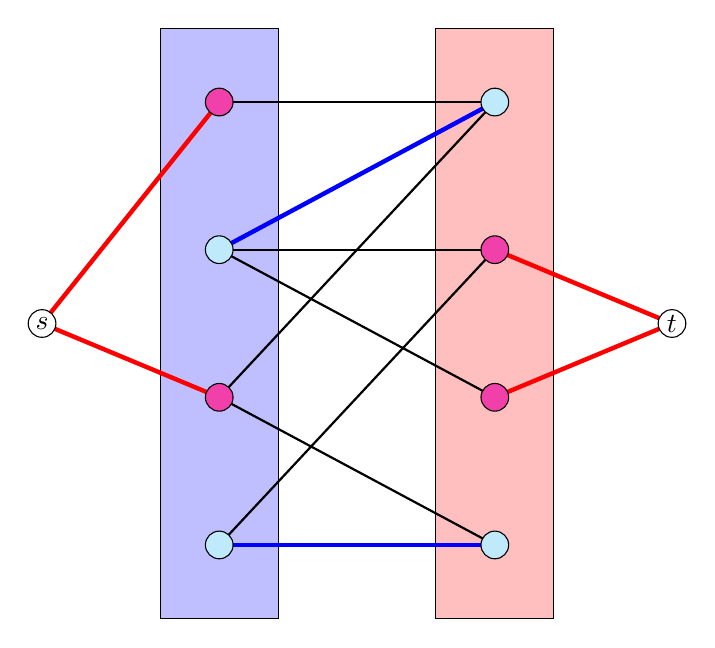
\begin{tikzpicture}
        \foreach \i/\y in {1/0.9375, 2/2.8125, 3/4.6875, 4/6.5625} {
            \coordinate (l\i) at (2.25,\y);
        }

        \foreach \i/\y in {1/0.9375, 2/2.8125, 3/4.6875, 4/6.5625} {
            \coordinate (r\i) at (5.75,\y);
        }

        \coordinate (s) at (0,3.75);
        \coordinate (t) at (8,3.75);

        \filldraw[fill=blue!25,draw=black] (1.5,0) rectangle ++(1.5,7.5);
        \filldraw[fill=red!25,draw=black] (5,0) rectangle ++(1.5,7.5);

        % Edges
        \foreach \u/\v in {l1/r3, l2/r1, l2/r4, l3/r2, l3/r3,l4/r4} {
            \draw[thick] (\u) -- (\v);
        }

        \foreach \u/\v in {l1/r1, l3/r4} {
            \draw[blue,ultra thick] (\u) -- (\v);
        }

        \foreach \v in {l2, l4} {
            \draw[red,ultra thick] (s) -- (\v);
        }

        \foreach \v in {r2, r3} {
            \draw[red,ultra thick] (\v) -- (t);
        }
        

        % Vertices
        \foreach \v in {l2, l4, r2, r3} {
            \node[draw,fill=magenta!75,circle,inner sep=0,minimum size=10pt] at (\v) {};
        }

        \foreach \v in {l1, l3, r1, r4} {
            \node[draw,fill=cyan!25,circle,inner sep=0,minimum size=10pt] at (\v) {};
        }

        \node[draw,fill=white,circle,inner sep=0,minimum size=10pt] at (s) {$s$};

        \node[draw,fill=white,circle,inner sep=0,minimum size=10pt] at (t) {$t$};
    \end{tikzpicture}
    \caption{Augmentation of the input for the modified BFS. Edges in the matching are depicted as blue lines. Free vertices are depicted as magenta circles.}
    \label{fig:3}
\end{figure}
\end{isamarkuptext}\isamarkuptrue%
\isacommand{definition}\isamarkupfalse%
\ G{\isadigit{2}}{\isacharunderscore}{\kern0pt}{\isadigit{1}}\ {\isacharcolon}{\kern0pt}{\isacharcolon}{\kern0pt}\ {\isachardoublequoteopen}{\isacharprime}{\kern0pt}m\ {\isasymRightarrow}\ {\isacharprime}{\kern0pt}n{\isachardoublequoteclose}\ \isakeyword{where}\isanewline
\ \ {\isachardoublequoteopen}G{\isadigit{2}}{\isacharunderscore}{\kern0pt}{\isadigit{1}}\ M\ {\isasymequiv}\ List{\isachardot}{\kern0pt}fold\ G{\isachardot}{\kern0pt}insert\ {\isacharparenleft}{\kern0pt}M{\isacharunderscore}{\kern0pt}inorder\ M{\isacharparenright}{\kern0pt}\ Map{\isacharunderscore}{\kern0pt}empty{\isachardoublequoteclose}%
\begin{isamarkuptext}%
Graph \isa{G{\isadigit{2}}{\isacharunderscore}{\kern0pt}{\isadigit{1}}} is the graph induced by the current matching \isa{M}.%
\end{isamarkuptext}\isamarkuptrue%
\isacommand{definition}\isamarkupfalse%
\ G{\isadigit{2}}{\isacharunderscore}{\kern0pt}{\isadigit{2}}\ {\isacharcolon}{\kern0pt}{\isacharcolon}{\kern0pt}\ {\isachardoublequoteopen}{\isacharprime}{\kern0pt}s\ {\isasymRightarrow}\ {\isacharprime}{\kern0pt}a\ {\isasymRightarrow}\ {\isacharprime}{\kern0pt}m\ {\isasymRightarrow}\ {\isacharprime}{\kern0pt}n{\isachardoublequoteclose}\ \isakeyword{where}\isanewline
\ \ {\isachardoublequoteopen}G{\isadigit{2}}{\isacharunderscore}{\kern0pt}{\isadigit{2}}\ L\ s\ M\ {\isasymequiv}\ List{\isachardot}{\kern0pt}fold\ {\isacharparenleft}{\kern0pt}G{\isachardot}{\kern0pt}insert{\isacharunderscore}{\kern0pt}edge\ s{\isacharparenright}{\kern0pt}\ {\isacharparenleft}{\kern0pt}free{\isacharunderscore}{\kern0pt}vertices\ L\ M{\isacharparenright}{\kern0pt}\ {\isacharparenleft}{\kern0pt}G{\isadigit{2}}{\isacharunderscore}{\kern0pt}{\isadigit{1}}\ M{\isacharparenright}{\kern0pt}{\isachardoublequoteclose}%
\begin{isamarkuptext}%
Graph \isa{G{\isadigit{2}}{\isacharunderscore}{\kern0pt}{\isadigit{2}}} connects vertex \isa{s} in graph \isa{G{\isadigit{2}}{\isacharunderscore}{\kern0pt}{\isadigit{1}}} to every free vertex in
\isa{L}.%
\end{isamarkuptext}\isamarkuptrue%
\isacommand{definition}\isamarkupfalse%
\ G{\isadigit{2}}{\isacharunderscore}{\kern0pt}{\isadigit{3}}\ {\isacharcolon}{\kern0pt}{\isacharcolon}{\kern0pt}\ {\isachardoublequoteopen}{\isacharprime}{\kern0pt}s\ {\isasymRightarrow}\ {\isacharprime}{\kern0pt}s\ {\isasymRightarrow}\ {\isacharprime}{\kern0pt}a\ {\isasymRightarrow}\ {\isacharprime}{\kern0pt}a\ {\isasymRightarrow}\ {\isacharprime}{\kern0pt}m\ {\isasymRightarrow}\ {\isacharprime}{\kern0pt}n{\isachardoublequoteclose}\ \isakeyword{where}\isanewline
\ \ {\isachardoublequoteopen}G{\isadigit{2}}{\isacharunderscore}{\kern0pt}{\isadigit{3}}\ L\ R\ s\ t\ M\ {\isasymequiv}\ List{\isachardot}{\kern0pt}fold\ {\isacharparenleft}{\kern0pt}G{\isachardot}{\kern0pt}insert{\isacharunderscore}{\kern0pt}edge\ t{\isacharparenright}{\kern0pt}\ {\isacharparenleft}{\kern0pt}free{\isacharunderscore}{\kern0pt}vertices\ R\ M{\isacharparenright}{\kern0pt}\ {\isacharparenleft}{\kern0pt}G{\isadigit{2}}{\isacharunderscore}{\kern0pt}{\isadigit{2}}\ L\ s\ M{\isacharparenright}{\kern0pt}{\isachardoublequoteclose}%
\begin{isamarkuptext}%
Graph \isa{G{\isadigit{2}}{\isacharunderscore}{\kern0pt}{\isadigit{3}}} connects every free vertex in \isa{R} to vertex \isa{t} in graph
\isa{G{\isadigit{2}}{\isacharunderscore}{\kern0pt}{\isadigit{2}}}.%
\end{isamarkuptext}\isamarkuptrue%
\isacommand{definition}\isamarkupfalse%
\ G{\isadigit{2}}\ {\isacharcolon}{\kern0pt}{\isacharcolon}{\kern0pt}\ {\isachardoublequoteopen}{\isacharprime}{\kern0pt}s\ {\isasymRightarrow}\ {\isacharprime}{\kern0pt}s\ {\isasymRightarrow}\ {\isacharprime}{\kern0pt}a\ {\isasymRightarrow}\ {\isacharprime}{\kern0pt}a\ {\isasymRightarrow}\ {\isacharprime}{\kern0pt}m\ {\isasymRightarrow}\ {\isacharprime}{\kern0pt}n{\isachardoublequoteclose}\ \isakeyword{where}\isanewline
\ \ {\isachardoublequoteopen}G{\isadigit{2}}\ {\isasymequiv}\ G{\isadigit{2}}{\isacharunderscore}{\kern0pt}{\isadigit{3}}{\isachardoublequoteclose}\isanewline
\isanewline
\isacommand{definition}\isamarkupfalse%
\ G{\isadigit{1}}\ {\isacharcolon}{\kern0pt}{\isacharcolon}{\kern0pt}\ {\isachardoublequoteopen}{\isacharprime}{\kern0pt}n\ {\isasymRightarrow}\ {\isacharprime}{\kern0pt}n\ {\isasymRightarrow}\ {\isacharprime}{\kern0pt}n{\isachardoublequoteclose}\ \isakeyword{where}\isanewline
\ \ {\isachardoublequoteopen}G{\isadigit{1}}\ {\isasymequiv}\ G{\isachardot}{\kern0pt}difference{\isachardoublequoteclose}%
\begin{isamarkuptext}%
As described above, the algorithm repeatedly finds an augmenting path and augments the matching
until there are no augmenting paths. And there are no augmenting paths if

%
\begin{enumerate}%
\item either side of the bipartite graph contains no free vertex, or

\item \isa{local{\isachardot}{\kern0pt}alt{\isacharunderscore}{\kern0pt}bfs} does not find an alternating path between vertices \isa{s} and \isa{t}.%
\end{enumerate}%
\end{isamarkuptext}\isamarkuptrue%
\isacommand{definition}\isamarkupfalse%
\ done{\isacharunderscore}{\kern0pt}{\isadigit{1}}\ {\isacharcolon}{\kern0pt}{\isacharcolon}{\kern0pt}\ {\isachardoublequoteopen}{\isacharprime}{\kern0pt}s\ {\isasymRightarrow}\ {\isacharprime}{\kern0pt}s\ {\isasymRightarrow}\ {\isacharprime}{\kern0pt}m\ {\isasymRightarrow}\ bool{\isachardoublequoteclose}\ \isakeyword{where}\isanewline
\ \ {\isachardoublequoteopen}done{\isacharunderscore}{\kern0pt}{\isadigit{1}}\ L\ R\ M\ {\isasymequiv}\ free{\isacharunderscore}{\kern0pt}vertices\ L\ M\ {\isacharequal}{\kern0pt}\ {\isacharbrackleft}{\kern0pt}{\isacharbrackright}{\kern0pt}\ {\isasymor}\ free{\isacharunderscore}{\kern0pt}vertices\ R\ M\ {\isacharequal}{\kern0pt}\ {\isacharbrackleft}{\kern0pt}{\isacharbrackright}{\kern0pt}{\isachardoublequoteclose}\isanewline
\isanewline
\isacommand{definition}\isamarkupfalse%
\ done{\isacharunderscore}{\kern0pt}{\isadigit{2}}\ {\isacharcolon}{\kern0pt}{\isacharcolon}{\kern0pt}\ {\isachardoublequoteopen}{\isacharprime}{\kern0pt}a\ {\isasymRightarrow}\ {\isacharprime}{\kern0pt}m\ {\isasymRightarrow}\ bool{\isachardoublequoteclose}\ \isakeyword{where}\isanewline
\ \ {\isachardoublequoteopen}done{\isacharunderscore}{\kern0pt}{\isadigit{2}}\ t\ m\ {\isasymequiv}\ P{\isacharunderscore}{\kern0pt}lookup\ m\ t\ {\isacharequal}{\kern0pt}\ None{\isachardoublequoteclose}\isanewline
\isanewline
\isanewline
\isacommand{fun}\isamarkupfalse%
\ augment\ {\isacharcolon}{\kern0pt}{\isacharcolon}{\kern0pt}\ {\isachardoublequoteopen}{\isacharprime}{\kern0pt}m\ {\isasymRightarrow}\ {\isacharprime}{\kern0pt}a\ path\ {\isasymRightarrow}\ {\isacharprime}{\kern0pt}m{\isachardoublequoteclose}\ \isakeyword{where}\isanewline
\ \ {\isachardoublequoteopen}augment\ M\ {\isacharbrackleft}{\kern0pt}{\isacharbrackright}{\kern0pt}\ {\isacharequal}{\kern0pt}\ M{\isachardoublequoteclose}\ {\isacharbar}{\kern0pt}\isanewline
\ \ {\isachardoublequoteopen}augment\ M\ {\isacharbrackleft}{\kern0pt}u{\isacharcomma}{\kern0pt}\ v{\isacharbrackright}{\kern0pt}\ {\isacharequal}{\kern0pt}\ {\isacharparenleft}{\kern0pt}M{\isacharunderscore}{\kern0pt}update\ v\ u\ {\isacharparenleft}{\kern0pt}M{\isacharunderscore}{\kern0pt}update\ u\ v\ M{\isacharparenright}{\kern0pt}{\isacharparenright}{\kern0pt}{\isachardoublequoteclose}\ {\isacharbar}{\kern0pt}\isanewline
\ \ {\isachardoublequoteopen}augment\ M\ {\isacharparenleft}{\kern0pt}u\ {\isacharhash}{\kern0pt}\ v\ {\isacharhash}{\kern0pt}\ w\ {\isacharhash}{\kern0pt}\ ws{\isacharparenright}{\kern0pt}\ {\isacharequal}{\kern0pt}\ augment\ {\isacharparenleft}{\kern0pt}M{\isacharunderscore}{\kern0pt}update\ v\ u\ {\isacharparenleft}{\kern0pt}M{\isacharunderscore}{\kern0pt}update\ u\ v\ {\isacharparenleft}{\kern0pt}M{\isacharunderscore}{\kern0pt}delete\ w\ M{\isacharparenright}{\kern0pt}{\isacharparenright}{\kern0pt}{\isacharparenright}{\kern0pt}\ {\isacharparenleft}{\kern0pt}w\ {\isacharhash}{\kern0pt}\ ws{\isacharparenright}{\kern0pt}{\isachardoublequoteclose}\isanewline
\isanewline
\isacommand{function}\isamarkupfalse%
\ {\isacharparenleft}{\kern0pt}domintros{\isacharparenright}{\kern0pt}\ loop{\isacharprime}{\kern0pt}\ \isakeyword{where}\isanewline
\ \ {\isachardoublequoteopen}loop{\isacharprime}{\kern0pt}\ G\ L\ R\ s\ t\ M\ {\isacharequal}{\kern0pt}\isanewline
\ \ \ {\isacharparenleft}{\kern0pt}if\ done{\isacharunderscore}{\kern0pt}{\isadigit{1}}\ L\ R\ M\ then\ M\isanewline
\ \ \ \ else\ if\ done{\isacharunderscore}{\kern0pt}{\isadigit{2}}\ t\ {\isacharparenleft}{\kern0pt}alt{\isacharunderscore}{\kern0pt}bfs\ {\isacharparenleft}{\kern0pt}G{\isadigit{1}}\ G\ {\isacharparenleft}{\kern0pt}G{\isadigit{2}}\ L\ R\ s\ t\ M{\isacharparenright}{\kern0pt}{\isacharparenright}{\kern0pt}\ {\isacharparenleft}{\kern0pt}G{\isadigit{2}}\ L\ R\ s\ t\ M{\isacharparenright}{\kern0pt}\ s{\isacharparenright}{\kern0pt}\ then\ M\isanewline
\ \ \ \ \ \ \ \ \ else\ loop{\isacharprime}{\kern0pt}\ G\ L\ R\ s\ t\ {\isacharparenleft}{\kern0pt}augment\ M\ {\isacharparenleft}{\kern0pt}butlast\ {\isacharparenleft}{\kern0pt}tl\ {\isacharparenleft}{\kern0pt}rev{\isacharunderscore}{\kern0pt}follow\ {\isacharparenleft}{\kern0pt}alt{\isacharunderscore}{\kern0pt}bfs\ {\isacharparenleft}{\kern0pt}G{\isadigit{1}}\ G\ {\isacharparenleft}{\kern0pt}G{\isadigit{2}}\ L\ R\ s\ t\ M{\isacharparenright}{\kern0pt}{\isacharparenright}{\kern0pt}\ {\isacharparenleft}{\kern0pt}G{\isadigit{2}}\ L\ R\ s\ t\ M{\isacharparenright}{\kern0pt}\ s{\isacharparenright}{\kern0pt}\ t{\isacharparenright}{\kern0pt}{\isacharparenright}{\kern0pt}{\isacharparenright}{\kern0pt}{\isacharparenright}{\kern0pt}{\isacharparenright}{\kern0pt}{\isachardoublequoteclose}\isanewline
%
\isadelimproof
\ \ %
\endisadelimproof
%
\isatagproof
\isacommand{by}\isamarkupfalse%
\ pat{\isacharunderscore}{\kern0pt}completeness\ simp%
\endisatagproof
{\isafoldproof}%
%
\isadelimproof
\isanewline
%
\endisadelimproof
\isanewline
\isanewline
\isacommand{definition}\isamarkupfalse%
\ edmonds{\isacharunderscore}{\kern0pt}karp\ {\isacharcolon}{\kern0pt}{\isacharcolon}{\kern0pt}\ {\isachardoublequoteopen}{\isacharprime}{\kern0pt}n\ {\isasymRightarrow}\ {\isacharprime}{\kern0pt}s\ {\isasymRightarrow}\ {\isacharprime}{\kern0pt}s\ {\isasymRightarrow}\ {\isacharprime}{\kern0pt}a\ {\isasymRightarrow}\ {\isacharprime}{\kern0pt}a\ {\isasymRightarrow}\ {\isacharprime}{\kern0pt}m{\isachardoublequoteclose}\ \isakeyword{where}\isanewline
\ \ {\isachardoublequoteopen}edmonds{\isacharunderscore}{\kern0pt}karp\ G\ L\ R\ s\ t\ {\isasymequiv}\ loop{\isacharprime}{\kern0pt}\ G\ L\ R\ s\ t\ M{\isacharunderscore}{\kern0pt}empty{\isachardoublequoteclose}\isanewline
\isanewline
\isanewline
\isacommand{abbreviation}\isamarkupfalse%
\ m{\isacharunderscore}{\kern0pt}tbd\ {\isacharcolon}{\kern0pt}{\isacharcolon}{\kern0pt}\ {\isachardoublequoteopen}{\isacharprime}{\kern0pt}n\ {\isasymRightarrow}\ {\isacharprime}{\kern0pt}s\ {\isasymRightarrow}\ {\isacharprime}{\kern0pt}s\ {\isasymRightarrow}\ {\isacharprime}{\kern0pt}a\ {\isasymRightarrow}\ {\isacharprime}{\kern0pt}a\ {\isasymRightarrow}\ {\isacharprime}{\kern0pt}m\ {\isasymRightarrow}\ {\isacharprime}{\kern0pt}m{\isachardoublequoteclose}\ \isakeyword{where}\isanewline
\ \ {\isachardoublequoteopen}m{\isacharunderscore}{\kern0pt}tbd\ G\ L\ R\ s\ t\ M\ {\isasymequiv}\ let\ G{\isadigit{2}}\ {\isacharequal}{\kern0pt}\ G{\isadigit{2}}\ L\ R\ s\ t\ M\ in\ alt{\isacharunderscore}{\kern0pt}bfs\ {\isacharparenleft}{\kern0pt}G{\isadigit{1}}\ G\ G{\isadigit{2}}{\isacharparenright}{\kern0pt}\ G{\isadigit{2}}\ s{\isachardoublequoteclose}\isanewline
\isanewline
\isanewline
\isacommand{abbreviation}\isamarkupfalse%
\ p{\isacharunderscore}{\kern0pt}tbd\ {\isacharcolon}{\kern0pt}{\isacharcolon}{\kern0pt}\ {\isachardoublequoteopen}{\isacharprime}{\kern0pt}n\ {\isasymRightarrow}\ {\isacharprime}{\kern0pt}s\ {\isasymRightarrow}\ {\isacharprime}{\kern0pt}s\ {\isasymRightarrow}\ {\isacharprime}{\kern0pt}a\ {\isasymRightarrow}\ {\isacharprime}{\kern0pt}a\ {\isasymRightarrow}\ {\isacharprime}{\kern0pt}m\ {\isasymRightarrow}\ {\isacharprime}{\kern0pt}a\ path{\isachardoublequoteclose}\ \isakeyword{where}\isanewline
\ \ {\isachardoublequoteopen}p{\isacharunderscore}{\kern0pt}tbd\ G\ L\ R\ s\ t\ M\ {\isasymequiv}\ butlast\ {\isacharparenleft}{\kern0pt}tl\ {\isacharparenleft}{\kern0pt}rev{\isacharunderscore}{\kern0pt}follow\ {\isacharparenleft}{\kern0pt}m{\isacharunderscore}{\kern0pt}tbd\ G\ L\ R\ s\ t\ M{\isacharparenright}{\kern0pt}\ t{\isacharparenright}{\kern0pt}{\isacharparenright}{\kern0pt}{\isachardoublequoteclose}\isanewline
\isanewline
\isanewline
\isacommand{abbreviation}\isamarkupfalse%
\ M{\isacharunderscore}{\kern0pt}tbd\ {\isacharcolon}{\kern0pt}{\isacharcolon}{\kern0pt}\ {\isachardoublequoteopen}{\isacharprime}{\kern0pt}m\ {\isasymRightarrow}\ {\isacharprime}{\kern0pt}a\ graph{\isachardoublequoteclose}\ \isakeyword{where}\isanewline
\ \ {\isachardoublequoteopen}M{\isacharunderscore}{\kern0pt}tbd\ M\ {\isasymequiv}\ {\isacharbraceleft}{\kern0pt}{\isacharbraceleft}{\kern0pt}u{\isacharcomma}{\kern0pt}\ v{\isacharbraceright}{\kern0pt}\ {\isacharbar}{\kern0pt}u\ v{\isachardot}{\kern0pt}\ M{\isacharunderscore}{\kern0pt}lookup\ M\ u\ {\isacharequal}{\kern0pt}\ Some\ v{\isacharbraceright}{\kern0pt}{\isachardoublequoteclose}\isanewline
\isanewline
\isanewline
\isacommand{abbreviation}\isamarkupfalse%
\ P{\isacharunderscore}{\kern0pt}tbd\ {\isacharcolon}{\kern0pt}{\isacharcolon}{\kern0pt}\ {\isachardoublequoteopen}{\isacharprime}{\kern0pt}a\ path\ {\isasymRightarrow}\ {\isacharprime}{\kern0pt}a\ graph{\isachardoublequoteclose}\ \isakeyword{where}\isanewline
\ \ {\isachardoublequoteopen}P{\isacharunderscore}{\kern0pt}tbd\ p\ {\isasymequiv}\ set\ {\isacharparenleft}{\kern0pt}edges{\isacharunderscore}{\kern0pt}of{\isacharunderscore}{\kern0pt}path\ p{\isacharparenright}{\kern0pt}{\isachardoublequoteclose}\isanewline
\isanewline
\isacommand{abbreviation}\isamarkupfalse%
\ is{\isacharunderscore}{\kern0pt}symmetric{\isacharunderscore}{\kern0pt}Map\ {\isacharcolon}{\kern0pt}{\isacharcolon}{\kern0pt}\ {\isachardoublequoteopen}{\isacharprime}{\kern0pt}m\ {\isasymRightarrow}\ bool{\isachardoublequoteclose}\ \isakeyword{where}\isanewline
\ \ {\isachardoublequoteopen}is{\isacharunderscore}{\kern0pt}symmetric{\isacharunderscore}{\kern0pt}Map\ M\ {\isasymequiv}\ {\isasymforall}u\ v{\isachardot}{\kern0pt}\ M{\isacharunderscore}{\kern0pt}lookup\ M\ u\ {\isacharequal}{\kern0pt}\ Some\ v\ {\isasymlongleftrightarrow}\ M{\isacharunderscore}{\kern0pt}lookup\ M\ v\ {\isacharequal}{\kern0pt}\ Some\ u{\isachardoublequoteclose}\isanewline
\isanewline
\isacommand{end}\isamarkupfalse%
%
\isadelimdocument
%
\endisadelimdocument
%
\isatagdocument
%
\isamarkupsubsection{Verification of the correctness of the algorithm%
}
\isamarkuptrue%
%
\isamarkupsubsubsection{Assumptions on the input%
}
\isamarkuptrue%
%
\endisatagdocument
{\isafolddocument}%
%
\isadelimdocument
%
\endisadelimdocument
%
\begin{isamarkuptext}%
Algorithm \isa{edmonds{\isacharunderscore}{\kern0pt}karp{\isachardot}{\kern0pt}edmonds{\isacharunderscore}{\kern0pt}karp} expects an input $\langle \isa{G},\isa{L},\isa{R},
\isa{s},\isa{t}\rangle$ such that

%
\begin{itemize}%
\item $(\isa{L}\cup \isa{R},\isa{G})$ is a bipartite graph, and

\item \isa{s} and \isa{t} are two new vertices, that is, vertices not in \isa{G},%
\end{itemize}


and the correctness theorem will assume such an input. Let us formally specify these assumptions.%
\end{isamarkuptext}\isamarkuptrue%
\isacommand{locale}\isamarkupfalse%
\ edmonds{\isacharunderscore}{\kern0pt}karp{\isacharunderscore}{\kern0pt}valid{\isacharunderscore}{\kern0pt}input\ {\isacharequal}{\kern0pt}\ edmonds{\isacharunderscore}{\kern0pt}karp\ \isakeyword{where}\isanewline
\ \ Map{\isacharunderscore}{\kern0pt}update\ {\isacharequal}{\kern0pt}\ Map{\isacharunderscore}{\kern0pt}update\ \isakeyword{and}\isanewline
\ \ P{\isacharunderscore}{\kern0pt}update\ {\isacharequal}{\kern0pt}\ P{\isacharunderscore}{\kern0pt}update\ \isakeyword{and}\isanewline
\ \ M{\isacharunderscore}{\kern0pt}update\ {\isacharequal}{\kern0pt}\ M{\isacharunderscore}{\kern0pt}update\ \isakeyword{for}\isanewline
\ \ Map{\isacharunderscore}{\kern0pt}update\ {\isacharcolon}{\kern0pt}{\isacharcolon}{\kern0pt}\ {\isachardoublequoteopen}{\isacharprime}{\kern0pt}a{\isacharcolon}{\kern0pt}{\isacharcolon}{\kern0pt}linorder\ {\isasymRightarrow}\ {\isacharprime}{\kern0pt}s\ {\isasymRightarrow}\ {\isacharprime}{\kern0pt}n\ {\isasymRightarrow}\ {\isacharprime}{\kern0pt}n{\isachardoublequoteclose}\ \isakeyword{and}\isanewline
\ \ P{\isacharunderscore}{\kern0pt}update\ {\isacharcolon}{\kern0pt}{\isacharcolon}{\kern0pt}\ {\isachardoublequoteopen}{\isacharprime}{\kern0pt}a\ {\isasymRightarrow}\ {\isacharprime}{\kern0pt}a\ {\isasymRightarrow}\ {\isacharprime}{\kern0pt}m\ {\isasymRightarrow}\ {\isacharprime}{\kern0pt}m{\isachardoublequoteclose}\ \isakeyword{and}\isanewline
\ \ M{\isacharunderscore}{\kern0pt}update\ {\isacharcolon}{\kern0pt}{\isacharcolon}{\kern0pt}\ {\isachardoublequoteopen}{\isacharprime}{\kern0pt}a\ {\isasymRightarrow}\ {\isacharprime}{\kern0pt}a\ {\isasymRightarrow}\ {\isacharprime}{\kern0pt}m\ {\isasymRightarrow}\ {\isacharprime}{\kern0pt}m{\isachardoublequoteclose}\ {\isacharplus}{\kern0pt}\isanewline
\ \ \isakeyword{fixes}\ G\ {\isacharcolon}{\kern0pt}{\isacharcolon}{\kern0pt}\ {\isacharprime}{\kern0pt}n\isanewline
\ \ \isakeyword{fixes}\ L\ R\ {\isacharcolon}{\kern0pt}{\isacharcolon}{\kern0pt}\ {\isacharprime}{\kern0pt}s\isanewline
\ \ \isakeyword{fixes}\ s\ t\ {\isacharcolon}{\kern0pt}{\isacharcolon}{\kern0pt}\ {\isacharprime}{\kern0pt}a\isanewline
\ \ \isakeyword{assumes}\ symmetric{\isacharunderscore}{\kern0pt}adjacency{\isacharunderscore}{\kern0pt}G{\isacharcolon}{\kern0pt}\ {\isachardoublequoteopen}G{\isachardot}{\kern0pt}symmetric{\isacharunderscore}{\kern0pt}adjacency{\isacharprime}{\kern0pt}\ G{\isachardoublequoteclose}\isanewline
\ \ \isakeyword{assumes}\ bipartite{\isacharunderscore}{\kern0pt}graph{\isacharcolon}{\kern0pt}\ {\isachardoublequoteopen}bipartite{\isacharunderscore}{\kern0pt}graph\ {\isacharparenleft}{\kern0pt}G{\isachardot}{\kern0pt}E\ G{\isacharparenright}{\kern0pt}\ {\isacharparenleft}{\kern0pt}G{\isachardot}{\kern0pt}S{\isachardot}{\kern0pt}set\ L{\isacharparenright}{\kern0pt}\ {\isacharparenleft}{\kern0pt}G{\isachardot}{\kern0pt}S{\isachardot}{\kern0pt}set\ R{\isacharparenright}{\kern0pt}{\isachardoublequoteclose}\isanewline
\ \ \isakeyword{assumes}\ s{\isacharunderscore}{\kern0pt}not{\isacharunderscore}{\kern0pt}mem{\isacharunderscore}{\kern0pt}V{\isacharcolon}{\kern0pt}\ {\isachardoublequoteopen}s\ {\isasymnotin}\ G{\isachardot}{\kern0pt}V\ G{\isachardoublequoteclose}\isanewline
\ \ \isakeyword{assumes}\ t{\isacharunderscore}{\kern0pt}not{\isacharunderscore}{\kern0pt}mem{\isacharunderscore}{\kern0pt}V{\isacharcolon}{\kern0pt}\ {\isachardoublequoteopen}t\ {\isasymnotin}\ G{\isachardot}{\kern0pt}V\ G{\isachardoublequoteclose}\isanewline
\ \ \isakeyword{assumes}\ s{\isacharunderscore}{\kern0pt}neq{\isacharunderscore}{\kern0pt}t{\isacharcolon}{\kern0pt}\ {\isachardoublequoteopen}s\ {\isasymnoteq}\ t{\isachardoublequoteclose}\isanewline
%
\isadeliminvisible
\isanewline
%
\endisadeliminvisible
%
\isataginvisible
\isacommand{abbreviation}\isamarkupfalse%
\ {\isacharparenleft}{\kern0pt}\isakeyword{in}\ edmonds{\isacharunderscore}{\kern0pt}karp{\isacharparenright}{\kern0pt}\ edmonds{\isacharunderscore}{\kern0pt}karp{\isacharunderscore}{\kern0pt}valid{\isacharunderscore}{\kern0pt}input{\isacharprime}{\kern0pt}\ {\isacharcolon}{\kern0pt}{\isacharcolon}{\kern0pt}\ {\isachardoublequoteopen}{\isacharprime}{\kern0pt}n\ {\isasymRightarrow}\ {\isacharprime}{\kern0pt}s\ {\isasymRightarrow}\ {\isacharprime}{\kern0pt}s\ {\isasymRightarrow}\ {\isacharprime}{\kern0pt}a\ {\isasymRightarrow}\ {\isacharprime}{\kern0pt}a\ {\isasymRightarrow}\ bool{\isachardoublequoteclose}\ \isakeyword{where}\isanewline
\ \ {\isachardoublequoteopen}edmonds{\isacharunderscore}{\kern0pt}karp{\isacharunderscore}{\kern0pt}valid{\isacharunderscore}{\kern0pt}input{\isacharprime}{\kern0pt}\ G\ L\ R\ s\ t\ {\isasymequiv}\isanewline
\ \ \ edmonds{\isacharunderscore}{\kern0pt}karp{\isacharunderscore}{\kern0pt}valid{\isacharunderscore}{\kern0pt}input\isanewline
\ \ \ \ Map{\isacharunderscore}{\kern0pt}empty\ Map{\isacharunderscore}{\kern0pt}delete\ Map{\isacharunderscore}{\kern0pt}lookup\ Map{\isacharunderscore}{\kern0pt}inorder\ Map{\isacharunderscore}{\kern0pt}inv\isanewline
\ \ \ \ Set{\isacharunderscore}{\kern0pt}empty\ Set{\isacharunderscore}{\kern0pt}insert\ Set{\isacharunderscore}{\kern0pt}delete\ Set{\isacharunderscore}{\kern0pt}isin\ Set{\isacharunderscore}{\kern0pt}inorder\ Set{\isacharunderscore}{\kern0pt}inv\isanewline
\ \ \ \ P{\isacharunderscore}{\kern0pt}empty\ P{\isacharunderscore}{\kern0pt}delete\ P{\isacharunderscore}{\kern0pt}lookup\ P{\isacharunderscore}{\kern0pt}invar\isanewline
\ \ \ \ Q{\isacharunderscore}{\kern0pt}empty\ Q{\isacharunderscore}{\kern0pt}is{\isacharunderscore}{\kern0pt}empty\ Q{\isacharunderscore}{\kern0pt}head\ Q{\isacharunderscore}{\kern0pt}tail\ Q{\isacharunderscore}{\kern0pt}invar\ Q{\isacharunderscore}{\kern0pt}list\ Q{\isacharunderscore}{\kern0pt}snoc\isanewline
\ \ \ \ M{\isacharunderscore}{\kern0pt}empty\ M{\isacharunderscore}{\kern0pt}delete\ M{\isacharunderscore}{\kern0pt}lookup\ M{\isacharunderscore}{\kern0pt}inorder\ M{\isacharunderscore}{\kern0pt}inv\isanewline
\ \ \ \ Map{\isacharunderscore}{\kern0pt}update\ P{\isacharunderscore}{\kern0pt}update\ M{\isacharunderscore}{\kern0pt}update\isanewline
\ \ \ \ G\ L\ R\ s\ t{\isachardoublequoteclose}\isanewline
\isanewline
\isacommand{lemma}\isamarkupfalse%
\ {\isacharparenleft}{\kern0pt}\isakeyword{in}\ edmonds{\isacharunderscore}{\kern0pt}karp{\isacharunderscore}{\kern0pt}valid{\isacharunderscore}{\kern0pt}input{\isacharparenright}{\kern0pt}\ invar{\isacharunderscore}{\kern0pt}G{\isacharcolon}{\kern0pt}\isanewline
\ \ \isakeyword{shows}\ {\isachardoublequoteopen}G{\isachardot}{\kern0pt}invar\ G{\isachardoublequoteclose}%
\endisataginvisible
{\isafoldinvisible}%
%
\isadeliminvisible
\isanewline
%
\endisadeliminvisible
%
\isadelimproof
\ \ %
\endisadelimproof
%
\isatagproof
\isacommand{using}\isamarkupfalse%
\ symmetric{\isacharunderscore}{\kern0pt}adjacency{\isacharunderscore}{\kern0pt}G\isanewline
\ \ \isacommand{by}\isamarkupfalse%
\ {\isacharparenleft}{\kern0pt}intro\ symmetric{\isacharunderscore}{\kern0pt}adjacency{\isachardot}{\kern0pt}invar{\isacharparenright}{\kern0pt}%
\endisatagproof
{\isafoldproof}%
%
\isadelimproof
\isanewline
%
\endisadelimproof
%
\isadeliminvisible
\isanewline
%
\endisadeliminvisible
%
\isataginvisible
\isacommand{lemma}\isamarkupfalse%
\ {\isacharparenleft}{\kern0pt}\isakeyword{in}\ edmonds{\isacharunderscore}{\kern0pt}karp{\isacharunderscore}{\kern0pt}valid{\isacharunderscore}{\kern0pt}input{\isacharparenright}{\kern0pt}\ symmetric{\isacharunderscore}{\kern0pt}G{\isacharcolon}{\kern0pt}\isanewline
\ \ \isakeyword{shows}\ {\isachardoublequoteopen}v\ {\isasymin}\ set\ {\isacharparenleft}{\kern0pt}G{\isachardot}{\kern0pt}adjacency{\isacharunderscore}{\kern0pt}list\ G\ u{\isacharparenright}{\kern0pt}\ {\isasymlongleftrightarrow}\ u\ {\isasymin}\ set\ {\isacharparenleft}{\kern0pt}G{\isachardot}{\kern0pt}adjacency{\isacharunderscore}{\kern0pt}list\ G\ v{\isacharparenright}{\kern0pt}{\isachardoublequoteclose}%
\endisataginvisible
{\isafoldinvisible}%
%
\isadeliminvisible
\isanewline
%
\endisadeliminvisible
%
\isadelimproof
\ \ %
\endisadelimproof
%
\isatagproof
\isacommand{using}\isamarkupfalse%
\ symmetric{\isacharunderscore}{\kern0pt}adjacency{\isacharunderscore}{\kern0pt}G\isanewline
\ \ \isacommand{by}\isamarkupfalse%
\ {\isacharparenleft}{\kern0pt}intro\ symmetric{\isacharunderscore}{\kern0pt}adjacency{\isachardot}{\kern0pt}symmetric{\isacharparenright}{\kern0pt}%
\endisatagproof
{\isafoldproof}%
%
\isadelimproof
\isanewline
%
\endisadelimproof
%
\isadeliminvisible
\isanewline
%
\endisadeliminvisible
%
\isataginvisible
\isacommand{lemma}\isamarkupfalse%
\ {\isacharparenleft}{\kern0pt}\isakeyword{in}\ edmonds{\isacharunderscore}{\kern0pt}karp{\isacharunderscore}{\kern0pt}valid{\isacharunderscore}{\kern0pt}input{\isacharparenright}{\kern0pt}\ finite{\isacharunderscore}{\kern0pt}E{\isacharcolon}{\kern0pt}\isanewline
\ \ \isakeyword{shows}\ {\isachardoublequoteopen}finite\ {\isacharparenleft}{\kern0pt}G{\isachardot}{\kern0pt}E\ G{\isacharparenright}{\kern0pt}{\isachardoublequoteclose}%
\endisataginvisible
{\isafoldinvisible}%
%
\isadeliminvisible
\isanewline
%
\endisadeliminvisible
%
\isadelimproof
\ \ %
\endisadelimproof
%
\isatagproof
\isacommand{using}\isamarkupfalse%
\ invar{\isacharunderscore}{\kern0pt}G\isanewline
\ \ \isacommand{by}\isamarkupfalse%
\ {\isacharparenleft}{\kern0pt}intro\ G{\isachardot}{\kern0pt}finite{\isacharunderscore}{\kern0pt}E{\isacharparenright}{\kern0pt}%
\endisatagproof
{\isafoldproof}%
%
\isadelimproof
\isanewline
%
\endisadelimproof
%
\isadeliminvisible
\isanewline
%
\endisadeliminvisible
%
\isataginvisible
\isacommand{lemma}\isamarkupfalse%
\ {\isacharparenleft}{\kern0pt}\isakeyword{in}\ edmonds{\isacharunderscore}{\kern0pt}karp{\isacharunderscore}{\kern0pt}valid{\isacharunderscore}{\kern0pt}input{\isacharparenright}{\kern0pt}\ finite{\isacharunderscore}{\kern0pt}V{\isacharcolon}{\kern0pt}\isanewline
\ \ \isakeyword{shows}\ {\isachardoublequoteopen}finite\ {\isacharparenleft}{\kern0pt}G{\isachardot}{\kern0pt}V\ G{\isacharparenright}{\kern0pt}{\isachardoublequoteclose}%
\endisataginvisible
{\isafoldinvisible}%
%
\isadeliminvisible
\isanewline
%
\endisadeliminvisible
%
\isadelimproof
\ \ %
\endisadelimproof
%
\isatagproof
\isacommand{using}\isamarkupfalse%
\ invar{\isacharunderscore}{\kern0pt}G\isanewline
\ \ \isacommand{by}\isamarkupfalse%
\ {\isacharparenleft}{\kern0pt}intro\ G{\isachardot}{\kern0pt}finite{\isacharunderscore}{\kern0pt}V{\isacharparenright}{\kern0pt}%
\endisatagproof
{\isafoldproof}%
%
\isadelimproof
\isanewline
%
\endisadelimproof
%
\isadeliminvisible
\isanewline
%
\endisadeliminvisible
%
\isataginvisible
\isacommand{lemma}\isamarkupfalse%
\ {\isacharparenleft}{\kern0pt}\isakeyword{in}\ edmonds{\isacharunderscore}{\kern0pt}karp{\isacharunderscore}{\kern0pt}valid{\isacharunderscore}{\kern0pt}input{\isacharparenright}{\kern0pt}\ L{\isacharunderscore}{\kern0pt}union{\isacharunderscore}{\kern0pt}R{\isacharunderscore}{\kern0pt}eq{\isacharunderscore}{\kern0pt}V{\isacharcolon}{\kern0pt}\isanewline
\ \ \isakeyword{shows}\ {\isachardoublequoteopen}G{\isachardot}{\kern0pt}S{\isachardot}{\kern0pt}set\ L\ {\isasymunion}\ G{\isachardot}{\kern0pt}S{\isachardot}{\kern0pt}set\ R\ {\isacharequal}{\kern0pt}\ G{\isachardot}{\kern0pt}V\ G{\isachardoublequoteclose}%
\endisataginvisible
{\isafoldinvisible}%
%
\isadeliminvisible
\isanewline
%
\endisadeliminvisible
%
\isadelimproof
\ \ %
\endisadelimproof
%
\isatagproof
\isacommand{unfolding}\isamarkupfalse%
\ G{\isachardot}{\kern0pt}V{\isacharunderscore}{\kern0pt}def\isanewline
\ \ \isacommand{using}\isamarkupfalse%
\ bipartite{\isacharunderscore}{\kern0pt}graph\isanewline
\ \ \isacommand{by}\isamarkupfalse%
\ {\isacharparenleft}{\kern0pt}intro\ bipartite{\isacharunderscore}{\kern0pt}graph{\isachardot}{\kern0pt}L{\isacharunderscore}{\kern0pt}union{\isacharunderscore}{\kern0pt}R{\isacharunderscore}{\kern0pt}eq{\isacharunderscore}{\kern0pt}Vs{\isacharparenright}{\kern0pt}%
\endisatagproof
{\isafoldproof}%
%
\isadelimproof
\isanewline
%
\endisadelimproof
%
\isadeliminvisible
\isanewline
%
\endisadeliminvisible
%
\isataginvisible
\isacommand{lemma}\isamarkupfalse%
\ {\isacharparenleft}{\kern0pt}\isakeyword{in}\ edmonds{\isacharunderscore}{\kern0pt}karp{\isacharunderscore}{\kern0pt}valid{\isacharunderscore}{\kern0pt}input{\isacharparenright}{\kern0pt}\ L{\isacharunderscore}{\kern0pt}R{\isacharunderscore}{\kern0pt}disjoint{\isacharcolon}{\kern0pt}\isanewline
\ \ \isakeyword{shows}\ {\isachardoublequoteopen}G{\isachardot}{\kern0pt}S{\isachardot}{\kern0pt}set\ L\ {\isasyminter}\ G{\isachardot}{\kern0pt}S{\isachardot}{\kern0pt}set\ R\ {\isacharequal}{\kern0pt}\ {\isacharbraceleft}{\kern0pt}{\isacharbraceright}{\kern0pt}{\isachardoublequoteclose}%
\endisataginvisible
{\isafoldinvisible}%
%
\isadeliminvisible
\isanewline
%
\endisadeliminvisible
%
\isadelimproof
\ \ %
\endisadelimproof
%
\isatagproof
\isacommand{using}\isamarkupfalse%
\ bipartite{\isacharunderscore}{\kern0pt}graph\isanewline
\ \ \isacommand{by}\isamarkupfalse%
\ {\isacharparenleft}{\kern0pt}intro\ bipartite{\isacharunderscore}{\kern0pt}graph{\isachardot}{\kern0pt}L{\isacharunderscore}{\kern0pt}R{\isacharunderscore}{\kern0pt}disjoint{\isacharparenright}{\kern0pt}%
\endisatagproof
{\isafoldproof}%
%
\isadelimproof
\isanewline
%
\endisadelimproof
%
\isadeliminvisible
\isanewline
%
\endisadeliminvisible
%
\isataginvisible
\isacommand{lemma}\isamarkupfalse%
\ {\isacharparenleft}{\kern0pt}\isakeyword{in}\ edmonds{\isacharunderscore}{\kern0pt}karp{\isacharunderscore}{\kern0pt}valid{\isacharunderscore}{\kern0pt}input{\isacharparenright}{\kern0pt}\ L{\isacharunderscore}{\kern0pt}subset{\isacharunderscore}{\kern0pt}V{\isacharcolon}{\kern0pt}\isanewline
\ \ \isakeyword{shows}\ {\isachardoublequoteopen}G{\isachardot}{\kern0pt}S{\isachardot}{\kern0pt}set\ L\ {\isasymsubseteq}\ G{\isachardot}{\kern0pt}V\ G{\isachardoublequoteclose}%
\endisataginvisible
{\isafoldinvisible}%
%
\isadeliminvisible
\isanewline
%
\endisadeliminvisible
%
\isadelimproof
\ \ %
\endisadelimproof
%
\isatagproof
\isacommand{unfolding}\isamarkupfalse%
\ G{\isachardot}{\kern0pt}V{\isacharunderscore}{\kern0pt}def\isanewline
\ \ \isacommand{using}\isamarkupfalse%
\ bipartite{\isacharunderscore}{\kern0pt}graph\isanewline
\ \ \isacommand{by}\isamarkupfalse%
\ {\isacharparenleft}{\kern0pt}intro\ bipartite{\isacharunderscore}{\kern0pt}graph{\isachardot}{\kern0pt}L{\isacharunderscore}{\kern0pt}subset{\isacharunderscore}{\kern0pt}Vs{\isacharparenright}{\kern0pt}%
\endisatagproof
{\isafoldproof}%
%
\isadelimproof
\isanewline
%
\endisadelimproof
%
\isadeliminvisible
\isanewline
%
\endisadeliminvisible
%
\isataginvisible
\isacommand{lemma}\isamarkupfalse%
\ {\isacharparenleft}{\kern0pt}\isakeyword{in}\ edmonds{\isacharunderscore}{\kern0pt}karp{\isacharunderscore}{\kern0pt}valid{\isacharunderscore}{\kern0pt}input{\isacharparenright}{\kern0pt}\ R{\isacharunderscore}{\kern0pt}subset{\isacharunderscore}{\kern0pt}V{\isacharcolon}{\kern0pt}\isanewline
\ \ \isakeyword{shows}\ {\isachardoublequoteopen}G{\isachardot}{\kern0pt}S{\isachardot}{\kern0pt}set\ R\ {\isasymsubseteq}\ G{\isachardot}{\kern0pt}V\ G{\isachardoublequoteclose}%
\endisataginvisible
{\isafoldinvisible}%
%
\isadeliminvisible
\isanewline
%
\endisadeliminvisible
%
\isadelimproof
\ \ %
\endisadelimproof
%
\isatagproof
\isacommand{unfolding}\isamarkupfalse%
\ G{\isachardot}{\kern0pt}V{\isacharunderscore}{\kern0pt}def\isanewline
\ \ \isacommand{using}\isamarkupfalse%
\ bipartite{\isacharunderscore}{\kern0pt}graph\isanewline
\ \ \isacommand{by}\isamarkupfalse%
\ {\isacharparenleft}{\kern0pt}intro\ bipartite{\isacharunderscore}{\kern0pt}graph{\isachardot}{\kern0pt}R{\isacharunderscore}{\kern0pt}subset{\isacharunderscore}{\kern0pt}Vs{\isacharparenright}{\kern0pt}%
\endisatagproof
{\isafoldproof}%
%
\isadelimproof
\isanewline
%
\endisadelimproof
%
\isadeliminvisible
\isanewline
%
\endisadeliminvisible
%
\isataginvisible
\isacommand{lemma}\isamarkupfalse%
\ {\isacharparenleft}{\kern0pt}\isakeyword{in}\ edmonds{\isacharunderscore}{\kern0pt}karp{\isacharunderscore}{\kern0pt}valid{\isacharunderscore}{\kern0pt}input{\isacharparenright}{\kern0pt}\ s{\isacharunderscore}{\kern0pt}not{\isacharunderscore}{\kern0pt}mem{\isacharunderscore}{\kern0pt}L{\isacharcolon}{\kern0pt}\isanewline
\ \ \isakeyword{shows}\ {\isachardoublequoteopen}s\ {\isasymnotin}\ G{\isachardot}{\kern0pt}S{\isachardot}{\kern0pt}set\ L{\isachardoublequoteclose}%
\endisataginvisible
{\isafoldinvisible}%
%
\isadeliminvisible
\isanewline
%
\endisadeliminvisible
%
\isadelimproof
\ \ %
\endisadelimproof
%
\isatagproof
\isacommand{using}\isamarkupfalse%
\ L{\isacharunderscore}{\kern0pt}subset{\isacharunderscore}{\kern0pt}V\ s{\isacharunderscore}{\kern0pt}not{\isacharunderscore}{\kern0pt}mem{\isacharunderscore}{\kern0pt}V\isanewline
\ \ \isacommand{by}\isamarkupfalse%
\ blast%
\endisatagproof
{\isafoldproof}%
%
\isadelimproof
\isanewline
%
\endisadelimproof
%
\isadeliminvisible
\isanewline
%
\endisadeliminvisible
%
\isataginvisible
\isacommand{lemma}\isamarkupfalse%
\ {\isacharparenleft}{\kern0pt}\isakeyword{in}\ edmonds{\isacharunderscore}{\kern0pt}karp{\isacharunderscore}{\kern0pt}valid{\isacharunderscore}{\kern0pt}input{\isacharparenright}{\kern0pt}\ s{\isacharunderscore}{\kern0pt}not{\isacharunderscore}{\kern0pt}mem{\isacharunderscore}{\kern0pt}R{\isacharcolon}{\kern0pt}\isanewline
\ \ \isakeyword{shows}\ {\isachardoublequoteopen}s\ {\isasymnotin}\ G{\isachardot}{\kern0pt}S{\isachardot}{\kern0pt}set\ R{\isachardoublequoteclose}%
\endisataginvisible
{\isafoldinvisible}%
%
\isadeliminvisible
\isanewline
%
\endisadeliminvisible
%
\isadelimproof
\ \ %
\endisadelimproof
%
\isatagproof
\isacommand{using}\isamarkupfalse%
\ R{\isacharunderscore}{\kern0pt}subset{\isacharunderscore}{\kern0pt}V\ s{\isacharunderscore}{\kern0pt}not{\isacharunderscore}{\kern0pt}mem{\isacharunderscore}{\kern0pt}V\isanewline
\ \ \isacommand{by}\isamarkupfalse%
\ blast%
\endisatagproof
{\isafoldproof}%
%
\isadelimproof
\isanewline
%
\endisadelimproof
%
\isadeliminvisible
\isanewline
%
\endisadeliminvisible
%
\isataginvisible
\isacommand{lemma}\isamarkupfalse%
\ {\isacharparenleft}{\kern0pt}\isakeyword{in}\ edmonds{\isacharunderscore}{\kern0pt}karp{\isacharunderscore}{\kern0pt}valid{\isacharunderscore}{\kern0pt}input{\isacharparenright}{\kern0pt}\ t{\isacharunderscore}{\kern0pt}not{\isacharunderscore}{\kern0pt}mem{\isacharunderscore}{\kern0pt}L{\isacharcolon}{\kern0pt}\isanewline
\ \ \isakeyword{shows}\ {\isachardoublequoteopen}t\ {\isasymnotin}\ G{\isachardot}{\kern0pt}S{\isachardot}{\kern0pt}set\ L{\isachardoublequoteclose}%
\endisataginvisible
{\isafoldinvisible}%
%
\isadeliminvisible
\isanewline
%
\endisadeliminvisible
%
\isadelimproof
\ \ %
\endisadelimproof
%
\isatagproof
\isacommand{using}\isamarkupfalse%
\ L{\isacharunderscore}{\kern0pt}subset{\isacharunderscore}{\kern0pt}V\ t{\isacharunderscore}{\kern0pt}not{\isacharunderscore}{\kern0pt}mem{\isacharunderscore}{\kern0pt}V\isanewline
\ \ \isacommand{by}\isamarkupfalse%
\ blast%
\endisatagproof
{\isafoldproof}%
%
\isadelimproof
\isanewline
%
\endisadelimproof
%
\isadeliminvisible
\isanewline
%
\endisadeliminvisible
%
\isataginvisible
\isacommand{lemma}\isamarkupfalse%
\ {\isacharparenleft}{\kern0pt}\isakeyword{in}\ edmonds{\isacharunderscore}{\kern0pt}karp{\isacharunderscore}{\kern0pt}valid{\isacharunderscore}{\kern0pt}input{\isacharparenright}{\kern0pt}\ t{\isacharunderscore}{\kern0pt}not{\isacharunderscore}{\kern0pt}mem{\isacharunderscore}{\kern0pt}R{\isacharcolon}{\kern0pt}\isanewline
\ \ \isakeyword{shows}\ {\isachardoublequoteopen}t\ {\isasymnotin}\ G{\isachardot}{\kern0pt}S{\isachardot}{\kern0pt}set\ R{\isachardoublequoteclose}%
\endisataginvisible
{\isafoldinvisible}%
%
\isadeliminvisible
\isanewline
%
\endisadeliminvisible
%
\isadelimproof
\ \ %
\endisadelimproof
%
\isatagproof
\isacommand{using}\isamarkupfalse%
\ R{\isacharunderscore}{\kern0pt}subset{\isacharunderscore}{\kern0pt}V\ t{\isacharunderscore}{\kern0pt}not{\isacharunderscore}{\kern0pt}mem{\isacharunderscore}{\kern0pt}V\isanewline
\ \ \isacommand{by}\isamarkupfalse%
\ blast%
\endisatagproof
{\isafoldproof}%
%
\isadelimproof
\isanewline
%
\endisadelimproof
%
\isadeliminvisible
\isanewline
%
\endisadeliminvisible
%
\isataginvisible
\isacommand{lemma}\isamarkupfalse%
\ {\isacharparenleft}{\kern0pt}\isakeyword{in}\ edmonds{\isacharunderscore}{\kern0pt}karp{\isacharunderscore}{\kern0pt}valid{\isacharunderscore}{\kern0pt}input{\isacharparenright}{\kern0pt}\ graph{\isacharunderscore}{\kern0pt}G{\isacharcolon}{\kern0pt}\isanewline
\ \ \isakeyword{shows}\ {\isachardoublequoteopen}{\isasymforall}e{\isasymin}G{\isachardot}{\kern0pt}E\ G{\isachardot}{\kern0pt}\ {\isasymexists}u\ v{\isachardot}{\kern0pt}\ e\ {\isacharequal}{\kern0pt}\ {\isacharbraceleft}{\kern0pt}u{\isacharcomma}{\kern0pt}\ v{\isacharbraceright}{\kern0pt}\ {\isasymand}\ u\ {\isasymnoteq}\ v{\isachardoublequoteclose}%
\endisataginvisible
{\isafoldinvisible}%
%
\isadeliminvisible
\isanewline
%
\endisadeliminvisible
%
\isadelimproof
%
\endisadelimproof
%
\isatagproof
\isacommand{proof}\isamarkupfalse%
\ {\isacharminus}{\kern0pt}\isanewline
\ \ \isacommand{have}\isamarkupfalse%
\ {\isachardoublequoteopen}{\isasymforall}e{\isasymin}G{\isachardot}{\kern0pt}E\ G{\isachardot}{\kern0pt}\ {\isasymexists}u\ v{\isachardot}{\kern0pt}\ e\ {\isacharequal}{\kern0pt}\ {\isacharbraceleft}{\kern0pt}u{\isacharcomma}{\kern0pt}\ v{\isacharbraceright}{\kern0pt}{\isachardoublequoteclose}\isanewline
\ \ \ \ \isacommand{using}\isamarkupfalse%
\ bipartite{\isacharunderscore}{\kern0pt}graph\isanewline
\ \ \ \ \isacommand{by}\isamarkupfalse%
\ {\isacharparenleft}{\kern0pt}intro\ bipartite{\isacharunderscore}{\kern0pt}graph{\isachardot}{\kern0pt}axioms{\isacharparenleft}{\kern0pt}{\isadigit{1}}{\isacharparenright}{\kern0pt}\ graph{\isachardot}{\kern0pt}graph{\isacharparenright}{\kern0pt}\isanewline
\ \ \isacommand{thus}\isamarkupfalse%
\ {\isacharquery}{\kern0pt}thesis\isanewline
\ \ \ \ \isacommand{using}\isamarkupfalse%
\ bipartite{\isacharunderscore}{\kern0pt}graph\isanewline
\ \ \ \ \isacommand{by}\isamarkupfalse%
\ {\isacharparenleft}{\kern0pt}fastforce\ dest{\isacharcolon}{\kern0pt}\ bipartite{\isacharunderscore}{\kern0pt}graph{\isachardot}{\kern0pt}no{\isacharunderscore}{\kern0pt}loop{\isacharparenright}{\kern0pt}\isanewline
\isacommand{qed}\isamarkupfalse%
%
\endisatagproof
{\isafoldproof}%
%
\isadelimproof
%
\endisadelimproof
%
\begin{isamarkuptext}%
As is the case for locale \isa{alt{\isacharunderscore}{\kern0pt}bfs}, graph \isa{G} is represented as an
\isa{adjacency}, that is, as a \isa{Map{\isacharunderscore}{\kern0pt}by{\isacharunderscore}{\kern0pt}Ordered} mapping a vertex to its adjacency, which
is represented as a \isa{Set{\isacharunderscore}{\kern0pt}by{\isacharunderscore}{\kern0pt}Ordered}. And sets \isa{L} and \isa{R} are represented as
\isa{Set{\isacharunderscore}{\kern0pt}by{\isacharunderscore}{\kern0pt}Ordered}s.%
\end{isamarkuptext}\isamarkuptrue%
%
\isadelimdocument
%
\endisadelimdocument
%
\isatagdocument
%
\isamarkupsubsubsection{Loop invariants%
}
\isamarkuptrue%
%
\endisatagdocument
{\isafolddocument}%
%
\isadelimdocument
%
\endisadelimdocument
%
\begin{isamarkuptext}%
Unfolding the definition of algorithm \isa{edmonds{\isacharunderscore}{\kern0pt}karp{\isachardot}{\kern0pt}edmonds{\isacharunderscore}{\kern0pt}karp}, we see that recursive
function \isa{edmonds{\isacharunderscore}{\kern0pt}karp{\isachardot}{\kern0pt}loop{\isacharprime}{\kern0pt}} lies at the heart of the algorithm. It expects an input
$\langle \isa{G},\isa{L},\isa{R},\isa{s},\isa{t},\isa{M}\rangle$, which constitutes the
program state, such that

%
\begin{itemize}%
\item \isa{G}, \isa{L}, \isa{R}, \isa{s}, \isa{t} satisfy the assumptions specified above, and

\item \isa{M} is a matching in \isa{G}.%
\end{itemize}


Let us now formally specify the assumptions on \isa{M}. As \isa{M} is the only state variable
that is subject to change from one iteration to the next, these assumptions constitute the
(non-trivial) loop invariants of \isa{edmonds{\isacharunderscore}{\kern0pt}karp{\isachardot}{\kern0pt}loop{\isacharprime}{\kern0pt}}.%
\end{isamarkuptext}\isamarkuptrue%
\isacommand{locale}\isamarkupfalse%
\ edmonds{\isacharunderscore}{\kern0pt}karp{\isacharunderscore}{\kern0pt}invar\ {\isacharequal}{\kern0pt}\ edmonds{\isacharunderscore}{\kern0pt}karp{\isacharunderscore}{\kern0pt}valid{\isacharunderscore}{\kern0pt}input\ \isakeyword{where}\isanewline
\ \ Map{\isacharunderscore}{\kern0pt}update\ {\isacharequal}{\kern0pt}\ Map{\isacharunderscore}{\kern0pt}update\ \isakeyword{and}\isanewline
\ \ P{\isacharunderscore}{\kern0pt}update\ {\isacharequal}{\kern0pt}\ P{\isacharunderscore}{\kern0pt}update\ \isakeyword{and}\isanewline
\ \ M{\isacharunderscore}{\kern0pt}update\ {\isacharequal}{\kern0pt}\ M{\isacharunderscore}{\kern0pt}update\ \isakeyword{for}\isanewline
\ \ Map{\isacharunderscore}{\kern0pt}update\ {\isacharcolon}{\kern0pt}{\isacharcolon}{\kern0pt}\ {\isachardoublequoteopen}{\isacharprime}{\kern0pt}a{\isacharcolon}{\kern0pt}{\isacharcolon}{\kern0pt}linorder\ {\isasymRightarrow}\ {\isacharprime}{\kern0pt}s\ {\isasymRightarrow}\ {\isacharprime}{\kern0pt}n\ {\isasymRightarrow}\ {\isacharprime}{\kern0pt}n{\isachardoublequoteclose}\ \isakeyword{and}\isanewline
\ \ P{\isacharunderscore}{\kern0pt}update\ {\isacharcolon}{\kern0pt}{\isacharcolon}{\kern0pt}\ {\isachardoublequoteopen}{\isacharprime}{\kern0pt}a\ {\isasymRightarrow}\ {\isacharprime}{\kern0pt}a\ {\isasymRightarrow}\ {\isacharprime}{\kern0pt}m\ {\isasymRightarrow}\ {\isacharprime}{\kern0pt}m{\isachardoublequoteclose}\ \isakeyword{and}\isanewline
\ \ M{\isacharunderscore}{\kern0pt}update\ {\isacharcolon}{\kern0pt}{\isacharcolon}{\kern0pt}\ {\isachardoublequoteopen}{\isacharprime}{\kern0pt}a\ {\isasymRightarrow}\ {\isacharprime}{\kern0pt}a\ {\isasymRightarrow}\ {\isacharprime}{\kern0pt}m\ {\isasymRightarrow}\ {\isacharprime}{\kern0pt}m{\isachardoublequoteclose}\ {\isacharplus}{\kern0pt}\isanewline
\ \ \isakeyword{fixes}\ M\ {\isacharcolon}{\kern0pt}{\isacharcolon}{\kern0pt}\ {\isacharprime}{\kern0pt}m\isanewline
\ \ \isakeyword{assumes}\ invar{\isacharunderscore}{\kern0pt}M{\isacharcolon}{\kern0pt}\ {\isachardoublequoteopen}M{\isachardot}{\kern0pt}invar\ M{\isachardoublequoteclose}\isanewline
\ \ \isakeyword{assumes}\ is{\isacharunderscore}{\kern0pt}symmetric{\isacharunderscore}{\kern0pt}Map{\isacharunderscore}{\kern0pt}M{\isacharcolon}{\kern0pt}\ {\isachardoublequoteopen}is{\isacharunderscore}{\kern0pt}symmetric{\isacharunderscore}{\kern0pt}Map\ M{\isachardoublequoteclose}\isanewline
\ \ \isakeyword{assumes}\ match{\isacharunderscore}{\kern0pt}imp{\isacharunderscore}{\kern0pt}edge{\isacharcolon}{\kern0pt}\ {\isachardoublequoteopen}M{\isacharunderscore}{\kern0pt}lookup\ M\ u\ {\isacharequal}{\kern0pt}\ Some\ v\ {\isasymLongrightarrow}\ {\isacharbraceleft}{\kern0pt}u{\isacharcomma}{\kern0pt}\ v{\isacharbraceright}{\kern0pt}\ {\isasymin}\ G{\isachardot}{\kern0pt}E\ G{\isachardoublequoteclose}\isanewline
%
\isadeliminvisible
\isanewline
%
\endisadeliminvisible
%
\isataginvisible
\isacommand{abbreviation}\isamarkupfalse%
\ {\isacharparenleft}{\kern0pt}\isakeyword{in}\ edmonds{\isacharunderscore}{\kern0pt}karp{\isacharparenright}{\kern0pt}\ edmonds{\isacharunderscore}{\kern0pt}karp{\isacharunderscore}{\kern0pt}invar{\isacharprime}{\kern0pt}\ {\isacharcolon}{\kern0pt}{\isacharcolon}{\kern0pt}\ {\isachardoublequoteopen}{\isacharprime}{\kern0pt}n\ {\isasymRightarrow}\ {\isacharprime}{\kern0pt}s\ {\isasymRightarrow}\ {\isacharprime}{\kern0pt}s\ {\isasymRightarrow}\ {\isacharprime}{\kern0pt}a\ {\isasymRightarrow}\ {\isacharprime}{\kern0pt}a\ {\isasymRightarrow}\ {\isacharprime}{\kern0pt}m\ {\isasymRightarrow}\ bool{\isachardoublequoteclose}\ \isakeyword{where}\isanewline
\ \ {\isachardoublequoteopen}edmonds{\isacharunderscore}{\kern0pt}karp{\isacharunderscore}{\kern0pt}invar{\isacharprime}{\kern0pt}\ G\ L\ R\ s\ t\ {\isasymequiv}\isanewline
\ \ \ edmonds{\isacharunderscore}{\kern0pt}karp{\isacharunderscore}{\kern0pt}invar\isanewline
\ \ \ \ Map{\isacharunderscore}{\kern0pt}empty\ Map{\isacharunderscore}{\kern0pt}delete\ Map{\isacharunderscore}{\kern0pt}lookup\ Map{\isacharunderscore}{\kern0pt}inorder\ Map{\isacharunderscore}{\kern0pt}inv\isanewline
\ \ \ \ Set{\isacharunderscore}{\kern0pt}empty\ Set{\isacharunderscore}{\kern0pt}insert\ Set{\isacharunderscore}{\kern0pt}delete\ Set{\isacharunderscore}{\kern0pt}isin\ Set{\isacharunderscore}{\kern0pt}inorder\ Set{\isacharunderscore}{\kern0pt}inv\isanewline
\ \ \ \ P{\isacharunderscore}{\kern0pt}empty\ P{\isacharunderscore}{\kern0pt}delete\ P{\isacharunderscore}{\kern0pt}lookup\ P{\isacharunderscore}{\kern0pt}invar\isanewline
\ \ \ \ Q{\isacharunderscore}{\kern0pt}empty\ Q{\isacharunderscore}{\kern0pt}is{\isacharunderscore}{\kern0pt}empty\ Q{\isacharunderscore}{\kern0pt}head\ Q{\isacharunderscore}{\kern0pt}tail\ Q{\isacharunderscore}{\kern0pt}invar\ Q{\isacharunderscore}{\kern0pt}list\ Q{\isacharunderscore}{\kern0pt}snoc\isanewline
\ \ \ \ M{\isacharunderscore}{\kern0pt}empty\ M{\isacharunderscore}{\kern0pt}delete\ M{\isacharunderscore}{\kern0pt}lookup\ M{\isacharunderscore}{\kern0pt}inorder\ M{\isacharunderscore}{\kern0pt}inv\isanewline
\ \ \ \ G\ L\ R\ s\ t\isanewline
\ \ \ \ Map{\isacharunderscore}{\kern0pt}update\ P{\isacharunderscore}{\kern0pt}update\ M{\isacharunderscore}{\kern0pt}update{\isachardoublequoteclose}\isanewline
\isanewline
\isacommand{abbreviation}\isamarkupfalse%
\ {\isacharparenleft}{\kern0pt}\isakeyword{in}\ edmonds{\isacharunderscore}{\kern0pt}karp{\isacharunderscore}{\kern0pt}valid{\isacharunderscore}{\kern0pt}input{\isacharparenright}{\kern0pt}\ edmonds{\isacharunderscore}{\kern0pt}karp{\isacharunderscore}{\kern0pt}invar{\isacharprime}{\kern0pt}{\isacharprime}{\kern0pt}\ {\isacharcolon}{\kern0pt}{\isacharcolon}{\kern0pt}\ {\isachardoublequoteopen}{\isacharprime}{\kern0pt}m\ {\isasymRightarrow}\ bool{\isachardoublequoteclose}\ \isakeyword{where}\isanewline
\ \ {\isachardoublequoteopen}edmonds{\isacharunderscore}{\kern0pt}karp{\isacharunderscore}{\kern0pt}invar{\isacharprime}{\kern0pt}{\isacharprime}{\kern0pt}\ {\isasymequiv}\ edmonds{\isacharunderscore}{\kern0pt}karp{\isacharunderscore}{\kern0pt}invar{\isacharprime}{\kern0pt}\ G\ L\ R\ s\ t{\isachardoublequoteclose}\isanewline
\isanewline
\isacommand{context}\isamarkupfalse%
\ edmonds{\isacharunderscore}{\kern0pt}karp\isanewline
\isakeyword{begin}\isanewline
\isacommand{sublocale}\isamarkupfalse%
\ M{\isacharcolon}{\kern0pt}\ graph\ {\isachardoublequoteopen}M{\isacharunderscore}{\kern0pt}tbd\ M{\isachardoublequoteclose}%
\endisataginvisible
{\isafoldinvisible}%
%
\isadeliminvisible
\isanewline
%
\endisadeliminvisible
%
\isadelimproof
%
\endisadelimproof
%
\isatagproof
\isacommand{proof}\isamarkupfalse%
\ {\isacharparenleft}{\kern0pt}standard{\isacharcomma}{\kern0pt}\ goal{\isacharunderscore}{\kern0pt}cases{\isacharparenright}{\kern0pt}\isanewline
\ \ \isacommand{case}\isamarkupfalse%
\ {\isadigit{1}}\isanewline
\ \ \isacommand{then}\isamarkupfalse%
\ \isacommand{show}\isamarkupfalse%
\ {\isacharquery}{\kern0pt}case\isanewline
\ \ \ \ \isacommand{by}\isamarkupfalse%
\ auto\isanewline
\isacommand{qed}\isamarkupfalse%
%
\endisatagproof
{\isafoldproof}%
%
\isadelimproof
\isanewline
%
\endisadelimproof
%
\isadeliminvisible
%
\endisadeliminvisible
%
\isataginvisible
\isacommand{end}\isamarkupfalse%
%
\endisataginvisible
{\isafoldinvisible}%
%
\isadeliminvisible
\isanewline
%
\endisadeliminvisible
\isanewline
\isacommand{lemma}\isamarkupfalse%
\ {\isacharparenleft}{\kern0pt}\isakeyword{in}\ edmonds{\isacharunderscore}{\kern0pt}karp{\isacharunderscore}{\kern0pt}invar{\isacharparenright}{\kern0pt}\ M{\isacharunderscore}{\kern0pt}tbd{\isacharunderscore}{\kern0pt}subset{\isacharunderscore}{\kern0pt}E{\isacharcolon}{\kern0pt}\isanewline
\ \ \isakeyword{shows}\ {\isachardoublequoteopen}M{\isacharunderscore}{\kern0pt}tbd\ M\ {\isasymsubseteq}\ G{\isachardot}{\kern0pt}E\ G{\isachardoublequoteclose}\isanewline
%
\isadelimproof
%
\endisadelimproof
%
\isatagproof
\isacommand{proof}\isamarkupfalse%
\ {\isacharminus}{\kern0pt}\isanewline
\ \ \isacommand{{\isacharbraceleft}{\kern0pt}}\isamarkupfalse%
\ \isacommand{fix}\isamarkupfalse%
\ u\ v\isanewline
\ \ \ \ \isacommand{assume}\isamarkupfalse%
\ {\isachardoublequoteopen}{\isacharbraceleft}{\kern0pt}u{\isacharcomma}{\kern0pt}\ v{\isacharbraceright}{\kern0pt}\ {\isasymin}\ M{\isacharunderscore}{\kern0pt}tbd\ M{\isachardoublequoteclose}\isanewline
\ \ \ \ \isacommand{hence}\isamarkupfalse%
\ {\isachardoublequoteopen}M{\isacharunderscore}{\kern0pt}lookup\ M\ u\ {\isacharequal}{\kern0pt}\ Some\ v{\isachardoublequoteclose}\isanewline
\ \ \ \ \ \ \isacommand{using}\isamarkupfalse%
\ is{\isacharunderscore}{\kern0pt}symmetric{\isacharunderscore}{\kern0pt}Map{\isacharunderscore}{\kern0pt}M\isanewline
\ \ \ \ \ \ \isacommand{by}\isamarkupfalse%
\ {\isacharparenleft}{\kern0pt}auto\ simp\ add{\isacharcolon}{\kern0pt}\ doubleton{\isacharunderscore}{\kern0pt}eq{\isacharunderscore}{\kern0pt}iff{\isacharparenright}{\kern0pt}\isanewline
\ \ \ \ \isacommand{hence}\isamarkupfalse%
\ {\isachardoublequoteopen}{\isacharbraceleft}{\kern0pt}u{\isacharcomma}{\kern0pt}\ v{\isacharbraceright}{\kern0pt}\ {\isasymin}\ G{\isachardot}{\kern0pt}E\ G{\isachardoublequoteclose}\isanewline
\ \ \ \ \ \ \isacommand{by}\isamarkupfalse%
\ {\isacharparenleft}{\kern0pt}intro\ match{\isacharunderscore}{\kern0pt}imp{\isacharunderscore}{\kern0pt}edge{\isacharparenright}{\kern0pt}\ \isacommand{{\isacharbraceright}{\kern0pt}}\isamarkupfalse%
\isanewline
\ \ \isacommand{thus}\isamarkupfalse%
\ {\isacharquery}{\kern0pt}thesis\isanewline
\ \ \ \ \isacommand{using}\isamarkupfalse%
\ M{\isachardot}{\kern0pt}graph\isanewline
\ \ \ \ \isacommand{by}\isamarkupfalse%
\ blast\isanewline
\isacommand{qed}\isamarkupfalse%
%
\endisatagproof
{\isafoldproof}%
%
\isadelimproof
%
\endisadelimproof
%
\begin{isamarkuptext}%
Matching \isa{M} is represented as a \isa{Map{\isacharunderscore}{\kern0pt}by{\isacharunderscore}{\kern0pt}Ordered} mapping a vertex to another
vertex--its match.%
\end{isamarkuptext}\isamarkuptrue%
\isacommand{lemma}\isamarkupfalse%
\ {\isacharparenleft}{\kern0pt}\isakeyword{in}\ edmonds{\isacharunderscore}{\kern0pt}karp{\isacharunderscore}{\kern0pt}invar{\isacharparenright}{\kern0pt}\ matching{\isacharunderscore}{\kern0pt}M{\isacharunderscore}{\kern0pt}tbd{\isacharcolon}{\kern0pt}\isanewline
\ \ \isakeyword{shows}\ {\isachardoublequoteopen}matching\ {\isacharparenleft}{\kern0pt}M{\isacharunderscore}{\kern0pt}tbd\ M{\isacharparenright}{\kern0pt}{\isachardoublequoteclose}\isanewline
%
\isadelimproof
%
\endisadelimproof
%
\isatagproof
\isacommand{proof}\isamarkupfalse%
\ {\isacharminus}{\kern0pt}\isanewline
\ \ \isacommand{{\isacharbraceleft}{\kern0pt}}\isamarkupfalse%
\ \isacommand{fix}\isamarkupfalse%
\ u\ v\ x\ y\isanewline
\ \ \ \ \isacommand{assume}\isamarkupfalse%
\ assm{\isacharcolon}{\kern0pt}\isanewline
\ \ \ \ \ \ {\isachardoublequoteopen}{\isacharbraceleft}{\kern0pt}u{\isacharcomma}{\kern0pt}\ v{\isacharbraceright}{\kern0pt}\ {\isasymin}\ M{\isacharunderscore}{\kern0pt}tbd\ M{\isachardoublequoteclose}\isanewline
\ \ \ \ \ \ {\isachardoublequoteopen}{\isacharbraceleft}{\kern0pt}x{\isacharcomma}{\kern0pt}\ y{\isacharbraceright}{\kern0pt}\ {\isasymin}\ M{\isacharunderscore}{\kern0pt}tbd\ M{\isachardoublequoteclose}\isanewline
\ \ \ \ \ \ {\isachardoublequoteopen}{\isacharbraceleft}{\kern0pt}u{\isacharcomma}{\kern0pt}\ v{\isacharbraceright}{\kern0pt}\ {\isasymnoteq}\ {\isacharbraceleft}{\kern0pt}x{\isacharcomma}{\kern0pt}\ y{\isacharbraceright}{\kern0pt}{\isachardoublequoteclose}\isanewline
\ \ \ \ \ \ {\isachardoublequoteopen}{\isacharbraceleft}{\kern0pt}u{\isacharcomma}{\kern0pt}\ v{\isacharbraceright}{\kern0pt}\ {\isasyminter}\ {\isacharbraceleft}{\kern0pt}x{\isacharcomma}{\kern0pt}\ y{\isacharbraceright}{\kern0pt}\ {\isasymnoteq}\ {\isacharbraceleft}{\kern0pt}{\isacharbraceright}{\kern0pt}{\isachardoublequoteclose}\isanewline
\ \ \ \ \isacommand{hence}\isamarkupfalse%
\isanewline
\ \ \ \ \ \ {\isachardoublequoteopen}M{\isacharunderscore}{\kern0pt}lookup\ M\ u\ {\isacharequal}{\kern0pt}\ Some\ v{\isachardoublequoteclose}\isanewline
\ \ \ \ \ \ {\isachardoublequoteopen}M{\isacharunderscore}{\kern0pt}lookup\ M\ x\ {\isacharequal}{\kern0pt}\ Some\ y{\isachardoublequoteclose}\isanewline
\ \ \ \ \ \ \isacommand{using}\isamarkupfalse%
\ assm{\isacharparenleft}{\kern0pt}{\isadigit{1}}{\isacharcomma}{\kern0pt}\ {\isadigit{2}}{\isacharparenright}{\kern0pt}\ is{\isacharunderscore}{\kern0pt}symmetric{\isacharunderscore}{\kern0pt}Map{\isacharunderscore}{\kern0pt}M\isanewline
\ \ \ \ \ \ \isacommand{by}\isamarkupfalse%
\ {\isacharparenleft}{\kern0pt}auto\ simp\ add{\isacharcolon}{\kern0pt}\ doubleton{\isacharunderscore}{\kern0pt}eq{\isacharunderscore}{\kern0pt}iff{\isacharparenright}{\kern0pt}\isanewline
\ \ \ \ \isacommand{moreover}\isamarkupfalse%
\ \isacommand{hence}\isamarkupfalse%
\ {\isachardoublequoteopen}u\ {\isacharequal}{\kern0pt}\ x{\isachardoublequoteclose}\isanewline
\ \ \ \ \ \ \isacommand{using}\isamarkupfalse%
\ assm{\isacharparenleft}{\kern0pt}{\isadigit{3}}{\isacharcomma}{\kern0pt}\ {\isadigit{4}}{\isacharparenright}{\kern0pt}\ is{\isacharunderscore}{\kern0pt}symmetric{\isacharunderscore}{\kern0pt}Map{\isacharunderscore}{\kern0pt}M\isanewline
\ \ \ \ \ \ \isacommand{by}\isamarkupfalse%
\ force\isanewline
\ \ \ \ \isacommand{moreover}\isamarkupfalse%
\ \isacommand{hence}\isamarkupfalse%
\ {\isachardoublequoteopen}v\ {\isasymnoteq}\ y{\isachardoublequoteclose}\isanewline
\ \ \ \ \ \ \isacommand{using}\isamarkupfalse%
\ assm{\isacharparenleft}{\kern0pt}{\isadigit{3}}{\isacharparenright}{\kern0pt}\isanewline
\ \ \ \ \ \ \isacommand{by}\isamarkupfalse%
\ fast\isanewline
\ \ \ \ \isacommand{ultimately}\isamarkupfalse%
\ \isacommand{have}\isamarkupfalse%
\ False\isanewline
\ \ \ \ \ \ \isacommand{by}\isamarkupfalse%
\ simp\ \isacommand{{\isacharbraceright}{\kern0pt}}\isamarkupfalse%
\isanewline
\ \ \isacommand{thus}\isamarkupfalse%
\ {\isacharquery}{\kern0pt}thesis\isanewline
\ \ \ \ \isacommand{unfolding}\isamarkupfalse%
\ matching{\isacharunderscore}{\kern0pt}def\isanewline
\ \ \ \ \isacommand{using}\isamarkupfalse%
\ M{\isachardot}{\kern0pt}graph\isanewline
\ \ \ \ \isacommand{by}\isamarkupfalse%
\ blast\isanewline
\isacommand{qed}\isamarkupfalse%
%
\endisatagproof
{\isafoldproof}%
%
\isadelimproof
\isanewline
%
\endisadelimproof
\isanewline
\isacommand{lemma}\isamarkupfalse%
\ {\isacharparenleft}{\kern0pt}\isakeyword{in}\ edmonds{\isacharunderscore}{\kern0pt}karp{\isacharunderscore}{\kern0pt}invar{\isacharparenright}{\kern0pt}\ graph{\isacharunderscore}{\kern0pt}matching{\isacharunderscore}{\kern0pt}M{\isacharunderscore}{\kern0pt}tbd{\isacharcolon}{\kern0pt}\isanewline
\ \ \isakeyword{shows}\ {\isachardoublequoteopen}graph{\isacharunderscore}{\kern0pt}matching\ {\isacharparenleft}{\kern0pt}G{\isachardot}{\kern0pt}E\ G{\isacharparenright}{\kern0pt}\ {\isacharparenleft}{\kern0pt}M{\isacharunderscore}{\kern0pt}tbd\ M{\isacharparenright}{\kern0pt}{\isachardoublequoteclose}\isanewline
%
\isadelimproof
\ \ %
\endisadelimproof
%
\isatagproof
\isacommand{using}\isamarkupfalse%
\ matching{\isacharunderscore}{\kern0pt}M{\isacharunderscore}{\kern0pt}tbd\ M{\isacharunderscore}{\kern0pt}tbd{\isacharunderscore}{\kern0pt}subset{\isacharunderscore}{\kern0pt}E\isanewline
\ \ \isacommand{by}\isamarkupfalse%
\ fastforce%
\endisatagproof
{\isafoldproof}%
%
\isadelimproof
\isanewline
%
\endisadelimproof
%
\isadeliminvisible
\isanewline
%
\endisadeliminvisible
%
\isataginvisible
\isacommand{lemma}\isamarkupfalse%
\ {\isacharparenleft}{\kern0pt}\isakeyword{in}\ edmonds{\isacharunderscore}{\kern0pt}karp{\isacharunderscore}{\kern0pt}invar{\isacharparenright}{\kern0pt}\ finite{\isacharunderscore}{\kern0pt}M{\isacharunderscore}{\kern0pt}tbd{\isacharcolon}{\kern0pt}\isanewline
\ \ \isakeyword{shows}\ {\isachardoublequoteopen}finite\ {\isacharparenleft}{\kern0pt}M{\isacharunderscore}{\kern0pt}tbd\ M{\isacharparenright}{\kern0pt}{\isachardoublequoteclose}%
\endisataginvisible
{\isafoldinvisible}%
%
\isadeliminvisible
\isanewline
%
\endisadeliminvisible
%
\isadelimproof
\ \ %
\endisadelimproof
%
\isatagproof
\isacommand{using}\isamarkupfalse%
\ M{\isacharunderscore}{\kern0pt}tbd{\isacharunderscore}{\kern0pt}subset{\isacharunderscore}{\kern0pt}E\ finite{\isacharunderscore}{\kern0pt}E\isanewline
\ \ \isacommand{by}\isamarkupfalse%
\ {\isacharparenleft}{\kern0pt}rule\ finite{\isacharunderscore}{\kern0pt}subset{\isacharparenright}{\kern0pt}%
\endisatagproof
{\isafoldproof}%
%
\isadelimproof
%
\endisadelimproof
%
\begin{isamarkuptext}%
To verify the correctness of loop \isa{edmonds{\isacharunderscore}{\kern0pt}karp{\isachardot}{\kern0pt}loop{\isacharprime}{\kern0pt}}, we need to show that

%
\begin{enumerate}%
\item the loop invariants are satisfied prior to the first iteration of the loop, and that

\item the loop invariants are maintained.%
\end{enumerate}


Let us start with the former, that is, let us prove that the empty matching satisfies the loop
invariants.%
\end{isamarkuptext}\isamarkuptrue%
\isacommand{lemma}\isamarkupfalse%
\ {\isacharparenleft}{\kern0pt}\isakeyword{in}\ edmonds{\isacharunderscore}{\kern0pt}karp{\isacharunderscore}{\kern0pt}valid{\isacharunderscore}{\kern0pt}input{\isacharparenright}{\kern0pt}\ edmonds{\isacharunderscore}{\kern0pt}karp{\isacharunderscore}{\kern0pt}invar{\isacharunderscore}{\kern0pt}empty{\isacharcolon}{\kern0pt}\isanewline
\ \ \isakeyword{shows}\ {\isachardoublequoteopen}edmonds{\isacharunderscore}{\kern0pt}karp{\isacharunderscore}{\kern0pt}invar{\isacharprime}{\kern0pt}{\isacharprime}{\kern0pt}\ M{\isacharunderscore}{\kern0pt}empty{\isachardoublequoteclose}\isanewline
%
\isadelimproof
%
\endisadelimproof
%
\isatagproof
\isacommand{proof}\isamarkupfalse%
\ {\isacharparenleft}{\kern0pt}standard{\isacharcomma}{\kern0pt}\ goal{\isacharunderscore}{\kern0pt}cases{\isacharparenright}{\kern0pt}\isanewline
\ \ \isacommand{case}\isamarkupfalse%
\ {\isadigit{1}}\isanewline
\ \ \isacommand{show}\isamarkupfalse%
\ {\isacharquery}{\kern0pt}case\isanewline
\ \ \ \ \isacommand{using}\isamarkupfalse%
\ M{\isachardot}{\kern0pt}invar{\isacharunderscore}{\kern0pt}empty\isanewline
\ \ \ \ \isacommand{{\isachardot}{\kern0pt}}\isamarkupfalse%
\isanewline
\isacommand{next}\isamarkupfalse%
\isanewline
\ \ \isacommand{case}\isamarkupfalse%
\ {\isadigit{2}}\isanewline
\ \ \isacommand{show}\isamarkupfalse%
\ {\isacharquery}{\kern0pt}case\isanewline
\ \ \ \ \isacommand{by}\isamarkupfalse%
\ {\isacharparenleft}{\kern0pt}simp\ add{\isacharcolon}{\kern0pt}\ M{\isachardot}{\kern0pt}map{\isacharunderscore}{\kern0pt}empty{\isacharparenright}{\kern0pt}\isanewline
\isacommand{next}\isamarkupfalse%
\isanewline
\ \ \isacommand{case}\isamarkupfalse%
\ {\isacharparenleft}{\kern0pt}{\isadigit{3}}\ u\ v{\isacharparenright}{\kern0pt}\isanewline
\ \ \isacommand{thus}\isamarkupfalse%
\ {\isacharquery}{\kern0pt}case\isanewline
\ \ \ \ \isacommand{by}\isamarkupfalse%
\ {\isacharparenleft}{\kern0pt}simp\ add{\isacharcolon}{\kern0pt}\ M{\isachardot}{\kern0pt}map{\isacharunderscore}{\kern0pt}empty{\isacharparenright}{\kern0pt}\isanewline
\isacommand{qed}\isamarkupfalse%
%
\endisatagproof
{\isafoldproof}%
%
\isadelimproof
%
\endisadelimproof
%
\begin{isamarkuptext}%
Let us now verify that the loop invariants are maintained, that is, if they hold at the start of an
iteration of loop \isa{edmonds{\isacharunderscore}{\kern0pt}karp{\isachardot}{\kern0pt}loop{\isacharprime}{\kern0pt}}, then they will also hold at the end. For this, we
verify the correctness of the body of the loop, that is,

%
\begin{enumerate}%
\item if there is an augmenting path, then the algorithm will find one, and

\item given an augmenting path, the algorithm correctly augments the current matching.%
\end{enumerate}


Let us start with the former.%
\end{isamarkuptext}\isamarkuptrue%
\isacommand{locale}\isamarkupfalse%
\ edmonds{\isacharunderscore}{\kern0pt}karp{\isacharunderscore}{\kern0pt}invar{\isacharunderscore}{\kern0pt}not{\isacharunderscore}{\kern0pt}done{\isacharunderscore}{\kern0pt}{\isadigit{1}}\ {\isacharequal}{\kern0pt}\ edmonds{\isacharunderscore}{\kern0pt}karp{\isacharunderscore}{\kern0pt}invar\ \isakeyword{where}\isanewline
\ \ Map{\isacharunderscore}{\kern0pt}update\ {\isacharequal}{\kern0pt}\ Map{\isacharunderscore}{\kern0pt}update\ \isakeyword{and}\isanewline
\ \ P{\isacharunderscore}{\kern0pt}update\ {\isacharequal}{\kern0pt}\ P{\isacharunderscore}{\kern0pt}update\ \isakeyword{and}\isanewline
\ \ M{\isacharunderscore}{\kern0pt}update\ {\isacharequal}{\kern0pt}\ M{\isacharunderscore}{\kern0pt}update\ \isakeyword{for}\isanewline
\ \ Map{\isacharunderscore}{\kern0pt}update\ {\isacharcolon}{\kern0pt}{\isacharcolon}{\kern0pt}\ {\isachardoublequoteopen}{\isacharprime}{\kern0pt}a{\isacharcolon}{\kern0pt}{\isacharcolon}{\kern0pt}linorder\ {\isasymRightarrow}\ {\isacharprime}{\kern0pt}s\ {\isasymRightarrow}\ {\isacharprime}{\kern0pt}n\ {\isasymRightarrow}\ {\isacharprime}{\kern0pt}n{\isachardoublequoteclose}\ \isakeyword{and}\isanewline
\ \ P{\isacharunderscore}{\kern0pt}update\ {\isacharcolon}{\kern0pt}{\isacharcolon}{\kern0pt}\ {\isachardoublequoteopen}{\isacharprime}{\kern0pt}a\ {\isasymRightarrow}\ {\isacharprime}{\kern0pt}a\ {\isasymRightarrow}\ {\isacharprime}{\kern0pt}m\ {\isasymRightarrow}\ {\isacharprime}{\kern0pt}m{\isachardoublequoteclose}\ \isakeyword{and}\isanewline
\ \ M{\isacharunderscore}{\kern0pt}update\ {\isacharcolon}{\kern0pt}{\isacharcolon}{\kern0pt}\ {\isachardoublequoteopen}{\isacharprime}{\kern0pt}a\ {\isasymRightarrow}\ {\isacharprime}{\kern0pt}a\ {\isasymRightarrow}\ {\isacharprime}{\kern0pt}m\ {\isasymRightarrow}\ {\isacharprime}{\kern0pt}m{\isachardoublequoteclose}\ {\isacharplus}{\kern0pt}\isanewline
\ \ \isakeyword{assumes}\ not{\isacharunderscore}{\kern0pt}done{\isacharunderscore}{\kern0pt}{\isadigit{1}}{\isacharcolon}{\kern0pt}\ {\isachardoublequoteopen}{\isasymnot}\ done{\isacharunderscore}{\kern0pt}{\isadigit{1}}\ L\ R\ M{\isachardoublequoteclose}\isanewline
%
\isadeliminvisible
\isanewline
%
\endisadeliminvisible
%
\isataginvisible
\isacommand{abbreviation}\isamarkupfalse%
\ {\isacharparenleft}{\kern0pt}\isakeyword{in}\ edmonds{\isacharunderscore}{\kern0pt}karp{\isacharparenright}{\kern0pt}\ edmonds{\isacharunderscore}{\kern0pt}karp{\isacharunderscore}{\kern0pt}invar{\isacharunderscore}{\kern0pt}not{\isacharunderscore}{\kern0pt}done{\isacharunderscore}{\kern0pt}{\isadigit{1}}{\isacharprime}{\kern0pt}\ {\isacharcolon}{\kern0pt}{\isacharcolon}{\kern0pt}\ {\isachardoublequoteopen}{\isacharprime}{\kern0pt}n\ {\isasymRightarrow}\ {\isacharprime}{\kern0pt}s\ {\isasymRightarrow}\ {\isacharprime}{\kern0pt}s\ {\isasymRightarrow}\ {\isacharprime}{\kern0pt}a\ {\isasymRightarrow}\ {\isacharprime}{\kern0pt}a\ {\isasymRightarrow}\ {\isacharprime}{\kern0pt}m\ {\isasymRightarrow}\ bool{\isachardoublequoteclose}\ \isakeyword{where}\isanewline
\ \ {\isachardoublequoteopen}edmonds{\isacharunderscore}{\kern0pt}karp{\isacharunderscore}{\kern0pt}invar{\isacharunderscore}{\kern0pt}not{\isacharunderscore}{\kern0pt}done{\isacharunderscore}{\kern0pt}{\isadigit{1}}{\isacharprime}{\kern0pt}\ G\ L\ R\ s\ t\ M\ {\isasymequiv}\isanewline
\ \ \ edmonds{\isacharunderscore}{\kern0pt}karp{\isacharunderscore}{\kern0pt}invar{\isacharunderscore}{\kern0pt}not{\isacharunderscore}{\kern0pt}done{\isacharunderscore}{\kern0pt}{\isadigit{1}}\isanewline
\ \ \ \ Map{\isacharunderscore}{\kern0pt}empty\ Map{\isacharunderscore}{\kern0pt}delete\ Map{\isacharunderscore}{\kern0pt}lookup\ Map{\isacharunderscore}{\kern0pt}inorder\ Map{\isacharunderscore}{\kern0pt}inv\isanewline
\ \ \ \ Set{\isacharunderscore}{\kern0pt}empty\ Set{\isacharunderscore}{\kern0pt}insert\ Set{\isacharunderscore}{\kern0pt}delete\ Set{\isacharunderscore}{\kern0pt}isin\ Set{\isacharunderscore}{\kern0pt}inorder\ Set{\isacharunderscore}{\kern0pt}inv\isanewline
\ \ \ \ P{\isacharunderscore}{\kern0pt}empty\ P{\isacharunderscore}{\kern0pt}delete\ P{\isacharunderscore}{\kern0pt}lookup\ P{\isacharunderscore}{\kern0pt}invar\isanewline
\ \ \ \ Q{\isacharunderscore}{\kern0pt}empty\ Q{\isacharunderscore}{\kern0pt}is{\isacharunderscore}{\kern0pt}empty\ Q{\isacharunderscore}{\kern0pt}head\ Q{\isacharunderscore}{\kern0pt}tail\ Q{\isacharunderscore}{\kern0pt}invar\ Q{\isacharunderscore}{\kern0pt}list\ Q{\isacharunderscore}{\kern0pt}snoc\isanewline
\ \ \ \ M{\isacharunderscore}{\kern0pt}empty\ M{\isacharunderscore}{\kern0pt}delete\ M{\isacharunderscore}{\kern0pt}lookup\ M{\isacharunderscore}{\kern0pt}inorder\ M{\isacharunderscore}{\kern0pt}inv\isanewline
\ \ \ \ G\ L\ R\ s\ t\ M\isanewline
\ \ \ \ Map{\isacharunderscore}{\kern0pt}update\ P{\isacharunderscore}{\kern0pt}update\ M{\isacharunderscore}{\kern0pt}update{\isachardoublequoteclose}\isanewline
\isanewline
\isacommand{abbreviation}\isamarkupfalse%
\ {\isacharparenleft}{\kern0pt}\isakeyword{in}\ edmonds{\isacharunderscore}{\kern0pt}karp{\isacharunderscore}{\kern0pt}valid{\isacharunderscore}{\kern0pt}input{\isacharparenright}{\kern0pt}\ edmonds{\isacharunderscore}{\kern0pt}karp{\isacharunderscore}{\kern0pt}invar{\isacharunderscore}{\kern0pt}not{\isacharunderscore}{\kern0pt}done{\isacharunderscore}{\kern0pt}{\isadigit{1}}{\isacharprime}{\kern0pt}{\isacharprime}{\kern0pt}\ {\isacharcolon}{\kern0pt}{\isacharcolon}{\kern0pt}\ {\isachardoublequoteopen}{\isacharprime}{\kern0pt}m\ {\isasymRightarrow}\ bool{\isachardoublequoteclose}\ \isakeyword{where}\isanewline
\ \ {\isachardoublequoteopen}edmonds{\isacharunderscore}{\kern0pt}karp{\isacharunderscore}{\kern0pt}invar{\isacharunderscore}{\kern0pt}not{\isacharunderscore}{\kern0pt}done{\isacharunderscore}{\kern0pt}{\isadigit{1}}{\isacharprime}{\kern0pt}{\isacharprime}{\kern0pt}\ {\isasymequiv}\ edmonds{\isacharunderscore}{\kern0pt}karp{\isacharunderscore}{\kern0pt}invar{\isacharunderscore}{\kern0pt}not{\isacharunderscore}{\kern0pt}done{\isacharunderscore}{\kern0pt}{\isadigit{1}}{\isacharprime}{\kern0pt}\ G\ L\ R\ s\ t{\isachardoublequoteclose}\isanewline
\isanewline
\isacommand{lemma}\isamarkupfalse%
\ {\isacharparenleft}{\kern0pt}\isakeyword{in}\ edmonds{\isacharunderscore}{\kern0pt}karp{\isacharparenright}{\kern0pt}\ edmonds{\isacharunderscore}{\kern0pt}karp{\isacharunderscore}{\kern0pt}invar{\isacharunderscore}{\kern0pt}not{\isacharunderscore}{\kern0pt}done{\isacharunderscore}{\kern0pt}{\isadigit{1}}I{\isacharcolon}{\kern0pt}\isanewline
\ \ \isakeyword{assumes}\ {\isachardoublequoteopen}edmonds{\isacharunderscore}{\kern0pt}karp{\isacharunderscore}{\kern0pt}invar{\isacharprime}{\kern0pt}\ G\ L\ R\ s\ t\ M{\isachardoublequoteclose}\isanewline
\ \ \isakeyword{assumes}\ {\isachardoublequoteopen}{\isasymnot}\ done{\isacharunderscore}{\kern0pt}{\isadigit{1}}\ L\ R\ M{\isachardoublequoteclose}\isanewline
\ \ \isakeyword{shows}\ {\isachardoublequoteopen}edmonds{\isacharunderscore}{\kern0pt}karp{\isacharunderscore}{\kern0pt}invar{\isacharunderscore}{\kern0pt}not{\isacharunderscore}{\kern0pt}done{\isacharunderscore}{\kern0pt}{\isadigit{1}}{\isacharprime}{\kern0pt}\ G\ L\ R\ s\ t\ M{\isachardoublequoteclose}%
\endisataginvisible
{\isafoldinvisible}%
%
\isadeliminvisible
\isanewline
%
\endisadeliminvisible
%
\isadelimproof
\ \ %
\endisadelimproof
%
\isatagproof
\isacommand{using}\isamarkupfalse%
\ assms\isanewline
\ \ \isacommand{by}\isamarkupfalse%
\ {\isacharparenleft}{\kern0pt}simp\ add{\isacharcolon}{\kern0pt}\ edmonds{\isacharunderscore}{\kern0pt}karp{\isacharunderscore}{\kern0pt}invar{\isacharunderscore}{\kern0pt}not{\isacharunderscore}{\kern0pt}done{\isacharunderscore}{\kern0pt}{\isadigit{1}}{\isacharunderscore}{\kern0pt}def\ edmonds{\isacharunderscore}{\kern0pt}karp{\isacharunderscore}{\kern0pt}invar{\isacharunderscore}{\kern0pt}not{\isacharunderscore}{\kern0pt}done{\isacharunderscore}{\kern0pt}{\isadigit{1}}{\isacharunderscore}{\kern0pt}axioms{\isacharunderscore}{\kern0pt}def{\isacharparenright}{\kern0pt}%
\endisatagproof
{\isafoldproof}%
%
\isadelimproof
\isanewline
%
\endisadelimproof
\isanewline
\isacommand{locale}\isamarkupfalse%
\ edmonds{\isacharunderscore}{\kern0pt}karp{\isacharunderscore}{\kern0pt}invar{\isacharunderscore}{\kern0pt}not{\isacharunderscore}{\kern0pt}done{\isacharunderscore}{\kern0pt}{\isadigit{2}}\ {\isacharequal}{\kern0pt}\ edmonds{\isacharunderscore}{\kern0pt}karp{\isacharunderscore}{\kern0pt}invar{\isacharunderscore}{\kern0pt}not{\isacharunderscore}{\kern0pt}done{\isacharunderscore}{\kern0pt}{\isadigit{1}}\ \isakeyword{where}\isanewline
\ \ Map{\isacharunderscore}{\kern0pt}update\ {\isacharequal}{\kern0pt}\ Map{\isacharunderscore}{\kern0pt}update\ \isakeyword{and}\isanewline
\ \ P{\isacharunderscore}{\kern0pt}update\ {\isacharequal}{\kern0pt}\ P{\isacharunderscore}{\kern0pt}update\ \isakeyword{and}\isanewline
\ \ M{\isacharunderscore}{\kern0pt}update\ {\isacharequal}{\kern0pt}\ M{\isacharunderscore}{\kern0pt}update\ \isakeyword{for}\isanewline
\ \ Map{\isacharunderscore}{\kern0pt}update\ {\isacharcolon}{\kern0pt}{\isacharcolon}{\kern0pt}\ {\isachardoublequoteopen}{\isacharprime}{\kern0pt}a{\isacharcolon}{\kern0pt}{\isacharcolon}{\kern0pt}linorder\ {\isasymRightarrow}\ {\isacharprime}{\kern0pt}s\ {\isasymRightarrow}\ {\isacharprime}{\kern0pt}n\ {\isasymRightarrow}\ {\isacharprime}{\kern0pt}n{\isachardoublequoteclose}\ \isakeyword{and}\isanewline
\ \ P{\isacharunderscore}{\kern0pt}update\ {\isacharcolon}{\kern0pt}{\isacharcolon}{\kern0pt}\ {\isachardoublequoteopen}{\isacharprime}{\kern0pt}a\ {\isasymRightarrow}\ {\isacharprime}{\kern0pt}a\ {\isasymRightarrow}\ {\isacharprime}{\kern0pt}m\ {\isasymRightarrow}\ {\isacharprime}{\kern0pt}m{\isachardoublequoteclose}\ \isakeyword{and}\isanewline
\ \ M{\isacharunderscore}{\kern0pt}update\ {\isacharcolon}{\kern0pt}{\isacharcolon}{\kern0pt}\ {\isachardoublequoteopen}{\isacharprime}{\kern0pt}a\ {\isasymRightarrow}\ {\isacharprime}{\kern0pt}a\ {\isasymRightarrow}\ {\isacharprime}{\kern0pt}m\ {\isasymRightarrow}\ {\isacharprime}{\kern0pt}m{\isachardoublequoteclose}\ {\isacharplus}{\kern0pt}\isanewline
\ \ \isakeyword{assumes}\ not{\isacharunderscore}{\kern0pt}done{\isacharunderscore}{\kern0pt}{\isadigit{2}}{\isacharcolon}{\kern0pt}\ {\isachardoublequoteopen}{\isasymnot}\ done{\isacharunderscore}{\kern0pt}{\isadigit{2}}\ t\ {\isacharparenleft}{\kern0pt}m{\isacharunderscore}{\kern0pt}tbd\ G\ L\ R\ s\ t\ M{\isacharparenright}{\kern0pt}{\isachardoublequoteclose}\isanewline
%
\isadeliminvisible
\isanewline
%
\endisadeliminvisible
%
\isataginvisible
\isacommand{abbreviation}\isamarkupfalse%
\ {\isacharparenleft}{\kern0pt}\isakeyword{in}\ edmonds{\isacharunderscore}{\kern0pt}karp{\isacharparenright}{\kern0pt}\ edmonds{\isacharunderscore}{\kern0pt}karp{\isacharunderscore}{\kern0pt}invar{\isacharunderscore}{\kern0pt}not{\isacharunderscore}{\kern0pt}done{\isacharunderscore}{\kern0pt}{\isadigit{2}}{\isacharprime}{\kern0pt}\ {\isacharcolon}{\kern0pt}{\isacharcolon}{\kern0pt}\ {\isachardoublequoteopen}{\isacharprime}{\kern0pt}n\ {\isasymRightarrow}\ {\isacharprime}{\kern0pt}s\ {\isasymRightarrow}\ {\isacharprime}{\kern0pt}s\ {\isasymRightarrow}\ {\isacharprime}{\kern0pt}a\ {\isasymRightarrow}\ {\isacharprime}{\kern0pt}a\ {\isasymRightarrow}\ {\isacharprime}{\kern0pt}m\ {\isasymRightarrow}\ bool{\isachardoublequoteclose}\ \isakeyword{where}\isanewline
\ \ {\isachardoublequoteopen}edmonds{\isacharunderscore}{\kern0pt}karp{\isacharunderscore}{\kern0pt}invar{\isacharunderscore}{\kern0pt}not{\isacharunderscore}{\kern0pt}done{\isacharunderscore}{\kern0pt}{\isadigit{2}}{\isacharprime}{\kern0pt}\ G\ L\ R\ s\ t\ M\ {\isasymequiv}\isanewline
\ \ \ edmonds{\isacharunderscore}{\kern0pt}karp{\isacharunderscore}{\kern0pt}invar{\isacharunderscore}{\kern0pt}not{\isacharunderscore}{\kern0pt}done{\isacharunderscore}{\kern0pt}{\isadigit{2}}\isanewline
\ \ \ \ Map{\isacharunderscore}{\kern0pt}empty\ Map{\isacharunderscore}{\kern0pt}delete\ Map{\isacharunderscore}{\kern0pt}lookup\ Map{\isacharunderscore}{\kern0pt}inorder\ Map{\isacharunderscore}{\kern0pt}inv\isanewline
\ \ \ \ Set{\isacharunderscore}{\kern0pt}empty\ Set{\isacharunderscore}{\kern0pt}insert\ Set{\isacharunderscore}{\kern0pt}delete\ Set{\isacharunderscore}{\kern0pt}isin\ Set{\isacharunderscore}{\kern0pt}inorder\ Set{\isacharunderscore}{\kern0pt}inv\isanewline
\ \ \ \ P{\isacharunderscore}{\kern0pt}empty\ P{\isacharunderscore}{\kern0pt}delete\ P{\isacharunderscore}{\kern0pt}lookup\ P{\isacharunderscore}{\kern0pt}invar\isanewline
\ \ \ \ Q{\isacharunderscore}{\kern0pt}empty\ Q{\isacharunderscore}{\kern0pt}is{\isacharunderscore}{\kern0pt}empty\ Q{\isacharunderscore}{\kern0pt}head\ Q{\isacharunderscore}{\kern0pt}tail\ Q{\isacharunderscore}{\kern0pt}invar\ Q{\isacharunderscore}{\kern0pt}list\ Q{\isacharunderscore}{\kern0pt}snoc\isanewline
\ \ \ \ M{\isacharunderscore}{\kern0pt}empty\ M{\isacharunderscore}{\kern0pt}delete\ M{\isacharunderscore}{\kern0pt}lookup\ M{\isacharunderscore}{\kern0pt}inorder\ M{\isacharunderscore}{\kern0pt}inv\isanewline
\ \ \ \ G\ L\ R\ s\ t\ M\isanewline
\ \ \ \ Map{\isacharunderscore}{\kern0pt}update\ P{\isacharunderscore}{\kern0pt}update\ M{\isacharunderscore}{\kern0pt}update{\isachardoublequoteclose}\isanewline
\isanewline
\isacommand{abbreviation}\isamarkupfalse%
\ {\isacharparenleft}{\kern0pt}\isakeyword{in}\ edmonds{\isacharunderscore}{\kern0pt}karp{\isacharunderscore}{\kern0pt}valid{\isacharunderscore}{\kern0pt}input{\isacharparenright}{\kern0pt}\ edmonds{\isacharunderscore}{\kern0pt}karp{\isacharunderscore}{\kern0pt}invar{\isacharunderscore}{\kern0pt}not{\isacharunderscore}{\kern0pt}done{\isacharunderscore}{\kern0pt}{\isadigit{2}}{\isacharprime}{\kern0pt}{\isacharprime}{\kern0pt}\ {\isacharcolon}{\kern0pt}{\isacharcolon}{\kern0pt}\ {\isachardoublequoteopen}{\isacharprime}{\kern0pt}m\ {\isasymRightarrow}\ bool{\isachardoublequoteclose}\ \isakeyword{where}\isanewline
\ \ {\isachardoublequoteopen}edmonds{\isacharunderscore}{\kern0pt}karp{\isacharunderscore}{\kern0pt}invar{\isacharunderscore}{\kern0pt}not{\isacharunderscore}{\kern0pt}done{\isacharunderscore}{\kern0pt}{\isadigit{2}}{\isacharprime}{\kern0pt}{\isacharprime}{\kern0pt}\ {\isasymequiv}\ edmonds{\isacharunderscore}{\kern0pt}karp{\isacharunderscore}{\kern0pt}invar{\isacharunderscore}{\kern0pt}not{\isacharunderscore}{\kern0pt}done{\isacharunderscore}{\kern0pt}{\isadigit{2}}{\isacharprime}{\kern0pt}\ G\ L\ R\ s\ t{\isachardoublequoteclose}\isanewline
\isanewline
\isacommand{lemma}\isamarkupfalse%
\ {\isacharparenleft}{\kern0pt}\isakeyword{in}\ edmonds{\isacharunderscore}{\kern0pt}karp{\isacharparenright}{\kern0pt}\ edmonds{\isacharunderscore}{\kern0pt}karp{\isacharunderscore}{\kern0pt}invar{\isacharunderscore}{\kern0pt}not{\isacharunderscore}{\kern0pt}done{\isacharunderscore}{\kern0pt}{\isadigit{2}}I{\isacharcolon}{\kern0pt}\isanewline
\ \ \isakeyword{assumes}\ {\isachardoublequoteopen}edmonds{\isacharunderscore}{\kern0pt}karp{\isacharunderscore}{\kern0pt}invar{\isacharunderscore}{\kern0pt}not{\isacharunderscore}{\kern0pt}done{\isacharunderscore}{\kern0pt}{\isadigit{1}}{\isacharprime}{\kern0pt}\ G\ L\ R\ s\ t\ M{\isachardoublequoteclose}\isanewline
\ \ \isakeyword{assumes}\ {\isachardoublequoteopen}{\isasymnot}\ done{\isacharunderscore}{\kern0pt}{\isadigit{2}}\ t\ {\isacharparenleft}{\kern0pt}m{\isacharunderscore}{\kern0pt}tbd\ G\ L\ R\ s\ t\ M{\isacharparenright}{\kern0pt}{\isachardoublequoteclose}\isanewline
\ \ \isakeyword{shows}\ {\isachardoublequoteopen}edmonds{\isacharunderscore}{\kern0pt}karp{\isacharunderscore}{\kern0pt}invar{\isacharunderscore}{\kern0pt}not{\isacharunderscore}{\kern0pt}done{\isacharunderscore}{\kern0pt}{\isadigit{2}}{\isacharprime}{\kern0pt}\ G\ L\ R\ s\ t\ M{\isachardoublequoteclose}%
\endisataginvisible
{\isafoldinvisible}%
%
\isadeliminvisible
\isanewline
%
\endisadeliminvisible
%
\isadelimproof
\ \ %
\endisadelimproof
%
\isatagproof
\isacommand{using}\isamarkupfalse%
\ assms\isanewline
\ \ \isacommand{by}\isamarkupfalse%
\ {\isacharparenleft}{\kern0pt}simp\ add{\isacharcolon}{\kern0pt}\ edmonds{\isacharunderscore}{\kern0pt}karp{\isacharunderscore}{\kern0pt}invar{\isacharunderscore}{\kern0pt}not{\isacharunderscore}{\kern0pt}done{\isacharunderscore}{\kern0pt}{\isadigit{2}}{\isacharunderscore}{\kern0pt}def\ edmonds{\isacharunderscore}{\kern0pt}karp{\isacharunderscore}{\kern0pt}invar{\isacharunderscore}{\kern0pt}not{\isacharunderscore}{\kern0pt}done{\isacharunderscore}{\kern0pt}{\isadigit{2}}{\isacharunderscore}{\kern0pt}axioms{\isacharunderscore}{\kern0pt}def{\isacharparenright}{\kern0pt}%
\endisatagproof
{\isafoldproof}%
%
\isadelimproof
\isanewline
%
\endisadelimproof
%
\isadeliminvisible
\isanewline
%
\endisadeliminvisible
%
\isataginvisible
\isacommand{lemma}\isamarkupfalse%
\ {\isacharparenleft}{\kern0pt}\isakeyword{in}\ edmonds{\isacharunderscore}{\kern0pt}karp{\isacharparenright}{\kern0pt}\ edmonds{\isacharunderscore}{\kern0pt}karp{\isacharunderscore}{\kern0pt}invar{\isacharunderscore}{\kern0pt}not{\isacharunderscore}{\kern0pt}done{\isacharunderscore}{\kern0pt}{\isadigit{2}}I{\isacharunderscore}{\kern0pt}{\isadigit{2}}{\isacharcolon}{\kern0pt}\isanewline
\ \ \isakeyword{assumes}\ {\isachardoublequoteopen}edmonds{\isacharunderscore}{\kern0pt}karp{\isacharunderscore}{\kern0pt}invar{\isacharprime}{\kern0pt}\ G\ L\ R\ s\ t\ M{\isachardoublequoteclose}\isanewline
\ \ \isakeyword{assumes}\ {\isachardoublequoteopen}{\isasymnot}\ done{\isacharunderscore}{\kern0pt}{\isadigit{1}}\ L\ R\ M{\isachardoublequoteclose}\isanewline
\ \ \isakeyword{assumes}\ {\isachardoublequoteopen}{\isasymnot}\ done{\isacharunderscore}{\kern0pt}{\isadigit{2}}\ t\ {\isacharparenleft}{\kern0pt}m{\isacharunderscore}{\kern0pt}tbd\ G\ L\ R\ s\ t\ M{\isacharparenright}{\kern0pt}{\isachardoublequoteclose}\isanewline
\ \ \isakeyword{shows}\ {\isachardoublequoteopen}edmonds{\isacharunderscore}{\kern0pt}karp{\isacharunderscore}{\kern0pt}invar{\isacharunderscore}{\kern0pt}not{\isacharunderscore}{\kern0pt}done{\isacharunderscore}{\kern0pt}{\isadigit{2}}{\isacharprime}{\kern0pt}\ G\ L\ R\ s\ t\ M{\isachardoublequoteclose}%
\endisataginvisible
{\isafoldinvisible}%
%
\isadeliminvisible
\isanewline
%
\endisadeliminvisible
%
\isadelimproof
\ \ %
\endisadelimproof
%
\isatagproof
\isacommand{using}\isamarkupfalse%
\ assms\isanewline
\ \ \isacommand{by}\isamarkupfalse%
\isanewline
\ \ \ \ {\isacharparenleft}{\kern0pt}simp\ add{\isacharcolon}{\kern0pt}\isanewline
\ \ \ \ \ edmonds{\isacharunderscore}{\kern0pt}karp{\isacharunderscore}{\kern0pt}invar{\isacharunderscore}{\kern0pt}not{\isacharunderscore}{\kern0pt}done{\isacharunderscore}{\kern0pt}{\isadigit{1}}{\isacharunderscore}{\kern0pt}def\ edmonds{\isacharunderscore}{\kern0pt}karp{\isacharunderscore}{\kern0pt}invar{\isacharunderscore}{\kern0pt}not{\isacharunderscore}{\kern0pt}done{\isacharunderscore}{\kern0pt}{\isadigit{1}}{\isacharunderscore}{\kern0pt}axioms{\isacharunderscore}{\kern0pt}def\isanewline
\ \ \ \ \ edmonds{\isacharunderscore}{\kern0pt}karp{\isacharunderscore}{\kern0pt}invar{\isacharunderscore}{\kern0pt}not{\isacharunderscore}{\kern0pt}done{\isacharunderscore}{\kern0pt}{\isadigit{2}}{\isacharunderscore}{\kern0pt}def\ edmonds{\isacharunderscore}{\kern0pt}karp{\isacharunderscore}{\kern0pt}invar{\isacharunderscore}{\kern0pt}not{\isacharunderscore}{\kern0pt}done{\isacharunderscore}{\kern0pt}{\isadigit{2}}{\isacharunderscore}{\kern0pt}axioms{\isacharunderscore}{\kern0pt}def{\isacharparenright}{\kern0pt}%
\endisatagproof
{\isafoldproof}%
%
\isadelimproof
\isanewline
%
\endisadelimproof
%
\isadeliminvisible
\isanewline
%
\endisadeliminvisible
%
\isataginvisible
\isacommand{lemma}\isamarkupfalse%
\ {\isacharparenleft}{\kern0pt}\isakeyword{in}\ edmonds{\isacharunderscore}{\kern0pt}karp{\isacharparenright}{\kern0pt}\ mem{\isacharunderscore}{\kern0pt}set{\isacharunderscore}{\kern0pt}free{\isacharunderscore}{\kern0pt}verticesI{\isacharcolon}{\kern0pt}\isanewline
\ \ \isakeyword{assumes}\ {\isachardoublequoteopen}v\ {\isasymin}\ G{\isachardot}{\kern0pt}S{\isachardot}{\kern0pt}set\ V{\isachardoublequoteclose}\isanewline
\ \ \isakeyword{assumes}\ {\isachardoublequoteopen}is{\isacharunderscore}{\kern0pt}free{\isacharunderscore}{\kern0pt}vertex\ M\ v{\isachardoublequoteclose}\isanewline
\ \ \isakeyword{shows}\ {\isachardoublequoteopen}v\ {\isasymin}\ set\ {\isacharparenleft}{\kern0pt}free{\isacharunderscore}{\kern0pt}vertices\ V\ M{\isacharparenright}{\kern0pt}{\isachardoublequoteclose}%
\endisataginvisible
{\isafoldinvisible}%
%
\isadeliminvisible
\isanewline
%
\endisadeliminvisible
%
\isadelimproof
\ \ %
\endisadelimproof
%
\isatagproof
\isacommand{using}\isamarkupfalse%
\ assms\isanewline
\ \ \isacommand{by}\isamarkupfalse%
\ {\isacharparenleft}{\kern0pt}simp\ add{\isacharcolon}{\kern0pt}\ free{\isacharunderscore}{\kern0pt}vertices{\isacharunderscore}{\kern0pt}def\ G{\isachardot}{\kern0pt}S{\isachardot}{\kern0pt}set{\isacharunderscore}{\kern0pt}def{\isacharparenright}{\kern0pt}%
\endisatagproof
{\isafoldproof}%
%
\isadelimproof
\isanewline
%
\endisadelimproof
%
\isadeliminvisible
\isanewline
%
\endisadeliminvisible
%
\isataginvisible
\isacommand{lemma}\isamarkupfalse%
\ {\isacharparenleft}{\kern0pt}\isakeyword{in}\ edmonds{\isacharunderscore}{\kern0pt}karp{\isacharparenright}{\kern0pt}\ set{\isacharunderscore}{\kern0pt}free{\isacharunderscore}{\kern0pt}vertices{\isacharunderscore}{\kern0pt}subset{\isacharcolon}{\kern0pt}\isanewline
\ \ \isakeyword{shows}\ {\isachardoublequoteopen}set\ {\isacharparenleft}{\kern0pt}free{\isacharunderscore}{\kern0pt}vertices\ V\ M{\isacharparenright}{\kern0pt}\ {\isasymsubseteq}\ G{\isachardot}{\kern0pt}S{\isachardot}{\kern0pt}set\ V{\isachardoublequoteclose}%
\endisataginvisible
{\isafoldinvisible}%
%
\isadeliminvisible
\isanewline
%
\endisadeliminvisible
%
\isadelimproof
\ \ %
\endisadelimproof
%
\isatagproof
\isacommand{by}\isamarkupfalse%
\ {\isacharparenleft}{\kern0pt}simp\ add{\isacharcolon}{\kern0pt}\ free{\isacharunderscore}{\kern0pt}vertices{\isacharunderscore}{\kern0pt}def\ G{\isachardot}{\kern0pt}S{\isachardot}{\kern0pt}set{\isacharunderscore}{\kern0pt}def{\isacharparenright}{\kern0pt}%
\endisatagproof
{\isafoldproof}%
%
\isadelimproof
\isanewline
%
\endisadelimproof
%
\isadeliminvisible
\isanewline
%
\endisadeliminvisible
%
\isataginvisible
\isacommand{lemma}\isamarkupfalse%
\ {\isacharparenleft}{\kern0pt}\isakeyword{in}\ edmonds{\isacharunderscore}{\kern0pt}karp{\isacharparenright}{\kern0pt}\ invar{\isacharunderscore}{\kern0pt}G{\isadigit{2}}{\isacharunderscore}{\kern0pt}{\isadigit{1}}{\isacharcolon}{\kern0pt}\isanewline
\ \ \isakeyword{shows}\ {\isachardoublequoteopen}G{\isachardot}{\kern0pt}invar\ {\isacharparenleft}{\kern0pt}G{\isadigit{2}}{\isacharunderscore}{\kern0pt}{\isadigit{1}}\ M{\isacharparenright}{\kern0pt}{\isachardoublequoteclose}%
\endisataginvisible
{\isafoldinvisible}%
%
\isadeliminvisible
\isanewline
%
\endisadeliminvisible
%
\isadelimproof
\ \ %
\endisadelimproof
%
\isatagproof
\isacommand{using}\isamarkupfalse%
\ G{\isachardot}{\kern0pt}invar{\isacharunderscore}{\kern0pt}empty\isanewline
\ \ \isacommand{by}\isamarkupfalse%
\ {\isacharparenleft}{\kern0pt}auto\ simp\ add{\isacharcolon}{\kern0pt}\ G{\isadigit{2}}{\isacharunderscore}{\kern0pt}{\isadigit{1}}{\isacharunderscore}{\kern0pt}def\ intro{\isacharcolon}{\kern0pt}\ G{\isachardot}{\kern0pt}invar{\isacharunderscore}{\kern0pt}fold{\isacharunderscore}{\kern0pt}insert{\isacharparenright}{\kern0pt}%
\endisatagproof
{\isafoldproof}%
%
\isadelimproof
\isanewline
%
\endisadelimproof
%
\isadeliminvisible
\isanewline
%
\endisadeliminvisible
%
\isataginvisible
\isacommand{lemma}\isamarkupfalse%
\ {\isacharparenleft}{\kern0pt}\isakeyword{in}\ edmonds{\isacharunderscore}{\kern0pt}karp{\isacharparenright}{\kern0pt}\ adjacency{\isacharunderscore}{\kern0pt}G{\isadigit{2}}{\isacharunderscore}{\kern0pt}{\isadigit{1}}{\isacharunderscore}{\kern0pt}cong{\isacharcolon}{\kern0pt}\isanewline
\ \ \isakeyword{assumes}\ {\isachardoublequoteopen}M{\isachardot}{\kern0pt}invar\ M{\isachardoublequoteclose}\isanewline
\ \ \isakeyword{shows}\ {\isachardoublequoteopen}set\ {\isacharparenleft}{\kern0pt}G{\isachardot}{\kern0pt}adjacency{\isacharunderscore}{\kern0pt}list\ {\isacharparenleft}{\kern0pt}G{\isadigit{2}}{\isacharunderscore}{\kern0pt}{\isadigit{1}}\ M{\isacharparenright}{\kern0pt}\ u{\isacharparenright}{\kern0pt}\ {\isacharequal}{\kern0pt}\ {\isacharparenleft}{\kern0pt}case\ M{\isacharunderscore}{\kern0pt}lookup\ M\ u\ of\ None\ {\isasymRightarrow}\ {\isacharbraceleft}{\kern0pt}{\isacharbraceright}{\kern0pt}\ {\isacharbar}{\kern0pt}\ Some\ v\ {\isasymRightarrow}\ {\isacharbraceleft}{\kern0pt}v{\isacharbraceright}{\kern0pt}{\isacharparenright}{\kern0pt}{\isachardoublequoteclose}%
\endisataginvisible
{\isafoldinvisible}%
%
\isadeliminvisible
\isanewline
%
\endisadeliminvisible
%
\isadelimproof
%
\endisadelimproof
%
\isatagproof
\isacommand{proof}\isamarkupfalse%
\ {\isacharminus}{\kern0pt}\isanewline
\ \ \isacommand{{\isacharbraceleft}{\kern0pt}}\isamarkupfalse%
\ \isacommand{fix}\isamarkupfalse%
\ v\isanewline
\ \ \ \ \isacommand{have}\isamarkupfalse%
\isanewline
\ \ \ \ \ \ {\isachardoublequoteopen}v\ {\isasymin}\ set\ {\isacharparenleft}{\kern0pt}G{\isachardot}{\kern0pt}adjacency{\isacharunderscore}{\kern0pt}list\ {\isacharparenleft}{\kern0pt}G{\isadigit{2}}{\isacharunderscore}{\kern0pt}{\isadigit{1}}\ M{\isacharparenright}{\kern0pt}\ u{\isacharparenright}{\kern0pt}\ {\isasymlongleftrightarrow}\isanewline
\ \ \ \ \ \ \ v\ {\isasymin}\ set\ {\isacharparenleft}{\kern0pt}G{\isachardot}{\kern0pt}adjacency{\isacharunderscore}{\kern0pt}list\ Map{\isacharunderscore}{\kern0pt}empty\ u{\isacharparenright}{\kern0pt}\ {\isasymunion}\ {\isacharparenleft}{\kern0pt}{\isasymUnion}p{\isasymin}set\ {\isacharparenleft}{\kern0pt}M{\isacharunderscore}{\kern0pt}inorder\ M{\isacharparenright}{\kern0pt}{\isachardot}{\kern0pt}\ if\ u\ {\isacharequal}{\kern0pt}\ fst\ p\ then\ {\isacharbraceleft}{\kern0pt}snd\ p{\isacharbraceright}{\kern0pt}\ else\ {\isacharbraceleft}{\kern0pt}{\isacharbraceright}{\kern0pt}{\isacharparenright}{\kern0pt}{\isachardoublequoteclose}\isanewline
\ \ \ \ \ \ \isacommand{using}\isamarkupfalse%
\ G{\isachardot}{\kern0pt}invar{\isacharunderscore}{\kern0pt}empty\isanewline
\ \ \ \ \ \ \isacommand{by}\isamarkupfalse%
\ {\isacharparenleft}{\kern0pt}simp\ add{\isacharcolon}{\kern0pt}\ G{\isadigit{2}}{\isacharunderscore}{\kern0pt}{\isadigit{1}}{\isacharunderscore}{\kern0pt}def\ G{\isachardot}{\kern0pt}adjacency{\isacharunderscore}{\kern0pt}fold{\isacharunderscore}{\kern0pt}insert{\isacharunderscore}{\kern0pt}cong{\isacharparenright}{\kern0pt}\isanewline
\ \ \ \ \isacommand{also}\isamarkupfalse%
\ \isacommand{have}\isamarkupfalse%
\ {\isachardoublequoteopen}{\isachardot}{\kern0pt}{\isachardot}{\kern0pt}{\isachardot}{\kern0pt}\ {\isasymlongleftrightarrow}\ v\ {\isasymin}\ {\isacharparenleft}{\kern0pt}{\isasymUnion}p{\isasymin}set\ {\isacharparenleft}{\kern0pt}M{\isacharunderscore}{\kern0pt}inorder\ M{\isacharparenright}{\kern0pt}{\isachardot}{\kern0pt}\ if\ u\ {\isacharequal}{\kern0pt}\ fst\ p\ then\ {\isacharbraceleft}{\kern0pt}snd\ p{\isacharbraceright}{\kern0pt}\ else\ {\isacharbraceleft}{\kern0pt}{\isacharbraceright}{\kern0pt}{\isacharparenright}{\kern0pt}{\isachardoublequoteclose}\isanewline
\ \ \ \ \ \ \isacommand{by}\isamarkupfalse%
\ {\isacharparenleft}{\kern0pt}simp\ add{\isacharcolon}{\kern0pt}\ G{\isachardot}{\kern0pt}adjacency{\isacharunderscore}{\kern0pt}list{\isacharunderscore}{\kern0pt}def\ G{\isachardot}{\kern0pt}M{\isachardot}{\kern0pt}map{\isacharunderscore}{\kern0pt}empty{\isacharparenright}{\kern0pt}\isanewline
\ \ \ \ \isacommand{also}\isamarkupfalse%
\ \isacommand{have}\isamarkupfalse%
\ {\isachardoublequoteopen}{\isachardot}{\kern0pt}{\isachardot}{\kern0pt}{\isachardot}{\kern0pt}\ {\isasymlongleftrightarrow}\ {\isacharparenleft}{\kern0pt}{\isasymexists}p{\isasymin}set\ {\isacharparenleft}{\kern0pt}M{\isacharunderscore}{\kern0pt}inorder\ M{\isacharparenright}{\kern0pt}{\isachardot}{\kern0pt}\ u\ {\isacharequal}{\kern0pt}\ fst\ p\ {\isasymand}\ v\ {\isacharequal}{\kern0pt}\ snd\ p{\isacharparenright}{\kern0pt}{\isachardoublequoteclose}\isanewline
\ \ \ \ \ \ \isacommand{by}\isamarkupfalse%
\ auto\isanewline
\ \ \ \ \isacommand{also}\isamarkupfalse%
\ \isacommand{have}\isamarkupfalse%
\ {\isachardoublequoteopen}{\isachardot}{\kern0pt}{\isachardot}{\kern0pt}{\isachardot}{\kern0pt}\ {\isasymlongleftrightarrow}\ {\isacharparenleft}{\kern0pt}u{\isacharcomma}{\kern0pt}\ v{\isacharparenright}{\kern0pt}\ {\isasymin}\ set\ {\isacharparenleft}{\kern0pt}M{\isacharunderscore}{\kern0pt}inorder\ M{\isacharparenright}{\kern0pt}{\isachardoublequoteclose}\isanewline
\ \ \ \ \ \ \isacommand{by}\isamarkupfalse%
\ {\isacharparenleft}{\kern0pt}metis\ prod{\isachardot}{\kern0pt}collapse\ fst{\isacharunderscore}{\kern0pt}conv\ snd{\isacharunderscore}{\kern0pt}conv{\isacharparenright}{\kern0pt}\isanewline
\ \ \ \ \isacommand{also}\isamarkupfalse%
\ \isacommand{have}\isamarkupfalse%
\ {\isachardoublequoteopen}{\isachardot}{\kern0pt}{\isachardot}{\kern0pt}{\isachardot}{\kern0pt}\ {\isasymlongleftrightarrow}\ M{\isacharunderscore}{\kern0pt}lookup\ M\ u\ {\isacharequal}{\kern0pt}\ Some\ v{\isachardoublequoteclose}\isanewline
\ \ \ \ \ \ \isacommand{using}\isamarkupfalse%
\ assms\isanewline
\ \ \ \ \ \ \isacommand{by}\isamarkupfalse%
\ {\isacharparenleft}{\kern0pt}simp\ add{\isacharcolon}{\kern0pt}\ M{\isachardot}{\kern0pt}mem{\isacharunderscore}{\kern0pt}inorder{\isacharunderscore}{\kern0pt}iff{\isacharunderscore}{\kern0pt}lookup{\isacharunderscore}{\kern0pt}eq{\isacharunderscore}{\kern0pt}Some{\isacharparenright}{\kern0pt}\isanewline
\ \ \ \ \isacommand{finally}\isamarkupfalse%
\ \isacommand{have}\isamarkupfalse%
\ {\isachardoublequoteopen}v\ {\isasymin}\ set\ {\isacharparenleft}{\kern0pt}G{\isachardot}{\kern0pt}adjacency{\isacharunderscore}{\kern0pt}list\ {\isacharparenleft}{\kern0pt}G{\isadigit{2}}{\isacharunderscore}{\kern0pt}{\isadigit{1}}\ M{\isacharparenright}{\kern0pt}\ u{\isacharparenright}{\kern0pt}\ {\isasymlongleftrightarrow}\ M{\isacharunderscore}{\kern0pt}lookup\ M\ u\ {\isacharequal}{\kern0pt}\ Some\ v{\isachardoublequoteclose}\isanewline
\ \ \ \ \ \ \isacommand{{\isachardot}{\kern0pt}}\isamarkupfalse%
\ \isacommand{{\isacharbraceright}{\kern0pt}}\isamarkupfalse%
\isanewline
\ \ \isacommand{thus}\isamarkupfalse%
\ {\isacharquery}{\kern0pt}thesis\isanewline
\ \ \ \ \isacommand{by}\isamarkupfalse%
\ {\isacharparenleft}{\kern0pt}force\ split{\isacharcolon}{\kern0pt}\ option{\isachardot}{\kern0pt}splits{\isacharparenleft}{\kern0pt}{\isadigit{2}}{\isacharparenright}{\kern0pt}{\isacharparenright}{\kern0pt}\isanewline
\isacommand{qed}\isamarkupfalse%
%
\endisatagproof
{\isafoldproof}%
%
\isadelimproof
%
\endisadelimproof
%
\begin{isamarkuptext}%
Assuming appropriate input for algorithm \isa{alt{\isacharunderscore}{\kern0pt}bfs{\isachardot}{\kern0pt}alt{\isacharunderscore}{\kern0pt}bfs}, the statement follows from the
correctness of \isa{alt{\isacharunderscore}{\kern0pt}bfs{\isachardot}{\kern0pt}alt{\isacharunderscore}{\kern0pt}bfs}. Hence, we mainly have to show that our construction of
\isa{edmonds{\isacharunderscore}{\kern0pt}karp{\isachardot}{\kern0pt}G{\isadigit{1}}}, \isa{edmonds{\isacharunderscore}{\kern0pt}karp{\isachardot}{\kern0pt}G{\isadigit{2}}} is correct and that it satisfies the input
assumptions of \isa{alt{\isacharunderscore}{\kern0pt}bfs{\isachardot}{\kern0pt}alt{\isacharunderscore}{\kern0pt}bfs}.

We first prove that graph \isa{edmonds{\isacharunderscore}{\kern0pt}karp{\isachardot}{\kern0pt}G{\isadigit{2}}} comprises all edges in the current matching
\isa{M} as well as vertices \isa{s}, \isa{t} that are connected to all free vertices in
\isa{L}, \isa{R}, respectively.%
\end{isamarkuptext}\isamarkuptrue%
\isacommand{lemma}\isamarkupfalse%
\ {\isacharparenleft}{\kern0pt}\isakeyword{in}\ edmonds{\isacharunderscore}{\kern0pt}karp{\isacharparenright}{\kern0pt}\ E{\isadigit{2}}{\isacharunderscore}{\kern0pt}{\isadigit{1}}{\isacharunderscore}{\kern0pt}cong{\isacharcolon}{\kern0pt}\isanewline
\ \ \isakeyword{assumes}\ {\isachardoublequoteopen}M{\isachardot}{\kern0pt}invar\ M{\isachardoublequoteclose}\isanewline
\ \ \isakeyword{shows}\ {\isachardoublequoteopen}G{\isachardot}{\kern0pt}E\ {\isacharparenleft}{\kern0pt}G{\isadigit{2}}{\isacharunderscore}{\kern0pt}{\isadigit{1}}\ M{\isacharparenright}{\kern0pt}\ {\isacharequal}{\kern0pt}\ M{\isacharunderscore}{\kern0pt}tbd\ M{\isachardoublequoteclose}\isanewline
%
\isadelimproof
%
\endisadelimproof
%
\isatagproof
\isacommand{proof}\isamarkupfalse%
\ {\isacharminus}{\kern0pt}\isanewline
\ \ \isacommand{{\isacharbraceleft}{\kern0pt}}\isamarkupfalse%
\ \isacommand{fix}\isamarkupfalse%
\ u\ v\isanewline
\ \ \ \ \isacommand{have}\isamarkupfalse%
\isanewline
\ \ \ \ \ \ {\isachardoublequoteopen}{\isacharbraceleft}{\kern0pt}u{\isacharcomma}{\kern0pt}\ v{\isacharbraceright}{\kern0pt}\ {\isasymin}\ G{\isachardot}{\kern0pt}E\ {\isacharparenleft}{\kern0pt}G{\isadigit{2}}{\isacharunderscore}{\kern0pt}{\isadigit{1}}\ M{\isacharparenright}{\kern0pt}\ {\isasymlongleftrightarrow}\isanewline
\ \ \ \ \ \ \ u\ {\isasymin}\ set\ {\isacharparenleft}{\kern0pt}G{\isachardot}{\kern0pt}adjacency{\isacharunderscore}{\kern0pt}list\ {\isacharparenleft}{\kern0pt}G{\isadigit{2}}{\isacharunderscore}{\kern0pt}{\isadigit{1}}\ M{\isacharparenright}{\kern0pt}\ v{\isacharparenright}{\kern0pt}\ {\isasymor}\ v\ {\isasymin}\ set\ {\isacharparenleft}{\kern0pt}G{\isachardot}{\kern0pt}adjacency{\isacharunderscore}{\kern0pt}list\ {\isacharparenleft}{\kern0pt}G{\isadigit{2}}{\isacharunderscore}{\kern0pt}{\isadigit{1}}\ M{\isacharparenright}{\kern0pt}\ u{\isacharparenright}{\kern0pt}{\isachardoublequoteclose}\isanewline
\ \ \ \ \ \ \isacommand{by}\isamarkupfalse%
\ {\isacharparenleft}{\kern0pt}auto\ simp\ add{\isacharcolon}{\kern0pt}\ G{\isachardot}{\kern0pt}E{\isacharunderscore}{\kern0pt}def\ doubleton{\isacharunderscore}{\kern0pt}eq{\isacharunderscore}{\kern0pt}iff{\isacharparenright}{\kern0pt}\isanewline
\ \ \ \ \isacommand{also}\isamarkupfalse%
\ \isacommand{have}\isamarkupfalse%
\ {\isachardoublequoteopen}{\isachardot}{\kern0pt}{\isachardot}{\kern0pt}{\isachardot}{\kern0pt}\ {\isasymlongleftrightarrow}\ M{\isacharunderscore}{\kern0pt}lookup\ M\ v\ {\isacharequal}{\kern0pt}\ Some\ u\ {\isasymor}\ M{\isacharunderscore}{\kern0pt}lookup\ M\ u\ {\isacharequal}{\kern0pt}\ Some\ v{\isachardoublequoteclose}\isanewline
\ \ \ \ \ \ \isacommand{using}\isamarkupfalse%
\ assms\isanewline
\ \ \ \ \ \ \isacommand{by}\isamarkupfalse%
\ {\isacharparenleft}{\kern0pt}auto\ simp\ add{\isacharcolon}{\kern0pt}\ adjacency{\isacharunderscore}{\kern0pt}G{\isadigit{2}}{\isacharunderscore}{\kern0pt}{\isadigit{1}}{\isacharunderscore}{\kern0pt}cong\ split{\isacharcolon}{\kern0pt}\ option{\isachardot}{\kern0pt}split{\isacharparenright}{\kern0pt}\isanewline
\ \ \ \ \isacommand{also}\isamarkupfalse%
\ \isacommand{have}\isamarkupfalse%
\ {\isachardoublequoteopen}{\isachardot}{\kern0pt}{\isachardot}{\kern0pt}{\isachardot}{\kern0pt}\ {\isasymlongleftrightarrow}\ {\isacharbraceleft}{\kern0pt}u{\isacharcomma}{\kern0pt}\ v{\isacharbraceright}{\kern0pt}\ {\isasymin}\ M{\isacharunderscore}{\kern0pt}tbd\ M{\isachardoublequoteclose}\isanewline
\ \ \ \ \ \ \isacommand{by}\isamarkupfalse%
\ {\isacharparenleft}{\kern0pt}auto\ simp\ add{\isacharcolon}{\kern0pt}\ doubleton{\isacharunderscore}{\kern0pt}eq{\isacharunderscore}{\kern0pt}iff{\isacharparenright}{\kern0pt}\isanewline
\ \ \ \ \isacommand{finally}\isamarkupfalse%
\ \isacommand{have}\isamarkupfalse%
\ {\isachardoublequoteopen}{\isacharbraceleft}{\kern0pt}u{\isacharcomma}{\kern0pt}\ v{\isacharbraceright}{\kern0pt}\ {\isasymin}\ G{\isachardot}{\kern0pt}E\ {\isacharparenleft}{\kern0pt}G{\isadigit{2}}{\isacharunderscore}{\kern0pt}{\isadigit{1}}\ M{\isacharparenright}{\kern0pt}\ {\isasymlongleftrightarrow}\ {\isacharbraceleft}{\kern0pt}u{\isacharcomma}{\kern0pt}\ v{\isacharbraceright}{\kern0pt}\ {\isasymin}\ M{\isacharunderscore}{\kern0pt}tbd\ M{\isachardoublequoteclose}\isanewline
\ \ \ \ \ \ \isacommand{{\isachardot}{\kern0pt}}\isamarkupfalse%
\ \isacommand{{\isacharbraceright}{\kern0pt}}\isamarkupfalse%
\isanewline
\ \ \isacommand{thus}\isamarkupfalse%
\ {\isacharquery}{\kern0pt}thesis\isanewline
\ \ \ \ \isacommand{by}\isamarkupfalse%
\ {\isacharparenleft}{\kern0pt}intro\ graphs{\isacharunderscore}{\kern0pt}eqI{\isacharparenright}{\kern0pt}\ {\isacharparenleft}{\kern0pt}auto\ simp\ add{\isacharcolon}{\kern0pt}\ G{\isachardot}{\kern0pt}E{\isacharunderscore}{\kern0pt}def\ graph{\isacharunderscore}{\kern0pt}def{\isacharparenright}{\kern0pt}\isanewline
\isacommand{qed}\isamarkupfalse%
%
\endisatagproof
{\isafoldproof}%
%
\isadelimproof
\isanewline
%
\endisadelimproof
%
\isadeliminvisible
\isanewline
%
\endisadeliminvisible
%
\isataginvisible
\isacommand{lemma}\isamarkupfalse%
\ {\isacharparenleft}{\kern0pt}\isakeyword{in}\ edmonds{\isacharunderscore}{\kern0pt}karp{\isacharparenright}{\kern0pt}\ symmetric{\isacharunderscore}{\kern0pt}adjacency{\isacharunderscore}{\kern0pt}G{\isadigit{2}}{\isacharunderscore}{\kern0pt}{\isadigit{1}}{\isacharcolon}{\kern0pt}\isanewline
\ \ \isakeyword{assumes}\ {\isachardoublequoteopen}M{\isachardot}{\kern0pt}invar\ M{\isachardoublequoteclose}\isanewline
\ \ \isakeyword{assumes}\ {\isachardoublequoteopen}is{\isacharunderscore}{\kern0pt}symmetric{\isacharunderscore}{\kern0pt}Map\ M{\isachardoublequoteclose}\isanewline
\ \ \isakeyword{shows}\ {\isachardoublequoteopen}G{\isachardot}{\kern0pt}symmetric{\isacharunderscore}{\kern0pt}adjacency{\isacharprime}{\kern0pt}\ {\isacharparenleft}{\kern0pt}G{\isadigit{2}}{\isacharunderscore}{\kern0pt}{\isadigit{1}}\ M{\isacharparenright}{\kern0pt}{\isachardoublequoteclose}%
\endisataginvisible
{\isafoldinvisible}%
%
\isadeliminvisible
\isanewline
%
\endisadeliminvisible
%
\isadelimproof
%
\endisadelimproof
%
\isatagproof
\isacommand{proof}\isamarkupfalse%
\ {\isacharparenleft}{\kern0pt}standard{\isacharcomma}{\kern0pt}\ goal{\isacharunderscore}{\kern0pt}cases{\isacharparenright}{\kern0pt}\isanewline
\ \ \isacommand{case}\isamarkupfalse%
\ {\isadigit{1}}\isanewline
\ \ \isacommand{show}\isamarkupfalse%
\ {\isacharquery}{\kern0pt}case\isanewline
\ \ \ \ \isacommand{using}\isamarkupfalse%
\ invar{\isacharunderscore}{\kern0pt}G{\isadigit{2}}{\isacharunderscore}{\kern0pt}{\isadigit{1}}\isanewline
\ \ \ \ \isacommand{{\isachardot}{\kern0pt}}\isamarkupfalse%
\isanewline
\isacommand{next}\isamarkupfalse%
\isanewline
\ \ \isacommand{case}\isamarkupfalse%
\ {\isadigit{2}}\isanewline
\ \ \isacommand{show}\isamarkupfalse%
\ {\isacharquery}{\kern0pt}case\isanewline
\ \ \ \ \isacommand{using}\isamarkupfalse%
\ assms\isanewline
\ \ \ \ \isacommand{by}\isamarkupfalse%
\ {\isacharparenleft}{\kern0pt}fastforce\ simp\ add{\isacharcolon}{\kern0pt}\ adjacency{\isacharunderscore}{\kern0pt}G{\isadigit{2}}{\isacharunderscore}{\kern0pt}{\isadigit{1}}{\isacharunderscore}{\kern0pt}cong\ split{\isacharcolon}{\kern0pt}\ option{\isachardot}{\kern0pt}splits{\isacharparenleft}{\kern0pt}{\isadigit{2}}{\isacharparenright}{\kern0pt}{\isacharparenright}{\kern0pt}\isanewline
\isacommand{qed}\isamarkupfalse%
%
\endisatagproof
{\isafoldproof}%
%
\isadelimproof
\isanewline
%
\endisadelimproof
%
\isadeliminvisible
\isanewline
%
\endisadeliminvisible
%
\isataginvisible
\isacommand{lemma}\isamarkupfalse%
\ {\isacharparenleft}{\kern0pt}\isakeyword{in}\ edmonds{\isacharunderscore}{\kern0pt}karp{\isacharparenright}{\kern0pt}\ invar{\isacharunderscore}{\kern0pt}G{\isadigit{2}}{\isacharunderscore}{\kern0pt}{\isadigit{2}}{\isacharcolon}{\kern0pt}\isanewline
\ \ \isakeyword{shows}\ {\isachardoublequoteopen}G{\isachardot}{\kern0pt}invar\ {\isacharparenleft}{\kern0pt}G{\isadigit{2}}{\isacharunderscore}{\kern0pt}{\isadigit{2}}\ L\ s\ M{\isacharparenright}{\kern0pt}{\isachardoublequoteclose}%
\endisataginvisible
{\isafoldinvisible}%
%
\isadeliminvisible
\isanewline
%
\endisadeliminvisible
%
\isadelimproof
\ \ %
\endisadelimproof
%
\isatagproof
\isacommand{using}\isamarkupfalse%
\ invar{\isacharunderscore}{\kern0pt}G{\isadigit{2}}{\isacharunderscore}{\kern0pt}{\isadigit{1}}\isanewline
\ \ \isacommand{by}\isamarkupfalse%
\ {\isacharparenleft}{\kern0pt}auto\ simp\ add{\isacharcolon}{\kern0pt}\ G{\isadigit{2}}{\isacharunderscore}{\kern0pt}{\isadigit{2}}{\isacharunderscore}{\kern0pt}def\ intro{\isacharcolon}{\kern0pt}\ G{\isachardot}{\kern0pt}invar{\isacharunderscore}{\kern0pt}fold{\isacharunderscore}{\kern0pt}insert{\isacharunderscore}{\kern0pt}edge{\isacharparenright}{\kern0pt}%
\endisatagproof
{\isafoldproof}%
%
\isadelimproof
\isanewline
%
\endisadelimproof
%
\isadeliminvisible
\isanewline
%
\endisadeliminvisible
%
\isataginvisible
\isacommand{lemma}\isamarkupfalse%
\ {\isacharparenleft}{\kern0pt}\isakeyword{in}\ edmonds{\isacharunderscore}{\kern0pt}karp{\isacharparenright}{\kern0pt}\ adjacency{\isacharunderscore}{\kern0pt}G{\isadigit{2}}{\isacharunderscore}{\kern0pt}{\isadigit{2}}{\isacharunderscore}{\kern0pt}cong{\isacharcolon}{\kern0pt}\isanewline
\ \ \isakeyword{shows}\isanewline
\ \ \ \ {\isachardoublequoteopen}set\ {\isacharparenleft}{\kern0pt}G{\isachardot}{\kern0pt}adjacency{\isacharunderscore}{\kern0pt}list\ {\isacharparenleft}{\kern0pt}G{\isadigit{2}}{\isacharunderscore}{\kern0pt}{\isadigit{2}}\ L\ s\ M{\isacharparenright}{\kern0pt}\ u{\isacharparenright}{\kern0pt}\ {\isacharequal}{\kern0pt}\isanewline
\ \ \ \ \ set\ {\isacharparenleft}{\kern0pt}G{\isachardot}{\kern0pt}adjacency{\isacharunderscore}{\kern0pt}list\ {\isacharparenleft}{\kern0pt}G{\isadigit{2}}{\isacharunderscore}{\kern0pt}{\isadigit{1}}\ M{\isacharparenright}{\kern0pt}\ u{\isacharparenright}{\kern0pt}\ {\isasymunion}\isanewline
\ \ \ \ \ {\isacharparenleft}{\kern0pt}{\isasymUnion}v{\isasymin}set\ {\isacharparenleft}{\kern0pt}free{\isacharunderscore}{\kern0pt}vertices\ L\ M{\isacharparenright}{\kern0pt}{\isachardot}{\kern0pt}\ if\ u\ {\isacharequal}{\kern0pt}\ s\ then\ {\isacharbraceleft}{\kern0pt}v{\isacharbraceright}{\kern0pt}\ else\ if\ u\ {\isacharequal}{\kern0pt}\ v\ then\ {\isacharbraceleft}{\kern0pt}s{\isacharbraceright}{\kern0pt}\ else\ {\isacharbraceleft}{\kern0pt}{\isacharbraceright}{\kern0pt}{\isacharparenright}{\kern0pt}{\isachardoublequoteclose}%
\endisataginvisible
{\isafoldinvisible}%
%
\isadeliminvisible
\isanewline
%
\endisadeliminvisible
%
\isadelimproof
\ \ %
\endisadelimproof
%
\isatagproof
\isacommand{using}\isamarkupfalse%
\ invar{\isacharunderscore}{\kern0pt}G{\isadigit{2}}{\isacharunderscore}{\kern0pt}{\isadigit{1}}\isanewline
\ \ \isacommand{by}\isamarkupfalse%
\ {\isacharparenleft}{\kern0pt}simp\ add{\isacharcolon}{\kern0pt}\ G{\isadigit{2}}{\isacharunderscore}{\kern0pt}{\isadigit{2}}{\isacharunderscore}{\kern0pt}def\ G{\isachardot}{\kern0pt}adjacency{\isacharunderscore}{\kern0pt}fold{\isacharunderscore}{\kern0pt}insert{\isacharunderscore}{\kern0pt}edge{\isacharunderscore}{\kern0pt}cong{\isacharparenright}{\kern0pt}%
\endisatagproof
{\isafoldproof}%
%
\isadelimproof
\isanewline
%
\endisadelimproof
\isanewline
\isacommand{lemma}\isamarkupfalse%
\ {\isacharparenleft}{\kern0pt}\isakeyword{in}\ edmonds{\isacharunderscore}{\kern0pt}karp{\isacharparenright}{\kern0pt}\ E{\isadigit{2}}{\isacharunderscore}{\kern0pt}{\isadigit{2}}{\isacharunderscore}{\kern0pt}cong{\isacharcolon}{\kern0pt}\isanewline
\ \ \isakeyword{shows}\ {\isachardoublequoteopen}G{\isachardot}{\kern0pt}E\ {\isacharparenleft}{\kern0pt}G{\isadigit{2}}{\isacharunderscore}{\kern0pt}{\isadigit{2}}\ L\ s\ M{\isacharparenright}{\kern0pt}\ {\isacharequal}{\kern0pt}\ G{\isachardot}{\kern0pt}E\ {\isacharparenleft}{\kern0pt}G{\isadigit{2}}{\isacharunderscore}{\kern0pt}{\isadigit{1}}\ M{\isacharparenright}{\kern0pt}\ {\isasymunion}\ {\isacharbraceleft}{\kern0pt}{\isacharbraceleft}{\kern0pt}s{\isacharcomma}{\kern0pt}\ v{\isacharbraceright}{\kern0pt}\ {\isacharbar}{\kern0pt}v{\isachardot}{\kern0pt}\ v\ {\isasymin}\ set\ {\isacharparenleft}{\kern0pt}free{\isacharunderscore}{\kern0pt}vertices\ L\ M{\isacharparenright}{\kern0pt}{\isacharbraceright}{\kern0pt}{\isachardoublequoteclose}\isanewline
%
\isadelimproof
\ \ %
\endisadelimproof
%
\isatagproof
\isacommand{using}\isamarkupfalse%
\ invar{\isacharunderscore}{\kern0pt}G{\isadigit{2}}{\isacharunderscore}{\kern0pt}{\isadigit{1}}\isanewline
\ \ \isacommand{by}\isamarkupfalse%
\ {\isacharparenleft}{\kern0pt}simp\ add{\isacharcolon}{\kern0pt}\ G{\isadigit{2}}{\isacharunderscore}{\kern0pt}{\isadigit{2}}{\isacharunderscore}{\kern0pt}def\ G{\isachardot}{\kern0pt}E{\isacharunderscore}{\kern0pt}fold{\isacharunderscore}{\kern0pt}insert{\isacharunderscore}{\kern0pt}edge{\isacharunderscore}{\kern0pt}cong{\isacharparenright}{\kern0pt}%
\endisatagproof
{\isafoldproof}%
%
\isadelimproof
\isanewline
%
\endisadelimproof
%
\isadeliminvisible
\isanewline
%
\endisadeliminvisible
%
\isataginvisible
\isacommand{lemma}\isamarkupfalse%
\ {\isacharparenleft}{\kern0pt}\isakeyword{in}\ edmonds{\isacharunderscore}{\kern0pt}karp{\isacharparenright}{\kern0pt}\ symmetric{\isacharunderscore}{\kern0pt}adjacency{\isacharunderscore}{\kern0pt}G{\isadigit{2}}{\isacharunderscore}{\kern0pt}{\isadigit{2}}{\isacharcolon}{\kern0pt}\isanewline
\ \ \isakeyword{assumes}\ {\isachardoublequoteopen}M{\isachardot}{\kern0pt}invar\ M{\isachardoublequoteclose}\isanewline
\ \ \isakeyword{assumes}\ {\isachardoublequoteopen}is{\isacharunderscore}{\kern0pt}symmetric{\isacharunderscore}{\kern0pt}Map\ M{\isachardoublequoteclose}\isanewline
\ \ \isakeyword{shows}\ {\isachardoublequoteopen}G{\isachardot}{\kern0pt}symmetric{\isacharunderscore}{\kern0pt}adjacency{\isacharprime}{\kern0pt}\ {\isacharparenleft}{\kern0pt}G{\isadigit{2}}{\isacharunderscore}{\kern0pt}{\isadigit{2}}\ L\ s\ M{\isacharparenright}{\kern0pt}{\isachardoublequoteclose}%
\endisataginvisible
{\isafoldinvisible}%
%
\isadeliminvisible
\isanewline
%
\endisadeliminvisible
%
\isadelimproof
%
\endisadelimproof
%
\isatagproof
\isacommand{proof}\isamarkupfalse%
\ {\isacharparenleft}{\kern0pt}standard{\isacharcomma}{\kern0pt}\ goal{\isacharunderscore}{\kern0pt}cases{\isacharparenright}{\kern0pt}\isanewline
\ \ \isacommand{case}\isamarkupfalse%
\ {\isadigit{1}}\isanewline
\ \ \isacommand{show}\isamarkupfalse%
\ {\isacharquery}{\kern0pt}case\isanewline
\ \ \ \ \isacommand{using}\isamarkupfalse%
\ invar{\isacharunderscore}{\kern0pt}G{\isadigit{2}}{\isacharunderscore}{\kern0pt}{\isadigit{2}}\isanewline
\ \ \ \ \isacommand{{\isachardot}{\kern0pt}}\isamarkupfalse%
\isanewline
\isacommand{next}\isamarkupfalse%
\isanewline
\ \ \isacommand{case}\isamarkupfalse%
\ {\isacharparenleft}{\kern0pt}{\isadigit{2}}\ v\ u{\isacharparenright}{\kern0pt}\isanewline
\ \ \isacommand{have}\isamarkupfalse%
\isanewline
\ \ \ \ {\isachardoublequoteopen}v\ {\isasymin}\ set\ {\isacharparenleft}{\kern0pt}G{\isachardot}{\kern0pt}adjacency{\isacharunderscore}{\kern0pt}list\ {\isacharparenleft}{\kern0pt}G{\isadigit{2}}{\isacharunderscore}{\kern0pt}{\isadigit{2}}\ L\ s\ M{\isacharparenright}{\kern0pt}\ u{\isacharparenright}{\kern0pt}\ {\isasymlongleftrightarrow}\isanewline
\ \ \ \ \ v\ {\isasymin}\ set\ {\isacharparenleft}{\kern0pt}G{\isachardot}{\kern0pt}adjacency{\isacharunderscore}{\kern0pt}list\ {\isacharparenleft}{\kern0pt}G{\isadigit{2}}{\isacharunderscore}{\kern0pt}{\isadigit{1}}\ M{\isacharparenright}{\kern0pt}\ u{\isacharparenright}{\kern0pt}\ {\isasymor}\isanewline
\ \ \ \ \ {\isacharparenleft}{\kern0pt}v\ {\isasymin}\ set\ {\isacharparenleft}{\kern0pt}free{\isacharunderscore}{\kern0pt}vertices\ L\ M{\isacharparenright}{\kern0pt}\ {\isasymand}\ u\ {\isacharequal}{\kern0pt}\ s{\isacharparenright}{\kern0pt}\ {\isasymor}\isanewline
\ \ \ \ \ {\isacharparenleft}{\kern0pt}u\ {\isasymin}\ set\ {\isacharparenleft}{\kern0pt}free{\isacharunderscore}{\kern0pt}vertices\ L\ M{\isacharparenright}{\kern0pt}\ {\isasymand}\ v\ {\isacharequal}{\kern0pt}\ s{\isacharparenright}{\kern0pt}{\isachardoublequoteclose}\isanewline
\ \ \ \ \isacommand{by}\isamarkupfalse%
\ {\isacharparenleft}{\kern0pt}auto\ simp\ add{\isacharcolon}{\kern0pt}\ adjacency{\isacharunderscore}{\kern0pt}G{\isadigit{2}}{\isacharunderscore}{\kern0pt}{\isadigit{2}}{\isacharunderscore}{\kern0pt}cong{\isacharparenright}{\kern0pt}\isanewline
\ \ \isacommand{also}\isamarkupfalse%
\ \isacommand{have}\isamarkupfalse%
\isanewline
\ \ \ \ {\isachardoublequoteopen}{\isachardot}{\kern0pt}{\isachardot}{\kern0pt}{\isachardot}{\kern0pt}\ {\isasymlongleftrightarrow}\isanewline
\ \ \ \ \ u\ {\isasymin}\ set\ {\isacharparenleft}{\kern0pt}G{\isachardot}{\kern0pt}adjacency{\isacharunderscore}{\kern0pt}list\ {\isacharparenleft}{\kern0pt}G{\isadigit{2}}{\isacharunderscore}{\kern0pt}{\isadigit{1}}\ M{\isacharparenright}{\kern0pt}\ v{\isacharparenright}{\kern0pt}\ {\isasymor}\isanewline
\ \ \ \ \ {\isacharparenleft}{\kern0pt}v\ {\isasymin}\ set\ {\isacharparenleft}{\kern0pt}free{\isacharunderscore}{\kern0pt}vertices\ L\ M{\isacharparenright}{\kern0pt}\ {\isasymand}\ u\ {\isacharequal}{\kern0pt}\ s{\isacharparenright}{\kern0pt}\ {\isasymor}\isanewline
\ \ \ \ \ {\isacharparenleft}{\kern0pt}u\ {\isasymin}\ set\ {\isacharparenleft}{\kern0pt}free{\isacharunderscore}{\kern0pt}vertices\ L\ M{\isacharparenright}{\kern0pt}\ {\isasymand}\ v\ {\isacharequal}{\kern0pt}\ s{\isacharparenright}{\kern0pt}{\isachardoublequoteclose}\isanewline
\ \ \ \ \isacommand{using}\isamarkupfalse%
\ assms\isanewline
\ \ \ \ \isacommand{by}\isamarkupfalse%
\ {\isacharparenleft}{\kern0pt}simp\ add{\isacharcolon}{\kern0pt}\ symmetric{\isacharunderscore}{\kern0pt}adjacency{\isachardot}{\kern0pt}symmetric{\isacharbrackleft}{\kern0pt}OF\ symmetric{\isacharunderscore}{\kern0pt}adjacency{\isacharunderscore}{\kern0pt}G{\isadigit{2}}{\isacharunderscore}{\kern0pt}{\isadigit{1}}{\isacharbrackright}{\kern0pt}{\isacharparenright}{\kern0pt}\isanewline
\ \ \isacommand{also}\isamarkupfalse%
\ \isacommand{have}\isamarkupfalse%
\ {\isachardoublequoteopen}{\isachardot}{\kern0pt}{\isachardot}{\kern0pt}{\isachardot}{\kern0pt}\ {\isasymlongleftrightarrow}\ u\ {\isasymin}\ set\ {\isacharparenleft}{\kern0pt}G{\isachardot}{\kern0pt}adjacency{\isacharunderscore}{\kern0pt}list\ {\isacharparenleft}{\kern0pt}G{\isadigit{2}}{\isacharunderscore}{\kern0pt}{\isadigit{2}}\ L\ s\ M{\isacharparenright}{\kern0pt}\ v{\isacharparenright}{\kern0pt}{\isachardoublequoteclose}\isanewline
\ \ \ \ \isacommand{by}\isamarkupfalse%
\ {\isacharparenleft}{\kern0pt}auto\ simp\ add{\isacharcolon}{\kern0pt}\ adjacency{\isacharunderscore}{\kern0pt}G{\isadigit{2}}{\isacharunderscore}{\kern0pt}{\isadigit{2}}{\isacharunderscore}{\kern0pt}cong{\isacharparenright}{\kern0pt}\isanewline
\ \ \isacommand{finally}\isamarkupfalse%
\ \isacommand{show}\isamarkupfalse%
\ {\isacharquery}{\kern0pt}case\isanewline
\ \ \ \ \isacommand{{\isachardot}{\kern0pt}}\isamarkupfalse%
\isanewline
\isacommand{qed}\isamarkupfalse%
%
\endisatagproof
{\isafoldproof}%
%
\isadelimproof
\isanewline
%
\endisadelimproof
%
\isadeliminvisible
\isanewline
%
\endisadeliminvisible
%
\isataginvisible
\isacommand{lemma}\isamarkupfalse%
\ {\isacharparenleft}{\kern0pt}\isakeyword{in}\ edmonds{\isacharunderscore}{\kern0pt}karp{\isacharparenright}{\kern0pt}\ invar{\isacharunderscore}{\kern0pt}G{\isadigit{2}}{\isacharunderscore}{\kern0pt}{\isadigit{3}}{\isacharcolon}{\kern0pt}\isanewline
\ \ \isakeyword{shows}\ {\isachardoublequoteopen}G{\isachardot}{\kern0pt}invar\ {\isacharparenleft}{\kern0pt}G{\isadigit{2}}{\isacharunderscore}{\kern0pt}{\isadigit{3}}\ L\ R\ s\ t\ M{\isacharparenright}{\kern0pt}{\isachardoublequoteclose}%
\endisataginvisible
{\isafoldinvisible}%
%
\isadeliminvisible
\isanewline
%
\endisadeliminvisible
%
\isadelimproof
\ \ %
\endisadelimproof
%
\isatagproof
\isacommand{using}\isamarkupfalse%
\ invar{\isacharunderscore}{\kern0pt}G{\isadigit{2}}{\isacharunderscore}{\kern0pt}{\isadigit{2}}\isanewline
\ \ \isacommand{by}\isamarkupfalse%
\ {\isacharparenleft}{\kern0pt}auto\ simp\ add{\isacharcolon}{\kern0pt}\ G{\isadigit{2}}{\isacharunderscore}{\kern0pt}{\isadigit{3}}{\isacharunderscore}{\kern0pt}def\ intro{\isacharcolon}{\kern0pt}\ G{\isachardot}{\kern0pt}invar{\isacharunderscore}{\kern0pt}fold{\isacharunderscore}{\kern0pt}insert{\isacharunderscore}{\kern0pt}edge{\isacharparenright}{\kern0pt}%
\endisatagproof
{\isafoldproof}%
%
\isadelimproof
\isanewline
%
\endisadelimproof
%
\isadeliminvisible
\isanewline
%
\endisadeliminvisible
%
\isataginvisible
\isacommand{lemma}\isamarkupfalse%
\ {\isacharparenleft}{\kern0pt}\isakeyword{in}\ edmonds{\isacharunderscore}{\kern0pt}karp{\isacharparenright}{\kern0pt}\ adjacency{\isacharunderscore}{\kern0pt}G{\isadigit{2}}{\isacharunderscore}{\kern0pt}{\isadigit{3}}{\isacharunderscore}{\kern0pt}cong{\isacharcolon}{\kern0pt}\isanewline
\ \ \isakeyword{shows}\isanewline
\ \ \ \ {\isachardoublequoteopen}set\ {\isacharparenleft}{\kern0pt}G{\isachardot}{\kern0pt}adjacency{\isacharunderscore}{\kern0pt}list\ {\isacharparenleft}{\kern0pt}G{\isadigit{2}}{\isacharunderscore}{\kern0pt}{\isadigit{3}}\ L\ R\ s\ t\ M{\isacharparenright}{\kern0pt}\ u{\isacharparenright}{\kern0pt}\ {\isacharequal}{\kern0pt}\isanewline
\ \ \ \ \ set\ {\isacharparenleft}{\kern0pt}G{\isachardot}{\kern0pt}adjacency{\isacharunderscore}{\kern0pt}list\ {\isacharparenleft}{\kern0pt}G{\isadigit{2}}{\isacharunderscore}{\kern0pt}{\isadigit{2}}\ L\ s\ M{\isacharparenright}{\kern0pt}\ u{\isacharparenright}{\kern0pt}\ {\isasymunion}\isanewline
\ \ \ \ \ {\isacharparenleft}{\kern0pt}{\isasymUnion}v{\isasymin}set\ {\isacharparenleft}{\kern0pt}free{\isacharunderscore}{\kern0pt}vertices\ R\ M{\isacharparenright}{\kern0pt}{\isachardot}{\kern0pt}\ if\ u\ {\isacharequal}{\kern0pt}\ t\ then\ {\isacharbraceleft}{\kern0pt}v{\isacharbraceright}{\kern0pt}\ else\ if\ u\ {\isacharequal}{\kern0pt}\ v\ then\ {\isacharbraceleft}{\kern0pt}t{\isacharbraceright}{\kern0pt}\ else\ {\isacharbraceleft}{\kern0pt}{\isacharbraceright}{\kern0pt}{\isacharparenright}{\kern0pt}{\isachardoublequoteclose}%
\endisataginvisible
{\isafoldinvisible}%
%
\isadeliminvisible
\isanewline
%
\endisadeliminvisible
%
\isadelimproof
\ \ %
\endisadelimproof
%
\isatagproof
\isacommand{using}\isamarkupfalse%
\ invar{\isacharunderscore}{\kern0pt}G{\isadigit{2}}{\isacharunderscore}{\kern0pt}{\isadigit{2}}\isanewline
\ \ \isacommand{by}\isamarkupfalse%
\ {\isacharparenleft}{\kern0pt}simp\ add{\isacharcolon}{\kern0pt}\ G{\isadigit{2}}{\isacharunderscore}{\kern0pt}{\isadigit{3}}{\isacharunderscore}{\kern0pt}def\ G{\isachardot}{\kern0pt}adjacency{\isacharunderscore}{\kern0pt}fold{\isacharunderscore}{\kern0pt}insert{\isacharunderscore}{\kern0pt}edge{\isacharunderscore}{\kern0pt}cong{\isacharparenright}{\kern0pt}%
\endisatagproof
{\isafoldproof}%
%
\isadelimproof
\isanewline
%
\endisadelimproof
%
\isadeliminvisible
\isanewline
%
\endisadeliminvisible
%
\isataginvisible
\isacommand{lemma}\isamarkupfalse%
\ {\isacharparenleft}{\kern0pt}\isakeyword{in}\ edmonds{\isacharunderscore}{\kern0pt}karp{\isacharparenright}{\kern0pt}\ adjacency{\isacharunderscore}{\kern0pt}G{\isadigit{2}}{\isacharunderscore}{\kern0pt}{\isadigit{3}}{\isacharunderscore}{\kern0pt}G{\isadigit{2}}{\isacharunderscore}{\kern0pt}{\isadigit{1}}{\isacharunderscore}{\kern0pt}cong{\isacharcolon}{\kern0pt}\isanewline
\ \ \isakeyword{shows}\isanewline
\ \ \ \ {\isachardoublequoteopen}set\ {\isacharparenleft}{\kern0pt}G{\isachardot}{\kern0pt}adjacency{\isacharunderscore}{\kern0pt}list\ {\isacharparenleft}{\kern0pt}G{\isadigit{2}}{\isacharunderscore}{\kern0pt}{\isadigit{3}}\ L\ R\ s\ t\ M{\isacharparenright}{\kern0pt}\ u{\isacharparenright}{\kern0pt}\ {\isacharequal}{\kern0pt}\isanewline
\ \ \ \ \ set\ {\isacharparenleft}{\kern0pt}G{\isachardot}{\kern0pt}adjacency{\isacharunderscore}{\kern0pt}list\ {\isacharparenleft}{\kern0pt}G{\isadigit{2}}{\isacharunderscore}{\kern0pt}{\isadigit{1}}\ M{\isacharparenright}{\kern0pt}\ u{\isacharparenright}{\kern0pt}\ {\isasymunion}\isanewline
\ \ \ \ \ {\isacharparenleft}{\kern0pt}{\isasymUnion}v{\isasymin}set\ {\isacharparenleft}{\kern0pt}free{\isacharunderscore}{\kern0pt}vertices\ L\ M{\isacharparenright}{\kern0pt}{\isachardot}{\kern0pt}\ if\ u\ {\isacharequal}{\kern0pt}\ s\ then\ {\isacharbraceleft}{\kern0pt}v{\isacharbraceright}{\kern0pt}\ else\ if\ u\ {\isacharequal}{\kern0pt}\ v\ then\ {\isacharbraceleft}{\kern0pt}s{\isacharbraceright}{\kern0pt}\ else\ {\isacharbraceleft}{\kern0pt}{\isacharbraceright}{\kern0pt}{\isacharparenright}{\kern0pt}\ {\isasymunion}\isanewline
\ \ \ \ \ {\isacharparenleft}{\kern0pt}{\isasymUnion}v{\isasymin}set\ {\isacharparenleft}{\kern0pt}free{\isacharunderscore}{\kern0pt}vertices\ R\ M{\isacharparenright}{\kern0pt}{\isachardot}{\kern0pt}\ if\ u\ {\isacharequal}{\kern0pt}\ t\ then\ {\isacharbraceleft}{\kern0pt}v{\isacharbraceright}{\kern0pt}\ else\ if\ u\ {\isacharequal}{\kern0pt}\ v\ then\ {\isacharbraceleft}{\kern0pt}t{\isacharbraceright}{\kern0pt}\ else\ {\isacharbraceleft}{\kern0pt}{\isacharbraceright}{\kern0pt}{\isacharparenright}{\kern0pt}{\isachardoublequoteclose}%
\endisataginvisible
{\isafoldinvisible}%
%
\isadeliminvisible
\isanewline
%
\endisadeliminvisible
%
\isadelimproof
\ \ %
\endisadelimproof
%
\isatagproof
\isacommand{by}\isamarkupfalse%
\ {\isacharparenleft}{\kern0pt}simp\ add{\isacharcolon}{\kern0pt}\ adjacency{\isacharunderscore}{\kern0pt}G{\isadigit{2}}{\isacharunderscore}{\kern0pt}{\isadigit{3}}{\isacharunderscore}{\kern0pt}cong\ adjacency{\isacharunderscore}{\kern0pt}G{\isadigit{2}}{\isacharunderscore}{\kern0pt}{\isadigit{2}}{\isacharunderscore}{\kern0pt}cong{\isacharparenright}{\kern0pt}%
\endisatagproof
{\isafoldproof}%
%
\isadelimproof
\isanewline
%
\endisadelimproof
\isanewline
\isacommand{lemma}\isamarkupfalse%
\ {\isacharparenleft}{\kern0pt}\isakeyword{in}\ edmonds{\isacharunderscore}{\kern0pt}karp{\isacharparenright}{\kern0pt}\ E{\isadigit{2}}{\isacharunderscore}{\kern0pt}{\isadigit{3}}{\isacharunderscore}{\kern0pt}cong{\isacharcolon}{\kern0pt}\isanewline
\ \ \isakeyword{shows}\ {\isachardoublequoteopen}G{\isachardot}{\kern0pt}E\ {\isacharparenleft}{\kern0pt}G{\isadigit{2}}{\isacharunderscore}{\kern0pt}{\isadigit{3}}\ L\ R\ s\ t\ M{\isacharparenright}{\kern0pt}\ {\isacharequal}{\kern0pt}\ G{\isachardot}{\kern0pt}E\ {\isacharparenleft}{\kern0pt}G{\isadigit{2}}{\isacharunderscore}{\kern0pt}{\isadigit{2}}\ L\ s\ M{\isacharparenright}{\kern0pt}\ {\isasymunion}\ {\isacharbraceleft}{\kern0pt}{\isacharbraceleft}{\kern0pt}t{\isacharcomma}{\kern0pt}\ v{\isacharbraceright}{\kern0pt}\ {\isacharbar}{\kern0pt}v{\isachardot}{\kern0pt}\ v\ {\isasymin}\ set\ {\isacharparenleft}{\kern0pt}free{\isacharunderscore}{\kern0pt}vertices\ R\ M{\isacharparenright}{\kern0pt}{\isacharbraceright}{\kern0pt}{\isachardoublequoteclose}\isanewline
%
\isadelimproof
\ \ %
\endisadelimproof
%
\isatagproof
\isacommand{using}\isamarkupfalse%
\ invar{\isacharunderscore}{\kern0pt}G{\isadigit{2}}{\isacharunderscore}{\kern0pt}{\isadigit{2}}\isanewline
\ \ \isacommand{by}\isamarkupfalse%
\ {\isacharparenleft}{\kern0pt}simp\ add{\isacharcolon}{\kern0pt}\ G{\isadigit{2}}{\isacharunderscore}{\kern0pt}{\isadigit{3}}{\isacharunderscore}{\kern0pt}def\ G{\isachardot}{\kern0pt}E{\isacharunderscore}{\kern0pt}fold{\isacharunderscore}{\kern0pt}insert{\isacharunderscore}{\kern0pt}edge{\isacharunderscore}{\kern0pt}cong{\isacharparenright}{\kern0pt}%
\endisatagproof
{\isafoldproof}%
%
\isadelimproof
\isanewline
%
\endisadelimproof
%
\isadeliminvisible
\isanewline
%
\endisadeliminvisible
%
\isataginvisible
\isacommand{lemma}\isamarkupfalse%
\ {\isacharparenleft}{\kern0pt}\isakeyword{in}\ edmonds{\isacharunderscore}{\kern0pt}karp{\isacharparenright}{\kern0pt}\ E{\isadigit{2}}{\isacharunderscore}{\kern0pt}{\isadigit{3}}{\isacharunderscore}{\kern0pt}E{\isadigit{2}}{\isacharunderscore}{\kern0pt}{\isadigit{1}}{\isacharunderscore}{\kern0pt}cong{\isacharcolon}{\kern0pt}\isanewline
\ \ \isakeyword{shows}\isanewline
\ \ \ \ {\isachardoublequoteopen}G{\isachardot}{\kern0pt}E\ {\isacharparenleft}{\kern0pt}G{\isadigit{2}}{\isacharunderscore}{\kern0pt}{\isadigit{3}}\ L\ R\ s\ t\ M{\isacharparenright}{\kern0pt}\ {\isacharequal}{\kern0pt}\isanewline
\ \ \ \ \ G{\isachardot}{\kern0pt}E\ {\isacharparenleft}{\kern0pt}G{\isadigit{2}}{\isacharunderscore}{\kern0pt}{\isadigit{1}}\ M{\isacharparenright}{\kern0pt}\ {\isasymunion}\isanewline
\ \ \ \ \ {\isacharbraceleft}{\kern0pt}{\isacharbraceleft}{\kern0pt}s{\isacharcomma}{\kern0pt}\ v{\isacharbraceright}{\kern0pt}\ {\isacharbar}{\kern0pt}v{\isachardot}{\kern0pt}\ v\ {\isasymin}\ set\ {\isacharparenleft}{\kern0pt}free{\isacharunderscore}{\kern0pt}vertices\ L\ M{\isacharparenright}{\kern0pt}{\isacharbraceright}{\kern0pt}\ {\isasymunion}\isanewline
\ \ \ \ \ {\isacharbraceleft}{\kern0pt}{\isacharbraceleft}{\kern0pt}t{\isacharcomma}{\kern0pt}\ v{\isacharbraceright}{\kern0pt}\ {\isacharbar}{\kern0pt}v{\isachardot}{\kern0pt}\ v\ {\isasymin}\ set\ {\isacharparenleft}{\kern0pt}free{\isacharunderscore}{\kern0pt}vertices\ R\ M{\isacharparenright}{\kern0pt}{\isacharbraceright}{\kern0pt}{\isachardoublequoteclose}%
\endisataginvisible
{\isafoldinvisible}%
%
\isadeliminvisible
\isanewline
%
\endisadeliminvisible
%
\isadelimproof
\ \ %
\endisadelimproof
%
\isatagproof
\isacommand{by}\isamarkupfalse%
\ {\isacharparenleft}{\kern0pt}simp\ add{\isacharcolon}{\kern0pt}\ E{\isadigit{2}}{\isacharunderscore}{\kern0pt}{\isadigit{3}}{\isacharunderscore}{\kern0pt}cong\ E{\isadigit{2}}{\isacharunderscore}{\kern0pt}{\isadigit{2}}{\isacharunderscore}{\kern0pt}cong{\isacharparenright}{\kern0pt}%
\endisatagproof
{\isafoldproof}%
%
\isadelimproof
\isanewline
%
\endisadelimproof
%
\isadeliminvisible
\isanewline
%
\endisadeliminvisible
%
\isataginvisible
\isacommand{lemma}\isamarkupfalse%
\ {\isacharparenleft}{\kern0pt}\isakeyword{in}\ edmonds{\isacharunderscore}{\kern0pt}karp{\isacharparenright}{\kern0pt}\ E{\isadigit{2}}{\isacharunderscore}{\kern0pt}{\isadigit{3}}{\isacharunderscore}{\kern0pt}M{\isacharunderscore}{\kern0pt}tbd{\isacharunderscore}{\kern0pt}cong{\isacharcolon}{\kern0pt}\isanewline
\ \ \isakeyword{assumes}\ {\isachardoublequoteopen}M{\isachardot}{\kern0pt}invar\ M{\isachardoublequoteclose}\isanewline
\ \ \isakeyword{shows}\isanewline
\ \ \ \ {\isachardoublequoteopen}G{\isachardot}{\kern0pt}E\ {\isacharparenleft}{\kern0pt}G{\isadigit{2}}{\isacharunderscore}{\kern0pt}{\isadigit{3}}\ L\ R\ s\ t\ M{\isacharparenright}{\kern0pt}\ {\isacharequal}{\kern0pt}\isanewline
\ \ \ \ \ M{\isacharunderscore}{\kern0pt}tbd\ M\ {\isasymunion}\isanewline
\ \ \ \ \ {\isacharbraceleft}{\kern0pt}{\isacharbraceleft}{\kern0pt}s{\isacharcomma}{\kern0pt}\ v{\isacharbraceright}{\kern0pt}\ {\isacharbar}{\kern0pt}v{\isachardot}{\kern0pt}\ v\ {\isasymin}\ set\ {\isacharparenleft}{\kern0pt}free{\isacharunderscore}{\kern0pt}vertices\ L\ M{\isacharparenright}{\kern0pt}{\isacharbraceright}{\kern0pt}\ {\isasymunion}\isanewline
\ \ \ \ \ {\isacharbraceleft}{\kern0pt}{\isacharbraceleft}{\kern0pt}t{\isacharcomma}{\kern0pt}\ v{\isacharbraceright}{\kern0pt}\ {\isacharbar}{\kern0pt}v{\isachardot}{\kern0pt}\ v\ {\isasymin}\ set\ {\isacharparenleft}{\kern0pt}free{\isacharunderscore}{\kern0pt}vertices\ R\ M{\isacharparenright}{\kern0pt}{\isacharbraceright}{\kern0pt}{\isachardoublequoteclose}%
\endisataginvisible
{\isafoldinvisible}%
%
\isadeliminvisible
\isanewline
%
\endisadeliminvisible
%
\isadelimproof
\ \ %
\endisadelimproof
%
\isatagproof
\isacommand{using}\isamarkupfalse%
\ assms\isanewline
\ \ \isacommand{by}\isamarkupfalse%
\ {\isacharparenleft}{\kern0pt}simp\ add{\isacharcolon}{\kern0pt}\ E{\isadigit{2}}{\isacharunderscore}{\kern0pt}{\isadigit{3}}{\isacharunderscore}{\kern0pt}E{\isadigit{2}}{\isacharunderscore}{\kern0pt}{\isadigit{1}}{\isacharunderscore}{\kern0pt}cong\ E{\isadigit{2}}{\isacharunderscore}{\kern0pt}{\isadigit{1}}{\isacharunderscore}{\kern0pt}cong{\isacharparenright}{\kern0pt}%
\endisatagproof
{\isafoldproof}%
%
\isadelimproof
\isanewline
%
\endisadelimproof
%
\isadeliminvisible
\isanewline
%
\endisadeliminvisible
%
\isataginvisible
\isacommand{lemma}\isamarkupfalse%
\ {\isacharparenleft}{\kern0pt}\isakeyword{in}\ edmonds{\isacharunderscore}{\kern0pt}karp{\isacharparenright}{\kern0pt}\ symmetric{\isacharunderscore}{\kern0pt}adjacency{\isacharunderscore}{\kern0pt}G{\isadigit{2}}{\isacharunderscore}{\kern0pt}{\isadigit{3}}{\isacharcolon}{\kern0pt}\isanewline
\ \ \isakeyword{assumes}\ {\isachardoublequoteopen}M{\isachardot}{\kern0pt}invar\ M{\isachardoublequoteclose}\isanewline
\ \ \isakeyword{assumes}\ {\isachardoublequoteopen}is{\isacharunderscore}{\kern0pt}symmetric{\isacharunderscore}{\kern0pt}Map\ M{\isachardoublequoteclose}\isanewline
\ \ \isakeyword{shows}\ {\isachardoublequoteopen}G{\isachardot}{\kern0pt}symmetric{\isacharunderscore}{\kern0pt}adjacency{\isacharprime}{\kern0pt}\ {\isacharparenleft}{\kern0pt}G{\isadigit{2}}{\isacharunderscore}{\kern0pt}{\isadigit{3}}\ L\ R\ s\ t\ M{\isacharparenright}{\kern0pt}{\isachardoublequoteclose}%
\endisataginvisible
{\isafoldinvisible}%
%
\isadeliminvisible
\isanewline
%
\endisadeliminvisible
%
\isadelimproof
%
\endisadelimproof
%
\isatagproof
\isacommand{proof}\isamarkupfalse%
\ {\isacharparenleft}{\kern0pt}standard{\isacharcomma}{\kern0pt}\ goal{\isacharunderscore}{\kern0pt}cases{\isacharparenright}{\kern0pt}\isanewline
\ \ \isacommand{case}\isamarkupfalse%
\ {\isadigit{1}}\isanewline
\ \ \isacommand{show}\isamarkupfalse%
\ {\isacharquery}{\kern0pt}case\isanewline
\ \ \ \ \isacommand{using}\isamarkupfalse%
\ invar{\isacharunderscore}{\kern0pt}G{\isadigit{2}}{\isacharunderscore}{\kern0pt}{\isadigit{3}}\isanewline
\ \ \ \ \isacommand{{\isachardot}{\kern0pt}}\isamarkupfalse%
\isanewline
\isacommand{next}\isamarkupfalse%
\isanewline
\ \ \isacommand{case}\isamarkupfalse%
\ {\isacharparenleft}{\kern0pt}{\isadigit{2}}\ v\ u{\isacharparenright}{\kern0pt}\isanewline
\ \ \isacommand{have}\isamarkupfalse%
\isanewline
\ \ \ \ {\isachardoublequoteopen}v\ {\isasymin}\ set\ {\isacharparenleft}{\kern0pt}G{\isachardot}{\kern0pt}adjacency{\isacharunderscore}{\kern0pt}list\ {\isacharparenleft}{\kern0pt}G{\isadigit{2}}{\isacharunderscore}{\kern0pt}{\isadigit{3}}\ L\ R\ s\ t\ M{\isacharparenright}{\kern0pt}\ u{\isacharparenright}{\kern0pt}\ {\isasymlongleftrightarrow}\isanewline
\ \ \ \ \ v\ {\isasymin}\ set\ {\isacharparenleft}{\kern0pt}G{\isachardot}{\kern0pt}adjacency{\isacharunderscore}{\kern0pt}list\ {\isacharparenleft}{\kern0pt}G{\isadigit{2}}{\isacharunderscore}{\kern0pt}{\isadigit{2}}\ L\ s\ M{\isacharparenright}{\kern0pt}\ u{\isacharparenright}{\kern0pt}\ {\isasymor}\isanewline
\ \ \ \ \ {\isacharparenleft}{\kern0pt}v\ {\isasymin}\ set\ {\isacharparenleft}{\kern0pt}free{\isacharunderscore}{\kern0pt}vertices\ R\ M{\isacharparenright}{\kern0pt}\ {\isasymand}\ u\ {\isacharequal}{\kern0pt}\ t{\isacharparenright}{\kern0pt}\ {\isasymor}\isanewline
\ \ \ \ \ {\isacharparenleft}{\kern0pt}u\ {\isasymin}\ set\ {\isacharparenleft}{\kern0pt}free{\isacharunderscore}{\kern0pt}vertices\ R\ M{\isacharparenright}{\kern0pt}\ {\isasymand}\ v\ {\isacharequal}{\kern0pt}\ t{\isacharparenright}{\kern0pt}{\isachardoublequoteclose}\isanewline
\ \ \ \ \isacommand{by}\isamarkupfalse%
\ {\isacharparenleft}{\kern0pt}auto\ simp\ add{\isacharcolon}{\kern0pt}\ adjacency{\isacharunderscore}{\kern0pt}G{\isadigit{2}}{\isacharunderscore}{\kern0pt}{\isadigit{3}}{\isacharunderscore}{\kern0pt}cong{\isacharparenright}{\kern0pt}\isanewline
\ \ \isacommand{also}\isamarkupfalse%
\ \isacommand{have}\isamarkupfalse%
\isanewline
\ \ \ \ {\isachardoublequoteopen}{\isachardot}{\kern0pt}{\isachardot}{\kern0pt}{\isachardot}{\kern0pt}\ {\isasymlongleftrightarrow}\isanewline
\ \ \ \ \ u\ {\isasymin}\ set\ {\isacharparenleft}{\kern0pt}G{\isachardot}{\kern0pt}adjacency{\isacharunderscore}{\kern0pt}list\ {\isacharparenleft}{\kern0pt}G{\isadigit{2}}{\isacharunderscore}{\kern0pt}{\isadigit{2}}\ L\ s\ M{\isacharparenright}{\kern0pt}\ v{\isacharparenright}{\kern0pt}\ {\isasymor}\isanewline
\ \ \ \ \ {\isacharparenleft}{\kern0pt}v\ {\isasymin}\ set\ {\isacharparenleft}{\kern0pt}free{\isacharunderscore}{\kern0pt}vertices\ R\ M{\isacharparenright}{\kern0pt}\ {\isasymand}\ u\ {\isacharequal}{\kern0pt}\ t{\isacharparenright}{\kern0pt}\ {\isasymor}\isanewline
\ \ \ \ \ {\isacharparenleft}{\kern0pt}u\ {\isasymin}\ set\ {\isacharparenleft}{\kern0pt}free{\isacharunderscore}{\kern0pt}vertices\ R\ M{\isacharparenright}{\kern0pt}\ {\isasymand}\ v\ {\isacharequal}{\kern0pt}\ t{\isacharparenright}{\kern0pt}{\isachardoublequoteclose}\isanewline
\ \ \ \ \isacommand{using}\isamarkupfalse%
\ assms\isanewline
\ \ \ \ \isacommand{by}\isamarkupfalse%
\ {\isacharparenleft}{\kern0pt}simp\ add{\isacharcolon}{\kern0pt}\ symmetric{\isacharunderscore}{\kern0pt}adjacency{\isachardot}{\kern0pt}symmetric{\isacharbrackleft}{\kern0pt}OF\ symmetric{\isacharunderscore}{\kern0pt}adjacency{\isacharunderscore}{\kern0pt}G{\isadigit{2}}{\isacharunderscore}{\kern0pt}{\isadigit{2}}{\isacharbrackright}{\kern0pt}{\isacharparenright}{\kern0pt}\isanewline
\ \ \isacommand{also}\isamarkupfalse%
\ \isacommand{have}\isamarkupfalse%
\ {\isachardoublequoteopen}{\isachardot}{\kern0pt}{\isachardot}{\kern0pt}{\isachardot}{\kern0pt}\ {\isasymlongleftrightarrow}\ u\ {\isasymin}\ set\ {\isacharparenleft}{\kern0pt}G{\isachardot}{\kern0pt}adjacency{\isacharunderscore}{\kern0pt}list\ {\isacharparenleft}{\kern0pt}G{\isadigit{2}}{\isacharunderscore}{\kern0pt}{\isadigit{3}}\ L\ R\ s\ t\ M{\isacharparenright}{\kern0pt}\ v{\isacharparenright}{\kern0pt}{\isachardoublequoteclose}\isanewline
\ \ \ \ \isacommand{by}\isamarkupfalse%
\ {\isacharparenleft}{\kern0pt}auto\ simp\ add{\isacharcolon}{\kern0pt}\ adjacency{\isacharunderscore}{\kern0pt}G{\isadigit{2}}{\isacharunderscore}{\kern0pt}{\isadigit{3}}{\isacharunderscore}{\kern0pt}cong{\isacharparenright}{\kern0pt}\isanewline
\ \ \isacommand{finally}\isamarkupfalse%
\ \isacommand{show}\isamarkupfalse%
\ {\isacharquery}{\kern0pt}case\isanewline
\ \ \ \ \isacommand{{\isachardot}{\kern0pt}}\isamarkupfalse%
\isanewline
\isacommand{qed}\isamarkupfalse%
%
\endisatagproof
{\isafoldproof}%
%
\isadelimproof
\isanewline
%
\endisadelimproof
%
\isadeliminvisible
\isanewline
%
\endisadeliminvisible
%
\isataginvisible
\isacommand{lemma}\isamarkupfalse%
\ {\isacharparenleft}{\kern0pt}\isakeyword{in}\ edmonds{\isacharunderscore}{\kern0pt}karp{\isacharparenright}{\kern0pt}\ invar{\isacharunderscore}{\kern0pt}G{\isadigit{2}}{\isacharcolon}{\kern0pt}\isanewline
\ \ \isakeyword{shows}\ {\isachardoublequoteopen}G{\isachardot}{\kern0pt}invar\ {\isacharparenleft}{\kern0pt}G{\isadigit{2}}\ L\ R\ s\ t\ M{\isacharparenright}{\kern0pt}{\isachardoublequoteclose}%
\endisataginvisible
{\isafoldinvisible}%
%
\isadeliminvisible
\isanewline
%
\endisadeliminvisible
%
\isadelimproof
\ \ %
\endisadelimproof
%
\isatagproof
\isacommand{unfolding}\isamarkupfalse%
\ G{\isadigit{2}}{\isacharunderscore}{\kern0pt}def\isanewline
\ \ \isacommand{using}\isamarkupfalse%
\ invar{\isacharunderscore}{\kern0pt}G{\isadigit{2}}{\isacharunderscore}{\kern0pt}{\isadigit{3}}\isanewline
\ \ \isacommand{{\isachardot}{\kern0pt}}\isamarkupfalse%
%
\endisatagproof
{\isafoldproof}%
%
\isadelimproof
\isanewline
%
\endisadelimproof
%
\isadeliminvisible
\isanewline
%
\endisadeliminvisible
%
\isataginvisible
\isacommand{lemma}\isamarkupfalse%
\ {\isacharparenleft}{\kern0pt}\isakeyword{in}\ edmonds{\isacharunderscore}{\kern0pt}karp{\isacharparenright}{\kern0pt}\ adjacency{\isacharunderscore}{\kern0pt}G{\isadigit{2}}{\isacharunderscore}{\kern0pt}cong{\isacharcolon}{\kern0pt}\isanewline
\ \ \isakeyword{assumes}\ {\isachardoublequoteopen}M{\isachardot}{\kern0pt}invar\ M{\isachardoublequoteclose}\isanewline
\ \ \isakeyword{shows}\isanewline
\ \ \ \ {\isachardoublequoteopen}set\ {\isacharparenleft}{\kern0pt}G{\isachardot}{\kern0pt}adjacency{\isacharunderscore}{\kern0pt}list\ {\isacharparenleft}{\kern0pt}G{\isadigit{2}}\ L\ R\ s\ t\ M{\isacharparenright}{\kern0pt}\ u{\isacharparenright}{\kern0pt}\ {\isacharequal}{\kern0pt}\isanewline
\ \ \ \ \ {\isacharparenleft}{\kern0pt}case\ M{\isacharunderscore}{\kern0pt}lookup\ M\ u\ of\ None\ {\isasymRightarrow}\ {\isacharbraceleft}{\kern0pt}{\isacharbraceright}{\kern0pt}\ {\isacharbar}{\kern0pt}\ Some\ v\ {\isasymRightarrow}\ {\isacharbraceleft}{\kern0pt}v{\isacharbraceright}{\kern0pt}{\isacharparenright}{\kern0pt}\ {\isasymunion}\isanewline
\ \ \ \ \ {\isacharparenleft}{\kern0pt}{\isasymUnion}v{\isasymin}set\ {\isacharparenleft}{\kern0pt}free{\isacharunderscore}{\kern0pt}vertices\ L\ M{\isacharparenright}{\kern0pt}{\isachardot}{\kern0pt}\ if\ u\ {\isacharequal}{\kern0pt}\ s\ then\ {\isacharbraceleft}{\kern0pt}v{\isacharbraceright}{\kern0pt}\ else\ if\ u\ {\isacharequal}{\kern0pt}\ v\ then\ {\isacharbraceleft}{\kern0pt}s{\isacharbraceright}{\kern0pt}\ else\ {\isacharbraceleft}{\kern0pt}{\isacharbraceright}{\kern0pt}{\isacharparenright}{\kern0pt}\ {\isasymunion}\isanewline
\ \ \ \ \ {\isacharparenleft}{\kern0pt}{\isasymUnion}v{\isasymin}set\ {\isacharparenleft}{\kern0pt}free{\isacharunderscore}{\kern0pt}vertices\ R\ M{\isacharparenright}{\kern0pt}{\isachardot}{\kern0pt}\ if\ u\ {\isacharequal}{\kern0pt}\ t\ then\ {\isacharbraceleft}{\kern0pt}v{\isacharbraceright}{\kern0pt}\ else\ if\ u\ {\isacharequal}{\kern0pt}\ v\ then\ {\isacharbraceleft}{\kern0pt}t{\isacharbraceright}{\kern0pt}\ else\ {\isacharbraceleft}{\kern0pt}{\isacharbraceright}{\kern0pt}{\isacharparenright}{\kern0pt}{\isachardoublequoteclose}%
\endisataginvisible
{\isafoldinvisible}%
%
\isadeliminvisible
\isanewline
%
\endisadeliminvisible
%
\isadelimproof
\ \ %
\endisadelimproof
%
\isatagproof
\isacommand{using}\isamarkupfalse%
\ assms\isanewline
\ \ \isacommand{by}\isamarkupfalse%
\ {\isacharparenleft}{\kern0pt}simp\ add{\isacharcolon}{\kern0pt}\ G{\isadigit{2}}{\isacharunderscore}{\kern0pt}def\ adjacency{\isacharunderscore}{\kern0pt}G{\isadigit{2}}{\isacharunderscore}{\kern0pt}{\isadigit{3}}{\isacharunderscore}{\kern0pt}G{\isadigit{2}}{\isacharunderscore}{\kern0pt}{\isadigit{1}}{\isacharunderscore}{\kern0pt}cong\ adjacency{\isacharunderscore}{\kern0pt}G{\isadigit{2}}{\isacharunderscore}{\kern0pt}{\isadigit{1}}{\isacharunderscore}{\kern0pt}cong{\isacharparenright}{\kern0pt}%
\endisatagproof
{\isafoldproof}%
%
\isadelimproof
\isanewline
%
\endisadelimproof
%
\isadeliminvisible
\isanewline
%
\endisadeliminvisible
%
\isataginvisible
\isacommand{lemma}\isamarkupfalse%
\ {\isacharparenleft}{\kern0pt}\isakeyword{in}\ edmonds{\isacharunderscore}{\kern0pt}karp{\isacharparenright}{\kern0pt}\ adjacency{\isacharunderscore}{\kern0pt}G{\isadigit{2}}{\isacharunderscore}{\kern0pt}s{\isacharunderscore}{\kern0pt}cong{\isacharcolon}{\kern0pt}\isanewline
\ \ \isakeyword{assumes}\ {\isachardoublequoteopen}s\ {\isasymnotin}\ G{\isachardot}{\kern0pt}S{\isachardot}{\kern0pt}set\ R{\isachardoublequoteclose}\isanewline
\ \ \isakeyword{assumes}\ {\isachardoublequoteopen}s\ {\isasymnoteq}\ t{\isachardoublequoteclose}\isanewline
\ \ \isakeyword{assumes}\ {\isachardoublequoteopen}M{\isachardot}{\kern0pt}invar\ M{\isachardoublequoteclose}\isanewline
\ \ \isakeyword{assumes}\ {\isachardoublequoteopen}M{\isacharunderscore}{\kern0pt}lookup\ M\ s\ {\isacharequal}{\kern0pt}\ None{\isachardoublequoteclose}\isanewline
\ \ \isakeyword{shows}\ {\isachardoublequoteopen}set\ {\isacharparenleft}{\kern0pt}G{\isachardot}{\kern0pt}adjacency{\isacharunderscore}{\kern0pt}list\ {\isacharparenleft}{\kern0pt}G{\isadigit{2}}\ L\ R\ s\ t\ M{\isacharparenright}{\kern0pt}\ s{\isacharparenright}{\kern0pt}\ {\isacharequal}{\kern0pt}\ set\ {\isacharparenleft}{\kern0pt}free{\isacharunderscore}{\kern0pt}vertices\ L\ M{\isacharparenright}{\kern0pt}{\isachardoublequoteclose}%
\endisataginvisible
{\isafoldinvisible}%
%
\isadeliminvisible
\isanewline
%
\endisadeliminvisible
%
\isadelimproof
\ \ %
\endisadelimproof
%
\isatagproof
\isacommand{using}\isamarkupfalse%
\ assms\ set{\isacharunderscore}{\kern0pt}free{\isacharunderscore}{\kern0pt}vertices{\isacharunderscore}{\kern0pt}subset\isanewline
\ \ \isacommand{by}\isamarkupfalse%
\ {\isacharparenleft}{\kern0pt}auto\ simp\ add{\isacharcolon}{\kern0pt}\ adjacency{\isacharunderscore}{\kern0pt}G{\isadigit{2}}{\isacharunderscore}{\kern0pt}cong{\isacharparenright}{\kern0pt}%
\endisatagproof
{\isafoldproof}%
%
\isadelimproof
\isanewline
%
\endisadelimproof
%
\isadeliminvisible
\isanewline
%
\endisadeliminvisible
%
\isataginvisible
\isacommand{lemma}\isamarkupfalse%
\ {\isacharparenleft}{\kern0pt}\isakeyword{in}\ edmonds{\isacharunderscore}{\kern0pt}karp{\isacharparenright}{\kern0pt}\ adjacency{\isacharunderscore}{\kern0pt}G{\isadigit{2}}{\isacharunderscore}{\kern0pt}t{\isacharunderscore}{\kern0pt}cong{\isacharcolon}{\kern0pt}\isanewline
\ \ \isakeyword{assumes}\ {\isachardoublequoteopen}t\ {\isasymnotin}\ G{\isachardot}{\kern0pt}S{\isachardot}{\kern0pt}set\ L{\isachardoublequoteclose}\isanewline
\ \ \isakeyword{assumes}\ {\isachardoublequoteopen}s\ {\isasymnoteq}\ t{\isachardoublequoteclose}\isanewline
\ \ \isakeyword{assumes}\ {\isachardoublequoteopen}M{\isachardot}{\kern0pt}invar\ M{\isachardoublequoteclose}\isanewline
\ \ \isakeyword{assumes}\ {\isachardoublequoteopen}M{\isacharunderscore}{\kern0pt}lookup\ M\ t\ {\isacharequal}{\kern0pt}\ None{\isachardoublequoteclose}\isanewline
\ \ \isakeyword{shows}\ {\isachardoublequoteopen}set\ {\isacharparenleft}{\kern0pt}G{\isachardot}{\kern0pt}adjacency{\isacharunderscore}{\kern0pt}list\ {\isacharparenleft}{\kern0pt}G{\isadigit{2}}\ L\ R\ s\ t\ M{\isacharparenright}{\kern0pt}\ t{\isacharparenright}{\kern0pt}\ {\isacharequal}{\kern0pt}\ set\ {\isacharparenleft}{\kern0pt}free{\isacharunderscore}{\kern0pt}vertices\ R\ M{\isacharparenright}{\kern0pt}{\isachardoublequoteclose}%
\endisataginvisible
{\isafoldinvisible}%
%
\isadeliminvisible
\isanewline
%
\endisadeliminvisible
%
\isadelimproof
\ \ %
\endisadelimproof
%
\isatagproof
\isacommand{using}\isamarkupfalse%
\ assms\ set{\isacharunderscore}{\kern0pt}free{\isacharunderscore}{\kern0pt}vertices{\isacharunderscore}{\kern0pt}subset\isanewline
\ \ \isacommand{by}\isamarkupfalse%
\ {\isacharparenleft}{\kern0pt}auto\ simp\ add{\isacharcolon}{\kern0pt}\ adjacency{\isacharunderscore}{\kern0pt}G{\isadigit{2}}{\isacharunderscore}{\kern0pt}cong{\isacharparenright}{\kern0pt}%
\endisatagproof
{\isafoldproof}%
%
\isadelimproof
\isanewline
%
\endisadelimproof
\isanewline
\isacommand{lemma}\isamarkupfalse%
\ {\isacharparenleft}{\kern0pt}\isakeyword{in}\ edmonds{\isacharunderscore}{\kern0pt}karp{\isacharparenright}{\kern0pt}\ E{\isadigit{2}}{\isacharunderscore}{\kern0pt}cong{\isacharcolon}{\kern0pt}\isanewline
\ \ \isakeyword{assumes}\ {\isachardoublequoteopen}M{\isachardot}{\kern0pt}invar\ M{\isachardoublequoteclose}\isanewline
\ \ \isakeyword{shows}\isanewline
\ \ \ \ {\isachardoublequoteopen}G{\isachardot}{\kern0pt}E\ {\isacharparenleft}{\kern0pt}G{\isadigit{2}}\ L\ R\ s\ t\ M{\isacharparenright}{\kern0pt}\ {\isacharequal}{\kern0pt}\isanewline
\ \ \ \ \ M{\isacharunderscore}{\kern0pt}tbd\ M\ {\isasymunion}\isanewline
\ \ \ \ \ {\isacharbraceleft}{\kern0pt}{\isacharbraceleft}{\kern0pt}s{\isacharcomma}{\kern0pt}\ v{\isacharbraceright}{\kern0pt}\ {\isacharbar}{\kern0pt}v{\isachardot}{\kern0pt}\ v\ {\isasymin}\ set\ {\isacharparenleft}{\kern0pt}free{\isacharunderscore}{\kern0pt}vertices\ L\ M{\isacharparenright}{\kern0pt}{\isacharbraceright}{\kern0pt}\ {\isasymunion}\isanewline
\ \ \ \ \ {\isacharbraceleft}{\kern0pt}{\isacharbraceleft}{\kern0pt}t{\isacharcomma}{\kern0pt}\ v{\isacharbraceright}{\kern0pt}\ {\isacharbar}{\kern0pt}v{\isachardot}{\kern0pt}\ v\ {\isasymin}\ set\ {\isacharparenleft}{\kern0pt}free{\isacharunderscore}{\kern0pt}vertices\ R\ M{\isacharparenright}{\kern0pt}{\isacharbraceright}{\kern0pt}{\isachardoublequoteclose}\isanewline
%
\isadelimproof
\ \ %
\endisadelimproof
%
\isatagproof
\isacommand{unfolding}\isamarkupfalse%
\ G{\isadigit{2}}{\isacharunderscore}{\kern0pt}def\isanewline
\ \ \isacommand{using}\isamarkupfalse%
\ assms\isanewline
\ \ \isacommand{by}\isamarkupfalse%
\ {\isacharparenleft}{\kern0pt}intro\ E{\isadigit{2}}{\isacharunderscore}{\kern0pt}{\isadigit{3}}{\isacharunderscore}{\kern0pt}M{\isacharunderscore}{\kern0pt}tbd{\isacharunderscore}{\kern0pt}cong{\isacharparenright}{\kern0pt}%
\endisatagproof
{\isafoldproof}%
%
\isadelimproof
\isanewline
%
\endisadelimproof
%
\isadeliminvisible
\isanewline
%
\endisadeliminvisible
%
\isataginvisible
\isacommand{lemma}\isamarkupfalse%
\ {\isacharparenleft}{\kern0pt}\isakeyword{in}\ edmonds{\isacharunderscore}{\kern0pt}karp{\isacharparenright}{\kern0pt}\ symmetric{\isacharunderscore}{\kern0pt}adjacency{\isacharunderscore}{\kern0pt}G{\isadigit{2}}{\isacharcolon}{\kern0pt}\isanewline
\ \ \isakeyword{assumes}\ {\isachardoublequoteopen}M{\isachardot}{\kern0pt}invar\ M{\isachardoublequoteclose}\isanewline
\ \ \isakeyword{assumes}\ {\isachardoublequoteopen}is{\isacharunderscore}{\kern0pt}symmetric{\isacharunderscore}{\kern0pt}Map\ M{\isachardoublequoteclose}\isanewline
\ \ \isakeyword{shows}\ {\isachardoublequoteopen}G{\isachardot}{\kern0pt}symmetric{\isacharunderscore}{\kern0pt}adjacency{\isacharprime}{\kern0pt}\ {\isacharparenleft}{\kern0pt}G{\isadigit{2}}\ L\ R\ s\ t\ M{\isacharparenright}{\kern0pt}{\isachardoublequoteclose}%
\endisataginvisible
{\isafoldinvisible}%
%
\isadeliminvisible
\isanewline
%
\endisadeliminvisible
%
\isadelimproof
\ \ %
\endisadelimproof
%
\isatagproof
\isacommand{unfolding}\isamarkupfalse%
\ G{\isadigit{2}}{\isacharunderscore}{\kern0pt}def\isanewline
\ \ \isacommand{using}\isamarkupfalse%
\ assms\isanewline
\ \ \isacommand{by}\isamarkupfalse%
\ {\isacharparenleft}{\kern0pt}intro\ symmetric{\isacharunderscore}{\kern0pt}adjacency{\isacharunderscore}{\kern0pt}G{\isadigit{2}}{\isacharunderscore}{\kern0pt}{\isadigit{3}}{\isacharparenright}{\kern0pt}%
\endisatagproof
{\isafoldproof}%
%
\isadelimproof
\isanewline
%
\endisadelimproof
%
\isadeliminvisible
\isanewline
%
\endisadeliminvisible
%
\isataginvisible
\isacommand{lemma}\isamarkupfalse%
\ {\isacharparenleft}{\kern0pt}\isakeyword{in}\ edmonds{\isacharunderscore}{\kern0pt}karp{\isacharparenright}{\kern0pt}\ invar{\isacharunderscore}{\kern0pt}G{\isadigit{1}}{\isacharcolon}{\kern0pt}\isanewline
\ \ \isakeyword{assumes}\ {\isachardoublequoteopen}G{\isachardot}{\kern0pt}invar\ G{\isachardoublequoteclose}\isanewline
\ \ \isakeyword{assumes}\ {\isachardoublequoteopen}G{\isachardot}{\kern0pt}invar\ G{\isacharprime}{\kern0pt}{\isachardoublequoteclose}\isanewline
\ \ \isakeyword{shows}\ {\isachardoublequoteopen}G{\isachardot}{\kern0pt}invar\ {\isacharparenleft}{\kern0pt}G{\isadigit{1}}\ G\ G{\isacharprime}{\kern0pt}{\isacharparenright}{\kern0pt}{\isachardoublequoteclose}%
\endisataginvisible
{\isafoldinvisible}%
%
\isadeliminvisible
\isanewline
%
\endisadeliminvisible
%
\isadelimproof
\ \ %
\endisadelimproof
%
\isatagproof
\isacommand{unfolding}\isamarkupfalse%
\ G{\isadigit{1}}{\isacharunderscore}{\kern0pt}def\isanewline
\ \ \isacommand{using}\isamarkupfalse%
\ assms\isanewline
\ \ \isacommand{by}\isamarkupfalse%
\ {\isacharparenleft}{\kern0pt}intro\ G{\isachardot}{\kern0pt}invar{\isacharunderscore}{\kern0pt}difference{\isacharparenright}{\kern0pt}%
\endisatagproof
{\isafoldproof}%
%
\isadelimproof
\isanewline
%
\endisadelimproof
%
\isadeliminvisible
\isanewline
%
\endisadeliminvisible
%
\isataginvisible
\isacommand{lemma}\isamarkupfalse%
\ {\isacharparenleft}{\kern0pt}\isakeyword{in}\ edmonds{\isacharunderscore}{\kern0pt}karp{\isacharparenright}{\kern0pt}\ adjacency{\isacharunderscore}{\kern0pt}G{\isadigit{1}}{\isacharunderscore}{\kern0pt}cong{\isacharcolon}{\kern0pt}\isanewline
\ \ \isakeyword{assumes}\ {\isachardoublequoteopen}G{\isachardot}{\kern0pt}invar\ G{\isachardoublequoteclose}\isanewline
\ \ \isakeyword{assumes}\ {\isachardoublequoteopen}G{\isachardot}{\kern0pt}invar\ G{\isacharprime}{\kern0pt}{\isachardoublequoteclose}\isanewline
\ \ \isakeyword{shows}\isanewline
\ \ \ \ {\isachardoublequoteopen}set\ {\isacharparenleft}{\kern0pt}G{\isachardot}{\kern0pt}adjacency{\isacharunderscore}{\kern0pt}list\ {\isacharparenleft}{\kern0pt}G{\isadigit{1}}\ G\ G{\isacharprime}{\kern0pt}{\isacharparenright}{\kern0pt}\ v{\isacharparenright}{\kern0pt}\ {\isacharequal}{\kern0pt}\isanewline
\ \ \ \ \ set\ {\isacharparenleft}{\kern0pt}G{\isachardot}{\kern0pt}adjacency{\isacharunderscore}{\kern0pt}list\ G\ v{\isacharparenright}{\kern0pt}\ {\isacharminus}{\kern0pt}\ set\ {\isacharparenleft}{\kern0pt}G{\isachardot}{\kern0pt}adjacency{\isacharunderscore}{\kern0pt}list\ G{\isacharprime}{\kern0pt}\ v{\isacharparenright}{\kern0pt}{\isachardoublequoteclose}%
\endisataginvisible
{\isafoldinvisible}%
%
\isadeliminvisible
\isanewline
%
\endisadeliminvisible
%
\isadelimproof
\ \ %
\endisadelimproof
%
\isatagproof
\isacommand{unfolding}\isamarkupfalse%
\ G{\isadigit{1}}{\isacharunderscore}{\kern0pt}def\isanewline
\ \ \isacommand{using}\isamarkupfalse%
\ assms\isanewline
\ \ \isacommand{by}\isamarkupfalse%
\ {\isacharparenleft}{\kern0pt}intro\ G{\isachardot}{\kern0pt}adjacency{\isacharunderscore}{\kern0pt}difference{\isacharunderscore}{\kern0pt}cong{\isacharparenright}{\kern0pt}%
\endisatagproof
{\isafoldproof}%
%
\isadelimproof
%
\endisadelimproof
%
\begin{isamarkuptext}%
Next, we show that graph \isa{edmonds{\isacharunderscore}{\kern0pt}karp{\isachardot}{\kern0pt}G{\isadigit{1}}} comprises all edges not in the current matching.%
\end{isamarkuptext}\isamarkuptrue%
\isacommand{lemma}\isamarkupfalse%
\ {\isacharparenleft}{\kern0pt}\isakeyword{in}\ edmonds{\isacharunderscore}{\kern0pt}karp{\isacharparenright}{\kern0pt}\ E{\isadigit{1}}{\isacharunderscore}{\kern0pt}cong{\isacharcolon}{\kern0pt}\isanewline
\ \ \isakeyword{assumes}\ {\isachardoublequoteopen}G{\isachardot}{\kern0pt}symmetric{\isacharunderscore}{\kern0pt}adjacency{\isacharprime}{\kern0pt}\ G{\isachardoublequoteclose}\isanewline
\ \ \isakeyword{assumes}\ {\isachardoublequoteopen}G{\isachardot}{\kern0pt}symmetric{\isacharunderscore}{\kern0pt}adjacency{\isacharprime}{\kern0pt}\ G{\isacharprime}{\kern0pt}{\isachardoublequoteclose}\isanewline
\ \ \isakeyword{shows}\ {\isachardoublequoteopen}G{\isachardot}{\kern0pt}E\ {\isacharparenleft}{\kern0pt}G{\isadigit{1}}\ G\ G{\isacharprime}{\kern0pt}{\isacharparenright}{\kern0pt}\ {\isacharequal}{\kern0pt}\ G{\isachardot}{\kern0pt}E\ G\ {\isacharminus}{\kern0pt}\ G{\isachardot}{\kern0pt}E\ G{\isacharprime}{\kern0pt}{\isachardoublequoteclose}\isanewline
%
\isadelimproof
\ \ %
\endisadelimproof
%
\isatagproof
\isacommand{unfolding}\isamarkupfalse%
\ G{\isadigit{1}}{\isacharunderscore}{\kern0pt}def\isanewline
\ \ \isacommand{using}\isamarkupfalse%
\ assms\isanewline
\ \ \isacommand{by}\isamarkupfalse%
\ {\isacharparenleft}{\kern0pt}intro\ G{\isachardot}{\kern0pt}E{\isacharunderscore}{\kern0pt}difference{\isacharunderscore}{\kern0pt}cong{\isacharparenright}{\kern0pt}%
\endisatagproof
{\isafoldproof}%
%
\isadelimproof
\isanewline
%
\endisadelimproof
%
\isadeliminvisible
\isanewline
%
\endisadeliminvisible
%
\isataginvisible
\isacommand{lemma}\isamarkupfalse%
\ {\isacharparenleft}{\kern0pt}\isakeyword{in}\ edmonds{\isacharunderscore}{\kern0pt}karp{\isacharparenright}{\kern0pt}\ symmetric{\isacharunderscore}{\kern0pt}adjacency{\isacharunderscore}{\kern0pt}G{\isadigit{1}}{\isacharcolon}{\kern0pt}\isanewline
\ \ \isakeyword{assumes}\ {\isachardoublequoteopen}G{\isachardot}{\kern0pt}symmetric{\isacharunderscore}{\kern0pt}adjacency{\isacharprime}{\kern0pt}\ G{\isachardoublequoteclose}\isanewline
\ \ \isakeyword{assumes}\ {\isachardoublequoteopen}G{\isachardot}{\kern0pt}symmetric{\isacharunderscore}{\kern0pt}adjacency{\isacharprime}{\kern0pt}\ G{\isacharprime}{\kern0pt}{\isachardoublequoteclose}\isanewline
\ \ \isakeyword{shows}\ {\isachardoublequoteopen}G{\isachardot}{\kern0pt}symmetric{\isacharunderscore}{\kern0pt}adjacency{\isacharprime}{\kern0pt}\ {\isacharparenleft}{\kern0pt}G{\isadigit{1}}\ G\ G{\isacharprime}{\kern0pt}{\isacharparenright}{\kern0pt}{\isachardoublequoteclose}%
\endisataginvisible
{\isafoldinvisible}%
%
\isadeliminvisible
\isanewline
%
\endisadeliminvisible
%
\isadelimproof
\ \ %
\endisadelimproof
%
\isatagproof
\isacommand{unfolding}\isamarkupfalse%
\ G{\isadigit{1}}{\isacharunderscore}{\kern0pt}def\isanewline
\ \ \isacommand{using}\isamarkupfalse%
\ assms\isanewline
\ \ \isacommand{by}\isamarkupfalse%
\ {\isacharparenleft}{\kern0pt}intro\ G{\isachardot}{\kern0pt}symmetric{\isacharunderscore}{\kern0pt}adjacency{\isacharunderscore}{\kern0pt}difference{\isacharparenright}{\kern0pt}%
\endisatagproof
{\isafoldproof}%
%
\isadelimproof
\isanewline
%
\endisadelimproof
%
\isadeliminvisible
\isanewline
%
\endisadeliminvisible
%
\isataginvisible
\isacommand{lemma}\isamarkupfalse%
\ {\isacharparenleft}{\kern0pt}\isakeyword{in}\ edmonds{\isacharunderscore}{\kern0pt}karp{\isacharparenright}{\kern0pt}\ adjacency{\isacharunderscore}{\kern0pt}union{\isacharunderscore}{\kern0pt}G{\isadigit{1}}{\isacharunderscore}{\kern0pt}G{\isadigit{2}}{\isacharunderscore}{\kern0pt}cong{\isacharcolon}{\kern0pt}\isanewline
\ \ \isakeyword{assumes}\ {\isachardoublequoteopen}G{\isachardot}{\kern0pt}symmetric{\isacharunderscore}{\kern0pt}adjacency{\isacharprime}{\kern0pt}\ G{\isachardoublequoteclose}\isanewline
\ \ \isakeyword{assumes}\ {\isachardoublequoteopen}M{\isachardot}{\kern0pt}invar\ M{\isachardoublequoteclose}\isanewline
\ \ \isakeyword{assumes}\ {\isachardoublequoteopen}is{\isacharunderscore}{\kern0pt}symmetric{\isacharunderscore}{\kern0pt}Map\ M{\isachardoublequoteclose}\isanewline
\ \ \isakeyword{assumes}\ {\isachardoublequoteopen}M{\isacharunderscore}{\kern0pt}tbd\ M\ {\isasymsubseteq}\ G{\isachardot}{\kern0pt}E\ G{\isachardoublequoteclose}\isanewline
\ \ \isakeyword{shows}\isanewline
\ \ \ \ {\isachardoublequoteopen}set\ {\isacharparenleft}{\kern0pt}G{\isachardot}{\kern0pt}adjacency{\isacharunderscore}{\kern0pt}list\ {\isacharparenleft}{\kern0pt}G{\isachardot}{\kern0pt}union\ {\isacharparenleft}{\kern0pt}G{\isadigit{1}}\ G\ {\isacharparenleft}{\kern0pt}G{\isadigit{2}}\ L\ R\ s\ t\ M{\isacharparenright}{\kern0pt}{\isacharparenright}{\kern0pt}\ {\isacharparenleft}{\kern0pt}G{\isadigit{2}}\ L\ R\ s\ t\ M{\isacharparenright}{\kern0pt}{\isacharparenright}{\kern0pt}\ u{\isacharparenright}{\kern0pt}\ {\isacharequal}{\kern0pt}\isanewline
\ \ \ \ \ set\ {\isacharparenleft}{\kern0pt}G{\isachardot}{\kern0pt}adjacency{\isacharunderscore}{\kern0pt}list\ G\ u{\isacharparenright}{\kern0pt}\ {\isasymunion}\isanewline
\ \ \ \ \ {\isacharparenleft}{\kern0pt}{\isasymUnion}v{\isasymin}set\ {\isacharparenleft}{\kern0pt}free{\isacharunderscore}{\kern0pt}vertices\ L\ M{\isacharparenright}{\kern0pt}{\isachardot}{\kern0pt}\ if\ u\ {\isacharequal}{\kern0pt}\ s\ then\ {\isacharbraceleft}{\kern0pt}v{\isacharbraceright}{\kern0pt}\ else\ if\ u\ {\isacharequal}{\kern0pt}\ v\ then\ {\isacharbraceleft}{\kern0pt}s{\isacharbraceright}{\kern0pt}\ else\ {\isacharbraceleft}{\kern0pt}{\isacharbraceright}{\kern0pt}{\isacharparenright}{\kern0pt}\ {\isasymunion}\isanewline
\ \ \ \ \ {\isacharparenleft}{\kern0pt}{\isasymUnion}v{\isasymin}set\ {\isacharparenleft}{\kern0pt}free{\isacharunderscore}{\kern0pt}vertices\ R\ M{\isacharparenright}{\kern0pt}{\isachardot}{\kern0pt}\ if\ u\ {\isacharequal}{\kern0pt}\ t\ then\ {\isacharbraceleft}{\kern0pt}v{\isacharbraceright}{\kern0pt}\ else\ if\ u\ {\isacharequal}{\kern0pt}\ v\ then\ {\isacharbraceleft}{\kern0pt}t{\isacharbraceright}{\kern0pt}\ else\ {\isacharbraceleft}{\kern0pt}{\isacharbraceright}{\kern0pt}{\isacharparenright}{\kern0pt}{\isachardoublequoteclose}%
\endisataginvisible
{\isafoldinvisible}%
%
\isadeliminvisible
\isanewline
%
\endisadeliminvisible
%
\isadelimproof
%
\endisadelimproof
%
\isatagproof
\isacommand{proof}\isamarkupfalse%
\ {\isacharminus}{\kern0pt}\isanewline
\ \ \isacommand{have}\isamarkupfalse%
\isanewline
\ \ \ \ {\isachardoublequoteopen}set\ {\isacharparenleft}{\kern0pt}G{\isachardot}{\kern0pt}adjacency{\isacharunderscore}{\kern0pt}list\ {\isacharparenleft}{\kern0pt}G{\isachardot}{\kern0pt}union\ {\isacharparenleft}{\kern0pt}G{\isadigit{1}}\ G\ {\isacharparenleft}{\kern0pt}G{\isadigit{2}}\ L\ R\ s\ t\ M{\isacharparenright}{\kern0pt}{\isacharparenright}{\kern0pt}\ {\isacharparenleft}{\kern0pt}G{\isadigit{2}}\ L\ R\ s\ t\ M{\isacharparenright}{\kern0pt}{\isacharparenright}{\kern0pt}\ u{\isacharparenright}{\kern0pt}\ {\isacharequal}{\kern0pt}\isanewline
\ \ \ \ \ set\ {\isacharparenleft}{\kern0pt}G{\isachardot}{\kern0pt}adjacency{\isacharunderscore}{\kern0pt}list\ {\isacharparenleft}{\kern0pt}G{\isadigit{1}}\ G\ {\isacharparenleft}{\kern0pt}G{\isadigit{2}}\ L\ R\ s\ t\ M{\isacharparenright}{\kern0pt}{\isacharparenright}{\kern0pt}\ u{\isacharparenright}{\kern0pt}\ {\isasymunion}\ set\ {\isacharparenleft}{\kern0pt}G{\isachardot}{\kern0pt}adjacency{\isacharunderscore}{\kern0pt}list\ {\isacharparenleft}{\kern0pt}G{\isadigit{2}}\ L\ R\ s\ t\ M{\isacharparenright}{\kern0pt}\ u{\isacharparenright}{\kern0pt}{\isachardoublequoteclose}\isanewline
\ \ \ \ \isacommand{using}\isamarkupfalse%
\ assms{\isacharparenleft}{\kern0pt}{\isadigit{1}}{\isacharparenright}{\kern0pt}\ invar{\isacharunderscore}{\kern0pt}G{\isadigit{2}}\isanewline
\ \ \ \ \isacommand{by}\isamarkupfalse%
\ {\isacharparenleft}{\kern0pt}intro\ invar{\isacharunderscore}{\kern0pt}G{\isadigit{1}}\ G{\isachardot}{\kern0pt}adjacency{\isacharunderscore}{\kern0pt}union{\isacharunderscore}{\kern0pt}cong{\isacharparenright}{\kern0pt}\ {\isacharparenleft}{\kern0pt}rule\ symmetric{\isacharunderscore}{\kern0pt}adjacency{\isachardot}{\kern0pt}invar{\isacharparenright}{\kern0pt}\isanewline
\ \ \isacommand{also}\isamarkupfalse%
\ \isacommand{have}\isamarkupfalse%
\ {\isachardoublequoteopen}{\isachardot}{\kern0pt}{\isachardot}{\kern0pt}{\isachardot}{\kern0pt}\ {\isacharequal}{\kern0pt}\ set\ {\isacharparenleft}{\kern0pt}G{\isachardot}{\kern0pt}adjacency{\isacharunderscore}{\kern0pt}list\ G\ u{\isacharparenright}{\kern0pt}\ {\isasymunion}\ set\ {\isacharparenleft}{\kern0pt}G{\isachardot}{\kern0pt}adjacency{\isacharunderscore}{\kern0pt}list\ {\isacharparenleft}{\kern0pt}G{\isadigit{2}}\ L\ R\ s\ t\ M{\isacharparenright}{\kern0pt}\ u{\isacharparenright}{\kern0pt}{\isachardoublequoteclose}\isanewline
\ \ \ \ \isacommand{using}\isamarkupfalse%
\ assms{\isacharparenleft}{\kern0pt}{\isadigit{1}}{\isacharparenright}{\kern0pt}\ invar{\isacharunderscore}{\kern0pt}G{\isadigit{2}}\isanewline
\ \ \ \ \isacommand{by}\isamarkupfalse%
\ {\isacharparenleft}{\kern0pt}auto\ simp\ add{\isacharcolon}{\kern0pt}\ adjacency{\isacharunderscore}{\kern0pt}G{\isadigit{1}}{\isacharunderscore}{\kern0pt}cong\ dest{\isacharcolon}{\kern0pt}\ symmetric{\isacharunderscore}{\kern0pt}adjacency{\isachardot}{\kern0pt}invar{\isacharparenright}{\kern0pt}\isanewline
\ \ \isacommand{also}\isamarkupfalse%
\ \isacommand{have}\isamarkupfalse%
\isanewline
\ \ \ \ {\isachardoublequoteopen}{\isachardot}{\kern0pt}{\isachardot}{\kern0pt}{\isachardot}{\kern0pt}\ {\isacharequal}{\kern0pt}\isanewline
\ \ \ \ \ set\ {\isacharparenleft}{\kern0pt}G{\isachardot}{\kern0pt}adjacency{\isacharunderscore}{\kern0pt}list\ G\ u{\isacharparenright}{\kern0pt}\ {\isasymunion}\isanewline
\ \ \ \ \ {\isacharparenleft}{\kern0pt}case\ M{\isacharunderscore}{\kern0pt}lookup\ M\ u\ of\ None\ {\isasymRightarrow}\ {\isacharbraceleft}{\kern0pt}{\isacharbraceright}{\kern0pt}\ {\isacharbar}{\kern0pt}\ Some\ v\ {\isasymRightarrow}\ {\isacharbraceleft}{\kern0pt}v{\isacharbraceright}{\kern0pt}{\isacharparenright}{\kern0pt}\ {\isasymunion}\isanewline
\ \ \ \ \ {\isacharparenleft}{\kern0pt}{\isasymUnion}v{\isasymin}set\ {\isacharparenleft}{\kern0pt}free{\isacharunderscore}{\kern0pt}vertices\ L\ M{\isacharparenright}{\kern0pt}{\isachardot}{\kern0pt}\ if\ u\ {\isacharequal}{\kern0pt}\ s\ then\ {\isacharbraceleft}{\kern0pt}v{\isacharbraceright}{\kern0pt}\ else\ if\ u\ {\isacharequal}{\kern0pt}\ v\ then\ {\isacharbraceleft}{\kern0pt}s{\isacharbraceright}{\kern0pt}\ else\ {\isacharbraceleft}{\kern0pt}{\isacharbraceright}{\kern0pt}{\isacharparenright}{\kern0pt}\ {\isasymunion}\isanewline
\ \ \ \ \ {\isacharparenleft}{\kern0pt}{\isasymUnion}v{\isasymin}set\ {\isacharparenleft}{\kern0pt}free{\isacharunderscore}{\kern0pt}vertices\ R\ M{\isacharparenright}{\kern0pt}{\isachardot}{\kern0pt}\ if\ u\ {\isacharequal}{\kern0pt}\ t\ then\ {\isacharbraceleft}{\kern0pt}v{\isacharbraceright}{\kern0pt}\ else\ if\ u\ {\isacharequal}{\kern0pt}\ v\ then\ {\isacharbraceleft}{\kern0pt}t{\isacharbraceright}{\kern0pt}\ else\ {\isacharbraceleft}{\kern0pt}{\isacharbraceright}{\kern0pt}{\isacharparenright}{\kern0pt}{\isachardoublequoteclose}\isanewline
\ \ \ \ \isacommand{unfolding}\isamarkupfalse%
\ adjacency{\isacharunderscore}{\kern0pt}G{\isadigit{2}}{\isacharunderscore}{\kern0pt}cong{\isacharbrackleft}{\kern0pt}OF\ assms{\isacharparenleft}{\kern0pt}{\isadigit{2}}{\isacharparenright}{\kern0pt}{\isacharbrackright}{\kern0pt}\isanewline
\ \ \ \ \isacommand{by}\isamarkupfalse%
\ blast\isanewline
\ \ \isacommand{also}\isamarkupfalse%
\ \isacommand{have}\isamarkupfalse%
\isanewline
\ \ \ \ {\isachardoublequoteopen}{\isachardot}{\kern0pt}{\isachardot}{\kern0pt}{\isachardot}{\kern0pt}\ {\isacharequal}{\kern0pt}\isanewline
\ \ \ \ \ set\ {\isacharparenleft}{\kern0pt}G{\isachardot}{\kern0pt}adjacency{\isacharunderscore}{\kern0pt}list\ G\ u{\isacharparenright}{\kern0pt}\ {\isasymunion}\isanewline
\ \ \ \ \ {\isacharparenleft}{\kern0pt}{\isasymUnion}v{\isasymin}set\ {\isacharparenleft}{\kern0pt}free{\isacharunderscore}{\kern0pt}vertices\ L\ M{\isacharparenright}{\kern0pt}{\isachardot}{\kern0pt}\ if\ u\ {\isacharequal}{\kern0pt}\ s\ then\ {\isacharbraceleft}{\kern0pt}v{\isacharbraceright}{\kern0pt}\ else\ if\ u\ {\isacharequal}{\kern0pt}\ v\ then\ {\isacharbraceleft}{\kern0pt}s{\isacharbraceright}{\kern0pt}\ else\ {\isacharbraceleft}{\kern0pt}{\isacharbraceright}{\kern0pt}{\isacharparenright}{\kern0pt}\ {\isasymunion}\isanewline
\ \ \ \ \ {\isacharparenleft}{\kern0pt}{\isasymUnion}v{\isasymin}set\ {\isacharparenleft}{\kern0pt}free{\isacharunderscore}{\kern0pt}vertices\ R\ M{\isacharparenright}{\kern0pt}{\isachardot}{\kern0pt}\ if\ u\ {\isacharequal}{\kern0pt}\ t\ then\ {\isacharbraceleft}{\kern0pt}v{\isacharbraceright}{\kern0pt}\ else\ if\ u\ {\isacharequal}{\kern0pt}\ v\ then\ {\isacharbraceleft}{\kern0pt}t{\isacharbraceright}{\kern0pt}\ else\ {\isacharbraceleft}{\kern0pt}{\isacharbraceright}{\kern0pt}{\isacharparenright}{\kern0pt}{\isachardoublequoteclose}\isanewline
\ \ \ \ \isacommand{using}\isamarkupfalse%
\ assms{\isacharparenleft}{\kern0pt}{\isadigit{1}}{\isacharcomma}{\kern0pt}\ {\isadigit{4}}{\isacharparenright}{\kern0pt}\isanewline
\ \ \ \ \isacommand{by}\isamarkupfalse%
\ {\isacharparenleft}{\kern0pt}fastforce\ simp\ add{\isacharcolon}{\kern0pt}\ symmetric{\isacharunderscore}{\kern0pt}adjacency{\isachardot}{\kern0pt}mem{\isacharunderscore}{\kern0pt}adjacency{\isacharunderscore}{\kern0pt}iff{\isacharunderscore}{\kern0pt}edge\ split{\isacharcolon}{\kern0pt}\ option{\isachardot}{\kern0pt}splits{\isacharparenleft}{\kern0pt}{\isadigit{2}}{\isacharparenright}{\kern0pt}{\isacharparenright}{\kern0pt}\isanewline
\ \ \isacommand{finally}\isamarkupfalse%
\ \isacommand{show}\isamarkupfalse%
\ {\isacharquery}{\kern0pt}thesis\isanewline
\ \ \ \ \isacommand{{\isachardot}{\kern0pt}}\isamarkupfalse%
\isanewline
\isacommand{qed}\isamarkupfalse%
%
\endisatagproof
{\isafoldproof}%
%
\isadelimproof
\isanewline
%
\endisadelimproof
%
\isadeliminvisible
\isanewline
%
\endisadeliminvisible
%
\isataginvisible
\isacommand{lemma}\isamarkupfalse%
\ {\isacharparenleft}{\kern0pt}\isakeyword{in}\ edmonds{\isacharunderscore}{\kern0pt}karp{\isacharparenright}{\kern0pt}\ E{\isacharunderscore}{\kern0pt}union{\isacharunderscore}{\kern0pt}G{\isadigit{1}}{\isacharunderscore}{\kern0pt}G{\isadigit{2}}{\isacharunderscore}{\kern0pt}cong{\isacharcolon}{\kern0pt}\isanewline
\ \ \isakeyword{assumes}\ {\isachardoublequoteopen}G{\isachardot}{\kern0pt}symmetric{\isacharunderscore}{\kern0pt}adjacency{\isacharprime}{\kern0pt}\ G{\isachardoublequoteclose}\isanewline
\ \ \isakeyword{assumes}\ {\isachardoublequoteopen}M{\isachardot}{\kern0pt}invar\ M{\isachardoublequoteclose}\isanewline
\ \ \isakeyword{assumes}\ {\isachardoublequoteopen}is{\isacharunderscore}{\kern0pt}symmetric{\isacharunderscore}{\kern0pt}Map\ M{\isachardoublequoteclose}\isanewline
\ \ \isakeyword{assumes}\ {\isachardoublequoteopen}M{\isacharunderscore}{\kern0pt}tbd\ M\ {\isasymsubseteq}\ G{\isachardot}{\kern0pt}E\ G{\isachardoublequoteclose}\isanewline
\ \ \isakeyword{shows}\isanewline
\ \ \ \ {\isachardoublequoteopen}G{\isachardot}{\kern0pt}E\ {\isacharparenleft}{\kern0pt}G{\isachardot}{\kern0pt}union\ {\isacharparenleft}{\kern0pt}G{\isadigit{1}}\ G\ {\isacharparenleft}{\kern0pt}G{\isadigit{2}}\ L\ R\ s\ t\ M{\isacharparenright}{\kern0pt}{\isacharparenright}{\kern0pt}\ {\isacharparenleft}{\kern0pt}G{\isadigit{2}}\ L\ R\ s\ t\ M{\isacharparenright}{\kern0pt}{\isacharparenright}{\kern0pt}\ {\isacharequal}{\kern0pt}\isanewline
\ \ \ \ \ G{\isachardot}{\kern0pt}E\ G\ {\isasymunion}\ {\isacharbraceleft}{\kern0pt}{\isacharbraceleft}{\kern0pt}s{\isacharcomma}{\kern0pt}\ v{\isacharbraceright}{\kern0pt}\ {\isacharbar}{\kern0pt}v{\isachardot}{\kern0pt}\ v\ {\isasymin}\ set\ {\isacharparenleft}{\kern0pt}free{\isacharunderscore}{\kern0pt}vertices\ L\ M{\isacharparenright}{\kern0pt}{\isacharbraceright}{\kern0pt}\ {\isasymunion}\ {\isacharbraceleft}{\kern0pt}{\isacharbraceleft}{\kern0pt}t{\isacharcomma}{\kern0pt}\ v{\isacharbraceright}{\kern0pt}\ {\isacharbar}{\kern0pt}v{\isachardot}{\kern0pt}\ v\ {\isasymin}\ set\ {\isacharparenleft}{\kern0pt}free{\isacharunderscore}{\kern0pt}vertices\ R\ M{\isacharparenright}{\kern0pt}{\isacharbraceright}{\kern0pt}{\isachardoublequoteclose}%
\endisataginvisible
{\isafoldinvisible}%
%
\isadeliminvisible
\isanewline
%
\endisadeliminvisible
%
\isadelimproof
%
\endisadelimproof
%
\isatagproof
\isacommand{proof}\isamarkupfalse%
\ {\isacharminus}{\kern0pt}\isanewline
\ \ \isacommand{let}\isamarkupfalse%
\ {\isacharquery}{\kern0pt}G{\isadigit{2}}\ {\isacharequal}{\kern0pt}\ {\isachardoublequoteopen}G{\isadigit{2}}\ L\ R\ s\ t\ M{\isachardoublequoteclose}\isanewline
\ \ \isacommand{let}\isamarkupfalse%
\ {\isacharquery}{\kern0pt}G{\isadigit{1}}\ {\isacharequal}{\kern0pt}\ {\isachardoublequoteopen}G{\isadigit{1}}\ G\ {\isacharquery}{\kern0pt}G{\isadigit{2}}{\isachardoublequoteclose}\isanewline
\ \ \isacommand{have}\isamarkupfalse%
\ {\isachardoublequoteopen}G{\isachardot}{\kern0pt}E\ {\isacharparenleft}{\kern0pt}G{\isachardot}{\kern0pt}union\ {\isacharquery}{\kern0pt}G{\isadigit{1}}\ {\isacharquery}{\kern0pt}G{\isadigit{2}}{\isacharparenright}{\kern0pt}\ {\isacharequal}{\kern0pt}\ G{\isachardot}{\kern0pt}E\ {\isacharquery}{\kern0pt}G{\isadigit{1}}\ {\isasymunion}\ G{\isachardot}{\kern0pt}E\ {\isacharquery}{\kern0pt}G{\isadigit{2}}{\isachardoublequoteclose}\isanewline
\ \ \ \ \isacommand{using}\isamarkupfalse%
\ assms{\isacharparenleft}{\kern0pt}{\isadigit{1}}{\isacharparenright}{\kern0pt}\ invar{\isacharunderscore}{\kern0pt}G{\isadigit{2}}\isanewline
\ \ \ \ \isacommand{by}\isamarkupfalse%
\ {\isacharparenleft}{\kern0pt}intro\ invar{\isacharunderscore}{\kern0pt}G{\isadigit{1}}\ G{\isachardot}{\kern0pt}E{\isacharunderscore}{\kern0pt}union{\isacharunderscore}{\kern0pt}cong{\isacharparenright}{\kern0pt}\ {\isacharparenleft}{\kern0pt}rule\ symmetric{\isacharunderscore}{\kern0pt}adjacency{\isachardot}{\kern0pt}invar{\isacharparenright}{\kern0pt}\isanewline
\ \ \isacommand{also}\isamarkupfalse%
\ \isacommand{have}\isamarkupfalse%
\ {\isachardoublequoteopen}{\isachardot}{\kern0pt}{\isachardot}{\kern0pt}{\isachardot}{\kern0pt}\ {\isacharequal}{\kern0pt}\ G{\isachardot}{\kern0pt}E\ G\ {\isasymunion}\ G{\isachardot}{\kern0pt}E\ {\isacharquery}{\kern0pt}G{\isadigit{2}}{\isachardoublequoteclose}\isanewline
\ \ \ \ \isacommand{using}\isamarkupfalse%
\ assms\ symmetric{\isacharunderscore}{\kern0pt}adjacency{\isacharunderscore}{\kern0pt}G{\isadigit{2}}\isanewline
\ \ \ \ \isacommand{by}\isamarkupfalse%
\ {\isacharparenleft}{\kern0pt}simp\ add{\isacharcolon}{\kern0pt}\ E{\isadigit{1}}{\isacharunderscore}{\kern0pt}cong{\isacharparenright}{\kern0pt}\isanewline
\ \ \isacommand{also}\isamarkupfalse%
\ \isacommand{have}\isamarkupfalse%
\isanewline
\ \ \ \ {\isachardoublequoteopen}{\isachardot}{\kern0pt}{\isachardot}{\kern0pt}{\isachardot}{\kern0pt}\ {\isacharequal}{\kern0pt}\isanewline
\ \ \ \ \ G{\isachardot}{\kern0pt}E\ G\ {\isasymunion}\isanewline
\ \ \ \ \ M{\isacharunderscore}{\kern0pt}tbd\ M\ {\isasymunion}\isanewline
\ \ \ \ \ {\isacharbraceleft}{\kern0pt}{\isacharbraceleft}{\kern0pt}s{\isacharcomma}{\kern0pt}\ v{\isacharbraceright}{\kern0pt}\ {\isacharbar}{\kern0pt}v{\isachardot}{\kern0pt}\ v\ {\isasymin}\ set\ {\isacharparenleft}{\kern0pt}free{\isacharunderscore}{\kern0pt}vertices\ L\ M{\isacharparenright}{\kern0pt}{\isacharbraceright}{\kern0pt}\ {\isasymunion}\isanewline
\ \ \ \ \ {\isacharbraceleft}{\kern0pt}{\isacharbraceleft}{\kern0pt}t{\isacharcomma}{\kern0pt}\ v{\isacharbraceright}{\kern0pt}\ {\isacharbar}{\kern0pt}v{\isachardot}{\kern0pt}\ v\ {\isasymin}\ set\ {\isacharparenleft}{\kern0pt}free{\isacharunderscore}{\kern0pt}vertices\ R\ M{\isacharparenright}{\kern0pt}{\isacharbraceright}{\kern0pt}{\isachardoublequoteclose}\isanewline
\ \ \ \ \isacommand{using}\isamarkupfalse%
\ assms{\isacharparenleft}{\kern0pt}{\isadigit{2}}{\isacharparenright}{\kern0pt}\isanewline
\ \ \ \ \isacommand{by}\isamarkupfalse%
\ {\isacharparenleft}{\kern0pt}auto\ simp\ add{\isacharcolon}{\kern0pt}\ E{\isadigit{2}}{\isacharunderscore}{\kern0pt}cong{\isacharparenright}{\kern0pt}\isanewline
\ \ \isacommand{also}\isamarkupfalse%
\ \isacommand{have}\isamarkupfalse%
\isanewline
\ \ \ \ {\isachardoublequoteopen}{\isachardot}{\kern0pt}{\isachardot}{\kern0pt}{\isachardot}{\kern0pt}\ {\isacharequal}{\kern0pt}\isanewline
\ \ \ \ \ G{\isachardot}{\kern0pt}E\ G\ {\isasymunion}\isanewline
\ \ \ \ \ {\isacharbraceleft}{\kern0pt}{\isacharbraceleft}{\kern0pt}s{\isacharcomma}{\kern0pt}\ v{\isacharbraceright}{\kern0pt}\ {\isacharbar}{\kern0pt}v{\isachardot}{\kern0pt}\ v\ {\isasymin}\ set\ {\isacharparenleft}{\kern0pt}free{\isacharunderscore}{\kern0pt}vertices\ L\ M{\isacharparenright}{\kern0pt}{\isacharbraceright}{\kern0pt}\ {\isasymunion}\isanewline
\ \ \ \ \ {\isacharbraceleft}{\kern0pt}{\isacharbraceleft}{\kern0pt}t{\isacharcomma}{\kern0pt}\ v{\isacharbraceright}{\kern0pt}\ {\isacharbar}{\kern0pt}v{\isachardot}{\kern0pt}\ v\ {\isasymin}\ set\ {\isacharparenleft}{\kern0pt}free{\isacharunderscore}{\kern0pt}vertices\ R\ M{\isacharparenright}{\kern0pt}{\isacharbraceright}{\kern0pt}{\isachardoublequoteclose}\isanewline
\ \ \ \ \isacommand{using}\isamarkupfalse%
\ assms{\isacharparenleft}{\kern0pt}{\isadigit{4}}{\isacharparenright}{\kern0pt}\isanewline
\ \ \ \ \isacommand{by}\isamarkupfalse%
\ auto\isanewline
\ \ \isacommand{finally}\isamarkupfalse%
\ \isacommand{show}\isamarkupfalse%
\ {\isacharquery}{\kern0pt}thesis\isanewline
\ \ \ \ \isacommand{{\isachardot}{\kern0pt}}\isamarkupfalse%
\isanewline
\isacommand{qed}\isamarkupfalse%
%
\endisatagproof
{\isafoldproof}%
%
\isadelimproof
%
\endisadelimproof
%
\begin{isamarkuptext}%
One point to note is that, given graphs \isa{edmonds{\isacharunderscore}{\kern0pt}karp{\isachardot}{\kern0pt}G{\isadigit{1}}}, \isa{edmonds{\isacharunderscore}{\kern0pt}karp{\isachardot}{\kern0pt}G{\isadigit{2}}}, algorithm
\isa{alt{\isacharunderscore}{\kern0pt}bfs{\isachardot}{\kern0pt}alt{\isacharunderscore}{\kern0pt}bfs} finds alternating paths in the union of \isa{edmonds{\isacharunderscore}{\kern0pt}karp{\isachardot}{\kern0pt}G{\isadigit{1}}} and
\isa{edmonds{\isacharunderscore}{\kern0pt}karp{\isachardot}{\kern0pt}G{\isadigit{2}}}. We, on the other hand, are interested in paths in the input graph
\isa{G}, which, due to our augmentation by vertices \isa{s} and \isa{t}, is not equal to the
union of \isa{edmonds{\isacharunderscore}{\kern0pt}karp{\isachardot}{\kern0pt}G{\isadigit{1}}} and \isa{edmonds{\isacharunderscore}{\kern0pt}karp{\isachardot}{\kern0pt}G{\isadigit{2}}}. So let us relate the union to the
input graph.%
\end{isamarkuptext}\isamarkuptrue%
\isacommand{lemma}\isamarkupfalse%
\ {\isacharparenleft}{\kern0pt}\isakeyword{in}\ edmonds{\isacharunderscore}{\kern0pt}karp{\isacharunderscore}{\kern0pt}invar{\isacharparenright}{\kern0pt}\ E{\isacharunderscore}{\kern0pt}union{\isacharunderscore}{\kern0pt}G{\isadigit{1}}{\isacharunderscore}{\kern0pt}G{\isadigit{2}}{\isacharunderscore}{\kern0pt}cong{\isacharcolon}{\kern0pt}\isanewline
\ \ \isakeyword{shows}\isanewline
\ \ \ \ {\isachardoublequoteopen}G{\isachardot}{\kern0pt}E\ {\isacharparenleft}{\kern0pt}G{\isachardot}{\kern0pt}union\ {\isacharparenleft}{\kern0pt}G{\isadigit{1}}\ G\ {\isacharparenleft}{\kern0pt}G{\isadigit{2}}\ L\ R\ s\ t\ M{\isacharparenright}{\kern0pt}{\isacharparenright}{\kern0pt}\ {\isacharparenleft}{\kern0pt}G{\isadigit{2}}\ L\ R\ s\ t\ M{\isacharparenright}{\kern0pt}{\isacharparenright}{\kern0pt}\ {\isacharequal}{\kern0pt}\isanewline
\ \ \ \ \ G{\isachardot}{\kern0pt}E\ G\ {\isasymunion}\ {\isacharbraceleft}{\kern0pt}{\isacharbraceleft}{\kern0pt}s{\isacharcomma}{\kern0pt}\ v{\isacharbraceright}{\kern0pt}\ {\isacharbar}{\kern0pt}v{\isachardot}{\kern0pt}\ v\ {\isasymin}\ set\ {\isacharparenleft}{\kern0pt}free{\isacharunderscore}{\kern0pt}vertices\ L\ M{\isacharparenright}{\kern0pt}{\isacharbraceright}{\kern0pt}\ {\isasymunion}\ {\isacharbraceleft}{\kern0pt}{\isacharbraceleft}{\kern0pt}t{\isacharcomma}{\kern0pt}\ v{\isacharbraceright}{\kern0pt}\ {\isacharbar}{\kern0pt}v{\isachardot}{\kern0pt}\ v\ {\isasymin}\ set\ {\isacharparenleft}{\kern0pt}free{\isacharunderscore}{\kern0pt}vertices\ R\ M{\isacharparenright}{\kern0pt}{\isacharbraceright}{\kern0pt}{\isachardoublequoteclose}\isanewline
%
\isadelimproof
\ \ %
\endisadelimproof
%
\isatagproof
\isacommand{using}\isamarkupfalse%
\ symmetric{\isacharunderscore}{\kern0pt}adjacency{\isacharunderscore}{\kern0pt}G\ invar{\isacharunderscore}{\kern0pt}M\ is{\isacharunderscore}{\kern0pt}symmetric{\isacharunderscore}{\kern0pt}Map{\isacharunderscore}{\kern0pt}M\ M{\isacharunderscore}{\kern0pt}tbd{\isacharunderscore}{\kern0pt}subset{\isacharunderscore}{\kern0pt}E\isanewline
\ \ \isacommand{by}\isamarkupfalse%
\ {\isacharparenleft}{\kern0pt}intro\ E{\isacharunderscore}{\kern0pt}union{\isacharunderscore}{\kern0pt}G{\isadigit{1}}{\isacharunderscore}{\kern0pt}G{\isadigit{2}}{\isacharunderscore}{\kern0pt}cong{\isacharparenright}{\kern0pt}%
\endisatagproof
{\isafoldproof}%
%
\isadelimproof
\isanewline
%
\endisadelimproof
\isanewline
\isacommand{lemma}\isamarkupfalse%
\ {\isacharparenleft}{\kern0pt}\isakeyword{in}\ edmonds{\isacharunderscore}{\kern0pt}karp{\isacharunderscore}{\kern0pt}invar{\isacharunderscore}{\kern0pt}not{\isacharunderscore}{\kern0pt}done{\isacharunderscore}{\kern0pt}{\isadigit{1}}{\isacharparenright}{\kern0pt}\ V{\isacharunderscore}{\kern0pt}union{\isacharunderscore}{\kern0pt}G{\isadigit{1}}{\isacharunderscore}{\kern0pt}G{\isadigit{2}}{\isacharunderscore}{\kern0pt}cong{\isacharcolon}{\kern0pt}\isanewline
\ \ \isakeyword{shows}\ {\isachardoublequoteopen}G{\isachardot}{\kern0pt}V\ {\isacharparenleft}{\kern0pt}G{\isachardot}{\kern0pt}union\ {\isacharparenleft}{\kern0pt}G{\isadigit{1}}\ G\ {\isacharparenleft}{\kern0pt}G{\isadigit{2}}\ L\ R\ s\ t\ M{\isacharparenright}{\kern0pt}{\isacharparenright}{\kern0pt}\ {\isacharparenleft}{\kern0pt}G{\isadigit{2}}\ L\ R\ s\ t\ M{\isacharparenright}{\kern0pt}{\isacharparenright}{\kern0pt}\ {\isacharequal}{\kern0pt}\ G{\isachardot}{\kern0pt}V\ G\ {\isasymunion}\ {\isacharbraceleft}{\kern0pt}s{\isacharbraceright}{\kern0pt}\ {\isasymunion}\ {\isacharbraceleft}{\kern0pt}t{\isacharbraceright}{\kern0pt}{\isachardoublequoteclose}\isanewline
%
\isadelimproof
%
\endisadelimproof
%
\isatagproof
\isacommand{proof}\isamarkupfalse%
\ {\isacharminus}{\kern0pt}\isanewline
\ \ \isacommand{let}\isamarkupfalse%
\ {\isacharquery}{\kern0pt}G{\isadigit{2}}\ {\isacharequal}{\kern0pt}\ {\isachardoublequoteopen}G{\isadigit{2}}\ L\ R\ s\ t\ M{\isachardoublequoteclose}\isanewline
\ \ \isacommand{let}\isamarkupfalse%
\ {\isacharquery}{\kern0pt}G{\isadigit{1}}\ {\isacharequal}{\kern0pt}\ {\isachardoublequoteopen}G{\isadigit{1}}\ G\ {\isacharparenleft}{\kern0pt}G{\isadigit{2}}\ L\ R\ s\ t\ M{\isacharparenright}{\kern0pt}{\isachardoublequoteclose}\isanewline
\ \ \isacommand{have}\isamarkupfalse%
\isanewline
\ \ \ \ {\isachardoublequoteopen}G{\isachardot}{\kern0pt}V\ {\isacharparenleft}{\kern0pt}G{\isachardot}{\kern0pt}union\ {\isacharquery}{\kern0pt}G{\isadigit{1}}\ {\isacharquery}{\kern0pt}G{\isadigit{2}}{\isacharparenright}{\kern0pt}\ {\isacharequal}{\kern0pt}\isanewline
\ \ \ \ \ G{\isachardot}{\kern0pt}V\ G\ {\isasymunion}\ {\isacharbraceleft}{\kern0pt}s{\isacharbraceright}{\kern0pt}\ {\isasymunion}\ set\ {\isacharparenleft}{\kern0pt}free{\isacharunderscore}{\kern0pt}vertices\ L\ M{\isacharparenright}{\kern0pt}\ {\isasymunion}\ {\isacharbraceleft}{\kern0pt}t{\isacharbraceright}{\kern0pt}\ {\isasymunion}\ set\ {\isacharparenleft}{\kern0pt}free{\isacharunderscore}{\kern0pt}vertices\ R\ M{\isacharparenright}{\kern0pt}{\isachardoublequoteclose}\isanewline
\ \ \isacommand{proof}\isamarkupfalse%
\ {\isacharminus}{\kern0pt}\isanewline
\ \ \ \ \isacommand{have}\isamarkupfalse%
\isanewline
\ \ \ \ \ \ {\isachardoublequoteopen}G{\isachardot}{\kern0pt}E\ {\isacharparenleft}{\kern0pt}G{\isachardot}{\kern0pt}union\ {\isacharquery}{\kern0pt}G{\isadigit{1}}\ {\isacharquery}{\kern0pt}G{\isadigit{2}}{\isacharparenright}{\kern0pt}\ {\isacharequal}{\kern0pt}\isanewline
\ \ \ \ \ \ \ G{\isachardot}{\kern0pt}E\ G\ {\isasymunion}\ {\isacharbraceleft}{\kern0pt}{\isacharbraceleft}{\kern0pt}s{\isacharcomma}{\kern0pt}\ v{\isacharbraceright}{\kern0pt}\ {\isacharbar}{\kern0pt}v{\isachardot}{\kern0pt}\ v\ {\isasymin}\ set\ {\isacharparenleft}{\kern0pt}free{\isacharunderscore}{\kern0pt}vertices\ L\ M{\isacharparenright}{\kern0pt}{\isacharbraceright}{\kern0pt}\ {\isasymunion}\ {\isacharbraceleft}{\kern0pt}{\isacharbraceleft}{\kern0pt}t{\isacharcomma}{\kern0pt}\ v{\isacharbraceright}{\kern0pt}\ {\isacharbar}{\kern0pt}v{\isachardot}{\kern0pt}\ v\ {\isasymin}\ set\ {\isacharparenleft}{\kern0pt}free{\isacharunderscore}{\kern0pt}vertices\ R\ M{\isacharparenright}{\kern0pt}{\isacharbraceright}{\kern0pt}{\isachardoublequoteclose}\isanewline
\ \ \ \ \ \ \isacommand{using}\isamarkupfalse%
\ E{\isacharunderscore}{\kern0pt}union{\isacharunderscore}{\kern0pt}G{\isadigit{1}}{\isacharunderscore}{\kern0pt}G{\isadigit{2}}{\isacharunderscore}{\kern0pt}cong\isanewline
\ \ \ \ \ \ \isacommand{{\isachardot}{\kern0pt}}\isamarkupfalse%
\isanewline
\ \ \ \ \isacommand{moreover}\isamarkupfalse%
\ \isacommand{have}\isamarkupfalse%
\ {\isachardoublequoteopen}Vs\ {\isacharbraceleft}{\kern0pt}{\isacharbraceleft}{\kern0pt}s{\isacharcomma}{\kern0pt}\ v{\isacharbraceright}{\kern0pt}\ {\isacharbar}{\kern0pt}v{\isachardot}{\kern0pt}\ v\ {\isasymin}\ set\ {\isacharparenleft}{\kern0pt}free{\isacharunderscore}{\kern0pt}vertices\ L\ M{\isacharparenright}{\kern0pt}{\isacharbraceright}{\kern0pt}\ {\isacharequal}{\kern0pt}\ {\isacharbraceleft}{\kern0pt}s{\isacharbraceright}{\kern0pt}\ {\isasymunion}\ set\ {\isacharparenleft}{\kern0pt}free{\isacharunderscore}{\kern0pt}vertices\ L\ M{\isacharparenright}{\kern0pt}{\isachardoublequoteclose}\isanewline
\ \ \ \ \isacommand{proof}\isamarkupfalse%
\ {\isacharminus}{\kern0pt}\isanewline
\ \ \ \ \ \ \isacommand{have}\isamarkupfalse%
\ {\isachardoublequoteopen}set\ {\isacharparenleft}{\kern0pt}free{\isacharunderscore}{\kern0pt}vertices\ L\ M{\isacharparenright}{\kern0pt}\ {\isasymnoteq}\ {\isacharbraceleft}{\kern0pt}{\isacharbraceright}{\kern0pt}{\isachardoublequoteclose}\isanewline
\ \ \ \ \ \ \ \ \isacommand{using}\isamarkupfalse%
\ not{\isacharunderscore}{\kern0pt}done{\isacharunderscore}{\kern0pt}{\isadigit{1}}\isanewline
\ \ \ \ \ \ \ \ \isacommand{by}\isamarkupfalse%
\ {\isacharparenleft}{\kern0pt}simp\ add{\isacharcolon}{\kern0pt}\ done{\isacharunderscore}{\kern0pt}{\isadigit{1}}{\isacharunderscore}{\kern0pt}def{\isacharparenright}{\kern0pt}\isanewline
\ \ \ \ \ \ \isacommand{thus}\isamarkupfalse%
\ {\isacharquery}{\kern0pt}thesis\isanewline
\ \ \ \ \ \ \ \ \isacommand{unfolding}\isamarkupfalse%
\ ex{\isacharunderscore}{\kern0pt}in{\isacharunderscore}{\kern0pt}conv{\isacharbrackleft}{\kern0pt}symmetric{\isacharbrackright}{\kern0pt}\ Vs{\isacharunderscore}{\kern0pt}def\isanewline
\ \ \ \ \ \ \ \ \isacommand{by}\isamarkupfalse%
\ auto\isanewline
\ \ \ \ \isacommand{qed}\isamarkupfalse%
\isanewline
\ \ \ \ \isacommand{moreover}\isamarkupfalse%
\ \isacommand{have}\isamarkupfalse%
\ {\isachardoublequoteopen}Vs\ {\isacharbraceleft}{\kern0pt}{\isacharbraceleft}{\kern0pt}t{\isacharcomma}{\kern0pt}\ v{\isacharbraceright}{\kern0pt}\ {\isacharbar}{\kern0pt}v{\isachardot}{\kern0pt}\ v\ {\isasymin}\ set\ {\isacharparenleft}{\kern0pt}free{\isacharunderscore}{\kern0pt}vertices\ R\ M{\isacharparenright}{\kern0pt}{\isacharbraceright}{\kern0pt}\ {\isacharequal}{\kern0pt}\ {\isacharbraceleft}{\kern0pt}t{\isacharbraceright}{\kern0pt}\ {\isasymunion}\ set\ {\isacharparenleft}{\kern0pt}free{\isacharunderscore}{\kern0pt}vertices\ R\ M{\isacharparenright}{\kern0pt}{\isachardoublequoteclose}\isanewline
\ \ \ \ \isacommand{proof}\isamarkupfalse%
\ {\isacharminus}{\kern0pt}\isanewline
\ \ \ \ \ \ \isacommand{have}\isamarkupfalse%
\ {\isachardoublequoteopen}set\ {\isacharparenleft}{\kern0pt}free{\isacharunderscore}{\kern0pt}vertices\ R\ M{\isacharparenright}{\kern0pt}\ {\isasymnoteq}\ {\isacharbraceleft}{\kern0pt}{\isacharbraceright}{\kern0pt}{\isachardoublequoteclose}\isanewline
\ \ \ \ \ \ \ \ \isacommand{using}\isamarkupfalse%
\ not{\isacharunderscore}{\kern0pt}done{\isacharunderscore}{\kern0pt}{\isadigit{1}}\isanewline
\ \ \ \ \ \ \ \ \isacommand{by}\isamarkupfalse%
\ {\isacharparenleft}{\kern0pt}simp\ add{\isacharcolon}{\kern0pt}\ done{\isacharunderscore}{\kern0pt}{\isadigit{1}}{\isacharunderscore}{\kern0pt}def{\isacharparenright}{\kern0pt}\isanewline
\ \ \ \ \ \ \isacommand{thus}\isamarkupfalse%
\ {\isacharquery}{\kern0pt}thesis\isanewline
\ \ \ \ \ \ \ \ \isacommand{unfolding}\isamarkupfalse%
\ ex{\isacharunderscore}{\kern0pt}in{\isacharunderscore}{\kern0pt}conv{\isacharbrackleft}{\kern0pt}symmetric{\isacharbrackright}{\kern0pt}\ Vs{\isacharunderscore}{\kern0pt}def\isanewline
\ \ \ \ \ \ \ \ \isacommand{by}\isamarkupfalse%
\ auto\isanewline
\ \ \ \ \isacommand{qed}\isamarkupfalse%
\isanewline
\ \ \ \ \isacommand{ultimately}\isamarkupfalse%
\ \isacommand{show}\isamarkupfalse%
\ {\isacharquery}{\kern0pt}thesis\isanewline
\ \ \ \ \ \ \isacommand{by}\isamarkupfalse%
\ {\isacharparenleft}{\kern0pt}simp\ add{\isacharcolon}{\kern0pt}\ Vs{\isacharunderscore}{\kern0pt}def\ G{\isachardot}{\kern0pt}V{\isacharunderscore}{\kern0pt}def{\isacharparenright}{\kern0pt}\isanewline
\ \ \isacommand{qed}\isamarkupfalse%
\isanewline
\ \ \isacommand{moreover}\isamarkupfalse%
\ \isacommand{have}\isamarkupfalse%
\ {\isachardoublequoteopen}set\ {\isacharparenleft}{\kern0pt}free{\isacharunderscore}{\kern0pt}vertices\ L\ M{\isacharparenright}{\kern0pt}\ {\isasymsubseteq}\ G{\isachardot}{\kern0pt}V\ G{\isachardoublequoteclose}\isanewline
\ \ \ \ \isacommand{using}\isamarkupfalse%
\ set{\isacharunderscore}{\kern0pt}free{\isacharunderscore}{\kern0pt}vertices{\isacharunderscore}{\kern0pt}subset\ L{\isacharunderscore}{\kern0pt}subset{\isacharunderscore}{\kern0pt}V\isanewline
\ \ \ \ \isacommand{by}\isamarkupfalse%
\ {\isacharparenleft}{\kern0pt}rule\ subset{\isacharunderscore}{\kern0pt}trans{\isacharparenright}{\kern0pt}\isanewline
\ \ \isacommand{moreover}\isamarkupfalse%
\ \isacommand{have}\isamarkupfalse%
\ {\isachardoublequoteopen}set\ {\isacharparenleft}{\kern0pt}free{\isacharunderscore}{\kern0pt}vertices\ R\ M{\isacharparenright}{\kern0pt}\ {\isasymsubseteq}\ G{\isachardot}{\kern0pt}V\ G{\isachardoublequoteclose}\isanewline
\ \ \ \ \isacommand{using}\isamarkupfalse%
\ set{\isacharunderscore}{\kern0pt}free{\isacharunderscore}{\kern0pt}vertices{\isacharunderscore}{\kern0pt}subset\ R{\isacharunderscore}{\kern0pt}subset{\isacharunderscore}{\kern0pt}V\isanewline
\ \ \ \ \isacommand{by}\isamarkupfalse%
\ {\isacharparenleft}{\kern0pt}rule\ subset{\isacharunderscore}{\kern0pt}trans{\isacharparenright}{\kern0pt}\isanewline
\ \ \isacommand{ultimately}\isamarkupfalse%
\ \isacommand{show}\isamarkupfalse%
\ {\isacharquery}{\kern0pt}thesis\isanewline
\ \ \ \ \isacommand{by}\isamarkupfalse%
\ auto\isanewline
\isacommand{qed}\isamarkupfalse%
%
\endisatagproof
{\isafoldproof}%
%
\isadelimproof
\isanewline
%
\endisadelimproof
%
\isadeliminvisible
\isanewline
%
\endisadeliminvisible
%
\isataginvisible
\isacommand{lemma}\isamarkupfalse%
\ {\isacharparenleft}{\kern0pt}\isakeyword{in}\ edmonds{\isacharunderscore}{\kern0pt}karp{\isacharparenright}{\kern0pt}\ symmetric{\isacharunderscore}{\kern0pt}adjacency{\isacharunderscore}{\kern0pt}union{\isacharunderscore}{\kern0pt}G{\isadigit{1}}{\isacharunderscore}{\kern0pt}G{\isadigit{2}}{\isacharcolon}{\kern0pt}\isanewline
\ \ \isakeyword{assumes}\ {\isachardoublequoteopen}G{\isachardot}{\kern0pt}symmetric{\isacharunderscore}{\kern0pt}adjacency{\isacharprime}{\kern0pt}\ G{\isachardoublequoteclose}\isanewline
\ \ \isakeyword{assumes}\ {\isachardoublequoteopen}M{\isachardot}{\kern0pt}invar\ M{\isachardoublequoteclose}\isanewline
\ \ \isakeyword{assumes}\ {\isachardoublequoteopen}is{\isacharunderscore}{\kern0pt}symmetric{\isacharunderscore}{\kern0pt}Map\ M{\isachardoublequoteclose}\isanewline
\ \ \isakeyword{shows}\ {\isachardoublequoteopen}G{\isachardot}{\kern0pt}symmetric{\isacharunderscore}{\kern0pt}adjacency{\isacharprime}{\kern0pt}\ {\isacharparenleft}{\kern0pt}G{\isachardot}{\kern0pt}union\ {\isacharparenleft}{\kern0pt}G{\isadigit{1}}\ G\ {\isacharparenleft}{\kern0pt}G{\isadigit{2}}\ L\ R\ s\ t\ M{\isacharparenright}{\kern0pt}{\isacharparenright}{\kern0pt}\ {\isacharparenleft}{\kern0pt}G{\isadigit{2}}\ L\ R\ s\ t\ M{\isacharparenright}{\kern0pt}{\isacharparenright}{\kern0pt}{\isachardoublequoteclose}%
\endisataginvisible
{\isafoldinvisible}%
%
\isadeliminvisible
\isanewline
%
\endisadeliminvisible
%
\isadelimproof
\ \ %
\endisadelimproof
%
\isatagproof
\isacommand{using}\isamarkupfalse%
\ assms\isanewline
\ \ \isacommand{by}\isamarkupfalse%
\ {\isacharparenleft}{\kern0pt}intro\ symmetric{\isacharunderscore}{\kern0pt}adjacency{\isacharunderscore}{\kern0pt}G{\isadigit{2}}\ symmetric{\isacharunderscore}{\kern0pt}adjacency{\isacharunderscore}{\kern0pt}G{\isadigit{1}}\ G{\isachardot}{\kern0pt}symmetric{\isacharunderscore}{\kern0pt}adjacency{\isacharunderscore}{\kern0pt}union{\isacharparenright}{\kern0pt}%
\endisatagproof
{\isafoldproof}%
%
\isadelimproof
%
\endisadelimproof
%
\begin{isamarkuptext}%
We are now ready to show that $\langle \isa{edmonds{\isacharunderscore}{\kern0pt}karp{\isachardot}{\kern0pt}G{\isadigit{1}}},\isa{edmonds{\isacharunderscore}{\kern0pt}karp{\isachardot}{\kern0pt}G{\isadigit{2}}},\isa{s}\rangle$
constitutes a valid input for algorithm \isa{alt{\isacharunderscore}{\kern0pt}bfs{\isachardot}{\kern0pt}alt{\isacharunderscore}{\kern0pt}bfs}.%
\end{isamarkuptext}\isamarkuptrue%
\isacommand{lemma}\isamarkupfalse%
\ {\isacharparenleft}{\kern0pt}\isakeyword{in}\ edmonds{\isacharunderscore}{\kern0pt}karp{\isacharunderscore}{\kern0pt}invar{\isacharunderscore}{\kern0pt}not{\isacharunderscore}{\kern0pt}done{\isacharunderscore}{\kern0pt}{\isadigit{1}}{\isacharparenright}{\kern0pt}\ alt{\isacharunderscore}{\kern0pt}bfs{\isacharunderscore}{\kern0pt}valid{\isacharunderscore}{\kern0pt}input{\isacharcolon}{\kern0pt}\isanewline
\ \ \isakeyword{shows}\ {\isachardoublequoteopen}alt{\isacharunderscore}{\kern0pt}bfs{\isacharunderscore}{\kern0pt}valid{\isacharunderscore}{\kern0pt}input{\isacharprime}{\kern0pt}\ {\isacharparenleft}{\kern0pt}G{\isadigit{1}}\ G\ {\isacharparenleft}{\kern0pt}G{\isadigit{2}}\ L\ R\ s\ t\ M{\isacharparenright}{\kern0pt}{\isacharparenright}{\kern0pt}\ {\isacharparenleft}{\kern0pt}G{\isadigit{2}}\ L\ R\ s\ t\ M{\isacharparenright}{\kern0pt}\ s{\isachardoublequoteclose}\isanewline
%
\isadelimproof
%
\endisadelimproof
%
\isatagproof
\isacommand{proof}\isamarkupfalse%
\ {\isacharparenleft}{\kern0pt}standard{\isacharcomma}{\kern0pt}\ goal{\isacharunderscore}{\kern0pt}cases{\isacharparenright}{\kern0pt}\isanewline
\ \ \isacommand{case}\isamarkupfalse%
\ {\isadigit{1}}\isanewline
\ \ \isacommand{show}\isamarkupfalse%
\ {\isacharquery}{\kern0pt}case\isanewline
\ \ \ \ \isacommand{using}\isamarkupfalse%
\ invar{\isacharunderscore}{\kern0pt}G\ invar{\isacharunderscore}{\kern0pt}G{\isadigit{2}}\isanewline
\ \ \ \ \isacommand{by}\isamarkupfalse%
\ {\isacharparenleft}{\kern0pt}intro\ invar{\isacharunderscore}{\kern0pt}G{\isadigit{1}}{\isacharparenright}{\kern0pt}\isanewline
\isacommand{next}\isamarkupfalse%
\isanewline
\ \ \isacommand{case}\isamarkupfalse%
\ {\isadigit{2}}\isanewline
\ \ \isacommand{show}\isamarkupfalse%
\ {\isacharquery}{\kern0pt}case\isanewline
\ \ \ \ \isacommand{using}\isamarkupfalse%
\ invar{\isacharunderscore}{\kern0pt}G{\isadigit{2}}\isanewline
\ \ \ \ \isacommand{{\isachardot}{\kern0pt}}\isamarkupfalse%
\isanewline
\isacommand{next}\isamarkupfalse%
\isanewline
\ \ \isacommand{case}\isamarkupfalse%
\ {\isacharparenleft}{\kern0pt}{\isadigit{3}}\ v\ u{\isacharparenright}{\kern0pt}\isanewline
\ \ \isacommand{show}\isamarkupfalse%
\ {\isacharquery}{\kern0pt}case\isanewline
\ \ \ \ \isacommand{using}\isamarkupfalse%
\ symmetric{\isacharunderscore}{\kern0pt}adjacency{\isacharunderscore}{\kern0pt}G\ invar{\isacharunderscore}{\kern0pt}M\ is{\isacharunderscore}{\kern0pt}symmetric{\isacharunderscore}{\kern0pt}Map{\isacharunderscore}{\kern0pt}M\isanewline
\ \ \ \ \isacommand{by}\isamarkupfalse%
\ {\isacharparenleft}{\kern0pt}auto\ intro{\isacharcolon}{\kern0pt}\ symmetric{\isacharunderscore}{\kern0pt}adjacency{\isacharunderscore}{\kern0pt}G{\isadigit{2}}\ dest{\isacharcolon}{\kern0pt}\ symmetric{\isacharunderscore}{\kern0pt}adjacency{\isacharunderscore}{\kern0pt}G{\isadigit{1}}\ symmetric{\isacharunderscore}{\kern0pt}adjacency{\isachardot}{\kern0pt}symmetric{\isacharparenright}{\kern0pt}\isanewline
\isacommand{next}\isamarkupfalse%
\isanewline
\ \ \isacommand{case}\isamarkupfalse%
\ {\isacharparenleft}{\kern0pt}{\isadigit{4}}\ v\ u{\isacharparenright}{\kern0pt}\isanewline
\ \ \isacommand{show}\isamarkupfalse%
\ {\isacharquery}{\kern0pt}case\isanewline
\ \ \ \ \isacommand{using}\isamarkupfalse%
\ invar{\isacharunderscore}{\kern0pt}M\ is{\isacharunderscore}{\kern0pt}symmetric{\isacharunderscore}{\kern0pt}Map{\isacharunderscore}{\kern0pt}M\isanewline
\ \ \ \ \isacommand{by}\isamarkupfalse%
\ {\isacharparenleft}{\kern0pt}auto\ dest{\isacharcolon}{\kern0pt}\ symmetric{\isacharunderscore}{\kern0pt}adjacency{\isacharunderscore}{\kern0pt}G{\isadigit{2}}\ symmetric{\isacharunderscore}{\kern0pt}adjacency{\isachardot}{\kern0pt}symmetric{\isacharparenright}{\kern0pt}\isanewline
\isacommand{next}\isamarkupfalse%
\isanewline
\ \ \isacommand{case}\isamarkupfalse%
\ {\isadigit{5}}\isanewline
\ \ \isacommand{show}\isamarkupfalse%
\ {\isacharquery}{\kern0pt}case\isanewline
\ \ \ \ \isacommand{using}\isamarkupfalse%
\ symmetric{\isacharunderscore}{\kern0pt}adjacency{\isacharunderscore}{\kern0pt}G\ invar{\isacharunderscore}{\kern0pt}M\ is{\isacharunderscore}{\kern0pt}symmetric{\isacharunderscore}{\kern0pt}Map{\isacharunderscore}{\kern0pt}M\ symmetric{\isacharunderscore}{\kern0pt}adjacency{\isacharunderscore}{\kern0pt}G{\isadigit{2}}\isanewline
\ \ \ \ \isacommand{by}\isamarkupfalse%
\ {\isacharparenleft}{\kern0pt}auto\ simp\ add{\isacharcolon}{\kern0pt}\ E{\isadigit{1}}{\isacharunderscore}{\kern0pt}cong{\isacharparenright}{\kern0pt}\isanewline
\isacommand{next}\isamarkupfalse%
\isanewline
\ \ \isacommand{case}\isamarkupfalse%
\ {\isadigit{6}}\isanewline
\ \ \isacommand{have}\isamarkupfalse%
\isanewline
\ \ \ \ {\isachardoublequoteopen}bipartite{\isacharunderscore}{\kern0pt}graph\isanewline
\ \ \ \ \ \ {\isacharparenleft}{\kern0pt}G{\isachardot}{\kern0pt}E\ {\isacharparenleft}{\kern0pt}G{\isachardot}{\kern0pt}union\ {\isacharparenleft}{\kern0pt}G{\isadigit{1}}\ G\ {\isacharparenleft}{\kern0pt}G{\isadigit{2}}\ L\ R\ s\ t\ M{\isacharparenright}{\kern0pt}{\isacharparenright}{\kern0pt}\ {\isacharparenleft}{\kern0pt}G{\isadigit{2}}\ L\ R\ s\ t\ M{\isacharparenright}{\kern0pt}{\isacharparenright}{\kern0pt}{\isacharparenright}{\kern0pt}\isanewline
\ \ \ \ \ \ {\isacharparenleft}{\kern0pt}G{\isachardot}{\kern0pt}S{\isachardot}{\kern0pt}set\ L\ {\isasymunion}\ {\isacharbraceleft}{\kern0pt}t{\isacharbraceright}{\kern0pt}{\isacharparenright}{\kern0pt}\isanewline
\ \ \ \ \ \ {\isacharparenleft}{\kern0pt}G{\isachardot}{\kern0pt}S{\isachardot}{\kern0pt}set\ R\ {\isasymunion}\ {\isacharbraceleft}{\kern0pt}s{\isacharbraceright}{\kern0pt}{\isacharparenright}{\kern0pt}{\isachardoublequoteclose}\isanewline
\ \ \isacommand{proof}\isamarkupfalse%
\ {\isacharparenleft}{\kern0pt}standard{\isacharcomma}{\kern0pt}\ goal{\isacharunderscore}{\kern0pt}cases{\isacharparenright}{\kern0pt}\isanewline
\ \ \ \ \isacommand{case}\isamarkupfalse%
\ {\isadigit{1}}\isanewline
\ \ \ \ \isacommand{show}\isamarkupfalse%
\ {\isacharquery}{\kern0pt}case\isanewline
\ \ \ \ \ \ \isacommand{by}\isamarkupfalse%
\ {\isacharparenleft}{\kern0pt}auto\ simp\ add{\isacharcolon}{\kern0pt}\ G{\isachardot}{\kern0pt}E{\isacharunderscore}{\kern0pt}def{\isacharparenright}{\kern0pt}\isanewline
\ \ \isacommand{next}\isamarkupfalse%
\isanewline
\ \ \ \ \isacommand{case}\isamarkupfalse%
\ {\isadigit{2}}\isanewline
\ \ \ \ \isacommand{have}\isamarkupfalse%
\ {\isachardoublequoteopen}G{\isachardot}{\kern0pt}V\ {\isacharparenleft}{\kern0pt}G{\isachardot}{\kern0pt}union\ {\isacharparenleft}{\kern0pt}G{\isadigit{1}}\ G\ {\isacharparenleft}{\kern0pt}G{\isadigit{2}}\ L\ R\ s\ t\ M{\isacharparenright}{\kern0pt}{\isacharparenright}{\kern0pt}\ {\isacharparenleft}{\kern0pt}G{\isadigit{2}}\ L\ R\ s\ t\ M{\isacharparenright}{\kern0pt}{\isacharparenright}{\kern0pt}\ {\isacharequal}{\kern0pt}\ G{\isachardot}{\kern0pt}V\ G\ {\isasymunion}\ {\isacharbraceleft}{\kern0pt}s{\isacharbraceright}{\kern0pt}\ {\isasymunion}\ {\isacharbraceleft}{\kern0pt}t{\isacharbraceright}{\kern0pt}{\isachardoublequoteclose}\isanewline
\ \ \ \ \ \ \isacommand{by}\isamarkupfalse%
\ {\isacharparenleft}{\kern0pt}intro\ L{\isacharunderscore}{\kern0pt}subset{\isacharunderscore}{\kern0pt}V\ R{\isacharunderscore}{\kern0pt}subset{\isacharunderscore}{\kern0pt}V\ V{\isacharunderscore}{\kern0pt}union{\isacharunderscore}{\kern0pt}G{\isadigit{1}}{\isacharunderscore}{\kern0pt}G{\isadigit{2}}{\isacharunderscore}{\kern0pt}cong{\isacharparenright}{\kern0pt}\isanewline
\ \ \ \ \isacommand{thus}\isamarkupfalse%
\ {\isacharquery}{\kern0pt}case\isanewline
\ \ \ \ \ \ \isacommand{by}\isamarkupfalse%
\ {\isacharparenleft}{\kern0pt}auto\ simp\ add{\isacharcolon}{\kern0pt}\ L{\isacharunderscore}{\kern0pt}union{\isacharunderscore}{\kern0pt}R{\isacharunderscore}{\kern0pt}eq{\isacharunderscore}{\kern0pt}V\ G{\isachardot}{\kern0pt}V{\isacharunderscore}{\kern0pt}def{\isacharparenright}{\kern0pt}\isanewline
\ \ \isacommand{next}\isamarkupfalse%
\isanewline
\ \ \ \ \isacommand{case}\isamarkupfalse%
\ {\isadigit{3}}\isanewline
\ \ \ \ \isacommand{show}\isamarkupfalse%
\ {\isacharquery}{\kern0pt}case\isanewline
\ \ \ \ \ \ \isacommand{using}\isamarkupfalse%
\ s{\isacharunderscore}{\kern0pt}not{\isacharunderscore}{\kern0pt}mem{\isacharunderscore}{\kern0pt}L\ t{\isacharunderscore}{\kern0pt}not{\isacharunderscore}{\kern0pt}mem{\isacharunderscore}{\kern0pt}R\ s{\isacharunderscore}{\kern0pt}neq{\isacharunderscore}{\kern0pt}t\isanewline
\ \ \ \ \ \ \isacommand{by}\isamarkupfalse%
\ {\isacharparenleft}{\kern0pt}simp\ add{\isacharcolon}{\kern0pt}\ L{\isacharunderscore}{\kern0pt}R{\isacharunderscore}{\kern0pt}disjoint{\isacharparenright}{\kern0pt}\isanewline
\ \ \isacommand{next}\isamarkupfalse%
\isanewline
\ \ \ \ \isacommand{case}\isamarkupfalse%
\ {\isacharparenleft}{\kern0pt}{\isadigit{4}}\ u\ v{\isacharparenright}{\kern0pt}\isanewline
\ \ \ \ \isacommand{then}\isamarkupfalse%
\ \isacommand{consider}\isamarkupfalse%
\isanewline
\ \ \ \ \ \ {\isacharparenleft}{\kern0pt}{\isadigit{1}}{\isacharparenright}{\kern0pt}\ {\isachardoublequoteopen}{\isacharbraceleft}{\kern0pt}u{\isacharcomma}{\kern0pt}\ v{\isacharbraceright}{\kern0pt}\ {\isasymin}\ G{\isachardot}{\kern0pt}E\ G{\isachardoublequoteclose}\ {\isacharbar}{\kern0pt}\isanewline
\ \ \ \ \ \ {\isacharparenleft}{\kern0pt}{\isadigit{2}}{\isacharparenright}{\kern0pt}\ {\isachardoublequoteopen}{\isacharbraceleft}{\kern0pt}u{\isacharcomma}{\kern0pt}\ v{\isacharbraceright}{\kern0pt}\ {\isasymin}\ {\isacharbraceleft}{\kern0pt}{\isacharbraceleft}{\kern0pt}s{\isacharcomma}{\kern0pt}\ v{\isacharbraceright}{\kern0pt}\ {\isacharbar}{\kern0pt}v{\isachardot}{\kern0pt}\ v\ {\isasymin}\ set\ {\isacharparenleft}{\kern0pt}free{\isacharunderscore}{\kern0pt}vertices\ L\ M{\isacharparenright}{\kern0pt}{\isacharbraceright}{\kern0pt}{\isachardoublequoteclose}\ {\isacharbar}{\kern0pt}\isanewline
\ \ \ \ \ \ {\isacharparenleft}{\kern0pt}{\isadigit{3}}{\isacharparenright}{\kern0pt}\ {\isachardoublequoteopen}{\isacharbraceleft}{\kern0pt}u{\isacharcomma}{\kern0pt}\ v{\isacharbraceright}{\kern0pt}\ {\isasymin}\ {\isacharbraceleft}{\kern0pt}{\isacharbraceleft}{\kern0pt}t{\isacharcomma}{\kern0pt}\ v{\isacharbraceright}{\kern0pt}\ {\isacharbar}{\kern0pt}v{\isachardot}{\kern0pt}\ v\ {\isasymin}\ set\ {\isacharparenleft}{\kern0pt}free{\isacharunderscore}{\kern0pt}vertices\ R\ M{\isacharparenright}{\kern0pt}{\isacharbraceright}{\kern0pt}{\isachardoublequoteclose}\isanewline
\ \ \ \ \ \ \isacommand{by}\isamarkupfalse%
\ {\isacharparenleft}{\kern0pt}auto\ simp\ add{\isacharcolon}{\kern0pt}\ E{\isacharunderscore}{\kern0pt}union{\isacharunderscore}{\kern0pt}G{\isadigit{1}}{\isacharunderscore}{\kern0pt}G{\isadigit{2}}{\isacharunderscore}{\kern0pt}cong{\isacharparenright}{\kern0pt}\isanewline
\ \ \ \ \isacommand{thus}\isamarkupfalse%
\ {\isacharquery}{\kern0pt}case\isanewline
\ \ \ \ \isacommand{proof}\isamarkupfalse%
\ {\isacharparenleft}{\kern0pt}cases{\isacharparenright}{\kern0pt}\isanewline
\ \ \ \ \ \ \isacommand{case}\isamarkupfalse%
\ {\isadigit{1}}\isanewline
\ \ \ \ \ \ \isacommand{hence}\isamarkupfalse%
\ {\isachardoublequoteopen}u\ {\isasymin}\ G{\isachardot}{\kern0pt}S{\isachardot}{\kern0pt}set\ L\ {\isasymunion}\ {\isacharbraceleft}{\kern0pt}t{\isacharbraceright}{\kern0pt}\ {\isasymlongleftrightarrow}\ u\ {\isasymin}\ G{\isachardot}{\kern0pt}S{\isachardot}{\kern0pt}set\ L{\isachardoublequoteclose}\isanewline
\ \ \ \ \ \ \ \ \isacommand{using}\isamarkupfalse%
\ t{\isacharunderscore}{\kern0pt}not{\isacharunderscore}{\kern0pt}mem{\isacharunderscore}{\kern0pt}V\isanewline
\ \ \ \ \ \ \ \ \isacommand{by}\isamarkupfalse%
\ {\isacharparenleft}{\kern0pt}auto\ simp\ add{\isacharcolon}{\kern0pt}\ G{\isachardot}{\kern0pt}V{\isacharunderscore}{\kern0pt}def{\isacharparenright}{\kern0pt}\isanewline
\ \ \ \ \ \ \isacommand{also}\isamarkupfalse%
\ \isacommand{have}\isamarkupfalse%
\ {\isachardoublequoteopen}{\isachardot}{\kern0pt}{\isachardot}{\kern0pt}{\isachardot}{\kern0pt}\ {\isasymlongleftrightarrow}\ v\ {\isasymin}\ G{\isachardot}{\kern0pt}S{\isachardot}{\kern0pt}set\ R{\isachardoublequoteclose}\isanewline
\ \ \ \ \ \ \ \ \isacommand{using}\isamarkupfalse%
\ bipartite{\isacharunderscore}{\kern0pt}graph\ {\isadigit{1}}\isanewline
\ \ \ \ \ \ \ \ \isacommand{by}\isamarkupfalse%
\ {\isacharparenleft}{\kern0pt}intro\ bipartite{\isacharunderscore}{\kern0pt}graph{\isachardot}{\kern0pt}endpoints{\isacharparenright}{\kern0pt}\isanewline
\ \ \ \ \ \ \isacommand{also}\isamarkupfalse%
\ \isacommand{have}\isamarkupfalse%
\ {\isachardoublequoteopen}{\isachardot}{\kern0pt}{\isachardot}{\kern0pt}{\isachardot}{\kern0pt}\ {\isasymlongleftrightarrow}\ v\ {\isasymin}\ G{\isachardot}{\kern0pt}S{\isachardot}{\kern0pt}set\ R\ {\isasymunion}\ {\isacharbraceleft}{\kern0pt}s{\isacharbraceright}{\kern0pt}{\isachardoublequoteclose}\isanewline
\ \ \ \ \ \ \ \ \isacommand{using}\isamarkupfalse%
\ {\isadigit{1}}\ s{\isacharunderscore}{\kern0pt}not{\isacharunderscore}{\kern0pt}mem{\isacharunderscore}{\kern0pt}V\isanewline
\ \ \ \ \ \ \ \ \isacommand{by}\isamarkupfalse%
\ {\isacharparenleft}{\kern0pt}auto\ simp\ add{\isacharcolon}{\kern0pt}\ G{\isachardot}{\kern0pt}V{\isacharunderscore}{\kern0pt}def{\isacharparenright}{\kern0pt}\isanewline
\ \ \ \ \ \ \isacommand{finally}\isamarkupfalse%
\ \isacommand{show}\isamarkupfalse%
\ {\isacharquery}{\kern0pt}thesis\isanewline
\ \ \ \ \ \ \ \ \isacommand{{\isachardot}{\kern0pt}}\isamarkupfalse%
\isanewline
\ \ \ \ \isacommand{next}\isamarkupfalse%
\isanewline
\ \ \ \ \ \ \isacommand{case}\isamarkupfalse%
\ {\isadigit{2}}\isanewline
\ \ \ \ \ \ \isacommand{hence}\isamarkupfalse%
\ {\isachardoublequoteopen}u\ {\isasymin}\ G{\isachardot}{\kern0pt}S{\isachardot}{\kern0pt}set\ L\ {\isasymunion}\ {\isacharbraceleft}{\kern0pt}t{\isacharbraceright}{\kern0pt}\ {\isasymlongleftrightarrow}\ u\ {\isasymin}\ set\ {\isacharparenleft}{\kern0pt}free{\isacharunderscore}{\kern0pt}vertices\ L\ M{\isacharparenright}{\kern0pt}\ {\isasymand}\ v\ {\isacharequal}{\kern0pt}\ s{\isachardoublequoteclose}\isanewline
\ \ \ \ \ \ \ \ \isacommand{using}\isamarkupfalse%
\ s{\isacharunderscore}{\kern0pt}not{\isacharunderscore}{\kern0pt}mem{\isacharunderscore}{\kern0pt}L\ s{\isacharunderscore}{\kern0pt}neq{\isacharunderscore}{\kern0pt}t\ set{\isacharunderscore}{\kern0pt}free{\isacharunderscore}{\kern0pt}vertices{\isacharunderscore}{\kern0pt}subset\isanewline
\ \ \ \ \ \ \ \ \isacommand{by}\isamarkupfalse%
\ {\isacharparenleft}{\kern0pt}auto\ simp\ add{\isacharcolon}{\kern0pt}\ doubleton{\isacharunderscore}{\kern0pt}eq{\isacharunderscore}{\kern0pt}iff{\isacharparenright}{\kern0pt}\isanewline
\ \ \ \ \ \ \isacommand{also}\isamarkupfalse%
\ \isacommand{have}\isamarkupfalse%
\ {\isachardoublequoteopen}{\isachardot}{\kern0pt}{\isachardot}{\kern0pt}{\isachardot}{\kern0pt}\ {\isasymlongleftrightarrow}\ v\ {\isasymin}\ G{\isachardot}{\kern0pt}S{\isachardot}{\kern0pt}set\ R\ {\isasymunion}\ {\isacharbraceleft}{\kern0pt}s{\isacharbraceright}{\kern0pt}{\isachardoublequoteclose}\isanewline
\ \ \ \ \ \ \ \ \isacommand{using}\isamarkupfalse%
\ {\isadigit{2}}\ set{\isacharunderscore}{\kern0pt}free{\isacharunderscore}{\kern0pt}vertices{\isacharunderscore}{\kern0pt}subset\ L{\isacharunderscore}{\kern0pt}R{\isacharunderscore}{\kern0pt}disjoint\isanewline
\ \ \ \ \ \ \ \ \isacommand{by}\isamarkupfalse%
\ {\isacharparenleft}{\kern0pt}auto\ simp\ add{\isacharcolon}{\kern0pt}\ doubleton{\isacharunderscore}{\kern0pt}eq{\isacharunderscore}{\kern0pt}iff{\isacharparenright}{\kern0pt}\isanewline
\ \ \ \ \ \ \isacommand{finally}\isamarkupfalse%
\ \isacommand{show}\isamarkupfalse%
\ {\isacharquery}{\kern0pt}thesis\isanewline
\ \ \ \ \ \ \ \ \isacommand{{\isachardot}{\kern0pt}}\isamarkupfalse%
\isanewline
\ \ \ \ \isacommand{next}\isamarkupfalse%
\isanewline
\ \ \ \ \ \ \isacommand{case}\isamarkupfalse%
\ {\isadigit{3}}\isanewline
\ \ \ \ \ \ \isacommand{hence}\isamarkupfalse%
\ {\isachardoublequoteopen}u\ {\isasymin}\ G{\isachardot}{\kern0pt}S{\isachardot}{\kern0pt}set\ L\ {\isasymunion}\ {\isacharbraceleft}{\kern0pt}t{\isacharbraceright}{\kern0pt}\ {\isasymlongleftrightarrow}\ u\ {\isacharequal}{\kern0pt}\ t\ {\isasymand}\ v\ {\isasymin}\ set\ {\isacharparenleft}{\kern0pt}free{\isacharunderscore}{\kern0pt}vertices\ R\ M{\isacharparenright}{\kern0pt}{\isachardoublequoteclose}\isanewline
\ \ \ \ \ \ \ \ \isacommand{using}\isamarkupfalse%
\ set{\isacharunderscore}{\kern0pt}free{\isacharunderscore}{\kern0pt}vertices{\isacharunderscore}{\kern0pt}subset\ L{\isacharunderscore}{\kern0pt}R{\isacharunderscore}{\kern0pt}disjoint\isanewline
\ \ \ \ \ \ \ \ \isacommand{by}\isamarkupfalse%
\ {\isacharparenleft}{\kern0pt}auto\ simp\ add{\isacharcolon}{\kern0pt}\ doubleton{\isacharunderscore}{\kern0pt}eq{\isacharunderscore}{\kern0pt}iff{\isacharparenright}{\kern0pt}\isanewline
\ \ \ \ \ \ \isacommand{also}\isamarkupfalse%
\ \isacommand{have}\isamarkupfalse%
\ {\isachardoublequoteopen}{\isachardot}{\kern0pt}{\isachardot}{\kern0pt}{\isachardot}{\kern0pt}\ {\isasymlongleftrightarrow}\ v\ {\isasymin}\ G{\isachardot}{\kern0pt}S{\isachardot}{\kern0pt}set\ R\ {\isasymunion}\ {\isacharbraceleft}{\kern0pt}s{\isacharbraceright}{\kern0pt}{\isachardoublequoteclose}\isanewline
\ \ \ \ \ \ \ \ \isacommand{using}\isamarkupfalse%
\ {\isadigit{3}}\ t{\isacharunderscore}{\kern0pt}not{\isacharunderscore}{\kern0pt}mem{\isacharunderscore}{\kern0pt}R\ s{\isacharunderscore}{\kern0pt}neq{\isacharunderscore}{\kern0pt}t\ set{\isacharunderscore}{\kern0pt}free{\isacharunderscore}{\kern0pt}vertices{\isacharunderscore}{\kern0pt}subset\isanewline
\ \ \ \ \ \ \ \ \isacommand{by}\isamarkupfalse%
\ {\isacharparenleft}{\kern0pt}auto\ simp\ add{\isacharcolon}{\kern0pt}\ doubleton{\isacharunderscore}{\kern0pt}eq{\isacharunderscore}{\kern0pt}iff{\isacharparenright}{\kern0pt}\isanewline
\ \ \ \ \ \ \isacommand{finally}\isamarkupfalse%
\ \isacommand{show}\isamarkupfalse%
\ {\isacharquery}{\kern0pt}thesis\isanewline
\ \ \ \ \ \ \ \ \isacommand{{\isachardot}{\kern0pt}}\isamarkupfalse%
\isanewline
\ \ \ \ \isacommand{qed}\isamarkupfalse%
\isanewline
\ \ \isacommand{qed}\isamarkupfalse%
\isanewline
\ \ \isacommand{thus}\isamarkupfalse%
\ {\isacharquery}{\kern0pt}case\isanewline
\ \ \ \ \isacommand{by}\isamarkupfalse%
\ {\isacharparenleft}{\kern0pt}intro\ bipartite{\isacharunderscore}{\kern0pt}graph{\isachardot}{\kern0pt}no{\isacharunderscore}{\kern0pt}odd{\isacharunderscore}{\kern0pt}cycle{\isacharparenright}{\kern0pt}\isanewline
\isacommand{next}\isamarkupfalse%
\isanewline
\ \ \isacommand{case}\isamarkupfalse%
\ {\isadigit{7}}\isanewline
\ \ \isacommand{obtain}\isamarkupfalse%
\ v\ \isakeyword{where}\isanewline
\ \ \ \ {\isachardoublequoteopen}v\ {\isasymin}\ set\ {\isacharparenleft}{\kern0pt}free{\isacharunderscore}{\kern0pt}vertices\ L\ M{\isacharparenright}{\kern0pt}{\isachardoublequoteclose}\isanewline
\ \ \ \ \isacommand{using}\isamarkupfalse%
\ not{\isacharunderscore}{\kern0pt}done{\isacharunderscore}{\kern0pt}{\isadigit{1}}\isanewline
\ \ \ \ \isacommand{by}\isamarkupfalse%
\ {\isacharparenleft}{\kern0pt}fastforce\ simp\ add{\isacharcolon}{\kern0pt}\ done{\isacharunderscore}{\kern0pt}{\isadigit{1}}{\isacharunderscore}{\kern0pt}def{\isacharparenright}{\kern0pt}\isanewline
\ \ \isacommand{thus}\isamarkupfalse%
\ {\isacharquery}{\kern0pt}case\isanewline
\ \ \ \ \isacommand{unfolding}\isamarkupfalse%
\ G{\isachardot}{\kern0pt}V{\isacharunderscore}{\kern0pt}def\isanewline
\ \ \ \ \isacommand{using}\isamarkupfalse%
\ invar{\isacharunderscore}{\kern0pt}M\isanewline
\ \ \ \ \isacommand{by}\isamarkupfalse%
\ {\isacharparenleft}{\kern0pt}intro\ edges{\isacharunderscore}{\kern0pt}are{\isacharunderscore}{\kern0pt}Vs{\isacharparenright}{\kern0pt}\ {\isacharparenleft}{\kern0pt}auto\ simp\ add{\isacharcolon}{\kern0pt}\ E{\isadigit{2}}{\isacharunderscore}{\kern0pt}cong{\isacharparenright}{\kern0pt}\isanewline
\isacommand{qed}\isamarkupfalse%
%
\endisatagproof
{\isafoldproof}%
%
\isadelimproof
\isanewline
%
\endisadelimproof
%
\isadeliminvisible
\isanewline
%
\endisadeliminvisible
%
\isataginvisible
\isacommand{lemma}\isamarkupfalse%
\ {\isacharparenleft}{\kern0pt}\isakeyword{in}\ edmonds{\isacharunderscore}{\kern0pt}karp{\isacharunderscore}{\kern0pt}invar{\isacharunderscore}{\kern0pt}not{\isacharunderscore}{\kern0pt}done{\isacharunderscore}{\kern0pt}{\isadigit{1}}{\isacharparenright}{\kern0pt}\ parent{\isacharcolon}{\kern0pt}\isanewline
\ \ \isakeyword{shows}\ {\isachardoublequoteopen}Parent{\isacharunderscore}{\kern0pt}Relation{\isachardot}{\kern0pt}parent\ {\isacharparenleft}{\kern0pt}P{\isacharunderscore}{\kern0pt}lookup\ {\isacharparenleft}{\kern0pt}m{\isacharunderscore}{\kern0pt}tbd\ G\ L\ R\ s\ t\ M{\isacharparenright}{\kern0pt}{\isacharparenright}{\kern0pt}{\isachardoublequoteclose}%
\endisataginvisible
{\isafoldinvisible}%
%
\isadeliminvisible
\isanewline
%
\endisadeliminvisible
%
\isadelimproof
%
\endisadelimproof
%
\isatagproof
\isacommand{proof}\isamarkupfalse%
\ {\isacharminus}{\kern0pt}\isanewline
\ \ \isacommand{have}\isamarkupfalse%
\isanewline
\ \ \ \ {\isachardoublequoteopen}alt{\isacharunderscore}{\kern0pt}bfs{\isacharunderscore}{\kern0pt}invar{\isacharprime}{\kern0pt}\isanewline
\ \ \ \ \ \ {\isacharparenleft}{\kern0pt}G{\isadigit{1}}\ G\ {\isacharparenleft}{\kern0pt}G{\isadigit{2}}\ L\ R\ s\ t\ M{\isacharparenright}{\kern0pt}{\isacharparenright}{\kern0pt}\isanewline
\ \ \ \ \ \ {\isacharparenleft}{\kern0pt}G{\isadigit{2}}\ L\ R\ s\ t\ M{\isacharparenright}{\kern0pt}\isanewline
\ \ \ \ \ \ s\isanewline
\ \ \ \ \ \ {\isacharparenleft}{\kern0pt}alt{\isacharunderscore}{\kern0pt}loop\ {\isacharparenleft}{\kern0pt}G{\isadigit{1}}\ G\ {\isacharparenleft}{\kern0pt}G{\isadigit{2}}\ L\ R\ s\ t\ M{\isacharparenright}{\kern0pt}{\isacharparenright}{\kern0pt}\ {\isacharparenleft}{\kern0pt}G{\isadigit{2}}\ L\ R\ s\ t\ M{\isacharparenright}{\kern0pt}\ s\ {\isacharparenleft}{\kern0pt}init\ s{\isacharparenright}{\kern0pt}{\isacharparenright}{\kern0pt}{\isachardoublequoteclose}\isanewline
\ \ \ \ \isacommand{using}\isamarkupfalse%
\ alt{\isacharunderscore}{\kern0pt}bfs{\isacharunderscore}{\kern0pt}valid{\isacharunderscore}{\kern0pt}input\isanewline
\ \ \ \ \isacommand{by}\isamarkupfalse%
\ {\isacharparenleft}{\kern0pt}intro\ alt{\isacharunderscore}{\kern0pt}bfs{\isacharunderscore}{\kern0pt}invar{\isacharunderscore}{\kern0pt}alt{\isacharunderscore}{\kern0pt}loop{\isacharunderscore}{\kern0pt}init{\isacharparenright}{\kern0pt}\isanewline
\ \ \isacommand{thus}\isamarkupfalse%
\ {\isacharquery}{\kern0pt}thesis\isanewline
\ \ \ \ \isacommand{unfolding}\isamarkupfalse%
\ alt{\isacharunderscore}{\kern0pt}bfs{\isacharunderscore}{\kern0pt}def\isanewline
\ \ \ \ \isacommand{by}\isamarkupfalse%
\ {\isacharparenleft}{\kern0pt}metis\ alt{\isacharunderscore}{\kern0pt}bfs{\isacharunderscore}{\kern0pt}invar{\isachardot}{\kern0pt}axioms{\isacharparenleft}{\kern0pt}{\isadigit{2}}{\isacharparenright}{\kern0pt}{\isacharparenright}{\kern0pt}\isanewline
\isacommand{qed}\isamarkupfalse%
%
\endisatagproof
{\isafoldproof}%
%
\isadelimproof
\isanewline
%
\endisadelimproof
%
\isadeliminvisible
\isanewline
%
\endisadeliminvisible
%
\isataginvisible
\isacommand{lemma}\isamarkupfalse%
\ {\isacharparenleft}{\kern0pt}\isakeyword{in}\ edmonds{\isacharunderscore}{\kern0pt}karp{\isacharunderscore}{\kern0pt}invar{\isacharunderscore}{\kern0pt}not{\isacharunderscore}{\kern0pt}done{\isacharunderscore}{\kern0pt}{\isadigit{1}}{\isacharparenright}{\kern0pt}\ hd{\isacharunderscore}{\kern0pt}rev{\isacharunderscore}{\kern0pt}follow{\isacharunderscore}{\kern0pt}eq{\isacharunderscore}{\kern0pt}s{\isacharcolon}{\kern0pt}\isanewline
\ \ \isakeyword{assumes}\ {\isachardoublequoteopen}P{\isacharunderscore}{\kern0pt}lookup\ {\isacharparenleft}{\kern0pt}m{\isacharunderscore}{\kern0pt}tbd\ G\ L\ R\ s\ t\ M{\isacharparenright}{\kern0pt}\ v\ {\isasymnoteq}\ None{\isachardoublequoteclose}\isanewline
\ \ \isakeyword{shows}\ {\isachardoublequoteopen}hd\ {\isacharparenleft}{\kern0pt}rev{\isacharunderscore}{\kern0pt}follow\ {\isacharparenleft}{\kern0pt}m{\isacharunderscore}{\kern0pt}tbd\ G\ L\ R\ s\ t\ M{\isacharparenright}{\kern0pt}\ v{\isacharparenright}{\kern0pt}\ {\isacharequal}{\kern0pt}\ s{\isachardoublequoteclose}%
\endisataginvisible
{\isafoldinvisible}%
%
\isadeliminvisible
\isanewline
%
\endisadeliminvisible
%
\isadelimproof
%
\endisadelimproof
%
\isatagproof
\isacommand{proof}\isamarkupfalse%
\ {\isacharminus}{\kern0pt}\isanewline
\ \ \isacommand{have}\isamarkupfalse%
\isanewline
\ \ \ \ {\isachardoublequoteopen}alt{\isacharunderscore}{\kern0pt}bfs{\isacharunderscore}{\kern0pt}invar{\isacharprime}{\kern0pt}\isanewline
\ \ \ \ \ \ {\isacharparenleft}{\kern0pt}G{\isadigit{1}}\ G\ {\isacharparenleft}{\kern0pt}G{\isadigit{2}}\ L\ R\ s\ t\ M{\isacharparenright}{\kern0pt}{\isacharparenright}{\kern0pt}\isanewline
\ \ \ \ \ \ {\isacharparenleft}{\kern0pt}G{\isadigit{2}}\ L\ R\ s\ t\ M{\isacharparenright}{\kern0pt}\isanewline
\ \ \ \ \ \ s\isanewline
\ \ \ \ \ \ {\isacharparenleft}{\kern0pt}alt{\isacharunderscore}{\kern0pt}loop\ {\isacharparenleft}{\kern0pt}G{\isadigit{1}}\ G\ {\isacharparenleft}{\kern0pt}G{\isadigit{2}}\ L\ R\ s\ t\ M{\isacharparenright}{\kern0pt}{\isacharparenright}{\kern0pt}\ {\isacharparenleft}{\kern0pt}G{\isadigit{2}}\ L\ R\ s\ t\ M{\isacharparenright}{\kern0pt}\ s\ {\isacharparenleft}{\kern0pt}init\ s{\isacharparenright}{\kern0pt}{\isacharparenright}{\kern0pt}{\isachardoublequoteclose}\isanewline
\ \ \ \ \isacommand{using}\isamarkupfalse%
\ alt{\isacharunderscore}{\kern0pt}bfs{\isacharunderscore}{\kern0pt}valid{\isacharunderscore}{\kern0pt}input\isanewline
\ \ \ \ \isacommand{by}\isamarkupfalse%
\ {\isacharparenleft}{\kern0pt}intro\ alt{\isacharunderscore}{\kern0pt}bfs{\isacharunderscore}{\kern0pt}invar{\isacharunderscore}{\kern0pt}alt{\isacharunderscore}{\kern0pt}loop{\isacharunderscore}{\kern0pt}init{\isacharparenright}{\kern0pt}\isanewline
\ \ \isacommand{thus}\isamarkupfalse%
\ {\isacharquery}{\kern0pt}thesis\isanewline
\ \ \ \ \isacommand{using}\isamarkupfalse%
\ assms\isanewline
\ \ \ \ \isacommand{unfolding}\isamarkupfalse%
\ alt{\isacharunderscore}{\kern0pt}bfs{\isacharunderscore}{\kern0pt}def\isanewline
\ \ \ \ \isacommand{by}\isamarkupfalse%
\ {\isacharparenleft}{\kern0pt}meson\ is{\isacharunderscore}{\kern0pt}discovered{\isacharunderscore}{\kern0pt}def\ alt{\isacharunderscore}{\kern0pt}bfs{\isacharunderscore}{\kern0pt}invar{\isachardot}{\kern0pt}hd{\isacharunderscore}{\kern0pt}rev{\isacharunderscore}{\kern0pt}follow{\isacharunderscore}{\kern0pt}eq{\isacharunderscore}{\kern0pt}src{\isacharparenright}{\kern0pt}\isanewline
\isacommand{qed}\isamarkupfalse%
%
\endisatagproof
{\isafoldproof}%
%
\isadelimproof
%
\endisadelimproof
%
\begin{isamarkuptext}%
Hence, by the soundness of algorithm \isa{alt{\isacharunderscore}{\kern0pt}bfs{\isachardot}{\kern0pt}alt{\isacharunderscore}{\kern0pt}bfs}, any path from vertex \isa{s} induced
by the parent relation output by \isa{alt{\isacharunderscore}{\kern0pt}bfs{\isachardot}{\kern0pt}alt{\isacharunderscore}{\kern0pt}bfs} is a shortest alternating path in the union
of graphs \isa{edmonds{\isacharunderscore}{\kern0pt}karp{\isachardot}{\kern0pt}G{\isadigit{1}}} and \isa{edmonds{\isacharunderscore}{\kern0pt}karp{\isachardot}{\kern0pt}G{\isadigit{2}}}.%
\end{isamarkuptext}\isamarkuptrue%
\isacommand{lemma}\isamarkupfalse%
\ {\isacharparenleft}{\kern0pt}\isakeyword{in}\ edmonds{\isacharunderscore}{\kern0pt}karp{\isacharunderscore}{\kern0pt}invar{\isacharunderscore}{\kern0pt}not{\isacharunderscore}{\kern0pt}done{\isacharunderscore}{\kern0pt}{\isadigit{1}}{\isacharparenright}{\kern0pt}\ is{\isacharunderscore}{\kern0pt}shortest{\isacharunderscore}{\kern0pt}alt{\isacharunderscore}{\kern0pt}path{\isacharunderscore}{\kern0pt}rev{\isacharunderscore}{\kern0pt}follow{\isacharcolon}{\kern0pt}\isanewline
\ \ \isakeyword{assumes}\ {\isachardoublequoteopen}P{\isacharunderscore}{\kern0pt}lookup\ {\isacharparenleft}{\kern0pt}m{\isacharunderscore}{\kern0pt}tbd\ G\ L\ R\ s\ t\ M{\isacharparenright}{\kern0pt}\ v\ {\isasymnoteq}\ None{\isachardoublequoteclose}\isanewline
\ \ \isakeyword{shows}\isanewline
\ \ \ \ {\isachardoublequoteopen}is{\isacharunderscore}{\kern0pt}shortest{\isacharunderscore}{\kern0pt}alt{\isacharunderscore}{\kern0pt}path\isanewline
\ \ \ \ \ \ {\isacharparenleft}{\kern0pt}{\isasymlambda}e{\isachardot}{\kern0pt}\ e\ {\isasymin}\ G{\isachardot}{\kern0pt}E\ {\isacharparenleft}{\kern0pt}G{\isadigit{2}}\ L\ R\ s\ t\ M{\isacharparenright}{\kern0pt}{\isacharparenright}{\kern0pt}\isanewline
\ \ \ \ \ \ {\isacharparenleft}{\kern0pt}Not\ {\isasymcirc}\ {\isacharparenleft}{\kern0pt}{\isasymlambda}e{\isachardot}{\kern0pt}\ e\ {\isasymin}\ G{\isachardot}{\kern0pt}E\ {\isacharparenleft}{\kern0pt}G{\isadigit{2}}\ L\ R\ s\ t\ M{\isacharparenright}{\kern0pt}{\isacharparenright}{\kern0pt}{\isacharparenright}{\kern0pt}\isanewline
\ \ \ \ \ \ {\isacharparenleft}{\kern0pt}G{\isachardot}{\kern0pt}E\ {\isacharparenleft}{\kern0pt}G{\isachardot}{\kern0pt}union\ {\isacharparenleft}{\kern0pt}G{\isadigit{1}}\ G\ {\isacharparenleft}{\kern0pt}G{\isadigit{2}}\ L\ R\ s\ t\ M{\isacharparenright}{\kern0pt}{\isacharparenright}{\kern0pt}\ {\isacharparenleft}{\kern0pt}G{\isadigit{2}}\ L\ R\ s\ t\ M{\isacharparenright}{\kern0pt}{\isacharparenright}{\kern0pt}{\isacharparenright}{\kern0pt}\isanewline
\ \ \ \ \ \ {\isacharparenleft}{\kern0pt}rev{\isacharunderscore}{\kern0pt}follow\ {\isacharparenleft}{\kern0pt}m{\isacharunderscore}{\kern0pt}tbd\ G\ L\ R\ s\ t\ M{\isacharparenright}{\kern0pt}\ v{\isacharparenright}{\kern0pt}\ s\ v{\isachardoublequoteclose}\isanewline
%
\isadelimproof
\ \ %
\endisadelimproof
%
\isatagproof
\isacommand{using}\isamarkupfalse%
\ alt{\isacharunderscore}{\kern0pt}bfs{\isacharunderscore}{\kern0pt}valid{\isacharunderscore}{\kern0pt}input\ assms\isanewline
\ \ \isacommand{unfolding}\isamarkupfalse%
\ alt{\isacharunderscore}{\kern0pt}bfs{\isacharunderscore}{\kern0pt}def\isanewline
\ \ \isacommand{by}\isamarkupfalse%
\ {\isacharparenleft}{\kern0pt}metis\ alt{\isacharunderscore}{\kern0pt}bfs{\isacharunderscore}{\kern0pt}valid{\isacharunderscore}{\kern0pt}input{\isachardot}{\kern0pt}alt{\isacharunderscore}{\kern0pt}bfs{\isacharunderscore}{\kern0pt}invar{\isacharunderscore}{\kern0pt}init\ is{\isacharunderscore}{\kern0pt}discovered{\isacharunderscore}{\kern0pt}def\ alt{\isacharunderscore}{\kern0pt}bfs{\isacharunderscore}{\kern0pt}valid{\isacharunderscore}{\kern0pt}input{\isachardot}{\kern0pt}alt{\isacharunderscore}{\kern0pt}loop{\isacharunderscore}{\kern0pt}sound{\isacharparenright}{\kern0pt}%
\endisatagproof
{\isafoldproof}%
%
\isadelimproof
\isanewline
%
\endisadelimproof
%
\isadeliminvisible
\isanewline
%
\endisadeliminvisible
%
\isataginvisible
\isacommand{lemma}\isamarkupfalse%
\ {\isacharparenleft}{\kern0pt}\isakeyword{in}\ edmonds{\isacharunderscore}{\kern0pt}karp{\isacharunderscore}{\kern0pt}invar{\isacharparenright}{\kern0pt}\ lookup{\isacharunderscore}{\kern0pt}s{\isacharunderscore}{\kern0pt}eq{\isacharunderscore}{\kern0pt}None{\isacharcolon}{\kern0pt}\isanewline
\ \ \isakeyword{shows}\ {\isachardoublequoteopen}M{\isacharunderscore}{\kern0pt}lookup\ M\ s\ {\isacharequal}{\kern0pt}\ None{\isachardoublequoteclose}%
\endisataginvisible
{\isafoldinvisible}%
%
\isadeliminvisible
\isanewline
%
\endisadeliminvisible
%
\isadelimproof
%
\endisadelimproof
%
\isatagproof
\isacommand{proof}\isamarkupfalse%
\ {\isacharminus}{\kern0pt}\isanewline
\ \ \isacommand{{\isacharbraceleft}{\kern0pt}}\isamarkupfalse%
\ \isacommand{fix}\isamarkupfalse%
\ v\isanewline
\ \ \ \ \isacommand{assume}\isamarkupfalse%
\ {\isachardoublequoteopen}M{\isacharunderscore}{\kern0pt}lookup\ M\ s\ {\isacharequal}{\kern0pt}\ Some\ v{\isachardoublequoteclose}\isanewline
\ \ \ \ \isacommand{hence}\isamarkupfalse%
\ {\isachardoublequoteopen}{\isacharbraceleft}{\kern0pt}s{\isacharcomma}{\kern0pt}\ v{\isacharbraceright}{\kern0pt}\ {\isasymin}\ G{\isachardot}{\kern0pt}E\ G{\isachardoublequoteclose}\isanewline
\ \ \ \ \ \ \isacommand{by}\isamarkupfalse%
\ {\isacharparenleft}{\kern0pt}intro\ match{\isacharunderscore}{\kern0pt}imp{\isacharunderscore}{\kern0pt}edge{\isacharparenright}{\kern0pt}\isanewline
\ \ \ \ \isacommand{hence}\isamarkupfalse%
\ {\isachardoublequoteopen}s\ {\isasymin}\ G{\isachardot}{\kern0pt}V\ G{\isachardoublequoteclose}\isanewline
\ \ \ \ \ \ \isacommand{unfolding}\isamarkupfalse%
\ G{\isachardot}{\kern0pt}V{\isacharunderscore}{\kern0pt}def\isanewline
\ \ \ \ \ \ \isacommand{by}\isamarkupfalse%
\ {\isacharparenleft}{\kern0pt}intro\ edges{\isacharunderscore}{\kern0pt}are{\isacharunderscore}{\kern0pt}Vs{\isacharparenright}{\kern0pt}\isanewline
\ \ \ \ \isacommand{hence}\isamarkupfalse%
\ False\isanewline
\ \ \ \ \ \ \isacommand{using}\isamarkupfalse%
\ s{\isacharunderscore}{\kern0pt}not{\isacharunderscore}{\kern0pt}mem{\isacharunderscore}{\kern0pt}V\isanewline
\ \ \ \ \ \ \isacommand{by}\isamarkupfalse%
\ auto\ \isacommand{{\isacharbraceright}{\kern0pt}}\isamarkupfalse%
\isanewline
\ \ \isacommand{thus}\isamarkupfalse%
\ {\isacharquery}{\kern0pt}thesis\isanewline
\ \ \ \ \isacommand{by}\isamarkupfalse%
\ fastforce\isanewline
\isacommand{qed}\isamarkupfalse%
%
\endisatagproof
{\isafoldproof}%
%
\isadelimproof
\isanewline
%
\endisadelimproof
%
\isadeliminvisible
\isanewline
%
\endisadeliminvisible
%
\isataginvisible
\isacommand{lemma}\isamarkupfalse%
\ {\isacharparenleft}{\kern0pt}\isakeyword{in}\ edmonds{\isacharunderscore}{\kern0pt}karp{\isacharunderscore}{\kern0pt}invar{\isacharparenright}{\kern0pt}\ adjacency{\isacharunderscore}{\kern0pt}union{\isacharunderscore}{\kern0pt}G{\isadigit{1}}{\isacharunderscore}{\kern0pt}G{\isadigit{2}}{\isacharunderscore}{\kern0pt}s{\isacharunderscore}{\kern0pt}cong{\isacharcolon}{\kern0pt}\isanewline
\ \ \isakeyword{shows}\isanewline
\ \ \ \ {\isachardoublequoteopen}set\ {\isacharparenleft}{\kern0pt}G{\isachardot}{\kern0pt}adjacency{\isacharunderscore}{\kern0pt}list\ {\isacharparenleft}{\kern0pt}G{\isachardot}{\kern0pt}union\ {\isacharparenleft}{\kern0pt}G{\isadigit{1}}\ G\ {\isacharparenleft}{\kern0pt}G{\isadigit{2}}\ L\ R\ s\ t\ M{\isacharparenright}{\kern0pt}{\isacharparenright}{\kern0pt}\ {\isacharparenleft}{\kern0pt}G{\isadigit{2}}\ L\ R\ s\ t\ M{\isacharparenright}{\kern0pt}{\isacharparenright}{\kern0pt}\ s{\isacharparenright}{\kern0pt}\ {\isacharequal}{\kern0pt}\isanewline
\ \ \ \ \ set\ {\isacharparenleft}{\kern0pt}free{\isacharunderscore}{\kern0pt}vertices\ L\ M{\isacharparenright}{\kern0pt}{\isachardoublequoteclose}%
\endisataginvisible
{\isafoldinvisible}%
%
\isadeliminvisible
\isanewline
%
\endisadeliminvisible
%
\isadelimproof
%
\endisadelimproof
%
\isatagproof
\isacommand{proof}\isamarkupfalse%
\ {\isacharminus}{\kern0pt}\isanewline
\ \ \isacommand{have}\isamarkupfalse%
\isanewline
\ \ \ \ {\isachardoublequoteopen}set\ {\isacharparenleft}{\kern0pt}G{\isachardot}{\kern0pt}adjacency{\isacharunderscore}{\kern0pt}list\ {\isacharparenleft}{\kern0pt}G{\isachardot}{\kern0pt}union\ {\isacharparenleft}{\kern0pt}G{\isadigit{1}}\ G\ {\isacharparenleft}{\kern0pt}G{\isadigit{2}}\ L\ R\ s\ t\ M{\isacharparenright}{\kern0pt}{\isacharparenright}{\kern0pt}\ {\isacharparenleft}{\kern0pt}G{\isadigit{2}}\ L\ R\ s\ t\ M{\isacharparenright}{\kern0pt}{\isacharparenright}{\kern0pt}\ s{\isacharparenright}{\kern0pt}\ {\isacharequal}{\kern0pt}\isanewline
\ \ \ \ \ set\ {\isacharparenleft}{\kern0pt}G{\isachardot}{\kern0pt}adjacency{\isacharunderscore}{\kern0pt}list\ {\isacharparenleft}{\kern0pt}G{\isadigit{1}}\ G\ {\isacharparenleft}{\kern0pt}G{\isadigit{2}}\ L\ R\ s\ t\ M{\isacharparenright}{\kern0pt}{\isacharparenright}{\kern0pt}\ s{\isacharparenright}{\kern0pt}\ {\isasymunion}\ set\ {\isacharparenleft}{\kern0pt}G{\isachardot}{\kern0pt}adjacency{\isacharunderscore}{\kern0pt}list\ {\isacharparenleft}{\kern0pt}G{\isadigit{2}}\ L\ R\ s\ t\ M{\isacharparenright}{\kern0pt}\ s{\isacharparenright}{\kern0pt}{\isachardoublequoteclose}\isanewline
\ \ \ \ \isacommand{using}\isamarkupfalse%
\ invar{\isacharunderscore}{\kern0pt}G\ invar{\isacharunderscore}{\kern0pt}G{\isadigit{2}}\isanewline
\ \ \ \ \isacommand{by}\isamarkupfalse%
\ {\isacharparenleft}{\kern0pt}intro\ invar{\isacharunderscore}{\kern0pt}G{\isadigit{1}}\ G{\isachardot}{\kern0pt}adjacency{\isacharunderscore}{\kern0pt}union{\isacharunderscore}{\kern0pt}cong{\isacharparenright}{\kern0pt}\isanewline
\ \ \isacommand{also}\isamarkupfalse%
\ \isacommand{have}\isamarkupfalse%
\ {\isachardoublequoteopen}{\isachardot}{\kern0pt}{\isachardot}{\kern0pt}{\isachardot}{\kern0pt}\ {\isacharequal}{\kern0pt}\ set\ {\isacharparenleft}{\kern0pt}G{\isachardot}{\kern0pt}adjacency{\isacharunderscore}{\kern0pt}list\ G\ s{\isacharparenright}{\kern0pt}\ {\isasymunion}\ set\ {\isacharparenleft}{\kern0pt}G{\isachardot}{\kern0pt}adjacency{\isacharunderscore}{\kern0pt}list\ {\isacharparenleft}{\kern0pt}G{\isadigit{2}}\ L\ R\ s\ t\ M{\isacharparenright}{\kern0pt}\ s{\isacharparenright}{\kern0pt}{\isachardoublequoteclose}\isanewline
\ \ \ \ \isacommand{using}\isamarkupfalse%
\ invar{\isacharunderscore}{\kern0pt}G\ invar{\isacharunderscore}{\kern0pt}G{\isadigit{2}}\isanewline
\ \ \ \ \isacommand{by}\isamarkupfalse%
\ {\isacharparenleft}{\kern0pt}simp\ add{\isacharcolon}{\kern0pt}\ adjacency{\isacharunderscore}{\kern0pt}G{\isadigit{1}}{\isacharunderscore}{\kern0pt}cong{\isacharparenright}{\kern0pt}\isanewline
\ \ \isacommand{also}\isamarkupfalse%
\ \isacommand{have}\isamarkupfalse%
\ {\isachardoublequoteopen}{\isachardot}{\kern0pt}{\isachardot}{\kern0pt}{\isachardot}{\kern0pt}\ {\isacharequal}{\kern0pt}\ set\ {\isacharparenleft}{\kern0pt}G{\isachardot}{\kern0pt}adjacency{\isacharunderscore}{\kern0pt}list\ {\isacharparenleft}{\kern0pt}G{\isadigit{2}}\ L\ R\ s\ t\ M{\isacharparenright}{\kern0pt}\ s{\isacharparenright}{\kern0pt}{\isachardoublequoteclose}\isanewline
\ \ \isacommand{proof}\isamarkupfalse%
\ {\isacharminus}{\kern0pt}\isanewline
\ \ \ \ \isacommand{{\isacharbraceleft}{\kern0pt}}\isamarkupfalse%
\ \isacommand{fix}\isamarkupfalse%
\ v\isanewline
\ \ \ \ \ \ \isacommand{assume}\isamarkupfalse%
\ {\isachardoublequoteopen}v\ {\isasymin}\ set\ {\isacharparenleft}{\kern0pt}G{\isachardot}{\kern0pt}adjacency{\isacharunderscore}{\kern0pt}list\ G\ s{\isacharparenright}{\kern0pt}{\isachardoublequoteclose}\isanewline
\ \ \ \ \ \ \isacommand{hence}\isamarkupfalse%
\ {\isachardoublequoteopen}{\isacharbraceleft}{\kern0pt}s{\isacharcomma}{\kern0pt}\ v{\isacharbraceright}{\kern0pt}\ {\isasymin}\ G{\isachardot}{\kern0pt}E\ G{\isachardoublequoteclose}\isanewline
\ \ \ \ \ \ \ \ \isacommand{using}\isamarkupfalse%
\ symmetric{\isacharunderscore}{\kern0pt}adjacency{\isacharunderscore}{\kern0pt}G\isanewline
\ \ \ \ \ \ \ \ \isacommand{by}\isamarkupfalse%
\ {\isacharparenleft}{\kern0pt}simp\ add{\isacharcolon}{\kern0pt}\ symmetric{\isacharunderscore}{\kern0pt}adjacency{\isachardot}{\kern0pt}mem{\isacharunderscore}{\kern0pt}adjacency{\isacharunderscore}{\kern0pt}iff{\isacharunderscore}{\kern0pt}edge{\isacharparenright}{\kern0pt}\isanewline
\ \ \ \ \ \ \isacommand{hence}\isamarkupfalse%
\ {\isachardoublequoteopen}s\ {\isasymin}\ G{\isachardot}{\kern0pt}V\ G{\isachardoublequoteclose}\isanewline
\ \ \ \ \ \ \ \ \isacommand{unfolding}\isamarkupfalse%
\ G{\isachardot}{\kern0pt}V{\isacharunderscore}{\kern0pt}def\isanewline
\ \ \ \ \ \ \ \ \isacommand{by}\isamarkupfalse%
\ {\isacharparenleft}{\kern0pt}intro\ edges{\isacharunderscore}{\kern0pt}are{\isacharunderscore}{\kern0pt}Vs{\isacharparenright}{\kern0pt}\isanewline
\ \ \ \ \ \ \isacommand{hence}\isamarkupfalse%
\ False\isanewline
\ \ \ \ \ \ \ \ \isacommand{using}\isamarkupfalse%
\ s{\isacharunderscore}{\kern0pt}not{\isacharunderscore}{\kern0pt}mem{\isacharunderscore}{\kern0pt}V\isanewline
\ \ \ \ \ \ \ \ \isacommand{by}\isamarkupfalse%
\ auto\ \isacommand{{\isacharbraceright}{\kern0pt}}\isamarkupfalse%
\isanewline
\ \ \ \ \isacommand{thus}\isamarkupfalse%
\ {\isacharquery}{\kern0pt}thesis\isanewline
\ \ \ \ \ \ \isacommand{by}\isamarkupfalse%
\ blast\isanewline
\ \ \isacommand{qed}\isamarkupfalse%
\isanewline
\ \ \isacommand{also}\isamarkupfalse%
\ \isacommand{have}\isamarkupfalse%
\ {\isachardoublequoteopen}{\isachardot}{\kern0pt}{\isachardot}{\kern0pt}{\isachardot}{\kern0pt}\ {\isacharequal}{\kern0pt}\ set\ {\isacharparenleft}{\kern0pt}free{\isacharunderscore}{\kern0pt}vertices\ L\ M{\isacharparenright}{\kern0pt}{\isachardoublequoteclose}\isanewline
\ \ \ \ \isacommand{using}\isamarkupfalse%
\ s{\isacharunderscore}{\kern0pt}not{\isacharunderscore}{\kern0pt}mem{\isacharunderscore}{\kern0pt}R\ s{\isacharunderscore}{\kern0pt}neq{\isacharunderscore}{\kern0pt}t\ invar{\isacharunderscore}{\kern0pt}M\ lookup{\isacharunderscore}{\kern0pt}s{\isacharunderscore}{\kern0pt}eq{\isacharunderscore}{\kern0pt}None\isanewline
\ \ \ \ \isacommand{by}\isamarkupfalse%
\ {\isacharparenleft}{\kern0pt}intro\ adjacency{\isacharunderscore}{\kern0pt}G{\isadigit{2}}{\isacharunderscore}{\kern0pt}s{\isacharunderscore}{\kern0pt}cong{\isacharparenright}{\kern0pt}\isanewline
\ \ \isacommand{finally}\isamarkupfalse%
\ \isacommand{show}\isamarkupfalse%
\ {\isacharquery}{\kern0pt}thesis\isanewline
\ \ \ \ \isacommand{{\isachardot}{\kern0pt}}\isamarkupfalse%
\isanewline
\isacommand{qed}\isamarkupfalse%
%
\endisatagproof
{\isafoldproof}%
%
\isadelimproof
\isanewline
%
\endisadelimproof
%
\isadeliminvisible
\isanewline
%
\endisadeliminvisible
%
\isataginvisible
\isacommand{lemma}\isamarkupfalse%
\ {\isacharparenleft}{\kern0pt}\isakeyword{in}\ edmonds{\isacharunderscore}{\kern0pt}karp{\isacharunderscore}{\kern0pt}invar{\isacharparenright}{\kern0pt}\ lookup{\isacharunderscore}{\kern0pt}t{\isacharunderscore}{\kern0pt}eq{\isacharunderscore}{\kern0pt}None{\isacharcolon}{\kern0pt}\isanewline
\ \ \isakeyword{shows}\ {\isachardoublequoteopen}M{\isacharunderscore}{\kern0pt}lookup\ M\ t\ {\isacharequal}{\kern0pt}\ None{\isachardoublequoteclose}%
\endisataginvisible
{\isafoldinvisible}%
%
\isadeliminvisible
\isanewline
%
\endisadeliminvisible
%
\isadelimproof
%
\endisadelimproof
%
\isatagproof
\isacommand{proof}\isamarkupfalse%
\ {\isacharminus}{\kern0pt}\isanewline
\ \ \isacommand{{\isacharbraceleft}{\kern0pt}}\isamarkupfalse%
\ \isacommand{fix}\isamarkupfalse%
\ v\isanewline
\ \ \ \ \isacommand{assume}\isamarkupfalse%
\ {\isachardoublequoteopen}M{\isacharunderscore}{\kern0pt}lookup\ M\ t\ {\isacharequal}{\kern0pt}\ Some\ v{\isachardoublequoteclose}\isanewline
\ \ \ \ \isacommand{hence}\isamarkupfalse%
\ {\isachardoublequoteopen}{\isacharbraceleft}{\kern0pt}t{\isacharcomma}{\kern0pt}\ v{\isacharbraceright}{\kern0pt}\ {\isasymin}\ G{\isachardot}{\kern0pt}E\ G{\isachardoublequoteclose}\isanewline
\ \ \ \ \ \ \isacommand{by}\isamarkupfalse%
\ {\isacharparenleft}{\kern0pt}intro\ match{\isacharunderscore}{\kern0pt}imp{\isacharunderscore}{\kern0pt}edge{\isacharparenright}{\kern0pt}\isanewline
\ \ \ \ \isacommand{hence}\isamarkupfalse%
\ {\isachardoublequoteopen}t\ {\isasymin}\ G{\isachardot}{\kern0pt}V\ G{\isachardoublequoteclose}\isanewline
\ \ \ \ \ \ \isacommand{unfolding}\isamarkupfalse%
\ G{\isachardot}{\kern0pt}V{\isacharunderscore}{\kern0pt}def\isanewline
\ \ \ \ \ \ \isacommand{by}\isamarkupfalse%
\ {\isacharparenleft}{\kern0pt}intro\ edges{\isacharunderscore}{\kern0pt}are{\isacharunderscore}{\kern0pt}Vs{\isacharparenright}{\kern0pt}\isanewline
\ \ \ \ \isacommand{hence}\isamarkupfalse%
\ False\isanewline
\ \ \ \ \ \ \isacommand{using}\isamarkupfalse%
\ t{\isacharunderscore}{\kern0pt}not{\isacharunderscore}{\kern0pt}mem{\isacharunderscore}{\kern0pt}V\isanewline
\ \ \ \ \ \ \isacommand{by}\isamarkupfalse%
\ auto\ \isacommand{{\isacharbraceright}{\kern0pt}}\isamarkupfalse%
\isanewline
\ \ \isacommand{thus}\isamarkupfalse%
\ {\isacharquery}{\kern0pt}thesis\isanewline
\ \ \ \ \isacommand{by}\isamarkupfalse%
\ fastforce\isanewline
\isacommand{qed}\isamarkupfalse%
%
\endisatagproof
{\isafoldproof}%
%
\isadelimproof
\isanewline
%
\endisadelimproof
%
\isadeliminvisible
\isanewline
%
\endisadeliminvisible
%
\isataginvisible
\isacommand{lemma}\isamarkupfalse%
\ {\isacharparenleft}{\kern0pt}\isakeyword{in}\ edmonds{\isacharunderscore}{\kern0pt}karp{\isacharunderscore}{\kern0pt}invar{\isacharparenright}{\kern0pt}\ adjacency{\isacharunderscore}{\kern0pt}union{\isacharunderscore}{\kern0pt}G{\isadigit{1}}{\isacharunderscore}{\kern0pt}G{\isadigit{2}}{\isacharunderscore}{\kern0pt}t{\isacharunderscore}{\kern0pt}cong{\isacharcolon}{\kern0pt}\isanewline
\ \ \isakeyword{shows}\isanewline
\ \ \ \ {\isachardoublequoteopen}set\ {\isacharparenleft}{\kern0pt}G{\isachardot}{\kern0pt}adjacency{\isacharunderscore}{\kern0pt}list\ {\isacharparenleft}{\kern0pt}G{\isachardot}{\kern0pt}union\ {\isacharparenleft}{\kern0pt}G{\isadigit{1}}\ G\ {\isacharparenleft}{\kern0pt}G{\isadigit{2}}\ L\ R\ s\ t\ M{\isacharparenright}{\kern0pt}{\isacharparenright}{\kern0pt}\ {\isacharparenleft}{\kern0pt}G{\isadigit{2}}\ L\ R\ s\ t\ M{\isacharparenright}{\kern0pt}{\isacharparenright}{\kern0pt}\ t{\isacharparenright}{\kern0pt}\ {\isacharequal}{\kern0pt}\isanewline
\ \ \ \ \ set\ {\isacharparenleft}{\kern0pt}free{\isacharunderscore}{\kern0pt}vertices\ R\ M{\isacharparenright}{\kern0pt}{\isachardoublequoteclose}%
\endisataginvisible
{\isafoldinvisible}%
%
\isadeliminvisible
\isanewline
%
\endisadeliminvisible
%
\isadelimproof
%
\endisadelimproof
%
\isatagproof
\isacommand{proof}\isamarkupfalse%
\ {\isacharminus}{\kern0pt}\isanewline
\ \ \isacommand{have}\isamarkupfalse%
\isanewline
\ \ \ \ {\isachardoublequoteopen}set\ {\isacharparenleft}{\kern0pt}G{\isachardot}{\kern0pt}adjacency{\isacharunderscore}{\kern0pt}list\ {\isacharparenleft}{\kern0pt}G{\isachardot}{\kern0pt}union\ {\isacharparenleft}{\kern0pt}G{\isadigit{1}}\ G\ {\isacharparenleft}{\kern0pt}G{\isadigit{2}}\ L\ R\ s\ t\ M{\isacharparenright}{\kern0pt}{\isacharparenright}{\kern0pt}\ {\isacharparenleft}{\kern0pt}G{\isadigit{2}}\ L\ R\ s\ t\ M{\isacharparenright}{\kern0pt}{\isacharparenright}{\kern0pt}\ t{\isacharparenright}{\kern0pt}\ {\isacharequal}{\kern0pt}\isanewline
\ \ \ \ \ set\ {\isacharparenleft}{\kern0pt}G{\isachardot}{\kern0pt}adjacency{\isacharunderscore}{\kern0pt}list\ {\isacharparenleft}{\kern0pt}G{\isadigit{1}}\ G\ {\isacharparenleft}{\kern0pt}G{\isadigit{2}}\ L\ R\ s\ t\ M{\isacharparenright}{\kern0pt}{\isacharparenright}{\kern0pt}\ t{\isacharparenright}{\kern0pt}\ {\isasymunion}\ set\ {\isacharparenleft}{\kern0pt}G{\isachardot}{\kern0pt}adjacency{\isacharunderscore}{\kern0pt}list\ {\isacharparenleft}{\kern0pt}G{\isadigit{2}}\ L\ R\ s\ t\ M{\isacharparenright}{\kern0pt}\ t{\isacharparenright}{\kern0pt}{\isachardoublequoteclose}\isanewline
\ \ \ \ \isacommand{using}\isamarkupfalse%
\ invar{\isacharunderscore}{\kern0pt}G\ invar{\isacharunderscore}{\kern0pt}G{\isadigit{2}}\isanewline
\ \ \ \ \isacommand{by}\isamarkupfalse%
\ {\isacharparenleft}{\kern0pt}intro\ invar{\isacharunderscore}{\kern0pt}G{\isadigit{1}}\ G{\isachardot}{\kern0pt}adjacency{\isacharunderscore}{\kern0pt}union{\isacharunderscore}{\kern0pt}cong{\isacharparenright}{\kern0pt}\isanewline
\ \ \isacommand{also}\isamarkupfalse%
\ \isacommand{have}\isamarkupfalse%
\ {\isachardoublequoteopen}{\isachardot}{\kern0pt}{\isachardot}{\kern0pt}{\isachardot}{\kern0pt}\ {\isacharequal}{\kern0pt}\ set\ {\isacharparenleft}{\kern0pt}G{\isachardot}{\kern0pt}adjacency{\isacharunderscore}{\kern0pt}list\ G\ t{\isacharparenright}{\kern0pt}\ {\isasymunion}\ set\ {\isacharparenleft}{\kern0pt}G{\isachardot}{\kern0pt}adjacency{\isacharunderscore}{\kern0pt}list\ {\isacharparenleft}{\kern0pt}G{\isadigit{2}}\ L\ R\ s\ t\ M{\isacharparenright}{\kern0pt}\ t{\isacharparenright}{\kern0pt}{\isachardoublequoteclose}\isanewline
\ \ \ \ \isacommand{using}\isamarkupfalse%
\ invar{\isacharunderscore}{\kern0pt}G\ invar{\isacharunderscore}{\kern0pt}G{\isadigit{2}}\isanewline
\ \ \ \ \isacommand{by}\isamarkupfalse%
\ {\isacharparenleft}{\kern0pt}simp\ add{\isacharcolon}{\kern0pt}\ adjacency{\isacharunderscore}{\kern0pt}G{\isadigit{1}}{\isacharunderscore}{\kern0pt}cong{\isacharparenright}{\kern0pt}\isanewline
\ \ \isacommand{also}\isamarkupfalse%
\ \isacommand{have}\isamarkupfalse%
\ {\isachardoublequoteopen}{\isachardot}{\kern0pt}{\isachardot}{\kern0pt}{\isachardot}{\kern0pt}\ {\isacharequal}{\kern0pt}\ set\ {\isacharparenleft}{\kern0pt}G{\isachardot}{\kern0pt}adjacency{\isacharunderscore}{\kern0pt}list\ {\isacharparenleft}{\kern0pt}G{\isadigit{2}}\ L\ R\ s\ t\ M{\isacharparenright}{\kern0pt}\ t{\isacharparenright}{\kern0pt}{\isachardoublequoteclose}\isanewline
\ \ \isacommand{proof}\isamarkupfalse%
\ {\isacharminus}{\kern0pt}\isanewline
\ \ \ \ \isacommand{{\isacharbraceleft}{\kern0pt}}\isamarkupfalse%
\ \isacommand{fix}\isamarkupfalse%
\ v\isanewline
\ \ \ \ \ \ \isacommand{assume}\isamarkupfalse%
\ {\isachardoublequoteopen}v\ {\isasymin}\ set\ {\isacharparenleft}{\kern0pt}G{\isachardot}{\kern0pt}adjacency{\isacharunderscore}{\kern0pt}list\ G\ t{\isacharparenright}{\kern0pt}{\isachardoublequoteclose}\isanewline
\ \ \ \ \ \ \isacommand{hence}\isamarkupfalse%
\ {\isachardoublequoteopen}{\isacharbraceleft}{\kern0pt}t{\isacharcomma}{\kern0pt}\ v{\isacharbraceright}{\kern0pt}\ {\isasymin}\ G{\isachardot}{\kern0pt}E\ G{\isachardoublequoteclose}\isanewline
\ \ \ \ \ \ \ \ \isacommand{using}\isamarkupfalse%
\ symmetric{\isacharunderscore}{\kern0pt}adjacency{\isacharunderscore}{\kern0pt}G\isanewline
\ \ \ \ \ \ \ \ \isacommand{by}\isamarkupfalse%
\ {\isacharparenleft}{\kern0pt}simp\ add{\isacharcolon}{\kern0pt}\ symmetric{\isacharunderscore}{\kern0pt}adjacency{\isachardot}{\kern0pt}mem{\isacharunderscore}{\kern0pt}adjacency{\isacharunderscore}{\kern0pt}iff{\isacharunderscore}{\kern0pt}edge{\isacharparenright}{\kern0pt}\isanewline
\ \ \ \ \ \ \isacommand{hence}\isamarkupfalse%
\ {\isachardoublequoteopen}t\ {\isasymin}\ G{\isachardot}{\kern0pt}V\ G{\isachardoublequoteclose}\isanewline
\ \ \ \ \ \ \ \ \isacommand{unfolding}\isamarkupfalse%
\ G{\isachardot}{\kern0pt}V{\isacharunderscore}{\kern0pt}def\isanewline
\ \ \ \ \ \ \ \ \isacommand{by}\isamarkupfalse%
\ {\isacharparenleft}{\kern0pt}intro\ edges{\isacharunderscore}{\kern0pt}are{\isacharunderscore}{\kern0pt}Vs{\isacharparenright}{\kern0pt}\isanewline
\ \ \ \ \ \ \isacommand{hence}\isamarkupfalse%
\ False\isanewline
\ \ \ \ \ \ \ \ \isacommand{using}\isamarkupfalse%
\ t{\isacharunderscore}{\kern0pt}not{\isacharunderscore}{\kern0pt}mem{\isacharunderscore}{\kern0pt}V\isanewline
\ \ \ \ \ \ \ \ \isacommand{by}\isamarkupfalse%
\ auto\ \isacommand{{\isacharbraceright}{\kern0pt}}\isamarkupfalse%
\isanewline
\ \ \ \ \isacommand{thus}\isamarkupfalse%
\ {\isacharquery}{\kern0pt}thesis\isanewline
\ \ \ \ \ \ \isacommand{by}\isamarkupfalse%
\ blast\isanewline
\ \ \isacommand{qed}\isamarkupfalse%
\isanewline
\ \ \isacommand{also}\isamarkupfalse%
\ \isacommand{have}\isamarkupfalse%
\ {\isachardoublequoteopen}{\isachardot}{\kern0pt}{\isachardot}{\kern0pt}{\isachardot}{\kern0pt}\ {\isacharequal}{\kern0pt}\ set\ {\isacharparenleft}{\kern0pt}free{\isacharunderscore}{\kern0pt}vertices\ R\ M{\isacharparenright}{\kern0pt}{\isachardoublequoteclose}\isanewline
\ \ \ \ \isacommand{using}\isamarkupfalse%
\ t{\isacharunderscore}{\kern0pt}not{\isacharunderscore}{\kern0pt}mem{\isacharunderscore}{\kern0pt}L\ s{\isacharunderscore}{\kern0pt}neq{\isacharunderscore}{\kern0pt}t\ invar{\isacharunderscore}{\kern0pt}M\ lookup{\isacharunderscore}{\kern0pt}t{\isacharunderscore}{\kern0pt}eq{\isacharunderscore}{\kern0pt}None\isanewline
\ \ \ \ \isacommand{by}\isamarkupfalse%
\ {\isacharparenleft}{\kern0pt}intro\ adjacency{\isacharunderscore}{\kern0pt}G{\isadigit{2}}{\isacharunderscore}{\kern0pt}t{\isacharunderscore}{\kern0pt}cong{\isacharparenright}{\kern0pt}\isanewline
\ \ \isacommand{finally}\isamarkupfalse%
\ \isacommand{show}\isamarkupfalse%
\ {\isacharquery}{\kern0pt}thesis\isanewline
\ \ \ \ \isacommand{{\isachardot}{\kern0pt}}\isamarkupfalse%
\isanewline
\isacommand{qed}\isamarkupfalse%
%
\endisatagproof
{\isafoldproof}%
%
\isadelimproof
\isanewline
%
\endisadelimproof
%
\isadeliminvisible
\isanewline
%
\endisadeliminvisible
%
\isataginvisible
\isacommand{lemma}\isamarkupfalse%
\ {\isacharparenleft}{\kern0pt}\isakeyword{in}\ edmonds{\isacharunderscore}{\kern0pt}karp{\isacharunderscore}{\kern0pt}invar{\isacharunderscore}{\kern0pt}not{\isacharunderscore}{\kern0pt}done{\isacharunderscore}{\kern0pt}{\isadigit{2}}{\isacharparenright}{\kern0pt}\ rev{\isacharunderscore}{\kern0pt}followE{\isacharcolon}{\kern0pt}\isanewline
\ \ \isakeyword{obtains}\ p\ u\ v\ \isakeyword{where}\isanewline
\ \ \ \ {\isachardoublequoteopen}rev{\isacharunderscore}{\kern0pt}follow\ {\isacharparenleft}{\kern0pt}m{\isacharunderscore}{\kern0pt}tbd\ G\ L\ R\ s\ t\ M{\isacharparenright}{\kern0pt}\ t\ {\isacharequal}{\kern0pt}\ s\ {\isacharhash}{\kern0pt}\ u\ {\isacharhash}{\kern0pt}\ p\ {\isacharat}{\kern0pt}\ {\isacharbrackleft}{\kern0pt}v{\isacharcomma}{\kern0pt}\ t{\isacharbrackright}{\kern0pt}{\isachardoublequoteclose}%
\endisataginvisible
{\isafoldinvisible}%
%
\isadeliminvisible
\isanewline
%
\endisadeliminvisible
%
\isadelimproof
%
\endisadelimproof
%
\isatagproof
\isacommand{proof}\isamarkupfalse%
\ {\isacharparenleft}{\kern0pt}cases\ {\isachardoublequoteopen}rev{\isacharunderscore}{\kern0pt}follow\ {\isacharparenleft}{\kern0pt}m{\isacharunderscore}{\kern0pt}tbd\ G\ L\ R\ s\ t\ M{\isacharparenright}{\kern0pt}\ t{\isachardoublequoteclose}{\isacharparenright}{\kern0pt}\isanewline
\ \ \isacommand{case}\isamarkupfalse%
\ Nil\isanewline
\ \ \isacommand{thus}\isamarkupfalse%
\ {\isacharquery}{\kern0pt}thesis\isanewline
\ \ \ \ \isacommand{using}\isamarkupfalse%
\ parent\isanewline
\ \ \ \ \isacommand{by}\isamarkupfalse%
\ {\isacharparenleft}{\kern0pt}auto\ dest{\isacharcolon}{\kern0pt}\ rev{\isacharunderscore}{\kern0pt}follow{\isacharunderscore}{\kern0pt}non{\isacharunderscore}{\kern0pt}empty{\isacharparenright}{\kern0pt}\isanewline
\isacommand{next}\isamarkupfalse%
\isanewline
\ \ \isacommand{case}\isamarkupfalse%
\ p{\isacharcolon}{\kern0pt}\ {\isacharparenleft}{\kern0pt}Cons\ x\ xs{\isacharparenright}{\kern0pt}\isanewline
\ \ \isacommand{let}\isamarkupfalse%
\ {\isacharquery}{\kern0pt}G\ {\isacharequal}{\kern0pt}\ {\isachardoublequoteopen}G{\isachardot}{\kern0pt}union\ {\isacharparenleft}{\kern0pt}G{\isadigit{1}}\ G\ {\isacharparenleft}{\kern0pt}G{\isadigit{2}}\ L\ R\ s\ t\ M{\isacharparenright}{\kern0pt}{\isacharparenright}{\kern0pt}\ {\isacharparenleft}{\kern0pt}G{\isadigit{2}}\ L\ R\ s\ t\ M{\isacharparenright}{\kern0pt}{\isachardoublequoteclose}\isanewline
\ \ \isacommand{let}\isamarkupfalse%
\ {\isacharquery}{\kern0pt}p\ {\isacharequal}{\kern0pt}\ {\isachardoublequoteopen}rev{\isacharunderscore}{\kern0pt}follow\ {\isacharparenleft}{\kern0pt}m{\isacharunderscore}{\kern0pt}tbd\ G\ L\ R\ s\ t\ M{\isacharparenright}{\kern0pt}\ t{\isachardoublequoteclose}\isanewline
\ \ \isacommand{have}\isamarkupfalse%
\ path{\isacharunderscore}{\kern0pt}p{\isacharcolon}{\kern0pt}\ {\isachardoublequoteopen}path\ {\isacharparenleft}{\kern0pt}G{\isachardot}{\kern0pt}E\ {\isacharquery}{\kern0pt}G{\isacharparenright}{\kern0pt}\ {\isacharquery}{\kern0pt}p{\isachardoublequoteclose}\isanewline
\ \ \ \ \isacommand{using}\isamarkupfalse%
\ not{\isacharunderscore}{\kern0pt}done{\isacharunderscore}{\kern0pt}{\isadigit{2}}\isanewline
\ \ \ \ \isacommand{unfolding}\isamarkupfalse%
\ done{\isacharunderscore}{\kern0pt}{\isadigit{2}}{\isacharunderscore}{\kern0pt}def\isanewline
\ \ \ \ \isacommand{by}\isamarkupfalse%
\isanewline
\ \ \ \ \ \ {\isacharparenleft}{\kern0pt}intro\ is{\isacharunderscore}{\kern0pt}shortest{\isacharunderscore}{\kern0pt}alt{\isacharunderscore}{\kern0pt}pathD{\isacharparenleft}{\kern0pt}{\isadigit{2}}{\isacharparenright}{\kern0pt}\ alt{\isacharunderscore}{\kern0pt}pathD{\isacharparenleft}{\kern0pt}{\isadigit{2}}{\isacharparenright}{\kern0pt}\ walk{\isacharunderscore}{\kern0pt}between{\isacharunderscore}{\kern0pt}nonempty{\isacharunderscore}{\kern0pt}path{\isacharparenleft}{\kern0pt}{\isadigit{1}}{\isacharparenright}{\kern0pt}{\isacharparenright}{\kern0pt}\isanewline
\ \ \ \ \ \ {\isacharparenleft}{\kern0pt}rule\ is{\isacharunderscore}{\kern0pt}shortest{\isacharunderscore}{\kern0pt}alt{\isacharunderscore}{\kern0pt}path{\isacharunderscore}{\kern0pt}rev{\isacharunderscore}{\kern0pt}follow{\isacharparenright}{\kern0pt}\isanewline
\ \ \isacommand{have}\isamarkupfalse%
\ hd{\isacharunderscore}{\kern0pt}p{\isacharunderscore}{\kern0pt}eq{\isacharunderscore}{\kern0pt}s{\isacharcolon}{\kern0pt}\ {\isachardoublequoteopen}hd\ {\isacharquery}{\kern0pt}p\ {\isacharequal}{\kern0pt}\ s{\isachardoublequoteclose}\isanewline
\ \ \ \ \isacommand{using}\isamarkupfalse%
\ not{\isacharunderscore}{\kern0pt}done{\isacharunderscore}{\kern0pt}{\isadigit{2}}\isanewline
\ \ \ \ \isacommand{by}\isamarkupfalse%
\ {\isacharparenleft}{\kern0pt}auto\ simp\ add{\isacharcolon}{\kern0pt}\ done{\isacharunderscore}{\kern0pt}{\isadigit{2}}{\isacharunderscore}{\kern0pt}def\ intro{\isacharcolon}{\kern0pt}\ hd{\isacharunderscore}{\kern0pt}rev{\isacharunderscore}{\kern0pt}follow{\isacharunderscore}{\kern0pt}eq{\isacharunderscore}{\kern0pt}s{\isacharparenright}{\kern0pt}\isanewline
\ \ \isacommand{have}\isamarkupfalse%
\ last{\isacharunderscore}{\kern0pt}p{\isacharunderscore}{\kern0pt}eq{\isacharunderscore}{\kern0pt}t{\isacharcolon}{\kern0pt}\ {\isachardoublequoteopen}last\ {\isacharquery}{\kern0pt}p\ {\isacharequal}{\kern0pt}\ t{\isachardoublequoteclose}\isanewline
\ \ \ \ \isacommand{using}\isamarkupfalse%
\ parent\isanewline
\ \ \ \ \isacommand{by}\isamarkupfalse%
\ {\isacharparenleft}{\kern0pt}intro\ last{\isacharunderscore}{\kern0pt}rev{\isacharunderscore}{\kern0pt}follow{\isacharparenright}{\kern0pt}\isanewline
\ \ \isacommand{show}\isamarkupfalse%
\ {\isacharquery}{\kern0pt}thesis\isanewline
\ \ \isacommand{proof}\isamarkupfalse%
\ {\isacharparenleft}{\kern0pt}cases\ xs{\isacharparenright}{\kern0pt}\isanewline
\ \ \ \ \isacommand{case}\isamarkupfalse%
\ Nil\isanewline
\ \ \ \ \isacommand{hence}\isamarkupfalse%
\ {\isachardoublequoteopen}{\isacharquery}{\kern0pt}p\ {\isacharequal}{\kern0pt}\ {\isacharbrackleft}{\kern0pt}x{\isacharbrackright}{\kern0pt}{\isachardoublequoteclose}\isanewline
\ \ \ \ \ \ \isacommand{by}\isamarkupfalse%
\ {\isacharparenleft}{\kern0pt}simp\ add{\isacharcolon}{\kern0pt}\ p{\isacharparenright}{\kern0pt}\isanewline
\ \ \ \ \isacommand{hence}\isamarkupfalse%
\isanewline
\ \ \ \ \ \ {\isachardoublequoteopen}x\ {\isacharequal}{\kern0pt}\ s{\isachardoublequoteclose}\isanewline
\ \ \ \ \ \ {\isachardoublequoteopen}x\ {\isacharequal}{\kern0pt}\ t{\isachardoublequoteclose}\isanewline
\ \ \ \ \ \ \isacommand{using}\isamarkupfalse%
\ hd{\isacharunderscore}{\kern0pt}p{\isacharunderscore}{\kern0pt}eq{\isacharunderscore}{\kern0pt}s\ last{\isacharunderscore}{\kern0pt}p{\isacharunderscore}{\kern0pt}eq{\isacharunderscore}{\kern0pt}t\isanewline
\ \ \ \ \ \ \isacommand{by}\isamarkupfalse%
\ simp{\isacharplus}{\kern0pt}\isanewline
\ \ \ \ \isacommand{thus}\isamarkupfalse%
\ {\isacharquery}{\kern0pt}thesis\isanewline
\ \ \ \ \ \ \isacommand{using}\isamarkupfalse%
\ s{\isacharunderscore}{\kern0pt}neq{\isacharunderscore}{\kern0pt}t\isanewline
\ \ \ \ \ \ \isacommand{by}\isamarkupfalse%
\ force\isanewline
\ \ \isacommand{next}\isamarkupfalse%
\isanewline
\ \ \ \ \isacommand{case}\isamarkupfalse%
\ xs{\isacharcolon}{\kern0pt}\ {\isacharparenleft}{\kern0pt}Cons\ y\ ys{\isacharparenright}{\kern0pt}\isanewline
\ \ \ \ \isacommand{show}\isamarkupfalse%
\ {\isacharquery}{\kern0pt}thesis\isanewline
\ \ \ \ \isacommand{proof}\isamarkupfalse%
\ {\isacharparenleft}{\kern0pt}cases\ {\isachardoublequoteopen}rev\ ys{\isachardoublequoteclose}{\isacharparenright}{\kern0pt}\isanewline
\ \ \ \ \ \ \isacommand{case}\isamarkupfalse%
\ Nil\isanewline
\ \ \ \ \ \ \isacommand{hence}\isamarkupfalse%
\ {\isachardoublequoteopen}{\isacharquery}{\kern0pt}p\ {\isacharequal}{\kern0pt}\ {\isacharbrackleft}{\kern0pt}x{\isacharcomma}{\kern0pt}\ y{\isacharbrackright}{\kern0pt}{\isachardoublequoteclose}\isanewline
\ \ \ \ \ \ \ \ \isacommand{by}\isamarkupfalse%
\ {\isacharparenleft}{\kern0pt}simp\ add{\isacharcolon}{\kern0pt}\ p\ xs{\isacharparenright}{\kern0pt}\isanewline
\ \ \ \ \ \ \isacommand{moreover}\isamarkupfalse%
\ \isacommand{hence}\isamarkupfalse%
\isanewline
\ \ \ \ \ \ \ \ {\isachardoublequoteopen}x\ {\isacharequal}{\kern0pt}\ s{\isachardoublequoteclose}\isanewline
\ \ \ \ \ \ \ \ {\isachardoublequoteopen}y\ {\isacharequal}{\kern0pt}\ t{\isachardoublequoteclose}\isanewline
\ \ \ \ \ \ \ \ \isacommand{using}\isamarkupfalse%
\ hd{\isacharunderscore}{\kern0pt}p{\isacharunderscore}{\kern0pt}eq{\isacharunderscore}{\kern0pt}s\ last{\isacharunderscore}{\kern0pt}p{\isacharunderscore}{\kern0pt}eq{\isacharunderscore}{\kern0pt}t\isanewline
\ \ \ \ \ \ \ \ \isacommand{by}\isamarkupfalse%
\ simp{\isacharplus}{\kern0pt}\isanewline
\ \ \ \ \ \ \isacommand{ultimately}\isamarkupfalse%
\ \isacommand{have}\isamarkupfalse%
\ {\isachardoublequoteopen}{\isacharbraceleft}{\kern0pt}s{\isacharcomma}{\kern0pt}\ t{\isacharbraceright}{\kern0pt}\ {\isasymin}\ {\isacharparenleft}{\kern0pt}G{\isachardot}{\kern0pt}E\ {\isacharquery}{\kern0pt}G{\isacharparenright}{\kern0pt}{\isachardoublequoteclose}\isanewline
\ \ \ \ \ \ \ \ \isacommand{using}\isamarkupfalse%
\ path{\isacharunderscore}{\kern0pt}p\isanewline
\ \ \ \ \ \ \ \ \isacommand{by}\isamarkupfalse%
\ simp\isanewline
\ \ \ \ \ \ \isacommand{then}\isamarkupfalse%
\ \isacommand{consider}\isamarkupfalse%
\isanewline
\ \ \ \ \ \ \ \ {\isacharparenleft}{\kern0pt}{\isadigit{1}}{\isacharparenright}{\kern0pt}\ {\isachardoublequoteopen}{\isacharbraceleft}{\kern0pt}s{\isacharcomma}{\kern0pt}\ t{\isacharbraceright}{\kern0pt}\ {\isasymin}\ G{\isachardot}{\kern0pt}E\ G{\isachardoublequoteclose}\ {\isacharbar}{\kern0pt}\isanewline
\ \ \ \ \ \ \ \ {\isacharparenleft}{\kern0pt}{\isadigit{2}}{\isacharparenright}{\kern0pt}\ {\isachardoublequoteopen}{\isacharbraceleft}{\kern0pt}s{\isacharcomma}{\kern0pt}\ t{\isacharbraceright}{\kern0pt}\ {\isasymin}\ {\isacharbraceleft}{\kern0pt}{\isacharbraceleft}{\kern0pt}s{\isacharcomma}{\kern0pt}\ v{\isacharbraceright}{\kern0pt}\ {\isacharbar}{\kern0pt}v{\isachardot}{\kern0pt}\ v\ {\isasymin}\ set\ {\isacharparenleft}{\kern0pt}free{\isacharunderscore}{\kern0pt}vertices\ L\ M{\isacharparenright}{\kern0pt}{\isacharbraceright}{\kern0pt}{\isachardoublequoteclose}\ {\isacharbar}{\kern0pt}\isanewline
\ \ \ \ \ \ \ \ {\isacharparenleft}{\kern0pt}{\isadigit{3}}{\isacharparenright}{\kern0pt}\ {\isachardoublequoteopen}{\isacharbraceleft}{\kern0pt}s{\isacharcomma}{\kern0pt}\ t{\isacharbraceright}{\kern0pt}\ {\isasymin}\ {\isacharbraceleft}{\kern0pt}{\isacharbraceleft}{\kern0pt}t{\isacharcomma}{\kern0pt}\ v{\isacharbraceright}{\kern0pt}\ {\isacharbar}{\kern0pt}v{\isachardot}{\kern0pt}\ v\ {\isasymin}\ set\ {\isacharparenleft}{\kern0pt}free{\isacharunderscore}{\kern0pt}vertices\ R\ M{\isacharparenright}{\kern0pt}{\isacharbraceright}{\kern0pt}{\isachardoublequoteclose}\isanewline
\ \ \ \ \ \ \ \ \isacommand{by}\isamarkupfalse%
\ {\isacharparenleft}{\kern0pt}auto\ simp\ add{\isacharcolon}{\kern0pt}\ E{\isacharunderscore}{\kern0pt}union{\isacharunderscore}{\kern0pt}G{\isadigit{1}}{\isacharunderscore}{\kern0pt}G{\isadigit{2}}{\isacharunderscore}{\kern0pt}cong{\isacharparenright}{\kern0pt}\isanewline
\ \ \ \ \ \ \isacommand{thus}\isamarkupfalse%
\ {\isacharquery}{\kern0pt}thesis\isanewline
\ \ \ \ \ \ \isacommand{proof}\isamarkupfalse%
\ {\isacharparenleft}{\kern0pt}cases{\isacharparenright}{\kern0pt}\isanewline
\ \ \ \ \ \ \ \ \isacommand{case}\isamarkupfalse%
\ {\isadigit{1}}\isanewline
\ \ \ \ \ \ \ \ \isacommand{thus}\isamarkupfalse%
\ {\isacharquery}{\kern0pt}thesis\isanewline
\ \ \ \ \ \ \ \ \ \ \isacommand{using}\isamarkupfalse%
\ s{\isacharunderscore}{\kern0pt}not{\isacharunderscore}{\kern0pt}mem{\isacharunderscore}{\kern0pt}V\isanewline
\ \ \ \ \ \ \ \ \ \ \isacommand{by}\isamarkupfalse%
\ {\isacharparenleft}{\kern0pt}auto\ simp\ add{\isacharcolon}{\kern0pt}\ G{\isachardot}{\kern0pt}V{\isacharunderscore}{\kern0pt}def\ intro{\isacharcolon}{\kern0pt}\ edges{\isacharunderscore}{\kern0pt}are{\isacharunderscore}{\kern0pt}Vs{\isacharparenright}{\kern0pt}\isanewline
\ \ \ \ \ \ \isacommand{next}\isamarkupfalse%
\isanewline
\ \ \ \ \ \ \ \ \isacommand{case}\isamarkupfalse%
\ {\isadigit{2}}\isanewline
\ \ \ \ \ \ \ \ \isacommand{thus}\isamarkupfalse%
\ {\isacharquery}{\kern0pt}thesis\isanewline
\ \ \ \ \ \ \ \ \ \ \isacommand{using}\isamarkupfalse%
\ t{\isacharunderscore}{\kern0pt}not{\isacharunderscore}{\kern0pt}mem{\isacharunderscore}{\kern0pt}L\ set{\isacharunderscore}{\kern0pt}free{\isacharunderscore}{\kern0pt}vertices{\isacharunderscore}{\kern0pt}subset\isanewline
\ \ \ \ \ \ \ \ \ \ \isacommand{by}\isamarkupfalse%
\ {\isacharparenleft}{\kern0pt}force\ simp\ add{\isacharcolon}{\kern0pt}\ doubleton{\isacharunderscore}{\kern0pt}eq{\isacharunderscore}{\kern0pt}iff{\isacharparenright}{\kern0pt}\isanewline
\ \ \ \ \ \ \isacommand{next}\isamarkupfalse%
\isanewline
\ \ \ \ \ \ \ \ \isacommand{case}\isamarkupfalse%
\ {\isadigit{3}}\isanewline
\ \ \ \ \ \ \ \ \isacommand{thus}\isamarkupfalse%
\ {\isacharquery}{\kern0pt}thesis\isanewline
\ \ \ \ \ \ \ \ \ \ \isacommand{using}\isamarkupfalse%
\ s{\isacharunderscore}{\kern0pt}not{\isacharunderscore}{\kern0pt}mem{\isacharunderscore}{\kern0pt}R\ set{\isacharunderscore}{\kern0pt}free{\isacharunderscore}{\kern0pt}vertices{\isacharunderscore}{\kern0pt}subset\isanewline
\ \ \ \ \ \ \ \ \ \ \isacommand{by}\isamarkupfalse%
\ {\isacharparenleft}{\kern0pt}force\ simp\ add{\isacharcolon}{\kern0pt}\ doubleton{\isacharunderscore}{\kern0pt}eq{\isacharunderscore}{\kern0pt}iff{\isacharparenright}{\kern0pt}\isanewline
\ \ \ \ \ \ \isacommand{qed}\isamarkupfalse%
\isanewline
\ \ \ \ \isacommand{next}\isamarkupfalse%
\isanewline
\ \ \ \ \ \ \isacommand{case}\isamarkupfalse%
\ {\isacharparenleft}{\kern0pt}Cons\ z\ zs{\isacharparenright}{\kern0pt}\isanewline
\ \ \ \ \ \ \isacommand{hence}\isamarkupfalse%
\ ys{\isacharcolon}{\kern0pt}\ {\isachardoublequoteopen}ys\ {\isacharequal}{\kern0pt}\ rev\ zs\ {\isacharat}{\kern0pt}\ {\isacharbrackleft}{\kern0pt}z{\isacharbrackright}{\kern0pt}{\isachardoublequoteclose}\isanewline
\ \ \ \ \ \ \ \ \isacommand{by}\isamarkupfalse%
\ simp\isanewline
\ \ \ \ \ \ \isacommand{show}\isamarkupfalse%
\ {\isacharquery}{\kern0pt}thesis\isanewline
\ \ \ \ \ \ \isacommand{proof}\isamarkupfalse%
\ {\isacharparenleft}{\kern0pt}cases\ zs{\isacharparenright}{\kern0pt}\isanewline
\ \ \ \ \ \ \ \ \isacommand{case}\isamarkupfalse%
\ Nil\isanewline
\ \ \ \ \ \ \ \ \isacommand{hence}\isamarkupfalse%
\ {\isachardoublequoteopen}{\isacharquery}{\kern0pt}p\ {\isacharequal}{\kern0pt}\ x\ {\isacharhash}{\kern0pt}\ y\ {\isacharhash}{\kern0pt}\ {\isacharbrackleft}{\kern0pt}z{\isacharbrackright}{\kern0pt}{\isachardoublequoteclose}\isanewline
\ \ \ \ \ \ \ \ \ \ \isacommand{by}\isamarkupfalse%
\ {\isacharparenleft}{\kern0pt}simp\ add{\isacharcolon}{\kern0pt}\ p\ xs\ ys{\isacharparenright}{\kern0pt}\isanewline
\ \ \ \ \ \ \ \ \isacommand{moreover}\isamarkupfalse%
\ \isacommand{hence}\isamarkupfalse%
\isanewline
\ \ \ \ \ \ \ \ \ \ {\isachardoublequoteopen}x\ {\isacharequal}{\kern0pt}\ s{\isachardoublequoteclose}\isanewline
\ \ \ \ \ \ \ \ \ \ {\isachardoublequoteopen}z\ {\isacharequal}{\kern0pt}\ t{\isachardoublequoteclose}\isanewline
\ \ \ \ \ \ \ \ \ \ \isacommand{using}\isamarkupfalse%
\ hd{\isacharunderscore}{\kern0pt}p{\isacharunderscore}{\kern0pt}eq{\isacharunderscore}{\kern0pt}s\ last{\isacharunderscore}{\kern0pt}p{\isacharunderscore}{\kern0pt}eq{\isacharunderscore}{\kern0pt}t\isanewline
\ \ \ \ \ \ \ \ \ \ \isacommand{by}\isamarkupfalse%
\ simp{\isacharplus}{\kern0pt}\isanewline
\ \ \ \ \ \ \ \ \isacommand{ultimately}\isamarkupfalse%
\ \isacommand{have}\isamarkupfalse%
\isanewline
\ \ \ \ \ \ \ \ \ \ {\isachardoublequoteopen}{\isacharbraceleft}{\kern0pt}s{\isacharcomma}{\kern0pt}\ y{\isacharbraceright}{\kern0pt}\ {\isasymin}\ {\isacharparenleft}{\kern0pt}G{\isachardot}{\kern0pt}E\ {\isacharquery}{\kern0pt}G{\isacharparenright}{\kern0pt}{\isachardoublequoteclose}\isanewline
\ \ \ \ \ \ \ \ \ \ {\isachardoublequoteopen}{\isacharbraceleft}{\kern0pt}y{\isacharcomma}{\kern0pt}\ t{\isacharbraceright}{\kern0pt}\ {\isasymin}\ {\isacharparenleft}{\kern0pt}G{\isachardot}{\kern0pt}E\ {\isacharquery}{\kern0pt}G{\isacharparenright}{\kern0pt}{\isachardoublequoteclose}\isanewline
\ \ \ \ \ \ \ \ \ \ \isacommand{using}\isamarkupfalse%
\ path{\isacharunderscore}{\kern0pt}p\isanewline
\ \ \ \ \ \ \ \ \ \ \isacommand{by}\isamarkupfalse%
\ simp{\isacharplus}{\kern0pt}\isanewline
\ \ \ \ \ \ \ \ \isacommand{hence}\isamarkupfalse%
\isanewline
\ \ \ \ \ \ \ \ \ \ {\isachardoublequoteopen}{\isacharbraceleft}{\kern0pt}s{\isacharcomma}{\kern0pt}\ y{\isacharbraceright}{\kern0pt}\ {\isasymin}\ {\isacharparenleft}{\kern0pt}G{\isachardot}{\kern0pt}E\ {\isacharquery}{\kern0pt}G{\isacharparenright}{\kern0pt}{\isachardoublequoteclose}\isanewline
\ \ \ \ \ \ \ \ \ \ {\isachardoublequoteopen}{\isacharbraceleft}{\kern0pt}t{\isacharcomma}{\kern0pt}\ y{\isacharbraceright}{\kern0pt}\ {\isasymin}\ {\isacharparenleft}{\kern0pt}G{\isachardot}{\kern0pt}E\ {\isacharquery}{\kern0pt}G{\isacharparenright}{\kern0pt}{\isachardoublequoteclose}\isanewline
\ \ \ \ \ \ \ \ \ \ \isacommand{by}\isamarkupfalse%
\ {\isacharparenleft}{\kern0pt}metis\ doubleton{\isacharunderscore}{\kern0pt}eq{\isacharunderscore}{\kern0pt}iff{\isacharparenright}{\kern0pt}{\isacharplus}{\kern0pt}\isanewline
\ \ \ \ \ \ \ \ \isacommand{hence}\isamarkupfalse%
\isanewline
\ \ \ \ \ \ \ \ \ \ {\isachardoublequoteopen}y\ {\isasymin}\ set\ {\isacharparenleft}{\kern0pt}G{\isachardot}{\kern0pt}adjacency{\isacharunderscore}{\kern0pt}list\ {\isacharquery}{\kern0pt}G\ s{\isacharparenright}{\kern0pt}{\isachardoublequoteclose}\isanewline
\ \ \ \ \ \ \ \ \ \ {\isachardoublequoteopen}y\ {\isasymin}\ set\ {\isacharparenleft}{\kern0pt}G{\isachardot}{\kern0pt}adjacency{\isacharunderscore}{\kern0pt}list\ {\isacharquery}{\kern0pt}G\ t{\isacharparenright}{\kern0pt}{\isachardoublequoteclose}\isanewline
\ \ \ \ \ \ \ \ \ \ \isacommand{unfolding}\isamarkupfalse%
\ symmetric{\isacharunderscore}{\kern0pt}adjacency{\isachardot}{\kern0pt}mem{\isacharunderscore}{\kern0pt}adjacency{\isacharunderscore}{\kern0pt}iff{\isacharunderscore}{\kern0pt}edge{\isacharbrackleft}{\kern0pt}OF\ symmetric{\isacharunderscore}{\kern0pt}adjacency{\isacharunderscore}{\kern0pt}union{\isacharunderscore}{\kern0pt}G{\isadigit{1}}{\isacharunderscore}{\kern0pt}G{\isadigit{2}}{\isacharbrackleft}{\kern0pt}OF\ symmetric{\isacharunderscore}{\kern0pt}adjacency{\isacharunderscore}{\kern0pt}G\ invar{\isacharunderscore}{\kern0pt}M\ is{\isacharunderscore}{\kern0pt}symmetric{\isacharunderscore}{\kern0pt}Map{\isacharunderscore}{\kern0pt}M{\isacharbrackright}{\kern0pt}{\isacharbrackright}{\kern0pt}\isanewline
\ \ \ \ \ \ \ \ \ \ \isacommand{{\isachardot}{\kern0pt}}\isamarkupfalse%
\isanewline
\ \ \ \ \ \ \ \ \isacommand{hence}\isamarkupfalse%
\isanewline
\ \ \ \ \ \ \ \ \ \ {\isachardoublequoteopen}y\ {\isasymin}\ set\ {\isacharparenleft}{\kern0pt}free{\isacharunderscore}{\kern0pt}vertices\ L\ M{\isacharparenright}{\kern0pt}{\isachardoublequoteclose}\isanewline
\ \ \ \ \ \ \ \ \ \ {\isachardoublequoteopen}y\ {\isasymin}\ set\ {\isacharparenleft}{\kern0pt}free{\isacharunderscore}{\kern0pt}vertices\ R\ M{\isacharparenright}{\kern0pt}{\isachardoublequoteclose}\isanewline
\ \ \ \ \ \ \ \ \ \ \isacommand{by}\isamarkupfalse%
\ {\isacharparenleft}{\kern0pt}simp{\isacharunderscore}{\kern0pt}all\ add{\isacharcolon}{\kern0pt}\ adjacency{\isacharunderscore}{\kern0pt}union{\isacharunderscore}{\kern0pt}G{\isadigit{1}}{\isacharunderscore}{\kern0pt}G{\isadigit{2}}{\isacharunderscore}{\kern0pt}s{\isacharunderscore}{\kern0pt}cong\ adjacency{\isacharunderscore}{\kern0pt}union{\isacharunderscore}{\kern0pt}G{\isadigit{1}}{\isacharunderscore}{\kern0pt}G{\isadigit{2}}{\isacharunderscore}{\kern0pt}t{\isacharunderscore}{\kern0pt}cong{\isacharparenright}{\kern0pt}\isanewline
\ \ \ \ \ \ \ \ \isacommand{hence}\isamarkupfalse%
\isanewline
\ \ \ \ \ \ \ \ \ \ {\isachardoublequoteopen}y\ {\isasymin}\ G{\isachardot}{\kern0pt}S{\isachardot}{\kern0pt}set\ L{\isachardoublequoteclose}\isanewline
\ \ \ \ \ \ \ \ \ \ {\isachardoublequoteopen}y\ {\isasymin}\ G{\isachardot}{\kern0pt}S{\isachardot}{\kern0pt}set\ R{\isachardoublequoteclose}\isanewline
\ \ \ \ \ \ \ \ \ \ \isacommand{using}\isamarkupfalse%
\ set{\isacharunderscore}{\kern0pt}free{\isacharunderscore}{\kern0pt}vertices{\isacharunderscore}{\kern0pt}subset\isanewline
\ \ \ \ \ \ \ \ \ \ \isacommand{by}\isamarkupfalse%
\ blast{\isacharplus}{\kern0pt}\isanewline
\ \ \ \ \ \ \ \ \isacommand{thus}\isamarkupfalse%
\ {\isacharquery}{\kern0pt}thesis\isanewline
\ \ \ \ \ \ \ \ \ \ \isacommand{using}\isamarkupfalse%
\ L{\isacharunderscore}{\kern0pt}R{\isacharunderscore}{\kern0pt}disjoint\isanewline
\ \ \ \ \ \ \ \ \ \ \isacommand{by}\isamarkupfalse%
\ blast\isanewline
\ \ \ \ \ \ \isacommand{next}\isamarkupfalse%
\isanewline
\ \ \ \ \ \ \ \ \isacommand{case}\isamarkupfalse%
\ {\isacharparenleft}{\kern0pt}Cons\ z{\isacharprime}{\kern0pt}\ zs{\isacharprime}{\kern0pt}{\isacharparenright}{\kern0pt}\isanewline
\ \ \ \ \ \ \ \ \isacommand{hence}\isamarkupfalse%
\ {\isachardoublequoteopen}ys\ {\isacharequal}{\kern0pt}\ rev\ zs{\isacharprime}{\kern0pt}\ {\isacharat}{\kern0pt}\ {\isacharbrackleft}{\kern0pt}z{\isacharprime}{\kern0pt}{\isacharcomma}{\kern0pt}\ z{\isacharbrackright}{\kern0pt}{\isachardoublequoteclose}\isanewline
\ \ \ \ \ \ \ \ \ \ \isacommand{by}\isamarkupfalse%
\ {\isacharparenleft}{\kern0pt}simp\ add{\isacharcolon}{\kern0pt}\ ys{\isacharparenright}{\kern0pt}\isanewline
\ \ \ \ \ \ \ \ \isacommand{hence}\isamarkupfalse%
\ {\isachardoublequoteopen}{\isacharquery}{\kern0pt}p\ {\isacharequal}{\kern0pt}\ x\ {\isacharhash}{\kern0pt}\ y\ {\isacharhash}{\kern0pt}\ rev\ zs{\isacharprime}{\kern0pt}\ {\isacharat}{\kern0pt}\ {\isacharbrackleft}{\kern0pt}z{\isacharprime}{\kern0pt}{\isacharcomma}{\kern0pt}\ z{\isacharbrackright}{\kern0pt}{\isachardoublequoteclose}\isanewline
\ \ \ \ \ \ \ \ \ \ \isacommand{by}\isamarkupfalse%
\ {\isacharparenleft}{\kern0pt}simp\ add{\isacharcolon}{\kern0pt}\ p\ xs{\isacharparenright}{\kern0pt}\isanewline
\ \ \ \ \ \ \ \ \isacommand{moreover}\isamarkupfalse%
\ \isacommand{hence}\isamarkupfalse%
\isanewline
\ \ \ \ \ \ \ \ \ \ {\isachardoublequoteopen}x\ {\isacharequal}{\kern0pt}\ s{\isachardoublequoteclose}\isanewline
\ \ \ \ \ \ \ \ \ \ {\isachardoublequoteopen}z\ {\isacharequal}{\kern0pt}\ t{\isachardoublequoteclose}\isanewline
\ \ \ \ \ \ \ \ \ \ \isacommand{using}\isamarkupfalse%
\ hd{\isacharunderscore}{\kern0pt}p{\isacharunderscore}{\kern0pt}eq{\isacharunderscore}{\kern0pt}s\ last{\isacharunderscore}{\kern0pt}p{\isacharunderscore}{\kern0pt}eq{\isacharunderscore}{\kern0pt}t\isanewline
\ \ \ \ \ \ \ \ \ \ \isacommand{by}\isamarkupfalse%
\ simp{\isacharplus}{\kern0pt}\isanewline
\ \ \ \ \ \ \ \ \isacommand{ultimately}\isamarkupfalse%
\ \isacommand{show}\isamarkupfalse%
\ {\isacharquery}{\kern0pt}thesis\isanewline
\ \ \ \ \ \ \ \ \ \ \isacommand{by}\isamarkupfalse%
\ {\isacharparenleft}{\kern0pt}blast\ intro{\isacharcolon}{\kern0pt}\ that{\isacharparenright}{\kern0pt}\isanewline
\ \ \ \ \ \ \isacommand{qed}\isamarkupfalse%
\isanewline
\ \ \ \ \isacommand{qed}\isamarkupfalse%
\isanewline
\ \ \isacommand{qed}\isamarkupfalse%
\isanewline
\isacommand{qed}\isamarkupfalse%
%
\endisatagproof
{\isafoldproof}%
%
\isadelimproof
\isanewline
%
\endisadelimproof
%
\isadeliminvisible
\isanewline
%
\endisadeliminvisible
%
\isataginvisible
\isacommand{lemma}\isamarkupfalse%
\ {\isacharparenleft}{\kern0pt}\isakeyword{in}\ edmonds{\isacharunderscore}{\kern0pt}karp{\isacharunderscore}{\kern0pt}invar{\isacharunderscore}{\kern0pt}not{\isacharunderscore}{\kern0pt}done{\isacharunderscore}{\kern0pt}{\isadigit{2}}{\isacharparenright}{\kern0pt}\ length{\isacharunderscore}{\kern0pt}rev{\isacharunderscore}{\kern0pt}follow{\isacharunderscore}{\kern0pt}geq{\isacharunderscore}{\kern0pt}{\isadigit{4}}{\isacharcolon}{\kern0pt}\isanewline
\ \ \isakeyword{shows}\ {\isachardoublequoteopen}{\isadigit{4}}\ {\isasymle}\ length\ {\isacharparenleft}{\kern0pt}rev{\isacharunderscore}{\kern0pt}follow\ {\isacharparenleft}{\kern0pt}m{\isacharunderscore}{\kern0pt}tbd\ G\ L\ R\ s\ t\ M{\isacharparenright}{\kern0pt}\ t{\isacharparenright}{\kern0pt}{\isachardoublequoteclose}%
\endisataginvisible
{\isafoldinvisible}%
%
\isadeliminvisible
\isanewline
%
\endisadeliminvisible
%
\isadelimproof
\ \ %
\endisadelimproof
%
\isatagproof
\isacommand{using}\isamarkupfalse%
\ rev{\isacharunderscore}{\kern0pt}followE\isanewline
\ \ \isacommand{by}\isamarkupfalse%
\ fastforce%
\endisatagproof
{\isafoldproof}%
%
\isadelimproof
\isanewline
%
\endisadelimproof
%
\isadeliminvisible
\isanewline
%
\endisadeliminvisible
%
\isataginvisible
\isacommand{lemma}\isamarkupfalse%
\ {\isacharparenleft}{\kern0pt}\isakeyword{in}\ edmonds{\isacharunderscore}{\kern0pt}karp{\isacharunderscore}{\kern0pt}invar{\isacharunderscore}{\kern0pt}not{\isacharunderscore}{\kern0pt}done{\isacharunderscore}{\kern0pt}{\isadigit{2}}{\isacharparenright}{\kern0pt}\ length{\isacharunderscore}{\kern0pt}p{\isacharunderscore}{\kern0pt}tbd{\isacharunderscore}{\kern0pt}geq{\isacharunderscore}{\kern0pt}{\isadigit{2}}{\isacharcolon}{\kern0pt}\isanewline
\ \ \isakeyword{shows}\ {\isachardoublequoteopen}{\isadigit{2}}\ {\isasymle}\ length\ {\isacharparenleft}{\kern0pt}p{\isacharunderscore}{\kern0pt}tbd\ G\ L\ R\ s\ t\ M{\isacharparenright}{\kern0pt}{\isachardoublequoteclose}%
\endisataginvisible
{\isafoldinvisible}%
%
\isadeliminvisible
\isanewline
%
\endisadeliminvisible
%
\isadelimproof
%
\endisadelimproof
%
\isatagproof
\isacommand{proof}\isamarkupfalse%
\ {\isacharminus}{\kern0pt}\isanewline
\ \ \isacommand{have}\isamarkupfalse%
\ {\isachardoublequoteopen}{\isadigit{4}}\ {\isasymle}\ length\ {\isacharparenleft}{\kern0pt}rev{\isacharunderscore}{\kern0pt}follow\ {\isacharparenleft}{\kern0pt}m{\isacharunderscore}{\kern0pt}tbd\ G\ L\ R\ s\ t\ M{\isacharparenright}{\kern0pt}\ t{\isacharparenright}{\kern0pt}{\isachardoublequoteclose}\isanewline
\ \ \ \ \isacommand{using}\isamarkupfalse%
\ length{\isacharunderscore}{\kern0pt}rev{\isacharunderscore}{\kern0pt}follow{\isacharunderscore}{\kern0pt}geq{\isacharunderscore}{\kern0pt}{\isadigit{4}}\isanewline
\ \ \ \ \isacommand{{\isachardot}{\kern0pt}}\isamarkupfalse%
\isanewline
\ \ \isacommand{moreover}\isamarkupfalse%
\ \isacommand{hence}\isamarkupfalse%
\ {\isachardoublequoteopen}length\ {\isacharparenleft}{\kern0pt}p{\isacharunderscore}{\kern0pt}tbd\ G\ L\ R\ s\ t\ M{\isacharparenright}{\kern0pt}\ {\isacharequal}{\kern0pt}\ length\ {\isacharparenleft}{\kern0pt}rev{\isacharunderscore}{\kern0pt}follow\ {\isacharparenleft}{\kern0pt}m{\isacharunderscore}{\kern0pt}tbd\ G\ L\ R\ s\ t\ M{\isacharparenright}{\kern0pt}\ t{\isacharparenright}{\kern0pt}\ {\isacharminus}{\kern0pt}\ {\isadigit{2}}{\isachardoublequoteclose}\isanewline
\ \ \ \ \isacommand{by}\isamarkupfalse%
\ {\isacharparenleft}{\kern0pt}intro\ length{\isacharunderscore}{\kern0pt}butlast{\isacharunderscore}{\kern0pt}tl{\isacharparenright}{\kern0pt}\ simp\isanewline
\ \ \isacommand{ultimately}\isamarkupfalse%
\ \isacommand{show}\isamarkupfalse%
\ {\isacharquery}{\kern0pt}thesis\isanewline
\ \ \ \ \isacommand{by}\isamarkupfalse%
\ linarith\isanewline
\isacommand{qed}\isamarkupfalse%
%
\endisatagproof
{\isafoldproof}%
%
\isadelimproof
\isanewline
%
\endisadelimproof
%
\isadeliminvisible
\isanewline
%
\endisadeliminvisible
%
\isataginvisible
\isacommand{lemma}\isamarkupfalse%
\ {\isacharparenleft}{\kern0pt}\isakeyword{in}\ edmonds{\isacharunderscore}{\kern0pt}karp{\isacharparenright}{\kern0pt}\ not{\isacharunderscore}{\kern0pt}mem{\isacharunderscore}{\kern0pt}Vs{\isacharunderscore}{\kern0pt}M{\isacharunderscore}{\kern0pt}tbd{\isacharunderscore}{\kern0pt}if{\isacharunderscore}{\kern0pt}free{\isacharcolon}{\kern0pt}\isanewline
\ \ \isakeyword{assumes}\ {\isachardoublequoteopen}is{\isacharunderscore}{\kern0pt}symmetric{\isacharunderscore}{\kern0pt}Map\ M{\isachardoublequoteclose}\isanewline
\ \ \isakeyword{assumes}\ {\isachardoublequoteopen}is{\isacharunderscore}{\kern0pt}free{\isacharunderscore}{\kern0pt}vertex\ M\ v{\isachardoublequoteclose}\isanewline
\ \ \isakeyword{shows}\ {\isachardoublequoteopen}v\ {\isasymnotin}\ Vs\ {\isacharparenleft}{\kern0pt}M{\isacharunderscore}{\kern0pt}tbd\ M{\isacharparenright}{\kern0pt}{\isachardoublequoteclose}%
\endisataginvisible
{\isafoldinvisible}%
%
\isadeliminvisible
\isanewline
%
\endisadeliminvisible
%
\isadelimproof
%
\endisadelimproof
%
\isatagproof
\isacommand{proof}\isamarkupfalse%
\isanewline
\ \ \isacommand{assume}\isamarkupfalse%
\ {\isachardoublequoteopen}v\ {\isasymin}\ Vs\ {\isacharparenleft}{\kern0pt}M{\isacharunderscore}{\kern0pt}tbd\ M{\isacharparenright}{\kern0pt}{\isachardoublequoteclose}\isanewline
\ \ \isacommand{then}\isamarkupfalse%
\ \isacommand{obtain}\isamarkupfalse%
\ u\ \isakeyword{where}\isanewline
\ \ \ \ {\isachardoublequoteopen}{\isacharbraceleft}{\kern0pt}u{\isacharcomma}{\kern0pt}\ v{\isacharbraceright}{\kern0pt}\ {\isasymin}\ M{\isacharunderscore}{\kern0pt}tbd\ M{\isachardoublequoteclose}\isanewline
\ \ \ \ \isacommand{by}\isamarkupfalse%
\ {\isacharparenleft}{\kern0pt}auto\ simp\ add{\isacharcolon}{\kern0pt}\ Vs{\isacharunderscore}{\kern0pt}def{\isacharparenright}{\kern0pt}\isanewline
\ \ \isacommand{hence}\isamarkupfalse%
\ {\isachardoublequoteopen}M{\isacharunderscore}{\kern0pt}lookup\ M\ u\ {\isacharequal}{\kern0pt}\ Some\ v{\isachardoublequoteclose}\isanewline
\ \ \ \ \isacommand{using}\isamarkupfalse%
\ assms{\isacharparenleft}{\kern0pt}{\isadigit{2}}{\isacharparenright}{\kern0pt}\isanewline
\ \ \ \ \isacommand{by}\isamarkupfalse%
\ {\isacharparenleft}{\kern0pt}auto\ simp\ add{\isacharcolon}{\kern0pt}\ doubleton{\isacharunderscore}{\kern0pt}eq{\isacharunderscore}{\kern0pt}iff\ is{\isacharunderscore}{\kern0pt}free{\isacharunderscore}{\kern0pt}vertex{\isacharunderscore}{\kern0pt}def{\isacharparenright}{\kern0pt}\isanewline
\ \ \isacommand{hence}\isamarkupfalse%
\ {\isachardoublequoteopen}M{\isacharunderscore}{\kern0pt}lookup\ M\ v\ {\isacharequal}{\kern0pt}\ Some\ u{\isachardoublequoteclose}\isanewline
\ \ \ \ \isacommand{by}\isamarkupfalse%
\ {\isacharparenleft}{\kern0pt}simp\ add{\isacharcolon}{\kern0pt}\ assms{\isacharparenleft}{\kern0pt}{\isadigit{1}}{\isacharparenright}{\kern0pt}{\isacharparenright}{\kern0pt}\isanewline
\ \ \isacommand{thus}\isamarkupfalse%
\ False\isanewline
\ \ \ \ \isacommand{using}\isamarkupfalse%
\ assms{\isacharparenleft}{\kern0pt}{\isadigit{2}}{\isacharparenright}{\kern0pt}\isanewline
\ \ \ \ \isacommand{by}\isamarkupfalse%
\ {\isacharparenleft}{\kern0pt}simp\ add{\isacharcolon}{\kern0pt}\ is{\isacharunderscore}{\kern0pt}free{\isacharunderscore}{\kern0pt}vertex{\isacharunderscore}{\kern0pt}def{\isacharparenright}{\kern0pt}\isanewline
\isacommand{qed}\isamarkupfalse%
%
\endisatagproof
{\isafoldproof}%
%
\isadelimproof
\isanewline
%
\endisadelimproof
%
\isadeliminvisible
\isanewline
%
\endisadeliminvisible
%
\isataginvisible
\isacommand{lemma}\isamarkupfalse%
\ {\isacharparenleft}{\kern0pt}\isakeyword{in}\ edmonds{\isacharunderscore}{\kern0pt}karp{\isacharparenright}{\kern0pt}\ not{\isacharunderscore}{\kern0pt}mem{\isacharunderscore}{\kern0pt}Vs{\isacharunderscore}{\kern0pt}M{\isacharunderscore}{\kern0pt}tbd{\isacharunderscore}{\kern0pt}imp{\isacharunderscore}{\kern0pt}free{\isacharcolon}{\kern0pt}\isanewline
\ \ \isakeyword{assumes}\ {\isachardoublequoteopen}v\ {\isasymnotin}\ Vs\ {\isacharparenleft}{\kern0pt}M{\isacharunderscore}{\kern0pt}tbd\ M{\isacharparenright}{\kern0pt}{\isachardoublequoteclose}\isanewline
\ \ \isakeyword{shows}\ {\isachardoublequoteopen}is{\isacharunderscore}{\kern0pt}free{\isacharunderscore}{\kern0pt}vertex\ M\ v{\isachardoublequoteclose}%
\endisataginvisible
{\isafoldinvisible}%
%
\isadeliminvisible
\isanewline
%
\endisadeliminvisible
%
\isadelimproof
%
\endisadelimproof
%
\isatagproof
\isacommand{proof}\isamarkupfalse%
\ {\isacharparenleft}{\kern0pt}rule\ ccontr{\isacharcomma}{\kern0pt}\ goal{\isacharunderscore}{\kern0pt}cases{\isacharparenright}{\kern0pt}\isanewline
\ \ \isacommand{case}\isamarkupfalse%
\ {\isadigit{1}}\isanewline
\ \ \isacommand{then}\isamarkupfalse%
\ \isacommand{obtain}\isamarkupfalse%
\ u\ \isakeyword{where}\isanewline
\ \ \ \ {\isachardoublequoteopen}M{\isacharunderscore}{\kern0pt}lookup\ M\ v\ {\isacharequal}{\kern0pt}\ Some\ u{\isachardoublequoteclose}\isanewline
\ \ \ \ \isacommand{by}\isamarkupfalse%
\ {\isacharparenleft}{\kern0pt}auto\ simp\ add{\isacharcolon}{\kern0pt}\ is{\isacharunderscore}{\kern0pt}free{\isacharunderscore}{\kern0pt}vertex{\isacharunderscore}{\kern0pt}def{\isacharparenright}{\kern0pt}\isanewline
\ \ \isacommand{thus}\isamarkupfalse%
\ False\isanewline
\ \ \ \ \isacommand{using}\isamarkupfalse%
\ assms\isanewline
\ \ \ \ \isacommand{by}\isamarkupfalse%
\ auto\isanewline
\isacommand{qed}\isamarkupfalse%
%
\endisatagproof
{\isafoldproof}%
%
\isadelimproof
\isanewline
%
\endisadelimproof
%
\isadeliminvisible
\isanewline
%
\endisadeliminvisible
%
\isataginvisible
\isacommand{lemma}\isamarkupfalse%
\ {\isacharparenleft}{\kern0pt}\isakeyword{in}\ edmonds{\isacharunderscore}{\kern0pt}karp{\isacharparenright}{\kern0pt}\ mem{\isacharunderscore}{\kern0pt}M{\isacharunderscore}{\kern0pt}tbd{\isacharunderscore}{\kern0pt}iff{\isacharunderscore}{\kern0pt}mem{\isacharunderscore}{\kern0pt}E{\isadigit{2}}{\isacharcolon}{\kern0pt}\isanewline
\ \ \isakeyword{assumes}\ {\isachardoublequoteopen}M{\isachardot}{\kern0pt}invar\ M{\isachardoublequoteclose}\isanewline
\ \ \isakeyword{assumes}\ {\isachardoublequoteopen}s\ {\isasymnotin}\ set\ p{\isachardoublequoteclose}\isanewline
\ \ \isakeyword{assumes}\ {\isachardoublequoteopen}t\ {\isasymnotin}\ set\ p{\isachardoublequoteclose}\isanewline
\ \ \isakeyword{shows}\ {\isachardoublequoteopen}{\isasymforall}e{\isasymin}P{\isacharunderscore}{\kern0pt}tbd\ p{\isachardot}{\kern0pt}\ e\ {\isasymin}\ G{\isachardot}{\kern0pt}E\ {\isacharparenleft}{\kern0pt}G{\isadigit{2}}\ L\ R\ s\ t\ M{\isacharparenright}{\kern0pt}\ {\isasymlongleftrightarrow}\ e\ {\isasymin}\ M{\isacharunderscore}{\kern0pt}tbd\ M{\isachardoublequoteclose}%
\endisataginvisible
{\isafoldinvisible}%
%
\isadeliminvisible
\isanewline
%
\endisadeliminvisible
%
\isadelimproof
%
\endisadelimproof
%
\isatagproof
\isacommand{proof}\isamarkupfalse%
\isanewline
\ \ \isacommand{fix}\isamarkupfalse%
\ e\isanewline
\ \ \isacommand{assume}\isamarkupfalse%
\ {\isachardoublequoteopen}e\ {\isasymin}\ P{\isacharunderscore}{\kern0pt}tbd\ p{\isachardoublequoteclose}\isanewline
\ \ \isacommand{hence}\isamarkupfalse%
\isanewline
\ \ \ \ {\isachardoublequoteopen}s\ {\isasymnotin}\ e{\isachardoublequoteclose}\isanewline
\ \ \ \ {\isachardoublequoteopen}t\ {\isasymnotin}\ e{\isachardoublequoteclose}\isanewline
\ \ \ \ \isacommand{using}\isamarkupfalse%
\ assms{\isacharparenleft}{\kern0pt}{\isadigit{2}}{\isacharcomma}{\kern0pt}\ {\isadigit{3}}{\isacharparenright}{\kern0pt}\isanewline
\ \ \ \ \isacommand{by}\isamarkupfalse%
\ {\isacharparenleft}{\kern0pt}auto\ dest{\isacharcolon}{\kern0pt}\ v{\isacharunderscore}{\kern0pt}in{\isacharunderscore}{\kern0pt}edge{\isacharunderscore}{\kern0pt}in{\isacharunderscore}{\kern0pt}path{\isacharunderscore}{\kern0pt}gen{\isacharparenright}{\kern0pt}\isanewline
\ \ \isacommand{thus}\isamarkupfalse%
\ {\isachardoublequoteopen}e\ {\isasymin}\ G{\isachardot}{\kern0pt}E\ {\isacharparenleft}{\kern0pt}G{\isadigit{2}}\ L\ R\ s\ t\ M{\isacharparenright}{\kern0pt}\ {\isasymlongleftrightarrow}\ e\ {\isasymin}\ M{\isacharunderscore}{\kern0pt}tbd\ M{\isachardoublequoteclose}\isanewline
\ \ \ \ \isacommand{using}\isamarkupfalse%
\ assms{\isacharparenleft}{\kern0pt}{\isadigit{1}}{\isacharparenright}{\kern0pt}\isanewline
\ \ \ \ \isacommand{by}\isamarkupfalse%
\ {\isacharparenleft}{\kern0pt}auto\ simp\ add{\isacharcolon}{\kern0pt}\ E{\isadigit{2}}{\isacharunderscore}{\kern0pt}cong{\isacharparenright}{\kern0pt}\isanewline
\isacommand{qed}\isamarkupfalse%
%
\endisatagproof
{\isafoldproof}%
%
\isadelimproof
\isanewline
%
\endisadelimproof
%
\isadeliminvisible
\isanewline
%
\endisadeliminvisible
%
\isataginvisible
\isacommand{lemma}\isamarkupfalse%
\ {\isacharparenleft}{\kern0pt}\isakeyword{in}\ edmonds{\isacharunderscore}{\kern0pt}karp{\isacharunderscore}{\kern0pt}invar{\isacharunderscore}{\kern0pt}not{\isacharunderscore}{\kern0pt}done{\isacharunderscore}{\kern0pt}{\isadigit{2}}{\isacharparenright}{\kern0pt}\ s{\isacharunderscore}{\kern0pt}not{\isacharunderscore}{\kern0pt}mem{\isacharunderscore}{\kern0pt}p{\isacharunderscore}{\kern0pt}tbd{\isacharcolon}{\kern0pt}\isanewline
\ \ \isakeyword{shows}\ {\isachardoublequoteopen}s\ {\isasymnotin}\ set\ {\isacharparenleft}{\kern0pt}p{\isacharunderscore}{\kern0pt}tbd\ G\ L\ R\ s\ t\ M{\isacharparenright}{\kern0pt}{\isachardoublequoteclose}%
\endisataginvisible
{\isafoldinvisible}%
%
\isadeliminvisible
\isanewline
%
\endisadeliminvisible
%
\isadelimproof
%
\endisadelimproof
%
\isatagproof
\isacommand{proof}\isamarkupfalse%
\ {\isacharminus}{\kern0pt}\isanewline
\ \ \isacommand{have}\isamarkupfalse%
\ {\isachardoublequoteopen}hd\ {\isacharparenleft}{\kern0pt}rev{\isacharunderscore}{\kern0pt}follow\ {\isacharparenleft}{\kern0pt}m{\isacharunderscore}{\kern0pt}tbd\ G\ L\ R\ s\ t\ M{\isacharparenright}{\kern0pt}\ t{\isacharparenright}{\kern0pt}\ {\isasymnotin}\ set\ {\isacharparenleft}{\kern0pt}tl\ {\isacharparenleft}{\kern0pt}rev{\isacharunderscore}{\kern0pt}follow\ {\isacharparenleft}{\kern0pt}m{\isacharunderscore}{\kern0pt}tbd\ G\ L\ R\ s\ t\ M{\isacharparenright}{\kern0pt}\ t{\isacharparenright}{\kern0pt}{\isacharparenright}{\kern0pt}{\isachardoublequoteclose}\isanewline
\ \ \ \ \isacommand{using}\isamarkupfalse%
\ parent\isanewline
\ \ \ \ \isacommand{by}\isamarkupfalse%
\ {\isacharparenleft}{\kern0pt}intro\ rev{\isacharunderscore}{\kern0pt}follow{\isacharunderscore}{\kern0pt}non{\isacharunderscore}{\kern0pt}empty\ distinct{\isacharunderscore}{\kern0pt}rev{\isacharunderscore}{\kern0pt}follow\ distinct{\isacharunderscore}{\kern0pt}imp{\isacharunderscore}{\kern0pt}hd{\isacharunderscore}{\kern0pt}not{\isacharunderscore}{\kern0pt}mem{\isacharunderscore}{\kern0pt}set{\isacharunderscore}{\kern0pt}tl{\isacharparenright}{\kern0pt}\isanewline
\ \ \isacommand{hence}\isamarkupfalse%
\ {\isachardoublequoteopen}s\ {\isasymnotin}\ set\ {\isacharparenleft}{\kern0pt}tl\ {\isacharparenleft}{\kern0pt}rev{\isacharunderscore}{\kern0pt}follow\ {\isacharparenleft}{\kern0pt}m{\isacharunderscore}{\kern0pt}tbd\ G\ L\ R\ s\ t\ M{\isacharparenright}{\kern0pt}\ t{\isacharparenright}{\kern0pt}{\isacharparenright}{\kern0pt}{\isachardoublequoteclose}\isanewline
\ \ \ \ \isacommand{using}\isamarkupfalse%
\ not{\isacharunderscore}{\kern0pt}done{\isacharunderscore}{\kern0pt}{\isadigit{2}}\isanewline
\ \ \ \ \isacommand{by}\isamarkupfalse%
\ {\isacharparenleft}{\kern0pt}simp\ add{\isacharcolon}{\kern0pt}\ done{\isacharunderscore}{\kern0pt}{\isadigit{2}}{\isacharunderscore}{\kern0pt}def\ hd{\isacharunderscore}{\kern0pt}rev{\isacharunderscore}{\kern0pt}follow{\isacharunderscore}{\kern0pt}eq{\isacharunderscore}{\kern0pt}s{\isacharparenright}{\kern0pt}\isanewline
\ \ \isacommand{thus}\isamarkupfalse%
\ {\isacharquery}{\kern0pt}thesis\isanewline
\ \ \ \ \isacommand{by}\isamarkupfalse%
\ {\isacharparenleft}{\kern0pt}auto\ dest{\isacharcolon}{\kern0pt}\ in{\isacharunderscore}{\kern0pt}set{\isacharunderscore}{\kern0pt}butlastD{\isacharparenright}{\kern0pt}\isanewline
\isacommand{qed}\isamarkupfalse%
%
\endisatagproof
{\isafoldproof}%
%
\isadelimproof
\isanewline
%
\endisadelimproof
%
\isadeliminvisible
\isanewline
%
\endisadeliminvisible
%
\isataginvisible
\isacommand{lemma}\isamarkupfalse%
\ {\isacharparenleft}{\kern0pt}\isakeyword{in}\ edmonds{\isacharunderscore}{\kern0pt}karp{\isacharunderscore}{\kern0pt}invar{\isacharunderscore}{\kern0pt}not{\isacharunderscore}{\kern0pt}done{\isacharunderscore}{\kern0pt}{\isadigit{2}}{\isacharparenright}{\kern0pt}\ t{\isacharunderscore}{\kern0pt}not{\isacharunderscore}{\kern0pt}mem{\isacharunderscore}{\kern0pt}p{\isacharunderscore}{\kern0pt}tbd{\isacharcolon}{\kern0pt}\isanewline
\ \ \isakeyword{shows}\ {\isachardoublequoteopen}t\ {\isasymnotin}\ set\ {\isacharparenleft}{\kern0pt}p{\isacharunderscore}{\kern0pt}tbd\ G\ L\ R\ s\ t\ M{\isacharparenright}{\kern0pt}{\isachardoublequoteclose}%
\endisataginvisible
{\isafoldinvisible}%
%
\isadeliminvisible
\isanewline
%
\endisadeliminvisible
%
\isadelimproof
%
\endisadelimproof
%
\isatagproof
\isacommand{proof}\isamarkupfalse%
\ {\isacharminus}{\kern0pt}\isanewline
\ \ \isacommand{have}\isamarkupfalse%
\ tl{\isacharunderscore}{\kern0pt}non{\isacharunderscore}{\kern0pt}empty{\isacharcolon}{\kern0pt}\ {\isachardoublequoteopen}tl\ {\isacharparenleft}{\kern0pt}rev{\isacharunderscore}{\kern0pt}follow\ {\isacharparenleft}{\kern0pt}m{\isacharunderscore}{\kern0pt}tbd\ G\ L\ R\ s\ t\ M{\isacharparenright}{\kern0pt}\ t{\isacharparenright}{\kern0pt}\ {\isasymnoteq}\ {\isacharbrackleft}{\kern0pt}{\isacharbrackright}{\kern0pt}{\isachardoublequoteclose}\isanewline
\ \ \isacommand{proof}\isamarkupfalse%
\ {\isacharminus}{\kern0pt}\isanewline
\ \ \ \ \isacommand{have}\isamarkupfalse%
\ {\isachardoublequoteopen}{\isadigit{4}}\ {\isasymle}\ length\ {\isacharparenleft}{\kern0pt}rev{\isacharunderscore}{\kern0pt}follow\ {\isacharparenleft}{\kern0pt}m{\isacharunderscore}{\kern0pt}tbd\ G\ L\ R\ s\ t\ M{\isacharparenright}{\kern0pt}\ t{\isacharparenright}{\kern0pt}{\isachardoublequoteclose}\isanewline
\ \ \ \ \ \ \isacommand{using}\isamarkupfalse%
\ length{\isacharunderscore}{\kern0pt}rev{\isacharunderscore}{\kern0pt}follow{\isacharunderscore}{\kern0pt}geq{\isacharunderscore}{\kern0pt}{\isadigit{4}}\isanewline
\ \ \ \ \ \ \isacommand{{\isachardot}{\kern0pt}}\isamarkupfalse%
\isanewline
\ \ \ \ \isacommand{hence}\isamarkupfalse%
\ {\isachardoublequoteopen}{\isadigit{3}}\ {\isasymle}\ length\ {\isacharparenleft}{\kern0pt}tl\ {\isacharparenleft}{\kern0pt}rev{\isacharunderscore}{\kern0pt}follow\ {\isacharparenleft}{\kern0pt}m{\isacharunderscore}{\kern0pt}tbd\ G\ L\ R\ s\ t\ M{\isacharparenright}{\kern0pt}\ t{\isacharparenright}{\kern0pt}{\isacharparenright}{\kern0pt}{\isachardoublequoteclose}\isanewline
\ \ \ \ \ \ \isacommand{by}\isamarkupfalse%
\ force\isanewline
\ \ \ \ \isacommand{thus}\isamarkupfalse%
\ {\isacharquery}{\kern0pt}thesis\isanewline
\ \ \ \ \ \ \isacommand{by}\isamarkupfalse%
\ force\isanewline
\ \ \isacommand{qed}\isamarkupfalse%
\isanewline
\ \ \isacommand{have}\isamarkupfalse%
\ {\isachardoublequoteopen}last\ {\isacharparenleft}{\kern0pt}tl\ {\isacharparenleft}{\kern0pt}rev{\isacharunderscore}{\kern0pt}follow\ {\isacharparenleft}{\kern0pt}m{\isacharunderscore}{\kern0pt}tbd\ G\ L\ R\ s\ t\ M{\isacharparenright}{\kern0pt}\ t{\isacharparenright}{\kern0pt}{\isacharparenright}{\kern0pt}\ {\isasymnotin}\ set\ {\isacharparenleft}{\kern0pt}p{\isacharunderscore}{\kern0pt}tbd\ G\ L\ R\ s\ t\ M{\isacharparenright}{\kern0pt}{\isachardoublequoteclose}\isanewline
\ \ \ \ \isacommand{using}\isamarkupfalse%
\ tl{\isacharunderscore}{\kern0pt}non{\isacharunderscore}{\kern0pt}empty\ parent\isanewline
\ \ \ \ \isacommand{by}\isamarkupfalse%
\ {\isacharparenleft}{\kern0pt}intro\ distinct{\isacharunderscore}{\kern0pt}rev{\isacharunderscore}{\kern0pt}follow\ distinct{\isacharunderscore}{\kern0pt}tl\ distinct{\isacharunderscore}{\kern0pt}imp{\isacharunderscore}{\kern0pt}last{\isacharunderscore}{\kern0pt}not{\isacharunderscore}{\kern0pt}mem{\isacharunderscore}{\kern0pt}set{\isacharunderscore}{\kern0pt}butlast{\isacharparenright}{\kern0pt}\ force{\isacharplus}{\kern0pt}\isanewline
\ \ \isacommand{moreover}\isamarkupfalse%
\ \isacommand{have}\isamarkupfalse%
\ {\isachardoublequoteopen}last\ {\isacharparenleft}{\kern0pt}tl\ {\isacharparenleft}{\kern0pt}rev{\isacharunderscore}{\kern0pt}follow\ {\isacharparenleft}{\kern0pt}m{\isacharunderscore}{\kern0pt}tbd\ G\ L\ R\ s\ t\ M{\isacharparenright}{\kern0pt}\ t{\isacharparenright}{\kern0pt}{\isacharparenright}{\kern0pt}\ {\isacharequal}{\kern0pt}\ t{\isachardoublequoteclose}\isanewline
\ \ \isacommand{proof}\isamarkupfalse%
\ {\isacharminus}{\kern0pt}\isanewline
\ \ \ \ \isacommand{have}\isamarkupfalse%
\ {\isachardoublequoteopen}last\ {\isacharparenleft}{\kern0pt}rev{\isacharunderscore}{\kern0pt}follow\ {\isacharparenleft}{\kern0pt}m{\isacharunderscore}{\kern0pt}tbd\ G\ L\ R\ s\ t\ M{\isacharparenright}{\kern0pt}\ t{\isacharparenright}{\kern0pt}\ {\isacharequal}{\kern0pt}\ t{\isachardoublequoteclose}\isanewline
\ \ \ \ \ \ \isacommand{using}\isamarkupfalse%
\ parent\isanewline
\ \ \ \ \ \ \isacommand{by}\isamarkupfalse%
\ {\isacharparenleft}{\kern0pt}intro\ last{\isacharunderscore}{\kern0pt}rev{\isacharunderscore}{\kern0pt}follow{\isacharparenright}{\kern0pt}\isanewline
\ \ \ \ \isacommand{thus}\isamarkupfalse%
\ {\isacharquery}{\kern0pt}thesis\isanewline
\ \ \ \ \ \ \isacommand{using}\isamarkupfalse%
\ tl{\isacharunderscore}{\kern0pt}non{\isacharunderscore}{\kern0pt}empty\isanewline
\ \ \ \ \ \ \isacommand{by}\isamarkupfalse%
\ {\isacharparenleft}{\kern0pt}subst\ last{\isacharunderscore}{\kern0pt}tl{\isacharparenright}{\kern0pt}\ force{\isacharplus}{\kern0pt}\isanewline
\ \ \isacommand{qed}\isamarkupfalse%
\isanewline
\ \ \isacommand{ultimately}\isamarkupfalse%
\ \isacommand{show}\isamarkupfalse%
\ {\isacharquery}{\kern0pt}thesis\isanewline
\ \ \ \ \isacommand{by}\isamarkupfalse%
\ force\isanewline
\isacommand{qed}\isamarkupfalse%
%
\endisatagproof
{\isafoldproof}%
%
\isadelimproof
\isanewline
%
\endisadelimproof
%
\isadeliminvisible
\isanewline
%
\endisadeliminvisible
%
\isataginvisible
\isacommand{lemma}\isamarkupfalse%
\ {\isacharparenleft}{\kern0pt}\isakeyword{in}\ edmonds{\isacharunderscore}{\kern0pt}karp{\isacharunderscore}{\kern0pt}invar{\isacharunderscore}{\kern0pt}not{\isacharunderscore}{\kern0pt}done{\isacharunderscore}{\kern0pt}{\isadigit{2}}{\isacharparenright}{\kern0pt}\ mem{\isacharunderscore}{\kern0pt}M{\isacharunderscore}{\kern0pt}tbd{\isacharunderscore}{\kern0pt}iff{\isacharunderscore}{\kern0pt}mem{\isacharunderscore}{\kern0pt}E{\isadigit{2}}{\isacharcolon}{\kern0pt}\isanewline
\ \ \isakeyword{shows}\ {\isachardoublequoteopen}{\isasymforall}e{\isasymin}P{\isacharunderscore}{\kern0pt}tbd\ {\isacharparenleft}{\kern0pt}p{\isacharunderscore}{\kern0pt}tbd\ G\ L\ R\ s\ t\ M{\isacharparenright}{\kern0pt}{\isachardot}{\kern0pt}\ e\ {\isasymin}\ G{\isachardot}{\kern0pt}E\ {\isacharparenleft}{\kern0pt}G{\isadigit{2}}\ L\ R\ s\ t\ M{\isacharparenright}{\kern0pt}\ {\isasymlongleftrightarrow}\ e\ {\isasymin}\ M{\isacharunderscore}{\kern0pt}tbd\ M{\isachardoublequoteclose}%
\endisataginvisible
{\isafoldinvisible}%
%
\isadeliminvisible
\isanewline
%
\endisadeliminvisible
%
\isadelimproof
\ \ %
\endisadelimproof
%
\isatagproof
\isacommand{using}\isamarkupfalse%
\ invar{\isacharunderscore}{\kern0pt}M\ s{\isacharunderscore}{\kern0pt}not{\isacharunderscore}{\kern0pt}mem{\isacharunderscore}{\kern0pt}p{\isacharunderscore}{\kern0pt}tbd\ t{\isacharunderscore}{\kern0pt}not{\isacharunderscore}{\kern0pt}mem{\isacharunderscore}{\kern0pt}p{\isacharunderscore}{\kern0pt}tbd\isanewline
\ \ \isacommand{by}\isamarkupfalse%
\ {\isacharparenleft}{\kern0pt}intro\ mem{\isacharunderscore}{\kern0pt}M{\isacharunderscore}{\kern0pt}tbd{\isacharunderscore}{\kern0pt}iff{\isacharunderscore}{\kern0pt}mem{\isacharunderscore}{\kern0pt}E{\isadigit{2}}{\isacharparenright}{\kern0pt}%
\endisatagproof
{\isafoldproof}%
%
\isadelimproof
\isanewline
%
\endisadelimproof
%
\isadeliminvisible
\isanewline
%
\endisadeliminvisible
%
\isataginvisible
\isacommand{lemma}\isamarkupfalse%
\ {\isacharparenleft}{\kern0pt}\isakeyword{in}\ edmonds{\isacharunderscore}{\kern0pt}karp{\isacharunderscore}{\kern0pt}invar{\isacharunderscore}{\kern0pt}not{\isacharunderscore}{\kern0pt}done{\isacharunderscore}{\kern0pt}{\isadigit{2}}{\isacharparenright}{\kern0pt}\isanewline
\ \ \isakeyword{shows}\isanewline
\ \ \ \ hd{\isacharunderscore}{\kern0pt}p{\isacharunderscore}{\kern0pt}tbd{\isacharunderscore}{\kern0pt}mem{\isacharunderscore}{\kern0pt}adjacency{\isacharunderscore}{\kern0pt}G{\isadigit{2}}{\isacharunderscore}{\kern0pt}s{\isacharcolon}{\kern0pt}\ {\isachardoublequoteopen}hd\ {\isacharparenleft}{\kern0pt}p{\isacharunderscore}{\kern0pt}tbd\ G\ L\ R\ s\ t\ M{\isacharparenright}{\kern0pt}\ {\isasymin}\ set\ {\isacharparenleft}{\kern0pt}G{\isachardot}{\kern0pt}adjacency{\isacharunderscore}{\kern0pt}list\ {\isacharparenleft}{\kern0pt}G{\isadigit{2}}\ L\ R\ s\ t\ M{\isacharparenright}{\kern0pt}\ s{\isacharparenright}{\kern0pt}{\isachardoublequoteclose}\ \isakeyword{and}\isanewline
\ \ \ \ last{\isacharunderscore}{\kern0pt}p{\isacharunderscore}{\kern0pt}tbd{\isacharunderscore}{\kern0pt}mem{\isacharunderscore}{\kern0pt}adjacency{\isacharunderscore}{\kern0pt}G{\isadigit{2}}{\isacharunderscore}{\kern0pt}t{\isacharcolon}{\kern0pt}\ {\isachardoublequoteopen}last\ {\isacharparenleft}{\kern0pt}p{\isacharunderscore}{\kern0pt}tbd\ G\ L\ R\ s\ t\ M{\isacharparenright}{\kern0pt}\ {\isasymin}\ set\ {\isacharparenleft}{\kern0pt}G{\isachardot}{\kern0pt}adjacency{\isacharunderscore}{\kern0pt}list\ {\isacharparenleft}{\kern0pt}G{\isadigit{2}}\ L\ R\ s\ t\ M{\isacharparenright}{\kern0pt}\ t{\isacharparenright}{\kern0pt}{\isachardoublequoteclose}%
\endisataginvisible
{\isafoldinvisible}%
%
\isadeliminvisible
\isanewline
%
\endisadeliminvisible
%
\isadelimproof
%
\endisadelimproof
%
\isatagproof
\isacommand{proof}\isamarkupfalse%
\ {\isacharminus}{\kern0pt}\isanewline
\ \ \isacommand{let}\isamarkupfalse%
\ {\isacharquery}{\kern0pt}G\ {\isacharequal}{\kern0pt}\ {\isachardoublequoteopen}G{\isachardot}{\kern0pt}union\ {\isacharparenleft}{\kern0pt}G{\isadigit{1}}\ G\ {\isacharparenleft}{\kern0pt}G{\isadigit{2}}\ L\ R\ s\ t\ M{\isacharparenright}{\kern0pt}{\isacharparenright}{\kern0pt}\ {\isacharparenleft}{\kern0pt}G{\isadigit{2}}\ L\ R\ s\ t\ M{\isacharparenright}{\kern0pt}{\isachardoublequoteclose}\isanewline
\ \ \isacommand{let}\isamarkupfalse%
\ {\isacharquery}{\kern0pt}p\ {\isacharequal}{\kern0pt}\ {\isachardoublequoteopen}rev{\isacharunderscore}{\kern0pt}follow\ {\isacharparenleft}{\kern0pt}m{\isacharunderscore}{\kern0pt}tbd\ G\ L\ R\ s\ t\ M{\isacharparenright}{\kern0pt}\ t{\isachardoublequoteclose}\isanewline
\ \ \isacommand{have}\isamarkupfalse%
\ path{\isacharunderscore}{\kern0pt}p{\isacharcolon}{\kern0pt}\ {\isachardoublequoteopen}path\ {\isacharparenleft}{\kern0pt}G{\isachardot}{\kern0pt}E\ {\isacharquery}{\kern0pt}G{\isacharparenright}{\kern0pt}\ {\isacharquery}{\kern0pt}p{\isachardoublequoteclose}\isanewline
\ \ \ \ \isacommand{using}\isamarkupfalse%
\ not{\isacharunderscore}{\kern0pt}done{\isacharunderscore}{\kern0pt}{\isadigit{2}}\isanewline
\ \ \ \ \isacommand{unfolding}\isamarkupfalse%
\ done{\isacharunderscore}{\kern0pt}{\isadigit{2}}{\isacharunderscore}{\kern0pt}def\isanewline
\ \ \ \ \isacommand{by}\isamarkupfalse%
\isanewline
\ \ \ \ \ \ {\isacharparenleft}{\kern0pt}intro\ is{\isacharunderscore}{\kern0pt}shortest{\isacharunderscore}{\kern0pt}alt{\isacharunderscore}{\kern0pt}pathD{\isacharparenleft}{\kern0pt}{\isadigit{2}}{\isacharparenright}{\kern0pt}\ alt{\isacharunderscore}{\kern0pt}pathD{\isacharparenleft}{\kern0pt}{\isadigit{2}}{\isacharparenright}{\kern0pt}\ walk{\isacharunderscore}{\kern0pt}between{\isacharunderscore}{\kern0pt}nonempty{\isacharunderscore}{\kern0pt}path{\isacharparenleft}{\kern0pt}{\isadigit{1}}{\isacharparenright}{\kern0pt}{\isacharparenright}{\kern0pt}\isanewline
\ \ \ \ \ \ {\isacharparenleft}{\kern0pt}rule\ is{\isacharunderscore}{\kern0pt}shortest{\isacharunderscore}{\kern0pt}alt{\isacharunderscore}{\kern0pt}path{\isacharunderscore}{\kern0pt}rev{\isacharunderscore}{\kern0pt}follow{\isacharparenright}{\kern0pt}\isanewline
\ \ \isacommand{obtain}\isamarkupfalse%
\ p\ u\ v\ \isakeyword{where}\isanewline
\ \ \ \ p{\isacharcolon}{\kern0pt}\ {\isachardoublequoteopen}{\isacharquery}{\kern0pt}p\ {\isacharequal}{\kern0pt}\ s\ {\isacharhash}{\kern0pt}\ u\ {\isacharhash}{\kern0pt}\ p\ {\isacharat}{\kern0pt}\ {\isacharbrackleft}{\kern0pt}v{\isacharcomma}{\kern0pt}\ t{\isacharbrackright}{\kern0pt}{\isachardoublequoteclose}\isanewline
\ \ \ \ \isacommand{using}\isamarkupfalse%
\ rev{\isacharunderscore}{\kern0pt}followE\isanewline
\ \ \ \ \isacommand{{\isachardot}{\kern0pt}}\isamarkupfalse%
\isanewline
\ \ \isacommand{hence}\isamarkupfalse%
\isanewline
\ \ \ \ {\isachardoublequoteopen}{\isacharbraceleft}{\kern0pt}s{\isacharcomma}{\kern0pt}\ u{\isacharbraceright}{\kern0pt}\ {\isasymin}\ {\isacharparenleft}{\kern0pt}G{\isachardot}{\kern0pt}E\ {\isacharquery}{\kern0pt}G{\isacharparenright}{\kern0pt}{\isachardoublequoteclose}\isanewline
\ \ \ \ {\isachardoublequoteopen}{\isacharbraceleft}{\kern0pt}v{\isacharcomma}{\kern0pt}\ t{\isacharbraceright}{\kern0pt}\ {\isasymin}\ {\isacharparenleft}{\kern0pt}G{\isachardot}{\kern0pt}E\ {\isacharquery}{\kern0pt}G{\isacharparenright}{\kern0pt}{\isachardoublequoteclose}\isanewline
\ \ \ \ \isacommand{using}\isamarkupfalse%
\ path{\isacharunderscore}{\kern0pt}p\isanewline
\ \ \ \ \isacommand{by}\isamarkupfalse%
\ {\isacharparenleft}{\kern0pt}auto\ intro{\isacharcolon}{\kern0pt}\ path{\isacharunderscore}{\kern0pt}snocD{\isacharbrackleft}{\kern0pt}\isakeyword{where}\ {\isacharquery}{\kern0pt}p\ {\isacharequal}{\kern0pt}\ {\isachardoublequoteopen}s\ {\isacharhash}{\kern0pt}\ u\ {\isacharhash}{\kern0pt}\ p{\isachardoublequoteclose}{\isacharbrackright}{\kern0pt}{\isacharparenright}{\kern0pt}\isanewline
\ \ \isacommand{hence}\isamarkupfalse%
\isanewline
\ \ \ \ {\isachardoublequoteopen}{\isacharbraceleft}{\kern0pt}s{\isacharcomma}{\kern0pt}\ u{\isacharbraceright}{\kern0pt}\ {\isasymin}\ {\isacharparenleft}{\kern0pt}G{\isachardot}{\kern0pt}E\ {\isacharquery}{\kern0pt}G{\isacharparenright}{\kern0pt}{\isachardoublequoteclose}\isanewline
\ \ \ \ {\isachardoublequoteopen}{\isacharbraceleft}{\kern0pt}t{\isacharcomma}{\kern0pt}\ v{\isacharbraceright}{\kern0pt}\ {\isasymin}\ {\isacharparenleft}{\kern0pt}G{\isachardot}{\kern0pt}E\ {\isacharquery}{\kern0pt}G{\isacharparenright}{\kern0pt}{\isachardoublequoteclose}\isanewline
\ \ \ \ \isacommand{by}\isamarkupfalse%
\ {\isacharparenleft}{\kern0pt}metis\ doubleton{\isacharunderscore}{\kern0pt}eq{\isacharunderscore}{\kern0pt}iff{\isacharparenright}{\kern0pt}{\isacharplus}{\kern0pt}\isanewline
\ \ \isacommand{hence}\isamarkupfalse%
\isanewline
\ \ \ \ {\isachardoublequoteopen}u\ {\isasymin}\ set\ {\isacharparenleft}{\kern0pt}G{\isachardot}{\kern0pt}adjacency{\isacharunderscore}{\kern0pt}list\ {\isacharquery}{\kern0pt}G\ s{\isacharparenright}{\kern0pt}{\isachardoublequoteclose}\isanewline
\ \ \ \ {\isachardoublequoteopen}v\ {\isasymin}\ set\ {\isacharparenleft}{\kern0pt}G{\isachardot}{\kern0pt}adjacency{\isacharunderscore}{\kern0pt}list\ {\isacharquery}{\kern0pt}G\ t{\isacharparenright}{\kern0pt}{\isachardoublequoteclose}\isanewline
\ \ \ \ \isacommand{unfolding}\isamarkupfalse%
\ symmetric{\isacharunderscore}{\kern0pt}adjacency{\isachardot}{\kern0pt}mem{\isacharunderscore}{\kern0pt}adjacency{\isacharunderscore}{\kern0pt}iff{\isacharunderscore}{\kern0pt}edge{\isacharbrackleft}{\kern0pt}OF\ symmetric{\isacharunderscore}{\kern0pt}adjacency{\isacharunderscore}{\kern0pt}union{\isacharunderscore}{\kern0pt}G{\isadigit{1}}{\isacharunderscore}{\kern0pt}G{\isadigit{2}}{\isacharbrackleft}{\kern0pt}OF\ symmetric{\isacharunderscore}{\kern0pt}adjacency{\isacharunderscore}{\kern0pt}G\ invar{\isacharunderscore}{\kern0pt}M\ is{\isacharunderscore}{\kern0pt}symmetric{\isacharunderscore}{\kern0pt}Map{\isacharunderscore}{\kern0pt}M{\isacharbrackright}{\kern0pt}{\isacharbrackright}{\kern0pt}\isanewline
\ \ \ \ \isacommand{{\isachardot}{\kern0pt}}\isamarkupfalse%
\isanewline
\ \ \isacommand{hence}\isamarkupfalse%
\isanewline
\ \ \ \ {\isachardoublequoteopen}u\ {\isasymin}\ set\ {\isacharparenleft}{\kern0pt}free{\isacharunderscore}{\kern0pt}vertices\ L\ M{\isacharparenright}{\kern0pt}{\isachardoublequoteclose}\isanewline
\ \ \ \ {\isachardoublequoteopen}v\ {\isasymin}\ set\ {\isacharparenleft}{\kern0pt}free{\isacharunderscore}{\kern0pt}vertices\ R\ M{\isacharparenright}{\kern0pt}{\isachardoublequoteclose}\isanewline
\ \ \ \ \isacommand{by}\isamarkupfalse%
\ {\isacharparenleft}{\kern0pt}simp{\isacharunderscore}{\kern0pt}all\ add{\isacharcolon}{\kern0pt}\ adjacency{\isacharunderscore}{\kern0pt}union{\isacharunderscore}{\kern0pt}G{\isadigit{1}}{\isacharunderscore}{\kern0pt}G{\isadigit{2}}{\isacharunderscore}{\kern0pt}s{\isacharunderscore}{\kern0pt}cong\ adjacency{\isacharunderscore}{\kern0pt}union{\isacharunderscore}{\kern0pt}G{\isadigit{1}}{\isacharunderscore}{\kern0pt}G{\isadigit{2}}{\isacharunderscore}{\kern0pt}t{\isacharunderscore}{\kern0pt}cong{\isacharparenright}{\kern0pt}\isanewline
\ \ \isacommand{hence}\isamarkupfalse%
\isanewline
\ \ \ \ {\isachardoublequoteopen}u\ {\isasymin}\ set\ {\isacharparenleft}{\kern0pt}G{\isachardot}{\kern0pt}adjacency{\isacharunderscore}{\kern0pt}list\ {\isacharparenleft}{\kern0pt}G{\isadigit{2}}\ L\ R\ s\ t\ M{\isacharparenright}{\kern0pt}\ s{\isacharparenright}{\kern0pt}{\isachardoublequoteclose}\isanewline
\ \ \ \ {\isachardoublequoteopen}v\ {\isasymin}\ set\ {\isacharparenleft}{\kern0pt}G{\isachardot}{\kern0pt}adjacency{\isacharunderscore}{\kern0pt}list\ {\isacharparenleft}{\kern0pt}G{\isadigit{2}}\ L\ R\ s\ t\ M{\isacharparenright}{\kern0pt}\ t{\isacharparenright}{\kern0pt}{\isachardoublequoteclose}\isanewline
\ \ \isacommand{proof}\isamarkupfalse%
\ {\isacharminus}{\kern0pt}\isanewline
\ \ \ \ \isacommand{assume}\isamarkupfalse%
\ {\isachardoublequoteopen}u\ {\isasymin}\ set\ {\isacharparenleft}{\kern0pt}free{\isacharunderscore}{\kern0pt}vertices\ L\ M{\isacharparenright}{\kern0pt}{\isachardoublequoteclose}\isanewline
\ \ \ \ \isacommand{thus}\isamarkupfalse%
\ {\isachardoublequoteopen}u\ {\isasymin}\ set\ {\isacharparenleft}{\kern0pt}G{\isachardot}{\kern0pt}adjacency{\isacharunderscore}{\kern0pt}list\ {\isacharparenleft}{\kern0pt}G{\isadigit{2}}\ L\ R\ s\ t\ M{\isacharparenright}{\kern0pt}\ s{\isacharparenright}{\kern0pt}{\isachardoublequoteclose}\isanewline
\ \ \ \ \ \ \isacommand{using}\isamarkupfalse%
\ lookup{\isacharunderscore}{\kern0pt}s{\isacharunderscore}{\kern0pt}eq{\isacharunderscore}{\kern0pt}None\ s{\isacharunderscore}{\kern0pt}not{\isacharunderscore}{\kern0pt}mem{\isacharunderscore}{\kern0pt}R\ s{\isacharunderscore}{\kern0pt}neq{\isacharunderscore}{\kern0pt}t\ invar{\isacharunderscore}{\kern0pt}M\isanewline
\ \ \ \ \ \ \isacommand{by}\isamarkupfalse%
\ {\isacharparenleft}{\kern0pt}subst\ adjacency{\isacharunderscore}{\kern0pt}G{\isadigit{2}}{\isacharunderscore}{\kern0pt}s{\isacharunderscore}{\kern0pt}cong{\isacharparenright}{\kern0pt}\ blast{\isacharplus}{\kern0pt}\isanewline
\ \ \ \ \isacommand{assume}\isamarkupfalse%
\ {\isachardoublequoteopen}v\ {\isasymin}\ set\ {\isacharparenleft}{\kern0pt}free{\isacharunderscore}{\kern0pt}vertices\ R\ M{\isacharparenright}{\kern0pt}{\isachardoublequoteclose}\isanewline
\ \ \ \ \isacommand{thus}\isamarkupfalse%
\ {\isachardoublequoteopen}v\ {\isasymin}\ set\ {\isacharparenleft}{\kern0pt}G{\isachardot}{\kern0pt}adjacency{\isacharunderscore}{\kern0pt}list\ {\isacharparenleft}{\kern0pt}G{\isadigit{2}}\ L\ R\ s\ t\ M{\isacharparenright}{\kern0pt}\ t{\isacharparenright}{\kern0pt}{\isachardoublequoteclose}\isanewline
\ \ \ \ \ \ \isacommand{using}\isamarkupfalse%
\ lookup{\isacharunderscore}{\kern0pt}t{\isacharunderscore}{\kern0pt}eq{\isacharunderscore}{\kern0pt}None\ t{\isacharunderscore}{\kern0pt}not{\isacharunderscore}{\kern0pt}mem{\isacharunderscore}{\kern0pt}L\ s{\isacharunderscore}{\kern0pt}neq{\isacharunderscore}{\kern0pt}t\ invar{\isacharunderscore}{\kern0pt}M\isanewline
\ \ \ \ \ \ \isacommand{by}\isamarkupfalse%
\ {\isacharparenleft}{\kern0pt}subst\ adjacency{\isacharunderscore}{\kern0pt}G{\isadigit{2}}{\isacharunderscore}{\kern0pt}t{\isacharunderscore}{\kern0pt}cong{\isacharparenright}{\kern0pt}\ blast{\isacharplus}{\kern0pt}\isanewline
\ \ \isacommand{qed}\isamarkupfalse%
\isanewline
\ \ \isacommand{thus}\isamarkupfalse%
\isanewline
\ \ \ \ {\isachardoublequoteopen}hd\ {\isacharparenleft}{\kern0pt}p{\isacharunderscore}{\kern0pt}tbd\ G\ L\ R\ s\ t\ M{\isacharparenright}{\kern0pt}\ {\isasymin}\ set\ {\isacharparenleft}{\kern0pt}G{\isachardot}{\kern0pt}adjacency{\isacharunderscore}{\kern0pt}list\ {\isacharparenleft}{\kern0pt}G{\isadigit{2}}\ L\ R\ s\ t\ M{\isacharparenright}{\kern0pt}\ s{\isacharparenright}{\kern0pt}{\isachardoublequoteclose}\isanewline
\ \ \ \ {\isachardoublequoteopen}last\ {\isacharparenleft}{\kern0pt}p{\isacharunderscore}{\kern0pt}tbd\ G\ L\ R\ s\ t\ M{\isacharparenright}{\kern0pt}\ {\isasymin}\ set\ {\isacharparenleft}{\kern0pt}G{\isachardot}{\kern0pt}adjacency{\isacharunderscore}{\kern0pt}list\ {\isacharparenleft}{\kern0pt}G{\isadigit{2}}\ L\ R\ s\ t\ M{\isacharparenright}{\kern0pt}\ t{\isacharparenright}{\kern0pt}{\isachardoublequoteclose}\isanewline
\ \ \ \ \isacommand{by}\isamarkupfalse%
\ {\isacharparenleft}{\kern0pt}simp{\isacharunderscore}{\kern0pt}all\ add{\isacharcolon}{\kern0pt}\ p\ butlast{\isacharunderscore}{\kern0pt}append{\isacharparenright}{\kern0pt}\isanewline
\isacommand{qed}\isamarkupfalse%
%
\endisatagproof
{\isafoldproof}%
%
\isadelimproof
\isanewline
%
\endisadelimproof
%
\isadeliminvisible
\isanewline
%
\endisadeliminvisible
%
\isataginvisible
\isacommand{lemma}\isamarkupfalse%
\ {\isacharparenleft}{\kern0pt}\isakeyword{in}\ edmonds{\isacharunderscore}{\kern0pt}karp{\isacharunderscore}{\kern0pt}invar{\isacharunderscore}{\kern0pt}not{\isacharunderscore}{\kern0pt}done{\isacharunderscore}{\kern0pt}{\isadigit{2}}{\isacharparenright}{\kern0pt}\ hd{\isacharunderscore}{\kern0pt}p{\isacharunderscore}{\kern0pt}tbd{\isacharunderscore}{\kern0pt}not{\isacharunderscore}{\kern0pt}mem{\isacharunderscore}{\kern0pt}Vs{\isacharunderscore}{\kern0pt}M{\isacharunderscore}{\kern0pt}tbd{\isacharcolon}{\kern0pt}\isanewline
\ \ \isakeyword{shows}\ {\isachardoublequoteopen}hd\ {\isacharparenleft}{\kern0pt}p{\isacharunderscore}{\kern0pt}tbd\ G\ L\ R\ s\ t\ M{\isacharparenright}{\kern0pt}\ {\isasymnotin}\ Vs\ {\isacharparenleft}{\kern0pt}M{\isacharunderscore}{\kern0pt}tbd\ M{\isacharparenright}{\kern0pt}{\isachardoublequoteclose}%
\endisataginvisible
{\isafoldinvisible}%
%
\isadeliminvisible
\isanewline
%
\endisadeliminvisible
%
\isadelimproof
%
\endisadelimproof
%
\isatagproof
\isacommand{proof}\isamarkupfalse%
\ {\isacharminus}{\kern0pt}\isanewline
\ \ \isacommand{have}\isamarkupfalse%
\ {\isachardoublequoteopen}hd\ {\isacharparenleft}{\kern0pt}p{\isacharunderscore}{\kern0pt}tbd\ G\ L\ R\ s\ t\ M{\isacharparenright}{\kern0pt}\ {\isasymin}\ set\ {\isacharparenleft}{\kern0pt}G{\isachardot}{\kern0pt}adjacency{\isacharunderscore}{\kern0pt}list\ {\isacharparenleft}{\kern0pt}G{\isadigit{2}}\ L\ R\ s\ t\ M{\isacharparenright}{\kern0pt}\ s{\isacharparenright}{\kern0pt}{\isachardoublequoteclose}\isanewline
\ \ \ \ \isacommand{using}\isamarkupfalse%
\ hd{\isacharunderscore}{\kern0pt}p{\isacharunderscore}{\kern0pt}tbd{\isacharunderscore}{\kern0pt}mem{\isacharunderscore}{\kern0pt}adjacency{\isacharunderscore}{\kern0pt}G{\isadigit{2}}{\isacharunderscore}{\kern0pt}s\isanewline
\ \ \ \ \isacommand{{\isachardot}{\kern0pt}}\isamarkupfalse%
\isanewline
\ \ \isacommand{hence}\isamarkupfalse%
\ {\isachardoublequoteopen}hd\ {\isacharparenleft}{\kern0pt}p{\isacharunderscore}{\kern0pt}tbd\ G\ L\ R\ s\ t\ M{\isacharparenright}{\kern0pt}\ {\isasymin}\ set\ {\isacharparenleft}{\kern0pt}free{\isacharunderscore}{\kern0pt}vertices\ L\ M{\isacharparenright}{\kern0pt}{\isachardoublequoteclose}\isanewline
\ \ \ \ \isacommand{using}\isamarkupfalse%
\ s{\isacharunderscore}{\kern0pt}not{\isacharunderscore}{\kern0pt}mem{\isacharunderscore}{\kern0pt}R\ s{\isacharunderscore}{\kern0pt}neq{\isacharunderscore}{\kern0pt}t\ invar{\isacharunderscore}{\kern0pt}M\ lookup{\isacharunderscore}{\kern0pt}s{\isacharunderscore}{\kern0pt}eq{\isacharunderscore}{\kern0pt}None\isanewline
\ \ \ \ \isacommand{by}\isamarkupfalse%
\ {\isacharparenleft}{\kern0pt}simp\ add{\isacharcolon}{\kern0pt}\ adjacency{\isacharunderscore}{\kern0pt}G{\isadigit{2}}{\isacharunderscore}{\kern0pt}s{\isacharunderscore}{\kern0pt}cong{\isacharparenright}{\kern0pt}\isanewline
\ \ \isacommand{hence}\isamarkupfalse%
\ {\isachardoublequoteopen}is{\isacharunderscore}{\kern0pt}free{\isacharunderscore}{\kern0pt}vertex\ M\ {\isacharparenleft}{\kern0pt}hd\ {\isacharparenleft}{\kern0pt}p{\isacharunderscore}{\kern0pt}tbd\ G\ L\ R\ s\ t\ M{\isacharparenright}{\kern0pt}{\isacharparenright}{\kern0pt}{\isachardoublequoteclose}\isanewline
\ \ \ \ \isacommand{by}\isamarkupfalse%
\ {\isacharparenleft}{\kern0pt}simp\ add{\isacharcolon}{\kern0pt}\ free{\isacharunderscore}{\kern0pt}vertices{\isacharunderscore}{\kern0pt}def{\isacharparenright}{\kern0pt}\isanewline
\ \ \isacommand{thus}\isamarkupfalse%
\ {\isacharquery}{\kern0pt}thesis\isanewline
\ \ \ \ \isacommand{using}\isamarkupfalse%
\ is{\isacharunderscore}{\kern0pt}symmetric{\isacharunderscore}{\kern0pt}Map{\isacharunderscore}{\kern0pt}M\isanewline
\ \ \ \ \isacommand{by}\isamarkupfalse%
\ {\isacharparenleft}{\kern0pt}intro\ not{\isacharunderscore}{\kern0pt}mem{\isacharunderscore}{\kern0pt}Vs{\isacharunderscore}{\kern0pt}M{\isacharunderscore}{\kern0pt}tbd{\isacharunderscore}{\kern0pt}if{\isacharunderscore}{\kern0pt}free{\isacharparenright}{\kern0pt}\isanewline
\isacommand{qed}\isamarkupfalse%
%
\endisatagproof
{\isafoldproof}%
%
\isadelimproof
\isanewline
%
\endisadelimproof
%
\isadeliminvisible
\isanewline
%
\endisadeliminvisible
%
\isataginvisible
\isacommand{lemma}\isamarkupfalse%
\ {\isacharparenleft}{\kern0pt}\isakeyword{in}\ edmonds{\isacharunderscore}{\kern0pt}karp{\isacharunderscore}{\kern0pt}invar{\isacharunderscore}{\kern0pt}not{\isacharunderscore}{\kern0pt}done{\isacharunderscore}{\kern0pt}{\isadigit{2}}{\isacharparenright}{\kern0pt}\ last{\isacharunderscore}{\kern0pt}p{\isacharunderscore}{\kern0pt}tbd{\isacharunderscore}{\kern0pt}not{\isacharunderscore}{\kern0pt}mem{\isacharunderscore}{\kern0pt}Vs{\isacharunderscore}{\kern0pt}M{\isacharunderscore}{\kern0pt}tbd{\isacharcolon}{\kern0pt}\isanewline
\ \ \isakeyword{shows}\ {\isachardoublequoteopen}last\ {\isacharparenleft}{\kern0pt}p{\isacharunderscore}{\kern0pt}tbd\ G\ L\ R\ s\ t\ M{\isacharparenright}{\kern0pt}\ {\isasymnotin}\ Vs\ {\isacharparenleft}{\kern0pt}M{\isacharunderscore}{\kern0pt}tbd\ M{\isacharparenright}{\kern0pt}{\isachardoublequoteclose}%
\endisataginvisible
{\isafoldinvisible}%
%
\isadeliminvisible
\isanewline
%
\endisadeliminvisible
%
\isadelimproof
%
\endisadelimproof
%
\isatagproof
\isacommand{proof}\isamarkupfalse%
\ {\isacharminus}{\kern0pt}\isanewline
\ \ \isacommand{have}\isamarkupfalse%
\ {\isachardoublequoteopen}last\ {\isacharparenleft}{\kern0pt}p{\isacharunderscore}{\kern0pt}tbd\ G\ L\ R\ s\ t\ M{\isacharparenright}{\kern0pt}\ {\isasymin}\ set\ {\isacharparenleft}{\kern0pt}G{\isachardot}{\kern0pt}adjacency{\isacharunderscore}{\kern0pt}list\ {\isacharparenleft}{\kern0pt}G{\isadigit{2}}\ L\ R\ s\ t\ M{\isacharparenright}{\kern0pt}\ t{\isacharparenright}{\kern0pt}{\isachardoublequoteclose}\isanewline
\ \ \ \ \isacommand{using}\isamarkupfalse%
\ last{\isacharunderscore}{\kern0pt}p{\isacharunderscore}{\kern0pt}tbd{\isacharunderscore}{\kern0pt}mem{\isacharunderscore}{\kern0pt}adjacency{\isacharunderscore}{\kern0pt}G{\isadigit{2}}{\isacharunderscore}{\kern0pt}t\isanewline
\ \ \ \ \isacommand{{\isachardot}{\kern0pt}}\isamarkupfalse%
\isanewline
\ \ \isacommand{hence}\isamarkupfalse%
\ {\isachardoublequoteopen}last\ {\isacharparenleft}{\kern0pt}p{\isacharunderscore}{\kern0pt}tbd\ G\ L\ R\ s\ t\ M{\isacharparenright}{\kern0pt}\ {\isasymin}\ set\ {\isacharparenleft}{\kern0pt}free{\isacharunderscore}{\kern0pt}vertices\ R\ M{\isacharparenright}{\kern0pt}{\isachardoublequoteclose}\isanewline
\ \ \ \ \isacommand{using}\isamarkupfalse%
\ t{\isacharunderscore}{\kern0pt}not{\isacharunderscore}{\kern0pt}mem{\isacharunderscore}{\kern0pt}L\ s{\isacharunderscore}{\kern0pt}neq{\isacharunderscore}{\kern0pt}t\ invar{\isacharunderscore}{\kern0pt}M\ lookup{\isacharunderscore}{\kern0pt}t{\isacharunderscore}{\kern0pt}eq{\isacharunderscore}{\kern0pt}None\isanewline
\ \ \ \ \isacommand{by}\isamarkupfalse%
\ {\isacharparenleft}{\kern0pt}simp\ add{\isacharcolon}{\kern0pt}\ adjacency{\isacharunderscore}{\kern0pt}G{\isadigit{2}}{\isacharunderscore}{\kern0pt}t{\isacharunderscore}{\kern0pt}cong{\isacharparenright}{\kern0pt}\isanewline
\ \ \isacommand{hence}\isamarkupfalse%
\ {\isachardoublequoteopen}is{\isacharunderscore}{\kern0pt}free{\isacharunderscore}{\kern0pt}vertex\ M\ {\isacharparenleft}{\kern0pt}last\ {\isacharparenleft}{\kern0pt}p{\isacharunderscore}{\kern0pt}tbd\ G\ L\ R\ s\ t\ M{\isacharparenright}{\kern0pt}{\isacharparenright}{\kern0pt}{\isachardoublequoteclose}\isanewline
\ \ \ \ \isacommand{by}\isamarkupfalse%
\ {\isacharparenleft}{\kern0pt}simp\ add{\isacharcolon}{\kern0pt}\ free{\isacharunderscore}{\kern0pt}vertices{\isacharunderscore}{\kern0pt}def{\isacharparenright}{\kern0pt}\isanewline
\ \ \isacommand{thus}\isamarkupfalse%
\ {\isacharquery}{\kern0pt}thesis\isanewline
\ \ \ \ \isacommand{using}\isamarkupfalse%
\ is{\isacharunderscore}{\kern0pt}symmetric{\isacharunderscore}{\kern0pt}Map{\isacharunderscore}{\kern0pt}M\isanewline
\ \ \ \ \isacommand{by}\isamarkupfalse%
\ {\isacharparenleft}{\kern0pt}intro\ not{\isacharunderscore}{\kern0pt}mem{\isacharunderscore}{\kern0pt}Vs{\isacharunderscore}{\kern0pt}M{\isacharunderscore}{\kern0pt}tbd{\isacharunderscore}{\kern0pt}if{\isacharunderscore}{\kern0pt}free{\isacharparenright}{\kern0pt}\isanewline
\isacommand{qed}\isamarkupfalse%
%
\endisatagproof
{\isafoldproof}%
%
\isadelimproof
%
\endisadelimproof
%
\begin{isamarkuptext}%
By our construction of graphs \isa{edmonds{\isacharunderscore}{\kern0pt}karp{\isachardot}{\kern0pt}G{\isadigit{1}}} and \isa{edmonds{\isacharunderscore}{\kern0pt}karp{\isachardot}{\kern0pt}G{\isadigit{2}}}, we can use
this--as described above--to obtain an augmenting path in graph \isa{G} w.r.t.\ the current
matching \isa{M}.%
\end{isamarkuptext}\isamarkuptrue%
\isacommand{lemma}\isamarkupfalse%
\ {\isacharparenleft}{\kern0pt}\isakeyword{in}\ edmonds{\isacharunderscore}{\kern0pt}karp{\isacharunderscore}{\kern0pt}invar{\isacharunderscore}{\kern0pt}not{\isacharunderscore}{\kern0pt}done{\isacharunderscore}{\kern0pt}{\isadigit{2}}{\isacharparenright}{\kern0pt}\ augmenting{\isacharunderscore}{\kern0pt}path{\isacharunderscore}{\kern0pt}p{\isacharunderscore}{\kern0pt}tbd{\isacharcolon}{\kern0pt}\isanewline
\ \ \isakeyword{shows}\ {\isachardoublequoteopen}augmenting{\isacharunderscore}{\kern0pt}path\ {\isacharparenleft}{\kern0pt}M{\isacharunderscore}{\kern0pt}tbd\ M{\isacharparenright}{\kern0pt}\ {\isacharparenleft}{\kern0pt}p{\isacharunderscore}{\kern0pt}tbd\ G\ L\ R\ s\ t\ M{\isacharparenright}{\kern0pt}{\isachardoublequoteclose}\isanewline
%
\isadelimproof
%
\endisadelimproof
%
\isatagproof
\isacommand{proof}\isamarkupfalse%
\ {\isacharparenleft}{\kern0pt}rule\ augmenting{\isacharunderscore}{\kern0pt}pathI{\isacharcomma}{\kern0pt}\ goal{\isacharunderscore}{\kern0pt}cases{\isacharparenright}{\kern0pt}\isanewline
\ \ \isacommand{case}\isamarkupfalse%
\ {\isadigit{1}}\isanewline
\ \ \isacommand{show}\isamarkupfalse%
\ {\isacharquery}{\kern0pt}case\isanewline
\ \ \ \ \isacommand{using}\isamarkupfalse%
\ length{\isacharunderscore}{\kern0pt}p{\isacharunderscore}{\kern0pt}tbd{\isacharunderscore}{\kern0pt}geq{\isacharunderscore}{\kern0pt}{\isadigit{2}}\isanewline
\ \ \ \ \isacommand{{\isachardot}{\kern0pt}}\isamarkupfalse%
\isanewline
\isacommand{next}\isamarkupfalse%
\isanewline
\ \ \isacommand{case}\isamarkupfalse%
\ {\isadigit{2}}\isanewline
\ \ \isacommand{let}\isamarkupfalse%
\ {\isacharquery}{\kern0pt}p\ {\isacharequal}{\kern0pt}\ {\isachardoublequoteopen}rev{\isacharunderscore}{\kern0pt}follow\ {\isacharparenleft}{\kern0pt}m{\isacharunderscore}{\kern0pt}tbd\ G\ L\ R\ s\ t\ M{\isacharparenright}{\kern0pt}\ t{\isachardoublequoteclose}\isanewline
\ \ \isacommand{have}\isamarkupfalse%
\ non{\isacharunderscore}{\kern0pt}empty{\isacharcolon}{\kern0pt}\isanewline
\ \ \ \ {\isachardoublequoteopen}edges{\isacharunderscore}{\kern0pt}of{\isacharunderscore}{\kern0pt}path\ {\isacharparenleft}{\kern0pt}p{\isacharunderscore}{\kern0pt}tbd\ G\ L\ R\ s\ t\ M{\isacharparenright}{\kern0pt}\ {\isasymnoteq}\ {\isacharbrackleft}{\kern0pt}{\isacharbrackright}{\kern0pt}{\isachardoublequoteclose}\isanewline
\ \ \ \ {\isachardoublequoteopen}edges{\isacharunderscore}{\kern0pt}of{\isacharunderscore}{\kern0pt}path\ {\isacharparenleft}{\kern0pt}tl\ {\isacharquery}{\kern0pt}p{\isacharparenright}{\kern0pt}\ {\isasymnoteq}\ {\isacharbrackleft}{\kern0pt}{\isacharbrackright}{\kern0pt}{\isachardoublequoteclose}\isanewline
\ \ \ \ {\isachardoublequoteopen}edges{\isacharunderscore}{\kern0pt}of{\isacharunderscore}{\kern0pt}path\ {\isacharquery}{\kern0pt}p\ {\isasymnoteq}\ {\isacharbrackleft}{\kern0pt}{\isacharbrackright}{\kern0pt}{\isachardoublequoteclose}\isanewline
\ \ \isacommand{proof}\isamarkupfalse%
\ {\isacharminus}{\kern0pt}\isanewline
\ \ \ \ \isacommand{have}\isamarkupfalse%
\ {\isachardoublequoteopen}{\isadigit{2}}\ {\isasymle}\ length\ {\isacharparenleft}{\kern0pt}p{\isacharunderscore}{\kern0pt}tbd\ G\ L\ R\ s\ t\ M{\isacharparenright}{\kern0pt}{\isachardoublequoteclose}\isanewline
\ \ \ \ \ \ \isacommand{using}\isamarkupfalse%
\ length{\isacharunderscore}{\kern0pt}p{\isacharunderscore}{\kern0pt}tbd{\isacharunderscore}{\kern0pt}geq{\isacharunderscore}{\kern0pt}{\isadigit{2}}\isanewline
\ \ \ \ \ \ \isacommand{{\isachardot}{\kern0pt}}\isamarkupfalse%
\isanewline
\ \ \ \ \isacommand{hence}\isamarkupfalse%
\isanewline
\ \ \ \ \ \ {\isachardoublequoteopen}{\isadigit{2}}\ {\isasymle}\ length\ {\isacharparenleft}{\kern0pt}p{\isacharunderscore}{\kern0pt}tbd\ G\ L\ R\ s\ t\ M{\isacharparenright}{\kern0pt}{\isachardoublequoteclose}\isanewline
\ \ \ \ \ \ {\isachardoublequoteopen}{\isadigit{3}}\ {\isasymle}\ length\ {\isacharparenleft}{\kern0pt}tl\ {\isacharquery}{\kern0pt}p{\isacharparenright}{\kern0pt}{\isachardoublequoteclose}\isanewline
\ \ \ \ \ \ {\isachardoublequoteopen}{\isadigit{4}}\ {\isasymle}\ length\ {\isacharquery}{\kern0pt}p{\isachardoublequoteclose}\isanewline
\ \ \ \ \ \ \isacommand{by}\isamarkupfalse%
\ simp{\isacharplus}{\kern0pt}\isanewline
\ \ \ \ \isacommand{hence}\isamarkupfalse%
\isanewline
\ \ \ \ \ \ {\isachardoublequoteopen}{\isadigit{1}}\ {\isasymle}\ length\ {\isacharparenleft}{\kern0pt}edges{\isacharunderscore}{\kern0pt}of{\isacharunderscore}{\kern0pt}path\ {\isacharparenleft}{\kern0pt}p{\isacharunderscore}{\kern0pt}tbd\ G\ L\ R\ s\ t\ M{\isacharparenright}{\kern0pt}{\isacharparenright}{\kern0pt}{\isachardoublequoteclose}\isanewline
\ \ \ \ \ \ {\isachardoublequoteopen}{\isadigit{2}}\ {\isasymle}\ length\ {\isacharparenleft}{\kern0pt}edges{\isacharunderscore}{\kern0pt}of{\isacharunderscore}{\kern0pt}path\ {\isacharparenleft}{\kern0pt}tl\ {\isacharquery}{\kern0pt}p{\isacharparenright}{\kern0pt}{\isacharparenright}{\kern0pt}{\isachardoublequoteclose}\isanewline
\ \ \ \ \ \ {\isachardoublequoteopen}{\isadigit{3}}\ {\isasymle}\ length\ {\isacharparenleft}{\kern0pt}edges{\isacharunderscore}{\kern0pt}of{\isacharunderscore}{\kern0pt}path\ {\isacharquery}{\kern0pt}p{\isacharparenright}{\kern0pt}{\isachardoublequoteclose}\isanewline
\ \ \ \ \ \ \isacommand{by}\isamarkupfalse%
\ {\isacharparenleft}{\kern0pt}simp{\isacharunderscore}{\kern0pt}all\ add{\isacharcolon}{\kern0pt}\ edges{\isacharunderscore}{\kern0pt}of{\isacharunderscore}{\kern0pt}path{\isacharunderscore}{\kern0pt}length{\isacharparenright}{\kern0pt}\isanewline
\ \ \ \ \isacommand{thus}\isamarkupfalse%
\isanewline
\ \ \ \ \ \ {\isachardoublequoteopen}edges{\isacharunderscore}{\kern0pt}of{\isacharunderscore}{\kern0pt}path\ {\isacharparenleft}{\kern0pt}p{\isacharunderscore}{\kern0pt}tbd\ G\ L\ R\ s\ t\ M{\isacharparenright}{\kern0pt}\ {\isasymnoteq}\ {\isacharbrackleft}{\kern0pt}{\isacharbrackright}{\kern0pt}{\isachardoublequoteclose}\isanewline
\ \ \ \ \ \ {\isachardoublequoteopen}edges{\isacharunderscore}{\kern0pt}of{\isacharunderscore}{\kern0pt}path\ {\isacharparenleft}{\kern0pt}tl\ {\isacharquery}{\kern0pt}p{\isacharparenright}{\kern0pt}\ {\isasymnoteq}\ {\isacharbrackleft}{\kern0pt}{\isacharbrackright}{\kern0pt}{\isachardoublequoteclose}\isanewline
\ \ \ \ \ \ {\isachardoublequoteopen}edges{\isacharunderscore}{\kern0pt}of{\isacharunderscore}{\kern0pt}path\ {\isacharquery}{\kern0pt}p\ {\isasymnoteq}\ {\isacharbrackleft}{\kern0pt}{\isacharbrackright}{\kern0pt}{\isachardoublequoteclose}\isanewline
\ \ \ \ \ \ \isacommand{by}\isamarkupfalse%
\ fastforce{\isacharplus}{\kern0pt}\isanewline
\ \ \isacommand{qed}\isamarkupfalse%
\isanewline
\ \ \isanewline
\ \ \isacommand{have}\isamarkupfalse%
\isanewline
\ \ \ \ {\isachardoublequoteopen}alt{\isacharunderscore}{\kern0pt}list\isanewline
\ \ \ \ \ \ {\isacharparenleft}{\kern0pt}{\isasymlambda}e{\isachardot}{\kern0pt}\ e\ {\isasymin}\ {\isacharparenleft}{\kern0pt}G{\isachardot}{\kern0pt}E\ {\isacharparenleft}{\kern0pt}G{\isadigit{2}}\ L\ R\ s\ t\ M{\isacharparenright}{\kern0pt}{\isacharparenright}{\kern0pt}{\isacharparenright}{\kern0pt}\isanewline
\ \ \ \ \ \ {\isacharparenleft}{\kern0pt}Not\ {\isasymcirc}\ {\isacharparenleft}{\kern0pt}{\isasymlambda}e{\isachardot}{\kern0pt}\ e\ {\isasymin}\ {\isacharparenleft}{\kern0pt}G{\isachardot}{\kern0pt}E\ {\isacharparenleft}{\kern0pt}G{\isadigit{2}}\ L\ R\ s\ t\ M{\isacharparenright}{\kern0pt}{\isacharparenright}{\kern0pt}{\isacharparenright}{\kern0pt}{\isacharparenright}{\kern0pt}\isanewline
\ \ \ \ \ \ {\isacharparenleft}{\kern0pt}edges{\isacharunderscore}{\kern0pt}of{\isacharunderscore}{\kern0pt}path\ {\isacharquery}{\kern0pt}p{\isacharparenright}{\kern0pt}{\isachardoublequoteclose}\isanewline
\ \ \ \ \isacommand{using}\isamarkupfalse%
\ not{\isacharunderscore}{\kern0pt}done{\isacharunderscore}{\kern0pt}{\isadigit{2}}\isanewline
\ \ \ \ \isacommand{unfolding}\isamarkupfalse%
\ done{\isacharunderscore}{\kern0pt}{\isadigit{2}}{\isacharunderscore}{\kern0pt}def\isanewline
\ \ \ \ \isacommand{by}\isamarkupfalse%
\ {\isacharparenleft}{\kern0pt}intro\ is{\isacharunderscore}{\kern0pt}shortest{\isacharunderscore}{\kern0pt}alt{\isacharunderscore}{\kern0pt}pathD{\isacharparenleft}{\kern0pt}{\isadigit{2}}{\isacharparenright}{\kern0pt}\ alt{\isacharunderscore}{\kern0pt}pathD{\isacharparenleft}{\kern0pt}{\isadigit{1}}{\isacharparenright}{\kern0pt}{\isacharparenright}{\kern0pt}\ {\isacharparenleft}{\kern0pt}rule\ is{\isacharunderscore}{\kern0pt}shortest{\isacharunderscore}{\kern0pt}alt{\isacharunderscore}{\kern0pt}path{\isacharunderscore}{\kern0pt}rev{\isacharunderscore}{\kern0pt}follow{\isacharparenright}{\kern0pt}\isanewline
\ \ \isacommand{hence}\isamarkupfalse%
\isanewline
\ \ \ \ {\isachardoublequoteopen}alt{\isacharunderscore}{\kern0pt}list\isanewline
\ \ \ \ \ \ {\isacharparenleft}{\kern0pt}Not\ {\isasymcirc}\ {\isacharparenleft}{\kern0pt}{\isasymlambda}e{\isachardot}{\kern0pt}\ e\ {\isasymin}\ {\isacharparenleft}{\kern0pt}G{\isachardot}{\kern0pt}E\ {\isacharparenleft}{\kern0pt}G{\isadigit{2}}\ L\ R\ s\ t\ M{\isacharparenright}{\kern0pt}{\isacharparenright}{\kern0pt}{\isacharparenright}{\kern0pt}{\isacharparenright}{\kern0pt}\isanewline
\ \ \ \ \ \ {\isacharparenleft}{\kern0pt}{\isasymlambda}e{\isachardot}{\kern0pt}\ e\ {\isasymin}\ {\isacharparenleft}{\kern0pt}G{\isachardot}{\kern0pt}E\ {\isacharparenleft}{\kern0pt}G{\isadigit{2}}\ L\ R\ s\ t\ M{\isacharparenright}{\kern0pt}{\isacharparenright}{\kern0pt}{\isacharparenright}{\kern0pt}\isanewline
\ \ \ \ \ \ {\isacharparenleft}{\kern0pt}edges{\isacharunderscore}{\kern0pt}of{\isacharunderscore}{\kern0pt}path\ {\isacharparenleft}{\kern0pt}tl\ {\isacharquery}{\kern0pt}p{\isacharparenright}{\kern0pt}{\isacharparenright}{\kern0pt}{\isachardoublequoteclose}\isanewline
\ \ \ \ \isacommand{using}\isamarkupfalse%
\ non{\isacharunderscore}{\kern0pt}empty{\isacharparenleft}{\kern0pt}{\isadigit{2}}{\isacharparenright}{\kern0pt}\isanewline
\ \ \ \ \isacommand{by}\isamarkupfalse%
\ {\isacharparenleft}{\kern0pt}auto\ simp\ add{\isacharcolon}{\kern0pt}\ edges{\isacharunderscore}{\kern0pt}of{\isacharunderscore}{\kern0pt}path{\isacharunderscore}{\kern0pt}tl\ intro{\isacharcolon}{\kern0pt}\ alt{\isacharunderscore}{\kern0pt}list{\isacharunderscore}{\kern0pt}tl{\isacharparenright}{\kern0pt}\isanewline
\ \ \isacommand{hence}\isamarkupfalse%
\isanewline
\ \ \ \ {\isachardoublequoteopen}alt{\isacharunderscore}{\kern0pt}list\isanewline
\ \ \ \ \ \ {\isacharparenleft}{\kern0pt}Not\ {\isasymcirc}\ {\isacharparenleft}{\kern0pt}{\isasymlambda}e{\isachardot}{\kern0pt}\ e\ {\isasymin}\ {\isacharparenleft}{\kern0pt}G{\isachardot}{\kern0pt}E\ {\isacharparenleft}{\kern0pt}G{\isadigit{2}}\ L\ R\ s\ t\ M{\isacharparenright}{\kern0pt}{\isacharparenright}{\kern0pt}{\isacharparenright}{\kern0pt}{\isacharparenright}{\kern0pt}\isanewline
\ \ \ \ \ \ {\isacharparenleft}{\kern0pt}{\isasymlambda}e{\isachardot}{\kern0pt}\ e\ {\isasymin}\ {\isacharparenleft}{\kern0pt}G{\isachardot}{\kern0pt}E\ {\isacharparenleft}{\kern0pt}G{\isadigit{2}}\ L\ R\ s\ t\ M{\isacharparenright}{\kern0pt}{\isacharparenright}{\kern0pt}{\isacharparenright}{\kern0pt}\isanewline
\ \ \ \ \ \ {\isacharparenleft}{\kern0pt}edges{\isacharunderscore}{\kern0pt}of{\isacharunderscore}{\kern0pt}path\ {\isacharparenleft}{\kern0pt}butlast\ {\isacharparenleft}{\kern0pt}tl\ {\isacharquery}{\kern0pt}p{\isacharparenright}{\kern0pt}{\isacharparenright}{\kern0pt}{\isacharparenright}{\kern0pt}{\isachardoublequoteclose}\isanewline
\ \ \ \ \isacommand{using}\isamarkupfalse%
\ non{\isacharunderscore}{\kern0pt}empty{\isacharparenleft}{\kern0pt}{\isadigit{1}}{\isacharparenright}{\kern0pt}\isanewline
\ \ \ \ \isacommand{by}\isamarkupfalse%
\ {\isacharparenleft}{\kern0pt}auto\ simp\ add{\isacharcolon}{\kern0pt}\ edges{\isacharunderscore}{\kern0pt}of{\isacharunderscore}{\kern0pt}path{\isacharunderscore}{\kern0pt}butlast\ intro{\isacharcolon}{\kern0pt}\ alt{\isacharunderscore}{\kern0pt}list{\isacharunderscore}{\kern0pt}butlast{\isacharparenright}{\kern0pt}\isanewline
\ \ \isacommand{thus}\isamarkupfalse%
\ {\isacharquery}{\kern0pt}case\isanewline
\ \ \ \ \isacommand{using}\isamarkupfalse%
\ mem{\isacharunderscore}{\kern0pt}M{\isacharunderscore}{\kern0pt}tbd{\isacharunderscore}{\kern0pt}iff{\isacharunderscore}{\kern0pt}mem{\isacharunderscore}{\kern0pt}E{\isadigit{2}}\isanewline
\ \ \ \ \isacommand{by}\isamarkupfalse%
\ {\isacharparenleft}{\kern0pt}auto\ intro{\isacharcolon}{\kern0pt}\ alt{\isacharunderscore}{\kern0pt}list{\isacharunderscore}{\kern0pt}cong{\isacharparenright}{\kern0pt}\isanewline
\isacommand{next}\isamarkupfalse%
\isanewline
\ \ \isacommand{case}\isamarkupfalse%
\ {\isadigit{3}}\isanewline
\ \ \isacommand{show}\isamarkupfalse%
\ {\isacharquery}{\kern0pt}case\isanewline
\ \ \ \ \isacommand{using}\isamarkupfalse%
\ hd{\isacharunderscore}{\kern0pt}p{\isacharunderscore}{\kern0pt}tbd{\isacharunderscore}{\kern0pt}not{\isacharunderscore}{\kern0pt}mem{\isacharunderscore}{\kern0pt}Vs{\isacharunderscore}{\kern0pt}M{\isacharunderscore}{\kern0pt}tbd\isanewline
\ \ \ \ \isacommand{{\isachardot}{\kern0pt}}\isamarkupfalse%
\isanewline
\isacommand{next}\isamarkupfalse%
\isanewline
\ \ \isacommand{case}\isamarkupfalse%
\ {\isadigit{4}}\isanewline
\ \ \isacommand{show}\isamarkupfalse%
\ {\isacharquery}{\kern0pt}case\isanewline
\ \ \ \ \isacommand{using}\isamarkupfalse%
\ last{\isacharunderscore}{\kern0pt}p{\isacharunderscore}{\kern0pt}tbd{\isacharunderscore}{\kern0pt}not{\isacharunderscore}{\kern0pt}mem{\isacharunderscore}{\kern0pt}Vs{\isacharunderscore}{\kern0pt}M{\isacharunderscore}{\kern0pt}tbd\isanewline
\ \ \ \ \isacommand{{\isachardot}{\kern0pt}}\isamarkupfalse%
\isanewline
\isacommand{qed}\isamarkupfalse%
%
\endisatagproof
{\isafoldproof}%
%
\isadelimproof
\isanewline
%
\endisadelimproof
%
\isadeliminvisible
\isanewline
%
\endisadeliminvisible
%
\isataginvisible
\isacommand{lemma}\isamarkupfalse%
\ {\isacharparenleft}{\kern0pt}\isakeyword{in}\ edmonds{\isacharunderscore}{\kern0pt}karp{\isacharunderscore}{\kern0pt}invar{\isacharunderscore}{\kern0pt}not{\isacharunderscore}{\kern0pt}done{\isacharunderscore}{\kern0pt}{\isadigit{2}}{\isacharparenright}{\kern0pt}\ P{\isacharunderscore}{\kern0pt}tbd{\isacharunderscore}{\kern0pt}subset{\isacharunderscore}{\kern0pt}E{\isacharcolon}{\kern0pt}\isanewline
\ \ \isakeyword{shows}\ {\isachardoublequoteopen}P{\isacharunderscore}{\kern0pt}tbd\ {\isacharparenleft}{\kern0pt}p{\isacharunderscore}{\kern0pt}tbd\ G\ L\ R\ s\ t\ M{\isacharparenright}{\kern0pt}\ {\isasymsubseteq}\ G{\isachardot}{\kern0pt}E\ G{\isachardoublequoteclose}%
\endisataginvisible
{\isafoldinvisible}%
%
\isadeliminvisible
\isanewline
%
\endisadeliminvisible
%
\isadelimproof
%
\endisadelimproof
%
\isatagproof
\isacommand{proof}\isamarkupfalse%
\isanewline
\ \ \isacommand{let}\isamarkupfalse%
\ {\isacharquery}{\kern0pt}G\ {\isacharequal}{\kern0pt}\ {\isachardoublequoteopen}G{\isachardot}{\kern0pt}union\ {\isacharparenleft}{\kern0pt}G{\isadigit{1}}\ G\ {\isacharparenleft}{\kern0pt}G{\isadigit{2}}\ L\ R\ s\ t\ M{\isacharparenright}{\kern0pt}{\isacharparenright}{\kern0pt}\ {\isacharparenleft}{\kern0pt}G{\isadigit{2}}\ L\ R\ s\ t\ M{\isacharparenright}{\kern0pt}{\isachardoublequoteclose}\isanewline
\ \ \isacommand{let}\isamarkupfalse%
\ {\isacharquery}{\kern0pt}p\ {\isacharequal}{\kern0pt}\ {\isachardoublequoteopen}rev{\isacharunderscore}{\kern0pt}follow\ {\isacharparenleft}{\kern0pt}m{\isacharunderscore}{\kern0pt}tbd\ G\ L\ R\ s\ t\ M{\isacharparenright}{\kern0pt}\ t{\isachardoublequoteclose}\isanewline
\ \ \isacommand{fix}\isamarkupfalse%
\ e\isanewline
\ \ \isacommand{assume}\isamarkupfalse%
\ assm{\isacharcolon}{\kern0pt}\ {\isachardoublequoteopen}e\ {\isasymin}\ P{\isacharunderscore}{\kern0pt}tbd\ {\isacharparenleft}{\kern0pt}p{\isacharunderscore}{\kern0pt}tbd\ G\ L\ R\ s\ t\ M{\isacharparenright}{\kern0pt}{\isachardoublequoteclose}\isanewline
\ \ \isacommand{have}\isamarkupfalse%
\ {\isachardoublequoteopen}path\ {\isacharparenleft}{\kern0pt}G{\isachardot}{\kern0pt}E\ {\isacharquery}{\kern0pt}G{\isacharparenright}{\kern0pt}\ {\isacharquery}{\kern0pt}p{\isachardoublequoteclose}\isanewline
\ \ \ \ \isacommand{using}\isamarkupfalse%
\ not{\isacharunderscore}{\kern0pt}done{\isacharunderscore}{\kern0pt}{\isadigit{2}}\isanewline
\ \ \ \ \isacommand{unfolding}\isamarkupfalse%
\ done{\isacharunderscore}{\kern0pt}{\isadigit{2}}{\isacharunderscore}{\kern0pt}def\isanewline
\ \ \ \ \isacommand{by}\isamarkupfalse%
\isanewline
\ \ \ \ \ \ {\isacharparenleft}{\kern0pt}intro\ is{\isacharunderscore}{\kern0pt}shortest{\isacharunderscore}{\kern0pt}alt{\isacharunderscore}{\kern0pt}pathD{\isacharparenleft}{\kern0pt}{\isadigit{2}}{\isacharparenright}{\kern0pt}\ alt{\isacharunderscore}{\kern0pt}pathD{\isacharparenleft}{\kern0pt}{\isadigit{2}}{\isacharparenright}{\kern0pt}\ walk{\isacharunderscore}{\kern0pt}between{\isacharunderscore}{\kern0pt}nonempty{\isacharunderscore}{\kern0pt}path{\isacharparenleft}{\kern0pt}{\isadigit{1}}{\isacharparenright}{\kern0pt}{\isacharparenright}{\kern0pt}\isanewline
\ \ \ \ \ \ {\isacharparenleft}{\kern0pt}rule\ is{\isacharunderscore}{\kern0pt}shortest{\isacharunderscore}{\kern0pt}alt{\isacharunderscore}{\kern0pt}path{\isacharunderscore}{\kern0pt}rev{\isacharunderscore}{\kern0pt}follow{\isacharparenright}{\kern0pt}\isanewline
\ \ \isacommand{hence}\isamarkupfalse%
\ {\isachardoublequoteopen}path\ {\isacharparenleft}{\kern0pt}G{\isachardot}{\kern0pt}E\ {\isacharquery}{\kern0pt}G{\isacharparenright}{\kern0pt}\ {\isacharparenleft}{\kern0pt}tl\ {\isacharquery}{\kern0pt}p{\isacharparenright}{\kern0pt}{\isachardoublequoteclose}\isanewline
\ \ \ \ \isacommand{by}\isamarkupfalse%
\ {\isacharparenleft}{\kern0pt}intro\ tl{\isacharunderscore}{\kern0pt}path{\isacharunderscore}{\kern0pt}is{\isacharunderscore}{\kern0pt}path{\isacharparenright}{\kern0pt}\isanewline
\ \ \isacommand{hence}\isamarkupfalse%
\ {\isachardoublequoteopen}path\ {\isacharparenleft}{\kern0pt}G{\isachardot}{\kern0pt}E\ {\isacharquery}{\kern0pt}G{\isacharparenright}{\kern0pt}\ {\isacharparenleft}{\kern0pt}p{\isacharunderscore}{\kern0pt}tbd\ G\ L\ R\ s\ t\ M{\isacharparenright}{\kern0pt}{\isachardoublequoteclose}\isanewline
\ \ \ \ \isacommand{by}\isamarkupfalse%
\ {\isacharparenleft}{\kern0pt}intro\ path{\isacharunderscore}{\kern0pt}butlastI{\isacharparenright}{\kern0pt}\isanewline
\ \ \isacommand{hence}\isamarkupfalse%
\ {\isachardoublequoteopen}P{\isacharunderscore}{\kern0pt}tbd\ {\isacharparenleft}{\kern0pt}p{\isacharunderscore}{\kern0pt}tbd\ G\ L\ R\ s\ t\ M{\isacharparenright}{\kern0pt}\ {\isasymsubseteq}\ G{\isachardot}{\kern0pt}E\ {\isacharquery}{\kern0pt}G{\isachardoublequoteclose}\isanewline
\ \ \ \ \isacommand{by}\isamarkupfalse%
\ {\isacharparenleft}{\kern0pt}intro\ path{\isacharunderscore}{\kern0pt}edges{\isacharunderscore}{\kern0pt}subset{\isacharparenright}{\kern0pt}\isanewline
\ \ \isacommand{hence}\isamarkupfalse%
\ {\isachardoublequoteopen}e\ {\isasymin}\ G{\isachardot}{\kern0pt}E\ {\isacharquery}{\kern0pt}G{\isachardoublequoteclose}\isanewline
\ \ \ \ \isacommand{using}\isamarkupfalse%
\ assm\isanewline
\ \ \ \ \isacommand{by}\isamarkupfalse%
\ {\isacharparenleft}{\kern0pt}rule\ set{\isacharunderscore}{\kern0pt}mp{\isacharparenright}{\kern0pt}\isanewline
\ \ \isacommand{then}\isamarkupfalse%
\ \isacommand{consider}\isamarkupfalse%
\isanewline
\ \ \ \ {\isacharparenleft}{\kern0pt}{\isadigit{1}}{\isacharparenright}{\kern0pt}\ {\isachardoublequoteopen}e\ {\isasymin}\ G{\isachardot}{\kern0pt}E\ G{\isachardoublequoteclose}\ {\isacharbar}{\kern0pt}\isanewline
\ \ \ \ {\isacharparenleft}{\kern0pt}{\isadigit{2}}{\isacharparenright}{\kern0pt}\ {\isachardoublequoteopen}e\ {\isasymin}\ {\isacharbraceleft}{\kern0pt}{\isacharbraceleft}{\kern0pt}s{\isacharcomma}{\kern0pt}\ v{\isacharbraceright}{\kern0pt}\ {\isacharbar}{\kern0pt}v{\isachardot}{\kern0pt}\ v\ {\isasymin}\ set\ {\isacharparenleft}{\kern0pt}free{\isacharunderscore}{\kern0pt}vertices\ L\ M{\isacharparenright}{\kern0pt}{\isacharbraceright}{\kern0pt}{\isachardoublequoteclose}\ {\isacharbar}{\kern0pt}\isanewline
\ \ \ \ {\isacharparenleft}{\kern0pt}{\isadigit{3}}{\isacharparenright}{\kern0pt}\ {\isachardoublequoteopen}e\ {\isasymin}\ {\isacharbraceleft}{\kern0pt}{\isacharbraceleft}{\kern0pt}t{\isacharcomma}{\kern0pt}\ v{\isacharbraceright}{\kern0pt}\ {\isacharbar}{\kern0pt}v{\isachardot}{\kern0pt}\ v\ {\isasymin}\ set\ {\isacharparenleft}{\kern0pt}free{\isacharunderscore}{\kern0pt}vertices\ R\ M{\isacharparenright}{\kern0pt}{\isacharbraceright}{\kern0pt}{\isachardoublequoteclose}\isanewline
\ \ \ \ \isacommand{by}\isamarkupfalse%
\ {\isacharparenleft}{\kern0pt}auto\ simp\ add{\isacharcolon}{\kern0pt}\ E{\isacharunderscore}{\kern0pt}union{\isacharunderscore}{\kern0pt}G{\isadigit{1}}{\isacharunderscore}{\kern0pt}G{\isadigit{2}}{\isacharunderscore}{\kern0pt}cong{\isacharparenright}{\kern0pt}\isanewline
\ \ \isacommand{thus}\isamarkupfalse%
\ {\isachardoublequoteopen}e\ {\isasymin}\ G{\isachardot}{\kern0pt}E\ G{\isachardoublequoteclose}\isanewline
\ \ \isacommand{proof}\isamarkupfalse%
\ {\isacharparenleft}{\kern0pt}cases{\isacharparenright}{\kern0pt}\isanewline
\ \ \ \ \isacommand{case}\isamarkupfalse%
\ {\isadigit{1}}\isanewline
\ \ \ \ \isacommand{thus}\isamarkupfalse%
\ {\isacharquery}{\kern0pt}thesis\isanewline
\ \ \ \ \ \ \isacommand{{\isachardot}{\kern0pt}}\isamarkupfalse%
\isanewline
\ \ \isacommand{next}\isamarkupfalse%
\isanewline
\ \ \ \ \isacommand{case}\isamarkupfalse%
\ {\isadigit{2}}\isanewline
\ \ \ \ \isacommand{thus}\isamarkupfalse%
\ {\isacharquery}{\kern0pt}thesis\isanewline
\ \ \ \ \ \ \isacommand{using}\isamarkupfalse%
\ assm\ s{\isacharunderscore}{\kern0pt}not{\isacharunderscore}{\kern0pt}mem{\isacharunderscore}{\kern0pt}p{\isacharunderscore}{\kern0pt}tbd\isanewline
\ \ \ \ \ \ \isacommand{by}\isamarkupfalse%
\ {\isacharparenleft}{\kern0pt}auto\ dest{\isacharcolon}{\kern0pt}\ v{\isacharunderscore}{\kern0pt}in{\isacharunderscore}{\kern0pt}edge{\isacharunderscore}{\kern0pt}in{\isacharunderscore}{\kern0pt}path{\isacharunderscore}{\kern0pt}gen{\isacharparenright}{\kern0pt}\isanewline
\ \ \isacommand{next}\isamarkupfalse%
\isanewline
\ \ \ \ \isacommand{case}\isamarkupfalse%
\ {\isadigit{3}}\isanewline
\ \ \ \ \isacommand{thus}\isamarkupfalse%
\ {\isacharquery}{\kern0pt}thesis\isanewline
\ \ \ \ \ \ \isacommand{using}\isamarkupfalse%
\ assm\ t{\isacharunderscore}{\kern0pt}not{\isacharunderscore}{\kern0pt}mem{\isacharunderscore}{\kern0pt}p{\isacharunderscore}{\kern0pt}tbd\isanewline
\ \ \ \ \ \ \isacommand{by}\isamarkupfalse%
\ {\isacharparenleft}{\kern0pt}auto\ dest{\isacharcolon}{\kern0pt}\ v{\isacharunderscore}{\kern0pt}in{\isacharunderscore}{\kern0pt}edge{\isacharunderscore}{\kern0pt}in{\isacharunderscore}{\kern0pt}path{\isacharunderscore}{\kern0pt}gen{\isacharparenright}{\kern0pt}\isanewline
\ \ \isacommand{qed}\isamarkupfalse%
\isanewline
\isacommand{qed}\isamarkupfalse%
%
\endisatagproof
{\isafoldproof}%
%
\isadelimproof
\isanewline
%
\endisadelimproof
%
\isadeliminvisible
\isanewline
%
\endisadeliminvisible
%
\isataginvisible
\isacommand{lemma}\isamarkupfalse%
\ {\isacharparenleft}{\kern0pt}\isakeyword{in}\ edmonds{\isacharunderscore}{\kern0pt}karp{\isacharunderscore}{\kern0pt}invar{\isacharunderscore}{\kern0pt}not{\isacharunderscore}{\kern0pt}done{\isacharunderscore}{\kern0pt}{\isadigit{2}}{\isacharparenright}{\kern0pt}\ set{\isacharunderscore}{\kern0pt}p{\isacharunderscore}{\kern0pt}tbd{\isacharunderscore}{\kern0pt}subset{\isacharunderscore}{\kern0pt}V{\isacharcolon}{\kern0pt}\isanewline
\ \ \isakeyword{shows}\ {\isachardoublequoteopen}set\ {\isacharparenleft}{\kern0pt}p{\isacharunderscore}{\kern0pt}tbd\ G\ L\ R\ s\ t\ M{\isacharparenright}{\kern0pt}\ {\isasymsubseteq}\ G{\isachardot}{\kern0pt}V\ G{\isachardoublequoteclose}%
\endisataginvisible
{\isafoldinvisible}%
%
\isadeliminvisible
\isanewline
%
\endisadeliminvisible
%
\isadelimproof
%
\endisadelimproof
%
\isatagproof
\isacommand{proof}\isamarkupfalse%
\isanewline
\ \ \isacommand{let}\isamarkupfalse%
\ {\isacharquery}{\kern0pt}G\ {\isacharequal}{\kern0pt}\ {\isachardoublequoteopen}G{\isachardot}{\kern0pt}union\ {\isacharparenleft}{\kern0pt}G{\isadigit{1}}\ G\ {\isacharparenleft}{\kern0pt}G{\isadigit{2}}\ L\ R\ s\ t\ M{\isacharparenright}{\kern0pt}{\isacharparenright}{\kern0pt}\ {\isacharparenleft}{\kern0pt}G{\isadigit{2}}\ L\ R\ s\ t\ M{\isacharparenright}{\kern0pt}{\isachardoublequoteclose}\isanewline
\ \ \isacommand{let}\isamarkupfalse%
\ {\isacharquery}{\kern0pt}p\ {\isacharequal}{\kern0pt}\ {\isachardoublequoteopen}rev{\isacharunderscore}{\kern0pt}follow\ {\isacharparenleft}{\kern0pt}m{\isacharunderscore}{\kern0pt}tbd\ G\ L\ R\ s\ t\ M{\isacharparenright}{\kern0pt}\ t{\isachardoublequoteclose}\isanewline
\ \ \isacommand{fix}\isamarkupfalse%
\ v\isanewline
\ \ \isacommand{assume}\isamarkupfalse%
\ assm{\isacharcolon}{\kern0pt}\ {\isachardoublequoteopen}v\ {\isasymin}\ set\ {\isacharparenleft}{\kern0pt}p{\isacharunderscore}{\kern0pt}tbd\ G\ L\ R\ s\ t\ M{\isacharparenright}{\kern0pt}{\isachardoublequoteclose}\isanewline
\ \ \isacommand{have}\isamarkupfalse%
\ {\isachardoublequoteopen}path\ {\isacharparenleft}{\kern0pt}G{\isachardot}{\kern0pt}E\ {\isacharquery}{\kern0pt}G{\isacharparenright}{\kern0pt}\ {\isacharquery}{\kern0pt}p{\isachardoublequoteclose}\isanewline
\ \ \ \ \isacommand{using}\isamarkupfalse%
\ not{\isacharunderscore}{\kern0pt}done{\isacharunderscore}{\kern0pt}{\isadigit{2}}\isanewline
\ \ \ \ \isacommand{unfolding}\isamarkupfalse%
\ done{\isacharunderscore}{\kern0pt}{\isadigit{2}}{\isacharunderscore}{\kern0pt}def\isanewline
\ \ \ \ \isacommand{by}\isamarkupfalse%
\isanewline
\ \ \ \ \ \ {\isacharparenleft}{\kern0pt}intro\ is{\isacharunderscore}{\kern0pt}shortest{\isacharunderscore}{\kern0pt}alt{\isacharunderscore}{\kern0pt}pathD{\isacharparenleft}{\kern0pt}{\isadigit{2}}{\isacharparenright}{\kern0pt}\ alt{\isacharunderscore}{\kern0pt}pathD{\isacharparenleft}{\kern0pt}{\isadigit{2}}{\isacharparenright}{\kern0pt}\ walk{\isacharunderscore}{\kern0pt}between{\isacharunderscore}{\kern0pt}nonempty{\isacharunderscore}{\kern0pt}path{\isacharparenleft}{\kern0pt}{\isadigit{1}}{\isacharparenright}{\kern0pt}{\isacharparenright}{\kern0pt}\isanewline
\ \ \ \ \ \ {\isacharparenleft}{\kern0pt}rule\ is{\isacharunderscore}{\kern0pt}shortest{\isacharunderscore}{\kern0pt}alt{\isacharunderscore}{\kern0pt}path{\isacharunderscore}{\kern0pt}rev{\isacharunderscore}{\kern0pt}follow{\isacharparenright}{\kern0pt}\isanewline
\ \ \isacommand{hence}\isamarkupfalse%
\ {\isachardoublequoteopen}path\ {\isacharparenleft}{\kern0pt}G{\isachardot}{\kern0pt}E\ {\isacharquery}{\kern0pt}G{\isacharparenright}{\kern0pt}\ {\isacharparenleft}{\kern0pt}tl\ {\isacharquery}{\kern0pt}p{\isacharparenright}{\kern0pt}{\isachardoublequoteclose}\isanewline
\ \ \ \ \isacommand{by}\isamarkupfalse%
\ {\isacharparenleft}{\kern0pt}intro\ tl{\isacharunderscore}{\kern0pt}path{\isacharunderscore}{\kern0pt}is{\isacharunderscore}{\kern0pt}path{\isacharparenright}{\kern0pt}\isanewline
\ \ \isacommand{hence}\isamarkupfalse%
\ {\isachardoublequoteopen}path\ {\isacharparenleft}{\kern0pt}G{\isachardot}{\kern0pt}E\ {\isacharquery}{\kern0pt}G{\isacharparenright}{\kern0pt}\ {\isacharparenleft}{\kern0pt}p{\isacharunderscore}{\kern0pt}tbd\ G\ L\ R\ s\ t\ M{\isacharparenright}{\kern0pt}{\isachardoublequoteclose}\isanewline
\ \ \ \ \isacommand{by}\isamarkupfalse%
\ {\isacharparenleft}{\kern0pt}intro\ path{\isacharunderscore}{\kern0pt}butlastI{\isacharparenright}{\kern0pt}\isanewline
\ \ \isacommand{hence}\isamarkupfalse%
\ {\isachardoublequoteopen}set\ {\isacharparenleft}{\kern0pt}p{\isacharunderscore}{\kern0pt}tbd\ G\ L\ R\ s\ t\ M{\isacharparenright}{\kern0pt}\ {\isasymsubseteq}\ G{\isachardot}{\kern0pt}V\ {\isacharquery}{\kern0pt}G{\isachardoublequoteclose}\isanewline
\ \ \ \ \isacommand{unfolding}\isamarkupfalse%
\ G{\isachardot}{\kern0pt}V{\isacharunderscore}{\kern0pt}def\isanewline
\ \ \ \ \isacommand{by}\isamarkupfalse%
\ {\isacharparenleft}{\kern0pt}intro\ mem{\isacharunderscore}{\kern0pt}path{\isacharunderscore}{\kern0pt}Vs\ subsetI{\isacharparenright}{\kern0pt}\isanewline
\ \ \isacommand{hence}\isamarkupfalse%
\ {\isachardoublequoteopen}v\ {\isasymin}\ G{\isachardot}{\kern0pt}V\ {\isacharquery}{\kern0pt}G{\isachardoublequoteclose}\isanewline
\ \ \ \ \isacommand{using}\isamarkupfalse%
\ assm\isanewline
\ \ \ \ \isacommand{by}\isamarkupfalse%
\ {\isacharparenleft}{\kern0pt}rule\ set{\isacharunderscore}{\kern0pt}mp{\isacharparenright}{\kern0pt}\isanewline
\ \ \isacommand{then}\isamarkupfalse%
\ \isacommand{consider}\isamarkupfalse%
\isanewline
\ \ \ \ {\isacharparenleft}{\kern0pt}{\isadigit{1}}{\isacharparenright}{\kern0pt}\ {\isachardoublequoteopen}v\ {\isasymin}\ G{\isachardot}{\kern0pt}V\ G{\isachardoublequoteclose}\ {\isacharbar}{\kern0pt}\isanewline
\ \ \ \ {\isacharparenleft}{\kern0pt}{\isadigit{2}}{\isacharparenright}{\kern0pt}\ {\isachardoublequoteopen}v\ {\isasymin}\ {\isacharbraceleft}{\kern0pt}s{\isacharbraceright}{\kern0pt}{\isachardoublequoteclose}\ {\isacharbar}{\kern0pt}\isanewline
\ \ \ \ {\isacharparenleft}{\kern0pt}{\isadigit{3}}{\isacharparenright}{\kern0pt}\ {\isachardoublequoteopen}v\ {\isasymin}\ {\isacharbraceleft}{\kern0pt}t{\isacharbraceright}{\kern0pt}{\isachardoublequoteclose}\isanewline
\ \ \ \ \isacommand{by}\isamarkupfalse%
\ {\isacharparenleft}{\kern0pt}auto\ simp\ add{\isacharcolon}{\kern0pt}\ V{\isacharunderscore}{\kern0pt}union{\isacharunderscore}{\kern0pt}G{\isadigit{1}}{\isacharunderscore}{\kern0pt}G{\isadigit{2}}{\isacharunderscore}{\kern0pt}cong{\isacharparenright}{\kern0pt}\isanewline
\ \ \isacommand{thus}\isamarkupfalse%
\ {\isachardoublequoteopen}v\ {\isasymin}\ G{\isachardot}{\kern0pt}V\ G{\isachardoublequoteclose}\isanewline
\ \ \isacommand{proof}\isamarkupfalse%
\ {\isacharparenleft}{\kern0pt}cases{\isacharparenright}{\kern0pt}\isanewline
\ \ \ \ \isacommand{case}\isamarkupfalse%
\ {\isadigit{1}}\isanewline
\ \ \ \ \isacommand{thus}\isamarkupfalse%
\ {\isacharquery}{\kern0pt}thesis\isanewline
\ \ \ \ \ \ \isacommand{{\isachardot}{\kern0pt}}\isamarkupfalse%
\isanewline
\ \ \isacommand{next}\isamarkupfalse%
\isanewline
\ \ \ \ \isacommand{case}\isamarkupfalse%
\ {\isadigit{2}}\isanewline
\ \ \ \ \isacommand{thus}\isamarkupfalse%
\ {\isacharquery}{\kern0pt}thesis\isanewline
\ \ \ \ \ \ \isacommand{using}\isamarkupfalse%
\ assm\ s{\isacharunderscore}{\kern0pt}not{\isacharunderscore}{\kern0pt}mem{\isacharunderscore}{\kern0pt}p{\isacharunderscore}{\kern0pt}tbd\isanewline
\ \ \ \ \ \ \isacommand{by}\isamarkupfalse%
\ force\isanewline
\ \ \isacommand{next}\isamarkupfalse%
\isanewline
\ \ \ \ \isacommand{case}\isamarkupfalse%
\ {\isadigit{3}}\isanewline
\ \ \ \ \isacommand{thus}\isamarkupfalse%
\ {\isacharquery}{\kern0pt}thesis\isanewline
\ \ \ \ \ \ \isacommand{using}\isamarkupfalse%
\ assm\ t{\isacharunderscore}{\kern0pt}not{\isacharunderscore}{\kern0pt}mem{\isacharunderscore}{\kern0pt}p{\isacharunderscore}{\kern0pt}tbd\isanewline
\ \ \ \ \ \ \isacommand{by}\isamarkupfalse%
\ force\isanewline
\ \ \isacommand{qed}\isamarkupfalse%
\isanewline
\isacommand{qed}\isamarkupfalse%
%
\endisatagproof
{\isafoldproof}%
%
\isadelimproof
\isanewline
%
\endisadelimproof
%
\isadeliminvisible
\isanewline
%
\endisadeliminvisible
%
\isataginvisible
\isacommand{lemma}\isamarkupfalse%
\ {\isacharparenleft}{\kern0pt}\isakeyword{in}\ edmonds{\isacharunderscore}{\kern0pt}karp{\isacharunderscore}{\kern0pt}invar{\isacharunderscore}{\kern0pt}not{\isacharunderscore}{\kern0pt}done{\isacharunderscore}{\kern0pt}{\isadigit{2}}{\isacharparenright}{\kern0pt}\ distinct{\isacharunderscore}{\kern0pt}p{\isacharunderscore}{\kern0pt}tbd{\isacharcolon}{\kern0pt}\isanewline
\ \ \isakeyword{shows}\ {\isachardoublequoteopen}distinct\ {\isacharparenleft}{\kern0pt}p{\isacharunderscore}{\kern0pt}tbd\ G\ L\ R\ s\ t\ M{\isacharparenright}{\kern0pt}{\isachardoublequoteclose}%
\endisataginvisible
{\isafoldinvisible}%
%
\isadeliminvisible
\isanewline
%
\endisadeliminvisible
%
\isadelimproof
\ \ %
\endisadelimproof
%
\isatagproof
\isacommand{using}\isamarkupfalse%
\ parent\isanewline
\ \ \isacommand{by}\isamarkupfalse%
\ {\isacharparenleft}{\kern0pt}intro\ distinct{\isacharunderscore}{\kern0pt}rev{\isacharunderscore}{\kern0pt}follow\ distinct{\isacharunderscore}{\kern0pt}tl\ distinct{\isacharunderscore}{\kern0pt}butlast{\isacharparenright}{\kern0pt}%
\endisatagproof
{\isafoldproof}%
%
\isadelimproof
\isanewline
%
\endisadelimproof
\isanewline
\isacommand{lemma}\isamarkupfalse%
\ {\isacharparenleft}{\kern0pt}\isakeyword{in}\ edmonds{\isacharunderscore}{\kern0pt}karp{\isacharunderscore}{\kern0pt}invar{\isacharunderscore}{\kern0pt}not{\isacharunderscore}{\kern0pt}done{\isacharunderscore}{\kern0pt}{\isadigit{2}}{\isacharparenright}{\kern0pt}\ augpath{\isacharunderscore}{\kern0pt}p{\isacharunderscore}{\kern0pt}tbd{\isacharcolon}{\kern0pt}\isanewline
\ \ \isakeyword{shows}\ {\isachardoublequoteopen}augpath\ {\isacharparenleft}{\kern0pt}G{\isachardot}{\kern0pt}E\ G{\isacharparenright}{\kern0pt}\ {\isacharparenleft}{\kern0pt}M{\isacharunderscore}{\kern0pt}tbd\ M{\isacharparenright}{\kern0pt}\ {\isacharparenleft}{\kern0pt}p{\isacharunderscore}{\kern0pt}tbd\ G\ L\ R\ s\ t\ M{\isacharparenright}{\kern0pt}{\isachardoublequoteclose}\isanewline
%
\isadelimproof
%
\endisadelimproof
%
\isatagproof
\isacommand{proof}\isamarkupfalse%
\ {\isacharparenleft}{\kern0pt}rule\ augpathI{\isacharcomma}{\kern0pt}\ goal{\isacharunderscore}{\kern0pt}cases{\isacharparenright}{\kern0pt}\isanewline
\ \ \isacommand{case}\isamarkupfalse%
\ {\isadigit{1}}\isanewline
\ \ \isacommand{thus}\isamarkupfalse%
\ {\isacharquery}{\kern0pt}case\isanewline
\ \ \ \ \isacommand{using}\isamarkupfalse%
\ P{\isacharunderscore}{\kern0pt}tbd{\isacharunderscore}{\kern0pt}subset{\isacharunderscore}{\kern0pt}E\ set{\isacharunderscore}{\kern0pt}p{\isacharunderscore}{\kern0pt}tbd{\isacharunderscore}{\kern0pt}subset{\isacharunderscore}{\kern0pt}V\isanewline
\ \ \ \ \isacommand{unfolding}\isamarkupfalse%
\ G{\isachardot}{\kern0pt}V{\isacharunderscore}{\kern0pt}def\isanewline
\ \ \ \ \isacommand{by}\isamarkupfalse%
\ {\isacharparenleft}{\kern0pt}intro\ pathI{\isacharparenright}{\kern0pt}\isanewline
\isacommand{next}\isamarkupfalse%
\isanewline
\ \ \isacommand{case}\isamarkupfalse%
\ {\isadigit{2}}\isanewline
\ \ \isacommand{show}\isamarkupfalse%
\ {\isacharquery}{\kern0pt}case\isanewline
\ \ \ \ \isacommand{using}\isamarkupfalse%
\ distinct{\isacharunderscore}{\kern0pt}p{\isacharunderscore}{\kern0pt}tbd\isanewline
\ \ \ \ \isacommand{{\isachardot}{\kern0pt}}\isamarkupfalse%
\isanewline
\isacommand{next}\isamarkupfalse%
\isanewline
\ \ \isacommand{case}\isamarkupfalse%
\ {\isadigit{3}}\isanewline
\ \ \isacommand{show}\isamarkupfalse%
\ {\isacharquery}{\kern0pt}case\isanewline
\ \ \ \ \isacommand{using}\isamarkupfalse%
\ augmenting{\isacharunderscore}{\kern0pt}path{\isacharunderscore}{\kern0pt}p{\isacharunderscore}{\kern0pt}tbd\isanewline
\ \ \ \ \isacommand{{\isachardot}{\kern0pt}}\isamarkupfalse%
\isanewline
\isacommand{qed}\isamarkupfalse%
%
\endisatagproof
{\isafoldproof}%
%
\isadelimproof
\isanewline
%
\endisadelimproof
%
\isadeliminvisible
\isanewline
%
\endisadeliminvisible
%
\isataginvisible
\isacommand{lemma}\isamarkupfalse%
\ {\isacharparenleft}{\kern0pt}\isakeyword{in}\ edmonds{\isacharunderscore}{\kern0pt}karp{\isacharparenright}{\kern0pt}\ M{\isacharunderscore}{\kern0pt}tbd{\isacharunderscore}{\kern0pt}set{\isacharunderscore}{\kern0pt}inorder{\isacharunderscore}{\kern0pt}cong{\isacharcolon}{\kern0pt}\isanewline
\ \ \isakeyword{assumes}\ {\isachardoublequoteopen}M{\isachardot}{\kern0pt}invar\ M{\isachardoublequoteclose}\isanewline
\ \ \isakeyword{shows}\ {\isachardoublequoteopen}M{\isacharunderscore}{\kern0pt}tbd\ M\ {\isacharequal}{\kern0pt}\ {\isacharbraceleft}{\kern0pt}{\isacharbraceleft}{\kern0pt}u{\isacharcomma}{\kern0pt}\ v{\isacharbraceright}{\kern0pt}\ {\isacharbar}{\kern0pt}u\ v{\isachardot}{\kern0pt}\ {\isacharparenleft}{\kern0pt}u{\isacharcomma}{\kern0pt}\ v{\isacharparenright}{\kern0pt}\ {\isasymin}\ set\ {\isacharparenleft}{\kern0pt}M{\isacharunderscore}{\kern0pt}inorder\ M{\isacharparenright}{\kern0pt}{\isacharbraceright}{\kern0pt}{\isachardoublequoteclose}%
\endisataginvisible
{\isafoldinvisible}%
%
\isadeliminvisible
\isanewline
%
\endisadeliminvisible
%
\isadelimproof
\ \ %
\endisadelimproof
%
\isatagproof
\isacommand{using}\isamarkupfalse%
\ assms\isanewline
\ \ \isacommand{by}\isamarkupfalse%
\ {\isacharparenleft}{\kern0pt}simp\ add{\isacharcolon}{\kern0pt}\ M{\isachardot}{\kern0pt}mem{\isacharunderscore}{\kern0pt}inorder{\isacharunderscore}{\kern0pt}iff{\isacharunderscore}{\kern0pt}lookup{\isacharunderscore}{\kern0pt}eq{\isacharunderscore}{\kern0pt}Some{\isacharparenright}{\kern0pt}%
\endisatagproof
{\isafoldproof}%
%
\isadelimproof
\isanewline
%
\endisadelimproof
%
\isadeliminvisible
\isanewline
%
\endisadeliminvisible
%
\isataginvisible
\isacommand{lemma}\isamarkupfalse%
\ {\isacharparenleft}{\kern0pt}\isakeyword{in}\ edmonds{\isacharunderscore}{\kern0pt}karp{\isacharparenright}{\kern0pt}\ M{\isacharunderscore}{\kern0pt}tbd{\isacharunderscore}{\kern0pt}delete{\isacharunderscore}{\kern0pt}cong{\isacharcolon}{\kern0pt}\isanewline
\ \ \isakeyword{assumes}\ {\isachardoublequoteopen}M{\isachardot}{\kern0pt}invar\ M{\isachardoublequoteclose}\isanewline
\ \ \isakeyword{shows}\isanewline
\ \ \ \ {\isachardoublequoteopen}M{\isacharunderscore}{\kern0pt}tbd\ {\isacharparenleft}{\kern0pt}M{\isacharunderscore}{\kern0pt}delete\ u\ M{\isacharparenright}{\kern0pt}\ {\isacharequal}{\kern0pt}\isanewline
\ \ \ \ \ M{\isacharunderscore}{\kern0pt}tbd\ M\ {\isacharminus}{\kern0pt}\isanewline
\ \ \ \ \ {\isacharparenleft}{\kern0pt}case\ M{\isacharunderscore}{\kern0pt}lookup\ M\ u\ of\ None\ {\isasymRightarrow}\ {\isacharbraceleft}{\kern0pt}{\isacharbraceright}{\kern0pt}\ {\isacharbar}{\kern0pt}\ Some\ v\ {\isasymRightarrow}\ if\ v\ {\isasymnoteq}\ u\ {\isasymand}\ M{\isacharunderscore}{\kern0pt}lookup\ M\ v\ {\isacharequal}{\kern0pt}\ Some\ u\ then\ {\isacharbraceleft}{\kern0pt}{\isacharbraceright}{\kern0pt}\ else\ {\isacharbraceleft}{\kern0pt}{\isacharbraceleft}{\kern0pt}u{\isacharcomma}{\kern0pt}\ v{\isacharbraceright}{\kern0pt}{\isacharbraceright}{\kern0pt}{\isacharparenright}{\kern0pt}{\isachardoublequoteclose}%
\endisataginvisible
{\isafoldinvisible}%
%
\isadeliminvisible
\isanewline
%
\endisadeliminvisible
%
\isadelimproof
%
\endisadelimproof
%
\isatagproof
\isacommand{proof}\isamarkupfalse%
\ {\isacharminus}{\kern0pt}\isanewline
\ \ \isacommand{{\isacharbraceleft}{\kern0pt}}\isamarkupfalse%
\ \isacommand{fix}\isamarkupfalse%
\ x\ y\isanewline
\ \ \ \ \isacommand{have}\isamarkupfalse%
\isanewline
\ \ \ \ \ \ {\isachardoublequoteopen}{\isacharbraceleft}{\kern0pt}x{\isacharcomma}{\kern0pt}\ y{\isacharbraceright}{\kern0pt}\ {\isasymin}\ M{\isacharunderscore}{\kern0pt}tbd\ {\isacharparenleft}{\kern0pt}M{\isacharunderscore}{\kern0pt}delete\ u\ M{\isacharparenright}{\kern0pt}\ {\isasymlongleftrightarrow}\isanewline
\ \ \ \ \ \ \ M{\isacharunderscore}{\kern0pt}lookup\ {\isacharparenleft}{\kern0pt}M{\isacharunderscore}{\kern0pt}delete\ u\ M{\isacharparenright}{\kern0pt}\ x\ {\isacharequal}{\kern0pt}\ Some\ y\ {\isasymor}\ M{\isacharunderscore}{\kern0pt}lookup\ {\isacharparenleft}{\kern0pt}M{\isacharunderscore}{\kern0pt}delete\ u\ M{\isacharparenright}{\kern0pt}\ y\ {\isacharequal}{\kern0pt}\ Some\ x{\isachardoublequoteclose}\isanewline
\ \ \ \ \ \ \isacommand{by}\isamarkupfalse%
\ {\isacharparenleft}{\kern0pt}auto\ simp\ add{\isacharcolon}{\kern0pt}\ doubleton{\isacharunderscore}{\kern0pt}eq{\isacharunderscore}{\kern0pt}iff{\isacharparenright}{\kern0pt}\isanewline
\ \ \ \ \isacommand{also}\isamarkupfalse%
\ \isacommand{have}\isamarkupfalse%
\isanewline
\ \ \ \ \ \ {\isachardoublequoteopen}{\isachardot}{\kern0pt}{\isachardot}{\kern0pt}{\isachardot}{\kern0pt}\ {\isasymlongleftrightarrow}\isanewline
\ \ \ \ \ \ \ {\isacharparenleft}{\kern0pt}x{\isacharcomma}{\kern0pt}\ y{\isacharparenright}{\kern0pt}\ {\isasymin}\ set\ {\isacharparenleft}{\kern0pt}M{\isacharunderscore}{\kern0pt}inorder\ {\isacharparenleft}{\kern0pt}M{\isacharunderscore}{\kern0pt}delete\ u\ M{\isacharparenright}{\kern0pt}{\isacharparenright}{\kern0pt}\ {\isasymor}\isanewline
\ \ \ \ \ \ \ {\isacharparenleft}{\kern0pt}y{\isacharcomma}{\kern0pt}\ x{\isacharparenright}{\kern0pt}\ {\isasymin}\ set\ {\isacharparenleft}{\kern0pt}M{\isacharunderscore}{\kern0pt}inorder\ {\isacharparenleft}{\kern0pt}M{\isacharunderscore}{\kern0pt}delete\ u\ M{\isacharparenright}{\kern0pt}{\isacharparenright}{\kern0pt}{\isachardoublequoteclose}\isanewline
\ \ \ \ \ \ \isacommand{using}\isamarkupfalse%
\ assms\ M{\isachardot}{\kern0pt}invar{\isacharunderscore}{\kern0pt}delete\isanewline
\ \ \ \ \ \ \isacommand{by}\isamarkupfalse%
\ {\isacharparenleft}{\kern0pt}simp\ add{\isacharcolon}{\kern0pt}\ M{\isachardot}{\kern0pt}mem{\isacharunderscore}{\kern0pt}inorder{\isacharunderscore}{\kern0pt}iff{\isacharunderscore}{\kern0pt}lookup{\isacharunderscore}{\kern0pt}eq{\isacharunderscore}{\kern0pt}Some{\isacharparenright}{\kern0pt}\isanewline
\ \ \ \ \isacommand{also}\isamarkupfalse%
\ \isacommand{have}\isamarkupfalse%
\isanewline
\ \ \ \ \ \ {\isachardoublequoteopen}{\isachardot}{\kern0pt}{\isachardot}{\kern0pt}{\isachardot}{\kern0pt}\ {\isasymlongleftrightarrow}\isanewline
\ \ \ \ \ \ \ {\isacharparenleft}{\kern0pt}x{\isacharcomma}{\kern0pt}\ y{\isacharparenright}{\kern0pt}\ {\isasymin}\ set\ {\isacharparenleft}{\kern0pt}M{\isacharunderscore}{\kern0pt}inorder\ M{\isacharparenright}{\kern0pt}\ {\isacharminus}{\kern0pt}\ {\isacharparenleft}{\kern0pt}case\ M{\isacharunderscore}{\kern0pt}lookup\ M\ u\ of\ None\ {\isasymRightarrow}\ {\isacharbraceleft}{\kern0pt}{\isacharbraceright}{\kern0pt}\ {\isacharbar}{\kern0pt}\ Some\ v\ {\isasymRightarrow}\ {\isacharbraceleft}{\kern0pt}{\isacharparenleft}{\kern0pt}u{\isacharcomma}{\kern0pt}\ v{\isacharparenright}{\kern0pt}{\isacharbraceright}{\kern0pt}{\isacharparenright}{\kern0pt}\ {\isasymor}\isanewline
\ \ \ \ \ \ \ {\isacharparenleft}{\kern0pt}y{\isacharcomma}{\kern0pt}\ x{\isacharparenright}{\kern0pt}\ {\isasymin}\ set\ {\isacharparenleft}{\kern0pt}M{\isacharunderscore}{\kern0pt}inorder\ M{\isacharparenright}{\kern0pt}\ {\isacharminus}{\kern0pt}\ {\isacharparenleft}{\kern0pt}case\ M{\isacharunderscore}{\kern0pt}lookup\ M\ u\ of\ None\ {\isasymRightarrow}\ {\isacharbraceleft}{\kern0pt}{\isacharbraceright}{\kern0pt}\ {\isacharbar}{\kern0pt}\ Some\ v\ {\isasymRightarrow}\ {\isacharbraceleft}{\kern0pt}{\isacharparenleft}{\kern0pt}u{\isacharcomma}{\kern0pt}\ v{\isacharparenright}{\kern0pt}{\isacharbraceright}{\kern0pt}{\isacharparenright}{\kern0pt}{\isachardoublequoteclose}\isanewline
\ \ \ \ \ \ \isacommand{using}\isamarkupfalse%
\ assms\isanewline
\ \ \ \ \ \ \isacommand{by}\isamarkupfalse%
\ {\isacharparenleft}{\kern0pt}simp\ add{\isacharcolon}{\kern0pt}\ M{\isachardot}{\kern0pt}set{\isacharunderscore}{\kern0pt}inorder{\isacharunderscore}{\kern0pt}delete{\isacharunderscore}{\kern0pt}cong{\isacharparenright}{\kern0pt}\isanewline
\ \ \ \ \isacommand{also}\isamarkupfalse%
\ \isacommand{have}\isamarkupfalse%
\isanewline
\ \ \ \ \ \ {\isachardoublequoteopen}{\isachardot}{\kern0pt}{\isachardot}{\kern0pt}{\isachardot}{\kern0pt}\ {\isasymlongleftrightarrow}\isanewline
\ \ \ \ \ \ \ {\isacharbraceleft}{\kern0pt}x{\isacharcomma}{\kern0pt}\ y{\isacharbraceright}{\kern0pt}\ {\isasymin}\ M{\isacharunderscore}{\kern0pt}tbd\ M\ {\isacharminus}{\kern0pt}\isanewline
\ \ \ \ \ \ \ {\isacharparenleft}{\kern0pt}case\ M{\isacharunderscore}{\kern0pt}lookup\ M\ u\ of\ None\ {\isasymRightarrow}\ {\isacharbraceleft}{\kern0pt}{\isacharbraceright}{\kern0pt}\ {\isacharbar}{\kern0pt}\ Some\ v\ {\isasymRightarrow}\ if\ v\ {\isasymnoteq}\ u\ {\isasymand}\ M{\isacharunderscore}{\kern0pt}lookup\ M\ v\ {\isacharequal}{\kern0pt}\ Some\ u\ then\ {\isacharbraceleft}{\kern0pt}{\isacharbraceright}{\kern0pt}\ else\ {\isacharbraceleft}{\kern0pt}{\isacharbraceleft}{\kern0pt}u{\isacharcomma}{\kern0pt}\ v{\isacharbraceright}{\kern0pt}{\isacharbraceright}{\kern0pt}{\isacharparenright}{\kern0pt}{\isachardoublequoteclose}\isanewline
\ \ \ \ \isacommand{proof}\isamarkupfalse%
\ {\isacharparenleft}{\kern0pt}cases\ {\isachardoublequoteopen}M{\isacharunderscore}{\kern0pt}lookup\ M\ u{\isachardoublequoteclose}{\isacharparenright}{\kern0pt}\isanewline
\ \ \ \ \ \ \isacommand{case}\isamarkupfalse%
\ None\isanewline
\ \ \ \ \ \ \isacommand{thus}\isamarkupfalse%
\ {\isacharquery}{\kern0pt}thesis\isanewline
\ \ \ \ \ \ \ \ \isacommand{using}\isamarkupfalse%
\ assms\isanewline
\ \ \ \ \ \ \ \ \isacommand{by}\isamarkupfalse%
\ {\isacharparenleft}{\kern0pt}auto\ simp\ add{\isacharcolon}{\kern0pt}\ M{\isachardot}{\kern0pt}mem{\isacharunderscore}{\kern0pt}inorder{\isacharunderscore}{\kern0pt}iff{\isacharunderscore}{\kern0pt}lookup{\isacharunderscore}{\kern0pt}eq{\isacharunderscore}{\kern0pt}Some\ doubleton{\isacharunderscore}{\kern0pt}eq{\isacharunderscore}{\kern0pt}iff{\isacharparenright}{\kern0pt}\isanewline
\ \ \ \ \isacommand{next}\isamarkupfalse%
\isanewline
\ \ \ \ \ \ \isacommand{case}\isamarkupfalse%
\ {\isacharparenleft}{\kern0pt}Some\ v{\isacharparenright}{\kern0pt}\isanewline
\ \ \ \ \ \ \isacommand{show}\isamarkupfalse%
\ {\isacharquery}{\kern0pt}thesis\isanewline
\ \ \ \ \ \ \ \ \isacommand{using}\isamarkupfalse%
\ assms\isanewline
\ \ \ \ \ \ \ \ \isacommand{by}\isamarkupfalse%
\ {\isacharparenleft}{\kern0pt}auto\ simp\ add{\isacharcolon}{\kern0pt}\ Some\ M{\isachardot}{\kern0pt}mem{\isacharunderscore}{\kern0pt}inorder{\isacharunderscore}{\kern0pt}iff{\isacharunderscore}{\kern0pt}lookup{\isacharunderscore}{\kern0pt}eq{\isacharunderscore}{\kern0pt}Some\ doubleton{\isacharunderscore}{\kern0pt}eq{\isacharunderscore}{\kern0pt}iff{\isacharparenright}{\kern0pt}\isanewline
\ \ \ \ \isacommand{qed}\isamarkupfalse%
\isanewline
\ \ \ \ \isacommand{finally}\isamarkupfalse%
\ \isacommand{have}\isamarkupfalse%
\isanewline
\ \ \ \ \ \ {\isachardoublequoteopen}{\isacharbraceleft}{\kern0pt}x{\isacharcomma}{\kern0pt}\ y{\isacharbraceright}{\kern0pt}\ {\isasymin}\ M{\isacharunderscore}{\kern0pt}tbd\ {\isacharparenleft}{\kern0pt}M{\isacharunderscore}{\kern0pt}delete\ u\ M{\isacharparenright}{\kern0pt}\ {\isasymlongleftrightarrow}\isanewline
\ \ \ \ \ \ \ {\isacharbraceleft}{\kern0pt}x{\isacharcomma}{\kern0pt}\ y{\isacharbraceright}{\kern0pt}\ {\isasymin}\ M{\isacharunderscore}{\kern0pt}tbd\ M\ {\isacharminus}{\kern0pt}\isanewline
\ \ \ \ \ \ \ {\isacharparenleft}{\kern0pt}case\ M{\isacharunderscore}{\kern0pt}lookup\ M\ u\ of\ None\ {\isasymRightarrow}\ {\isacharbraceleft}{\kern0pt}{\isacharbraceright}{\kern0pt}\ {\isacharbar}{\kern0pt}\ Some\ v\ {\isasymRightarrow}\ if\ v\ {\isasymnoteq}\ u\ {\isasymand}\ M{\isacharunderscore}{\kern0pt}lookup\ M\ v\ {\isacharequal}{\kern0pt}\ Some\ u\ then\ {\isacharbraceleft}{\kern0pt}{\isacharbraceright}{\kern0pt}\ else\ {\isacharbraceleft}{\kern0pt}{\isacharbraceleft}{\kern0pt}u{\isacharcomma}{\kern0pt}\ v{\isacharbraceright}{\kern0pt}{\isacharbraceright}{\kern0pt}{\isacharparenright}{\kern0pt}{\isachardoublequoteclose}\isanewline
\ \ \ \ \ \ \isacommand{{\isachardot}{\kern0pt}}\isamarkupfalse%
\ \isacommand{{\isacharbraceright}{\kern0pt}}\isamarkupfalse%
\isanewline
\ \ \isacommand{thus}\isamarkupfalse%
\ {\isacharquery}{\kern0pt}thesis\isanewline
\ \ \ \ \isacommand{by}\isamarkupfalse%
\ {\isacharparenleft}{\kern0pt}intro\ graphs{\isacharunderscore}{\kern0pt}eqI{\isacharparenright}{\kern0pt}\ {\isacharparenleft}{\kern0pt}auto\ simp\ add{\isacharcolon}{\kern0pt}\ graph{\isacharunderscore}{\kern0pt}def{\isacharparenright}{\kern0pt}\isanewline
\isacommand{qed}\isamarkupfalse%
%
\endisatagproof
{\isafoldproof}%
%
\isadelimproof
\isanewline
%
\endisadelimproof
%
\isadeliminvisible
\isanewline
%
\endisadeliminvisible
%
\isataginvisible
\isacommand{lemma}\isamarkupfalse%
\ {\isacharparenleft}{\kern0pt}\isakeyword{in}\ edmonds{\isacharunderscore}{\kern0pt}karp{\isacharparenright}{\kern0pt}\ M{\isacharunderscore}{\kern0pt}tbd{\isacharunderscore}{\kern0pt}update{\isacharunderscore}{\kern0pt}cong{\isacharcolon}{\kern0pt}\isanewline
\ \ \isakeyword{assumes}\ {\isachardoublequoteopen}M{\isachardot}{\kern0pt}invar\ M{\isachardoublequoteclose}\isanewline
\ \ \isakeyword{shows}\isanewline
\ \ \ \ {\isachardoublequoteopen}M{\isacharunderscore}{\kern0pt}tbd\ {\isacharparenleft}{\kern0pt}M{\isacharunderscore}{\kern0pt}update\ u\ v\ M{\isacharparenright}{\kern0pt}\ {\isacharequal}{\kern0pt}\isanewline
\ \ \ \ \ M{\isacharunderscore}{\kern0pt}tbd\ M\ {\isacharminus}{\kern0pt}\isanewline
\ \ \ \ \ {\isacharparenleft}{\kern0pt}case\ M{\isacharunderscore}{\kern0pt}lookup\ M\ u\ of\ None\ {\isasymRightarrow}\ {\isacharbraceleft}{\kern0pt}{\isacharbraceright}{\kern0pt}\ {\isacharbar}{\kern0pt}\ Some\ w\ {\isasymRightarrow}\ if\ w\ {\isasymnoteq}\ u\ {\isasymand}\ M{\isacharunderscore}{\kern0pt}lookup\ M\ w\ {\isacharequal}{\kern0pt}\ Some\ u\ then\ {\isacharbraceleft}{\kern0pt}{\isacharbraceright}{\kern0pt}\ else\ {\isacharbraceleft}{\kern0pt}{\isacharbraceleft}{\kern0pt}u{\isacharcomma}{\kern0pt}\ w{\isacharbraceright}{\kern0pt}{\isacharbraceright}{\kern0pt}{\isacharparenright}{\kern0pt}\ {\isasymunion}\isanewline
\ \ \ \ \ {\isacharbraceleft}{\kern0pt}{\isacharbraceleft}{\kern0pt}u{\isacharcomma}{\kern0pt}\ v{\isacharbraceright}{\kern0pt}{\isacharbraceright}{\kern0pt}{\isachardoublequoteclose}%
\endisataginvisible
{\isafoldinvisible}%
%
\isadeliminvisible
\isanewline
%
\endisadeliminvisible
%
\isadelimproof
%
\endisadelimproof
%
\isatagproof
\isacommand{proof}\isamarkupfalse%
\ {\isacharminus}{\kern0pt}\isanewline
\ \ \isacommand{{\isacharbraceleft}{\kern0pt}}\isamarkupfalse%
\ \isacommand{fix}\isamarkupfalse%
\ x\ y\isanewline
\ \ \ \ \isacommand{have}\isamarkupfalse%
\isanewline
\ \ \ \ \ \ {\isachardoublequoteopen}{\isacharbraceleft}{\kern0pt}x{\isacharcomma}{\kern0pt}\ y{\isacharbraceright}{\kern0pt}\ {\isasymin}\ M{\isacharunderscore}{\kern0pt}tbd\ {\isacharparenleft}{\kern0pt}M{\isacharunderscore}{\kern0pt}update\ u\ v\ M{\isacharparenright}{\kern0pt}\ {\isasymlongleftrightarrow}\isanewline
\ \ \ \ \ \ \ M{\isacharunderscore}{\kern0pt}lookup\ {\isacharparenleft}{\kern0pt}M{\isacharunderscore}{\kern0pt}update\ u\ v\ M{\isacharparenright}{\kern0pt}\ x\ {\isacharequal}{\kern0pt}\ Some\ y\ {\isasymor}\ M{\isacharunderscore}{\kern0pt}lookup\ {\isacharparenleft}{\kern0pt}M{\isacharunderscore}{\kern0pt}update\ u\ v\ M{\isacharparenright}{\kern0pt}\ y\ {\isacharequal}{\kern0pt}\ Some\ x{\isachardoublequoteclose}\isanewline
\ \ \ \ \ \ \isacommand{by}\isamarkupfalse%
\ {\isacharparenleft}{\kern0pt}auto\ simp\ add{\isacharcolon}{\kern0pt}\ doubleton{\isacharunderscore}{\kern0pt}eq{\isacharunderscore}{\kern0pt}iff{\isacharparenright}{\kern0pt}\isanewline
\ \ \ \ \isacommand{also}\isamarkupfalse%
\ \isacommand{have}\isamarkupfalse%
\isanewline
\ \ \ \ \ \ {\isachardoublequoteopen}{\isachardot}{\kern0pt}{\isachardot}{\kern0pt}{\isachardot}{\kern0pt}\ {\isasymlongleftrightarrow}\isanewline
\ \ \ \ \ \ \ {\isacharparenleft}{\kern0pt}x{\isacharcomma}{\kern0pt}\ y{\isacharparenright}{\kern0pt}\ {\isasymin}\ set\ {\isacharparenleft}{\kern0pt}M{\isacharunderscore}{\kern0pt}inorder\ {\isacharparenleft}{\kern0pt}M{\isacharunderscore}{\kern0pt}update\ u\ v\ M{\isacharparenright}{\kern0pt}{\isacharparenright}{\kern0pt}\ {\isasymor}\isanewline
\ \ \ \ \ \ \ {\isacharparenleft}{\kern0pt}y{\isacharcomma}{\kern0pt}\ x{\isacharparenright}{\kern0pt}\ {\isasymin}\ set\ {\isacharparenleft}{\kern0pt}M{\isacharunderscore}{\kern0pt}inorder\ {\isacharparenleft}{\kern0pt}M{\isacharunderscore}{\kern0pt}update\ u\ v\ M{\isacharparenright}{\kern0pt}{\isacharparenright}{\kern0pt}{\isachardoublequoteclose}\isanewline
\ \ \ \ \ \ \isacommand{using}\isamarkupfalse%
\ assms\ M{\isachardot}{\kern0pt}invar{\isacharunderscore}{\kern0pt}update\isanewline
\ \ \ \ \ \ \isacommand{by}\isamarkupfalse%
\ {\isacharparenleft}{\kern0pt}simp\ add{\isacharcolon}{\kern0pt}\ M{\isachardot}{\kern0pt}mem{\isacharunderscore}{\kern0pt}inorder{\isacharunderscore}{\kern0pt}iff{\isacharunderscore}{\kern0pt}lookup{\isacharunderscore}{\kern0pt}eq{\isacharunderscore}{\kern0pt}Some{\isacharparenright}{\kern0pt}\isanewline
\ \ \ \ \isacommand{also}\isamarkupfalse%
\ \isacommand{have}\isamarkupfalse%
\isanewline
\ \ \ \ \ \ {\isachardoublequoteopen}{\isachardot}{\kern0pt}{\isachardot}{\kern0pt}{\isachardot}{\kern0pt}\ {\isasymlongleftrightarrow}\isanewline
\ \ \ \ \ \ \ {\isacharparenleft}{\kern0pt}x{\isacharcomma}{\kern0pt}\ y{\isacharparenright}{\kern0pt}\ {\isasymin}\ set\ {\isacharparenleft}{\kern0pt}M{\isacharunderscore}{\kern0pt}inorder\ M{\isacharparenright}{\kern0pt}\ {\isacharminus}{\kern0pt}\ {\isacharparenleft}{\kern0pt}case\ M{\isacharunderscore}{\kern0pt}lookup\ M\ u\ of\ None\ {\isasymRightarrow}\ {\isacharbraceleft}{\kern0pt}{\isacharbraceright}{\kern0pt}\ {\isacharbar}{\kern0pt}\ Some\ w\ {\isasymRightarrow}\ {\isacharbraceleft}{\kern0pt}{\isacharparenleft}{\kern0pt}u{\isacharcomma}{\kern0pt}\ w{\isacharparenright}{\kern0pt}{\isacharbraceright}{\kern0pt}{\isacharparenright}{\kern0pt}\ {\isasymunion}\ {\isacharbraceleft}{\kern0pt}{\isacharparenleft}{\kern0pt}u{\isacharcomma}{\kern0pt}\ v{\isacharparenright}{\kern0pt}{\isacharbraceright}{\kern0pt}\ {\isasymor}\isanewline
\ \ \ \ \ \ \ {\isacharparenleft}{\kern0pt}y{\isacharcomma}{\kern0pt}\ x{\isacharparenright}{\kern0pt}\ {\isasymin}\ set\ {\isacharparenleft}{\kern0pt}M{\isacharunderscore}{\kern0pt}inorder\ M{\isacharparenright}{\kern0pt}\ {\isacharminus}{\kern0pt}\ {\isacharparenleft}{\kern0pt}case\ M{\isacharunderscore}{\kern0pt}lookup\ M\ u\ of\ None\ {\isasymRightarrow}\ {\isacharbraceleft}{\kern0pt}{\isacharbraceright}{\kern0pt}\ {\isacharbar}{\kern0pt}\ Some\ w\ {\isasymRightarrow}\ {\isacharbraceleft}{\kern0pt}{\isacharparenleft}{\kern0pt}u{\isacharcomma}{\kern0pt}\ w{\isacharparenright}{\kern0pt}{\isacharbraceright}{\kern0pt}{\isacharparenright}{\kern0pt}\ {\isasymunion}\ {\isacharbraceleft}{\kern0pt}{\isacharparenleft}{\kern0pt}u{\isacharcomma}{\kern0pt}\ v{\isacharparenright}{\kern0pt}{\isacharbraceright}{\kern0pt}{\isachardoublequoteclose}\isanewline
\ \ \ \ \ \ \isacommand{using}\isamarkupfalse%
\ assms\isanewline
\ \ \ \ \ \ \isacommand{by}\isamarkupfalse%
\ {\isacharparenleft}{\kern0pt}simp\ add{\isacharcolon}{\kern0pt}\ M{\isachardot}{\kern0pt}set{\isacharunderscore}{\kern0pt}inorder{\isacharunderscore}{\kern0pt}update{\isacharunderscore}{\kern0pt}cong{\isacharparenright}{\kern0pt}\isanewline
\ \ \ \ \isacommand{also}\isamarkupfalse%
\ \isacommand{have}\isamarkupfalse%
\isanewline
\ \ \ \ \ \ {\isachardoublequoteopen}{\isachardot}{\kern0pt}{\isachardot}{\kern0pt}{\isachardot}{\kern0pt}\ {\isasymlongleftrightarrow}\isanewline
\ \ \ \ \ \ \ {\isacharbraceleft}{\kern0pt}x{\isacharcomma}{\kern0pt}\ y{\isacharbraceright}{\kern0pt}\ {\isasymin}\ M{\isacharunderscore}{\kern0pt}tbd\ M\ {\isacharminus}{\kern0pt}\ {\isacharparenleft}{\kern0pt}case\ M{\isacharunderscore}{\kern0pt}lookup\ M\ u\ of\ None\ {\isasymRightarrow}\ {\isacharbraceleft}{\kern0pt}{\isacharbraceright}{\kern0pt}\ {\isacharbar}{\kern0pt}\ Some\ w\ {\isasymRightarrow}\ if\ w\ {\isasymnoteq}\ u\ {\isasymand}\ M{\isacharunderscore}{\kern0pt}lookup\ M\ w\ {\isacharequal}{\kern0pt}\ Some\ u\ then\ {\isacharbraceleft}{\kern0pt}{\isacharbraceright}{\kern0pt}\ else\ {\isacharbraceleft}{\kern0pt}{\isacharbraceleft}{\kern0pt}u{\isacharcomma}{\kern0pt}\ w{\isacharbraceright}{\kern0pt}{\isacharbraceright}{\kern0pt}{\isacharparenright}{\kern0pt}\ {\isasymunion}\ {\isacharbraceleft}{\kern0pt}{\isacharbraceleft}{\kern0pt}u{\isacharcomma}{\kern0pt}\ v{\isacharbraceright}{\kern0pt}{\isacharbraceright}{\kern0pt}{\isachardoublequoteclose}\isanewline
\ \ \ \ \isacommand{proof}\isamarkupfalse%
\ {\isacharparenleft}{\kern0pt}cases\ {\isachardoublequoteopen}M{\isacharunderscore}{\kern0pt}lookup\ M\ u{\isachardoublequoteclose}{\isacharparenright}{\kern0pt}\isanewline
\ \ \ \ \ \ \isacommand{case}\isamarkupfalse%
\ None\isanewline
\ \ \ \ \ \ \isacommand{thus}\isamarkupfalse%
\ {\isacharquery}{\kern0pt}thesis\isanewline
\ \ \ \ \ \ \ \ \isacommand{using}\isamarkupfalse%
\ assms\isanewline
\ \ \ \ \ \ \ \ \isacommand{by}\isamarkupfalse%
\ {\isacharparenleft}{\kern0pt}auto\ simp\ add{\isacharcolon}{\kern0pt}\ M{\isachardot}{\kern0pt}mem{\isacharunderscore}{\kern0pt}inorder{\isacharunderscore}{\kern0pt}iff{\isacharunderscore}{\kern0pt}lookup{\isacharunderscore}{\kern0pt}eq{\isacharunderscore}{\kern0pt}Some\ doubleton{\isacharunderscore}{\kern0pt}eq{\isacharunderscore}{\kern0pt}iff{\isacharparenright}{\kern0pt}\isanewline
\ \ \ \ \isacommand{next}\isamarkupfalse%
\isanewline
\ \ \ \ \ \ \isacommand{case}\isamarkupfalse%
\ {\isacharparenleft}{\kern0pt}Some\ v{\isacharparenright}{\kern0pt}\isanewline
\ \ \ \ \ \ \isacommand{show}\isamarkupfalse%
\ {\isacharquery}{\kern0pt}thesis\isanewline
\ \ \ \ \ \ \ \ \isacommand{using}\isamarkupfalse%
\ assms\isanewline
\ \ \ \ \ \ \ \ \isacommand{by}\isamarkupfalse%
\ {\isacharparenleft}{\kern0pt}auto\ simp\ add{\isacharcolon}{\kern0pt}\ Some\ M{\isachardot}{\kern0pt}mem{\isacharunderscore}{\kern0pt}inorder{\isacharunderscore}{\kern0pt}iff{\isacharunderscore}{\kern0pt}lookup{\isacharunderscore}{\kern0pt}eq{\isacharunderscore}{\kern0pt}Some\ doubleton{\isacharunderscore}{\kern0pt}eq{\isacharunderscore}{\kern0pt}iff{\isacharparenright}{\kern0pt}\isanewline
\ \ \ \ \isacommand{qed}\isamarkupfalse%
\isanewline
\ \ \ \ \isacommand{finally}\isamarkupfalse%
\ \isacommand{have}\isamarkupfalse%
\isanewline
\ \ \ \ \ \ {\isachardoublequoteopen}{\isacharbraceleft}{\kern0pt}x{\isacharcomma}{\kern0pt}\ y{\isacharbraceright}{\kern0pt}\ {\isasymin}\ M{\isacharunderscore}{\kern0pt}tbd\ {\isacharparenleft}{\kern0pt}M{\isacharunderscore}{\kern0pt}update\ u\ v\ M{\isacharparenright}{\kern0pt}\ {\isasymlongleftrightarrow}\isanewline
\ \ \ \ \ \ \ {\isacharbraceleft}{\kern0pt}x{\isacharcomma}{\kern0pt}\ y{\isacharbraceright}{\kern0pt}\ {\isasymin}\ M{\isacharunderscore}{\kern0pt}tbd\ M\ {\isacharminus}{\kern0pt}\ {\isacharparenleft}{\kern0pt}case\ M{\isacharunderscore}{\kern0pt}lookup\ M\ u\ of\ None\ {\isasymRightarrow}\ {\isacharbraceleft}{\kern0pt}{\isacharbraceright}{\kern0pt}\ {\isacharbar}{\kern0pt}\ Some\ w\ {\isasymRightarrow}\ if\ w\ {\isasymnoteq}\ u\ {\isasymand}\ M{\isacharunderscore}{\kern0pt}lookup\ M\ w\ {\isacharequal}{\kern0pt}\ Some\ u\ then\ {\isacharbraceleft}{\kern0pt}{\isacharbraceright}{\kern0pt}\ else\ {\isacharbraceleft}{\kern0pt}{\isacharbraceleft}{\kern0pt}u{\isacharcomma}{\kern0pt}\ w{\isacharbraceright}{\kern0pt}{\isacharbraceright}{\kern0pt}{\isacharparenright}{\kern0pt}\ {\isasymunion}\ {\isacharbraceleft}{\kern0pt}{\isacharbraceleft}{\kern0pt}u{\isacharcomma}{\kern0pt}\ v{\isacharbraceright}{\kern0pt}{\isacharbraceright}{\kern0pt}{\isachardoublequoteclose}\isanewline
\ \ \ \ \ \ \isacommand{{\isachardot}{\kern0pt}}\isamarkupfalse%
\ \isacommand{{\isacharbraceright}{\kern0pt}}\isamarkupfalse%
\isanewline
\ \ \isacommand{thus}\isamarkupfalse%
\ {\isacharquery}{\kern0pt}thesis\isanewline
\ \ \ \ \isacommand{by}\isamarkupfalse%
\ {\isacharparenleft}{\kern0pt}intro\ graphs{\isacharunderscore}{\kern0pt}eqI{\isacharparenright}{\kern0pt}\ {\isacharparenleft}{\kern0pt}auto\ simp\ add{\isacharcolon}{\kern0pt}\ graph{\isacharunderscore}{\kern0pt}def{\isacharparenright}{\kern0pt}\isanewline
\isacommand{qed}\isamarkupfalse%
%
\endisatagproof
{\isafoldproof}%
%
\isadelimproof
\isanewline
%
\endisadelimproof
%
\isadeliminvisible
\isanewline
%
\endisadeliminvisible
%
\isataginvisible
\isacommand{lemma}\isamarkupfalse%
\ {\isacharparenleft}{\kern0pt}\isakeyword{in}\ edmonds{\isacharunderscore}{\kern0pt}karp{\isacharparenright}{\kern0pt}\ mem{\isacharunderscore}{\kern0pt}Vs{\isacharunderscore}{\kern0pt}M{\isacharunderscore}{\kern0pt}tbd{\isacharunderscore}{\kern0pt}iff{\isacharunderscore}{\kern0pt}lookup{\isacharunderscore}{\kern0pt}eq{\isacharunderscore}{\kern0pt}Some{\isacharcolon}{\kern0pt}\isanewline
\ \ \isakeyword{assumes}\ {\isachardoublequoteopen}is{\isacharunderscore}{\kern0pt}symmetric{\isacharunderscore}{\kern0pt}Map\ M{\isachardoublequoteclose}\isanewline
\ \ \isakeyword{shows}\ {\isachardoublequoteopen}v\ {\isasymnotin}\ Vs\ {\isacharparenleft}{\kern0pt}M{\isacharunderscore}{\kern0pt}tbd\ M{\isacharparenright}{\kern0pt}\ {\isasymlongleftrightarrow}\ M{\isacharunderscore}{\kern0pt}lookup\ M\ v\ {\isacharequal}{\kern0pt}\ None{\isachardoublequoteclose}%
\endisataginvisible
{\isafoldinvisible}%
%
\isadeliminvisible
\isanewline
%
\endisadeliminvisible
%
\isadelimproof
%
\endisadelimproof
%
\isatagproof
\isacommand{proof}\isamarkupfalse%
\ {\isacharminus}{\kern0pt}\isanewline
\ \ \isacommand{{\isacharbraceleft}{\kern0pt}}\isamarkupfalse%
\ \isacommand{have}\isamarkupfalse%
\ {\isachardoublequoteopen}v\ {\isasymin}\ Vs\ {\isacharparenleft}{\kern0pt}M{\isacharunderscore}{\kern0pt}tbd\ M{\isacharparenright}{\kern0pt}\ {\isasymlongleftrightarrow}\ {\isacharparenleft}{\kern0pt}{\isasymexists}u{\isachardot}{\kern0pt}\ {\isacharbraceleft}{\kern0pt}v{\isacharcomma}{\kern0pt}\ u{\isacharbraceright}{\kern0pt}\ {\isasymin}\ M{\isacharunderscore}{\kern0pt}tbd\ M{\isacharparenright}{\kern0pt}{\isachardoublequoteclose}\isanewline
\ \ \ \ \ \ \isacommand{using}\isamarkupfalse%
\ M{\isachardot}{\kern0pt}graph\isanewline
\ \ \ \ \ \ \isacommand{by}\isamarkupfalse%
\ {\isacharparenleft}{\kern0pt}auto\ simp\ add{\isacharcolon}{\kern0pt}\ Vs{\isacharunderscore}{\kern0pt}def{\isacharparenright}{\kern0pt}\isanewline
\ \ \ \ \isacommand{also}\isamarkupfalse%
\ \isacommand{have}\isamarkupfalse%
\ {\isachardoublequoteopen}{\isachardot}{\kern0pt}{\isachardot}{\kern0pt}{\isachardot}{\kern0pt}\ {\isasymlongleftrightarrow}\ {\isacharparenleft}{\kern0pt}{\isasymexists}u{\isachardot}{\kern0pt}\ M{\isacharunderscore}{\kern0pt}lookup\ M\ v\ {\isacharequal}{\kern0pt}\ Some\ u{\isacharparenright}{\kern0pt}{\isachardoublequoteclose}\isanewline
\ \ \ \ \ \ \isacommand{using}\isamarkupfalse%
\ assms\isanewline
\ \ \ \ \ \ \isacommand{by}\isamarkupfalse%
\ {\isacharparenleft}{\kern0pt}auto\ simp\ add{\isacharcolon}{\kern0pt}\ doubleton{\isacharunderscore}{\kern0pt}eq{\isacharunderscore}{\kern0pt}iff{\isacharparenright}{\kern0pt}\isanewline
\ \ \ \ \isacommand{finally}\isamarkupfalse%
\ \isacommand{have}\isamarkupfalse%
\ {\isachardoublequoteopen}v\ {\isasymin}\ Vs\ {\isacharparenleft}{\kern0pt}M{\isacharunderscore}{\kern0pt}tbd\ M{\isacharparenright}{\kern0pt}\ {\isasymlongleftrightarrow}\ {\isacharparenleft}{\kern0pt}{\isasymexists}u{\isachardot}{\kern0pt}\ M{\isacharunderscore}{\kern0pt}lookup\ M\ v\ {\isacharequal}{\kern0pt}\ Some\ u{\isacharparenright}{\kern0pt}{\isachardoublequoteclose}\isanewline
\ \ \ \ \ \ \isacommand{{\isachardot}{\kern0pt}}\isamarkupfalse%
\ \isacommand{{\isacharbraceright}{\kern0pt}}\isamarkupfalse%
\isanewline
\ \ \isacommand{thus}\isamarkupfalse%
\ {\isacharquery}{\kern0pt}thesis\isanewline
\ \ \ \ \isacommand{by}\isamarkupfalse%
\ simp\isanewline
\isacommand{qed}\isamarkupfalse%
%
\endisatagproof
{\isafoldproof}%
%
\isadelimproof
\isanewline
%
\endisadelimproof
%
\isadeliminvisible
\isanewline
%
\endisadeliminvisible
%
\isataginvisible
\isacommand{lemma}\isamarkupfalse%
\ {\isacharparenleft}{\kern0pt}\isakeyword{in}\ edmonds{\isacharunderscore}{\kern0pt}karp{\isacharparenright}{\kern0pt}\ invar{\isacharunderscore}{\kern0pt}augment{\isacharcolon}{\kern0pt}\isanewline
\ \ \isakeyword{assumes}\ {\isachardoublequoteopen}M{\isachardot}{\kern0pt}invar\ M{\isachardoublequoteclose}\isanewline
\ \ \isakeyword{assumes}\ {\isachardoublequoteopen}even\ {\isacharparenleft}{\kern0pt}length\ p{\isacharparenright}{\kern0pt}{\isachardoublequoteclose}\isanewline
\ \ \isakeyword{shows}\ {\isachardoublequoteopen}M{\isachardot}{\kern0pt}invar\ {\isacharparenleft}{\kern0pt}augment\ M\ p{\isacharparenright}{\kern0pt}{\isachardoublequoteclose}%
\endisataginvisible
{\isafoldinvisible}%
%
\isadeliminvisible
\isanewline
%
\endisadeliminvisible
%
\isadelimproof
\ \ %
\endisadelimproof
%
\isatagproof
\isacommand{using}\isamarkupfalse%
\ assms\isanewline
\isacommand{proof}\isamarkupfalse%
\ {\isacharparenleft}{\kern0pt}induct\ M\ p\ rule{\isacharcolon}{\kern0pt}\ augment{\isachardot}{\kern0pt}induct{\isacharparenright}{\kern0pt}\isanewline
\ \ \isacommand{case}\isamarkupfalse%
\ {\isacharparenleft}{\kern0pt}{\isadigit{2}}\ M\ u\ v{\isacharparenright}{\kern0pt}\isanewline
\ \ \isacommand{thus}\isamarkupfalse%
\ {\isacharquery}{\kern0pt}case\isanewline
\ \ \ \ \isacommand{by}\isamarkupfalse%
\ {\isacharparenleft}{\kern0pt}auto\ intro{\isacharcolon}{\kern0pt}\ M{\isachardot}{\kern0pt}invar{\isacharunderscore}{\kern0pt}update{\isacharparenright}{\kern0pt}\isanewline
\isacommand{next}\isamarkupfalse%
\isanewline
\ \ \isacommand{case}\isamarkupfalse%
\ {\isacharparenleft}{\kern0pt}{\isadigit{3}}\ M\ u\ v\ w\ ws{\isacharparenright}{\kern0pt}\isanewline
\ \ \isacommand{hence}\isamarkupfalse%
\ {\isachardoublequoteopen}M{\isachardot}{\kern0pt}invar\ {\isacharparenleft}{\kern0pt}M{\isacharunderscore}{\kern0pt}update\ v\ u\ {\isacharparenleft}{\kern0pt}M{\isacharunderscore}{\kern0pt}update\ u\ v\ {\isacharparenleft}{\kern0pt}M{\isacharunderscore}{\kern0pt}delete\ w\ M{\isacharparenright}{\kern0pt}{\isacharparenright}{\kern0pt}{\isacharparenright}{\kern0pt}{\isachardoublequoteclose}\isanewline
\ \ \ \ \isacommand{by}\isamarkupfalse%
\ {\isacharparenleft}{\kern0pt}intro\ M{\isachardot}{\kern0pt}invar{\isacharunderscore}{\kern0pt}delete\ M{\isachardot}{\kern0pt}invar{\isacharunderscore}{\kern0pt}update{\isacharparenright}{\kern0pt}\isanewline
\ \ \isacommand{thus}\isamarkupfalse%
\ {\isacharquery}{\kern0pt}case\isanewline
\ \ \ \ \isacommand{using}\isamarkupfalse%
\ {\isachardoublequoteopen}{\isadigit{3}}{\isachardot}{\kern0pt}prems{\isachardoublequoteclose}{\isacharparenleft}{\kern0pt}{\isadigit{2}}{\isacharparenright}{\kern0pt}\isanewline
\ \ \ \ \isacommand{by}\isamarkupfalse%
\ {\isacharparenleft}{\kern0pt}auto\ intro{\isacharcolon}{\kern0pt}\ {\isachardoublequoteopen}{\isadigit{3}}{\isachardot}{\kern0pt}hyps{\isachardoublequoteclose}{\isacharparenright}{\kern0pt}\isanewline
\isacommand{qed}\isamarkupfalse%
\ simp{\isacharplus}{\kern0pt}%
\endisatagproof
{\isafoldproof}%
%
\isadelimproof
\isanewline
%
\endisadelimproof
%
\isadeliminvisible
\isanewline
%
\endisadeliminvisible
%
\isataginvisible
\isacommand{lemma}\isamarkupfalse%
\ {\isacharparenleft}{\kern0pt}\isakeyword{in}\ edmonds{\isacharunderscore}{\kern0pt}karp{\isacharparenright}{\kern0pt}\ augment{\isacharunderscore}{\kern0pt}induct{\isacharunderscore}{\kern0pt}case{\isacharunderscore}{\kern0pt}{\isadigit{2}}D{\isacharcolon}{\kern0pt}\isanewline
\ \ \isakeyword{assumes}\ {\isachardoublequoteopen}M{\isachardot}{\kern0pt}invar\ M{\isachardoublequoteclose}\isanewline
\ \ \isakeyword{assumes}\ {\isachardoublequoteopen}is{\isacharunderscore}{\kern0pt}symmetric{\isacharunderscore}{\kern0pt}Map\ M{\isachardoublequoteclose}\isanewline
\ \ \isakeyword{assumes}\ {\isachardoublequoteopen}augmenting{\isacharunderscore}{\kern0pt}path\ {\isacharparenleft}{\kern0pt}M{\isacharunderscore}{\kern0pt}tbd\ M{\isacharparenright}{\kern0pt}\ {\isacharbrackleft}{\kern0pt}u{\isacharcomma}{\kern0pt}\ v{\isacharbrackright}{\kern0pt}{\isachardoublequoteclose}\isanewline
\ \ \isakeyword{assumes}\ {\isachardoublequoteopen}distinct\ {\isacharbrackleft}{\kern0pt}u{\isacharcomma}{\kern0pt}\ v{\isacharbrackright}{\kern0pt}{\isachardoublequoteclose}\isanewline
\ \ \isakeyword{assumes}\ {\isachardoublequoteopen}even\ {\isacharparenleft}{\kern0pt}length\ {\isacharbrackleft}{\kern0pt}u{\isacharcomma}{\kern0pt}\ v{\isacharbrackright}{\kern0pt}{\isacharparenright}{\kern0pt}{\isachardoublequoteclose}\isanewline
\ \ \isakeyword{shows}\isanewline
\ \ \ \ {\isachardoublequoteopen}u\ {\isasymnoteq}\ v{\isachardoublequoteclose}\isanewline
\ \ \ \ {\isachardoublequoteopen}{\isacharbraceleft}{\kern0pt}u{\isacharcomma}{\kern0pt}\ v{\isacharbraceright}{\kern0pt}\ {\isasymnotin}\ M{\isacharunderscore}{\kern0pt}tbd\ M{\isachardoublequoteclose}\isanewline
\ \ \ \ {\isachardoublequoteopen}M{\isachardot}{\kern0pt}invar\ {\isacharparenleft}{\kern0pt}M{\isacharunderscore}{\kern0pt}update\ u\ v\ M{\isacharparenright}{\kern0pt}{\isachardoublequoteclose}\isanewline
\ \ \ \ {\isachardoublequoteopen}M{\isachardot}{\kern0pt}invar\ {\isacharparenleft}{\kern0pt}M{\isacharunderscore}{\kern0pt}update\ v\ u\ {\isacharparenleft}{\kern0pt}M{\isacharunderscore}{\kern0pt}update\ u\ v\ M{\isacharparenright}{\kern0pt}{\isacharparenright}{\kern0pt}{\isachardoublequoteclose}\isanewline
\ \ \ \ {\isachardoublequoteopen}M{\isacharunderscore}{\kern0pt}lookup\ M\ u\ {\isacharequal}{\kern0pt}\ None{\isachardoublequoteclose}\isanewline
\ \ \ \ {\isachardoublequoteopen}M{\isacharunderscore}{\kern0pt}lookup\ M\ v\ {\isacharequal}{\kern0pt}\ None{\isachardoublequoteclose}\isanewline
\ \ \ \ {\isachardoublequoteopen}M{\isacharunderscore}{\kern0pt}lookup\ {\isacharparenleft}{\kern0pt}M{\isacharunderscore}{\kern0pt}update\ u\ v\ M{\isacharparenright}{\kern0pt}\ u\ {\isacharequal}{\kern0pt}\ Some\ v{\isachardoublequoteclose}\isanewline
\ \ \ \ {\isachardoublequoteopen}M{\isacharunderscore}{\kern0pt}lookup\ {\isacharparenleft}{\kern0pt}M{\isacharunderscore}{\kern0pt}update\ u\ v\ M{\isacharparenright}{\kern0pt}\ v\ {\isacharequal}{\kern0pt}\ None{\isachardoublequoteclose}%
\endisataginvisible
{\isafoldinvisible}%
%
\isadeliminvisible
\isanewline
%
\endisadeliminvisible
%
\isadelimproof
%
\endisadelimproof
%
\isatagproof
\isacommand{proof}\isamarkupfalse%
\ {\isacharminus}{\kern0pt}\isanewline
\ \ \isacommand{show}\isamarkupfalse%
\ neq{\isacharcolon}{\kern0pt}\ {\isachardoublequoteopen}u\ {\isasymnoteq}\ v{\isachardoublequoteclose}\isanewline
\ \ \ \ \isacommand{using}\isamarkupfalse%
\ assms{\isacharparenleft}{\kern0pt}{\isadigit{4}}{\isacharparenright}{\kern0pt}\isanewline
\ \ \ \ \isacommand{by}\isamarkupfalse%
\ simp\isanewline
\ \ \isacommand{show}\isamarkupfalse%
\ {\isachardoublequoteopen}{\isacharbraceleft}{\kern0pt}u{\isacharcomma}{\kern0pt}\ v{\isacharbraceright}{\kern0pt}\ {\isasymnotin}\ M{\isacharunderscore}{\kern0pt}tbd\ M{\isachardoublequoteclose}\isanewline
\ \ \ \ \isacommand{using}\isamarkupfalse%
\ assms{\isacharparenleft}{\kern0pt}{\isadigit{3}}{\isacharparenright}{\kern0pt}\isanewline
\ \ \ \ \isacommand{by}\isamarkupfalse%
\ {\isacharparenleft}{\kern0pt}auto\ simp\ add{\isacharcolon}{\kern0pt}\ alt{\isacharunderscore}{\kern0pt}list{\isacharunderscore}{\kern0pt}step\ dest{\isacharcolon}{\kern0pt}\ augmenting{\isacharunderscore}{\kern0pt}pathD{\isacharparenleft}{\kern0pt}{\isadigit{2}}{\isacharparenright}{\kern0pt}{\isacharparenright}{\kern0pt}\isanewline
\ \ \isacommand{show}\isamarkupfalse%
\isanewline
\ \ \ \ {\isachardoublequoteopen}M{\isachardot}{\kern0pt}invar\ {\isacharparenleft}{\kern0pt}M{\isacharunderscore}{\kern0pt}update\ u\ v\ M{\isacharparenright}{\kern0pt}{\isachardoublequoteclose}\isanewline
\ \ \ \ {\isachardoublequoteopen}M{\isachardot}{\kern0pt}invar\ {\isacharparenleft}{\kern0pt}M{\isacharunderscore}{\kern0pt}update\ v\ u\ {\isacharparenleft}{\kern0pt}M{\isacharunderscore}{\kern0pt}update\ u\ v\ M{\isacharparenright}{\kern0pt}{\isacharparenright}{\kern0pt}{\isachardoublequoteclose}\isanewline
\ \ \ \ \isacommand{using}\isamarkupfalse%
\ assms{\isacharparenleft}{\kern0pt}{\isadigit{1}}{\isacharparenright}{\kern0pt}\isanewline
\ \ \ \ \isacommand{by}\isamarkupfalse%
\ {\isacharparenleft}{\kern0pt}auto\ intro{\isacharcolon}{\kern0pt}\ M{\isachardot}{\kern0pt}invar{\isacharunderscore}{\kern0pt}update{\isacharparenright}{\kern0pt}\isanewline
\ \ \isacommand{show}\isamarkupfalse%
\isanewline
\ \ \ \ {\isachardoublequoteopen}M{\isacharunderscore}{\kern0pt}lookup\ M\ u\ {\isacharequal}{\kern0pt}\ None{\isachardoublequoteclose}\isanewline
\ \ \ \ {\isachardoublequoteopen}M{\isacharunderscore}{\kern0pt}lookup\ M\ v\ {\isacharequal}{\kern0pt}\ None{\isachardoublequoteclose}\isanewline
\ \ \ \ \isacommand{using}\isamarkupfalse%
\ assms{\isacharparenleft}{\kern0pt}{\isadigit{2}}{\isacharcomma}{\kern0pt}\ {\isadigit{3}}{\isacharparenright}{\kern0pt}\isanewline
\ \ \ \ \isacommand{by}\isamarkupfalse%
\ {\isacharparenleft}{\kern0pt}auto\ simp\ add{\isacharcolon}{\kern0pt}\ mem{\isacharunderscore}{\kern0pt}Vs{\isacharunderscore}{\kern0pt}M{\isacharunderscore}{\kern0pt}tbd{\isacharunderscore}{\kern0pt}iff{\isacharunderscore}{\kern0pt}lookup{\isacharunderscore}{\kern0pt}eq{\isacharunderscore}{\kern0pt}Some\ dest{\isacharcolon}{\kern0pt}\ augmenting{\isacharunderscore}{\kern0pt}pathD{\isacharparenleft}{\kern0pt}{\isadigit{3}}{\isacharcomma}{\kern0pt}\ {\isadigit{4}}{\isacharparenright}{\kern0pt}{\isacharparenright}{\kern0pt}\isanewline
\ \ \isacommand{thus}\isamarkupfalse%
\isanewline
\ \ \ \ {\isachardoublequoteopen}M{\isacharunderscore}{\kern0pt}lookup\ {\isacharparenleft}{\kern0pt}M{\isacharunderscore}{\kern0pt}update\ u\ v\ M{\isacharparenright}{\kern0pt}\ u\ {\isacharequal}{\kern0pt}\ Some\ v{\isachardoublequoteclose}\isanewline
\ \ \ \ {\isachardoublequoteopen}M{\isacharunderscore}{\kern0pt}lookup\ {\isacharparenleft}{\kern0pt}M{\isacharunderscore}{\kern0pt}update\ u\ v\ M{\isacharparenright}{\kern0pt}\ v\ {\isacharequal}{\kern0pt}\ None{\isachardoublequoteclose}\isanewline
\ \ \ \ \isacommand{using}\isamarkupfalse%
\ assms{\isacharparenleft}{\kern0pt}{\isadigit{1}}{\isacharparenright}{\kern0pt}\ neq\isanewline
\ \ \ \ \isacommand{by}\isamarkupfalse%
\ {\isacharparenleft}{\kern0pt}simp{\isacharunderscore}{\kern0pt}all\ add{\isacharcolon}{\kern0pt}\ M{\isachardot}{\kern0pt}map{\isacharunderscore}{\kern0pt}update{\isacharparenright}{\kern0pt}\isanewline
\isacommand{qed}\isamarkupfalse%
%
\endisatagproof
{\isafoldproof}%
%
\isadelimproof
\isanewline
%
\endisadelimproof
%
\isadeliminvisible
\isanewline
%
\endisadeliminvisible
%
\isataginvisible
\isacommand{lemma}\isamarkupfalse%
\ {\isacharparenleft}{\kern0pt}\isakeyword{in}\ edmonds{\isacharunderscore}{\kern0pt}karp{\isacharparenright}{\kern0pt}\ augment{\isacharunderscore}{\kern0pt}induct{\isacharunderscore}{\kern0pt}case{\isacharunderscore}{\kern0pt}{\isadigit{3}}D{\isacharcolon}{\kern0pt}\isanewline
\ \ \isakeyword{assumes}\ {\isachardoublequoteopen}M{\isachardot}{\kern0pt}invar\ M{\isachardoublequoteclose}\isanewline
\ \ \isakeyword{assumes}\ {\isachardoublequoteopen}is{\isacharunderscore}{\kern0pt}symmetric{\isacharunderscore}{\kern0pt}Map\ M{\isachardoublequoteclose}\isanewline
\ \ \isakeyword{assumes}\ {\isachardoublequoteopen}augmenting{\isacharunderscore}{\kern0pt}path\ {\isacharparenleft}{\kern0pt}M{\isacharunderscore}{\kern0pt}tbd\ M{\isacharparenright}{\kern0pt}\ {\isacharparenleft}{\kern0pt}u\ {\isacharhash}{\kern0pt}\ v\ {\isacharhash}{\kern0pt}\ w\ {\isacharhash}{\kern0pt}\ ws{\isacharparenright}{\kern0pt}{\isachardoublequoteclose}\isanewline
\ \ \isakeyword{assumes}\ {\isachardoublequoteopen}distinct\ {\isacharparenleft}{\kern0pt}u\ {\isacharhash}{\kern0pt}\ v\ {\isacharhash}{\kern0pt}\ w\ {\isacharhash}{\kern0pt}\ ws{\isacharparenright}{\kern0pt}{\isachardoublequoteclose}\isanewline
\ \ \isakeyword{assumes}\ {\isachardoublequoteopen}even\ {\isacharparenleft}{\kern0pt}length\ {\isacharparenleft}{\kern0pt}u\ {\isacharhash}{\kern0pt}\ v\ {\isacharhash}{\kern0pt}\ w\ {\isacharhash}{\kern0pt}\ ws{\isacharparenright}{\kern0pt}{\isacharparenright}{\kern0pt}{\isachardoublequoteclose}\isanewline
\ \ \isakeyword{shows}\isanewline
\ \ \ \ {\isachardoublequoteopen}u\ {\isasymnoteq}\ v{\isachardoublequoteclose}\isanewline
\ \ \ \ {\isachardoublequoteopen}v\ {\isasymnoteq}\ w{\isachardoublequoteclose}\isanewline
\ \ \ \ {\isachardoublequoteopen}u\ {\isasymnoteq}\ w{\isachardoublequoteclose}\isanewline
\ \ \ \ {\isachardoublequoteopen}{\isacharbraceleft}{\kern0pt}u{\isacharcomma}{\kern0pt}\ v{\isacharbraceright}{\kern0pt}\ {\isasymnotin}\ M{\isacharunderscore}{\kern0pt}tbd\ M{\isachardoublequoteclose}\isanewline
\ \ \ \ {\isachardoublequoteopen}{\isacharbraceleft}{\kern0pt}v{\isacharcomma}{\kern0pt}\ w{\isacharbraceright}{\kern0pt}\ {\isasymin}\ M{\isacharunderscore}{\kern0pt}tbd\ M{\isachardoublequoteclose}\isanewline
\ \ \ \ {\isachardoublequoteopen}{\isacharbraceleft}{\kern0pt}u{\isacharcomma}{\kern0pt}\ v{\isacharbraceright}{\kern0pt}\ {\isasymnotin}\ P{\isacharunderscore}{\kern0pt}tbd\ {\isacharparenleft}{\kern0pt}v\ {\isacharhash}{\kern0pt}\ w\ {\isacharhash}{\kern0pt}\ ws{\isacharparenright}{\kern0pt}{\isachardoublequoteclose}\isanewline
\ \ \ \ {\isachardoublequoteopen}{\isacharbraceleft}{\kern0pt}u{\isacharcomma}{\kern0pt}\ v{\isacharbraceright}{\kern0pt}\ {\isasymnotin}\ P{\isacharunderscore}{\kern0pt}tbd\ {\isacharparenleft}{\kern0pt}w\ {\isacharhash}{\kern0pt}\ ws{\isacharparenright}{\kern0pt}{\isachardoublequoteclose}\isanewline
\ \ \ \ {\isachardoublequoteopen}{\isacharbraceleft}{\kern0pt}v{\isacharcomma}{\kern0pt}\ w{\isacharbraceright}{\kern0pt}\ {\isasymnotin}\ P{\isacharunderscore}{\kern0pt}tbd\ {\isacharparenleft}{\kern0pt}w\ {\isacharhash}{\kern0pt}\ ws{\isacharparenright}{\kern0pt}{\isachardoublequoteclose}\isanewline
\ \ \ \ {\isachardoublequoteopen}M{\isachardot}{\kern0pt}invar\ {\isacharparenleft}{\kern0pt}M{\isacharunderscore}{\kern0pt}delete\ w\ M{\isacharparenright}{\kern0pt}{\isachardoublequoteclose}\isanewline
\ \ \ \ {\isachardoublequoteopen}M{\isachardot}{\kern0pt}invar\ {\isacharparenleft}{\kern0pt}M{\isacharunderscore}{\kern0pt}update\ u\ v\ {\isacharparenleft}{\kern0pt}M{\isacharunderscore}{\kern0pt}delete\ w\ M{\isacharparenright}{\kern0pt}{\isacharparenright}{\kern0pt}{\isachardoublequoteclose}\isanewline
\ \ \ \ {\isachardoublequoteopen}M{\isachardot}{\kern0pt}invar\ {\isacharparenleft}{\kern0pt}M{\isacharunderscore}{\kern0pt}update\ v\ u\ {\isacharparenleft}{\kern0pt}M{\isacharunderscore}{\kern0pt}update\ u\ v\ {\isacharparenleft}{\kern0pt}M{\isacharunderscore}{\kern0pt}delete\ w\ M{\isacharparenright}{\kern0pt}{\isacharparenright}{\kern0pt}{\isacharparenright}{\kern0pt}{\isachardoublequoteclose}\isanewline
\ \ \ \ {\isachardoublequoteopen}M{\isacharunderscore}{\kern0pt}lookup\ M\ u\ {\isacharequal}{\kern0pt}\ None{\isachardoublequoteclose}\isanewline
\ \ \ \ {\isachardoublequoteopen}M{\isacharunderscore}{\kern0pt}lookup\ M\ v\ {\isacharequal}{\kern0pt}\ Some\ w{\isachardoublequoteclose}\isanewline
\ \ \ \ {\isachardoublequoteopen}M{\isacharunderscore}{\kern0pt}lookup\ M\ w\ {\isacharequal}{\kern0pt}\ Some\ v{\isachardoublequoteclose}\isanewline
\ \ \ \ {\isachardoublequoteopen}M{\isacharunderscore}{\kern0pt}lookup\ {\isacharparenleft}{\kern0pt}M{\isacharunderscore}{\kern0pt}delete\ w\ M{\isacharparenright}{\kern0pt}\ u\ {\isacharequal}{\kern0pt}\ None{\isachardoublequoteclose}\isanewline
\ \ \ \ {\isachardoublequoteopen}M{\isacharunderscore}{\kern0pt}lookup\ {\isacharparenleft}{\kern0pt}M{\isacharunderscore}{\kern0pt}delete\ w\ M{\isacharparenright}{\kern0pt}\ v\ {\isacharequal}{\kern0pt}\ Some\ w{\isachardoublequoteclose}\isanewline
\ \ \ \ {\isachardoublequoteopen}M{\isacharunderscore}{\kern0pt}lookup\ {\isacharparenleft}{\kern0pt}M{\isacharunderscore}{\kern0pt}delete\ w\ M{\isacharparenright}{\kern0pt}\ w\ {\isacharequal}{\kern0pt}\ None{\isachardoublequoteclose}\isanewline
\ \ \ \ {\isachardoublequoteopen}M{\isacharunderscore}{\kern0pt}lookup\ {\isacharparenleft}{\kern0pt}M{\isacharunderscore}{\kern0pt}update\ u\ v\ {\isacharparenleft}{\kern0pt}M{\isacharunderscore}{\kern0pt}delete\ w\ M{\isacharparenright}{\kern0pt}{\isacharparenright}{\kern0pt}\ v\ {\isacharequal}{\kern0pt}\ Some\ w{\isachardoublequoteclose}\isanewline
\ \ \ \ {\isachardoublequoteopen}M{\isacharunderscore}{\kern0pt}lookup\ {\isacharparenleft}{\kern0pt}M{\isacharunderscore}{\kern0pt}update\ u\ v\ {\isacharparenleft}{\kern0pt}M{\isacharunderscore}{\kern0pt}delete\ w\ M{\isacharparenright}{\kern0pt}{\isacharparenright}{\kern0pt}\ w\ {\isacharequal}{\kern0pt}\ None{\isachardoublequoteclose}\isanewline
\ \ \ \ {\isachardoublequoteopen}M{\isacharunderscore}{\kern0pt}lookup\ {\isacharparenleft}{\kern0pt}M{\isacharunderscore}{\kern0pt}update\ v\ u\ {\isacharparenleft}{\kern0pt}M{\isacharunderscore}{\kern0pt}update\ u\ v\ {\isacharparenleft}{\kern0pt}M{\isacharunderscore}{\kern0pt}delete\ w\ M{\isacharparenright}{\kern0pt}{\isacharparenright}{\kern0pt}{\isacharparenright}{\kern0pt}\ w\ {\isacharequal}{\kern0pt}\ None{\isachardoublequoteclose}%
\endisataginvisible
{\isafoldinvisible}%
%
\isadeliminvisible
\isanewline
%
\endisadeliminvisible
%
\isadelimproof
%
\endisadelimproof
%
\isatagproof
\isacommand{proof}\isamarkupfalse%
\ {\isacharminus}{\kern0pt}\isanewline
\ \ \isacommand{show}\isamarkupfalse%
\ neq{\isacharcolon}{\kern0pt}\isanewline
\ \ \ \ {\isachardoublequoteopen}u\ {\isasymnoteq}\ v{\isachardoublequoteclose}\isanewline
\ \ \ \ {\isachardoublequoteopen}v\ {\isasymnoteq}\ w{\isachardoublequoteclose}\isanewline
\ \ \ \ {\isachardoublequoteopen}u\ {\isasymnoteq}\ w{\isachardoublequoteclose}\isanewline
\ \ \ \ \isacommand{using}\isamarkupfalse%
\ assms{\isacharparenleft}{\kern0pt}{\isadigit{4}}{\isacharparenright}{\kern0pt}\isanewline
\ \ \ \ \isacommand{by}\isamarkupfalse%
\ simp{\isacharplus}{\kern0pt}\isanewline
\ \ \isacommand{show}\isamarkupfalse%
\ mem{\isacharunderscore}{\kern0pt}M{\isacharunderscore}{\kern0pt}tbd{\isacharcolon}{\kern0pt}\isanewline
\ \ \ \ {\isachardoublequoteopen}{\isacharbraceleft}{\kern0pt}u{\isacharcomma}{\kern0pt}\ v{\isacharbraceright}{\kern0pt}\ {\isasymnotin}\ M{\isacharunderscore}{\kern0pt}tbd\ M{\isachardoublequoteclose}\isanewline
\ \ \ \ {\isachardoublequoteopen}{\isacharbraceleft}{\kern0pt}v{\isacharcomma}{\kern0pt}\ w{\isacharbraceright}{\kern0pt}\ {\isasymin}\ M{\isacharunderscore}{\kern0pt}tbd\ M{\isachardoublequoteclose}\isanewline
\ \ \ \ \isacommand{using}\isamarkupfalse%
\ assms{\isacharparenleft}{\kern0pt}{\isadigit{3}}{\isacharparenright}{\kern0pt}\isanewline
\ \ \ \ \isacommand{by}\isamarkupfalse%
\ {\isacharparenleft}{\kern0pt}auto\ simp\ add{\isacharcolon}{\kern0pt}\ alt{\isacharunderscore}{\kern0pt}list{\isacharunderscore}{\kern0pt}step\ dest{\isacharcolon}{\kern0pt}\ augmenting{\isacharunderscore}{\kern0pt}pathD{\isacharparenleft}{\kern0pt}{\isadigit{2}}{\isacharparenright}{\kern0pt}{\isacharparenright}{\kern0pt}\isanewline
\ \ \isacommand{show}\isamarkupfalse%
\isanewline
\ \ \ \ {\isachardoublequoteopen}{\isacharbraceleft}{\kern0pt}u{\isacharcomma}{\kern0pt}\ v{\isacharbraceright}{\kern0pt}\ {\isasymnotin}\ P{\isacharunderscore}{\kern0pt}tbd\ {\isacharparenleft}{\kern0pt}v\ {\isacharhash}{\kern0pt}\ w\ {\isacharhash}{\kern0pt}\ ws{\isacharparenright}{\kern0pt}{\isachardoublequoteclose}\isanewline
\ \ \ \ {\isachardoublequoteopen}{\isacharbraceleft}{\kern0pt}u{\isacharcomma}{\kern0pt}\ v{\isacharbraceright}{\kern0pt}\ {\isasymnotin}\ P{\isacharunderscore}{\kern0pt}tbd\ {\isacharparenleft}{\kern0pt}w\ {\isacharhash}{\kern0pt}\ ws{\isacharparenright}{\kern0pt}{\isachardoublequoteclose}\isanewline
\ \ \ \ {\isachardoublequoteopen}{\isacharbraceleft}{\kern0pt}v{\isacharcomma}{\kern0pt}\ w{\isacharbraceright}{\kern0pt}\ {\isasymnotin}\ P{\isacharunderscore}{\kern0pt}tbd\ {\isacharparenleft}{\kern0pt}w\ {\isacharhash}{\kern0pt}\ ws{\isacharparenright}{\kern0pt}{\isachardoublequoteclose}\isanewline
\ \ \ \ \isacommand{using}\isamarkupfalse%
\ assms{\isacharparenleft}{\kern0pt}{\isadigit{4}}{\isacharparenright}{\kern0pt}\isanewline
\ \ \ \ \isacommand{by}\isamarkupfalse%
\ {\isacharparenleft}{\kern0pt}auto\ dest{\isacharcolon}{\kern0pt}\ v{\isacharunderscore}{\kern0pt}in{\isacharunderscore}{\kern0pt}edge{\isacharunderscore}{\kern0pt}in{\isacharunderscore}{\kern0pt}path{\isacharparenright}{\kern0pt}\isanewline
\ \ \isacommand{show}\isamarkupfalse%
\ invar{\isacharcolon}{\kern0pt}\isanewline
\ \ \ \ {\isachardoublequoteopen}M{\isachardot}{\kern0pt}invar\ {\isacharparenleft}{\kern0pt}M{\isacharunderscore}{\kern0pt}delete\ w\ M{\isacharparenright}{\kern0pt}{\isachardoublequoteclose}\isanewline
\ \ \ \ {\isachardoublequoteopen}M{\isachardot}{\kern0pt}invar\ {\isacharparenleft}{\kern0pt}M{\isacharunderscore}{\kern0pt}update\ u\ v\ {\isacharparenleft}{\kern0pt}M{\isacharunderscore}{\kern0pt}delete\ w\ M{\isacharparenright}{\kern0pt}{\isacharparenright}{\kern0pt}{\isachardoublequoteclose}\isanewline
\ \ \ \ {\isachardoublequoteopen}M{\isachardot}{\kern0pt}invar\ {\isacharparenleft}{\kern0pt}M{\isacharunderscore}{\kern0pt}update\ v\ u\ {\isacharparenleft}{\kern0pt}M{\isacharunderscore}{\kern0pt}update\ u\ v\ {\isacharparenleft}{\kern0pt}M{\isacharunderscore}{\kern0pt}delete\ w\ M{\isacharparenright}{\kern0pt}{\isacharparenright}{\kern0pt}{\isacharparenright}{\kern0pt}{\isachardoublequoteclose}\isanewline
\ \ \ \ \isacommand{using}\isamarkupfalse%
\ assms{\isacharparenleft}{\kern0pt}{\isadigit{1}}{\isacharparenright}{\kern0pt}\isanewline
\ \ \ \ \isacommand{by}\isamarkupfalse%
\ {\isacharparenleft}{\kern0pt}auto\ intro{\isacharcolon}{\kern0pt}\ M{\isachardot}{\kern0pt}invar{\isacharunderscore}{\kern0pt}delete\ M{\isachardot}{\kern0pt}invar{\isacharunderscore}{\kern0pt}update{\isacharparenright}{\kern0pt}\isanewline
\ \ \isacommand{show}\isamarkupfalse%
\isanewline
\ \ \ \ {\isachardoublequoteopen}M{\isacharunderscore}{\kern0pt}lookup\ M\ u\ {\isacharequal}{\kern0pt}\ None{\isachardoublequoteclose}\isanewline
\ \ \ \ {\isachardoublequoteopen}M{\isacharunderscore}{\kern0pt}lookup\ M\ v\ {\isacharequal}{\kern0pt}\ Some\ w{\isachardoublequoteclose}\isanewline
\ \ \ \ {\isachardoublequoteopen}M{\isacharunderscore}{\kern0pt}lookup\ M\ w\ {\isacharequal}{\kern0pt}\ Some\ v{\isachardoublequoteclose}\isanewline
\ \ \ \ \isacommand{using}\isamarkupfalse%
\ assms{\isacharparenleft}{\kern0pt}{\isadigit{2}}{\isacharcomma}{\kern0pt}\ {\isadigit{3}}{\isacharparenright}{\kern0pt}\ mem{\isacharunderscore}{\kern0pt}M{\isacharunderscore}{\kern0pt}tbd{\isacharparenleft}{\kern0pt}{\isadigit{2}}{\isacharparenright}{\kern0pt}\isanewline
\ \ \ \ \isacommand{by}\isamarkupfalse%
\ {\isacharparenleft}{\kern0pt}auto\ simp\ add{\isacharcolon}{\kern0pt}\ mem{\isacharunderscore}{\kern0pt}Vs{\isacharunderscore}{\kern0pt}M{\isacharunderscore}{\kern0pt}tbd{\isacharunderscore}{\kern0pt}iff{\isacharunderscore}{\kern0pt}lookup{\isacharunderscore}{\kern0pt}eq{\isacharunderscore}{\kern0pt}Some\ doubleton{\isacharunderscore}{\kern0pt}eq{\isacharunderscore}{\kern0pt}iff\ dest{\isacharcolon}{\kern0pt}\ augmenting{\isacharunderscore}{\kern0pt}pathD{\isacharparenleft}{\kern0pt}{\isadigit{3}}{\isacharparenright}{\kern0pt}{\isacharparenright}{\kern0pt}\isanewline
\ \ \isacommand{thus}\isamarkupfalse%
\isanewline
\ \ \ \ {\isachardoublequoteopen}M{\isacharunderscore}{\kern0pt}lookup\ {\isacharparenleft}{\kern0pt}M{\isacharunderscore}{\kern0pt}delete\ w\ M{\isacharparenright}{\kern0pt}\ u\ {\isacharequal}{\kern0pt}\ None{\isachardoublequoteclose}\isanewline
\ \ \ \ {\isachardoublequoteopen}M{\isacharunderscore}{\kern0pt}lookup\ {\isacharparenleft}{\kern0pt}M{\isacharunderscore}{\kern0pt}delete\ w\ M{\isacharparenright}{\kern0pt}\ v\ {\isacharequal}{\kern0pt}\ Some\ w{\isachardoublequoteclose}\isanewline
\ \ \ \ {\isachardoublequoteopen}M{\isacharunderscore}{\kern0pt}lookup\ {\isacharparenleft}{\kern0pt}M{\isacharunderscore}{\kern0pt}delete\ w\ M{\isacharparenright}{\kern0pt}\ w\ {\isacharequal}{\kern0pt}\ None{\isachardoublequoteclose}\isanewline
\ \ \ \ \isacommand{using}\isamarkupfalse%
\ assms{\isacharparenleft}{\kern0pt}{\isadigit{1}}{\isacharparenright}{\kern0pt}\ neq{\isacharparenleft}{\kern0pt}{\isadigit{2}}{\isacharminus}{\kern0pt}{\isadigit{3}}{\isacharparenright}{\kern0pt}\isanewline
\ \ \ \ \isacommand{by}\isamarkupfalse%
\ {\isacharparenleft}{\kern0pt}simp{\isacharunderscore}{\kern0pt}all\ add{\isacharcolon}{\kern0pt}\ M{\isachardot}{\kern0pt}map{\isacharunderscore}{\kern0pt}delete{\isacharparenright}{\kern0pt}\isanewline
\ \ \isacommand{thus}\isamarkupfalse%
\isanewline
\ \ \ \ {\isachardoublequoteopen}M{\isacharunderscore}{\kern0pt}lookup\ {\isacharparenleft}{\kern0pt}M{\isacharunderscore}{\kern0pt}update\ u\ v\ {\isacharparenleft}{\kern0pt}M{\isacharunderscore}{\kern0pt}delete\ w\ M{\isacharparenright}{\kern0pt}{\isacharparenright}{\kern0pt}\ v\ {\isacharequal}{\kern0pt}\ Some\ w{\isachardoublequoteclose}\isanewline
\ \ \ \ {\isachardoublequoteopen}M{\isacharunderscore}{\kern0pt}lookup\ {\isacharparenleft}{\kern0pt}M{\isacharunderscore}{\kern0pt}update\ u\ v\ {\isacharparenleft}{\kern0pt}M{\isacharunderscore}{\kern0pt}delete\ w\ M{\isacharparenright}{\kern0pt}{\isacharparenright}{\kern0pt}\ w\ {\isacharequal}{\kern0pt}\ None{\isachardoublequoteclose}\isanewline
\ \ \ \ \isacommand{using}\isamarkupfalse%
\ invar{\isacharparenleft}{\kern0pt}{\isadigit{1}}{\isacharparenright}{\kern0pt}\ neq{\isacharparenleft}{\kern0pt}{\isadigit{1}}{\isacharcomma}{\kern0pt}\ {\isadigit{3}}{\isacharparenright}{\kern0pt}\isanewline
\ \ \ \ \isacommand{by}\isamarkupfalse%
\ {\isacharparenleft}{\kern0pt}simp{\isacharunderscore}{\kern0pt}all\ add{\isacharcolon}{\kern0pt}\ M{\isachardot}{\kern0pt}map{\isacharunderscore}{\kern0pt}update{\isacharparenright}{\kern0pt}\isanewline
\ \ \isacommand{thus}\isamarkupfalse%
\isanewline
\ \ \ \ {\isachardoublequoteopen}M{\isacharunderscore}{\kern0pt}lookup\ {\isacharparenleft}{\kern0pt}M{\isacharunderscore}{\kern0pt}update\ v\ u\ {\isacharparenleft}{\kern0pt}M{\isacharunderscore}{\kern0pt}update\ u\ v\ {\isacharparenleft}{\kern0pt}M{\isacharunderscore}{\kern0pt}delete\ w\ M{\isacharparenright}{\kern0pt}{\isacharparenright}{\kern0pt}{\isacharparenright}{\kern0pt}\ w\ {\isacharequal}{\kern0pt}\ None{\isachardoublequoteclose}\isanewline
\ \ \ \ \isacommand{using}\isamarkupfalse%
\ invar{\isacharparenleft}{\kern0pt}{\isadigit{2}}{\isacharparenright}{\kern0pt}\ neq{\isacharparenleft}{\kern0pt}{\isadigit{2}}{\isacharparenright}{\kern0pt}\isanewline
\ \ \ \ \isacommand{by}\isamarkupfalse%
\ {\isacharparenleft}{\kern0pt}simp\ add{\isacharcolon}{\kern0pt}\ M{\isachardot}{\kern0pt}map{\isacharunderscore}{\kern0pt}update{\isacharparenright}{\kern0pt}\isanewline
\isacommand{qed}\isamarkupfalse%
%
\endisatagproof
{\isafoldproof}%
%
\isadelimproof
\isanewline
%
\endisadelimproof
%
\isadeliminvisible
\isanewline
%
\endisadeliminvisible
%
\isataginvisible
\isacommand{lemma}\isamarkupfalse%
\ {\isacharparenleft}{\kern0pt}\isakeyword{in}\ edmonds{\isacharunderscore}{\kern0pt}karp{\isacharparenright}{\kern0pt}\ M{\isacharunderscore}{\kern0pt}tbd{\isacharunderscore}{\kern0pt}update{\isacharunderscore}{\kern0pt}update{\isacharunderscore}{\kern0pt}delete{\isacharunderscore}{\kern0pt}cong{\isacharcolon}{\kern0pt}\isanewline
\ \ \isakeyword{assumes}\ {\isachardoublequoteopen}M{\isachardot}{\kern0pt}invar\ M{\isachardoublequoteclose}\isanewline
\ \ \isakeyword{assumes}\ {\isachardoublequoteopen}is{\isacharunderscore}{\kern0pt}symmetric{\isacharunderscore}{\kern0pt}Map\ M{\isachardoublequoteclose}\isanewline
\ \ \isakeyword{assumes}\ {\isachardoublequoteopen}augmenting{\isacharunderscore}{\kern0pt}path\ {\isacharparenleft}{\kern0pt}M{\isacharunderscore}{\kern0pt}tbd\ M{\isacharparenright}{\kern0pt}\ {\isacharparenleft}{\kern0pt}u\ {\isacharhash}{\kern0pt}\ v\ {\isacharhash}{\kern0pt}\ w\ {\isacharhash}{\kern0pt}\ ws{\isacharparenright}{\kern0pt}{\isachardoublequoteclose}\isanewline
\ \ \isakeyword{assumes}\ {\isachardoublequoteopen}distinct\ {\isacharparenleft}{\kern0pt}u\ {\isacharhash}{\kern0pt}\ v\ {\isacharhash}{\kern0pt}\ w\ {\isacharhash}{\kern0pt}\ ws{\isacharparenright}{\kern0pt}{\isachardoublequoteclose}\isanewline
\ \ \isakeyword{assumes}\ {\isachardoublequoteopen}even\ {\isacharparenleft}{\kern0pt}length\ {\isacharparenleft}{\kern0pt}u\ {\isacharhash}{\kern0pt}\ v\ {\isacharhash}{\kern0pt}\ w\ {\isacharhash}{\kern0pt}\ ws{\isacharparenright}{\kern0pt}{\isacharparenright}{\kern0pt}{\isachardoublequoteclose}\isanewline
\ \ \isakeyword{shows}\ {\isachardoublequoteopen}M{\isacharunderscore}{\kern0pt}tbd\ {\isacharparenleft}{\kern0pt}M{\isacharunderscore}{\kern0pt}update\ v\ u\ {\isacharparenleft}{\kern0pt}M{\isacharunderscore}{\kern0pt}update\ u\ v\ {\isacharparenleft}{\kern0pt}M{\isacharunderscore}{\kern0pt}delete\ w\ M{\isacharparenright}{\kern0pt}{\isacharparenright}{\kern0pt}{\isacharparenright}{\kern0pt}\ {\isacharequal}{\kern0pt}\ M{\isacharunderscore}{\kern0pt}tbd\ M\ {\isacharminus}{\kern0pt}\ {\isacharbraceleft}{\kern0pt}{\isacharbraceleft}{\kern0pt}v{\isacharcomma}{\kern0pt}\ w{\isacharbraceright}{\kern0pt}{\isacharbraceright}{\kern0pt}\ {\isasymunion}\ {\isacharbraceleft}{\kern0pt}{\isacharbraceleft}{\kern0pt}u{\isacharcomma}{\kern0pt}\ v{\isacharbraceright}{\kern0pt}{\isacharbraceright}{\kern0pt}{\isachardoublequoteclose}%
\endisataginvisible
{\isafoldinvisible}%
%
\isadeliminvisible
\isanewline
%
\endisadeliminvisible
%
\isadelimproof
%
\endisadelimproof
%
\isatagproof
\isacommand{proof}\isamarkupfalse%
\ {\isacharminus}{\kern0pt}\isanewline
\ \ \isacommand{have}\isamarkupfalse%
\isanewline
\ \ \ \ {\isachardoublequoteopen}M{\isacharunderscore}{\kern0pt}tbd\ {\isacharparenleft}{\kern0pt}M{\isacharunderscore}{\kern0pt}update\ v\ u\ {\isacharparenleft}{\kern0pt}M{\isacharunderscore}{\kern0pt}update\ u\ v\ {\isacharparenleft}{\kern0pt}M{\isacharunderscore}{\kern0pt}delete\ w\ M{\isacharparenright}{\kern0pt}{\isacharparenright}{\kern0pt}{\isacharparenright}{\kern0pt}\ {\isacharequal}{\kern0pt}\isanewline
\ \ \ \ \ M{\isacharunderscore}{\kern0pt}tbd\ {\isacharparenleft}{\kern0pt}M{\isacharunderscore}{\kern0pt}update\ u\ v\ {\isacharparenleft}{\kern0pt}M{\isacharunderscore}{\kern0pt}delete\ w\ M{\isacharparenright}{\kern0pt}{\isacharparenright}{\kern0pt}\ {\isacharminus}{\kern0pt}\ {\isacharbraceleft}{\kern0pt}{\isacharbraceleft}{\kern0pt}v{\isacharcomma}{\kern0pt}\ w{\isacharbraceright}{\kern0pt}{\isacharbraceright}{\kern0pt}\ {\isasymunion}\ {\isacharbraceleft}{\kern0pt}{\isacharbraceleft}{\kern0pt}u{\isacharcomma}{\kern0pt}\ v{\isacharbraceright}{\kern0pt}{\isacharbraceright}{\kern0pt}{\isachardoublequoteclose}\isanewline
\ \ \ \ \isacommand{using}\isamarkupfalse%
\ assms\ augment{\isacharunderscore}{\kern0pt}induct{\isacharunderscore}{\kern0pt}case{\isacharunderscore}{\kern0pt}{\isadigit{3}}D{\isacharparenleft}{\kern0pt}{\isadigit{1}}{\isadigit{0}}{\isacharcomma}{\kern0pt}\ {\isadigit{1}}{\isadigit{8}}{\isacharcomma}{\kern0pt}\ {\isadigit{1}}{\isadigit{9}}{\isacharparenright}{\kern0pt}\isanewline
\ \ \ \ \isacommand{by}\isamarkupfalse%
\ {\isacharparenleft}{\kern0pt}simp\ add{\isacharcolon}{\kern0pt}\ M{\isacharunderscore}{\kern0pt}tbd{\isacharunderscore}{\kern0pt}update{\isacharunderscore}{\kern0pt}cong\ insert{\isacharunderscore}{\kern0pt}commute{\isacharparenright}{\kern0pt}\isanewline
\ \ \isacommand{also}\isamarkupfalse%
\ \isacommand{have}\isamarkupfalse%
\ {\isachardoublequoteopen}{\isachardot}{\kern0pt}{\isachardot}{\kern0pt}{\isachardot}{\kern0pt}\ {\isacharequal}{\kern0pt}\ M{\isacharunderscore}{\kern0pt}tbd\ {\isacharparenleft}{\kern0pt}M{\isacharunderscore}{\kern0pt}delete\ w\ M{\isacharparenright}{\kern0pt}\ {\isasymunion}\ {\isacharbraceleft}{\kern0pt}{\isacharbraceleft}{\kern0pt}u{\isacharcomma}{\kern0pt}\ v{\isacharbraceright}{\kern0pt}{\isacharbraceright}{\kern0pt}\ {\isacharminus}{\kern0pt}\ {\isacharbraceleft}{\kern0pt}{\isacharbraceleft}{\kern0pt}v{\isacharcomma}{\kern0pt}\ w{\isacharbraceright}{\kern0pt}{\isacharbraceright}{\kern0pt}\ {\isasymunion}\ {\isacharbraceleft}{\kern0pt}{\isacharbraceleft}{\kern0pt}u{\isacharcomma}{\kern0pt}\ v{\isacharbraceright}{\kern0pt}{\isacharbraceright}{\kern0pt}{\isachardoublequoteclose}\isanewline
\ \ \ \ \isacommand{using}\isamarkupfalse%
\ augment{\isacharunderscore}{\kern0pt}induct{\isacharunderscore}{\kern0pt}case{\isacharunderscore}{\kern0pt}{\isadigit{3}}D{\isacharparenleft}{\kern0pt}{\isadigit{9}}{\isacharcomma}{\kern0pt}\ {\isadigit{1}}{\isadigit{5}}{\isacharparenright}{\kern0pt}{\isacharbrackleft}{\kern0pt}OF\ assms{\isacharbrackright}{\kern0pt}\isanewline
\ \ \ \ \isacommand{by}\isamarkupfalse%
\ {\isacharparenleft}{\kern0pt}simp\ add{\isacharcolon}{\kern0pt}\ M{\isacharunderscore}{\kern0pt}tbd{\isacharunderscore}{\kern0pt}update{\isacharunderscore}{\kern0pt}cong{\isacharparenright}{\kern0pt}\isanewline
\ \ \isacommand{also}\isamarkupfalse%
\ \isacommand{have}\isamarkupfalse%
\ {\isachardoublequoteopen}{\isachardot}{\kern0pt}{\isachardot}{\kern0pt}{\isachardot}{\kern0pt}\ {\isacharequal}{\kern0pt}\ M{\isacharunderscore}{\kern0pt}tbd\ {\isacharparenleft}{\kern0pt}M{\isacharunderscore}{\kern0pt}delete\ w\ M{\isacharparenright}{\kern0pt}\ {\isacharminus}{\kern0pt}\ {\isacharbraceleft}{\kern0pt}{\isacharbraceleft}{\kern0pt}v{\isacharcomma}{\kern0pt}\ w{\isacharbraceright}{\kern0pt}{\isacharbraceright}{\kern0pt}\ {\isasymunion}\ {\isacharbraceleft}{\kern0pt}{\isacharbraceleft}{\kern0pt}u{\isacharcomma}{\kern0pt}\ v{\isacharbraceright}{\kern0pt}{\isacharbraceright}{\kern0pt}{\isachardoublequoteclose}\isanewline
\ \ \ \ \isacommand{by}\isamarkupfalse%
\ {\isacharparenleft}{\kern0pt}simp\ add{\isacharcolon}{\kern0pt}\ insert{\isacharunderscore}{\kern0pt}Diff{\isacharunderscore}{\kern0pt}if{\isacharparenright}{\kern0pt}\isanewline
\ \ \isacommand{also}\isamarkupfalse%
\ \isacommand{have}\isamarkupfalse%
\ {\isachardoublequoteopen}{\isachardot}{\kern0pt}{\isachardot}{\kern0pt}{\isachardot}{\kern0pt}\ {\isacharequal}{\kern0pt}\ M{\isacharunderscore}{\kern0pt}tbd\ M\ {\isacharminus}{\kern0pt}\ {\isacharbraceleft}{\kern0pt}{\isacharbraceleft}{\kern0pt}v{\isacharcomma}{\kern0pt}\ w{\isacharbraceright}{\kern0pt}{\isacharbraceright}{\kern0pt}\ {\isasymunion}\ {\isacharbraceleft}{\kern0pt}{\isacharbraceleft}{\kern0pt}u{\isacharcomma}{\kern0pt}\ v{\isacharbraceright}{\kern0pt}{\isacharbraceright}{\kern0pt}{\isachardoublequoteclose}\isanewline
\ \ \ \ \isacommand{using}\isamarkupfalse%
\ assms{\isacharparenleft}{\kern0pt}{\isadigit{1}}{\isacharparenright}{\kern0pt}\ augment{\isacharunderscore}{\kern0pt}induct{\isacharunderscore}{\kern0pt}case{\isacharunderscore}{\kern0pt}{\isadigit{3}}D{\isacharparenleft}{\kern0pt}{\isadigit{1}}{\isadigit{3}}{\isacharcomma}{\kern0pt}\ {\isadigit{1}}{\isadigit{4}}{\isacharparenright}{\kern0pt}{\isacharbrackleft}{\kern0pt}OF\ assms{\isacharbrackright}{\kern0pt}\isanewline
\ \ \ \ \isacommand{by}\isamarkupfalse%
\ {\isacharparenleft}{\kern0pt}simp\ add{\isacharcolon}{\kern0pt}\ M{\isacharunderscore}{\kern0pt}tbd{\isacharunderscore}{\kern0pt}delete{\isacharunderscore}{\kern0pt}cong{\isacharparenright}{\kern0pt}\isanewline
\ \ \isacommand{finally}\isamarkupfalse%
\ \isacommand{show}\isamarkupfalse%
\ {\isacharquery}{\kern0pt}thesis\isanewline
\ \ \ \ \isacommand{{\isachardot}{\kern0pt}}\isamarkupfalse%
\isanewline
\isacommand{qed}\isamarkupfalse%
%
\endisatagproof
{\isafoldproof}%
%
\isadelimproof
\isanewline
%
\endisadelimproof
%
\isadeliminvisible
\isanewline
%
\endisadeliminvisible
%
\isataginvisible
\isacommand{lemma}\isamarkupfalse%
\ {\isacharparenleft}{\kern0pt}\isakeyword{in}\ edmonds{\isacharunderscore}{\kern0pt}karp{\isacharparenright}{\kern0pt}\ is{\isacharunderscore}{\kern0pt}symmetric{\isacharunderscore}{\kern0pt}Map{\isacharunderscore}{\kern0pt}update{\isacharunderscore}{\kern0pt}update{\isacharunderscore}{\kern0pt}delete{\isacharcolon}{\kern0pt}\isanewline
\ \ \isakeyword{assumes}\ {\isachardoublequoteopen}M{\isachardot}{\kern0pt}invar\ M{\isachardoublequoteclose}\isanewline
\ \ \isakeyword{assumes}\ {\isachardoublequoteopen}is{\isacharunderscore}{\kern0pt}symmetric{\isacharunderscore}{\kern0pt}Map\ M{\isachardoublequoteclose}\isanewline
\ \ \isakeyword{assumes}\ {\isachardoublequoteopen}augmenting{\isacharunderscore}{\kern0pt}path\ {\isacharparenleft}{\kern0pt}M{\isacharunderscore}{\kern0pt}tbd\ M{\isacharparenright}{\kern0pt}\ {\isacharparenleft}{\kern0pt}u\ {\isacharhash}{\kern0pt}\ v\ {\isacharhash}{\kern0pt}\ w\ {\isacharhash}{\kern0pt}\ ws{\isacharparenright}{\kern0pt}{\isachardoublequoteclose}\isanewline
\ \ \isakeyword{assumes}\ {\isachardoublequoteopen}distinct\ {\isacharparenleft}{\kern0pt}u\ {\isacharhash}{\kern0pt}\ v\ {\isacharhash}{\kern0pt}\ w\ {\isacharhash}{\kern0pt}\ ws{\isacharparenright}{\kern0pt}{\isachardoublequoteclose}\isanewline
\ \ \isakeyword{assumes}\ {\isachardoublequoteopen}even\ {\isacharparenleft}{\kern0pt}length\ {\isacharparenleft}{\kern0pt}u\ {\isacharhash}{\kern0pt}\ v\ {\isacharhash}{\kern0pt}\ w\ {\isacharhash}{\kern0pt}\ ws{\isacharparenright}{\kern0pt}{\isacharparenright}{\kern0pt}{\isachardoublequoteclose}\isanewline
\ \ \isakeyword{shows}\ {\isachardoublequoteopen}is{\isacharunderscore}{\kern0pt}symmetric{\isacharunderscore}{\kern0pt}Map\ {\isacharparenleft}{\kern0pt}M{\isacharunderscore}{\kern0pt}update\ v\ u\ {\isacharparenleft}{\kern0pt}M{\isacharunderscore}{\kern0pt}update\ u\ v\ {\isacharparenleft}{\kern0pt}M{\isacharunderscore}{\kern0pt}delete\ w\ M{\isacharparenright}{\kern0pt}{\isacharparenright}{\kern0pt}{\isacharparenright}{\kern0pt}{\isachardoublequoteclose}%
\endisataginvisible
{\isafoldinvisible}%
%
\isadeliminvisible
\isanewline
%
\endisadeliminvisible
%
\isadelimproof
%
\endisadelimproof
%
\isatagproof
\isacommand{proof}\isamarkupfalse%
\ {\isacharparenleft}{\kern0pt}standard{\isacharcomma}{\kern0pt}\ standard{\isacharparenright}{\kern0pt}\isanewline
\ \ \isacommand{fix}\isamarkupfalse%
\ x\ y\isanewline
\ \ \isacommand{have}\isamarkupfalse%
\isanewline
\ \ \ \ {\isachardoublequoteopen}M{\isacharunderscore}{\kern0pt}lookup\ {\isacharparenleft}{\kern0pt}M{\isacharunderscore}{\kern0pt}update\ v\ u\ {\isacharparenleft}{\kern0pt}M{\isacharunderscore}{\kern0pt}update\ u\ v\ {\isacharparenleft}{\kern0pt}M{\isacharunderscore}{\kern0pt}delete\ w\ M{\isacharparenright}{\kern0pt}{\isacharparenright}{\kern0pt}{\isacharparenright}{\kern0pt}\ x\ {\isacharequal}{\kern0pt}\ Some\ y\ {\isasymlongleftrightarrow}\isanewline
\ \ \ \ \ {\isacharparenleft}{\kern0pt}x{\isacharcomma}{\kern0pt}\ y{\isacharparenright}{\kern0pt}\ {\isasymin}\ set\ {\isacharparenleft}{\kern0pt}M{\isacharunderscore}{\kern0pt}inorder\ {\isacharparenleft}{\kern0pt}M{\isacharunderscore}{\kern0pt}update\ v\ u\ {\isacharparenleft}{\kern0pt}M{\isacharunderscore}{\kern0pt}update\ u\ v\ {\isacharparenleft}{\kern0pt}M{\isacharunderscore}{\kern0pt}delete\ w\ M{\isacharparenright}{\kern0pt}{\isacharparenright}{\kern0pt}{\isacharparenright}{\kern0pt}{\isacharparenright}{\kern0pt}{\isachardoublequoteclose}\isanewline
\ \ \ \ \isacommand{using}\isamarkupfalse%
\ assms\ augment{\isacharunderscore}{\kern0pt}induct{\isacharunderscore}{\kern0pt}case{\isacharunderscore}{\kern0pt}{\isadigit{3}}D{\isacharparenleft}{\kern0pt}{\isadigit{1}}{\isadigit{1}}{\isacharparenright}{\kern0pt}\isanewline
\ \ \ \ \isacommand{by}\isamarkupfalse%
\ {\isacharparenleft}{\kern0pt}intro\ M{\isachardot}{\kern0pt}mem{\isacharunderscore}{\kern0pt}inorder{\isacharunderscore}{\kern0pt}iff{\isacharunderscore}{\kern0pt}lookup{\isacharunderscore}{\kern0pt}eq{\isacharunderscore}{\kern0pt}Some{\isacharparenright}{\kern0pt}\isanewline
\ \ \isacommand{also}\isamarkupfalse%
\ \isacommand{have}\isamarkupfalse%
\ {\isachardoublequoteopen}{\isachardot}{\kern0pt}{\isachardot}{\kern0pt}{\isachardot}{\kern0pt}\ {\isasymlongleftrightarrow}\ {\isacharparenleft}{\kern0pt}x{\isacharcomma}{\kern0pt}\ y{\isacharparenright}{\kern0pt}\ {\isasymin}\ set\ {\isacharparenleft}{\kern0pt}M{\isacharunderscore}{\kern0pt}inorder\ {\isacharparenleft}{\kern0pt}M{\isacharunderscore}{\kern0pt}update\ u\ v\ {\isacharparenleft}{\kern0pt}M{\isacharunderscore}{\kern0pt}delete\ w\ M{\isacharparenright}{\kern0pt}{\isacharparenright}{\kern0pt}{\isacharparenright}{\kern0pt}\ {\isacharminus}{\kern0pt}\ {\isacharbraceleft}{\kern0pt}{\isacharparenleft}{\kern0pt}v{\isacharcomma}{\kern0pt}\ w{\isacharparenright}{\kern0pt}{\isacharbraceright}{\kern0pt}\ {\isasymunion}\ {\isacharbraceleft}{\kern0pt}{\isacharparenleft}{\kern0pt}v{\isacharcomma}{\kern0pt}\ u{\isacharparenright}{\kern0pt}{\isacharbraceright}{\kern0pt}{\isachardoublequoteclose}\isanewline
\ \ \ \ \isacommand{using}\isamarkupfalse%
\ assms\ augment{\isacharunderscore}{\kern0pt}induct{\isacharunderscore}{\kern0pt}case{\isacharunderscore}{\kern0pt}{\isadigit{3}}D{\isacharparenleft}{\kern0pt}{\isadigit{1}}{\isadigit{0}}{\isacharcomma}{\kern0pt}\ {\isadigit{1}}{\isadigit{8}}{\isacharparenright}{\kern0pt}\isanewline
\ \ \ \ \isacommand{by}\isamarkupfalse%
\ {\isacharparenleft}{\kern0pt}simp\ add{\isacharcolon}{\kern0pt}\ M{\isachardot}{\kern0pt}set{\isacharunderscore}{\kern0pt}inorder{\isacharunderscore}{\kern0pt}update{\isacharunderscore}{\kern0pt}cong{\isacharparenright}{\kern0pt}\isanewline
\ \ \isacommand{also}\isamarkupfalse%
\ \isacommand{have}\isamarkupfalse%
\ {\isachardoublequoteopen}{\isachardot}{\kern0pt}{\isachardot}{\kern0pt}{\isachardot}{\kern0pt}\ {\isasymlongleftrightarrow}\ {\isacharparenleft}{\kern0pt}x{\isacharcomma}{\kern0pt}\ y{\isacharparenright}{\kern0pt}\ {\isasymin}\ set\ {\isacharparenleft}{\kern0pt}M{\isacharunderscore}{\kern0pt}inorder\ {\isacharparenleft}{\kern0pt}M{\isacharunderscore}{\kern0pt}delete\ w\ M{\isacharparenright}{\kern0pt}{\isacharparenright}{\kern0pt}\ {\isasymunion}\ {\isacharbraceleft}{\kern0pt}{\isacharparenleft}{\kern0pt}u{\isacharcomma}{\kern0pt}\ v{\isacharparenright}{\kern0pt}{\isacharbraceright}{\kern0pt}\ {\isacharminus}{\kern0pt}\ {\isacharbraceleft}{\kern0pt}{\isacharparenleft}{\kern0pt}v{\isacharcomma}{\kern0pt}\ w{\isacharparenright}{\kern0pt}{\isacharbraceright}{\kern0pt}\ {\isasymunion}\ {\isacharbraceleft}{\kern0pt}{\isacharparenleft}{\kern0pt}v{\isacharcomma}{\kern0pt}\ u{\isacharparenright}{\kern0pt}{\isacharbraceright}{\kern0pt}{\isachardoublequoteclose}\isanewline
\ \ \ \ \isacommand{using}\isamarkupfalse%
\ assms\ augment{\isacharunderscore}{\kern0pt}induct{\isacharunderscore}{\kern0pt}case{\isacharunderscore}{\kern0pt}{\isadigit{3}}D{\isacharparenleft}{\kern0pt}{\isadigit{9}}{\isacharcomma}{\kern0pt}\ {\isadigit{1}}{\isadigit{5}}{\isacharparenright}{\kern0pt}\isanewline
\ \ \ \ \isacommand{by}\isamarkupfalse%
\ {\isacharparenleft}{\kern0pt}simp\ add{\isacharcolon}{\kern0pt}\ M{\isachardot}{\kern0pt}set{\isacharunderscore}{\kern0pt}inorder{\isacharunderscore}{\kern0pt}update{\isacharunderscore}{\kern0pt}cong{\isacharparenright}{\kern0pt}\isanewline
\ \ \isacommand{also}\isamarkupfalse%
\ \isacommand{have}\isamarkupfalse%
\ {\isachardoublequoteopen}{\isachardot}{\kern0pt}{\isachardot}{\kern0pt}{\isachardot}{\kern0pt}\ {\isasymlongleftrightarrow}\ {\isacharparenleft}{\kern0pt}x{\isacharcomma}{\kern0pt}\ y{\isacharparenright}{\kern0pt}\ {\isasymin}\ set\ {\isacharparenleft}{\kern0pt}M{\isacharunderscore}{\kern0pt}inorder\ M{\isacharparenright}{\kern0pt}\ {\isacharminus}{\kern0pt}\ {\isacharbraceleft}{\kern0pt}{\isacharparenleft}{\kern0pt}w{\isacharcomma}{\kern0pt}\ v{\isacharparenright}{\kern0pt}{\isacharbraceright}{\kern0pt}\ {\isasymunion}\ {\isacharbraceleft}{\kern0pt}{\isacharparenleft}{\kern0pt}u{\isacharcomma}{\kern0pt}\ v{\isacharparenright}{\kern0pt}{\isacharbraceright}{\kern0pt}\ {\isacharminus}{\kern0pt}\ {\isacharbraceleft}{\kern0pt}{\isacharparenleft}{\kern0pt}v{\isacharcomma}{\kern0pt}\ w{\isacharparenright}{\kern0pt}{\isacharbraceright}{\kern0pt}\ {\isasymunion}\ {\isacharbraceleft}{\kern0pt}{\isacharparenleft}{\kern0pt}v{\isacharcomma}{\kern0pt}\ u{\isacharparenright}{\kern0pt}{\isacharbraceright}{\kern0pt}{\isachardoublequoteclose}\isanewline
\ \ \ \ \isacommand{using}\isamarkupfalse%
\ assms{\isacharparenleft}{\kern0pt}{\isadigit{1}}{\isacharparenright}{\kern0pt}\ augment{\isacharunderscore}{\kern0pt}induct{\isacharunderscore}{\kern0pt}case{\isacharunderscore}{\kern0pt}{\isadigit{3}}D{\isacharparenleft}{\kern0pt}{\isadigit{1}}{\isadigit{4}}{\isacharparenright}{\kern0pt}{\isacharbrackleft}{\kern0pt}OF\ assms{\isacharbrackright}{\kern0pt}\isanewline
\ \ \ \ \isacommand{by}\isamarkupfalse%
\ {\isacharparenleft}{\kern0pt}simp\ add{\isacharcolon}{\kern0pt}\ M{\isachardot}{\kern0pt}set{\isacharunderscore}{\kern0pt}inorder{\isacharunderscore}{\kern0pt}delete{\isacharunderscore}{\kern0pt}cong{\isacharparenright}{\kern0pt}\isanewline
\ \ \isacommand{also}\isamarkupfalse%
\ \isacommand{have}\isamarkupfalse%
\ {\isachardoublequoteopen}{\isachardot}{\kern0pt}{\isachardot}{\kern0pt}{\isachardot}{\kern0pt}\ {\isasymlongleftrightarrow}\ {\isacharparenleft}{\kern0pt}y{\isacharcomma}{\kern0pt}\ x{\isacharparenright}{\kern0pt}\ {\isasymin}\ set\ {\isacharparenleft}{\kern0pt}M{\isacharunderscore}{\kern0pt}inorder\ M{\isacharparenright}{\kern0pt}\ {\isacharminus}{\kern0pt}\ {\isacharbraceleft}{\kern0pt}{\isacharparenleft}{\kern0pt}w{\isacharcomma}{\kern0pt}\ v{\isacharparenright}{\kern0pt}{\isacharbraceright}{\kern0pt}\ {\isasymunion}\ {\isacharbraceleft}{\kern0pt}{\isacharparenleft}{\kern0pt}u{\isacharcomma}{\kern0pt}\ v{\isacharparenright}{\kern0pt}{\isacharbraceright}{\kern0pt}\ {\isacharminus}{\kern0pt}\ {\isacharbraceleft}{\kern0pt}{\isacharparenleft}{\kern0pt}v{\isacharcomma}{\kern0pt}\ w{\isacharparenright}{\kern0pt}{\isacharbraceright}{\kern0pt}\ {\isasymunion}\ {\isacharbraceleft}{\kern0pt}{\isacharparenleft}{\kern0pt}v{\isacharcomma}{\kern0pt}\ u{\isacharparenright}{\kern0pt}{\isacharbraceright}{\kern0pt}{\isachardoublequoteclose}\isanewline
\ \ \ \ \isacommand{using}\isamarkupfalse%
\ assms{\isacharparenleft}{\kern0pt}{\isadigit{1}}{\isacharcomma}{\kern0pt}\ {\isadigit{2}}{\isacharparenright}{\kern0pt}\isanewline
\ \ \ \ \isacommand{by}\isamarkupfalse%
\ {\isacharparenleft}{\kern0pt}auto\ simp\ add{\isacharcolon}{\kern0pt}\ M{\isachardot}{\kern0pt}mem{\isacharunderscore}{\kern0pt}inorder{\isacharunderscore}{\kern0pt}iff{\isacharunderscore}{\kern0pt}lookup{\isacharunderscore}{\kern0pt}eq{\isacharunderscore}{\kern0pt}Some{\isacharparenright}{\kern0pt}\isanewline
\ \ \isacommand{also}\isamarkupfalse%
\ \isacommand{have}\isamarkupfalse%
\ {\isachardoublequoteopen}{\isachardot}{\kern0pt}{\isachardot}{\kern0pt}{\isachardot}{\kern0pt}\ {\isasymlongleftrightarrow}\ {\isacharparenleft}{\kern0pt}y{\isacharcomma}{\kern0pt}\ x{\isacharparenright}{\kern0pt}\ {\isasymin}\ set\ {\isacharparenleft}{\kern0pt}M{\isacharunderscore}{\kern0pt}inorder\ {\isacharparenleft}{\kern0pt}M{\isacharunderscore}{\kern0pt}delete\ w\ M{\isacharparenright}{\kern0pt}{\isacharparenright}{\kern0pt}\ {\isasymunion}\ {\isacharbraceleft}{\kern0pt}{\isacharparenleft}{\kern0pt}u{\isacharcomma}{\kern0pt}\ v{\isacharparenright}{\kern0pt}{\isacharbraceright}{\kern0pt}\ {\isacharminus}{\kern0pt}\ {\isacharbraceleft}{\kern0pt}{\isacharparenleft}{\kern0pt}v{\isacharcomma}{\kern0pt}\ w{\isacharparenright}{\kern0pt}{\isacharbraceright}{\kern0pt}\ {\isasymunion}\ {\isacharbraceleft}{\kern0pt}{\isacharparenleft}{\kern0pt}v{\isacharcomma}{\kern0pt}\ u{\isacharparenright}{\kern0pt}{\isacharbraceright}{\kern0pt}{\isachardoublequoteclose}\isanewline
\ \ \ \ \isacommand{using}\isamarkupfalse%
\ assms{\isacharparenleft}{\kern0pt}{\isadigit{1}}{\isacharparenright}{\kern0pt}\ augment{\isacharunderscore}{\kern0pt}induct{\isacharunderscore}{\kern0pt}case{\isacharunderscore}{\kern0pt}{\isadigit{3}}D{\isacharparenleft}{\kern0pt}{\isadigit{1}}{\isadigit{4}}{\isacharparenright}{\kern0pt}{\isacharbrackleft}{\kern0pt}OF\ assms{\isacharbrackright}{\kern0pt}\isanewline
\ \ \ \ \isacommand{by}\isamarkupfalse%
\ {\isacharparenleft}{\kern0pt}simp\ add{\isacharcolon}{\kern0pt}\ M{\isachardot}{\kern0pt}set{\isacharunderscore}{\kern0pt}inorder{\isacharunderscore}{\kern0pt}delete{\isacharunderscore}{\kern0pt}cong{\isacharparenright}{\kern0pt}\isanewline
\ \ \isacommand{also}\isamarkupfalse%
\ \isacommand{have}\isamarkupfalse%
\ {\isachardoublequoteopen}{\isachardot}{\kern0pt}{\isachardot}{\kern0pt}{\isachardot}{\kern0pt}\ {\isasymlongleftrightarrow}\ {\isacharparenleft}{\kern0pt}y{\isacharcomma}{\kern0pt}\ x{\isacharparenright}{\kern0pt}\ {\isasymin}\ set\ {\isacharparenleft}{\kern0pt}M{\isacharunderscore}{\kern0pt}inorder\ {\isacharparenleft}{\kern0pt}M{\isacharunderscore}{\kern0pt}update\ u\ v\ {\isacharparenleft}{\kern0pt}M{\isacharunderscore}{\kern0pt}delete\ w\ M{\isacharparenright}{\kern0pt}{\isacharparenright}{\kern0pt}{\isacharparenright}{\kern0pt}\ {\isacharminus}{\kern0pt}\ {\isacharbraceleft}{\kern0pt}{\isacharparenleft}{\kern0pt}v{\isacharcomma}{\kern0pt}\ w{\isacharparenright}{\kern0pt}{\isacharbraceright}{\kern0pt}\ {\isasymunion}\ {\isacharbraceleft}{\kern0pt}{\isacharparenleft}{\kern0pt}v{\isacharcomma}{\kern0pt}\ u{\isacharparenright}{\kern0pt}{\isacharbraceright}{\kern0pt}{\isachardoublequoteclose}\isanewline
\ \ \ \ \isacommand{using}\isamarkupfalse%
\ assms\ augment{\isacharunderscore}{\kern0pt}induct{\isacharunderscore}{\kern0pt}case{\isacharunderscore}{\kern0pt}{\isadigit{3}}D{\isacharparenleft}{\kern0pt}{\isadigit{9}}{\isacharcomma}{\kern0pt}\ {\isadigit{1}}{\isadigit{5}}{\isacharparenright}{\kern0pt}\isanewline
\ \ \ \ \isacommand{by}\isamarkupfalse%
\ {\isacharparenleft}{\kern0pt}simp\ add{\isacharcolon}{\kern0pt}\ M{\isachardot}{\kern0pt}set{\isacharunderscore}{\kern0pt}inorder{\isacharunderscore}{\kern0pt}update{\isacharunderscore}{\kern0pt}cong{\isacharparenright}{\kern0pt}\isanewline
\ \ \isacommand{also}\isamarkupfalse%
\ \isacommand{have}\isamarkupfalse%
\ {\isachardoublequoteopen}{\isachardot}{\kern0pt}{\isachardot}{\kern0pt}{\isachardot}{\kern0pt}\ {\isasymlongleftrightarrow}\ {\isacharparenleft}{\kern0pt}y{\isacharcomma}{\kern0pt}\ x{\isacharparenright}{\kern0pt}\ {\isasymin}\ set\ {\isacharparenleft}{\kern0pt}M{\isacharunderscore}{\kern0pt}inorder\ {\isacharparenleft}{\kern0pt}M{\isacharunderscore}{\kern0pt}update\ v\ u\ {\isacharparenleft}{\kern0pt}M{\isacharunderscore}{\kern0pt}update\ u\ v\ {\isacharparenleft}{\kern0pt}M{\isacharunderscore}{\kern0pt}delete\ w\ M{\isacharparenright}{\kern0pt}{\isacharparenright}{\kern0pt}{\isacharparenright}{\kern0pt}{\isacharparenright}{\kern0pt}{\isachardoublequoteclose}\isanewline
\ \ \ \ \isacommand{using}\isamarkupfalse%
\ assms\ augment{\isacharunderscore}{\kern0pt}induct{\isacharunderscore}{\kern0pt}case{\isacharunderscore}{\kern0pt}{\isadigit{3}}D{\isacharparenleft}{\kern0pt}{\isadigit{1}}{\isadigit{0}}{\isacharcomma}{\kern0pt}\ {\isadigit{1}}{\isadigit{8}}{\isacharparenright}{\kern0pt}\isanewline
\ \ \ \ \isacommand{by}\isamarkupfalse%
\ {\isacharparenleft}{\kern0pt}simp\ add{\isacharcolon}{\kern0pt}\ M{\isachardot}{\kern0pt}set{\isacharunderscore}{\kern0pt}inorder{\isacharunderscore}{\kern0pt}update{\isacharunderscore}{\kern0pt}cong{\isacharparenright}{\kern0pt}\isanewline
\ \ \isacommand{also}\isamarkupfalse%
\ \isacommand{have}\isamarkupfalse%
\ {\isachardoublequoteopen}{\isachardot}{\kern0pt}{\isachardot}{\kern0pt}{\isachardot}{\kern0pt}\ {\isasymlongleftrightarrow}\ M{\isacharunderscore}{\kern0pt}lookup\ {\isacharparenleft}{\kern0pt}M{\isacharunderscore}{\kern0pt}update\ v\ u\ {\isacharparenleft}{\kern0pt}M{\isacharunderscore}{\kern0pt}update\ u\ v\ {\isacharparenleft}{\kern0pt}M{\isacharunderscore}{\kern0pt}delete\ w\ M{\isacharparenright}{\kern0pt}{\isacharparenright}{\kern0pt}{\isacharparenright}{\kern0pt}\ y\ {\isacharequal}{\kern0pt}\ Some\ x{\isachardoublequoteclose}\isanewline
\ \ \ \ \isacommand{using}\isamarkupfalse%
\ assms\isanewline
\ \ \ \ \isacommand{by}\isamarkupfalse%
\ {\isacharparenleft}{\kern0pt}intro\ augment{\isacharunderscore}{\kern0pt}induct{\isacharunderscore}{\kern0pt}case{\isacharunderscore}{\kern0pt}{\isadigit{3}}D{\isacharparenleft}{\kern0pt}{\isadigit{1}}{\isadigit{1}}{\isacharparenright}{\kern0pt}\ M{\isachardot}{\kern0pt}mem{\isacharunderscore}{\kern0pt}inorder{\isacharunderscore}{\kern0pt}iff{\isacharunderscore}{\kern0pt}lookup{\isacharunderscore}{\kern0pt}eq{\isacharunderscore}{\kern0pt}Some{\isacharbrackleft}{\kern0pt}symmetric{\isacharbrackright}{\kern0pt}{\isacharparenright}{\kern0pt}\isanewline
\ \ \isacommand{finally}\isamarkupfalse%
\ \isacommand{show}\isamarkupfalse%
\isanewline
\ \ \ \ {\isachardoublequoteopen}M{\isacharunderscore}{\kern0pt}lookup\ {\isacharparenleft}{\kern0pt}M{\isacharunderscore}{\kern0pt}update\ v\ u\ {\isacharparenleft}{\kern0pt}M{\isacharunderscore}{\kern0pt}update\ u\ v\ {\isacharparenleft}{\kern0pt}M{\isacharunderscore}{\kern0pt}delete\ w\ M{\isacharparenright}{\kern0pt}{\isacharparenright}{\kern0pt}{\isacharparenright}{\kern0pt}\ x\ {\isacharequal}{\kern0pt}\ Some\ y\ {\isasymlongleftrightarrow}\isanewline
\ \ \ \ \ M{\isacharunderscore}{\kern0pt}lookup\ {\isacharparenleft}{\kern0pt}M{\isacharunderscore}{\kern0pt}update\ v\ u\ {\isacharparenleft}{\kern0pt}M{\isacharunderscore}{\kern0pt}update\ u\ v\ {\isacharparenleft}{\kern0pt}M{\isacharunderscore}{\kern0pt}delete\ w\ M{\isacharparenright}{\kern0pt}{\isacharparenright}{\kern0pt}{\isacharparenright}{\kern0pt}\ y\ {\isacharequal}{\kern0pt}\ Some\ x{\isachardoublequoteclose}\isanewline
\ \ \ \ \isacommand{{\isachardot}{\kern0pt}}\isamarkupfalse%
\isanewline
\isacommand{qed}\isamarkupfalse%
%
\endisatagproof
{\isafoldproof}%
%
\isadelimproof
\isanewline
%
\endisadelimproof
%
\isadeliminvisible
\isanewline
%
\endisadeliminvisible
%
\isataginvisible
\isacommand{lemma}\isamarkupfalse%
\ {\isacharparenleft}{\kern0pt}\isakeyword{in}\ edmonds{\isacharunderscore}{\kern0pt}karp{\isacharparenright}{\kern0pt}\ is{\isacharunderscore}{\kern0pt}symmetric{\isacharunderscore}{\kern0pt}Map{\isacharunderscore}{\kern0pt}augment{\isacharunderscore}{\kern0pt}aux{\isacharcolon}{\kern0pt}\isanewline
\ \ \isakeyword{assumes}\ {\isachardoublequoteopen}M{\isachardot}{\kern0pt}invar\ M{\isachardoublequoteclose}\isanewline
\ \ \isakeyword{assumes}\ {\isachardoublequoteopen}is{\isacharunderscore}{\kern0pt}symmetric{\isacharunderscore}{\kern0pt}Map\ M{\isachardoublequoteclose}\isanewline
\ \ \isakeyword{assumes}\ {\isachardoublequoteopen}augmenting{\isacharunderscore}{\kern0pt}path\ {\isacharparenleft}{\kern0pt}M{\isacharunderscore}{\kern0pt}tbd\ M{\isacharparenright}{\kern0pt}\ {\isacharparenleft}{\kern0pt}u\ {\isacharhash}{\kern0pt}\ v\ {\isacharhash}{\kern0pt}\ w\ {\isacharhash}{\kern0pt}\ ws{\isacharparenright}{\kern0pt}{\isachardoublequoteclose}\isanewline
\ \ \isakeyword{assumes}\ {\isachardoublequoteopen}distinct\ {\isacharparenleft}{\kern0pt}u\ {\isacharhash}{\kern0pt}\ v\ {\isacharhash}{\kern0pt}\ w\ {\isacharhash}{\kern0pt}\ ws{\isacharparenright}{\kern0pt}{\isachardoublequoteclose}\isanewline
\ \ \isakeyword{assumes}\ {\isachardoublequoteopen}even\ {\isacharparenleft}{\kern0pt}length\ {\isacharparenleft}{\kern0pt}u\ {\isacharhash}{\kern0pt}\ v\ {\isacharhash}{\kern0pt}\ w\ {\isacharhash}{\kern0pt}\ ws{\isacharparenright}{\kern0pt}{\isacharparenright}{\kern0pt}{\isachardoublequoteclose}\isanewline
\ \ \isakeyword{shows}\ {\isachardoublequoteopen}augmenting{\isacharunderscore}{\kern0pt}path\ {\isacharparenleft}{\kern0pt}M{\isacharunderscore}{\kern0pt}tbd\ {\isacharparenleft}{\kern0pt}M{\isacharunderscore}{\kern0pt}update\ v\ u\ {\isacharparenleft}{\kern0pt}M{\isacharunderscore}{\kern0pt}update\ u\ v\ {\isacharparenleft}{\kern0pt}M{\isacharunderscore}{\kern0pt}delete\ w\ M{\isacharparenright}{\kern0pt}{\isacharparenright}{\kern0pt}{\isacharparenright}{\kern0pt}{\isacharparenright}{\kern0pt}\ {\isacharparenleft}{\kern0pt}w\ {\isacharhash}{\kern0pt}\ ws{\isacharparenright}{\kern0pt}{\isachardoublequoteclose}%
\endisataginvisible
{\isafoldinvisible}%
%
\isadeliminvisible
\isanewline
%
\endisadeliminvisible
%
\isadelimproof
%
\endisadelimproof
%
\isatagproof
\isacommand{proof}\isamarkupfalse%
\ {\isacharparenleft}{\kern0pt}rule\ augmenting{\isacharunderscore}{\kern0pt}pathI{\isacharcomma}{\kern0pt}\ goal{\isacharunderscore}{\kern0pt}cases{\isacharparenright}{\kern0pt}\isanewline
\ \ \isacommand{case}\isamarkupfalse%
\ {\isadigit{1}}\isanewline
\ \ \isacommand{show}\isamarkupfalse%
\ {\isacharquery}{\kern0pt}case\isanewline
\ \ \ \ \isacommand{using}\isamarkupfalse%
\ assms{\isacharparenleft}{\kern0pt}{\isadigit{5}}{\isacharparenright}{\kern0pt}\isanewline
\ \ \ \ \isacommand{by}\isamarkupfalse%
\ {\isacharparenleft}{\kern0pt}auto\ simp\ add{\isacharcolon}{\kern0pt}\ Suc{\isacharunderscore}{\kern0pt}le{\isacharunderscore}{\kern0pt}eq{\isacharparenright}{\kern0pt}\isanewline
\isacommand{next}\isamarkupfalse%
\isanewline
\ \ \isacommand{case}\isamarkupfalse%
\ {\isadigit{2}}\isanewline
\ \ \isacommand{have}\isamarkupfalse%
\ {\isachardoublequoteopen}Berge{\isachardot}{\kern0pt}alt{\isacharunderscore}{\kern0pt}path\ {\isacharparenleft}{\kern0pt}M{\isacharunderscore}{\kern0pt}tbd\ M{\isacharparenright}{\kern0pt}\ {\isacharparenleft}{\kern0pt}w\ {\isacharhash}{\kern0pt}\ ws{\isacharparenright}{\kern0pt}{\isachardoublequoteclose}\isanewline
\ \ \ \ \isacommand{using}\isamarkupfalse%
\ assms{\isacharparenleft}{\kern0pt}{\isadigit{3}}{\isacharparenright}{\kern0pt}\isanewline
\ \ \ \ \isacommand{by}\isamarkupfalse%
\isanewline
\ \ \ \ \ \ {\isacharparenleft}{\kern0pt}fastforce\isanewline
\ \ \ \ \ \ \ \ dest{\isacharcolon}{\kern0pt}\ augmenting{\isacharunderscore}{\kern0pt}pathD{\isacharparenleft}{\kern0pt}{\isadigit{2}}{\isacharparenright}{\kern0pt}\isanewline
\ \ \ \ \ \ \ \ intro{\isacharcolon}{\kern0pt}\ alt{\isacharunderscore}{\kern0pt}list{\isacharunderscore}{\kern0pt}split{\isacharunderscore}{\kern0pt}{\isadigit{1}}{\isacharbrackleft}{\kern0pt}\isakeyword{where}\ {\isacharquery}{\kern0pt}l{\isadigit{1}}{\isachardot}{\kern0pt}{\isadigit{0}}\ {\isacharequal}{\kern0pt}\ {\isachardoublequoteopen}edges{\isacharunderscore}{\kern0pt}of{\isacharunderscore}{\kern0pt}path\ {\isacharparenleft}{\kern0pt}{\isacharbrackleft}{\kern0pt}u{\isacharcomma}{\kern0pt}\ v{\isacharbrackright}{\kern0pt}\ {\isacharat}{\kern0pt}\ {\isacharbrackleft}{\kern0pt}hd\ {\isacharparenleft}{\kern0pt}w\ {\isacharhash}{\kern0pt}\ ws{\isacharparenright}{\kern0pt}{\isacharbrackright}{\kern0pt}{\isacharparenright}{\kern0pt}{\isachardoublequoteclose}{\isacharbrackright}{\kern0pt}{\isacharparenright}{\kern0pt}\isanewline
\ \ \isacommand{thus}\isamarkupfalse%
\ {\isacharquery}{\kern0pt}case\isanewline
\ \ \ \ \isacommand{using}\isamarkupfalse%
\ assms\ augment{\isacharunderscore}{\kern0pt}induct{\isacharunderscore}{\kern0pt}case{\isacharunderscore}{\kern0pt}{\isadigit{3}}D{\isacharparenleft}{\kern0pt}{\isadigit{7}}{\isacharcomma}{\kern0pt}\ {\isadigit{8}}{\isacharparenright}{\kern0pt}{\isacharbrackleft}{\kern0pt}OF\ assms{\isacharbrackright}{\kern0pt}\isanewline
\ \ \ \ \isacommand{by}\isamarkupfalse%
\ {\isacharparenleft}{\kern0pt}auto\ simp\ add{\isacharcolon}{\kern0pt}\ M{\isacharunderscore}{\kern0pt}tbd{\isacharunderscore}{\kern0pt}update{\isacharunderscore}{\kern0pt}update{\isacharunderscore}{\kern0pt}delete{\isacharunderscore}{\kern0pt}cong\ intro{\isacharcolon}{\kern0pt}\ alt{\isacharunderscore}{\kern0pt}list{\isacharunderscore}{\kern0pt}cong{\isacharparenright}{\kern0pt}\isanewline
\isacommand{next}\isamarkupfalse%
\isanewline
\ \ \isacommand{case}\isamarkupfalse%
\ {\isadigit{3}}\isanewline
\ \ \isacommand{show}\isamarkupfalse%
\ {\isacharquery}{\kern0pt}case\isanewline
\ \ \ \ \isacommand{using}\isamarkupfalse%
\ assms\ is{\isacharunderscore}{\kern0pt}symmetric{\isacharunderscore}{\kern0pt}Map{\isacharunderscore}{\kern0pt}update{\isacharunderscore}{\kern0pt}update{\isacharunderscore}{\kern0pt}delete\ augment{\isacharunderscore}{\kern0pt}induct{\isacharunderscore}{\kern0pt}case{\isacharunderscore}{\kern0pt}{\isadigit{3}}D{\isacharparenleft}{\kern0pt}{\isadigit{2}}{\isadigit{0}}{\isacharparenright}{\kern0pt}\isanewline
\ \ \ \ \isacommand{by}\isamarkupfalse%
\ {\isacharparenleft}{\kern0pt}simp\ add{\isacharcolon}{\kern0pt}\ mem{\isacharunderscore}{\kern0pt}Vs{\isacharunderscore}{\kern0pt}M{\isacharunderscore}{\kern0pt}tbd{\isacharunderscore}{\kern0pt}iff{\isacharunderscore}{\kern0pt}lookup{\isacharunderscore}{\kern0pt}eq{\isacharunderscore}{\kern0pt}Some{\isacharparenright}{\kern0pt}\isanewline
\isacommand{next}\isamarkupfalse%
\isanewline
\ \ \isacommand{case}\isamarkupfalse%
\ {\isadigit{4}}\isanewline
\ \ \isacommand{let}\isamarkupfalse%
\ {\isacharquery}{\kern0pt}x\ {\isacharequal}{\kern0pt}\ {\isachardoublequoteopen}last\ {\isacharparenleft}{\kern0pt}w\ {\isacharhash}{\kern0pt}\ ws{\isacharparenright}{\kern0pt}{\isachardoublequoteclose}\isanewline
\ \ \isacommand{have}\isamarkupfalse%
\ neq{\isacharcolon}{\kern0pt}\isanewline
\ \ \ \ {\isachardoublequoteopen}{\isacharquery}{\kern0pt}x\ {\isasymnoteq}\ u{\isachardoublequoteclose}\isanewline
\ \ \ \ {\isachardoublequoteopen}{\isacharquery}{\kern0pt}x\ {\isasymnoteq}\ v{\isachardoublequoteclose}\isanewline
\ \ \ \ \isacommand{using}\isamarkupfalse%
\ assms{\isacharparenleft}{\kern0pt}{\isadigit{4}}{\isacharparenright}{\kern0pt}\isanewline
\ \ \ \ \isacommand{by}\isamarkupfalse%
\ auto\isanewline
\ \ \isacommand{have}\isamarkupfalse%
\ {\isachardoublequoteopen}M{\isacharunderscore}{\kern0pt}lookup\ M\ {\isacharquery}{\kern0pt}x\ {\isacharequal}{\kern0pt}\ None{\isachardoublequoteclose}\isanewline
\ \ \ \ \isacommand{using}\isamarkupfalse%
\ assms{\isacharparenleft}{\kern0pt}{\isadigit{2}}{\isacharcomma}{\kern0pt}\ {\isadigit{3}}{\isacharparenright}{\kern0pt}\isanewline
\ \ \ \ \isacommand{by}\isamarkupfalse%
\ {\isacharparenleft}{\kern0pt}auto\ simp\ add{\isacharcolon}{\kern0pt}\ mem{\isacharunderscore}{\kern0pt}Vs{\isacharunderscore}{\kern0pt}M{\isacharunderscore}{\kern0pt}tbd{\isacharunderscore}{\kern0pt}iff{\isacharunderscore}{\kern0pt}lookup{\isacharunderscore}{\kern0pt}eq{\isacharunderscore}{\kern0pt}Some\ dest{\isacharcolon}{\kern0pt}\ augmenting{\isacharunderscore}{\kern0pt}pathD{\isacharparenleft}{\kern0pt}{\isadigit{4}}{\isacharparenright}{\kern0pt}{\isacharparenright}{\kern0pt}\isanewline
\ \ \isacommand{hence}\isamarkupfalse%
\ {\isachardoublequoteopen}M{\isacharunderscore}{\kern0pt}lookup\ {\isacharparenleft}{\kern0pt}M{\isacharunderscore}{\kern0pt}delete\ w\ M{\isacharparenright}{\kern0pt}\ {\isacharquery}{\kern0pt}x\ {\isacharequal}{\kern0pt}\ None{\isachardoublequoteclose}\isanewline
\ \ \ \ \isacommand{using}\isamarkupfalse%
\ assms{\isacharparenleft}{\kern0pt}{\isadigit{1}}{\isacharparenright}{\kern0pt}\isanewline
\ \ \ \ \isacommand{by}\isamarkupfalse%
\ {\isacharparenleft}{\kern0pt}simp\ add{\isacharcolon}{\kern0pt}\ M{\isachardot}{\kern0pt}map{\isacharunderscore}{\kern0pt}delete{\isacharparenright}{\kern0pt}\isanewline
\ \ \isacommand{hence}\isamarkupfalse%
\ {\isachardoublequoteopen}M{\isacharunderscore}{\kern0pt}lookup\ {\isacharparenleft}{\kern0pt}M{\isacharunderscore}{\kern0pt}update\ u\ v\ {\isacharparenleft}{\kern0pt}M{\isacharunderscore}{\kern0pt}delete\ w\ M{\isacharparenright}{\kern0pt}{\isacharparenright}{\kern0pt}\ {\isacharquery}{\kern0pt}x\ {\isacharequal}{\kern0pt}\ None{\isachardoublequoteclose}\isanewline
\ \ \ \ \isacommand{using}\isamarkupfalse%
\ assms{\isacharparenleft}{\kern0pt}{\isadigit{1}}{\isacharparenright}{\kern0pt}\ M{\isachardot}{\kern0pt}invar{\isacharunderscore}{\kern0pt}delete\ neq{\isacharparenleft}{\kern0pt}{\isadigit{1}}{\isacharparenright}{\kern0pt}\isanewline
\ \ \ \ \isacommand{by}\isamarkupfalse%
\ {\isacharparenleft}{\kern0pt}simp\ add{\isacharcolon}{\kern0pt}\ M{\isachardot}{\kern0pt}map{\isacharunderscore}{\kern0pt}update{\isacharparenright}{\kern0pt}\isanewline
\ \ \isacommand{hence}\isamarkupfalse%
\ {\isachardoublequoteopen}M{\isacharunderscore}{\kern0pt}lookup\ {\isacharparenleft}{\kern0pt}M{\isacharunderscore}{\kern0pt}update\ v\ u\ {\isacharparenleft}{\kern0pt}M{\isacharunderscore}{\kern0pt}update\ u\ v\ {\isacharparenleft}{\kern0pt}M{\isacharunderscore}{\kern0pt}delete\ w\ M{\isacharparenright}{\kern0pt}{\isacharparenright}{\kern0pt}{\isacharparenright}{\kern0pt}\ {\isacharquery}{\kern0pt}x\ {\isacharequal}{\kern0pt}\ None{\isachardoublequoteclose}\isanewline
\ \ \ \ \isacommand{using}\isamarkupfalse%
\ assms{\isacharparenleft}{\kern0pt}{\isadigit{1}}{\isacharparenright}{\kern0pt}\ M{\isachardot}{\kern0pt}invar{\isacharunderscore}{\kern0pt}delete\ M{\isachardot}{\kern0pt}invar{\isacharunderscore}{\kern0pt}update\ neq{\isacharparenleft}{\kern0pt}{\isadigit{2}}{\isacharparenright}{\kern0pt}\isanewline
\ \ \ \ \isacommand{by}\isamarkupfalse%
\ {\isacharparenleft}{\kern0pt}simp\ add{\isacharcolon}{\kern0pt}\ M{\isachardot}{\kern0pt}map{\isacharunderscore}{\kern0pt}update{\isacharparenright}{\kern0pt}\isanewline
\ \ \isacommand{thus}\isamarkupfalse%
\ {\isacharquery}{\kern0pt}case\isanewline
\ \ \ \ \isacommand{using}\isamarkupfalse%
\ assms\ is{\isacharunderscore}{\kern0pt}symmetric{\isacharunderscore}{\kern0pt}Map{\isacharunderscore}{\kern0pt}update{\isacharunderscore}{\kern0pt}update{\isacharunderscore}{\kern0pt}delete\isanewline
\ \ \ \ \isacommand{by}\isamarkupfalse%
\ {\isacharparenleft}{\kern0pt}simp\ add{\isacharcolon}{\kern0pt}\ mem{\isacharunderscore}{\kern0pt}Vs{\isacharunderscore}{\kern0pt}M{\isacharunderscore}{\kern0pt}tbd{\isacharunderscore}{\kern0pt}iff{\isacharunderscore}{\kern0pt}lookup{\isacharunderscore}{\kern0pt}eq{\isacharunderscore}{\kern0pt}Some{\isacharparenright}{\kern0pt}\isanewline
\isacommand{qed}\isamarkupfalse%
%
\endisatagproof
{\isafoldproof}%
%
\isadelimproof
\isanewline
%
\endisadelimproof
%
\isadeliminvisible
\isanewline
%
\endisadeliminvisible
%
\isataginvisible
\isacommand{lemma}\isamarkupfalse%
\ {\isacharparenleft}{\kern0pt}\isakeyword{in}\ edmonds{\isacharunderscore}{\kern0pt}karp{\isacharparenright}{\kern0pt}\ is{\isacharunderscore}{\kern0pt}symmetric{\isacharunderscore}{\kern0pt}Map{\isacharunderscore}{\kern0pt}augment{\isacharcolon}{\kern0pt}\isanewline
\ \ \isakeyword{assumes}\ {\isachardoublequoteopen}M{\isachardot}{\kern0pt}invar\ M{\isachardoublequoteclose}\isanewline
\ \ \isakeyword{assumes}\ {\isachardoublequoteopen}is{\isacharunderscore}{\kern0pt}symmetric{\isacharunderscore}{\kern0pt}Map\ M{\isachardoublequoteclose}\isanewline
\ \ \isakeyword{assumes}\ {\isachardoublequoteopen}augmenting{\isacharunderscore}{\kern0pt}path\ {\isacharparenleft}{\kern0pt}M{\isacharunderscore}{\kern0pt}tbd\ M{\isacharparenright}{\kern0pt}\ p{\isachardoublequoteclose}\isanewline
\ \ \isakeyword{assumes}\ {\isachardoublequoteopen}distinct\ p{\isachardoublequoteclose}\isanewline
\ \ \isakeyword{assumes}\ {\isachardoublequoteopen}even\ {\isacharparenleft}{\kern0pt}length\ p{\isacharparenright}{\kern0pt}{\isachardoublequoteclose}\isanewline
\ \ \isakeyword{shows}\ {\isachardoublequoteopen}is{\isacharunderscore}{\kern0pt}symmetric{\isacharunderscore}{\kern0pt}Map\ {\isacharparenleft}{\kern0pt}augment\ M\ p{\isacharparenright}{\kern0pt}{\isachardoublequoteclose}%
\endisataginvisible
{\isafoldinvisible}%
%
\isadeliminvisible
\isanewline
%
\endisadeliminvisible
%
\isadelimproof
\ \ %
\endisadelimproof
%
\isatagproof
\isacommand{using}\isamarkupfalse%
\ assms\isanewline
\isacommand{proof}\isamarkupfalse%
\ {\isacharparenleft}{\kern0pt}induct\ M\ p\ rule{\isacharcolon}{\kern0pt}\ augment{\isachardot}{\kern0pt}induct{\isacharparenright}{\kern0pt}\isanewline
\ \ \isacommand{case}\isamarkupfalse%
\ {\isacharparenleft}{\kern0pt}{\isadigit{2}}\ M\ u\ v{\isacharparenright}{\kern0pt}\isanewline
\ \ \isacommand{{\isacharbraceleft}{\kern0pt}}\isamarkupfalse%
\ \isacommand{fix}\isamarkupfalse%
\ x\ y\isanewline
\ \ \ \ \isacommand{have}\isamarkupfalse%
\ {\isachardoublequoteopen}M{\isacharunderscore}{\kern0pt}lookup\ {\isacharparenleft}{\kern0pt}augment\ M\ {\isacharbrackleft}{\kern0pt}u{\isacharcomma}{\kern0pt}\ v{\isacharbrackright}{\kern0pt}{\isacharparenright}{\kern0pt}\ x\ {\isacharequal}{\kern0pt}\ Some\ y\ {\isasymlongleftrightarrow}\ M{\isacharunderscore}{\kern0pt}lookup\ {\isacharparenleft}{\kern0pt}M{\isacharunderscore}{\kern0pt}update\ v\ u\ {\isacharparenleft}{\kern0pt}M{\isacharunderscore}{\kern0pt}update\ u\ v\ M{\isacharparenright}{\kern0pt}{\isacharparenright}{\kern0pt}\ x\ {\isacharequal}{\kern0pt}\ Some\ y{\isachardoublequoteclose}\isanewline
\ \ \ \ \ \ \isacommand{by}\isamarkupfalse%
\ simp\isanewline
\ \ \ \ \isacommand{also}\isamarkupfalse%
\ \isacommand{have}\isamarkupfalse%
\ {\isachardoublequoteopen}{\isachardot}{\kern0pt}{\isachardot}{\kern0pt}{\isachardot}{\kern0pt}\ {\isasymlongleftrightarrow}\ {\isacharparenleft}{\kern0pt}x{\isacharcomma}{\kern0pt}\ y{\isacharparenright}{\kern0pt}\ {\isasymin}\ set\ {\isacharparenleft}{\kern0pt}M{\isacharunderscore}{\kern0pt}inorder\ {\isacharparenleft}{\kern0pt}M{\isacharunderscore}{\kern0pt}update\ v\ u\ {\isacharparenleft}{\kern0pt}M{\isacharunderscore}{\kern0pt}update\ u\ v\ M{\isacharparenright}{\kern0pt}{\isacharparenright}{\kern0pt}{\isacharparenright}{\kern0pt}{\isachardoublequoteclose}\isanewline
\ \ \ \ \ \ \isacommand{using}\isamarkupfalse%
\ {\isachardoublequoteopen}{\isadigit{2}}{\isachardot}{\kern0pt}prems{\isachardoublequoteclose}\ augment{\isacharunderscore}{\kern0pt}induct{\isacharunderscore}{\kern0pt}case{\isacharunderscore}{\kern0pt}{\isadigit{2}}D{\isacharparenleft}{\kern0pt}{\isadigit{4}}{\isacharparenright}{\kern0pt}\isanewline
\ \ \ \ \ \ \isacommand{by}\isamarkupfalse%
\ {\isacharparenleft}{\kern0pt}simp\ add{\isacharcolon}{\kern0pt}\ M{\isachardot}{\kern0pt}mem{\isacharunderscore}{\kern0pt}inorder{\isacharunderscore}{\kern0pt}iff{\isacharunderscore}{\kern0pt}lookup{\isacharunderscore}{\kern0pt}eq{\isacharunderscore}{\kern0pt}Some{\isacharparenright}{\kern0pt}\isanewline
\ \ \ \ \isacommand{also}\isamarkupfalse%
\ \isacommand{have}\isamarkupfalse%
\ {\isachardoublequoteopen}{\isachardot}{\kern0pt}{\isachardot}{\kern0pt}{\isachardot}{\kern0pt}\ {\isasymlongleftrightarrow}\ {\isacharparenleft}{\kern0pt}x{\isacharcomma}{\kern0pt}\ y{\isacharparenright}{\kern0pt}\ {\isasymin}\ set\ {\isacharparenleft}{\kern0pt}M{\isacharunderscore}{\kern0pt}inorder\ {\isacharparenleft}{\kern0pt}M{\isacharunderscore}{\kern0pt}update\ u\ v\ M{\isacharparenright}{\kern0pt}{\isacharparenright}{\kern0pt}\ {\isasymunion}\ {\isacharbraceleft}{\kern0pt}{\isacharparenleft}{\kern0pt}v{\isacharcomma}{\kern0pt}\ u{\isacharparenright}{\kern0pt}{\isacharbraceright}{\kern0pt}{\isachardoublequoteclose}\isanewline
\ \ \ \ \ \ \isacommand{using}\isamarkupfalse%
\ {\isachardoublequoteopen}{\isadigit{2}}{\isachardot}{\kern0pt}prems{\isachardoublequoteclose}\ augment{\isacharunderscore}{\kern0pt}induct{\isacharunderscore}{\kern0pt}case{\isacharunderscore}{\kern0pt}{\isadigit{2}}D{\isacharparenleft}{\kern0pt}{\isadigit{3}}{\isacharcomma}{\kern0pt}\ {\isadigit{8}}{\isacharparenright}{\kern0pt}\isanewline
\ \ \ \ \ \ \isacommand{by}\isamarkupfalse%
\ {\isacharparenleft}{\kern0pt}simp\ add{\isacharcolon}{\kern0pt}\ M{\isachardot}{\kern0pt}set{\isacharunderscore}{\kern0pt}inorder{\isacharunderscore}{\kern0pt}update{\isacharunderscore}{\kern0pt}cong{\isacharparenright}{\kern0pt}\isanewline
\ \ \ \ \isacommand{also}\isamarkupfalse%
\ \isacommand{have}\isamarkupfalse%
\ {\isachardoublequoteopen}{\isachardot}{\kern0pt}{\isachardot}{\kern0pt}{\isachardot}{\kern0pt}\ {\isasymlongleftrightarrow}\ {\isacharparenleft}{\kern0pt}x{\isacharcomma}{\kern0pt}\ y{\isacharparenright}{\kern0pt}\ {\isasymin}\ set\ {\isacharparenleft}{\kern0pt}M{\isacharunderscore}{\kern0pt}inorder\ M{\isacharparenright}{\kern0pt}\ {\isasymunion}\ {\isacharbraceleft}{\kern0pt}{\isacharparenleft}{\kern0pt}u{\isacharcomma}{\kern0pt}\ v{\isacharparenright}{\kern0pt}{\isacharbraceright}{\kern0pt}\ {\isasymunion}\ {\isacharbraceleft}{\kern0pt}{\isacharparenleft}{\kern0pt}v{\isacharcomma}{\kern0pt}\ u{\isacharparenright}{\kern0pt}{\isacharbraceright}{\kern0pt}{\isachardoublequoteclose}\isanewline
\ \ \ \ \ \ \isacommand{using}\isamarkupfalse%
\ {\isachardoublequoteopen}{\isadigit{2}}{\isachardot}{\kern0pt}prems{\isachardoublequoteclose}{\isacharparenleft}{\kern0pt}{\isadigit{1}}{\isacharparenright}{\kern0pt}\ augment{\isacharunderscore}{\kern0pt}induct{\isacharunderscore}{\kern0pt}case{\isacharunderscore}{\kern0pt}{\isadigit{2}}D{\isacharparenleft}{\kern0pt}{\isadigit{5}}{\isacharparenright}{\kern0pt}{\isacharbrackleft}{\kern0pt}OF\ {\isachardoublequoteopen}{\isadigit{2}}{\isachardot}{\kern0pt}prems{\isachardoublequoteclose}{\isacharbrackright}{\kern0pt}\isanewline
\ \ \ \ \ \ \isacommand{by}\isamarkupfalse%
\ {\isacharparenleft}{\kern0pt}simp\ add{\isacharcolon}{\kern0pt}\ M{\isachardot}{\kern0pt}set{\isacharunderscore}{\kern0pt}inorder{\isacharunderscore}{\kern0pt}update{\isacharunderscore}{\kern0pt}cong{\isacharparenright}{\kern0pt}\isanewline
\ \ \ \ \isacommand{also}\isamarkupfalse%
\ \isacommand{have}\isamarkupfalse%
\ {\isachardoublequoteopen}{\isachardot}{\kern0pt}{\isachardot}{\kern0pt}{\isachardot}{\kern0pt}\ {\isasymlongleftrightarrow}\ {\isacharparenleft}{\kern0pt}y{\isacharcomma}{\kern0pt}\ x{\isacharparenright}{\kern0pt}\ {\isasymin}\ set\ {\isacharparenleft}{\kern0pt}M{\isacharunderscore}{\kern0pt}inorder\ M{\isacharparenright}{\kern0pt}\ {\isasymunion}\ {\isacharbraceleft}{\kern0pt}{\isacharparenleft}{\kern0pt}u{\isacharcomma}{\kern0pt}\ v{\isacharparenright}{\kern0pt}{\isacharbraceright}{\kern0pt}\ {\isasymunion}\ {\isacharbraceleft}{\kern0pt}{\isacharparenleft}{\kern0pt}v{\isacharcomma}{\kern0pt}\ u{\isacharparenright}{\kern0pt}{\isacharbraceright}{\kern0pt}{\isachardoublequoteclose}\isanewline
\ \ \ \ \ \ \isacommand{using}\isamarkupfalse%
\ {\isachardoublequoteopen}{\isadigit{2}}{\isachardot}{\kern0pt}prems{\isachardoublequoteclose}{\isacharparenleft}{\kern0pt}{\isadigit{1}}{\isacharcomma}{\kern0pt}\ {\isadigit{2}}{\isacharparenright}{\kern0pt}\isanewline
\ \ \ \ \ \ \isacommand{by}\isamarkupfalse%
\ {\isacharparenleft}{\kern0pt}auto\ simp\ add{\isacharcolon}{\kern0pt}\ M{\isachardot}{\kern0pt}mem{\isacharunderscore}{\kern0pt}inorder{\isacharunderscore}{\kern0pt}iff{\isacharunderscore}{\kern0pt}lookup{\isacharunderscore}{\kern0pt}eq{\isacharunderscore}{\kern0pt}Some{\isacharparenright}{\kern0pt}\isanewline
\ \ \ \ \isacommand{also}\isamarkupfalse%
\ \isacommand{have}\isamarkupfalse%
\ {\isachardoublequoteopen}{\isachardot}{\kern0pt}{\isachardot}{\kern0pt}{\isachardot}{\kern0pt}\ {\isasymlongleftrightarrow}\ {\isacharparenleft}{\kern0pt}y{\isacharcomma}{\kern0pt}\ x{\isacharparenright}{\kern0pt}\ {\isasymin}\ set\ {\isacharparenleft}{\kern0pt}M{\isacharunderscore}{\kern0pt}inorder\ {\isacharparenleft}{\kern0pt}M{\isacharunderscore}{\kern0pt}update\ u\ v\ M{\isacharparenright}{\kern0pt}{\isacharparenright}{\kern0pt}\ {\isasymunion}\ {\isacharbraceleft}{\kern0pt}{\isacharparenleft}{\kern0pt}v{\isacharcomma}{\kern0pt}\ u{\isacharparenright}{\kern0pt}{\isacharbraceright}{\kern0pt}{\isachardoublequoteclose}\isanewline
\ \ \ \ \ \ \isacommand{using}\isamarkupfalse%
\ {\isachardoublequoteopen}{\isadigit{2}}{\isachardot}{\kern0pt}prems{\isachardoublequoteclose}{\isacharparenleft}{\kern0pt}{\isadigit{1}}{\isacharparenright}{\kern0pt}\ augment{\isacharunderscore}{\kern0pt}induct{\isacharunderscore}{\kern0pt}case{\isacharunderscore}{\kern0pt}{\isadigit{2}}D{\isacharparenleft}{\kern0pt}{\isadigit{5}}{\isacharparenright}{\kern0pt}{\isacharbrackleft}{\kern0pt}OF\ {\isachardoublequoteopen}{\isadigit{2}}{\isachardot}{\kern0pt}prems{\isachardoublequoteclose}{\isacharbrackright}{\kern0pt}\isanewline
\ \ \ \ \ \ \isacommand{by}\isamarkupfalse%
\ {\isacharparenleft}{\kern0pt}simp\ add{\isacharcolon}{\kern0pt}\ M{\isachardot}{\kern0pt}set{\isacharunderscore}{\kern0pt}inorder{\isacharunderscore}{\kern0pt}update{\isacharunderscore}{\kern0pt}cong{\isacharparenright}{\kern0pt}\isanewline
\ \ \ \ \isacommand{also}\isamarkupfalse%
\ \isacommand{have}\isamarkupfalse%
\ {\isachardoublequoteopen}{\isachardot}{\kern0pt}{\isachardot}{\kern0pt}{\isachardot}{\kern0pt}\ {\isasymlongleftrightarrow}\ {\isacharparenleft}{\kern0pt}y{\isacharcomma}{\kern0pt}\ x{\isacharparenright}{\kern0pt}\ {\isasymin}\ set\ {\isacharparenleft}{\kern0pt}M{\isacharunderscore}{\kern0pt}inorder\ {\isacharparenleft}{\kern0pt}M{\isacharunderscore}{\kern0pt}update\ v\ u\ {\isacharparenleft}{\kern0pt}M{\isacharunderscore}{\kern0pt}update\ u\ v\ M{\isacharparenright}{\kern0pt}{\isacharparenright}{\kern0pt}{\isacharparenright}{\kern0pt}{\isachardoublequoteclose}\isanewline
\ \ \ \ \ \ \isacommand{using}\isamarkupfalse%
\ {\isachardoublequoteopen}{\isadigit{2}}{\isachardot}{\kern0pt}prems{\isachardoublequoteclose}\ augment{\isacharunderscore}{\kern0pt}induct{\isacharunderscore}{\kern0pt}case{\isacharunderscore}{\kern0pt}{\isadigit{2}}D{\isacharparenleft}{\kern0pt}{\isadigit{3}}{\isacharcomma}{\kern0pt}\ {\isadigit{8}}{\isacharparenright}{\kern0pt}\isanewline
\ \ \ \ \ \ \isacommand{by}\isamarkupfalse%
\ {\isacharparenleft}{\kern0pt}simp\ add{\isacharcolon}{\kern0pt}\ M{\isachardot}{\kern0pt}set{\isacharunderscore}{\kern0pt}inorder{\isacharunderscore}{\kern0pt}update{\isacharunderscore}{\kern0pt}cong{\isacharparenright}{\kern0pt}\isanewline
\ \ \ \ \isacommand{also}\isamarkupfalse%
\ \isacommand{have}\isamarkupfalse%
\ {\isachardoublequoteopen}{\isachardot}{\kern0pt}{\isachardot}{\kern0pt}{\isachardot}{\kern0pt}\ {\isasymlongleftrightarrow}\ M{\isacharunderscore}{\kern0pt}lookup\ {\isacharparenleft}{\kern0pt}M{\isacharunderscore}{\kern0pt}update\ v\ u\ {\isacharparenleft}{\kern0pt}M{\isacharunderscore}{\kern0pt}update\ u\ v\ M{\isacharparenright}{\kern0pt}{\isacharparenright}{\kern0pt}\ y\ {\isacharequal}{\kern0pt}\ Some\ x{\isachardoublequoteclose}\isanewline
\ \ \ \ \ \ \isacommand{using}\isamarkupfalse%
\ {\isachardoublequoteopen}{\isadigit{2}}{\isachardot}{\kern0pt}prems{\isachardoublequoteclose}\ augment{\isacharunderscore}{\kern0pt}induct{\isacharunderscore}{\kern0pt}case{\isacharunderscore}{\kern0pt}{\isadigit{2}}D{\isacharparenleft}{\kern0pt}{\isadigit{4}}{\isacharparenright}{\kern0pt}\isanewline
\ \ \ \ \ \ \isacommand{by}\isamarkupfalse%
\ {\isacharparenleft}{\kern0pt}simp\ add{\isacharcolon}{\kern0pt}\ M{\isachardot}{\kern0pt}mem{\isacharunderscore}{\kern0pt}inorder{\isacharunderscore}{\kern0pt}iff{\isacharunderscore}{\kern0pt}lookup{\isacharunderscore}{\kern0pt}eq{\isacharunderscore}{\kern0pt}Some{\isacharparenright}{\kern0pt}\isanewline
\ \ \ \ \isacommand{also}\isamarkupfalse%
\ \isacommand{have}\isamarkupfalse%
\ {\isachardoublequoteopen}{\isachardot}{\kern0pt}{\isachardot}{\kern0pt}{\isachardot}{\kern0pt}\ {\isasymlongleftrightarrow}\ M{\isacharunderscore}{\kern0pt}lookup\ {\isacharparenleft}{\kern0pt}augment\ M\ {\isacharbrackleft}{\kern0pt}u{\isacharcomma}{\kern0pt}\ v{\isacharbrackright}{\kern0pt}{\isacharparenright}{\kern0pt}\ y\ {\isacharequal}{\kern0pt}\ Some\ x{\isachardoublequoteclose}\isanewline
\ \ \ \ \ \ \isacommand{by}\isamarkupfalse%
\ simp\isanewline
\ \ \ \ \isacommand{finally}\isamarkupfalse%
\ \isacommand{have}\isamarkupfalse%
\ {\isachardoublequoteopen}M{\isacharunderscore}{\kern0pt}lookup\ {\isacharparenleft}{\kern0pt}augment\ M\ {\isacharbrackleft}{\kern0pt}u{\isacharcomma}{\kern0pt}\ v{\isacharbrackright}{\kern0pt}{\isacharparenright}{\kern0pt}\ x\ {\isacharequal}{\kern0pt}\ Some\ y\ {\isasymlongleftrightarrow}\ M{\isacharunderscore}{\kern0pt}lookup\ {\isacharparenleft}{\kern0pt}augment\ M\ {\isacharbrackleft}{\kern0pt}u{\isacharcomma}{\kern0pt}\ v{\isacharbrackright}{\kern0pt}{\isacharparenright}{\kern0pt}\ y\ {\isacharequal}{\kern0pt}\ Some\ x{\isachardoublequoteclose}\isanewline
\ \ \ \ \ \ \isacommand{{\isachardot}{\kern0pt}}\isamarkupfalse%
\ \isacommand{{\isacharbraceright}{\kern0pt}}\isamarkupfalse%
\isanewline
\ \ \isacommand{thus}\isamarkupfalse%
\ {\isacharquery}{\kern0pt}case\isanewline
\ \ \ \ \isacommand{by}\isamarkupfalse%
\ fast\isanewline
\isacommand{next}\isamarkupfalse%
\isanewline
\ \ \isacommand{case}\isamarkupfalse%
\ {\isacharparenleft}{\kern0pt}{\isadigit{3}}\ M\ u\ v\ w\ ws{\isacharparenright}{\kern0pt}\isanewline
\ \ \isacommand{{\isacharbraceleft}{\kern0pt}}\isamarkupfalse%
\ \isacommand{fix}\isamarkupfalse%
\ x\ y\isanewline
\ \ \ \ \isacommand{have}\isamarkupfalse%
\isanewline
\ \ \ \ \ \ {\isachardoublequoteopen}M{\isacharunderscore}{\kern0pt}lookup\ {\isacharparenleft}{\kern0pt}augment\ {\isacharparenleft}{\kern0pt}M{\isacharunderscore}{\kern0pt}update\ v\ u\ {\isacharparenleft}{\kern0pt}M{\isacharunderscore}{\kern0pt}update\ u\ v\ {\isacharparenleft}{\kern0pt}M{\isacharunderscore}{\kern0pt}delete\ w\ M{\isacharparenright}{\kern0pt}{\isacharparenright}{\kern0pt}{\isacharparenright}{\kern0pt}\ {\isacharparenleft}{\kern0pt}w\ {\isacharhash}{\kern0pt}\ ws{\isacharparenright}{\kern0pt}{\isacharparenright}{\kern0pt}\ x\ {\isacharequal}{\kern0pt}\ Some\ y\ {\isasymlongleftrightarrow}\isanewline
\ \ \ \ \ \ \ M{\isacharunderscore}{\kern0pt}lookup\ {\isacharparenleft}{\kern0pt}augment\ {\isacharparenleft}{\kern0pt}M{\isacharunderscore}{\kern0pt}update\ v\ u\ {\isacharparenleft}{\kern0pt}M{\isacharunderscore}{\kern0pt}update\ u\ v\ {\isacharparenleft}{\kern0pt}M{\isacharunderscore}{\kern0pt}delete\ w\ M{\isacharparenright}{\kern0pt}{\isacharparenright}{\kern0pt}{\isacharparenright}{\kern0pt}\ {\isacharparenleft}{\kern0pt}w\ {\isacharhash}{\kern0pt}\ ws{\isacharparenright}{\kern0pt}{\isacharparenright}{\kern0pt}\ y\ {\isacharequal}{\kern0pt}\ Some\ x{\isachardoublequoteclose}\isanewline
\ \ \ \ \ \ \isacommand{using}\isamarkupfalse%
\ {\isachardoublequoteopen}{\isadigit{3}}{\isachardot}{\kern0pt}prems{\isachardoublequoteclose}\ augment{\isacharunderscore}{\kern0pt}induct{\isacharunderscore}{\kern0pt}case{\isacharunderscore}{\kern0pt}{\isadigit{3}}D{\isacharparenleft}{\kern0pt}{\isadigit{1}}{\isadigit{1}}{\isacharparenright}{\kern0pt}\ is{\isacharunderscore}{\kern0pt}symmetric{\isacharunderscore}{\kern0pt}Map{\isacharunderscore}{\kern0pt}update{\isacharunderscore}{\kern0pt}update{\isacharunderscore}{\kern0pt}delete\ is{\isacharunderscore}{\kern0pt}symmetric{\isacharunderscore}{\kern0pt}Map{\isacharunderscore}{\kern0pt}augment{\isacharunderscore}{\kern0pt}aux\isanewline
\ \ \ \ \ \ \isacommand{by}\isamarkupfalse%
\ {\isacharparenleft}{\kern0pt}simp\ add{\isacharcolon}{\kern0pt}\ {\isachardoublequoteopen}{\isadigit{3}}{\isachardot}{\kern0pt}hyps{\isachardoublequoteclose}{\isacharparenright}{\kern0pt}\ \isacommand{{\isacharbraceright}{\kern0pt}}\isamarkupfalse%
\isanewline
\ \ \isacommand{thus}\isamarkupfalse%
\ {\isacharquery}{\kern0pt}case\isanewline
\ \ \ \ \isacommand{by}\isamarkupfalse%
\ simp\isanewline
\isacommand{qed}\isamarkupfalse%
\ {\isacharparenleft}{\kern0pt}simp{\isacharunderscore}{\kern0pt}all\ add{\isacharcolon}{\kern0pt}\ augmenting{\isacharunderscore}{\kern0pt}path{\isacharunderscore}{\kern0pt}def{\isacharparenright}{\kern0pt}%
\endisatagproof
{\isafoldproof}%
%
\isadelimproof
%
\endisadelimproof
%
\begin{isamarkuptext}%
Having found an augmenting path \isa{P} in graph \isa{G} w.r.t.\ the current matching \isa{M},
we now verify that the algorithm correctly augments \isa{M} by \isa{P}, that is, we show that
function \isa{edmonds{\isacharunderscore}{\kern0pt}karp{\isachardot}{\kern0pt}augment} implements the symmetric difference \isa{M\ {\isasymoplus}\ P}.%
\end{isamarkuptext}\isamarkuptrue%
\isacommand{lemma}\isamarkupfalse%
\ {\isacharparenleft}{\kern0pt}\isakeyword{in}\ edmonds{\isacharunderscore}{\kern0pt}karp{\isacharparenright}{\kern0pt}\ M{\isacharunderscore}{\kern0pt}tbd{\isacharunderscore}{\kern0pt}augment{\isacharunderscore}{\kern0pt}cong{\isacharcolon}{\kern0pt}\isanewline
\ \ \isakeyword{assumes}\ {\isachardoublequoteopen}M{\isachardot}{\kern0pt}invar\ M{\isachardoublequoteclose}\isanewline
\ \ \isakeyword{assumes}\ {\isachardoublequoteopen}is{\isacharunderscore}{\kern0pt}symmetric{\isacharunderscore}{\kern0pt}Map\ M{\isachardoublequoteclose}\isanewline
\ \ \isakeyword{assumes}\ {\isachardoublequoteopen}augmenting{\isacharunderscore}{\kern0pt}path\ {\isacharparenleft}{\kern0pt}M{\isacharunderscore}{\kern0pt}tbd\ M{\isacharparenright}{\kern0pt}\ p{\isachardoublequoteclose}\isanewline
\ \ \isakeyword{assumes}\ {\isachardoublequoteopen}distinct\ p{\isachardoublequoteclose}\isanewline
\ \ \isakeyword{assumes}\ {\isachardoublequoteopen}even\ {\isacharparenleft}{\kern0pt}length\ p{\isacharparenright}{\kern0pt}{\isachardoublequoteclose}\isanewline
\ \ \isakeyword{shows}\ {\isachardoublequoteopen}M{\isacharunderscore}{\kern0pt}tbd\ {\isacharparenleft}{\kern0pt}augment\ M\ p{\isacharparenright}{\kern0pt}\ {\isacharequal}{\kern0pt}\ M{\isacharunderscore}{\kern0pt}tbd\ M\ {\isasymoplus}\ P{\isacharunderscore}{\kern0pt}tbd\ p{\isachardoublequoteclose}\isanewline
%
\isadelimproof
\ \ %
\endisadelimproof
%
\isatagproof
\isacommand{using}\isamarkupfalse%
\ assms\isanewline
\isacommand{proof}\isamarkupfalse%
\ {\isacharparenleft}{\kern0pt}induct\ rule{\isacharcolon}{\kern0pt}\ augment{\isachardot}{\kern0pt}induct{\isacharparenright}{\kern0pt}\isanewline
\ \ \isacommand{case}\isamarkupfalse%
\ {\isacharparenleft}{\kern0pt}{\isadigit{2}}\ M\ u\ v{\isacharparenright}{\kern0pt}\isanewline
\ \ \isacommand{have}\isamarkupfalse%
\ {\isachardoublequoteopen}M{\isacharunderscore}{\kern0pt}tbd\ {\isacharparenleft}{\kern0pt}augment\ M\ {\isacharbrackleft}{\kern0pt}u{\isacharcomma}{\kern0pt}\ v{\isacharbrackright}{\kern0pt}{\isacharparenright}{\kern0pt}\ {\isacharequal}{\kern0pt}\ M{\isacharunderscore}{\kern0pt}tbd\ {\isacharparenleft}{\kern0pt}M{\isacharunderscore}{\kern0pt}update\ v\ u\ {\isacharparenleft}{\kern0pt}M{\isacharunderscore}{\kern0pt}update\ u\ v\ M{\isacharparenright}{\kern0pt}{\isacharparenright}{\kern0pt}{\isachardoublequoteclose}\isanewline
\ \ \ \ \isacommand{by}\isamarkupfalse%
\ simp\isanewline
\ \ \isacommand{also}\isamarkupfalse%
\ \isacommand{have}\isamarkupfalse%
\ {\isachardoublequoteopen}{\isachardot}{\kern0pt}{\isachardot}{\kern0pt}{\isachardot}{\kern0pt}\ {\isacharequal}{\kern0pt}\ M{\isacharunderscore}{\kern0pt}tbd\ {\isacharparenleft}{\kern0pt}M{\isacharunderscore}{\kern0pt}update\ u\ v\ M{\isacharparenright}{\kern0pt}\ {\isasymunion}\ {\isacharbraceleft}{\kern0pt}{\isacharbraceleft}{\kern0pt}u{\isacharcomma}{\kern0pt}\ v{\isacharbraceright}{\kern0pt}{\isacharbraceright}{\kern0pt}{\isachardoublequoteclose}\isanewline
\ \ \ \ \isacommand{using}\isamarkupfalse%
\ {\isachardoublequoteopen}{\isadigit{2}}{\isachardot}{\kern0pt}prems{\isachardoublequoteclose}\ augment{\isacharunderscore}{\kern0pt}induct{\isacharunderscore}{\kern0pt}case{\isacharunderscore}{\kern0pt}{\isadigit{2}}D{\isacharparenleft}{\kern0pt}{\isadigit{3}}{\isacharcomma}{\kern0pt}\ {\isadigit{8}}{\isacharparenright}{\kern0pt}\isanewline
\ \ \ \ \isacommand{by}\isamarkupfalse%
\ {\isacharparenleft}{\kern0pt}auto\ simp\ add{\isacharcolon}{\kern0pt}\ M{\isacharunderscore}{\kern0pt}tbd{\isacharunderscore}{\kern0pt}update{\isacharunderscore}{\kern0pt}cong{\isacharparenright}{\kern0pt}\isanewline
\ \ \isacommand{also}\isamarkupfalse%
\ \isacommand{have}\isamarkupfalse%
\ {\isachardoublequoteopen}{\isachardot}{\kern0pt}{\isachardot}{\kern0pt}{\isachardot}{\kern0pt}\ {\isacharequal}{\kern0pt}\ M{\isacharunderscore}{\kern0pt}tbd\ M\ {\isasymunion}\ {\isacharbraceleft}{\kern0pt}{\isacharbraceleft}{\kern0pt}u{\isacharcomma}{\kern0pt}\ v{\isacharbraceright}{\kern0pt}{\isacharbraceright}{\kern0pt}{\isachardoublequoteclose}\isanewline
\ \ \ \ \isacommand{using}\isamarkupfalse%
\ {\isachardoublequoteopen}{\isadigit{2}}{\isachardot}{\kern0pt}prems{\isachardoublequoteclose}{\isacharparenleft}{\kern0pt}{\isadigit{1}}{\isacharparenright}{\kern0pt}\ augment{\isacharunderscore}{\kern0pt}induct{\isacharunderscore}{\kern0pt}case{\isacharunderscore}{\kern0pt}{\isadigit{2}}D{\isacharparenleft}{\kern0pt}{\isadigit{1}}{\isacharcomma}{\kern0pt}\ {\isadigit{5}}{\isacharparenright}{\kern0pt}{\isacharbrackleft}{\kern0pt}OF\ {\isachardoublequoteopen}{\isadigit{2}}{\isachardot}{\kern0pt}prems{\isachardoublequoteclose}{\isacharbrackright}{\kern0pt}\isanewline
\ \ \ \ \isacommand{by}\isamarkupfalse%
\ {\isacharparenleft}{\kern0pt}simp\ add{\isacharcolon}{\kern0pt}\ M{\isacharunderscore}{\kern0pt}tbd{\isacharunderscore}{\kern0pt}update{\isacharunderscore}{\kern0pt}cong{\isacharparenright}{\kern0pt}\isanewline
\ \ \isacommand{also}\isamarkupfalse%
\ \isacommand{have}\isamarkupfalse%
\ {\isachardoublequoteopen}{\isachardot}{\kern0pt}{\isachardot}{\kern0pt}{\isachardot}{\kern0pt}\ {\isacharequal}{\kern0pt}\ M{\isacharunderscore}{\kern0pt}tbd\ M\ {\isasymoplus}\ {\isacharbraceleft}{\kern0pt}{\isacharbraceleft}{\kern0pt}u{\isacharcomma}{\kern0pt}\ v{\isacharbraceright}{\kern0pt}{\isacharbraceright}{\kern0pt}{\isachardoublequoteclose}\isanewline
\ \ \ \ \isacommand{using}\isamarkupfalse%
\ augment{\isacharunderscore}{\kern0pt}induct{\isacharunderscore}{\kern0pt}case{\isacharunderscore}{\kern0pt}{\isadigit{2}}D{\isacharparenleft}{\kern0pt}{\isadigit{2}}{\isacharparenright}{\kern0pt}{\isacharbrackleft}{\kern0pt}OF\ {\isachardoublequoteopen}{\isadigit{2}}{\isachardot}{\kern0pt}prems{\isachardoublequoteclose}{\isacharbrackright}{\kern0pt}\isanewline
\ \ \ \ \isacommand{by}\isamarkupfalse%
\ {\isacharparenleft}{\kern0pt}simp\ add{\isacharcolon}{\kern0pt}\ symmetric{\isacharunderscore}{\kern0pt}diff{\isacharunderscore}{\kern0pt}def{\isacharparenright}{\kern0pt}\isanewline
\ \ \isacommand{also}\isamarkupfalse%
\ \isacommand{have}\isamarkupfalse%
\ {\isachardoublequoteopen}{\isachardot}{\kern0pt}{\isachardot}{\kern0pt}{\isachardot}{\kern0pt}\ {\isacharequal}{\kern0pt}\ M{\isacharunderscore}{\kern0pt}tbd\ M\ {\isasymoplus}\ P{\isacharunderscore}{\kern0pt}tbd\ {\isacharbrackleft}{\kern0pt}u{\isacharcomma}{\kern0pt}\ v{\isacharbrackright}{\kern0pt}{\isachardoublequoteclose}\isanewline
\ \ \ \ \isacommand{by}\isamarkupfalse%
\ simp\isanewline
\ \ \isacommand{finally}\isamarkupfalse%
\ \isacommand{show}\isamarkupfalse%
\ {\isacharquery}{\kern0pt}case\isanewline
\ \ \ \ \isacommand{{\isachardot}{\kern0pt}}\isamarkupfalse%
\isanewline
\isacommand{next}\isamarkupfalse%
\isanewline
\ \ \isacommand{case}\isamarkupfalse%
\ {\isacharparenleft}{\kern0pt}{\isadigit{3}}\ M\ u\ v\ w\ ws{\isacharparenright}{\kern0pt}\isanewline
\ \ \isacommand{have}\isamarkupfalse%
\isanewline
\ \ \ \ {\isachardoublequoteopen}M{\isacharunderscore}{\kern0pt}tbd\ {\isacharparenleft}{\kern0pt}augment\ M\ {\isacharparenleft}{\kern0pt}u\ {\isacharhash}{\kern0pt}\ v\ {\isacharhash}{\kern0pt}\ w\ {\isacharhash}{\kern0pt}\ ws{\isacharparenright}{\kern0pt}{\isacharparenright}{\kern0pt}\ {\isacharequal}{\kern0pt}\isanewline
\ \ \ \ \ M{\isacharunderscore}{\kern0pt}tbd\ {\isacharparenleft}{\kern0pt}augment\ {\isacharparenleft}{\kern0pt}M{\isacharunderscore}{\kern0pt}update\ v\ u\ {\isacharparenleft}{\kern0pt}M{\isacharunderscore}{\kern0pt}update\ u\ v\ {\isacharparenleft}{\kern0pt}M{\isacharunderscore}{\kern0pt}delete\ w\ M{\isacharparenright}{\kern0pt}{\isacharparenright}{\kern0pt}{\isacharparenright}{\kern0pt}\ {\isacharparenleft}{\kern0pt}w\ {\isacharhash}{\kern0pt}\ ws{\isacharparenright}{\kern0pt}{\isacharparenright}{\kern0pt}{\isachardoublequoteclose}\isanewline
\ \ \ \ \isacommand{by}\isamarkupfalse%
\ simp\isanewline
\ \ \isacommand{also}\isamarkupfalse%
\ \isacommand{have}\isamarkupfalse%
\ {\isachardoublequoteopen}{\isachardot}{\kern0pt}{\isachardot}{\kern0pt}{\isachardot}{\kern0pt}\ {\isacharequal}{\kern0pt}\ M{\isacharunderscore}{\kern0pt}tbd\ {\isacharparenleft}{\kern0pt}M{\isacharunderscore}{\kern0pt}update\ v\ u\ {\isacharparenleft}{\kern0pt}M{\isacharunderscore}{\kern0pt}update\ u\ v\ {\isacharparenleft}{\kern0pt}M{\isacharunderscore}{\kern0pt}delete\ w\ M{\isacharparenright}{\kern0pt}{\isacharparenright}{\kern0pt}{\isacharparenright}{\kern0pt}\ {\isasymoplus}\ P{\isacharunderscore}{\kern0pt}tbd\ {\isacharparenleft}{\kern0pt}w\ {\isacharhash}{\kern0pt}\ ws{\isacharparenright}{\kern0pt}{\isachardoublequoteclose}\isanewline
\ \ \isacommand{proof}\isamarkupfalse%
\ {\isacharparenleft}{\kern0pt}rule\ {\isachardoublequoteopen}{\isadigit{3}}{\isachardot}{\kern0pt}hyps{\isachardoublequoteclose}{\isacharcomma}{\kern0pt}\ goal{\isacharunderscore}{\kern0pt}cases{\isacharparenright}{\kern0pt}\isanewline
\ \ \ \ \isacommand{case}\isamarkupfalse%
\ {\isadigit{1}}\isanewline
\ \ \ \ \isacommand{show}\isamarkupfalse%
\ {\isacharquery}{\kern0pt}case\isanewline
\ \ \ \ \ \ \isacommand{using}\isamarkupfalse%
\ {\isachardoublequoteopen}{\isadigit{3}}{\isachardot}{\kern0pt}prems{\isachardoublequoteclose}\isanewline
\ \ \ \ \ \ \isacommand{by}\isamarkupfalse%
\ {\isacharparenleft}{\kern0pt}intro\ augment{\isacharunderscore}{\kern0pt}induct{\isacharunderscore}{\kern0pt}case{\isacharunderscore}{\kern0pt}{\isadigit{3}}D{\isacharparenleft}{\kern0pt}{\isadigit{1}}{\isadigit{1}}{\isacharparenright}{\kern0pt}{\isacharparenright}{\kern0pt}\isanewline
\ \ \isacommand{next}\isamarkupfalse%
\isanewline
\ \ \ \ \isacommand{case}\isamarkupfalse%
\ {\isadigit{2}}\isanewline
\ \ \ \ \isacommand{show}\isamarkupfalse%
\ {\isacharquery}{\kern0pt}case\isanewline
\ \ \ \ \ \ \isacommand{using}\isamarkupfalse%
\ {\isachardoublequoteopen}{\isadigit{3}}{\isachardot}{\kern0pt}prems{\isachardoublequoteclose}\isanewline
\ \ \ \ \ \ \isacommand{by}\isamarkupfalse%
\ {\isacharparenleft}{\kern0pt}intro\ is{\isacharunderscore}{\kern0pt}symmetric{\isacharunderscore}{\kern0pt}Map{\isacharunderscore}{\kern0pt}update{\isacharunderscore}{\kern0pt}update{\isacharunderscore}{\kern0pt}delete{\isacharparenright}{\kern0pt}\isanewline
\ \ \isacommand{next}\isamarkupfalse%
\isanewline
\ \ \ \ \isacommand{case}\isamarkupfalse%
\ {\isadigit{3}}\isanewline
\ \ \ \ \isacommand{show}\isamarkupfalse%
\ {\isacharquery}{\kern0pt}case\isanewline
\ \ \ \ \ \ \isacommand{using}\isamarkupfalse%
\ {\isachardoublequoteopen}{\isadigit{3}}{\isachardot}{\kern0pt}prems{\isachardoublequoteclose}\isanewline
\ \ \ \ \ \ \isacommand{by}\isamarkupfalse%
\ {\isacharparenleft}{\kern0pt}intro\ is{\isacharunderscore}{\kern0pt}symmetric{\isacharunderscore}{\kern0pt}Map{\isacharunderscore}{\kern0pt}augment{\isacharunderscore}{\kern0pt}aux{\isacharparenright}{\kern0pt}\isanewline
\ \ \isacommand{next}\isamarkupfalse%
\isanewline
\ \ \ \ \isacommand{case}\isamarkupfalse%
\ {\isadigit{4}}\isanewline
\ \ \ \ \isacommand{show}\isamarkupfalse%
\ {\isacharquery}{\kern0pt}case\isanewline
\ \ \ \ \ \ \isacommand{using}\isamarkupfalse%
\ {\isachardoublequoteopen}{\isadigit{3}}{\isachardot}{\kern0pt}prems{\isachardoublequoteclose}{\isacharparenleft}{\kern0pt}{\isadigit{4}}{\isacharparenright}{\kern0pt}\isanewline
\ \ \ \ \ \ \isacommand{by}\isamarkupfalse%
\ force\isanewline
\ \ \isacommand{next}\isamarkupfalse%
\isanewline
\ \ \ \ \isacommand{case}\isamarkupfalse%
\ {\isadigit{5}}\isanewline
\ \ \ \ \isacommand{show}\isamarkupfalse%
\ {\isacharquery}{\kern0pt}case\isanewline
\ \ \ \ \ \ \isacommand{using}\isamarkupfalse%
\ {\isachardoublequoteopen}{\isadigit{3}}{\isachardot}{\kern0pt}prems{\isachardoublequoteclose}{\isacharparenleft}{\kern0pt}{\isadigit{5}}{\isacharparenright}{\kern0pt}\isanewline
\ \ \ \ \ \ \isacommand{by}\isamarkupfalse%
\ force\isanewline
\ \ \isacommand{qed}\isamarkupfalse%
\isanewline
\ \ \isacommand{also}\isamarkupfalse%
\ \isacommand{have}\isamarkupfalse%
\ {\isachardoublequoteopen}{\isachardot}{\kern0pt}{\isachardot}{\kern0pt}{\isachardot}{\kern0pt}\ {\isacharequal}{\kern0pt}\ M{\isacharunderscore}{\kern0pt}tbd\ M\ {\isacharminus}{\kern0pt}\ {\isacharbraceleft}{\kern0pt}{\isacharbraceleft}{\kern0pt}v{\isacharcomma}{\kern0pt}\ w{\isacharbraceright}{\kern0pt}{\isacharbraceright}{\kern0pt}\ {\isasymunion}\ {\isacharbraceleft}{\kern0pt}{\isacharbraceleft}{\kern0pt}u{\isacharcomma}{\kern0pt}\ v{\isacharbraceright}{\kern0pt}{\isacharbraceright}{\kern0pt}\ {\isasymoplus}\ P{\isacharunderscore}{\kern0pt}tbd\ {\isacharparenleft}{\kern0pt}w\ {\isacharhash}{\kern0pt}\ ws{\isacharparenright}{\kern0pt}{\isachardoublequoteclose}\isanewline
\ \ \ \ \isacommand{using}\isamarkupfalse%
\ {\isachardoublequoteopen}{\isadigit{3}}{\isachardot}{\kern0pt}prems{\isachardoublequoteclose}\isanewline
\ \ \ \ \isacommand{by}\isamarkupfalse%
\ {\isacharparenleft}{\kern0pt}simp\ add{\isacharcolon}{\kern0pt}\ M{\isacharunderscore}{\kern0pt}tbd{\isacharunderscore}{\kern0pt}update{\isacharunderscore}{\kern0pt}update{\isacharunderscore}{\kern0pt}delete{\isacharunderscore}{\kern0pt}cong{\isacharparenright}{\kern0pt}\isanewline
\ \ \isacommand{also}\isamarkupfalse%
\ \isacommand{have}\isamarkupfalse%
\ {\isachardoublequoteopen}{\isachardot}{\kern0pt}{\isachardot}{\kern0pt}{\isachardot}{\kern0pt}\ {\isacharequal}{\kern0pt}\ M{\isacharunderscore}{\kern0pt}tbd\ M\ {\isacharminus}{\kern0pt}\ {\isacharbraceleft}{\kern0pt}{\isacharbraceleft}{\kern0pt}v{\isacharcomma}{\kern0pt}\ w{\isacharbraceright}{\kern0pt}{\isacharbraceright}{\kern0pt}\ {\isasymunion}\ {\isacharbraceleft}{\kern0pt}{\isacharbraceleft}{\kern0pt}u{\isacharcomma}{\kern0pt}\ v{\isacharbraceright}{\kern0pt}{\isacharbraceright}{\kern0pt}\ {\isasymunion}\ {\isacharbraceleft}{\kern0pt}{\isacharbraceleft}{\kern0pt}v{\isacharcomma}{\kern0pt}\ w{\isacharbraceright}{\kern0pt}{\isacharbraceright}{\kern0pt}\ {\isasymoplus}\ {\isacharparenleft}{\kern0pt}P{\isacharunderscore}{\kern0pt}tbd\ {\isacharparenleft}{\kern0pt}w\ {\isacharhash}{\kern0pt}\ ws{\isacharparenright}{\kern0pt}\ {\isasymunion}\ {\isacharbraceleft}{\kern0pt}{\isacharbraceleft}{\kern0pt}v{\isacharcomma}{\kern0pt}\ w{\isacharbraceright}{\kern0pt}{\isacharbraceright}{\kern0pt}{\isacharparenright}{\kern0pt}{\isachardoublequoteclose}\isanewline
\ \ \ \ \isacommand{using}\isamarkupfalse%
\ augment{\isacharunderscore}{\kern0pt}induct{\isacharunderscore}{\kern0pt}case{\isacharunderscore}{\kern0pt}{\isadigit{3}}D{\isacharparenleft}{\kern0pt}{\isadigit{4}}{\isacharcomma}{\kern0pt}\ {\isadigit{5}}{\isacharcomma}{\kern0pt}\ {\isadigit{8}}{\isacharparenright}{\kern0pt}{\isacharbrackleft}{\kern0pt}OF\ {\isachardoublequoteopen}{\isadigit{3}}{\isachardot}{\kern0pt}prems{\isachardoublequoteclose}{\isacharbrackright}{\kern0pt}\isanewline
\ \ \ \ \isacommand{unfolding}\isamarkupfalse%
\ symmetric{\isacharunderscore}{\kern0pt}diff{\isacharunderscore}{\kern0pt}def\isanewline
\ \ \ \ \isacommand{by}\isamarkupfalse%
\ fastforce\isanewline
\ \ \isacommand{also}\isamarkupfalse%
\ \isacommand{have}\isamarkupfalse%
\ {\isachardoublequoteopen}{\isachardot}{\kern0pt}{\isachardot}{\kern0pt}{\isachardot}{\kern0pt}\ {\isacharequal}{\kern0pt}\ M{\isacharunderscore}{\kern0pt}tbd\ M\ {\isasymunion}\ {\isacharbraceleft}{\kern0pt}{\isacharbraceleft}{\kern0pt}u{\isacharcomma}{\kern0pt}\ v{\isacharbraceright}{\kern0pt}{\isacharbraceright}{\kern0pt}\ {\isasymoplus}\ P{\isacharunderscore}{\kern0pt}tbd\ {\isacharparenleft}{\kern0pt}v\ {\isacharhash}{\kern0pt}\ w\ {\isacharhash}{\kern0pt}\ ws{\isacharparenright}{\kern0pt}{\isachardoublequoteclose}\isanewline
\ \ \ \ \isacommand{using}\isamarkupfalse%
\ {\isachardoublequoteopen}{\isadigit{3}}{\isachardot}{\kern0pt}prems{\isachardoublequoteclose}\ augment{\isacharunderscore}{\kern0pt}induct{\isacharunderscore}{\kern0pt}case{\isacharunderscore}{\kern0pt}{\isadigit{3}}D{\isacharparenleft}{\kern0pt}{\isadigit{5}}{\isacharparenright}{\kern0pt}\isanewline
\ \ \ \ \isacommand{by}\isamarkupfalse%
\ {\isacharparenleft}{\kern0pt}simp\ add{\isacharcolon}{\kern0pt}\ insert{\isacharunderscore}{\kern0pt}commute\ insert{\isacharunderscore}{\kern0pt}absorb{\isacharparenright}{\kern0pt}\isanewline
\ \ \isacommand{also}\isamarkupfalse%
\ \isacommand{have}\isamarkupfalse%
\ {\isachardoublequoteopen}{\isachardot}{\kern0pt}{\isachardot}{\kern0pt}{\isachardot}{\kern0pt}\ {\isacharequal}{\kern0pt}\ M{\isacharunderscore}{\kern0pt}tbd\ M\ {\isasymoplus}\ {\isacharparenleft}{\kern0pt}P{\isacharunderscore}{\kern0pt}tbd\ {\isacharparenleft}{\kern0pt}v\ {\isacharhash}{\kern0pt}\ w\ {\isacharhash}{\kern0pt}\ ws{\isacharparenright}{\kern0pt}\ {\isasymunion}\ {\isacharbraceleft}{\kern0pt}{\isacharbraceleft}{\kern0pt}u{\isacharcomma}{\kern0pt}\ v{\isacharbraceright}{\kern0pt}{\isacharbraceright}{\kern0pt}{\isacharparenright}{\kern0pt}{\isachardoublequoteclose}\isanewline
\ \ \ \ \isacommand{using}\isamarkupfalse%
\ augment{\isacharunderscore}{\kern0pt}induct{\isacharunderscore}{\kern0pt}case{\isacharunderscore}{\kern0pt}{\isadigit{3}}D{\isacharparenleft}{\kern0pt}{\isadigit{4}}{\isacharcomma}{\kern0pt}\ {\isadigit{6}}{\isacharparenright}{\kern0pt}{\isacharbrackleft}{\kern0pt}OF\ {\isachardoublequoteopen}{\isadigit{3}}{\isachardot}{\kern0pt}prems{\isachardoublequoteclose}{\isacharbrackright}{\kern0pt}\isanewline
\ \ \ \ \isacommand{unfolding}\isamarkupfalse%
\ symmetric{\isacharunderscore}{\kern0pt}diff{\isacharunderscore}{\kern0pt}def\isanewline
\ \ \ \ \isacommand{by}\isamarkupfalse%
\ blast\isanewline
\ \ \isacommand{also}\isamarkupfalse%
\ \isacommand{have}\isamarkupfalse%
\ {\isachardoublequoteopen}{\isachardot}{\kern0pt}{\isachardot}{\kern0pt}{\isachardot}{\kern0pt}\ {\isacharequal}{\kern0pt}\ M{\isacharunderscore}{\kern0pt}tbd\ M\ {\isasymoplus}\ P{\isacharunderscore}{\kern0pt}tbd\ {\isacharparenleft}{\kern0pt}u\ {\isacharhash}{\kern0pt}\ v\ {\isacharhash}{\kern0pt}\ w\ {\isacharhash}{\kern0pt}\ ws{\isacharparenright}{\kern0pt}{\isachardoublequoteclose}\isanewline
\ \ \ \ \isacommand{by}\isamarkupfalse%
\ simp\isanewline
\ \ \isacommand{finally}\isamarkupfalse%
\ \isacommand{show}\isamarkupfalse%
\ {\isacharquery}{\kern0pt}case\isanewline
\ \ \ \ \isacommand{{\isachardot}{\kern0pt}}\isamarkupfalse%
\isanewline
\isacommand{qed}\isamarkupfalse%
\ {\isacharparenleft}{\kern0pt}simp{\isacharunderscore}{\kern0pt}all\ add{\isacharcolon}{\kern0pt}\ augmenting{\isacharunderscore}{\kern0pt}path{\isacharunderscore}{\kern0pt}def{\isacharparenright}{\kern0pt}%
\endisatagproof
{\isafoldproof}%
%
\isadelimproof
\isanewline
%
\endisadelimproof
%
\isadeliminvisible
\isanewline
%
\endisadeliminvisible
%
\isataginvisible
\isacommand{lemma}\isamarkupfalse%
\ {\isacharparenleft}{\kern0pt}\isakeyword{in}\ edmonds{\isacharunderscore}{\kern0pt}karp{\isacharunderscore}{\kern0pt}invar{\isacharunderscore}{\kern0pt}not{\isacharunderscore}{\kern0pt}done{\isacharunderscore}{\kern0pt}{\isadigit{2}}{\isacharparenright}{\kern0pt}\ p{\isacharunderscore}{\kern0pt}tbd{\isacharunderscore}{\kern0pt}non{\isacharunderscore}{\kern0pt}empty{\isacharcolon}{\kern0pt}\isanewline
\ \ \isakeyword{shows}\ {\isachardoublequoteopen}p{\isacharunderscore}{\kern0pt}tbd\ G\ L\ R\ s\ t\ M\ {\isasymnoteq}\ {\isacharbrackleft}{\kern0pt}{\isacharbrackright}{\kern0pt}{\isachardoublequoteclose}%
\endisataginvisible
{\isafoldinvisible}%
%
\isadeliminvisible
\isanewline
%
\endisadeliminvisible
%
\isadelimproof
\ \ %
\endisadelimproof
%
\isatagproof
\isacommand{using}\isamarkupfalse%
\ length{\isacharunderscore}{\kern0pt}p{\isacharunderscore}{\kern0pt}tbd{\isacharunderscore}{\kern0pt}geq{\isacharunderscore}{\kern0pt}{\isadigit{2}}\isanewline
\ \ \isacommand{by}\isamarkupfalse%
\ force%
\endisatagproof
{\isafoldproof}%
%
\isadelimproof
\isanewline
%
\endisadelimproof
%
\isadeliminvisible
\isanewline
%
\endisadeliminvisible
%
\isataginvisible
\isacommand{lemma}\isamarkupfalse%
\ {\isacharparenleft}{\kern0pt}\isakeyword{in}\ edmonds{\isacharunderscore}{\kern0pt}karp{\isacharunderscore}{\kern0pt}invar{\isacharunderscore}{\kern0pt}not{\isacharunderscore}{\kern0pt}done{\isacharunderscore}{\kern0pt}{\isadigit{2}}{\isacharparenright}{\kern0pt}\ even{\isacharunderscore}{\kern0pt}length{\isacharunderscore}{\kern0pt}p{\isacharunderscore}{\kern0pt}tbd{\isacharcolon}{\kern0pt}\isanewline
\ \ \isakeyword{shows}\ {\isachardoublequoteopen}even\ {\isacharparenleft}{\kern0pt}length\ {\isacharparenleft}{\kern0pt}p{\isacharunderscore}{\kern0pt}tbd\ G\ L\ R\ s\ t\ M{\isacharparenright}{\kern0pt}{\isacharparenright}{\kern0pt}{\isachardoublequoteclose}%
\endisataginvisible
{\isafoldinvisible}%
%
\isadeliminvisible
\isanewline
%
\endisadeliminvisible
%
\isadelimproof
%
\endisadelimproof
%
\isatagproof
\isacommand{proof}\isamarkupfalse%
\ {\isacharminus}{\kern0pt}\isanewline
\ \ \isacommand{let}\isamarkupfalse%
\ {\isacharquery}{\kern0pt}p\ {\isacharequal}{\kern0pt}\ {\isachardoublequoteopen}p{\isacharunderscore}{\kern0pt}tbd\ G\ L\ R\ s\ t\ M{\isachardoublequoteclose}\isanewline
\ \ \isacommand{have}\isamarkupfalse%
\ {\isachardoublequoteopen}path\ {\isacharparenleft}{\kern0pt}G{\isachardot}{\kern0pt}E\ G{\isacharparenright}{\kern0pt}\ {\isacharquery}{\kern0pt}p{\isachardoublequoteclose}\isanewline
\ \ \ \ \isacommand{using}\isamarkupfalse%
\ P{\isacharunderscore}{\kern0pt}tbd{\isacharunderscore}{\kern0pt}subset{\isacharunderscore}{\kern0pt}E\ set{\isacharunderscore}{\kern0pt}p{\isacharunderscore}{\kern0pt}tbd{\isacharunderscore}{\kern0pt}subset{\isacharunderscore}{\kern0pt}V\isanewline
\ \ \ \ \isacommand{unfolding}\isamarkupfalse%
\ G{\isachardot}{\kern0pt}V{\isacharunderscore}{\kern0pt}def\isanewline
\ \ \ \ \isacommand{by}\isamarkupfalse%
\ {\isacharparenleft}{\kern0pt}intro\ pathI{\isacharparenright}{\kern0pt}\isanewline
\ \ \isacommand{moreover}\isamarkupfalse%
\ \isacommand{have}\isamarkupfalse%
\ {\isachardoublequoteopen}hd\ {\isacharquery}{\kern0pt}p\ {\isasymin}\ G{\isachardot}{\kern0pt}S{\isachardot}{\kern0pt}set\ L{\isachardoublequoteclose}\isanewline
\ \ \isacommand{proof}\isamarkupfalse%
\ {\isacharminus}{\kern0pt}\isanewline
\ \ \ \ \isacommand{have}\isamarkupfalse%
\ {\isachardoublequoteopen}hd\ {\isacharquery}{\kern0pt}p\ {\isasymin}\ set\ {\isacharparenleft}{\kern0pt}G{\isachardot}{\kern0pt}adjacency{\isacharunderscore}{\kern0pt}list\ {\isacharparenleft}{\kern0pt}G{\isadigit{2}}\ L\ R\ s\ t\ M{\isacharparenright}{\kern0pt}\ s{\isacharparenright}{\kern0pt}{\isachardoublequoteclose}\isanewline
\ \ \ \ \ \ \isacommand{using}\isamarkupfalse%
\ hd{\isacharunderscore}{\kern0pt}p{\isacharunderscore}{\kern0pt}tbd{\isacharunderscore}{\kern0pt}mem{\isacharunderscore}{\kern0pt}adjacency{\isacharunderscore}{\kern0pt}G{\isadigit{2}}{\isacharunderscore}{\kern0pt}s\isanewline
\ \ \ \ \ \ \isacommand{{\isachardot}{\kern0pt}}\isamarkupfalse%
\isanewline
\ \ \ \ \isacommand{hence}\isamarkupfalse%
\ {\isachardoublequoteopen}hd\ {\isacharquery}{\kern0pt}p\ {\isasymin}\ set\ {\isacharparenleft}{\kern0pt}free{\isacharunderscore}{\kern0pt}vertices\ L\ M{\isacharparenright}{\kern0pt}{\isachardoublequoteclose}\isanewline
\ \ \ \ \ \ \isacommand{using}\isamarkupfalse%
\ s{\isacharunderscore}{\kern0pt}not{\isacharunderscore}{\kern0pt}mem{\isacharunderscore}{\kern0pt}R\ s{\isacharunderscore}{\kern0pt}neq{\isacharunderscore}{\kern0pt}t\ invar{\isacharunderscore}{\kern0pt}M\ lookup{\isacharunderscore}{\kern0pt}s{\isacharunderscore}{\kern0pt}eq{\isacharunderscore}{\kern0pt}None\isanewline
\ \ \ \ \ \ \isacommand{by}\isamarkupfalse%
\ {\isacharparenleft}{\kern0pt}simp\ add{\isacharcolon}{\kern0pt}\ adjacency{\isacharunderscore}{\kern0pt}G{\isadigit{2}}{\isacharunderscore}{\kern0pt}s{\isacharunderscore}{\kern0pt}cong{\isacharparenright}{\kern0pt}\isanewline
\ \ \ \ \isacommand{thus}\isamarkupfalse%
\ {\isacharquery}{\kern0pt}thesis\isanewline
\ \ \ \ \ \ \isacommand{using}\isamarkupfalse%
\ set{\isacharunderscore}{\kern0pt}free{\isacharunderscore}{\kern0pt}vertices{\isacharunderscore}{\kern0pt}subset\isanewline
\ \ \ \ \ \ \isacommand{by}\isamarkupfalse%
\ {\isacharparenleft}{\kern0pt}rule\ set{\isacharunderscore}{\kern0pt}rev{\isacharunderscore}{\kern0pt}mp{\isacharparenright}{\kern0pt}\isanewline
\ \ \isacommand{qed}\isamarkupfalse%
\isanewline
\ \ \isacommand{moreover}\isamarkupfalse%
\ \isacommand{have}\isamarkupfalse%
\ {\isachardoublequoteopen}length\ {\isacharquery}{\kern0pt}p\ {\isacharminus}{\kern0pt}\ {\isadigit{1}}\ {\isacharless}{\kern0pt}\ length\ {\isacharquery}{\kern0pt}p{\isachardoublequoteclose}\isanewline
\ \ \ \ \isacommand{using}\isamarkupfalse%
\ p{\isacharunderscore}{\kern0pt}tbd{\isacharunderscore}{\kern0pt}non{\isacharunderscore}{\kern0pt}empty\isanewline
\ \ \ \ \isacommand{by}\isamarkupfalse%
\ {\isacharparenleft}{\kern0pt}fastforce\ intro{\isacharcolon}{\kern0pt}\ diff{\isacharunderscore}{\kern0pt}less{\isacharparenright}{\kern0pt}\isanewline
\ \ \isacommand{moreover}\isamarkupfalse%
\ \isacommand{have}\isamarkupfalse%
\ {\isachardoublequoteopen}{\isacharquery}{\kern0pt}p\ {\isacharbang}{\kern0pt}\ {\isacharparenleft}{\kern0pt}length\ {\isacharquery}{\kern0pt}p\ {\isacharminus}{\kern0pt}\ {\isadigit{1}}{\isacharparenright}{\kern0pt}\ {\isasymnotin}\ G{\isachardot}{\kern0pt}S{\isachardot}{\kern0pt}set\ L{\isachardoublequoteclose}\isanewline
\ \ \isacommand{proof}\isamarkupfalse%
\ {\isacharminus}{\kern0pt}\isanewline
\ \ \ \ \isacommand{have}\isamarkupfalse%
\ {\isachardoublequoteopen}last\ {\isacharquery}{\kern0pt}p\ {\isasymin}\ set\ {\isacharparenleft}{\kern0pt}G{\isachardot}{\kern0pt}adjacency{\isacharunderscore}{\kern0pt}list\ {\isacharparenleft}{\kern0pt}G{\isadigit{2}}\ L\ R\ s\ t\ M{\isacharparenright}{\kern0pt}\ t{\isacharparenright}{\kern0pt}{\isachardoublequoteclose}\isanewline
\ \ \ \ \ \ \isacommand{using}\isamarkupfalse%
\ last{\isacharunderscore}{\kern0pt}p{\isacharunderscore}{\kern0pt}tbd{\isacharunderscore}{\kern0pt}mem{\isacharunderscore}{\kern0pt}adjacency{\isacharunderscore}{\kern0pt}G{\isadigit{2}}{\isacharunderscore}{\kern0pt}t\isanewline
\ \ \ \ \ \ \isacommand{{\isachardot}{\kern0pt}}\isamarkupfalse%
\isanewline
\ \ \ \ \isacommand{hence}\isamarkupfalse%
\ {\isachardoublequoteopen}last\ {\isacharquery}{\kern0pt}p\ {\isasymin}\ set\ {\isacharparenleft}{\kern0pt}free{\isacharunderscore}{\kern0pt}vertices\ R\ M{\isacharparenright}{\kern0pt}{\isachardoublequoteclose}\isanewline
\ \ \ \ \ \ \isacommand{using}\isamarkupfalse%
\ t{\isacharunderscore}{\kern0pt}not{\isacharunderscore}{\kern0pt}mem{\isacharunderscore}{\kern0pt}L\ s{\isacharunderscore}{\kern0pt}neq{\isacharunderscore}{\kern0pt}t\ invar{\isacharunderscore}{\kern0pt}M\ lookup{\isacharunderscore}{\kern0pt}t{\isacharunderscore}{\kern0pt}eq{\isacharunderscore}{\kern0pt}None\isanewline
\ \ \ \ \ \ \isacommand{by}\isamarkupfalse%
\ {\isacharparenleft}{\kern0pt}simp\ add{\isacharcolon}{\kern0pt}\ adjacency{\isacharunderscore}{\kern0pt}G{\isadigit{2}}{\isacharunderscore}{\kern0pt}t{\isacharunderscore}{\kern0pt}cong{\isacharparenright}{\kern0pt}\isanewline
\ \ \ \ \isacommand{hence}\isamarkupfalse%
\ {\isachardoublequoteopen}last\ {\isacharquery}{\kern0pt}p\ {\isasymin}\ G{\isachardot}{\kern0pt}S{\isachardot}{\kern0pt}set\ R{\isachardoublequoteclose}\isanewline
\ \ \ \ \ \ \isacommand{using}\isamarkupfalse%
\ set{\isacharunderscore}{\kern0pt}free{\isacharunderscore}{\kern0pt}vertices{\isacharunderscore}{\kern0pt}subset\isanewline
\ \ \ \ \ \ \isacommand{by}\isamarkupfalse%
\ {\isacharparenleft}{\kern0pt}rule\ set{\isacharunderscore}{\kern0pt}rev{\isacharunderscore}{\kern0pt}mp{\isacharparenright}{\kern0pt}\isanewline
\ \ \ \ \isacommand{hence}\isamarkupfalse%
\ {\isachardoublequoteopen}last\ {\isacharquery}{\kern0pt}p\ {\isasymnotin}\ G{\isachardot}{\kern0pt}S{\isachardot}{\kern0pt}set\ L{\isachardoublequoteclose}\isanewline
\ \ \ \ \ \ \isacommand{using}\isamarkupfalse%
\ bipartite{\isacharunderscore}{\kern0pt}graph\isanewline
\ \ \ \ \ \ \isacommand{by}\isamarkupfalse%
\ {\isacharparenleft}{\kern0pt}intro\ bipartite{\isacharunderscore}{\kern0pt}graph{\isachardot}{\kern0pt}mem{\isacharunderscore}{\kern0pt}R{\isacharunderscore}{\kern0pt}imp{\isacharunderscore}{\kern0pt}not{\isacharunderscore}{\kern0pt}mem{\isacharunderscore}{\kern0pt}L{\isacharparenright}{\kern0pt}\isanewline
\ \ \ \ \isacommand{thus}\isamarkupfalse%
\ {\isacharquery}{\kern0pt}thesis\isanewline
\ \ \ \ \ \ \isacommand{using}\isamarkupfalse%
\ p{\isacharunderscore}{\kern0pt}tbd{\isacharunderscore}{\kern0pt}non{\isacharunderscore}{\kern0pt}empty\isanewline
\ \ \ \ \ \ \isacommand{by}\isamarkupfalse%
\ {\isacharparenleft}{\kern0pt}simp\ add{\isacharcolon}{\kern0pt}\ last{\isacharunderscore}{\kern0pt}conv{\isacharunderscore}{\kern0pt}nth{\isacharparenright}{\kern0pt}\isanewline
\ \ \isacommand{qed}\isamarkupfalse%
\isanewline
\ \ \isacommand{ultimately}\isamarkupfalse%
\ \isacommand{show}\isamarkupfalse%
\ {\isacharquery}{\kern0pt}thesis\isanewline
\ \ \ \ \isacommand{using}\isamarkupfalse%
\ bipartite{\isacharunderscore}{\kern0pt}graph\isanewline
\ \ \ \ \isacommand{by}\isamarkupfalse%
\ {\isacharparenleft}{\kern0pt}simp\ add{\isacharcolon}{\kern0pt}\ bipartite{\isacharunderscore}{\kern0pt}graph{\isachardot}{\kern0pt}nth{\isacharunderscore}{\kern0pt}mem{\isacharunderscore}{\kern0pt}L{\isacharunderscore}{\kern0pt}iff{\isacharunderscore}{\kern0pt}even{\isacharparenright}{\kern0pt}\isanewline
\isacommand{qed}\isamarkupfalse%
%
\endisatagproof
{\isafoldproof}%
%
\isadelimproof
%
\endisadelimproof
%
\begin{isamarkuptext}%
Having verified the correctness of the body of loop \isa{edmonds{\isacharunderscore}{\kern0pt}karp{\isachardot}{\kern0pt}loop{\isacharprime}{\kern0pt}}, we are now finally
able to show that the loop invariants are maintained.%
\end{isamarkuptext}\isamarkuptrue%
\isacommand{lemma}\isamarkupfalse%
\ {\isacharparenleft}{\kern0pt}\isakeyword{in}\ edmonds{\isacharunderscore}{\kern0pt}karp{\isacharunderscore}{\kern0pt}invar{\isacharunderscore}{\kern0pt}not{\isacharunderscore}{\kern0pt}done{\isacharunderscore}{\kern0pt}{\isadigit{2}}{\isacharparenright}{\kern0pt}\ edmonds{\isacharunderscore}{\kern0pt}karp{\isacharunderscore}{\kern0pt}invar{\isacharunderscore}{\kern0pt}augment{\isacharcolon}{\kern0pt}\isanewline
\ \ \isakeyword{shows}\ {\isachardoublequoteopen}edmonds{\isacharunderscore}{\kern0pt}karp{\isacharunderscore}{\kern0pt}invar{\isacharprime}{\kern0pt}{\isacharprime}{\kern0pt}\ {\isacharparenleft}{\kern0pt}augment\ M\ {\isacharparenleft}{\kern0pt}p{\isacharunderscore}{\kern0pt}tbd\ G\ L\ R\ s\ t\ M{\isacharparenright}{\kern0pt}{\isacharparenright}{\kern0pt}{\isachardoublequoteclose}\isanewline
%
\isadelimproof
%
\endisadelimproof
%
\isatagproof
\isacommand{proof}\isamarkupfalse%
\ {\isacharparenleft}{\kern0pt}standard{\isacharcomma}{\kern0pt}\ goal{\isacharunderscore}{\kern0pt}cases{\isacharparenright}{\kern0pt}\isanewline
\ \ \isacommand{case}\isamarkupfalse%
\ {\isadigit{1}}\isanewline
\ \ \isacommand{show}\isamarkupfalse%
\ {\isacharquery}{\kern0pt}case\isanewline
\ \ \ \ \isacommand{using}\isamarkupfalse%
\ invar{\isacharunderscore}{\kern0pt}M\ even{\isacharunderscore}{\kern0pt}length{\isacharunderscore}{\kern0pt}p{\isacharunderscore}{\kern0pt}tbd\isanewline
\ \ \ \ \isacommand{by}\isamarkupfalse%
\ {\isacharparenleft}{\kern0pt}intro\ invar{\isacharunderscore}{\kern0pt}augment{\isacharparenright}{\kern0pt}\isanewline
\isacommand{next}\isamarkupfalse%
\isanewline
\ \ \isacommand{case}\isamarkupfalse%
\ {\isadigit{2}}\isanewline
\ \ \isacommand{show}\isamarkupfalse%
\ {\isacharquery}{\kern0pt}case\isanewline
\ \ \ \ \isacommand{using}\isamarkupfalse%
\ invar{\isacharunderscore}{\kern0pt}M\ is{\isacharunderscore}{\kern0pt}symmetric{\isacharunderscore}{\kern0pt}Map{\isacharunderscore}{\kern0pt}M\ augmenting{\isacharunderscore}{\kern0pt}path{\isacharunderscore}{\kern0pt}p{\isacharunderscore}{\kern0pt}tbd\ distinct{\isacharunderscore}{\kern0pt}p{\isacharunderscore}{\kern0pt}tbd\ even{\isacharunderscore}{\kern0pt}length{\isacharunderscore}{\kern0pt}p{\isacharunderscore}{\kern0pt}tbd\isanewline
\ \ \ \ \isacommand{by}\isamarkupfalse%
\ {\isacharparenleft}{\kern0pt}intro\ is{\isacharunderscore}{\kern0pt}symmetric{\isacharunderscore}{\kern0pt}Map{\isacharunderscore}{\kern0pt}augment{\isacharparenright}{\kern0pt}\isanewline
\isacommand{next}\isamarkupfalse%
\isanewline
\ \ \isacommand{case}\isamarkupfalse%
\ {\isacharparenleft}{\kern0pt}{\isadigit{3}}\ u\ v{\isacharparenright}{\kern0pt}\isanewline
\ \ \isacommand{let}\isamarkupfalse%
\ {\isacharquery}{\kern0pt}p\ {\isacharequal}{\kern0pt}\ {\isachardoublequoteopen}p{\isacharunderscore}{\kern0pt}tbd\ G\ L\ R\ s\ t\ M{\isachardoublequoteclose}\isanewline
\ \ \isacommand{have}\isamarkupfalse%
\ {\isachardoublequoteopen}{\isacharbraceleft}{\kern0pt}u{\isacharcomma}{\kern0pt}\ v{\isacharbraceright}{\kern0pt}\ {\isasymin}\ M{\isacharunderscore}{\kern0pt}tbd\ {\isacharparenleft}{\kern0pt}augment\ M\ {\isacharquery}{\kern0pt}p{\isacharparenright}{\kern0pt}{\isachardoublequoteclose}\isanewline
\ \ \ \ \isacommand{using}\isamarkupfalse%
\ {\isadigit{3}}\isanewline
\ \ \ \ \isacommand{by}\isamarkupfalse%
\ blast\isanewline
\ \ \isacommand{hence}\isamarkupfalse%
\ {\isachardoublequoteopen}{\isacharbraceleft}{\kern0pt}u{\isacharcomma}{\kern0pt}\ v{\isacharbraceright}{\kern0pt}\ {\isasymin}\ M{\isacharunderscore}{\kern0pt}tbd\ M\ {\isasymoplus}\ P{\isacharunderscore}{\kern0pt}tbd\ {\isacharquery}{\kern0pt}p{\isachardoublequoteclose}\isanewline
\ \ \ \ \isacommand{using}\isamarkupfalse%
\ invar{\isacharunderscore}{\kern0pt}M\ is{\isacharunderscore}{\kern0pt}symmetric{\isacharunderscore}{\kern0pt}Map{\isacharunderscore}{\kern0pt}M\ augmenting{\isacharunderscore}{\kern0pt}path{\isacharunderscore}{\kern0pt}p{\isacharunderscore}{\kern0pt}tbd\ distinct{\isacharunderscore}{\kern0pt}p{\isacharunderscore}{\kern0pt}tbd\ even{\isacharunderscore}{\kern0pt}length{\isacharunderscore}{\kern0pt}p{\isacharunderscore}{\kern0pt}tbd\isanewline
\ \ \ \ \isacommand{by}\isamarkupfalse%
\ {\isacharparenleft}{\kern0pt}simp\ add{\isacharcolon}{\kern0pt}\ M{\isacharunderscore}{\kern0pt}tbd{\isacharunderscore}{\kern0pt}augment{\isacharunderscore}{\kern0pt}cong{\isacharbrackleft}{\kern0pt}symmetric{\isacharbrackright}{\kern0pt}{\isacharparenright}{\kern0pt}\isanewline
\ \ \isacommand{hence}\isamarkupfalse%
\ {\isachardoublequoteopen}{\isacharbraceleft}{\kern0pt}u{\isacharcomma}{\kern0pt}\ v{\isacharbraceright}{\kern0pt}\ {\isasymin}\ M{\isacharunderscore}{\kern0pt}tbd\ M\ {\isasymunion}\ P{\isacharunderscore}{\kern0pt}tbd\ {\isacharquery}{\kern0pt}p{\isachardoublequoteclose}\isanewline
\ \ \ \ \isacommand{using}\isamarkupfalse%
\ sym{\isacharunderscore}{\kern0pt}diff{\isacharunderscore}{\kern0pt}subset\isanewline
\ \ \ \ \isacommand{by}\isamarkupfalse%
\ fast\isanewline
\ \ \isacommand{thus}\isamarkupfalse%
\ {\isacharquery}{\kern0pt}case\isanewline
\ \ \ \ \isacommand{using}\isamarkupfalse%
\ M{\isacharunderscore}{\kern0pt}tbd{\isacharunderscore}{\kern0pt}subset{\isacharunderscore}{\kern0pt}E\ P{\isacharunderscore}{\kern0pt}tbd{\isacharunderscore}{\kern0pt}subset{\isacharunderscore}{\kern0pt}E\isanewline
\ \ \ \ \isacommand{by}\isamarkupfalse%
\ blast\isanewline
\isacommand{qed}\isamarkupfalse%
%
\endisatagproof
{\isafoldproof}%
%
\isadelimproof
\isanewline
%
\endisadelimproof
\isanewline
%
\isadeliminvisible
\isanewline
%
\endisadeliminvisible
%
\isataginvisible
\isacommand{lemma}\isamarkupfalse%
\ {\isacharparenleft}{\kern0pt}\isakeyword{in}\ edmonds{\isacharunderscore}{\kern0pt}karp{\isacharparenright}{\kern0pt}\ M{\isacharunderscore}{\kern0pt}tbd{\isacharunderscore}{\kern0pt}augment{\isacharunderscore}{\kern0pt}subset{\isacharunderscore}{\kern0pt}E{\isacharcolon}{\kern0pt}\isanewline
\ \ \isakeyword{assumes}\ {\isachardoublequoteopen}M{\isachardot}{\kern0pt}invar\ M{\isachardoublequoteclose}\isanewline
\ \ \isakeyword{assumes}\ {\isachardoublequoteopen}is{\isacharunderscore}{\kern0pt}symmetric{\isacharunderscore}{\kern0pt}Map\ M{\isachardoublequoteclose}\isanewline
\ \ \isakeyword{assumes}\ {\isachardoublequoteopen}M{\isacharunderscore}{\kern0pt}tbd\ M\ {\isasymsubseteq}\ G{\isachardot}{\kern0pt}E\ G{\isachardoublequoteclose}\isanewline
\ \ \isakeyword{assumes}\ {\isachardoublequoteopen}augpath\ {\isacharparenleft}{\kern0pt}G{\isachardot}{\kern0pt}E\ G{\isacharparenright}{\kern0pt}\ {\isacharparenleft}{\kern0pt}M{\isacharunderscore}{\kern0pt}tbd\ M{\isacharparenright}{\kern0pt}\ p{\isachardoublequoteclose}\isanewline
\ \ \isakeyword{assumes}\ {\isachardoublequoteopen}distinct\ p{\isachardoublequoteclose}\isanewline
\ \ \isakeyword{assumes}\ {\isachardoublequoteopen}even\ {\isacharparenleft}{\kern0pt}length\ p{\isacharparenright}{\kern0pt}{\isachardoublequoteclose}\isanewline
\ \ \isakeyword{shows}\ {\isachardoublequoteopen}M{\isacharunderscore}{\kern0pt}tbd\ {\isacharparenleft}{\kern0pt}augment\ M\ p{\isacharparenright}{\kern0pt}\ {\isasymsubseteq}\ G{\isachardot}{\kern0pt}E\ G{\isachardoublequoteclose}%
\endisataginvisible
{\isafoldinvisible}%
%
\isadeliminvisible
\isanewline
%
\endisadeliminvisible
%
\isadelimproof
%
\endisadelimproof
%
\isatagproof
\isacommand{proof}\isamarkupfalse%
\ {\isacharparenleft}{\kern0pt}rule\ subset{\isacharunderscore}{\kern0pt}trans{\isacharbrackleft}{\kern0pt}\isakeyword{where}\ {\isacharquery}{\kern0pt}B\ {\isacharequal}{\kern0pt}\ {\isachardoublequoteopen}M{\isacharunderscore}{\kern0pt}tbd\ M\ {\isasymunion}\ P{\isacharunderscore}{\kern0pt}tbd\ p{\isachardoublequoteclose}{\isacharbrackright}{\kern0pt}{\isacharcomma}{\kern0pt}\ goal{\isacharunderscore}{\kern0pt}cases{\isacharparenright}{\kern0pt}\isanewline
\ \ \isacommand{case}\isamarkupfalse%
\ {\isadigit{1}}\isanewline
\ \ \isacommand{show}\isamarkupfalse%
\ {\isacharquery}{\kern0pt}case\isanewline
\ \ \ \ \isacommand{using}\isamarkupfalse%
\ assms\isanewline
\ \ \ \ \isacommand{by}\isamarkupfalse%
\ {\isacharparenleft}{\kern0pt}simp\ add{\isacharcolon}{\kern0pt}\ M{\isacharunderscore}{\kern0pt}tbd{\isacharunderscore}{\kern0pt}augment{\isacharunderscore}{\kern0pt}cong\ sym{\isacharunderscore}{\kern0pt}diff{\isacharunderscore}{\kern0pt}subset{\isacharparenright}{\kern0pt}\isanewline
\isacommand{next}\isamarkupfalse%
\isanewline
\ \ \isacommand{case}\isamarkupfalse%
\ {\isadigit{2}}\isanewline
\ \ \isacommand{show}\isamarkupfalse%
\ {\isacharquery}{\kern0pt}case\isanewline
\ \ \ \ \isacommand{using}\isamarkupfalse%
\ assms{\isacharparenleft}{\kern0pt}{\isadigit{3}}{\isacharcomma}{\kern0pt}\ {\isadigit{4}}{\isacharparenright}{\kern0pt}\isanewline
\ \ \ \ \isacommand{by}\isamarkupfalse%
\ {\isacharparenleft}{\kern0pt}simp\ add{\isacharcolon}{\kern0pt}\ path{\isacharunderscore}{\kern0pt}edges{\isacharunderscore}{\kern0pt}subset{\isacharparenright}{\kern0pt}\isanewline
\isacommand{qed}\isamarkupfalse%
%
\endisatagproof
{\isafoldproof}%
%
\isadelimproof
%
\endisadelimproof
%
\isadelimdocument
%
\endisadelimdocument
%
\isatagdocument
%
\isamarkupsubsubsection{Termination%
}
\isamarkuptrue%
%
\endisatagdocument
{\isafolddocument}%
%
\isadelimdocument
%
\endisadelimdocument
%
\begin{isamarkuptext}%
Before we can prove the correctness of loop \isa{edmonds{\isacharunderscore}{\kern0pt}karp{\isachardot}{\kern0pt}loop{\isacharprime}{\kern0pt}}, we need to prove that it
terminates on appropriate inputs. For this, we show that the size of matching \isa{M} increases
from one iteration to the next.%
\end{isamarkuptext}\isamarkuptrue%
\isacommand{lemma}\isamarkupfalse%
\ {\isacharparenleft}{\kern0pt}\isakeyword{in}\ edmonds{\isacharunderscore}{\kern0pt}karp{\isacharunderscore}{\kern0pt}valid{\isacharunderscore}{\kern0pt}input{\isacharparenright}{\kern0pt}\ loop{\isacharprime}{\kern0pt}{\isacharunderscore}{\kern0pt}dom{\isacharcolon}{\kern0pt}\isanewline
\ \ \isakeyword{assumes}\ {\isachardoublequoteopen}edmonds{\isacharunderscore}{\kern0pt}karp{\isacharunderscore}{\kern0pt}invar{\isacharprime}{\kern0pt}{\isacharprime}{\kern0pt}\ M{\isachardoublequoteclose}\isanewline
\ \ \isakeyword{shows}\ {\isachardoublequoteopen}loop{\isacharprime}{\kern0pt}{\isacharunderscore}{\kern0pt}dom\ {\isacharparenleft}{\kern0pt}G{\isacharcomma}{\kern0pt}\ L{\isacharcomma}{\kern0pt}\ R{\isacharcomma}{\kern0pt}\ s{\isacharcomma}{\kern0pt}\ t{\isacharcomma}{\kern0pt}\ M{\isacharparenright}{\kern0pt}{\isachardoublequoteclose}\isanewline
%
\isadelimproof
\ \ %
\endisadelimproof
%
\isatagproof
\isacommand{using}\isamarkupfalse%
\ assms%
\endisatagproof
{\isafoldproof}%
%
\isadelimproof
\isanewline
%
\endisadelimproof
%
\isadelimvisible
%
\endisadelimvisible
%
\isatagvisible
\isacommand{proof}\isamarkupfalse%
\ {\isacharparenleft}{\kern0pt}induct\ {\isachardoublequoteopen}card\ {\isacharparenleft}{\kern0pt}G{\isachardot}{\kern0pt}E\ G{\isacharparenright}{\kern0pt}\ {\isacharminus}{\kern0pt}\ card\ {\isacharparenleft}{\kern0pt}M{\isacharunderscore}{\kern0pt}tbd\ M{\isacharparenright}{\kern0pt}{\isachardoublequoteclose}\ arbitrary{\isacharcolon}{\kern0pt}\ M\ rule{\isacharcolon}{\kern0pt}\ less{\isacharunderscore}{\kern0pt}induct{\isacharparenright}{\kern0pt}\isanewline
\ \ \isacommand{case}\isamarkupfalse%
\ less\isanewline
\ \ \isacommand{let}\isamarkupfalse%
\ {\isacharquery}{\kern0pt}G{\isadigit{2}}\ {\isacharequal}{\kern0pt}\ {\isachardoublequoteopen}G{\isadigit{2}}\ L\ R\ s\ t\ M{\isachardoublequoteclose}\isanewline
\ \ \isacommand{let}\isamarkupfalse%
\ {\isacharquery}{\kern0pt}G{\isadigit{1}}\ {\isacharequal}{\kern0pt}\ {\isachardoublequoteopen}G{\isadigit{1}}\ G\ {\isacharquery}{\kern0pt}G{\isadigit{2}}{\isachardoublequoteclose}\isanewline
\ \ \isacommand{let}\isamarkupfalse%
\ {\isacharquery}{\kern0pt}m\ {\isacharequal}{\kern0pt}\ {\isachardoublequoteopen}alt{\isacharunderscore}{\kern0pt}bfs\ {\isacharquery}{\kern0pt}G{\isadigit{1}}\ {\isacharquery}{\kern0pt}G{\isadigit{2}}\ s{\isachardoublequoteclose}\isanewline
\ \ \isacommand{have}\isamarkupfalse%
\ m{\isacharcolon}{\kern0pt}\ {\isachardoublequoteopen}{\isacharquery}{\kern0pt}m\ {\isacharequal}{\kern0pt}\ m{\isacharunderscore}{\kern0pt}tbd\ G\ L\ R\ s\ t\ M{\isachardoublequoteclose}\isanewline
\ \ \ \ \isacommand{by}\isamarkupfalse%
\ metis\isanewline
\ \ \isacommand{show}\isamarkupfalse%
\ {\isacharquery}{\kern0pt}case\isanewline
\ \ \isacommand{proof}\isamarkupfalse%
\ {\isacharparenleft}{\kern0pt}cases\ {\isachardoublequoteopen}done{\isacharunderscore}{\kern0pt}{\isadigit{1}}\ L\ R\ M{\isachardoublequoteclose}{\isacharparenright}{\kern0pt}\isanewline
\ \ \ \ \isacommand{case}\isamarkupfalse%
\ True\isanewline
\ \ \ \ \isacommand{thus}\isamarkupfalse%
\ {\isacharquery}{\kern0pt}thesis\isanewline
\ \ \ \ \ \ \isacommand{by}\isamarkupfalse%
\ {\isacharparenleft}{\kern0pt}blast\ intro{\isacharcolon}{\kern0pt}\ loop{\isacharprime}{\kern0pt}{\isachardot}{\kern0pt}domintros{\isacharparenright}{\kern0pt}\isanewline
\ \ \isacommand{next}\isamarkupfalse%
\isanewline
\ \ \ \ \isacommand{case}\isamarkupfalse%
\ not{\isacharunderscore}{\kern0pt}done{\isacharunderscore}{\kern0pt}{\isadigit{1}}{\isacharcolon}{\kern0pt}\ False\isanewline
\ \ \ \ \isacommand{show}\isamarkupfalse%
\ {\isacharquery}{\kern0pt}thesis\isanewline
\ \ \ \ \isacommand{proof}\isamarkupfalse%
\ {\isacharparenleft}{\kern0pt}cases\ {\isachardoublequoteopen}done{\isacharunderscore}{\kern0pt}{\isadigit{2}}\ t\ {\isacharquery}{\kern0pt}m{\isachardoublequoteclose}{\isacharparenright}{\kern0pt}\isanewline
\ \ \ \ \ \ \isacommand{case}\isamarkupfalse%
\ True\isanewline
\ \ \ \ \ \ \isacommand{thus}\isamarkupfalse%
\ {\isacharquery}{\kern0pt}thesis\isanewline
\ \ \ \ \ \ \ \ \isacommand{by}\isamarkupfalse%
\ {\isacharparenleft}{\kern0pt}blast\ intro{\isacharcolon}{\kern0pt}\ loop{\isacharprime}{\kern0pt}{\isachardot}{\kern0pt}domintros{\isacharparenright}{\kern0pt}\isanewline
\ \ \ \ \isacommand{next}\isamarkupfalse%
\isanewline
\ \ \ \ \ \ \isacommand{case}\isamarkupfalse%
\ False\isanewline
\ \ \ \ \ \ \isacommand{let}\isamarkupfalse%
\ {\isacharquery}{\kern0pt}p\ {\isacharequal}{\kern0pt}\ {\isachardoublequoteopen}butlast\ {\isacharparenleft}{\kern0pt}tl\ {\isacharparenleft}{\kern0pt}rev{\isacharunderscore}{\kern0pt}follow\ {\isacharquery}{\kern0pt}m\ t{\isacharparenright}{\kern0pt}{\isacharparenright}{\kern0pt}{\isachardoublequoteclose}\isanewline
\ \ \ \ \ \ \isacommand{have}\isamarkupfalse%
\ p{\isacharcolon}{\kern0pt}\ {\isachardoublequoteopen}{\isacharquery}{\kern0pt}p\ {\isacharequal}{\kern0pt}\ p{\isacharunderscore}{\kern0pt}tbd\ G\ L\ R\ s\ t\ M{\isachardoublequoteclose}\isanewline
\ \ \ \ \ \ \ \ \isacommand{by}\isamarkupfalse%
\ metis\isanewline
\ \ \ \ \ \ \isacommand{let}\isamarkupfalse%
\ {\isacharquery}{\kern0pt}M\ {\isacharequal}{\kern0pt}\ {\isachardoublequoteopen}augment\ M\ {\isacharquery}{\kern0pt}p{\isachardoublequoteclose}\isanewline
\ \ \ \ \ \ \isacommand{have}\isamarkupfalse%
\ edmonds{\isacharunderscore}{\kern0pt}karp{\isacharunderscore}{\kern0pt}invar{\isacharunderscore}{\kern0pt}not{\isacharunderscore}{\kern0pt}done{\isacharunderscore}{\kern0pt}{\isadigit{2}}{\isacharcolon}{\kern0pt}\ {\isachardoublequoteopen}edmonds{\isacharunderscore}{\kern0pt}karp{\isacharunderscore}{\kern0pt}invar{\isacharunderscore}{\kern0pt}not{\isacharunderscore}{\kern0pt}done{\isacharunderscore}{\kern0pt}{\isadigit{2}}{\isacharprime}{\kern0pt}{\isacharprime}{\kern0pt}\ M{\isachardoublequoteclose}\isanewline
\ \ \ \ \ \ \ \ \isacommand{using}\isamarkupfalse%
\ less{\isachardot}{\kern0pt}prems\ not{\isacharunderscore}{\kern0pt}done{\isacharunderscore}{\kern0pt}{\isadigit{1}}\ False\isanewline
\ \ \ \ \ \ \ \ \isacommand{unfolding}\isamarkupfalse%
\ m\isanewline
\ \ \ \ \ \ \ \ \isacommand{by}\isamarkupfalse%
\ {\isacharparenleft}{\kern0pt}intro\ edmonds{\isacharunderscore}{\kern0pt}karp{\isacharunderscore}{\kern0pt}invar{\isacharunderscore}{\kern0pt}not{\isacharunderscore}{\kern0pt}done{\isacharunderscore}{\kern0pt}{\isadigit{2}}I{\isacharunderscore}{\kern0pt}{\isadigit{2}}{\isacharparenright}{\kern0pt}\isanewline
\ \ \ \ \ \ \isacommand{hence}\isamarkupfalse%
\ augpath{\isacharunderscore}{\kern0pt}p{\isacharcolon}{\kern0pt}\ {\isachardoublequoteopen}augpath\ {\isacharparenleft}{\kern0pt}G{\isachardot}{\kern0pt}E\ G{\isacharparenright}{\kern0pt}\ {\isacharparenleft}{\kern0pt}M{\isacharunderscore}{\kern0pt}tbd\ M{\isacharparenright}{\kern0pt}\ {\isacharquery}{\kern0pt}p{\isachardoublequoteclose}\isanewline
\ \ \ \ \ \ \ \ \isacommand{unfolding}\isamarkupfalse%
\ m\isanewline
\ \ \ \ \ \ \ \ \isacommand{by}\isamarkupfalse%
\ {\isacharparenleft}{\kern0pt}intro\ edmonds{\isacharunderscore}{\kern0pt}karp{\isacharunderscore}{\kern0pt}invar{\isacharunderscore}{\kern0pt}not{\isacharunderscore}{\kern0pt}done{\isacharunderscore}{\kern0pt}{\isadigit{2}}{\isachardot}{\kern0pt}augpath{\isacharunderscore}{\kern0pt}p{\isacharunderscore}{\kern0pt}tbd{\isacharparenright}{\kern0pt}\isanewline
\ \ \ \ \ \ \isacommand{show}\isamarkupfalse%
\ {\isacharquery}{\kern0pt}thesis\isanewline
\ \ \ \ \ \ \isacommand{proof}\isamarkupfalse%
\ {\isacharparenleft}{\kern0pt}rule\ loop{\isacharprime}{\kern0pt}{\isachardot}{\kern0pt}domintros{\isacharcomma}{\kern0pt}\ rule\ less{\isachardot}{\kern0pt}hyps{\isacharcomma}{\kern0pt}\ goal{\isacharunderscore}{\kern0pt}cases{\isacharparenright}{\kern0pt}\isanewline
\ \ \ \ \ \ \ \ \isacommand{case}\isamarkupfalse%
\ {\isadigit{1}}\isanewline
\ \ \ \ \ \ \ \ \isacommand{have}\isamarkupfalse%
\ {\isachardoublequoteopen}card\ {\isacharparenleft}{\kern0pt}M{\isacharunderscore}{\kern0pt}tbd\ M{\isacharparenright}{\kern0pt}\ {\isacharless}{\kern0pt}\ card\ {\isacharparenleft}{\kern0pt}M{\isacharunderscore}{\kern0pt}tbd\ {\isacharquery}{\kern0pt}M{\isacharparenright}{\kern0pt}{\isachardoublequoteclose}%
\endisatagvisible
{\isafoldvisible}%
%
\isadelimvisible
\isanewline
%
\endisadelimvisible
%
\isadeliminvisible
\ \ \ \ \ \ \ \ %
\endisadeliminvisible
%
\isataginvisible
\isacommand{proof}\isamarkupfalse%
\ {\isacharminus}{\kern0pt}\isanewline
\ \ \ \ \ \ \ \ \ \ \isacommand{have}\isamarkupfalse%
\ {\isachardoublequoteopen}card\ {\isacharparenleft}{\kern0pt}M{\isacharunderscore}{\kern0pt}tbd\ M{\isacharparenright}{\kern0pt}\ {\isacharless}{\kern0pt}\ card\ {\isacharparenleft}{\kern0pt}M{\isacharunderscore}{\kern0pt}tbd\ M\ {\isasymoplus}\ P{\isacharunderscore}{\kern0pt}tbd\ {\isacharquery}{\kern0pt}p{\isacharparenright}{\kern0pt}{\isachardoublequoteclose}\isanewline
\ \ \ \ \ \ \ \ \ \ \ \ \isacommand{using}\isamarkupfalse%
\ finite{\isacharunderscore}{\kern0pt}E\ less{\isachardot}{\kern0pt}prems\ augpath{\isacharunderscore}{\kern0pt}p\isanewline
\ \ \ \ \ \ \ \ \ \ \ \ \isacommand{by}\isamarkupfalse%
\isanewline
\ \ \ \ \ \ \ \ \ \ \ \ \ \ {\isacharparenleft}{\kern0pt}auto\isanewline
\ \ \ \ \ \ \ \ \ \ \ \ \ \ \ dest{\isacharcolon}{\kern0pt}\ augpathD{\isacharparenleft}{\kern0pt}{\isadigit{2}}{\isacharcomma}{\kern0pt}\ {\isadigit{3}}{\isacharparenright}{\kern0pt}\ edmonds{\isacharunderscore}{\kern0pt}karp{\isacharunderscore}{\kern0pt}invar{\isachardot}{\kern0pt}M{\isacharunderscore}{\kern0pt}tbd{\isacharunderscore}{\kern0pt}subset{\isacharunderscore}{\kern0pt}E\ finite{\isacharunderscore}{\kern0pt}subset\isanewline
\ \ \ \ \ \ \ \ \ \ \ \ \ \ \ intro{\isacharcolon}{\kern0pt}\ new{\isacharunderscore}{\kern0pt}matching{\isacharunderscore}{\kern0pt}bigger{\isacharparenright}{\kern0pt}\isanewline
\ \ \ \ \ \ \ \ \ \ \isacommand{also}\isamarkupfalse%
\ \isacommand{have}\isamarkupfalse%
\ {\isachardoublequoteopen}{\isachardot}{\kern0pt}{\isachardot}{\kern0pt}{\isachardot}{\kern0pt}\ {\isacharequal}{\kern0pt}\ card\ {\isacharparenleft}{\kern0pt}M{\isacharunderscore}{\kern0pt}tbd\ {\isacharquery}{\kern0pt}M{\isacharparenright}{\kern0pt}{\isachardoublequoteclose}\isanewline
\ \ \ \ \ \ \ \ \ \ \isacommand{proof}\isamarkupfalse%
\ {\isacharminus}{\kern0pt}\isanewline
\ \ \ \ \ \ \ \ \ \ \ \ \isacommand{have}\isamarkupfalse%
\isanewline
\ \ \ \ \ \ \ \ \ \ \ \ \ \ {\isachardoublequoteopen}M{\isachardot}{\kern0pt}invar\ M{\isachardoublequoteclose}\isanewline
\ \ \ \ \ \ \ \ \ \ \ \ \ \ {\isachardoublequoteopen}is{\isacharunderscore}{\kern0pt}symmetric{\isacharunderscore}{\kern0pt}Map\ M{\isachardoublequoteclose}\isanewline
\ \ \ \ \ \ \ \ \ \ \ \ \ \ \isacommand{using}\isamarkupfalse%
\ less{\isachardot}{\kern0pt}prems\isanewline
\ \ \ \ \ \ \ \ \ \ \ \ \ \ \isacommand{by}\isamarkupfalse%
\ {\isacharparenleft}{\kern0pt}auto\ dest{\isacharcolon}{\kern0pt}\ edmonds{\isacharunderscore}{\kern0pt}karp{\isacharunderscore}{\kern0pt}invar{\isachardot}{\kern0pt}invar{\isacharunderscore}{\kern0pt}M\ edmonds{\isacharunderscore}{\kern0pt}karp{\isacharunderscore}{\kern0pt}invar{\isachardot}{\kern0pt}is{\isacharunderscore}{\kern0pt}symmetric{\isacharunderscore}{\kern0pt}Map{\isacharunderscore}{\kern0pt}M{\isacharparenright}{\kern0pt}\isanewline
\ \ \ \ \ \ \ \ \ \ \ \ \isacommand{moreover}\isamarkupfalse%
\ \isacommand{have}\isamarkupfalse%
\isanewline
\ \ \ \ \ \ \ \ \ \ \ \ \ \ {\isachardoublequoteopen}augmenting{\isacharunderscore}{\kern0pt}path\ {\isacharparenleft}{\kern0pt}M{\isacharunderscore}{\kern0pt}tbd\ M{\isacharparenright}{\kern0pt}\ {\isacharquery}{\kern0pt}p{\isachardoublequoteclose}\isanewline
\ \ \ \ \ \ \ \ \ \ \ \ \ \ {\isachardoublequoteopen}distinct\ {\isacharquery}{\kern0pt}p{\isachardoublequoteclose}\isanewline
\ \ \ \ \ \ \ \ \ \ \ \ \ \ \isacommand{using}\isamarkupfalse%
\ augpath{\isacharunderscore}{\kern0pt}p\isanewline
\ \ \ \ \ \ \ \ \ \ \ \ \ \ \isacommand{by}\isamarkupfalse%
\ {\isacharparenleft}{\kern0pt}auto\ dest{\isacharcolon}{\kern0pt}\ augpathD{\isacharparenleft}{\kern0pt}{\isadigit{2}}{\isacharcomma}{\kern0pt}\ {\isadigit{3}}{\isacharparenright}{\kern0pt}{\isacharparenright}{\kern0pt}\isanewline
\ \ \ \ \ \ \ \ \ \ \ \ \isacommand{moreover}\isamarkupfalse%
\ \isacommand{have}\isamarkupfalse%
\ {\isachardoublequoteopen}even\ {\isacharparenleft}{\kern0pt}length\ {\isacharquery}{\kern0pt}p{\isacharparenright}{\kern0pt}{\isachardoublequoteclose}\isanewline
\ \ \ \ \ \ \ \ \ \ \ \ \ \ \isacommand{unfolding}\isamarkupfalse%
\ p\isanewline
\ \ \ \ \ \ \ \ \ \ \ \ \ \ \isacommand{using}\isamarkupfalse%
\ edmonds{\isacharunderscore}{\kern0pt}karp{\isacharunderscore}{\kern0pt}invar{\isacharunderscore}{\kern0pt}not{\isacharunderscore}{\kern0pt}done{\isacharunderscore}{\kern0pt}{\isadigit{2}}\isanewline
\ \ \ \ \ \ \ \ \ \ \ \ \ \ \isacommand{by}\isamarkupfalse%
\ {\isacharparenleft}{\kern0pt}intro\ edmonds{\isacharunderscore}{\kern0pt}karp{\isacharunderscore}{\kern0pt}invar{\isacharunderscore}{\kern0pt}not{\isacharunderscore}{\kern0pt}done{\isacharunderscore}{\kern0pt}{\isadigit{2}}{\isachardot}{\kern0pt}even{\isacharunderscore}{\kern0pt}length{\isacharunderscore}{\kern0pt}p{\isacharunderscore}{\kern0pt}tbd{\isacharparenright}{\kern0pt}\isanewline
\ \ \ \ \ \ \ \ \ \ \ \ \isacommand{ultimately}\isamarkupfalse%
\ \isacommand{show}\isamarkupfalse%
\ {\isacharquery}{\kern0pt}thesis\isanewline
\ \ \ \ \ \ \ \ \ \ \ \ \ \ \isacommand{by}\isamarkupfalse%
\ {\isacharparenleft}{\kern0pt}simp\ add{\isacharcolon}{\kern0pt}\ M{\isacharunderscore}{\kern0pt}tbd{\isacharunderscore}{\kern0pt}augment{\isacharunderscore}{\kern0pt}cong{\isacharparenright}{\kern0pt}\isanewline
\ \ \ \ \ \ \ \ \ \ \isacommand{qed}\isamarkupfalse%
\isanewline
\ \ \ \ \ \ \ \ \ \ \isacommand{finally}\isamarkupfalse%
\ \isacommand{show}\isamarkupfalse%
\ {\isacharquery}{\kern0pt}thesis\isanewline
\ \ \ \ \ \ \ \ \ \ \ \ \isacommand{{\isachardot}{\kern0pt}}\isamarkupfalse%
\isanewline
\ \ \ \ \ \ \ \ \isacommand{qed}\isamarkupfalse%
%
\endisataginvisible
{\isafoldinvisible}%
%
\isadeliminvisible
\isanewline
%
\endisadeliminvisible
%
\isadelimvisible
\ \ \ \ \ \ \ \ %
\endisadelimvisible
%
\isatagvisible
\isacommand{moreover}\isamarkupfalse%
\ \isacommand{have}\isamarkupfalse%
\ {\isachardoublequoteopen}card\ {\isacharparenleft}{\kern0pt}M{\isacharunderscore}{\kern0pt}tbd\ {\isacharquery}{\kern0pt}M{\isacharparenright}{\kern0pt}\ {\isasymle}\ card\ {\isacharparenleft}{\kern0pt}G{\isachardot}{\kern0pt}E\ G{\isacharparenright}{\kern0pt}{\isachardoublequoteclose}%
\endisatagvisible
{\isafoldvisible}%
%
\isadelimvisible
\isanewline
%
\endisadelimvisible
%
\isadeliminvisible
\ \ \ \ \ \ \ \ %
\endisadeliminvisible
%
\isataginvisible
\isacommand{proof}\isamarkupfalse%
\ {\isacharparenleft}{\kern0pt}intro\ M{\isacharunderscore}{\kern0pt}tbd{\isacharunderscore}{\kern0pt}augment{\isacharunderscore}{\kern0pt}subset{\isacharunderscore}{\kern0pt}E\ card{\isacharunderscore}{\kern0pt}mono{\isacharcomma}{\kern0pt}\ goal{\isacharunderscore}{\kern0pt}cases{\isacharparenright}{\kern0pt}\isanewline
\ \ \ \ \ \ \ \ \ \ \isacommand{case}\isamarkupfalse%
\ {\isadigit{1}}\isanewline
\ \ \ \ \ \ \ \ \ \ \isacommand{show}\isamarkupfalse%
\ {\isacharquery}{\kern0pt}case\isanewline
\ \ \ \ \ \ \ \ \ \ \ \ \isacommand{using}\isamarkupfalse%
\ finite{\isacharunderscore}{\kern0pt}E\isanewline
\ \ \ \ \ \ \ \ \ \ \ \ \isacommand{{\isachardot}{\kern0pt}}\isamarkupfalse%
\isanewline
\ \ \ \ \ \ \ \ \isacommand{next}\isamarkupfalse%
\isanewline
\ \ \ \ \ \ \ \ \ \ \isacommand{case}\isamarkupfalse%
\ {\isadigit{2}}\isanewline
\ \ \ \ \ \ \ \ \ \ \isacommand{show}\isamarkupfalse%
\ {\isacharquery}{\kern0pt}case\isanewline
\ \ \ \ \ \ \ \ \ \ \ \ \isacommand{using}\isamarkupfalse%
\ less{\isachardot}{\kern0pt}prems\isanewline
\ \ \ \ \ \ \ \ \ \ \ \ \isacommand{by}\isamarkupfalse%
\ {\isacharparenleft}{\kern0pt}intro\ edmonds{\isacharunderscore}{\kern0pt}karp{\isacharunderscore}{\kern0pt}invar{\isachardot}{\kern0pt}invar{\isacharunderscore}{\kern0pt}M{\isacharparenright}{\kern0pt}\isanewline
\ \ \ \ \ \ \ \ \isacommand{next}\isamarkupfalse%
\isanewline
\ \ \ \ \ \ \ \ \ \ \isacommand{case}\isamarkupfalse%
\ {\isadigit{3}}\isanewline
\ \ \ \ \ \ \ \ \ \ \isacommand{show}\isamarkupfalse%
\ {\isacharquery}{\kern0pt}case\isanewline
\ \ \ \ \ \ \ \ \ \ \ \ \isacommand{using}\isamarkupfalse%
\ less{\isachardot}{\kern0pt}prems\isanewline
\ \ \ \ \ \ \ \ \ \ \ \ \isacommand{by}\isamarkupfalse%
\ {\isacharparenleft}{\kern0pt}intro\ edmonds{\isacharunderscore}{\kern0pt}karp{\isacharunderscore}{\kern0pt}invar{\isachardot}{\kern0pt}is{\isacharunderscore}{\kern0pt}symmetric{\isacharunderscore}{\kern0pt}Map{\isacharunderscore}{\kern0pt}M{\isacharparenright}{\kern0pt}\isanewline
\ \ \ \ \ \ \ \ \isacommand{next}\isamarkupfalse%
\isanewline
\ \ \ \ \ \ \ \ \ \ \isacommand{case}\isamarkupfalse%
\ {\isadigit{4}}\isanewline
\ \ \ \ \ \ \ \ \ \ \isacommand{show}\isamarkupfalse%
\ {\isacharquery}{\kern0pt}case\isanewline
\ \ \ \ \ \ \ \ \ \ \ \ \isacommand{using}\isamarkupfalse%
\ less{\isachardot}{\kern0pt}prems\isanewline
\ \ \ \ \ \ \ \ \ \ \ \ \isacommand{by}\isamarkupfalse%
\ {\isacharparenleft}{\kern0pt}intro\ edmonds{\isacharunderscore}{\kern0pt}karp{\isacharunderscore}{\kern0pt}invar{\isachardot}{\kern0pt}M{\isacharunderscore}{\kern0pt}tbd{\isacharunderscore}{\kern0pt}subset{\isacharunderscore}{\kern0pt}E{\isacharparenright}{\kern0pt}\isanewline
\ \ \ \ \ \ \ \ \isacommand{next}\isamarkupfalse%
\isanewline
\ \ \ \ \ \ \ \ \ \ \isacommand{case}\isamarkupfalse%
\ {\isadigit{5}}\isanewline
\ \ \ \ \ \ \ \ \ \ \isacommand{show}\isamarkupfalse%
\ {\isacharquery}{\kern0pt}case\isanewline
\ \ \ \ \ \ \ \ \ \ \ \ \isacommand{using}\isamarkupfalse%
\ augpath{\isacharunderscore}{\kern0pt}p\isanewline
\ \ \ \ \ \ \ \ \ \ \ \ \isacommand{{\isachardot}{\kern0pt}}\isamarkupfalse%
\isanewline
\ \ \ \ \ \ \ \ \isacommand{next}\isamarkupfalse%
\isanewline
\ \ \ \ \ \ \ \ \ \ \isacommand{case}\isamarkupfalse%
\ {\isadigit{6}}\isanewline
\ \ \ \ \ \ \ \ \ \ \isacommand{show}\isamarkupfalse%
\ {\isacharquery}{\kern0pt}case\isanewline
\ \ \ \ \ \ \ \ \ \ \ \ \isacommand{using}\isamarkupfalse%
\ augpath{\isacharunderscore}{\kern0pt}p\isanewline
\ \ \ \ \ \ \ \ \ \ \ \ \isacommand{by}\isamarkupfalse%
\ {\isacharparenleft}{\kern0pt}intro\ augpathD{\isacharparenleft}{\kern0pt}{\isadigit{2}}{\isacharparenright}{\kern0pt}{\isacharparenright}{\kern0pt}\isanewline
\ \ \ \ \ \ \ \ \isacommand{next}\isamarkupfalse%
\isanewline
\ \ \ \ \ \ \ \ \ \ \isacommand{case}\isamarkupfalse%
\ {\isadigit{7}}\isanewline
\ \ \ \ \ \ \ \ \ \ \isacommand{show}\isamarkupfalse%
\ {\isacharquery}{\kern0pt}case\isanewline
\ \ \ \ \ \ \ \ \ \ \ \ \isacommand{unfolding}\isamarkupfalse%
\ p\isanewline
\ \ \ \ \ \ \ \ \ \ \ \ \isacommand{using}\isamarkupfalse%
\ edmonds{\isacharunderscore}{\kern0pt}karp{\isacharunderscore}{\kern0pt}invar{\isacharunderscore}{\kern0pt}not{\isacharunderscore}{\kern0pt}done{\isacharunderscore}{\kern0pt}{\isadigit{2}}\isanewline
\ \ \ \ \ \ \ \ \ \ \ \ \isacommand{by}\isamarkupfalse%
\ {\isacharparenleft}{\kern0pt}intro\ edmonds{\isacharunderscore}{\kern0pt}karp{\isacharunderscore}{\kern0pt}invar{\isacharunderscore}{\kern0pt}not{\isacharunderscore}{\kern0pt}done{\isacharunderscore}{\kern0pt}{\isadigit{2}}{\isachardot}{\kern0pt}even{\isacharunderscore}{\kern0pt}length{\isacharunderscore}{\kern0pt}p{\isacharunderscore}{\kern0pt}tbd{\isacharparenright}{\kern0pt}\isanewline
\ \ \ \ \ \ \ \ \isacommand{qed}\isamarkupfalse%
%
\endisataginvisible
{\isafoldinvisible}%
%
\isadeliminvisible
\isanewline
%
\endisadeliminvisible
%
\isadelimvisible
\ \ \ \ \ \ \ \ %
\endisadelimvisible
%
\isatagvisible
\isacommand{ultimately}\isamarkupfalse%
\ \isacommand{show}\isamarkupfalse%
\ {\isacharquery}{\kern0pt}case\isanewline
\ \ \ \ \ \ \ \ \ \ \isacommand{by}\isamarkupfalse%
\ linarith\isanewline
\ \ \ \ \ \ \isacommand{next}\isamarkupfalse%
\isanewline
\ \ \ \ \ \ \ \ \isacommand{case}\isamarkupfalse%
\ {\isadigit{2}}\isanewline
\ \ \ \ \ \ \ \ \isacommand{thus}\isamarkupfalse%
\ {\isacharquery}{\kern0pt}case\isanewline
\ \ \ \ \ \ \ \ \ \ \isacommand{unfolding}\isamarkupfalse%
\ p\isanewline
\ \ \ \ \ \ \ \ \ \ \isacommand{using}\isamarkupfalse%
\ edmonds{\isacharunderscore}{\kern0pt}karp{\isacharunderscore}{\kern0pt}invar{\isacharunderscore}{\kern0pt}not{\isacharunderscore}{\kern0pt}done{\isacharunderscore}{\kern0pt}{\isadigit{2}}\isanewline
\ \ \ \ \ \ \ \ \ \ \isacommand{by}\isamarkupfalse%
\ {\isacharparenleft}{\kern0pt}intro\ edmonds{\isacharunderscore}{\kern0pt}karp{\isacharunderscore}{\kern0pt}invar{\isacharunderscore}{\kern0pt}not{\isacharunderscore}{\kern0pt}done{\isacharunderscore}{\kern0pt}{\isadigit{2}}{\isachardot}{\kern0pt}edmonds{\isacharunderscore}{\kern0pt}karp{\isacharunderscore}{\kern0pt}invar{\isacharunderscore}{\kern0pt}augment{\isacharparenright}{\kern0pt}\isanewline
\ \ \ \ \ \ \isacommand{qed}\isamarkupfalse%
\isanewline
\ \ \ \ \isacommand{qed}\isamarkupfalse%
\isanewline
\ \ \isacommand{qed}\isamarkupfalse%
\isanewline
\isacommand{qed}\isamarkupfalse%
%
\endisatagvisible
{\isafoldvisible}%
%
\isadelimvisible
\isanewline
%
\endisadelimvisible
%
\isadeliminvisible
\isanewline
%
\endisadeliminvisible
%
\isataginvisible
\isacommand{lemma}\isamarkupfalse%
\ {\isacharparenleft}{\kern0pt}\isakeyword{in}\ edmonds{\isacharunderscore}{\kern0pt}karp{\isacharunderscore}{\kern0pt}invar{\isacharparenright}{\kern0pt}\ loop{\isacharprime}{\kern0pt}{\isacharunderscore}{\kern0pt}dom{\isacharcolon}{\kern0pt}\isanewline
\ \ \isakeyword{shows}\ {\isachardoublequoteopen}loop{\isacharprime}{\kern0pt}{\isacharunderscore}{\kern0pt}dom\ {\isacharparenleft}{\kern0pt}G{\isacharcomma}{\kern0pt}\ L{\isacharcomma}{\kern0pt}\ R{\isacharcomma}{\kern0pt}\ s{\isacharcomma}{\kern0pt}\ t{\isacharcomma}{\kern0pt}\ M{\isacharparenright}{\kern0pt}{\isachardoublequoteclose}%
\endisataginvisible
{\isafoldinvisible}%
%
\isadeliminvisible
\isanewline
%
\endisadeliminvisible
%
\isadelimproof
\ \ %
\endisadelimproof
%
\isatagproof
\isacommand{using}\isamarkupfalse%
\ edmonds{\isacharunderscore}{\kern0pt}karp{\isacharunderscore}{\kern0pt}invar{\isacharunderscore}{\kern0pt}axioms\isanewline
\ \ \isacommand{by}\isamarkupfalse%
\ {\isacharparenleft}{\kern0pt}intro\ loop{\isacharprime}{\kern0pt}{\isacharunderscore}{\kern0pt}dom{\isacharparenright}{\kern0pt}%
\endisatagproof
{\isafoldproof}%
%
\isadelimproof
\isanewline
%
\endisadelimproof
%
\isadeliminvisible
\isanewline
%
\endisadeliminvisible
%
\isataginvisible
\isacommand{lemma}\isamarkupfalse%
\ {\isacharparenleft}{\kern0pt}\isakeyword{in}\ edmonds{\isacharunderscore}{\kern0pt}karp{\isacharunderscore}{\kern0pt}invar{\isacharparenright}{\kern0pt}\ loop{\isacharprime}{\kern0pt}{\isacharunderscore}{\kern0pt}psimps{\isacharcolon}{\kern0pt}\isanewline
\ \ \isakeyword{shows}\isanewline
\ \ \ \ {\isachardoublequoteopen}loop{\isacharprime}{\kern0pt}\ G\ L\ R\ s\ t\ M\ {\isacharequal}{\kern0pt}\isanewline
\ \ \ \ \ {\isacharparenleft}{\kern0pt}if\ done{\isacharunderscore}{\kern0pt}{\isadigit{1}}\ L\ R\ M\ then\ M\isanewline
\ \ \ \ \ \ else\ if\ done{\isacharunderscore}{\kern0pt}{\isadigit{2}}\ t\ {\isacharparenleft}{\kern0pt}m{\isacharunderscore}{\kern0pt}tbd\ G\ L\ R\ s\ t\ M{\isacharparenright}{\kern0pt}\ then\ M\isanewline
\ \ \ \ \ \ \ \ \ \ \ else\ loop{\isacharprime}{\kern0pt}\ G\ L\ R\ s\ t\ {\isacharparenleft}{\kern0pt}augment\ M\ {\isacharparenleft}{\kern0pt}p{\isacharunderscore}{\kern0pt}tbd\ G\ L\ R\ s\ t\ M{\isacharparenright}{\kern0pt}{\isacharparenright}{\kern0pt}{\isacharparenright}{\kern0pt}{\isachardoublequoteclose}%
\endisataginvisible
{\isafoldinvisible}%
%
\isadeliminvisible
\isanewline
%
\endisadeliminvisible
%
\isadelimproof
%
\endisadelimproof
%
\isatagproof
\isacommand{proof}\isamarkupfalse%
\ {\isacharminus}{\kern0pt}\isanewline
\ \ \isacommand{let}\isamarkupfalse%
\ {\isacharquery}{\kern0pt}G{\isadigit{2}}\ {\isacharequal}{\kern0pt}\ {\isachardoublequoteopen}G{\isadigit{2}}\ L\ R\ s\ t\ M{\isachardoublequoteclose}\isanewline
\ \ \isacommand{let}\isamarkupfalse%
\ {\isacharquery}{\kern0pt}G{\isadigit{1}}\ {\isacharequal}{\kern0pt}\ {\isachardoublequoteopen}G{\isadigit{1}}\ G\ {\isacharquery}{\kern0pt}G{\isadigit{2}}{\isachardoublequoteclose}\isanewline
\ \ \isacommand{let}\isamarkupfalse%
\ {\isacharquery}{\kern0pt}m\ {\isacharequal}{\kern0pt}\ {\isachardoublequoteopen}alt{\isacharunderscore}{\kern0pt}bfs\ {\isacharquery}{\kern0pt}G{\isadigit{1}}\ {\isacharquery}{\kern0pt}G{\isadigit{2}}\ s{\isachardoublequoteclose}\isanewline
\ \ \isacommand{have}\isamarkupfalse%
\ m{\isacharcolon}{\kern0pt}\ {\isachardoublequoteopen}{\isacharquery}{\kern0pt}m\ {\isacharequal}{\kern0pt}\ m{\isacharunderscore}{\kern0pt}tbd\ G\ L\ R\ s\ t\ M{\isachardoublequoteclose}\isanewline
\ \ \ \ \isacommand{by}\isamarkupfalse%
\ metis\isanewline
\ \ \isacommand{show}\isamarkupfalse%
\ {\isacharquery}{\kern0pt}thesis\isanewline
\ \ \ \ \isacommand{unfolding}\isamarkupfalse%
\ m{\isacharbrackleft}{\kern0pt}symmetric{\isacharbrackright}{\kern0pt}\isanewline
\ \ \ \ \isacommand{using}\isamarkupfalse%
\ loop{\isacharprime}{\kern0pt}{\isacharunderscore}{\kern0pt}dom\isanewline
\ \ \ \ \isacommand{by}\isamarkupfalse%
\ {\isacharparenleft}{\kern0pt}intro\ loop{\isacharprime}{\kern0pt}{\isachardot}{\kern0pt}psimps{\isacharparenright}{\kern0pt}\isanewline
\isacommand{qed}\isamarkupfalse%
%
\endisatagproof
{\isafoldproof}%
%
\isadelimproof
\isanewline
%
\endisadelimproof
%
\isadeliminvisible
\isanewline
%
\endisadeliminvisible
%
\isataginvisible
\isacommand{lemma}\isamarkupfalse%
\ {\isacharparenleft}{\kern0pt}\isakeyword{in}\ edmonds{\isacharunderscore}{\kern0pt}karp{\isacharunderscore}{\kern0pt}invar{\isacharunderscore}{\kern0pt}not{\isacharunderscore}{\kern0pt}done{\isacharunderscore}{\kern0pt}{\isadigit{2}}{\isacharparenright}{\kern0pt}\ loop{\isacharprime}{\kern0pt}{\isacharunderscore}{\kern0pt}psimps{\isacharcolon}{\kern0pt}\isanewline
\ \ \isakeyword{shows}\ {\isachardoublequoteopen}loop{\isacharprime}{\kern0pt}\ G\ L\ R\ s\ t\ M\ {\isacharequal}{\kern0pt}\ loop{\isacharprime}{\kern0pt}\ G\ L\ R\ s\ t\ {\isacharparenleft}{\kern0pt}augment\ M\ {\isacharparenleft}{\kern0pt}p{\isacharunderscore}{\kern0pt}tbd\ G\ L\ R\ s\ t\ M{\isacharparenright}{\kern0pt}{\isacharparenright}{\kern0pt}{\isachardoublequoteclose}%
\endisataginvisible
{\isafoldinvisible}%
%
\isadeliminvisible
\isanewline
%
\endisadeliminvisible
%
\isadelimproof
\ \ %
\endisadelimproof
%
\isatagproof
\isacommand{using}\isamarkupfalse%
\ not{\isacharunderscore}{\kern0pt}done{\isacharunderscore}{\kern0pt}{\isadigit{1}}\ not{\isacharunderscore}{\kern0pt}done{\isacharunderscore}{\kern0pt}{\isadigit{2}}\isanewline
\ \ \isacommand{by}\isamarkupfalse%
\ {\isacharparenleft}{\kern0pt}simp\ add{\isacharcolon}{\kern0pt}\ loop{\isacharprime}{\kern0pt}{\isacharunderscore}{\kern0pt}psimps{\isacharparenright}{\kern0pt}%
\endisatagproof
{\isafoldproof}%
%
\isadelimproof
\isanewline
%
\endisadelimproof
%
\isadeliminvisible
\isanewline
%
\endisadeliminvisible
%
\isataginvisible
\isacommand{lemma}\isamarkupfalse%
\ {\isacharparenleft}{\kern0pt}\isakeyword{in}\ edmonds{\isacharunderscore}{\kern0pt}karp{\isacharparenright}{\kern0pt}\ edmonds{\isacharunderscore}{\kern0pt}karp{\isacharunderscore}{\kern0pt}induct{\isacharcolon}{\kern0pt}\isanewline
\ \ \isakeyword{assumes}\ {\isachardoublequoteopen}edmonds{\isacharunderscore}{\kern0pt}karp{\isacharunderscore}{\kern0pt}invar{\isacharprime}{\kern0pt}\ G\ L\ R\ s\ t\ M{\isachardoublequoteclose}\isanewline
\ \ \isakeyword{assumes}\isanewline
\ \ \ \ {\isachardoublequoteopen}{\isasymAnd}G\ L\ R\ s\ t\ M{\isachardot}{\kern0pt}\isanewline
\ \ \ \ \ \ {\isacharparenleft}{\kern0pt}{\isasymnot}\ done{\isacharunderscore}{\kern0pt}{\isadigit{1}}\ L\ R\ M\ {\isasymLongrightarrow}\isanewline
\ \ \ \ \ \ \ {\isasymnot}\ done{\isacharunderscore}{\kern0pt}{\isadigit{2}}\ t\ {\isacharparenleft}{\kern0pt}m{\isacharunderscore}{\kern0pt}tbd\ G\ L\ R\ s\ t\ M{\isacharparenright}{\kern0pt}\ {\isasymLongrightarrow}\isanewline
\ \ \ \ \ \ \ Q\ G\ L\ R\ s\ t\ {\isacharparenleft}{\kern0pt}augment\ M\ {\isacharparenleft}{\kern0pt}p{\isacharunderscore}{\kern0pt}tbd\ G\ L\ R\ s\ t\ M{\isacharparenright}{\kern0pt}{\isacharparenright}{\kern0pt}{\isacharparenright}{\kern0pt}\ {\isasymLongrightarrow}\isanewline
\ \ \ \ \ \ Q\ G\ L\ R\ s\ t\ M{\isachardoublequoteclose}\isanewline
\ \ \isakeyword{shows}\ {\isachardoublequoteopen}Q\ G\ L\ R\ s\ t\ M{\isachardoublequoteclose}%
\endisataginvisible
{\isafoldinvisible}%
%
\isadeliminvisible
\isanewline
%
\endisadeliminvisible
%
\isadelimproof
%
\endisadelimproof
%
\isatagproof
\isacommand{proof}\isamarkupfalse%
\ {\isacharparenleft}{\kern0pt}rule\ loop{\isacharprime}{\kern0pt}{\isachardot}{\kern0pt}pinduct{\isacharcomma}{\kern0pt}\ goal{\isacharunderscore}{\kern0pt}cases{\isacharparenright}{\kern0pt}\isanewline
\ \ \isacommand{case}\isamarkupfalse%
\ {\isadigit{1}}\isanewline
\ \ \isacommand{show}\isamarkupfalse%
\ {\isacharquery}{\kern0pt}case\isanewline
\ \ \ \ \isacommand{using}\isamarkupfalse%
\ assms{\isacharparenleft}{\kern0pt}{\isadigit{1}}{\isacharparenright}{\kern0pt}\isanewline
\ \ \ \ \isacommand{by}\isamarkupfalse%
\ {\isacharparenleft}{\kern0pt}intro\ edmonds{\isacharunderscore}{\kern0pt}karp{\isacharunderscore}{\kern0pt}invar{\isachardot}{\kern0pt}loop{\isacharprime}{\kern0pt}{\isacharunderscore}{\kern0pt}dom{\isacharparenright}{\kern0pt}\isanewline
\isacommand{next}\isamarkupfalse%
\isanewline
\ \ \isacommand{case}\isamarkupfalse%
\ {\isacharparenleft}{\kern0pt}{\isadigit{2}}\ G\ L\ R\ s\ t\ M{\isacharparenright}{\kern0pt}\isanewline
\ \ \isacommand{let}\isamarkupfalse%
\ {\isacharquery}{\kern0pt}G{\isadigit{2}}\ {\isacharequal}{\kern0pt}\ {\isachardoublequoteopen}G{\isadigit{2}}\ L\ R\ s\ t\ M{\isachardoublequoteclose}\isanewline
\ \ \isacommand{let}\isamarkupfalse%
\ {\isacharquery}{\kern0pt}G{\isadigit{1}}\ {\isacharequal}{\kern0pt}\ {\isachardoublequoteopen}G{\isadigit{1}}\ G\ {\isacharquery}{\kern0pt}G{\isadigit{2}}{\isachardoublequoteclose}\isanewline
\ \ \isacommand{let}\isamarkupfalse%
\ {\isacharquery}{\kern0pt}m\ {\isacharequal}{\kern0pt}\ {\isachardoublequoteopen}alt{\isacharunderscore}{\kern0pt}bfs\ {\isacharquery}{\kern0pt}G{\isadigit{1}}\ {\isacharquery}{\kern0pt}G{\isadigit{2}}\ s{\isachardoublequoteclose}\isanewline
\ \ \isacommand{have}\isamarkupfalse%
\ m{\isacharcolon}{\kern0pt}\ {\isachardoublequoteopen}{\isacharquery}{\kern0pt}m\ {\isacharequal}{\kern0pt}\ m{\isacharunderscore}{\kern0pt}tbd\ G\ L\ R\ s\ t\ M{\isachardoublequoteclose}\isanewline
\ \ \ \ \isacommand{by}\isamarkupfalse%
\ metis\isanewline
\ \ \isacommand{show}\isamarkupfalse%
\ {\isacharquery}{\kern0pt}case\isanewline
\ \ \ \ \isacommand{using}\isamarkupfalse%
\ {\isadigit{2}}\isanewline
\ \ \ \ \isacommand{unfolding}\isamarkupfalse%
\ m\isanewline
\ \ \ \ \isacommand{by}\isamarkupfalse%
\ {\isacharparenleft}{\kern0pt}auto\ intro{\isacharcolon}{\kern0pt}\ assms{\isacharparenleft}{\kern0pt}{\isadigit{2}}{\isacharparenright}{\kern0pt}{\isacharparenright}{\kern0pt}\isanewline
\isacommand{qed}\isamarkupfalse%
%
\endisatagproof
{\isafoldproof}%
%
\isadelimproof
%
\endisadelimproof
%
\isadelimdocument
%
\endisadelimdocument
%
\isatagdocument
%
\isamarkupsubsubsection{Correctness%
}
\isamarkuptrue%
%
\endisatagdocument
{\isafolddocument}%
%
\isadelimdocument
%
\endisadelimdocument
%
\begin{isamarkuptext}%
We are now finally ready to prove the correctness of algorithm \isa{edmonds{\isacharunderscore}{\kern0pt}karp{\isachardot}{\kern0pt}edmonds{\isacharunderscore}{\kern0pt}karp}. We
still need to show that if the algorithm doesn't find an augmenting path, then the current matching
\isa{M} is already maximum.%
\end{isamarkuptext}\isamarkuptrue%
\isacommand{abbreviation}\isamarkupfalse%
\ is{\isacharunderscore}{\kern0pt}maximum{\isacharunderscore}{\kern0pt}matching\ {\isacharcolon}{\kern0pt}{\isacharcolon}{\kern0pt}\ {\isachardoublequoteopen}{\isacharprime}{\kern0pt}a\ graph\ {\isasymRightarrow}\ {\isacharprime}{\kern0pt}a\ graph\ {\isasymRightarrow}\ bool{\isachardoublequoteclose}\ \isakeyword{where}\isanewline
\ \ {\isachardoublequoteopen}is{\isacharunderscore}{\kern0pt}maximum{\isacharunderscore}{\kern0pt}matching\ G\ M\ {\isasymequiv}\ graph{\isacharunderscore}{\kern0pt}matching\ G\ M\ {\isasymand}\ {\isacharparenleft}{\kern0pt}{\isasymforall}M{\isacharprime}{\kern0pt}{\isachardot}{\kern0pt}\ graph{\isacharunderscore}{\kern0pt}matching\ G\ M{\isacharprime}{\kern0pt}\ {\isasymlongrightarrow}\ card\ M{\isacharprime}{\kern0pt}\ {\isasymle}\ card\ M{\isacharparenright}{\kern0pt}{\isachardoublequoteclose}\isanewline
\isanewline
\isacommand{locale}\isamarkupfalse%
\ edmonds{\isacharunderscore}{\kern0pt}karp{\isacharunderscore}{\kern0pt}invar{\isacharunderscore}{\kern0pt}done{\isacharunderscore}{\kern0pt}{\isadigit{1}}\ {\isacharequal}{\kern0pt}\ edmonds{\isacharunderscore}{\kern0pt}karp{\isacharunderscore}{\kern0pt}invar\ \isakeyword{where}\isanewline
\ \ Map{\isacharunderscore}{\kern0pt}update\ {\isacharequal}{\kern0pt}\ Map{\isacharunderscore}{\kern0pt}update\ \isakeyword{and}\isanewline
\ \ P{\isacharunderscore}{\kern0pt}update\ {\isacharequal}{\kern0pt}\ P{\isacharunderscore}{\kern0pt}update\ \isakeyword{and}\isanewline
\ \ M{\isacharunderscore}{\kern0pt}update\ {\isacharequal}{\kern0pt}\ M{\isacharunderscore}{\kern0pt}update\ \isakeyword{for}\isanewline
\ \ Map{\isacharunderscore}{\kern0pt}update\ {\isacharcolon}{\kern0pt}{\isacharcolon}{\kern0pt}\ {\isachardoublequoteopen}{\isacharprime}{\kern0pt}a{\isacharcolon}{\kern0pt}{\isacharcolon}{\kern0pt}linorder\ {\isasymRightarrow}\ {\isacharprime}{\kern0pt}s\ {\isasymRightarrow}\ {\isacharprime}{\kern0pt}n\ {\isasymRightarrow}\ {\isacharprime}{\kern0pt}n{\isachardoublequoteclose}\ \isakeyword{and}\isanewline
\ \ P{\isacharunderscore}{\kern0pt}update\ {\isacharcolon}{\kern0pt}{\isacharcolon}{\kern0pt}\ {\isachardoublequoteopen}{\isacharprime}{\kern0pt}a\ {\isasymRightarrow}\ {\isacharprime}{\kern0pt}a\ {\isasymRightarrow}\ {\isacharprime}{\kern0pt}m\ {\isasymRightarrow}\ {\isacharprime}{\kern0pt}m{\isachardoublequoteclose}\ \isakeyword{and}\isanewline
\ \ M{\isacharunderscore}{\kern0pt}update\ {\isacharcolon}{\kern0pt}{\isacharcolon}{\kern0pt}\ {\isachardoublequoteopen}{\isacharprime}{\kern0pt}a\ {\isasymRightarrow}\ {\isacharprime}{\kern0pt}a\ {\isasymRightarrow}\ {\isacharprime}{\kern0pt}m\ {\isasymRightarrow}\ {\isacharprime}{\kern0pt}m{\isachardoublequoteclose}\ {\isacharplus}{\kern0pt}\isanewline
\ \ \isakeyword{assumes}\ done{\isacharunderscore}{\kern0pt}{\isadigit{1}}{\isacharcolon}{\kern0pt}\ {\isachardoublequoteopen}done{\isacharunderscore}{\kern0pt}{\isadigit{1}}\ L\ R\ M{\isachardoublequoteclose}\isanewline
%
\isadeliminvisible
\isanewline
%
\endisadeliminvisible
%
\isataginvisible
\isacommand{abbreviation}\isamarkupfalse%
\ {\isacharparenleft}{\kern0pt}\isakeyword{in}\ edmonds{\isacharunderscore}{\kern0pt}karp{\isacharparenright}{\kern0pt}\ edmonds{\isacharunderscore}{\kern0pt}karp{\isacharunderscore}{\kern0pt}invar{\isacharunderscore}{\kern0pt}done{\isacharunderscore}{\kern0pt}{\isadigit{1}}{\isacharprime}{\kern0pt}\ {\isacharcolon}{\kern0pt}{\isacharcolon}{\kern0pt}\ {\isachardoublequoteopen}{\isacharprime}{\kern0pt}n\ {\isasymRightarrow}\ {\isacharprime}{\kern0pt}s\ {\isasymRightarrow}\ {\isacharprime}{\kern0pt}s\ {\isasymRightarrow}\ {\isacharprime}{\kern0pt}a\ {\isasymRightarrow}\ {\isacharprime}{\kern0pt}a\ {\isasymRightarrow}\ {\isacharprime}{\kern0pt}m\ {\isasymRightarrow}\ bool{\isachardoublequoteclose}\ \isakeyword{where}\isanewline
\ \ {\isachardoublequoteopen}edmonds{\isacharunderscore}{\kern0pt}karp{\isacharunderscore}{\kern0pt}invar{\isacharunderscore}{\kern0pt}done{\isacharunderscore}{\kern0pt}{\isadigit{1}}{\isacharprime}{\kern0pt}\ G\ L\ R\ s\ t\ M\ {\isasymequiv}\isanewline
\ \ \ edmonds{\isacharunderscore}{\kern0pt}karp{\isacharunderscore}{\kern0pt}invar{\isacharunderscore}{\kern0pt}done{\isacharunderscore}{\kern0pt}{\isadigit{1}}\isanewline
\ \ \ \ Map{\isacharunderscore}{\kern0pt}empty\ Map{\isacharunderscore}{\kern0pt}delete\ Map{\isacharunderscore}{\kern0pt}lookup\ Map{\isacharunderscore}{\kern0pt}inorder\ Map{\isacharunderscore}{\kern0pt}inv\isanewline
\ \ \ \ Set{\isacharunderscore}{\kern0pt}empty\ Set{\isacharunderscore}{\kern0pt}insert\ Set{\isacharunderscore}{\kern0pt}delete\ Set{\isacharunderscore}{\kern0pt}isin\ Set{\isacharunderscore}{\kern0pt}inorder\ Set{\isacharunderscore}{\kern0pt}inv\isanewline
\ \ \ \ P{\isacharunderscore}{\kern0pt}empty\ P{\isacharunderscore}{\kern0pt}delete\ P{\isacharunderscore}{\kern0pt}lookup\ P{\isacharunderscore}{\kern0pt}invar\isanewline
\ \ \ \ Q{\isacharunderscore}{\kern0pt}empty\ Q{\isacharunderscore}{\kern0pt}is{\isacharunderscore}{\kern0pt}empty\ Q{\isacharunderscore}{\kern0pt}head\ Q{\isacharunderscore}{\kern0pt}tail\ Q{\isacharunderscore}{\kern0pt}invar\ Q{\isacharunderscore}{\kern0pt}list\ Q{\isacharunderscore}{\kern0pt}snoc\isanewline
\ \ \ \ M{\isacharunderscore}{\kern0pt}empty\ M{\isacharunderscore}{\kern0pt}delete\ M{\isacharunderscore}{\kern0pt}lookup\ M{\isacharunderscore}{\kern0pt}inorder\ M{\isacharunderscore}{\kern0pt}inv\isanewline
\ \ \ \ G\ L\ R\ s\ t\ M\isanewline
\ \ \ \ Map{\isacharunderscore}{\kern0pt}update\ P{\isacharunderscore}{\kern0pt}update\ M{\isacharunderscore}{\kern0pt}update{\isachardoublequoteclose}\isanewline
\isanewline
\isacommand{abbreviation}\isamarkupfalse%
\ {\isacharparenleft}{\kern0pt}\isakeyword{in}\ edmonds{\isacharunderscore}{\kern0pt}karp{\isacharunderscore}{\kern0pt}valid{\isacharunderscore}{\kern0pt}input{\isacharparenright}{\kern0pt}\ edmonds{\isacharunderscore}{\kern0pt}karp{\isacharunderscore}{\kern0pt}invar{\isacharunderscore}{\kern0pt}done{\isacharunderscore}{\kern0pt}{\isadigit{1}}{\isacharprime}{\kern0pt}{\isacharprime}{\kern0pt}\ {\isacharcolon}{\kern0pt}{\isacharcolon}{\kern0pt}\ {\isachardoublequoteopen}{\isacharprime}{\kern0pt}m\ {\isasymRightarrow}\ bool{\isachardoublequoteclose}\ \isakeyword{where}\isanewline
\ \ {\isachardoublequoteopen}edmonds{\isacharunderscore}{\kern0pt}karp{\isacharunderscore}{\kern0pt}invar{\isacharunderscore}{\kern0pt}done{\isacharunderscore}{\kern0pt}{\isadigit{1}}{\isacharprime}{\kern0pt}{\isacharprime}{\kern0pt}\ {\isasymequiv}\ edmonds{\isacharunderscore}{\kern0pt}karp{\isacharunderscore}{\kern0pt}invar{\isacharunderscore}{\kern0pt}done{\isacharunderscore}{\kern0pt}{\isadigit{1}}{\isacharprime}{\kern0pt}\ G\ L\ R\ s\ t{\isachardoublequoteclose}\isanewline
\isanewline
\isacommand{lemma}\isamarkupfalse%
\ {\isacharparenleft}{\kern0pt}\isakeyword{in}\ edmonds{\isacharunderscore}{\kern0pt}karp{\isacharparenright}{\kern0pt}\ edmonds{\isacharunderscore}{\kern0pt}karp{\isacharunderscore}{\kern0pt}invar{\isacharunderscore}{\kern0pt}done{\isacharunderscore}{\kern0pt}{\isadigit{1}}I{\isacharcolon}{\kern0pt}\isanewline
\ \ \isakeyword{assumes}\ {\isachardoublequoteopen}edmonds{\isacharunderscore}{\kern0pt}karp{\isacharunderscore}{\kern0pt}invar{\isacharprime}{\kern0pt}\ G\ L\ R\ s\ t\ M{\isachardoublequoteclose}\isanewline
\ \ \isakeyword{assumes}\ {\isachardoublequoteopen}done{\isacharunderscore}{\kern0pt}{\isadigit{1}}\ L\ R\ M{\isachardoublequoteclose}\isanewline
\ \ \isakeyword{shows}\ {\isachardoublequoteopen}edmonds{\isacharunderscore}{\kern0pt}karp{\isacharunderscore}{\kern0pt}invar{\isacharunderscore}{\kern0pt}done{\isacharunderscore}{\kern0pt}{\isadigit{1}}{\isacharprime}{\kern0pt}\ G\ L\ R\ s\ t\ M{\isachardoublequoteclose}%
\endisataginvisible
{\isafoldinvisible}%
%
\isadeliminvisible
\isanewline
%
\endisadeliminvisible
%
\isadelimproof
\ \ %
\endisadelimproof
%
\isatagproof
\isacommand{using}\isamarkupfalse%
\ assms\isanewline
\ \ \isacommand{by}\isamarkupfalse%
\ {\isacharparenleft}{\kern0pt}simp\ add{\isacharcolon}{\kern0pt}\ edmonds{\isacharunderscore}{\kern0pt}karp{\isacharunderscore}{\kern0pt}invar{\isacharunderscore}{\kern0pt}done{\isacharunderscore}{\kern0pt}{\isadigit{1}}{\isacharunderscore}{\kern0pt}def\ edmonds{\isacharunderscore}{\kern0pt}karp{\isacharunderscore}{\kern0pt}invar{\isacharunderscore}{\kern0pt}done{\isacharunderscore}{\kern0pt}{\isadigit{1}}{\isacharunderscore}{\kern0pt}axioms{\isacharunderscore}{\kern0pt}def{\isacharparenright}{\kern0pt}%
\endisatagproof
{\isafoldproof}%
%
\isadelimproof
\isanewline
%
\endisadelimproof
%
\isadeliminvisible
\isanewline
%
\endisadeliminvisible
%
\isataginvisible
\isacommand{lemma}\isamarkupfalse%
\ {\isacharparenleft}{\kern0pt}\isakeyword{in}\ edmonds{\isacharunderscore}{\kern0pt}karp{\isacharunderscore}{\kern0pt}invar{\isacharunderscore}{\kern0pt}done{\isacharunderscore}{\kern0pt}{\isadigit{1}}{\isacharparenright}{\kern0pt}\ loop{\isacharprime}{\kern0pt}{\isacharunderscore}{\kern0pt}psimps{\isacharcolon}{\kern0pt}\isanewline
\ \ \isakeyword{shows}\ {\isachardoublequoteopen}loop{\isacharprime}{\kern0pt}\ G\ L\ R\ s\ t\ M\ {\isacharequal}{\kern0pt}\ M{\isachardoublequoteclose}%
\endisataginvisible
{\isafoldinvisible}%
%
\isadeliminvisible
\isanewline
%
\endisadeliminvisible
%
\isadelimproof
\ \ %
\endisadelimproof
%
\isatagproof
\isacommand{using}\isamarkupfalse%
\ done{\isacharunderscore}{\kern0pt}{\isadigit{1}}\isanewline
\ \ \isacommand{by}\isamarkupfalse%
\ {\isacharparenleft}{\kern0pt}simp\ add{\isacharcolon}{\kern0pt}\ loop{\isacharprime}{\kern0pt}{\isacharunderscore}{\kern0pt}psimps{\isacharparenright}{\kern0pt}%
\endisatagproof
{\isafoldproof}%
%
\isadelimproof
\isanewline
%
\endisadelimproof
\isanewline
\isacommand{lemma}\isamarkupfalse%
\ {\isacharparenleft}{\kern0pt}\isakeyword{in}\ edmonds{\isacharunderscore}{\kern0pt}karp{\isacharunderscore}{\kern0pt}invar{\isacharunderscore}{\kern0pt}done{\isacharunderscore}{\kern0pt}{\isadigit{1}}{\isacharparenright}{\kern0pt}\ is{\isacharunderscore}{\kern0pt}maximum{\isacharunderscore}{\kern0pt}matching{\isacharunderscore}{\kern0pt}M{\isacharunderscore}{\kern0pt}tbd{\isacharcolon}{\kern0pt}\isanewline
\ \ \isakeyword{shows}\ {\isachardoublequoteopen}is{\isacharunderscore}{\kern0pt}maximum{\isacharunderscore}{\kern0pt}matching\ {\isacharparenleft}{\kern0pt}G{\isachardot}{\kern0pt}E\ G{\isacharparenright}{\kern0pt}\ {\isacharparenleft}{\kern0pt}M{\isacharunderscore}{\kern0pt}tbd\ M{\isacharparenright}{\kern0pt}{\isachardoublequoteclose}\isanewline
%
\isadelimproof
%
\endisadelimproof
%
\isatagproof
\isacommand{proof}\isamarkupfalse%
\ {\isacharminus}{\kern0pt}\isanewline
\ \ \isacommand{{\isacharbraceleft}{\kern0pt}}\isamarkupfalse%
\ \isacommand{fix}\isamarkupfalse%
\ M{\isacharprime}{\kern0pt}\isanewline
\ \ \ \ \isacommand{assume}\isamarkupfalse%
\ assm{\isacharcolon}{\kern0pt}\ {\isachardoublequoteopen}graph{\isacharunderscore}{\kern0pt}matching\ {\isacharparenleft}{\kern0pt}G{\isachardot}{\kern0pt}E\ G{\isacharparenright}{\kern0pt}\ M{\isacharprime}{\kern0pt}\ {\isasymand}\ card\ {\isacharparenleft}{\kern0pt}M{\isacharunderscore}{\kern0pt}tbd\ M{\isacharparenright}{\kern0pt}\ {\isacharless}{\kern0pt}\ card\ M{\isacharprime}{\kern0pt}{\isachardoublequoteclose}\isanewline
\ \ \ \ \isacommand{obtain}\isamarkupfalse%
\ p\ \isakeyword{where}\isanewline
\ \ \ \ \ \ augpath{\isacharunderscore}{\kern0pt}p{\isacharcolon}{\kern0pt}\ {\isachardoublequoteopen}augpath\ {\isacharparenleft}{\kern0pt}G{\isachardot}{\kern0pt}E\ G{\isacharparenright}{\kern0pt}\ {\isacharparenleft}{\kern0pt}M{\isacharunderscore}{\kern0pt}tbd\ M{\isacharparenright}{\kern0pt}\ p{\isachardoublequoteclose}\isanewline
\ \ \ \ \isacommand{proof}\isamarkupfalse%
\ {\isacharminus}{\kern0pt}\isanewline
\ \ \ \ \ \ \isacommand{have}\isamarkupfalse%
\ {\isachardoublequoteopen}{\isasymexists}M{\isacharprime}{\kern0pt}{\isasymsubseteq}{\isacharparenleft}{\kern0pt}G{\isachardot}{\kern0pt}E\ G{\isacharparenright}{\kern0pt}{\isachardot}{\kern0pt}\ matching\ M{\isacharprime}{\kern0pt}\ {\isasymand}\ card\ {\isacharparenleft}{\kern0pt}M{\isacharunderscore}{\kern0pt}tbd\ M{\isacharparenright}{\kern0pt}\ {\isacharless}{\kern0pt}\ card\ M{\isacharprime}{\kern0pt}{\isachardoublequoteclose}\isanewline
\ \ \ \ \ \ \ \ \isacommand{using}\isamarkupfalse%
\ assm\isanewline
\ \ \ \ \ \ \ \ \isacommand{by}\isamarkupfalse%
\ blast\isanewline
\ \ \ \ \ \ \isacommand{hence}\isamarkupfalse%
\ {\isachardoublequoteopen}{\isasymexists}p{\isachardot}{\kern0pt}\ augmenting{\isacharunderscore}{\kern0pt}path\ {\isacharparenleft}{\kern0pt}M{\isacharunderscore}{\kern0pt}tbd\ M{\isacharparenright}{\kern0pt}\ p\ {\isasymand}\ path\ {\isacharparenleft}{\kern0pt}G{\isachardot}{\kern0pt}E\ G{\isacharparenright}{\kern0pt}\ p\ {\isasymand}\ distinct\ p{\isachardoublequoteclose}\isanewline
\ \ \ \ \ \ \ \ \isacommand{using}\isamarkupfalse%
\ finite{\isacharunderscore}{\kern0pt}M{\isacharunderscore}{\kern0pt}tbd\ graph{\isacharunderscore}{\kern0pt}matching{\isacharunderscore}{\kern0pt}M{\isacharunderscore}{\kern0pt}tbd\ graph{\isacharunderscore}{\kern0pt}G\ finite{\isacharunderscore}{\kern0pt}V\isanewline
\ \ \ \ \ \ \ \ \isacommand{by}\isamarkupfalse%
\ {\isacharparenleft}{\kern0pt}simp\ add{\isacharcolon}{\kern0pt}\ G{\isachardot}{\kern0pt}V{\isacharunderscore}{\kern0pt}def\ Berge{\isacharparenright}{\kern0pt}\isanewline
\ \ \ \ \ \ \isacommand{thus}\isamarkupfalse%
\ {\isacharquery}{\kern0pt}thesis\isanewline
\ \ \ \ \ \ \ \ \isacommand{by}\isamarkupfalse%
\ {\isacharparenleft}{\kern0pt}auto\ intro{\isacharcolon}{\kern0pt}\ that{\isacharparenright}{\kern0pt}\isanewline
\ \ \ \ \isacommand{qed}\isamarkupfalse%
\isanewline
\ \ \ \ \isacommand{have}\isamarkupfalse%
\ p{\isacharunderscore}{\kern0pt}non{\isacharunderscore}{\kern0pt}empty{\isacharcolon}{\kern0pt}\ {\isachardoublequoteopen}p\ {\isasymnoteq}\ {\isacharbrackleft}{\kern0pt}{\isacharbrackright}{\kern0pt}{\isachardoublequoteclose}\isanewline
\ \ \ \ \ \ \isacommand{using}\isamarkupfalse%
\ augpath{\isacharunderscore}{\kern0pt}p\isanewline
\ \ \ \ \ \ \isacommand{by}\isamarkupfalse%
\ {\isacharparenleft}{\kern0pt}auto\ dest{\isacharcolon}{\kern0pt}\ augmenting{\isacharunderscore}{\kern0pt}pathD{\isacharparenleft}{\kern0pt}{\isadigit{1}}{\isacharparenright}{\kern0pt}{\isacharparenright}{\kern0pt}\isanewline
\ \ \ \ \isacommand{have}\isamarkupfalse%
\ free{\isacharcolon}{\kern0pt}\isanewline
\ \ \ \ \ \ {\isachardoublequoteopen}is{\isacharunderscore}{\kern0pt}free{\isacharunderscore}{\kern0pt}vertex\ M\ {\isacharparenleft}{\kern0pt}hd\ p{\isacharparenright}{\kern0pt}{\isachardoublequoteclose}\isanewline
\ \ \ \ \ \ {\isachardoublequoteopen}is{\isacharunderscore}{\kern0pt}free{\isacharunderscore}{\kern0pt}vertex\ M\ {\isacharparenleft}{\kern0pt}last\ p{\isacharparenright}{\kern0pt}{\isachardoublequoteclose}\isanewline
\ \ \ \ \ \ \isacommand{using}\isamarkupfalse%
\ augpath{\isacharunderscore}{\kern0pt}p\isanewline
\ \ \ \ \ \ \isacommand{by}\isamarkupfalse%
\ {\isacharparenleft}{\kern0pt}auto\ dest{\isacharcolon}{\kern0pt}\ augmenting{\isacharunderscore}{\kern0pt}pathD{\isacharparenleft}{\kern0pt}{\isadigit{3}}{\isacharcomma}{\kern0pt}\ {\isadigit{4}}{\isacharparenright}{\kern0pt}\ intro{\isacharcolon}{\kern0pt}\ not{\isacharunderscore}{\kern0pt}mem{\isacharunderscore}{\kern0pt}Vs{\isacharunderscore}{\kern0pt}M{\isacharunderscore}{\kern0pt}tbd{\isacharunderscore}{\kern0pt}imp{\isacharunderscore}{\kern0pt}free{\isacharparenright}{\kern0pt}\isanewline
\ \ \ \ \isacommand{have}\isamarkupfalse%
\ mem{\isacharunderscore}{\kern0pt}V{\isacharcolon}{\kern0pt}\isanewline
\ \ \ \ \ \ {\isachardoublequoteopen}hd\ p\ {\isasymin}\ G{\isachardot}{\kern0pt}V\ G{\isachardoublequoteclose}\isanewline
\ \ \ \ \ \ {\isachardoublequoteopen}last\ p\ {\isasymin}\ G{\isachardot}{\kern0pt}V\ G{\isachardoublequoteclose}\isanewline
\ \ \ \ \ \ \isacommand{using}\isamarkupfalse%
\ augpath{\isacharunderscore}{\kern0pt}p\ p{\isacharunderscore}{\kern0pt}non{\isacharunderscore}{\kern0pt}empty\isanewline
\ \ \ \ \ \ \isacommand{by}\isamarkupfalse%
\ {\isacharparenleft}{\kern0pt}fastforce\ simp\ add{\isacharcolon}{\kern0pt}\ G{\isachardot}{\kern0pt}V{\isacharunderscore}{\kern0pt}def\ intro{\isacharcolon}{\kern0pt}\ mem{\isacharunderscore}{\kern0pt}path{\isacharunderscore}{\kern0pt}Vs{\isacharparenright}{\kern0pt}{\isacharplus}{\kern0pt}\isanewline
\ \ \ \ \isacommand{have}\isamarkupfalse%
\ even{\isacharunderscore}{\kern0pt}length{\isacharcolon}{\kern0pt}\ {\isachardoublequoteopen}even\ {\isacharparenleft}{\kern0pt}length\ p{\isacharparenright}{\kern0pt}{\isachardoublequoteclose}\isanewline
\ \ \ \ \ \ \isacommand{using}\isamarkupfalse%
\ augpath{\isacharunderscore}{\kern0pt}p\isanewline
\ \ \ \ \ \ \isacommand{by}\isamarkupfalse%
\ {\isacharparenleft}{\kern0pt}auto\ simp\ add{\isacharcolon}{\kern0pt}\ edges{\isacharunderscore}{\kern0pt}of{\isacharunderscore}{\kern0pt}path{\isacharunderscore}{\kern0pt}length\ dest{\isacharcolon}{\kern0pt}\ augmenting{\isacharunderscore}{\kern0pt}path{\isacharunderscore}{\kern0pt}odd{\isacharunderscore}{\kern0pt}length{\isacharparenright}{\kern0pt}\isanewline
\ \ \ \ \isacommand{hence}\isamarkupfalse%
\ False\isanewline
\ \ \ \ \isacommand{proof}\isamarkupfalse%
\ {\isacharparenleft}{\kern0pt}cases\ {\isachardoublequoteopen}hd\ p\ {\isasymin}\ G{\isachardot}{\kern0pt}S{\isachardot}{\kern0pt}set\ L{\isachardoublequoteclose}{\isacharparenright}{\kern0pt}\isanewline
\ \ \ \ \ \ \isacommand{case}\isamarkupfalse%
\ True\isanewline
\ \ \ \ \ \ \isacommand{have}\isamarkupfalse%
\ {\isachardoublequoteopen}last\ p\ {\isasymin}\ G{\isachardot}{\kern0pt}S{\isachardot}{\kern0pt}set\ R{\isachardoublequoteclose}\isanewline
\ \ \ \ \ \ \isacommand{proof}\isamarkupfalse%
\ {\isacharminus}{\kern0pt}\isanewline
\ \ \ \ \ \ \ \ \isacommand{have}\isamarkupfalse%
\ {\isachardoublequoteopen}length\ p\ {\isacharminus}{\kern0pt}\ {\isadigit{1}}\ {\isacharless}{\kern0pt}\ length\ p{\isachardoublequoteclose}\isanewline
\ \ \ \ \ \ \ \ \ \ \isacommand{using}\isamarkupfalse%
\ p{\isacharunderscore}{\kern0pt}non{\isacharunderscore}{\kern0pt}empty\isanewline
\ \ \ \ \ \ \ \ \ \ \isacommand{by}\isamarkupfalse%
\ {\isacharparenleft}{\kern0pt}fastforce\ intro{\isacharcolon}{\kern0pt}\ diff{\isacharunderscore}{\kern0pt}less{\isacharparenright}{\kern0pt}\isanewline
\ \ \ \ \ \ \ \ \isacommand{moreover}\isamarkupfalse%
\ \isacommand{have}\isamarkupfalse%
\ {\isachardoublequoteopen}odd\ {\isacharparenleft}{\kern0pt}length\ p\ {\isacharminus}{\kern0pt}\ {\isadigit{1}}{\isacharparenright}{\kern0pt}{\isachardoublequoteclose}\isanewline
\ \ \ \ \ \ \ \ \ \ \isacommand{using}\isamarkupfalse%
\ p{\isacharunderscore}{\kern0pt}non{\isacharunderscore}{\kern0pt}empty\ even{\isacharunderscore}{\kern0pt}length\isanewline
\ \ \ \ \ \ \ \ \ \ \isacommand{by}\isamarkupfalse%
\ simp\isanewline
\ \ \ \ \ \ \ \ \isacommand{ultimately}\isamarkupfalse%
\ \isacommand{have}\isamarkupfalse%
\ {\isachardoublequoteopen}p\ {\isacharbang}{\kern0pt}\ {\isacharparenleft}{\kern0pt}length\ p\ {\isacharminus}{\kern0pt}\ {\isadigit{1}}{\isacharparenright}{\kern0pt}\ {\isasymnotin}\ G{\isachardot}{\kern0pt}S{\isachardot}{\kern0pt}set\ L{\isachardoublequoteclose}\isanewline
\ \ \ \ \ \ \ \ \ \ \isacommand{using}\isamarkupfalse%
\ bipartite{\isacharunderscore}{\kern0pt}graph\ augpath{\isacharunderscore}{\kern0pt}p\ True\isanewline
\ \ \ \ \ \ \ \ \ \ \isacommand{by}\isamarkupfalse%
\ {\isacharparenleft}{\kern0pt}simp\ add{\isacharcolon}{\kern0pt}\ bipartite{\isacharunderscore}{\kern0pt}graph{\isachardot}{\kern0pt}nth{\isacharunderscore}{\kern0pt}mem{\isacharunderscore}{\kern0pt}L{\isacharunderscore}{\kern0pt}iff{\isacharunderscore}{\kern0pt}even{\isacharparenright}{\kern0pt}\isanewline
\ \ \ \ \ \ \ \ \isacommand{hence}\isamarkupfalse%
\ {\isachardoublequoteopen}last\ p\ {\isasymnotin}\ G{\isachardot}{\kern0pt}S{\isachardot}{\kern0pt}set\ L{\isachardoublequoteclose}\isanewline
\ \ \ \ \ \ \ \ \ \ \isacommand{using}\isamarkupfalse%
\ p{\isacharunderscore}{\kern0pt}non{\isacharunderscore}{\kern0pt}empty\isanewline
\ \ \ \ \ \ \ \ \ \ \isacommand{by}\isamarkupfalse%
\ {\isacharparenleft}{\kern0pt}simp\ add{\isacharcolon}{\kern0pt}\ last{\isacharunderscore}{\kern0pt}conv{\isacharunderscore}{\kern0pt}nth{\isacharparenright}{\kern0pt}\isanewline
\ \ \ \ \ \ \ \ \isacommand{with}\isamarkupfalse%
\ bipartite{\isacharunderscore}{\kern0pt}graph\ mem{\isacharunderscore}{\kern0pt}V{\isacharparenleft}{\kern0pt}{\isadigit{2}}{\isacharparenright}{\kern0pt}\isanewline
\ \ \ \ \ \ \ \ \isacommand{show}\isamarkupfalse%
\ {\isacharquery}{\kern0pt}thesis\isanewline
\ \ \ \ \ \ \ \ \ \ \isacommand{unfolding}\isamarkupfalse%
\ G{\isachardot}{\kern0pt}V{\isacharunderscore}{\kern0pt}def\isanewline
\ \ \ \ \ \ \ \ \ \ \isacommand{by}\isamarkupfalse%
\ {\isacharparenleft}{\kern0pt}rule\ bipartite{\isacharunderscore}{\kern0pt}graph{\isachardot}{\kern0pt}not{\isacharunderscore}{\kern0pt}mem{\isacharunderscore}{\kern0pt}L{\isacharunderscore}{\kern0pt}imp{\isacharunderscore}{\kern0pt}mem{\isacharunderscore}{\kern0pt}R{\isacharparenright}{\kern0pt}\isanewline
\ \ \ \ \ \ \isacommand{qed}\isamarkupfalse%
\isanewline
\ \ \ \ \ \ \isacommand{hence}\isamarkupfalse%
\isanewline
\ \ \ \ \ \ \ \ {\isachardoublequoteopen}hd\ p\ {\isasymin}\ set\ {\isacharparenleft}{\kern0pt}free{\isacharunderscore}{\kern0pt}vertices\ L\ M{\isacharparenright}{\kern0pt}{\isachardoublequoteclose}\isanewline
\ \ \ \ \ \ \ \ {\isachardoublequoteopen}last\ p\ {\isasymin}\ set\ {\isacharparenleft}{\kern0pt}free{\isacharunderscore}{\kern0pt}vertices\ R\ M{\isacharparenright}{\kern0pt}{\isachardoublequoteclose}\isanewline
\ \ \ \ \ \ \ \ \isacommand{using}\isamarkupfalse%
\ True\ free\isanewline
\ \ \ \ \ \ \ \ \isacommand{by}\isamarkupfalse%
\ {\isacharparenleft}{\kern0pt}simp{\isacharunderscore}{\kern0pt}all\ add{\isacharcolon}{\kern0pt}\ G{\isachardot}{\kern0pt}S{\isachardot}{\kern0pt}set{\isacharunderscore}{\kern0pt}def\ free{\isacharunderscore}{\kern0pt}vertices{\isacharunderscore}{\kern0pt}def{\isacharparenright}{\kern0pt}\isanewline
\ \ \ \ \ \ \isacommand{thus}\isamarkupfalse%
\ {\isacharquery}{\kern0pt}thesis\isanewline
\ \ \ \ \ \ \ \ \isacommand{using}\isamarkupfalse%
\ done{\isacharunderscore}{\kern0pt}{\isadigit{1}}\isanewline
\ \ \ \ \ \ \ \ \isacommand{by}\isamarkupfalse%
\ {\isacharparenleft}{\kern0pt}auto\ simp\ add{\isacharcolon}{\kern0pt}\ done{\isacharunderscore}{\kern0pt}{\isadigit{1}}{\isacharunderscore}{\kern0pt}def{\isacharparenright}{\kern0pt}\isanewline
\ \ \ \ \isacommand{next}\isamarkupfalse%
\isanewline
\ \ \ \ \ \ \isacommand{case}\isamarkupfalse%
\ False\isanewline
\ \ \ \ \ \ \isacommand{with}\isamarkupfalse%
\ bipartite{\isacharunderscore}{\kern0pt}graph\ mem{\isacharunderscore}{\kern0pt}V{\isacharparenleft}{\kern0pt}{\isadigit{1}}{\isacharparenright}{\kern0pt}\isanewline
\ \ \ \ \ \ \isacommand{have}\isamarkupfalse%
\ hd{\isacharunderscore}{\kern0pt}mem{\isacharunderscore}{\kern0pt}R{\isacharcolon}{\kern0pt}\ {\isachardoublequoteopen}hd\ p\ {\isasymin}\ G{\isachardot}{\kern0pt}S{\isachardot}{\kern0pt}set\ R{\isachardoublequoteclose}\isanewline
\ \ \ \ \ \ \ \ \isacommand{unfolding}\isamarkupfalse%
\ G{\isachardot}{\kern0pt}V{\isacharunderscore}{\kern0pt}def\isanewline
\ \ \ \ \ \ \ \ \isacommand{by}\isamarkupfalse%
\ {\isacharparenleft}{\kern0pt}rule\ bipartite{\isacharunderscore}{\kern0pt}graph{\isachardot}{\kern0pt}not{\isacharunderscore}{\kern0pt}mem{\isacharunderscore}{\kern0pt}L{\isacharunderscore}{\kern0pt}imp{\isacharunderscore}{\kern0pt}mem{\isacharunderscore}{\kern0pt}R{\isacharparenright}{\kern0pt}\isanewline
\ \ \ \ \ \ \isacommand{have}\isamarkupfalse%
\ {\isachardoublequoteopen}last\ p\ {\isasymin}\ G{\isachardot}{\kern0pt}S{\isachardot}{\kern0pt}set\ L{\isachardoublequoteclose}\isanewline
\ \ \ \ \ \ \isacommand{proof}\isamarkupfalse%
\ {\isacharminus}{\kern0pt}\isanewline
\ \ \ \ \ \ \ \ \isacommand{have}\isamarkupfalse%
\ {\isachardoublequoteopen}length\ p\ {\isacharminus}{\kern0pt}\ {\isadigit{1}}\ {\isacharless}{\kern0pt}\ length\ p{\isachardoublequoteclose}\isanewline
\ \ \ \ \ \ \ \ \ \ \isacommand{using}\isamarkupfalse%
\ p{\isacharunderscore}{\kern0pt}non{\isacharunderscore}{\kern0pt}empty\isanewline
\ \ \ \ \ \ \ \ \ \ \isacommand{by}\isamarkupfalse%
\ {\isacharparenleft}{\kern0pt}fastforce\ intro{\isacharcolon}{\kern0pt}\ diff{\isacharunderscore}{\kern0pt}less{\isacharparenright}{\kern0pt}\isanewline
\ \ \ \ \ \ \ \ \isacommand{moreover}\isamarkupfalse%
\ \isacommand{have}\isamarkupfalse%
\ {\isachardoublequoteopen}odd\ {\isacharparenleft}{\kern0pt}length\ p\ {\isacharminus}{\kern0pt}\ {\isadigit{1}}{\isacharparenright}{\kern0pt}{\isachardoublequoteclose}\isanewline
\ \ \ \ \ \ \ \ \ \ \isacommand{using}\isamarkupfalse%
\ p{\isacharunderscore}{\kern0pt}non{\isacharunderscore}{\kern0pt}empty\ even{\isacharunderscore}{\kern0pt}length\isanewline
\ \ \ \ \ \ \ \ \ \ \isacommand{by}\isamarkupfalse%
\ simp\isanewline
\ \ \ \ \ \ \ \ \isacommand{ultimately}\isamarkupfalse%
\ \isacommand{have}\isamarkupfalse%
\ {\isachardoublequoteopen}p\ {\isacharbang}{\kern0pt}\ {\isacharparenleft}{\kern0pt}length\ p\ {\isacharminus}{\kern0pt}\ {\isadigit{1}}{\isacharparenright}{\kern0pt}\ {\isasymnotin}\ G{\isachardot}{\kern0pt}S{\isachardot}{\kern0pt}set\ R{\isachardoublequoteclose}\isanewline
\ \ \ \ \ \ \ \ \ \ \isacommand{using}\isamarkupfalse%
\ bipartite{\isacharunderscore}{\kern0pt}graph\ augpath{\isacharunderscore}{\kern0pt}p\ hd{\isacharunderscore}{\kern0pt}mem{\isacharunderscore}{\kern0pt}R\isanewline
\ \ \ \ \ \ \ \ \ \ \isacommand{by}\isamarkupfalse%
\ {\isacharparenleft}{\kern0pt}simp\ add{\isacharcolon}{\kern0pt}\ bipartite{\isacharunderscore}{\kern0pt}graph{\isachardot}{\kern0pt}nth{\isacharunderscore}{\kern0pt}mem{\isacharunderscore}{\kern0pt}R{\isacharunderscore}{\kern0pt}iff{\isacharunderscore}{\kern0pt}even{\isacharparenright}{\kern0pt}\isanewline
\ \ \ \ \ \ \ \ \isacommand{hence}\isamarkupfalse%
\ {\isachardoublequoteopen}last\ p\ {\isasymnotin}\ G{\isachardot}{\kern0pt}S{\isachardot}{\kern0pt}set\ R{\isachardoublequoteclose}\isanewline
\ \ \ \ \ \ \ \ \ \ \isacommand{using}\isamarkupfalse%
\ p{\isacharunderscore}{\kern0pt}non{\isacharunderscore}{\kern0pt}empty\isanewline
\ \ \ \ \ \ \ \ \ \ \isacommand{by}\isamarkupfalse%
\ {\isacharparenleft}{\kern0pt}simp\ add{\isacharcolon}{\kern0pt}\ last{\isacharunderscore}{\kern0pt}conv{\isacharunderscore}{\kern0pt}nth{\isacharparenright}{\kern0pt}\isanewline
\ \ \ \ \ \ \ \ \isacommand{with}\isamarkupfalse%
\ bipartite{\isacharunderscore}{\kern0pt}graph\ mem{\isacharunderscore}{\kern0pt}V{\isacharparenleft}{\kern0pt}{\isadigit{2}}{\isacharparenright}{\kern0pt}\isanewline
\ \ \ \ \ \ \ \ \isacommand{show}\isamarkupfalse%
\ {\isacharquery}{\kern0pt}thesis\isanewline
\ \ \ \ \ \ \ \ \ \ \isacommand{unfolding}\isamarkupfalse%
\ G{\isachardot}{\kern0pt}V{\isacharunderscore}{\kern0pt}def\isanewline
\ \ \ \ \ \ \ \ \ \ \isacommand{by}\isamarkupfalse%
\ {\isacharparenleft}{\kern0pt}rule\ bipartite{\isacharunderscore}{\kern0pt}graph{\isachardot}{\kern0pt}not{\isacharunderscore}{\kern0pt}mem{\isacharunderscore}{\kern0pt}R{\isacharunderscore}{\kern0pt}imp{\isacharunderscore}{\kern0pt}mem{\isacharunderscore}{\kern0pt}L{\isacharparenright}{\kern0pt}\isanewline
\ \ \ \ \ \ \isacommand{qed}\isamarkupfalse%
\isanewline
\ \ \ \ \ \ \isacommand{hence}\isamarkupfalse%
\isanewline
\ \ \ \ \ \ \ \ {\isachardoublequoteopen}hd\ p\ {\isasymin}\ set\ {\isacharparenleft}{\kern0pt}free{\isacharunderscore}{\kern0pt}vertices\ R\ M{\isacharparenright}{\kern0pt}{\isachardoublequoteclose}\isanewline
\ \ \ \ \ \ \ \ {\isachardoublequoteopen}last\ p\ {\isasymin}\ set\ {\isacharparenleft}{\kern0pt}free{\isacharunderscore}{\kern0pt}vertices\ L\ M{\isacharparenright}{\kern0pt}{\isachardoublequoteclose}\isanewline
\ \ \ \ \ \ \ \ \isacommand{using}\isamarkupfalse%
\ hd{\isacharunderscore}{\kern0pt}mem{\isacharunderscore}{\kern0pt}R\ free\isanewline
\ \ \ \ \ \ \ \ \isacommand{by}\isamarkupfalse%
\ {\isacharparenleft}{\kern0pt}simp{\isacharunderscore}{\kern0pt}all\ add{\isacharcolon}{\kern0pt}\ G{\isachardot}{\kern0pt}S{\isachardot}{\kern0pt}set{\isacharunderscore}{\kern0pt}def\ free{\isacharunderscore}{\kern0pt}vertices{\isacharunderscore}{\kern0pt}def{\isacharparenright}{\kern0pt}\isanewline
\ \ \ \ \ \ \isacommand{thus}\isamarkupfalse%
\ {\isacharquery}{\kern0pt}thesis\isanewline
\ \ \ \ \ \ \ \ \isacommand{using}\isamarkupfalse%
\ done{\isacharunderscore}{\kern0pt}{\isadigit{1}}\isanewline
\ \ \ \ \ \ \ \ \isacommand{by}\isamarkupfalse%
\ {\isacharparenleft}{\kern0pt}auto\ simp\ add{\isacharcolon}{\kern0pt}\ done{\isacharunderscore}{\kern0pt}{\isadigit{1}}{\isacharunderscore}{\kern0pt}def{\isacharparenright}{\kern0pt}\isanewline
\ \ \ \ \isacommand{qed}\isamarkupfalse%
\ \isacommand{{\isacharbraceright}{\kern0pt}}\isamarkupfalse%
\isanewline
\ \ \isacommand{thus}\isamarkupfalse%
\ {\isacharquery}{\kern0pt}thesis\isanewline
\ \ \ \ \isacommand{using}\isamarkupfalse%
\ graph{\isacharunderscore}{\kern0pt}matching{\isacharunderscore}{\kern0pt}M{\isacharunderscore}{\kern0pt}tbd\isanewline
\ \ \ \ \isacommand{by}\isamarkupfalse%
\ force\isanewline
\isacommand{qed}\isamarkupfalse%
%
\endisatagproof
{\isafoldproof}%
%
\isadelimproof
\isanewline
%
\endisadelimproof
\isanewline
\isacommand{locale}\isamarkupfalse%
\ edmonds{\isacharunderscore}{\kern0pt}karp{\isacharunderscore}{\kern0pt}invar{\isacharunderscore}{\kern0pt}done{\isacharunderscore}{\kern0pt}{\isadigit{2}}\ {\isacharequal}{\kern0pt}\ edmonds{\isacharunderscore}{\kern0pt}karp{\isacharunderscore}{\kern0pt}invar{\isacharunderscore}{\kern0pt}not{\isacharunderscore}{\kern0pt}done{\isacharunderscore}{\kern0pt}{\isadigit{1}}\ \isakeyword{where}\isanewline
\ \ Map{\isacharunderscore}{\kern0pt}update\ {\isacharequal}{\kern0pt}\ Map{\isacharunderscore}{\kern0pt}update\ \isakeyword{and}\isanewline
\ \ P{\isacharunderscore}{\kern0pt}update\ {\isacharequal}{\kern0pt}\ P{\isacharunderscore}{\kern0pt}update\ \isakeyword{and}\isanewline
\ \ M{\isacharunderscore}{\kern0pt}update\ {\isacharequal}{\kern0pt}\ M{\isacharunderscore}{\kern0pt}update\ \isakeyword{for}\isanewline
\ \ Map{\isacharunderscore}{\kern0pt}update\ {\isacharcolon}{\kern0pt}{\isacharcolon}{\kern0pt}\ {\isachardoublequoteopen}{\isacharprime}{\kern0pt}a{\isacharcolon}{\kern0pt}{\isacharcolon}{\kern0pt}linorder\ {\isasymRightarrow}\ {\isacharprime}{\kern0pt}s\ {\isasymRightarrow}\ {\isacharprime}{\kern0pt}n\ {\isasymRightarrow}\ {\isacharprime}{\kern0pt}n{\isachardoublequoteclose}\ \isakeyword{and}\isanewline
\ \ P{\isacharunderscore}{\kern0pt}update\ {\isacharcolon}{\kern0pt}{\isacharcolon}{\kern0pt}\ {\isachardoublequoteopen}{\isacharprime}{\kern0pt}a\ {\isasymRightarrow}\ {\isacharprime}{\kern0pt}a\ {\isasymRightarrow}\ {\isacharprime}{\kern0pt}m\ {\isasymRightarrow}\ {\isacharprime}{\kern0pt}m{\isachardoublequoteclose}\ \isakeyword{and}\isanewline
\ \ M{\isacharunderscore}{\kern0pt}update\ {\isacharcolon}{\kern0pt}{\isacharcolon}{\kern0pt}\ {\isachardoublequoteopen}{\isacharprime}{\kern0pt}a\ {\isasymRightarrow}\ {\isacharprime}{\kern0pt}a\ {\isasymRightarrow}\ {\isacharprime}{\kern0pt}m\ {\isasymRightarrow}\ {\isacharprime}{\kern0pt}m{\isachardoublequoteclose}\ {\isacharplus}{\kern0pt}\isanewline
\ \ \isakeyword{assumes}\ done{\isacharunderscore}{\kern0pt}{\isadigit{2}}{\isacharcolon}{\kern0pt}\ {\isachardoublequoteopen}done{\isacharunderscore}{\kern0pt}{\isadigit{2}}\ t\ {\isacharparenleft}{\kern0pt}m{\isacharunderscore}{\kern0pt}tbd\ G\ L\ R\ s\ t\ M{\isacharparenright}{\kern0pt}{\isachardoublequoteclose}\isanewline
%
\isadeliminvisible
\isanewline
%
\endisadeliminvisible
%
\isataginvisible
\isacommand{abbreviation}\isamarkupfalse%
\ {\isacharparenleft}{\kern0pt}\isakeyword{in}\ edmonds{\isacharunderscore}{\kern0pt}karp{\isacharparenright}{\kern0pt}\ edmonds{\isacharunderscore}{\kern0pt}karp{\isacharunderscore}{\kern0pt}invar{\isacharunderscore}{\kern0pt}done{\isacharunderscore}{\kern0pt}{\isadigit{2}}{\isacharprime}{\kern0pt}\ {\isacharcolon}{\kern0pt}{\isacharcolon}{\kern0pt}\ {\isachardoublequoteopen}{\isacharprime}{\kern0pt}n\ {\isasymRightarrow}\ {\isacharprime}{\kern0pt}s\ {\isasymRightarrow}\ {\isacharprime}{\kern0pt}s\ {\isasymRightarrow}\ {\isacharprime}{\kern0pt}a\ {\isasymRightarrow}\ {\isacharprime}{\kern0pt}a\ {\isasymRightarrow}\ {\isacharprime}{\kern0pt}m\ {\isasymRightarrow}\ bool{\isachardoublequoteclose}\ \isakeyword{where}\isanewline
\ \ {\isachardoublequoteopen}edmonds{\isacharunderscore}{\kern0pt}karp{\isacharunderscore}{\kern0pt}invar{\isacharunderscore}{\kern0pt}done{\isacharunderscore}{\kern0pt}{\isadigit{2}}{\isacharprime}{\kern0pt}\ G\ L\ R\ s\ t\ M\ {\isasymequiv}\isanewline
\ \ \ edmonds{\isacharunderscore}{\kern0pt}karp{\isacharunderscore}{\kern0pt}invar{\isacharunderscore}{\kern0pt}done{\isacharunderscore}{\kern0pt}{\isadigit{2}}\isanewline
\ \ \ \ Map{\isacharunderscore}{\kern0pt}empty\ Map{\isacharunderscore}{\kern0pt}delete\ Map{\isacharunderscore}{\kern0pt}lookup\ Map{\isacharunderscore}{\kern0pt}inorder\ Map{\isacharunderscore}{\kern0pt}inv\isanewline
\ \ \ \ Set{\isacharunderscore}{\kern0pt}empty\ Set{\isacharunderscore}{\kern0pt}insert\ Set{\isacharunderscore}{\kern0pt}delete\ Set{\isacharunderscore}{\kern0pt}isin\ Set{\isacharunderscore}{\kern0pt}inorder\ Set{\isacharunderscore}{\kern0pt}inv\isanewline
\ \ \ \ P{\isacharunderscore}{\kern0pt}empty\ P{\isacharunderscore}{\kern0pt}delete\ P{\isacharunderscore}{\kern0pt}lookup\ P{\isacharunderscore}{\kern0pt}invar\isanewline
\ \ \ \ Q{\isacharunderscore}{\kern0pt}empty\ Q{\isacharunderscore}{\kern0pt}is{\isacharunderscore}{\kern0pt}empty\ Q{\isacharunderscore}{\kern0pt}head\ Q{\isacharunderscore}{\kern0pt}tail\ Q{\isacharunderscore}{\kern0pt}invar\ Q{\isacharunderscore}{\kern0pt}list\ Q{\isacharunderscore}{\kern0pt}snoc\isanewline
\ \ \ \ M{\isacharunderscore}{\kern0pt}empty\ M{\isacharunderscore}{\kern0pt}delete\ M{\isacharunderscore}{\kern0pt}lookup\ M{\isacharunderscore}{\kern0pt}inorder\ M{\isacharunderscore}{\kern0pt}inv\isanewline
\ \ \ \ G\ L\ R\ s\ t\ M\isanewline
\ \ \ \ Map{\isacharunderscore}{\kern0pt}update\ P{\isacharunderscore}{\kern0pt}update\ M{\isacharunderscore}{\kern0pt}update{\isachardoublequoteclose}\isanewline
\isanewline
\isacommand{abbreviation}\isamarkupfalse%
\ {\isacharparenleft}{\kern0pt}\isakeyword{in}\ edmonds{\isacharunderscore}{\kern0pt}karp{\isacharunderscore}{\kern0pt}valid{\isacharunderscore}{\kern0pt}input{\isacharparenright}{\kern0pt}\ edmonds{\isacharunderscore}{\kern0pt}karp{\isacharunderscore}{\kern0pt}invar{\isacharunderscore}{\kern0pt}done{\isacharunderscore}{\kern0pt}{\isadigit{2}}{\isacharprime}{\kern0pt}{\isacharprime}{\kern0pt}\ {\isacharcolon}{\kern0pt}{\isacharcolon}{\kern0pt}\ {\isachardoublequoteopen}{\isacharprime}{\kern0pt}m\ {\isasymRightarrow}\ bool{\isachardoublequoteclose}\ \isakeyword{where}\isanewline
\ \ {\isachardoublequoteopen}edmonds{\isacharunderscore}{\kern0pt}karp{\isacharunderscore}{\kern0pt}invar{\isacharunderscore}{\kern0pt}done{\isacharunderscore}{\kern0pt}{\isadigit{2}}{\isacharprime}{\kern0pt}{\isacharprime}{\kern0pt}\ {\isasymequiv}\ edmonds{\isacharunderscore}{\kern0pt}karp{\isacharunderscore}{\kern0pt}invar{\isacharunderscore}{\kern0pt}done{\isacharunderscore}{\kern0pt}{\isadigit{2}}{\isacharprime}{\kern0pt}\ G\ L\ R\ s\ t{\isachardoublequoteclose}\isanewline
\isanewline
\isacommand{lemma}\isamarkupfalse%
\ {\isacharparenleft}{\kern0pt}\isakeyword{in}\ edmonds{\isacharunderscore}{\kern0pt}karp{\isacharparenright}{\kern0pt}\ edmonds{\isacharunderscore}{\kern0pt}karp{\isacharunderscore}{\kern0pt}invar{\isacharunderscore}{\kern0pt}done{\isacharunderscore}{\kern0pt}{\isadigit{2}}I{\isacharcolon}{\kern0pt}\isanewline
\ \ \isakeyword{assumes}\ {\isachardoublequoteopen}edmonds{\isacharunderscore}{\kern0pt}karp{\isacharunderscore}{\kern0pt}invar{\isacharunderscore}{\kern0pt}not{\isacharunderscore}{\kern0pt}done{\isacharunderscore}{\kern0pt}{\isadigit{1}}{\isacharprime}{\kern0pt}\ G\ L\ R\ s\ t\ M{\isachardoublequoteclose}\isanewline
\ \ \isakeyword{assumes}\ {\isachardoublequoteopen}done{\isacharunderscore}{\kern0pt}{\isadigit{2}}\ t\ {\isacharparenleft}{\kern0pt}m{\isacharunderscore}{\kern0pt}tbd\ G\ L\ R\ s\ t\ M{\isacharparenright}{\kern0pt}{\isachardoublequoteclose}\isanewline
\ \ \isakeyword{shows}\ {\isachardoublequoteopen}edmonds{\isacharunderscore}{\kern0pt}karp{\isacharunderscore}{\kern0pt}invar{\isacharunderscore}{\kern0pt}done{\isacharunderscore}{\kern0pt}{\isadigit{2}}{\isacharprime}{\kern0pt}\ G\ L\ R\ s\ t\ M{\isachardoublequoteclose}%
\endisataginvisible
{\isafoldinvisible}%
%
\isadeliminvisible
\isanewline
%
\endisadeliminvisible
%
\isadelimproof
\ \ %
\endisadelimproof
%
\isatagproof
\isacommand{using}\isamarkupfalse%
\ assms\isanewline
\ \ \isacommand{by}\isamarkupfalse%
\ {\isacharparenleft}{\kern0pt}simp\ add{\isacharcolon}{\kern0pt}\ edmonds{\isacharunderscore}{\kern0pt}karp{\isacharunderscore}{\kern0pt}invar{\isacharunderscore}{\kern0pt}done{\isacharunderscore}{\kern0pt}{\isadigit{2}}{\isacharunderscore}{\kern0pt}def\ edmonds{\isacharunderscore}{\kern0pt}karp{\isacharunderscore}{\kern0pt}invar{\isacharunderscore}{\kern0pt}done{\isacharunderscore}{\kern0pt}{\isadigit{2}}{\isacharunderscore}{\kern0pt}axioms{\isacharunderscore}{\kern0pt}def{\isacharparenright}{\kern0pt}%
\endisatagproof
{\isafoldproof}%
%
\isadelimproof
\isanewline
%
\endisadelimproof
%
\isadeliminvisible
\isanewline
%
\endisadeliminvisible
%
\isataginvisible
\isacommand{lemma}\isamarkupfalse%
\ {\isacharparenleft}{\kern0pt}\isakeyword{in}\ edmonds{\isacharunderscore}{\kern0pt}karp{\isacharparenright}{\kern0pt}\ edmonds{\isacharunderscore}{\kern0pt}karp{\isacharunderscore}{\kern0pt}invar{\isacharunderscore}{\kern0pt}done{\isacharunderscore}{\kern0pt}{\isadigit{2}}I{\isacharunderscore}{\kern0pt}{\isadigit{2}}{\isacharcolon}{\kern0pt}\isanewline
\ \ \isakeyword{assumes}\ {\isachardoublequoteopen}edmonds{\isacharunderscore}{\kern0pt}karp{\isacharunderscore}{\kern0pt}invar{\isacharprime}{\kern0pt}\ G\ L\ R\ s\ t\ M{\isachardoublequoteclose}\isanewline
\ \ \isakeyword{assumes}\ {\isachardoublequoteopen}{\isasymnot}\ done{\isacharunderscore}{\kern0pt}{\isadigit{1}}\ L\ R\ M{\isachardoublequoteclose}\isanewline
\ \ \isakeyword{assumes}\ {\isachardoublequoteopen}done{\isacharunderscore}{\kern0pt}{\isadigit{2}}\ t\ {\isacharparenleft}{\kern0pt}m{\isacharunderscore}{\kern0pt}tbd\ G\ L\ R\ s\ t\ M{\isacharparenright}{\kern0pt}{\isachardoublequoteclose}\isanewline
\ \ \isakeyword{shows}\ {\isachardoublequoteopen}edmonds{\isacharunderscore}{\kern0pt}karp{\isacharunderscore}{\kern0pt}invar{\isacharunderscore}{\kern0pt}done{\isacharunderscore}{\kern0pt}{\isadigit{2}}{\isacharprime}{\kern0pt}\ G\ L\ R\ s\ t\ M{\isachardoublequoteclose}%
\endisataginvisible
{\isafoldinvisible}%
%
\isadeliminvisible
\isanewline
%
\endisadeliminvisible
%
\isadelimproof
\ \ %
\endisadelimproof
%
\isatagproof
\isacommand{using}\isamarkupfalse%
\ assms\isanewline
\ \ \isacommand{by}\isamarkupfalse%
\isanewline
\ \ \ \ {\isacharparenleft}{\kern0pt}simp\ add{\isacharcolon}{\kern0pt}\isanewline
\ \ \ \ \ edmonds{\isacharunderscore}{\kern0pt}karp{\isacharunderscore}{\kern0pt}invar{\isacharunderscore}{\kern0pt}not{\isacharunderscore}{\kern0pt}done{\isacharunderscore}{\kern0pt}{\isadigit{1}}{\isacharunderscore}{\kern0pt}def\ edmonds{\isacharunderscore}{\kern0pt}karp{\isacharunderscore}{\kern0pt}invar{\isacharunderscore}{\kern0pt}not{\isacharunderscore}{\kern0pt}done{\isacharunderscore}{\kern0pt}{\isadigit{1}}{\isacharunderscore}{\kern0pt}axioms{\isacharunderscore}{\kern0pt}def\isanewline
\ \ \ \ \ edmonds{\isacharunderscore}{\kern0pt}karp{\isacharunderscore}{\kern0pt}invar{\isacharunderscore}{\kern0pt}done{\isacharunderscore}{\kern0pt}{\isadigit{2}}{\isacharunderscore}{\kern0pt}def\ edmonds{\isacharunderscore}{\kern0pt}karp{\isacharunderscore}{\kern0pt}invar{\isacharunderscore}{\kern0pt}done{\isacharunderscore}{\kern0pt}{\isadigit{2}}{\isacharunderscore}{\kern0pt}axioms{\isacharunderscore}{\kern0pt}def{\isacharparenright}{\kern0pt}%
\endisatagproof
{\isafoldproof}%
%
\isadelimproof
\isanewline
%
\endisadelimproof
%
\isadeliminvisible
\isanewline
%
\endisadeliminvisible
%
\isataginvisible
\isacommand{lemma}\isamarkupfalse%
\ {\isacharparenleft}{\kern0pt}\isakeyword{in}\ edmonds{\isacharunderscore}{\kern0pt}karp{\isacharunderscore}{\kern0pt}invar{\isacharunderscore}{\kern0pt}done{\isacharunderscore}{\kern0pt}{\isadigit{2}}{\isacharparenright}{\kern0pt}\ loop{\isacharprime}{\kern0pt}{\isacharunderscore}{\kern0pt}psimps{\isacharcolon}{\kern0pt}\isanewline
\ \ \isakeyword{shows}\ {\isachardoublequoteopen}loop{\isacharprime}{\kern0pt}\ G\ L\ R\ s\ t\ M\ {\isacharequal}{\kern0pt}\ M{\isachardoublequoteclose}%
\endisataginvisible
{\isafoldinvisible}%
%
\isadeliminvisible
\isanewline
%
\endisadeliminvisible
%
\isadelimproof
\ \ %
\endisadelimproof
%
\isatagproof
\isacommand{using}\isamarkupfalse%
\ not{\isacharunderscore}{\kern0pt}done{\isacharunderscore}{\kern0pt}{\isadigit{1}}\ done{\isacharunderscore}{\kern0pt}{\isadigit{2}}\isanewline
\ \ \isacommand{by}\isamarkupfalse%
\ {\isacharparenleft}{\kern0pt}simp\ add{\isacharcolon}{\kern0pt}\ loop{\isacharprime}{\kern0pt}{\isacharunderscore}{\kern0pt}psimps{\isacharparenright}{\kern0pt}%
\endisatagproof
{\isafoldproof}%
%
\isadelimproof
\isanewline
%
\endisadelimproof
\isanewline
\isacommand{lemma}\isamarkupfalse%
\ {\isacharparenleft}{\kern0pt}\isakeyword{in}\ edmonds{\isacharunderscore}{\kern0pt}karp{\isacharunderscore}{\kern0pt}invar{\isacharunderscore}{\kern0pt}done{\isacharunderscore}{\kern0pt}{\isadigit{2}}{\isacharparenright}{\kern0pt}\ is{\isacharunderscore}{\kern0pt}maximum{\isacharunderscore}{\kern0pt}matching{\isacharunderscore}{\kern0pt}M{\isacharunderscore}{\kern0pt}tbd{\isacharcolon}{\kern0pt}\isanewline
\ \ \isakeyword{shows}\ {\isachardoublequoteopen}is{\isacharunderscore}{\kern0pt}maximum{\isacharunderscore}{\kern0pt}matching\ {\isacharparenleft}{\kern0pt}G{\isachardot}{\kern0pt}E\ G{\isacharparenright}{\kern0pt}\ {\isacharparenleft}{\kern0pt}M{\isacharunderscore}{\kern0pt}tbd\ M{\isacharparenright}{\kern0pt}{\isachardoublequoteclose}\isanewline
%
\isadelimproof
%
\endisadelimproof
%
\isatagproof
\isacommand{proof}\isamarkupfalse%
\ {\isacharminus}{\kern0pt}\isanewline
\ \ \isacommand{{\isacharbraceleft}{\kern0pt}}\isamarkupfalse%
\ \isacommand{fix}\isamarkupfalse%
\ M{\isacharprime}{\kern0pt}\isanewline
\ \ \ \ \isacommand{let}\isamarkupfalse%
\ {\isacharquery}{\kern0pt}G{\isadigit{2}}\ {\isacharequal}{\kern0pt}\ {\isachardoublequoteopen}G{\isadigit{2}}\ L\ R\ s\ t\ M{\isachardoublequoteclose}\isanewline
\ \ \ \ \isacommand{let}\isamarkupfalse%
\ {\isacharquery}{\kern0pt}G{\isadigit{1}}\ {\isacharequal}{\kern0pt}\ {\isachardoublequoteopen}G{\isadigit{1}}\ G\ {\isacharquery}{\kern0pt}G{\isadigit{2}}{\isachardoublequoteclose}\isanewline
\ \ \ \ \isacommand{let}\isamarkupfalse%
\ {\isacharquery}{\kern0pt}G\ {\isacharequal}{\kern0pt}\ {\isachardoublequoteopen}G{\isachardot}{\kern0pt}union\ {\isacharquery}{\kern0pt}G{\isadigit{1}}\ {\isacharquery}{\kern0pt}G{\isadigit{2}}{\isachardoublequoteclose}\isanewline
\ \ \ \ \isacommand{assume}\isamarkupfalse%
\ assm{\isacharcolon}{\kern0pt}\ {\isachardoublequoteopen}graph{\isacharunderscore}{\kern0pt}matching\ {\isacharparenleft}{\kern0pt}G{\isachardot}{\kern0pt}E\ G{\isacharparenright}{\kern0pt}\ M{\isacharprime}{\kern0pt}\ {\isasymand}\ card\ {\isacharparenleft}{\kern0pt}M{\isacharunderscore}{\kern0pt}tbd\ M{\isacharparenright}{\kern0pt}\ {\isacharless}{\kern0pt}\ card\ M{\isacharprime}{\kern0pt}{\isachardoublequoteclose}\isanewline
\ \ \ \ \isacommand{obtain}\isamarkupfalse%
\ p\ \isakeyword{where}\isanewline
\ \ \ \ \ \ augpath{\isacharunderscore}{\kern0pt}p{\isacharcolon}{\kern0pt}\ {\isachardoublequoteopen}augpath\ {\isacharparenleft}{\kern0pt}G{\isachardot}{\kern0pt}E\ G{\isacharparenright}{\kern0pt}\ {\isacharparenleft}{\kern0pt}M{\isacharunderscore}{\kern0pt}tbd\ M{\isacharparenright}{\kern0pt}\ p{\isachardoublequoteclose}\isanewline
\ \ \ \ \isacommand{proof}\isamarkupfalse%
\ {\isacharminus}{\kern0pt}\isanewline
\ \ \ \ \ \ \isacommand{have}\isamarkupfalse%
\ {\isachardoublequoteopen}{\isasymexists}M{\isacharprime}{\kern0pt}{\isasymsubseteq}{\isacharparenleft}{\kern0pt}G{\isachardot}{\kern0pt}E\ G{\isacharparenright}{\kern0pt}{\isachardot}{\kern0pt}\ matching\ M{\isacharprime}{\kern0pt}\ {\isasymand}\ card\ {\isacharparenleft}{\kern0pt}M{\isacharunderscore}{\kern0pt}tbd\ M{\isacharparenright}{\kern0pt}\ {\isacharless}{\kern0pt}\ card\ M{\isacharprime}{\kern0pt}{\isachardoublequoteclose}\isanewline
\ \ \ \ \ \ \ \ \isacommand{using}\isamarkupfalse%
\ assm\isanewline
\ \ \ \ \ \ \ \ \isacommand{by}\isamarkupfalse%
\ blast\isanewline
\ \ \ \ \ \ \isacommand{hence}\isamarkupfalse%
\ {\isachardoublequoteopen}{\isasymexists}p{\isachardot}{\kern0pt}\ augmenting{\isacharunderscore}{\kern0pt}path\ {\isacharparenleft}{\kern0pt}M{\isacharunderscore}{\kern0pt}tbd\ M{\isacharparenright}{\kern0pt}\ p\ {\isasymand}\ path\ {\isacharparenleft}{\kern0pt}G{\isachardot}{\kern0pt}E\ G{\isacharparenright}{\kern0pt}\ p\ {\isasymand}\ distinct\ p{\isachardoublequoteclose}\isanewline
\ \ \ \ \ \ \ \ \isacommand{using}\isamarkupfalse%
\ finite{\isacharunderscore}{\kern0pt}M{\isacharunderscore}{\kern0pt}tbd\ graph{\isacharunderscore}{\kern0pt}matching{\isacharunderscore}{\kern0pt}M{\isacharunderscore}{\kern0pt}tbd\ graph{\isacharunderscore}{\kern0pt}G\ finite{\isacharunderscore}{\kern0pt}V\isanewline
\ \ \ \ \ \ \ \ \isacommand{by}\isamarkupfalse%
\ {\isacharparenleft}{\kern0pt}simp\ add{\isacharcolon}{\kern0pt}\ G{\isachardot}{\kern0pt}V{\isacharunderscore}{\kern0pt}def\ Berge{\isacharparenright}{\kern0pt}\isanewline
\ \ \ \ \ \ \isacommand{thus}\isamarkupfalse%
\ {\isacharquery}{\kern0pt}thesis\isanewline
\ \ \ \ \ \ \ \ \isacommand{by}\isamarkupfalse%
\ {\isacharparenleft}{\kern0pt}auto\ intro{\isacharcolon}{\kern0pt}\ that{\isacharparenright}{\kern0pt}\isanewline
\ \ \ \ \isacommand{qed}\isamarkupfalse%
\isanewline
\ \ \ \ \isacommand{have}\isamarkupfalse%
\ p{\isacharunderscore}{\kern0pt}non{\isacharunderscore}{\kern0pt}empty{\isacharcolon}{\kern0pt}\ {\isachardoublequoteopen}p\ {\isasymnoteq}\ {\isacharbrackleft}{\kern0pt}{\isacharbrackright}{\kern0pt}{\isachardoublequoteclose}\isanewline
\ \ \ \ \ \ \isacommand{using}\isamarkupfalse%
\ augpath{\isacharunderscore}{\kern0pt}p\isanewline
\ \ \ \ \ \ \isacommand{by}\isamarkupfalse%
\ {\isacharparenleft}{\kern0pt}auto\ dest{\isacharcolon}{\kern0pt}\ augmenting{\isacharunderscore}{\kern0pt}pathD{\isacharparenleft}{\kern0pt}{\isadigit{1}}{\isacharparenright}{\kern0pt}{\isacharparenright}{\kern0pt}\isanewline
\ \ \ \ \isacommand{have}\isamarkupfalse%
\ free{\isacharcolon}{\kern0pt}\isanewline
\ \ \ \ \ \ {\isachardoublequoteopen}is{\isacharunderscore}{\kern0pt}free{\isacharunderscore}{\kern0pt}vertex\ M\ {\isacharparenleft}{\kern0pt}hd\ p{\isacharparenright}{\kern0pt}{\isachardoublequoteclose}\isanewline
\ \ \ \ \ \ {\isachardoublequoteopen}is{\isacharunderscore}{\kern0pt}free{\isacharunderscore}{\kern0pt}vertex\ M\ {\isacharparenleft}{\kern0pt}last\ p{\isacharparenright}{\kern0pt}{\isachardoublequoteclose}\isanewline
\ \ \ \ \ \ \isacommand{using}\isamarkupfalse%
\ augpath{\isacharunderscore}{\kern0pt}p\isanewline
\ \ \ \ \ \ \isacommand{by}\isamarkupfalse%
\ {\isacharparenleft}{\kern0pt}auto\ dest{\isacharcolon}{\kern0pt}\ augmenting{\isacharunderscore}{\kern0pt}pathD{\isacharparenleft}{\kern0pt}{\isadigit{3}}{\isacharcomma}{\kern0pt}\ {\isadigit{4}}{\isacharparenright}{\kern0pt}\ intro{\isacharcolon}{\kern0pt}\ not{\isacharunderscore}{\kern0pt}mem{\isacharunderscore}{\kern0pt}Vs{\isacharunderscore}{\kern0pt}M{\isacharunderscore}{\kern0pt}tbd{\isacharunderscore}{\kern0pt}imp{\isacharunderscore}{\kern0pt}free{\isacharparenright}{\kern0pt}\isanewline
\ \ \ \ \isacommand{have}\isamarkupfalse%
\ mem{\isacharunderscore}{\kern0pt}V{\isacharcolon}{\kern0pt}\isanewline
\ \ \ \ \ \ {\isachardoublequoteopen}hd\ p\ {\isasymin}\ G{\isachardot}{\kern0pt}V\ G{\isachardoublequoteclose}\isanewline
\ \ \ \ \ \ {\isachardoublequoteopen}last\ p\ {\isasymin}\ G{\isachardot}{\kern0pt}V\ G{\isachardoublequoteclose}\isanewline
\ \ \ \ \ \ \isacommand{using}\isamarkupfalse%
\ augpath{\isacharunderscore}{\kern0pt}p\ p{\isacharunderscore}{\kern0pt}non{\isacharunderscore}{\kern0pt}empty\isanewline
\ \ \ \ \ \ \isacommand{by}\isamarkupfalse%
\ {\isacharparenleft}{\kern0pt}fastforce\ simp\ add{\isacharcolon}{\kern0pt}\ G{\isachardot}{\kern0pt}V{\isacharunderscore}{\kern0pt}def\ intro{\isacharcolon}{\kern0pt}\ mem{\isacharunderscore}{\kern0pt}path{\isacharunderscore}{\kern0pt}Vs{\isacharparenright}{\kern0pt}{\isacharplus}{\kern0pt}\isanewline
\ \ \ \ \isacommand{have}\isamarkupfalse%
\ even{\isacharunderscore}{\kern0pt}length{\isacharcolon}{\kern0pt}\ {\isachardoublequoteopen}even\ {\isacharparenleft}{\kern0pt}length\ p{\isacharparenright}{\kern0pt}{\isachardoublequoteclose}\isanewline
\ \ \ \ \ \ \isacommand{using}\isamarkupfalse%
\ augpath{\isacharunderscore}{\kern0pt}p\isanewline
\ \ \ \ \ \ \isacommand{by}\isamarkupfalse%
\ {\isacharparenleft}{\kern0pt}auto\ simp\ add{\isacharcolon}{\kern0pt}\ edges{\isacharunderscore}{\kern0pt}of{\isacharunderscore}{\kern0pt}path{\isacharunderscore}{\kern0pt}length\ dest{\isacharcolon}{\kern0pt}\ augmenting{\isacharunderscore}{\kern0pt}path{\isacharunderscore}{\kern0pt}odd{\isacharunderscore}{\kern0pt}length{\isacharparenright}{\kern0pt}\isanewline
\ \ \ \ \isacommand{obtain}\isamarkupfalse%
\ p{\isacharprime}{\kern0pt}\ \isakeyword{where}\isanewline
\ \ \ \ \ \ augpath{\isacharunderscore}{\kern0pt}p{\isacharprime}{\kern0pt}{\isacharcolon}{\kern0pt}\ {\isachardoublequoteopen}augpath\ {\isacharparenleft}{\kern0pt}G{\isachardot}{\kern0pt}E\ G{\isacharparenright}{\kern0pt}\ {\isacharparenleft}{\kern0pt}M{\isacharunderscore}{\kern0pt}tbd\ M{\isacharparenright}{\kern0pt}\ p{\isacharprime}{\kern0pt}{\isachardoublequoteclose}\ \isakeyword{and}\isanewline
\ \ \ \ \ \ hd{\isacharunderscore}{\kern0pt}p{\isacharprime}{\kern0pt}{\isacharcolon}{\kern0pt}\ {\isachardoublequoteopen}hd\ p{\isacharprime}{\kern0pt}\ {\isasymin}\ set\ {\isacharparenleft}{\kern0pt}free{\isacharunderscore}{\kern0pt}vertices\ L\ M{\isacharparenright}{\kern0pt}{\isachardoublequoteclose}\ \isakeyword{and}\isanewline
\ \ \ \ \ \ last{\isacharunderscore}{\kern0pt}p{\isacharprime}{\kern0pt}{\isacharcolon}{\kern0pt}\ {\isachardoublequoteopen}last\ p{\isacharprime}{\kern0pt}\ {\isasymin}\ set\ {\isacharparenleft}{\kern0pt}free{\isacharunderscore}{\kern0pt}vertices\ R\ M{\isacharparenright}{\kern0pt}{\isachardoublequoteclose}\isanewline
\ \ \ \ \isacommand{proof}\isamarkupfalse%
\ {\isacharparenleft}{\kern0pt}cases\ {\isachardoublequoteopen}hd\ p\ {\isasymin}\ G{\isachardot}{\kern0pt}S{\isachardot}{\kern0pt}set\ L{\isachardoublequoteclose}{\isacharparenright}{\kern0pt}\isanewline
\ \ \ \ \ \ \isacommand{case}\isamarkupfalse%
\ True\isanewline
\ \ \ \ \ \ \isacommand{have}\isamarkupfalse%
\ {\isachardoublequoteopen}last\ p\ {\isasymin}\ G{\isachardot}{\kern0pt}S{\isachardot}{\kern0pt}set\ R{\isachardoublequoteclose}\isanewline
\ \ \ \ \ \ \isacommand{proof}\isamarkupfalse%
\ {\isacharminus}{\kern0pt}\isanewline
\ \ \ \ \ \ \ \ \isacommand{have}\isamarkupfalse%
\ {\isachardoublequoteopen}length\ p\ {\isacharminus}{\kern0pt}\ {\isadigit{1}}\ {\isacharless}{\kern0pt}\ length\ p{\isachardoublequoteclose}\isanewline
\ \ \ \ \ \ \ \ \ \ \isacommand{using}\isamarkupfalse%
\ p{\isacharunderscore}{\kern0pt}non{\isacharunderscore}{\kern0pt}empty\isanewline
\ \ \ \ \ \ \ \ \ \ \isacommand{by}\isamarkupfalse%
\ {\isacharparenleft}{\kern0pt}fastforce\ intro{\isacharcolon}{\kern0pt}\ diff{\isacharunderscore}{\kern0pt}less{\isacharparenright}{\kern0pt}\isanewline
\ \ \ \ \ \ \ \ \isacommand{moreover}\isamarkupfalse%
\ \isacommand{have}\isamarkupfalse%
\ {\isachardoublequoteopen}odd\ {\isacharparenleft}{\kern0pt}length\ p\ {\isacharminus}{\kern0pt}\ {\isadigit{1}}{\isacharparenright}{\kern0pt}{\isachardoublequoteclose}\isanewline
\ \ \ \ \ \ \ \ \ \ \isacommand{using}\isamarkupfalse%
\ p{\isacharunderscore}{\kern0pt}non{\isacharunderscore}{\kern0pt}empty\ even{\isacharunderscore}{\kern0pt}length\isanewline
\ \ \ \ \ \ \ \ \ \ \isacommand{by}\isamarkupfalse%
\ simp\isanewline
\ \ \ \ \ \ \ \ \isacommand{ultimately}\isamarkupfalse%
\ \isacommand{have}\isamarkupfalse%
\ {\isachardoublequoteopen}p\ {\isacharbang}{\kern0pt}\ {\isacharparenleft}{\kern0pt}length\ p\ {\isacharminus}{\kern0pt}\ {\isadigit{1}}{\isacharparenright}{\kern0pt}\ {\isasymnotin}\ G{\isachardot}{\kern0pt}S{\isachardot}{\kern0pt}set\ L{\isachardoublequoteclose}\isanewline
\ \ \ \ \ \ \ \ \ \ \isacommand{using}\isamarkupfalse%
\ bipartite{\isacharunderscore}{\kern0pt}graph\ augpath{\isacharunderscore}{\kern0pt}p\ True\isanewline
\ \ \ \ \ \ \ \ \ \ \isacommand{by}\isamarkupfalse%
\ {\isacharparenleft}{\kern0pt}simp\ add{\isacharcolon}{\kern0pt}\ bipartite{\isacharunderscore}{\kern0pt}graph{\isachardot}{\kern0pt}nth{\isacharunderscore}{\kern0pt}mem{\isacharunderscore}{\kern0pt}L{\isacharunderscore}{\kern0pt}iff{\isacharunderscore}{\kern0pt}even{\isacharparenright}{\kern0pt}\isanewline
\ \ \ \ \ \ \ \ \isacommand{hence}\isamarkupfalse%
\ {\isachardoublequoteopen}last\ p\ {\isasymnotin}\ G{\isachardot}{\kern0pt}S{\isachardot}{\kern0pt}set\ L{\isachardoublequoteclose}\isanewline
\ \ \ \ \ \ \ \ \ \ \isacommand{using}\isamarkupfalse%
\ p{\isacharunderscore}{\kern0pt}non{\isacharunderscore}{\kern0pt}empty\isanewline
\ \ \ \ \ \ \ \ \ \ \isacommand{by}\isamarkupfalse%
\ {\isacharparenleft}{\kern0pt}simp\ add{\isacharcolon}{\kern0pt}\ last{\isacharunderscore}{\kern0pt}conv{\isacharunderscore}{\kern0pt}nth{\isacharparenright}{\kern0pt}\isanewline
\ \ \ \ \ \ \ \ \isacommand{with}\isamarkupfalse%
\ bipartite{\isacharunderscore}{\kern0pt}graph\ mem{\isacharunderscore}{\kern0pt}V{\isacharparenleft}{\kern0pt}{\isadigit{2}}{\isacharparenright}{\kern0pt}\isanewline
\ \ \ \ \ \ \ \ \isacommand{show}\isamarkupfalse%
\ {\isacharquery}{\kern0pt}thesis\isanewline
\ \ \ \ \ \ \ \ \ \ \isacommand{unfolding}\isamarkupfalse%
\ G{\isachardot}{\kern0pt}V{\isacharunderscore}{\kern0pt}def\isanewline
\ \ \ \ \ \ \ \ \ \ \isacommand{by}\isamarkupfalse%
\ {\isacharparenleft}{\kern0pt}rule\ bipartite{\isacharunderscore}{\kern0pt}graph{\isachardot}{\kern0pt}not{\isacharunderscore}{\kern0pt}mem{\isacharunderscore}{\kern0pt}L{\isacharunderscore}{\kern0pt}imp{\isacharunderscore}{\kern0pt}mem{\isacharunderscore}{\kern0pt}R{\isacharparenright}{\kern0pt}\isanewline
\ \ \ \ \ \ \isacommand{qed}\isamarkupfalse%
\isanewline
\ \ \ \ \ \ \isacommand{hence}\isamarkupfalse%
\isanewline
\ \ \ \ \ \ \ \ {\isachardoublequoteopen}hd\ p\ {\isasymin}\ set\ {\isacharparenleft}{\kern0pt}free{\isacharunderscore}{\kern0pt}vertices\ L\ M{\isacharparenright}{\kern0pt}{\isachardoublequoteclose}\isanewline
\ \ \ \ \ \ \ \ {\isachardoublequoteopen}last\ p\ {\isasymin}\ set\ {\isacharparenleft}{\kern0pt}free{\isacharunderscore}{\kern0pt}vertices\ R\ M{\isacharparenright}{\kern0pt}{\isachardoublequoteclose}\isanewline
\ \ \ \ \ \ \ \ \isacommand{using}\isamarkupfalse%
\ True\ free\isanewline
\ \ \ \ \ \ \ \ \isacommand{by}\isamarkupfalse%
\ {\isacharparenleft}{\kern0pt}simp{\isacharunderscore}{\kern0pt}all\ add{\isacharcolon}{\kern0pt}\ G{\isachardot}{\kern0pt}S{\isachardot}{\kern0pt}set{\isacharunderscore}{\kern0pt}def\ free{\isacharunderscore}{\kern0pt}vertices{\isacharunderscore}{\kern0pt}def{\isacharparenright}{\kern0pt}\isanewline
\ \ \ \ \ \ \isacommand{thus}\isamarkupfalse%
\ {\isacharquery}{\kern0pt}thesis\isanewline
\ \ \ \ \ \ \ \ \isacommand{using}\isamarkupfalse%
\ augpath{\isacharunderscore}{\kern0pt}p\isanewline
\ \ \ \ \ \ \ \ \isacommand{by}\isamarkupfalse%
\ {\isacharparenleft}{\kern0pt}intro\ that{\isacharparenright}{\kern0pt}\isanewline
\ \ \ \ \isacommand{next}\isamarkupfalse%
\isanewline
\ \ \ \ \ \ \isacommand{case}\isamarkupfalse%
\ False\isanewline
\ \ \ \ \ \ \isacommand{with}\isamarkupfalse%
\ bipartite{\isacharunderscore}{\kern0pt}graph\ mem{\isacharunderscore}{\kern0pt}V{\isacharparenleft}{\kern0pt}{\isadigit{1}}{\isacharparenright}{\kern0pt}\isanewline
\ \ \ \ \ \ \isacommand{have}\isamarkupfalse%
\ hd{\isacharunderscore}{\kern0pt}mem{\isacharunderscore}{\kern0pt}R{\isacharcolon}{\kern0pt}\ {\isachardoublequoteopen}hd\ p\ {\isasymin}\ G{\isachardot}{\kern0pt}S{\isachardot}{\kern0pt}set\ R{\isachardoublequoteclose}\isanewline
\ \ \ \ \ \ \ \ \isacommand{unfolding}\isamarkupfalse%
\ G{\isachardot}{\kern0pt}V{\isacharunderscore}{\kern0pt}def\isanewline
\ \ \ \ \ \ \ \ \isacommand{by}\isamarkupfalse%
\ {\isacharparenleft}{\kern0pt}rule\ bipartite{\isacharunderscore}{\kern0pt}graph{\isachardot}{\kern0pt}not{\isacharunderscore}{\kern0pt}mem{\isacharunderscore}{\kern0pt}L{\isacharunderscore}{\kern0pt}imp{\isacharunderscore}{\kern0pt}mem{\isacharunderscore}{\kern0pt}R{\isacharparenright}{\kern0pt}\isanewline
\ \ \ \ \ \ \isacommand{have}\isamarkupfalse%
\ {\isachardoublequoteopen}last\ p\ {\isasymin}\ G{\isachardot}{\kern0pt}S{\isachardot}{\kern0pt}set\ L{\isachardoublequoteclose}\isanewline
\ \ \ \ \ \ \isacommand{proof}\isamarkupfalse%
\ {\isacharminus}{\kern0pt}\isanewline
\ \ \ \ \ \ \ \ \isacommand{have}\isamarkupfalse%
\ {\isachardoublequoteopen}length\ p\ {\isacharminus}{\kern0pt}\ {\isadigit{1}}\ {\isacharless}{\kern0pt}\ length\ p{\isachardoublequoteclose}\isanewline
\ \ \ \ \ \ \ \ \ \ \isacommand{using}\isamarkupfalse%
\ p{\isacharunderscore}{\kern0pt}non{\isacharunderscore}{\kern0pt}empty\isanewline
\ \ \ \ \ \ \ \ \ \ \isacommand{by}\isamarkupfalse%
\ {\isacharparenleft}{\kern0pt}fastforce\ intro{\isacharcolon}{\kern0pt}\ diff{\isacharunderscore}{\kern0pt}less{\isacharparenright}{\kern0pt}\isanewline
\ \ \ \ \ \ \ \ \isacommand{moreover}\isamarkupfalse%
\ \isacommand{have}\isamarkupfalse%
\ {\isachardoublequoteopen}odd\ {\isacharparenleft}{\kern0pt}length\ p\ {\isacharminus}{\kern0pt}\ {\isadigit{1}}{\isacharparenright}{\kern0pt}{\isachardoublequoteclose}\isanewline
\ \ \ \ \ \ \ \ \ \ \isacommand{using}\isamarkupfalse%
\ p{\isacharunderscore}{\kern0pt}non{\isacharunderscore}{\kern0pt}empty\ even{\isacharunderscore}{\kern0pt}length\isanewline
\ \ \ \ \ \ \ \ \ \ \isacommand{by}\isamarkupfalse%
\ simp\isanewline
\ \ \ \ \ \ \ \ \isacommand{ultimately}\isamarkupfalse%
\ \isacommand{have}\isamarkupfalse%
\ {\isachardoublequoteopen}p\ {\isacharbang}{\kern0pt}\ {\isacharparenleft}{\kern0pt}length\ p\ {\isacharminus}{\kern0pt}\ {\isadigit{1}}{\isacharparenright}{\kern0pt}\ {\isasymnotin}\ G{\isachardot}{\kern0pt}S{\isachardot}{\kern0pt}set\ R{\isachardoublequoteclose}\isanewline
\ \ \ \ \ \ \ \ \ \ \isacommand{using}\isamarkupfalse%
\ bipartite{\isacharunderscore}{\kern0pt}graph\ augpath{\isacharunderscore}{\kern0pt}p\ hd{\isacharunderscore}{\kern0pt}mem{\isacharunderscore}{\kern0pt}R\isanewline
\ \ \ \ \ \ \ \ \ \ \isacommand{by}\isamarkupfalse%
\ {\isacharparenleft}{\kern0pt}simp\ add{\isacharcolon}{\kern0pt}\ bipartite{\isacharunderscore}{\kern0pt}graph{\isachardot}{\kern0pt}nth{\isacharunderscore}{\kern0pt}mem{\isacharunderscore}{\kern0pt}R{\isacharunderscore}{\kern0pt}iff{\isacharunderscore}{\kern0pt}even{\isacharparenright}{\kern0pt}\isanewline
\ \ \ \ \ \ \ \ \isacommand{hence}\isamarkupfalse%
\ {\isachardoublequoteopen}last\ p\ {\isasymnotin}\ G{\isachardot}{\kern0pt}S{\isachardot}{\kern0pt}set\ R{\isachardoublequoteclose}\isanewline
\ \ \ \ \ \ \ \ \ \ \isacommand{using}\isamarkupfalse%
\ p{\isacharunderscore}{\kern0pt}non{\isacharunderscore}{\kern0pt}empty\isanewline
\ \ \ \ \ \ \ \ \ \ \isacommand{by}\isamarkupfalse%
\ {\isacharparenleft}{\kern0pt}simp\ add{\isacharcolon}{\kern0pt}\ last{\isacharunderscore}{\kern0pt}conv{\isacharunderscore}{\kern0pt}nth{\isacharparenright}{\kern0pt}\isanewline
\ \ \ \ \ \ \ \ \isacommand{with}\isamarkupfalse%
\ bipartite{\isacharunderscore}{\kern0pt}graph\ mem{\isacharunderscore}{\kern0pt}V{\isacharparenleft}{\kern0pt}{\isadigit{2}}{\isacharparenright}{\kern0pt}\isanewline
\ \ \ \ \ \ \ \ \isacommand{show}\isamarkupfalse%
\ {\isacharquery}{\kern0pt}thesis\isanewline
\ \ \ \ \ \ \ \ \ \ \isacommand{unfolding}\isamarkupfalse%
\ G{\isachardot}{\kern0pt}V{\isacharunderscore}{\kern0pt}def\isanewline
\ \ \ \ \ \ \ \ \ \ \isacommand{by}\isamarkupfalse%
\ {\isacharparenleft}{\kern0pt}rule\ bipartite{\isacharunderscore}{\kern0pt}graph{\isachardot}{\kern0pt}not{\isacharunderscore}{\kern0pt}mem{\isacharunderscore}{\kern0pt}R{\isacharunderscore}{\kern0pt}imp{\isacharunderscore}{\kern0pt}mem{\isacharunderscore}{\kern0pt}L{\isacharparenright}{\kern0pt}\isanewline
\ \ \ \ \ \ \isacommand{qed}\isamarkupfalse%
\isanewline
\ \ \ \ \ \ \isacommand{hence}\isamarkupfalse%
\isanewline
\ \ \ \ \ \ \ \ {\isachardoublequoteopen}hd\ p\ {\isasymin}\ set\ {\isacharparenleft}{\kern0pt}free{\isacharunderscore}{\kern0pt}vertices\ R\ M{\isacharparenright}{\kern0pt}{\isachardoublequoteclose}\isanewline
\ \ \ \ \ \ \ \ {\isachardoublequoteopen}last\ p\ {\isasymin}\ set\ {\isacharparenleft}{\kern0pt}free{\isacharunderscore}{\kern0pt}vertices\ L\ M{\isacharparenright}{\kern0pt}{\isachardoublequoteclose}\isanewline
\ \ \ \ \ \ \ \ \isacommand{using}\isamarkupfalse%
\ hd{\isacharunderscore}{\kern0pt}mem{\isacharunderscore}{\kern0pt}R\ free\isanewline
\ \ \ \ \ \ \ \ \isacommand{by}\isamarkupfalse%
\ {\isacharparenleft}{\kern0pt}simp{\isacharunderscore}{\kern0pt}all\ add{\isacharcolon}{\kern0pt}\ G{\isachardot}{\kern0pt}S{\isachardot}{\kern0pt}set{\isacharunderscore}{\kern0pt}def\ free{\isacharunderscore}{\kern0pt}vertices{\isacharunderscore}{\kern0pt}def{\isacharparenright}{\kern0pt}\isanewline
\ \ \ \ \ \ \isacommand{hence}\isamarkupfalse%
\isanewline
\ \ \ \ \ \ \ \ {\isachardoublequoteopen}hd\ {\isacharparenleft}{\kern0pt}rev\ p{\isacharparenright}{\kern0pt}\ {\isasymin}\ set\ {\isacharparenleft}{\kern0pt}free{\isacharunderscore}{\kern0pt}vertices\ L\ M{\isacharparenright}{\kern0pt}{\isachardoublequoteclose}\isanewline
\ \ \ \ \ \ \ \ {\isachardoublequoteopen}last\ {\isacharparenleft}{\kern0pt}rev\ p{\isacharparenright}{\kern0pt}\ {\isasymin}\ set\ {\isacharparenleft}{\kern0pt}free{\isacharunderscore}{\kern0pt}vertices\ R\ M{\isacharparenright}{\kern0pt}{\isachardoublequoteclose}\isanewline
\ \ \ \ \ \ \ \ \isacommand{using}\isamarkupfalse%
\ p{\isacharunderscore}{\kern0pt}non{\isacharunderscore}{\kern0pt}empty\isanewline
\ \ \ \ \ \ \ \ \isacommand{by}\isamarkupfalse%
\ {\isacharparenleft}{\kern0pt}simp{\isacharunderscore}{\kern0pt}all\ add{\isacharcolon}{\kern0pt}\ hd{\isacharunderscore}{\kern0pt}rev\ last{\isacharunderscore}{\kern0pt}rev{\isacharparenright}{\kern0pt}\isanewline
\ \ \ \ \ \ \isacommand{thus}\isamarkupfalse%
\ {\isacharquery}{\kern0pt}thesis\isanewline
\ \ \ \ \ \ \ \ \isacommand{using}\isamarkupfalse%
\ augpath{\isacharunderscore}{\kern0pt}p\isanewline
\ \ \ \ \ \ \ \ \isacommand{by}\isamarkupfalse%
\ {\isacharparenleft}{\kern0pt}intro\ that{\isacharparenright}{\kern0pt}\ {\isacharparenleft}{\kern0pt}rule\ augpath{\isacharunderscore}{\kern0pt}revI{\isacharparenright}{\kern0pt}\isanewline
\ \ \ \ \isacommand{qed}\isamarkupfalse%
\isanewline
\ \ \ \ \isacommand{have}\isamarkupfalse%
\ {\isachardoublequoteopen}alt{\isacharunderscore}{\kern0pt}path\ {\isacharparenleft}{\kern0pt}{\isasymlambda}e{\isachardot}{\kern0pt}\ e\ {\isasymin}\ G{\isachardot}{\kern0pt}E\ {\isacharquery}{\kern0pt}G{\isadigit{2}}{\isacharparenright}{\kern0pt}\ {\isacharparenleft}{\kern0pt}Not\ {\isasymcirc}\ {\isacharparenleft}{\kern0pt}{\isasymlambda}e{\isachardot}{\kern0pt}\ e\ {\isasymin}\ G{\isachardot}{\kern0pt}E\ {\isacharquery}{\kern0pt}G{\isadigit{2}}{\isacharparenright}{\kern0pt}{\isacharparenright}{\kern0pt}\ {\isacharparenleft}{\kern0pt}G{\isachardot}{\kern0pt}E\ {\isacharquery}{\kern0pt}G{\isacharparenright}{\kern0pt}\ {\isacharparenleft}{\kern0pt}s\ {\isacharhash}{\kern0pt}\ p{\isacharprime}{\kern0pt}\ {\isacharat}{\kern0pt}\ {\isacharbrackleft}{\kern0pt}t{\isacharbrackright}{\kern0pt}{\isacharparenright}{\kern0pt}\ s\ t{\isachardoublequoteclose}\isanewline
\ \ \ \ \isacommand{proof}\isamarkupfalse%
\ {\isacharminus}{\kern0pt}\isanewline
\ \ \ \ \ \ \isacommand{have}\isamarkupfalse%
\ {\isachardoublequoteopen}alt{\isacharunderscore}{\kern0pt}path\ {\isacharparenleft}{\kern0pt}Not\ {\isasymcirc}\ {\isacharparenleft}{\kern0pt}{\isasymlambda}e{\isachardot}{\kern0pt}\ e\ {\isasymin}\ G{\isachardot}{\kern0pt}E\ {\isacharquery}{\kern0pt}G{\isadigit{2}}{\isacharparenright}{\kern0pt}{\isacharparenright}{\kern0pt}\ {\isacharparenleft}{\kern0pt}{\isasymlambda}e{\isachardot}{\kern0pt}\ e\ {\isasymin}\ G{\isachardot}{\kern0pt}E\ {\isacharquery}{\kern0pt}G{\isadigit{2}}{\isacharparenright}{\kern0pt}\ {\isacharparenleft}{\kern0pt}G{\isachardot}{\kern0pt}E\ {\isacharquery}{\kern0pt}G{\isacharparenright}{\kern0pt}\ p{\isacharprime}{\kern0pt}\ {\isacharparenleft}{\kern0pt}hd\ p{\isacharprime}{\kern0pt}{\isacharparenright}{\kern0pt}\ {\isacharparenleft}{\kern0pt}last\ p{\isacharprime}{\kern0pt}{\isacharparenright}{\kern0pt}{\isachardoublequoteclose}\isanewline
\ \ \ \ \ \ \isacommand{proof}\isamarkupfalse%
\ {\isacharparenleft}{\kern0pt}intro\ alt{\isacharunderscore}{\kern0pt}pathI{\isacharcomma}{\kern0pt}\ goal{\isacharunderscore}{\kern0pt}cases{\isacharparenright}{\kern0pt}\isanewline
\ \ \ \ \ \ \ \ \isacommand{case}\isamarkupfalse%
\ {\isadigit{1}}\isanewline
\ \ \ \ \ \ \ \ \isacommand{have}\isamarkupfalse%
\isanewline
\ \ \ \ \ \ \ \ \ \ {\isachardoublequoteopen}s\ {\isasymnotin}\ set\ p{\isacharprime}{\kern0pt}{\isachardoublequoteclose}\isanewline
\ \ \ \ \ \ \ \ \ \ {\isachardoublequoteopen}t\ {\isasymnotin}\ set\ p{\isacharprime}{\kern0pt}{\isachardoublequoteclose}\isanewline
\ \ \ \ \ \ \ \ \ \ \isacommand{using}\isamarkupfalse%
\ augpath{\isacharunderscore}{\kern0pt}p{\isacharprime}{\kern0pt}\ s{\isacharunderscore}{\kern0pt}not{\isacharunderscore}{\kern0pt}mem{\isacharunderscore}{\kern0pt}V\ t{\isacharunderscore}{\kern0pt}not{\isacharunderscore}{\kern0pt}mem{\isacharunderscore}{\kern0pt}V\isanewline
\ \ \ \ \ \ \ \ \ \ \isacommand{by}\isamarkupfalse%
\ {\isacharparenleft}{\kern0pt}auto\ simp\ add{\isacharcolon}{\kern0pt}\ G{\isachardot}{\kern0pt}V{\isacharunderscore}{\kern0pt}def\ intro{\isacharcolon}{\kern0pt}\ mem{\isacharunderscore}{\kern0pt}path{\isacharunderscore}{\kern0pt}Vs{\isacharparenright}{\kern0pt}\isanewline
\ \ \ \ \ \ \ \ \isacommand{hence}\isamarkupfalse%
\ {\isachardoublequoteopen}{\isasymforall}e{\isasymin}P{\isacharunderscore}{\kern0pt}tbd\ p{\isacharprime}{\kern0pt}{\isachardot}{\kern0pt}\ e\ {\isasymin}\ G{\isachardot}{\kern0pt}E\ {\isacharquery}{\kern0pt}G{\isadigit{2}}\ {\isasymlongleftrightarrow}\ e\ {\isasymin}\ M{\isacharunderscore}{\kern0pt}tbd\ M{\isachardoublequoteclose}\isanewline
\ \ \ \ \ \ \ \ \ \ \isacommand{using}\isamarkupfalse%
\ invar{\isacharunderscore}{\kern0pt}M\isanewline
\ \ \ \ \ \ \ \ \ \ \isacommand{by}\isamarkupfalse%
\ {\isacharparenleft}{\kern0pt}intro\ mem{\isacharunderscore}{\kern0pt}M{\isacharunderscore}{\kern0pt}tbd{\isacharunderscore}{\kern0pt}iff{\isacharunderscore}{\kern0pt}mem{\isacharunderscore}{\kern0pt}E{\isadigit{2}}{\isacharparenright}{\kern0pt}\isanewline
\ \ \ \ \ \ \ \ \isacommand{thus}\isamarkupfalse%
\ {\isacharquery}{\kern0pt}case\isanewline
\ \ \ \ \ \ \ \ \ \ \isacommand{using}\isamarkupfalse%
\ augpath{\isacharunderscore}{\kern0pt}p{\isacharprime}{\kern0pt}\isanewline
\ \ \ \ \ \ \ \ \ \ \isacommand{by}\isamarkupfalse%
\ {\isacharparenleft}{\kern0pt}force\ dest{\isacharcolon}{\kern0pt}\ augmenting{\isacharunderscore}{\kern0pt}pathD{\isacharparenleft}{\kern0pt}{\isadigit{2}}{\isacharparenright}{\kern0pt}\ intro{\isacharcolon}{\kern0pt}\ alt{\isacharunderscore}{\kern0pt}list{\isacharunderscore}{\kern0pt}cong{\isacharparenright}{\kern0pt}\isanewline
\ \ \ \ \ \ \isacommand{next}\isamarkupfalse%
\isanewline
\ \ \ \ \ \ \ \ \isacommand{case}\isamarkupfalse%
\ {\isadigit{2}}\isanewline
\ \ \ \ \ \ \ \ \isacommand{show}\isamarkupfalse%
\ {\isacharquery}{\kern0pt}case\isanewline
\ \ \ \ \ \ \ \ \isacommand{proof}\isamarkupfalse%
\ {\isacharparenleft}{\kern0pt}rule\ nonempty{\isacharunderscore}{\kern0pt}path{\isacharunderscore}{\kern0pt}walk{\isacharunderscore}{\kern0pt}between{\isacharcomma}{\kern0pt}\ goal{\isacharunderscore}{\kern0pt}cases{\isacharparenright}{\kern0pt}\isanewline
\ \ \ \ \ \ \ \ \ \ \isacommand{case}\isamarkupfalse%
\ {\isadigit{1}}\isanewline
\ \ \ \ \ \ \ \ \ \ \isacommand{have}\isamarkupfalse%
\ {\isachardoublequoteopen}path\ {\isacharparenleft}{\kern0pt}G{\isachardot}{\kern0pt}E\ G{\isacharparenright}{\kern0pt}\ p{\isacharprime}{\kern0pt}{\isachardoublequoteclose}\isanewline
\ \ \ \ \ \ \ \ \ \ \ \ \isacommand{using}\isamarkupfalse%
\ augpath{\isacharunderscore}{\kern0pt}p{\isacharprime}{\kern0pt}\isanewline
\ \ \ \ \ \ \ \ \ \ \ \ \isacommand{{\isachardot}{\kern0pt}{\isachardot}{\kern0pt}}\isamarkupfalse%
\isanewline
\ \ \ \ \ \ \ \ \ \ \isacommand{thus}\isamarkupfalse%
\ {\isacharquery}{\kern0pt}case\isanewline
\ \ \ \ \ \ \ \ \ \ \ \ \isacommand{by}\isamarkupfalse%
\ {\isacharparenleft}{\kern0pt}auto\ simp\ add{\isacharcolon}{\kern0pt}\ E{\isacharunderscore}{\kern0pt}union{\isacharunderscore}{\kern0pt}G{\isadigit{1}}{\isacharunderscore}{\kern0pt}G{\isadigit{2}}{\isacharunderscore}{\kern0pt}cong\ intro{\isacharcolon}{\kern0pt}\ path{\isacharunderscore}{\kern0pt}subset{\isacharparenright}{\kern0pt}\isanewline
\ \ \ \ \ \ \ \ \isacommand{next}\isamarkupfalse%
\isanewline
\ \ \ \ \ \ \ \ \ \ \isacommand{case}\isamarkupfalse%
\ {\isadigit{2}}\isanewline
\ \ \ \ \ \ \ \ \ \ \isacommand{show}\isamarkupfalse%
\ {\isacharquery}{\kern0pt}case\isanewline
\ \ \ \ \ \ \ \ \ \ \ \ \isacommand{using}\isamarkupfalse%
\ augpath{\isacharunderscore}{\kern0pt}p{\isacharprime}{\kern0pt}\isanewline
\ \ \ \ \ \ \ \ \ \ \ \ \isacommand{by}\isamarkupfalse%
\ {\isacharparenleft}{\kern0pt}auto\ dest{\isacharcolon}{\kern0pt}\ augmenting{\isacharunderscore}{\kern0pt}pathD{\isacharparenleft}{\kern0pt}{\isadigit{1}}{\isacharparenright}{\kern0pt}{\isacharparenright}{\kern0pt}\isanewline
\ \ \ \ \ \ \ \ \isacommand{qed}\isamarkupfalse%
\ simp{\isacharplus}{\kern0pt}\isanewline
\ \ \ \ \ \ \isacommand{qed}\isamarkupfalse%
\isanewline
\ \ \ \ \ \ \isacommand{hence}\isamarkupfalse%
\ {\isachardoublequoteopen}alt{\isacharunderscore}{\kern0pt}path\ {\isacharparenleft}{\kern0pt}Not\ {\isasymcirc}\ {\isacharparenleft}{\kern0pt}{\isasymlambda}e{\isachardot}{\kern0pt}\ e\ {\isasymin}\ G{\isachardot}{\kern0pt}E\ {\isacharquery}{\kern0pt}G{\isadigit{2}}{\isacharparenright}{\kern0pt}{\isacharparenright}{\kern0pt}\ {\isacharparenleft}{\kern0pt}{\isasymlambda}e{\isachardot}{\kern0pt}\ e\ {\isasymin}\ G{\isachardot}{\kern0pt}E\ {\isacharquery}{\kern0pt}G{\isadigit{2}}{\isacharparenright}{\kern0pt}\ {\isacharparenleft}{\kern0pt}G{\isachardot}{\kern0pt}E\ {\isacharquery}{\kern0pt}G{\isacharparenright}{\kern0pt}\ {\isacharparenleft}{\kern0pt}p{\isacharprime}{\kern0pt}\ {\isacharat}{\kern0pt}\ {\isacharbrackleft}{\kern0pt}t{\isacharbrackright}{\kern0pt}{\isacharparenright}{\kern0pt}\ {\isacharparenleft}{\kern0pt}hd\ p{\isacharprime}{\kern0pt}{\isacharparenright}{\kern0pt}\ t{\isachardoublequoteclose}\isanewline
\ \ \ \ \ \ \isacommand{proof}\isamarkupfalse%
\ {\isacharparenleft}{\kern0pt}rule\ alt{\isacharunderscore}{\kern0pt}path{\isacharunderscore}{\kern0pt}snoc{\isacharunderscore}{\kern0pt}oddI{\isacharcomma}{\kern0pt}\ goal{\isacharunderscore}{\kern0pt}cases{\isacharparenright}{\kern0pt}\isanewline
\ \ \ \ \ \ \ \ \isacommand{case}\isamarkupfalse%
\ {\isadigit{1}}\isanewline
\ \ \ \ \ \ \ \ \isacommand{show}\isamarkupfalse%
\ {\isacharquery}{\kern0pt}case\isanewline
\ \ \ \ \ \ \ \ \ \ \isacommand{using}\isamarkupfalse%
\ augpath{\isacharunderscore}{\kern0pt}p{\isacharprime}{\kern0pt}\isanewline
\ \ \ \ \ \ \ \ \ \ \isacommand{by}\isamarkupfalse%
\ {\isacharparenleft}{\kern0pt}intro\ augmenting{\isacharunderscore}{\kern0pt}path{\isacharunderscore}{\kern0pt}odd{\isacharunderscore}{\kern0pt}length{\isacharparenright}{\kern0pt}\ force\isanewline
\ \ \ \ \ \ \isacommand{next}\isamarkupfalse%
\isanewline
\ \ \ \ \ \ \ \ \isacommand{case}\isamarkupfalse%
\ {\isadigit{2}}\isanewline
\ \ \ \ \ \ \ \ \isacommand{show}\isamarkupfalse%
\ {\isacharquery}{\kern0pt}case\isanewline
\ \ \ \ \ \ \ \ \ \ \isacommand{using}\isamarkupfalse%
\ last{\isacharunderscore}{\kern0pt}p{\isacharprime}{\kern0pt}\isanewline
\ \ \ \ \ \ \ \ \ \ \isacommand{by}\isamarkupfalse%
\ {\isacharparenleft}{\kern0pt}auto\ simp\ add{\isacharcolon}{\kern0pt}\ E{\isacharunderscore}{\kern0pt}union{\isacharunderscore}{\kern0pt}G{\isadigit{1}}{\isacharunderscore}{\kern0pt}G{\isadigit{2}}{\isacharunderscore}{\kern0pt}cong{\isacharparenright}{\kern0pt}\isanewline
\ \ \ \ \ \ \isacommand{next}\isamarkupfalse%
\isanewline
\ \ \ \ \ \ \ \ \isacommand{case}\isamarkupfalse%
\ {\isadigit{3}}\isanewline
\ \ \ \ \ \ \ \ \isacommand{show}\isamarkupfalse%
\ {\isacharquery}{\kern0pt}case\isanewline
\ \ \ \ \ \ \ \ \ \ \isacommand{using}\isamarkupfalse%
\ invar{\isacharunderscore}{\kern0pt}M\ last{\isacharunderscore}{\kern0pt}p{\isacharprime}{\kern0pt}\isanewline
\ \ \ \ \ \ \ \ \ \ \isacommand{by}\isamarkupfalse%
\ {\isacharparenleft}{\kern0pt}auto\ simp\ add{\isacharcolon}{\kern0pt}\ E{\isadigit{2}}{\isacharunderscore}{\kern0pt}cong{\isacharparenright}{\kern0pt}\isanewline
\ \ \ \ \ \ \isacommand{qed}\isamarkupfalse%
\isanewline
\ \ \ \ \ \ \isacommand{thus}\isamarkupfalse%
\ {\isacharquery}{\kern0pt}thesis\isanewline
\ \ \ \ \ \ \isacommand{proof}\isamarkupfalse%
\ {\isacharparenleft}{\kern0pt}rule\ alt{\isacharunderscore}{\kern0pt}path{\isacharunderscore}{\kern0pt}ConsI{\isacharcomma}{\kern0pt}\ goal{\isacharunderscore}{\kern0pt}cases{\isacharparenright}{\kern0pt}\isanewline
\ \ \ \ \ \ \ \ \isacommand{case}\isamarkupfalse%
\ {\isadigit{1}}\isanewline
\ \ \ \ \ \ \ \ \isacommand{show}\isamarkupfalse%
\ {\isacharquery}{\kern0pt}case\isanewline
\ \ \ \ \ \ \ \ \ \ \isacommand{using}\isamarkupfalse%
\ hd{\isacharunderscore}{\kern0pt}p{\isacharprime}{\kern0pt}\isanewline
\ \ \ \ \ \ \ \ \ \ \isacommand{by}\isamarkupfalse%
\ {\isacharparenleft}{\kern0pt}auto\ simp\ add{\isacharcolon}{\kern0pt}\ E{\isacharunderscore}{\kern0pt}union{\isacharunderscore}{\kern0pt}G{\isadigit{1}}{\isacharunderscore}{\kern0pt}G{\isadigit{2}}{\isacharunderscore}{\kern0pt}cong{\isacharparenright}{\kern0pt}\isanewline
\ \ \ \ \ \ \isacommand{next}\isamarkupfalse%
\isanewline
\ \ \ \ \ \ \ \ \isacommand{case}\isamarkupfalse%
\ {\isadigit{2}}\isanewline
\ \ \ \ \ \ \ \ \isacommand{show}\isamarkupfalse%
\ {\isacharquery}{\kern0pt}case\isanewline
\ \ \ \ \ \ \ \ \ \ \isacommand{using}\isamarkupfalse%
\ invar{\isacharunderscore}{\kern0pt}M\ hd{\isacharunderscore}{\kern0pt}p{\isacharprime}{\kern0pt}\isanewline
\ \ \ \ \ \ \ \ \ \ \isacommand{by}\isamarkupfalse%
\ {\isacharparenleft}{\kern0pt}auto\ simp\ add{\isacharcolon}{\kern0pt}\ E{\isadigit{2}}{\isacharunderscore}{\kern0pt}cong{\isacharparenright}{\kern0pt}\isanewline
\ \ \ \ \ \ \isacommand{qed}\isamarkupfalse%
\isanewline
\ \ \ \ \isacommand{qed}\isamarkupfalse%
\isanewline
\ \ \ \ \isacommand{hence}\isamarkupfalse%
\ {\isachardoublequoteopen}alt{\isacharunderscore}{\kern0pt}reachable\ {\isacharparenleft}{\kern0pt}{\isasymlambda}e{\isachardot}{\kern0pt}\ e\ {\isasymin}\ G{\isachardot}{\kern0pt}E\ {\isacharquery}{\kern0pt}G{\isadigit{2}}{\isacharparenright}{\kern0pt}\ {\isacharparenleft}{\kern0pt}Not\ {\isasymcirc}\ {\isacharparenleft}{\kern0pt}{\isasymlambda}e{\isachardot}{\kern0pt}\ e\ {\isasymin}\ G{\isachardot}{\kern0pt}E\ {\isacharquery}{\kern0pt}G{\isadigit{2}}{\isacharparenright}{\kern0pt}{\isacharparenright}{\kern0pt}\ {\isacharparenleft}{\kern0pt}G{\isachardot}{\kern0pt}E\ {\isacharquery}{\kern0pt}G{\isacharparenright}{\kern0pt}\ s\ t{\isachardoublequoteclose}\isanewline
\ \ \ \ \ \ \isacommand{by}\isamarkupfalse%
\ {\isacharparenleft}{\kern0pt}auto\ simp\ add{\isacharcolon}{\kern0pt}\ alt{\isacharunderscore}{\kern0pt}reachable{\isacharunderscore}{\kern0pt}def{\isacharparenright}{\kern0pt}\isanewline
\ \ \ \ \isacommand{hence}\isamarkupfalse%
\ False\isanewline
\ \ \ \ \ \ \isacommand{using}\isamarkupfalse%
\ alt{\isacharunderscore}{\kern0pt}bfs{\isacharunderscore}{\kern0pt}valid{\isacharunderscore}{\kern0pt}input\ s{\isacharunderscore}{\kern0pt}neq{\isacharunderscore}{\kern0pt}t\ done{\isacharunderscore}{\kern0pt}{\isadigit{2}}\isanewline
\ \ \ \ \ \ \isacommand{unfolding}\isamarkupfalse%
\ done{\isacharunderscore}{\kern0pt}{\isadigit{2}}{\isacharunderscore}{\kern0pt}def\isanewline
\ \ \ \ \ \ \isacommand{unfolding}\isamarkupfalse%
\ alt{\isacharunderscore}{\kern0pt}bfs{\isacharunderscore}{\kern0pt}def\isanewline
\ \ \ \ \ \ \isacommand{by}\isamarkupfalse%
\ {\isacharparenleft}{\kern0pt}metis\ alt{\isacharunderscore}{\kern0pt}bfs{\isacharunderscore}{\kern0pt}valid{\isacharunderscore}{\kern0pt}input{\isachardot}{\kern0pt}alt{\isacharunderscore}{\kern0pt}bfs{\isacharunderscore}{\kern0pt}invar{\isacharunderscore}{\kern0pt}init\ is{\isacharunderscore}{\kern0pt}discovered{\isacharunderscore}{\kern0pt}def\ alt{\isacharunderscore}{\kern0pt}bfs{\isacharunderscore}{\kern0pt}valid{\isacharunderscore}{\kern0pt}input{\isachardot}{\kern0pt}alt{\isacharunderscore}{\kern0pt}loop{\isacharunderscore}{\kern0pt}complete{\isacharparenright}{\kern0pt}\ \isacommand{{\isacharbraceright}{\kern0pt}}\isamarkupfalse%
\isanewline
\ \ \isacommand{thus}\isamarkupfalse%
\ {\isacharquery}{\kern0pt}thesis\isanewline
\ \ \ \ \isacommand{using}\isamarkupfalse%
\ graph{\isacharunderscore}{\kern0pt}matching{\isacharunderscore}{\kern0pt}M{\isacharunderscore}{\kern0pt}tbd\isanewline
\ \ \ \ \isacommand{by}\isamarkupfalse%
\ force\isanewline
\isacommand{qed}\isamarkupfalse%
%
\endisatagproof
{\isafoldproof}%
%
\isadelimproof
%
\endisadelimproof
%
\begin{isamarkuptext}%
Otherwise, we augment matching \isa{M} by the augmenting path found as verified above, and it
follows by induction (via the induction rule given by function \isa{edmonds{\isacharunderscore}{\kern0pt}karp{\isachardot}{\kern0pt}loop{\isacharprime}{\kern0pt}}) that the
algorithm outputs a maximum matching.%
\end{isamarkuptext}\isamarkuptrue%
\isacommand{lemma}\isamarkupfalse%
\ {\isacharparenleft}{\kern0pt}\isakeyword{in}\ edmonds{\isacharunderscore}{\kern0pt}karp{\isacharunderscore}{\kern0pt}valid{\isacharunderscore}{\kern0pt}input{\isacharparenright}{\kern0pt}\ is{\isacharunderscore}{\kern0pt}maximum{\isacharunderscore}{\kern0pt}matching{\isacharunderscore}{\kern0pt}M{\isacharunderscore}{\kern0pt}tbd{\isacharunderscore}{\kern0pt}loop{\isacharprime}{\kern0pt}{\isacharcolon}{\kern0pt}\isanewline
\ \ \isakeyword{assumes}\ {\isachardoublequoteopen}edmonds{\isacharunderscore}{\kern0pt}karp{\isacharunderscore}{\kern0pt}invar{\isacharprime}{\kern0pt}{\isacharprime}{\kern0pt}\ M{\isachardoublequoteclose}\isanewline
\ \ \isakeyword{shows}\ {\isachardoublequoteopen}is{\isacharunderscore}{\kern0pt}maximum{\isacharunderscore}{\kern0pt}matching\ {\isacharparenleft}{\kern0pt}G{\isachardot}{\kern0pt}E\ G{\isacharparenright}{\kern0pt}\ {\isacharparenleft}{\kern0pt}M{\isacharunderscore}{\kern0pt}tbd\ {\isacharparenleft}{\kern0pt}loop{\isacharprime}{\kern0pt}\ G\ L\ R\ s\ t\ M{\isacharparenright}{\kern0pt}{\isacharparenright}{\kern0pt}{\isachardoublequoteclose}\isanewline
%
\isadelimproof
\ \ %
\endisadelimproof
%
\isatagproof
\isacommand{using}\isamarkupfalse%
\ assms%
\endisatagproof
{\isafoldproof}%
%
\isadelimproof
\isanewline
%
\endisadelimproof
%
\isadelimvisible
%
\endisadelimvisible
%
\isatagvisible
\isacommand{proof}\isamarkupfalse%
\ {\isacharparenleft}{\kern0pt}induct\ rule{\isacharcolon}{\kern0pt}\ edmonds{\isacharunderscore}{\kern0pt}karp{\isacharunderscore}{\kern0pt}induct{\isacharbrackleft}{\kern0pt}OF\ assms{\isacharbrackright}{\kern0pt}{\isacharparenright}{\kern0pt}\isanewline
\ \ \isacommand{case}\isamarkupfalse%
\ {\isacharparenleft}{\kern0pt}{\isadigit{1}}\ G\ L\ R\ s\ t\ M{\isacharparenright}{\kern0pt}\isanewline
\ \ \isacommand{show}\isamarkupfalse%
\ {\isacharquery}{\kern0pt}case\isanewline
\ \ \isacommand{proof}\isamarkupfalse%
\ {\isacharparenleft}{\kern0pt}cases\ {\isachardoublequoteopen}done{\isacharunderscore}{\kern0pt}{\isadigit{1}}\ L\ R\ M{\isachardoublequoteclose}{\isacharparenright}{\kern0pt}\isanewline
\ \ \ \ \isacommand{case}\isamarkupfalse%
\ True\isanewline
\ \ \ \ \isacommand{with}\isamarkupfalse%
\ {\isachardoublequoteopen}{\isadigit{1}}{\isachardot}{\kern0pt}prems{\isachardoublequoteclose}\isanewline
\ \ \ \ \isacommand{have}\isamarkupfalse%
\ {\isachardoublequoteopen}edmonds{\isacharunderscore}{\kern0pt}karp{\isacharunderscore}{\kern0pt}invar{\isacharunderscore}{\kern0pt}done{\isacharunderscore}{\kern0pt}{\isadigit{1}}{\isacharprime}{\kern0pt}\ G\ L\ R\ s\ t\ M{\isachardoublequoteclose}\isanewline
\ \ \ \ \ \ \isacommand{by}\isamarkupfalse%
\ {\isacharparenleft}{\kern0pt}intro\ edmonds{\isacharunderscore}{\kern0pt}karp{\isacharunderscore}{\kern0pt}invar{\isacharunderscore}{\kern0pt}done{\isacharunderscore}{\kern0pt}{\isadigit{1}}I{\isacharparenright}{\kern0pt}\isanewline
\ \ \ \ \isacommand{thus}\isamarkupfalse%
\ {\isacharquery}{\kern0pt}thesis\isanewline
\ \ \ \ \ \ \isacommand{by}\isamarkupfalse%
\isanewline
\ \ \ \ \ \ \ \ {\isacharparenleft}{\kern0pt}intro\ edmonds{\isacharunderscore}{\kern0pt}karp{\isacharunderscore}{\kern0pt}invar{\isacharunderscore}{\kern0pt}done{\isacharunderscore}{\kern0pt}{\isadigit{1}}{\isachardot}{\kern0pt}is{\isacharunderscore}{\kern0pt}maximum{\isacharunderscore}{\kern0pt}matching{\isacharunderscore}{\kern0pt}M{\isacharunderscore}{\kern0pt}tbd{\isacharparenright}{\kern0pt}\isanewline
\ \ \ \ \ \ \ \ {\isacharparenleft}{\kern0pt}simp\ add{\isacharcolon}{\kern0pt}\ edmonds{\isacharunderscore}{\kern0pt}karp{\isacharunderscore}{\kern0pt}invar{\isacharunderscore}{\kern0pt}done{\isacharunderscore}{\kern0pt}{\isadigit{1}}{\isachardot}{\kern0pt}loop{\isacharprime}{\kern0pt}{\isacharunderscore}{\kern0pt}psimps{\isacharparenright}{\kern0pt}\isanewline
\ \ \isacommand{next}\isamarkupfalse%
\isanewline
\ \ \ \ \isacommand{case}\isamarkupfalse%
\ not{\isacharunderscore}{\kern0pt}done{\isacharunderscore}{\kern0pt}{\isadigit{1}}{\isacharcolon}{\kern0pt}\ False\isanewline
\ \ \ \ \isacommand{show}\isamarkupfalse%
\ {\isacharquery}{\kern0pt}thesis\isanewline
\ \ \ \ \isacommand{proof}\isamarkupfalse%
\ {\isacharparenleft}{\kern0pt}cases\ {\isachardoublequoteopen}done{\isacharunderscore}{\kern0pt}{\isadigit{2}}\ t\ {\isacharparenleft}{\kern0pt}m{\isacharunderscore}{\kern0pt}tbd\ G\ L\ R\ s\ t\ M{\isacharparenright}{\kern0pt}{\isachardoublequoteclose}{\isacharparenright}{\kern0pt}\isanewline
\ \ \ \ \ \ \isacommand{case}\isamarkupfalse%
\ True\isanewline
\ \ \ \ \ \ \isacommand{with}\isamarkupfalse%
\ {\isachardoublequoteopen}{\isadigit{1}}{\isachardot}{\kern0pt}prems{\isachardoublequoteclose}\ not{\isacharunderscore}{\kern0pt}done{\isacharunderscore}{\kern0pt}{\isadigit{1}}\isanewline
\ \ \ \ \ \ \isacommand{have}\isamarkupfalse%
\ {\isachardoublequoteopen}edmonds{\isacharunderscore}{\kern0pt}karp{\isacharunderscore}{\kern0pt}invar{\isacharunderscore}{\kern0pt}done{\isacharunderscore}{\kern0pt}{\isadigit{2}}{\isacharprime}{\kern0pt}\ G\ L\ R\ s\ t\ M{\isachardoublequoteclose}\isanewline
\ \ \ \ \ \ \ \ \isacommand{by}\isamarkupfalse%
\ {\isacharparenleft}{\kern0pt}intro\ edmonds{\isacharunderscore}{\kern0pt}karp{\isacharunderscore}{\kern0pt}invar{\isacharunderscore}{\kern0pt}done{\isacharunderscore}{\kern0pt}{\isadigit{2}}I{\isacharunderscore}{\kern0pt}{\isadigit{2}}{\isacharparenright}{\kern0pt}\isanewline
\ \ \ \ \ \ \isacommand{thus}\isamarkupfalse%
\ {\isacharquery}{\kern0pt}thesis\isanewline
\ \ \ \ \ \ \ \ \isacommand{by}\isamarkupfalse%
\isanewline
\ \ \ \ \ \ \ \ \ \ {\isacharparenleft}{\kern0pt}intro\ edmonds{\isacharunderscore}{\kern0pt}karp{\isacharunderscore}{\kern0pt}invar{\isacharunderscore}{\kern0pt}done{\isacharunderscore}{\kern0pt}{\isadigit{2}}{\isachardot}{\kern0pt}is{\isacharunderscore}{\kern0pt}maximum{\isacharunderscore}{\kern0pt}matching{\isacharunderscore}{\kern0pt}M{\isacharunderscore}{\kern0pt}tbd{\isacharparenright}{\kern0pt}\isanewline
\ \ \ \ \ \ \ \ \ \ {\isacharparenleft}{\kern0pt}simp\ add{\isacharcolon}{\kern0pt}\ edmonds{\isacharunderscore}{\kern0pt}karp{\isacharunderscore}{\kern0pt}invar{\isacharunderscore}{\kern0pt}done{\isacharunderscore}{\kern0pt}{\isadigit{2}}{\isachardot}{\kern0pt}loop{\isacharprime}{\kern0pt}{\isacharunderscore}{\kern0pt}psimps{\isacharparenright}{\kern0pt}\isanewline
\ \ \ \ \isacommand{next}\isamarkupfalse%
\isanewline
\ \ \ \ \ \ \isacommand{case}\isamarkupfalse%
\ False\isanewline
\ \ \ \ \ \ \isacommand{with}\isamarkupfalse%
\ {\isachardoublequoteopen}{\isadigit{1}}{\isachardot}{\kern0pt}prems{\isachardoublequoteclose}\ not{\isacharunderscore}{\kern0pt}done{\isacharunderscore}{\kern0pt}{\isadigit{1}}\isanewline
\ \ \ \ \ \ \isacommand{have}\isamarkupfalse%
\ {\isachardoublequoteopen}edmonds{\isacharunderscore}{\kern0pt}karp{\isacharunderscore}{\kern0pt}invar{\isacharunderscore}{\kern0pt}not{\isacharunderscore}{\kern0pt}done{\isacharunderscore}{\kern0pt}{\isadigit{2}}{\isacharprime}{\kern0pt}\ G\ L\ R\ s\ t\ M{\isachardoublequoteclose}\isanewline
\ \ \ \ \ \ \ \ \isacommand{by}\isamarkupfalse%
\ {\isacharparenleft}{\kern0pt}intro\ edmonds{\isacharunderscore}{\kern0pt}karp{\isacharunderscore}{\kern0pt}invar{\isacharunderscore}{\kern0pt}not{\isacharunderscore}{\kern0pt}done{\isacharunderscore}{\kern0pt}{\isadigit{2}}I{\isacharunderscore}{\kern0pt}{\isadigit{2}}{\isacharparenright}{\kern0pt}\isanewline
\ \ \ \ \ \ \isacommand{thus}\isamarkupfalse%
\ {\isacharquery}{\kern0pt}thesis\isanewline
\ \ \ \ \ \ \ \ \isacommand{using}\isamarkupfalse%
\ not{\isacharunderscore}{\kern0pt}done{\isacharunderscore}{\kern0pt}{\isadigit{1}}\ False\isanewline
\ \ \ \ \ \ \ \ \isacommand{by}\isamarkupfalse%
\isanewline
\ \ \ \ \ \ \ \ \ \ {\isacharparenleft}{\kern0pt}auto\isanewline
\ \ \ \ \ \ \ \ \ \ \ \ simp\ add{\isacharcolon}{\kern0pt}\ edmonds{\isacharunderscore}{\kern0pt}karp{\isacharunderscore}{\kern0pt}invar{\isacharunderscore}{\kern0pt}not{\isacharunderscore}{\kern0pt}done{\isacharunderscore}{\kern0pt}{\isadigit{2}}{\isachardot}{\kern0pt}loop{\isacharprime}{\kern0pt}{\isacharunderscore}{\kern0pt}psimps\isanewline
\ \ \ \ \ \ \ \ \ \ \ \ dest{\isacharcolon}{\kern0pt}\ {\isachardoublequoteopen}{\isadigit{1}}{\isachardot}{\kern0pt}hyps{\isachardoublequoteclose}\isanewline
\ \ \ \ \ \ \ \ \ \ \ \ intro{\isacharcolon}{\kern0pt}\ edmonds{\isacharunderscore}{\kern0pt}karp{\isacharunderscore}{\kern0pt}invar{\isacharunderscore}{\kern0pt}not{\isacharunderscore}{\kern0pt}done{\isacharunderscore}{\kern0pt}{\isadigit{2}}{\isachardot}{\kern0pt}edmonds{\isacharunderscore}{\kern0pt}karp{\isacharunderscore}{\kern0pt}invar{\isacharunderscore}{\kern0pt}augment{\isacharparenright}{\kern0pt}\isanewline
\ \ \ \ \isacommand{qed}\isamarkupfalse%
\isanewline
\ \ \isacommand{qed}\isamarkupfalse%
\isanewline
\isacommand{qed}\isamarkupfalse%
%
\endisatagvisible
{\isafoldvisible}%
%
\isadelimvisible
%
\endisadelimvisible
%
\begin{isamarkuptext}%
We finally have everything to state and prove the correctness theorem for algorithm
\isa{edmonds{\isacharunderscore}{\kern0pt}karp{\isachardot}{\kern0pt}edmonds{\isacharunderscore}{\kern0pt}karp}.%
\end{isamarkuptext}\isamarkuptrue%
\isacommand{lemma}\isamarkupfalse%
\ {\isacharparenleft}{\kern0pt}\isakeyword{in}\ edmonds{\isacharunderscore}{\kern0pt}karp{\isacharunderscore}{\kern0pt}valid{\isacharunderscore}{\kern0pt}input{\isacharparenright}{\kern0pt}\ edmonds{\isacharunderscore}{\kern0pt}karp{\isacharunderscore}{\kern0pt}correct{\isacharcolon}{\kern0pt}\isanewline
\ \ \isakeyword{shows}\ {\isachardoublequoteopen}is{\isacharunderscore}{\kern0pt}maximum{\isacharunderscore}{\kern0pt}matching\ {\isacharparenleft}{\kern0pt}G{\isachardot}{\kern0pt}E\ G{\isacharparenright}{\kern0pt}\ {\isacharparenleft}{\kern0pt}M{\isacharunderscore}{\kern0pt}tbd\ {\isacharparenleft}{\kern0pt}edmonds{\isacharunderscore}{\kern0pt}karp\ G\ L\ R\ s\ t{\isacharparenright}{\kern0pt}{\isacharparenright}{\kern0pt}{\isachardoublequoteclose}\isanewline
%
\isadelimproof
\ \ %
\endisadelimproof
%
\isatagproof
\isacommand{unfolding}\isamarkupfalse%
\ edmonds{\isacharunderscore}{\kern0pt}karp{\isacharunderscore}{\kern0pt}def\isanewline
\ \ \isacommand{using}\isamarkupfalse%
\ edmonds{\isacharunderscore}{\kern0pt}karp{\isacharunderscore}{\kern0pt}invar{\isacharunderscore}{\kern0pt}empty\isanewline
\ \ \isacommand{by}\isamarkupfalse%
\ {\isacharparenleft}{\kern0pt}intro\ is{\isacharunderscore}{\kern0pt}maximum{\isacharunderscore}{\kern0pt}matching{\isacharunderscore}{\kern0pt}M{\isacharunderscore}{\kern0pt}tbd{\isacharunderscore}{\kern0pt}loop{\isacharprime}{\kern0pt}{\isacharparenright}{\kern0pt}%
\endisatagproof
{\isafoldproof}%
%
\isadelimproof
\isanewline
%
\endisadelimproof
\isanewline
\isacommand{theorem}\isamarkupfalse%
\ {\isacharparenleft}{\kern0pt}\isakeyword{in}\ edmonds{\isacharunderscore}{\kern0pt}karp{\isacharparenright}{\kern0pt}\ edmonds{\isacharunderscore}{\kern0pt}karp{\isacharunderscore}{\kern0pt}correct{\isacharcolon}{\kern0pt}\isanewline
\ \ \isakeyword{assumes}\ {\isachardoublequoteopen}edmonds{\isacharunderscore}{\kern0pt}karp{\isacharunderscore}{\kern0pt}valid{\isacharunderscore}{\kern0pt}input{\isacharprime}{\kern0pt}\ G\ L\ R\ s\ t{\isachardoublequoteclose}\isanewline
\ \ \isakeyword{shows}\ {\isachardoublequoteopen}is{\isacharunderscore}{\kern0pt}maximum{\isacharunderscore}{\kern0pt}matching\ {\isacharparenleft}{\kern0pt}G{\isachardot}{\kern0pt}E\ G{\isacharparenright}{\kern0pt}\ {\isacharparenleft}{\kern0pt}M{\isacharunderscore}{\kern0pt}tbd\ {\isacharparenleft}{\kern0pt}edmonds{\isacharunderscore}{\kern0pt}karp\ G\ L\ R\ s\ t{\isacharparenright}{\kern0pt}{\isacharparenright}{\kern0pt}{\isachardoublequoteclose}\isanewline
%
\isadelimproof
\ \ %
\endisadelimproof
%
\isatagproof
\isacommand{using}\isamarkupfalse%
\ assms\isanewline
\ \ \isacommand{by}\isamarkupfalse%
\ {\isacharparenleft}{\kern0pt}intro\ edmonds{\isacharunderscore}{\kern0pt}karp{\isacharunderscore}{\kern0pt}valid{\isacharunderscore}{\kern0pt}input{\isachardot}{\kern0pt}edmonds{\isacharunderscore}{\kern0pt}karp{\isacharunderscore}{\kern0pt}correct{\isacharparenright}{\kern0pt}%
\endisatagproof
{\isafoldproof}%
%
\isadelimproof
\isanewline
%
\endisadelimproof
%
\isadelimtheory
\isanewline
%
\endisadelimtheory
%
\isatagtheory
\isacommand{end}\isamarkupfalse%
%
\endisatagtheory
{\isafoldtheory}%
%
\isadelimtheory
%
\endisadelimtheory
%
\end{isabellebody}%
\endinput
%:%file=~/Documents/1_projects/2022_idp/thys/Hopcroft_Karp/Edmonds_Karp.thy%:%
%:%11=1%:%
%:%23=4%:%
%:%24=5%:%
%:%25=6%:%
%:%26=7%:%
%:%27=8%:%
%:%28=9%:%
%:%29=10%:%
%:%30=11%:%
%:%31=12%:%
%:%32=13%:%
%:%33=14%:%
%:%34=15%:%
%:%42=18%:%
%:%43=18%:%
%:%44=19%:%
%:%45=20%:%
%:%46=21%:%
%:%47=22%:%
%:%48=23%:%
%:%62=25%:%
%:%72=27%:%
%:%73=27%:%
%:%74=28%:%
%:%75=29%:%
%:%76=30%:%
%:%77=31%:%
%:%78=32%:%
%:%79=33%:%
%:%80=34%:%
%:%81=35%:%
%:%82=36%:%
%:%83=37%:%
%:%84=38%:%
%:%85=39%:%
%:%86=40%:%
%:%87=41%:%
%:%88=42%:%
%:%89=43%:%
%:%90=44%:%
%:%91=45%:%
%:%92=46%:%
%:%93=47%:%
%:%94=48%:%
%:%95=48%:%
%:%96=49%:%
%:%97=50%:%
%:%98=51%:%
%:%99=51%:%
%:%100=52%:%
%:%102=55%:%
%:%103=56%:%
%:%104=57%:%
%:%105=58%:%
%:%106=59%:%
%:%107=60%:%
%:%108=61%:%
%:%109=62%:%
%:%110=63%:%
%:%111=64%:%
%:%112=65%:%
%:%113=66%:%
%:%114=67%:%
%:%115=68%:%
%:%116=69%:%
%:%117=70%:%
%:%118=71%:%
%:%119=72%:%
%:%120=73%:%
%:%121=74%:%
%:%122=75%:%
%:%123=76%:%
%:%124=77%:%
%:%125=78%:%
%:%126=79%:%
%:%127=80%:%
%:%128=81%:%
%:%129=82%:%
%:%130=83%:%
%:%131=84%:%
%:%132=85%:%
%:%133=86%:%
%:%134=87%:%
%:%135=88%:%
%:%136=89%:%
%:%138=92%:%
%:%139=92%:%
%:%140=93%:%
%:%142=95%:%
%:%144=97%:%
%:%145=97%:%
%:%146=98%:%
%:%148=101%:%
%:%149=102%:%
%:%151=105%:%
%:%152=105%:%
%:%153=106%:%
%:%155=109%:%
%:%156=110%:%
%:%158=113%:%
%:%159=113%:%
%:%160=114%:%
%:%161=115%:%
%:%162=116%:%
%:%163=116%:%
%:%164=117%:%
%:%166=120%:%
%:%167=121%:%
%:%171=122%:%
%:%173=123%:%
%:%176=126%:%
%:%177=126%:%
%:%178=127%:%
%:%179=128%:%
%:%180=129%:%
%:%181=129%:%
%:%182=130%:%
%:%183=131%:%
%:%184=135%:%
%:%185=136%:%
%:%186=136%:%
%:%187=137%:%
%:%188=138%:%
%:%189=139%:%
%:%190=140%:%
%:%191=141%:%
%:%192=141%:%
%:%193=142%:%
%:%196=145%:%
%:%199=146%:%
%:%203=146%:%
%:%204=146%:%
%:%209=146%:%
%:%212=147%:%
%:%213=152%:%
%:%214=153%:%
%:%215=153%:%
%:%216=154%:%
%:%217=155%:%
%:%218=156%:%
%:%219=157%:%
%:%220=157%:%
%:%221=158%:%
%:%222=159%:%
%:%223=160%:%
%:%224=161%:%
%:%225=161%:%
%:%226=162%:%
%:%227=163%:%
%:%228=164%:%
%:%229=165%:%
%:%230=165%:%
%:%231=166%:%
%:%232=167%:%
%:%233=168%:%
%:%234=169%:%
%:%235=169%:%
%:%236=170%:%
%:%237=171%:%
%:%238=172%:%
%:%239=172%:%
%:%240=173%:%
%:%241=174%:%
%:%242=175%:%
%:%250=177%:%
%:%254=179%:%
%:%266=182%:%
%:%267=183%:%
%:%271=184%:%
%:%273=185%:%
%:%277=188%:%
%:%279=191%:%
%:%280=191%:%
%:%281=192%:%
%:%282=193%:%
%:%283=194%:%
%:%284=195%:%
%:%285=196%:%
%:%286=197%:%
%:%287=198%:%
%:%288=199%:%
%:%289=200%:%
%:%290=201%:%
%:%291=202%:%
%:%292=203%:%
%:%293=204%:%
%:%294=205%:%
%:%297=206%:%
%:%302=207%:%
%:%303=207%:%
%:%304=208%:%
%:%312=216%:%
%:%313=217%:%
%:%314=218%:%
%:%315=218%:%
%:%316=219%:%
%:%321=219%:%
%:%326=220%:%
%:%330=220%:%
%:%331=220%:%
%:%332=221%:%
%:%333=221%:%
%:%338=221%:%
%:%343=222%:%
%:%348=223%:%
%:%349=223%:%
%:%350=224%:%
%:%355=224%:%
%:%360=225%:%
%:%364=225%:%
%:%365=225%:%
%:%366=226%:%
%:%367=226%:%
%:%372=226%:%
%:%377=227%:%
%:%382=228%:%
%:%383=228%:%
%:%384=229%:%
%:%389=229%:%
%:%394=230%:%
%:%398=230%:%
%:%399=230%:%
%:%400=231%:%
%:%401=231%:%
%:%406=231%:%
%:%411=232%:%
%:%416=233%:%
%:%417=233%:%
%:%418=234%:%
%:%423=234%:%
%:%428=235%:%
%:%432=235%:%
%:%433=235%:%
%:%434=236%:%
%:%435=236%:%
%:%440=236%:%
%:%445=237%:%
%:%450=238%:%
%:%451=238%:%
%:%452=239%:%
%:%457=239%:%
%:%462=240%:%
%:%466=240%:%
%:%467=240%:%
%:%468=241%:%
%:%469=241%:%
%:%470=242%:%
%:%471=242%:%
%:%476=242%:%
%:%481=243%:%
%:%486=244%:%
%:%487=244%:%
%:%488=245%:%
%:%493=245%:%
%:%498=246%:%
%:%502=246%:%
%:%503=246%:%
%:%504=247%:%
%:%505=247%:%
%:%510=247%:%
%:%515=248%:%
%:%520=249%:%
%:%521=249%:%
%:%522=250%:%
%:%527=250%:%
%:%532=251%:%
%:%536=251%:%
%:%537=251%:%
%:%538=252%:%
%:%539=252%:%
%:%540=253%:%
%:%541=253%:%
%:%546=253%:%
%:%551=254%:%
%:%556=255%:%
%:%557=255%:%
%:%558=256%:%
%:%563=256%:%
%:%568=257%:%
%:%572=257%:%
%:%573=257%:%
%:%574=258%:%
%:%575=258%:%
%:%576=259%:%
%:%577=259%:%
%:%582=259%:%
%:%587=260%:%
%:%592=261%:%
%:%593=261%:%
%:%594=262%:%
%:%599=262%:%
%:%604=263%:%
%:%608=263%:%
%:%609=263%:%
%:%610=264%:%
%:%611=264%:%
%:%616=264%:%
%:%621=265%:%
%:%626=266%:%
%:%627=266%:%
%:%628=267%:%
%:%633=267%:%
%:%638=268%:%
%:%642=268%:%
%:%643=268%:%
%:%644=269%:%
%:%645=269%:%
%:%650=269%:%
%:%655=270%:%
%:%660=271%:%
%:%661=271%:%
%:%662=272%:%
%:%667=272%:%
%:%672=273%:%
%:%676=273%:%
%:%677=273%:%
%:%678=274%:%
%:%679=274%:%
%:%684=274%:%
%:%689=275%:%
%:%694=276%:%
%:%695=276%:%
%:%696=277%:%
%:%701=277%:%
%:%706=278%:%
%:%710=278%:%
%:%711=278%:%
%:%712=279%:%
%:%713=279%:%
%:%718=279%:%
%:%723=280%:%
%:%728=281%:%
%:%729=281%:%
%:%730=282%:%
%:%735=282%:%
%:%744=283%:%
%:%745=283%:%
%:%746=284%:%
%:%747=284%:%
%:%748=285%:%
%:%749=285%:%
%:%750=286%:%
%:%751=286%:%
%:%752=287%:%
%:%753=287%:%
%:%754=288%:%
%:%755=288%:%
%:%756=289%:%
%:%757=289%:%
%:%758=290%:%
%:%768=293%:%
%:%769=294%:%
%:%770=295%:%
%:%771=296%:%
%:%780=299%:%
%:%792=302%:%
%:%793=303%:%
%:%794=304%:%
%:%795=305%:%
%:%799=306%:%
%:%801=307%:%
%:%805=310%:%
%:%806=311%:%
%:%807=312%:%
%:%809=315%:%
%:%810=315%:%
%:%811=316%:%
%:%812=317%:%
%:%813=318%:%
%:%814=319%:%
%:%815=320%:%
%:%816=321%:%
%:%817=322%:%
%:%818=323%:%
%:%819=324%:%
%:%820=325%:%
%:%823=326%:%
%:%828=327%:%
%:%829=327%:%
%:%830=328%:%
%:%838=336%:%
%:%839=337%:%
%:%840=338%:%
%:%841=338%:%
%:%842=339%:%
%:%843=340%:%
%:%844=341%:%
%:%845=341%:%
%:%846=342%:%
%:%847=343%:%
%:%848=343%:%
%:%853=343%:%
%:%862=344%:%
%:%863=344%:%
%:%864=345%:%
%:%865=345%:%
%:%866=346%:%
%:%867=346%:%
%:%868=346%:%
%:%869=347%:%
%:%870=347%:%
%:%871=348%:%
%:%877=348%:%
%:%886=349%:%
%:%892=349%:%
%:%895=350%:%
%:%896=351%:%
%:%897=351%:%
%:%898=352%:%
%:%905=353%:%
%:%906=353%:%
%:%907=354%:%
%:%908=354%:%
%:%909=354%:%
%:%910=355%:%
%:%911=355%:%
%:%912=356%:%
%:%913=356%:%
%:%914=357%:%
%:%915=357%:%
%:%916=358%:%
%:%917=358%:%
%:%918=359%:%
%:%919=359%:%
%:%920=360%:%
%:%921=360%:%
%:%922=360%:%
%:%923=361%:%
%:%924=361%:%
%:%925=362%:%
%:%926=362%:%
%:%927=363%:%
%:%928=363%:%
%:%929=364%:%
%:%939=367%:%
%:%940=368%:%
%:%942=371%:%
%:%943=371%:%
%:%944=372%:%
%:%951=373%:%
%:%952=373%:%
%:%953=374%:%
%:%954=374%:%
%:%955=374%:%
%:%956=375%:%
%:%957=375%:%
%:%958=376%:%
%:%959=377%:%
%:%960=378%:%
%:%961=379%:%
%:%962=380%:%
%:%963=380%:%
%:%964=381%:%
%:%965=382%:%
%:%966=383%:%
%:%967=383%:%
%:%968=384%:%
%:%969=384%:%
%:%970=385%:%
%:%971=385%:%
%:%972=385%:%
%:%973=386%:%
%:%974=386%:%
%:%975=387%:%
%:%976=387%:%
%:%977=388%:%
%:%978=388%:%
%:%979=388%:%
%:%980=389%:%
%:%981=389%:%
%:%982=390%:%
%:%983=390%:%
%:%984=391%:%
%:%985=391%:%
%:%986=391%:%
%:%987=392%:%
%:%988=392%:%
%:%989=392%:%
%:%990=393%:%
%:%991=393%:%
%:%992=394%:%
%:%993=394%:%
%:%994=395%:%
%:%995=395%:%
%:%996=396%:%
%:%997=396%:%
%:%998=397%:%
%:%1004=397%:%
%:%1007=398%:%
%:%1008=399%:%
%:%1009=399%:%
%:%1010=400%:%
%:%1013=401%:%
%:%1017=401%:%
%:%1018=401%:%
%:%1019=402%:%
%:%1020=402%:%
%:%1025=402%:%
%:%1030=403%:%
%:%1035=404%:%
%:%1036=404%:%
%:%1037=405%:%
%:%1042=405%:%
%:%1047=406%:%
%:%1051=406%:%
%:%1052=406%:%
%:%1053=407%:%
%:%1054=407%:%
%:%1063=410%:%
%:%1067=411%:%
%:%1069=412%:%
%:%1073=415%:%
%:%1074=416%:%
%:%1076=419%:%
%:%1077=419%:%
%:%1078=420%:%
%:%1085=421%:%
%:%1086=421%:%
%:%1087=422%:%
%:%1088=422%:%
%:%1089=423%:%
%:%1090=423%:%
%:%1091=424%:%
%:%1092=424%:%
%:%1093=425%:%
%:%1094=425%:%
%:%1095=426%:%
%:%1096=426%:%
%:%1097=427%:%
%:%1098=427%:%
%:%1099=428%:%
%:%1100=428%:%
%:%1101=429%:%
%:%1102=429%:%
%:%1103=430%:%
%:%1104=430%:%
%:%1105=431%:%
%:%1106=431%:%
%:%1107=432%:%
%:%1108=432%:%
%:%1109=433%:%
%:%1110=433%:%
%:%1111=434%:%
%:%1121=437%:%
%:%1122=438%:%
%:%1123=439%:%
%:%1127=440%:%
%:%1129=441%:%
%:%1133=444%:%
%:%1135=447%:%
%:%1136=447%:%
%:%1137=448%:%
%:%1138=449%:%
%:%1139=450%:%
%:%1140=451%:%
%:%1141=452%:%
%:%1142=453%:%
%:%1143=454%:%
%:%1146=455%:%
%:%1151=456%:%
%:%1152=456%:%
%:%1153=457%:%
%:%1161=465%:%
%:%1162=466%:%
%:%1163=467%:%
%:%1164=467%:%
%:%1165=468%:%
%:%1166=469%:%
%:%1167=470%:%
%:%1168=470%:%
%:%1169=471%:%
%:%1170=472%:%
%:%1171=473%:%
%:%1176=473%:%
%:%1181=474%:%
%:%1185=474%:%
%:%1186=474%:%
%:%1187=475%:%
%:%1188=475%:%
%:%1193=475%:%
%:%1196=476%:%
%:%1197=477%:%
%:%1198=477%:%
%:%1199=478%:%
%:%1200=479%:%
%:%1201=480%:%
%:%1202=481%:%
%:%1203=482%:%
%:%1204=483%:%
%:%1205=484%:%
%:%1208=485%:%
%:%1213=486%:%
%:%1214=486%:%
%:%1215=487%:%
%:%1223=495%:%
%:%1224=496%:%
%:%1225=497%:%
%:%1226=497%:%
%:%1227=498%:%
%:%1228=499%:%
%:%1229=500%:%
%:%1230=500%:%
%:%1231=501%:%
%:%1232=502%:%
%:%1233=503%:%
%:%1238=503%:%
%:%1243=504%:%
%:%1247=504%:%
%:%1248=504%:%
%:%1249=505%:%
%:%1250=505%:%
%:%1255=505%:%
%:%1260=506%:%
%:%1265=507%:%
%:%1266=507%:%
%:%1267=508%:%
%:%1268=509%:%
%:%1269=510%:%
%:%1270=511%:%
%:%1275=511%:%
%:%1280=512%:%
%:%1284=512%:%
%:%1285=512%:%
%:%1286=513%:%
%:%1287=513%:%
%:%1288=514%:%
%:%1289=515%:%
%:%1290=516%:%
%:%1295=516%:%
%:%1300=517%:%
%:%1305=518%:%
%:%1306=518%:%
%:%1307=519%:%
%:%1308=520%:%
%:%1309=521%:%
%:%1314=521%:%
%:%1319=522%:%
%:%1323=522%:%
%:%1324=522%:%
%:%1325=523%:%
%:%1326=523%:%
%:%1331=523%:%
%:%1336=524%:%
%:%1341=525%:%
%:%1342=525%:%
%:%1343=526%:%
%:%1348=526%:%
%:%1353=527%:%
%:%1357=527%:%
%:%1358=527%:%
%:%1363=527%:%
%:%1368=528%:%
%:%1373=529%:%
%:%1374=529%:%
%:%1375=530%:%
%:%1380=530%:%
%:%1385=531%:%
%:%1389=531%:%
%:%1390=531%:%
%:%1391=532%:%
%:%1392=532%:%
%:%1397=532%:%
%:%1402=533%:%
%:%1407=534%:%
%:%1408=534%:%
%:%1409=535%:%
%:%1410=536%:%
%:%1415=536%:%
%:%1424=537%:%
%:%1425=537%:%
%:%1426=538%:%
%:%1427=538%:%
%:%1428=538%:%
%:%1429=539%:%
%:%1430=539%:%
%:%1431=540%:%
%:%1432=541%:%
%:%1433=542%:%
%:%1434=542%:%
%:%1435=543%:%
%:%1436=543%:%
%:%1437=544%:%
%:%1438=544%:%
%:%1439=544%:%
%:%1440=545%:%
%:%1441=545%:%
%:%1442=546%:%
%:%1443=546%:%
%:%1444=546%:%
%:%1445=547%:%
%:%1446=547%:%
%:%1447=548%:%
%:%1448=548%:%
%:%1449=548%:%
%:%1450=549%:%
%:%1451=549%:%
%:%1452=550%:%
%:%1453=550%:%
%:%1454=550%:%
%:%1455=551%:%
%:%1456=551%:%
%:%1457=552%:%
%:%1458=552%:%
%:%1459=553%:%
%:%1460=553%:%
%:%1461=553%:%
%:%1462=554%:%
%:%1463=554%:%
%:%1464=554%:%
%:%1465=555%:%
%:%1466=555%:%
%:%1467=556%:%
%:%1468=556%:%
%:%1469=557%:%
%:%1479=560%:%
%:%1480=561%:%
%:%1481=562%:%
%:%1482=563%:%
%:%1483=564%:%
%:%1484=565%:%
%:%1485=566%:%
%:%1486=567%:%
%:%1488=570%:%
%:%1489=570%:%
%:%1490=571%:%
%:%1491=572%:%
%:%1498=573%:%
%:%1499=573%:%
%:%1500=574%:%
%:%1501=574%:%
%:%1502=574%:%
%:%1503=575%:%
%:%1504=575%:%
%:%1505=576%:%
%:%1506=577%:%
%:%1507=578%:%
%:%1508=578%:%
%:%1509=579%:%
%:%1510=579%:%
%:%1511=579%:%
%:%1512=580%:%
%:%1513=580%:%
%:%1514=581%:%
%:%1515=581%:%
%:%1516=582%:%
%:%1517=582%:%
%:%1518=582%:%
%:%1519=583%:%
%:%1520=583%:%
%:%1521=584%:%
%:%1522=584%:%
%:%1523=584%:%
%:%1524=585%:%
%:%1525=585%:%
%:%1526=585%:%
%:%1527=586%:%
%:%1528=586%:%
%:%1529=587%:%
%:%1530=587%:%
%:%1531=588%:%
%:%1537=588%:%
%:%1542=589%:%
%:%1547=590%:%
%:%1548=590%:%
%:%1549=591%:%
%:%1550=592%:%
%:%1551=593%:%
%:%1556=593%:%
%:%1565=594%:%
%:%1566=594%:%
%:%1567=595%:%
%:%1568=595%:%
%:%1569=596%:%
%:%1570=596%:%
%:%1571=597%:%
%:%1572=597%:%
%:%1573=598%:%
%:%1574=598%:%
%:%1575=599%:%
%:%1576=599%:%
%:%1577=600%:%
%:%1578=600%:%
%:%1579=601%:%
%:%1580=601%:%
%:%1581=602%:%
%:%1582=602%:%
%:%1583=603%:%
%:%1584=603%:%
%:%1585=604%:%
%:%1591=604%:%
%:%1596=605%:%
%:%1601=606%:%
%:%1602=606%:%
%:%1603=607%:%
%:%1608=607%:%
%:%1613=608%:%
%:%1617=608%:%
%:%1618=608%:%
%:%1619=609%:%
%:%1620=609%:%
%:%1625=609%:%
%:%1630=610%:%
%:%1635=611%:%
%:%1636=611%:%
%:%1637=612%:%
%:%1638=613%:%
%:%1645=615%:%
%:%1650=616%:%
%:%1654=616%:%
%:%1655=616%:%
%:%1656=617%:%
%:%1657=617%:%
%:%1662=617%:%
%:%1665=618%:%
%:%1666=619%:%
%:%1667=619%:%
%:%1668=620%:%
%:%1671=621%:%
%:%1675=621%:%
%:%1676=621%:%
%:%1677=622%:%
%:%1678=622%:%
%:%1683=622%:%
%:%1688=623%:%
%:%1693=624%:%
%:%1694=624%:%
%:%1695=625%:%
%:%1696=626%:%
%:%1697=627%:%
%:%1702=627%:%
%:%1711=628%:%
%:%1712=628%:%
%:%1713=629%:%
%:%1714=629%:%
%:%1715=630%:%
%:%1716=630%:%
%:%1717=631%:%
%:%1718=631%:%
%:%1719=632%:%
%:%1720=632%:%
%:%1721=633%:%
%:%1722=633%:%
%:%1723=634%:%
%:%1724=634%:%
%:%1725=635%:%
%:%1726=635%:%
%:%1727=636%:%
%:%1730=639%:%
%:%1731=640%:%
%:%1732=640%:%
%:%1733=641%:%
%:%1734=641%:%
%:%1735=641%:%
%:%1736=642%:%
%:%1739=645%:%
%:%1740=646%:%
%:%1741=646%:%
%:%1742=647%:%
%:%1743=647%:%
%:%1744=648%:%
%:%1745=648%:%
%:%1746=648%:%
%:%1747=649%:%
%:%1748=649%:%
%:%1749=650%:%
%:%1750=650%:%
%:%1751=650%:%
%:%1752=651%:%
%:%1753=651%:%
%:%1754=652%:%
%:%1760=652%:%
%:%1765=653%:%
%:%1770=654%:%
%:%1771=654%:%
%:%1772=655%:%
%:%1777=655%:%
%:%1782=656%:%
%:%1786=656%:%
%:%1787=656%:%
%:%1788=657%:%
%:%1789=657%:%
%:%1794=657%:%
%:%1799=658%:%
%:%1804=659%:%
%:%1805=659%:%
%:%1806=660%:%
%:%1807=661%:%
%:%1814=663%:%
%:%1819=664%:%
%:%1823=664%:%
%:%1824=664%:%
%:%1825=665%:%
%:%1826=665%:%
%:%1831=665%:%
%:%1836=666%:%
%:%1841=667%:%
%:%1842=667%:%
%:%1843=668%:%
%:%1844=669%:%
%:%1852=672%:%
%:%1857=673%:%
%:%1861=673%:%
%:%1862=673%:%
%:%1867=673%:%
%:%1870=674%:%
%:%1871=675%:%
%:%1872=675%:%
%:%1873=676%:%
%:%1876=677%:%
%:%1880=677%:%
%:%1881=677%:%
%:%1882=678%:%
%:%1883=678%:%
%:%1888=678%:%
%:%1893=679%:%
%:%1898=680%:%
%:%1899=680%:%
%:%1900=681%:%
%:%1901=682%:%
%:%1909=685%:%
%:%1914=686%:%
%:%1918=686%:%
%:%1919=686%:%
%:%1924=686%:%
%:%1929=687%:%
%:%1934=688%:%
%:%1935=688%:%
%:%1936=689%:%
%:%1937=690%:%
%:%1938=691%:%
%:%1946=694%:%
%:%1951=695%:%
%:%1955=695%:%
%:%1956=695%:%
%:%1957=696%:%
%:%1958=696%:%
%:%1963=696%:%
%:%1968=697%:%
%:%1973=698%:%
%:%1974=698%:%
%:%1975=699%:%
%:%1976=700%:%
%:%1977=701%:%
%:%1982=701%:%
%:%1991=702%:%
%:%1992=702%:%
%:%1993=703%:%
%:%1994=703%:%
%:%1995=704%:%
%:%1996=704%:%
%:%1997=705%:%
%:%1998=705%:%
%:%1999=706%:%
%:%2000=706%:%
%:%2001=707%:%
%:%2002=707%:%
%:%2003=708%:%
%:%2004=708%:%
%:%2005=709%:%
%:%2006=709%:%
%:%2007=710%:%
%:%2010=713%:%
%:%2011=714%:%
%:%2012=714%:%
%:%2013=715%:%
%:%2014=715%:%
%:%2015=715%:%
%:%2016=716%:%
%:%2019=719%:%
%:%2020=720%:%
%:%2021=720%:%
%:%2022=721%:%
%:%2023=721%:%
%:%2024=722%:%
%:%2025=722%:%
%:%2026=722%:%
%:%2027=723%:%
%:%2028=723%:%
%:%2029=724%:%
%:%2030=724%:%
%:%2031=724%:%
%:%2032=725%:%
%:%2033=725%:%
%:%2034=726%:%
%:%2040=726%:%
%:%2045=727%:%
%:%2050=728%:%
%:%2051=728%:%
%:%2052=729%:%
%:%2057=729%:%
%:%2062=730%:%
%:%2066=730%:%
%:%2067=730%:%
%:%2068=731%:%
%:%2069=731%:%
%:%2070=732%:%
%:%2076=732%:%
%:%2081=733%:%
%:%2086=734%:%
%:%2087=734%:%
%:%2088=735%:%
%:%2089=736%:%
%:%2090=737%:%
%:%2098=740%:%
%:%2103=741%:%
%:%2107=741%:%
%:%2108=741%:%
%:%2109=742%:%
%:%2110=742%:%
%:%2115=742%:%
%:%2120=743%:%
%:%2125=744%:%
%:%2126=744%:%
%:%2127=745%:%
%:%2128=746%:%
%:%2129=747%:%
%:%2130=748%:%
%:%2131=749%:%
%:%2136=749%:%
%:%2141=750%:%
%:%2145=750%:%
%:%2146=750%:%
%:%2147=751%:%
%:%2148=751%:%
%:%2153=751%:%
%:%2158=752%:%
%:%2163=753%:%
%:%2164=753%:%
%:%2165=754%:%
%:%2166=755%:%
%:%2167=756%:%
%:%2168=757%:%
%:%2169=758%:%
%:%2174=758%:%
%:%2179=759%:%
%:%2183=759%:%
%:%2184=759%:%
%:%2185=760%:%
%:%2186=760%:%
%:%2191=760%:%
%:%2194=761%:%
%:%2195=762%:%
%:%2196=762%:%
%:%2197=763%:%
%:%2198=764%:%
%:%2199=765%:%
%:%2202=768%:%
%:%2205=769%:%
%:%2209=769%:%
%:%2210=769%:%
%:%2211=770%:%
%:%2212=770%:%
%:%2213=771%:%
%:%2214=771%:%
%:%2219=771%:%
%:%2224=772%:%
%:%2229=773%:%
%:%2230=773%:%
%:%2231=774%:%
%:%2232=775%:%
%:%2233=776%:%
%:%2238=776%:%
%:%2243=777%:%
%:%2247=777%:%
%:%2248=777%:%
%:%2249=778%:%
%:%2250=778%:%
%:%2251=779%:%
%:%2252=779%:%
%:%2257=779%:%
%:%2262=780%:%
%:%2267=781%:%
%:%2268=781%:%
%:%2269=782%:%
%:%2270=783%:%
%:%2271=784%:%
%:%2276=784%:%
%:%2281=785%:%
%:%2285=785%:%
%:%2286=785%:%
%:%2287=786%:%
%:%2288=786%:%
%:%2289=787%:%
%:%2290=787%:%
%:%2295=787%:%
%:%2300=788%:%
%:%2305=789%:%
%:%2306=789%:%
%:%2307=790%:%
%:%2308=791%:%
%:%2309=792%:%
%:%2310=793%:%
%:%2316=794%:%
%:%2321=795%:%
%:%2325=795%:%
%:%2326=795%:%
%:%2327=796%:%
%:%2328=796%:%
%:%2329=797%:%
%:%2330=797%:%
%:%2339=800%:%
%:%2341=803%:%
%:%2342=803%:%
%:%2343=804%:%
%:%2344=805%:%
%:%2345=806%:%
%:%2348=807%:%
%:%2352=807%:%
%:%2353=807%:%
%:%2354=808%:%
%:%2355=808%:%
%:%2356=809%:%
%:%2357=809%:%
%:%2362=809%:%
%:%2367=810%:%
%:%2372=811%:%
%:%2373=811%:%
%:%2374=812%:%
%:%2375=813%:%
%:%2376=814%:%
%:%2381=814%:%
%:%2386=815%:%
%:%2390=815%:%
%:%2391=815%:%
%:%2392=816%:%
%:%2393=816%:%
%:%2394=817%:%
%:%2395=817%:%
%:%2400=817%:%
%:%2405=818%:%
%:%2410=819%:%
%:%2411=819%:%
%:%2412=820%:%
%:%2413=821%:%
%:%2414=822%:%
%:%2415=823%:%
%:%2416=824%:%
%:%2417=825%:%
%:%2425=828%:%
%:%2434=829%:%
%:%2435=829%:%
%:%2436=830%:%
%:%2437=830%:%
%:%2438=831%:%
%:%2439=832%:%
%:%2440=833%:%
%:%2441=833%:%
%:%2442=834%:%
%:%2443=834%:%
%:%2444=835%:%
%:%2445=835%:%
%:%2446=835%:%
%:%2447=836%:%
%:%2448=836%:%
%:%2449=837%:%
%:%2450=837%:%
%:%2451=838%:%
%:%2452=838%:%
%:%2453=838%:%
%:%2454=839%:%
%:%2458=843%:%
%:%2459=844%:%
%:%2460=844%:%
%:%2461=845%:%
%:%2462=845%:%
%:%2463=846%:%
%:%2464=846%:%
%:%2465=846%:%
%:%2466=847%:%
%:%2469=850%:%
%:%2470=851%:%
%:%2471=851%:%
%:%2472=852%:%
%:%2473=852%:%
%:%2474=853%:%
%:%2475=853%:%
%:%2476=853%:%
%:%2477=854%:%
%:%2478=854%:%
%:%2479=855%:%
%:%2485=855%:%
%:%2490=856%:%
%:%2495=857%:%
%:%2496=857%:%
%:%2497=858%:%
%:%2498=859%:%
%:%2499=860%:%
%:%2500=861%:%
%:%2501=862%:%
%:%2502=863%:%
%:%2508=864%:%
%:%2517=865%:%
%:%2518=865%:%
%:%2519=866%:%
%:%2520=866%:%
%:%2521=867%:%
%:%2522=867%:%
%:%2523=868%:%
%:%2524=868%:%
%:%2525=869%:%
%:%2526=869%:%
%:%2527=870%:%
%:%2528=870%:%
%:%2529=871%:%
%:%2530=871%:%
%:%2531=871%:%
%:%2532=872%:%
%:%2533=872%:%
%:%2534=873%:%
%:%2535=873%:%
%:%2536=874%:%
%:%2537=874%:%
%:%2538=874%:%
%:%2539=875%:%
%:%2543=879%:%
%:%2544=880%:%
%:%2545=880%:%
%:%2546=881%:%
%:%2547=881%:%
%:%2548=882%:%
%:%2549=882%:%
%:%2550=882%:%
%:%2551=883%:%
%:%2554=886%:%
%:%2555=887%:%
%:%2556=887%:%
%:%2557=888%:%
%:%2558=888%:%
%:%2559=889%:%
%:%2560=889%:%
%:%2561=889%:%
%:%2562=890%:%
%:%2563=890%:%
%:%2564=891%:%
%:%2574=894%:%
%:%2575=895%:%
%:%2576=896%:%
%:%2577=897%:%
%:%2578=898%:%
%:%2579=899%:%
%:%2581=902%:%
%:%2582=902%:%
%:%2583=903%:%
%:%2584=904%:%
%:%2585=905%:%
%:%2588=906%:%
%:%2592=906%:%
%:%2593=906%:%
%:%2594=907%:%
%:%2595=907%:%
%:%2600=907%:%
%:%2603=908%:%
%:%2604=909%:%
%:%2605=909%:%
%:%2606=910%:%
%:%2613=911%:%
%:%2614=911%:%
%:%2615=912%:%
%:%2616=912%:%
%:%2617=913%:%
%:%2618=913%:%
%:%2619=914%:%
%:%2620=914%:%
%:%2621=915%:%
%:%2622=916%:%
%:%2623=917%:%
%:%2624=917%:%
%:%2625=918%:%
%:%2626=918%:%
%:%2627=919%:%
%:%2628=920%:%
%:%2629=921%:%
%:%2630=921%:%
%:%2631=922%:%
%:%2632=922%:%
%:%2633=923%:%
%:%2634=923%:%
%:%2635=923%:%
%:%2636=924%:%
%:%2637=924%:%
%:%2638=925%:%
%:%2639=925%:%
%:%2640=926%:%
%:%2641=926%:%
%:%2642=927%:%
%:%2643=927%:%
%:%2644=928%:%
%:%2645=928%:%
%:%2646=929%:%
%:%2647=929%:%
%:%2648=930%:%
%:%2649=930%:%
%:%2650=931%:%
%:%2651=931%:%
%:%2652=932%:%
%:%2653=932%:%
%:%2654=932%:%
%:%2655=933%:%
%:%2656=933%:%
%:%2657=934%:%
%:%2658=934%:%
%:%2659=935%:%
%:%2660=935%:%
%:%2661=936%:%
%:%2662=936%:%
%:%2663=937%:%
%:%2664=937%:%
%:%2665=938%:%
%:%2666=938%:%
%:%2667=939%:%
%:%2668=939%:%
%:%2669=940%:%
%:%2670=940%:%
%:%2671=941%:%
%:%2672=941%:%
%:%2673=941%:%
%:%2674=942%:%
%:%2675=942%:%
%:%2676=943%:%
%:%2677=943%:%
%:%2678=944%:%
%:%2679=944%:%
%:%2680=944%:%
%:%2681=945%:%
%:%2682=945%:%
%:%2683=946%:%
%:%2684=946%:%
%:%2685=947%:%
%:%2686=947%:%
%:%2687=947%:%
%:%2688=948%:%
%:%2689=948%:%
%:%2690=949%:%
%:%2691=949%:%
%:%2692=950%:%
%:%2693=950%:%
%:%2694=950%:%
%:%2695=951%:%
%:%2696=951%:%
%:%2697=952%:%
%:%2703=952%:%
%:%2708=953%:%
%:%2713=954%:%
%:%2714=954%:%
%:%2715=955%:%
%:%2716=956%:%
%:%2717=957%:%
%:%2718=958%:%
%:%2723=958%:%
%:%2728=959%:%
%:%2732=959%:%
%:%2733=959%:%
%:%2734=960%:%
%:%2735=960%:%
%:%2744=963%:%
%:%2745=964%:%
%:%2747=967%:%
%:%2748=967%:%
%:%2749=968%:%
%:%2756=969%:%
%:%2757=969%:%
%:%2758=970%:%
%:%2759=970%:%
%:%2760=971%:%
%:%2761=971%:%
%:%2762=972%:%
%:%2763=972%:%
%:%2764=973%:%
%:%2765=973%:%
%:%2766=974%:%
%:%2767=974%:%
%:%2768=975%:%
%:%2769=975%:%
%:%2770=976%:%
%:%2771=976%:%
%:%2772=977%:%
%:%2773=977%:%
%:%2774=978%:%
%:%2775=978%:%
%:%2776=979%:%
%:%2777=979%:%
%:%2778=980%:%
%:%2779=980%:%
%:%2780=981%:%
%:%2781=981%:%
%:%2782=982%:%
%:%2783=982%:%
%:%2784=983%:%
%:%2785=983%:%
%:%2786=984%:%
%:%2787=984%:%
%:%2788=985%:%
%:%2789=985%:%
%:%2790=986%:%
%:%2791=986%:%
%:%2792=987%:%
%:%2793=987%:%
%:%2794=988%:%
%:%2795=988%:%
%:%2796=989%:%
%:%2797=989%:%
%:%2798=990%:%
%:%2799=990%:%
%:%2800=991%:%
%:%2801=991%:%
%:%2802=992%:%
%:%2803=992%:%
%:%2804=993%:%
%:%2805=993%:%
%:%2806=994%:%
%:%2807=994%:%
%:%2808=995%:%
%:%2809=995%:%
%:%2810=996%:%
%:%2811=996%:%
%:%2812=997%:%
%:%2815=1000%:%
%:%2816=1001%:%
%:%2817=1001%:%
%:%2818=1002%:%
%:%2819=1002%:%
%:%2820=1003%:%
%:%2821=1003%:%
%:%2822=1004%:%
%:%2823=1004%:%
%:%2824=1005%:%
%:%2825=1005%:%
%:%2826=1006%:%
%:%2827=1006%:%
%:%2828=1007%:%
%:%2829=1007%:%
%:%2830=1008%:%
%:%2831=1008%:%
%:%2832=1009%:%
%:%2833=1009%:%
%:%2834=1010%:%
%:%2835=1010%:%
%:%2836=1011%:%
%:%2837=1011%:%
%:%2838=1012%:%
%:%2839=1012%:%
%:%2840=1013%:%
%:%2841=1013%:%
%:%2842=1014%:%
%:%2843=1014%:%
%:%2844=1015%:%
%:%2845=1015%:%
%:%2846=1016%:%
%:%2847=1016%:%
%:%2848=1017%:%
%:%2849=1017%:%
%:%2850=1018%:%
%:%2851=1018%:%
%:%2852=1018%:%
%:%2853=1019%:%
%:%2854=1020%:%
%:%2855=1021%:%
%:%2856=1022%:%
%:%2857=1022%:%
%:%2858=1023%:%
%:%2859=1023%:%
%:%2860=1024%:%
%:%2861=1024%:%
%:%2862=1025%:%
%:%2863=1025%:%
%:%2864=1026%:%
%:%2865=1026%:%
%:%2866=1027%:%
%:%2867=1027%:%
%:%2868=1028%:%
%:%2869=1028%:%
%:%2870=1029%:%
%:%2871=1029%:%
%:%2872=1029%:%
%:%2873=1030%:%
%:%2874=1030%:%
%:%2875=1031%:%
%:%2876=1031%:%
%:%2877=1032%:%
%:%2878=1032%:%
%:%2879=1032%:%
%:%2880=1033%:%
%:%2881=1033%:%
%:%2882=1034%:%
%:%2883=1034%:%
%:%2884=1035%:%
%:%2885=1035%:%
%:%2886=1035%:%
%:%2887=1036%:%
%:%2888=1036%:%
%:%2889=1037%:%
%:%2890=1037%:%
%:%2891=1038%:%
%:%2892=1038%:%
%:%2893=1039%:%
%:%2894=1039%:%
%:%2895=1040%:%
%:%2896=1040%:%
%:%2897=1041%:%
%:%2898=1041%:%
%:%2899=1042%:%
%:%2900=1042%:%
%:%2901=1042%:%
%:%2902=1043%:%
%:%2903=1043%:%
%:%2904=1044%:%
%:%2905=1044%:%
%:%2906=1045%:%
%:%2907=1045%:%
%:%2908=1045%:%
%:%2909=1046%:%
%:%2910=1046%:%
%:%2911=1047%:%
%:%2912=1047%:%
%:%2913=1048%:%
%:%2914=1048%:%
%:%2915=1049%:%
%:%2916=1049%:%
%:%2917=1050%:%
%:%2918=1050%:%
%:%2919=1051%:%
%:%2920=1051%:%
%:%2921=1052%:%
%:%2922=1052%:%
%:%2923=1052%:%
%:%2924=1053%:%
%:%2925=1053%:%
%:%2926=1054%:%
%:%2927=1054%:%
%:%2928=1055%:%
%:%2929=1055%:%
%:%2930=1055%:%
%:%2931=1056%:%
%:%2932=1056%:%
%:%2933=1057%:%
%:%2934=1057%:%
%:%2935=1058%:%
%:%2936=1058%:%
%:%2937=1059%:%
%:%2938=1059%:%
%:%2939=1060%:%
%:%2940=1060%:%
%:%2941=1061%:%
%:%2942=1061%:%
%:%2943=1062%:%
%:%2944=1062%:%
%:%2945=1063%:%
%:%2946=1063%:%
%:%2947=1064%:%
%:%2948=1065%:%
%:%2949=1065%:%
%:%2950=1066%:%
%:%2951=1066%:%
%:%2952=1067%:%
%:%2953=1067%:%
%:%2954=1068%:%
%:%2955=1068%:%
%:%2956=1069%:%
%:%2957=1069%:%
%:%2958=1070%:%
%:%2959=1070%:%
%:%2960=1071%:%
%:%2966=1071%:%
%:%2971=1072%:%
%:%2976=1073%:%
%:%2977=1073%:%
%:%2978=1074%:%
%:%2983=1074%:%
%:%2992=1075%:%
%:%2993=1075%:%
%:%2994=1076%:%
%:%2995=1076%:%
%:%2996=1077%:%
%:%3000=1081%:%
%:%3001=1082%:%
%:%3002=1082%:%
%:%3003=1083%:%
%:%3004=1083%:%
%:%3005=1084%:%
%:%3006=1084%:%
%:%3007=1085%:%
%:%3008=1085%:%
%:%3009=1086%:%
%:%3010=1086%:%
%:%3011=1087%:%
%:%3017=1087%:%
%:%3022=1088%:%
%:%3027=1089%:%
%:%3028=1089%:%
%:%3029=1090%:%
%:%3030=1091%:%
%:%3035=1091%:%
%:%3044=1092%:%
%:%3045=1092%:%
%:%3046=1093%:%
%:%3047=1093%:%
%:%3048=1094%:%
%:%3052=1098%:%
%:%3053=1099%:%
%:%3054=1099%:%
%:%3055=1100%:%
%:%3056=1100%:%
%:%3057=1101%:%
%:%3058=1101%:%
%:%3059=1102%:%
%:%3060=1102%:%
%:%3061=1103%:%
%:%3062=1103%:%
%:%3063=1104%:%
%:%3064=1104%:%
%:%3065=1105%:%
%:%3075=1108%:%
%:%3076=1109%:%
%:%3077=1110%:%
%:%3079=1113%:%
%:%3080=1113%:%
%:%3081=1114%:%
%:%3082=1115%:%
%:%3083=1116%:%
%:%3087=1120%:%
%:%3090=1121%:%
%:%3094=1121%:%
%:%3095=1121%:%
%:%3096=1122%:%
%:%3097=1122%:%
%:%3098=1123%:%
%:%3099=1123%:%
%:%3104=1123%:%
%:%3109=1124%:%
%:%3114=1125%:%
%:%3115=1125%:%
%:%3116=1126%:%
%:%3121=1126%:%
%:%3130=1127%:%
%:%3131=1127%:%
%:%3132=1128%:%
%:%3133=1128%:%
%:%3134=1128%:%
%:%3135=1129%:%
%:%3136=1129%:%
%:%3137=1130%:%
%:%3138=1130%:%
%:%3139=1131%:%
%:%3140=1131%:%
%:%3141=1132%:%
%:%3142=1132%:%
%:%3143=1133%:%
%:%3144=1133%:%
%:%3145=1134%:%
%:%3146=1134%:%
%:%3147=1135%:%
%:%3148=1135%:%
%:%3149=1136%:%
%:%3150=1136%:%
%:%3151=1137%:%
%:%3152=1137%:%
%:%3153=1137%:%
%:%3154=1138%:%
%:%3155=1138%:%
%:%3156=1139%:%
%:%3157=1139%:%
%:%3158=1140%:%
%:%3164=1140%:%
%:%3169=1141%:%
%:%3174=1142%:%
%:%3175=1142%:%
%:%3176=1143%:%
%:%3177=1144%:%
%:%3183=1145%:%
%:%3192=1146%:%
%:%3193=1146%:%
%:%3194=1147%:%
%:%3195=1147%:%
%:%3196=1148%:%
%:%3197=1149%:%
%:%3198=1150%:%
%:%3199=1150%:%
%:%3200=1151%:%
%:%3201=1151%:%
%:%3202=1152%:%
%:%3203=1152%:%
%:%3204=1152%:%
%:%3205=1153%:%
%:%3206=1153%:%
%:%3207=1154%:%
%:%3208=1154%:%
%:%3209=1155%:%
%:%3210=1155%:%
%:%3211=1155%:%
%:%3212=1156%:%
%:%3213=1156%:%
%:%3214=1157%:%
%:%3215=1157%:%
%:%3216=1157%:%
%:%3217=1158%:%
%:%3218=1158%:%
%:%3219=1159%:%
%:%3220=1159%:%
%:%3221=1160%:%
%:%3222=1160%:%
%:%3223=1161%:%
%:%3224=1161%:%
%:%3225=1162%:%
%:%3226=1162%:%
%:%3227=1163%:%
%:%3228=1163%:%
%:%3229=1164%:%
%:%3230=1164%:%
%:%3231=1165%:%
%:%3232=1165%:%
%:%3233=1166%:%
%:%3234=1166%:%
%:%3235=1167%:%
%:%3236=1167%:%
%:%3237=1167%:%
%:%3238=1168%:%
%:%3239=1168%:%
%:%3240=1169%:%
%:%3241=1169%:%
%:%3242=1170%:%
%:%3243=1170%:%
%:%3244=1171%:%
%:%3245=1171%:%
%:%3246=1171%:%
%:%3247=1172%:%
%:%3248=1172%:%
%:%3249=1173%:%
%:%3250=1173%:%
%:%3251=1174%:%
%:%3252=1174%:%
%:%3253=1174%:%
%:%3254=1175%:%
%:%3255=1175%:%
%:%3256=1176%:%
%:%3262=1176%:%
%:%3267=1177%:%
%:%3272=1178%:%
%:%3273=1178%:%
%:%3274=1179%:%
%:%3279=1179%:%
%:%3288=1180%:%
%:%3289=1180%:%
%:%3290=1181%:%
%:%3291=1181%:%
%:%3292=1181%:%
%:%3293=1182%:%
%:%3294=1182%:%
%:%3295=1183%:%
%:%3296=1183%:%
%:%3297=1184%:%
%:%3298=1184%:%
%:%3299=1185%:%
%:%3300=1185%:%
%:%3301=1186%:%
%:%3302=1186%:%
%:%3303=1187%:%
%:%3304=1187%:%
%:%3305=1188%:%
%:%3306=1188%:%
%:%3307=1189%:%
%:%3308=1189%:%
%:%3309=1190%:%
%:%3310=1190%:%
%:%3311=1190%:%
%:%3312=1191%:%
%:%3313=1191%:%
%:%3314=1192%:%
%:%3315=1192%:%
%:%3316=1193%:%
%:%3322=1193%:%
%:%3327=1194%:%
%:%3332=1195%:%
%:%3333=1195%:%
%:%3334=1196%:%
%:%3335=1197%:%
%:%3341=1198%:%
%:%3350=1199%:%
%:%3351=1199%:%
%:%3352=1200%:%
%:%3353=1200%:%
%:%3354=1201%:%
%:%3355=1202%:%
%:%3356=1203%:%
%:%3357=1203%:%
%:%3358=1204%:%
%:%3359=1204%:%
%:%3360=1205%:%
%:%3361=1205%:%
%:%3362=1205%:%
%:%3363=1206%:%
%:%3364=1206%:%
%:%3365=1207%:%
%:%3366=1207%:%
%:%3367=1208%:%
%:%3368=1208%:%
%:%3369=1208%:%
%:%3370=1209%:%
%:%3371=1209%:%
%:%3372=1210%:%
%:%3373=1210%:%
%:%3374=1210%:%
%:%3375=1211%:%
%:%3376=1211%:%
%:%3377=1212%:%
%:%3378=1212%:%
%:%3379=1213%:%
%:%3380=1213%:%
%:%3381=1214%:%
%:%3382=1214%:%
%:%3383=1215%:%
%:%3384=1215%:%
%:%3385=1216%:%
%:%3386=1216%:%
%:%3387=1217%:%
%:%3388=1217%:%
%:%3389=1218%:%
%:%3390=1218%:%
%:%3391=1219%:%
%:%3392=1219%:%
%:%3393=1220%:%
%:%3394=1220%:%
%:%3395=1220%:%
%:%3396=1221%:%
%:%3397=1221%:%
%:%3398=1222%:%
%:%3399=1222%:%
%:%3400=1223%:%
%:%3401=1223%:%
%:%3402=1224%:%
%:%3403=1224%:%
%:%3404=1224%:%
%:%3405=1225%:%
%:%3406=1225%:%
%:%3407=1226%:%
%:%3408=1226%:%
%:%3409=1227%:%
%:%3410=1227%:%
%:%3411=1227%:%
%:%3412=1228%:%
%:%3413=1228%:%
%:%3414=1229%:%
%:%3420=1229%:%
%:%3425=1230%:%
%:%3430=1231%:%
%:%3431=1231%:%
%:%3432=1232%:%
%:%3433=1233%:%
%:%3438=1233%:%
%:%3447=1234%:%
%:%3448=1234%:%
%:%3449=1235%:%
%:%3450=1235%:%
%:%3451=1236%:%
%:%3452=1236%:%
%:%3453=1237%:%
%:%3454=1237%:%
%:%3455=1238%:%
%:%3456=1238%:%
%:%3457=1239%:%
%:%3458=1239%:%
%:%3459=1240%:%
%:%3460=1240%:%
%:%3461=1241%:%
%:%3462=1241%:%
%:%3463=1242%:%
%:%3464=1242%:%
%:%3465=1243%:%
%:%3466=1243%:%
%:%3467=1244%:%
%:%3468=1244%:%
%:%3469=1245%:%
%:%3470=1245%:%
%:%3471=1246%:%
%:%3472=1246%:%
%:%3473=1247%:%
%:%3474=1248%:%
%:%3475=1249%:%
%:%3476=1249%:%
%:%3477=1250%:%
%:%3478=1250%:%
%:%3479=1251%:%
%:%3480=1251%:%
%:%3481=1252%:%
%:%3482=1252%:%
%:%3483=1253%:%
%:%3484=1253%:%
%:%3485=1254%:%
%:%3486=1254%:%
%:%3487=1255%:%
%:%3488=1255%:%
%:%3489=1256%:%
%:%3490=1256%:%
%:%3491=1257%:%
%:%3492=1257%:%
%:%3493=1258%:%
%:%3494=1258%:%
%:%3495=1259%:%
%:%3496=1259%:%
%:%3497=1260%:%
%:%3498=1260%:%
%:%3499=1261%:%
%:%3500=1262%:%
%:%3501=1263%:%
%:%3502=1263%:%
%:%3503=1264%:%
%:%3504=1264%:%
%:%3505=1265%:%
%:%3506=1265%:%
%:%3507=1266%:%
%:%3508=1266%:%
%:%3509=1267%:%
%:%3510=1267%:%
%:%3511=1268%:%
%:%3512=1268%:%
%:%3513=1269%:%
%:%3514=1269%:%
%:%3515=1270%:%
%:%3516=1270%:%
%:%3517=1271%:%
%:%3518=1271%:%
%:%3519=1272%:%
%:%3520=1272%:%
%:%3521=1273%:%
%:%3522=1273%:%
%:%3523=1274%:%
%:%3524=1274%:%
%:%3525=1275%:%
%:%3526=1275%:%
%:%3527=1275%:%
%:%3528=1276%:%
%:%3529=1277%:%
%:%3530=1278%:%
%:%3531=1278%:%
%:%3532=1279%:%
%:%3533=1279%:%
%:%3534=1280%:%
%:%3535=1280%:%
%:%3536=1280%:%
%:%3537=1281%:%
%:%3538=1281%:%
%:%3539=1282%:%
%:%3540=1282%:%
%:%3541=1283%:%
%:%3542=1283%:%
%:%3543=1283%:%
%:%3544=1284%:%
%:%3545=1285%:%
%:%3546=1286%:%
%:%3547=1287%:%
%:%3548=1287%:%
%:%3549=1288%:%
%:%3550=1288%:%
%:%3551=1289%:%
%:%3552=1289%:%
%:%3553=1290%:%
%:%3554=1290%:%
%:%3555=1291%:%
%:%3556=1291%:%
%:%3557=1292%:%
%:%3558=1292%:%
%:%3559=1293%:%
%:%3560=1293%:%
%:%3561=1294%:%
%:%3562=1294%:%
%:%3563=1295%:%
%:%3564=1295%:%
%:%3565=1296%:%
%:%3566=1296%:%
%:%3567=1297%:%
%:%3568=1297%:%
%:%3569=1298%:%
%:%3570=1298%:%
%:%3571=1299%:%
%:%3572=1299%:%
%:%3573=1300%:%
%:%3574=1300%:%
%:%3575=1301%:%
%:%3576=1301%:%
%:%3577=1302%:%
%:%3578=1302%:%
%:%3579=1303%:%
%:%3580=1303%:%
%:%3581=1304%:%
%:%3582=1304%:%
%:%3583=1305%:%
%:%3584=1305%:%
%:%3585=1306%:%
%:%3586=1306%:%
%:%3587=1307%:%
%:%3588=1307%:%
%:%3589=1308%:%
%:%3590=1308%:%
%:%3591=1309%:%
%:%3592=1309%:%
%:%3593=1310%:%
%:%3594=1310%:%
%:%3595=1311%:%
%:%3596=1311%:%
%:%3597=1312%:%
%:%3598=1312%:%
%:%3599=1313%:%
%:%3600=1313%:%
%:%3601=1314%:%
%:%3602=1314%:%
%:%3603=1314%:%
%:%3604=1315%:%
%:%3605=1316%:%
%:%3606=1317%:%
%:%3607=1317%:%
%:%3608=1318%:%
%:%3609=1318%:%
%:%3610=1319%:%
%:%3611=1319%:%
%:%3612=1319%:%
%:%3613=1320%:%
%:%3614=1321%:%
%:%3615=1322%:%
%:%3616=1322%:%
%:%3617=1323%:%
%:%3618=1323%:%
%:%3619=1324%:%
%:%3620=1324%:%
%:%3621=1325%:%
%:%3622=1326%:%
%:%3623=1327%:%
%:%3624=1327%:%
%:%3625=1328%:%
%:%3626=1328%:%
%:%3627=1329%:%
%:%3628=1330%:%
%:%3629=1331%:%
%:%3630=1331%:%
%:%3631=1332%:%
%:%3632=1332%:%
%:%3633=1333%:%
%:%3634=1333%:%
%:%3635=1334%:%
%:%3636=1335%:%
%:%3637=1336%:%
%:%3638=1336%:%
%:%3639=1337%:%
%:%3640=1337%:%
%:%3641=1338%:%
%:%3642=1339%:%
%:%3643=1340%:%
%:%3644=1340%:%
%:%3645=1341%:%
%:%3646=1341%:%
%:%3647=1342%:%
%:%3648=1342%:%
%:%3649=1343%:%
%:%3650=1343%:%
%:%3651=1344%:%
%:%3652=1344%:%
%:%3653=1345%:%
%:%3654=1345%:%
%:%3655=1346%:%
%:%3656=1346%:%
%:%3657=1347%:%
%:%3658=1347%:%
%:%3659=1348%:%
%:%3660=1348%:%
%:%3661=1349%:%
%:%3662=1349%:%
%:%3663=1350%:%
%:%3664=1350%:%
%:%3665=1351%:%
%:%3666=1351%:%
%:%3667=1351%:%
%:%3668=1352%:%
%:%3669=1353%:%
%:%3670=1354%:%
%:%3671=1354%:%
%:%3672=1355%:%
%:%3673=1355%:%
%:%3674=1356%:%
%:%3675=1356%:%
%:%3676=1356%:%
%:%3677=1357%:%
%:%3678=1357%:%
%:%3679=1358%:%
%:%3680=1358%:%
%:%3681=1359%:%
%:%3682=1359%:%
%:%3683=1360%:%
%:%3684=1360%:%
%:%3685=1361%:%
%:%3691=1361%:%
%:%3696=1362%:%
%:%3701=1363%:%
%:%3702=1363%:%
%:%3703=1364%:%
%:%3708=1364%:%
%:%3713=1365%:%
%:%3717=1365%:%
%:%3718=1365%:%
%:%3719=1366%:%
%:%3720=1366%:%
%:%3725=1366%:%
%:%3730=1367%:%
%:%3735=1368%:%
%:%3736=1368%:%
%:%3737=1369%:%
%:%3742=1369%:%
%:%3751=1370%:%
%:%3752=1370%:%
%:%3753=1371%:%
%:%3754=1371%:%
%:%3755=1372%:%
%:%3756=1372%:%
%:%3757=1373%:%
%:%3758=1373%:%
%:%3759=1374%:%
%:%3760=1374%:%
%:%3761=1374%:%
%:%3762=1375%:%
%:%3763=1375%:%
%:%3764=1376%:%
%:%3765=1376%:%
%:%3766=1376%:%
%:%3767=1377%:%
%:%3768=1377%:%
%:%3769=1378%:%
%:%3775=1378%:%
%:%3780=1379%:%
%:%3785=1380%:%
%:%3786=1380%:%
%:%3787=1381%:%
%:%3788=1382%:%
%:%3789=1383%:%
%:%3794=1383%:%
%:%3803=1384%:%
%:%3804=1384%:%
%:%3805=1385%:%
%:%3806=1385%:%
%:%3807=1386%:%
%:%3808=1386%:%
%:%3809=1386%:%
%:%3810=1387%:%
%:%3811=1388%:%
%:%3812=1388%:%
%:%3813=1389%:%
%:%3814=1389%:%
%:%3815=1390%:%
%:%3816=1390%:%
%:%3817=1391%:%
%:%3818=1391%:%
%:%3819=1392%:%
%:%3820=1392%:%
%:%3821=1393%:%
%:%3822=1393%:%
%:%3823=1394%:%
%:%3824=1394%:%
%:%3825=1395%:%
%:%3826=1395%:%
%:%3827=1396%:%
%:%3828=1396%:%
%:%3829=1397%:%
%:%3835=1397%:%
%:%3840=1398%:%
%:%3845=1399%:%
%:%3846=1399%:%
%:%3847=1400%:%
%:%3848=1401%:%
%:%3853=1401%:%
%:%3862=1402%:%
%:%3863=1402%:%
%:%3864=1403%:%
%:%3865=1403%:%
%:%3866=1404%:%
%:%3867=1404%:%
%:%3868=1404%:%
%:%3869=1405%:%
%:%3870=1406%:%
%:%3871=1406%:%
%:%3872=1407%:%
%:%3873=1407%:%
%:%3874=1408%:%
%:%3875=1408%:%
%:%3876=1409%:%
%:%3877=1409%:%
%:%3878=1410%:%
%:%3884=1410%:%
%:%3889=1411%:%
%:%3894=1412%:%
%:%3895=1412%:%
%:%3896=1413%:%
%:%3897=1414%:%
%:%3898=1415%:%
%:%3899=1416%:%
%:%3904=1416%:%
%:%3913=1417%:%
%:%3914=1417%:%
%:%3915=1418%:%
%:%3916=1418%:%
%:%3917=1419%:%
%:%3918=1419%:%
%:%3919=1420%:%
%:%3920=1420%:%
%:%3921=1421%:%
%:%3922=1422%:%
%:%3923=1423%:%
%:%3924=1423%:%
%:%3925=1424%:%
%:%3926=1424%:%
%:%3927=1425%:%
%:%3928=1425%:%
%:%3929=1426%:%
%:%3930=1426%:%
%:%3931=1427%:%
%:%3932=1427%:%
%:%3933=1428%:%
%:%3939=1428%:%
%:%3944=1429%:%
%:%3949=1430%:%
%:%3950=1430%:%
%:%3951=1431%:%
%:%3956=1431%:%
%:%3965=1432%:%
%:%3966=1432%:%
%:%3967=1433%:%
%:%3968=1433%:%
%:%3969=1434%:%
%:%3970=1434%:%
%:%3971=1435%:%
%:%3972=1435%:%
%:%3973=1436%:%
%:%3974=1436%:%
%:%3975=1437%:%
%:%3976=1437%:%
%:%3977=1438%:%
%:%3978=1438%:%
%:%3979=1439%:%
%:%3980=1439%:%
%:%3981=1440%:%
%:%3982=1440%:%
%:%3983=1441%:%
%:%3989=1441%:%
%:%3994=1442%:%
%:%3999=1443%:%
%:%4000=1443%:%
%:%4001=1444%:%
%:%4006=1444%:%
%:%4015=1445%:%
%:%4016=1445%:%
%:%4017=1446%:%
%:%4018=1446%:%
%:%4019=1447%:%
%:%4020=1447%:%
%:%4021=1448%:%
%:%4022=1448%:%
%:%4023=1449%:%
%:%4024=1449%:%
%:%4025=1450%:%
%:%4026=1450%:%
%:%4027=1451%:%
%:%4028=1451%:%
%:%4029=1452%:%
%:%4030=1452%:%
%:%4031=1453%:%
%:%4032=1453%:%
%:%4033=1454%:%
%:%4034=1454%:%
%:%4035=1455%:%
%:%4036=1455%:%
%:%4037=1456%:%
%:%4038=1456%:%
%:%4039=1457%:%
%:%4040=1457%:%
%:%4041=1458%:%
%:%4042=1458%:%
%:%4043=1459%:%
%:%4044=1459%:%
%:%4045=1459%:%
%:%4046=1460%:%
%:%4047=1460%:%
%:%4048=1461%:%
%:%4049=1461%:%
%:%4050=1462%:%
%:%4051=1462%:%
%:%4052=1463%:%
%:%4053=1463%:%
%:%4054=1464%:%
%:%4055=1464%:%
%:%4056=1465%:%
%:%4057=1465%:%
%:%4058=1466%:%
%:%4059=1466%:%
%:%4060=1467%:%
%:%4061=1467%:%
%:%4062=1468%:%
%:%4063=1468%:%
%:%4064=1468%:%
%:%4065=1469%:%
%:%4066=1469%:%
%:%4067=1470%:%
%:%4073=1470%:%
%:%4078=1471%:%
%:%4083=1472%:%
%:%4084=1472%:%
%:%4085=1473%:%
%:%4090=1473%:%
%:%4095=1474%:%
%:%4099=1474%:%
%:%4100=1474%:%
%:%4101=1475%:%
%:%4102=1475%:%
%:%4107=1475%:%
%:%4112=1476%:%
%:%4117=1477%:%
%:%4118=1477%:%
%:%4119=1478%:%
%:%4120=1479%:%
%:%4121=1480%:%
%:%4126=1480%:%
%:%4135=1481%:%
%:%4136=1481%:%
%:%4137=1482%:%
%:%4138=1482%:%
%:%4139=1483%:%
%:%4140=1483%:%
%:%4141=1484%:%
%:%4142=1484%:%
%:%4143=1485%:%
%:%4144=1485%:%
%:%4145=1486%:%
%:%4146=1486%:%
%:%4147=1487%:%
%:%4148=1487%:%
%:%4149=1488%:%
%:%4150=1489%:%
%:%4151=1490%:%
%:%4152=1490%:%
%:%4153=1491%:%
%:%4154=1492%:%
%:%4155=1492%:%
%:%4156=1493%:%
%:%4157=1493%:%
%:%4158=1494%:%
%:%4159=1494%:%
%:%4160=1495%:%
%:%4161=1496%:%
%:%4162=1497%:%
%:%4163=1497%:%
%:%4164=1498%:%
%:%4165=1498%:%
%:%4166=1499%:%
%:%4167=1499%:%
%:%4168=1500%:%
%:%4169=1501%:%
%:%4170=1502%:%
%:%4171=1502%:%
%:%4172=1503%:%
%:%4173=1503%:%
%:%4174=1504%:%
%:%4175=1505%:%
%:%4176=1506%:%
%:%4177=1506%:%
%:%4178=1507%:%
%:%4179=1507%:%
%:%4180=1508%:%
%:%4181=1508%:%
%:%4182=1509%:%
%:%4183=1510%:%
%:%4184=1511%:%
%:%4185=1511%:%
%:%4186=1512%:%
%:%4187=1512%:%
%:%4188=1513%:%
%:%4189=1514%:%
%:%4190=1515%:%
%:%4191=1515%:%
%:%4192=1516%:%
%:%4193=1516%:%
%:%4194=1517%:%
%:%4195=1517%:%
%:%4196=1518%:%
%:%4197=1518%:%
%:%4198=1519%:%
%:%4199=1519%:%
%:%4200=1520%:%
%:%4201=1520%:%
%:%4202=1521%:%
%:%4203=1521%:%
%:%4204=1522%:%
%:%4205=1522%:%
%:%4206=1523%:%
%:%4207=1523%:%
%:%4208=1524%:%
%:%4209=1524%:%
%:%4210=1525%:%
%:%4211=1525%:%
%:%4212=1526%:%
%:%4213=1527%:%
%:%4214=1528%:%
%:%4215=1528%:%
%:%4216=1529%:%
%:%4222=1529%:%
%:%4227=1530%:%
%:%4232=1531%:%
%:%4233=1531%:%
%:%4234=1532%:%
%:%4239=1532%:%
%:%4248=1533%:%
%:%4249=1533%:%
%:%4250=1534%:%
%:%4251=1534%:%
%:%4252=1535%:%
%:%4253=1535%:%
%:%4254=1536%:%
%:%4255=1536%:%
%:%4256=1537%:%
%:%4257=1537%:%
%:%4258=1538%:%
%:%4259=1538%:%
%:%4260=1539%:%
%:%4261=1539%:%
%:%4262=1540%:%
%:%4263=1540%:%
%:%4264=1541%:%
%:%4265=1541%:%
%:%4266=1542%:%
%:%4267=1542%:%
%:%4268=1543%:%
%:%4269=1543%:%
%:%4270=1544%:%
%:%4271=1544%:%
%:%4272=1545%:%
%:%4278=1545%:%
%:%4283=1546%:%
%:%4288=1547%:%
%:%4289=1547%:%
%:%4290=1548%:%
%:%4295=1548%:%
%:%4304=1549%:%
%:%4305=1549%:%
%:%4306=1550%:%
%:%4307=1550%:%
%:%4308=1551%:%
%:%4309=1551%:%
%:%4310=1552%:%
%:%4311=1552%:%
%:%4312=1553%:%
%:%4313=1553%:%
%:%4314=1554%:%
%:%4315=1554%:%
%:%4316=1555%:%
%:%4317=1555%:%
%:%4318=1556%:%
%:%4319=1556%:%
%:%4320=1557%:%
%:%4321=1557%:%
%:%4322=1558%:%
%:%4323=1558%:%
%:%4324=1559%:%
%:%4325=1559%:%
%:%4326=1560%:%
%:%4327=1560%:%
%:%4328=1561%:%
%:%4338=1564%:%
%:%4339=1565%:%
%:%4340=1566%:%
%:%4342=1569%:%
%:%4343=1569%:%
%:%4344=1570%:%
%:%4351=1571%:%
%:%4352=1571%:%
%:%4353=1572%:%
%:%4354=1572%:%
%:%4355=1573%:%
%:%4356=1573%:%
%:%4357=1574%:%
%:%4358=1574%:%
%:%4359=1575%:%
%:%4360=1575%:%
%:%4361=1576%:%
%:%4362=1576%:%
%:%4363=1577%:%
%:%4364=1577%:%
%:%4365=1578%:%
%:%4366=1578%:%
%:%4367=1579%:%
%:%4368=1579%:%
%:%4369=1580%:%
%:%4370=1581%:%
%:%4371=1582%:%
%:%4372=1583%:%
%:%4373=1583%:%
%:%4374=1584%:%
%:%4375=1584%:%
%:%4376=1585%:%
%:%4377=1585%:%
%:%4378=1586%:%
%:%4379=1586%:%
%:%4380=1587%:%
%:%4381=1587%:%
%:%4382=1588%:%
%:%4383=1589%:%
%:%4384=1590%:%
%:%4385=1591%:%
%:%4386=1591%:%
%:%4387=1592%:%
%:%4388=1592%:%
%:%4389=1593%:%
%:%4390=1594%:%
%:%4391=1595%:%
%:%4392=1596%:%
%:%4393=1596%:%
%:%4394=1597%:%
%:%4395=1597%:%
%:%4396=1598%:%
%:%4397=1599%:%
%:%4398=1600%:%
%:%4399=1601%:%
%:%4400=1601%:%
%:%4401=1602%:%
%:%4402=1602%:%
%:%4403=1603%:%
%:%4404=1604%:%
%:%4405=1604%:%
%:%4406=1605%:%
%:%4409=1608%:%
%:%4410=1609%:%
%:%4411=1609%:%
%:%4412=1610%:%
%:%4413=1610%:%
%:%4414=1611%:%
%:%4415=1611%:%
%:%4416=1612%:%
%:%4417=1612%:%
%:%4418=1613%:%
%:%4421=1616%:%
%:%4422=1617%:%
%:%4423=1617%:%
%:%4424=1618%:%
%:%4425=1618%:%
%:%4426=1619%:%
%:%4427=1619%:%
%:%4428=1620%:%
%:%4431=1623%:%
%:%4432=1624%:%
%:%4433=1624%:%
%:%4434=1625%:%
%:%4435=1625%:%
%:%4436=1626%:%
%:%4437=1626%:%
%:%4438=1627%:%
%:%4439=1627%:%
%:%4440=1628%:%
%:%4441=1628%:%
%:%4442=1629%:%
%:%4443=1629%:%
%:%4444=1630%:%
%:%4445=1630%:%
%:%4446=1631%:%
%:%4447=1631%:%
%:%4448=1632%:%
%:%4449=1632%:%
%:%4450=1633%:%
%:%4451=1633%:%
%:%4452=1634%:%
%:%4453=1634%:%
%:%4454=1635%:%
%:%4455=1635%:%
%:%4456=1636%:%
%:%4457=1636%:%
%:%4458=1637%:%
%:%4459=1637%:%
%:%4460=1638%:%
%:%4461=1638%:%
%:%4462=1639%:%
%:%4468=1639%:%
%:%4473=1640%:%
%:%4478=1641%:%
%:%4479=1641%:%
%:%4480=1642%:%
%:%4485=1642%:%
%:%4494=1643%:%
%:%4495=1643%:%
%:%4496=1644%:%
%:%4497=1644%:%
%:%4498=1645%:%
%:%4499=1645%:%
%:%4500=1646%:%
%:%4501=1646%:%
%:%4502=1647%:%
%:%4503=1647%:%
%:%4504=1648%:%
%:%4505=1648%:%
%:%4506=1649%:%
%:%4507=1649%:%
%:%4508=1650%:%
%:%4509=1650%:%
%:%4510=1651%:%
%:%4511=1651%:%
%:%4512=1652%:%
%:%4513=1653%:%
%:%4514=1654%:%
%:%4515=1654%:%
%:%4516=1655%:%
%:%4517=1655%:%
%:%4518=1656%:%
%:%4519=1656%:%
%:%4520=1657%:%
%:%4521=1657%:%
%:%4522=1658%:%
%:%4523=1658%:%
%:%4524=1659%:%
%:%4525=1659%:%
%:%4526=1660%:%
%:%4527=1660%:%
%:%4528=1661%:%
%:%4529=1661%:%
%:%4530=1662%:%
%:%4531=1662%:%
%:%4532=1663%:%
%:%4533=1663%:%
%:%4534=1663%:%
%:%4535=1664%:%
%:%4536=1665%:%
%:%4537=1666%:%
%:%4538=1667%:%
%:%4539=1667%:%
%:%4540=1668%:%
%:%4541=1668%:%
%:%4542=1669%:%
%:%4543=1669%:%
%:%4544=1670%:%
%:%4545=1670%:%
%:%4546=1671%:%
%:%4547=1671%:%
%:%4548=1672%:%
%:%4549=1672%:%
%:%4550=1673%:%
%:%4551=1673%:%
%:%4552=1674%:%
%:%4553=1674%:%
%:%4554=1675%:%
%:%4555=1675%:%
%:%4556=1676%:%
%:%4557=1676%:%
%:%4558=1677%:%
%:%4559=1677%:%
%:%4560=1678%:%
%:%4561=1678%:%
%:%4562=1679%:%
%:%4563=1679%:%
%:%4564=1680%:%
%:%4565=1680%:%
%:%4566=1681%:%
%:%4567=1681%:%
%:%4568=1682%:%
%:%4569=1682%:%
%:%4570=1683%:%
%:%4571=1683%:%
%:%4572=1684%:%
%:%4578=1684%:%
%:%4583=1685%:%
%:%4588=1686%:%
%:%4589=1686%:%
%:%4590=1687%:%
%:%4595=1687%:%
%:%4604=1688%:%
%:%4605=1688%:%
%:%4606=1689%:%
%:%4607=1689%:%
%:%4608=1690%:%
%:%4609=1690%:%
%:%4610=1691%:%
%:%4611=1691%:%
%:%4612=1692%:%
%:%4613=1692%:%
%:%4614=1693%:%
%:%4615=1693%:%
%:%4616=1694%:%
%:%4617=1694%:%
%:%4618=1695%:%
%:%4619=1695%:%
%:%4620=1696%:%
%:%4621=1696%:%
%:%4622=1697%:%
%:%4623=1698%:%
%:%4624=1699%:%
%:%4625=1699%:%
%:%4626=1700%:%
%:%4627=1700%:%
%:%4628=1701%:%
%:%4629=1701%:%
%:%4630=1702%:%
%:%4631=1702%:%
%:%4632=1703%:%
%:%4633=1703%:%
%:%4634=1704%:%
%:%4635=1704%:%
%:%4636=1705%:%
%:%4637=1705%:%
%:%4638=1706%:%
%:%4639=1706%:%
%:%4640=1707%:%
%:%4641=1707%:%
%:%4642=1708%:%
%:%4643=1708%:%
%:%4644=1709%:%
%:%4645=1709%:%
%:%4646=1709%:%
%:%4647=1710%:%
%:%4648=1711%:%
%:%4649=1712%:%
%:%4650=1713%:%
%:%4651=1713%:%
%:%4652=1714%:%
%:%4653=1714%:%
%:%4654=1715%:%
%:%4655=1715%:%
%:%4656=1716%:%
%:%4657=1716%:%
%:%4658=1717%:%
%:%4659=1717%:%
%:%4660=1718%:%
%:%4661=1718%:%
%:%4662=1719%:%
%:%4663=1719%:%
%:%4664=1720%:%
%:%4665=1720%:%
%:%4666=1721%:%
%:%4667=1721%:%
%:%4668=1722%:%
%:%4669=1722%:%
%:%4670=1723%:%
%:%4671=1723%:%
%:%4672=1724%:%
%:%4673=1724%:%
%:%4674=1725%:%
%:%4675=1725%:%
%:%4676=1726%:%
%:%4677=1726%:%
%:%4678=1727%:%
%:%4679=1727%:%
%:%4680=1728%:%
%:%4681=1728%:%
%:%4682=1729%:%
%:%4683=1729%:%
%:%4684=1730%:%
%:%4690=1730%:%
%:%4695=1731%:%
%:%4700=1732%:%
%:%4701=1732%:%
%:%4702=1733%:%
%:%4707=1733%:%
%:%4712=1734%:%
%:%4716=1734%:%
%:%4717=1734%:%
%:%4718=1735%:%
%:%4719=1735%:%
%:%4724=1735%:%
%:%4727=1736%:%
%:%4728=1737%:%
%:%4729=1737%:%
%:%4730=1738%:%
%:%4737=1739%:%
%:%4738=1739%:%
%:%4739=1740%:%
%:%4740=1740%:%
%:%4741=1741%:%
%:%4742=1741%:%
%:%4743=1742%:%
%:%4744=1742%:%
%:%4745=1743%:%
%:%4746=1743%:%
%:%4747=1744%:%
%:%4748=1744%:%
%:%4749=1745%:%
%:%4750=1745%:%
%:%4751=1746%:%
%:%4752=1746%:%
%:%4753=1747%:%
%:%4754=1747%:%
%:%4755=1748%:%
%:%4756=1748%:%
%:%4757=1749%:%
%:%4758=1749%:%
%:%4759=1750%:%
%:%4760=1750%:%
%:%4761=1751%:%
%:%4762=1751%:%
%:%4763=1752%:%
%:%4764=1752%:%
%:%4765=1753%:%
%:%4766=1753%:%
%:%4767=1754%:%
%:%4768=1754%:%
%:%4769=1755%:%
%:%4775=1755%:%
%:%4780=1756%:%
%:%4785=1757%:%
%:%4786=1757%:%
%:%4787=1758%:%
%:%4788=1759%:%
%:%4793=1759%:%
%:%4798=1760%:%
%:%4802=1760%:%
%:%4803=1760%:%
%:%4804=1761%:%
%:%4805=1761%:%
%:%4810=1761%:%
%:%4815=1762%:%
%:%4820=1763%:%
%:%4821=1763%:%
%:%4822=1764%:%
%:%4823=1765%:%
%:%4824=1766%:%
%:%4831=1768%:%
%:%4840=1769%:%
%:%4841=1769%:%
%:%4842=1770%:%
%:%4843=1770%:%
%:%4844=1770%:%
%:%4845=1771%:%
%:%4846=1771%:%
%:%4847=1772%:%
%:%4848=1773%:%
%:%4849=1774%:%
%:%4850=1774%:%
%:%4851=1775%:%
%:%4852=1775%:%
%:%4853=1775%:%
%:%4854=1776%:%
%:%4856=1778%:%
%:%4857=1779%:%
%:%4858=1779%:%
%:%4859=1780%:%
%:%4860=1780%:%
%:%4861=1781%:%
%:%4862=1781%:%
%:%4863=1781%:%
%:%4864=1782%:%
%:%4866=1784%:%
%:%4867=1785%:%
%:%4868=1785%:%
%:%4869=1786%:%
%:%4870=1786%:%
%:%4871=1787%:%
%:%4872=1787%:%
%:%4873=1787%:%
%:%4874=1788%:%
%:%4876=1790%:%
%:%4877=1791%:%
%:%4878=1791%:%
%:%4879=1792%:%
%:%4880=1792%:%
%:%4881=1793%:%
%:%4882=1793%:%
%:%4883=1794%:%
%:%4884=1794%:%
%:%4885=1795%:%
%:%4886=1795%:%
%:%4887=1796%:%
%:%4888=1796%:%
%:%4889=1797%:%
%:%4890=1797%:%
%:%4891=1798%:%
%:%4892=1798%:%
%:%4893=1799%:%
%:%4894=1799%:%
%:%4895=1800%:%
%:%4896=1800%:%
%:%4897=1801%:%
%:%4898=1801%:%
%:%4899=1802%:%
%:%4900=1802%:%
%:%4901=1802%:%
%:%4902=1803%:%
%:%4904=1805%:%
%:%4905=1806%:%
%:%4906=1806%:%
%:%4907=1806%:%
%:%4908=1807%:%
%:%4909=1807%:%
%:%4910=1808%:%
%:%4911=1808%:%
%:%4912=1809%:%
%:%4918=1809%:%
%:%4923=1810%:%
%:%4928=1811%:%
%:%4929=1811%:%
%:%4930=1812%:%
%:%4931=1813%:%
%:%4932=1814%:%
%:%4940=1817%:%
%:%4949=1818%:%
%:%4950=1818%:%
%:%4951=1819%:%
%:%4952=1819%:%
%:%4953=1819%:%
%:%4954=1820%:%
%:%4955=1820%:%
%:%4956=1821%:%
%:%4957=1822%:%
%:%4958=1823%:%
%:%4959=1823%:%
%:%4960=1824%:%
%:%4961=1824%:%
%:%4962=1824%:%
%:%4963=1825%:%
%:%4965=1827%:%
%:%4966=1828%:%
%:%4967=1828%:%
%:%4968=1829%:%
%:%4969=1829%:%
%:%4970=1830%:%
%:%4971=1830%:%
%:%4972=1830%:%
%:%4973=1831%:%
%:%4975=1833%:%
%:%4976=1834%:%
%:%4977=1834%:%
%:%4978=1835%:%
%:%4979=1835%:%
%:%4980=1836%:%
%:%4981=1836%:%
%:%4982=1836%:%
%:%4983=1837%:%
%:%4984=1838%:%
%:%4985=1839%:%
%:%4986=1839%:%
%:%4987=1840%:%
%:%4988=1840%:%
%:%4989=1841%:%
%:%4990=1841%:%
%:%4991=1842%:%
%:%4992=1842%:%
%:%4993=1843%:%
%:%4994=1843%:%
%:%4995=1844%:%
%:%4996=1844%:%
%:%4997=1845%:%
%:%4998=1845%:%
%:%4999=1846%:%
%:%5000=1846%:%
%:%5001=1847%:%
%:%5002=1847%:%
%:%5003=1848%:%
%:%5004=1848%:%
%:%5005=1849%:%
%:%5006=1849%:%
%:%5007=1850%:%
%:%5008=1850%:%
%:%5009=1850%:%
%:%5010=1851%:%
%:%5011=1852%:%
%:%5012=1853%:%
%:%5013=1853%:%
%:%5014=1853%:%
%:%5015=1854%:%
%:%5016=1854%:%
%:%5017=1855%:%
%:%5018=1855%:%
%:%5019=1856%:%
%:%5025=1856%:%
%:%5030=1857%:%
%:%5035=1858%:%
%:%5036=1858%:%
%:%5037=1859%:%
%:%5038=1860%:%
%:%5043=1860%:%
%:%5052=1861%:%
%:%5053=1861%:%
%:%5054=1862%:%
%:%5055=1862%:%
%:%5056=1862%:%
%:%5057=1863%:%
%:%5058=1863%:%
%:%5059=1864%:%
%:%5060=1864%:%
%:%5061=1865%:%
%:%5062=1865%:%
%:%5063=1865%:%
%:%5064=1866%:%
%:%5065=1866%:%
%:%5066=1867%:%
%:%5067=1867%:%
%:%5068=1868%:%
%:%5069=1868%:%
%:%5070=1868%:%
%:%5071=1869%:%
%:%5072=1869%:%
%:%5073=1869%:%
%:%5074=1870%:%
%:%5075=1870%:%
%:%5076=1871%:%
%:%5077=1871%:%
%:%5078=1872%:%
%:%5084=1872%:%
%:%5089=1873%:%
%:%5094=1874%:%
%:%5095=1874%:%
%:%5096=1875%:%
%:%5097=1876%:%
%:%5098=1877%:%
%:%5103=1877%:%
%:%5108=1878%:%
%:%5112=1878%:%
%:%5113=1878%:%
%:%5114=1879%:%
%:%5115=1879%:%
%:%5116=1880%:%
%:%5117=1880%:%
%:%5118=1881%:%
%:%5119=1881%:%
%:%5120=1882%:%
%:%5121=1882%:%
%:%5122=1883%:%
%:%5123=1883%:%
%:%5124=1884%:%
%:%5125=1884%:%
%:%5126=1885%:%
%:%5127=1885%:%
%:%5128=1886%:%
%:%5129=1886%:%
%:%5130=1887%:%
%:%5131=1887%:%
%:%5132=1888%:%
%:%5133=1888%:%
%:%5134=1889%:%
%:%5135=1889%:%
%:%5136=1890%:%
%:%5137=1890%:%
%:%5142=1890%:%
%:%5147=1891%:%
%:%5152=1892%:%
%:%5153=1892%:%
%:%5154=1893%:%
%:%5155=1894%:%
%:%5156=1895%:%
%:%5157=1896%:%
%:%5158=1897%:%
%:%5159=1898%:%
%:%5160=1899%:%
%:%5161=1900%:%
%:%5162=1901%:%
%:%5163=1902%:%
%:%5164=1903%:%
%:%5165=1904%:%
%:%5166=1905%:%
%:%5167=1906%:%
%:%5172=1906%:%
%:%5181=1907%:%
%:%5182=1907%:%
%:%5183=1908%:%
%:%5184=1908%:%
%:%5185=1909%:%
%:%5186=1909%:%
%:%5187=1910%:%
%:%5188=1910%:%
%:%5189=1911%:%
%:%5190=1911%:%
%:%5191=1912%:%
%:%5192=1912%:%
%:%5193=1913%:%
%:%5194=1913%:%
%:%5195=1914%:%
%:%5196=1914%:%
%:%5197=1915%:%
%:%5198=1916%:%
%:%5199=1917%:%
%:%5200=1917%:%
%:%5201=1918%:%
%:%5202=1918%:%
%:%5203=1919%:%
%:%5204=1919%:%
%:%5205=1920%:%
%:%5206=1921%:%
%:%5207=1922%:%
%:%5208=1922%:%
%:%5209=1923%:%
%:%5210=1923%:%
%:%5211=1924%:%
%:%5212=1924%:%
%:%5213=1925%:%
%:%5214=1926%:%
%:%5215=1927%:%
%:%5216=1927%:%
%:%5217=1928%:%
%:%5218=1928%:%
%:%5219=1929%:%
%:%5225=1929%:%
%:%5230=1930%:%
%:%5235=1931%:%
%:%5236=1931%:%
%:%5237=1932%:%
%:%5238=1933%:%
%:%5239=1934%:%
%:%5240=1935%:%
%:%5241=1936%:%
%:%5242=1937%:%
%:%5243=1938%:%
%:%5244=1939%:%
%:%5245=1940%:%
%:%5246=1941%:%
%:%5247=1942%:%
%:%5248=1943%:%
%:%5249=1944%:%
%:%5250=1945%:%
%:%5251=1946%:%
%:%5252=1947%:%
%:%5253=1948%:%
%:%5254=1949%:%
%:%5255=1950%:%
%:%5256=1951%:%
%:%5257=1952%:%
%:%5258=1953%:%
%:%5259=1954%:%
%:%5260=1955%:%
%:%5261=1956%:%
%:%5262=1957%:%
%:%5267=1957%:%
%:%5276=1958%:%
%:%5277=1958%:%
%:%5278=1959%:%
%:%5279=1959%:%
%:%5280=1960%:%
%:%5281=1961%:%
%:%5282=1962%:%
%:%5283=1963%:%
%:%5284=1963%:%
%:%5285=1964%:%
%:%5286=1964%:%
%:%5287=1965%:%
%:%5288=1965%:%
%:%5289=1966%:%
%:%5290=1967%:%
%:%5291=1968%:%
%:%5292=1968%:%
%:%5293=1969%:%
%:%5294=1969%:%
%:%5295=1970%:%
%:%5296=1970%:%
%:%5297=1971%:%
%:%5298=1972%:%
%:%5299=1973%:%
%:%5300=1974%:%
%:%5301=1974%:%
%:%5302=1975%:%
%:%5303=1975%:%
%:%5304=1976%:%
%:%5305=1976%:%
%:%5306=1977%:%
%:%5307=1978%:%
%:%5308=1979%:%
%:%5309=1980%:%
%:%5310=1980%:%
%:%5311=1981%:%
%:%5312=1981%:%
%:%5313=1982%:%
%:%5314=1982%:%
%:%5315=1983%:%
%:%5316=1984%:%
%:%5317=1985%:%
%:%5318=1986%:%
%:%5319=1986%:%
%:%5320=1987%:%
%:%5321=1987%:%
%:%5322=1988%:%
%:%5323=1988%:%
%:%5324=1989%:%
%:%5325=1990%:%
%:%5326=1991%:%
%:%5327=1992%:%
%:%5328=1992%:%
%:%5329=1993%:%
%:%5330=1993%:%
%:%5331=1994%:%
%:%5332=1994%:%
%:%5333=1995%:%
%:%5334=1996%:%
%:%5335=1997%:%
%:%5336=1997%:%
%:%5337=1998%:%
%:%5338=1998%:%
%:%5339=1999%:%
%:%5340=1999%:%
%:%5341=2000%:%
%:%5342=2001%:%
%:%5343=2001%:%
%:%5344=2002%:%
%:%5345=2002%:%
%:%5346=2003%:%
%:%5352=2003%:%
%:%5357=2004%:%
%:%5362=2005%:%
%:%5363=2005%:%
%:%5364=2006%:%
%:%5365=2007%:%
%:%5366=2008%:%
%:%5367=2009%:%
%:%5368=2010%:%
%:%5369=2011%:%
%:%5374=2011%:%
%:%5383=2012%:%
%:%5384=2012%:%
%:%5385=2013%:%
%:%5386=2013%:%
%:%5387=2014%:%
%:%5388=2015%:%
%:%5389=2016%:%
%:%5390=2016%:%
%:%5391=2017%:%
%:%5392=2017%:%
%:%5393=2018%:%
%:%5394=2018%:%
%:%5395=2018%:%
%:%5396=2019%:%
%:%5397=2019%:%
%:%5398=2020%:%
%:%5399=2020%:%
%:%5400=2021%:%
%:%5401=2021%:%
%:%5402=2021%:%
%:%5403=2022%:%
%:%5404=2022%:%
%:%5405=2023%:%
%:%5406=2023%:%
%:%5407=2023%:%
%:%5408=2024%:%
%:%5409=2024%:%
%:%5410=2025%:%
%:%5411=2025%:%
%:%5412=2026%:%
%:%5413=2026%:%
%:%5414=2026%:%
%:%5415=2027%:%
%:%5416=2027%:%
%:%5417=2028%:%
%:%5423=2028%:%
%:%5428=2029%:%
%:%5433=2030%:%
%:%5434=2030%:%
%:%5435=2031%:%
%:%5436=2032%:%
%:%5437=2033%:%
%:%5438=2034%:%
%:%5439=2035%:%
%:%5440=2036%:%
%:%5445=2036%:%
%:%5454=2037%:%
%:%5455=2037%:%
%:%5456=2038%:%
%:%5457=2038%:%
%:%5458=2039%:%
%:%5459=2039%:%
%:%5460=2040%:%
%:%5461=2041%:%
%:%5462=2042%:%
%:%5463=2042%:%
%:%5464=2043%:%
%:%5465=2043%:%
%:%5466=2044%:%
%:%5467=2044%:%
%:%5468=2044%:%
%:%5469=2045%:%
%:%5470=2045%:%
%:%5471=2046%:%
%:%5472=2046%:%
%:%5473=2047%:%
%:%5474=2047%:%
%:%5475=2047%:%
%:%5476=2048%:%
%:%5477=2048%:%
%:%5478=2049%:%
%:%5479=2049%:%
%:%5480=2050%:%
%:%5481=2050%:%
%:%5482=2050%:%
%:%5483=2051%:%
%:%5484=2051%:%
%:%5485=2052%:%
%:%5486=2052%:%
%:%5487=2053%:%
%:%5488=2053%:%
%:%5489=2053%:%
%:%5490=2054%:%
%:%5491=2054%:%
%:%5492=2055%:%
%:%5493=2055%:%
%:%5494=2056%:%
%:%5495=2056%:%
%:%5496=2056%:%
%:%5497=2057%:%
%:%5498=2057%:%
%:%5499=2058%:%
%:%5500=2058%:%
%:%5501=2059%:%
%:%5502=2059%:%
%:%5503=2059%:%
%:%5504=2060%:%
%:%5505=2060%:%
%:%5506=2061%:%
%:%5507=2061%:%
%:%5508=2062%:%
%:%5509=2062%:%
%:%5510=2062%:%
%:%5511=2063%:%
%:%5512=2063%:%
%:%5513=2064%:%
%:%5514=2064%:%
%:%5515=2065%:%
%:%5516=2065%:%
%:%5517=2065%:%
%:%5518=2066%:%
%:%5519=2066%:%
%:%5520=2067%:%
%:%5521=2067%:%
%:%5522=2068%:%
%:%5523=2068%:%
%:%5524=2068%:%
%:%5525=2069%:%
%:%5526=2070%:%
%:%5527=2071%:%
%:%5528=2071%:%
%:%5529=2072%:%
%:%5535=2072%:%
%:%5540=2073%:%
%:%5545=2074%:%
%:%5546=2074%:%
%:%5547=2075%:%
%:%5548=2076%:%
%:%5549=2077%:%
%:%5550=2078%:%
%:%5551=2079%:%
%:%5552=2080%:%
%:%5557=2080%:%
%:%5566=2081%:%
%:%5567=2081%:%
%:%5568=2082%:%
%:%5569=2082%:%
%:%5570=2083%:%
%:%5571=2083%:%
%:%5572=2084%:%
%:%5573=2084%:%
%:%5574=2085%:%
%:%5575=2085%:%
%:%5576=2086%:%
%:%5577=2086%:%
%:%5578=2087%:%
%:%5579=2087%:%
%:%5580=2088%:%
%:%5581=2088%:%
%:%5582=2089%:%
%:%5583=2089%:%
%:%5584=2090%:%
%:%5585=2090%:%
%:%5586=2091%:%
%:%5587=2092%:%
%:%5588=2093%:%
%:%5589=2094%:%
%:%5590=2094%:%
%:%5591=2095%:%
%:%5592=2095%:%
%:%5593=2096%:%
%:%5594=2096%:%
%:%5595=2097%:%
%:%5596=2097%:%
%:%5597=2098%:%
%:%5598=2098%:%
%:%5599=2099%:%
%:%5600=2099%:%
%:%5601=2100%:%
%:%5602=2100%:%
%:%5603=2101%:%
%:%5604=2101%:%
%:%5605=2102%:%
%:%5606=2102%:%
%:%5607=2103%:%
%:%5608=2103%:%
%:%5609=2104%:%
%:%5610=2104%:%
%:%5611=2105%:%
%:%5612=2105%:%
%:%5613=2106%:%
%:%5614=2107%:%
%:%5615=2108%:%
%:%5616=2108%:%
%:%5617=2109%:%
%:%5618=2109%:%
%:%5619=2110%:%
%:%5620=2110%:%
%:%5621=2111%:%
%:%5622=2111%:%
%:%5623=2112%:%
%:%5624=2112%:%
%:%5625=2113%:%
%:%5626=2113%:%
%:%5627=2114%:%
%:%5628=2114%:%
%:%5629=2115%:%
%:%5630=2115%:%
%:%5631=2116%:%
%:%5632=2116%:%
%:%5633=2117%:%
%:%5634=2117%:%
%:%5635=2118%:%
%:%5636=2118%:%
%:%5637=2119%:%
%:%5638=2119%:%
%:%5639=2120%:%
%:%5640=2120%:%
%:%5641=2121%:%
%:%5642=2121%:%
%:%5643=2122%:%
%:%5644=2122%:%
%:%5645=2123%:%
%:%5646=2123%:%
%:%5647=2124%:%
%:%5648=2124%:%
%:%5649=2125%:%
%:%5655=2125%:%
%:%5660=2126%:%
%:%5665=2127%:%
%:%5666=2127%:%
%:%5667=2128%:%
%:%5668=2129%:%
%:%5669=2130%:%
%:%5670=2131%:%
%:%5671=2132%:%
%:%5672=2133%:%
%:%5677=2133%:%
%:%5682=2134%:%
%:%5686=2134%:%
%:%5687=2134%:%
%:%5688=2135%:%
%:%5689=2135%:%
%:%5690=2136%:%
%:%5691=2136%:%
%:%5692=2137%:%
%:%5693=2137%:%
%:%5694=2137%:%
%:%5695=2138%:%
%:%5696=2138%:%
%:%5697=2139%:%
%:%5698=2139%:%
%:%5699=2140%:%
%:%5700=2140%:%
%:%5701=2140%:%
%:%5702=2141%:%
%:%5703=2141%:%
%:%5704=2142%:%
%:%5705=2142%:%
%:%5706=2143%:%
%:%5707=2143%:%
%:%5708=2143%:%
%:%5709=2144%:%
%:%5710=2144%:%
%:%5711=2145%:%
%:%5712=2145%:%
%:%5713=2146%:%
%:%5714=2146%:%
%:%5715=2146%:%
%:%5716=2147%:%
%:%5717=2147%:%
%:%5718=2148%:%
%:%5719=2148%:%
%:%5720=2149%:%
%:%5721=2149%:%
%:%5722=2149%:%
%:%5723=2150%:%
%:%5724=2150%:%
%:%5725=2151%:%
%:%5726=2151%:%
%:%5727=2152%:%
%:%5728=2152%:%
%:%5729=2152%:%
%:%5730=2153%:%
%:%5731=2153%:%
%:%5732=2154%:%
%:%5733=2154%:%
%:%5734=2155%:%
%:%5735=2155%:%
%:%5736=2155%:%
%:%5737=2156%:%
%:%5738=2156%:%
%:%5739=2157%:%
%:%5740=2157%:%
%:%5741=2158%:%
%:%5742=2158%:%
%:%5743=2158%:%
%:%5744=2159%:%
%:%5745=2159%:%
%:%5746=2160%:%
%:%5747=2160%:%
%:%5748=2161%:%
%:%5749=2161%:%
%:%5750=2161%:%
%:%5751=2162%:%
%:%5752=2162%:%
%:%5753=2163%:%
%:%5754=2163%:%
%:%5755=2163%:%
%:%5756=2164%:%
%:%5757=2164%:%
%:%5758=2164%:%
%:%5759=2165%:%
%:%5760=2165%:%
%:%5761=2166%:%
%:%5762=2166%:%
%:%5763=2167%:%
%:%5764=2167%:%
%:%5765=2168%:%
%:%5766=2168%:%
%:%5767=2169%:%
%:%5768=2169%:%
%:%5769=2169%:%
%:%5770=2170%:%
%:%5771=2170%:%
%:%5772=2171%:%
%:%5773=2172%:%
%:%5774=2173%:%
%:%5775=2173%:%
%:%5776=2174%:%
%:%5777=2174%:%
%:%5778=2174%:%
%:%5779=2175%:%
%:%5780=2175%:%
%:%5781=2176%:%
%:%5782=2176%:%
%:%5783=2177%:%
%:%5784=2177%:%
%:%5793=2180%:%
%:%5794=2181%:%
%:%5795=2182%:%
%:%5797=2185%:%
%:%5798=2185%:%
%:%5799=2186%:%
%:%5800=2187%:%
%:%5801=2188%:%
%:%5802=2189%:%
%:%5803=2190%:%
%:%5804=2191%:%
%:%5807=2192%:%
%:%5811=2192%:%
%:%5812=2192%:%
%:%5813=2193%:%
%:%5814=2193%:%
%:%5815=2194%:%
%:%5816=2194%:%
%:%5817=2195%:%
%:%5818=2195%:%
%:%5819=2196%:%
%:%5820=2196%:%
%:%5821=2197%:%
%:%5822=2197%:%
%:%5823=2197%:%
%:%5824=2198%:%
%:%5825=2198%:%
%:%5826=2199%:%
%:%5827=2199%:%
%:%5828=2200%:%
%:%5829=2200%:%
%:%5830=2200%:%
%:%5831=2201%:%
%:%5832=2201%:%
%:%5833=2202%:%
%:%5834=2202%:%
%:%5835=2203%:%
%:%5836=2203%:%
%:%5837=2203%:%
%:%5838=2204%:%
%:%5839=2204%:%
%:%5840=2205%:%
%:%5841=2205%:%
%:%5842=2206%:%
%:%5843=2206%:%
%:%5844=2206%:%
%:%5845=2207%:%
%:%5846=2207%:%
%:%5847=2208%:%
%:%5848=2208%:%
%:%5849=2208%:%
%:%5850=2209%:%
%:%5851=2209%:%
%:%5852=2210%:%
%:%5853=2210%:%
%:%5854=2211%:%
%:%5855=2211%:%
%:%5856=2212%:%
%:%5857=2212%:%
%:%5858=2213%:%
%:%5859=2214%:%
%:%5860=2215%:%
%:%5861=2215%:%
%:%5862=2216%:%
%:%5863=2216%:%
%:%5864=2216%:%
%:%5865=2217%:%
%:%5866=2217%:%
%:%5867=2218%:%
%:%5868=2218%:%
%:%5869=2219%:%
%:%5870=2219%:%
%:%5871=2220%:%
%:%5872=2220%:%
%:%5873=2221%:%
%:%5874=2221%:%
%:%5875=2222%:%
%:%5876=2222%:%
%:%5877=2223%:%
%:%5878=2223%:%
%:%5879=2224%:%
%:%5880=2224%:%
%:%5881=2225%:%
%:%5882=2225%:%
%:%5883=2226%:%
%:%5884=2226%:%
%:%5885=2227%:%
%:%5886=2227%:%
%:%5887=2228%:%
%:%5888=2228%:%
%:%5889=2229%:%
%:%5890=2229%:%
%:%5891=2230%:%
%:%5892=2230%:%
%:%5893=2231%:%
%:%5894=2231%:%
%:%5895=2232%:%
%:%5896=2232%:%
%:%5897=2233%:%
%:%5898=2233%:%
%:%5899=2234%:%
%:%5900=2234%:%
%:%5901=2235%:%
%:%5902=2235%:%
%:%5903=2236%:%
%:%5904=2236%:%
%:%5905=2237%:%
%:%5906=2237%:%
%:%5907=2238%:%
%:%5908=2238%:%
%:%5909=2239%:%
%:%5910=2239%:%
%:%5911=2240%:%
%:%5912=2240%:%
%:%5913=2241%:%
%:%5914=2241%:%
%:%5915=2242%:%
%:%5916=2242%:%
%:%5917=2243%:%
%:%5918=2243%:%
%:%5919=2243%:%
%:%5920=2244%:%
%:%5921=2244%:%
%:%5922=2245%:%
%:%5923=2245%:%
%:%5924=2246%:%
%:%5925=2246%:%
%:%5926=2246%:%
%:%5927=2247%:%
%:%5928=2247%:%
%:%5929=2248%:%
%:%5930=2248%:%
%:%5931=2249%:%
%:%5932=2249%:%
%:%5933=2250%:%
%:%5934=2250%:%
%:%5935=2250%:%
%:%5936=2251%:%
%:%5937=2251%:%
%:%5938=2252%:%
%:%5939=2252%:%
%:%5940=2253%:%
%:%5941=2253%:%
%:%5942=2253%:%
%:%5943=2254%:%
%:%5944=2254%:%
%:%5945=2255%:%
%:%5946=2255%:%
%:%5947=2256%:%
%:%5948=2256%:%
%:%5949=2257%:%
%:%5950=2257%:%
%:%5951=2257%:%
%:%5952=2258%:%
%:%5953=2258%:%
%:%5954=2259%:%
%:%5955=2259%:%
%:%5956=2259%:%
%:%5957=2260%:%
%:%5958=2260%:%
%:%5959=2261%:%
%:%5960=2261%:%
%:%5965=2261%:%
%:%5970=2262%:%
%:%5975=2263%:%
%:%5976=2263%:%
%:%5977=2264%:%
%:%5982=2264%:%
%:%5987=2265%:%
%:%5991=2265%:%
%:%5992=2265%:%
%:%5993=2266%:%
%:%5994=2266%:%
%:%5999=2266%:%
%:%6004=2267%:%
%:%6009=2268%:%
%:%6010=2268%:%
%:%6011=2269%:%
%:%6016=2269%:%
%:%6025=2270%:%
%:%6026=2270%:%
%:%6027=2271%:%
%:%6028=2271%:%
%:%6029=2272%:%
%:%6030=2272%:%
%:%6031=2273%:%
%:%6032=2273%:%
%:%6033=2274%:%
%:%6034=2274%:%
%:%6035=2275%:%
%:%6036=2275%:%
%:%6037=2276%:%
%:%6038=2276%:%
%:%6039=2276%:%
%:%6040=2277%:%
%:%6041=2277%:%
%:%6042=2278%:%
%:%6043=2278%:%
%:%6044=2279%:%
%:%6045=2279%:%
%:%6046=2280%:%
%:%6047=2280%:%
%:%6048=2281%:%
%:%6049=2281%:%
%:%6050=2282%:%
%:%6051=2282%:%
%:%6052=2283%:%
%:%6053=2283%:%
%:%6054=2284%:%
%:%6055=2284%:%
%:%6056=2285%:%
%:%6057=2285%:%
%:%6058=2286%:%
%:%6059=2286%:%
%:%6060=2287%:%
%:%6061=2287%:%
%:%6062=2288%:%
%:%6063=2288%:%
%:%6064=2288%:%
%:%6065=2289%:%
%:%6066=2289%:%
%:%6067=2290%:%
%:%6068=2290%:%
%:%6069=2291%:%
%:%6070=2291%:%
%:%6071=2291%:%
%:%6072=2292%:%
%:%6073=2292%:%
%:%6074=2293%:%
%:%6075=2293%:%
%:%6076=2294%:%
%:%6077=2294%:%
%:%6078=2295%:%
%:%6079=2295%:%
%:%6080=2296%:%
%:%6081=2296%:%
%:%6082=2297%:%
%:%6083=2297%:%
%:%6084=2298%:%
%:%6085=2298%:%
%:%6086=2299%:%
%:%6087=2299%:%
%:%6088=2300%:%
%:%6089=2300%:%
%:%6090=2301%:%
%:%6091=2301%:%
%:%6092=2302%:%
%:%6093=2302%:%
%:%6094=2303%:%
%:%6095=2303%:%
%:%6096=2304%:%
%:%6097=2304%:%
%:%6098=2305%:%
%:%6099=2305%:%
%:%6100=2306%:%
%:%6101=2306%:%
%:%6102=2307%:%
%:%6103=2307%:%
%:%6104=2308%:%
%:%6105=2308%:%
%:%6106=2309%:%
%:%6107=2309%:%
%:%6108=2309%:%
%:%6109=2310%:%
%:%6110=2310%:%
%:%6111=2311%:%
%:%6112=2311%:%
%:%6113=2312%:%
%:%6123=2315%:%
%:%6124=2316%:%
%:%6126=2319%:%
%:%6127=2319%:%
%:%6128=2320%:%
%:%6135=2321%:%
%:%6136=2321%:%
%:%6137=2322%:%
%:%6138=2322%:%
%:%6139=2323%:%
%:%6140=2323%:%
%:%6141=2324%:%
%:%6142=2324%:%
%:%6143=2325%:%
%:%6144=2325%:%
%:%6145=2326%:%
%:%6146=2326%:%
%:%6147=2327%:%
%:%6148=2327%:%
%:%6149=2328%:%
%:%6150=2328%:%
%:%6151=2329%:%
%:%6152=2329%:%
%:%6153=2330%:%
%:%6154=2330%:%
%:%6155=2331%:%
%:%6156=2331%:%
%:%6157=2332%:%
%:%6158=2332%:%
%:%6159=2333%:%
%:%6160=2333%:%
%:%6161=2334%:%
%:%6162=2334%:%
%:%6163=2335%:%
%:%6164=2335%:%
%:%6165=2336%:%
%:%6166=2336%:%
%:%6167=2337%:%
%:%6168=2337%:%
%:%6169=2338%:%
%:%6170=2338%:%
%:%6171=2339%:%
%:%6172=2339%:%
%:%6173=2340%:%
%:%6174=2340%:%
%:%6175=2341%:%
%:%6176=2341%:%
%:%6177=2342%:%
%:%6178=2342%:%
%:%6179=2343%:%
%:%6180=2343%:%
%:%6181=2344%:%
%:%6182=2344%:%
%:%6183=2345%:%
%:%6184=2345%:%
%:%6185=2346%:%
%:%6191=2346%:%
%:%6194=2347%:%
%:%6197=2348%:%
%:%6202=2349%:%
%:%6203=2349%:%
%:%6204=2350%:%
%:%6205=2351%:%
%:%6206=2352%:%
%:%6207=2353%:%
%:%6208=2354%:%
%:%6209=2355%:%
%:%6210=2356%:%
%:%6215=2356%:%
%:%6224=2357%:%
%:%6225=2357%:%
%:%6226=2358%:%
%:%6227=2358%:%
%:%6228=2359%:%
%:%6229=2359%:%
%:%6230=2360%:%
%:%6231=2360%:%
%:%6232=2361%:%
%:%6233=2361%:%
%:%6234=2362%:%
%:%6235=2362%:%
%:%6236=2363%:%
%:%6237=2363%:%
%:%6238=2364%:%
%:%6239=2364%:%
%:%6240=2365%:%
%:%6241=2365%:%
%:%6242=2366%:%
%:%6243=2366%:%
%:%6244=2367%:%
%:%6259=2369%:%
%:%6271=2372%:%
%:%6272=2373%:%
%:%6273=2374%:%
%:%6275=2377%:%
%:%6276=2377%:%
%:%6277=2378%:%
%:%6278=2379%:%
%:%6281=2380%:%
%:%6285=2380%:%
%:%6286=2380%:%
%:%6291=2380%:%
%:%6300=2381%:%
%:%6301=2381%:%
%:%6302=2382%:%
%:%6303=2382%:%
%:%6304=2383%:%
%:%6305=2383%:%
%:%6306=2384%:%
%:%6307=2384%:%
%:%6308=2385%:%
%:%6309=2385%:%
%:%6310=2386%:%
%:%6311=2386%:%
%:%6312=2387%:%
%:%6313=2387%:%
%:%6314=2388%:%
%:%6315=2388%:%
%:%6316=2389%:%
%:%6317=2389%:%
%:%6318=2390%:%
%:%6319=2390%:%
%:%6320=2391%:%
%:%6321=2391%:%
%:%6322=2392%:%
%:%6323=2392%:%
%:%6324=2393%:%
%:%6325=2393%:%
%:%6326=2394%:%
%:%6327=2394%:%
%:%6328=2395%:%
%:%6329=2395%:%
%:%6330=2396%:%
%:%6331=2396%:%
%:%6332=2397%:%
%:%6333=2397%:%
%:%6334=2398%:%
%:%6335=2398%:%
%:%6336=2399%:%
%:%6337=2399%:%
%:%6338=2400%:%
%:%6339=2400%:%
%:%6340=2401%:%
%:%6341=2401%:%
%:%6342=2402%:%
%:%6343=2402%:%
%:%6344=2403%:%
%:%6345=2403%:%
%:%6346=2404%:%
%:%6347=2404%:%
%:%6348=2405%:%
%:%6349=2405%:%
%:%6350=2406%:%
%:%6351=2406%:%
%:%6352=2407%:%
%:%6353=2407%:%
%:%6354=2408%:%
%:%6355=2408%:%
%:%6356=2409%:%
%:%6357=2409%:%
%:%6358=2410%:%
%:%6359=2410%:%
%:%6360=2411%:%
%:%6361=2411%:%
%:%6362=2412%:%
%:%6363=2412%:%
%:%6364=2413%:%
%:%6365=2413%:%
%:%6366=2414%:%
%:%6367=2414%:%
%:%6368=2415%:%
%:%6369=2415%:%
%:%6370=2416%:%
%:%6371=2416%:%
%:%6376=2416%:%
%:%6381=2417%:%
%:%6385=2417%:%
%:%6386=2417%:%
%:%6387=2418%:%
%:%6388=2418%:%
%:%6389=2419%:%
%:%6390=2419%:%
%:%6391=2420%:%
%:%6392=2420%:%
%:%6393=2421%:%
%:%6394=2422%:%
%:%6395=2423%:%
%:%6396=2424%:%
%:%6397=2424%:%
%:%6398=2424%:%
%:%6399=2425%:%
%:%6400=2425%:%
%:%6401=2426%:%
%:%6402=2426%:%
%:%6403=2427%:%
%:%6404=2428%:%
%:%6405=2429%:%
%:%6406=2429%:%
%:%6407=2430%:%
%:%6408=2430%:%
%:%6409=2431%:%
%:%6410=2431%:%
%:%6411=2431%:%
%:%6412=2432%:%
%:%6413=2433%:%
%:%6414=2434%:%
%:%6415=2434%:%
%:%6416=2435%:%
%:%6417=2435%:%
%:%6418=2436%:%
%:%6419=2436%:%
%:%6420=2436%:%
%:%6421=2437%:%
%:%6422=2437%:%
%:%6423=2438%:%
%:%6424=2438%:%
%:%6425=2439%:%
%:%6426=2439%:%
%:%6427=2440%:%
%:%6428=2440%:%
%:%6429=2440%:%
%:%6430=2441%:%
%:%6431=2441%:%
%:%6432=2442%:%
%:%6433=2442%:%
%:%6434=2443%:%
%:%6435=2443%:%
%:%6436=2443%:%
%:%6437=2444%:%
%:%6438=2444%:%
%:%6439=2445%:%
%:%6445=2445%:%
%:%6450=2446%:%
%:%6454=2446%:%
%:%6455=2446%:%
%:%6456=2446%:%
%:%6461=2446%:%
%:%6466=2447%:%
%:%6470=2447%:%
%:%6471=2447%:%
%:%6472=2448%:%
%:%6473=2448%:%
%:%6474=2449%:%
%:%6475=2449%:%
%:%6476=2450%:%
%:%6477=2450%:%
%:%6478=2451%:%
%:%6479=2451%:%
%:%6480=2452%:%
%:%6481=2452%:%
%:%6482=2453%:%
%:%6483=2453%:%
%:%6484=2454%:%
%:%6485=2454%:%
%:%6486=2455%:%
%:%6487=2455%:%
%:%6488=2456%:%
%:%6489=2456%:%
%:%6490=2457%:%
%:%6491=2457%:%
%:%6492=2458%:%
%:%6493=2458%:%
%:%6494=2459%:%
%:%6495=2459%:%
%:%6496=2460%:%
%:%6497=2460%:%
%:%6498=2461%:%
%:%6499=2461%:%
%:%6500=2462%:%
%:%6501=2462%:%
%:%6502=2463%:%
%:%6503=2463%:%
%:%6504=2464%:%
%:%6505=2464%:%
%:%6506=2465%:%
%:%6507=2465%:%
%:%6508=2466%:%
%:%6509=2466%:%
%:%6510=2467%:%
%:%6511=2467%:%
%:%6512=2468%:%
%:%6513=2468%:%
%:%6514=2469%:%
%:%6515=2469%:%
%:%6516=2470%:%
%:%6517=2470%:%
%:%6518=2471%:%
%:%6519=2471%:%
%:%6520=2472%:%
%:%6521=2472%:%
%:%6522=2473%:%
%:%6523=2473%:%
%:%6524=2474%:%
%:%6525=2474%:%
%:%6526=2475%:%
%:%6527=2475%:%
%:%6528=2476%:%
%:%6529=2476%:%
%:%6530=2477%:%
%:%6531=2477%:%
%:%6532=2478%:%
%:%6533=2478%:%
%:%6534=2479%:%
%:%6535=2479%:%
%:%6536=2480%:%
%:%6537=2480%:%
%:%6538=2481%:%
%:%6539=2481%:%
%:%6540=2482%:%
%:%6541=2482%:%
%:%6542=2483%:%
%:%6548=2483%:%
%:%6553=2484%:%
%:%6557=2484%:%
%:%6558=2484%:%
%:%6559=2484%:%
%:%6560=2485%:%
%:%6561=2485%:%
%:%6562=2486%:%
%:%6563=2486%:%
%:%6564=2487%:%
%:%6565=2487%:%
%:%6566=2488%:%
%:%6567=2488%:%
%:%6568=2489%:%
%:%6569=2489%:%
%:%6570=2490%:%
%:%6571=2490%:%
%:%6572=2491%:%
%:%6573=2491%:%
%:%6574=2492%:%
%:%6575=2492%:%
%:%6576=2493%:%
%:%6577=2493%:%
%:%6578=2494%:%
%:%6579=2494%:%
%:%6580=2495%:%
%:%6586=2495%:%
%:%6591=2496%:%
%:%6596=2497%:%
%:%6597=2497%:%
%:%6598=2498%:%
%:%6603=2498%:%
%:%6608=2499%:%
%:%6612=2499%:%
%:%6613=2499%:%
%:%6614=2500%:%
%:%6615=2500%:%
%:%6620=2500%:%
%:%6625=2501%:%
%:%6630=2502%:%
%:%6631=2502%:%
%:%6632=2503%:%
%:%6633=2504%:%
%:%6641=2507%:%
%:%6650=2508%:%
%:%6651=2508%:%
%:%6652=2509%:%
%:%6653=2509%:%
%:%6654=2510%:%
%:%6655=2510%:%
%:%6656=2511%:%
%:%6657=2511%:%
%:%6658=2512%:%
%:%6659=2512%:%
%:%6660=2513%:%
%:%6661=2513%:%
%:%6662=2514%:%
%:%6663=2514%:%
%:%6664=2515%:%
%:%6665=2515%:%
%:%6666=2516%:%
%:%6667=2516%:%
%:%6668=2517%:%
%:%6669=2517%:%
%:%6670=2518%:%
%:%6676=2518%:%
%:%6681=2519%:%
%:%6686=2520%:%
%:%6687=2520%:%
%:%6688=2521%:%
%:%6693=2521%:%
%:%6698=2522%:%
%:%6702=2522%:%
%:%6703=2522%:%
%:%6704=2523%:%
%:%6705=2523%:%
%:%6710=2523%:%
%:%6715=2524%:%
%:%6720=2525%:%
%:%6721=2525%:%
%:%6722=2526%:%
%:%6723=2527%:%
%:%6724=2528%:%
%:%6728=2532%:%
%:%6729=2533%:%
%:%6734=2533%:%
%:%6743=2534%:%
%:%6744=2534%:%
%:%6745=2535%:%
%:%6746=2535%:%
%:%6747=2536%:%
%:%6748=2536%:%
%:%6749=2537%:%
%:%6750=2537%:%
%:%6751=2538%:%
%:%6752=2538%:%
%:%6753=2539%:%
%:%6754=2539%:%
%:%6755=2540%:%
%:%6756=2540%:%
%:%6757=2541%:%
%:%6758=2541%:%
%:%6759=2542%:%
%:%6760=2542%:%
%:%6761=2543%:%
%:%6762=2543%:%
%:%6763=2544%:%
%:%6764=2544%:%
%:%6765=2545%:%
%:%6766=2545%:%
%:%6767=2546%:%
%:%6768=2546%:%
%:%6769=2547%:%
%:%6770=2547%:%
%:%6771=2548%:%
%:%6772=2548%:%
%:%6773=2549%:%
%:%6774=2549%:%
%:%6775=2550%:%
%:%6790=2552%:%
%:%6802=2555%:%
%:%6803=2556%:%
%:%6804=2557%:%
%:%6806=2560%:%
%:%6807=2560%:%
%:%6808=2561%:%
%:%6809=2562%:%
%:%6810=2563%:%
%:%6811=2563%:%
%:%6812=2564%:%
%:%6813=2565%:%
%:%6814=2566%:%
%:%6815=2567%:%
%:%6816=2568%:%
%:%6817=2569%:%
%:%6818=2570%:%
%:%6821=2571%:%
%:%6826=2572%:%
%:%6827=2572%:%
%:%6828=2573%:%
%:%6836=2581%:%
%:%6837=2582%:%
%:%6838=2583%:%
%:%6839=2583%:%
%:%6840=2584%:%
%:%6841=2585%:%
%:%6842=2586%:%
%:%6843=2586%:%
%:%6844=2587%:%
%:%6845=2588%:%
%:%6846=2589%:%
%:%6851=2589%:%
%:%6856=2590%:%
%:%6860=2590%:%
%:%6861=2590%:%
%:%6862=2591%:%
%:%6863=2591%:%
%:%6868=2591%:%
%:%6873=2592%:%
%:%6878=2593%:%
%:%6879=2593%:%
%:%6880=2594%:%
%:%6885=2594%:%
%:%6890=2595%:%
%:%6894=2595%:%
%:%6895=2595%:%
%:%6896=2596%:%
%:%6897=2596%:%
%:%6902=2596%:%
%:%6905=2597%:%
%:%6906=2598%:%
%:%6907=2598%:%
%:%6908=2599%:%
%:%6915=2600%:%
%:%6916=2600%:%
%:%6917=2601%:%
%:%6918=2601%:%
%:%6919=2601%:%
%:%6920=2602%:%
%:%6921=2602%:%
%:%6922=2603%:%
%:%6923=2603%:%
%:%6924=2604%:%
%:%6925=2605%:%
%:%6926=2605%:%
%:%6927=2606%:%
%:%6928=2606%:%
%:%6929=2607%:%
%:%6930=2607%:%
%:%6931=2608%:%
%:%6932=2608%:%
%:%6933=2609%:%
%:%6934=2609%:%
%:%6935=2610%:%
%:%6936=2610%:%
%:%6937=2611%:%
%:%6938=2611%:%
%:%6939=2612%:%
%:%6940=2612%:%
%:%6941=2613%:%
%:%6942=2613%:%
%:%6943=2614%:%
%:%6944=2614%:%
%:%6945=2615%:%
%:%6946=2615%:%
%:%6947=2616%:%
%:%6948=2616%:%
%:%6949=2617%:%
%:%6950=2617%:%
%:%6951=2618%:%
%:%6952=2618%:%
%:%6953=2619%:%
%:%6954=2620%:%
%:%6955=2621%:%
%:%6956=2621%:%
%:%6957=2622%:%
%:%6958=2622%:%
%:%6959=2623%:%
%:%6960=2623%:%
%:%6961=2624%:%
%:%6962=2625%:%
%:%6963=2626%:%
%:%6964=2626%:%
%:%6965=2627%:%
%:%6966=2627%:%
%:%6967=2628%:%
%:%6968=2628%:%
%:%6969=2629%:%
%:%6970=2629%:%
%:%6971=2630%:%
%:%6972=2630%:%
%:%6973=2631%:%
%:%6974=2631%:%
%:%6975=2632%:%
%:%6976=2632%:%
%:%6977=2633%:%
%:%6978=2633%:%
%:%6979=2634%:%
%:%6980=2634%:%
%:%6981=2635%:%
%:%6982=2635%:%
%:%6983=2636%:%
%:%6984=2636%:%
%:%6985=2637%:%
%:%6986=2637%:%
%:%6987=2638%:%
%:%6988=2638%:%
%:%6989=2639%:%
%:%6990=2639%:%
%:%6991=2639%:%
%:%6992=2640%:%
%:%6993=2640%:%
%:%6994=2641%:%
%:%6995=2641%:%
%:%6996=2642%:%
%:%6997=2642%:%
%:%6998=2642%:%
%:%6999=2643%:%
%:%7000=2643%:%
%:%7001=2644%:%
%:%7002=2644%:%
%:%7003=2645%:%
%:%7004=2645%:%
%:%7005=2646%:%
%:%7006=2646%:%
%:%7007=2647%:%
%:%7008=2647%:%
%:%7009=2648%:%
%:%7010=2648%:%
%:%7011=2649%:%
%:%7012=2649%:%
%:%7013=2650%:%
%:%7014=2650%:%
%:%7015=2651%:%
%:%7016=2651%:%
%:%7017=2652%:%
%:%7018=2652%:%
%:%7019=2653%:%
%:%7020=2653%:%
%:%7021=2654%:%
%:%7022=2655%:%
%:%7023=2656%:%
%:%7024=2656%:%
%:%7025=2657%:%
%:%7026=2657%:%
%:%7027=2658%:%
%:%7028=2658%:%
%:%7029=2659%:%
%:%7030=2659%:%
%:%7031=2660%:%
%:%7032=2660%:%
%:%7033=2661%:%
%:%7034=2661%:%
%:%7035=2662%:%
%:%7036=2662%:%
%:%7037=2663%:%
%:%7038=2663%:%
%:%7039=2664%:%
%:%7040=2664%:%
%:%7041=2665%:%
%:%7042=2665%:%
%:%7043=2666%:%
%:%7044=2666%:%
%:%7045=2667%:%
%:%7046=2667%:%
%:%7047=2668%:%
%:%7048=2668%:%
%:%7049=2669%:%
%:%7050=2669%:%
%:%7051=2670%:%
%:%7052=2670%:%
%:%7053=2671%:%
%:%7054=2671%:%
%:%7055=2672%:%
%:%7056=2672%:%
%:%7057=2672%:%
%:%7058=2673%:%
%:%7059=2673%:%
%:%7060=2674%:%
%:%7061=2674%:%
%:%7062=2675%:%
%:%7063=2675%:%
%:%7064=2675%:%
%:%7065=2676%:%
%:%7066=2676%:%
%:%7067=2677%:%
%:%7068=2677%:%
%:%7069=2678%:%
%:%7070=2678%:%
%:%7071=2679%:%
%:%7072=2679%:%
%:%7073=2680%:%
%:%7074=2680%:%
%:%7075=2681%:%
%:%7076=2681%:%
%:%7077=2682%:%
%:%7078=2682%:%
%:%7079=2683%:%
%:%7080=2683%:%
%:%7081=2684%:%
%:%7082=2684%:%
%:%7083=2685%:%
%:%7084=2685%:%
%:%7085=2686%:%
%:%7086=2686%:%
%:%7087=2687%:%
%:%7088=2688%:%
%:%7089=2689%:%
%:%7090=2689%:%
%:%7091=2690%:%
%:%7092=2690%:%
%:%7093=2691%:%
%:%7094=2691%:%
%:%7095=2692%:%
%:%7096=2692%:%
%:%7097=2693%:%
%:%7098=2693%:%
%:%7099=2694%:%
%:%7100=2694%:%
%:%7101=2694%:%
%:%7102=2695%:%
%:%7103=2695%:%
%:%7104=2696%:%
%:%7105=2696%:%
%:%7106=2697%:%
%:%7107=2697%:%
%:%7108=2698%:%
%:%7114=2698%:%
%:%7117=2699%:%
%:%7118=2700%:%
%:%7119=2700%:%
%:%7120=2701%:%
%:%7121=2702%:%
%:%7122=2703%:%
%:%7123=2704%:%
%:%7124=2705%:%
%:%7125=2706%:%
%:%7126=2707%:%
%:%7129=2708%:%
%:%7134=2709%:%
%:%7135=2709%:%
%:%7136=2710%:%
%:%7144=2718%:%
%:%7145=2719%:%
%:%7146=2720%:%
%:%7147=2720%:%
%:%7148=2721%:%
%:%7149=2722%:%
%:%7150=2723%:%
%:%7151=2723%:%
%:%7152=2724%:%
%:%7153=2725%:%
%:%7154=2726%:%
%:%7159=2726%:%
%:%7164=2727%:%
%:%7168=2727%:%
%:%7169=2727%:%
%:%7170=2728%:%
%:%7171=2728%:%
%:%7176=2728%:%
%:%7181=2729%:%
%:%7186=2730%:%
%:%7187=2730%:%
%:%7188=2731%:%
%:%7189=2732%:%
%:%7190=2733%:%
%:%7191=2734%:%
%:%7196=2734%:%
%:%7201=2735%:%
%:%7205=2735%:%
%:%7206=2735%:%
%:%7207=2736%:%
%:%7208=2736%:%
%:%7209=2737%:%
%:%7210=2738%:%
%:%7211=2739%:%
%:%7216=2739%:%
%:%7221=2740%:%
%:%7226=2741%:%
%:%7227=2741%:%
%:%7228=2742%:%
%:%7233=2742%:%
%:%7238=2743%:%
%:%7242=2743%:%
%:%7243=2743%:%
%:%7244=2744%:%
%:%7245=2744%:%
%:%7250=2744%:%
%:%7253=2745%:%
%:%7254=2746%:%
%:%7255=2746%:%
%:%7256=2747%:%
%:%7263=2748%:%
%:%7264=2748%:%
%:%7265=2749%:%
%:%7266=2749%:%
%:%7267=2749%:%
%:%7268=2750%:%
%:%7269=2750%:%
%:%7270=2751%:%
%:%7271=2751%:%
%:%7272=2752%:%
%:%7273=2752%:%
%:%7274=2753%:%
%:%7275=2753%:%
%:%7276=2754%:%
%:%7277=2754%:%
%:%7278=2755%:%
%:%7279=2756%:%
%:%7280=2756%:%
%:%7281=2757%:%
%:%7282=2757%:%
%:%7283=2758%:%
%:%7284=2758%:%
%:%7285=2759%:%
%:%7286=2759%:%
%:%7287=2760%:%
%:%7288=2760%:%
%:%7289=2761%:%
%:%7290=2761%:%
%:%7291=2762%:%
%:%7292=2762%:%
%:%7293=2763%:%
%:%7294=2763%:%
%:%7295=2764%:%
%:%7296=2764%:%
%:%7297=2765%:%
%:%7298=2765%:%
%:%7299=2766%:%
%:%7300=2766%:%
%:%7301=2767%:%
%:%7302=2767%:%
%:%7303=2768%:%
%:%7304=2768%:%
%:%7305=2769%:%
%:%7306=2769%:%
%:%7307=2770%:%
%:%7308=2771%:%
%:%7309=2772%:%
%:%7310=2772%:%
%:%7311=2773%:%
%:%7312=2773%:%
%:%7313=2774%:%
%:%7314=2774%:%
%:%7315=2775%:%
%:%7316=2776%:%
%:%7317=2777%:%
%:%7318=2777%:%
%:%7319=2778%:%
%:%7320=2778%:%
%:%7321=2779%:%
%:%7322=2779%:%
%:%7323=2780%:%
%:%7324=2780%:%
%:%7325=2781%:%
%:%7326=2781%:%
%:%7327=2782%:%
%:%7328=2782%:%
%:%7329=2783%:%
%:%7330=2784%:%
%:%7331=2785%:%
%:%7332=2786%:%
%:%7333=2786%:%
%:%7334=2787%:%
%:%7335=2787%:%
%:%7336=2788%:%
%:%7337=2788%:%
%:%7338=2789%:%
%:%7339=2789%:%
%:%7340=2790%:%
%:%7341=2790%:%
%:%7342=2791%:%
%:%7343=2791%:%
%:%7344=2792%:%
%:%7345=2792%:%
%:%7346=2793%:%
%:%7347=2793%:%
%:%7348=2793%:%
%:%7349=2794%:%
%:%7350=2794%:%
%:%7351=2795%:%
%:%7352=2795%:%
%:%7353=2796%:%
%:%7354=2796%:%
%:%7355=2796%:%
%:%7356=2797%:%
%:%7357=2797%:%
%:%7358=2798%:%
%:%7359=2798%:%
%:%7360=2799%:%
%:%7361=2799%:%
%:%7362=2800%:%
%:%7363=2800%:%
%:%7364=2801%:%
%:%7365=2801%:%
%:%7366=2802%:%
%:%7367=2802%:%
%:%7368=2803%:%
%:%7369=2803%:%
%:%7370=2804%:%
%:%7371=2804%:%
%:%7372=2805%:%
%:%7373=2805%:%
%:%7374=2806%:%
%:%7375=2806%:%
%:%7376=2807%:%
%:%7377=2807%:%
%:%7378=2808%:%
%:%7379=2809%:%
%:%7380=2810%:%
%:%7381=2810%:%
%:%7382=2811%:%
%:%7383=2811%:%
%:%7384=2812%:%
%:%7385=2812%:%
%:%7386=2813%:%
%:%7387=2813%:%
%:%7388=2814%:%
%:%7389=2814%:%
%:%7390=2815%:%
%:%7391=2815%:%
%:%7392=2816%:%
%:%7393=2816%:%
%:%7394=2817%:%
%:%7395=2817%:%
%:%7396=2818%:%
%:%7397=2818%:%
%:%7398=2819%:%
%:%7399=2819%:%
%:%7400=2820%:%
%:%7401=2820%:%
%:%7402=2821%:%
%:%7403=2821%:%
%:%7404=2822%:%
%:%7405=2822%:%
%:%7406=2823%:%
%:%7407=2823%:%
%:%7408=2824%:%
%:%7409=2824%:%
%:%7410=2825%:%
%:%7411=2825%:%
%:%7412=2826%:%
%:%7413=2826%:%
%:%7414=2826%:%
%:%7415=2827%:%
%:%7416=2827%:%
%:%7417=2828%:%
%:%7418=2828%:%
%:%7419=2829%:%
%:%7420=2829%:%
%:%7421=2829%:%
%:%7422=2830%:%
%:%7423=2830%:%
%:%7424=2831%:%
%:%7425=2831%:%
%:%7426=2832%:%
%:%7427=2832%:%
%:%7428=2833%:%
%:%7429=2833%:%
%:%7430=2834%:%
%:%7431=2834%:%
%:%7432=2835%:%
%:%7433=2835%:%
%:%7434=2836%:%
%:%7435=2836%:%
%:%7436=2837%:%
%:%7437=2837%:%
%:%7438=2838%:%
%:%7439=2838%:%
%:%7440=2839%:%
%:%7441=2839%:%
%:%7442=2840%:%
%:%7443=2840%:%
%:%7444=2841%:%
%:%7445=2842%:%
%:%7446=2843%:%
%:%7447=2843%:%
%:%7448=2844%:%
%:%7449=2844%:%
%:%7450=2845%:%
%:%7451=2845%:%
%:%7452=2846%:%
%:%7453=2847%:%
%:%7454=2848%:%
%:%7455=2848%:%
%:%7456=2849%:%
%:%7457=2849%:%
%:%7458=2850%:%
%:%7459=2850%:%
%:%7460=2851%:%
%:%7461=2851%:%
%:%7462=2852%:%
%:%7463=2852%:%
%:%7464=2853%:%
%:%7465=2853%:%
%:%7466=2854%:%
%:%7467=2854%:%
%:%7468=2855%:%
%:%7469=2855%:%
%:%7470=2856%:%
%:%7471=2856%:%
%:%7472=2857%:%
%:%7473=2857%:%
%:%7474=2858%:%
%:%7475=2858%:%
%:%7476=2859%:%
%:%7477=2859%:%
%:%7478=2860%:%
%:%7479=2861%:%
%:%7480=2862%:%
%:%7481=2862%:%
%:%7482=2863%:%
%:%7483=2863%:%
%:%7484=2864%:%
%:%7485=2864%:%
%:%7486=2865%:%
%:%7487=2865%:%
%:%7488=2866%:%
%:%7489=2866%:%
%:%7490=2867%:%
%:%7491=2867%:%
%:%7492=2868%:%
%:%7493=2868%:%
%:%7494=2869%:%
%:%7495=2869%:%
%:%7496=2870%:%
%:%7497=2870%:%
%:%7498=2871%:%
%:%7499=2871%:%
%:%7500=2872%:%
%:%7501=2872%:%
%:%7502=2873%:%
%:%7503=2873%:%
%:%7504=2874%:%
%:%7505=2874%:%
%:%7506=2875%:%
%:%7507=2875%:%
%:%7508=2876%:%
%:%7509=2876%:%
%:%7510=2877%:%
%:%7511=2877%:%
%:%7512=2878%:%
%:%7513=2878%:%
%:%7514=2879%:%
%:%7515=2879%:%
%:%7516=2880%:%
%:%7517=2880%:%
%:%7518=2881%:%
%:%7519=2881%:%
%:%7520=2882%:%
%:%7521=2882%:%
%:%7522=2883%:%
%:%7523=2883%:%
%:%7524=2884%:%
%:%7525=2884%:%
%:%7526=2885%:%
%:%7527=2885%:%
%:%7528=2886%:%
%:%7529=2886%:%
%:%7530=2887%:%
%:%7531=2887%:%
%:%7532=2888%:%
%:%7533=2888%:%
%:%7534=2889%:%
%:%7535=2889%:%
%:%7536=2890%:%
%:%7537=2890%:%
%:%7538=2891%:%
%:%7539=2891%:%
%:%7540=2892%:%
%:%7541=2892%:%
%:%7542=2893%:%
%:%7543=2893%:%
%:%7544=2894%:%
%:%7545=2894%:%
%:%7546=2895%:%
%:%7547=2895%:%
%:%7548=2896%:%
%:%7549=2896%:%
%:%7550=2897%:%
%:%7551=2897%:%
%:%7552=2898%:%
%:%7553=2898%:%
%:%7554=2899%:%
%:%7555=2899%:%
%:%7556=2900%:%
%:%7557=2900%:%
%:%7558=2901%:%
%:%7559=2901%:%
%:%7560=2902%:%
%:%7561=2902%:%
%:%7562=2903%:%
%:%7563=2903%:%
%:%7564=2904%:%
%:%7565=2904%:%
%:%7566=2905%:%
%:%7567=2905%:%
%:%7568=2906%:%
%:%7569=2906%:%
%:%7570=2907%:%
%:%7571=2907%:%
%:%7572=2908%:%
%:%7573=2908%:%
%:%7574=2909%:%
%:%7575=2909%:%
%:%7576=2910%:%
%:%7577=2910%:%
%:%7578=2911%:%
%:%7579=2911%:%
%:%7580=2912%:%
%:%7581=2912%:%
%:%7582=2913%:%
%:%7583=2913%:%
%:%7584=2914%:%
%:%7585=2914%:%
%:%7586=2915%:%
%:%7587=2915%:%
%:%7588=2916%:%
%:%7589=2916%:%
%:%7590=2917%:%
%:%7591=2917%:%
%:%7592=2918%:%
%:%7593=2918%:%
%:%7594=2919%:%
%:%7595=2919%:%
%:%7596=2920%:%
%:%7597=2920%:%
%:%7598=2921%:%
%:%7599=2921%:%
%:%7600=2922%:%
%:%7601=2922%:%
%:%7602=2923%:%
%:%7603=2923%:%
%:%7604=2923%:%
%:%7605=2924%:%
%:%7606=2924%:%
%:%7607=2925%:%
%:%7608=2925%:%
%:%7609=2926%:%
%:%7610=2926%:%
%:%7611=2927%:%
%:%7621=2930%:%
%:%7622=2931%:%
%:%7623=2932%:%
%:%7625=2935%:%
%:%7626=2935%:%
%:%7627=2936%:%
%:%7628=2937%:%
%:%7631=2938%:%
%:%7635=2938%:%
%:%7636=2938%:%
%:%7641=2938%:%
%:%7650=2939%:%
%:%7651=2939%:%
%:%7652=2940%:%
%:%7653=2940%:%
%:%7654=2941%:%
%:%7655=2941%:%
%:%7656=2942%:%
%:%7657=2942%:%
%:%7658=2943%:%
%:%7659=2943%:%
%:%7660=2944%:%
%:%7661=2944%:%
%:%7662=2945%:%
%:%7663=2945%:%
%:%7664=2946%:%
%:%7665=2946%:%
%:%7666=2947%:%
%:%7667=2947%:%
%:%7668=2948%:%
%:%7669=2948%:%
%:%7670=2949%:%
%:%7671=2950%:%
%:%7672=2951%:%
%:%7673=2951%:%
%:%7674=2952%:%
%:%7675=2952%:%
%:%7676=2953%:%
%:%7677=2953%:%
%:%7678=2954%:%
%:%7679=2954%:%
%:%7680=2955%:%
%:%7681=2955%:%
%:%7682=2956%:%
%:%7683=2956%:%
%:%7684=2957%:%
%:%7685=2957%:%
%:%7686=2958%:%
%:%7687=2958%:%
%:%7688=2959%:%
%:%7689=2959%:%
%:%7690=2960%:%
%:%7691=2960%:%
%:%7692=2961%:%
%:%7693=2962%:%
%:%7694=2963%:%
%:%7695=2963%:%
%:%7696=2964%:%
%:%7697=2964%:%
%:%7698=2965%:%
%:%7699=2965%:%
%:%7700=2966%:%
%:%7701=2966%:%
%:%7702=2967%:%
%:%7703=2967%:%
%:%7704=2968%:%
%:%7705=2968%:%
%:%7706=2969%:%
%:%7707=2969%:%
%:%7708=2970%:%
%:%7709=2970%:%
%:%7710=2971%:%
%:%7711=2972%:%
%:%7712=2973%:%
%:%7713=2974%:%
%:%7714=2975%:%
%:%7715=2975%:%
%:%7716=2976%:%
%:%7717=2976%:%
%:%7718=2977%:%
%:%7728=2980%:%
%:%7729=2981%:%
%:%7731=2984%:%
%:%7732=2984%:%
%:%7733=2985%:%
%:%7736=2986%:%
%:%7740=2986%:%
%:%7741=2986%:%
%:%7742=2987%:%
%:%7743=2987%:%
%:%7744=2988%:%
%:%7745=2988%:%
%:%7750=2988%:%
%:%7753=2989%:%
%:%7754=2990%:%
%:%7755=2990%:%
%:%7756=2991%:%
%:%7757=2992%:%
%:%7760=2993%:%
%:%7764=2993%:%
%:%7765=2993%:%
%:%7766=2994%:%
%:%7767=2994%:%
%:%7772=2994%:%
%:%7777=2995%:%
%:%7782=2996%:%
%
\begin{isabellebody}%
\setisabellecontext{Edmonds{\isacharunderscore}{\kern0pt}Karp{\isacharunderscore}{\kern0pt}Partial}%
%
\isadelimdocument
%
\endisadelimdocument
%
\isatagdocument
%
\isamarkupsubsection{Implementation of the algorithm%
}
\isamarkuptrue%
%
\endisatagdocument
{\isafolddocument}%
%
\isadelimdocument
%
\endisadelimdocument
%
\isadelimtheory
%
\endisadelimtheory
%
\isatagtheory
\isacommand{theory}\isamarkupfalse%
\ Edmonds{\isacharunderscore}{\kern0pt}Karp{\isacharunderscore}{\kern0pt}Partial\isanewline
\ \ \isakeyword{imports}\isanewline
\ \ \ \ {\isachardoublequoteopen}{\isachardot}{\kern0pt}{\isachardot}{\kern0pt}{\isacharslash}{\kern0pt}Alternating{\isacharunderscore}{\kern0pt}BFS{\isacharslash}{\kern0pt}Alternating{\isacharunderscore}{\kern0pt}BFS{\isacharunderscore}{\kern0pt}Partial{\isachardoublequoteclose}\isanewline
\ \ \ \ Edmonds{\isacharunderscore}{\kern0pt}Karp\isanewline
\ \ \ \ {\isachardoublequoteopen}{\isachardot}{\kern0pt}{\isachardot}{\kern0pt}{\isacharslash}{\kern0pt}BFS{\isacharslash}{\kern0pt}Parent{\isacharunderscore}{\kern0pt}Relation{\isacharunderscore}{\kern0pt}Partial{\isachardoublequoteclose}\isanewline
\isakeyword{begin}%
\endisatagtheory
{\isafoldtheory}%
%
\isadelimtheory
%
\endisadelimtheory
%
\begin{isamarkuptext}%
One point to note is that we verified only partial termination and correctness of loop
\isa{edmonds{\isacharunderscore}{\kern0pt}karp{\isachardot}{\kern0pt}loop{\isacharprime}{\kern0pt}}, since we assumed an appropriate input as specified via locale
\isa{edmonds{\isacharunderscore}{\kern0pt}karp{\isacharunderscore}{\kern0pt}valid{\isacharunderscore}{\kern0pt}input}. To obtain executable code, we make this explicit and use a
partial function.%
\end{isamarkuptext}\isamarkuptrue%
\isacommand{partial{\isacharunderscore}{\kern0pt}function}\isamarkupfalse%
\ {\isacharparenleft}{\kern0pt}\isakeyword{in}\ edmonds{\isacharunderscore}{\kern0pt}karp{\isacharparenright}{\kern0pt}\ {\isacharparenleft}{\kern0pt}tailrec{\isacharparenright}{\kern0pt}\ loop{\isacharprime}{\kern0pt}{\isacharunderscore}{\kern0pt}partial\ \isakeyword{where}\isanewline
\ \ {\isachardoublequoteopen}loop{\isacharprime}{\kern0pt}{\isacharunderscore}{\kern0pt}partial\ G\ L\ R\ s\ t\ M\ {\isacharequal}{\kern0pt}\isanewline
\ \ \ {\isacharparenleft}{\kern0pt}if\ done{\isacharunderscore}{\kern0pt}{\isadigit{1}}\ L\ R\ M\ then\ M\isanewline
\ \ \ \ else\ if\ done{\isacharunderscore}{\kern0pt}{\isadigit{2}}\ t\ {\isacharparenleft}{\kern0pt}alt{\isacharunderscore}{\kern0pt}bfs{\isacharunderscore}{\kern0pt}partial\ {\isacharparenleft}{\kern0pt}G{\isadigit{1}}\ G\ {\isacharparenleft}{\kern0pt}G{\isadigit{2}}\ L\ R\ s\ t\ M{\isacharparenright}{\kern0pt}{\isacharparenright}{\kern0pt}\ {\isacharparenleft}{\kern0pt}G{\isadigit{2}}\ L\ R\ s\ t\ M{\isacharparenright}{\kern0pt}\ s{\isacharparenright}{\kern0pt}\ then\ M\isanewline
\ \ \ \ \ \ \ \ \ else\ loop{\isacharprime}{\kern0pt}{\isacharunderscore}{\kern0pt}partial\ G\ L\ R\ s\ t\ {\isacharparenleft}{\kern0pt}augment\ M\ {\isacharparenleft}{\kern0pt}butlast\ {\isacharparenleft}{\kern0pt}tl\ {\isacharparenleft}{\kern0pt}Parent{\isacharunderscore}{\kern0pt}Relation{\isacharunderscore}{\kern0pt}Partial{\isachardot}{\kern0pt}rev{\isacharunderscore}{\kern0pt}follow\ {\isacharparenleft}{\kern0pt}P{\isacharunderscore}{\kern0pt}lookup\ {\isacharparenleft}{\kern0pt}alt{\isacharunderscore}{\kern0pt}bfs{\isacharunderscore}{\kern0pt}partial\ {\isacharparenleft}{\kern0pt}G{\isadigit{1}}\ G\ {\isacharparenleft}{\kern0pt}G{\isadigit{2}}\ L\ R\ s\ t\ M{\isacharparenright}{\kern0pt}{\isacharparenright}{\kern0pt}\ {\isacharparenleft}{\kern0pt}G{\isadigit{2}}\ L\ R\ s\ t\ M{\isacharparenright}{\kern0pt}\ s{\isacharparenright}{\kern0pt}{\isacharparenright}{\kern0pt}\ t{\isacharparenright}{\kern0pt}{\isacharparenright}{\kern0pt}{\isacharparenright}{\kern0pt}{\isacharparenright}{\kern0pt}{\isacharparenright}{\kern0pt}{\isachardoublequoteclose}\isanewline
\isanewline
\isacommand{definition}\isamarkupfalse%
\ {\isacharparenleft}{\kern0pt}\isakeyword{in}\ edmonds{\isacharunderscore}{\kern0pt}karp{\isacharparenright}{\kern0pt}\ edmonds{\isacharunderscore}{\kern0pt}karp{\isacharunderscore}{\kern0pt}partial\ \isakeyword{where}\isanewline
\ \ {\isachardoublequoteopen}edmonds{\isacharunderscore}{\kern0pt}karp{\isacharunderscore}{\kern0pt}partial\ G\ L\ R\ s\ t\ {\isasymequiv}\ loop{\isacharprime}{\kern0pt}{\isacharunderscore}{\kern0pt}partial\ G\ L\ R\ s\ t\ M{\isacharunderscore}{\kern0pt}empty{\isachardoublequoteclose}\isanewline
\isanewline
\isacommand{lemma}\isamarkupfalse%
\ {\isacharparenleft}{\kern0pt}\isakeyword{in}\ edmonds{\isacharunderscore}{\kern0pt}karp{\isacharunderscore}{\kern0pt}valid{\isacharunderscore}{\kern0pt}input{\isacharparenright}{\kern0pt}\ loop{\isacharprime}{\kern0pt}{\isacharunderscore}{\kern0pt}partial{\isacharunderscore}{\kern0pt}eq{\isacharunderscore}{\kern0pt}loop{\isacharprime}{\kern0pt}{\isacharcolon}{\kern0pt}\isanewline
\ \ \isakeyword{assumes}\ {\isachardoublequoteopen}edmonds{\isacharunderscore}{\kern0pt}karp{\isacharunderscore}{\kern0pt}invar{\isacharprime}{\kern0pt}{\isacharprime}{\kern0pt}\ M{\isachardoublequoteclose}\isanewline
\ \ \isakeyword{shows}\ {\isachardoublequoteopen}loop{\isacharprime}{\kern0pt}{\isacharunderscore}{\kern0pt}partial\ G\ L\ R\ s\ t\ M\ {\isacharequal}{\kern0pt}\ loop{\isacharprime}{\kern0pt}\ G\ L\ R\ s\ t\ M{\isachardoublequoteclose}\isanewline
%
\isadelimproof
\ \ %
\endisadelimproof
%
\isatagproof
\isacommand{using}\isamarkupfalse%
\ assms\isanewline
\isacommand{proof}\isamarkupfalse%
\ {\isacharparenleft}{\kern0pt}induct\ rule{\isacharcolon}{\kern0pt}\ edmonds{\isacharunderscore}{\kern0pt}karp{\isacharunderscore}{\kern0pt}induct{\isacharbrackleft}{\kern0pt}OF\ assms{\isacharbrackright}{\kern0pt}{\isacharparenright}{\kern0pt}\isanewline
\ \ \isacommand{case}\isamarkupfalse%
\ {\isacharparenleft}{\kern0pt}{\isadigit{1}}\ G\ L\ R\ s\ t\ M{\isacharparenright}{\kern0pt}\isanewline
\ \ \isacommand{show}\isamarkupfalse%
\ {\isacharquery}{\kern0pt}case\isanewline
\ \ \isacommand{proof}\isamarkupfalse%
\ {\isacharparenleft}{\kern0pt}cases\ {\isachardoublequoteopen}done{\isacharunderscore}{\kern0pt}{\isadigit{1}}\ L\ R\ M{\isachardoublequoteclose}{\isacharparenright}{\kern0pt}\isanewline
\ \ \ \ \isacommand{case}\isamarkupfalse%
\ True\isanewline
\ \ \ \ \isacommand{thus}\isamarkupfalse%
\ {\isacharquery}{\kern0pt}thesis\isanewline
\ \ \ \ \ \ \isacommand{using}\isamarkupfalse%
\ {\isachardoublequoteopen}{\isadigit{1}}{\isachardot}{\kern0pt}prems{\isachardoublequoteclose}\isanewline
\ \ \ \ \ \ \isacommand{by}\isamarkupfalse%
\ {\isacharparenleft}{\kern0pt}simp\ add{\isacharcolon}{\kern0pt}\ loop{\isacharprime}{\kern0pt}{\isacharunderscore}{\kern0pt}partial{\isachardot}{\kern0pt}simps\ edmonds{\isacharunderscore}{\kern0pt}karp{\isacharunderscore}{\kern0pt}invar{\isachardot}{\kern0pt}loop{\isacharprime}{\kern0pt}{\isacharunderscore}{\kern0pt}psimps{\isacharparenright}{\kern0pt}\isanewline
\ \ \isacommand{next}\isamarkupfalse%
\isanewline
\ \ \ \ \isacommand{case}\isamarkupfalse%
\ not{\isacharunderscore}{\kern0pt}done{\isacharunderscore}{\kern0pt}{\isadigit{1}}{\isacharcolon}{\kern0pt}\ False\isanewline
\ \ \ \ \isacommand{hence}\isamarkupfalse%
\ alt{\isacharunderscore}{\kern0pt}bfs{\isacharunderscore}{\kern0pt}partial{\isacharunderscore}{\kern0pt}eq{\isacharunderscore}{\kern0pt}alt{\isacharunderscore}{\kern0pt}bfs{\isacharcolon}{\kern0pt}\ {\isachardoublequoteopen}alt{\isacharunderscore}{\kern0pt}bfs{\isacharunderscore}{\kern0pt}partial\ {\isacharparenleft}{\kern0pt}G{\isadigit{1}}\ G\ {\isacharparenleft}{\kern0pt}G{\isadigit{2}}\ L\ R\ s\ t\ M{\isacharparenright}{\kern0pt}{\isacharparenright}{\kern0pt}\ {\isacharparenleft}{\kern0pt}G{\isadigit{2}}\ L\ R\ s\ t\ M{\isacharparenright}{\kern0pt}\ s\ {\isacharequal}{\kern0pt}\ alt{\isacharunderscore}{\kern0pt}bfs\ {\isacharparenleft}{\kern0pt}G{\isadigit{1}}\ G\ {\isacharparenleft}{\kern0pt}G{\isadigit{2}}\ L\ R\ s\ t\ M{\isacharparenright}{\kern0pt}{\isacharparenright}{\kern0pt}\ {\isacharparenleft}{\kern0pt}G{\isadigit{2}}\ L\ R\ s\ t\ M{\isacharparenright}{\kern0pt}\ s{\isachardoublequoteclose}\isanewline
\ \ \ \ \ \ \isacommand{using}\isamarkupfalse%
\ {\isachardoublequoteopen}{\isadigit{1}}{\isachardot}{\kern0pt}prems{\isachardoublequoteclose}\isanewline
\ \ \ \ \ \ \isacommand{by}\isamarkupfalse%
\isanewline
\ \ \ \ \ \ \ \ {\isacharparenleft}{\kern0pt}auto\ intro{\isacharcolon}{\kern0pt}\isanewline
\ \ \ \ \ \ \ \ \ \ edmonds{\isacharunderscore}{\kern0pt}karp{\isacharunderscore}{\kern0pt}invar{\isacharunderscore}{\kern0pt}not{\isacharunderscore}{\kern0pt}done{\isacharunderscore}{\kern0pt}{\isadigit{1}}I\isanewline
\ \ \ \ \ \ \ \ \ \ edmonds{\isacharunderscore}{\kern0pt}karp{\isacharunderscore}{\kern0pt}invar{\isacharunderscore}{\kern0pt}not{\isacharunderscore}{\kern0pt}done{\isacharunderscore}{\kern0pt}{\isadigit{1}}{\isachardot}{\kern0pt}alt{\isacharunderscore}{\kern0pt}bfs{\isacharunderscore}{\kern0pt}valid{\isacharunderscore}{\kern0pt}input\isanewline
\ \ \ \ \ \ \ \ \ \ alt{\isacharunderscore}{\kern0pt}bfs{\isacharunderscore}{\kern0pt}valid{\isacharunderscore}{\kern0pt}input{\isachardot}{\kern0pt}alt{\isacharunderscore}{\kern0pt}bfs{\isacharunderscore}{\kern0pt}partial{\isacharunderscore}{\kern0pt}eq{\isacharunderscore}{\kern0pt}alt{\isacharunderscore}{\kern0pt}bfs{\isacharparenright}{\kern0pt}\isanewline
\ \ \ \ \isacommand{show}\isamarkupfalse%
\ {\isacharquery}{\kern0pt}thesis\isanewline
\ \ \ \ \isacommand{proof}\isamarkupfalse%
\ {\isacharparenleft}{\kern0pt}cases\ {\isachardoublequoteopen}done{\isacharunderscore}{\kern0pt}{\isadigit{2}}\ t\ {\isacharparenleft}{\kern0pt}m{\isacharunderscore}{\kern0pt}tbd\ G\ L\ R\ s\ t\ M{\isacharparenright}{\kern0pt}{\isachardoublequoteclose}{\isacharparenright}{\kern0pt}\isanewline
\ \ \ \ \ \ \isacommand{case}\isamarkupfalse%
\ True\isanewline
\ \ \ \ \ \ \isacommand{hence}\isamarkupfalse%
\ {\isachardoublequoteopen}done{\isacharunderscore}{\kern0pt}{\isadigit{2}}\ t\ {\isacharparenleft}{\kern0pt}alt{\isacharunderscore}{\kern0pt}bfs{\isacharunderscore}{\kern0pt}partial\ {\isacharparenleft}{\kern0pt}G{\isadigit{1}}\ G\ {\isacharparenleft}{\kern0pt}G{\isadigit{2}}\ L\ R\ s\ t\ M{\isacharparenright}{\kern0pt}{\isacharparenright}{\kern0pt}\ {\isacharparenleft}{\kern0pt}G{\isadigit{2}}\ L\ R\ s\ t\ M{\isacharparenright}{\kern0pt}\ s{\isacharparenright}{\kern0pt}{\isachardoublequoteclose}\isanewline
\ \ \ \ \ \ \ \ \isacommand{by}\isamarkupfalse%
\ {\isacharparenleft}{\kern0pt}metis\ alt{\isacharunderscore}{\kern0pt}bfs{\isacharunderscore}{\kern0pt}partial{\isacharunderscore}{\kern0pt}eq{\isacharunderscore}{\kern0pt}alt{\isacharunderscore}{\kern0pt}bfs{\isacharparenright}{\kern0pt}\isanewline
\ \ \ \ \ \ \isacommand{thus}\isamarkupfalse%
\ {\isacharquery}{\kern0pt}thesis\isanewline
\ \ \ \ \ \ \ \ \isacommand{using}\isamarkupfalse%
\ {\isachardoublequoteopen}{\isadigit{1}}{\isachardot}{\kern0pt}prems{\isachardoublequoteclose}\ not{\isacharunderscore}{\kern0pt}done{\isacharunderscore}{\kern0pt}{\isadigit{1}}\ True\isanewline
\ \ \ \ \ \ \ \ \isacommand{by}\isamarkupfalse%
\ {\isacharparenleft}{\kern0pt}metis\ loop{\isacharprime}{\kern0pt}{\isacharunderscore}{\kern0pt}partial{\isachardot}{\kern0pt}simps\ edmonds{\isacharunderscore}{\kern0pt}karp{\isacharunderscore}{\kern0pt}invar{\isachardot}{\kern0pt}loop{\isacharprime}{\kern0pt}{\isacharunderscore}{\kern0pt}psimps{\isacharparenright}{\kern0pt}\isanewline
\ \ \ \ \isacommand{next}\isamarkupfalse%
\isanewline
\ \ \ \ \ \ \isacommand{case}\isamarkupfalse%
\ False\isanewline
\ \ \ \ \ \ \isacommand{hence}\isamarkupfalse%
\ {\isachardoublequoteopen}{\isasymnot}\ done{\isacharunderscore}{\kern0pt}{\isadigit{2}}\ t\ {\isacharparenleft}{\kern0pt}alt{\isacharunderscore}{\kern0pt}bfs{\isacharunderscore}{\kern0pt}partial\ {\isacharparenleft}{\kern0pt}G{\isadigit{1}}\ G\ {\isacharparenleft}{\kern0pt}G{\isadigit{2}}\ L\ R\ s\ t\ M{\isacharparenright}{\kern0pt}{\isacharparenright}{\kern0pt}\ {\isacharparenleft}{\kern0pt}G{\isadigit{2}}\ L\ R\ s\ t\ M{\isacharparenright}{\kern0pt}\ s{\isacharparenright}{\kern0pt}{\isachardoublequoteclose}\isanewline
\ \ \ \ \ \ \ \ \isacommand{by}\isamarkupfalse%
\ {\isacharparenleft}{\kern0pt}metis\ alt{\isacharunderscore}{\kern0pt}bfs{\isacharunderscore}{\kern0pt}partial{\isacharunderscore}{\kern0pt}eq{\isacharunderscore}{\kern0pt}alt{\isacharunderscore}{\kern0pt}bfs{\isacharparenright}{\kern0pt}\isanewline
\ \ \ \ \ \ \isacommand{hence}\isamarkupfalse%
\isanewline
\ \ \ \ \ \ \ \ {\isachardoublequoteopen}loop{\isacharprime}{\kern0pt}{\isacharunderscore}{\kern0pt}partial\ G\ L\ R\ s\ t\ M\ {\isacharequal}{\kern0pt}\isanewline
\ \ \ \ \ \ \ \ \ loop{\isacharprime}{\kern0pt}{\isacharunderscore}{\kern0pt}partial\ G\ L\ R\ s\ t\ {\isacharparenleft}{\kern0pt}augment\ M\ {\isacharparenleft}{\kern0pt}butlast\ {\isacharparenleft}{\kern0pt}tl\ {\isacharparenleft}{\kern0pt}Parent{\isacharunderscore}{\kern0pt}Relation{\isacharunderscore}{\kern0pt}Partial{\isachardot}{\kern0pt}rev{\isacharunderscore}{\kern0pt}follow\ {\isacharparenleft}{\kern0pt}P{\isacharunderscore}{\kern0pt}lookup\ {\isacharparenleft}{\kern0pt}alt{\isacharunderscore}{\kern0pt}bfs{\isacharunderscore}{\kern0pt}partial\ {\isacharparenleft}{\kern0pt}G{\isadigit{1}}\ G\ {\isacharparenleft}{\kern0pt}G{\isadigit{2}}\ L\ R\ s\ t\ M{\isacharparenright}{\kern0pt}{\isacharparenright}{\kern0pt}\ {\isacharparenleft}{\kern0pt}G{\isadigit{2}}\ L\ R\ s\ t\ M{\isacharparenright}{\kern0pt}\ s{\isacharparenright}{\kern0pt}{\isacharparenright}{\kern0pt}\ t{\isacharparenright}{\kern0pt}{\isacharparenright}{\kern0pt}{\isacharparenright}{\kern0pt}{\isacharparenright}{\kern0pt}{\isachardoublequoteclose}\isanewline
\ \ \ \ \ \ \ \ \isacommand{using}\isamarkupfalse%
\ not{\isacharunderscore}{\kern0pt}done{\isacharunderscore}{\kern0pt}{\isadigit{1}}\isanewline
\ \ \ \ \ \ \ \ \isacommand{by}\isamarkupfalse%
\ {\isacharparenleft}{\kern0pt}metis\ loop{\isacharprime}{\kern0pt}{\isacharunderscore}{\kern0pt}partial{\isachardot}{\kern0pt}simps{\isacharparenright}{\kern0pt}\isanewline
\ \ \ \ \ \ \isacommand{also}\isamarkupfalse%
\ \isacommand{have}\isamarkupfalse%
\ {\isachardoublequoteopen}{\isachardot}{\kern0pt}{\isachardot}{\kern0pt}{\isachardot}{\kern0pt}\ {\isacharequal}{\kern0pt}\ loop{\isacharprime}{\kern0pt}{\isacharunderscore}{\kern0pt}partial\ G\ L\ R\ s\ t\ {\isacharparenleft}{\kern0pt}augment\ M\ {\isacharparenleft}{\kern0pt}butlast\ {\isacharparenleft}{\kern0pt}tl\ {\isacharparenleft}{\kern0pt}rev{\isacharunderscore}{\kern0pt}follow\ {\isacharparenleft}{\kern0pt}alt{\isacharunderscore}{\kern0pt}bfs{\isacharunderscore}{\kern0pt}partial\ {\isacharparenleft}{\kern0pt}G{\isadigit{1}}\ G\ {\isacharparenleft}{\kern0pt}G{\isadigit{2}}\ L\ R\ s\ t\ M{\isacharparenright}{\kern0pt}{\isacharparenright}{\kern0pt}\ {\isacharparenleft}{\kern0pt}G{\isadigit{2}}\ L\ R\ s\ t\ M{\isacharparenright}{\kern0pt}\ s{\isacharparenright}{\kern0pt}\ t{\isacharparenright}{\kern0pt}{\isacharparenright}{\kern0pt}{\isacharparenright}{\kern0pt}{\isacharparenright}{\kern0pt}{\isachardoublequoteclose}\isanewline
\ \ \ \ \ \ \isacommand{proof}\isamarkupfalse%
\ {\isacharminus}{\kern0pt}\isanewline
\ \ \ \ \ \ \ \ \isacommand{have}\isamarkupfalse%
\ {\isachardoublequoteopen}edmonds{\isacharunderscore}{\kern0pt}karp{\isacharunderscore}{\kern0pt}invar{\isacharunderscore}{\kern0pt}not{\isacharunderscore}{\kern0pt}done{\isacharunderscore}{\kern0pt}{\isadigit{1}}{\isacharprime}{\kern0pt}\ G\ L\ R\ s\ t\ M{\isachardoublequoteclose}\isanewline
\ \ \ \ \ \ \ \ \ \ \isacommand{using}\isamarkupfalse%
\ {\isachardoublequoteopen}{\isadigit{1}}{\isachardot}{\kern0pt}prems{\isachardoublequoteclose}\ not{\isacharunderscore}{\kern0pt}done{\isacharunderscore}{\kern0pt}{\isadigit{1}}\isanewline
\ \ \ \ \ \ \ \ \ \ \isacommand{by}\isamarkupfalse%
\ {\isacharparenleft}{\kern0pt}intro\ edmonds{\isacharunderscore}{\kern0pt}karp{\isacharunderscore}{\kern0pt}invar{\isacharunderscore}{\kern0pt}not{\isacharunderscore}{\kern0pt}done{\isacharunderscore}{\kern0pt}{\isadigit{1}}I{\isacharparenright}{\kern0pt}\isanewline
\ \ \ \ \ \ \ \ \isacommand{hence}\isamarkupfalse%
\ {\isachardoublequoteopen}Parent{\isacharunderscore}{\kern0pt}Relation{\isachardot}{\kern0pt}parent\ {\isacharparenleft}{\kern0pt}P{\isacharunderscore}{\kern0pt}lookup\ {\isacharparenleft}{\kern0pt}alt{\isacharunderscore}{\kern0pt}bfs{\isacharunderscore}{\kern0pt}partial\ {\isacharparenleft}{\kern0pt}G{\isadigit{1}}\ G\ {\isacharparenleft}{\kern0pt}G{\isadigit{2}}\ L\ R\ s\ t\ M{\isacharparenright}{\kern0pt}{\isacharparenright}{\kern0pt}\ {\isacharparenleft}{\kern0pt}G{\isadigit{2}}\ L\ R\ s\ t\ M{\isacharparenright}{\kern0pt}\ s{\isacharparenright}{\kern0pt}{\isacharparenright}{\kern0pt}{\isachardoublequoteclose}\isanewline
\ \ \ \ \ \ \ \ \ \ \isacommand{unfolding}\isamarkupfalse%
\ alt{\isacharunderscore}{\kern0pt}bfs{\isacharunderscore}{\kern0pt}partial{\isacharunderscore}{\kern0pt}eq{\isacharunderscore}{\kern0pt}alt{\isacharunderscore}{\kern0pt}bfs\isanewline
\ \ \ \ \ \ \ \ \ \ \isacommand{by}\isamarkupfalse%
\ {\isacharparenleft}{\kern0pt}metis\ edmonds{\isacharunderscore}{\kern0pt}karp{\isacharunderscore}{\kern0pt}invar{\isacharunderscore}{\kern0pt}not{\isacharunderscore}{\kern0pt}done{\isacharunderscore}{\kern0pt}{\isadigit{1}}{\isachardot}{\kern0pt}parent{\isacharparenright}{\kern0pt}\isanewline
\ \ \ \ \ \ \ \ \isacommand{thus}\isamarkupfalse%
\ {\isacharquery}{\kern0pt}thesis\isanewline
\ \ \ \ \ \ \ \ \ \ \isacommand{by}\isamarkupfalse%
\ {\isacharparenleft}{\kern0pt}simp\ add{\isacharcolon}{\kern0pt}\ rev{\isacharunderscore}{\kern0pt}follow{\isacharunderscore}{\kern0pt}eq{\isacharunderscore}{\kern0pt}rev{\isacharunderscore}{\kern0pt}follow{\isacharparenright}{\kern0pt}\isanewline
\ \ \ \ \ \ \isacommand{qed}\isamarkupfalse%
\isanewline
\ \ \ \ \ \ \isacommand{also}\isamarkupfalse%
\ \isacommand{have}\isamarkupfalse%
\ {\isachardoublequoteopen}{\isachardot}{\kern0pt}{\isachardot}{\kern0pt}{\isachardot}{\kern0pt}\ {\isacharequal}{\kern0pt}\ loop{\isacharprime}{\kern0pt}{\isacharunderscore}{\kern0pt}partial\ G\ L\ R\ s\ t\ {\isacharparenleft}{\kern0pt}augment\ M\ {\isacharparenleft}{\kern0pt}p{\isacharunderscore}{\kern0pt}tbd\ G\ L\ R\ s\ t\ M{\isacharparenright}{\kern0pt}{\isacharparenright}{\kern0pt}{\isachardoublequoteclose}\isanewline
\ \ \ \ \ \ \ \ \isacommand{unfolding}\isamarkupfalse%
\ alt{\isacharunderscore}{\kern0pt}bfs{\isacharunderscore}{\kern0pt}partial{\isacharunderscore}{\kern0pt}eq{\isacharunderscore}{\kern0pt}alt{\isacharunderscore}{\kern0pt}bfs\isanewline
\ \ \ \ \ \ \ \ \isacommand{by}\isamarkupfalse%
\ metis\isanewline
\ \ \ \ \ \ \isacommand{also}\isamarkupfalse%
\ \isacommand{have}\isamarkupfalse%
\ {\isachardoublequoteopen}{\isachardot}{\kern0pt}{\isachardot}{\kern0pt}{\isachardot}{\kern0pt}\ {\isacharequal}{\kern0pt}\ loop{\isacharprime}{\kern0pt}\ G\ L\ R\ s\ t\ {\isacharparenleft}{\kern0pt}augment\ M\ {\isacharparenleft}{\kern0pt}p{\isacharunderscore}{\kern0pt}tbd\ G\ L\ R\ s\ t\ M{\isacharparenright}{\kern0pt}{\isacharparenright}{\kern0pt}{\isachardoublequoteclose}\isanewline
\ \ \ \ \ \ \ \ \isacommand{using}\isamarkupfalse%
\ not{\isacharunderscore}{\kern0pt}done{\isacharunderscore}{\kern0pt}{\isadigit{1}}\ False\ {\isachardoublequoteopen}{\isadigit{1}}{\isachardot}{\kern0pt}prems{\isachardoublequoteclose}\isanewline
\ \ \ \ \ \ \ \ \isacommand{by}\isamarkupfalse%
\ {\isacharparenleft}{\kern0pt}intro\ edmonds{\isacharunderscore}{\kern0pt}karp{\isacharunderscore}{\kern0pt}invar{\isacharunderscore}{\kern0pt}not{\isacharunderscore}{\kern0pt}done{\isacharunderscore}{\kern0pt}{\isadigit{2}}I{\isacharunderscore}{\kern0pt}{\isadigit{2}}\ edmonds{\isacharunderscore}{\kern0pt}karp{\isacharunderscore}{\kern0pt}invar{\isacharunderscore}{\kern0pt}not{\isacharunderscore}{\kern0pt}done{\isacharunderscore}{\kern0pt}{\isadigit{2}}{\isachardot}{\kern0pt}edmonds{\isacharunderscore}{\kern0pt}karp{\isacharunderscore}{\kern0pt}invar{\isacharunderscore}{\kern0pt}augment\ {\isachardoublequoteopen}{\isadigit{1}}{\isachardot}{\kern0pt}hyps{\isachardoublequoteclose}{\isacharparenright}{\kern0pt}\isanewline
\ \ \ \ \ \ \isacommand{also}\isamarkupfalse%
\ \isacommand{have}\isamarkupfalse%
\ {\isachardoublequoteopen}{\isachardot}{\kern0pt}{\isachardot}{\kern0pt}{\isachardot}{\kern0pt}\ {\isacharequal}{\kern0pt}\ loop{\isacharprime}{\kern0pt}\ G\ L\ R\ s\ t\ M{\isachardoublequoteclose}\isanewline
\ \ \ \ \ \ \ \ \isacommand{using}\isamarkupfalse%
\ not{\isacharunderscore}{\kern0pt}done{\isacharunderscore}{\kern0pt}{\isadigit{1}}\ False\ {\isachardoublequoteopen}{\isadigit{1}}{\isachardot}{\kern0pt}prems{\isachardoublequoteclose}\isanewline
\ \ \ \ \ \ \ \ \isacommand{by}\isamarkupfalse%
\ {\isacharparenleft}{\kern0pt}simp\ add{\isacharcolon}{\kern0pt}\ edmonds{\isacharunderscore}{\kern0pt}karp{\isacharunderscore}{\kern0pt}invar{\isachardot}{\kern0pt}loop{\isacharprime}{\kern0pt}{\isacharunderscore}{\kern0pt}psimps{\isacharparenright}{\kern0pt}\isanewline
\ \ \ \ \ \ \isacommand{finally}\isamarkupfalse%
\ \isacommand{show}\isamarkupfalse%
\ {\isacharquery}{\kern0pt}thesis\isanewline
\ \ \ \ \ \ \ \ \isacommand{{\isachardot}{\kern0pt}}\isamarkupfalse%
\isanewline
\ \ \ \ \isacommand{qed}\isamarkupfalse%
\isanewline
\ \ \isacommand{qed}\isamarkupfalse%
\isanewline
\isacommand{qed}\isamarkupfalse%
%
\endisatagproof
{\isafoldproof}%
%
\isadelimproof
\isanewline
%
\endisadelimproof
\isanewline
\isacommand{lemma}\isamarkupfalse%
\ {\isacharparenleft}{\kern0pt}\isakeyword{in}\ edmonds{\isacharunderscore}{\kern0pt}karp{\isacharunderscore}{\kern0pt}valid{\isacharunderscore}{\kern0pt}input{\isacharparenright}{\kern0pt}\ edmonds{\isacharunderscore}{\kern0pt}karp{\isacharunderscore}{\kern0pt}partial{\isacharunderscore}{\kern0pt}eq{\isacharunderscore}{\kern0pt}edmonds{\isacharunderscore}{\kern0pt}karp{\isacharcolon}{\kern0pt}\isanewline
\ \ \isakeyword{shows}\ {\isachardoublequoteopen}edmonds{\isacharunderscore}{\kern0pt}karp{\isacharunderscore}{\kern0pt}partial\ G\ L\ R\ s\ t\ {\isacharequal}{\kern0pt}\ edmonds{\isacharunderscore}{\kern0pt}karp\ G\ L\ R\ s\ t{\isachardoublequoteclose}\isanewline
%
\isadelimproof
\ \ %
\endisadelimproof
%
\isatagproof
\isacommand{using}\isamarkupfalse%
\ edmonds{\isacharunderscore}{\kern0pt}karp{\isacharunderscore}{\kern0pt}invar{\isacharunderscore}{\kern0pt}empty\isanewline
\ \ \isacommand{by}\isamarkupfalse%
\ {\isacharparenleft}{\kern0pt}simp\ add{\isacharcolon}{\kern0pt}\ edmonds{\isacharunderscore}{\kern0pt}karp{\isacharunderscore}{\kern0pt}partial{\isacharunderscore}{\kern0pt}def\ edmonds{\isacharunderscore}{\kern0pt}karp{\isacharunderscore}{\kern0pt}def\ loop{\isacharprime}{\kern0pt}{\isacharunderscore}{\kern0pt}partial{\isacharunderscore}{\kern0pt}eq{\isacharunderscore}{\kern0pt}loop{\isacharprime}{\kern0pt}{\isacharparenright}{\kern0pt}%
\endisatagproof
{\isafoldproof}%
%
\isadelimproof
\isanewline
%
\endisadelimproof
\isanewline
\isacommand{lemma}\isamarkupfalse%
\ {\isacharparenleft}{\kern0pt}\isakeyword{in}\ edmonds{\isacharunderscore}{\kern0pt}karp{\isacharunderscore}{\kern0pt}valid{\isacharunderscore}{\kern0pt}input{\isacharparenright}{\kern0pt}\ edmonds{\isacharunderscore}{\kern0pt}karp{\isacharunderscore}{\kern0pt}partial{\isacharunderscore}{\kern0pt}correct{\isacharcolon}{\kern0pt}\isanewline
\ \ \isakeyword{shows}\ {\isachardoublequoteopen}is{\isacharunderscore}{\kern0pt}maximum{\isacharunderscore}{\kern0pt}matching\ {\isacharparenleft}{\kern0pt}G{\isachardot}{\kern0pt}E\ G{\isacharparenright}{\kern0pt}\ {\isacharparenleft}{\kern0pt}M{\isacharunderscore}{\kern0pt}tbd\ {\isacharparenleft}{\kern0pt}edmonds{\isacharunderscore}{\kern0pt}karp{\isacharunderscore}{\kern0pt}partial\ G\ L\ R\ s\ t{\isacharparenright}{\kern0pt}{\isacharparenright}{\kern0pt}{\isachardoublequoteclose}\isanewline
%
\isadelimproof
\ \ %
\endisadelimproof
%
\isatagproof
\isacommand{using}\isamarkupfalse%
\ edmonds{\isacharunderscore}{\kern0pt}karp{\isacharunderscore}{\kern0pt}correct\isanewline
\ \ \isacommand{by}\isamarkupfalse%
\ {\isacharparenleft}{\kern0pt}simp\ add{\isacharcolon}{\kern0pt}\ edmonds{\isacharunderscore}{\kern0pt}karp{\isacharunderscore}{\kern0pt}partial{\isacharunderscore}{\kern0pt}eq{\isacharunderscore}{\kern0pt}edmonds{\isacharunderscore}{\kern0pt}karp{\isacharparenright}{\kern0pt}%
\endisatagproof
{\isafoldproof}%
%
\isadelimproof
\isanewline
%
\endisadelimproof
\isanewline
\isacommand{theorem}\isamarkupfalse%
\ {\isacharparenleft}{\kern0pt}\isakeyword{in}\ edmonds{\isacharunderscore}{\kern0pt}karp{\isacharparenright}{\kern0pt}\ edmonds{\isacharunderscore}{\kern0pt}karp{\isacharunderscore}{\kern0pt}partial{\isacharunderscore}{\kern0pt}correct{\isacharcolon}{\kern0pt}\isanewline
\ \ \isakeyword{assumes}\ {\isachardoublequoteopen}edmonds{\isacharunderscore}{\kern0pt}karp{\isacharunderscore}{\kern0pt}valid{\isacharunderscore}{\kern0pt}input{\isacharprime}{\kern0pt}\ G\ L\ R\ s\ t{\isachardoublequoteclose}\isanewline
\ \ \isakeyword{shows}\ {\isachardoublequoteopen}is{\isacharunderscore}{\kern0pt}maximum{\isacharunderscore}{\kern0pt}matching\ {\isacharparenleft}{\kern0pt}G{\isachardot}{\kern0pt}E\ G{\isacharparenright}{\kern0pt}\ {\isacharparenleft}{\kern0pt}M{\isacharunderscore}{\kern0pt}tbd\ {\isacharparenleft}{\kern0pt}edmonds{\isacharunderscore}{\kern0pt}karp{\isacharunderscore}{\kern0pt}partial\ G\ L\ R\ s\ t{\isacharparenright}{\kern0pt}{\isacharparenright}{\kern0pt}{\isachardoublequoteclose}\isanewline
%
\isadelimproof
\ \ %
\endisadelimproof
%
\isatagproof
\isacommand{using}\isamarkupfalse%
\ assms\isanewline
\ \ \isacommand{by}\isamarkupfalse%
\ {\isacharparenleft}{\kern0pt}intro\ edmonds{\isacharunderscore}{\kern0pt}karp{\isacharunderscore}{\kern0pt}valid{\isacharunderscore}{\kern0pt}input{\isachardot}{\kern0pt}edmonds{\isacharunderscore}{\kern0pt}karp{\isacharunderscore}{\kern0pt}partial{\isacharunderscore}{\kern0pt}correct{\isacharparenright}{\kern0pt}%
\endisatagproof
{\isafoldproof}%
%
\isadelimproof
\isanewline
%
\endisadelimproof
\isanewline
\isanewline
%
\isadelimtheory
\isanewline
%
\endisadelimtheory
%
\isatagtheory
\isacommand{end}\isamarkupfalse%
%
\endisatagtheory
{\isafoldtheory}%
%
\isadelimtheory
%
\endisadelimtheory
%
\end{isabellebody}%
\endinput
%:%file=~/Documents/1_projects/2022_idp/thys/Hopcroft_Karp/Edmonds_Karp_Partial.thy%:%
%:%11=1%:%
%:%27=3%:%
%:%28=3%:%
%:%29=4%:%
%:%30=5%:%
%:%31=6%:%
%:%32=7%:%
%:%33=8%:%
%:%42=11%:%
%:%43=12%:%
%:%44=13%:%
%:%45=14%:%
%:%47=17%:%
%:%48=17%:%
%:%49=18%:%
%:%52=21%:%
%:%53=22%:%
%:%54=23%:%
%:%55=23%:%
%:%56=24%:%
%:%57=25%:%
%:%58=26%:%
%:%59=26%:%
%:%60=27%:%
%:%61=28%:%
%:%64=29%:%
%:%68=29%:%
%:%69=29%:%
%:%70=30%:%
%:%71=30%:%
%:%72=31%:%
%:%73=31%:%
%:%74=32%:%
%:%75=32%:%
%:%76=33%:%
%:%77=33%:%
%:%78=34%:%
%:%79=34%:%
%:%80=35%:%
%:%81=35%:%
%:%82=36%:%
%:%83=36%:%
%:%84=37%:%
%:%85=37%:%
%:%86=38%:%
%:%87=38%:%
%:%88=39%:%
%:%89=39%:%
%:%90=40%:%
%:%91=40%:%
%:%92=41%:%
%:%93=41%:%
%:%94=42%:%
%:%95=42%:%
%:%96=43%:%
%:%97=44%:%
%:%98=45%:%
%:%99=46%:%
%:%100=47%:%
%:%101=47%:%
%:%102=48%:%
%:%103=48%:%
%:%104=49%:%
%:%105=49%:%
%:%106=50%:%
%:%107=50%:%
%:%108=51%:%
%:%109=51%:%
%:%110=52%:%
%:%111=52%:%
%:%112=53%:%
%:%113=53%:%
%:%114=54%:%
%:%115=54%:%
%:%116=55%:%
%:%117=55%:%
%:%118=56%:%
%:%119=56%:%
%:%120=57%:%
%:%121=57%:%
%:%122=58%:%
%:%123=58%:%
%:%124=59%:%
%:%125=59%:%
%:%126=60%:%
%:%127=61%:%
%:%128=62%:%
%:%129=62%:%
%:%130=63%:%
%:%131=63%:%
%:%132=64%:%
%:%133=64%:%
%:%134=64%:%
%:%135=65%:%
%:%136=65%:%
%:%137=66%:%
%:%138=66%:%
%:%139=67%:%
%:%140=67%:%
%:%141=68%:%
%:%142=68%:%
%:%143=69%:%
%:%144=69%:%
%:%145=70%:%
%:%146=70%:%
%:%147=71%:%
%:%148=71%:%
%:%149=72%:%
%:%150=72%:%
%:%151=73%:%
%:%152=73%:%
%:%153=74%:%
%:%154=74%:%
%:%155=75%:%
%:%156=75%:%
%:%157=75%:%
%:%158=76%:%
%:%159=76%:%
%:%160=77%:%
%:%161=77%:%
%:%162=78%:%
%:%163=78%:%
%:%164=78%:%
%:%165=79%:%
%:%166=79%:%
%:%167=80%:%
%:%168=80%:%
%:%169=81%:%
%:%170=81%:%
%:%171=81%:%
%:%172=82%:%
%:%173=82%:%
%:%174=83%:%
%:%175=83%:%
%:%176=84%:%
%:%177=84%:%
%:%178=84%:%
%:%179=85%:%
%:%180=85%:%
%:%181=86%:%
%:%182=86%:%
%:%183=87%:%
%:%184=87%:%
%:%185=88%:%
%:%191=88%:%
%:%194=89%:%
%:%195=90%:%
%:%196=90%:%
%:%197=91%:%
%:%200=92%:%
%:%204=92%:%
%:%205=92%:%
%:%206=93%:%
%:%207=93%:%
%:%212=93%:%
%:%215=94%:%
%:%216=95%:%
%:%217=95%:%
%:%218=96%:%
%:%221=97%:%
%:%225=97%:%
%:%226=97%:%
%:%227=98%:%
%:%228=98%:%
%:%233=98%:%
%:%236=99%:%
%:%237=100%:%
%:%238=100%:%
%:%239=101%:%
%:%240=102%:%
%:%243=103%:%
%:%247=103%:%
%:%248=103%:%
%:%249=104%:%
%:%250=104%:%
%:%255=104%:%
%:%258=105%:%
%:%259=181%:%
%:%262=182%:%
%:%267=183%:%
%
\begin{isabellebody}%
\setisabellecontext{Edmonds{\isacharunderscore}{\kern0pt}Karp{\isacharunderscore}{\kern0pt}Impl}%
%
\isadelimtheory
%
\endisadelimtheory
%
\isatagtheory
\isacommand{theory}\isamarkupfalse%
\ Edmonds{\isacharunderscore}{\kern0pt}Karp{\isacharunderscore}{\kern0pt}Impl\isanewline
\ \ \isakeyword{imports}\isanewline
\ \ \ \ {\isachardoublequoteopen}{\isachardot}{\kern0pt}{\isachardot}{\kern0pt}{\isacharslash}{\kern0pt}Alternating{\isacharunderscore}{\kern0pt}BFS{\isacharslash}{\kern0pt}Alternating{\isacharunderscore}{\kern0pt}BFS{\isacharunderscore}{\kern0pt}Impl{\isachardoublequoteclose}\isanewline
\ \ \ \ Edmonds{\isacharunderscore}{\kern0pt}Karp{\isacharunderscore}{\kern0pt}Partial\isanewline
\isakeyword{begin}%
\endisatagtheory
{\isafoldtheory}%
%
\isadelimtheory
\isanewline
%
\endisadelimtheory
\isanewline
\isacommand{global{\isacharunderscore}{\kern0pt}interpretation}\isamarkupfalse%
\ E{\isacharcolon}{\kern0pt}\ edmonds{\isacharunderscore}{\kern0pt}karp\ \isakeyword{where}\isanewline
\ \ Map{\isacharunderscore}{\kern0pt}empty\ {\isacharequal}{\kern0pt}\ empty\ \isakeyword{and}\isanewline
\ \ Map{\isacharunderscore}{\kern0pt}update\ {\isacharequal}{\kern0pt}\ update\ \isakeyword{and}\isanewline
\ \ Map{\isacharunderscore}{\kern0pt}delete\ {\isacharequal}{\kern0pt}\ RBT{\isacharunderscore}{\kern0pt}Map{\isachardot}{\kern0pt}delete\ \isakeyword{and}\isanewline
\ \ Map{\isacharunderscore}{\kern0pt}lookup\ {\isacharequal}{\kern0pt}\ lookup\ \isakeyword{and}\isanewline
\ \ Map{\isacharunderscore}{\kern0pt}inorder\ {\isacharequal}{\kern0pt}\ inorder\ \isakeyword{and}\isanewline
\ \ Map{\isacharunderscore}{\kern0pt}inv\ {\isacharequal}{\kern0pt}\ rbt\ \isakeyword{and}\isanewline
\ \ Set{\isacharunderscore}{\kern0pt}empty\ {\isacharequal}{\kern0pt}\ empty\ \isakeyword{and}\isanewline
\ \ Set{\isacharunderscore}{\kern0pt}insert\ {\isacharequal}{\kern0pt}\ RBT{\isacharunderscore}{\kern0pt}Set{\isachardot}{\kern0pt}insert\ \isakeyword{and}\isanewline
\ \ Set{\isacharunderscore}{\kern0pt}delete\ {\isacharequal}{\kern0pt}\ delete\ \isakeyword{and}\isanewline
\ \ Set{\isacharunderscore}{\kern0pt}isin\ {\isacharequal}{\kern0pt}\ isin\ \isakeyword{and}\isanewline
\ \ Set{\isacharunderscore}{\kern0pt}inorder\ {\isacharequal}{\kern0pt}\ inorder\ \isakeyword{and}\isanewline
\ \ Set{\isacharunderscore}{\kern0pt}inv\ {\isacharequal}{\kern0pt}\ rbt\ \isakeyword{and}\isanewline
\ \ P{\isacharunderscore}{\kern0pt}empty\ {\isacharequal}{\kern0pt}\ empty\ \isakeyword{and}\isanewline
\ \ P{\isacharunderscore}{\kern0pt}update\ {\isacharequal}{\kern0pt}\ update\ \isakeyword{and}\isanewline
\ \ P{\isacharunderscore}{\kern0pt}delete\ {\isacharequal}{\kern0pt}\ RBT{\isacharunderscore}{\kern0pt}Map{\isachardot}{\kern0pt}delete\ \isakeyword{and}\isanewline
\ \ P{\isacharunderscore}{\kern0pt}lookup\ {\isacharequal}{\kern0pt}\ lookup\ \isakeyword{and}\isanewline
\ \ P{\isacharunderscore}{\kern0pt}invar\ {\isacharequal}{\kern0pt}\ M{\isachardot}{\kern0pt}invar\ \isakeyword{and}\isanewline
\ \ Q{\isacharunderscore}{\kern0pt}empty\ {\isacharequal}{\kern0pt}\ Queue{\isachardot}{\kern0pt}empty\ \isakeyword{and}\isanewline
\ \ Q{\isacharunderscore}{\kern0pt}is{\isacharunderscore}{\kern0pt}empty\ {\isacharequal}{\kern0pt}\ is{\isacharunderscore}{\kern0pt}empty\ \isakeyword{and}\isanewline
\ \ Q{\isacharunderscore}{\kern0pt}snoc\ {\isacharequal}{\kern0pt}\ snoc\ \isakeyword{and}\isanewline
\ \ Q{\isacharunderscore}{\kern0pt}head\ {\isacharequal}{\kern0pt}\ head\ \isakeyword{and}\isanewline
\ \ Q{\isacharunderscore}{\kern0pt}tail\ {\isacharequal}{\kern0pt}\ tail\ \isakeyword{and}\isanewline
\ \ Q{\isacharunderscore}{\kern0pt}invar\ {\isacharequal}{\kern0pt}\ Queue{\isachardot}{\kern0pt}invar\ \isakeyword{and}\isanewline
\ \ Q{\isacharunderscore}{\kern0pt}list\ {\isacharequal}{\kern0pt}\ list\ \isakeyword{and}\isanewline
\ \ M{\isacharunderscore}{\kern0pt}empty\ {\isacharequal}{\kern0pt}\ empty\ \isakeyword{and}\isanewline
\ \ M{\isacharunderscore}{\kern0pt}update\ {\isacharequal}{\kern0pt}\ update\ \isakeyword{and}\isanewline
\ \ M{\isacharunderscore}{\kern0pt}delete\ {\isacharequal}{\kern0pt}\ RBT{\isacharunderscore}{\kern0pt}Map{\isachardot}{\kern0pt}delete\ \isakeyword{and}\isanewline
\ \ M{\isacharunderscore}{\kern0pt}lookup\ {\isacharequal}{\kern0pt}\ lookup\ \isakeyword{and}\isanewline
\ \ M{\isacharunderscore}{\kern0pt}inorder\ {\isacharequal}{\kern0pt}\ inorder\ \isakeyword{and}\isanewline
\ \ M{\isacharunderscore}{\kern0pt}inv\ {\isacharequal}{\kern0pt}\ rbt\isanewline
\ \ \isakeyword{defines}\ is{\isacharunderscore}{\kern0pt}free{\isacharunderscore}{\kern0pt}vertex\ {\isacharequal}{\kern0pt}\ E{\isachardot}{\kern0pt}is{\isacharunderscore}{\kern0pt}free{\isacharunderscore}{\kern0pt}vertex\isanewline
\ \ \isakeyword{and}\ free{\isacharunderscore}{\kern0pt}vertices\ {\isacharequal}{\kern0pt}\ E{\isachardot}{\kern0pt}free{\isacharunderscore}{\kern0pt}vertices\isanewline
\ \ \isakeyword{and}\ G{\isadigit{2}}{\isacharunderscore}{\kern0pt}{\isadigit{1}}\ {\isacharequal}{\kern0pt}\ E{\isachardot}{\kern0pt}G{\isadigit{2}}{\isacharunderscore}{\kern0pt}{\isadigit{1}}\isanewline
\ \ \isakeyword{and}\ G{\isadigit{2}}{\isacharunderscore}{\kern0pt}{\isadigit{2}}\ {\isacharequal}{\kern0pt}\ E{\isachardot}{\kern0pt}G{\isadigit{2}}{\isacharunderscore}{\kern0pt}{\isadigit{2}}\isanewline
\ \ \isakeyword{and}\ G{\isadigit{2}}{\isacharunderscore}{\kern0pt}{\isadigit{3}}\ {\isacharequal}{\kern0pt}\ E{\isachardot}{\kern0pt}G{\isadigit{2}}{\isacharunderscore}{\kern0pt}{\isadigit{3}}\isanewline
\ \ \isakeyword{and}\ G{\isadigit{2}}\ {\isacharequal}{\kern0pt}\ E{\isachardot}{\kern0pt}G{\isadigit{2}}\isanewline
\ \ \isakeyword{and}\ G{\isadigit{1}}\ {\isacharequal}{\kern0pt}\ E{\isachardot}{\kern0pt}G{\isadigit{1}}\isanewline
\ \ \isakeyword{and}\ done{\isacharunderscore}{\kern0pt}{\isadigit{1}}\ {\isacharequal}{\kern0pt}\ E{\isachardot}{\kern0pt}done{\isacharunderscore}{\kern0pt}{\isadigit{1}}\isanewline
\ \ \isakeyword{and}\ done{\isacharunderscore}{\kern0pt}{\isadigit{2}}\ {\isacharequal}{\kern0pt}\ E{\isachardot}{\kern0pt}done{\isacharunderscore}{\kern0pt}{\isadigit{2}}\isanewline
\ \ \isakeyword{and}\ augment\ {\isacharequal}{\kern0pt}\ E{\isachardot}{\kern0pt}augment\isanewline
\ \ \isakeyword{and}\ loop{\isacharprime}{\kern0pt}{\isacharunderscore}{\kern0pt}partial\ {\isacharequal}{\kern0pt}\ E{\isachardot}{\kern0pt}loop{\isacharprime}{\kern0pt}{\isacharunderscore}{\kern0pt}partial\isanewline
\ \ \isakeyword{and}\ edmonds{\isacharunderscore}{\kern0pt}karp{\isacharunderscore}{\kern0pt}partial\ {\isacharequal}{\kern0pt}\ E{\isachardot}{\kern0pt}edmonds{\isacharunderscore}{\kern0pt}karp{\isacharunderscore}{\kern0pt}partial\isanewline
%
\isadelimproof
\ \ %
\endisadelimproof
%
\isatagproof
\isacommand{{\isachardot}{\kern0pt}{\isachardot}{\kern0pt}}\isamarkupfalse%
%
\endisatagproof
{\isafoldproof}%
%
\isadelimproof
\isanewline
%
\endisadelimproof
\isanewline
\isacommand{declare}\isamarkupfalse%
\ rev{\isacharunderscore}{\kern0pt}follow{\isacharunderscore}{\kern0pt}partial{\isachardot}{\kern0pt}simps\ {\isacharbrackleft}{\kern0pt}code{\isacharbrackright}{\kern0pt}\isanewline
\isacommand{declare}\isamarkupfalse%
\ E{\isachardot}{\kern0pt}loop{\isacharprime}{\kern0pt}{\isacharunderscore}{\kern0pt}partial{\isachardot}{\kern0pt}simps\ {\isacharbrackleft}{\kern0pt}code{\isacharbrackright}{\kern0pt}\isanewline
\isacommand{thm}\isamarkupfalse%
\ E{\isachardot}{\kern0pt}loop{\isacharprime}{\kern0pt}{\isacharunderscore}{\kern0pt}partial{\isachardot}{\kern0pt}simps\isanewline
\isacommand{value}\isamarkupfalse%
\ {\isachardoublequoteopen}alt{\isacharunderscore}{\kern0pt}bfs{\isacharunderscore}{\kern0pt}partial\ {\isacharparenleft}{\kern0pt}update\ {\isacharparenleft}{\kern0pt}{\isadigit{4}}{\isacharcolon}{\kern0pt}{\isacharcolon}{\kern0pt}nat{\isacharparenright}{\kern0pt}\ {\isacharparenleft}{\kern0pt}RBT{\isacharunderscore}{\kern0pt}Set{\isachardot}{\kern0pt}insert\ {\isacharparenleft}{\kern0pt}{\isadigit{3}}{\isacharcolon}{\kern0pt}{\isacharcolon}{\kern0pt}nat{\isacharparenright}{\kern0pt}\ empty{\isacharparenright}{\kern0pt}\ {\isacharparenleft}{\kern0pt}update\ {\isacharparenleft}{\kern0pt}{\isadigit{3}}{\isacharcolon}{\kern0pt}{\isacharcolon}{\kern0pt}nat{\isacharparenright}{\kern0pt}\ {\isacharparenleft}{\kern0pt}RBT{\isacharunderscore}{\kern0pt}Set{\isachardot}{\kern0pt}insert\ {\isacharparenleft}{\kern0pt}{\isadigit{4}}{\isacharcolon}{\kern0pt}{\isacharcolon}{\kern0pt}nat{\isacharparenright}{\kern0pt}\ empty{\isacharparenright}{\kern0pt}\ empty{\isacharparenright}{\kern0pt}{\isacharparenright}{\kern0pt}\ {\isacharparenleft}{\kern0pt}update\ {\isacharparenleft}{\kern0pt}{\isadigit{2}}{\isacharcolon}{\kern0pt}{\isacharcolon}{\kern0pt}nat{\isacharparenright}{\kern0pt}\ {\isacharparenleft}{\kern0pt}RBT{\isacharunderscore}{\kern0pt}Set{\isachardot}{\kern0pt}insert\ {\isacharparenleft}{\kern0pt}{\isadigit{1}}{\isacharcolon}{\kern0pt}{\isacharcolon}{\kern0pt}nat{\isacharparenright}{\kern0pt}\ empty{\isacharparenright}{\kern0pt}\ {\isacharparenleft}{\kern0pt}update\ {\isacharparenleft}{\kern0pt}{\isadigit{1}}{\isacharcolon}{\kern0pt}{\isacharcolon}{\kern0pt}nat{\isacharparenright}{\kern0pt}\ {\isacharparenleft}{\kern0pt}RBT{\isacharunderscore}{\kern0pt}Set{\isachardot}{\kern0pt}insert\ {\isacharparenleft}{\kern0pt}{\isadigit{2}}{\isacharcolon}{\kern0pt}{\isacharcolon}{\kern0pt}nat{\isacharparenright}{\kern0pt}\ empty{\isacharparenright}{\kern0pt}\ empty{\isacharparenright}{\kern0pt}{\isacharparenright}{\kern0pt}\ {\isadigit{1}}{\isachardoublequoteclose}\isanewline
\isacommand{value}\isamarkupfalse%
\ {\isachardoublequoteopen}loop{\isacharprime}{\kern0pt}{\isacharunderscore}{\kern0pt}partial\ {\isacharparenleft}{\kern0pt}update\ {\isacharparenleft}{\kern0pt}{\isadigit{2}}{\isacharcolon}{\kern0pt}{\isacharcolon}{\kern0pt}nat{\isacharparenright}{\kern0pt}\ {\isacharparenleft}{\kern0pt}RBT{\isacharunderscore}{\kern0pt}Set{\isachardot}{\kern0pt}insert\ {\isacharparenleft}{\kern0pt}{\isadigit{1}}{\isacharcolon}{\kern0pt}{\isacharcolon}{\kern0pt}nat{\isacharparenright}{\kern0pt}\ empty{\isacharparenright}{\kern0pt}\ {\isacharparenleft}{\kern0pt}update\ {\isacharparenleft}{\kern0pt}{\isadigit{1}}{\isacharcolon}{\kern0pt}{\isacharcolon}{\kern0pt}nat{\isacharparenright}{\kern0pt}\ {\isacharparenleft}{\kern0pt}RBT{\isacharunderscore}{\kern0pt}Set{\isachardot}{\kern0pt}insert\ {\isacharparenleft}{\kern0pt}{\isadigit{2}}{\isacharcolon}{\kern0pt}{\isacharcolon}{\kern0pt}nat{\isacharparenright}{\kern0pt}\ empty{\isacharparenright}{\kern0pt}\ empty{\isacharparenright}{\kern0pt}{\isacharparenright}{\kern0pt}\ {\isacharparenleft}{\kern0pt}RBT{\isacharunderscore}{\kern0pt}Set{\isachardot}{\kern0pt}insert\ {\isacharparenleft}{\kern0pt}{\isadigit{1}}{\isacharcolon}{\kern0pt}{\isacharcolon}{\kern0pt}nat{\isacharparenright}{\kern0pt}\ empty{\isacharparenright}{\kern0pt}\ {\isacharparenleft}{\kern0pt}RBT{\isacharunderscore}{\kern0pt}Set{\isachardot}{\kern0pt}insert\ {\isacharparenleft}{\kern0pt}{\isadigit{2}}{\isacharcolon}{\kern0pt}{\isacharcolon}{\kern0pt}nat{\isacharparenright}{\kern0pt}\ empty{\isacharparenright}{\kern0pt}\ {\isadigit{1}}\ {\isadigit{2}}\ empty{\isachardoublequoteclose}\isanewline
\isacommand{value}\isamarkupfalse%
\ {\isachardoublequoteopen}edmonds{\isacharunderscore}{\kern0pt}karp{\isacharunderscore}{\kern0pt}partial\ {\isacharparenleft}{\kern0pt}update\ {\isacharparenleft}{\kern0pt}{\isadigit{2}}{\isacharcolon}{\kern0pt}{\isacharcolon}{\kern0pt}nat{\isacharparenright}{\kern0pt}\ {\isacharparenleft}{\kern0pt}RBT{\isacharunderscore}{\kern0pt}Set{\isachardot}{\kern0pt}insert\ {\isacharparenleft}{\kern0pt}{\isadigit{1}}{\isacharcolon}{\kern0pt}{\isacharcolon}{\kern0pt}nat{\isacharparenright}{\kern0pt}\ empty{\isacharparenright}{\kern0pt}\ {\isacharparenleft}{\kern0pt}update\ {\isacharparenleft}{\kern0pt}{\isadigit{1}}{\isacharcolon}{\kern0pt}{\isacharcolon}{\kern0pt}nat{\isacharparenright}{\kern0pt}\ {\isacharparenleft}{\kern0pt}RBT{\isacharunderscore}{\kern0pt}Set{\isachardot}{\kern0pt}insert\ {\isacharparenleft}{\kern0pt}{\isadigit{2}}{\isacharcolon}{\kern0pt}{\isacharcolon}{\kern0pt}nat{\isacharparenright}{\kern0pt}\ empty{\isacharparenright}{\kern0pt}\ empty{\isacharparenright}{\kern0pt}{\isacharparenright}{\kern0pt}{\isachardoublequoteclose}%
\begin{isamarkuptext}%
\isa{{\isacharparenleft}{\kern0pt}nat\ {\isasymtimes}\ color{\isacharparenright}{\kern0pt}\ tree\ {\isasymRightarrow}\ {\isacharparenleft}{\kern0pt}nat\ {\isasymtimes}\ color{\isacharparenright}{\kern0pt}\ tree\ {\isasymRightarrow}\ nat\ {\isasymRightarrow}\ nat\ {\isasymRightarrow}\ {\isacharparenleft}{\kern0pt}{\isacharparenleft}{\kern0pt}nat\ {\isasymtimes}\ nat{\isacharparenright}{\kern0pt}\ {\isasymtimes}\ color{\isacharparenright}{\kern0pt}\ tree}%
\end{isamarkuptext}\isamarkuptrue%
%
\isadelimtheory
%
\endisadelimtheory
%
\isatagtheory
\isacommand{end}\isamarkupfalse%
%
\endisatagtheory
{\isafoldtheory}%
%
\isadelimtheory
%
\endisadelimtheory
%
\end{isabellebody}%
\endinput
%:%file=~/Documents/1_projects/2022_idp/thys/Hopcroft_Karp/Edmonds_Karp_Impl.thy%:%
%:%10=1%:%
%:%11=1%:%
%:%12=2%:%
%:%13=3%:%
%:%14=4%:%
%:%15=5%:%
%:%20=5%:%
%:%23=6%:%
%:%24=7%:%
%:%25=7%:%
%:%26=8%:%
%:%27=9%:%
%:%28=10%:%
%:%29=11%:%
%:%30=12%:%
%:%31=13%:%
%:%32=14%:%
%:%33=15%:%
%:%34=16%:%
%:%35=17%:%
%:%36=18%:%
%:%37=19%:%
%:%38=20%:%
%:%39=21%:%
%:%40=22%:%
%:%41=23%:%
%:%42=24%:%
%:%43=25%:%
%:%44=26%:%
%:%45=27%:%
%:%46=28%:%
%:%47=29%:%
%:%48=30%:%
%:%49=31%:%
%:%50=32%:%
%:%51=33%:%
%:%52=34%:%
%:%53=35%:%
%:%54=36%:%
%:%55=37%:%
%:%56=38%:%
%:%57=39%:%
%:%58=40%:%
%:%59=41%:%
%:%60=42%:%
%:%61=43%:%
%:%62=44%:%
%:%63=45%:%
%:%64=46%:%
%:%65=47%:%
%:%66=48%:%
%:%67=49%:%
%:%70=50%:%
%:%74=50%:%
%:%80=50%:%
%:%83=51%:%
%:%84=52%:%
%:%85=52%:%
%:%86=53%:%
%:%87=53%:%
%:%88=54%:%
%:%89=54%:%
%:%90=55%:%
%:%91=55%:%
%:%92=56%:%
%:%93=56%:%
%:%94=57%:%
%:%95=57%:%
%:%105=61%:%

\part{Future Work}
\label{ch:4}

As mentioned in the introduction, our goal for this project was to formally verify the Hopcroft-Karp algorithm. We briefly sketch how we believe our formalization of the shortest augmenting path algorithm could be extended to a formalization of the Hopcroft-Karp algorithm.

Recall that the shortest augmenting path algorithm uses a modified BFS that returns (a map that induces) a tree. This is completely sufficient if we want to find only a single augmenting path. If we want to find a \emph{maximal} set of vertex-disjoint augmenting paths, as is the case for the Hopcroft-Karp algorithm, however, a tree is not sufficient, since there may be augmenting paths containing edges not in the tree. Therefore, we would need to change the way the modified BFS handles edges to already discovered vertices, and we would need to change the type of the output, possibly from a map to a graph.

Moreover, to find a maximal set of \emph{vertex-disjoint} augmenting paths in the graph output by the modified BFS, we could use a modified depth-first search which whenever it finds a shortest augmenting path, removes this path from the graph.

%%
\begin{isabellebody}%
\setisabellecontext{Misc{\isacharunderscore}{\kern0pt}Ext}%
%
\isadeliminvisible
%
\endisadeliminvisible
%
\isataginvisible
\isacommand{theory}\isamarkupfalse%
\ Misc{\isacharunderscore}{\kern0pt}Ext\isanewline
\ \ \isakeyword{imports}\isanewline
\ \ \ \ {\isachardoublequoteopen}HOL{\isacharminus}{\kern0pt}Library{\isachardot}{\kern0pt}Extended{\isacharunderscore}{\kern0pt}Nat{\isachardoublequoteclose}\isanewline
\ \ \ \ {\isachardoublequoteopen}HOL{\isacharminus}{\kern0pt}Data{\isacharunderscore}{\kern0pt}Structures{\isachardot}{\kern0pt}List{\isacharunderscore}{\kern0pt}Ins{\isacharunderscore}{\kern0pt}Del{\isachardoublequoteclose}\isanewline
\ \ \ \ {\isachardoublequoteopen}HOL{\isacharminus}{\kern0pt}Data{\isacharunderscore}{\kern0pt}Structures{\isachardot}{\kern0pt}Set{\isacharunderscore}{\kern0pt}Specs{\isachardoublequoteclose}\isanewline
\isakeyword{begin}%
\isamarkupsubsection{\isa{enat}%
}
\isamarkuptrue%
\isacommand{lemma}\isamarkupfalse%
\ enat{\isacharunderscore}{\kern0pt}add{\isacharunderscore}{\kern0pt}strict{\isacharunderscore}{\kern0pt}right{\isacharunderscore}{\kern0pt}mono{\isacharcolon}{\kern0pt}\isanewline
\ \ \isakeyword{fixes}\ a\ b\ c\ {\isacharcolon}{\kern0pt}{\isacharcolon}{\kern0pt}\ enat\isanewline
\ \ \isakeyword{assumes}\ {\isachardoublequoteopen}a\ {\isacharless}{\kern0pt}\ b{\isachardoublequoteclose}\isanewline
\ \ \isakeyword{assumes}\ {\isachardoublequoteopen}c\ {\isasymnoteq}\ {\isasyminfinity}{\isachardoublequoteclose}\isanewline
\ \ \isakeyword{shows}\ {\isachardoublequoteopen}a\ {\isacharplus}{\kern0pt}\ c\ {\isacharless}{\kern0pt}\ b\ {\isacharplus}{\kern0pt}\ c{\isachardoublequoteclose}%
\endisataginvisible
{\isafoldinvisible}%
%
\isadeliminvisible
\isanewline
%
\endisadeliminvisible
%
\isadelimproof
\ \ %
\endisadelimproof
%
\isatagproof
\isacommand{using}\isamarkupfalse%
\ assms\isanewline
\ \ \isacommand{by}\isamarkupfalse%
\ {\isacharparenleft}{\kern0pt}metis\ enat{\isacharunderscore}{\kern0pt}add{\isacharunderscore}{\kern0pt}left{\isacharunderscore}{\kern0pt}cancel{\isacharunderscore}{\kern0pt}less\ add{\isachardot}{\kern0pt}commute{\isacharparenright}{\kern0pt}%
\endisatagproof
{\isafoldproof}%
%
\isadelimproof
\isanewline
%
\endisadelimproof
%
\isadeliminvisible
\isanewline
%
\endisadeliminvisible
%
\isataginvisible
\isacommand{lemma}\isamarkupfalse%
\ enat{\isacharunderscore}{\kern0pt}add{\isacharunderscore}{\kern0pt}strict{\isacharunderscore}{\kern0pt}left{\isacharunderscore}{\kern0pt}mono{\isacharcolon}{\kern0pt}\isanewline
\ \ \isakeyword{fixes}\ a\ b\ c\ {\isacharcolon}{\kern0pt}{\isacharcolon}{\kern0pt}\ enat\isanewline
\ \ \isakeyword{assumes}\ {\isachardoublequoteopen}b\ {\isacharless}{\kern0pt}\ c{\isachardoublequoteclose}\isanewline
\ \ \isakeyword{assumes}\ {\isachardoublequoteopen}a\ {\isasymnoteq}\ {\isasyminfinity}{\isachardoublequoteclose}\isanewline
\ \ \isakeyword{shows}\ {\isachardoublequoteopen}a\ {\isacharplus}{\kern0pt}\ b\ {\isacharless}{\kern0pt}\ a\ {\isacharplus}{\kern0pt}\ c{\isachardoublequoteclose}%
\endisataginvisible
{\isafoldinvisible}%
%
\isadeliminvisible
\isanewline
%
\endisadeliminvisible
%
\isadelimproof
\ \ %
\endisadelimproof
%
\isatagproof
\isacommand{using}\isamarkupfalse%
\ assms\isanewline
\ \ \isacommand{by}\isamarkupfalse%
\ {\isacharparenleft}{\kern0pt}simp\ add{\isacharcolon}{\kern0pt}\ enat{\isacharunderscore}{\kern0pt}add{\isacharunderscore}{\kern0pt}left{\isacharunderscore}{\kern0pt}cancel{\isacharunderscore}{\kern0pt}less{\isacharparenright}{\kern0pt}%
\endisatagproof
{\isafoldproof}%
%
\isadelimproof
\isanewline
%
\endisadelimproof
%
\isadeliminvisible
\isanewline
%
\endisadeliminvisible
%
\isataginvisible
\isacommand{lemma}\isamarkupfalse%
\ INF{\isacharunderscore}{\kern0pt}in{\isacharunderscore}{\kern0pt}image{\isacharcolon}{\kern0pt}\isanewline
\ \ \isakeyword{fixes}\ f\ {\isacharcolon}{\kern0pt}{\isacharcolon}{\kern0pt}\ {\isachardoublequoteopen}{\isacharprime}{\kern0pt}a\ {\isasymRightarrow}\ enat{\isachardoublequoteclose}\isanewline
\ \ \isakeyword{assumes}\ S{\isacharunderscore}{\kern0pt}finite{\isacharcolon}{\kern0pt}\ {\isachardoublequoteopen}finite\ S{\isachardoublequoteclose}\isanewline
\ \ \isakeyword{assumes}\ S{\isacharunderscore}{\kern0pt}non{\isacharunderscore}{\kern0pt}empty{\isacharcolon}{\kern0pt}\ {\isachardoublequoteopen}S\ {\isasymnoteq}\ {\isacharbraceleft}{\kern0pt}{\isacharbraceright}{\kern0pt}{\isachardoublequoteclose}\isanewline
\ \ \isakeyword{shows}\ {\isachardoublequoteopen}Inf\ {\isacharparenleft}{\kern0pt}f\ {\isacharbackquote}{\kern0pt}\ S{\isacharparenright}{\kern0pt}\ {\isasymin}\ f\ {\isacharbackquote}{\kern0pt}\ S{\isachardoublequoteclose}%
\endisataginvisible
{\isafoldinvisible}%
%
\isadeliminvisible
\isanewline
%
\endisadeliminvisible
%
\isadelimproof
%
\endisadelimproof
%
\isatagproof
\isacommand{proof}\isamarkupfalse%
\ {\isacharminus}{\kern0pt}\isanewline
\ \ \isacommand{have}\isamarkupfalse%
\ image{\isacharunderscore}{\kern0pt}finite{\isacharcolon}{\kern0pt}\ {\isachardoublequoteopen}finite\ {\isacharparenleft}{\kern0pt}f\ {\isacharbackquote}{\kern0pt}\ S{\isacharparenright}{\kern0pt}{\isachardoublequoteclose}\isanewline
\ \ \ \ \isacommand{using}\isamarkupfalse%
\ S{\isacharunderscore}{\kern0pt}finite\isanewline
\ \ \ \ \isacommand{by}\isamarkupfalse%
\ simp\isanewline
\ \ \isacommand{have}\isamarkupfalse%
\ image{\isacharunderscore}{\kern0pt}non{\isacharunderscore}{\kern0pt}empty{\isacharcolon}{\kern0pt}\ {\isachardoublequoteopen}{\isacharparenleft}{\kern0pt}f\ {\isacharbackquote}{\kern0pt}\ S{\isacharparenright}{\kern0pt}\ {\isasymnoteq}\ {\isacharbraceleft}{\kern0pt}{\isacharbraceright}{\kern0pt}{\isachardoublequoteclose}\isanewline
\ \ \ \ \isacommand{using}\isamarkupfalse%
\ S{\isacharunderscore}{\kern0pt}non{\isacharunderscore}{\kern0pt}empty\isanewline
\ \ \ \ \isacommand{by}\isamarkupfalse%
\ simp\isanewline
\isanewline
\ \ \isacommand{have}\isamarkupfalse%
\ {\isachardoublequoteopen}Inf\ {\isacharparenleft}{\kern0pt}f\ {\isacharbackquote}{\kern0pt}\ S{\isacharparenright}{\kern0pt}\ {\isacharequal}{\kern0pt}\ Min\ {\isacharparenleft}{\kern0pt}f\ {\isacharbackquote}{\kern0pt}\ S{\isacharparenright}{\kern0pt}{\isachardoublequoteclose}\isanewline
\ \ \ \ \isacommand{using}\isamarkupfalse%
\ image{\isacharunderscore}{\kern0pt}finite\ image{\isacharunderscore}{\kern0pt}non{\isacharunderscore}{\kern0pt}empty\isanewline
\ \ \ \ \isacommand{by}\isamarkupfalse%
\ {\isacharparenleft}{\kern0pt}rule\ cInf{\isacharunderscore}{\kern0pt}eq{\isacharunderscore}{\kern0pt}Min{\isacharparenright}{\kern0pt}\isanewline
\ \ \isacommand{moreover}\isamarkupfalse%
\ \isacommand{have}\isamarkupfalse%
\ {\isachardoublequoteopen}Min\ {\isacharparenleft}{\kern0pt}f\ {\isacharbackquote}{\kern0pt}\ S{\isacharparenright}{\kern0pt}\ {\isasymin}\ {\isacharparenleft}{\kern0pt}f\ {\isacharbackquote}{\kern0pt}\ S{\isacharparenright}{\kern0pt}{\isachardoublequoteclose}\isanewline
\ \ \ \ \isacommand{using}\isamarkupfalse%
\ image{\isacharunderscore}{\kern0pt}finite\ image{\isacharunderscore}{\kern0pt}non{\isacharunderscore}{\kern0pt}empty\isanewline
\ \ \ \ \isacommand{by}\isamarkupfalse%
\ {\isacharparenleft}{\kern0pt}rule\ Min{\isacharunderscore}{\kern0pt}in{\isacharparenright}{\kern0pt}\isanewline
\ \ \isacommand{ultimately}\isamarkupfalse%
\ \isacommand{show}\isamarkupfalse%
\ {\isacharquery}{\kern0pt}thesis\isanewline
\ \ \ \ \isacommand{by}\isamarkupfalse%
\ simp\isanewline
\isacommand{qed}\isamarkupfalse%
%
\endisatagproof
{\isafoldproof}%
%
\isadelimproof
%
\endisadelimproof
%
\isadeliminvisible
%
\endisadeliminvisible
%
\isataginvisible
%
\isamarkupsubsection{\isa{list}%
}
\isamarkuptrue%
%
\isamarkupsubsubsection{\isa{length}%
}
\isamarkuptrue%
\isacommand{lemma}\isamarkupfalse%
\ length{\isacharunderscore}{\kern0pt}ge{\isacharunderscore}{\kern0pt}{\isadigit{2}}D{\isacharcolon}{\kern0pt}\isanewline
\ \ \isakeyword{assumes}\ {\isachardoublequoteopen}{\isadigit{2}}\ {\isasymle}\ length\ l{\isachardoublequoteclose}\isanewline
\ \ \isakeyword{shows}\isanewline
\ \ \ \ {\isachardoublequoteopen}l\ {\isasymnoteq}\ {\isacharbrackleft}{\kern0pt}{\isacharbrackright}{\kern0pt}{\isachardoublequoteclose}\isanewline
\ \ \ \ {\isachardoublequoteopen}tl\ l\ {\isasymnoteq}\ {\isacharbrackleft}{\kern0pt}{\isacharbrackright}{\kern0pt}{\isachardoublequoteclose}\isanewline
\ \ \ \ {\isachardoublequoteopen}butlast\ l\ {\isasymnoteq}\ {\isacharbrackleft}{\kern0pt}{\isacharbrackright}{\kern0pt}{\isachardoublequoteclose}%
\endisataginvisible
{\isafoldinvisible}%
%
\isadeliminvisible
\isanewline
%
\endisadeliminvisible
%
\isadelimproof
%
\endisadelimproof
%
\isatagproof
\isacommand{proof}\isamarkupfalse%
\ {\isacharparenleft}{\kern0pt}goal{\isacharunderscore}{\kern0pt}cases{\isacharparenright}{\kern0pt}\isanewline
\ \ \isacommand{case}\isamarkupfalse%
\ {\isadigit{1}}\isanewline
\ \ \isacommand{show}\isamarkupfalse%
\ {\isacharquery}{\kern0pt}case\isanewline
\ \ \ \ \isacommand{using}\isamarkupfalse%
\ assms\isanewline
\ \ \ \ \isacommand{by}\isamarkupfalse%
\ fastforce\isanewline
\isacommand{next}\isamarkupfalse%
\isanewline
\ \ \isacommand{case}\isamarkupfalse%
\ {\isadigit{2}}\isanewline
\ \ \isacommand{have}\isamarkupfalse%
\ {\isachardoublequoteopen}{\isadigit{1}}\ {\isasymle}\ length\ {\isacharparenleft}{\kern0pt}tl\ l{\isacharparenright}{\kern0pt}{\isachardoublequoteclose}\isanewline
\ \ \ \ \isacommand{using}\isamarkupfalse%
\ assms\isanewline
\ \ \ \ \isacommand{by}\isamarkupfalse%
\ fastforce\isanewline
\ \ \isacommand{thus}\isamarkupfalse%
\ {\isacharquery}{\kern0pt}case\isanewline
\ \ \ \ \isacommand{by}\isamarkupfalse%
\ force\isanewline
\isacommand{next}\isamarkupfalse%
\isanewline
\ \ \isacommand{case}\isamarkupfalse%
\ {\isadigit{3}}\isanewline
\ \ \isacommand{have}\isamarkupfalse%
\ {\isachardoublequoteopen}{\isadigit{1}}\ {\isasymle}\ length\ {\isacharparenleft}{\kern0pt}butlast\ l{\isacharparenright}{\kern0pt}{\isachardoublequoteclose}\isanewline
\ \ \ \ \isacommand{using}\isamarkupfalse%
\ assms\isanewline
\ \ \ \ \isacommand{by}\isamarkupfalse%
\ fastforce\isanewline
\ \ \isacommand{thus}\isamarkupfalse%
\ {\isacharquery}{\kern0pt}case\isanewline
\ \ \ \ \isacommand{by}\isamarkupfalse%
\ force\isanewline
\isacommand{qed}\isamarkupfalse%
%
\endisatagproof
{\isafoldproof}%
%
\isadelimproof
\isanewline
%
\endisadelimproof
%
\isadeliminvisible
\isanewline
%
\endisadeliminvisible
%
\isataginvisible
\isacommand{lemma}\isamarkupfalse%
\ length{\isacharunderscore}{\kern0pt}ge{\isacharunderscore}{\kern0pt}{\isadigit{2}}E{\isacharcolon}{\kern0pt}\isanewline
\ \ \isakeyword{assumes}\ {\isachardoublequoteopen}{\isadigit{2}}\ {\isasymle}\ length\ l{\isachardoublequoteclose}\isanewline
\ \ \isakeyword{obtains}\ x\ xs\ y\ \isakeyword{where}\isanewline
\ \ \ \ {\isachardoublequoteopen}l\ {\isacharequal}{\kern0pt}\ x\ {\isacharhash}{\kern0pt}\ xs\ {\isacharat}{\kern0pt}\ {\isacharbrackleft}{\kern0pt}y{\isacharbrackright}{\kern0pt}{\isachardoublequoteclose}%
\endisataginvisible
{\isafoldinvisible}%
%
\isadeliminvisible
\isanewline
%
\endisadeliminvisible
%
\isadelimproof
%
\endisadelimproof
%
\isatagproof
\isacommand{proof}\isamarkupfalse%
\ {\isacharparenleft}{\kern0pt}cases\ l{\isacharparenright}{\kern0pt}\isanewline
\ \ \isacommand{case}\isamarkupfalse%
\ Nil\isanewline
\ \ \isacommand{thus}\isamarkupfalse%
\ {\isacharquery}{\kern0pt}thesis\isanewline
\ \ \ \ \isacommand{using}\isamarkupfalse%
\ assms\isanewline
\ \ \ \ \isacommand{by}\isamarkupfalse%
\ simp\isanewline
\isacommand{next}\isamarkupfalse%
\isanewline
\ \ \isacommand{case}\isamarkupfalse%
\ {\isacharparenleft}{\kern0pt}Cons\ a\ l{\isacharparenright}{\kern0pt}\isanewline
\ \ \isacommand{hence}\isamarkupfalse%
\ {\isachardoublequoteopen}l\ {\isasymnoteq}\ {\isacharbrackleft}{\kern0pt}{\isacharbrackright}{\kern0pt}{\isachardoublequoteclose}\isanewline
\ \ \ \ \isacommand{using}\isamarkupfalse%
\ assms\isanewline
\ \ \ \ \isacommand{by}\isamarkupfalse%
\ force\isanewline
\ \ \isacommand{hence}\isamarkupfalse%
\ {\isachardoublequoteopen}l\ {\isacharequal}{\kern0pt}\ butlast\ l\ {\isacharat}{\kern0pt}\ {\isacharbrackleft}{\kern0pt}last\ l{\isacharbrackright}{\kern0pt}{\isachardoublequoteclose}\isanewline
\ \ \ \ \isacommand{by}\isamarkupfalse%
\ simp\isanewline
\ \ \isacommand{hence}\isamarkupfalse%
\ {\isachardoublequoteopen}a\ {\isacharhash}{\kern0pt}\ l\ {\isacharequal}{\kern0pt}\ a\ {\isacharhash}{\kern0pt}\ butlast\ l\ {\isacharat}{\kern0pt}\ {\isacharbrackleft}{\kern0pt}last\ l{\isacharbrackright}{\kern0pt}{\isachardoublequoteclose}\isanewline
\ \ \ \ \isacommand{by}\isamarkupfalse%
\ fast\isanewline
\ \ \isacommand{thus}\isamarkupfalse%
\ {\isacharquery}{\kern0pt}thesis\isanewline
\ \ \ \ \isacommand{by}\isamarkupfalse%
\ {\isacharparenleft}{\kern0pt}auto\ simp\ add{\isacharcolon}{\kern0pt}\ Cons{\isacharbrackleft}{\kern0pt}symmetric{\isacharbrackright}{\kern0pt}\ intro{\isacharcolon}{\kern0pt}\ that{\isacharparenright}{\kern0pt}\isanewline
\isacommand{qed}\isamarkupfalse%
%
\endisatagproof
{\isafoldproof}%
%
\isadelimproof
\isanewline
%
\endisadelimproof
%
\isadeliminvisible
\isanewline
%
\endisadeliminvisible
%
\isataginvisible
\isacommand{lemma}\isamarkupfalse%
\ length{\isacharunderscore}{\kern0pt}butlast{\isacharunderscore}{\kern0pt}tl{\isacharcolon}{\kern0pt}\isanewline
\ \ \isakeyword{assumes}\ {\isachardoublequoteopen}{\isadigit{2}}\ {\isasymle}\ length\ l{\isachardoublequoteclose}\isanewline
\ \ \isakeyword{shows}\ {\isachardoublequoteopen}length\ {\isacharparenleft}{\kern0pt}butlast\ {\isacharparenleft}{\kern0pt}tl\ l{\isacharparenright}{\kern0pt}{\isacharparenright}{\kern0pt}\ {\isacharequal}{\kern0pt}\ length\ l\ {\isacharminus}{\kern0pt}\ {\isadigit{2}}{\isachardoublequoteclose}%
\endisataginvisible
{\isafoldinvisible}%
%
\isadeliminvisible
\isanewline
%
\endisadeliminvisible
%
\isadelimproof
\ \ %
\endisadelimproof
%
\isatagproof
\isacommand{using}\isamarkupfalse%
\ assms\isanewline
\ \ \isacommand{by}\isamarkupfalse%
\ {\isacharparenleft}{\kern0pt}auto\ simp\ add{\isacharcolon}{\kern0pt}\ tl{\isacharunderscore}{\kern0pt}def\ elim{\isacharcolon}{\kern0pt}\ length{\isacharunderscore}{\kern0pt}ge{\isacharunderscore}{\kern0pt}{\isadigit{2}}E{\isacharparenright}{\kern0pt}%
\endisatagproof
{\isafoldproof}%
%
\isadelimproof
%
\endisadelimproof
%
\isadeliminvisible
%
\endisadeliminvisible
%
\isataginvisible
%
\isamarkupsubsubsection{\isa{distinct}%
}
\isamarkuptrue%
\isacommand{lemma}\isamarkupfalse%
\ distinct{\isacharunderscore}{\kern0pt}ins{\isacharunderscore}{\kern0pt}listD{\isacharcolon}{\kern0pt}\isanewline
\ \ \isakeyword{assumes}\ {\isachardoublequoteopen}distinct\ {\isacharparenleft}{\kern0pt}ins{\isacharunderscore}{\kern0pt}list\ x\ xs{\isacharparenright}{\kern0pt}{\isachardoublequoteclose}\isanewline
\ \ \isakeyword{shows}\ {\isachardoublequoteopen}distinct\ xs{\isachardoublequoteclose}%
\endisataginvisible
{\isafoldinvisible}%
%
\isadeliminvisible
\isanewline
%
\endisadeliminvisible
%
\isadelimproof
\ \ %
\endisadelimproof
%
\isatagproof
\isacommand{using}\isamarkupfalse%
\ assms\isanewline
\isacommand{proof}\isamarkupfalse%
\ {\isacharparenleft}{\kern0pt}induction\ xs{\isacharparenright}{\kern0pt}\isanewline
\ \ \isacommand{case}\isamarkupfalse%
\ Nil\isanewline
\ \ \isacommand{thus}\isamarkupfalse%
\ {\isacharquery}{\kern0pt}case\isanewline
\ \ \ \ \isacommand{by}\isamarkupfalse%
\ simp\isanewline
\isacommand{next}\isamarkupfalse%
\isanewline
\ \ \isacommand{case}\isamarkupfalse%
\ {\isacharparenleft}{\kern0pt}Cons\ y\ ys{\isacharparenright}{\kern0pt}\isanewline
\ \ \isacommand{consider}\isamarkupfalse%
\isanewline
\ \ \ \ {\isacharparenleft}{\kern0pt}l{\isacharparenright}{\kern0pt}\ {\isachardoublequoteopen}x\ {\isacharless}{\kern0pt}\ y{\isachardoublequoteclose}\ {\isacharbar}{\kern0pt}\isanewline
\ \ \ \ {\isacharparenleft}{\kern0pt}eq{\isacharparenright}{\kern0pt}\ {\isachardoublequoteopen}x\ {\isacharequal}{\kern0pt}\ y{\isachardoublequoteclose}\ {\isacharbar}{\kern0pt}\isanewline
\ \ \ \ {\isacharparenleft}{\kern0pt}g{\isacharparenright}{\kern0pt}\ {\isachardoublequoteopen}{\isasymnot}\ x\ {\isacharless}{\kern0pt}\ y\ {\isasymand}\ {\isasymnot}\ x\ {\isacharequal}{\kern0pt}\ y{\isachardoublequoteclose}\isanewline
\ \ \ \ \isacommand{by}\isamarkupfalse%
\ fastforce\isanewline
\ \ \isacommand{thus}\isamarkupfalse%
\ {\isacharquery}{\kern0pt}case\isanewline
\ \ \isacommand{proof}\isamarkupfalse%
\ {\isacharparenleft}{\kern0pt}cases{\isacharparenright}{\kern0pt}\isanewline
\ \ \ \ \isacommand{case}\isamarkupfalse%
\ l\isanewline
\ \ \ \ \isacommand{thus}\isamarkupfalse%
\ {\isacharquery}{\kern0pt}thesis\isanewline
\ \ \ \ \ \ \isacommand{using}\isamarkupfalse%
\ Cons{\isachardot}{\kern0pt}prems\isanewline
\ \ \ \ \ \ \isacommand{by}\isamarkupfalse%
\ fastforce\isanewline
\ \ \isacommand{next}\isamarkupfalse%
\isanewline
\ \ \ \ \isacommand{case}\isamarkupfalse%
\ eq\isanewline
\ \ \ \ \isacommand{thus}\isamarkupfalse%
\ {\isacharquery}{\kern0pt}thesis\isanewline
\ \ \ \ \ \ \isacommand{using}\isamarkupfalse%
\ Cons{\isachardot}{\kern0pt}prems\isanewline
\ \ \ \ \ \ \isacommand{by}\isamarkupfalse%
\ simp\isanewline
\ \ \isacommand{next}\isamarkupfalse%
\isanewline
\ \ \ \ \isacommand{case}\isamarkupfalse%
\ g\isanewline
\ \ \ \ \isacommand{hence}\isamarkupfalse%
\isanewline
\ \ \ \ \ \ {\isachardoublequoteopen}y\ {\isasymnotin}\ set\ {\isacharparenleft}{\kern0pt}ins{\isacharunderscore}{\kern0pt}list\ x\ ys{\isacharparenright}{\kern0pt}{\isachardoublequoteclose}\isanewline
\ \ \ \ \ \ {\isachardoublequoteopen}distinct\ {\isacharparenleft}{\kern0pt}ins{\isacharunderscore}{\kern0pt}list\ x\ ys{\isacharparenright}{\kern0pt}{\isachardoublequoteclose}\isanewline
\ \ \ \ \ \ \isacommand{using}\isamarkupfalse%
\ Cons{\isachardot}{\kern0pt}prems\isanewline
\ \ \ \ \ \ \isacommand{by}\isamarkupfalse%
\ simp{\isacharplus}{\kern0pt}\isanewline
\ \ \ \ \isacommand{hence}\isamarkupfalse%
\isanewline
\ \ \ \ \ \ {\isachardoublequoteopen}y\ {\isasymnotin}\ set\ ys{\isachardoublequoteclose}\isanewline
\ \ \ \ \ \ {\isachardoublequoteopen}distinct\ ys{\isachardoublequoteclose}\isanewline
\ \ \ \ \ \ \isacommand{by}\isamarkupfalse%
\ {\isacharparenleft}{\kern0pt}auto\ simp\ add{\isacharcolon}{\kern0pt}\ set{\isacharunderscore}{\kern0pt}ins{\isacharunderscore}{\kern0pt}list\ intro{\isacharcolon}{\kern0pt}\ Cons{\isachardot}{\kern0pt}IH{\isacharparenright}{\kern0pt}\isanewline
\ \ \ \ \isacommand{thus}\isamarkupfalse%
\ {\isacharquery}{\kern0pt}thesis\isanewline
\ \ \ \ \ \ \isacommand{by}\isamarkupfalse%
\ simp\isanewline
\ \ \isacommand{qed}\isamarkupfalse%
\isanewline
\isacommand{qed}\isamarkupfalse%
%
\endisatagproof
{\isafoldproof}%
%
\isadelimproof
\isanewline
%
\endisadelimproof
%
\isadeliminvisible
\isanewline
%
\endisadeliminvisible
%
\isataginvisible
\isacommand{lemma}\isamarkupfalse%
\ distinct{\isacharunderscore}{\kern0pt}ins{\isacharunderscore}{\kern0pt}listI{\isacharcolon}{\kern0pt}\isanewline
\ \ \isakeyword{assumes}\ {\isachardoublequoteopen}Sorted{\isacharunderscore}{\kern0pt}Less{\isachardot}{\kern0pt}sorted\ xs{\isachardoublequoteclose}\isanewline
\ \ \isakeyword{assumes}\ {\isachardoublequoteopen}distinct\ xs{\isachardoublequoteclose}\isanewline
\ \ \isakeyword{shows}\ {\isachardoublequoteopen}distinct\ {\isacharparenleft}{\kern0pt}ins{\isacharunderscore}{\kern0pt}list\ x\ xs{\isacharparenright}{\kern0pt}{\isachardoublequoteclose}%
\endisataginvisible
{\isafoldinvisible}%
%
\isadeliminvisible
\isanewline
%
\endisadeliminvisible
%
\isadelimproof
\ \ %
\endisadelimproof
%
\isatagproof
\isacommand{using}\isamarkupfalse%
\ assms\isanewline
\isacommand{proof}\isamarkupfalse%
\ {\isacharparenleft}{\kern0pt}induction\ xs{\isacharparenright}{\kern0pt}\isanewline
\ \ \isacommand{case}\isamarkupfalse%
\ Nil\isanewline
\ \ \isacommand{thus}\isamarkupfalse%
\ {\isacharquery}{\kern0pt}case\isanewline
\ \ \ \ \isacommand{by}\isamarkupfalse%
\ simp\isanewline
\isacommand{next}\isamarkupfalse%
\isanewline
\ \ \isacommand{case}\isamarkupfalse%
\ {\isacharparenleft}{\kern0pt}Cons\ y\ ys{\isacharparenright}{\kern0pt}\isanewline
\ \ \isacommand{consider}\isamarkupfalse%
\isanewline
\ \ \ \ {\isacharparenleft}{\kern0pt}l{\isacharparenright}{\kern0pt}\ {\isachardoublequoteopen}x\ {\isacharless}{\kern0pt}\ y{\isachardoublequoteclose}\ {\isacharbar}{\kern0pt}\isanewline
\ \ \ \ {\isacharparenleft}{\kern0pt}eq{\isacharparenright}{\kern0pt}\ {\isachardoublequoteopen}x\ {\isacharequal}{\kern0pt}\ y{\isachardoublequoteclose}\ {\isacharbar}{\kern0pt}\isanewline
\ \ \ \ {\isacharparenleft}{\kern0pt}g{\isacharparenright}{\kern0pt}\ {\isachardoublequoteopen}{\isasymnot}\ x\ {\isacharless}{\kern0pt}\ y\ {\isasymand}\ {\isasymnot}\ x\ {\isacharequal}{\kern0pt}\ y{\isachardoublequoteclose}\isanewline
\ \ \ \ \isacommand{by}\isamarkupfalse%
\ fastforce\isanewline
\ \ \isacommand{thus}\isamarkupfalse%
\ {\isacharquery}{\kern0pt}case\isanewline
\ \ \isacommand{proof}\isamarkupfalse%
\ {\isacharparenleft}{\kern0pt}cases{\isacharparenright}{\kern0pt}\isanewline
\ \ \ \ \isacommand{case}\isamarkupfalse%
\ l\isanewline
\ \ \ \ \isacommand{thus}\isamarkupfalse%
\ {\isacharquery}{\kern0pt}thesis\isanewline
\ \ \ \ \ \ \isacommand{using}\isamarkupfalse%
\ Cons{\isachardot}{\kern0pt}prems\isanewline
\ \ \ \ \ \ \isacommand{by}\isamarkupfalse%
\ fastforce\isanewline
\ \ \isacommand{next}\isamarkupfalse%
\isanewline
\ \ \ \ \isacommand{case}\isamarkupfalse%
\ eq\isanewline
\ \ \ \ \isacommand{thus}\isamarkupfalse%
\ {\isacharquery}{\kern0pt}thesis\isanewline
\ \ \ \ \ \ \isacommand{using}\isamarkupfalse%
\ Cons{\isachardot}{\kern0pt}prems\isanewline
\ \ \ \ \ \ \isacommand{by}\isamarkupfalse%
\ simp\isanewline
\ \ \isacommand{next}\isamarkupfalse%
\isanewline
\ \ \ \ \isacommand{case}\isamarkupfalse%
\ g\isanewline
\ \ \ \ \isacommand{hence}\isamarkupfalse%
\ {\isachardoublequoteopen}y\ {\isasymnotin}\ set\ {\isacharparenleft}{\kern0pt}ins{\isacharunderscore}{\kern0pt}list\ x\ ys{\isacharparenright}{\kern0pt}{\isachardoublequoteclose}\isanewline
\ \ \ \ \ \ \isacommand{using}\isamarkupfalse%
\ Cons{\isachardot}{\kern0pt}prems\isanewline
\ \ \ \ \ \ \isacommand{by}\isamarkupfalse%
\ {\isacharparenleft}{\kern0pt}auto\ simp\ add{\isacharcolon}{\kern0pt}\ set{\isacharunderscore}{\kern0pt}ins{\isacharunderscore}{\kern0pt}list{\isacharparenright}{\kern0pt}\isanewline
\ \ \ \ \isacommand{moreover}\isamarkupfalse%
\ \isacommand{have}\isamarkupfalse%
\ {\isachardoublequoteopen}distinct\ {\isacharparenleft}{\kern0pt}ins{\isacharunderscore}{\kern0pt}list\ x\ ys{\isacharparenright}{\kern0pt}{\isachardoublequoteclose}\isanewline
\ \ \ \ \ \ \isacommand{using}\isamarkupfalse%
\ Cons{\isachardot}{\kern0pt}prems\isanewline
\ \ \ \ \ \ \isacommand{by}\isamarkupfalse%
\ {\isacharparenleft}{\kern0pt}auto\ intro{\isacharcolon}{\kern0pt}\ Cons{\isachardot}{\kern0pt}IH{\isacharparenright}{\kern0pt}\isanewline
\ \ \ \ \isacommand{ultimately}\isamarkupfalse%
\ \isacommand{show}\isamarkupfalse%
\ {\isacharquery}{\kern0pt}thesis\isanewline
\ \ \ \ \ \ \isacommand{using}\isamarkupfalse%
\ g\isanewline
\ \ \ \ \ \ \isacommand{by}\isamarkupfalse%
\ force\isanewline
\ \ \isacommand{qed}\isamarkupfalse%
\isanewline
\isacommand{qed}\isamarkupfalse%
%
\endisatagproof
{\isafoldproof}%
%
\isadelimproof
\isanewline
%
\endisadelimproof
%
\isadeliminvisible
\isanewline
%
\endisadeliminvisible
%
\isataginvisible
\isacommand{lemma}\isamarkupfalse%
\ distinct{\isacharunderscore}{\kern0pt}ins{\isacharunderscore}{\kern0pt}list{\isacharunderscore}{\kern0pt}cong{\isacharcolon}{\kern0pt}\isanewline
\ \ \isakeyword{assumes}\ {\isachardoublequoteopen}Sorted{\isacharunderscore}{\kern0pt}Less{\isachardot}{\kern0pt}sorted\ xs{\isachardoublequoteclose}\isanewline
\ \ \isakeyword{shows}\ {\isachardoublequoteopen}distinct\ {\isacharparenleft}{\kern0pt}ins{\isacharunderscore}{\kern0pt}list\ x\ xs{\isacharparenright}{\kern0pt}\ {\isacharequal}{\kern0pt}\ distinct\ xs{\isachardoublequoteclose}%
\endisataginvisible
{\isafoldinvisible}%
%
\isadeliminvisible
\isanewline
%
\endisadeliminvisible
%
\isadelimproof
\ \ %
\endisadelimproof
%
\isatagproof
\isacommand{using}\isamarkupfalse%
\ assms\isanewline
\ \ \isacommand{by}\isamarkupfalse%
\ {\isacharparenleft}{\kern0pt}auto\ intro{\isacharcolon}{\kern0pt}\ distinct{\isacharunderscore}{\kern0pt}ins{\isacharunderscore}{\kern0pt}listD\ distinct{\isacharunderscore}{\kern0pt}ins{\isacharunderscore}{\kern0pt}listI{\isacharparenright}{\kern0pt}%
\endisatagproof
{\isafoldproof}%
%
\isadelimproof
\isanewline
%
\endisadelimproof
%
\isadeliminvisible
\isanewline
%
\endisadeliminvisible
%
\isataginvisible
\isacommand{lemma}\isamarkupfalse%
\ distinct{\isacharunderscore}{\kern0pt}imp{\isacharunderscore}{\kern0pt}hd{\isacharunderscore}{\kern0pt}not{\isacharunderscore}{\kern0pt}mem{\isacharunderscore}{\kern0pt}set{\isacharunderscore}{\kern0pt}tl{\isacharcolon}{\kern0pt}\isanewline
\ \ \isakeyword{assumes}\ {\isachardoublequoteopen}l\ {\isasymnoteq}\ {\isacharbrackleft}{\kern0pt}{\isacharbrackright}{\kern0pt}{\isachardoublequoteclose}\isanewline
\ \ \isakeyword{assumes}\ {\isachardoublequoteopen}distinct\ l{\isachardoublequoteclose}\isanewline
\ \ \isakeyword{shows}\ {\isachardoublequoteopen}hd\ l\ {\isasymnotin}\ set\ {\isacharparenleft}{\kern0pt}tl\ l{\isacharparenright}{\kern0pt}{\isachardoublequoteclose}%
\endisataginvisible
{\isafoldinvisible}%
%
\isadeliminvisible
\isanewline
%
\endisadeliminvisible
%
\isadelimproof
\ \ %
\endisadelimproof
%
\isatagproof
\isacommand{using}\isamarkupfalse%
\ assms\isanewline
\ \ \isacommand{by}\isamarkupfalse%
\ {\isacharparenleft}{\kern0pt}induct\ l{\isacharparenright}{\kern0pt}\ simp{\isacharplus}{\kern0pt}%
\endisatagproof
{\isafoldproof}%
%
\isadelimproof
\isanewline
%
\endisadelimproof
%
\isadeliminvisible
\isanewline
%
\endisadeliminvisible
%
\isataginvisible
\isacommand{lemma}\isamarkupfalse%
\ distinct{\isacharunderscore}{\kern0pt}imp{\isacharunderscore}{\kern0pt}last{\isacharunderscore}{\kern0pt}not{\isacharunderscore}{\kern0pt}mem{\isacharunderscore}{\kern0pt}set{\isacharunderscore}{\kern0pt}butlast{\isacharcolon}{\kern0pt}\isanewline
\ \ \isakeyword{assumes}\ {\isachardoublequoteopen}l\ {\isasymnoteq}\ {\isacharbrackleft}{\kern0pt}{\isacharbrackright}{\kern0pt}{\isachardoublequoteclose}\isanewline
\ \ \isakeyword{assumes}\ {\isachardoublequoteopen}distinct\ l{\isachardoublequoteclose}\isanewline
\ \ \isakeyword{shows}\ {\isachardoublequoteopen}last\ l\ {\isasymnotin}\ set\ {\isacharparenleft}{\kern0pt}butlast\ l{\isacharparenright}{\kern0pt}{\isachardoublequoteclose}%
\endisataginvisible
{\isafoldinvisible}%
%
\isadeliminvisible
\isanewline
%
\endisadeliminvisible
%
\isadelimproof
\ \ %
\endisadelimproof
%
\isatagproof
\isacommand{using}\isamarkupfalse%
\ assms\isanewline
\ \ \isacommand{by}\isamarkupfalse%
\ {\isacharparenleft}{\kern0pt}induct\ l{\isacharparenright}{\kern0pt}\ auto%
\endisatagproof
{\isafoldproof}%
%
\isadelimproof
%
\endisadelimproof
%
\isadeliminvisible
%
\endisadeliminvisible
%
\isataginvisible
%
\isamarkupsubsubsection{\isa{sorted{\isacharunderscore}{\kern0pt}wrt}%
}
\isamarkuptrue%
\isacommand{lemma}\isamarkupfalse%
\ sorted{\isacharunderscore}{\kern0pt}wrt{\isacharunderscore}{\kern0pt}imp{\isacharunderscore}{\kern0pt}hd{\isacharcolon}{\kern0pt}\isanewline
\ \ \isakeyword{assumes}\ l{\isacharunderscore}{\kern0pt}sorted{\isacharunderscore}{\kern0pt}wrt{\isacharcolon}{\kern0pt}\ {\isachardoublequoteopen}sorted{\isacharunderscore}{\kern0pt}wrt\ P\ l{\isachardoublequoteclose}\isanewline
\ \ \isakeyword{assumes}\ x{\isacharunderscore}{\kern0pt}mem{\isacharunderscore}{\kern0pt}l{\isacharcolon}{\kern0pt}\ {\isachardoublequoteopen}x\ {\isasymin}\ set\ l{\isachardoublequoteclose}\isanewline
\ \ \isakeyword{assumes}\ x{\isacharunderscore}{\kern0pt}not{\isacharunderscore}{\kern0pt}hd{\isacharcolon}{\kern0pt}\ {\isachardoublequoteopen}x\ {\isasymnoteq}\ hd\ l{\isachardoublequoteclose}\isanewline
\ \ \isakeyword{shows}\ {\isachardoublequoteopen}P\ {\isacharparenleft}{\kern0pt}hd\ l{\isacharparenright}{\kern0pt}\ x{\isachardoublequoteclose}%
\endisataginvisible
{\isafoldinvisible}%
%
\isadeliminvisible
\isanewline
%
\endisadeliminvisible
%
\isadelimproof
%
\endisadelimproof
%
\isatagproof
\isacommand{proof}\isamarkupfalse%
\ {\isacharminus}{\kern0pt}\isanewline
\ \ \isacommand{have}\isamarkupfalse%
\ {\isachardoublequoteopen}l\ {\isasymnoteq}\ {\isacharbrackleft}{\kern0pt}{\isacharbrackright}{\kern0pt}{\isachardoublequoteclose}\isanewline
\ \ \ \ \isacommand{using}\isamarkupfalse%
\ x{\isacharunderscore}{\kern0pt}mem{\isacharunderscore}{\kern0pt}l\isanewline
\ \ \ \ \isacommand{by}\isamarkupfalse%
\ fastforce\isanewline
\ \ \isacommand{hence}\isamarkupfalse%
\ hd{\isacharunderscore}{\kern0pt}eq{\isacharunderscore}{\kern0pt}{\isadigit{0}}th{\isacharcolon}{\kern0pt}\ {\isachardoublequoteopen}hd\ l\ {\isacharequal}{\kern0pt}\ l\ {\isacharbang}{\kern0pt}\ {\isadigit{0}}{\isachardoublequoteclose}\isanewline
\ \ \ \ \isacommand{by}\isamarkupfalse%
\ {\isacharparenleft}{\kern0pt}simp\ add{\isacharcolon}{\kern0pt}\ hd{\isacharunderscore}{\kern0pt}conv{\isacharunderscore}{\kern0pt}nth{\isacharparenright}{\kern0pt}\isanewline
\ \ \isacommand{obtain}\isamarkupfalse%
\ i\ \isakeyword{where}\isanewline
\ \ \ \ {\isachardoublequoteopen}i\ {\isacharless}{\kern0pt}\ length\ l{\isachardoublequoteclose}\ \isakeyword{and}\isanewline
\ \ \ \ x{\isacharunderscore}{\kern0pt}eq{\isacharunderscore}{\kern0pt}ith{\isacharcolon}{\kern0pt}\ {\isachardoublequoteopen}x\ {\isacharequal}{\kern0pt}\ l\ {\isacharbang}{\kern0pt}\ i{\isachardoublequoteclose}\isanewline
\ \ \ \ \isacommand{using}\isamarkupfalse%
\ x{\isacharunderscore}{\kern0pt}mem{\isacharunderscore}{\kern0pt}l\isanewline
\ \ \ \ \isacommand{by}\isamarkupfalse%
\ {\isacharparenleft}{\kern0pt}auto\ simp\ add{\isacharcolon}{\kern0pt}\ in{\isacharunderscore}{\kern0pt}set{\isacharunderscore}{\kern0pt}conv{\isacharunderscore}{\kern0pt}nth{\isacharparenright}{\kern0pt}\isanewline
\ \ \isacommand{moreover}\isamarkupfalse%
\ \isacommand{have}\isamarkupfalse%
\ {\isachardoublequoteopen}{\isadigit{0}}\ {\isacharless}{\kern0pt}\ i{\isachardoublequoteclose}\isanewline
\ \ \ \ \isacommand{using}\isamarkupfalse%
\ x{\isacharunderscore}{\kern0pt}not{\isacharunderscore}{\kern0pt}hd\isanewline
\ \ \ \ \isacommand{by}\isamarkupfalse%
\ {\isacharparenleft}{\kern0pt}auto\ simp\ add{\isacharcolon}{\kern0pt}\ hd{\isacharunderscore}{\kern0pt}eq{\isacharunderscore}{\kern0pt}{\isadigit{0}}th\ x{\isacharunderscore}{\kern0pt}eq{\isacharunderscore}{\kern0pt}ith\ intro{\isacharcolon}{\kern0pt}\ gr{\isadigit{0}}I{\isacharparenright}{\kern0pt}\isanewline
\ \ \isacommand{ultimately}\isamarkupfalse%
\ \isacommand{show}\isamarkupfalse%
\ {\isacharquery}{\kern0pt}thesis\isanewline
\ \ \ \ \isacommand{using}\isamarkupfalse%
\ l{\isacharunderscore}{\kern0pt}sorted{\isacharunderscore}{\kern0pt}wrt\isanewline
\ \ \ \ \isacommand{by}\isamarkupfalse%
\ {\isacharparenleft}{\kern0pt}auto\ simp\ add{\isacharcolon}{\kern0pt}\ hd{\isacharunderscore}{\kern0pt}eq{\isacharunderscore}{\kern0pt}{\isadigit{0}}th\ x{\isacharunderscore}{\kern0pt}eq{\isacharunderscore}{\kern0pt}ith\ intro{\isacharcolon}{\kern0pt}\ sorted{\isacharunderscore}{\kern0pt}wrt{\isacharunderscore}{\kern0pt}nth{\isacharunderscore}{\kern0pt}less{\isacharparenright}{\kern0pt}\isanewline
\isacommand{qed}\isamarkupfalse%
%
\endisatagproof
{\isafoldproof}%
%
\isadelimproof
\isanewline
%
\endisadelimproof
%
\isadeliminvisible
\isanewline
%
\endisadeliminvisible
%
\isataginvisible
\isacommand{lemma}\isamarkupfalse%
\ sorted{\isacharunderscore}{\kern0pt}wrt{\isacharunderscore}{\kern0pt}imp{\isacharunderscore}{\kern0pt}last{\isacharunderscore}{\kern0pt}aux{\isacharcolon}{\kern0pt}\isanewline
\ \ \isakeyword{assumes}\ x{\isacharunderscore}{\kern0pt}mem{\isacharunderscore}{\kern0pt}l{\isacharcolon}{\kern0pt}\ {\isachardoublequoteopen}x\ {\isasymin}\ set\ l{\isachardoublequoteclose}\isanewline
\ \ \isakeyword{assumes}\ x{\isacharunderscore}{\kern0pt}neq{\isacharunderscore}{\kern0pt}last{\isacharcolon}{\kern0pt}\ {\isachardoublequoteopen}x\ {\isasymnoteq}\ last\ l{\isachardoublequoteclose}\isanewline
\ \ \isakeyword{obtains}\ i\ \isakeyword{where}\isanewline
\ \ \ \ {\isachardoublequoteopen}i\ {\isacharless}{\kern0pt}\ length\ l\ {\isacharminus}{\kern0pt}\ {\isadigit{1}}{\isachardoublequoteclose}\isanewline
\ \ \ \ {\isachardoublequoteopen}x\ {\isacharequal}{\kern0pt}\ l\ {\isacharbang}{\kern0pt}\ i{\isachardoublequoteclose}%
\endisataginvisible
{\isafoldinvisible}%
%
\isadeliminvisible
\isanewline
%
\endisadeliminvisible
%
\isadelimproof
%
\endisadelimproof
%
\isatagproof
\isacommand{proof}\isamarkupfalse%
\ {\isacharminus}{\kern0pt}\isanewline
\ \ \isacommand{have}\isamarkupfalse%
\ l{\isacharunderscore}{\kern0pt}non{\isacharunderscore}{\kern0pt}empty{\isacharcolon}{\kern0pt}\ {\isachardoublequoteopen}l\ {\isasymnoteq}\ {\isacharbrackleft}{\kern0pt}{\isacharbrackright}{\kern0pt}{\isachardoublequoteclose}\isanewline
\ \ \ \ \isacommand{using}\isamarkupfalse%
\ x{\isacharunderscore}{\kern0pt}mem{\isacharunderscore}{\kern0pt}l\isanewline
\ \ \ \ \isacommand{by}\isamarkupfalse%
\ fastforce\isanewline
\ \ \isacommand{obtain}\isamarkupfalse%
\ i\ \isakeyword{where}\isanewline
\ \ \ \ {\isachardoublequoteopen}i\ {\isacharless}{\kern0pt}\ length\ l{\isachardoublequoteclose}\ \isakeyword{and}\isanewline
\ \ \ \ x{\isacharunderscore}{\kern0pt}eq{\isacharunderscore}{\kern0pt}ith{\isacharcolon}{\kern0pt}\ {\isachardoublequoteopen}x\ {\isacharequal}{\kern0pt}\ l\ {\isacharbang}{\kern0pt}\ i{\isachardoublequoteclose}\isanewline
\ \ \ \ \isacommand{using}\isamarkupfalse%
\ x{\isacharunderscore}{\kern0pt}mem{\isacharunderscore}{\kern0pt}l\isanewline
\ \ \ \ \isacommand{by}\isamarkupfalse%
\ {\isacharparenleft}{\kern0pt}auto\ simp\ add{\isacharcolon}{\kern0pt}\ in{\isacharunderscore}{\kern0pt}set{\isacharunderscore}{\kern0pt}conv{\isacharunderscore}{\kern0pt}nth{\isacharparenright}{\kern0pt}\isanewline
\ \ \isacommand{hence}\isamarkupfalse%
\ {\isachardoublequoteopen}i\ {\isacharless}{\kern0pt}\ Suc\ {\isacharparenleft}{\kern0pt}length\ l\ {\isacharminus}{\kern0pt}\ {\isadigit{1}}{\isacharparenright}{\kern0pt}{\isachardoublequoteclose}\isanewline
\ \ \ \ \isacommand{by}\isamarkupfalse%
\ simp\isanewline
\ \ \isacommand{moreover}\isamarkupfalse%
\ \isacommand{have}\isamarkupfalse%
\ {\isachardoublequoteopen}i\ {\isasymnoteq}\ length\ l\ {\isacharminus}{\kern0pt}\ {\isadigit{1}}{\isachardoublequoteclose}\isanewline
\ \ \ \ \isacommand{using}\isamarkupfalse%
\ x{\isacharunderscore}{\kern0pt}neq{\isacharunderscore}{\kern0pt}last\ l{\isacharunderscore}{\kern0pt}non{\isacharunderscore}{\kern0pt}empty\isanewline
\ \ \ \ \isacommand{by}\isamarkupfalse%
\ {\isacharparenleft}{\kern0pt}auto\ simp\ add{\isacharcolon}{\kern0pt}\ x{\isacharunderscore}{\kern0pt}eq{\isacharunderscore}{\kern0pt}ith\ last{\isacharunderscore}{\kern0pt}conv{\isacharunderscore}{\kern0pt}nth{\isacharparenright}{\kern0pt}\isanewline
\ \ \isacommand{ultimately}\isamarkupfalse%
\ \isacommand{have}\isamarkupfalse%
\ {\isachardoublequoteopen}i\ {\isacharless}{\kern0pt}\ length\ l\ {\isacharminus}{\kern0pt}\ {\isadigit{1}}{\isachardoublequoteclose}\isanewline
\ \ \ \ \isacommand{by}\isamarkupfalse%
\ {\isacharparenleft}{\kern0pt}elim\ less{\isacharunderscore}{\kern0pt}SucE{\isacharparenright}{\kern0pt}\ simp{\isacharplus}{\kern0pt}\isanewline
\ \ \isacommand{thus}\isamarkupfalse%
\ {\isacharquery}{\kern0pt}thesis\isanewline
\ \ \ \ \isacommand{using}\isamarkupfalse%
\ x{\isacharunderscore}{\kern0pt}eq{\isacharunderscore}{\kern0pt}ith\isanewline
\ \ \ \ \isacommand{by}\isamarkupfalse%
\ {\isacharparenleft}{\kern0pt}intro\ that{\isacharparenright}{\kern0pt}\isanewline
\isacommand{qed}\isamarkupfalse%
%
\endisatagproof
{\isafoldproof}%
%
\isadelimproof
\isanewline
%
\endisadelimproof
%
\isadeliminvisible
\isanewline
%
\endisadeliminvisible
%
\isataginvisible
\isacommand{lemma}\isamarkupfalse%
\ sorted{\isacharunderscore}{\kern0pt}wrt{\isacharunderscore}{\kern0pt}imp{\isacharunderscore}{\kern0pt}last{\isacharcolon}{\kern0pt}\isanewline
\ \ \isakeyword{assumes}\ l{\isacharunderscore}{\kern0pt}sorted{\isacharunderscore}{\kern0pt}wrt{\isacharcolon}{\kern0pt}\ {\isachardoublequoteopen}sorted{\isacharunderscore}{\kern0pt}wrt\ P\ l{\isachardoublequoteclose}\isanewline
\ \ \isakeyword{assumes}\ x{\isacharunderscore}{\kern0pt}mem{\isacharunderscore}{\kern0pt}l{\isacharcolon}{\kern0pt}\ {\isachardoublequoteopen}x\ {\isasymin}\ set\ l{\isachardoublequoteclose}\isanewline
\ \ \isakeyword{assumes}\ x{\isacharunderscore}{\kern0pt}neq{\isacharunderscore}{\kern0pt}last{\isacharcolon}{\kern0pt}\ {\isachardoublequoteopen}x\ {\isasymnoteq}\ last\ l{\isachardoublequoteclose}\isanewline
\ \ \isakeyword{shows}\ {\isachardoublequoteopen}P\ x\ {\isacharparenleft}{\kern0pt}last\ l{\isacharparenright}{\kern0pt}{\isachardoublequoteclose}%
\endisataginvisible
{\isafoldinvisible}%
%
\isadeliminvisible
\isanewline
%
\endisadeliminvisible
%
\isadelimproof
%
\endisadelimproof
%
\isatagproof
\isacommand{proof}\isamarkupfalse%
\ {\isacharminus}{\kern0pt}\isanewline
\ \ \isacommand{have}\isamarkupfalse%
\ {\isachardoublequoteopen}l\ {\isasymnoteq}\ {\isacharbrackleft}{\kern0pt}{\isacharbrackright}{\kern0pt}{\isachardoublequoteclose}\isanewline
\ \ \ \ \isacommand{using}\isamarkupfalse%
\ x{\isacharunderscore}{\kern0pt}mem{\isacharunderscore}{\kern0pt}l\isanewline
\ \ \ \ \isacommand{by}\isamarkupfalse%
\ fastforce\isanewline
\ \ \isacommand{hence}\isamarkupfalse%
\ last{\isacharunderscore}{\kern0pt}eq{\isacharcolon}{\kern0pt}\ {\isachardoublequoteopen}last\ l\ {\isacharequal}{\kern0pt}\ l\ {\isacharbang}{\kern0pt}\ {\isacharparenleft}{\kern0pt}length\ l\ {\isacharminus}{\kern0pt}\ {\isadigit{1}}{\isacharparenright}{\kern0pt}{\isachardoublequoteclose}\isanewline
\ \ \ \ \isacommand{by}\isamarkupfalse%
\ {\isacharparenleft}{\kern0pt}simp\ add{\isacharcolon}{\kern0pt}\ last{\isacharunderscore}{\kern0pt}conv{\isacharunderscore}{\kern0pt}nth{\isacharparenright}{\kern0pt}\isanewline
\ \ \isacommand{obtain}\isamarkupfalse%
\ i\ \isakeyword{where}\isanewline
\ \ \ \ {\isachardoublequoteopen}i\ {\isacharless}{\kern0pt}\ length\ l\ {\isacharminus}{\kern0pt}\ {\isadigit{1}}{\isachardoublequoteclose}\ \isakeyword{and}\isanewline
\ \ \ \ x{\isacharunderscore}{\kern0pt}eq{\isacharunderscore}{\kern0pt}ith{\isacharcolon}{\kern0pt}\ {\isachardoublequoteopen}x\ {\isacharequal}{\kern0pt}\ l\ {\isacharbang}{\kern0pt}\ i{\isachardoublequoteclose}\isanewline
\ \ \ \ \isacommand{using}\isamarkupfalse%
\ assms{\isacharparenleft}{\kern0pt}{\isadigit{2}}{\isacharcomma}{\kern0pt}\ {\isadigit{3}}{\isacharparenright}{\kern0pt}\isanewline
\ \ \ \ \isacommand{by}\isamarkupfalse%
\ {\isacharparenleft}{\kern0pt}elim\ sorted{\isacharunderscore}{\kern0pt}wrt{\isacharunderscore}{\kern0pt}imp{\isacharunderscore}{\kern0pt}last{\isacharunderscore}{\kern0pt}aux{\isacharparenright}{\kern0pt}\isanewline
\ \ \isacommand{thus}\isamarkupfalse%
\ {\isacharquery}{\kern0pt}thesis\isanewline
\ \ \ \ \isacommand{using}\isamarkupfalse%
\ l{\isacharunderscore}{\kern0pt}sorted{\isacharunderscore}{\kern0pt}wrt\isanewline
\ \ \ \ \isacommand{by}\isamarkupfalse%
\ {\isacharparenleft}{\kern0pt}auto\ simp\ add{\isacharcolon}{\kern0pt}\ x{\isacharunderscore}{\kern0pt}eq{\isacharunderscore}{\kern0pt}ith\ last{\isacharunderscore}{\kern0pt}eq\ intro{\isacharcolon}{\kern0pt}\ sorted{\isacharunderscore}{\kern0pt}wrt{\isacharunderscore}{\kern0pt}nth{\isacharunderscore}{\kern0pt}less{\isacharparenright}{\kern0pt}\isanewline
\isacommand{qed}\isamarkupfalse%
%
\endisatagproof
{\isafoldproof}%
%
\isadelimproof
\isanewline
%
\endisadelimproof
%
\isadeliminvisible
\isanewline
%
\endisadeliminvisible
%
\isataginvisible
\isacommand{lemma}\isamarkupfalse%
\ sorted{\isacharunderscore}{\kern0pt}wrt{\isacharunderscore}{\kern0pt}if{\isacharcolon}{\kern0pt}\isanewline
\ \ \isakeyword{assumes}\ {\isachardoublequoteopen}{\isasymAnd}x\ y{\isachardot}{\kern0pt}\ x\ {\isasymin}\ set\ l\ {\isasymLongrightarrow}\ y\ {\isasymin}\ set\ l\ {\isasymLongrightarrow}\ P\ x\ y{\isachardoublequoteclose}\isanewline
\ \ \isakeyword{shows}\ {\isachardoublequoteopen}sorted{\isacharunderscore}{\kern0pt}wrt\ P\ l{\isachardoublequoteclose}%
\endisataginvisible
{\isafoldinvisible}%
%
\isadeliminvisible
\isanewline
%
\endisadeliminvisible
%
\isadelimproof
\ \ %
\endisadelimproof
%
\isatagproof
\isacommand{using}\isamarkupfalse%
\ assms\isanewline
\ \ \isacommand{by}\isamarkupfalse%
\ {\isacharparenleft}{\kern0pt}simp\ add{\isacharcolon}{\kern0pt}\ sorted{\isacharunderscore}{\kern0pt}wrt{\isacharunderscore}{\kern0pt}iff{\isacharunderscore}{\kern0pt}nth{\isacharunderscore}{\kern0pt}less{\isacharparenright}{\kern0pt}%
\endisatagproof
{\isafoldproof}%
%
\isadelimproof
%
\endisadelimproof
%
\isadeliminvisible
%
\endisadeliminvisible
%
\isataginvisible
%
\isamarkupsubsubsection{\isa{Sorted{\isacharunderscore}{\kern0pt}Less{\isachardot}{\kern0pt}sorted}%
}
\isamarkuptrue%
\isacommand{lemma}\isamarkupfalse%
\ sorted{\isacharunderscore}{\kern0pt}imp{\isacharunderscore}{\kern0pt}distinct{\isacharcolon}{\kern0pt}\isanewline
\ \ \isakeyword{assumes}\ {\isachardoublequoteopen}sorted\ l{\isachardoublequoteclose}\isanewline
\ \ \isakeyword{shows}\ {\isachardoublequoteopen}distinct\ l{\isachardoublequoteclose}%
\endisataginvisible
{\isafoldinvisible}%
%
\isadeliminvisible
\isanewline
%
\endisadeliminvisible
%
\isadelimproof
\ \ %
\endisadelimproof
%
\isatagproof
\isacommand{using}\isamarkupfalse%
\ assms\isanewline
\ \ \isacommand{by}\isamarkupfalse%
\ {\isacharparenleft}{\kern0pt}simp\ add{\isacharcolon}{\kern0pt}\ strict{\isacharunderscore}{\kern0pt}sorted{\isacharunderscore}{\kern0pt}sorted{\isacharunderscore}{\kern0pt}wrt{\isacharbrackleft}{\kern0pt}symmetric{\isacharbrackright}{\kern0pt}\ strict{\isacharunderscore}{\kern0pt}sorted{\isacharunderscore}{\kern0pt}iff{\isacharparenright}{\kern0pt}%
\endisatagproof
{\isafoldproof}%
%
\isadelimproof
%
\endisadelimproof
%
\isadeliminvisible
%
\endisadeliminvisible
%
\isataginvisible
%
\isamarkupsubsubsection{%
}
\isamarkuptrue%
\isacommand{lemma}\isamarkupfalse%
\ list{\isacharunderscore}{\kern0pt}split{\isacharunderscore}{\kern0pt}tbd{\isacharcolon}{\kern0pt}\isanewline
\ \ \isakeyword{assumes}\ {\isachardoublequoteopen}l\ {\isasymnoteq}\ {\isacharbrackleft}{\kern0pt}{\isacharbrackright}{\kern0pt}{\isachardoublequoteclose}\isanewline
\ \ \isakeyword{assumes}\ {\isachardoublequoteopen}hd\ l\ {\isasymnoteq}\ last\ l{\isachardoublequoteclose}\isanewline
\ \ \isakeyword{obtains}\ l{\isacharprime}{\kern0pt}\ \isakeyword{where}\isanewline
\ \ \ \ {\isachardoublequoteopen}l\ {\isacharequal}{\kern0pt}\ hd\ l\ {\isacharhash}{\kern0pt}\ l{\isacharprime}{\kern0pt}\ {\isacharat}{\kern0pt}\ {\isacharbrackleft}{\kern0pt}last\ l{\isacharbrackright}{\kern0pt}{\isachardoublequoteclose}%
\endisataginvisible
{\isafoldinvisible}%
%
\isadeliminvisible
\isanewline
%
\endisadeliminvisible
%
\isadelimproof
%
\endisadelimproof
%
\isatagproof
\isacommand{proof}\isamarkupfalse%
\isanewline
\ \ \isacommand{have}\isamarkupfalse%
\ tl{\isacharunderscore}{\kern0pt}non{\isacharunderscore}{\kern0pt}empty{\isacharcolon}{\kern0pt}\ {\isachardoublequoteopen}tl\ l\ {\isasymnoteq}\ {\isacharbrackleft}{\kern0pt}{\isacharbrackright}{\kern0pt}{\isachardoublequoteclose}\isanewline
\ \ \ \ \isacommand{using}\isamarkupfalse%
\ assms\ Nil{\isacharunderscore}{\kern0pt}tl\isanewline
\ \ \ \ \isacommand{by}\isamarkupfalse%
\ fastforce\isanewline
\ \ \isacommand{have}\isamarkupfalse%
\ {\isachardoublequoteopen}l\ {\isacharequal}{\kern0pt}\ hd\ l\ {\isacharhash}{\kern0pt}\ tl\ l{\isachardoublequoteclose}\isanewline
\ \ \ \ \isacommand{using}\isamarkupfalse%
\ assms{\isacharparenleft}{\kern0pt}{\isadigit{1}}{\isacharparenright}{\kern0pt}\isanewline
\ \ \ \ \isacommand{by}\isamarkupfalse%
\ simp\isanewline
\ \ \isacommand{also}\isamarkupfalse%
\ \isacommand{have}\isamarkupfalse%
\ {\isachardoublequoteopen}{\isachardot}{\kern0pt}{\isachardot}{\kern0pt}{\isachardot}{\kern0pt}\ {\isacharequal}{\kern0pt}\ hd\ l\ {\isacharhash}{\kern0pt}\ {\isacharparenleft}{\kern0pt}butlast\ {\isacharparenleft}{\kern0pt}tl\ l{\isacharparenright}{\kern0pt}\ {\isacharat}{\kern0pt}\ {\isacharbrackleft}{\kern0pt}last\ {\isacharparenleft}{\kern0pt}tl\ l{\isacharparenright}{\kern0pt}{\isacharbrackright}{\kern0pt}{\isacharparenright}{\kern0pt}{\isachardoublequoteclose}\isanewline
\ \ \ \ \isacommand{using}\isamarkupfalse%
\ tl{\isacharunderscore}{\kern0pt}non{\isacharunderscore}{\kern0pt}empty\isanewline
\ \ \ \ \isacommand{by}\isamarkupfalse%
\ simp\isanewline
\ \ \isacommand{finally}\isamarkupfalse%
\ \isacommand{show}\isamarkupfalse%
\ {\isachardoublequoteopen}l\ {\isacharequal}{\kern0pt}\ hd\ l\ {\isacharhash}{\kern0pt}\ {\isacharparenleft}{\kern0pt}butlast\ {\isacharparenleft}{\kern0pt}tl\ l{\isacharparenright}{\kern0pt}\ {\isacharat}{\kern0pt}\ {\isacharbrackleft}{\kern0pt}last\ l{\isacharbrackright}{\kern0pt}{\isacharparenright}{\kern0pt}{\isachardoublequoteclose}\isanewline
\ \ \ \ \isacommand{using}\isamarkupfalse%
\ tl{\isacharunderscore}{\kern0pt}non{\isacharunderscore}{\kern0pt}empty\isanewline
\ \ \ \ \isacommand{by}\isamarkupfalse%
\ {\isacharparenleft}{\kern0pt}simp\ add{\isacharcolon}{\kern0pt}\ last{\isacharunderscore}{\kern0pt}tl{\isacharparenright}{\kern0pt}\isanewline
\isacommand{qed}\isamarkupfalse%
%
\endisatagproof
{\isafoldproof}%
%
\isadelimproof
\isanewline
%
\endisadelimproof
%
\isadeliminvisible
\isanewline
%
\endisadeliminvisible
%
\isataginvisible
\isacommand{lemma}\isamarkupfalse%
\ butlast{\isacharunderscore}{\kern0pt}tl{\isacharunderscore}{\kern0pt}conv{\isacharcolon}{\kern0pt}\isanewline
\ \ \isakeyword{assumes}\ {\isachardoublequoteopen}l{\isadigit{1}}\ {\isasymnoteq}\ {\isacharbrackleft}{\kern0pt}{\isacharbrackright}{\kern0pt}{\isachardoublequoteclose}\isanewline
\ \ \isakeyword{assumes}\ {\isachardoublequoteopen}l{\isadigit{2}}\ {\isasymnoteq}\ {\isacharbrackleft}{\kern0pt}{\isacharbrackright}{\kern0pt}{\isachardoublequoteclose}\isanewline
\ \ \isakeyword{assumes}\ {\isachardoublequoteopen}last\ l{\isadigit{1}}\ {\isacharequal}{\kern0pt}\ hd\ l{\isadigit{2}}{\isachardoublequoteclose}\isanewline
\ \ \isakeyword{shows}\ {\isachardoublequoteopen}butlast\ l{\isadigit{1}}\ {\isacharat}{\kern0pt}\ l{\isadigit{2}}\ {\isacharequal}{\kern0pt}\ l{\isadigit{1}}\ {\isacharat}{\kern0pt}\ tl\ l{\isadigit{2}}{\isachardoublequoteclose}%
\endisataginvisible
{\isafoldinvisible}%
%
\isadeliminvisible
\isanewline
%
\endisadeliminvisible
%
\isadelimproof
%
\endisadelimproof
%
\isatagproof
\isacommand{proof}\isamarkupfalse%
\ {\isacharminus}{\kern0pt}\isanewline
\ \ \isacommand{have}\isamarkupfalse%
\ {\isachardoublequoteopen}butlast\ l{\isadigit{1}}\ {\isacharat}{\kern0pt}\ l{\isadigit{2}}\ {\isacharequal}{\kern0pt}\ butlast\ l{\isadigit{1}}\ {\isacharat}{\kern0pt}\ hd\ l{\isadigit{2}}\ {\isacharhash}{\kern0pt}\ tl\ l{\isadigit{2}}{\isachardoublequoteclose}\isanewline
\ \ \ \ \isacommand{using}\isamarkupfalse%
\ assms{\isacharparenleft}{\kern0pt}{\isadigit{2}}{\isacharparenright}{\kern0pt}\isanewline
\ \ \ \ \isacommand{by}\isamarkupfalse%
\ simp\isanewline
\ \ \isacommand{also}\isamarkupfalse%
\ \isacommand{have}\isamarkupfalse%
\ {\isachardoublequoteopen}{\isachardot}{\kern0pt}{\isachardot}{\kern0pt}{\isachardot}{\kern0pt}\ {\isacharequal}{\kern0pt}\ butlast\ l{\isadigit{1}}\ {\isacharat}{\kern0pt}\ last\ l{\isadigit{1}}\ {\isacharhash}{\kern0pt}\ tl\ l{\isadigit{2}}{\isachardoublequoteclose}\isanewline
\ \ \ \ \isacommand{by}\isamarkupfalse%
\ {\isacharparenleft}{\kern0pt}simp\ add{\isacharcolon}{\kern0pt}\ assms{\isacharparenleft}{\kern0pt}{\isadigit{3}}{\isacharparenright}{\kern0pt}{\isacharparenright}{\kern0pt}\isanewline
\ \ \isacommand{also}\isamarkupfalse%
\ \isacommand{have}\isamarkupfalse%
\ {\isachardoublequoteopen}{\isachardot}{\kern0pt}{\isachardot}{\kern0pt}{\isachardot}{\kern0pt}\ {\isacharequal}{\kern0pt}\ l{\isadigit{1}}\ {\isacharat}{\kern0pt}\ tl\ l{\isadigit{2}}{\isachardoublequoteclose}\isanewline
\ \ \ \ \isacommand{using}\isamarkupfalse%
\ assms{\isacharparenleft}{\kern0pt}{\isadigit{1}}{\isacharparenright}{\kern0pt}\isanewline
\ \ \ \ \isacommand{by}\isamarkupfalse%
\ simp\isanewline
\ \ \isacommand{finally}\isamarkupfalse%
\ \isacommand{show}\isamarkupfalse%
\ {\isacharquery}{\kern0pt}thesis\isanewline
\ \ \ \ \isacommand{{\isachardot}{\kern0pt}}\isamarkupfalse%
\isanewline
\isacommand{qed}\isamarkupfalse%
%
\endisatagproof
{\isafoldproof}%
%
\isadelimproof
%
\endisadelimproof
%
\isadeliminvisible
%
\endisadeliminvisible
%
\isataginvisible
%
\isamarkupsubsection{\isa{Set{\isacharunderscore}{\kern0pt}by{\isacharunderscore}{\kern0pt}Ordered}%
}
\isamarkuptrue%
\isacommand{lemma}\isamarkupfalse%
\ {\isacharparenleft}{\kern0pt}\isakeyword{in}\ Set{\isacharunderscore}{\kern0pt}by{\isacharunderscore}{\kern0pt}Ordered{\isacharparenright}{\kern0pt}\ inorder{\isacharunderscore}{\kern0pt}distinct{\isacharcolon}{\kern0pt}\isanewline
\ \ \isakeyword{assumes}\ {\isachardoublequoteopen}invar\ s{\isachardoublequoteclose}\isanewline
\ \ \isakeyword{shows}\ {\isachardoublequoteopen}distinct\ {\isacharparenleft}{\kern0pt}inorder\ s{\isacharparenright}{\kern0pt}{\isachardoublequoteclose}%
\endisataginvisible
{\isafoldinvisible}%
%
\isadeliminvisible
\isanewline
%
\endisadeliminvisible
%
\isadelimproof
\ \ %
\endisadelimproof
%
\isatagproof
\isacommand{using}\isamarkupfalse%
\ assms\isanewline
\isacommand{proof}\isamarkupfalse%
\ {\isacharparenleft}{\kern0pt}induct\ {\isachardoublequoteopen}inorder\ s{\isachardoublequoteclose}\ arbitrary{\isacharcolon}{\kern0pt}\ s{\isacharparenright}{\kern0pt}\isanewline
\ \ \isacommand{case}\isamarkupfalse%
\ Nil\isanewline
\ \ \isacommand{thus}\isamarkupfalse%
\ {\isacharquery}{\kern0pt}case\isanewline
\ \ \ \ \isacommand{by}\isamarkupfalse%
\ simp\isanewline
\isacommand{next}\isamarkupfalse%
\isanewline
\ \ \isacommand{case}\isamarkupfalse%
\ {\isacharparenleft}{\kern0pt}Cons\ x\ xs{\isacharparenright}{\kern0pt}\isanewline
\ \ \isacommand{have}\isamarkupfalse%
\ {\isachardoublequoteopen}xs\ {\isacharequal}{\kern0pt}\ List{\isacharunderscore}{\kern0pt}Ins{\isacharunderscore}{\kern0pt}Del{\isachardot}{\kern0pt}del{\isacharunderscore}{\kern0pt}list\ x\ {\isacharparenleft}{\kern0pt}x\ {\isacharhash}{\kern0pt}\ xs{\isacharparenright}{\kern0pt}{\isachardoublequoteclose}\isanewline
\ \ \ \ \isacommand{by}\isamarkupfalse%
\ simp\isanewline
\ \ \isacommand{also}\isamarkupfalse%
\ \isacommand{have}\isamarkupfalse%
\ {\isachardoublequoteopen}{\isachardot}{\kern0pt}{\isachardot}{\kern0pt}{\isachardot}{\kern0pt}\ {\isacharequal}{\kern0pt}\ inorder\ {\isacharparenleft}{\kern0pt}delete\ x\ s{\isacharparenright}{\kern0pt}{\isachardoublequoteclose}\isanewline
\ \ \ \ \isacommand{using}\isamarkupfalse%
\ Cons{\isachardot}{\kern0pt}prems\isanewline
\ \ \ \ \isacommand{by}\isamarkupfalse%
\ {\isacharparenleft}{\kern0pt}simp\ add{\isacharcolon}{\kern0pt}\ Cons{\isachardot}{\kern0pt}hyps{\isacharparenleft}{\kern0pt}{\isadigit{2}}{\isacharparenright}{\kern0pt}\ invar{\isacharunderscore}{\kern0pt}def\ inorder{\isacharunderscore}{\kern0pt}delete{\isacharparenright}{\kern0pt}\isanewline
\ \ \isacommand{finally}\isamarkupfalse%
\ \isacommand{obtain}\isamarkupfalse%
\ t\ \isakeyword{where}\ t{\isacharcolon}{\kern0pt}\isanewline
\ \ \ \ {\isachardoublequoteopen}xs\ {\isacharequal}{\kern0pt}\ inorder\ t{\isachardoublequoteclose}\isanewline
\ \ \ \ {\isachardoublequoteopen}invar\ t{\isachardoublequoteclose}\isanewline
\ \ \ \ \isacommand{using}\isamarkupfalse%
\ Cons{\isachardot}{\kern0pt}prems\isanewline
\ \ \ \ \isacommand{by}\isamarkupfalse%
\ {\isacharparenleft}{\kern0pt}blast\ intro{\isacharcolon}{\kern0pt}\ invar{\isacharunderscore}{\kern0pt}delete{\isacharparenright}{\kern0pt}\isanewline
\ \ \isacommand{hence}\isamarkupfalse%
\ {\isachardoublequoteopen}distinct\ {\isacharparenleft}{\kern0pt}inorder\ t{\isacharparenright}{\kern0pt}{\isachardoublequoteclose}\isanewline
\ \ \ \ \isacommand{by}\isamarkupfalse%
\ {\isacharparenleft}{\kern0pt}rule\ Cons{\isachardot}{\kern0pt}hyps{\isacharparenleft}{\kern0pt}{\isadigit{1}}{\isacharparenright}{\kern0pt}{\isacharparenright}{\kern0pt}\isanewline
\ \ \isacommand{hence}\isamarkupfalse%
\ {\isachardoublequoteopen}distinct\ {\isacharparenleft}{\kern0pt}ins{\isacharunderscore}{\kern0pt}list\ x\ {\isacharparenleft}{\kern0pt}inorder\ t{\isacharparenright}{\kern0pt}{\isacharparenright}{\kern0pt}{\isachardoublequoteclose}\isanewline
\ \ \ \ \isacommand{using}\isamarkupfalse%
\ t{\isacharparenleft}{\kern0pt}{\isadigit{2}}{\isacharparenright}{\kern0pt}\isanewline
\ \ \ \ \isacommand{by}\isamarkupfalse%
\ {\isacharparenleft}{\kern0pt}simp\ add{\isacharcolon}{\kern0pt}\ invar{\isacharunderscore}{\kern0pt}def\ distinct{\isacharunderscore}{\kern0pt}ins{\isacharunderscore}{\kern0pt}list{\isacharunderscore}{\kern0pt}cong{\isacharparenright}{\kern0pt}\isanewline
\ \ \isacommand{hence}\isamarkupfalse%
\ {\isachardoublequoteopen}distinct\ {\isacharparenleft}{\kern0pt}ins{\isacharunderscore}{\kern0pt}list\ x\ xs{\isacharparenright}{\kern0pt}{\isachardoublequoteclose}\isanewline
\ \ \ \ \isacommand{by}\isamarkupfalse%
\ {\isacharparenleft}{\kern0pt}simp\ add{\isacharcolon}{\kern0pt}\ t{\isacharparenleft}{\kern0pt}{\isadigit{1}}{\isacharparenright}{\kern0pt}{\isacharparenright}{\kern0pt}\isanewline
\ \ \isacommand{thus}\isamarkupfalse%
\ {\isacharquery}{\kern0pt}case\isanewline
\ \ \ \ \isacommand{using}\isamarkupfalse%
\ Cons{\isachardot}{\kern0pt}prems\isanewline
\ \ \ \ \isacommand{by}\isamarkupfalse%
\ {\isacharparenleft}{\kern0pt}simp\ add{\isacharcolon}{\kern0pt}\ invar{\isacharunderscore}{\kern0pt}def\ Cons{\isachardot}{\kern0pt}hyps{\isacharparenleft}{\kern0pt}{\isadigit{2}}{\isacharparenright}{\kern0pt}\ ins{\isacharunderscore}{\kern0pt}list{\isacharunderscore}{\kern0pt}Cons{\isacharparenright}{\kern0pt}\isanewline
\isacommand{qed}\isamarkupfalse%
%
\endisatagproof
{\isafoldproof}%
%
\isadelimproof
\isanewline
%
\endisadelimproof
%
\isadeliminvisible
\isanewline
%
\endisadeliminvisible
%
\isataginvisible
\isacommand{end}\isamarkupfalse%
%
\endisataginvisible
{\isafoldinvisible}%
%
\isadeliminvisible
%
\endisadeliminvisible
%
\end{isabellebody}%
\endinput
%:%file=~/Documents/1_projects/2022_idp/thys/Misc_Ext.thy%:%
%:%10=1%:%
%:%11=1%:%
%:%12=2%:%
%:%13=3%:%
%:%14=4%:%
%:%15=5%:%
%:%16=6%:%
%:%20=10%:%
%:%21=10%:%
%:%22=11%:%
%:%23=12%:%
%:%24=13%:%
%:%25=14%:%
%:%30=14%:%
%:%35=15%:%
%:%39=15%:%
%:%40=15%:%
%:%41=16%:%
%:%42=16%:%
%:%47=16%:%
%:%52=17%:%
%:%57=18%:%
%:%58=18%:%
%:%59=19%:%
%:%60=20%:%
%:%61=21%:%
%:%62=22%:%
%:%67=22%:%
%:%72=23%:%
%:%76=23%:%
%:%77=23%:%
%:%78=24%:%
%:%79=24%:%
%:%84=24%:%
%:%89=25%:%
%:%94=26%:%
%:%95=26%:%
%:%96=27%:%
%:%97=28%:%
%:%98=29%:%
%:%99=30%:%
%:%104=30%:%
%:%113=31%:%
%:%114=31%:%
%:%115=32%:%
%:%116=32%:%
%:%117=33%:%
%:%118=33%:%
%:%119=34%:%
%:%120=34%:%
%:%121=35%:%
%:%122=35%:%
%:%123=36%:%
%:%124=36%:%
%:%125=37%:%
%:%126=37%:%
%:%127=38%:%
%:%128=39%:%
%:%129=39%:%
%:%130=40%:%
%:%131=40%:%
%:%132=41%:%
%:%133=41%:%
%:%134=42%:%
%:%135=42%:%
%:%136=42%:%
%:%137=43%:%
%:%138=43%:%
%:%139=44%:%
%:%140=44%:%
%:%141=45%:%
%:%142=45%:%
%:%143=45%:%
%:%144=46%:%
%:%145=46%:%
%:%146=47%:%
%:%168=53%:%
%:%169=53%:%
%:%170=54%:%
%:%171=55%:%
%:%172=56%:%
%:%173=57%:%
%:%174=58%:%
%:%179=58%:%
%:%188=59%:%
%:%189=59%:%
%:%190=60%:%
%:%191=60%:%
%:%192=61%:%
%:%193=61%:%
%:%194=62%:%
%:%195=62%:%
%:%196=63%:%
%:%197=63%:%
%:%198=64%:%
%:%199=64%:%
%:%200=65%:%
%:%201=65%:%
%:%202=66%:%
%:%203=66%:%
%:%204=67%:%
%:%205=67%:%
%:%206=68%:%
%:%207=68%:%
%:%208=69%:%
%:%209=69%:%
%:%210=70%:%
%:%211=70%:%
%:%212=71%:%
%:%213=71%:%
%:%214=72%:%
%:%215=72%:%
%:%216=73%:%
%:%217=73%:%
%:%218=74%:%
%:%219=74%:%
%:%220=75%:%
%:%221=75%:%
%:%222=76%:%
%:%223=76%:%
%:%224=77%:%
%:%225=77%:%
%:%226=78%:%
%:%232=78%:%
%:%237=79%:%
%:%242=80%:%
%:%243=80%:%
%:%244=81%:%
%:%245=82%:%
%:%246=83%:%
%:%251=83%:%
%:%260=84%:%
%:%261=84%:%
%:%262=85%:%
%:%263=85%:%
%:%264=86%:%
%:%265=86%:%
%:%266=87%:%
%:%267=87%:%
%:%268=88%:%
%:%269=88%:%
%:%270=89%:%
%:%271=89%:%
%:%272=90%:%
%:%273=90%:%
%:%274=91%:%
%:%275=91%:%
%:%276=92%:%
%:%277=92%:%
%:%278=93%:%
%:%279=93%:%
%:%280=94%:%
%:%281=94%:%
%:%282=95%:%
%:%283=95%:%
%:%284=96%:%
%:%285=96%:%
%:%286=97%:%
%:%287=97%:%
%:%288=98%:%
%:%289=98%:%
%:%290=99%:%
%:%291=99%:%
%:%292=100%:%
%:%298=100%:%
%:%303=101%:%
%:%308=102%:%
%:%309=102%:%
%:%310=103%:%
%:%311=104%:%
%:%316=104%:%
%:%321=105%:%
%:%325=105%:%
%:%326=105%:%
%:%327=106%:%
%:%328=106%:%
%:%345=110%:%
%:%346=110%:%
%:%347=111%:%
%:%348=112%:%
%:%353=112%:%
%:%358=113%:%
%:%362=113%:%
%:%363=113%:%
%:%364=114%:%
%:%365=114%:%
%:%366=115%:%
%:%367=115%:%
%:%368=116%:%
%:%369=116%:%
%:%370=117%:%
%:%371=117%:%
%:%372=118%:%
%:%373=118%:%
%:%374=119%:%
%:%375=119%:%
%:%376=120%:%
%:%377=120%:%
%:%378=121%:%
%:%379=122%:%
%:%380=123%:%
%:%381=124%:%
%:%382=124%:%
%:%383=125%:%
%:%384=125%:%
%:%385=126%:%
%:%386=126%:%
%:%387=127%:%
%:%388=127%:%
%:%389=128%:%
%:%390=128%:%
%:%391=129%:%
%:%392=129%:%
%:%393=130%:%
%:%394=130%:%
%:%395=131%:%
%:%396=131%:%
%:%397=132%:%
%:%398=132%:%
%:%399=133%:%
%:%400=133%:%
%:%401=134%:%
%:%402=134%:%
%:%403=135%:%
%:%404=135%:%
%:%405=136%:%
%:%406=136%:%
%:%407=137%:%
%:%408=137%:%
%:%409=138%:%
%:%410=138%:%
%:%411=139%:%
%:%412=140%:%
%:%413=141%:%
%:%414=141%:%
%:%415=142%:%
%:%416=142%:%
%:%417=143%:%
%:%418=143%:%
%:%419=144%:%
%:%420=145%:%
%:%421=146%:%
%:%422=146%:%
%:%423=147%:%
%:%424=147%:%
%:%425=148%:%
%:%426=148%:%
%:%427=149%:%
%:%428=149%:%
%:%429=150%:%
%:%435=150%:%
%:%440=151%:%
%:%445=152%:%
%:%446=152%:%
%:%447=153%:%
%:%448=154%:%
%:%449=155%:%
%:%454=155%:%
%:%459=156%:%
%:%463=156%:%
%:%464=156%:%
%:%465=157%:%
%:%466=157%:%
%:%467=158%:%
%:%468=158%:%
%:%469=159%:%
%:%470=159%:%
%:%471=160%:%
%:%472=160%:%
%:%473=161%:%
%:%474=161%:%
%:%475=162%:%
%:%476=162%:%
%:%477=163%:%
%:%478=163%:%
%:%479=164%:%
%:%480=165%:%
%:%481=166%:%
%:%482=167%:%
%:%483=167%:%
%:%484=168%:%
%:%485=168%:%
%:%486=169%:%
%:%487=169%:%
%:%488=170%:%
%:%489=170%:%
%:%490=171%:%
%:%491=171%:%
%:%492=172%:%
%:%493=172%:%
%:%494=173%:%
%:%495=173%:%
%:%496=174%:%
%:%497=174%:%
%:%498=175%:%
%:%499=175%:%
%:%500=176%:%
%:%501=176%:%
%:%502=177%:%
%:%503=177%:%
%:%504=178%:%
%:%505=178%:%
%:%506=179%:%
%:%507=179%:%
%:%508=180%:%
%:%509=180%:%
%:%510=181%:%
%:%511=181%:%
%:%512=182%:%
%:%513=182%:%
%:%514=183%:%
%:%515=183%:%
%:%516=184%:%
%:%517=184%:%
%:%518=184%:%
%:%519=185%:%
%:%520=185%:%
%:%521=186%:%
%:%522=186%:%
%:%523=187%:%
%:%524=187%:%
%:%525=187%:%
%:%526=188%:%
%:%527=188%:%
%:%528=189%:%
%:%529=189%:%
%:%530=190%:%
%:%531=190%:%
%:%532=191%:%
%:%538=191%:%
%:%543=192%:%
%:%548=193%:%
%:%549=193%:%
%:%550=194%:%
%:%551=195%:%
%:%556=195%:%
%:%561=196%:%
%:%565=196%:%
%:%566=196%:%
%:%567=197%:%
%:%568=197%:%
%:%573=197%:%
%:%578=198%:%
%:%583=199%:%
%:%584=199%:%
%:%585=200%:%
%:%586=201%:%
%:%587=202%:%
%:%592=202%:%
%:%597=203%:%
%:%601=203%:%
%:%602=203%:%
%:%603=204%:%
%:%604=204%:%
%:%609=204%:%
%:%614=205%:%
%:%619=206%:%
%:%620=206%:%
%:%621=207%:%
%:%622=208%:%
%:%623=209%:%
%:%628=209%:%
%:%633=210%:%
%:%637=210%:%
%:%638=210%:%
%:%639=211%:%
%:%640=211%:%
%:%657=215%:%
%:%658=215%:%
%:%659=216%:%
%:%660=217%:%
%:%661=218%:%
%:%662=219%:%
%:%667=219%:%
%:%676=220%:%
%:%677=220%:%
%:%678=221%:%
%:%679=221%:%
%:%680=222%:%
%:%681=222%:%
%:%682=223%:%
%:%683=223%:%
%:%684=224%:%
%:%685=224%:%
%:%686=225%:%
%:%687=225%:%
%:%688=226%:%
%:%689=226%:%
%:%690=227%:%
%:%691=228%:%
%:%692=229%:%
%:%693=229%:%
%:%694=230%:%
%:%695=230%:%
%:%696=231%:%
%:%697=231%:%
%:%698=231%:%
%:%699=232%:%
%:%700=232%:%
%:%701=233%:%
%:%702=233%:%
%:%703=234%:%
%:%704=234%:%
%:%705=234%:%
%:%706=235%:%
%:%707=235%:%
%:%708=236%:%
%:%709=236%:%
%:%710=237%:%
%:%716=237%:%
%:%721=238%:%
%:%726=239%:%
%:%727=239%:%
%:%728=240%:%
%:%729=241%:%
%:%730=242%:%
%:%731=243%:%
%:%732=244%:%
%:%737=244%:%
%:%746=245%:%
%:%747=245%:%
%:%748=246%:%
%:%749=246%:%
%:%750=247%:%
%:%751=247%:%
%:%752=248%:%
%:%753=248%:%
%:%754=249%:%
%:%755=249%:%
%:%756=250%:%
%:%757=251%:%
%:%758=252%:%
%:%759=252%:%
%:%760=253%:%
%:%761=253%:%
%:%762=254%:%
%:%763=254%:%
%:%764=255%:%
%:%765=255%:%
%:%766=256%:%
%:%767=256%:%
%:%768=256%:%
%:%769=257%:%
%:%770=257%:%
%:%771=258%:%
%:%772=258%:%
%:%773=259%:%
%:%774=259%:%
%:%775=259%:%
%:%776=260%:%
%:%777=260%:%
%:%778=261%:%
%:%779=261%:%
%:%780=262%:%
%:%781=262%:%
%:%782=263%:%
%:%783=263%:%
%:%784=264%:%
%:%790=264%:%
%:%795=265%:%
%:%800=266%:%
%:%801=266%:%
%:%802=267%:%
%:%803=268%:%
%:%804=269%:%
%:%805=270%:%
%:%810=270%:%
%:%819=271%:%
%:%820=271%:%
%:%821=272%:%
%:%822=272%:%
%:%823=273%:%
%:%824=273%:%
%:%825=274%:%
%:%826=274%:%
%:%827=275%:%
%:%828=275%:%
%:%829=276%:%
%:%830=276%:%
%:%831=277%:%
%:%832=277%:%
%:%833=278%:%
%:%834=279%:%
%:%835=280%:%
%:%836=280%:%
%:%837=281%:%
%:%838=281%:%
%:%839=282%:%
%:%840=282%:%
%:%841=283%:%
%:%842=283%:%
%:%843=284%:%
%:%844=284%:%
%:%845=285%:%
%:%851=285%:%
%:%856=286%:%
%:%861=287%:%
%:%862=287%:%
%:%863=288%:%
%:%864=289%:%
%:%869=289%:%
%:%874=290%:%
%:%878=290%:%
%:%879=290%:%
%:%880=291%:%
%:%881=291%:%
%:%898=295%:%
%:%899=295%:%
%:%900=296%:%
%:%901=297%:%
%:%906=297%:%
%:%911=298%:%
%:%915=298%:%
%:%916=298%:%
%:%917=299%:%
%:%918=299%:%
%:%935=303%:%
%:%936=303%:%
%:%937=304%:%
%:%938=305%:%
%:%939=306%:%
%:%940=307%:%
%:%945=307%:%
%:%954=308%:%
%:%955=308%:%
%:%956=309%:%
%:%957=309%:%
%:%958=310%:%
%:%959=310%:%
%:%960=311%:%
%:%961=311%:%
%:%962=312%:%
%:%963=312%:%
%:%964=313%:%
%:%965=313%:%
%:%966=314%:%
%:%967=314%:%
%:%968=315%:%
%:%969=315%:%
%:%970=315%:%
%:%971=316%:%
%:%972=316%:%
%:%973=317%:%
%:%974=317%:%
%:%975=318%:%
%:%976=318%:%
%:%977=318%:%
%:%978=319%:%
%:%979=319%:%
%:%980=320%:%
%:%981=320%:%
%:%982=321%:%
%:%988=321%:%
%:%993=322%:%
%:%998=323%:%
%:%999=323%:%
%:%1000=324%:%
%:%1001=325%:%
%:%1002=326%:%
%:%1003=327%:%
%:%1008=327%:%
%:%1017=328%:%
%:%1018=328%:%
%:%1019=329%:%
%:%1020=329%:%
%:%1021=330%:%
%:%1022=330%:%
%:%1023=331%:%
%:%1024=331%:%
%:%1025=332%:%
%:%1026=332%:%
%:%1027=332%:%
%:%1028=333%:%
%:%1029=333%:%
%:%1030=334%:%
%:%1031=334%:%
%:%1032=334%:%
%:%1033=335%:%
%:%1034=335%:%
%:%1035=336%:%
%:%1036=336%:%
%:%1037=337%:%
%:%1038=337%:%
%:%1039=337%:%
%:%1040=338%:%
%:%1041=338%:%
%:%1042=339%:%
%:%1060=343%:%
%:%1061=343%:%
%:%1062=344%:%
%:%1063=345%:%
%:%1068=345%:%
%:%1073=346%:%
%:%1077=346%:%
%:%1078=346%:%
%:%1079=347%:%
%:%1080=347%:%
%:%1081=348%:%
%:%1082=348%:%
%:%1083=349%:%
%:%1084=349%:%
%:%1085=350%:%
%:%1086=350%:%
%:%1087=351%:%
%:%1088=351%:%
%:%1089=352%:%
%:%1090=352%:%
%:%1091=353%:%
%:%1092=353%:%
%:%1093=354%:%
%:%1094=354%:%
%:%1095=355%:%
%:%1096=355%:%
%:%1097=355%:%
%:%1098=356%:%
%:%1099=356%:%
%:%1100=357%:%
%:%1101=357%:%
%:%1102=358%:%
%:%1103=358%:%
%:%1104=358%:%
%:%1105=359%:%
%:%1106=360%:%
%:%1107=361%:%
%:%1108=361%:%
%:%1109=362%:%
%:%1110=362%:%
%:%1111=363%:%
%:%1112=363%:%
%:%1113=364%:%
%:%1114=364%:%
%:%1115=365%:%
%:%1116=365%:%
%:%1117=366%:%
%:%1118=366%:%
%:%1119=367%:%
%:%1120=367%:%
%:%1121=368%:%
%:%1122=368%:%
%:%1123=369%:%
%:%1124=369%:%
%:%1125=370%:%
%:%1126=370%:%
%:%1127=371%:%
%:%1128=371%:%
%:%1129=372%:%
%:%1130=372%:%
%:%1131=373%:%
%:%1137=373%:%
%:%1142=374%:%
%:%1147=375%:%
%%
\begin{isabellebody}%
\setisabellecontext{Orderings{\isacharunderscore}{\kern0pt}Ext}%
%
\isadeliminvisible
%
\endisadeliminvisible
%
\isataginvisible
\isacommand{theory}\isamarkupfalse%
\ Orderings{\isacharunderscore}{\kern0pt}Ext\isanewline
\ \ \isakeyword{imports}\ Main\isanewline
\isakeyword{begin}\isanewline
\isanewline
\isacommand{instantiation}\isamarkupfalse%
\ prod\ {\isacharcolon}{\kern0pt}{\isacharcolon}{\kern0pt}\ {\isacharparenleft}{\kern0pt}linorder{\isacharcomma}{\kern0pt}\ linorder{\isacharparenright}{\kern0pt}\ linorder\isanewline
\isakeyword{begin}\isanewline
\isanewline
\isacommand{abbreviation}\isamarkupfalse%
\ less{\isacharunderscore}{\kern0pt}prod{\isacharprime}{\kern0pt}\ \isakeyword{where}\isanewline
\ \ {\isachardoublequoteopen}less{\isacharunderscore}{\kern0pt}prod{\isacharprime}{\kern0pt}\ p{\isadigit{1}}\ p{\isadigit{2}}\ {\isasymequiv}\isanewline
\ \ \ case\ p{\isadigit{1}}\ of\ {\isacharparenleft}{\kern0pt}a{\isadigit{1}}{\isacharcolon}{\kern0pt}{\isacharcolon}{\kern0pt}{\isacharprime}{\kern0pt}a{\isacharcolon}{\kern0pt}{\isacharcolon}{\kern0pt}linorder{\isacharcomma}{\kern0pt}\ b{\isadigit{1}}{\isacharcolon}{\kern0pt}{\isacharcolon}{\kern0pt}{\isacharprime}{\kern0pt}b{\isacharcolon}{\kern0pt}{\isacharcolon}{\kern0pt}linorder{\isacharparenright}{\kern0pt}\ {\isasymRightarrow}\isanewline
\ \ \ \ \ case\ p{\isadigit{2}}\ of\ {\isacharparenleft}{\kern0pt}a{\isadigit{2}}{\isacharcolon}{\kern0pt}{\isacharcolon}{\kern0pt}{\isacharprime}{\kern0pt}a{\isacharcolon}{\kern0pt}{\isacharcolon}{\kern0pt}linorder{\isacharcomma}{\kern0pt}\ b{\isadigit{2}}{\isacharcolon}{\kern0pt}{\isacharcolon}{\kern0pt}{\isacharprime}{\kern0pt}b{\isacharcolon}{\kern0pt}{\isacharcolon}{\kern0pt}linorder{\isacharparenright}{\kern0pt}\ {\isasymRightarrow}\isanewline
\ \ \ \ \ \ \ if\ {\isacharparenleft}{\kern0pt}a{\isadigit{1}}\ {\isacharless}{\kern0pt}\ a{\isadigit{2}}{\isacharparenright}{\kern0pt}\ {\isasymor}\ {\isacharparenleft}{\kern0pt}a{\isadigit{1}}\ {\isacharequal}{\kern0pt}\ a{\isadigit{2}}\ {\isasymand}\ b{\isadigit{1}}\ {\isacharless}{\kern0pt}\ b{\isadigit{2}}{\isacharparenright}{\kern0pt}\ then\ True\ else\ False{\isachardoublequoteclose}\isanewline
\isanewline
\isacommand{definition}\isamarkupfalse%
\ less{\isacharunderscore}{\kern0pt}prod\ \isakeyword{where}\isanewline
\ \ {\isachardoublequoteopen}less{\isacharunderscore}{\kern0pt}prod\ {\isasymequiv}\ less{\isacharunderscore}{\kern0pt}prod{\isacharprime}{\kern0pt}{\isachardoublequoteclose}\isanewline
\isanewline
\isacommand{definition}\isamarkupfalse%
\ eq{\isacharunderscore}{\kern0pt}prod\ \isakeyword{where}\isanewline
\ \ {\isachardoublequoteopen}eq{\isacharunderscore}{\kern0pt}prod\ p{\isadigit{1}}\ p{\isadigit{2}}\ {\isasymequiv}\isanewline
\ \ \ case\ p{\isadigit{1}}\ of\ {\isacharparenleft}{\kern0pt}a{\isadigit{1}}{\isacharcolon}{\kern0pt}{\isacharcolon}{\kern0pt}{\isacharprime}{\kern0pt}a{\isacharcolon}{\kern0pt}{\isacharcolon}{\kern0pt}linorder{\isacharcomma}{\kern0pt}\ b{\isadigit{1}}{\isacharcolon}{\kern0pt}{\isacharcolon}{\kern0pt}{\isacharprime}{\kern0pt}b{\isacharcolon}{\kern0pt}{\isacharcolon}{\kern0pt}linorder{\isacharparenright}{\kern0pt}\ {\isasymRightarrow}\isanewline
\ \ \ \ \ case\ p{\isadigit{2}}\ of\ {\isacharparenleft}{\kern0pt}a{\isadigit{2}}{\isacharcolon}{\kern0pt}{\isacharcolon}{\kern0pt}{\isacharprime}{\kern0pt}a{\isacharcolon}{\kern0pt}{\isacharcolon}{\kern0pt}linorder{\isacharcomma}{\kern0pt}\ b{\isadigit{2}}{\isacharcolon}{\kern0pt}{\isacharcolon}{\kern0pt}{\isacharprime}{\kern0pt}b{\isacharcolon}{\kern0pt}{\isacharcolon}{\kern0pt}linorder{\isacharparenright}{\kern0pt}\ {\isasymRightarrow}\isanewline
\ \ \ \ \ \ \ if\ {\isacharparenleft}{\kern0pt}a{\isadigit{1}}\ {\isacharequal}{\kern0pt}\ a{\isadigit{2}}{\isacharparenright}{\kern0pt}\ {\isasymand}\ {\isacharparenleft}{\kern0pt}b{\isadigit{1}}\ {\isacharequal}{\kern0pt}\ b{\isadigit{2}}{\isacharparenright}{\kern0pt}\ then\ True\ else\ False{\isachardoublequoteclose}\isanewline
\isanewline
\isacommand{definition}\isamarkupfalse%
\ less{\isacharunderscore}{\kern0pt}eq{\isacharunderscore}{\kern0pt}prod\ \isakeyword{where}\isanewline
\ \ {\isachardoublequoteopen}less{\isacharunderscore}{\kern0pt}eq{\isacharunderscore}{\kern0pt}prod\ p{\isadigit{1}}\ p{\isadigit{2}}\ {\isasymequiv}\ less{\isacharunderscore}{\kern0pt}prod{\isacharprime}{\kern0pt}\ p{\isadigit{1}}\ p{\isadigit{2}}\ {\isasymor}\ eq{\isacharunderscore}{\kern0pt}prod\ p{\isadigit{1}}\ p{\isadigit{2}}{\isachardoublequoteclose}\isanewline
\isanewline
\isacommand{instance}\isamarkupfalse%
%
\endisataginvisible
{\isafoldinvisible}%
%
\isadeliminvisible
%
\endisadeliminvisible
%
\isadelimproof
\ %
\endisadelimproof
%
\isatagproof
\isacommand{proof}\isamarkupfalse%
\isanewline
\ \ \isacommand{show}\isamarkupfalse%
\ {\isachardoublequoteopen}x\ {\isasymle}\ x{\isachardoublequoteclose}\ \isakeyword{for}\ x\ {\isacharcolon}{\kern0pt}{\isacharcolon}{\kern0pt}\ {\isachardoublequoteopen}{\isacharprime}{\kern0pt}a\ {\isasymtimes}\ {\isacharprime}{\kern0pt}b{\isachardoublequoteclose}\isanewline
\ \ \ \ \isacommand{by}\isamarkupfalse%
\ {\isacharparenleft}{\kern0pt}auto\ simp\ add{\isacharcolon}{\kern0pt}\ less{\isacharunderscore}{\kern0pt}eq{\isacharunderscore}{\kern0pt}prod{\isacharunderscore}{\kern0pt}def\ eq{\isacharunderscore}{\kern0pt}prod{\isacharunderscore}{\kern0pt}def{\isacharparenright}{\kern0pt}\isanewline
\ \ \isacommand{show}\isamarkupfalse%
\ {\isachardoublequoteopen}{\isacharparenleft}{\kern0pt}x\ {\isacharless}{\kern0pt}\ y{\isacharparenright}{\kern0pt}\ {\isacharequal}{\kern0pt}\ {\isacharparenleft}{\kern0pt}x\ {\isasymle}\ y\ {\isasymand}\ {\isasymnot}\ y\ {\isasymle}\ x{\isacharparenright}{\kern0pt}{\isachardoublequoteclose}\ \isakeyword{for}\ x\ y\ {\isacharcolon}{\kern0pt}{\isacharcolon}{\kern0pt}\ {\isachardoublequoteopen}{\isacharprime}{\kern0pt}a\ {\isasymtimes}\ {\isacharprime}{\kern0pt}b{\isachardoublequoteclose}\isanewline
\ \ \ \ \isacommand{by}\isamarkupfalse%
\ {\isacharparenleft}{\kern0pt}auto\ simp\ add{\isacharcolon}{\kern0pt}\ less{\isacharunderscore}{\kern0pt}prod{\isacharunderscore}{\kern0pt}def\ less{\isacharunderscore}{\kern0pt}eq{\isacharunderscore}{\kern0pt}prod{\isacharunderscore}{\kern0pt}def\ eq{\isacharunderscore}{\kern0pt}prod{\isacharunderscore}{\kern0pt}def{\isacharparenright}{\kern0pt}\isanewline
\ \ \isacommand{show}\isamarkupfalse%
\ {\isachardoublequoteopen}\ x\ {\isasymle}\ y\ {\isasymLongrightarrow}\ y\ {\isasymle}\ z\ {\isasymLongrightarrow}\ x\ {\isasymle}\ z{\isachardoublequoteclose}\ \isakeyword{for}\ x\ y\ z\ {\isacharcolon}{\kern0pt}{\isacharcolon}{\kern0pt}\ {\isachardoublequoteopen}{\isacharprime}{\kern0pt}a\ {\isasymtimes}\ {\isacharprime}{\kern0pt}b{\isachardoublequoteclose}\isanewline
\ \ \ \ \isacommand{by}\isamarkupfalse%
\ {\isacharparenleft}{\kern0pt}auto\ simp\ add{\isacharcolon}{\kern0pt}\ less{\isacharunderscore}{\kern0pt}eq{\isacharunderscore}{\kern0pt}prod{\isacharunderscore}{\kern0pt}def\ eq{\isacharunderscore}{\kern0pt}prod{\isacharunderscore}{\kern0pt}def\ split{\isacharcolon}{\kern0pt}\ if{\isacharunderscore}{\kern0pt}splits{\isacharparenright}{\kern0pt}\isanewline
\ \ \isacommand{show}\isamarkupfalse%
\ {\isachardoublequoteopen}x\ {\isasymle}\ y\ {\isasymLongrightarrow}\ y\ {\isasymle}\ x\ {\isasymLongrightarrow}\ x\ {\isacharequal}{\kern0pt}\ y{\isachardoublequoteclose}\ \isakeyword{for}\ x\ y\ {\isacharcolon}{\kern0pt}{\isacharcolon}{\kern0pt}\ {\isachardoublequoteopen}{\isacharprime}{\kern0pt}a\ {\isasymtimes}\ {\isacharprime}{\kern0pt}b{\isachardoublequoteclose}\isanewline
\ \ \ \ \isacommand{by}\isamarkupfalse%
\ {\isacharparenleft}{\kern0pt}auto\ simp\ add{\isacharcolon}{\kern0pt}\ less{\isacharunderscore}{\kern0pt}eq{\isacharunderscore}{\kern0pt}prod{\isacharunderscore}{\kern0pt}def\ eq{\isacharunderscore}{\kern0pt}prod{\isacharunderscore}{\kern0pt}def\ split{\isacharcolon}{\kern0pt}\ if{\isacharunderscore}{\kern0pt}splits{\isacharparenright}{\kern0pt}\isanewline
\ \ \isacommand{show}\isamarkupfalse%
\ {\isachardoublequoteopen}x\ {\isasymle}\ y\ {\isasymor}\ y\ {\isasymle}\ x{\isachardoublequoteclose}\ \isakeyword{for}\ x\ y\ {\isacharcolon}{\kern0pt}{\isacharcolon}{\kern0pt}\ {\isachardoublequoteopen}{\isacharprime}{\kern0pt}a\ {\isasymtimes}\ {\isacharprime}{\kern0pt}b{\isachardoublequoteclose}\isanewline
\ \ \ \ \isacommand{by}\isamarkupfalse%
\ {\isacharparenleft}{\kern0pt}auto\ simp\ add{\isacharcolon}{\kern0pt}\ less{\isacharunderscore}{\kern0pt}eq{\isacharunderscore}{\kern0pt}prod{\isacharunderscore}{\kern0pt}def\ eq{\isacharunderscore}{\kern0pt}prod{\isacharunderscore}{\kern0pt}def{\isacharparenright}{\kern0pt}\isanewline
\isacommand{qed}\isamarkupfalse%
%
\endisatagproof
{\isafoldproof}%
%
\isadelimproof
\isanewline
%
\endisadelimproof
%
\isadeliminvisible
\isanewline
%
\endisadeliminvisible
%
\isataginvisible
\isacommand{end}\isamarkupfalse%
\ \isanewline
\isanewline
\isacommand{end}\isamarkupfalse%
%
\endisataginvisible
{\isafoldinvisible}%
%
\isadeliminvisible
%
\endisadeliminvisible
%
\end{isabellebody}%
\endinput
%:%file=~/Documents/1_projects/2022_idp/thys/Orderings_Ext.thy%:%
%:%10=1%:%
%:%11=1%:%
%:%12=2%:%
%:%13=3%:%
%:%14=4%:%
%:%15=5%:%
%:%16=5%:%
%:%17=6%:%
%:%18=7%:%
%:%19=8%:%
%:%20=8%:%
%:%21=9%:%
%:%24=12%:%
%:%25=13%:%
%:%26=14%:%
%:%27=14%:%
%:%28=15%:%
%:%29=16%:%
%:%30=17%:%
%:%31=17%:%
%:%32=18%:%
%:%35=21%:%
%:%36=22%:%
%:%37=23%:%
%:%38=23%:%
%:%39=24%:%
%:%40=25%:%
%:%41=26%:%
%:%51=26%:%
%:%55=26%:%
%:%56=26%:%
%:%57=27%:%
%:%58=27%:%
%:%59=28%:%
%:%60=28%:%
%:%61=29%:%
%:%62=29%:%
%:%63=30%:%
%:%64=30%:%
%:%65=31%:%
%:%66=31%:%
%:%67=32%:%
%:%68=32%:%
%:%69=33%:%
%:%70=33%:%
%:%71=34%:%
%:%72=34%:%
%:%73=35%:%
%:%74=35%:%
%:%75=36%:%
%:%76=36%:%
%:%77=37%:%
%:%83=37%:%
%:%88=38%:%
%:%93=39%:%
%:%94=39%:%
%:%95=40%:%
%:%96=41%:%
%%
\begin{isabellebody}%
\setisabellecontext{Adjacency{\isacharunderscore}{\kern0pt}Adaptor}%
%
\isadelimtheory
%
\endisadelimtheory
%
\isatagtheory
\isacommand{theory}\isamarkupfalse%
\ Adjacency{\isacharunderscore}{\kern0pt}Adaptor\isanewline
\ \ \isakeyword{imports}\isanewline
\ \ \ \ Directed{\isacharunderscore}{\kern0pt}Adjacency\isanewline
\ \ \ \ {\isachardoublequoteopen}{\isachardot}{\kern0pt}{\isachardot}{\kern0pt}{\isacharslash}{\kern0pt}Adaptors{\isacharslash}{\kern0pt}Graph{\isacharunderscore}{\kern0pt}Adaptor{\isachardoublequoteclose}\isanewline
\ \ \ \ Undirected{\isacharunderscore}{\kern0pt}Adjacency\isanewline
\isakeyword{begin}%
\endisatagtheory
{\isafoldtheory}%
%
\isadelimtheory
%
\endisadelimtheory
%
\isadelimdocument
%
\endisadelimdocument
%
\isatagdocument
%
\isamarkupsubsection{Edges%
}
\isamarkuptrue%
%
\isamarkupsubsection{Vertices%
}
\isamarkuptrue%
%
\endisatagdocument
{\isafolddocument}%
%
\isadelimdocument
%
\endisadelimdocument
\isacommand{lemma}\isamarkupfalse%
\ {\isacharparenleft}{\kern0pt}\isakeyword{in}\ adjacency{\isacharparenright}{\kern0pt}\ V{\isacharunderscore}{\kern0pt}eq{\isacharunderscore}{\kern0pt}dV{\isacharcolon}{\kern0pt}\isanewline
\ \ \isakeyword{shows}\ {\isachardoublequoteopen}V\ G\ {\isacharequal}{\kern0pt}\ dV\ G{\isachardoublequoteclose}\isanewline
%
\isadelimproof
%
\endisadelimproof
%
\isatagproof
\isacommand{proof}\isamarkupfalse%
\ {\isacharminus}{\kern0pt}\isanewline
\ \ \isacommand{have}\isamarkupfalse%
\ {\isachardoublequoteopen}E\ G\ {\isacharequal}{\kern0pt}\ {\isacharbraceleft}{\kern0pt}{\isacharbraceleft}{\kern0pt}u{\isacharcomma}{\kern0pt}\ v{\isacharbraceright}{\kern0pt}\ {\isacharbar}{\kern0pt}u\ v{\isachardot}{\kern0pt}\ {\isacharparenleft}{\kern0pt}u{\isacharcomma}{\kern0pt}\ v{\isacharparenright}{\kern0pt}\ {\isasymin}\ dE\ G{\isacharbraceright}{\kern0pt}{\isachardoublequoteclose}\isanewline
\ \ \ \ \isacommand{by}\isamarkupfalse%
\ {\isacharparenleft}{\kern0pt}simp\ add{\isacharcolon}{\kern0pt}\ E{\isacharunderscore}{\kern0pt}def\ mem{\isacharunderscore}{\kern0pt}adjacency{\isacharunderscore}{\kern0pt}iff{\isacharunderscore}{\kern0pt}edge{\isacharparenright}{\kern0pt}\isanewline
\ \ \isacommand{thus}\isamarkupfalse%
\ {\isacharquery}{\kern0pt}thesis\isanewline
\ \ \ \ \isacommand{by}\isamarkupfalse%
\ {\isacharparenleft}{\kern0pt}simp\ add{\isacharcolon}{\kern0pt}\ V{\isacharunderscore}{\kern0pt}def\ Vs{\isacharunderscore}{\kern0pt}def\ dV{\isacharunderscore}{\kern0pt}def\ dVs{\isacharunderscore}{\kern0pt}def{\isacharparenright}{\kern0pt}\isanewline
\isacommand{qed}\isamarkupfalse%
%
\endisatagproof
{\isafoldproof}%
%
\isadelimproof
\isanewline
%
\endisadelimproof
\isanewline
\isacommand{lemma}\isamarkupfalse%
\ {\isacharparenleft}{\kern0pt}\isakeyword{in}\ adjacency{\isacharparenright}{\kern0pt}\ adjacency{\isacharunderscore}{\kern0pt}subset{\isacharunderscore}{\kern0pt}V{\isacharcolon}{\kern0pt}\isanewline
\ \ \isakeyword{shows}\ {\isachardoublequoteopen}set\ {\isacharparenleft}{\kern0pt}adjacency{\isacharunderscore}{\kern0pt}list\ G\ v{\isacharparenright}{\kern0pt}\ {\isasymsubseteq}\ V\ G{\isachardoublequoteclose}\isanewline
%
\isadelimproof
\ \ %
\endisadelimproof
%
\isatagproof
\isacommand{using}\isamarkupfalse%
\ adjacency{\isacharunderscore}{\kern0pt}subset{\isacharunderscore}{\kern0pt}dV\isanewline
\ \ \isacommand{by}\isamarkupfalse%
\ {\isacharparenleft}{\kern0pt}simp\ add{\isacharcolon}{\kern0pt}\ V{\isacharunderscore}{\kern0pt}eq{\isacharunderscore}{\kern0pt}dV{\isacharparenright}{\kern0pt}%
\endisatagproof
{\isafoldproof}%
%
\isadelimproof
%
\endisadelimproof
%
\isadelimdocument
%
\endisadelimdocument
%
\isatagdocument
%
\isamarkupsubsection{%
}
\isamarkuptrue%
%
\endisatagdocument
{\isafolddocument}%
%
\isadelimdocument
%
\endisadelimdocument
\isacommand{lemma}\isamarkupfalse%
\ {\isacharparenleft}{\kern0pt}\isakeyword{in}\ symmetric{\isacharunderscore}{\kern0pt}adjacency{\isacharparenright}{\kern0pt}\ dE{\isacharunderscore}{\kern0pt}eq{\isacharunderscore}{\kern0pt}dEs{\isacharcolon}{\kern0pt}\isanewline
\ \ \isakeyword{shows}\ {\isachardoublequoteopen}dE\ G\ {\isacharequal}{\kern0pt}\ dEs{\isachardoublequoteclose}\isanewline
%
\isadelimproof
\ \ %
\endisadelimproof
%
\isatagproof
\isacommand{unfolding}\isamarkupfalse%
\ dE{\isacharunderscore}{\kern0pt}def\ dEs{\isacharunderscore}{\kern0pt}def\isanewline
\ \ \isacommand{by}\isamarkupfalse%
\ {\isacharparenleft}{\kern0pt}simp\ add{\isacharcolon}{\kern0pt}\ mem{\isacharunderscore}{\kern0pt}adjacency{\isacharunderscore}{\kern0pt}iff{\isacharunderscore}{\kern0pt}edge{\isacharparenright}{\kern0pt}%
\endisatagproof
{\isafoldproof}%
%
\isadelimproof
\isanewline
%
\endisadelimproof
%
\isadelimtheory
\isanewline
%
\endisadelimtheory
%
\isatagtheory
\isacommand{end}\isamarkupfalse%
%
\endisatagtheory
{\isafoldtheory}%
%
\isadelimtheory
%
\endisadelimtheory
%
\end{isabellebody}%
\endinput
%:%file=~/Documents/1_projects/2022_idp/thys/Graph/Adjacency/Adjacency_Adaptor.thy%:%
%:%10=1%:%
%:%11=1%:%
%:%12=2%:%
%:%13=3%:%
%:%14=4%:%
%:%15=5%:%
%:%16=6%:%
%:%30=8%:%
%:%34=10%:%
%:%44=12%:%
%:%45=12%:%
%:%46=13%:%
%:%53=14%:%
%:%54=14%:%
%:%55=15%:%
%:%56=15%:%
%:%57=16%:%
%:%58=16%:%
%:%59=17%:%
%:%60=17%:%
%:%61=18%:%
%:%62=18%:%
%:%63=19%:%
%:%69=19%:%
%:%72=20%:%
%:%73=21%:%
%:%74=21%:%
%:%75=22%:%
%:%78=23%:%
%:%82=23%:%
%:%83=23%:%
%:%84=24%:%
%:%85=24%:%
%:%109=28%:%
%:%110=28%:%
%:%111=29%:%
%:%114=30%:%
%:%118=30%:%
%:%119=30%:%
%:%120=31%:%
%:%121=31%:%
%:%126=31%:%
%:%131=32%:%
%:%136=33%:%
%%
\begin{isabellebody}%
\setisabellecontext{Weighted{\isacharunderscore}{\kern0pt}Dpath}%
%
\isadeliminvisible
%
\endisadeliminvisible
%
\isataginvisible
\isacommand{theory}\isamarkupfalse%
\ Weighted{\isacharunderscore}{\kern0pt}Dpath\isanewline
\ \ \isakeyword{imports}\isanewline
\ \ \ \ Dpath\isanewline
\isakeyword{begin}\isanewline
\isanewline
\isacommand{type{\isacharunderscore}{\kern0pt}synonym}\isamarkupfalse%
\ {\isacharprime}{\kern0pt}a\ weight{\isacharunderscore}{\kern0pt}fun\ {\isacharequal}{\kern0pt}\ {\isachardoublequoteopen}{\isacharprime}{\kern0pt}a\ {\isasymtimes}\ {\isacharprime}{\kern0pt}a\ {\isasymRightarrow}\ nat{\isachardoublequoteclose}\isanewline
\isanewline
\isacommand{definition}\isamarkupfalse%
\ edges{\isacharunderscore}{\kern0pt}weight\ {\isacharcolon}{\kern0pt}{\isacharcolon}{\kern0pt}\ {\isachardoublequoteopen}{\isacharprime}{\kern0pt}a\ weight{\isacharunderscore}{\kern0pt}fun\ {\isasymRightarrow}\ {\isacharparenleft}{\kern0pt}{\isacharprime}{\kern0pt}a\ {\isasymtimes}\ {\isacharprime}{\kern0pt}a{\isacharparenright}{\kern0pt}\ list\ {\isasymRightarrow}\ nat{\isachardoublequoteclose}\ \isakeyword{where}\isanewline
\ \ {\isachardoublequoteopen}edges{\isacharunderscore}{\kern0pt}weight\ f\ l\ {\isacharequal}{\kern0pt}\ sum{\isacharunderscore}{\kern0pt}list\ {\isacharparenleft}{\kern0pt}map\ f\ l{\isacharparenright}{\kern0pt}{\isachardoublequoteclose}\isanewline
\isanewline
\isacommand{definition}\isamarkupfalse%
\ dpath{\isacharunderscore}{\kern0pt}weight\ {\isacharcolon}{\kern0pt}{\isacharcolon}{\kern0pt}\ {\isachardoublequoteopen}{\isacharprime}{\kern0pt}a\ weight{\isacharunderscore}{\kern0pt}fun\ {\isasymRightarrow}\ {\isacharprime}{\kern0pt}a\ dpath\ {\isasymRightarrow}\ nat{\isachardoublequoteclose}\ \isakeyword{where}\isanewline
\ \ {\isachardoublequoteopen}dpath{\isacharunderscore}{\kern0pt}weight\ f\ p\ {\isacharequal}{\kern0pt}\ edges{\isacharunderscore}{\kern0pt}weight\ f\ {\isacharparenleft}{\kern0pt}edges{\isacharunderscore}{\kern0pt}of{\isacharunderscore}{\kern0pt}dpath\ p{\isacharparenright}{\kern0pt}{\isachardoublequoteclose}\isanewline
\isanewline
\isacommand{lemma}\isamarkupfalse%
\ edges{\isacharunderscore}{\kern0pt}weight{\isacharunderscore}{\kern0pt}Nil\ {\isacharbrackleft}{\kern0pt}simp{\isacharbrackright}{\kern0pt}{\isacharcolon}{\kern0pt}\isanewline
\ \ \isakeyword{shows}\ {\isachardoublequoteopen}edges{\isacharunderscore}{\kern0pt}weight\ f\ {\isacharbrackleft}{\kern0pt}{\isacharbrackright}{\kern0pt}\ {\isacharequal}{\kern0pt}\ {\isadigit{0}}{\isachardoublequoteclose}%
\endisataginvisible
{\isafoldinvisible}%
%
\isadeliminvisible
\isanewline
%
\endisadeliminvisible
%
\isadelimproof
\ \ %
\endisadelimproof
%
\isatagproof
\isacommand{by}\isamarkupfalse%
\ {\isacharparenleft}{\kern0pt}simp\ add{\isacharcolon}{\kern0pt}\ edges{\isacharunderscore}{\kern0pt}weight{\isacharunderscore}{\kern0pt}def{\isacharparenright}{\kern0pt}%
\endisatagproof
{\isafoldproof}%
%
\isadelimproof
\isanewline
%
\endisadelimproof
%
\isadeliminvisible
\isanewline
%
\endisadeliminvisible
%
\isataginvisible
\isacommand{lemma}\isamarkupfalse%
\ dpath{\isacharunderscore}{\kern0pt}weight{\isacharunderscore}{\kern0pt}Nil\ {\isacharbrackleft}{\kern0pt}simp{\isacharbrackright}{\kern0pt}{\isacharcolon}{\kern0pt}\isanewline
\ \ \isakeyword{shows}\ {\isachardoublequoteopen}dpath{\isacharunderscore}{\kern0pt}weight\ f\ {\isacharbrackleft}{\kern0pt}{\isacharbrackright}{\kern0pt}\ {\isacharequal}{\kern0pt}\ {\isadigit{0}}{\isachardoublequoteclose}%
\endisataginvisible
{\isafoldinvisible}%
%
\isadeliminvisible
\isanewline
%
\endisadeliminvisible
%
\isadelimproof
\ \ %
\endisadelimproof
%
\isatagproof
\isacommand{by}\isamarkupfalse%
\ {\isacharparenleft}{\kern0pt}simp\ add{\isacharcolon}{\kern0pt}\ dpath{\isacharunderscore}{\kern0pt}weight{\isacharunderscore}{\kern0pt}def{\isacharparenright}{\kern0pt}%
\endisatagproof
{\isafoldproof}%
%
\isadelimproof
\isanewline
%
\endisadelimproof
%
\isadeliminvisible
\isanewline
%
\endisadeliminvisible
%
\isataginvisible
\isacommand{lemma}\isamarkupfalse%
\ edges{\isacharunderscore}{\kern0pt}weight{\isacharunderscore}{\kern0pt}Cons\ {\isacharbrackleft}{\kern0pt}simp{\isacharbrackright}{\kern0pt}{\isacharcolon}{\kern0pt}\isanewline
\ \ \isakeyword{shows}\ {\isachardoublequoteopen}edges{\isacharunderscore}{\kern0pt}weight\ f\ {\isacharparenleft}{\kern0pt}x\ {\isacharhash}{\kern0pt}\ xs{\isacharparenright}{\kern0pt}\ {\isacharequal}{\kern0pt}\ f\ x\ {\isacharplus}{\kern0pt}\ edges{\isacharunderscore}{\kern0pt}weight\ f\ xs{\isachardoublequoteclose}%
\endisataginvisible
{\isafoldinvisible}%
%
\isadeliminvisible
\isanewline
%
\endisadeliminvisible
%
\isadelimproof
\ \ %
\endisadelimproof
%
\isatagproof
\isacommand{by}\isamarkupfalse%
\ {\isacharparenleft}{\kern0pt}simp\ add{\isacharcolon}{\kern0pt}\ edges{\isacharunderscore}{\kern0pt}weight{\isacharunderscore}{\kern0pt}def{\isacharparenright}{\kern0pt}%
\endisatagproof
{\isafoldproof}%
%
\isadelimproof
\isanewline
%
\endisadelimproof
%
\isadeliminvisible
\isanewline
%
\endisadeliminvisible
%
\isataginvisible
\isacommand{lemma}\isamarkupfalse%
\ edges{\isacharunderscore}{\kern0pt}weight{\isacharunderscore}{\kern0pt}append\ {\isacharbrackleft}{\kern0pt}simp{\isacharbrackright}{\kern0pt}{\isacharcolon}{\kern0pt}\isanewline
\ \ \isakeyword{shows}\ {\isachardoublequoteopen}edges{\isacharunderscore}{\kern0pt}weight\ f\ {\isacharparenleft}{\kern0pt}xs\ {\isacharat}{\kern0pt}\ ys{\isacharparenright}{\kern0pt}\ {\isacharequal}{\kern0pt}\ edges{\isacharunderscore}{\kern0pt}weight\ f\ xs\ {\isacharplus}{\kern0pt}\ edges{\isacharunderscore}{\kern0pt}weight\ f\ ys{\isachardoublequoteclose}%
\endisataginvisible
{\isafoldinvisible}%
%
\isadeliminvisible
\isanewline
%
\endisadeliminvisible
%
\isadelimproof
\ \ %
\endisadelimproof
%
\isatagproof
\isacommand{by}\isamarkupfalse%
\ {\isacharparenleft}{\kern0pt}simp\ add{\isacharcolon}{\kern0pt}\ edges{\isacharunderscore}{\kern0pt}weight{\isacharunderscore}{\kern0pt}def{\isacharparenright}{\kern0pt}%
\endisatagproof
{\isafoldproof}%
%
\isadelimproof
\isanewline
%
\endisadelimproof
%
\isadeliminvisible
\isanewline
%
\endisadeliminvisible
%
\isataginvisible
\isacommand{lemma}\isamarkupfalse%
\ dpath{\isacharunderscore}{\kern0pt}weight{\isacharunderscore}{\kern0pt}append{\isacharcolon}{\kern0pt}\isanewline
\ \ \isakeyword{assumes}\ {\isachardoublequoteopen}p\ {\isasymnoteq}\ {\isacharbrackleft}{\kern0pt}{\isacharbrackright}{\kern0pt}{\isachardoublequoteclose}\isanewline
\ \ \isakeyword{shows}\ {\isachardoublequoteopen}dpath{\isacharunderscore}{\kern0pt}weight\ f\ {\isacharparenleft}{\kern0pt}p\ {\isacharat}{\kern0pt}\ q{\isacharparenright}{\kern0pt}\ {\isacharequal}{\kern0pt}\ dpath{\isacharunderscore}{\kern0pt}weight\ f\ p\ {\isacharplus}{\kern0pt}\ dpath{\isacharunderscore}{\kern0pt}weight\ f\ {\isacharparenleft}{\kern0pt}last\ p\ {\isacharhash}{\kern0pt}\ q{\isacharparenright}{\kern0pt}{\isachardoublequoteclose}%
\endisataginvisible
{\isafoldinvisible}%
%
\isadeliminvisible
\isanewline
%
\endisadeliminvisible
%
\isadelimproof
\ \ %
\endisadelimproof
%
\isatagproof
\isacommand{using}\isamarkupfalse%
\ assms\isanewline
\ \ \isacommand{by}\isamarkupfalse%
\ {\isacharparenleft}{\kern0pt}simp\ add{\isacharcolon}{\kern0pt}\ dpath{\isacharunderscore}{\kern0pt}weight{\isacharunderscore}{\kern0pt}def\ edges{\isacharunderscore}{\kern0pt}of{\isacharunderscore}{\kern0pt}dpath{\isacharunderscore}{\kern0pt}append{\isacharunderscore}{\kern0pt}{\isadigit{3}}{\isacharparenright}{\kern0pt}%
\endisatagproof
{\isafoldproof}%
%
\isadelimproof
\isanewline
%
\endisadelimproof
%
\isadeliminvisible
\isanewline
%
\endisadeliminvisible
%
\isataginvisible
\isacommand{lemma}\isamarkupfalse%
\ dpath{\isacharunderscore}{\kern0pt}weight{\isacharunderscore}{\kern0pt}append{\isacharunderscore}{\kern0pt}{\isadigit{2}}{\isacharcolon}{\kern0pt}\isanewline
\ \ \isakeyword{assumes}\ {\isachardoublequoteopen}p\ {\isasymnoteq}\ {\isacharbrackleft}{\kern0pt}{\isacharbrackright}{\kern0pt}{\isachardoublequoteclose}\isanewline
\ \ \isakeyword{assumes}\ {\isachardoublequoteopen}q\ {\isasymnoteq}\ {\isacharbrackleft}{\kern0pt}{\isacharbrackright}{\kern0pt}{\isachardoublequoteclose}\isanewline
\ \ \isakeyword{assumes}\ {\isachardoublequoteopen}last\ p\ {\isacharequal}{\kern0pt}\ hd\ q{\isachardoublequoteclose}\isanewline
\ \ \isakeyword{shows}\ {\isachardoublequoteopen}dpath{\isacharunderscore}{\kern0pt}weight\ f\ {\isacharparenleft}{\kern0pt}p\ {\isacharat}{\kern0pt}\ tl\ q{\isacharparenright}{\kern0pt}\ {\isacharequal}{\kern0pt}\ dpath{\isacharunderscore}{\kern0pt}weight\ f\ p\ {\isacharplus}{\kern0pt}\ dpath{\isacharunderscore}{\kern0pt}weight\ f\ q{\isachardoublequoteclose}%
\endisataginvisible
{\isafoldinvisible}%
%
\isadeliminvisible
\isanewline
%
\endisadeliminvisible
%
\isadelimproof
\ \ %
\endisadelimproof
%
\isatagproof
\isacommand{using}\isamarkupfalse%
\ assms\isanewline
\ \ \isacommand{by}\isamarkupfalse%
\ {\isacharparenleft}{\kern0pt}simp\ add{\isacharcolon}{\kern0pt}\ dpath{\isacharunderscore}{\kern0pt}weight{\isacharunderscore}{\kern0pt}append{\isacharparenright}{\kern0pt}%
\endisatagproof
{\isafoldproof}%
%
\isadelimproof
\isanewline
%
\endisadelimproof
%
\isadeliminvisible
\isanewline
%
\endisadeliminvisible
%
\isataginvisible
\isacommand{lemma}\isamarkupfalse%
\ dpath{\isacharunderscore}{\kern0pt}weight{\isacharunderscore}{\kern0pt}append{\isacharunderscore}{\kern0pt}{\isadigit{3}}{\isacharcolon}{\kern0pt}\isanewline
\ \ \isakeyword{assumes}\ {\isachardoublequoteopen}q\ {\isasymnoteq}\ {\isacharbrackleft}{\kern0pt}{\isacharbrackright}{\kern0pt}{\isachardoublequoteclose}\isanewline
\ \ \isakeyword{shows}\ {\isachardoublequoteopen}dpath{\isacharunderscore}{\kern0pt}weight\ f\ {\isacharparenleft}{\kern0pt}p\ {\isacharat}{\kern0pt}\ q{\isacharparenright}{\kern0pt}\ {\isacharequal}{\kern0pt}\ dpath{\isacharunderscore}{\kern0pt}weight\ f\ {\isacharparenleft}{\kern0pt}p\ {\isacharat}{\kern0pt}\ {\isacharbrackleft}{\kern0pt}hd\ q{\isacharbrackright}{\kern0pt}{\isacharparenright}{\kern0pt}\ {\isacharplus}{\kern0pt}\ dpath{\isacharunderscore}{\kern0pt}weight\ f\ q{\isachardoublequoteclose}%
\endisataginvisible
{\isafoldinvisible}%
%
\isadeliminvisible
\isanewline
%
\endisadeliminvisible
%
\isadelimproof
\ \ %
\endisadelimproof
%
\isatagproof
\isacommand{using}\isamarkupfalse%
\ assms\ dpath{\isacharunderscore}{\kern0pt}weight{\isacharunderscore}{\kern0pt}append{\isacharbrackleft}{\kern0pt}of\ {\isachardoublequoteopen}p\ {\isacharat}{\kern0pt}\ {\isacharbrackleft}{\kern0pt}hd\ q{\isacharbrackright}{\kern0pt}{\isachardoublequoteclose}\ {\isacharunderscore}{\kern0pt}\ {\isachardoublequoteopen}tl\ q{\isachardoublequoteclose}{\isacharbrackright}{\kern0pt}\isanewline
\ \ \isacommand{by}\isamarkupfalse%
\ simp%
\endisatagproof
{\isafoldproof}%
%
\isadelimproof
\isanewline
%
\endisadelimproof
%
\isadeliminvisible
\isanewline
%
\endisadeliminvisible
%
\isataginvisible
\isacommand{lemma}\isamarkupfalse%
\ dpath{\isacharunderscore}{\kern0pt}weight{\isacharunderscore}{\kern0pt}append{\isacharunderscore}{\kern0pt}append{\isacharcolon}{\kern0pt}\isanewline
\ \ \isakeyword{assumes}\ {\isachardoublequoteopen}p\ {\isasymnoteq}\ {\isacharbrackleft}{\kern0pt}{\isacharbrackright}{\kern0pt}{\isachardoublequoteclose}\isanewline
\ \ \isakeyword{assumes}\ {\isachardoublequoteopen}Suc\ {\isadigit{0}}\ {\isacharless}{\kern0pt}\ length\ q{\isachardoublequoteclose}\isanewline
\ \ \isakeyword{assumes}\ {\isachardoublequoteopen}r\ {\isasymnoteq}\ {\isacharbrackleft}{\kern0pt}{\isacharbrackright}{\kern0pt}{\isachardoublequoteclose}\isanewline
\ \ \isakeyword{assumes}\ {\isachardoublequoteopen}last\ p\ {\isacharequal}{\kern0pt}\ hd\ q{\isachardoublequoteclose}\isanewline
\ \ \isakeyword{assumes}\ {\isachardoublequoteopen}last\ q\ {\isacharequal}{\kern0pt}\ hd\ r{\isachardoublequoteclose}\isanewline
\ \ \isakeyword{shows}\ {\isachardoublequoteopen}dpath{\isacharunderscore}{\kern0pt}weight\ f\ {\isacharparenleft}{\kern0pt}p\ {\isacharat}{\kern0pt}\ tl\ q\ {\isacharat}{\kern0pt}\ tl\ r{\isacharparenright}{\kern0pt}\ {\isacharequal}{\kern0pt}\ dpath{\isacharunderscore}{\kern0pt}weight\ f\ p\ {\isacharplus}{\kern0pt}\ dpath{\isacharunderscore}{\kern0pt}weight\ f\ q\ {\isacharplus}{\kern0pt}\ dpath{\isacharunderscore}{\kern0pt}weight\ f\ r{\isachardoublequoteclose}%
\endisataginvisible
{\isafoldinvisible}%
%
\isadeliminvisible
\isanewline
%
\endisadeliminvisible
%
\isadelimproof
%
\endisadelimproof
%
\isatagproof
\isacommand{proof}\isamarkupfalse%
\ {\isacharminus}{\kern0pt}\isanewline
\ \ \isacommand{have}\isamarkupfalse%
\ {\isachardoublequoteopen}dpath{\isacharunderscore}{\kern0pt}weight\ f\ {\isacharparenleft}{\kern0pt}p\ {\isacharat}{\kern0pt}\ tl\ q\ {\isacharat}{\kern0pt}\ tl\ r{\isacharparenright}{\kern0pt}\ {\isacharequal}{\kern0pt}\ dpath{\isacharunderscore}{\kern0pt}weight\ f\ {\isacharparenleft}{\kern0pt}p\ {\isacharat}{\kern0pt}\ tl\ q{\isacharparenright}{\kern0pt}\ {\isacharplus}{\kern0pt}\ dpath{\isacharunderscore}{\kern0pt}weight\ f\ r{\isachardoublequoteclose}\isanewline
\ \ \ \ \isacommand{using}\isamarkupfalse%
\ assms{\isacharparenleft}{\kern0pt}{\isadigit{2}}{\isacharcomma}{\kern0pt}\ {\isadigit{3}}{\isacharcomma}{\kern0pt}\ {\isadigit{5}}{\isacharparenright}{\kern0pt}\ dpath{\isacharunderscore}{\kern0pt}weight{\isacharunderscore}{\kern0pt}append{\isacharbrackleft}{\kern0pt}\isakeyword{where}\ {\isacharquery}{\kern0pt}p\ {\isacharequal}{\kern0pt}\ {\isachardoublequoteopen}p\ {\isacharat}{\kern0pt}\ tl\ q{\isachardoublequoteclose}{\isacharbrackright}{\kern0pt}\isanewline
\ \ \ \ \isacommand{by}\isamarkupfalse%
\ {\isacharparenleft}{\kern0pt}simp\ add{\isacharcolon}{\kern0pt}\ tl{\isacharunderscore}{\kern0pt}non{\isacharunderscore}{\kern0pt}empty{\isacharunderscore}{\kern0pt}conv\ last{\isacharunderscore}{\kern0pt}tl{\isacharparenright}{\kern0pt}\isanewline
\ \ \isacommand{also}\isamarkupfalse%
\ \isacommand{have}\isamarkupfalse%
\ {\isachardoublequoteopen}{\isachardot}{\kern0pt}{\isachardot}{\kern0pt}{\isachardot}{\kern0pt}\ {\isacharequal}{\kern0pt}\ dpath{\isacharunderscore}{\kern0pt}weight\ f\ p\ {\isacharplus}{\kern0pt}\ dpath{\isacharunderscore}{\kern0pt}weight\ f\ q\ {\isacharplus}{\kern0pt}\ dpath{\isacharunderscore}{\kern0pt}weight\ f\ r{\isachardoublequoteclose}\isanewline
\ \ \ \ \isacommand{using}\isamarkupfalse%
\ assms{\isacharparenleft}{\kern0pt}{\isadigit{1}}{\isacharcomma}{\kern0pt}\ {\isadigit{2}}{\isacharcomma}{\kern0pt}\ {\isadigit{4}}{\isacharparenright}{\kern0pt}\isanewline
\ \ \ \ \isacommand{by}\isamarkupfalse%
\ {\isacharparenleft}{\kern0pt}auto\ intro{\isacharcolon}{\kern0pt}\ dpath{\isacharunderscore}{\kern0pt}weight{\isacharunderscore}{\kern0pt}append{\isacharunderscore}{\kern0pt}{\isadigit{2}}{\isacharparenright}{\kern0pt}\isanewline
\ \ \isacommand{finally}\isamarkupfalse%
\ \isacommand{show}\isamarkupfalse%
\ {\isacharquery}{\kern0pt}thesis\isanewline
\ \ \ \ \isacommand{{\isachardot}{\kern0pt}}\isamarkupfalse%
\isanewline
\isacommand{qed}\isamarkupfalse%
%
\endisatagproof
{\isafoldproof}%
%
\isadelimproof
\isanewline
%
\endisadelimproof
%
\isadeliminvisible
\isanewline
%
\endisadeliminvisible
%
\isataginvisible
\isacommand{lemma}\isamarkupfalse%
\ dpath{\isacharunderscore}{\kern0pt}weight{\isacharunderscore}{\kern0pt}closed{\isacharunderscore}{\kern0pt}dpath{\isacharunderscore}{\kern0pt}bet{\isacharunderscore}{\kern0pt}decomp{\isacharcolon}{\kern0pt}\isanewline
\ \ \isakeyword{assumes}\ {\isachardoublequoteopen}dpath{\isacharunderscore}{\kern0pt}bet\ G\ p\ u\ v{\isachardoublequoteclose}\isanewline
\ \ \isakeyword{assumes}\ {\isachardoublequoteopen}{\isasymnot}\ distinct\ p{\isachardoublequoteclose}\isanewline
\ \ \isakeyword{assumes}\ {\isachardoublequoteopen}closed{\isacharunderscore}{\kern0pt}dpath{\isacharunderscore}{\kern0pt}bet{\isacharunderscore}{\kern0pt}decomp\ G\ p\ {\isacharequal}{\kern0pt}\ {\isacharparenleft}{\kern0pt}q{\isacharcomma}{\kern0pt}\ r{\isacharcomma}{\kern0pt}\ s{\isacharparenright}{\kern0pt}{\isachardoublequoteclose}\isanewline
\ \ \isakeyword{shows}\ {\isachardoublequoteopen}dpath{\isacharunderscore}{\kern0pt}weight\ f\ p\ {\isacharequal}{\kern0pt}\ dpath{\isacharunderscore}{\kern0pt}weight\ f\ q\ {\isacharplus}{\kern0pt}\ dpath{\isacharunderscore}{\kern0pt}weight\ f\ r\ {\isacharplus}{\kern0pt}\ dpath{\isacharunderscore}{\kern0pt}weight\ f\ s{\isachardoublequoteclose}%
\endisataginvisible
{\isafoldinvisible}%
%
\isadeliminvisible
\isanewline
%
\endisadeliminvisible
%
\isadelimproof
%
\endisadelimproof
%
\isatagproof
\isacommand{proof}\isamarkupfalse%
\ {\isacharminus}{\kern0pt}\isanewline
\ \ \isacommand{obtain}\isamarkupfalse%
\isanewline
\ \ \ \ {\isachardoublequoteopen}p\ {\isacharequal}{\kern0pt}\ q\ {\isacharat}{\kern0pt}\ tl\ r\ {\isacharat}{\kern0pt}\ tl\ s{\isachardoublequoteclose}\isanewline
\ \ \ \ {\isachardoublequoteopen}{\isasymexists}w{\isachardot}{\kern0pt}\ dpath{\isacharunderscore}{\kern0pt}bet\ G\ q\ u\ w\ {\isasymand}\ closed{\isacharunderscore}{\kern0pt}dpath{\isacharunderscore}{\kern0pt}bet\ G\ r\ w\ {\isasymand}\ dpath{\isacharunderscore}{\kern0pt}bet\ G\ s\ w\ v{\isachardoublequoteclose}\isanewline
\ \ \ \ \isacommand{using}\isamarkupfalse%
\ assms\isanewline
\ \ \ \ \isacommand{by}\isamarkupfalse%
\ {\isacharparenleft}{\kern0pt}elim\ closed{\isacharunderscore}{\kern0pt}dpath{\isacharunderscore}{\kern0pt}bet{\isacharunderscore}{\kern0pt}decompE{\isacharunderscore}{\kern0pt}{\isadigit{2}}{\isacharparenright}{\kern0pt}\isanewline
\ \ \isacommand{thus}\isamarkupfalse%
\ {\isacharquery}{\kern0pt}thesis\isanewline
\ \ \ \ \isacommand{by}\isamarkupfalse%
\ {\isacharparenleft}{\kern0pt}auto\ simp\ add{\isacharcolon}{\kern0pt}\ dpath{\isacharunderscore}{\kern0pt}bet{\isacharunderscore}{\kern0pt}nonempty{\isacharunderscore}{\kern0pt}dpath{\isacharparenleft}{\kern0pt}{\isadigit{3}}{\isacharcomma}{\kern0pt}\ {\isadigit{4}}{\isacharparenright}{\kern0pt}\ intro{\isacharcolon}{\kern0pt}\ dpath{\isacharunderscore}{\kern0pt}weight{\isacharunderscore}{\kern0pt}append{\isacharunderscore}{\kern0pt}append{\isacharparenright}{\kern0pt}\isanewline
\isacommand{qed}\isamarkupfalse%
%
\endisatagproof
{\isafoldproof}%
%
\isadelimproof
\isanewline
%
\endisadelimproof
%
\isadeliminvisible
\isanewline
%
\endisadeliminvisible
%
\isataginvisible
\isacommand{lemma}\isamarkupfalse%
\ dpath{\isacharunderscore}{\kern0pt}weight{\isacharunderscore}{\kern0pt}ge{\isacharunderscore}{\kern0pt}dpath{\isacharunderscore}{\kern0pt}weight{\isacharunderscore}{\kern0pt}dpath{\isacharunderscore}{\kern0pt}bet{\isacharunderscore}{\kern0pt}to{\isacharunderscore}{\kern0pt}distinct{\isacharcolon}{\kern0pt}\isanewline
\ \ \isakeyword{assumes}\ {\isachardoublequoteopen}dpath{\isacharunderscore}{\kern0pt}bet\ G\ p\ u\ v{\isachardoublequoteclose}\isanewline
\ \ \isakeyword{shows}\ {\isachardoublequoteopen}dpath{\isacharunderscore}{\kern0pt}weight\ f\ {\isacharparenleft}{\kern0pt}dpath{\isacharunderscore}{\kern0pt}bet{\isacharunderscore}{\kern0pt}to{\isacharunderscore}{\kern0pt}distinct\ G\ p{\isacharparenright}{\kern0pt}\ {\isasymle}\ dpath{\isacharunderscore}{\kern0pt}weight\ f\ p{\isachardoublequoteclose}%
\endisataginvisible
{\isafoldinvisible}%
%
\isadeliminvisible
\isanewline
%
\endisadeliminvisible
%
\isadelimproof
\ \ %
\endisadelimproof
%
\isatagproof
\isacommand{using}\isamarkupfalse%
\ assms\isanewline
\isacommand{proof}\isamarkupfalse%
\ {\isacharparenleft}{\kern0pt}induction\ rule{\isacharcolon}{\kern0pt}\ dpath{\isacharunderscore}{\kern0pt}bet{\isacharunderscore}{\kern0pt}to{\isacharunderscore}{\kern0pt}distinct{\isacharunderscore}{\kern0pt}induct{\isacharparenright}{\kern0pt}\isanewline
\ \ \isacommand{case}\isamarkupfalse%
\ path\isanewline
\ \ \isacommand{thus}\isamarkupfalse%
\ {\isacharquery}{\kern0pt}case\isanewline
\ \ \ \ \isacommand{by}\isamarkupfalse%
\ simp\isanewline
\isacommand{next}\isamarkupfalse%
\isanewline
\ \ \isacommand{case}\isamarkupfalse%
\ {\isacharparenleft}{\kern0pt}decomp\ p\ q\ r\ s{\isacharparenright}{\kern0pt}\isanewline
\ \ \isacommand{have}\isamarkupfalse%
\ dpaths{\isacharcolon}{\kern0pt}\ {\isachardoublequoteopen}{\isasymexists}w{\isachardot}{\kern0pt}\ dpath{\isacharunderscore}{\kern0pt}bet\ G\ q\ u\ w\ {\isasymand}\ closed{\isacharunderscore}{\kern0pt}dpath{\isacharunderscore}{\kern0pt}bet\ G\ r\ w\ {\isasymand}\ dpath{\isacharunderscore}{\kern0pt}bet\ G\ s\ w\ v{\isachardoublequoteclose}\isanewline
\ \ \ \ \isacommand{using}\isamarkupfalse%
\ decomp{\isachardot}{\kern0pt}hyps\isanewline
\ \ \ \ \isacommand{by}\isamarkupfalse%
\ {\isacharparenleft}{\kern0pt}elim\ closed{\isacharunderscore}{\kern0pt}dpath{\isacharunderscore}{\kern0pt}bet{\isacharunderscore}{\kern0pt}decompE{\isacharunderscore}{\kern0pt}{\isadigit{2}}{\isacharparenright}{\kern0pt}\isanewline
\isanewline
\ \ \isacommand{have}\isamarkupfalse%
\ {\isachardoublequoteopen}dpath{\isacharunderscore}{\kern0pt}weight\ f\ {\isacharparenleft}{\kern0pt}dpath{\isacharunderscore}{\kern0pt}bet{\isacharunderscore}{\kern0pt}to{\isacharunderscore}{\kern0pt}distinct\ G\ p{\isacharparenright}{\kern0pt}\ {\isacharequal}{\kern0pt}\ dpath{\isacharunderscore}{\kern0pt}weight\ f\ {\isacharparenleft}{\kern0pt}dpath{\isacharunderscore}{\kern0pt}bet{\isacharunderscore}{\kern0pt}to{\isacharunderscore}{\kern0pt}distinct\ G\ {\isacharparenleft}{\kern0pt}q\ {\isacharat}{\kern0pt}\ tl\ s{\isacharparenright}{\kern0pt}{\isacharparenright}{\kern0pt}{\isachardoublequoteclose}\isanewline
\ \ \ \ \isacommand{using}\isamarkupfalse%
\ decomp{\isachardot}{\kern0pt}hyps{\isacharparenleft}{\kern0pt}{\isadigit{1}}{\isacharcomma}{\kern0pt}\ {\isadigit{2}}{\isacharparenright}{\kern0pt}\isanewline
\ \ \ \ \isacommand{by}\isamarkupfalse%
\ {\isacharparenleft}{\kern0pt}auto\ simp\ add{\isacharcolon}{\kern0pt}\ decomp{\isachardot}{\kern0pt}hyps{\isacharparenleft}{\kern0pt}{\isadigit{3}}{\isacharparenright}{\kern0pt}{\isacharparenright}{\kern0pt}\isanewline
\ \ \isacommand{also}\isamarkupfalse%
\ \isacommand{have}\isamarkupfalse%
\ {\isachardoublequoteopen}{\isachardot}{\kern0pt}{\isachardot}{\kern0pt}{\isachardot}{\kern0pt}\ {\isasymle}\ dpath{\isacharunderscore}{\kern0pt}weight\ f\ {\isacharparenleft}{\kern0pt}q\ {\isacharat}{\kern0pt}\ tl\ s{\isacharparenright}{\kern0pt}{\isachardoublequoteclose}\isanewline
\ \ \ \ \isacommand{using}\isamarkupfalse%
\ decomp{\isachardot}{\kern0pt}IH\isanewline
\ \ \ \ \isacommand{{\isachardot}{\kern0pt}}\isamarkupfalse%
\isanewline
\ \ \isacommand{also}\isamarkupfalse%
\ \isacommand{have}\isamarkupfalse%
\ {\isachardoublequoteopen}{\isachardot}{\kern0pt}{\isachardot}{\kern0pt}{\isachardot}{\kern0pt}\ {\isacharequal}{\kern0pt}\ dpath{\isacharunderscore}{\kern0pt}weight\ f\ q\ {\isacharplus}{\kern0pt}\ dpath{\isacharunderscore}{\kern0pt}weight\ f\ s{\isachardoublequoteclose}\isanewline
\ \ \ \ \isacommand{using}\isamarkupfalse%
\ dpaths\isanewline
\ \ \ \ \isacommand{by}\isamarkupfalse%
\ {\isacharparenleft}{\kern0pt}auto\ simp\ add{\isacharcolon}{\kern0pt}\ dpath{\isacharunderscore}{\kern0pt}bet{\isacharunderscore}{\kern0pt}nonempty{\isacharunderscore}{\kern0pt}dpath{\isacharparenleft}{\kern0pt}{\isadigit{3}}{\isacharcomma}{\kern0pt}\ {\isadigit{4}}{\isacharparenright}{\kern0pt}\ intro{\isacharcolon}{\kern0pt}\ dpath{\isacharunderscore}{\kern0pt}weight{\isacharunderscore}{\kern0pt}append{\isacharunderscore}{\kern0pt}{\isadigit{2}}{\isacharparenright}{\kern0pt}\isanewline
\ \ \isacommand{also}\isamarkupfalse%
\ \isacommand{have}\isamarkupfalse%
\ {\isachardoublequoteopen}{\isachardot}{\kern0pt}{\isachardot}{\kern0pt}{\isachardot}{\kern0pt}\ {\isasymle}\ dpath{\isacharunderscore}{\kern0pt}weight\ f\ q\ {\isacharplus}{\kern0pt}\ dpath{\isacharunderscore}{\kern0pt}weight\ f\ r\ {\isacharplus}{\kern0pt}\ dpath{\isacharunderscore}{\kern0pt}weight\ f\ s{\isachardoublequoteclose}\isanewline
\ \ \ \ \isacommand{by}\isamarkupfalse%
\ simp\isanewline
\ \ \isacommand{also}\isamarkupfalse%
\ \isacommand{have}\isamarkupfalse%
\ {\isachardoublequoteopen}{\isachardot}{\kern0pt}{\isachardot}{\kern0pt}{\isachardot}{\kern0pt}\ {\isacharequal}{\kern0pt}\ dpath{\isacharunderscore}{\kern0pt}weight\ f\ p{\isachardoublequoteclose}\isanewline
\ \ \ \ \isacommand{using}\isamarkupfalse%
\ decomp{\isachardot}{\kern0pt}hyps\isanewline
\ \ \ \ \isacommand{by}\isamarkupfalse%
\ {\isacharparenleft}{\kern0pt}intro\ dpath{\isacharunderscore}{\kern0pt}weight{\isacharunderscore}{\kern0pt}closed{\isacharunderscore}{\kern0pt}dpath{\isacharunderscore}{\kern0pt}bet{\isacharunderscore}{\kern0pt}decomp{\isacharbrackleft}{\kern0pt}symmetric{\isacharbrackright}{\kern0pt}{\isacharparenright}{\kern0pt}\isanewline
\ \ \isacommand{finally}\isamarkupfalse%
\ \isacommand{show}\isamarkupfalse%
\ {\isacharquery}{\kern0pt}case\isanewline
\ \ \ \ \isacommand{{\isachardot}{\kern0pt}}\isamarkupfalse%
\isanewline
\isacommand{qed}\isamarkupfalse%
%
\endisatagproof
{\isafoldproof}%
%
\isadelimproof
\isanewline
%
\endisadelimproof
%
\isadeliminvisible
\isanewline
%
\endisadeliminvisible
%
\isataginvisible
\isacommand{lemma}\isamarkupfalse%
\ dpath{\isacharunderscore}{\kern0pt}length{\isacharunderscore}{\kern0pt}eq{\isacharunderscore}{\kern0pt}dpath{\isacharunderscore}{\kern0pt}weight{\isacharcolon}{\kern0pt}\isanewline
\ \ \isakeyword{shows}\ {\isachardoublequoteopen}dpath{\isacharunderscore}{\kern0pt}length\ p\ {\isacharequal}{\kern0pt}\ dpath{\isacharunderscore}{\kern0pt}weight\ {\isacharparenleft}{\kern0pt}{\isasymlambda}{\isacharunderscore}{\kern0pt}{\isachardot}{\kern0pt}\ {\isadigit{1}}{\isacharparenright}{\kern0pt}\ p{\isachardoublequoteclose}%
\endisataginvisible
{\isafoldinvisible}%
%
\isadeliminvisible
\isanewline
%
\endisadeliminvisible
%
\isadelimproof
%
\endisadelimproof
%
\isatagproof
\isacommand{proof}\isamarkupfalse%
\ {\isacharparenleft}{\kern0pt}induction\ p\ rule{\isacharcolon}{\kern0pt}\ dpath{\isacharunderscore}{\kern0pt}induct{\isacharparenright}{\kern0pt}\isanewline
\isacommand{case}\isamarkupfalse%
\ {\isadigit{1}}\isanewline
\ \ \isacommand{thus}\isamarkupfalse%
\ {\isacharquery}{\kern0pt}case\isanewline
\ \ \ \ \isacommand{by}\isamarkupfalse%
\ simp\isanewline
\isacommand{next}\isamarkupfalse%
\isanewline
\ \ \isacommand{case}\isamarkupfalse%
\ {\isacharparenleft}{\kern0pt}{\isadigit{2}}\ {\isacharunderscore}{\kern0pt}{\isacharparenright}{\kern0pt}\isanewline
\ \ \isacommand{thus}\isamarkupfalse%
\ {\isacharquery}{\kern0pt}case\isanewline
\ \ \ \ \isacommand{by}\isamarkupfalse%
\ {\isacharparenleft}{\kern0pt}simp\ add{\isacharcolon}{\kern0pt}\ dpath{\isacharunderscore}{\kern0pt}weight{\isacharunderscore}{\kern0pt}def{\isacharparenright}{\kern0pt}\isanewline
\isacommand{next}\isamarkupfalse%
\isanewline
\ \ \isacommand{case}\isamarkupfalse%
\ {\isacharparenleft}{\kern0pt}{\isadigit{3}}\ v\ v{\isacharprime}{\kern0pt}\ vs{\isacharparenright}{\kern0pt}\isanewline
\ \ \isacommand{let}\isamarkupfalse%
\ {\isacharquery}{\kern0pt}f\ {\isacharequal}{\kern0pt}\ {\isachardoublequoteopen}{\isacharparenleft}{\kern0pt}{\isasymlambda}{\isacharunderscore}{\kern0pt}{\isachardot}{\kern0pt}\ {\isadigit{1}}{\isacharparenright}{\kern0pt}{\isachardoublequoteclose}\isanewline
\ \ \isacommand{have}\isamarkupfalse%
\ {\isachardoublequoteopen}dpath{\isacharunderscore}{\kern0pt}length\ {\isacharparenleft}{\kern0pt}v\ {\isacharhash}{\kern0pt}\ v{\isacharprime}{\kern0pt}\ {\isacharhash}{\kern0pt}\ vs{\isacharparenright}{\kern0pt}\ {\isacharequal}{\kern0pt}\ {\isadigit{1}}\ {\isacharplus}{\kern0pt}\ dpath{\isacharunderscore}{\kern0pt}length\ {\isacharparenleft}{\kern0pt}v{\isacharprime}{\kern0pt}\ {\isacharhash}{\kern0pt}\ vs{\isacharparenright}{\kern0pt}{\isachardoublequoteclose}\isanewline
\ \ \ \ \isacommand{by}\isamarkupfalse%
\ simp\isanewline
\ \ \isacommand{also}\isamarkupfalse%
\ \isacommand{have}\isamarkupfalse%
\ {\isachardoublequoteopen}{\isachardot}{\kern0pt}{\isachardot}{\kern0pt}{\isachardot}{\kern0pt}\ {\isacharequal}{\kern0pt}\ {\isadigit{1}}\ {\isacharplus}{\kern0pt}\ dpath{\isacharunderscore}{\kern0pt}weight\ {\isacharquery}{\kern0pt}f\ {\isacharparenleft}{\kern0pt}v{\isacharprime}{\kern0pt}\ {\isacharhash}{\kern0pt}\ vs{\isacharparenright}{\kern0pt}{\isachardoublequoteclose}\isanewline
\ \ \ \ \isacommand{by}\isamarkupfalse%
\ {\isacharparenleft}{\kern0pt}simp\ add{\isacharcolon}{\kern0pt}\ {\isachardoublequoteopen}{\isadigit{3}}{\isachardot}{\kern0pt}IH{\isachardoublequoteclose}{\isacharparenright}{\kern0pt}\isanewline
\ \ \isacommand{also}\isamarkupfalse%
\ \isacommand{have}\isamarkupfalse%
\ {\isachardoublequoteopen}{\isachardot}{\kern0pt}{\isachardot}{\kern0pt}{\isachardot}{\kern0pt}\ {\isacharequal}{\kern0pt}\ {\isacharquery}{\kern0pt}f\ {\isacharparenleft}{\kern0pt}v{\isacharcomma}{\kern0pt}\ v{\isacharprime}{\kern0pt}{\isacharparenright}{\kern0pt}\ {\isacharplus}{\kern0pt}\ edges{\isacharunderscore}{\kern0pt}weight\ {\isacharquery}{\kern0pt}f\ {\isacharparenleft}{\kern0pt}edges{\isacharunderscore}{\kern0pt}of{\isacharunderscore}{\kern0pt}dpath\ {\isacharparenleft}{\kern0pt}v{\isacharprime}{\kern0pt}\ {\isacharhash}{\kern0pt}\ vs{\isacharparenright}{\kern0pt}{\isacharparenright}{\kern0pt}{\isachardoublequoteclose}\isanewline
\ \ \ \ \isacommand{by}\isamarkupfalse%
\ {\isacharparenleft}{\kern0pt}simp\ add{\isacharcolon}{\kern0pt}\ dpath{\isacharunderscore}{\kern0pt}weight{\isacharunderscore}{\kern0pt}def{\isacharparenright}{\kern0pt}\isanewline
\ \ \isacommand{also}\isamarkupfalse%
\ \isacommand{have}\isamarkupfalse%
\ {\isachardoublequoteopen}{\isachardot}{\kern0pt}{\isachardot}{\kern0pt}{\isachardot}{\kern0pt}\ {\isacharequal}{\kern0pt}\ dpath{\isacharunderscore}{\kern0pt}weight\ {\isacharquery}{\kern0pt}f\ {\isacharparenleft}{\kern0pt}v\ {\isacharhash}{\kern0pt}\ v{\isacharprime}{\kern0pt}\ {\isacharhash}{\kern0pt}\ vs{\isacharparenright}{\kern0pt}{\isachardoublequoteclose}\isanewline
\ \ \ \ \isacommand{by}\isamarkupfalse%
\ {\isacharparenleft}{\kern0pt}simp\ add{\isacharcolon}{\kern0pt}\ dpath{\isacharunderscore}{\kern0pt}weight{\isacharunderscore}{\kern0pt}def{\isacharparenright}{\kern0pt}\isanewline
\ \ \isacommand{finally}\isamarkupfalse%
\ \isacommand{show}\isamarkupfalse%
\ {\isacharquery}{\kern0pt}case\isanewline
\ \ \ \ \isacommand{{\isachardot}{\kern0pt}}\isamarkupfalse%
\isanewline
\isacommand{qed}\isamarkupfalse%
%
\endisatagproof
{\isafoldproof}%
%
\isadelimproof
\isanewline
%
\endisadelimproof
%
\isadeliminvisible
\isanewline
%
\endisadeliminvisible
%
\isataginvisible
\isacommand{end}\isamarkupfalse%
%
\endisataginvisible
{\isafoldinvisible}%
%
\isadeliminvisible
%
\endisadeliminvisible
%
\end{isabellebody}%
\endinput
%:%file=~/Documents/1_projects/2022_idp/thys/Graph/Directed_Graph/Weighted_Dpath.thy%:%
%:%10=1%:%
%:%11=1%:%
%:%12=2%:%
%:%13=3%:%
%:%14=4%:%
%:%15=5%:%
%:%16=6%:%
%:%17=6%:%
%:%18=7%:%
%:%19=8%:%
%:%20=8%:%
%:%21=9%:%
%:%22=10%:%
%:%23=11%:%
%:%24=11%:%
%:%25=12%:%
%:%26=13%:%
%:%27=14%:%
%:%28=14%:%
%:%29=15%:%
%:%34=15%:%
%:%39=16%:%
%:%43=16%:%
%:%44=16%:%
%:%49=16%:%
%:%54=17%:%
%:%59=18%:%
%:%60=18%:%
%:%61=19%:%
%:%66=19%:%
%:%71=20%:%
%:%75=20%:%
%:%76=20%:%
%:%81=20%:%
%:%86=21%:%
%:%91=22%:%
%:%92=22%:%
%:%93=23%:%
%:%98=23%:%
%:%103=24%:%
%:%107=24%:%
%:%108=24%:%
%:%113=24%:%
%:%118=25%:%
%:%123=26%:%
%:%124=26%:%
%:%125=27%:%
%:%130=27%:%
%:%135=28%:%
%:%139=28%:%
%:%140=28%:%
%:%145=28%:%
%:%150=29%:%
%:%155=30%:%
%:%156=30%:%
%:%157=31%:%
%:%158=32%:%
%:%163=32%:%
%:%168=33%:%
%:%172=33%:%
%:%173=33%:%
%:%174=34%:%
%:%175=34%:%
%:%180=34%:%
%:%185=35%:%
%:%190=36%:%
%:%191=36%:%
%:%192=37%:%
%:%193=38%:%
%:%194=39%:%
%:%195=40%:%
%:%200=40%:%
%:%205=41%:%
%:%209=41%:%
%:%210=41%:%
%:%211=42%:%
%:%212=42%:%
%:%217=42%:%
%:%222=43%:%
%:%227=44%:%
%:%228=44%:%
%:%229=45%:%
%:%230=46%:%
%:%235=46%:%
%:%240=47%:%
%:%244=47%:%
%:%245=47%:%
%:%246=48%:%
%:%247=48%:%
%:%252=48%:%
%:%257=49%:%
%:%262=50%:%
%:%263=50%:%
%:%264=51%:%
%:%265=52%:%
%:%266=53%:%
%:%267=54%:%
%:%268=55%:%
%:%269=56%:%
%:%274=56%:%
%:%283=57%:%
%:%284=57%:%
%:%285=58%:%
%:%286=58%:%
%:%287=59%:%
%:%288=59%:%
%:%289=60%:%
%:%290=60%:%
%:%291=61%:%
%:%292=61%:%
%:%293=61%:%
%:%294=62%:%
%:%295=62%:%
%:%296=63%:%
%:%297=63%:%
%:%298=64%:%
%:%299=64%:%
%:%300=64%:%
%:%301=65%:%
%:%302=65%:%
%:%303=66%:%
%:%309=66%:%
%:%314=67%:%
%:%319=68%:%
%:%320=68%:%
%:%321=69%:%
%:%322=70%:%
%:%323=71%:%
%:%324=72%:%
%:%329=72%:%
%:%338=73%:%
%:%339=73%:%
%:%340=74%:%
%:%341=74%:%
%:%342=75%:%
%:%343=76%:%
%:%344=77%:%
%:%345=77%:%
%:%346=78%:%
%:%347=78%:%
%:%348=79%:%
%:%349=79%:%
%:%350=80%:%
%:%351=80%:%
%:%352=81%:%
%:%358=81%:%
%:%363=82%:%
%:%368=83%:%
%:%369=83%:%
%:%370=84%:%
%:%371=85%:%
%:%376=85%:%
%:%381=86%:%
%:%385=86%:%
%:%386=86%:%
%:%387=87%:%
%:%388=87%:%
%:%389=88%:%
%:%390=88%:%
%:%391=89%:%
%:%392=89%:%
%:%393=90%:%
%:%394=90%:%
%:%395=91%:%
%:%396=91%:%
%:%397=92%:%
%:%398=92%:%
%:%399=93%:%
%:%400=93%:%
%:%401=94%:%
%:%402=94%:%
%:%403=95%:%
%:%404=95%:%
%:%405=96%:%
%:%406=97%:%
%:%407=97%:%
%:%408=98%:%
%:%409=98%:%
%:%410=99%:%
%:%411=99%:%
%:%412=100%:%
%:%413=100%:%
%:%414=100%:%
%:%415=101%:%
%:%416=101%:%
%:%417=102%:%
%:%418=102%:%
%:%419=103%:%
%:%420=103%:%
%:%421=103%:%
%:%422=104%:%
%:%423=104%:%
%:%424=105%:%
%:%425=105%:%
%:%426=106%:%
%:%427=106%:%
%:%428=106%:%
%:%429=107%:%
%:%430=107%:%
%:%431=108%:%
%:%432=108%:%
%:%433=108%:%
%:%434=109%:%
%:%435=109%:%
%:%436=110%:%
%:%437=110%:%
%:%438=111%:%
%:%439=111%:%
%:%440=111%:%
%:%441=112%:%
%:%442=112%:%
%:%443=113%:%
%:%449=113%:%
%:%454=114%:%
%:%459=115%:%
%:%460=115%:%
%:%461=116%:%
%:%466=116%:%
%:%475=117%:%
%:%476=117%:%
%:%477=118%:%
%:%478=118%:%
%:%479=119%:%
%:%480=119%:%
%:%481=120%:%
%:%482=120%:%
%:%483=121%:%
%:%484=121%:%
%:%485=122%:%
%:%486=122%:%
%:%487=123%:%
%:%488=123%:%
%:%489=124%:%
%:%490=124%:%
%:%491=125%:%
%:%492=125%:%
%:%493=126%:%
%:%494=126%:%
%:%495=127%:%
%:%496=127%:%
%:%497=128%:%
%:%498=128%:%
%:%499=129%:%
%:%500=129%:%
%:%501=130%:%
%:%502=130%:%
%:%503=130%:%
%:%504=131%:%
%:%505=131%:%
%:%506=132%:%
%:%507=132%:%
%:%508=132%:%
%:%509=133%:%
%:%510=133%:%
%:%511=134%:%
%:%512=134%:%
%:%513=134%:%
%:%514=135%:%
%:%515=135%:%
%:%516=136%:%
%:%517=136%:%
%:%518=136%:%
%:%519=137%:%
%:%520=137%:%
%:%521=138%:%
%:%527=138%:%
%:%532=139%:%
%:%537=140%:%
%%
\begin{isabellebody}%
\setisabellecontext{Parent{\isacharunderscore}{\kern0pt}Relation}%
%
\isadelimtheory
%
\endisadelimtheory
%
\isatagtheory
\isacommand{theory}\isamarkupfalse%
\ Parent{\isacharunderscore}{\kern0pt}Relation\isanewline
\ \ \isakeyword{imports}\isanewline
\ \ \ \ Main\isanewline
\isakeyword{begin}%
\endisatagtheory
{\isafoldtheory}%
%
\isadelimtheory
%
\endisadelimtheory
%
\begin{isamarkuptext}%
We (redefine and) extend the formalization of a well-formed parent relation.%
\end{isamarkuptext}\isamarkuptrue%
\isacommand{definition}\isamarkupfalse%
\ follow{\isacharunderscore}{\kern0pt}invar\ {\isacharcolon}{\kern0pt}{\isacharcolon}{\kern0pt}\ {\isachardoublequoteopen}{\isacharparenleft}{\kern0pt}{\isacharprime}{\kern0pt}a\ {\isasymrightharpoonup}\ {\isacharprime}{\kern0pt}a{\isacharparenright}{\kern0pt}\ {\isasymRightarrow}\ bool{\isachardoublequoteclose}\ \isakeyword{where}\isanewline
\ \ {\isachardoublequoteopen}follow{\isacharunderscore}{\kern0pt}invar\ parent\ {\isasymequiv}\ wf\ {\isacharbraceleft}{\kern0pt}{\isacharparenleft}{\kern0pt}u{\isacharcomma}{\kern0pt}\ v{\isacharparenright}{\kern0pt}{\isachardot}{\kern0pt}\ parent\ v\ {\isacharequal}{\kern0pt}\ Some\ u{\isacharbraceright}{\kern0pt}{\isachardoublequoteclose}\isanewline
\isanewline
\isacommand{locale}\isamarkupfalse%
\ parent\ {\isacharequal}{\kern0pt}\ \isanewline
\ \ \isakeyword{fixes}\ parent\ {\isacharcolon}{\kern0pt}{\isacharcolon}{\kern0pt}\ {\isachardoublequoteopen}{\isacharprime}{\kern0pt}a\ {\isasymrightharpoonup}\ {\isacharprime}{\kern0pt}a{\isachardoublequoteclose}\isanewline
\ \ \isakeyword{assumes}\ follow{\isacharunderscore}{\kern0pt}invar{\isacharcolon}{\kern0pt}\ {\isachardoublequoteopen}follow{\isacharunderscore}{\kern0pt}invar\ parent{\isachardoublequoteclose}\isanewline
\isanewline
\isacommand{function}\isamarkupfalse%
\ {\isacharparenleft}{\kern0pt}\isakeyword{in}\ parent{\isacharparenright}{\kern0pt}\ {\isacharparenleft}{\kern0pt}domintros{\isacharparenright}{\kern0pt}\ follow\ {\isacharcolon}{\kern0pt}{\isacharcolon}{\kern0pt}\ {\isachardoublequoteopen}{\isacharprime}{\kern0pt}a\ {\isasymRightarrow}\ {\isacharprime}{\kern0pt}a\ list{\isachardoublequoteclose}\ \isakeyword{where}\isanewline
\ \ {\isachardoublequoteopen}follow\ v\ {\isacharequal}{\kern0pt}\ {\isacharparenleft}{\kern0pt}case\ parent\ v\ of\ None\ {\isasymRightarrow}\ {\isacharbrackleft}{\kern0pt}v{\isacharbrackright}{\kern0pt}\ {\isacharbar}{\kern0pt}\ Some\ u\ {\isasymRightarrow}\ v\ {\isacharhash}{\kern0pt}\ follow\ u{\isacharparenright}{\kern0pt}{\isachardoublequoteclose}\isanewline
%
\isadelimproof
\ \ %
\endisadelimproof
%
\isatagproof
\isacommand{by}\isamarkupfalse%
\ pat{\isacharunderscore}{\kern0pt}completeness\ auto%
\endisatagproof
{\isafoldproof}%
%
\isadelimproof
%
\endisadelimproof
%
\isadelimdocument
%
\endisadelimdocument
%
\isatagdocument
%
\isamarkupsubsection{Termination%
}
\isamarkuptrue%
%
\endisatagdocument
{\isafolddocument}%
%
\isadelimdocument
%
\endisadelimdocument
\isacommand{lemma}\isamarkupfalse%
\ {\isacharparenleft}{\kern0pt}\isakeyword{in}\ parent{\isacharparenright}{\kern0pt}\isanewline
\ \ \isakeyword{assumes}\ {\isachardoublequoteopen}parent\ v\ {\isacharequal}{\kern0pt}\ None{\isachardoublequoteclose}\isanewline
\ \ \isakeyword{shows}\ {\isachardoublequoteopen}follow{\isacharunderscore}{\kern0pt}dom\ v{\isachardoublequoteclose}\isanewline
%
\isadelimproof
\ \ %
\endisadelimproof
%
\isatagproof
\isacommand{using}\isamarkupfalse%
\ assms\isanewline
\ \ \isacommand{by}\isamarkupfalse%
\ {\isacharparenleft}{\kern0pt}auto\ intro{\isacharcolon}{\kern0pt}\ follow{\isachardot}{\kern0pt}domintros{\isacharparenright}{\kern0pt}%
\endisatagproof
{\isafoldproof}%
%
\isadelimproof
\isanewline
%
\endisadelimproof
\isanewline
\isacommand{lemma}\isamarkupfalse%
\ {\isacharparenleft}{\kern0pt}\isakeyword{in}\ parent{\isacharparenright}{\kern0pt}\isanewline
\ \ \isakeyword{assumes}\ {\isachardoublequoteopen}parent\ v\ {\isacharequal}{\kern0pt}\ Some\ u{\isachardoublequoteclose}\isanewline
\ \ \isakeyword{assumes}\ {\isachardoublequoteopen}follow{\isacharunderscore}{\kern0pt}dom\ u{\isachardoublequoteclose}\isanewline
\ \ \isakeyword{shows}\ {\isachardoublequoteopen}Wellfounded{\isachardot}{\kern0pt}accp\ follow{\isacharunderscore}{\kern0pt}rel\ v{\isachardoublequoteclose}\isanewline
%
\isadelimproof
\ \ %
\endisadelimproof
%
\isatagproof
\isacommand{using}\isamarkupfalse%
\ assms\isanewline
\ \ \isacommand{by}\isamarkupfalse%
\ {\isacharparenleft}{\kern0pt}auto\ intro{\isacharcolon}{\kern0pt}\ follow{\isachardot}{\kern0pt}domintros{\isacharparenright}{\kern0pt}%
\endisatagproof
{\isafoldproof}%
%
\isadelimproof
\isanewline
%
\endisadelimproof
\isanewline
\isacommand{lemma}\isamarkupfalse%
\ {\isacharparenleft}{\kern0pt}\isakeyword{in}\ parent{\isacharparenright}{\kern0pt}\ follow{\isacharunderscore}{\kern0pt}dom{\isacharunderscore}{\kern0pt}if{\isacharunderscore}{\kern0pt}wfP{\isacharunderscore}{\kern0pt}follow{\isacharunderscore}{\kern0pt}rel{\isacharcolon}{\kern0pt}\isanewline
\ \ \isakeyword{assumes}\ {\isachardoublequoteopen}wfP\ follow{\isacharunderscore}{\kern0pt}rel{\isachardoublequoteclose}\isanewline
\ \ \isakeyword{shows}\ {\isachardoublequoteopen}follow{\isacharunderscore}{\kern0pt}dom\ v{\isachardoublequoteclose}\isanewline
%
\isadelimproof
\ \ %
\endisadelimproof
%
\isatagproof
\isacommand{using}\isamarkupfalse%
\ assms\isanewline
\ \ \isacommand{by}\isamarkupfalse%
\ {\isacharparenleft}{\kern0pt}intro\ accp{\isacharunderscore}{\kern0pt}wfPD{\isacharparenright}{\kern0pt}%
\endisatagproof
{\isafoldproof}%
%
\isadelimproof
\isanewline
%
\endisadelimproof
\isanewline
\isacommand{lemma}\isamarkupfalse%
\ {\isacharparenleft}{\kern0pt}\isakeyword{in}\ parent{\isacharparenright}{\kern0pt}\ follow{\isacharunderscore}{\kern0pt}dom{\isacharunderscore}{\kern0pt}if{\isacharunderscore}{\kern0pt}wf{\isacharunderscore}{\kern0pt}follow{\isacharunderscore}{\kern0pt}rel{\isacharcolon}{\kern0pt}\isanewline
\ \ \isakeyword{assumes}\ {\isachardoublequoteopen}wf\ {\isacharbraceleft}{\kern0pt}{\isacharparenleft}{\kern0pt}u{\isacharcomma}{\kern0pt}\ v{\isacharparenright}{\kern0pt}{\isachardot}{\kern0pt}\ follow{\isacharunderscore}{\kern0pt}rel\ u\ v{\isacharbraceright}{\kern0pt}{\isachardoublequoteclose}\isanewline
\ \ \isakeyword{shows}\ {\isachardoublequoteopen}follow{\isacharunderscore}{\kern0pt}dom\ v{\isachardoublequoteclose}\isanewline
%
\isadelimproof
\ \ %
\endisadelimproof
%
\isatagproof
\isacommand{using}\isamarkupfalse%
\ assms\isanewline
\ \ \isacommand{by}\isamarkupfalse%
\ {\isacharparenleft}{\kern0pt}intro\ follow{\isacharunderscore}{\kern0pt}dom{\isacharunderscore}{\kern0pt}if{\isacharunderscore}{\kern0pt}wfP{\isacharunderscore}{\kern0pt}follow{\isacharunderscore}{\kern0pt}rel{\isacharparenright}{\kern0pt}\ {\isacharparenleft}{\kern0pt}simp\ add{\isacharcolon}{\kern0pt}\ wfP{\isacharunderscore}{\kern0pt}def{\isacharparenright}{\kern0pt}%
\endisatagproof
{\isafoldproof}%
%
\isadelimproof
\isanewline
%
\endisadelimproof
\isanewline
\isacommand{lemma}\isamarkupfalse%
\ {\isacharparenleft}{\kern0pt}\isakeyword{in}\ parent{\isacharparenright}{\kern0pt}\ follow{\isacharunderscore}{\kern0pt}rel{\isacharunderscore}{\kern0pt}eq{\isacharunderscore}{\kern0pt}parent{\isacharcolon}{\kern0pt}\isanewline
\ \ \isakeyword{shows}\ {\isachardoublequoteopen}follow{\isacharunderscore}{\kern0pt}rel\ {\isacharequal}{\kern0pt}\ {\isacharparenleft}{\kern0pt}{\isasymlambda}u\ v{\isachardot}{\kern0pt}\ parent\ v\ {\isacharequal}{\kern0pt}\ Some\ u{\isacharparenright}{\kern0pt}{\isachardoublequoteclose}\isanewline
%
\isadelimproof
\ \ %
\endisadelimproof
%
\isatagproof
\isacommand{by}\isamarkupfalse%
\ {\isacharparenleft}{\kern0pt}fastforce\ simp\ add{\isacharcolon}{\kern0pt}\ follow{\isacharunderscore}{\kern0pt}rel{\isachardot}{\kern0pt}simps{\isacharparenright}{\kern0pt}%
\endisatagproof
{\isafoldproof}%
%
\isadelimproof
\isanewline
%
\endisadelimproof
\isanewline
\isacommand{lemma}\isamarkupfalse%
\ {\isacharparenleft}{\kern0pt}\isakeyword{in}\ parent{\isacharparenright}{\kern0pt}\ wf{\isacharunderscore}{\kern0pt}follow{\isacharunderscore}{\kern0pt}rel{\isacharcolon}{\kern0pt}\isanewline
\ \ \isakeyword{shows}\ {\isachardoublequoteopen}wf\ {\isacharbraceleft}{\kern0pt}{\isacharparenleft}{\kern0pt}u{\isacharcomma}{\kern0pt}\ v{\isacharparenright}{\kern0pt}{\isachardot}{\kern0pt}\ follow{\isacharunderscore}{\kern0pt}rel\ u\ v{\isacharbraceright}{\kern0pt}{\isachardoublequoteclose}\isanewline
%
\isadelimproof
\ \ %
\endisadelimproof
%
\isatagproof
\isacommand{using}\isamarkupfalse%
\ follow{\isacharunderscore}{\kern0pt}invar\isanewline
\ \ \isacommand{by}\isamarkupfalse%
\ {\isacharparenleft}{\kern0pt}simp\ add{\isacharcolon}{\kern0pt}\ follow{\isacharunderscore}{\kern0pt}invar{\isacharunderscore}{\kern0pt}def\ follow{\isacharunderscore}{\kern0pt}rel{\isacharunderscore}{\kern0pt}eq{\isacharunderscore}{\kern0pt}parent{\isacharparenright}{\kern0pt}%
\endisatagproof
{\isafoldproof}%
%
\isadelimproof
\isanewline
%
\endisadelimproof
\isanewline
\isacommand{lemma}\isamarkupfalse%
\ {\isacharparenleft}{\kern0pt}\isakeyword{in}\ parent{\isacharparenright}{\kern0pt}\ follow{\isacharunderscore}{\kern0pt}dom{\isacharcolon}{\kern0pt}\isanewline
\ \ \isakeyword{shows}\ {\isachardoublequoteopen}follow{\isacharunderscore}{\kern0pt}dom\ v{\isachardoublequoteclose}\isanewline
%
\isadelimproof
\ \ %
\endisadelimproof
%
\isatagproof
\isacommand{using}\isamarkupfalse%
\ wf{\isacharunderscore}{\kern0pt}follow{\isacharunderscore}{\kern0pt}rel\isanewline
\ \ \isacommand{by}\isamarkupfalse%
\ {\isacharparenleft}{\kern0pt}intro\ follow{\isacharunderscore}{\kern0pt}dom{\isacharunderscore}{\kern0pt}if{\isacharunderscore}{\kern0pt}wf{\isacharunderscore}{\kern0pt}follow{\isacharunderscore}{\kern0pt}rel{\isacharparenright}{\kern0pt}%
\endisatagproof
{\isafoldproof}%
%
\isadelimproof
\isanewline
%
\endisadelimproof
\isanewline
\isacommand{lemma}\isamarkupfalse%
\ {\isacharparenleft}{\kern0pt}\isakeyword{in}\ parent{\isacharparenright}{\kern0pt}\ follow{\isacharunderscore}{\kern0pt}pinduct{\isacharcolon}{\kern0pt}\isanewline
\ \ \isakeyword{assumes}\ {\isachardoublequoteopen}{\isasymAnd}v{\isachardot}{\kern0pt}\ {\isacharparenleft}{\kern0pt}{\isasymAnd}u{\isachardot}{\kern0pt}\ parent\ v\ {\isacharequal}{\kern0pt}\ Some\ u\ {\isasymLongrightarrow}\ P\ u{\isacharparenright}{\kern0pt}\ {\isasymLongrightarrow}\ P\ v{\isachardoublequoteclose}\isanewline
\ \ \isakeyword{shows}\ {\isachardoublequoteopen}P\ v{\isachardoublequoteclose}\isanewline
%
\isadelimproof
\ \ %
\endisadelimproof
%
\isatagproof
\isacommand{using}\isamarkupfalse%
\ follow{\isacharunderscore}{\kern0pt}dom\ assms\isanewline
\ \ \isacommand{by}\isamarkupfalse%
\ {\isacharparenleft}{\kern0pt}rule\ follow{\isachardot}{\kern0pt}pinduct{\isacharparenright}{\kern0pt}%
\endisatagproof
{\isafoldproof}%
%
\isadelimproof
\isanewline
%
\endisadelimproof
\isanewline
\isacommand{lemma}\isamarkupfalse%
\ {\isacharparenleft}{\kern0pt}\isakeyword{in}\ parent{\isacharparenright}{\kern0pt}\ follow{\isacharunderscore}{\kern0pt}psimps{\isacharcolon}{\kern0pt}\isanewline
\ \ \isakeyword{shows}\ {\isachardoublequoteopen}follow\ v\ {\isacharequal}{\kern0pt}\ {\isacharparenleft}{\kern0pt}case\ parent\ v\ of\ None\ {\isasymRightarrow}\ {\isacharbrackleft}{\kern0pt}v{\isacharbrackright}{\kern0pt}\ {\isacharbar}{\kern0pt}\ Some\ u\ {\isasymRightarrow}\ v\ {\isacharhash}{\kern0pt}\ follow\ u{\isacharparenright}{\kern0pt}{\isachardoublequoteclose}\isanewline
%
\isadelimproof
\ \ %
\endisadelimproof
%
\isatagproof
\isacommand{using}\isamarkupfalse%
\ follow{\isacharunderscore}{\kern0pt}dom\isanewline
\ \ \isacommand{by}\isamarkupfalse%
\ {\isacharparenleft}{\kern0pt}intro\ follow{\isachardot}{\kern0pt}psimps{\isacharparenright}{\kern0pt}%
\endisatagproof
{\isafoldproof}%
%
\isadelimproof
%
\endisadelimproof
%
\isadelimdocument
%
\endisadelimdocument
%
\isatagdocument
%
\isamarkupsubsection{%
}
\isamarkuptrue%
%
\endisatagdocument
{\isafolddocument}%
%
\isadelimdocument
%
\endisadelimdocument
\isacommand{lemma}\isamarkupfalse%
\ {\isacharparenleft}{\kern0pt}\isakeyword{in}\ parent{\isacharparenright}{\kern0pt}\ follow{\isacharunderscore}{\kern0pt}non{\isacharunderscore}{\kern0pt}empty{\isacharcolon}{\kern0pt}\isanewline
\ \ \isakeyword{shows}\ {\isachardoublequoteopen}follow\ v\ {\isasymnoteq}\ {\isacharbrackleft}{\kern0pt}{\isacharbrackright}{\kern0pt}{\isachardoublequoteclose}\isanewline
%
\isadelimproof
\ \ %
\endisadelimproof
%
\isatagproof
\isacommand{by}\isamarkupfalse%
\ {\isacharparenleft}{\kern0pt}simp\ add{\isacharcolon}{\kern0pt}\ follow{\isacharunderscore}{\kern0pt}psimps\ split{\isacharcolon}{\kern0pt}\ option{\isachardot}{\kern0pt}split{\isacharparenright}{\kern0pt}%
\endisatagproof
{\isafoldproof}%
%
\isadelimproof
\isanewline
%
\endisadelimproof
\isanewline
\isacommand{lemma}\isamarkupfalse%
\ {\isacharparenleft}{\kern0pt}\isakeyword{in}\ parent{\isacharparenright}{\kern0pt}\ follow{\isacharunderscore}{\kern0pt}ConsD{\isacharcolon}{\kern0pt}\isanewline
\ \ \isakeyword{assumes}\ {\isachardoublequoteopen}follow\ u\ {\isacharequal}{\kern0pt}\ v\ {\isacharhash}{\kern0pt}\ p{\isachardoublequoteclose}\isanewline
\ \ \isakeyword{shows}\ {\isachardoublequoteopen}v\ {\isacharequal}{\kern0pt}\ u{\isachardoublequoteclose}\isanewline
%
\isadelimproof
\ \ %
\endisadelimproof
%
\isatagproof
\isacommand{using}\isamarkupfalse%
\ assms\isanewline
\ \ \isacommand{by}\isamarkupfalse%
\ {\isacharparenleft}{\kern0pt}simp\ add{\isacharcolon}{\kern0pt}\ follow{\isacharunderscore}{\kern0pt}psimps\ split{\isacharcolon}{\kern0pt}\ option{\isachardot}{\kern0pt}splits{\isacharparenleft}{\kern0pt}{\isadigit{2}}{\isacharparenright}{\kern0pt}{\isacharparenright}{\kern0pt}%
\endisatagproof
{\isafoldproof}%
%
\isadelimproof
\isanewline
%
\endisadelimproof
\isanewline
\isacommand{lemma}\isamarkupfalse%
\ {\isacharparenleft}{\kern0pt}\isakeyword{in}\ parent{\isacharparenright}{\kern0pt}\ follow{\isacharunderscore}{\kern0pt}Cons{\isacharunderscore}{\kern0pt}ConsD{\isacharcolon}{\kern0pt}\isanewline
\ \ \isakeyword{assumes}\ {\isachardoublequoteopen}follow\ v\ {\isacharequal}{\kern0pt}\ v\ {\isacharhash}{\kern0pt}\ u\ {\isacharhash}{\kern0pt}\ p{\isachardoublequoteclose}\isanewline
\ \ \isakeyword{shows}\isanewline
\ \ \ \ {\isachardoublequoteopen}follow\ u\ {\isacharequal}{\kern0pt}\ u\ {\isacharhash}{\kern0pt}\ p{\isachardoublequoteclose}\isanewline
\ \ \ \ {\isachardoublequoteopen}parent\ v\ {\isacharequal}{\kern0pt}\ Some\ u{\isachardoublequoteclose}\isanewline
%
\isadelimproof
\ \ %
\endisadelimproof
%
\isatagproof
\isacommand{using}\isamarkupfalse%
\ assms\isanewline
\ \ \isacommand{by}\isamarkupfalse%
\ {\isacharparenleft}{\kern0pt}auto\ simp\ add{\isacharcolon}{\kern0pt}\ follow{\isacharunderscore}{\kern0pt}psimps\ split{\isacharcolon}{\kern0pt}\ option{\isachardot}{\kern0pt}splits{\isacharparenleft}{\kern0pt}{\isadigit{2}}{\isacharparenright}{\kern0pt}{\isacharparenright}{\kern0pt}%
\endisatagproof
{\isafoldproof}%
%
\isadelimproof
\isanewline
%
\endisadelimproof
\isanewline
\isacommand{lemma}\isamarkupfalse%
\ {\isacharparenleft}{\kern0pt}\isakeyword{in}\ parent{\isacharparenright}{\kern0pt}\ follow{\isacharunderscore}{\kern0pt}Cons{\isacharunderscore}{\kern0pt}ConsE{\isacharcolon}{\kern0pt}\isanewline
\ \ \isakeyword{assumes}\ {\isachardoublequoteopen}follow\ v\ {\isacharequal}{\kern0pt}\ v\ {\isacharhash}{\kern0pt}\ p{\isachardoublequoteclose}\isanewline
\ \ \isakeyword{assumes}\ {\isachardoublequoteopen}p\ {\isasymnoteq}\ {\isacharbrackleft}{\kern0pt}{\isacharbrackright}{\kern0pt}{\isachardoublequoteclose}\isanewline
\ \ \isakeyword{obtains}\ u\ \isakeyword{where}\ {\isachardoublequoteopen}follow\ u\ {\isacharequal}{\kern0pt}\ p{\isachardoublequoteclose}\isanewline
%
\isadelimproof
\ \ %
\endisadelimproof
%
\isatagproof
\isacommand{using}\isamarkupfalse%
\ assms\isanewline
\ \ \isacommand{by}\isamarkupfalse%
\ {\isacharparenleft}{\kern0pt}simp\ add{\isacharcolon}{\kern0pt}\ follow{\isacharunderscore}{\kern0pt}psimps\ split{\isacharcolon}{\kern0pt}\ option{\isachardot}{\kern0pt}splits{\isacharparenleft}{\kern0pt}{\isadigit{2}}{\isacharparenright}{\kern0pt}{\isacharparenright}{\kern0pt}%
\endisatagproof
{\isafoldproof}%
%
\isadelimproof
\isanewline
%
\endisadelimproof
\isanewline
\isacommand{lemma}\isamarkupfalse%
\ {\isacharparenleft}{\kern0pt}\isakeyword{in}\ parent{\isacharparenright}{\kern0pt}\ follow{\isacharunderscore}{\kern0pt}appendD{\isacharcolon}{\kern0pt}\isanewline
\ \ \isakeyword{assumes}\ {\isachardoublequoteopen}follow\ v\ {\isacharequal}{\kern0pt}\ p\ {\isacharat}{\kern0pt}\ u\ {\isacharhash}{\kern0pt}\ p{\isacharprime}{\kern0pt}{\isachardoublequoteclose}\isanewline
\ \ \isakeyword{shows}\ {\isachardoublequoteopen}follow\ u\ {\isacharequal}{\kern0pt}\ u\ {\isacharhash}{\kern0pt}\ p{\isacharprime}{\kern0pt}{\isachardoublequoteclose}\isanewline
%
\isadelimproof
\ \ %
\endisadelimproof
%
\isatagproof
\isacommand{using}\isamarkupfalse%
\ assms\isanewline
\ \ \isacommand{by}\isamarkupfalse%
\ {\isacharparenleft}{\kern0pt}induct\ p\ arbitrary{\isacharcolon}{\kern0pt}\ v{\isacharparenright}{\kern0pt}\ {\isacharparenleft}{\kern0pt}auto\ dest{\isacharcolon}{\kern0pt}\ follow{\isacharunderscore}{\kern0pt}ConsD\ elim{\isacharcolon}{\kern0pt}\ follow{\isacharunderscore}{\kern0pt}Cons{\isacharunderscore}{\kern0pt}ConsE{\isacharparenright}{\kern0pt}%
\endisatagproof
{\isafoldproof}%
%
\isadelimproof
\isanewline
%
\endisadelimproof
\isanewline
\isacommand{lemma}\isamarkupfalse%
\ {\isacharparenleft}{\kern0pt}\isakeyword{in}\ parent{\isacharparenright}{\kern0pt}\ parent{\isacharunderscore}{\kern0pt}last{\isacharunderscore}{\kern0pt}follow{\isacharunderscore}{\kern0pt}eq{\isacharunderscore}{\kern0pt}None{\isacharcolon}{\kern0pt}\isanewline
\ \ \isakeyword{shows}\ {\isachardoublequoteopen}parent\ {\isacharparenleft}{\kern0pt}last\ {\isacharparenleft}{\kern0pt}follow\ v{\isacharparenright}{\kern0pt}{\isacharparenright}{\kern0pt}\ {\isacharequal}{\kern0pt}\ None{\isachardoublequoteclose}\isanewline
%
\isadelimproof
%
\endisadelimproof
%
\isatagproof
\isacommand{proof}\isamarkupfalse%
\ {\isacharminus}{\kern0pt}\isanewline
\ \ \isacommand{have}\isamarkupfalse%
\ {\isachardoublequoteopen}follow\ v\ {\isacharequal}{\kern0pt}\ butlast\ {\isacharparenleft}{\kern0pt}follow\ v{\isacharparenright}{\kern0pt}\ {\isacharat}{\kern0pt}\ {\isacharbrackleft}{\kern0pt}last\ {\isacharparenleft}{\kern0pt}follow\ v{\isacharparenright}{\kern0pt}{\isacharbrackright}{\kern0pt}{\isachardoublequoteclose}\isanewline
\ \ \ \ \isacommand{using}\isamarkupfalse%
\ follow{\isacharunderscore}{\kern0pt}non{\isacharunderscore}{\kern0pt}empty\isanewline
\ \ \ \ \isacommand{by}\isamarkupfalse%
\ {\isacharparenleft}{\kern0pt}intro\ append{\isacharunderscore}{\kern0pt}butlast{\isacharunderscore}{\kern0pt}last{\isacharunderscore}{\kern0pt}id{\isacharbrackleft}{\kern0pt}symmetric{\isacharbrackright}{\kern0pt}{\isacharparenright}{\kern0pt}\isanewline
\ \ \isacommand{hence}\isamarkupfalse%
\ {\isachardoublequoteopen}follow\ {\isacharparenleft}{\kern0pt}last\ {\isacharparenleft}{\kern0pt}follow\ v{\isacharparenright}{\kern0pt}{\isacharparenright}{\kern0pt}\ {\isacharequal}{\kern0pt}\ {\isacharbrackleft}{\kern0pt}last\ {\isacharparenleft}{\kern0pt}follow\ v{\isacharparenright}{\kern0pt}{\isacharbrackright}{\kern0pt}{\isachardoublequoteclose}\isanewline
\ \ \ \ \isacommand{by}\isamarkupfalse%
\ {\isacharparenleft}{\kern0pt}simp\ add{\isacharcolon}{\kern0pt}\ follow{\isacharunderscore}{\kern0pt}appendD{\isacharparenright}{\kern0pt}\isanewline
\ \ \isacommand{thus}\isamarkupfalse%
\ {\isacharquery}{\kern0pt}thesis\isanewline
\ \ \ \ \isacommand{by}\isamarkupfalse%
\ {\isacharparenleft}{\kern0pt}simp\ add{\isacharcolon}{\kern0pt}\ follow{\isacharunderscore}{\kern0pt}psimps\ split{\isacharcolon}{\kern0pt}\ option{\isachardot}{\kern0pt}splits{\isacharparenleft}{\kern0pt}{\isadigit{2}}{\isacharparenright}{\kern0pt}{\isacharparenright}{\kern0pt}\isanewline
\isacommand{qed}\isamarkupfalse%
%
\endisatagproof
{\isafoldproof}%
%
\isadelimproof
\isanewline
%
\endisadelimproof
\isanewline
\isacommand{lemma}\isamarkupfalse%
\ {\isacharparenleft}{\kern0pt}\isakeyword{in}\ parent{\isacharparenright}{\kern0pt}\ parent{\isacharunderscore}{\kern0pt}eq{\isacharunderscore}{\kern0pt}SomeE{\isacharcolon}{\kern0pt}\isanewline
\ \ \isakeyword{assumes}\ {\isachardoublequoteopen}parent\ v\ {\isacharequal}{\kern0pt}\ Some\ u{\isachardoublequoteclose}\isanewline
\ \ \isakeyword{obtains}\ p\ \isakeyword{where}\ {\isachardoublequoteopen}follow\ v\ {\isacharequal}{\kern0pt}\ v\ {\isacharhash}{\kern0pt}\ u\ {\isacharhash}{\kern0pt}\ p{\isachardoublequoteclose}\isanewline
%
\isadelimproof
\ \ %
\endisadelimproof
%
\isatagproof
\isacommand{using}\isamarkupfalse%
\ assms\isanewline
\ \ \isacommand{by}\isamarkupfalse%
\ {\isacharparenleft}{\kern0pt}fastforce\ simp\ add{\isacharcolon}{\kern0pt}\ follow{\isacharunderscore}{\kern0pt}psimps\ split{\isacharcolon}{\kern0pt}\ option{\isachardot}{\kern0pt}split{\isacharparenright}{\kern0pt}%
\endisatagproof
{\isafoldproof}%
%
\isadelimproof
\isanewline
%
\endisadelimproof
\isanewline
\isacommand{lemma}\isamarkupfalse%
\ {\isacharparenleft}{\kern0pt}\isakeyword{in}\ parent{\isacharparenright}{\kern0pt}\ parent{\isacharunderscore}{\kern0pt}eq{\isacharunderscore}{\kern0pt}SomeD{\isacharcolon}{\kern0pt}\isanewline
\ \ \isakeyword{assumes}\ {\isachardoublequoteopen}parent\ v\ {\isacharequal}{\kern0pt}\ Some\ u{\isachardoublequoteclose}\isanewline
\ \ \isakeyword{shows}\isanewline
\ \ \ \ {\isachardoublequoteopen}u\ {\isasymnoteq}\ v{\isachardoublequoteclose}\isanewline
\ \ \ \ {\isachardoublequoteopen}v\ {\isasymnotin}\ set\ {\isacharparenleft}{\kern0pt}follow\ u{\isacharparenright}{\kern0pt}{\isachardoublequoteclose}\isanewline
%
\isadelimproof
%
\endisadelimproof
%
\isatagproof
\isacommand{proof}\isamarkupfalse%
\ {\isacharparenleft}{\kern0pt}goal{\isacharunderscore}{\kern0pt}cases{\isacharparenright}{\kern0pt}\isanewline
\ \ \isacommand{case}\isamarkupfalse%
\ {\isadigit{1}}\isanewline
\ \ \isacommand{show}\isamarkupfalse%
\ {\isacharquery}{\kern0pt}case\isanewline
\ \ \isacommand{proof}\isamarkupfalse%
\isanewline
\ \ \ \ \isacommand{assume}\isamarkupfalse%
\ {\isachardoublequoteopen}u\ {\isacharequal}{\kern0pt}\ v{\isachardoublequoteclose}\isanewline
\ \ \ \ \isacommand{then}\isamarkupfalse%
\ \isacommand{obtain}\isamarkupfalse%
\ p\ \isakeyword{where}\isanewline
\ \ \ \ \ \ {\isachardoublequoteopen}follow\ v\ {\isacharequal}{\kern0pt}\ v\ {\isacharhash}{\kern0pt}\ v\ {\isacharhash}{\kern0pt}\ p{\isachardoublequoteclose}\isanewline
\ \ \ \ \ \ \isacommand{using}\isamarkupfalse%
\ assms\isanewline
\ \ \ \ \ \ \isacommand{by}\isamarkupfalse%
\ {\isacharparenleft}{\kern0pt}elim\ parent{\isacharunderscore}{\kern0pt}eq{\isacharunderscore}{\kern0pt}SomeE{\isacharparenright}{\kern0pt}\ simp\isanewline
\ \ \ \ \isacommand{moreover}\isamarkupfalse%
\ \isacommand{hence}\isamarkupfalse%
\ {\isachardoublequoteopen}follow\ v\ {\isacharequal}{\kern0pt}\ v\ {\isacharhash}{\kern0pt}\ p{\isachardoublequoteclose}\isanewline
\ \ \ \ \ \ \isacommand{by}\isamarkupfalse%
\ {\isacharparenleft}{\kern0pt}blast\ intro{\isacharcolon}{\kern0pt}\ follow{\isacharunderscore}{\kern0pt}Cons{\isacharunderscore}{\kern0pt}ConsD{\isacharparenleft}{\kern0pt}{\isadigit{1}}{\isacharparenright}{\kern0pt}{\isacharparenright}{\kern0pt}\isanewline
\ \ \ \ \isacommand{ultimately}\isamarkupfalse%
\ \isacommand{show}\isamarkupfalse%
\ False\isanewline
\ \ \ \ \ \ \isacommand{using}\isamarkupfalse%
\ not{\isacharunderscore}{\kern0pt}Cons{\isacharunderscore}{\kern0pt}self\isanewline
\ \ \ \ \ \ \isacommand{by}\isamarkupfalse%
\ simp\isanewline
\ \ \isacommand{qed}\isamarkupfalse%
\isanewline
\isacommand{next}\isamarkupfalse%
\isanewline
\ \ \isacommand{case}\isamarkupfalse%
\ {\isadigit{2}}\isanewline
\ \ \isacommand{show}\isamarkupfalse%
\ {\isacharquery}{\kern0pt}case\isanewline
\ \ \isacommand{proof}\isamarkupfalse%
\isanewline
\ \ \ \ \isacommand{assume}\isamarkupfalse%
\ {\isachardoublequoteopen}v\ {\isasymin}\ set\ {\isacharparenleft}{\kern0pt}follow\ u{\isacharparenright}{\kern0pt}{\isachardoublequoteclose}\isanewline
\ \ \ \ \isacommand{then}\isamarkupfalse%
\ \isacommand{obtain}\isamarkupfalse%
\ p\ p{\isacharprime}{\kern0pt}\ \isakeyword{where}\isanewline
\ \ \ \ \ \ {\isachardoublequoteopen}follow\ u\ {\isacharequal}{\kern0pt}\ p\ {\isacharat}{\kern0pt}\ v\ {\isacharhash}{\kern0pt}\ p{\isacharprime}{\kern0pt}{\isachardoublequoteclose}\isanewline
\ \ \ \ \ \ \isacommand{by}\isamarkupfalse%
\ {\isacharparenleft}{\kern0pt}blast\ dest{\isacharcolon}{\kern0pt}\ split{\isacharunderscore}{\kern0pt}list{\isacharparenright}{\kern0pt}\isanewline
\ \ \ \ \isacommand{hence}\isamarkupfalse%
\isanewline
\ \ \ \ \ \ {\isachardoublequoteopen}follow\ v\ {\isacharequal}{\kern0pt}\ v\ {\isacharhash}{\kern0pt}\ {\isacharparenleft}{\kern0pt}p\ {\isacharat}{\kern0pt}\ v\ {\isacharhash}{\kern0pt}\ p{\isacharprime}{\kern0pt}{\isacharparenright}{\kern0pt}{\isachardoublequoteclose}\isanewline
\ \ \ \ \ \ {\isachardoublequoteopen}follow\ v\ {\isacharequal}{\kern0pt}\ v\ {\isacharhash}{\kern0pt}\ p{\isacharprime}{\kern0pt}{\isachardoublequoteclose}\isanewline
\ \ \ \ \ \ \isacommand{using}\isamarkupfalse%
\ assms\isanewline
\ \ \ \ \ \ \isacommand{by}\isamarkupfalse%
\ {\isacharparenleft}{\kern0pt}fastforce\ simp\ add{\isacharcolon}{\kern0pt}\ follow{\isacharunderscore}{\kern0pt}psimps\ dest{\isacharcolon}{\kern0pt}\ follow{\isacharunderscore}{\kern0pt}appendD{\isacharparenright}{\kern0pt}{\isacharplus}{\kern0pt}\isanewline
\ \ \ \ \isacommand{thus}\isamarkupfalse%
\ False\isanewline
\ \ \ \ \ \ \isacommand{by}\isamarkupfalse%
\ simp\isanewline
\ \ \isacommand{qed}\isamarkupfalse%
\isanewline
\isacommand{qed}\isamarkupfalse%
%
\endisatagproof
{\isafoldproof}%
%
\isadelimproof
\isanewline
%
\endisadelimproof
\isanewline
\isacommand{lemma}\isamarkupfalse%
\ {\isacharparenleft}{\kern0pt}\isakeyword{in}\ parent{\isacharparenright}{\kern0pt}\ distinct{\isacharunderscore}{\kern0pt}follow{\isacharcolon}{\kern0pt}\isanewline
\ \ \isakeyword{shows}\ {\isachardoublequoteopen}distinct\ {\isacharparenleft}{\kern0pt}follow\ v{\isacharparenright}{\kern0pt}{\isachardoublequoteclose}\isanewline
%
\isadelimproof
%
\endisadelimproof
%
\isatagproof
\isacommand{proof}\isamarkupfalse%
\ {\isacharparenleft}{\kern0pt}induct\ v\ rule{\isacharcolon}{\kern0pt}\ follow{\isacharunderscore}{\kern0pt}pinduct{\isacharparenright}{\kern0pt}\isanewline
\ \ \isacommand{case}\isamarkupfalse%
\ {\isacharparenleft}{\kern0pt}{\isadigit{1}}\ v{\isacharparenright}{\kern0pt}\isanewline
\ \ \isacommand{show}\isamarkupfalse%
\ {\isacharquery}{\kern0pt}case\isanewline
\ \ \isacommand{proof}\isamarkupfalse%
\ {\isacharparenleft}{\kern0pt}cases\ {\isachardoublequoteopen}parent\ v{\isachardoublequoteclose}{\isacharparenright}{\kern0pt}\isanewline
\ \ \ \ \isacommand{case}\isamarkupfalse%
\ None\isanewline
\ \ \ \ \isacommand{thus}\isamarkupfalse%
\ {\isacharquery}{\kern0pt}thesis\isanewline
\ \ \ \ \ \ \isacommand{by}\isamarkupfalse%
\ {\isacharparenleft}{\kern0pt}simp\ add{\isacharcolon}{\kern0pt}\ follow{\isacharunderscore}{\kern0pt}psimps{\isacharparenright}{\kern0pt}\isanewline
\ \ \isacommand{next}\isamarkupfalse%
\isanewline
\ \ \ \ \isacommand{case}\isamarkupfalse%
\ {\isacharparenleft}{\kern0pt}Some\ u{\isacharparenright}{\kern0pt}\isanewline
\ \ \ \ \isacommand{hence}\isamarkupfalse%
\ {\isachardoublequoteopen}distinct\ {\isacharparenleft}{\kern0pt}follow\ u{\isacharparenright}{\kern0pt}{\isachardoublequoteclose}\isanewline
\ \ \ \ \ \ \isacommand{by}\isamarkupfalse%
\ {\isacharparenleft}{\kern0pt}intro\ {\isachardoublequoteopen}{\isadigit{1}}{\isachardot}{\kern0pt}hyps{\isachardoublequoteclose}{\isacharparenright}{\kern0pt}\isanewline
\ \ \ \ \isacommand{thus}\isamarkupfalse%
\ {\isacharquery}{\kern0pt}thesis\isanewline
\ \ \ \ \ \ \isacommand{using}\isamarkupfalse%
\ Some\isanewline
\ \ \ \ \ \ \isacommand{by}\isamarkupfalse%
\ {\isacharparenleft}{\kern0pt}auto\ simp\ add{\isacharcolon}{\kern0pt}\ follow{\isacharunderscore}{\kern0pt}psimps\ dest{\isacharcolon}{\kern0pt}\ parent{\isacharunderscore}{\kern0pt}eq{\isacharunderscore}{\kern0pt}SomeD{\isacharparenright}{\kern0pt}\isanewline
\ \ \isacommand{qed}\isamarkupfalse%
\isanewline
\isacommand{qed}\isamarkupfalse%
%
\endisatagproof
{\isafoldproof}%
%
\isadelimproof
\isanewline
%
\endisadelimproof
\isanewline
\isanewline
\isacommand{lemma}\isamarkupfalse%
\ {\isacharparenleft}{\kern0pt}\isakeyword{in}\ parent{\isacharparenright}{\kern0pt}\ tbd{\isacharcolon}{\kern0pt}\isanewline
\ \ \isakeyword{assumes}\ {\isachardoublequoteopen}follow\ v{\isadigit{1}}\ {\isacharequal}{\kern0pt}\ p{\isadigit{1}}\ {\isacharat}{\kern0pt}\ u\ {\isacharhash}{\kern0pt}\ p{\isadigit{1}}{\isacharprime}{\kern0pt}{\isachardoublequoteclose}\isanewline
\ \ \isakeyword{assumes}\ {\isachardoublequoteopen}follow\ v{\isadigit{2}}\ {\isacharequal}{\kern0pt}\ p{\isadigit{2}}\ {\isacharat}{\kern0pt}\ u\ {\isacharhash}{\kern0pt}\ p{\isadigit{2}}{\isacharprime}{\kern0pt}{\isachardoublequoteclose}\isanewline
\ \ \isakeyword{shows}\ {\isachardoublequoteopen}p{\isadigit{1}}{\isacharprime}{\kern0pt}\ {\isacharequal}{\kern0pt}\ p{\isadigit{2}}{\isacharprime}{\kern0pt}{\isachardoublequoteclose}\isanewline
%
\isadelimproof
\ \ %
\endisadelimproof
%
\isatagproof
\isacommand{using}\isamarkupfalse%
\ follow{\isacharunderscore}{\kern0pt}appendD{\isacharbrackleft}{\kern0pt}OF\ assms{\isacharparenleft}{\kern0pt}{\isadigit{1}}{\isacharparenright}{\kern0pt}{\isacharbrackright}{\kern0pt}\ follow{\isacharunderscore}{\kern0pt}appendD{\isacharbrackleft}{\kern0pt}OF\ assms{\isacharparenleft}{\kern0pt}{\isadigit{2}}{\isacharparenright}{\kern0pt}{\isacharbrackright}{\kern0pt}\isanewline
\ \ \isacommand{by}\isamarkupfalse%
\ simp%
\endisatagproof
{\isafoldproof}%
%
\isadelimproof
\isanewline
%
\endisadelimproof
%
\isadelimtheory
\isanewline
%
\endisadelimtheory
%
\isatagtheory
\isacommand{end}\isamarkupfalse%
%
\endisatagtheory
{\isafoldtheory}%
%
\isadelimtheory
%
\endisadelimtheory
%
\end{isabellebody}%
\endinput
%:%file=~/Documents/1_projects/2022_idp/thys/Map/Parent_Relation.thy%:%
%:%10=1%:%
%:%11=1%:%
%:%12=2%:%
%:%13=3%:%
%:%14=4%:%
%:%23=6%:%
%:%25=10%:%
%:%26=10%:%
%:%27=11%:%
%:%28=12%:%
%:%29=13%:%
%:%30=13%:%
%:%31=14%:%
%:%32=15%:%
%:%33=16%:%
%:%34=17%:%
%:%35=17%:%
%:%36=18%:%
%:%39=19%:%
%:%43=19%:%
%:%44=19%:%
%:%58=21%:%
%:%68=23%:%
%:%69=23%:%
%:%70=24%:%
%:%71=25%:%
%:%74=26%:%
%:%78=26%:%
%:%79=26%:%
%:%80=27%:%
%:%81=27%:%
%:%86=27%:%
%:%89=28%:%
%:%90=29%:%
%:%91=29%:%
%:%92=30%:%
%:%93=31%:%
%:%94=32%:%
%:%97=33%:%
%:%101=33%:%
%:%102=33%:%
%:%103=34%:%
%:%104=34%:%
%:%109=34%:%
%:%112=35%:%
%:%113=36%:%
%:%114=36%:%
%:%115=37%:%
%:%116=38%:%
%:%119=39%:%
%:%123=39%:%
%:%124=39%:%
%:%125=40%:%
%:%126=40%:%
%:%131=40%:%
%:%134=41%:%
%:%135=42%:%
%:%136=42%:%
%:%137=43%:%
%:%138=44%:%
%:%141=45%:%
%:%145=45%:%
%:%146=45%:%
%:%147=46%:%
%:%148=46%:%
%:%153=46%:%
%:%156=47%:%
%:%157=48%:%
%:%158=48%:%
%:%159=49%:%
%:%162=50%:%
%:%166=50%:%
%:%167=50%:%
%:%172=50%:%
%:%175=51%:%
%:%176=52%:%
%:%177=52%:%
%:%178=53%:%
%:%181=54%:%
%:%185=54%:%
%:%186=54%:%
%:%187=55%:%
%:%188=55%:%
%:%193=55%:%
%:%196=56%:%
%:%197=57%:%
%:%198=57%:%
%:%199=58%:%
%:%202=59%:%
%:%206=59%:%
%:%207=59%:%
%:%208=60%:%
%:%209=60%:%
%:%214=60%:%
%:%217=61%:%
%:%218=62%:%
%:%219=62%:%
%:%220=63%:%
%:%221=64%:%
%:%224=65%:%
%:%228=65%:%
%:%229=65%:%
%:%230=66%:%
%:%231=66%:%
%:%236=66%:%
%:%239=67%:%
%:%240=68%:%
%:%241=68%:%
%:%242=69%:%
%:%245=70%:%
%:%249=70%:%
%:%250=70%:%
%:%251=71%:%
%:%252=71%:%
%:%276=75%:%
%:%277=75%:%
%:%278=76%:%
%:%281=77%:%
%:%285=77%:%
%:%286=77%:%
%:%291=77%:%
%:%294=78%:%
%:%295=79%:%
%:%296=79%:%
%:%297=80%:%
%:%298=81%:%
%:%301=82%:%
%:%305=82%:%
%:%306=82%:%
%:%307=83%:%
%:%308=83%:%
%:%313=83%:%
%:%316=84%:%
%:%317=85%:%
%:%318=85%:%
%:%319=86%:%
%:%320=87%:%
%:%321=88%:%
%:%322=89%:%
%:%325=90%:%
%:%329=90%:%
%:%330=90%:%
%:%331=91%:%
%:%332=91%:%
%:%337=91%:%
%:%340=92%:%
%:%341=93%:%
%:%342=93%:%
%:%343=94%:%
%:%344=95%:%
%:%345=96%:%
%:%348=97%:%
%:%352=97%:%
%:%353=97%:%
%:%354=98%:%
%:%355=98%:%
%:%360=98%:%
%:%363=99%:%
%:%364=100%:%
%:%365=100%:%
%:%366=101%:%
%:%367=102%:%
%:%370=103%:%
%:%374=103%:%
%:%375=103%:%
%:%376=104%:%
%:%377=104%:%
%:%382=104%:%
%:%385=105%:%
%:%386=106%:%
%:%387=106%:%
%:%388=107%:%
%:%395=108%:%
%:%396=108%:%
%:%397=109%:%
%:%398=109%:%
%:%399=110%:%
%:%400=110%:%
%:%401=111%:%
%:%402=111%:%
%:%403=112%:%
%:%404=112%:%
%:%405=113%:%
%:%406=113%:%
%:%407=114%:%
%:%408=114%:%
%:%409=115%:%
%:%410=115%:%
%:%411=116%:%
%:%417=116%:%
%:%420=117%:%
%:%421=118%:%
%:%422=118%:%
%:%423=119%:%
%:%424=120%:%
%:%427=121%:%
%:%431=121%:%
%:%432=121%:%
%:%433=122%:%
%:%434=122%:%
%:%439=122%:%
%:%442=123%:%
%:%443=124%:%
%:%444=124%:%
%:%445=125%:%
%:%446=126%:%
%:%447=127%:%
%:%448=128%:%
%:%455=129%:%
%:%456=129%:%
%:%457=130%:%
%:%458=130%:%
%:%459=131%:%
%:%460=131%:%
%:%461=132%:%
%:%462=132%:%
%:%463=133%:%
%:%464=133%:%
%:%465=134%:%
%:%466=134%:%
%:%467=134%:%
%:%468=135%:%
%:%469=136%:%
%:%470=136%:%
%:%471=137%:%
%:%472=137%:%
%:%473=138%:%
%:%474=138%:%
%:%475=138%:%
%:%476=139%:%
%:%477=139%:%
%:%478=140%:%
%:%479=140%:%
%:%480=140%:%
%:%481=141%:%
%:%482=141%:%
%:%483=142%:%
%:%484=142%:%
%:%485=143%:%
%:%486=143%:%
%:%487=144%:%
%:%488=144%:%
%:%489=145%:%
%:%490=145%:%
%:%491=146%:%
%:%492=146%:%
%:%493=147%:%
%:%494=147%:%
%:%495=148%:%
%:%496=148%:%
%:%497=149%:%
%:%498=149%:%
%:%499=149%:%
%:%500=150%:%
%:%501=151%:%
%:%502=151%:%
%:%503=152%:%
%:%504=152%:%
%:%505=153%:%
%:%506=154%:%
%:%507=155%:%
%:%508=155%:%
%:%509=156%:%
%:%510=156%:%
%:%511=157%:%
%:%512=157%:%
%:%513=158%:%
%:%514=158%:%
%:%515=159%:%
%:%516=159%:%
%:%517=160%:%
%:%523=160%:%
%:%526=161%:%
%:%527=162%:%
%:%528=162%:%
%:%529=163%:%
%:%536=164%:%
%:%537=164%:%
%:%538=165%:%
%:%539=165%:%
%:%540=166%:%
%:%541=166%:%
%:%542=167%:%
%:%543=167%:%
%:%544=168%:%
%:%545=168%:%
%:%546=169%:%
%:%547=169%:%
%:%548=170%:%
%:%549=170%:%
%:%550=171%:%
%:%551=171%:%
%:%552=172%:%
%:%553=172%:%
%:%554=173%:%
%:%555=173%:%
%:%556=174%:%
%:%557=174%:%
%:%558=175%:%
%:%559=175%:%
%:%560=176%:%
%:%561=176%:%
%:%562=177%:%
%:%563=177%:%
%:%564=178%:%
%:%565=178%:%
%:%566=179%:%
%:%572=179%:%
%:%575=180%:%
%:%576=181%:%
%:%577=182%:%
%:%578=182%:%
%:%579=183%:%
%:%580=184%:%
%:%581=185%:%
%:%584=186%:%
%:%588=186%:%
%:%589=186%:%
%:%590=187%:%
%:%591=187%:%
%:%596=187%:%
%:%601=188%:%
%:%606=189%:%
%%
\begin{isabellebody}%
\setisabellecontext{Undirected{\isacharunderscore}{\kern0pt}BFS}%
%
\isadelimtheory
%
\endisadelimtheory
%
\isatagtheory
\isacommand{theory}\isamarkupfalse%
\ Undirected{\isacharunderscore}{\kern0pt}BFS\isanewline
\ \ \isakeyword{imports}\isanewline
\ \ \ \ {\isachardoublequoteopen}{\isachardot}{\kern0pt}{\isachardot}{\kern0pt}{\isacharslash}{\kern0pt}Graph{\isacharslash}{\kern0pt}Adjacency{\isacharslash}{\kern0pt}Adjacency{\isacharunderscore}{\kern0pt}Adaptor{\isachardoublequoteclose}\isanewline
\ \ \ \ BFS\isanewline
\ \ \ \ {\isachardoublequoteopen}{\isachardot}{\kern0pt}{\isachardot}{\kern0pt}{\isacharslash}{\kern0pt}Graph{\isacharslash}{\kern0pt}Adaptors{\isacharslash}{\kern0pt}Shortest{\isacharunderscore}{\kern0pt}Path{\isacharunderscore}{\kern0pt}Adaptor{\isachardoublequoteclose}\isanewline
\isakeyword{begin}%
\endisatagtheory
{\isafoldtheory}%
%
\isadelimtheory
%
\endisadelimtheory
%
\isadelimdocument
%
\endisadelimdocument
%
\isatagdocument
%
\isamarkupsection{Invariants%
}
\isamarkuptrue%
%
\endisatagdocument
{\isafolddocument}%
%
\isadelimdocument
%
\endisadelimdocument
\isacommand{locale}\isamarkupfalse%
\ undirected{\isacharunderscore}{\kern0pt}bfs{\isacharunderscore}{\kern0pt}valid{\isacharunderscore}{\kern0pt}input\ {\isacharequal}{\kern0pt}\ bfs\ \isakeyword{where}\isanewline
\ \ Map{\isacharunderscore}{\kern0pt}update\ {\isacharequal}{\kern0pt}\ Map{\isacharunderscore}{\kern0pt}update\ \isakeyword{and}\isanewline
\ \ P{\isacharunderscore}{\kern0pt}update\ {\isacharequal}{\kern0pt}\ P{\isacharunderscore}{\kern0pt}update\ \isakeyword{and}\isanewline
\ \ Q{\isacharunderscore}{\kern0pt}snoc\ {\isacharequal}{\kern0pt}\ Q{\isacharunderscore}{\kern0pt}snoc\ \isakeyword{for}\isanewline
\ \ Map{\isacharunderscore}{\kern0pt}update\ {\isacharcolon}{\kern0pt}{\isacharcolon}{\kern0pt}\ {\isachardoublequoteopen}{\isacharprime}{\kern0pt}a{\isacharcolon}{\kern0pt}{\isacharcolon}{\kern0pt}linorder\ {\isasymRightarrow}\ {\isacharprime}{\kern0pt}s\ {\isasymRightarrow}\ {\isacharprime}{\kern0pt}n\ {\isasymRightarrow}\ {\isacharprime}{\kern0pt}n{\isachardoublequoteclose}\ \isakeyword{and}\isanewline
\ \ P{\isacharunderscore}{\kern0pt}update\ {\isacharcolon}{\kern0pt}{\isacharcolon}{\kern0pt}\ {\isachardoublequoteopen}{\isacharprime}{\kern0pt}a\ {\isasymRightarrow}\ {\isacharprime}{\kern0pt}a\ {\isasymRightarrow}\ {\isacharprime}{\kern0pt}m\ {\isasymRightarrow}\ {\isacharprime}{\kern0pt}m{\isachardoublequoteclose}\ \isakeyword{and}\isanewline
\ \ Q{\isacharunderscore}{\kern0pt}snoc\ {\isacharcolon}{\kern0pt}{\isacharcolon}{\kern0pt}\ {\isachardoublequoteopen}{\isacharprime}{\kern0pt}q\ {\isasymRightarrow}\ {\isacharprime}{\kern0pt}a\ {\isasymRightarrow}\ {\isacharprime}{\kern0pt}q{\isachardoublequoteclose}\ {\isacharplus}{\kern0pt}\isanewline
\ \ \isakeyword{fixes}\ G\ {\isacharcolon}{\kern0pt}{\isacharcolon}{\kern0pt}\ {\isacharprime}{\kern0pt}n\isanewline
\ \ \isakeyword{fixes}\ src\ {\isacharcolon}{\kern0pt}{\isacharcolon}{\kern0pt}\ {\isacharprime}{\kern0pt}a\isanewline
\ \ \isakeyword{assumes}\ invar{\isacharunderscore}{\kern0pt}G{\isacharcolon}{\kern0pt}\ {\isachardoublequoteopen}G{\isachardot}{\kern0pt}invar\ G{\isachardoublequoteclose}\isanewline
\ \ \isakeyword{assumes}\ symmetric{\isacharcolon}{\kern0pt}\ {\isachardoublequoteopen}v\ {\isasymin}\ set\ {\isacharparenleft}{\kern0pt}G{\isachardot}{\kern0pt}adjacency{\isacharunderscore}{\kern0pt}list\ G\ u{\isacharparenright}{\kern0pt}\ {\isasymlongleftrightarrow}\ u\ {\isasymin}\ set\ {\isacharparenleft}{\kern0pt}G{\isachardot}{\kern0pt}adjacency{\isacharunderscore}{\kern0pt}list\ G\ v{\isacharparenright}{\kern0pt}{\isachardoublequoteclose}\isanewline
\ \ \isakeyword{assumes}\ src{\isacharunderscore}{\kern0pt}mem{\isacharunderscore}{\kern0pt}V{\isacharcolon}{\kern0pt}\ {\isachardoublequoteopen}src\ {\isasymin}\ G{\isachardot}{\kern0pt}V\ G{\isachardoublequoteclose}\isanewline
\isakeyword{begin}\isanewline
\isanewline
\isacommand{sublocale}\isamarkupfalse%
\ symmetric{\isacharunderscore}{\kern0pt}adjacency\isanewline
%
\isadelimproof
%
\endisadelimproof
%
\isatagproof
\isacommand{proof}\isamarkupfalse%
\ {\isacharparenleft}{\kern0pt}standard{\isacharcomma}{\kern0pt}\ goal{\isacharunderscore}{\kern0pt}cases{\isacharparenright}{\kern0pt}\isanewline
\ \ \isacommand{case}\isamarkupfalse%
\ {\isadigit{1}}\isanewline
\ \ \isacommand{show}\isamarkupfalse%
\ {\isacharquery}{\kern0pt}case\ \isacommand{using}\isamarkupfalse%
\ invar{\isacharunderscore}{\kern0pt}G\ \isacommand{{\isachardot}{\kern0pt}}\isamarkupfalse%
\isanewline
\isacommand{next}\isamarkupfalse%
\isanewline
\ \ \isacommand{case}\isamarkupfalse%
\ {\isadigit{2}}\isanewline
\ \ \isacommand{show}\isamarkupfalse%
\ {\isacharquery}{\kern0pt}case\ \isacommand{using}\isamarkupfalse%
\ symmetric\ \isacommand{{\isachardot}{\kern0pt}}\isamarkupfalse%
\isanewline
\isacommand{qed}\isamarkupfalse%
%
\endisatagproof
{\isafoldproof}%
%
\isadelimproof
\isanewline
%
\endisadelimproof
\isanewline
\isacommand{sublocale}\isamarkupfalse%
\ bfs{\isacharunderscore}{\kern0pt}valid{\isacharunderscore}{\kern0pt}input\isanewline
%
\isadelimproof
%
\endisadelimproof
%
\isatagproof
\isacommand{proof}\isamarkupfalse%
\ {\isacharparenleft}{\kern0pt}standard{\isacharcomma}{\kern0pt}\ goal{\isacharunderscore}{\kern0pt}cases{\isacharparenright}{\kern0pt}\isanewline
\ \ \isacommand{case}\isamarkupfalse%
\ {\isadigit{1}}\isanewline
\ \ \isacommand{show}\isamarkupfalse%
\ {\isacharquery}{\kern0pt}case\isanewline
\ \ \ \ \isacommand{using}\isamarkupfalse%
\ invar{\isacharunderscore}{\kern0pt}G\isanewline
\ \ \ \ \isacommand{{\isachardot}{\kern0pt}}\isamarkupfalse%
\isanewline
\isacommand{next}\isamarkupfalse%
\isanewline
\ \ \isacommand{case}\isamarkupfalse%
\ {\isadigit{2}}\isanewline
\ \ \isacommand{show}\isamarkupfalse%
\ {\isacharquery}{\kern0pt}case\isanewline
\ \ \ \ \isacommand{using}\isamarkupfalse%
\ src{\isacharunderscore}{\kern0pt}mem{\isacharunderscore}{\kern0pt}V\isanewline
\ \ \ \ \isacommand{by}\isamarkupfalse%
\ {\isacharparenleft}{\kern0pt}simp\ add{\isacharcolon}{\kern0pt}\ G{\isachardot}{\kern0pt}V{\isacharunderscore}{\kern0pt}eq{\isacharunderscore}{\kern0pt}dV{\isacharparenright}{\kern0pt}\isanewline
\isacommand{qed}\isamarkupfalse%
%
\endisatagproof
{\isafoldproof}%
%
\isadelimproof
\isanewline
%
\endisadelimproof
\isanewline
\isacommand{end}\isamarkupfalse%
\isanewline
\isanewline
\isacommand{abbreviation}\isamarkupfalse%
\ {\isacharparenleft}{\kern0pt}\isakeyword{in}\ bfs{\isacharparenright}{\kern0pt}\ undirected{\isacharunderscore}{\kern0pt}bfs{\isacharunderscore}{\kern0pt}valid{\isacharunderscore}{\kern0pt}input{\isacharprime}{\kern0pt}\ {\isacharcolon}{\kern0pt}{\isacharcolon}{\kern0pt}\ {\isachardoublequoteopen}{\isacharprime}{\kern0pt}n\ {\isasymRightarrow}\ {\isacharprime}{\kern0pt}a\ {\isasymRightarrow}\ bool{\isachardoublequoteclose}\ \isakeyword{where}\isanewline
\ \ {\isachardoublequoteopen}undirected{\isacharunderscore}{\kern0pt}bfs{\isacharunderscore}{\kern0pt}valid{\isacharunderscore}{\kern0pt}input{\isacharprime}{\kern0pt}\ G\ src\ {\isasymequiv}\isanewline
\ \ \ undirected{\isacharunderscore}{\kern0pt}bfs{\isacharunderscore}{\kern0pt}valid{\isacharunderscore}{\kern0pt}input\isanewline
\ \ \ \ Map{\isacharunderscore}{\kern0pt}empty\ Map{\isacharunderscore}{\kern0pt}delete\ Map{\isacharunderscore}{\kern0pt}lookup\ Map{\isacharunderscore}{\kern0pt}inorder\ Map{\isacharunderscore}{\kern0pt}inv\isanewline
\ \ \ \ Set{\isacharunderscore}{\kern0pt}empty\ Set{\isacharunderscore}{\kern0pt}insert\ Set{\isacharunderscore}{\kern0pt}delete\ Set{\isacharunderscore}{\kern0pt}isin\ Set{\isacharunderscore}{\kern0pt}inorder\ Set{\isacharunderscore}{\kern0pt}inv\isanewline
\ \ \ \ P{\isacharunderscore}{\kern0pt}empty\ P{\isacharunderscore}{\kern0pt}delete\ P{\isacharunderscore}{\kern0pt}lookup\ P{\isacharunderscore}{\kern0pt}invar\isanewline
\ \ \ \ Q{\isacharunderscore}{\kern0pt}empty\ Q{\isacharunderscore}{\kern0pt}is{\isacharunderscore}{\kern0pt}empty\ Q{\isacharunderscore}{\kern0pt}head\ Q{\isacharunderscore}{\kern0pt}tail\ Q{\isacharunderscore}{\kern0pt}invar\ Q{\isacharunderscore}{\kern0pt}list\isanewline
\ \ \ \ Map{\isacharunderscore}{\kern0pt}update\ P{\isacharunderscore}{\kern0pt}update\ Q{\isacharunderscore}{\kern0pt}snoc\ G\ src{\isachardoublequoteclose}%
\isadelimdocument
%
\endisadelimdocument
%
\isatagdocument
%
\isamarkupsection{Correctness%
}
\isamarkuptrue%
%
\endisatagdocument
{\isafolddocument}%
%
\isadelimdocument
%
\endisadelimdocument
\isacommand{abbreviation}\isamarkupfalse%
\ {\isacharparenleft}{\kern0pt}\isakeyword{in}\ bfs{\isacharparenright}{\kern0pt}\ is{\isacharunderscore}{\kern0pt}shortest{\isacharunderscore}{\kern0pt}path{\isacharunderscore}{\kern0pt}Map\ {\isacharcolon}{\kern0pt}{\isacharcolon}{\kern0pt}\ {\isachardoublequoteopen}{\isacharprime}{\kern0pt}n\ {\isasymRightarrow}\ {\isacharprime}{\kern0pt}a\ {\isasymRightarrow}\ {\isacharprime}{\kern0pt}m\ {\isasymRightarrow}\ bool{\isachardoublequoteclose}\ \isakeyword{where}\isanewline
\ \ {\isachardoublequoteopen}is{\isacharunderscore}{\kern0pt}shortest{\isacharunderscore}{\kern0pt}path{\isacharunderscore}{\kern0pt}Map\ G\ src\ m\ {\isasymequiv}\isanewline
\ \ \ {\isasymforall}v{\isachardot}{\kern0pt}\ {\isacharparenleft}{\kern0pt}is{\isacharunderscore}{\kern0pt}discovered\ src\ m\ v\ {\isasymlongrightarrow}\ is{\isacharunderscore}{\kern0pt}shortest{\isacharunderscore}{\kern0pt}path\ {\isacharparenleft}{\kern0pt}G{\isachardot}{\kern0pt}E\ G{\isacharparenright}{\kern0pt}\ {\isacharparenleft}{\kern0pt}rev{\isacharunderscore}{\kern0pt}follow\ m\ v{\isacharparenright}{\kern0pt}\ src\ v{\isacharparenright}{\kern0pt}\ {\isasymand}\isanewline
\ \ \ \ \ \ \ {\isacharparenleft}{\kern0pt}{\isasymnot}\ is{\isacharunderscore}{\kern0pt}discovered\ src\ m\ v\ {\isasymlongrightarrow}\ {\isasymnot}\ reachable\ {\isacharparenleft}{\kern0pt}G{\isachardot}{\kern0pt}E\ G{\isacharparenright}{\kern0pt}\ src\ v{\isacharparenright}{\kern0pt}{\isachardoublequoteclose}\isanewline
\isanewline
\isacommand{lemma}\isamarkupfalse%
\ {\isacharparenleft}{\kern0pt}\isakeyword{in}\ undirected{\isacharunderscore}{\kern0pt}bfs{\isacharunderscore}{\kern0pt}valid{\isacharunderscore}{\kern0pt}input{\isacharparenright}{\kern0pt}\ dist{\isacharunderscore}{\kern0pt}eq{\isacharunderscore}{\kern0pt}dist{\isacharcolon}{\kern0pt}\isanewline
\ \ \isakeyword{shows}\ {\isachardoublequoteopen}Shortest{\isacharunderscore}{\kern0pt}Path{\isachardot}{\kern0pt}dist\ {\isacharparenleft}{\kern0pt}G{\isachardot}{\kern0pt}E\ G{\isacharparenright}{\kern0pt}\ u\ v\ {\isacharequal}{\kern0pt}\ dist\ G\ u\ v{\isachardoublequoteclose}\isanewline
%
\isadelimproof
\ \ %
\endisadelimproof
%
\isatagproof
\isacommand{using}\isamarkupfalse%
\ dist{\isacharunderscore}{\kern0pt}eq{\isacharunderscore}{\kern0pt}dist\isanewline
\ \ \isacommand{by}\isamarkupfalse%
\ {\isacharparenleft}{\kern0pt}simp\ add{\isacharcolon}{\kern0pt}\ dE{\isacharunderscore}{\kern0pt}eq{\isacharunderscore}{\kern0pt}dEs{\isacharparenright}{\kern0pt}%
\endisatagproof
{\isafoldproof}%
%
\isadelimproof
\isanewline
%
\endisadelimproof
\isanewline
\isacommand{lemma}\isamarkupfalse%
\ {\isacharparenleft}{\kern0pt}\isakeyword{in}\ undirected{\isacharunderscore}{\kern0pt}bfs{\isacharunderscore}{\kern0pt}valid{\isacharunderscore}{\kern0pt}input{\isacharparenright}{\kern0pt}\ is{\isacharunderscore}{\kern0pt}shortest{\isacharunderscore}{\kern0pt}path{\isacharunderscore}{\kern0pt}iff{\isacharunderscore}{\kern0pt}is{\isacharunderscore}{\kern0pt}shortest{\isacharunderscore}{\kern0pt}dpath{\isacharcolon}{\kern0pt}\isanewline
\ \ \isakeyword{shows}\ {\isachardoublequoteopen}is{\isacharunderscore}{\kern0pt}shortest{\isacharunderscore}{\kern0pt}path\ {\isacharparenleft}{\kern0pt}G{\isachardot}{\kern0pt}E\ G{\isacharparenright}{\kern0pt}\ p\ u\ v\ {\isasymlongleftrightarrow}\ is{\isacharunderscore}{\kern0pt}shortest{\isacharunderscore}{\kern0pt}dpath\ G\ p\ u\ v{\isachardoublequoteclose}\isanewline
%
\isadelimproof
\ \ %
\endisadelimproof
%
\isatagproof
\isacommand{by}\isamarkupfalse%
\ {\isacharparenleft}{\kern0pt}simp\ add{\isacharcolon}{\kern0pt}\ walk{\isacharunderscore}{\kern0pt}betw{\isacharunderscore}{\kern0pt}iff{\isacharunderscore}{\kern0pt}dpath{\isacharunderscore}{\kern0pt}bet\ dE{\isacharunderscore}{\kern0pt}eq{\isacharunderscore}{\kern0pt}dEs\ path{\isacharunderscore}{\kern0pt}length{\isacharunderscore}{\kern0pt}eq{\isacharunderscore}{\kern0pt}dpath{\isacharunderscore}{\kern0pt}length\ dist{\isacharunderscore}{\kern0pt}eq{\isacharunderscore}{\kern0pt}dist{\isacharparenright}{\kern0pt}%
\endisatagproof
{\isafoldproof}%
%
\isadelimproof
\isanewline
%
\endisadelimproof
\isanewline
\isacommand{lemma}\isamarkupfalse%
\ {\isacharparenleft}{\kern0pt}\isakeyword{in}\ undirected{\isacharunderscore}{\kern0pt}bfs{\isacharunderscore}{\kern0pt}valid{\isacharunderscore}{\kern0pt}input{\isacharparenright}{\kern0pt}\ reachable{\isacharunderscore}{\kern0pt}iff{\isacharunderscore}{\kern0pt}reachable{\isacharcolon}{\kern0pt}\isanewline
\ \ \isakeyword{shows}\ {\isachardoublequoteopen}reachable\ {\isacharparenleft}{\kern0pt}G{\isachardot}{\kern0pt}E\ G{\isacharparenright}{\kern0pt}\ u\ v\ {\isasymlongleftrightarrow}\ Noschinski{\isacharunderscore}{\kern0pt}to{\isacharunderscore}{\kern0pt}DDFS{\isachardot}{\kern0pt}reachable\ {\isacharparenleft}{\kern0pt}G{\isachardot}{\kern0pt}dE\ G{\isacharparenright}{\kern0pt}\ u\ v{\isachardoublequoteclose}\isanewline
%
\isadelimproof
\ \ %
\endisadelimproof
%
\isatagproof
\isacommand{using}\isamarkupfalse%
\ reachable{\isacharunderscore}{\kern0pt}iff{\isacharunderscore}{\kern0pt}reachable\isanewline
\ \ \isacommand{by}\isamarkupfalse%
\ {\isacharparenleft}{\kern0pt}simp\ add{\isacharcolon}{\kern0pt}\ dE{\isacharunderscore}{\kern0pt}eq{\isacharunderscore}{\kern0pt}dEs{\isacharparenright}{\kern0pt}%
\endisatagproof
{\isafoldproof}%
%
\isadelimproof
\isanewline
%
\endisadelimproof
\isanewline
\isacommand{lemma}\isamarkupfalse%
\ {\isacharparenleft}{\kern0pt}\isakeyword{in}\ undirected{\isacharunderscore}{\kern0pt}bfs{\isacharunderscore}{\kern0pt}valid{\isacharunderscore}{\kern0pt}input{\isacharparenright}{\kern0pt}\ undirected{\isacharunderscore}{\kern0pt}bfs{\isacharunderscore}{\kern0pt}correct{\isacharcolon}{\kern0pt}\isanewline
\ \ \isakeyword{shows}\ {\isachardoublequoteopen}is{\isacharunderscore}{\kern0pt}shortest{\isacharunderscore}{\kern0pt}path{\isacharunderscore}{\kern0pt}Map\ G\ src\ {\isacharparenleft}{\kern0pt}bfs\ G\ src{\isacharparenright}{\kern0pt}{\isachardoublequoteclose}\isanewline
%
\isadelimproof
%
\endisadelimproof
%
\isatagproof
\isacommand{proof}\isamarkupfalse%
\ {\isacharminus}{\kern0pt}\isanewline
\ \ \isacommand{have}\isamarkupfalse%
\ {\isachardoublequoteopen}is{\isacharunderscore}{\kern0pt}shortest{\isacharunderscore}{\kern0pt}dpath{\isacharunderscore}{\kern0pt}Map\ G\ src\ {\isacharparenleft}{\kern0pt}bfs\ G\ src{\isacharparenright}{\kern0pt}{\isachardoublequoteclose}\isanewline
\ \ \ \ \isacommand{using}\isamarkupfalse%
\ bfs{\isacharunderscore}{\kern0pt}correct\isanewline
\ \ \ \ \isacommand{{\isachardot}{\kern0pt}}\isamarkupfalse%
\isanewline
\ \ \isacommand{thus}\isamarkupfalse%
\ {\isacharquery}{\kern0pt}thesis\isanewline
\ \ \ \ \isacommand{by}\isamarkupfalse%
\ {\isacharparenleft}{\kern0pt}simp\ add{\isacharcolon}{\kern0pt}\ is{\isacharunderscore}{\kern0pt}shortest{\isacharunderscore}{\kern0pt}path{\isacharunderscore}{\kern0pt}iff{\isacharunderscore}{\kern0pt}is{\isacharunderscore}{\kern0pt}shortest{\isacharunderscore}{\kern0pt}dpath\ reachable{\isacharunderscore}{\kern0pt}iff{\isacharunderscore}{\kern0pt}reachable{\isacharparenright}{\kern0pt}\isanewline
\isacommand{qed}\isamarkupfalse%
%
\endisatagproof
{\isafoldproof}%
%
\isadelimproof
\isanewline
%
\endisadelimproof
\isanewline
\isacommand{lemma}\isamarkupfalse%
\ {\isacharparenleft}{\kern0pt}\isakeyword{in}\ bfs{\isacharparenright}{\kern0pt}\ undirected{\isacharunderscore}{\kern0pt}bfs{\isacharunderscore}{\kern0pt}correct{\isacharcolon}{\kern0pt}\isanewline
\ \ \isakeyword{assumes}\ {\isachardoublequoteopen}undirected{\isacharunderscore}{\kern0pt}bfs{\isacharunderscore}{\kern0pt}valid{\isacharunderscore}{\kern0pt}input{\isacharprime}{\kern0pt}\ G\ src{\isachardoublequoteclose}\isanewline
\ \ \isakeyword{shows}\ {\isachardoublequoteopen}is{\isacharunderscore}{\kern0pt}shortest{\isacharunderscore}{\kern0pt}path{\isacharunderscore}{\kern0pt}Map\ G\ src\ {\isacharparenleft}{\kern0pt}bfs\ G\ src{\isacharparenright}{\kern0pt}{\isachardoublequoteclose}\isanewline
%
\isadelimproof
\ \ %
\endisadelimproof
%
\isatagproof
\isacommand{using}\isamarkupfalse%
\ assms\isanewline
\ \ \isacommand{by}\isamarkupfalse%
\ {\isacharparenleft}{\kern0pt}intro\ undirected{\isacharunderscore}{\kern0pt}bfs{\isacharunderscore}{\kern0pt}valid{\isacharunderscore}{\kern0pt}input{\isachardot}{\kern0pt}undirected{\isacharunderscore}{\kern0pt}bfs{\isacharunderscore}{\kern0pt}correct{\isacharparenright}{\kern0pt}%
\endisatagproof
{\isafoldproof}%
%
\isadelimproof
\isanewline
%
\endisadelimproof
%
\isadelimtheory
\isanewline
%
\endisadelimtheory
%
\isatagtheory
\isacommand{end}\isamarkupfalse%
%
\endisatagtheory
{\isafoldtheory}%
%
\isadelimtheory
%
\endisadelimtheory
%
\end{isabellebody}%
\endinput
%:%file=~/Documents/1_projects/2022_idp/thys/BFS/Undirected_BFS.thy%:%
%:%10=1%:%
%:%11=1%:%
%:%12=2%:%
%:%13=3%:%
%:%14=4%:%
%:%15=5%:%
%:%16=6%:%
%:%30=8%:%
%:%40=10%:%
%:%41=10%:%
%:%42=11%:%
%:%43=12%:%
%:%44=13%:%
%:%45=14%:%
%:%46=15%:%
%:%47=16%:%
%:%48=17%:%
%:%49=18%:%
%:%50=19%:%
%:%51=20%:%
%:%52=21%:%
%:%53=22%:%
%:%54=23%:%
%:%55=24%:%
%:%56=24%:%
%:%63=25%:%
%:%64=25%:%
%:%65=26%:%
%:%66=26%:%
%:%67=27%:%
%:%68=27%:%
%:%69=27%:%
%:%70=27%:%
%:%71=28%:%
%:%72=28%:%
%:%73=29%:%
%:%74=29%:%
%:%75=30%:%
%:%76=30%:%
%:%77=30%:%
%:%78=30%:%
%:%79=31%:%
%:%85=31%:%
%:%88=32%:%
%:%89=33%:%
%:%90=33%:%
%:%97=34%:%
%:%98=34%:%
%:%99=35%:%
%:%100=35%:%
%:%101=36%:%
%:%102=36%:%
%:%103=37%:%
%:%104=37%:%
%:%105=38%:%
%:%106=38%:%
%:%107=39%:%
%:%108=39%:%
%:%109=40%:%
%:%110=40%:%
%:%111=41%:%
%:%112=41%:%
%:%113=42%:%
%:%114=42%:%
%:%115=43%:%
%:%116=43%:%
%:%117=44%:%
%:%123=44%:%
%:%126=45%:%
%:%127=46%:%
%:%128=46%:%
%:%129=47%:%
%:%130=48%:%
%:%131=48%:%
%:%132=49%:%
%:%145=57%:%
%:%155=59%:%
%:%156=59%:%
%:%157=60%:%
%:%159=62%:%
%:%160=63%:%
%:%161=64%:%
%:%162=64%:%
%:%163=65%:%
%:%166=66%:%
%:%170=66%:%
%:%171=66%:%
%:%172=67%:%
%:%173=67%:%
%:%178=67%:%
%:%181=68%:%
%:%182=69%:%
%:%183=69%:%
%:%184=70%:%
%:%187=71%:%
%:%191=71%:%
%:%192=71%:%
%:%197=71%:%
%:%200=72%:%
%:%201=73%:%
%:%202=73%:%
%:%203=74%:%
%:%206=75%:%
%:%210=75%:%
%:%211=75%:%
%:%212=76%:%
%:%213=76%:%
%:%218=76%:%
%:%221=77%:%
%:%222=78%:%
%:%223=78%:%
%:%224=79%:%
%:%231=80%:%
%:%232=80%:%
%:%233=81%:%
%:%234=81%:%
%:%235=82%:%
%:%236=82%:%
%:%237=83%:%
%:%238=83%:%
%:%239=84%:%
%:%240=84%:%
%:%241=85%:%
%:%242=85%:%
%:%243=86%:%
%:%249=86%:%
%:%252=87%:%
%:%253=88%:%
%:%254=88%:%
%:%255=89%:%
%:%256=90%:%
%:%259=91%:%
%:%263=91%:%
%:%264=91%:%
%:%265=92%:%
%:%266=92%:%
%:%271=92%:%
%:%276=93%:%
%:%281=94%:%
%%
\begin{isabellebody}%
\setisabellecontext{Parent{\isacharunderscore}{\kern0pt}Relation{\isacharunderscore}{\kern0pt}Partial}%
%
\isadelimtheory
%
\endisadelimtheory
%
\isatagtheory
\isacommand{theory}\isamarkupfalse%
\ Parent{\isacharunderscore}{\kern0pt}Relation{\isacharunderscore}{\kern0pt}Partial\isanewline
\ \ \isakeyword{imports}\isanewline
\ \ \ \ Parent{\isacharunderscore}{\kern0pt}Relation\isanewline
\isakeyword{begin}%
\endisatagtheory
{\isafoldtheory}%
%
\isadelimtheory
\isanewline
%
\endisadelimtheory
\isanewline
\isacommand{partial{\isacharunderscore}{\kern0pt}function}\isamarkupfalse%
\ {\isacharparenleft}{\kern0pt}tailrec{\isacharparenright}{\kern0pt}\ rev{\isacharunderscore}{\kern0pt}follow{\isacharunderscore}{\kern0pt}partial\ \isakeyword{where}\isanewline
\ \ {\isachardoublequoteopen}rev{\isacharunderscore}{\kern0pt}follow{\isacharunderscore}{\kern0pt}partial\ a\ m\ v\ {\isacharequal}{\kern0pt}\ {\isacharparenleft}{\kern0pt}case\ m\ v\ of\ None\ {\isasymRightarrow}\ v\ {\isacharhash}{\kern0pt}\ a\ {\isacharbar}{\kern0pt}\ Some\ u\ {\isasymRightarrow}\ rev{\isacharunderscore}{\kern0pt}follow{\isacharunderscore}{\kern0pt}partial\ {\isacharparenleft}{\kern0pt}v\ {\isacharhash}{\kern0pt}\ a{\isacharparenright}{\kern0pt}\ m\ u{\isacharparenright}{\kern0pt}{\isachardoublequoteclose}\isanewline
\isanewline
\isacommand{definition}\isamarkupfalse%
\ rev{\isacharunderscore}{\kern0pt}follow\ {\isacharcolon}{\kern0pt}{\isacharcolon}{\kern0pt}\ {\isachardoublequoteopen}{\isacharparenleft}{\kern0pt}{\isacharprime}{\kern0pt}a\ {\isasymRightarrow}\ {\isacharprime}{\kern0pt}a\ option{\isacharparenright}{\kern0pt}\ {\isasymRightarrow}\ {\isacharprime}{\kern0pt}a\ {\isasymRightarrow}\ {\isacharprime}{\kern0pt}a\ list{\isachardoublequoteclose}\ \isakeyword{where}\isanewline
\ \ {\isachardoublequoteopen}rev{\isacharunderscore}{\kern0pt}follow\ {\isasymequiv}\ rev{\isacharunderscore}{\kern0pt}follow{\isacharunderscore}{\kern0pt}partial\ {\isacharbrackleft}{\kern0pt}{\isacharbrackright}{\kern0pt}{\isachardoublequoteclose}\isanewline
\isanewline
\isacommand{lemma}\isamarkupfalse%
\ rev{\isacharunderscore}{\kern0pt}follow{\isacharunderscore}{\kern0pt}partial{\isacharunderscore}{\kern0pt}eq{\isacharunderscore}{\kern0pt}rev{\isacharunderscore}{\kern0pt}follow{\isacharcolon}{\kern0pt}\isanewline
\ \ \isakeyword{assumes}\ {\isachardoublequoteopen}parent\ m{\isachardoublequoteclose}\isanewline
\ \ \isakeyword{shows}\ {\isachardoublequoteopen}rev{\isacharunderscore}{\kern0pt}follow{\isacharunderscore}{\kern0pt}partial\ a\ m\ v\ {\isacharequal}{\kern0pt}\ rev\ {\isacharparenleft}{\kern0pt}parent{\isachardot}{\kern0pt}follow\ m\ v{\isacharparenright}{\kern0pt}\ {\isacharat}{\kern0pt}\ a{\isachardoublequoteclose}\isanewline
%
\isadelimproof
%
\endisadelimproof
%
\isatagproof
\isacommand{proof}\isamarkupfalse%
\ {\isacharparenleft}{\kern0pt}induct\ arbitrary{\isacharcolon}{\kern0pt}\ a\ rule{\isacharcolon}{\kern0pt}\ parent{\isachardot}{\kern0pt}follow{\isacharunderscore}{\kern0pt}pinduct{\isacharbrackleft}{\kern0pt}OF\ assms{\isacharbrackright}{\kern0pt}{\isacharparenright}{\kern0pt}\isanewline
\ \ \isacommand{case}\isamarkupfalse%
\ {\isacharparenleft}{\kern0pt}{\isadigit{1}}\ v{\isacharparenright}{\kern0pt}\isanewline
\ \ \isacommand{show}\isamarkupfalse%
\ {\isacharquery}{\kern0pt}case\isanewline
\ \ \isacommand{proof}\isamarkupfalse%
\ {\isacharparenleft}{\kern0pt}cases\ {\isachardoublequoteopen}m\ v{\isachardoublequoteclose}{\isacharparenright}{\kern0pt}\isanewline
\ \ \ \ \isacommand{case}\isamarkupfalse%
\ None\isanewline
\ \ \ \ \isacommand{thus}\isamarkupfalse%
\ {\isacharquery}{\kern0pt}thesis\isanewline
\ \ \ \ \ \ \isacommand{using}\isamarkupfalse%
\ assms\isanewline
\ \ \ \ \ \ \isacommand{by}\isamarkupfalse%
\ {\isacharparenleft}{\kern0pt}simp\ add{\isacharcolon}{\kern0pt}\ rev{\isacharunderscore}{\kern0pt}follow{\isacharunderscore}{\kern0pt}partial{\isachardot}{\kern0pt}simps\ parent{\isachardot}{\kern0pt}follow{\isacharunderscore}{\kern0pt}psimps{\isacharparenright}{\kern0pt}\isanewline
\ \ \isacommand{next}\isamarkupfalse%
\isanewline
\ \ \ \ \isacommand{case}\isamarkupfalse%
\ {\isacharparenleft}{\kern0pt}Some\ u{\isacharparenright}{\kern0pt}\isanewline
\ \ \ \ \isacommand{hence}\isamarkupfalse%
\ {\isachardoublequoteopen}rev{\isacharunderscore}{\kern0pt}follow{\isacharunderscore}{\kern0pt}partial\ a\ m\ v\ {\isacharequal}{\kern0pt}\ rev{\isacharunderscore}{\kern0pt}follow{\isacharunderscore}{\kern0pt}partial\ {\isacharparenleft}{\kern0pt}v\ {\isacharhash}{\kern0pt}\ a{\isacharparenright}{\kern0pt}\ m\ u{\isachardoublequoteclose}\isanewline
\ \ \ \ \ \ \isacommand{by}\isamarkupfalse%
\ {\isacharparenleft}{\kern0pt}simp\ add{\isacharcolon}{\kern0pt}\ rev{\isacharunderscore}{\kern0pt}follow{\isacharunderscore}{\kern0pt}partial{\isachardot}{\kern0pt}simps{\isacharparenright}{\kern0pt}\isanewline
\ \ \ \ \isacommand{also}\isamarkupfalse%
\ \isacommand{have}\isamarkupfalse%
\ {\isachardoublequoteopen}{\isachardot}{\kern0pt}{\isachardot}{\kern0pt}{\isachardot}{\kern0pt}\ {\isacharequal}{\kern0pt}\ rev\ {\isacharparenleft}{\kern0pt}parent{\isachardot}{\kern0pt}follow\ m\ u{\isacharparenright}{\kern0pt}\ {\isacharat}{\kern0pt}\ {\isacharparenleft}{\kern0pt}v\ {\isacharhash}{\kern0pt}\ a{\isacharparenright}{\kern0pt}{\isachardoublequoteclose}\isanewline
\ \ \ \ \ \ \isacommand{using}\isamarkupfalse%
\ Some\isanewline
\ \ \ \ \ \ \isacommand{by}\isamarkupfalse%
\ {\isacharparenleft}{\kern0pt}intro\ {\isachardoublequoteopen}{\isadigit{1}}{\isachardot}{\kern0pt}hyps{\isachardoublequoteclose}{\isacharparenright}{\kern0pt}\isanewline
\ \ \ \ \isacommand{also}\isamarkupfalse%
\ \isacommand{have}\isamarkupfalse%
\ {\isachardoublequoteopen}{\isachardot}{\kern0pt}{\isachardot}{\kern0pt}{\isachardot}{\kern0pt}\ {\isacharequal}{\kern0pt}\ rev\ {\isacharparenleft}{\kern0pt}parent{\isachardot}{\kern0pt}follow\ m\ v{\isacharparenright}{\kern0pt}\ {\isacharat}{\kern0pt}\ a{\isachardoublequoteclose}\isanewline
\ \ \ \ \ \ \isacommand{using}\isamarkupfalse%
\ assms\ Some\isanewline
\ \ \ \ \ \ \isacommand{by}\isamarkupfalse%
\ {\isacharparenleft}{\kern0pt}simp\ add{\isacharcolon}{\kern0pt}\ parent{\isachardot}{\kern0pt}follow{\isacharunderscore}{\kern0pt}psimps{\isacharparenright}{\kern0pt}\isanewline
\ \ \ \ \isacommand{finally}\isamarkupfalse%
\ \isacommand{show}\isamarkupfalse%
\ {\isacharquery}{\kern0pt}thesis\isanewline
\ \ \ \ \ \ \isacommand{{\isachardot}{\kern0pt}}\isamarkupfalse%
\isanewline
\ \ \isacommand{qed}\isamarkupfalse%
\isanewline
\isacommand{qed}\isamarkupfalse%
%
\endisatagproof
{\isafoldproof}%
%
\isadelimproof
\isanewline
%
\endisadelimproof
\isanewline
\isacommand{lemma}\isamarkupfalse%
\ rev{\isacharunderscore}{\kern0pt}follow{\isacharunderscore}{\kern0pt}eq{\isacharunderscore}{\kern0pt}rev{\isacharunderscore}{\kern0pt}follow{\isacharcolon}{\kern0pt}\isanewline
\ \ \isakeyword{assumes}\ {\isachardoublequoteopen}parent\ m{\isachardoublequoteclose}\isanewline
\ \ \isakeyword{shows}\ {\isachardoublequoteopen}rev{\isacharunderscore}{\kern0pt}follow\ m\ v\ {\isacharequal}{\kern0pt}\ rev\ {\isacharparenleft}{\kern0pt}parent{\isachardot}{\kern0pt}follow\ m\ v{\isacharparenright}{\kern0pt}{\isachardoublequoteclose}\isanewline
%
\isadelimproof
\ \ %
\endisadelimproof
%
\isatagproof
\isacommand{using}\isamarkupfalse%
\ assms\isanewline
\ \ \isacommand{by}\isamarkupfalse%
\ {\isacharparenleft}{\kern0pt}simp\ add{\isacharcolon}{\kern0pt}\ rev{\isacharunderscore}{\kern0pt}follow{\isacharunderscore}{\kern0pt}def\ rev{\isacharunderscore}{\kern0pt}follow{\isacharunderscore}{\kern0pt}partial{\isacharunderscore}{\kern0pt}eq{\isacharunderscore}{\kern0pt}rev{\isacharunderscore}{\kern0pt}follow{\isacharparenright}{\kern0pt}%
\endisatagproof
{\isafoldproof}%
%
\isadelimproof
\isanewline
%
\endisadelimproof
\isanewline
\isanewline
%
\isadelimtheory
\isanewline
%
\endisadelimtheory
%
\isatagtheory
\isacommand{end}\isamarkupfalse%
%
\endisatagtheory
{\isafoldtheory}%
%
\isadelimtheory
%
\endisadelimtheory
%
\end{isabellebody}%
\endinput
%:%file=~/Documents/1_projects/2022_idp/thys/Map/Parent_Relation_Partial.thy%:%
%:%10=1%:%
%:%11=1%:%
%:%12=2%:%
%:%13=3%:%
%:%14=4%:%
%:%19=4%:%
%:%22=5%:%
%:%23=6%:%
%:%24=6%:%
%:%25=7%:%
%:%26=8%:%
%:%27=9%:%
%:%28=9%:%
%:%29=10%:%
%:%30=11%:%
%:%31=12%:%
%:%32=12%:%
%:%33=13%:%
%:%34=14%:%
%:%41=15%:%
%:%42=15%:%
%:%43=16%:%
%:%44=16%:%
%:%45=17%:%
%:%46=17%:%
%:%47=18%:%
%:%48=18%:%
%:%49=19%:%
%:%50=19%:%
%:%51=20%:%
%:%52=20%:%
%:%53=21%:%
%:%54=21%:%
%:%55=22%:%
%:%56=22%:%
%:%57=23%:%
%:%58=23%:%
%:%59=24%:%
%:%60=24%:%
%:%61=25%:%
%:%62=25%:%
%:%63=26%:%
%:%64=26%:%
%:%65=27%:%
%:%66=27%:%
%:%67=27%:%
%:%68=28%:%
%:%69=28%:%
%:%70=29%:%
%:%71=29%:%
%:%72=30%:%
%:%73=30%:%
%:%74=30%:%
%:%75=31%:%
%:%76=31%:%
%:%77=32%:%
%:%78=32%:%
%:%79=33%:%
%:%80=33%:%
%:%81=33%:%
%:%82=34%:%
%:%83=34%:%
%:%84=35%:%
%:%85=35%:%
%:%86=36%:%
%:%92=36%:%
%:%95=37%:%
%:%96=38%:%
%:%97=38%:%
%:%98=39%:%
%:%99=40%:%
%:%102=41%:%
%:%106=41%:%
%:%107=41%:%
%:%108=42%:%
%:%109=42%:%
%:%114=42%:%
%:%117=43%:%
%:%118=71%:%
%:%121=72%:%
%:%126=73%:%


% optional bibliography
%\bibliographystyle{abbrv}
%\bibliography{root}

\end{document}

%%% Local Variables:
%%% mode: latex
%%% TeX-master: t
%%% End:
